\documentclass[twoside]{book}

% Packages required by doxygen
\usepackage{fixltx2e}
\usepackage{calc}
\usepackage{doxygen}
\usepackage[export]{adjustbox} % also loads graphicx
\usepackage{graphicx}
\usepackage[utf8]{inputenc}
\usepackage{makeidx}
\usepackage{multicol}
\usepackage{multirow}
\PassOptionsToPackage{warn}{textcomp}
\usepackage{textcomp}
\usepackage[nointegrals]{wasysym}
\usepackage[table]{xcolor}

% Font selection
\usepackage[T1]{fontenc}
\usepackage[scaled=.90]{helvet}
\usepackage{courier}
\usepackage{amssymb}
\usepackage{sectsty}
\renewcommand{\familydefault}{\sfdefault}
\allsectionsfont{%
  \fontseries{bc}\selectfont%
  \color{darkgray}%
}
\renewcommand{\DoxyLabelFont}{%
  \fontseries{bc}\selectfont%
  \color{darkgray}%
}
\newcommand{\+}{\discretionary{\mbox{\scriptsize$\hookleftarrow$}}{}{}}

% Page & text layout
\usepackage{geometry}
\geometry{%
  a4paper,%
  top=2.5cm,%
  bottom=2.5cm,%
  left=2.5cm,%
  right=2.5cm%
}
\tolerance=750
\hfuzz=15pt
\hbadness=750
\setlength{\emergencystretch}{15pt}
\setlength{\parindent}{0cm}
\setlength{\parskip}{3ex plus 2ex minus 2ex}
\makeatletter
\renewcommand{\paragraph}{%
  \@startsection{paragraph}{4}{0ex}{-1.0ex}{1.0ex}{%
    \normalfont\normalsize\bfseries\SS@parafont%
  }%
}
\renewcommand{\subparagraph}{%
  \@startsection{subparagraph}{5}{0ex}{-1.0ex}{1.0ex}{%
    \normalfont\normalsize\bfseries\SS@subparafont%
  }%
}
\makeatother

% Headers & footers
\usepackage{fancyhdr}
\pagestyle{fancyplain}
\fancyhead[LE]{\fancyplain{}{\bfseries\thepage}}
\fancyhead[CE]{\fancyplain{}{}}
\fancyhead[RE]{\fancyplain{}{\bfseries\leftmark}}
\fancyhead[LO]{\fancyplain{}{\bfseries\rightmark}}
\fancyhead[CO]{\fancyplain{}{}}
\fancyhead[RO]{\fancyplain{}{\bfseries\thepage}}
\fancyfoot[LE]{\fancyplain{}{}}
\fancyfoot[CE]{\fancyplain{}{}}
\fancyfoot[RE]{\fancyplain{}{\bfseries\scriptsize Generated by Doxygen }}
\fancyfoot[LO]{\fancyplain{}{\bfseries\scriptsize Generated by Doxygen }}
\fancyfoot[CO]{\fancyplain{}{}}
\fancyfoot[RO]{\fancyplain{}{}}
\renewcommand{\footrulewidth}{0.4pt}
\renewcommand{\chaptermark}[1]{%
  \markboth{#1}{}%
}
\renewcommand{\sectionmark}[1]{%
  \markright{\thesection\ #1}%
}

% Indices & bibliography
\usepackage{natbib}
\usepackage[titles]{tocloft}
\setcounter{tocdepth}{3}
\setcounter{secnumdepth}{5}
\makeindex

% Hyperlinks (required, but should be loaded last)
\usepackage{ifpdf}
\ifpdf
  \usepackage[pdftex,pagebackref=true]{hyperref}
\else
  \usepackage[ps2pdf,pagebackref=true]{hyperref}
\fi
\hypersetup{%
  colorlinks=true,%
  linkcolor=blue,%
  citecolor=blue,%
  unicode%
}

% Custom commands
\newcommand{\clearemptydoublepage}{%
  \newpage{\pagestyle{empty}\cleardoublepage}%
}

\usepackage{caption}
\captionsetup{labelsep=space,justification=centering,font={bf},singlelinecheck=off,skip=4pt,position=top}

%===== C O N T E N T S =====

\begin{document}

% Titlepage & ToC
\hypersetup{pageanchor=false,
             bookmarksnumbered=true,
             pdfencoding=unicode
            }
\pagenumbering{alph}
\begin{titlepage}
\vspace*{7cm}
\begin{center}%
{\Large Convert\+To\+H\+D\+F5 \\[1ex]\large V18.\+061 }\\
\vspace*{1cm}
{\large Generated by Doxygen 1.8.14}\\
\end{center}
\end{titlepage}
\clearemptydoublepage
\pagenumbering{roman}
\tableofcontents
\clearemptydoublepage
\pagenumbering{arabic}
\hypersetup{pageanchor=true}

%--- Begin generated contents ---
\chapter{M\+O\+H\+ID -\/ Water Modelling System}
\label{index}\hypertarget{index}{}M\+O\+H\+ID is short for Modelo Hidrodinâmico which is hydrodynamic model in Portuguese. M\+O\+H\+ID is a three-\/dimensional water modelling system, developed by M\+A\+R\+E\+T\+EC (Marine and Environmental Technology Research Center) at Instituto Superior Técnico (I\+ST) which belongs to Lisbon University.

\subsection*{What is this repository?}

This is the M\+O\+H\+ID Water Modelling System O\+F\+F\+I\+C\+I\+AL repository

\subsection*{Overview}

M\+O\+H\+ID is a modular finite volumes water-\/modelling system written in A\+N\+S\+I-\/\+Fortran95 using an Object-\/oriented programming philosophy, integrating diverse mathematical models and supporting graphical user interfaces that manage all the pre-\/ and post-\/processing. M\+O\+H\+ID allows the adoption of an integrated modelling philosophy, not only of processes (physical and biogeochemical), but also of different scales (allowing the use of nested models) and systems (estuaries and watersheds), due to the adoption of an object oriented programming philosophy. The development of M\+O\+H\+ID started back in 1985. Since that time a continuous development effort of new features has been maintained. Model updates and improvements were made available in a regular basis were used in the framework of many research and engineering projects. All programs included in M\+O\+H\+ID Water Modelling System are built on the top of one or more base libraries and the two core executables files can be found at the top of the pyramid\+:
\begin{DoxyItemize}
\item M\+O\+H\+ID Water – Three-\/dimensional mathematical model to simulate surface water bodies.
\item M\+O\+H\+ID Land – Watershed mathematical model or Hydrological transport model designed to simulate drainage basin and aquifer;
\end{DoxyItemize}

Smaller utility programs are easily built on the top of the libraries, which are usually designed for pre or post-\/processing results of the models. This support tools are normally managed by graphical user interfaces which allow management of input data, control of program execution, and output results analysis, along with other pre-\/ and post-\/processing operations. The integration of M\+O\+H\+I\+D’s different tools can be easily achieved since these tools are based on the same framework. This coupling can thus be used to study the water cycle and its associated processes in an integrated approach.

\subsection*{Help, Bugs, Feedback}

If you need help with M\+O\+H\+ID, want to keep up with progress, chat with developers or ask any other questions about M\+O\+H\+ID, you can hang out by mail\+: \href{mailto:general@mohid.com}{\tt general@mohid.\+com} or consult our \href{http://wiki.mohid.com}{\tt M\+O\+H\+ID wiki}. You can also subscribe to our \href{http://forum.mohid.com}{\tt M\+O\+H\+ID forum}. To report bugs, please create a Git\+Hub issue or contact any developers. More information consult \href{http://www.mohid.com}{\tt http\+://www.\+mohid.\+com}

\subsection*{License}

G\+NU General Public License. See the \href{http://www.gnu.org/copyleft/gpl.html}{\tt G\+NU General Public License} web page for more information. 
\chapter{Modules Index}
\section{Modules List}
Here is a list of all modules with brief descriptions\+:\begin{DoxyCompactList}
\item\contentsline{section}{\mbox{\hyperlink{namespacemoduleassimilation}{moduleassimilation}} }{\pageref{namespacemoduleassimilation}}{}
\item\contentsline{section}{\mbox{\hyperlink{namespacemoduleconsolidation}{moduleconsolidation}} }{\pageref{namespacemoduleconsolidation}}{}
\item\contentsline{section}{\mbox{\hyperlink{namespacemodulefreeverticalmovement}{modulefreeverticalmovement}} }{\pageref{namespacemodulefreeverticalmovement}}{}
\item\contentsline{section}{\mbox{\hyperlink{namespacemodulegauge}{modulegauge}} }{\pageref{namespacemodulegauge}}{}
\item\contentsline{section}{\mbox{\hyperlink{namespacemodulegotm}{modulegotm}} }{\pageref{namespacemodulegotm}}{}
\item\contentsline{section}{\mbox{\hyperlink{namespacemodulehns}{modulehns}} }{\pageref{namespacemodulehns}}{}
\item\contentsline{section}{\mbox{\hyperlink{namespacemodulehydrodynamic}{modulehydrodynamic}} }{\pageref{namespacemodulehydrodynamic}}{}
\item\contentsline{section}{\mbox{\hyperlink{namespacemodulehydrodynamicfile}{modulehydrodynamicfile}} }{\pageref{namespacemodulehydrodynamicfile}}{}
\item\contentsline{section}{\mbox{\hyperlink{namespacemoduleinterfacesedimentwater}{moduleinterfacesedimentwater}} }{\pageref{namespacemoduleinterfacesedimentwater}}{}
\item\contentsline{section}{\mbox{\hyperlink{namespacemoduleinterfacewaterair}{moduleinterfacewaterair}} }{\pageref{namespacemoduleinterfacewaterair}}{}
\item\contentsline{section}{\mbox{\hyperlink{namespacemodulejet}{modulejet}} }{\pageref{namespacemodulejet}}{}
\item\contentsline{section}{\mbox{\hyperlink{namespacemodulelagrangian}{modulelagrangian}} }{\pageref{namespacemodulelagrangian}}{}
\item\contentsline{section}{\mbox{\hyperlink{namespacemodulelagrangianglobal}{modulelagrangianglobal}} }{\pageref{namespacemodulelagrangianglobal}}{}
\item\contentsline{section}{\mbox{\hyperlink{namespacemodulemodel}{modulemodel}} }{\pageref{namespacemodulemodel}}{}
\item\contentsline{section}{\mbox{\hyperlink{namespacemoduleoil}{moduleoil}} }{\pageref{namespacemoduleoil}}{}
\item\contentsline{section}{\mbox{\hyperlink{namespacemoduleoil__0d}{moduleoil\+\_\+0d}} }{\pageref{namespacemoduleoil__0d}}{}
\item\contentsline{section}{\mbox{\hyperlink{namespacemoduleopenboundary}{moduleopenboundary}} }{\pageref{namespacemoduleopenboundary}}{}
\item\contentsline{section}{\mbox{\hyperlink{namespacemodulesand}{modulesand}} }{\pageref{namespacemodulesand}}{}
\item\contentsline{section}{\mbox{\hyperlink{namespacemodulesediment}{modulesediment}} }{\pageref{namespacemodulesediment}}{}
\item\contentsline{section}{\mbox{\hyperlink{namespacemodulesedimentproperties}{modulesedimentproperties}} }{\pageref{namespacemodulesedimentproperties}}{}
\item\contentsline{section}{\mbox{\hyperlink{namespacemodulesequentialassimilation}{modulesequentialassimilation}} }{\pageref{namespacemodulesequentialassimilation}}{}
\item\contentsline{section}{\mbox{\hyperlink{namespacemoduletoga}{moduletoga}} }{\pageref{namespacemoduletoga}}{}
\item\contentsline{section}{\mbox{\hyperlink{namespacemoduleturbgotm}{moduleturbgotm}} }{\pageref{namespacemoduleturbgotm}}{}
\item\contentsline{section}{\mbox{\hyperlink{namespacemoduleturbine}{moduleturbine}} }{\pageref{namespacemoduleturbine}}{}
\item\contentsline{section}{\mbox{\hyperlink{namespacemoduleturbulence}{moduleturbulence}} }{\pageref{namespacemoduleturbulence}}{}
\item\contentsline{section}{\mbox{\hyperlink{namespacemodulewaterproperties}{modulewaterproperties}} }{\pageref{namespacemodulewaterproperties}}{}
\item\contentsline{section}{\mbox{\hyperlink{namespacemodulewaves}{modulewaves}} }{\pageref{namespacemodulewaves}}{}
\end{DoxyCompactList}

\chapter{Data Type Index}
\section{Data Types List}
Here are the data types with brief descriptions\+:\begin{DoxyCompactList}
\item\contentsline{section}{\mbox{\hyperlink{structmoduleporousmediaproperties_1_1t__a__b__c__explicit}{moduleporousmediaproperties\+::t\+\_\+a\+\_\+b\+\_\+c\+\_\+explicit}} }{\pageref{structmoduleporousmediaproperties_1_1t__a__b__c__explicit}}{}
\item\contentsline{section}{\mbox{\hyperlink{structmodulerunoffproperties_1_1t__a__b__c__explicit}{modulerunoffproperties\+::t\+\_\+a\+\_\+b\+\_\+c\+\_\+explicit}} }{\pageref{structmodulerunoffproperties_1_1t__a__b__c__explicit}}{}
\item\contentsline{section}{\mbox{\hyperlink{structmoduleirrigation_1_1t__accoutput}{moduleirrigation\+::t\+\_\+accoutput}} }{\pageref{structmoduleirrigation_1_1t__accoutput}}{}
\item\contentsline{section}{\mbox{\hyperlink{structmodulerunoffproperties_1_1t__advectiondiffusion}{modulerunoffproperties\+::t\+\_\+advectiondiffusion}} }{\pageref{structmodulerunoffproperties_1_1t__advectiondiffusion}}{}
\item\contentsline{section}{\mbox{\hyperlink{structmoduleporousmediaproperties_1_1t__advectiondiffusion}{moduleporousmediaproperties\+::t\+\_\+advectiondiffusion}} }{\pageref{structmoduleporousmediaproperties_1_1t__advectiondiffusion}}{}
\item\contentsline{section}{\mbox{\hyperlink{structmodulevegetation_1_1t__autofertilization}{modulevegetation\+::t\+\_\+autofertilization}} }{\pageref{structmodulevegetation_1_1t__autofertilization}}{}
\item\contentsline{section}{\mbox{\hyperlink{structmodulebasin_1_1t__basin}{modulebasin\+::t\+\_\+basin}} }{\pageref{structmodulebasin_1_1t__basin}}{}
\item\contentsline{section}{\mbox{\hyperlink{structmodulebasin_1_1t__basindt}{modulebasin\+::t\+\_\+basindt}} }{\pageref{structmodulebasin_1_1t__basindt}}{}
\item\contentsline{section}{\mbox{\hyperlink{structmodulebasin_1_1t__basinproperty}{modulebasin\+::t\+\_\+basinproperty}} }{\pageref{structmodulebasin_1_1t__basinproperty}}{}
\item\contentsline{section}{\mbox{\hyperlink{structmodulebasin_1_1t__basinwaterbalance}{modulebasin\+::t\+\_\+basinwaterbalance}} }{\pageref{structmodulebasin_1_1t__basinwaterbalance}}{}
\item\contentsline{section}{\mbox{\hyperlink{structmoduleporousmedia_1_1t__boundary}{moduleporousmedia\+::t\+\_\+boundary}} }{\pageref{structmoduleporousmedia_1_1t__boundary}}{}
\item\contentsline{section}{\mbox{\hyperlink{structmodulerunoffproperties_1_1t__boundary}{modulerunoffproperties\+::t\+\_\+boundary}} }{\pageref{structmodulerunoffproperties_1_1t__boundary}}{}
\item\contentsline{section}{\mbox{\hyperlink{structmoduleporousmediaproperties_1_1t__boundary}{moduleporousmediaproperties\+::t\+\_\+boundary}} }{\pageref{structmoduleporousmediaproperties_1_1t__boundary}}{}
\item\contentsline{section}{\mbox{\hyperlink{structmodulereservoirs_1_1t__computeoptions}{modulereservoirs\+::t\+\_\+computeoptions}} }{\pageref{structmodulereservoirs_1_1t__computeoptions}}{}
\item\contentsline{section}{\mbox{\hyperlink{structmodulevegetation_1_1t__computeoptions}{modulevegetation\+::t\+\_\+computeoptions}} }{\pageref{structmodulevegetation_1_1t__computeoptions}}{}
\item\contentsline{section}{\mbox{\hyperlink{structmodulerunoffproperties_1_1t__computeoptions}{modulerunoffproperties\+::t\+\_\+computeoptions}} }{\pageref{structmodulerunoffproperties_1_1t__computeoptions}}{}
\item\contentsline{section}{\mbox{\hyperlink{structmodulerunoff_1_1t__converge}{modulerunoff\+::t\+\_\+converge}} }{\pageref{structmodulerunoff_1_1t__converge}}{}
\item\contentsline{section}{\mbox{\hyperlink{structmoduleporousmedia_1_1t__converge}{moduleporousmedia\+::t\+\_\+converge}} }{\pageref{structmoduleporousmedia_1_1t__converge}}{}
\item\contentsline{section}{\mbox{\hyperlink{structmodulerunoffproperties_1_1t__coupled}{modulerunoffproperties\+::t\+\_\+coupled}} }{\pageref{structmodulerunoffproperties_1_1t__coupled}}{}
\item\contentsline{section}{\mbox{\hyperlink{structmoduleporousmediaproperties_1_1t__coupled}{moduleporousmediaproperties\+::t\+\_\+coupled}} }{\pageref{structmoduleporousmediaproperties_1_1t__coupled}}{}
\item\contentsline{section}{\mbox{\hyperlink{structmodulebasin_1_1t__coupling}{modulebasin\+::t\+\_\+coupling}} }{\pageref{structmodulebasin_1_1t__coupling}}{}
\item\contentsline{section}{\mbox{\hyperlink{structmoduleirrigation_1_1t__dailyschedule}{moduleirrigation\+::t\+\_\+dailyschedule}} }{\pageref{structmoduleirrigation_1_1t__dailyschedule}}{}
\item\contentsline{section}{\mbox{\hyperlink{structmodulerunoffproperties_1_1t__def}{modulerunoffproperties\+::t\+\_\+def}} }{\pageref{structmodulerunoffproperties_1_1t__def}}{}
\item\contentsline{section}{\mbox{\hyperlink{structmoduleporousmediaproperties_1_1t__def}{moduleporousmediaproperties\+::t\+\_\+def}} }{\pageref{structmoduleporousmediaproperties_1_1t__def}}{}
\item\contentsline{section}{\mbox{\hyperlink{structmodulevegetation_1_1t__evolution}{modulevegetation\+::t\+\_\+evolution}} }{\pageref{structmodulevegetation_1_1t__evolution}}{}
\item\contentsline{section}{\mbox{\hyperlink{structmodulerunoffproperties_1_1t__evolution}{modulerunoffproperties\+::t\+\_\+evolution}} }{\pageref{structmodulerunoffproperties_1_1t__evolution}}{}
\item\contentsline{section}{\mbox{\hyperlink{structmoduleporousmediaproperties_1_1t__evolution}{moduleporousmediaproperties\+::t\+\_\+evolution}} }{\pageref{structmoduleporousmediaproperties_1_1t__evolution}}{}
\item\contentsline{section}{\mbox{\hyperlink{structmodulesnow_1_1t__evolution}{modulesnow\+::t\+\_\+evolution}} }{\pageref{structmodulesnow_1_1t__evolution}}{}
\item\contentsline{section}{\mbox{\hyperlink{structmodulevegetation_1_1t__external}{modulevegetation\+::t\+\_\+external}} }{\pageref{structmodulevegetation_1_1t__external}}{}
\item\contentsline{section}{\mbox{\hyperlink{structmodulebasin_1_1t__extupdate}{modulebasin\+::t\+\_\+extupdate}} }{\pageref{structmodulebasin_1_1t__extupdate}}{}
\item\contentsline{section}{\mbox{\hyperlink{structmoduleporousmedia_1_1t__extvar}{moduleporousmedia\+::t\+\_\+extvar}} }{\pageref{structmoduleporousmedia_1_1t__extvar}}{}
\item\contentsline{section}{\mbox{\hyperlink{structmodulereservoirs_1_1t__extvar}{modulereservoirs\+::t\+\_\+extvar}} }{\pageref{structmodulereservoirs_1_1t__extvar}}{}
\item\contentsline{section}{\mbox{\hyperlink{structmodulerunoff_1_1t__extvar}{modulerunoff\+::t\+\_\+extvar}} }{\pageref{structmodulerunoff_1_1t__extvar}}{}
\item\contentsline{section}{\mbox{\hyperlink{structmodulerunoffproperties_1_1t__extvar}{modulerunoffproperties\+::t\+\_\+extvar}} }{\pageref{structmodulerunoffproperties_1_1t__extvar}}{}
\item\contentsline{section}{\mbox{\hyperlink{structmodulebasin_1_1t__extvar}{modulebasin\+::t\+\_\+extvar}} }{\pageref{structmodulebasin_1_1t__extvar}}{}
\item\contentsline{section}{\mbox{\hyperlink{structmoduleporousmediaproperties_1_1t__extvar}{moduleporousmediaproperties\+::t\+\_\+extvar}} }{\pageref{structmoduleporousmediaproperties_1_1t__extvar}}{}
\item\contentsline{section}{\mbox{\hyperlink{structmodulesnow_1_1t__extvar}{modulesnow\+::t\+\_\+extvar}} }{\pageref{structmodulesnow_1_1t__extvar}}{}
\item\contentsline{section}{\mbox{\hyperlink{structmodulevegetation_1_1t__fertilizer}{modulevegetation\+::t\+\_\+fertilizer}} }{\pageref{structmodulevegetation_1_1t__fertilizer}}{}
\item\contentsline{section}{\mbox{\hyperlink{structmodulevegetation_1_1t__fertilizerapps}{modulevegetation\+::t\+\_\+fertilizerapps}} }{\pageref{structmodulevegetation_1_1t__fertilizerapps}}{}
\item\contentsline{section}{\mbox{\hyperlink{structmodulevegetation_1_1t__fertilizerdatabase}{modulevegetation\+::t\+\_\+fertilizerdatabase}} }{\pageref{structmodulevegetation_1_1t__fertilizerdatabase}}{}
\item\contentsline{section}{\mbox{\hyperlink{structmodulereservoirs_1_1t__files}{modulereservoirs\+::t\+\_\+files}} }{\pageref{structmodulereservoirs_1_1t__files}}{}
\item\contentsline{section}{\mbox{\hyperlink{structmodulerunoff_1_1t__files}{modulerunoff\+::t\+\_\+files}} }{\pageref{structmodulerunoff_1_1t__files}}{}
\item\contentsline{section}{\mbox{\hyperlink{structmodulebasin_1_1t__files}{modulebasin\+::t\+\_\+files}} }{\pageref{structmodulebasin_1_1t__files}}{}
\item\contentsline{section}{\mbox{\hyperlink{structmoduleirrigation_1_1t__files}{moduleirrigation\+::t\+\_\+files}} }{\pageref{structmoduleirrigation_1_1t__files}}{}
\item\contentsline{section}{\mbox{\hyperlink{structmodulerunoffproperties_1_1t__files}{modulerunoffproperties\+::t\+\_\+files}} }{\pageref{structmodulerunoffproperties_1_1t__files}}{}
\item\contentsline{section}{\mbox{\hyperlink{structmodulesnow_1_1t__files}{modulesnow\+::t\+\_\+files}} }{\pageref{structmodulesnow_1_1t__files}}{}
\item\contentsline{section}{\mbox{\hyperlink{structmoduleporousmediaproperties_1_1t__files}{moduleporousmediaproperties\+::t\+\_\+files}} }{\pageref{structmoduleporousmediaproperties_1_1t__files}}{}
\item\contentsline{section}{\mbox{\hyperlink{structmodulevegetation_1_1t__files}{modulevegetation\+::t\+\_\+files}} }{\pageref{structmodulevegetation_1_1t__files}}{}
\item\contentsline{section}{\mbox{\hyperlink{structmoduleporousmedia_1_1t__files}{moduleporousmedia\+::t\+\_\+files}} }{\pageref{structmoduleporousmedia_1_1t__files}}{}
\item\contentsline{section}{\mbox{\hyperlink{structmodulereservoirs_1_1t__flowover}{modulereservoirs\+::t\+\_\+flowover}} }{\pageref{structmodulereservoirs_1_1t__flowover}}{}
\item\contentsline{section}{\mbox{\hyperlink{structmodulerunoffproperties_1_1t__fluxcoef}{modulerunoffproperties\+::t\+\_\+fluxcoef}} }{\pageref{structmodulerunoffproperties_1_1t__fluxcoef}}{}
\item\contentsline{section}{\mbox{\hyperlink{structmoduleporousmediaproperties_1_1t__fluxcoef}{moduleporousmediaproperties\+::t\+\_\+fluxcoef}} }{\pageref{structmoduleporousmediaproperties_1_1t__fluxcoef}}{}
\item\contentsline{section}{\mbox{\hyperlink{structmoduleporousmediaproperties_1_1t__fluxes}{moduleporousmediaproperties\+::t\+\_\+fluxes}} }{\pageref{structmoduleporousmediaproperties_1_1t__fluxes}}{}
\item\contentsline{section}{\mbox{\hyperlink{structmodulevegetation_1_1t__fluxes}{modulevegetation\+::t\+\_\+fluxes}} }{\pageref{structmodulevegetation_1_1t__fluxes}}{}
\item\contentsline{section}{\mbox{\hyperlink{structmodulerunoffproperties_1_1t__fluxes}{modulerunoffproperties\+::t\+\_\+fluxes}} }{\pageref{structmodulerunoffproperties_1_1t__fluxes}}{}
\item\contentsline{section}{\mbox{\hyperlink{structmodulevegetation_1_1t__fluxesfromsoil}{modulevegetation\+::t\+\_\+fluxesfromsoil}} }{\pageref{structmodulevegetation_1_1t__fluxesfromsoil}}{}
\item\contentsline{section}{\mbox{\hyperlink{structmodulevegetation_1_1t__fluxestosoil}{modulevegetation\+::t\+\_\+fluxestosoil}} }{\pageref{structmodulevegetation_1_1t__fluxestosoil}}{}
\item\contentsline{section}{\mbox{\hyperlink{structmoduleporousmedia_1_1t__fromtimeserie}{moduleporousmedia\+::t\+\_\+fromtimeserie}} }{\pageref{structmoduleporousmedia_1_1t__fromtimeserie}}{}
\item\contentsline{section}{\mbox{\hyperlink{structmodulerunoff_1_1t__fromtimeserie}{modulerunoff\+::t\+\_\+fromtimeserie}} }{\pageref{structmodulerunoff_1_1t__fromtimeserie}}{}
\item\contentsline{section}{\mbox{\hyperlink{structmodulevegetation_1_1t__grazingdatabase}{modulevegetation\+::t\+\_\+grazingdatabase}} }{\pageref{structmodulevegetation_1_1t__grazingdatabase}}{}
\item\contentsline{section}{\mbox{\hyperlink{structmodulevegetation_1_1t__growth}{modulevegetation\+::t\+\_\+growth}} }{\pageref{structmodulevegetation_1_1t__growth}}{}
\item\contentsline{section}{\mbox{\hyperlink{structmodulevegetation_1_1t__growthdatabase}{modulevegetation\+::t\+\_\+growthdatabase}} }{\pageref{structmodulevegetation_1_1t__growthdatabase}}{}
\item\contentsline{section}{\mbox{\hyperlink{structmodulevegetation_1_1t__harvestkilldatabase}{modulevegetation\+::t\+\_\+harvestkilldatabase}} }{\pageref{structmodulevegetation_1_1t__harvestkilldatabase}}{}
\item\contentsline{section}{\mbox{\hyperlink{structmodulevegetation_1_1t__heatunits}{modulevegetation\+::t\+\_\+heatunits}} }{\pageref{structmodulevegetation_1_1t__heatunits}}{}
\item\contentsline{section}{\mbox{\hyperlink{structmodulerunoffproperties_1_1t__id}{modulerunoffproperties\+::t\+\_\+id}} }{\pageref{structmodulerunoffproperties_1_1t__id}}{}
\item\contentsline{section}{\mbox{\hyperlink{structmoduleporousmediaproperties_1_1t__id}{moduleporousmediaproperties\+::t\+\_\+id}} }{\pageref{structmoduleporousmediaproperties_1_1t__id}}{}
\item\contentsline{section}{\mbox{\hyperlink{structmodulevegetation_1_1t__id}{modulevegetation\+::t\+\_\+id}} }{\pageref{structmodulevegetation_1_1t__id}}{}
\item\contentsline{section}{\mbox{\hyperlink{structmodulerunoff_1_1t__imposedlevelts}{modulerunoff\+::t\+\_\+imposedlevelts}} }{\pageref{structmodulerunoff_1_1t__imposedlevelts}}{}
\item\contentsline{section}{\mbox{\hyperlink{structmodulebasin_1_1t__integratedflow}{modulebasin\+::t\+\_\+integratedflow}} }{\pageref{structmodulebasin_1_1t__integratedflow}}{}
\item\contentsline{section}{\mbox{\hyperlink{structmodulebasin_1_1t__integration}{modulebasin\+::t\+\_\+integration}} }{\pageref{structmodulebasin_1_1t__integration}}{}
\item\contentsline{section}{\mbox{\hyperlink{structmodulevegetation_1_1t__integration}{modulevegetation\+::t\+\_\+integration}} }{\pageref{structmodulevegetation_1_1t__integration}}{}
\item\contentsline{section}{\mbox{\hyperlink{structmoduleporousmedia_1_1t__integrationbyhorizon}{moduleporousmedia\+::t\+\_\+integrationbyhorizon}} }{\pageref{structmoduleporousmedia_1_1t__integrationbyhorizon}}{}
\item\contentsline{section}{\mbox{\hyperlink{structmoduleporousmedia_1_1t__integrationinfo}{moduleporousmedia\+::t\+\_\+integrationinfo}} }{\pageref{structmoduleporousmedia_1_1t__integrationinfo}}{}
\item\contentsline{section}{\mbox{\hyperlink{structmoduleporousmedia_1_1t__integrationoutput}{moduleporousmedia\+::t\+\_\+integrationoutput}} }{\pageref{structmoduleporousmedia_1_1t__integrationoutput}}{}
\item\contentsline{section}{\mbox{\hyperlink{structmoduleporousmedia_1_1t__inverseweight}{moduleporousmedia\+::t\+\_\+inverseweight}} }{\pageref{structmoduleporousmedia_1_1t__inverseweight}}{}
\item\contentsline{section}{\mbox{\hyperlink{structmoduleirrigation_1_1t__irrigation}{moduleirrigation\+::t\+\_\+irrigation}} }{\pageref{structmoduleirrigation_1_1t__irrigation}}{}
\item\contentsline{section}{\mbox{\hyperlink{structmoduleirrigation_1_1t__irrigationdata}{moduleirrigation\+::t\+\_\+irrigationdata}} }{\pageref{structmoduleirrigation_1_1t__irrigationdata}}{}
\item\contentsline{section}{\mbox{\hyperlink{structmoduleirrigation_1_1t__irriproperty}{moduleirrigation\+::t\+\_\+irriproperty}} }{\pageref{structmoduleirrigation_1_1t__irriproperty}}{}
\item\contentsline{section}{\mbox{\hyperlink{structmoduleirrigation_1_1t__irrischedule}{moduleirrigation\+::t\+\_\+irrischedule}} }{\pageref{structmoduleirrigation_1_1t__irrischedule}}{}
\item\contentsline{section}{\mbox{\hyperlink{structmodulereservoirs_1_1t__management}{modulereservoirs\+::t\+\_\+management}} }{\pageref{structmodulereservoirs_1_1t__management}}{}
\item\contentsline{section}{\mbox{\hyperlink{structmodulerunoffproperties_1_1t__massbalance}{modulerunoffproperties\+::t\+\_\+massbalance}} }{\pageref{structmodulerunoffproperties_1_1t__massbalance}}{}
\item\contentsline{section}{\mbox{\hyperlink{structmoduleporousmediaproperties_1_1t__massbalance}{moduleporousmediaproperties\+::t\+\_\+massbalance}} }{\pageref{structmoduleporousmediaproperties_1_1t__massbalance}}{}
\item\contentsline{section}{\mbox{\hyperlink{structmoduleporousmedia_1_1t__nodes}{moduleporousmedia\+::t\+\_\+nodes}} }{\pageref{structmoduleporousmedia_1_1t__nodes}}{}
\item\contentsline{section}{\mbox{\hyperlink{structmodulebasin_1_1t__output}{modulebasin\+::t\+\_\+output}} }{\pageref{structmodulebasin_1_1t__output}}{}
\item\contentsline{section}{\mbox{\hyperlink{structmodulereservoirs_1_1t__output}{modulereservoirs\+::t\+\_\+output}} }{\pageref{structmodulereservoirs_1_1t__output}}{}
\item\contentsline{section}{\mbox{\hyperlink{structmoduleporousmedia_1_1t__output}{moduleporousmedia\+::t\+\_\+output}} }{\pageref{structmoduleporousmedia_1_1t__output}}{}
\item\contentsline{section}{\mbox{\hyperlink{structmoduleirrigation_1_1t__output}{moduleirrigation\+::t\+\_\+output}} }{\pageref{structmoduleirrigation_1_1t__output}}{}
\item\contentsline{section}{\mbox{\hyperlink{structmodulerunoff_1_1t__output}{modulerunoff\+::t\+\_\+output}} }{\pageref{structmodulerunoff_1_1t__output}}{}
\item\contentsline{section}{\mbox{\hyperlink{structmodulerunoffproperties_1_1t__output}{modulerunoffproperties\+::t\+\_\+output}} }{\pageref{structmodulerunoffproperties_1_1t__output}}{}
\item\contentsline{section}{\mbox{\hyperlink{structmoduleporousmediaproperties_1_1t__output}{moduleporousmediaproperties\+::t\+\_\+output}} }{\pageref{structmoduleporousmediaproperties_1_1t__output}}{}
\item\contentsline{section}{\mbox{\hyperlink{structmodulevegetation_1_1t__output}{modulevegetation\+::t\+\_\+output}} }{\pageref{structmodulevegetation_1_1t__output}}{}
\item\contentsline{section}{\mbox{\hyperlink{structmodulesnow_1_1t__output}{modulesnow\+::t\+\_\+output}} }{\pageref{structmodulesnow_1_1t__output}}{}
\item\contentsline{section}{\mbox{\hyperlink{structmoduleporousmediaproperties_1_1t__partition}{moduleporousmediaproperties\+::t\+\_\+partition}} }{\pageref{structmoduleporousmediaproperties_1_1t__partition}}{}
\item\contentsline{section}{\mbox{\hyperlink{structmodulerunoffproperties_1_1t__partition}{modulerunoffproperties\+::t\+\_\+partition}} }{\pageref{structmodulerunoffproperties_1_1t__partition}}{}
\item\contentsline{section}{\mbox{\hyperlink{structmodulevegetation_1_1t__pesticideapp}{modulevegetation\+::t\+\_\+pesticideapp}} }{\pageref{structmodulevegetation_1_1t__pesticideapp}}{}
\item\contentsline{section}{\mbox{\hyperlink{structmodulevegetation_1_1t__pesticideapps}{modulevegetation\+::t\+\_\+pesticideapps}} }{\pageref{structmodulevegetation_1_1t__pesticideapps}}{}
\item\contentsline{section}{\mbox{\hyperlink{structmodulevegetation_1_1t__pesticidedatabase}{modulevegetation\+::t\+\_\+pesticidedatabase}} }{\pageref{structmodulevegetation_1_1t__pesticidedatabase}}{}
\item\contentsline{section}{\mbox{\hyperlink{structmodulevegetation_1_1t__pesticideflux}{modulevegetation\+::t\+\_\+pesticideflux}} }{\pageref{structmodulevegetation_1_1t__pesticideflux}}{}
\item\contentsline{section}{\mbox{\hyperlink{structmoduleporousmedia_1_1t__piezometer}{moduleporousmedia\+::t\+\_\+piezometer}} }{\pageref{structmoduleporousmedia_1_1t__piezometer}}{}
\item\contentsline{section}{\mbox{\hyperlink{structmoduleporousmedia_1_1t__porousmedia}{moduleporousmedia\+::t\+\_\+porousmedia}} }{\pageref{structmoduleporousmedia_1_1t__porousmedia}}{}
\item\contentsline{section}{\mbox{\hyperlink{structmoduleporousmediaproperties_1_1t__porousmediaproperties}{moduleporousmediaproperties\+::t\+\_\+porousmediaproperties}} }{\pageref{structmoduleporousmediaproperties_1_1t__porousmediaproperties}}{}
\item\contentsline{section}{\mbox{\hyperlink{structmodulevegetation_1_1t__property}{modulevegetation\+::t\+\_\+property}} }{\pageref{structmodulevegetation_1_1t__property}}{}
\item\contentsline{section}{\mbox{\hyperlink{structmoduleporousmediaproperties_1_1t__property}{moduleporousmediaproperties\+::t\+\_\+property}} }{\pageref{structmoduleporousmediaproperties_1_1t__property}}{}
\item\contentsline{section}{\mbox{\hyperlink{structmodulerunoffproperties_1_1t__property}{modulerunoffproperties\+::t\+\_\+property}} }{\pageref{structmodulerunoffproperties_1_1t__property}}{}
\item\contentsline{section}{\mbox{\hyperlink{structmodulereservoirs_1_1t__property}{modulereservoirs\+::t\+\_\+property}} }{\pageref{structmodulereservoirs_1_1t__property}}{}
\item\contentsline{section}{\mbox{\hyperlink{structmodulesnow_1_1t__property}{modulesnow\+::t\+\_\+property}} }{\pageref{structmodulesnow_1_1t__property}}{}
\item\contentsline{section}{\mbox{\hyperlink{structmodulerunoffproperties_1_1t__property__2d}{modulerunoffproperties\+::t\+\_\+property\+\_\+2d}} }{\pageref{structmodulerunoffproperties_1_1t__property__2d}}{}
\item\contentsline{section}{\mbox{\hyperlink{structmoduleporousmediaproperties_1_1t__property__3d}{moduleporousmediaproperties\+::t\+\_\+property\+\_\+3d}} }{\pageref{structmoduleporousmediaproperties_1_1t__property__3d}}{}
\item\contentsline{section}{\mbox{\hyperlink{structmodulebasin_1_1t__propertyb}{modulebasin\+::t\+\_\+propertyb}} }{\pageref{structmodulebasin_1_1t__propertyb}}{}
\item\contentsline{section}{\mbox{\hyperlink{structmodulebasin_1_1t__propmassbalance}{modulebasin\+::t\+\_\+propmassbalance}} }{\pageref{structmodulebasin_1_1t__propmassbalance}}{}
\item\contentsline{section}{\mbox{\hyperlink{structmodulerunoffproperties_1_1t__relatedid}{modulerunoffproperties\+::t\+\_\+relatedid}} }{\pageref{structmodulerunoffproperties_1_1t__relatedid}}{}
\item\contentsline{section}{\mbox{\hyperlink{structmoduleporousmediaproperties_1_1t__relatedid}{moduleporousmediaproperties\+::t\+\_\+relatedid}} }{\pageref{structmoduleporousmediaproperties_1_1t__relatedid}}{}
\item\contentsline{section}{\mbox{\hyperlink{structmodulereservoirs_1_1t__reservoir}{modulereservoirs\+::t\+\_\+reservoir}} }{\pageref{structmodulereservoirs_1_1t__reservoir}}{}
\item\contentsline{section}{\mbox{\hyperlink{structmodulereservoirs_1_1t__reservoirs}{modulereservoirs\+::t\+\_\+reservoirs}} }{\pageref{structmodulereservoirs_1_1t__reservoirs}}{}
\item\contentsline{section}{\mbox{\hyperlink{structmoduleporousmedia_1_1t__retention}{moduleporousmedia\+::t\+\_\+retention}} }{\pageref{structmoduleporousmedia_1_1t__retention}}{}
\item\contentsline{section}{\mbox{\hyperlink{structmodulerunoff_1_1t__runoff}{modulerunoff\+::t\+\_\+runoff}} }{\pageref{structmodulerunoff_1_1t__runoff}}{}
\item\contentsline{section}{\mbox{\hyperlink{structmodulerunoffproperties_1_1t__runoffproperties}{modulerunoffproperties\+::t\+\_\+runoffproperties}} }{\pageref{structmodulerunoffproperties_1_1t__runoffproperties}}{}
\item\contentsline{section}{\mbox{\hyperlink{structmodulevegetation_1_1t__salinitystressparams}{modulevegetation\+::t\+\_\+salinitystressparams}} }{\pageref{structmodulevegetation_1_1t__salinitystressparams}}{}
\item\contentsline{section}{\mbox{\hyperlink{structmodulebasin_1_1t__scscnrunoffmodel}{modulebasin\+::t\+\_\+scscnrunoffmodel}} }{\pageref{structmodulebasin_1_1t__scscnrunoffmodel}}{}
\item\contentsline{section}{\mbox{\hyperlink{structmoduleporousmediaproperties_1_1t__sedimentrate}{moduleporousmediaproperties\+::t\+\_\+sedimentrate}} }{\pageref{structmoduleporousmediaproperties_1_1t__sedimentrate}}{}
\item\contentsline{section}{\mbox{\hyperlink{structmodulebasin_1_1t__simpleinfiltration}{modulebasin\+::t\+\_\+simpleinfiltration}} }{\pageref{structmodulebasin_1_1t__simpleinfiltration}}{}
\item\contentsline{section}{\mbox{\hyperlink{structmodulesnow_1_1t__snow}{modulesnow\+::t\+\_\+snow}} }{\pageref{structmodulesnow_1_1t__snow}}{}
\item\contentsline{section}{\mbox{\hyperlink{structmoduleporousmedia_1_1t__soiloptions}{moduleporousmedia\+::t\+\_\+soiloptions}} }{\pageref{structmoduleporousmedia_1_1t__soiloptions}}{}
\item\contentsline{section}{\mbox{\hyperlink{structmoduleporousmedia_1_1t__soiltype}{moduleporousmedia\+::t\+\_\+soiltype}} }{\pageref{structmoduleporousmedia_1_1t__soiltype}}{}
\item\contentsline{section}{\mbox{\hyperlink{structmodulevegetation_1_1t__statevariables}{modulevegetation\+::t\+\_\+statevariables}} }{\pageref{structmodulevegetation_1_1t__statevariables}}{}
\item\contentsline{section}{\mbox{\hyperlink{structmoduleporousmediaproperties_1_1t__thetaatfaces}{moduleporousmediaproperties\+::t\+\_\+thetaatfaces}} }{\pageref{structmoduleporousmediaproperties_1_1t__thetaatfaces}}{}
\item\contentsline{section}{\mbox{\hyperlink{structmodulereservoirs_1_1t__timeserie}{modulereservoirs\+::t\+\_\+timeserie}} }{\pageref{structmodulereservoirs_1_1t__timeserie}}{}
\item\contentsline{section}{\mbox{\hyperlink{structmodulereservoirs_1_1t__timeserieimposed}{modulereservoirs\+::t\+\_\+timeserieimposed}} }{\pageref{structmodulereservoirs_1_1t__timeserieimposed}}{}
\item\contentsline{section}{\mbox{\hyperlink{structmodulevegetation_1_1t__timingdatabase}{modulevegetation\+::t\+\_\+timingdatabase}} }{\pageref{structmodulevegetation_1_1t__timingdatabase}}{}
\item\contentsline{section}{\mbox{\hyperlink{structmodulevegetation_1_1t__transpirationmohid}{modulevegetation\+::t\+\_\+transpirationmohid}} }{\pageref{structmodulevegetation_1_1t__transpirationmohid}}{}
\item\contentsline{section}{\mbox{\hyperlink{structmoduleporousmedia_1_1t__triangulation}{moduleporousmedia\+::t\+\_\+triangulation}} }{\pageref{structmoduleporousmedia_1_1t__triangulation}}{}
\item\contentsline{section}{\mbox{\hyperlink{structmodulevegetation_1_1t__vegetation}{modulevegetation\+::t\+\_\+vegetation}} }{\pageref{structmodulevegetation_1_1t__vegetation}}{}
\item\contentsline{section}{\mbox{\hyperlink{structmodulevegetation_1_1t__vegetationtype}{modulevegetation\+::t\+\_\+vegetationtype}} }{\pageref{structmodulevegetation_1_1t__vegetationtype}}{}
\item\contentsline{section}{\mbox{\hyperlink{structmodulebasin_1_1t__watermassbalance}{modulebasin\+::t\+\_\+watermassbalance}} }{\pageref{structmodulebasin_1_1t__watermassbalance}}{}
\item\contentsline{section}{\mbox{\hyperlink{interfacemoduleirrigation_1_1ungetirrigation}{moduleirrigation\+::ungetirrigation}} }{\pageref{interfacemoduleirrigation_1_1ungetirrigation}}{}
\item\contentsline{section}{\mbox{\hyperlink{interfacemoduleporousmedia_1_1ungetporousmedia}{moduleporousmedia\+::ungetporousmedia}} }{\pageref{interfacemoduleporousmedia_1_1ungetporousmedia}}{}
\item\contentsline{section}{\mbox{\hyperlink{interfacemoduleporousmediaproperties_1_1ungetporousmediaproperties}{moduleporousmediaproperties\+::ungetporousmediaproperties}} }{\pageref{interfacemoduleporousmediaproperties_1_1ungetporousmediaproperties}}{}
\item\contentsline{section}{\mbox{\hyperlink{interfacemodulereservoirs_1_1ungetreservoirs}{modulereservoirs\+::ungetreservoirs}} }{\pageref{interfacemodulereservoirs_1_1ungetreservoirs}}{}
\item\contentsline{section}{\mbox{\hyperlink{interfacemodulerunoff_1_1ungetrunoff}{modulerunoff\+::ungetrunoff}} }{\pageref{interfacemodulerunoff_1_1ungetrunoff}}{}
\item\contentsline{section}{\mbox{\hyperlink{interfacemodulerunoffproperties_1_1ungetrunoffproperties}{modulerunoffproperties\+::ungetrunoffproperties}} }{\pageref{interfacemodulerunoffproperties_1_1ungetrunoffproperties}}{}
\item\contentsline{section}{\mbox{\hyperlink{interfacemodulesnow_1_1ungetsnowmelting}{modulesnow\+::ungetsnowmelting}} }{\pageref{interfacemodulesnow_1_1ungetsnowmelting}}{}
\item\contentsline{section}{\mbox{\hyperlink{interfacemodulevegetation_1_1ungetvegetation}{modulevegetation\+::ungetvegetation}} }{\pageref{interfacemodulevegetation_1_1ungetvegetation}}{}
\end{DoxyCompactList}

\chapter{File Index}
\section{File List}
Here is a list of all files with brief descriptions\+:\begin{DoxyCompactList}
\item\contentsline{section}{C\+:/\+Users/administrator/\+Documents/\+Git\+Hub/\+Mohid/\+Software/\+M\+O\+H\+I\+D\+Water/\mbox{\hyperlink{_g_o_t_m_variables__in_8_f90}{G\+O\+T\+M\+Variables\+\_\+in.\+F90}} }{\pageref{_g_o_t_m_variables__in_8_f90}}{}
\item\contentsline{section}{C\+:/\+Users/administrator/\+Documents/\+Git\+Hub/\+Mohid/\+Software/\+M\+O\+H\+I\+D\+Water/\mbox{\hyperlink{_g_o_t_m_variables__out_8_f90}{G\+O\+T\+M\+Variables\+\_\+out.\+F90}} }{\pageref{_g_o_t_m_variables__out_8_f90}}{}
\item\contentsline{section}{C\+:/\+Users/administrator/\+Documents/\+Git\+Hub/\+Mohid/\+Software/\+M\+O\+H\+I\+D\+Water/\mbox{\hyperlink{_main_8_f90}{Main.\+F90}} }{\pageref{_main_8_f90}}{}
\item\contentsline{section}{C\+:/\+Users/administrator/\+Documents/\+Git\+Hub/\+Mohid/\+Software/\+M\+O\+H\+I\+D\+Water/\mbox{\hyperlink{_module_assimilation_8_f90}{Module\+Assimilation.\+F90}} }{\pageref{_module_assimilation_8_f90}}{}
\item\contentsline{section}{C\+:/\+Users/administrator/\+Documents/\+Git\+Hub/\+Mohid/\+Software/\+M\+O\+H\+I\+D\+Water/\mbox{\hyperlink{_module_consolidation_8_f90}{Module\+Consolidation.\+F90}} }{\pageref{_module_consolidation_8_f90}}{}
\item\contentsline{section}{C\+:/\+Users/administrator/\+Documents/\+Git\+Hub/\+Mohid/\+Software/\+M\+O\+H\+I\+D\+Water/\mbox{\hyperlink{_module_free_vertical_movement_8_f90}{Module\+Free\+Vertical\+Movement.\+F90}} }{\pageref{_module_free_vertical_movement_8_f90}}{}
\item\contentsline{section}{C\+:/\+Users/administrator/\+Documents/\+Git\+Hub/\+Mohid/\+Software/\+M\+O\+H\+I\+D\+Water/\mbox{\hyperlink{_module_gauge_8_f90}{Module\+Gauge.\+F90}} }{\pageref{_module_gauge_8_f90}}{}
\item\contentsline{section}{C\+:/\+Users/administrator/\+Documents/\+Git\+Hub/\+Mohid/\+Software/\+M\+O\+H\+I\+D\+Water/\mbox{\hyperlink{_module_g_o_t_m_8_f90}{Module\+G\+O\+T\+M.\+F90}} }{\pageref{_module_g_o_t_m_8_f90}}{}
\item\contentsline{section}{C\+:/\+Users/administrator/\+Documents/\+Git\+Hub/\+Mohid/\+Software/\+M\+O\+H\+I\+D\+Water/\mbox{\hyperlink{_module_h_n_s_8_f90}{Module\+H\+N\+S.\+F90}} }{\pageref{_module_h_n_s_8_f90}}{}
\item\contentsline{section}{C\+:/\+Users/administrator/\+Documents/\+Git\+Hub/\+Mohid/\+Software/\+M\+O\+H\+I\+D\+Water/\mbox{\hyperlink{_module_hydrodynamic_8_f90}{Module\+Hydrodynamic.\+F90}} }{\pageref{_module_hydrodynamic_8_f90}}{}
\item\contentsline{section}{C\+:/\+Users/administrator/\+Documents/\+Git\+Hub/\+Mohid/\+Software/\+M\+O\+H\+I\+D\+Water/\mbox{\hyperlink{_module_hydrodynamic_file_8_f90}{Module\+Hydrodynamic\+File.\+F90}} }{\pageref{_module_hydrodynamic_file_8_f90}}{}
\item\contentsline{section}{C\+:/\+Users/administrator/\+Documents/\+Git\+Hub/\+Mohid/\+Software/\+M\+O\+H\+I\+D\+Water/\mbox{\hyperlink{_module_interface_sediment_water_8_f90}{Module\+Interface\+Sediment\+Water.\+F90}} }{\pageref{_module_interface_sediment_water_8_f90}}{}
\item\contentsline{section}{C\+:/\+Users/administrator/\+Documents/\+Git\+Hub/\+Mohid/\+Software/\+M\+O\+H\+I\+D\+Water/\mbox{\hyperlink{_module_interface_water_air_8_f90}{Module\+Interface\+Water\+Air.\+F90}} }{\pageref{_module_interface_water_air_8_f90}}{}
\item\contentsline{section}{C\+:/\+Users/administrator/\+Documents/\+Git\+Hub/\+Mohid/\+Software/\+M\+O\+H\+I\+D\+Water/\mbox{\hyperlink{_module_jet_8_f90}{Module\+Jet.\+F90}} }{\pageref{_module_jet_8_f90}}{}
\item\contentsline{section}{C\+:/\+Users/administrator/\+Documents/\+Git\+Hub/\+Mohid/\+Software/\+M\+O\+H\+I\+D\+Water/\mbox{\hyperlink{_module_lagrangian_8_f90}{Module\+Lagrangian.\+F90}} }{\pageref{_module_lagrangian_8_f90}}{}
\item\contentsline{section}{C\+:/\+Users/administrator/\+Documents/\+Git\+Hub/\+Mohid/\+Software/\+M\+O\+H\+I\+D\+Water/\mbox{\hyperlink{_module_lagrangian_global_8_f90}{Module\+Lagrangian\+Global.\+F90}} }{\pageref{_module_lagrangian_global_8_f90}}{}
\item\contentsline{section}{C\+:/\+Users/administrator/\+Documents/\+Git\+Hub/\+Mohid/\+Software/\+M\+O\+H\+I\+D\+Water/\mbox{\hyperlink{_module_model_8_f90}{Module\+Model.\+F90}} }{\pageref{_module_model_8_f90}}{}
\item\contentsline{section}{C\+:/\+Users/administrator/\+Documents/\+Git\+Hub/\+Mohid/\+Software/\+M\+O\+H\+I\+D\+Water/\mbox{\hyperlink{_module_oil_8_f90}{Module\+Oil.\+F90}} }{\pageref{_module_oil_8_f90}}{}
\item\contentsline{section}{C\+:/\+Users/administrator/\+Documents/\+Git\+Hub/\+Mohid/\+Software/\+M\+O\+H\+I\+D\+Water/\mbox{\hyperlink{_module_oil__0_d_8_f90}{Module\+Oil\+\_\+0\+D.\+F90}} }{\pageref{_module_oil__0_d_8_f90}}{}
\item\contentsline{section}{C\+:/\+Users/administrator/\+Documents/\+Git\+Hub/\+Mohid/\+Software/\+M\+O\+H\+I\+D\+Water/\mbox{\hyperlink{_module_open_boundary_8_f90}{Module\+Open\+Boundary.\+F90}} }{\pageref{_module_open_boundary_8_f90}}{}
\item\contentsline{section}{C\+:/\+Users/administrator/\+Documents/\+Git\+Hub/\+Mohid/\+Software/\+M\+O\+H\+I\+D\+Water/\mbox{\hyperlink{_module_sand_8_f90}{Module\+Sand.\+F90}} }{\pageref{_module_sand_8_f90}}{}
\item\contentsline{section}{C\+:/\+Users/administrator/\+Documents/\+Git\+Hub/\+Mohid/\+Software/\+M\+O\+H\+I\+D\+Water/\mbox{\hyperlink{_module_sediment_8_f90}{Module\+Sediment.\+F90}} }{\pageref{_module_sediment_8_f90}}{}
\item\contentsline{section}{C\+:/\+Users/administrator/\+Documents/\+Git\+Hub/\+Mohid/\+Software/\+M\+O\+H\+I\+D\+Water/\mbox{\hyperlink{_module_sediment_properties_8_f90}{Module\+Sediment\+Properties.\+F90}} }{\pageref{_module_sediment_properties_8_f90}}{}
\item\contentsline{section}{C\+:/\+Users/administrator/\+Documents/\+Git\+Hub/\+Mohid/\+Software/\+M\+O\+H\+I\+D\+Water/\mbox{\hyperlink{_module_sequential_assimilation_8_f90}{Module\+Sequential\+Assimilation.\+F90}} }{\pageref{_module_sequential_assimilation_8_f90}}{}
\item\contentsline{section}{C\+:/\+Users/administrator/\+Documents/\+Git\+Hub/\+Mohid/\+Software/\+M\+O\+H\+I\+D\+Water/\mbox{\hyperlink{_module_toga_8_f90}{Module\+Toga.\+F90}} }{\pageref{_module_toga_8_f90}}{}
\item\contentsline{section}{C\+:/\+Users/administrator/\+Documents/\+Git\+Hub/\+Mohid/\+Software/\+M\+O\+H\+I\+D\+Water/\mbox{\hyperlink{_module_turb_g_o_t_m_8_f90}{Module\+Turb\+G\+O\+T\+M.\+F90}} }{\pageref{_module_turb_g_o_t_m_8_f90}}{}
\item\contentsline{section}{C\+:/\+Users/administrator/\+Documents/\+Git\+Hub/\+Mohid/\+Software/\+M\+O\+H\+I\+D\+Water/\mbox{\hyperlink{_module_turbine_8f90}{Module\+Turbine.\+f90}} }{\pageref{_module_turbine_8f90}}{}
\item\contentsline{section}{C\+:/\+Users/administrator/\+Documents/\+Git\+Hub/\+Mohid/\+Software/\+M\+O\+H\+I\+D\+Water/\mbox{\hyperlink{_module_turbulence_8_f90}{Module\+Turbulence.\+F90}} }{\pageref{_module_turbulence_8_f90}}{}
\item\contentsline{section}{C\+:/\+Users/administrator/\+Documents/\+Git\+Hub/\+Mohid/\+Software/\+M\+O\+H\+I\+D\+Water/\mbox{\hyperlink{_module_water_properties_8_f90}{Module\+Water\+Properties.\+F90}} }{\pageref{_module_water_properties_8_f90}}{}
\item\contentsline{section}{C\+:/\+Users/administrator/\+Documents/\+Git\+Hub/\+Mohid/\+Software/\+M\+O\+H\+I\+D\+Water/\mbox{\hyperlink{_module_waves_8_f90}{Module\+Waves.\+F90}} }{\pageref{_module_waves_8_f90}}{}
\item\contentsline{section}{C\+:/\+Users/administrator/\+Documents/\+Git\+Hub/\+Mohid/\+Software/\+M\+O\+H\+I\+D\+Water/\mbox{\hyperlink{mpif_8_f90}{mpif.\+F90}} }{\pageref{mpif_8_f90}}{}
\end{DoxyCompactList}

\chapter{Module Documentation}
\hypertarget{namespacemodulealadinformat}{}\section{modulealadinformat Module Reference}
\label{namespacemodulealadinformat}\index{modulealadinformat@{modulealadinformat}}
\subsection*{Data Types}
\begin{DoxyCompactItemize}
\item 
type \mbox{\hyperlink{structmodulealadinformat_1_1t__aladinformat}{t\+\_\+aladinformat}}
\item 
type \mbox{\hyperlink{structmodulealadinformat_1_1t__date}{t\+\_\+date}}
\item 
type \mbox{\hyperlink{structmodulealadinformat_1_1t__field}{t\+\_\+field}}
\end{DoxyCompactItemize}
\subsection*{Functions/\+Subroutines}
\begin{DoxyCompactItemize}
\item 
subroutine, public \mbox{\hyperlink{namespacemodulealadinformat_a77f6d15bb472ac521ff23ef7a54a48e7}{convertaladinformat}} (Enter\+Data\+ID, Client\+Number, S\+T\+AT)
\item 
subroutine, private \mbox{\hyperlink{namespacemodulealadinformat_aae35e2c47a633497f92dcf61c358e656}{readoptions}}
\item 
subroutine, private \mbox{\hyperlink{namespacemodulealadinformat_a0340c1a27e19b5142e4089d2951da7cb}{openandreadaladinfile}}
\item 
subroutine, private \mbox{\hyperlink{namespacemodulealadinformat_ad234b4831ac8d0d1f8ad444d37000469}{writehdfaladinfile}}
\item 
subroutine, private \mbox{\hyperlink{namespacemodulealadinformat_ae9288daa19c82d5cb2b9c128f3b55cbc}{computerelativehumidity}}
\item 
subroutine, private \mbox{\hyperlink{namespacemodulealadinformat_a5af9fedde7e74dd064c4bda092bbc671}{allocatevariables}}
\item 
subroutine \mbox{\hyperlink{namespacemodulealadinformat_a75d489bd9df9a1d8553c1154e13368f1}{readtime}}
\item 
type(t\+\_\+time) function \mbox{\hyperlink{namespacemodulealadinformat_a5841418d49ae6a17486590f8f686e489}{hdf5timeinstant}} (Instant)
\item 
subroutine, private \mbox{\hyperlink{namespacemodulealadinformat_ac871ced2e3713912a0c9a9563bbab1cb}{getvariables}} (i\+Out)
\item 
subroutine, private \mbox{\hyperlink{namespacemodulealadinformat_a1c17164c3687aa7b8257c842cf0ad32a}{calculaterelativehumidity}}
\item 
subroutine, private \mbox{\hyperlink{namespacemodulealadinformat_a2c5da57a26426886fbd2f4fbe4ce299c}{writerelativehumidity}} (i\+Out)
\item 
subroutine, private \mbox{\hyperlink{namespacemodulealadinformat_abe2227188275639d4c746fc709d090e2}{clearvariables}}
\item 
subroutine, private \mbox{\hyperlink{namespacemodulealadinformat_a4259301b2389ab6c64a24416eb73c157}{openandreadgridaladin}}
\item 
subroutine, private \mbox{\hyperlink{namespacemodulealadinformat_ab29f0499d468883233584caea8913297}{constructgrid}}
\item 
subroutine, private \mbox{\hyperlink{namespacemodulealadinformat_a554b3cf12b5ecedce22b2e607f931c70}{open\+\_\+hdf5\+\_\+output\+\_\+file}} (H\+D\+F5\+\_\+\+I\+O\+\_\+\+C\+O\+DE)
\item 
subroutine, private \mbox{\hyperlink{namespacemodulealadinformat_aae0b88b8feec26aab01ab56220392544}{write\+\_\+hdf5\+\_\+grid\+\_\+data}}
\item 
subroutine, private \mbox{\hyperlink{namespacemodulealadinformat_af21c9df5cd692b1f56a959cc52cba7d8}{close\+\_\+hdf5\+\_\+output\+\_\+file}}
\item 
subroutine, private \mbox{\hyperlink{namespacemodulealadinformat_a2b65697a3c42c8dc546ebf63e260e98f}{openandreadaladinfields}}
\item 
subroutine, private \mbox{\hyperlink{namespacemodulealadinformat_a01a53a6349fe1f7a1e5973e60abcf19d}{readaladinfile}} (Input\+File)
\item 
logical function, private \mbox{\hyperlink{namespacemodulealadinformat_ad07bce7e401d49446a1fcfabb4bb4fa8}{checkname}} (Aladin\+Name, Mohid\+Name)
\item 
integer function \mbox{\hyperlink{namespacemodulealadinformat_aa8356f98f813a0fe5edb9089053dc372}{outputinstants}} (Mohid\+Name)
\item 
subroutine, private \mbox{\hyperlink{namespacemodulealadinformat_a9b5030d175b249bcc7e4f88c7e8bffec}{writehdf5field}} (Field\+Time, Mohid\+Name, i\+Out, Aux2D, Aux3D)
\item 
character(len=stringlength) function \mbox{\hyperlink{namespacemodulealadinformat_a0e28e132a765a53e91eb16cf638b0b32}{mohidunits}} (Mohid\+Name)
\item 
subroutine, private \mbox{\hyperlink{namespacemodulealadinformat_a5391156d679edf14a9f2631410182102}{killaladinformat}}
\end{DoxyCompactItemize}
\subsection*{Variables}
\begin{DoxyCompactItemize}
\item 
character(len=stringlength), parameter \mbox{\hyperlink{namespacemodulealadinformat_a4e98c66850b0ed94ddb033e7aa090e44}{input\+\_\+files\+\_\+begin}} = \textquotesingle{}$<$$<$begin\+\_\+input\+\_\+files$>$$>$\textquotesingle{}
\item 
character(len=stringlength), parameter \mbox{\hyperlink{namespacemodulealadinformat_a1b5e192f0393399d4e3f5ee7791fef49}{input\+\_\+files\+\_\+end}} = \textquotesingle{}$<$$<$end\+\_\+input\+\_\+files$>$$>$\textquotesingle{}
\item 
type(\mbox{\hyperlink{structmodulealadinformat_1_1t__aladinformat}{t\+\_\+aladinformat}}), pointer \mbox{\hyperlink{namespacemodulealadinformat_a3680b6b225bce535beb96cad9fff81cb}{me}}
\end{DoxyCompactItemize}


\subsection{Function/\+Subroutine Documentation}
\mbox{\Hypertarget{namespacemodulealadinformat_a5af9fedde7e74dd064c4bda092bbc671}\label{namespacemodulealadinformat_a5af9fedde7e74dd064c4bda092bbc671}} 
\index{modulealadinformat@{modulealadinformat}!allocatevariables@{allocatevariables}}
\index{allocatevariables@{allocatevariables}!modulealadinformat@{modulealadinformat}}
\subsubsection{\texorpdfstring{allocatevariables()}{allocatevariables()}}
{\footnotesize\ttfamily subroutine, private modulealadinformat\+::allocatevariables (\begin{DoxyParamCaption}{ }\end{DoxyParamCaption})\hspace{0.3cm}{\ttfamily [private]}}

Here is the caller graph for this function\+:\nopagebreak
\begin{figure}[H]
\begin{center}
\leavevmode
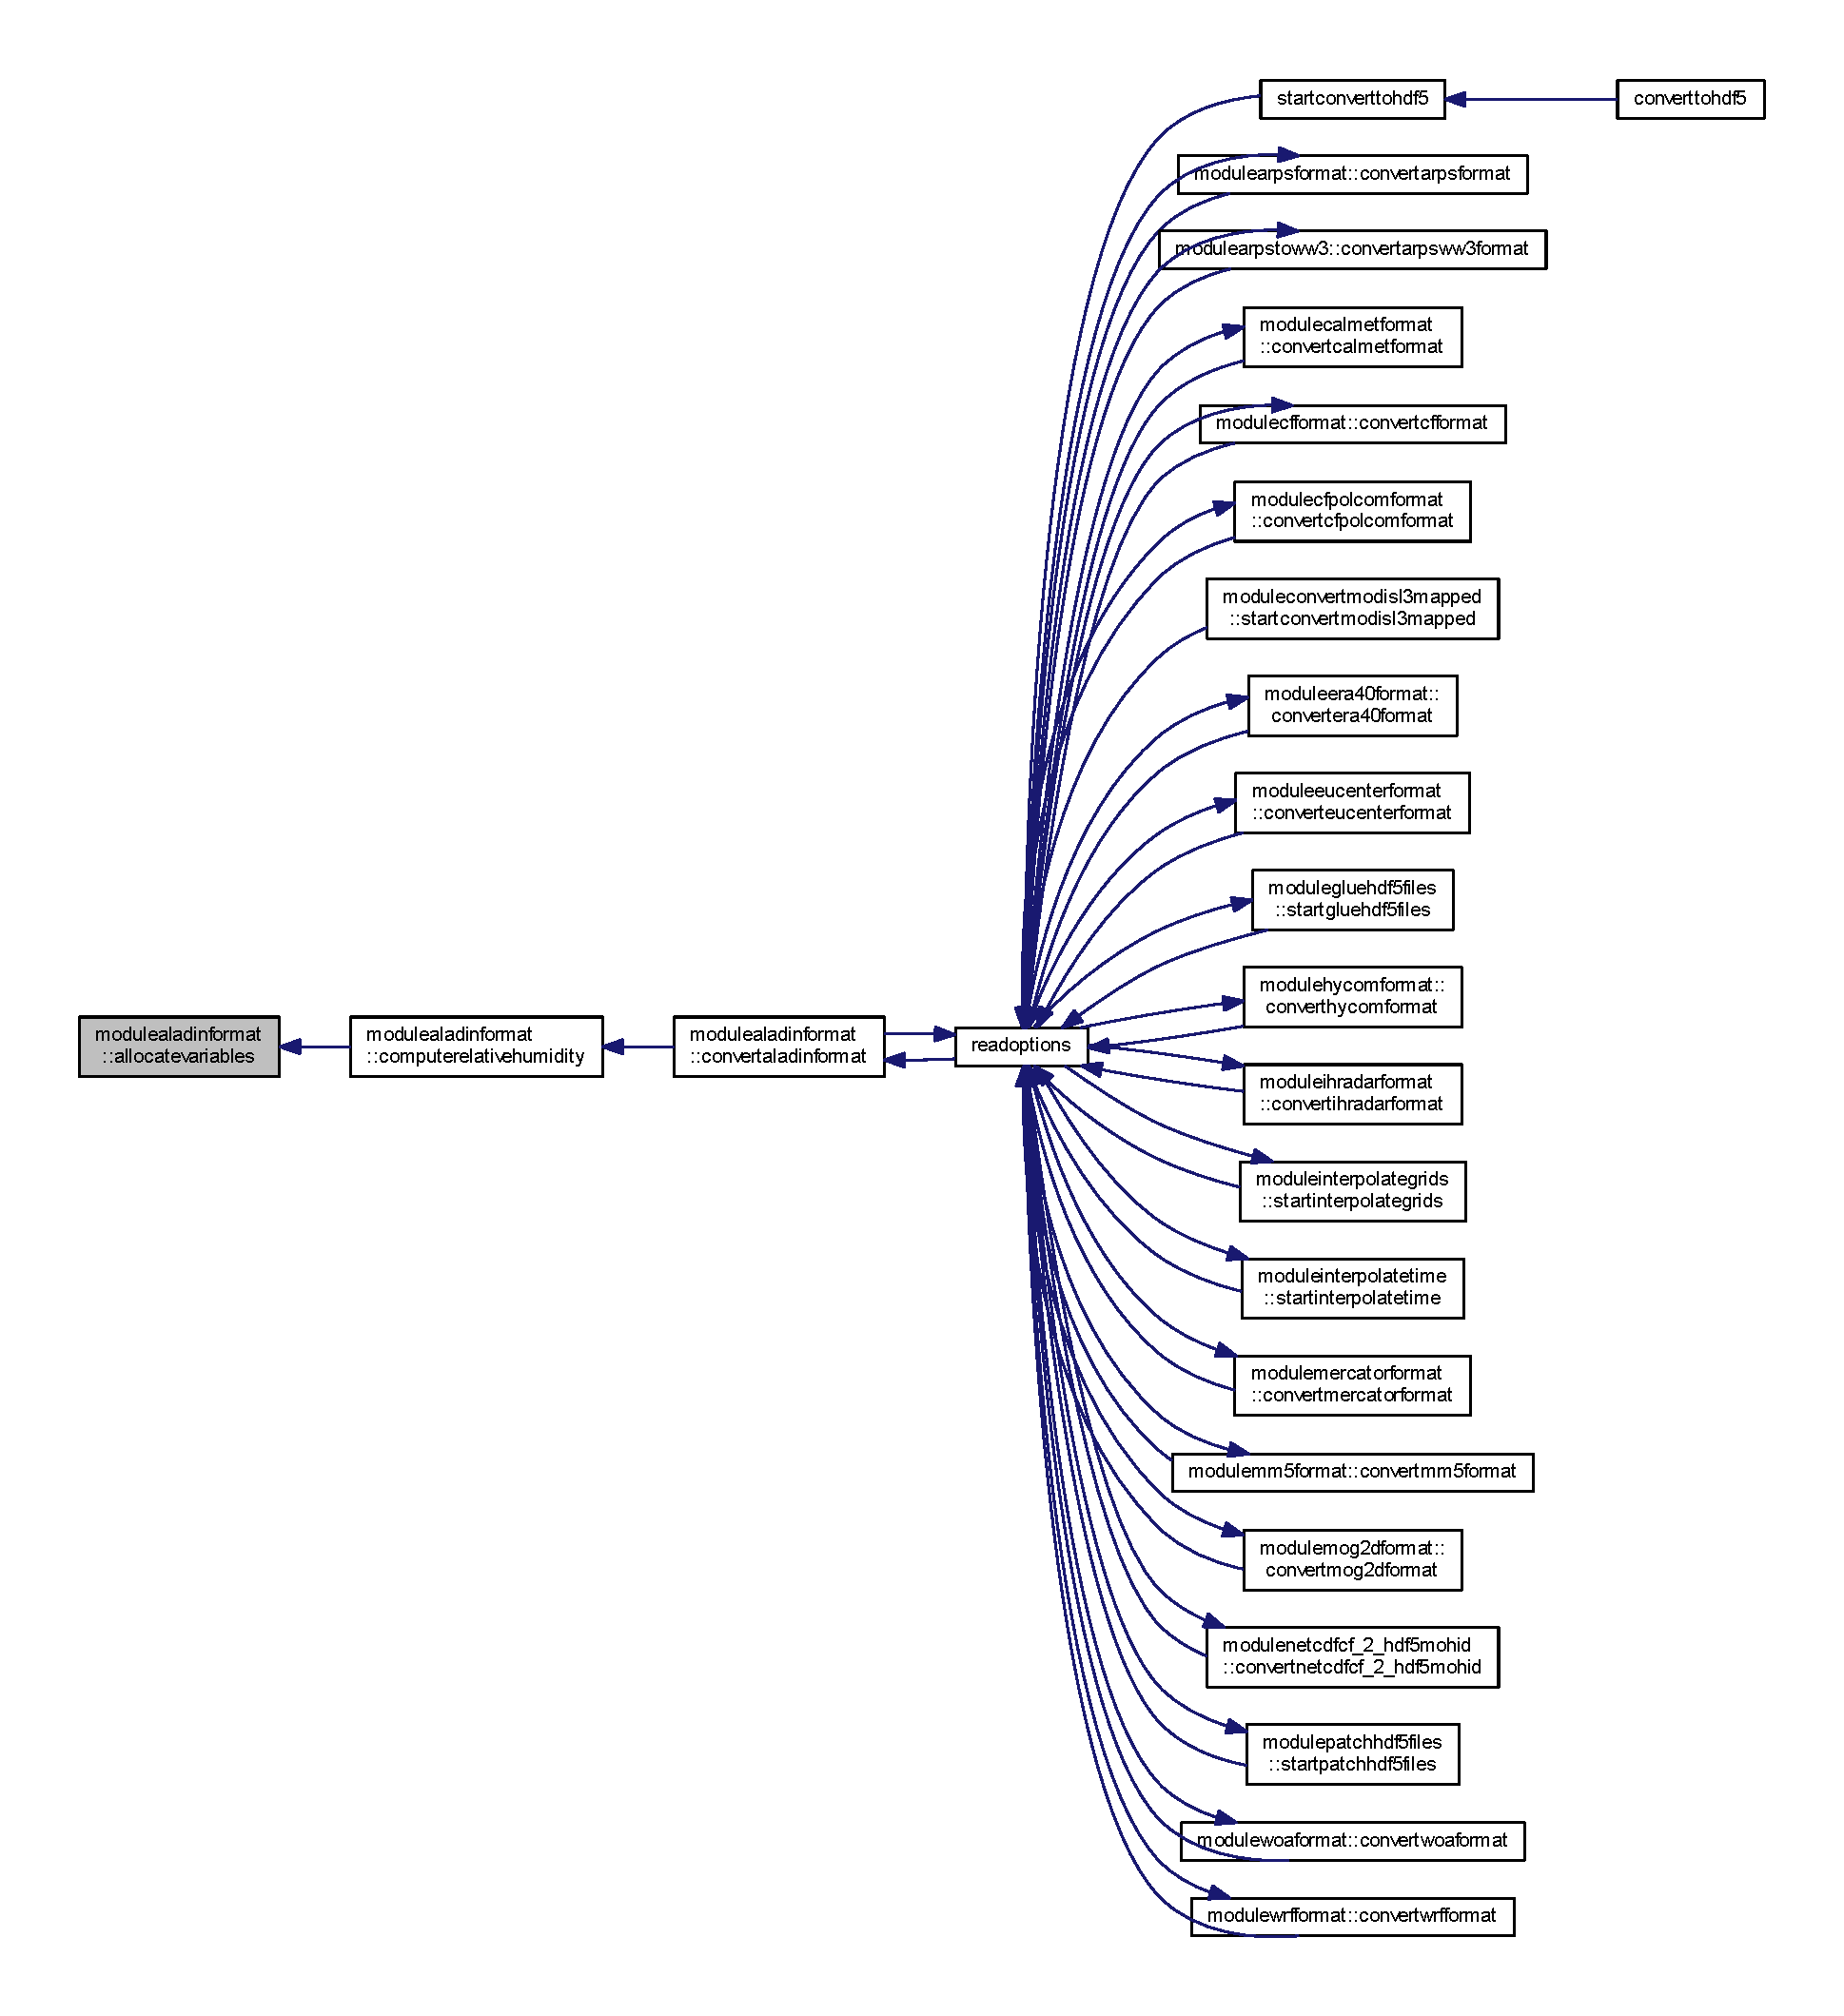
\includegraphics[width=350pt]{namespacemodulealadinformat_a5af9fedde7e74dd064c4bda092bbc671_icgraph}
\end{center}
\end{figure}
\mbox{\Hypertarget{namespacemodulealadinformat_a1c17164c3687aa7b8257c842cf0ad32a}\label{namespacemodulealadinformat_a1c17164c3687aa7b8257c842cf0ad32a}} 
\index{modulealadinformat@{modulealadinformat}!calculaterelativehumidity@{calculaterelativehumidity}}
\index{calculaterelativehumidity@{calculaterelativehumidity}!modulealadinformat@{modulealadinformat}}
\subsubsection{\texorpdfstring{calculaterelativehumidity()}{calculaterelativehumidity()}}
{\footnotesize\ttfamily subroutine, private modulealadinformat\+::calculaterelativehumidity (\begin{DoxyParamCaption}{ }\end{DoxyParamCaption})\hspace{0.3cm}{\ttfamily [private]}}

Here is the caller graph for this function\+:\nopagebreak
\begin{figure}[H]
\begin{center}
\leavevmode
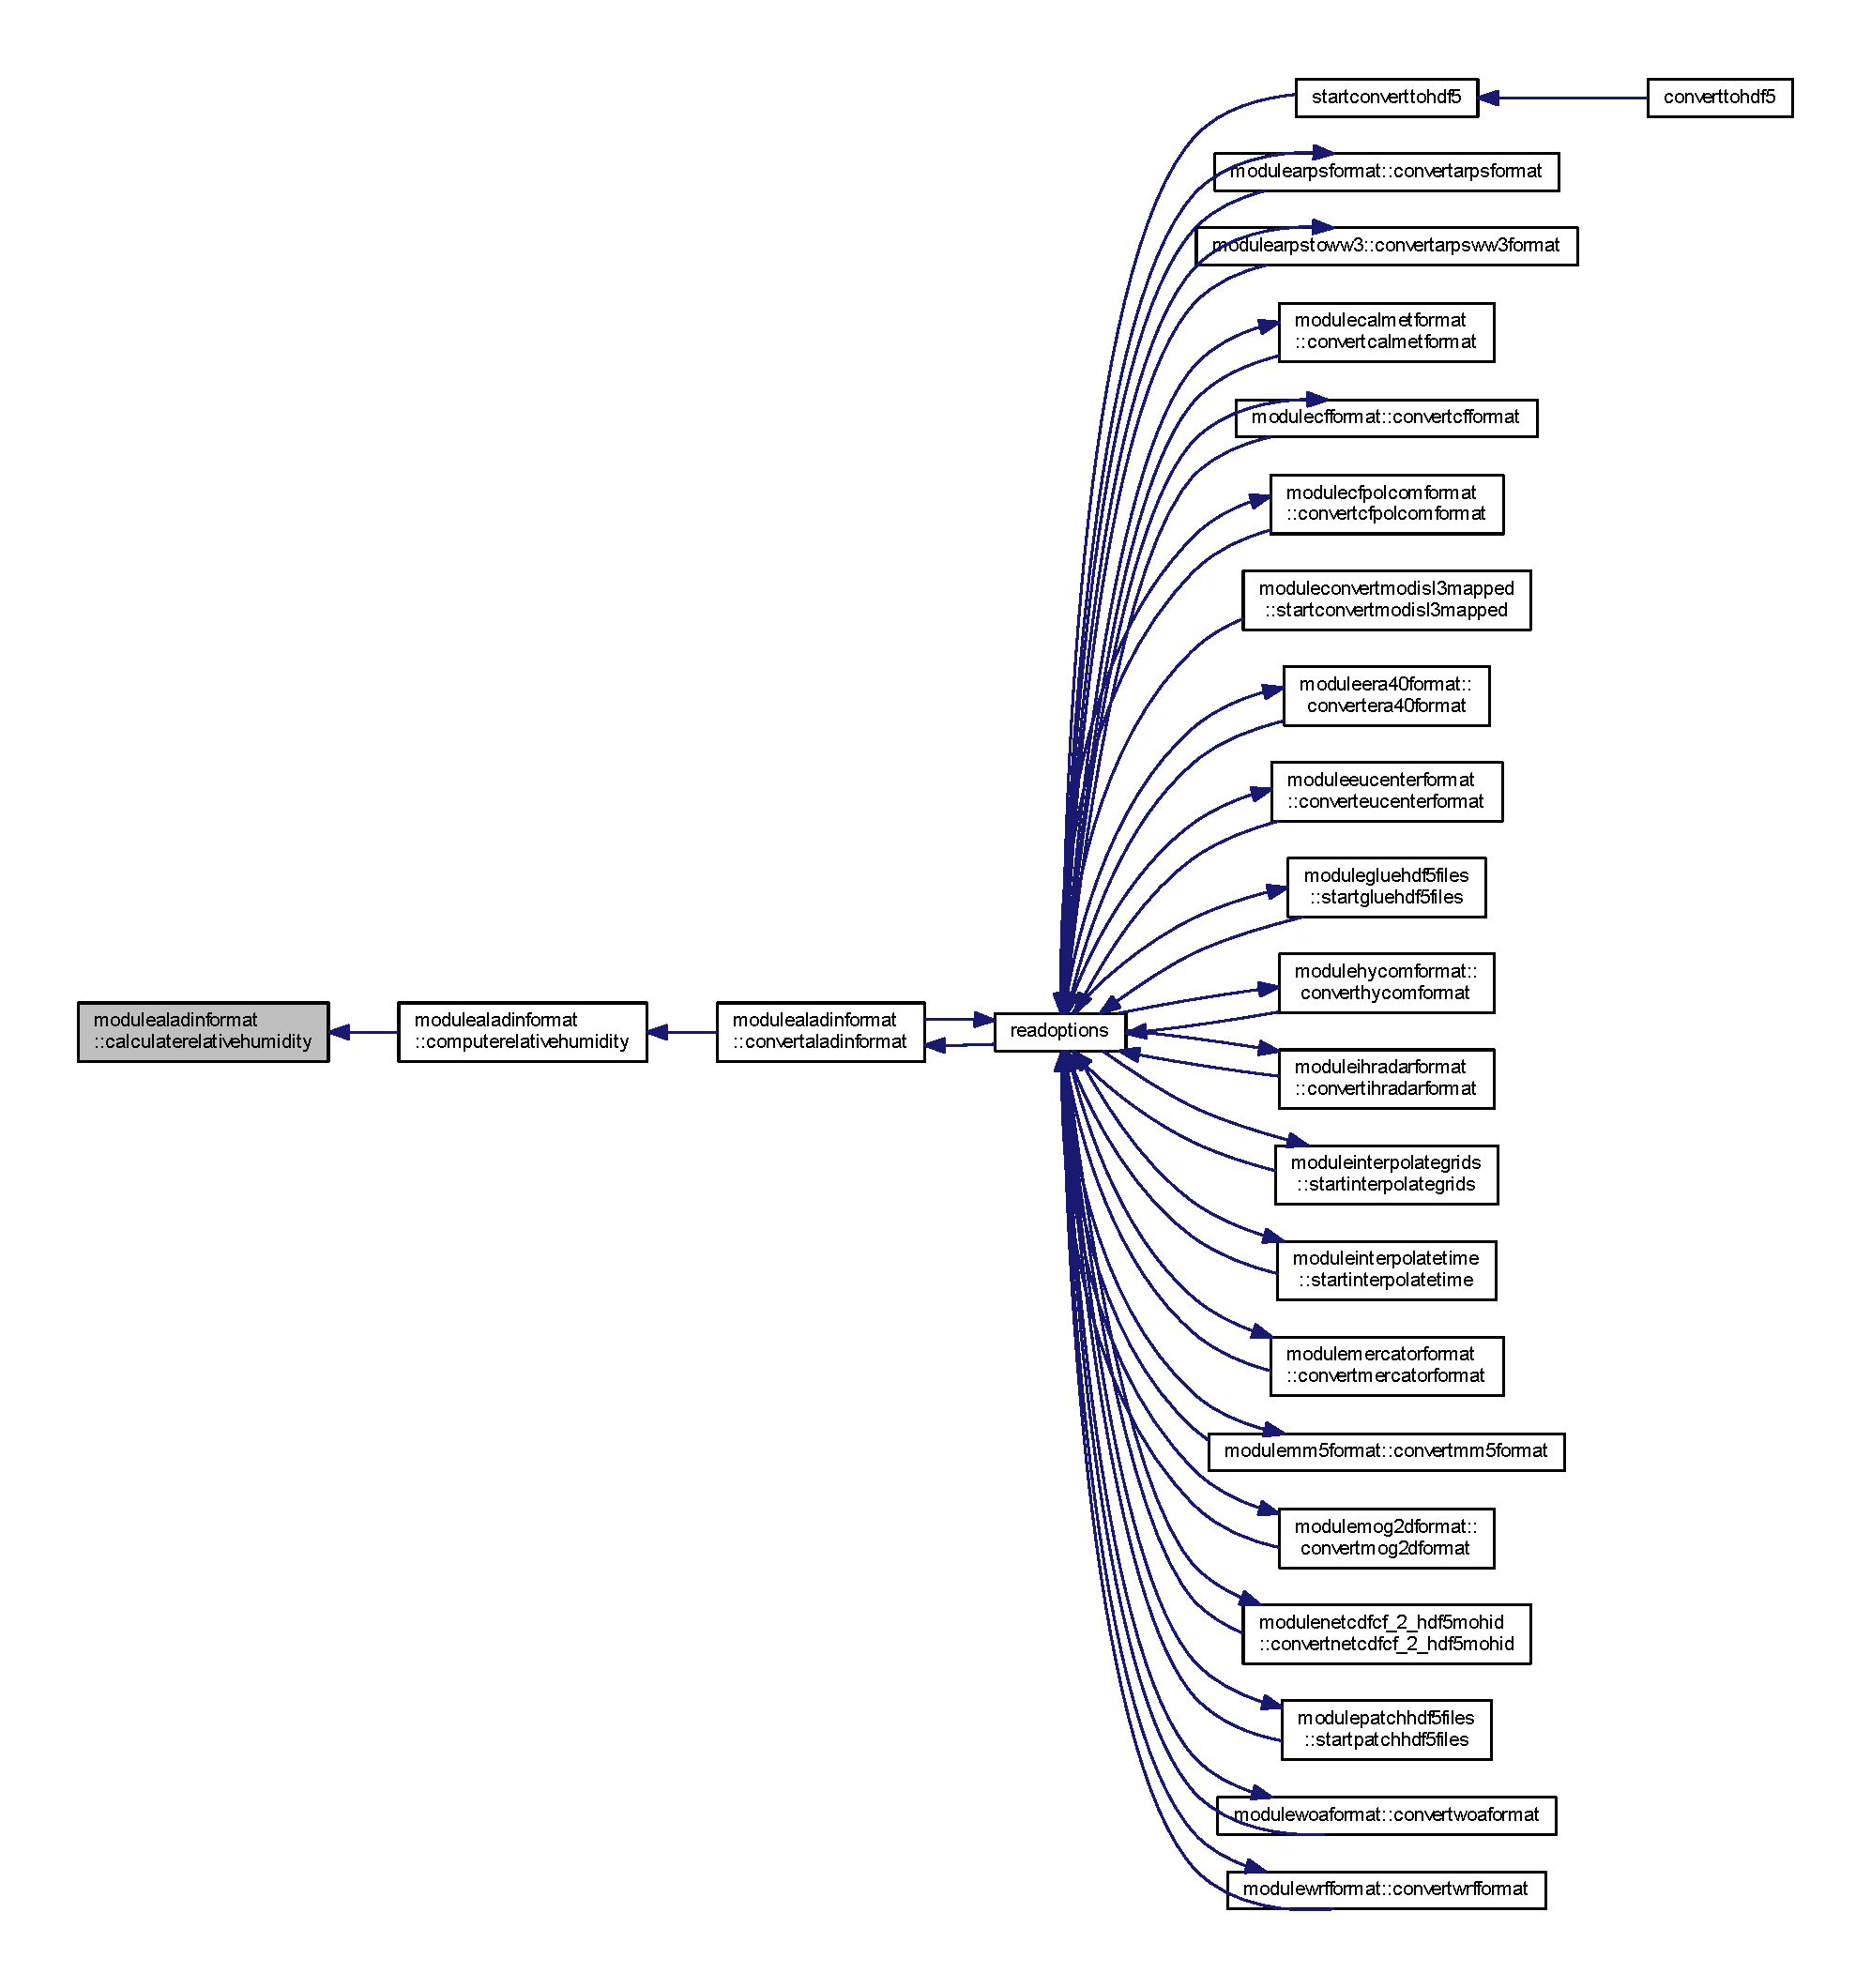
\includegraphics[width=350pt]{namespacemodulealadinformat_a1c17164c3687aa7b8257c842cf0ad32a_icgraph}
\end{center}
\end{figure}
\mbox{\Hypertarget{namespacemodulealadinformat_ad07bce7e401d49446a1fcfabb4bb4fa8}\label{namespacemodulealadinformat_ad07bce7e401d49446a1fcfabb4bb4fa8}} 
\index{modulealadinformat@{modulealadinformat}!checkname@{checkname}}
\index{checkname@{checkname}!modulealadinformat@{modulealadinformat}}
\subsubsection{\texorpdfstring{checkname()}{checkname()}}
{\footnotesize\ttfamily logical function, private modulealadinformat\+::checkname (\begin{DoxyParamCaption}\item[{character(len=$\ast$)}]{Aladin\+Name,  }\item[{character(len=stringlength)}]{Mohid\+Name }\end{DoxyParamCaption})\hspace{0.3cm}{\ttfamily [private]}}

Here is the caller graph for this function\+:\nopagebreak
\begin{figure}[H]
\begin{center}
\leavevmode
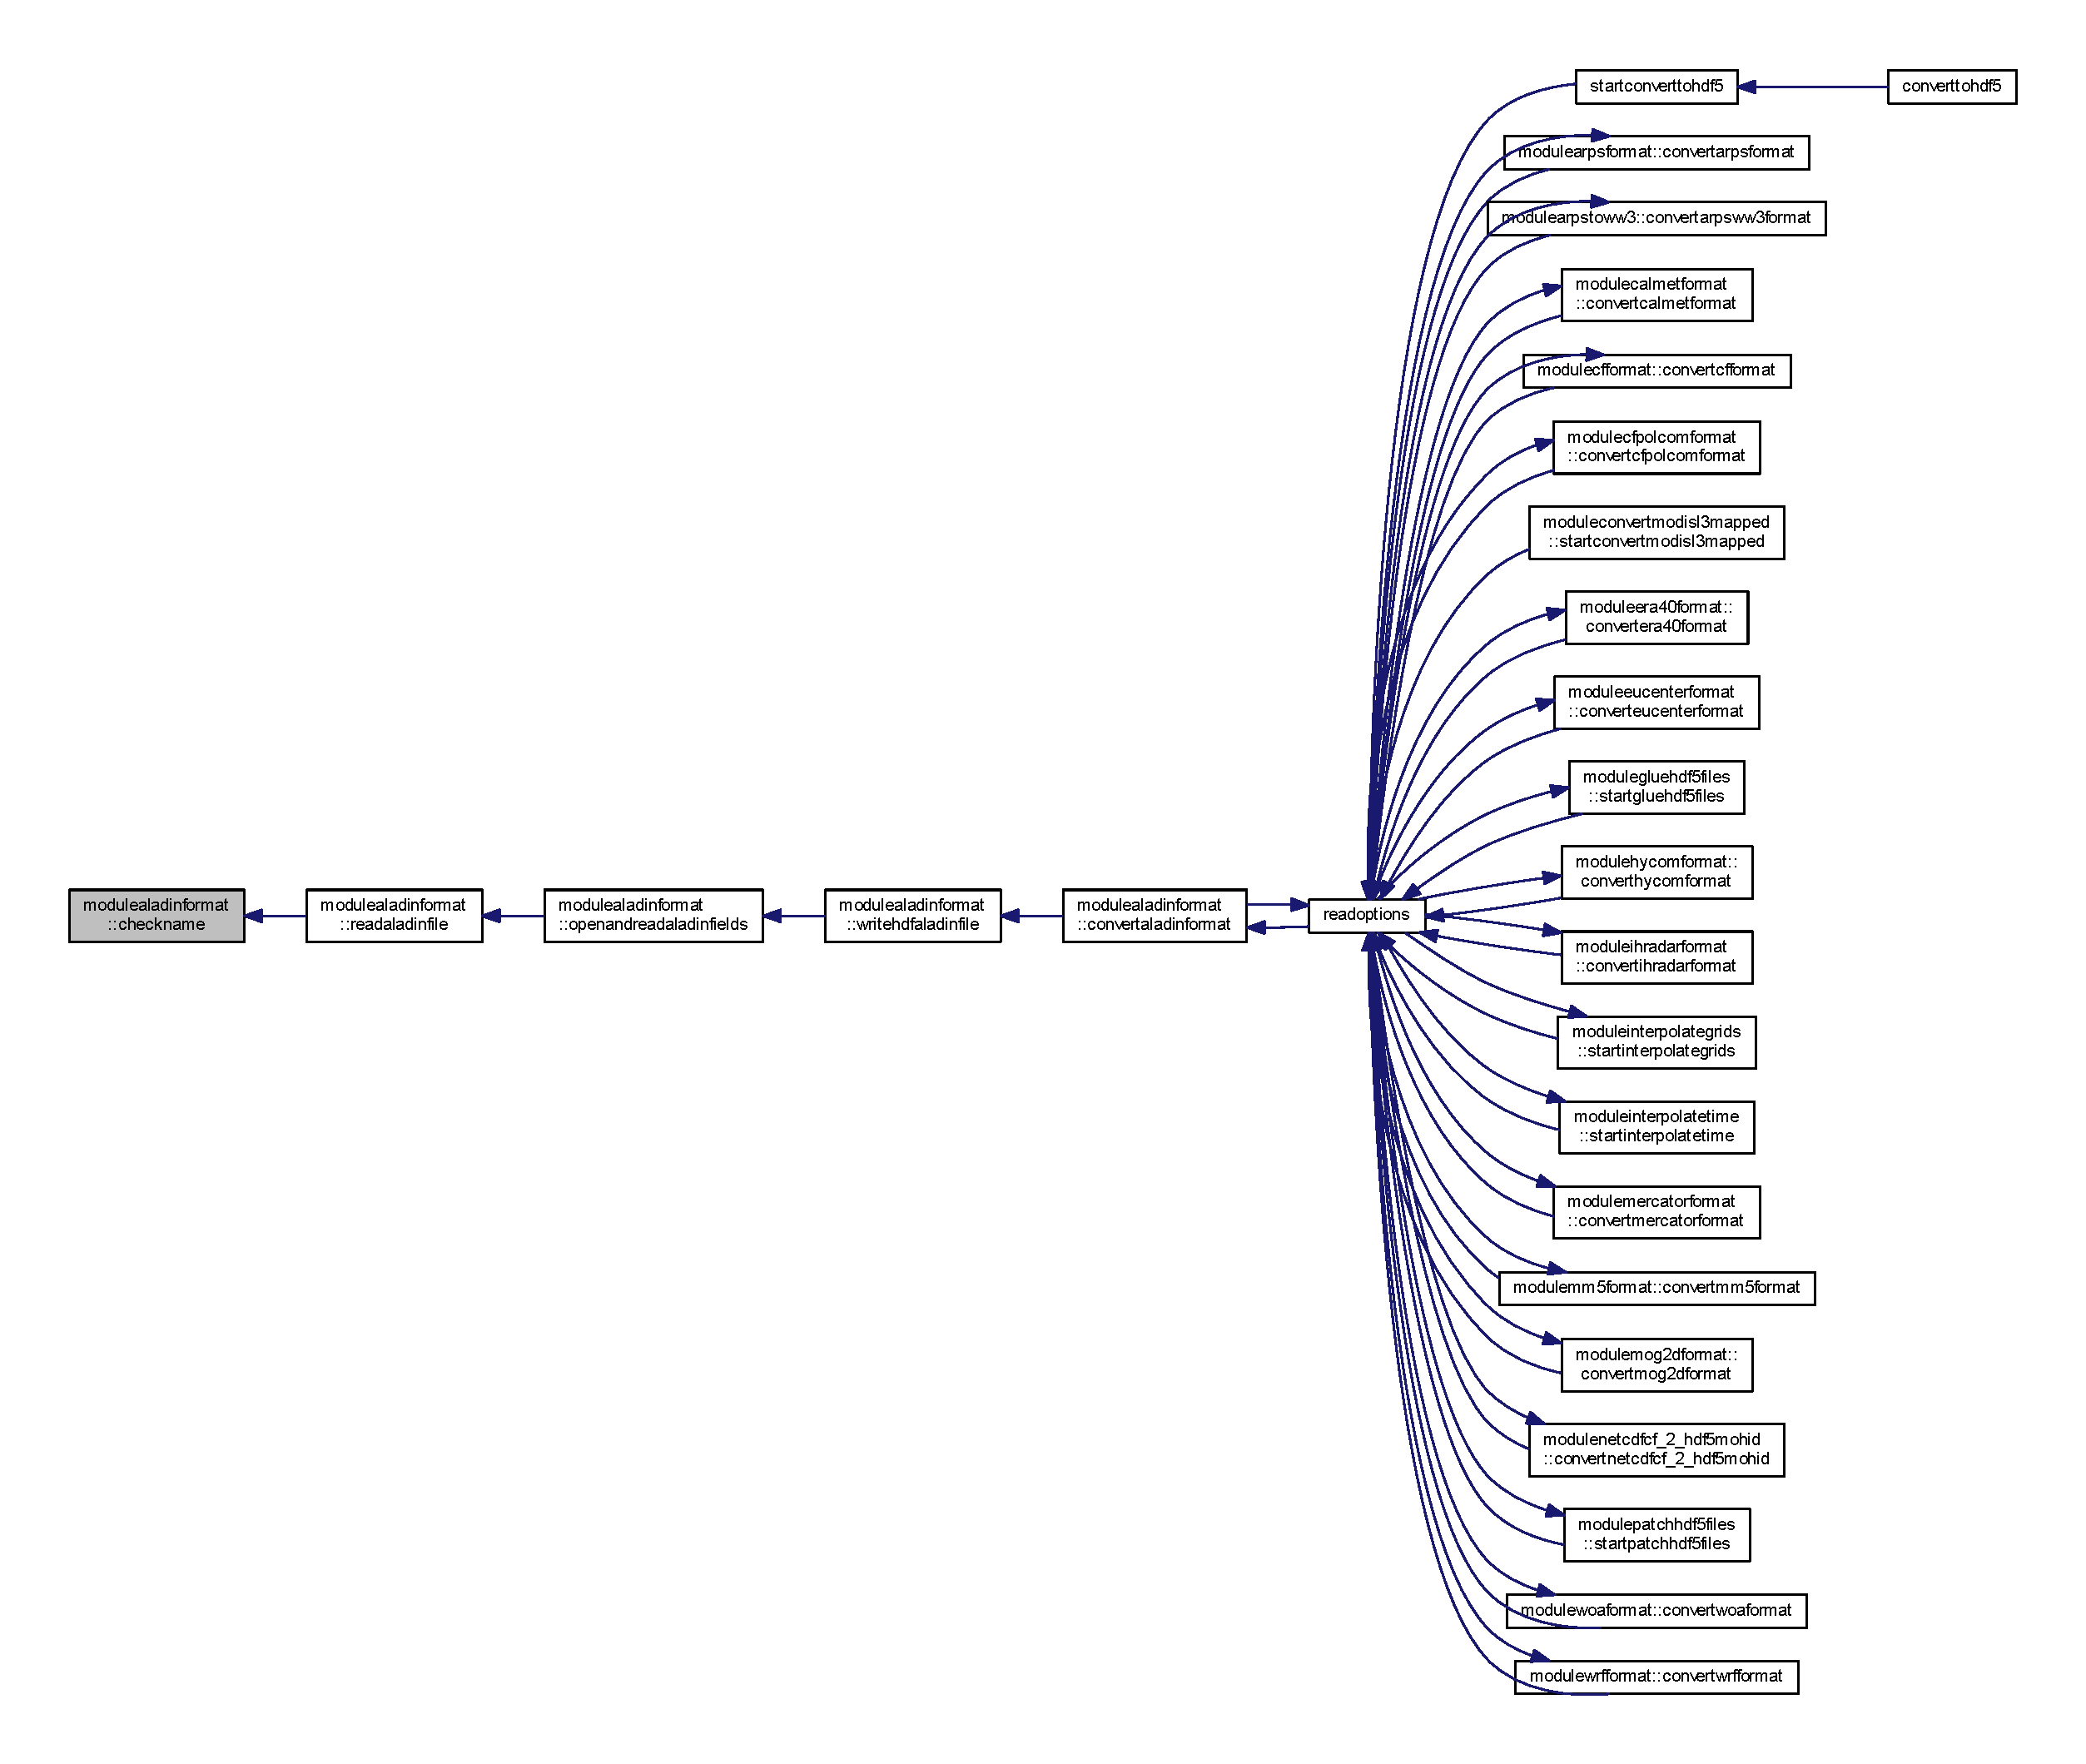
\includegraphics[width=350pt]{namespacemodulealadinformat_ad07bce7e401d49446a1fcfabb4bb4fa8_icgraph}
\end{center}
\end{figure}
\mbox{\Hypertarget{namespacemodulealadinformat_abe2227188275639d4c746fc709d090e2}\label{namespacemodulealadinformat_abe2227188275639d4c746fc709d090e2}} 
\index{modulealadinformat@{modulealadinformat}!clearvariables@{clearvariables}}
\index{clearvariables@{clearvariables}!modulealadinformat@{modulealadinformat}}
\subsubsection{\texorpdfstring{clearvariables()}{clearvariables()}}
{\footnotesize\ttfamily subroutine, private modulealadinformat\+::clearvariables (\begin{DoxyParamCaption}{ }\end{DoxyParamCaption})\hspace{0.3cm}{\ttfamily [private]}}

Here is the caller graph for this function\+:\nopagebreak
\begin{figure}[H]
\begin{center}
\leavevmode
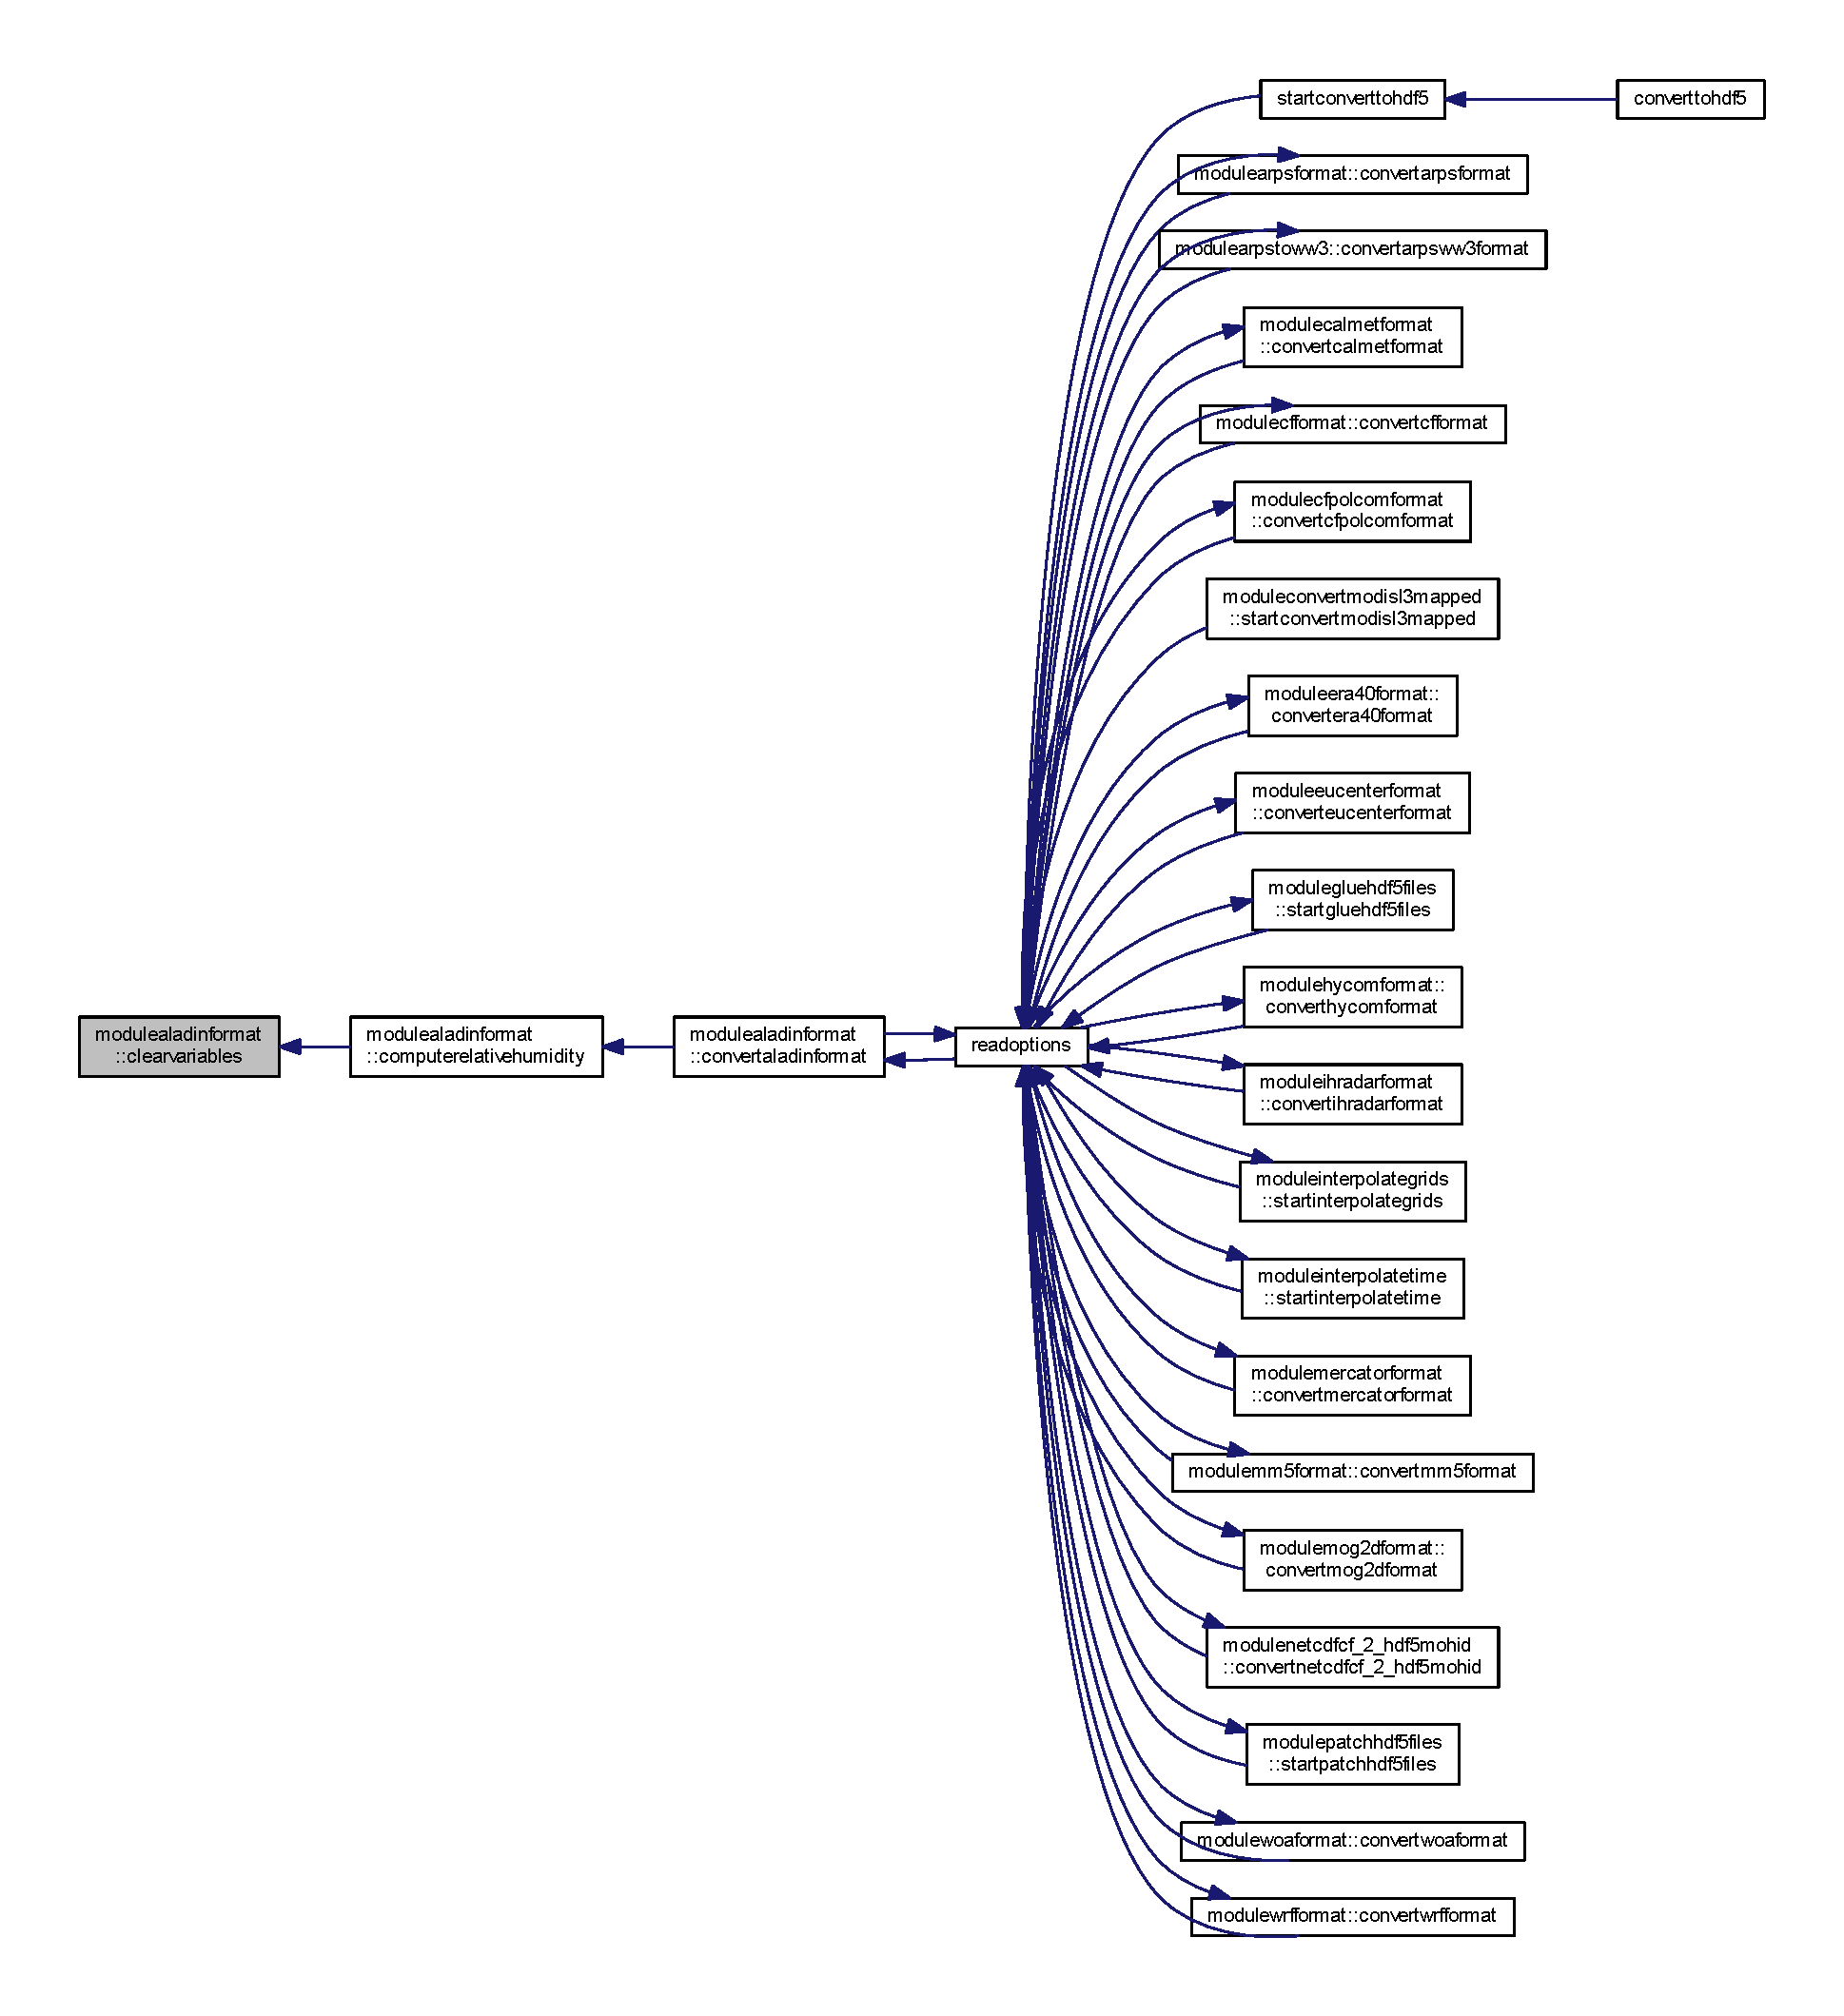
\includegraphics[width=350pt]{namespacemodulealadinformat_abe2227188275639d4c746fc709d090e2_icgraph}
\end{center}
\end{figure}
\mbox{\Hypertarget{namespacemodulealadinformat_af21c9df5cd692b1f56a959cc52cba7d8}\label{namespacemodulealadinformat_af21c9df5cd692b1f56a959cc52cba7d8}} 
\index{modulealadinformat@{modulealadinformat}!close\+\_\+hdf5\+\_\+output\+\_\+file@{close\+\_\+hdf5\+\_\+output\+\_\+file}}
\index{close\+\_\+hdf5\+\_\+output\+\_\+file@{close\+\_\+hdf5\+\_\+output\+\_\+file}!modulealadinformat@{modulealadinformat}}
\subsubsection{\texorpdfstring{close\+\_\+hdf5\+\_\+output\+\_\+file()}{close\_hdf5\_output\_file()}}
{\footnotesize\ttfamily subroutine, private modulealadinformat\+::close\+\_\+hdf5\+\_\+output\+\_\+file (\begin{DoxyParamCaption}{ }\end{DoxyParamCaption})\hspace{0.3cm}{\ttfamily [private]}}

Here is the caller graph for this function\+:\nopagebreak
\begin{figure}[H]
\begin{center}
\leavevmode
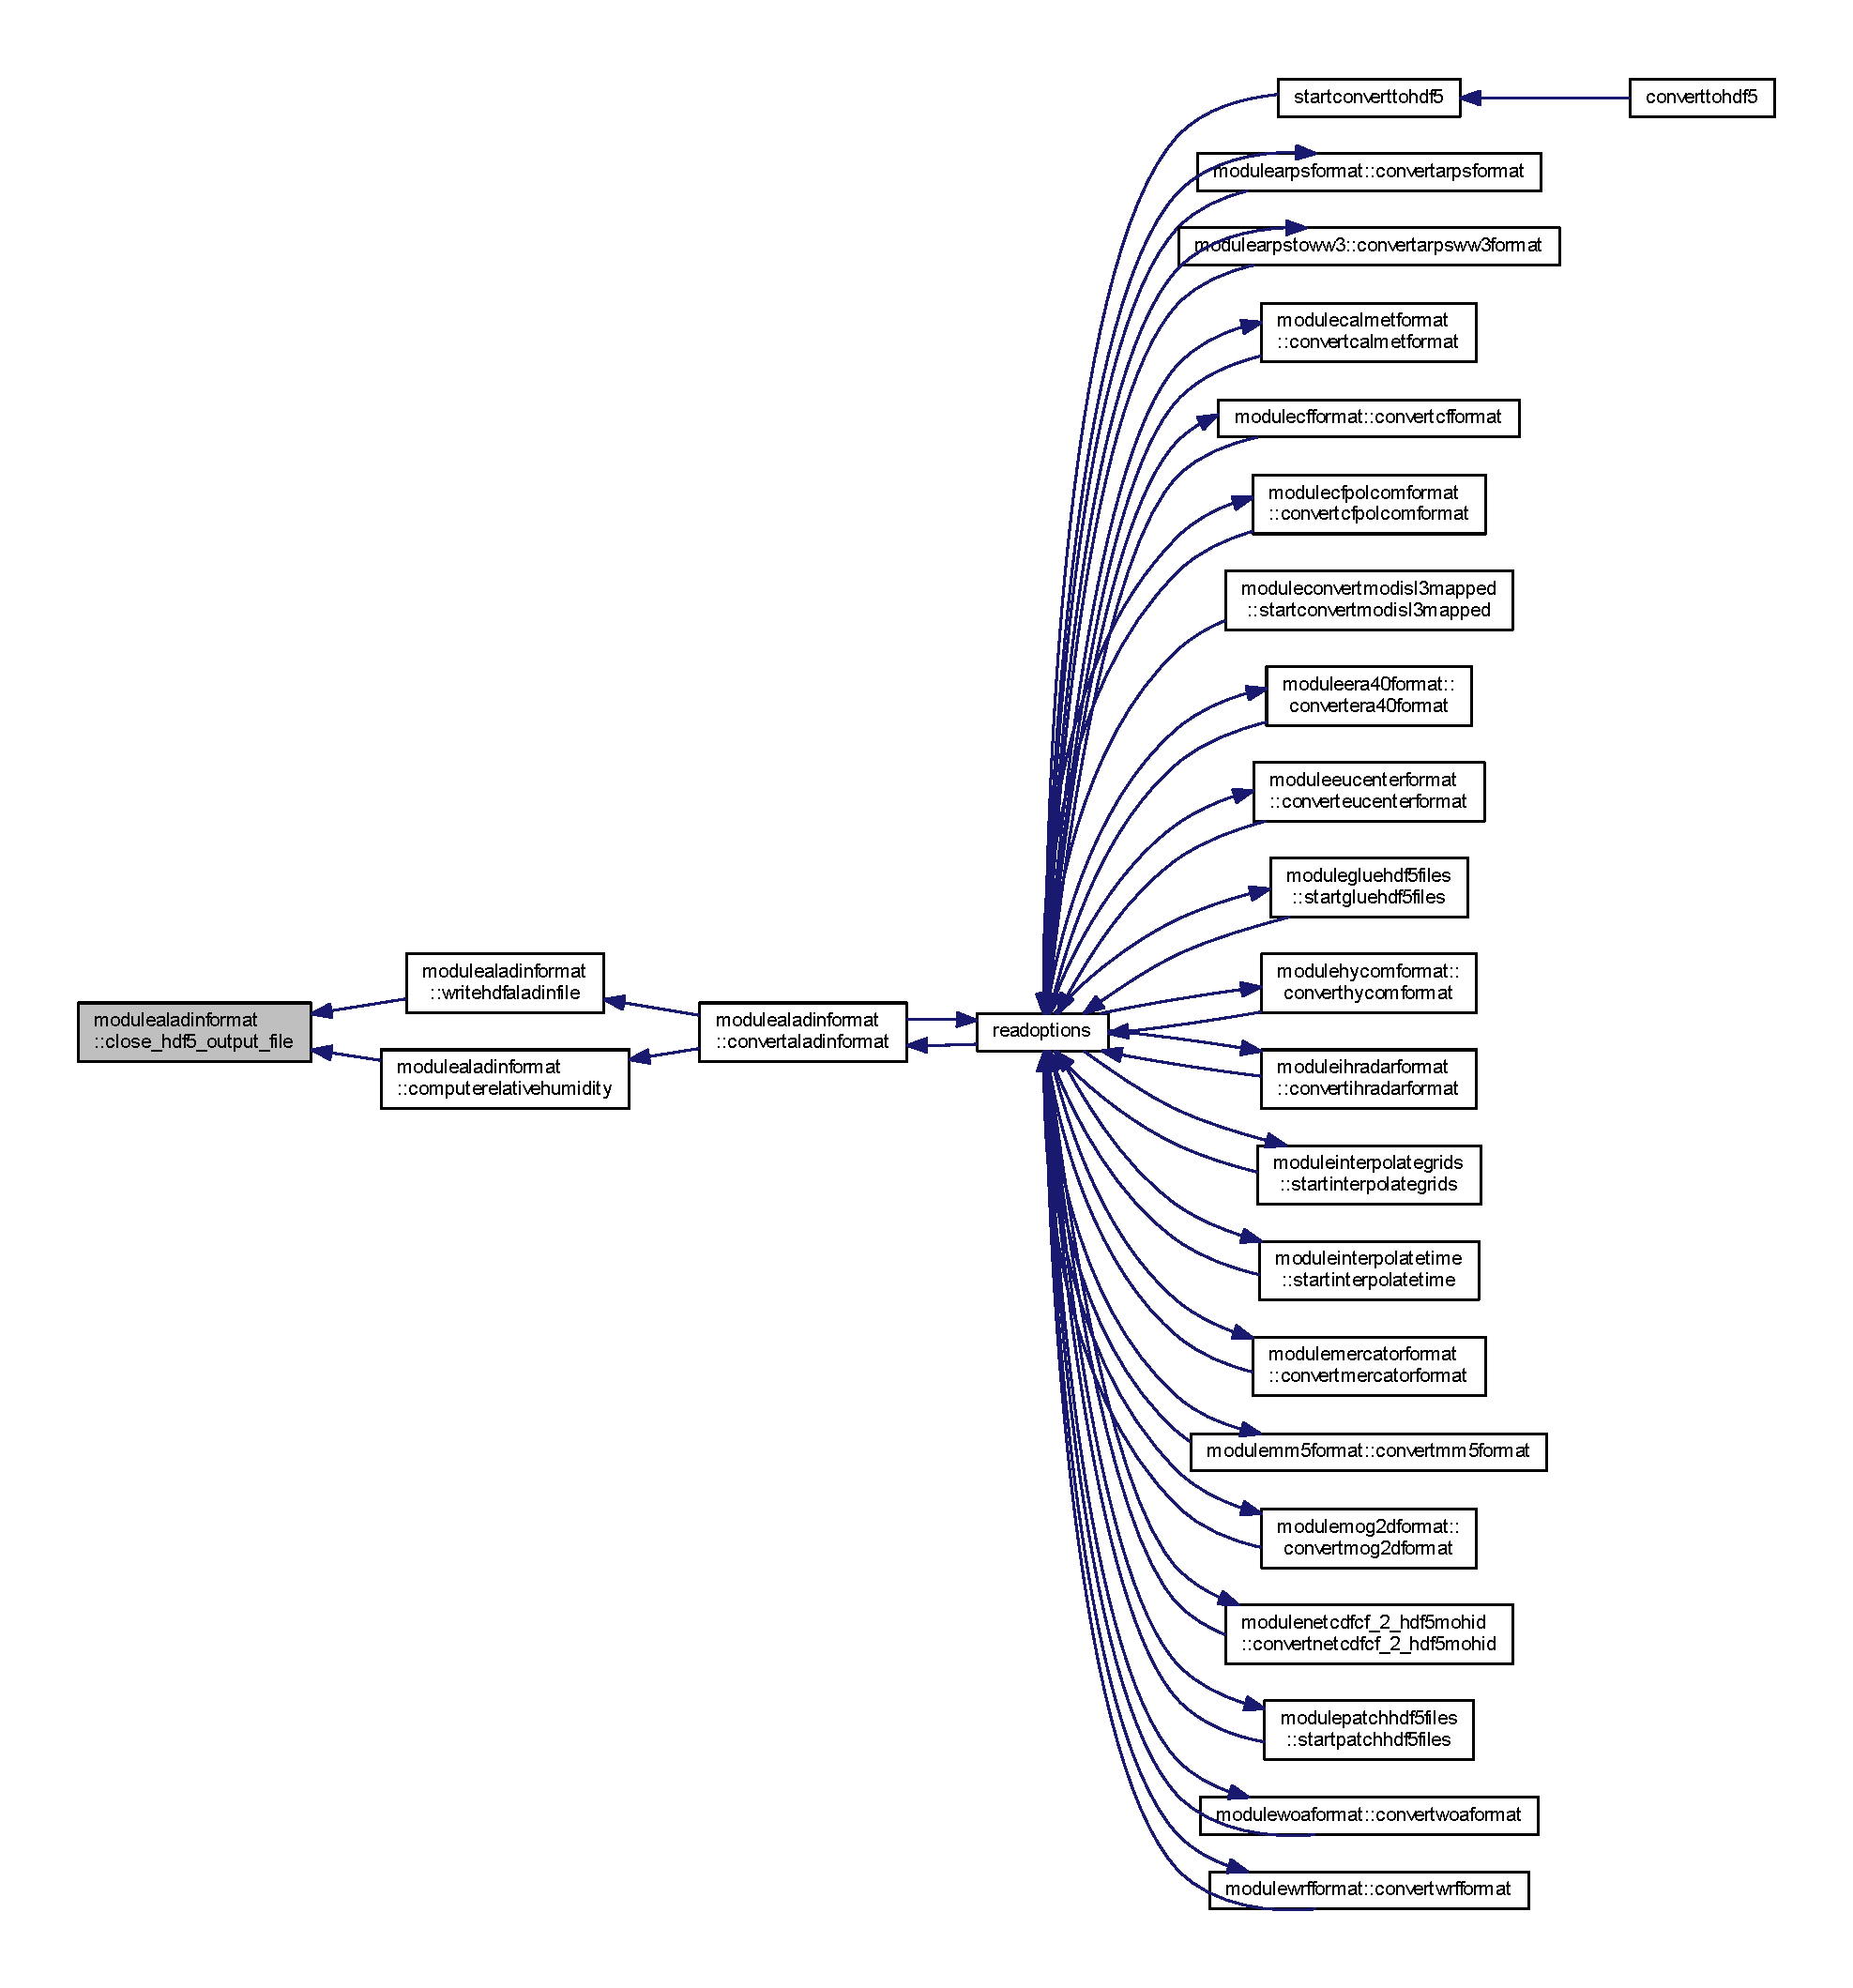
\includegraphics[width=350pt]{namespacemodulealadinformat_af21c9df5cd692b1f56a959cc52cba7d8_icgraph}
\end{center}
\end{figure}
\mbox{\Hypertarget{namespacemodulealadinformat_ae9288daa19c82d5cb2b9c128f3b55cbc}\label{namespacemodulealadinformat_ae9288daa19c82d5cb2b9c128f3b55cbc}} 
\index{modulealadinformat@{modulealadinformat}!computerelativehumidity@{computerelativehumidity}}
\index{computerelativehumidity@{computerelativehumidity}!modulealadinformat@{modulealadinformat}}
\subsubsection{\texorpdfstring{computerelativehumidity()}{computerelativehumidity()}}
{\footnotesize\ttfamily subroutine, private modulealadinformat\+::computerelativehumidity (\begin{DoxyParamCaption}{ }\end{DoxyParamCaption})\hspace{0.3cm}{\ttfamily [private]}}

Here is the call graph for this function\+:\nopagebreak
\begin{figure}[H]
\begin{center}
\leavevmode
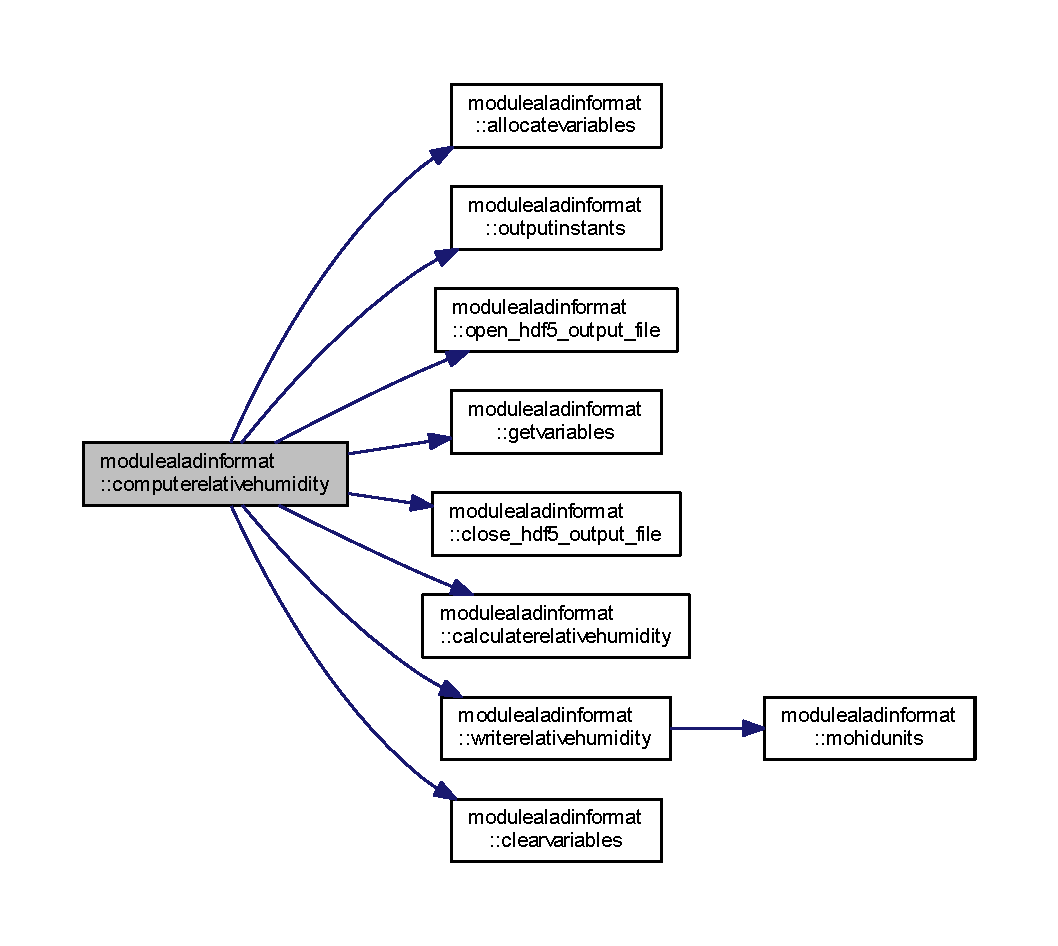
\includegraphics[width=350pt]{namespacemodulealadinformat_ae9288daa19c82d5cb2b9c128f3b55cbc_cgraph}
\end{center}
\end{figure}
Here is the caller graph for this function\+:\nopagebreak
\begin{figure}[H]
\begin{center}
\leavevmode
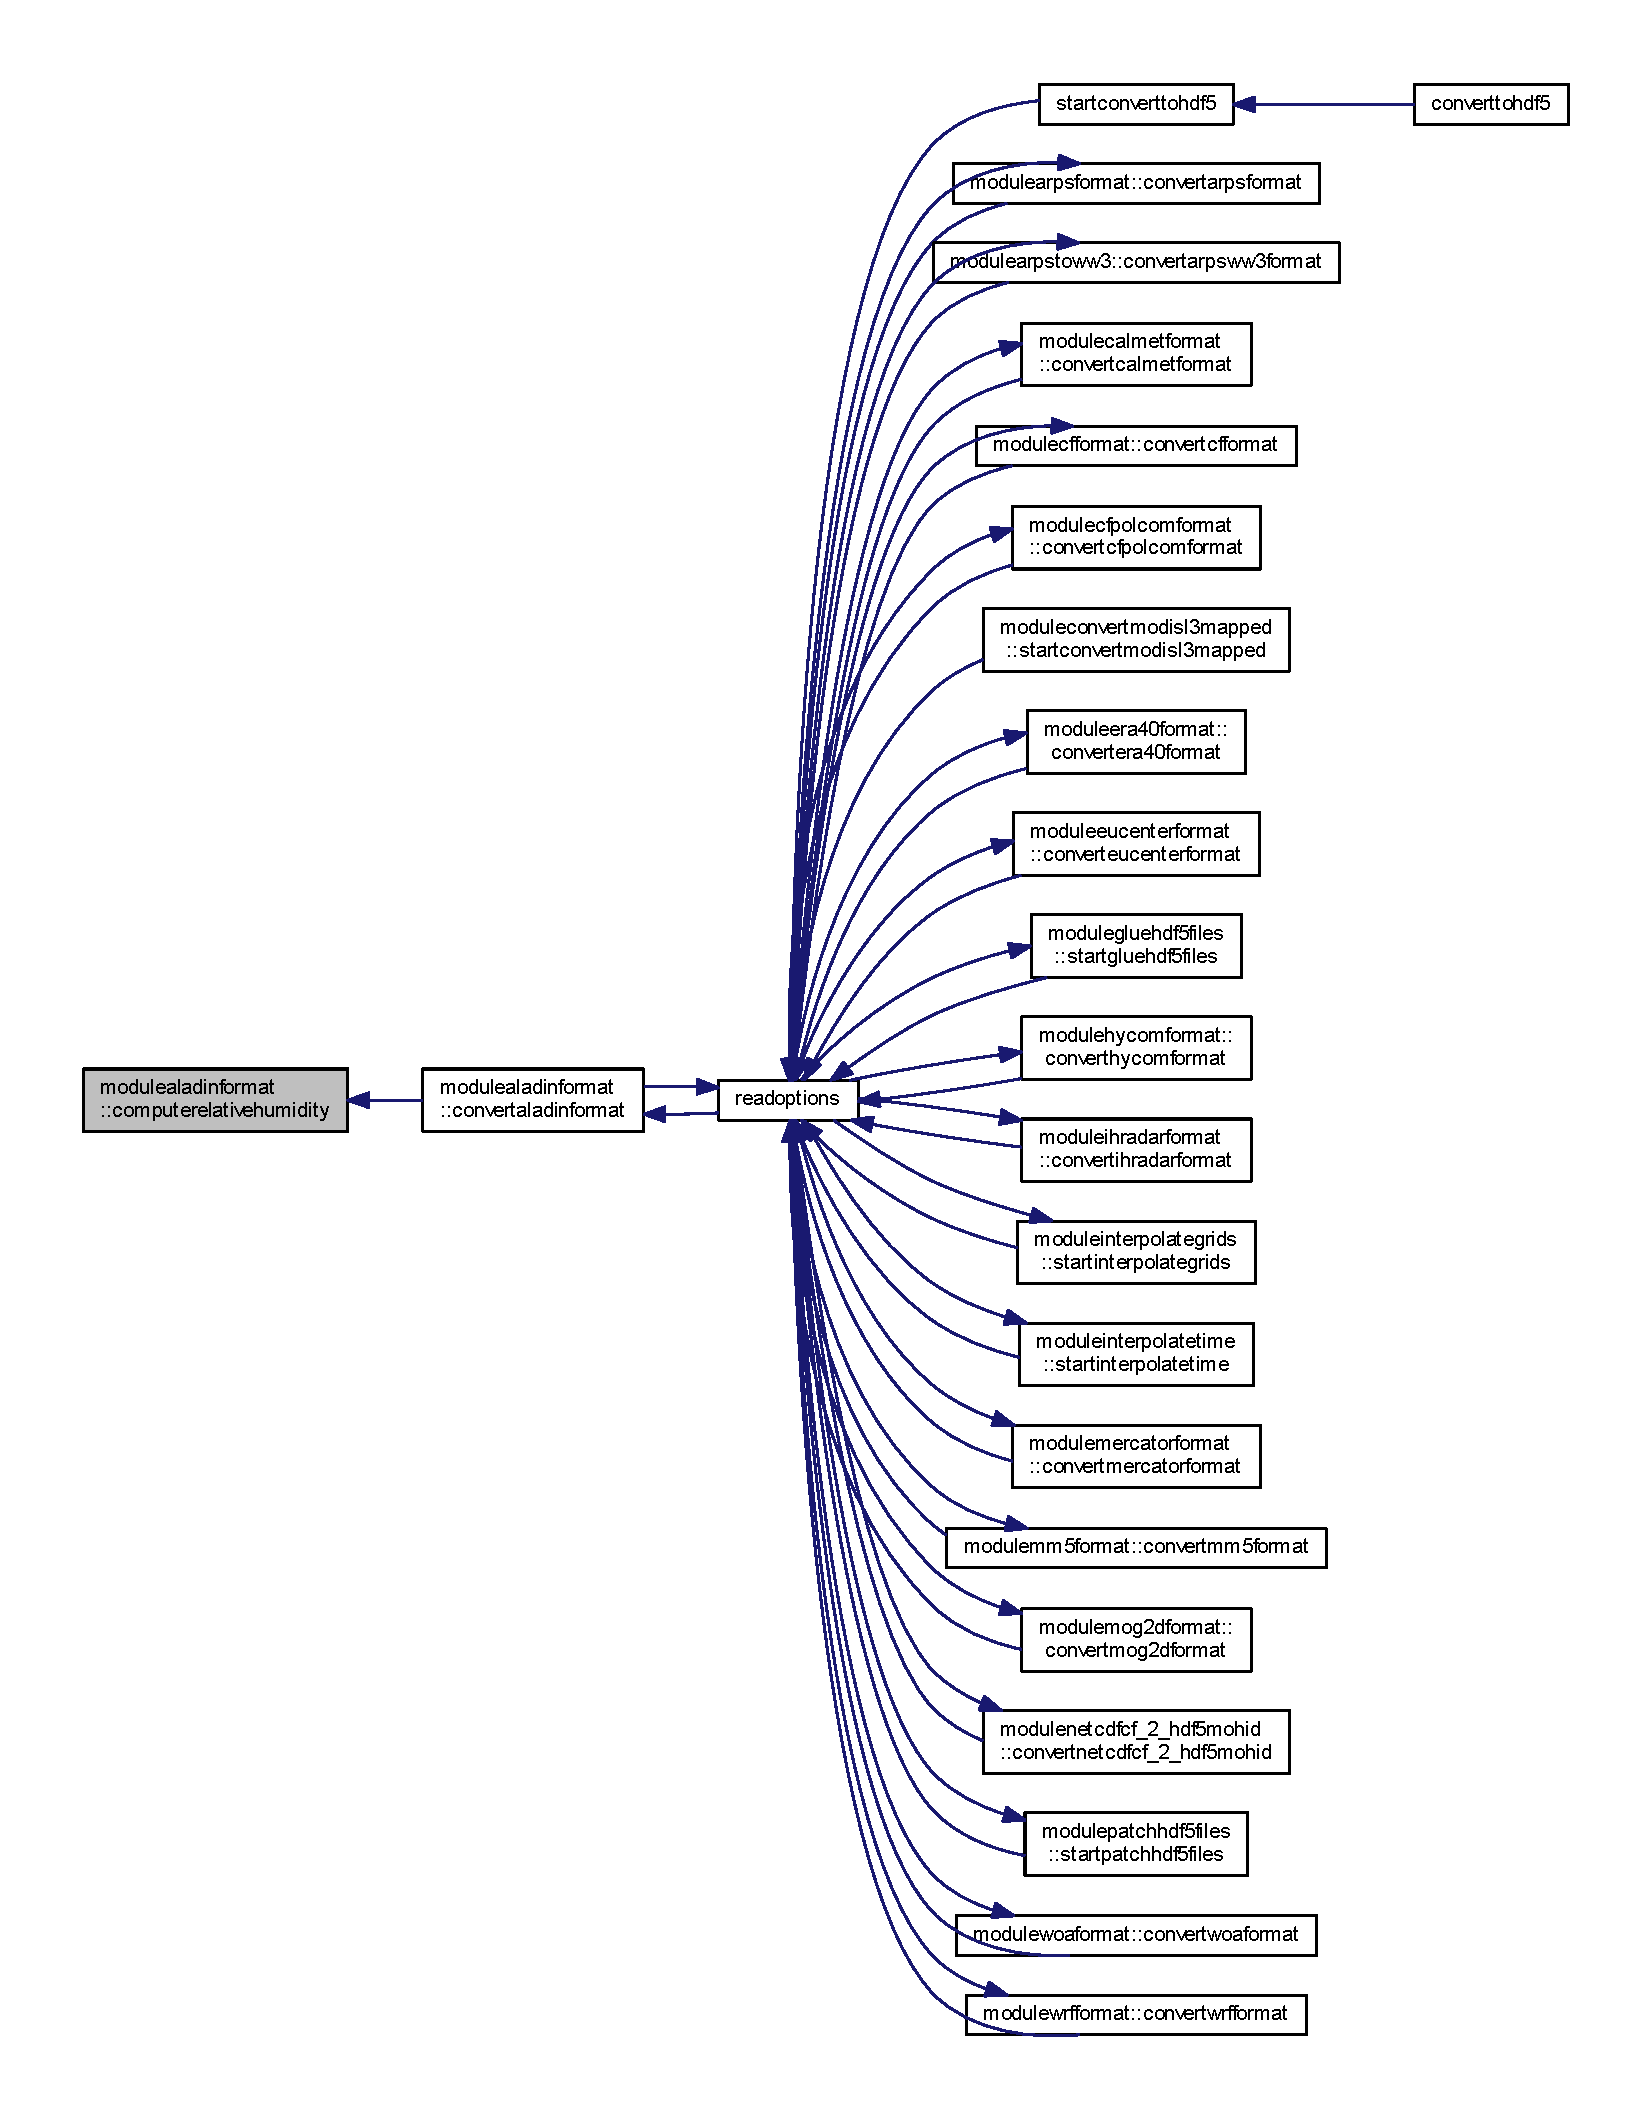
\includegraphics[width=350pt]{namespacemodulealadinformat_ae9288daa19c82d5cb2b9c128f3b55cbc_icgraph}
\end{center}
\end{figure}
\mbox{\Hypertarget{namespacemodulealadinformat_ab29f0499d468883233584caea8913297}\label{namespacemodulealadinformat_ab29f0499d468883233584caea8913297}} 
\index{modulealadinformat@{modulealadinformat}!constructgrid@{constructgrid}}
\index{constructgrid@{constructgrid}!modulealadinformat@{modulealadinformat}}
\subsubsection{\texorpdfstring{constructgrid()}{constructgrid()}}
{\footnotesize\ttfamily subroutine, private modulealadinformat\+::constructgrid (\begin{DoxyParamCaption}{ }\end{DoxyParamCaption})\hspace{0.3cm}{\ttfamily [private]}}

Here is the caller graph for this function\+:\nopagebreak
\begin{figure}[H]
\begin{center}
\leavevmode
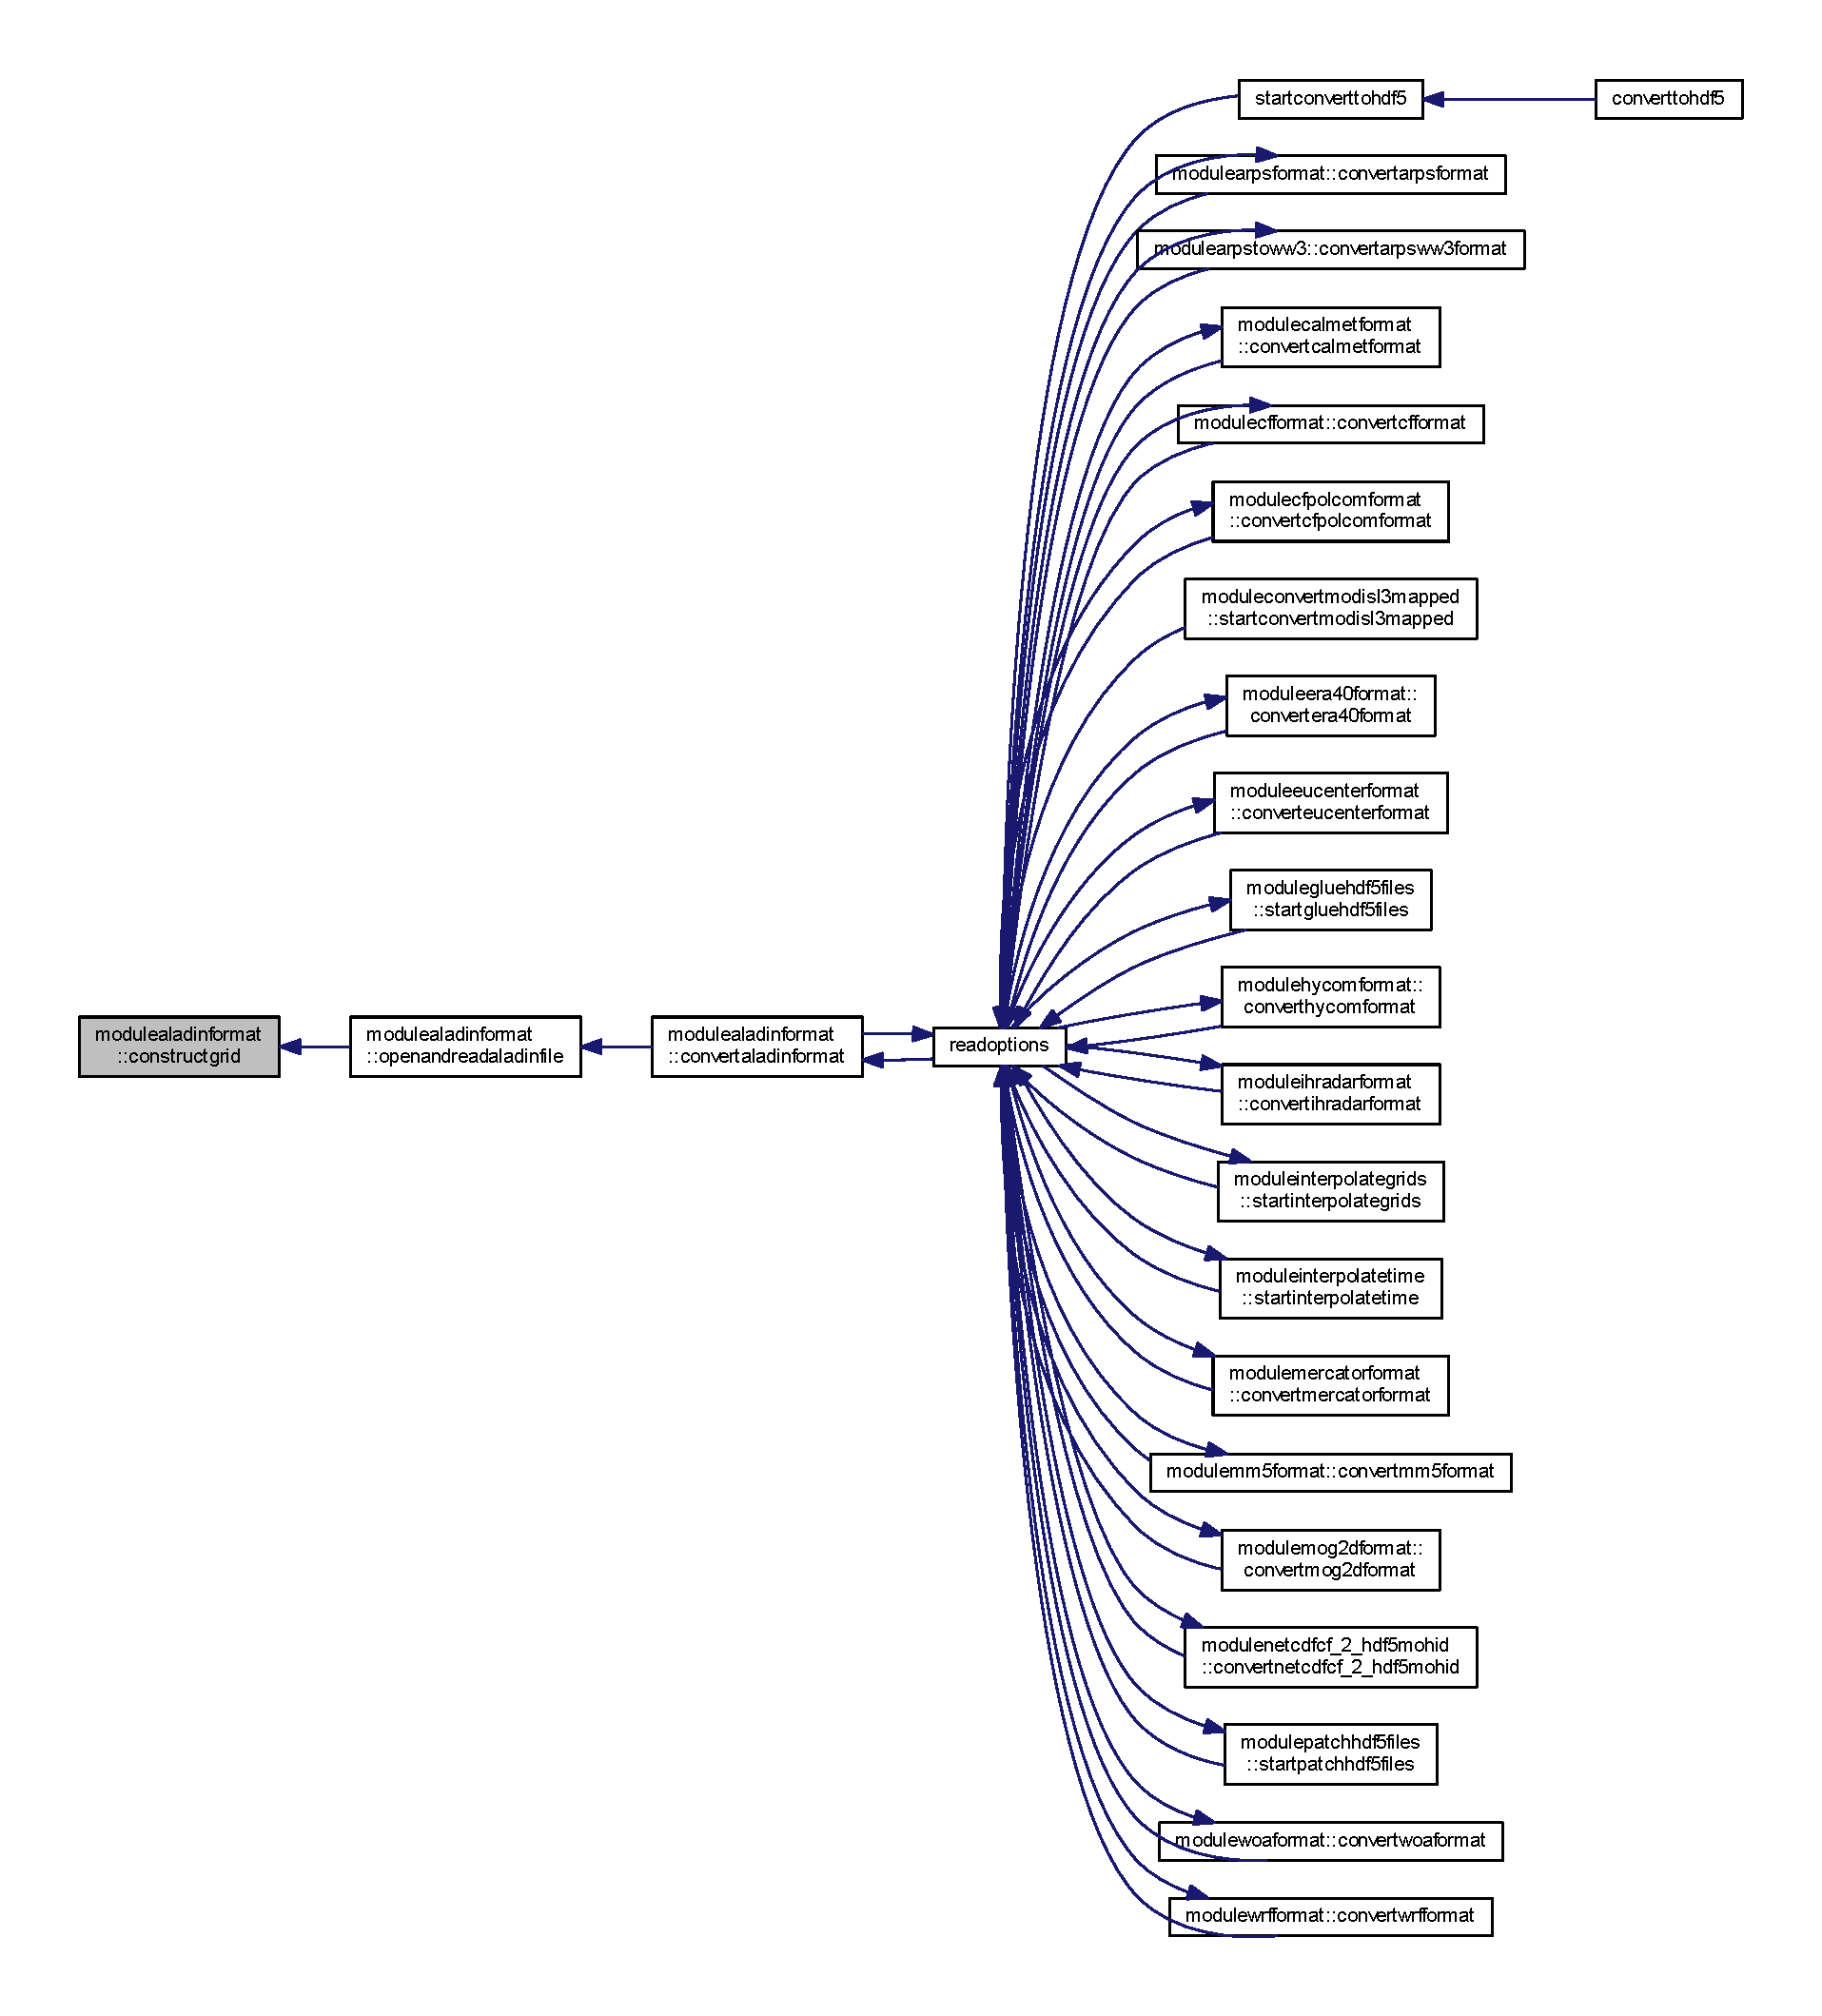
\includegraphics[width=350pt]{namespacemodulealadinformat_ab29f0499d468883233584caea8913297_icgraph}
\end{center}
\end{figure}
\mbox{\Hypertarget{namespacemodulealadinformat_a77f6d15bb472ac521ff23ef7a54a48e7}\label{namespacemodulealadinformat_a77f6d15bb472ac521ff23ef7a54a48e7}} 
\index{modulealadinformat@{modulealadinformat}!convertaladinformat@{convertaladinformat}}
\index{convertaladinformat@{convertaladinformat}!modulealadinformat@{modulealadinformat}}
\subsubsection{\texorpdfstring{convertaladinformat()}{convertaladinformat()}}
{\footnotesize\ttfamily subroutine, public modulealadinformat\+::convertaladinformat (\begin{DoxyParamCaption}\item[{integer, intent(in)}]{Enter\+Data\+ID,  }\item[{integer, intent(in)}]{Client\+Number,  }\item[{integer, intent(out), optional}]{S\+T\+AT }\end{DoxyParamCaption})}

Here is the call graph for this function\+:\nopagebreak
\begin{figure}[H]
\begin{center}
\leavevmode

\includegraphics[height=550pt]{namespacemodulealadinformat_a77f6d15bb472ac521ff23ef7a54a48e7_cgraph}
\end{center}
\end{figure}
Here is the caller graph for this function\+:\nopagebreak
\begin{figure}[H]
\begin{center}
\leavevmode
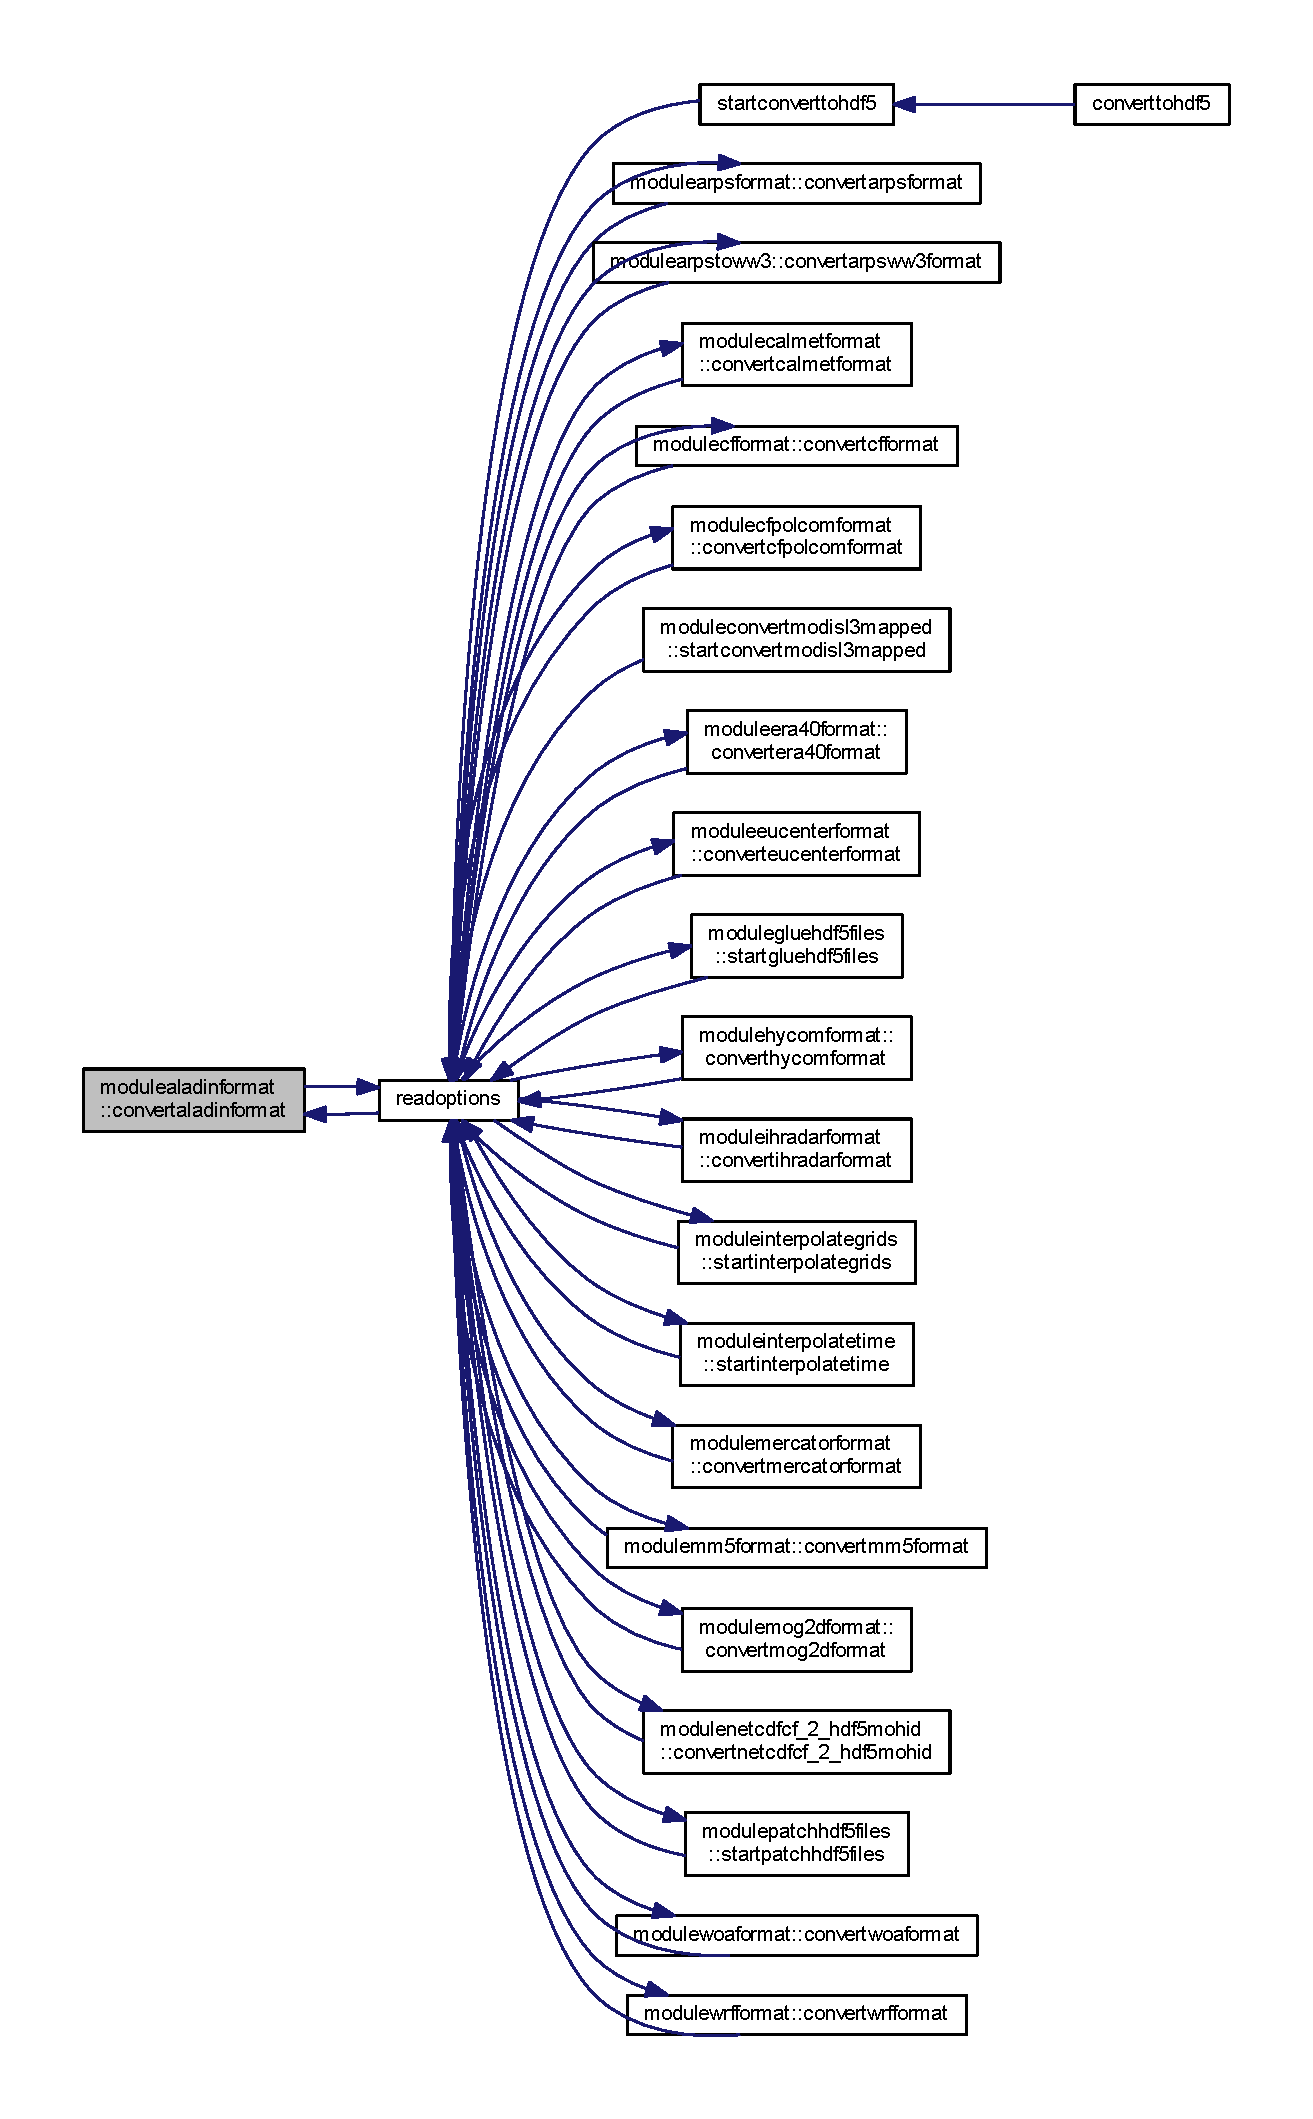
\includegraphics[height=550pt]{namespacemodulealadinformat_a77f6d15bb472ac521ff23ef7a54a48e7_icgraph}
\end{center}
\end{figure}
\mbox{\Hypertarget{namespacemodulealadinformat_ac871ced2e3713912a0c9a9563bbab1cb}\label{namespacemodulealadinformat_ac871ced2e3713912a0c9a9563bbab1cb}} 
\index{modulealadinformat@{modulealadinformat}!getvariables@{getvariables}}
\index{getvariables@{getvariables}!modulealadinformat@{modulealadinformat}}
\subsubsection{\texorpdfstring{getvariables()}{getvariables()}}
{\footnotesize\ttfamily subroutine, private modulealadinformat\+::getvariables (\begin{DoxyParamCaption}\item[{integer}]{i\+Out }\end{DoxyParamCaption})\hspace{0.3cm}{\ttfamily [private]}}

Here is the caller graph for this function\+:\nopagebreak
\begin{figure}[H]
\begin{center}
\leavevmode
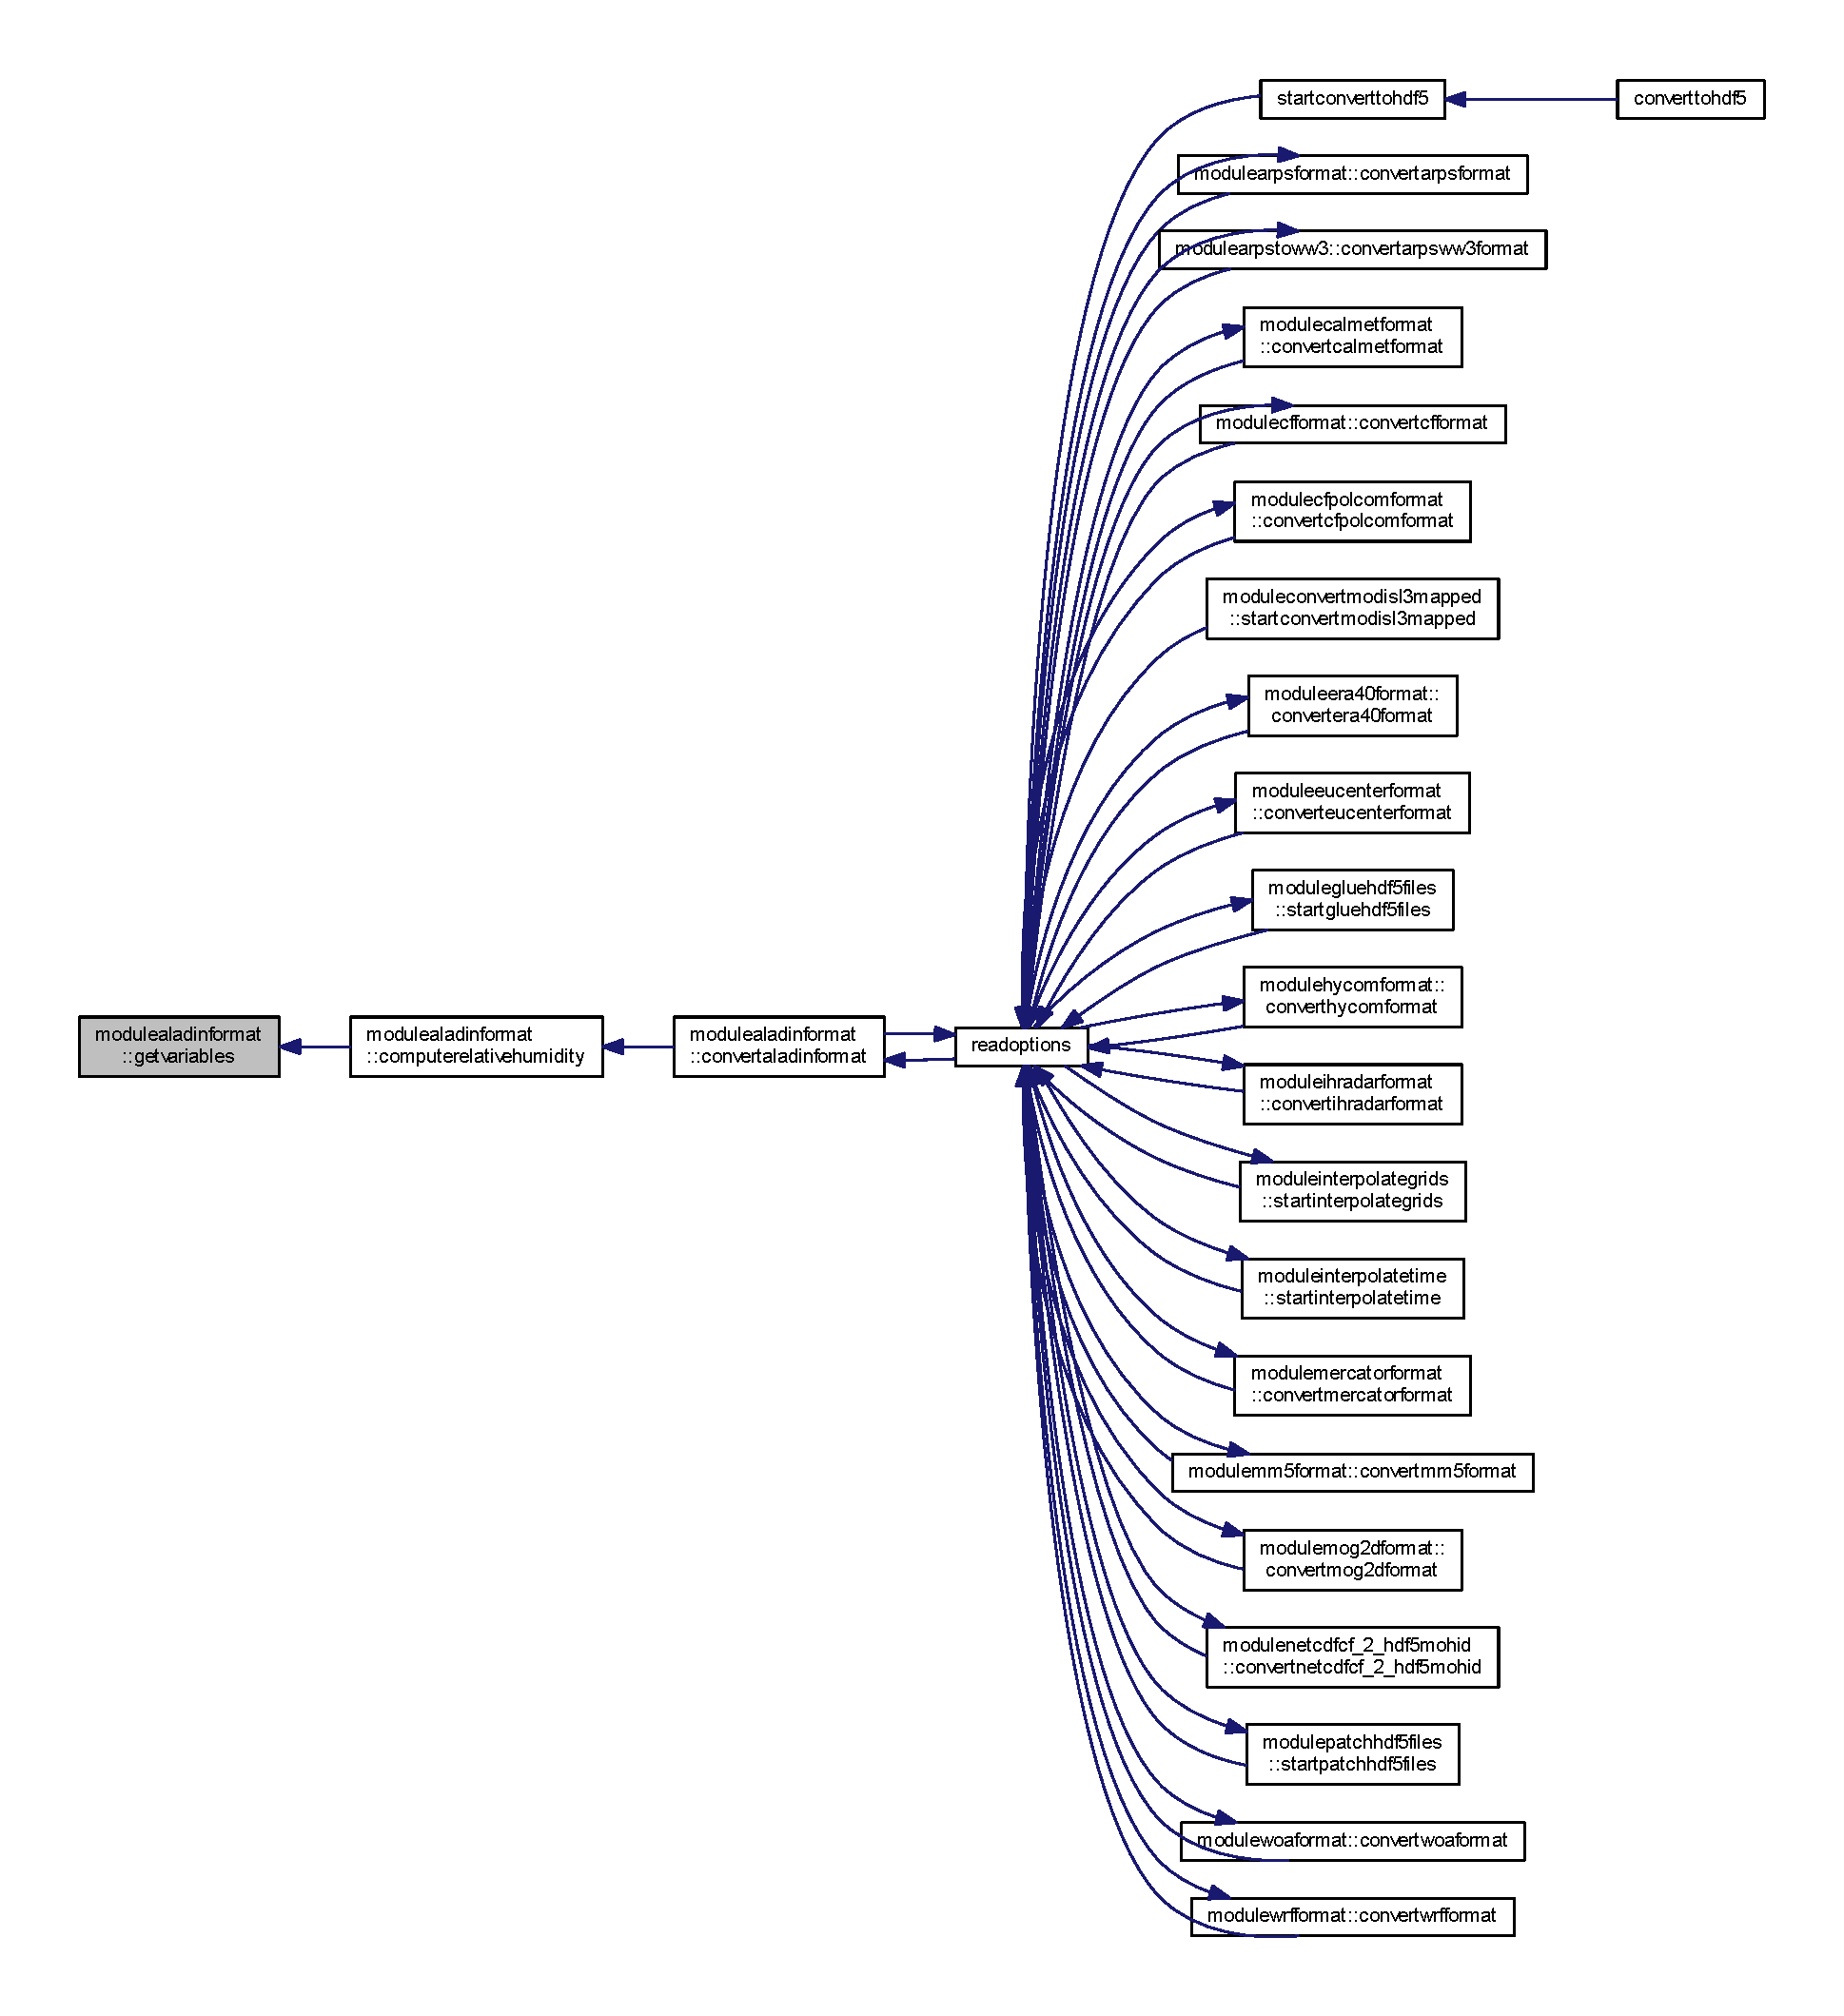
\includegraphics[width=350pt]{namespacemodulealadinformat_ac871ced2e3713912a0c9a9563bbab1cb_icgraph}
\end{center}
\end{figure}
\mbox{\Hypertarget{namespacemodulealadinformat_a5841418d49ae6a17486590f8f686e489}\label{namespacemodulealadinformat_a5841418d49ae6a17486590f8f686e489}} 
\index{modulealadinformat@{modulealadinformat}!hdf5timeinstant@{hdf5timeinstant}}
\index{hdf5timeinstant@{hdf5timeinstant}!modulealadinformat@{modulealadinformat}}
\subsubsection{\texorpdfstring{hdf5timeinstant()}{hdf5timeinstant()}}
{\footnotesize\ttfamily type(t\+\_\+time) function modulealadinformat\+::hdf5timeinstant (\begin{DoxyParamCaption}\item[{integer}]{Instant }\end{DoxyParamCaption})\hspace{0.3cm}{\ttfamily [private]}}

Here is the caller graph for this function\+:\nopagebreak
\begin{figure}[H]
\begin{center}
\leavevmode
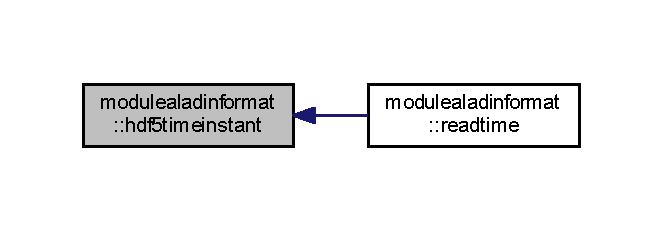
\includegraphics[width=318pt]{namespacemodulealadinformat_a5841418d49ae6a17486590f8f686e489_icgraph}
\end{center}
\end{figure}
\mbox{\Hypertarget{namespacemodulealadinformat_a5391156d679edf14a9f2631410182102}\label{namespacemodulealadinformat_a5391156d679edf14a9f2631410182102}} 
\index{modulealadinformat@{modulealadinformat}!killaladinformat@{killaladinformat}}
\index{killaladinformat@{killaladinformat}!modulealadinformat@{modulealadinformat}}
\subsubsection{\texorpdfstring{killaladinformat()}{killaladinformat()}}
{\footnotesize\ttfamily subroutine, private modulealadinformat\+::killaladinformat (\begin{DoxyParamCaption}{ }\end{DoxyParamCaption})\hspace{0.3cm}{\ttfamily [private]}}

Here is the caller graph for this function\+:\nopagebreak
\begin{figure}[H]
\begin{center}
\leavevmode
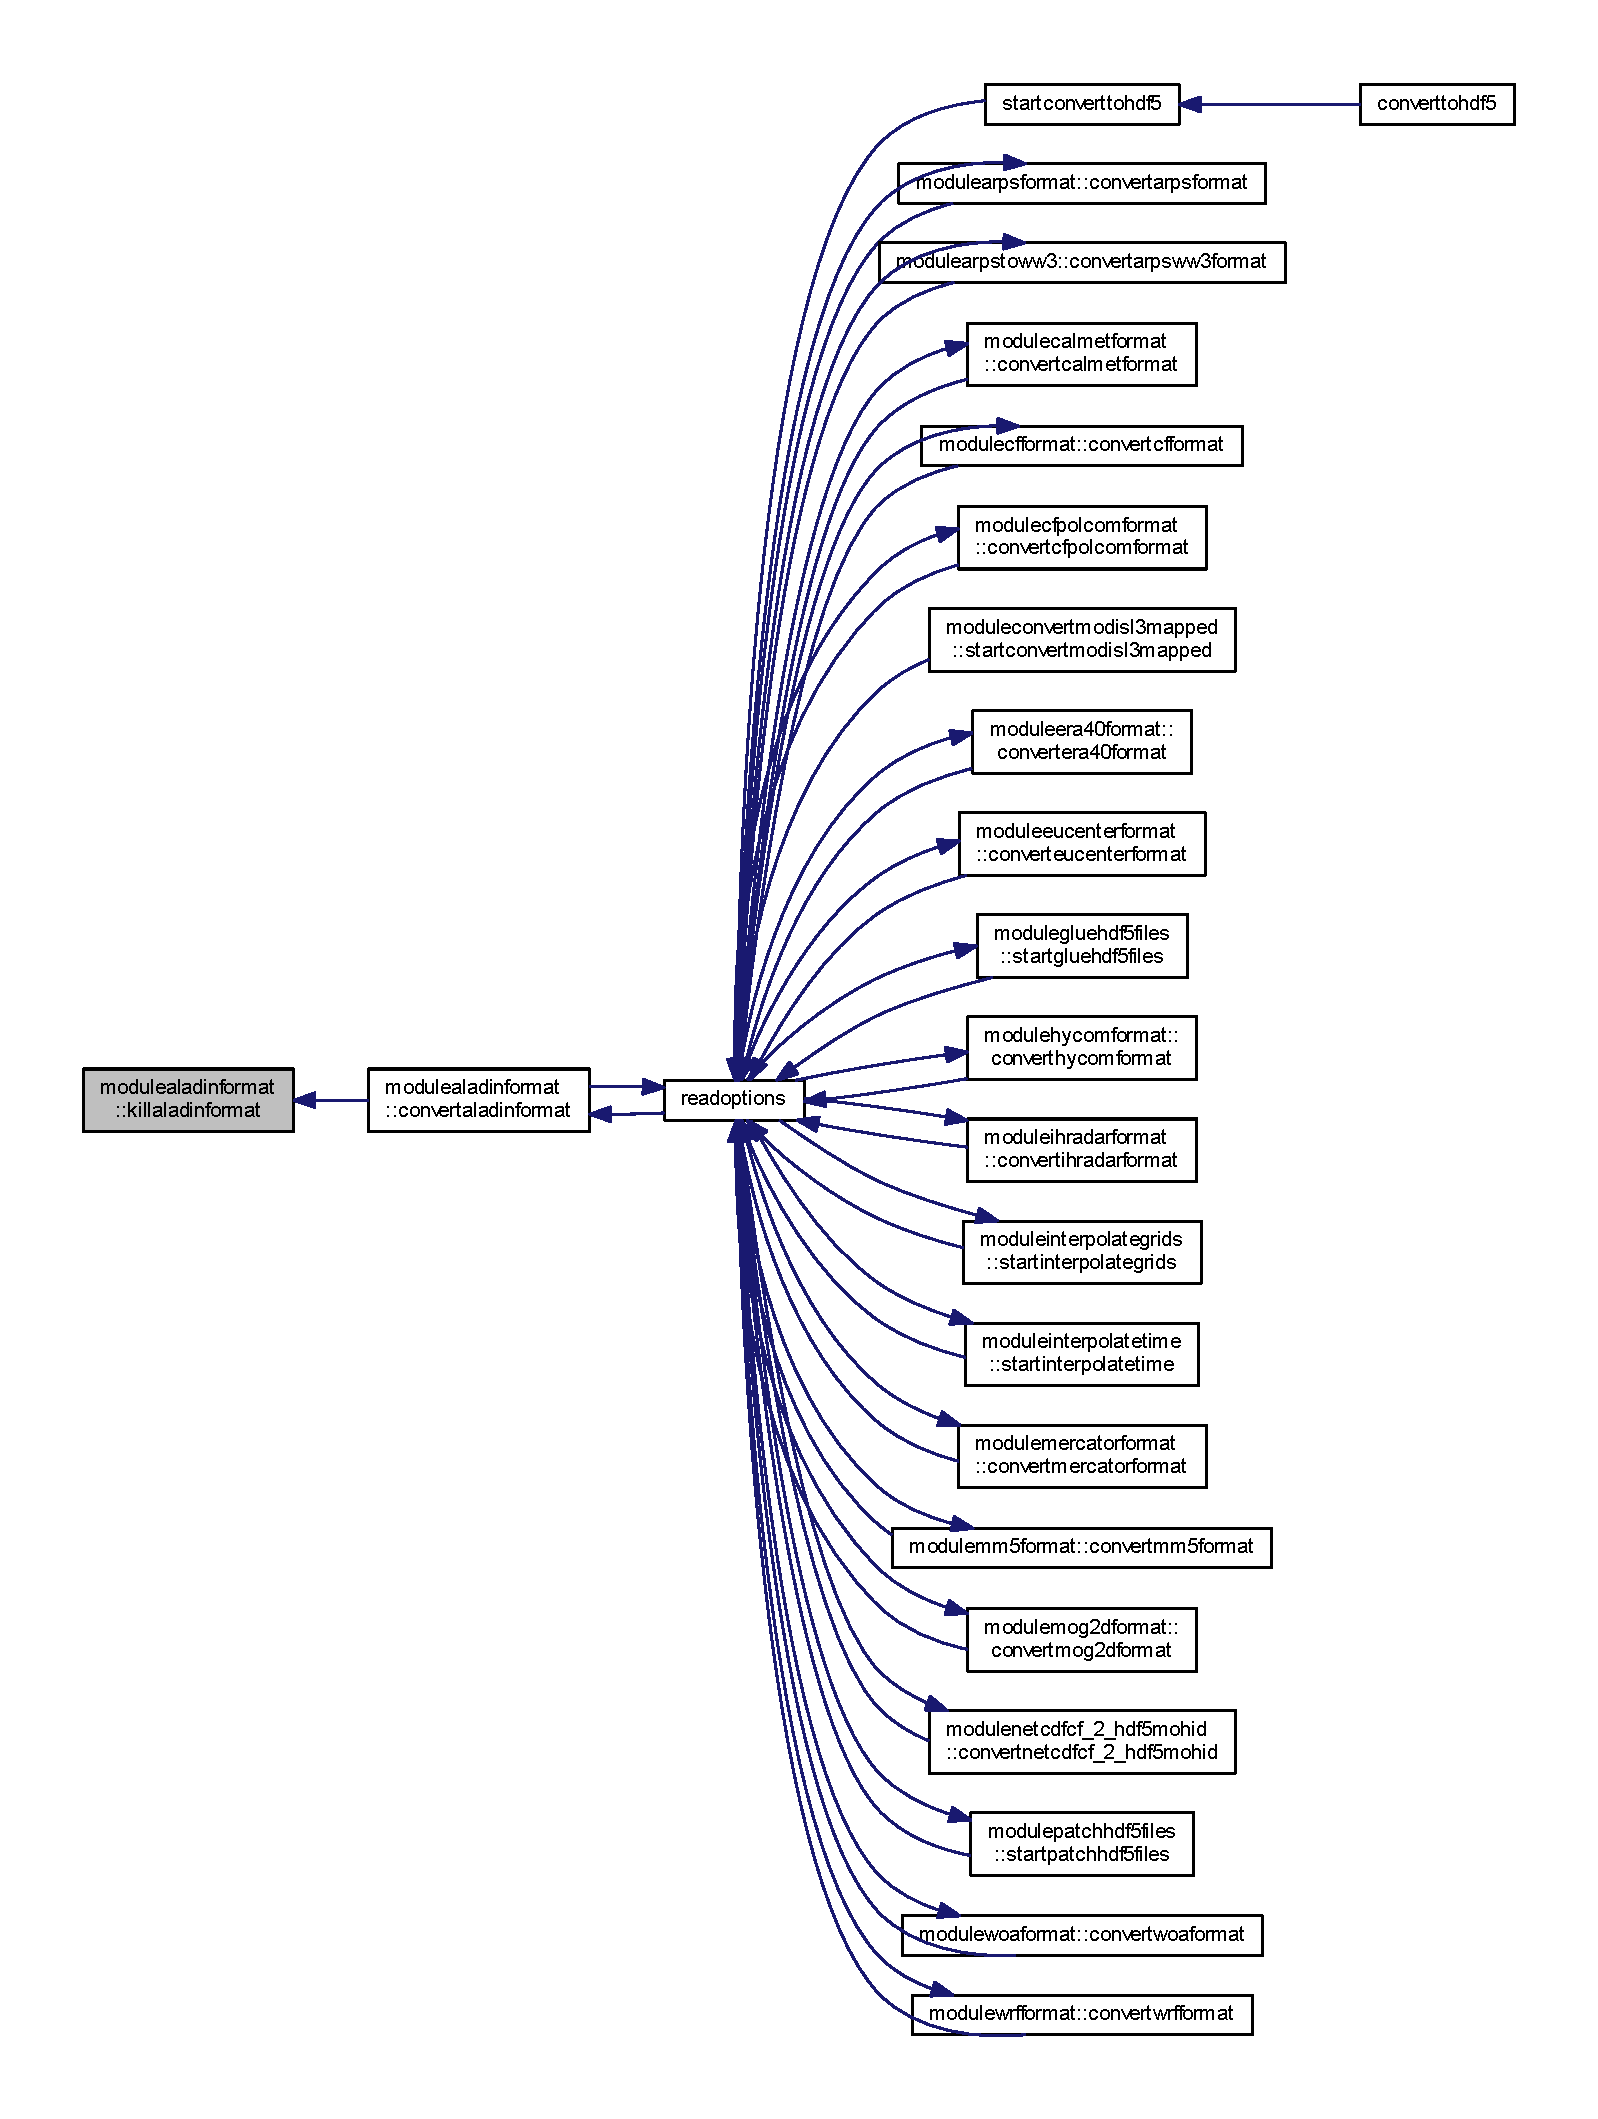
\includegraphics[width=350pt]{namespacemodulealadinformat_a5391156d679edf14a9f2631410182102_icgraph}
\end{center}
\end{figure}
\mbox{\Hypertarget{namespacemodulealadinformat_a0e28e132a765a53e91eb16cf638b0b32}\label{namespacemodulealadinformat_a0e28e132a765a53e91eb16cf638b0b32}} 
\index{modulealadinformat@{modulealadinformat}!mohidunits@{mohidunits}}
\index{mohidunits@{mohidunits}!modulealadinformat@{modulealadinformat}}
\subsubsection{\texorpdfstring{mohidunits()}{mohidunits()}}
{\footnotesize\ttfamily character(len=stringlength) function modulealadinformat\+::mohidunits (\begin{DoxyParamCaption}\item[{character(len=stringlength)}]{Mohid\+Name }\end{DoxyParamCaption})\hspace{0.3cm}{\ttfamily [private]}}

Here is the caller graph for this function\+:\nopagebreak
\begin{figure}[H]
\begin{center}
\leavevmode
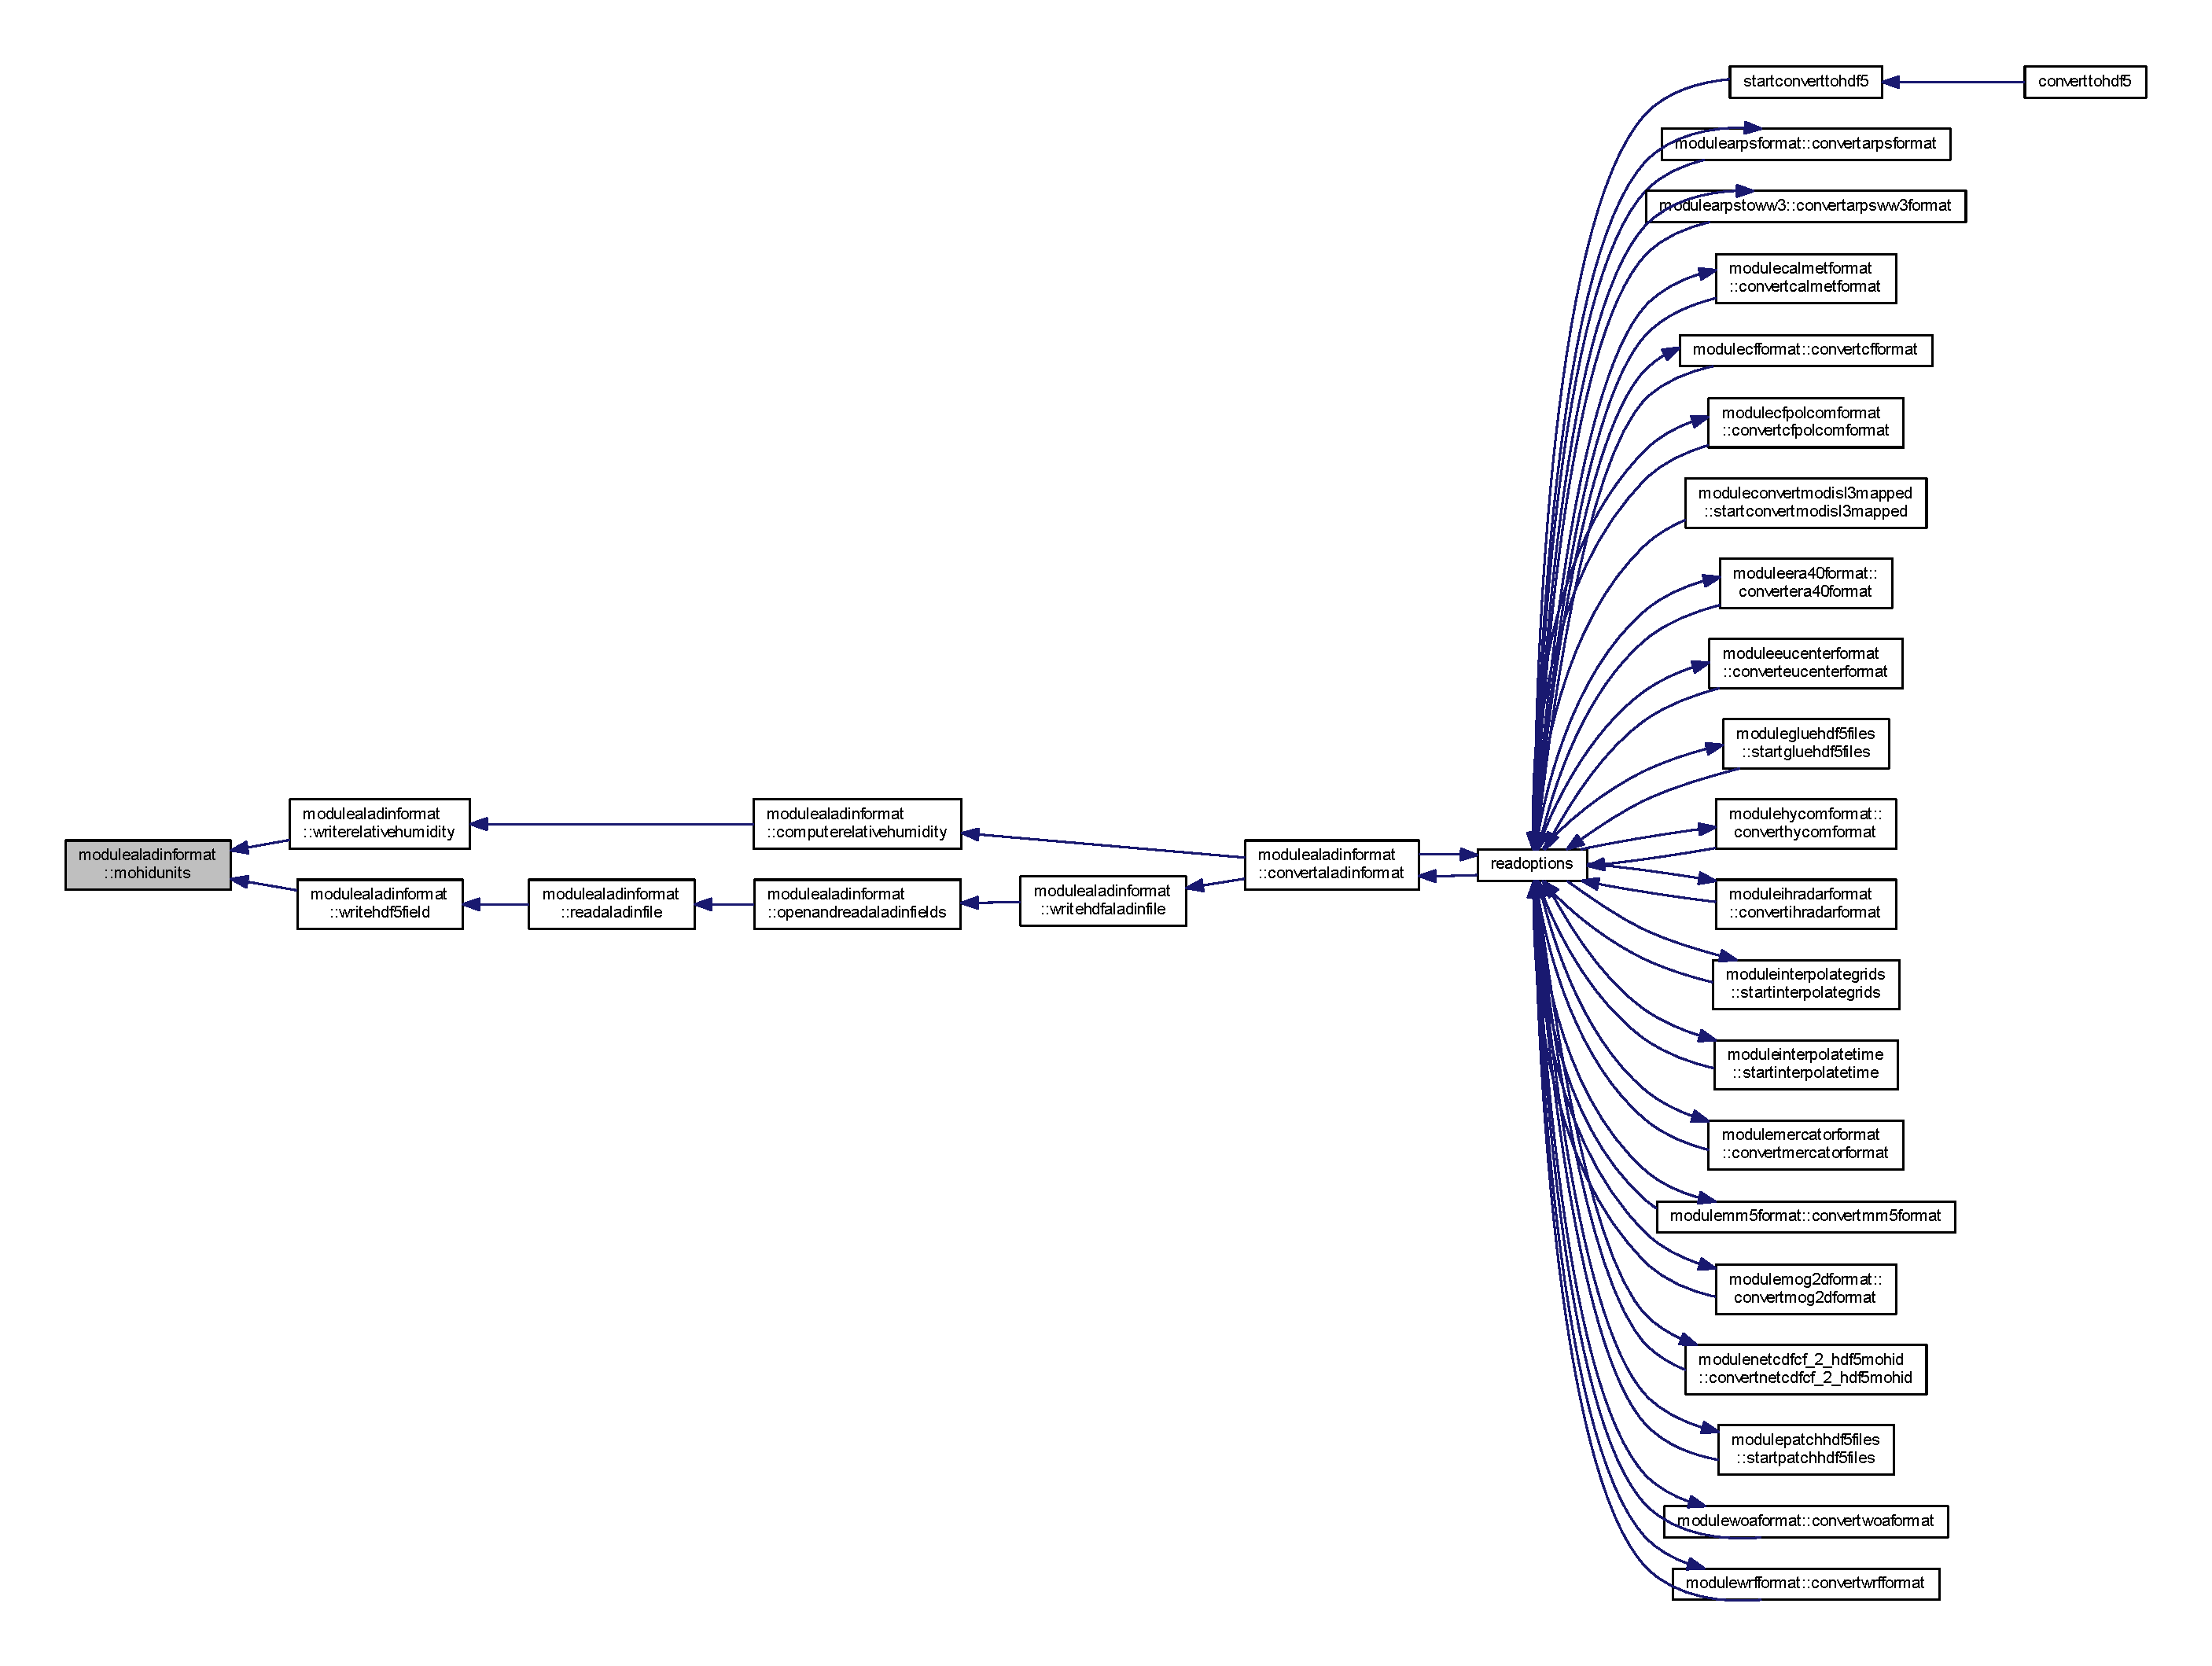
\includegraphics[width=350pt]{namespacemodulealadinformat_a0e28e132a765a53e91eb16cf638b0b32_icgraph}
\end{center}
\end{figure}
\mbox{\Hypertarget{namespacemodulealadinformat_a554b3cf12b5ecedce22b2e607f931c70}\label{namespacemodulealadinformat_a554b3cf12b5ecedce22b2e607f931c70}} 
\index{modulealadinformat@{modulealadinformat}!open\+\_\+hdf5\+\_\+output\+\_\+file@{open\+\_\+hdf5\+\_\+output\+\_\+file}}
\index{open\+\_\+hdf5\+\_\+output\+\_\+file@{open\+\_\+hdf5\+\_\+output\+\_\+file}!modulealadinformat@{modulealadinformat}}
\subsubsection{\texorpdfstring{open\+\_\+hdf5\+\_\+output\+\_\+file()}{open\_hdf5\_output\_file()}}
{\footnotesize\ttfamily subroutine, private modulealadinformat\+::open\+\_\+hdf5\+\_\+output\+\_\+file (\begin{DoxyParamCaption}\item[{integer}]{H\+D\+F5\+\_\+\+I\+O\+\_\+\+C\+O\+DE }\end{DoxyParamCaption})\hspace{0.3cm}{\ttfamily [private]}}

Here is the caller graph for this function\+:\nopagebreak
\begin{figure}[H]
\begin{center}
\leavevmode
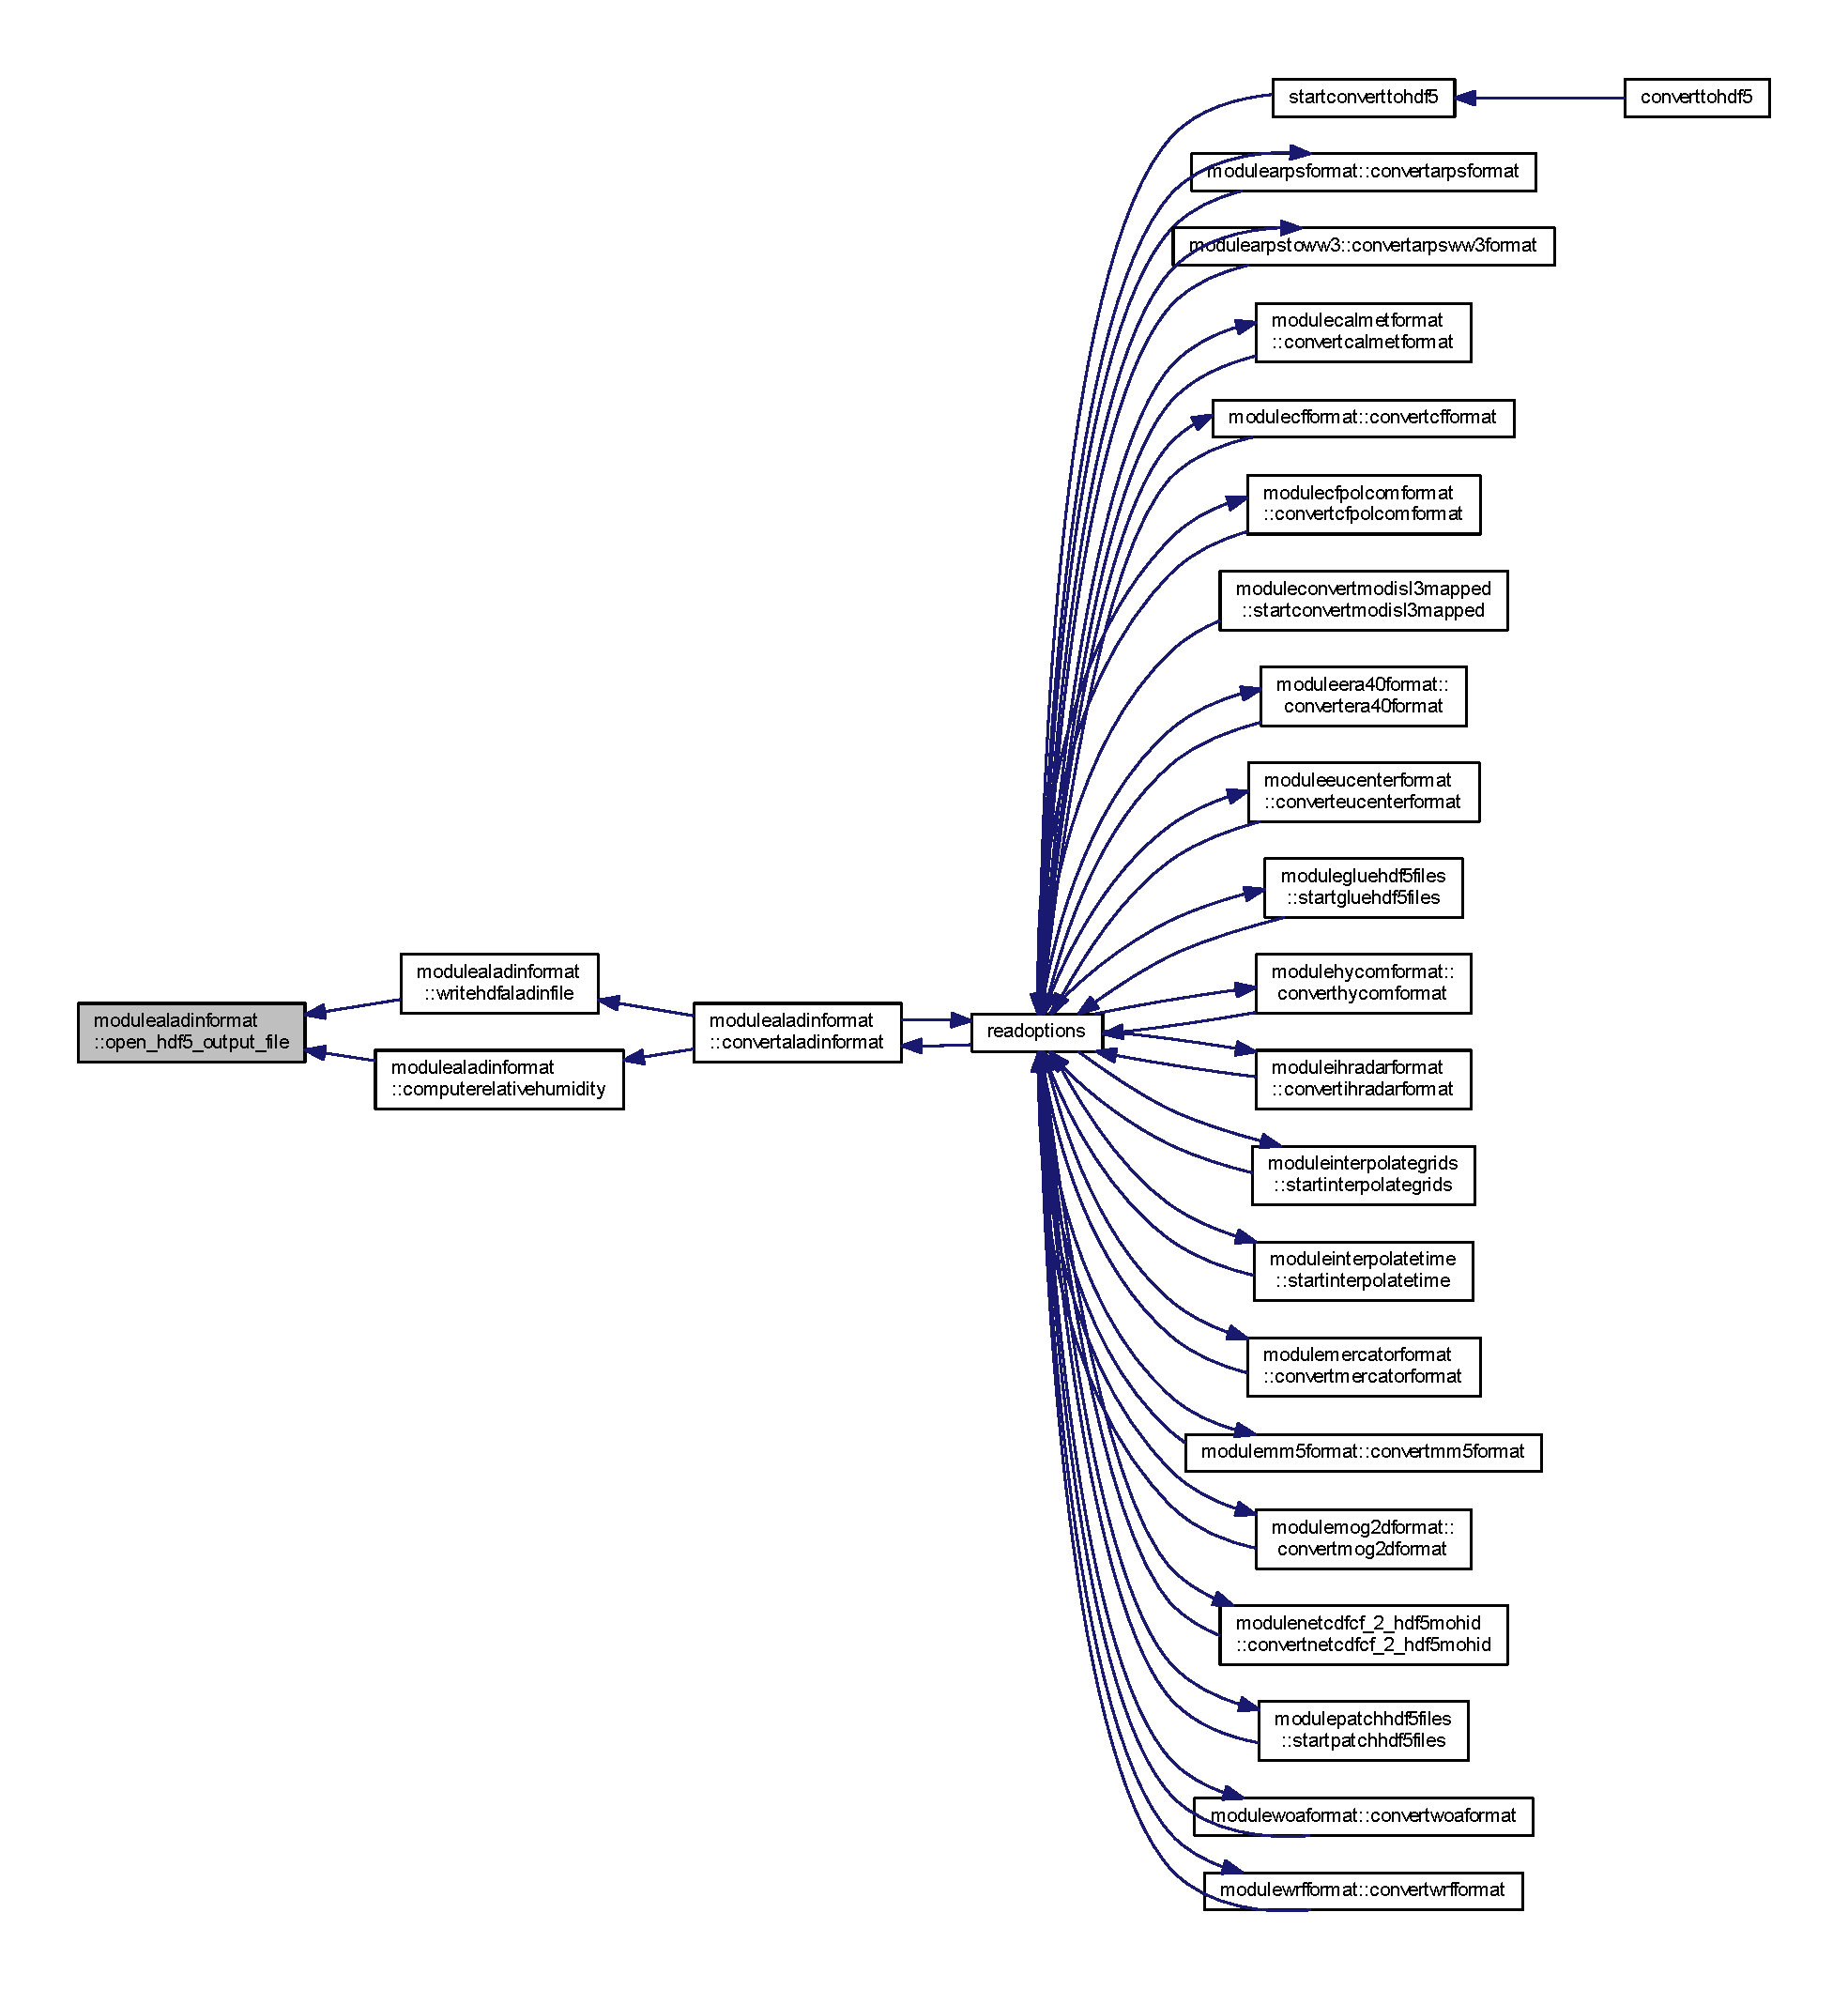
\includegraphics[width=350pt]{namespacemodulealadinformat_a554b3cf12b5ecedce22b2e607f931c70_icgraph}
\end{center}
\end{figure}
\mbox{\Hypertarget{namespacemodulealadinformat_a2b65697a3c42c8dc546ebf63e260e98f}\label{namespacemodulealadinformat_a2b65697a3c42c8dc546ebf63e260e98f}} 
\index{modulealadinformat@{modulealadinformat}!openandreadaladinfields@{openandreadaladinfields}}
\index{openandreadaladinfields@{openandreadaladinfields}!modulealadinformat@{modulealadinformat}}
\subsubsection{\texorpdfstring{openandreadaladinfields()}{openandreadaladinfields()}}
{\footnotesize\ttfamily subroutine, private modulealadinformat\+::openandreadaladinfields (\begin{DoxyParamCaption}{ }\end{DoxyParamCaption})\hspace{0.3cm}{\ttfamily [private]}}

Here is the call graph for this function\+:\nopagebreak
\begin{figure}[H]
\begin{center}
\leavevmode
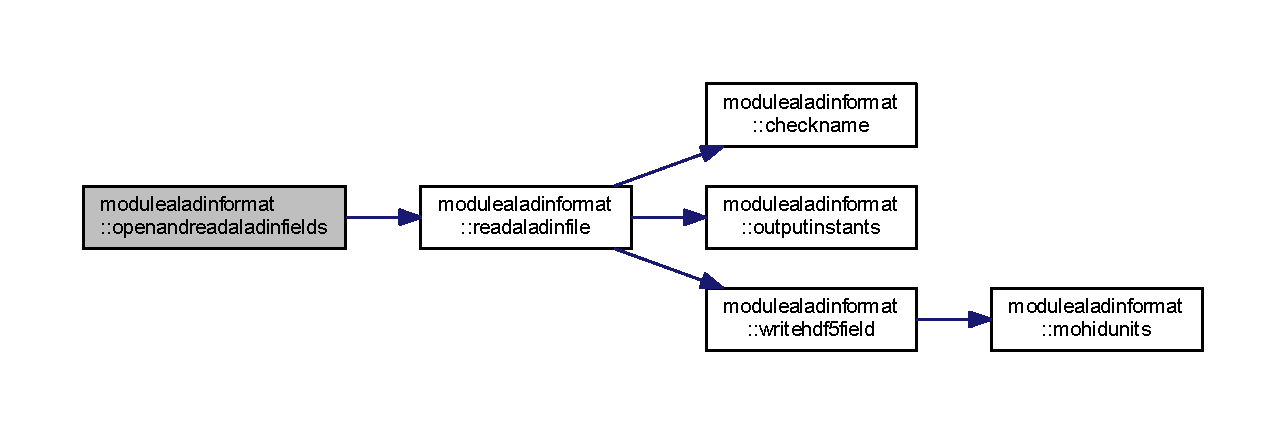
\includegraphics[width=350pt]{namespacemodulealadinformat_a2b65697a3c42c8dc546ebf63e260e98f_cgraph}
\end{center}
\end{figure}
Here is the caller graph for this function\+:\nopagebreak
\begin{figure}[H]
\begin{center}
\leavevmode
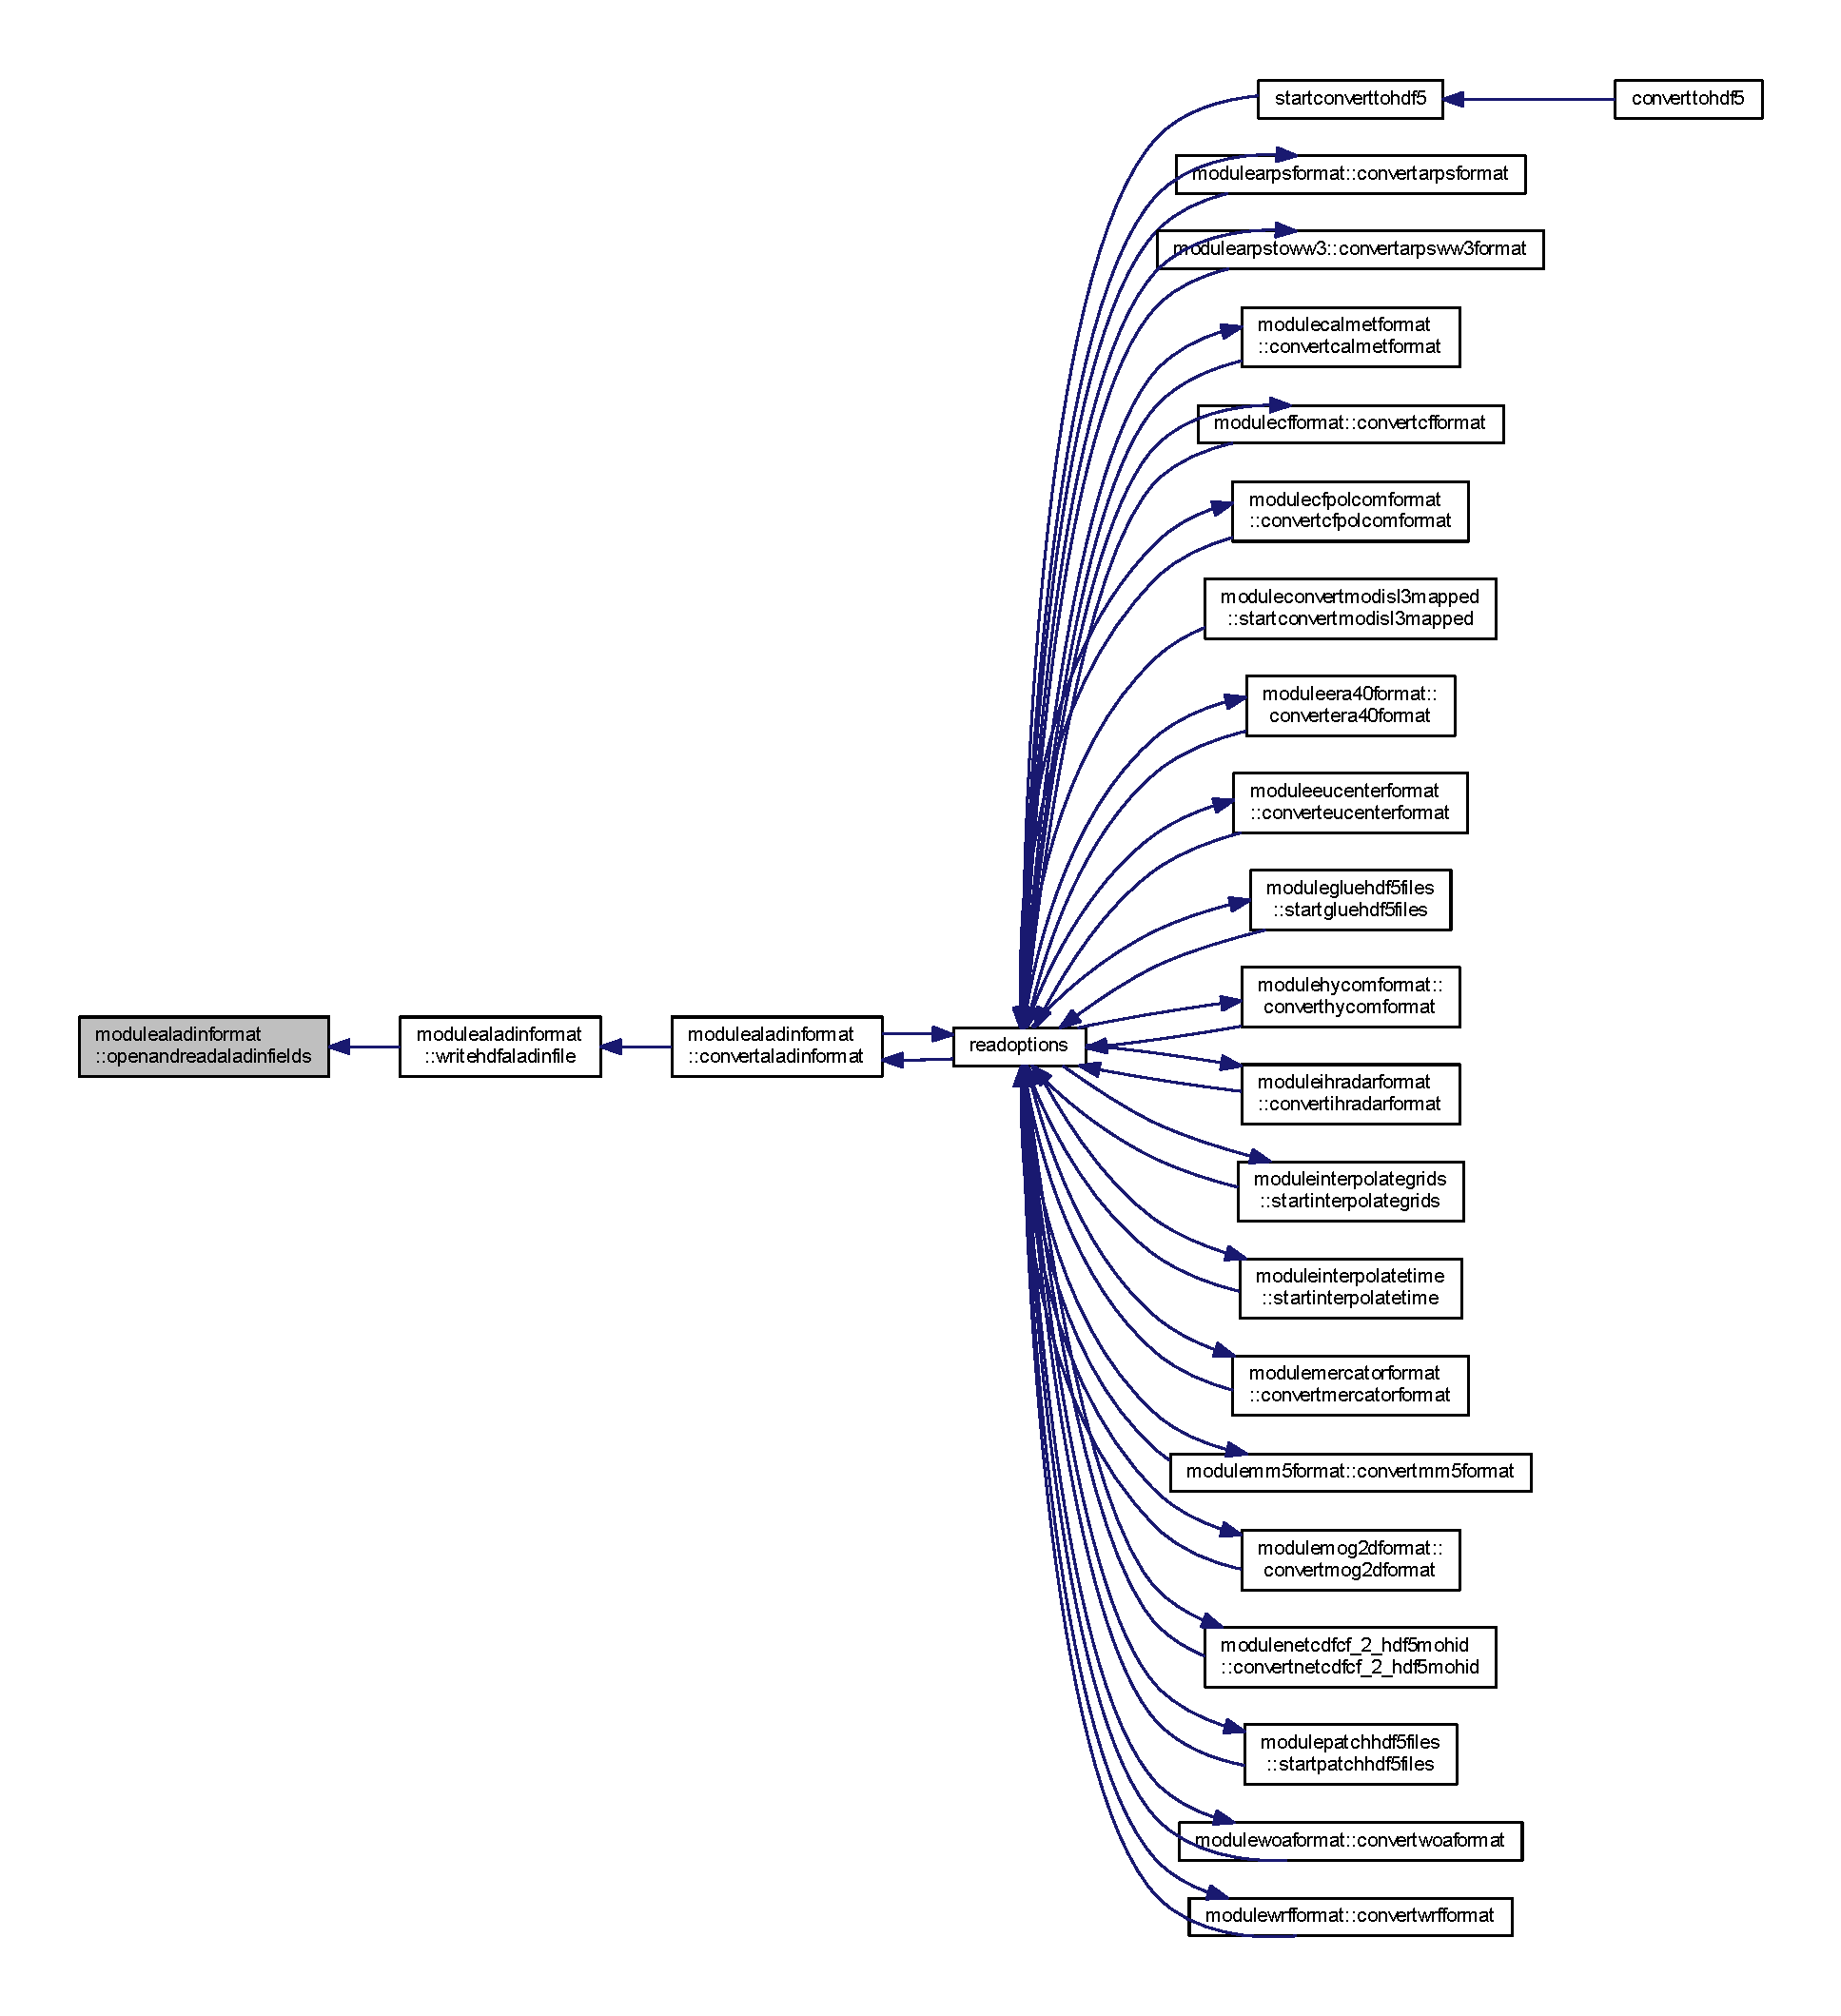
\includegraphics[width=350pt]{namespacemodulealadinformat_a2b65697a3c42c8dc546ebf63e260e98f_icgraph}
\end{center}
\end{figure}
\mbox{\Hypertarget{namespacemodulealadinformat_a0340c1a27e19b5142e4089d2951da7cb}\label{namespacemodulealadinformat_a0340c1a27e19b5142e4089d2951da7cb}} 
\index{modulealadinformat@{modulealadinformat}!openandreadaladinfile@{openandreadaladinfile}}
\index{openandreadaladinfile@{openandreadaladinfile}!modulealadinformat@{modulealadinformat}}
\subsubsection{\texorpdfstring{openandreadaladinfile()}{openandreadaladinfile()}}
{\footnotesize\ttfamily subroutine, private modulealadinformat\+::openandreadaladinfile (\begin{DoxyParamCaption}{ }\end{DoxyParamCaption})\hspace{0.3cm}{\ttfamily [private]}}

Here is the call graph for this function\+:\nopagebreak
\begin{figure}[H]
\begin{center}
\leavevmode
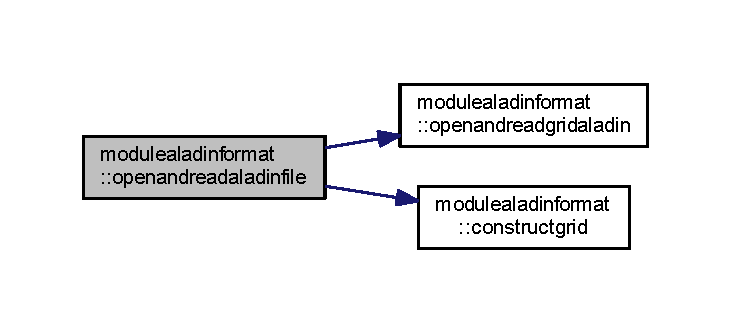
\includegraphics[width=350pt]{namespacemodulealadinformat_a0340c1a27e19b5142e4089d2951da7cb_cgraph}
\end{center}
\end{figure}
Here is the caller graph for this function\+:\nopagebreak
\begin{figure}[H]
\begin{center}
\leavevmode
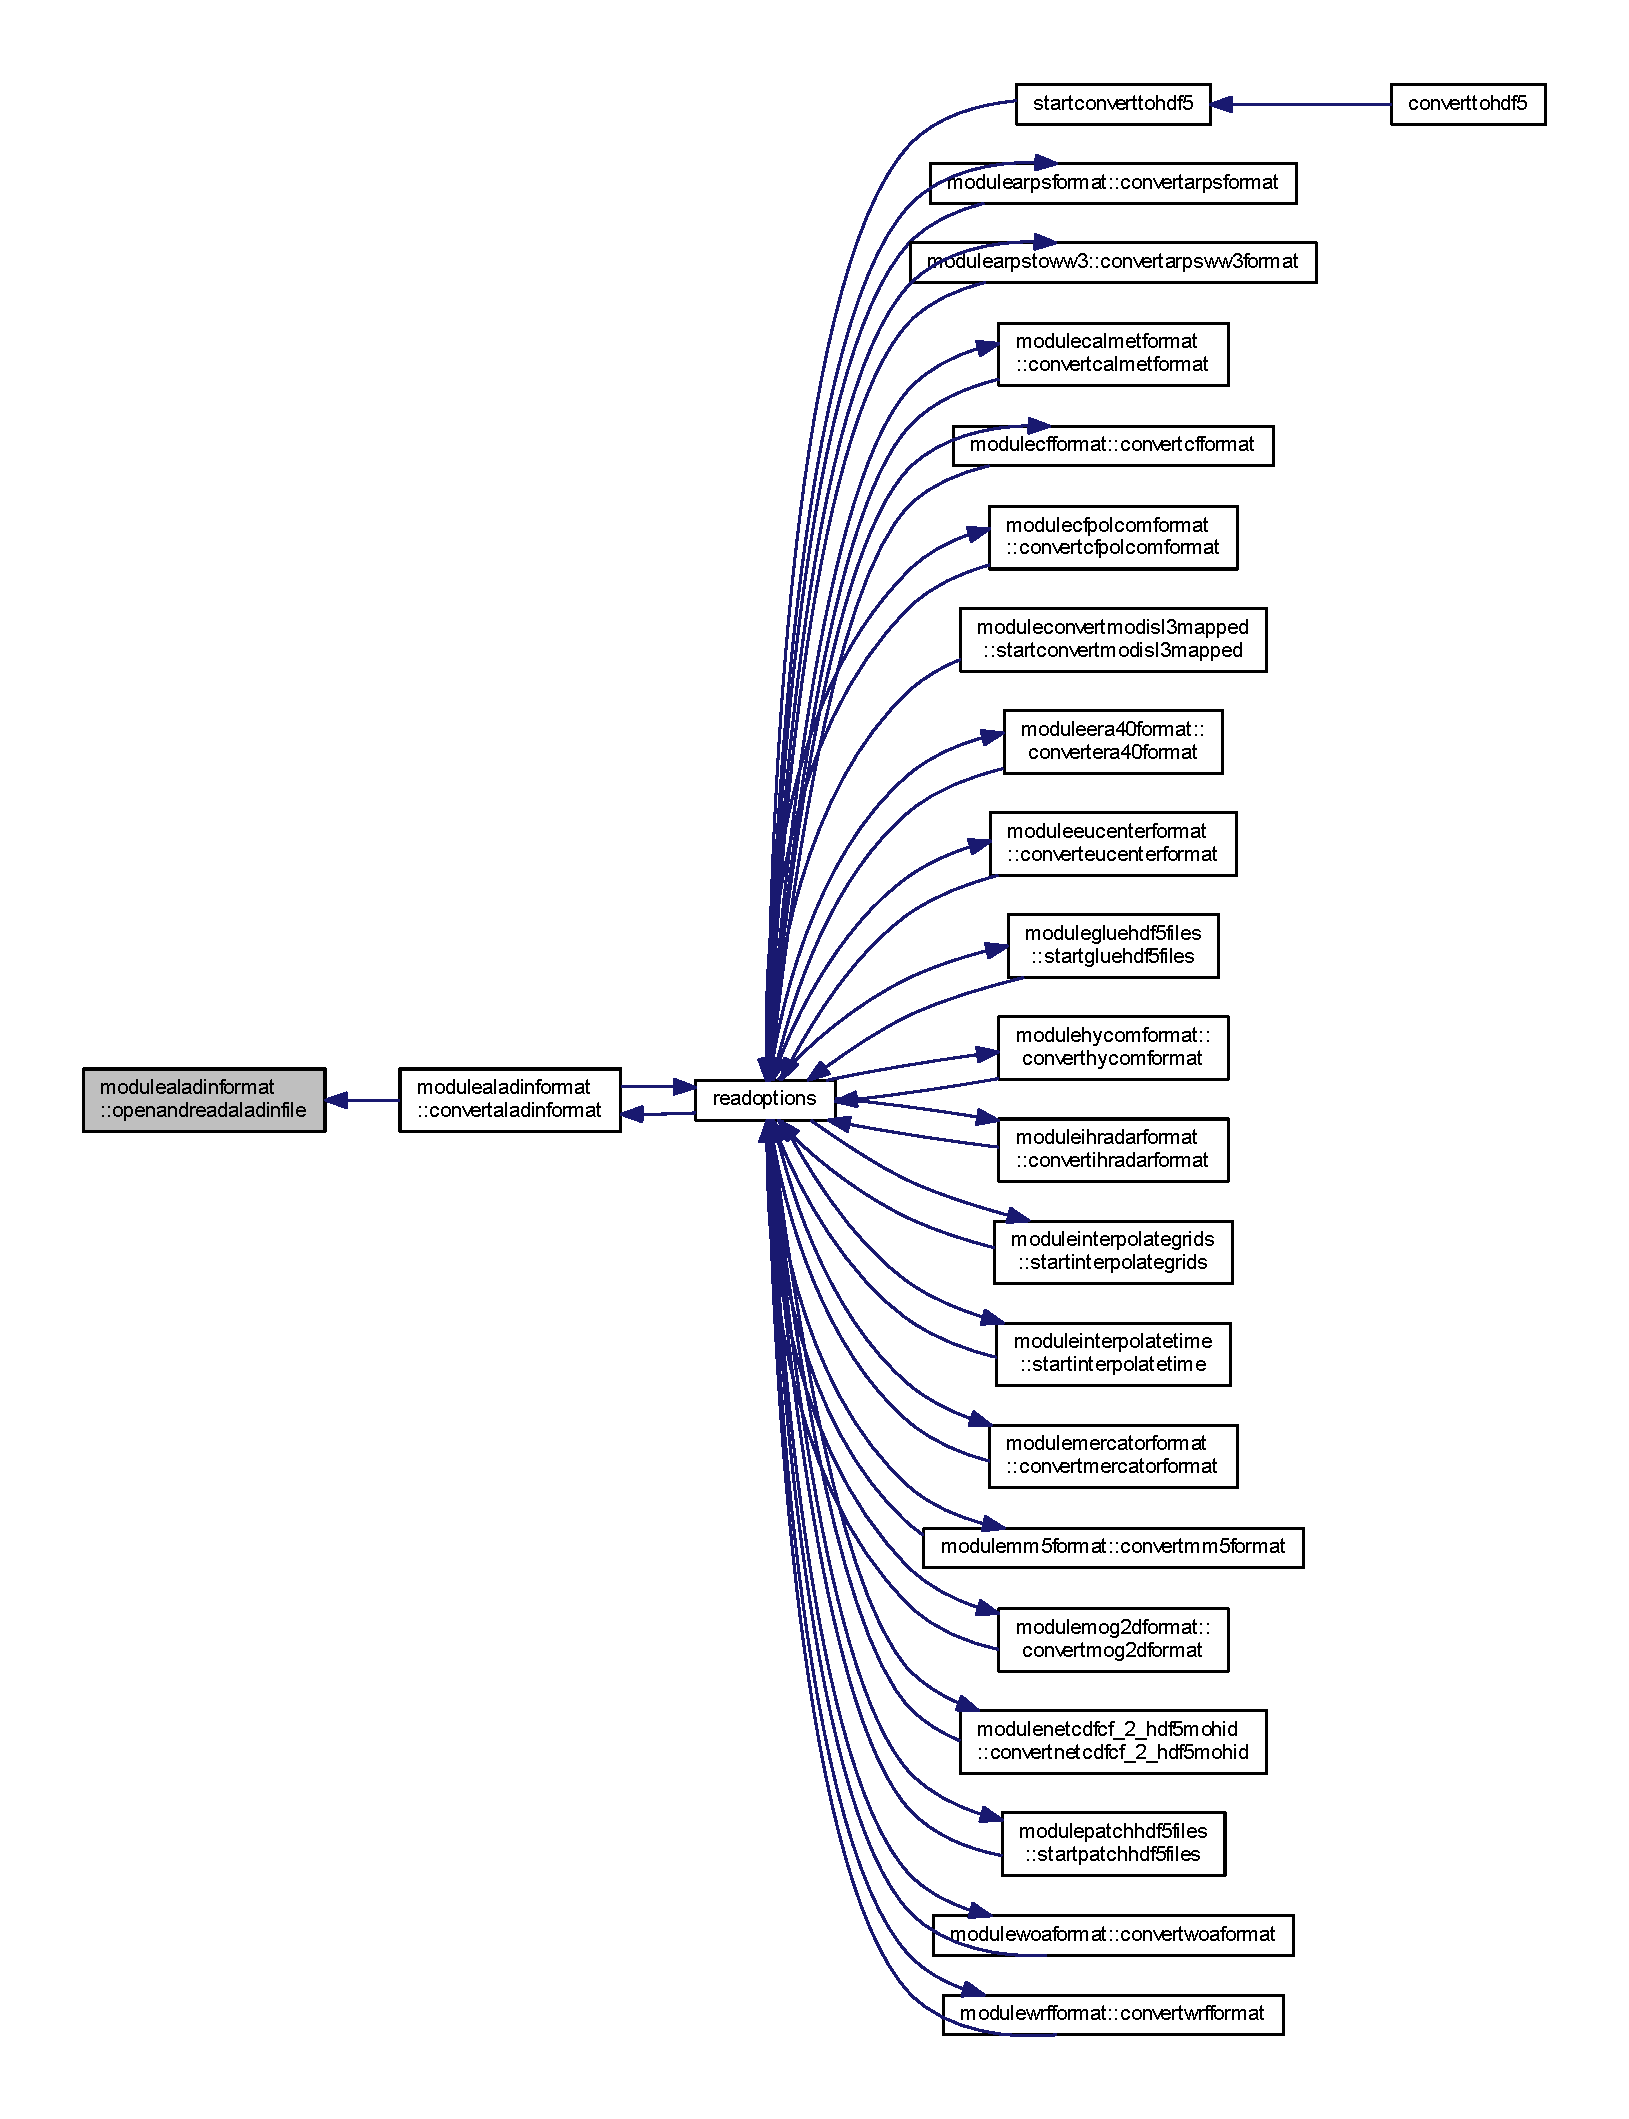
\includegraphics[width=350pt]{namespacemodulealadinformat_a0340c1a27e19b5142e4089d2951da7cb_icgraph}
\end{center}
\end{figure}
\mbox{\Hypertarget{namespacemodulealadinformat_a4259301b2389ab6c64a24416eb73c157}\label{namespacemodulealadinformat_a4259301b2389ab6c64a24416eb73c157}} 
\index{modulealadinformat@{modulealadinformat}!openandreadgridaladin@{openandreadgridaladin}}
\index{openandreadgridaladin@{openandreadgridaladin}!modulealadinformat@{modulealadinformat}}
\subsubsection{\texorpdfstring{openandreadgridaladin()}{openandreadgridaladin()}}
{\footnotesize\ttfamily subroutine, private modulealadinformat\+::openandreadgridaladin (\begin{DoxyParamCaption}{ }\end{DoxyParamCaption})\hspace{0.3cm}{\ttfamily [private]}}

Here is the caller graph for this function\+:\nopagebreak
\begin{figure}[H]
\begin{center}
\leavevmode
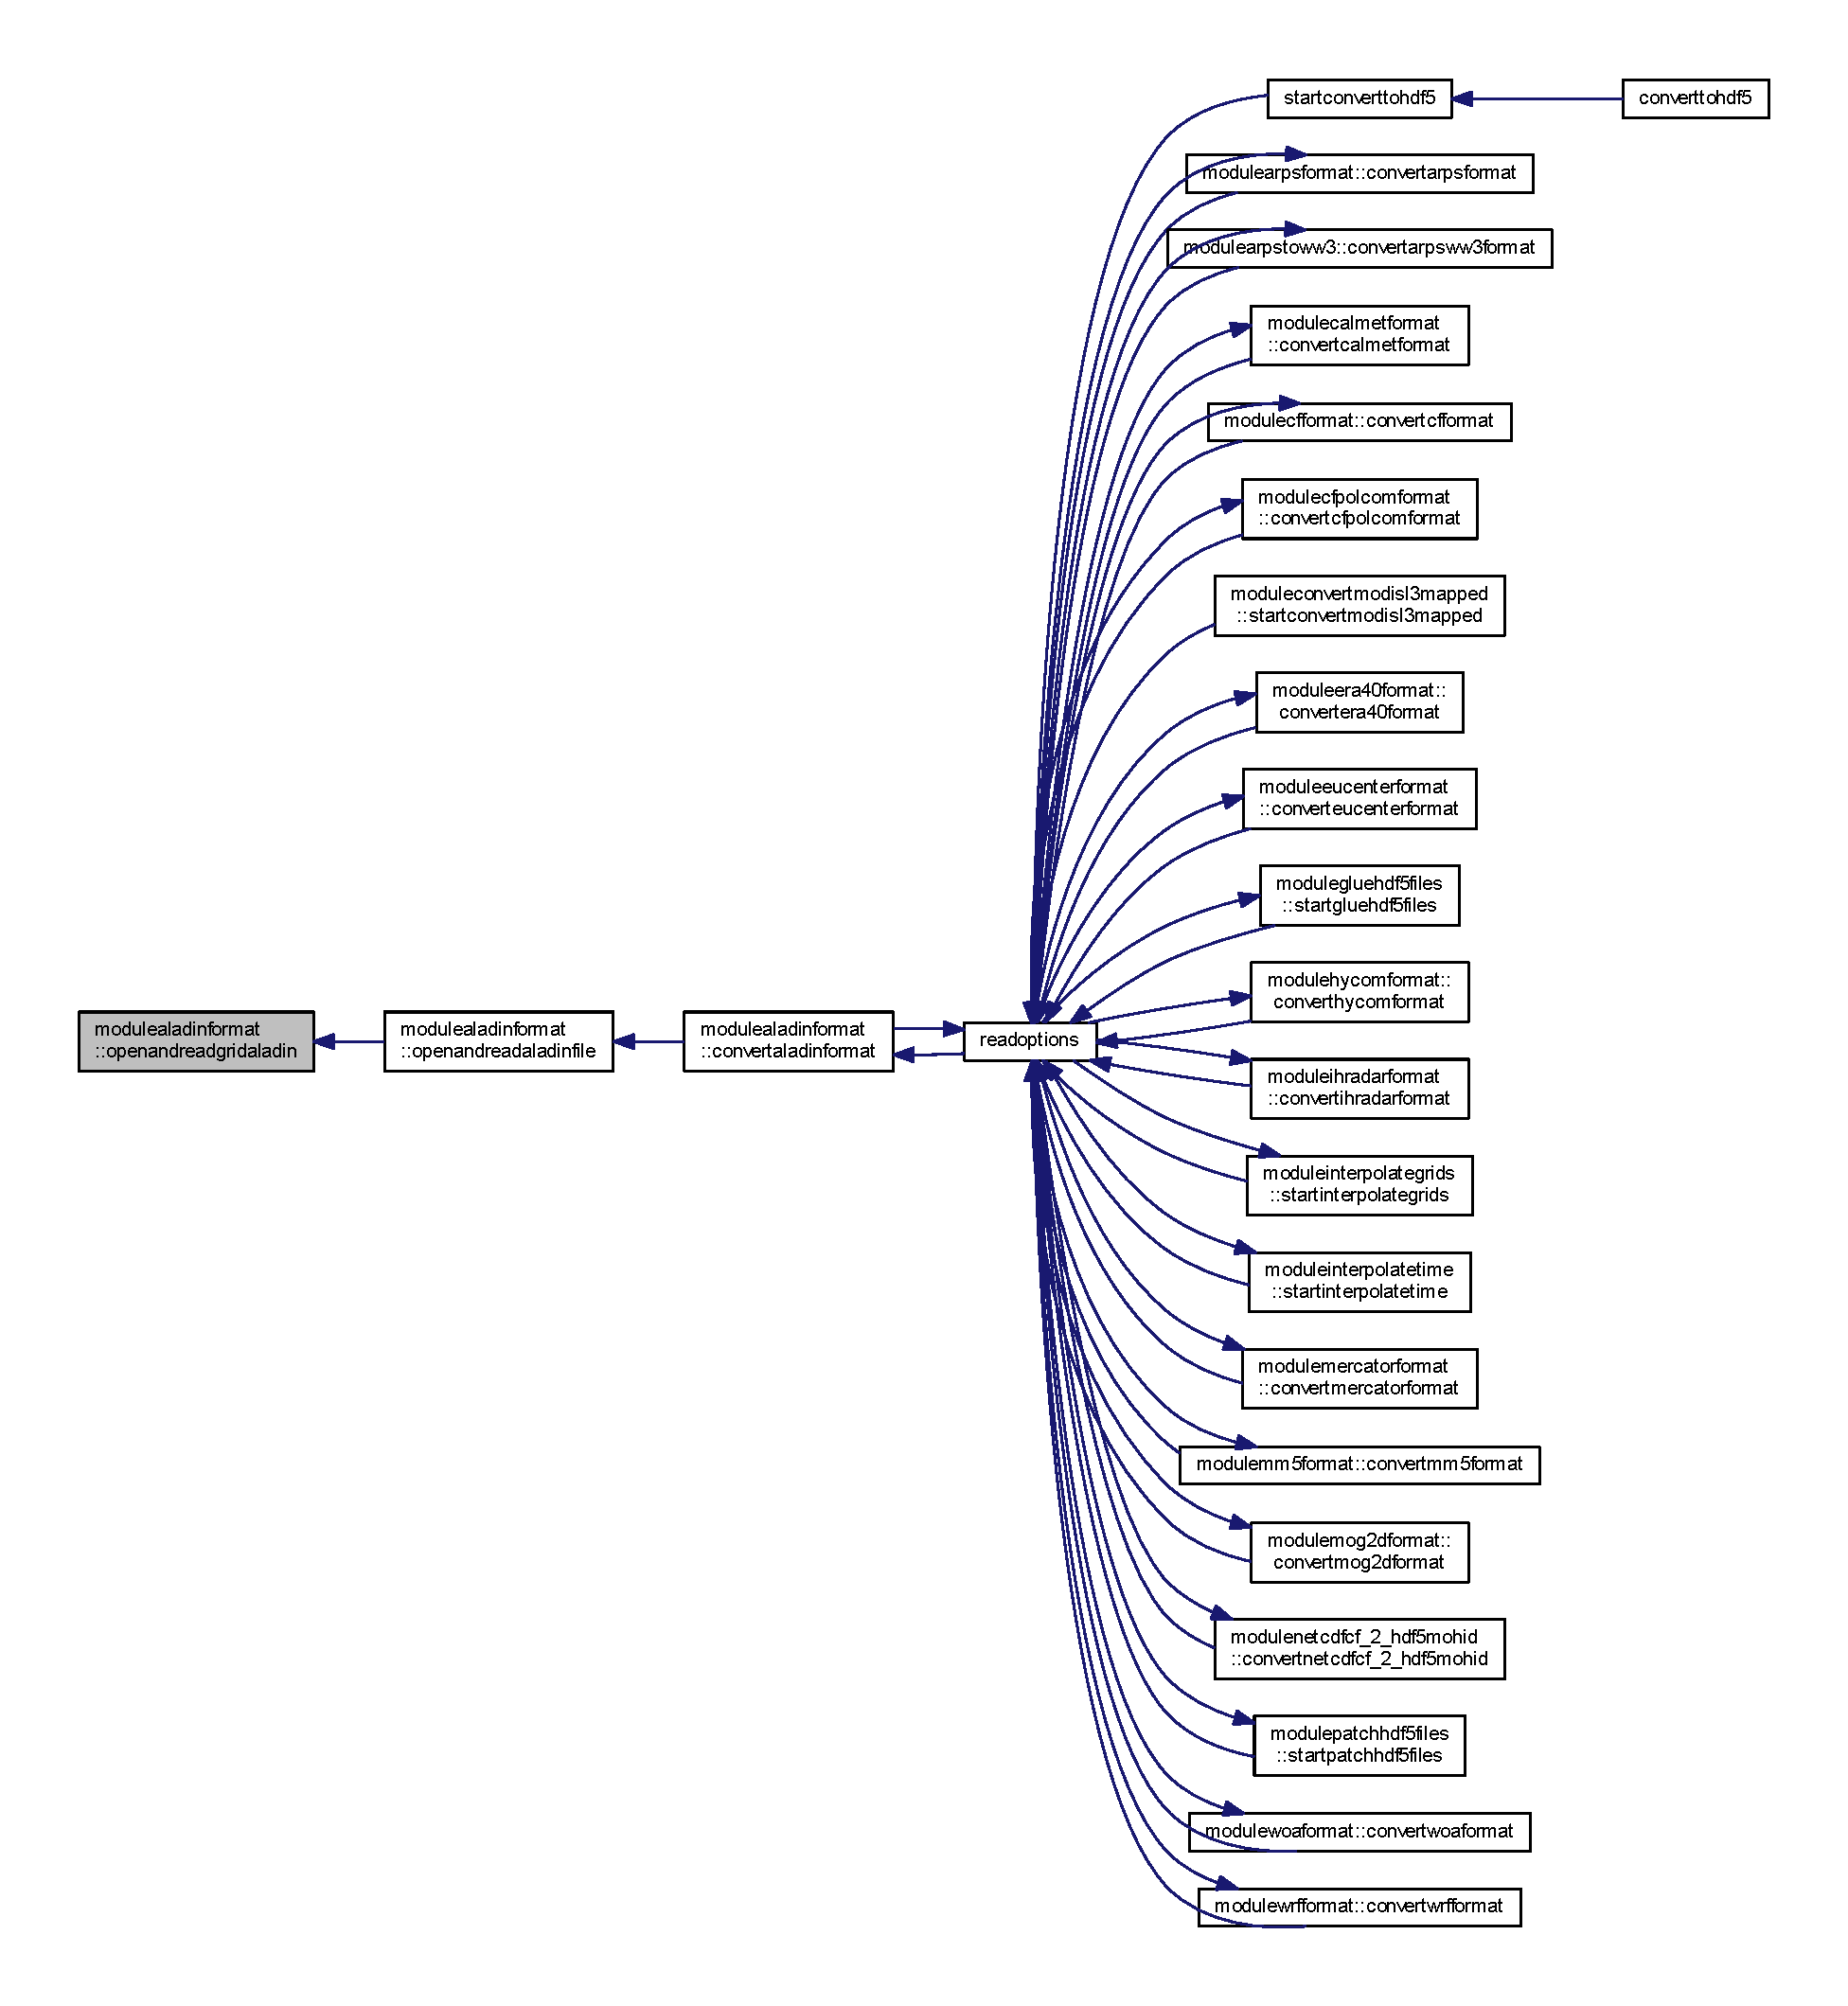
\includegraphics[width=350pt]{namespacemodulealadinformat_a4259301b2389ab6c64a24416eb73c157_icgraph}
\end{center}
\end{figure}
\mbox{\Hypertarget{namespacemodulealadinformat_aa8356f98f813a0fe5edb9089053dc372}\label{namespacemodulealadinformat_aa8356f98f813a0fe5edb9089053dc372}} 
\index{modulealadinformat@{modulealadinformat}!outputinstants@{outputinstants}}
\index{outputinstants@{outputinstants}!modulealadinformat@{modulealadinformat}}
\subsubsection{\texorpdfstring{outputinstants()}{outputinstants()}}
{\footnotesize\ttfamily integer function modulealadinformat\+::outputinstants (\begin{DoxyParamCaption}\item[{character(len=stringlength)}]{Mohid\+Name }\end{DoxyParamCaption})\hspace{0.3cm}{\ttfamily [private]}}

Here is the caller graph for this function\+:\nopagebreak
\begin{figure}[H]
\begin{center}
\leavevmode
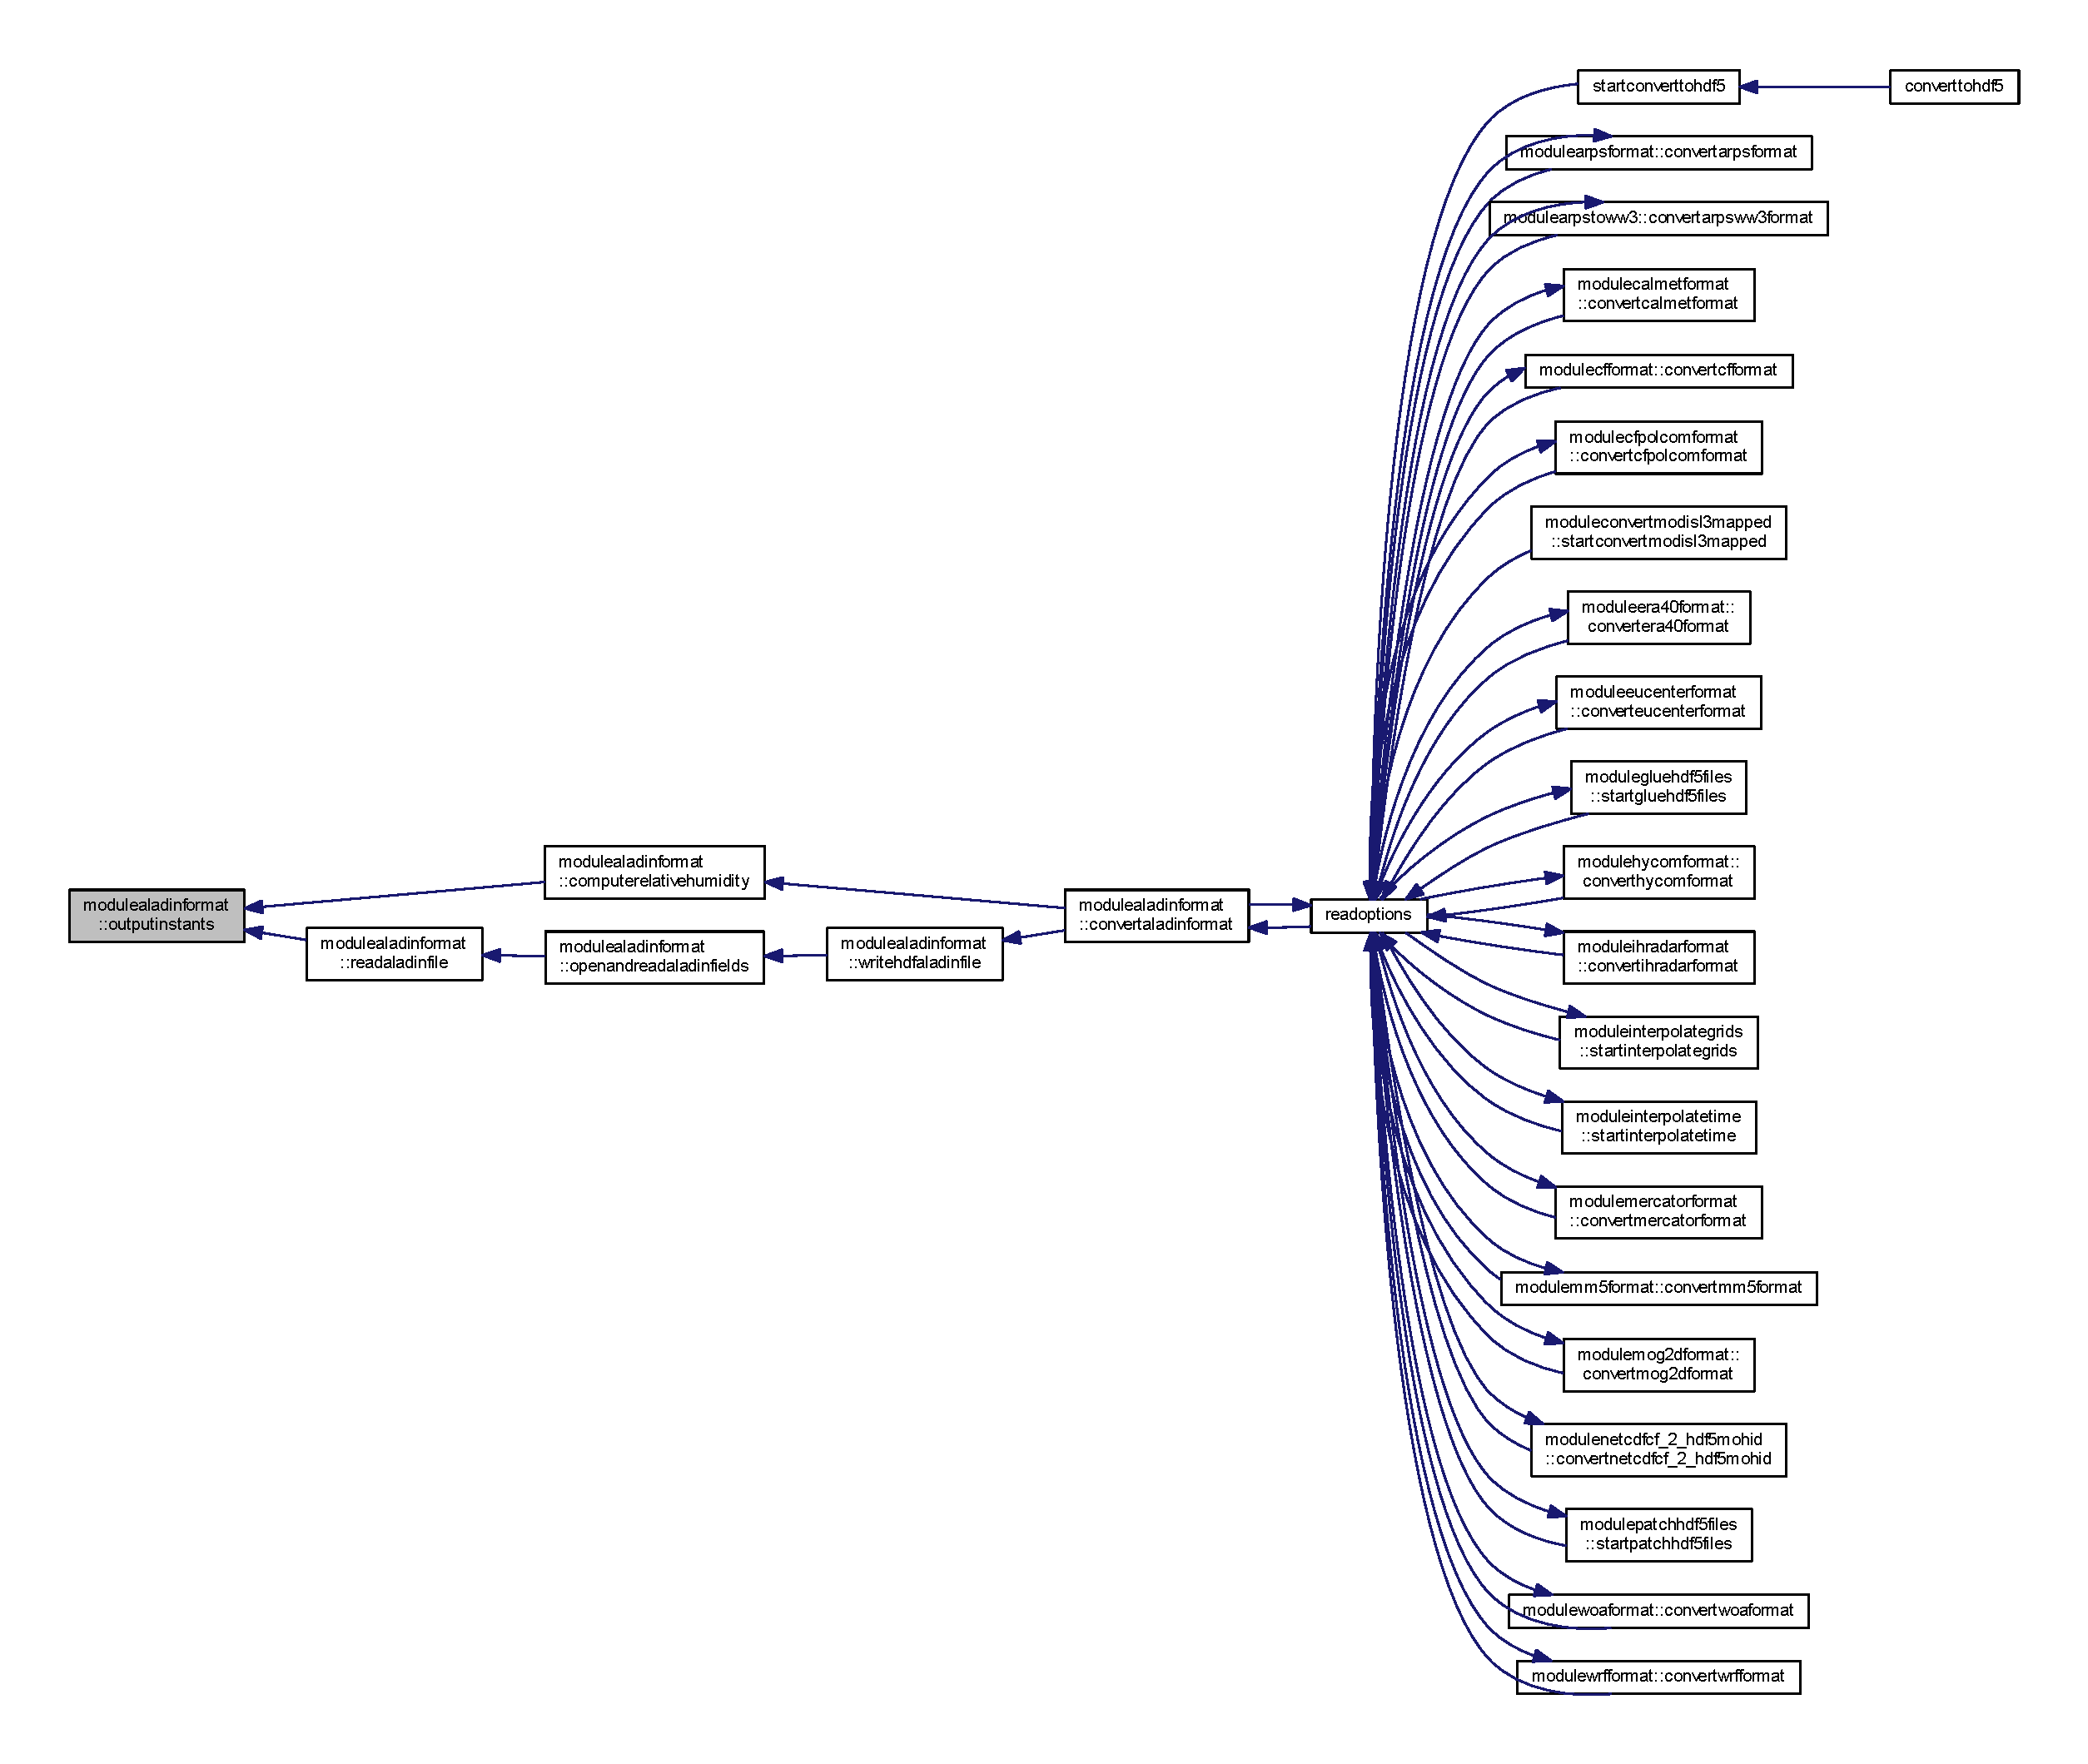
\includegraphics[width=350pt]{namespacemodulealadinformat_aa8356f98f813a0fe5edb9089053dc372_icgraph}
\end{center}
\end{figure}
\mbox{\Hypertarget{namespacemodulealadinformat_a01a53a6349fe1f7a1e5973e60abcf19d}\label{namespacemodulealadinformat_a01a53a6349fe1f7a1e5973e60abcf19d}} 
\index{modulealadinformat@{modulealadinformat}!readaladinfile@{readaladinfile}}
\index{readaladinfile@{readaladinfile}!modulealadinformat@{modulealadinformat}}
\subsubsection{\texorpdfstring{readaladinfile()}{readaladinfile()}}
{\footnotesize\ttfamily subroutine, private modulealadinformat\+::readaladinfile (\begin{DoxyParamCaption}\item[{character (len=$\ast$)}]{Input\+File }\end{DoxyParamCaption})\hspace{0.3cm}{\ttfamily [private]}}

Here is the call graph for this function\+:\nopagebreak
\begin{figure}[H]
\begin{center}
\leavevmode
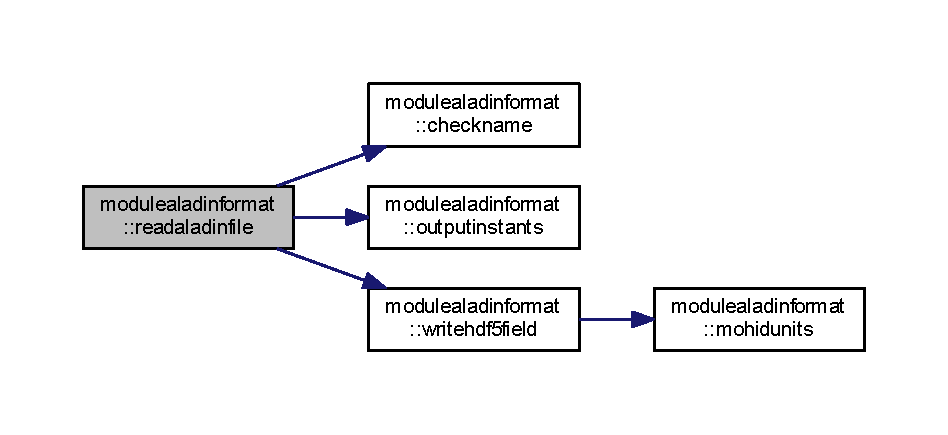
\includegraphics[width=350pt]{namespacemodulealadinformat_a01a53a6349fe1f7a1e5973e60abcf19d_cgraph}
\end{center}
\end{figure}
Here is the caller graph for this function\+:\nopagebreak
\begin{figure}[H]
\begin{center}
\leavevmode
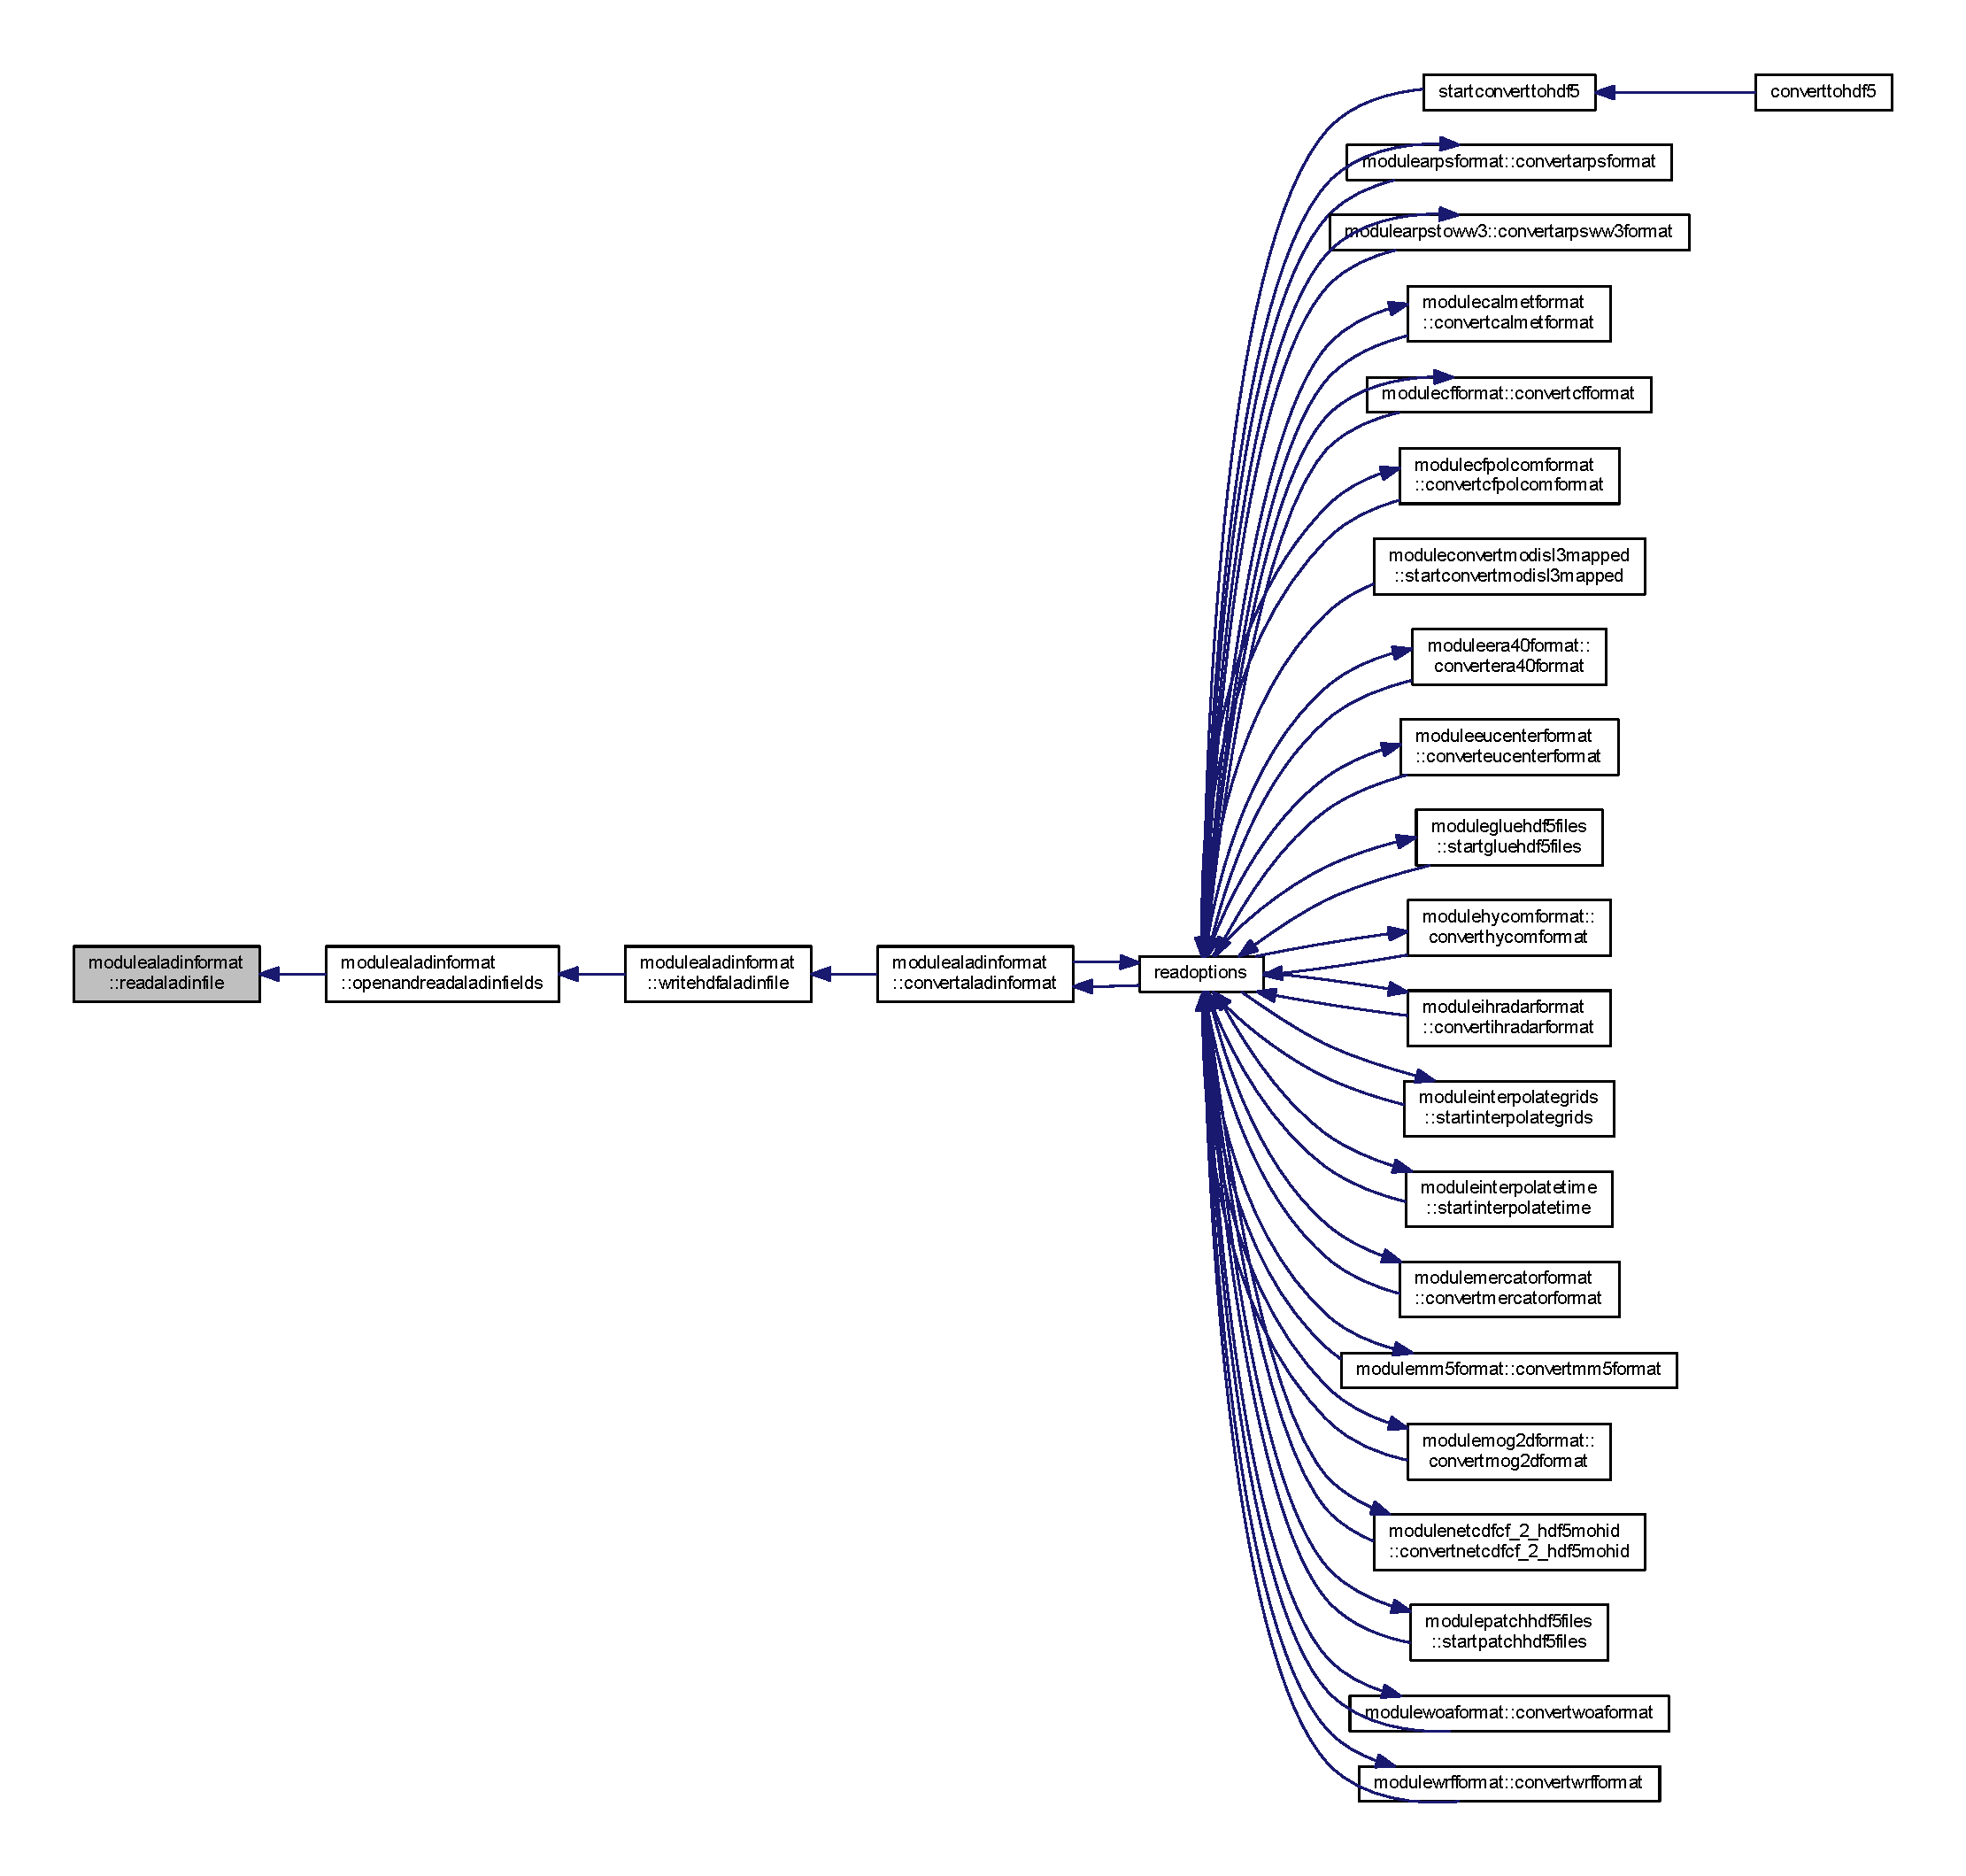
\includegraphics[width=350pt]{namespacemodulealadinformat_a01a53a6349fe1f7a1e5973e60abcf19d_icgraph}
\end{center}
\end{figure}
\mbox{\Hypertarget{namespacemodulealadinformat_aae35e2c47a633497f92dcf61c358e656}\label{namespacemodulealadinformat_aae35e2c47a633497f92dcf61c358e656}} 
\index{modulealadinformat@{modulealadinformat}!readoptions@{readoptions}}
\index{readoptions@{readoptions}!modulealadinformat@{modulealadinformat}}
\subsubsection{\texorpdfstring{readoptions()}{readoptions()}}
{\footnotesize\ttfamily subroutine, private modulealadinformat\+::readoptions (\begin{DoxyParamCaption}{ }\end{DoxyParamCaption})\hspace{0.3cm}{\ttfamily [private]}}

\mbox{\Hypertarget{namespacemodulealadinformat_a75d489bd9df9a1d8553c1154e13368f1}\label{namespacemodulealadinformat_a75d489bd9df9a1d8553c1154e13368f1}} 
\index{modulealadinformat@{modulealadinformat}!readtime@{readtime}}
\index{readtime@{readtime}!modulealadinformat@{modulealadinformat}}
\subsubsection{\texorpdfstring{readtime()}{readtime()}}
{\footnotesize\ttfamily subroutine modulealadinformat\+::readtime (\begin{DoxyParamCaption}{ }\end{DoxyParamCaption})\hspace{0.3cm}{\ttfamily [private]}}

Here is the call graph for this function\+:\nopagebreak
\begin{figure}[H]
\begin{center}
\leavevmode
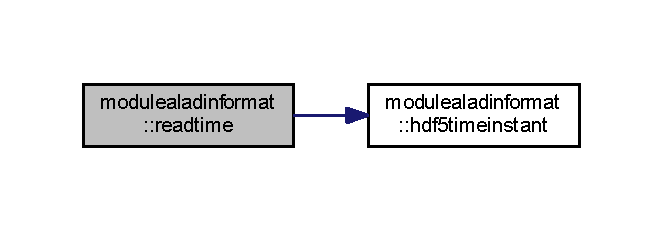
\includegraphics[width=318pt]{namespacemodulealadinformat_a75d489bd9df9a1d8553c1154e13368f1_cgraph}
\end{center}
\end{figure}
\mbox{\Hypertarget{namespacemodulealadinformat_aae0b88b8feec26aab01ab56220392544}\label{namespacemodulealadinformat_aae0b88b8feec26aab01ab56220392544}} 
\index{modulealadinformat@{modulealadinformat}!write\+\_\+hdf5\+\_\+grid\+\_\+data@{write\+\_\+hdf5\+\_\+grid\+\_\+data}}
\index{write\+\_\+hdf5\+\_\+grid\+\_\+data@{write\+\_\+hdf5\+\_\+grid\+\_\+data}!modulealadinformat@{modulealadinformat}}
\subsubsection{\texorpdfstring{write\+\_\+hdf5\+\_\+grid\+\_\+data()}{write\_hdf5\_grid\_data()}}
{\footnotesize\ttfamily subroutine, private modulealadinformat\+::write\+\_\+hdf5\+\_\+grid\+\_\+data (\begin{DoxyParamCaption}{ }\end{DoxyParamCaption})\hspace{0.3cm}{\ttfamily [private]}}

Here is the caller graph for this function\+:\nopagebreak
\begin{figure}[H]
\begin{center}
\leavevmode
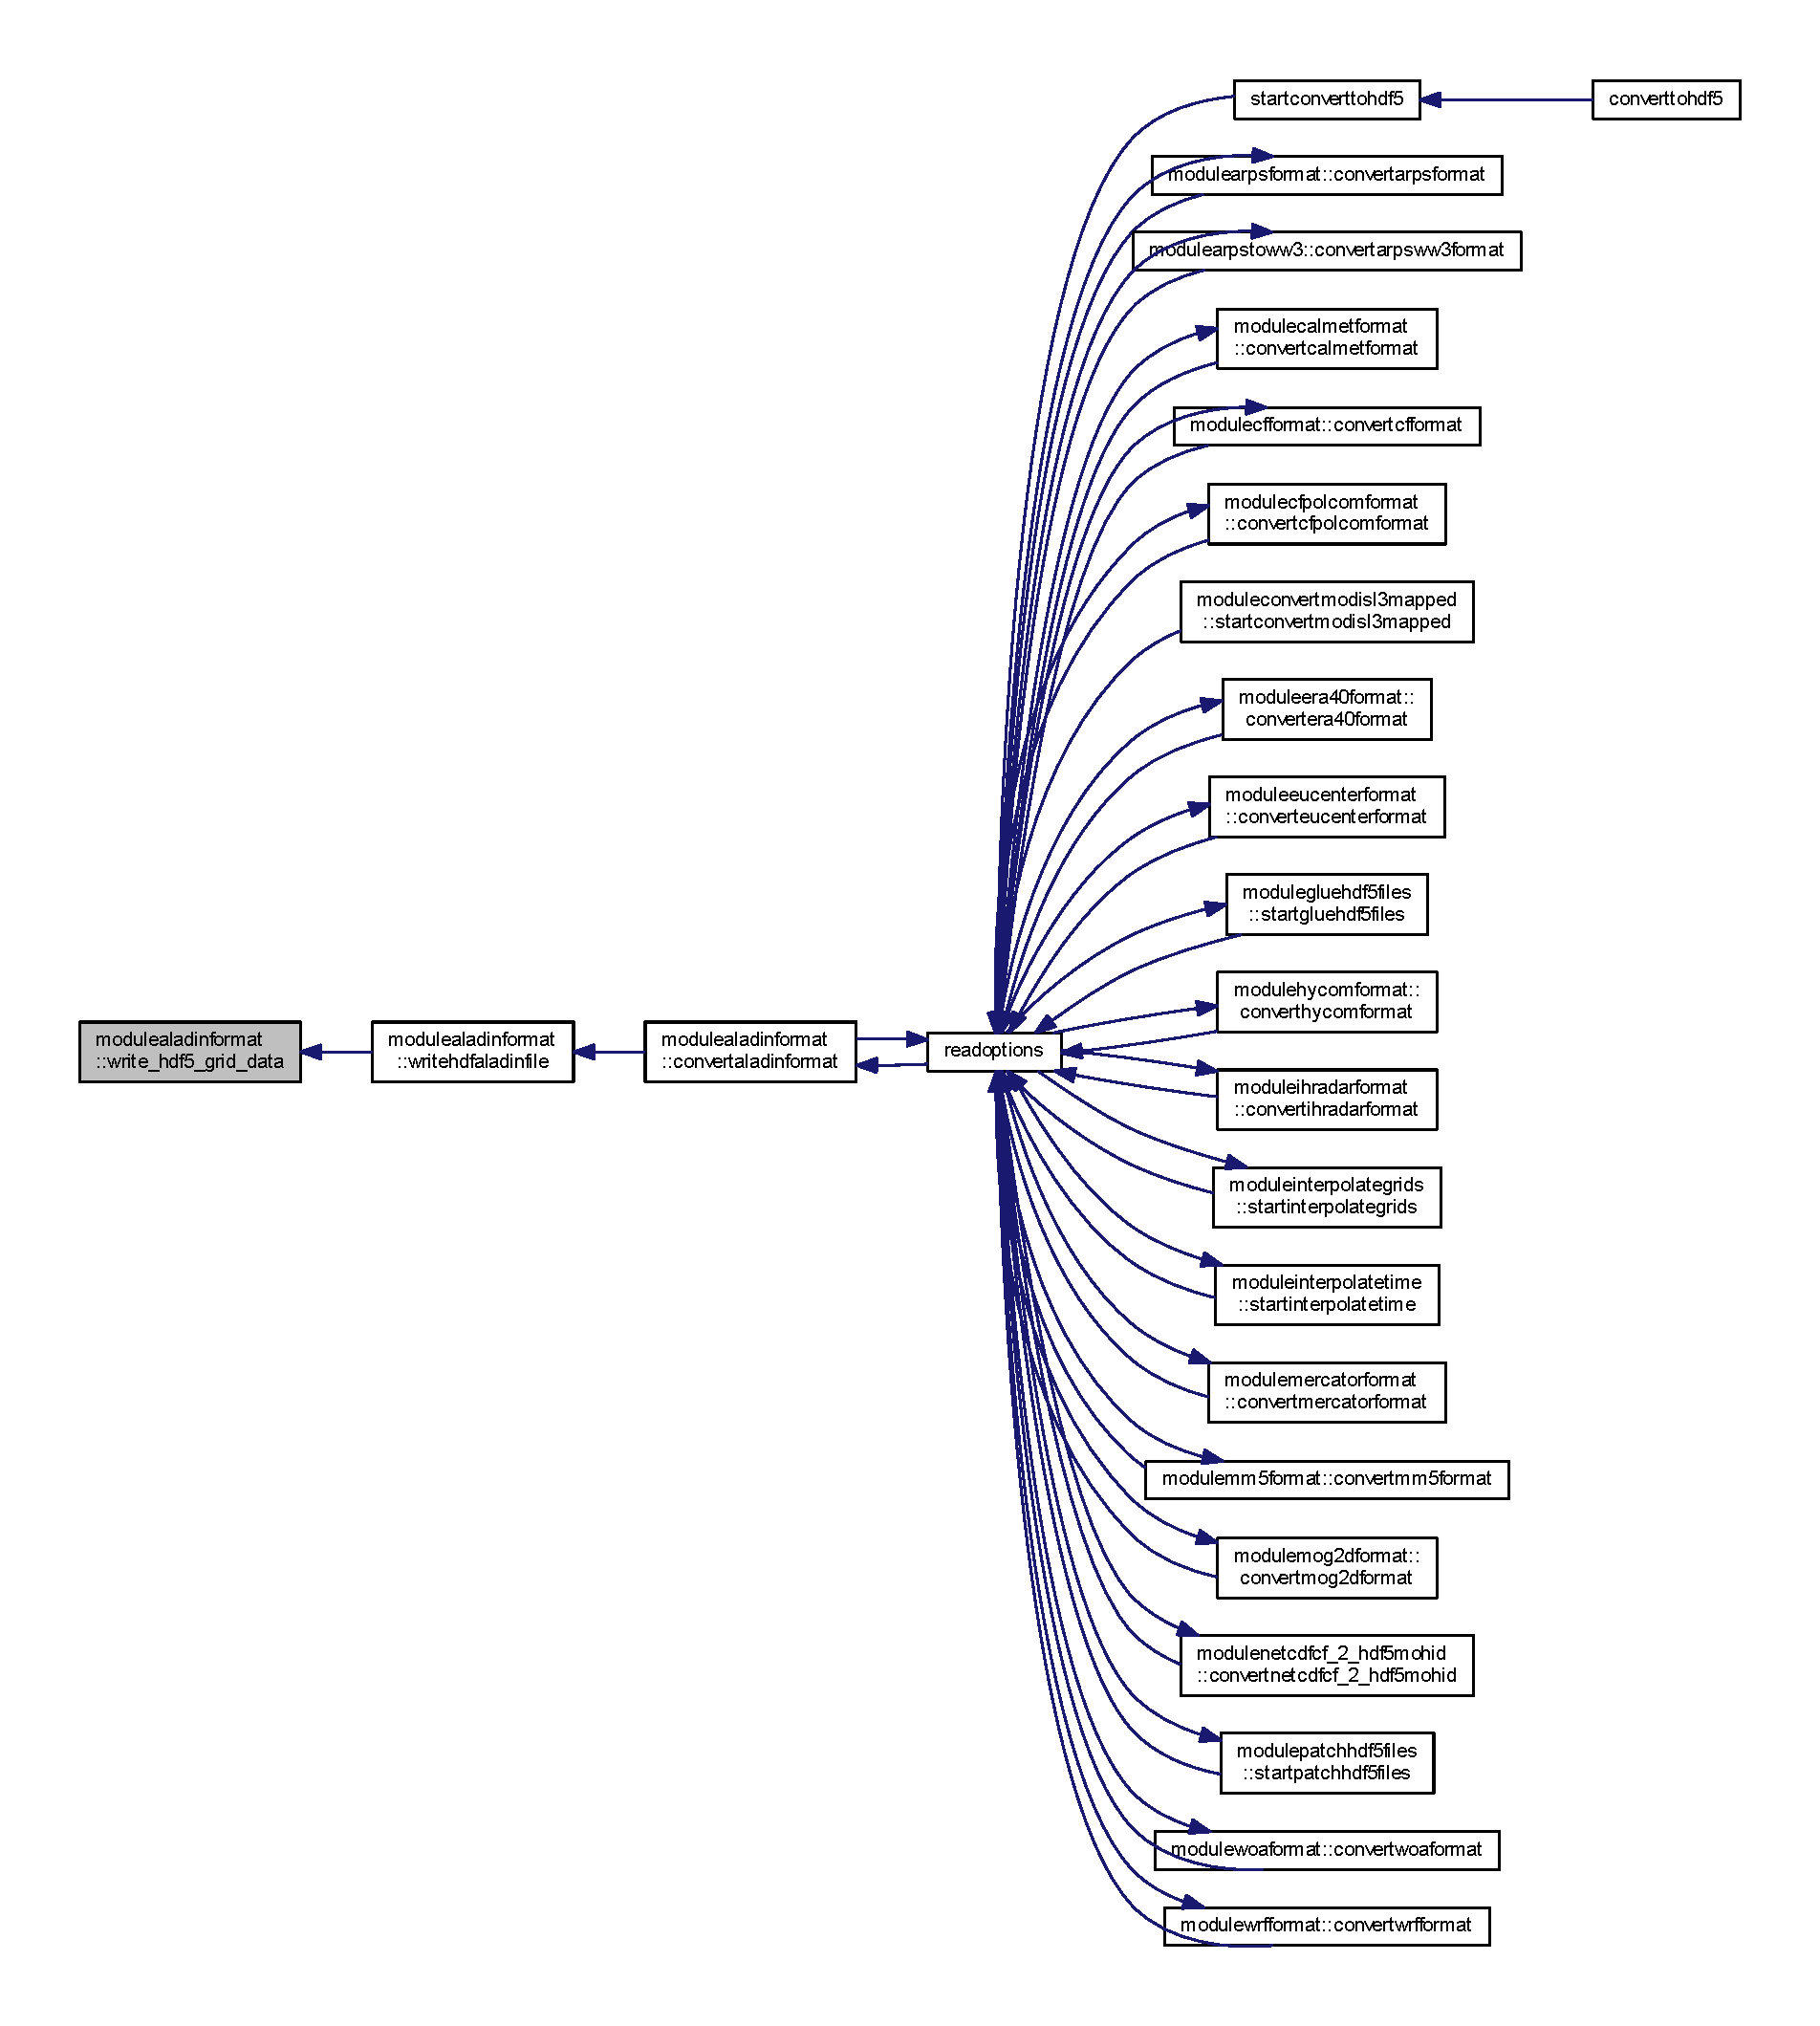
\includegraphics[width=350pt]{namespacemodulealadinformat_aae0b88b8feec26aab01ab56220392544_icgraph}
\end{center}
\end{figure}
\mbox{\Hypertarget{namespacemodulealadinformat_a9b5030d175b249bcc7e4f88c7e8bffec}\label{namespacemodulealadinformat_a9b5030d175b249bcc7e4f88c7e8bffec}} 
\index{modulealadinformat@{modulealadinformat}!writehdf5field@{writehdf5field}}
\index{writehdf5field@{writehdf5field}!modulealadinformat@{modulealadinformat}}
\subsubsection{\texorpdfstring{writehdf5field()}{writehdf5field()}}
{\footnotesize\ttfamily subroutine, private modulealadinformat\+::writehdf5field (\begin{DoxyParamCaption}\item[{type (t\+\_\+time)}]{Field\+Time,  }\item[{character(len=stringlength)}]{Mohid\+Name,  }\item[{integer}]{i\+Out,  }\item[{real, dimension(\+:,\+:  ), optional, pointer}]{Aux2D,  }\item[{real, dimension(\+:,\+:,\+:), optional, pointer}]{Aux3D }\end{DoxyParamCaption})\hspace{0.3cm}{\ttfamily [private]}}

Here is the call graph for this function\+:\nopagebreak
\begin{figure}[H]
\begin{center}
\leavevmode
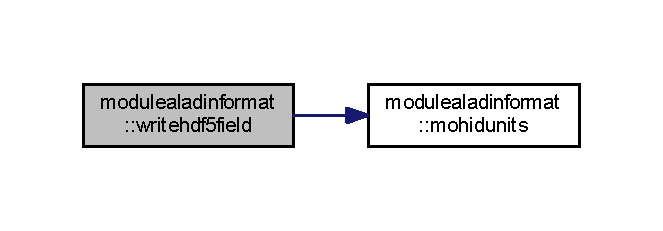
\includegraphics[width=318pt]{namespacemodulealadinformat_a9b5030d175b249bcc7e4f88c7e8bffec_cgraph}
\end{center}
\end{figure}
Here is the caller graph for this function\+:\nopagebreak
\begin{figure}[H]
\begin{center}
\leavevmode
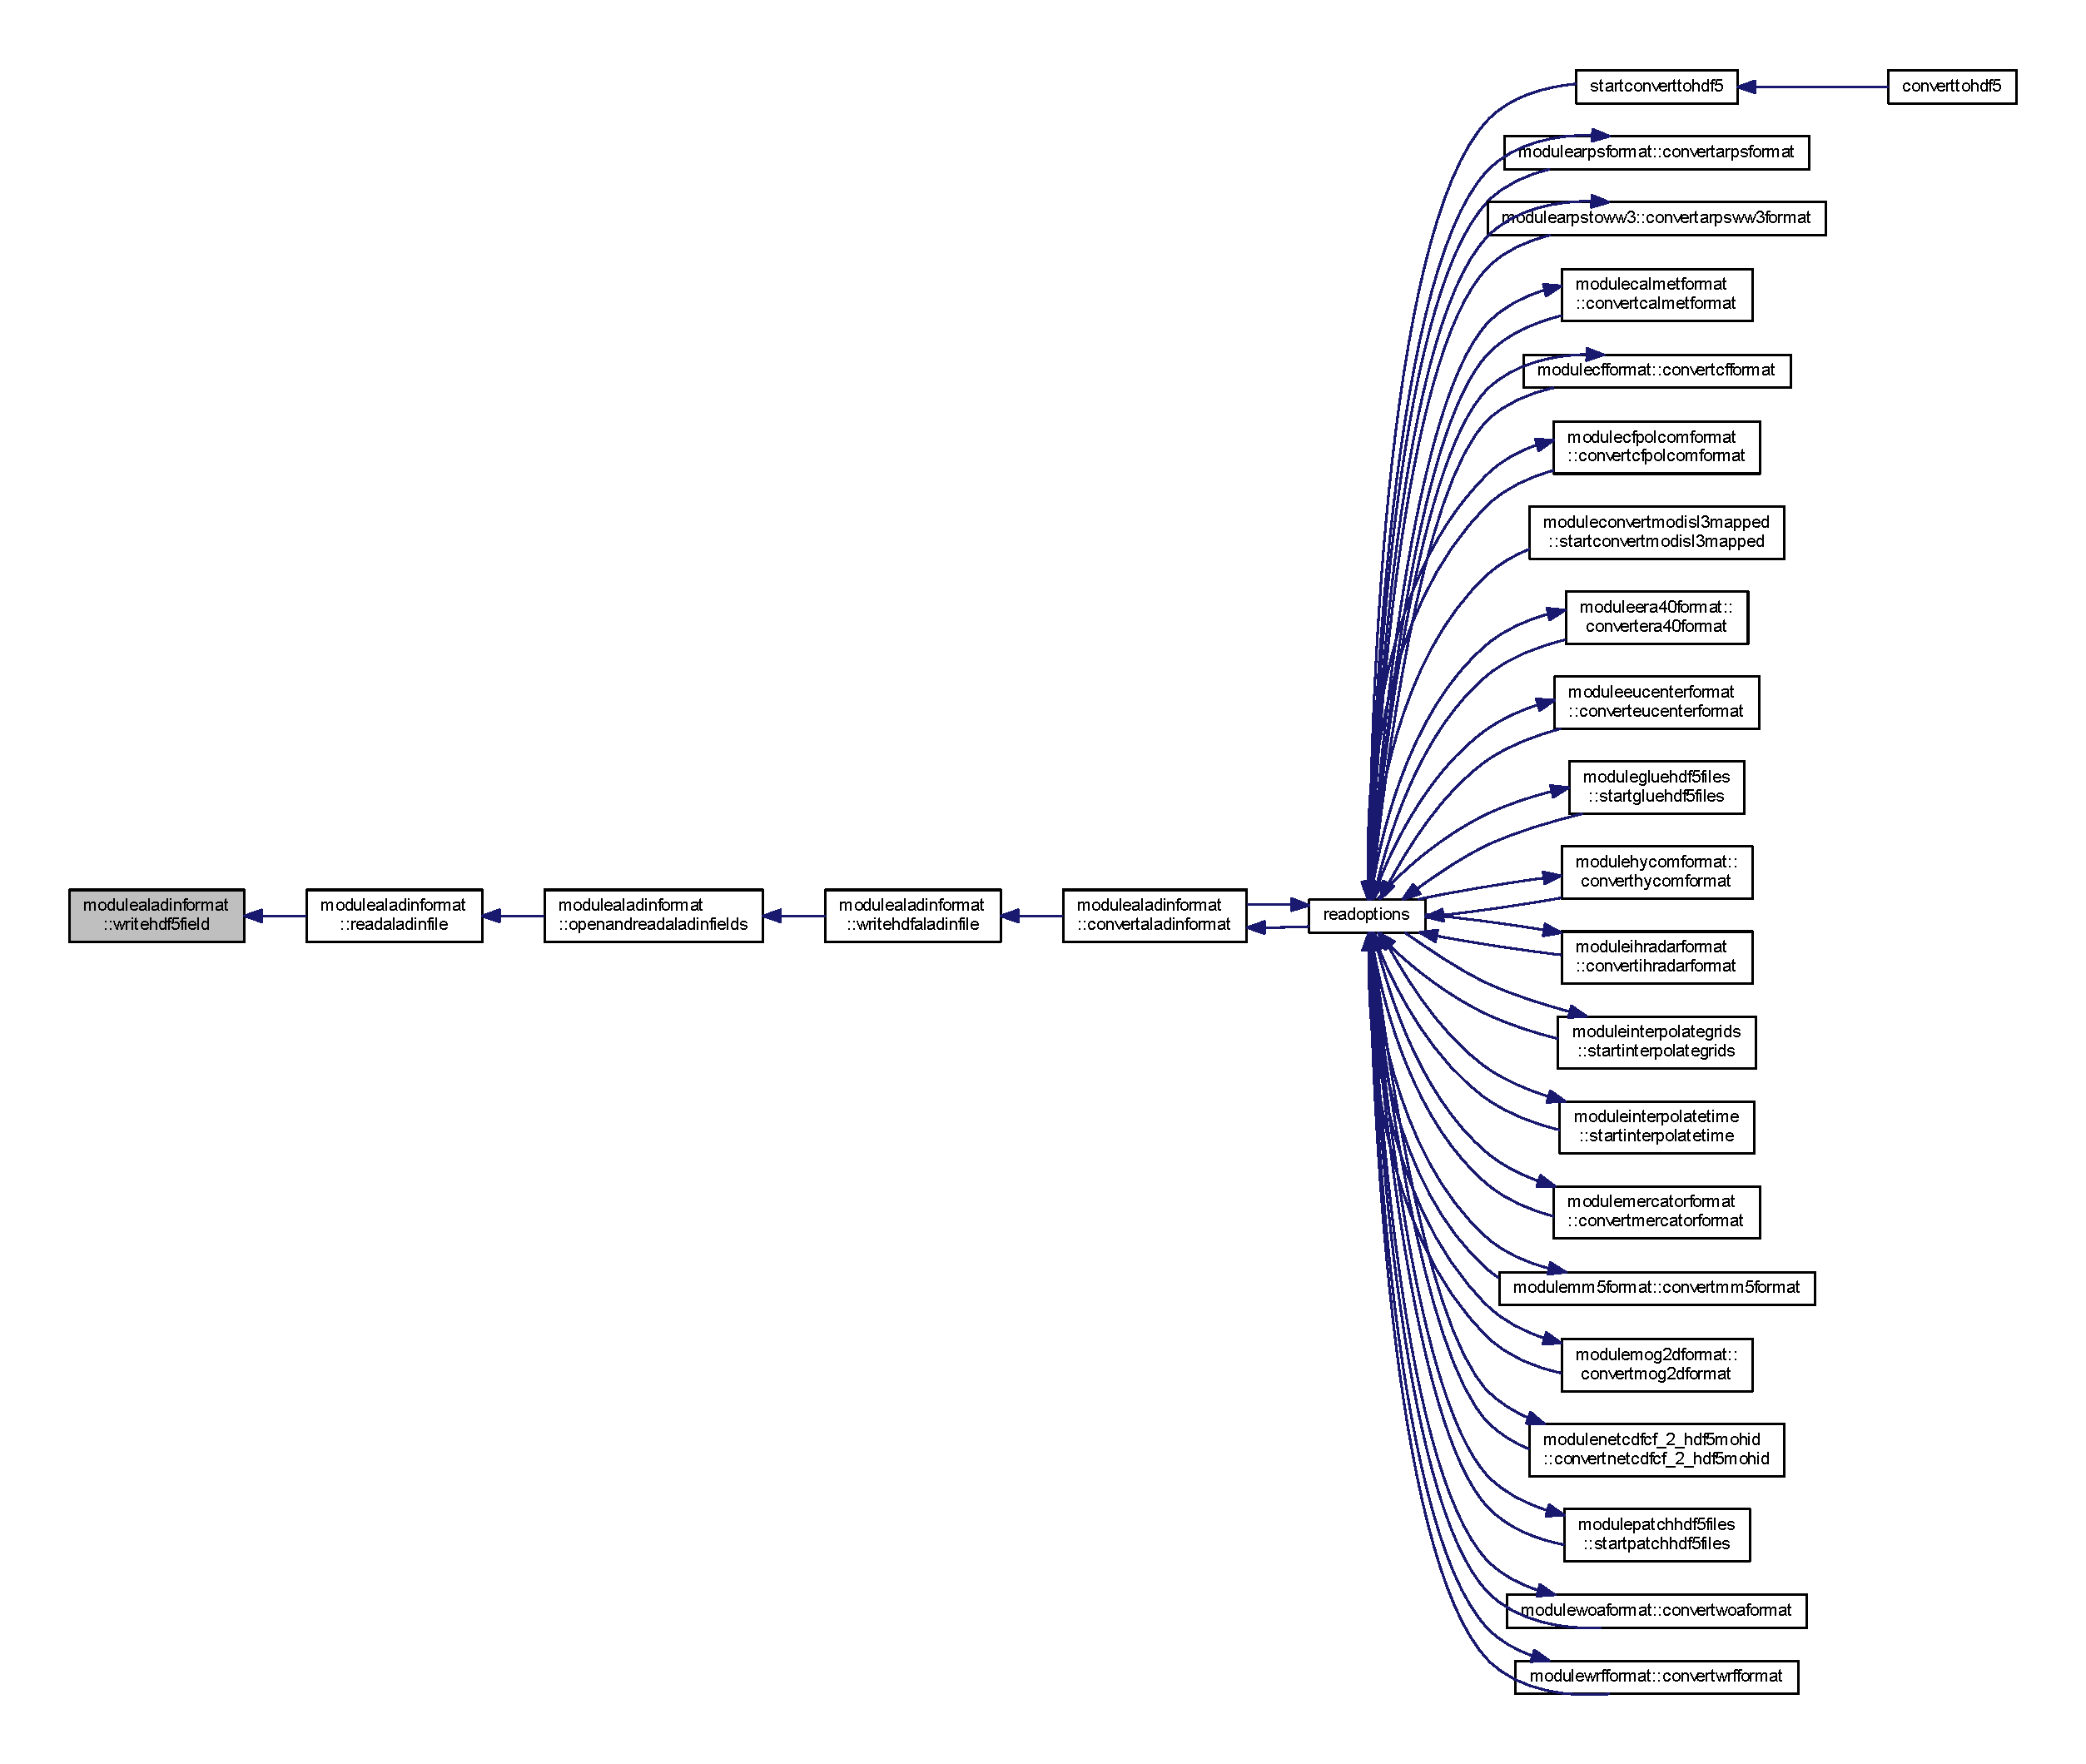
\includegraphics[width=350pt]{namespacemodulealadinformat_a9b5030d175b249bcc7e4f88c7e8bffec_icgraph}
\end{center}
\end{figure}
\mbox{\Hypertarget{namespacemodulealadinformat_ad234b4831ac8d0d1f8ad444d37000469}\label{namespacemodulealadinformat_ad234b4831ac8d0d1f8ad444d37000469}} 
\index{modulealadinformat@{modulealadinformat}!writehdfaladinfile@{writehdfaladinfile}}
\index{writehdfaladinfile@{writehdfaladinfile}!modulealadinformat@{modulealadinformat}}
\subsubsection{\texorpdfstring{writehdfaladinfile()}{writehdfaladinfile()}}
{\footnotesize\ttfamily subroutine, private modulealadinformat\+::writehdfaladinfile (\begin{DoxyParamCaption}{ }\end{DoxyParamCaption})\hspace{0.3cm}{\ttfamily [private]}}

Here is the call graph for this function\+:\nopagebreak
\begin{figure}[H]
\begin{center}
\leavevmode
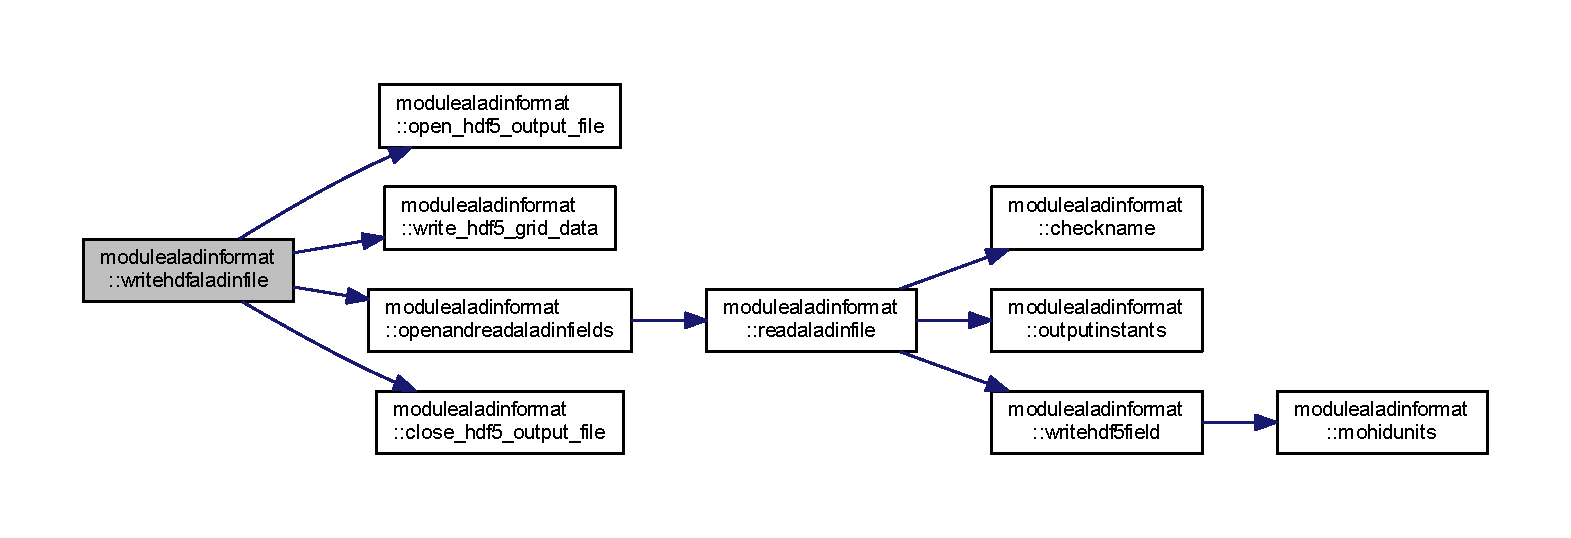
\includegraphics[width=350pt]{namespacemodulealadinformat_ad234b4831ac8d0d1f8ad444d37000469_cgraph}
\end{center}
\end{figure}
Here is the caller graph for this function\+:\nopagebreak
\begin{figure}[H]
\begin{center}
\leavevmode
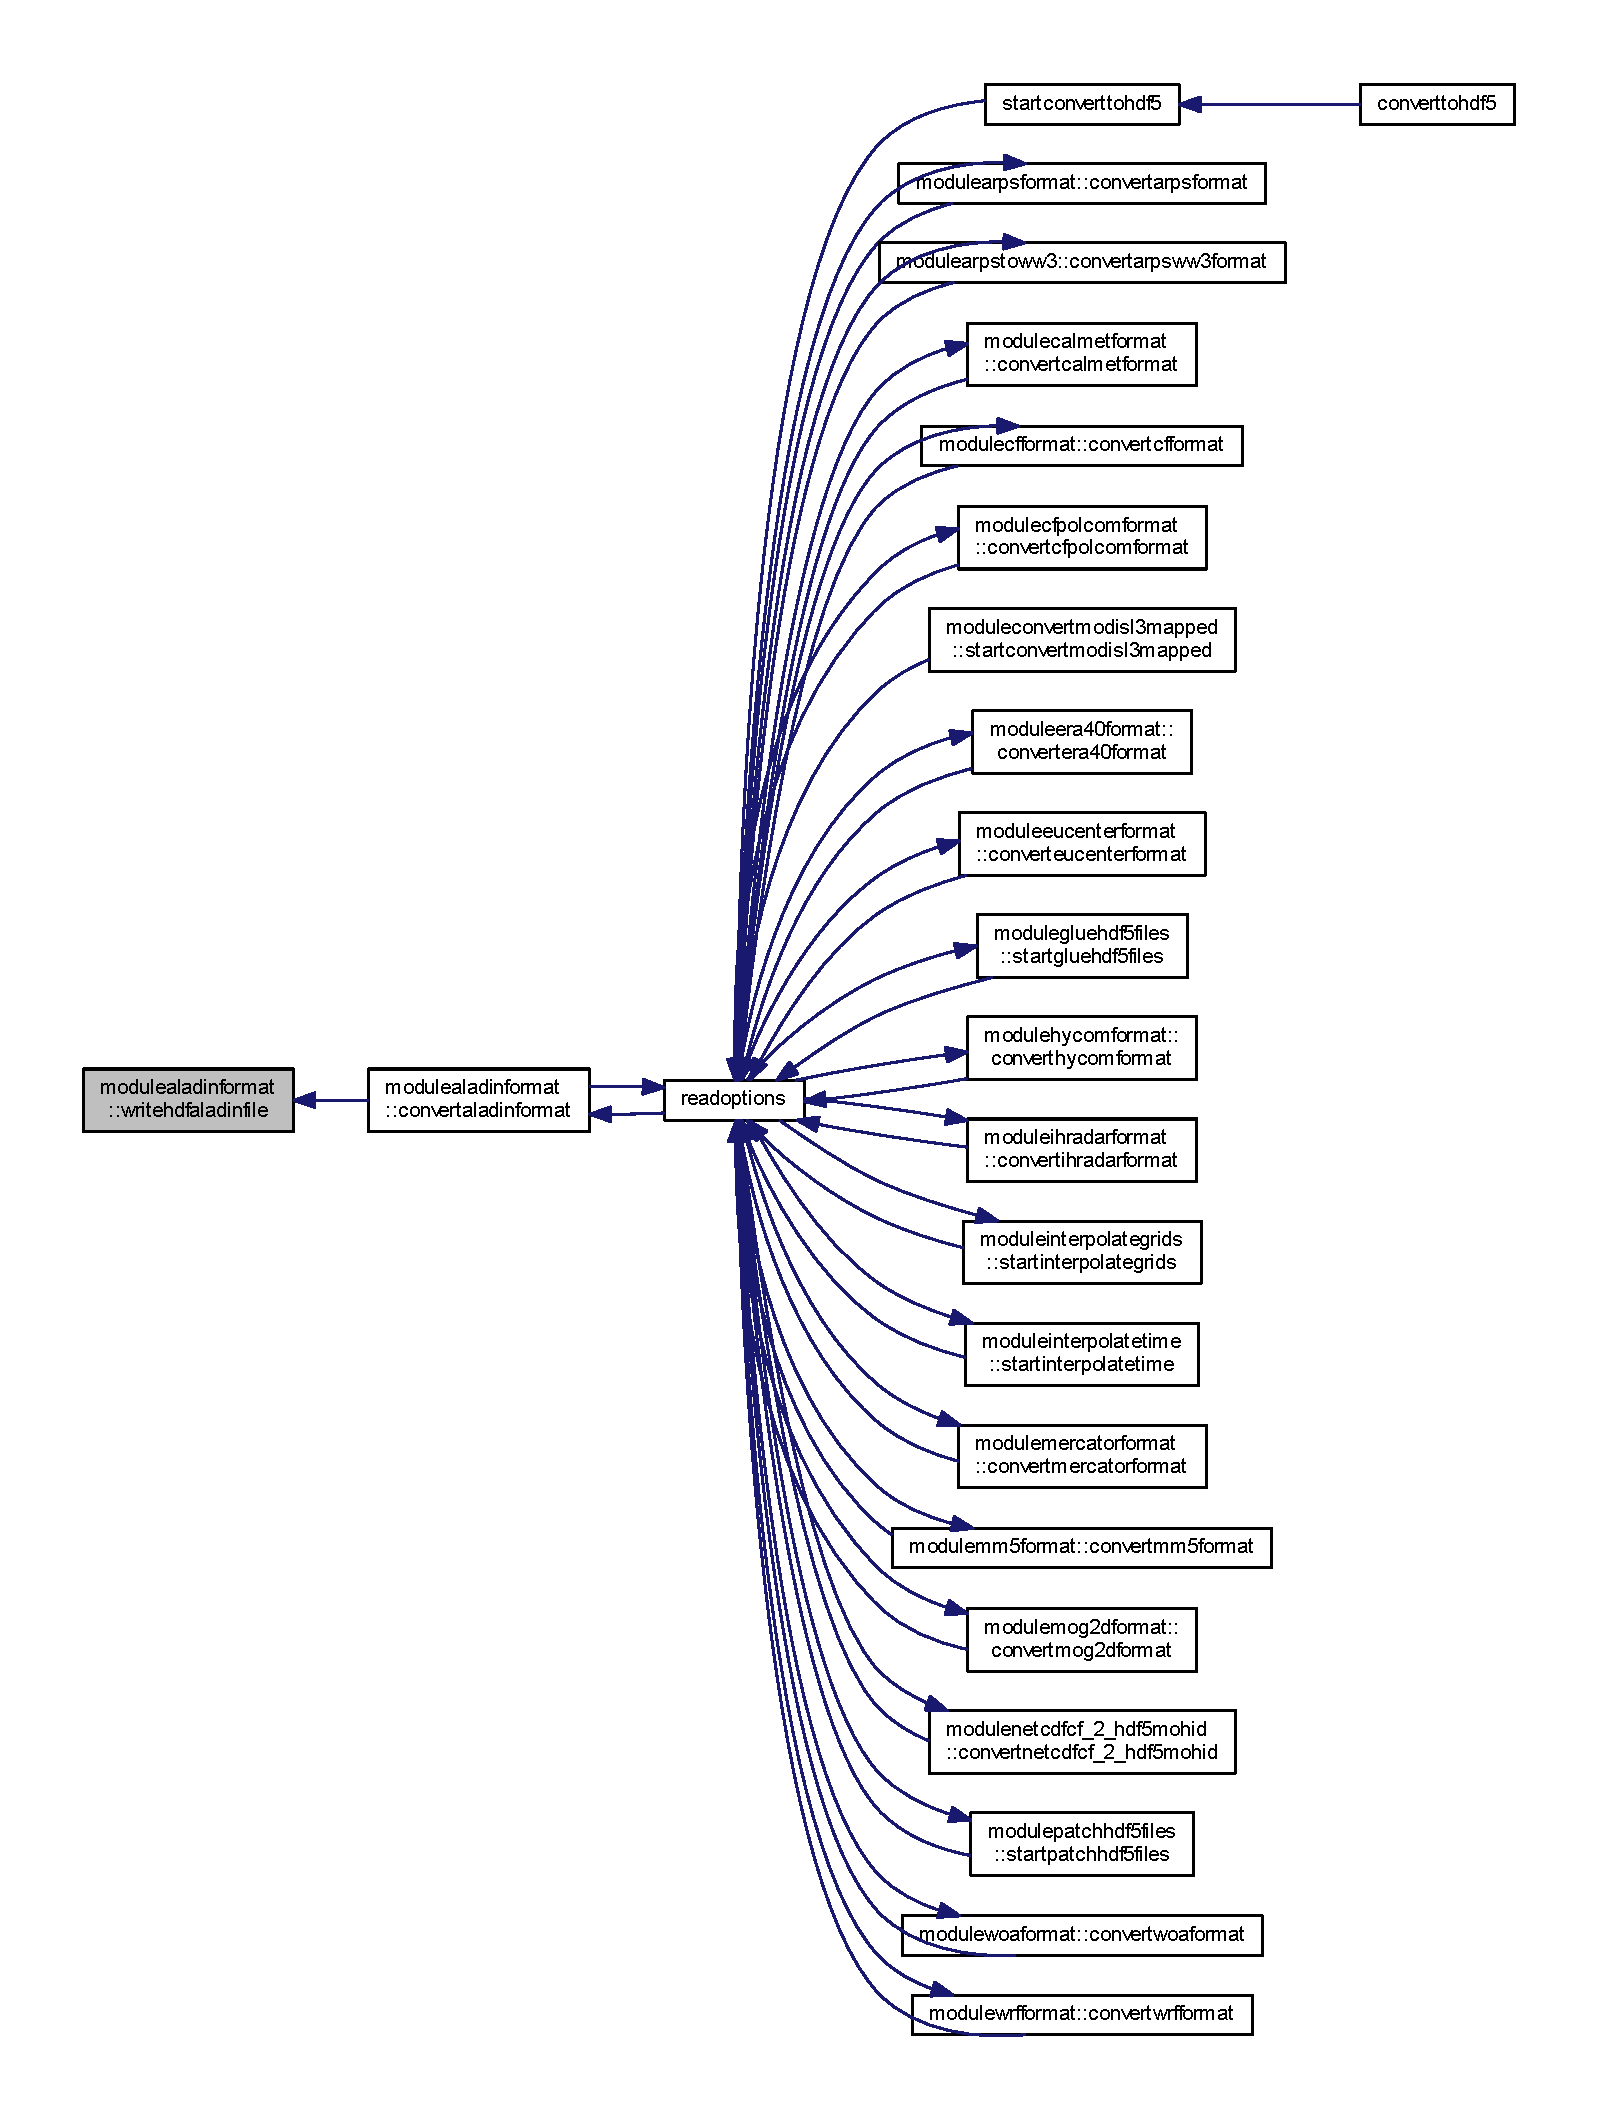
\includegraphics[width=350pt]{namespacemodulealadinformat_ad234b4831ac8d0d1f8ad444d37000469_icgraph}
\end{center}
\end{figure}
\mbox{\Hypertarget{namespacemodulealadinformat_a2c5da57a26426886fbd2f4fbe4ce299c}\label{namespacemodulealadinformat_a2c5da57a26426886fbd2f4fbe4ce299c}} 
\index{modulealadinformat@{modulealadinformat}!writerelativehumidity@{writerelativehumidity}}
\index{writerelativehumidity@{writerelativehumidity}!modulealadinformat@{modulealadinformat}}
\subsubsection{\texorpdfstring{writerelativehumidity()}{writerelativehumidity()}}
{\footnotesize\ttfamily subroutine, private modulealadinformat\+::writerelativehumidity (\begin{DoxyParamCaption}\item[{integer}]{i\+Out }\end{DoxyParamCaption})\hspace{0.3cm}{\ttfamily [private]}}

Here is the call graph for this function\+:\nopagebreak
\begin{figure}[H]
\begin{center}
\leavevmode
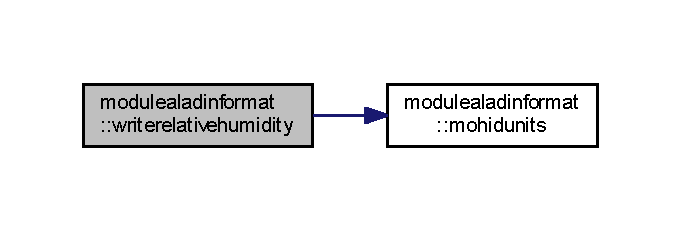
\includegraphics[width=327pt]{namespacemodulealadinformat_a2c5da57a26426886fbd2f4fbe4ce299c_cgraph}
\end{center}
\end{figure}
Here is the caller graph for this function\+:\nopagebreak
\begin{figure}[H]
\begin{center}
\leavevmode
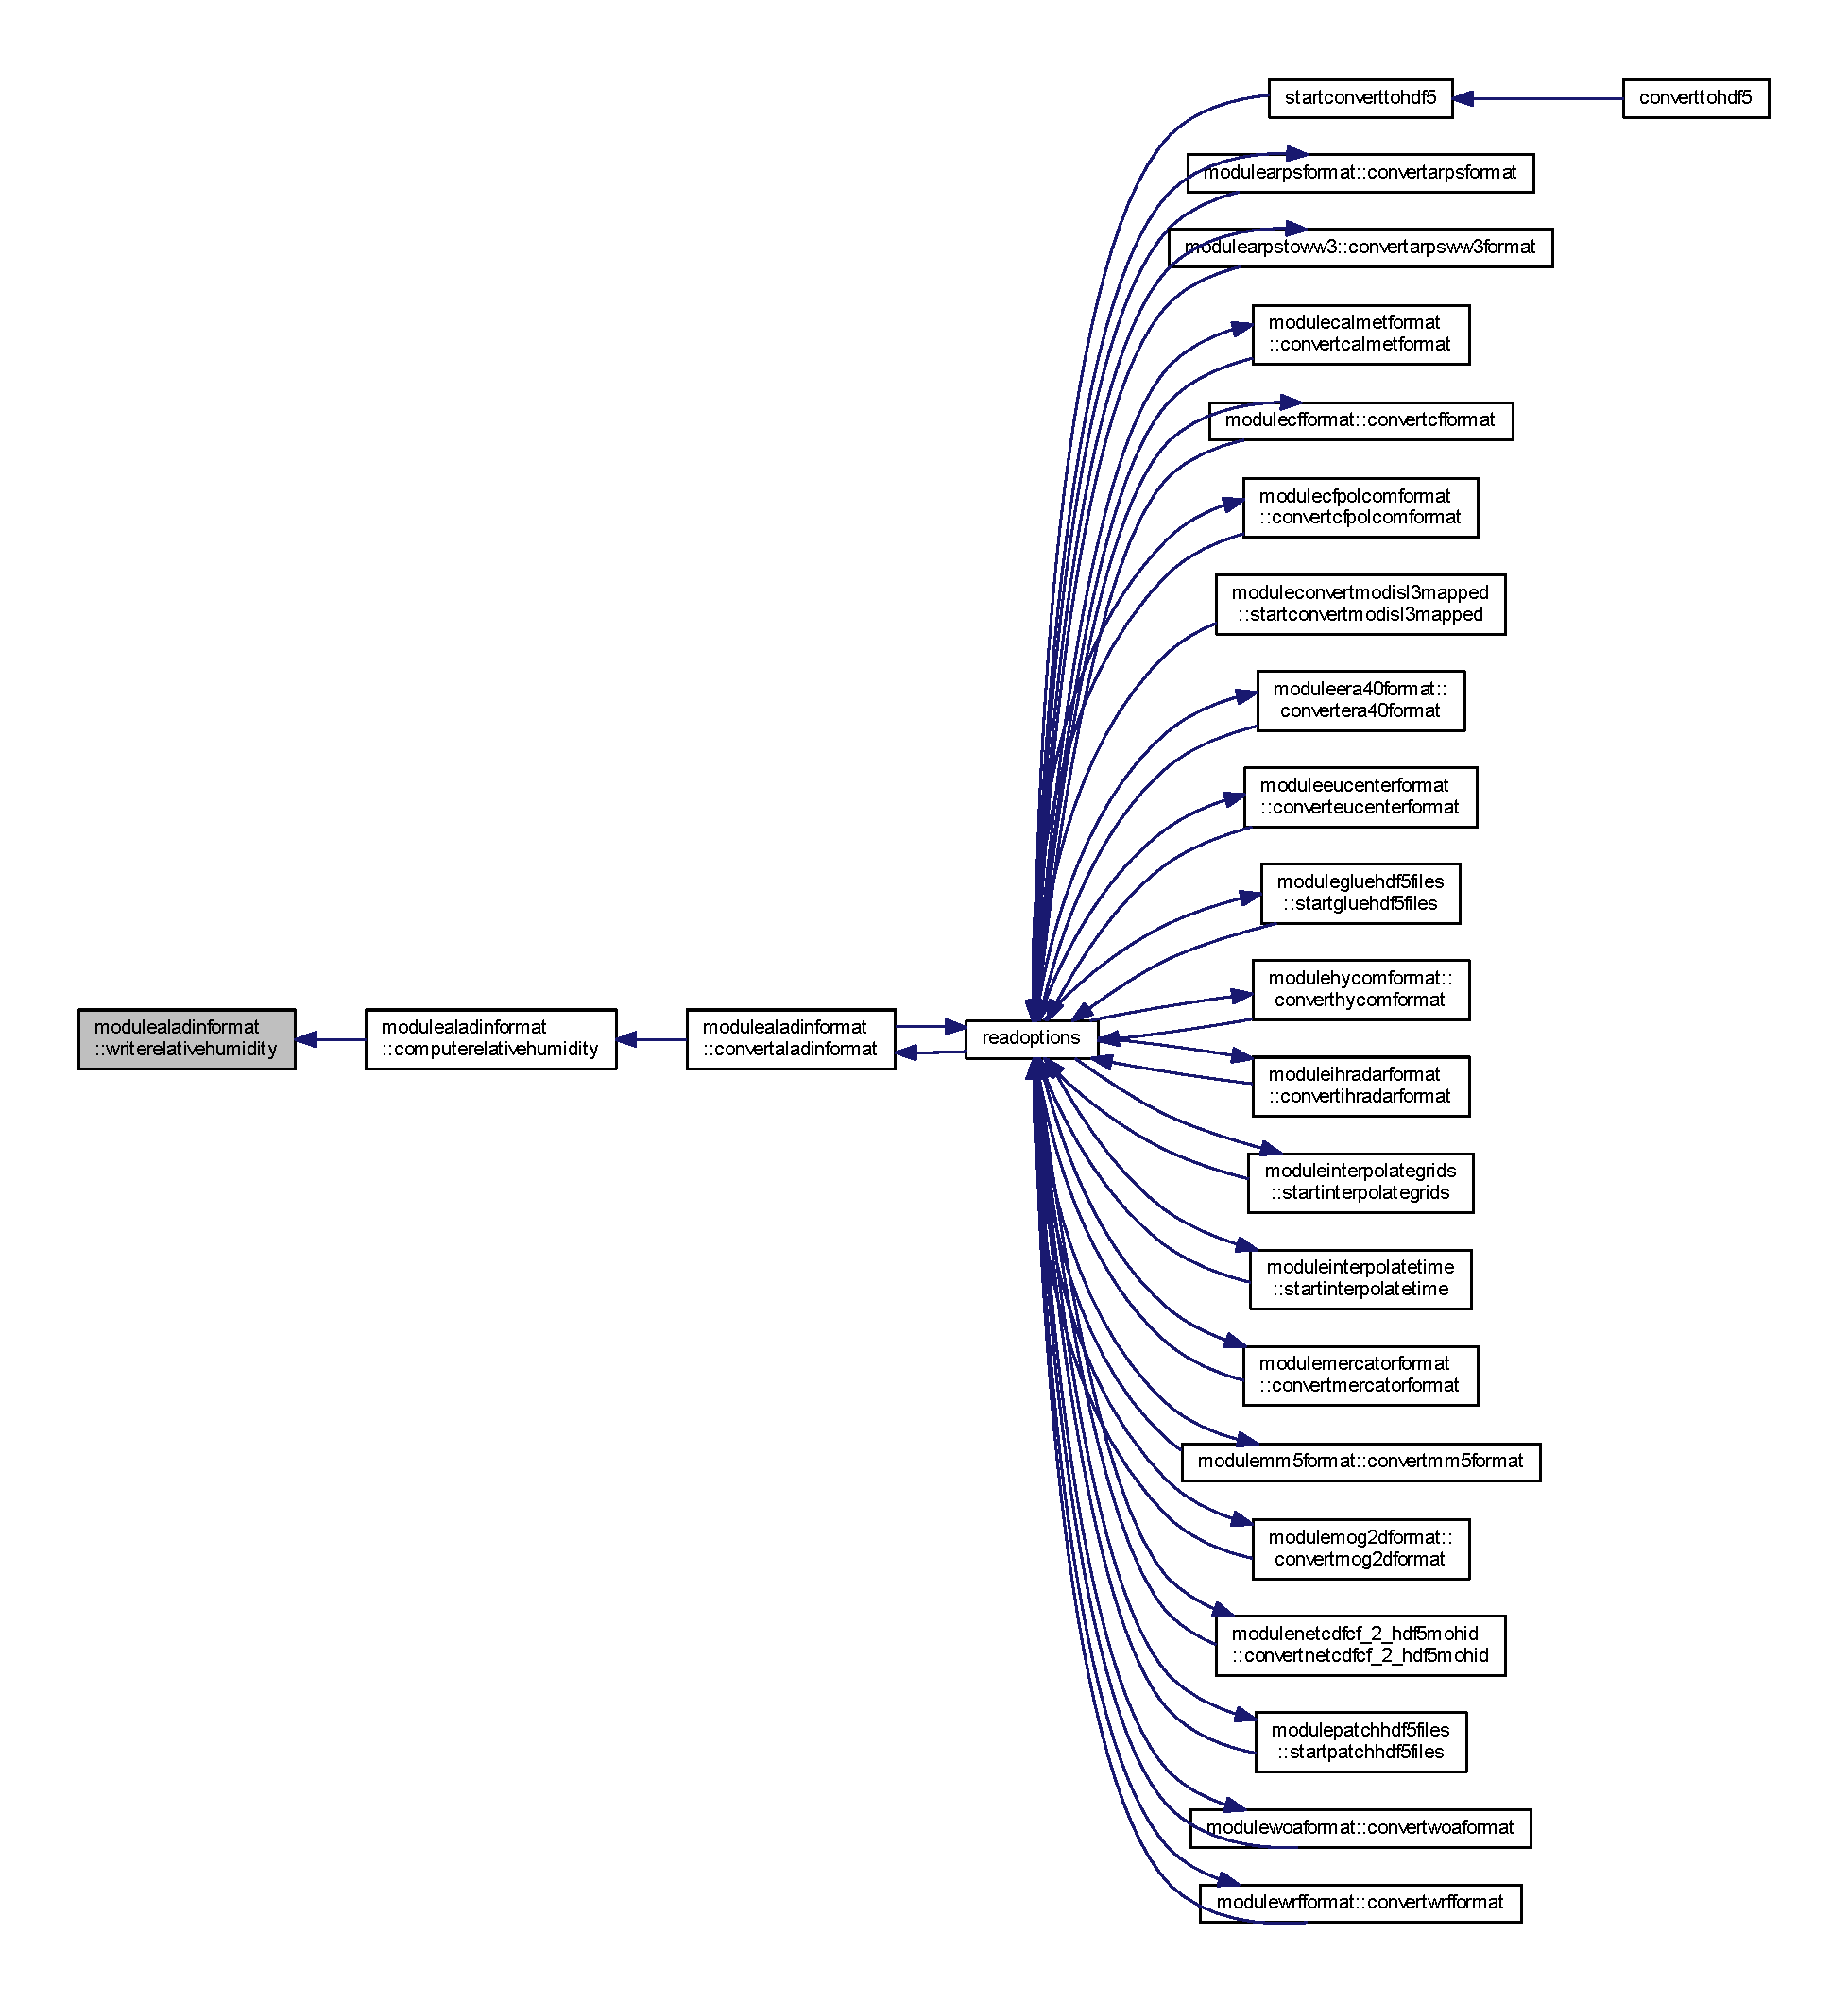
\includegraphics[width=350pt]{namespacemodulealadinformat_a2c5da57a26426886fbd2f4fbe4ce299c_icgraph}
\end{center}
\end{figure}


\subsection{Variable Documentation}
\mbox{\Hypertarget{namespacemodulealadinformat_a4e98c66850b0ed94ddb033e7aa090e44}\label{namespacemodulealadinformat_a4e98c66850b0ed94ddb033e7aa090e44}} 
\index{modulealadinformat@{modulealadinformat}!input\+\_\+files\+\_\+begin@{input\+\_\+files\+\_\+begin}}
\index{input\+\_\+files\+\_\+begin@{input\+\_\+files\+\_\+begin}!modulealadinformat@{modulealadinformat}}
\subsubsection{\texorpdfstring{input\+\_\+files\+\_\+begin}{input\_files\_begin}}
{\footnotesize\ttfamily character(len = stringlength), parameter modulealadinformat\+::input\+\_\+files\+\_\+begin = \textquotesingle{}$<$$<$begin\+\_\+input\+\_\+files$>$$>$\textquotesingle{}\hspace{0.3cm}{\ttfamily [private]}}

\mbox{\Hypertarget{namespacemodulealadinformat_a1b5e192f0393399d4e3f5ee7791fef49}\label{namespacemodulealadinformat_a1b5e192f0393399d4e3f5ee7791fef49}} 
\index{modulealadinformat@{modulealadinformat}!input\+\_\+files\+\_\+end@{input\+\_\+files\+\_\+end}}
\index{input\+\_\+files\+\_\+end@{input\+\_\+files\+\_\+end}!modulealadinformat@{modulealadinformat}}
\subsubsection{\texorpdfstring{input\+\_\+files\+\_\+end}{input\_files\_end}}
{\footnotesize\ttfamily character(len = stringlength), parameter modulealadinformat\+::input\+\_\+files\+\_\+end = \textquotesingle{}$<$$<$end\+\_\+input\+\_\+files$>$$>$\textquotesingle{}\hspace{0.3cm}{\ttfamily [private]}}

\mbox{\Hypertarget{namespacemodulealadinformat_a3680b6b225bce535beb96cad9fff81cb}\label{namespacemodulealadinformat_a3680b6b225bce535beb96cad9fff81cb}} 
\index{modulealadinformat@{modulealadinformat}!me@{me}}
\index{me@{me}!modulealadinformat@{modulealadinformat}}
\subsubsection{\texorpdfstring{me}{me}}
{\footnotesize\ttfamily type(\mbox{\hyperlink{structmodulealadinformat_1_1t__aladinformat}{t\+\_\+aladinformat}}), pointer modulealadinformat\+::me\hspace{0.3cm}{\ttfamily [private]}}


\hypertarget{namespacemodulearpsformat}{}\section{modulearpsformat Module Reference}
\label{namespacemodulearpsformat}\index{modulearpsformat@{modulearpsformat}}
\subsection*{Data Types}
\begin{DoxyCompactItemize}
\item 
type \mbox{\hyperlink{structmodulearpsformat_1_1t__date}{t\+\_\+date}}
\item 
type \mbox{\hyperlink{structmodulearpsformat_1_1t__field}{t\+\_\+field}}
\item 
type \mbox{\hyperlink{structmodulearpsformat_1_1t__mm5format}{t\+\_\+mm5format}}
\end{DoxyCompactItemize}
\subsection*{Functions/\+Subroutines}
\begin{DoxyCompactItemize}
\item 
subroutine, public \mbox{\hyperlink{namespacemodulearpsformat_a996acecfde01fb49e6408da52cb50d12}{convertarpsformat}} (Enter\+Data\+ID, S\+T\+AT)
\item 
subroutine, private \mbox{\hyperlink{namespacemodulearpsformat_a51cf1784c51ab9940cffc068600d53ac}{readoptions}}
\item 
subroutine, private \mbox{\hyperlink{namespacemodulearpsformat_a70ee83442772ea85df79da65ec4ea262}{openandreadarpsfile}}
\item 
subroutine \mbox{\hyperlink{namespacemodulearpsformat_a420eb740016c6ba55f897dbff1ef74e5}{constructgrid}}
\item 
subroutine, private \mbox{\hyperlink{namespacemodulearpsformat_a32649b9f39dfaa2b5396d488243a3905}{addfield}} (First\+Field, Obj\+Field)
\item 
subroutine, private \mbox{\hyperlink{namespacemodulearpsformat_a3e7adeca2b8b386d9c8d59f32a8c189f}{adddate}} (First\+Date, Obj\+Date)
\item 
subroutine, private \mbox{\hyperlink{namespacemodulearpsformat_a3feae8181a739c2898e331dd969e3c67}{outputfields}}
\item 
subroutine, private \mbox{\hyperlink{namespacemodulearpsformat_a9c9927c6fb171da5b0bfc4cd38595627}{open\+\_\+hdf5\+\_\+output\+\_\+file}}
\item 
subroutine, private \mbox{\hyperlink{namespacemodulearpsformat_a3fbe9c856c732d4e5f2315c2ae61e3d3}{killarpsformat}}
\end{DoxyCompactItemize}
\subsection*{Variables}
\begin{DoxyCompactItemize}
\item 
integer, parameter \mbox{\hyperlink{namespacemodulearpsformat_adad659745a61e1b477c5b8218c0a518b}{dotgrid}} = 1
\item 
integer, parameter \mbox{\hyperlink{namespacemodulearpsformat_a481f4077f9a97ca259535ae7940a069d}{crossgrid}} = 2
\item 
type(\mbox{\hyperlink{structmodulearpsformat_1_1t__mm5format}{t\+\_\+mm5format}}), pointer \mbox{\hyperlink{namespacemodulearpsformat_aa48b8d20bd8a9748703bc70c33e5bce9}{me}}
\end{DoxyCompactItemize}


\subsection{Function/\+Subroutine Documentation}
\mbox{\Hypertarget{namespacemodulearpsformat_a3e7adeca2b8b386d9c8d59f32a8c189f}\label{namespacemodulearpsformat_a3e7adeca2b8b386d9c8d59f32a8c189f}} 
\index{modulearpsformat@{modulearpsformat}!adddate@{adddate}}
\index{adddate@{adddate}!modulearpsformat@{modulearpsformat}}
\subsubsection{\texorpdfstring{adddate()}{adddate()}}
{\footnotesize\ttfamily subroutine, private modulearpsformat\+::adddate (\begin{DoxyParamCaption}\item[{type (\mbox{\hyperlink{structmodulearpsformat_1_1t__date}{t\+\_\+date}}), pointer}]{First\+Date,  }\item[{type (\mbox{\hyperlink{structmodulearpsformat_1_1t__date}{t\+\_\+date}}), pointer}]{Obj\+Date }\end{DoxyParamCaption})\hspace{0.3cm}{\ttfamily [private]}}

Here is the caller graph for this function\+:\nopagebreak
\begin{figure}[H]
\begin{center}
\leavevmode
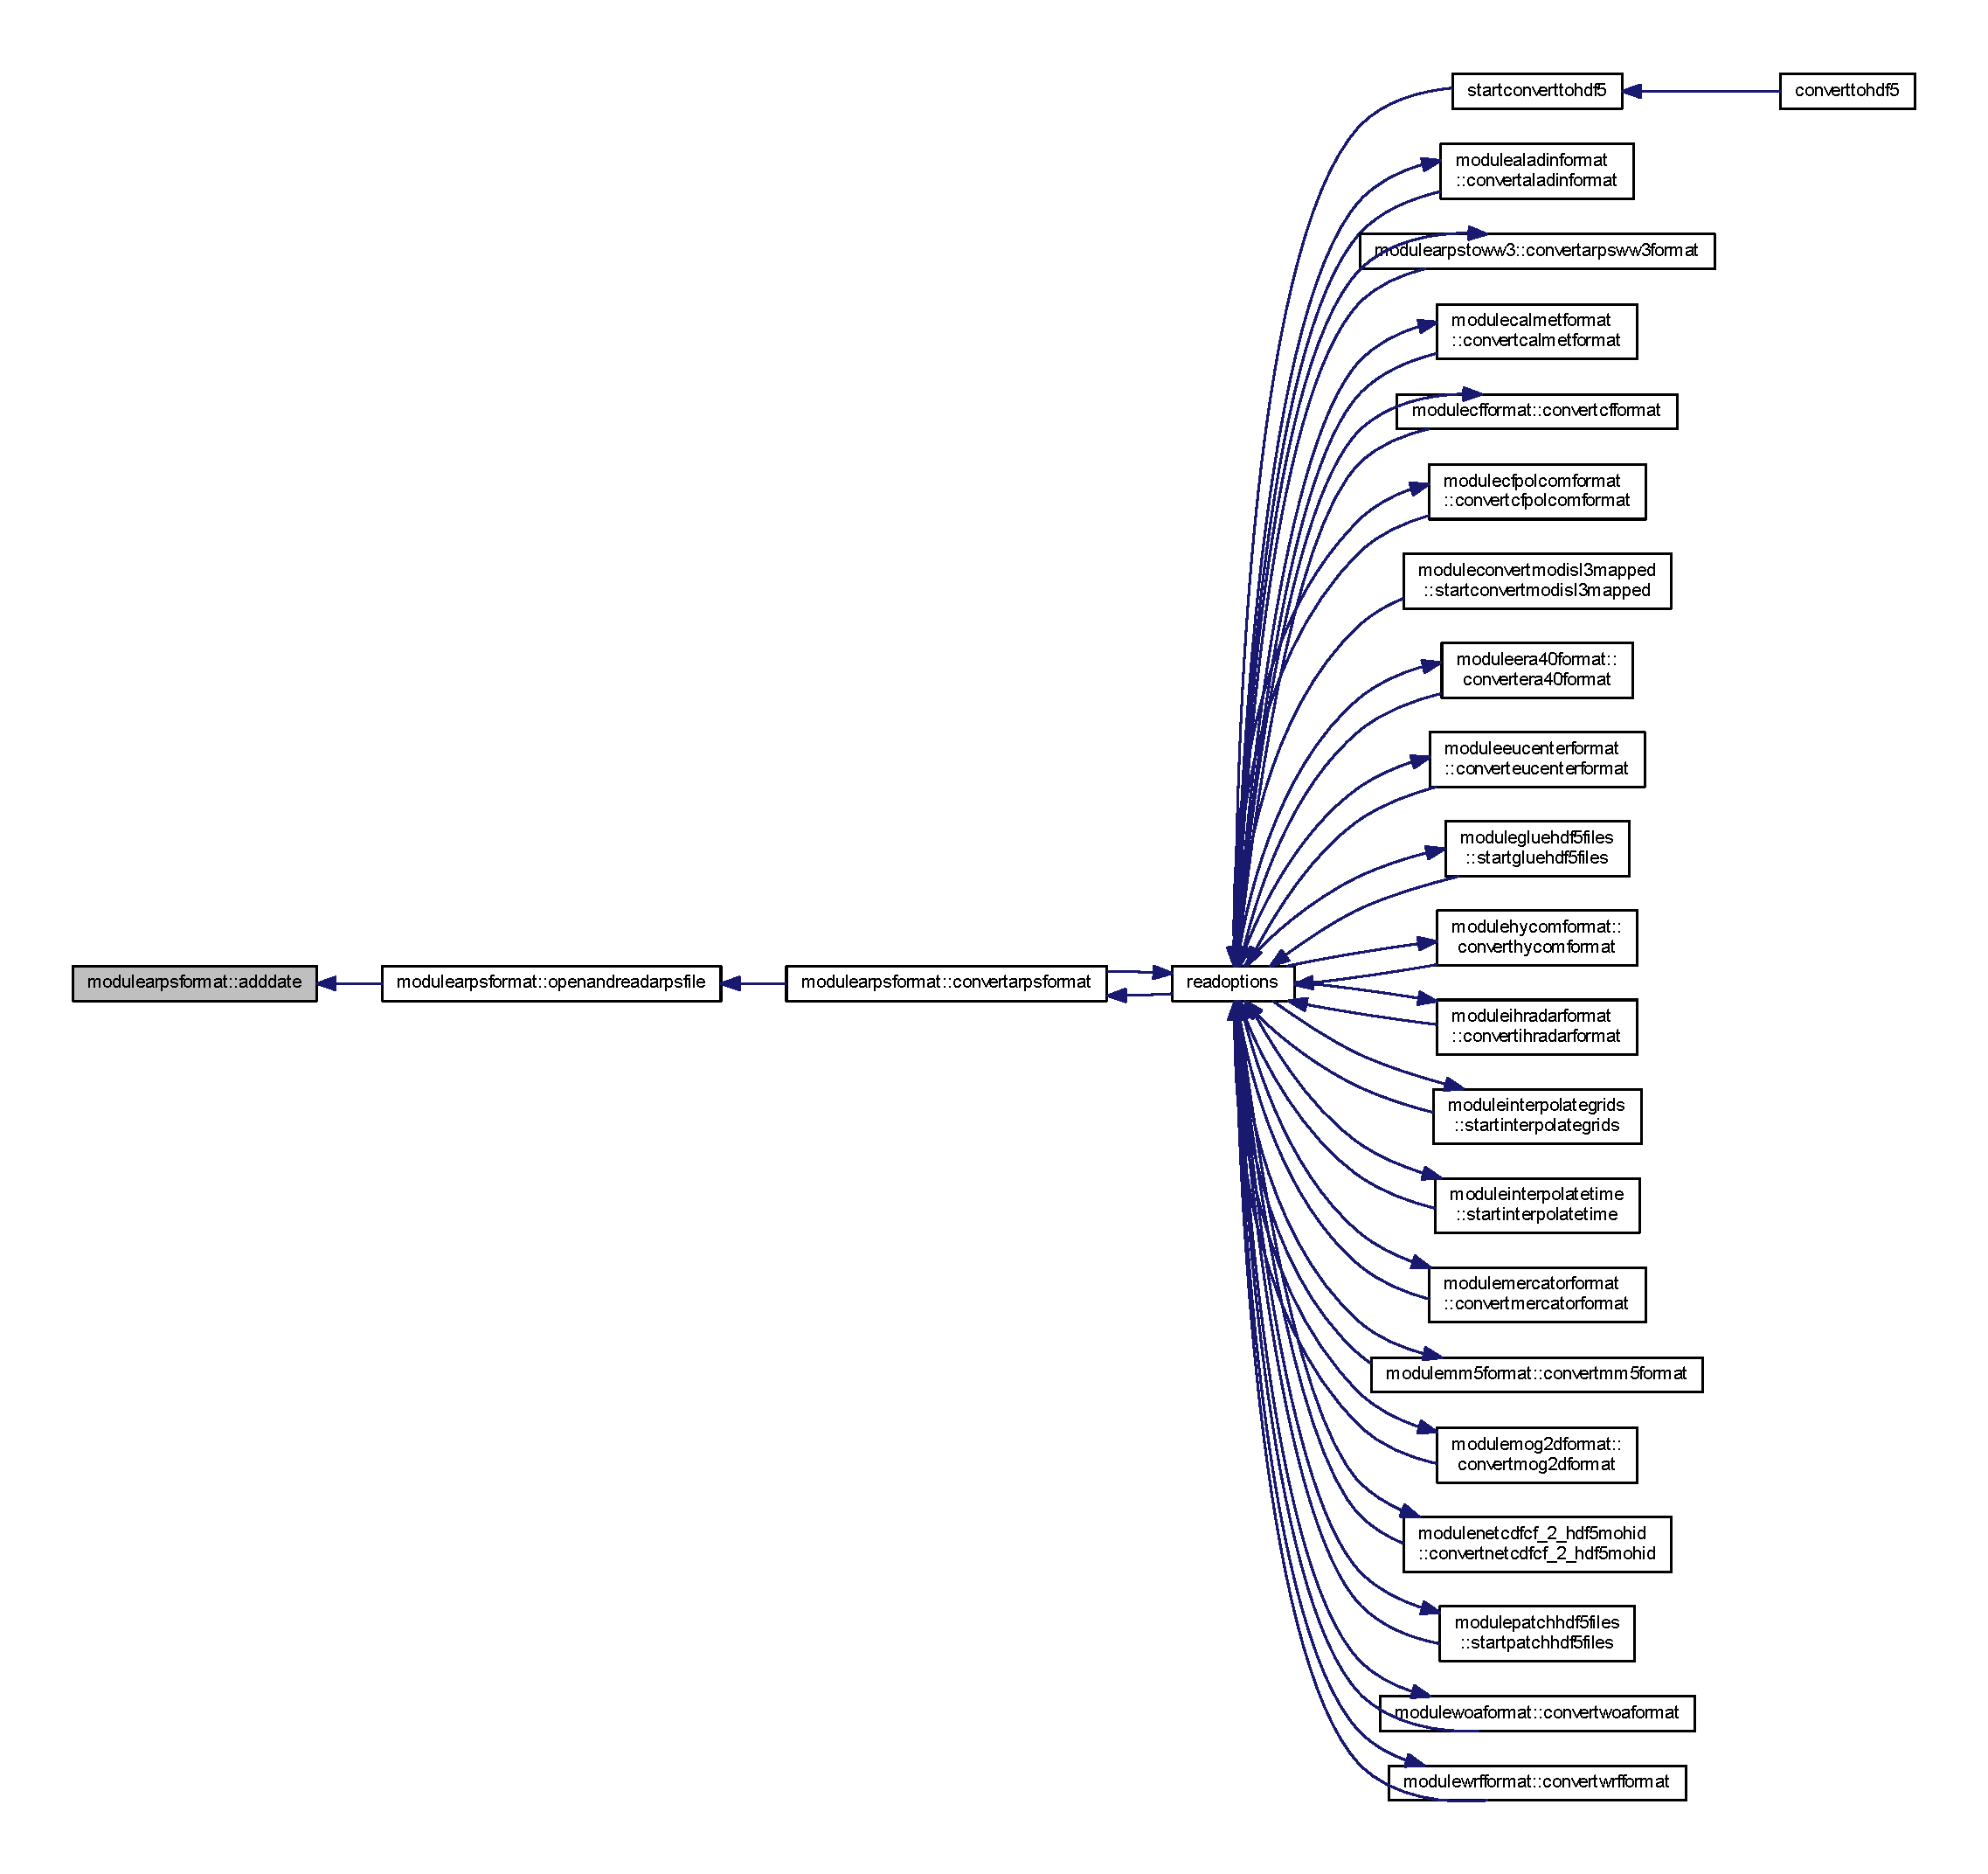
\includegraphics[width=350pt]{namespacemodulearpsformat_a3e7adeca2b8b386d9c8d59f32a8c189f_icgraph}
\end{center}
\end{figure}
\mbox{\Hypertarget{namespacemodulearpsformat_a32649b9f39dfaa2b5396d488243a3905}\label{namespacemodulearpsformat_a32649b9f39dfaa2b5396d488243a3905}} 
\index{modulearpsformat@{modulearpsformat}!addfield@{addfield}}
\index{addfield@{addfield}!modulearpsformat@{modulearpsformat}}
\subsubsection{\texorpdfstring{addfield()}{addfield()}}
{\footnotesize\ttfamily subroutine, private modulearpsformat\+::addfield (\begin{DoxyParamCaption}\item[{type (\mbox{\hyperlink{structmodulearpsformat_1_1t__field}{t\+\_\+field}}), pointer}]{First\+Field,  }\item[{type (\mbox{\hyperlink{structmodulearpsformat_1_1t__field}{t\+\_\+field}}), pointer}]{Obj\+Field }\end{DoxyParamCaption})\hspace{0.3cm}{\ttfamily [private]}}

Here is the caller graph for this function\+:\nopagebreak
\begin{figure}[H]
\begin{center}
\leavevmode
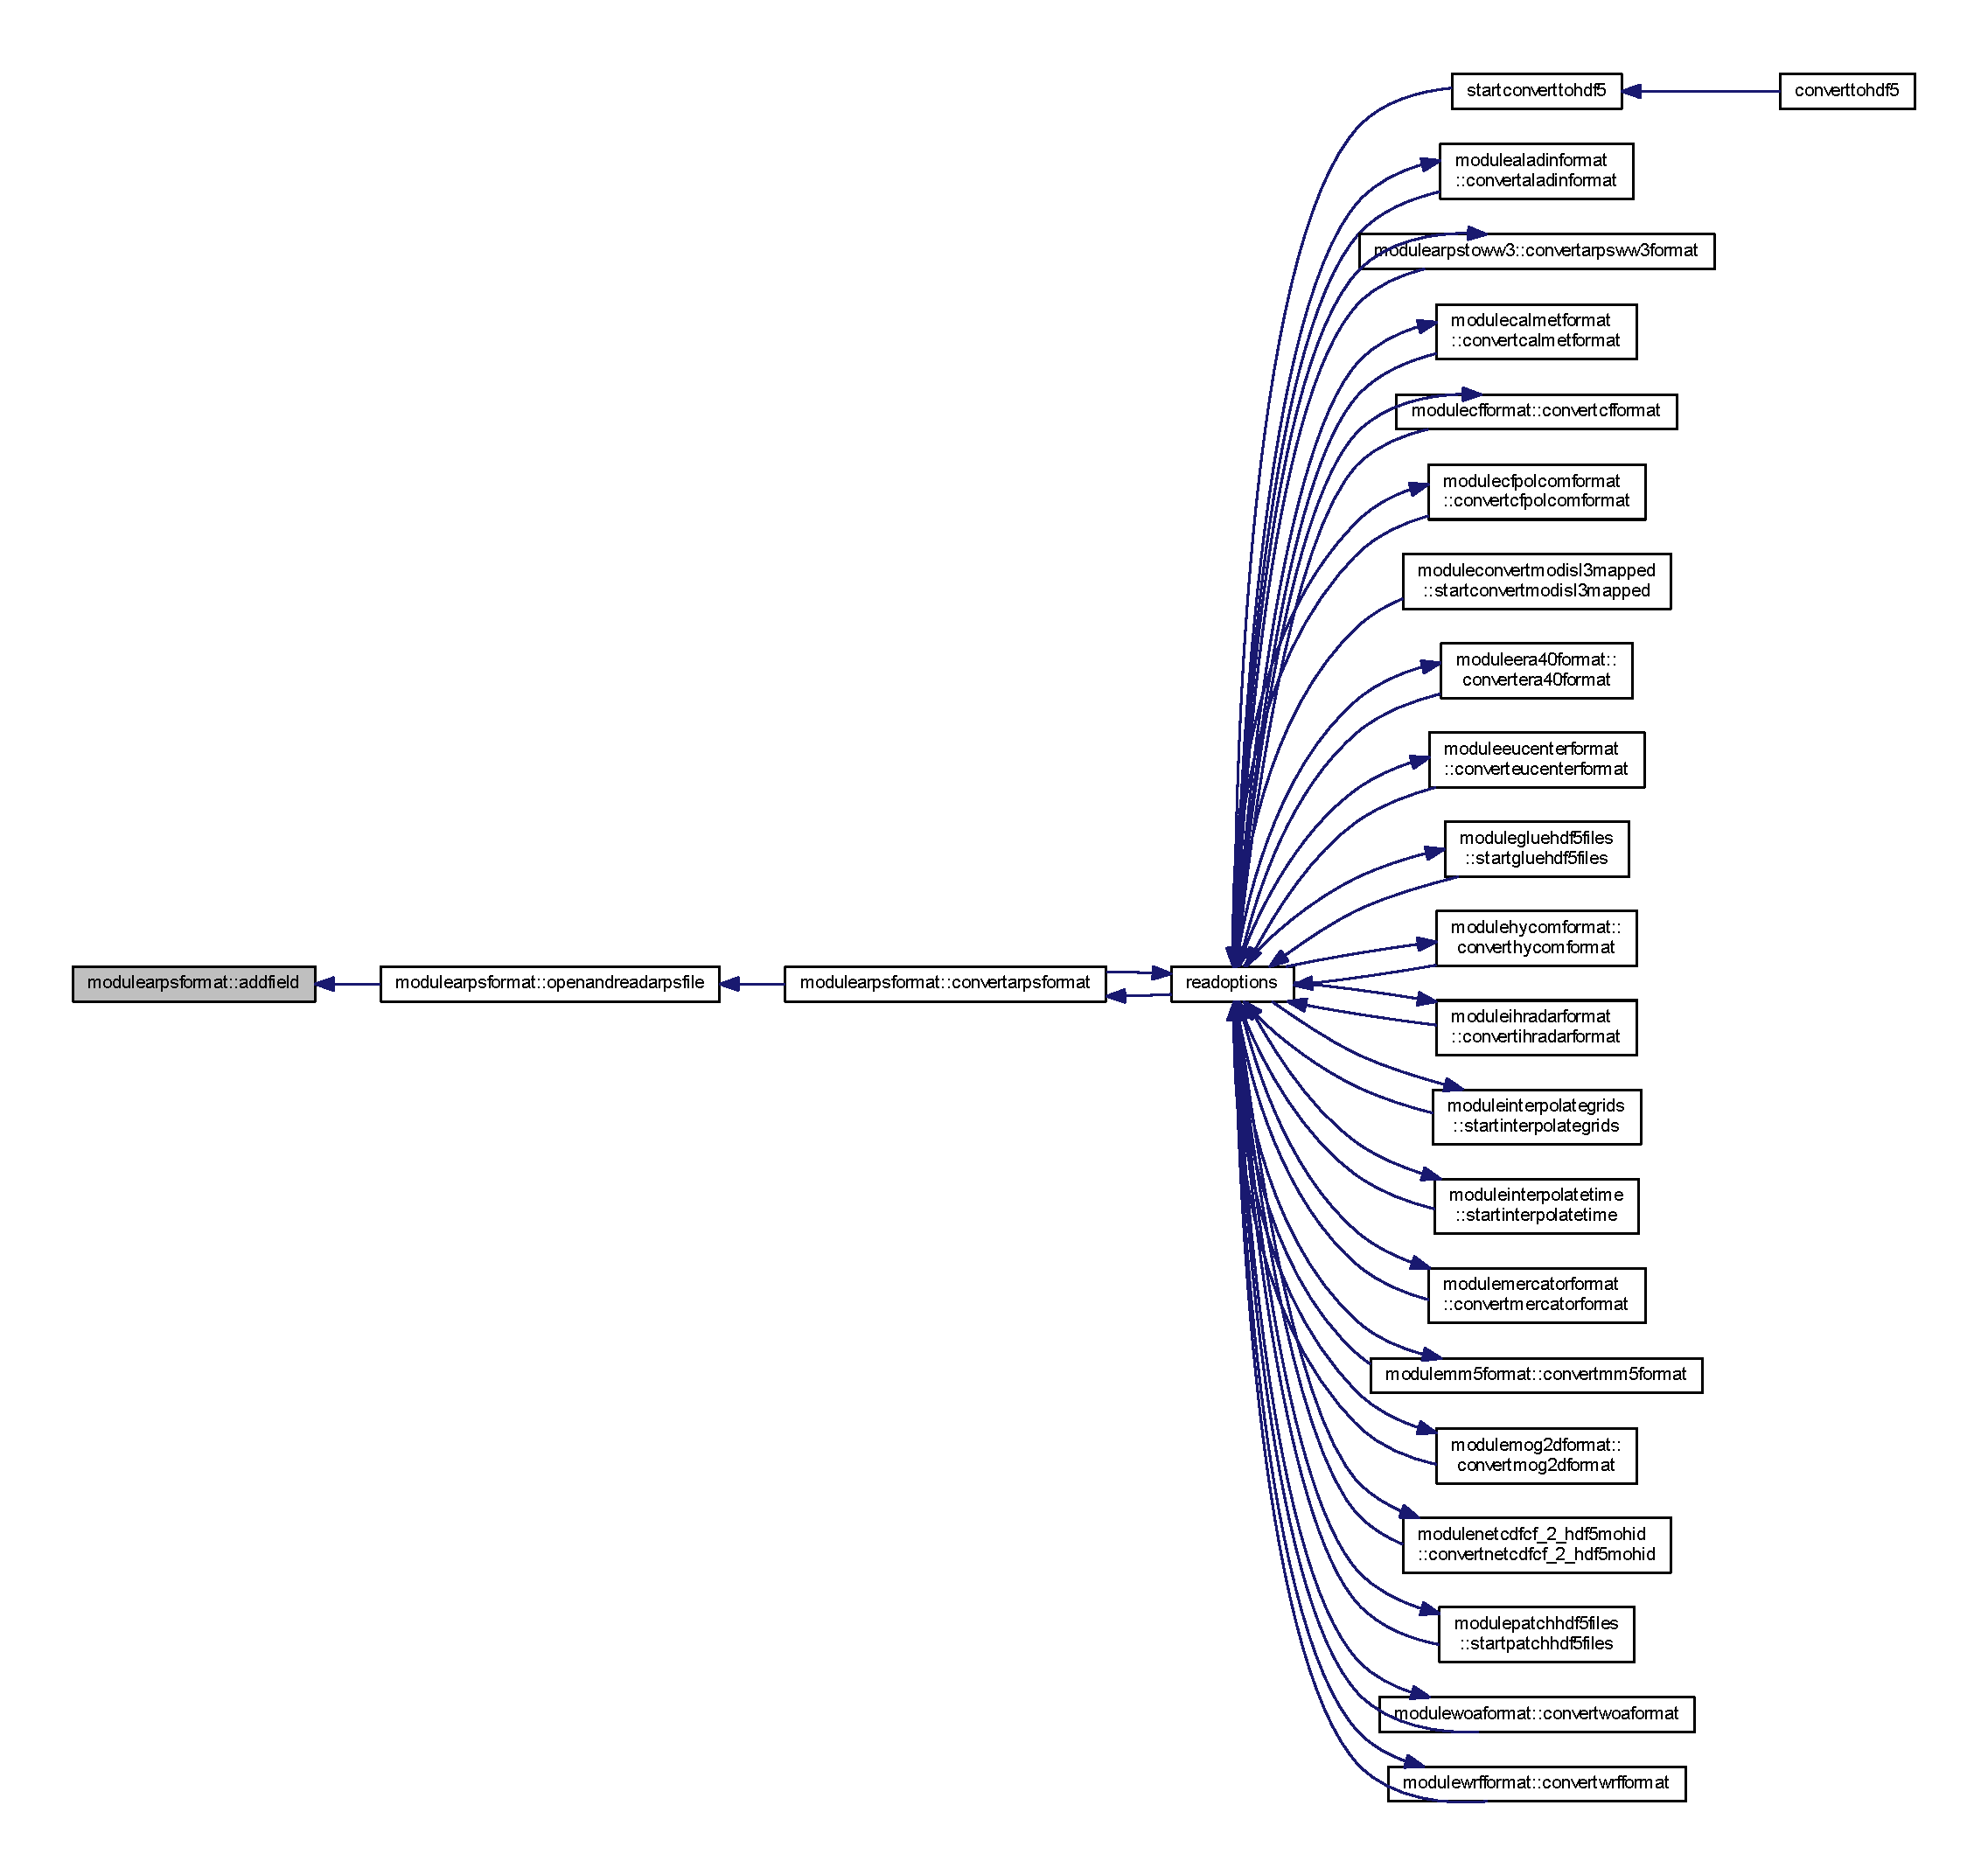
\includegraphics[width=350pt]{namespacemodulearpsformat_a32649b9f39dfaa2b5396d488243a3905_icgraph}
\end{center}
\end{figure}
\mbox{\Hypertarget{namespacemodulearpsformat_a420eb740016c6ba55f897dbff1ef74e5}\label{namespacemodulearpsformat_a420eb740016c6ba55f897dbff1ef74e5}} 
\index{modulearpsformat@{modulearpsformat}!constructgrid@{constructgrid}}
\index{constructgrid@{constructgrid}!modulearpsformat@{modulearpsformat}}
\subsubsection{\texorpdfstring{constructgrid()}{constructgrid()}}
{\footnotesize\ttfamily subroutine modulearpsformat\+::constructgrid (\begin{DoxyParamCaption}{ }\end{DoxyParamCaption})\hspace{0.3cm}{\ttfamily [private]}}

Here is the caller graph for this function\+:\nopagebreak
\begin{figure}[H]
\begin{center}
\leavevmode
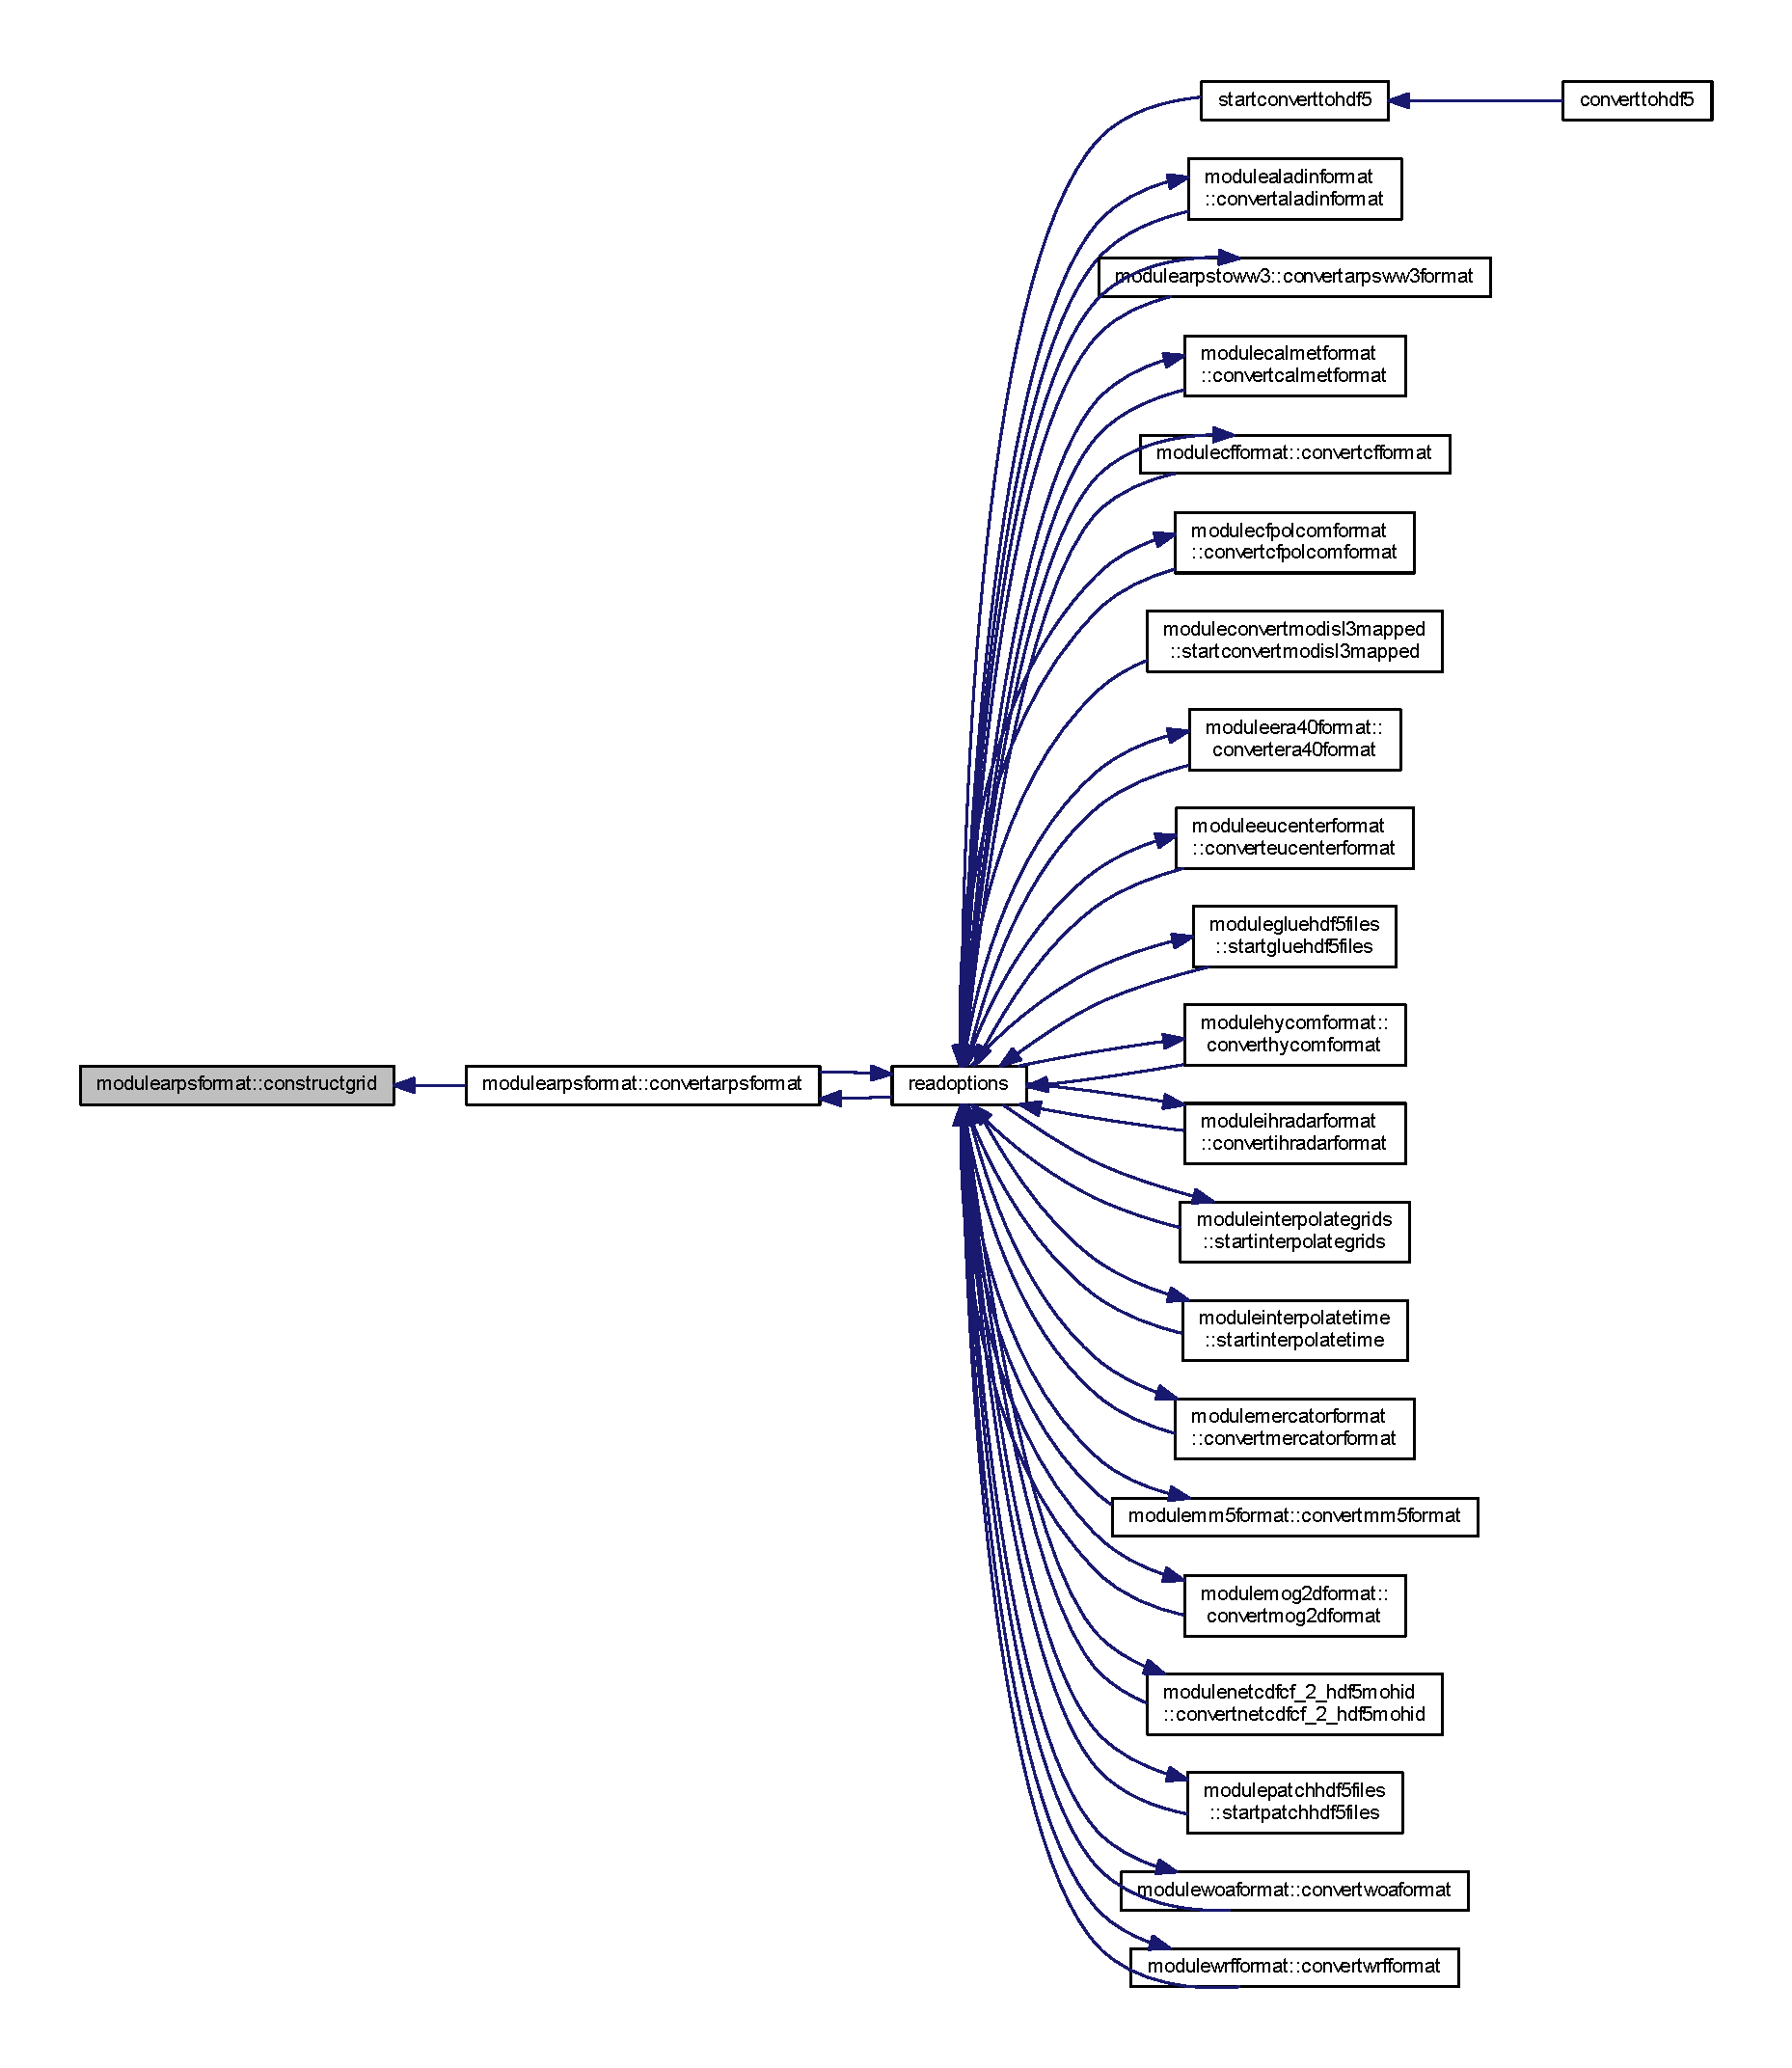
\includegraphics[width=350pt]{namespacemodulearpsformat_a420eb740016c6ba55f897dbff1ef74e5_icgraph}
\end{center}
\end{figure}
\mbox{\Hypertarget{namespacemodulearpsformat_a996acecfde01fb49e6408da52cb50d12}\label{namespacemodulearpsformat_a996acecfde01fb49e6408da52cb50d12}} 
\index{modulearpsformat@{modulearpsformat}!convertarpsformat@{convertarpsformat}}
\index{convertarpsformat@{convertarpsformat}!modulearpsformat@{modulearpsformat}}
\subsubsection{\texorpdfstring{convertarpsformat()}{convertarpsformat()}}
{\footnotesize\ttfamily subroutine, public modulearpsformat\+::convertarpsformat (\begin{DoxyParamCaption}\item[{integer, intent(in)}]{Enter\+Data\+ID,  }\item[{integer, intent(out), optional}]{S\+T\+AT }\end{DoxyParamCaption})}

Here is the call graph for this function\+:\nopagebreak
\begin{figure}[H]
\begin{center}
\leavevmode
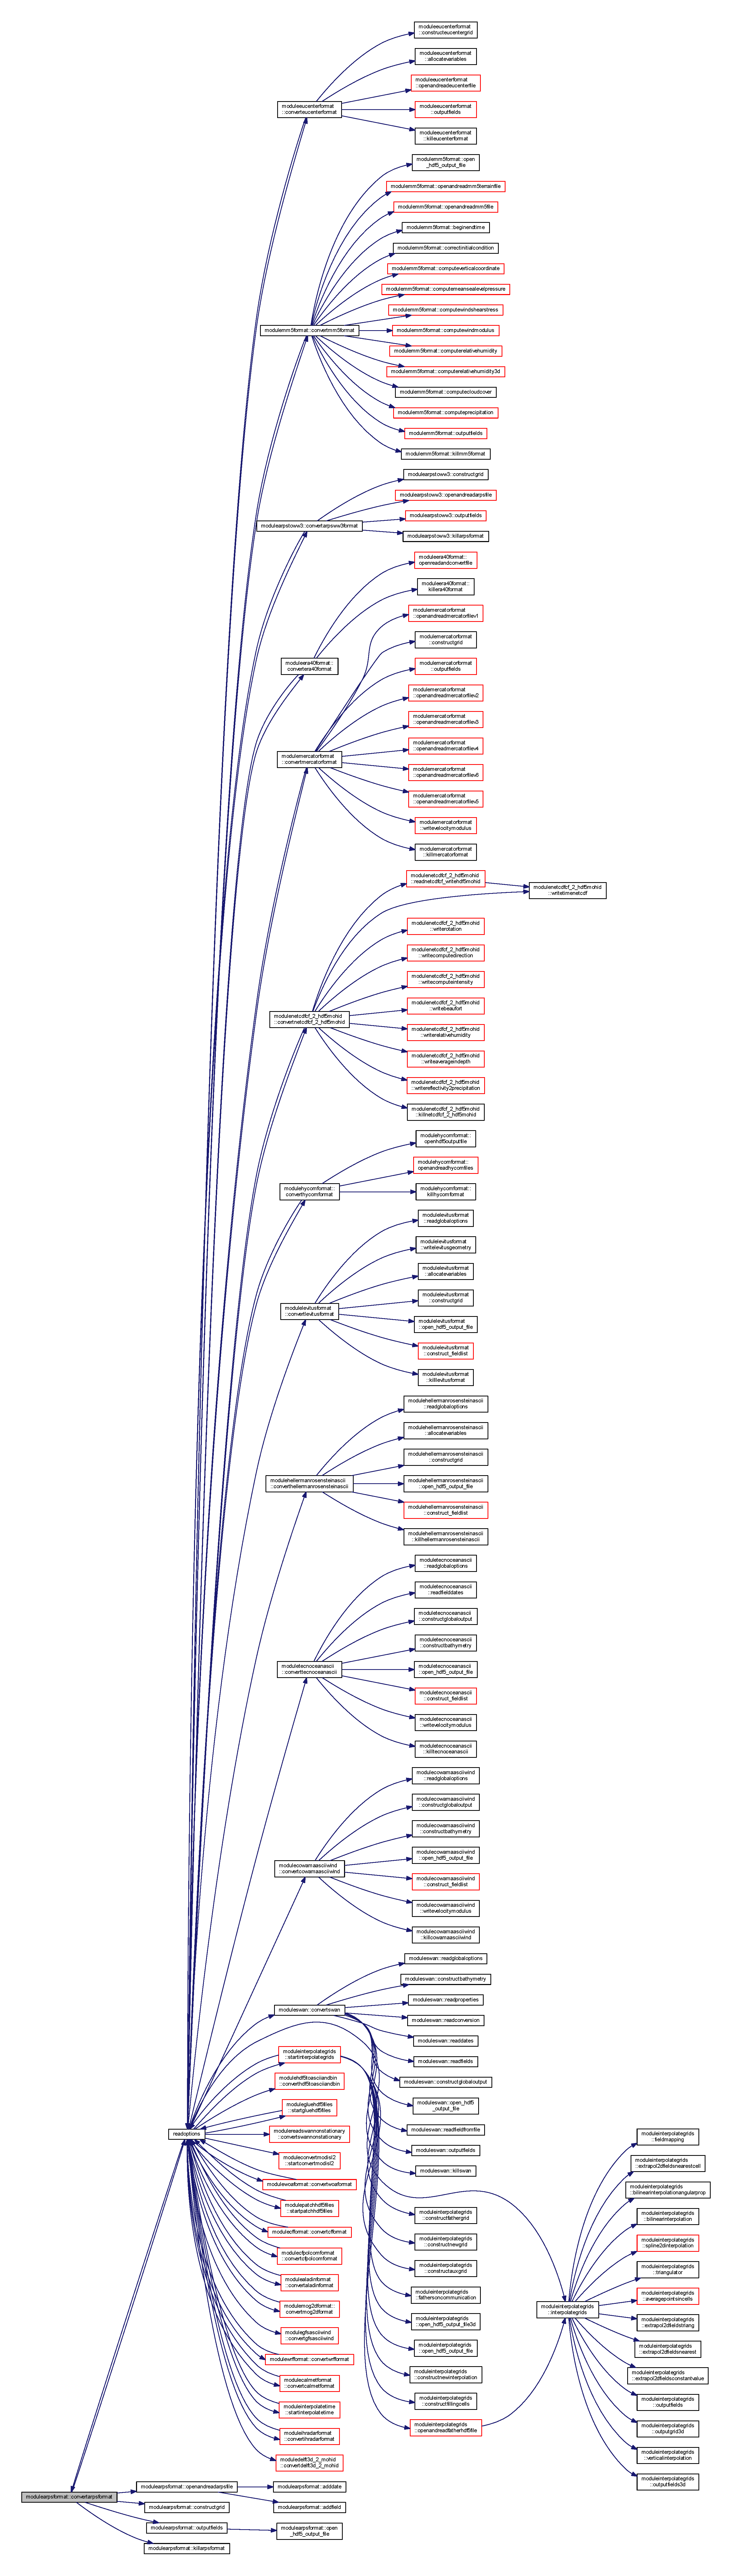
\includegraphics[height=550pt]{namespacemodulearpsformat_a996acecfde01fb49e6408da52cb50d12_cgraph}
\end{center}
\end{figure}
Here is the caller graph for this function\+:\nopagebreak
\begin{figure}[H]
\begin{center}
\leavevmode
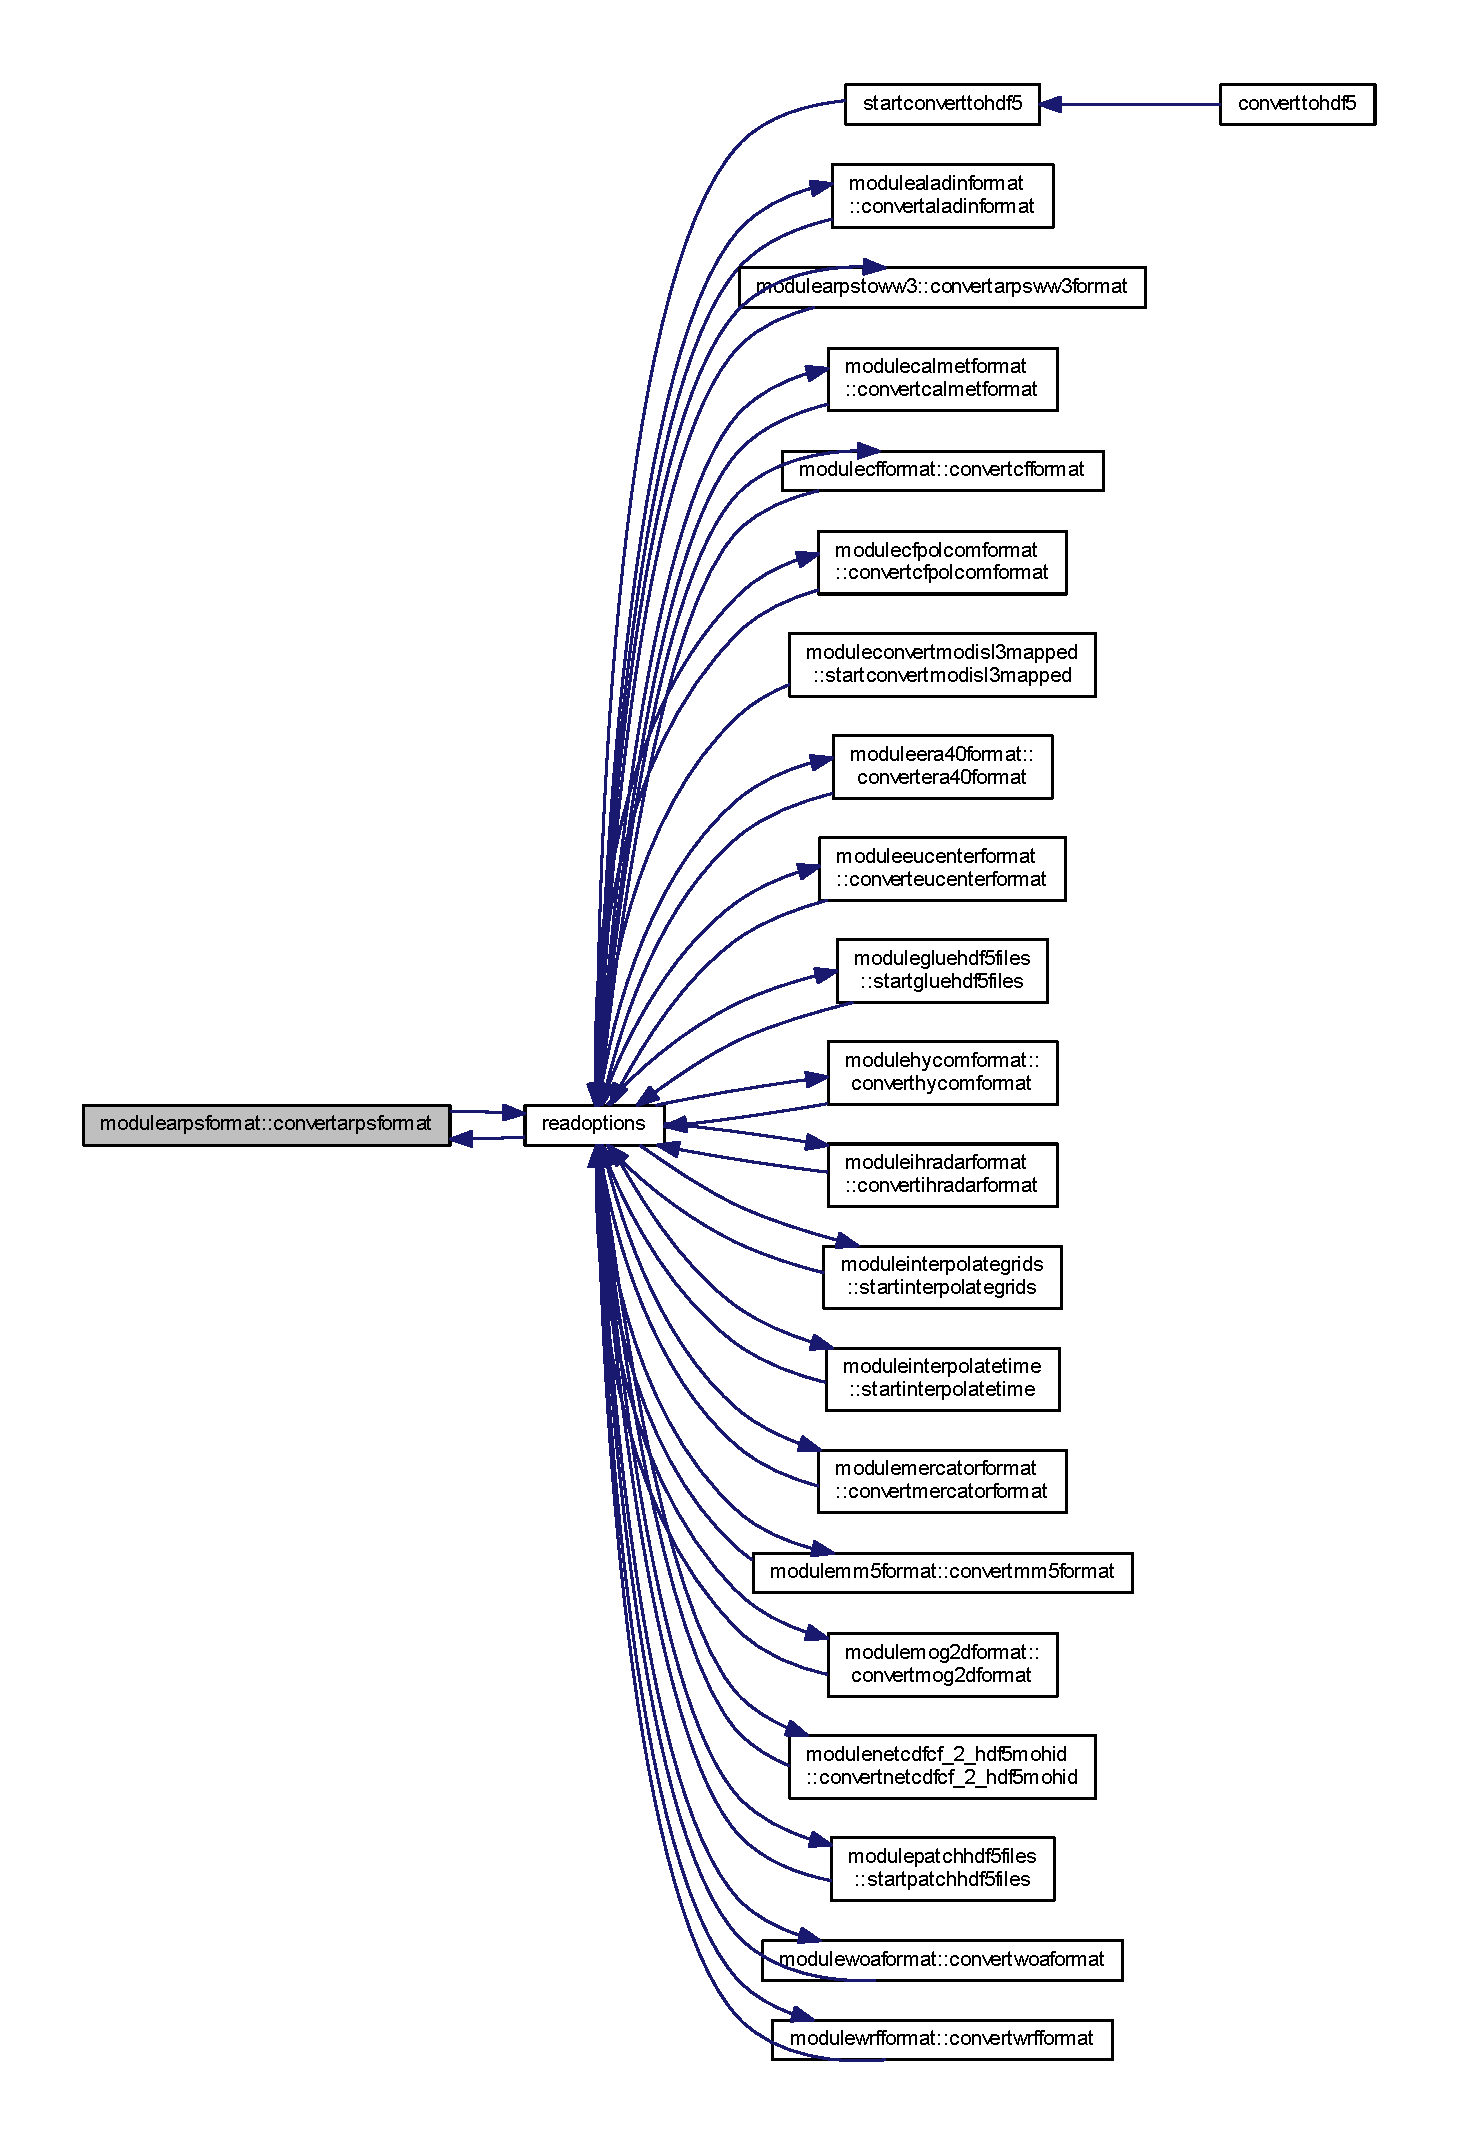
\includegraphics[width=350pt]{namespacemodulearpsformat_a996acecfde01fb49e6408da52cb50d12_icgraph}
\end{center}
\end{figure}
\mbox{\Hypertarget{namespacemodulearpsformat_a3fbe9c856c732d4e5f2315c2ae61e3d3}\label{namespacemodulearpsformat_a3fbe9c856c732d4e5f2315c2ae61e3d3}} 
\index{modulearpsformat@{modulearpsformat}!killarpsformat@{killarpsformat}}
\index{killarpsformat@{killarpsformat}!modulearpsformat@{modulearpsformat}}
\subsubsection{\texorpdfstring{killarpsformat()}{killarpsformat()}}
{\footnotesize\ttfamily subroutine, private modulearpsformat\+::killarpsformat (\begin{DoxyParamCaption}{ }\end{DoxyParamCaption})\hspace{0.3cm}{\ttfamily [private]}}

Here is the caller graph for this function\+:\nopagebreak
\begin{figure}[H]
\begin{center}
\leavevmode
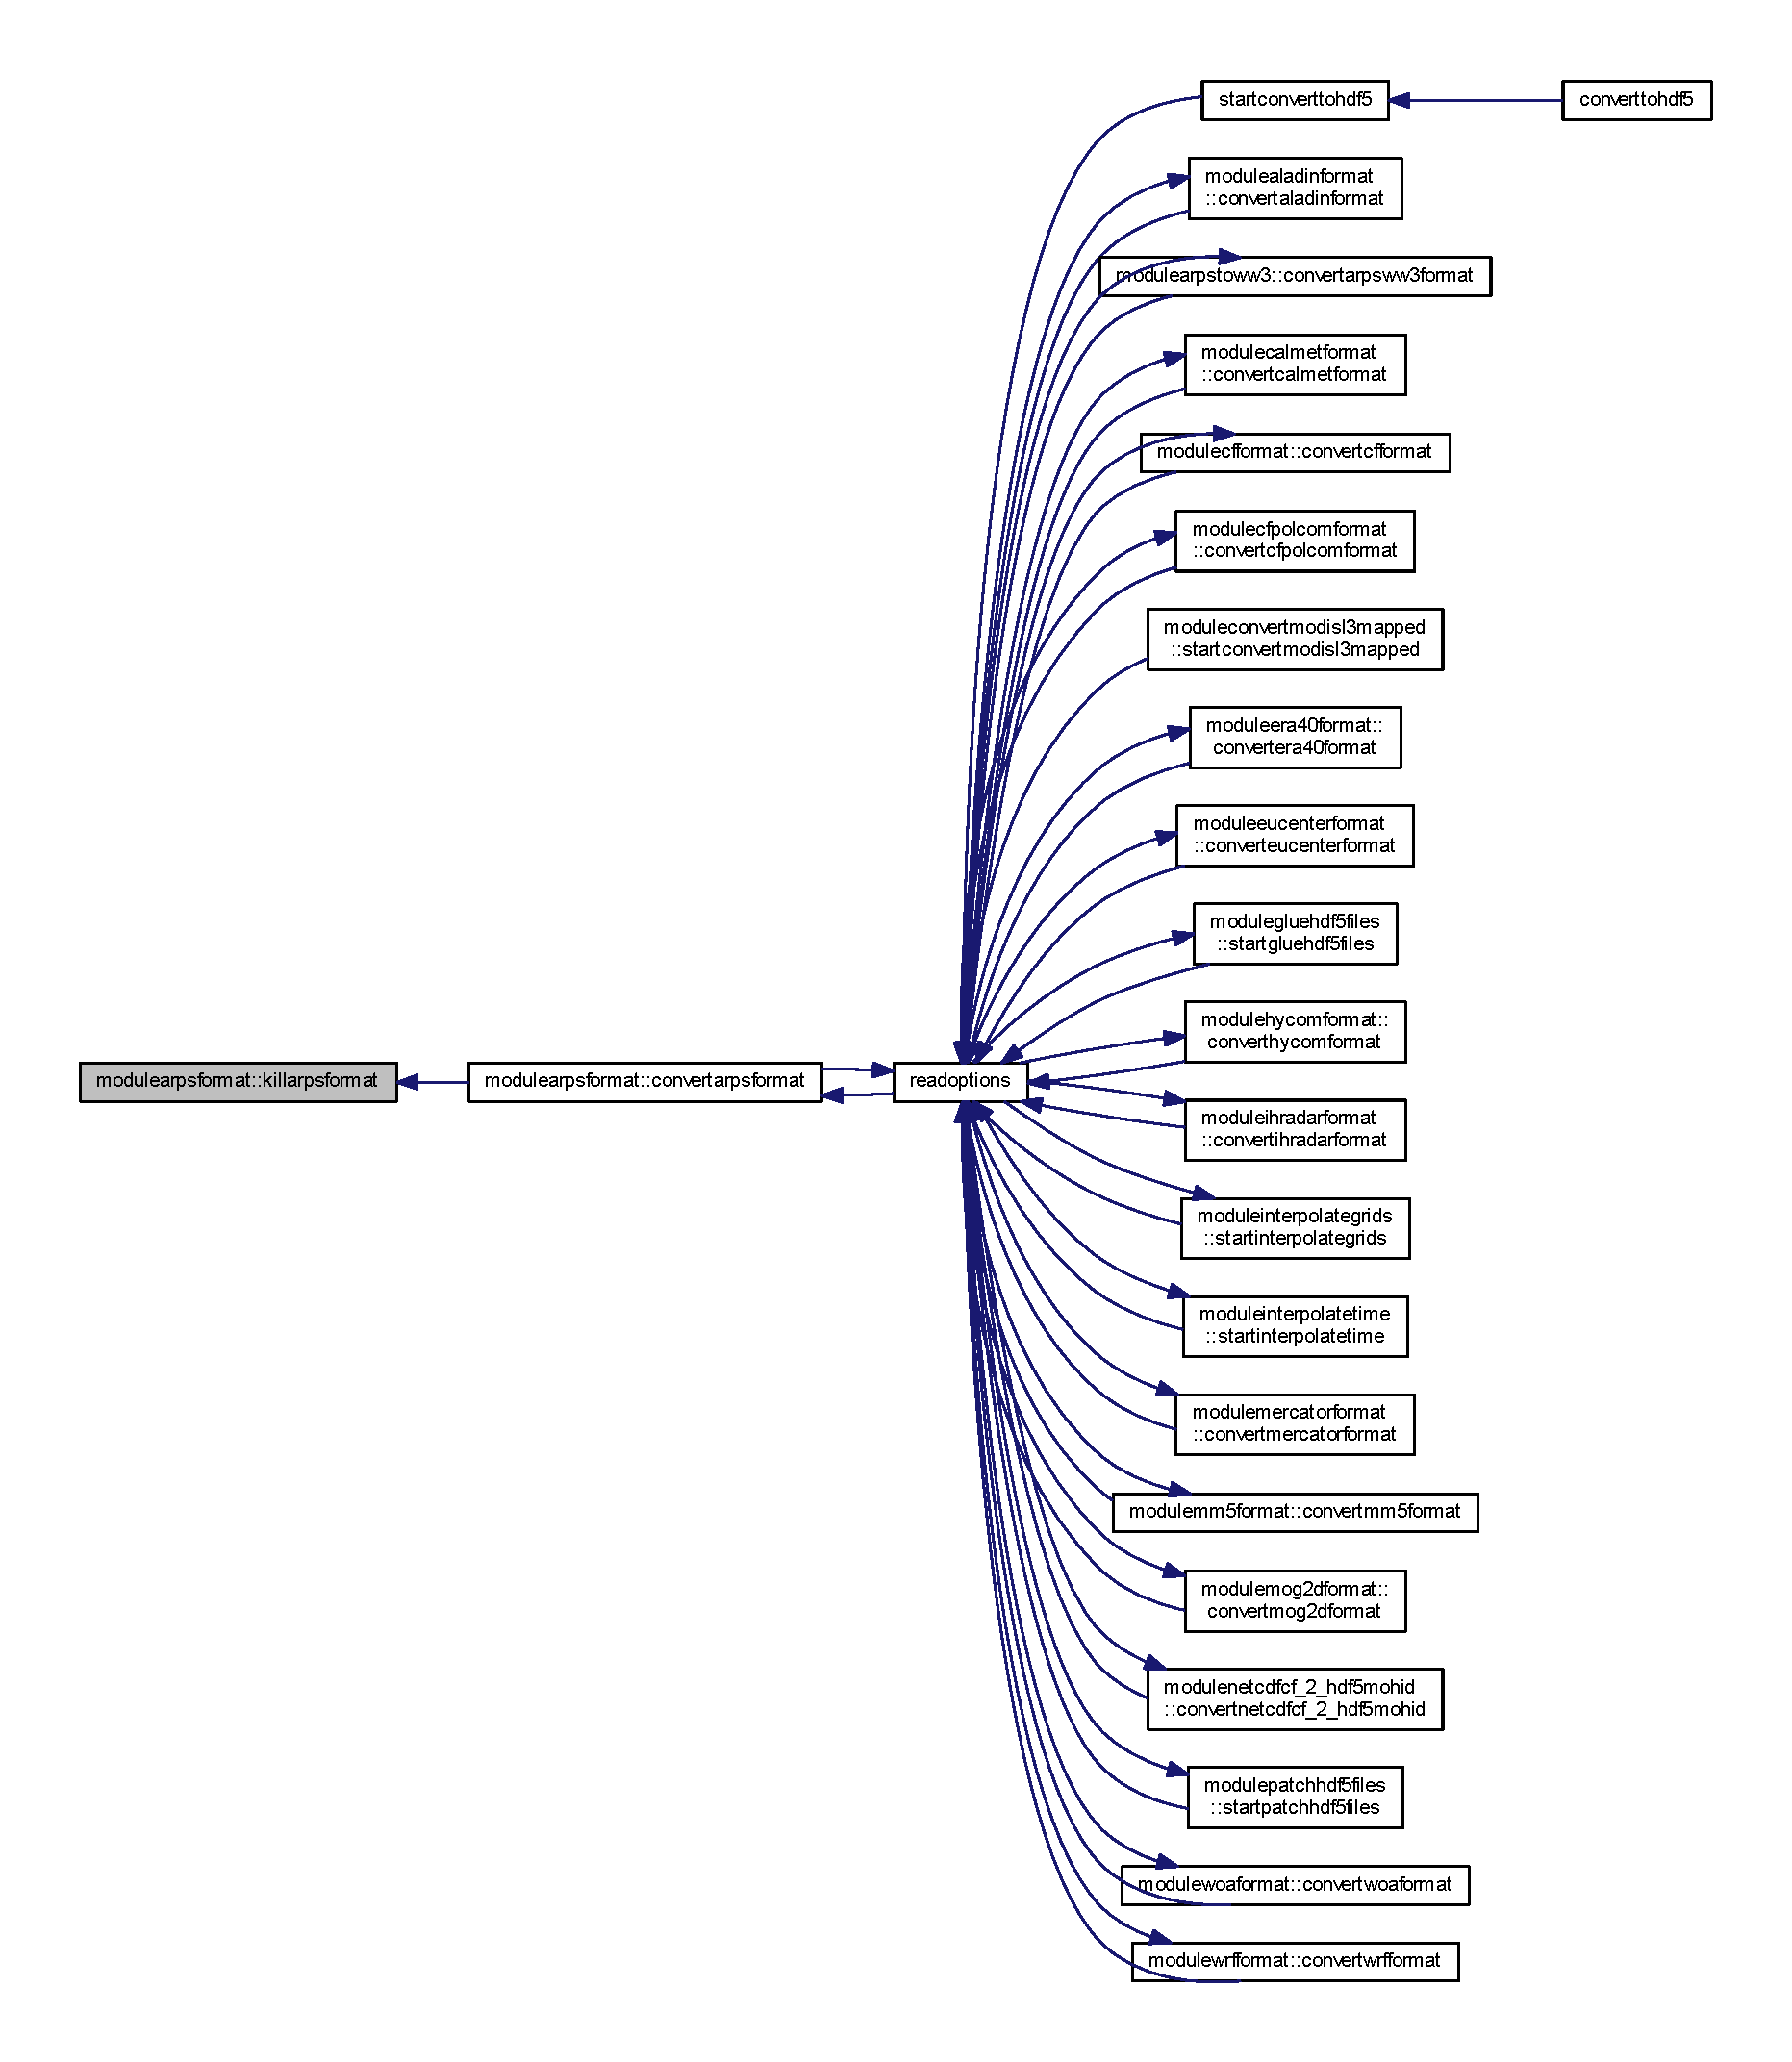
\includegraphics[width=350pt]{namespacemodulearpsformat_a3fbe9c856c732d4e5f2315c2ae61e3d3_icgraph}
\end{center}
\end{figure}
\mbox{\Hypertarget{namespacemodulearpsformat_a9c9927c6fb171da5b0bfc4cd38595627}\label{namespacemodulearpsformat_a9c9927c6fb171da5b0bfc4cd38595627}} 
\index{modulearpsformat@{modulearpsformat}!open\+\_\+hdf5\+\_\+output\+\_\+file@{open\+\_\+hdf5\+\_\+output\+\_\+file}}
\index{open\+\_\+hdf5\+\_\+output\+\_\+file@{open\+\_\+hdf5\+\_\+output\+\_\+file}!modulearpsformat@{modulearpsformat}}
\subsubsection{\texorpdfstring{open\+\_\+hdf5\+\_\+output\+\_\+file()}{open\_hdf5\_output\_file()}}
{\footnotesize\ttfamily subroutine, private modulearpsformat\+::open\+\_\+hdf5\+\_\+output\+\_\+file (\begin{DoxyParamCaption}{ }\end{DoxyParamCaption})\hspace{0.3cm}{\ttfamily [private]}}

Here is the caller graph for this function\+:\nopagebreak
\begin{figure}[H]
\begin{center}
\leavevmode
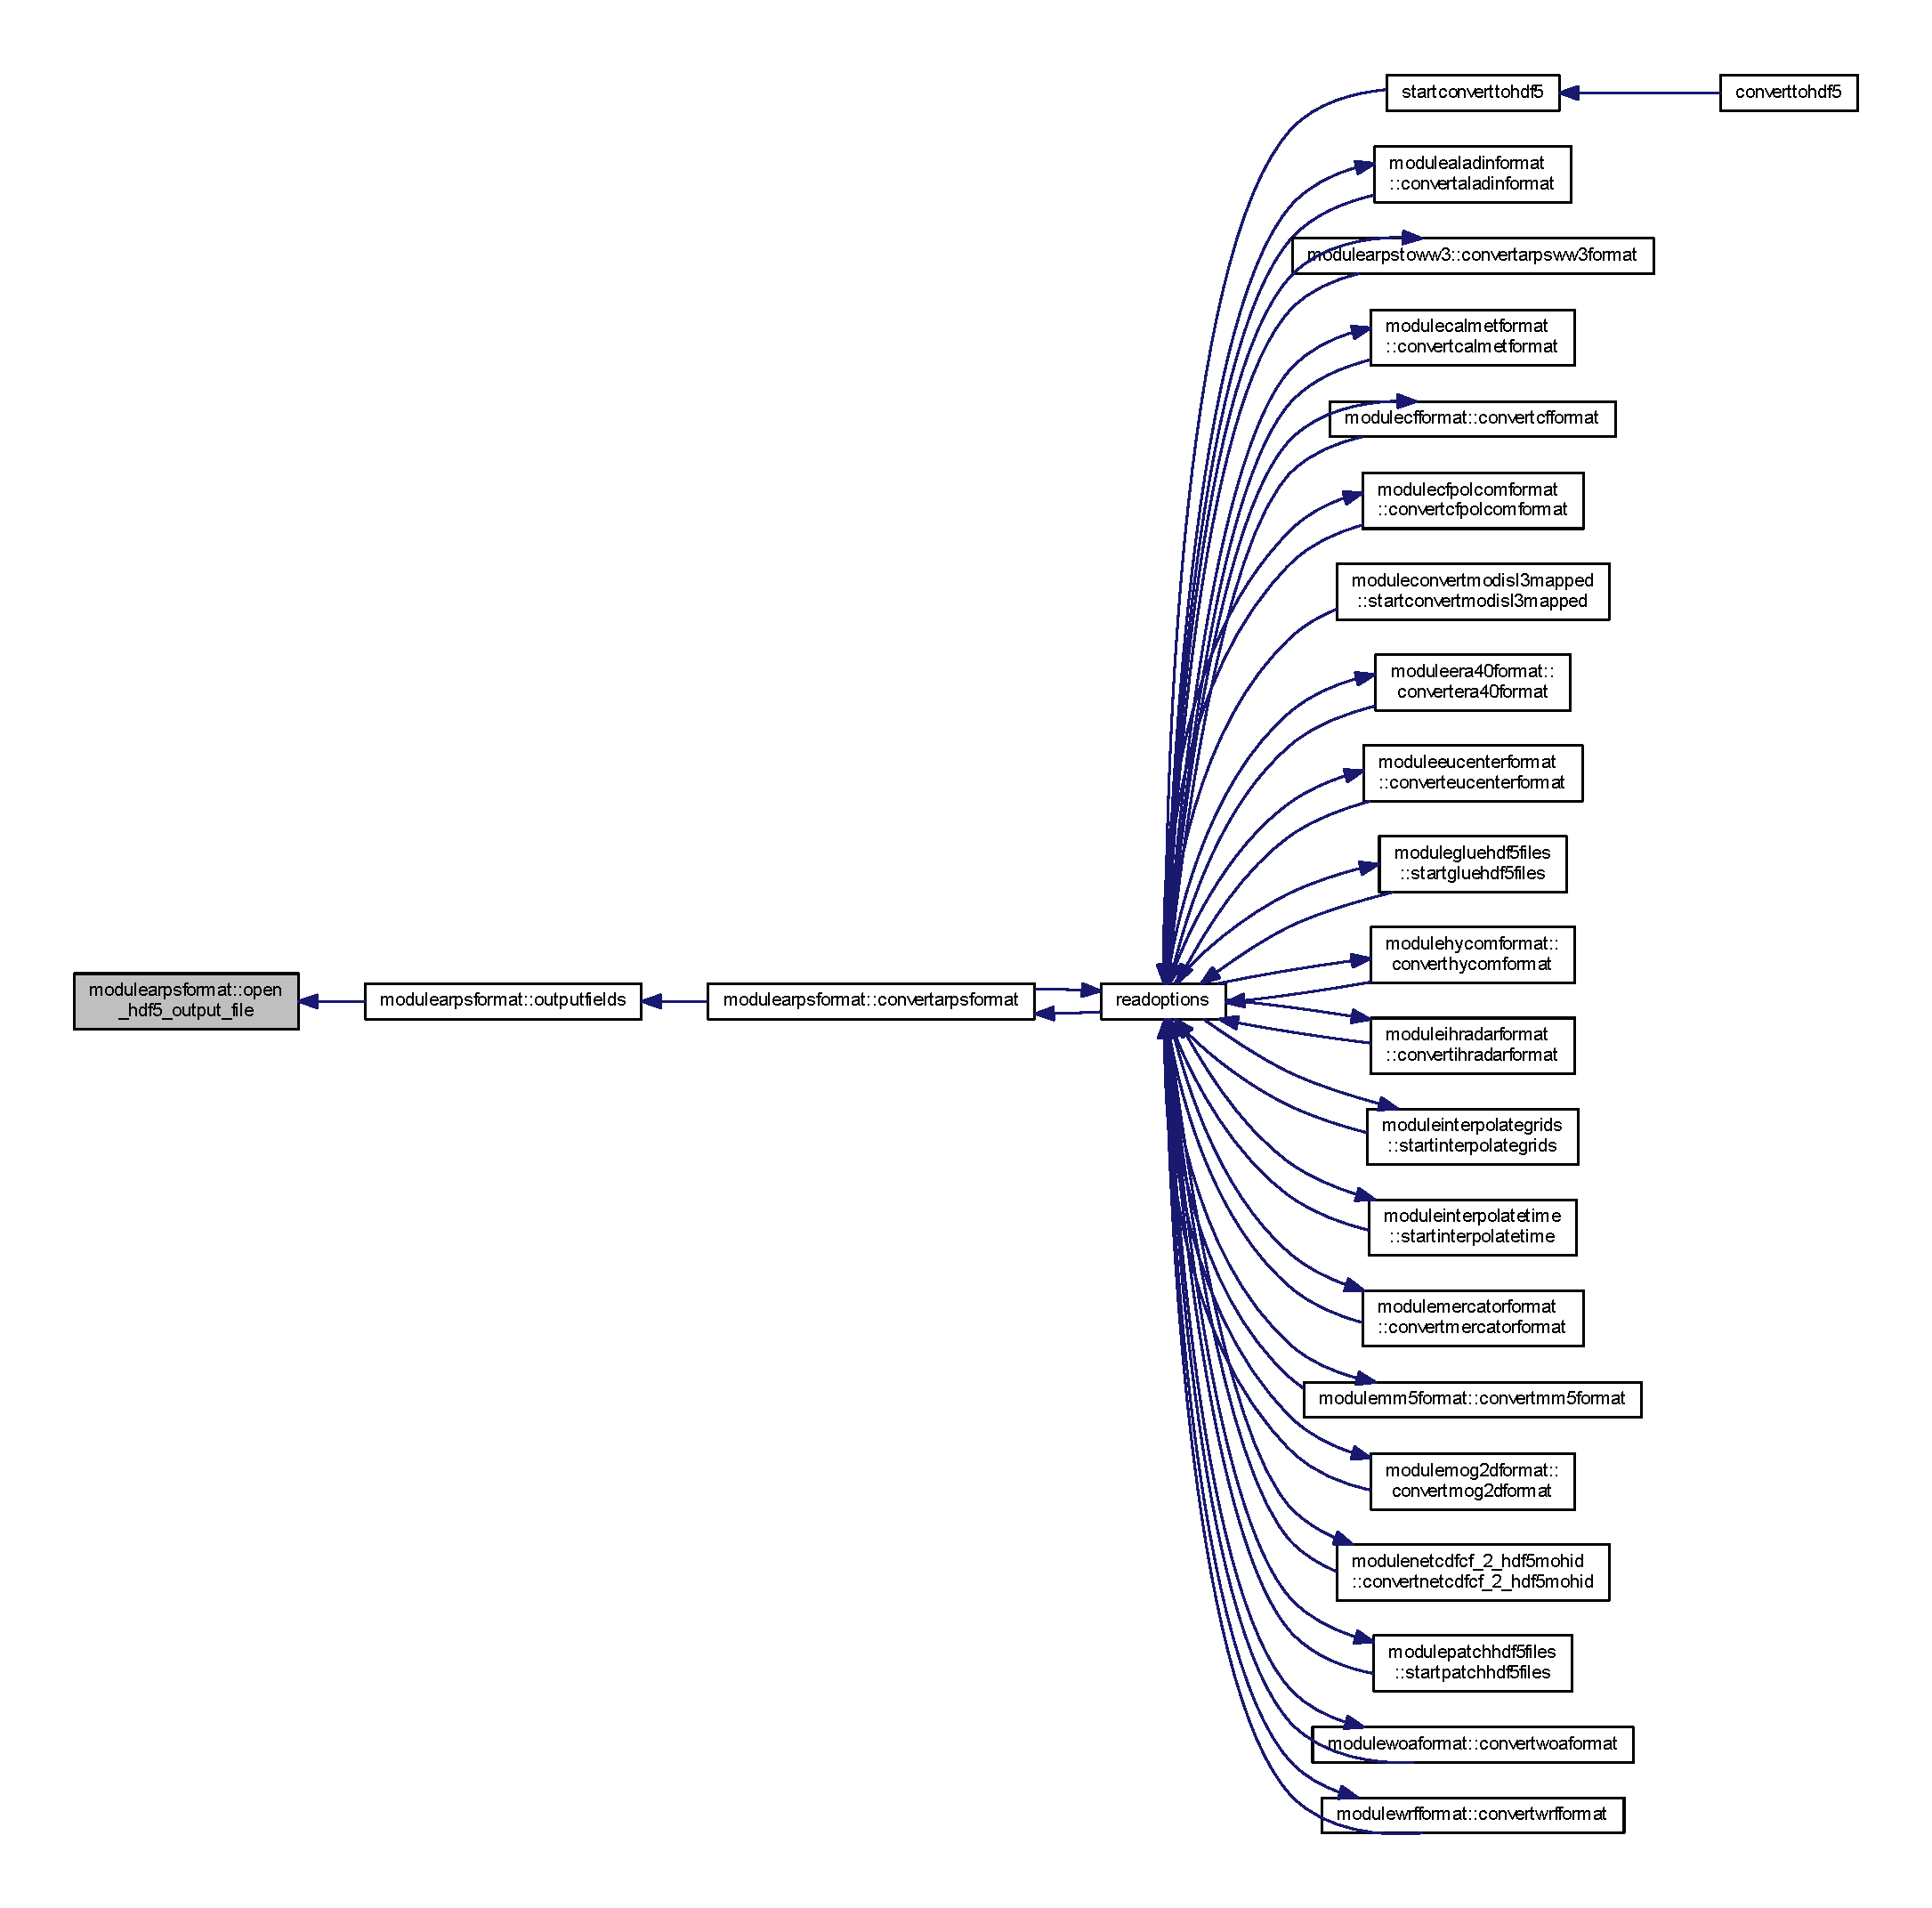
\includegraphics[width=350pt]{namespacemodulearpsformat_a9c9927c6fb171da5b0bfc4cd38595627_icgraph}
\end{center}
\end{figure}
\mbox{\Hypertarget{namespacemodulearpsformat_a70ee83442772ea85df79da65ec4ea262}\label{namespacemodulearpsformat_a70ee83442772ea85df79da65ec4ea262}} 
\index{modulearpsformat@{modulearpsformat}!openandreadarpsfile@{openandreadarpsfile}}
\index{openandreadarpsfile@{openandreadarpsfile}!modulearpsformat@{modulearpsformat}}
\subsubsection{\texorpdfstring{openandreadarpsfile()}{openandreadarpsfile()}}
{\footnotesize\ttfamily subroutine, private modulearpsformat\+::openandreadarpsfile (\begin{DoxyParamCaption}{ }\end{DoxyParamCaption})\hspace{0.3cm}{\ttfamily [private]}}

Here is the call graph for this function\+:\nopagebreak
\begin{figure}[H]
\begin{center}
\leavevmode
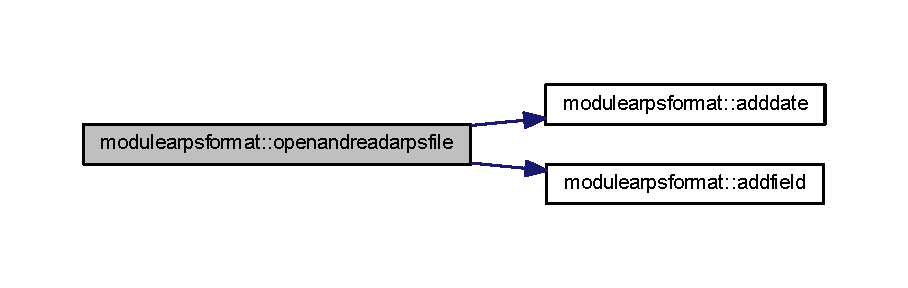
\includegraphics[width=350pt]{namespacemodulearpsformat_a70ee83442772ea85df79da65ec4ea262_cgraph}
\end{center}
\end{figure}
Here is the caller graph for this function\+:\nopagebreak
\begin{figure}[H]
\begin{center}
\leavevmode
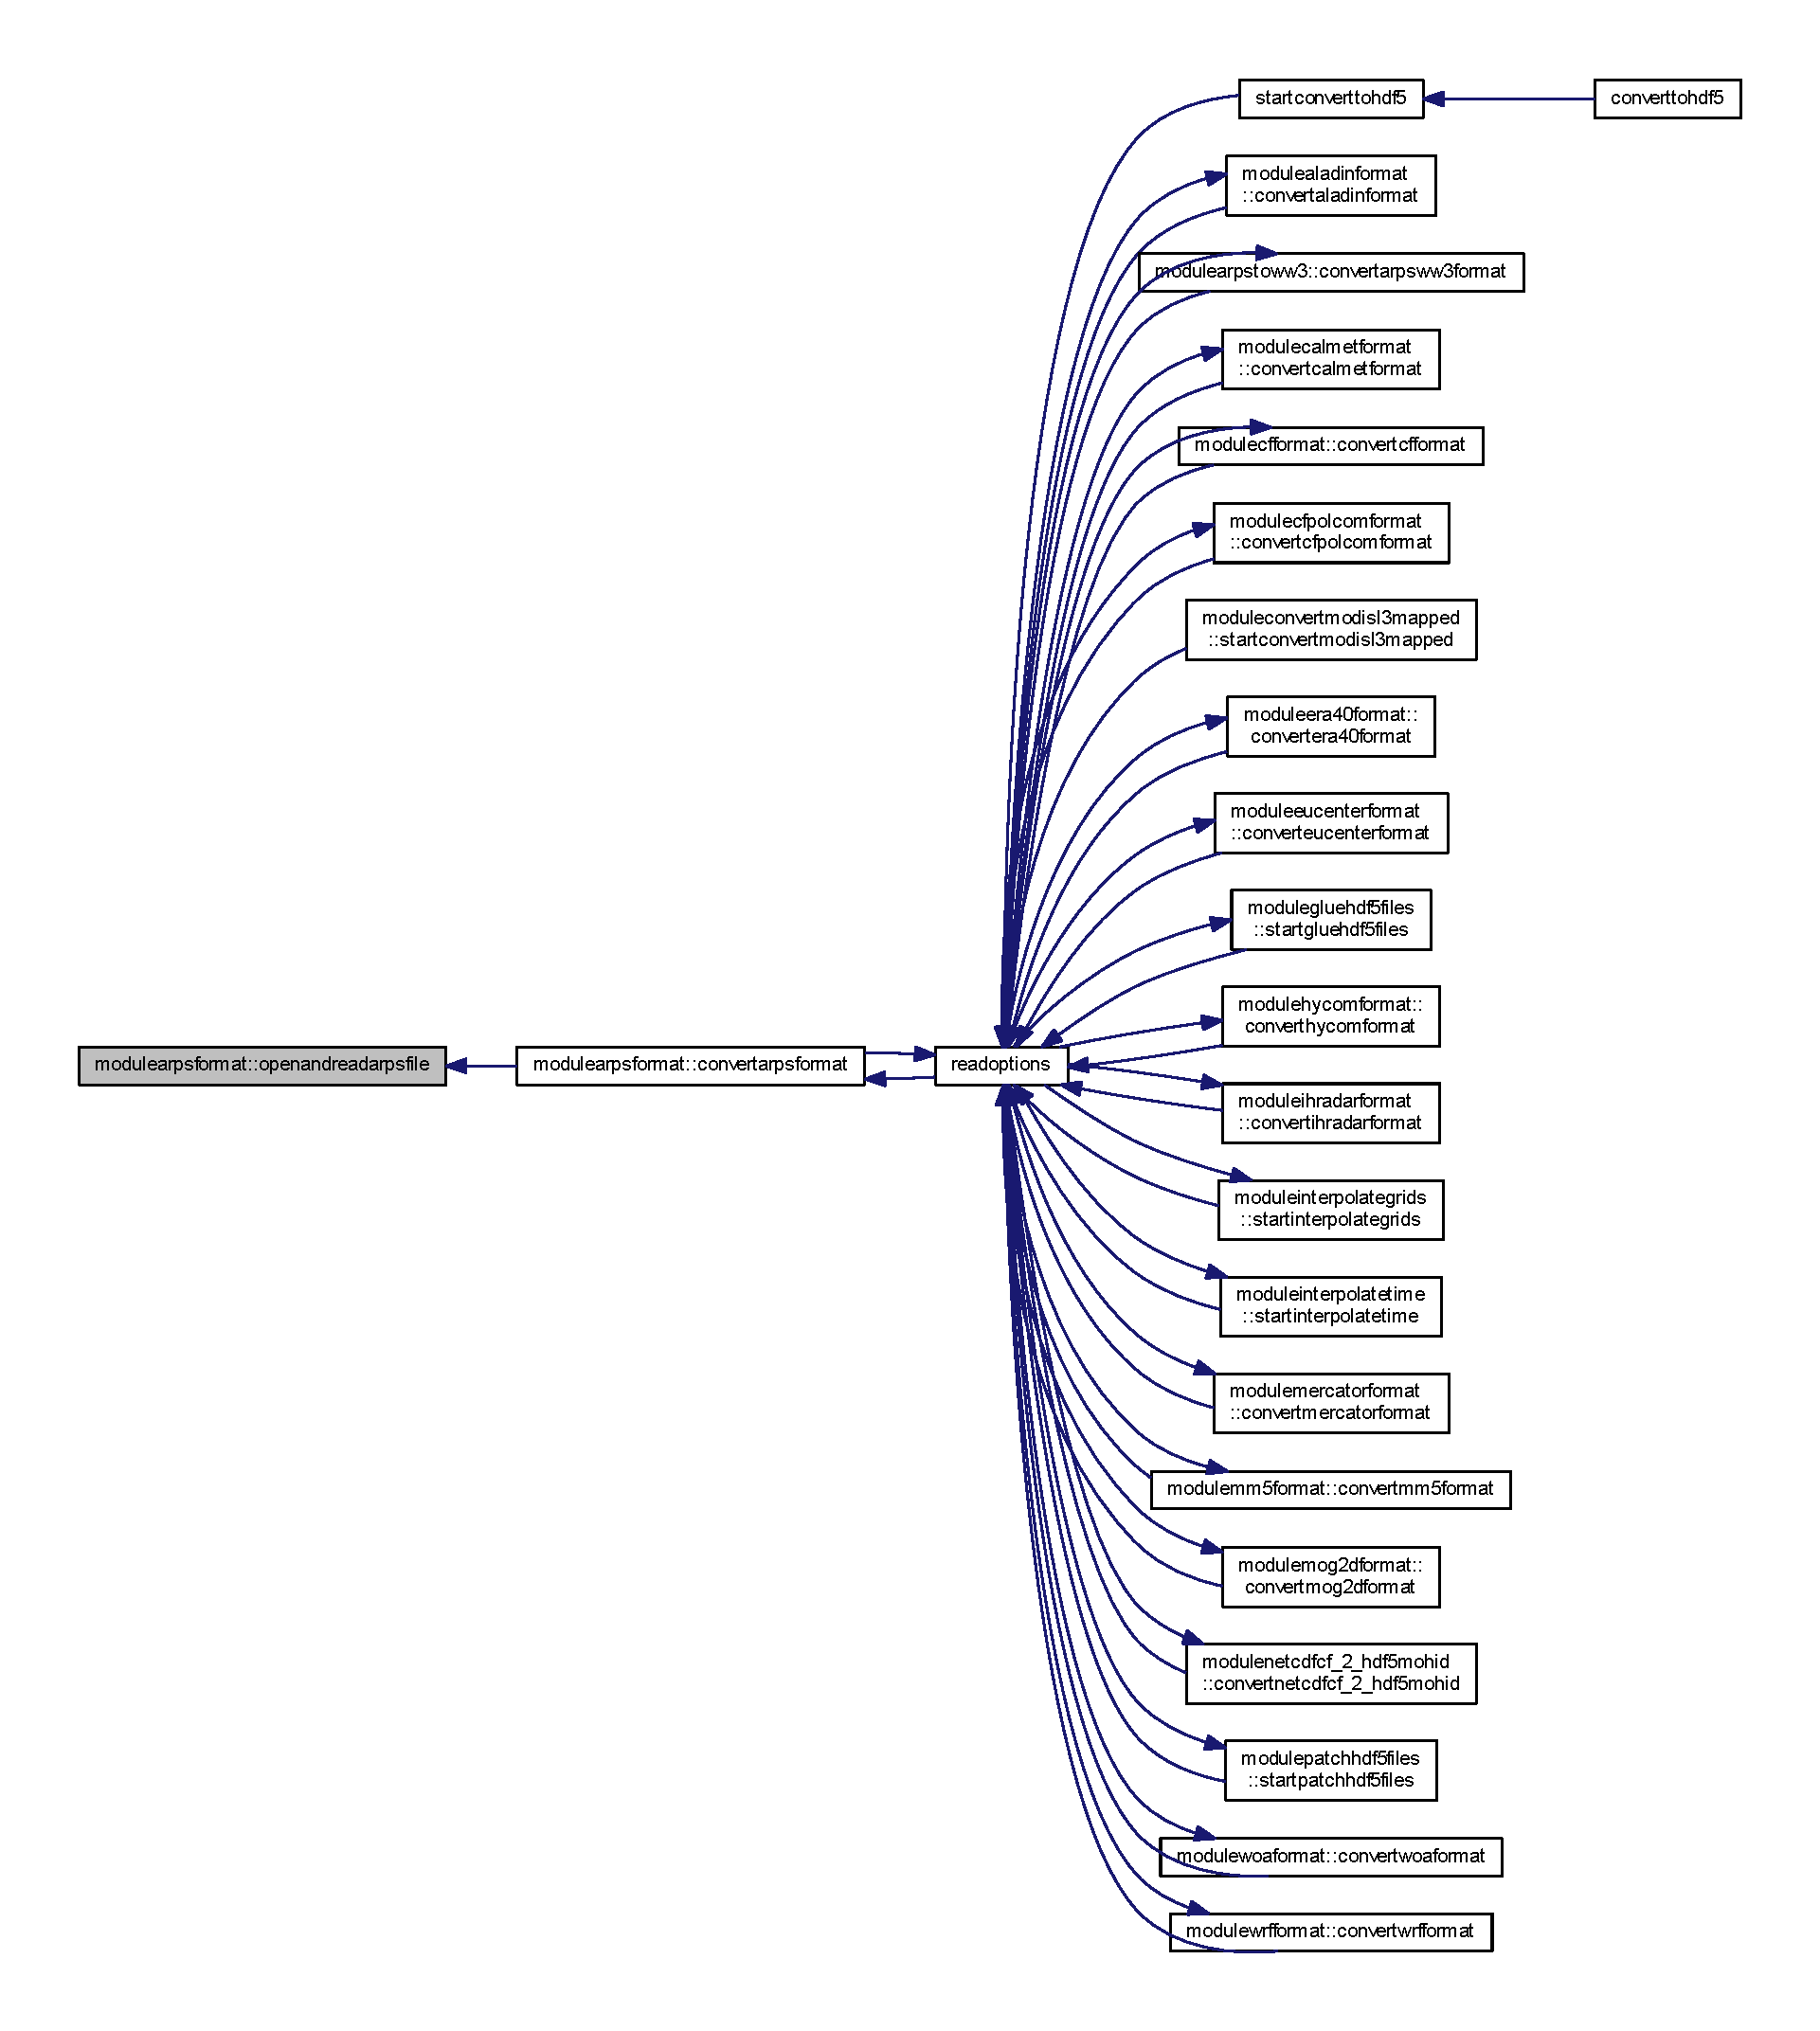
\includegraphics[width=350pt]{namespacemodulearpsformat_a70ee83442772ea85df79da65ec4ea262_icgraph}
\end{center}
\end{figure}
\mbox{\Hypertarget{namespacemodulearpsformat_a3feae8181a739c2898e331dd969e3c67}\label{namespacemodulearpsformat_a3feae8181a739c2898e331dd969e3c67}} 
\index{modulearpsformat@{modulearpsformat}!outputfields@{outputfields}}
\index{outputfields@{outputfields}!modulearpsformat@{modulearpsformat}}
\subsubsection{\texorpdfstring{outputfields()}{outputfields()}}
{\footnotesize\ttfamily subroutine, private modulearpsformat\+::outputfields (\begin{DoxyParamCaption}{ }\end{DoxyParamCaption})\hspace{0.3cm}{\ttfamily [private]}}

Here is the call graph for this function\+:\nopagebreak
\begin{figure}[H]
\begin{center}
\leavevmode
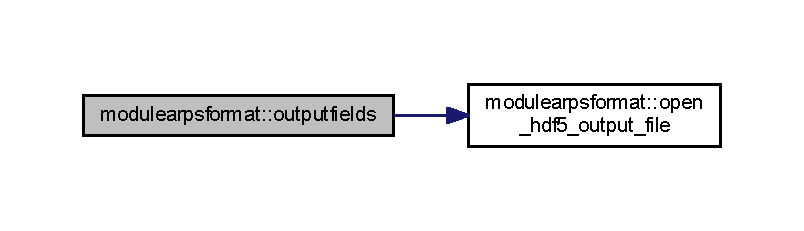
\includegraphics[width=350pt]{namespacemodulearpsformat_a3feae8181a739c2898e331dd969e3c67_cgraph}
\end{center}
\end{figure}
Here is the caller graph for this function\+:\nopagebreak
\begin{figure}[H]
\begin{center}
\leavevmode
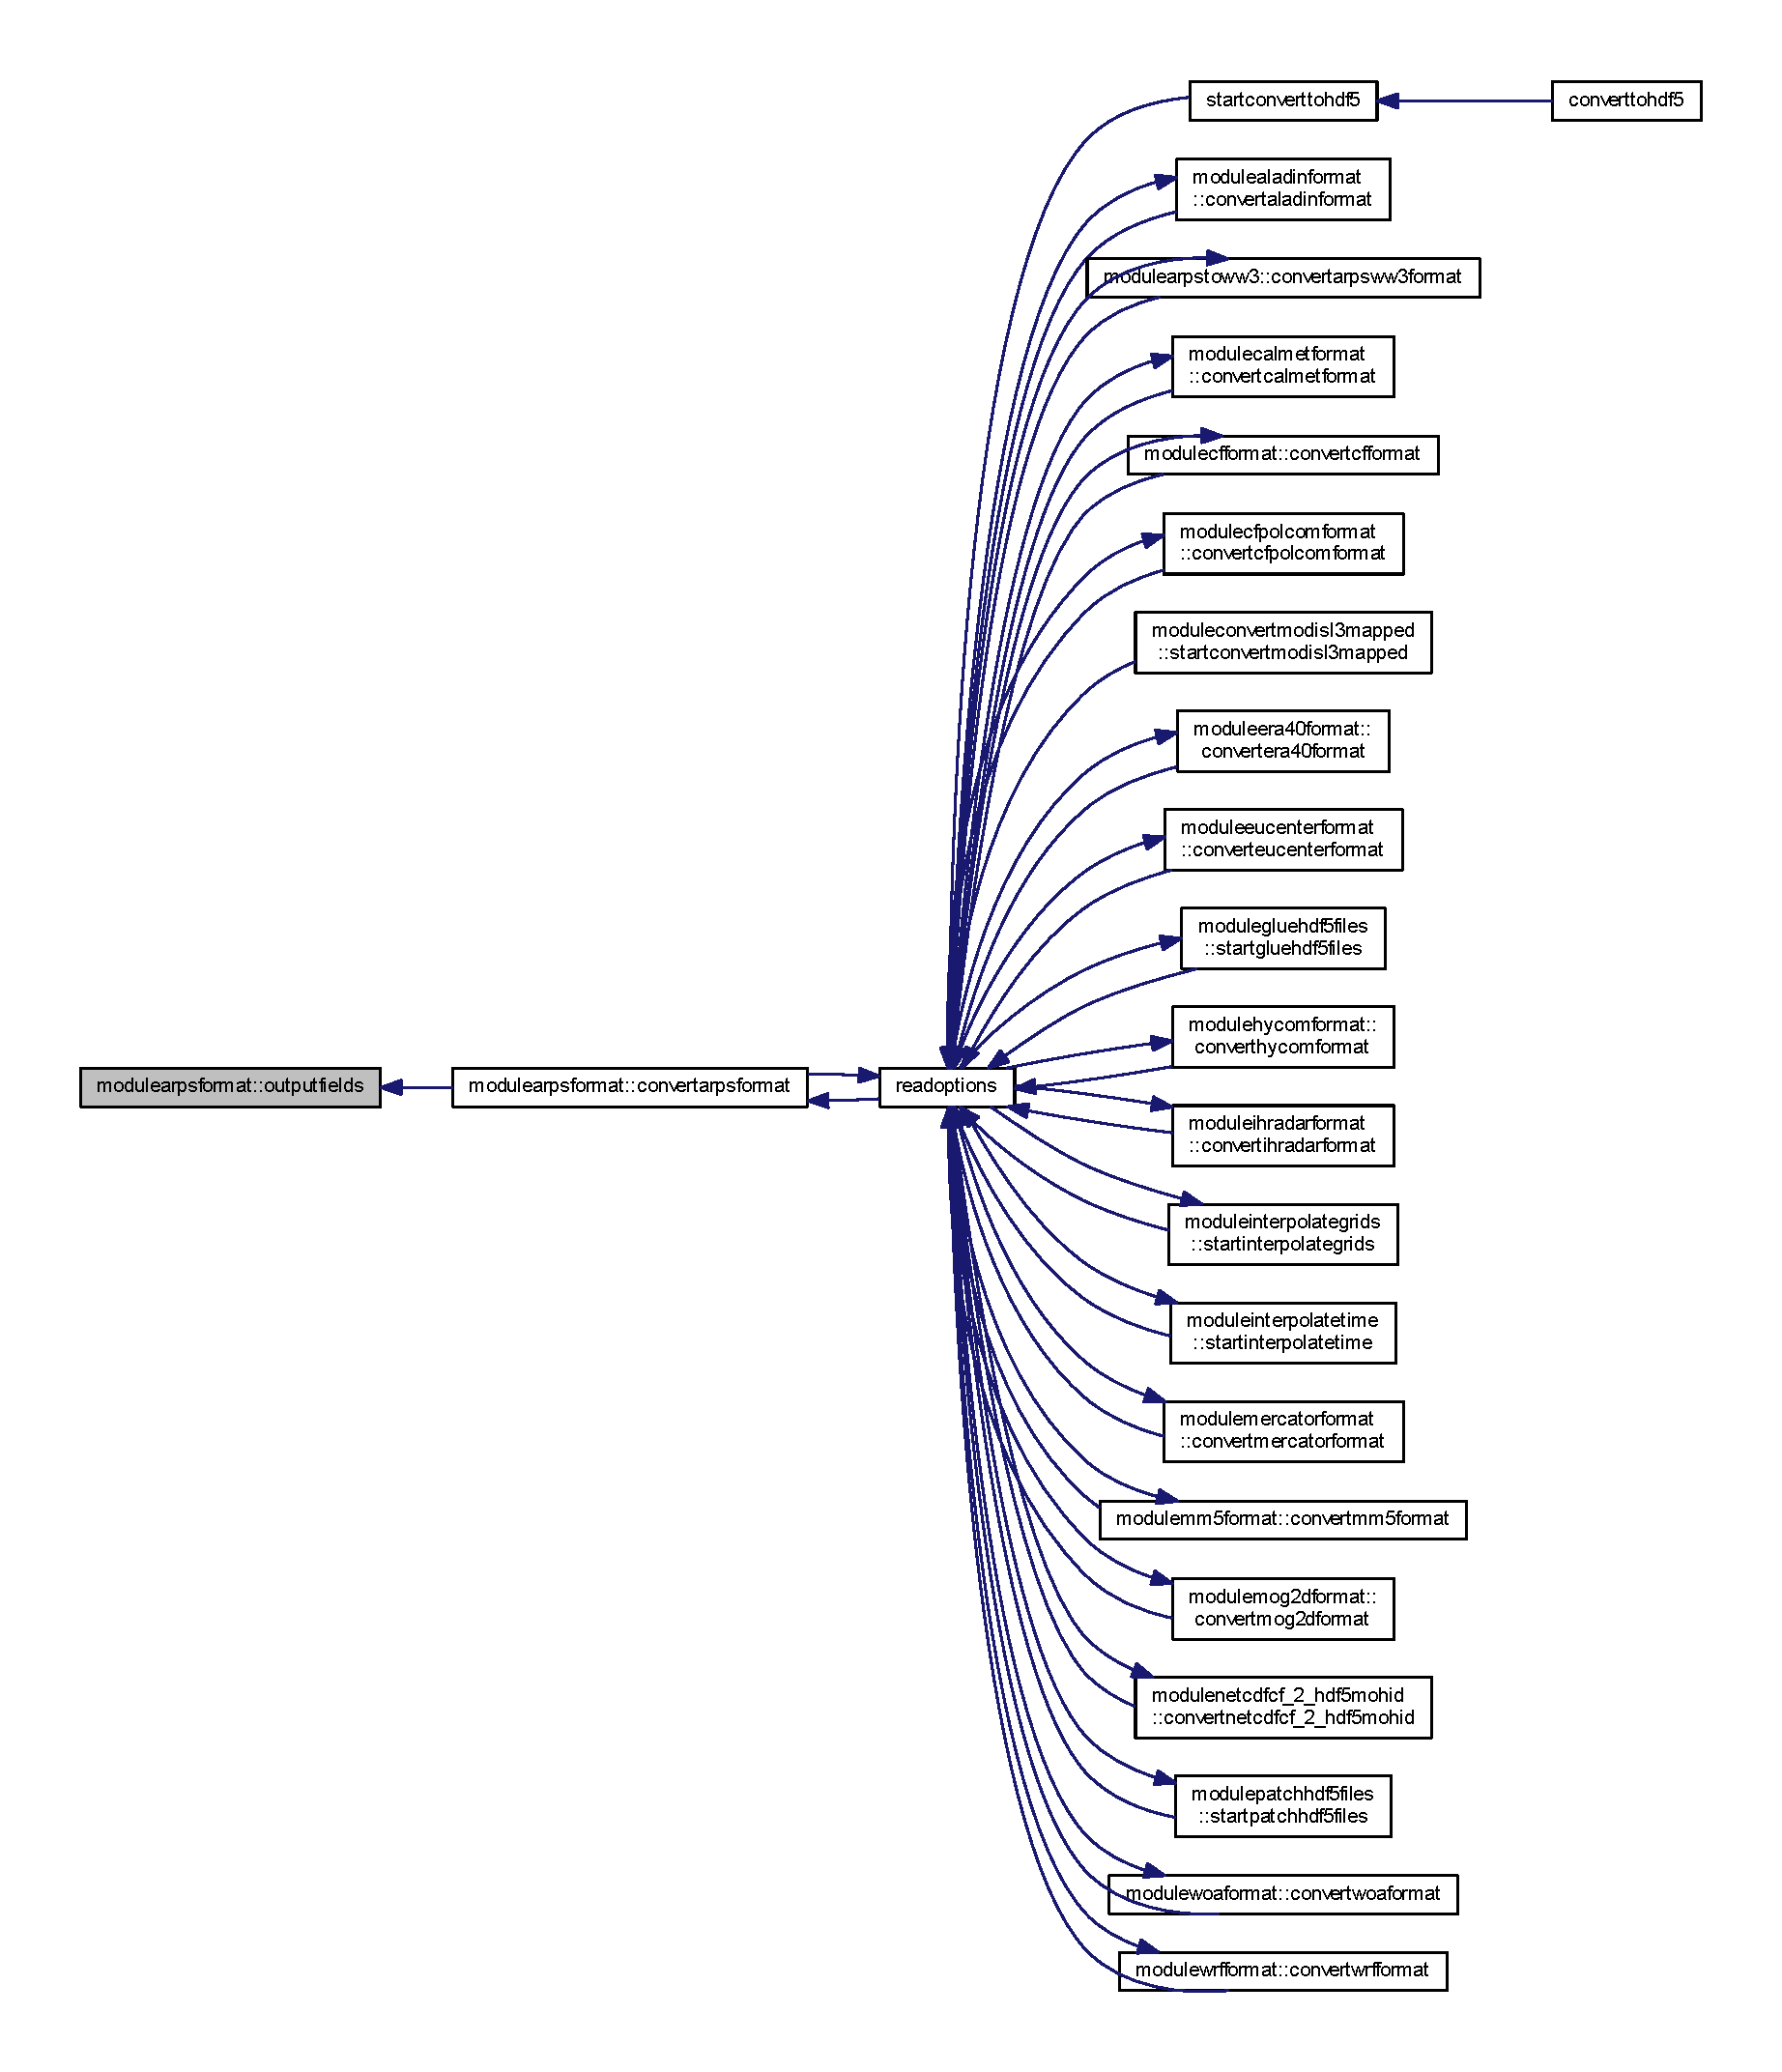
\includegraphics[width=350pt]{namespacemodulearpsformat_a3feae8181a739c2898e331dd969e3c67_icgraph}
\end{center}
\end{figure}
\mbox{\Hypertarget{namespacemodulearpsformat_a51cf1784c51ab9940cffc068600d53ac}\label{namespacemodulearpsformat_a51cf1784c51ab9940cffc068600d53ac}} 
\index{modulearpsformat@{modulearpsformat}!readoptions@{readoptions}}
\index{readoptions@{readoptions}!modulearpsformat@{modulearpsformat}}
\subsubsection{\texorpdfstring{readoptions()}{readoptions()}}
{\footnotesize\ttfamily subroutine, private modulearpsformat\+::readoptions (\begin{DoxyParamCaption}{ }\end{DoxyParamCaption})\hspace{0.3cm}{\ttfamily [private]}}



\subsection{Variable Documentation}
\mbox{\Hypertarget{namespacemodulearpsformat_a481f4077f9a97ca259535ae7940a069d}\label{namespacemodulearpsformat_a481f4077f9a97ca259535ae7940a069d}} 
\index{modulearpsformat@{modulearpsformat}!crossgrid@{crossgrid}}
\index{crossgrid@{crossgrid}!modulearpsformat@{modulearpsformat}}
\subsubsection{\texorpdfstring{crossgrid}{crossgrid}}
{\footnotesize\ttfamily integer, parameter modulearpsformat\+::crossgrid = 2\hspace{0.3cm}{\ttfamily [private]}}

\mbox{\Hypertarget{namespacemodulearpsformat_adad659745a61e1b477c5b8218c0a518b}\label{namespacemodulearpsformat_adad659745a61e1b477c5b8218c0a518b}} 
\index{modulearpsformat@{modulearpsformat}!dotgrid@{dotgrid}}
\index{dotgrid@{dotgrid}!modulearpsformat@{modulearpsformat}}
\subsubsection{\texorpdfstring{dotgrid}{dotgrid}}
{\footnotesize\ttfamily integer, parameter modulearpsformat\+::dotgrid = 1\hspace{0.3cm}{\ttfamily [private]}}

\mbox{\Hypertarget{namespacemodulearpsformat_aa48b8d20bd8a9748703bc70c33e5bce9}\label{namespacemodulearpsformat_aa48b8d20bd8a9748703bc70c33e5bce9}} 
\index{modulearpsformat@{modulearpsformat}!me@{me}}
\index{me@{me}!modulearpsformat@{modulearpsformat}}
\subsubsection{\texorpdfstring{me}{me}}
{\footnotesize\ttfamily type(\mbox{\hyperlink{structmodulearpsformat_1_1t__mm5format}{t\+\_\+mm5format}}), pointer modulearpsformat\+::me\hspace{0.3cm}{\ttfamily [private]}}


\hypertarget{namespacemodulearpstoww3}{}\section{modulearpstoww3 Module Reference}
\label{namespacemodulearpstoww3}\index{modulearpstoww3@{modulearpstoww3}}
\subsection*{Data Types}
\begin{DoxyCompactItemize}
\item 
type \mbox{\hyperlink{structmodulearpstoww3_1_1t__date}{t\+\_\+date}}
\item 
type \mbox{\hyperlink{structmodulearpstoww3_1_1t__field}{t\+\_\+field}}
\item 
type \mbox{\hyperlink{structmodulearpstoww3_1_1t__mm5format}{t\+\_\+mm5format}}
\end{DoxyCompactItemize}
\subsection*{Functions/\+Subroutines}
\begin{DoxyCompactItemize}
\item 
subroutine, public \mbox{\hyperlink{namespacemodulearpstoww3_a42304b111881f48406d8d939918e21ef}{convertarpsww3format}} (Enter\+Data\+ID, S\+T\+AT)
\item 
subroutine, private \mbox{\hyperlink{namespacemodulearpstoww3_a7642538ceff4533a4ad2aeba84fb2d32}{readoptions}}
\item 
subroutine, private \mbox{\hyperlink{namespacemodulearpstoww3_aa5a12099f3353b33d3b40f8f3f4384f0}{openandreadarpsfile}}
\item 
subroutine \mbox{\hyperlink{namespacemodulearpstoww3_a509b1aea6540dc5784cfe7424f0e6414}{constructgrid}}
\item 
subroutine, private \mbox{\hyperlink{namespacemodulearpstoww3_a0277d24244051759af2fcc3106ef5a08}{addfield}} (First\+Field, Obj\+Field)
\item 
subroutine, private \mbox{\hyperlink{namespacemodulearpstoww3_a81436aea40d31bddb32f553e227a991d}{adddate}} (First\+Date, Obj\+Date)
\item 
subroutine, private \mbox{\hyperlink{namespacemodulearpstoww3_a7c18511d187912f655458191bcf1c7af}{outputfields}}
\item 
subroutine, private \mbox{\hyperlink{namespacemodulearpstoww3_a7a7eb9b823582e046e2127ea46d3f300}{open\+\_\+hdf5\+\_\+output\+\_\+file}}
\item 
subroutine, private \mbox{\hyperlink{namespacemodulearpstoww3_a2b22a4f72b20cf6f219d61b511afcad1}{killarpsformat}}
\end{DoxyCompactItemize}
\subsection*{Variables}
\begin{DoxyCompactItemize}
\item 
type(\mbox{\hyperlink{structmodulearpstoww3_1_1t__mm5format}{t\+\_\+mm5format}}), pointer \mbox{\hyperlink{namespacemodulearpstoww3_ae048aea87bb0343812cdb60ee1a1f6b8}{me}}
\end{DoxyCompactItemize}


\subsection{Function/\+Subroutine Documentation}
\mbox{\Hypertarget{namespacemodulearpstoww3_a81436aea40d31bddb32f553e227a991d}\label{namespacemodulearpstoww3_a81436aea40d31bddb32f553e227a991d}} 
\index{modulearpstoww3@{modulearpstoww3}!adddate@{adddate}}
\index{adddate@{adddate}!modulearpstoww3@{modulearpstoww3}}
\subsubsection{\texorpdfstring{adddate()}{adddate()}}
{\footnotesize\ttfamily subroutine, private modulearpstoww3\+::adddate (\begin{DoxyParamCaption}\item[{type (\mbox{\hyperlink{structmodulearpstoww3_1_1t__date}{t\+\_\+date}}), pointer}]{First\+Date,  }\item[{type (\mbox{\hyperlink{structmodulearpstoww3_1_1t__date}{t\+\_\+date}}), pointer}]{Obj\+Date }\end{DoxyParamCaption})\hspace{0.3cm}{\ttfamily [private]}}

Here is the caller graph for this function\+:\nopagebreak
\begin{figure}[H]
\begin{center}
\leavevmode
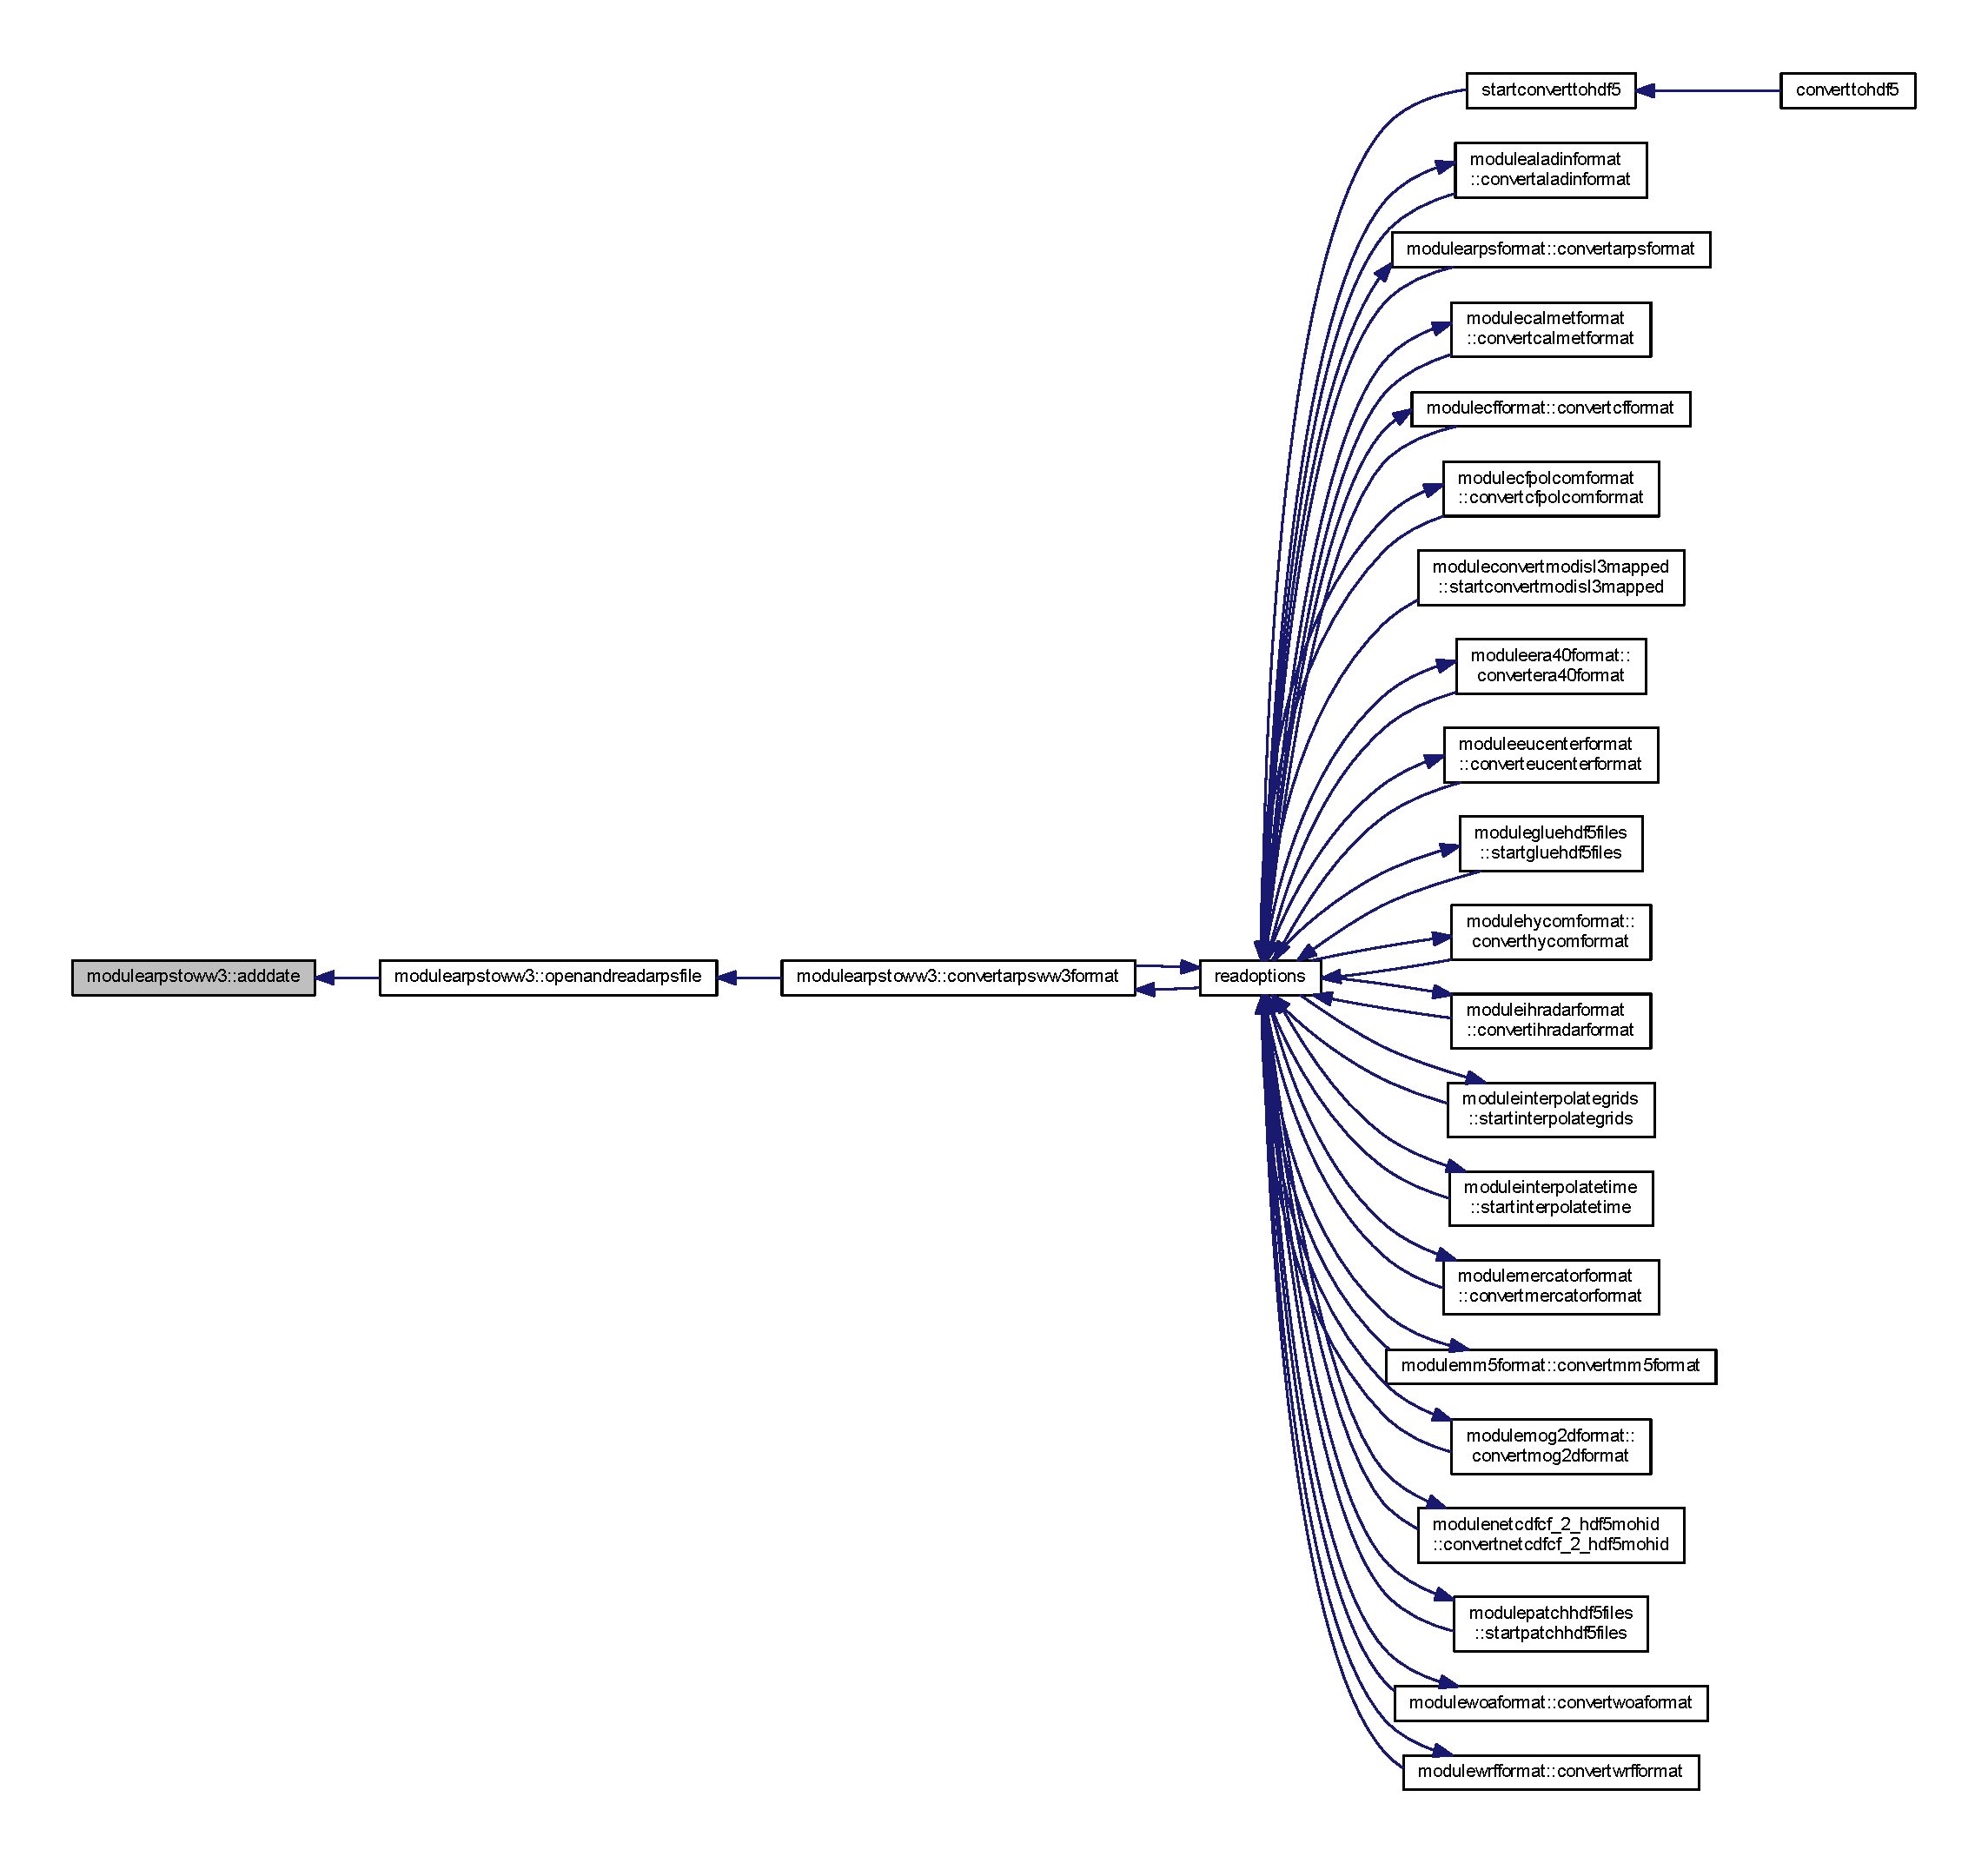
\includegraphics[width=350pt]{namespacemodulearpstoww3_a81436aea40d31bddb32f553e227a991d_icgraph}
\end{center}
\end{figure}
\mbox{\Hypertarget{namespacemodulearpstoww3_a0277d24244051759af2fcc3106ef5a08}\label{namespacemodulearpstoww3_a0277d24244051759af2fcc3106ef5a08}} 
\index{modulearpstoww3@{modulearpstoww3}!addfield@{addfield}}
\index{addfield@{addfield}!modulearpstoww3@{modulearpstoww3}}
\subsubsection{\texorpdfstring{addfield()}{addfield()}}
{\footnotesize\ttfamily subroutine, private modulearpstoww3\+::addfield (\begin{DoxyParamCaption}\item[{type (\mbox{\hyperlink{structmodulearpstoww3_1_1t__field}{t\+\_\+field}}), pointer}]{First\+Field,  }\item[{type (\mbox{\hyperlink{structmodulearpstoww3_1_1t__field}{t\+\_\+field}}), pointer}]{Obj\+Field }\end{DoxyParamCaption})\hspace{0.3cm}{\ttfamily [private]}}

Here is the caller graph for this function\+:\nopagebreak
\begin{figure}[H]
\begin{center}
\leavevmode
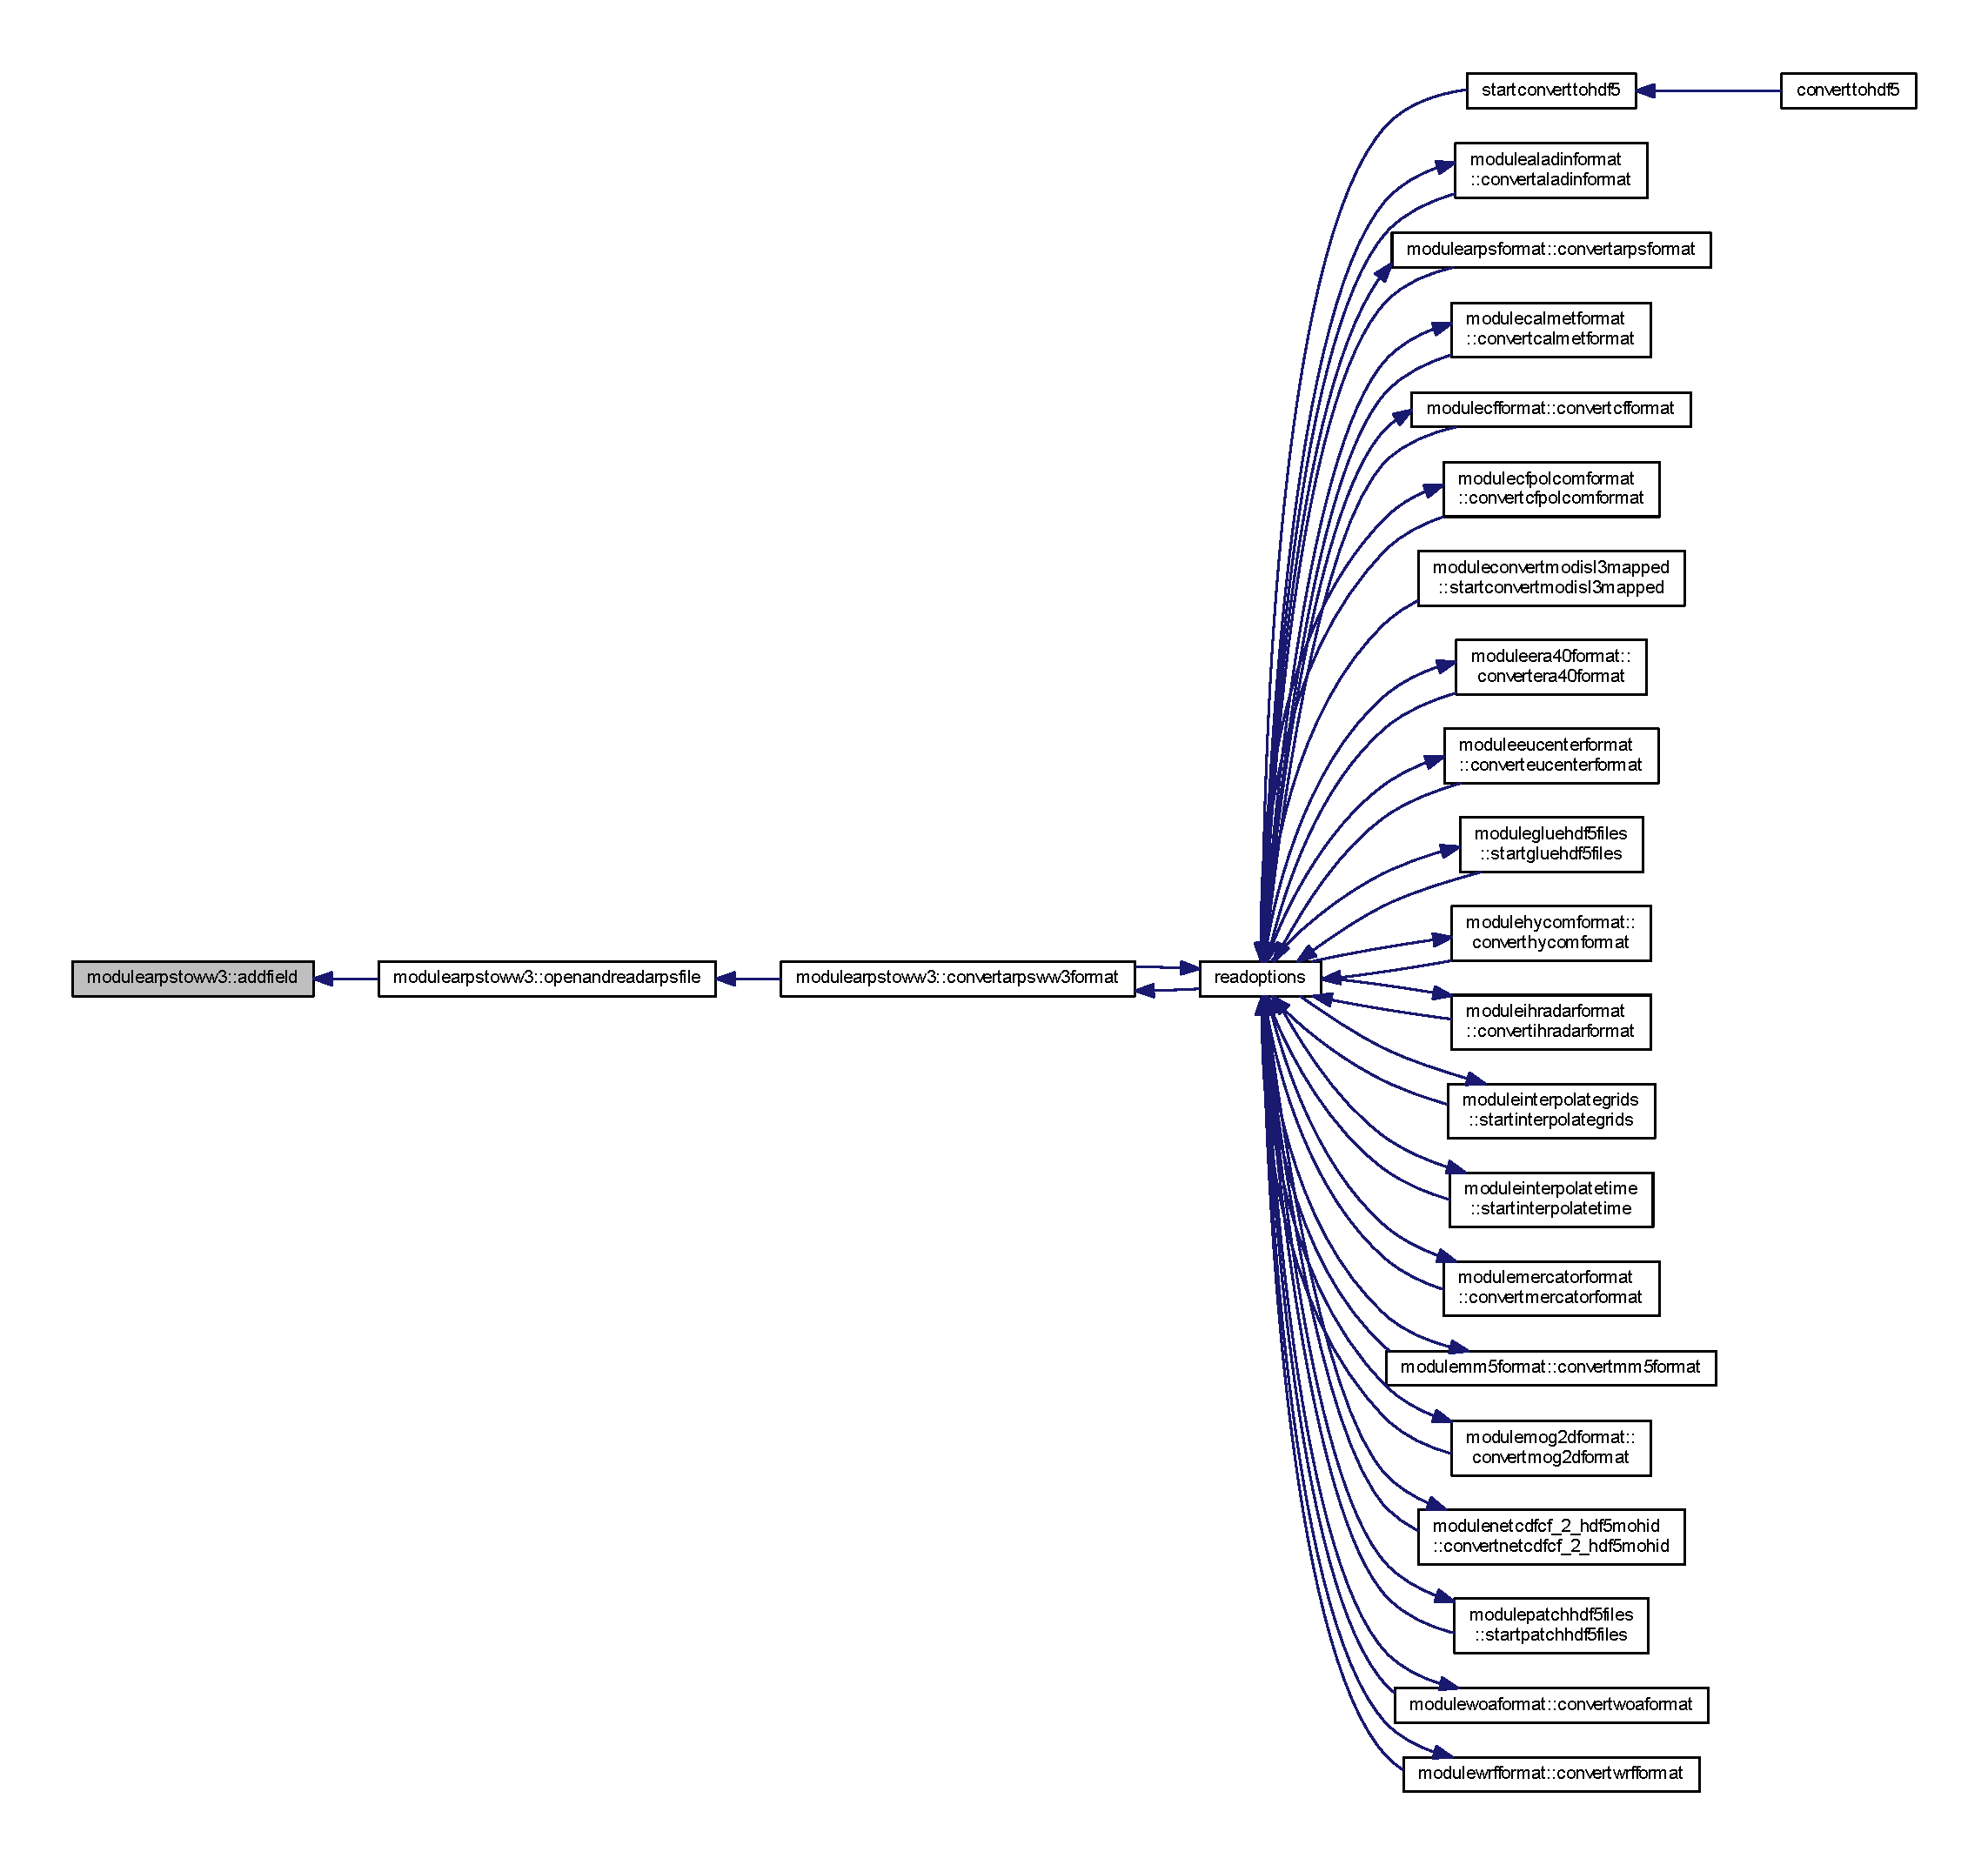
\includegraphics[width=350pt]{namespacemodulearpstoww3_a0277d24244051759af2fcc3106ef5a08_icgraph}
\end{center}
\end{figure}
\mbox{\Hypertarget{namespacemodulearpstoww3_a509b1aea6540dc5784cfe7424f0e6414}\label{namespacemodulearpstoww3_a509b1aea6540dc5784cfe7424f0e6414}} 
\index{modulearpstoww3@{modulearpstoww3}!constructgrid@{constructgrid}}
\index{constructgrid@{constructgrid}!modulearpstoww3@{modulearpstoww3}}
\subsubsection{\texorpdfstring{constructgrid()}{constructgrid()}}
{\footnotesize\ttfamily subroutine modulearpstoww3\+::constructgrid (\begin{DoxyParamCaption}{ }\end{DoxyParamCaption})\hspace{0.3cm}{\ttfamily [private]}}

Here is the caller graph for this function\+:\nopagebreak
\begin{figure}[H]
\begin{center}
\leavevmode
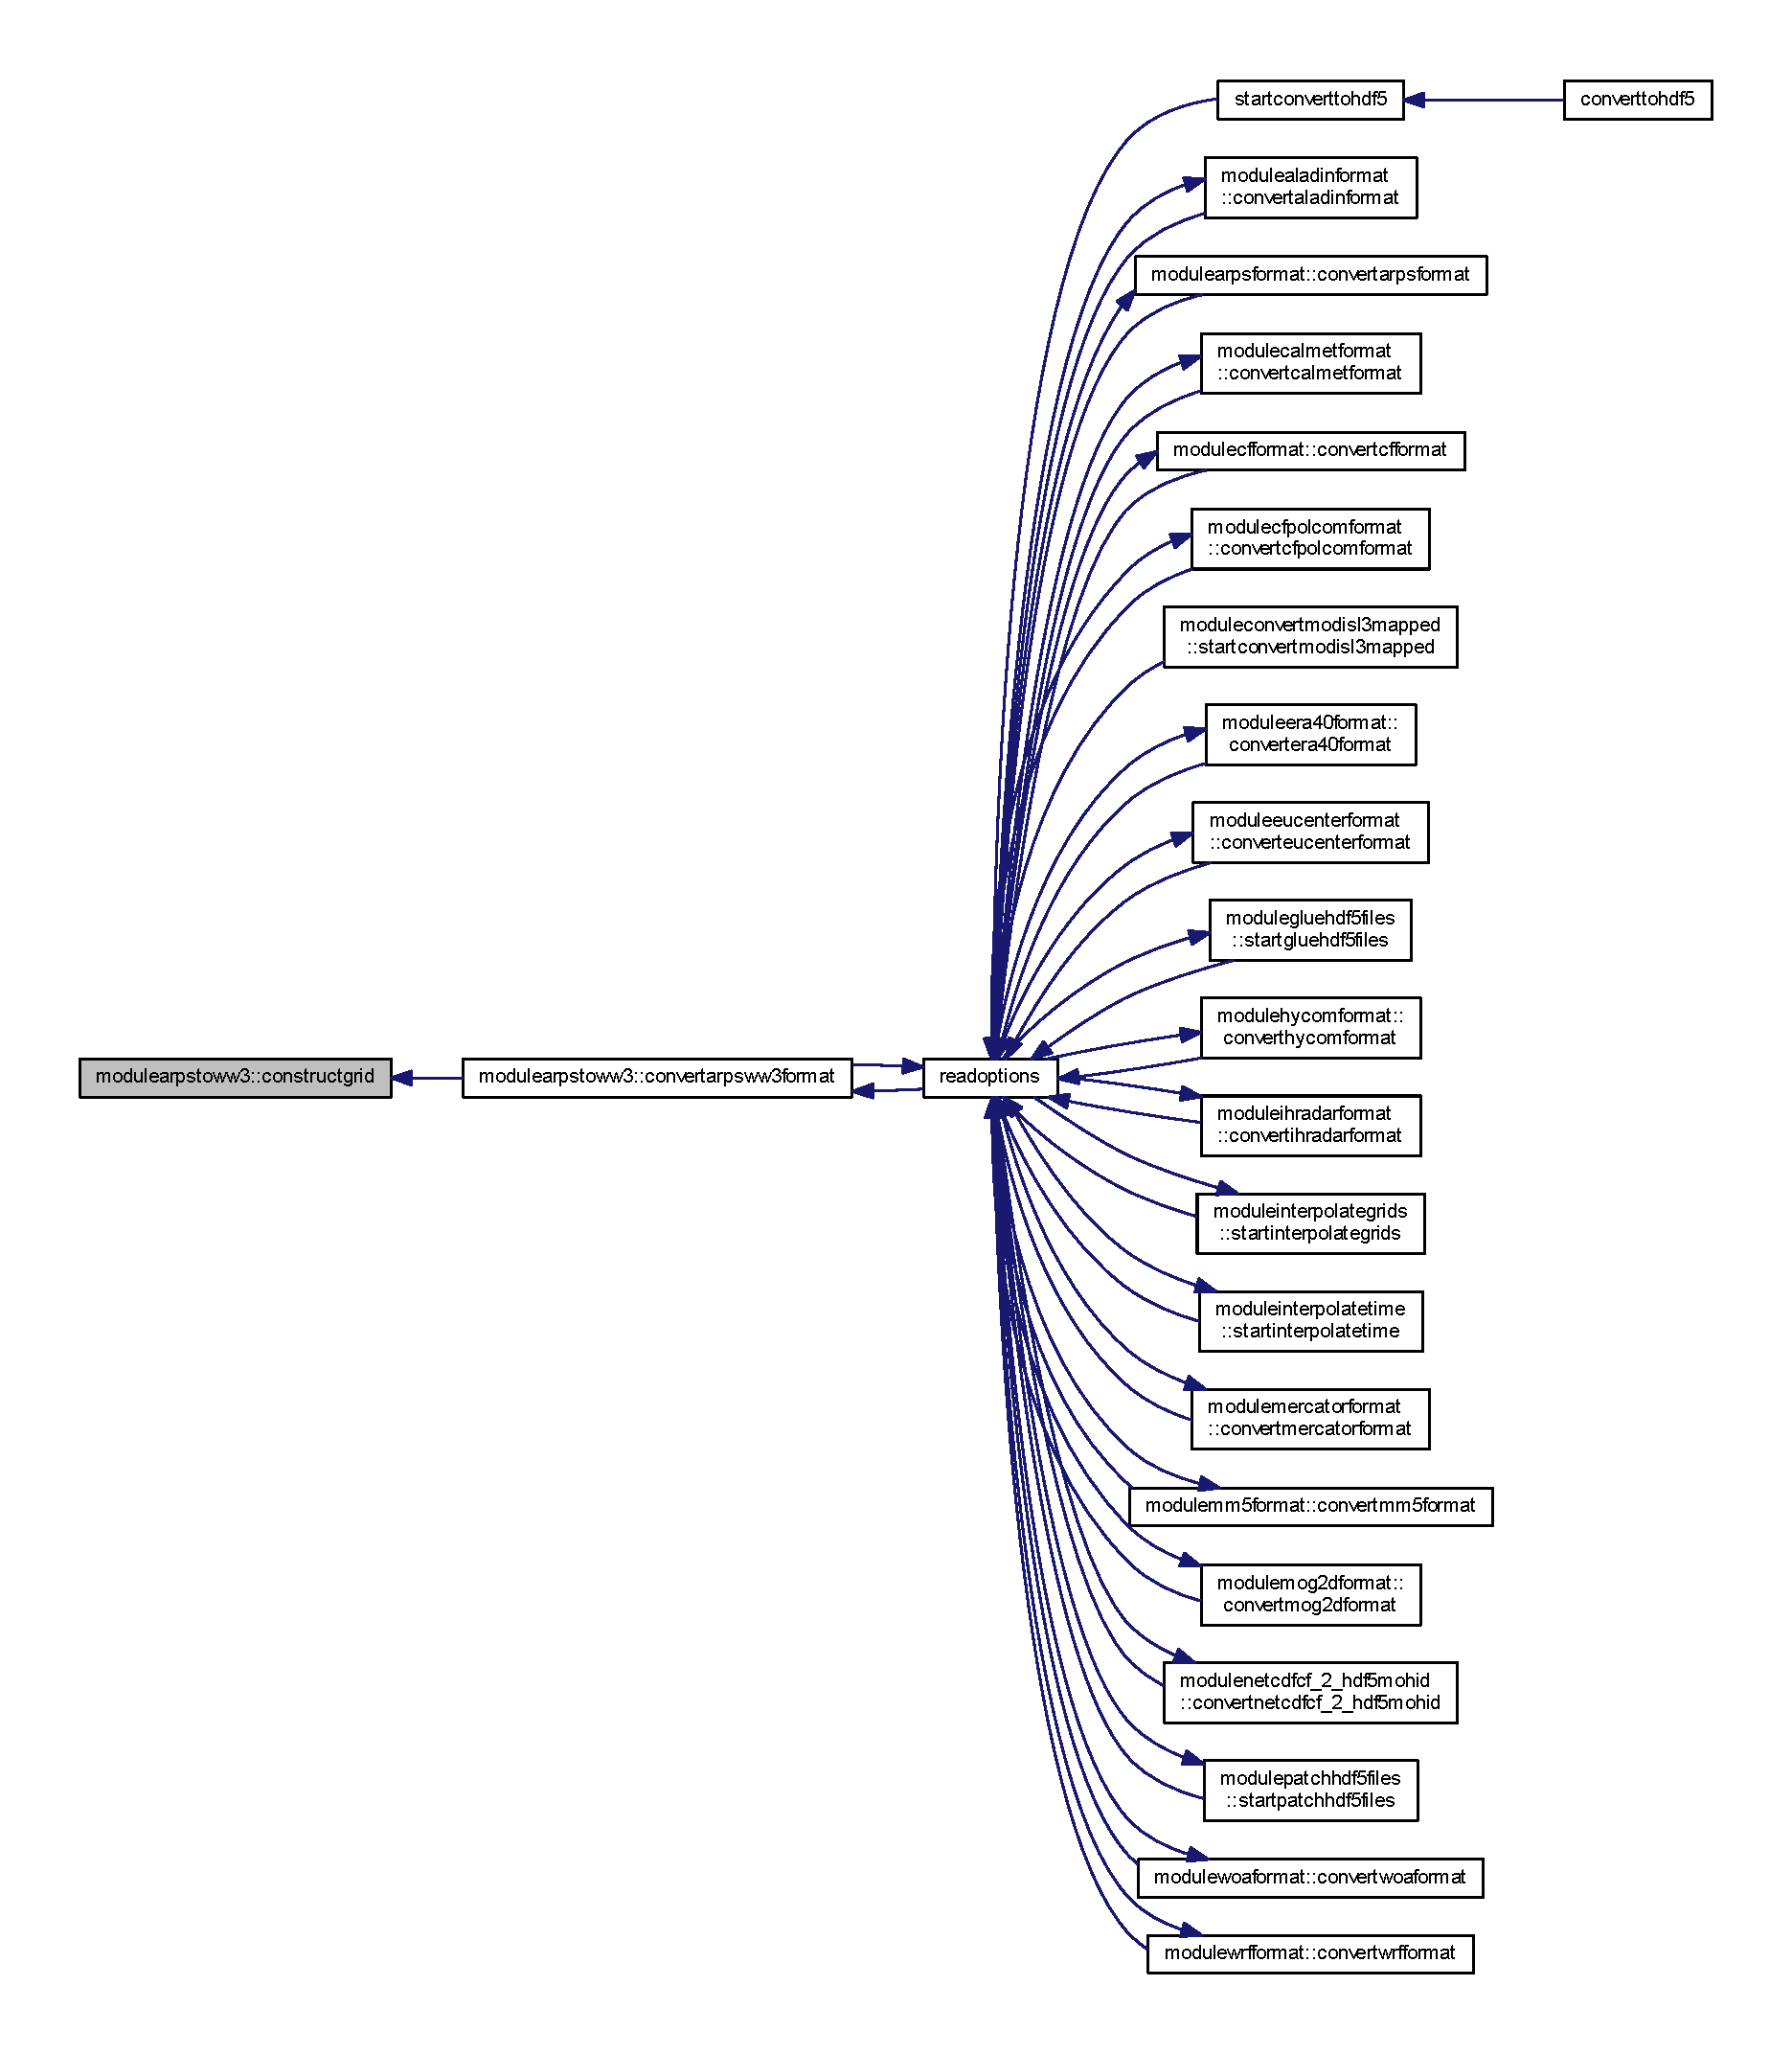
\includegraphics[width=350pt]{namespacemodulearpstoww3_a509b1aea6540dc5784cfe7424f0e6414_icgraph}
\end{center}
\end{figure}
\mbox{\Hypertarget{namespacemodulearpstoww3_a42304b111881f48406d8d939918e21ef}\label{namespacemodulearpstoww3_a42304b111881f48406d8d939918e21ef}} 
\index{modulearpstoww3@{modulearpstoww3}!convertarpsww3format@{convertarpsww3format}}
\index{convertarpsww3format@{convertarpsww3format}!modulearpstoww3@{modulearpstoww3}}
\subsubsection{\texorpdfstring{convertarpsww3format()}{convertarpsww3format()}}
{\footnotesize\ttfamily subroutine, public modulearpstoww3\+::convertarpsww3format (\begin{DoxyParamCaption}\item[{integer, intent(in)}]{Enter\+Data\+ID,  }\item[{integer, intent(out), optional}]{S\+T\+AT }\end{DoxyParamCaption})}

Here is the call graph for this function\+:\nopagebreak
\begin{figure}[H]
\begin{center}
\leavevmode
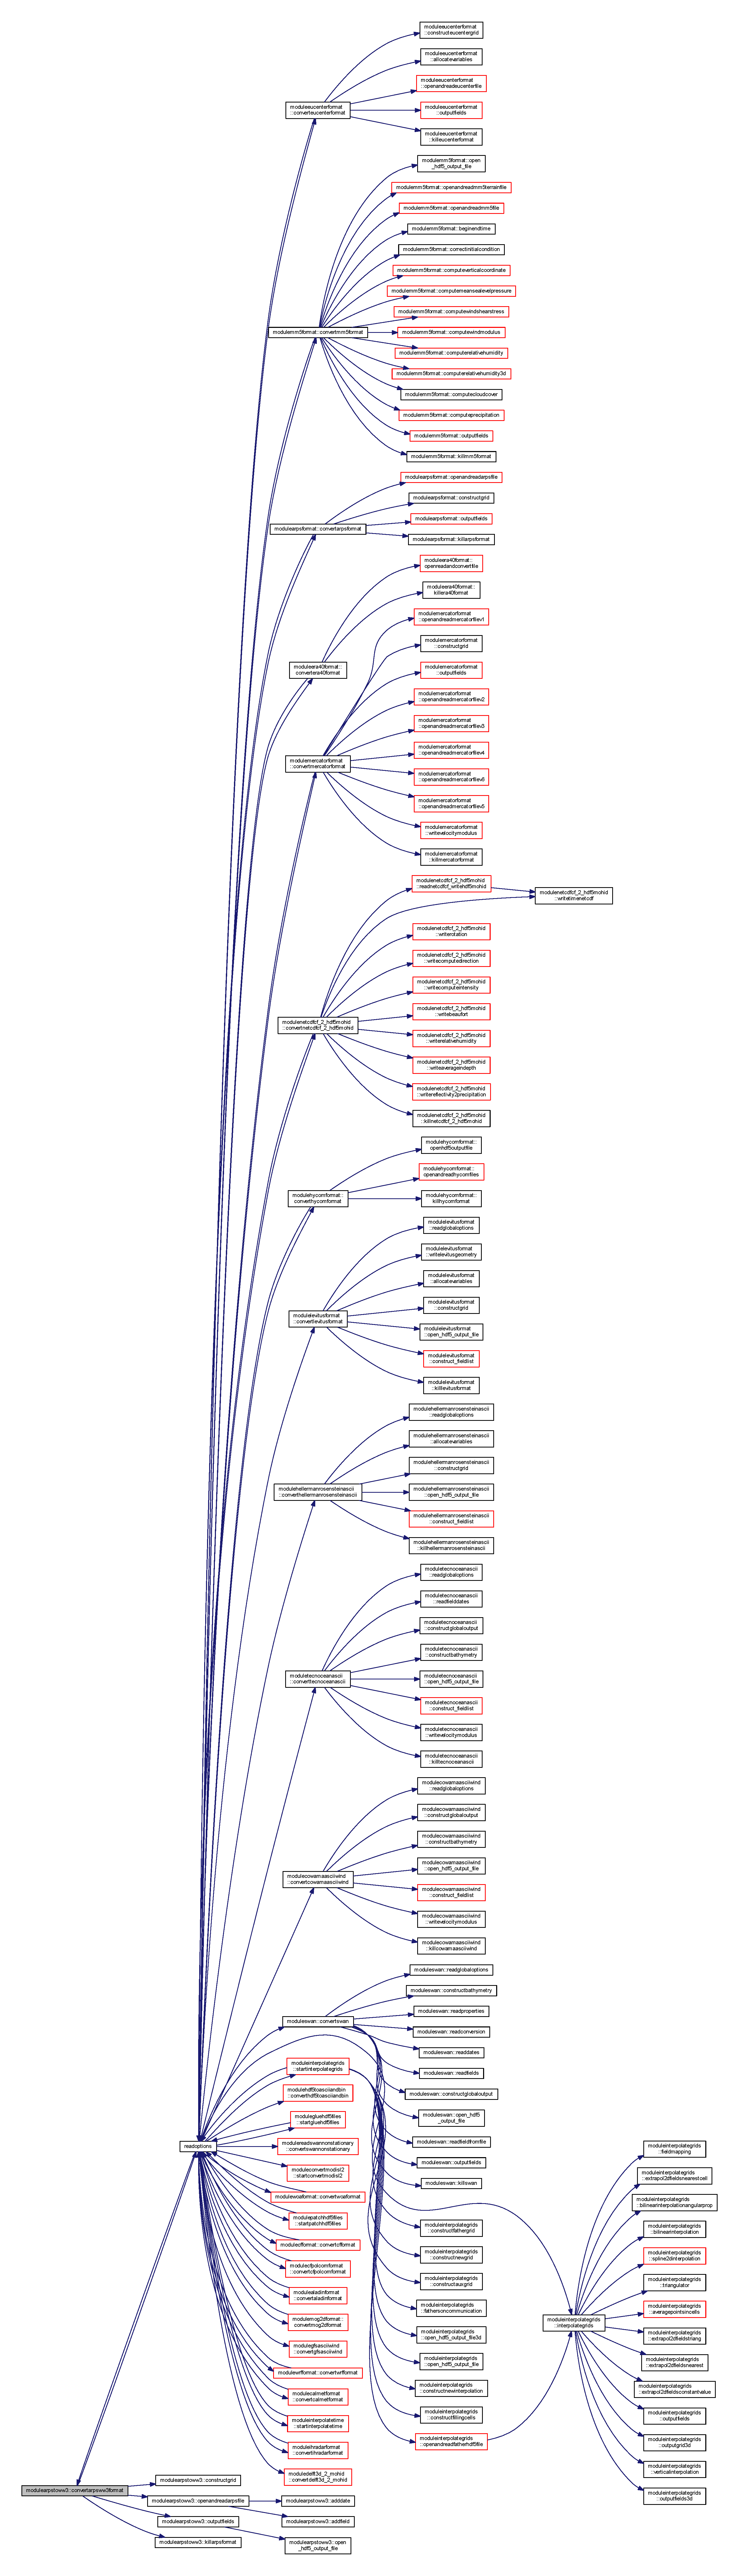
\includegraphics[height=550pt]{namespacemodulearpstoww3_a42304b111881f48406d8d939918e21ef_cgraph}
\end{center}
\end{figure}
Here is the caller graph for this function\+:\nopagebreak
\begin{figure}[H]
\begin{center}
\leavevmode
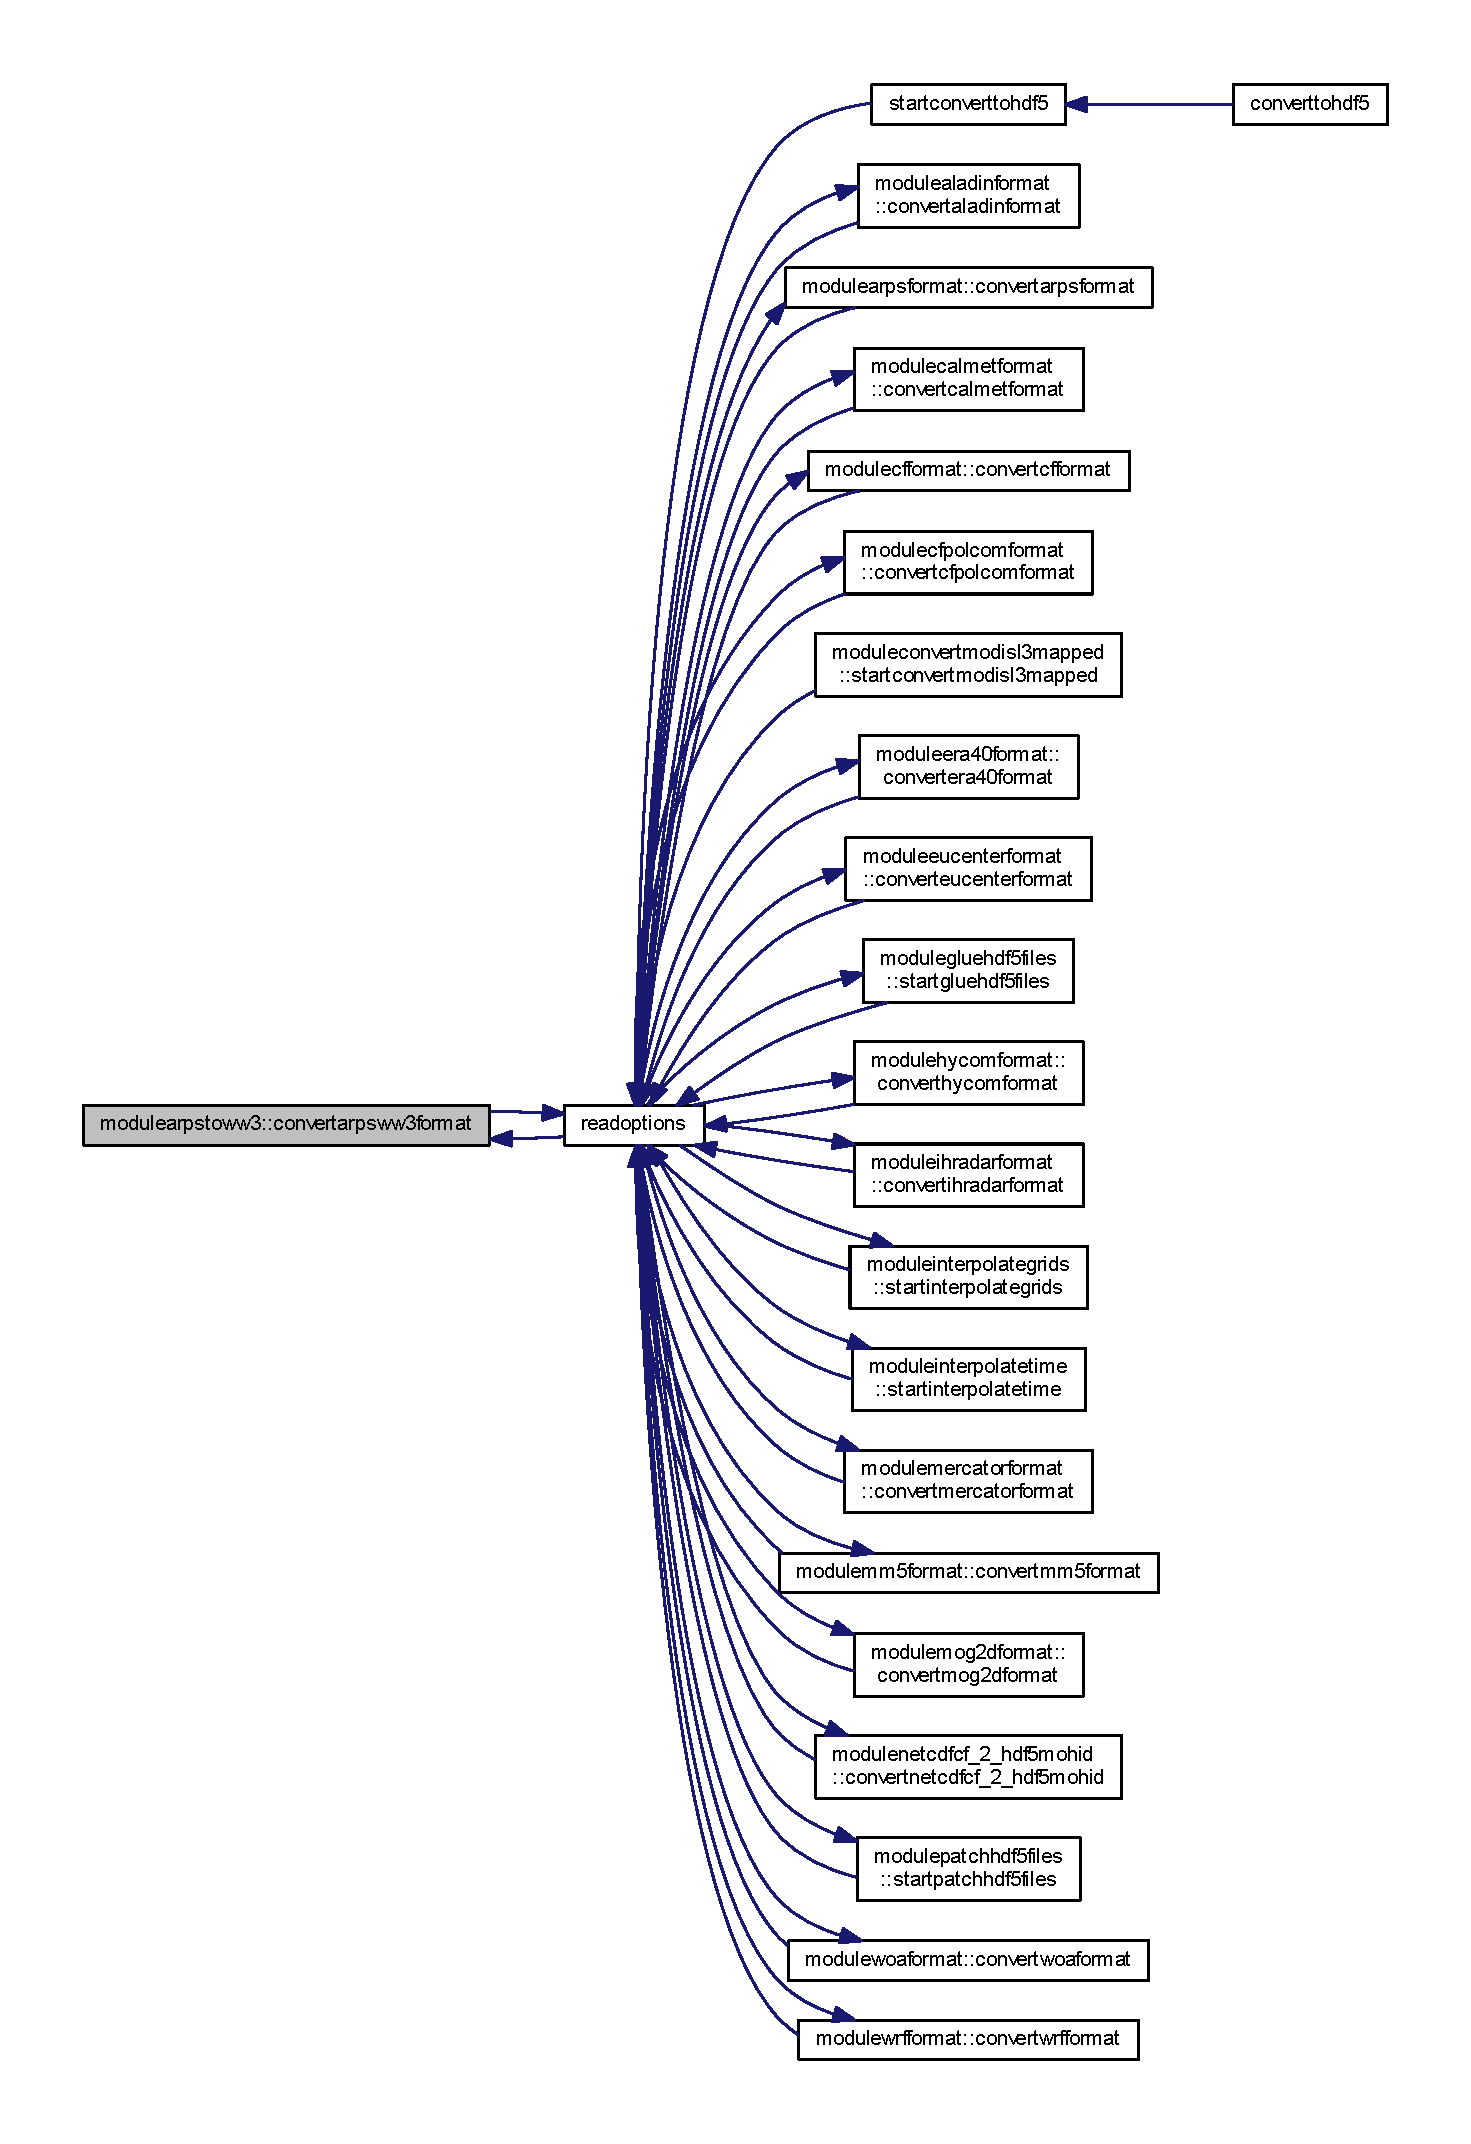
\includegraphics[width=350pt]{namespacemodulearpstoww3_a42304b111881f48406d8d939918e21ef_icgraph}
\end{center}
\end{figure}
\mbox{\Hypertarget{namespacemodulearpstoww3_a2b22a4f72b20cf6f219d61b511afcad1}\label{namespacemodulearpstoww3_a2b22a4f72b20cf6f219d61b511afcad1}} 
\index{modulearpstoww3@{modulearpstoww3}!killarpsformat@{killarpsformat}}
\index{killarpsformat@{killarpsformat}!modulearpstoww3@{modulearpstoww3}}
\subsubsection{\texorpdfstring{killarpsformat()}{killarpsformat()}}
{\footnotesize\ttfamily subroutine, private modulearpstoww3\+::killarpsformat (\begin{DoxyParamCaption}{ }\end{DoxyParamCaption})\hspace{0.3cm}{\ttfamily [private]}}

Here is the caller graph for this function\+:\nopagebreak
\begin{figure}[H]
\begin{center}
\leavevmode
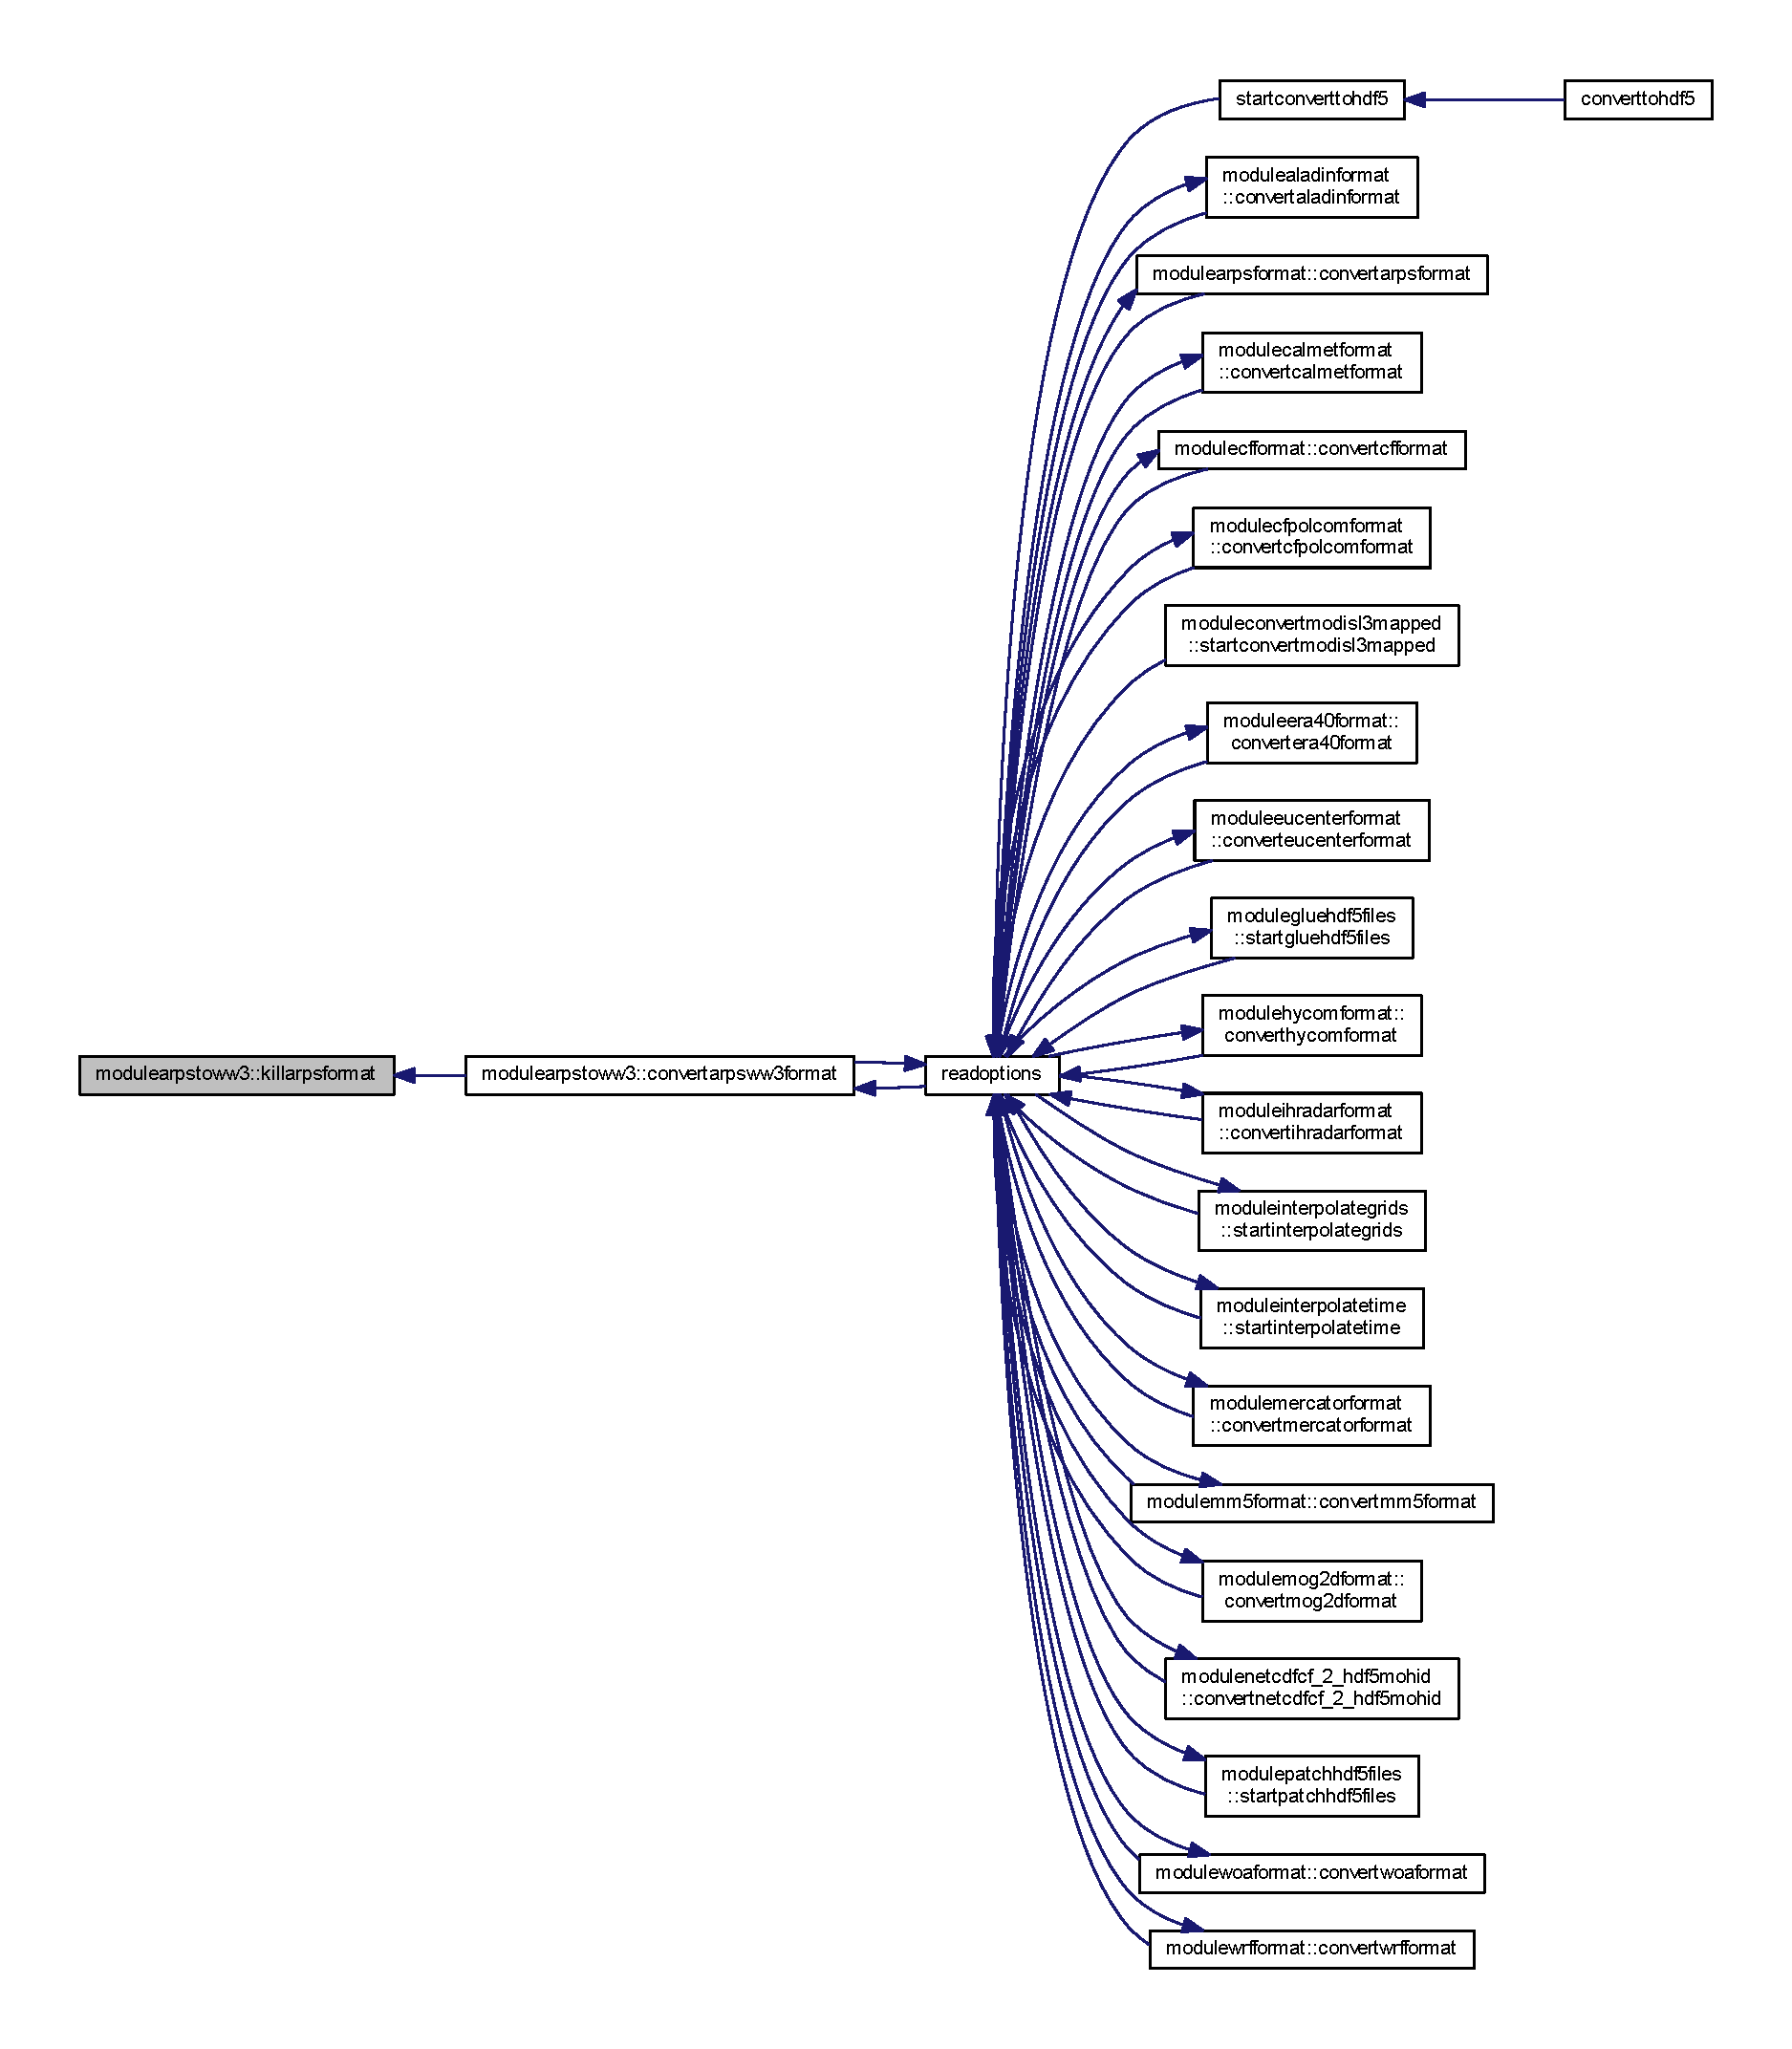
\includegraphics[width=350pt]{namespacemodulearpstoww3_a2b22a4f72b20cf6f219d61b511afcad1_icgraph}
\end{center}
\end{figure}
\mbox{\Hypertarget{namespacemodulearpstoww3_a7a7eb9b823582e046e2127ea46d3f300}\label{namespacemodulearpstoww3_a7a7eb9b823582e046e2127ea46d3f300}} 
\index{modulearpstoww3@{modulearpstoww3}!open\+\_\+hdf5\+\_\+output\+\_\+file@{open\+\_\+hdf5\+\_\+output\+\_\+file}}
\index{open\+\_\+hdf5\+\_\+output\+\_\+file@{open\+\_\+hdf5\+\_\+output\+\_\+file}!modulearpstoww3@{modulearpstoww3}}
\subsubsection{\texorpdfstring{open\+\_\+hdf5\+\_\+output\+\_\+file()}{open\_hdf5\_output\_file()}}
{\footnotesize\ttfamily subroutine, private modulearpstoww3\+::open\+\_\+hdf5\+\_\+output\+\_\+file (\begin{DoxyParamCaption}{ }\end{DoxyParamCaption})\hspace{0.3cm}{\ttfamily [private]}}

Here is the caller graph for this function\+:\nopagebreak
\begin{figure}[H]
\begin{center}
\leavevmode
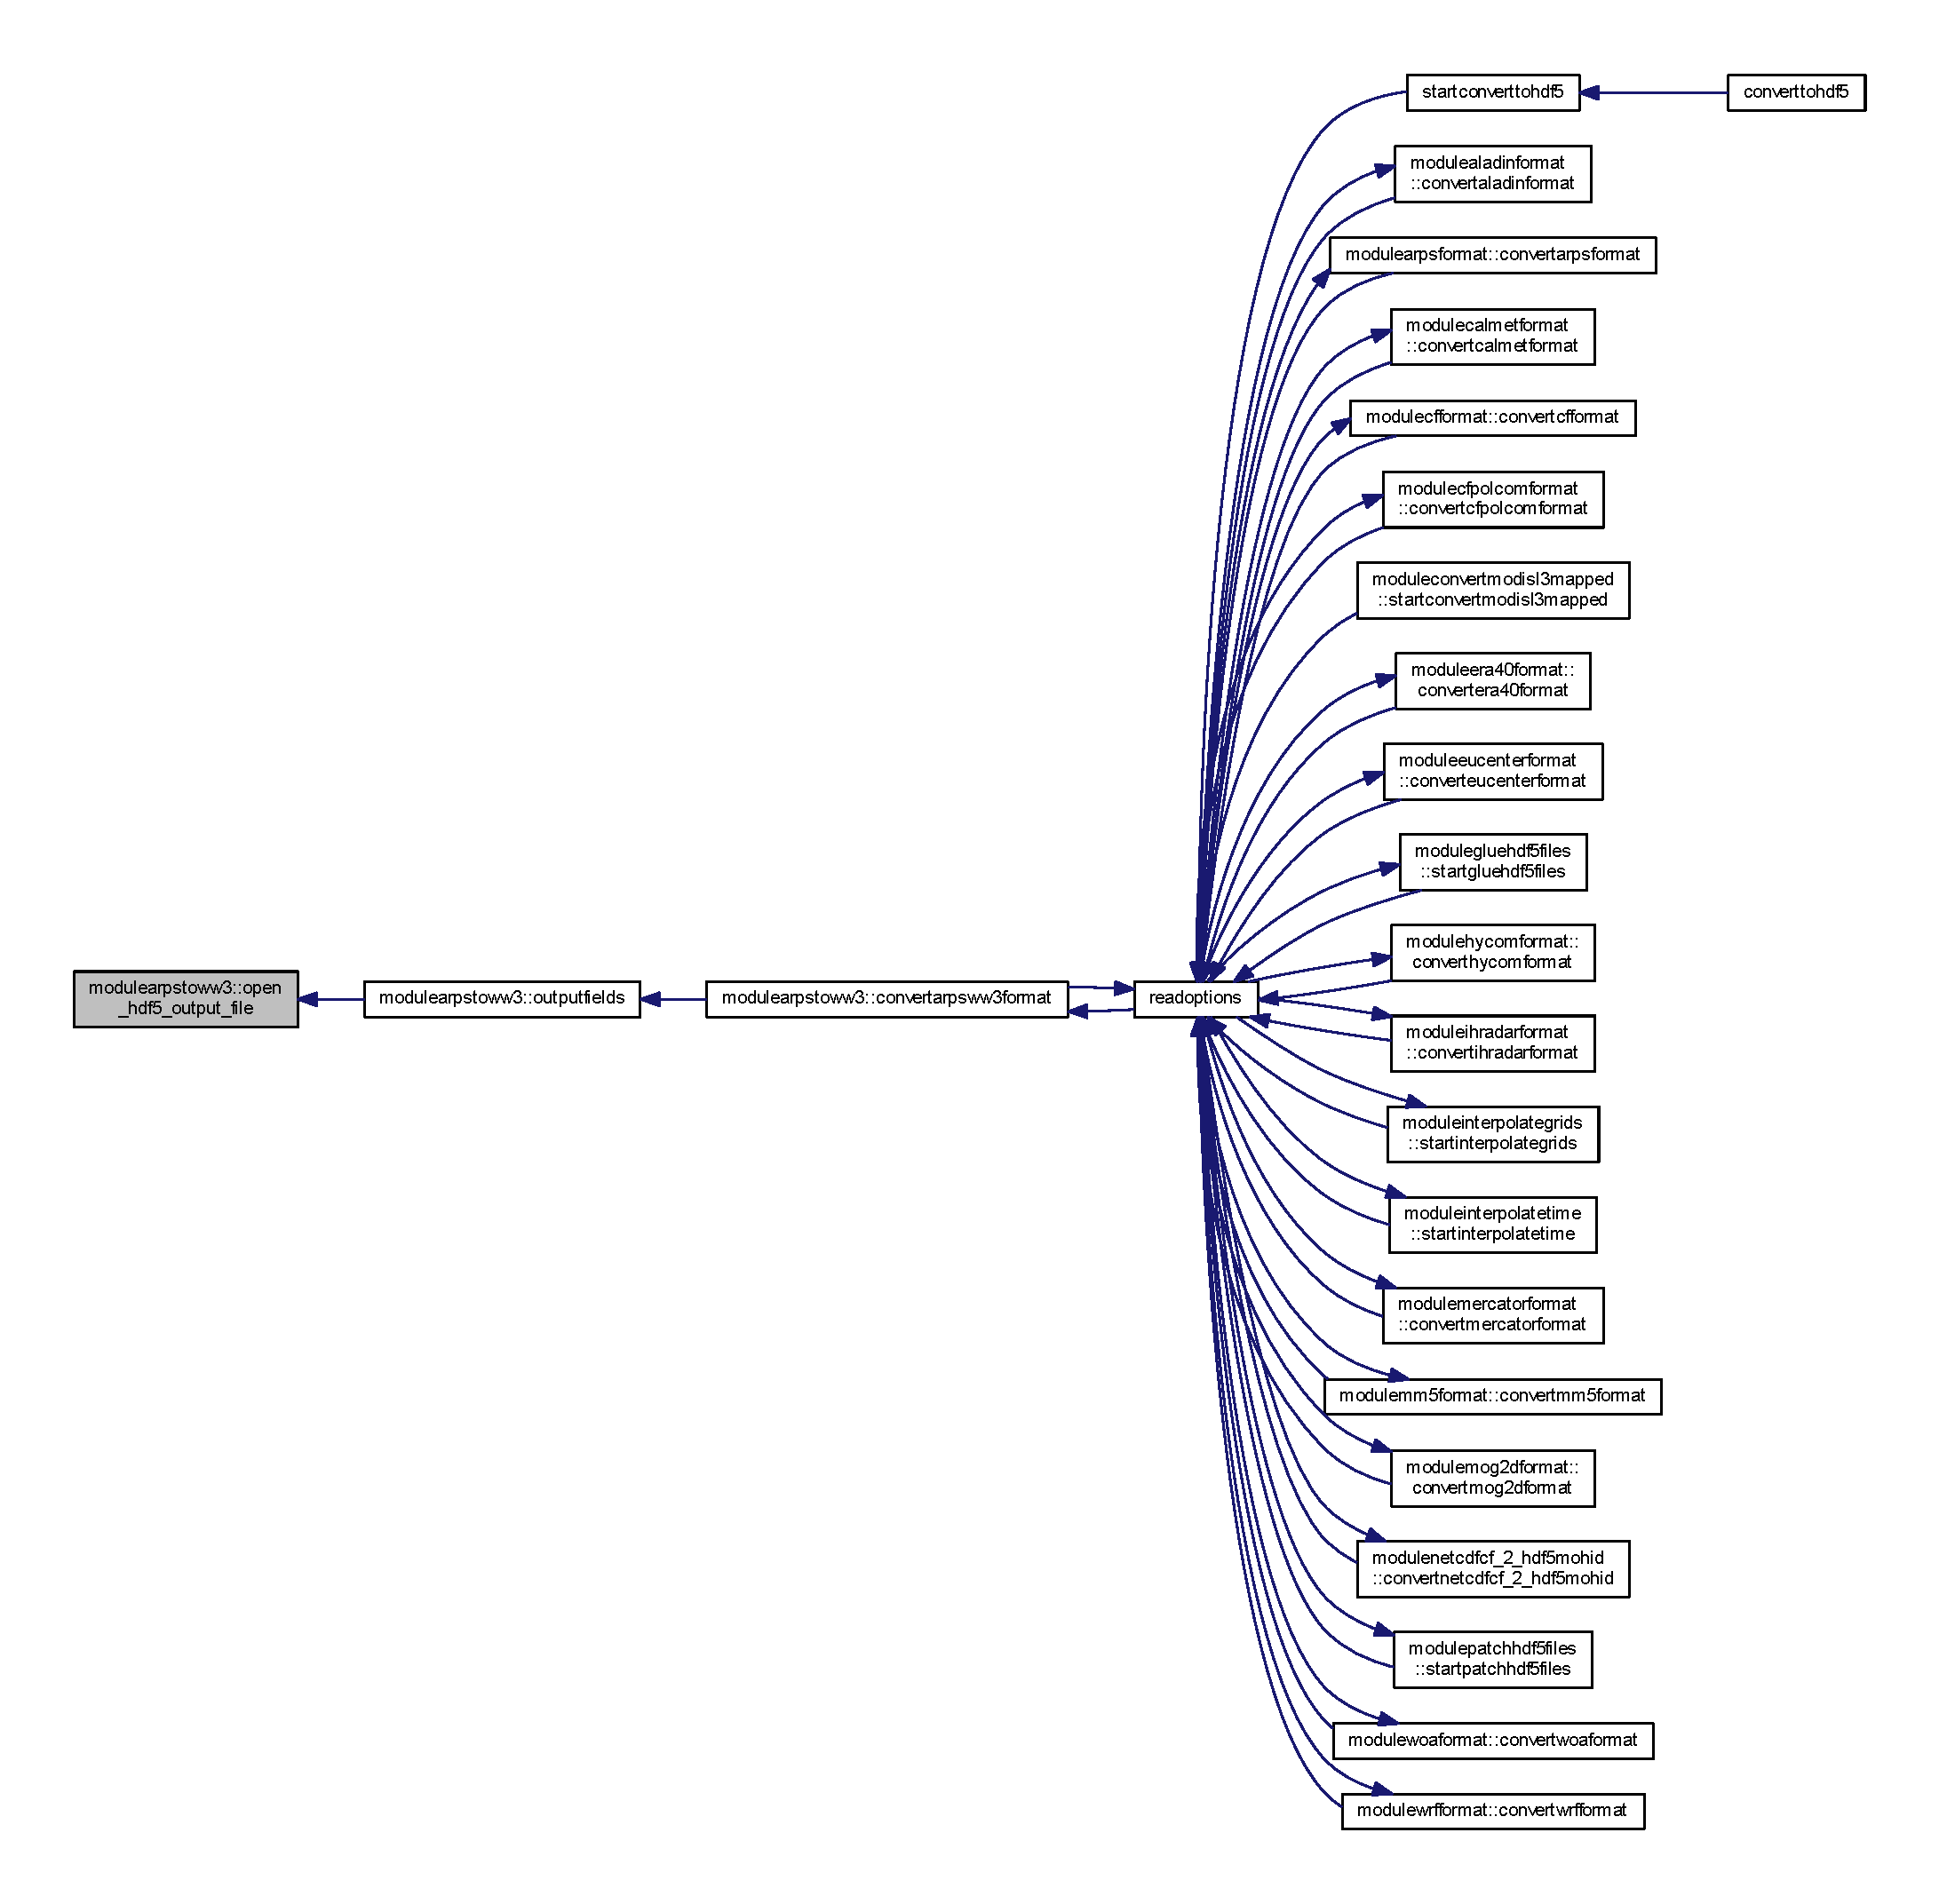
\includegraphics[width=350pt]{namespacemodulearpstoww3_a7a7eb9b823582e046e2127ea46d3f300_icgraph}
\end{center}
\end{figure}
\mbox{\Hypertarget{namespacemodulearpstoww3_aa5a12099f3353b33d3b40f8f3f4384f0}\label{namespacemodulearpstoww3_aa5a12099f3353b33d3b40f8f3f4384f0}} 
\index{modulearpstoww3@{modulearpstoww3}!openandreadarpsfile@{openandreadarpsfile}}
\index{openandreadarpsfile@{openandreadarpsfile}!modulearpstoww3@{modulearpstoww3}}
\subsubsection{\texorpdfstring{openandreadarpsfile()}{openandreadarpsfile()}}
{\footnotesize\ttfamily subroutine, private modulearpstoww3\+::openandreadarpsfile (\begin{DoxyParamCaption}{ }\end{DoxyParamCaption})\hspace{0.3cm}{\ttfamily [private]}}

Here is the call graph for this function\+:\nopagebreak
\begin{figure}[H]
\begin{center}
\leavevmode
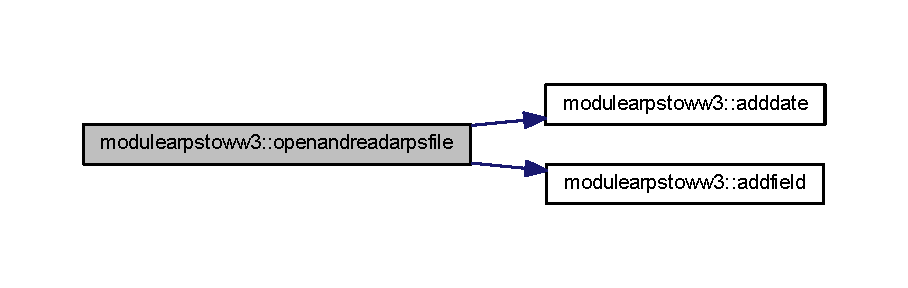
\includegraphics[width=350pt]{namespacemodulearpstoww3_aa5a12099f3353b33d3b40f8f3f4384f0_cgraph}
\end{center}
\end{figure}
Here is the caller graph for this function\+:\nopagebreak
\begin{figure}[H]
\begin{center}
\leavevmode
\includegraphics[width=350pt]{namespacemodulearpstoww3_aa5a12099f3353b33d3b40f8f3f4384f0_icgraph}
\end{center}
\end{figure}
\mbox{\Hypertarget{namespacemodulearpstoww3_a7c18511d187912f655458191bcf1c7af}\label{namespacemodulearpstoww3_a7c18511d187912f655458191bcf1c7af}} 
\index{modulearpstoww3@{modulearpstoww3}!outputfields@{outputfields}}
\index{outputfields@{outputfields}!modulearpstoww3@{modulearpstoww3}}
\subsubsection{\texorpdfstring{outputfields()}{outputfields()}}
{\footnotesize\ttfamily subroutine, private modulearpstoww3\+::outputfields (\begin{DoxyParamCaption}{ }\end{DoxyParamCaption})\hspace{0.3cm}{\ttfamily [private]}}

Here is the call graph for this function\+:\nopagebreak
\begin{figure}[H]
\begin{center}
\leavevmode
\includegraphics[width=350pt]{namespacemodulearpstoww3_a7c18511d187912f655458191bcf1c7af_cgraph}
\end{center}
\end{figure}
Here is the caller graph for this function\+:\nopagebreak
\begin{figure}[H]
\begin{center}
\leavevmode
\includegraphics[width=350pt]{namespacemodulearpstoww3_a7c18511d187912f655458191bcf1c7af_icgraph}
\end{center}
\end{figure}
\mbox{\Hypertarget{namespacemodulearpstoww3_a7642538ceff4533a4ad2aeba84fb2d32}\label{namespacemodulearpstoww3_a7642538ceff4533a4ad2aeba84fb2d32}} 
\index{modulearpstoww3@{modulearpstoww3}!readoptions@{readoptions}}
\index{readoptions@{readoptions}!modulearpstoww3@{modulearpstoww3}}
\subsubsection{\texorpdfstring{readoptions()}{readoptions()}}
{\footnotesize\ttfamily subroutine, private modulearpstoww3\+::readoptions (\begin{DoxyParamCaption}{ }\end{DoxyParamCaption})\hspace{0.3cm}{\ttfamily [private]}}



\subsection{Variable Documentation}
\mbox{\Hypertarget{namespacemodulearpstoww3_ae048aea87bb0343812cdb60ee1a1f6b8}\label{namespacemodulearpstoww3_ae048aea87bb0343812cdb60ee1a1f6b8}} 
\index{modulearpstoww3@{modulearpstoww3}!me@{me}}
\index{me@{me}!modulearpstoww3@{modulearpstoww3}}
\subsubsection{\texorpdfstring{me}{me}}
{\footnotesize\ttfamily type(\mbox{\hyperlink{structmodulearpstoww3_1_1t__mm5format}{t\+\_\+mm5format}}), pointer modulearpstoww3\+::me\hspace{0.3cm}{\ttfamily [private]}}


\hypertarget{namespacemodulecalmetformat}{}\section{modulecalmetformat Module Reference}
\label{namespacemodulecalmetformat}\index{modulecalmetformat@{modulecalmetformat}}
\subsection*{Data Types}
\begin{DoxyCompactItemize}
\item 
type \mbox{\hyperlink{structmodulecalmetformat_1_1t__calmetformat}{t\+\_\+calmetformat}}
\item 
type \mbox{\hyperlink{structmodulecalmetformat_1_1t__date}{t\+\_\+date}}
\item 
type \mbox{\hyperlink{structmodulecalmetformat_1_1t__field}{t\+\_\+field}}
\end{DoxyCompactItemize}
\subsection*{Functions/\+Subroutines}
\begin{DoxyCompactItemize}
\item 
subroutine, public \mbox{\hyperlink{namespacemodulecalmetformat_a46e7b8dbd76c834dd87aa502fa427ecf}{convertcalmetformat}} (Enter\+Data\+ID, S\+T\+AT)
\item 
subroutine, private \mbox{\hyperlink{namespacemodulecalmetformat_a93959f38b7542f55aa7f2b9557c7ee20}{readoptions}}
\item 
subroutine, private \mbox{\hyperlink{namespacemodulecalmetformat_a1c6e763c6740cd630346ca11aab5aa78}{openandreadterrainfile}}
\item 
subroutine, private \mbox{\hyperlink{namespacemodulecalmetformat_aed24d711f305ad0c21d58e0ff79c9c02}{writegridinformation}}
\item 
subroutine \mbox{\hyperlink{namespacemodulecalmetformat_a4d48e68e591262be2fdee84257034418}{convertlatlonchartoreal}} (Aux\+String, Aux\+Real)
\item 
subroutine \mbox{\hyperlink{namespacemodulecalmetformat_a14590292a4c7892fcd59f55007069444}{setnewfieldattributes}} (Field, Name, Units, Date, Work\+Size, n\+Dimensions, Convert)
\item 
subroutine \mbox{\hyperlink{namespacemodulecalmetformat_ad719aec457312263662ee69e4ff227fb}{addfield}} (First\+Field, Obj\+Field)
\item 
subroutine \mbox{\hyperlink{namespacemodulecalmetformat_ac2b80a87e09960dca9aab0ddc8af00b5}{adddate}} (First\+Date, Obj\+Date)
\item 
subroutine, private \mbox{\hyperlink{namespacemodulecalmetformat_a08504fdf416abe46eab39f11e6104b74}{open\+\_\+hdf5\+\_\+output\+\_\+file}}
\item 
subroutine, private \mbox{\hyperlink{namespacemodulecalmetformat_a5ff4d55d88eac5ea8ceee14dbc6c26af}{openandreadcalmetfile}}
\item 
subroutine \mbox{\hyperlink{namespacemodulecalmetformat_a620b75749d8d431ee5f1c9152211ebb0}{addfieldxy}} (C\+A\+L\+M\+E\+T\+Name, Mohid\+Name, Units, New\+Field, Current\+Time)
\item 
subroutine \mbox{\hyperlink{namespacemodulecalmetformat_a26c3210caedd039907d56c2a6b8d30c4}{addintegerfieldxy}} (C\+A\+L\+M\+E\+T\+Name, Mohid\+Name, Units, New\+Field, Current\+Time, Convert\+To\+Real)
\item 
subroutine \mbox{\hyperlink{namespacemodulecalmetformat_a3defaeb10661bad427bb6a70e331c077}{setnewdate}} (New\+Date, ndathr, isec, Year, Month, Day, Hour, Minute, Second)
\item 
subroutine, private \mbox{\hyperlink{namespacemodulecalmetformat_a62bd4a5f15fb34c0505c736e02ac62ca}{beginendtime}}
\item 
subroutine, private \mbox{\hyperlink{namespacemodulecalmetformat_abd990931d70766e3d45c4c5e94a1924f}{computeverticalcoordinate}}
\item 
subroutine, private \mbox{\hyperlink{namespacemodulecalmetformat_aebd4c52189e33c42d4eddb372d91a66d}{correctverticalcoordinate}}
\item 
subroutine, private \mbox{\hyperlink{namespacemodulecalmetformat_ac65fd3f15792bec4c3a1f8809e7d201a}{computewindsurface}}
\item 
subroutine, private \mbox{\hyperlink{namespacemodulecalmetformat_a49e8d2600dc3c064290f04ab142db105}{writegridtohdf5file}}
\item 
subroutine, private \mbox{\hyperlink{namespacemodulecalmetformat_ab777b0fc84a3a4b2505fadc6db40580f}{writemapping}}
\item 
subroutine, private \mbox{\hyperlink{namespacemodulecalmetformat_a77546a7a587e6ab71724b1a5ebb7e709}{outputfields}}
\item 
subroutine, private \mbox{\hyperlink{namespacemodulecalmetformat_a7703da81b5a94320621a668c0326f881}{killcalmetformat}}
\item 
subroutine \mbox{\hyperlink{namespacemodulecalmetformat_a2e6285b2b96d5b3545d7755b77b65502}{handle\+\_\+proj\+\_\+error}} (status)
\end{DoxyCompactItemize}
\subsection*{Variables}
\begin{DoxyCompactItemize}
\item 
integer, parameter \mbox{\hyperlink{namespacemodulecalmetformat_a21173190f31cd07dd3e9d96b03a51822}{perfect\+\_\+gas\+\_\+r}} = 287.\+04
\item 
type(\mbox{\hyperlink{structmodulecalmetformat_1_1t__calmetformat}{t\+\_\+calmetformat}}), pointer \mbox{\hyperlink{namespacemodulecalmetformat_a30d8b055512bccb5b1dd9cd00e4c790b}{me}}
\end{DoxyCompactItemize}


\subsection{Function/\+Subroutine Documentation}
\mbox{\Hypertarget{namespacemodulecalmetformat_ac2b80a87e09960dca9aab0ddc8af00b5}\label{namespacemodulecalmetformat_ac2b80a87e09960dca9aab0ddc8af00b5}} 
\index{modulecalmetformat@{modulecalmetformat}!adddate@{adddate}}
\index{adddate@{adddate}!modulecalmetformat@{modulecalmetformat}}
\subsubsection{\texorpdfstring{adddate()}{adddate()}}
{\footnotesize\ttfamily subroutine modulecalmetformat\+::adddate (\begin{DoxyParamCaption}\item[{type (\mbox{\hyperlink{structmodulecalmetformat_1_1t__date}{t\+\_\+date}}), pointer}]{First\+Date,  }\item[{type (\mbox{\hyperlink{structmodulecalmetformat_1_1t__date}{t\+\_\+date}}), pointer}]{Obj\+Date }\end{DoxyParamCaption})\hspace{0.3cm}{\ttfamily [private]}}

Here is the caller graph for this function\+:\nopagebreak
\begin{figure}[H]
\begin{center}
\leavevmode
\includegraphics[width=350pt]{namespacemodulecalmetformat_ac2b80a87e09960dca9aab0ddc8af00b5_icgraph}
\end{center}
\end{figure}
\mbox{\Hypertarget{namespacemodulecalmetformat_ad719aec457312263662ee69e4ff227fb}\label{namespacemodulecalmetformat_ad719aec457312263662ee69e4ff227fb}} 
\index{modulecalmetformat@{modulecalmetformat}!addfield@{addfield}}
\index{addfield@{addfield}!modulecalmetformat@{modulecalmetformat}}
\subsubsection{\texorpdfstring{addfield()}{addfield()}}
{\footnotesize\ttfamily subroutine modulecalmetformat\+::addfield (\begin{DoxyParamCaption}\item[{type (\mbox{\hyperlink{structmodulecalmetformat_1_1t__field}{t\+\_\+field}}), pointer}]{First\+Field,  }\item[{type (\mbox{\hyperlink{structmodulecalmetformat_1_1t__field}{t\+\_\+field}}), pointer}]{Obj\+Field }\end{DoxyParamCaption})\hspace{0.3cm}{\ttfamily [private]}}

Here is the caller graph for this function\+:\nopagebreak
\begin{figure}[H]
\begin{center}
\leavevmode
\includegraphics[width=350pt]{namespacemodulecalmetformat_ad719aec457312263662ee69e4ff227fb_icgraph}
\end{center}
\end{figure}
\mbox{\Hypertarget{namespacemodulecalmetformat_a620b75749d8d431ee5f1c9152211ebb0}\label{namespacemodulecalmetformat_a620b75749d8d431ee5f1c9152211ebb0}} 
\index{modulecalmetformat@{modulecalmetformat}!addfieldxy@{addfieldxy}}
\index{addfieldxy@{addfieldxy}!modulecalmetformat@{modulecalmetformat}}
\subsubsection{\texorpdfstring{addfieldxy()}{addfieldxy()}}
{\footnotesize\ttfamily subroutine modulecalmetformat\+::addfieldxy (\begin{DoxyParamCaption}\item[{character(8), intent(in)}]{C\+A\+L\+M\+E\+T\+Name,  }\item[{character(stringlength), intent(in)}]{Mohid\+Name,  }\item[{character(stringlength), intent(in)}]{Units,  }\item[{type(\mbox{\hyperlink{structmodulecalmetformat_1_1t__field}{t\+\_\+field}}), pointer}]{New\+Field,  }\item[{type(t\+\_\+time), optional}]{Current\+Time }\end{DoxyParamCaption})\hspace{0.3cm}{\ttfamily [private]}}

Here is the call graph for this function\+:\nopagebreak
\begin{figure}[H]
\begin{center}
\leavevmode
\includegraphics[width=331pt]{namespacemodulecalmetformat_a620b75749d8d431ee5f1c9152211ebb0_cgraph}
\end{center}
\end{figure}
Here is the caller graph for this function\+:\nopagebreak
\begin{figure}[H]
\begin{center}
\leavevmode
\includegraphics[width=350pt]{namespacemodulecalmetformat_a620b75749d8d431ee5f1c9152211ebb0_icgraph}
\end{center}
\end{figure}
\mbox{\Hypertarget{namespacemodulecalmetformat_a26c3210caedd039907d56c2a6b8d30c4}\label{namespacemodulecalmetformat_a26c3210caedd039907d56c2a6b8d30c4}} 
\index{modulecalmetformat@{modulecalmetformat}!addintegerfieldxy@{addintegerfieldxy}}
\index{addintegerfieldxy@{addintegerfieldxy}!modulecalmetformat@{modulecalmetformat}}
\subsubsection{\texorpdfstring{addintegerfieldxy()}{addintegerfieldxy()}}
{\footnotesize\ttfamily subroutine modulecalmetformat\+::addintegerfieldxy (\begin{DoxyParamCaption}\item[{character(8), intent(in)}]{C\+A\+L\+M\+E\+T\+Name,  }\item[{character(stringlength), intent(in)}]{Mohid\+Name,  }\item[{character(stringlength), intent(in)}]{Units,  }\item[{type(\mbox{\hyperlink{structmodulecalmetformat_1_1t__field}{t\+\_\+field}}), pointer}]{New\+Field,  }\item[{type(t\+\_\+time), optional}]{Current\+Time,  }\item[{logical, optional}]{Convert\+To\+Real }\end{DoxyParamCaption})\hspace{0.3cm}{\ttfamily [private]}}

Here is the call graph for this function\+:\nopagebreak
\begin{figure}[H]
\begin{center}
\leavevmode
\includegraphics[width=331pt]{namespacemodulecalmetformat_a26c3210caedd039907d56c2a6b8d30c4_cgraph}
\end{center}
\end{figure}
Here is the caller graph for this function\+:\nopagebreak
\begin{figure}[H]
\begin{center}
\leavevmode
\includegraphics[width=350pt]{namespacemodulecalmetformat_a26c3210caedd039907d56c2a6b8d30c4_icgraph}
\end{center}
\end{figure}
\mbox{\Hypertarget{namespacemodulecalmetformat_a62bd4a5f15fb34c0505c736e02ac62ca}\label{namespacemodulecalmetformat_a62bd4a5f15fb34c0505c736e02ac62ca}} 
\index{modulecalmetformat@{modulecalmetformat}!beginendtime@{beginendtime}}
\index{beginendtime@{beginendtime}!modulecalmetformat@{modulecalmetformat}}
\subsubsection{\texorpdfstring{beginendtime()}{beginendtime()}}
{\footnotesize\ttfamily subroutine, private modulecalmetformat\+::beginendtime (\begin{DoxyParamCaption}{ }\end{DoxyParamCaption})\hspace{0.3cm}{\ttfamily [private]}}

Here is the caller graph for this function\+:\nopagebreak
\begin{figure}[H]
\begin{center}
\leavevmode
\includegraphics[width=350pt]{namespacemodulecalmetformat_a62bd4a5f15fb34c0505c736e02ac62ca_icgraph}
\end{center}
\end{figure}
\mbox{\Hypertarget{namespacemodulecalmetformat_abd990931d70766e3d45c4c5e94a1924f}\label{namespacemodulecalmetformat_abd990931d70766e3d45c4c5e94a1924f}} 
\index{modulecalmetformat@{modulecalmetformat}!computeverticalcoordinate@{computeverticalcoordinate}}
\index{computeverticalcoordinate@{computeverticalcoordinate}!modulecalmetformat@{modulecalmetformat}}
\subsubsection{\texorpdfstring{computeverticalcoordinate()}{computeverticalcoordinate()}}
{\footnotesize\ttfamily subroutine, private modulecalmetformat\+::computeverticalcoordinate (\begin{DoxyParamCaption}{ }\end{DoxyParamCaption})\hspace{0.3cm}{\ttfamily [private]}}

Here is the call graph for this function\+:\nopagebreak
\begin{figure}[H]
\begin{center}
\leavevmode
\includegraphics[width=350pt]{namespacemodulecalmetformat_abd990931d70766e3d45c4c5e94a1924f_cgraph}
\end{center}
\end{figure}
Here is the caller graph for this function\+:\nopagebreak
\begin{figure}[H]
\begin{center}
\leavevmode
\includegraphics[width=350pt]{namespacemodulecalmetformat_abd990931d70766e3d45c4c5e94a1924f_icgraph}
\end{center}
\end{figure}
\mbox{\Hypertarget{namespacemodulecalmetformat_ac65fd3f15792bec4c3a1f8809e7d201a}\label{namespacemodulecalmetformat_ac65fd3f15792bec4c3a1f8809e7d201a}} 
\index{modulecalmetformat@{modulecalmetformat}!computewindsurface@{computewindsurface}}
\index{computewindsurface@{computewindsurface}!modulecalmetformat@{modulecalmetformat}}
\subsubsection{\texorpdfstring{computewindsurface()}{computewindsurface()}}
{\footnotesize\ttfamily subroutine, private modulecalmetformat\+::computewindsurface (\begin{DoxyParamCaption}{ }\end{DoxyParamCaption})\hspace{0.3cm}{\ttfamily [private]}}

Here is the call graph for this function\+:\nopagebreak
\begin{figure}[H]
\begin{center}
\leavevmode
\includegraphics[width=338pt]{namespacemodulecalmetformat_ac65fd3f15792bec4c3a1f8809e7d201a_cgraph}
\end{center}
\end{figure}
Here is the caller graph for this function\+:\nopagebreak
\begin{figure}[H]
\begin{center}
\leavevmode
\includegraphics[width=350pt]{namespacemodulecalmetformat_ac65fd3f15792bec4c3a1f8809e7d201a_icgraph}
\end{center}
\end{figure}
\mbox{\Hypertarget{namespacemodulecalmetformat_a46e7b8dbd76c834dd87aa502fa427ecf}\label{namespacemodulecalmetformat_a46e7b8dbd76c834dd87aa502fa427ecf}} 
\index{modulecalmetformat@{modulecalmetformat}!convertcalmetformat@{convertcalmetformat}}
\index{convertcalmetformat@{convertcalmetformat}!modulecalmetformat@{modulecalmetformat}}
\subsubsection{\texorpdfstring{convertcalmetformat()}{convertcalmetformat()}}
{\footnotesize\ttfamily subroutine, public modulecalmetformat\+::convertcalmetformat (\begin{DoxyParamCaption}\item[{integer, intent(in)}]{Enter\+Data\+ID,  }\item[{integer, intent(out), optional}]{S\+T\+AT }\end{DoxyParamCaption})}

Here is the call graph for this function\+:\nopagebreak
\begin{figure}[H]
\begin{center}
\leavevmode
\includegraphics[height=550pt]{namespacemodulecalmetformat_a46e7b8dbd76c834dd87aa502fa427ecf_cgraph}
\end{center}
\end{figure}
Here is the caller graph for this function\+:\nopagebreak
\begin{figure}[H]
\begin{center}
\leavevmode
\includegraphics[height=550pt]{namespacemodulecalmetformat_a46e7b8dbd76c834dd87aa502fa427ecf_icgraph}
\end{center}
\end{figure}
\mbox{\Hypertarget{namespacemodulecalmetformat_a4d48e68e591262be2fdee84257034418}\label{namespacemodulecalmetformat_a4d48e68e591262be2fdee84257034418}} 
\index{modulecalmetformat@{modulecalmetformat}!convertlatlonchartoreal@{convertlatlonchartoreal}}
\index{convertlatlonchartoreal@{convertlatlonchartoreal}!modulecalmetformat@{modulecalmetformat}}
\subsubsection{\texorpdfstring{convertlatlonchartoreal()}{convertlatlonchartoreal()}}
{\footnotesize\ttfamily subroutine modulecalmetformat\+::convertlatlonchartoreal (\begin{DoxyParamCaption}\item[{character(len=stringlength), intent(in)}]{Aux\+String,  }\item[{real, intent(out)}]{Aux\+Real }\end{DoxyParamCaption})\hspace{0.3cm}{\ttfamily [private]}}

Here is the caller graph for this function\+:\nopagebreak
\begin{figure}[H]
\begin{center}
\leavevmode
\includegraphics[width=350pt]{namespacemodulecalmetformat_a4d48e68e591262be2fdee84257034418_icgraph}
\end{center}
\end{figure}
\mbox{\Hypertarget{namespacemodulecalmetformat_aebd4c52189e33c42d4eddb372d91a66d}\label{namespacemodulecalmetformat_aebd4c52189e33c42d4eddb372d91a66d}} 
\index{modulecalmetformat@{modulecalmetformat}!correctverticalcoordinate@{correctverticalcoordinate}}
\index{correctverticalcoordinate@{correctverticalcoordinate}!modulecalmetformat@{modulecalmetformat}}
\subsubsection{\texorpdfstring{correctverticalcoordinate()}{correctverticalcoordinate()}}
{\footnotesize\ttfamily subroutine, private modulecalmetformat\+::correctverticalcoordinate (\begin{DoxyParamCaption}{ }\end{DoxyParamCaption})\hspace{0.3cm}{\ttfamily [private]}}

Here is the caller graph for this function\+:\nopagebreak
\begin{figure}[H]
\begin{center}
\leavevmode
\includegraphics[width=350pt]{namespacemodulecalmetformat_aebd4c52189e33c42d4eddb372d91a66d_icgraph}
\end{center}
\end{figure}
\mbox{\Hypertarget{namespacemodulecalmetformat_a2e6285b2b96d5b3545d7755b77b65502}\label{namespacemodulecalmetformat_a2e6285b2b96d5b3545d7755b77b65502}} 
\index{modulecalmetformat@{modulecalmetformat}!handle\+\_\+proj\+\_\+error@{handle\+\_\+proj\+\_\+error}}
\index{handle\+\_\+proj\+\_\+error@{handle\+\_\+proj\+\_\+error}!modulecalmetformat@{modulecalmetformat}}
\subsubsection{\texorpdfstring{handle\+\_\+proj\+\_\+error()}{handle\_proj\_error()}}
{\footnotesize\ttfamily subroutine modulecalmetformat\+::handle\+\_\+proj\+\_\+error (\begin{DoxyParamCaption}\item[{integer, intent(in)}]{status }\end{DoxyParamCaption})\hspace{0.3cm}{\ttfamily [private]}}

Here is the caller graph for this function\+:\nopagebreak
\begin{figure}[H]
\begin{center}
\leavevmode
\includegraphics[width=350pt]{namespacemodulecalmetformat_a2e6285b2b96d5b3545d7755b77b65502_icgraph}
\end{center}
\end{figure}
\mbox{\Hypertarget{namespacemodulecalmetformat_a7703da81b5a94320621a668c0326f881}\label{namespacemodulecalmetformat_a7703da81b5a94320621a668c0326f881}} 
\index{modulecalmetformat@{modulecalmetformat}!killcalmetformat@{killcalmetformat}}
\index{killcalmetformat@{killcalmetformat}!modulecalmetformat@{modulecalmetformat}}
\subsubsection{\texorpdfstring{killcalmetformat()}{killcalmetformat()}}
{\footnotesize\ttfamily subroutine, private modulecalmetformat\+::killcalmetformat (\begin{DoxyParamCaption}{ }\end{DoxyParamCaption})\hspace{0.3cm}{\ttfamily [private]}}

Here is the caller graph for this function\+:\nopagebreak
\begin{figure}[H]
\begin{center}
\leavevmode
\includegraphics[width=350pt]{namespacemodulecalmetformat_a7703da81b5a94320621a668c0326f881_icgraph}
\end{center}
\end{figure}
\mbox{\Hypertarget{namespacemodulecalmetformat_a08504fdf416abe46eab39f11e6104b74}\label{namespacemodulecalmetformat_a08504fdf416abe46eab39f11e6104b74}} 
\index{modulecalmetformat@{modulecalmetformat}!open\+\_\+hdf5\+\_\+output\+\_\+file@{open\+\_\+hdf5\+\_\+output\+\_\+file}}
\index{open\+\_\+hdf5\+\_\+output\+\_\+file@{open\+\_\+hdf5\+\_\+output\+\_\+file}!modulecalmetformat@{modulecalmetformat}}
\subsubsection{\texorpdfstring{open\+\_\+hdf5\+\_\+output\+\_\+file()}{open\_hdf5\_output\_file()}}
{\footnotesize\ttfamily subroutine, private modulecalmetformat\+::open\+\_\+hdf5\+\_\+output\+\_\+file (\begin{DoxyParamCaption}{ }\end{DoxyParamCaption})\hspace{0.3cm}{\ttfamily [private]}}

Here is the caller graph for this function\+:\nopagebreak
\begin{figure}[H]
\begin{center}
\leavevmode
\includegraphics[width=350pt]{namespacemodulecalmetformat_a08504fdf416abe46eab39f11e6104b74_icgraph}
\end{center}
\end{figure}
\mbox{\Hypertarget{namespacemodulecalmetformat_a5ff4d55d88eac5ea8ceee14dbc6c26af}\label{namespacemodulecalmetformat_a5ff4d55d88eac5ea8ceee14dbc6c26af}} 
\index{modulecalmetformat@{modulecalmetformat}!openandreadcalmetfile@{openandreadcalmetfile}}
\index{openandreadcalmetfile@{openandreadcalmetfile}!modulecalmetformat@{modulecalmetformat}}
\subsubsection{\texorpdfstring{openandreadcalmetfile()}{openandreadcalmetfile()}}
{\footnotesize\ttfamily subroutine, private modulecalmetformat\+::openandreadcalmetfile (\begin{DoxyParamCaption}{ }\end{DoxyParamCaption})\hspace{0.3cm}{\ttfamily [private]}}

Here is the call graph for this function\+:\nopagebreak
\begin{figure}[H]
\begin{center}
\leavevmode
\includegraphics[width=350pt]{namespacemodulecalmetformat_a5ff4d55d88eac5ea8ceee14dbc6c26af_cgraph}
\end{center}
\end{figure}
Here is the caller graph for this function\+:\nopagebreak
\begin{figure}[H]
\begin{center}
\leavevmode
\includegraphics[width=350pt]{namespacemodulecalmetformat_a5ff4d55d88eac5ea8ceee14dbc6c26af_icgraph}
\end{center}
\end{figure}
\mbox{\Hypertarget{namespacemodulecalmetformat_a1c6e763c6740cd630346ca11aab5aa78}\label{namespacemodulecalmetformat_a1c6e763c6740cd630346ca11aab5aa78}} 
\index{modulecalmetformat@{modulecalmetformat}!openandreadterrainfile@{openandreadterrainfile}}
\index{openandreadterrainfile@{openandreadterrainfile}!modulecalmetformat@{modulecalmetformat}}
\subsubsection{\texorpdfstring{openandreadterrainfile()}{openandreadterrainfile()}}
{\footnotesize\ttfamily subroutine, private modulecalmetformat\+::openandreadterrainfile (\begin{DoxyParamCaption}{ }\end{DoxyParamCaption})\hspace{0.3cm}{\ttfamily [private]}}

Here is the call graph for this function\+:\nopagebreak
\begin{figure}[H]
\begin{center}
\leavevmode
\includegraphics[width=350pt]{namespacemodulecalmetformat_a1c6e763c6740cd630346ca11aab5aa78_cgraph}
\end{center}
\end{figure}
Here is the caller graph for this function\+:\nopagebreak
\begin{figure}[H]
\begin{center}
\leavevmode
\includegraphics[width=350pt]{namespacemodulecalmetformat_a1c6e763c6740cd630346ca11aab5aa78_icgraph}
\end{center}
\end{figure}
\mbox{\Hypertarget{namespacemodulecalmetformat_a77546a7a587e6ab71724b1a5ebb7e709}\label{namespacemodulecalmetformat_a77546a7a587e6ab71724b1a5ebb7e709}} 
\index{modulecalmetformat@{modulecalmetformat}!outputfields@{outputfields}}
\index{outputfields@{outputfields}!modulecalmetformat@{modulecalmetformat}}
\subsubsection{\texorpdfstring{outputfields()}{outputfields()}}
{\footnotesize\ttfamily subroutine, private modulecalmetformat\+::outputfields (\begin{DoxyParamCaption}{ }\end{DoxyParamCaption})\hspace{0.3cm}{\ttfamily [private]}}

Here is the call graph for this function\+:\nopagebreak
\begin{figure}[H]
\begin{center}
\leavevmode
\includegraphics[width=324pt]{namespacemodulecalmetformat_a77546a7a587e6ab71724b1a5ebb7e709_cgraph}
\end{center}
\end{figure}
Here is the caller graph for this function\+:\nopagebreak
\begin{figure}[H]
\begin{center}
\leavevmode
\includegraphics[width=350pt]{namespacemodulecalmetformat_a77546a7a587e6ab71724b1a5ebb7e709_icgraph}
\end{center}
\end{figure}
\mbox{\Hypertarget{namespacemodulecalmetformat_a93959f38b7542f55aa7f2b9557c7ee20}\label{namespacemodulecalmetformat_a93959f38b7542f55aa7f2b9557c7ee20}} 
\index{modulecalmetformat@{modulecalmetformat}!readoptions@{readoptions}}
\index{readoptions@{readoptions}!modulecalmetformat@{modulecalmetformat}}
\subsubsection{\texorpdfstring{readoptions()}{readoptions()}}
{\footnotesize\ttfamily subroutine, private modulecalmetformat\+::readoptions (\begin{DoxyParamCaption}{ }\end{DoxyParamCaption})\hspace{0.3cm}{\ttfamily [private]}}

\mbox{\Hypertarget{namespacemodulecalmetformat_a3defaeb10661bad427bb6a70e331c077}\label{namespacemodulecalmetformat_a3defaeb10661bad427bb6a70e331c077}} 
\index{modulecalmetformat@{modulecalmetformat}!setnewdate@{setnewdate}}
\index{setnewdate@{setnewdate}!modulecalmetformat@{modulecalmetformat}}
\subsubsection{\texorpdfstring{setnewdate()}{setnewdate()}}
{\footnotesize\ttfamily subroutine modulecalmetformat\+::setnewdate (\begin{DoxyParamCaption}\item[{type(\mbox{\hyperlink{structmodulecalmetformat_1_1t__date}{t\+\_\+date}}), intent(out), pointer}]{New\+Date,  }\item[{integer, intent(in), optional}]{ndathr,  }\item[{integer, intent(in), optional}]{isec,  }\item[{integer, intent(in), optional}]{Year,  }\item[{integer, intent(in), optional}]{Month,  }\item[{integer, intent(in), optional}]{Day,  }\item[{integer, intent(in), optional}]{Hour,  }\item[{integer, intent(in), optional}]{Minute,  }\item[{integer, intent(in), optional}]{Second }\end{DoxyParamCaption})\hspace{0.3cm}{\ttfamily [private]}}

Here is the call graph for this function\+:\nopagebreak
\begin{figure}[H]
\begin{center}
\leavevmode
\includegraphics[width=324pt]{namespacemodulecalmetformat_a3defaeb10661bad427bb6a70e331c077_cgraph}
\end{center}
\end{figure}
Here is the caller graph for this function\+:\nopagebreak
\begin{figure}[H]
\begin{center}
\leavevmode
\includegraphics[width=350pt]{namespacemodulecalmetformat_a3defaeb10661bad427bb6a70e331c077_icgraph}
\end{center}
\end{figure}
\mbox{\Hypertarget{namespacemodulecalmetformat_a14590292a4c7892fcd59f55007069444}\label{namespacemodulecalmetformat_a14590292a4c7892fcd59f55007069444}} 
\index{modulecalmetformat@{modulecalmetformat}!setnewfieldattributes@{setnewfieldattributes}}
\index{setnewfieldattributes@{setnewfieldattributes}!modulecalmetformat@{modulecalmetformat}}
\subsubsection{\texorpdfstring{setnewfieldattributes()}{setnewfieldattributes()}}
{\footnotesize\ttfamily subroutine modulecalmetformat\+::setnewfieldattributes (\begin{DoxyParamCaption}\item[{type(\mbox{\hyperlink{structmodulecalmetformat_1_1t__field}{t\+\_\+field}}), pointer}]{Field,  }\item[{character(len=$\ast$), intent(in)}]{Name,  }\item[{character(len=$\ast$), intent(in)}]{Units,  }\item[{type(t\+\_\+time), intent(in), optional}]{Date,  }\item[{type(t\+\_\+size3d), intent(in), optional}]{Work\+Size,  }\item[{integer, intent(in), optional}]{n\+Dimensions,  }\item[{logical, intent(in)}]{Convert }\end{DoxyParamCaption})\hspace{0.3cm}{\ttfamily [private]}}

Here is the caller graph for this function\+:\nopagebreak
\begin{figure}[H]
\begin{center}
\leavevmode
\includegraphics[width=350pt]{namespacemodulecalmetformat_a14590292a4c7892fcd59f55007069444_icgraph}
\end{center}
\end{figure}
\mbox{\Hypertarget{namespacemodulecalmetformat_aed24d711f305ad0c21d58e0ff79c9c02}\label{namespacemodulecalmetformat_aed24d711f305ad0c21d58e0ff79c9c02}} 
\index{modulecalmetformat@{modulecalmetformat}!writegridinformation@{writegridinformation}}
\index{writegridinformation@{writegridinformation}!modulecalmetformat@{modulecalmetformat}}
\subsubsection{\texorpdfstring{writegridinformation()}{writegridinformation()}}
{\footnotesize\ttfamily subroutine, private modulecalmetformat\+::writegridinformation (\begin{DoxyParamCaption}{ }\end{DoxyParamCaption})\hspace{0.3cm}{\ttfamily [private]}}

Here is the call graph for this function\+:\nopagebreak
\begin{figure}[H]
\begin{center}
\leavevmode
\includegraphics[width=326pt]{namespacemodulecalmetformat_aed24d711f305ad0c21d58e0ff79c9c02_cgraph}
\end{center}
\end{figure}
Here is the caller graph for this function\+:\nopagebreak
\begin{figure}[H]
\begin{center}
\leavevmode
\includegraphics[width=350pt]{namespacemodulecalmetformat_aed24d711f305ad0c21d58e0ff79c9c02_icgraph}
\end{center}
\end{figure}
\mbox{\Hypertarget{namespacemodulecalmetformat_a49e8d2600dc3c064290f04ab142db105}\label{namespacemodulecalmetformat_a49e8d2600dc3c064290f04ab142db105}} 
\index{modulecalmetformat@{modulecalmetformat}!writegridtohdf5file@{writegridtohdf5file}}
\index{writegridtohdf5file@{writegridtohdf5file}!modulecalmetformat@{modulecalmetformat}}
\subsubsection{\texorpdfstring{writegridtohdf5file()}{writegridtohdf5file()}}
{\footnotesize\ttfamily subroutine, private modulecalmetformat\+::writegridtohdf5file (\begin{DoxyParamCaption}{ }\end{DoxyParamCaption})\hspace{0.3cm}{\ttfamily [private]}}

Here is the caller graph for this function\+:\nopagebreak
\begin{figure}[H]
\begin{center}
\leavevmode
\includegraphics[width=350pt]{namespacemodulecalmetformat_a49e8d2600dc3c064290f04ab142db105_icgraph}
\end{center}
\end{figure}
\mbox{\Hypertarget{namespacemodulecalmetformat_ab777b0fc84a3a4b2505fadc6db40580f}\label{namespacemodulecalmetformat_ab777b0fc84a3a4b2505fadc6db40580f}} 
\index{modulecalmetformat@{modulecalmetformat}!writemapping@{writemapping}}
\index{writemapping@{writemapping}!modulecalmetformat@{modulecalmetformat}}
\subsubsection{\texorpdfstring{writemapping()}{writemapping()}}
{\footnotesize\ttfamily subroutine, private modulecalmetformat\+::writemapping (\begin{DoxyParamCaption}{ }\end{DoxyParamCaption})\hspace{0.3cm}{\ttfamily [private]}}

Here is the caller graph for this function\+:\nopagebreak
\begin{figure}[H]
\begin{center}
\leavevmode
\includegraphics[width=350pt]{namespacemodulecalmetformat_ab777b0fc84a3a4b2505fadc6db40580f_icgraph}
\end{center}
\end{figure}


\subsection{Variable Documentation}
\mbox{\Hypertarget{namespacemodulecalmetformat_a30d8b055512bccb5b1dd9cd00e4c790b}\label{namespacemodulecalmetformat_a30d8b055512bccb5b1dd9cd00e4c790b}} 
\index{modulecalmetformat@{modulecalmetformat}!me@{me}}
\index{me@{me}!modulecalmetformat@{modulecalmetformat}}
\subsubsection{\texorpdfstring{me}{me}}
{\footnotesize\ttfamily type(\mbox{\hyperlink{structmodulecalmetformat_1_1t__calmetformat}{t\+\_\+calmetformat}}), pointer modulecalmetformat\+::me\hspace{0.3cm}{\ttfamily [private]}}

\mbox{\Hypertarget{namespacemodulecalmetformat_a21173190f31cd07dd3e9d96b03a51822}\label{namespacemodulecalmetformat_a21173190f31cd07dd3e9d96b03a51822}} 
\index{modulecalmetformat@{modulecalmetformat}!perfect\+\_\+gas\+\_\+r@{perfect\+\_\+gas\+\_\+r}}
\index{perfect\+\_\+gas\+\_\+r@{perfect\+\_\+gas\+\_\+r}!modulecalmetformat@{modulecalmetformat}}
\subsubsection{\texorpdfstring{perfect\+\_\+gas\+\_\+r}{perfect\_gas\_r}}
{\footnotesize\ttfamily integer, parameter modulecalmetformat\+::perfect\+\_\+gas\+\_\+r = 287.\+04\hspace{0.3cm}{\ttfamily [private]}}


\hypertarget{namespacemodulecfformat}{}\section{modulecfformat Module Reference}
\label{namespacemodulecfformat}\index{modulecfformat@{modulecfformat}}
\subsection*{Data Types}
\begin{DoxyCompactItemize}
\item 
type \mbox{\hyperlink{structmodulecfformat_1_1t__cfformat}{t\+\_\+cfformat}}
\item 
type \mbox{\hyperlink{structmodulecfformat_1_1t__date}{t\+\_\+date}}
\item 
type \mbox{\hyperlink{structmodulecfformat_1_1t__field}{t\+\_\+field}}
\end{DoxyCompactItemize}
\subsection*{Functions/\+Subroutines}
\begin{DoxyCompactItemize}
\item 
subroutine, public \mbox{\hyperlink{namespacemodulecfformat_a66da5c204d14d5f914e0226b731d5b00}{convertcfformat}} (Enter\+Data\+ID, S\+T\+AT)
\item 
subroutine \mbox{\hyperlink{namespacemodulecfformat_a127693205be384834843b9bb374985e3}{readoptions}}
\item 
subroutine \mbox{\hyperlink{namespacemodulecfformat_a5052b284bceadda6143b8eb5cfd48d05}{openandreadcffile}}
\item 
logical function \mbox{\hyperlink{namespacemodulecfformat_a63d0a39020a58e43589f5140948d8d58}{checkname}} (C\+F\+Var, Mohid\+Name)
\item 
subroutine \mbox{\hyperlink{namespacemodulecfformat_a76cf49362d3cf1651d95e683370014a6}{read\+\_\+cfdate}} (Date\+In, Year, Month, Day, Hour, Minute, Second, Hour\+U\+TC, Minute\+U\+TC, Factor)
\item 
subroutine \mbox{\hyperlink{namespacemodulecfformat_ada4be4f435cac7bea17a9c4f77f22009}{transform2mohid}} (var, hdf\+Field)
\item 
subroutine \mbox{\hyperlink{namespacemodulecfformat_ad6fa7957e7e1de3c2faa57ac769c05bd}{adddate}} (First\+Date, Obj\+Date)
\item 
subroutine \mbox{\hyperlink{namespacemodulecfformat_a9105e21bd9d021767ea028d72b9a201a}{constructgrid}}
\item 
subroutine \mbox{\hyperlink{namespacemodulecfformat_a86156fe637bfdd6ff49e6bce5f187595}{addfield}} (First\+Field, Obj\+Field)
\item 
subroutine \mbox{\hyperlink{namespacemodulecfformat_a369a14cc96dd6826942c93e6352240db}{outputfields}}
\item 
subroutine \mbox{\hyperlink{namespacemodulecfformat_ac77aa80bb4743d920e0a70e5b278be5d}{open\+\_\+hdf5\+\_\+output\+\_\+file}}
\item 
subroutine \mbox{\hyperlink{namespacemodulecfformat_ac518bd16572e1cf72041996bfd3d1e36}{killcfformat}}
\end{DoxyCompactItemize}
\subsection*{Variables}
\begin{DoxyCompactItemize}
\item 
type(\mbox{\hyperlink{structmodulecfformat_1_1t__cfformat}{t\+\_\+cfformat}}), pointer \mbox{\hyperlink{namespacemodulecfformat_a76d190b893ca0f5aa943e57206a96b4b}{me}}
\item 
real \mbox{\hyperlink{namespacemodulecfformat_ab2d59020a88c3fbe79eff641f5173e89}{lat1}}
\item 
real \mbox{\hyperlink{namespacemodulecfformat_aadafc108edb5e219d2dd0fa0e0e650c4}{lon1}}
\item 
integer \mbox{\hyperlink{namespacemodulecfformat_ab5d33d2291e08b59db8c41277c58ea06}{idump}}
\end{DoxyCompactItemize}


\subsection{Function/\+Subroutine Documentation}
\mbox{\Hypertarget{namespacemodulecfformat_ad6fa7957e7e1de3c2faa57ac769c05bd}\label{namespacemodulecfformat_ad6fa7957e7e1de3c2faa57ac769c05bd}} 
\index{modulecfformat@{modulecfformat}!adddate@{adddate}}
\index{adddate@{adddate}!modulecfformat@{modulecfformat}}
\subsubsection{\texorpdfstring{adddate()}{adddate()}}
{\footnotesize\ttfamily subroutine modulecfformat\+::adddate (\begin{DoxyParamCaption}\item[{type (\mbox{\hyperlink{structmodulecfformat_1_1t__date}{t\+\_\+date}}), pointer}]{First\+Date,  }\item[{type (\mbox{\hyperlink{structmodulecfformat_1_1t__date}{t\+\_\+date}}), pointer}]{Obj\+Date }\end{DoxyParamCaption})\hspace{0.3cm}{\ttfamily [private]}}

Here is the caller graph for this function\+:\nopagebreak
\begin{figure}[H]
\begin{center}
\leavevmode
\includegraphics[width=350pt]{namespacemodulecfformat_ad6fa7957e7e1de3c2faa57ac769c05bd_icgraph}
\end{center}
\end{figure}
\mbox{\Hypertarget{namespacemodulecfformat_a86156fe637bfdd6ff49e6bce5f187595}\label{namespacemodulecfformat_a86156fe637bfdd6ff49e6bce5f187595}} 
\index{modulecfformat@{modulecfformat}!addfield@{addfield}}
\index{addfield@{addfield}!modulecfformat@{modulecfformat}}
\subsubsection{\texorpdfstring{addfield()}{addfield()}}
{\footnotesize\ttfamily subroutine modulecfformat\+::addfield (\begin{DoxyParamCaption}\item[{type (\mbox{\hyperlink{structmodulecfformat_1_1t__field}{t\+\_\+field}}), pointer}]{First\+Field,  }\item[{type (\mbox{\hyperlink{structmodulecfformat_1_1t__field}{t\+\_\+field}}), pointer}]{Obj\+Field }\end{DoxyParamCaption})\hspace{0.3cm}{\ttfamily [private]}}

Here is the caller graph for this function\+:\nopagebreak
\begin{figure}[H]
\begin{center}
\leavevmode
\includegraphics[width=350pt]{namespacemodulecfformat_a86156fe637bfdd6ff49e6bce5f187595_icgraph}
\end{center}
\end{figure}
\mbox{\Hypertarget{namespacemodulecfformat_a63d0a39020a58e43589f5140948d8d58}\label{namespacemodulecfformat_a63d0a39020a58e43589f5140948d8d58}} 
\index{modulecfformat@{modulecfformat}!checkname@{checkname}}
\index{checkname@{checkname}!modulecfformat@{modulecfformat}}
\subsubsection{\texorpdfstring{checkname()}{checkname()}}
{\footnotesize\ttfamily logical function modulecfformat\+::checkname (\begin{DoxyParamCaption}\item[{type(\mbox{\hyperlink{structncdflib_1_1t__varcf}{t\+\_\+varcf}})}]{C\+F\+Var,  }\item[{character(len=stringlength)}]{Mohid\+Name }\end{DoxyParamCaption})\hspace{0.3cm}{\ttfamily [private]}}

Here is the caller graph for this function\+:\nopagebreak
\begin{figure}[H]
\begin{center}
\leavevmode
\includegraphics[width=350pt]{namespacemodulecfformat_a63d0a39020a58e43589f5140948d8d58_icgraph}
\end{center}
\end{figure}
\mbox{\Hypertarget{namespacemodulecfformat_a9105e21bd9d021767ea028d72b9a201a}\label{namespacemodulecfformat_a9105e21bd9d021767ea028d72b9a201a}} 
\index{modulecfformat@{modulecfformat}!constructgrid@{constructgrid}}
\index{constructgrid@{constructgrid}!modulecfformat@{modulecfformat}}
\subsubsection{\texorpdfstring{constructgrid()}{constructgrid()}}
{\footnotesize\ttfamily subroutine modulecfformat\+::constructgrid (\begin{DoxyParamCaption}{ }\end{DoxyParamCaption})\hspace{0.3cm}{\ttfamily [private]}}

Here is the caller graph for this function\+:\nopagebreak
\begin{figure}[H]
\begin{center}
\leavevmode
\includegraphics[width=350pt]{namespacemodulecfformat_a9105e21bd9d021767ea028d72b9a201a_icgraph}
\end{center}
\end{figure}
\mbox{\Hypertarget{namespacemodulecfformat_a66da5c204d14d5f914e0226b731d5b00}\label{namespacemodulecfformat_a66da5c204d14d5f914e0226b731d5b00}} 
\index{modulecfformat@{modulecfformat}!convertcfformat@{convertcfformat}}
\index{convertcfformat@{convertcfformat}!modulecfformat@{modulecfformat}}
\subsubsection{\texorpdfstring{convertcfformat()}{convertcfformat()}}
{\footnotesize\ttfamily subroutine, public modulecfformat\+::convertcfformat (\begin{DoxyParamCaption}\item[{integer, intent(in)}]{Enter\+Data\+ID,  }\item[{integer, intent(out), optional}]{S\+T\+AT }\end{DoxyParamCaption})}

Here is the call graph for this function\+:\nopagebreak
\begin{figure}[H]
\begin{center}
\leavevmode
\includegraphics[height=550pt]{namespacemodulecfformat_a66da5c204d14d5f914e0226b731d5b00_cgraph}
\end{center}
\end{figure}
Here is the caller graph for this function\+:\nopagebreak
\begin{figure}[H]
\begin{center}
\leavevmode
\includegraphics[width=350pt]{namespacemodulecfformat_a66da5c204d14d5f914e0226b731d5b00_icgraph}
\end{center}
\end{figure}
\mbox{\Hypertarget{namespacemodulecfformat_ac518bd16572e1cf72041996bfd3d1e36}\label{namespacemodulecfformat_ac518bd16572e1cf72041996bfd3d1e36}} 
\index{modulecfformat@{modulecfformat}!killcfformat@{killcfformat}}
\index{killcfformat@{killcfformat}!modulecfformat@{modulecfformat}}
\subsubsection{\texorpdfstring{killcfformat()}{killcfformat()}}
{\footnotesize\ttfamily subroutine modulecfformat\+::killcfformat (\begin{DoxyParamCaption}{ }\end{DoxyParamCaption})\hspace{0.3cm}{\ttfamily [private]}}

Here is the caller graph for this function\+:\nopagebreak
\begin{figure}[H]
\begin{center}
\leavevmode
\includegraphics[width=350pt]{namespacemodulecfformat_ac518bd16572e1cf72041996bfd3d1e36_icgraph}
\end{center}
\end{figure}
\mbox{\Hypertarget{namespacemodulecfformat_ac77aa80bb4743d920e0a70e5b278be5d}\label{namespacemodulecfformat_ac77aa80bb4743d920e0a70e5b278be5d}} 
\index{modulecfformat@{modulecfformat}!open\+\_\+hdf5\+\_\+output\+\_\+file@{open\+\_\+hdf5\+\_\+output\+\_\+file}}
\index{open\+\_\+hdf5\+\_\+output\+\_\+file@{open\+\_\+hdf5\+\_\+output\+\_\+file}!modulecfformat@{modulecfformat}}
\subsubsection{\texorpdfstring{open\+\_\+hdf5\+\_\+output\+\_\+file()}{open\_hdf5\_output\_file()}}
{\footnotesize\ttfamily subroutine modulecfformat\+::open\+\_\+hdf5\+\_\+output\+\_\+file (\begin{DoxyParamCaption}{ }\end{DoxyParamCaption})\hspace{0.3cm}{\ttfamily [private]}}

Here is the caller graph for this function\+:\nopagebreak
\begin{figure}[H]
\begin{center}
\leavevmode
\includegraphics[width=350pt]{namespacemodulecfformat_ac77aa80bb4743d920e0a70e5b278be5d_icgraph}
\end{center}
\end{figure}
\mbox{\Hypertarget{namespacemodulecfformat_a5052b284bceadda6143b8eb5cfd48d05}\label{namespacemodulecfformat_a5052b284bceadda6143b8eb5cfd48d05}} 
\index{modulecfformat@{modulecfformat}!openandreadcffile@{openandreadcffile}}
\index{openandreadcffile@{openandreadcffile}!modulecfformat@{modulecfformat}}
\subsubsection{\texorpdfstring{openandreadcffile()}{openandreadcffile()}}
{\footnotesize\ttfamily subroutine modulecfformat\+::openandreadcffile (\begin{DoxyParamCaption}{ }\end{DoxyParamCaption})\hspace{0.3cm}{\ttfamily [private]}}

Here is the call graph for this function\+:\nopagebreak
\begin{figure}[H]
\begin{center}
\leavevmode
\includegraphics[width=350pt]{namespacemodulecfformat_a5052b284bceadda6143b8eb5cfd48d05_cgraph}
\end{center}
\end{figure}
Here is the caller graph for this function\+:\nopagebreak
\begin{figure}[H]
\begin{center}
\leavevmode
\includegraphics[width=350pt]{namespacemodulecfformat_a5052b284bceadda6143b8eb5cfd48d05_icgraph}
\end{center}
\end{figure}
\mbox{\Hypertarget{namespacemodulecfformat_a369a14cc96dd6826942c93e6352240db}\label{namespacemodulecfformat_a369a14cc96dd6826942c93e6352240db}} 
\index{modulecfformat@{modulecfformat}!outputfields@{outputfields}}
\index{outputfields@{outputfields}!modulecfformat@{modulecfformat}}
\subsubsection{\texorpdfstring{outputfields()}{outputfields()}}
{\footnotesize\ttfamily subroutine modulecfformat\+::outputfields (\begin{DoxyParamCaption}{ }\end{DoxyParamCaption})\hspace{0.3cm}{\ttfamily [private]}}

Here is the call graph for this function\+:\nopagebreak
\begin{figure}[H]
\begin{center}
\leavevmode
\includegraphics[width=350pt]{namespacemodulecfformat_a369a14cc96dd6826942c93e6352240db_cgraph}
\end{center}
\end{figure}
Here is the caller graph for this function\+:\nopagebreak
\begin{figure}[H]
\begin{center}
\leavevmode
\includegraphics[width=350pt]{namespacemodulecfformat_a369a14cc96dd6826942c93e6352240db_icgraph}
\end{center}
\end{figure}
\mbox{\Hypertarget{namespacemodulecfformat_a76cf49362d3cf1651d95e683370014a6}\label{namespacemodulecfformat_a76cf49362d3cf1651d95e683370014a6}} 
\index{modulecfformat@{modulecfformat}!read\+\_\+cfdate@{read\+\_\+cfdate}}
\index{read\+\_\+cfdate@{read\+\_\+cfdate}!modulecfformat@{modulecfformat}}
\subsubsection{\texorpdfstring{read\+\_\+cfdate()}{read\_cfdate()}}
{\footnotesize\ttfamily subroutine modulecfformat\+::read\+\_\+cfdate (\begin{DoxyParamCaption}\item[{character(len=$\ast$), intent(in)}]{Date\+In,  }\item[{integer, intent(out)}]{Year,  }\item[{integer, intent(out)}]{Month,  }\item[{integer, intent(out)}]{Day,  }\item[{integer, intent(out)}]{Hour,  }\item[{integer, intent(out)}]{Minute,  }\item[{integer, intent(out)}]{Second,  }\item[{integer, intent(out)}]{Hour\+U\+TC,  }\item[{integer, intent(out)}]{Minute\+U\+TC,  }\item[{real, intent(out)}]{Factor }\end{DoxyParamCaption})\hspace{0.3cm}{\ttfamily [private]}}

Here is the caller graph for this function\+:\nopagebreak
\begin{figure}[H]
\begin{center}
\leavevmode
\includegraphics[width=350pt]{namespacemodulecfformat_a76cf49362d3cf1651d95e683370014a6_icgraph}
\end{center}
\end{figure}
\mbox{\Hypertarget{namespacemodulecfformat_a127693205be384834843b9bb374985e3}\label{namespacemodulecfformat_a127693205be384834843b9bb374985e3}} 
\index{modulecfformat@{modulecfformat}!readoptions@{readoptions}}
\index{readoptions@{readoptions}!modulecfformat@{modulecfformat}}
\subsubsection{\texorpdfstring{readoptions()}{readoptions()}}
{\footnotesize\ttfamily subroutine modulecfformat\+::readoptions (\begin{DoxyParamCaption}{ }\end{DoxyParamCaption})\hspace{0.3cm}{\ttfamily [private]}}

\mbox{\Hypertarget{namespacemodulecfformat_ada4be4f435cac7bea17a9c4f77f22009}\label{namespacemodulecfformat_ada4be4f435cac7bea17a9c4f77f22009}} 
\index{modulecfformat@{modulecfformat}!transform2mohid@{transform2mohid}}
\index{transform2mohid@{transform2mohid}!modulecfformat@{modulecfformat}}
\subsubsection{\texorpdfstring{transform2mohid()}{transform2mohid()}}
{\footnotesize\ttfamily subroutine modulecfformat\+::transform2mohid (\begin{DoxyParamCaption}\item[{type(\mbox{\hyperlink{structncdflib_1_1t__varcf}{t\+\_\+varcf}})}]{var,  }\item[{type(\mbox{\hyperlink{structmodulecfformat_1_1t__field}{t\+\_\+field}})}]{hdf\+Field }\end{DoxyParamCaption})\hspace{0.3cm}{\ttfamily [private]}}

Here is the caller graph for this function\+:\nopagebreak
\begin{figure}[H]
\begin{center}
\leavevmode
\includegraphics[width=350pt]{namespacemodulecfformat_ada4be4f435cac7bea17a9c4f77f22009_icgraph}
\end{center}
\end{figure}


\subsection{Variable Documentation}
\mbox{\Hypertarget{namespacemodulecfformat_ab5d33d2291e08b59db8c41277c58ea06}\label{namespacemodulecfformat_ab5d33d2291e08b59db8c41277c58ea06}} 
\index{modulecfformat@{modulecfformat}!idump@{idump}}
\index{idump@{idump}!modulecfformat@{modulecfformat}}
\subsubsection{\texorpdfstring{idump}{idump}}
{\footnotesize\ttfamily integer modulecfformat\+::idump\hspace{0.3cm}{\ttfamily [private]}}

\mbox{\Hypertarget{namespacemodulecfformat_ab2d59020a88c3fbe79eff641f5173e89}\label{namespacemodulecfformat_ab2d59020a88c3fbe79eff641f5173e89}} 
\index{modulecfformat@{modulecfformat}!lat1@{lat1}}
\index{lat1@{lat1}!modulecfformat@{modulecfformat}}
\subsubsection{\texorpdfstring{lat1}{lat1}}
{\footnotesize\ttfamily real modulecfformat\+::lat1\hspace{0.3cm}{\ttfamily [private]}}

\mbox{\Hypertarget{namespacemodulecfformat_aadafc108edb5e219d2dd0fa0e0e650c4}\label{namespacemodulecfformat_aadafc108edb5e219d2dd0fa0e0e650c4}} 
\index{modulecfformat@{modulecfformat}!lon1@{lon1}}
\index{lon1@{lon1}!modulecfformat@{modulecfformat}}
\subsubsection{\texorpdfstring{lon1}{lon1}}
{\footnotesize\ttfamily real modulecfformat\+::lon1\hspace{0.3cm}{\ttfamily [private]}}

\mbox{\Hypertarget{namespacemodulecfformat_a76d190b893ca0f5aa943e57206a96b4b}\label{namespacemodulecfformat_a76d190b893ca0f5aa943e57206a96b4b}} 
\index{modulecfformat@{modulecfformat}!me@{me}}
\index{me@{me}!modulecfformat@{modulecfformat}}
\subsubsection{\texorpdfstring{me}{me}}
{\footnotesize\ttfamily type(\mbox{\hyperlink{structmodulecfformat_1_1t__cfformat}{t\+\_\+cfformat}}), pointer modulecfformat\+::me\hspace{0.3cm}{\ttfamily [private]}}


\hypertarget{namespacemodulecfpolcomformat}{}\section{modulecfpolcomformat Module Reference}
\label{namespacemodulecfpolcomformat}\index{modulecfpolcomformat@{modulecfpolcomformat}}
\subsection*{Data Types}
\begin{DoxyCompactItemize}
\item 
type \mbox{\hyperlink{structmodulecfpolcomformat_1_1t__cfpolcomformat}{t\+\_\+cfpolcomformat}}
\item 
type \mbox{\hyperlink{structmodulecfpolcomformat_1_1t__date}{t\+\_\+date}}
\item 
type \mbox{\hyperlink{structmodulecfpolcomformat_1_1t__field}{t\+\_\+field}}
\end{DoxyCompactItemize}
\subsection*{Functions/\+Subroutines}
\begin{DoxyCompactItemize}
\item 
subroutine, public \mbox{\hyperlink{namespacemodulecfpolcomformat_a2792438e0105569c0bc2d1dc532a27b6}{convertcfpolcomformat}} (Enter\+Data\+ID, S\+T\+AT)
\item 
subroutine \mbox{\hyperlink{namespacemodulecfpolcomformat_a4c4e63e132d65e031563f05fe3a94a6e}{readoptions}}
\item 
subroutine \mbox{\hyperlink{namespacemodulecfpolcomformat_a4b22d491cfb2a95ce7441773203c2e7e}{openandreadcffile}}
\item 
logical function \mbox{\hyperlink{namespacemodulecfpolcomformat_a555e71ed3c48d8786288c63a8f0aa501}{checkname}} (C\+F\+Var, Mohid\+Name)
\item 
subroutine \mbox{\hyperlink{namespacemodulecfpolcomformat_a629c520b52ec9b466d91469b40321b35}{read\+\_\+cfdate}} (Date\+In, Year, Month, Day, Hour, Minute, Second, Hour\+U\+TC, Minute\+U\+TC, Factor)
\item 
subroutine \mbox{\hyperlink{namespacemodulecfpolcomformat_a3d0d3ed8a29201140d8429b140242edc}{transform2mohid}} (var, hdf\+Field)
\item 
subroutine \mbox{\hyperlink{namespacemodulecfpolcomformat_a06c01fa0bdcd286b18e4131ebf80a3fe}{adddate}} (First\+Date, Obj\+Date)
\item 
subroutine \mbox{\hyperlink{namespacemodulecfpolcomformat_ae48cf997b8d44143cac43f824a76058d}{constructgrid}}
\item 
subroutine \mbox{\hyperlink{namespacemodulecfpolcomformat_aeffcbf4718c74837ddf588179800f544}{addfield}} (First\+Field, Obj\+Field)
\item 
subroutine \mbox{\hyperlink{namespacemodulecfpolcomformat_a5d472a387fb496b9a4ae576e445acaa3}{outputfields}}
\item 
subroutine \mbox{\hyperlink{namespacemodulecfpolcomformat_aa08f9068cb50c9ebecda0e3eac54124c}{open\+\_\+hdf5\+\_\+output\+\_\+file}}
\item 
subroutine \mbox{\hyperlink{namespacemodulecfpolcomformat_a3017fd95b8b5cbe08856f9644c9f6533}{killcfpolcomformat}}
\end{DoxyCompactItemize}
\subsection*{Variables}
\begin{DoxyCompactItemize}
\item 
type(\mbox{\hyperlink{structmodulecfpolcomformat_1_1t__cfpolcomformat}{t\+\_\+cfpolcomformat}}), pointer \mbox{\hyperlink{namespacemodulecfpolcomformat_acc4b6f01dd43793f860ce27c79504f03}{me}}
\item 
real \mbox{\hyperlink{namespacemodulecfpolcomformat_a85fafebe9ec21f0fc121f3b22fa92f9f}{lat1}}
\item 
real \mbox{\hyperlink{namespacemodulecfpolcomformat_acab89e37f464dc663bc89df656d0b6e5}{lon1}}
\item 
integer \mbox{\hyperlink{namespacemodulecfpolcomformat_a2b38a369c5d65b6539825294901a7f82}{idump}}
\end{DoxyCompactItemize}


\subsection{Function/\+Subroutine Documentation}
\mbox{\Hypertarget{namespacemodulecfpolcomformat_a06c01fa0bdcd286b18e4131ebf80a3fe}\label{namespacemodulecfpolcomformat_a06c01fa0bdcd286b18e4131ebf80a3fe}} 
\index{modulecfpolcomformat@{modulecfpolcomformat}!adddate@{adddate}}
\index{adddate@{adddate}!modulecfpolcomformat@{modulecfpolcomformat}}
\subsubsection{\texorpdfstring{adddate()}{adddate()}}
{\footnotesize\ttfamily subroutine modulecfpolcomformat\+::adddate (\begin{DoxyParamCaption}\item[{type (\mbox{\hyperlink{structmodulecfpolcomformat_1_1t__date}{t\+\_\+date}}), pointer}]{First\+Date,  }\item[{type (\mbox{\hyperlink{structmodulecfpolcomformat_1_1t__date}{t\+\_\+date}}), pointer}]{Obj\+Date }\end{DoxyParamCaption})\hspace{0.3cm}{\ttfamily [private]}}

Here is the caller graph for this function\+:\nopagebreak
\begin{figure}[H]
\begin{center}
\leavevmode
\includegraphics[width=350pt]{namespacemodulecfpolcomformat_a06c01fa0bdcd286b18e4131ebf80a3fe_icgraph}
\end{center}
\end{figure}
\mbox{\Hypertarget{namespacemodulecfpolcomformat_aeffcbf4718c74837ddf588179800f544}\label{namespacemodulecfpolcomformat_aeffcbf4718c74837ddf588179800f544}} 
\index{modulecfpolcomformat@{modulecfpolcomformat}!addfield@{addfield}}
\index{addfield@{addfield}!modulecfpolcomformat@{modulecfpolcomformat}}
\subsubsection{\texorpdfstring{addfield()}{addfield()}}
{\footnotesize\ttfamily subroutine modulecfpolcomformat\+::addfield (\begin{DoxyParamCaption}\item[{type (\mbox{\hyperlink{structmodulecfpolcomformat_1_1t__field}{t\+\_\+field}}), pointer}]{First\+Field,  }\item[{type (\mbox{\hyperlink{structmodulecfpolcomformat_1_1t__field}{t\+\_\+field}}), pointer}]{Obj\+Field }\end{DoxyParamCaption})\hspace{0.3cm}{\ttfamily [private]}}

Here is the caller graph for this function\+:\nopagebreak
\begin{figure}[H]
\begin{center}
\leavevmode
\includegraphics[width=350pt]{namespacemodulecfpolcomformat_aeffcbf4718c74837ddf588179800f544_icgraph}
\end{center}
\end{figure}
\mbox{\Hypertarget{namespacemodulecfpolcomformat_a555e71ed3c48d8786288c63a8f0aa501}\label{namespacemodulecfpolcomformat_a555e71ed3c48d8786288c63a8f0aa501}} 
\index{modulecfpolcomformat@{modulecfpolcomformat}!checkname@{checkname}}
\index{checkname@{checkname}!modulecfpolcomformat@{modulecfpolcomformat}}
\subsubsection{\texorpdfstring{checkname()}{checkname()}}
{\footnotesize\ttfamily logical function modulecfpolcomformat\+::checkname (\begin{DoxyParamCaption}\item[{type(\mbox{\hyperlink{structncdflib_1_1t__varcf}{t\+\_\+varcf}})}]{C\+F\+Var,  }\item[{character(len=stringlength)}]{Mohid\+Name }\end{DoxyParamCaption})\hspace{0.3cm}{\ttfamily [private]}}

Here is the caller graph for this function\+:\nopagebreak
\begin{figure}[H]
\begin{center}
\leavevmode
\includegraphics[width=350pt]{namespacemodulecfpolcomformat_a555e71ed3c48d8786288c63a8f0aa501_icgraph}
\end{center}
\end{figure}
\mbox{\Hypertarget{namespacemodulecfpolcomformat_ae48cf997b8d44143cac43f824a76058d}\label{namespacemodulecfpolcomformat_ae48cf997b8d44143cac43f824a76058d}} 
\index{modulecfpolcomformat@{modulecfpolcomformat}!constructgrid@{constructgrid}}
\index{constructgrid@{constructgrid}!modulecfpolcomformat@{modulecfpolcomformat}}
\subsubsection{\texorpdfstring{constructgrid()}{constructgrid()}}
{\footnotesize\ttfamily subroutine modulecfpolcomformat\+::constructgrid (\begin{DoxyParamCaption}{ }\end{DoxyParamCaption})\hspace{0.3cm}{\ttfamily [private]}}

Here is the caller graph for this function\+:\nopagebreak
\begin{figure}[H]
\begin{center}
\leavevmode
\includegraphics[width=350pt]{namespacemodulecfpolcomformat_ae48cf997b8d44143cac43f824a76058d_icgraph}
\end{center}
\end{figure}
\mbox{\Hypertarget{namespacemodulecfpolcomformat_a2792438e0105569c0bc2d1dc532a27b6}\label{namespacemodulecfpolcomformat_a2792438e0105569c0bc2d1dc532a27b6}} 
\index{modulecfpolcomformat@{modulecfpolcomformat}!convertcfpolcomformat@{convertcfpolcomformat}}
\index{convertcfpolcomformat@{convertcfpolcomformat}!modulecfpolcomformat@{modulecfpolcomformat}}
\subsubsection{\texorpdfstring{convertcfpolcomformat()}{convertcfpolcomformat()}}
{\footnotesize\ttfamily subroutine, public modulecfpolcomformat\+::convertcfpolcomformat (\begin{DoxyParamCaption}\item[{integer, intent(in)}]{Enter\+Data\+ID,  }\item[{integer, intent(out), optional}]{S\+T\+AT }\end{DoxyParamCaption})}

Here is the call graph for this function\+:\nopagebreak
\begin{figure}[H]
\begin{center}
\leavevmode
\includegraphics[height=550pt]{namespacemodulecfpolcomformat_a2792438e0105569c0bc2d1dc532a27b6_cgraph}
\end{center}
\end{figure}
Here is the caller graph for this function\+:\nopagebreak
\begin{figure}[H]
\begin{center}
\leavevmode
\includegraphics[height=550pt]{namespacemodulecfpolcomformat_a2792438e0105569c0bc2d1dc532a27b6_icgraph}
\end{center}
\end{figure}
\mbox{\Hypertarget{namespacemodulecfpolcomformat_a3017fd95b8b5cbe08856f9644c9f6533}\label{namespacemodulecfpolcomformat_a3017fd95b8b5cbe08856f9644c9f6533}} 
\index{modulecfpolcomformat@{modulecfpolcomformat}!killcfpolcomformat@{killcfpolcomformat}}
\index{killcfpolcomformat@{killcfpolcomformat}!modulecfpolcomformat@{modulecfpolcomformat}}
\subsubsection{\texorpdfstring{killcfpolcomformat()}{killcfpolcomformat()}}
{\footnotesize\ttfamily subroutine modulecfpolcomformat\+::killcfpolcomformat (\begin{DoxyParamCaption}{ }\end{DoxyParamCaption})\hspace{0.3cm}{\ttfamily [private]}}

Here is the caller graph for this function\+:\nopagebreak
\begin{figure}[H]
\begin{center}
\leavevmode
\includegraphics[width=350pt]{namespacemodulecfpolcomformat_a3017fd95b8b5cbe08856f9644c9f6533_icgraph}
\end{center}
\end{figure}
\mbox{\Hypertarget{namespacemodulecfpolcomformat_aa08f9068cb50c9ebecda0e3eac54124c}\label{namespacemodulecfpolcomformat_aa08f9068cb50c9ebecda0e3eac54124c}} 
\index{modulecfpolcomformat@{modulecfpolcomformat}!open\+\_\+hdf5\+\_\+output\+\_\+file@{open\+\_\+hdf5\+\_\+output\+\_\+file}}
\index{open\+\_\+hdf5\+\_\+output\+\_\+file@{open\+\_\+hdf5\+\_\+output\+\_\+file}!modulecfpolcomformat@{modulecfpolcomformat}}
\subsubsection{\texorpdfstring{open\+\_\+hdf5\+\_\+output\+\_\+file()}{open\_hdf5\_output\_file()}}
{\footnotesize\ttfamily subroutine modulecfpolcomformat\+::open\+\_\+hdf5\+\_\+output\+\_\+file (\begin{DoxyParamCaption}{ }\end{DoxyParamCaption})\hspace{0.3cm}{\ttfamily [private]}}

Here is the caller graph for this function\+:\nopagebreak
\begin{figure}[H]
\begin{center}
\leavevmode
\includegraphics[width=350pt]{namespacemodulecfpolcomformat_aa08f9068cb50c9ebecda0e3eac54124c_icgraph}
\end{center}
\end{figure}
\mbox{\Hypertarget{namespacemodulecfpolcomformat_a4b22d491cfb2a95ce7441773203c2e7e}\label{namespacemodulecfpolcomformat_a4b22d491cfb2a95ce7441773203c2e7e}} 
\index{modulecfpolcomformat@{modulecfpolcomformat}!openandreadcffile@{openandreadcffile}}
\index{openandreadcffile@{openandreadcffile}!modulecfpolcomformat@{modulecfpolcomformat}}
\subsubsection{\texorpdfstring{openandreadcffile()}{openandreadcffile()}}
{\footnotesize\ttfamily subroutine modulecfpolcomformat\+::openandreadcffile (\begin{DoxyParamCaption}{ }\end{DoxyParamCaption})\hspace{0.3cm}{\ttfamily [private]}}

Here is the call graph for this function\+:\nopagebreak
\begin{figure}[H]
\begin{center}
\leavevmode
\includegraphics[width=350pt]{namespacemodulecfpolcomformat_a4b22d491cfb2a95ce7441773203c2e7e_cgraph}
\end{center}
\end{figure}
Here is the caller graph for this function\+:\nopagebreak
\begin{figure}[H]
\begin{center}
\leavevmode
\includegraphics[width=350pt]{namespacemodulecfpolcomformat_a4b22d491cfb2a95ce7441773203c2e7e_icgraph}
\end{center}
\end{figure}
\mbox{\Hypertarget{namespacemodulecfpolcomformat_a5d472a387fb496b9a4ae576e445acaa3}\label{namespacemodulecfpolcomformat_a5d472a387fb496b9a4ae576e445acaa3}} 
\index{modulecfpolcomformat@{modulecfpolcomformat}!outputfields@{outputfields}}
\index{outputfields@{outputfields}!modulecfpolcomformat@{modulecfpolcomformat}}
\subsubsection{\texorpdfstring{outputfields()}{outputfields()}}
{\footnotesize\ttfamily subroutine modulecfpolcomformat\+::outputfields (\begin{DoxyParamCaption}{ }\end{DoxyParamCaption})\hspace{0.3cm}{\ttfamily [private]}}

Here is the call graph for this function\+:\nopagebreak
\begin{figure}[H]
\begin{center}
\leavevmode
\includegraphics[width=346pt]{namespacemodulecfpolcomformat_a5d472a387fb496b9a4ae576e445acaa3_cgraph}
\end{center}
\end{figure}
Here is the caller graph for this function\+:\nopagebreak
\begin{figure}[H]
\begin{center}
\leavevmode
\includegraphics[width=350pt]{namespacemodulecfpolcomformat_a5d472a387fb496b9a4ae576e445acaa3_icgraph}
\end{center}
\end{figure}
\mbox{\Hypertarget{namespacemodulecfpolcomformat_a629c520b52ec9b466d91469b40321b35}\label{namespacemodulecfpolcomformat_a629c520b52ec9b466d91469b40321b35}} 
\index{modulecfpolcomformat@{modulecfpolcomformat}!read\+\_\+cfdate@{read\+\_\+cfdate}}
\index{read\+\_\+cfdate@{read\+\_\+cfdate}!modulecfpolcomformat@{modulecfpolcomformat}}
\subsubsection{\texorpdfstring{read\+\_\+cfdate()}{read\_cfdate()}}
{\footnotesize\ttfamily subroutine modulecfpolcomformat\+::read\+\_\+cfdate (\begin{DoxyParamCaption}\item[{character(len=$\ast$), intent(in)}]{Date\+In,  }\item[{integer, intent(out)}]{Year,  }\item[{integer, intent(out)}]{Month,  }\item[{integer, intent(out)}]{Day,  }\item[{integer, intent(out)}]{Hour,  }\item[{integer, intent(out)}]{Minute,  }\item[{integer, intent(out)}]{Second,  }\item[{integer, intent(out)}]{Hour\+U\+TC,  }\item[{integer, intent(out)}]{Minute\+U\+TC,  }\item[{real, intent(out)}]{Factor }\end{DoxyParamCaption})\hspace{0.3cm}{\ttfamily [private]}}

Here is the caller graph for this function\+:\nopagebreak
\begin{figure}[H]
\begin{center}
\leavevmode
\includegraphics[width=350pt]{namespacemodulecfpolcomformat_a629c520b52ec9b466d91469b40321b35_icgraph}
\end{center}
\end{figure}
\mbox{\Hypertarget{namespacemodulecfpolcomformat_a4c4e63e132d65e031563f05fe3a94a6e}\label{namespacemodulecfpolcomformat_a4c4e63e132d65e031563f05fe3a94a6e}} 
\index{modulecfpolcomformat@{modulecfpolcomformat}!readoptions@{readoptions}}
\index{readoptions@{readoptions}!modulecfpolcomformat@{modulecfpolcomformat}}
\subsubsection{\texorpdfstring{readoptions()}{readoptions()}}
{\footnotesize\ttfamily subroutine modulecfpolcomformat\+::readoptions (\begin{DoxyParamCaption}{ }\end{DoxyParamCaption})\hspace{0.3cm}{\ttfamily [private]}}

\mbox{\Hypertarget{namespacemodulecfpolcomformat_a3d0d3ed8a29201140d8429b140242edc}\label{namespacemodulecfpolcomformat_a3d0d3ed8a29201140d8429b140242edc}} 
\index{modulecfpolcomformat@{modulecfpolcomformat}!transform2mohid@{transform2mohid}}
\index{transform2mohid@{transform2mohid}!modulecfpolcomformat@{modulecfpolcomformat}}
\subsubsection{\texorpdfstring{transform2mohid()}{transform2mohid()}}
{\footnotesize\ttfamily subroutine modulecfpolcomformat\+::transform2mohid (\begin{DoxyParamCaption}\item[{type(\mbox{\hyperlink{structncdflib_1_1t__varcf}{t\+\_\+varcf}})}]{var,  }\item[{type(\mbox{\hyperlink{structmodulecfpolcomformat_1_1t__field}{t\+\_\+field}})}]{hdf\+Field }\end{DoxyParamCaption})\hspace{0.3cm}{\ttfamily [private]}}

Here is the caller graph for this function\+:\nopagebreak
\begin{figure}[H]
\begin{center}
\leavevmode
\includegraphics[width=350pt]{namespacemodulecfpolcomformat_a3d0d3ed8a29201140d8429b140242edc_icgraph}
\end{center}
\end{figure}


\subsection{Variable Documentation}
\mbox{\Hypertarget{namespacemodulecfpolcomformat_a2b38a369c5d65b6539825294901a7f82}\label{namespacemodulecfpolcomformat_a2b38a369c5d65b6539825294901a7f82}} 
\index{modulecfpolcomformat@{modulecfpolcomformat}!idump@{idump}}
\index{idump@{idump}!modulecfpolcomformat@{modulecfpolcomformat}}
\subsubsection{\texorpdfstring{idump}{idump}}
{\footnotesize\ttfamily integer modulecfpolcomformat\+::idump\hspace{0.3cm}{\ttfamily [private]}}

\mbox{\Hypertarget{namespacemodulecfpolcomformat_a85fafebe9ec21f0fc121f3b22fa92f9f}\label{namespacemodulecfpolcomformat_a85fafebe9ec21f0fc121f3b22fa92f9f}} 
\index{modulecfpolcomformat@{modulecfpolcomformat}!lat1@{lat1}}
\index{lat1@{lat1}!modulecfpolcomformat@{modulecfpolcomformat}}
\subsubsection{\texorpdfstring{lat1}{lat1}}
{\footnotesize\ttfamily real modulecfpolcomformat\+::lat1\hspace{0.3cm}{\ttfamily [private]}}

\mbox{\Hypertarget{namespacemodulecfpolcomformat_acab89e37f464dc663bc89df656d0b6e5}\label{namespacemodulecfpolcomformat_acab89e37f464dc663bc89df656d0b6e5}} 
\index{modulecfpolcomformat@{modulecfpolcomformat}!lon1@{lon1}}
\index{lon1@{lon1}!modulecfpolcomformat@{modulecfpolcomformat}}
\subsubsection{\texorpdfstring{lon1}{lon1}}
{\footnotesize\ttfamily real modulecfpolcomformat\+::lon1\hspace{0.3cm}{\ttfamily [private]}}

\mbox{\Hypertarget{namespacemodulecfpolcomformat_acc4b6f01dd43793f860ce27c79504f03}\label{namespacemodulecfpolcomformat_acc4b6f01dd43793f860ce27c79504f03}} 
\index{modulecfpolcomformat@{modulecfpolcomformat}!me@{me}}
\index{me@{me}!modulecfpolcomformat@{modulecfpolcomformat}}
\subsubsection{\texorpdfstring{me}{me}}
{\footnotesize\ttfamily type(\mbox{\hyperlink{structmodulecfpolcomformat_1_1t__cfpolcomformat}{t\+\_\+cfpolcomformat}}), pointer modulecfpolcomformat\+::me\hspace{0.3cm}{\ttfamily [private]}}


\hypertarget{namespacemoduleconvertmodisl2}{}\section{moduleconvertmodisl2 Module Reference}
\label{namespacemoduleconvertmodisl2}\index{moduleconvertmodisl2@{moduleconvertmodisl2}}
\subsection*{Data Types}
\begin{DoxyCompactItemize}
\item 
type \mbox{\hyperlink{structmoduleconvertmodisl2_1_1t__attribute}{t\+\_\+attribute}}
\item 
type \mbox{\hyperlink{structmoduleconvertmodisl2_1_1t__modisl2}{t\+\_\+modisl2}}
\item 
type \mbox{\hyperlink{structmoduleconvertmodisl2_1_1t__modisl2format}{t\+\_\+modisl2format}}
\end{DoxyCompactItemize}
\subsection*{Functions/\+Subroutines}
\begin{DoxyCompactItemize}
\item 
subroutine, public \mbox{\hyperlink{namespacemoduleconvertmodisl2_aa38d6c70d36fe4b61950bdeaf7f6ff18}{startconvertmodisl2}} (Enter\+Data\+ID, Client\+Number, S\+T\+AT)
\item 
subroutine \mbox{\hyperlink{namespacemoduleconvertmodisl2_a1526471e2bde49d7ab2752ae78288ef5}{str}}
\item 
subroutine, private \mbox{\hyperlink{namespacemoduleconvertmodisl2_ab79be5b024d52c708202d2716a6467e7}{construct\+\_\+fieldslist}} (Client\+Number)
\item 
subroutine, private \mbox{\hyperlink{namespacemoduleconvertmodisl2_a8eaadcf3a3d4a83e399eabd3c0502909}{construct\+\_\+field}} (New\+Field)
\item 
subroutine, private \mbox{\hyperlink{namespacemoduleconvertmodisl2_a133fa594d1513ec9b6ed011f318d87e8}{add\+\_\+field}} (New\+Field)
\item 
subroutine, private \mbox{\hyperlink{namespacemoduleconvertmodisl2_a816da8e71fe8787069f3e7359fc8445f}{readhdf4}} (New\+Field)
\item 
subroutine \mbox{\hyperlink{namespacemoduleconvertmodisl2_a0d7d930d189037284103c8340c2d3cf6}{readdate}} (Filename, Aux\+Time, cdate, ctime)
\item 
logical function \mbox{\hyperlink{namespacemoduleconvertmodisl2_a95ba390f4da93899410109801bcd5011}{lookforfile}} (Filename, File\+ID, n\+\_\+file\+\_\+attributes)
\item 
subroutine, private \mbox{\hyperlink{namespacemoduleconvertmodisl2_ac166b6c8f2cb482fc76e22739ee0a87d}{killmodisl2}}
\end{DoxyCompactItemize}
\subsection*{Variables}
\begin{DoxyCompactItemize}
\item 
type(\mbox{\hyperlink{structmoduleconvertmodisl2_1_1t__modisl2format}{t\+\_\+modisl2format}}), pointer \mbox{\hyperlink{namespacemoduleconvertmodisl2_a679fc9516492ddf5d2745fc5ee6aa00f}{me}}
\end{DoxyCompactItemize}


\subsection{Function/\+Subroutine Documentation}
\mbox{\Hypertarget{namespacemoduleconvertmodisl2_a133fa594d1513ec9b6ed011f318d87e8}\label{namespacemoduleconvertmodisl2_a133fa594d1513ec9b6ed011f318d87e8}} 
\index{moduleconvertmodisl2@{moduleconvertmodisl2}!add\+\_\+field@{add\+\_\+field}}
\index{add\+\_\+field@{add\+\_\+field}!moduleconvertmodisl2@{moduleconvertmodisl2}}
\subsubsection{\texorpdfstring{add\+\_\+field()}{add\_field()}}
{\footnotesize\ttfamily subroutine, private moduleconvertmodisl2\+::add\+\_\+field (\begin{DoxyParamCaption}\item[{type(\mbox{\hyperlink{structmoduleconvertmodisl2_1_1t__modisl2}{t\+\_\+modisl2}}), pointer}]{New\+Field }\end{DoxyParamCaption})\hspace{0.3cm}{\ttfamily [private]}}

Here is the caller graph for this function\+:\nopagebreak
\begin{figure}[H]
\begin{center}
\leavevmode
\includegraphics[width=350pt]{namespacemoduleconvertmodisl2_a133fa594d1513ec9b6ed011f318d87e8_icgraph}
\end{center}
\end{figure}
\mbox{\Hypertarget{namespacemoduleconvertmodisl2_a8eaadcf3a3d4a83e399eabd3c0502909}\label{namespacemoduleconvertmodisl2_a8eaadcf3a3d4a83e399eabd3c0502909}} 
\index{moduleconvertmodisl2@{moduleconvertmodisl2}!construct\+\_\+field@{construct\+\_\+field}}
\index{construct\+\_\+field@{construct\+\_\+field}!moduleconvertmodisl2@{moduleconvertmodisl2}}
\subsubsection{\texorpdfstring{construct\+\_\+field()}{construct\_field()}}
{\footnotesize\ttfamily subroutine, private moduleconvertmodisl2\+::construct\+\_\+field (\begin{DoxyParamCaption}\item[{type(\mbox{\hyperlink{structmoduleconvertmodisl2_1_1t__modisl2}{t\+\_\+modisl2}}), pointer}]{New\+Field }\end{DoxyParamCaption})\hspace{0.3cm}{\ttfamily [private]}}

Here is the call graph for this function\+:\nopagebreak
\begin{figure}[H]
\begin{center}
\leavevmode
\includegraphics[width=350pt]{namespacemoduleconvertmodisl2_a8eaadcf3a3d4a83e399eabd3c0502909_cgraph}
\end{center}
\end{figure}
Here is the caller graph for this function\+:\nopagebreak
\begin{figure}[H]
\begin{center}
\leavevmode
\includegraphics[width=350pt]{namespacemoduleconvertmodisl2_a8eaadcf3a3d4a83e399eabd3c0502909_icgraph}
\end{center}
\end{figure}
\mbox{\Hypertarget{namespacemoduleconvertmodisl2_ab79be5b024d52c708202d2716a6467e7}\label{namespacemoduleconvertmodisl2_ab79be5b024d52c708202d2716a6467e7}} 
\index{moduleconvertmodisl2@{moduleconvertmodisl2}!construct\+\_\+fieldslist@{construct\+\_\+fieldslist}}
\index{construct\+\_\+fieldslist@{construct\+\_\+fieldslist}!moduleconvertmodisl2@{moduleconvertmodisl2}}
\subsubsection{\texorpdfstring{construct\+\_\+fieldslist()}{construct\_fieldslist()}}
{\footnotesize\ttfamily subroutine, private moduleconvertmodisl2\+::construct\+\_\+fieldslist (\begin{DoxyParamCaption}\item[{integer, intent(in)}]{Client\+Number }\end{DoxyParamCaption})\hspace{0.3cm}{\ttfamily [private]}}

Here is the call graph for this function\+:\nopagebreak
\begin{figure}[H]
\begin{center}
\leavevmode
\includegraphics[width=350pt]{namespacemoduleconvertmodisl2_ab79be5b024d52c708202d2716a6467e7_cgraph}
\end{center}
\end{figure}
Here is the caller graph for this function\+:\nopagebreak
\begin{figure}[H]
\begin{center}
\leavevmode
\includegraphics[width=350pt]{namespacemoduleconvertmodisl2_ab79be5b024d52c708202d2716a6467e7_icgraph}
\end{center}
\end{figure}
\mbox{\Hypertarget{namespacemoduleconvertmodisl2_ac166b6c8f2cb482fc76e22739ee0a87d}\label{namespacemoduleconvertmodisl2_ac166b6c8f2cb482fc76e22739ee0a87d}} 
\index{moduleconvertmodisl2@{moduleconvertmodisl2}!killmodisl2@{killmodisl2}}
\index{killmodisl2@{killmodisl2}!moduleconvertmodisl2@{moduleconvertmodisl2}}
\subsubsection{\texorpdfstring{killmodisl2()}{killmodisl2()}}
{\footnotesize\ttfamily subroutine, private moduleconvertmodisl2\+::killmodisl2 (\begin{DoxyParamCaption}{ }\end{DoxyParamCaption})\hspace{0.3cm}{\ttfamily [private]}}

Here is the caller graph for this function\+:\nopagebreak
\begin{figure}[H]
\begin{center}
\leavevmode
\includegraphics[width=350pt]{namespacemoduleconvertmodisl2_ac166b6c8f2cb482fc76e22739ee0a87d_icgraph}
\end{center}
\end{figure}
\mbox{\Hypertarget{namespacemoduleconvertmodisl2_a95ba390f4da93899410109801bcd5011}\label{namespacemoduleconvertmodisl2_a95ba390f4da93899410109801bcd5011}} 
\index{moduleconvertmodisl2@{moduleconvertmodisl2}!lookforfile@{lookforfile}}
\index{lookforfile@{lookforfile}!moduleconvertmodisl2@{moduleconvertmodisl2}}
\subsubsection{\texorpdfstring{lookforfile()}{lookforfile()}}
{\footnotesize\ttfamily logical function moduleconvertmodisl2\+::lookforfile (\begin{DoxyParamCaption}\item[{character(len=256), intent(in)}]{Filename,  }\item[{integer(4), intent(out)}]{File\+ID,  }\item[{integer(4), intent(out)}]{n\+\_\+file\+\_\+attributes }\end{DoxyParamCaption})\hspace{0.3cm}{\ttfamily [private]}}

Here is the caller graph for this function\+:\nopagebreak
\begin{figure}[H]
\begin{center}
\leavevmode
\includegraphics[width=350pt]{namespacemoduleconvertmodisl2_a95ba390f4da93899410109801bcd5011_icgraph}
\end{center}
\end{figure}
\mbox{\Hypertarget{namespacemoduleconvertmodisl2_a0d7d930d189037284103c8340c2d3cf6}\label{namespacemoduleconvertmodisl2_a0d7d930d189037284103c8340c2d3cf6}} 
\index{moduleconvertmodisl2@{moduleconvertmodisl2}!readdate@{readdate}}
\index{readdate@{readdate}!moduleconvertmodisl2@{moduleconvertmodisl2}}
\subsubsection{\texorpdfstring{readdate()}{readdate()}}
{\footnotesize\ttfamily subroutine moduleconvertmodisl2\+::readdate (\begin{DoxyParamCaption}\item[{character(len=256), intent(in)}]{Filename,  }\item[{real, dimension(6), intent(out)}]{Aux\+Time,  }\item[{character(len=256), intent(out)}]{cdate,  }\item[{character(len=256), intent(out)}]{ctime }\end{DoxyParamCaption})\hspace{0.3cm}{\ttfamily [private]}}

Here is the call graph for this function\+:\nopagebreak
\begin{figure}[H]
\begin{center}
\leavevmode
\includegraphics[width=342pt]{namespacemoduleconvertmodisl2_a0d7d930d189037284103c8340c2d3cf6_cgraph}
\end{center}
\end{figure}
Here is the caller graph for this function\+:\nopagebreak
\begin{figure}[H]
\begin{center}
\leavevmode
\includegraphics[width=350pt]{namespacemoduleconvertmodisl2_a0d7d930d189037284103c8340c2d3cf6_icgraph}
\end{center}
\end{figure}
\mbox{\Hypertarget{namespacemoduleconvertmodisl2_a816da8e71fe8787069f3e7359fc8445f}\label{namespacemoduleconvertmodisl2_a816da8e71fe8787069f3e7359fc8445f}} 
\index{moduleconvertmodisl2@{moduleconvertmodisl2}!readhdf4@{readhdf4}}
\index{readhdf4@{readhdf4}!moduleconvertmodisl2@{moduleconvertmodisl2}}
\subsubsection{\texorpdfstring{readhdf4()}{readhdf4()}}
{\footnotesize\ttfamily subroutine, private moduleconvertmodisl2\+::readhdf4 (\begin{DoxyParamCaption}\item[{type(\mbox{\hyperlink{structmoduleconvertmodisl2_1_1t__modisl2}{t\+\_\+modisl2}}), pointer}]{New\+Field }\end{DoxyParamCaption})\hspace{0.3cm}{\ttfamily [private]}}

Here is the call graph for this function\+:\nopagebreak
\begin{figure}[H]
\begin{center}
\leavevmode
\includegraphics[width=350pt]{namespacemoduleconvertmodisl2_a816da8e71fe8787069f3e7359fc8445f_cgraph}
\end{center}
\end{figure}
Here is the caller graph for this function\+:\nopagebreak
\begin{figure}[H]
\begin{center}
\leavevmode
\includegraphics[width=350pt]{namespacemoduleconvertmodisl2_a816da8e71fe8787069f3e7359fc8445f_icgraph}
\end{center}
\end{figure}
\mbox{\Hypertarget{namespacemoduleconvertmodisl2_aa38d6c70d36fe4b61950bdeaf7f6ff18}\label{namespacemoduleconvertmodisl2_aa38d6c70d36fe4b61950bdeaf7f6ff18}} 
\index{moduleconvertmodisl2@{moduleconvertmodisl2}!startconvertmodisl2@{startconvertmodisl2}}
\index{startconvertmodisl2@{startconvertmodisl2}!moduleconvertmodisl2@{moduleconvertmodisl2}}
\subsubsection{\texorpdfstring{startconvertmodisl2()}{startconvertmodisl2()}}
{\footnotesize\ttfamily subroutine, public moduleconvertmodisl2\+::startconvertmodisl2 (\begin{DoxyParamCaption}\item[{integer, intent(in)}]{Enter\+Data\+ID,  }\item[{integer, intent(in)}]{Client\+Number,  }\item[{integer, intent(out), optional}]{S\+T\+AT }\end{DoxyParamCaption})}

Here is the call graph for this function\+:\nopagebreak
\begin{figure}[H]
\begin{center}
\leavevmode
\includegraphics[width=350pt]{namespacemoduleconvertmodisl2_aa38d6c70d36fe4b61950bdeaf7f6ff18_cgraph}
\end{center}
\end{figure}
Here is the caller graph for this function\+:\nopagebreak
\begin{figure}[H]
\begin{center}
\leavevmode
\includegraphics[height=550pt]{namespacemoduleconvertmodisl2_aa38d6c70d36fe4b61950bdeaf7f6ff18_icgraph}
\end{center}
\end{figure}
\mbox{\Hypertarget{namespacemoduleconvertmodisl2_a1526471e2bde49d7ab2752ae78288ef5}\label{namespacemoduleconvertmodisl2_a1526471e2bde49d7ab2752ae78288ef5}} 
\index{moduleconvertmodisl2@{moduleconvertmodisl2}!str@{str}}
\index{str@{str}!moduleconvertmodisl2@{moduleconvertmodisl2}}
\subsubsection{\texorpdfstring{str()}{str()}}
{\footnotesize\ttfamily subroutine moduleconvertmodisl2\+::str (\begin{DoxyParamCaption}{ }\end{DoxyParamCaption})\hspace{0.3cm}{\ttfamily [private]}}



\subsection{Variable Documentation}
\mbox{\Hypertarget{namespacemoduleconvertmodisl2_a679fc9516492ddf5d2745fc5ee6aa00f}\label{namespacemoduleconvertmodisl2_a679fc9516492ddf5d2745fc5ee6aa00f}} 
\index{moduleconvertmodisl2@{moduleconvertmodisl2}!me@{me}}
\index{me@{me}!moduleconvertmodisl2@{moduleconvertmodisl2}}
\subsubsection{\texorpdfstring{me}{me}}
{\footnotesize\ttfamily type(\mbox{\hyperlink{structmoduleconvertmodisl2_1_1t__modisl2format}{t\+\_\+modisl2format}}), pointer moduleconvertmodisl2\+::me\hspace{0.3cm}{\ttfamily [private]}}


\hypertarget{namespacemoduleconvertmodisl3mapped}{}\section{moduleconvertmodisl3mapped Module Reference}
\label{namespacemoduleconvertmodisl3mapped}\index{moduleconvertmodisl3mapped@{moduleconvertmodisl3mapped}}
\subsection*{Data Types}
\begin{DoxyCompactItemize}
\item 
type \mbox{\hyperlink{structmoduleconvertmodisl3mapped_1_1t__attribute}{t\+\_\+attribute}}
\item 
type \mbox{\hyperlink{structmoduleconvertmodisl3mapped_1_1t__modisl3mapped}{t\+\_\+modisl3mapped}}
\item 
type \mbox{\hyperlink{structmoduleconvertmodisl3mapped_1_1t__modisl3mappedformat}{t\+\_\+modisl3mappedformat}}
\end{DoxyCompactItemize}
\subsection*{Functions/\+Subroutines}
\begin{DoxyCompactItemize}
\item 
subroutine, public \mbox{\hyperlink{namespacemoduleconvertmodisl3mapped_a18d5802527fa5553ab45a5c110557d2b}{startconvertmodisl3mapped}} (Enter\+Data\+ID, Client\+Number, S\+T\+AT)
\item 
subroutine \mbox{\hyperlink{namespacemoduleconvertmodisl3mapped_a0f034c5b727c268c416d8c9dfec265e3}{readoptions}} (Client\+Number)
\item 
subroutine, private \mbox{\hyperlink{namespacemoduleconvertmodisl3mapped_ac229afc3a01cac186e0abd3c19093d2a}{allocatevariables}}
\item 
subroutine, private \mbox{\hyperlink{namespacemoduleconvertmodisl3mapped_a9ccec60dccec78cdbd1bb6e2b82e4c6b}{construct\+\_\+fieldslist}} (Client\+Number)
\item 
subroutine, private \mbox{\hyperlink{namespacemoduleconvertmodisl3mapped_a74d74f88259002bec089959db1c1370b}{construct\+\_\+field}} (New\+Field)
\item 
subroutine, private \mbox{\hyperlink{namespacemoduleconvertmodisl3mapped_a3fa5a2918388eb33951d0fcae3d4bbb6}{add\+\_\+field}} (New\+Field)
\item 
subroutine, private \mbox{\hyperlink{namespacemoduleconvertmodisl3mapped_a848303d0a614c18b94629b24f417fee7}{readhdf4}} (New\+Field)
\item 
subroutine \mbox{\hyperlink{namespacemoduleconvertmodisl3mapped_a82cd68f8503b3a5bf96e529ac4715405}{definegrid}}
\item 
subroutine \mbox{\hyperlink{namespacemoduleconvertmodisl3mapped_aa45a197b9dfbeea974438b114ede6c92}{definearea}}
\item 
subroutine, private \mbox{\hyperlink{namespacemoduleconvertmodisl3mapped_ae7ff1f4d8258c08682ea6db04a074c74}{open\+\_\+hdf5\+\_\+output\+\_\+file}}
\item 
subroutine, private \mbox{\hyperlink{namespacemoduleconvertmodisl3mapped_ac1aafb9181d66e361d34ec58c03d59bb}{outputfields}}
\item 
subroutine, private \mbox{\hyperlink{namespacemoduleconvertmodisl3mapped_a92c7eb5c01d20a3540cef8d0d437bb08}{killmodisl3mappedformat}}
\end{DoxyCompactItemize}
\subsection*{Variables}
\begin{DoxyCompactItemize}
\item 
type(\mbox{\hyperlink{structmoduleconvertmodisl3mapped_1_1t__modisl3mappedformat}{t\+\_\+modisl3mappedformat}}), pointer \mbox{\hyperlink{namespacemoduleconvertmodisl3mapped_a1a142d4981ab45ab3eace9a2dd1fe02b}{me}}
\item 
integer, parameter \mbox{\hyperlink{namespacemoduleconvertmodisl3mapped_a790db33a2adf6b082ff7a6e70161046a}{grid\+\_\+}} = 1
\item 
integer, parameter \mbox{\hyperlink{namespacemoduleconvertmodisl3mapped_a5c80d28c4928b02232f725e7ad1b4c94}{area\+\_\+}} = 2
\end{DoxyCompactItemize}


\subsection{Function/\+Subroutine Documentation}
\mbox{\Hypertarget{namespacemoduleconvertmodisl3mapped_a3fa5a2918388eb33951d0fcae3d4bbb6}\label{namespacemoduleconvertmodisl3mapped_a3fa5a2918388eb33951d0fcae3d4bbb6}} 
\index{moduleconvertmodisl3mapped@{moduleconvertmodisl3mapped}!add\+\_\+field@{add\+\_\+field}}
\index{add\+\_\+field@{add\+\_\+field}!moduleconvertmodisl3mapped@{moduleconvertmodisl3mapped}}
\subsubsection{\texorpdfstring{add\+\_\+field()}{add\_field()}}
{\footnotesize\ttfamily subroutine, private moduleconvertmodisl3mapped\+::add\+\_\+field (\begin{DoxyParamCaption}\item[{type(\mbox{\hyperlink{structmoduleconvertmodisl3mapped_1_1t__modisl3mapped}{t\+\_\+modisl3mapped}}), pointer}]{New\+Field }\end{DoxyParamCaption})\hspace{0.3cm}{\ttfamily [private]}}

Here is the caller graph for this function\+:\nopagebreak
\begin{figure}[H]
\begin{center}
\leavevmode
\includegraphics[width=350pt]{namespacemoduleconvertmodisl3mapped_a3fa5a2918388eb33951d0fcae3d4bbb6_icgraph}
\end{center}
\end{figure}
\mbox{\Hypertarget{namespacemoduleconvertmodisl3mapped_ac229afc3a01cac186e0abd3c19093d2a}\label{namespacemoduleconvertmodisl3mapped_ac229afc3a01cac186e0abd3c19093d2a}} 
\index{moduleconvertmodisl3mapped@{moduleconvertmodisl3mapped}!allocatevariables@{allocatevariables}}
\index{allocatevariables@{allocatevariables}!moduleconvertmodisl3mapped@{moduleconvertmodisl3mapped}}
\subsubsection{\texorpdfstring{allocatevariables()}{allocatevariables()}}
{\footnotesize\ttfamily subroutine, private moduleconvertmodisl3mapped\+::allocatevariables (\begin{DoxyParamCaption}{ }\end{DoxyParamCaption})\hspace{0.3cm}{\ttfamily [private]}}

\mbox{\Hypertarget{namespacemoduleconvertmodisl3mapped_a74d74f88259002bec089959db1c1370b}\label{namespacemoduleconvertmodisl3mapped_a74d74f88259002bec089959db1c1370b}} 
\index{moduleconvertmodisl3mapped@{moduleconvertmodisl3mapped}!construct\+\_\+field@{construct\+\_\+field}}
\index{construct\+\_\+field@{construct\+\_\+field}!moduleconvertmodisl3mapped@{moduleconvertmodisl3mapped}}
\subsubsection{\texorpdfstring{construct\+\_\+field()}{construct\_field()}}
{\footnotesize\ttfamily subroutine, private moduleconvertmodisl3mapped\+::construct\+\_\+field (\begin{DoxyParamCaption}\item[{type(\mbox{\hyperlink{structmoduleconvertmodisl3mapped_1_1t__modisl3mapped}{t\+\_\+modisl3mapped}}), pointer}]{New\+Field }\end{DoxyParamCaption})\hspace{0.3cm}{\ttfamily [private]}}

Here is the call graph for this function\+:\nopagebreak
\begin{figure}[H]
\begin{center}
\leavevmode
\includegraphics[width=350pt]{namespacemoduleconvertmodisl3mapped_a74d74f88259002bec089959db1c1370b_cgraph}
\end{center}
\end{figure}
Here is the caller graph for this function\+:\nopagebreak
\begin{figure}[H]
\begin{center}
\leavevmode
\includegraphics[width=350pt]{namespacemoduleconvertmodisl3mapped_a74d74f88259002bec089959db1c1370b_icgraph}
\end{center}
\end{figure}
\mbox{\Hypertarget{namespacemoduleconvertmodisl3mapped_a9ccec60dccec78cdbd1bb6e2b82e4c6b}\label{namespacemoduleconvertmodisl3mapped_a9ccec60dccec78cdbd1bb6e2b82e4c6b}} 
\index{moduleconvertmodisl3mapped@{moduleconvertmodisl3mapped}!construct\+\_\+fieldslist@{construct\+\_\+fieldslist}}
\index{construct\+\_\+fieldslist@{construct\+\_\+fieldslist}!moduleconvertmodisl3mapped@{moduleconvertmodisl3mapped}}
\subsubsection{\texorpdfstring{construct\+\_\+fieldslist()}{construct\_fieldslist()}}
{\footnotesize\ttfamily subroutine, private moduleconvertmodisl3mapped\+::construct\+\_\+fieldslist (\begin{DoxyParamCaption}\item[{integer, intent(in)}]{Client\+Number }\end{DoxyParamCaption})\hspace{0.3cm}{\ttfamily [private]}}

Here is the call graph for this function\+:\nopagebreak
\begin{figure}[H]
\begin{center}
\leavevmode
\includegraphics[width=350pt]{namespacemoduleconvertmodisl3mapped_a9ccec60dccec78cdbd1bb6e2b82e4c6b_cgraph}
\end{center}
\end{figure}
Here is the caller graph for this function\+:\nopagebreak
\begin{figure}[H]
\begin{center}
\leavevmode
\includegraphics[width=350pt]{namespacemoduleconvertmodisl3mapped_a9ccec60dccec78cdbd1bb6e2b82e4c6b_icgraph}
\end{center}
\end{figure}
\mbox{\Hypertarget{namespacemoduleconvertmodisl3mapped_aa45a197b9dfbeea974438b114ede6c92}\label{namespacemoduleconvertmodisl3mapped_aa45a197b9dfbeea974438b114ede6c92}} 
\index{moduleconvertmodisl3mapped@{moduleconvertmodisl3mapped}!definearea@{definearea}}
\index{definearea@{definearea}!moduleconvertmodisl3mapped@{moduleconvertmodisl3mapped}}
\subsubsection{\texorpdfstring{definearea()}{definearea()}}
{\footnotesize\ttfamily subroutine moduleconvertmodisl3mapped\+::definearea (\begin{DoxyParamCaption}{ }\end{DoxyParamCaption})\hspace{0.3cm}{\ttfamily [private]}}

Here is the caller graph for this function\+:\nopagebreak
\begin{figure}[H]
\begin{center}
\leavevmode
\includegraphics[width=350pt]{namespacemoduleconvertmodisl3mapped_aa45a197b9dfbeea974438b114ede6c92_icgraph}
\end{center}
\end{figure}
\mbox{\Hypertarget{namespacemoduleconvertmodisl3mapped_a82cd68f8503b3a5bf96e529ac4715405}\label{namespacemoduleconvertmodisl3mapped_a82cd68f8503b3a5bf96e529ac4715405}} 
\index{moduleconvertmodisl3mapped@{moduleconvertmodisl3mapped}!definegrid@{definegrid}}
\index{definegrid@{definegrid}!moduleconvertmodisl3mapped@{moduleconvertmodisl3mapped}}
\subsubsection{\texorpdfstring{definegrid()}{definegrid()}}
{\footnotesize\ttfamily subroutine moduleconvertmodisl3mapped\+::definegrid (\begin{DoxyParamCaption}{ }\end{DoxyParamCaption})\hspace{0.3cm}{\ttfamily [private]}}

Here is the caller graph for this function\+:\nopagebreak
\begin{figure}[H]
\begin{center}
\leavevmode
\includegraphics[width=350pt]{namespacemoduleconvertmodisl3mapped_a82cd68f8503b3a5bf96e529ac4715405_icgraph}
\end{center}
\end{figure}
\mbox{\Hypertarget{namespacemoduleconvertmodisl3mapped_a92c7eb5c01d20a3540cef8d0d437bb08}\label{namespacemoduleconvertmodisl3mapped_a92c7eb5c01d20a3540cef8d0d437bb08}} 
\index{moduleconvertmodisl3mapped@{moduleconvertmodisl3mapped}!killmodisl3mappedformat@{killmodisl3mappedformat}}
\index{killmodisl3mappedformat@{killmodisl3mappedformat}!moduleconvertmodisl3mapped@{moduleconvertmodisl3mapped}}
\subsubsection{\texorpdfstring{killmodisl3mappedformat()}{killmodisl3mappedformat()}}
{\footnotesize\ttfamily subroutine, private moduleconvertmodisl3mapped\+::killmodisl3mappedformat (\begin{DoxyParamCaption}{ }\end{DoxyParamCaption})\hspace{0.3cm}{\ttfamily [private]}}

Here is the caller graph for this function\+:\nopagebreak
\begin{figure}[H]
\begin{center}
\leavevmode
\includegraphics[width=350pt]{namespacemoduleconvertmodisl3mapped_a92c7eb5c01d20a3540cef8d0d437bb08_icgraph}
\end{center}
\end{figure}
\mbox{\Hypertarget{namespacemoduleconvertmodisl3mapped_ae7ff1f4d8258c08682ea6db04a074c74}\label{namespacemoduleconvertmodisl3mapped_ae7ff1f4d8258c08682ea6db04a074c74}} 
\index{moduleconvertmodisl3mapped@{moduleconvertmodisl3mapped}!open\+\_\+hdf5\+\_\+output\+\_\+file@{open\+\_\+hdf5\+\_\+output\+\_\+file}}
\index{open\+\_\+hdf5\+\_\+output\+\_\+file@{open\+\_\+hdf5\+\_\+output\+\_\+file}!moduleconvertmodisl3mapped@{moduleconvertmodisl3mapped}}
\subsubsection{\texorpdfstring{open\+\_\+hdf5\+\_\+output\+\_\+file()}{open\_hdf5\_output\_file()}}
{\footnotesize\ttfamily subroutine, private moduleconvertmodisl3mapped\+::open\+\_\+hdf5\+\_\+output\+\_\+file (\begin{DoxyParamCaption}{ }\end{DoxyParamCaption})\hspace{0.3cm}{\ttfamily [private]}}

Here is the caller graph for this function\+:\nopagebreak
\begin{figure}[H]
\begin{center}
\leavevmode
\includegraphics[width=350pt]{namespacemoduleconvertmodisl3mapped_ae7ff1f4d8258c08682ea6db04a074c74_icgraph}
\end{center}
\end{figure}
\mbox{\Hypertarget{namespacemoduleconvertmodisl3mapped_ac1aafb9181d66e361d34ec58c03d59bb}\label{namespacemoduleconvertmodisl3mapped_ac1aafb9181d66e361d34ec58c03d59bb}} 
\index{moduleconvertmodisl3mapped@{moduleconvertmodisl3mapped}!outputfields@{outputfields}}
\index{outputfields@{outputfields}!moduleconvertmodisl3mapped@{moduleconvertmodisl3mapped}}
\subsubsection{\texorpdfstring{outputfields()}{outputfields()}}
{\footnotesize\ttfamily subroutine, private moduleconvertmodisl3mapped\+::outputfields (\begin{DoxyParamCaption}{ }\end{DoxyParamCaption})\hspace{0.3cm}{\ttfamily [private]}}

Here is the call graph for this function\+:\nopagebreak
\begin{figure}[H]
\begin{center}
\leavevmode
\includegraphics[width=350pt]{namespacemoduleconvertmodisl3mapped_ac1aafb9181d66e361d34ec58c03d59bb_cgraph}
\end{center}
\end{figure}
Here is the caller graph for this function\+:\nopagebreak
\begin{figure}[H]
\begin{center}
\leavevmode
\includegraphics[width=350pt]{namespacemoduleconvertmodisl3mapped_ac1aafb9181d66e361d34ec58c03d59bb_icgraph}
\end{center}
\end{figure}
\mbox{\Hypertarget{namespacemoduleconvertmodisl3mapped_a848303d0a614c18b94629b24f417fee7}\label{namespacemoduleconvertmodisl3mapped_a848303d0a614c18b94629b24f417fee7}} 
\index{moduleconvertmodisl3mapped@{moduleconvertmodisl3mapped}!readhdf4@{readhdf4}}
\index{readhdf4@{readhdf4}!moduleconvertmodisl3mapped@{moduleconvertmodisl3mapped}}
\subsubsection{\texorpdfstring{readhdf4()}{readhdf4()}}
{\footnotesize\ttfamily subroutine, private moduleconvertmodisl3mapped\+::readhdf4 (\begin{DoxyParamCaption}\item[{type(\mbox{\hyperlink{structmoduleconvertmodisl3mapped_1_1t__modisl3mapped}{t\+\_\+modisl3mapped}}), pointer}]{New\+Field }\end{DoxyParamCaption})\hspace{0.3cm}{\ttfamily [private]}}

Here is the call graph for this function\+:\nopagebreak
\begin{figure}[H]
\begin{center}
\leavevmode
\includegraphics[width=350pt]{namespacemoduleconvertmodisl3mapped_a848303d0a614c18b94629b24f417fee7_cgraph}
\end{center}
\end{figure}
Here is the caller graph for this function\+:\nopagebreak
\begin{figure}[H]
\begin{center}
\leavevmode
\includegraphics[width=350pt]{namespacemoduleconvertmodisl3mapped_a848303d0a614c18b94629b24f417fee7_icgraph}
\end{center}
\end{figure}
\mbox{\Hypertarget{namespacemoduleconvertmodisl3mapped_a0f034c5b727c268c416d8c9dfec265e3}\label{namespacemoduleconvertmodisl3mapped_a0f034c5b727c268c416d8c9dfec265e3}} 
\index{moduleconvertmodisl3mapped@{moduleconvertmodisl3mapped}!readoptions@{readoptions}}
\index{readoptions@{readoptions}!moduleconvertmodisl3mapped@{moduleconvertmodisl3mapped}}
\subsubsection{\texorpdfstring{readoptions()}{readoptions()}}
{\footnotesize\ttfamily subroutine moduleconvertmodisl3mapped\+::readoptions (\begin{DoxyParamCaption}\item[{integer, intent(in)}]{Client\+Number }\end{DoxyParamCaption})\hspace{0.3cm}{\ttfamily [private]}}

Here is the call graph for this function\+:\nopagebreak
\begin{figure}[H]
\begin{center}
\leavevmode
\includegraphics[width=350pt]{namespacemoduleconvertmodisl3mapped_a0f034c5b727c268c416d8c9dfec265e3_cgraph}
\end{center}
\end{figure}
\mbox{\Hypertarget{namespacemoduleconvertmodisl3mapped_a18d5802527fa5553ab45a5c110557d2b}\label{namespacemoduleconvertmodisl3mapped_a18d5802527fa5553ab45a5c110557d2b}} 
\index{moduleconvertmodisl3mapped@{moduleconvertmodisl3mapped}!startconvertmodisl3mapped@{startconvertmodisl3mapped}}
\index{startconvertmodisl3mapped@{startconvertmodisl3mapped}!moduleconvertmodisl3mapped@{moduleconvertmodisl3mapped}}
\subsubsection{\texorpdfstring{startconvertmodisl3mapped()}{startconvertmodisl3mapped()}}
{\footnotesize\ttfamily subroutine, public moduleconvertmodisl3mapped\+::startconvertmodisl3mapped (\begin{DoxyParamCaption}\item[{integer, intent(in)}]{Enter\+Data\+ID,  }\item[{integer, intent(in)}]{Client\+Number,  }\item[{integer, intent(out), optional}]{S\+T\+AT }\end{DoxyParamCaption})}

Here is the call graph for this function\+:\nopagebreak
\begin{figure}[H]
\begin{center}
\leavevmode
\includegraphics[height=550pt]{namespacemoduleconvertmodisl3mapped_a18d5802527fa5553ab45a5c110557d2b_cgraph}
\end{center}
\end{figure}


\subsection{Variable Documentation}
\mbox{\Hypertarget{namespacemoduleconvertmodisl3mapped_a5c80d28c4928b02232f725e7ad1b4c94}\label{namespacemoduleconvertmodisl3mapped_a5c80d28c4928b02232f725e7ad1b4c94}} 
\index{moduleconvertmodisl3mapped@{moduleconvertmodisl3mapped}!area\+\_\+@{area\+\_\+}}
\index{area\+\_\+@{area\+\_\+}!moduleconvertmodisl3mapped@{moduleconvertmodisl3mapped}}
\subsubsection{\texorpdfstring{area\+\_\+}{area\_}}
{\footnotesize\ttfamily integer, parameter moduleconvertmodisl3mapped\+::area\+\_\+ = 2\hspace{0.3cm}{\ttfamily [private]}}

\mbox{\Hypertarget{namespacemoduleconvertmodisl3mapped_a790db33a2adf6b082ff7a6e70161046a}\label{namespacemoduleconvertmodisl3mapped_a790db33a2adf6b082ff7a6e70161046a}} 
\index{moduleconvertmodisl3mapped@{moduleconvertmodisl3mapped}!grid\+\_\+@{grid\+\_\+}}
\index{grid\+\_\+@{grid\+\_\+}!moduleconvertmodisl3mapped@{moduleconvertmodisl3mapped}}
\subsubsection{\texorpdfstring{grid\+\_\+}{grid\_}}
{\footnotesize\ttfamily integer, parameter moduleconvertmodisl3mapped\+::grid\+\_\+ = 1\hspace{0.3cm}{\ttfamily [private]}}

\mbox{\Hypertarget{namespacemoduleconvertmodisl3mapped_a1a142d4981ab45ab3eace9a2dd1fe02b}\label{namespacemoduleconvertmodisl3mapped_a1a142d4981ab45ab3eace9a2dd1fe02b}} 
\index{moduleconvertmodisl3mapped@{moduleconvertmodisl3mapped}!me@{me}}
\index{me@{me}!moduleconvertmodisl3mapped@{moduleconvertmodisl3mapped}}
\subsubsection{\texorpdfstring{me}{me}}
{\footnotesize\ttfamily type(\mbox{\hyperlink{structmoduleconvertmodisl3mapped_1_1t__modisl3mappedformat}{t\+\_\+modisl3mappedformat}}), pointer moduleconvertmodisl3mapped\+::me\hspace{0.3cm}{\ttfamily [private]}}


\hypertarget{namespacemodulecowamaasciiwind}{}\section{modulecowamaasciiwind Module Reference}
\label{namespacemodulecowamaasciiwind}\index{modulecowamaasciiwind@{modulecowamaasciiwind}}
\subsection*{Data Types}
\begin{DoxyCompactItemize}
\item 
type \mbox{\hyperlink{structmodulecowamaasciiwind_1_1t__cowamaasciiwind}{t\+\_\+cowamaasciiwind}}
\item 
type \mbox{\hyperlink{structmodulecowamaasciiwind_1_1t__field}{t\+\_\+field}}
\item 
type \mbox{\hyperlink{structmodulecowamaasciiwind_1_1t__output}{t\+\_\+output}}
\end{DoxyCompactItemize}
\subsection*{Functions/\+Subroutines}
\begin{DoxyCompactItemize}
\item 
subroutine, public \mbox{\hyperlink{namespacemodulecowamaasciiwind_a76bf63c9a36126aed55309270f63abe4}{convertcowamaasciiwind}} (Enter\+Data\+ID, Client\+Number, S\+T\+AT)
\item 
subroutine, private \mbox{\hyperlink{namespacemodulecowamaasciiwind_a8a6f6a971c31c5b3f8b965bb818c1cbc}{readglobaloptions}}
\item 
subroutine, private \mbox{\hyperlink{namespacemodulecowamaasciiwind_a52864e15417a95bd07a7bac59fc24b28}{constructglobaloutput}}
\item 
subroutine, private \mbox{\hyperlink{namespacemodulecowamaasciiwind_a473204a88af20d0403e8a3f6d6230232}{construct\+\_\+fieldlist}}
\item 
subroutine \mbox{\hyperlink{namespacemodulecowamaasciiwind_a661012c07a9e926668c44de9bfc8e1ae}{construct\+\_\+field}} (New\+Field, First\+Field)
\item 
subroutine \mbox{\hyperlink{namespacemodulecowamaasciiwind_ab2311b5176ff0df25428cb105c33cf81}{construct\+\_\+inputfiles}} (New\+Field)
\item 
subroutine \mbox{\hyperlink{namespacemodulecowamaasciiwind_a267c21bbee12efe50d8afcde5075671c}{actualizenextfield}} (New\+Field, File\+Name)
\item 
subroutine, private \mbox{\hyperlink{namespacemodulecowamaasciiwind_a34be2c2a2675d82ce063773657b99a0a}{readnewfield}} (New\+Field)
\item 
real function \mbox{\hyperlink{namespacemodulecowamaasciiwind_a3e1412f70915d204c75940a89c18a417}{readvalue}} (Field\+Name, l)
\item 
subroutine, private \mbox{\hyperlink{namespacemodulecowamaasciiwind_a1fde1515d3a9c4b1b2737393842f1f39}{constructbathymetry}}
\item 
subroutine, private \mbox{\hyperlink{namespacemodulecowamaasciiwind_abd7579d6017af5f1f691051cd07a84a5}{converttomohidunits}} (New\+Field)
\item 
subroutine \mbox{\hyperlink{namespacemodulecowamaasciiwind_ac11c8ada96001555421156bb05d44db1}{add\+\_\+field}} (New\+Field)
\item 
subroutine, private \mbox{\hyperlink{namespacemodulecowamaasciiwind_a340e2d839a8a04ceb31a4beae499e21a}{addfield}} (First\+Field, Obj\+Field)
\item 
subroutine, private \mbox{\hyperlink{namespacemodulecowamaasciiwind_a67476e8fa757d63b3e48664bcc8b1b96}{outputfields}} (Field)
\item 
subroutine \mbox{\hyperlink{namespacemodulecowamaasciiwind_a3a43fe146a563746fe8d8ed4fb89732c}{interpolatefield}} (Field, i)
\item 
subroutine, private \mbox{\hyperlink{namespacemodulecowamaasciiwind_aea5f2ecc6c72b859765645c42c117f81}{open\+\_\+hdf5\+\_\+output\+\_\+file}}
\item 
subroutine \mbox{\hyperlink{namespacemodulecowamaasciiwind_af4f03b22c10470dbdcdaa2f8ab7713d9}{writevelocitymodulus}} (VelocityU, VelocityV, Velocity\+Modulus)
\item 
subroutine, private \mbox{\hyperlink{namespacemodulecowamaasciiwind_a23a57a057fbbc4351c19799391d3736b}{killcowamaasciiwind}}
\end{DoxyCompactItemize}
\subsection*{Variables}
\begin{DoxyCompactItemize}
\item 
character(len=stringlength), parameter \mbox{\hyperlink{namespacemodulecowamaasciiwind_a1178a80523317c2c8a9ccd40ccf90e45}{field\+\_\+block\+\_\+begin}} = \textquotesingle{}$<$$<$beginfield$>$$>$\textquotesingle{}
\item 
character(len=stringlength), parameter \mbox{\hyperlink{namespacemodulecowamaasciiwind_a161fd86ec10f57025d009b25ac4e6186}{field\+\_\+block\+\_\+end}} = \textquotesingle{}$<$$<$endfield$>$$>$\textquotesingle{}
\item 
integer, parameter \mbox{\hyperlink{namespacemodulecowamaasciiwind_aeec465400026a2de4132b8649e10a8e8}{upright\+\_\+}} = 1
\item 
integer, parameter \mbox{\hyperlink{namespacemodulecowamaasciiwind_a67c52eb5a4004f3fce04141135430ceb}{downright\+\_\+}} = 2
\item 
type(\mbox{\hyperlink{structmodulecowamaasciiwind_1_1t__cowamaasciiwind}{t\+\_\+cowamaasciiwind}}), pointer \mbox{\hyperlink{namespacemodulecowamaasciiwind_af2e1e1fb6a310103abe149dc2b8b232e}{me}}
\end{DoxyCompactItemize}


\subsection{Function/\+Subroutine Documentation}
\mbox{\Hypertarget{namespacemodulecowamaasciiwind_a267c21bbee12efe50d8afcde5075671c}\label{namespacemodulecowamaasciiwind_a267c21bbee12efe50d8afcde5075671c}} 
\index{modulecowamaasciiwind@{modulecowamaasciiwind}!actualizenextfield@{actualizenextfield}}
\index{actualizenextfield@{actualizenextfield}!modulecowamaasciiwind@{modulecowamaasciiwind}}
\subsubsection{\texorpdfstring{actualizenextfield()}{actualizenextfield()}}
{\footnotesize\ttfamily subroutine modulecowamaasciiwind\+::actualizenextfield (\begin{DoxyParamCaption}\item[{type(\mbox{\hyperlink{structmodulecowamaasciiwind_1_1t__field}{t\+\_\+field}}), pointer}]{New\+Field,  }\item[{character(len=$\ast$)}]{File\+Name }\end{DoxyParamCaption})\hspace{0.3cm}{\ttfamily [private]}}

Here is the call graph for this function\+:\nopagebreak
\begin{figure}[H]
\begin{center}
\leavevmode
\includegraphics[width=350pt]{namespacemodulecowamaasciiwind_a267c21bbee12efe50d8afcde5075671c_cgraph}
\end{center}
\end{figure}
Here is the caller graph for this function\+:\nopagebreak
\begin{figure}[H]
\begin{center}
\leavevmode
\includegraphics[width=350pt]{namespacemodulecowamaasciiwind_a267c21bbee12efe50d8afcde5075671c_icgraph}
\end{center}
\end{figure}
\mbox{\Hypertarget{namespacemodulecowamaasciiwind_ac11c8ada96001555421156bb05d44db1}\label{namespacemodulecowamaasciiwind_ac11c8ada96001555421156bb05d44db1}} 
\index{modulecowamaasciiwind@{modulecowamaasciiwind}!add\+\_\+field@{add\+\_\+field}}
\index{add\+\_\+field@{add\+\_\+field}!modulecowamaasciiwind@{modulecowamaasciiwind}}
\subsubsection{\texorpdfstring{add\+\_\+field()}{add\_field()}}
{\footnotesize\ttfamily subroutine modulecowamaasciiwind\+::add\+\_\+field (\begin{DoxyParamCaption}\item[{type(\mbox{\hyperlink{structmodulecowamaasciiwind_1_1t__field}{t\+\_\+field}}), pointer}]{New\+Field }\end{DoxyParamCaption})\hspace{0.3cm}{\ttfamily [private]}}

Here is the caller graph for this function\+:\nopagebreak
\begin{figure}[H]
\begin{center}
\leavevmode
\includegraphics[width=350pt]{namespacemodulecowamaasciiwind_ac11c8ada96001555421156bb05d44db1_icgraph}
\end{center}
\end{figure}
\mbox{\Hypertarget{namespacemodulecowamaasciiwind_a340e2d839a8a04ceb31a4beae499e21a}\label{namespacemodulecowamaasciiwind_a340e2d839a8a04ceb31a4beae499e21a}} 
\index{modulecowamaasciiwind@{modulecowamaasciiwind}!addfield@{addfield}}
\index{addfield@{addfield}!modulecowamaasciiwind@{modulecowamaasciiwind}}
\subsubsection{\texorpdfstring{addfield()}{addfield()}}
{\footnotesize\ttfamily subroutine, private modulecowamaasciiwind\+::addfield (\begin{DoxyParamCaption}\item[{type (\mbox{\hyperlink{structmodulecowamaasciiwind_1_1t__field}{t\+\_\+field}}), pointer}]{First\+Field,  }\item[{type (\mbox{\hyperlink{structmodulecowamaasciiwind_1_1t__field}{t\+\_\+field}}), pointer}]{Obj\+Field }\end{DoxyParamCaption})\hspace{0.3cm}{\ttfamily [private]}}

\mbox{\Hypertarget{namespacemodulecowamaasciiwind_a661012c07a9e926668c44de9bfc8e1ae}\label{namespacemodulecowamaasciiwind_a661012c07a9e926668c44de9bfc8e1ae}} 
\index{modulecowamaasciiwind@{modulecowamaasciiwind}!construct\+\_\+field@{construct\+\_\+field}}
\index{construct\+\_\+field@{construct\+\_\+field}!modulecowamaasciiwind@{modulecowamaasciiwind}}
\subsubsection{\texorpdfstring{construct\+\_\+field()}{construct\_field()}}
{\footnotesize\ttfamily subroutine modulecowamaasciiwind\+::construct\+\_\+field (\begin{DoxyParamCaption}\item[{type(\mbox{\hyperlink{structmodulecowamaasciiwind_1_1t__field}{t\+\_\+field}}), pointer}]{New\+Field,  }\item[{logical}]{First\+Field }\end{DoxyParamCaption})\hspace{0.3cm}{\ttfamily [private]}}

Here is the call graph for this function\+:\nopagebreak
\begin{figure}[H]
\begin{center}
\leavevmode
\includegraphics[width=350pt]{namespacemodulecowamaasciiwind_a661012c07a9e926668c44de9bfc8e1ae_cgraph}
\end{center}
\end{figure}
Here is the caller graph for this function\+:\nopagebreak
\begin{figure}[H]
\begin{center}
\leavevmode
\includegraphics[width=350pt]{namespacemodulecowamaasciiwind_a661012c07a9e926668c44de9bfc8e1ae_icgraph}
\end{center}
\end{figure}
\mbox{\Hypertarget{namespacemodulecowamaasciiwind_a473204a88af20d0403e8a3f6d6230232}\label{namespacemodulecowamaasciiwind_a473204a88af20d0403e8a3f6d6230232}} 
\index{modulecowamaasciiwind@{modulecowamaasciiwind}!construct\+\_\+fieldlist@{construct\+\_\+fieldlist}}
\index{construct\+\_\+fieldlist@{construct\+\_\+fieldlist}!modulecowamaasciiwind@{modulecowamaasciiwind}}
\subsubsection{\texorpdfstring{construct\+\_\+fieldlist()}{construct\_fieldlist()}}
{\footnotesize\ttfamily subroutine, private modulecowamaasciiwind\+::construct\+\_\+fieldlist (\begin{DoxyParamCaption}{ }\end{DoxyParamCaption})\hspace{0.3cm}{\ttfamily [private]}}

Here is the call graph for this function\+:\nopagebreak
\begin{figure}[H]
\begin{center}
\leavevmode
\includegraphics[width=350pt]{namespacemodulecowamaasciiwind_a473204a88af20d0403e8a3f6d6230232_cgraph}
\end{center}
\end{figure}
Here is the caller graph for this function\+:\nopagebreak
\begin{figure}[H]
\begin{center}
\leavevmode
\includegraphics[width=350pt]{namespacemodulecowamaasciiwind_a473204a88af20d0403e8a3f6d6230232_icgraph}
\end{center}
\end{figure}
\mbox{\Hypertarget{namespacemodulecowamaasciiwind_ab2311b5176ff0df25428cb105c33cf81}\label{namespacemodulecowamaasciiwind_ab2311b5176ff0df25428cb105c33cf81}} 
\index{modulecowamaasciiwind@{modulecowamaasciiwind}!construct\+\_\+inputfiles@{construct\+\_\+inputfiles}}
\index{construct\+\_\+inputfiles@{construct\+\_\+inputfiles}!modulecowamaasciiwind@{modulecowamaasciiwind}}
\subsubsection{\texorpdfstring{construct\+\_\+inputfiles()}{construct\_inputfiles()}}
{\footnotesize\ttfamily subroutine modulecowamaasciiwind\+::construct\+\_\+inputfiles (\begin{DoxyParamCaption}\item[{type(\mbox{\hyperlink{structmodulecowamaasciiwind_1_1t__field}{t\+\_\+field}}), pointer}]{New\+Field }\end{DoxyParamCaption})\hspace{0.3cm}{\ttfamily [private]}}

Here is the call graph for this function\+:\nopagebreak
\begin{figure}[H]
\begin{center}
\leavevmode
\includegraphics[width=350pt]{namespacemodulecowamaasciiwind_ab2311b5176ff0df25428cb105c33cf81_cgraph}
\end{center}
\end{figure}
Here is the caller graph for this function\+:\nopagebreak
\begin{figure}[H]
\begin{center}
\leavevmode
\includegraphics[width=350pt]{namespacemodulecowamaasciiwind_ab2311b5176ff0df25428cb105c33cf81_icgraph}
\end{center}
\end{figure}
\mbox{\Hypertarget{namespacemodulecowamaasciiwind_a1fde1515d3a9c4b1b2737393842f1f39}\label{namespacemodulecowamaasciiwind_a1fde1515d3a9c4b1b2737393842f1f39}} 
\index{modulecowamaasciiwind@{modulecowamaasciiwind}!constructbathymetry@{constructbathymetry}}
\index{constructbathymetry@{constructbathymetry}!modulecowamaasciiwind@{modulecowamaasciiwind}}
\subsubsection{\texorpdfstring{constructbathymetry()}{constructbathymetry()}}
{\footnotesize\ttfamily subroutine, private modulecowamaasciiwind\+::constructbathymetry (\begin{DoxyParamCaption}{ }\end{DoxyParamCaption})\hspace{0.3cm}{\ttfamily [private]}}

Here is the caller graph for this function\+:\nopagebreak
\begin{figure}[H]
\begin{center}
\leavevmode
\includegraphics[width=350pt]{namespacemodulecowamaasciiwind_a1fde1515d3a9c4b1b2737393842f1f39_icgraph}
\end{center}
\end{figure}
\mbox{\Hypertarget{namespacemodulecowamaasciiwind_a52864e15417a95bd07a7bac59fc24b28}\label{namespacemodulecowamaasciiwind_a52864e15417a95bd07a7bac59fc24b28}} 
\index{modulecowamaasciiwind@{modulecowamaasciiwind}!constructglobaloutput@{constructglobaloutput}}
\index{constructglobaloutput@{constructglobaloutput}!modulecowamaasciiwind@{modulecowamaasciiwind}}
\subsubsection{\texorpdfstring{constructglobaloutput()}{constructglobaloutput()}}
{\footnotesize\ttfamily subroutine, private modulecowamaasciiwind\+::constructglobaloutput (\begin{DoxyParamCaption}{ }\end{DoxyParamCaption})\hspace{0.3cm}{\ttfamily [private]}}

Here is the caller graph for this function\+:\nopagebreak
\begin{figure}[H]
\begin{center}
\leavevmode
\includegraphics[width=350pt]{namespacemodulecowamaasciiwind_a52864e15417a95bd07a7bac59fc24b28_icgraph}
\end{center}
\end{figure}
\mbox{\Hypertarget{namespacemodulecowamaasciiwind_a76bf63c9a36126aed55309270f63abe4}\label{namespacemodulecowamaasciiwind_a76bf63c9a36126aed55309270f63abe4}} 
\index{modulecowamaasciiwind@{modulecowamaasciiwind}!convertcowamaasciiwind@{convertcowamaasciiwind}}
\index{convertcowamaasciiwind@{convertcowamaasciiwind}!modulecowamaasciiwind@{modulecowamaasciiwind}}
\subsubsection{\texorpdfstring{convertcowamaasciiwind()}{convertcowamaasciiwind()}}
{\footnotesize\ttfamily subroutine, public modulecowamaasciiwind\+::convertcowamaasciiwind (\begin{DoxyParamCaption}\item[{integer, intent(in)}]{Enter\+Data\+ID,  }\item[{integer, intent(in)}]{Client\+Number,  }\item[{integer, intent(out), optional}]{S\+T\+AT }\end{DoxyParamCaption})}

Here is the call graph for this function\+:\nopagebreak
\begin{figure}[H]
\begin{center}
\leavevmode
\includegraphics[width=350pt]{namespacemodulecowamaasciiwind_a76bf63c9a36126aed55309270f63abe4_cgraph}
\end{center}
\end{figure}
Here is the caller graph for this function\+:\nopagebreak
\begin{figure}[H]
\begin{center}
\leavevmode
\includegraphics[height=550pt]{namespacemodulecowamaasciiwind_a76bf63c9a36126aed55309270f63abe4_icgraph}
\end{center}
\end{figure}
\mbox{\Hypertarget{namespacemodulecowamaasciiwind_abd7579d6017af5f1f691051cd07a84a5}\label{namespacemodulecowamaasciiwind_abd7579d6017af5f1f691051cd07a84a5}} 
\index{modulecowamaasciiwind@{modulecowamaasciiwind}!converttomohidunits@{converttomohidunits}}
\index{converttomohidunits@{converttomohidunits}!modulecowamaasciiwind@{modulecowamaasciiwind}}
\subsubsection{\texorpdfstring{converttomohidunits()}{converttomohidunits()}}
{\footnotesize\ttfamily subroutine, private modulecowamaasciiwind\+::converttomohidunits (\begin{DoxyParamCaption}\item[{type (\mbox{\hyperlink{structmodulecowamaasciiwind_1_1t__field}{t\+\_\+field}}), pointer}]{New\+Field }\end{DoxyParamCaption})\hspace{0.3cm}{\ttfamily [private]}}

Here is the caller graph for this function\+:\nopagebreak
\begin{figure}[H]
\begin{center}
\leavevmode
\includegraphics[width=350pt]{namespacemodulecowamaasciiwind_abd7579d6017af5f1f691051cd07a84a5_icgraph}
\end{center}
\end{figure}
\mbox{\Hypertarget{namespacemodulecowamaasciiwind_a3a43fe146a563746fe8d8ed4fb89732c}\label{namespacemodulecowamaasciiwind_a3a43fe146a563746fe8d8ed4fb89732c}} 
\index{modulecowamaasciiwind@{modulecowamaasciiwind}!interpolatefield@{interpolatefield}}
\index{interpolatefield@{interpolatefield}!modulecowamaasciiwind@{modulecowamaasciiwind}}
\subsubsection{\texorpdfstring{interpolatefield()}{interpolatefield()}}
{\footnotesize\ttfamily subroutine modulecowamaasciiwind\+::interpolatefield (\begin{DoxyParamCaption}\item[{type(\mbox{\hyperlink{structmodulecowamaasciiwind_1_1t__field}{t\+\_\+field}}), pointer}]{Field,  }\item[{integer}]{i }\end{DoxyParamCaption})\hspace{0.3cm}{\ttfamily [private]}}

Here is the caller graph for this function\+:\nopagebreak
\begin{figure}[H]
\begin{center}
\leavevmode
\includegraphics[width=350pt]{namespacemodulecowamaasciiwind_a3a43fe146a563746fe8d8ed4fb89732c_icgraph}
\end{center}
\end{figure}
\mbox{\Hypertarget{namespacemodulecowamaasciiwind_a23a57a057fbbc4351c19799391d3736b}\label{namespacemodulecowamaasciiwind_a23a57a057fbbc4351c19799391d3736b}} 
\index{modulecowamaasciiwind@{modulecowamaasciiwind}!killcowamaasciiwind@{killcowamaasciiwind}}
\index{killcowamaasciiwind@{killcowamaasciiwind}!modulecowamaasciiwind@{modulecowamaasciiwind}}
\subsubsection{\texorpdfstring{killcowamaasciiwind()}{killcowamaasciiwind()}}
{\footnotesize\ttfamily subroutine, private modulecowamaasciiwind\+::killcowamaasciiwind (\begin{DoxyParamCaption}{ }\end{DoxyParamCaption})\hspace{0.3cm}{\ttfamily [private]}}

Here is the caller graph for this function\+:\nopagebreak
\begin{figure}[H]
\begin{center}
\leavevmode
\includegraphics[width=350pt]{namespacemodulecowamaasciiwind_a23a57a057fbbc4351c19799391d3736b_icgraph}
\end{center}
\end{figure}
\mbox{\Hypertarget{namespacemodulecowamaasciiwind_aea5f2ecc6c72b859765645c42c117f81}\label{namespacemodulecowamaasciiwind_aea5f2ecc6c72b859765645c42c117f81}} 
\index{modulecowamaasciiwind@{modulecowamaasciiwind}!open\+\_\+hdf5\+\_\+output\+\_\+file@{open\+\_\+hdf5\+\_\+output\+\_\+file}}
\index{open\+\_\+hdf5\+\_\+output\+\_\+file@{open\+\_\+hdf5\+\_\+output\+\_\+file}!modulecowamaasciiwind@{modulecowamaasciiwind}}
\subsubsection{\texorpdfstring{open\+\_\+hdf5\+\_\+output\+\_\+file()}{open\_hdf5\_output\_file()}}
{\footnotesize\ttfamily subroutine, private modulecowamaasciiwind\+::open\+\_\+hdf5\+\_\+output\+\_\+file (\begin{DoxyParamCaption}{ }\end{DoxyParamCaption})\hspace{0.3cm}{\ttfamily [private]}}

Here is the caller graph for this function\+:\nopagebreak
\begin{figure}[H]
\begin{center}
\leavevmode
\includegraphics[width=350pt]{namespacemodulecowamaasciiwind_aea5f2ecc6c72b859765645c42c117f81_icgraph}
\end{center}
\end{figure}
\mbox{\Hypertarget{namespacemodulecowamaasciiwind_a67476e8fa757d63b3e48664bcc8b1b96}\label{namespacemodulecowamaasciiwind_a67476e8fa757d63b3e48664bcc8b1b96}} 
\index{modulecowamaasciiwind@{modulecowamaasciiwind}!outputfields@{outputfields}}
\index{outputfields@{outputfields}!modulecowamaasciiwind@{modulecowamaasciiwind}}
\subsubsection{\texorpdfstring{outputfields()}{outputfields()}}
{\footnotesize\ttfamily subroutine, private modulecowamaasciiwind\+::outputfields (\begin{DoxyParamCaption}\item[{type(\mbox{\hyperlink{structmodulecowamaasciiwind_1_1t__field}{t\+\_\+field}}), pointer}]{Field }\end{DoxyParamCaption})\hspace{0.3cm}{\ttfamily [private]}}

Here is the call graph for this function\+:\nopagebreak
\begin{figure}[H]
\begin{center}
\leavevmode
\includegraphics[width=350pt]{namespacemodulecowamaasciiwind_a67476e8fa757d63b3e48664bcc8b1b96_cgraph}
\end{center}
\end{figure}
Here is the caller graph for this function\+:\nopagebreak
\begin{figure}[H]
\begin{center}
\leavevmode
\includegraphics[width=350pt]{namespacemodulecowamaasciiwind_a67476e8fa757d63b3e48664bcc8b1b96_icgraph}
\end{center}
\end{figure}
\mbox{\Hypertarget{namespacemodulecowamaasciiwind_a8a6f6a971c31c5b3f8b965bb818c1cbc}\label{namespacemodulecowamaasciiwind_a8a6f6a971c31c5b3f8b965bb818c1cbc}} 
\index{modulecowamaasciiwind@{modulecowamaasciiwind}!readglobaloptions@{readglobaloptions}}
\index{readglobaloptions@{readglobaloptions}!modulecowamaasciiwind@{modulecowamaasciiwind}}
\subsubsection{\texorpdfstring{readglobaloptions()}{readglobaloptions()}}
{\footnotesize\ttfamily subroutine, private modulecowamaasciiwind\+::readglobaloptions (\begin{DoxyParamCaption}{ }\end{DoxyParamCaption})\hspace{0.3cm}{\ttfamily [private]}}

Here is the caller graph for this function\+:\nopagebreak
\begin{figure}[H]
\begin{center}
\leavevmode
\includegraphics[width=350pt]{namespacemodulecowamaasciiwind_a8a6f6a971c31c5b3f8b965bb818c1cbc_icgraph}
\end{center}
\end{figure}
\mbox{\Hypertarget{namespacemodulecowamaasciiwind_a34be2c2a2675d82ce063773657b99a0a}\label{namespacemodulecowamaasciiwind_a34be2c2a2675d82ce063773657b99a0a}} 
\index{modulecowamaasciiwind@{modulecowamaasciiwind}!readnewfield@{readnewfield}}
\index{readnewfield@{readnewfield}!modulecowamaasciiwind@{modulecowamaasciiwind}}
\subsubsection{\texorpdfstring{readnewfield()}{readnewfield()}}
{\footnotesize\ttfamily subroutine, private modulecowamaasciiwind\+::readnewfield (\begin{DoxyParamCaption}\item[{type(\mbox{\hyperlink{structmodulecowamaasciiwind_1_1t__field}{t\+\_\+field}}), pointer}]{New\+Field }\end{DoxyParamCaption})\hspace{0.3cm}{\ttfamily [private]}}

Here is the call graph for this function\+:\nopagebreak
\begin{figure}[H]
\begin{center}
\leavevmode
\includegraphics[width=350pt]{namespacemodulecowamaasciiwind_a34be2c2a2675d82ce063773657b99a0a_cgraph}
\end{center}
\end{figure}
Here is the caller graph for this function\+:\nopagebreak
\begin{figure}[H]
\begin{center}
\leavevmode
\includegraphics[width=350pt]{namespacemodulecowamaasciiwind_a34be2c2a2675d82ce063773657b99a0a_icgraph}
\end{center}
\end{figure}
\mbox{\Hypertarget{namespacemodulecowamaasciiwind_a3e1412f70915d204c75940a89c18a417}\label{namespacemodulecowamaasciiwind_a3e1412f70915d204c75940a89c18a417}} 
\index{modulecowamaasciiwind@{modulecowamaasciiwind}!readvalue@{readvalue}}
\index{readvalue@{readvalue}!modulecowamaasciiwind@{modulecowamaasciiwind}}
\subsubsection{\texorpdfstring{readvalue()}{readvalue()}}
{\footnotesize\ttfamily real function modulecowamaasciiwind\+::readvalue (\begin{DoxyParamCaption}\item[{character (len=$\ast$)}]{Field\+Name,  }\item[{integer}]{l }\end{DoxyParamCaption})\hspace{0.3cm}{\ttfamily [private]}}

Here is the caller graph for this function\+:\nopagebreak
\begin{figure}[H]
\begin{center}
\leavevmode
\includegraphics[width=350pt]{namespacemodulecowamaasciiwind_a3e1412f70915d204c75940a89c18a417_icgraph}
\end{center}
\end{figure}
\mbox{\Hypertarget{namespacemodulecowamaasciiwind_af4f03b22c10470dbdcdaa2f8ab7713d9}\label{namespacemodulecowamaasciiwind_af4f03b22c10470dbdcdaa2f8ab7713d9}} 
\index{modulecowamaasciiwind@{modulecowamaasciiwind}!writevelocitymodulus@{writevelocitymodulus}}
\index{writevelocitymodulus@{writevelocitymodulus}!modulecowamaasciiwind@{modulecowamaasciiwind}}
\subsubsection{\texorpdfstring{writevelocitymodulus()}{writevelocitymodulus()}}
{\footnotesize\ttfamily subroutine modulecowamaasciiwind\+::writevelocitymodulus (\begin{DoxyParamCaption}\item[{integer}]{VelocityU,  }\item[{integer}]{VelocityV,  }\item[{integer}]{Velocity\+Modulus }\end{DoxyParamCaption})\hspace{0.3cm}{\ttfamily [private]}}

Here is the caller graph for this function\+:\nopagebreak
\begin{figure}[H]
\begin{center}
\leavevmode
\includegraphics[width=350pt]{namespacemodulecowamaasciiwind_af4f03b22c10470dbdcdaa2f8ab7713d9_icgraph}
\end{center}
\end{figure}


\subsection{Variable Documentation}
\mbox{\Hypertarget{namespacemodulecowamaasciiwind_a67c52eb5a4004f3fce04141135430ceb}\label{namespacemodulecowamaasciiwind_a67c52eb5a4004f3fce04141135430ceb}} 
\index{modulecowamaasciiwind@{modulecowamaasciiwind}!downright\+\_\+@{downright\+\_\+}}
\index{downright\+\_\+@{downright\+\_\+}!modulecowamaasciiwind@{modulecowamaasciiwind}}
\subsubsection{\texorpdfstring{downright\+\_\+}{downright\_}}
{\footnotesize\ttfamily integer, parameter modulecowamaasciiwind\+::downright\+\_\+ = 2\hspace{0.3cm}{\ttfamily [private]}}

\mbox{\Hypertarget{namespacemodulecowamaasciiwind_a1178a80523317c2c8a9ccd40ccf90e45}\label{namespacemodulecowamaasciiwind_a1178a80523317c2c8a9ccd40ccf90e45}} 
\index{modulecowamaasciiwind@{modulecowamaasciiwind}!field\+\_\+block\+\_\+begin@{field\+\_\+block\+\_\+begin}}
\index{field\+\_\+block\+\_\+begin@{field\+\_\+block\+\_\+begin}!modulecowamaasciiwind@{modulecowamaasciiwind}}
\subsubsection{\texorpdfstring{field\+\_\+block\+\_\+begin}{field\_block\_begin}}
{\footnotesize\ttfamily character(len = stringlength), parameter modulecowamaasciiwind\+::field\+\_\+block\+\_\+begin = \textquotesingle{}$<$$<$beginfield$>$$>$\textquotesingle{}\hspace{0.3cm}{\ttfamily [private]}}

\mbox{\Hypertarget{namespacemodulecowamaasciiwind_a161fd86ec10f57025d009b25ac4e6186}\label{namespacemodulecowamaasciiwind_a161fd86ec10f57025d009b25ac4e6186}} 
\index{modulecowamaasciiwind@{modulecowamaasciiwind}!field\+\_\+block\+\_\+end@{field\+\_\+block\+\_\+end}}
\index{field\+\_\+block\+\_\+end@{field\+\_\+block\+\_\+end}!modulecowamaasciiwind@{modulecowamaasciiwind}}
\subsubsection{\texorpdfstring{field\+\_\+block\+\_\+end}{field\_block\_end}}
{\footnotesize\ttfamily character(len = stringlength), parameter modulecowamaasciiwind\+::field\+\_\+block\+\_\+end = \textquotesingle{}$<$$<$endfield$>$$>$\textquotesingle{}\hspace{0.3cm}{\ttfamily [private]}}

\mbox{\Hypertarget{namespacemodulecowamaasciiwind_af2e1e1fb6a310103abe149dc2b8b232e}\label{namespacemodulecowamaasciiwind_af2e1e1fb6a310103abe149dc2b8b232e}} 
\index{modulecowamaasciiwind@{modulecowamaasciiwind}!me@{me}}
\index{me@{me}!modulecowamaasciiwind@{modulecowamaasciiwind}}
\subsubsection{\texorpdfstring{me}{me}}
{\footnotesize\ttfamily type(\mbox{\hyperlink{structmodulecowamaasciiwind_1_1t__cowamaasciiwind}{t\+\_\+cowamaasciiwind}}), pointer modulecowamaasciiwind\+::me\hspace{0.3cm}{\ttfamily [private]}}

\mbox{\Hypertarget{namespacemodulecowamaasciiwind_aeec465400026a2de4132b8649e10a8e8}\label{namespacemodulecowamaasciiwind_aeec465400026a2de4132b8649e10a8e8}} 
\index{modulecowamaasciiwind@{modulecowamaasciiwind}!upright\+\_\+@{upright\+\_\+}}
\index{upright\+\_\+@{upright\+\_\+}!modulecowamaasciiwind@{modulecowamaasciiwind}}
\subsubsection{\texorpdfstring{upright\+\_\+}{upright\_}}
{\footnotesize\ttfamily integer, parameter modulecowamaasciiwind\+::upright\+\_\+ = 1\hspace{0.3cm}{\ttfamily [private]}}


\hypertarget{namespacemoduledelft3d__2__mohid}{}\section{moduledelft3d\+\_\+2\+\_\+mohid Module Reference}
\label{namespacemoduledelft3d__2__mohid}\index{moduledelft3d\+\_\+2\+\_\+mohid@{moduledelft3d\+\_\+2\+\_\+mohid}}
\subsection*{Data Types}
\begin{DoxyCompactItemize}
\item 
type \mbox{\hyperlink{structmoduledelft3d__2__mohid_1_1t__delft3d__2__mohid}{t\+\_\+delft3d\+\_\+2\+\_\+mohid}}
\item 
interface \mbox{\hyperlink{interfacemoduledelft3d__2__mohid_1_1ungetdelft3d__2__mohid}{ungetdelft3d\+\_\+2\+\_\+mohid}}
\end{DoxyCompactItemize}
\subsection*{Functions/\+Subroutines}
\begin{DoxyCompactItemize}
\item 
subroutine, public \mbox{\hyperlink{namespacemoduledelft3d__2__mohid_a03b75d6d9aec2bf65fd05cc9aaec61ab}{convertdelft3d\+\_\+2\+\_\+mohid}} (Obj\+Enter\+Data, Client\+Number, S\+T\+AT)
\item 
subroutine \mbox{\hyperlink{namespacemoduledelft3d__2__mohid_ab33b3699f757f82a3a7ef54bc7cc7061}{constructmodoceanin}}
\item 
subroutine \mbox{\hyperlink{namespacemoduledelft3d__2__mohid_aa82a4835cdddf9eddf65ba75c51cff92}{readglobaloptions}}
\item 
subroutine \mbox{\hyperlink{namespacemoduledelft3d__2__mohid_a6272b392fbc31727600ca81ee8fe5d43}{constructtime}}
\item 
subroutine \mbox{\hyperlink{namespacemoduledelft3d__2__mohid_a7da2fd030b83e9111c17fd1699358aea}{constructatminout}}
\item 
subroutine \mbox{\hyperlink{namespacemoduledelft3d__2__mohid_aff52824d2be1932406d107d88fa23498}{constructmodgrid}}
\item 
subroutine \mbox{\hyperlink{namespacemoduledelft3d__2__mohid_a39e0d7490596c9b34419ca060790d641}{constructmodprop}} (block\+\_\+begin, block\+\_\+end, Obj\+Field4D, Prop\+ID, Value\+Ini)
\item 
subroutine \mbox{\hyperlink{namespacemoduledelft3d__2__mohid_a13721b790965b5497115a3fa554de497}{getdelft3d\+\_\+2\+\_\+mohidpointer}} (Obj\+Delft3\+D\+\_\+2\+\_\+\+Mohid\+ID, Matrix, S\+T\+AT)
\item 
subroutine \mbox{\hyperlink{namespacemoduledelft3d__2__mohid_a5500fdcc30972ef82a49b8924a5a44fe}{getdelft3d\+\_\+2\+\_\+mohidinteger}} (Obj\+Delft3\+D\+\_\+2\+\_\+\+Mohid\+ID, Int, S\+T\+AT)
\item 
subroutine, private \mbox{\hyperlink{namespacemoduledelft3d__2__mohid_aa4cca39e63d47844aa594f71d019af8c}{ungetdelft3d\+\_\+2\+\_\+mohid3d\+\_\+i}} (Obj\+Delft3\+D\+\_\+2\+\_\+\+Mohid\+ID, Array, S\+T\+AT)
\item 
subroutine, private \mbox{\hyperlink{namespacemoduledelft3d__2__mohid_a54e3fcc0277aae3ad660ec439e7e4a3c}{ungetdelft3d\+\_\+2\+\_\+mohid3d\+\_\+r8}} (Obj\+Delft3\+D\+\_\+2\+\_\+\+Mohid\+ID, Array, S\+T\+AT)
\item 
subroutine \mbox{\hyperlink{namespacemoduledelft3d__2__mohid_aaf8ed07f19208b8787807cb35199dca4}{writeatminout}}
\item 
subroutine \mbox{\hyperlink{namespacemoduledelft3d__2__mohid_a8f18a6dd61d1e7402d91d20b87b39b18}{readatmgridxyz}}
\item 
subroutine \mbox{\hyperlink{namespacemoduledelft3d__2__mohid_af28ee3088f02a7a2168e6d5ea6eb97e3}{openatmoutfile}} (i)
\item 
subroutine \mbox{\hyperlink{namespacemoduledelft3d__2__mohid_ac6c4455bd51132eb023e2e4030641dc2}{readmodgridxyz}}
\item 
subroutine \mbox{\hyperlink{namespacemoduledelft3d__2__mohid_a07dc591a7f52b875d18aee392df1d13d}{readboundgridxyz}}
\item 
subroutine \mbox{\hyperlink{namespacemoduledelft3d__2__mohid_abd4423475ad3b1f766d3bfe7af38a4ae}{readboundcells}}
\item 
subroutine \mbox{\hyperlink{namespacemoduledelft3d__2__mohid_a1a45560fe1480c753bc904201b817966}{writeboundriemann}}
\item 
subroutine \mbox{\hyperlink{namespacemoduledelft3d__2__mohid_ae59d00e73feaf12262e517adad081642}{writebounddensity}}
\item 
subroutine \mbox{\hyperlink{namespacemoduledelft3d__2__mohid_a8b7bcfa950bb28feff319224f0ee581e}{writeboundtable}} (Bound\+X\+Y\+Z\+T3, Prop\+Out\+Name, Unit\+Out\+Name, File\+Unit, Section, layer)
\item 
subroutine \mbox{\hyperlink{namespacemoduledelft3d__2__mohid_aa98d814db6ab0cc5e69895b0124b6e95}{openmodoutfile\+\_\+ini}}
\item 
subroutine \mbox{\hyperlink{namespacemoduledelft3d__2__mohid_a34356a964207fa4a212d0973afb377b2}{readprop2d}} (Current\+Time, i)
\item 
subroutine \mbox{\hyperlink{namespacemoduledelft3d__2__mohid_a677f5946463bc1873841fd2e4a910617}{readmod2d}} (Current\+Time, Obj\+Field4D, Prop\+I\+D\+Number, Value\+Ini)
\item 
subroutine \mbox{\hyperlink{namespacemoduledelft3d__2__mohid_aab6512966524b2869edb990481150929}{readmod3d}} (Current\+Time, Obj\+Field4D, Prop\+I\+D\+Number, Value\+Ini)
\item 
subroutine \mbox{\hyperlink{namespacemoduledelft3d__2__mohid_ad65093a68569d902890feaaea9871be5}{readbound2d}} (Current\+Time, Instant, Obj\+Field4D, Prop\+I\+D\+Number, Out\+Prop2D)
\item 
subroutine \mbox{\hyperlink{namespacemoduledelft3d__2__mohid_aae94fb67ed2e5ba83ca3fe0d12490cd4}{readbound3d}} (Current\+Time, Instant, Obj\+Field4D, Prop\+I\+D\+Number, Out\+Prop3D)
\item 
subroutine \mbox{\hyperlink{namespacemoduledelft3d__2__mohid_a8f4d8b92955d25ef364cc44d4647b9c8}{computeriemann}} (Instant)
\item 
subroutine \mbox{\hyperlink{namespacemoduledelft3d__2__mohid_a21830963ef76515bef7bb6ae8f5fb77b}{writeprop2d}} (Current\+Time, i)
\item 
subroutine \mbox{\hyperlink{namespacemoduledelft3d__2__mohid_a80eedb762138913565ab5df14043c948}{writemodin2d}} (Value\+Ini)
\item 
subroutine \mbox{\hyperlink{namespacemoduledelft3d__2__mohid_a5d66acc218cfe348245b89e3e6fac2f2}{writemodin3d}} (Value\+Ini)
\item 
subroutine \mbox{\hyperlink{namespacemoduledelft3d__2__mohid_aec1314b8bd41c0bb55a2be43ece5267d}{writemodinout}}
\item 
subroutine \mbox{\hyperlink{namespacemoduledelft3d__2__mohid_a3fc3c3a94f1ee827e72b2345af34c6b0}{modbound}}
\item 
subroutine \mbox{\hyperlink{namespacemoduledelft3d__2__mohid_a04640ef3827cfdf73681b2b4ed0f3884}{readhydro}}
\item 
subroutine \mbox{\hyperlink{namespacemoduledelft3d__2__mohid_ad00b6a867c663519cfa8ad6f6d2b3532}{modini}} (Current\+Time)
\item 
subroutine, private \mbox{\hyperlink{namespacemoduledelft3d__2__mohid_a6a2192c5c8e2b5565ca4a3b91cd0ff48}{killdelft3d\+\_\+2\+\_\+mohid}} (Obj\+Delft3\+D\+\_\+2\+\_\+\+Mohid\+ID, S\+T\+AT)
\item 
subroutine, private \mbox{\hyperlink{namespacemoduledelft3d__2__mohid_a6327ce6561d3a18563b847433529a19d}{ready}} (Obj\+Delft3\+D\+\_\+2\+\_\+\+Mohid\+\_\+\+ID, ready\+\_\+)
\item 
subroutine, private \mbox{\hyperlink{namespacemoduledelft3d__2__mohid_a0d0310530ae347fadb6afd0f39d0b3d2}{locateobjdelft3d\+\_\+2\+\_\+mohid}} (Obj\+Delft3\+D\+\_\+2\+\_\+\+Mohid\+ID)
\end{DoxyCompactItemize}
\subsection*{Variables}
\begin{DoxyCompactItemize}
\item 
type(\mbox{\hyperlink{structmoduledelft3d__2__mohid_1_1t__delft3d__2__mohid}{t\+\_\+delft3d\+\_\+2\+\_\+mohid}}), pointer \mbox{\hyperlink{namespacemoduledelft3d__2__mohid_af1b4c3216212abbf986929fa7c978543}{firstobjdelft3d\+\_\+2\+\_\+mohid}}
\item 
type(\mbox{\hyperlink{structmoduledelft3d__2__mohid_1_1t__delft3d__2__mohid}{t\+\_\+delft3d\+\_\+2\+\_\+mohid}}), pointer \mbox{\hyperlink{namespacemoduledelft3d__2__mohid_a3cd2049e28b3f96571671db89a326800}{me}}
\item 
integer \mbox{\hyperlink{namespacemoduledelft3d__2__mohid_a39591cd13432bc8e58a1892e3f7dc6a8}{mdelft3d\+\_\+2\+\_\+mohid\+\_\+}} = 0
\end{DoxyCompactItemize}


\subsection{Function/\+Subroutine Documentation}
\mbox{\Hypertarget{namespacemoduledelft3d__2__mohid_a8f4d8b92955d25ef364cc44d4647b9c8}\label{namespacemoduledelft3d__2__mohid_a8f4d8b92955d25ef364cc44d4647b9c8}} 
\index{moduledelft3d\+\_\+2\+\_\+mohid@{moduledelft3d\+\_\+2\+\_\+mohid}!computeriemann@{computeriemann}}
\index{computeriemann@{computeriemann}!moduledelft3d\+\_\+2\+\_\+mohid@{moduledelft3d\+\_\+2\+\_\+mohid}}
\subsubsection{\texorpdfstring{computeriemann()}{computeriemann()}}
{\footnotesize\ttfamily subroutine moduledelft3d\+\_\+2\+\_\+mohid\+::computeriemann (\begin{DoxyParamCaption}\item[{integer}]{Instant }\end{DoxyParamCaption})\hspace{0.3cm}{\ttfamily [private]}}

Here is the caller graph for this function\+:\nopagebreak
\begin{figure}[H]
\begin{center}
\leavevmode
\includegraphics[width=350pt]{namespacemoduledelft3d__2__mohid_a8f4d8b92955d25ef364cc44d4647b9c8_icgraph}
\end{center}
\end{figure}
\mbox{\Hypertarget{namespacemoduledelft3d__2__mohid_a7da2fd030b83e9111c17fd1699358aea}\label{namespacemoduledelft3d__2__mohid_a7da2fd030b83e9111c17fd1699358aea}} 
\index{moduledelft3d\+\_\+2\+\_\+mohid@{moduledelft3d\+\_\+2\+\_\+mohid}!constructatminout@{constructatminout}}
\index{constructatminout@{constructatminout}!moduledelft3d\+\_\+2\+\_\+mohid@{moduledelft3d\+\_\+2\+\_\+mohid}}
\subsubsection{\texorpdfstring{constructatminout()}{constructatminout()}}
{\footnotesize\ttfamily subroutine moduledelft3d\+\_\+2\+\_\+mohid\+::constructatminout (\begin{DoxyParamCaption}{ }\end{DoxyParamCaption})\hspace{0.3cm}{\ttfamily [private]}}

Here is the caller graph for this function\+:\nopagebreak
\begin{figure}[H]
\begin{center}
\leavevmode
\includegraphics[width=350pt]{namespacemoduledelft3d__2__mohid_a7da2fd030b83e9111c17fd1699358aea_icgraph}
\end{center}
\end{figure}
\mbox{\Hypertarget{namespacemoduledelft3d__2__mohid_aff52824d2be1932406d107d88fa23498}\label{namespacemoduledelft3d__2__mohid_aff52824d2be1932406d107d88fa23498}} 
\index{moduledelft3d\+\_\+2\+\_\+mohid@{moduledelft3d\+\_\+2\+\_\+mohid}!constructmodgrid@{constructmodgrid}}
\index{constructmodgrid@{constructmodgrid}!moduledelft3d\+\_\+2\+\_\+mohid@{moduledelft3d\+\_\+2\+\_\+mohid}}
\subsubsection{\texorpdfstring{constructmodgrid()}{constructmodgrid()}}
{\footnotesize\ttfamily subroutine moduledelft3d\+\_\+2\+\_\+mohid\+::constructmodgrid (\begin{DoxyParamCaption}{ }\end{DoxyParamCaption})\hspace{0.3cm}{\ttfamily [private]}}

Here is the caller graph for this function\+:\nopagebreak
\begin{figure}[H]
\begin{center}
\leavevmode
\includegraphics[width=350pt]{namespacemoduledelft3d__2__mohid_aff52824d2be1932406d107d88fa23498_icgraph}
\end{center}
\end{figure}
\mbox{\Hypertarget{namespacemoduledelft3d__2__mohid_ab33b3699f757f82a3a7ef54bc7cc7061}\label{namespacemoduledelft3d__2__mohid_ab33b3699f757f82a3a7ef54bc7cc7061}} 
\index{moduledelft3d\+\_\+2\+\_\+mohid@{moduledelft3d\+\_\+2\+\_\+mohid}!constructmodoceanin@{constructmodoceanin}}
\index{constructmodoceanin@{constructmodoceanin}!moduledelft3d\+\_\+2\+\_\+mohid@{moduledelft3d\+\_\+2\+\_\+mohid}}
\subsubsection{\texorpdfstring{constructmodoceanin()}{constructmodoceanin()}}
{\footnotesize\ttfamily subroutine moduledelft3d\+\_\+2\+\_\+mohid\+::constructmodoceanin (\begin{DoxyParamCaption}{ }\end{DoxyParamCaption})\hspace{0.3cm}{\ttfamily [private]}}

Here is the call graph for this function\+:\nopagebreak
\begin{figure}[H]
\begin{center}
\leavevmode
\includegraphics[width=350pt]{namespacemoduledelft3d__2__mohid_ab33b3699f757f82a3a7ef54bc7cc7061_cgraph}
\end{center}
\end{figure}
Here is the caller graph for this function\+:\nopagebreak
\begin{figure}[H]
\begin{center}
\leavevmode
\includegraphics[width=350pt]{namespacemoduledelft3d__2__mohid_ab33b3699f757f82a3a7ef54bc7cc7061_icgraph}
\end{center}
\end{figure}
\mbox{\Hypertarget{namespacemoduledelft3d__2__mohid_a39e0d7490596c9b34419ca060790d641}\label{namespacemoduledelft3d__2__mohid_a39e0d7490596c9b34419ca060790d641}} 
\index{moduledelft3d\+\_\+2\+\_\+mohid@{moduledelft3d\+\_\+2\+\_\+mohid}!constructmodprop@{constructmodprop}}
\index{constructmodprop@{constructmodprop}!moduledelft3d\+\_\+2\+\_\+mohid@{moduledelft3d\+\_\+2\+\_\+mohid}}
\subsubsection{\texorpdfstring{constructmodprop()}{constructmodprop()}}
{\footnotesize\ttfamily subroutine moduledelft3d\+\_\+2\+\_\+mohid\+::constructmodprop (\begin{DoxyParamCaption}\item[{character(len=$\ast$)}]{block\+\_\+begin,  }\item[{character(len=$\ast$)}]{block\+\_\+end,  }\item[{integer}]{Obj\+Field4D,  }\item[{type (t\+\_\+propertyid)}]{Prop\+ID,  }\item[{real, optional}]{Value\+Ini }\end{DoxyParamCaption})\hspace{0.3cm}{\ttfamily [private]}}

Here is the caller graph for this function\+:\nopagebreak
\begin{figure}[H]
\begin{center}
\leavevmode
\includegraphics[width=350pt]{namespacemoduledelft3d__2__mohid_a39e0d7490596c9b34419ca060790d641_icgraph}
\end{center}
\end{figure}
\mbox{\Hypertarget{namespacemoduledelft3d__2__mohid_a6272b392fbc31727600ca81ee8fe5d43}\label{namespacemoduledelft3d__2__mohid_a6272b392fbc31727600ca81ee8fe5d43}} 
\index{moduledelft3d\+\_\+2\+\_\+mohid@{moduledelft3d\+\_\+2\+\_\+mohid}!constructtime@{constructtime}}
\index{constructtime@{constructtime}!moduledelft3d\+\_\+2\+\_\+mohid@{moduledelft3d\+\_\+2\+\_\+mohid}}
\subsubsection{\texorpdfstring{constructtime()}{constructtime()}}
{\footnotesize\ttfamily subroutine moduledelft3d\+\_\+2\+\_\+mohid\+::constructtime (\begin{DoxyParamCaption}{ }\end{DoxyParamCaption})\hspace{0.3cm}{\ttfamily [private]}}

Here is the caller graph for this function\+:\nopagebreak
\begin{figure}[H]
\begin{center}
\leavevmode
\includegraphics[width=350pt]{namespacemoduledelft3d__2__mohid_a6272b392fbc31727600ca81ee8fe5d43_icgraph}
\end{center}
\end{figure}
\mbox{\Hypertarget{namespacemoduledelft3d__2__mohid_a03b75d6d9aec2bf65fd05cc9aaec61ab}\label{namespacemoduledelft3d__2__mohid_a03b75d6d9aec2bf65fd05cc9aaec61ab}} 
\index{moduledelft3d\+\_\+2\+\_\+mohid@{moduledelft3d\+\_\+2\+\_\+mohid}!convertdelft3d\+\_\+2\+\_\+mohid@{convertdelft3d\+\_\+2\+\_\+mohid}}
\index{convertdelft3d\+\_\+2\+\_\+mohid@{convertdelft3d\+\_\+2\+\_\+mohid}!moduledelft3d\+\_\+2\+\_\+mohid@{moduledelft3d\+\_\+2\+\_\+mohid}}
\subsubsection{\texorpdfstring{convertdelft3d\+\_\+2\+\_\+mohid()}{convertdelft3d\_2\_mohid()}}
{\footnotesize\ttfamily subroutine, public moduledelft3d\+\_\+2\+\_\+mohid\+::convertdelft3d\+\_\+2\+\_\+mohid (\begin{DoxyParamCaption}\item[{integer}]{Obj\+Enter\+Data,  }\item[{integer}]{Client\+Number,  }\item[{integer, intent(out), optional}]{S\+T\+AT }\end{DoxyParamCaption})}

Here is the call graph for this function\+:\nopagebreak
\begin{figure}[H]
\begin{center}
\leavevmode
\includegraphics[width=350pt]{namespacemoduledelft3d__2__mohid_a03b75d6d9aec2bf65fd05cc9aaec61ab_cgraph}
\end{center}
\end{figure}
Here is the caller graph for this function\+:\nopagebreak
\begin{figure}[H]
\begin{center}
\leavevmode
\includegraphics[height=550pt]{namespacemoduledelft3d__2__mohid_a03b75d6d9aec2bf65fd05cc9aaec61ab_icgraph}
\end{center}
\end{figure}
\mbox{\Hypertarget{namespacemoduledelft3d__2__mohid_a5500fdcc30972ef82a49b8924a5a44fe}\label{namespacemoduledelft3d__2__mohid_a5500fdcc30972ef82a49b8924a5a44fe}} 
\index{moduledelft3d\+\_\+2\+\_\+mohid@{moduledelft3d\+\_\+2\+\_\+mohid}!getdelft3d\+\_\+2\+\_\+mohidinteger@{getdelft3d\+\_\+2\+\_\+mohidinteger}}
\index{getdelft3d\+\_\+2\+\_\+mohidinteger@{getdelft3d\+\_\+2\+\_\+mohidinteger}!moduledelft3d\+\_\+2\+\_\+mohid@{moduledelft3d\+\_\+2\+\_\+mohid}}
\subsubsection{\texorpdfstring{getdelft3d\+\_\+2\+\_\+mohidinteger()}{getdelft3d\_2\_mohidinteger()}}
{\footnotesize\ttfamily subroutine moduledelft3d\+\_\+2\+\_\+mohid\+::getdelft3d\+\_\+2\+\_\+mohidinteger (\begin{DoxyParamCaption}\item[{integer}]{Obj\+Delft3\+D\+\_\+2\+\_\+\+Mohid\+ID,  }\item[{real}]{Int,  }\item[{integer, intent(out), optional}]{S\+T\+AT }\end{DoxyParamCaption})\hspace{0.3cm}{\ttfamily [private]}}

Here is the call graph for this function\+:\nopagebreak
\begin{figure}[H]
\begin{center}
\leavevmode
\includegraphics[width=350pt]{namespacemoduledelft3d__2__mohid_a5500fdcc30972ef82a49b8924a5a44fe_cgraph}
\end{center}
\end{figure}
\mbox{\Hypertarget{namespacemoduledelft3d__2__mohid_a13721b790965b5497115a3fa554de497}\label{namespacemoduledelft3d__2__mohid_a13721b790965b5497115a3fa554de497}} 
\index{moduledelft3d\+\_\+2\+\_\+mohid@{moduledelft3d\+\_\+2\+\_\+mohid}!getdelft3d\+\_\+2\+\_\+mohidpointer@{getdelft3d\+\_\+2\+\_\+mohidpointer}}
\index{getdelft3d\+\_\+2\+\_\+mohidpointer@{getdelft3d\+\_\+2\+\_\+mohidpointer}!moduledelft3d\+\_\+2\+\_\+mohid@{moduledelft3d\+\_\+2\+\_\+mohid}}
\subsubsection{\texorpdfstring{getdelft3d\+\_\+2\+\_\+mohidpointer()}{getdelft3d\_2\_mohidpointer()}}
{\footnotesize\ttfamily subroutine moduledelft3d\+\_\+2\+\_\+mohid\+::getdelft3d\+\_\+2\+\_\+mohidpointer (\begin{DoxyParamCaption}\item[{integer}]{Obj\+Delft3\+D\+\_\+2\+\_\+\+Mohid\+ID,  }\item[{real(8), dimension(\+:, \+:, \+:), pointer}]{Matrix,  }\item[{integer, intent(out), optional}]{S\+T\+AT }\end{DoxyParamCaption})\hspace{0.3cm}{\ttfamily [private]}}

Here is the call graph for this function\+:\nopagebreak
\begin{figure}[H]
\begin{center}
\leavevmode
\includegraphics[width=350pt]{namespacemoduledelft3d__2__mohid_a13721b790965b5497115a3fa554de497_cgraph}
\end{center}
\end{figure}
\mbox{\Hypertarget{namespacemoduledelft3d__2__mohid_a6a2192c5c8e2b5565ca4a3b91cd0ff48}\label{namespacemoduledelft3d__2__mohid_a6a2192c5c8e2b5565ca4a3b91cd0ff48}} 
\index{moduledelft3d\+\_\+2\+\_\+mohid@{moduledelft3d\+\_\+2\+\_\+mohid}!killdelft3d\+\_\+2\+\_\+mohid@{killdelft3d\+\_\+2\+\_\+mohid}}
\index{killdelft3d\+\_\+2\+\_\+mohid@{killdelft3d\+\_\+2\+\_\+mohid}!moduledelft3d\+\_\+2\+\_\+mohid@{moduledelft3d\+\_\+2\+\_\+mohid}}
\subsubsection{\texorpdfstring{killdelft3d\+\_\+2\+\_\+mohid()}{killdelft3d\_2\_mohid()}}
{\footnotesize\ttfamily subroutine, private moduledelft3d\+\_\+2\+\_\+mohid\+::killdelft3d\+\_\+2\+\_\+mohid (\begin{DoxyParamCaption}\item[{integer}]{Obj\+Delft3\+D\+\_\+2\+\_\+\+Mohid\+ID,  }\item[{integer, intent(out), optional}]{S\+T\+AT }\end{DoxyParamCaption})\hspace{0.3cm}{\ttfamily [private]}}

Here is the call graph for this function\+:\nopagebreak
\begin{figure}[H]
\begin{center}
\leavevmode
\includegraphics[width=350pt]{namespacemoduledelft3d__2__mohid_a6a2192c5c8e2b5565ca4a3b91cd0ff48_cgraph}
\end{center}
\end{figure}
\mbox{\Hypertarget{namespacemoduledelft3d__2__mohid_a0d0310530ae347fadb6afd0f39d0b3d2}\label{namespacemoduledelft3d__2__mohid_a0d0310530ae347fadb6afd0f39d0b3d2}} 
\index{moduledelft3d\+\_\+2\+\_\+mohid@{moduledelft3d\+\_\+2\+\_\+mohid}!locateobjdelft3d\+\_\+2\+\_\+mohid@{locateobjdelft3d\+\_\+2\+\_\+mohid}}
\index{locateobjdelft3d\+\_\+2\+\_\+mohid@{locateobjdelft3d\+\_\+2\+\_\+mohid}!moduledelft3d\+\_\+2\+\_\+mohid@{moduledelft3d\+\_\+2\+\_\+mohid}}
\subsubsection{\texorpdfstring{locateobjdelft3d\+\_\+2\+\_\+mohid()}{locateobjdelft3d\_2\_mohid()}}
{\footnotesize\ttfamily subroutine, private moduledelft3d\+\_\+2\+\_\+mohid\+::locateobjdelft3d\+\_\+2\+\_\+mohid (\begin{DoxyParamCaption}\item[{integer}]{Obj\+Delft3\+D\+\_\+2\+\_\+\+Mohid\+ID }\end{DoxyParamCaption})\hspace{0.3cm}{\ttfamily [private]}}

Here is the caller graph for this function\+:\nopagebreak
\begin{figure}[H]
\begin{center}
\leavevmode
\includegraphics[width=350pt]{namespacemoduledelft3d__2__mohid_a0d0310530ae347fadb6afd0f39d0b3d2_icgraph}
\end{center}
\end{figure}
\mbox{\Hypertarget{namespacemoduledelft3d__2__mohid_a3fc3c3a94f1ee827e72b2345af34c6b0}\label{namespacemoduledelft3d__2__mohid_a3fc3c3a94f1ee827e72b2345af34c6b0}} 
\index{moduledelft3d\+\_\+2\+\_\+mohid@{moduledelft3d\+\_\+2\+\_\+mohid}!modbound@{modbound}}
\index{modbound@{modbound}!moduledelft3d\+\_\+2\+\_\+mohid@{moduledelft3d\+\_\+2\+\_\+mohid}}
\subsubsection{\texorpdfstring{modbound()}{modbound()}}
{\footnotesize\ttfamily subroutine moduledelft3d\+\_\+2\+\_\+mohid\+::modbound (\begin{DoxyParamCaption}{ }\end{DoxyParamCaption})\hspace{0.3cm}{\ttfamily [private]}}

Here is the call graph for this function\+:\nopagebreak
\begin{figure}[H]
\begin{center}
\leavevmode
\includegraphics[width=350pt]{namespacemoduledelft3d__2__mohid_a3fc3c3a94f1ee827e72b2345af34c6b0_cgraph}
\end{center}
\end{figure}
Here is the caller graph for this function\+:\nopagebreak
\begin{figure}[H]
\begin{center}
\leavevmode
\includegraphics[width=350pt]{namespacemoduledelft3d__2__mohid_a3fc3c3a94f1ee827e72b2345af34c6b0_icgraph}
\end{center}
\end{figure}
\mbox{\Hypertarget{namespacemoduledelft3d__2__mohid_ad00b6a867c663519cfa8ad6f6d2b3532}\label{namespacemoduledelft3d__2__mohid_ad00b6a867c663519cfa8ad6f6d2b3532}} 
\index{moduledelft3d\+\_\+2\+\_\+mohid@{moduledelft3d\+\_\+2\+\_\+mohid}!modini@{modini}}
\index{modini@{modini}!moduledelft3d\+\_\+2\+\_\+mohid@{moduledelft3d\+\_\+2\+\_\+mohid}}
\subsubsection{\texorpdfstring{modini()}{modini()}}
{\footnotesize\ttfamily subroutine moduledelft3d\+\_\+2\+\_\+mohid\+::modini (\begin{DoxyParamCaption}\item[{type (t\+\_\+time)}]{Current\+Time }\end{DoxyParamCaption})\hspace{0.3cm}{\ttfamily [private]}}

Here is the call graph for this function\+:\nopagebreak
\begin{figure}[H]
\begin{center}
\leavevmode
\includegraphics[width=350pt]{namespacemoduledelft3d__2__mohid_ad00b6a867c663519cfa8ad6f6d2b3532_cgraph}
\end{center}
\end{figure}
Here is the caller graph for this function\+:\nopagebreak
\begin{figure}[H]
\begin{center}
\leavevmode
\includegraphics[width=350pt]{namespacemoduledelft3d__2__mohid_ad00b6a867c663519cfa8ad6f6d2b3532_icgraph}
\end{center}
\end{figure}
\mbox{\Hypertarget{namespacemoduledelft3d__2__mohid_af28ee3088f02a7a2168e6d5ea6eb97e3}\label{namespacemoduledelft3d__2__mohid_af28ee3088f02a7a2168e6d5ea6eb97e3}} 
\index{moduledelft3d\+\_\+2\+\_\+mohid@{moduledelft3d\+\_\+2\+\_\+mohid}!openatmoutfile@{openatmoutfile}}
\index{openatmoutfile@{openatmoutfile}!moduledelft3d\+\_\+2\+\_\+mohid@{moduledelft3d\+\_\+2\+\_\+mohid}}
\subsubsection{\texorpdfstring{openatmoutfile()}{openatmoutfile()}}
{\footnotesize\ttfamily subroutine moduledelft3d\+\_\+2\+\_\+mohid\+::openatmoutfile (\begin{DoxyParamCaption}\item[{integer}]{i }\end{DoxyParamCaption})\hspace{0.3cm}{\ttfamily [private]}}

Here is the caller graph for this function\+:\nopagebreak
\begin{figure}[H]
\begin{center}
\leavevmode
\includegraphics[width=350pt]{namespacemoduledelft3d__2__mohid_af28ee3088f02a7a2168e6d5ea6eb97e3_icgraph}
\end{center}
\end{figure}
\mbox{\Hypertarget{namespacemoduledelft3d__2__mohid_aa98d814db6ab0cc5e69895b0124b6e95}\label{namespacemoduledelft3d__2__mohid_aa98d814db6ab0cc5e69895b0124b6e95}} 
\index{moduledelft3d\+\_\+2\+\_\+mohid@{moduledelft3d\+\_\+2\+\_\+mohid}!openmodoutfile\+\_\+ini@{openmodoutfile\+\_\+ini}}
\index{openmodoutfile\+\_\+ini@{openmodoutfile\+\_\+ini}!moduledelft3d\+\_\+2\+\_\+mohid@{moduledelft3d\+\_\+2\+\_\+mohid}}
\subsubsection{\texorpdfstring{openmodoutfile\+\_\+ini()}{openmodoutfile\_ini()}}
{\footnotesize\ttfamily subroutine moduledelft3d\+\_\+2\+\_\+mohid\+::openmodoutfile\+\_\+ini (\begin{DoxyParamCaption}{ }\end{DoxyParamCaption})\hspace{0.3cm}{\ttfamily [private]}}

Here is the caller graph for this function\+:\nopagebreak
\begin{figure}[H]
\begin{center}
\leavevmode
\includegraphics[width=350pt]{namespacemoduledelft3d__2__mohid_aa98d814db6ab0cc5e69895b0124b6e95_icgraph}
\end{center}
\end{figure}
\mbox{\Hypertarget{namespacemoduledelft3d__2__mohid_a8f18a6dd61d1e7402d91d20b87b39b18}\label{namespacemoduledelft3d__2__mohid_a8f18a6dd61d1e7402d91d20b87b39b18}} 
\index{moduledelft3d\+\_\+2\+\_\+mohid@{moduledelft3d\+\_\+2\+\_\+mohid}!readatmgridxyz@{readatmgridxyz}}
\index{readatmgridxyz@{readatmgridxyz}!moduledelft3d\+\_\+2\+\_\+mohid@{moduledelft3d\+\_\+2\+\_\+mohid}}
\subsubsection{\texorpdfstring{readatmgridxyz()}{readatmgridxyz()}}
{\footnotesize\ttfamily subroutine moduledelft3d\+\_\+2\+\_\+mohid\+::readatmgridxyz (\begin{DoxyParamCaption}{ }\end{DoxyParamCaption})\hspace{0.3cm}{\ttfamily [private]}}

Here is the caller graph for this function\+:\nopagebreak
\begin{figure}[H]
\begin{center}
\leavevmode
\includegraphics[width=350pt]{namespacemoduledelft3d__2__mohid_a8f18a6dd61d1e7402d91d20b87b39b18_icgraph}
\end{center}
\end{figure}
\mbox{\Hypertarget{namespacemoduledelft3d__2__mohid_ad65093a68569d902890feaaea9871be5}\label{namespacemoduledelft3d__2__mohid_ad65093a68569d902890feaaea9871be5}} 
\index{moduledelft3d\+\_\+2\+\_\+mohid@{moduledelft3d\+\_\+2\+\_\+mohid}!readbound2d@{readbound2d}}
\index{readbound2d@{readbound2d}!moduledelft3d\+\_\+2\+\_\+mohid@{moduledelft3d\+\_\+2\+\_\+mohid}}
\subsubsection{\texorpdfstring{readbound2d()}{readbound2d()}}
{\footnotesize\ttfamily subroutine moduledelft3d\+\_\+2\+\_\+mohid\+::readbound2d (\begin{DoxyParamCaption}\item[{type (t\+\_\+time)}]{Current\+Time,  }\item[{integer}]{Instant,  }\item[{integer}]{Obj\+Field4D,  }\item[{integer}]{Prop\+I\+D\+Number,  }\item[{real, dimension(\+:,\+:), pointer}]{Out\+Prop2D }\end{DoxyParamCaption})\hspace{0.3cm}{\ttfamily [private]}}

Here is the caller graph for this function\+:\nopagebreak
\begin{figure}[H]
\begin{center}
\leavevmode
\includegraphics[width=350pt]{namespacemoduledelft3d__2__mohid_ad65093a68569d902890feaaea9871be5_icgraph}
\end{center}
\end{figure}
\mbox{\Hypertarget{namespacemoduledelft3d__2__mohid_aae94fb67ed2e5ba83ca3fe0d12490cd4}\label{namespacemoduledelft3d__2__mohid_aae94fb67ed2e5ba83ca3fe0d12490cd4}} 
\index{moduledelft3d\+\_\+2\+\_\+mohid@{moduledelft3d\+\_\+2\+\_\+mohid}!readbound3d@{readbound3d}}
\index{readbound3d@{readbound3d}!moduledelft3d\+\_\+2\+\_\+mohid@{moduledelft3d\+\_\+2\+\_\+mohid}}
\subsubsection{\texorpdfstring{readbound3d()}{readbound3d()}}
{\footnotesize\ttfamily subroutine moduledelft3d\+\_\+2\+\_\+mohid\+::readbound3d (\begin{DoxyParamCaption}\item[{type (t\+\_\+time)}]{Current\+Time,  }\item[{integer}]{Instant,  }\item[{integer}]{Obj\+Field4D,  }\item[{integer}]{Prop\+I\+D\+Number,  }\item[{real, dimension(\+:,\+:,\+:), pointer}]{Out\+Prop3D }\end{DoxyParamCaption})\hspace{0.3cm}{\ttfamily [private]}}

Here is the caller graph for this function\+:\nopagebreak
\begin{figure}[H]
\begin{center}
\leavevmode
\includegraphics[width=350pt]{namespacemoduledelft3d__2__mohid_aae94fb67ed2e5ba83ca3fe0d12490cd4_icgraph}
\end{center}
\end{figure}
\mbox{\Hypertarget{namespacemoduledelft3d__2__mohid_abd4423475ad3b1f766d3bfe7af38a4ae}\label{namespacemoduledelft3d__2__mohid_abd4423475ad3b1f766d3bfe7af38a4ae}} 
\index{moduledelft3d\+\_\+2\+\_\+mohid@{moduledelft3d\+\_\+2\+\_\+mohid}!readboundcells@{readboundcells}}
\index{readboundcells@{readboundcells}!moduledelft3d\+\_\+2\+\_\+mohid@{moduledelft3d\+\_\+2\+\_\+mohid}}
\subsubsection{\texorpdfstring{readboundcells()}{readboundcells()}}
{\footnotesize\ttfamily subroutine moduledelft3d\+\_\+2\+\_\+mohid\+::readboundcells (\begin{DoxyParamCaption}{ }\end{DoxyParamCaption})\hspace{0.3cm}{\ttfamily [private]}}

Here is the caller graph for this function\+:\nopagebreak
\begin{figure}[H]
\begin{center}
\leavevmode
\includegraphics[width=350pt]{namespacemoduledelft3d__2__mohid_abd4423475ad3b1f766d3bfe7af38a4ae_icgraph}
\end{center}
\end{figure}
\mbox{\Hypertarget{namespacemoduledelft3d__2__mohid_a07dc591a7f52b875d18aee392df1d13d}\label{namespacemoduledelft3d__2__mohid_a07dc591a7f52b875d18aee392df1d13d}} 
\index{moduledelft3d\+\_\+2\+\_\+mohid@{moduledelft3d\+\_\+2\+\_\+mohid}!readboundgridxyz@{readboundgridxyz}}
\index{readboundgridxyz@{readboundgridxyz}!moduledelft3d\+\_\+2\+\_\+mohid@{moduledelft3d\+\_\+2\+\_\+mohid}}
\subsubsection{\texorpdfstring{readboundgridxyz()}{readboundgridxyz()}}
{\footnotesize\ttfamily subroutine moduledelft3d\+\_\+2\+\_\+mohid\+::readboundgridxyz (\begin{DoxyParamCaption}{ }\end{DoxyParamCaption})\hspace{0.3cm}{\ttfamily [private]}}

Here is the call graph for this function\+:\nopagebreak
\begin{figure}[H]
\begin{center}
\leavevmode
\includegraphics[width=350pt]{namespacemoduledelft3d__2__mohid_a07dc591a7f52b875d18aee392df1d13d_cgraph}
\end{center}
\end{figure}
Here is the caller graph for this function\+:\nopagebreak
\begin{figure}[H]
\begin{center}
\leavevmode
\includegraphics[width=350pt]{namespacemoduledelft3d__2__mohid_a07dc591a7f52b875d18aee392df1d13d_icgraph}
\end{center}
\end{figure}
\mbox{\Hypertarget{namespacemoduledelft3d__2__mohid_aa82a4835cdddf9eddf65ba75c51cff92}\label{namespacemoduledelft3d__2__mohid_aa82a4835cdddf9eddf65ba75c51cff92}} 
\index{moduledelft3d\+\_\+2\+\_\+mohid@{moduledelft3d\+\_\+2\+\_\+mohid}!readglobaloptions@{readglobaloptions}}
\index{readglobaloptions@{readglobaloptions}!moduledelft3d\+\_\+2\+\_\+mohid@{moduledelft3d\+\_\+2\+\_\+mohid}}
\subsubsection{\texorpdfstring{readglobaloptions()}{readglobaloptions()}}
{\footnotesize\ttfamily subroutine moduledelft3d\+\_\+2\+\_\+mohid\+::readglobaloptions (\begin{DoxyParamCaption}{ }\end{DoxyParamCaption})\hspace{0.3cm}{\ttfamily [private]}}

Here is the caller graph for this function\+:\nopagebreak
\begin{figure}[H]
\begin{center}
\leavevmode
\includegraphics[width=350pt]{namespacemoduledelft3d__2__mohid_aa82a4835cdddf9eddf65ba75c51cff92_icgraph}
\end{center}
\end{figure}
\mbox{\Hypertarget{namespacemoduledelft3d__2__mohid_a04640ef3827cfdf73681b2b4ed0f3884}\label{namespacemoduledelft3d__2__mohid_a04640ef3827cfdf73681b2b4ed0f3884}} 
\index{moduledelft3d\+\_\+2\+\_\+mohid@{moduledelft3d\+\_\+2\+\_\+mohid}!readhydro@{readhydro}}
\index{readhydro@{readhydro}!moduledelft3d\+\_\+2\+\_\+mohid@{moduledelft3d\+\_\+2\+\_\+mohid}}
\subsubsection{\texorpdfstring{readhydro()}{readhydro()}}
{\footnotesize\ttfamily subroutine moduledelft3d\+\_\+2\+\_\+mohid\+::readhydro (\begin{DoxyParamCaption}{ }\end{DoxyParamCaption})\hspace{0.3cm}{\ttfamily [private]}}

Here is the call graph for this function\+:\nopagebreak
\begin{figure}[H]
\begin{center}
\leavevmode
\includegraphics[width=350pt]{namespacemoduledelft3d__2__mohid_a04640ef3827cfdf73681b2b4ed0f3884_cgraph}
\end{center}
\end{figure}
Here is the caller graph for this function\+:\nopagebreak
\begin{figure}[H]
\begin{center}
\leavevmode
\includegraphics[width=350pt]{namespacemoduledelft3d__2__mohid_a04640ef3827cfdf73681b2b4ed0f3884_icgraph}
\end{center}
\end{figure}
\mbox{\Hypertarget{namespacemoduledelft3d__2__mohid_a677f5946463bc1873841fd2e4a910617}\label{namespacemoduledelft3d__2__mohid_a677f5946463bc1873841fd2e4a910617}} 
\index{moduledelft3d\+\_\+2\+\_\+mohid@{moduledelft3d\+\_\+2\+\_\+mohid}!readmod2d@{readmod2d}}
\index{readmod2d@{readmod2d}!moduledelft3d\+\_\+2\+\_\+mohid@{moduledelft3d\+\_\+2\+\_\+mohid}}
\subsubsection{\texorpdfstring{readmod2d()}{readmod2d()}}
{\footnotesize\ttfamily subroutine moduledelft3d\+\_\+2\+\_\+mohid\+::readmod2d (\begin{DoxyParamCaption}\item[{type (t\+\_\+time)}]{Current\+Time,  }\item[{integer}]{Obj\+Field4D,  }\item[{integer}]{Prop\+I\+D\+Number,  }\item[{real, optional}]{Value\+Ini }\end{DoxyParamCaption})\hspace{0.3cm}{\ttfamily [private]}}

Here is the call graph for this function\+:\nopagebreak
\begin{figure}[H]
\begin{center}
\leavevmode
\includegraphics[width=350pt]{namespacemoduledelft3d__2__mohid_a677f5946463bc1873841fd2e4a910617_cgraph}
\end{center}
\end{figure}
Here is the caller graph for this function\+:\nopagebreak
\begin{figure}[H]
\begin{center}
\leavevmode
\includegraphics[width=350pt]{namespacemoduledelft3d__2__mohid_a677f5946463bc1873841fd2e4a910617_icgraph}
\end{center}
\end{figure}
\mbox{\Hypertarget{namespacemoduledelft3d__2__mohid_aab6512966524b2869edb990481150929}\label{namespacemoduledelft3d__2__mohid_aab6512966524b2869edb990481150929}} 
\index{moduledelft3d\+\_\+2\+\_\+mohid@{moduledelft3d\+\_\+2\+\_\+mohid}!readmod3d@{readmod3d}}
\index{readmod3d@{readmod3d}!moduledelft3d\+\_\+2\+\_\+mohid@{moduledelft3d\+\_\+2\+\_\+mohid}}
\subsubsection{\texorpdfstring{readmod3d()}{readmod3d()}}
{\footnotesize\ttfamily subroutine moduledelft3d\+\_\+2\+\_\+mohid\+::readmod3d (\begin{DoxyParamCaption}\item[{type (t\+\_\+time)}]{Current\+Time,  }\item[{integer}]{Obj\+Field4D,  }\item[{integer}]{Prop\+I\+D\+Number,  }\item[{real, optional}]{Value\+Ini }\end{DoxyParamCaption})\hspace{0.3cm}{\ttfamily [private]}}

Here is the call graph for this function\+:\nopagebreak
\begin{figure}[H]
\begin{center}
\leavevmode
\includegraphics[width=350pt]{namespacemoduledelft3d__2__mohid_aab6512966524b2869edb990481150929_cgraph}
\end{center}
\end{figure}
Here is the caller graph for this function\+:\nopagebreak
\begin{figure}[H]
\begin{center}
\leavevmode
\includegraphics[width=350pt]{namespacemoduledelft3d__2__mohid_aab6512966524b2869edb990481150929_icgraph}
\end{center}
\end{figure}
\mbox{\Hypertarget{namespacemoduledelft3d__2__mohid_ac6c4455bd51132eb023e2e4030641dc2}\label{namespacemoduledelft3d__2__mohid_ac6c4455bd51132eb023e2e4030641dc2}} 
\index{moduledelft3d\+\_\+2\+\_\+mohid@{moduledelft3d\+\_\+2\+\_\+mohid}!readmodgridxyz@{readmodgridxyz}}
\index{readmodgridxyz@{readmodgridxyz}!moduledelft3d\+\_\+2\+\_\+mohid@{moduledelft3d\+\_\+2\+\_\+mohid}}
\subsubsection{\texorpdfstring{readmodgridxyz()}{readmodgridxyz()}}
{\footnotesize\ttfamily subroutine moduledelft3d\+\_\+2\+\_\+mohid\+::readmodgridxyz (\begin{DoxyParamCaption}{ }\end{DoxyParamCaption})\hspace{0.3cm}{\ttfamily [private]}}

Here is the caller graph for this function\+:\nopagebreak
\begin{figure}[H]
\begin{center}
\leavevmode
\includegraphics[width=350pt]{namespacemoduledelft3d__2__mohid_ac6c4455bd51132eb023e2e4030641dc2_icgraph}
\end{center}
\end{figure}
\mbox{\Hypertarget{namespacemoduledelft3d__2__mohid_a34356a964207fa4a212d0973afb377b2}\label{namespacemoduledelft3d__2__mohid_a34356a964207fa4a212d0973afb377b2}} 
\index{moduledelft3d\+\_\+2\+\_\+mohid@{moduledelft3d\+\_\+2\+\_\+mohid}!readprop2d@{readprop2d}}
\index{readprop2d@{readprop2d}!moduledelft3d\+\_\+2\+\_\+mohid@{moduledelft3d\+\_\+2\+\_\+mohid}}
\subsubsection{\texorpdfstring{readprop2d()}{readprop2d()}}
{\footnotesize\ttfamily subroutine moduledelft3d\+\_\+2\+\_\+mohid\+::readprop2d (\begin{DoxyParamCaption}\item[{type (t\+\_\+time)}]{Current\+Time,  }\item[{integer}]{i }\end{DoxyParamCaption})\hspace{0.3cm}{\ttfamily [private]}}

Here is the caller graph for this function\+:\nopagebreak
\begin{figure}[H]
\begin{center}
\leavevmode
\includegraphics[width=350pt]{namespacemoduledelft3d__2__mohid_a34356a964207fa4a212d0973afb377b2_icgraph}
\end{center}
\end{figure}
\mbox{\Hypertarget{namespacemoduledelft3d__2__mohid_a6327ce6561d3a18563b847433529a19d}\label{namespacemoduledelft3d__2__mohid_a6327ce6561d3a18563b847433529a19d}} 
\index{moduledelft3d\+\_\+2\+\_\+mohid@{moduledelft3d\+\_\+2\+\_\+mohid}!ready@{ready}}
\index{ready@{ready}!moduledelft3d\+\_\+2\+\_\+mohid@{moduledelft3d\+\_\+2\+\_\+mohid}}
\subsubsection{\texorpdfstring{ready()}{ready()}}
{\footnotesize\ttfamily subroutine, private moduledelft3d\+\_\+2\+\_\+mohid\+::ready (\begin{DoxyParamCaption}\item[{integer}]{Obj\+Delft3\+D\+\_\+2\+\_\+\+Mohid\+\_\+\+ID,  }\item[{integer}]{ready\+\_\+ }\end{DoxyParamCaption})\hspace{0.3cm}{\ttfamily [private]}}

Here is the call graph for this function\+:\nopagebreak
\begin{figure}[H]
\begin{center}
\leavevmode
\includegraphics[width=350pt]{namespacemoduledelft3d__2__mohid_a6327ce6561d3a18563b847433529a19d_cgraph}
\end{center}
\end{figure}
Here is the caller graph for this function\+:\nopagebreak
\begin{figure}[H]
\begin{center}
\leavevmode
\includegraphics[width=350pt]{namespacemoduledelft3d__2__mohid_a6327ce6561d3a18563b847433529a19d_icgraph}
\end{center}
\end{figure}
\mbox{\Hypertarget{namespacemoduledelft3d__2__mohid_aa4cca39e63d47844aa594f71d019af8c}\label{namespacemoduledelft3d__2__mohid_aa4cca39e63d47844aa594f71d019af8c}} 
\index{moduledelft3d\+\_\+2\+\_\+mohid@{moduledelft3d\+\_\+2\+\_\+mohid}!ungetdelft3d\+\_\+2\+\_\+mohid3d\+\_\+i@{ungetdelft3d\+\_\+2\+\_\+mohid3d\+\_\+i}}
\index{ungetdelft3d\+\_\+2\+\_\+mohid3d\+\_\+i@{ungetdelft3d\+\_\+2\+\_\+mohid3d\+\_\+i}!moduledelft3d\+\_\+2\+\_\+mohid@{moduledelft3d\+\_\+2\+\_\+mohid}}
\subsubsection{\texorpdfstring{ungetdelft3d\+\_\+2\+\_\+mohid3d\+\_\+i()}{ungetdelft3d\_2\_mohid3d\_i()}}
{\footnotesize\ttfamily subroutine, private moduledelft3d\+\_\+2\+\_\+mohid\+::ungetdelft3d\+\_\+2\+\_\+mohid3d\+\_\+i (\begin{DoxyParamCaption}\item[{integer}]{Obj\+Delft3\+D\+\_\+2\+\_\+\+Mohid\+ID,  }\item[{integer, dimension(\+:, \+:, \+:), pointer}]{Array,  }\item[{integer, intent(out), optional}]{S\+T\+AT }\end{DoxyParamCaption})\hspace{0.3cm}{\ttfamily [private]}}

Here is the call graph for this function\+:\nopagebreak
\begin{figure}[H]
\begin{center}
\leavevmode
\includegraphics[width=350pt]{namespacemoduledelft3d__2__mohid_aa4cca39e63d47844aa594f71d019af8c_cgraph}
\end{center}
\end{figure}
\mbox{\Hypertarget{namespacemoduledelft3d__2__mohid_a54e3fcc0277aae3ad660ec439e7e4a3c}\label{namespacemoduledelft3d__2__mohid_a54e3fcc0277aae3ad660ec439e7e4a3c}} 
\index{moduledelft3d\+\_\+2\+\_\+mohid@{moduledelft3d\+\_\+2\+\_\+mohid}!ungetdelft3d\+\_\+2\+\_\+mohid3d\+\_\+r8@{ungetdelft3d\+\_\+2\+\_\+mohid3d\+\_\+r8}}
\index{ungetdelft3d\+\_\+2\+\_\+mohid3d\+\_\+r8@{ungetdelft3d\+\_\+2\+\_\+mohid3d\+\_\+r8}!moduledelft3d\+\_\+2\+\_\+mohid@{moduledelft3d\+\_\+2\+\_\+mohid}}
\subsubsection{\texorpdfstring{ungetdelft3d\+\_\+2\+\_\+mohid3d\+\_\+r8()}{ungetdelft3d\_2\_mohid3d\_r8()}}
{\footnotesize\ttfamily subroutine, private moduledelft3d\+\_\+2\+\_\+mohid\+::ungetdelft3d\+\_\+2\+\_\+mohid3d\+\_\+r8 (\begin{DoxyParamCaption}\item[{integer}]{Obj\+Delft3\+D\+\_\+2\+\_\+\+Mohid\+ID,  }\item[{real(8), dimension(\+:, \+:, \+:), pointer}]{Array,  }\item[{integer, intent(out), optional}]{S\+T\+AT }\end{DoxyParamCaption})\hspace{0.3cm}{\ttfamily [private]}}

Here is the call graph for this function\+:\nopagebreak
\begin{figure}[H]
\begin{center}
\leavevmode
\includegraphics[width=350pt]{namespacemoduledelft3d__2__mohid_a54e3fcc0277aae3ad660ec439e7e4a3c_cgraph}
\end{center}
\end{figure}
\mbox{\Hypertarget{namespacemoduledelft3d__2__mohid_aaf8ed07f19208b8787807cb35199dca4}\label{namespacemoduledelft3d__2__mohid_aaf8ed07f19208b8787807cb35199dca4}} 
\index{moduledelft3d\+\_\+2\+\_\+mohid@{moduledelft3d\+\_\+2\+\_\+mohid}!writeatminout@{writeatminout}}
\index{writeatminout@{writeatminout}!moduledelft3d\+\_\+2\+\_\+mohid@{moduledelft3d\+\_\+2\+\_\+mohid}}
\subsubsection{\texorpdfstring{writeatminout()}{writeatminout()}}
{\footnotesize\ttfamily subroutine moduledelft3d\+\_\+2\+\_\+mohid\+::writeatminout (\begin{DoxyParamCaption}{ }\end{DoxyParamCaption})\hspace{0.3cm}{\ttfamily [private]}}

Here is the call graph for this function\+:\nopagebreak
\begin{figure}[H]
\begin{center}
\leavevmode
\includegraphics[width=350pt]{namespacemoduledelft3d__2__mohid_aaf8ed07f19208b8787807cb35199dca4_cgraph}
\end{center}
\end{figure}
Here is the caller graph for this function\+:\nopagebreak
\begin{figure}[H]
\begin{center}
\leavevmode
\includegraphics[width=350pt]{namespacemoduledelft3d__2__mohid_aaf8ed07f19208b8787807cb35199dca4_icgraph}
\end{center}
\end{figure}
\mbox{\Hypertarget{namespacemoduledelft3d__2__mohid_ae59d00e73feaf12262e517adad081642}\label{namespacemoduledelft3d__2__mohid_ae59d00e73feaf12262e517adad081642}} 
\index{moduledelft3d\+\_\+2\+\_\+mohid@{moduledelft3d\+\_\+2\+\_\+mohid}!writebounddensity@{writebounddensity}}
\index{writebounddensity@{writebounddensity}!moduledelft3d\+\_\+2\+\_\+mohid@{moduledelft3d\+\_\+2\+\_\+mohid}}
\subsubsection{\texorpdfstring{writebounddensity()}{writebounddensity()}}
{\footnotesize\ttfamily subroutine moduledelft3d\+\_\+2\+\_\+mohid\+::writebounddensity (\begin{DoxyParamCaption}{ }\end{DoxyParamCaption})\hspace{0.3cm}{\ttfamily [private]}}

Here is the call graph for this function\+:\nopagebreak
\begin{figure}[H]
\begin{center}
\leavevmode
\includegraphics[width=350pt]{namespacemoduledelft3d__2__mohid_ae59d00e73feaf12262e517adad081642_cgraph}
\end{center}
\end{figure}
Here is the caller graph for this function\+:\nopagebreak
\begin{figure}[H]
\begin{center}
\leavevmode
\includegraphics[width=350pt]{namespacemoduledelft3d__2__mohid_ae59d00e73feaf12262e517adad081642_icgraph}
\end{center}
\end{figure}
\mbox{\Hypertarget{namespacemoduledelft3d__2__mohid_a1a45560fe1480c753bc904201b817966}\label{namespacemoduledelft3d__2__mohid_a1a45560fe1480c753bc904201b817966}} 
\index{moduledelft3d\+\_\+2\+\_\+mohid@{moduledelft3d\+\_\+2\+\_\+mohid}!writeboundriemann@{writeboundriemann}}
\index{writeboundriemann@{writeboundriemann}!moduledelft3d\+\_\+2\+\_\+mohid@{moduledelft3d\+\_\+2\+\_\+mohid}}
\subsubsection{\texorpdfstring{writeboundriemann()}{writeboundriemann()}}
{\footnotesize\ttfamily subroutine moduledelft3d\+\_\+2\+\_\+mohid\+::writeboundriemann (\begin{DoxyParamCaption}{ }\end{DoxyParamCaption})\hspace{0.3cm}{\ttfamily [private]}}

Here is the call graph for this function\+:\nopagebreak
\begin{figure}[H]
\begin{center}
\leavevmode
\includegraphics[width=350pt]{namespacemoduledelft3d__2__mohid_a1a45560fe1480c753bc904201b817966_cgraph}
\end{center}
\end{figure}
Here is the caller graph for this function\+:\nopagebreak
\begin{figure}[H]
\begin{center}
\leavevmode
\includegraphics[width=350pt]{namespacemoduledelft3d__2__mohid_a1a45560fe1480c753bc904201b817966_icgraph}
\end{center}
\end{figure}
\mbox{\Hypertarget{namespacemoduledelft3d__2__mohid_a8b7bcfa950bb28feff319224f0ee581e}\label{namespacemoduledelft3d__2__mohid_a8b7bcfa950bb28feff319224f0ee581e}} 
\index{moduledelft3d\+\_\+2\+\_\+mohid@{moduledelft3d\+\_\+2\+\_\+mohid}!writeboundtable@{writeboundtable}}
\index{writeboundtable@{writeboundtable}!moduledelft3d\+\_\+2\+\_\+mohid@{moduledelft3d\+\_\+2\+\_\+mohid}}
\subsubsection{\texorpdfstring{writeboundtable()}{writeboundtable()}}
{\footnotesize\ttfamily subroutine moduledelft3d\+\_\+2\+\_\+mohid\+::writeboundtable (\begin{DoxyParamCaption}\item[{real, dimension(\+:,\+:,\+:), pointer}]{Bound\+X\+Y\+Z\+T3,  }\item[{character(len=$\ast$)}]{Prop\+Out\+Name,  }\item[{character(len=$\ast$)}]{Unit\+Out\+Name,  }\item[{integer}]{File\+Unit,  }\item[{integer}]{Section,  }\item[{character(len=$\ast$)}]{layer }\end{DoxyParamCaption})\hspace{0.3cm}{\ttfamily [private]}}

Here is the caller graph for this function\+:\nopagebreak
\begin{figure}[H]
\begin{center}
\leavevmode
\includegraphics[width=350pt]{namespacemoduledelft3d__2__mohid_a8b7bcfa950bb28feff319224f0ee581e_icgraph}
\end{center}
\end{figure}
\mbox{\Hypertarget{namespacemoduledelft3d__2__mohid_a80eedb762138913565ab5df14043c948}\label{namespacemoduledelft3d__2__mohid_a80eedb762138913565ab5df14043c948}} 
\index{moduledelft3d\+\_\+2\+\_\+mohid@{moduledelft3d\+\_\+2\+\_\+mohid}!writemodin2d@{writemodin2d}}
\index{writemodin2d@{writemodin2d}!moduledelft3d\+\_\+2\+\_\+mohid@{moduledelft3d\+\_\+2\+\_\+mohid}}
\subsubsection{\texorpdfstring{writemodin2d()}{writemodin2d()}}
{\footnotesize\ttfamily subroutine moduledelft3d\+\_\+2\+\_\+mohid\+::writemodin2d (\begin{DoxyParamCaption}\item[{real}]{Value\+Ini }\end{DoxyParamCaption})\hspace{0.3cm}{\ttfamily [private]}}

Here is the caller graph for this function\+:\nopagebreak
\begin{figure}[H]
\begin{center}
\leavevmode
\includegraphics[width=350pt]{namespacemoduledelft3d__2__mohid_a80eedb762138913565ab5df14043c948_icgraph}
\end{center}
\end{figure}
\mbox{\Hypertarget{namespacemoduledelft3d__2__mohid_a5d66acc218cfe348245b89e3e6fac2f2}\label{namespacemoduledelft3d__2__mohid_a5d66acc218cfe348245b89e3e6fac2f2}} 
\index{moduledelft3d\+\_\+2\+\_\+mohid@{moduledelft3d\+\_\+2\+\_\+mohid}!writemodin3d@{writemodin3d}}
\index{writemodin3d@{writemodin3d}!moduledelft3d\+\_\+2\+\_\+mohid@{moduledelft3d\+\_\+2\+\_\+mohid}}
\subsubsection{\texorpdfstring{writemodin3d()}{writemodin3d()}}
{\footnotesize\ttfamily subroutine moduledelft3d\+\_\+2\+\_\+mohid\+::writemodin3d (\begin{DoxyParamCaption}\item[{real}]{Value\+Ini }\end{DoxyParamCaption})\hspace{0.3cm}{\ttfamily [private]}}

Here is the caller graph for this function\+:\nopagebreak
\begin{figure}[H]
\begin{center}
\leavevmode
\includegraphics[width=350pt]{namespacemoduledelft3d__2__mohid_a5d66acc218cfe348245b89e3e6fac2f2_icgraph}
\end{center}
\end{figure}
\mbox{\Hypertarget{namespacemoduledelft3d__2__mohid_aec1314b8bd41c0bb55a2be43ece5267d}\label{namespacemoduledelft3d__2__mohid_aec1314b8bd41c0bb55a2be43ece5267d}} 
\index{moduledelft3d\+\_\+2\+\_\+mohid@{moduledelft3d\+\_\+2\+\_\+mohid}!writemodinout@{writemodinout}}
\index{writemodinout@{writemodinout}!moduledelft3d\+\_\+2\+\_\+mohid@{moduledelft3d\+\_\+2\+\_\+mohid}}
\subsubsection{\texorpdfstring{writemodinout()}{writemodinout()}}
{\footnotesize\ttfamily subroutine moduledelft3d\+\_\+2\+\_\+mohid\+::writemodinout (\begin{DoxyParamCaption}{ }\end{DoxyParamCaption})\hspace{0.3cm}{\ttfamily [private]}}

Here is the call graph for this function\+:\nopagebreak
\begin{figure}[H]
\begin{center}
\leavevmode
\includegraphics[width=350pt]{namespacemoduledelft3d__2__mohid_aec1314b8bd41c0bb55a2be43ece5267d_cgraph}
\end{center}
\end{figure}
Here is the caller graph for this function\+:\nopagebreak
\begin{figure}[H]
\begin{center}
\leavevmode
\includegraphics[width=350pt]{namespacemoduledelft3d__2__mohid_aec1314b8bd41c0bb55a2be43ece5267d_icgraph}
\end{center}
\end{figure}
\mbox{\Hypertarget{namespacemoduledelft3d__2__mohid_a21830963ef76515bef7bb6ae8f5fb77b}\label{namespacemoduledelft3d__2__mohid_a21830963ef76515bef7bb6ae8f5fb77b}} 
\index{moduledelft3d\+\_\+2\+\_\+mohid@{moduledelft3d\+\_\+2\+\_\+mohid}!writeprop2d@{writeprop2d}}
\index{writeprop2d@{writeprop2d}!moduledelft3d\+\_\+2\+\_\+mohid@{moduledelft3d\+\_\+2\+\_\+mohid}}
\subsubsection{\texorpdfstring{writeprop2d()}{writeprop2d()}}
{\footnotesize\ttfamily subroutine moduledelft3d\+\_\+2\+\_\+mohid\+::writeprop2d (\begin{DoxyParamCaption}\item[{type (t\+\_\+time)}]{Current\+Time,  }\item[{integer}]{i }\end{DoxyParamCaption})\hspace{0.3cm}{\ttfamily [private]}}

Here is the caller graph for this function\+:\nopagebreak
\begin{figure}[H]
\begin{center}
\leavevmode
\includegraphics[width=350pt]{namespacemoduledelft3d__2__mohid_a21830963ef76515bef7bb6ae8f5fb77b_icgraph}
\end{center}
\end{figure}


\subsection{Variable Documentation}
\mbox{\Hypertarget{namespacemoduledelft3d__2__mohid_af1b4c3216212abbf986929fa7c978543}\label{namespacemoduledelft3d__2__mohid_af1b4c3216212abbf986929fa7c978543}} 
\index{moduledelft3d\+\_\+2\+\_\+mohid@{moduledelft3d\+\_\+2\+\_\+mohid}!firstobjdelft3d\+\_\+2\+\_\+mohid@{firstobjdelft3d\+\_\+2\+\_\+mohid}}
\index{firstobjdelft3d\+\_\+2\+\_\+mohid@{firstobjdelft3d\+\_\+2\+\_\+mohid}!moduledelft3d\+\_\+2\+\_\+mohid@{moduledelft3d\+\_\+2\+\_\+mohid}}
\subsubsection{\texorpdfstring{firstobjdelft3d\+\_\+2\+\_\+mohid}{firstobjdelft3d\_2\_mohid}}
{\footnotesize\ttfamily type (\mbox{\hyperlink{structmoduledelft3d__2__mohid_1_1t__delft3d__2__mohid}{t\+\_\+delft3d\+\_\+2\+\_\+mohid}}), pointer moduledelft3d\+\_\+2\+\_\+mohid\+::firstobjdelft3d\+\_\+2\+\_\+mohid\hspace{0.3cm}{\ttfamily [private]}}

\mbox{\Hypertarget{namespacemoduledelft3d__2__mohid_a39591cd13432bc8e58a1892e3f7dc6a8}\label{namespacemoduledelft3d__2__mohid_a39591cd13432bc8e58a1892e3f7dc6a8}} 
\index{moduledelft3d\+\_\+2\+\_\+mohid@{moduledelft3d\+\_\+2\+\_\+mohid}!mdelft3d\+\_\+2\+\_\+mohid\+\_\+@{mdelft3d\+\_\+2\+\_\+mohid\+\_\+}}
\index{mdelft3d\+\_\+2\+\_\+mohid\+\_\+@{mdelft3d\+\_\+2\+\_\+mohid\+\_\+}!moduledelft3d\+\_\+2\+\_\+mohid@{moduledelft3d\+\_\+2\+\_\+mohid}}
\subsubsection{\texorpdfstring{mdelft3d\+\_\+2\+\_\+mohid\+\_\+}{mdelft3d\_2\_mohid\_}}
{\footnotesize\ttfamily integer moduledelft3d\+\_\+2\+\_\+mohid\+::mdelft3d\+\_\+2\+\_\+mohid\+\_\+ = 0\hspace{0.3cm}{\ttfamily [private]}}

\mbox{\Hypertarget{namespacemoduledelft3d__2__mohid_a3cd2049e28b3f96571671db89a326800}\label{namespacemoduledelft3d__2__mohid_a3cd2049e28b3f96571671db89a326800}} 
\index{moduledelft3d\+\_\+2\+\_\+mohid@{moduledelft3d\+\_\+2\+\_\+mohid}!me@{me}}
\index{me@{me}!moduledelft3d\+\_\+2\+\_\+mohid@{moduledelft3d\+\_\+2\+\_\+mohid}}
\subsubsection{\texorpdfstring{me}{me}}
{\footnotesize\ttfamily type (\mbox{\hyperlink{structmoduledelft3d__2__mohid_1_1t__delft3d__2__mohid}{t\+\_\+delft3d\+\_\+2\+\_\+mohid}}), pointer moduledelft3d\+\_\+2\+\_\+mohid\+::me\hspace{0.3cm}{\ttfamily [private]}}


\hypertarget{namespacemoduleera40format}{}\section{moduleera40format Module Reference}
\label{namespacemoduleera40format}\index{moduleera40format@{moduleera40format}}
\subsection*{Data Types}
\begin{DoxyCompactItemize}
\item 
type \mbox{\hyperlink{structmoduleera40format_1_1t__attribute}{t\+\_\+attribute}}
\item 
type \mbox{\hyperlink{structmoduleera40format_1_1t__date}{t\+\_\+date}}
\item 
type \mbox{\hyperlink{structmoduleera40format_1_1t__dimension}{t\+\_\+dimension}}
\item 
type \mbox{\hyperlink{structmoduleera40format_1_1t__era40format}{t\+\_\+era40format}}
\item 
type \mbox{\hyperlink{structmoduleera40format_1_1t__field}{t\+\_\+field}}
\item 
type \mbox{\hyperlink{structmoduleera40format_1_1t__id}{t\+\_\+id}}
\item 
type \mbox{\hyperlink{structmoduleera40format_1_1t__value}{t\+\_\+value}}
\item 
type \mbox{\hyperlink{structmoduleera40format_1_1t__variable}{t\+\_\+variable}}
\end{DoxyCompactItemize}
\subsection*{Functions/\+Subroutines}
\begin{DoxyCompactItemize}
\item 
subroutine, public \mbox{\hyperlink{namespacemoduleera40format_a0ebf94dc06f2741d57181016580896b9}{convertera40format}} (Enter\+Data\+ID, S\+T\+AT)
\item 
subroutine, private \mbox{\hyperlink{namespacemoduleera40format_a26224b66b1a9302c71025953c7303ed6}{readoptions}}
\item 
subroutine \mbox{\hyperlink{namespacemoduleera40format_a4a4d9db2a785bd8a90d6860faf58c6bf}{converttomohidunits2d}} (Field)
\item 
subroutine, private \mbox{\hyperlink{namespacemoduleera40format_a407d38960a0ddf8b9d1645d26d35d49b}{converttomohidunits3d}} (Variable)
\item 
subroutine, private \mbox{\hyperlink{namespacemoduleera40format_a84aefcd4351fc116d22a21fdfce2ec4f}{open\+\_\+hdf5\+\_\+output\+\_\+file}}
\item 
subroutine, private \mbox{\hyperlink{namespacemoduleera40format_aa8632d63af3434480b59776e3b58b294}{killera40format}}
\item 
subroutine, private \mbox{\hyperlink{namespacemoduleera40format_ab03a5122cb83fd0b3153870ed6bf1cdc}{openreadandconvertfile}}
\item 
subroutine, private \mbox{\hyperlink{namespacemoduleera40format_aeaa93e0eaf981081d8b6a42b94714211}{openasciifile}}
\item 
logical function, private \mbox{\hyperlink{namespacemoduleera40format_a5d0edb2c39da4714b1bffb8a6c97b1a2}{isgridvariable}} (Variable)
\item 
subroutine, private \mbox{\hyperlink{namespacemoduleera40format_a462785fbcd7874f4f3ab321366b79ec9}{opennetcdffile}}
\item 
subroutine, private \mbox{\hyperlink{namespacemoduleera40format_ad4271c51cd4bfc71c5ed5743a60e7fef}{constructgridandmap}}
\item 
subroutine, private \mbox{\hyperlink{namespacemoduleera40format_adaf25cab272ca9c6e2db6b1f641c0136}{handleattributtes}} (Type\+Of\+Attribute, n\+Attributes, Write\+To\+File)
\item 
subroutine, private \mbox{\hyperlink{namespacemoduleera40format_accbbdcac1635a00be7ca33013f811a29}{writedatatype}} (Data\+Type)
\item 
subroutine, private \mbox{\hyperlink{namespacemoduleera40format_a2dffd2c3e28995426ed11ff1f4ca7ad9}{handledimensions}} (Variable, Write\+Dims)
\item 
subroutine, private \mbox{\hyperlink{namespacemoduleera40format_a9389939d144e12060ff692086e9af89e}{handlefloats}} (Variable)
\item 
subroutine, private \mbox{\hyperlink{namespacemoduleera40format_a54957082dfc56590cf35c0fb8138161f}{handledoubles}} (Variable)
\item 
subroutine, private \mbox{\hyperlink{namespacemoduleera40format_a90dfe4450bbbd59c764d529d05f92d76}{handleintegers}} (Variable)
\item 
subroutine, private \mbox{\hyperlink{namespacemoduleera40format_a0a0c22e410451c81e0c573ad2174504f}{handleshorts}} (Variable)
\item 
subroutine, private \mbox{\hyperlink{namespacemoduleera40format_a496e3a66acda20102bdeaa457f8faf96}{handlechars}} (Variable)
\item 
subroutine, private \mbox{\hyperlink{namespacemoduleera40format_a4218771d6a94493f1954c06107f7ec1e}{readgridmapoptions}}
\item 
subroutine, private \mbox{\hyperlink{namespacemoduleera40format_a866d19867c0e3bcef28981a8907ea516}{constructtime}}
\item 
subroutine, private \mbox{\hyperlink{namespacemoduleera40format_a73e47fa652795fc4885fa7d6a5c34503}{constructbathymetry}}
\item 
subroutine, private \mbox{\hyperlink{namespacemoduleera40format_a45bd99707035a442354f99cd2597f1e5}{constructmap}}
\item 
subroutine, private \mbox{\hyperlink{namespacemoduleera40format_aeddab9fd7b3d953ed10b899ae10ef9bb}{writedimensions}} (Index, Variable, Size, Write\+Dims)
\item 
subroutine, private \mbox{\hyperlink{namespacemoduleera40format_ad847a1e5d762ac9c9f77372614efda16}{constructgrid}}
\item 
subroutine, private \mbox{\hyperlink{namespacemoduleera40format_ad2e0367ac675a7a629eb4baf66bcf7c6}{getvariable}} (Variable, Name)
\item 
subroutine \mbox{\hyperlink{namespacemoduleera40format_afe5dcd73c50804212a7b39e48bf7d428}{constructinstanttime}} (t, Aux\+Time)
\end{DoxyCompactItemize}
\subsection*{Variables}
\begin{DoxyCompactItemize}
\item 
integer, parameter \mbox{\hyperlink{namespacemoduleera40format_a8abaf8c6f9802ba0e7e994aa019dbfd9}{dotgrid}} = 1
\item 
integer, parameter \mbox{\hyperlink{namespacemoduleera40format_a81534a4bbb190281637fa42199fb3c9e}{crossgrid}} = 2
\item 
integer, parameter \mbox{\hyperlink{namespacemoduleera40format_a42e5afd967f2051f48175fd48cbcaeab}{cartesian}} = 1
\item 
integer, parameter \mbox{\hyperlink{namespacemoduleera40format_ad0e35072a96590a2ebaa186af57b70e2}{spherical}} = 2
\item 
integer, parameter \mbox{\hyperlink{namespacemoduleera40format_ad3784d422598dc6566016fdb9451fd5d}{curvilinear}} = 3
\item 
integer, parameter \mbox{\hyperlink{namespacemoduleera40format_a0193f3c82de3eb7dc7ce15df95940bb5}{spherical\+\_\+curvilinear}} = 4
\item 
integer, parameter \mbox{\hyperlink{namespacemoduleera40format_a79506ec89444ea59431e76f12f1daf20}{sigma}} = 1
\item 
integer, parameter \mbox{\hyperlink{namespacemoduleera40format_ae4ff4503bcd3d89b98e392ca67b2ef13}{z\+\_\+coord}} = 2
\item 
integer, parameter \mbox{\hyperlink{namespacemoduleera40format_aa7e1f8ccfef24db2e6226011a47b2b88}{generic}} = 3
\item 
type(\mbox{\hyperlink{structmoduleera40format_1_1t__era40format}{t\+\_\+era40format}}), pointer \mbox{\hyperlink{namespacemoduleera40format_a991250a617c86efee2eeaeecf12cee05}{me}}
\end{DoxyCompactItemize}


\subsection{Function/\+Subroutine Documentation}
\mbox{\Hypertarget{namespacemoduleera40format_a73e47fa652795fc4885fa7d6a5c34503}\label{namespacemoduleera40format_a73e47fa652795fc4885fa7d6a5c34503}} 
\index{moduleera40format@{moduleera40format}!constructbathymetry@{constructbathymetry}}
\index{constructbathymetry@{constructbathymetry}!moduleera40format@{moduleera40format}}
\subsubsection{\texorpdfstring{constructbathymetry()}{constructbathymetry()}}
{\footnotesize\ttfamily subroutine, private moduleera40format\+::constructbathymetry (\begin{DoxyParamCaption}{ }\end{DoxyParamCaption})\hspace{0.3cm}{\ttfamily [private]}}

Here is the call graph for this function\+:\nopagebreak
\begin{figure}[H]
\begin{center}
\leavevmode
\includegraphics[width=350pt]{namespacemoduleera40format_a73e47fa652795fc4885fa7d6a5c34503_cgraph}
\end{center}
\end{figure}
Here is the caller graph for this function\+:\nopagebreak
\begin{figure}[H]
\begin{center}
\leavevmode
\includegraphics[width=350pt]{namespacemoduleera40format_a73e47fa652795fc4885fa7d6a5c34503_icgraph}
\end{center}
\end{figure}
\mbox{\Hypertarget{namespacemoduleera40format_ad847a1e5d762ac9c9f77372614efda16}\label{namespacemoduleera40format_ad847a1e5d762ac9c9f77372614efda16}} 
\index{moduleera40format@{moduleera40format}!constructgrid@{constructgrid}}
\index{constructgrid@{constructgrid}!moduleera40format@{moduleera40format}}
\subsubsection{\texorpdfstring{constructgrid()}{constructgrid()}}
{\footnotesize\ttfamily subroutine, private moduleera40format\+::constructgrid (\begin{DoxyParamCaption}{ }\end{DoxyParamCaption})\hspace{0.3cm}{\ttfamily [private]}}

Here is the call graph for this function\+:\nopagebreak
\begin{figure}[H]
\begin{center}
\leavevmode
\includegraphics[width=350pt]{namespacemoduleera40format_ad847a1e5d762ac9c9f77372614efda16_cgraph}
\end{center}
\end{figure}
Here is the caller graph for this function\+:\nopagebreak
\begin{figure}[H]
\begin{center}
\leavevmode
\includegraphics[width=350pt]{namespacemoduleera40format_ad847a1e5d762ac9c9f77372614efda16_icgraph}
\end{center}
\end{figure}
\mbox{\Hypertarget{namespacemoduleera40format_ad4271c51cd4bfc71c5ed5743a60e7fef}\label{namespacemoduleera40format_ad4271c51cd4bfc71c5ed5743a60e7fef}} 
\index{moduleera40format@{moduleera40format}!constructgridandmap@{constructgridandmap}}
\index{constructgridandmap@{constructgridandmap}!moduleera40format@{moduleera40format}}
\subsubsection{\texorpdfstring{constructgridandmap()}{constructgridandmap()}}
{\footnotesize\ttfamily subroutine, private moduleera40format\+::constructgridandmap (\begin{DoxyParamCaption}{ }\end{DoxyParamCaption})\hspace{0.3cm}{\ttfamily [private]}}

Here is the call graph for this function\+:\nopagebreak
\begin{figure}[H]
\begin{center}
\leavevmode
\includegraphics[width=350pt]{namespacemoduleera40format_ad4271c51cd4bfc71c5ed5743a60e7fef_cgraph}
\end{center}
\end{figure}
Here is the caller graph for this function\+:\nopagebreak
\begin{figure}[H]
\begin{center}
\leavevmode
\includegraphics[width=350pt]{namespacemoduleera40format_ad4271c51cd4bfc71c5ed5743a60e7fef_icgraph}
\end{center}
\end{figure}
\mbox{\Hypertarget{namespacemoduleera40format_afe5dcd73c50804212a7b39e48bf7d428}\label{namespacemoduleera40format_afe5dcd73c50804212a7b39e48bf7d428}} 
\index{moduleera40format@{moduleera40format}!constructinstanttime@{constructinstanttime}}
\index{constructinstanttime@{constructinstanttime}!moduleera40format@{moduleera40format}}
\subsubsection{\texorpdfstring{constructinstanttime()}{constructinstanttime()}}
{\footnotesize\ttfamily subroutine moduleera40format\+::constructinstanttime (\begin{DoxyParamCaption}\item[{integer}]{t,  }\item[{real, dimension(6), target}]{Aux\+Time }\end{DoxyParamCaption})\hspace{0.3cm}{\ttfamily [private]}}

Here is the caller graph for this function\+:\nopagebreak
\begin{figure}[H]
\begin{center}
\leavevmode
\includegraphics[width=350pt]{namespacemoduleera40format_afe5dcd73c50804212a7b39e48bf7d428_icgraph}
\end{center}
\end{figure}
\mbox{\Hypertarget{namespacemoduleera40format_a45bd99707035a442354f99cd2597f1e5}\label{namespacemoduleera40format_a45bd99707035a442354f99cd2597f1e5}} 
\index{moduleera40format@{moduleera40format}!constructmap@{constructmap}}
\index{constructmap@{constructmap}!moduleera40format@{moduleera40format}}
\subsubsection{\texorpdfstring{constructmap()}{constructmap()}}
{\footnotesize\ttfamily subroutine, private moduleera40format\+::constructmap (\begin{DoxyParamCaption}{ }\end{DoxyParamCaption})\hspace{0.3cm}{\ttfamily [private]}}

Here is the caller graph for this function\+:\nopagebreak
\begin{figure}[H]
\begin{center}
\leavevmode
\includegraphics[width=350pt]{namespacemoduleera40format_a45bd99707035a442354f99cd2597f1e5_icgraph}
\end{center}
\end{figure}
\mbox{\Hypertarget{namespacemoduleera40format_a866d19867c0e3bcef28981a8907ea516}\label{namespacemoduleera40format_a866d19867c0e3bcef28981a8907ea516}} 
\index{moduleera40format@{moduleera40format}!constructtime@{constructtime}}
\index{constructtime@{constructtime}!moduleera40format@{moduleera40format}}
\subsubsection{\texorpdfstring{constructtime()}{constructtime()}}
{\footnotesize\ttfamily subroutine, private moduleera40format\+::constructtime (\begin{DoxyParamCaption}{ }\end{DoxyParamCaption})\hspace{0.3cm}{\ttfamily [private]}}

Here is the call graph for this function\+:\nopagebreak
\begin{figure}[H]
\begin{center}
\leavevmode
\includegraphics[width=350pt]{namespacemoduleera40format_a866d19867c0e3bcef28981a8907ea516_cgraph}
\end{center}
\end{figure}
Here is the caller graph for this function\+:\nopagebreak
\begin{figure}[H]
\begin{center}
\leavevmode
\includegraphics[width=350pt]{namespacemoduleera40format_a866d19867c0e3bcef28981a8907ea516_icgraph}
\end{center}
\end{figure}
\mbox{\Hypertarget{namespacemoduleera40format_a0ebf94dc06f2741d57181016580896b9}\label{namespacemoduleera40format_a0ebf94dc06f2741d57181016580896b9}} 
\index{moduleera40format@{moduleera40format}!convertera40format@{convertera40format}}
\index{convertera40format@{convertera40format}!moduleera40format@{moduleera40format}}
\subsubsection{\texorpdfstring{convertera40format()}{convertera40format()}}
{\footnotesize\ttfamily subroutine, public moduleera40format\+::convertera40format (\begin{DoxyParamCaption}\item[{integer, intent(in)}]{Enter\+Data\+ID,  }\item[{integer, intent(out), optional}]{S\+T\+AT }\end{DoxyParamCaption})}

Here is the call graph for this function\+:\nopagebreak
\begin{figure}[H]
\begin{center}
\leavevmode
\includegraphics[height=550pt]{namespacemoduleera40format_a0ebf94dc06f2741d57181016580896b9_cgraph}
\end{center}
\end{figure}
Here is the caller graph for this function\+:\nopagebreak
\begin{figure}[H]
\begin{center}
\leavevmode
\includegraphics[height=550pt]{namespacemoduleera40format_a0ebf94dc06f2741d57181016580896b9_icgraph}
\end{center}
\end{figure}
\mbox{\Hypertarget{namespacemoduleera40format_a4a4d9db2a785bd8a90d6860faf58c6bf}\label{namespacemoduleera40format_a4a4d9db2a785bd8a90d6860faf58c6bf}} 
\index{moduleera40format@{moduleera40format}!converttomohidunits2d@{converttomohidunits2d}}
\index{converttomohidunits2d@{converttomohidunits2d}!moduleera40format@{moduleera40format}}
\subsubsection{\texorpdfstring{converttomohidunits2d()}{converttomohidunits2d()}}
{\footnotesize\ttfamily subroutine moduleera40format\+::converttomohidunits2d (\begin{DoxyParamCaption}\item[{type (\mbox{\hyperlink{structmoduleera40format_1_1t__field}{t\+\_\+field}}), pointer}]{Field }\end{DoxyParamCaption})\hspace{0.3cm}{\ttfamily [private]}}

\mbox{\Hypertarget{namespacemoduleera40format_a407d38960a0ddf8b9d1645d26d35d49b}\label{namespacemoduleera40format_a407d38960a0ddf8b9d1645d26d35d49b}} 
\index{moduleera40format@{moduleera40format}!converttomohidunits3d@{converttomohidunits3d}}
\index{converttomohidunits3d@{converttomohidunits3d}!moduleera40format@{moduleera40format}}
\subsubsection{\texorpdfstring{converttomohidunits3d()}{converttomohidunits3d()}}
{\footnotesize\ttfamily subroutine, private moduleera40format\+::converttomohidunits3d (\begin{DoxyParamCaption}\item[{type(\mbox{\hyperlink{structmoduleera40format_1_1t__variable}{t\+\_\+variable}}), pointer}]{Variable }\end{DoxyParamCaption})\hspace{0.3cm}{\ttfamily [private]}}

Here is the caller graph for this function\+:\nopagebreak
\begin{figure}[H]
\begin{center}
\leavevmode
\includegraphics[width=350pt]{namespacemoduleera40format_a407d38960a0ddf8b9d1645d26d35d49b_icgraph}
\end{center}
\end{figure}
\mbox{\Hypertarget{namespacemoduleera40format_ad2e0367ac675a7a629eb4baf66bcf7c6}\label{namespacemoduleera40format_ad2e0367ac675a7a629eb4baf66bcf7c6}} 
\index{moduleera40format@{moduleera40format}!getvariable@{getvariable}}
\index{getvariable@{getvariable}!moduleera40format@{moduleera40format}}
\subsubsection{\texorpdfstring{getvariable()}{getvariable()}}
{\footnotesize\ttfamily subroutine, private moduleera40format\+::getvariable (\begin{DoxyParamCaption}\item[{type(\mbox{\hyperlink{structmoduleera40format_1_1t__variable}{t\+\_\+variable}}), pointer}]{Variable,  }\item[{character(len=$\ast$)}]{Name }\end{DoxyParamCaption})\hspace{0.3cm}{\ttfamily [private]}}

Here is the call graph for this function\+:\nopagebreak
\begin{figure}[H]
\begin{center}
\leavevmode
\includegraphics[width=350pt]{namespacemoduleera40format_ad2e0367ac675a7a629eb4baf66bcf7c6_cgraph}
\end{center}
\end{figure}
Here is the caller graph for this function\+:\nopagebreak
\begin{figure}[H]
\begin{center}
\leavevmode
\includegraphics[width=350pt]{namespacemoduleera40format_ad2e0367ac675a7a629eb4baf66bcf7c6_icgraph}
\end{center}
\end{figure}
\mbox{\Hypertarget{namespacemoduleera40format_adaf25cab272ca9c6e2db6b1f641c0136}\label{namespacemoduleera40format_adaf25cab272ca9c6e2db6b1f641c0136}} 
\index{moduleera40format@{moduleera40format}!handleattributtes@{handleattributtes}}
\index{handleattributtes@{handleattributtes}!moduleera40format@{moduleera40format}}
\subsubsection{\texorpdfstring{handleattributtes()}{handleattributtes()}}
{\footnotesize\ttfamily subroutine, private moduleera40format\+::handleattributtes (\begin{DoxyParamCaption}\item[{integer}]{Type\+Of\+Attribute,  }\item[{integer}]{n\+Attributes,  }\item[{logical, optional}]{Write\+To\+File }\end{DoxyParamCaption})\hspace{0.3cm}{\ttfamily [private]}}

Here is the call graph for this function\+:\nopagebreak
\begin{figure}[H]
\begin{center}
\leavevmode
\includegraphics[width=326pt]{namespacemoduleera40format_adaf25cab272ca9c6e2db6b1f641c0136_cgraph}
\end{center}
\end{figure}
Here is the caller graph for this function\+:\nopagebreak
\begin{figure}[H]
\begin{center}
\leavevmode
\includegraphics[width=350pt]{namespacemoduleera40format_adaf25cab272ca9c6e2db6b1f641c0136_icgraph}
\end{center}
\end{figure}
\mbox{\Hypertarget{namespacemoduleera40format_a496e3a66acda20102bdeaa457f8faf96}\label{namespacemoduleera40format_a496e3a66acda20102bdeaa457f8faf96}} 
\index{moduleera40format@{moduleera40format}!handlechars@{handlechars}}
\index{handlechars@{handlechars}!moduleera40format@{moduleera40format}}
\subsubsection{\texorpdfstring{handlechars()}{handlechars()}}
{\footnotesize\ttfamily subroutine, private moduleera40format\+::handlechars (\begin{DoxyParamCaption}\item[{type(\mbox{\hyperlink{structmoduleera40format_1_1t__variable}{t\+\_\+variable}}), pointer}]{Variable }\end{DoxyParamCaption})\hspace{0.3cm}{\ttfamily [private]}}

Here is the caller graph for this function\+:\nopagebreak
\begin{figure}[H]
\begin{center}
\leavevmode
\includegraphics[width=350pt]{namespacemoduleera40format_a496e3a66acda20102bdeaa457f8faf96_icgraph}
\end{center}
\end{figure}
\mbox{\Hypertarget{namespacemoduleera40format_a2dffd2c3e28995426ed11ff1f4ca7ad9}\label{namespacemoduleera40format_a2dffd2c3e28995426ed11ff1f4ca7ad9}} 
\index{moduleera40format@{moduleera40format}!handledimensions@{handledimensions}}
\index{handledimensions@{handledimensions}!moduleera40format@{moduleera40format}}
\subsubsection{\texorpdfstring{handledimensions()}{handledimensions()}}
{\footnotesize\ttfamily subroutine, private moduleera40format\+::handledimensions (\begin{DoxyParamCaption}\item[{type(\mbox{\hyperlink{structmoduleera40format_1_1t__variable}{t\+\_\+variable}}), pointer}]{Variable,  }\item[{logical, optional}]{Write\+Dims }\end{DoxyParamCaption})\hspace{0.3cm}{\ttfamily [private]}}

Here is the call graph for this function\+:\nopagebreak
\begin{figure}[H]
\begin{center}
\leavevmode
\includegraphics[width=326pt]{namespacemoduleera40format_a2dffd2c3e28995426ed11ff1f4ca7ad9_cgraph}
\end{center}
\end{figure}
Here is the caller graph for this function\+:\nopagebreak
\begin{figure}[H]
\begin{center}
\leavevmode
\includegraphics[width=350pt]{namespacemoduleera40format_a2dffd2c3e28995426ed11ff1f4ca7ad9_icgraph}
\end{center}
\end{figure}
\mbox{\Hypertarget{namespacemoduleera40format_a54957082dfc56590cf35c0fb8138161f}\label{namespacemoduleera40format_a54957082dfc56590cf35c0fb8138161f}} 
\index{moduleera40format@{moduleera40format}!handledoubles@{handledoubles}}
\index{handledoubles@{handledoubles}!moduleera40format@{moduleera40format}}
\subsubsection{\texorpdfstring{handledoubles()}{handledoubles()}}
{\footnotesize\ttfamily subroutine, private moduleera40format\+::handledoubles (\begin{DoxyParamCaption}\item[{type(\mbox{\hyperlink{structmoduleera40format_1_1t__variable}{t\+\_\+variable}}), pointer}]{Variable }\end{DoxyParamCaption})\hspace{0.3cm}{\ttfamily [private]}}

Here is the call graph for this function\+:\nopagebreak
\begin{figure}[H]
\begin{center}
\leavevmode
\includegraphics[width=334pt]{namespacemoduleera40format_a54957082dfc56590cf35c0fb8138161f_cgraph}
\end{center}
\end{figure}
Here is the caller graph for this function\+:\nopagebreak
\begin{figure}[H]
\begin{center}
\leavevmode
\includegraphics[width=350pt]{namespacemoduleera40format_a54957082dfc56590cf35c0fb8138161f_icgraph}
\end{center}
\end{figure}
\mbox{\Hypertarget{namespacemoduleera40format_a9389939d144e12060ff692086e9af89e}\label{namespacemoduleera40format_a9389939d144e12060ff692086e9af89e}} 
\index{moduleera40format@{moduleera40format}!handlefloats@{handlefloats}}
\index{handlefloats@{handlefloats}!moduleera40format@{moduleera40format}}
\subsubsection{\texorpdfstring{handlefloats()}{handlefloats()}}
{\footnotesize\ttfamily subroutine, private moduleera40format\+::handlefloats (\begin{DoxyParamCaption}\item[{type(\mbox{\hyperlink{structmoduleera40format_1_1t__variable}{t\+\_\+variable}}), pointer}]{Variable }\end{DoxyParamCaption})\hspace{0.3cm}{\ttfamily [private]}}

Here is the call graph for this function\+:\nopagebreak
\begin{figure}[H]
\begin{center}
\leavevmode
\includegraphics[width=334pt]{namespacemoduleera40format_a9389939d144e12060ff692086e9af89e_cgraph}
\end{center}
\end{figure}
Here is the caller graph for this function\+:\nopagebreak
\begin{figure}[H]
\begin{center}
\leavevmode
\includegraphics[width=350pt]{namespacemoduleera40format_a9389939d144e12060ff692086e9af89e_icgraph}
\end{center}
\end{figure}
\mbox{\Hypertarget{namespacemoduleera40format_a90dfe4450bbbd59c764d529d05f92d76}\label{namespacemoduleera40format_a90dfe4450bbbd59c764d529d05f92d76}} 
\index{moduleera40format@{moduleera40format}!handleintegers@{handleintegers}}
\index{handleintegers@{handleintegers}!moduleera40format@{moduleera40format}}
\subsubsection{\texorpdfstring{handleintegers()}{handleintegers()}}
{\footnotesize\ttfamily subroutine, private moduleera40format\+::handleintegers (\begin{DoxyParamCaption}\item[{type(\mbox{\hyperlink{structmoduleera40format_1_1t__variable}{t\+\_\+variable}}), pointer}]{Variable }\end{DoxyParamCaption})\hspace{0.3cm}{\ttfamily [private]}}

Here is the caller graph for this function\+:\nopagebreak
\begin{figure}[H]
\begin{center}
\leavevmode
\includegraphics[width=350pt]{namespacemoduleera40format_a90dfe4450bbbd59c764d529d05f92d76_icgraph}
\end{center}
\end{figure}
\mbox{\Hypertarget{namespacemoduleera40format_a0a0c22e410451c81e0c573ad2174504f}\label{namespacemoduleera40format_a0a0c22e410451c81e0c573ad2174504f}} 
\index{moduleera40format@{moduleera40format}!handleshorts@{handleshorts}}
\index{handleshorts@{handleshorts}!moduleera40format@{moduleera40format}}
\subsubsection{\texorpdfstring{handleshorts()}{handleshorts()}}
{\footnotesize\ttfamily subroutine, private moduleera40format\+::handleshorts (\begin{DoxyParamCaption}\item[{type(\mbox{\hyperlink{structmoduleera40format_1_1t__variable}{t\+\_\+variable}}), pointer}]{Variable }\end{DoxyParamCaption})\hspace{0.3cm}{\ttfamily [private]}}

Here is the call graph for this function\+:\nopagebreak
\begin{figure}[H]
\begin{center}
\leavevmode
\includegraphics[width=334pt]{namespacemoduleera40format_a0a0c22e410451c81e0c573ad2174504f_cgraph}
\end{center}
\end{figure}
Here is the caller graph for this function\+:\nopagebreak
\begin{figure}[H]
\begin{center}
\leavevmode
\includegraphics[width=350pt]{namespacemoduleera40format_a0a0c22e410451c81e0c573ad2174504f_icgraph}
\end{center}
\end{figure}
\mbox{\Hypertarget{namespacemoduleera40format_a5d0edb2c39da4714b1bffb8a6c97b1a2}\label{namespacemoduleera40format_a5d0edb2c39da4714b1bffb8a6c97b1a2}} 
\index{moduleera40format@{moduleera40format}!isgridvariable@{isgridvariable}}
\index{isgridvariable@{isgridvariable}!moduleera40format@{moduleera40format}}
\subsubsection{\texorpdfstring{isgridvariable()}{isgridvariable()}}
{\footnotesize\ttfamily logical function, private moduleera40format\+::isgridvariable (\begin{DoxyParamCaption}\item[{type(\mbox{\hyperlink{structmoduleera40format_1_1t__variable}{t\+\_\+variable}}), pointer}]{Variable }\end{DoxyParamCaption})\hspace{0.3cm}{\ttfamily [private]}}

Here is the caller graph for this function\+:\nopagebreak
\begin{figure}[H]
\begin{center}
\leavevmode
\includegraphics[width=350pt]{namespacemoduleera40format_a5d0edb2c39da4714b1bffb8a6c97b1a2_icgraph}
\end{center}
\end{figure}
\mbox{\Hypertarget{namespacemoduleera40format_aa8632d63af3434480b59776e3b58b294}\label{namespacemoduleera40format_aa8632d63af3434480b59776e3b58b294}} 
\index{moduleera40format@{moduleera40format}!killera40format@{killera40format}}
\index{killera40format@{killera40format}!moduleera40format@{moduleera40format}}
\subsubsection{\texorpdfstring{killera40format()}{killera40format()}}
{\footnotesize\ttfamily subroutine, private moduleera40format\+::killera40format (\begin{DoxyParamCaption}{ }\end{DoxyParamCaption})\hspace{0.3cm}{\ttfamily [private]}}

Here is the caller graph for this function\+:\nopagebreak
\begin{figure}[H]
\begin{center}
\leavevmode
\includegraphics[width=350pt]{namespacemoduleera40format_aa8632d63af3434480b59776e3b58b294_icgraph}
\end{center}
\end{figure}
\mbox{\Hypertarget{namespacemoduleera40format_a84aefcd4351fc116d22a21fdfce2ec4f}\label{namespacemoduleera40format_a84aefcd4351fc116d22a21fdfce2ec4f}} 
\index{moduleera40format@{moduleera40format}!open\+\_\+hdf5\+\_\+output\+\_\+file@{open\+\_\+hdf5\+\_\+output\+\_\+file}}
\index{open\+\_\+hdf5\+\_\+output\+\_\+file@{open\+\_\+hdf5\+\_\+output\+\_\+file}!moduleera40format@{moduleera40format}}
\subsubsection{\texorpdfstring{open\+\_\+hdf5\+\_\+output\+\_\+file()}{open\_hdf5\_output\_file()}}
{\footnotesize\ttfamily subroutine, private moduleera40format\+::open\+\_\+hdf5\+\_\+output\+\_\+file (\begin{DoxyParamCaption}{ }\end{DoxyParamCaption})\hspace{0.3cm}{\ttfamily [private]}}

Here is the caller graph for this function\+:\nopagebreak
\begin{figure}[H]
\begin{center}
\leavevmode
\includegraphics[width=350pt]{namespacemoduleera40format_a84aefcd4351fc116d22a21fdfce2ec4f_icgraph}
\end{center}
\end{figure}
\mbox{\Hypertarget{namespacemoduleera40format_aeaa93e0eaf981081d8b6a42b94714211}\label{namespacemoduleera40format_aeaa93e0eaf981081d8b6a42b94714211}} 
\index{moduleera40format@{moduleera40format}!openasciifile@{openasciifile}}
\index{openasciifile@{openasciifile}!moduleera40format@{moduleera40format}}
\subsubsection{\texorpdfstring{openasciifile()}{openasciifile()}}
{\footnotesize\ttfamily subroutine, private moduleera40format\+::openasciifile (\begin{DoxyParamCaption}{ }\end{DoxyParamCaption})\hspace{0.3cm}{\ttfamily [private]}}

Here is the caller graph for this function\+:\nopagebreak
\begin{figure}[H]
\begin{center}
\leavevmode
\includegraphics[width=350pt]{namespacemoduleera40format_aeaa93e0eaf981081d8b6a42b94714211_icgraph}
\end{center}
\end{figure}
\mbox{\Hypertarget{namespacemoduleera40format_a462785fbcd7874f4f3ab321366b79ec9}\label{namespacemoduleera40format_a462785fbcd7874f4f3ab321366b79ec9}} 
\index{moduleera40format@{moduleera40format}!opennetcdffile@{opennetcdffile}}
\index{opennetcdffile@{opennetcdffile}!moduleera40format@{moduleera40format}}
\subsubsection{\texorpdfstring{opennetcdffile()}{opennetcdffile()}}
{\footnotesize\ttfamily subroutine, private moduleera40format\+::opennetcdffile (\begin{DoxyParamCaption}{ }\end{DoxyParamCaption})\hspace{0.3cm}{\ttfamily [private]}}

Here is the caller graph for this function\+:\nopagebreak
\begin{figure}[H]
\begin{center}
\leavevmode
\includegraphics[width=350pt]{namespacemoduleera40format_a462785fbcd7874f4f3ab321366b79ec9_icgraph}
\end{center}
\end{figure}
\mbox{\Hypertarget{namespacemoduleera40format_ab03a5122cb83fd0b3153870ed6bf1cdc}\label{namespacemoduleera40format_ab03a5122cb83fd0b3153870ed6bf1cdc}} 
\index{moduleera40format@{moduleera40format}!openreadandconvertfile@{openreadandconvertfile}}
\index{openreadandconvertfile@{openreadandconvertfile}!moduleera40format@{moduleera40format}}
\subsubsection{\texorpdfstring{openreadandconvertfile()}{openreadandconvertfile()}}
{\footnotesize\ttfamily subroutine, private moduleera40format\+::openreadandconvertfile (\begin{DoxyParamCaption}{ }\end{DoxyParamCaption})\hspace{0.3cm}{\ttfamily [private]}}

Here is the call graph for this function\+:\nopagebreak
\begin{figure}[H]
\begin{center}
\leavevmode
\includegraphics[width=350pt]{namespacemoduleera40format_ab03a5122cb83fd0b3153870ed6bf1cdc_cgraph}
\end{center}
\end{figure}
Here is the caller graph for this function\+:\nopagebreak
\begin{figure}[H]
\begin{center}
\leavevmode
\includegraphics[width=350pt]{namespacemoduleera40format_ab03a5122cb83fd0b3153870ed6bf1cdc_icgraph}
\end{center}
\end{figure}
\mbox{\Hypertarget{namespacemoduleera40format_a4218771d6a94493f1954c06107f7ec1e}\label{namespacemoduleera40format_a4218771d6a94493f1954c06107f7ec1e}} 
\index{moduleera40format@{moduleera40format}!readgridmapoptions@{readgridmapoptions}}
\index{readgridmapoptions@{readgridmapoptions}!moduleera40format@{moduleera40format}}
\subsubsection{\texorpdfstring{readgridmapoptions()}{readgridmapoptions()}}
{\footnotesize\ttfamily subroutine, private moduleera40format\+::readgridmapoptions (\begin{DoxyParamCaption}{ }\end{DoxyParamCaption})\hspace{0.3cm}{\ttfamily [private]}}

Here is the caller graph for this function\+:\nopagebreak
\begin{figure}[H]
\begin{center}
\leavevmode
\includegraphics[width=350pt]{namespacemoduleera40format_a4218771d6a94493f1954c06107f7ec1e_icgraph}
\end{center}
\end{figure}
\mbox{\Hypertarget{namespacemoduleera40format_a26224b66b1a9302c71025953c7303ed6}\label{namespacemoduleera40format_a26224b66b1a9302c71025953c7303ed6}} 
\index{moduleera40format@{moduleera40format}!readoptions@{readoptions}}
\index{readoptions@{readoptions}!moduleera40format@{moduleera40format}}
\subsubsection{\texorpdfstring{readoptions()}{readoptions()}}
{\footnotesize\ttfamily subroutine, private moduleera40format\+::readoptions (\begin{DoxyParamCaption}{ }\end{DoxyParamCaption})\hspace{0.3cm}{\ttfamily [private]}}

\mbox{\Hypertarget{namespacemoduleera40format_accbbdcac1635a00be7ca33013f811a29}\label{namespacemoduleera40format_accbbdcac1635a00be7ca33013f811a29}} 
\index{moduleera40format@{moduleera40format}!writedatatype@{writedatatype}}
\index{writedatatype@{writedatatype}!moduleera40format@{moduleera40format}}
\subsubsection{\texorpdfstring{writedatatype()}{writedatatype()}}
{\footnotesize\ttfamily subroutine, private moduleera40format\+::writedatatype (\begin{DoxyParamCaption}\item[{integer}]{Data\+Type }\end{DoxyParamCaption})\hspace{0.3cm}{\ttfamily [private]}}

Here is the caller graph for this function\+:\nopagebreak
\begin{figure}[H]
\begin{center}
\leavevmode
\includegraphics[width=350pt]{namespacemoduleera40format_accbbdcac1635a00be7ca33013f811a29_icgraph}
\end{center}
\end{figure}
\mbox{\Hypertarget{namespacemoduleera40format_aeddab9fd7b3d953ed10b899ae10ef9bb}\label{namespacemoduleera40format_aeddab9fd7b3d953ed10b899ae10ef9bb}} 
\index{moduleera40format@{moduleera40format}!writedimensions@{writedimensions}}
\index{writedimensions@{writedimensions}!moduleera40format@{moduleera40format}}
\subsubsection{\texorpdfstring{writedimensions()}{writedimensions()}}
{\footnotesize\ttfamily subroutine, private moduleera40format\+::writedimensions (\begin{DoxyParamCaption}\item[{integer}]{Index,  }\item[{type(\mbox{\hyperlink{structmoduleera40format_1_1t__variable}{t\+\_\+variable}}), pointer}]{Variable,  }\item[{integer}]{Size,  }\item[{logical}]{Write\+Dims }\end{DoxyParamCaption})\hspace{0.3cm}{\ttfamily [private]}}

Here is the caller graph for this function\+:\nopagebreak
\begin{figure}[H]
\begin{center}
\leavevmode
\includegraphics[width=350pt]{namespacemoduleera40format_aeddab9fd7b3d953ed10b899ae10ef9bb_icgraph}
\end{center}
\end{figure}


\subsection{Variable Documentation}
\mbox{\Hypertarget{namespacemoduleera40format_a42e5afd967f2051f48175fd48cbcaeab}\label{namespacemoduleera40format_a42e5afd967f2051f48175fd48cbcaeab}} 
\index{moduleera40format@{moduleera40format}!cartesian@{cartesian}}
\index{cartesian@{cartesian}!moduleera40format@{moduleera40format}}
\subsubsection{\texorpdfstring{cartesian}{cartesian}}
{\footnotesize\ttfamily integer, parameter moduleera40format\+::cartesian = 1\hspace{0.3cm}{\ttfamily [private]}}

\mbox{\Hypertarget{namespacemoduleera40format_a81534a4bbb190281637fa42199fb3c9e}\label{namespacemoduleera40format_a81534a4bbb190281637fa42199fb3c9e}} 
\index{moduleera40format@{moduleera40format}!crossgrid@{crossgrid}}
\index{crossgrid@{crossgrid}!moduleera40format@{moduleera40format}}
\subsubsection{\texorpdfstring{crossgrid}{crossgrid}}
{\footnotesize\ttfamily integer, parameter moduleera40format\+::crossgrid = 2\hspace{0.3cm}{\ttfamily [private]}}

\mbox{\Hypertarget{namespacemoduleera40format_ad3784d422598dc6566016fdb9451fd5d}\label{namespacemoduleera40format_ad3784d422598dc6566016fdb9451fd5d}} 
\index{moduleera40format@{moduleera40format}!curvilinear@{curvilinear}}
\index{curvilinear@{curvilinear}!moduleera40format@{moduleera40format}}
\subsubsection{\texorpdfstring{curvilinear}{curvilinear}}
{\footnotesize\ttfamily integer, parameter moduleera40format\+::curvilinear = 3\hspace{0.3cm}{\ttfamily [private]}}

\mbox{\Hypertarget{namespacemoduleera40format_a8abaf8c6f9802ba0e7e994aa019dbfd9}\label{namespacemoduleera40format_a8abaf8c6f9802ba0e7e994aa019dbfd9}} 
\index{moduleera40format@{moduleera40format}!dotgrid@{dotgrid}}
\index{dotgrid@{dotgrid}!moduleera40format@{moduleera40format}}
\subsubsection{\texorpdfstring{dotgrid}{dotgrid}}
{\footnotesize\ttfamily integer, parameter moduleera40format\+::dotgrid = 1\hspace{0.3cm}{\ttfamily [private]}}

\mbox{\Hypertarget{namespacemoduleera40format_aa7e1f8ccfef24db2e6226011a47b2b88}\label{namespacemoduleera40format_aa7e1f8ccfef24db2e6226011a47b2b88}} 
\index{moduleera40format@{moduleera40format}!generic@{generic}}
\index{generic@{generic}!moduleera40format@{moduleera40format}}
\subsubsection{\texorpdfstring{generic}{generic}}
{\footnotesize\ttfamily integer, parameter moduleera40format\+::generic = 3\hspace{0.3cm}{\ttfamily [private]}}

\mbox{\Hypertarget{namespacemoduleera40format_a991250a617c86efee2eeaeecf12cee05}\label{namespacemoduleera40format_a991250a617c86efee2eeaeecf12cee05}} 
\index{moduleera40format@{moduleera40format}!me@{me}}
\index{me@{me}!moduleera40format@{moduleera40format}}
\subsubsection{\texorpdfstring{me}{me}}
{\footnotesize\ttfamily type(\mbox{\hyperlink{structmoduleera40format_1_1t__era40format}{t\+\_\+era40format}}), pointer moduleera40format\+::me\hspace{0.3cm}{\ttfamily [private]}}

\mbox{\Hypertarget{namespacemoduleera40format_a79506ec89444ea59431e76f12f1daf20}\label{namespacemoduleera40format_a79506ec89444ea59431e76f12f1daf20}} 
\index{moduleera40format@{moduleera40format}!sigma@{sigma}}
\index{sigma@{sigma}!moduleera40format@{moduleera40format}}
\subsubsection{\texorpdfstring{sigma}{sigma}}
{\footnotesize\ttfamily integer, parameter moduleera40format\+::sigma = 1\hspace{0.3cm}{\ttfamily [private]}}

\mbox{\Hypertarget{namespacemoduleera40format_ad0e35072a96590a2ebaa186af57b70e2}\label{namespacemoduleera40format_ad0e35072a96590a2ebaa186af57b70e2}} 
\index{moduleera40format@{moduleera40format}!spherical@{spherical}}
\index{spherical@{spherical}!moduleera40format@{moduleera40format}}
\subsubsection{\texorpdfstring{spherical}{spherical}}
{\footnotesize\ttfamily integer, parameter moduleera40format\+::spherical = 2\hspace{0.3cm}{\ttfamily [private]}}

\mbox{\Hypertarget{namespacemoduleera40format_a0193f3c82de3eb7dc7ce15df95940bb5}\label{namespacemoduleera40format_a0193f3c82de3eb7dc7ce15df95940bb5}} 
\index{moduleera40format@{moduleera40format}!spherical\+\_\+curvilinear@{spherical\+\_\+curvilinear}}
\index{spherical\+\_\+curvilinear@{spherical\+\_\+curvilinear}!moduleera40format@{moduleera40format}}
\subsubsection{\texorpdfstring{spherical\+\_\+curvilinear}{spherical\_curvilinear}}
{\footnotesize\ttfamily integer, parameter moduleera40format\+::spherical\+\_\+curvilinear = 4\hspace{0.3cm}{\ttfamily [private]}}

\mbox{\Hypertarget{namespacemoduleera40format_ae4ff4503bcd3d89b98e392ca67b2ef13}\label{namespacemoduleera40format_ae4ff4503bcd3d89b98e392ca67b2ef13}} 
\index{moduleera40format@{moduleera40format}!z\+\_\+coord@{z\+\_\+coord}}
\index{z\+\_\+coord@{z\+\_\+coord}!moduleera40format@{moduleera40format}}
\subsubsection{\texorpdfstring{z\+\_\+coord}{z\_coord}}
{\footnotesize\ttfamily integer, parameter moduleera40format\+::z\+\_\+coord = 2\hspace{0.3cm}{\ttfamily [private]}}


\hypertarget{namespacemoduleeucenterformat}{}\section{moduleeucenterformat Module Reference}
\label{namespacemoduleeucenterformat}\index{moduleeucenterformat@{moduleeucenterformat}}
\subsection*{Data Types}
\begin{DoxyCompactItemize}
\item 
type \mbox{\hyperlink{structmoduleeucenterformat_1_1t__eucenterfield}{t\+\_\+eucenterfield}}
\item 
type \mbox{\hyperlink{structmoduleeucenterformat_1_1t__eucenterformat}{t\+\_\+eucenterformat}}
\end{DoxyCompactItemize}
\subsection*{Functions/\+Subroutines}
\begin{DoxyCompactItemize}
\item 
subroutine, public \mbox{\hyperlink{namespacemoduleeucenterformat_aa12d33b733be8e990e1050000343f7ed}{converteucenterformat}} (Enter\+Data\+ID, S\+T\+AT)
\item 
subroutine, private \mbox{\hyperlink{namespacemoduleeucenterformat_a7195020c940588617c0bf9bb335b07f9}{readoptions}}
\item 
subroutine, private \mbox{\hyperlink{namespacemoduleeucenterformat_a363ea37d06e552dd3191189238b401fc}{allocatevariables}}
\item 
subroutine, private \mbox{\hyperlink{namespacemoduleeucenterformat_a82e8b7c6bd570b0435fd58801a248e44}{openandreadeucenterfile}}
\item 
subroutine, private \mbox{\hyperlink{namespacemoduleeucenterformat_afb336c51f13a7459800b82f45a13e498}{outputfields}}
\item 
subroutine, private \mbox{\hyperlink{namespacemoduleeucenterformat_a8e53ba660eb9e964abe2de913b95c20f}{open\+\_\+hdf5\+\_\+output\+\_\+file}}
\item 
subroutine, private \mbox{\hyperlink{namespacemoduleeucenterformat_a95230a7fb149b9fbacb2fdd6d4bc776d}{constructeucentergrid}}
\item 
character(len=stringlength) function, private \mbox{\hyperlink{namespacemoduleeucenterformat_a2270a8364737dc694ff865c8eb8a8788}{eucenterfieldname}} (Field\+ID)
\item 
character(len=stringlength) function, private \mbox{\hyperlink{namespacemoduleeucenterformat_a96acc03f8210b20aa7bb87e45e512333}{eucenterfieldunits}} (Field\+ID)
\item 
subroutine \mbox{\hyperlink{namespacemoduleeucenterformat_ae1108c503ba34758ca91c475847a0a95}{addeucenterfield}} (Obj\+E\+U\+Center\+Field)
\item 
subroutine \mbox{\hyperlink{namespacemoduleeucenterformat_a86566f77f24a79f436c69106f22fe5f7}{killeucenterformat}}
\end{DoxyCompactItemize}
\subsection*{Variables}
\begin{DoxyCompactItemize}
\item 
integer, parameter \mbox{\hyperlink{namespacemoduleeucenterformat_a438f4f3e96330053b7da9b6589cdb1b1}{sensibleheat\+\_\+id}} = 146
\item 
integer, parameter \mbox{\hyperlink{namespacemoduleeucenterformat_a8c61f64f48e54138b77142afd78c1dae}{latentheat\+\_\+id}} = 147
\item 
integer, parameter \mbox{\hyperlink{namespacemoduleeucenterformat_a156281fa4c18e658c6e7fc64f2ca840f}{windstressx\+\_\+id}} = 180
\item 
integer, parameter \mbox{\hyperlink{namespacemoduleeucenterformat_a40a3439722e2c27c4b9da1d86092f2df}{windstressy\+\_\+id}} = 181
\item 
integer, parameter \mbox{\hyperlink{namespacemoduleeucenterformat_ad5a7d7a3c2b26c8a8ae22d72818f99f3}{solarradiation\+\_\+id}} = 176
\item 
integer, parameter \mbox{\hyperlink{namespacemoduleeucenterformat_a9eaba21c58411b29c7b8cbfe51d9cefd}{netlongwaveradiation\+\_\+id}} = 177
\item 
integer, parameter \mbox{\hyperlink{namespacemoduleeucenterformat_a5814ea5a0ff165440641669008777f19}{precipitation\+\_\+id}} = 228
\item 
integer, parameter \mbox{\hyperlink{namespacemoduleeucenterformat_a36fad08856d94964af3ea808f3fdebf4}{eucentergrid\+\_\+ilb}} = 1
\item 
integer, parameter \mbox{\hyperlink{namespacemoduleeucenterformat_a88ae7517d7855a19bb1fed4e1e708767}{eucentergrid\+\_\+iub}} = 57
\item 
integer, parameter \mbox{\hyperlink{namespacemoduleeucenterformat_a9b0881ac83f9cca422a542537aaeb53a}{eucentergrid\+\_\+jlb}} = 1
\item 
integer, parameter \mbox{\hyperlink{namespacemoduleeucenterformat_aff046230f1fcd04f274110f84e333c6f}{eucentergrid\+\_\+jub}} = 63
\item 
real, parameter \mbox{\hyperlink{namespacemoduleeucenterformat_abd879d2be92c03d9212bb22be0121c3e}{eucentergrid\+\_\+originx}} = -\/26.\+1565
\item 
real, parameter \mbox{\hyperlink{namespacemoduleeucenterformat_a0778dd1978cdcbf2440b4aa474a4fc92}{eucentergrid\+\_\+originy}} = 28.\+9405
\item 
real, parameter \mbox{\hyperlink{namespacemoduleeucenterformat_a1c74f962a44ee07106d22d1e98574c70}{eucentergrid\+\_\+dx}} = 0.\+563
\item 
real, parameter \mbox{\hyperlink{namespacemoduleeucenterformat_a6a30a645063a9c1400529d6c9dacd3ee}{eucentergrid\+\_\+dy}} = 0.\+563
\item 
type(\mbox{\hyperlink{structmoduleeucenterformat_1_1t__eucenterformat}{t\+\_\+eucenterformat}}), pointer \mbox{\hyperlink{namespacemoduleeucenterformat_a0cbd535d243404d937ef121278618692}{me}}
\end{DoxyCompactItemize}


\subsection{Function/\+Subroutine Documentation}
\mbox{\Hypertarget{namespacemoduleeucenterformat_ae1108c503ba34758ca91c475847a0a95}\label{namespacemoduleeucenterformat_ae1108c503ba34758ca91c475847a0a95}} 
\index{moduleeucenterformat@{moduleeucenterformat}!addeucenterfield@{addeucenterfield}}
\index{addeucenterfield@{addeucenterfield}!moduleeucenterformat@{moduleeucenterformat}}
\subsubsection{\texorpdfstring{addeucenterfield()}{addeucenterfield()}}
{\footnotesize\ttfamily subroutine moduleeucenterformat\+::addeucenterfield (\begin{DoxyParamCaption}\item[{type (\mbox{\hyperlink{structmoduleeucenterformat_1_1t__eucenterfield}{t\+\_\+eucenterfield}}), pointer}]{Obj\+E\+U\+Center\+Field }\end{DoxyParamCaption})\hspace{0.3cm}{\ttfamily [private]}}

Here is the caller graph for this function\+:\nopagebreak
\begin{figure}[H]
\begin{center}
\leavevmode
\includegraphics[width=350pt]{namespacemoduleeucenterformat_ae1108c503ba34758ca91c475847a0a95_icgraph}
\end{center}
\end{figure}
\mbox{\Hypertarget{namespacemoduleeucenterformat_a363ea37d06e552dd3191189238b401fc}\label{namespacemoduleeucenterformat_a363ea37d06e552dd3191189238b401fc}} 
\index{moduleeucenterformat@{moduleeucenterformat}!allocatevariables@{allocatevariables}}
\index{allocatevariables@{allocatevariables}!moduleeucenterformat@{moduleeucenterformat}}
\subsubsection{\texorpdfstring{allocatevariables()}{allocatevariables()}}
{\footnotesize\ttfamily subroutine, private moduleeucenterformat\+::allocatevariables (\begin{DoxyParamCaption}{ }\end{DoxyParamCaption})\hspace{0.3cm}{\ttfamily [private]}}

Here is the caller graph for this function\+:\nopagebreak
\begin{figure}[H]
\begin{center}
\leavevmode
\includegraphics[width=350pt]{namespacemoduleeucenterformat_a363ea37d06e552dd3191189238b401fc_icgraph}
\end{center}
\end{figure}
\mbox{\Hypertarget{namespacemoduleeucenterformat_a95230a7fb149b9fbacb2fdd6d4bc776d}\label{namespacemoduleeucenterformat_a95230a7fb149b9fbacb2fdd6d4bc776d}} 
\index{moduleeucenterformat@{moduleeucenterformat}!constructeucentergrid@{constructeucentergrid}}
\index{constructeucentergrid@{constructeucentergrid}!moduleeucenterformat@{moduleeucenterformat}}
\subsubsection{\texorpdfstring{constructeucentergrid()}{constructeucentergrid()}}
{\footnotesize\ttfamily subroutine, private moduleeucenterformat\+::constructeucentergrid (\begin{DoxyParamCaption}{ }\end{DoxyParamCaption})\hspace{0.3cm}{\ttfamily [private]}}

Here is the caller graph for this function\+:\nopagebreak
\begin{figure}[H]
\begin{center}
\leavevmode
\includegraphics[width=350pt]{namespacemoduleeucenterformat_a95230a7fb149b9fbacb2fdd6d4bc776d_icgraph}
\end{center}
\end{figure}
\mbox{\Hypertarget{namespacemoduleeucenterformat_aa12d33b733be8e990e1050000343f7ed}\label{namespacemoduleeucenterformat_aa12d33b733be8e990e1050000343f7ed}} 
\index{moduleeucenterformat@{moduleeucenterformat}!converteucenterformat@{converteucenterformat}}
\index{converteucenterformat@{converteucenterformat}!moduleeucenterformat@{moduleeucenterformat}}
\subsubsection{\texorpdfstring{converteucenterformat()}{converteucenterformat()}}
{\footnotesize\ttfamily subroutine, public moduleeucenterformat\+::converteucenterformat (\begin{DoxyParamCaption}\item[{integer, intent(in)}]{Enter\+Data\+ID,  }\item[{integer, intent(out), optional}]{S\+T\+AT }\end{DoxyParamCaption})}

Here is the call graph for this function\+:\nopagebreak
\begin{figure}[H]
\begin{center}
\leavevmode
\includegraphics[height=550pt]{namespacemoduleeucenterformat_aa12d33b733be8e990e1050000343f7ed_cgraph}
\end{center}
\end{figure}
Here is the caller graph for this function\+:\nopagebreak
\begin{figure}[H]
\begin{center}
\leavevmode
\includegraphics[height=550pt]{namespacemoduleeucenterformat_aa12d33b733be8e990e1050000343f7ed_icgraph}
\end{center}
\end{figure}
\mbox{\Hypertarget{namespacemoduleeucenterformat_a2270a8364737dc694ff865c8eb8a8788}\label{namespacemoduleeucenterformat_a2270a8364737dc694ff865c8eb8a8788}} 
\index{moduleeucenterformat@{moduleeucenterformat}!eucenterfieldname@{eucenterfieldname}}
\index{eucenterfieldname@{eucenterfieldname}!moduleeucenterformat@{moduleeucenterformat}}
\subsubsection{\texorpdfstring{eucenterfieldname()}{eucenterfieldname()}}
{\footnotesize\ttfamily character(len=stringlength) function, private moduleeucenterformat\+::eucenterfieldname (\begin{DoxyParamCaption}\item[{integer, intent(in)}]{Field\+ID }\end{DoxyParamCaption})\hspace{0.3cm}{\ttfamily [private]}}

Here is the caller graph for this function\+:\nopagebreak
\begin{figure}[H]
\begin{center}
\leavevmode
\includegraphics[width=350pt]{namespacemoduleeucenterformat_a2270a8364737dc694ff865c8eb8a8788_icgraph}
\end{center}
\end{figure}
\mbox{\Hypertarget{namespacemoduleeucenterformat_a96acc03f8210b20aa7bb87e45e512333}\label{namespacemoduleeucenterformat_a96acc03f8210b20aa7bb87e45e512333}} 
\index{moduleeucenterformat@{moduleeucenterformat}!eucenterfieldunits@{eucenterfieldunits}}
\index{eucenterfieldunits@{eucenterfieldunits}!moduleeucenterformat@{moduleeucenterformat}}
\subsubsection{\texorpdfstring{eucenterfieldunits()}{eucenterfieldunits()}}
{\footnotesize\ttfamily character(len=stringlength) function, private moduleeucenterformat\+::eucenterfieldunits (\begin{DoxyParamCaption}\item[{integer, intent(in)}]{Field\+ID }\end{DoxyParamCaption})\hspace{0.3cm}{\ttfamily [private]}}

Here is the caller graph for this function\+:\nopagebreak
\begin{figure}[H]
\begin{center}
\leavevmode
\includegraphics[width=350pt]{namespacemoduleeucenterformat_a96acc03f8210b20aa7bb87e45e512333_icgraph}
\end{center}
\end{figure}
\mbox{\Hypertarget{namespacemoduleeucenterformat_a86566f77f24a79f436c69106f22fe5f7}\label{namespacemoduleeucenterformat_a86566f77f24a79f436c69106f22fe5f7}} 
\index{moduleeucenterformat@{moduleeucenterformat}!killeucenterformat@{killeucenterformat}}
\index{killeucenterformat@{killeucenterformat}!moduleeucenterformat@{moduleeucenterformat}}
\subsubsection{\texorpdfstring{killeucenterformat()}{killeucenterformat()}}
{\footnotesize\ttfamily subroutine moduleeucenterformat\+::killeucenterformat (\begin{DoxyParamCaption}{ }\end{DoxyParamCaption})\hspace{0.3cm}{\ttfamily [private]}}

Here is the caller graph for this function\+:\nopagebreak
\begin{figure}[H]
\begin{center}
\leavevmode
\includegraphics[width=350pt]{namespacemoduleeucenterformat_a86566f77f24a79f436c69106f22fe5f7_icgraph}
\end{center}
\end{figure}
\mbox{\Hypertarget{namespacemoduleeucenterformat_a8e53ba660eb9e964abe2de913b95c20f}\label{namespacemoduleeucenterformat_a8e53ba660eb9e964abe2de913b95c20f}} 
\index{moduleeucenterformat@{moduleeucenterformat}!open\+\_\+hdf5\+\_\+output\+\_\+file@{open\+\_\+hdf5\+\_\+output\+\_\+file}}
\index{open\+\_\+hdf5\+\_\+output\+\_\+file@{open\+\_\+hdf5\+\_\+output\+\_\+file}!moduleeucenterformat@{moduleeucenterformat}}
\subsubsection{\texorpdfstring{open\+\_\+hdf5\+\_\+output\+\_\+file()}{open\_hdf5\_output\_file()}}
{\footnotesize\ttfamily subroutine, private moduleeucenterformat\+::open\+\_\+hdf5\+\_\+output\+\_\+file (\begin{DoxyParamCaption}{ }\end{DoxyParamCaption})\hspace{0.3cm}{\ttfamily [private]}}

Here is the caller graph for this function\+:\nopagebreak
\begin{figure}[H]
\begin{center}
\leavevmode
\includegraphics[width=350pt]{namespacemoduleeucenterformat_a8e53ba660eb9e964abe2de913b95c20f_icgraph}
\end{center}
\end{figure}
\mbox{\Hypertarget{namespacemoduleeucenterformat_a82e8b7c6bd570b0435fd58801a248e44}\label{namespacemoduleeucenterformat_a82e8b7c6bd570b0435fd58801a248e44}} 
\index{moduleeucenterformat@{moduleeucenterformat}!openandreadeucenterfile@{openandreadeucenterfile}}
\index{openandreadeucenterfile@{openandreadeucenterfile}!moduleeucenterformat@{moduleeucenterformat}}
\subsubsection{\texorpdfstring{openandreadeucenterfile()}{openandreadeucenterfile()}}
{\footnotesize\ttfamily subroutine, private moduleeucenterformat\+::openandreadeucenterfile (\begin{DoxyParamCaption}{ }\end{DoxyParamCaption})\hspace{0.3cm}{\ttfamily [private]}}

Here is the call graph for this function\+:\nopagebreak
\begin{figure}[H]
\begin{center}
\leavevmode
\includegraphics[width=350pt]{namespacemoduleeucenterformat_a82e8b7c6bd570b0435fd58801a248e44_cgraph}
\end{center}
\end{figure}
Here is the caller graph for this function\+:\nopagebreak
\begin{figure}[H]
\begin{center}
\leavevmode
\includegraphics[width=350pt]{namespacemoduleeucenterformat_a82e8b7c6bd570b0435fd58801a248e44_icgraph}
\end{center}
\end{figure}
\mbox{\Hypertarget{namespacemoduleeucenterformat_afb336c51f13a7459800b82f45a13e498}\label{namespacemoduleeucenterformat_afb336c51f13a7459800b82f45a13e498}} 
\index{moduleeucenterformat@{moduleeucenterformat}!outputfields@{outputfields}}
\index{outputfields@{outputfields}!moduleeucenterformat@{moduleeucenterformat}}
\subsubsection{\texorpdfstring{outputfields()}{outputfields()}}
{\footnotesize\ttfamily subroutine, private moduleeucenterformat\+::outputfields (\begin{DoxyParamCaption}{ }\end{DoxyParamCaption})\hspace{0.3cm}{\ttfamily [private]}}

Here is the call graph for this function\+:\nopagebreak
\begin{figure}[H]
\begin{center}
\leavevmode
\includegraphics[width=345pt]{namespacemoduleeucenterformat_afb336c51f13a7459800b82f45a13e498_cgraph}
\end{center}
\end{figure}
Here is the caller graph for this function\+:\nopagebreak
\begin{figure}[H]
\begin{center}
\leavevmode
\includegraphics[width=350pt]{namespacemoduleeucenterformat_afb336c51f13a7459800b82f45a13e498_icgraph}
\end{center}
\end{figure}
\mbox{\Hypertarget{namespacemoduleeucenterformat_a7195020c940588617c0bf9bb335b07f9}\label{namespacemoduleeucenterformat_a7195020c940588617c0bf9bb335b07f9}} 
\index{moduleeucenterformat@{moduleeucenterformat}!readoptions@{readoptions}}
\index{readoptions@{readoptions}!moduleeucenterformat@{moduleeucenterformat}}
\subsubsection{\texorpdfstring{readoptions()}{readoptions()}}
{\footnotesize\ttfamily subroutine, private moduleeucenterformat\+::readoptions (\begin{DoxyParamCaption}{ }\end{DoxyParamCaption})\hspace{0.3cm}{\ttfamily [private]}}



\subsection{Variable Documentation}
\mbox{\Hypertarget{namespacemoduleeucenterformat_a1c74f962a44ee07106d22d1e98574c70}\label{namespacemoduleeucenterformat_a1c74f962a44ee07106d22d1e98574c70}} 
\index{moduleeucenterformat@{moduleeucenterformat}!eucentergrid\+\_\+dx@{eucentergrid\+\_\+dx}}
\index{eucentergrid\+\_\+dx@{eucentergrid\+\_\+dx}!moduleeucenterformat@{moduleeucenterformat}}
\subsubsection{\texorpdfstring{eucentergrid\+\_\+dx}{eucentergrid\_dx}}
{\footnotesize\ttfamily real, parameter moduleeucenterformat\+::eucentergrid\+\_\+dx = 0.\+563\hspace{0.3cm}{\ttfamily [private]}}

\mbox{\Hypertarget{namespacemoduleeucenterformat_a6a30a645063a9c1400529d6c9dacd3ee}\label{namespacemoduleeucenterformat_a6a30a645063a9c1400529d6c9dacd3ee}} 
\index{moduleeucenterformat@{moduleeucenterformat}!eucentergrid\+\_\+dy@{eucentergrid\+\_\+dy}}
\index{eucentergrid\+\_\+dy@{eucentergrid\+\_\+dy}!moduleeucenterformat@{moduleeucenterformat}}
\subsubsection{\texorpdfstring{eucentergrid\+\_\+dy}{eucentergrid\_dy}}
{\footnotesize\ttfamily real, parameter moduleeucenterformat\+::eucentergrid\+\_\+dy = 0.\+563\hspace{0.3cm}{\ttfamily [private]}}

\mbox{\Hypertarget{namespacemoduleeucenterformat_a36fad08856d94964af3ea808f3fdebf4}\label{namespacemoduleeucenterformat_a36fad08856d94964af3ea808f3fdebf4}} 
\index{moduleeucenterformat@{moduleeucenterformat}!eucentergrid\+\_\+ilb@{eucentergrid\+\_\+ilb}}
\index{eucentergrid\+\_\+ilb@{eucentergrid\+\_\+ilb}!moduleeucenterformat@{moduleeucenterformat}}
\subsubsection{\texorpdfstring{eucentergrid\+\_\+ilb}{eucentergrid\_ilb}}
{\footnotesize\ttfamily integer, parameter moduleeucenterformat\+::eucentergrid\+\_\+ilb = 1\hspace{0.3cm}{\ttfamily [private]}}

\mbox{\Hypertarget{namespacemoduleeucenterformat_a88ae7517d7855a19bb1fed4e1e708767}\label{namespacemoduleeucenterformat_a88ae7517d7855a19bb1fed4e1e708767}} 
\index{moduleeucenterformat@{moduleeucenterformat}!eucentergrid\+\_\+iub@{eucentergrid\+\_\+iub}}
\index{eucentergrid\+\_\+iub@{eucentergrid\+\_\+iub}!moduleeucenterformat@{moduleeucenterformat}}
\subsubsection{\texorpdfstring{eucentergrid\+\_\+iub}{eucentergrid\_iub}}
{\footnotesize\ttfamily integer, parameter moduleeucenterformat\+::eucentergrid\+\_\+iub = 57\hspace{0.3cm}{\ttfamily [private]}}

\mbox{\Hypertarget{namespacemoduleeucenterformat_a9b0881ac83f9cca422a542537aaeb53a}\label{namespacemoduleeucenterformat_a9b0881ac83f9cca422a542537aaeb53a}} 
\index{moduleeucenterformat@{moduleeucenterformat}!eucentergrid\+\_\+jlb@{eucentergrid\+\_\+jlb}}
\index{eucentergrid\+\_\+jlb@{eucentergrid\+\_\+jlb}!moduleeucenterformat@{moduleeucenterformat}}
\subsubsection{\texorpdfstring{eucentergrid\+\_\+jlb}{eucentergrid\_jlb}}
{\footnotesize\ttfamily integer, parameter moduleeucenterformat\+::eucentergrid\+\_\+jlb = 1\hspace{0.3cm}{\ttfamily [private]}}

\mbox{\Hypertarget{namespacemoduleeucenterformat_aff046230f1fcd04f274110f84e333c6f}\label{namespacemoduleeucenterformat_aff046230f1fcd04f274110f84e333c6f}} 
\index{moduleeucenterformat@{moduleeucenterformat}!eucentergrid\+\_\+jub@{eucentergrid\+\_\+jub}}
\index{eucentergrid\+\_\+jub@{eucentergrid\+\_\+jub}!moduleeucenterformat@{moduleeucenterformat}}
\subsubsection{\texorpdfstring{eucentergrid\+\_\+jub}{eucentergrid\_jub}}
{\footnotesize\ttfamily integer, parameter moduleeucenterformat\+::eucentergrid\+\_\+jub = 63\hspace{0.3cm}{\ttfamily [private]}}

\mbox{\Hypertarget{namespacemoduleeucenterformat_abd879d2be92c03d9212bb22be0121c3e}\label{namespacemoduleeucenterformat_abd879d2be92c03d9212bb22be0121c3e}} 
\index{moduleeucenterformat@{moduleeucenterformat}!eucentergrid\+\_\+originx@{eucentergrid\+\_\+originx}}
\index{eucentergrid\+\_\+originx@{eucentergrid\+\_\+originx}!moduleeucenterformat@{moduleeucenterformat}}
\subsubsection{\texorpdfstring{eucentergrid\+\_\+originx}{eucentergrid\_originx}}
{\footnotesize\ttfamily real, parameter moduleeucenterformat\+::eucentergrid\+\_\+originx = -\/26.\+1565\hspace{0.3cm}{\ttfamily [private]}}

\mbox{\Hypertarget{namespacemoduleeucenterformat_a0778dd1978cdcbf2440b4aa474a4fc92}\label{namespacemoduleeucenterformat_a0778dd1978cdcbf2440b4aa474a4fc92}} 
\index{moduleeucenterformat@{moduleeucenterformat}!eucentergrid\+\_\+originy@{eucentergrid\+\_\+originy}}
\index{eucentergrid\+\_\+originy@{eucentergrid\+\_\+originy}!moduleeucenterformat@{moduleeucenterformat}}
\subsubsection{\texorpdfstring{eucentergrid\+\_\+originy}{eucentergrid\_originy}}
{\footnotesize\ttfamily real, parameter moduleeucenterformat\+::eucentergrid\+\_\+originy = 28.\+9405\hspace{0.3cm}{\ttfamily [private]}}

\mbox{\Hypertarget{namespacemoduleeucenterformat_a8c61f64f48e54138b77142afd78c1dae}\label{namespacemoduleeucenterformat_a8c61f64f48e54138b77142afd78c1dae}} 
\index{moduleeucenterformat@{moduleeucenterformat}!latentheat\+\_\+id@{latentheat\+\_\+id}}
\index{latentheat\+\_\+id@{latentheat\+\_\+id}!moduleeucenterformat@{moduleeucenterformat}}
\subsubsection{\texorpdfstring{latentheat\+\_\+id}{latentheat\_id}}
{\footnotesize\ttfamily integer, parameter moduleeucenterformat\+::latentheat\+\_\+id = 147\hspace{0.3cm}{\ttfamily [private]}}

\mbox{\Hypertarget{namespacemoduleeucenterformat_a0cbd535d243404d937ef121278618692}\label{namespacemoduleeucenterformat_a0cbd535d243404d937ef121278618692}} 
\index{moduleeucenterformat@{moduleeucenterformat}!me@{me}}
\index{me@{me}!moduleeucenterformat@{moduleeucenterformat}}
\subsubsection{\texorpdfstring{me}{me}}
{\footnotesize\ttfamily type(\mbox{\hyperlink{structmoduleeucenterformat_1_1t__eucenterformat}{t\+\_\+eucenterformat}}), pointer moduleeucenterformat\+::me\hspace{0.3cm}{\ttfamily [private]}}

\mbox{\Hypertarget{namespacemoduleeucenterformat_a9eaba21c58411b29c7b8cbfe51d9cefd}\label{namespacemoduleeucenterformat_a9eaba21c58411b29c7b8cbfe51d9cefd}} 
\index{moduleeucenterformat@{moduleeucenterformat}!netlongwaveradiation\+\_\+id@{netlongwaveradiation\+\_\+id}}
\index{netlongwaveradiation\+\_\+id@{netlongwaveradiation\+\_\+id}!moduleeucenterformat@{moduleeucenterformat}}
\subsubsection{\texorpdfstring{netlongwaveradiation\+\_\+id}{netlongwaveradiation\_id}}
{\footnotesize\ttfamily integer, parameter moduleeucenterformat\+::netlongwaveradiation\+\_\+id = 177\hspace{0.3cm}{\ttfamily [private]}}

\mbox{\Hypertarget{namespacemoduleeucenterformat_a5814ea5a0ff165440641669008777f19}\label{namespacemoduleeucenterformat_a5814ea5a0ff165440641669008777f19}} 
\index{moduleeucenterformat@{moduleeucenterformat}!precipitation\+\_\+id@{precipitation\+\_\+id}}
\index{precipitation\+\_\+id@{precipitation\+\_\+id}!moduleeucenterformat@{moduleeucenterformat}}
\subsubsection{\texorpdfstring{precipitation\+\_\+id}{precipitation\_id}}
{\footnotesize\ttfamily integer, parameter moduleeucenterformat\+::precipitation\+\_\+id = 228\hspace{0.3cm}{\ttfamily [private]}}

\mbox{\Hypertarget{namespacemoduleeucenterformat_a438f4f3e96330053b7da9b6589cdb1b1}\label{namespacemoduleeucenterformat_a438f4f3e96330053b7da9b6589cdb1b1}} 
\index{moduleeucenterformat@{moduleeucenterformat}!sensibleheat\+\_\+id@{sensibleheat\+\_\+id}}
\index{sensibleheat\+\_\+id@{sensibleheat\+\_\+id}!moduleeucenterformat@{moduleeucenterformat}}
\subsubsection{\texorpdfstring{sensibleheat\+\_\+id}{sensibleheat\_id}}
{\footnotesize\ttfamily integer, parameter moduleeucenterformat\+::sensibleheat\+\_\+id = 146\hspace{0.3cm}{\ttfamily [private]}}

\mbox{\Hypertarget{namespacemoduleeucenterformat_ad5a7d7a3c2b26c8a8ae22d72818f99f3}\label{namespacemoduleeucenterformat_ad5a7d7a3c2b26c8a8ae22d72818f99f3}} 
\index{moduleeucenterformat@{moduleeucenterformat}!solarradiation\+\_\+id@{solarradiation\+\_\+id}}
\index{solarradiation\+\_\+id@{solarradiation\+\_\+id}!moduleeucenterformat@{moduleeucenterformat}}
\subsubsection{\texorpdfstring{solarradiation\+\_\+id}{solarradiation\_id}}
{\footnotesize\ttfamily integer, parameter moduleeucenterformat\+::solarradiation\+\_\+id = 176\hspace{0.3cm}{\ttfamily [private]}}

\mbox{\Hypertarget{namespacemoduleeucenterformat_a156281fa4c18e658c6e7fc64f2ca840f}\label{namespacemoduleeucenterformat_a156281fa4c18e658c6e7fc64f2ca840f}} 
\index{moduleeucenterformat@{moduleeucenterformat}!windstressx\+\_\+id@{windstressx\+\_\+id}}
\index{windstressx\+\_\+id@{windstressx\+\_\+id}!moduleeucenterformat@{moduleeucenterformat}}
\subsubsection{\texorpdfstring{windstressx\+\_\+id}{windstressx\_id}}
{\footnotesize\ttfamily integer, parameter moduleeucenterformat\+::windstressx\+\_\+id = 180\hspace{0.3cm}{\ttfamily [private]}}

\mbox{\Hypertarget{namespacemoduleeucenterformat_a40a3439722e2c27c4b9da1d86092f2df}\label{namespacemoduleeucenterformat_a40a3439722e2c27c4b9da1d86092f2df}} 
\index{moduleeucenterformat@{moduleeucenterformat}!windstressy\+\_\+id@{windstressy\+\_\+id}}
\index{windstressy\+\_\+id@{windstressy\+\_\+id}!moduleeucenterformat@{moduleeucenterformat}}
\subsubsection{\texorpdfstring{windstressy\+\_\+id}{windstressy\_id}}
{\footnotesize\ttfamily integer, parameter moduleeucenterformat\+::windstressy\+\_\+id = 181\hspace{0.3cm}{\ttfamily [private]}}


\hypertarget{namespacemodulegfsasciiwind}{}\section{modulegfsasciiwind Module Reference}
\label{namespacemodulegfsasciiwind}\index{modulegfsasciiwind@{modulegfsasciiwind}}
\subsection*{Data Types}
\begin{DoxyCompactItemize}
\item 
type \mbox{\hyperlink{structmodulegfsasciiwind_1_1t__gfsasciiwind}{t\+\_\+gfsasciiwind}}
\item 
type \mbox{\hyperlink{structmodulegfsasciiwind_1_1t__output}{t\+\_\+output}}
\end{DoxyCompactItemize}
\subsection*{Functions/\+Subroutines}
\begin{DoxyCompactItemize}
\item 
subroutine, public \mbox{\hyperlink{namespacemodulegfsasciiwind_a4a4a0dde4375b81a03f64232de2622c5}{convertgfsasciiwind}} (Enter\+Data\+ID, Client\+Number, S\+T\+AT)
\item 
subroutine, private \mbox{\hyperlink{namespacemodulegfsasciiwind_a8c3d7b7c4a1b9cba9c41386d4584b037}{readglobaloptions}}
\item 
subroutine, private \mbox{\hyperlink{namespacemodulegfsasciiwind_ab9051f99673c32b2f6b1020ab37aa9c1}{readdates}}
\item 
subroutine, private \mbox{\hyperlink{namespacemodulegfsasciiwind_a59e80d4f0ead06a644744e644d4504a0}{readproperties}}
\item 
subroutine \mbox{\hyperlink{namespacemodulegfsasciiwind_a2ae7830d5f79fbdaea50e4f86eef0d4b}{readconversion}}
\item 
subroutine, private \mbox{\hyperlink{namespacemodulegfsasciiwind_ac5d334e8c6ff65db3f44823f9a106515}{readfields}}
\item 
subroutine, private \mbox{\hyperlink{namespacemodulegfsasciiwind_a138e1d55d83fe4bc5ba1901ae3adcbb7}{constructglobaloutput}}
\item 
subroutine \mbox{\hyperlink{namespacemodulegfsasciiwind_a69fe620e0a4b751e1ee827c3e8f01e6c}{readfieldfromfile}} (l)
\item 
subroutine, private \mbox{\hyperlink{namespacemodulegfsasciiwind_a794951032db573702ba8cfba3fe3f55b}{constructgrid}}
\item 
subroutine, private \mbox{\hyperlink{namespacemodulegfsasciiwind_ab51247b85cb09b0446fe50076953724a}{outputfields}}
\item 
subroutine, private \mbox{\hyperlink{namespacemodulegfsasciiwind_ac0e8ece9bfc11aa5ca290d333ad96a29}{open\+\_\+hdf5\+\_\+output\+\_\+file}}
\item 
subroutine, private \mbox{\hyperlink{namespacemodulegfsasciiwind_af8a728ba2b355e73d4c07f7d2a55c500}{killgfsasciiwind}}
\end{DoxyCompactItemize}
\subsection*{Variables}
\begin{DoxyCompactItemize}
\item 
character(len=stringlength), parameter \mbox{\hyperlink{namespacemodulegfsasciiwind_a2c0745dc6b808be5890234478059c603}{field\+\_\+block\+\_\+begin}} = \textquotesingle{}$<$$<$beginfield$>$$>$\textquotesingle{}
\item 
character(len=stringlength), parameter \mbox{\hyperlink{namespacemodulegfsasciiwind_ae8d1dc361028c3693336bb732fc2a502}{field\+\_\+block\+\_\+end}} = \textquotesingle{}$<$$<$endfield$>$$>$\textquotesingle{}
\item 
character(len=stringlength), parameter \mbox{\hyperlink{namespacemodulegfsasciiwind_a036d03f90ca62e80e383e0817e415089}{prop\+\_\+block\+\_\+begin}} = \textquotesingle{}$<$$<$beginproperty$>$$>$\textquotesingle{}
\item 
character(len=stringlength), parameter \mbox{\hyperlink{namespacemodulegfsasciiwind_a239295586e75d8d91ccab74434e29581}{prop\+\_\+block\+\_\+end}} = \textquotesingle{}$<$$<$endproperty$>$$>$\textquotesingle{}
\item 
character(len=stringlength), parameter \mbox{\hyperlink{namespacemodulegfsasciiwind_af4903f24bfb8c26bad841c76f24ffc97}{units\+\_\+block\+\_\+begin}} = \textquotesingle{}$<$$<$beginunits$>$$>$\textquotesingle{}
\item 
character(len=stringlength), parameter \mbox{\hyperlink{namespacemodulegfsasciiwind_ab88fa85792b55aff45b9916708cf12ae}{units\+\_\+block\+\_\+end}} = \textquotesingle{}$<$$<$endunits$>$$>$\textquotesingle{}
\item 
character(len=stringlength), parameter \mbox{\hyperlink{namespacemodulegfsasciiwind_a0f313fac62779d173ef39b9aeaf5ee0d}{date\+\_\+block\+\_\+begin}} = \textquotesingle{}$<$$<$begindate$>$$>$\textquotesingle{}
\item 
character(len=stringlength), parameter \mbox{\hyperlink{namespacemodulegfsasciiwind_a7d76704d4672bd7af3a050e4dae08735}{date\+\_\+block\+\_\+end}} = \textquotesingle{}$<$$<$enddate$>$$>$\textquotesingle{}
\item 
character(len=stringlength), parameter \mbox{\hyperlink{namespacemodulegfsasciiwind_a2fdc105a5e66cf54be832babc014ca26}{convert\+\_\+block\+\_\+begin}} = \textquotesingle{}$<$$<$beginconvert$>$$>$\textquotesingle{}
\item 
character(len=stringlength), parameter \mbox{\hyperlink{namespacemodulegfsasciiwind_aaa6e5d0628451ecaf95e028d77e17e74}{convert\+\_\+block\+\_\+end}} = \textquotesingle{}$<$$<$endconvert$>$$>$\textquotesingle{}
\item 
integer, parameter \mbox{\hyperlink{namespacemodulegfsasciiwind_af0862756eafdf97c8c8176091c7b87e8}{noconversion\+\_\+}} = 0
\item 
integer, parameter \mbox{\hyperlink{namespacemodulegfsasciiwind_a0a6e81b60bce37217f1aa7c7cb238e61}{carttonauticaldegrees\+\_\+}} = 1
\item 
type(\mbox{\hyperlink{structmodulegfsasciiwind_1_1t__gfsasciiwind}{t\+\_\+gfsasciiwind}}), pointer \mbox{\hyperlink{namespacemodulegfsasciiwind_ae4f2c81a144ab1609763f342a186c40d}{me}}
\end{DoxyCompactItemize}


\subsection{Function/\+Subroutine Documentation}
\mbox{\Hypertarget{namespacemodulegfsasciiwind_a138e1d55d83fe4bc5ba1901ae3adcbb7}\label{namespacemodulegfsasciiwind_a138e1d55d83fe4bc5ba1901ae3adcbb7}} 
\index{modulegfsasciiwind@{modulegfsasciiwind}!constructglobaloutput@{constructglobaloutput}}
\index{constructglobaloutput@{constructglobaloutput}!modulegfsasciiwind@{modulegfsasciiwind}}
\subsubsection{\texorpdfstring{constructglobaloutput()}{constructglobaloutput()}}
{\footnotesize\ttfamily subroutine, private modulegfsasciiwind\+::constructglobaloutput (\begin{DoxyParamCaption}{ }\end{DoxyParamCaption})\hspace{0.3cm}{\ttfamily [private]}}

Here is the caller graph for this function\+:\nopagebreak
\begin{figure}[H]
\begin{center}
\leavevmode
\includegraphics[width=350pt]{namespacemodulegfsasciiwind_a138e1d55d83fe4bc5ba1901ae3adcbb7_icgraph}
\end{center}
\end{figure}
\mbox{\Hypertarget{namespacemodulegfsasciiwind_a794951032db573702ba8cfba3fe3f55b}\label{namespacemodulegfsasciiwind_a794951032db573702ba8cfba3fe3f55b}} 
\index{modulegfsasciiwind@{modulegfsasciiwind}!constructgrid@{constructgrid}}
\index{constructgrid@{constructgrid}!modulegfsasciiwind@{modulegfsasciiwind}}
\subsubsection{\texorpdfstring{constructgrid()}{constructgrid()}}
{\footnotesize\ttfamily subroutine, private modulegfsasciiwind\+::constructgrid (\begin{DoxyParamCaption}{ }\end{DoxyParamCaption})\hspace{0.3cm}{\ttfamily [private]}}

Here is the caller graph for this function\+:\nopagebreak
\begin{figure}[H]
\begin{center}
\leavevmode
\includegraphics[width=350pt]{namespacemodulegfsasciiwind_a794951032db573702ba8cfba3fe3f55b_icgraph}
\end{center}
\end{figure}
\mbox{\Hypertarget{namespacemodulegfsasciiwind_a4a4a0dde4375b81a03f64232de2622c5}\label{namespacemodulegfsasciiwind_a4a4a0dde4375b81a03f64232de2622c5}} 
\index{modulegfsasciiwind@{modulegfsasciiwind}!convertgfsasciiwind@{convertgfsasciiwind}}
\index{convertgfsasciiwind@{convertgfsasciiwind}!modulegfsasciiwind@{modulegfsasciiwind}}
\subsubsection{\texorpdfstring{convertgfsasciiwind()}{convertgfsasciiwind()}}
{\footnotesize\ttfamily subroutine, public modulegfsasciiwind\+::convertgfsasciiwind (\begin{DoxyParamCaption}\item[{integer, intent(in)}]{Enter\+Data\+ID,  }\item[{integer, intent(in)}]{Client\+Number,  }\item[{integer, intent(out), optional}]{S\+T\+AT }\end{DoxyParamCaption})}

Here is the call graph for this function\+:\nopagebreak
\begin{figure}[H]
\begin{center}
\leavevmode
\includegraphics[height=550pt]{namespacemodulegfsasciiwind_a4a4a0dde4375b81a03f64232de2622c5_cgraph}
\end{center}
\end{figure}
Here is the caller graph for this function\+:\nopagebreak
\begin{figure}[H]
\begin{center}
\leavevmode
\includegraphics[height=550pt]{namespacemodulegfsasciiwind_a4a4a0dde4375b81a03f64232de2622c5_icgraph}
\end{center}
\end{figure}
\mbox{\Hypertarget{namespacemodulegfsasciiwind_af8a728ba2b355e73d4c07f7d2a55c500}\label{namespacemodulegfsasciiwind_af8a728ba2b355e73d4c07f7d2a55c500}} 
\index{modulegfsasciiwind@{modulegfsasciiwind}!killgfsasciiwind@{killgfsasciiwind}}
\index{killgfsasciiwind@{killgfsasciiwind}!modulegfsasciiwind@{modulegfsasciiwind}}
\subsubsection{\texorpdfstring{killgfsasciiwind()}{killgfsasciiwind()}}
{\footnotesize\ttfamily subroutine, private modulegfsasciiwind\+::killgfsasciiwind (\begin{DoxyParamCaption}{ }\end{DoxyParamCaption})\hspace{0.3cm}{\ttfamily [private]}}

Here is the caller graph for this function\+:\nopagebreak
\begin{figure}[H]
\begin{center}
\leavevmode
\includegraphics[width=350pt]{namespacemodulegfsasciiwind_af8a728ba2b355e73d4c07f7d2a55c500_icgraph}
\end{center}
\end{figure}
\mbox{\Hypertarget{namespacemodulegfsasciiwind_ac0e8ece9bfc11aa5ca290d333ad96a29}\label{namespacemodulegfsasciiwind_ac0e8ece9bfc11aa5ca290d333ad96a29}} 
\index{modulegfsasciiwind@{modulegfsasciiwind}!open\+\_\+hdf5\+\_\+output\+\_\+file@{open\+\_\+hdf5\+\_\+output\+\_\+file}}
\index{open\+\_\+hdf5\+\_\+output\+\_\+file@{open\+\_\+hdf5\+\_\+output\+\_\+file}!modulegfsasciiwind@{modulegfsasciiwind}}
\subsubsection{\texorpdfstring{open\+\_\+hdf5\+\_\+output\+\_\+file()}{open\_hdf5\_output\_file()}}
{\footnotesize\ttfamily subroutine, private modulegfsasciiwind\+::open\+\_\+hdf5\+\_\+output\+\_\+file (\begin{DoxyParamCaption}{ }\end{DoxyParamCaption})\hspace{0.3cm}{\ttfamily [private]}}

Here is the caller graph for this function\+:\nopagebreak
\begin{figure}[H]
\begin{center}
\leavevmode
\includegraphics[width=350pt]{namespacemodulegfsasciiwind_ac0e8ece9bfc11aa5ca290d333ad96a29_icgraph}
\end{center}
\end{figure}
\mbox{\Hypertarget{namespacemodulegfsasciiwind_ab51247b85cb09b0446fe50076953724a}\label{namespacemodulegfsasciiwind_ab51247b85cb09b0446fe50076953724a}} 
\index{modulegfsasciiwind@{modulegfsasciiwind}!outputfields@{outputfields}}
\index{outputfields@{outputfields}!modulegfsasciiwind@{modulegfsasciiwind}}
\subsubsection{\texorpdfstring{outputfields()}{outputfields()}}
{\footnotesize\ttfamily subroutine, private modulegfsasciiwind\+::outputfields (\begin{DoxyParamCaption}{ }\end{DoxyParamCaption})\hspace{0.3cm}{\ttfamily [private]}}

Here is the caller graph for this function\+:\nopagebreak
\begin{figure}[H]
\begin{center}
\leavevmode
\includegraphics[width=350pt]{namespacemodulegfsasciiwind_ab51247b85cb09b0446fe50076953724a_icgraph}
\end{center}
\end{figure}
\mbox{\Hypertarget{namespacemodulegfsasciiwind_a2ae7830d5f79fbdaea50e4f86eef0d4b}\label{namespacemodulegfsasciiwind_a2ae7830d5f79fbdaea50e4f86eef0d4b}} 
\index{modulegfsasciiwind@{modulegfsasciiwind}!readconversion@{readconversion}}
\index{readconversion@{readconversion}!modulegfsasciiwind@{modulegfsasciiwind}}
\subsubsection{\texorpdfstring{readconversion()}{readconversion()}}
{\footnotesize\ttfamily subroutine modulegfsasciiwind\+::readconversion (\begin{DoxyParamCaption}{ }\end{DoxyParamCaption})\hspace{0.3cm}{\ttfamily [private]}}

Here is the caller graph for this function\+:\nopagebreak
\begin{figure}[H]
\begin{center}
\leavevmode
\includegraphics[width=350pt]{namespacemodulegfsasciiwind_a2ae7830d5f79fbdaea50e4f86eef0d4b_icgraph}
\end{center}
\end{figure}
\mbox{\Hypertarget{namespacemodulegfsasciiwind_ab9051f99673c32b2f6b1020ab37aa9c1}\label{namespacemodulegfsasciiwind_ab9051f99673c32b2f6b1020ab37aa9c1}} 
\index{modulegfsasciiwind@{modulegfsasciiwind}!readdates@{readdates}}
\index{readdates@{readdates}!modulegfsasciiwind@{modulegfsasciiwind}}
\subsubsection{\texorpdfstring{readdates()}{readdates()}}
{\footnotesize\ttfamily subroutine, private modulegfsasciiwind\+::readdates (\begin{DoxyParamCaption}{ }\end{DoxyParamCaption})\hspace{0.3cm}{\ttfamily [private]}}

Here is the caller graph for this function\+:\nopagebreak
\begin{figure}[H]
\begin{center}
\leavevmode
\includegraphics[width=350pt]{namespacemodulegfsasciiwind_ab9051f99673c32b2f6b1020ab37aa9c1_icgraph}
\end{center}
\end{figure}
\mbox{\Hypertarget{namespacemodulegfsasciiwind_a69fe620e0a4b751e1ee827c3e8f01e6c}\label{namespacemodulegfsasciiwind_a69fe620e0a4b751e1ee827c3e8f01e6c}} 
\index{modulegfsasciiwind@{modulegfsasciiwind}!readfieldfromfile@{readfieldfromfile}}
\index{readfieldfromfile@{readfieldfromfile}!modulegfsasciiwind@{modulegfsasciiwind}}
\subsubsection{\texorpdfstring{readfieldfromfile()}{readfieldfromfile()}}
{\footnotesize\ttfamily subroutine modulegfsasciiwind\+::readfieldfromfile (\begin{DoxyParamCaption}\item[{integer}]{l }\end{DoxyParamCaption})\hspace{0.3cm}{\ttfamily [private]}}

Here is the caller graph for this function\+:\nopagebreak
\begin{figure}[H]
\begin{center}
\leavevmode
\includegraphics[width=350pt]{namespacemodulegfsasciiwind_a69fe620e0a4b751e1ee827c3e8f01e6c_icgraph}
\end{center}
\end{figure}
\mbox{\Hypertarget{namespacemodulegfsasciiwind_ac5d334e8c6ff65db3f44823f9a106515}\label{namespacemodulegfsasciiwind_ac5d334e8c6ff65db3f44823f9a106515}} 
\index{modulegfsasciiwind@{modulegfsasciiwind}!readfields@{readfields}}
\index{readfields@{readfields}!modulegfsasciiwind@{modulegfsasciiwind}}
\subsubsection{\texorpdfstring{readfields()}{readfields()}}
{\footnotesize\ttfamily subroutine, private modulegfsasciiwind\+::readfields (\begin{DoxyParamCaption}{ }\end{DoxyParamCaption})\hspace{0.3cm}{\ttfamily [private]}}

Here is the caller graph for this function\+:\nopagebreak
\begin{figure}[H]
\begin{center}
\leavevmode
\includegraphics[width=350pt]{namespacemodulegfsasciiwind_ac5d334e8c6ff65db3f44823f9a106515_icgraph}
\end{center}
\end{figure}
\mbox{\Hypertarget{namespacemodulegfsasciiwind_a8c3d7b7c4a1b9cba9c41386d4584b037}\label{namespacemodulegfsasciiwind_a8c3d7b7c4a1b9cba9c41386d4584b037}} 
\index{modulegfsasciiwind@{modulegfsasciiwind}!readglobaloptions@{readglobaloptions}}
\index{readglobaloptions@{readglobaloptions}!modulegfsasciiwind@{modulegfsasciiwind}}
\subsubsection{\texorpdfstring{readglobaloptions()}{readglobaloptions()}}
{\footnotesize\ttfamily subroutine, private modulegfsasciiwind\+::readglobaloptions (\begin{DoxyParamCaption}{ }\end{DoxyParamCaption})\hspace{0.3cm}{\ttfamily [private]}}

Here is the caller graph for this function\+:\nopagebreak
\begin{figure}[H]
\begin{center}
\leavevmode
\includegraphics[width=350pt]{namespacemodulegfsasciiwind_a8c3d7b7c4a1b9cba9c41386d4584b037_icgraph}
\end{center}
\end{figure}
\mbox{\Hypertarget{namespacemodulegfsasciiwind_a59e80d4f0ead06a644744e644d4504a0}\label{namespacemodulegfsasciiwind_a59e80d4f0ead06a644744e644d4504a0}} 
\index{modulegfsasciiwind@{modulegfsasciiwind}!readproperties@{readproperties}}
\index{readproperties@{readproperties}!modulegfsasciiwind@{modulegfsasciiwind}}
\subsubsection{\texorpdfstring{readproperties()}{readproperties()}}
{\footnotesize\ttfamily subroutine, private modulegfsasciiwind\+::readproperties (\begin{DoxyParamCaption}{ }\end{DoxyParamCaption})\hspace{0.3cm}{\ttfamily [private]}}

Here is the caller graph for this function\+:\nopagebreak
\begin{figure}[H]
\begin{center}
\leavevmode
\includegraphics[width=350pt]{namespacemodulegfsasciiwind_a59e80d4f0ead06a644744e644d4504a0_icgraph}
\end{center}
\end{figure}


\subsection{Variable Documentation}
\mbox{\Hypertarget{namespacemodulegfsasciiwind_a0a6e81b60bce37217f1aa7c7cb238e61}\label{namespacemodulegfsasciiwind_a0a6e81b60bce37217f1aa7c7cb238e61}} 
\index{modulegfsasciiwind@{modulegfsasciiwind}!carttonauticaldegrees\+\_\+@{carttonauticaldegrees\+\_\+}}
\index{carttonauticaldegrees\+\_\+@{carttonauticaldegrees\+\_\+}!modulegfsasciiwind@{modulegfsasciiwind}}
\subsubsection{\texorpdfstring{carttonauticaldegrees\+\_\+}{carttonauticaldegrees\_}}
{\footnotesize\ttfamily integer, parameter modulegfsasciiwind\+::carttonauticaldegrees\+\_\+ = 1\hspace{0.3cm}{\ttfamily [private]}}

\mbox{\Hypertarget{namespacemodulegfsasciiwind_a2fdc105a5e66cf54be832babc014ca26}\label{namespacemodulegfsasciiwind_a2fdc105a5e66cf54be832babc014ca26}} 
\index{modulegfsasciiwind@{modulegfsasciiwind}!convert\+\_\+block\+\_\+begin@{convert\+\_\+block\+\_\+begin}}
\index{convert\+\_\+block\+\_\+begin@{convert\+\_\+block\+\_\+begin}!modulegfsasciiwind@{modulegfsasciiwind}}
\subsubsection{\texorpdfstring{convert\+\_\+block\+\_\+begin}{convert\_block\_begin}}
{\footnotesize\ttfamily character(len = stringlength), parameter modulegfsasciiwind\+::convert\+\_\+block\+\_\+begin = \textquotesingle{}$<$$<$beginconvert$>$$>$\textquotesingle{}\hspace{0.3cm}{\ttfamily [private]}}

\mbox{\Hypertarget{namespacemodulegfsasciiwind_aaa6e5d0628451ecaf95e028d77e17e74}\label{namespacemodulegfsasciiwind_aaa6e5d0628451ecaf95e028d77e17e74}} 
\index{modulegfsasciiwind@{modulegfsasciiwind}!convert\+\_\+block\+\_\+end@{convert\+\_\+block\+\_\+end}}
\index{convert\+\_\+block\+\_\+end@{convert\+\_\+block\+\_\+end}!modulegfsasciiwind@{modulegfsasciiwind}}
\subsubsection{\texorpdfstring{convert\+\_\+block\+\_\+end}{convert\_block\_end}}
{\footnotesize\ttfamily character(len = stringlength), parameter modulegfsasciiwind\+::convert\+\_\+block\+\_\+end = \textquotesingle{}$<$$<$endconvert$>$$>$\textquotesingle{}\hspace{0.3cm}{\ttfamily [private]}}

\mbox{\Hypertarget{namespacemodulegfsasciiwind_a0f313fac62779d173ef39b9aeaf5ee0d}\label{namespacemodulegfsasciiwind_a0f313fac62779d173ef39b9aeaf5ee0d}} 
\index{modulegfsasciiwind@{modulegfsasciiwind}!date\+\_\+block\+\_\+begin@{date\+\_\+block\+\_\+begin}}
\index{date\+\_\+block\+\_\+begin@{date\+\_\+block\+\_\+begin}!modulegfsasciiwind@{modulegfsasciiwind}}
\subsubsection{\texorpdfstring{date\+\_\+block\+\_\+begin}{date\_block\_begin}}
{\footnotesize\ttfamily character(len = stringlength), parameter modulegfsasciiwind\+::date\+\_\+block\+\_\+begin = \textquotesingle{}$<$$<$begindate$>$$>$\textquotesingle{}\hspace{0.3cm}{\ttfamily [private]}}

\mbox{\Hypertarget{namespacemodulegfsasciiwind_a7d76704d4672bd7af3a050e4dae08735}\label{namespacemodulegfsasciiwind_a7d76704d4672bd7af3a050e4dae08735}} 
\index{modulegfsasciiwind@{modulegfsasciiwind}!date\+\_\+block\+\_\+end@{date\+\_\+block\+\_\+end}}
\index{date\+\_\+block\+\_\+end@{date\+\_\+block\+\_\+end}!modulegfsasciiwind@{modulegfsasciiwind}}
\subsubsection{\texorpdfstring{date\+\_\+block\+\_\+end}{date\_block\_end}}
{\footnotesize\ttfamily character(len = stringlength), parameter modulegfsasciiwind\+::date\+\_\+block\+\_\+end = \textquotesingle{}$<$$<$enddate$>$$>$\textquotesingle{}\hspace{0.3cm}{\ttfamily [private]}}

\mbox{\Hypertarget{namespacemodulegfsasciiwind_a2c0745dc6b808be5890234478059c603}\label{namespacemodulegfsasciiwind_a2c0745dc6b808be5890234478059c603}} 
\index{modulegfsasciiwind@{modulegfsasciiwind}!field\+\_\+block\+\_\+begin@{field\+\_\+block\+\_\+begin}}
\index{field\+\_\+block\+\_\+begin@{field\+\_\+block\+\_\+begin}!modulegfsasciiwind@{modulegfsasciiwind}}
\subsubsection{\texorpdfstring{field\+\_\+block\+\_\+begin}{field\_block\_begin}}
{\footnotesize\ttfamily character(len = stringlength), parameter modulegfsasciiwind\+::field\+\_\+block\+\_\+begin = \textquotesingle{}$<$$<$beginfield$>$$>$\textquotesingle{}\hspace{0.3cm}{\ttfamily [private]}}

\mbox{\Hypertarget{namespacemodulegfsasciiwind_ae8d1dc361028c3693336bb732fc2a502}\label{namespacemodulegfsasciiwind_ae8d1dc361028c3693336bb732fc2a502}} 
\index{modulegfsasciiwind@{modulegfsasciiwind}!field\+\_\+block\+\_\+end@{field\+\_\+block\+\_\+end}}
\index{field\+\_\+block\+\_\+end@{field\+\_\+block\+\_\+end}!modulegfsasciiwind@{modulegfsasciiwind}}
\subsubsection{\texorpdfstring{field\+\_\+block\+\_\+end}{field\_block\_end}}
{\footnotesize\ttfamily character(len = stringlength), parameter modulegfsasciiwind\+::field\+\_\+block\+\_\+end = \textquotesingle{}$<$$<$endfield$>$$>$\textquotesingle{}\hspace{0.3cm}{\ttfamily [private]}}

\mbox{\Hypertarget{namespacemodulegfsasciiwind_ae4f2c81a144ab1609763f342a186c40d}\label{namespacemodulegfsasciiwind_ae4f2c81a144ab1609763f342a186c40d}} 
\index{modulegfsasciiwind@{modulegfsasciiwind}!me@{me}}
\index{me@{me}!modulegfsasciiwind@{modulegfsasciiwind}}
\subsubsection{\texorpdfstring{me}{me}}
{\footnotesize\ttfamily type(\mbox{\hyperlink{structmodulegfsasciiwind_1_1t__gfsasciiwind}{t\+\_\+gfsasciiwind}}), pointer modulegfsasciiwind\+::me\hspace{0.3cm}{\ttfamily [private]}}

\mbox{\Hypertarget{namespacemodulegfsasciiwind_af0862756eafdf97c8c8176091c7b87e8}\label{namespacemodulegfsasciiwind_af0862756eafdf97c8c8176091c7b87e8}} 
\index{modulegfsasciiwind@{modulegfsasciiwind}!noconversion\+\_\+@{noconversion\+\_\+}}
\index{noconversion\+\_\+@{noconversion\+\_\+}!modulegfsasciiwind@{modulegfsasciiwind}}
\subsubsection{\texorpdfstring{noconversion\+\_\+}{noconversion\_}}
{\footnotesize\ttfamily integer, parameter modulegfsasciiwind\+::noconversion\+\_\+ = 0\hspace{0.3cm}{\ttfamily [private]}}

\mbox{\Hypertarget{namespacemodulegfsasciiwind_a036d03f90ca62e80e383e0817e415089}\label{namespacemodulegfsasciiwind_a036d03f90ca62e80e383e0817e415089}} 
\index{modulegfsasciiwind@{modulegfsasciiwind}!prop\+\_\+block\+\_\+begin@{prop\+\_\+block\+\_\+begin}}
\index{prop\+\_\+block\+\_\+begin@{prop\+\_\+block\+\_\+begin}!modulegfsasciiwind@{modulegfsasciiwind}}
\subsubsection{\texorpdfstring{prop\+\_\+block\+\_\+begin}{prop\_block\_begin}}
{\footnotesize\ttfamily character(len = stringlength), parameter modulegfsasciiwind\+::prop\+\_\+block\+\_\+begin = \textquotesingle{}$<$$<$beginproperty$>$$>$\textquotesingle{}\hspace{0.3cm}{\ttfamily [private]}}

\mbox{\Hypertarget{namespacemodulegfsasciiwind_a239295586e75d8d91ccab74434e29581}\label{namespacemodulegfsasciiwind_a239295586e75d8d91ccab74434e29581}} 
\index{modulegfsasciiwind@{modulegfsasciiwind}!prop\+\_\+block\+\_\+end@{prop\+\_\+block\+\_\+end}}
\index{prop\+\_\+block\+\_\+end@{prop\+\_\+block\+\_\+end}!modulegfsasciiwind@{modulegfsasciiwind}}
\subsubsection{\texorpdfstring{prop\+\_\+block\+\_\+end}{prop\_block\_end}}
{\footnotesize\ttfamily character(len = stringlength), parameter modulegfsasciiwind\+::prop\+\_\+block\+\_\+end = \textquotesingle{}$<$$<$endproperty$>$$>$\textquotesingle{}\hspace{0.3cm}{\ttfamily [private]}}

\mbox{\Hypertarget{namespacemodulegfsasciiwind_af4903f24bfb8c26bad841c76f24ffc97}\label{namespacemodulegfsasciiwind_af4903f24bfb8c26bad841c76f24ffc97}} 
\index{modulegfsasciiwind@{modulegfsasciiwind}!units\+\_\+block\+\_\+begin@{units\+\_\+block\+\_\+begin}}
\index{units\+\_\+block\+\_\+begin@{units\+\_\+block\+\_\+begin}!modulegfsasciiwind@{modulegfsasciiwind}}
\subsubsection{\texorpdfstring{units\+\_\+block\+\_\+begin}{units\_block\_begin}}
{\footnotesize\ttfamily character(len = stringlength), parameter modulegfsasciiwind\+::units\+\_\+block\+\_\+begin = \textquotesingle{}$<$$<$beginunits$>$$>$\textquotesingle{}\hspace{0.3cm}{\ttfamily [private]}}

\mbox{\Hypertarget{namespacemodulegfsasciiwind_ab88fa85792b55aff45b9916708cf12ae}\label{namespacemodulegfsasciiwind_ab88fa85792b55aff45b9916708cf12ae}} 
\index{modulegfsasciiwind@{modulegfsasciiwind}!units\+\_\+block\+\_\+end@{units\+\_\+block\+\_\+end}}
\index{units\+\_\+block\+\_\+end@{units\+\_\+block\+\_\+end}!modulegfsasciiwind@{modulegfsasciiwind}}
\subsubsection{\texorpdfstring{units\+\_\+block\+\_\+end}{units\_block\_end}}
{\footnotesize\ttfamily character(len = stringlength), parameter modulegfsasciiwind\+::units\+\_\+block\+\_\+end = \textquotesingle{}$<$$<$endunits$>$$>$\textquotesingle{}\hspace{0.3cm}{\ttfamily [private]}}


\hypertarget{namespacemodulegluehdf5files}{}\section{modulegluehdf5files Module Reference}
\label{namespacemodulegluehdf5files}\index{modulegluehdf5files@{modulegluehdf5files}}
\subsection*{Data Types}
\begin{DoxyCompactItemize}
\item 
interface \mbox{\hyperlink{interfacemodulegluehdf5files_1_1readinterface}{readinterface}}
\item 
type \mbox{\hyperlink{structmodulegluehdf5files_1_1t__gluehdf5files}{t\+\_\+gluehdf5files}}
\item 
type \mbox{\hyperlink{structmodulegluehdf5files_1_1t__timemap}{t\+\_\+timemap}}
\item 
interface \mbox{\hyperlink{interfacemodulegluehdf5files_1_1writeinterface}{writeinterface}}
\end{DoxyCompactItemize}
\subsection*{Functions/\+Subroutines}
\begin{DoxyCompactItemize}
\item 
subroutine, public \mbox{\hyperlink{namespacemodulegluehdf5files_ab2346fccf5401da3d9edc023aaadba24}{startgluehdf5files}} (Enter\+Data\+ID, Client\+Number, S\+T\+AT)
\item 
subroutine, private \mbox{\hyperlink{namespacemodulegluehdf5files_ab3d0b7d8a5a6cb877abaa35b1f974842}{readoptions}} (Client\+Number)
\item 
subroutine, private \mbox{\hyperlink{namespacemodulegluehdf5files_acbfe773d67d0b68688bd5a0cf161456c}{glueprocess}}
\item 
subroutine \mbox{\hyperlink{namespacemodulegluehdf5files_a88e3c5be0d990bbff5725309d8c04656}{besttimeserieglue}}
\item 
subroutine \mbox{\hyperlink{namespacemodulegluehdf5files_a30ae163f5236c7c84af5e6fd552d3da1}{constructtimemap}}
\item 
type(t\+\_\+time) function \mbox{\hyperlink{namespacemodulegluehdf5files_a9a6c2b8f1c89f66fc3308854f2ab8e57}{hdf5timeinstant}} (H\+D\+F5\+ID, Instant)
\item 
subroutine \mbox{\hyperlink{namespacemodulegluehdf5files_a94366c8fe9f21f17f5e9be7a2738a5c1}{inquirefile}} (File\+Name)
\item 
subroutine \mbox{\hyperlink{namespacemodulegluehdf5files_ada0309bfc59c3d5ea77eb5355fff2964}{checkvgcompatibility}} (i)
\item 
subroutine \mbox{\hyperlink{namespacemodulegluehdf5files_a0770b2d20631e91c338f1f9a7db63c8a}{checktimeandbathymetry}} (i)
\item 
subroutine \mbox{\hyperlink{namespacemodulegluehdf5files_a133e090c390fb1c7e840d7fa26500914}{comparetime}} (I\+D\+Out, I\+D\+In, Group\+Name\+Out, Group\+Name\+In, Check)
\item 
subroutine \mbox{\hyperlink{namespacemodulegluehdf5files_affdb072b2fa667663ec2fcf107b11957}{comparebathymetry}} (I\+D\+Out, I\+D\+In, Group\+Name\+Out, Group\+Name\+In, Check)
\item 
subroutine \mbox{\hyperlink{namespacemodulegluehdf5files_a725536a9cfa2982b35ce20a2bd143ad8}{checkgroupexistence}} (i)
\item 
recursive subroutine \mbox{\hyperlink{namespacemodulegluehdf5files_adf08cc960a9d299d5f221e46c1ec20bd}{addnewgroupstooutput}} (I\+Din, Group\+Name)
\item 
subroutine \mbox{\hyperlink{namespacemodulegluehdf5files_a102906b766caaf9abc74b0c0de97ab0c}{gluefilein}} (i)
\item 
recursive subroutine \mbox{\hyperlink{namespacemodulegluehdf5files_aeacbdb79a83691a90c236da51ac23775}{comparesubgroups}} (I\+D\+Out, I\+D\+In, Group\+Name\+Out, Group\+Name\+In, Check\+OK)
\item 
subroutine \mbox{\hyperlink{namespacemodulegluehdf5files_af9077091d4ab6580969f5d961ccc9b22}{glueintime}} (I\+D\+Out, I\+D\+In, Group\+Name\+Out, Group\+Name\+In, First\+Instant, Check)
\item 
subroutine \mbox{\hyperlink{namespacemodulegluehdf5files_a58aecafa3c64f2f6546b818404f30b15}{glueintimebest}} (I\+D\+Out, I\+D\+In, Group\+Name\+Out, Group\+Name\+In, i)
\item 
recursive subroutine \mbox{\hyperlink{namespacemodulegluehdf5files_a3433c6674efedbc9d8386001b56ecbfd}{glueinresults}} (Obj\+H\+D\+F5\+\_\+\+Out, I\+D\+Out, I\+D\+In, Group\+Name, First\+Instant, data\+Type)
\item 
subroutine \mbox{\hyperlink{namespacemodulegluehdf5files_a6eedc150fe0ffbc5acbf71f7281bad4e}{writeinterface1dr4}} (dset\+\_\+id, Data\+Val, dims, S\+T\+A\+T\+\_\+\+C\+A\+LL)
\item 
subroutine \mbox{\hyperlink{namespacemodulegluehdf5files_a4828bbbb17a4c4d536a11e4a4c1c719b}{writeinterface1dr8}} (dset\+\_\+id, Data\+Val, dims, S\+T\+A\+T\+\_\+\+C\+A\+LL)
\item 
subroutine \mbox{\hyperlink{namespacemodulegluehdf5files_aa4ca3b87506cf4d1f6d0a509d189116b}{readinterface1dr4}} (dset\+\_\+id, Data\+Val, dims, S\+T\+A\+T\+\_\+\+C\+A\+LL)
\item 
subroutine \mbox{\hyperlink{namespacemodulegluehdf5files_a1b5be0395974808f570b4d4721230b84}{readinterface1dr8}} (dset\+\_\+id, Data\+Val, dims, S\+T\+A\+T\+\_\+\+C\+A\+LL)
\item 
subroutine \mbox{\hyperlink{namespacemodulegluehdf5files_aac62a4c40cdd50f31e9b2a371111b634}{readinterface2dr4}} (dset\+\_\+id, Data\+Val, dims, S\+T\+A\+T\+\_\+\+C\+A\+LL)
\item 
subroutine \mbox{\hyperlink{namespacemodulegluehdf5files_a4c82afb4d739b4b7b9ef8b8143ce5cb0}{readinterface2dr8}} (dset\+\_\+id, Data\+Val, dims, S\+T\+A\+T\+\_\+\+C\+A\+LL)
\item 
subroutine \mbox{\hyperlink{namespacemodulegluehdf5files_a645aa70b5f322da2680c2517ec2c3cd2}{readinterface3dr4}} (dset\+\_\+id, Data\+Val, dims, S\+T\+A\+T\+\_\+\+C\+A\+LL)
\item 
subroutine \mbox{\hyperlink{namespacemodulegluehdf5files_a9d59684aa45b65c72b30b9ad0578c349}{readinterface3dr8}} (dset\+\_\+id, Data\+Val, dims, S\+T\+A\+T\+\_\+\+C\+A\+LL)
\item 
subroutine \mbox{\hyperlink{namespacemodulegluehdf5files_a0d8abf73fe0fd746139f9d1d9563e66e}{readinterface1di4}} (dset\+\_\+id, Data\+Val, dims, S\+T\+A\+T\+\_\+\+C\+A\+LL)
\item 
subroutine \mbox{\hyperlink{namespacemodulegluehdf5files_a6cd5bbeb2550967007726da38e10364f}{readinterface2di4}} (dset\+\_\+id, Data\+Val, dims, S\+T\+A\+T\+\_\+\+C\+A\+LL)
\item 
subroutine \mbox{\hyperlink{namespacemodulegluehdf5files_a299ce12989f72b96cfb4d801675689ac}{readinterface3di4}} (dset\+\_\+id, Data\+Val, dims, S\+T\+A\+T\+\_\+\+C\+A\+LL)
\item 
subroutine, private \mbox{\hyperlink{namespacemodulegluehdf5files_a07002430e2da49aa4ce7da8244ca8dbd}{killgluehdf5files}}
\item 
subroutine \mbox{\hyperlink{namespacemodulegluehdf5files_a50f42179c2c16aa6c290cd9672da239b}{constructdsname}} (Name, Output\+Number, Aux\+Char)
\item 
subroutine \mbox{\hyperlink{namespacemodulegluehdf5files_a2b70cc6d35be5763a50ac4153fb03cc5}{preparewrite}} (File\+ID, Rank, dims, space\+\_\+id, prp\+\_\+id, gr\+\_\+id, dset\+\_\+id, Num\+Type, Group\+Name, Item\+Name)
\end{DoxyCompactItemize}
\subsection*{Variables}
\begin{DoxyCompactItemize}
\item 
type(\mbox{\hyperlink{structmodulegluehdf5files_1_1t__gluehdf5files}{t\+\_\+gluehdf5files}}), pointer \mbox{\hyperlink{namespacemodulegluehdf5files_a6bfec83bc34daf2b7b6eb91ee72f586f}{me}}
\end{DoxyCompactItemize}


\subsection{Function/\+Subroutine Documentation}
\mbox{\Hypertarget{namespacemodulegluehdf5files_adf08cc960a9d299d5f221e46c1ec20bd}\label{namespacemodulegluehdf5files_adf08cc960a9d299d5f221e46c1ec20bd}} 
\index{modulegluehdf5files@{modulegluehdf5files}!addnewgroupstooutput@{addnewgroupstooutput}}
\index{addnewgroupstooutput@{addnewgroupstooutput}!modulegluehdf5files@{modulegluehdf5files}}
\subsubsection{\texorpdfstring{addnewgroupstooutput()}{addnewgroupstooutput()}}
{\footnotesize\ttfamily recursive subroutine modulegluehdf5files\+::addnewgroupstooutput (\begin{DoxyParamCaption}\item[{integer}]{I\+Din,  }\item[{character(len=$\ast$)}]{Group\+Name }\end{DoxyParamCaption})\hspace{0.3cm}{\ttfamily [private]}}

Here is the caller graph for this function\+:\nopagebreak
\begin{figure}[H]
\begin{center}
\leavevmode
\includegraphics[width=350pt]{namespacemodulegluehdf5files_adf08cc960a9d299d5f221e46c1ec20bd_icgraph}
\end{center}
\end{figure}
\mbox{\Hypertarget{namespacemodulegluehdf5files_a88e3c5be0d990bbff5725309d8c04656}\label{namespacemodulegluehdf5files_a88e3c5be0d990bbff5725309d8c04656}} 
\index{modulegluehdf5files@{modulegluehdf5files}!besttimeserieglue@{besttimeserieglue}}
\index{besttimeserieglue@{besttimeserieglue}!modulegluehdf5files@{modulegluehdf5files}}
\subsubsection{\texorpdfstring{besttimeserieglue()}{besttimeserieglue()}}
{\footnotesize\ttfamily subroutine modulegluehdf5files\+::besttimeserieglue (\begin{DoxyParamCaption}{ }\end{DoxyParamCaption})\hspace{0.3cm}{\ttfamily [private]}}

Here is the call graph for this function\+:\nopagebreak
\begin{figure}[H]
\begin{center}
\leavevmode
\includegraphics[width=350pt]{namespacemodulegluehdf5files_a88e3c5be0d990bbff5725309d8c04656_cgraph}
\end{center}
\end{figure}
Here is the caller graph for this function\+:\nopagebreak
\begin{figure}[H]
\begin{center}
\leavevmode
\includegraphics[width=350pt]{namespacemodulegluehdf5files_a88e3c5be0d990bbff5725309d8c04656_icgraph}
\end{center}
\end{figure}
\mbox{\Hypertarget{namespacemodulegluehdf5files_a725536a9cfa2982b35ce20a2bd143ad8}\label{namespacemodulegluehdf5files_a725536a9cfa2982b35ce20a2bd143ad8}} 
\index{modulegluehdf5files@{modulegluehdf5files}!checkgroupexistence@{checkgroupexistence}}
\index{checkgroupexistence@{checkgroupexistence}!modulegluehdf5files@{modulegluehdf5files}}
\subsubsection{\texorpdfstring{checkgroupexistence()}{checkgroupexistence()}}
{\footnotesize\ttfamily subroutine modulegluehdf5files\+::checkgroupexistence (\begin{DoxyParamCaption}\item[{integer}]{i }\end{DoxyParamCaption})\hspace{0.3cm}{\ttfamily [private]}}

Here is the call graph for this function\+:\nopagebreak
\begin{figure}[H]
\begin{center}
\leavevmode
\includegraphics[width=350pt]{namespacemodulegluehdf5files_a725536a9cfa2982b35ce20a2bd143ad8_cgraph}
\end{center}
\end{figure}
Here is the caller graph for this function\+:\nopagebreak
\begin{figure}[H]
\begin{center}
\leavevmode
\includegraphics[width=350pt]{namespacemodulegluehdf5files_a725536a9cfa2982b35ce20a2bd143ad8_icgraph}
\end{center}
\end{figure}
\mbox{\Hypertarget{namespacemodulegluehdf5files_a0770b2d20631e91c338f1f9a7db63c8a}\label{namespacemodulegluehdf5files_a0770b2d20631e91c338f1f9a7db63c8a}} 
\index{modulegluehdf5files@{modulegluehdf5files}!checktimeandbathymetry@{checktimeandbathymetry}}
\index{checktimeandbathymetry@{checktimeandbathymetry}!modulegluehdf5files@{modulegluehdf5files}}
\subsubsection{\texorpdfstring{checktimeandbathymetry()}{checktimeandbathymetry()}}
{\footnotesize\ttfamily subroutine modulegluehdf5files\+::checktimeandbathymetry (\begin{DoxyParamCaption}\item[{integer}]{i }\end{DoxyParamCaption})\hspace{0.3cm}{\ttfamily [private]}}

Here is the call graph for this function\+:\nopagebreak
\begin{figure}[H]
\begin{center}
\leavevmode
\includegraphics[width=350pt]{namespacemodulegluehdf5files_a0770b2d20631e91c338f1f9a7db63c8a_cgraph}
\end{center}
\end{figure}
Here is the caller graph for this function\+:\nopagebreak
\begin{figure}[H]
\begin{center}
\leavevmode
\includegraphics[width=350pt]{namespacemodulegluehdf5files_a0770b2d20631e91c338f1f9a7db63c8a_icgraph}
\end{center}
\end{figure}
\mbox{\Hypertarget{namespacemodulegluehdf5files_ada0309bfc59c3d5ea77eb5355fff2964}\label{namespacemodulegluehdf5files_ada0309bfc59c3d5ea77eb5355fff2964}} 
\index{modulegluehdf5files@{modulegluehdf5files}!checkvgcompatibility@{checkvgcompatibility}}
\index{checkvgcompatibility@{checkvgcompatibility}!modulegluehdf5files@{modulegluehdf5files}}
\subsubsection{\texorpdfstring{checkvgcompatibility()}{checkvgcompatibility()}}
{\footnotesize\ttfamily subroutine modulegluehdf5files\+::checkvgcompatibility (\begin{DoxyParamCaption}\item[{integer}]{i }\end{DoxyParamCaption})\hspace{0.3cm}{\ttfamily [private]}}

Here is the call graph for this function\+:\nopagebreak
\begin{figure}[H]
\begin{center}
\leavevmode
\includegraphics[width=334pt]{namespacemodulegluehdf5files_ada0309bfc59c3d5ea77eb5355fff2964_cgraph}
\end{center}
\end{figure}
Here is the caller graph for this function\+:\nopagebreak
\begin{figure}[H]
\begin{center}
\leavevmode
\includegraphics[width=350pt]{namespacemodulegluehdf5files_ada0309bfc59c3d5ea77eb5355fff2964_icgraph}
\end{center}
\end{figure}
\mbox{\Hypertarget{namespacemodulegluehdf5files_affdb072b2fa667663ec2fcf107b11957}\label{namespacemodulegluehdf5files_affdb072b2fa667663ec2fcf107b11957}} 
\index{modulegluehdf5files@{modulegluehdf5files}!comparebathymetry@{comparebathymetry}}
\index{comparebathymetry@{comparebathymetry}!modulegluehdf5files@{modulegluehdf5files}}
\subsubsection{\texorpdfstring{comparebathymetry()}{comparebathymetry()}}
{\footnotesize\ttfamily subroutine modulegluehdf5files\+::comparebathymetry (\begin{DoxyParamCaption}\item[{integer(hid\+\_\+t)}]{I\+D\+Out,  }\item[{integer(hid\+\_\+t)}]{I\+D\+In,  }\item[{character(len=$\ast$)}]{Group\+Name\+Out,  }\item[{character(len=$\ast$)}]{Group\+Name\+In,  }\item[{logical}]{Check }\end{DoxyParamCaption})\hspace{0.3cm}{\ttfamily [private]}}

Here is the caller graph for this function\+:\nopagebreak
\begin{figure}[H]
\begin{center}
\leavevmode
\includegraphics[width=350pt]{namespacemodulegluehdf5files_affdb072b2fa667663ec2fcf107b11957_icgraph}
\end{center}
\end{figure}
\mbox{\Hypertarget{namespacemodulegluehdf5files_aeacbdb79a83691a90c236da51ac23775}\label{namespacemodulegluehdf5files_aeacbdb79a83691a90c236da51ac23775}} 
\index{modulegluehdf5files@{modulegluehdf5files}!comparesubgroups@{comparesubgroups}}
\index{comparesubgroups@{comparesubgroups}!modulegluehdf5files@{modulegluehdf5files}}
\subsubsection{\texorpdfstring{comparesubgroups()}{comparesubgroups()}}
{\footnotesize\ttfamily recursive subroutine modulegluehdf5files\+::comparesubgroups (\begin{DoxyParamCaption}\item[{integer(hid\+\_\+t)}]{I\+D\+Out,  }\item[{integer(hid\+\_\+t)}]{I\+D\+In,  }\item[{character(len=$\ast$)}]{Group\+Name\+Out,  }\item[{character(len=$\ast$)}]{Group\+Name\+In,  }\item[{logical}]{Check\+OK }\end{DoxyParamCaption})\hspace{0.3cm}{\ttfamily [private]}}

Here is the caller graph for this function\+:\nopagebreak
\begin{figure}[H]
\begin{center}
\leavevmode
\includegraphics[width=350pt]{namespacemodulegluehdf5files_aeacbdb79a83691a90c236da51ac23775_icgraph}
\end{center}
\end{figure}
\mbox{\Hypertarget{namespacemodulegluehdf5files_a133e090c390fb1c7e840d7fa26500914}\label{namespacemodulegluehdf5files_a133e090c390fb1c7e840d7fa26500914}} 
\index{modulegluehdf5files@{modulegluehdf5files}!comparetime@{comparetime}}
\index{comparetime@{comparetime}!modulegluehdf5files@{modulegluehdf5files}}
\subsubsection{\texorpdfstring{comparetime()}{comparetime()}}
{\footnotesize\ttfamily subroutine modulegluehdf5files\+::comparetime (\begin{DoxyParamCaption}\item[{integer(hid\+\_\+t)}]{I\+D\+Out,  }\item[{integer(hid\+\_\+t)}]{I\+D\+In,  }\item[{character(len=$\ast$)}]{Group\+Name\+Out,  }\item[{character(len=$\ast$)}]{Group\+Name\+In,  }\item[{logical}]{Check }\end{DoxyParamCaption})\hspace{0.3cm}{\ttfamily [private]}}

Here is the caller graph for this function\+:\nopagebreak
\begin{figure}[H]
\begin{center}
\leavevmode
\includegraphics[width=350pt]{namespacemodulegluehdf5files_a133e090c390fb1c7e840d7fa26500914_icgraph}
\end{center}
\end{figure}
\mbox{\Hypertarget{namespacemodulegluehdf5files_a50f42179c2c16aa6c290cd9672da239b}\label{namespacemodulegluehdf5files_a50f42179c2c16aa6c290cd9672da239b}} 
\index{modulegluehdf5files@{modulegluehdf5files}!constructdsname@{constructdsname}}
\index{constructdsname@{constructdsname}!modulegluehdf5files@{modulegluehdf5files}}
\subsubsection{\texorpdfstring{constructdsname()}{constructdsname()}}
{\footnotesize\ttfamily subroutine modulegluehdf5files\+::constructdsname (\begin{DoxyParamCaption}\item[{character(len=$\ast$)}]{Name,  }\item[{integer}]{Output\+Number,  }\item[{character(len=$\ast$)}]{Aux\+Char }\end{DoxyParamCaption})\hspace{0.3cm}{\ttfamily [private]}}

Here is the caller graph for this function\+:\nopagebreak
\begin{figure}[H]
\begin{center}
\leavevmode
\includegraphics[width=350pt]{namespacemodulegluehdf5files_a50f42179c2c16aa6c290cd9672da239b_icgraph}
\end{center}
\end{figure}
\mbox{\Hypertarget{namespacemodulegluehdf5files_a30ae163f5236c7c84af5e6fd552d3da1}\label{namespacemodulegluehdf5files_a30ae163f5236c7c84af5e6fd552d3da1}} 
\index{modulegluehdf5files@{modulegluehdf5files}!constructtimemap@{constructtimemap}}
\index{constructtimemap@{constructtimemap}!modulegluehdf5files@{modulegluehdf5files}}
\subsubsection{\texorpdfstring{constructtimemap()}{constructtimemap()}}
{\footnotesize\ttfamily subroutine modulegluehdf5files\+::constructtimemap (\begin{DoxyParamCaption}{ }\end{DoxyParamCaption})\hspace{0.3cm}{\ttfamily [private]}}

Here is the call graph for this function\+:\nopagebreak
\begin{figure}[H]
\begin{center}
\leavevmode
\includegraphics[width=318pt]{namespacemodulegluehdf5files_a30ae163f5236c7c84af5e6fd552d3da1_cgraph}
\end{center}
\end{figure}
Here is the caller graph for this function\+:\nopagebreak
\begin{figure}[H]
\begin{center}
\leavevmode
\includegraphics[width=350pt]{namespacemodulegluehdf5files_a30ae163f5236c7c84af5e6fd552d3da1_icgraph}
\end{center}
\end{figure}
\mbox{\Hypertarget{namespacemodulegluehdf5files_a102906b766caaf9abc74b0c0de97ab0c}\label{namespacemodulegluehdf5files_a102906b766caaf9abc74b0c0de97ab0c}} 
\index{modulegluehdf5files@{modulegluehdf5files}!gluefilein@{gluefilein}}
\index{gluefilein@{gluefilein}!modulegluehdf5files@{modulegluehdf5files}}
\subsubsection{\texorpdfstring{gluefilein()}{gluefilein()}}
{\footnotesize\ttfamily subroutine modulegluehdf5files\+::gluefilein (\begin{DoxyParamCaption}\item[{integer}]{i }\end{DoxyParamCaption})\hspace{0.3cm}{\ttfamily [private]}}

Here is the call graph for this function\+:\nopagebreak
\begin{figure}[H]
\begin{center}
\leavevmode
\includegraphics[width=350pt]{namespacemodulegluehdf5files_a102906b766caaf9abc74b0c0de97ab0c_cgraph}
\end{center}
\end{figure}
Here is the caller graph for this function\+:\nopagebreak
\begin{figure}[H]
\begin{center}
\leavevmode
\includegraphics[width=350pt]{namespacemodulegluehdf5files_a102906b766caaf9abc74b0c0de97ab0c_icgraph}
\end{center}
\end{figure}
\mbox{\Hypertarget{namespacemodulegluehdf5files_a3433c6674efedbc9d8386001b56ecbfd}\label{namespacemodulegluehdf5files_a3433c6674efedbc9d8386001b56ecbfd}} 
\index{modulegluehdf5files@{modulegluehdf5files}!glueinresults@{glueinresults}}
\index{glueinresults@{glueinresults}!modulegluehdf5files@{modulegluehdf5files}}
\subsubsection{\texorpdfstring{glueinresults()}{glueinresults()}}
{\footnotesize\ttfamily recursive subroutine modulegluehdf5files\+::glueinresults (\begin{DoxyParamCaption}\item[{integer(hid\+\_\+t)}]{Obj\+H\+D\+F5\+\_\+\+Out,  }\item[{integer(hid\+\_\+t)}]{I\+D\+Out,  }\item[{integer(hid\+\_\+t)}]{I\+D\+In,  }\item[{character(len=$\ast$)}]{Group\+Name,  }\item[{integer}]{First\+Instant,  }\item[{integer, optional}]{data\+Type }\end{DoxyParamCaption})\hspace{0.3cm}{\ttfamily [private]}}

Here is the caller graph for this function\+:\nopagebreak
\begin{figure}[H]
\begin{center}
\leavevmode
\includegraphics[width=350pt]{namespacemodulegluehdf5files_a3433c6674efedbc9d8386001b56ecbfd_icgraph}
\end{center}
\end{figure}
\mbox{\Hypertarget{namespacemodulegluehdf5files_af9077091d4ab6580969f5d961ccc9b22}\label{namespacemodulegluehdf5files_af9077091d4ab6580969f5d961ccc9b22}} 
\index{modulegluehdf5files@{modulegluehdf5files}!glueintime@{glueintime}}
\index{glueintime@{glueintime}!modulegluehdf5files@{modulegluehdf5files}}
\subsubsection{\texorpdfstring{glueintime()}{glueintime()}}
{\footnotesize\ttfamily subroutine modulegluehdf5files\+::glueintime (\begin{DoxyParamCaption}\item[{integer(hid\+\_\+t)}]{I\+D\+Out,  }\item[{integer(hid\+\_\+t)}]{I\+D\+In,  }\item[{character(len=$\ast$)}]{Group\+Name\+Out,  }\item[{character(len=$\ast$)}]{Group\+Name\+In,  }\item[{integer}]{First\+Instant,  }\item[{logical}]{Check }\end{DoxyParamCaption})\hspace{0.3cm}{\ttfamily [private]}}

Here is the call graph for this function\+:\nopagebreak
\begin{figure}[H]
\begin{center}
\leavevmode
\includegraphics[width=318pt]{namespacemodulegluehdf5files_af9077091d4ab6580969f5d961ccc9b22_cgraph}
\end{center}
\end{figure}
Here is the caller graph for this function\+:\nopagebreak
\begin{figure}[H]
\begin{center}
\leavevmode
\includegraphics[width=350pt]{namespacemodulegluehdf5files_af9077091d4ab6580969f5d961ccc9b22_icgraph}
\end{center}
\end{figure}
\mbox{\Hypertarget{namespacemodulegluehdf5files_a58aecafa3c64f2f6546b818404f30b15}\label{namespacemodulegluehdf5files_a58aecafa3c64f2f6546b818404f30b15}} 
\index{modulegluehdf5files@{modulegluehdf5files}!glueintimebest@{glueintimebest}}
\index{glueintimebest@{glueintimebest}!modulegluehdf5files@{modulegluehdf5files}}
\subsubsection{\texorpdfstring{glueintimebest()}{glueintimebest()}}
{\footnotesize\ttfamily subroutine modulegluehdf5files\+::glueintimebest (\begin{DoxyParamCaption}\item[{integer(hid\+\_\+t)}]{I\+D\+Out,  }\item[{integer(hid\+\_\+t)}]{I\+D\+In,  }\item[{character(len=$\ast$)}]{Group\+Name\+Out,  }\item[{character(len=$\ast$)}]{Group\+Name\+In,  }\item[{integer}]{i }\end{DoxyParamCaption})\hspace{0.3cm}{\ttfamily [private]}}

Here is the call graph for this function\+:\nopagebreak
\begin{figure}[H]
\begin{center}
\leavevmode
\includegraphics[width=318pt]{namespacemodulegluehdf5files_a58aecafa3c64f2f6546b818404f30b15_cgraph}
\end{center}
\end{figure}
Here is the caller graph for this function\+:\nopagebreak
\begin{figure}[H]
\begin{center}
\leavevmode
\includegraphics[width=350pt]{namespacemodulegluehdf5files_a58aecafa3c64f2f6546b818404f30b15_icgraph}
\end{center}
\end{figure}
\mbox{\Hypertarget{namespacemodulegluehdf5files_acbfe773d67d0b68688bd5a0cf161456c}\label{namespacemodulegluehdf5files_acbfe773d67d0b68688bd5a0cf161456c}} 
\index{modulegluehdf5files@{modulegluehdf5files}!glueprocess@{glueprocess}}
\index{glueprocess@{glueprocess}!modulegluehdf5files@{modulegluehdf5files}}
\subsubsection{\texorpdfstring{glueprocess()}{glueprocess()}}
{\footnotesize\ttfamily subroutine, private modulegluehdf5files\+::glueprocess (\begin{DoxyParamCaption}{ }\end{DoxyParamCaption})\hspace{0.3cm}{\ttfamily [private]}}

Here is the call graph for this function\+:\nopagebreak
\begin{figure}[H]
\begin{center}
\leavevmode
\includegraphics[width=350pt]{namespacemodulegluehdf5files_acbfe773d67d0b68688bd5a0cf161456c_cgraph}
\end{center}
\end{figure}
Here is the caller graph for this function\+:\nopagebreak
\begin{figure}[H]
\begin{center}
\leavevmode
\includegraphics[width=350pt]{namespacemodulegluehdf5files_acbfe773d67d0b68688bd5a0cf161456c_icgraph}
\end{center}
\end{figure}
\mbox{\Hypertarget{namespacemodulegluehdf5files_a9a6c2b8f1c89f66fc3308854f2ab8e57}\label{namespacemodulegluehdf5files_a9a6c2b8f1c89f66fc3308854f2ab8e57}} 
\index{modulegluehdf5files@{modulegluehdf5files}!hdf5timeinstant@{hdf5timeinstant}}
\index{hdf5timeinstant@{hdf5timeinstant}!modulegluehdf5files@{modulegluehdf5files}}
\subsubsection{\texorpdfstring{hdf5timeinstant()}{hdf5timeinstant()}}
{\footnotesize\ttfamily type(t\+\_\+time) function modulegluehdf5files\+::hdf5timeinstant (\begin{DoxyParamCaption}\item[{integer}]{H\+D\+F5\+ID,  }\item[{integer}]{Instant }\end{DoxyParamCaption})\hspace{0.3cm}{\ttfamily [private]}}

Here is the caller graph for this function\+:\nopagebreak
\begin{figure}[H]
\begin{center}
\leavevmode
\includegraphics[width=350pt]{namespacemodulegluehdf5files_a9a6c2b8f1c89f66fc3308854f2ab8e57_icgraph}
\end{center}
\end{figure}
\mbox{\Hypertarget{namespacemodulegluehdf5files_a94366c8fe9f21f17f5e9be7a2738a5c1}\label{namespacemodulegluehdf5files_a94366c8fe9f21f17f5e9be7a2738a5c1}} 
\index{modulegluehdf5files@{modulegluehdf5files}!inquirefile@{inquirefile}}
\index{inquirefile@{inquirefile}!modulegluehdf5files@{modulegluehdf5files}}
\subsubsection{\texorpdfstring{inquirefile()}{inquirefile()}}
{\footnotesize\ttfamily subroutine modulegluehdf5files\+::inquirefile (\begin{DoxyParamCaption}\item[{character ($\ast$)}]{File\+Name }\end{DoxyParamCaption})\hspace{0.3cm}{\ttfamily [private]}}

Here is the caller graph for this function\+:\nopagebreak
\begin{figure}[H]
\begin{center}
\leavevmode
\includegraphics[width=350pt]{namespacemodulegluehdf5files_a94366c8fe9f21f17f5e9be7a2738a5c1_icgraph}
\end{center}
\end{figure}
\mbox{\Hypertarget{namespacemodulegluehdf5files_a07002430e2da49aa4ce7da8244ca8dbd}\label{namespacemodulegluehdf5files_a07002430e2da49aa4ce7da8244ca8dbd}} 
\index{modulegluehdf5files@{modulegluehdf5files}!killgluehdf5files@{killgluehdf5files}}
\index{killgluehdf5files@{killgluehdf5files}!modulegluehdf5files@{modulegluehdf5files}}
\subsubsection{\texorpdfstring{killgluehdf5files()}{killgluehdf5files()}}
{\footnotesize\ttfamily subroutine, private modulegluehdf5files\+::killgluehdf5files (\begin{DoxyParamCaption}{ }\end{DoxyParamCaption})\hspace{0.3cm}{\ttfamily [private]}}

Here is the caller graph for this function\+:\nopagebreak
\begin{figure}[H]
\begin{center}
\leavevmode
\includegraphics[width=350pt]{namespacemodulegluehdf5files_a07002430e2da49aa4ce7da8244ca8dbd_icgraph}
\end{center}
\end{figure}
\mbox{\Hypertarget{namespacemodulegluehdf5files_a2b70cc6d35be5763a50ac4153fb03cc5}\label{namespacemodulegluehdf5files_a2b70cc6d35be5763a50ac4153fb03cc5}} 
\index{modulegluehdf5files@{modulegluehdf5files}!preparewrite@{preparewrite}}
\index{preparewrite@{preparewrite}!modulegluehdf5files@{modulegluehdf5files}}
\subsubsection{\texorpdfstring{preparewrite()}{preparewrite()}}
{\footnotesize\ttfamily subroutine modulegluehdf5files\+::preparewrite (\begin{DoxyParamCaption}\item[{integer (hid\+\_\+t)}]{File\+ID,  }\item[{integer (hid\+\_\+t)}]{Rank,  }\item[{integer (hsize\+\_\+t), dimension(7)}]{dims,  }\item[{integer (hid\+\_\+t)}]{space\+\_\+id,  }\item[{integer (hid\+\_\+t)}]{prp\+\_\+id,  }\item[{integer (hid\+\_\+t)}]{gr\+\_\+id,  }\item[{integer (hid\+\_\+t)}]{dset\+\_\+id,  }\item[{integer (hid\+\_\+t)}]{Num\+Type,  }\item[{character(len=$\ast$)}]{Group\+Name,  }\item[{character(len=$\ast$)}]{Item\+Name }\end{DoxyParamCaption})\hspace{0.3cm}{\ttfamily [private]}}

Here is the caller graph for this function\+:\nopagebreak
\begin{figure}[H]
\begin{center}
\leavevmode
\includegraphics[width=350pt]{namespacemodulegluehdf5files_a2b70cc6d35be5763a50ac4153fb03cc5_icgraph}
\end{center}
\end{figure}
\mbox{\Hypertarget{namespacemodulegluehdf5files_a0d8abf73fe0fd746139f9d1d9563e66e}\label{namespacemodulegluehdf5files_a0d8abf73fe0fd746139f9d1d9563e66e}} 
\index{modulegluehdf5files@{modulegluehdf5files}!readinterface1di4@{readinterface1di4}}
\index{readinterface1di4@{readinterface1di4}!modulegluehdf5files@{modulegluehdf5files}}
\subsubsection{\texorpdfstring{readinterface1di4()}{readinterface1di4()}}
{\footnotesize\ttfamily subroutine modulegluehdf5files\+::readinterface1di4 (\begin{DoxyParamCaption}\item[{integer(hid\+\_\+t)}]{dset\+\_\+id,  }\item[{integer, dimension(\+:)}]{Data\+Val,  }\item[{integer(hsize\+\_\+t), dimension(7)}]{dims,  }\item[{integer}]{S\+T\+A\+T\+\_\+\+C\+A\+LL }\end{DoxyParamCaption})\hspace{0.3cm}{\ttfamily [private]}}

\mbox{\Hypertarget{namespacemodulegluehdf5files_aa4ca3b87506cf4d1f6d0a509d189116b}\label{namespacemodulegluehdf5files_aa4ca3b87506cf4d1f6d0a509d189116b}} 
\index{modulegluehdf5files@{modulegluehdf5files}!readinterface1dr4@{readinterface1dr4}}
\index{readinterface1dr4@{readinterface1dr4}!modulegluehdf5files@{modulegluehdf5files}}
\subsubsection{\texorpdfstring{readinterface1dr4()}{readinterface1dr4()}}
{\footnotesize\ttfamily subroutine modulegluehdf5files\+::readinterface1dr4 (\begin{DoxyParamCaption}\item[{integer(hid\+\_\+t)}]{dset\+\_\+id,  }\item[{real(4), dimension(\+:)}]{Data\+Val,  }\item[{integer(hsize\+\_\+t), dimension(7)}]{dims,  }\item[{integer}]{S\+T\+A\+T\+\_\+\+C\+A\+LL }\end{DoxyParamCaption})\hspace{0.3cm}{\ttfamily [private]}}

\mbox{\Hypertarget{namespacemodulegluehdf5files_a1b5be0395974808f570b4d4721230b84}\label{namespacemodulegluehdf5files_a1b5be0395974808f570b4d4721230b84}} 
\index{modulegluehdf5files@{modulegluehdf5files}!readinterface1dr8@{readinterface1dr8}}
\index{readinterface1dr8@{readinterface1dr8}!modulegluehdf5files@{modulegluehdf5files}}
\subsubsection{\texorpdfstring{readinterface1dr8()}{readinterface1dr8()}}
{\footnotesize\ttfamily subroutine modulegluehdf5files\+::readinterface1dr8 (\begin{DoxyParamCaption}\item[{integer(hid\+\_\+t)}]{dset\+\_\+id,  }\item[{real(8), dimension(\+:)}]{Data\+Val,  }\item[{integer(hsize\+\_\+t), dimension(7)}]{dims,  }\item[{integer}]{S\+T\+A\+T\+\_\+\+C\+A\+LL }\end{DoxyParamCaption})\hspace{0.3cm}{\ttfamily [private]}}

\mbox{\Hypertarget{namespacemodulegluehdf5files_a6cd5bbeb2550967007726da38e10364f}\label{namespacemodulegluehdf5files_a6cd5bbeb2550967007726da38e10364f}} 
\index{modulegluehdf5files@{modulegluehdf5files}!readinterface2di4@{readinterface2di4}}
\index{readinterface2di4@{readinterface2di4}!modulegluehdf5files@{modulegluehdf5files}}
\subsubsection{\texorpdfstring{readinterface2di4()}{readinterface2di4()}}
{\footnotesize\ttfamily subroutine modulegluehdf5files\+::readinterface2di4 (\begin{DoxyParamCaption}\item[{integer(hid\+\_\+t)}]{dset\+\_\+id,  }\item[{integer, dimension(\+:,\+:)}]{Data\+Val,  }\item[{integer(hsize\+\_\+t), dimension(7)}]{dims,  }\item[{integer}]{S\+T\+A\+T\+\_\+\+C\+A\+LL }\end{DoxyParamCaption})\hspace{0.3cm}{\ttfamily [private]}}

\mbox{\Hypertarget{namespacemodulegluehdf5files_aac62a4c40cdd50f31e9b2a371111b634}\label{namespacemodulegluehdf5files_aac62a4c40cdd50f31e9b2a371111b634}} 
\index{modulegluehdf5files@{modulegluehdf5files}!readinterface2dr4@{readinterface2dr4}}
\index{readinterface2dr4@{readinterface2dr4}!modulegluehdf5files@{modulegluehdf5files}}
\subsubsection{\texorpdfstring{readinterface2dr4()}{readinterface2dr4()}}
{\footnotesize\ttfamily subroutine modulegluehdf5files\+::readinterface2dr4 (\begin{DoxyParamCaption}\item[{integer(hid\+\_\+t)}]{dset\+\_\+id,  }\item[{real(4), dimension(\+:,\+:)}]{Data\+Val,  }\item[{integer(hsize\+\_\+t), dimension(7)}]{dims,  }\item[{integer}]{S\+T\+A\+T\+\_\+\+C\+A\+LL }\end{DoxyParamCaption})\hspace{0.3cm}{\ttfamily [private]}}

\mbox{\Hypertarget{namespacemodulegluehdf5files_a4c82afb4d739b4b7b9ef8b8143ce5cb0}\label{namespacemodulegluehdf5files_a4c82afb4d739b4b7b9ef8b8143ce5cb0}} 
\index{modulegluehdf5files@{modulegluehdf5files}!readinterface2dr8@{readinterface2dr8}}
\index{readinterface2dr8@{readinterface2dr8}!modulegluehdf5files@{modulegluehdf5files}}
\subsubsection{\texorpdfstring{readinterface2dr8()}{readinterface2dr8()}}
{\footnotesize\ttfamily subroutine modulegluehdf5files\+::readinterface2dr8 (\begin{DoxyParamCaption}\item[{integer(hid\+\_\+t)}]{dset\+\_\+id,  }\item[{real(8), dimension(\+:,\+:)}]{Data\+Val,  }\item[{integer(hsize\+\_\+t), dimension(7)}]{dims,  }\item[{integer}]{S\+T\+A\+T\+\_\+\+C\+A\+LL }\end{DoxyParamCaption})\hspace{0.3cm}{\ttfamily [private]}}

\mbox{\Hypertarget{namespacemodulegluehdf5files_a299ce12989f72b96cfb4d801675689ac}\label{namespacemodulegluehdf5files_a299ce12989f72b96cfb4d801675689ac}} 
\index{modulegluehdf5files@{modulegluehdf5files}!readinterface3di4@{readinterface3di4}}
\index{readinterface3di4@{readinterface3di4}!modulegluehdf5files@{modulegluehdf5files}}
\subsubsection{\texorpdfstring{readinterface3di4()}{readinterface3di4()}}
{\footnotesize\ttfamily subroutine modulegluehdf5files\+::readinterface3di4 (\begin{DoxyParamCaption}\item[{integer(hid\+\_\+t)}]{dset\+\_\+id,  }\item[{integer, dimension(\+:,\+:,\+:)}]{Data\+Val,  }\item[{integer(hsize\+\_\+t), dimension(7)}]{dims,  }\item[{integer}]{S\+T\+A\+T\+\_\+\+C\+A\+LL }\end{DoxyParamCaption})\hspace{0.3cm}{\ttfamily [private]}}

\mbox{\Hypertarget{namespacemodulegluehdf5files_a645aa70b5f322da2680c2517ec2c3cd2}\label{namespacemodulegluehdf5files_a645aa70b5f322da2680c2517ec2c3cd2}} 
\index{modulegluehdf5files@{modulegluehdf5files}!readinterface3dr4@{readinterface3dr4}}
\index{readinterface3dr4@{readinterface3dr4}!modulegluehdf5files@{modulegluehdf5files}}
\subsubsection{\texorpdfstring{readinterface3dr4()}{readinterface3dr4()}}
{\footnotesize\ttfamily subroutine modulegluehdf5files\+::readinterface3dr4 (\begin{DoxyParamCaption}\item[{integer(hid\+\_\+t)}]{dset\+\_\+id,  }\item[{real(4), dimension(\+:,\+:,\+:)}]{Data\+Val,  }\item[{integer(hsize\+\_\+t), dimension(7)}]{dims,  }\item[{integer}]{S\+T\+A\+T\+\_\+\+C\+A\+LL }\end{DoxyParamCaption})\hspace{0.3cm}{\ttfamily [private]}}

\mbox{\Hypertarget{namespacemodulegluehdf5files_a9d59684aa45b65c72b30b9ad0578c349}\label{namespacemodulegluehdf5files_a9d59684aa45b65c72b30b9ad0578c349}} 
\index{modulegluehdf5files@{modulegluehdf5files}!readinterface3dr8@{readinterface3dr8}}
\index{readinterface3dr8@{readinterface3dr8}!modulegluehdf5files@{modulegluehdf5files}}
\subsubsection{\texorpdfstring{readinterface3dr8()}{readinterface3dr8()}}
{\footnotesize\ttfamily subroutine modulegluehdf5files\+::readinterface3dr8 (\begin{DoxyParamCaption}\item[{integer(hid\+\_\+t)}]{dset\+\_\+id,  }\item[{real(8), dimension(\+:,\+:,\+:)}]{Data\+Val,  }\item[{integer(hsize\+\_\+t), dimension(7)}]{dims,  }\item[{integer}]{S\+T\+A\+T\+\_\+\+C\+A\+LL }\end{DoxyParamCaption})\hspace{0.3cm}{\ttfamily [private]}}

\mbox{\Hypertarget{namespacemodulegluehdf5files_ab3d0b7d8a5a6cb877abaa35b1f974842}\label{namespacemodulegluehdf5files_ab3d0b7d8a5a6cb877abaa35b1f974842}} 
\index{modulegluehdf5files@{modulegluehdf5files}!readoptions@{readoptions}}
\index{readoptions@{readoptions}!modulegluehdf5files@{modulegluehdf5files}}
\subsubsection{\texorpdfstring{readoptions()}{readoptions()}}
{\footnotesize\ttfamily subroutine, private modulegluehdf5files\+::readoptions (\begin{DoxyParamCaption}\item[{integer}]{Client\+Number }\end{DoxyParamCaption})\hspace{0.3cm}{\ttfamily [private]}}

\mbox{\Hypertarget{namespacemodulegluehdf5files_ab2346fccf5401da3d9edc023aaadba24}\label{namespacemodulegluehdf5files_ab2346fccf5401da3d9edc023aaadba24}} 
\index{modulegluehdf5files@{modulegluehdf5files}!startgluehdf5files@{startgluehdf5files}}
\index{startgluehdf5files@{startgluehdf5files}!modulegluehdf5files@{modulegluehdf5files}}
\subsubsection{\texorpdfstring{startgluehdf5files()}{startgluehdf5files()}}
{\footnotesize\ttfamily subroutine, public modulegluehdf5files\+::startgluehdf5files (\begin{DoxyParamCaption}\item[{integer, intent(in)}]{Enter\+Data\+ID,  }\item[{integer, intent(in)}]{Client\+Number,  }\item[{integer, intent(out), optional}]{S\+T\+AT }\end{DoxyParamCaption})}

Here is the call graph for this function\+:\nopagebreak
\begin{figure}[H]
\begin{center}
\leavevmode
\includegraphics[height=550pt]{namespacemodulegluehdf5files_ab2346fccf5401da3d9edc023aaadba24_cgraph}
\end{center}
\end{figure}
Here is the caller graph for this function\+:\nopagebreak
\begin{figure}[H]
\begin{center}
\leavevmode
\includegraphics[height=550pt]{namespacemodulegluehdf5files_ab2346fccf5401da3d9edc023aaadba24_icgraph}
\end{center}
\end{figure}
\mbox{\Hypertarget{namespacemodulegluehdf5files_a6eedc150fe0ffbc5acbf71f7281bad4e}\label{namespacemodulegluehdf5files_a6eedc150fe0ffbc5acbf71f7281bad4e}} 
\index{modulegluehdf5files@{modulegluehdf5files}!writeinterface1dr4@{writeinterface1dr4}}
\index{writeinterface1dr4@{writeinterface1dr4}!modulegluehdf5files@{modulegluehdf5files}}
\subsubsection{\texorpdfstring{writeinterface1dr4()}{writeinterface1dr4()}}
{\footnotesize\ttfamily subroutine modulegluehdf5files\+::writeinterface1dr4 (\begin{DoxyParamCaption}\item[{integer(hid\+\_\+t)}]{dset\+\_\+id,  }\item[{real(4), dimension(\+:)}]{Data\+Val,  }\item[{integer(hsize\+\_\+t), dimension(7)}]{dims,  }\item[{integer}]{S\+T\+A\+T\+\_\+\+C\+A\+LL }\end{DoxyParamCaption})\hspace{0.3cm}{\ttfamily [private]}}

\mbox{\Hypertarget{namespacemodulegluehdf5files_a4828bbbb17a4c4d536a11e4a4c1c719b}\label{namespacemodulegluehdf5files_a4828bbbb17a4c4d536a11e4a4c1c719b}} 
\index{modulegluehdf5files@{modulegluehdf5files}!writeinterface1dr8@{writeinterface1dr8}}
\index{writeinterface1dr8@{writeinterface1dr8}!modulegluehdf5files@{modulegluehdf5files}}
\subsubsection{\texorpdfstring{writeinterface1dr8()}{writeinterface1dr8()}}
{\footnotesize\ttfamily subroutine modulegluehdf5files\+::writeinterface1dr8 (\begin{DoxyParamCaption}\item[{integer(hid\+\_\+t)}]{dset\+\_\+id,  }\item[{real(8), dimension(\+:)}]{Data\+Val,  }\item[{integer(hsize\+\_\+t), dimension(7)}]{dims,  }\item[{integer}]{S\+T\+A\+T\+\_\+\+C\+A\+LL }\end{DoxyParamCaption})\hspace{0.3cm}{\ttfamily [private]}}



\subsection{Variable Documentation}
\mbox{\Hypertarget{namespacemodulegluehdf5files_a6bfec83bc34daf2b7b6eb91ee72f586f}\label{namespacemodulegluehdf5files_a6bfec83bc34daf2b7b6eb91ee72f586f}} 
\index{modulegluehdf5files@{modulegluehdf5files}!me@{me}}
\index{me@{me}!modulegluehdf5files@{modulegluehdf5files}}
\subsubsection{\texorpdfstring{me}{me}}
{\footnotesize\ttfamily type(\mbox{\hyperlink{structmodulegluehdf5files_1_1t__gluehdf5files}{t\+\_\+gluehdf5files}}), pointer modulegluehdf5files\+::me\hspace{0.3cm}{\ttfamily [private]}}


\hypertarget{namespacemodulehdf5toasciiandbin}{}\section{modulehdf5toasciiandbin Module Reference}
\label{namespacemodulehdf5toasciiandbin}\index{modulehdf5toasciiandbin@{modulehdf5toasciiandbin}}
\subsection*{Data Types}
\begin{DoxyCompactItemize}
\item 
type \mbox{\hyperlink{structmodulehdf5toasciiandbin_1_1t__hdf5toasciiandbin}{t\+\_\+hdf5toasciiandbin}}
\item 
type \mbox{\hyperlink{structmodulehdf5toasciiandbin_1_1t__output}{t\+\_\+output}}
\end{DoxyCompactItemize}
\subsection*{Functions/\+Subroutines}
\begin{DoxyCompactItemize}
\item 
subroutine, public \mbox{\hyperlink{namespacemodulehdf5toasciiandbin_a043d466c48df398adb80b3cb771a0b47}{converthdf5toasciiandbin}} (Enter\+Data\+ID, Client\+Number, S\+T\+AT)
\item 
subroutine \mbox{\hyperlink{namespacemodulehdf5toasciiandbin_ae2d0b8b9ab26e879bc85d79fd4815b5d}{constructglobaloutput}}
\item 
subroutine, private \mbox{\hyperlink{namespacemodulehdf5toasciiandbin_acdf03424042f9020f63ddb9bd5d39fce}{readglobaloptions}}
\item 
subroutine, private \mbox{\hyperlink{namespacemodulehdf5toasciiandbin_afad7dca87cff93eae4b5e8a18fdbbec3}{readproperties}}
\item 
subroutine \mbox{\hyperlink{namespacemodulehdf5toasciiandbin_aac7befc5bf0dee74c56166ddb4432fca}{readconversion}}
\item 
subroutine, private \mbox{\hyperlink{namespacemodulehdf5toasciiandbin_aff18abddac541bb4eb02be3abb3aa389}{outputmohidbin}} (Prop\+Name, Time\+Name, Aux2D, p)
\item 
subroutine, private \mbox{\hyperlink{namespacemodulehdf5toasciiandbin_ad9bbff03f3e4066dec1d8a161e2d0be4}{outputswanascii}} (Prop\+Name, Time\+Name, Aux2D, l, p)
\item 
subroutine \mbox{\hyperlink{namespacemodulehdf5toasciiandbin_a1065af2accb4bf167b115af350e3c406}{outputswanasciivectorial}} (Prop\+Name, Next\+Time, l, p)
\item 
subroutine \mbox{\hyperlink{namespacemodulehdf5toasciiandbin_a360088fc269895ed548f164fb5b46a13}{outputww3ascii}} (Aux\+Time, Aux2D, First\+Prop)
\item 
subroutine, private \mbox{\hyperlink{namespacemodulehdf5toasciiandbin_aa5588d4c881fba9ebc04c57393f30c76}{constructgrid}}
\item 
subroutine, private \mbox{\hyperlink{namespacemodulehdf5toasciiandbin_a086893f6436263f0d9e808b779d5441d}{outputfields}} (Aux2D, Aux2\+D\+Next, Aux2\+D\+Prev, Next\+Time, Prev\+Time, l, p)
\item 
subroutine, private \mbox{\hyperlink{namespacemodulehdf5toasciiandbin_ac11d594ac1ad5acf256f4066315f5028}{open\+\_\+hdf5\+\_\+input\+\_\+file}}
\item 
subroutine, private \mbox{\hyperlink{namespacemodulehdf5toasciiandbin_ae236e6042f891aa8f0a07236763a82d6}{killhdf5toasciiandbin}}
\end{DoxyCompactItemize}
\subsection*{Variables}
\begin{DoxyCompactItemize}
\item 
character(len=stringlength), parameter \mbox{\hyperlink{namespacemodulehdf5toasciiandbin_a4a45dd20b3087c4f7591c88fc4463ab7}{prop\+\_\+block\+\_\+begin}} = \textquotesingle{}$<$$<$beginproperty$>$$>$\textquotesingle{}
\item 
character(len=stringlength), parameter \mbox{\hyperlink{namespacemodulehdf5toasciiandbin_ad076cbdf7d5abeebbf0c5eb66400d89d}{prop\+\_\+block\+\_\+end}} = \textquotesingle{}$<$$<$endproperty$>$$>$\textquotesingle{}
\item 
character(len=stringlength), parameter \mbox{\hyperlink{namespacemodulehdf5toasciiandbin_a6b2e6aa427edbd015ad91b9036b78520}{date\+\_\+block\+\_\+begin}} = \textquotesingle{}$<$$<$begindate$>$$>$\textquotesingle{}
\item 
character(len=stringlength), parameter \mbox{\hyperlink{namespacemodulehdf5toasciiandbin_ae29bb64f764920d560527391a2d97a1f}{date\+\_\+block\+\_\+end}} = \textquotesingle{}$<$$<$enddate$>$$>$\textquotesingle{}
\item 
character(len=stringlength), parameter \mbox{\hyperlink{namespacemodulehdf5toasciiandbin_a6740560c9f2f911f85b3ec6172db1644}{convert\+\_\+block\+\_\+begin}} = \textquotesingle{}$<$$<$beginconvert$>$$>$\textquotesingle{}
\item 
character(len=stringlength), parameter \mbox{\hyperlink{namespacemodulehdf5toasciiandbin_a7016ca478716e59fb0f7cdb3048a2378}{convert\+\_\+block\+\_\+end}} = \textquotesingle{}$<$$<$endconvert$>$$>$\textquotesingle{}
\item 
integer, parameter \mbox{\hyperlink{namespacemodulehdf5toasciiandbin_af23b86d1609b710e8df5f28714b04bbf}{swan1\+\_\+}} = 1
\item 
integer, parameter \mbox{\hyperlink{namespacemodulehdf5toasciiandbin_a16b22f5b41bd511f717c0a4f238a254a}{swan2\+\_\+}} = 2
\item 
integer, parameter \mbox{\hyperlink{namespacemodulehdf5toasciiandbin_a5b91bc93f3d72b0cb8be873dcca9bd34}{swan3\+\_\+}} = 3
\item 
integer, parameter \mbox{\hyperlink{namespacemodulehdf5toasciiandbin_a20d22b21a0e4df1d9460e82a3de204d9}{swan4\+\_\+}} = 4
\item 
integer, parameter \mbox{\hyperlink{namespacemodulehdf5toasciiandbin_a5a4a1a187cb7f1814d812807439ec637}{swan5\+\_\+}} = 5
\item 
integer, parameter \mbox{\hyperlink{namespacemodulehdf5toasciiandbin_a88daecd90699c02c2b159f06c3e1e735}{swan6\+\_\+}} = 6
\item 
integer, parameter \mbox{\hyperlink{namespacemodulehdf5toasciiandbin_a33258a20c893caf25d6afb6e4ad9f1ae}{swantable\+\_\+}} = 7
\item 
integer, parameter \mbox{\hyperlink{namespacemodulehdf5toasciiandbin_aca2c15fb6f00e7f949460c0795375d92}{mohid\+\_\+}} = 8
\item 
integer, parameter \mbox{\hyperlink{namespacemodulehdf5toasciiandbin_a5e88f7de32dfd93917658a3d32c5f688}{ww3\+\_\+}} = 9
\item 
integer, parameter \mbox{\hyperlink{namespacemodulehdf5toasciiandbin_a0a361be298a23d0cc502f93ca054fb97}{geoxy\+\_\+}} = 1
\item 
integer, parameter \mbox{\hyperlink{namespacemodulehdf5toasciiandbin_af67d5747ca401341575f80bd92bffd79}{cartesianxy\+\_\+}} = 2
\item 
integer, parameter \mbox{\hyperlink{namespacemodulehdf5toasciiandbin_af945d9f20a4ecb4c71cc4cfcfd8af32a}{noconversion\+\_\+}} = 0
\item 
integer, parameter \mbox{\hyperlink{namespacemodulehdf5toasciiandbin_a5aef654a4ed563f0888f41590ac85282}{nauticaltocartdegrees\+\_\+}} = 1
\item 
type(\mbox{\hyperlink{structmodulehdf5toasciiandbin_1_1t__hdf5toasciiandbin}{t\+\_\+hdf5toasciiandbin}}), pointer \mbox{\hyperlink{namespacemodulehdf5toasciiandbin_abb9464da6cd9a0a147fcb62f615a6bdd}{me}}
\end{DoxyCompactItemize}


\subsection{Function/\+Subroutine Documentation}
\mbox{\Hypertarget{namespacemodulehdf5toasciiandbin_ae2d0b8b9ab26e879bc85d79fd4815b5d}\label{namespacemodulehdf5toasciiandbin_ae2d0b8b9ab26e879bc85d79fd4815b5d}} 
\index{modulehdf5toasciiandbin@{modulehdf5toasciiandbin}!constructglobaloutput@{constructglobaloutput}}
\index{constructglobaloutput@{constructglobaloutput}!modulehdf5toasciiandbin@{modulehdf5toasciiandbin}}
\subsubsection{\texorpdfstring{constructglobaloutput()}{constructglobaloutput()}}
{\footnotesize\ttfamily subroutine modulehdf5toasciiandbin\+::constructglobaloutput (\begin{DoxyParamCaption}{ }\end{DoxyParamCaption})\hspace{0.3cm}{\ttfamily [private]}}

Here is the caller graph for this function\+:\nopagebreak
\begin{figure}[H]
\begin{center}
\leavevmode
\includegraphics[width=350pt]{namespacemodulehdf5toasciiandbin_ae2d0b8b9ab26e879bc85d79fd4815b5d_icgraph}
\end{center}
\end{figure}
\mbox{\Hypertarget{namespacemodulehdf5toasciiandbin_aa5588d4c881fba9ebc04c57393f30c76}\label{namespacemodulehdf5toasciiandbin_aa5588d4c881fba9ebc04c57393f30c76}} 
\index{modulehdf5toasciiandbin@{modulehdf5toasciiandbin}!constructgrid@{constructgrid}}
\index{constructgrid@{constructgrid}!modulehdf5toasciiandbin@{modulehdf5toasciiandbin}}
\subsubsection{\texorpdfstring{constructgrid()}{constructgrid()}}
{\footnotesize\ttfamily subroutine, private modulehdf5toasciiandbin\+::constructgrid (\begin{DoxyParamCaption}{ }\end{DoxyParamCaption})\hspace{0.3cm}{\ttfamily [private]}}

Here is the caller graph for this function\+:\nopagebreak
\begin{figure}[H]
\begin{center}
\leavevmode
\includegraphics[width=350pt]{namespacemodulehdf5toasciiandbin_aa5588d4c881fba9ebc04c57393f30c76_icgraph}
\end{center}
\end{figure}
\mbox{\Hypertarget{namespacemodulehdf5toasciiandbin_a043d466c48df398adb80b3cb771a0b47}\label{namespacemodulehdf5toasciiandbin_a043d466c48df398adb80b3cb771a0b47}} 
\index{modulehdf5toasciiandbin@{modulehdf5toasciiandbin}!converthdf5toasciiandbin@{converthdf5toasciiandbin}}
\index{converthdf5toasciiandbin@{converthdf5toasciiandbin}!modulehdf5toasciiandbin@{modulehdf5toasciiandbin}}
\subsubsection{\texorpdfstring{converthdf5toasciiandbin()}{converthdf5toasciiandbin()}}
{\footnotesize\ttfamily subroutine, public modulehdf5toasciiandbin\+::converthdf5toasciiandbin (\begin{DoxyParamCaption}\item[{integer, intent(in)}]{Enter\+Data\+ID,  }\item[{integer, intent(in)}]{Client\+Number,  }\item[{integer, intent(out), optional}]{S\+T\+AT }\end{DoxyParamCaption})}

Here is the call graph for this function\+:\nopagebreak
\begin{figure}[H]
\begin{center}
\leavevmode
\includegraphics[width=350pt]{namespacemodulehdf5toasciiandbin_a043d466c48df398adb80b3cb771a0b47_cgraph}
\end{center}
\end{figure}
Here is the caller graph for this function\+:\nopagebreak
\begin{figure}[H]
\begin{center}
\leavevmode
\includegraphics[height=550pt]{namespacemodulehdf5toasciiandbin_a043d466c48df398adb80b3cb771a0b47_icgraph}
\end{center}
\end{figure}
\mbox{\Hypertarget{namespacemodulehdf5toasciiandbin_ae236e6042f891aa8f0a07236763a82d6}\label{namespacemodulehdf5toasciiandbin_ae236e6042f891aa8f0a07236763a82d6}} 
\index{modulehdf5toasciiandbin@{modulehdf5toasciiandbin}!killhdf5toasciiandbin@{killhdf5toasciiandbin}}
\index{killhdf5toasciiandbin@{killhdf5toasciiandbin}!modulehdf5toasciiandbin@{modulehdf5toasciiandbin}}
\subsubsection{\texorpdfstring{killhdf5toasciiandbin()}{killhdf5toasciiandbin()}}
{\footnotesize\ttfamily subroutine, private modulehdf5toasciiandbin\+::killhdf5toasciiandbin (\begin{DoxyParamCaption}{ }\end{DoxyParamCaption})\hspace{0.3cm}{\ttfamily [private]}}

Here is the caller graph for this function\+:\nopagebreak
\begin{figure}[H]
\begin{center}
\leavevmode
\includegraphics[width=350pt]{namespacemodulehdf5toasciiandbin_ae236e6042f891aa8f0a07236763a82d6_icgraph}
\end{center}
\end{figure}
\mbox{\Hypertarget{namespacemodulehdf5toasciiandbin_ac11d594ac1ad5acf256f4066315f5028}\label{namespacemodulehdf5toasciiandbin_ac11d594ac1ad5acf256f4066315f5028}} 
\index{modulehdf5toasciiandbin@{modulehdf5toasciiandbin}!open\+\_\+hdf5\+\_\+input\+\_\+file@{open\+\_\+hdf5\+\_\+input\+\_\+file}}
\index{open\+\_\+hdf5\+\_\+input\+\_\+file@{open\+\_\+hdf5\+\_\+input\+\_\+file}!modulehdf5toasciiandbin@{modulehdf5toasciiandbin}}
\subsubsection{\texorpdfstring{open\+\_\+hdf5\+\_\+input\+\_\+file()}{open\_hdf5\_input\_file()}}
{\footnotesize\ttfamily subroutine, private modulehdf5toasciiandbin\+::open\+\_\+hdf5\+\_\+input\+\_\+file (\begin{DoxyParamCaption}{ }\end{DoxyParamCaption})\hspace{0.3cm}{\ttfamily [private]}}

Here is the caller graph for this function\+:\nopagebreak
\begin{figure}[H]
\begin{center}
\leavevmode
\includegraphics[width=350pt]{namespacemodulehdf5toasciiandbin_ac11d594ac1ad5acf256f4066315f5028_icgraph}
\end{center}
\end{figure}
\mbox{\Hypertarget{namespacemodulehdf5toasciiandbin_a086893f6436263f0d9e808b779d5441d}\label{namespacemodulehdf5toasciiandbin_a086893f6436263f0d9e808b779d5441d}} 
\index{modulehdf5toasciiandbin@{modulehdf5toasciiandbin}!outputfields@{outputfields}}
\index{outputfields@{outputfields}!modulehdf5toasciiandbin@{modulehdf5toasciiandbin}}
\subsubsection{\texorpdfstring{outputfields()}{outputfields()}}
{\footnotesize\ttfamily subroutine, private modulehdf5toasciiandbin\+::outputfields (\begin{DoxyParamCaption}\item[{real, dimension(\+:,\+:), pointer}]{Aux2D,  }\item[{real, dimension(\+:,\+:), pointer}]{Aux2\+D\+Next,  }\item[{real, dimension(\+:,\+:), pointer}]{Aux2\+D\+Prev,  }\item[{type(t\+\_\+time)}]{Next\+Time,  }\item[{type(t\+\_\+time)}]{Prev\+Time,  }\item[{integer}]{l,  }\item[{integer}]{p }\end{DoxyParamCaption})\hspace{0.3cm}{\ttfamily [private]}}

Here is the call graph for this function\+:\nopagebreak
\begin{figure}[H]
\begin{center}
\leavevmode
\includegraphics[width=350pt]{namespacemodulehdf5toasciiandbin_a086893f6436263f0d9e808b779d5441d_cgraph}
\end{center}
\end{figure}
Here is the caller graph for this function\+:\nopagebreak
\begin{figure}[H]
\begin{center}
\leavevmode
\includegraphics[width=350pt]{namespacemodulehdf5toasciiandbin_a086893f6436263f0d9e808b779d5441d_icgraph}
\end{center}
\end{figure}
\mbox{\Hypertarget{namespacemodulehdf5toasciiandbin_aff18abddac541bb4eb02be3abb3aa389}\label{namespacemodulehdf5toasciiandbin_aff18abddac541bb4eb02be3abb3aa389}} 
\index{modulehdf5toasciiandbin@{modulehdf5toasciiandbin}!outputmohidbin@{outputmohidbin}}
\index{outputmohidbin@{outputmohidbin}!modulehdf5toasciiandbin@{modulehdf5toasciiandbin}}
\subsubsection{\texorpdfstring{outputmohidbin()}{outputmohidbin()}}
{\footnotesize\ttfamily subroutine, private modulehdf5toasciiandbin\+::outputmohidbin (\begin{DoxyParamCaption}\item[{character(len = $\ast$)}]{Prop\+Name,  }\item[{character(len = $\ast$)}]{Time\+Name,  }\item[{real, dimension(\+:,\+:), pointer}]{Aux2D,  }\item[{integer}]{p }\end{DoxyParamCaption})\hspace{0.3cm}{\ttfamily [private]}}

Here is the caller graph for this function\+:\nopagebreak
\begin{figure}[H]
\begin{center}
\leavevmode
\includegraphics[width=350pt]{namespacemodulehdf5toasciiandbin_aff18abddac541bb4eb02be3abb3aa389_icgraph}
\end{center}
\end{figure}
\mbox{\Hypertarget{namespacemodulehdf5toasciiandbin_ad9bbff03f3e4066dec1d8a161e2d0be4}\label{namespacemodulehdf5toasciiandbin_ad9bbff03f3e4066dec1d8a161e2d0be4}} 
\index{modulehdf5toasciiandbin@{modulehdf5toasciiandbin}!outputswanascii@{outputswanascii}}
\index{outputswanascii@{outputswanascii}!modulehdf5toasciiandbin@{modulehdf5toasciiandbin}}
\subsubsection{\texorpdfstring{outputswanascii()}{outputswanascii()}}
{\footnotesize\ttfamily subroutine, private modulehdf5toasciiandbin\+::outputswanascii (\begin{DoxyParamCaption}\item[{character(len = $\ast$)}]{Prop\+Name,  }\item[{character(len = $\ast$)}]{Time\+Name,  }\item[{real, dimension(\+:,\+:), pointer}]{Aux2D,  }\item[{integer}]{l,  }\item[{integer}]{p }\end{DoxyParamCaption})\hspace{0.3cm}{\ttfamily [private]}}

Here is the caller graph for this function\+:\nopagebreak
\begin{figure}[H]
\begin{center}
\leavevmode
\includegraphics[width=350pt]{namespacemodulehdf5toasciiandbin_ad9bbff03f3e4066dec1d8a161e2d0be4_icgraph}
\end{center}
\end{figure}
\mbox{\Hypertarget{namespacemodulehdf5toasciiandbin_a1065af2accb4bf167b115af350e3c406}\label{namespacemodulehdf5toasciiandbin_a1065af2accb4bf167b115af350e3c406}} 
\index{modulehdf5toasciiandbin@{modulehdf5toasciiandbin}!outputswanasciivectorial@{outputswanasciivectorial}}
\index{outputswanasciivectorial@{outputswanasciivectorial}!modulehdf5toasciiandbin@{modulehdf5toasciiandbin}}
\subsubsection{\texorpdfstring{outputswanasciivectorial()}{outputswanasciivectorial()}}
{\footnotesize\ttfamily subroutine modulehdf5toasciiandbin\+::outputswanasciivectorial (\begin{DoxyParamCaption}\item[{character(len = $\ast$)}]{Prop\+Name,  }\item[{type (t\+\_\+time)}]{Next\+Time,  }\item[{integer}]{l,  }\item[{integer}]{p }\end{DoxyParamCaption})\hspace{0.3cm}{\ttfamily [private]}}

Here is the caller graph for this function\+:\nopagebreak
\begin{figure}[H]
\begin{center}
\leavevmode
\includegraphics[width=350pt]{namespacemodulehdf5toasciiandbin_a1065af2accb4bf167b115af350e3c406_icgraph}
\end{center}
\end{figure}
\mbox{\Hypertarget{namespacemodulehdf5toasciiandbin_a360088fc269895ed548f164fb5b46a13}\label{namespacemodulehdf5toasciiandbin_a360088fc269895ed548f164fb5b46a13}} 
\index{modulehdf5toasciiandbin@{modulehdf5toasciiandbin}!outputww3ascii@{outputww3ascii}}
\index{outputww3ascii@{outputww3ascii}!modulehdf5toasciiandbin@{modulehdf5toasciiandbin}}
\subsubsection{\texorpdfstring{outputww3ascii()}{outputww3ascii()}}
{\footnotesize\ttfamily subroutine modulehdf5toasciiandbin\+::outputww3ascii (\begin{DoxyParamCaption}\item[{real, dimension(\+:), pointer}]{Aux\+Time,  }\item[{real, dimension(\+:,\+:), pointer}]{Aux2D,  }\item[{logical}]{First\+Prop }\end{DoxyParamCaption})\hspace{0.3cm}{\ttfamily [private]}}

Here is the caller graph for this function\+:\nopagebreak
\begin{figure}[H]
\begin{center}
\leavevmode
\includegraphics[width=350pt]{namespacemodulehdf5toasciiandbin_a360088fc269895ed548f164fb5b46a13_icgraph}
\end{center}
\end{figure}
\mbox{\Hypertarget{namespacemodulehdf5toasciiandbin_aac7befc5bf0dee74c56166ddb4432fca}\label{namespacemodulehdf5toasciiandbin_aac7befc5bf0dee74c56166ddb4432fca}} 
\index{modulehdf5toasciiandbin@{modulehdf5toasciiandbin}!readconversion@{readconversion}}
\index{readconversion@{readconversion}!modulehdf5toasciiandbin@{modulehdf5toasciiandbin}}
\subsubsection{\texorpdfstring{readconversion()}{readconversion()}}
{\footnotesize\ttfamily subroutine modulehdf5toasciiandbin\+::readconversion (\begin{DoxyParamCaption}{ }\end{DoxyParamCaption})\hspace{0.3cm}{\ttfamily [private]}}

Here is the caller graph for this function\+:\nopagebreak
\begin{figure}[H]
\begin{center}
\leavevmode
\includegraphics[width=350pt]{namespacemodulehdf5toasciiandbin_aac7befc5bf0dee74c56166ddb4432fca_icgraph}
\end{center}
\end{figure}
\mbox{\Hypertarget{namespacemodulehdf5toasciiandbin_acdf03424042f9020f63ddb9bd5d39fce}\label{namespacemodulehdf5toasciiandbin_acdf03424042f9020f63ddb9bd5d39fce}} 
\index{modulehdf5toasciiandbin@{modulehdf5toasciiandbin}!readglobaloptions@{readglobaloptions}}
\index{readglobaloptions@{readglobaloptions}!modulehdf5toasciiandbin@{modulehdf5toasciiandbin}}
\subsubsection{\texorpdfstring{readglobaloptions()}{readglobaloptions()}}
{\footnotesize\ttfamily subroutine, private modulehdf5toasciiandbin\+::readglobaloptions (\begin{DoxyParamCaption}{ }\end{DoxyParamCaption})\hspace{0.3cm}{\ttfamily [private]}}

Here is the caller graph for this function\+:\nopagebreak
\begin{figure}[H]
\begin{center}
\leavevmode
\includegraphics[width=350pt]{namespacemodulehdf5toasciiandbin_acdf03424042f9020f63ddb9bd5d39fce_icgraph}
\end{center}
\end{figure}
\mbox{\Hypertarget{namespacemodulehdf5toasciiandbin_afad7dca87cff93eae4b5e8a18fdbbec3}\label{namespacemodulehdf5toasciiandbin_afad7dca87cff93eae4b5e8a18fdbbec3}} 
\index{modulehdf5toasciiandbin@{modulehdf5toasciiandbin}!readproperties@{readproperties}}
\index{readproperties@{readproperties}!modulehdf5toasciiandbin@{modulehdf5toasciiandbin}}
\subsubsection{\texorpdfstring{readproperties()}{readproperties()}}
{\footnotesize\ttfamily subroutine, private modulehdf5toasciiandbin\+::readproperties (\begin{DoxyParamCaption}{ }\end{DoxyParamCaption})\hspace{0.3cm}{\ttfamily [private]}}

Here is the caller graph for this function\+:\nopagebreak
\begin{figure}[H]
\begin{center}
\leavevmode
\includegraphics[width=350pt]{namespacemodulehdf5toasciiandbin_afad7dca87cff93eae4b5e8a18fdbbec3_icgraph}
\end{center}
\end{figure}


\subsection{Variable Documentation}
\mbox{\Hypertarget{namespacemodulehdf5toasciiandbin_af67d5747ca401341575f80bd92bffd79}\label{namespacemodulehdf5toasciiandbin_af67d5747ca401341575f80bd92bffd79}} 
\index{modulehdf5toasciiandbin@{modulehdf5toasciiandbin}!cartesianxy\+\_\+@{cartesianxy\+\_\+}}
\index{cartesianxy\+\_\+@{cartesianxy\+\_\+}!modulehdf5toasciiandbin@{modulehdf5toasciiandbin}}
\subsubsection{\texorpdfstring{cartesianxy\+\_\+}{cartesianxy\_}}
{\footnotesize\ttfamily integer, parameter modulehdf5toasciiandbin\+::cartesianxy\+\_\+ = 2\hspace{0.3cm}{\ttfamily [private]}}

\mbox{\Hypertarget{namespacemodulehdf5toasciiandbin_a6740560c9f2f911f85b3ec6172db1644}\label{namespacemodulehdf5toasciiandbin_a6740560c9f2f911f85b3ec6172db1644}} 
\index{modulehdf5toasciiandbin@{modulehdf5toasciiandbin}!convert\+\_\+block\+\_\+begin@{convert\+\_\+block\+\_\+begin}}
\index{convert\+\_\+block\+\_\+begin@{convert\+\_\+block\+\_\+begin}!modulehdf5toasciiandbin@{modulehdf5toasciiandbin}}
\subsubsection{\texorpdfstring{convert\+\_\+block\+\_\+begin}{convert\_block\_begin}}
{\footnotesize\ttfamily character(len = stringlength), parameter modulehdf5toasciiandbin\+::convert\+\_\+block\+\_\+begin = \textquotesingle{}$<$$<$beginconvert$>$$>$\textquotesingle{}\hspace{0.3cm}{\ttfamily [private]}}

\mbox{\Hypertarget{namespacemodulehdf5toasciiandbin_a7016ca478716e59fb0f7cdb3048a2378}\label{namespacemodulehdf5toasciiandbin_a7016ca478716e59fb0f7cdb3048a2378}} 
\index{modulehdf5toasciiandbin@{modulehdf5toasciiandbin}!convert\+\_\+block\+\_\+end@{convert\+\_\+block\+\_\+end}}
\index{convert\+\_\+block\+\_\+end@{convert\+\_\+block\+\_\+end}!modulehdf5toasciiandbin@{modulehdf5toasciiandbin}}
\subsubsection{\texorpdfstring{convert\+\_\+block\+\_\+end}{convert\_block\_end}}
{\footnotesize\ttfamily character(len = stringlength), parameter modulehdf5toasciiandbin\+::convert\+\_\+block\+\_\+end = \textquotesingle{}$<$$<$endconvert$>$$>$\textquotesingle{}\hspace{0.3cm}{\ttfamily [private]}}

\mbox{\Hypertarget{namespacemodulehdf5toasciiandbin_a6b2e6aa427edbd015ad91b9036b78520}\label{namespacemodulehdf5toasciiandbin_a6b2e6aa427edbd015ad91b9036b78520}} 
\index{modulehdf5toasciiandbin@{modulehdf5toasciiandbin}!date\+\_\+block\+\_\+begin@{date\+\_\+block\+\_\+begin}}
\index{date\+\_\+block\+\_\+begin@{date\+\_\+block\+\_\+begin}!modulehdf5toasciiandbin@{modulehdf5toasciiandbin}}
\subsubsection{\texorpdfstring{date\+\_\+block\+\_\+begin}{date\_block\_begin}}
{\footnotesize\ttfamily character(len = stringlength), parameter modulehdf5toasciiandbin\+::date\+\_\+block\+\_\+begin = \textquotesingle{}$<$$<$begindate$>$$>$\textquotesingle{}\hspace{0.3cm}{\ttfamily [private]}}

\mbox{\Hypertarget{namespacemodulehdf5toasciiandbin_ae29bb64f764920d560527391a2d97a1f}\label{namespacemodulehdf5toasciiandbin_ae29bb64f764920d560527391a2d97a1f}} 
\index{modulehdf5toasciiandbin@{modulehdf5toasciiandbin}!date\+\_\+block\+\_\+end@{date\+\_\+block\+\_\+end}}
\index{date\+\_\+block\+\_\+end@{date\+\_\+block\+\_\+end}!modulehdf5toasciiandbin@{modulehdf5toasciiandbin}}
\subsubsection{\texorpdfstring{date\+\_\+block\+\_\+end}{date\_block\_end}}
{\footnotesize\ttfamily character(len = stringlength), parameter modulehdf5toasciiandbin\+::date\+\_\+block\+\_\+end = \textquotesingle{}$<$$<$enddate$>$$>$\textquotesingle{}\hspace{0.3cm}{\ttfamily [private]}}

\mbox{\Hypertarget{namespacemodulehdf5toasciiandbin_a0a361be298a23d0cc502f93ca054fb97}\label{namespacemodulehdf5toasciiandbin_a0a361be298a23d0cc502f93ca054fb97}} 
\index{modulehdf5toasciiandbin@{modulehdf5toasciiandbin}!geoxy\+\_\+@{geoxy\+\_\+}}
\index{geoxy\+\_\+@{geoxy\+\_\+}!modulehdf5toasciiandbin@{modulehdf5toasciiandbin}}
\subsubsection{\texorpdfstring{geoxy\+\_\+}{geoxy\_}}
{\footnotesize\ttfamily integer, parameter modulehdf5toasciiandbin\+::geoxy\+\_\+ = 1\hspace{0.3cm}{\ttfamily [private]}}

\mbox{\Hypertarget{namespacemodulehdf5toasciiandbin_abb9464da6cd9a0a147fcb62f615a6bdd}\label{namespacemodulehdf5toasciiandbin_abb9464da6cd9a0a147fcb62f615a6bdd}} 
\index{modulehdf5toasciiandbin@{modulehdf5toasciiandbin}!me@{me}}
\index{me@{me}!modulehdf5toasciiandbin@{modulehdf5toasciiandbin}}
\subsubsection{\texorpdfstring{me}{me}}
{\footnotesize\ttfamily type(\mbox{\hyperlink{structmodulehdf5toasciiandbin_1_1t__hdf5toasciiandbin}{t\+\_\+hdf5toasciiandbin}}), pointer modulehdf5toasciiandbin\+::me\hspace{0.3cm}{\ttfamily [private]}}

\mbox{\Hypertarget{namespacemodulehdf5toasciiandbin_aca2c15fb6f00e7f949460c0795375d92}\label{namespacemodulehdf5toasciiandbin_aca2c15fb6f00e7f949460c0795375d92}} 
\index{modulehdf5toasciiandbin@{modulehdf5toasciiandbin}!mohid\+\_\+@{mohid\+\_\+}}
\index{mohid\+\_\+@{mohid\+\_\+}!modulehdf5toasciiandbin@{modulehdf5toasciiandbin}}
\subsubsection{\texorpdfstring{mohid\+\_\+}{mohid\_}}
{\footnotesize\ttfamily integer, parameter modulehdf5toasciiandbin\+::mohid\+\_\+ = 8\hspace{0.3cm}{\ttfamily [private]}}

\mbox{\Hypertarget{namespacemodulehdf5toasciiandbin_a5aef654a4ed563f0888f41590ac85282}\label{namespacemodulehdf5toasciiandbin_a5aef654a4ed563f0888f41590ac85282}} 
\index{modulehdf5toasciiandbin@{modulehdf5toasciiandbin}!nauticaltocartdegrees\+\_\+@{nauticaltocartdegrees\+\_\+}}
\index{nauticaltocartdegrees\+\_\+@{nauticaltocartdegrees\+\_\+}!modulehdf5toasciiandbin@{modulehdf5toasciiandbin}}
\subsubsection{\texorpdfstring{nauticaltocartdegrees\+\_\+}{nauticaltocartdegrees\_}}
{\footnotesize\ttfamily integer, parameter modulehdf5toasciiandbin\+::nauticaltocartdegrees\+\_\+ = 1\hspace{0.3cm}{\ttfamily [private]}}

\mbox{\Hypertarget{namespacemodulehdf5toasciiandbin_af945d9f20a4ecb4c71cc4cfcfd8af32a}\label{namespacemodulehdf5toasciiandbin_af945d9f20a4ecb4c71cc4cfcfd8af32a}} 
\index{modulehdf5toasciiandbin@{modulehdf5toasciiandbin}!noconversion\+\_\+@{noconversion\+\_\+}}
\index{noconversion\+\_\+@{noconversion\+\_\+}!modulehdf5toasciiandbin@{modulehdf5toasciiandbin}}
\subsubsection{\texorpdfstring{noconversion\+\_\+}{noconversion\_}}
{\footnotesize\ttfamily integer, parameter modulehdf5toasciiandbin\+::noconversion\+\_\+ = 0\hspace{0.3cm}{\ttfamily [private]}}

\mbox{\Hypertarget{namespacemodulehdf5toasciiandbin_a4a45dd20b3087c4f7591c88fc4463ab7}\label{namespacemodulehdf5toasciiandbin_a4a45dd20b3087c4f7591c88fc4463ab7}} 
\index{modulehdf5toasciiandbin@{modulehdf5toasciiandbin}!prop\+\_\+block\+\_\+begin@{prop\+\_\+block\+\_\+begin}}
\index{prop\+\_\+block\+\_\+begin@{prop\+\_\+block\+\_\+begin}!modulehdf5toasciiandbin@{modulehdf5toasciiandbin}}
\subsubsection{\texorpdfstring{prop\+\_\+block\+\_\+begin}{prop\_block\_begin}}
{\footnotesize\ttfamily character(len = stringlength), parameter modulehdf5toasciiandbin\+::prop\+\_\+block\+\_\+begin = \textquotesingle{}$<$$<$beginproperty$>$$>$\textquotesingle{}\hspace{0.3cm}{\ttfamily [private]}}

\mbox{\Hypertarget{namespacemodulehdf5toasciiandbin_ad076cbdf7d5abeebbf0c5eb66400d89d}\label{namespacemodulehdf5toasciiandbin_ad076cbdf7d5abeebbf0c5eb66400d89d}} 
\index{modulehdf5toasciiandbin@{modulehdf5toasciiandbin}!prop\+\_\+block\+\_\+end@{prop\+\_\+block\+\_\+end}}
\index{prop\+\_\+block\+\_\+end@{prop\+\_\+block\+\_\+end}!modulehdf5toasciiandbin@{modulehdf5toasciiandbin}}
\subsubsection{\texorpdfstring{prop\+\_\+block\+\_\+end}{prop\_block\_end}}
{\footnotesize\ttfamily character(len = stringlength), parameter modulehdf5toasciiandbin\+::prop\+\_\+block\+\_\+end = \textquotesingle{}$<$$<$endproperty$>$$>$\textquotesingle{}\hspace{0.3cm}{\ttfamily [private]}}

\mbox{\Hypertarget{namespacemodulehdf5toasciiandbin_af23b86d1609b710e8df5f28714b04bbf}\label{namespacemodulehdf5toasciiandbin_af23b86d1609b710e8df5f28714b04bbf}} 
\index{modulehdf5toasciiandbin@{modulehdf5toasciiandbin}!swan1\+\_\+@{swan1\+\_\+}}
\index{swan1\+\_\+@{swan1\+\_\+}!modulehdf5toasciiandbin@{modulehdf5toasciiandbin}}
\subsubsection{\texorpdfstring{swan1\+\_\+}{swan1\_}}
{\footnotesize\ttfamily integer, parameter modulehdf5toasciiandbin\+::swan1\+\_\+ = 1\hspace{0.3cm}{\ttfamily [private]}}

\mbox{\Hypertarget{namespacemodulehdf5toasciiandbin_a16b22f5b41bd511f717c0a4f238a254a}\label{namespacemodulehdf5toasciiandbin_a16b22f5b41bd511f717c0a4f238a254a}} 
\index{modulehdf5toasciiandbin@{modulehdf5toasciiandbin}!swan2\+\_\+@{swan2\+\_\+}}
\index{swan2\+\_\+@{swan2\+\_\+}!modulehdf5toasciiandbin@{modulehdf5toasciiandbin}}
\subsubsection{\texorpdfstring{swan2\+\_\+}{swan2\_}}
{\footnotesize\ttfamily integer, parameter modulehdf5toasciiandbin\+::swan2\+\_\+ = 2\hspace{0.3cm}{\ttfamily [private]}}

\mbox{\Hypertarget{namespacemodulehdf5toasciiandbin_a5b91bc93f3d72b0cb8be873dcca9bd34}\label{namespacemodulehdf5toasciiandbin_a5b91bc93f3d72b0cb8be873dcca9bd34}} 
\index{modulehdf5toasciiandbin@{modulehdf5toasciiandbin}!swan3\+\_\+@{swan3\+\_\+}}
\index{swan3\+\_\+@{swan3\+\_\+}!modulehdf5toasciiandbin@{modulehdf5toasciiandbin}}
\subsubsection{\texorpdfstring{swan3\+\_\+}{swan3\_}}
{\footnotesize\ttfamily integer, parameter modulehdf5toasciiandbin\+::swan3\+\_\+ = 3\hspace{0.3cm}{\ttfamily [private]}}

\mbox{\Hypertarget{namespacemodulehdf5toasciiandbin_a20d22b21a0e4df1d9460e82a3de204d9}\label{namespacemodulehdf5toasciiandbin_a20d22b21a0e4df1d9460e82a3de204d9}} 
\index{modulehdf5toasciiandbin@{modulehdf5toasciiandbin}!swan4\+\_\+@{swan4\+\_\+}}
\index{swan4\+\_\+@{swan4\+\_\+}!modulehdf5toasciiandbin@{modulehdf5toasciiandbin}}
\subsubsection{\texorpdfstring{swan4\+\_\+}{swan4\_}}
{\footnotesize\ttfamily integer, parameter modulehdf5toasciiandbin\+::swan4\+\_\+ = 4\hspace{0.3cm}{\ttfamily [private]}}

\mbox{\Hypertarget{namespacemodulehdf5toasciiandbin_a5a4a1a187cb7f1814d812807439ec637}\label{namespacemodulehdf5toasciiandbin_a5a4a1a187cb7f1814d812807439ec637}} 
\index{modulehdf5toasciiandbin@{modulehdf5toasciiandbin}!swan5\+\_\+@{swan5\+\_\+}}
\index{swan5\+\_\+@{swan5\+\_\+}!modulehdf5toasciiandbin@{modulehdf5toasciiandbin}}
\subsubsection{\texorpdfstring{swan5\+\_\+}{swan5\_}}
{\footnotesize\ttfamily integer, parameter modulehdf5toasciiandbin\+::swan5\+\_\+ = 5\hspace{0.3cm}{\ttfamily [private]}}

\mbox{\Hypertarget{namespacemodulehdf5toasciiandbin_a88daecd90699c02c2b159f06c3e1e735}\label{namespacemodulehdf5toasciiandbin_a88daecd90699c02c2b159f06c3e1e735}} 
\index{modulehdf5toasciiandbin@{modulehdf5toasciiandbin}!swan6\+\_\+@{swan6\+\_\+}}
\index{swan6\+\_\+@{swan6\+\_\+}!modulehdf5toasciiandbin@{modulehdf5toasciiandbin}}
\subsubsection{\texorpdfstring{swan6\+\_\+}{swan6\_}}
{\footnotesize\ttfamily integer, parameter modulehdf5toasciiandbin\+::swan6\+\_\+ = 6\hspace{0.3cm}{\ttfamily [private]}}

\mbox{\Hypertarget{namespacemodulehdf5toasciiandbin_a33258a20c893caf25d6afb6e4ad9f1ae}\label{namespacemodulehdf5toasciiandbin_a33258a20c893caf25d6afb6e4ad9f1ae}} 
\index{modulehdf5toasciiandbin@{modulehdf5toasciiandbin}!swantable\+\_\+@{swantable\+\_\+}}
\index{swantable\+\_\+@{swantable\+\_\+}!modulehdf5toasciiandbin@{modulehdf5toasciiandbin}}
\subsubsection{\texorpdfstring{swantable\+\_\+}{swantable\_}}
{\footnotesize\ttfamily integer, parameter modulehdf5toasciiandbin\+::swantable\+\_\+ = 7\hspace{0.3cm}{\ttfamily [private]}}

\mbox{\Hypertarget{namespacemodulehdf5toasciiandbin_a5e88f7de32dfd93917658a3d32c5f688}\label{namespacemodulehdf5toasciiandbin_a5e88f7de32dfd93917658a3d32c5f688}} 
\index{modulehdf5toasciiandbin@{modulehdf5toasciiandbin}!ww3\+\_\+@{ww3\+\_\+}}
\index{ww3\+\_\+@{ww3\+\_\+}!modulehdf5toasciiandbin@{modulehdf5toasciiandbin}}
\subsubsection{\texorpdfstring{ww3\+\_\+}{ww3\_}}
{\footnotesize\ttfamily integer, parameter modulehdf5toasciiandbin\+::ww3\+\_\+ = 9\hspace{0.3cm}{\ttfamily [private]}}


\hypertarget{namespacemodulehellermanrosensteinascii}{}\section{modulehellermanrosensteinascii Module Reference}
\label{namespacemodulehellermanrosensteinascii}\index{modulehellermanrosensteinascii@{modulehellermanrosensteinascii}}
\subsection*{Data Types}
\begin{DoxyCompactItemize}
\item 
type \mbox{\hyperlink{structmodulehellermanrosensteinascii_1_1t__field}{t\+\_\+field}}
\item 
type \mbox{\hyperlink{structmodulehellermanrosensteinascii_1_1t__hellermanrosensteinascii}{t\+\_\+hellermanrosensteinascii}}
\end{DoxyCompactItemize}
\subsection*{Functions/\+Subroutines}
\begin{DoxyCompactItemize}
\item 
subroutine, public \mbox{\hyperlink{namespacemodulehellermanrosensteinascii_ae9a4ebb5ba70b59aa745588ca89b7a95}{converthellermanrosensteinascii}} (Enter\+Data\+ID, Client\+Number, S\+T\+AT)
\item 
subroutine, private \mbox{\hyperlink{namespacemodulehellermanrosensteinascii_af439206d121534b62861ec79a514b301}{readglobaloptions}}
\item 
subroutine \mbox{\hyperlink{namespacemodulehellermanrosensteinascii_ada851e8286a0ae4a7c890a405aefca9e}{allocatevariables}}
\item 
subroutine \mbox{\hyperlink{namespacemodulehellermanrosensteinascii_aabd09e7a0437013b82c90ca944358684}{construct\+\_\+fieldlist}}
\item 
subroutine \mbox{\hyperlink{namespacemodulehellermanrosensteinascii_af3153ec18443db4efe86a28f2c87ad90}{construct\+\_\+field}} (New\+Field, First\+Field)
\item 
subroutine \mbox{\hyperlink{namespacemodulehellermanrosensteinascii_a6ad7240d2c79e9b8cf9e5e96021b2650}{construct\+\_\+inputfiles}} (New\+Field)
\item 
subroutine, private \mbox{\hyperlink{namespacemodulehellermanrosensteinascii_a8a33a7b75c9d86b3447e0ab4f459e1c9}{readhrmonthlyfile}} (New\+Field)
\item 
subroutine \mbox{\hyperlink{namespacemodulehellermanrosensteinascii_aa865ee380c14fc3435be60b54b2d2513}{constructgrid}}
\item 
subroutine \mbox{\hyperlink{namespacemodulehellermanrosensteinascii_a8d26b87c5c59b45954adf68b0ada3545}{converttomohidunits}} (New\+Field)
\item 
subroutine \mbox{\hyperlink{namespacemodulehellermanrosensteinascii_a39c581f7647526ad3d09ea87b66e024a}{add\+\_\+field}} (New\+Field)
\item 
subroutine, private \mbox{\hyperlink{namespacemodulehellermanrosensteinascii_a0456421b402f98f76f0ff495f712916f}{addfield}} (First\+Field, Obj\+Field)
\item 
subroutine, private \mbox{\hyperlink{namespacemodulehellermanrosensteinascii_ab76e43d5b0134daf9106f606a088cbea}{outputfields}} (Field, i)
\item 
subroutine, private \mbox{\hyperlink{namespacemodulehellermanrosensteinascii_a7fa8f1b341c583ddb13cecd1d05b9e77}{open\+\_\+hdf5\+\_\+output\+\_\+file}}
\item 
subroutine, private \mbox{\hyperlink{namespacemodulehellermanrosensteinascii_a2350c23791f119cd18bfa9a4e532508c}{killhellermanrosensteinascii}}
\end{DoxyCompactItemize}
\subsection*{Variables}
\begin{DoxyCompactItemize}
\item 
integer, parameter \mbox{\hyperlink{namespacemodulehellermanrosensteinascii_a7c99a3c54379548ef0084208ccd395ed}{nhellermanrosensteinannual}} = 33
\item 
integer, parameter \mbox{\hyperlink{namespacemodulehellermanrosensteinascii_adc90d7846e6bfeced43dc1391d5e90aa}{nhellermanrosensteinmonthly}} = 10
\item 
real, parameter \mbox{\hyperlink{namespacemodulehellermanrosensteinascii_a7ea7fe95271e22acb6cd18f683d4534d}{maxdepth}} = 0.
\item 
character(len=stringlength), parameter \mbox{\hyperlink{namespacemodulehellermanrosensteinascii_a9d8b6c5990fab9e4ad7cbaf10b3f7c09}{field\+\_\+block\+\_\+begin}} = \textquotesingle{}$<$$<$beginfield$>$$>$\textquotesingle{}
\item 
character(len=stringlength), parameter \mbox{\hyperlink{namespacemodulehellermanrosensteinascii_ae2ddb5d68a2e480ae833622c57c64662}{field\+\_\+block\+\_\+end}} = \textquotesingle{}$<$$<$endfield$>$$>$\textquotesingle{}
\item 
character(len=stringlength), parameter \mbox{\hyperlink{namespacemodulehellermanrosensteinascii_a84784306a25f21f72365989672906eb5}{input\+\_\+files\+\_\+begin}} = \textquotesingle{}$<$$<$$<$begin\+\_\+input\+\_\+files$>$$>$$>$\textquotesingle{}
\item 
character(len=stringlength), parameter \mbox{\hyperlink{namespacemodulehellermanrosensteinascii_a604227d6abb2c39231e3fb75fd63921f}{input\+\_\+files\+\_\+end}} = \textquotesingle{}$<$$<$$<$end\+\_\+input\+\_\+files$>$$>$$>$\textquotesingle{}
\item 
type(\mbox{\hyperlink{structmodulehellermanrosensteinascii_1_1t__hellermanrosensteinascii}{t\+\_\+hellermanrosensteinascii}}), pointer \mbox{\hyperlink{namespacemodulehellermanrosensteinascii_af64aed3a69e42f0736c203774d0783c9}{me}}
\end{DoxyCompactItemize}


\subsection{Function/\+Subroutine Documentation}
\mbox{\Hypertarget{namespacemodulehellermanrosensteinascii_a39c581f7647526ad3d09ea87b66e024a}\label{namespacemodulehellermanrosensteinascii_a39c581f7647526ad3d09ea87b66e024a}} 
\index{modulehellermanrosensteinascii@{modulehellermanrosensteinascii}!add\+\_\+field@{add\+\_\+field}}
\index{add\+\_\+field@{add\+\_\+field}!modulehellermanrosensteinascii@{modulehellermanrosensteinascii}}
\subsubsection{\texorpdfstring{add\+\_\+field()}{add\_field()}}
{\footnotesize\ttfamily subroutine modulehellermanrosensteinascii\+::add\+\_\+field (\begin{DoxyParamCaption}\item[{type(\mbox{\hyperlink{structmodulehellermanrosensteinascii_1_1t__field}{t\+\_\+field}}), pointer}]{New\+Field }\end{DoxyParamCaption})\hspace{0.3cm}{\ttfamily [private]}}

Here is the caller graph for this function\+:\nopagebreak
\begin{figure}[H]
\begin{center}
\leavevmode
\includegraphics[width=350pt]{namespacemodulehellermanrosensteinascii_a39c581f7647526ad3d09ea87b66e024a_icgraph}
\end{center}
\end{figure}
\mbox{\Hypertarget{namespacemodulehellermanrosensteinascii_a0456421b402f98f76f0ff495f712916f}\label{namespacemodulehellermanrosensteinascii_a0456421b402f98f76f0ff495f712916f}} 
\index{modulehellermanrosensteinascii@{modulehellermanrosensteinascii}!addfield@{addfield}}
\index{addfield@{addfield}!modulehellermanrosensteinascii@{modulehellermanrosensteinascii}}
\subsubsection{\texorpdfstring{addfield()}{addfield()}}
{\footnotesize\ttfamily subroutine, private modulehellermanrosensteinascii\+::addfield (\begin{DoxyParamCaption}\item[{type (\mbox{\hyperlink{structmodulehellermanrosensteinascii_1_1t__field}{t\+\_\+field}}), pointer}]{First\+Field,  }\item[{type (\mbox{\hyperlink{structmodulehellermanrosensteinascii_1_1t__field}{t\+\_\+field}}), pointer}]{Obj\+Field }\end{DoxyParamCaption})\hspace{0.3cm}{\ttfamily [private]}}

\mbox{\Hypertarget{namespacemodulehellermanrosensteinascii_ada851e8286a0ae4a7c890a405aefca9e}\label{namespacemodulehellermanrosensteinascii_ada851e8286a0ae4a7c890a405aefca9e}} 
\index{modulehellermanrosensteinascii@{modulehellermanrosensteinascii}!allocatevariables@{allocatevariables}}
\index{allocatevariables@{allocatevariables}!modulehellermanrosensteinascii@{modulehellermanrosensteinascii}}
\subsubsection{\texorpdfstring{allocatevariables()}{allocatevariables()}}
{\footnotesize\ttfamily subroutine modulehellermanrosensteinascii\+::allocatevariables (\begin{DoxyParamCaption}{ }\end{DoxyParamCaption})\hspace{0.3cm}{\ttfamily [private]}}

Here is the caller graph for this function\+:\nopagebreak
\begin{figure}[H]
\begin{center}
\leavevmode
\includegraphics[width=350pt]{namespacemodulehellermanrosensteinascii_ada851e8286a0ae4a7c890a405aefca9e_icgraph}
\end{center}
\end{figure}
\mbox{\Hypertarget{namespacemodulehellermanrosensteinascii_af3153ec18443db4efe86a28f2c87ad90}\label{namespacemodulehellermanrosensteinascii_af3153ec18443db4efe86a28f2c87ad90}} 
\index{modulehellermanrosensteinascii@{modulehellermanrosensteinascii}!construct\+\_\+field@{construct\+\_\+field}}
\index{construct\+\_\+field@{construct\+\_\+field}!modulehellermanrosensteinascii@{modulehellermanrosensteinascii}}
\subsubsection{\texorpdfstring{construct\+\_\+field()}{construct\_field()}}
{\footnotesize\ttfamily subroutine modulehellermanrosensteinascii\+::construct\+\_\+field (\begin{DoxyParamCaption}\item[{type(\mbox{\hyperlink{structmodulehellermanrosensteinascii_1_1t__field}{t\+\_\+field}}), pointer}]{New\+Field,  }\item[{logical}]{First\+Field }\end{DoxyParamCaption})\hspace{0.3cm}{\ttfamily [private]}}

Here is the call graph for this function\+:\nopagebreak
\begin{figure}[H]
\begin{center}
\leavevmode
\includegraphics[width=350pt]{namespacemodulehellermanrosensteinascii_af3153ec18443db4efe86a28f2c87ad90_cgraph}
\end{center}
\end{figure}
Here is the caller graph for this function\+:\nopagebreak
\begin{figure}[H]
\begin{center}
\leavevmode
\includegraphics[width=350pt]{namespacemodulehellermanrosensteinascii_af3153ec18443db4efe86a28f2c87ad90_icgraph}
\end{center}
\end{figure}
\mbox{\Hypertarget{namespacemodulehellermanrosensteinascii_aabd09e7a0437013b82c90ca944358684}\label{namespacemodulehellermanrosensteinascii_aabd09e7a0437013b82c90ca944358684}} 
\index{modulehellermanrosensteinascii@{modulehellermanrosensteinascii}!construct\+\_\+fieldlist@{construct\+\_\+fieldlist}}
\index{construct\+\_\+fieldlist@{construct\+\_\+fieldlist}!modulehellermanrosensteinascii@{modulehellermanrosensteinascii}}
\subsubsection{\texorpdfstring{construct\+\_\+fieldlist()}{construct\_fieldlist()}}
{\footnotesize\ttfamily subroutine modulehellermanrosensteinascii\+::construct\+\_\+fieldlist (\begin{DoxyParamCaption}{ }\end{DoxyParamCaption})\hspace{0.3cm}{\ttfamily [private]}}

Here is the call graph for this function\+:\nopagebreak
\begin{figure}[H]
\begin{center}
\leavevmode
\includegraphics[width=350pt]{namespacemodulehellermanrosensteinascii_aabd09e7a0437013b82c90ca944358684_cgraph}
\end{center}
\end{figure}
Here is the caller graph for this function\+:\nopagebreak
\begin{figure}[H]
\begin{center}
\leavevmode
\includegraphics[width=350pt]{namespacemodulehellermanrosensteinascii_aabd09e7a0437013b82c90ca944358684_icgraph}
\end{center}
\end{figure}
\mbox{\Hypertarget{namespacemodulehellermanrosensteinascii_a6ad7240d2c79e9b8cf9e5e96021b2650}\label{namespacemodulehellermanrosensteinascii_a6ad7240d2c79e9b8cf9e5e96021b2650}} 
\index{modulehellermanrosensteinascii@{modulehellermanrosensteinascii}!construct\+\_\+inputfiles@{construct\+\_\+inputfiles}}
\index{construct\+\_\+inputfiles@{construct\+\_\+inputfiles}!modulehellermanrosensteinascii@{modulehellermanrosensteinascii}}
\subsubsection{\texorpdfstring{construct\+\_\+inputfiles()}{construct\_inputfiles()}}
{\footnotesize\ttfamily subroutine modulehellermanrosensteinascii\+::construct\+\_\+inputfiles (\begin{DoxyParamCaption}\item[{type(\mbox{\hyperlink{structmodulehellermanrosensteinascii_1_1t__field}{t\+\_\+field}}), pointer}]{New\+Field }\end{DoxyParamCaption})\hspace{0.3cm}{\ttfamily [private]}}

Here is the call graph for this function\+:\nopagebreak
\begin{figure}[H]
\begin{center}
\leavevmode
\includegraphics[width=350pt]{namespacemodulehellermanrosensteinascii_a6ad7240d2c79e9b8cf9e5e96021b2650_cgraph}
\end{center}
\end{figure}
Here is the caller graph for this function\+:\nopagebreak
\begin{figure}[H]
\begin{center}
\leavevmode
\includegraphics[width=350pt]{namespacemodulehellermanrosensteinascii_a6ad7240d2c79e9b8cf9e5e96021b2650_icgraph}
\end{center}
\end{figure}
\mbox{\Hypertarget{namespacemodulehellermanrosensteinascii_aa865ee380c14fc3435be60b54b2d2513}\label{namespacemodulehellermanrosensteinascii_aa865ee380c14fc3435be60b54b2d2513}} 
\index{modulehellermanrosensteinascii@{modulehellermanrosensteinascii}!constructgrid@{constructgrid}}
\index{constructgrid@{constructgrid}!modulehellermanrosensteinascii@{modulehellermanrosensteinascii}}
\subsubsection{\texorpdfstring{constructgrid()}{constructgrid()}}
{\footnotesize\ttfamily subroutine modulehellermanrosensteinascii\+::constructgrid (\begin{DoxyParamCaption}{ }\end{DoxyParamCaption})\hspace{0.3cm}{\ttfamily [private]}}

Here is the caller graph for this function\+:\nopagebreak
\begin{figure}[H]
\begin{center}
\leavevmode
\includegraphics[width=350pt]{namespacemodulehellermanrosensteinascii_aa865ee380c14fc3435be60b54b2d2513_icgraph}
\end{center}
\end{figure}
\mbox{\Hypertarget{namespacemodulehellermanrosensteinascii_ae9a4ebb5ba70b59aa745588ca89b7a95}\label{namespacemodulehellermanrosensteinascii_ae9a4ebb5ba70b59aa745588ca89b7a95}} 
\index{modulehellermanrosensteinascii@{modulehellermanrosensteinascii}!converthellermanrosensteinascii@{converthellermanrosensteinascii}}
\index{converthellermanrosensteinascii@{converthellermanrosensteinascii}!modulehellermanrosensteinascii@{modulehellermanrosensteinascii}}
\subsubsection{\texorpdfstring{converthellermanrosensteinascii()}{converthellermanrosensteinascii()}}
{\footnotesize\ttfamily subroutine, public modulehellermanrosensteinascii\+::converthellermanrosensteinascii (\begin{DoxyParamCaption}\item[{integer, intent(in)}]{Enter\+Data\+ID,  }\item[{integer, intent(in)}]{Client\+Number,  }\item[{integer, intent(out), optional}]{S\+T\+AT }\end{DoxyParamCaption})}

Here is the call graph for this function\+:\nopagebreak
\begin{figure}[H]
\begin{center}
\leavevmode
\includegraphics[width=350pt]{namespacemodulehellermanrosensteinascii_ae9a4ebb5ba70b59aa745588ca89b7a95_cgraph}
\end{center}
\end{figure}
Here is the caller graph for this function\+:\nopagebreak
\begin{figure}[H]
\begin{center}
\leavevmode
\includegraphics[width=350pt]{namespacemodulehellermanrosensteinascii_ae9a4ebb5ba70b59aa745588ca89b7a95_icgraph}
\end{center}
\end{figure}
\mbox{\Hypertarget{namespacemodulehellermanrosensteinascii_a8d26b87c5c59b45954adf68b0ada3545}\label{namespacemodulehellermanrosensteinascii_a8d26b87c5c59b45954adf68b0ada3545}} 
\index{modulehellermanrosensteinascii@{modulehellermanrosensteinascii}!converttomohidunits@{converttomohidunits}}
\index{converttomohidunits@{converttomohidunits}!modulehellermanrosensteinascii@{modulehellermanrosensteinascii}}
\subsubsection{\texorpdfstring{converttomohidunits()}{converttomohidunits()}}
{\footnotesize\ttfamily subroutine modulehellermanrosensteinascii\+::converttomohidunits (\begin{DoxyParamCaption}\item[{type (\mbox{\hyperlink{structmodulehellermanrosensteinascii_1_1t__field}{t\+\_\+field}}), pointer}]{New\+Field }\end{DoxyParamCaption})\hspace{0.3cm}{\ttfamily [private]}}

Here is the caller graph for this function\+:\nopagebreak
\begin{figure}[H]
\begin{center}
\leavevmode
\includegraphics[width=350pt]{namespacemodulehellermanrosensteinascii_a8d26b87c5c59b45954adf68b0ada3545_icgraph}
\end{center}
\end{figure}
\mbox{\Hypertarget{namespacemodulehellermanrosensteinascii_a2350c23791f119cd18bfa9a4e532508c}\label{namespacemodulehellermanrosensteinascii_a2350c23791f119cd18bfa9a4e532508c}} 
\index{modulehellermanrosensteinascii@{modulehellermanrosensteinascii}!killhellermanrosensteinascii@{killhellermanrosensteinascii}}
\index{killhellermanrosensteinascii@{killhellermanrosensteinascii}!modulehellermanrosensteinascii@{modulehellermanrosensteinascii}}
\subsubsection{\texorpdfstring{killhellermanrosensteinascii()}{killhellermanrosensteinascii()}}
{\footnotesize\ttfamily subroutine, private modulehellermanrosensteinascii\+::killhellermanrosensteinascii (\begin{DoxyParamCaption}{ }\end{DoxyParamCaption})\hspace{0.3cm}{\ttfamily [private]}}

Here is the caller graph for this function\+:\nopagebreak
\begin{figure}[H]
\begin{center}
\leavevmode
\includegraphics[width=350pt]{namespacemodulehellermanrosensteinascii_a2350c23791f119cd18bfa9a4e532508c_icgraph}
\end{center}
\end{figure}
\mbox{\Hypertarget{namespacemodulehellermanrosensteinascii_a7fa8f1b341c583ddb13cecd1d05b9e77}\label{namespacemodulehellermanrosensteinascii_a7fa8f1b341c583ddb13cecd1d05b9e77}} 
\index{modulehellermanrosensteinascii@{modulehellermanrosensteinascii}!open\+\_\+hdf5\+\_\+output\+\_\+file@{open\+\_\+hdf5\+\_\+output\+\_\+file}}
\index{open\+\_\+hdf5\+\_\+output\+\_\+file@{open\+\_\+hdf5\+\_\+output\+\_\+file}!modulehellermanrosensteinascii@{modulehellermanrosensteinascii}}
\subsubsection{\texorpdfstring{open\+\_\+hdf5\+\_\+output\+\_\+file()}{open\_hdf5\_output\_file()}}
{\footnotesize\ttfamily subroutine, private modulehellermanrosensteinascii\+::open\+\_\+hdf5\+\_\+output\+\_\+file (\begin{DoxyParamCaption}{ }\end{DoxyParamCaption})\hspace{0.3cm}{\ttfamily [private]}}

Here is the caller graph for this function\+:\nopagebreak
\begin{figure}[H]
\begin{center}
\leavevmode
\includegraphics[width=350pt]{namespacemodulehellermanrosensteinascii_a7fa8f1b341c583ddb13cecd1d05b9e77_icgraph}
\end{center}
\end{figure}
\mbox{\Hypertarget{namespacemodulehellermanrosensteinascii_ab76e43d5b0134daf9106f606a088cbea}\label{namespacemodulehellermanrosensteinascii_ab76e43d5b0134daf9106f606a088cbea}} 
\index{modulehellermanrosensteinascii@{modulehellermanrosensteinascii}!outputfields@{outputfields}}
\index{outputfields@{outputfields}!modulehellermanrosensteinascii@{modulehellermanrosensteinascii}}
\subsubsection{\texorpdfstring{outputfields()}{outputfields()}}
{\footnotesize\ttfamily subroutine, private modulehellermanrosensteinascii\+::outputfields (\begin{DoxyParamCaption}\item[{type(\mbox{\hyperlink{structmodulehellermanrosensteinascii_1_1t__field}{t\+\_\+field}}), pointer}]{Field,  }\item[{integer}]{i }\end{DoxyParamCaption})\hspace{0.3cm}{\ttfamily [private]}}

Here is the caller graph for this function\+:\nopagebreak
\begin{figure}[H]
\begin{center}
\leavevmode
\includegraphics[width=350pt]{namespacemodulehellermanrosensteinascii_ab76e43d5b0134daf9106f606a088cbea_icgraph}
\end{center}
\end{figure}
\mbox{\Hypertarget{namespacemodulehellermanrosensteinascii_af439206d121534b62861ec79a514b301}\label{namespacemodulehellermanrosensteinascii_af439206d121534b62861ec79a514b301}} 
\index{modulehellermanrosensteinascii@{modulehellermanrosensteinascii}!readglobaloptions@{readglobaloptions}}
\index{readglobaloptions@{readglobaloptions}!modulehellermanrosensteinascii@{modulehellermanrosensteinascii}}
\subsubsection{\texorpdfstring{readglobaloptions()}{readglobaloptions()}}
{\footnotesize\ttfamily subroutine, private modulehellermanrosensteinascii\+::readglobaloptions (\begin{DoxyParamCaption}{ }\end{DoxyParamCaption})\hspace{0.3cm}{\ttfamily [private]}}

Here is the caller graph for this function\+:\nopagebreak
\begin{figure}[H]
\begin{center}
\leavevmode
\includegraphics[width=350pt]{namespacemodulehellermanrosensteinascii_af439206d121534b62861ec79a514b301_icgraph}
\end{center}
\end{figure}
\mbox{\Hypertarget{namespacemodulehellermanrosensteinascii_a8a33a7b75c9d86b3447e0ab4f459e1c9}\label{namespacemodulehellermanrosensteinascii_a8a33a7b75c9d86b3447e0ab4f459e1c9}} 
\index{modulehellermanrosensteinascii@{modulehellermanrosensteinascii}!readhrmonthlyfile@{readhrmonthlyfile}}
\index{readhrmonthlyfile@{readhrmonthlyfile}!modulehellermanrosensteinascii@{modulehellermanrosensteinascii}}
\subsubsection{\texorpdfstring{readhrmonthlyfile()}{readhrmonthlyfile()}}
{\footnotesize\ttfamily subroutine, private modulehellermanrosensteinascii\+::readhrmonthlyfile (\begin{DoxyParamCaption}\item[{type(\mbox{\hyperlink{structmodulehellermanrosensteinascii_1_1t__field}{t\+\_\+field}}), pointer}]{New\+Field }\end{DoxyParamCaption})\hspace{0.3cm}{\ttfamily [private]}}

Here is the caller graph for this function\+:\nopagebreak
\begin{figure}[H]
\begin{center}
\leavevmode
\includegraphics[width=350pt]{namespacemodulehellermanrosensteinascii_a8a33a7b75c9d86b3447e0ab4f459e1c9_icgraph}
\end{center}
\end{figure}


\subsection{Variable Documentation}
\mbox{\Hypertarget{namespacemodulehellermanrosensteinascii_a9d8b6c5990fab9e4ad7cbaf10b3f7c09}\label{namespacemodulehellermanrosensteinascii_a9d8b6c5990fab9e4ad7cbaf10b3f7c09}} 
\index{modulehellermanrosensteinascii@{modulehellermanrosensteinascii}!field\+\_\+block\+\_\+begin@{field\+\_\+block\+\_\+begin}}
\index{field\+\_\+block\+\_\+begin@{field\+\_\+block\+\_\+begin}!modulehellermanrosensteinascii@{modulehellermanrosensteinascii}}
\subsubsection{\texorpdfstring{field\+\_\+block\+\_\+begin}{field\_block\_begin}}
{\footnotesize\ttfamily character(len = stringlength), parameter modulehellermanrosensteinascii\+::field\+\_\+block\+\_\+begin = \textquotesingle{}$<$$<$beginfield$>$$>$\textquotesingle{}\hspace{0.3cm}{\ttfamily [private]}}

\mbox{\Hypertarget{namespacemodulehellermanrosensteinascii_ae2ddb5d68a2e480ae833622c57c64662}\label{namespacemodulehellermanrosensteinascii_ae2ddb5d68a2e480ae833622c57c64662}} 
\index{modulehellermanrosensteinascii@{modulehellermanrosensteinascii}!field\+\_\+block\+\_\+end@{field\+\_\+block\+\_\+end}}
\index{field\+\_\+block\+\_\+end@{field\+\_\+block\+\_\+end}!modulehellermanrosensteinascii@{modulehellermanrosensteinascii}}
\subsubsection{\texorpdfstring{field\+\_\+block\+\_\+end}{field\_block\_end}}
{\footnotesize\ttfamily character(len = stringlength), parameter modulehellermanrosensteinascii\+::field\+\_\+block\+\_\+end = \textquotesingle{}$<$$<$endfield$>$$>$\textquotesingle{}\hspace{0.3cm}{\ttfamily [private]}}

\mbox{\Hypertarget{namespacemodulehellermanrosensteinascii_a84784306a25f21f72365989672906eb5}\label{namespacemodulehellermanrosensteinascii_a84784306a25f21f72365989672906eb5}} 
\index{modulehellermanrosensteinascii@{modulehellermanrosensteinascii}!input\+\_\+files\+\_\+begin@{input\+\_\+files\+\_\+begin}}
\index{input\+\_\+files\+\_\+begin@{input\+\_\+files\+\_\+begin}!modulehellermanrosensteinascii@{modulehellermanrosensteinascii}}
\subsubsection{\texorpdfstring{input\+\_\+files\+\_\+begin}{input\_files\_begin}}
{\footnotesize\ttfamily character(len = stringlength), parameter modulehellermanrosensteinascii\+::input\+\_\+files\+\_\+begin = \textquotesingle{}$<$$<$$<$begin\+\_\+input\+\_\+files$>$$>$$>$\textquotesingle{}\hspace{0.3cm}{\ttfamily [private]}}

\mbox{\Hypertarget{namespacemodulehellermanrosensteinascii_a604227d6abb2c39231e3fb75fd63921f}\label{namespacemodulehellermanrosensteinascii_a604227d6abb2c39231e3fb75fd63921f}} 
\index{modulehellermanrosensteinascii@{modulehellermanrosensteinascii}!input\+\_\+files\+\_\+end@{input\+\_\+files\+\_\+end}}
\index{input\+\_\+files\+\_\+end@{input\+\_\+files\+\_\+end}!modulehellermanrosensteinascii@{modulehellermanrosensteinascii}}
\subsubsection{\texorpdfstring{input\+\_\+files\+\_\+end}{input\_files\_end}}
{\footnotesize\ttfamily character(len = stringlength), parameter modulehellermanrosensteinascii\+::input\+\_\+files\+\_\+end = \textquotesingle{}$<$$<$$<$end\+\_\+input\+\_\+files$>$$>$$>$\textquotesingle{}\hspace{0.3cm}{\ttfamily [private]}}

\mbox{\Hypertarget{namespacemodulehellermanrosensteinascii_a7ea7fe95271e22acb6cd18f683d4534d}\label{namespacemodulehellermanrosensteinascii_a7ea7fe95271e22acb6cd18f683d4534d}} 
\index{modulehellermanrosensteinascii@{modulehellermanrosensteinascii}!maxdepth@{maxdepth}}
\index{maxdepth@{maxdepth}!modulehellermanrosensteinascii@{modulehellermanrosensteinascii}}
\subsubsection{\texorpdfstring{maxdepth}{maxdepth}}
{\footnotesize\ttfamily real, parameter modulehellermanrosensteinascii\+::maxdepth = 0.\hspace{0.3cm}{\ttfamily [private]}}

\mbox{\Hypertarget{namespacemodulehellermanrosensteinascii_af64aed3a69e42f0736c203774d0783c9}\label{namespacemodulehellermanrosensteinascii_af64aed3a69e42f0736c203774d0783c9}} 
\index{modulehellermanrosensteinascii@{modulehellermanrosensteinascii}!me@{me}}
\index{me@{me}!modulehellermanrosensteinascii@{modulehellermanrosensteinascii}}
\subsubsection{\texorpdfstring{me}{me}}
{\footnotesize\ttfamily type(\mbox{\hyperlink{structmodulehellermanrosensteinascii_1_1t__hellermanrosensteinascii}{t\+\_\+hellermanrosensteinascii}}), pointer modulehellermanrosensteinascii\+::me\hspace{0.3cm}{\ttfamily [private]}}

\mbox{\Hypertarget{namespacemodulehellermanrosensteinascii_a7c99a3c54379548ef0084208ccd395ed}\label{namespacemodulehellermanrosensteinascii_a7c99a3c54379548ef0084208ccd395ed}} 
\index{modulehellermanrosensteinascii@{modulehellermanrosensteinascii}!nhellermanrosensteinannual@{nhellermanrosensteinannual}}
\index{nhellermanrosensteinannual@{nhellermanrosensteinannual}!modulehellermanrosensteinascii@{modulehellermanrosensteinascii}}
\subsubsection{\texorpdfstring{nhellermanrosensteinannual}{nhellermanrosensteinannual}}
{\footnotesize\ttfamily integer, parameter modulehellermanrosensteinascii\+::nhellermanrosensteinannual = 33\hspace{0.3cm}{\ttfamily [private]}}

\mbox{\Hypertarget{namespacemodulehellermanrosensteinascii_adc90d7846e6bfeced43dc1391d5e90aa}\label{namespacemodulehellermanrosensteinascii_adc90d7846e6bfeced43dc1391d5e90aa}} 
\index{modulehellermanrosensteinascii@{modulehellermanrosensteinascii}!nhellermanrosensteinmonthly@{nhellermanrosensteinmonthly}}
\index{nhellermanrosensteinmonthly@{nhellermanrosensteinmonthly}!modulehellermanrosensteinascii@{modulehellermanrosensteinascii}}
\subsubsection{\texorpdfstring{nhellermanrosensteinmonthly}{nhellermanrosensteinmonthly}}
{\footnotesize\ttfamily integer, parameter modulehellermanrosensteinascii\+::nhellermanrosensteinmonthly = 10\hspace{0.3cm}{\ttfamily [private]}}


\hypertarget{namespacemodulehycomformat}{}\section{modulehycomformat Module Reference}
\label{namespacemodulehycomformat}\index{modulehycomformat@{modulehycomformat}}
\subsection*{Data Types}
\begin{DoxyCompactItemize}
\item 
type \mbox{\hyperlink{structmodulehycomformat_1_1t__hycomformat}{t\+\_\+hycomformat}}
\end{DoxyCompactItemize}
\subsection*{Functions/\+Subroutines}
\begin{DoxyCompactItemize}
\item 
subroutine, public \mbox{\hyperlink{namespacemodulehycomformat_a75ba9ace07164a1aac61c55e48af9959}{converthycomformat}} (Enter\+Data\+ID, S\+T\+AT)
\item 
subroutine, private \mbox{\hyperlink{namespacemodulehycomformat_ad11177b2f2e56107ff56b45f4e7e04ef}{readoptions}}
\item 
subroutine, private \mbox{\hyperlink{namespacemodulehycomformat_acba9e941ba6903be2a19cdc9e036cd64}{openandreadhycomfiles}}
\item 
subroutine, private \mbox{\hyperlink{namespacemodulehycomformat_a87713c6e54c1c8b7b1a0fd423c3a6acf}{openhdf5outputfile}}
\item 
subroutine \mbox{\hyperlink{namespacemodulehycomformat_ad9fbb9adf5d36be1834e3ca02dacbd89}{constructtime}}
\item 
subroutine \mbox{\hyperlink{namespacemodulehycomformat_a9517a6d8966a57eda71abf77acd790cb}{constructgrid}}
\item 
subroutine \mbox{\hyperlink{namespacemodulehycomformat_a4e0166792e4a82d98b34a54327ca161b}{constructsalt}}
\item 
subroutine \mbox{\hyperlink{namespacemodulehycomformat_a9e6467cf7daa8b6be0aef68805d1ab7c}{constructuvel}}
\item 
subroutine \mbox{\hyperlink{namespacemodulehycomformat_aab97b75b8e514c72a0dbade3a8884e90}{constructvvel}}
\item 
subroutine \mbox{\hyperlink{namespacemodulehycomformat_a781579f6c0af167e5857fa0b7f9caf6a}{constructubaro}}
\item 
subroutine \mbox{\hyperlink{namespacemodulehycomformat_a26be9ece61892ddfd2166afbb12b8b28}{constructvbaro}}
\item 
subroutine \mbox{\hyperlink{namespacemodulehycomformat_accd71877c333ad8cebf0e4bd5b0f16d1}{constructssh}}
\item 
subroutine \mbox{\hyperlink{namespacemodulehycomformat_a9e994c5d27c453fa808543d635fb116e}{constructtemp}}
\item 
subroutine, private \mbox{\hyperlink{namespacemodulehycomformat_aa2e49450c9d2acce5c240fae7e58eb05}{killhycomformat}}
\end{DoxyCompactItemize}
\subsection*{Variables}
\begin{DoxyCompactItemize}
\item 
type(\mbox{\hyperlink{structmodulehycomformat_1_1t__hycomformat}{t\+\_\+hycomformat}}), pointer \mbox{\hyperlink{namespacemodulehycomformat_aa2b991be0844db8ecd1a671df3bdf8f2}{me}}
\end{DoxyCompactItemize}


\subsection{Function/\+Subroutine Documentation}
\mbox{\Hypertarget{namespacemodulehycomformat_a9517a6d8966a57eda71abf77acd790cb}\label{namespacemodulehycomformat_a9517a6d8966a57eda71abf77acd790cb}} 
\index{modulehycomformat@{modulehycomformat}!constructgrid@{constructgrid}}
\index{constructgrid@{constructgrid}!modulehycomformat@{modulehycomformat}}
\subsubsection{\texorpdfstring{constructgrid()}{constructgrid()}}
{\footnotesize\ttfamily subroutine modulehycomformat\+::constructgrid (\begin{DoxyParamCaption}{ }\end{DoxyParamCaption})\hspace{0.3cm}{\ttfamily [private]}}

Here is the caller graph for this function\+:\nopagebreak
\begin{figure}[H]
\begin{center}
\leavevmode
\includegraphics[width=350pt]{namespacemodulehycomformat_a9517a6d8966a57eda71abf77acd790cb_icgraph}
\end{center}
\end{figure}
\mbox{\Hypertarget{namespacemodulehycomformat_a4e0166792e4a82d98b34a54327ca161b}\label{namespacemodulehycomformat_a4e0166792e4a82d98b34a54327ca161b}} 
\index{modulehycomformat@{modulehycomformat}!constructsalt@{constructsalt}}
\index{constructsalt@{constructsalt}!modulehycomformat@{modulehycomformat}}
\subsubsection{\texorpdfstring{constructsalt()}{constructsalt()}}
{\footnotesize\ttfamily subroutine modulehycomformat\+::constructsalt (\begin{DoxyParamCaption}{ }\end{DoxyParamCaption})\hspace{0.3cm}{\ttfamily [private]}}

Here is the caller graph for this function\+:\nopagebreak
\begin{figure}[H]
\begin{center}
\leavevmode
\includegraphics[width=350pt]{namespacemodulehycomformat_a4e0166792e4a82d98b34a54327ca161b_icgraph}
\end{center}
\end{figure}
\mbox{\Hypertarget{namespacemodulehycomformat_accd71877c333ad8cebf0e4bd5b0f16d1}\label{namespacemodulehycomformat_accd71877c333ad8cebf0e4bd5b0f16d1}} 
\index{modulehycomformat@{modulehycomformat}!constructssh@{constructssh}}
\index{constructssh@{constructssh}!modulehycomformat@{modulehycomformat}}
\subsubsection{\texorpdfstring{constructssh()}{constructssh()}}
{\footnotesize\ttfamily subroutine modulehycomformat\+::constructssh (\begin{DoxyParamCaption}{ }\end{DoxyParamCaption})\hspace{0.3cm}{\ttfamily [private]}}

Here is the caller graph for this function\+:\nopagebreak
\begin{figure}[H]
\begin{center}
\leavevmode
\includegraphics[width=350pt]{namespacemodulehycomformat_accd71877c333ad8cebf0e4bd5b0f16d1_icgraph}
\end{center}
\end{figure}
\mbox{\Hypertarget{namespacemodulehycomformat_a9e994c5d27c453fa808543d635fb116e}\label{namespacemodulehycomformat_a9e994c5d27c453fa808543d635fb116e}} 
\index{modulehycomformat@{modulehycomformat}!constructtemp@{constructtemp}}
\index{constructtemp@{constructtemp}!modulehycomformat@{modulehycomformat}}
\subsubsection{\texorpdfstring{constructtemp()}{constructtemp()}}
{\footnotesize\ttfamily subroutine modulehycomformat\+::constructtemp (\begin{DoxyParamCaption}{ }\end{DoxyParamCaption})\hspace{0.3cm}{\ttfamily [private]}}

Here is the caller graph for this function\+:\nopagebreak
\begin{figure}[H]
\begin{center}
\leavevmode
\includegraphics[width=350pt]{namespacemodulehycomformat_a9e994c5d27c453fa808543d635fb116e_icgraph}
\end{center}
\end{figure}
\mbox{\Hypertarget{namespacemodulehycomformat_ad9fbb9adf5d36be1834e3ca02dacbd89}\label{namespacemodulehycomformat_ad9fbb9adf5d36be1834e3ca02dacbd89}} 
\index{modulehycomformat@{modulehycomformat}!constructtime@{constructtime}}
\index{constructtime@{constructtime}!modulehycomformat@{modulehycomformat}}
\subsubsection{\texorpdfstring{constructtime()}{constructtime()}}
{\footnotesize\ttfamily subroutine modulehycomformat\+::constructtime (\begin{DoxyParamCaption}{ }\end{DoxyParamCaption})\hspace{0.3cm}{\ttfamily [private]}}

Here is the caller graph for this function\+:\nopagebreak
\begin{figure}[H]
\begin{center}
\leavevmode
\includegraphics[width=350pt]{namespacemodulehycomformat_ad9fbb9adf5d36be1834e3ca02dacbd89_icgraph}
\end{center}
\end{figure}
\mbox{\Hypertarget{namespacemodulehycomformat_a781579f6c0af167e5857fa0b7f9caf6a}\label{namespacemodulehycomformat_a781579f6c0af167e5857fa0b7f9caf6a}} 
\index{modulehycomformat@{modulehycomformat}!constructubaro@{constructubaro}}
\index{constructubaro@{constructubaro}!modulehycomformat@{modulehycomformat}}
\subsubsection{\texorpdfstring{constructubaro()}{constructubaro()}}
{\footnotesize\ttfamily subroutine modulehycomformat\+::constructubaro (\begin{DoxyParamCaption}{ }\end{DoxyParamCaption})\hspace{0.3cm}{\ttfamily [private]}}

Here is the caller graph for this function\+:\nopagebreak
\begin{figure}[H]
\begin{center}
\leavevmode
\includegraphics[width=350pt]{namespacemodulehycomformat_a781579f6c0af167e5857fa0b7f9caf6a_icgraph}
\end{center}
\end{figure}
\mbox{\Hypertarget{namespacemodulehycomformat_a9e6467cf7daa8b6be0aef68805d1ab7c}\label{namespacemodulehycomformat_a9e6467cf7daa8b6be0aef68805d1ab7c}} 
\index{modulehycomformat@{modulehycomformat}!constructuvel@{constructuvel}}
\index{constructuvel@{constructuvel}!modulehycomformat@{modulehycomformat}}
\subsubsection{\texorpdfstring{constructuvel()}{constructuvel()}}
{\footnotesize\ttfamily subroutine modulehycomformat\+::constructuvel (\begin{DoxyParamCaption}{ }\end{DoxyParamCaption})\hspace{0.3cm}{\ttfamily [private]}}

Here is the caller graph for this function\+:\nopagebreak
\begin{figure}[H]
\begin{center}
\leavevmode
\includegraphics[width=350pt]{namespacemodulehycomformat_a9e6467cf7daa8b6be0aef68805d1ab7c_icgraph}
\end{center}
\end{figure}
\mbox{\Hypertarget{namespacemodulehycomformat_a26be9ece61892ddfd2166afbb12b8b28}\label{namespacemodulehycomformat_a26be9ece61892ddfd2166afbb12b8b28}} 
\index{modulehycomformat@{modulehycomformat}!constructvbaro@{constructvbaro}}
\index{constructvbaro@{constructvbaro}!modulehycomformat@{modulehycomformat}}
\subsubsection{\texorpdfstring{constructvbaro()}{constructvbaro()}}
{\footnotesize\ttfamily subroutine modulehycomformat\+::constructvbaro (\begin{DoxyParamCaption}{ }\end{DoxyParamCaption})\hspace{0.3cm}{\ttfamily [private]}}

Here is the caller graph for this function\+:\nopagebreak
\begin{figure}[H]
\begin{center}
\leavevmode
\includegraphics[width=350pt]{namespacemodulehycomformat_a26be9ece61892ddfd2166afbb12b8b28_icgraph}
\end{center}
\end{figure}
\mbox{\Hypertarget{namespacemodulehycomformat_aab97b75b8e514c72a0dbade3a8884e90}\label{namespacemodulehycomformat_aab97b75b8e514c72a0dbade3a8884e90}} 
\index{modulehycomformat@{modulehycomformat}!constructvvel@{constructvvel}}
\index{constructvvel@{constructvvel}!modulehycomformat@{modulehycomformat}}
\subsubsection{\texorpdfstring{constructvvel()}{constructvvel()}}
{\footnotesize\ttfamily subroutine modulehycomformat\+::constructvvel (\begin{DoxyParamCaption}{ }\end{DoxyParamCaption})\hspace{0.3cm}{\ttfamily [private]}}

Here is the caller graph for this function\+:\nopagebreak
\begin{figure}[H]
\begin{center}
\leavevmode
\includegraphics[width=350pt]{namespacemodulehycomformat_aab97b75b8e514c72a0dbade3a8884e90_icgraph}
\end{center}
\end{figure}
\mbox{\Hypertarget{namespacemodulehycomformat_a75ba9ace07164a1aac61c55e48af9959}\label{namespacemodulehycomformat_a75ba9ace07164a1aac61c55e48af9959}} 
\index{modulehycomformat@{modulehycomformat}!converthycomformat@{converthycomformat}}
\index{converthycomformat@{converthycomformat}!modulehycomformat@{modulehycomformat}}
\subsubsection{\texorpdfstring{converthycomformat()}{converthycomformat()}}
{\footnotesize\ttfamily subroutine, public modulehycomformat\+::converthycomformat (\begin{DoxyParamCaption}\item[{integer, intent(in)}]{Enter\+Data\+ID,  }\item[{integer, intent(out), optional}]{S\+T\+AT }\end{DoxyParamCaption})}

Here is the call graph for this function\+:\nopagebreak
\begin{figure}[H]
\begin{center}
\leavevmode
\includegraphics[height=550pt]{namespacemodulehycomformat_a75ba9ace07164a1aac61c55e48af9959_cgraph}
\end{center}
\end{figure}
Here is the caller graph for this function\+:\nopagebreak
\begin{figure}[H]
\begin{center}
\leavevmode
\includegraphics[height=550pt]{namespacemodulehycomformat_a75ba9ace07164a1aac61c55e48af9959_icgraph}
\end{center}
\end{figure}
\mbox{\Hypertarget{namespacemodulehycomformat_aa2e49450c9d2acce5c240fae7e58eb05}\label{namespacemodulehycomformat_aa2e49450c9d2acce5c240fae7e58eb05}} 
\index{modulehycomformat@{modulehycomformat}!killhycomformat@{killhycomformat}}
\index{killhycomformat@{killhycomformat}!modulehycomformat@{modulehycomformat}}
\subsubsection{\texorpdfstring{killhycomformat()}{killhycomformat()}}
{\footnotesize\ttfamily subroutine, private modulehycomformat\+::killhycomformat (\begin{DoxyParamCaption}{ }\end{DoxyParamCaption})\hspace{0.3cm}{\ttfamily [private]}}

Here is the caller graph for this function\+:\nopagebreak
\begin{figure}[H]
\begin{center}
\leavevmode
\includegraphics[width=350pt]{namespacemodulehycomformat_aa2e49450c9d2acce5c240fae7e58eb05_icgraph}
\end{center}
\end{figure}
\mbox{\Hypertarget{namespacemodulehycomformat_acba9e941ba6903be2a19cdc9e036cd64}\label{namespacemodulehycomformat_acba9e941ba6903be2a19cdc9e036cd64}} 
\index{modulehycomformat@{modulehycomformat}!openandreadhycomfiles@{openandreadhycomfiles}}
\index{openandreadhycomfiles@{openandreadhycomfiles}!modulehycomformat@{modulehycomformat}}
\subsubsection{\texorpdfstring{openandreadhycomfiles()}{openandreadhycomfiles()}}
{\footnotesize\ttfamily subroutine, private modulehycomformat\+::openandreadhycomfiles (\begin{DoxyParamCaption}{ }\end{DoxyParamCaption})\hspace{0.3cm}{\ttfamily [private]}}

Here is the call graph for this function\+:\nopagebreak
\begin{figure}[H]
\begin{center}
\leavevmode
\includegraphics[width=345pt]{namespacemodulehycomformat_acba9e941ba6903be2a19cdc9e036cd64_cgraph}
\end{center}
\end{figure}
Here is the caller graph for this function\+:\nopagebreak
\begin{figure}[H]
\begin{center}
\leavevmode
\includegraphics[width=350pt]{namespacemodulehycomformat_acba9e941ba6903be2a19cdc9e036cd64_icgraph}
\end{center}
\end{figure}
\mbox{\Hypertarget{namespacemodulehycomformat_a87713c6e54c1c8b7b1a0fd423c3a6acf}\label{namespacemodulehycomformat_a87713c6e54c1c8b7b1a0fd423c3a6acf}} 
\index{modulehycomformat@{modulehycomformat}!openhdf5outputfile@{openhdf5outputfile}}
\index{openhdf5outputfile@{openhdf5outputfile}!modulehycomformat@{modulehycomformat}}
\subsubsection{\texorpdfstring{openhdf5outputfile()}{openhdf5outputfile()}}
{\footnotesize\ttfamily subroutine, private modulehycomformat\+::openhdf5outputfile (\begin{DoxyParamCaption}{ }\end{DoxyParamCaption})\hspace{0.3cm}{\ttfamily [private]}}

Here is the caller graph for this function\+:\nopagebreak
\begin{figure}[H]
\begin{center}
\leavevmode
\includegraphics[width=350pt]{namespacemodulehycomformat_a87713c6e54c1c8b7b1a0fd423c3a6acf_icgraph}
\end{center}
\end{figure}
\mbox{\Hypertarget{namespacemodulehycomformat_ad11177b2f2e56107ff56b45f4e7e04ef}\label{namespacemodulehycomformat_ad11177b2f2e56107ff56b45f4e7e04ef}} 
\index{modulehycomformat@{modulehycomformat}!readoptions@{readoptions}}
\index{readoptions@{readoptions}!modulehycomformat@{modulehycomformat}}
\subsubsection{\texorpdfstring{readoptions()}{readoptions()}}
{\footnotesize\ttfamily subroutine, private modulehycomformat\+::readoptions (\begin{DoxyParamCaption}{ }\end{DoxyParamCaption})\hspace{0.3cm}{\ttfamily [private]}}



\subsection{Variable Documentation}
\mbox{\Hypertarget{namespacemodulehycomformat_aa2b991be0844db8ecd1a671df3bdf8f2}\label{namespacemodulehycomformat_aa2b991be0844db8ecd1a671df3bdf8f2}} 
\index{modulehycomformat@{modulehycomformat}!me@{me}}
\index{me@{me}!modulehycomformat@{modulehycomformat}}
\subsubsection{\texorpdfstring{me}{me}}
{\footnotesize\ttfamily type(\mbox{\hyperlink{structmodulehycomformat_1_1t__hycomformat}{t\+\_\+hycomformat}}), pointer modulehycomformat\+::me\hspace{0.3cm}{\ttfamily [private]}}


\hypertarget{namespacemoduleihradarformat}{}\section{moduleihradarformat Module Reference}
\label{namespacemoduleihradarformat}\index{moduleihradarformat@{moduleihradarformat}}
\subsection*{Data Types}
\begin{DoxyCompactItemize}
\item 
type \mbox{\hyperlink{structmoduleihradarformat_1_1t__ihradarformat}{t\+\_\+ihradarformat}}
\item 
type \mbox{\hyperlink{structmoduleihradarformat_1_1t__netcdf__global__attributes}{t\+\_\+netcdf\+\_\+global\+\_\+attributes}}
\end{DoxyCompactItemize}
\subsection*{Functions/\+Subroutines}
\begin{DoxyCompactItemize}
\item 
subroutine, public \mbox{\hyperlink{namespacemoduleihradarformat_a98ed94c78a186e13367d60ca010104fb}{convertihradarformat}} (Enter\+Data\+ID, Client\+Number, S\+T\+AT)
\item 
subroutine, private \mbox{\hyperlink{namespacemoduleihradarformat_aee7099f1405740714bd8905f16b2c9bf}{readoptions}}
\item 
subroutine \mbox{\hyperlink{namespacemoduleihradarformat_a11ef1762e3ede5825ed4cfa4192378d3}{readnetcdfoptions}}
\item 
subroutine, private \mbox{\hyperlink{namespacemoduleihradarformat_ada390827dfd90ffece67dfc0ddc1a1af}{creategridihradarfile}}
\item 
subroutine, private \mbox{\hyperlink{namespacemoduleihradarformat_a159e87b28314bc4e1c2d025679d954ff}{writeihradarfile}}
\item 
subroutine, private \mbox{\hyperlink{namespacemoduleihradarformat_a5e6d5ce963365079322d81b8c5030265}{allocatevariables}}
\item 
subroutine, private \mbox{\hyperlink{namespacemoduleihradarformat_a1116a7a33c3cd3f0002a36a069bd6df9}{clearvariables}}
\item 
subroutine, private \mbox{\hyperlink{namespacemoduleihradarformat_a3b96dd949bf780f8b1d2d5d3818dda48}{loadihradargrid}}
\item 
subroutine, private \mbox{\hyperlink{namespacemoduleihradarformat_a02661cf4395883e003f6785721da99e9}{constructgriddatafile}} ()
\item 
subroutine, private \mbox{\hyperlink{namespacemoduleihradarformat_a1ddc10c28e0f93952a3e8c21ab4b9e37}{openandreadihradarfields}}
\item 
subroutine, private \mbox{\hyperlink{namespacemoduleihradarformat_adb71a6554853412cfc2f930bf2a31f3a}{readihradarfile}} (Input\+File)
\item 
integer function \mbox{\hyperlink{namespacemoduleihradarformat_a940aa69f596041c70dab62721c97072f}{locatecellin1daxis}} (axis, pos, I\+LB, I\+UB)
\item 
subroutine \mbox{\hyperlink{namespacemoduleihradarformat_a1fa82a4000e864d7a0c4a4e1759efac9}{open\+\_\+output\+\_\+file}}
\item 
subroutine \mbox{\hyperlink{namespacemoduleihradarformat_a6051373784b4b3c69f611fa904fbad43}{writeihradar}} (i\+Out)
\item 
subroutine \mbox{\hyperlink{namespacemoduleihradarformat_a1107822e669c716ce7cbc68b6331ce30}{close\+\_\+output\+\_\+file}}
\item 
subroutine, private \mbox{\hyperlink{namespacemoduleihradarformat_a923e50f44a04ab5c716a0a2526b165e1}{open\+\_\+hdf5\+\_\+output\+\_\+file}}
\item 
subroutine \mbox{\hyperlink{namespacemoduleihradarformat_aded21feba733b9d42beced7d5846c854}{writehdf5griddata}}
\item 
subroutine \mbox{\hyperlink{namespacemoduleihradarformat_ad98c4a786bbe9735cd7eb3b391ad9adb}{write\+\_\+hdf5\+\_\+fields}} (i\+Out)
\item 
subroutine \mbox{\hyperlink{namespacemoduleihradarformat_a2599e1f0971dcb3531d9ee88d55830d8}{writehdf5openpoints}} (i\+Out)
\item 
subroutine, private \mbox{\hyperlink{namespacemoduleihradarformat_a77312b34323d0e8aa7466fdfc0f8a35e}{writehdf5field}} (Mohid\+Name, Field, Prop\+Units, i\+Out)
\item 
subroutine \mbox{\hyperlink{namespacemoduleihradarformat_abdd46dbddc8ccd64e7600d2abba43395}{writehdf5time}} (i\+Out)
\item 
subroutine, private \mbox{\hyperlink{namespacemoduleihradarformat_ab845f946974ab4a693701022e7e4230e}{close\+\_\+hdf5\+\_\+output\+\_\+file}}
\item 
subroutine \mbox{\hyperlink{namespacemoduleihradarformat_a26abbb9b22d84c708e9f26ef8003eff4}{open\+\_\+netcdf\+\_\+output\+\_\+file}}
\item 
subroutine, private \mbox{\hyperlink{namespacemoduleihradarformat_af1f8f7e2cf6ebd67fd284bbb39a55018}{killihradarformat}}
\end{DoxyCompactItemize}
\subsection*{Variables}
\begin{DoxyCompactItemize}
\item 
character(len=stringlength), parameter \mbox{\hyperlink{namespacemoduleihradarformat_a872caa24e241015b723a32676f702a85}{input\+\_\+files\+\_\+begin}} = \textquotesingle{}$<$$<$begin\+\_\+input\+\_\+files$>$$>$\textquotesingle{}
\item 
character(len=stringlength), parameter \mbox{\hyperlink{namespacemoduleihradarformat_a725e820b1ca4be9c91c2e636da468f27}{input\+\_\+files\+\_\+end}} = \textquotesingle{}$<$$<$end\+\_\+input\+\_\+files$>$$>$\textquotesingle{}
\item 
character(len=stringlength), parameter \mbox{\hyperlink{namespacemoduleihradarformat_a0280cbcdc12bde5023d64c330dec8291}{data\+\_\+begin}} = \textquotesingle{}\%Table\+Start\textquotesingle{}
\item 
character(len=stringlength), parameter \mbox{\hyperlink{namespacemoduleihradarformat_a6c10206edf04ac8656a295f742f82063}{data\+\_\+end}} = \textquotesingle{}\%Table\+End\textquotesingle{}
\item 
integer, parameter \mbox{\hyperlink{namespacemoduleihradarformat_ae0ba5f7cd624c09fd6bc98d96abb6fb6}{no\+\_\+output\+\_\+}} = -\/99
\item 
type(\mbox{\hyperlink{structmoduleihradarformat_1_1t__ihradarformat}{t\+\_\+ihradarformat}}), pointer \mbox{\hyperlink{namespacemoduleihradarformat_a14fd264aff99a0e5a137305aada23b50}{me}}
\end{DoxyCompactItemize}


\subsection{Function/\+Subroutine Documentation}
\mbox{\Hypertarget{namespacemoduleihradarformat_a5e6d5ce963365079322d81b8c5030265}\label{namespacemoduleihradarformat_a5e6d5ce963365079322d81b8c5030265}} 
\index{moduleihradarformat@{moduleihradarformat}!allocatevariables@{allocatevariables}}
\index{allocatevariables@{allocatevariables}!moduleihradarformat@{moduleihradarformat}}
\subsubsection{\texorpdfstring{allocatevariables()}{allocatevariables()}}
{\footnotesize\ttfamily subroutine, private moduleihradarformat\+::allocatevariables (\begin{DoxyParamCaption}{ }\end{DoxyParamCaption})\hspace{0.3cm}{\ttfamily [private]}}

Here is the caller graph for this function\+:\nopagebreak
\begin{figure}[H]
\begin{center}
\leavevmode
\includegraphics[width=350pt]{namespacemoduleihradarformat_a5e6d5ce963365079322d81b8c5030265_icgraph}
\end{center}
\end{figure}
\mbox{\Hypertarget{namespacemoduleihradarformat_a1116a7a33c3cd3f0002a36a069bd6df9}\label{namespacemoduleihradarformat_a1116a7a33c3cd3f0002a36a069bd6df9}} 
\index{moduleihradarformat@{moduleihradarformat}!clearvariables@{clearvariables}}
\index{clearvariables@{clearvariables}!moduleihradarformat@{moduleihradarformat}}
\subsubsection{\texorpdfstring{clearvariables()}{clearvariables()}}
{\footnotesize\ttfamily subroutine, private moduleihradarformat\+::clearvariables (\begin{DoxyParamCaption}{ }\end{DoxyParamCaption})\hspace{0.3cm}{\ttfamily [private]}}

\mbox{\Hypertarget{namespacemoduleihradarformat_ab845f946974ab4a693701022e7e4230e}\label{namespacemoduleihradarformat_ab845f946974ab4a693701022e7e4230e}} 
\index{moduleihradarformat@{moduleihradarformat}!close\+\_\+hdf5\+\_\+output\+\_\+file@{close\+\_\+hdf5\+\_\+output\+\_\+file}}
\index{close\+\_\+hdf5\+\_\+output\+\_\+file@{close\+\_\+hdf5\+\_\+output\+\_\+file}!moduleihradarformat@{moduleihradarformat}}
\subsubsection{\texorpdfstring{close\+\_\+hdf5\+\_\+output\+\_\+file()}{close\_hdf5\_output\_file()}}
{\footnotesize\ttfamily subroutine, private moduleihradarformat\+::close\+\_\+hdf5\+\_\+output\+\_\+file (\begin{DoxyParamCaption}{ }\end{DoxyParamCaption})\hspace{0.3cm}{\ttfamily [private]}}

Here is the caller graph for this function\+:\nopagebreak
\begin{figure}[H]
\begin{center}
\leavevmode
\includegraphics[width=350pt]{namespacemoduleihradarformat_ab845f946974ab4a693701022e7e4230e_icgraph}
\end{center}
\end{figure}
\mbox{\Hypertarget{namespacemoduleihradarformat_a1107822e669c716ce7cbc68b6331ce30}\label{namespacemoduleihradarformat_a1107822e669c716ce7cbc68b6331ce30}} 
\index{moduleihradarformat@{moduleihradarformat}!close\+\_\+output\+\_\+file@{close\+\_\+output\+\_\+file}}
\index{close\+\_\+output\+\_\+file@{close\+\_\+output\+\_\+file}!moduleihradarformat@{moduleihradarformat}}
\subsubsection{\texorpdfstring{close\+\_\+output\+\_\+file()}{close\_output\_file()}}
{\footnotesize\ttfamily subroutine moduleihradarformat\+::close\+\_\+output\+\_\+file (\begin{DoxyParamCaption}{ }\end{DoxyParamCaption})\hspace{0.3cm}{\ttfamily [private]}}

Here is the call graph for this function\+:\nopagebreak
\begin{figure}[H]
\begin{center}
\leavevmode
\includegraphics[width=339pt]{namespacemoduleihradarformat_a1107822e669c716ce7cbc68b6331ce30_cgraph}
\end{center}
\end{figure}
Here is the caller graph for this function\+:\nopagebreak
\begin{figure}[H]
\begin{center}
\leavevmode
\includegraphics[width=350pt]{namespacemoduleihradarformat_a1107822e669c716ce7cbc68b6331ce30_icgraph}
\end{center}
\end{figure}
\mbox{\Hypertarget{namespacemoduleihradarformat_a02661cf4395883e003f6785721da99e9}\label{namespacemoduleihradarformat_a02661cf4395883e003f6785721da99e9}} 
\index{moduleihradarformat@{moduleihradarformat}!constructgriddatafile@{constructgriddatafile}}
\index{constructgriddatafile@{constructgriddatafile}!moduleihradarformat@{moduleihradarformat}}
\subsubsection{\texorpdfstring{constructgriddatafile()}{constructgriddatafile()}}
{\footnotesize\ttfamily subroutine, private moduleihradarformat\+::constructgriddatafile (\begin{DoxyParamCaption}{ }\end{DoxyParamCaption})\hspace{0.3cm}{\ttfamily [private]}}

Here is the caller graph for this function\+:\nopagebreak
\begin{figure}[H]
\begin{center}
\leavevmode
\includegraphics[width=350pt]{namespacemoduleihradarformat_a02661cf4395883e003f6785721da99e9_icgraph}
\end{center}
\end{figure}
\mbox{\Hypertarget{namespacemoduleihradarformat_a98ed94c78a186e13367d60ca010104fb}\label{namespacemoduleihradarformat_a98ed94c78a186e13367d60ca010104fb}} 
\index{moduleihradarformat@{moduleihradarformat}!convertihradarformat@{convertihradarformat}}
\index{convertihradarformat@{convertihradarformat}!moduleihradarformat@{moduleihradarformat}}
\subsubsection{\texorpdfstring{convertihradarformat()}{convertihradarformat()}}
{\footnotesize\ttfamily subroutine, public moduleihradarformat\+::convertihradarformat (\begin{DoxyParamCaption}\item[{integer, intent(in)}]{Enter\+Data\+ID,  }\item[{integer, intent(in)}]{Client\+Number,  }\item[{integer, intent(out), optional}]{S\+T\+AT }\end{DoxyParamCaption})}

Here is the call graph for this function\+:\nopagebreak
\begin{figure}[H]
\begin{center}
\leavevmode
\includegraphics[height=550pt]{namespacemoduleihradarformat_a98ed94c78a186e13367d60ca010104fb_cgraph}
\end{center}
\end{figure}
Here is the caller graph for this function\+:\nopagebreak
\begin{figure}[H]
\begin{center}
\leavevmode
\includegraphics[height=550pt]{namespacemoduleihradarformat_a98ed94c78a186e13367d60ca010104fb_icgraph}
\end{center}
\end{figure}
\mbox{\Hypertarget{namespacemoduleihradarformat_ada390827dfd90ffece67dfc0ddc1a1af}\label{namespacemoduleihradarformat_ada390827dfd90ffece67dfc0ddc1a1af}} 
\index{moduleihradarformat@{moduleihradarformat}!creategridihradarfile@{creategridihradarfile}}
\index{creategridihradarfile@{creategridihradarfile}!moduleihradarformat@{moduleihradarformat}}
\subsubsection{\texorpdfstring{creategridihradarfile()}{creategridihradarfile()}}
{\footnotesize\ttfamily subroutine, private moduleihradarformat\+::creategridihradarfile (\begin{DoxyParamCaption}{ }\end{DoxyParamCaption})\hspace{0.3cm}{\ttfamily [private]}}

Here is the call graph for this function\+:\nopagebreak
\begin{figure}[H]
\begin{center}
\leavevmode
\includegraphics[width=333pt]{namespacemoduleihradarformat_ada390827dfd90ffece67dfc0ddc1a1af_cgraph}
\end{center}
\end{figure}
Here is the caller graph for this function\+:\nopagebreak
\begin{figure}[H]
\begin{center}
\leavevmode
\includegraphics[width=350pt]{namespacemoduleihradarformat_ada390827dfd90ffece67dfc0ddc1a1af_icgraph}
\end{center}
\end{figure}
\mbox{\Hypertarget{namespacemoduleihradarformat_af1f8f7e2cf6ebd67fd284bbb39a55018}\label{namespacemoduleihradarformat_af1f8f7e2cf6ebd67fd284bbb39a55018}} 
\index{moduleihradarformat@{moduleihradarformat}!killihradarformat@{killihradarformat}}
\index{killihradarformat@{killihradarformat}!moduleihradarformat@{moduleihradarformat}}
\subsubsection{\texorpdfstring{killihradarformat()}{killihradarformat()}}
{\footnotesize\ttfamily subroutine, private moduleihradarformat\+::killihradarformat (\begin{DoxyParamCaption}{ }\end{DoxyParamCaption})\hspace{0.3cm}{\ttfamily [private]}}

Here is the caller graph for this function\+:\nopagebreak
\begin{figure}[H]
\begin{center}
\leavevmode
\includegraphics[width=350pt]{namespacemoduleihradarformat_af1f8f7e2cf6ebd67fd284bbb39a55018_icgraph}
\end{center}
\end{figure}
\mbox{\Hypertarget{namespacemoduleihradarformat_a3b96dd949bf780f8b1d2d5d3818dda48}\label{namespacemoduleihradarformat_a3b96dd949bf780f8b1d2d5d3818dda48}} 
\index{moduleihradarformat@{moduleihradarformat}!loadihradargrid@{loadihradargrid}}
\index{loadihradargrid@{loadihradargrid}!moduleihradarformat@{moduleihradarformat}}
\subsubsection{\texorpdfstring{loadihradargrid()}{loadihradargrid()}}
{\footnotesize\ttfamily subroutine, private moduleihradarformat\+::loadihradargrid (\begin{DoxyParamCaption}{ }\end{DoxyParamCaption})\hspace{0.3cm}{\ttfamily [private]}}

Here is the caller graph for this function\+:\nopagebreak
\begin{figure}[H]
\begin{center}
\leavevmode
\includegraphics[width=350pt]{namespacemoduleihradarformat_a3b96dd949bf780f8b1d2d5d3818dda48_icgraph}
\end{center}
\end{figure}
\mbox{\Hypertarget{namespacemoduleihradarformat_a940aa69f596041c70dab62721c97072f}\label{namespacemoduleihradarformat_a940aa69f596041c70dab62721c97072f}} 
\index{moduleihradarformat@{moduleihradarformat}!locatecellin1daxis@{locatecellin1daxis}}
\index{locatecellin1daxis@{locatecellin1daxis}!moduleihradarformat@{moduleihradarformat}}
\subsubsection{\texorpdfstring{locatecellin1daxis()}{locatecellin1daxis()}}
{\footnotesize\ttfamily integer function moduleihradarformat\+::locatecellin1daxis (\begin{DoxyParamCaption}\item[{real, dimension(\+:), pointer}]{axis,  }\item[{real}]{pos,  }\item[{integer}]{I\+LB,  }\item[{integer}]{I\+UB }\end{DoxyParamCaption})\hspace{0.3cm}{\ttfamily [private]}}

Here is the caller graph for this function\+:\nopagebreak
\begin{figure}[H]
\begin{center}
\leavevmode
\includegraphics[width=350pt]{namespacemoduleihradarformat_a940aa69f596041c70dab62721c97072f_icgraph}
\end{center}
\end{figure}
\mbox{\Hypertarget{namespacemoduleihradarformat_a923e50f44a04ab5c716a0a2526b165e1}\label{namespacemoduleihradarformat_a923e50f44a04ab5c716a0a2526b165e1}} 
\index{moduleihradarformat@{moduleihradarformat}!open\+\_\+hdf5\+\_\+output\+\_\+file@{open\+\_\+hdf5\+\_\+output\+\_\+file}}
\index{open\+\_\+hdf5\+\_\+output\+\_\+file@{open\+\_\+hdf5\+\_\+output\+\_\+file}!moduleihradarformat@{moduleihradarformat}}
\subsubsection{\texorpdfstring{open\+\_\+hdf5\+\_\+output\+\_\+file()}{open\_hdf5\_output\_file()}}
{\footnotesize\ttfamily subroutine, private moduleihradarformat\+::open\+\_\+hdf5\+\_\+output\+\_\+file (\begin{DoxyParamCaption}{ }\end{DoxyParamCaption})\hspace{0.3cm}{\ttfamily [private]}}

Here is the call graph for this function\+:\nopagebreak
\begin{figure}[H]
\begin{center}
\leavevmode
\includegraphics[width=336pt]{namespacemoduleihradarformat_a923e50f44a04ab5c716a0a2526b165e1_cgraph}
\end{center}
\end{figure}
Here is the caller graph for this function\+:\nopagebreak
\begin{figure}[H]
\begin{center}
\leavevmode
\includegraphics[width=350pt]{namespacemoduleihradarformat_a923e50f44a04ab5c716a0a2526b165e1_icgraph}
\end{center}
\end{figure}
\mbox{\Hypertarget{namespacemoduleihradarformat_a26abbb9b22d84c708e9f26ef8003eff4}\label{namespacemoduleihradarformat_a26abbb9b22d84c708e9f26ef8003eff4}} 
\index{moduleihradarformat@{moduleihradarformat}!open\+\_\+netcdf\+\_\+output\+\_\+file@{open\+\_\+netcdf\+\_\+output\+\_\+file}}
\index{open\+\_\+netcdf\+\_\+output\+\_\+file@{open\+\_\+netcdf\+\_\+output\+\_\+file}!moduleihradarformat@{moduleihradarformat}}
\subsubsection{\texorpdfstring{open\+\_\+netcdf\+\_\+output\+\_\+file()}{open\_netcdf\_output\_file()}}
{\footnotesize\ttfamily subroutine moduleihradarformat\+::open\+\_\+netcdf\+\_\+output\+\_\+file (\begin{DoxyParamCaption}{ }\end{DoxyParamCaption})\hspace{0.3cm}{\ttfamily [private]}}

\mbox{\Hypertarget{namespacemoduleihradarformat_a1fa82a4000e864d7a0c4a4e1759efac9}\label{namespacemoduleihradarformat_a1fa82a4000e864d7a0c4a4e1759efac9}} 
\index{moduleihradarformat@{moduleihradarformat}!open\+\_\+output\+\_\+file@{open\+\_\+output\+\_\+file}}
\index{open\+\_\+output\+\_\+file@{open\+\_\+output\+\_\+file}!moduleihradarformat@{moduleihradarformat}}
\subsubsection{\texorpdfstring{open\+\_\+output\+\_\+file()}{open\_output\_file()}}
{\footnotesize\ttfamily subroutine moduleihradarformat\+::open\+\_\+output\+\_\+file (\begin{DoxyParamCaption}{ }\end{DoxyParamCaption})\hspace{0.3cm}{\ttfamily [private]}}

Here is the call graph for this function\+:\nopagebreak
\begin{figure}[H]
\begin{center}
\leavevmode
\includegraphics[width=350pt]{namespacemoduleihradarformat_a1fa82a4000e864d7a0c4a4e1759efac9_cgraph}
\end{center}
\end{figure}
Here is the caller graph for this function\+:\nopagebreak
\begin{figure}[H]
\begin{center}
\leavevmode
\includegraphics[width=350pt]{namespacemoduleihradarformat_a1fa82a4000e864d7a0c4a4e1759efac9_icgraph}
\end{center}
\end{figure}
\mbox{\Hypertarget{namespacemoduleihradarformat_a1ddc10c28e0f93952a3e8c21ab4b9e37}\label{namespacemoduleihradarformat_a1ddc10c28e0f93952a3e8c21ab4b9e37}} 
\index{moduleihradarformat@{moduleihradarformat}!openandreadihradarfields@{openandreadihradarfields}}
\index{openandreadihradarfields@{openandreadihradarfields}!moduleihradarformat@{moduleihradarformat}}
\subsubsection{\texorpdfstring{openandreadihradarfields()}{openandreadihradarfields()}}
{\footnotesize\ttfamily subroutine, private moduleihradarformat\+::openandreadihradarfields (\begin{DoxyParamCaption}{ }\end{DoxyParamCaption})\hspace{0.3cm}{\ttfamily [private]}}

Here is the call graph for this function\+:\nopagebreak
\begin{figure}[H]
\begin{center}
\leavevmode
\includegraphics[width=350pt]{namespacemoduleihradarformat_a1ddc10c28e0f93952a3e8c21ab4b9e37_cgraph}
\end{center}
\end{figure}
Here is the caller graph for this function\+:\nopagebreak
\begin{figure}[H]
\begin{center}
\leavevmode
\includegraphics[width=350pt]{namespacemoduleihradarformat_a1ddc10c28e0f93952a3e8c21ab4b9e37_icgraph}
\end{center}
\end{figure}
\mbox{\Hypertarget{namespacemoduleihradarformat_adb71a6554853412cfc2f930bf2a31f3a}\label{namespacemoduleihradarformat_adb71a6554853412cfc2f930bf2a31f3a}} 
\index{moduleihradarformat@{moduleihradarformat}!readihradarfile@{readihradarfile}}
\index{readihradarfile@{readihradarfile}!moduleihradarformat@{moduleihradarformat}}
\subsubsection{\texorpdfstring{readihradarfile()}{readihradarfile()}}
{\footnotesize\ttfamily subroutine, private moduleihradarformat\+::readihradarfile (\begin{DoxyParamCaption}\item[{character(len=pathlength)}]{Input\+File }\end{DoxyParamCaption})\hspace{0.3cm}{\ttfamily [private]}}

Here is the call graph for this function\+:\nopagebreak
\begin{figure}[H]
\begin{center}
\leavevmode
\includegraphics[width=324pt]{namespacemoduleihradarformat_adb71a6554853412cfc2f930bf2a31f3a_cgraph}
\end{center}
\end{figure}
Here is the caller graph for this function\+:\nopagebreak
\begin{figure}[H]
\begin{center}
\leavevmode
\includegraphics[width=350pt]{namespacemoduleihradarformat_adb71a6554853412cfc2f930bf2a31f3a_icgraph}
\end{center}
\end{figure}
\mbox{\Hypertarget{namespacemoduleihradarformat_a11ef1762e3ede5825ed4cfa4192378d3}\label{namespacemoduleihradarformat_a11ef1762e3ede5825ed4cfa4192378d3}} 
\index{moduleihradarformat@{moduleihradarformat}!readnetcdfoptions@{readnetcdfoptions}}
\index{readnetcdfoptions@{readnetcdfoptions}!moduleihradarformat@{moduleihradarformat}}
\subsubsection{\texorpdfstring{readnetcdfoptions()}{readnetcdfoptions()}}
{\footnotesize\ttfamily subroutine moduleihradarformat\+::readnetcdfoptions (\begin{DoxyParamCaption}{ }\end{DoxyParamCaption})\hspace{0.3cm}{\ttfamily [private]}}

Here is the caller graph for this function\+:\nopagebreak
\begin{figure}[H]
\begin{center}
\leavevmode
\includegraphics[width=350pt]{namespacemoduleihradarformat_a11ef1762e3ede5825ed4cfa4192378d3_icgraph}
\end{center}
\end{figure}
\mbox{\Hypertarget{namespacemoduleihradarformat_aee7099f1405740714bd8905f16b2c9bf}\label{namespacemoduleihradarformat_aee7099f1405740714bd8905f16b2c9bf}} 
\index{moduleihradarformat@{moduleihradarformat}!readoptions@{readoptions}}
\index{readoptions@{readoptions}!moduleihradarformat@{moduleihradarformat}}
\subsubsection{\texorpdfstring{readoptions()}{readoptions()}}
{\footnotesize\ttfamily subroutine, private moduleihradarformat\+::readoptions (\begin{DoxyParamCaption}{ }\end{DoxyParamCaption})\hspace{0.3cm}{\ttfamily [private]}}

\mbox{\Hypertarget{namespacemoduleihradarformat_ad98c4a786bbe9735cd7eb3b391ad9adb}\label{namespacemoduleihradarformat_ad98c4a786bbe9735cd7eb3b391ad9adb}} 
\index{moduleihradarformat@{moduleihradarformat}!write\+\_\+hdf5\+\_\+fields@{write\+\_\+hdf5\+\_\+fields}}
\index{write\+\_\+hdf5\+\_\+fields@{write\+\_\+hdf5\+\_\+fields}!moduleihradarformat@{moduleihradarformat}}
\subsubsection{\texorpdfstring{write\+\_\+hdf5\+\_\+fields()}{write\_hdf5\_fields()}}
{\footnotesize\ttfamily subroutine moduleihradarformat\+::write\+\_\+hdf5\+\_\+fields (\begin{DoxyParamCaption}\item[{integer}]{i\+Out }\end{DoxyParamCaption})\hspace{0.3cm}{\ttfamily [private]}}

Here is the call graph for this function\+:\nopagebreak
\begin{figure}[H]
\begin{center}
\leavevmode
\includegraphics[width=328pt]{namespacemoduleihradarformat_ad98c4a786bbe9735cd7eb3b391ad9adb_cgraph}
\end{center}
\end{figure}
Here is the caller graph for this function\+:\nopagebreak
\begin{figure}[H]
\begin{center}
\leavevmode
\includegraphics[width=350pt]{namespacemoduleihradarformat_ad98c4a786bbe9735cd7eb3b391ad9adb_icgraph}
\end{center}
\end{figure}
\mbox{\Hypertarget{namespacemoduleihradarformat_a77312b34323d0e8aa7466fdfc0f8a35e}\label{namespacemoduleihradarformat_a77312b34323d0e8aa7466fdfc0f8a35e}} 
\index{moduleihradarformat@{moduleihradarformat}!writehdf5field@{writehdf5field}}
\index{writehdf5field@{writehdf5field}!moduleihradarformat@{moduleihradarformat}}
\subsubsection{\texorpdfstring{writehdf5field()}{writehdf5field()}}
{\footnotesize\ttfamily subroutine, private moduleihradarformat\+::writehdf5field (\begin{DoxyParamCaption}\item[{character(len=stringlength)}]{Mohid\+Name,  }\item[{real, dimension(\+:,\+:  ), pointer}]{Field,  }\item[{character(len=stringlength)}]{Prop\+Units,  }\item[{integer}]{i\+Out }\end{DoxyParamCaption})\hspace{0.3cm}{\ttfamily [private]}}

Here is the caller graph for this function\+:\nopagebreak
\begin{figure}[H]
\begin{center}
\leavevmode
\includegraphics[width=350pt]{namespacemoduleihradarformat_a77312b34323d0e8aa7466fdfc0f8a35e_icgraph}
\end{center}
\end{figure}
\mbox{\Hypertarget{namespacemoduleihradarformat_aded21feba733b9d42beced7d5846c854}\label{namespacemoduleihradarformat_aded21feba733b9d42beced7d5846c854}} 
\index{moduleihradarformat@{moduleihradarformat}!writehdf5griddata@{writehdf5griddata}}
\index{writehdf5griddata@{writehdf5griddata}!moduleihradarformat@{moduleihradarformat}}
\subsubsection{\texorpdfstring{writehdf5griddata()}{writehdf5griddata()}}
{\footnotesize\ttfamily subroutine moduleihradarformat\+::writehdf5griddata (\begin{DoxyParamCaption}{ }\end{DoxyParamCaption})\hspace{0.3cm}{\ttfamily [private]}}

Here is the caller graph for this function\+:\nopagebreak
\begin{figure}[H]
\begin{center}
\leavevmode
\includegraphics[width=350pt]{namespacemoduleihradarformat_aded21feba733b9d42beced7d5846c854_icgraph}
\end{center}
\end{figure}
\mbox{\Hypertarget{namespacemoduleihradarformat_a2599e1f0971dcb3531d9ee88d55830d8}\label{namespacemoduleihradarformat_a2599e1f0971dcb3531d9ee88d55830d8}} 
\index{moduleihradarformat@{moduleihradarformat}!writehdf5openpoints@{writehdf5openpoints}}
\index{writehdf5openpoints@{writehdf5openpoints}!moduleihradarformat@{moduleihradarformat}}
\subsubsection{\texorpdfstring{writehdf5openpoints()}{writehdf5openpoints()}}
{\footnotesize\ttfamily subroutine moduleihradarformat\+::writehdf5openpoints (\begin{DoxyParamCaption}\item[{integer}]{i\+Out }\end{DoxyParamCaption})\hspace{0.3cm}{\ttfamily [private]}}

Here is the caller graph for this function\+:\nopagebreak
\begin{figure}[H]
\begin{center}
\leavevmode
\includegraphics[width=350pt]{namespacemoduleihradarformat_a2599e1f0971dcb3531d9ee88d55830d8_icgraph}
\end{center}
\end{figure}
\mbox{\Hypertarget{namespacemoduleihradarformat_abdd46dbddc8ccd64e7600d2abba43395}\label{namespacemoduleihradarformat_abdd46dbddc8ccd64e7600d2abba43395}} 
\index{moduleihradarformat@{moduleihradarformat}!writehdf5time@{writehdf5time}}
\index{writehdf5time@{writehdf5time}!moduleihradarformat@{moduleihradarformat}}
\subsubsection{\texorpdfstring{writehdf5time()}{writehdf5time()}}
{\footnotesize\ttfamily subroutine moduleihradarformat\+::writehdf5time (\begin{DoxyParamCaption}\item[{integer}]{i\+Out }\end{DoxyParamCaption})\hspace{0.3cm}{\ttfamily [private]}}

Here is the caller graph for this function\+:\nopagebreak
\begin{figure}[H]
\begin{center}
\leavevmode
\includegraphics[width=350pt]{namespacemoduleihradarformat_abdd46dbddc8ccd64e7600d2abba43395_icgraph}
\end{center}
\end{figure}
\mbox{\Hypertarget{namespacemoduleihradarformat_a6051373784b4b3c69f611fa904fbad43}\label{namespacemoduleihradarformat_a6051373784b4b3c69f611fa904fbad43}} 
\index{moduleihradarformat@{moduleihradarformat}!writeihradar@{writeihradar}}
\index{writeihradar@{writeihradar}!moduleihradarformat@{moduleihradarformat}}
\subsubsection{\texorpdfstring{writeihradar()}{writeihradar()}}
{\footnotesize\ttfamily subroutine moduleihradarformat\+::writeihradar (\begin{DoxyParamCaption}\item[{integer}]{i\+Out }\end{DoxyParamCaption})\hspace{0.3cm}{\ttfamily [private]}}

Here is the call graph for this function\+:\nopagebreak
\begin{figure}[H]
\begin{center}
\leavevmode
\includegraphics[width=350pt]{namespacemoduleihradarformat_a6051373784b4b3c69f611fa904fbad43_cgraph}
\end{center}
\end{figure}
Here is the caller graph for this function\+:\nopagebreak
\begin{figure}[H]
\begin{center}
\leavevmode
\includegraphics[width=350pt]{namespacemoduleihradarformat_a6051373784b4b3c69f611fa904fbad43_icgraph}
\end{center}
\end{figure}
\mbox{\Hypertarget{namespacemoduleihradarformat_a159e87b28314bc4e1c2d025679d954ff}\label{namespacemoduleihradarformat_a159e87b28314bc4e1c2d025679d954ff}} 
\index{moduleihradarformat@{moduleihradarformat}!writeihradarfile@{writeihradarfile}}
\index{writeihradarfile@{writeihradarfile}!moduleihradarformat@{moduleihradarformat}}
\subsubsection{\texorpdfstring{writeihradarfile()}{writeihradarfile()}}
{\footnotesize\ttfamily subroutine, private moduleihradarformat\+::writeihradarfile (\begin{DoxyParamCaption}{ }\end{DoxyParamCaption})\hspace{0.3cm}{\ttfamily [private]}}

Here is the call graph for this function\+:\nopagebreak
\begin{figure}[H]
\begin{center}
\leavevmode
\includegraphics[width=350pt]{namespacemoduleihradarformat_a159e87b28314bc4e1c2d025679d954ff_cgraph}
\end{center}
\end{figure}
Here is the caller graph for this function\+:\nopagebreak
\begin{figure}[H]
\begin{center}
\leavevmode
\includegraphics[width=350pt]{namespacemoduleihradarformat_a159e87b28314bc4e1c2d025679d954ff_icgraph}
\end{center}
\end{figure}


\subsection{Variable Documentation}
\mbox{\Hypertarget{namespacemoduleihradarformat_a0280cbcdc12bde5023d64c330dec8291}\label{namespacemoduleihradarformat_a0280cbcdc12bde5023d64c330dec8291}} 
\index{moduleihradarformat@{moduleihradarformat}!data\+\_\+begin@{data\+\_\+begin}}
\index{data\+\_\+begin@{data\+\_\+begin}!moduleihradarformat@{moduleihradarformat}}
\subsubsection{\texorpdfstring{data\+\_\+begin}{data\_begin}}
{\footnotesize\ttfamily character(len = stringlength), parameter moduleihradarformat\+::data\+\_\+begin = \textquotesingle{}\%Table\+Start\textquotesingle{}\hspace{0.3cm}{\ttfamily [private]}}

\mbox{\Hypertarget{namespacemoduleihradarformat_a6c10206edf04ac8656a295f742f82063}\label{namespacemoduleihradarformat_a6c10206edf04ac8656a295f742f82063}} 
\index{moduleihradarformat@{moduleihradarformat}!data\+\_\+end@{data\+\_\+end}}
\index{data\+\_\+end@{data\+\_\+end}!moduleihradarformat@{moduleihradarformat}}
\subsubsection{\texorpdfstring{data\+\_\+end}{data\_end}}
{\footnotesize\ttfamily character(len = stringlength), parameter moduleihradarformat\+::data\+\_\+end = \textquotesingle{}\%Table\+End\textquotesingle{}\hspace{0.3cm}{\ttfamily [private]}}

\mbox{\Hypertarget{namespacemoduleihradarformat_a872caa24e241015b723a32676f702a85}\label{namespacemoduleihradarformat_a872caa24e241015b723a32676f702a85}} 
\index{moduleihradarformat@{moduleihradarformat}!input\+\_\+files\+\_\+begin@{input\+\_\+files\+\_\+begin}}
\index{input\+\_\+files\+\_\+begin@{input\+\_\+files\+\_\+begin}!moduleihradarformat@{moduleihradarformat}}
\subsubsection{\texorpdfstring{input\+\_\+files\+\_\+begin}{input\_files\_begin}}
{\footnotesize\ttfamily character(len = stringlength), parameter moduleihradarformat\+::input\+\_\+files\+\_\+begin = \textquotesingle{}$<$$<$begin\+\_\+input\+\_\+files$>$$>$\textquotesingle{}\hspace{0.3cm}{\ttfamily [private]}}

\mbox{\Hypertarget{namespacemoduleihradarformat_a725e820b1ca4be9c91c2e636da468f27}\label{namespacemoduleihradarformat_a725e820b1ca4be9c91c2e636da468f27}} 
\index{moduleihradarformat@{moduleihradarformat}!input\+\_\+files\+\_\+end@{input\+\_\+files\+\_\+end}}
\index{input\+\_\+files\+\_\+end@{input\+\_\+files\+\_\+end}!moduleihradarformat@{moduleihradarformat}}
\subsubsection{\texorpdfstring{input\+\_\+files\+\_\+end}{input\_files\_end}}
{\footnotesize\ttfamily character(len = stringlength), parameter moduleihradarformat\+::input\+\_\+files\+\_\+end = \textquotesingle{}$<$$<$end\+\_\+input\+\_\+files$>$$>$\textquotesingle{}\hspace{0.3cm}{\ttfamily [private]}}

\mbox{\Hypertarget{namespacemoduleihradarformat_a14fd264aff99a0e5a137305aada23b50}\label{namespacemoduleihradarformat_a14fd264aff99a0e5a137305aada23b50}} 
\index{moduleihradarformat@{moduleihradarformat}!me@{me}}
\index{me@{me}!moduleihradarformat@{moduleihradarformat}}
\subsubsection{\texorpdfstring{me}{me}}
{\footnotesize\ttfamily type(\mbox{\hyperlink{structmoduleihradarformat_1_1t__ihradarformat}{t\+\_\+ihradarformat}}), pointer moduleihradarformat\+::me\hspace{0.3cm}{\ttfamily [private]}}

\mbox{\Hypertarget{namespacemoduleihradarformat_ae0ba5f7cd624c09fd6bc98d96abb6fb6}\label{namespacemoduleihradarformat_ae0ba5f7cd624c09fd6bc98d96abb6fb6}} 
\index{moduleihradarformat@{moduleihradarformat}!no\+\_\+output\+\_\+@{no\+\_\+output\+\_\+}}
\index{no\+\_\+output\+\_\+@{no\+\_\+output\+\_\+}!moduleihradarformat@{moduleihradarformat}}
\subsubsection{\texorpdfstring{no\+\_\+output\+\_\+}{no\_output\_}}
{\footnotesize\ttfamily integer, parameter moduleihradarformat\+::no\+\_\+output\+\_\+ = -\/99\hspace{0.3cm}{\ttfamily [private]}}


\hypertarget{namespacemoduleinterpolategrids}{}\section{moduleinterpolategrids Module Reference}
\label{namespacemoduleinterpolategrids}\index{moduleinterpolategrids@{moduleinterpolategrids}}
\subsection*{Data Types}
\begin{DoxyCompactItemize}
\item 
type \mbox{\hyperlink{structmoduleinterpolategrids_1_1t__field}{t\+\_\+field}}
\item 
type \mbox{\hyperlink{structmoduleinterpolategrids_1_1t__fillingcells}{t\+\_\+fillingcells}}
\item 
type \mbox{\hyperlink{structmoduleinterpolategrids_1_1t__grid}{t\+\_\+grid}}
\item 
type \mbox{\hyperlink{structmoduleinterpolategrids_1_1t__interpolategrids}{t\+\_\+interpolategrids}}
\item 
type \mbox{\hyperlink{structmoduleinterpolategrids_1_1t__interpolwindow}{t\+\_\+interpolwindow}}
\item 
type \mbox{\hyperlink{structmoduleinterpolategrids_1_1t__stationarymap}{t\+\_\+stationarymap}}
\end{DoxyCompactItemize}
\subsection*{Functions/\+Subroutines}
\begin{DoxyCompactItemize}
\item 
subroutine, public \mbox{\hyperlink{namespacemoduleinterpolategrids_af563db97a33c679a4f2a61c77a82a50f}{startinterpolategrids}} (Enter\+Data\+ID, Client\+Number, S\+T\+AT)
\item 
subroutine \mbox{\hyperlink{namespacemoduleinterpolategrids_ad2efee291ef78f4157e38ef104255bc3}{constructnewinterpolation}}
\item 
subroutine, private \mbox{\hyperlink{namespacemoduleinterpolategrids_a18ff5c4dd12a7c5ee25d5ceaf91fd501}{readoptions}} (Client\+Number)
\item 
subroutine \mbox{\hyperlink{namespacemoduleinterpolategrids_a1125f9b09e9502ada7dcfc306f876aac}{readfieldstoconvert}} (Client\+Number)
\item 
subroutine \mbox{\hyperlink{namespacemoduleinterpolategrids_a4e19db7f9940572fb986010ea9d64ec3}{readdepths}} (Client\+Number)
\item 
subroutine, private \mbox{\hyperlink{namespacemoduleinterpolategrids_ae103d8313a774b19abd42423e41be969}{openandreadfatherhdf5file}}
\item 
subroutine \mbox{\hyperlink{namespacemoduleinterpolategrids_a138eb9151410639c12869a99628fc486}{interpolategrids}} (Root\+Group, Property\+Name, Current\+Instant, New\+Current\+Instant, Count, First\+Property3D, Rank)
\item 
subroutine \mbox{\hyperlink{namespacemoduleinterpolategrids_aedd9412531395a797c1d8d210aeacfff}{fieldmapping}} (Grid, Values3D, Values2D)
\item 
subroutine, private \mbox{\hyperlink{namespacemoduleinterpolategrids_ad4787724d5952f571795f2c775d76d32}{verticalinterpolation}} (Aux\+Field, New\+Field)
\item 
type(t\+\_\+time) function \mbox{\hyperlink{namespacemoduleinterpolategrids_aa5a71ded8a9f342c24142a855b130d48}{hdf5timeinstant}} (Instant)
\item 
subroutine, private \mbox{\hyperlink{namespacemoduleinterpolategrids_a569cf42cfeb7e7bc12b2bab66c56a0b1}{constructnewgrid}}
\item 
subroutine, private \mbox{\hyperlink{namespacemoduleinterpolategrids_a1563ccf4009718586332881b09394382}{constructfathergrid}}
\item 
subroutine \mbox{\hyperlink{namespacemoduleinterpolategrids_ae09eebd1096118a9d8f6af67ad2eeb67}{constructauxgrid}}
\item 
subroutine, private \mbox{\hyperlink{namespacemoduleinterpolategrids_a20e11038e33700a28ecb799dc0420e26}{fathersoncommunication}} (New\+Grid)
\item 
subroutine, private \mbox{\hyperlink{namespacemoduleinterpolategrids_adb5ceaa8539e3f7a80b1968dfc2bb3f7}{open\+\_\+hdf5\+\_\+output\+\_\+file}}
\item 
subroutine, private \mbox{\hyperlink{namespacemoduleinterpolategrids_a6d188a490cb72184e7a2cec4c423af97}{open\+\_\+hdf5\+\_\+output\+\_\+file3d}}
\item 
subroutine \mbox{\hyperlink{namespacemoduleinterpolategrids_ad87c7dfcb85e39e6f0f2e95dd4f65391}{outputfields}} (Root\+Group, New\+Field, Property\+Name, Output\+Number)
\item 
subroutine \mbox{\hyperlink{namespacemoduleinterpolategrids_aa57bfeb2d55f2dec2c8b2e7b627fd6bf}{outputfields3d}} (Root\+Group, New\+Field, Property\+Name, Output\+Number)
\item 
subroutine \mbox{\hyperlink{namespacemoduleinterpolategrids_a95af09d76985241fb13663924158fb28}{outputgrid3d}} (Output\+Number)
\item 
subroutine \mbox{\hyperlink{namespacemoduleinterpolategrids_a43f25c3ca1c96f174547603ebbf37ad0}{outputinstants}} (Current\+Instant)
\item 
subroutine, private \mbox{\hyperlink{namespacemoduleinterpolategrids_aa9562e1a85edb00f05d06ebe2ec3f113}{bilinearinterpolation}} (Father\+Field, New\+Field, New\+Grid, k)
\item 
subroutine \mbox{\hyperlink{namespacemoduleinterpolategrids_ad1fbdcc1429662d0522479b1e7933859}{bilinearinterpolationangularprop}} (Father\+Field, New\+Field, New\+Grid, k)
\item 
subroutine, private \mbox{\hyperlink{namespacemoduleinterpolategrids_a5189e275a7867c5dd3f1a55dca3dacf3}{spline2dinterpolation}} (Father\+Field, New\+Field, New\+Grid)
\item 
subroutine \mbox{\hyperlink{namespacemoduleinterpolategrids_aaaaf0fdabdeb343cb80f4c083588e3ec}{splie2}} (npmax, x1a, x2a, ya, m, n, y2a)
\item 
subroutine \mbox{\hyperlink{namespacemoduleinterpolategrids_ab307084ecee857465992d138cb9d22d3}{spline}} (npmax, xb, yb, n, yp1, ypn, y2)
\item 
subroutine \mbox{\hyperlink{namespacemoduleinterpolategrids_a6c7fccee42f4e09612054b2280c92034}{splint\+\_\+local}} (npmax, xa, ya, y2a, n, xc, yc)
\item 
subroutine \mbox{\hyperlink{namespacemoduleinterpolategrids_a3af6dc367d6a4dfa5e4250dcb85ab37f}{splin2}} (npmax, x1a, x2a, ya, y2a, m, n, x1, x2, yc)
\item 
subroutine \mbox{\hyperlink{namespacemoduleinterpolategrids_a697db5b73722dba5d0ff54b8ac62f66a}{killfathergrid}}
\item 
subroutine \mbox{\hyperlink{namespacemoduleinterpolategrids_a99be0febe139538023f622ad08cd5770}{killinterpolategrids}}
\item 
subroutine, private \mbox{\hyperlink{namespacemoduleinterpolategrids_aab05b158a6c1a5ca9b834b44a96bed51}{triangulator}} (Father\+Field, New\+Field, New\+Grid)
\item 
subroutine, private \mbox{\hyperlink{namespacemoduleinterpolategrids_a88091593ce71c7617aca77912135e4af}{averagepointsincells}} (Father\+Field, New\+Field, New\+Grid, k)
\item 
subroutine \mbox{\hyperlink{namespacemoduleinterpolategrids_a74dfc196d632c6152816d265fcced032}{averageincellsnotstationary}} (Father\+Field, New\+Field, New\+Grid)
\item 
subroutine, private \mbox{\hyperlink{namespacemoduleinterpolategrids_aa49617b962704e0850c47dd72be5a154}{fillingcells}} (X\+Points, Y\+Points, Z\+Points, N\+Points, New\+Grid, New\+Field, Xaverage, Yaverage, Zaverage, Cellsaverage, Naverage)
\item 
subroutine, private \mbox{\hyperlink{namespacemoduleinterpolategrids_a3df578fd05d6020ac889661230172322}{constructfillingcells}}
\item 
subroutine, private \mbox{\hyperlink{namespacemoduleinterpolategrids_aef67e9e027ab07c151745060a6b0e649}{modifyfillingcells}} (Father\+Field, New\+Field, k)
\item 
subroutine, private \mbox{\hyperlink{namespacemoduleinterpolategrids_ab2c9728a897c55e3db86eb34edf09800}{killfillingcells}}
\item 
subroutine \mbox{\hyperlink{namespacemoduleinterpolategrids_a20223d63f36c638cc63f14868772d148}{extrapol2dfieldstriang}} (Father\+Field, New\+Grid, Fill\+Outside\+Points, In\+Values2D, Out\+Values2D)
\item 
subroutine \mbox{\hyperlink{namespacemoduleinterpolategrids_a6f499d806252d62f33788a8d02639319}{extrapol2dfieldsnearest}} (Father\+Field, New\+Grid, In\+Values2D, Out\+Values2D)
\item 
subroutine \mbox{\hyperlink{namespacemoduleinterpolategrids_a8b539cd3b43a2490e5eb54aee6abf1d0}{extrapol2dfieldsnearestcell}} (New\+Grid, Out\+Values2D)
\item 
subroutine \mbox{\hyperlink{namespacemoduleinterpolategrids_a57274a0561d59adfc89dec77051df3e4}{extrapol2dfieldsconstantvalue}} (New\+Grid, Out\+Values2D)
\end{DoxyCompactItemize}
\subsection*{Variables}
\begin{DoxyCompactItemize}
\item 
integer, parameter \mbox{\hyperlink{namespacemoduleinterpolategrids_ac8341ddae5bb639408912384ff746df5}{bilinear}} = 1
\item 
integer, parameter \mbox{\hyperlink{namespacemoduleinterpolategrids_a681a3b341faceff9996c4dd9cb253955}{spline2d}} = 2
\item 
integer, parameter \mbox{\hyperlink{namespacemoduleinterpolategrids_a54eaef7676acaf847ecb309033093046}{triangulation}} = 3
\item 
integer, parameter \mbox{\hyperlink{namespacemoduleinterpolategrids_a9beae6792d58f611c7648e4e715951f8}{averageincells}} = 4
\item 
integer, parameter \mbox{\hyperlink{namespacemoduleinterpolategrids_ac7780eea9b7811779df370a3ac901839}{null\+\_\+}} = 0
\item 
integer, parameter \mbox{\hyperlink{namespacemoduleinterpolategrids_a9f3037cf7605db0775ef6c7ed80f3629}{mediumtriang}} = 1
\item 
integer, parameter \mbox{\hyperlink{namespacemoduleinterpolategrids_adbfa0fd2fc99081cf59c07846b496309}{hightriang}} = 2
\item 
integer, parameter \mbox{\hyperlink{namespacemoduleinterpolategrids_afa5b41783be14839941a78db8aaed8f8}{nearestneighbor}} = 3
\item 
integer, parameter \mbox{\hyperlink{namespacemoduleinterpolategrids_a04cc7157f4bcb1187e20178dcbec08d6}{nearestcell}} = 4
\item 
integer, parameter \mbox{\hyperlink{namespacemoduleinterpolategrids_aa6629e5e5c7722feeeb9bd4d9c195aff}{constantvalue\+\_\+}} = 5
\item 
type(\mbox{\hyperlink{structmoduleinterpolategrids_1_1t__interpolategrids}{t\+\_\+interpolategrids}}), pointer \mbox{\hyperlink{namespacemoduleinterpolategrids_a4c871b123670d460c1cb96f90f4bf4d6}{me}}
\end{DoxyCompactItemize}


\subsection{Function/\+Subroutine Documentation}
\mbox{\Hypertarget{namespacemoduleinterpolategrids_a74dfc196d632c6152816d265fcced032}\label{namespacemoduleinterpolategrids_a74dfc196d632c6152816d265fcced032}} 
\index{moduleinterpolategrids@{moduleinterpolategrids}!averageincellsnotstationary@{averageincellsnotstationary}}
\index{averageincellsnotstationary@{averageincellsnotstationary}!moduleinterpolategrids@{moduleinterpolategrids}}
\subsubsection{\texorpdfstring{averageincellsnotstationary()}{averageincellsnotstationary()}}
{\footnotesize\ttfamily subroutine moduleinterpolategrids\+::averageincellsnotstationary (\begin{DoxyParamCaption}\item[{type(\mbox{\hyperlink{structmoduleinterpolategrids_1_1t__field}{t\+\_\+field}}), pointer}]{Father\+Field,  }\item[{type(\mbox{\hyperlink{structmoduleinterpolategrids_1_1t__field}{t\+\_\+field}}), pointer}]{New\+Field,  }\item[{type(\mbox{\hyperlink{structmoduleinterpolategrids_1_1t__grid}{t\+\_\+grid}} )}]{New\+Grid }\end{DoxyParamCaption})\hspace{0.3cm}{\ttfamily [private]}}

Here is the call graph for this function\+:\nopagebreak
\begin{figure}[H]
\begin{center}
\leavevmode
\includegraphics[width=350pt]{namespacemoduleinterpolategrids_a74dfc196d632c6152816d265fcced032_cgraph}
\end{center}
\end{figure}
Here is the caller graph for this function\+:\nopagebreak
\begin{figure}[H]
\begin{center}
\leavevmode
\includegraphics[width=350pt]{namespacemoduleinterpolategrids_a74dfc196d632c6152816d265fcced032_icgraph}
\end{center}
\end{figure}
\mbox{\Hypertarget{namespacemoduleinterpolategrids_a88091593ce71c7617aca77912135e4af}\label{namespacemoduleinterpolategrids_a88091593ce71c7617aca77912135e4af}} 
\index{moduleinterpolategrids@{moduleinterpolategrids}!averagepointsincells@{averagepointsincells}}
\index{averagepointsincells@{averagepointsincells}!moduleinterpolategrids@{moduleinterpolategrids}}
\subsubsection{\texorpdfstring{averagepointsincells()}{averagepointsincells()}}
{\footnotesize\ttfamily subroutine, private moduleinterpolategrids\+::averagepointsincells (\begin{DoxyParamCaption}\item[{type(\mbox{\hyperlink{structmoduleinterpolategrids_1_1t__field}{t\+\_\+field}}), pointer}]{Father\+Field,  }\item[{type(\mbox{\hyperlink{structmoduleinterpolategrids_1_1t__field}{t\+\_\+field}}), pointer}]{New\+Field,  }\item[{type(\mbox{\hyperlink{structmoduleinterpolategrids_1_1t__grid}{t\+\_\+grid}} )}]{New\+Grid,  }\item[{integer, optional}]{k }\end{DoxyParamCaption})\hspace{0.3cm}{\ttfamily [private]}}

Here is the call graph for this function\+:\nopagebreak
\begin{figure}[H]
\begin{center}
\leavevmode
\includegraphics[width=350pt]{namespacemoduleinterpolategrids_a88091593ce71c7617aca77912135e4af_cgraph}
\end{center}
\end{figure}
Here is the caller graph for this function\+:\nopagebreak
\begin{figure}[H]
\begin{center}
\leavevmode
\includegraphics[width=350pt]{namespacemoduleinterpolategrids_a88091593ce71c7617aca77912135e4af_icgraph}
\end{center}
\end{figure}
\mbox{\Hypertarget{namespacemoduleinterpolategrids_aa9562e1a85edb00f05d06ebe2ec3f113}\label{namespacemoduleinterpolategrids_aa9562e1a85edb00f05d06ebe2ec3f113}} 
\index{moduleinterpolategrids@{moduleinterpolategrids}!bilinearinterpolation@{bilinearinterpolation}}
\index{bilinearinterpolation@{bilinearinterpolation}!moduleinterpolategrids@{moduleinterpolategrids}}
\subsubsection{\texorpdfstring{bilinearinterpolation()}{bilinearinterpolation()}}
{\footnotesize\ttfamily subroutine, private moduleinterpolategrids\+::bilinearinterpolation (\begin{DoxyParamCaption}\item[{type(\mbox{\hyperlink{structmoduleinterpolategrids_1_1t__field}{t\+\_\+field}}), pointer}]{Father\+Field,  }\item[{type(\mbox{\hyperlink{structmoduleinterpolategrids_1_1t__field}{t\+\_\+field}}), pointer}]{New\+Field,  }\item[{type (\mbox{\hyperlink{structmoduleinterpolategrids_1_1t__grid}{t\+\_\+grid}})}]{New\+Grid,  }\item[{integer, optional}]{k }\end{DoxyParamCaption})\hspace{0.3cm}{\ttfamily [private]}}

Here is the caller graph for this function\+:\nopagebreak
\begin{figure}[H]
\begin{center}
\leavevmode
\includegraphics[width=350pt]{namespacemoduleinterpolategrids_aa9562e1a85edb00f05d06ebe2ec3f113_icgraph}
\end{center}
\end{figure}
\mbox{\Hypertarget{namespacemoduleinterpolategrids_ad1fbdcc1429662d0522479b1e7933859}\label{namespacemoduleinterpolategrids_ad1fbdcc1429662d0522479b1e7933859}} 
\index{moduleinterpolategrids@{moduleinterpolategrids}!bilinearinterpolationangularprop@{bilinearinterpolationangularprop}}
\index{bilinearinterpolationangularprop@{bilinearinterpolationangularprop}!moduleinterpolategrids@{moduleinterpolategrids}}
\subsubsection{\texorpdfstring{bilinearinterpolationangularprop()}{bilinearinterpolationangularprop()}}
{\footnotesize\ttfamily subroutine moduleinterpolategrids\+::bilinearinterpolationangularprop (\begin{DoxyParamCaption}\item[{type(\mbox{\hyperlink{structmoduleinterpolategrids_1_1t__field}{t\+\_\+field}}), pointer}]{Father\+Field,  }\item[{type(\mbox{\hyperlink{structmoduleinterpolategrids_1_1t__field}{t\+\_\+field}}), pointer}]{New\+Field,  }\item[{type (\mbox{\hyperlink{structmoduleinterpolategrids_1_1t__grid}{t\+\_\+grid}})}]{New\+Grid,  }\item[{integer, optional}]{k }\end{DoxyParamCaption})\hspace{0.3cm}{\ttfamily [private]}}

Here is the caller graph for this function\+:\nopagebreak
\begin{figure}[H]
\begin{center}
\leavevmode
\includegraphics[width=350pt]{namespacemoduleinterpolategrids_ad1fbdcc1429662d0522479b1e7933859_icgraph}
\end{center}
\end{figure}
\mbox{\Hypertarget{namespacemoduleinterpolategrids_ae09eebd1096118a9d8f6af67ad2eeb67}\label{namespacemoduleinterpolategrids_ae09eebd1096118a9d8f6af67ad2eeb67}} 
\index{moduleinterpolategrids@{moduleinterpolategrids}!constructauxgrid@{constructauxgrid}}
\index{constructauxgrid@{constructauxgrid}!moduleinterpolategrids@{moduleinterpolategrids}}
\subsubsection{\texorpdfstring{constructauxgrid()}{constructauxgrid()}}
{\footnotesize\ttfamily subroutine moduleinterpolategrids\+::constructauxgrid (\begin{DoxyParamCaption}{ }\end{DoxyParamCaption})\hspace{0.3cm}{\ttfamily [private]}}

Here is the caller graph for this function\+:\nopagebreak
\begin{figure}[H]
\begin{center}
\leavevmode
\includegraphics[width=350pt]{namespacemoduleinterpolategrids_ae09eebd1096118a9d8f6af67ad2eeb67_icgraph}
\end{center}
\end{figure}
\mbox{\Hypertarget{namespacemoduleinterpolategrids_a1563ccf4009718586332881b09394382}\label{namespacemoduleinterpolategrids_a1563ccf4009718586332881b09394382}} 
\index{moduleinterpolategrids@{moduleinterpolategrids}!constructfathergrid@{constructfathergrid}}
\index{constructfathergrid@{constructfathergrid}!moduleinterpolategrids@{moduleinterpolategrids}}
\subsubsection{\texorpdfstring{constructfathergrid()}{constructfathergrid()}}
{\footnotesize\ttfamily subroutine, private moduleinterpolategrids\+::constructfathergrid (\begin{DoxyParamCaption}{ }\end{DoxyParamCaption})\hspace{0.3cm}{\ttfamily [private]}}

Here is the caller graph for this function\+:\nopagebreak
\begin{figure}[H]
\begin{center}
\leavevmode
\includegraphics[width=350pt]{namespacemoduleinterpolategrids_a1563ccf4009718586332881b09394382_icgraph}
\end{center}
\end{figure}
\mbox{\Hypertarget{namespacemoduleinterpolategrids_a3df578fd05d6020ac889661230172322}\label{namespacemoduleinterpolategrids_a3df578fd05d6020ac889661230172322}} 
\index{moduleinterpolategrids@{moduleinterpolategrids}!constructfillingcells@{constructfillingcells}}
\index{constructfillingcells@{constructfillingcells}!moduleinterpolategrids@{moduleinterpolategrids}}
\subsubsection{\texorpdfstring{constructfillingcells()}{constructfillingcells()}}
{\footnotesize\ttfamily subroutine, private moduleinterpolategrids\+::constructfillingcells (\begin{DoxyParamCaption}{ }\end{DoxyParamCaption})\hspace{0.3cm}{\ttfamily [private]}}

Here is the caller graph for this function\+:\nopagebreak
\begin{figure}[H]
\begin{center}
\leavevmode
\includegraphics[width=350pt]{namespacemoduleinterpolategrids_a3df578fd05d6020ac889661230172322_icgraph}
\end{center}
\end{figure}
\mbox{\Hypertarget{namespacemoduleinterpolategrids_a569cf42cfeb7e7bc12b2bab66c56a0b1}\label{namespacemoduleinterpolategrids_a569cf42cfeb7e7bc12b2bab66c56a0b1}} 
\index{moduleinterpolategrids@{moduleinterpolategrids}!constructnewgrid@{constructnewgrid}}
\index{constructnewgrid@{constructnewgrid}!moduleinterpolategrids@{moduleinterpolategrids}}
\subsubsection{\texorpdfstring{constructnewgrid()}{constructnewgrid()}}
{\footnotesize\ttfamily subroutine, private moduleinterpolategrids\+::constructnewgrid (\begin{DoxyParamCaption}{ }\end{DoxyParamCaption})\hspace{0.3cm}{\ttfamily [private]}}

Here is the caller graph for this function\+:\nopagebreak
\begin{figure}[H]
\begin{center}
\leavevmode
\includegraphics[width=350pt]{namespacemoduleinterpolategrids_a569cf42cfeb7e7bc12b2bab66c56a0b1_icgraph}
\end{center}
\end{figure}
\mbox{\Hypertarget{namespacemoduleinterpolategrids_ad2efee291ef78f4157e38ef104255bc3}\label{namespacemoduleinterpolategrids_ad2efee291ef78f4157e38ef104255bc3}} 
\index{moduleinterpolategrids@{moduleinterpolategrids}!constructnewinterpolation@{constructnewinterpolation}}
\index{constructnewinterpolation@{constructnewinterpolation}!moduleinterpolategrids@{moduleinterpolategrids}}
\subsubsection{\texorpdfstring{constructnewinterpolation()}{constructnewinterpolation()}}
{\footnotesize\ttfamily subroutine moduleinterpolategrids\+::constructnewinterpolation (\begin{DoxyParamCaption}{ }\end{DoxyParamCaption})\hspace{0.3cm}{\ttfamily [private]}}

Here is the caller graph for this function\+:\nopagebreak
\begin{figure}[H]
\begin{center}
\leavevmode
\includegraphics[width=350pt]{namespacemoduleinterpolategrids_ad2efee291ef78f4157e38ef104255bc3_icgraph}
\end{center}
\end{figure}
\mbox{\Hypertarget{namespacemoduleinterpolategrids_a57274a0561d59adfc89dec77051df3e4}\label{namespacemoduleinterpolategrids_a57274a0561d59adfc89dec77051df3e4}} 
\index{moduleinterpolategrids@{moduleinterpolategrids}!extrapol2dfieldsconstantvalue@{extrapol2dfieldsconstantvalue}}
\index{extrapol2dfieldsconstantvalue@{extrapol2dfieldsconstantvalue}!moduleinterpolategrids@{moduleinterpolategrids}}
\subsubsection{\texorpdfstring{extrapol2dfieldsconstantvalue()}{extrapol2dfieldsconstantvalue()}}
{\footnotesize\ttfamily subroutine moduleinterpolategrids\+::extrapol2dfieldsconstantvalue (\begin{DoxyParamCaption}\item[{type(\mbox{\hyperlink{structmoduleinterpolategrids_1_1t__grid}{t\+\_\+grid}} )}]{New\+Grid,  }\item[{real, dimension(\+:,\+:), pointer}]{Out\+Values2D }\end{DoxyParamCaption})\hspace{0.3cm}{\ttfamily [private]}}

Here is the caller graph for this function\+:\nopagebreak
\begin{figure}[H]
\begin{center}
\leavevmode
\includegraphics[width=350pt]{namespacemoduleinterpolategrids_a57274a0561d59adfc89dec77051df3e4_icgraph}
\end{center}
\end{figure}
\mbox{\Hypertarget{namespacemoduleinterpolategrids_a6f499d806252d62f33788a8d02639319}\label{namespacemoduleinterpolategrids_a6f499d806252d62f33788a8d02639319}} 
\index{moduleinterpolategrids@{moduleinterpolategrids}!extrapol2dfieldsnearest@{extrapol2dfieldsnearest}}
\index{extrapol2dfieldsnearest@{extrapol2dfieldsnearest}!moduleinterpolategrids@{moduleinterpolategrids}}
\subsubsection{\texorpdfstring{extrapol2dfieldsnearest()}{extrapol2dfieldsnearest()}}
{\footnotesize\ttfamily subroutine moduleinterpolategrids\+::extrapol2dfieldsnearest (\begin{DoxyParamCaption}\item[{type(\mbox{\hyperlink{structmoduleinterpolategrids_1_1t__field}{t\+\_\+field}}), pointer}]{Father\+Field,  }\item[{type(\mbox{\hyperlink{structmoduleinterpolategrids_1_1t__grid}{t\+\_\+grid}} )}]{New\+Grid,  }\item[{real, dimension(\+:,\+:), pointer}]{In\+Values2D,  }\item[{real, dimension(\+:,\+:), pointer}]{Out\+Values2D }\end{DoxyParamCaption})\hspace{0.3cm}{\ttfamily [private]}}

Here is the caller graph for this function\+:\nopagebreak
\begin{figure}[H]
\begin{center}
\leavevmode
\includegraphics[width=350pt]{namespacemoduleinterpolategrids_a6f499d806252d62f33788a8d02639319_icgraph}
\end{center}
\end{figure}
\mbox{\Hypertarget{namespacemoduleinterpolategrids_a8b539cd3b43a2490e5eb54aee6abf1d0}\label{namespacemoduleinterpolategrids_a8b539cd3b43a2490e5eb54aee6abf1d0}} 
\index{moduleinterpolategrids@{moduleinterpolategrids}!extrapol2dfieldsnearestcell@{extrapol2dfieldsnearestcell}}
\index{extrapol2dfieldsnearestcell@{extrapol2dfieldsnearestcell}!moduleinterpolategrids@{moduleinterpolategrids}}
\subsubsection{\texorpdfstring{extrapol2dfieldsnearestcell()}{extrapol2dfieldsnearestcell()}}
{\footnotesize\ttfamily subroutine moduleinterpolategrids\+::extrapol2dfieldsnearestcell (\begin{DoxyParamCaption}\item[{type(\mbox{\hyperlink{structmoduleinterpolategrids_1_1t__grid}{t\+\_\+grid}} )}]{New\+Grid,  }\item[{real, dimension(\+:,\+:), pointer}]{Out\+Values2D }\end{DoxyParamCaption})\hspace{0.3cm}{\ttfamily [private]}}

Here is the caller graph for this function\+:\nopagebreak
\begin{figure}[H]
\begin{center}
\leavevmode
\includegraphics[width=350pt]{namespacemoduleinterpolategrids_a8b539cd3b43a2490e5eb54aee6abf1d0_icgraph}
\end{center}
\end{figure}
\mbox{\Hypertarget{namespacemoduleinterpolategrids_a20223d63f36c638cc63f14868772d148}\label{namespacemoduleinterpolategrids_a20223d63f36c638cc63f14868772d148}} 
\index{moduleinterpolategrids@{moduleinterpolategrids}!extrapol2dfieldstriang@{extrapol2dfieldstriang}}
\index{extrapol2dfieldstriang@{extrapol2dfieldstriang}!moduleinterpolategrids@{moduleinterpolategrids}}
\subsubsection{\texorpdfstring{extrapol2dfieldstriang()}{extrapol2dfieldstriang()}}
{\footnotesize\ttfamily subroutine moduleinterpolategrids\+::extrapol2dfieldstriang (\begin{DoxyParamCaption}\item[{type(\mbox{\hyperlink{structmoduleinterpolategrids_1_1t__field}{t\+\_\+field}}), pointer}]{Father\+Field,  }\item[{type(\mbox{\hyperlink{structmoduleinterpolategrids_1_1t__grid}{t\+\_\+grid}} )}]{New\+Grid,  }\item[{logical}]{Fill\+Outside\+Points,  }\item[{real, dimension(\+:,\+:), pointer}]{In\+Values2D,  }\item[{real, dimension(\+:,\+:), pointer}]{Out\+Values2D }\end{DoxyParamCaption})\hspace{0.3cm}{\ttfamily [private]}}

Here is the caller graph for this function\+:\nopagebreak
\begin{figure}[H]
\begin{center}
\leavevmode
\includegraphics[width=350pt]{namespacemoduleinterpolategrids_a20223d63f36c638cc63f14868772d148_icgraph}
\end{center}
\end{figure}
\mbox{\Hypertarget{namespacemoduleinterpolategrids_a20e11038e33700a28ecb799dc0420e26}\label{namespacemoduleinterpolategrids_a20e11038e33700a28ecb799dc0420e26}} 
\index{moduleinterpolategrids@{moduleinterpolategrids}!fathersoncommunication@{fathersoncommunication}}
\index{fathersoncommunication@{fathersoncommunication}!moduleinterpolategrids@{moduleinterpolategrids}}
\subsubsection{\texorpdfstring{fathersoncommunication()}{fathersoncommunication()}}
{\footnotesize\ttfamily subroutine, private moduleinterpolategrids\+::fathersoncommunication (\begin{DoxyParamCaption}\item[{type (\mbox{\hyperlink{structmoduleinterpolategrids_1_1t__grid}{t\+\_\+grid}})}]{New\+Grid }\end{DoxyParamCaption})\hspace{0.3cm}{\ttfamily [private]}}

Here is the caller graph for this function\+:\nopagebreak
\begin{figure}[H]
\begin{center}
\leavevmode
\includegraphics[width=350pt]{namespacemoduleinterpolategrids_a20e11038e33700a28ecb799dc0420e26_icgraph}
\end{center}
\end{figure}
\mbox{\Hypertarget{namespacemoduleinterpolategrids_aedd9412531395a797c1d8d210aeacfff}\label{namespacemoduleinterpolategrids_aedd9412531395a797c1d8d210aeacfff}} 
\index{moduleinterpolategrids@{moduleinterpolategrids}!fieldmapping@{fieldmapping}}
\index{fieldmapping@{fieldmapping}!moduleinterpolategrids@{moduleinterpolategrids}}
\subsubsection{\texorpdfstring{fieldmapping()}{fieldmapping()}}
{\footnotesize\ttfamily subroutine moduleinterpolategrids\+::fieldmapping (\begin{DoxyParamCaption}\item[{type(\mbox{\hyperlink{structmoduleinterpolategrids_1_1t__grid}{t\+\_\+grid}})}]{Grid,  }\item[{real, dimension(\+:,\+:,\+:), optional, pointer}]{Values3D,  }\item[{real, dimension(\+:,\+:  ), optional, pointer}]{Values2D }\end{DoxyParamCaption})\hspace{0.3cm}{\ttfamily [private]}}

Here is the caller graph for this function\+:\nopagebreak
\begin{figure}[H]
\begin{center}
\leavevmode
\includegraphics[width=350pt]{namespacemoduleinterpolategrids_aedd9412531395a797c1d8d210aeacfff_icgraph}
\end{center}
\end{figure}
\mbox{\Hypertarget{namespacemoduleinterpolategrids_aa49617b962704e0850c47dd72be5a154}\label{namespacemoduleinterpolategrids_aa49617b962704e0850c47dd72be5a154}} 
\index{moduleinterpolategrids@{moduleinterpolategrids}!fillingcells@{fillingcells}}
\index{fillingcells@{fillingcells}!moduleinterpolategrids@{moduleinterpolategrids}}
\subsubsection{\texorpdfstring{fillingcells()}{fillingcells()}}
{\footnotesize\ttfamily subroutine, private moduleinterpolategrids\+::fillingcells (\begin{DoxyParamCaption}\item[{real, dimension(\+:), pointer}]{X\+Points,  }\item[{real, dimension(\+:), pointer}]{Y\+Points,  }\item[{real, dimension(\+:), pointer}]{Z\+Points,  }\item[{integer}]{N\+Points,  }\item[{type(\mbox{\hyperlink{structmoduleinterpolategrids_1_1t__grid}{t\+\_\+grid}} )}]{New\+Grid,  }\item[{type(\mbox{\hyperlink{structmoduleinterpolategrids_1_1t__field}{t\+\_\+field}}), pointer}]{New\+Field,  }\item[{real, dimension(\+:), pointer}]{Xaverage,  }\item[{real, dimension(\+:), pointer}]{Yaverage,  }\item[{real, dimension(\+:), pointer}]{Zaverage,  }\item[{logical, dimension(\+:,\+:), pointer}]{Cellsaverage,  }\item[{integer}]{Naverage }\end{DoxyParamCaption})\hspace{0.3cm}{\ttfamily [private]}}

Here is the caller graph for this function\+:\nopagebreak
\begin{figure}[H]
\begin{center}
\leavevmode
\includegraphics[width=350pt]{namespacemoduleinterpolategrids_aa49617b962704e0850c47dd72be5a154_icgraph}
\end{center}
\end{figure}
\mbox{\Hypertarget{namespacemoduleinterpolategrids_aa5a71ded8a9f342c24142a855b130d48}\label{namespacemoduleinterpolategrids_aa5a71ded8a9f342c24142a855b130d48}} 
\index{moduleinterpolategrids@{moduleinterpolategrids}!hdf5timeinstant@{hdf5timeinstant}}
\index{hdf5timeinstant@{hdf5timeinstant}!moduleinterpolategrids@{moduleinterpolategrids}}
\subsubsection{\texorpdfstring{hdf5timeinstant()}{hdf5timeinstant()}}
{\footnotesize\ttfamily type(t\+\_\+time) function moduleinterpolategrids\+::hdf5timeinstant (\begin{DoxyParamCaption}\item[{integer}]{Instant }\end{DoxyParamCaption})\hspace{0.3cm}{\ttfamily [private]}}

Here is the caller graph for this function\+:\nopagebreak
\begin{figure}[H]
\begin{center}
\leavevmode
\includegraphics[width=350pt]{namespacemoduleinterpolategrids_aa5a71ded8a9f342c24142a855b130d48_icgraph}
\end{center}
\end{figure}
\mbox{\Hypertarget{namespacemoduleinterpolategrids_a138eb9151410639c12869a99628fc486}\label{namespacemoduleinterpolategrids_a138eb9151410639c12869a99628fc486}} 
\index{moduleinterpolategrids@{moduleinterpolategrids}!interpolategrids@{interpolategrids}}
\index{interpolategrids@{interpolategrids}!moduleinterpolategrids@{moduleinterpolategrids}}
\subsubsection{\texorpdfstring{interpolategrids()}{interpolategrids()}}
{\footnotesize\ttfamily subroutine moduleinterpolategrids\+::interpolategrids (\begin{DoxyParamCaption}\item[{character(len=$\ast$)}]{Root\+Group,  }\item[{character(len=$\ast$)}]{Property\+Name,  }\item[{integer}]{Current\+Instant,  }\item[{integer}]{New\+Current\+Instant,  }\item[{integer}]{Count,  }\item[{logical}]{First\+Property3D,  }\item[{integer, intent(out)}]{Rank }\end{DoxyParamCaption})\hspace{0.3cm}{\ttfamily [private]}}

Here is the call graph for this function\+:\nopagebreak
\begin{figure}[H]
\begin{center}
\leavevmode
\includegraphics[width=350pt]{namespacemoduleinterpolategrids_a138eb9151410639c12869a99628fc486_cgraph}
\end{center}
\end{figure}
Here is the caller graph for this function\+:\nopagebreak
\begin{figure}[H]
\begin{center}
\leavevmode
\includegraphics[width=350pt]{namespacemoduleinterpolategrids_a138eb9151410639c12869a99628fc486_icgraph}
\end{center}
\end{figure}
\mbox{\Hypertarget{namespacemoduleinterpolategrids_a697db5b73722dba5d0ff54b8ac62f66a}\label{namespacemoduleinterpolategrids_a697db5b73722dba5d0ff54b8ac62f66a}} 
\index{moduleinterpolategrids@{moduleinterpolategrids}!killfathergrid@{killfathergrid}}
\index{killfathergrid@{killfathergrid}!moduleinterpolategrids@{moduleinterpolategrids}}
\subsubsection{\texorpdfstring{killfathergrid()}{killfathergrid()}}
{\footnotesize\ttfamily subroutine moduleinterpolategrids\+::killfathergrid (\begin{DoxyParamCaption}{ }\end{DoxyParamCaption})\hspace{0.3cm}{\ttfamily [private]}}

Here is the caller graph for this function\+:\nopagebreak
\begin{figure}[H]
\begin{center}
\leavevmode
\includegraphics[width=350pt]{namespacemoduleinterpolategrids_a697db5b73722dba5d0ff54b8ac62f66a_icgraph}
\end{center}
\end{figure}
\mbox{\Hypertarget{namespacemoduleinterpolategrids_ab2c9728a897c55e3db86eb34edf09800}\label{namespacemoduleinterpolategrids_ab2c9728a897c55e3db86eb34edf09800}} 
\index{moduleinterpolategrids@{moduleinterpolategrids}!killfillingcells@{killfillingcells}}
\index{killfillingcells@{killfillingcells}!moduleinterpolategrids@{moduleinterpolategrids}}
\subsubsection{\texorpdfstring{killfillingcells()}{killfillingcells()}}
{\footnotesize\ttfamily subroutine, private moduleinterpolategrids\+::killfillingcells (\begin{DoxyParamCaption}{ }\end{DoxyParamCaption})\hspace{0.3cm}{\ttfamily [private]}}

Here is the caller graph for this function\+:\nopagebreak
\begin{figure}[H]
\begin{center}
\leavevmode
\includegraphics[width=350pt]{namespacemoduleinterpolategrids_ab2c9728a897c55e3db86eb34edf09800_icgraph}
\end{center}
\end{figure}
\mbox{\Hypertarget{namespacemoduleinterpolategrids_a99be0febe139538023f622ad08cd5770}\label{namespacemoduleinterpolategrids_a99be0febe139538023f622ad08cd5770}} 
\index{moduleinterpolategrids@{moduleinterpolategrids}!killinterpolategrids@{killinterpolategrids}}
\index{killinterpolategrids@{killinterpolategrids}!moduleinterpolategrids@{moduleinterpolategrids}}
\subsubsection{\texorpdfstring{killinterpolategrids()}{killinterpolategrids()}}
{\footnotesize\ttfamily subroutine moduleinterpolategrids\+::killinterpolategrids (\begin{DoxyParamCaption}{ }\end{DoxyParamCaption})\hspace{0.3cm}{\ttfamily [private]}}

Here is the caller graph for this function\+:\nopagebreak
\begin{figure}[H]
\begin{center}
\leavevmode
\includegraphics[width=350pt]{namespacemoduleinterpolategrids_a99be0febe139538023f622ad08cd5770_icgraph}
\end{center}
\end{figure}
\mbox{\Hypertarget{namespacemoduleinterpolategrids_aef67e9e027ab07c151745060a6b0e649}\label{namespacemoduleinterpolategrids_aef67e9e027ab07c151745060a6b0e649}} 
\index{moduleinterpolategrids@{moduleinterpolategrids}!modifyfillingcells@{modifyfillingcells}}
\index{modifyfillingcells@{modifyfillingcells}!moduleinterpolategrids@{moduleinterpolategrids}}
\subsubsection{\texorpdfstring{modifyfillingcells()}{modifyfillingcells()}}
{\footnotesize\ttfamily subroutine, private moduleinterpolategrids\+::modifyfillingcells (\begin{DoxyParamCaption}\item[{type(\mbox{\hyperlink{structmoduleinterpolategrids_1_1t__field}{t\+\_\+field}}), pointer}]{Father\+Field,  }\item[{type(\mbox{\hyperlink{structmoduleinterpolategrids_1_1t__field}{t\+\_\+field}}), pointer}]{New\+Field,  }\item[{integer}]{k }\end{DoxyParamCaption})\hspace{0.3cm}{\ttfamily [private]}}

Here is the caller graph for this function\+:\nopagebreak
\begin{figure}[H]
\begin{center}
\leavevmode
\includegraphics[width=350pt]{namespacemoduleinterpolategrids_aef67e9e027ab07c151745060a6b0e649_icgraph}
\end{center}
\end{figure}
\mbox{\Hypertarget{namespacemoduleinterpolategrids_adb5ceaa8539e3f7a80b1968dfc2bb3f7}\label{namespacemoduleinterpolategrids_adb5ceaa8539e3f7a80b1968dfc2bb3f7}} 
\index{moduleinterpolategrids@{moduleinterpolategrids}!open\+\_\+hdf5\+\_\+output\+\_\+file@{open\+\_\+hdf5\+\_\+output\+\_\+file}}
\index{open\+\_\+hdf5\+\_\+output\+\_\+file@{open\+\_\+hdf5\+\_\+output\+\_\+file}!moduleinterpolategrids@{moduleinterpolategrids}}
\subsubsection{\texorpdfstring{open\+\_\+hdf5\+\_\+output\+\_\+file()}{open\_hdf5\_output\_file()}}
{\footnotesize\ttfamily subroutine, private moduleinterpolategrids\+::open\+\_\+hdf5\+\_\+output\+\_\+file (\begin{DoxyParamCaption}{ }\end{DoxyParamCaption})\hspace{0.3cm}{\ttfamily [private]}}

Here is the caller graph for this function\+:\nopagebreak
\begin{figure}[H]
\begin{center}
\leavevmode
\includegraphics[width=350pt]{namespacemoduleinterpolategrids_adb5ceaa8539e3f7a80b1968dfc2bb3f7_icgraph}
\end{center}
\end{figure}
\mbox{\Hypertarget{namespacemoduleinterpolategrids_a6d188a490cb72184e7a2cec4c423af97}\label{namespacemoduleinterpolategrids_a6d188a490cb72184e7a2cec4c423af97}} 
\index{moduleinterpolategrids@{moduleinterpolategrids}!open\+\_\+hdf5\+\_\+output\+\_\+file3d@{open\+\_\+hdf5\+\_\+output\+\_\+file3d}}
\index{open\+\_\+hdf5\+\_\+output\+\_\+file3d@{open\+\_\+hdf5\+\_\+output\+\_\+file3d}!moduleinterpolategrids@{moduleinterpolategrids}}
\subsubsection{\texorpdfstring{open\+\_\+hdf5\+\_\+output\+\_\+file3d()}{open\_hdf5\_output\_file3d()}}
{\footnotesize\ttfamily subroutine, private moduleinterpolategrids\+::open\+\_\+hdf5\+\_\+output\+\_\+file3d (\begin{DoxyParamCaption}{ }\end{DoxyParamCaption})\hspace{0.3cm}{\ttfamily [private]}}

Here is the caller graph for this function\+:\nopagebreak
\begin{figure}[H]
\begin{center}
\leavevmode
\includegraphics[width=350pt]{namespacemoduleinterpolategrids_a6d188a490cb72184e7a2cec4c423af97_icgraph}
\end{center}
\end{figure}
\mbox{\Hypertarget{namespacemoduleinterpolategrids_ae103d8313a774b19abd42423e41be969}\label{namespacemoduleinterpolategrids_ae103d8313a774b19abd42423e41be969}} 
\index{moduleinterpolategrids@{moduleinterpolategrids}!openandreadfatherhdf5file@{openandreadfatherhdf5file}}
\index{openandreadfatherhdf5file@{openandreadfatherhdf5file}!moduleinterpolategrids@{moduleinterpolategrids}}
\subsubsection{\texorpdfstring{openandreadfatherhdf5file()}{openandreadfatherhdf5file()}}
{\footnotesize\ttfamily subroutine, private moduleinterpolategrids\+::openandreadfatherhdf5file (\begin{DoxyParamCaption}{ }\end{DoxyParamCaption})\hspace{0.3cm}{\ttfamily [private]}}

Here is the call graph for this function\+:\nopagebreak
\begin{figure}[H]
\begin{center}
\leavevmode
\includegraphics[width=350pt]{namespacemoduleinterpolategrids_ae103d8313a774b19abd42423e41be969_cgraph}
\end{center}
\end{figure}
Here is the caller graph for this function\+:\nopagebreak
\begin{figure}[H]
\begin{center}
\leavevmode
\includegraphics[width=350pt]{namespacemoduleinterpolategrids_ae103d8313a774b19abd42423e41be969_icgraph}
\end{center}
\end{figure}
\mbox{\Hypertarget{namespacemoduleinterpolategrids_ad87c7dfcb85e39e6f0f2e95dd4f65391}\label{namespacemoduleinterpolategrids_ad87c7dfcb85e39e6f0f2e95dd4f65391}} 
\index{moduleinterpolategrids@{moduleinterpolategrids}!outputfields@{outputfields}}
\index{outputfields@{outputfields}!moduleinterpolategrids@{moduleinterpolategrids}}
\subsubsection{\texorpdfstring{outputfields()}{outputfields()}}
{\footnotesize\ttfamily subroutine moduleinterpolategrids\+::outputfields (\begin{DoxyParamCaption}\item[{character(len=$\ast$)}]{Root\+Group,  }\item[{type(\mbox{\hyperlink{structmoduleinterpolategrids_1_1t__field}{t\+\_\+field}}), pointer}]{New\+Field,  }\item[{character(len=$\ast$)}]{Property\+Name,  }\item[{integer}]{Output\+Number }\end{DoxyParamCaption})\hspace{0.3cm}{\ttfamily [private]}}

Here is the caller graph for this function\+:\nopagebreak
\begin{figure}[H]
\begin{center}
\leavevmode
\includegraphics[width=350pt]{namespacemoduleinterpolategrids_ad87c7dfcb85e39e6f0f2e95dd4f65391_icgraph}
\end{center}
\end{figure}
\mbox{\Hypertarget{namespacemoduleinterpolategrids_aa57bfeb2d55f2dec2c8b2e7b627fd6bf}\label{namespacemoduleinterpolategrids_aa57bfeb2d55f2dec2c8b2e7b627fd6bf}} 
\index{moduleinterpolategrids@{moduleinterpolategrids}!outputfields3d@{outputfields3d}}
\index{outputfields3d@{outputfields3d}!moduleinterpolategrids@{moduleinterpolategrids}}
\subsubsection{\texorpdfstring{outputfields3d()}{outputfields3d()}}
{\footnotesize\ttfamily subroutine moduleinterpolategrids\+::outputfields3d (\begin{DoxyParamCaption}\item[{character(len=$\ast$)}]{Root\+Group,  }\item[{type(\mbox{\hyperlink{structmoduleinterpolategrids_1_1t__field}{t\+\_\+field}}), pointer}]{New\+Field,  }\item[{character(len=$\ast$)}]{Property\+Name,  }\item[{integer}]{Output\+Number }\end{DoxyParamCaption})\hspace{0.3cm}{\ttfamily [private]}}

Here is the caller graph for this function\+:\nopagebreak
\begin{figure}[H]
\begin{center}
\leavevmode
\includegraphics[width=350pt]{namespacemoduleinterpolategrids_aa57bfeb2d55f2dec2c8b2e7b627fd6bf_icgraph}
\end{center}
\end{figure}
\mbox{\Hypertarget{namespacemoduleinterpolategrids_a95af09d76985241fb13663924158fb28}\label{namespacemoduleinterpolategrids_a95af09d76985241fb13663924158fb28}} 
\index{moduleinterpolategrids@{moduleinterpolategrids}!outputgrid3d@{outputgrid3d}}
\index{outputgrid3d@{outputgrid3d}!moduleinterpolategrids@{moduleinterpolategrids}}
\subsubsection{\texorpdfstring{outputgrid3d()}{outputgrid3d()}}
{\footnotesize\ttfamily subroutine moduleinterpolategrids\+::outputgrid3d (\begin{DoxyParamCaption}\item[{integer}]{Output\+Number }\end{DoxyParamCaption})\hspace{0.3cm}{\ttfamily [private]}}

Here is the caller graph for this function\+:\nopagebreak
\begin{figure}[H]
\begin{center}
\leavevmode
\includegraphics[width=350pt]{namespacemoduleinterpolategrids_a95af09d76985241fb13663924158fb28_icgraph}
\end{center}
\end{figure}
\mbox{\Hypertarget{namespacemoduleinterpolategrids_a43f25c3ca1c96f174547603ebbf37ad0}\label{namespacemoduleinterpolategrids_a43f25c3ca1c96f174547603ebbf37ad0}} 
\index{moduleinterpolategrids@{moduleinterpolategrids}!outputinstants@{outputinstants}}
\index{outputinstants@{outputinstants}!moduleinterpolategrids@{moduleinterpolategrids}}
\subsubsection{\texorpdfstring{outputinstants()}{outputinstants()}}
{\footnotesize\ttfamily subroutine moduleinterpolategrids\+::outputinstants (\begin{DoxyParamCaption}\item[{integer}]{Current\+Instant }\end{DoxyParamCaption})\hspace{0.3cm}{\ttfamily [private]}}

Here is the caller graph for this function\+:\nopagebreak
\begin{figure}[H]
\begin{center}
\leavevmode
\includegraphics[width=350pt]{namespacemoduleinterpolategrids_a43f25c3ca1c96f174547603ebbf37ad0_icgraph}
\end{center}
\end{figure}
\mbox{\Hypertarget{namespacemoduleinterpolategrids_a4e19db7f9940572fb986010ea9d64ec3}\label{namespacemoduleinterpolategrids_a4e19db7f9940572fb986010ea9d64ec3}} 
\index{moduleinterpolategrids@{moduleinterpolategrids}!readdepths@{readdepths}}
\index{readdepths@{readdepths}!moduleinterpolategrids@{moduleinterpolategrids}}
\subsubsection{\texorpdfstring{readdepths()}{readdepths()}}
{\footnotesize\ttfamily subroutine moduleinterpolategrids\+::readdepths (\begin{DoxyParamCaption}\item[{integer}]{Client\+Number }\end{DoxyParamCaption})\hspace{0.3cm}{\ttfamily [private]}}

Here is the caller graph for this function\+:\nopagebreak
\begin{figure}[H]
\begin{center}
\leavevmode
\includegraphics[width=344pt]{namespacemoduleinterpolategrids_a4e19db7f9940572fb986010ea9d64ec3_icgraph}
\end{center}
\end{figure}
\mbox{\Hypertarget{namespacemoduleinterpolategrids_a1125f9b09e9502ada7dcfc306f876aac}\label{namespacemoduleinterpolategrids_a1125f9b09e9502ada7dcfc306f876aac}} 
\index{moduleinterpolategrids@{moduleinterpolategrids}!readfieldstoconvert@{readfieldstoconvert}}
\index{readfieldstoconvert@{readfieldstoconvert}!moduleinterpolategrids@{moduleinterpolategrids}}
\subsubsection{\texorpdfstring{readfieldstoconvert()}{readfieldstoconvert()}}
{\footnotesize\ttfamily subroutine moduleinterpolategrids\+::readfieldstoconvert (\begin{DoxyParamCaption}\item[{integer}]{Client\+Number }\end{DoxyParamCaption})\hspace{0.3cm}{\ttfamily [private]}}

Here is the caller graph for this function\+:\nopagebreak
\begin{figure}[H]
\begin{center}
\leavevmode
\includegraphics[width=344pt]{namespacemoduleinterpolategrids_a1125f9b09e9502ada7dcfc306f876aac_icgraph}
\end{center}
\end{figure}
\mbox{\Hypertarget{namespacemoduleinterpolategrids_a18ff5c4dd12a7c5ee25d5ceaf91fd501}\label{namespacemoduleinterpolategrids_a18ff5c4dd12a7c5ee25d5ceaf91fd501}} 
\index{moduleinterpolategrids@{moduleinterpolategrids}!readoptions@{readoptions}}
\index{readoptions@{readoptions}!moduleinterpolategrids@{moduleinterpolategrids}}
\subsubsection{\texorpdfstring{readoptions()}{readoptions()}}
{\footnotesize\ttfamily subroutine, private moduleinterpolategrids\+::readoptions (\begin{DoxyParamCaption}\item[{integer, intent(in)}]{Client\+Number }\end{DoxyParamCaption})\hspace{0.3cm}{\ttfamily [private]}}

Here is the call graph for this function\+:\nopagebreak
\begin{figure}[H]
\begin{center}
\leavevmode
\includegraphics[width=344pt]{namespacemoduleinterpolategrids_a18ff5c4dd12a7c5ee25d5ceaf91fd501_cgraph}
\end{center}
\end{figure}
\mbox{\Hypertarget{namespacemoduleinterpolategrids_aaaaf0fdabdeb343cb80f4c083588e3ec}\label{namespacemoduleinterpolategrids_aaaaf0fdabdeb343cb80f4c083588e3ec}} 
\index{moduleinterpolategrids@{moduleinterpolategrids}!splie2@{splie2}}
\index{splie2@{splie2}!moduleinterpolategrids@{moduleinterpolategrids}}
\subsubsection{\texorpdfstring{splie2()}{splie2()}}
{\footnotesize\ttfamily subroutine moduleinterpolategrids\+::splie2 (\begin{DoxyParamCaption}\item[{integer}]{npmax,  }\item[{real, dimension(\+:  ), pointer}]{x1a,  }\item[{real, dimension(\+:  ), pointer}]{x2a,  }\item[{real, dimension(\+:,\+:), pointer}]{ya,  }\item[{integer}]{m,  }\item[{integer}]{n,  }\item[{real, dimension(\+:,\+:), pointer}]{y2a }\end{DoxyParamCaption})\hspace{0.3cm}{\ttfamily [private]}}

Here is the call graph for this function\+:\nopagebreak
\begin{figure}[H]
\begin{center}
\leavevmode
\includegraphics[width=344pt]{namespacemoduleinterpolategrids_aaaaf0fdabdeb343cb80f4c083588e3ec_cgraph}
\end{center}
\end{figure}
Here is the caller graph for this function\+:\nopagebreak
\begin{figure}[H]
\begin{center}
\leavevmode
\includegraphics[width=350pt]{namespacemoduleinterpolategrids_aaaaf0fdabdeb343cb80f4c083588e3ec_icgraph}
\end{center}
\end{figure}
\mbox{\Hypertarget{namespacemoduleinterpolategrids_a3af6dc367d6a4dfa5e4250dcb85ab37f}\label{namespacemoduleinterpolategrids_a3af6dc367d6a4dfa5e4250dcb85ab37f}} 
\index{moduleinterpolategrids@{moduleinterpolategrids}!splin2@{splin2}}
\index{splin2@{splin2}!moduleinterpolategrids@{moduleinterpolategrids}}
\subsubsection{\texorpdfstring{splin2()}{splin2()}}
{\footnotesize\ttfamily subroutine moduleinterpolategrids\+::splin2 (\begin{DoxyParamCaption}\item[{integer}]{npmax,  }\item[{real, dimension(\+:  ), pointer}]{x1a,  }\item[{real, dimension(\+:  ), pointer}]{x2a,  }\item[{real, dimension(\+:,\+:), pointer}]{ya,  }\item[{real, dimension(\+:,\+:), pointer}]{y2a,  }\item[{integer}]{m,  }\item[{integer}]{n,  }\item[{real}]{x1,  }\item[{real}]{x2,  }\item[{real}]{yc }\end{DoxyParamCaption})\hspace{0.3cm}{\ttfamily [private]}}

Here is the call graph for this function\+:\nopagebreak
\begin{figure}[H]
\begin{center}
\leavevmode
\includegraphics[width=344pt]{namespacemoduleinterpolategrids_a3af6dc367d6a4dfa5e4250dcb85ab37f_cgraph}
\end{center}
\end{figure}
Here is the caller graph for this function\+:\nopagebreak
\begin{figure}[H]
\begin{center}
\leavevmode
\includegraphics[width=350pt]{namespacemoduleinterpolategrids_a3af6dc367d6a4dfa5e4250dcb85ab37f_icgraph}
\end{center}
\end{figure}
\mbox{\Hypertarget{namespacemoduleinterpolategrids_ab307084ecee857465992d138cb9d22d3}\label{namespacemoduleinterpolategrids_ab307084ecee857465992d138cb9d22d3}} 
\index{moduleinterpolategrids@{moduleinterpolategrids}!spline@{spline}}
\index{spline@{spline}!moduleinterpolategrids@{moduleinterpolategrids}}
\subsubsection{\texorpdfstring{spline()}{spline()}}
{\footnotesize\ttfamily subroutine moduleinterpolategrids\+::spline (\begin{DoxyParamCaption}\item[{integer}]{npmax,  }\item[{real, dimension(\+:), pointer}]{xb,  }\item[{real, dimension(npmax)}]{yb,  }\item[{integer}]{n,  }\item[{real}]{yp1,  }\item[{real}]{ypn,  }\item[{real, dimension(npmax)}]{y2 }\end{DoxyParamCaption})\hspace{0.3cm}{\ttfamily [private]}}

Here is the caller graph for this function\+:\nopagebreak
\begin{figure}[H]
\begin{center}
\leavevmode
\includegraphics[width=350pt]{namespacemoduleinterpolategrids_ab307084ecee857465992d138cb9d22d3_icgraph}
\end{center}
\end{figure}
\mbox{\Hypertarget{namespacemoduleinterpolategrids_a5189e275a7867c5dd3f1a55dca3dacf3}\label{namespacemoduleinterpolategrids_a5189e275a7867c5dd3f1a55dca3dacf3}} 
\index{moduleinterpolategrids@{moduleinterpolategrids}!spline2dinterpolation@{spline2dinterpolation}}
\index{spline2dinterpolation@{spline2dinterpolation}!moduleinterpolategrids@{moduleinterpolategrids}}
\subsubsection{\texorpdfstring{spline2dinterpolation()}{spline2dinterpolation()}}
{\footnotesize\ttfamily subroutine, private moduleinterpolategrids\+::spline2dinterpolation (\begin{DoxyParamCaption}\item[{type(\mbox{\hyperlink{structmoduleinterpolategrids_1_1t__field}{t\+\_\+field}}), pointer}]{Father\+Field,  }\item[{type(\mbox{\hyperlink{structmoduleinterpolategrids_1_1t__field}{t\+\_\+field}}), pointer}]{New\+Field,  }\item[{type (\mbox{\hyperlink{structmoduleinterpolategrids_1_1t__grid}{t\+\_\+grid}})}]{New\+Grid }\end{DoxyParamCaption})\hspace{0.3cm}{\ttfamily [private]}}

Here is the call graph for this function\+:\nopagebreak
\begin{figure}[H]
\begin{center}
\leavevmode
\includegraphics[width=350pt]{namespacemoduleinterpolategrids_a5189e275a7867c5dd3f1a55dca3dacf3_cgraph}
\end{center}
\end{figure}
Here is the caller graph for this function\+:\nopagebreak
\begin{figure}[H]
\begin{center}
\leavevmode
\includegraphics[width=350pt]{namespacemoduleinterpolategrids_a5189e275a7867c5dd3f1a55dca3dacf3_icgraph}
\end{center}
\end{figure}
\mbox{\Hypertarget{namespacemoduleinterpolategrids_a6c7fccee42f4e09612054b2280c92034}\label{namespacemoduleinterpolategrids_a6c7fccee42f4e09612054b2280c92034}} 
\index{moduleinterpolategrids@{moduleinterpolategrids}!splint\+\_\+local@{splint\+\_\+local}}
\index{splint\+\_\+local@{splint\+\_\+local}!moduleinterpolategrids@{moduleinterpolategrids}}
\subsubsection{\texorpdfstring{splint\+\_\+local()}{splint\_local()}}
{\footnotesize\ttfamily subroutine moduleinterpolategrids\+::splint\+\_\+local (\begin{DoxyParamCaption}\item[{integer}]{npmax,  }\item[{real, dimension(\+:), pointer}]{xa,  }\item[{real, dimension(npmax)}]{ya,  }\item[{real, dimension(npmax)}]{y2a,  }\item[{integer}]{n,  }\item[{real}]{xc,  }\item[{real}]{yc }\end{DoxyParamCaption})\hspace{0.3cm}{\ttfamily [private]}}

Here is the caller graph for this function\+:\nopagebreak
\begin{figure}[H]
\begin{center}
\leavevmode
\includegraphics[width=350pt]{namespacemoduleinterpolategrids_a6c7fccee42f4e09612054b2280c92034_icgraph}
\end{center}
\end{figure}
\mbox{\Hypertarget{namespacemoduleinterpolategrids_af563db97a33c679a4f2a61c77a82a50f}\label{namespacemoduleinterpolategrids_af563db97a33c679a4f2a61c77a82a50f}} 
\index{moduleinterpolategrids@{moduleinterpolategrids}!startinterpolategrids@{startinterpolategrids}}
\index{startinterpolategrids@{startinterpolategrids}!moduleinterpolategrids@{moduleinterpolategrids}}
\subsubsection{\texorpdfstring{startinterpolategrids()}{startinterpolategrids()}}
{\footnotesize\ttfamily subroutine, public moduleinterpolategrids\+::startinterpolategrids (\begin{DoxyParamCaption}\item[{integer, intent(in)}]{Enter\+Data\+ID,  }\item[{integer, intent(in)}]{Client\+Number,  }\item[{integer, intent(out), optional}]{S\+T\+AT }\end{DoxyParamCaption})}

Here is the call graph for this function\+:\nopagebreak
\begin{figure}[H]
\begin{center}
\leavevmode
\includegraphics[height=550pt]{namespacemoduleinterpolategrids_af563db97a33c679a4f2a61c77a82a50f_cgraph}
\end{center}
\end{figure}
Here is the caller graph for this function\+:\nopagebreak
\begin{figure}[H]
\begin{center}
\leavevmode
\includegraphics[height=550pt]{namespacemoduleinterpolategrids_af563db97a33c679a4f2a61c77a82a50f_icgraph}
\end{center}
\end{figure}
\mbox{\Hypertarget{namespacemoduleinterpolategrids_aab05b158a6c1a5ca9b834b44a96bed51}\label{namespacemoduleinterpolategrids_aab05b158a6c1a5ca9b834b44a96bed51}} 
\index{moduleinterpolategrids@{moduleinterpolategrids}!triangulator@{triangulator}}
\index{triangulator@{triangulator}!moduleinterpolategrids@{moduleinterpolategrids}}
\subsubsection{\texorpdfstring{triangulator()}{triangulator()}}
{\footnotesize\ttfamily subroutine, private moduleinterpolategrids\+::triangulator (\begin{DoxyParamCaption}\item[{type(\mbox{\hyperlink{structmoduleinterpolategrids_1_1t__field}{t\+\_\+field}}), pointer}]{Father\+Field,  }\item[{type(\mbox{\hyperlink{structmoduleinterpolategrids_1_1t__field}{t\+\_\+field}}), pointer}]{New\+Field,  }\item[{type(\mbox{\hyperlink{structmoduleinterpolategrids_1_1t__grid}{t\+\_\+grid}} )}]{New\+Grid }\end{DoxyParamCaption})\hspace{0.3cm}{\ttfamily [private]}}

Here is the caller graph for this function\+:\nopagebreak
\begin{figure}[H]
\begin{center}
\leavevmode
\includegraphics[width=350pt]{namespacemoduleinterpolategrids_aab05b158a6c1a5ca9b834b44a96bed51_icgraph}
\end{center}
\end{figure}
\mbox{\Hypertarget{namespacemoduleinterpolategrids_ad4787724d5952f571795f2c775d76d32}\label{namespacemoduleinterpolategrids_ad4787724d5952f571795f2c775d76d32}} 
\index{moduleinterpolategrids@{moduleinterpolategrids}!verticalinterpolation@{verticalinterpolation}}
\index{verticalinterpolation@{verticalinterpolation}!moduleinterpolategrids@{moduleinterpolategrids}}
\subsubsection{\texorpdfstring{verticalinterpolation()}{verticalinterpolation()}}
{\footnotesize\ttfamily subroutine, private moduleinterpolategrids\+::verticalinterpolation (\begin{DoxyParamCaption}\item[{type(\mbox{\hyperlink{structmoduleinterpolategrids_1_1t__field}{t\+\_\+field}}), pointer}]{Aux\+Field,  }\item[{type(\mbox{\hyperlink{structmoduleinterpolategrids_1_1t__field}{t\+\_\+field}}), pointer}]{New\+Field }\end{DoxyParamCaption})\hspace{0.3cm}{\ttfamily [private]}}

Here is the caller graph for this function\+:\nopagebreak
\begin{figure}[H]
\begin{center}
\leavevmode
\includegraphics[width=350pt]{namespacemoduleinterpolategrids_ad4787724d5952f571795f2c775d76d32_icgraph}
\end{center}
\end{figure}


\subsection{Variable Documentation}
\mbox{\Hypertarget{namespacemoduleinterpolategrids_a9beae6792d58f611c7648e4e715951f8}\label{namespacemoduleinterpolategrids_a9beae6792d58f611c7648e4e715951f8}} 
\index{moduleinterpolategrids@{moduleinterpolategrids}!averageincells@{averageincells}}
\index{averageincells@{averageincells}!moduleinterpolategrids@{moduleinterpolategrids}}
\subsubsection{\texorpdfstring{averageincells}{averageincells}}
{\footnotesize\ttfamily integer, parameter moduleinterpolategrids\+::averageincells = 4\hspace{0.3cm}{\ttfamily [private]}}

\mbox{\Hypertarget{namespacemoduleinterpolategrids_ac8341ddae5bb639408912384ff746df5}\label{namespacemoduleinterpolategrids_ac8341ddae5bb639408912384ff746df5}} 
\index{moduleinterpolategrids@{moduleinterpolategrids}!bilinear@{bilinear}}
\index{bilinear@{bilinear}!moduleinterpolategrids@{moduleinterpolategrids}}
\subsubsection{\texorpdfstring{bilinear}{bilinear}}
{\footnotesize\ttfamily integer, parameter moduleinterpolategrids\+::bilinear = 1\hspace{0.3cm}{\ttfamily [private]}}

\mbox{\Hypertarget{namespacemoduleinterpolategrids_aa6629e5e5c7722feeeb9bd4d9c195aff}\label{namespacemoduleinterpolategrids_aa6629e5e5c7722feeeb9bd4d9c195aff}} 
\index{moduleinterpolategrids@{moduleinterpolategrids}!constantvalue\+\_\+@{constantvalue\+\_\+}}
\index{constantvalue\+\_\+@{constantvalue\+\_\+}!moduleinterpolategrids@{moduleinterpolategrids}}
\subsubsection{\texorpdfstring{constantvalue\+\_\+}{constantvalue\_}}
{\footnotesize\ttfamily integer, parameter moduleinterpolategrids\+::constantvalue\+\_\+ = 5\hspace{0.3cm}{\ttfamily [private]}}

\mbox{\Hypertarget{namespacemoduleinterpolategrids_adbfa0fd2fc99081cf59c07846b496309}\label{namespacemoduleinterpolategrids_adbfa0fd2fc99081cf59c07846b496309}} 
\index{moduleinterpolategrids@{moduleinterpolategrids}!hightriang@{hightriang}}
\index{hightriang@{hightriang}!moduleinterpolategrids@{moduleinterpolategrids}}
\subsubsection{\texorpdfstring{hightriang}{hightriang}}
{\footnotesize\ttfamily integer, parameter moduleinterpolategrids\+::hightriang = 2\hspace{0.3cm}{\ttfamily [private]}}

\mbox{\Hypertarget{namespacemoduleinterpolategrids_a4c871b123670d460c1cb96f90f4bf4d6}\label{namespacemoduleinterpolategrids_a4c871b123670d460c1cb96f90f4bf4d6}} 
\index{moduleinterpolategrids@{moduleinterpolategrids}!me@{me}}
\index{me@{me}!moduleinterpolategrids@{moduleinterpolategrids}}
\subsubsection{\texorpdfstring{me}{me}}
{\footnotesize\ttfamily type(\mbox{\hyperlink{structmoduleinterpolategrids_1_1t__interpolategrids}{t\+\_\+interpolategrids}}), pointer moduleinterpolategrids\+::me\hspace{0.3cm}{\ttfamily [private]}}

\mbox{\Hypertarget{namespacemoduleinterpolategrids_a9f3037cf7605db0775ef6c7ed80f3629}\label{namespacemoduleinterpolategrids_a9f3037cf7605db0775ef6c7ed80f3629}} 
\index{moduleinterpolategrids@{moduleinterpolategrids}!mediumtriang@{mediumtriang}}
\index{mediumtriang@{mediumtriang}!moduleinterpolategrids@{moduleinterpolategrids}}
\subsubsection{\texorpdfstring{mediumtriang}{mediumtriang}}
{\footnotesize\ttfamily integer, parameter moduleinterpolategrids\+::mediumtriang = 1\hspace{0.3cm}{\ttfamily [private]}}

\mbox{\Hypertarget{namespacemoduleinterpolategrids_a04cc7157f4bcb1187e20178dcbec08d6}\label{namespacemoduleinterpolategrids_a04cc7157f4bcb1187e20178dcbec08d6}} 
\index{moduleinterpolategrids@{moduleinterpolategrids}!nearestcell@{nearestcell}}
\index{nearestcell@{nearestcell}!moduleinterpolategrids@{moduleinterpolategrids}}
\subsubsection{\texorpdfstring{nearestcell}{nearestcell}}
{\footnotesize\ttfamily integer, parameter moduleinterpolategrids\+::nearestcell = 4\hspace{0.3cm}{\ttfamily [private]}}

\mbox{\Hypertarget{namespacemoduleinterpolategrids_afa5b41783be14839941a78db8aaed8f8}\label{namespacemoduleinterpolategrids_afa5b41783be14839941a78db8aaed8f8}} 
\index{moduleinterpolategrids@{moduleinterpolategrids}!nearestneighbor@{nearestneighbor}}
\index{nearestneighbor@{nearestneighbor}!moduleinterpolategrids@{moduleinterpolategrids}}
\subsubsection{\texorpdfstring{nearestneighbor}{nearestneighbor}}
{\footnotesize\ttfamily integer, parameter moduleinterpolategrids\+::nearestneighbor = 3\hspace{0.3cm}{\ttfamily [private]}}

\mbox{\Hypertarget{namespacemoduleinterpolategrids_ac7780eea9b7811779df370a3ac901839}\label{namespacemoduleinterpolategrids_ac7780eea9b7811779df370a3ac901839}} 
\index{moduleinterpolategrids@{moduleinterpolategrids}!null\+\_\+@{null\+\_\+}}
\index{null\+\_\+@{null\+\_\+}!moduleinterpolategrids@{moduleinterpolategrids}}
\subsubsection{\texorpdfstring{null\+\_\+}{null\_}}
{\footnotesize\ttfamily integer, parameter moduleinterpolategrids\+::null\+\_\+ = 0\hspace{0.3cm}{\ttfamily [private]}}

\mbox{\Hypertarget{namespacemoduleinterpolategrids_a681a3b341faceff9996c4dd9cb253955}\label{namespacemoduleinterpolategrids_a681a3b341faceff9996c4dd9cb253955}} 
\index{moduleinterpolategrids@{moduleinterpolategrids}!spline2d@{spline2d}}
\index{spline2d@{spline2d}!moduleinterpolategrids@{moduleinterpolategrids}}
\subsubsection{\texorpdfstring{spline2d}{spline2d}}
{\footnotesize\ttfamily integer, parameter moduleinterpolategrids\+::spline2d = 2\hspace{0.3cm}{\ttfamily [private]}}

\mbox{\Hypertarget{namespacemoduleinterpolategrids_a54eaef7676acaf847ecb309033093046}\label{namespacemoduleinterpolategrids_a54eaef7676acaf847ecb309033093046}} 
\index{moduleinterpolategrids@{moduleinterpolategrids}!triangulation@{triangulation}}
\index{triangulation@{triangulation}!moduleinterpolategrids@{moduleinterpolategrids}}
\subsubsection{\texorpdfstring{triangulation}{triangulation}}
{\footnotesize\ttfamily integer, parameter moduleinterpolategrids\+::triangulation = 3\hspace{0.3cm}{\ttfamily [private]}}


\hypertarget{namespacemoduleinterpolatetime}{}\section{moduleinterpolatetime Module Reference}
\label{namespacemoduleinterpolatetime}\index{moduleinterpolatetime@{moduleinterpolatetime}}
\subsection*{Data Types}
\begin{DoxyCompactItemize}
\item 
type \mbox{\hyperlink{structmoduleinterpolatetime_1_1t__interpolatetime}{t\+\_\+interpolatetime}}
\item 
type \mbox{\hyperlink{structmoduleinterpolatetime_1_1t__outw}{t\+\_\+outw}}
\item 
type \mbox{\hyperlink{structmoduleinterpolatetime_1_1t__property}{t\+\_\+property}}
\end{DoxyCompactItemize}
\subsection*{Functions/\+Subroutines}
\begin{DoxyCompactItemize}
\item 
subroutine, public \mbox{\hyperlink{namespacemoduleinterpolatetime_a9ee23aab51e3ce1e657af4c8074b2ae2}{startinterpolatetime}} (Enter\+Data\+ID, Client\+Number, S\+T\+AT)
\item 
subroutine, private \mbox{\hyperlink{namespacemoduleinterpolatetime_ae85e58c7f2328078eb15ab901ab2cec2}{constructgrid}}
\item 
subroutine, private \mbox{\hyperlink{namespacemoduleinterpolatetime_af73c04e1fcd85cc293ad3c88c2420ff2}{constructoutput}} (Client\+Number)
\item 
subroutine \mbox{\hyperlink{namespacemoduleinterpolatetime_a8c2cfcaa51773241235e7d16f6cb9e46}{readoutputtime}} (Client\+Number, Read\+Output\+Time\+Ok)
\item 
subroutine, private \mbox{\hyperlink{namespacemoduleinterpolatetime_a37ac04a065528663fbfe37b1238128fd}{readoptions}} (Client\+Number)
\item 
integer function, private \mbox{\hyperlink{namespacemoduleinterpolatetime_ad3414b04b75a8f0e9e8aaf053859dc2e}{readnumberofdatasources}} (Client\+Number)
\item 
subroutine \mbox{\hyperlink{namespacemoduleinterpolatetime_ad261b036016fd92d9944eb5b6d0332b6}{readdatasourcesid}} (Client\+Number)
\item 
subroutine, private \mbox{\hyperlink{namespacemoduleinterpolatetime_a75df12a5adb5a489b09f35e20b069242}{readfieldstointerpolate}} (Client\+Number)
\item 
subroutine, private \mbox{\hyperlink{namespacemoduleinterpolatetime_aa6ef370ca77afaafd53df4bf43525f3d}{writehdf5file}}
\item 
subroutine, private \mbox{\hyperlink{namespacemoduleinterpolatetime_af0bb28d64bc31ae488ca76a682f246f5}{open\+\_\+hdf5\+\_\+output\+\_\+file}} (iW)
\item 
subroutine, private \mbox{\hyperlink{namespacemoduleinterpolatetime_a89452771fcee1960a251bf4fb95851c6}{outputfields2d}} (Root\+Group, iP, Output\+Number, iW)
\item 
subroutine, private \mbox{\hyperlink{namespacemoduleinterpolatetime_afb140a4246a55d10d57741eac9e8472e}{outputfields3d}} (Root\+Group, iP, Output\+Number, iW)
\item 
subroutine, private \mbox{\hyperlink{namespacemoduleinterpolatetime_a0a16c53d72886b47809d200696776b0c}{outputgrid3d}} (iW, Output\+Number)
\item 
subroutine, private \mbox{\hyperlink{namespacemoduleinterpolatetime_a74dbf441733e6031ead9d8056ffa421f}{outputinstants}} (Current\+Date, iW, Current\+Instant)
\item 
subroutine, private \mbox{\hyperlink{namespacemoduleinterpolatetime_a8b49478334350c51e3c3ffbd530b77c7}{killinterpolatetime}}
\end{DoxyCompactItemize}
\subsection*{Variables}
\begin{DoxyCompactItemize}
\item 
character(len=stringlength), parameter \mbox{\hyperlink{namespacemoduleinterpolatetime_a457f0bd08ea2d1cd3c378cb5b134579b}{prop\+\_\+block\+\_\+begin}} = \textquotesingle{}$<$$<$beginproperty$>$$>$\textquotesingle{}
\item 
character(len=stringlength), parameter \mbox{\hyperlink{namespacemoduleinterpolatetime_aa46f26d9551bfc9f0e94e17fbdd10df0}{prop\+\_\+block\+\_\+end}} = \textquotesingle{}$<$$<$endproperty$>$$>$\textquotesingle{}
\item 
character(len=stringlength), parameter \mbox{\hyperlink{namespacemoduleinterpolatetime_a899819c24884a5d5e96cfb388deebf35}{inst\+\_\+block\+\_\+begin}} = \textquotesingle{}$<$$<$begininstant$>$$>$\textquotesingle{}
\item 
character(len=stringlength), parameter \mbox{\hyperlink{namespacemoduleinterpolatetime_a99b92f084d4e9d7ca5333ecb86693dc8}{inst\+\_\+block\+\_\+end}} = \textquotesingle{}$<$$<$endinstant$>$$>$\textquotesingle{}
\item 
type(\mbox{\hyperlink{structmoduleinterpolatetime_1_1t__interpolatetime}{t\+\_\+interpolatetime}}), pointer \mbox{\hyperlink{namespacemoduleinterpolatetime_a4f11cedfc0e20d3f4435756c364ad041}{me}}
\end{DoxyCompactItemize}


\subsection{Function/\+Subroutine Documentation}
\mbox{\Hypertarget{namespacemoduleinterpolatetime_ae85e58c7f2328078eb15ab901ab2cec2}\label{namespacemoduleinterpolatetime_ae85e58c7f2328078eb15ab901ab2cec2}} 
\index{moduleinterpolatetime@{moduleinterpolatetime}!constructgrid@{constructgrid}}
\index{constructgrid@{constructgrid}!moduleinterpolatetime@{moduleinterpolatetime}}
\subsubsection{\texorpdfstring{constructgrid()}{constructgrid()}}
{\footnotesize\ttfamily subroutine, private moduleinterpolatetime\+::constructgrid (\begin{DoxyParamCaption}{ }\end{DoxyParamCaption})\hspace{0.3cm}{\ttfamily [private]}}

Here is the caller graph for this function\+:\nopagebreak
\begin{figure}[H]
\begin{center}
\leavevmode
\includegraphics[width=350pt]{namespacemoduleinterpolatetime_ae85e58c7f2328078eb15ab901ab2cec2_icgraph}
\end{center}
\end{figure}
\mbox{\Hypertarget{namespacemoduleinterpolatetime_af73c04e1fcd85cc293ad3c88c2420ff2}\label{namespacemoduleinterpolatetime_af73c04e1fcd85cc293ad3c88c2420ff2}} 
\index{moduleinterpolatetime@{moduleinterpolatetime}!constructoutput@{constructoutput}}
\index{constructoutput@{constructoutput}!moduleinterpolatetime@{moduleinterpolatetime}}
\subsubsection{\texorpdfstring{constructoutput()}{constructoutput()}}
{\footnotesize\ttfamily subroutine, private moduleinterpolatetime\+::constructoutput (\begin{DoxyParamCaption}\item[{integer}]{Client\+Number }\end{DoxyParamCaption})\hspace{0.3cm}{\ttfamily [private]}}

Here is the call graph for this function\+:\nopagebreak
\begin{figure}[H]
\begin{center}
\leavevmode
\includegraphics[width=344pt]{namespacemoduleinterpolatetime_af73c04e1fcd85cc293ad3c88c2420ff2_cgraph}
\end{center}
\end{figure}
Here is the caller graph for this function\+:\nopagebreak
\begin{figure}[H]
\begin{center}
\leavevmode
\includegraphics[width=350pt]{namespacemoduleinterpolatetime_af73c04e1fcd85cc293ad3c88c2420ff2_icgraph}
\end{center}
\end{figure}
\mbox{\Hypertarget{namespacemoduleinterpolatetime_a8b49478334350c51e3c3ffbd530b77c7}\label{namespacemoduleinterpolatetime_a8b49478334350c51e3c3ffbd530b77c7}} 
\index{moduleinterpolatetime@{moduleinterpolatetime}!killinterpolatetime@{killinterpolatetime}}
\index{killinterpolatetime@{killinterpolatetime}!moduleinterpolatetime@{moduleinterpolatetime}}
\subsubsection{\texorpdfstring{killinterpolatetime()}{killinterpolatetime()}}
{\footnotesize\ttfamily subroutine, private moduleinterpolatetime\+::killinterpolatetime (\begin{DoxyParamCaption}{ }\end{DoxyParamCaption})\hspace{0.3cm}{\ttfamily [private]}}

Here is the caller graph for this function\+:\nopagebreak
\begin{figure}[H]
\begin{center}
\leavevmode
\includegraphics[width=350pt]{namespacemoduleinterpolatetime_a8b49478334350c51e3c3ffbd530b77c7_icgraph}
\end{center}
\end{figure}
\mbox{\Hypertarget{namespacemoduleinterpolatetime_af0bb28d64bc31ae488ca76a682f246f5}\label{namespacemoduleinterpolatetime_af0bb28d64bc31ae488ca76a682f246f5}} 
\index{moduleinterpolatetime@{moduleinterpolatetime}!open\+\_\+hdf5\+\_\+output\+\_\+file@{open\+\_\+hdf5\+\_\+output\+\_\+file}}
\index{open\+\_\+hdf5\+\_\+output\+\_\+file@{open\+\_\+hdf5\+\_\+output\+\_\+file}!moduleinterpolatetime@{moduleinterpolatetime}}
\subsubsection{\texorpdfstring{open\+\_\+hdf5\+\_\+output\+\_\+file()}{open\_hdf5\_output\_file()}}
{\footnotesize\ttfamily subroutine, private moduleinterpolatetime\+::open\+\_\+hdf5\+\_\+output\+\_\+file (\begin{DoxyParamCaption}\item[{integer, optional}]{iW }\end{DoxyParamCaption})\hspace{0.3cm}{\ttfamily [private]}}

Here is the caller graph for this function\+:\nopagebreak
\begin{figure}[H]
\begin{center}
\leavevmode
\includegraphics[width=350pt]{namespacemoduleinterpolatetime_af0bb28d64bc31ae488ca76a682f246f5_icgraph}
\end{center}
\end{figure}
\mbox{\Hypertarget{namespacemoduleinterpolatetime_a89452771fcee1960a251bf4fb95851c6}\label{namespacemoduleinterpolatetime_a89452771fcee1960a251bf4fb95851c6}} 
\index{moduleinterpolatetime@{moduleinterpolatetime}!outputfields2d@{outputfields2d}}
\index{outputfields2d@{outputfields2d}!moduleinterpolatetime@{moduleinterpolatetime}}
\subsubsection{\texorpdfstring{outputfields2d()}{outputfields2d()}}
{\footnotesize\ttfamily subroutine, private moduleinterpolatetime\+::outputfields2d (\begin{DoxyParamCaption}\item[{character(len=$\ast$)}]{Root\+Group,  }\item[{integer}]{iP,  }\item[{integer}]{Output\+Number,  }\item[{integer}]{iW }\end{DoxyParamCaption})\hspace{0.3cm}{\ttfamily [private]}}

Here is the caller graph for this function\+:\nopagebreak
\begin{figure}[H]
\begin{center}
\leavevmode
\includegraphics[width=350pt]{namespacemoduleinterpolatetime_a89452771fcee1960a251bf4fb95851c6_icgraph}
\end{center}
\end{figure}
\mbox{\Hypertarget{namespacemoduleinterpolatetime_afb140a4246a55d10d57741eac9e8472e}\label{namespacemoduleinterpolatetime_afb140a4246a55d10d57741eac9e8472e}} 
\index{moduleinterpolatetime@{moduleinterpolatetime}!outputfields3d@{outputfields3d}}
\index{outputfields3d@{outputfields3d}!moduleinterpolatetime@{moduleinterpolatetime}}
\subsubsection{\texorpdfstring{outputfields3d()}{outputfields3d()}}
{\footnotesize\ttfamily subroutine, private moduleinterpolatetime\+::outputfields3d (\begin{DoxyParamCaption}\item[{character(len=$\ast$)}]{Root\+Group,  }\item[{integer}]{iP,  }\item[{integer}]{Output\+Number,  }\item[{integer}]{iW }\end{DoxyParamCaption})\hspace{0.3cm}{\ttfamily [private]}}

Here is the caller graph for this function\+:\nopagebreak
\begin{figure}[H]
\begin{center}
\leavevmode
\includegraphics[width=350pt]{namespacemoduleinterpolatetime_afb140a4246a55d10d57741eac9e8472e_icgraph}
\end{center}
\end{figure}
\mbox{\Hypertarget{namespacemoduleinterpolatetime_a0a16c53d72886b47809d200696776b0c}\label{namespacemoduleinterpolatetime_a0a16c53d72886b47809d200696776b0c}} 
\index{moduleinterpolatetime@{moduleinterpolatetime}!outputgrid3d@{outputgrid3d}}
\index{outputgrid3d@{outputgrid3d}!moduleinterpolatetime@{moduleinterpolatetime}}
\subsubsection{\texorpdfstring{outputgrid3d()}{outputgrid3d()}}
{\footnotesize\ttfamily subroutine, private moduleinterpolatetime\+::outputgrid3d (\begin{DoxyParamCaption}\item[{integer}]{iW,  }\item[{integer}]{Output\+Number }\end{DoxyParamCaption})\hspace{0.3cm}{\ttfamily [private]}}

Here is the caller graph for this function\+:\nopagebreak
\begin{figure}[H]
\begin{center}
\leavevmode
\includegraphics[width=350pt]{namespacemoduleinterpolatetime_a0a16c53d72886b47809d200696776b0c_icgraph}
\end{center}
\end{figure}
\mbox{\Hypertarget{namespacemoduleinterpolatetime_a74dbf441733e6031ead9d8056ffa421f}\label{namespacemoduleinterpolatetime_a74dbf441733e6031ead9d8056ffa421f}} 
\index{moduleinterpolatetime@{moduleinterpolatetime}!outputinstants@{outputinstants}}
\index{outputinstants@{outputinstants}!moduleinterpolatetime@{moduleinterpolatetime}}
\subsubsection{\texorpdfstring{outputinstants()}{outputinstants()}}
{\footnotesize\ttfamily subroutine, private moduleinterpolatetime\+::outputinstants (\begin{DoxyParamCaption}\item[{type(t\+\_\+time)}]{Current\+Date,  }\item[{integer}]{iW,  }\item[{integer}]{Current\+Instant }\end{DoxyParamCaption})\hspace{0.3cm}{\ttfamily [private]}}

Here is the caller graph for this function\+:\nopagebreak
\begin{figure}[H]
\begin{center}
\leavevmode
\includegraphics[width=350pt]{namespacemoduleinterpolatetime_a74dbf441733e6031ead9d8056ffa421f_icgraph}
\end{center}
\end{figure}
\mbox{\Hypertarget{namespacemoduleinterpolatetime_ad261b036016fd92d9944eb5b6d0332b6}\label{namespacemoduleinterpolatetime_ad261b036016fd92d9944eb5b6d0332b6}} 
\index{moduleinterpolatetime@{moduleinterpolatetime}!readdatasourcesid@{readdatasourcesid}}
\index{readdatasourcesid@{readdatasourcesid}!moduleinterpolatetime@{moduleinterpolatetime}}
\subsubsection{\texorpdfstring{readdatasourcesid()}{readdatasourcesid()}}
{\footnotesize\ttfamily subroutine moduleinterpolatetime\+::readdatasourcesid (\begin{DoxyParamCaption}\item[{integer}]{Client\+Number }\end{DoxyParamCaption})\hspace{0.3cm}{\ttfamily [private]}}

Here is the caller graph for this function\+:\nopagebreak
\begin{figure}[H]
\begin{center}
\leavevmode
\includegraphics[width=340pt]{namespacemoduleinterpolatetime_ad261b036016fd92d9944eb5b6d0332b6_icgraph}
\end{center}
\end{figure}
\mbox{\Hypertarget{namespacemoduleinterpolatetime_a75df12a5adb5a489b09f35e20b069242}\label{namespacemoduleinterpolatetime_a75df12a5adb5a489b09f35e20b069242}} 
\index{moduleinterpolatetime@{moduleinterpolatetime}!readfieldstointerpolate@{readfieldstointerpolate}}
\index{readfieldstointerpolate@{readfieldstointerpolate}!moduleinterpolatetime@{moduleinterpolatetime}}
\subsubsection{\texorpdfstring{readfieldstointerpolate()}{readfieldstointerpolate()}}
{\footnotesize\ttfamily subroutine, private moduleinterpolatetime\+::readfieldstointerpolate (\begin{DoxyParamCaption}\item[{integer}]{Client\+Number }\end{DoxyParamCaption})\hspace{0.3cm}{\ttfamily [private]}}

Here is the caller graph for this function\+:\nopagebreak
\begin{figure}[H]
\begin{center}
\leavevmode
\includegraphics[width=350pt]{namespacemoduleinterpolatetime_a75df12a5adb5a489b09f35e20b069242_icgraph}
\end{center}
\end{figure}
\mbox{\Hypertarget{namespacemoduleinterpolatetime_ad3414b04b75a8f0e9e8aaf053859dc2e}\label{namespacemoduleinterpolatetime_ad3414b04b75a8f0e9e8aaf053859dc2e}} 
\index{moduleinterpolatetime@{moduleinterpolatetime}!readnumberofdatasources@{readnumberofdatasources}}
\index{readnumberofdatasources@{readnumberofdatasources}!moduleinterpolatetime@{moduleinterpolatetime}}
\subsubsection{\texorpdfstring{readnumberofdatasources()}{readnumberofdatasources()}}
{\footnotesize\ttfamily integer function, private moduleinterpolatetime\+::readnumberofdatasources (\begin{DoxyParamCaption}\item[{integer}]{Client\+Number }\end{DoxyParamCaption})\hspace{0.3cm}{\ttfamily [private]}}

Here is the caller graph for this function\+:\nopagebreak
\begin{figure}[H]
\begin{center}
\leavevmode
\includegraphics[width=350pt]{namespacemoduleinterpolatetime_ad3414b04b75a8f0e9e8aaf053859dc2e_icgraph}
\end{center}
\end{figure}
\mbox{\Hypertarget{namespacemoduleinterpolatetime_a37ac04a065528663fbfe37b1238128fd}\label{namespacemoduleinterpolatetime_a37ac04a065528663fbfe37b1238128fd}} 
\index{moduleinterpolatetime@{moduleinterpolatetime}!readoptions@{readoptions}}
\index{readoptions@{readoptions}!moduleinterpolatetime@{moduleinterpolatetime}}
\subsubsection{\texorpdfstring{readoptions()}{readoptions()}}
{\footnotesize\ttfamily subroutine, private moduleinterpolatetime\+::readoptions (\begin{DoxyParamCaption}\item[{integer}]{Client\+Number }\end{DoxyParamCaption})\hspace{0.3cm}{\ttfamily [private]}}

Here is the call graph for this function\+:\nopagebreak
\begin{figure}[H]
\begin{center}
\leavevmode
\includegraphics[width=350pt]{namespacemoduleinterpolatetime_a37ac04a065528663fbfe37b1238128fd_cgraph}
\end{center}
\end{figure}
\mbox{\Hypertarget{namespacemoduleinterpolatetime_a8c2cfcaa51773241235e7d16f6cb9e46}\label{namespacemoduleinterpolatetime_a8c2cfcaa51773241235e7d16f6cb9e46}} 
\index{moduleinterpolatetime@{moduleinterpolatetime}!readoutputtime@{readoutputtime}}
\index{readoutputtime@{readoutputtime}!moduleinterpolatetime@{moduleinterpolatetime}}
\subsubsection{\texorpdfstring{readoutputtime()}{readoutputtime()}}
{\footnotesize\ttfamily subroutine moduleinterpolatetime\+::readoutputtime (\begin{DoxyParamCaption}\item[{integer}]{Client\+Number,  }\item[{logical}]{Read\+Output\+Time\+Ok }\end{DoxyParamCaption})\hspace{0.3cm}{\ttfamily [private]}}

Here is the caller graph for this function\+:\nopagebreak
\begin{figure}[H]
\begin{center}
\leavevmode
\includegraphics[width=350pt]{namespacemoduleinterpolatetime_a8c2cfcaa51773241235e7d16f6cb9e46_icgraph}
\end{center}
\end{figure}
\mbox{\Hypertarget{namespacemoduleinterpolatetime_a9ee23aab51e3ce1e657af4c8074b2ae2}\label{namespacemoduleinterpolatetime_a9ee23aab51e3ce1e657af4c8074b2ae2}} 
\index{moduleinterpolatetime@{moduleinterpolatetime}!startinterpolatetime@{startinterpolatetime}}
\index{startinterpolatetime@{startinterpolatetime}!moduleinterpolatetime@{moduleinterpolatetime}}
\subsubsection{\texorpdfstring{startinterpolatetime()}{startinterpolatetime()}}
{\footnotesize\ttfamily subroutine, public moduleinterpolatetime\+::startinterpolatetime (\begin{DoxyParamCaption}\item[{integer, intent(in)}]{Enter\+Data\+ID,  }\item[{integer, intent(in)}]{Client\+Number,  }\item[{integer, intent(out), optional}]{S\+T\+AT }\end{DoxyParamCaption})}

Here is the call graph for this function\+:\nopagebreak
\begin{figure}[H]
\begin{center}
\leavevmode
\includegraphics[height=550pt]{namespacemoduleinterpolatetime_a9ee23aab51e3ce1e657af4c8074b2ae2_cgraph}
\end{center}
\end{figure}
Here is the caller graph for this function\+:\nopagebreak
\begin{figure}[H]
\begin{center}
\leavevmode
\includegraphics[height=550pt]{namespacemoduleinterpolatetime_a9ee23aab51e3ce1e657af4c8074b2ae2_icgraph}
\end{center}
\end{figure}
\mbox{\Hypertarget{namespacemoduleinterpolatetime_aa6ef370ca77afaafd53df4bf43525f3d}\label{namespacemoduleinterpolatetime_aa6ef370ca77afaafd53df4bf43525f3d}} 
\index{moduleinterpolatetime@{moduleinterpolatetime}!writehdf5file@{writehdf5file}}
\index{writehdf5file@{writehdf5file}!moduleinterpolatetime@{moduleinterpolatetime}}
\subsubsection{\texorpdfstring{writehdf5file()}{writehdf5file()}}
{\footnotesize\ttfamily subroutine, private moduleinterpolatetime\+::writehdf5file (\begin{DoxyParamCaption}{ }\end{DoxyParamCaption})\hspace{0.3cm}{\ttfamily [private]}}

Here is the call graph for this function\+:\nopagebreak
\begin{figure}[H]
\begin{center}
\leavevmode
\includegraphics[width=340pt]{namespacemoduleinterpolatetime_aa6ef370ca77afaafd53df4bf43525f3d_cgraph}
\end{center}
\end{figure}
Here is the caller graph for this function\+:\nopagebreak
\begin{figure}[H]
\begin{center}
\leavevmode
\includegraphics[width=350pt]{namespacemoduleinterpolatetime_aa6ef370ca77afaafd53df4bf43525f3d_icgraph}
\end{center}
\end{figure}


\subsection{Variable Documentation}
\mbox{\Hypertarget{namespacemoduleinterpolatetime_a899819c24884a5d5e96cfb388deebf35}\label{namespacemoduleinterpolatetime_a899819c24884a5d5e96cfb388deebf35}} 
\index{moduleinterpolatetime@{moduleinterpolatetime}!inst\+\_\+block\+\_\+begin@{inst\+\_\+block\+\_\+begin}}
\index{inst\+\_\+block\+\_\+begin@{inst\+\_\+block\+\_\+begin}!moduleinterpolatetime@{moduleinterpolatetime}}
\subsubsection{\texorpdfstring{inst\+\_\+block\+\_\+begin}{inst\_block\_begin}}
{\footnotesize\ttfamily character(len = stringlength), parameter moduleinterpolatetime\+::inst\+\_\+block\+\_\+begin = \textquotesingle{}$<$$<$begininstant$>$$>$\textquotesingle{}\hspace{0.3cm}{\ttfamily [private]}}

\mbox{\Hypertarget{namespacemoduleinterpolatetime_a99b92f084d4e9d7ca5333ecb86693dc8}\label{namespacemoduleinterpolatetime_a99b92f084d4e9d7ca5333ecb86693dc8}} 
\index{moduleinterpolatetime@{moduleinterpolatetime}!inst\+\_\+block\+\_\+end@{inst\+\_\+block\+\_\+end}}
\index{inst\+\_\+block\+\_\+end@{inst\+\_\+block\+\_\+end}!moduleinterpolatetime@{moduleinterpolatetime}}
\subsubsection{\texorpdfstring{inst\+\_\+block\+\_\+end}{inst\_block\_end}}
{\footnotesize\ttfamily character(len = stringlength), parameter moduleinterpolatetime\+::inst\+\_\+block\+\_\+end = \textquotesingle{}$<$$<$endinstant$>$$>$\textquotesingle{}\hspace{0.3cm}{\ttfamily [private]}}

\mbox{\Hypertarget{namespacemoduleinterpolatetime_a4f11cedfc0e20d3f4435756c364ad041}\label{namespacemoduleinterpolatetime_a4f11cedfc0e20d3f4435756c364ad041}} 
\index{moduleinterpolatetime@{moduleinterpolatetime}!me@{me}}
\index{me@{me}!moduleinterpolatetime@{moduleinterpolatetime}}
\subsubsection{\texorpdfstring{me}{me}}
{\footnotesize\ttfamily type(\mbox{\hyperlink{structmoduleinterpolatetime_1_1t__interpolatetime}{t\+\_\+interpolatetime}}), pointer moduleinterpolatetime\+::me\hspace{0.3cm}{\ttfamily [private]}}

\mbox{\Hypertarget{namespacemoduleinterpolatetime_a457f0bd08ea2d1cd3c378cb5b134579b}\label{namespacemoduleinterpolatetime_a457f0bd08ea2d1cd3c378cb5b134579b}} 
\index{moduleinterpolatetime@{moduleinterpolatetime}!prop\+\_\+block\+\_\+begin@{prop\+\_\+block\+\_\+begin}}
\index{prop\+\_\+block\+\_\+begin@{prop\+\_\+block\+\_\+begin}!moduleinterpolatetime@{moduleinterpolatetime}}
\subsubsection{\texorpdfstring{prop\+\_\+block\+\_\+begin}{prop\_block\_begin}}
{\footnotesize\ttfamily character(len = stringlength), parameter moduleinterpolatetime\+::prop\+\_\+block\+\_\+begin = \textquotesingle{}$<$$<$beginproperty$>$$>$\textquotesingle{}\hspace{0.3cm}{\ttfamily [private]}}

\mbox{\Hypertarget{namespacemoduleinterpolatetime_aa46f26d9551bfc9f0e94e17fbdd10df0}\label{namespacemoduleinterpolatetime_aa46f26d9551bfc9f0e94e17fbdd10df0}} 
\index{moduleinterpolatetime@{moduleinterpolatetime}!prop\+\_\+block\+\_\+end@{prop\+\_\+block\+\_\+end}}
\index{prop\+\_\+block\+\_\+end@{prop\+\_\+block\+\_\+end}!moduleinterpolatetime@{moduleinterpolatetime}}
\subsubsection{\texorpdfstring{prop\+\_\+block\+\_\+end}{prop\_block\_end}}
{\footnotesize\ttfamily character(len = stringlength), parameter moduleinterpolatetime\+::prop\+\_\+block\+\_\+end = \textquotesingle{}$<$$<$endproperty$>$$>$\textquotesingle{}\hspace{0.3cm}{\ttfamily [private]}}


\hypertarget{namespacemodulelevitusformat}{}\section{modulelevitusformat Module Reference}
\label{namespacemodulelevitusformat}\index{modulelevitusformat@{modulelevitusformat}}
\subsection*{Data Types}
\begin{DoxyCompactItemize}
\item 
type \mbox{\hyperlink{structmodulelevitusformat_1_1t__field}{t\+\_\+field}}
\item 
type \mbox{\hyperlink{structmodulelevitusformat_1_1t__levitusformat}{t\+\_\+levitusformat}}
\end{DoxyCompactItemize}
\subsection*{Functions/\+Subroutines}
\begin{DoxyCompactItemize}
\item 
subroutine, public \mbox{\hyperlink{namespacemodulelevitusformat_a7849fb124c87ab2b4867b47c45ae92db}{convertlevitusformat}} (Enter\+Data\+ID, Client\+Number, S\+T\+AT)
\item 
subroutine, private \mbox{\hyperlink{namespacemodulelevitusformat_a3776b26027a1df5b06714f551024abed}{readglobaloptions}}
\item 
subroutine \mbox{\hyperlink{namespacemodulelevitusformat_a1666412a426a4d69b36a48bbb07feb9e}{allocatevariables}}
\item 
subroutine \mbox{\hyperlink{namespacemodulelevitusformat_a283a6fb7f680ba1855b1e20b95906146}{construct\+\_\+fieldlist}}
\item 
subroutine \mbox{\hyperlink{namespacemodulelevitusformat_a1dfa75e5e2a006d4bcbca7bbb3e74ced}{construct\+\_\+field}} (New\+Field, First\+Field)
\item 
subroutine \mbox{\hyperlink{namespacemodulelevitusformat_a3771e94f5b1b7829553eba0cea20546a}{construct\+\_\+inputfiles}} (New\+Field)
\item 
subroutine, private \mbox{\hyperlink{namespacemodulelevitusformat_abe175ce441457a68d1d3d191baa3732a}{readlevitusmonthlyfile}} (New\+Field, l)
\item 
subroutine, private \mbox{\hyperlink{namespacemodulelevitusformat_aefc320bae22e2d949151376118a03ce4}{readlevitusannualfile}} (New\+Field)
\item 
subroutine \mbox{\hyperlink{namespacemodulelevitusformat_aeaf32cef0849c2f2d279062a6a41696a}{mappingannualwaterpoints}} (New\+Field)
\item 
subroutine \mbox{\hyperlink{namespacemodulelevitusformat_a8d2f6c0620be1ea52eadbd9f59b02100}{constructgrid}}
\item 
subroutine \mbox{\hyperlink{namespacemodulelevitusformat_a6b331414c3615b8cf034262b51b17a6b}{writelevitusgeometry}}
\item 
subroutine \mbox{\hyperlink{namespacemodulelevitusformat_a9df551d282255b0ecad476a5078996da}{converttomohidunits}} (New\+Field)
\item 
subroutine \mbox{\hyperlink{namespacemodulelevitusformat_a8b8115698d0550d00e51cdfacfac4849}{add\+\_\+field}} (New\+Field)
\item 
subroutine, private \mbox{\hyperlink{namespacemodulelevitusformat_a37cf54f54483fb6da9fe84dbb77e0826}{addfield}} (First\+Field, Obj\+Field)
\item 
subroutine, private \mbox{\hyperlink{namespacemodulelevitusformat_aabed50c7effe5d563a35ce0013a4ec93}{outputfields}} (Field, i)
\item 
subroutine, private \mbox{\hyperlink{namespacemodulelevitusformat_a43a015e528279df64ee7b5856bb08147}{open\+\_\+hdf5\+\_\+output\+\_\+file}}
\item 
logical function, private \mbox{\hyperlink{namespacemodulelevitusformat_a0140480b31ea48c6b48c75a6944bf406}{checkname}} (Levitus\+Name, Mohid\+Name)
\item 
subroutine, private \mbox{\hyperlink{namespacemodulelevitusformat_aee602b5ad04c2069cd2ddaea3d922bf9}{killlevitusformat}}
\end{DoxyCompactItemize}
\subsection*{Variables}
\begin{DoxyCompactItemize}
\item 
integer, parameter \mbox{\hyperlink{namespacemodulelevitusformat_a3edc6e1738bc17572f3b07705f142bd4}{nlevitusannual}} = 102
\item 
integer, parameter \mbox{\hyperlink{namespacemodulelevitusformat_a64890904e5c28f0e6abc308dbe4130e7}{nlevitusmonthly}} = 57
\item 
real, parameter \mbox{\hyperlink{namespacemodulelevitusformat_a229f9d8dbe6c9ecd28b7dce69d7c6854}{maxdepth}} = 12000
\item 
character(len=stringlength), parameter \mbox{\hyperlink{namespacemodulelevitusformat_a9af934d53d17b725109ed386a7682f11}{field\+\_\+block\+\_\+begin}} = \textquotesingle{}$<$$<$beginfield$>$$>$\textquotesingle{}
\item 
character(len=stringlength), parameter \mbox{\hyperlink{namespacemodulelevitusformat_ad8c1adba13150b2f1cd175c21286c020}{field\+\_\+block\+\_\+end}} = \textquotesingle{}$<$$<$endfield$>$$>$\textquotesingle{}
\item 
character(len=stringlength), parameter \mbox{\hyperlink{namespacemodulelevitusformat_ad4ad30b5b6f7cc543e84c4be601d151e}{input\+\_\+files\+\_\+begin}} = \textquotesingle{}$<$$<$$<$begin\+\_\+input\+\_\+files$>$$>$$>$\textquotesingle{}
\item 
character(len=stringlength), parameter \mbox{\hyperlink{namespacemodulelevitusformat_a048869c603072e08395f86eedfa8e608}{input\+\_\+files\+\_\+end}} = \textquotesingle{}$<$$<$$<$end\+\_\+input\+\_\+files$>$$>$$>$\textquotesingle{}
\item 
type(\mbox{\hyperlink{structmodulelevitusformat_1_1t__levitusformat}{t\+\_\+levitusformat}}), pointer \mbox{\hyperlink{namespacemodulelevitusformat_a9c909f12809cc941f33fabebbea18d55}{me}}
\end{DoxyCompactItemize}


\subsection{Function/\+Subroutine Documentation}
\mbox{\Hypertarget{namespacemodulelevitusformat_a8b8115698d0550d00e51cdfacfac4849}\label{namespacemodulelevitusformat_a8b8115698d0550d00e51cdfacfac4849}} 
\index{modulelevitusformat@{modulelevitusformat}!add\+\_\+field@{add\+\_\+field}}
\index{add\+\_\+field@{add\+\_\+field}!modulelevitusformat@{modulelevitusformat}}
\subsubsection{\texorpdfstring{add\+\_\+field()}{add\_field()}}
{\footnotesize\ttfamily subroutine modulelevitusformat\+::add\+\_\+field (\begin{DoxyParamCaption}\item[{type(\mbox{\hyperlink{structmodulelevitusformat_1_1t__field}{t\+\_\+field}}), pointer}]{New\+Field }\end{DoxyParamCaption})\hspace{0.3cm}{\ttfamily [private]}}

Here is the caller graph for this function\+:\nopagebreak
\begin{figure}[H]
\begin{center}
\leavevmode
\includegraphics[width=350pt]{namespacemodulelevitusformat_a8b8115698d0550d00e51cdfacfac4849_icgraph}
\end{center}
\end{figure}
\mbox{\Hypertarget{namespacemodulelevitusformat_a37cf54f54483fb6da9fe84dbb77e0826}\label{namespacemodulelevitusformat_a37cf54f54483fb6da9fe84dbb77e0826}} 
\index{modulelevitusformat@{modulelevitusformat}!addfield@{addfield}}
\index{addfield@{addfield}!modulelevitusformat@{modulelevitusformat}}
\subsubsection{\texorpdfstring{addfield()}{addfield()}}
{\footnotesize\ttfamily subroutine, private modulelevitusformat\+::addfield (\begin{DoxyParamCaption}\item[{type (\mbox{\hyperlink{structmodulelevitusformat_1_1t__field}{t\+\_\+field}}), pointer}]{First\+Field,  }\item[{type (\mbox{\hyperlink{structmodulelevitusformat_1_1t__field}{t\+\_\+field}}), pointer}]{Obj\+Field }\end{DoxyParamCaption})\hspace{0.3cm}{\ttfamily [private]}}

\mbox{\Hypertarget{namespacemodulelevitusformat_a1666412a426a4d69b36a48bbb07feb9e}\label{namespacemodulelevitusformat_a1666412a426a4d69b36a48bbb07feb9e}} 
\index{modulelevitusformat@{modulelevitusformat}!allocatevariables@{allocatevariables}}
\index{allocatevariables@{allocatevariables}!modulelevitusformat@{modulelevitusformat}}
\subsubsection{\texorpdfstring{allocatevariables()}{allocatevariables()}}
{\footnotesize\ttfamily subroutine modulelevitusformat\+::allocatevariables (\begin{DoxyParamCaption}{ }\end{DoxyParamCaption})\hspace{0.3cm}{\ttfamily [private]}}

Here is the caller graph for this function\+:\nopagebreak
\begin{figure}[H]
\begin{center}
\leavevmode
\includegraphics[width=350pt]{namespacemodulelevitusformat_a1666412a426a4d69b36a48bbb07feb9e_icgraph}
\end{center}
\end{figure}
\mbox{\Hypertarget{namespacemodulelevitusformat_a0140480b31ea48c6b48c75a6944bf406}\label{namespacemodulelevitusformat_a0140480b31ea48c6b48c75a6944bf406}} 
\index{modulelevitusformat@{modulelevitusformat}!checkname@{checkname}}
\index{checkname@{checkname}!modulelevitusformat@{modulelevitusformat}}
\subsubsection{\texorpdfstring{checkname()}{checkname()}}
{\footnotesize\ttfamily logical function, private modulelevitusformat\+::checkname (\begin{DoxyParamCaption}\item[{character(len=$\ast$)}]{Levitus\+Name,  }\item[{character(len=stringlength)}]{Mohid\+Name }\end{DoxyParamCaption})\hspace{0.3cm}{\ttfamily [private]}}

\mbox{\Hypertarget{namespacemodulelevitusformat_a1dfa75e5e2a006d4bcbca7bbb3e74ced}\label{namespacemodulelevitusformat_a1dfa75e5e2a006d4bcbca7bbb3e74ced}} 
\index{modulelevitusformat@{modulelevitusformat}!construct\+\_\+field@{construct\+\_\+field}}
\index{construct\+\_\+field@{construct\+\_\+field}!modulelevitusformat@{modulelevitusformat}}
\subsubsection{\texorpdfstring{construct\+\_\+field()}{construct\_field()}}
{\footnotesize\ttfamily subroutine modulelevitusformat\+::construct\+\_\+field (\begin{DoxyParamCaption}\item[{type(\mbox{\hyperlink{structmodulelevitusformat_1_1t__field}{t\+\_\+field}}), pointer}]{New\+Field,  }\item[{logical}]{First\+Field }\end{DoxyParamCaption})\hspace{0.3cm}{\ttfamily [private]}}

Here is the call graph for this function\+:\nopagebreak
\begin{figure}[H]
\begin{center}
\leavevmode
\includegraphics[width=350pt]{namespacemodulelevitusformat_a1dfa75e5e2a006d4bcbca7bbb3e74ced_cgraph}
\end{center}
\end{figure}
Here is the caller graph for this function\+:\nopagebreak
\begin{figure}[H]
\begin{center}
\leavevmode
\includegraphics[width=350pt]{namespacemodulelevitusformat_a1dfa75e5e2a006d4bcbca7bbb3e74ced_icgraph}
\end{center}
\end{figure}
\mbox{\Hypertarget{namespacemodulelevitusformat_a283a6fb7f680ba1855b1e20b95906146}\label{namespacemodulelevitusformat_a283a6fb7f680ba1855b1e20b95906146}} 
\index{modulelevitusformat@{modulelevitusformat}!construct\+\_\+fieldlist@{construct\+\_\+fieldlist}}
\index{construct\+\_\+fieldlist@{construct\+\_\+fieldlist}!modulelevitusformat@{modulelevitusformat}}
\subsubsection{\texorpdfstring{construct\+\_\+fieldlist()}{construct\_fieldlist()}}
{\footnotesize\ttfamily subroutine modulelevitusformat\+::construct\+\_\+fieldlist (\begin{DoxyParamCaption}{ }\end{DoxyParamCaption})\hspace{0.3cm}{\ttfamily [private]}}

Here is the call graph for this function\+:\nopagebreak
\begin{figure}[H]
\begin{center}
\leavevmode
\includegraphics[width=350pt]{namespacemodulelevitusformat_a283a6fb7f680ba1855b1e20b95906146_cgraph}
\end{center}
\end{figure}
Here is the caller graph for this function\+:\nopagebreak
\begin{figure}[H]
\begin{center}
\leavevmode
\includegraphics[width=350pt]{namespacemodulelevitusformat_a283a6fb7f680ba1855b1e20b95906146_icgraph}
\end{center}
\end{figure}
\mbox{\Hypertarget{namespacemodulelevitusformat_a3771e94f5b1b7829553eba0cea20546a}\label{namespacemodulelevitusformat_a3771e94f5b1b7829553eba0cea20546a}} 
\index{modulelevitusformat@{modulelevitusformat}!construct\+\_\+inputfiles@{construct\+\_\+inputfiles}}
\index{construct\+\_\+inputfiles@{construct\+\_\+inputfiles}!modulelevitusformat@{modulelevitusformat}}
\subsubsection{\texorpdfstring{construct\+\_\+inputfiles()}{construct\_inputfiles()}}
{\footnotesize\ttfamily subroutine modulelevitusformat\+::construct\+\_\+inputfiles (\begin{DoxyParamCaption}\item[{type(\mbox{\hyperlink{structmodulelevitusformat_1_1t__field}{t\+\_\+field}}), pointer}]{New\+Field }\end{DoxyParamCaption})\hspace{0.3cm}{\ttfamily [private]}}

Here is the call graph for this function\+:\nopagebreak
\begin{figure}[H]
\begin{center}
\leavevmode
\includegraphics[width=338pt]{namespacemodulelevitusformat_a3771e94f5b1b7829553eba0cea20546a_cgraph}
\end{center}
\end{figure}
Here is the caller graph for this function\+:\nopagebreak
\begin{figure}[H]
\begin{center}
\leavevmode
\includegraphics[width=350pt]{namespacemodulelevitusformat_a3771e94f5b1b7829553eba0cea20546a_icgraph}
\end{center}
\end{figure}
\mbox{\Hypertarget{namespacemodulelevitusformat_a8d2f6c0620be1ea52eadbd9f59b02100}\label{namespacemodulelevitusformat_a8d2f6c0620be1ea52eadbd9f59b02100}} 
\index{modulelevitusformat@{modulelevitusformat}!constructgrid@{constructgrid}}
\index{constructgrid@{constructgrid}!modulelevitusformat@{modulelevitusformat}}
\subsubsection{\texorpdfstring{constructgrid()}{constructgrid()}}
{\footnotesize\ttfamily subroutine modulelevitusformat\+::constructgrid (\begin{DoxyParamCaption}{ }\end{DoxyParamCaption})\hspace{0.3cm}{\ttfamily [private]}}

Here is the caller graph for this function\+:\nopagebreak
\begin{figure}[H]
\begin{center}
\leavevmode
\includegraphics[width=350pt]{namespacemodulelevitusformat_a8d2f6c0620be1ea52eadbd9f59b02100_icgraph}
\end{center}
\end{figure}
\mbox{\Hypertarget{namespacemodulelevitusformat_a7849fb124c87ab2b4867b47c45ae92db}\label{namespacemodulelevitusformat_a7849fb124c87ab2b4867b47c45ae92db}} 
\index{modulelevitusformat@{modulelevitusformat}!convertlevitusformat@{convertlevitusformat}}
\index{convertlevitusformat@{convertlevitusformat}!modulelevitusformat@{modulelevitusformat}}
\subsubsection{\texorpdfstring{convertlevitusformat()}{convertlevitusformat()}}
{\footnotesize\ttfamily subroutine, public modulelevitusformat\+::convertlevitusformat (\begin{DoxyParamCaption}\item[{integer, intent(in)}]{Enter\+Data\+ID,  }\item[{integer, intent(in)}]{Client\+Number,  }\item[{integer, intent(out), optional}]{S\+T\+AT }\end{DoxyParamCaption})}

Here is the call graph for this function\+:\nopagebreak
\begin{figure}[H]
\begin{center}
\leavevmode
\includegraphics[width=350pt]{namespacemodulelevitusformat_a7849fb124c87ab2b4867b47c45ae92db_cgraph}
\end{center}
\end{figure}
Here is the caller graph for this function\+:\nopagebreak
\begin{figure}[H]
\begin{center}
\leavevmode
\includegraphics[height=550pt]{namespacemodulelevitusformat_a7849fb124c87ab2b4867b47c45ae92db_icgraph}
\end{center}
\end{figure}
\mbox{\Hypertarget{namespacemodulelevitusformat_a9df551d282255b0ecad476a5078996da}\label{namespacemodulelevitusformat_a9df551d282255b0ecad476a5078996da}} 
\index{modulelevitusformat@{modulelevitusformat}!converttomohidunits@{converttomohidunits}}
\index{converttomohidunits@{converttomohidunits}!modulelevitusformat@{modulelevitusformat}}
\subsubsection{\texorpdfstring{converttomohidunits()}{converttomohidunits()}}
{\footnotesize\ttfamily subroutine modulelevitusformat\+::converttomohidunits (\begin{DoxyParamCaption}\item[{type (\mbox{\hyperlink{structmodulelevitusformat_1_1t__field}{t\+\_\+field}}), pointer}]{New\+Field }\end{DoxyParamCaption})\hspace{0.3cm}{\ttfamily [private]}}

Here is the caller graph for this function\+:\nopagebreak
\begin{figure}[H]
\begin{center}
\leavevmode
\includegraphics[width=350pt]{namespacemodulelevitusformat_a9df551d282255b0ecad476a5078996da_icgraph}
\end{center}
\end{figure}
\mbox{\Hypertarget{namespacemodulelevitusformat_aee602b5ad04c2069cd2ddaea3d922bf9}\label{namespacemodulelevitusformat_aee602b5ad04c2069cd2ddaea3d922bf9}} 
\index{modulelevitusformat@{modulelevitusformat}!killlevitusformat@{killlevitusformat}}
\index{killlevitusformat@{killlevitusformat}!modulelevitusformat@{modulelevitusformat}}
\subsubsection{\texorpdfstring{killlevitusformat()}{killlevitusformat()}}
{\footnotesize\ttfamily subroutine, private modulelevitusformat\+::killlevitusformat (\begin{DoxyParamCaption}{ }\end{DoxyParamCaption})\hspace{0.3cm}{\ttfamily [private]}}

Here is the caller graph for this function\+:\nopagebreak
\begin{figure}[H]
\begin{center}
\leavevmode
\includegraphics[width=350pt]{namespacemodulelevitusformat_aee602b5ad04c2069cd2ddaea3d922bf9_icgraph}
\end{center}
\end{figure}
\mbox{\Hypertarget{namespacemodulelevitusformat_aeaf32cef0849c2f2d279062a6a41696a}\label{namespacemodulelevitusformat_aeaf32cef0849c2f2d279062a6a41696a}} 
\index{modulelevitusformat@{modulelevitusformat}!mappingannualwaterpoints@{mappingannualwaterpoints}}
\index{mappingannualwaterpoints@{mappingannualwaterpoints}!modulelevitusformat@{modulelevitusformat}}
\subsubsection{\texorpdfstring{mappingannualwaterpoints()}{mappingannualwaterpoints()}}
{\footnotesize\ttfamily subroutine modulelevitusformat\+::mappingannualwaterpoints (\begin{DoxyParamCaption}\item[{type(\mbox{\hyperlink{structmodulelevitusformat_1_1t__field}{t\+\_\+field}}), pointer}]{New\+Field }\end{DoxyParamCaption})\hspace{0.3cm}{\ttfamily [private]}}

Here is the call graph for this function\+:\nopagebreak
\begin{figure}[H]
\begin{center}
\leavevmode
\includegraphics[width=350pt]{namespacemodulelevitusformat_aeaf32cef0849c2f2d279062a6a41696a_cgraph}
\end{center}
\end{figure}
\mbox{\Hypertarget{namespacemodulelevitusformat_a43a015e528279df64ee7b5856bb08147}\label{namespacemodulelevitusformat_a43a015e528279df64ee7b5856bb08147}} 
\index{modulelevitusformat@{modulelevitusformat}!open\+\_\+hdf5\+\_\+output\+\_\+file@{open\+\_\+hdf5\+\_\+output\+\_\+file}}
\index{open\+\_\+hdf5\+\_\+output\+\_\+file@{open\+\_\+hdf5\+\_\+output\+\_\+file}!modulelevitusformat@{modulelevitusformat}}
\subsubsection{\texorpdfstring{open\+\_\+hdf5\+\_\+output\+\_\+file()}{open\_hdf5\_output\_file()}}
{\footnotesize\ttfamily subroutine, private modulelevitusformat\+::open\+\_\+hdf5\+\_\+output\+\_\+file (\begin{DoxyParamCaption}{ }\end{DoxyParamCaption})\hspace{0.3cm}{\ttfamily [private]}}

Here is the caller graph for this function\+:\nopagebreak
\begin{figure}[H]
\begin{center}
\leavevmode
\includegraphics[width=350pt]{namespacemodulelevitusformat_a43a015e528279df64ee7b5856bb08147_icgraph}
\end{center}
\end{figure}
\mbox{\Hypertarget{namespacemodulelevitusformat_aabed50c7effe5d563a35ce0013a4ec93}\label{namespacemodulelevitusformat_aabed50c7effe5d563a35ce0013a4ec93}} 
\index{modulelevitusformat@{modulelevitusformat}!outputfields@{outputfields}}
\index{outputfields@{outputfields}!modulelevitusformat@{modulelevitusformat}}
\subsubsection{\texorpdfstring{outputfields()}{outputfields()}}
{\footnotesize\ttfamily subroutine, private modulelevitusformat\+::outputfields (\begin{DoxyParamCaption}\item[{type(\mbox{\hyperlink{structmodulelevitusformat_1_1t__field}{t\+\_\+field}}), pointer}]{Field,  }\item[{integer}]{i }\end{DoxyParamCaption})\hspace{0.3cm}{\ttfamily [private]}}

Here is the caller graph for this function\+:\nopagebreak
\begin{figure}[H]
\begin{center}
\leavevmode
\includegraphics[width=350pt]{namespacemodulelevitusformat_aabed50c7effe5d563a35ce0013a4ec93_icgraph}
\end{center}
\end{figure}
\mbox{\Hypertarget{namespacemodulelevitusformat_a3776b26027a1df5b06714f551024abed}\label{namespacemodulelevitusformat_a3776b26027a1df5b06714f551024abed}} 
\index{modulelevitusformat@{modulelevitusformat}!readglobaloptions@{readglobaloptions}}
\index{readglobaloptions@{readglobaloptions}!modulelevitusformat@{modulelevitusformat}}
\subsubsection{\texorpdfstring{readglobaloptions()}{readglobaloptions()}}
{\footnotesize\ttfamily subroutine, private modulelevitusformat\+::readglobaloptions (\begin{DoxyParamCaption}{ }\end{DoxyParamCaption})\hspace{0.3cm}{\ttfamily [private]}}

Here is the caller graph for this function\+:\nopagebreak
\begin{figure}[H]
\begin{center}
\leavevmode
\includegraphics[width=350pt]{namespacemodulelevitusformat_a3776b26027a1df5b06714f551024abed_icgraph}
\end{center}
\end{figure}
\mbox{\Hypertarget{namespacemodulelevitusformat_aefc320bae22e2d949151376118a03ce4}\label{namespacemodulelevitusformat_aefc320bae22e2d949151376118a03ce4}} 
\index{modulelevitusformat@{modulelevitusformat}!readlevitusannualfile@{readlevitusannualfile}}
\index{readlevitusannualfile@{readlevitusannualfile}!modulelevitusformat@{modulelevitusformat}}
\subsubsection{\texorpdfstring{readlevitusannualfile()}{readlevitusannualfile()}}
{\footnotesize\ttfamily subroutine, private modulelevitusformat\+::readlevitusannualfile (\begin{DoxyParamCaption}\item[{type(\mbox{\hyperlink{structmodulelevitusformat_1_1t__field}{t\+\_\+field}}), pointer}]{New\+Field }\end{DoxyParamCaption})\hspace{0.3cm}{\ttfamily [private]}}

Here is the caller graph for this function\+:\nopagebreak
\begin{figure}[H]
\begin{center}
\leavevmode
\includegraphics[width=350pt]{namespacemodulelevitusformat_aefc320bae22e2d949151376118a03ce4_icgraph}
\end{center}
\end{figure}
\mbox{\Hypertarget{namespacemodulelevitusformat_abe175ce441457a68d1d3d191baa3732a}\label{namespacemodulelevitusformat_abe175ce441457a68d1d3d191baa3732a}} 
\index{modulelevitusformat@{modulelevitusformat}!readlevitusmonthlyfile@{readlevitusmonthlyfile}}
\index{readlevitusmonthlyfile@{readlevitusmonthlyfile}!modulelevitusformat@{modulelevitusformat}}
\subsubsection{\texorpdfstring{readlevitusmonthlyfile()}{readlevitusmonthlyfile()}}
{\footnotesize\ttfamily subroutine, private modulelevitusformat\+::readlevitusmonthlyfile (\begin{DoxyParamCaption}\item[{type(\mbox{\hyperlink{structmodulelevitusformat_1_1t__field}{t\+\_\+field}}), pointer}]{New\+Field,  }\item[{integer}]{l }\end{DoxyParamCaption})\hspace{0.3cm}{\ttfamily [private]}}

Here is the caller graph for this function\+:\nopagebreak
\begin{figure}[H]
\begin{center}
\leavevmode
\includegraphics[width=350pt]{namespacemodulelevitusformat_abe175ce441457a68d1d3d191baa3732a_icgraph}
\end{center}
\end{figure}
\mbox{\Hypertarget{namespacemodulelevitusformat_a6b331414c3615b8cf034262b51b17a6b}\label{namespacemodulelevitusformat_a6b331414c3615b8cf034262b51b17a6b}} 
\index{modulelevitusformat@{modulelevitusformat}!writelevitusgeometry@{writelevitusgeometry}}
\index{writelevitusgeometry@{writelevitusgeometry}!modulelevitusformat@{modulelevitusformat}}
\subsubsection{\texorpdfstring{writelevitusgeometry()}{writelevitusgeometry()}}
{\footnotesize\ttfamily subroutine modulelevitusformat\+::writelevitusgeometry (\begin{DoxyParamCaption}{ }\end{DoxyParamCaption})\hspace{0.3cm}{\ttfamily [private]}}

Here is the caller graph for this function\+:\nopagebreak
\begin{figure}[H]
\begin{center}
\leavevmode
\includegraphics[width=350pt]{namespacemodulelevitusformat_a6b331414c3615b8cf034262b51b17a6b_icgraph}
\end{center}
\end{figure}


\subsection{Variable Documentation}
\mbox{\Hypertarget{namespacemodulelevitusformat_a9af934d53d17b725109ed386a7682f11}\label{namespacemodulelevitusformat_a9af934d53d17b725109ed386a7682f11}} 
\index{modulelevitusformat@{modulelevitusformat}!field\+\_\+block\+\_\+begin@{field\+\_\+block\+\_\+begin}}
\index{field\+\_\+block\+\_\+begin@{field\+\_\+block\+\_\+begin}!modulelevitusformat@{modulelevitusformat}}
\subsubsection{\texorpdfstring{field\+\_\+block\+\_\+begin}{field\_block\_begin}}
{\footnotesize\ttfamily character(len = stringlength), parameter modulelevitusformat\+::field\+\_\+block\+\_\+begin = \textquotesingle{}$<$$<$beginfield$>$$>$\textquotesingle{}\hspace{0.3cm}{\ttfamily [private]}}

\mbox{\Hypertarget{namespacemodulelevitusformat_ad8c1adba13150b2f1cd175c21286c020}\label{namespacemodulelevitusformat_ad8c1adba13150b2f1cd175c21286c020}} 
\index{modulelevitusformat@{modulelevitusformat}!field\+\_\+block\+\_\+end@{field\+\_\+block\+\_\+end}}
\index{field\+\_\+block\+\_\+end@{field\+\_\+block\+\_\+end}!modulelevitusformat@{modulelevitusformat}}
\subsubsection{\texorpdfstring{field\+\_\+block\+\_\+end}{field\_block\_end}}
{\footnotesize\ttfamily character(len = stringlength), parameter modulelevitusformat\+::field\+\_\+block\+\_\+end = \textquotesingle{}$<$$<$endfield$>$$>$\textquotesingle{}\hspace{0.3cm}{\ttfamily [private]}}

\mbox{\Hypertarget{namespacemodulelevitusformat_ad4ad30b5b6f7cc543e84c4be601d151e}\label{namespacemodulelevitusformat_ad4ad30b5b6f7cc543e84c4be601d151e}} 
\index{modulelevitusformat@{modulelevitusformat}!input\+\_\+files\+\_\+begin@{input\+\_\+files\+\_\+begin}}
\index{input\+\_\+files\+\_\+begin@{input\+\_\+files\+\_\+begin}!modulelevitusformat@{modulelevitusformat}}
\subsubsection{\texorpdfstring{input\+\_\+files\+\_\+begin}{input\_files\_begin}}
{\footnotesize\ttfamily character(len = stringlength), parameter modulelevitusformat\+::input\+\_\+files\+\_\+begin = \textquotesingle{}$<$$<$$<$begin\+\_\+input\+\_\+files$>$$>$$>$\textquotesingle{}\hspace{0.3cm}{\ttfamily [private]}}

\mbox{\Hypertarget{namespacemodulelevitusformat_a048869c603072e08395f86eedfa8e608}\label{namespacemodulelevitusformat_a048869c603072e08395f86eedfa8e608}} 
\index{modulelevitusformat@{modulelevitusformat}!input\+\_\+files\+\_\+end@{input\+\_\+files\+\_\+end}}
\index{input\+\_\+files\+\_\+end@{input\+\_\+files\+\_\+end}!modulelevitusformat@{modulelevitusformat}}
\subsubsection{\texorpdfstring{input\+\_\+files\+\_\+end}{input\_files\_end}}
{\footnotesize\ttfamily character(len = stringlength), parameter modulelevitusformat\+::input\+\_\+files\+\_\+end = \textquotesingle{}$<$$<$$<$end\+\_\+input\+\_\+files$>$$>$$>$\textquotesingle{}\hspace{0.3cm}{\ttfamily [private]}}

\mbox{\Hypertarget{namespacemodulelevitusformat_a229f9d8dbe6c9ecd28b7dce69d7c6854}\label{namespacemodulelevitusformat_a229f9d8dbe6c9ecd28b7dce69d7c6854}} 
\index{modulelevitusformat@{modulelevitusformat}!maxdepth@{maxdepth}}
\index{maxdepth@{maxdepth}!modulelevitusformat@{modulelevitusformat}}
\subsubsection{\texorpdfstring{maxdepth}{maxdepth}}
{\footnotesize\ttfamily real, parameter modulelevitusformat\+::maxdepth = 12000\hspace{0.3cm}{\ttfamily [private]}}

\mbox{\Hypertarget{namespacemodulelevitusformat_a9c909f12809cc941f33fabebbea18d55}\label{namespacemodulelevitusformat_a9c909f12809cc941f33fabebbea18d55}} 
\index{modulelevitusformat@{modulelevitusformat}!me@{me}}
\index{me@{me}!modulelevitusformat@{modulelevitusformat}}
\subsubsection{\texorpdfstring{me}{me}}
{\footnotesize\ttfamily type(\mbox{\hyperlink{structmodulelevitusformat_1_1t__levitusformat}{t\+\_\+levitusformat}}), pointer modulelevitusformat\+::me\hspace{0.3cm}{\ttfamily [private]}}

\mbox{\Hypertarget{namespacemodulelevitusformat_a3edc6e1738bc17572f3b07705f142bd4}\label{namespacemodulelevitusformat_a3edc6e1738bc17572f3b07705f142bd4}} 
\index{modulelevitusformat@{modulelevitusformat}!nlevitusannual@{nlevitusannual}}
\index{nlevitusannual@{nlevitusannual}!modulelevitusformat@{modulelevitusformat}}
\subsubsection{\texorpdfstring{nlevitusannual}{nlevitusannual}}
{\footnotesize\ttfamily integer, parameter modulelevitusformat\+::nlevitusannual = 102\hspace{0.3cm}{\ttfamily [private]}}

\mbox{\Hypertarget{namespacemodulelevitusformat_a64890904e5c28f0e6abc308dbe4130e7}\label{namespacemodulelevitusformat_a64890904e5c28f0e6abc308dbe4130e7}} 
\index{modulelevitusformat@{modulelevitusformat}!nlevitusmonthly@{nlevitusmonthly}}
\index{nlevitusmonthly@{nlevitusmonthly}!modulelevitusformat@{modulelevitusformat}}
\subsubsection{\texorpdfstring{nlevitusmonthly}{nlevitusmonthly}}
{\footnotesize\ttfamily integer, parameter modulelevitusformat\+::nlevitusmonthly = 57\hspace{0.3cm}{\ttfamily [private]}}


\hypertarget{namespacemodulemercatorformat}{}\section{modulemercatorformat Module Reference}
\label{namespacemodulemercatorformat}\index{modulemercatorformat@{modulemercatorformat}}
\subsection*{Data Types}
\begin{DoxyCompactItemize}
\item 
type \mbox{\hyperlink{structmodulemercatorformat_1_1t__date}{t\+\_\+date}}
\item 
type \mbox{\hyperlink{structmodulemercatorformat_1_1t__field}{t\+\_\+field}}
\item 
type \mbox{\hyperlink{structmodulemercatorformat_1_1t__mercatorformat}{t\+\_\+mercatorformat}}
\end{DoxyCompactItemize}
\subsection*{Functions/\+Subroutines}
\begin{DoxyCompactItemize}
\item 
subroutine, public \mbox{\hyperlink{namespacemodulemercatorformat_ab5fa5a32b4c60eb82b51453effd56cbf}{convertmercatorformat}} (Enter\+Data\+ID, Client\+Number, S\+T\+AT)
\item 
subroutine, private \mbox{\hyperlink{namespacemodulemercatorformat_a5f3b3ad2a9dc5c613cf6911d366fdc46}{writevelocitymodulus}}
\item 
subroutine, private \mbox{\hyperlink{namespacemodulemercatorformat_a610d0a01acb7506904c2ea4c84bc688e}{readoptions}}
\item 
subroutine, private \mbox{\hyperlink{namespacemodulemercatorformat_a2cf596b9eace6fa889296e8e6079f834}{openandreadmercatorfilev1}}
\item 
subroutine, private \mbox{\hyperlink{namespacemodulemercatorformat_ac844e04662b11a4b75858e60dcdd690a}{openandreadmercatorfilev2}}
\item 
subroutine, private \mbox{\hyperlink{namespacemodulemercatorformat_ad3d103ba2c19d6a10af53c4f7caf2a16}{openandreadmercatorfilev3}}
\item 
subroutine \mbox{\hyperlink{namespacemodulemercatorformat_a784b726c2a75725a56db4e874c93724a}{openandreadmercatorfilev4}}
\item 
subroutine \mbox{\hyperlink{namespacemodulemercatorformat_ab8e00c6758579bd5d8a955326cb3d6d1}{openandreadmercatorfilev6}}
\item 
subroutine \mbox{\hyperlink{namespacemodulemercatorformat_a693845c08b34a8acfedbf088b2a06787}{openandreadmercatorfilev5}}
\item 
subroutine, private \mbox{\hyperlink{namespacemodulemercatorformat_a35d03eb5f2e2fadb8622f62f744f0b97}{openandreadbathymmercator}}
\item 
subroutine, private \mbox{\hyperlink{namespacemodulemercatorformat_a97c77676ac9667492c50594f60e6c907}{openandreadbathymmercatorv3}}
\item 
subroutine \mbox{\hyperlink{namespacemodulemercatorformat_a8fac17a041e16d3f9659e7665adf2656}{openandreadbathymmercatorv4}}
\item 
subroutine \mbox{\hyperlink{namespacemodulemercatorformat_a19c4e862a6301eb0e3e8c373ab8a15f9}{openandreadbathymmercatorv6}}
\item 
subroutine, private \mbox{\hyperlink{namespacemodulemercatorformat_a2c5e1b6294e73cf15d0617776b56408c}{openandreadmercatorfields}}
\item 
subroutine, private \mbox{\hyperlink{namespacemodulemercatorformat_a37b4ad910fc8c1eca130c7b29a79d828}{openandreadmercatorfieldsv3}}
\item 
subroutine \mbox{\hyperlink{namespacemodulemercatorformat_af19270e1386bf4e1df36be8a213e6370}{openandreadmercatorfieldsv4}}
\item 
subroutine \mbox{\hyperlink{namespacemodulemercatorformat_a4cccec2de301fe19e324230b88faa275}{openandreadmercatorfieldsv6}}
\item 
subroutine \mbox{\hyperlink{namespacemodulemercatorformat_afe37149b201bad497334d96a671ed27c}{openandreadmercatorfieldsv5}}
\item 
subroutine, private \mbox{\hyperlink{namespacemodulemercatorformat_a2f894929004ec4d27c855864f3122541}{readmercatorfile}} (Input\+File)
\item 
subroutine, private \mbox{\hyperlink{namespacemodulemercatorformat_a4f174ab179c1ebc3bd16e672df98d3e2}{readmercatorfilev3}} (Input\+File)
\item 
subroutine \mbox{\hyperlink{namespacemodulemercatorformat_a5bdb4983fc890f8f3c9d524bd6516d2c}{readmercatorfilev4}} (Input\+File)
\item 
subroutine \mbox{\hyperlink{namespacemodulemercatorformat_a581fc371026e728b42cbf50f824fc39f}{readmercatorfilev6}} (Input\+File)
\item 
subroutine \mbox{\hyperlink{namespacemodulemercatorformat_a66a44152e01a257880168d77ee61a18d}{readmercatorfilev5}} (Input\+File)
\item 
subroutine, private \mbox{\hyperlink{namespacemodulemercatorformat_a99c34f27fc6fb0d01e289f47e4e8a27b}{mapfrommercatorfile}} (Input\+File, Map\+Done)
\item 
subroutine \mbox{\hyperlink{namespacemodulemercatorformat_abe7eddb3220bab2097cf2622ced34f57}{constructgrid}}
\item 
subroutine, private \mbox{\hyperlink{namespacemodulemercatorformat_ab1d75b183b32a1b3d634bf12fcf66303}{constructgridv2}}
\item 
subroutine, private \mbox{\hyperlink{namespacemodulemercatorformat_a91963802a12780a4b2d6d09497ba91ac}{writemercatorgeometry}}
\item 
subroutine \mbox{\hyperlink{namespacemodulemercatorformat_afe587bb63f0975739ea6aae4c3ce6a6f}{converttomohidunits}} (Field)
\item 
subroutine, private \mbox{\hyperlink{namespacemodulemercatorformat_ad07eac9a69191b73461fe88c7b6540d1}{addfield}} (First\+Field, Obj\+Field)
\item 
subroutine, private \mbox{\hyperlink{namespacemodulemercatorformat_af022169c1f02b5fca22275beb30ca516}{adddate}} (First\+Date, Obj\+Date)
\item 
subroutine, private \mbox{\hyperlink{namespacemodulemercatorformat_a9ef4ded8a79fc7dae92a2f3410aa9ab4}{outputfields}}
\item 
subroutine \mbox{\hyperlink{namespacemodulemercatorformat_a0b4f8793ec9ff2e27a2372febde0eac4}{writehdf5field}} (Field\+Time, Mohid\+Name, i\+Out, Aux2D, Aux3D)
\item 
subroutine, private \mbox{\hyperlink{namespacemodulemercatorformat_a856b781d5405606ffbd1e7409a516633}{open\+\_\+hdf5\+\_\+output\+\_\+file}}
\item 
logical function, private \mbox{\hyperlink{namespacemodulemercatorformat_a824858a27df60fc6f255443ee4ca7a96}{checkname}} (M\+E\+R\+C\+A\+T\+O\+R\+Name, Mohid\+Name)
\item 
logical function \mbox{\hyperlink{namespacemodulemercatorformat_a56d6a124d89d9acc9f4d378fbf3fc84f}{checknamephy0124}} (M\+E\+R\+C\+A\+T\+O\+R\+Name, Mohid\+Name)
\item 
logical function, private \mbox{\hyperlink{namespacemodulemercatorformat_aa50cf57bf22a01dde1d85b4dd1d6baa0}{checknamev3}} (M\+E\+R\+C\+A\+T\+O\+R\+Name, Mohid\+Name)
\item 
integer function \mbox{\hyperlink{namespacemodulemercatorformat_ab6a85f957c668b2ecb52cea10902d0e7}{outputinstants}} (Mohid\+Name)
\item 
character(len=stringlength) function \mbox{\hyperlink{namespacemodulemercatorformat_afcc318c8448502d22aecff9e1bf75f91}{mohidunits}} (Mohid\+Name)
\item 
subroutine, private \mbox{\hyperlink{namespacemodulemercatorformat_a33fe8f1a366fc933cb9debc1dcc3debe}{killmercatorformat}}
\end{DoxyCompactItemize}
\subsection*{Variables}
\begin{DoxyCompactItemize}
\item 
integer, parameter \mbox{\hyperlink{namespacemodulemercatorformat_afd6a3e2f81f1b7519f09679d2a4b32a5}{version1}} = 1
\item 
integer, parameter \mbox{\hyperlink{namespacemodulemercatorformat_a62b4e03129d00d015ecc68be8b08abc0}{version2}} = 2
\item 
integer, parameter \mbox{\hyperlink{namespacemodulemercatorformat_a36f57d98299ecea5041ccb957b845703}{version3}} = 3
\item 
integer, parameter \mbox{\hyperlink{namespacemodulemercatorformat_ac816ec8a0895c280424703834af59eae}{version4}} = 4
\item 
integer, parameter \mbox{\hyperlink{namespacemodulemercatorformat_a5cabeaba108a40c83eac8f53a160106f}{psy2v4}} = 5
\item 
integer, parameter \mbox{\hyperlink{namespacemodulemercatorformat_ade9a7add1396b3abaf38515d54b29c3a}{version6}} = 6
\item 
integer, parameter \mbox{\hyperlink{namespacemodulemercatorformat_a033048289283175ff5dbfdcc172a4949}{psy2v4r4}} = 7
\item 
integer, parameter \mbox{\hyperlink{namespacemodulemercatorformat_a7bfebe3c1bfb641a6fcfbee0b393ba66}{mercatorlayers}} = 43
\item 
character(len=stringlength), parameter \mbox{\hyperlink{namespacemodulemercatorformat_af90631169c39b6d088c77e6f297ec8dc}{input\+\_\+files\+\_\+begin}} = \textquotesingle{}$<$$<$begin\+\_\+input\+\_\+files$>$$>$\textquotesingle{}
\item 
character(len=stringlength), parameter \mbox{\hyperlink{namespacemodulemercatorformat_ae3f030fbb07cb4b74b032f395b9e7482}{input\+\_\+files\+\_\+end}} = \textquotesingle{}$<$$<$end\+\_\+input\+\_\+files$>$$>$\textquotesingle{}
\item 
real, parameter \mbox{\hyperlink{namespacemodulemercatorformat_a091a5b0220afeb3dc3af915b1287f4f3}{missingvalue}} = 99999.
\item 
type(\mbox{\hyperlink{structmodulemercatorformat_1_1t__mercatorformat}{t\+\_\+mercatorformat}}), pointer \mbox{\hyperlink{namespacemodulemercatorformat_a1749fccffa78db7b38124dc3676b5e7e}{me}}
\end{DoxyCompactItemize}


\subsection{Function/\+Subroutine Documentation}
\mbox{\Hypertarget{namespacemodulemercatorformat_af022169c1f02b5fca22275beb30ca516}\label{namespacemodulemercatorformat_af022169c1f02b5fca22275beb30ca516}} 
\index{modulemercatorformat@{modulemercatorformat}!adddate@{adddate}}
\index{adddate@{adddate}!modulemercatorformat@{modulemercatorformat}}
\subsubsection{\texorpdfstring{adddate()}{adddate()}}
{\footnotesize\ttfamily subroutine, private modulemercatorformat\+::adddate (\begin{DoxyParamCaption}\item[{type (\mbox{\hyperlink{structmodulemercatorformat_1_1t__date}{t\+\_\+date}}), pointer}]{First\+Date,  }\item[{type (\mbox{\hyperlink{structmodulemercatorformat_1_1t__date}{t\+\_\+date}}), pointer}]{Obj\+Date }\end{DoxyParamCaption})\hspace{0.3cm}{\ttfamily [private]}}

Here is the caller graph for this function\+:\nopagebreak
\begin{figure}[H]
\begin{center}
\leavevmode
\includegraphics[width=350pt]{namespacemodulemercatorformat_af022169c1f02b5fca22275beb30ca516_icgraph}
\end{center}
\end{figure}
\mbox{\Hypertarget{namespacemodulemercatorformat_ad07eac9a69191b73461fe88c7b6540d1}\label{namespacemodulemercatorformat_ad07eac9a69191b73461fe88c7b6540d1}} 
\index{modulemercatorformat@{modulemercatorformat}!addfield@{addfield}}
\index{addfield@{addfield}!modulemercatorformat@{modulemercatorformat}}
\subsubsection{\texorpdfstring{addfield()}{addfield()}}
{\footnotesize\ttfamily subroutine, private modulemercatorformat\+::addfield (\begin{DoxyParamCaption}\item[{type (\mbox{\hyperlink{structmodulemercatorformat_1_1t__field}{t\+\_\+field}}), pointer}]{First\+Field,  }\item[{type (\mbox{\hyperlink{structmodulemercatorformat_1_1t__field}{t\+\_\+field}}), pointer}]{Obj\+Field }\end{DoxyParamCaption})\hspace{0.3cm}{\ttfamily [private]}}

Here is the caller graph for this function\+:\nopagebreak
\begin{figure}[H]
\begin{center}
\leavevmode
\includegraphics[width=350pt]{namespacemodulemercatorformat_ad07eac9a69191b73461fe88c7b6540d1_icgraph}
\end{center}
\end{figure}
\mbox{\Hypertarget{namespacemodulemercatorformat_a824858a27df60fc6f255443ee4ca7a96}\label{namespacemodulemercatorformat_a824858a27df60fc6f255443ee4ca7a96}} 
\index{modulemercatorformat@{modulemercatorformat}!checkname@{checkname}}
\index{checkname@{checkname}!modulemercatorformat@{modulemercatorformat}}
\subsubsection{\texorpdfstring{checkname()}{checkname()}}
{\footnotesize\ttfamily logical function, private modulemercatorformat\+::checkname (\begin{DoxyParamCaption}\item[{character(len=$\ast$)}]{M\+E\+R\+C\+A\+T\+O\+R\+Name,  }\item[{character(len=stringlength)}]{Mohid\+Name }\end{DoxyParamCaption})\hspace{0.3cm}{\ttfamily [private]}}

Here is the caller graph for this function\+:\nopagebreak
\begin{figure}[H]
\begin{center}
\leavevmode
\includegraphics[width=350pt]{namespacemodulemercatorformat_a824858a27df60fc6f255443ee4ca7a96_icgraph}
\end{center}
\end{figure}
\mbox{\Hypertarget{namespacemodulemercatorformat_a56d6a124d89d9acc9f4d378fbf3fc84f}\label{namespacemodulemercatorformat_a56d6a124d89d9acc9f4d378fbf3fc84f}} 
\index{modulemercatorformat@{modulemercatorformat}!checknamephy0124@{checknamephy0124}}
\index{checknamephy0124@{checknamephy0124}!modulemercatorformat@{modulemercatorformat}}
\subsubsection{\texorpdfstring{checknamephy0124()}{checknamephy0124()}}
{\footnotesize\ttfamily logical function modulemercatorformat\+::checknamephy0124 (\begin{DoxyParamCaption}\item[{character(len=$\ast$)}]{M\+E\+R\+C\+A\+T\+O\+R\+Name,  }\item[{character(len=stringlength)}]{Mohid\+Name }\end{DoxyParamCaption})\hspace{0.3cm}{\ttfamily [private]}}

Here is the caller graph for this function\+:\nopagebreak
\begin{figure}[H]
\begin{center}
\leavevmode
\includegraphics[width=350pt]{namespacemodulemercatorformat_a56d6a124d89d9acc9f4d378fbf3fc84f_icgraph}
\end{center}
\end{figure}
\mbox{\Hypertarget{namespacemodulemercatorformat_aa50cf57bf22a01dde1d85b4dd1d6baa0}\label{namespacemodulemercatorformat_aa50cf57bf22a01dde1d85b4dd1d6baa0}} 
\index{modulemercatorformat@{modulemercatorformat}!checknamev3@{checknamev3}}
\index{checknamev3@{checknamev3}!modulemercatorformat@{modulemercatorformat}}
\subsubsection{\texorpdfstring{checknamev3()}{checknamev3()}}
{\footnotesize\ttfamily logical function, private modulemercatorformat\+::checknamev3 (\begin{DoxyParamCaption}\item[{character(len=$\ast$)}]{M\+E\+R\+C\+A\+T\+O\+R\+Name,  }\item[{character(len=stringlength)}]{Mohid\+Name }\end{DoxyParamCaption})\hspace{0.3cm}{\ttfamily [private]}}

Here is the caller graph for this function\+:\nopagebreak
\begin{figure}[H]
\begin{center}
\leavevmode
\includegraphics[width=350pt]{namespacemodulemercatorformat_aa50cf57bf22a01dde1d85b4dd1d6baa0_icgraph}
\end{center}
\end{figure}
\mbox{\Hypertarget{namespacemodulemercatorformat_abe7eddb3220bab2097cf2622ced34f57}\label{namespacemodulemercatorformat_abe7eddb3220bab2097cf2622ced34f57}} 
\index{modulemercatorformat@{modulemercatorformat}!constructgrid@{constructgrid}}
\index{constructgrid@{constructgrid}!modulemercatorformat@{modulemercatorformat}}
\subsubsection{\texorpdfstring{constructgrid()}{constructgrid()}}
{\footnotesize\ttfamily subroutine modulemercatorformat\+::constructgrid (\begin{DoxyParamCaption}{ }\end{DoxyParamCaption})\hspace{0.3cm}{\ttfamily [private]}}

Here is the caller graph for this function\+:\nopagebreak
\begin{figure}[H]
\begin{center}
\leavevmode
\includegraphics[width=350pt]{namespacemodulemercatorformat_abe7eddb3220bab2097cf2622ced34f57_icgraph}
\end{center}
\end{figure}
\mbox{\Hypertarget{namespacemodulemercatorformat_ab1d75b183b32a1b3d634bf12fcf66303}\label{namespacemodulemercatorformat_ab1d75b183b32a1b3d634bf12fcf66303}} 
\index{modulemercatorformat@{modulemercatorformat}!constructgridv2@{constructgridv2}}
\index{constructgridv2@{constructgridv2}!modulemercatorformat@{modulemercatorformat}}
\subsubsection{\texorpdfstring{constructgridv2()}{constructgridv2()}}
{\footnotesize\ttfamily subroutine, private modulemercatorformat\+::constructgridv2 (\begin{DoxyParamCaption}{ }\end{DoxyParamCaption})\hspace{0.3cm}{\ttfamily [private]}}

Here is the caller graph for this function\+:\nopagebreak
\begin{figure}[H]
\begin{center}
\leavevmode
\includegraphics[width=350pt]{namespacemodulemercatorformat_ab1d75b183b32a1b3d634bf12fcf66303_icgraph}
\end{center}
\end{figure}
\mbox{\Hypertarget{namespacemodulemercatorformat_ab5fa5a32b4c60eb82b51453effd56cbf}\label{namespacemodulemercatorformat_ab5fa5a32b4c60eb82b51453effd56cbf}} 
\index{modulemercatorformat@{modulemercatorformat}!convertmercatorformat@{convertmercatorformat}}
\index{convertmercatorformat@{convertmercatorformat}!modulemercatorformat@{modulemercatorformat}}
\subsubsection{\texorpdfstring{convertmercatorformat()}{convertmercatorformat()}}
{\footnotesize\ttfamily subroutine, public modulemercatorformat\+::convertmercatorformat (\begin{DoxyParamCaption}\item[{integer, intent(in)}]{Enter\+Data\+ID,  }\item[{integer, intent(in)}]{Client\+Number,  }\item[{integer, intent(out), optional}]{S\+T\+AT }\end{DoxyParamCaption})}

Here is the call graph for this function\+:\nopagebreak
\begin{figure}[H]
\begin{center}
\leavevmode
\includegraphics[height=550pt]{namespacemodulemercatorformat_ab5fa5a32b4c60eb82b51453effd56cbf_cgraph}
\end{center}
\end{figure}
Here is the caller graph for this function\+:\nopagebreak
\begin{figure}[H]
\begin{center}
\leavevmode
\includegraphics[height=550pt]{namespacemodulemercatorformat_ab5fa5a32b4c60eb82b51453effd56cbf_icgraph}
\end{center}
\end{figure}
\mbox{\Hypertarget{namespacemodulemercatorformat_afe587bb63f0975739ea6aae4c3ce6a6f}\label{namespacemodulemercatorformat_afe587bb63f0975739ea6aae4c3ce6a6f}} 
\index{modulemercatorformat@{modulemercatorformat}!converttomohidunits@{converttomohidunits}}
\index{converttomohidunits@{converttomohidunits}!modulemercatorformat@{modulemercatorformat}}
\subsubsection{\texorpdfstring{converttomohidunits()}{converttomohidunits()}}
{\footnotesize\ttfamily subroutine modulemercatorformat\+::converttomohidunits (\begin{DoxyParamCaption}\item[{type (\mbox{\hyperlink{structmodulemercatorformat_1_1t__field}{t\+\_\+field}}), pointer}]{Field }\end{DoxyParamCaption})\hspace{0.3cm}{\ttfamily [private]}}

Here is the caller graph for this function\+:\nopagebreak
\begin{figure}[H]
\begin{center}
\leavevmode
\includegraphics[width=350pt]{namespacemodulemercatorformat_afe587bb63f0975739ea6aae4c3ce6a6f_icgraph}
\end{center}
\end{figure}
\mbox{\Hypertarget{namespacemodulemercatorformat_a33fe8f1a366fc933cb9debc1dcc3debe}\label{namespacemodulemercatorformat_a33fe8f1a366fc933cb9debc1dcc3debe}} 
\index{modulemercatorformat@{modulemercatorformat}!killmercatorformat@{killmercatorformat}}
\index{killmercatorformat@{killmercatorformat}!modulemercatorformat@{modulemercatorformat}}
\subsubsection{\texorpdfstring{killmercatorformat()}{killmercatorformat()}}
{\footnotesize\ttfamily subroutine, private modulemercatorformat\+::killmercatorformat (\begin{DoxyParamCaption}{ }\end{DoxyParamCaption})\hspace{0.3cm}{\ttfamily [private]}}

Here is the caller graph for this function\+:\nopagebreak
\begin{figure}[H]
\begin{center}
\leavevmode
\includegraphics[width=350pt]{namespacemodulemercatorformat_a33fe8f1a366fc933cb9debc1dcc3debe_icgraph}
\end{center}
\end{figure}
\mbox{\Hypertarget{namespacemodulemercatorformat_a99c34f27fc6fb0d01e289f47e4e8a27b}\label{namespacemodulemercatorformat_a99c34f27fc6fb0d01e289f47e4e8a27b}} 
\index{modulemercatorformat@{modulemercatorformat}!mapfrommercatorfile@{mapfrommercatorfile}}
\index{mapfrommercatorfile@{mapfrommercatorfile}!modulemercatorformat@{modulemercatorformat}}
\subsubsection{\texorpdfstring{mapfrommercatorfile()}{mapfrommercatorfile()}}
{\footnotesize\ttfamily subroutine, private modulemercatorformat\+::mapfrommercatorfile (\begin{DoxyParamCaption}\item[{character (len=$\ast$)}]{Input\+File,  }\item[{logical}]{Map\+Done }\end{DoxyParamCaption})\hspace{0.3cm}{\ttfamily [private]}}

Here is the call graph for this function\+:\nopagebreak
\begin{figure}[H]
\begin{center}
\leavevmode
\includegraphics[width=342pt]{namespacemodulemercatorformat_a99c34f27fc6fb0d01e289f47e4e8a27b_cgraph}
\end{center}
\end{figure}
\mbox{\Hypertarget{namespacemodulemercatorformat_afcc318c8448502d22aecff9e1bf75f91}\label{namespacemodulemercatorformat_afcc318c8448502d22aecff9e1bf75f91}} 
\index{modulemercatorformat@{modulemercatorformat}!mohidunits@{mohidunits}}
\index{mohidunits@{mohidunits}!modulemercatorformat@{modulemercatorformat}}
\subsubsection{\texorpdfstring{mohidunits()}{mohidunits()}}
{\footnotesize\ttfamily character(len=stringlength) function modulemercatorformat\+::mohidunits (\begin{DoxyParamCaption}\item[{character(len=stringlength)}]{Mohid\+Name }\end{DoxyParamCaption})\hspace{0.3cm}{\ttfamily [private]}}

Here is the caller graph for this function\+:\nopagebreak
\begin{figure}[H]
\begin{center}
\leavevmode
\includegraphics[width=350pt]{namespacemodulemercatorformat_afcc318c8448502d22aecff9e1bf75f91_icgraph}
\end{center}
\end{figure}
\mbox{\Hypertarget{namespacemodulemercatorformat_a856b781d5405606ffbd1e7409a516633}\label{namespacemodulemercatorformat_a856b781d5405606ffbd1e7409a516633}} 
\index{modulemercatorformat@{modulemercatorformat}!open\+\_\+hdf5\+\_\+output\+\_\+file@{open\+\_\+hdf5\+\_\+output\+\_\+file}}
\index{open\+\_\+hdf5\+\_\+output\+\_\+file@{open\+\_\+hdf5\+\_\+output\+\_\+file}!modulemercatorformat@{modulemercatorformat}}
\subsubsection{\texorpdfstring{open\+\_\+hdf5\+\_\+output\+\_\+file()}{open\_hdf5\_output\_file()}}
{\footnotesize\ttfamily subroutine, private modulemercatorformat\+::open\+\_\+hdf5\+\_\+output\+\_\+file (\begin{DoxyParamCaption}{ }\end{DoxyParamCaption})\hspace{0.3cm}{\ttfamily [private]}}

Here is the caller graph for this function\+:\nopagebreak
\begin{figure}[H]
\begin{center}
\leavevmode
\includegraphics[width=350pt]{namespacemodulemercatorformat_a856b781d5405606ffbd1e7409a516633_icgraph}
\end{center}
\end{figure}
\mbox{\Hypertarget{namespacemodulemercatorformat_a35d03eb5f2e2fadb8622f62f744f0b97}\label{namespacemodulemercatorformat_a35d03eb5f2e2fadb8622f62f744f0b97}} 
\index{modulemercatorformat@{modulemercatorformat}!openandreadbathymmercator@{openandreadbathymmercator}}
\index{openandreadbathymmercator@{openandreadbathymmercator}!modulemercatorformat@{modulemercatorformat}}
\subsubsection{\texorpdfstring{openandreadbathymmercator()}{openandreadbathymmercator()}}
{\footnotesize\ttfamily subroutine, private modulemercatorformat\+::openandreadbathymmercator (\begin{DoxyParamCaption}{ }\end{DoxyParamCaption})\hspace{0.3cm}{\ttfamily [private]}}

Here is the caller graph for this function\+:\nopagebreak
\begin{figure}[H]
\begin{center}
\leavevmode
\includegraphics[width=350pt]{namespacemodulemercatorformat_a35d03eb5f2e2fadb8622f62f744f0b97_icgraph}
\end{center}
\end{figure}
\mbox{\Hypertarget{namespacemodulemercatorformat_a97c77676ac9667492c50594f60e6c907}\label{namespacemodulemercatorformat_a97c77676ac9667492c50594f60e6c907}} 
\index{modulemercatorformat@{modulemercatorformat}!openandreadbathymmercatorv3@{openandreadbathymmercatorv3}}
\index{openandreadbathymmercatorv3@{openandreadbathymmercatorv3}!modulemercatorformat@{modulemercatorformat}}
\subsubsection{\texorpdfstring{openandreadbathymmercatorv3()}{openandreadbathymmercatorv3()}}
{\footnotesize\ttfamily subroutine, private modulemercatorformat\+::openandreadbathymmercatorv3 (\begin{DoxyParamCaption}{ }\end{DoxyParamCaption})\hspace{0.3cm}{\ttfamily [private]}}

Here is the caller graph for this function\+:\nopagebreak
\begin{figure}[H]
\begin{center}
\leavevmode
\includegraphics[width=350pt]{namespacemodulemercatorformat_a97c77676ac9667492c50594f60e6c907_icgraph}
\end{center}
\end{figure}
\mbox{\Hypertarget{namespacemodulemercatorformat_a8fac17a041e16d3f9659e7665adf2656}\label{namespacemodulemercatorformat_a8fac17a041e16d3f9659e7665adf2656}} 
\index{modulemercatorformat@{modulemercatorformat}!openandreadbathymmercatorv4@{openandreadbathymmercatorv4}}
\index{openandreadbathymmercatorv4@{openandreadbathymmercatorv4}!modulemercatorformat@{modulemercatorformat}}
\subsubsection{\texorpdfstring{openandreadbathymmercatorv4()}{openandreadbathymmercatorv4()}}
{\footnotesize\ttfamily subroutine modulemercatorformat\+::openandreadbathymmercatorv4 (\begin{DoxyParamCaption}{ }\end{DoxyParamCaption})\hspace{0.3cm}{\ttfamily [private]}}

Here is the call graph for this function\+:\nopagebreak
\begin{figure}[H]
\begin{center}
\leavevmode
\includegraphics[width=350pt]{namespacemodulemercatorformat_a8fac17a041e16d3f9659e7665adf2656_cgraph}
\end{center}
\end{figure}
Here is the caller graph for this function\+:\nopagebreak
\begin{figure}[H]
\begin{center}
\leavevmode
\includegraphics[width=350pt]{namespacemodulemercatorformat_a8fac17a041e16d3f9659e7665adf2656_icgraph}
\end{center}
\end{figure}
\mbox{\Hypertarget{namespacemodulemercatorformat_a19c4e862a6301eb0e3e8c373ab8a15f9}\label{namespacemodulemercatorformat_a19c4e862a6301eb0e3e8c373ab8a15f9}} 
\index{modulemercatorformat@{modulemercatorformat}!openandreadbathymmercatorv6@{openandreadbathymmercatorv6}}
\index{openandreadbathymmercatorv6@{openandreadbathymmercatorv6}!modulemercatorformat@{modulemercatorformat}}
\subsubsection{\texorpdfstring{openandreadbathymmercatorv6()}{openandreadbathymmercatorv6()}}
{\footnotesize\ttfamily subroutine modulemercatorformat\+::openandreadbathymmercatorv6 (\begin{DoxyParamCaption}{ }\end{DoxyParamCaption})\hspace{0.3cm}{\ttfamily [private]}}

Here is the call graph for this function\+:\nopagebreak
\begin{figure}[H]
\begin{center}
\leavevmode
\includegraphics[width=350pt]{namespacemodulemercatorformat_a19c4e862a6301eb0e3e8c373ab8a15f9_cgraph}
\end{center}
\end{figure}
Here is the caller graph for this function\+:\nopagebreak
\begin{figure}[H]
\begin{center}
\leavevmode
\includegraphics[width=350pt]{namespacemodulemercatorformat_a19c4e862a6301eb0e3e8c373ab8a15f9_icgraph}
\end{center}
\end{figure}
\mbox{\Hypertarget{namespacemodulemercatorformat_a2c5e1b6294e73cf15d0617776b56408c}\label{namespacemodulemercatorformat_a2c5e1b6294e73cf15d0617776b56408c}} 
\index{modulemercatorformat@{modulemercatorformat}!openandreadmercatorfields@{openandreadmercatorfields}}
\index{openandreadmercatorfields@{openandreadmercatorfields}!modulemercatorformat@{modulemercatorformat}}
\subsubsection{\texorpdfstring{openandreadmercatorfields()}{openandreadmercatorfields()}}
{\footnotesize\ttfamily subroutine, private modulemercatorformat\+::openandreadmercatorfields (\begin{DoxyParamCaption}{ }\end{DoxyParamCaption})\hspace{0.3cm}{\ttfamily [private]}}

Here is the call graph for this function\+:\nopagebreak
\begin{figure}[H]
\begin{center}
\leavevmode
\includegraphics[width=350pt]{namespacemodulemercatorformat_a2c5e1b6294e73cf15d0617776b56408c_cgraph}
\end{center}
\end{figure}
Here is the caller graph for this function\+:\nopagebreak
\begin{figure}[H]
\begin{center}
\leavevmode
\includegraphics[width=350pt]{namespacemodulemercatorformat_a2c5e1b6294e73cf15d0617776b56408c_icgraph}
\end{center}
\end{figure}
\mbox{\Hypertarget{namespacemodulemercatorformat_a37b4ad910fc8c1eca130c7b29a79d828}\label{namespacemodulemercatorformat_a37b4ad910fc8c1eca130c7b29a79d828}} 
\index{modulemercatorformat@{modulemercatorformat}!openandreadmercatorfieldsv3@{openandreadmercatorfieldsv3}}
\index{openandreadmercatorfieldsv3@{openandreadmercatorfieldsv3}!modulemercatorformat@{modulemercatorformat}}
\subsubsection{\texorpdfstring{openandreadmercatorfieldsv3()}{openandreadmercatorfieldsv3()}}
{\footnotesize\ttfamily subroutine, private modulemercatorformat\+::openandreadmercatorfieldsv3 (\begin{DoxyParamCaption}{ }\end{DoxyParamCaption})\hspace{0.3cm}{\ttfamily [private]}}

Here is the call graph for this function\+:\nopagebreak
\begin{figure}[H]
\begin{center}
\leavevmode
\includegraphics[width=350pt]{namespacemodulemercatorformat_a37b4ad910fc8c1eca130c7b29a79d828_cgraph}
\end{center}
\end{figure}
Here is the caller graph for this function\+:\nopagebreak
\begin{figure}[H]
\begin{center}
\leavevmode
\includegraphics[width=350pt]{namespacemodulemercatorformat_a37b4ad910fc8c1eca130c7b29a79d828_icgraph}
\end{center}
\end{figure}
\mbox{\Hypertarget{namespacemodulemercatorformat_af19270e1386bf4e1df36be8a213e6370}\label{namespacemodulemercatorformat_af19270e1386bf4e1df36be8a213e6370}} 
\index{modulemercatorformat@{modulemercatorformat}!openandreadmercatorfieldsv4@{openandreadmercatorfieldsv4}}
\index{openandreadmercatorfieldsv4@{openandreadmercatorfieldsv4}!modulemercatorformat@{modulemercatorformat}}
\subsubsection{\texorpdfstring{openandreadmercatorfieldsv4()}{openandreadmercatorfieldsv4()}}
{\footnotesize\ttfamily subroutine modulemercatorformat\+::openandreadmercatorfieldsv4 (\begin{DoxyParamCaption}{ }\end{DoxyParamCaption})\hspace{0.3cm}{\ttfamily [private]}}

Here is the call graph for this function\+:\nopagebreak
\begin{figure}[H]
\begin{center}
\leavevmode
\includegraphics[width=350pt]{namespacemodulemercatorformat_af19270e1386bf4e1df36be8a213e6370_cgraph}
\end{center}
\end{figure}
Here is the caller graph for this function\+:\nopagebreak
\begin{figure}[H]
\begin{center}
\leavevmode
\includegraphics[width=350pt]{namespacemodulemercatorformat_af19270e1386bf4e1df36be8a213e6370_icgraph}
\end{center}
\end{figure}
\mbox{\Hypertarget{namespacemodulemercatorformat_afe37149b201bad497334d96a671ed27c}\label{namespacemodulemercatorformat_afe37149b201bad497334d96a671ed27c}} 
\index{modulemercatorformat@{modulemercatorformat}!openandreadmercatorfieldsv5@{openandreadmercatorfieldsv5}}
\index{openandreadmercatorfieldsv5@{openandreadmercatorfieldsv5}!modulemercatorformat@{modulemercatorformat}}
\subsubsection{\texorpdfstring{openandreadmercatorfieldsv5()}{openandreadmercatorfieldsv5()}}
{\footnotesize\ttfamily subroutine modulemercatorformat\+::openandreadmercatorfieldsv5 (\begin{DoxyParamCaption}{ }\end{DoxyParamCaption})\hspace{0.3cm}{\ttfamily [private]}}

Here is the call graph for this function\+:\nopagebreak
\begin{figure}[H]
\begin{center}
\leavevmode
\includegraphics[width=350pt]{namespacemodulemercatorformat_afe37149b201bad497334d96a671ed27c_cgraph}
\end{center}
\end{figure}
Here is the caller graph for this function\+:\nopagebreak
\begin{figure}[H]
\begin{center}
\leavevmode
\includegraphics[width=350pt]{namespacemodulemercatorformat_afe37149b201bad497334d96a671ed27c_icgraph}
\end{center}
\end{figure}
\mbox{\Hypertarget{namespacemodulemercatorformat_a4cccec2de301fe19e324230b88faa275}\label{namespacemodulemercatorformat_a4cccec2de301fe19e324230b88faa275}} 
\index{modulemercatorformat@{modulemercatorformat}!openandreadmercatorfieldsv6@{openandreadmercatorfieldsv6}}
\index{openandreadmercatorfieldsv6@{openandreadmercatorfieldsv6}!modulemercatorformat@{modulemercatorformat}}
\subsubsection{\texorpdfstring{openandreadmercatorfieldsv6()}{openandreadmercatorfieldsv6()}}
{\footnotesize\ttfamily subroutine modulemercatorformat\+::openandreadmercatorfieldsv6 (\begin{DoxyParamCaption}{ }\end{DoxyParamCaption})\hspace{0.3cm}{\ttfamily [private]}}

Here is the call graph for this function\+:\nopagebreak
\begin{figure}[H]
\begin{center}
\leavevmode
\includegraphics[width=350pt]{namespacemodulemercatorformat_a4cccec2de301fe19e324230b88faa275_cgraph}
\end{center}
\end{figure}
Here is the caller graph for this function\+:\nopagebreak
\begin{figure}[H]
\begin{center}
\leavevmode
\includegraphics[width=350pt]{namespacemodulemercatorformat_a4cccec2de301fe19e324230b88faa275_icgraph}
\end{center}
\end{figure}
\mbox{\Hypertarget{namespacemodulemercatorformat_a2cf596b9eace6fa889296e8e6079f834}\label{namespacemodulemercatorformat_a2cf596b9eace6fa889296e8e6079f834}} 
\index{modulemercatorformat@{modulemercatorformat}!openandreadmercatorfilev1@{openandreadmercatorfilev1}}
\index{openandreadmercatorfilev1@{openandreadmercatorfilev1}!modulemercatorformat@{modulemercatorformat}}
\subsubsection{\texorpdfstring{openandreadmercatorfilev1()}{openandreadmercatorfilev1()}}
{\footnotesize\ttfamily subroutine, private modulemercatorformat\+::openandreadmercatorfilev1 (\begin{DoxyParamCaption}{ }\end{DoxyParamCaption})\hspace{0.3cm}{\ttfamily [private]}}

Here is the call graph for this function\+:\nopagebreak
\begin{figure}[H]
\begin{center}
\leavevmode
\includegraphics[width=350pt]{namespacemodulemercatorformat_a2cf596b9eace6fa889296e8e6079f834_cgraph}
\end{center}
\end{figure}
Here is the caller graph for this function\+:\nopagebreak
\begin{figure}[H]
\begin{center}
\leavevmode
\includegraphics[width=350pt]{namespacemodulemercatorformat_a2cf596b9eace6fa889296e8e6079f834_icgraph}
\end{center}
\end{figure}
\mbox{\Hypertarget{namespacemodulemercatorformat_ac844e04662b11a4b75858e60dcdd690a}\label{namespacemodulemercatorformat_ac844e04662b11a4b75858e60dcdd690a}} 
\index{modulemercatorformat@{modulemercatorformat}!openandreadmercatorfilev2@{openandreadmercatorfilev2}}
\index{openandreadmercatorfilev2@{openandreadmercatorfilev2}!modulemercatorformat@{modulemercatorformat}}
\subsubsection{\texorpdfstring{openandreadmercatorfilev2()}{openandreadmercatorfilev2()}}
{\footnotesize\ttfamily subroutine, private modulemercatorformat\+::openandreadmercatorfilev2 (\begin{DoxyParamCaption}{ }\end{DoxyParamCaption})\hspace{0.3cm}{\ttfamily [private]}}

Here is the call graph for this function\+:\nopagebreak
\begin{figure}[H]
\begin{center}
\leavevmode
\includegraphics[width=350pt]{namespacemodulemercatorformat_ac844e04662b11a4b75858e60dcdd690a_cgraph}
\end{center}
\end{figure}
Here is the caller graph for this function\+:\nopagebreak
\begin{figure}[H]
\begin{center}
\leavevmode
\includegraphics[width=350pt]{namespacemodulemercatorformat_ac844e04662b11a4b75858e60dcdd690a_icgraph}
\end{center}
\end{figure}
\mbox{\Hypertarget{namespacemodulemercatorformat_ad3d103ba2c19d6a10af53c4f7caf2a16}\label{namespacemodulemercatorformat_ad3d103ba2c19d6a10af53c4f7caf2a16}} 
\index{modulemercatorformat@{modulemercatorformat}!openandreadmercatorfilev3@{openandreadmercatorfilev3}}
\index{openandreadmercatorfilev3@{openandreadmercatorfilev3}!modulemercatorformat@{modulemercatorformat}}
\subsubsection{\texorpdfstring{openandreadmercatorfilev3()}{openandreadmercatorfilev3()}}
{\footnotesize\ttfamily subroutine, private modulemercatorformat\+::openandreadmercatorfilev3 (\begin{DoxyParamCaption}{ }\end{DoxyParamCaption})\hspace{0.3cm}{\ttfamily [private]}}

Here is the call graph for this function\+:\nopagebreak
\begin{figure}[H]
\begin{center}
\leavevmode
\includegraphics[width=350pt]{namespacemodulemercatorformat_ad3d103ba2c19d6a10af53c4f7caf2a16_cgraph}
\end{center}
\end{figure}
Here is the caller graph for this function\+:\nopagebreak
\begin{figure}[H]
\begin{center}
\leavevmode
\includegraphics[width=350pt]{namespacemodulemercatorformat_ad3d103ba2c19d6a10af53c4f7caf2a16_icgraph}
\end{center}
\end{figure}
\mbox{\Hypertarget{namespacemodulemercatorformat_a784b726c2a75725a56db4e874c93724a}\label{namespacemodulemercatorformat_a784b726c2a75725a56db4e874c93724a}} 
\index{modulemercatorformat@{modulemercatorformat}!openandreadmercatorfilev4@{openandreadmercatorfilev4}}
\index{openandreadmercatorfilev4@{openandreadmercatorfilev4}!modulemercatorformat@{modulemercatorformat}}
\subsubsection{\texorpdfstring{openandreadmercatorfilev4()}{openandreadmercatorfilev4()}}
{\footnotesize\ttfamily subroutine modulemercatorformat\+::openandreadmercatorfilev4 (\begin{DoxyParamCaption}{ }\end{DoxyParamCaption})\hspace{0.3cm}{\ttfamily [private]}}

Here is the call graph for this function\+:\nopagebreak
\begin{figure}[H]
\begin{center}
\leavevmode
\includegraphics[width=350pt]{namespacemodulemercatorformat_a784b726c2a75725a56db4e874c93724a_cgraph}
\end{center}
\end{figure}
Here is the caller graph for this function\+:\nopagebreak
\begin{figure}[H]
\begin{center}
\leavevmode
\includegraphics[width=350pt]{namespacemodulemercatorformat_a784b726c2a75725a56db4e874c93724a_icgraph}
\end{center}
\end{figure}
\mbox{\Hypertarget{namespacemodulemercatorformat_a693845c08b34a8acfedbf088b2a06787}\label{namespacemodulemercatorformat_a693845c08b34a8acfedbf088b2a06787}} 
\index{modulemercatorformat@{modulemercatorformat}!openandreadmercatorfilev5@{openandreadmercatorfilev5}}
\index{openandreadmercatorfilev5@{openandreadmercatorfilev5}!modulemercatorformat@{modulemercatorformat}}
\subsubsection{\texorpdfstring{openandreadmercatorfilev5()}{openandreadmercatorfilev5()}}
{\footnotesize\ttfamily subroutine modulemercatorformat\+::openandreadmercatorfilev5 (\begin{DoxyParamCaption}{ }\end{DoxyParamCaption})\hspace{0.3cm}{\ttfamily [private]}}

Here is the call graph for this function\+:\nopagebreak
\begin{figure}[H]
\begin{center}
\leavevmode
\includegraphics[width=350pt]{namespacemodulemercatorformat_a693845c08b34a8acfedbf088b2a06787_cgraph}
\end{center}
\end{figure}
Here is the caller graph for this function\+:\nopagebreak
\begin{figure}[H]
\begin{center}
\leavevmode
\includegraphics[width=350pt]{namespacemodulemercatorformat_a693845c08b34a8acfedbf088b2a06787_icgraph}
\end{center}
\end{figure}
\mbox{\Hypertarget{namespacemodulemercatorformat_ab8e00c6758579bd5d8a955326cb3d6d1}\label{namespacemodulemercatorformat_ab8e00c6758579bd5d8a955326cb3d6d1}} 
\index{modulemercatorformat@{modulemercatorformat}!openandreadmercatorfilev6@{openandreadmercatorfilev6}}
\index{openandreadmercatorfilev6@{openandreadmercatorfilev6}!modulemercatorformat@{modulemercatorformat}}
\subsubsection{\texorpdfstring{openandreadmercatorfilev6()}{openandreadmercatorfilev6()}}
{\footnotesize\ttfamily subroutine modulemercatorformat\+::openandreadmercatorfilev6 (\begin{DoxyParamCaption}{ }\end{DoxyParamCaption})\hspace{0.3cm}{\ttfamily [private]}}

Here is the call graph for this function\+:\nopagebreak
\begin{figure}[H]
\begin{center}
\leavevmode
\includegraphics[width=350pt]{namespacemodulemercatorformat_ab8e00c6758579bd5d8a955326cb3d6d1_cgraph}
\end{center}
\end{figure}
Here is the caller graph for this function\+:\nopagebreak
\begin{figure}[H]
\begin{center}
\leavevmode
\includegraphics[width=350pt]{namespacemodulemercatorformat_ab8e00c6758579bd5d8a955326cb3d6d1_icgraph}
\end{center}
\end{figure}
\mbox{\Hypertarget{namespacemodulemercatorformat_a9ef4ded8a79fc7dae92a2f3410aa9ab4}\label{namespacemodulemercatorformat_a9ef4ded8a79fc7dae92a2f3410aa9ab4}} 
\index{modulemercatorformat@{modulemercatorformat}!outputfields@{outputfields}}
\index{outputfields@{outputfields}!modulemercatorformat@{modulemercatorformat}}
\subsubsection{\texorpdfstring{outputfields()}{outputfields()}}
{\footnotesize\ttfamily subroutine, private modulemercatorformat\+::outputfields (\begin{DoxyParamCaption}{ }\end{DoxyParamCaption})\hspace{0.3cm}{\ttfamily [private]}}

Here is the call graph for this function\+:\nopagebreak
\begin{figure}[H]
\begin{center}
\leavevmode
\includegraphics[width=345pt]{namespacemodulemercatorformat_a9ef4ded8a79fc7dae92a2f3410aa9ab4_cgraph}
\end{center}
\end{figure}
Here is the caller graph for this function\+:\nopagebreak
\begin{figure}[H]
\begin{center}
\leavevmode
\includegraphics[width=350pt]{namespacemodulemercatorformat_a9ef4ded8a79fc7dae92a2f3410aa9ab4_icgraph}
\end{center}
\end{figure}
\mbox{\Hypertarget{namespacemodulemercatorformat_ab6a85f957c668b2ecb52cea10902d0e7}\label{namespacemodulemercatorformat_ab6a85f957c668b2ecb52cea10902d0e7}} 
\index{modulemercatorformat@{modulemercatorformat}!outputinstants@{outputinstants}}
\index{outputinstants@{outputinstants}!modulemercatorformat@{modulemercatorformat}}
\subsubsection{\texorpdfstring{outputinstants()}{outputinstants()}}
{\footnotesize\ttfamily integer function modulemercatorformat\+::outputinstants (\begin{DoxyParamCaption}\item[{character(len=stringlength)}]{Mohid\+Name }\end{DoxyParamCaption})\hspace{0.3cm}{\ttfamily [private]}}

Here is the caller graph for this function\+:\nopagebreak
\begin{figure}[H]
\begin{center}
\leavevmode
\includegraphics[width=350pt]{namespacemodulemercatorformat_ab6a85f957c668b2ecb52cea10902d0e7_icgraph}
\end{center}
\end{figure}
\mbox{\Hypertarget{namespacemodulemercatorformat_a2f894929004ec4d27c855864f3122541}\label{namespacemodulemercatorformat_a2f894929004ec4d27c855864f3122541}} 
\index{modulemercatorformat@{modulemercatorformat}!readmercatorfile@{readmercatorfile}}
\index{readmercatorfile@{readmercatorfile}!modulemercatorformat@{modulemercatorformat}}
\subsubsection{\texorpdfstring{readmercatorfile()}{readmercatorfile()}}
{\footnotesize\ttfamily subroutine, private modulemercatorformat\+::readmercatorfile (\begin{DoxyParamCaption}\item[{character (len=$\ast$)}]{Input\+File }\end{DoxyParamCaption})\hspace{0.3cm}{\ttfamily [private]}}

Here is the call graph for this function\+:\nopagebreak
\begin{figure}[H]
\begin{center}
\leavevmode
\includegraphics[width=350pt]{namespacemodulemercatorformat_a2f894929004ec4d27c855864f3122541_cgraph}
\end{center}
\end{figure}
Here is the caller graph for this function\+:\nopagebreak
\begin{figure}[H]
\begin{center}
\leavevmode
\includegraphics[width=350pt]{namespacemodulemercatorformat_a2f894929004ec4d27c855864f3122541_icgraph}
\end{center}
\end{figure}
\mbox{\Hypertarget{namespacemodulemercatorformat_a4f174ab179c1ebc3bd16e672df98d3e2}\label{namespacemodulemercatorformat_a4f174ab179c1ebc3bd16e672df98d3e2}} 
\index{modulemercatorformat@{modulemercatorformat}!readmercatorfilev3@{readmercatorfilev3}}
\index{readmercatorfilev3@{readmercatorfilev3}!modulemercatorformat@{modulemercatorformat}}
\subsubsection{\texorpdfstring{readmercatorfilev3()}{readmercatorfilev3()}}
{\footnotesize\ttfamily subroutine, private modulemercatorformat\+::readmercatorfilev3 (\begin{DoxyParamCaption}\item[{character (len=$\ast$)}]{Input\+File }\end{DoxyParamCaption})\hspace{0.3cm}{\ttfamily [private]}}

Here is the call graph for this function\+:\nopagebreak
\begin{figure}[H]
\begin{center}
\leavevmode
\includegraphics[width=350pt]{namespacemodulemercatorformat_a4f174ab179c1ebc3bd16e672df98d3e2_cgraph}
\end{center}
\end{figure}
Here is the caller graph for this function\+:\nopagebreak
\begin{figure}[H]
\begin{center}
\leavevmode
\includegraphics[width=350pt]{namespacemodulemercatorformat_a4f174ab179c1ebc3bd16e672df98d3e2_icgraph}
\end{center}
\end{figure}
\mbox{\Hypertarget{namespacemodulemercatorformat_a5bdb4983fc890f8f3c9d524bd6516d2c}\label{namespacemodulemercatorformat_a5bdb4983fc890f8f3c9d524bd6516d2c}} 
\index{modulemercatorformat@{modulemercatorformat}!readmercatorfilev4@{readmercatorfilev4}}
\index{readmercatorfilev4@{readmercatorfilev4}!modulemercatorformat@{modulemercatorformat}}
\subsubsection{\texorpdfstring{readmercatorfilev4()}{readmercatorfilev4()}}
{\footnotesize\ttfamily subroutine modulemercatorformat\+::readmercatorfilev4 (\begin{DoxyParamCaption}\item[{character (len=$\ast$)}]{Input\+File }\end{DoxyParamCaption})\hspace{0.3cm}{\ttfamily [private]}}

Here is the call graph for this function\+:\nopagebreak
\begin{figure}[H]
\begin{center}
\leavevmode
\includegraphics[width=350pt]{namespacemodulemercatorformat_a5bdb4983fc890f8f3c9d524bd6516d2c_cgraph}
\end{center}
\end{figure}
Here is the caller graph for this function\+:\nopagebreak
\begin{figure}[H]
\begin{center}
\leavevmode
\includegraphics[width=350pt]{namespacemodulemercatorformat_a5bdb4983fc890f8f3c9d524bd6516d2c_icgraph}
\end{center}
\end{figure}
\mbox{\Hypertarget{namespacemodulemercatorformat_a66a44152e01a257880168d77ee61a18d}\label{namespacemodulemercatorformat_a66a44152e01a257880168d77ee61a18d}} 
\index{modulemercatorformat@{modulemercatorformat}!readmercatorfilev5@{readmercatorfilev5}}
\index{readmercatorfilev5@{readmercatorfilev5}!modulemercatorformat@{modulemercatorformat}}
\subsubsection{\texorpdfstring{readmercatorfilev5()}{readmercatorfilev5()}}
{\footnotesize\ttfamily subroutine modulemercatorformat\+::readmercatorfilev5 (\begin{DoxyParamCaption}\item[{character (len=$\ast$)}]{Input\+File }\end{DoxyParamCaption})\hspace{0.3cm}{\ttfamily [private]}}

Here is the call graph for this function\+:\nopagebreak
\begin{figure}[H]
\begin{center}
\leavevmode
\includegraphics[width=350pt]{namespacemodulemercatorformat_a66a44152e01a257880168d77ee61a18d_cgraph}
\end{center}
\end{figure}
Here is the caller graph for this function\+:\nopagebreak
\begin{figure}[H]
\begin{center}
\leavevmode
\includegraphics[width=350pt]{namespacemodulemercatorformat_a66a44152e01a257880168d77ee61a18d_icgraph}
\end{center}
\end{figure}
\mbox{\Hypertarget{namespacemodulemercatorformat_a581fc371026e728b42cbf50f824fc39f}\label{namespacemodulemercatorformat_a581fc371026e728b42cbf50f824fc39f}} 
\index{modulemercatorformat@{modulemercatorformat}!readmercatorfilev6@{readmercatorfilev6}}
\index{readmercatorfilev6@{readmercatorfilev6}!modulemercatorformat@{modulemercatorformat}}
\subsubsection{\texorpdfstring{readmercatorfilev6()}{readmercatorfilev6()}}
{\footnotesize\ttfamily subroutine modulemercatorformat\+::readmercatorfilev6 (\begin{DoxyParamCaption}\item[{character (len=$\ast$)}]{Input\+File }\end{DoxyParamCaption})\hspace{0.3cm}{\ttfamily [private]}}

Here is the call graph for this function\+:\nopagebreak
\begin{figure}[H]
\begin{center}
\leavevmode
\includegraphics[width=350pt]{namespacemodulemercatorformat_a581fc371026e728b42cbf50f824fc39f_cgraph}
\end{center}
\end{figure}
Here is the caller graph for this function\+:\nopagebreak
\begin{figure}[H]
\begin{center}
\leavevmode
\includegraphics[width=350pt]{namespacemodulemercatorformat_a581fc371026e728b42cbf50f824fc39f_icgraph}
\end{center}
\end{figure}
\mbox{\Hypertarget{namespacemodulemercatorformat_a610d0a01acb7506904c2ea4c84bc688e}\label{namespacemodulemercatorformat_a610d0a01acb7506904c2ea4c84bc688e}} 
\index{modulemercatorformat@{modulemercatorformat}!readoptions@{readoptions}}
\index{readoptions@{readoptions}!modulemercatorformat@{modulemercatorformat}}
\subsubsection{\texorpdfstring{readoptions()}{readoptions()}}
{\footnotesize\ttfamily subroutine, private modulemercatorformat\+::readoptions (\begin{DoxyParamCaption}{ }\end{DoxyParamCaption})\hspace{0.3cm}{\ttfamily [private]}}

\mbox{\Hypertarget{namespacemodulemercatorformat_a0b4f8793ec9ff2e27a2372febde0eac4}\label{namespacemodulemercatorformat_a0b4f8793ec9ff2e27a2372febde0eac4}} 
\index{modulemercatorformat@{modulemercatorformat}!writehdf5field@{writehdf5field}}
\index{writehdf5field@{writehdf5field}!modulemercatorformat@{modulemercatorformat}}
\subsubsection{\texorpdfstring{writehdf5field()}{writehdf5field()}}
{\footnotesize\ttfamily subroutine modulemercatorformat\+::writehdf5field (\begin{DoxyParamCaption}\item[{type (t\+\_\+time)}]{Field\+Time,  }\item[{character(len=stringlength)}]{Mohid\+Name,  }\item[{integer}]{i\+Out,  }\item[{real, dimension(\+:,\+:  ), optional, pointer}]{Aux2D,  }\item[{real, dimension(\+:,\+:,\+:), optional, pointer}]{Aux3D }\end{DoxyParamCaption})\hspace{0.3cm}{\ttfamily [private]}}

Here is the call graph for this function\+:\nopagebreak
\begin{figure}[H]
\begin{center}
\leavevmode
\includegraphics[width=342pt]{namespacemodulemercatorformat_a0b4f8793ec9ff2e27a2372febde0eac4_cgraph}
\end{center}
\end{figure}
Here is the caller graph for this function\+:\nopagebreak
\begin{figure}[H]
\begin{center}
\leavevmode
\includegraphics[width=350pt]{namespacemodulemercatorformat_a0b4f8793ec9ff2e27a2372febde0eac4_icgraph}
\end{center}
\end{figure}
\mbox{\Hypertarget{namespacemodulemercatorformat_a91963802a12780a4b2d6d09497ba91ac}\label{namespacemodulemercatorformat_a91963802a12780a4b2d6d09497ba91ac}} 
\index{modulemercatorformat@{modulemercatorformat}!writemercatorgeometry@{writemercatorgeometry}}
\index{writemercatorgeometry@{writemercatorgeometry}!modulemercatorformat@{modulemercatorformat}}
\subsubsection{\texorpdfstring{writemercatorgeometry()}{writemercatorgeometry()}}
{\footnotesize\ttfamily subroutine, private modulemercatorformat\+::writemercatorgeometry (\begin{DoxyParamCaption}{ }\end{DoxyParamCaption})\hspace{0.3cm}{\ttfamily [private]}}

Here is the caller graph for this function\+:\nopagebreak
\begin{figure}[H]
\begin{center}
\leavevmode
\includegraphics[width=350pt]{namespacemodulemercatorformat_a91963802a12780a4b2d6d09497ba91ac_icgraph}
\end{center}
\end{figure}
\mbox{\Hypertarget{namespacemodulemercatorformat_a5f3b3ad2a9dc5c613cf6911d366fdc46}\label{namespacemodulemercatorformat_a5f3b3ad2a9dc5c613cf6911d366fdc46}} 
\index{modulemercatorformat@{modulemercatorformat}!writevelocitymodulus@{writevelocitymodulus}}
\index{writevelocitymodulus@{writevelocitymodulus}!modulemercatorformat@{modulemercatorformat}}
\subsubsection{\texorpdfstring{writevelocitymodulus()}{writevelocitymodulus()}}
{\footnotesize\ttfamily subroutine, private modulemercatorformat\+::writevelocitymodulus (\begin{DoxyParamCaption}{ }\end{DoxyParamCaption})\hspace{0.3cm}{\ttfamily [private]}}

Here is the call graph for this function\+:\nopagebreak
\begin{figure}[H]
\begin{center}
\leavevmode
\includegraphics[width=342pt]{namespacemodulemercatorformat_a5f3b3ad2a9dc5c613cf6911d366fdc46_cgraph}
\end{center}
\end{figure}
Here is the caller graph for this function\+:\nopagebreak
\begin{figure}[H]
\begin{center}
\leavevmode
\includegraphics[width=350pt]{namespacemodulemercatorformat_a5f3b3ad2a9dc5c613cf6911d366fdc46_icgraph}
\end{center}
\end{figure}


\subsection{Variable Documentation}
\mbox{\Hypertarget{namespacemodulemercatorformat_af90631169c39b6d088c77e6f297ec8dc}\label{namespacemodulemercatorformat_af90631169c39b6d088c77e6f297ec8dc}} 
\index{modulemercatorformat@{modulemercatorformat}!input\+\_\+files\+\_\+begin@{input\+\_\+files\+\_\+begin}}
\index{input\+\_\+files\+\_\+begin@{input\+\_\+files\+\_\+begin}!modulemercatorformat@{modulemercatorformat}}
\subsubsection{\texorpdfstring{input\+\_\+files\+\_\+begin}{input\_files\_begin}}
{\footnotesize\ttfamily character(len = stringlength), parameter modulemercatorformat\+::input\+\_\+files\+\_\+begin = \textquotesingle{}$<$$<$begin\+\_\+input\+\_\+files$>$$>$\textquotesingle{}\hspace{0.3cm}{\ttfamily [private]}}

\mbox{\Hypertarget{namespacemodulemercatorformat_ae3f030fbb07cb4b74b032f395b9e7482}\label{namespacemodulemercatorformat_ae3f030fbb07cb4b74b032f395b9e7482}} 
\index{modulemercatorformat@{modulemercatorformat}!input\+\_\+files\+\_\+end@{input\+\_\+files\+\_\+end}}
\index{input\+\_\+files\+\_\+end@{input\+\_\+files\+\_\+end}!modulemercatorformat@{modulemercatorformat}}
\subsubsection{\texorpdfstring{input\+\_\+files\+\_\+end}{input\_files\_end}}
{\footnotesize\ttfamily character(len = stringlength), parameter modulemercatorformat\+::input\+\_\+files\+\_\+end = \textquotesingle{}$<$$<$end\+\_\+input\+\_\+files$>$$>$\textquotesingle{}\hspace{0.3cm}{\ttfamily [private]}}

\mbox{\Hypertarget{namespacemodulemercatorformat_a1749fccffa78db7b38124dc3676b5e7e}\label{namespacemodulemercatorformat_a1749fccffa78db7b38124dc3676b5e7e}} 
\index{modulemercatorformat@{modulemercatorformat}!me@{me}}
\index{me@{me}!modulemercatorformat@{modulemercatorformat}}
\subsubsection{\texorpdfstring{me}{me}}
{\footnotesize\ttfamily type(\mbox{\hyperlink{structmodulemercatorformat_1_1t__mercatorformat}{t\+\_\+mercatorformat}}), pointer modulemercatorformat\+::me\hspace{0.3cm}{\ttfamily [private]}}

\mbox{\Hypertarget{namespacemodulemercatorformat_a7bfebe3c1bfb641a6fcfbee0b393ba66}\label{namespacemodulemercatorformat_a7bfebe3c1bfb641a6fcfbee0b393ba66}} 
\index{modulemercatorformat@{modulemercatorformat}!mercatorlayers@{mercatorlayers}}
\index{mercatorlayers@{mercatorlayers}!modulemercatorformat@{modulemercatorformat}}
\subsubsection{\texorpdfstring{mercatorlayers}{mercatorlayers}}
{\footnotesize\ttfamily integer, parameter modulemercatorformat\+::mercatorlayers = 43\hspace{0.3cm}{\ttfamily [private]}}

\mbox{\Hypertarget{namespacemodulemercatorformat_a091a5b0220afeb3dc3af915b1287f4f3}\label{namespacemodulemercatorformat_a091a5b0220afeb3dc3af915b1287f4f3}} 
\index{modulemercatorformat@{modulemercatorformat}!missingvalue@{missingvalue}}
\index{missingvalue@{missingvalue}!modulemercatorformat@{modulemercatorformat}}
\subsubsection{\texorpdfstring{missingvalue}{missingvalue}}
{\footnotesize\ttfamily real, parameter modulemercatorformat\+::missingvalue = 99999.\hspace{0.3cm}{\ttfamily [private]}}

\mbox{\Hypertarget{namespacemodulemercatorformat_a5cabeaba108a40c83eac8f53a160106f}\label{namespacemodulemercatorformat_a5cabeaba108a40c83eac8f53a160106f}} 
\index{modulemercatorformat@{modulemercatorformat}!psy2v4@{psy2v4}}
\index{psy2v4@{psy2v4}!modulemercatorformat@{modulemercatorformat}}
\subsubsection{\texorpdfstring{psy2v4}{psy2v4}}
{\footnotesize\ttfamily integer, parameter modulemercatorformat\+::psy2v4 = 5\hspace{0.3cm}{\ttfamily [private]}}

\mbox{\Hypertarget{namespacemodulemercatorformat_a033048289283175ff5dbfdcc172a4949}\label{namespacemodulemercatorformat_a033048289283175ff5dbfdcc172a4949}} 
\index{modulemercatorformat@{modulemercatorformat}!psy2v4r4@{psy2v4r4}}
\index{psy2v4r4@{psy2v4r4}!modulemercatorformat@{modulemercatorformat}}
\subsubsection{\texorpdfstring{psy2v4r4}{psy2v4r4}}
{\footnotesize\ttfamily integer, parameter modulemercatorformat\+::psy2v4r4 = 7\hspace{0.3cm}{\ttfamily [private]}}

\mbox{\Hypertarget{namespacemodulemercatorformat_afd6a3e2f81f1b7519f09679d2a4b32a5}\label{namespacemodulemercatorformat_afd6a3e2f81f1b7519f09679d2a4b32a5}} 
\index{modulemercatorformat@{modulemercatorformat}!version1@{version1}}
\index{version1@{version1}!modulemercatorformat@{modulemercatorformat}}
\subsubsection{\texorpdfstring{version1}{version1}}
{\footnotesize\ttfamily integer, parameter modulemercatorformat\+::version1 = 1\hspace{0.3cm}{\ttfamily [private]}}

\mbox{\Hypertarget{namespacemodulemercatorformat_a62b4e03129d00d015ecc68be8b08abc0}\label{namespacemodulemercatorformat_a62b4e03129d00d015ecc68be8b08abc0}} 
\index{modulemercatorformat@{modulemercatorformat}!version2@{version2}}
\index{version2@{version2}!modulemercatorformat@{modulemercatorformat}}
\subsubsection{\texorpdfstring{version2}{version2}}
{\footnotesize\ttfamily integer, parameter modulemercatorformat\+::version2 = 2\hspace{0.3cm}{\ttfamily [private]}}

\mbox{\Hypertarget{namespacemodulemercatorformat_a36f57d98299ecea5041ccb957b845703}\label{namespacemodulemercatorformat_a36f57d98299ecea5041ccb957b845703}} 
\index{modulemercatorformat@{modulemercatorformat}!version3@{version3}}
\index{version3@{version3}!modulemercatorformat@{modulemercatorformat}}
\subsubsection{\texorpdfstring{version3}{version3}}
{\footnotesize\ttfamily integer, parameter modulemercatorformat\+::version3 = 3\hspace{0.3cm}{\ttfamily [private]}}

\mbox{\Hypertarget{namespacemodulemercatorformat_ac816ec8a0895c280424703834af59eae}\label{namespacemodulemercatorformat_ac816ec8a0895c280424703834af59eae}} 
\index{modulemercatorformat@{modulemercatorformat}!version4@{version4}}
\index{version4@{version4}!modulemercatorformat@{modulemercatorformat}}
\subsubsection{\texorpdfstring{version4}{version4}}
{\footnotesize\ttfamily integer, parameter modulemercatorformat\+::version4 = 4\hspace{0.3cm}{\ttfamily [private]}}

\mbox{\Hypertarget{namespacemodulemercatorformat_ade9a7add1396b3abaf38515d54b29c3a}\label{namespacemodulemercatorformat_ade9a7add1396b3abaf38515d54b29c3a}} 
\index{modulemercatorformat@{modulemercatorformat}!version6@{version6}}
\index{version6@{version6}!modulemercatorformat@{modulemercatorformat}}
\subsubsection{\texorpdfstring{version6}{version6}}
{\footnotesize\ttfamily integer, parameter modulemercatorformat\+::version6 = 6\hspace{0.3cm}{\ttfamily [private]}}


\hypertarget{namespacemodulemm5format}{}\section{modulemm5format Module Reference}
\label{namespacemodulemm5format}\index{modulemm5format@{modulemm5format}}
\subsection*{Data Types}
\begin{DoxyCompactItemize}
\item 
type \mbox{\hyperlink{structmodulemm5format_1_1t__date}{t\+\_\+date}}
\item 
type \mbox{\hyperlink{structmodulemm5format_1_1t__field}{t\+\_\+field}}
\item 
type \mbox{\hyperlink{structmodulemm5format_1_1t__mm5format}{t\+\_\+mm5format}}
\end{DoxyCompactItemize}
\subsection*{Functions/\+Subroutines}
\begin{DoxyCompactItemize}
\item 
subroutine, public \mbox{\hyperlink{namespacemodulemm5format_a1a626b0d9d1e86eb446e37da6e498536}{convertmm5format}} (Enter\+Data\+ID, Client\+Number, S\+T\+AT)
\item 
subroutine, private \mbox{\hyperlink{namespacemodulemm5format_a97e9dde30f26c338513668851aff53f5}{readoptions}} (Client\+Number)
\item 
subroutine, private \mbox{\hyperlink{namespacemodulemm5format_aab58f65fed0eaf2db8d40727bfaaf7ab}{readfieldstoconvert}} (Client\+Number)
\item 
logical function, private \mbox{\hyperlink{namespacemodulemm5format_a06df0a4d83e5c07c6427f1e426280250}{fieldistoconvert}} (Field\+Name)
\item 
logical function \mbox{\hyperlink{namespacemodulemm5format_a34e4f7cd15886ee4867c43357fc8f717}{atleastone3dfieldistoconvert}} ()
\item 
subroutine, private \mbox{\hyperlink{namespacemodulemm5format_a1f3cc8db72c3a71a34ba6b95a7658651}{openandreadmm5terrainfile}}
\item 
subroutine, private \mbox{\hyperlink{namespacemodulemm5format_a2871229a63fac4ca43cec154d7ed93d4}{fillgridinformation}} (Name, Data\+Aux, end\+\_\+index)
\item 
subroutine \mbox{\hyperlink{namespacemodulemm5format_a5e2ead0b671ea8295a54332e57b9f3c0}{writeterrainfield}} (M\+M5\+Name, Data\+Aux, units, start\+\_\+index, end\+\_\+index)
\item 
subroutine, private \mbox{\hyperlink{namespacemodulemm5format_a4a978d934b39be4e1dd62a5701e05c93}{openandreadmm5file}}
\item 
subroutine, private \mbox{\hyperlink{namespacemodulemm5format_a87a63ca9f90961d4aa43cc6653ea5083}{setnewdate}} (current\+\_\+date, New\+Date)
\item 
subroutine, private \mbox{\hyperlink{namespacemodulemm5format_a0c8ad12e555e63fe83da5b09ae5e7126}{beginendtime}}
\item 
subroutine \mbox{\hyperlink{namespacemodulemm5format_aecf73e96a833b95d469c3682bf5df737}{correctinitialcondition}}
\item 
subroutine, private \mbox{\hyperlink{namespacemodulemm5format_a0c0413b1da7f8da860aef9b811b0c725}{attributedimensions}} (Field, n\+Dimensions, start\+\_\+index, end\+\_\+index, staggering, ordering)
\item 
subroutine, private \mbox{\hyperlink{namespacemodulemm5format_a0042a10dda1e04b0a6aeb4d67aec1d11}{writecentergridxyz}}
\item 
subroutine, private \mbox{\hyperlink{namespacemodulemm5format_aaf7b2df73bb7e6d30db2af2b3493559a}{constructgrid}}
\item 
subroutine, private \mbox{\hyperlink{namespacemodulemm5format_a971d0306a569327363e6c98d9e1dd0c7}{converttomohidunits2d}} (Field)
\item 
subroutine, private \mbox{\hyperlink{namespacemodulemm5format_a0afd52db4648ea76112e242c40b31323}{converttomohidunits3d}} (Field)
\item 
subroutine, private \mbox{\hyperlink{namespacemodulemm5format_a904f7716ce2118cfd1236ab57b46a0f3}{computeverticalcoordinate}}
\item 
subroutine, private \mbox{\hyperlink{namespacemodulemm5format_a2b31840d538f04c681c86a26a2feb21f}{computemeansealevelpressure}}
\item 
subroutine, private \mbox{\hyperlink{namespacemodulemm5format_a3dffbb656aa84f1197105f493790f428}{computerelativehumidity}}
\item 
subroutine, private \mbox{\hyperlink{namespacemodulemm5format_a6beb646cd455e39599d5f9f360390986}{computerelativehumidity3d}}
\item 
subroutine, private \mbox{\hyperlink{namespacemodulemm5format_af9b804a0c8c480ae7a682237c8d37831}{computecloudcover}}
\item 
subroutine, private \mbox{\hyperlink{namespacemodulemm5format_a86c95504025ac2f03c9c7aa475a35cc4}{computeprecipitation}}
\item 
subroutine, private \mbox{\hyperlink{namespacemodulemm5format_af869ebd4b03375bc5013329b9bce52d7}{computewindshearstress}}
\item 
subroutine \mbox{\hyperlink{namespacemodulemm5format_a9b2d602cf6fbd9095b5738722bd3a13c}{computewindmodulus}}
\item 
subroutine, private \mbox{\hyperlink{namespacemodulemm5format_afeeb0d8621c7c92d9be8dd4db8e1bf3d}{setnewfieldattributes}} (Field, Name, Units, Date, Work\+Size, n\+Dimensions, Convert)
\item 
subroutine, private \mbox{\hyperlink{namespacemodulemm5format_a136725afeaeb24f9488c92944b7b982a}{addfield}} (First\+Field, Obj\+Field)
\item 
subroutine, private \mbox{\hyperlink{namespacemodulemm5format_a6db74d155aaf7a1fd0ac77423986f988}{adddate}} (First\+Date, Obj\+Date)
\item 
subroutine \mbox{\hyperlink{namespacemodulemm5format_ab8eb4353dbcd1d51f336675a6f66b0e6}{writemapping}}
\item 
subroutine, private \mbox{\hyperlink{namespacemodulemm5format_a3cfd45468121f8166d1e004ee05a5b0b}{outputfields}}
\item 
subroutine, private \mbox{\hyperlink{namespacemodulemm5format_aeb412a3427b8b95fd51d277cd343e346}{open\+\_\+hdf5\+\_\+output\+\_\+file}}
\item 
subroutine, private \mbox{\hyperlink{namespacemodulemm5format_a752f2b2f864f9d5601283baf96f7397f}{writegridtohdf5file}}
\item 
logical function \mbox{\hyperlink{namespacemodulemm5format_ae5ec2f854445619a5a7132875dc4d803}{isterrainfield}} (Field\+Name)
\item 
logical function, private \mbox{\hyperlink{namespacemodulemm5format_af3c3e0015f7df36b0498d741f6d745c3}{checkgridinformation}} (M\+M5\+Name, Grid\+Information\+Name)
\item 
logical function, private \mbox{\hyperlink{namespacemodulemm5format_a0fb6edd1ddbebdd980a7396df7323e1a}{fieldistoread}} (M\+M5\+Name, Mohid\+Name)
\item 
subroutine, private \mbox{\hyperlink{namespacemodulemm5format_a2c04440614e11a95fbe1732cd8110590}{killmm5format}}
\item 
subroutine, private \mbox{\hyperlink{namespacemodulemm5format_a406c18c9d5a54d074a43f1f1252ebdde}{printout\+\_\+big\+\_\+header}} (bhi, bhr, bhic, bhrc)
\item 
subroutine \mbox{\hyperlink{namespacemodulemm5format_a56429c53d699bf7bc1af81bd292f7d95}{writeglobalheaders}} (bhi, bhr, bhic, bhrc)
\end{DoxyCompactItemize}
\subsection*{Variables}
\begin{DoxyCompactItemize}
\item 
integer, parameter \mbox{\hyperlink{namespacemodulemm5format_a871b844ed6929a6562485e2a29d28989}{dotgrid}} = 1
\item 
integer, parameter \mbox{\hyperlink{namespacemodulemm5format_a8eb6f7aafd2e1d54d8df38612f563472}{crossgrid}} = 2
\item 
integer, parameter \mbox{\hyperlink{namespacemodulemm5format_a86c89b8f5d82abe380899e8a735d9a04}{fulllevels}} = 1
\item 
integer, parameter \mbox{\hyperlink{namespacemodulemm5format_acc9d4a4df78416271fbe07dc0b298995}{halflevels}} = 2
\item 
integer, parameter \mbox{\hyperlink{namespacemodulemm5format_af8de31546878abb803b899a68d6b863c}{perfect\+\_\+gas\+\_\+r}} = 287.\+04
\item 
character(stringlength), parameter \mbox{\hyperlink{namespacemodulemm5format_a101bf0aa4a9ab5456ed7d19dc05bd796}{accconvprecipitation}} = \char`\"{}accumulated convective precipitation\char`\"{}
\item 
character(stringlength), parameter \mbox{\hyperlink{namespacemodulemm5format_ad160a358d9d8a90c1e91557493fd9482}{accnonconvprecipitation}} = \char`\"{}accumulated non-\/convective precipitation\char`\"{}
\item 
type(\mbox{\hyperlink{structmodulemm5format_1_1t__mm5format}{t\+\_\+mm5format}}), pointer \mbox{\hyperlink{namespacemodulemm5format_ae4f84fc3add37ecb0c20b09a854afc4f}{me}}
\end{DoxyCompactItemize}


\subsection{Function/\+Subroutine Documentation}
\mbox{\Hypertarget{namespacemodulemm5format_a6db74d155aaf7a1fd0ac77423986f988}\label{namespacemodulemm5format_a6db74d155aaf7a1fd0ac77423986f988}} 
\index{modulemm5format@{modulemm5format}!adddate@{adddate}}
\index{adddate@{adddate}!modulemm5format@{modulemm5format}}
\subsubsection{\texorpdfstring{adddate()}{adddate()}}
{\footnotesize\ttfamily subroutine, private modulemm5format\+::adddate (\begin{DoxyParamCaption}\item[{type (\mbox{\hyperlink{structmodulemm5format_1_1t__date}{t\+\_\+date}}), pointer}]{First\+Date,  }\item[{type (\mbox{\hyperlink{structmodulemm5format_1_1t__date}{t\+\_\+date}}), pointer}]{Obj\+Date }\end{DoxyParamCaption})\hspace{0.3cm}{\ttfamily [private]}}

Here is the caller graph for this function\+:\nopagebreak
\begin{figure}[H]
\begin{center}
\leavevmode
\includegraphics[width=350pt]{namespacemodulemm5format_a6db74d155aaf7a1fd0ac77423986f988_icgraph}
\end{center}
\end{figure}
\mbox{\Hypertarget{namespacemodulemm5format_a136725afeaeb24f9488c92944b7b982a}\label{namespacemodulemm5format_a136725afeaeb24f9488c92944b7b982a}} 
\index{modulemm5format@{modulemm5format}!addfield@{addfield}}
\index{addfield@{addfield}!modulemm5format@{modulemm5format}}
\subsubsection{\texorpdfstring{addfield()}{addfield()}}
{\footnotesize\ttfamily subroutine, private modulemm5format\+::addfield (\begin{DoxyParamCaption}\item[{type (\mbox{\hyperlink{structmodulemm5format_1_1t__field}{t\+\_\+field}}), pointer}]{First\+Field,  }\item[{type (\mbox{\hyperlink{structmodulemm5format_1_1t__field}{t\+\_\+field}}), pointer}]{Obj\+Field }\end{DoxyParamCaption})\hspace{0.3cm}{\ttfamily [private]}}

Here is the caller graph for this function\+:\nopagebreak
\begin{figure}[H]
\begin{center}
\leavevmode
\includegraphics[width=350pt]{namespacemodulemm5format_a136725afeaeb24f9488c92944b7b982a_icgraph}
\end{center}
\end{figure}
\mbox{\Hypertarget{namespacemodulemm5format_a34e4f7cd15886ee4867c43357fc8f717}\label{namespacemodulemm5format_a34e4f7cd15886ee4867c43357fc8f717}} 
\index{modulemm5format@{modulemm5format}!atleastone3dfieldistoconvert@{atleastone3dfieldistoconvert}}
\index{atleastone3dfieldistoconvert@{atleastone3dfieldistoconvert}!modulemm5format@{modulemm5format}}
\subsubsection{\texorpdfstring{atleastone3dfieldistoconvert()}{atleastone3dfieldistoconvert()}}
{\footnotesize\ttfamily logical function modulemm5format\+::atleastone3dfieldistoconvert (\begin{DoxyParamCaption}{ }\end{DoxyParamCaption})\hspace{0.3cm}{\ttfamily [private]}}

Here is the caller graph for this function\+:\nopagebreak
\begin{figure}[H]
\begin{center}
\leavevmode
\includegraphics[width=350pt]{namespacemodulemm5format_a34e4f7cd15886ee4867c43357fc8f717_icgraph}
\end{center}
\end{figure}
\mbox{\Hypertarget{namespacemodulemm5format_a0c0413b1da7f8da860aef9b811b0c725}\label{namespacemodulemm5format_a0c0413b1da7f8da860aef9b811b0c725}} 
\index{modulemm5format@{modulemm5format}!attributedimensions@{attributedimensions}}
\index{attributedimensions@{attributedimensions}!modulemm5format@{modulemm5format}}
\subsubsection{\texorpdfstring{attributedimensions()}{attributedimensions()}}
{\footnotesize\ttfamily subroutine, private modulemm5format\+::attributedimensions (\begin{DoxyParamCaption}\item[{type(\mbox{\hyperlink{structmodulemm5format_1_1t__field}{t\+\_\+field}}), pointer}]{Field,  }\item[{integer}]{n\+Dimensions,  }\item[{integer, dimension(4)}]{start\+\_\+index,  }\item[{integer, dimension(4)}]{end\+\_\+index,  }\item[{character (len= 4)}]{staggering,  }\item[{character (len= 4)}]{ordering }\end{DoxyParamCaption})\hspace{0.3cm}{\ttfamily [private]}}

Here is the caller graph for this function\+:\nopagebreak
\begin{figure}[H]
\begin{center}
\leavevmode
\includegraphics[width=350pt]{namespacemodulemm5format_a0c0413b1da7f8da860aef9b811b0c725_icgraph}
\end{center}
\end{figure}
\mbox{\Hypertarget{namespacemodulemm5format_a0c8ad12e555e63fe83da5b09ae5e7126}\label{namespacemodulemm5format_a0c8ad12e555e63fe83da5b09ae5e7126}} 
\index{modulemm5format@{modulemm5format}!beginendtime@{beginendtime}}
\index{beginendtime@{beginendtime}!modulemm5format@{modulemm5format}}
\subsubsection{\texorpdfstring{beginendtime()}{beginendtime()}}
{\footnotesize\ttfamily subroutine, private modulemm5format\+::beginendtime (\begin{DoxyParamCaption}{ }\end{DoxyParamCaption})\hspace{0.3cm}{\ttfamily [private]}}

Here is the caller graph for this function\+:\nopagebreak
\begin{figure}[H]
\begin{center}
\leavevmode
\includegraphics[width=350pt]{namespacemodulemm5format_a0c8ad12e555e63fe83da5b09ae5e7126_icgraph}
\end{center}
\end{figure}
\mbox{\Hypertarget{namespacemodulemm5format_af3c3e0015f7df36b0498d741f6d745c3}\label{namespacemodulemm5format_af3c3e0015f7df36b0498d741f6d745c3}} 
\index{modulemm5format@{modulemm5format}!checkgridinformation@{checkgridinformation}}
\index{checkgridinformation@{checkgridinformation}!modulemm5format@{modulemm5format}}
\subsubsection{\texorpdfstring{checkgridinformation()}{checkgridinformation()}}
{\footnotesize\ttfamily logical function, private modulemm5format\+::checkgridinformation (\begin{DoxyParamCaption}\item[{character(len=$\ast$)}]{M\+M5\+Name,  }\item[{character(len=stringlength)}]{Grid\+Information\+Name }\end{DoxyParamCaption})\hspace{0.3cm}{\ttfamily [private]}}

Here is the caller graph for this function\+:\nopagebreak
\begin{figure}[H]
\begin{center}
\leavevmode
\includegraphics[width=350pt]{namespacemodulemm5format_af3c3e0015f7df36b0498d741f6d745c3_icgraph}
\end{center}
\end{figure}
\mbox{\Hypertarget{namespacemodulemm5format_af9b804a0c8c480ae7a682237c8d37831}\label{namespacemodulemm5format_af9b804a0c8c480ae7a682237c8d37831}} 
\index{modulemm5format@{modulemm5format}!computecloudcover@{computecloudcover}}
\index{computecloudcover@{computecloudcover}!modulemm5format@{modulemm5format}}
\subsubsection{\texorpdfstring{computecloudcover()}{computecloudcover()}}
{\footnotesize\ttfamily subroutine, private modulemm5format\+::computecloudcover (\begin{DoxyParamCaption}{ }\end{DoxyParamCaption})\hspace{0.3cm}{\ttfamily [private]}}

Here is the caller graph for this function\+:\nopagebreak
\begin{figure}[H]
\begin{center}
\leavevmode
\includegraphics[width=350pt]{namespacemodulemm5format_af9b804a0c8c480ae7a682237c8d37831_icgraph}
\end{center}
\end{figure}
\mbox{\Hypertarget{namespacemodulemm5format_a2b31840d538f04c681c86a26a2feb21f}\label{namespacemodulemm5format_a2b31840d538f04c681c86a26a2feb21f}} 
\index{modulemm5format@{modulemm5format}!computemeansealevelpressure@{computemeansealevelpressure}}
\index{computemeansealevelpressure@{computemeansealevelpressure}!modulemm5format@{modulemm5format}}
\subsubsection{\texorpdfstring{computemeansealevelpressure()}{computemeansealevelpressure()}}
{\footnotesize\ttfamily subroutine, private modulemm5format\+::computemeansealevelpressure (\begin{DoxyParamCaption}{ }\end{DoxyParamCaption})\hspace{0.3cm}{\ttfamily [private]}}

Here is the call graph for this function\+:\nopagebreak
\begin{figure}[H]
\begin{center}
\leavevmode
\includegraphics[width=350pt]{namespacemodulemm5format_a2b31840d538f04c681c86a26a2feb21f_cgraph}
\end{center}
\end{figure}
Here is the caller graph for this function\+:\nopagebreak
\begin{figure}[H]
\begin{center}
\leavevmode
\includegraphics[width=350pt]{namespacemodulemm5format_a2b31840d538f04c681c86a26a2feb21f_icgraph}
\end{center}
\end{figure}
\mbox{\Hypertarget{namespacemodulemm5format_a86c95504025ac2f03c9c7aa475a35cc4}\label{namespacemodulemm5format_a86c95504025ac2f03c9c7aa475a35cc4}} 
\index{modulemm5format@{modulemm5format}!computeprecipitation@{computeprecipitation}}
\index{computeprecipitation@{computeprecipitation}!modulemm5format@{modulemm5format}}
\subsubsection{\texorpdfstring{computeprecipitation()}{computeprecipitation()}}
{\footnotesize\ttfamily subroutine, private modulemm5format\+::computeprecipitation (\begin{DoxyParamCaption}{ }\end{DoxyParamCaption})\hspace{0.3cm}{\ttfamily [private]}}

Here is the call graph for this function\+:\nopagebreak
\begin{figure}[H]
\begin{center}
\leavevmode
\includegraphics[width=350pt]{namespacemodulemm5format_a86c95504025ac2f03c9c7aa475a35cc4_cgraph}
\end{center}
\end{figure}
Here is the caller graph for this function\+:\nopagebreak
\begin{figure}[H]
\begin{center}
\leavevmode
\includegraphics[width=350pt]{namespacemodulemm5format_a86c95504025ac2f03c9c7aa475a35cc4_icgraph}
\end{center}
\end{figure}
\mbox{\Hypertarget{namespacemodulemm5format_a3dffbb656aa84f1197105f493790f428}\label{namespacemodulemm5format_a3dffbb656aa84f1197105f493790f428}} 
\index{modulemm5format@{modulemm5format}!computerelativehumidity@{computerelativehumidity}}
\index{computerelativehumidity@{computerelativehumidity}!modulemm5format@{modulemm5format}}
\subsubsection{\texorpdfstring{computerelativehumidity()}{computerelativehumidity()}}
{\footnotesize\ttfamily subroutine, private modulemm5format\+::computerelativehumidity (\begin{DoxyParamCaption}{ }\end{DoxyParamCaption})\hspace{0.3cm}{\ttfamily [private]}}

Here is the call graph for this function\+:\nopagebreak
\begin{figure}[H]
\begin{center}
\leavevmode
\includegraphics[width=350pt]{namespacemodulemm5format_a3dffbb656aa84f1197105f493790f428_cgraph}
\end{center}
\end{figure}
Here is the caller graph for this function\+:\nopagebreak
\begin{figure}[H]
\begin{center}
\leavevmode
\includegraphics[width=350pt]{namespacemodulemm5format_a3dffbb656aa84f1197105f493790f428_icgraph}
\end{center}
\end{figure}
\mbox{\Hypertarget{namespacemodulemm5format_a6beb646cd455e39599d5f9f360390986}\label{namespacemodulemm5format_a6beb646cd455e39599d5f9f360390986}} 
\index{modulemm5format@{modulemm5format}!computerelativehumidity3d@{computerelativehumidity3d}}
\index{computerelativehumidity3d@{computerelativehumidity3d}!modulemm5format@{modulemm5format}}
\subsubsection{\texorpdfstring{computerelativehumidity3d()}{computerelativehumidity3d()}}
{\footnotesize\ttfamily subroutine, private modulemm5format\+::computerelativehumidity3d (\begin{DoxyParamCaption}{ }\end{DoxyParamCaption})\hspace{0.3cm}{\ttfamily [private]}}

Here is the call graph for this function\+:\nopagebreak
\begin{figure}[H]
\begin{center}
\leavevmode
\includegraphics[width=350pt]{namespacemodulemm5format_a6beb646cd455e39599d5f9f360390986_cgraph}
\end{center}
\end{figure}
Here is the caller graph for this function\+:\nopagebreak
\begin{figure}[H]
\begin{center}
\leavevmode
\includegraphics[width=350pt]{namespacemodulemm5format_a6beb646cd455e39599d5f9f360390986_icgraph}
\end{center}
\end{figure}
\mbox{\Hypertarget{namespacemodulemm5format_a904f7716ce2118cfd1236ab57b46a0f3}\label{namespacemodulemm5format_a904f7716ce2118cfd1236ab57b46a0f3}} 
\index{modulemm5format@{modulemm5format}!computeverticalcoordinate@{computeverticalcoordinate}}
\index{computeverticalcoordinate@{computeverticalcoordinate}!modulemm5format@{modulemm5format}}
\subsubsection{\texorpdfstring{computeverticalcoordinate()}{computeverticalcoordinate()}}
{\footnotesize\ttfamily subroutine, private modulemm5format\+::computeverticalcoordinate (\begin{DoxyParamCaption}{ }\end{DoxyParamCaption})\hspace{0.3cm}{\ttfamily [private]}}

Here is the call graph for this function\+:\nopagebreak
\begin{figure}[H]
\begin{center}
\leavevmode
\includegraphics[width=350pt]{namespacemodulemm5format_a904f7716ce2118cfd1236ab57b46a0f3_cgraph}
\end{center}
\end{figure}
Here is the caller graph for this function\+:\nopagebreak
\begin{figure}[H]
\begin{center}
\leavevmode
\includegraphics[width=350pt]{namespacemodulemm5format_a904f7716ce2118cfd1236ab57b46a0f3_icgraph}
\end{center}
\end{figure}
\mbox{\Hypertarget{namespacemodulemm5format_a9b2d602cf6fbd9095b5738722bd3a13c}\label{namespacemodulemm5format_a9b2d602cf6fbd9095b5738722bd3a13c}} 
\index{modulemm5format@{modulemm5format}!computewindmodulus@{computewindmodulus}}
\index{computewindmodulus@{computewindmodulus}!modulemm5format@{modulemm5format}}
\subsubsection{\texorpdfstring{computewindmodulus()}{computewindmodulus()}}
{\footnotesize\ttfamily subroutine modulemm5format\+::computewindmodulus (\begin{DoxyParamCaption}{ }\end{DoxyParamCaption})\hspace{0.3cm}{\ttfamily [private]}}

Here is the call graph for this function\+:\nopagebreak
\begin{figure}[H]
\begin{center}
\leavevmode
\includegraphics[width=350pt]{namespacemodulemm5format_a9b2d602cf6fbd9095b5738722bd3a13c_cgraph}
\end{center}
\end{figure}
Here is the caller graph for this function\+:\nopagebreak
\begin{figure}[H]
\begin{center}
\leavevmode
\includegraphics[width=350pt]{namespacemodulemm5format_a9b2d602cf6fbd9095b5738722bd3a13c_icgraph}
\end{center}
\end{figure}
\mbox{\Hypertarget{namespacemodulemm5format_af869ebd4b03375bc5013329b9bce52d7}\label{namespacemodulemm5format_af869ebd4b03375bc5013329b9bce52d7}} 
\index{modulemm5format@{modulemm5format}!computewindshearstress@{computewindshearstress}}
\index{computewindshearstress@{computewindshearstress}!modulemm5format@{modulemm5format}}
\subsubsection{\texorpdfstring{computewindshearstress()}{computewindshearstress()}}
{\footnotesize\ttfamily subroutine, private modulemm5format\+::computewindshearstress (\begin{DoxyParamCaption}{ }\end{DoxyParamCaption})\hspace{0.3cm}{\ttfamily [private]}}

Here is the call graph for this function\+:\nopagebreak
\begin{figure}[H]
\begin{center}
\leavevmode
\includegraphics[width=350pt]{namespacemodulemm5format_af869ebd4b03375bc5013329b9bce52d7_cgraph}
\end{center}
\end{figure}
Here is the caller graph for this function\+:\nopagebreak
\begin{figure}[H]
\begin{center}
\leavevmode
\includegraphics[width=350pt]{namespacemodulemm5format_af869ebd4b03375bc5013329b9bce52d7_icgraph}
\end{center}
\end{figure}
\mbox{\Hypertarget{namespacemodulemm5format_aaf7b2df73bb7e6d30db2af2b3493559a}\label{namespacemodulemm5format_aaf7b2df73bb7e6d30db2af2b3493559a}} 
\index{modulemm5format@{modulemm5format}!constructgrid@{constructgrid}}
\index{constructgrid@{constructgrid}!modulemm5format@{modulemm5format}}
\subsubsection{\texorpdfstring{constructgrid()}{constructgrid()}}
{\footnotesize\ttfamily subroutine, private modulemm5format\+::constructgrid (\begin{DoxyParamCaption}{ }\end{DoxyParamCaption})\hspace{0.3cm}{\ttfamily [private]}}

Here is the caller graph for this function\+:\nopagebreak
\begin{figure}[H]
\begin{center}
\leavevmode
\includegraphics[width=350pt]{namespacemodulemm5format_aaf7b2df73bb7e6d30db2af2b3493559a_icgraph}
\end{center}
\end{figure}
\mbox{\Hypertarget{namespacemodulemm5format_a1a626b0d9d1e86eb446e37da6e498536}\label{namespacemodulemm5format_a1a626b0d9d1e86eb446e37da6e498536}} 
\index{modulemm5format@{modulemm5format}!convertmm5format@{convertmm5format}}
\index{convertmm5format@{convertmm5format}!modulemm5format@{modulemm5format}}
\subsubsection{\texorpdfstring{convertmm5format()}{convertmm5format()}}
{\footnotesize\ttfamily subroutine, public modulemm5format\+::convertmm5format (\begin{DoxyParamCaption}\item[{integer, intent(in)}]{Enter\+Data\+ID,  }\item[{integer, intent(in)}]{Client\+Number,  }\item[{integer, intent(out), optional}]{S\+T\+AT }\end{DoxyParamCaption})}

Here is the call graph for this function\+:\nopagebreak
\begin{figure}[H]
\begin{center}
\leavevmode
\includegraphics[height=550pt]{namespacemodulemm5format_a1a626b0d9d1e86eb446e37da6e498536_cgraph}
\end{center}
\end{figure}
Here is the caller graph for this function\+:\nopagebreak
\begin{figure}[H]
\begin{center}
\leavevmode
\includegraphics[width=350pt]{namespacemodulemm5format_a1a626b0d9d1e86eb446e37da6e498536_icgraph}
\end{center}
\end{figure}
\mbox{\Hypertarget{namespacemodulemm5format_a971d0306a569327363e6c98d9e1dd0c7}\label{namespacemodulemm5format_a971d0306a569327363e6c98d9e1dd0c7}} 
\index{modulemm5format@{modulemm5format}!converttomohidunits2d@{converttomohidunits2d}}
\index{converttomohidunits2d@{converttomohidunits2d}!modulemm5format@{modulemm5format}}
\subsubsection{\texorpdfstring{converttomohidunits2d()}{converttomohidunits2d()}}
{\footnotesize\ttfamily subroutine, private modulemm5format\+::converttomohidunits2d (\begin{DoxyParamCaption}\item[{type (\mbox{\hyperlink{structmodulemm5format_1_1t__field}{t\+\_\+field}}), pointer}]{Field }\end{DoxyParamCaption})\hspace{0.3cm}{\ttfamily [private]}}

Here is the caller graph for this function\+:\nopagebreak
\begin{figure}[H]
\begin{center}
\leavevmode
\includegraphics[width=350pt]{namespacemodulemm5format_a971d0306a569327363e6c98d9e1dd0c7_icgraph}
\end{center}
\end{figure}
\mbox{\Hypertarget{namespacemodulemm5format_a0afd52db4648ea76112e242c40b31323}\label{namespacemodulemm5format_a0afd52db4648ea76112e242c40b31323}} 
\index{modulemm5format@{modulemm5format}!converttomohidunits3d@{converttomohidunits3d}}
\index{converttomohidunits3d@{converttomohidunits3d}!modulemm5format@{modulemm5format}}
\subsubsection{\texorpdfstring{converttomohidunits3d()}{converttomohidunits3d()}}
{\footnotesize\ttfamily subroutine, private modulemm5format\+::converttomohidunits3d (\begin{DoxyParamCaption}\item[{type (\mbox{\hyperlink{structmodulemm5format_1_1t__field}{t\+\_\+field}}), pointer}]{Field }\end{DoxyParamCaption})\hspace{0.3cm}{\ttfamily [private]}}

Here is the caller graph for this function\+:\nopagebreak
\begin{figure}[H]
\begin{center}
\leavevmode
\includegraphics[width=350pt]{namespacemodulemm5format_a0afd52db4648ea76112e242c40b31323_icgraph}
\end{center}
\end{figure}
\mbox{\Hypertarget{namespacemodulemm5format_aecf73e96a833b95d469c3682bf5df737}\label{namespacemodulemm5format_aecf73e96a833b95d469c3682bf5df737}} 
\index{modulemm5format@{modulemm5format}!correctinitialcondition@{correctinitialcondition}}
\index{correctinitialcondition@{correctinitialcondition}!modulemm5format@{modulemm5format}}
\subsubsection{\texorpdfstring{correctinitialcondition()}{correctinitialcondition()}}
{\footnotesize\ttfamily subroutine modulemm5format\+::correctinitialcondition (\begin{DoxyParamCaption}{ }\end{DoxyParamCaption})\hspace{0.3cm}{\ttfamily [private]}}

Here is the caller graph for this function\+:\nopagebreak
\begin{figure}[H]
\begin{center}
\leavevmode
\includegraphics[width=350pt]{namespacemodulemm5format_aecf73e96a833b95d469c3682bf5df737_icgraph}
\end{center}
\end{figure}
\mbox{\Hypertarget{namespacemodulemm5format_a06df0a4d83e5c07c6427f1e426280250}\label{namespacemodulemm5format_a06df0a4d83e5c07c6427f1e426280250}} 
\index{modulemm5format@{modulemm5format}!fieldistoconvert@{fieldistoconvert}}
\index{fieldistoconvert@{fieldistoconvert}!modulemm5format@{modulemm5format}}
\subsubsection{\texorpdfstring{fieldistoconvert()}{fieldistoconvert()}}
{\footnotesize\ttfamily logical function, private modulemm5format\+::fieldistoconvert (\begin{DoxyParamCaption}\item[{character(len=$\ast$)}]{Field\+Name }\end{DoxyParamCaption})\hspace{0.3cm}{\ttfamily [private]}}

Here is the caller graph for this function\+:\nopagebreak
\begin{figure}[H]
\begin{center}
\leavevmode
\includegraphics[width=350pt]{namespacemodulemm5format_a06df0a4d83e5c07c6427f1e426280250_icgraph}
\end{center}
\end{figure}
\mbox{\Hypertarget{namespacemodulemm5format_a0fb6edd1ddbebdd980a7396df7323e1a}\label{namespacemodulemm5format_a0fb6edd1ddbebdd980a7396df7323e1a}} 
\index{modulemm5format@{modulemm5format}!fieldistoread@{fieldistoread}}
\index{fieldistoread@{fieldistoread}!modulemm5format@{modulemm5format}}
\subsubsection{\texorpdfstring{fieldistoread()}{fieldistoread()}}
{\footnotesize\ttfamily logical function, private modulemm5format\+::fieldistoread (\begin{DoxyParamCaption}\item[{character(len=$\ast$)}]{M\+M5\+Name,  }\item[{character(len=stringlength)}]{Mohid\+Name }\end{DoxyParamCaption})\hspace{0.3cm}{\ttfamily [private]}}

Here is the caller graph for this function\+:\nopagebreak
\begin{figure}[H]
\begin{center}
\leavevmode
\includegraphics[width=350pt]{namespacemodulemm5format_a0fb6edd1ddbebdd980a7396df7323e1a_icgraph}
\end{center}
\end{figure}
\mbox{\Hypertarget{namespacemodulemm5format_a2871229a63fac4ca43cec154d7ed93d4}\label{namespacemodulemm5format_a2871229a63fac4ca43cec154d7ed93d4}} 
\index{modulemm5format@{modulemm5format}!fillgridinformation@{fillgridinformation}}
\index{fillgridinformation@{fillgridinformation}!modulemm5format@{modulemm5format}}
\subsubsection{\texorpdfstring{fillgridinformation()}{fillgridinformation()}}
{\footnotesize\ttfamily subroutine, private modulemm5format\+::fillgridinformation (\begin{DoxyParamCaption}\item[{character (len= $\ast$)}]{Name,  }\item[{real, dimension(\+:,\+:,\+:,\+:), pointer}]{Data\+Aux,  }\item[{integer, dimension(4)}]{end\+\_\+index }\end{DoxyParamCaption})\hspace{0.3cm}{\ttfamily [private]}}

Here is the caller graph for this function\+:\nopagebreak
\begin{figure}[H]
\begin{center}
\leavevmode
\includegraphics[width=350pt]{namespacemodulemm5format_a2871229a63fac4ca43cec154d7ed93d4_icgraph}
\end{center}
\end{figure}
\mbox{\Hypertarget{namespacemodulemm5format_ae5ec2f854445619a5a7132875dc4d803}\label{namespacemodulemm5format_ae5ec2f854445619a5a7132875dc4d803}} 
\index{modulemm5format@{modulemm5format}!isterrainfield@{isterrainfield}}
\index{isterrainfield@{isterrainfield}!modulemm5format@{modulemm5format}}
\subsubsection{\texorpdfstring{isterrainfield()}{isterrainfield()}}
{\footnotesize\ttfamily logical function modulemm5format\+::isterrainfield (\begin{DoxyParamCaption}\item[{character(len=$\ast$)}]{Field\+Name }\end{DoxyParamCaption})\hspace{0.3cm}{\ttfamily [private]}}

Here is the caller graph for this function\+:\nopagebreak
\begin{figure}[H]
\begin{center}
\leavevmode
\includegraphics[width=350pt]{namespacemodulemm5format_ae5ec2f854445619a5a7132875dc4d803_icgraph}
\end{center}
\end{figure}
\mbox{\Hypertarget{namespacemodulemm5format_a2c04440614e11a95fbe1732cd8110590}\label{namespacemodulemm5format_a2c04440614e11a95fbe1732cd8110590}} 
\index{modulemm5format@{modulemm5format}!killmm5format@{killmm5format}}
\index{killmm5format@{killmm5format}!modulemm5format@{modulemm5format}}
\subsubsection{\texorpdfstring{killmm5format()}{killmm5format()}}
{\footnotesize\ttfamily subroutine, private modulemm5format\+::killmm5format (\begin{DoxyParamCaption}{ }\end{DoxyParamCaption})\hspace{0.3cm}{\ttfamily [private]}}

Here is the caller graph for this function\+:\nopagebreak
\begin{figure}[H]
\begin{center}
\leavevmode
\includegraphics[width=350pt]{namespacemodulemm5format_a2c04440614e11a95fbe1732cd8110590_icgraph}
\end{center}
\end{figure}
\mbox{\Hypertarget{namespacemodulemm5format_aeb412a3427b8b95fd51d277cd343e346}\label{namespacemodulemm5format_aeb412a3427b8b95fd51d277cd343e346}} 
\index{modulemm5format@{modulemm5format}!open\+\_\+hdf5\+\_\+output\+\_\+file@{open\+\_\+hdf5\+\_\+output\+\_\+file}}
\index{open\+\_\+hdf5\+\_\+output\+\_\+file@{open\+\_\+hdf5\+\_\+output\+\_\+file}!modulemm5format@{modulemm5format}}
\subsubsection{\texorpdfstring{open\+\_\+hdf5\+\_\+output\+\_\+file()}{open\_hdf5\_output\_file()}}
{\footnotesize\ttfamily subroutine, private modulemm5format\+::open\+\_\+hdf5\+\_\+output\+\_\+file (\begin{DoxyParamCaption}{ }\end{DoxyParamCaption})\hspace{0.3cm}{\ttfamily [private]}}

Here is the caller graph for this function\+:\nopagebreak
\begin{figure}[H]
\begin{center}
\leavevmode
\includegraphics[width=350pt]{namespacemodulemm5format_aeb412a3427b8b95fd51d277cd343e346_icgraph}
\end{center}
\end{figure}
\mbox{\Hypertarget{namespacemodulemm5format_a4a978d934b39be4e1dd62a5701e05c93}\label{namespacemodulemm5format_a4a978d934b39be4e1dd62a5701e05c93}} 
\index{modulemm5format@{modulemm5format}!openandreadmm5file@{openandreadmm5file}}
\index{openandreadmm5file@{openandreadmm5file}!modulemm5format@{modulemm5format}}
\subsubsection{\texorpdfstring{openandreadmm5file()}{openandreadmm5file()}}
{\footnotesize\ttfamily subroutine, private modulemm5format\+::openandreadmm5file (\begin{DoxyParamCaption}{ }\end{DoxyParamCaption})\hspace{0.3cm}{\ttfamily [private]}}

Here is the call graph for this function\+:\nopagebreak
\begin{figure}[H]
\begin{center}
\leavevmode
\includegraphics[width=350pt]{namespacemodulemm5format_a4a978d934b39be4e1dd62a5701e05c93_cgraph}
\end{center}
\end{figure}
Here is the caller graph for this function\+:\nopagebreak
\begin{figure}[H]
\begin{center}
\leavevmode
\includegraphics[width=350pt]{namespacemodulemm5format_a4a978d934b39be4e1dd62a5701e05c93_icgraph}
\end{center}
\end{figure}
\mbox{\Hypertarget{namespacemodulemm5format_a1f3cc8db72c3a71a34ba6b95a7658651}\label{namespacemodulemm5format_a1f3cc8db72c3a71a34ba6b95a7658651}} 
\index{modulemm5format@{modulemm5format}!openandreadmm5terrainfile@{openandreadmm5terrainfile}}
\index{openandreadmm5terrainfile@{openandreadmm5terrainfile}!modulemm5format@{modulemm5format}}
\subsubsection{\texorpdfstring{openandreadmm5terrainfile()}{openandreadmm5terrainfile()}}
{\footnotesize\ttfamily subroutine, private modulemm5format\+::openandreadmm5terrainfile (\begin{DoxyParamCaption}{ }\end{DoxyParamCaption})\hspace{0.3cm}{\ttfamily [private]}}

Here is the call graph for this function\+:\nopagebreak
\begin{figure}[H]
\begin{center}
\leavevmode
\includegraphics[width=350pt]{namespacemodulemm5format_a1f3cc8db72c3a71a34ba6b95a7658651_cgraph}
\end{center}
\end{figure}
Here is the caller graph for this function\+:\nopagebreak
\begin{figure}[H]
\begin{center}
\leavevmode
\includegraphics[width=350pt]{namespacemodulemm5format_a1f3cc8db72c3a71a34ba6b95a7658651_icgraph}
\end{center}
\end{figure}
\mbox{\Hypertarget{namespacemodulemm5format_a3cfd45468121f8166d1e004ee05a5b0b}\label{namespacemodulemm5format_a3cfd45468121f8166d1e004ee05a5b0b}} 
\index{modulemm5format@{modulemm5format}!outputfields@{outputfields}}
\index{outputfields@{outputfields}!modulemm5format@{modulemm5format}}
\subsubsection{\texorpdfstring{outputfields()}{outputfields()}}
{\footnotesize\ttfamily subroutine, private modulemm5format\+::outputfields (\begin{DoxyParamCaption}{ }\end{DoxyParamCaption})\hspace{0.3cm}{\ttfamily [private]}}

Here is the call graph for this function\+:\nopagebreak
\begin{figure}[H]
\begin{center}
\leavevmode
\includegraphics[width=350pt]{namespacemodulemm5format_a3cfd45468121f8166d1e004ee05a5b0b_cgraph}
\end{center}
\end{figure}
Here is the caller graph for this function\+:\nopagebreak
\begin{figure}[H]
\begin{center}
\leavevmode
\includegraphics[width=350pt]{namespacemodulemm5format_a3cfd45468121f8166d1e004ee05a5b0b_icgraph}
\end{center}
\end{figure}
\mbox{\Hypertarget{namespacemodulemm5format_a406c18c9d5a54d074a43f1f1252ebdde}\label{namespacemodulemm5format_a406c18c9d5a54d074a43f1f1252ebdde}} 
\index{modulemm5format@{modulemm5format}!printout\+\_\+big\+\_\+header@{printout\+\_\+big\+\_\+header}}
\index{printout\+\_\+big\+\_\+header@{printout\+\_\+big\+\_\+header}!modulemm5format@{modulemm5format}}
\subsubsection{\texorpdfstring{printout\+\_\+big\+\_\+header()}{printout\_big\_header()}}
{\footnotesize\ttfamily subroutine, private modulemm5format\+::printout\+\_\+big\+\_\+header (\begin{DoxyParamCaption}\item[{integer, dimension(50,20)}]{bhi,  }\item[{real, dimension(20,20)}]{bhr,  }\item[{character(len=80), dimension(50,20)}]{bhic,  }\item[{character(len=80), dimension(20,20)}]{bhrc }\end{DoxyParamCaption})\hspace{0.3cm}{\ttfamily [private]}}

\mbox{\Hypertarget{namespacemodulemm5format_aab58f65fed0eaf2db8d40727bfaaf7ab}\label{namespacemodulemm5format_aab58f65fed0eaf2db8d40727bfaaf7ab}} 
\index{modulemm5format@{modulemm5format}!readfieldstoconvert@{readfieldstoconvert}}
\index{readfieldstoconvert@{readfieldstoconvert}!modulemm5format@{modulemm5format}}
\subsubsection{\texorpdfstring{readfieldstoconvert()}{readfieldstoconvert()}}
{\footnotesize\ttfamily subroutine, private modulemm5format\+::readfieldstoconvert (\begin{DoxyParamCaption}\item[{integer}]{Client\+Number }\end{DoxyParamCaption})\hspace{0.3cm}{\ttfamily [private]}}

Here is the call graph for this function\+:\nopagebreak
\begin{figure}[H]
\begin{center}
\leavevmode
\includegraphics[width=350pt]{namespacemodulemm5format_aab58f65fed0eaf2db8d40727bfaaf7ab_cgraph}
\end{center}
\end{figure}
Here is the caller graph for this function\+:\nopagebreak
\begin{figure}[H]
\begin{center}
\leavevmode
\includegraphics[width=350pt]{namespacemodulemm5format_aab58f65fed0eaf2db8d40727bfaaf7ab_icgraph}
\end{center}
\end{figure}
\mbox{\Hypertarget{namespacemodulemm5format_a97e9dde30f26c338513668851aff53f5}\label{namespacemodulemm5format_a97e9dde30f26c338513668851aff53f5}} 
\index{modulemm5format@{modulemm5format}!readoptions@{readoptions}}
\index{readoptions@{readoptions}!modulemm5format@{modulemm5format}}
\subsubsection{\texorpdfstring{readoptions()}{readoptions()}}
{\footnotesize\ttfamily subroutine, private modulemm5format\+::readoptions (\begin{DoxyParamCaption}\item[{integer}]{Client\+Number }\end{DoxyParamCaption})\hspace{0.3cm}{\ttfamily [private]}}

Here is the call graph for this function\+:\nopagebreak
\begin{figure}[H]
\begin{center}
\leavevmode
\includegraphics[width=350pt]{namespacemodulemm5format_a97e9dde30f26c338513668851aff53f5_cgraph}
\end{center}
\end{figure}
\mbox{\Hypertarget{namespacemodulemm5format_a87a63ca9f90961d4aa43cc6653ea5083}\label{namespacemodulemm5format_a87a63ca9f90961d4aa43cc6653ea5083}} 
\index{modulemm5format@{modulemm5format}!setnewdate@{setnewdate}}
\index{setnewdate@{setnewdate}!modulemm5format@{modulemm5format}}
\subsubsection{\texorpdfstring{setnewdate()}{setnewdate()}}
{\footnotesize\ttfamily subroutine, private modulemm5format\+::setnewdate (\begin{DoxyParamCaption}\item[{character (len=$\ast$)}]{current\+\_\+date,  }\item[{type(\mbox{\hyperlink{structmodulemm5format_1_1t__date}{t\+\_\+date}}), pointer}]{New\+Date }\end{DoxyParamCaption})\hspace{0.3cm}{\ttfamily [private]}}

Here is the call graph for this function\+:\nopagebreak
\begin{figure}[H]
\begin{center}
\leavevmode
\includegraphics[width=350pt]{namespacemodulemm5format_a87a63ca9f90961d4aa43cc6653ea5083_cgraph}
\end{center}
\end{figure}
Here is the caller graph for this function\+:\nopagebreak
\begin{figure}[H]
\begin{center}
\leavevmode
\includegraphics[width=350pt]{namespacemodulemm5format_a87a63ca9f90961d4aa43cc6653ea5083_icgraph}
\end{center}
\end{figure}
\mbox{\Hypertarget{namespacemodulemm5format_afeeb0d8621c7c92d9be8dd4db8e1bf3d}\label{namespacemodulemm5format_afeeb0d8621c7c92d9be8dd4db8e1bf3d}} 
\index{modulemm5format@{modulemm5format}!setnewfieldattributes@{setnewfieldattributes}}
\index{setnewfieldattributes@{setnewfieldattributes}!modulemm5format@{modulemm5format}}
\subsubsection{\texorpdfstring{setnewfieldattributes()}{setnewfieldattributes()}}
{\footnotesize\ttfamily subroutine, private modulemm5format\+::setnewfieldattributes (\begin{DoxyParamCaption}\item[{type(\mbox{\hyperlink{structmodulemm5format_1_1t__field}{t\+\_\+field}}), pointer}]{Field,  }\item[{character(len=$\ast$), intent(in)}]{Name,  }\item[{character(len=$\ast$), intent(in)}]{Units,  }\item[{type(t\+\_\+time), intent(in)}]{Date,  }\item[{type(t\+\_\+size3d), intent(in), optional}]{Work\+Size,  }\item[{integer, intent(in), optional}]{n\+Dimensions,  }\item[{logical, intent(in)}]{Convert }\end{DoxyParamCaption})\hspace{0.3cm}{\ttfamily [private]}}

Here is the caller graph for this function\+:\nopagebreak
\begin{figure}[H]
\begin{center}
\leavevmode
\includegraphics[width=350pt]{namespacemodulemm5format_afeeb0d8621c7c92d9be8dd4db8e1bf3d_icgraph}
\end{center}
\end{figure}
\mbox{\Hypertarget{namespacemodulemm5format_a0042a10dda1e04b0a6aeb4d67aec1d11}\label{namespacemodulemm5format_a0042a10dda1e04b0a6aeb4d67aec1d11}} 
\index{modulemm5format@{modulemm5format}!writecentergridxyz@{writecentergridxyz}}
\index{writecentergridxyz@{writecentergridxyz}!modulemm5format@{modulemm5format}}
\subsubsection{\texorpdfstring{writecentergridxyz()}{writecentergridxyz()}}
{\footnotesize\ttfamily subroutine, private modulemm5format\+::writecentergridxyz (\begin{DoxyParamCaption}{ }\end{DoxyParamCaption})\hspace{0.3cm}{\ttfamily [private]}}

Here is the caller graph for this function\+:\nopagebreak
\begin{figure}[H]
\begin{center}
\leavevmode
\includegraphics[width=350pt]{namespacemodulemm5format_a0042a10dda1e04b0a6aeb4d67aec1d11_icgraph}
\end{center}
\end{figure}
\mbox{\Hypertarget{namespacemodulemm5format_a56429c53d699bf7bc1af81bd292f7d95}\label{namespacemodulemm5format_a56429c53d699bf7bc1af81bd292f7d95}} 
\index{modulemm5format@{modulemm5format}!writeglobalheaders@{writeglobalheaders}}
\index{writeglobalheaders@{writeglobalheaders}!modulemm5format@{modulemm5format}}
\subsubsection{\texorpdfstring{writeglobalheaders()}{writeglobalheaders()}}
{\footnotesize\ttfamily subroutine modulemm5format\+::writeglobalheaders (\begin{DoxyParamCaption}\item[{integer, dimension(50,20)}]{bhi,  }\item[{real, dimension(20,20)}]{bhr,  }\item[{character(len=80), dimension(50,20)}]{bhic,  }\item[{character(len=80), dimension(20,20)}]{bhrc }\end{DoxyParamCaption})\hspace{0.3cm}{\ttfamily [private]}}

Here is the caller graph for this function\+:\nopagebreak
\begin{figure}[H]
\begin{center}
\leavevmode
\includegraphics[width=350pt]{namespacemodulemm5format_a56429c53d699bf7bc1af81bd292f7d95_icgraph}
\end{center}
\end{figure}
\mbox{\Hypertarget{namespacemodulemm5format_a752f2b2f864f9d5601283baf96f7397f}\label{namespacemodulemm5format_a752f2b2f864f9d5601283baf96f7397f}} 
\index{modulemm5format@{modulemm5format}!writegridtohdf5file@{writegridtohdf5file}}
\index{writegridtohdf5file@{writegridtohdf5file}!modulemm5format@{modulemm5format}}
\subsubsection{\texorpdfstring{writegridtohdf5file()}{writegridtohdf5file()}}
{\footnotesize\ttfamily subroutine, private modulemm5format\+::writegridtohdf5file (\begin{DoxyParamCaption}{ }\end{DoxyParamCaption})\hspace{0.3cm}{\ttfamily [private]}}

Here is the caller graph for this function\+:\nopagebreak
\begin{figure}[H]
\begin{center}
\leavevmode
\includegraphics[width=350pt]{namespacemodulemm5format_a752f2b2f864f9d5601283baf96f7397f_icgraph}
\end{center}
\end{figure}
\mbox{\Hypertarget{namespacemodulemm5format_ab8eb4353dbcd1d51f336675a6f66b0e6}\label{namespacemodulemm5format_ab8eb4353dbcd1d51f336675a6f66b0e6}} 
\index{modulemm5format@{modulemm5format}!writemapping@{writemapping}}
\index{writemapping@{writemapping}!modulemm5format@{modulemm5format}}
\subsubsection{\texorpdfstring{writemapping()}{writemapping()}}
{\footnotesize\ttfamily subroutine modulemm5format\+::writemapping (\begin{DoxyParamCaption}{ }\end{DoxyParamCaption})\hspace{0.3cm}{\ttfamily [private]}}

Here is the caller graph for this function\+:\nopagebreak
\begin{figure}[H]
\begin{center}
\leavevmode
\includegraphics[width=350pt]{namespacemodulemm5format_ab8eb4353dbcd1d51f336675a6f66b0e6_icgraph}
\end{center}
\end{figure}
\mbox{\Hypertarget{namespacemodulemm5format_a5e2ead0b671ea8295a54332e57b9f3c0}\label{namespacemodulemm5format_a5e2ead0b671ea8295a54332e57b9f3c0}} 
\index{modulemm5format@{modulemm5format}!writeterrainfield@{writeterrainfield}}
\index{writeterrainfield@{writeterrainfield}!modulemm5format@{modulemm5format}}
\subsubsection{\texorpdfstring{writeterrainfield()}{writeterrainfield()}}
{\footnotesize\ttfamily subroutine modulemm5format\+::writeterrainfield (\begin{DoxyParamCaption}\item[{character (len= 9)}]{M\+M5\+Name,  }\item[{real, dimension(\+:,\+:,\+:,\+:), pointer}]{Data\+Aux,  }\item[{character (len=25)}]{units,  }\item[{integer, dimension(4)}]{start\+\_\+index,  }\item[{integer, dimension(4)}]{end\+\_\+index }\end{DoxyParamCaption})\hspace{0.3cm}{\ttfamily [private]}}

Here is the caller graph for this function\+:\nopagebreak
\begin{figure}[H]
\begin{center}
\leavevmode
\includegraphics[width=350pt]{namespacemodulemm5format_a5e2ead0b671ea8295a54332e57b9f3c0_icgraph}
\end{center}
\end{figure}


\subsection{Variable Documentation}
\mbox{\Hypertarget{namespacemodulemm5format_a101bf0aa4a9ab5456ed7d19dc05bd796}\label{namespacemodulemm5format_a101bf0aa4a9ab5456ed7d19dc05bd796}} 
\index{modulemm5format@{modulemm5format}!accconvprecipitation@{accconvprecipitation}}
\index{accconvprecipitation@{accconvprecipitation}!modulemm5format@{modulemm5format}}
\subsubsection{\texorpdfstring{accconvprecipitation}{accconvprecipitation}}
{\footnotesize\ttfamily character(stringlength), parameter modulemm5format\+::accconvprecipitation = \char`\"{}accumulated convective precipitation\char`\"{}\hspace{0.3cm}{\ttfamily [private]}}

\mbox{\Hypertarget{namespacemodulemm5format_ad160a358d9d8a90c1e91557493fd9482}\label{namespacemodulemm5format_ad160a358d9d8a90c1e91557493fd9482}} 
\index{modulemm5format@{modulemm5format}!accnonconvprecipitation@{accnonconvprecipitation}}
\index{accnonconvprecipitation@{accnonconvprecipitation}!modulemm5format@{modulemm5format}}
\subsubsection{\texorpdfstring{accnonconvprecipitation}{accnonconvprecipitation}}
{\footnotesize\ttfamily character(stringlength), parameter modulemm5format\+::accnonconvprecipitation = \char`\"{}accumulated non-\/convective precipitation\char`\"{}\hspace{0.3cm}{\ttfamily [private]}}

\mbox{\Hypertarget{namespacemodulemm5format_a8eb6f7aafd2e1d54d8df38612f563472}\label{namespacemodulemm5format_a8eb6f7aafd2e1d54d8df38612f563472}} 
\index{modulemm5format@{modulemm5format}!crossgrid@{crossgrid}}
\index{crossgrid@{crossgrid}!modulemm5format@{modulemm5format}}
\subsubsection{\texorpdfstring{crossgrid}{crossgrid}}
{\footnotesize\ttfamily integer, parameter modulemm5format\+::crossgrid = 2\hspace{0.3cm}{\ttfamily [private]}}

\mbox{\Hypertarget{namespacemodulemm5format_a871b844ed6929a6562485e2a29d28989}\label{namespacemodulemm5format_a871b844ed6929a6562485e2a29d28989}} 
\index{modulemm5format@{modulemm5format}!dotgrid@{dotgrid}}
\index{dotgrid@{dotgrid}!modulemm5format@{modulemm5format}}
\subsubsection{\texorpdfstring{dotgrid}{dotgrid}}
{\footnotesize\ttfamily integer, parameter modulemm5format\+::dotgrid = 1\hspace{0.3cm}{\ttfamily [private]}}

\mbox{\Hypertarget{namespacemodulemm5format_a86c89b8f5d82abe380899e8a735d9a04}\label{namespacemodulemm5format_a86c89b8f5d82abe380899e8a735d9a04}} 
\index{modulemm5format@{modulemm5format}!fulllevels@{fulllevels}}
\index{fulllevels@{fulllevels}!modulemm5format@{modulemm5format}}
\subsubsection{\texorpdfstring{fulllevels}{fulllevels}}
{\footnotesize\ttfamily integer, parameter modulemm5format\+::fulllevels = 1\hspace{0.3cm}{\ttfamily [private]}}

\mbox{\Hypertarget{namespacemodulemm5format_acc9d4a4df78416271fbe07dc0b298995}\label{namespacemodulemm5format_acc9d4a4df78416271fbe07dc0b298995}} 
\index{modulemm5format@{modulemm5format}!halflevels@{halflevels}}
\index{halflevels@{halflevels}!modulemm5format@{modulemm5format}}
\subsubsection{\texorpdfstring{halflevels}{halflevels}}
{\footnotesize\ttfamily integer, parameter modulemm5format\+::halflevels = 2\hspace{0.3cm}{\ttfamily [private]}}

\mbox{\Hypertarget{namespacemodulemm5format_ae4f84fc3add37ecb0c20b09a854afc4f}\label{namespacemodulemm5format_ae4f84fc3add37ecb0c20b09a854afc4f}} 
\index{modulemm5format@{modulemm5format}!me@{me}}
\index{me@{me}!modulemm5format@{modulemm5format}}
\subsubsection{\texorpdfstring{me}{me}}
{\footnotesize\ttfamily type(\mbox{\hyperlink{structmodulemm5format_1_1t__mm5format}{t\+\_\+mm5format}}), pointer modulemm5format\+::me\hspace{0.3cm}{\ttfamily [private]}}

\mbox{\Hypertarget{namespacemodulemm5format_af8de31546878abb803b899a68d6b863c}\label{namespacemodulemm5format_af8de31546878abb803b899a68d6b863c}} 
\index{modulemm5format@{modulemm5format}!perfect\+\_\+gas\+\_\+r@{perfect\+\_\+gas\+\_\+r}}
\index{perfect\+\_\+gas\+\_\+r@{perfect\+\_\+gas\+\_\+r}!modulemm5format@{modulemm5format}}
\subsubsection{\texorpdfstring{perfect\+\_\+gas\+\_\+r}{perfect\_gas\_r}}
{\footnotesize\ttfamily integer, parameter modulemm5format\+::perfect\+\_\+gas\+\_\+r = 287.\+04\hspace{0.3cm}{\ttfamily [private]}}


\hypertarget{namespacemodulemog2dformat}{}\section{modulemog2dformat Module Reference}
\label{namespacemodulemog2dformat}\index{modulemog2dformat@{modulemog2dformat}}
\subsection*{Data Types}
\begin{DoxyCompactItemize}
\item 
type \mbox{\hyperlink{structmodulemog2dformat_1_1t__date}{t\+\_\+date}}
\item 
type \mbox{\hyperlink{structmodulemog2dformat_1_1t__field}{t\+\_\+field}}
\item 
type \mbox{\hyperlink{structmodulemog2dformat_1_1t__mog2dformat}{t\+\_\+mog2dformat}}
\end{DoxyCompactItemize}
\subsection*{Functions/\+Subroutines}
\begin{DoxyCompactItemize}
\item 
subroutine, public \mbox{\hyperlink{namespacemodulemog2dformat_a734bfcb7f534ab9c91af8672cea24021}{convertmog2dformat}} (Enter\+Data\+ID, Client\+Number, S\+T\+AT)
\item 
subroutine, private \mbox{\hyperlink{namespacemodulemog2dformat_a205a84f8a26a7043d7b186a44a8a530a}{readoptions}}
\item 
subroutine, private \mbox{\hyperlink{namespacemodulemog2dformat_a9fd3a03a7c7ed9e05602123a50dc5726}{openandreadmog2dfile}}
\item 
subroutine, private \mbox{\hyperlink{namespacemodulemog2dformat_aae3ca34111cfb5aa29845bcbac420694}{openandreadgridmog2d}}
\item 
subroutine \mbox{\hyperlink{namespacemodulemog2dformat_aec84c860ca2bbc962dda260595025f58}{constructgrid}}
\item 
subroutine, private \mbox{\hyperlink{namespacemodulemog2dformat_af04a77a337b8d48c2fd163ae89586914}{open\+\_\+hdf5\+\_\+output\+\_\+file}}
\item 
subroutine \mbox{\hyperlink{namespacemodulemog2dformat_a49362eefaf162d386ec42c4957e72b1a}{openandreadmog2dfields}}
\item 
subroutine, private \mbox{\hyperlink{namespacemodulemog2dformat_a49448dbf7a75da20faf8c9e64364c199}{readmog2dfile}} (Input\+File)
\item 
subroutine, private \mbox{\hyperlink{namespacemodulemog2dformat_af9424852561b70ff9a6dd1f247d73c37}{getnamesinhdf}} (M\+O\+G2\+D\+Name, Name\+In\+H\+DF)
\item 
subroutine \mbox{\hyperlink{namespacemodulemog2dformat_acbf2158af081eb0e8e9996387d7dfd5f}{writehdf5field}} (Field\+Time, Name\+In\+H\+DF, i\+Out, Aux2D, Aux3D)
\item 
character(len=stringlength) function \mbox{\hyperlink{namespacemodulemog2dformat_aa554861ca3342b570e56692003d31785}{units}} (Name\+In\+H\+DF)
\item 
subroutine, private \mbox{\hyperlink{namespacemodulemog2dformat_ad23545e02e1d7e1b08d7f23fc6220308}{killmog2dformat}}
\end{DoxyCompactItemize}
\subsection*{Variables}
\begin{DoxyCompactItemize}
\item 
character(len=stringlength), parameter \mbox{\hyperlink{namespacemodulemog2dformat_a9153156b80854bc74809b654b88cde04}{input\+\_\+files\+\_\+begin}} = \textquotesingle{}$<$$<$begin\+\_\+input\+\_\+files$>$$>$\textquotesingle{}
\item 
character(len=stringlength), parameter \mbox{\hyperlink{namespacemodulemog2dformat_ad52b244ec5767f8c93a8186934533613}{input\+\_\+files\+\_\+end}} = \textquotesingle{}$<$$<$end\+\_\+input\+\_\+files$>$$>$\textquotesingle{}
\item 
type(\mbox{\hyperlink{structmodulemog2dformat_1_1t__mog2dformat}{t\+\_\+mog2dformat}}), pointer \mbox{\hyperlink{namespacemodulemog2dformat_a5a01bc4ba0aea55aa0198799d344547a}{me}}
\end{DoxyCompactItemize}


\subsection{Function/\+Subroutine Documentation}
\mbox{\Hypertarget{namespacemodulemog2dformat_aec84c860ca2bbc962dda260595025f58}\label{namespacemodulemog2dformat_aec84c860ca2bbc962dda260595025f58}} 
\index{modulemog2dformat@{modulemog2dformat}!constructgrid@{constructgrid}}
\index{constructgrid@{constructgrid}!modulemog2dformat@{modulemog2dformat}}
\subsubsection{\texorpdfstring{constructgrid()}{constructgrid()}}
{\footnotesize\ttfamily subroutine modulemog2dformat\+::constructgrid (\begin{DoxyParamCaption}{ }\end{DoxyParamCaption})\hspace{0.3cm}{\ttfamily [private]}}

Here is the caller graph for this function\+:\nopagebreak
\begin{figure}[H]
\begin{center}
\leavevmode
\includegraphics[width=350pt]{namespacemodulemog2dformat_aec84c860ca2bbc962dda260595025f58_icgraph}
\end{center}
\end{figure}
\mbox{\Hypertarget{namespacemodulemog2dformat_a734bfcb7f534ab9c91af8672cea24021}\label{namespacemodulemog2dformat_a734bfcb7f534ab9c91af8672cea24021}} 
\index{modulemog2dformat@{modulemog2dformat}!convertmog2dformat@{convertmog2dformat}}
\index{convertmog2dformat@{convertmog2dformat}!modulemog2dformat@{modulemog2dformat}}
\subsubsection{\texorpdfstring{convertmog2dformat()}{convertmog2dformat()}}
{\footnotesize\ttfamily subroutine, public modulemog2dformat\+::convertmog2dformat (\begin{DoxyParamCaption}\item[{integer, intent(in)}]{Enter\+Data\+ID,  }\item[{integer, intent(in)}]{Client\+Number,  }\item[{integer, intent(out), optional}]{S\+T\+AT }\end{DoxyParamCaption})}

Here is the call graph for this function\+:\nopagebreak
\begin{figure}[H]
\begin{center}
\leavevmode
\includegraphics[height=550pt]{namespacemodulemog2dformat_a734bfcb7f534ab9c91af8672cea24021_cgraph}
\end{center}
\end{figure}
Here is the caller graph for this function\+:\nopagebreak
\begin{figure}[H]
\begin{center}
\leavevmode
\includegraphics[height=550pt]{namespacemodulemog2dformat_a734bfcb7f534ab9c91af8672cea24021_icgraph}
\end{center}
\end{figure}
\mbox{\Hypertarget{namespacemodulemog2dformat_af9424852561b70ff9a6dd1f247d73c37}\label{namespacemodulemog2dformat_af9424852561b70ff9a6dd1f247d73c37}} 
\index{modulemog2dformat@{modulemog2dformat}!getnamesinhdf@{getnamesinhdf}}
\index{getnamesinhdf@{getnamesinhdf}!modulemog2dformat@{modulemog2dformat}}
\subsubsection{\texorpdfstring{getnamesinhdf()}{getnamesinhdf()}}
{\footnotesize\ttfamily subroutine, private modulemog2dformat\+::getnamesinhdf (\begin{DoxyParamCaption}\item[{character(len=$\ast$)}]{M\+O\+G2\+D\+Name,  }\item[{character(len=stringlength)}]{Name\+In\+H\+DF }\end{DoxyParamCaption})\hspace{0.3cm}{\ttfamily [private]}}

Here is the caller graph for this function\+:\nopagebreak
\begin{figure}[H]
\begin{center}
\leavevmode
\includegraphics[width=350pt]{namespacemodulemog2dformat_af9424852561b70ff9a6dd1f247d73c37_icgraph}
\end{center}
\end{figure}
\mbox{\Hypertarget{namespacemodulemog2dformat_ad23545e02e1d7e1b08d7f23fc6220308}\label{namespacemodulemog2dformat_ad23545e02e1d7e1b08d7f23fc6220308}} 
\index{modulemog2dformat@{modulemog2dformat}!killmog2dformat@{killmog2dformat}}
\index{killmog2dformat@{killmog2dformat}!modulemog2dformat@{modulemog2dformat}}
\subsubsection{\texorpdfstring{killmog2dformat()}{killmog2dformat()}}
{\footnotesize\ttfamily subroutine, private modulemog2dformat\+::killmog2dformat (\begin{DoxyParamCaption}{ }\end{DoxyParamCaption})\hspace{0.3cm}{\ttfamily [private]}}

Here is the caller graph for this function\+:\nopagebreak
\begin{figure}[H]
\begin{center}
\leavevmode
\includegraphics[width=350pt]{namespacemodulemog2dformat_ad23545e02e1d7e1b08d7f23fc6220308_icgraph}
\end{center}
\end{figure}
\mbox{\Hypertarget{namespacemodulemog2dformat_af04a77a337b8d48c2fd163ae89586914}\label{namespacemodulemog2dformat_af04a77a337b8d48c2fd163ae89586914}} 
\index{modulemog2dformat@{modulemog2dformat}!open\+\_\+hdf5\+\_\+output\+\_\+file@{open\+\_\+hdf5\+\_\+output\+\_\+file}}
\index{open\+\_\+hdf5\+\_\+output\+\_\+file@{open\+\_\+hdf5\+\_\+output\+\_\+file}!modulemog2dformat@{modulemog2dformat}}
\subsubsection{\texorpdfstring{open\+\_\+hdf5\+\_\+output\+\_\+file()}{open\_hdf5\_output\_file()}}
{\footnotesize\ttfamily subroutine, private modulemog2dformat\+::open\+\_\+hdf5\+\_\+output\+\_\+file (\begin{DoxyParamCaption}{ }\end{DoxyParamCaption})\hspace{0.3cm}{\ttfamily [private]}}

Here is the caller graph for this function\+:\nopagebreak
\begin{figure}[H]
\begin{center}
\leavevmode
\includegraphics[width=350pt]{namespacemodulemog2dformat_af04a77a337b8d48c2fd163ae89586914_icgraph}
\end{center}
\end{figure}
\mbox{\Hypertarget{namespacemodulemog2dformat_aae3ca34111cfb5aa29845bcbac420694}\label{namespacemodulemog2dformat_aae3ca34111cfb5aa29845bcbac420694}} 
\index{modulemog2dformat@{modulemog2dformat}!openandreadgridmog2d@{openandreadgridmog2d}}
\index{openandreadgridmog2d@{openandreadgridmog2d}!modulemog2dformat@{modulemog2dformat}}
\subsubsection{\texorpdfstring{openandreadgridmog2d()}{openandreadgridmog2d()}}
{\footnotesize\ttfamily subroutine, private modulemog2dformat\+::openandreadgridmog2d (\begin{DoxyParamCaption}{ }\end{DoxyParamCaption})\hspace{0.3cm}{\ttfamily [private]}}

Here is the caller graph for this function\+:\nopagebreak
\begin{figure}[H]
\begin{center}
\leavevmode
\includegraphics[width=350pt]{namespacemodulemog2dformat_aae3ca34111cfb5aa29845bcbac420694_icgraph}
\end{center}
\end{figure}
\mbox{\Hypertarget{namespacemodulemog2dformat_a49362eefaf162d386ec42c4957e72b1a}\label{namespacemodulemog2dformat_a49362eefaf162d386ec42c4957e72b1a}} 
\index{modulemog2dformat@{modulemog2dformat}!openandreadmog2dfields@{openandreadmog2dfields}}
\index{openandreadmog2dfields@{openandreadmog2dfields}!modulemog2dformat@{modulemog2dformat}}
\subsubsection{\texorpdfstring{openandreadmog2dfields()}{openandreadmog2dfields()}}
{\footnotesize\ttfamily subroutine modulemog2dformat\+::openandreadmog2dfields (\begin{DoxyParamCaption}{ }\end{DoxyParamCaption})\hspace{0.3cm}{\ttfamily [private]}}

Here is the call graph for this function\+:\nopagebreak
\begin{figure}[H]
\begin{center}
\leavevmode
\includegraphics[width=350pt]{namespacemodulemog2dformat_a49362eefaf162d386ec42c4957e72b1a_cgraph}
\end{center}
\end{figure}
Here is the caller graph for this function\+:\nopagebreak
\begin{figure}[H]
\begin{center}
\leavevmode
\includegraphics[width=350pt]{namespacemodulemog2dformat_a49362eefaf162d386ec42c4957e72b1a_icgraph}
\end{center}
\end{figure}
\mbox{\Hypertarget{namespacemodulemog2dformat_a9fd3a03a7c7ed9e05602123a50dc5726}\label{namespacemodulemog2dformat_a9fd3a03a7c7ed9e05602123a50dc5726}} 
\index{modulemog2dformat@{modulemog2dformat}!openandreadmog2dfile@{openandreadmog2dfile}}
\index{openandreadmog2dfile@{openandreadmog2dfile}!modulemog2dformat@{modulemog2dformat}}
\subsubsection{\texorpdfstring{openandreadmog2dfile()}{openandreadmog2dfile()}}
{\footnotesize\ttfamily subroutine, private modulemog2dformat\+::openandreadmog2dfile (\begin{DoxyParamCaption}{ }\end{DoxyParamCaption})\hspace{0.3cm}{\ttfamily [private]}}

Here is the call graph for this function\+:\nopagebreak
\begin{figure}[H]
\begin{center}
\leavevmode
\includegraphics[width=350pt]{namespacemodulemog2dformat_a9fd3a03a7c7ed9e05602123a50dc5726_cgraph}
\end{center}
\end{figure}
Here is the caller graph for this function\+:\nopagebreak
\begin{figure}[H]
\begin{center}
\leavevmode
\includegraphics[width=350pt]{namespacemodulemog2dformat_a9fd3a03a7c7ed9e05602123a50dc5726_icgraph}
\end{center}
\end{figure}
\mbox{\Hypertarget{namespacemodulemog2dformat_a49448dbf7a75da20faf8c9e64364c199}\label{namespacemodulemog2dformat_a49448dbf7a75da20faf8c9e64364c199}} 
\index{modulemog2dformat@{modulemog2dformat}!readmog2dfile@{readmog2dfile}}
\index{readmog2dfile@{readmog2dfile}!modulemog2dformat@{modulemog2dformat}}
\subsubsection{\texorpdfstring{readmog2dfile()}{readmog2dfile()}}
{\footnotesize\ttfamily subroutine, private modulemog2dformat\+::readmog2dfile (\begin{DoxyParamCaption}\item[{character (len=$\ast$)}]{Input\+File }\end{DoxyParamCaption})\hspace{0.3cm}{\ttfamily [private]}}

Here is the call graph for this function\+:\nopagebreak
\begin{figure}[H]
\begin{center}
\leavevmode
\includegraphics[width=350pt]{namespacemodulemog2dformat_a49448dbf7a75da20faf8c9e64364c199_cgraph}
\end{center}
\end{figure}
Here is the caller graph for this function\+:\nopagebreak
\begin{figure}[H]
\begin{center}
\leavevmode
\includegraphics[width=350pt]{namespacemodulemog2dformat_a49448dbf7a75da20faf8c9e64364c199_icgraph}
\end{center}
\end{figure}
\mbox{\Hypertarget{namespacemodulemog2dformat_a205a84f8a26a7043d7b186a44a8a530a}\label{namespacemodulemog2dformat_a205a84f8a26a7043d7b186a44a8a530a}} 
\index{modulemog2dformat@{modulemog2dformat}!readoptions@{readoptions}}
\index{readoptions@{readoptions}!modulemog2dformat@{modulemog2dformat}}
\subsubsection{\texorpdfstring{readoptions()}{readoptions()}}
{\footnotesize\ttfamily subroutine, private modulemog2dformat\+::readoptions (\begin{DoxyParamCaption}{ }\end{DoxyParamCaption})\hspace{0.3cm}{\ttfamily [private]}}

\mbox{\Hypertarget{namespacemodulemog2dformat_aa554861ca3342b570e56692003d31785}\label{namespacemodulemog2dformat_aa554861ca3342b570e56692003d31785}} 
\index{modulemog2dformat@{modulemog2dformat}!units@{units}}
\index{units@{units}!modulemog2dformat@{modulemog2dformat}}
\subsubsection{\texorpdfstring{units()}{units()}}
{\footnotesize\ttfamily character(len=stringlength) function modulemog2dformat\+::units (\begin{DoxyParamCaption}\item[{character(len=stringlength)}]{Name\+In\+H\+DF }\end{DoxyParamCaption})\hspace{0.3cm}{\ttfamily [private]}}

Here is the caller graph for this function\+:\nopagebreak
\begin{figure}[H]
\begin{center}
\leavevmode
\includegraphics[width=350pt]{namespacemodulemog2dformat_aa554861ca3342b570e56692003d31785_icgraph}
\end{center}
\end{figure}
\mbox{\Hypertarget{namespacemodulemog2dformat_acbf2158af081eb0e8e9996387d7dfd5f}\label{namespacemodulemog2dformat_acbf2158af081eb0e8e9996387d7dfd5f}} 
\index{modulemog2dformat@{modulemog2dformat}!writehdf5field@{writehdf5field}}
\index{writehdf5field@{writehdf5field}!modulemog2dformat@{modulemog2dformat}}
\subsubsection{\texorpdfstring{writehdf5field()}{writehdf5field()}}
{\footnotesize\ttfamily subroutine modulemog2dformat\+::writehdf5field (\begin{DoxyParamCaption}\item[{type (t\+\_\+time)}]{Field\+Time,  }\item[{character(len=stringlength)}]{Name\+In\+H\+DF,  }\item[{integer}]{i\+Out,  }\item[{real, dimension(\+:,\+:  ), optional, pointer}]{Aux2D,  }\item[{real, dimension(\+:,\+:,\+:), optional, pointer}]{Aux3D }\end{DoxyParamCaption})\hspace{0.3cm}{\ttfamily [private]}}

Here is the call graph for this function\+:\nopagebreak
\begin{figure}[H]
\begin{center}
\leavevmode
\includegraphics[width=336pt]{namespacemodulemog2dformat_acbf2158af081eb0e8e9996387d7dfd5f_cgraph}
\end{center}
\end{figure}
Here is the caller graph for this function\+:\nopagebreak
\begin{figure}[H]
\begin{center}
\leavevmode
\includegraphics[width=350pt]{namespacemodulemog2dformat_acbf2158af081eb0e8e9996387d7dfd5f_icgraph}
\end{center}
\end{figure}


\subsection{Variable Documentation}
\mbox{\Hypertarget{namespacemodulemog2dformat_a9153156b80854bc74809b654b88cde04}\label{namespacemodulemog2dformat_a9153156b80854bc74809b654b88cde04}} 
\index{modulemog2dformat@{modulemog2dformat}!input\+\_\+files\+\_\+begin@{input\+\_\+files\+\_\+begin}}
\index{input\+\_\+files\+\_\+begin@{input\+\_\+files\+\_\+begin}!modulemog2dformat@{modulemog2dformat}}
\subsubsection{\texorpdfstring{input\+\_\+files\+\_\+begin}{input\_files\_begin}}
{\footnotesize\ttfamily character(len = stringlength), parameter modulemog2dformat\+::input\+\_\+files\+\_\+begin = \textquotesingle{}$<$$<$begin\+\_\+input\+\_\+files$>$$>$\textquotesingle{}\hspace{0.3cm}{\ttfamily [private]}}

\mbox{\Hypertarget{namespacemodulemog2dformat_ad52b244ec5767f8c93a8186934533613}\label{namespacemodulemog2dformat_ad52b244ec5767f8c93a8186934533613}} 
\index{modulemog2dformat@{modulemog2dformat}!input\+\_\+files\+\_\+end@{input\+\_\+files\+\_\+end}}
\index{input\+\_\+files\+\_\+end@{input\+\_\+files\+\_\+end}!modulemog2dformat@{modulemog2dformat}}
\subsubsection{\texorpdfstring{input\+\_\+files\+\_\+end}{input\_files\_end}}
{\footnotesize\ttfamily character(len = stringlength), parameter modulemog2dformat\+::input\+\_\+files\+\_\+end = \textquotesingle{}$<$$<$end\+\_\+input\+\_\+files$>$$>$\textquotesingle{}\hspace{0.3cm}{\ttfamily [private]}}

\mbox{\Hypertarget{namespacemodulemog2dformat_a5a01bc4ba0aea55aa0198799d344547a}\label{namespacemodulemog2dformat_a5a01bc4ba0aea55aa0198799d344547a}} 
\index{modulemog2dformat@{modulemog2dformat}!me@{me}}
\index{me@{me}!modulemog2dformat@{modulemog2dformat}}
\subsubsection{\texorpdfstring{me}{me}}
{\footnotesize\ttfamily type(\mbox{\hyperlink{structmodulemog2dformat_1_1t__mog2dformat}{t\+\_\+mog2dformat}}), pointer modulemog2dformat\+::me\hspace{0.3cm}{\ttfamily [private]}}


\hypertarget{namespacemodulenetcdfcf__2__hdf5mohid}{}\section{modulenetcdfcf\+\_\+2\+\_\+hdf5mohid Module Reference}
\label{namespacemodulenetcdfcf__2__hdf5mohid}\index{modulenetcdfcf\+\_\+2\+\_\+hdf5mohid@{modulenetcdfcf\+\_\+2\+\_\+hdf5mohid}}
\subsection*{Data Types}
\begin{DoxyCompactItemize}
\item 
type \mbox{\hyperlink{structmodulenetcdfcf__2__hdf5mohid_1_1t__bathym}{t\+\_\+bathym}}
\item 
type \mbox{\hyperlink{structmodulenetcdfcf__2__hdf5mohid_1_1t__date}{t\+\_\+date}}
\item 
type \mbox{\hyperlink{structmodulenetcdfcf__2__hdf5mohid_1_1t__depth}{t\+\_\+depth}}
\item 
type \mbox{\hyperlink{structmodulenetcdfcf__2__hdf5mohid_1_1t__field}{t\+\_\+field}}
\item 
type \mbox{\hyperlink{structmodulenetcdfcf__2__hdf5mohid_1_1t__longlat}{t\+\_\+longlat}}
\item 
type \mbox{\hyperlink{structmodulenetcdfcf__2__hdf5mohid_1_1t__mapping}{t\+\_\+mapping}}
\item 
type \mbox{\hyperlink{structmodulenetcdfcf__2__hdf5mohid_1_1t__netcdf__out}{t\+\_\+netcdf\+\_\+out}}
\item 
type \mbox{\hyperlink{structmodulenetcdfcf__2__hdf5mohid_1_1t__netcdfcf__2__hdf5mohid}{t\+\_\+netcdfcf\+\_\+2\+\_\+hdf5mohid}}
\item 
type \mbox{\hyperlink{structmodulenetcdfcf__2__hdf5mohid_1_1t__valuein}{t\+\_\+valuein}}
\item 
type \mbox{\hyperlink{structmodulenetcdfcf__2__hdf5mohid_1_1t__windowout}{t\+\_\+windowout}}
\end{DoxyCompactItemize}
\subsection*{Functions/\+Subroutines}
\begin{DoxyCompactItemize}
\item 
subroutine, public \mbox{\hyperlink{namespacemodulenetcdfcf__2__hdf5mohid_ad44cbe3d10b2660f418505ecaee704cc}{convertnetcdfcf\+\_\+2\+\_\+hdf5mohid}} (Enter\+Data\+ID, Client\+Number, S\+T\+AT)
\item 
subroutine \mbox{\hyperlink{namespacemodulenetcdfcf__2__hdf5mohid_a01bd6ffe3872c8015fc8cc1d24e90de8}{writecomputeintensity}}
\item 
subroutine \mbox{\hyperlink{namespacemodulenetcdfcf__2__hdf5mohid_ae8ddd77f8739702fc89a6ced3c6794bc}{writecomputedirection}}
\item 
subroutine \mbox{\hyperlink{namespacemodulenetcdfcf__2__hdf5mohid_ae5e557cc9dcf221c2e0d2768df186417}{writebeaufort}}
\item 
subroutine \mbox{\hyperlink{namespacemodulenetcdfcf__2__hdf5mohid_a2137023763cf82253ee1d5e868541499}{writerelativehumidity}}
\item 
subroutine \mbox{\hyperlink{namespacemodulenetcdfcf__2__hdf5mohid_a31008b878c995f8aa06a2f70557abc17}{writeaverageindepth}}
\item 
subroutine \mbox{\hyperlink{namespacemodulenetcdfcf__2__hdf5mohid_a349ec5caaf89753f5f078da13ba6a247}{writereflectivity2precipitation}}
\item 
subroutine \mbox{\hyperlink{namespacemodulenetcdfcf__2__hdf5mohid_a92d3ed75b91b1a0e6d04680c3dfdbad0}{writerotation}}
\item 
subroutine \mbox{\hyperlink{namespacemodulenetcdfcf__2__hdf5mohid_a554c4456ac5359021e717df4e2d16fdf}{computevectorintensity}} (i\+Px, step, iP)
\item 
subroutine \mbox{\hyperlink{namespacemodulenetcdfcf__2__hdf5mohid_ad68e046fa00afcf9001262e40ce56492}{computeaverageindepth}} (Prop3D, Av\+Prop)
\item 
subroutine \mbox{\hyperlink{namespacemodulenetcdfcf__2__hdf5mohid_acd498610133c943ab2fe7e2cfc7c69e1}{computeprecipitation}} (Reflectivity, Precipitation, it, Step1)
\item 
subroutine \mbox{\hyperlink{namespacemodulenetcdfcf__2__hdf5mohid_a035fed19e9c4075ee7babb392fe071e6}{computevectordirection}} (i\+Px, step, iP)
\item 
subroutine \mbox{\hyperlink{namespacemodulenetcdfcf__2__hdf5mohid_a342a5907548f35cf4975a0ffd50c9a3c}{computebeaufort}} (i\+Px, iP)
\item 
subroutine \mbox{\hyperlink{namespacemodulenetcdfcf__2__hdf5mohid_a7f79a0cd0ca5a26cabb89d21e7a2daf4}{computerelativehumidity}} (T, P, SH, RH, step)
\item 
subroutine \mbox{\hyperlink{namespacemodulenetcdfcf__2__hdf5mohid_a849aa8add58ebd9a4fc70960b4af25fa}{computevectorrotation}} (i\+Px, step, iP, Component)
\item 
subroutine, private \mbox{\hyperlink{namespacemodulenetcdfcf__2__hdf5mohid_aa120ed50c203e49fe912874719cd402d}{readoptions}}
\item 
subroutine \mbox{\hyperlink{namespacemodulenetcdfcf__2__hdf5mohid_ae51ef08c6aac5023d3661f6ec659119a}{readoutnetcdfoptions}}
\item 
subroutine \mbox{\hyperlink{namespacemodulenetcdfcf__2__hdf5mohid_ab249ad2d3a887227db840c6a431fe4a4}{readtimeoptions}}
\item 
subroutine \mbox{\hyperlink{namespacemodulenetcdfcf__2__hdf5mohid_a7c8cc3d3916c4dc8bd05f9754fbc5421}{readgridoptions}}
\item 
subroutine \mbox{\hyperlink{namespacemodulenetcdfcf__2__hdf5mohid_a21d2fbdc24da139bc76ad03220d11dc9}{readfieldoptions}}
\item 
subroutine \mbox{\hyperlink{namespacemodulenetcdfcf__2__hdf5mohid_a3998ea5c718e38c4e1c63dcb93c8fdac}{readnetcdfcf\+\_\+writehdf5mohid}}
\item 
subroutine \mbox{\hyperlink{namespacemodulenetcdfcf__2__hdf5mohid_acf2bf806a4a00a849877321743f4ab04}{openncdffile}}
\item 
subroutine \mbox{\hyperlink{namespacemodulenetcdfcf__2__hdf5mohid_acc82dcd56265bba5ab4bdb98fd785e4b}{readtotaltime}} (ncid)
\item 
subroutine \mbox{\hyperlink{namespacemodulenetcdfcf__2__hdf5mohid_a9b6bf6f96a105d171c7c2487cabd5c51}{imposedregulargrid}} (ncid)
\item 
subroutine \mbox{\hyperlink{namespacemodulenetcdfcf__2__hdf5mohid_a676c74281acb5193758be5405b7e6310}{readwritegrid2d}} (ncid)
\item 
subroutine \mbox{\hyperlink{namespacemodulenetcdfcf__2__hdf5mohid_a80bb913f46008900376c9030ad45a641}{readwritegrid3d}} (ncid)
\item 
subroutine \mbox{\hyperlink{namespacemodulenetcdfcf__2__hdf5mohid_ab80bf2060093fbfbc2ca158f9f70adc3}{writegridnetcdf}}
\item 
subroutine \mbox{\hyperlink{namespacemodulenetcdfcf__2__hdf5mohid_ae7c9e3dcc5e862ce4bcb8836b9f03f77}{writegrid2dnetcdf}}
\item 
subroutine \mbox{\hyperlink{namespacemodulenetcdfcf__2__hdf5mohid_a47fc9c2f9553c656c2bee0e119f10b27}{writebathymnetcdf}}
\item 
subroutine \mbox{\hyperlink{namespacemodulenetcdfcf__2__hdf5mohid_aebb4610701d55eaa0ab3294968f44ff9}{readwritefields}} (ncid, i\+Out)
\item 
subroutine \mbox{\hyperlink{namespacemodulenetcdfcf__2__hdf5mohid_abb91469d951de000f7fa64d1cb05d626}{writedepth}} (i\+Out, ncid)
\item 
subroutine \mbox{\hyperlink{namespacemodulenetcdfcf__2__hdf5mohid_af0d01522f1a028b5bded5653f028f1de}{writefieldallinst}} (i\+Final, iP, iT)
\item 
subroutine \mbox{\hyperlink{namespacemodulenetcdfcf__2__hdf5mohid_a8712e5cb09686b66d3aa9f8e05e3bd82}{centerprop}} (iP, CenterX, CenterY)
\item 
real function \mbox{\hyperlink{namespacemodulenetcdfcf__2__hdf5mohid_ac801b4c359021fc9e8880497aa5fc5d6}{getcellindepth}} (i, j, l, lmax, iT, Cell\+Face, Top\+Depth)
\item 
subroutine \mbox{\hyperlink{namespacemodulenetcdfcf__2__hdf5mohid_ac7924022182350a5df92f593c9dd7c76}{writetimehdf5}}
\item 
subroutine \mbox{\hyperlink{namespacemodulenetcdfcf__2__hdf5mohid_a4a79edecc3020a71ece2ef3223da1024}{writetimenetcdf}} (Def\+Dim\+Time)
\item 
subroutine \mbox{\hyperlink{namespacemodulenetcdfcf__2__hdf5mohid_ab6beeef80ab10e31564937dcd13306eb}{writegrid3dhdf5}}
\item 
subroutine \mbox{\hyperlink{namespacemodulenetcdfcf__2__hdf5mohid_a0b860e380cd54020433bfe0ed0f27126}{writebathymascii}}
\item 
subroutine \mbox{\hyperlink{namespacemodulenetcdfcf__2__hdf5mohid_aaf89f5e8bf98ca1365b3c0074c36f8ba}{writebathymhdf5}}
\item 
subroutine \mbox{\hyperlink{namespacemodulenetcdfcf__2__hdf5mohid_a734d453ab8aa9e07adc4f367336f1875}{readtimenetcdf}} (ncid)
\item 
subroutine \mbox{\hyperlink{namespacemodulenetcdfcf__2__hdf5mohid_a3208523531a4e193ad1b485436dad44a}{readtimenetcdfstring}} (ncid)
\item 
real function \mbox{\hyperlink{namespacemodulenetcdfcf__2__hdf5mohid_a8d090e0ec216dae90d409d416fd150dd}{readoffsetatt}} (ncid, Prop, Att)
\item 
subroutine \mbox{\hyperlink{namespacemodulenetcdfcf__2__hdf5mohid_a551caefae44a438a2446fd263b4b51e7}{readgrid2dnetcdf}} (ncid)
\item 
subroutine \mbox{\hyperlink{namespacemodulenetcdfcf__2__hdf5mohid_a6fedd55132323077153e16ddf06c3fc1}{readgrid3dnetcdf}} (ncid)
\item 
subroutine \mbox{\hyperlink{namespacemodulenetcdfcf__2__hdf5mohid_af7f83fb951c020a987c7376d899f56e1}{readbathymnetcdf}} (ncid)
\item 
subroutine \mbox{\hyperlink{namespacemodulenetcdfcf__2__hdf5mohid_ac66f8e687cb8a5fe1cb48f9f02300915}{readfieldnetcdf}} (ncid, iP, Write\+Prop, inst)
\item 
subroutine \mbox{\hyperlink{namespacemodulenetcdfcf__2__hdf5mohid_a09c9e8d6a98c36d9bf0fe0c733ded2ce}{readwaterlevelnetcdf}} (ncid, inst)
\item 
subroutine \mbox{\hyperlink{namespacemodulenetcdfcf__2__hdf5mohid_af854968676c4e6f1d5d76e704087ae86}{allocatevaluein}} (Value\+In, Dim1, Dim2, Dim3, Dim4)
\item 
subroutine \mbox{\hyperlink{namespacemodulenetcdfcf__2__hdf5mohid_a9dbafb9898bd3f5184bc0e6cd96e5fbc}{buildattributes}} (Name\+In, N\+C\+D\+F\+Name, Long\+Name, Standard\+Name, Units, Valid\+Min, Valid\+Max, Min, Max, Missing\+Value, Positive, Float2D, Float3D, Int2D, Int3D)
\item 
subroutine \mbox{\hyperlink{namespacemodulenetcdfcf__2__hdf5mohid_ac0196286655bc4a08fbda809ca8d39e9}{checkandcorrectvarname}} (obj\+\_\+name, Name)
\item 
subroutine \mbox{\hyperlink{namespacemodulenetcdfcf__2__hdf5mohid_a270019f12c3ed995eab2d0a7dcb103cc}{deallocatevaluein}} (Value\+In)
\item 
subroutine \mbox{\hyperlink{namespacemodulenetcdfcf__2__hdf5mohid_a788802bec9e3806cfd877eb5bf6d2fef}{getnetcdfmatrix}} (ncid, n, Value\+In, inst, layer)
\item 
real(8) function \mbox{\hyperlink{namespacemodulenetcdfcf__2__hdf5mohid_a8bdc7928ff8c39c76b2c5fda4b90f2c5}{getnetcdfvalue}} (Value\+In, Dim1, Dim2, Dim3, Dim4)
\item 
subroutine \mbox{\hyperlink{namespacemodulenetcdfcf__2__hdf5mohid_a0a54d00603078be80ce02d8fb4b8a827}{setnetcdfvalue}} (Value\+In, Set\+Value, Dim1, Dim2, Dim3, Dim4)
\item 
subroutine \mbox{\hyperlink{namespacemodulenetcdfcf__2__hdf5mohid_a9a0ad1eb97650a07ad08d1d3d20271ad}{writefieldhdf5}} (iP, i\+Final)
\item 
subroutine \mbox{\hyperlink{namespacemodulenetcdfcf__2__hdf5mohid_a5ea0bf1216f1cdc72e51ebf22b85884e}{readverticalzhdf5}} (i\+Final)
\item 
subroutine \mbox{\hyperlink{namespacemodulenetcdfcf__2__hdf5mohid_af3d93c43025a8ea4bfc12e430d456ac3}{readfieldhdf5}} (iP, i\+Final)
\item 
subroutine \mbox{\hyperlink{namespacemodulenetcdfcf__2__hdf5mohid_ab5904631b48441b51fae172f8cfe49f4}{writefieldnetcdf}} (iP, i\+Final)
\item 
subroutine, private \mbox{\hyperlink{namespacemodulenetcdfcf__2__hdf5mohid_abe222a22b3453e9024edf051cf78ade8}{killnetcdfcf\+\_\+2\+\_\+hdf5mohid}}
\end{DoxyCompactItemize}
\subsection*{Variables}
\begin{DoxyCompactItemize}
\item 
character(len=stringlength), parameter \mbox{\hyperlink{namespacemodulenetcdfcf__2__hdf5mohid_af2722b62dfba20d4b796f0f27d82fd31}{input\+\_\+files\+\_\+begin}} = \textquotesingle{}$<$$<$begin\+\_\+input\+\_\+files$>$$>$\textquotesingle{}
\item 
character(len=stringlength), parameter \mbox{\hyperlink{namespacemodulenetcdfcf__2__hdf5mohid_a5dcc549a17ea43615db8980b538175aa}{input\+\_\+files\+\_\+end}} = \textquotesingle{}$<$$<$end\+\_\+input\+\_\+files$>$$>$\textquotesingle{}
\item 
character(len=stringlength), parameter \mbox{\hyperlink{namespacemodulenetcdfcf__2__hdf5mohid_a3ee1f28e49bbf7583bea10e71cd5a00f}{begin\+\_\+time}} = \textquotesingle{}$<$$<$begin\+\_\+time$>$$>$\textquotesingle{}
\item 
character(len=stringlength), parameter \mbox{\hyperlink{namespacemodulenetcdfcf__2__hdf5mohid_a55cdff7cefd036166241d8c51ed98a44}{end\+\_\+time}} = \textquotesingle{}$<$$<$end\+\_\+time$>$$>$\textquotesingle{}
\item 
character(len=stringlength), parameter \mbox{\hyperlink{namespacemodulenetcdfcf__2__hdf5mohid_aa0402f413b24d352700b89425a9e8fc9}{begin\+\_\+grid}} = \textquotesingle{}$<$$<$begin\+\_\+grid$>$$>$\textquotesingle{}
\item 
character(len=stringlength), parameter \mbox{\hyperlink{namespacemodulenetcdfcf__2__hdf5mohid_a7cac99729ac9050630f294b103bd8802}{end\+\_\+grid}} = \textquotesingle{}$<$$<$end\+\_\+grid$>$$>$\textquotesingle{}
\item 
character(len=stringlength), parameter \mbox{\hyperlink{namespacemodulenetcdfcf__2__hdf5mohid_aac283ad6dfec7b5769037bc1906cf217}{begin\+\_\+field}} = \textquotesingle{}$<$$<$begin\+\_\+field$>$$>$\textquotesingle{}
\item 
character(len=stringlength), parameter \mbox{\hyperlink{namespacemodulenetcdfcf__2__hdf5mohid_ac1d1a6545e333d0284482ad0b31b7d7c}{end\+\_\+field}} = \textquotesingle{}$<$$<$end\+\_\+field$>$$>$\textquotesingle{}
\item 
integer, parameter \mbox{\hyperlink{namespacemodulenetcdfcf__2__hdf5mohid_a1839df8ab39bee44f30beaf7101ddcfc}{real4\+\_\+}} = 1
\item 
integer, parameter \mbox{\hyperlink{namespacemodulenetcdfcf__2__hdf5mohid_ad75185339675809679215a369cbf65fa}{real8\+\_\+}} =2
\item 
integer, parameter \mbox{\hyperlink{namespacemodulenetcdfcf__2__hdf5mohid_a6451136b901733e7e33a2ad13c62d2ba}{integer4\+\_\+}} = 3
\item 
integer, parameter \mbox{\hyperlink{namespacemodulenetcdfcf__2__hdf5mohid_ad29870bbe3fad84a588db8bc5ab5fe1a}{zonal}} = 1
\item 
integer, parameter \mbox{\hyperlink{namespacemodulenetcdfcf__2__hdf5mohid_aeb24e32948307415ab69fb7b05de6ae7}{meridional}} = 2
\item 
integer, parameter \mbox{\hyperlink{namespacemodulenetcdfcf__2__hdf5mohid_aa77dc62d5ffd7b32add308a33868ad75}{sigma\+\_\+}} = 1
\item 
integer, parameter \mbox{\hyperlink{namespacemodulenetcdfcf__2__hdf5mohid_a43af71e0d1401256505ae84b237fdd16}{z\+\_\+level}} = 2
\item 
integer, parameter \mbox{\hyperlink{namespacemodulenetcdfcf__2__hdf5mohid_a6d038ac528c4242744ff281cef0b7b56}{hybrid}} = 3
\item 
type(\mbox{\hyperlink{structmodulenetcdfcf__2__hdf5mohid_1_1t__netcdfcf__2__hdf5mohid}{t\+\_\+netcdfcf\+\_\+2\+\_\+hdf5mohid}}), pointer \mbox{\hyperlink{namespacemodulenetcdfcf__2__hdf5mohid_a5da8515dcb5378620b9fe7c77d3d47c6}{me}}
\end{DoxyCompactItemize}


\subsection{Function/\+Subroutine Documentation}
\mbox{\Hypertarget{namespacemodulenetcdfcf__2__hdf5mohid_af854968676c4e6f1d5d76e704087ae86}\label{namespacemodulenetcdfcf__2__hdf5mohid_af854968676c4e6f1d5d76e704087ae86}} 
\index{modulenetcdfcf\+\_\+2\+\_\+hdf5mohid@{modulenetcdfcf\+\_\+2\+\_\+hdf5mohid}!allocatevaluein@{allocatevaluein}}
\index{allocatevaluein@{allocatevaluein}!modulenetcdfcf\+\_\+2\+\_\+hdf5mohid@{modulenetcdfcf\+\_\+2\+\_\+hdf5mohid}}
\subsubsection{\texorpdfstring{allocatevaluein()}{allocatevaluein()}}
{\footnotesize\ttfamily subroutine modulenetcdfcf\+\_\+2\+\_\+hdf5mohid\+::allocatevaluein (\begin{DoxyParamCaption}\item[{type(\mbox{\hyperlink{structmodulenetcdfcf__2__hdf5mohid_1_1t__valuein}{t\+\_\+valuein}})}]{Value\+In,  }\item[{integer}]{Dim1,  }\item[{integer, optional}]{Dim2,  }\item[{integer, optional}]{Dim3,  }\item[{integer, optional}]{Dim4 }\end{DoxyParamCaption})\hspace{0.3cm}{\ttfamily [private]}}

Here is the caller graph for this function\+:\nopagebreak
\begin{figure}[H]
\begin{center}
\leavevmode
\includegraphics[width=350pt]{namespacemodulenetcdfcf__2__hdf5mohid_af854968676c4e6f1d5d76e704087ae86_icgraph}
\end{center}
\end{figure}
\mbox{\Hypertarget{namespacemodulenetcdfcf__2__hdf5mohid_a9dbafb9898bd3f5184bc0e6cd96e5fbc}\label{namespacemodulenetcdfcf__2__hdf5mohid_a9dbafb9898bd3f5184bc0e6cd96e5fbc}} 
\index{modulenetcdfcf\+\_\+2\+\_\+hdf5mohid@{modulenetcdfcf\+\_\+2\+\_\+hdf5mohid}!buildattributes@{buildattributes}}
\index{buildattributes@{buildattributes}!modulenetcdfcf\+\_\+2\+\_\+hdf5mohid@{modulenetcdfcf\+\_\+2\+\_\+hdf5mohid}}
\subsubsection{\texorpdfstring{buildattributes()}{buildattributes()}}
{\footnotesize\ttfamily subroutine modulenetcdfcf\+\_\+2\+\_\+hdf5mohid\+::buildattributes (\begin{DoxyParamCaption}\item[{character(len=$\ast$), intent(in)}]{Name\+In,  }\item[{character(len=$\ast$), intent(out)}]{N\+C\+D\+F\+Name,  }\item[{character(len=$\ast$), intent(out)}]{Long\+Name,  }\item[{character(len=$\ast$), intent(out)}]{Standard\+Name,  }\item[{character(len=$\ast$), intent(out)}]{Units,  }\item[{real, intent(out)}]{Valid\+Min,  }\item[{real, intent(out)}]{Valid\+Max,  }\item[{real, intent(out)}]{Min,  }\item[{real, intent(out)}]{Max,  }\item[{real, intent(out)}]{Missing\+Value,  }\item[{character(len=$\ast$), intent(out), optional}]{Positive,  }\item[{real, dimension(\+:,\+:  ), optional, pointer}]{Float2D,  }\item[{real, dimension(\+:,\+:,\+:), optional, pointer}]{Float3D,  }\item[{integer, dimension(\+:,\+:  ), optional, pointer}]{Int2D,  }\item[{integer, dimension(\+:,\+:,\+:), optional, pointer}]{Int3D }\end{DoxyParamCaption})\hspace{0.3cm}{\ttfamily [private]}}

Here is the call graph for this function\+:\nopagebreak
\begin{figure}[H]
\begin{center}
\leavevmode
\includegraphics[width=350pt]{namespacemodulenetcdfcf__2__hdf5mohid_a9dbafb9898bd3f5184bc0e6cd96e5fbc_cgraph}
\end{center}
\end{figure}
Here is the caller graph for this function\+:\nopagebreak
\begin{figure}[H]
\begin{center}
\leavevmode
\includegraphics[width=350pt]{namespacemodulenetcdfcf__2__hdf5mohid_a9dbafb9898bd3f5184bc0e6cd96e5fbc_icgraph}
\end{center}
\end{figure}
\mbox{\Hypertarget{namespacemodulenetcdfcf__2__hdf5mohid_a8712e5cb09686b66d3aa9f8e05e3bd82}\label{namespacemodulenetcdfcf__2__hdf5mohid_a8712e5cb09686b66d3aa9f8e05e3bd82}} 
\index{modulenetcdfcf\+\_\+2\+\_\+hdf5mohid@{modulenetcdfcf\+\_\+2\+\_\+hdf5mohid}!centerprop@{centerprop}}
\index{centerprop@{centerprop}!modulenetcdfcf\+\_\+2\+\_\+hdf5mohid@{modulenetcdfcf\+\_\+2\+\_\+hdf5mohid}}
\subsubsection{\texorpdfstring{centerprop()}{centerprop()}}
{\footnotesize\ttfamily subroutine modulenetcdfcf\+\_\+2\+\_\+hdf5mohid\+::centerprop (\begin{DoxyParamCaption}\item[{integer}]{iP,  }\item[{logical, optional}]{CenterX,  }\item[{logical, optional}]{CenterY }\end{DoxyParamCaption})\hspace{0.3cm}{\ttfamily [private]}}

Here is the caller graph for this function\+:\nopagebreak
\begin{figure}[H]
\begin{center}
\leavevmode
\includegraphics[width=350pt]{namespacemodulenetcdfcf__2__hdf5mohid_a8712e5cb09686b66d3aa9f8e05e3bd82_icgraph}
\end{center}
\end{figure}
\mbox{\Hypertarget{namespacemodulenetcdfcf__2__hdf5mohid_ac0196286655bc4a08fbda809ca8d39e9}\label{namespacemodulenetcdfcf__2__hdf5mohid_ac0196286655bc4a08fbda809ca8d39e9}} 
\index{modulenetcdfcf\+\_\+2\+\_\+hdf5mohid@{modulenetcdfcf\+\_\+2\+\_\+hdf5mohid}!checkandcorrectvarname@{checkandcorrectvarname}}
\index{checkandcorrectvarname@{checkandcorrectvarname}!modulenetcdfcf\+\_\+2\+\_\+hdf5mohid@{modulenetcdfcf\+\_\+2\+\_\+hdf5mohid}}
\subsubsection{\texorpdfstring{checkandcorrectvarname()}{checkandcorrectvarname()}}
{\footnotesize\ttfamily subroutine modulenetcdfcf\+\_\+2\+\_\+hdf5mohid\+::checkandcorrectvarname (\begin{DoxyParamCaption}\item[{character(len=$\ast$)}]{obj\+\_\+name,  }\item[{character(len=stringlength)}]{Name }\end{DoxyParamCaption})\hspace{0.3cm}{\ttfamily [private]}}

Here is the caller graph for this function\+:\nopagebreak
\begin{figure}[H]
\begin{center}
\leavevmode
\includegraphics[width=350pt]{namespacemodulenetcdfcf__2__hdf5mohid_ac0196286655bc4a08fbda809ca8d39e9_icgraph}
\end{center}
\end{figure}
\mbox{\Hypertarget{namespacemodulenetcdfcf__2__hdf5mohid_ad68e046fa00afcf9001262e40ce56492}\label{namespacemodulenetcdfcf__2__hdf5mohid_ad68e046fa00afcf9001262e40ce56492}} 
\index{modulenetcdfcf\+\_\+2\+\_\+hdf5mohid@{modulenetcdfcf\+\_\+2\+\_\+hdf5mohid}!computeaverageindepth@{computeaverageindepth}}
\index{computeaverageindepth@{computeaverageindepth}!modulenetcdfcf\+\_\+2\+\_\+hdf5mohid@{modulenetcdfcf\+\_\+2\+\_\+hdf5mohid}}
\subsubsection{\texorpdfstring{computeaverageindepth()}{computeaverageindepth()}}
{\footnotesize\ttfamily subroutine modulenetcdfcf\+\_\+2\+\_\+hdf5mohid\+::computeaverageindepth (\begin{DoxyParamCaption}\item[{real, dimension(\+:,\+:,\+:), pointer}]{Prop3D,  }\item[{real, dimension(\+:,\+:  ), pointer}]{Av\+Prop }\end{DoxyParamCaption})\hspace{0.3cm}{\ttfamily [private]}}

Here is the caller graph for this function\+:\nopagebreak
\begin{figure}[H]
\begin{center}
\leavevmode
\includegraphics[width=350pt]{namespacemodulenetcdfcf__2__hdf5mohid_ad68e046fa00afcf9001262e40ce56492_icgraph}
\end{center}
\end{figure}
\mbox{\Hypertarget{namespacemodulenetcdfcf__2__hdf5mohid_a342a5907548f35cf4975a0ffd50c9a3c}\label{namespacemodulenetcdfcf__2__hdf5mohid_a342a5907548f35cf4975a0ffd50c9a3c}} 
\index{modulenetcdfcf\+\_\+2\+\_\+hdf5mohid@{modulenetcdfcf\+\_\+2\+\_\+hdf5mohid}!computebeaufort@{computebeaufort}}
\index{computebeaufort@{computebeaufort}!modulenetcdfcf\+\_\+2\+\_\+hdf5mohid@{modulenetcdfcf\+\_\+2\+\_\+hdf5mohid}}
\subsubsection{\texorpdfstring{computebeaufort()}{computebeaufort()}}
{\footnotesize\ttfamily subroutine modulenetcdfcf\+\_\+2\+\_\+hdf5mohid\+::computebeaufort (\begin{DoxyParamCaption}\item[{integer}]{i\+Px,  }\item[{integer}]{iP }\end{DoxyParamCaption})\hspace{0.3cm}{\ttfamily [private]}}

Here is the caller graph for this function\+:\nopagebreak
\begin{figure}[H]
\begin{center}
\leavevmode
\includegraphics[width=350pt]{namespacemodulenetcdfcf__2__hdf5mohid_a342a5907548f35cf4975a0ffd50c9a3c_icgraph}
\end{center}
\end{figure}
\mbox{\Hypertarget{namespacemodulenetcdfcf__2__hdf5mohid_acd498610133c943ab2fe7e2cfc7c69e1}\label{namespacemodulenetcdfcf__2__hdf5mohid_acd498610133c943ab2fe7e2cfc7c69e1}} 
\index{modulenetcdfcf\+\_\+2\+\_\+hdf5mohid@{modulenetcdfcf\+\_\+2\+\_\+hdf5mohid}!computeprecipitation@{computeprecipitation}}
\index{computeprecipitation@{computeprecipitation}!modulenetcdfcf\+\_\+2\+\_\+hdf5mohid@{modulenetcdfcf\+\_\+2\+\_\+hdf5mohid}}
\subsubsection{\texorpdfstring{computeprecipitation()}{computeprecipitation()}}
{\footnotesize\ttfamily subroutine modulenetcdfcf\+\_\+2\+\_\+hdf5mohid\+::computeprecipitation (\begin{DoxyParamCaption}\item[{real, dimension(\+:,\+:), pointer}]{Reflectivity,  }\item[{real, dimension(\+:,\+:), pointer}]{Precipitation,  }\item[{integer}]{it,  }\item[{logical}]{Step1 }\end{DoxyParamCaption})\hspace{0.3cm}{\ttfamily [private]}}

Here is the caller graph for this function\+:\nopagebreak
\begin{figure}[H]
\begin{center}
\leavevmode
\includegraphics[width=350pt]{namespacemodulenetcdfcf__2__hdf5mohid_acd498610133c943ab2fe7e2cfc7c69e1_icgraph}
\end{center}
\end{figure}
\mbox{\Hypertarget{namespacemodulenetcdfcf__2__hdf5mohid_a7f79a0cd0ca5a26cabb89d21e7a2daf4}\label{namespacemodulenetcdfcf__2__hdf5mohid_a7f79a0cd0ca5a26cabb89d21e7a2daf4}} 
\index{modulenetcdfcf\+\_\+2\+\_\+hdf5mohid@{modulenetcdfcf\+\_\+2\+\_\+hdf5mohid}!computerelativehumidity@{computerelativehumidity}}
\index{computerelativehumidity@{computerelativehumidity}!modulenetcdfcf\+\_\+2\+\_\+hdf5mohid@{modulenetcdfcf\+\_\+2\+\_\+hdf5mohid}}
\subsubsection{\texorpdfstring{computerelativehumidity()}{computerelativehumidity()}}
{\footnotesize\ttfamily subroutine modulenetcdfcf\+\_\+2\+\_\+hdf5mohid\+::computerelativehumidity (\begin{DoxyParamCaption}\item[{real, dimension(\+:,\+:), pointer}]{T,  }\item[{real, dimension(\+:,\+:), pointer}]{P,  }\item[{real, dimension(\+:,\+:), pointer}]{SH,  }\item[{real, dimension(\+:,\+:), pointer}]{RH,  }\item[{integer}]{step }\end{DoxyParamCaption})\hspace{0.3cm}{\ttfamily [private]}}

Here is the caller graph for this function\+:\nopagebreak
\begin{figure}[H]
\begin{center}
\leavevmode
\includegraphics[width=350pt]{namespacemodulenetcdfcf__2__hdf5mohid_a7f79a0cd0ca5a26cabb89d21e7a2daf4_icgraph}
\end{center}
\end{figure}
\mbox{\Hypertarget{namespacemodulenetcdfcf__2__hdf5mohid_a035fed19e9c4075ee7babb392fe071e6}\label{namespacemodulenetcdfcf__2__hdf5mohid_a035fed19e9c4075ee7babb392fe071e6}} 
\index{modulenetcdfcf\+\_\+2\+\_\+hdf5mohid@{modulenetcdfcf\+\_\+2\+\_\+hdf5mohid}!computevectordirection@{computevectordirection}}
\index{computevectordirection@{computevectordirection}!modulenetcdfcf\+\_\+2\+\_\+hdf5mohid@{modulenetcdfcf\+\_\+2\+\_\+hdf5mohid}}
\subsubsection{\texorpdfstring{computevectordirection()}{computevectordirection()}}
{\footnotesize\ttfamily subroutine modulenetcdfcf\+\_\+2\+\_\+hdf5mohid\+::computevectordirection (\begin{DoxyParamCaption}\item[{integer}]{i\+Px,  }\item[{integer}]{step,  }\item[{integer}]{iP }\end{DoxyParamCaption})\hspace{0.3cm}{\ttfamily [private]}}

Here is the caller graph for this function\+:\nopagebreak
\begin{figure}[H]
\begin{center}
\leavevmode
\includegraphics[width=350pt]{namespacemodulenetcdfcf__2__hdf5mohid_a035fed19e9c4075ee7babb392fe071e6_icgraph}
\end{center}
\end{figure}
\mbox{\Hypertarget{namespacemodulenetcdfcf__2__hdf5mohid_a554c4456ac5359021e717df4e2d16fdf}\label{namespacemodulenetcdfcf__2__hdf5mohid_a554c4456ac5359021e717df4e2d16fdf}} 
\index{modulenetcdfcf\+\_\+2\+\_\+hdf5mohid@{modulenetcdfcf\+\_\+2\+\_\+hdf5mohid}!computevectorintensity@{computevectorintensity}}
\index{computevectorintensity@{computevectorintensity}!modulenetcdfcf\+\_\+2\+\_\+hdf5mohid@{modulenetcdfcf\+\_\+2\+\_\+hdf5mohid}}
\subsubsection{\texorpdfstring{computevectorintensity()}{computevectorintensity()}}
{\footnotesize\ttfamily subroutine modulenetcdfcf\+\_\+2\+\_\+hdf5mohid\+::computevectorintensity (\begin{DoxyParamCaption}\item[{integer}]{i\+Px,  }\item[{integer}]{step,  }\item[{integer}]{iP }\end{DoxyParamCaption})\hspace{0.3cm}{\ttfamily [private]}}

Here is the caller graph for this function\+:\nopagebreak
\begin{figure}[H]
\begin{center}
\leavevmode
\includegraphics[width=350pt]{namespacemodulenetcdfcf__2__hdf5mohid_a554c4456ac5359021e717df4e2d16fdf_icgraph}
\end{center}
\end{figure}
\mbox{\Hypertarget{namespacemodulenetcdfcf__2__hdf5mohid_a849aa8add58ebd9a4fc70960b4af25fa}\label{namespacemodulenetcdfcf__2__hdf5mohid_a849aa8add58ebd9a4fc70960b4af25fa}} 
\index{modulenetcdfcf\+\_\+2\+\_\+hdf5mohid@{modulenetcdfcf\+\_\+2\+\_\+hdf5mohid}!computevectorrotation@{computevectorrotation}}
\index{computevectorrotation@{computevectorrotation}!modulenetcdfcf\+\_\+2\+\_\+hdf5mohid@{modulenetcdfcf\+\_\+2\+\_\+hdf5mohid}}
\subsubsection{\texorpdfstring{computevectorrotation()}{computevectorrotation()}}
{\footnotesize\ttfamily subroutine modulenetcdfcf\+\_\+2\+\_\+hdf5mohid\+::computevectorrotation (\begin{DoxyParamCaption}\item[{integer}]{i\+Px,  }\item[{integer}]{step,  }\item[{integer}]{iP,  }\item[{integer}]{Component }\end{DoxyParamCaption})\hspace{0.3cm}{\ttfamily [private]}}

Here is the caller graph for this function\+:\nopagebreak
\begin{figure}[H]
\begin{center}
\leavevmode
\includegraphics[width=350pt]{namespacemodulenetcdfcf__2__hdf5mohid_a849aa8add58ebd9a4fc70960b4af25fa_icgraph}
\end{center}
\end{figure}
\mbox{\Hypertarget{namespacemodulenetcdfcf__2__hdf5mohid_ad44cbe3d10b2660f418505ecaee704cc}\label{namespacemodulenetcdfcf__2__hdf5mohid_ad44cbe3d10b2660f418505ecaee704cc}} 
\index{modulenetcdfcf\+\_\+2\+\_\+hdf5mohid@{modulenetcdfcf\+\_\+2\+\_\+hdf5mohid}!convertnetcdfcf\+\_\+2\+\_\+hdf5mohid@{convertnetcdfcf\+\_\+2\+\_\+hdf5mohid}}
\index{convertnetcdfcf\+\_\+2\+\_\+hdf5mohid@{convertnetcdfcf\+\_\+2\+\_\+hdf5mohid}!modulenetcdfcf\+\_\+2\+\_\+hdf5mohid@{modulenetcdfcf\+\_\+2\+\_\+hdf5mohid}}
\subsubsection{\texorpdfstring{convertnetcdfcf\+\_\+2\+\_\+hdf5mohid()}{convertnetcdfcf\_2\_hdf5mohid()}}
{\footnotesize\ttfamily subroutine, public modulenetcdfcf\+\_\+2\+\_\+hdf5mohid\+::convertnetcdfcf\+\_\+2\+\_\+hdf5mohid (\begin{DoxyParamCaption}\item[{integer, intent(in)}]{Enter\+Data\+ID,  }\item[{integer, intent(in)}]{Client\+Number,  }\item[{integer, intent(out), optional}]{S\+T\+AT }\end{DoxyParamCaption})}

Here is the call graph for this function\+:\nopagebreak
\begin{figure}[H]
\begin{center}
\leavevmode
\includegraphics[height=550pt]{namespacemodulenetcdfcf__2__hdf5mohid_ad44cbe3d10b2660f418505ecaee704cc_cgraph}
\end{center}
\end{figure}
Here is the caller graph for this function\+:\nopagebreak
\begin{figure}[H]
\begin{center}
\leavevmode
\includegraphics[width=350pt]{namespacemodulenetcdfcf__2__hdf5mohid_ad44cbe3d10b2660f418505ecaee704cc_icgraph}
\end{center}
\end{figure}
\mbox{\Hypertarget{namespacemodulenetcdfcf__2__hdf5mohid_a270019f12c3ed995eab2d0a7dcb103cc}\label{namespacemodulenetcdfcf__2__hdf5mohid_a270019f12c3ed995eab2d0a7dcb103cc}} 
\index{modulenetcdfcf\+\_\+2\+\_\+hdf5mohid@{modulenetcdfcf\+\_\+2\+\_\+hdf5mohid}!deallocatevaluein@{deallocatevaluein}}
\index{deallocatevaluein@{deallocatevaluein}!modulenetcdfcf\+\_\+2\+\_\+hdf5mohid@{modulenetcdfcf\+\_\+2\+\_\+hdf5mohid}}
\subsubsection{\texorpdfstring{deallocatevaluein()}{deallocatevaluein()}}
{\footnotesize\ttfamily subroutine modulenetcdfcf\+\_\+2\+\_\+hdf5mohid\+::deallocatevaluein (\begin{DoxyParamCaption}\item[{type(\mbox{\hyperlink{structmodulenetcdfcf__2__hdf5mohid_1_1t__valuein}{t\+\_\+valuein}})}]{Value\+In }\end{DoxyParamCaption})\hspace{0.3cm}{\ttfamily [private]}}

Here is the caller graph for this function\+:\nopagebreak
\begin{figure}[H]
\begin{center}
\leavevmode
\includegraphics[width=350pt]{namespacemodulenetcdfcf__2__hdf5mohid_a270019f12c3ed995eab2d0a7dcb103cc_icgraph}
\end{center}
\end{figure}
\mbox{\Hypertarget{namespacemodulenetcdfcf__2__hdf5mohid_ac801b4c359021fc9e8880497aa5fc5d6}\label{namespacemodulenetcdfcf__2__hdf5mohid_ac801b4c359021fc9e8880497aa5fc5d6}} 
\index{modulenetcdfcf\+\_\+2\+\_\+hdf5mohid@{modulenetcdfcf\+\_\+2\+\_\+hdf5mohid}!getcellindepth@{getcellindepth}}
\index{getcellindepth@{getcellindepth}!modulenetcdfcf\+\_\+2\+\_\+hdf5mohid@{modulenetcdfcf\+\_\+2\+\_\+hdf5mohid}}
\subsubsection{\texorpdfstring{getcellindepth()}{getcellindepth()}}
{\footnotesize\ttfamily real function modulenetcdfcf\+\_\+2\+\_\+hdf5mohid\+::getcellindepth (\begin{DoxyParamCaption}\item[{integer}]{i,  }\item[{integer}]{j,  }\item[{integer}]{l,  }\item[{integer}]{lmax,  }\item[{integer}]{iT,  }\item[{logical, optional}]{Cell\+Face,  }\item[{real, optional}]{Top\+Depth }\end{DoxyParamCaption})\hspace{0.3cm}{\ttfamily [private]}}

Here is the call graph for this function\+:\nopagebreak
\begin{figure}[H]
\begin{center}
\leavevmode
\includegraphics[width=350pt]{namespacemodulenetcdfcf__2__hdf5mohid_ac801b4c359021fc9e8880497aa5fc5d6_cgraph}
\end{center}
\end{figure}
Here is the caller graph for this function\+:\nopagebreak
\begin{figure}[H]
\begin{center}
\leavevmode
\includegraphics[width=350pt]{namespacemodulenetcdfcf__2__hdf5mohid_ac801b4c359021fc9e8880497aa5fc5d6_icgraph}
\end{center}
\end{figure}
\mbox{\Hypertarget{namespacemodulenetcdfcf__2__hdf5mohid_a788802bec9e3806cfd877eb5bf6d2fef}\label{namespacemodulenetcdfcf__2__hdf5mohid_a788802bec9e3806cfd877eb5bf6d2fef}} 
\index{modulenetcdfcf\+\_\+2\+\_\+hdf5mohid@{modulenetcdfcf\+\_\+2\+\_\+hdf5mohid}!getnetcdfmatrix@{getnetcdfmatrix}}
\index{getnetcdfmatrix@{getnetcdfmatrix}!modulenetcdfcf\+\_\+2\+\_\+hdf5mohid@{modulenetcdfcf\+\_\+2\+\_\+hdf5mohid}}
\subsubsection{\texorpdfstring{getnetcdfmatrix()}{getnetcdfmatrix()}}
{\footnotesize\ttfamily subroutine modulenetcdfcf\+\_\+2\+\_\+hdf5mohid\+::getnetcdfmatrix (\begin{DoxyParamCaption}\item[{integer}]{ncid,  }\item[{integer}]{n,  }\item[{type(\mbox{\hyperlink{structmodulenetcdfcf__2__hdf5mohid_1_1t__valuein}{t\+\_\+valuein}})}]{Value\+In,  }\item[{integer, optional}]{inst,  }\item[{integer, optional}]{layer }\end{DoxyParamCaption})\hspace{0.3cm}{\ttfamily [private]}}

Here is the caller graph for this function\+:\nopagebreak
\begin{figure}[H]
\begin{center}
\leavevmode
\includegraphics[width=350pt]{namespacemodulenetcdfcf__2__hdf5mohid_a788802bec9e3806cfd877eb5bf6d2fef_icgraph}
\end{center}
\end{figure}
\mbox{\Hypertarget{namespacemodulenetcdfcf__2__hdf5mohid_a8bdc7928ff8c39c76b2c5fda4b90f2c5}\label{namespacemodulenetcdfcf__2__hdf5mohid_a8bdc7928ff8c39c76b2c5fda4b90f2c5}} 
\index{modulenetcdfcf\+\_\+2\+\_\+hdf5mohid@{modulenetcdfcf\+\_\+2\+\_\+hdf5mohid}!getnetcdfvalue@{getnetcdfvalue}}
\index{getnetcdfvalue@{getnetcdfvalue}!modulenetcdfcf\+\_\+2\+\_\+hdf5mohid@{modulenetcdfcf\+\_\+2\+\_\+hdf5mohid}}
\subsubsection{\texorpdfstring{getnetcdfvalue()}{getnetcdfvalue()}}
{\footnotesize\ttfamily real(8) function modulenetcdfcf\+\_\+2\+\_\+hdf5mohid\+::getnetcdfvalue (\begin{DoxyParamCaption}\item[{type(\mbox{\hyperlink{structmodulenetcdfcf__2__hdf5mohid_1_1t__valuein}{t\+\_\+valuein}})}]{Value\+In,  }\item[{integer, intent(in)}]{Dim1,  }\item[{integer, intent(in), optional}]{Dim2,  }\item[{integer, intent(in), optional}]{Dim3,  }\item[{integer, intent(in), optional}]{Dim4 }\end{DoxyParamCaption})\hspace{0.3cm}{\ttfamily [private]}}

Here is the caller graph for this function\+:\nopagebreak
\begin{figure}[H]
\begin{center}
\leavevmode
\includegraphics[width=350pt]{namespacemodulenetcdfcf__2__hdf5mohid_a8bdc7928ff8c39c76b2c5fda4b90f2c5_icgraph}
\end{center}
\end{figure}
\mbox{\Hypertarget{namespacemodulenetcdfcf__2__hdf5mohid_a9b6bf6f96a105d171c7c2487cabd5c51}\label{namespacemodulenetcdfcf__2__hdf5mohid_a9b6bf6f96a105d171c7c2487cabd5c51}} 
\index{modulenetcdfcf\+\_\+2\+\_\+hdf5mohid@{modulenetcdfcf\+\_\+2\+\_\+hdf5mohid}!imposedregulargrid@{imposedregulargrid}}
\index{imposedregulargrid@{imposedregulargrid}!modulenetcdfcf\+\_\+2\+\_\+hdf5mohid@{modulenetcdfcf\+\_\+2\+\_\+hdf5mohid}}
\subsubsection{\texorpdfstring{imposedregulargrid()}{imposedregulargrid()}}
{\footnotesize\ttfamily subroutine modulenetcdfcf\+\_\+2\+\_\+hdf5mohid\+::imposedregulargrid (\begin{DoxyParamCaption}\item[{integer}]{ncid }\end{DoxyParamCaption})\hspace{0.3cm}{\ttfamily [private]}}

Here is the caller graph for this function\+:\nopagebreak
\begin{figure}[H]
\begin{center}
\leavevmode
\includegraphics[width=350pt]{namespacemodulenetcdfcf__2__hdf5mohid_a9b6bf6f96a105d171c7c2487cabd5c51_icgraph}
\end{center}
\end{figure}
\mbox{\Hypertarget{namespacemodulenetcdfcf__2__hdf5mohid_abe222a22b3453e9024edf051cf78ade8}\label{namespacemodulenetcdfcf__2__hdf5mohid_abe222a22b3453e9024edf051cf78ade8}} 
\index{modulenetcdfcf\+\_\+2\+\_\+hdf5mohid@{modulenetcdfcf\+\_\+2\+\_\+hdf5mohid}!killnetcdfcf\+\_\+2\+\_\+hdf5mohid@{killnetcdfcf\+\_\+2\+\_\+hdf5mohid}}
\index{killnetcdfcf\+\_\+2\+\_\+hdf5mohid@{killnetcdfcf\+\_\+2\+\_\+hdf5mohid}!modulenetcdfcf\+\_\+2\+\_\+hdf5mohid@{modulenetcdfcf\+\_\+2\+\_\+hdf5mohid}}
\subsubsection{\texorpdfstring{killnetcdfcf\+\_\+2\+\_\+hdf5mohid()}{killnetcdfcf\_2\_hdf5mohid()}}
{\footnotesize\ttfamily subroutine, private modulenetcdfcf\+\_\+2\+\_\+hdf5mohid\+::killnetcdfcf\+\_\+2\+\_\+hdf5mohid (\begin{DoxyParamCaption}{ }\end{DoxyParamCaption})\hspace{0.3cm}{\ttfamily [private]}}

Here is the caller graph for this function\+:\nopagebreak
\begin{figure}[H]
\begin{center}
\leavevmode
\includegraphics[width=350pt]{namespacemodulenetcdfcf__2__hdf5mohid_abe222a22b3453e9024edf051cf78ade8_icgraph}
\end{center}
\end{figure}
\mbox{\Hypertarget{namespacemodulenetcdfcf__2__hdf5mohid_acf2bf806a4a00a849877321743f4ab04}\label{namespacemodulenetcdfcf__2__hdf5mohid_acf2bf806a4a00a849877321743f4ab04}} 
\index{modulenetcdfcf\+\_\+2\+\_\+hdf5mohid@{modulenetcdfcf\+\_\+2\+\_\+hdf5mohid}!openncdffile@{openncdffile}}
\index{openncdffile@{openncdffile}!modulenetcdfcf\+\_\+2\+\_\+hdf5mohid@{modulenetcdfcf\+\_\+2\+\_\+hdf5mohid}}
\subsubsection{\texorpdfstring{openncdffile()}{openncdffile()}}
{\footnotesize\ttfamily subroutine modulenetcdfcf\+\_\+2\+\_\+hdf5mohid\+::openncdffile (\begin{DoxyParamCaption}{ }\end{DoxyParamCaption})\hspace{0.3cm}{\ttfamily [private]}}

Here is the caller graph for this function\+:\nopagebreak
\begin{figure}[H]
\begin{center}
\leavevmode
\includegraphics[width=350pt]{namespacemodulenetcdfcf__2__hdf5mohid_acf2bf806a4a00a849877321743f4ab04_icgraph}
\end{center}
\end{figure}
\mbox{\Hypertarget{namespacemodulenetcdfcf__2__hdf5mohid_af7f83fb951c020a987c7376d899f56e1}\label{namespacemodulenetcdfcf__2__hdf5mohid_af7f83fb951c020a987c7376d899f56e1}} 
\index{modulenetcdfcf\+\_\+2\+\_\+hdf5mohid@{modulenetcdfcf\+\_\+2\+\_\+hdf5mohid}!readbathymnetcdf@{readbathymnetcdf}}
\index{readbathymnetcdf@{readbathymnetcdf}!modulenetcdfcf\+\_\+2\+\_\+hdf5mohid@{modulenetcdfcf\+\_\+2\+\_\+hdf5mohid}}
\subsubsection{\texorpdfstring{readbathymnetcdf()}{readbathymnetcdf()}}
{\footnotesize\ttfamily subroutine modulenetcdfcf\+\_\+2\+\_\+hdf5mohid\+::readbathymnetcdf (\begin{DoxyParamCaption}\item[{integer}]{ncid }\end{DoxyParamCaption})\hspace{0.3cm}{\ttfamily [private]}}

Here is the call graph for this function\+:\nopagebreak
\begin{figure}[H]
\begin{center}
\leavevmode
\includegraphics[width=350pt]{namespacemodulenetcdfcf__2__hdf5mohid_af7f83fb951c020a987c7376d899f56e1_cgraph}
\end{center}
\end{figure}
Here is the caller graph for this function\+:\nopagebreak
\begin{figure}[H]
\begin{center}
\leavevmode
\includegraphics[width=350pt]{namespacemodulenetcdfcf__2__hdf5mohid_af7f83fb951c020a987c7376d899f56e1_icgraph}
\end{center}
\end{figure}
\mbox{\Hypertarget{namespacemodulenetcdfcf__2__hdf5mohid_af3d93c43025a8ea4bfc12e430d456ac3}\label{namespacemodulenetcdfcf__2__hdf5mohid_af3d93c43025a8ea4bfc12e430d456ac3}} 
\index{modulenetcdfcf\+\_\+2\+\_\+hdf5mohid@{modulenetcdfcf\+\_\+2\+\_\+hdf5mohid}!readfieldhdf5@{readfieldhdf5}}
\index{readfieldhdf5@{readfieldhdf5}!modulenetcdfcf\+\_\+2\+\_\+hdf5mohid@{modulenetcdfcf\+\_\+2\+\_\+hdf5mohid}}
\subsubsection{\texorpdfstring{readfieldhdf5()}{readfieldhdf5()}}
{\footnotesize\ttfamily subroutine modulenetcdfcf\+\_\+2\+\_\+hdf5mohid\+::readfieldhdf5 (\begin{DoxyParamCaption}\item[{integer}]{iP,  }\item[{integer}]{i\+Final }\end{DoxyParamCaption})\hspace{0.3cm}{\ttfamily [private]}}

Here is the caller graph for this function\+:\nopagebreak
\begin{figure}[H]
\begin{center}
\leavevmode
\includegraphics[width=350pt]{namespacemodulenetcdfcf__2__hdf5mohid_af3d93c43025a8ea4bfc12e430d456ac3_icgraph}
\end{center}
\end{figure}
\mbox{\Hypertarget{namespacemodulenetcdfcf__2__hdf5mohid_ac66f8e687cb8a5fe1cb48f9f02300915}\label{namespacemodulenetcdfcf__2__hdf5mohid_ac66f8e687cb8a5fe1cb48f9f02300915}} 
\index{modulenetcdfcf\+\_\+2\+\_\+hdf5mohid@{modulenetcdfcf\+\_\+2\+\_\+hdf5mohid}!readfieldnetcdf@{readfieldnetcdf}}
\index{readfieldnetcdf@{readfieldnetcdf}!modulenetcdfcf\+\_\+2\+\_\+hdf5mohid@{modulenetcdfcf\+\_\+2\+\_\+hdf5mohid}}
\subsubsection{\texorpdfstring{readfieldnetcdf()}{readfieldnetcdf()}}
{\footnotesize\ttfamily subroutine modulenetcdfcf\+\_\+2\+\_\+hdf5mohid\+::readfieldnetcdf (\begin{DoxyParamCaption}\item[{integer}]{ncid,  }\item[{integer}]{iP,  }\item[{logical}]{Write\+Prop,  }\item[{integer}]{inst }\end{DoxyParamCaption})\hspace{0.3cm}{\ttfamily [private]}}

Here is the call graph for this function\+:\nopagebreak
\begin{figure}[H]
\begin{center}
\leavevmode
\includegraphics[width=350pt]{namespacemodulenetcdfcf__2__hdf5mohid_ac66f8e687cb8a5fe1cb48f9f02300915_cgraph}
\end{center}
\end{figure}
Here is the caller graph for this function\+:\nopagebreak
\begin{figure}[H]
\begin{center}
\leavevmode
\includegraphics[width=350pt]{namespacemodulenetcdfcf__2__hdf5mohid_ac66f8e687cb8a5fe1cb48f9f02300915_icgraph}
\end{center}
\end{figure}
\mbox{\Hypertarget{namespacemodulenetcdfcf__2__hdf5mohid_a21d2fbdc24da139bc76ad03220d11dc9}\label{namespacemodulenetcdfcf__2__hdf5mohid_a21d2fbdc24da139bc76ad03220d11dc9}} 
\index{modulenetcdfcf\+\_\+2\+\_\+hdf5mohid@{modulenetcdfcf\+\_\+2\+\_\+hdf5mohid}!readfieldoptions@{readfieldoptions}}
\index{readfieldoptions@{readfieldoptions}!modulenetcdfcf\+\_\+2\+\_\+hdf5mohid@{modulenetcdfcf\+\_\+2\+\_\+hdf5mohid}}
\subsubsection{\texorpdfstring{readfieldoptions()}{readfieldoptions()}}
{\footnotesize\ttfamily subroutine modulenetcdfcf\+\_\+2\+\_\+hdf5mohid\+::readfieldoptions (\begin{DoxyParamCaption}{ }\end{DoxyParamCaption})\hspace{0.3cm}{\ttfamily [private]}}

Here is the caller graph for this function\+:\nopagebreak
\begin{figure}[H]
\begin{center}
\leavevmode
\includegraphics[width=350pt]{namespacemodulenetcdfcf__2__hdf5mohid_a21d2fbdc24da139bc76ad03220d11dc9_icgraph}
\end{center}
\end{figure}
\mbox{\Hypertarget{namespacemodulenetcdfcf__2__hdf5mohid_a551caefae44a438a2446fd263b4b51e7}\label{namespacemodulenetcdfcf__2__hdf5mohid_a551caefae44a438a2446fd263b4b51e7}} 
\index{modulenetcdfcf\+\_\+2\+\_\+hdf5mohid@{modulenetcdfcf\+\_\+2\+\_\+hdf5mohid}!readgrid2dnetcdf@{readgrid2dnetcdf}}
\index{readgrid2dnetcdf@{readgrid2dnetcdf}!modulenetcdfcf\+\_\+2\+\_\+hdf5mohid@{modulenetcdfcf\+\_\+2\+\_\+hdf5mohid}}
\subsubsection{\texorpdfstring{readgrid2dnetcdf()}{readgrid2dnetcdf()}}
{\footnotesize\ttfamily subroutine modulenetcdfcf\+\_\+2\+\_\+hdf5mohid\+::readgrid2dnetcdf (\begin{DoxyParamCaption}\item[{integer}]{ncid }\end{DoxyParamCaption})\hspace{0.3cm}{\ttfamily [private]}}

Here is the call graph for this function\+:\nopagebreak
\begin{figure}[H]
\begin{center}
\leavevmode
\includegraphics[width=350pt]{namespacemodulenetcdfcf__2__hdf5mohid_a551caefae44a438a2446fd263b4b51e7_cgraph}
\end{center}
\end{figure}
Here is the caller graph for this function\+:\nopagebreak
\begin{figure}[H]
\begin{center}
\leavevmode
\includegraphics[width=350pt]{namespacemodulenetcdfcf__2__hdf5mohid_a551caefae44a438a2446fd263b4b51e7_icgraph}
\end{center}
\end{figure}
\mbox{\Hypertarget{namespacemodulenetcdfcf__2__hdf5mohid_a6fedd55132323077153e16ddf06c3fc1}\label{namespacemodulenetcdfcf__2__hdf5mohid_a6fedd55132323077153e16ddf06c3fc1}} 
\index{modulenetcdfcf\+\_\+2\+\_\+hdf5mohid@{modulenetcdfcf\+\_\+2\+\_\+hdf5mohid}!readgrid3dnetcdf@{readgrid3dnetcdf}}
\index{readgrid3dnetcdf@{readgrid3dnetcdf}!modulenetcdfcf\+\_\+2\+\_\+hdf5mohid@{modulenetcdfcf\+\_\+2\+\_\+hdf5mohid}}
\subsubsection{\texorpdfstring{readgrid3dnetcdf()}{readgrid3dnetcdf()}}
{\footnotesize\ttfamily subroutine modulenetcdfcf\+\_\+2\+\_\+hdf5mohid\+::readgrid3dnetcdf (\begin{DoxyParamCaption}\item[{integer}]{ncid }\end{DoxyParamCaption})\hspace{0.3cm}{\ttfamily [private]}}

Here is the call graph for this function\+:\nopagebreak
\begin{figure}[H]
\begin{center}
\leavevmode
\includegraphics[width=350pt]{namespacemodulenetcdfcf__2__hdf5mohid_a6fedd55132323077153e16ddf06c3fc1_cgraph}
\end{center}
\end{figure}
Here is the caller graph for this function\+:\nopagebreak
\begin{figure}[H]
\begin{center}
\leavevmode
\includegraphics[width=350pt]{namespacemodulenetcdfcf__2__hdf5mohid_a6fedd55132323077153e16ddf06c3fc1_icgraph}
\end{center}
\end{figure}
\mbox{\Hypertarget{namespacemodulenetcdfcf__2__hdf5mohid_a7c8cc3d3916c4dc8bd05f9754fbc5421}\label{namespacemodulenetcdfcf__2__hdf5mohid_a7c8cc3d3916c4dc8bd05f9754fbc5421}} 
\index{modulenetcdfcf\+\_\+2\+\_\+hdf5mohid@{modulenetcdfcf\+\_\+2\+\_\+hdf5mohid}!readgridoptions@{readgridoptions}}
\index{readgridoptions@{readgridoptions}!modulenetcdfcf\+\_\+2\+\_\+hdf5mohid@{modulenetcdfcf\+\_\+2\+\_\+hdf5mohid}}
\subsubsection{\texorpdfstring{readgridoptions()}{readgridoptions()}}
{\footnotesize\ttfamily subroutine modulenetcdfcf\+\_\+2\+\_\+hdf5mohid\+::readgridoptions (\begin{DoxyParamCaption}{ }\end{DoxyParamCaption})\hspace{0.3cm}{\ttfamily [private]}}

Here is the caller graph for this function\+:\nopagebreak
\begin{figure}[H]
\begin{center}
\leavevmode
\includegraphics[width=350pt]{namespacemodulenetcdfcf__2__hdf5mohid_a7c8cc3d3916c4dc8bd05f9754fbc5421_icgraph}
\end{center}
\end{figure}
\mbox{\Hypertarget{namespacemodulenetcdfcf__2__hdf5mohid_a3998ea5c718e38c4e1c63dcb93c8fdac}\label{namespacemodulenetcdfcf__2__hdf5mohid_a3998ea5c718e38c4e1c63dcb93c8fdac}} 
\index{modulenetcdfcf\+\_\+2\+\_\+hdf5mohid@{modulenetcdfcf\+\_\+2\+\_\+hdf5mohid}!readnetcdfcf\+\_\+writehdf5mohid@{readnetcdfcf\+\_\+writehdf5mohid}}
\index{readnetcdfcf\+\_\+writehdf5mohid@{readnetcdfcf\+\_\+writehdf5mohid}!modulenetcdfcf\+\_\+2\+\_\+hdf5mohid@{modulenetcdfcf\+\_\+2\+\_\+hdf5mohid}}
\subsubsection{\texorpdfstring{readnetcdfcf\+\_\+writehdf5mohid()}{readnetcdfcf\_writehdf5mohid()}}
{\footnotesize\ttfamily subroutine modulenetcdfcf\+\_\+2\+\_\+hdf5mohid\+::readnetcdfcf\+\_\+writehdf5mohid (\begin{DoxyParamCaption}{ }\end{DoxyParamCaption})\hspace{0.3cm}{\ttfamily [private]}}

Here is the call graph for this function\+:\nopagebreak
\begin{figure}[H]
\begin{center}
\leavevmode
\includegraphics[width=350pt]{namespacemodulenetcdfcf__2__hdf5mohid_a3998ea5c718e38c4e1c63dcb93c8fdac_cgraph}
\end{center}
\end{figure}
Here is the caller graph for this function\+:\nopagebreak
\begin{figure}[H]
\begin{center}
\leavevmode
\includegraphics[width=350pt]{namespacemodulenetcdfcf__2__hdf5mohid_a3998ea5c718e38c4e1c63dcb93c8fdac_icgraph}
\end{center}
\end{figure}
\mbox{\Hypertarget{namespacemodulenetcdfcf__2__hdf5mohid_a8d090e0ec216dae90d409d416fd150dd}\label{namespacemodulenetcdfcf__2__hdf5mohid_a8d090e0ec216dae90d409d416fd150dd}} 
\index{modulenetcdfcf\+\_\+2\+\_\+hdf5mohid@{modulenetcdfcf\+\_\+2\+\_\+hdf5mohid}!readoffsetatt@{readoffsetatt}}
\index{readoffsetatt@{readoffsetatt}!modulenetcdfcf\+\_\+2\+\_\+hdf5mohid@{modulenetcdfcf\+\_\+2\+\_\+hdf5mohid}}
\subsubsection{\texorpdfstring{readoffsetatt()}{readoffsetatt()}}
{\footnotesize\ttfamily real function modulenetcdfcf\+\_\+2\+\_\+hdf5mohid\+::readoffsetatt (\begin{DoxyParamCaption}\item[{integer}]{ncid,  }\item[{character(len=$\ast$)}]{Prop,  }\item[{character(len=$\ast$)}]{Att }\end{DoxyParamCaption})\hspace{0.3cm}{\ttfamily [private]}}

Here is the caller graph for this function\+:\nopagebreak
\begin{figure}[H]
\begin{center}
\leavevmode
\includegraphics[width=350pt]{namespacemodulenetcdfcf__2__hdf5mohid_a8d090e0ec216dae90d409d416fd150dd_icgraph}
\end{center}
\end{figure}
\mbox{\Hypertarget{namespacemodulenetcdfcf__2__hdf5mohid_aa120ed50c203e49fe912874719cd402d}\label{namespacemodulenetcdfcf__2__hdf5mohid_aa120ed50c203e49fe912874719cd402d}} 
\index{modulenetcdfcf\+\_\+2\+\_\+hdf5mohid@{modulenetcdfcf\+\_\+2\+\_\+hdf5mohid}!readoptions@{readoptions}}
\index{readoptions@{readoptions}!modulenetcdfcf\+\_\+2\+\_\+hdf5mohid@{modulenetcdfcf\+\_\+2\+\_\+hdf5mohid}}
\subsubsection{\texorpdfstring{readoptions()}{readoptions()}}
{\footnotesize\ttfamily subroutine, private modulenetcdfcf\+\_\+2\+\_\+hdf5mohid\+::readoptions (\begin{DoxyParamCaption}{ }\end{DoxyParamCaption})\hspace{0.3cm}{\ttfamily [private]}}

Here is the call graph for this function\+:\nopagebreak
\begin{figure}[H]
\begin{center}
\leavevmode
\includegraphics[width=350pt]{namespacemodulenetcdfcf__2__hdf5mohid_aa120ed50c203e49fe912874719cd402d_cgraph}
\end{center}
\end{figure}
\mbox{\Hypertarget{namespacemodulenetcdfcf__2__hdf5mohid_ae51ef08c6aac5023d3661f6ec659119a}\label{namespacemodulenetcdfcf__2__hdf5mohid_ae51ef08c6aac5023d3661f6ec659119a}} 
\index{modulenetcdfcf\+\_\+2\+\_\+hdf5mohid@{modulenetcdfcf\+\_\+2\+\_\+hdf5mohid}!readoutnetcdfoptions@{readoutnetcdfoptions}}
\index{readoutnetcdfoptions@{readoutnetcdfoptions}!modulenetcdfcf\+\_\+2\+\_\+hdf5mohid@{modulenetcdfcf\+\_\+2\+\_\+hdf5mohid}}
\subsubsection{\texorpdfstring{readoutnetcdfoptions()}{readoutnetcdfoptions()}}
{\footnotesize\ttfamily subroutine modulenetcdfcf\+\_\+2\+\_\+hdf5mohid\+::readoutnetcdfoptions (\begin{DoxyParamCaption}{ }\end{DoxyParamCaption})\hspace{0.3cm}{\ttfamily [private]}}

Here is the caller graph for this function\+:\nopagebreak
\begin{figure}[H]
\begin{center}
\leavevmode
\includegraphics[width=350pt]{namespacemodulenetcdfcf__2__hdf5mohid_ae51ef08c6aac5023d3661f6ec659119a_icgraph}
\end{center}
\end{figure}
\mbox{\Hypertarget{namespacemodulenetcdfcf__2__hdf5mohid_a734d453ab8aa9e07adc4f367336f1875}\label{namespacemodulenetcdfcf__2__hdf5mohid_a734d453ab8aa9e07adc4f367336f1875}} 
\index{modulenetcdfcf\+\_\+2\+\_\+hdf5mohid@{modulenetcdfcf\+\_\+2\+\_\+hdf5mohid}!readtimenetcdf@{readtimenetcdf}}
\index{readtimenetcdf@{readtimenetcdf}!modulenetcdfcf\+\_\+2\+\_\+hdf5mohid@{modulenetcdfcf\+\_\+2\+\_\+hdf5mohid}}
\subsubsection{\texorpdfstring{readtimenetcdf()}{readtimenetcdf()}}
{\footnotesize\ttfamily subroutine modulenetcdfcf\+\_\+2\+\_\+hdf5mohid\+::readtimenetcdf (\begin{DoxyParamCaption}\item[{integer}]{ncid }\end{DoxyParamCaption})\hspace{0.3cm}{\ttfamily [private]}}

Here is the call graph for this function\+:\nopagebreak
\begin{figure}[H]
\begin{center}
\leavevmode
\includegraphics[width=350pt]{namespacemodulenetcdfcf__2__hdf5mohid_a734d453ab8aa9e07adc4f367336f1875_cgraph}
\end{center}
\end{figure}
Here is the caller graph for this function\+:\nopagebreak
\begin{figure}[H]
\begin{center}
\leavevmode
\includegraphics[width=350pt]{namespacemodulenetcdfcf__2__hdf5mohid_a734d453ab8aa9e07adc4f367336f1875_icgraph}
\end{center}
\end{figure}
\mbox{\Hypertarget{namespacemodulenetcdfcf__2__hdf5mohid_a3208523531a4e193ad1b485436dad44a}\label{namespacemodulenetcdfcf__2__hdf5mohid_a3208523531a4e193ad1b485436dad44a}} 
\index{modulenetcdfcf\+\_\+2\+\_\+hdf5mohid@{modulenetcdfcf\+\_\+2\+\_\+hdf5mohid}!readtimenetcdfstring@{readtimenetcdfstring}}
\index{readtimenetcdfstring@{readtimenetcdfstring}!modulenetcdfcf\+\_\+2\+\_\+hdf5mohid@{modulenetcdfcf\+\_\+2\+\_\+hdf5mohid}}
\subsubsection{\texorpdfstring{readtimenetcdfstring()}{readtimenetcdfstring()}}
{\footnotesize\ttfamily subroutine modulenetcdfcf\+\_\+2\+\_\+hdf5mohid\+::readtimenetcdfstring (\begin{DoxyParamCaption}\item[{integer}]{ncid }\end{DoxyParamCaption})\hspace{0.3cm}{\ttfamily [private]}}

Here is the call graph for this function\+:\nopagebreak
\begin{figure}[H]
\begin{center}
\leavevmode
\includegraphics[width=350pt]{namespacemodulenetcdfcf__2__hdf5mohid_a3208523531a4e193ad1b485436dad44a_cgraph}
\end{center}
\end{figure}
Here is the caller graph for this function\+:\nopagebreak
\begin{figure}[H]
\begin{center}
\leavevmode
\includegraphics[width=350pt]{namespacemodulenetcdfcf__2__hdf5mohid_a3208523531a4e193ad1b485436dad44a_icgraph}
\end{center}
\end{figure}
\mbox{\Hypertarget{namespacemodulenetcdfcf__2__hdf5mohid_ab249ad2d3a887227db840c6a431fe4a4}\label{namespacemodulenetcdfcf__2__hdf5mohid_ab249ad2d3a887227db840c6a431fe4a4}} 
\index{modulenetcdfcf\+\_\+2\+\_\+hdf5mohid@{modulenetcdfcf\+\_\+2\+\_\+hdf5mohid}!readtimeoptions@{readtimeoptions}}
\index{readtimeoptions@{readtimeoptions}!modulenetcdfcf\+\_\+2\+\_\+hdf5mohid@{modulenetcdfcf\+\_\+2\+\_\+hdf5mohid}}
\subsubsection{\texorpdfstring{readtimeoptions()}{readtimeoptions()}}
{\footnotesize\ttfamily subroutine modulenetcdfcf\+\_\+2\+\_\+hdf5mohid\+::readtimeoptions (\begin{DoxyParamCaption}{ }\end{DoxyParamCaption})\hspace{0.3cm}{\ttfamily [private]}}

Here is the caller graph for this function\+:\nopagebreak
\begin{figure}[H]
\begin{center}
\leavevmode
\includegraphics[width=350pt]{namespacemodulenetcdfcf__2__hdf5mohid_ab249ad2d3a887227db840c6a431fe4a4_icgraph}
\end{center}
\end{figure}
\mbox{\Hypertarget{namespacemodulenetcdfcf__2__hdf5mohid_acc82dcd56265bba5ab4bdb98fd785e4b}\label{namespacemodulenetcdfcf__2__hdf5mohid_acc82dcd56265bba5ab4bdb98fd785e4b}} 
\index{modulenetcdfcf\+\_\+2\+\_\+hdf5mohid@{modulenetcdfcf\+\_\+2\+\_\+hdf5mohid}!readtotaltime@{readtotaltime}}
\index{readtotaltime@{readtotaltime}!modulenetcdfcf\+\_\+2\+\_\+hdf5mohid@{modulenetcdfcf\+\_\+2\+\_\+hdf5mohid}}
\subsubsection{\texorpdfstring{readtotaltime()}{readtotaltime()}}
{\footnotesize\ttfamily subroutine modulenetcdfcf\+\_\+2\+\_\+hdf5mohid\+::readtotaltime (\begin{DoxyParamCaption}\item[{integer}]{ncid }\end{DoxyParamCaption})\hspace{0.3cm}{\ttfamily [private]}}

Here is the call graph for this function\+:\nopagebreak
\begin{figure}[H]
\begin{center}
\leavevmode
\includegraphics[width=350pt]{namespacemodulenetcdfcf__2__hdf5mohid_acc82dcd56265bba5ab4bdb98fd785e4b_cgraph}
\end{center}
\end{figure}
Here is the caller graph for this function\+:\nopagebreak
\begin{figure}[H]
\begin{center}
\leavevmode
\includegraphics[width=350pt]{namespacemodulenetcdfcf__2__hdf5mohid_acc82dcd56265bba5ab4bdb98fd785e4b_icgraph}
\end{center}
\end{figure}
\mbox{\Hypertarget{namespacemodulenetcdfcf__2__hdf5mohid_a5ea0bf1216f1cdc72e51ebf22b85884e}\label{namespacemodulenetcdfcf__2__hdf5mohid_a5ea0bf1216f1cdc72e51ebf22b85884e}} 
\index{modulenetcdfcf\+\_\+2\+\_\+hdf5mohid@{modulenetcdfcf\+\_\+2\+\_\+hdf5mohid}!readverticalzhdf5@{readverticalzhdf5}}
\index{readverticalzhdf5@{readverticalzhdf5}!modulenetcdfcf\+\_\+2\+\_\+hdf5mohid@{modulenetcdfcf\+\_\+2\+\_\+hdf5mohid}}
\subsubsection{\texorpdfstring{readverticalzhdf5()}{readverticalzhdf5()}}
{\footnotesize\ttfamily subroutine modulenetcdfcf\+\_\+2\+\_\+hdf5mohid\+::readverticalzhdf5 (\begin{DoxyParamCaption}\item[{integer}]{i\+Final }\end{DoxyParamCaption})\hspace{0.3cm}{\ttfamily [private]}}

Here is the caller graph for this function\+:\nopagebreak
\begin{figure}[H]
\begin{center}
\leavevmode
\includegraphics[width=350pt]{namespacemodulenetcdfcf__2__hdf5mohid_a5ea0bf1216f1cdc72e51ebf22b85884e_icgraph}
\end{center}
\end{figure}
\mbox{\Hypertarget{namespacemodulenetcdfcf__2__hdf5mohid_a09c9e8d6a98c36d9bf0fe0c733ded2ce}\label{namespacemodulenetcdfcf__2__hdf5mohid_a09c9e8d6a98c36d9bf0fe0c733ded2ce}} 
\index{modulenetcdfcf\+\_\+2\+\_\+hdf5mohid@{modulenetcdfcf\+\_\+2\+\_\+hdf5mohid}!readwaterlevelnetcdf@{readwaterlevelnetcdf}}
\index{readwaterlevelnetcdf@{readwaterlevelnetcdf}!modulenetcdfcf\+\_\+2\+\_\+hdf5mohid@{modulenetcdfcf\+\_\+2\+\_\+hdf5mohid}}
\subsubsection{\texorpdfstring{readwaterlevelnetcdf()}{readwaterlevelnetcdf()}}
{\footnotesize\ttfamily subroutine modulenetcdfcf\+\_\+2\+\_\+hdf5mohid\+::readwaterlevelnetcdf (\begin{DoxyParamCaption}\item[{integer}]{ncid,  }\item[{integer}]{inst }\end{DoxyParamCaption})\hspace{0.3cm}{\ttfamily [private]}}

Here is the call graph for this function\+:\nopagebreak
\begin{figure}[H]
\begin{center}
\leavevmode
\includegraphics[width=350pt]{namespacemodulenetcdfcf__2__hdf5mohid_a09c9e8d6a98c36d9bf0fe0c733ded2ce_cgraph}
\end{center}
\end{figure}
Here is the caller graph for this function\+:\nopagebreak
\begin{figure}[H]
\begin{center}
\leavevmode
\includegraphics[width=350pt]{namespacemodulenetcdfcf__2__hdf5mohid_a09c9e8d6a98c36d9bf0fe0c733ded2ce_icgraph}
\end{center}
\end{figure}
\mbox{\Hypertarget{namespacemodulenetcdfcf__2__hdf5mohid_aebb4610701d55eaa0ab3294968f44ff9}\label{namespacemodulenetcdfcf__2__hdf5mohid_aebb4610701d55eaa0ab3294968f44ff9}} 
\index{modulenetcdfcf\+\_\+2\+\_\+hdf5mohid@{modulenetcdfcf\+\_\+2\+\_\+hdf5mohid}!readwritefields@{readwritefields}}
\index{readwritefields@{readwritefields}!modulenetcdfcf\+\_\+2\+\_\+hdf5mohid@{modulenetcdfcf\+\_\+2\+\_\+hdf5mohid}}
\subsubsection{\texorpdfstring{readwritefields()}{readwritefields()}}
{\footnotesize\ttfamily subroutine modulenetcdfcf\+\_\+2\+\_\+hdf5mohid\+::readwritefields (\begin{DoxyParamCaption}\item[{integer}]{ncid,  }\item[{integer}]{i\+Out }\end{DoxyParamCaption})\hspace{0.3cm}{\ttfamily [private]}}

Here is the call graph for this function\+:\nopagebreak
\begin{figure}[H]
\begin{center}
\leavevmode
\includegraphics[width=350pt]{namespacemodulenetcdfcf__2__hdf5mohid_aebb4610701d55eaa0ab3294968f44ff9_cgraph}
\end{center}
\end{figure}
Here is the caller graph for this function\+:\nopagebreak
\begin{figure}[H]
\begin{center}
\leavevmode
\includegraphics[width=350pt]{namespacemodulenetcdfcf__2__hdf5mohid_aebb4610701d55eaa0ab3294968f44ff9_icgraph}
\end{center}
\end{figure}
\mbox{\Hypertarget{namespacemodulenetcdfcf__2__hdf5mohid_a676c74281acb5193758be5405b7e6310}\label{namespacemodulenetcdfcf__2__hdf5mohid_a676c74281acb5193758be5405b7e6310}} 
\index{modulenetcdfcf\+\_\+2\+\_\+hdf5mohid@{modulenetcdfcf\+\_\+2\+\_\+hdf5mohid}!readwritegrid2d@{readwritegrid2d}}
\index{readwritegrid2d@{readwritegrid2d}!modulenetcdfcf\+\_\+2\+\_\+hdf5mohid@{modulenetcdfcf\+\_\+2\+\_\+hdf5mohid}}
\subsubsection{\texorpdfstring{readwritegrid2d()}{readwritegrid2d()}}
{\footnotesize\ttfamily subroutine modulenetcdfcf\+\_\+2\+\_\+hdf5mohid\+::readwritegrid2d (\begin{DoxyParamCaption}\item[{integer}]{ncid }\end{DoxyParamCaption})\hspace{0.3cm}{\ttfamily [private]}}

Here is the call graph for this function\+:\nopagebreak
\begin{figure}[H]
\begin{center}
\leavevmode
\includegraphics[width=350pt]{namespacemodulenetcdfcf__2__hdf5mohid_a676c74281acb5193758be5405b7e6310_cgraph}
\end{center}
\end{figure}
Here is the caller graph for this function\+:\nopagebreak
\begin{figure}[H]
\begin{center}
\leavevmode
\includegraphics[width=350pt]{namespacemodulenetcdfcf__2__hdf5mohid_a676c74281acb5193758be5405b7e6310_icgraph}
\end{center}
\end{figure}
\mbox{\Hypertarget{namespacemodulenetcdfcf__2__hdf5mohid_a80bb913f46008900376c9030ad45a641}\label{namespacemodulenetcdfcf__2__hdf5mohid_a80bb913f46008900376c9030ad45a641}} 
\index{modulenetcdfcf\+\_\+2\+\_\+hdf5mohid@{modulenetcdfcf\+\_\+2\+\_\+hdf5mohid}!readwritegrid3d@{readwritegrid3d}}
\index{readwritegrid3d@{readwritegrid3d}!modulenetcdfcf\+\_\+2\+\_\+hdf5mohid@{modulenetcdfcf\+\_\+2\+\_\+hdf5mohid}}
\subsubsection{\texorpdfstring{readwritegrid3d()}{readwritegrid3d()}}
{\footnotesize\ttfamily subroutine modulenetcdfcf\+\_\+2\+\_\+hdf5mohid\+::readwritegrid3d (\begin{DoxyParamCaption}\item[{integer}]{ncid }\end{DoxyParamCaption})\hspace{0.3cm}{\ttfamily [private]}}

Here is the call graph for this function\+:\nopagebreak
\begin{figure}[H]
\begin{center}
\leavevmode
\includegraphics[width=350pt]{namespacemodulenetcdfcf__2__hdf5mohid_a80bb913f46008900376c9030ad45a641_cgraph}
\end{center}
\end{figure}
Here is the caller graph for this function\+:\nopagebreak
\begin{figure}[H]
\begin{center}
\leavevmode
\includegraphics[width=350pt]{namespacemodulenetcdfcf__2__hdf5mohid_a80bb913f46008900376c9030ad45a641_icgraph}
\end{center}
\end{figure}
\mbox{\Hypertarget{namespacemodulenetcdfcf__2__hdf5mohid_a0a54d00603078be80ce02d8fb4b8a827}\label{namespacemodulenetcdfcf__2__hdf5mohid_a0a54d00603078be80ce02d8fb4b8a827}} 
\index{modulenetcdfcf\+\_\+2\+\_\+hdf5mohid@{modulenetcdfcf\+\_\+2\+\_\+hdf5mohid}!setnetcdfvalue@{setnetcdfvalue}}
\index{setnetcdfvalue@{setnetcdfvalue}!modulenetcdfcf\+\_\+2\+\_\+hdf5mohid@{modulenetcdfcf\+\_\+2\+\_\+hdf5mohid}}
\subsubsection{\texorpdfstring{setnetcdfvalue()}{setnetcdfvalue()}}
{\footnotesize\ttfamily subroutine modulenetcdfcf\+\_\+2\+\_\+hdf5mohid\+::setnetcdfvalue (\begin{DoxyParamCaption}\item[{type(\mbox{\hyperlink{structmodulenetcdfcf__2__hdf5mohid_1_1t__valuein}{t\+\_\+valuein}})}]{Value\+In,  }\item[{real(8)}]{Set\+Value,  }\item[{integer}]{Dim1,  }\item[{integer, optional}]{Dim2,  }\item[{integer, optional}]{Dim3,  }\item[{integer, optional}]{Dim4 }\end{DoxyParamCaption})\hspace{0.3cm}{\ttfamily [private]}}

Here is the caller graph for this function\+:\nopagebreak
\begin{figure}[H]
\begin{center}
\leavevmode
\includegraphics[width=350pt]{namespacemodulenetcdfcf__2__hdf5mohid_a0a54d00603078be80ce02d8fb4b8a827_icgraph}
\end{center}
\end{figure}
\mbox{\Hypertarget{namespacemodulenetcdfcf__2__hdf5mohid_a31008b878c995f8aa06a2f70557abc17}\label{namespacemodulenetcdfcf__2__hdf5mohid_a31008b878c995f8aa06a2f70557abc17}} 
\index{modulenetcdfcf\+\_\+2\+\_\+hdf5mohid@{modulenetcdfcf\+\_\+2\+\_\+hdf5mohid}!writeaverageindepth@{writeaverageindepth}}
\index{writeaverageindepth@{writeaverageindepth}!modulenetcdfcf\+\_\+2\+\_\+hdf5mohid@{modulenetcdfcf\+\_\+2\+\_\+hdf5mohid}}
\subsubsection{\texorpdfstring{writeaverageindepth()}{writeaverageindepth()}}
{\footnotesize\ttfamily subroutine modulenetcdfcf\+\_\+2\+\_\+hdf5mohid\+::writeaverageindepth (\begin{DoxyParamCaption}{ }\end{DoxyParamCaption})\hspace{0.3cm}{\ttfamily [private]}}

Here is the call graph for this function\+:\nopagebreak
\begin{figure}[H]
\begin{center}
\leavevmode
\includegraphics[width=350pt]{namespacemodulenetcdfcf__2__hdf5mohid_a31008b878c995f8aa06a2f70557abc17_cgraph}
\end{center}
\end{figure}
Here is the caller graph for this function\+:\nopagebreak
\begin{figure}[H]
\begin{center}
\leavevmode
\includegraphics[width=350pt]{namespacemodulenetcdfcf__2__hdf5mohid_a31008b878c995f8aa06a2f70557abc17_icgraph}
\end{center}
\end{figure}
\mbox{\Hypertarget{namespacemodulenetcdfcf__2__hdf5mohid_a0b860e380cd54020433bfe0ed0f27126}\label{namespacemodulenetcdfcf__2__hdf5mohid_a0b860e380cd54020433bfe0ed0f27126}} 
\index{modulenetcdfcf\+\_\+2\+\_\+hdf5mohid@{modulenetcdfcf\+\_\+2\+\_\+hdf5mohid}!writebathymascii@{writebathymascii}}
\index{writebathymascii@{writebathymascii}!modulenetcdfcf\+\_\+2\+\_\+hdf5mohid@{modulenetcdfcf\+\_\+2\+\_\+hdf5mohid}}
\subsubsection{\texorpdfstring{writebathymascii()}{writebathymascii()}}
{\footnotesize\ttfamily subroutine modulenetcdfcf\+\_\+2\+\_\+hdf5mohid\+::writebathymascii (\begin{DoxyParamCaption}{ }\end{DoxyParamCaption})\hspace{0.3cm}{\ttfamily [private]}}

Here is the caller graph for this function\+:\nopagebreak
\begin{figure}[H]
\begin{center}
\leavevmode
\includegraphics[width=350pt]{namespacemodulenetcdfcf__2__hdf5mohid_a0b860e380cd54020433bfe0ed0f27126_icgraph}
\end{center}
\end{figure}
\mbox{\Hypertarget{namespacemodulenetcdfcf__2__hdf5mohid_aaf89f5e8bf98ca1365b3c0074c36f8ba}\label{namespacemodulenetcdfcf__2__hdf5mohid_aaf89f5e8bf98ca1365b3c0074c36f8ba}} 
\index{modulenetcdfcf\+\_\+2\+\_\+hdf5mohid@{modulenetcdfcf\+\_\+2\+\_\+hdf5mohid}!writebathymhdf5@{writebathymhdf5}}
\index{writebathymhdf5@{writebathymhdf5}!modulenetcdfcf\+\_\+2\+\_\+hdf5mohid@{modulenetcdfcf\+\_\+2\+\_\+hdf5mohid}}
\subsubsection{\texorpdfstring{writebathymhdf5()}{writebathymhdf5()}}
{\footnotesize\ttfamily subroutine modulenetcdfcf\+\_\+2\+\_\+hdf5mohid\+::writebathymhdf5 (\begin{DoxyParamCaption}{ }\end{DoxyParamCaption})\hspace{0.3cm}{\ttfamily [private]}}

Here is the caller graph for this function\+:\nopagebreak
\begin{figure}[H]
\begin{center}
\leavevmode
\includegraphics[width=350pt]{namespacemodulenetcdfcf__2__hdf5mohid_aaf89f5e8bf98ca1365b3c0074c36f8ba_icgraph}
\end{center}
\end{figure}
\mbox{\Hypertarget{namespacemodulenetcdfcf__2__hdf5mohid_a47fc9c2f9553c656c2bee0e119f10b27}\label{namespacemodulenetcdfcf__2__hdf5mohid_a47fc9c2f9553c656c2bee0e119f10b27}} 
\index{modulenetcdfcf\+\_\+2\+\_\+hdf5mohid@{modulenetcdfcf\+\_\+2\+\_\+hdf5mohid}!writebathymnetcdf@{writebathymnetcdf}}
\index{writebathymnetcdf@{writebathymnetcdf}!modulenetcdfcf\+\_\+2\+\_\+hdf5mohid@{modulenetcdfcf\+\_\+2\+\_\+hdf5mohid}}
\subsubsection{\texorpdfstring{writebathymnetcdf()}{writebathymnetcdf()}}
{\footnotesize\ttfamily subroutine modulenetcdfcf\+\_\+2\+\_\+hdf5mohid\+::writebathymnetcdf (\begin{DoxyParamCaption}{ }\end{DoxyParamCaption})\hspace{0.3cm}{\ttfamily [private]}}

Here is the call graph for this function\+:\nopagebreak
\begin{figure}[H]
\begin{center}
\leavevmode
\includegraphics[width=350pt]{namespacemodulenetcdfcf__2__hdf5mohid_a47fc9c2f9553c656c2bee0e119f10b27_cgraph}
\end{center}
\end{figure}
Here is the caller graph for this function\+:\nopagebreak
\begin{figure}[H]
\begin{center}
\leavevmode
\includegraphics[width=350pt]{namespacemodulenetcdfcf__2__hdf5mohid_a47fc9c2f9553c656c2bee0e119f10b27_icgraph}
\end{center}
\end{figure}
\mbox{\Hypertarget{namespacemodulenetcdfcf__2__hdf5mohid_ae5e557cc9dcf221c2e0d2768df186417}\label{namespacemodulenetcdfcf__2__hdf5mohid_ae5e557cc9dcf221c2e0d2768df186417}} 
\index{modulenetcdfcf\+\_\+2\+\_\+hdf5mohid@{modulenetcdfcf\+\_\+2\+\_\+hdf5mohid}!writebeaufort@{writebeaufort}}
\index{writebeaufort@{writebeaufort}!modulenetcdfcf\+\_\+2\+\_\+hdf5mohid@{modulenetcdfcf\+\_\+2\+\_\+hdf5mohid}}
\subsubsection{\texorpdfstring{writebeaufort()}{writebeaufort()}}
{\footnotesize\ttfamily subroutine modulenetcdfcf\+\_\+2\+\_\+hdf5mohid\+::writebeaufort (\begin{DoxyParamCaption}{ }\end{DoxyParamCaption})\hspace{0.3cm}{\ttfamily [private]}}

Here is the call graph for this function\+:\nopagebreak
\begin{figure}[H]
\begin{center}
\leavevmode
\includegraphics[width=350pt]{namespacemodulenetcdfcf__2__hdf5mohid_ae5e557cc9dcf221c2e0d2768df186417_cgraph}
\end{center}
\end{figure}
Here is the caller graph for this function\+:\nopagebreak
\begin{figure}[H]
\begin{center}
\leavevmode
\includegraphics[width=350pt]{namespacemodulenetcdfcf__2__hdf5mohid_ae5e557cc9dcf221c2e0d2768df186417_icgraph}
\end{center}
\end{figure}
\mbox{\Hypertarget{namespacemodulenetcdfcf__2__hdf5mohid_ae8ddd77f8739702fc89a6ced3c6794bc}\label{namespacemodulenetcdfcf__2__hdf5mohid_ae8ddd77f8739702fc89a6ced3c6794bc}} 
\index{modulenetcdfcf\+\_\+2\+\_\+hdf5mohid@{modulenetcdfcf\+\_\+2\+\_\+hdf5mohid}!writecomputedirection@{writecomputedirection}}
\index{writecomputedirection@{writecomputedirection}!modulenetcdfcf\+\_\+2\+\_\+hdf5mohid@{modulenetcdfcf\+\_\+2\+\_\+hdf5mohid}}
\subsubsection{\texorpdfstring{writecomputedirection()}{writecomputedirection()}}
{\footnotesize\ttfamily subroutine modulenetcdfcf\+\_\+2\+\_\+hdf5mohid\+::writecomputedirection (\begin{DoxyParamCaption}{ }\end{DoxyParamCaption})\hspace{0.3cm}{\ttfamily [private]}}

Here is the call graph for this function\+:\nopagebreak
\begin{figure}[H]
\begin{center}
\leavevmode
\includegraphics[width=350pt]{namespacemodulenetcdfcf__2__hdf5mohid_ae8ddd77f8739702fc89a6ced3c6794bc_cgraph}
\end{center}
\end{figure}
Here is the caller graph for this function\+:\nopagebreak
\begin{figure}[H]
\begin{center}
\leavevmode
\includegraphics[width=350pt]{namespacemodulenetcdfcf__2__hdf5mohid_ae8ddd77f8739702fc89a6ced3c6794bc_icgraph}
\end{center}
\end{figure}
\mbox{\Hypertarget{namespacemodulenetcdfcf__2__hdf5mohid_a01bd6ffe3872c8015fc8cc1d24e90de8}\label{namespacemodulenetcdfcf__2__hdf5mohid_a01bd6ffe3872c8015fc8cc1d24e90de8}} 
\index{modulenetcdfcf\+\_\+2\+\_\+hdf5mohid@{modulenetcdfcf\+\_\+2\+\_\+hdf5mohid}!writecomputeintensity@{writecomputeintensity}}
\index{writecomputeintensity@{writecomputeintensity}!modulenetcdfcf\+\_\+2\+\_\+hdf5mohid@{modulenetcdfcf\+\_\+2\+\_\+hdf5mohid}}
\subsubsection{\texorpdfstring{writecomputeintensity()}{writecomputeintensity()}}
{\footnotesize\ttfamily subroutine modulenetcdfcf\+\_\+2\+\_\+hdf5mohid\+::writecomputeintensity (\begin{DoxyParamCaption}{ }\end{DoxyParamCaption})\hspace{0.3cm}{\ttfamily [private]}}

Here is the call graph for this function\+:\nopagebreak
\begin{figure}[H]
\begin{center}
\leavevmode
\includegraphics[width=350pt]{namespacemodulenetcdfcf__2__hdf5mohid_a01bd6ffe3872c8015fc8cc1d24e90de8_cgraph}
\end{center}
\end{figure}
Here is the caller graph for this function\+:\nopagebreak
\begin{figure}[H]
\begin{center}
\leavevmode
\includegraphics[width=350pt]{namespacemodulenetcdfcf__2__hdf5mohid_a01bd6ffe3872c8015fc8cc1d24e90de8_icgraph}
\end{center}
\end{figure}
\mbox{\Hypertarget{namespacemodulenetcdfcf__2__hdf5mohid_abb91469d951de000f7fa64d1cb05d626}\label{namespacemodulenetcdfcf__2__hdf5mohid_abb91469d951de000f7fa64d1cb05d626}} 
\index{modulenetcdfcf\+\_\+2\+\_\+hdf5mohid@{modulenetcdfcf\+\_\+2\+\_\+hdf5mohid}!writedepth@{writedepth}}
\index{writedepth@{writedepth}!modulenetcdfcf\+\_\+2\+\_\+hdf5mohid@{modulenetcdfcf\+\_\+2\+\_\+hdf5mohid}}
\subsubsection{\texorpdfstring{writedepth()}{writedepth()}}
{\footnotesize\ttfamily subroutine modulenetcdfcf\+\_\+2\+\_\+hdf5mohid\+::writedepth (\begin{DoxyParamCaption}\item[{integer}]{i\+Out,  }\item[{integer}]{ncid }\end{DoxyParamCaption})\hspace{0.3cm}{\ttfamily [private]}}

Here is the call graph for this function\+:\nopagebreak
\begin{figure}[H]
\begin{center}
\leavevmode
\includegraphics[width=350pt]{namespacemodulenetcdfcf__2__hdf5mohid_abb91469d951de000f7fa64d1cb05d626_cgraph}
\end{center}
\end{figure}
Here is the caller graph for this function\+:\nopagebreak
\begin{figure}[H]
\begin{center}
\leavevmode
\includegraphics[width=350pt]{namespacemodulenetcdfcf__2__hdf5mohid_abb91469d951de000f7fa64d1cb05d626_icgraph}
\end{center}
\end{figure}
\mbox{\Hypertarget{namespacemodulenetcdfcf__2__hdf5mohid_af0d01522f1a028b5bded5653f028f1de}\label{namespacemodulenetcdfcf__2__hdf5mohid_af0d01522f1a028b5bded5653f028f1de}} 
\index{modulenetcdfcf\+\_\+2\+\_\+hdf5mohid@{modulenetcdfcf\+\_\+2\+\_\+hdf5mohid}!writefieldallinst@{writefieldallinst}}
\index{writefieldallinst@{writefieldallinst}!modulenetcdfcf\+\_\+2\+\_\+hdf5mohid@{modulenetcdfcf\+\_\+2\+\_\+hdf5mohid}}
\subsubsection{\texorpdfstring{writefieldallinst()}{writefieldallinst()}}
{\footnotesize\ttfamily subroutine modulenetcdfcf\+\_\+2\+\_\+hdf5mohid\+::writefieldallinst (\begin{DoxyParamCaption}\item[{integer}]{i\+Final,  }\item[{integer}]{iP,  }\item[{integer}]{iT }\end{DoxyParamCaption})\hspace{0.3cm}{\ttfamily [private]}}

Here is the call graph for this function\+:\nopagebreak
\begin{figure}[H]
\begin{center}
\leavevmode
\includegraphics[width=350pt]{namespacemodulenetcdfcf__2__hdf5mohid_af0d01522f1a028b5bded5653f028f1de_cgraph}
\end{center}
\end{figure}
Here is the caller graph for this function\+:\nopagebreak
\begin{figure}[H]
\begin{center}
\leavevmode
\includegraphics[width=350pt]{namespacemodulenetcdfcf__2__hdf5mohid_af0d01522f1a028b5bded5653f028f1de_icgraph}
\end{center}
\end{figure}
\mbox{\Hypertarget{namespacemodulenetcdfcf__2__hdf5mohid_a9a0ad1eb97650a07ad08d1d3d20271ad}\label{namespacemodulenetcdfcf__2__hdf5mohid_a9a0ad1eb97650a07ad08d1d3d20271ad}} 
\index{modulenetcdfcf\+\_\+2\+\_\+hdf5mohid@{modulenetcdfcf\+\_\+2\+\_\+hdf5mohid}!writefieldhdf5@{writefieldhdf5}}
\index{writefieldhdf5@{writefieldhdf5}!modulenetcdfcf\+\_\+2\+\_\+hdf5mohid@{modulenetcdfcf\+\_\+2\+\_\+hdf5mohid}}
\subsubsection{\texorpdfstring{writefieldhdf5()}{writefieldhdf5()}}
{\footnotesize\ttfamily subroutine modulenetcdfcf\+\_\+2\+\_\+hdf5mohid\+::writefieldhdf5 (\begin{DoxyParamCaption}\item[{integer}]{iP,  }\item[{integer}]{i\+Final }\end{DoxyParamCaption})\hspace{0.3cm}{\ttfamily [private]}}

Here is the caller graph for this function\+:\nopagebreak
\begin{figure}[H]
\begin{center}
\leavevmode
\includegraphics[width=350pt]{namespacemodulenetcdfcf__2__hdf5mohid_a9a0ad1eb97650a07ad08d1d3d20271ad_icgraph}
\end{center}
\end{figure}
\mbox{\Hypertarget{namespacemodulenetcdfcf__2__hdf5mohid_ab5904631b48441b51fae172f8cfe49f4}\label{namespacemodulenetcdfcf__2__hdf5mohid_ab5904631b48441b51fae172f8cfe49f4}} 
\index{modulenetcdfcf\+\_\+2\+\_\+hdf5mohid@{modulenetcdfcf\+\_\+2\+\_\+hdf5mohid}!writefieldnetcdf@{writefieldnetcdf}}
\index{writefieldnetcdf@{writefieldnetcdf}!modulenetcdfcf\+\_\+2\+\_\+hdf5mohid@{modulenetcdfcf\+\_\+2\+\_\+hdf5mohid}}
\subsubsection{\texorpdfstring{writefieldnetcdf()}{writefieldnetcdf()}}
{\footnotesize\ttfamily subroutine modulenetcdfcf\+\_\+2\+\_\+hdf5mohid\+::writefieldnetcdf (\begin{DoxyParamCaption}\item[{integer}]{iP,  }\item[{integer}]{i\+Final }\end{DoxyParamCaption})\hspace{0.3cm}{\ttfamily [private]}}

Here is the call graph for this function\+:\nopagebreak
\begin{figure}[H]
\begin{center}
\leavevmode
\includegraphics[width=350pt]{namespacemodulenetcdfcf__2__hdf5mohid_ab5904631b48441b51fae172f8cfe49f4_cgraph}
\end{center}
\end{figure}
Here is the caller graph for this function\+:\nopagebreak
\begin{figure}[H]
\begin{center}
\leavevmode
\includegraphics[width=350pt]{namespacemodulenetcdfcf__2__hdf5mohid_ab5904631b48441b51fae172f8cfe49f4_icgraph}
\end{center}
\end{figure}
\mbox{\Hypertarget{namespacemodulenetcdfcf__2__hdf5mohid_ae7c9e3dcc5e862ce4bcb8836b9f03f77}\label{namespacemodulenetcdfcf__2__hdf5mohid_ae7c9e3dcc5e862ce4bcb8836b9f03f77}} 
\index{modulenetcdfcf\+\_\+2\+\_\+hdf5mohid@{modulenetcdfcf\+\_\+2\+\_\+hdf5mohid}!writegrid2dnetcdf@{writegrid2dnetcdf}}
\index{writegrid2dnetcdf@{writegrid2dnetcdf}!modulenetcdfcf\+\_\+2\+\_\+hdf5mohid@{modulenetcdfcf\+\_\+2\+\_\+hdf5mohid}}
\subsubsection{\texorpdfstring{writegrid2dnetcdf()}{writegrid2dnetcdf()}}
{\footnotesize\ttfamily subroutine modulenetcdfcf\+\_\+2\+\_\+hdf5mohid\+::writegrid2dnetcdf (\begin{DoxyParamCaption}{ }\end{DoxyParamCaption})\hspace{0.3cm}{\ttfamily [private]}}

Here is the caller graph for this function\+:\nopagebreak
\begin{figure}[H]
\begin{center}
\leavevmode
\includegraphics[width=350pt]{namespacemodulenetcdfcf__2__hdf5mohid_ae7c9e3dcc5e862ce4bcb8836b9f03f77_icgraph}
\end{center}
\end{figure}
\mbox{\Hypertarget{namespacemodulenetcdfcf__2__hdf5mohid_ab6beeef80ab10e31564937dcd13306eb}\label{namespacemodulenetcdfcf__2__hdf5mohid_ab6beeef80ab10e31564937dcd13306eb}} 
\index{modulenetcdfcf\+\_\+2\+\_\+hdf5mohid@{modulenetcdfcf\+\_\+2\+\_\+hdf5mohid}!writegrid3dhdf5@{writegrid3dhdf5}}
\index{writegrid3dhdf5@{writegrid3dhdf5}!modulenetcdfcf\+\_\+2\+\_\+hdf5mohid@{modulenetcdfcf\+\_\+2\+\_\+hdf5mohid}}
\subsubsection{\texorpdfstring{writegrid3dhdf5()}{writegrid3dhdf5()}}
{\footnotesize\ttfamily subroutine modulenetcdfcf\+\_\+2\+\_\+hdf5mohid\+::writegrid3dhdf5 (\begin{DoxyParamCaption}{ }\end{DoxyParamCaption})\hspace{0.3cm}{\ttfamily [private]}}

Here is the caller graph for this function\+:\nopagebreak
\begin{figure}[H]
\begin{center}
\leavevmode
\includegraphics[width=350pt]{namespacemodulenetcdfcf__2__hdf5mohid_ab6beeef80ab10e31564937dcd13306eb_icgraph}
\end{center}
\end{figure}
\mbox{\Hypertarget{namespacemodulenetcdfcf__2__hdf5mohid_ab80bf2060093fbfbc2ca158f9f70adc3}\label{namespacemodulenetcdfcf__2__hdf5mohid_ab80bf2060093fbfbc2ca158f9f70adc3}} 
\index{modulenetcdfcf\+\_\+2\+\_\+hdf5mohid@{modulenetcdfcf\+\_\+2\+\_\+hdf5mohid}!writegridnetcdf@{writegridnetcdf}}
\index{writegridnetcdf@{writegridnetcdf}!modulenetcdfcf\+\_\+2\+\_\+hdf5mohid@{modulenetcdfcf\+\_\+2\+\_\+hdf5mohid}}
\subsubsection{\texorpdfstring{writegridnetcdf()}{writegridnetcdf()}}
{\footnotesize\ttfamily subroutine modulenetcdfcf\+\_\+2\+\_\+hdf5mohid\+::writegridnetcdf (\begin{DoxyParamCaption}{ }\end{DoxyParamCaption})\hspace{0.3cm}{\ttfamily [private]}}

Here is the call graph for this function\+:\nopagebreak
\begin{figure}[H]
\begin{center}
\leavevmode
\includegraphics[width=350pt]{namespacemodulenetcdfcf__2__hdf5mohid_ab80bf2060093fbfbc2ca158f9f70adc3_cgraph}
\end{center}
\end{figure}
Here is the caller graph for this function\+:\nopagebreak
\begin{figure}[H]
\begin{center}
\leavevmode
\includegraphics[width=350pt]{namespacemodulenetcdfcf__2__hdf5mohid_ab80bf2060093fbfbc2ca158f9f70adc3_icgraph}
\end{center}
\end{figure}
\mbox{\Hypertarget{namespacemodulenetcdfcf__2__hdf5mohid_a349ec5caaf89753f5f078da13ba6a247}\label{namespacemodulenetcdfcf__2__hdf5mohid_a349ec5caaf89753f5f078da13ba6a247}} 
\index{modulenetcdfcf\+\_\+2\+\_\+hdf5mohid@{modulenetcdfcf\+\_\+2\+\_\+hdf5mohid}!writereflectivity2precipitation@{writereflectivity2precipitation}}
\index{writereflectivity2precipitation@{writereflectivity2precipitation}!modulenetcdfcf\+\_\+2\+\_\+hdf5mohid@{modulenetcdfcf\+\_\+2\+\_\+hdf5mohid}}
\subsubsection{\texorpdfstring{writereflectivity2precipitation()}{writereflectivity2precipitation()}}
{\footnotesize\ttfamily subroutine modulenetcdfcf\+\_\+2\+\_\+hdf5mohid\+::writereflectivity2precipitation (\begin{DoxyParamCaption}{ }\end{DoxyParamCaption})\hspace{0.3cm}{\ttfamily [private]}}

Here is the call graph for this function\+:\nopagebreak
\begin{figure}[H]
\begin{center}
\leavevmode
\includegraphics[width=350pt]{namespacemodulenetcdfcf__2__hdf5mohid_a349ec5caaf89753f5f078da13ba6a247_cgraph}
\end{center}
\end{figure}
Here is the caller graph for this function\+:\nopagebreak
\begin{figure}[H]
\begin{center}
\leavevmode
\includegraphics[width=350pt]{namespacemodulenetcdfcf__2__hdf5mohid_a349ec5caaf89753f5f078da13ba6a247_icgraph}
\end{center}
\end{figure}
\mbox{\Hypertarget{namespacemodulenetcdfcf__2__hdf5mohid_a2137023763cf82253ee1d5e868541499}\label{namespacemodulenetcdfcf__2__hdf5mohid_a2137023763cf82253ee1d5e868541499}} 
\index{modulenetcdfcf\+\_\+2\+\_\+hdf5mohid@{modulenetcdfcf\+\_\+2\+\_\+hdf5mohid}!writerelativehumidity@{writerelativehumidity}}
\index{writerelativehumidity@{writerelativehumidity}!modulenetcdfcf\+\_\+2\+\_\+hdf5mohid@{modulenetcdfcf\+\_\+2\+\_\+hdf5mohid}}
\subsubsection{\texorpdfstring{writerelativehumidity()}{writerelativehumidity()}}
{\footnotesize\ttfamily subroutine modulenetcdfcf\+\_\+2\+\_\+hdf5mohid\+::writerelativehumidity (\begin{DoxyParamCaption}{ }\end{DoxyParamCaption})\hspace{0.3cm}{\ttfamily [private]}}

Here is the call graph for this function\+:\nopagebreak
\begin{figure}[H]
\begin{center}
\leavevmode
\includegraphics[width=350pt]{namespacemodulenetcdfcf__2__hdf5mohid_a2137023763cf82253ee1d5e868541499_cgraph}
\end{center}
\end{figure}
Here is the caller graph for this function\+:\nopagebreak
\begin{figure}[H]
\begin{center}
\leavevmode
\includegraphics[width=350pt]{namespacemodulenetcdfcf__2__hdf5mohid_a2137023763cf82253ee1d5e868541499_icgraph}
\end{center}
\end{figure}
\mbox{\Hypertarget{namespacemodulenetcdfcf__2__hdf5mohid_a92d3ed75b91b1a0e6d04680c3dfdbad0}\label{namespacemodulenetcdfcf__2__hdf5mohid_a92d3ed75b91b1a0e6d04680c3dfdbad0}} 
\index{modulenetcdfcf\+\_\+2\+\_\+hdf5mohid@{modulenetcdfcf\+\_\+2\+\_\+hdf5mohid}!writerotation@{writerotation}}
\index{writerotation@{writerotation}!modulenetcdfcf\+\_\+2\+\_\+hdf5mohid@{modulenetcdfcf\+\_\+2\+\_\+hdf5mohid}}
\subsubsection{\texorpdfstring{writerotation()}{writerotation()}}
{\footnotesize\ttfamily subroutine modulenetcdfcf\+\_\+2\+\_\+hdf5mohid\+::writerotation (\begin{DoxyParamCaption}{ }\end{DoxyParamCaption})\hspace{0.3cm}{\ttfamily [private]}}

Here is the call graph for this function\+:\nopagebreak
\begin{figure}[H]
\begin{center}
\leavevmode
\includegraphics[width=350pt]{namespacemodulenetcdfcf__2__hdf5mohid_a92d3ed75b91b1a0e6d04680c3dfdbad0_cgraph}
\end{center}
\end{figure}
Here is the caller graph for this function\+:\nopagebreak
\begin{figure}[H]
\begin{center}
\leavevmode
\includegraphics[width=350pt]{namespacemodulenetcdfcf__2__hdf5mohid_a92d3ed75b91b1a0e6d04680c3dfdbad0_icgraph}
\end{center}
\end{figure}
\mbox{\Hypertarget{namespacemodulenetcdfcf__2__hdf5mohid_ac7924022182350a5df92f593c9dd7c76}\label{namespacemodulenetcdfcf__2__hdf5mohid_ac7924022182350a5df92f593c9dd7c76}} 
\index{modulenetcdfcf\+\_\+2\+\_\+hdf5mohid@{modulenetcdfcf\+\_\+2\+\_\+hdf5mohid}!writetimehdf5@{writetimehdf5}}
\index{writetimehdf5@{writetimehdf5}!modulenetcdfcf\+\_\+2\+\_\+hdf5mohid@{modulenetcdfcf\+\_\+2\+\_\+hdf5mohid}}
\subsubsection{\texorpdfstring{writetimehdf5()}{writetimehdf5()}}
{\footnotesize\ttfamily subroutine modulenetcdfcf\+\_\+2\+\_\+hdf5mohid\+::writetimehdf5 (\begin{DoxyParamCaption}{ }\end{DoxyParamCaption})\hspace{0.3cm}{\ttfamily [private]}}

Here is the caller graph for this function\+:\nopagebreak
\begin{figure}[H]
\begin{center}
\leavevmode
\includegraphics[width=350pt]{namespacemodulenetcdfcf__2__hdf5mohid_ac7924022182350a5df92f593c9dd7c76_icgraph}
\end{center}
\end{figure}
\mbox{\Hypertarget{namespacemodulenetcdfcf__2__hdf5mohid_a4a79edecc3020a71ece2ef3223da1024}\label{namespacemodulenetcdfcf__2__hdf5mohid_a4a79edecc3020a71ece2ef3223da1024}} 
\index{modulenetcdfcf\+\_\+2\+\_\+hdf5mohid@{modulenetcdfcf\+\_\+2\+\_\+hdf5mohid}!writetimenetcdf@{writetimenetcdf}}
\index{writetimenetcdf@{writetimenetcdf}!modulenetcdfcf\+\_\+2\+\_\+hdf5mohid@{modulenetcdfcf\+\_\+2\+\_\+hdf5mohid}}
\subsubsection{\texorpdfstring{writetimenetcdf()}{writetimenetcdf()}}
{\footnotesize\ttfamily subroutine modulenetcdfcf\+\_\+2\+\_\+hdf5mohid\+::writetimenetcdf (\begin{DoxyParamCaption}\item[{logical, optional}]{Def\+Dim\+Time }\end{DoxyParamCaption})\hspace{0.3cm}{\ttfamily [private]}}

Here is the caller graph for this function\+:\nopagebreak
\begin{figure}[H]
\begin{center}
\leavevmode
\includegraphics[width=350pt]{namespacemodulenetcdfcf__2__hdf5mohid_a4a79edecc3020a71ece2ef3223da1024_icgraph}
\end{center}
\end{figure}


\subsection{Variable Documentation}
\mbox{\Hypertarget{namespacemodulenetcdfcf__2__hdf5mohid_aac283ad6dfec7b5769037bc1906cf217}\label{namespacemodulenetcdfcf__2__hdf5mohid_aac283ad6dfec7b5769037bc1906cf217}} 
\index{modulenetcdfcf\+\_\+2\+\_\+hdf5mohid@{modulenetcdfcf\+\_\+2\+\_\+hdf5mohid}!begin\+\_\+field@{begin\+\_\+field}}
\index{begin\+\_\+field@{begin\+\_\+field}!modulenetcdfcf\+\_\+2\+\_\+hdf5mohid@{modulenetcdfcf\+\_\+2\+\_\+hdf5mohid}}
\subsubsection{\texorpdfstring{begin\+\_\+field}{begin\_field}}
{\footnotesize\ttfamily character(len = stringlength), parameter modulenetcdfcf\+\_\+2\+\_\+hdf5mohid\+::begin\+\_\+field = \textquotesingle{}$<$$<$begin\+\_\+field$>$$>$\textquotesingle{}\hspace{0.3cm}{\ttfamily [private]}}

\mbox{\Hypertarget{namespacemodulenetcdfcf__2__hdf5mohid_aa0402f413b24d352700b89425a9e8fc9}\label{namespacemodulenetcdfcf__2__hdf5mohid_aa0402f413b24d352700b89425a9e8fc9}} 
\index{modulenetcdfcf\+\_\+2\+\_\+hdf5mohid@{modulenetcdfcf\+\_\+2\+\_\+hdf5mohid}!begin\+\_\+grid@{begin\+\_\+grid}}
\index{begin\+\_\+grid@{begin\+\_\+grid}!modulenetcdfcf\+\_\+2\+\_\+hdf5mohid@{modulenetcdfcf\+\_\+2\+\_\+hdf5mohid}}
\subsubsection{\texorpdfstring{begin\+\_\+grid}{begin\_grid}}
{\footnotesize\ttfamily character(len = stringlength), parameter modulenetcdfcf\+\_\+2\+\_\+hdf5mohid\+::begin\+\_\+grid = \textquotesingle{}$<$$<$begin\+\_\+grid$>$$>$\textquotesingle{}\hspace{0.3cm}{\ttfamily [private]}}

\mbox{\Hypertarget{namespacemodulenetcdfcf__2__hdf5mohid_a3ee1f28e49bbf7583bea10e71cd5a00f}\label{namespacemodulenetcdfcf__2__hdf5mohid_a3ee1f28e49bbf7583bea10e71cd5a00f}} 
\index{modulenetcdfcf\+\_\+2\+\_\+hdf5mohid@{modulenetcdfcf\+\_\+2\+\_\+hdf5mohid}!begin\+\_\+time@{begin\+\_\+time}}
\index{begin\+\_\+time@{begin\+\_\+time}!modulenetcdfcf\+\_\+2\+\_\+hdf5mohid@{modulenetcdfcf\+\_\+2\+\_\+hdf5mohid}}
\subsubsection{\texorpdfstring{begin\+\_\+time}{begin\_time}}
{\footnotesize\ttfamily character(len = stringlength), parameter modulenetcdfcf\+\_\+2\+\_\+hdf5mohid\+::begin\+\_\+time = \textquotesingle{}$<$$<$begin\+\_\+time$>$$>$\textquotesingle{}\hspace{0.3cm}{\ttfamily [private]}}

\mbox{\Hypertarget{namespacemodulenetcdfcf__2__hdf5mohid_ac1d1a6545e333d0284482ad0b31b7d7c}\label{namespacemodulenetcdfcf__2__hdf5mohid_ac1d1a6545e333d0284482ad0b31b7d7c}} 
\index{modulenetcdfcf\+\_\+2\+\_\+hdf5mohid@{modulenetcdfcf\+\_\+2\+\_\+hdf5mohid}!end\+\_\+field@{end\+\_\+field}}
\index{end\+\_\+field@{end\+\_\+field}!modulenetcdfcf\+\_\+2\+\_\+hdf5mohid@{modulenetcdfcf\+\_\+2\+\_\+hdf5mohid}}
\subsubsection{\texorpdfstring{end\+\_\+field}{end\_field}}
{\footnotesize\ttfamily character(len = stringlength), parameter modulenetcdfcf\+\_\+2\+\_\+hdf5mohid\+::end\+\_\+field = \textquotesingle{}$<$$<$end\+\_\+field$>$$>$\textquotesingle{}\hspace{0.3cm}{\ttfamily [private]}}

\mbox{\Hypertarget{namespacemodulenetcdfcf__2__hdf5mohid_a7cac99729ac9050630f294b103bd8802}\label{namespacemodulenetcdfcf__2__hdf5mohid_a7cac99729ac9050630f294b103bd8802}} 
\index{modulenetcdfcf\+\_\+2\+\_\+hdf5mohid@{modulenetcdfcf\+\_\+2\+\_\+hdf5mohid}!end\+\_\+grid@{end\+\_\+grid}}
\index{end\+\_\+grid@{end\+\_\+grid}!modulenetcdfcf\+\_\+2\+\_\+hdf5mohid@{modulenetcdfcf\+\_\+2\+\_\+hdf5mohid}}
\subsubsection{\texorpdfstring{end\+\_\+grid}{end\_grid}}
{\footnotesize\ttfamily character(len = stringlength), parameter modulenetcdfcf\+\_\+2\+\_\+hdf5mohid\+::end\+\_\+grid = \textquotesingle{}$<$$<$end\+\_\+grid$>$$>$\textquotesingle{}\hspace{0.3cm}{\ttfamily [private]}}

\mbox{\Hypertarget{namespacemodulenetcdfcf__2__hdf5mohid_a55cdff7cefd036166241d8c51ed98a44}\label{namespacemodulenetcdfcf__2__hdf5mohid_a55cdff7cefd036166241d8c51ed98a44}} 
\index{modulenetcdfcf\+\_\+2\+\_\+hdf5mohid@{modulenetcdfcf\+\_\+2\+\_\+hdf5mohid}!end\+\_\+time@{end\+\_\+time}}
\index{end\+\_\+time@{end\+\_\+time}!modulenetcdfcf\+\_\+2\+\_\+hdf5mohid@{modulenetcdfcf\+\_\+2\+\_\+hdf5mohid}}
\subsubsection{\texorpdfstring{end\+\_\+time}{end\_time}}
{\footnotesize\ttfamily character(len = stringlength), parameter modulenetcdfcf\+\_\+2\+\_\+hdf5mohid\+::end\+\_\+time = \textquotesingle{}$<$$<$end\+\_\+time$>$$>$\textquotesingle{}\hspace{0.3cm}{\ttfamily [private]}}

\mbox{\Hypertarget{namespacemodulenetcdfcf__2__hdf5mohid_a6d038ac528c4242744ff281cef0b7b56}\label{namespacemodulenetcdfcf__2__hdf5mohid_a6d038ac528c4242744ff281cef0b7b56}} 
\index{modulenetcdfcf\+\_\+2\+\_\+hdf5mohid@{modulenetcdfcf\+\_\+2\+\_\+hdf5mohid}!hybrid@{hybrid}}
\index{hybrid@{hybrid}!modulenetcdfcf\+\_\+2\+\_\+hdf5mohid@{modulenetcdfcf\+\_\+2\+\_\+hdf5mohid}}
\subsubsection{\texorpdfstring{hybrid}{hybrid}}
{\footnotesize\ttfamily integer, parameter modulenetcdfcf\+\_\+2\+\_\+hdf5mohid\+::hybrid = 3\hspace{0.3cm}{\ttfamily [private]}}

\mbox{\Hypertarget{namespacemodulenetcdfcf__2__hdf5mohid_af2722b62dfba20d4b796f0f27d82fd31}\label{namespacemodulenetcdfcf__2__hdf5mohid_af2722b62dfba20d4b796f0f27d82fd31}} 
\index{modulenetcdfcf\+\_\+2\+\_\+hdf5mohid@{modulenetcdfcf\+\_\+2\+\_\+hdf5mohid}!input\+\_\+files\+\_\+begin@{input\+\_\+files\+\_\+begin}}
\index{input\+\_\+files\+\_\+begin@{input\+\_\+files\+\_\+begin}!modulenetcdfcf\+\_\+2\+\_\+hdf5mohid@{modulenetcdfcf\+\_\+2\+\_\+hdf5mohid}}
\subsubsection{\texorpdfstring{input\+\_\+files\+\_\+begin}{input\_files\_begin}}
{\footnotesize\ttfamily character(len = stringlength), parameter modulenetcdfcf\+\_\+2\+\_\+hdf5mohid\+::input\+\_\+files\+\_\+begin = \textquotesingle{}$<$$<$begin\+\_\+input\+\_\+files$>$$>$\textquotesingle{}\hspace{0.3cm}{\ttfamily [private]}}

\mbox{\Hypertarget{namespacemodulenetcdfcf__2__hdf5mohid_a5dcc549a17ea43615db8980b538175aa}\label{namespacemodulenetcdfcf__2__hdf5mohid_a5dcc549a17ea43615db8980b538175aa}} 
\index{modulenetcdfcf\+\_\+2\+\_\+hdf5mohid@{modulenetcdfcf\+\_\+2\+\_\+hdf5mohid}!input\+\_\+files\+\_\+end@{input\+\_\+files\+\_\+end}}
\index{input\+\_\+files\+\_\+end@{input\+\_\+files\+\_\+end}!modulenetcdfcf\+\_\+2\+\_\+hdf5mohid@{modulenetcdfcf\+\_\+2\+\_\+hdf5mohid}}
\subsubsection{\texorpdfstring{input\+\_\+files\+\_\+end}{input\_files\_end}}
{\footnotesize\ttfamily character(len = stringlength), parameter modulenetcdfcf\+\_\+2\+\_\+hdf5mohid\+::input\+\_\+files\+\_\+end = \textquotesingle{}$<$$<$end\+\_\+input\+\_\+files$>$$>$\textquotesingle{}\hspace{0.3cm}{\ttfamily [private]}}

\mbox{\Hypertarget{namespacemodulenetcdfcf__2__hdf5mohid_a6451136b901733e7e33a2ad13c62d2ba}\label{namespacemodulenetcdfcf__2__hdf5mohid_a6451136b901733e7e33a2ad13c62d2ba}} 
\index{modulenetcdfcf\+\_\+2\+\_\+hdf5mohid@{modulenetcdfcf\+\_\+2\+\_\+hdf5mohid}!integer4\+\_\+@{integer4\+\_\+}}
\index{integer4\+\_\+@{integer4\+\_\+}!modulenetcdfcf\+\_\+2\+\_\+hdf5mohid@{modulenetcdfcf\+\_\+2\+\_\+hdf5mohid}}
\subsubsection{\texorpdfstring{integer4\+\_\+}{integer4\_}}
{\footnotesize\ttfamily integer, parameter modulenetcdfcf\+\_\+2\+\_\+hdf5mohid\+::integer4\+\_\+ = 3\hspace{0.3cm}{\ttfamily [private]}}

\mbox{\Hypertarget{namespacemodulenetcdfcf__2__hdf5mohid_a5da8515dcb5378620b9fe7c77d3d47c6}\label{namespacemodulenetcdfcf__2__hdf5mohid_a5da8515dcb5378620b9fe7c77d3d47c6}} 
\index{modulenetcdfcf\+\_\+2\+\_\+hdf5mohid@{modulenetcdfcf\+\_\+2\+\_\+hdf5mohid}!me@{me}}
\index{me@{me}!modulenetcdfcf\+\_\+2\+\_\+hdf5mohid@{modulenetcdfcf\+\_\+2\+\_\+hdf5mohid}}
\subsubsection{\texorpdfstring{me}{me}}
{\footnotesize\ttfamily type(\mbox{\hyperlink{structmodulenetcdfcf__2__hdf5mohid_1_1t__netcdfcf__2__hdf5mohid}{t\+\_\+netcdfcf\+\_\+2\+\_\+hdf5mohid}}), pointer modulenetcdfcf\+\_\+2\+\_\+hdf5mohid\+::me\hspace{0.3cm}{\ttfamily [private]}}

\mbox{\Hypertarget{namespacemodulenetcdfcf__2__hdf5mohid_aeb24e32948307415ab69fb7b05de6ae7}\label{namespacemodulenetcdfcf__2__hdf5mohid_aeb24e32948307415ab69fb7b05de6ae7}} 
\index{modulenetcdfcf\+\_\+2\+\_\+hdf5mohid@{modulenetcdfcf\+\_\+2\+\_\+hdf5mohid}!meridional@{meridional}}
\index{meridional@{meridional}!modulenetcdfcf\+\_\+2\+\_\+hdf5mohid@{modulenetcdfcf\+\_\+2\+\_\+hdf5mohid}}
\subsubsection{\texorpdfstring{meridional}{meridional}}
{\footnotesize\ttfamily integer, parameter modulenetcdfcf\+\_\+2\+\_\+hdf5mohid\+::meridional = 2\hspace{0.3cm}{\ttfamily [private]}}

\mbox{\Hypertarget{namespacemodulenetcdfcf__2__hdf5mohid_a1839df8ab39bee44f30beaf7101ddcfc}\label{namespacemodulenetcdfcf__2__hdf5mohid_a1839df8ab39bee44f30beaf7101ddcfc}} 
\index{modulenetcdfcf\+\_\+2\+\_\+hdf5mohid@{modulenetcdfcf\+\_\+2\+\_\+hdf5mohid}!real4\+\_\+@{real4\+\_\+}}
\index{real4\+\_\+@{real4\+\_\+}!modulenetcdfcf\+\_\+2\+\_\+hdf5mohid@{modulenetcdfcf\+\_\+2\+\_\+hdf5mohid}}
\subsubsection{\texorpdfstring{real4\+\_\+}{real4\_}}
{\footnotesize\ttfamily integer, parameter modulenetcdfcf\+\_\+2\+\_\+hdf5mohid\+::real4\+\_\+ = 1\hspace{0.3cm}{\ttfamily [private]}}

\mbox{\Hypertarget{namespacemodulenetcdfcf__2__hdf5mohid_ad75185339675809679215a369cbf65fa}\label{namespacemodulenetcdfcf__2__hdf5mohid_ad75185339675809679215a369cbf65fa}} 
\index{modulenetcdfcf\+\_\+2\+\_\+hdf5mohid@{modulenetcdfcf\+\_\+2\+\_\+hdf5mohid}!real8\+\_\+@{real8\+\_\+}}
\index{real8\+\_\+@{real8\+\_\+}!modulenetcdfcf\+\_\+2\+\_\+hdf5mohid@{modulenetcdfcf\+\_\+2\+\_\+hdf5mohid}}
\subsubsection{\texorpdfstring{real8\+\_\+}{real8\_}}
{\footnotesize\ttfamily integer, parameter modulenetcdfcf\+\_\+2\+\_\+hdf5mohid\+::real8\+\_\+ =2\hspace{0.3cm}{\ttfamily [private]}}

\mbox{\Hypertarget{namespacemodulenetcdfcf__2__hdf5mohid_aa77dc62d5ffd7b32add308a33868ad75}\label{namespacemodulenetcdfcf__2__hdf5mohid_aa77dc62d5ffd7b32add308a33868ad75}} 
\index{modulenetcdfcf\+\_\+2\+\_\+hdf5mohid@{modulenetcdfcf\+\_\+2\+\_\+hdf5mohid}!sigma\+\_\+@{sigma\+\_\+}}
\index{sigma\+\_\+@{sigma\+\_\+}!modulenetcdfcf\+\_\+2\+\_\+hdf5mohid@{modulenetcdfcf\+\_\+2\+\_\+hdf5mohid}}
\subsubsection{\texorpdfstring{sigma\+\_\+}{sigma\_}}
{\footnotesize\ttfamily integer, parameter modulenetcdfcf\+\_\+2\+\_\+hdf5mohid\+::sigma\+\_\+ = 1\hspace{0.3cm}{\ttfamily [private]}}

\mbox{\Hypertarget{namespacemodulenetcdfcf__2__hdf5mohid_a43af71e0d1401256505ae84b237fdd16}\label{namespacemodulenetcdfcf__2__hdf5mohid_a43af71e0d1401256505ae84b237fdd16}} 
\index{modulenetcdfcf\+\_\+2\+\_\+hdf5mohid@{modulenetcdfcf\+\_\+2\+\_\+hdf5mohid}!z\+\_\+level@{z\+\_\+level}}
\index{z\+\_\+level@{z\+\_\+level}!modulenetcdfcf\+\_\+2\+\_\+hdf5mohid@{modulenetcdfcf\+\_\+2\+\_\+hdf5mohid}}
\subsubsection{\texorpdfstring{z\+\_\+level}{z\_level}}
{\footnotesize\ttfamily integer, parameter modulenetcdfcf\+\_\+2\+\_\+hdf5mohid\+::z\+\_\+level = 2\hspace{0.3cm}{\ttfamily [private]}}

\mbox{\Hypertarget{namespacemodulenetcdfcf__2__hdf5mohid_ad29870bbe3fad84a588db8bc5ab5fe1a}\label{namespacemodulenetcdfcf__2__hdf5mohid_ad29870bbe3fad84a588db8bc5ab5fe1a}} 
\index{modulenetcdfcf\+\_\+2\+\_\+hdf5mohid@{modulenetcdfcf\+\_\+2\+\_\+hdf5mohid}!zonal@{zonal}}
\index{zonal@{zonal}!modulenetcdfcf\+\_\+2\+\_\+hdf5mohid@{modulenetcdfcf\+\_\+2\+\_\+hdf5mohid}}
\subsubsection{\texorpdfstring{zonal}{zonal}}
{\footnotesize\ttfamily integer, parameter modulenetcdfcf\+\_\+2\+\_\+hdf5mohid\+::zonal = 1\hspace{0.3cm}{\ttfamily [private]}}


\hypertarget{namespacemodulepatchhdf5files}{}\section{modulepatchhdf5files Module Reference}
\label{namespacemodulepatchhdf5files}\index{modulepatchhdf5files@{modulepatchhdf5files}}
\subsection*{Data Types}
\begin{DoxyCompactItemize}
\item 
type \mbox{\hyperlink{structmodulepatchhdf5files_1_1t__father}{t\+\_\+father}}
\item 
type \mbox{\hyperlink{structmodulepatchhdf5files_1_1t__field}{t\+\_\+field}}
\item 
type \mbox{\hyperlink{structmodulepatchhdf5files_1_1t__grid}{t\+\_\+grid}}
\item 
type \mbox{\hyperlink{structmodulepatchhdf5files_1_1t__patchhdf5files}{t\+\_\+patchhdf5files}}
\end{DoxyCompactItemize}
\subsection*{Functions/\+Subroutines}
\begin{DoxyCompactItemize}
\item 
subroutine, public \mbox{\hyperlink{namespacemodulepatchhdf5files_a3b72c3b4723946c225c3539103a6662e}{startpatchhdf5files}} (Obj\+Patch\+H\+D\+F5\+Files\+ID, Client\+Number, S\+T\+AT)
\item 
subroutine, private \mbox{\hyperlink{namespacemodulepatchhdf5files_a420e1d0c6143b57bc6eeb40569ba53d7}{readoptions}} (Client\+Number)
\item 
subroutine \mbox{\hyperlink{namespacemodulepatchhdf5files_aae8026a08167779d4648093b3ace8cc4}{readfieldstoconvert}} (Client\+Number)
\item 
subroutine, private \mbox{\hyperlink{namespacemodulepatchhdf5files_a82e18c8d58903480429c989b796d36e5}{readfatherkeywords}} (Client\+Number)
\item 
subroutine \mbox{\hyperlink{namespacemodulepatchhdf5files_aa9460d2f9601999ea7cafe8b62a22757}{addfatherfileold}} (Obj\+Father\+File)
\item 
subroutine, private \mbox{\hyperlink{namespacemodulepatchhdf5files_ae8a0b9a239c86e85ad55ca1d7e782f96}{constructfatherfile}} (New\+Father\+File)
\item 
subroutine, private \mbox{\hyperlink{namespacemodulepatchhdf5files_af848d5f54e19e27edc34db3cb102d7d4}{addfatherfile}}
\item 
subroutine, private \mbox{\hyperlink{namespacemodulepatchhdf5files_afdb5da0b3386fdd4fe2905c0bc1c4d09}{copyfatherfile}} (Father\+File\+New, Father\+FileX)
\item 
subroutine, private \mbox{\hyperlink{namespacemodulepatchhdf5files_af7d7ef8ef3c8bc4d3657d8e7e892efe3}{constructfathergrid}} (Obj\+Father\+File)
\item 
subroutine, private \mbox{\hyperlink{namespacemodulepatchhdf5files_aa75e619d235deca359ee164e27280e4c}{constructgridpolygon}} (Obj\+Grid)
\item 
subroutine, private \mbox{\hyperlink{namespacemodulepatchhdf5files_aaa235a83ab0f98b8c034c89125019a93}{setlimitspolygon}} (Polygon)
\item 
subroutine, private \mbox{\hyperlink{namespacemodulepatchhdf5files_a0119a40208d98a8f1111fd3b51740428}{constructnewgrid}}
\item 
subroutine, private \mbox{\hyperlink{namespacemodulepatchhdf5files_a737940e59c6035bed94366c5f2116a1b}{constructrelevantfather}}
\item 
subroutine, private \mbox{\hyperlink{namespacemodulepatchhdf5files_aa9e9da877fcc2414ea0022fe33fa09e9}{fathersoncommunication}} (New\+Grid)
\item 
subroutine, private \mbox{\hyperlink{namespacemodulepatchhdf5files_ad3c3d3284e4aaad5b2b6c70612fbc40b}{open\+\_\+hdf5\+\_\+output\+\_\+file}}
\item 
subroutine, private \mbox{\hyperlink{namespacemodulepatchhdf5files_aa13f313e5bea3ff364240319fb791f70}{openandreadfatherhdf5files}}
\item 
subroutine, private \mbox{\hyperlink{namespacemodulepatchhdf5files_a5d3c460838e5e6b1caa6735da5973943}{triangulator}} (New\+Field, New\+Grid, Obj\+Father\+File, i, j)
\item 
subroutine, private \mbox{\hyperlink{namespacemodulepatchhdf5files_ae089f4cffb7f9cab00153e6819836597}{getfathertriangparam}} (Obj\+Father\+File)
\item 
type(t\+\_\+time) function, private \mbox{\hyperlink{namespacemodulepatchhdf5files_ae7939a4a353ce44a104d18abfe71c0ef}{hdf5timeinstant}} (Instant, Obj\+Father\+File)
\item 
subroutine \mbox{\hyperlink{namespacemodulepatchhdf5files_a5a84e7c89a2de8e50674a804e7e307b0}{outputinstants}} (Current\+Instant)
\item 
subroutine, private \mbox{\hyperlink{namespacemodulepatchhdf5files_a32322a9b20e258cf772b50096c520369}{outputfields}} (New\+Field, Output\+Number)
\item 
subroutine, private \mbox{\hyperlink{namespacemodulepatchhdf5files_a28038c83fc0a33bceb0c35f3e9ba08af}{killpatchhdf5files}}
\item 
subroutine, private \mbox{\hyperlink{namespacemodulepatchhdf5files_a9cdefa24170268bd385859fedc04a136}{killfathergrid}} (Obj\+Father\+File)
\end{DoxyCompactItemize}
\subsection*{Variables}
\begin{DoxyCompactItemize}
\item 
integer, parameter \mbox{\hyperlink{namespacemodulepatchhdf5files_a439d7df47b711c777dcf57041c223f85}{triangulation}} = 3
\item 
type(\mbox{\hyperlink{structmodulepatchhdf5files_1_1t__patchhdf5files}{t\+\_\+patchhdf5files}}), pointer \mbox{\hyperlink{namespacemodulepatchhdf5files_a95897e5f337f1d8ca5daa5b7a5d9654e}{me}}
\end{DoxyCompactItemize}


\subsection{Function/\+Subroutine Documentation}
\mbox{\Hypertarget{namespacemodulepatchhdf5files_af848d5f54e19e27edc34db3cb102d7d4}\label{namespacemodulepatchhdf5files_af848d5f54e19e27edc34db3cb102d7d4}} 
\index{modulepatchhdf5files@{modulepatchhdf5files}!addfatherfile@{addfatherfile}}
\index{addfatherfile@{addfatherfile}!modulepatchhdf5files@{modulepatchhdf5files}}
\subsubsection{\texorpdfstring{addfatherfile()}{addfatherfile()}}
{\footnotesize\ttfamily subroutine, private modulepatchhdf5files\+::addfatherfile (\begin{DoxyParamCaption}{ }\end{DoxyParamCaption})\hspace{0.3cm}{\ttfamily [private]}}

Here is the call graph for this function\+:\nopagebreak
\begin{figure}[H]
\begin{center}
\leavevmode
\includegraphics[width=330pt]{namespacemodulepatchhdf5files_af848d5f54e19e27edc34db3cb102d7d4_cgraph}
\end{center}
\end{figure}
Here is the caller graph for this function\+:\nopagebreak
\begin{figure}[H]
\begin{center}
\leavevmode
\includegraphics[width=350pt]{namespacemodulepatchhdf5files_af848d5f54e19e27edc34db3cb102d7d4_icgraph}
\end{center}
\end{figure}
\mbox{\Hypertarget{namespacemodulepatchhdf5files_aa9460d2f9601999ea7cafe8b62a22757}\label{namespacemodulepatchhdf5files_aa9460d2f9601999ea7cafe8b62a22757}} 
\index{modulepatchhdf5files@{modulepatchhdf5files}!addfatherfileold@{addfatherfileold}}
\index{addfatherfileold@{addfatherfileold}!modulepatchhdf5files@{modulepatchhdf5files}}
\subsubsection{\texorpdfstring{addfatherfileold()}{addfatherfileold()}}
{\footnotesize\ttfamily subroutine modulepatchhdf5files\+::addfatherfileold (\begin{DoxyParamCaption}\item[{type (\mbox{\hyperlink{structmodulepatchhdf5files_1_1t__father}{t\+\_\+father}}), pointer}]{Obj\+Father\+File }\end{DoxyParamCaption})\hspace{0.3cm}{\ttfamily [private]}}

\mbox{\Hypertarget{namespacemodulepatchhdf5files_ae8a0b9a239c86e85ad55ca1d7e782f96}\label{namespacemodulepatchhdf5files_ae8a0b9a239c86e85ad55ca1d7e782f96}} 
\index{modulepatchhdf5files@{modulepatchhdf5files}!constructfatherfile@{constructfatherfile}}
\index{constructfatherfile@{constructfatherfile}!modulepatchhdf5files@{modulepatchhdf5files}}
\subsubsection{\texorpdfstring{constructfatherfile()}{constructfatherfile()}}
{\footnotesize\ttfamily subroutine, private modulepatchhdf5files\+::constructfatherfile (\begin{DoxyParamCaption}\item[{type (\mbox{\hyperlink{structmodulepatchhdf5files_1_1t__father}{t\+\_\+father}}), pointer}]{New\+Father\+File }\end{DoxyParamCaption})\hspace{0.3cm}{\ttfamily [private]}}

Here is the caller graph for this function\+:\nopagebreak
\begin{figure}[H]
\begin{center}
\leavevmode
\includegraphics[width=350pt]{namespacemodulepatchhdf5files_ae8a0b9a239c86e85ad55ca1d7e782f96_icgraph}
\end{center}
\end{figure}
\mbox{\Hypertarget{namespacemodulepatchhdf5files_af7d7ef8ef3c8bc4d3657d8e7e892efe3}\label{namespacemodulepatchhdf5files_af7d7ef8ef3c8bc4d3657d8e7e892efe3}} 
\index{modulepatchhdf5files@{modulepatchhdf5files}!constructfathergrid@{constructfathergrid}}
\index{constructfathergrid@{constructfathergrid}!modulepatchhdf5files@{modulepatchhdf5files}}
\subsubsection{\texorpdfstring{constructfathergrid()}{constructfathergrid()}}
{\footnotesize\ttfamily subroutine, private modulepatchhdf5files\+::constructfathergrid (\begin{DoxyParamCaption}\item[{type (\mbox{\hyperlink{structmodulepatchhdf5files_1_1t__father}{t\+\_\+father}}), pointer}]{Obj\+Father\+File }\end{DoxyParamCaption})\hspace{0.3cm}{\ttfamily [private]}}

Here is the caller graph for this function\+:\nopagebreak
\begin{figure}[H]
\begin{center}
\leavevmode
\includegraphics[width=350pt]{namespacemodulepatchhdf5files_af7d7ef8ef3c8bc4d3657d8e7e892efe3_icgraph}
\end{center}
\end{figure}
\mbox{\Hypertarget{namespacemodulepatchhdf5files_aa75e619d235deca359ee164e27280e4c}\label{namespacemodulepatchhdf5files_aa75e619d235deca359ee164e27280e4c}} 
\index{modulepatchhdf5files@{modulepatchhdf5files}!constructgridpolygon@{constructgridpolygon}}
\index{constructgridpolygon@{constructgridpolygon}!modulepatchhdf5files@{modulepatchhdf5files}}
\subsubsection{\texorpdfstring{constructgridpolygon()}{constructgridpolygon()}}
{\footnotesize\ttfamily subroutine, private modulepatchhdf5files\+::constructgridpolygon (\begin{DoxyParamCaption}\item[{type (\mbox{\hyperlink{structmodulepatchhdf5files_1_1t__grid}{t\+\_\+grid}})}]{Obj\+Grid }\end{DoxyParamCaption})\hspace{0.3cm}{\ttfamily [private]}}

Here is the call graph for this function\+:\nopagebreak
\begin{figure}[H]
\begin{center}
\leavevmode
\includegraphics[width=336pt]{namespacemodulepatchhdf5files_aa75e619d235deca359ee164e27280e4c_cgraph}
\end{center}
\end{figure}
Here is the caller graph for this function\+:\nopagebreak
\begin{figure}[H]
\begin{center}
\leavevmode
\includegraphics[width=350pt]{namespacemodulepatchhdf5files_aa75e619d235deca359ee164e27280e4c_icgraph}
\end{center}
\end{figure}
\mbox{\Hypertarget{namespacemodulepatchhdf5files_a0119a40208d98a8f1111fd3b51740428}\label{namespacemodulepatchhdf5files_a0119a40208d98a8f1111fd3b51740428}} 
\index{modulepatchhdf5files@{modulepatchhdf5files}!constructnewgrid@{constructnewgrid}}
\index{constructnewgrid@{constructnewgrid}!modulepatchhdf5files@{modulepatchhdf5files}}
\subsubsection{\texorpdfstring{constructnewgrid()}{constructnewgrid()}}
{\footnotesize\ttfamily subroutine, private modulepatchhdf5files\+::constructnewgrid (\begin{DoxyParamCaption}{ }\end{DoxyParamCaption})\hspace{0.3cm}{\ttfamily [private]}}

Here is the caller graph for this function\+:\nopagebreak
\begin{figure}[H]
\begin{center}
\leavevmode
\includegraphics[width=350pt]{namespacemodulepatchhdf5files_a0119a40208d98a8f1111fd3b51740428_icgraph}
\end{center}
\end{figure}
\mbox{\Hypertarget{namespacemodulepatchhdf5files_a737940e59c6035bed94366c5f2116a1b}\label{namespacemodulepatchhdf5files_a737940e59c6035bed94366c5f2116a1b}} 
\index{modulepatchhdf5files@{modulepatchhdf5files}!constructrelevantfather@{constructrelevantfather}}
\index{constructrelevantfather@{constructrelevantfather}!modulepatchhdf5files@{modulepatchhdf5files}}
\subsubsection{\texorpdfstring{constructrelevantfather()}{constructrelevantfather()}}
{\footnotesize\ttfamily subroutine, private modulepatchhdf5files\+::constructrelevantfather (\begin{DoxyParamCaption}{ }\end{DoxyParamCaption})\hspace{0.3cm}{\ttfamily [private]}}

Here is the caller graph for this function\+:\nopagebreak
\begin{figure}[H]
\begin{center}
\leavevmode
\includegraphics[width=350pt]{namespacemodulepatchhdf5files_a737940e59c6035bed94366c5f2116a1b_icgraph}
\end{center}
\end{figure}
\mbox{\Hypertarget{namespacemodulepatchhdf5files_afdb5da0b3386fdd4fe2905c0bc1c4d09}\label{namespacemodulepatchhdf5files_afdb5da0b3386fdd4fe2905c0bc1c4d09}} 
\index{modulepatchhdf5files@{modulepatchhdf5files}!copyfatherfile@{copyfatherfile}}
\index{copyfatherfile@{copyfatherfile}!modulepatchhdf5files@{modulepatchhdf5files}}
\subsubsection{\texorpdfstring{copyfatherfile()}{copyfatherfile()}}
{\footnotesize\ttfamily subroutine, private modulepatchhdf5files\+::copyfatherfile (\begin{DoxyParamCaption}\item[{type(\mbox{\hyperlink{structmodulepatchhdf5files_1_1t__father}{t\+\_\+father}}), pointer}]{Father\+File\+New,  }\item[{type(\mbox{\hyperlink{structmodulepatchhdf5files_1_1t__father}{t\+\_\+father}}), pointer}]{Father\+FileX }\end{DoxyParamCaption})\hspace{0.3cm}{\ttfamily [private]}}

Here is the caller graph for this function\+:\nopagebreak
\begin{figure}[H]
\begin{center}
\leavevmode
\includegraphics[width=350pt]{namespacemodulepatchhdf5files_afdb5da0b3386fdd4fe2905c0bc1c4d09_icgraph}
\end{center}
\end{figure}
\mbox{\Hypertarget{namespacemodulepatchhdf5files_aa9e9da877fcc2414ea0022fe33fa09e9}\label{namespacemodulepatchhdf5files_aa9e9da877fcc2414ea0022fe33fa09e9}} 
\index{modulepatchhdf5files@{modulepatchhdf5files}!fathersoncommunication@{fathersoncommunication}}
\index{fathersoncommunication@{fathersoncommunication}!modulepatchhdf5files@{modulepatchhdf5files}}
\subsubsection{\texorpdfstring{fathersoncommunication()}{fathersoncommunication()}}
{\footnotesize\ttfamily subroutine, private modulepatchhdf5files\+::fathersoncommunication (\begin{DoxyParamCaption}\item[{type (\mbox{\hyperlink{structmodulepatchhdf5files_1_1t__grid}{t\+\_\+grid}})}]{New\+Grid }\end{DoxyParamCaption})\hspace{0.3cm}{\ttfamily [private]}}

Here is the caller graph for this function\+:\nopagebreak
\begin{figure}[H]
\begin{center}
\leavevmode
\includegraphics[width=350pt]{namespacemodulepatchhdf5files_aa9e9da877fcc2414ea0022fe33fa09e9_icgraph}
\end{center}
\end{figure}
\mbox{\Hypertarget{namespacemodulepatchhdf5files_ae089f4cffb7f9cab00153e6819836597}\label{namespacemodulepatchhdf5files_ae089f4cffb7f9cab00153e6819836597}} 
\index{modulepatchhdf5files@{modulepatchhdf5files}!getfathertriangparam@{getfathertriangparam}}
\index{getfathertriangparam@{getfathertriangparam}!modulepatchhdf5files@{modulepatchhdf5files}}
\subsubsection{\texorpdfstring{getfathertriangparam()}{getfathertriangparam()}}
{\footnotesize\ttfamily subroutine, private modulepatchhdf5files\+::getfathertriangparam (\begin{DoxyParamCaption}\item[{type (\mbox{\hyperlink{structmodulepatchhdf5files_1_1t__father}{t\+\_\+father}}), pointer}]{Obj\+Father\+File }\end{DoxyParamCaption})\hspace{0.3cm}{\ttfamily [private]}}

Here is the caller graph for this function\+:\nopagebreak
\begin{figure}[H]
\begin{center}
\leavevmode
\includegraphics[width=350pt]{namespacemodulepatchhdf5files_ae089f4cffb7f9cab00153e6819836597_icgraph}
\end{center}
\end{figure}
\mbox{\Hypertarget{namespacemodulepatchhdf5files_ae7939a4a353ce44a104d18abfe71c0ef}\label{namespacemodulepatchhdf5files_ae7939a4a353ce44a104d18abfe71c0ef}} 
\index{modulepatchhdf5files@{modulepatchhdf5files}!hdf5timeinstant@{hdf5timeinstant}}
\index{hdf5timeinstant@{hdf5timeinstant}!modulepatchhdf5files@{modulepatchhdf5files}}
\subsubsection{\texorpdfstring{hdf5timeinstant()}{hdf5timeinstant()}}
{\footnotesize\ttfamily type(t\+\_\+time) function, private modulepatchhdf5files\+::hdf5timeinstant (\begin{DoxyParamCaption}\item[{integer}]{Instant,  }\item[{type (\mbox{\hyperlink{structmodulepatchhdf5files_1_1t__father}{t\+\_\+father}}), pointer}]{Obj\+Father\+File }\end{DoxyParamCaption})\hspace{0.3cm}{\ttfamily [private]}}

Here is the caller graph for this function\+:\nopagebreak
\begin{figure}[H]
\begin{center}
\leavevmode
\includegraphics[width=350pt]{namespacemodulepatchhdf5files_ae7939a4a353ce44a104d18abfe71c0ef_icgraph}
\end{center}
\end{figure}
\mbox{\Hypertarget{namespacemodulepatchhdf5files_a9cdefa24170268bd385859fedc04a136}\label{namespacemodulepatchhdf5files_a9cdefa24170268bd385859fedc04a136}} 
\index{modulepatchhdf5files@{modulepatchhdf5files}!killfathergrid@{killfathergrid}}
\index{killfathergrid@{killfathergrid}!modulepatchhdf5files@{modulepatchhdf5files}}
\subsubsection{\texorpdfstring{killfathergrid()}{killfathergrid()}}
{\footnotesize\ttfamily subroutine, private modulepatchhdf5files\+::killfathergrid (\begin{DoxyParamCaption}\item[{type (\mbox{\hyperlink{structmodulepatchhdf5files_1_1t__father}{t\+\_\+father}}), pointer}]{Obj\+Father\+File }\end{DoxyParamCaption})\hspace{0.3cm}{\ttfamily [private]}}

Here is the caller graph for this function\+:\nopagebreak
\begin{figure}[H]
\begin{center}
\leavevmode
\includegraphics[width=350pt]{namespacemodulepatchhdf5files_a9cdefa24170268bd385859fedc04a136_icgraph}
\end{center}
\end{figure}
\mbox{\Hypertarget{namespacemodulepatchhdf5files_a28038c83fc0a33bceb0c35f3e9ba08af}\label{namespacemodulepatchhdf5files_a28038c83fc0a33bceb0c35f3e9ba08af}} 
\index{modulepatchhdf5files@{modulepatchhdf5files}!killpatchhdf5files@{killpatchhdf5files}}
\index{killpatchhdf5files@{killpatchhdf5files}!modulepatchhdf5files@{modulepatchhdf5files}}
\subsubsection{\texorpdfstring{killpatchhdf5files()}{killpatchhdf5files()}}
{\footnotesize\ttfamily subroutine, private modulepatchhdf5files\+::killpatchhdf5files (\begin{DoxyParamCaption}{ }\end{DoxyParamCaption})\hspace{0.3cm}{\ttfamily [private]}}

Here is the call graph for this function\+:\nopagebreak
\begin{figure}[H]
\begin{center}
\leavevmode
\includegraphics[width=330pt]{namespacemodulepatchhdf5files_a28038c83fc0a33bceb0c35f3e9ba08af_cgraph}
\end{center}
\end{figure}
Here is the caller graph for this function\+:\nopagebreak
\begin{figure}[H]
\begin{center}
\leavevmode
\includegraphics[width=350pt]{namespacemodulepatchhdf5files_a28038c83fc0a33bceb0c35f3e9ba08af_icgraph}
\end{center}
\end{figure}
\mbox{\Hypertarget{namespacemodulepatchhdf5files_ad3c3d3284e4aaad5b2b6c70612fbc40b}\label{namespacemodulepatchhdf5files_ad3c3d3284e4aaad5b2b6c70612fbc40b}} 
\index{modulepatchhdf5files@{modulepatchhdf5files}!open\+\_\+hdf5\+\_\+output\+\_\+file@{open\+\_\+hdf5\+\_\+output\+\_\+file}}
\index{open\+\_\+hdf5\+\_\+output\+\_\+file@{open\+\_\+hdf5\+\_\+output\+\_\+file}!modulepatchhdf5files@{modulepatchhdf5files}}
\subsubsection{\texorpdfstring{open\+\_\+hdf5\+\_\+output\+\_\+file()}{open\_hdf5\_output\_file()}}
{\footnotesize\ttfamily subroutine, private modulepatchhdf5files\+::open\+\_\+hdf5\+\_\+output\+\_\+file (\begin{DoxyParamCaption}{ }\end{DoxyParamCaption})\hspace{0.3cm}{\ttfamily [private]}}

Here is the caller graph for this function\+:\nopagebreak
\begin{figure}[H]
\begin{center}
\leavevmode
\includegraphics[width=350pt]{namespacemodulepatchhdf5files_ad3c3d3284e4aaad5b2b6c70612fbc40b_icgraph}
\end{center}
\end{figure}
\mbox{\Hypertarget{namespacemodulepatchhdf5files_aa13f313e5bea3ff364240319fb791f70}\label{namespacemodulepatchhdf5files_aa13f313e5bea3ff364240319fb791f70}} 
\index{modulepatchhdf5files@{modulepatchhdf5files}!openandreadfatherhdf5files@{openandreadfatherhdf5files}}
\index{openandreadfatherhdf5files@{openandreadfatherhdf5files}!modulepatchhdf5files@{modulepatchhdf5files}}
\subsubsection{\texorpdfstring{openandreadfatherhdf5files()}{openandreadfatherhdf5files()}}
{\footnotesize\ttfamily subroutine, private modulepatchhdf5files\+::openandreadfatherhdf5files (\begin{DoxyParamCaption}{ }\end{DoxyParamCaption})\hspace{0.3cm}{\ttfamily [private]}}

Here is the call graph for this function\+:\nopagebreak
\begin{figure}[H]
\begin{center}
\leavevmode
\includegraphics[width=350pt]{namespacemodulepatchhdf5files_aa13f313e5bea3ff364240319fb791f70_cgraph}
\end{center}
\end{figure}
Here is the caller graph for this function\+:\nopagebreak
\begin{figure}[H]
\begin{center}
\leavevmode
\includegraphics[width=350pt]{namespacemodulepatchhdf5files_aa13f313e5bea3ff364240319fb791f70_icgraph}
\end{center}
\end{figure}
\mbox{\Hypertarget{namespacemodulepatchhdf5files_a32322a9b20e258cf772b50096c520369}\label{namespacemodulepatchhdf5files_a32322a9b20e258cf772b50096c520369}} 
\index{modulepatchhdf5files@{modulepatchhdf5files}!outputfields@{outputfields}}
\index{outputfields@{outputfields}!modulepatchhdf5files@{modulepatchhdf5files}}
\subsubsection{\texorpdfstring{outputfields()}{outputfields()}}
{\footnotesize\ttfamily subroutine, private modulepatchhdf5files\+::outputfields (\begin{DoxyParamCaption}\item[{type(\mbox{\hyperlink{structmodulepatchhdf5files_1_1t__field}{t\+\_\+field}}), pointer}]{New\+Field,  }\item[{integer}]{Output\+Number }\end{DoxyParamCaption})\hspace{0.3cm}{\ttfamily [private]}}

Here is the caller graph for this function\+:\nopagebreak
\begin{figure}[H]
\begin{center}
\leavevmode
\includegraphics[width=350pt]{namespacemodulepatchhdf5files_a32322a9b20e258cf772b50096c520369_icgraph}
\end{center}
\end{figure}
\mbox{\Hypertarget{namespacemodulepatchhdf5files_a5a84e7c89a2de8e50674a804e7e307b0}\label{namespacemodulepatchhdf5files_a5a84e7c89a2de8e50674a804e7e307b0}} 
\index{modulepatchhdf5files@{modulepatchhdf5files}!outputinstants@{outputinstants}}
\index{outputinstants@{outputinstants}!modulepatchhdf5files@{modulepatchhdf5files}}
\subsubsection{\texorpdfstring{outputinstants()}{outputinstants()}}
{\footnotesize\ttfamily subroutine modulepatchhdf5files\+::outputinstants (\begin{DoxyParamCaption}\item[{integer}]{Current\+Instant }\end{DoxyParamCaption})\hspace{0.3cm}{\ttfamily [private]}}

Here is the caller graph for this function\+:\nopagebreak
\begin{figure}[H]
\begin{center}
\leavevmode
\includegraphics[width=350pt]{namespacemodulepatchhdf5files_a5a84e7c89a2de8e50674a804e7e307b0_icgraph}
\end{center}
\end{figure}
\mbox{\Hypertarget{namespacemodulepatchhdf5files_a82e18c8d58903480429c989b796d36e5}\label{namespacemodulepatchhdf5files_a82e18c8d58903480429c989b796d36e5}} 
\index{modulepatchhdf5files@{modulepatchhdf5files}!readfatherkeywords@{readfatherkeywords}}
\index{readfatherkeywords@{readfatherkeywords}!modulepatchhdf5files@{modulepatchhdf5files}}
\subsubsection{\texorpdfstring{readfatherkeywords()}{readfatherkeywords()}}
{\footnotesize\ttfamily subroutine, private modulepatchhdf5files\+::readfatherkeywords (\begin{DoxyParamCaption}\item[{integer}]{Client\+Number }\end{DoxyParamCaption})\hspace{0.3cm}{\ttfamily [private]}}

Here is the call graph for this function\+:\nopagebreak
\begin{figure}[H]
\begin{center}
\leavevmode
\includegraphics[width=350pt]{namespacemodulepatchhdf5files_a82e18c8d58903480429c989b796d36e5_cgraph}
\end{center}
\end{figure}
Here is the caller graph for this function\+:\nopagebreak
\begin{figure}[H]
\begin{center}
\leavevmode
\includegraphics[width=330pt]{namespacemodulepatchhdf5files_a82e18c8d58903480429c989b796d36e5_icgraph}
\end{center}
\end{figure}
\mbox{\Hypertarget{namespacemodulepatchhdf5files_aae8026a08167779d4648093b3ace8cc4}\label{namespacemodulepatchhdf5files_aae8026a08167779d4648093b3ace8cc4}} 
\index{modulepatchhdf5files@{modulepatchhdf5files}!readfieldstoconvert@{readfieldstoconvert}}
\index{readfieldstoconvert@{readfieldstoconvert}!modulepatchhdf5files@{modulepatchhdf5files}}
\subsubsection{\texorpdfstring{readfieldstoconvert()}{readfieldstoconvert()}}
{\footnotesize\ttfamily subroutine modulepatchhdf5files\+::readfieldstoconvert (\begin{DoxyParamCaption}\item[{integer, intent(in)}]{Client\+Number }\end{DoxyParamCaption})\hspace{0.3cm}{\ttfamily [private]}}

Here is the caller graph for this function\+:\nopagebreak
\begin{figure}[H]
\begin{center}
\leavevmode
\includegraphics[width=330pt]{namespacemodulepatchhdf5files_aae8026a08167779d4648093b3ace8cc4_icgraph}
\end{center}
\end{figure}
\mbox{\Hypertarget{namespacemodulepatchhdf5files_a420e1d0c6143b57bc6eeb40569ba53d7}\label{namespacemodulepatchhdf5files_a420e1d0c6143b57bc6eeb40569ba53d7}} 
\index{modulepatchhdf5files@{modulepatchhdf5files}!readoptions@{readoptions}}
\index{readoptions@{readoptions}!modulepatchhdf5files@{modulepatchhdf5files}}
\subsubsection{\texorpdfstring{readoptions()}{readoptions()}}
{\footnotesize\ttfamily subroutine, private modulepatchhdf5files\+::readoptions (\begin{DoxyParamCaption}\item[{integer, intent(in)}]{Client\+Number }\end{DoxyParamCaption})\hspace{0.3cm}{\ttfamily [private]}}

Here is the call graph for this function\+:\nopagebreak
\begin{figure}[H]
\begin{center}
\leavevmode
\includegraphics[width=350pt]{namespacemodulepatchhdf5files_a420e1d0c6143b57bc6eeb40569ba53d7_cgraph}
\end{center}
\end{figure}
\mbox{\Hypertarget{namespacemodulepatchhdf5files_aaa235a83ab0f98b8c034c89125019a93}\label{namespacemodulepatchhdf5files_aaa235a83ab0f98b8c034c89125019a93}} 
\index{modulepatchhdf5files@{modulepatchhdf5files}!setlimitspolygon@{setlimitspolygon}}
\index{setlimitspolygon@{setlimitspolygon}!modulepatchhdf5files@{modulepatchhdf5files}}
\subsubsection{\texorpdfstring{setlimitspolygon()}{setlimitspolygon()}}
{\footnotesize\ttfamily subroutine, private modulepatchhdf5files\+::setlimitspolygon (\begin{DoxyParamCaption}\item[{type (t\+\_\+polygon)}]{Polygon }\end{DoxyParamCaption})\hspace{0.3cm}{\ttfamily [private]}}

Here is the caller graph for this function\+:\nopagebreak
\begin{figure}[H]
\begin{center}
\leavevmode
\includegraphics[width=350pt]{namespacemodulepatchhdf5files_aaa235a83ab0f98b8c034c89125019a93_icgraph}
\end{center}
\end{figure}
\mbox{\Hypertarget{namespacemodulepatchhdf5files_a3b72c3b4723946c225c3539103a6662e}\label{namespacemodulepatchhdf5files_a3b72c3b4723946c225c3539103a6662e}} 
\index{modulepatchhdf5files@{modulepatchhdf5files}!startpatchhdf5files@{startpatchhdf5files}}
\index{startpatchhdf5files@{startpatchhdf5files}!modulepatchhdf5files@{modulepatchhdf5files}}
\subsubsection{\texorpdfstring{startpatchhdf5files()}{startpatchhdf5files()}}
{\footnotesize\ttfamily subroutine, public modulepatchhdf5files\+::startpatchhdf5files (\begin{DoxyParamCaption}\item[{integer, intent(in)}]{Obj\+Patch\+H\+D\+F5\+Files\+ID,  }\item[{integer, intent(in)}]{Client\+Number,  }\item[{integer, intent(out), optional}]{S\+T\+AT }\end{DoxyParamCaption})}

Here is the call graph for this function\+:\nopagebreak
\begin{figure}[H]
\begin{center}
\leavevmode
\includegraphics[height=550pt]{namespacemodulepatchhdf5files_a3b72c3b4723946c225c3539103a6662e_cgraph}
\end{center}
\end{figure}
Here is the caller graph for this function\+:\nopagebreak
\begin{figure}[H]
\begin{center}
\leavevmode
\includegraphics[height=550pt]{namespacemodulepatchhdf5files_a3b72c3b4723946c225c3539103a6662e_icgraph}
\end{center}
\end{figure}
\mbox{\Hypertarget{namespacemodulepatchhdf5files_a5d3c460838e5e6b1caa6735da5973943}\label{namespacemodulepatchhdf5files_a5d3c460838e5e6b1caa6735da5973943}} 
\index{modulepatchhdf5files@{modulepatchhdf5files}!triangulator@{triangulator}}
\index{triangulator@{triangulator}!modulepatchhdf5files@{modulepatchhdf5files}}
\subsubsection{\texorpdfstring{triangulator()}{triangulator()}}
{\footnotesize\ttfamily subroutine, private modulepatchhdf5files\+::triangulator (\begin{DoxyParamCaption}\item[{type(\mbox{\hyperlink{structmodulepatchhdf5files_1_1t__field}{t\+\_\+field}}), pointer}]{New\+Field,  }\item[{type(\mbox{\hyperlink{structmodulepatchhdf5files_1_1t__grid}{t\+\_\+grid}} )}]{New\+Grid,  }\item[{type (\mbox{\hyperlink{structmodulepatchhdf5files_1_1t__father}{t\+\_\+father}}), pointer}]{Obj\+Father\+File,  }\item[{integer}]{i,  }\item[{integer}]{j }\end{DoxyParamCaption})\hspace{0.3cm}{\ttfamily [private]}}

Here is the caller graph for this function\+:\nopagebreak
\begin{figure}[H]
\begin{center}
\leavevmode
\includegraphics[width=350pt]{namespacemodulepatchhdf5files_a5d3c460838e5e6b1caa6735da5973943_icgraph}
\end{center}
\end{figure}


\subsection{Variable Documentation}
\mbox{\Hypertarget{namespacemodulepatchhdf5files_a95897e5f337f1d8ca5daa5b7a5d9654e}\label{namespacemodulepatchhdf5files_a95897e5f337f1d8ca5daa5b7a5d9654e}} 
\index{modulepatchhdf5files@{modulepatchhdf5files}!me@{me}}
\index{me@{me}!modulepatchhdf5files@{modulepatchhdf5files}}
\subsubsection{\texorpdfstring{me}{me}}
{\footnotesize\ttfamily type (\mbox{\hyperlink{structmodulepatchhdf5files_1_1t__patchhdf5files}{t\+\_\+patchhdf5files}}), pointer modulepatchhdf5files\+::me\hspace{0.3cm}{\ttfamily [private]}}

\mbox{\Hypertarget{namespacemodulepatchhdf5files_a439d7df47b711c777dcf57041c223f85}\label{namespacemodulepatchhdf5files_a439d7df47b711c777dcf57041c223f85}} 
\index{modulepatchhdf5files@{modulepatchhdf5files}!triangulation@{triangulation}}
\index{triangulation@{triangulation}!modulepatchhdf5files@{modulepatchhdf5files}}
\subsubsection{\texorpdfstring{triangulation}{triangulation}}
{\footnotesize\ttfamily integer, parameter modulepatchhdf5files\+::triangulation = 3\hspace{0.3cm}{\ttfamily [private]}}


\hypertarget{namespacemodulereadswannonstationary}{}\section{modulereadswannonstationary Module Reference}
\label{namespacemodulereadswannonstationary}\index{modulereadswannonstationary@{modulereadswannonstationary}}
\subsection*{Data Types}
\begin{DoxyCompactItemize}
\item 
type \mbox{\hyperlink{structmodulereadswannonstationary_1_1t__output}{t\+\_\+output}}
\item 
type \mbox{\hyperlink{structmodulereadswannonstationary_1_1t__outw}{t\+\_\+outw}}
\item 
type \mbox{\hyperlink{structmodulereadswannonstationary_1_1t__swan}{t\+\_\+swan}}
\end{DoxyCompactItemize}
\subsection*{Functions/\+Subroutines}
\begin{DoxyCompactItemize}
\item 
subroutine, public \mbox{\hyperlink{namespacemodulereadswannonstationary_adb8e6556bbf5f51e70fbc7c10af87a70}{convertswannonstationary}} (Enter\+Data\+ID, Client\+Number, S\+T\+AT)
\item 
subroutine, private \mbox{\hyperlink{namespacemodulereadswannonstationary_a3ca3fa603083a13bf688eeba197ef307}{readglobaloptions}}
\item 
subroutine \mbox{\hyperlink{namespacemodulereadswannonstationary_a7fdb18d8cbff6e60af51a911dbea6813}{getoutputwindow}}
\item 
subroutine, private \mbox{\hyperlink{namespacemodulereadswannonstationary_a2326a23b25b70dbf6d20a3f4395d864e}{readproperties}}
\item 
subroutine \mbox{\hyperlink{namespacemodulereadswannonstationary_ab9855fa733bd4b591442908062b5e2cd}{readfieldfromfile}} (p)
\item 
subroutine, private \mbox{\hyperlink{namespacemodulereadswannonstationary_a75a35cae0f8c8f39af652fdec1a65e65}{constructbathymetry}}
\item 
subroutine, private \mbox{\hyperlink{namespacemodulereadswannonstationary_a0dbbbf2bfd33dfe83b35c14911f575dc}{outputfields}} (p)
\item 
subroutine \mbox{\hyperlink{namespacemodulereadswannonstationary_a9381741247025c8f7b4fd4b06c7b9815}{outputwavevector}}
\item 
subroutine \mbox{\hyperlink{namespacemodulereadswannonstationary_a8c548e44bcbe106ea2fb8ef9f9aae7a1}{calculatewavepower}}
\item 
subroutine \mbox{\hyperlink{namespacemodulereadswannonstationary_a209b3d9c5ca27190c2be35a7d9bb9bce}{replacenoncomputedvalues}} (p)
\item 
subroutine, private \mbox{\hyperlink{namespacemodulereadswannonstationary_adfb4e0c4deb8bcba31fe72f185128ace}{open\+\_\+hdf5\+\_\+output\+\_\+file}}
\item 
subroutine, private \mbox{\hyperlink{namespacemodulereadswannonstationary_a568ac2906250752e8eb67fb713cc4212}{killswan}}
\end{DoxyCompactItemize}
\subsection*{Variables}
\begin{DoxyCompactItemize}
\item 
character(len=stringlength), parameter \mbox{\hyperlink{namespacemodulereadswannonstationary_a49b70911a8192a84cf1ee4184e95069e}{prop\+\_\+block\+\_\+begin}} = \textquotesingle{}$<$$<$beginproperty$>$$>$\textquotesingle{}
\item 
character(len=stringlength), parameter \mbox{\hyperlink{namespacemodulereadswannonstationary_ae64bbd606aac4edda645ed73e9fd7342}{prop\+\_\+block\+\_\+end}} = \textquotesingle{}$<$$<$endproperty$>$$>$\textquotesingle{}
\item 
character(len=stringlength), parameter \mbox{\hyperlink{namespacemodulereadswannonstationary_a3bfcd82f3cfda93a9ca86cdb6a3bd39c}{units\+\_\+block\+\_\+begin}} = \textquotesingle{}$<$$<$beginunits$>$$>$\textquotesingle{}
\item 
character(len=stringlength), parameter \mbox{\hyperlink{namespacemodulereadswannonstationary_a2523cfc89ab979041c4b91a534e60cf0}{units\+\_\+block\+\_\+end}} = \textquotesingle{}$<$$<$endunits$>$$>$\textquotesingle{}
\item 
integer, parameter \mbox{\hyperlink{namespacemodulereadswannonstationary_aa944582a0a1b3c5a5141261697feb2ad}{noconversion\+\_\+}} = 0
\item 
type(\mbox{\hyperlink{structmodulereadswannonstationary_1_1t__swan}{t\+\_\+swan}}), pointer \mbox{\hyperlink{namespacemodulereadswannonstationary_a540bd39474b6ce05d78950b2abf1c1af}{me}}
\end{DoxyCompactItemize}


\subsection{Function/\+Subroutine Documentation}
\mbox{\Hypertarget{namespacemodulereadswannonstationary_a8c548e44bcbe106ea2fb8ef9f9aae7a1}\label{namespacemodulereadswannonstationary_a8c548e44bcbe106ea2fb8ef9f9aae7a1}} 
\index{modulereadswannonstationary@{modulereadswannonstationary}!calculatewavepower@{calculatewavepower}}
\index{calculatewavepower@{calculatewavepower}!modulereadswannonstationary@{modulereadswannonstationary}}
\subsubsection{\texorpdfstring{calculatewavepower()}{calculatewavepower()}}
{\footnotesize\ttfamily subroutine modulereadswannonstationary\+::calculatewavepower (\begin{DoxyParamCaption}{ }\end{DoxyParamCaption})\hspace{0.3cm}{\ttfamily [private]}}

Here is the caller graph for this function\+:\nopagebreak
\begin{figure}[H]
\begin{center}
\leavevmode
\includegraphics[width=350pt]{namespacemodulereadswannonstationary_a8c548e44bcbe106ea2fb8ef9f9aae7a1_icgraph}
\end{center}
\end{figure}
\mbox{\Hypertarget{namespacemodulereadswannonstationary_a75a35cae0f8c8f39af652fdec1a65e65}\label{namespacemodulereadswannonstationary_a75a35cae0f8c8f39af652fdec1a65e65}} 
\index{modulereadswannonstationary@{modulereadswannonstationary}!constructbathymetry@{constructbathymetry}}
\index{constructbathymetry@{constructbathymetry}!modulereadswannonstationary@{modulereadswannonstationary}}
\subsubsection{\texorpdfstring{constructbathymetry()}{constructbathymetry()}}
{\footnotesize\ttfamily subroutine, private modulereadswannonstationary\+::constructbathymetry (\begin{DoxyParamCaption}{ }\end{DoxyParamCaption})\hspace{0.3cm}{\ttfamily [private]}}

Here is the caller graph for this function\+:\nopagebreak
\begin{figure}[H]
\begin{center}
\leavevmode
\includegraphics[width=350pt]{namespacemodulereadswannonstationary_a75a35cae0f8c8f39af652fdec1a65e65_icgraph}
\end{center}
\end{figure}
\mbox{\Hypertarget{namespacemodulereadswannonstationary_adb8e6556bbf5f51e70fbc7c10af87a70}\label{namespacemodulereadswannonstationary_adb8e6556bbf5f51e70fbc7c10af87a70}} 
\index{modulereadswannonstationary@{modulereadswannonstationary}!convertswannonstationary@{convertswannonstationary}}
\index{convertswannonstationary@{convertswannonstationary}!modulereadswannonstationary@{modulereadswannonstationary}}
\subsubsection{\texorpdfstring{convertswannonstationary()}{convertswannonstationary()}}
{\footnotesize\ttfamily subroutine, public modulereadswannonstationary\+::convertswannonstationary (\begin{DoxyParamCaption}\item[{integer, intent(in)}]{Enter\+Data\+ID,  }\item[{integer, intent(in)}]{Client\+Number,  }\item[{integer, intent(out), optional}]{S\+T\+AT }\end{DoxyParamCaption})}

Here is the call graph for this function\+:\nopagebreak
\begin{figure}[H]
\begin{center}
\leavevmode
\includegraphics[width=350pt]{namespacemodulereadswannonstationary_adb8e6556bbf5f51e70fbc7c10af87a70_cgraph}
\end{center}
\end{figure}
Here is the caller graph for this function\+:\nopagebreak
\begin{figure}[H]
\begin{center}
\leavevmode
\includegraphics[height=550pt]{namespacemodulereadswannonstationary_adb8e6556bbf5f51e70fbc7c10af87a70_icgraph}
\end{center}
\end{figure}
\mbox{\Hypertarget{namespacemodulereadswannonstationary_a7fdb18d8cbff6e60af51a911dbea6813}\label{namespacemodulereadswannonstationary_a7fdb18d8cbff6e60af51a911dbea6813}} 
\index{modulereadswannonstationary@{modulereadswannonstationary}!getoutputwindow@{getoutputwindow}}
\index{getoutputwindow@{getoutputwindow}!modulereadswannonstationary@{modulereadswannonstationary}}
\subsubsection{\texorpdfstring{getoutputwindow()}{getoutputwindow()}}
{\footnotesize\ttfamily subroutine modulereadswannonstationary\+::getoutputwindow (\begin{DoxyParamCaption}{ }\end{DoxyParamCaption})\hspace{0.3cm}{\ttfamily [private]}}

Here is the caller graph for this function\+:\nopagebreak
\begin{figure}[H]
\begin{center}
\leavevmode
\includegraphics[width=350pt]{namespacemodulereadswannonstationary_a7fdb18d8cbff6e60af51a911dbea6813_icgraph}
\end{center}
\end{figure}
\mbox{\Hypertarget{namespacemodulereadswannonstationary_a568ac2906250752e8eb67fb713cc4212}\label{namespacemodulereadswannonstationary_a568ac2906250752e8eb67fb713cc4212}} 
\index{modulereadswannonstationary@{modulereadswannonstationary}!killswan@{killswan}}
\index{killswan@{killswan}!modulereadswannonstationary@{modulereadswannonstationary}}
\subsubsection{\texorpdfstring{killswan()}{killswan()}}
{\footnotesize\ttfamily subroutine, private modulereadswannonstationary\+::killswan (\begin{DoxyParamCaption}{ }\end{DoxyParamCaption})\hspace{0.3cm}{\ttfamily [private]}}

Here is the caller graph for this function\+:\nopagebreak
\begin{figure}[H]
\begin{center}
\leavevmode
\includegraphics[width=350pt]{namespacemodulereadswannonstationary_a568ac2906250752e8eb67fb713cc4212_icgraph}
\end{center}
\end{figure}
\mbox{\Hypertarget{namespacemodulereadswannonstationary_adfb4e0c4deb8bcba31fe72f185128ace}\label{namespacemodulereadswannonstationary_adfb4e0c4deb8bcba31fe72f185128ace}} 
\index{modulereadswannonstationary@{modulereadswannonstationary}!open\+\_\+hdf5\+\_\+output\+\_\+file@{open\+\_\+hdf5\+\_\+output\+\_\+file}}
\index{open\+\_\+hdf5\+\_\+output\+\_\+file@{open\+\_\+hdf5\+\_\+output\+\_\+file}!modulereadswannonstationary@{modulereadswannonstationary}}
\subsubsection{\texorpdfstring{open\+\_\+hdf5\+\_\+output\+\_\+file()}{open\_hdf5\_output\_file()}}
{\footnotesize\ttfamily subroutine, private modulereadswannonstationary\+::open\+\_\+hdf5\+\_\+output\+\_\+file (\begin{DoxyParamCaption}{ }\end{DoxyParamCaption})\hspace{0.3cm}{\ttfamily [private]}}

Here is the caller graph for this function\+:\nopagebreak
\begin{figure}[H]
\begin{center}
\leavevmode
\includegraphics[width=350pt]{namespacemodulereadswannonstationary_adfb4e0c4deb8bcba31fe72f185128ace_icgraph}
\end{center}
\end{figure}
\mbox{\Hypertarget{namespacemodulereadswannonstationary_a0dbbbf2bfd33dfe83b35c14911f575dc}\label{namespacemodulereadswannonstationary_a0dbbbf2bfd33dfe83b35c14911f575dc}} 
\index{modulereadswannonstationary@{modulereadswannonstationary}!outputfields@{outputfields}}
\index{outputfields@{outputfields}!modulereadswannonstationary@{modulereadswannonstationary}}
\subsubsection{\texorpdfstring{outputfields()}{outputfields()}}
{\footnotesize\ttfamily subroutine, private modulereadswannonstationary\+::outputfields (\begin{DoxyParamCaption}\item[{integer}]{p }\end{DoxyParamCaption})\hspace{0.3cm}{\ttfamily [private]}}

Here is the caller graph for this function\+:\nopagebreak
\begin{figure}[H]
\begin{center}
\leavevmode
\includegraphics[width=350pt]{namespacemodulereadswannonstationary_a0dbbbf2bfd33dfe83b35c14911f575dc_icgraph}
\end{center}
\end{figure}
\mbox{\Hypertarget{namespacemodulereadswannonstationary_a9381741247025c8f7b4fd4b06c7b9815}\label{namespacemodulereadswannonstationary_a9381741247025c8f7b4fd4b06c7b9815}} 
\index{modulereadswannonstationary@{modulereadswannonstationary}!outputwavevector@{outputwavevector}}
\index{outputwavevector@{outputwavevector}!modulereadswannonstationary@{modulereadswannonstationary}}
\subsubsection{\texorpdfstring{outputwavevector()}{outputwavevector()}}
{\footnotesize\ttfamily subroutine modulereadswannonstationary\+::outputwavevector (\begin{DoxyParamCaption}{ }\end{DoxyParamCaption})\hspace{0.3cm}{\ttfamily [private]}}

Here is the caller graph for this function\+:\nopagebreak
\begin{figure}[H]
\begin{center}
\leavevmode
\includegraphics[width=350pt]{namespacemodulereadswannonstationary_a9381741247025c8f7b4fd4b06c7b9815_icgraph}
\end{center}
\end{figure}
\mbox{\Hypertarget{namespacemodulereadswannonstationary_ab9855fa733bd4b591442908062b5e2cd}\label{namespacemodulereadswannonstationary_ab9855fa733bd4b591442908062b5e2cd}} 
\index{modulereadswannonstationary@{modulereadswannonstationary}!readfieldfromfile@{readfieldfromfile}}
\index{readfieldfromfile@{readfieldfromfile}!modulereadswannonstationary@{modulereadswannonstationary}}
\subsubsection{\texorpdfstring{readfieldfromfile()}{readfieldfromfile()}}
{\footnotesize\ttfamily subroutine modulereadswannonstationary\+::readfieldfromfile (\begin{DoxyParamCaption}\item[{integer}]{p }\end{DoxyParamCaption})\hspace{0.3cm}{\ttfamily [private]}}

Here is the caller graph for this function\+:\nopagebreak
\begin{figure}[H]
\begin{center}
\leavevmode
\includegraphics[width=350pt]{namespacemodulereadswannonstationary_ab9855fa733bd4b591442908062b5e2cd_icgraph}
\end{center}
\end{figure}
\mbox{\Hypertarget{namespacemodulereadswannonstationary_a3ca3fa603083a13bf688eeba197ef307}\label{namespacemodulereadswannonstationary_a3ca3fa603083a13bf688eeba197ef307}} 
\index{modulereadswannonstationary@{modulereadswannonstationary}!readglobaloptions@{readglobaloptions}}
\index{readglobaloptions@{readglobaloptions}!modulereadswannonstationary@{modulereadswannonstationary}}
\subsubsection{\texorpdfstring{readglobaloptions()}{readglobaloptions()}}
{\footnotesize\ttfamily subroutine, private modulereadswannonstationary\+::readglobaloptions (\begin{DoxyParamCaption}{ }\end{DoxyParamCaption})\hspace{0.3cm}{\ttfamily [private]}}

Here is the call graph for this function\+:\nopagebreak
\begin{figure}[H]
\begin{center}
\leavevmode
\includegraphics[width=350pt]{namespacemodulereadswannonstationary_a3ca3fa603083a13bf688eeba197ef307_cgraph}
\end{center}
\end{figure}
Here is the caller graph for this function\+:\nopagebreak
\begin{figure}[H]
\begin{center}
\leavevmode
\includegraphics[width=350pt]{namespacemodulereadswannonstationary_a3ca3fa603083a13bf688eeba197ef307_icgraph}
\end{center}
\end{figure}
\mbox{\Hypertarget{namespacemodulereadswannonstationary_a2326a23b25b70dbf6d20a3f4395d864e}\label{namespacemodulereadswannonstationary_a2326a23b25b70dbf6d20a3f4395d864e}} 
\index{modulereadswannonstationary@{modulereadswannonstationary}!readproperties@{readproperties}}
\index{readproperties@{readproperties}!modulereadswannonstationary@{modulereadswannonstationary}}
\subsubsection{\texorpdfstring{readproperties()}{readproperties()}}
{\footnotesize\ttfamily subroutine, private modulereadswannonstationary\+::readproperties (\begin{DoxyParamCaption}{ }\end{DoxyParamCaption})\hspace{0.3cm}{\ttfamily [private]}}

Here is the caller graph for this function\+:\nopagebreak
\begin{figure}[H]
\begin{center}
\leavevmode
\includegraphics[width=350pt]{namespacemodulereadswannonstationary_a2326a23b25b70dbf6d20a3f4395d864e_icgraph}
\end{center}
\end{figure}
\mbox{\Hypertarget{namespacemodulereadswannonstationary_a209b3d9c5ca27190c2be35a7d9bb9bce}\label{namespacemodulereadswannonstationary_a209b3d9c5ca27190c2be35a7d9bb9bce}} 
\index{modulereadswannonstationary@{modulereadswannonstationary}!replacenoncomputedvalues@{replacenoncomputedvalues}}
\index{replacenoncomputedvalues@{replacenoncomputedvalues}!modulereadswannonstationary@{modulereadswannonstationary}}
\subsubsection{\texorpdfstring{replacenoncomputedvalues()}{replacenoncomputedvalues()}}
{\footnotesize\ttfamily subroutine modulereadswannonstationary\+::replacenoncomputedvalues (\begin{DoxyParamCaption}\item[{integer}]{p }\end{DoxyParamCaption})\hspace{0.3cm}{\ttfamily [private]}}

Here is the caller graph for this function\+:\nopagebreak
\begin{figure}[H]
\begin{center}
\leavevmode
\includegraphics[width=350pt]{namespacemodulereadswannonstationary_a209b3d9c5ca27190c2be35a7d9bb9bce_icgraph}
\end{center}
\end{figure}


\subsection{Variable Documentation}
\mbox{\Hypertarget{namespacemodulereadswannonstationary_a540bd39474b6ce05d78950b2abf1c1af}\label{namespacemodulereadswannonstationary_a540bd39474b6ce05d78950b2abf1c1af}} 
\index{modulereadswannonstationary@{modulereadswannonstationary}!me@{me}}
\index{me@{me}!modulereadswannonstationary@{modulereadswannonstationary}}
\subsubsection{\texorpdfstring{me}{me}}
{\footnotesize\ttfamily type(\mbox{\hyperlink{structmodulereadswannonstationary_1_1t__swan}{t\+\_\+swan}}), pointer modulereadswannonstationary\+::me\hspace{0.3cm}{\ttfamily [private]}}

\mbox{\Hypertarget{namespacemodulereadswannonstationary_aa944582a0a1b3c5a5141261697feb2ad}\label{namespacemodulereadswannonstationary_aa944582a0a1b3c5a5141261697feb2ad}} 
\index{modulereadswannonstationary@{modulereadswannonstationary}!noconversion\+\_\+@{noconversion\+\_\+}}
\index{noconversion\+\_\+@{noconversion\+\_\+}!modulereadswannonstationary@{modulereadswannonstationary}}
\subsubsection{\texorpdfstring{noconversion\+\_\+}{noconversion\_}}
{\footnotesize\ttfamily integer, parameter modulereadswannonstationary\+::noconversion\+\_\+ = 0\hspace{0.3cm}{\ttfamily [private]}}

\mbox{\Hypertarget{namespacemodulereadswannonstationary_a49b70911a8192a84cf1ee4184e95069e}\label{namespacemodulereadswannonstationary_a49b70911a8192a84cf1ee4184e95069e}} 
\index{modulereadswannonstationary@{modulereadswannonstationary}!prop\+\_\+block\+\_\+begin@{prop\+\_\+block\+\_\+begin}}
\index{prop\+\_\+block\+\_\+begin@{prop\+\_\+block\+\_\+begin}!modulereadswannonstationary@{modulereadswannonstationary}}
\subsubsection{\texorpdfstring{prop\+\_\+block\+\_\+begin}{prop\_block\_begin}}
{\footnotesize\ttfamily character(len = stringlength), parameter modulereadswannonstationary\+::prop\+\_\+block\+\_\+begin = \textquotesingle{}$<$$<$beginproperty$>$$>$\textquotesingle{}\hspace{0.3cm}{\ttfamily [private]}}

\mbox{\Hypertarget{namespacemodulereadswannonstationary_ae64bbd606aac4edda645ed73e9fd7342}\label{namespacemodulereadswannonstationary_ae64bbd606aac4edda645ed73e9fd7342}} 
\index{modulereadswannonstationary@{modulereadswannonstationary}!prop\+\_\+block\+\_\+end@{prop\+\_\+block\+\_\+end}}
\index{prop\+\_\+block\+\_\+end@{prop\+\_\+block\+\_\+end}!modulereadswannonstationary@{modulereadswannonstationary}}
\subsubsection{\texorpdfstring{prop\+\_\+block\+\_\+end}{prop\_block\_end}}
{\footnotesize\ttfamily character(len = stringlength), parameter modulereadswannonstationary\+::prop\+\_\+block\+\_\+end = \textquotesingle{}$<$$<$endproperty$>$$>$\textquotesingle{}\hspace{0.3cm}{\ttfamily [private]}}

\mbox{\Hypertarget{namespacemodulereadswannonstationary_a3bfcd82f3cfda93a9ca86cdb6a3bd39c}\label{namespacemodulereadswannonstationary_a3bfcd82f3cfda93a9ca86cdb6a3bd39c}} 
\index{modulereadswannonstationary@{modulereadswannonstationary}!units\+\_\+block\+\_\+begin@{units\+\_\+block\+\_\+begin}}
\index{units\+\_\+block\+\_\+begin@{units\+\_\+block\+\_\+begin}!modulereadswannonstationary@{modulereadswannonstationary}}
\subsubsection{\texorpdfstring{units\+\_\+block\+\_\+begin}{units\_block\_begin}}
{\footnotesize\ttfamily character(len = stringlength), parameter modulereadswannonstationary\+::units\+\_\+block\+\_\+begin = \textquotesingle{}$<$$<$beginunits$>$$>$\textquotesingle{}\hspace{0.3cm}{\ttfamily [private]}}

\mbox{\Hypertarget{namespacemodulereadswannonstationary_a2523cfc89ab979041c4b91a534e60cf0}\label{namespacemodulereadswannonstationary_a2523cfc89ab979041c4b91a534e60cf0}} 
\index{modulereadswannonstationary@{modulereadswannonstationary}!units\+\_\+block\+\_\+end@{units\+\_\+block\+\_\+end}}
\index{units\+\_\+block\+\_\+end@{units\+\_\+block\+\_\+end}!modulereadswannonstationary@{modulereadswannonstationary}}
\subsubsection{\texorpdfstring{units\+\_\+block\+\_\+end}{units\_block\_end}}
{\footnotesize\ttfamily character(len = stringlength), parameter modulereadswannonstationary\+::units\+\_\+block\+\_\+end = \textquotesingle{}$<$$<$endunits$>$$>$\textquotesingle{}\hspace{0.3cm}{\ttfamily [private]}}


\hypertarget{namespacemoduleswan}{}\section{moduleswan Module Reference}
\label{namespacemoduleswan}\index{moduleswan@{moduleswan}}
\subsection*{Data Types}
\begin{DoxyCompactItemize}
\item 
type \mbox{\hyperlink{structmoduleswan_1_1t__output}{t\+\_\+output}}
\item 
type \mbox{\hyperlink{structmoduleswan_1_1t__swan}{t\+\_\+swan}}
\end{DoxyCompactItemize}
\subsection*{Functions/\+Subroutines}
\begin{DoxyCompactItemize}
\item 
subroutine, public \mbox{\hyperlink{namespacemoduleswan_aa4916273cc3ac0c249fd48ef574161b3}{convertswan}} (Enter\+Data\+ID, Client\+Number, S\+T\+AT)
\item 
subroutine, private \mbox{\hyperlink{namespacemoduleswan_a98f6d123b6575342a8d84ba663e5a265}{readglobaloptions}}
\item 
subroutine, private \mbox{\hyperlink{namespacemoduleswan_a21f8abfb6ba4a1cd70fcffe134d3cc55}{readdates}}
\item 
subroutine, private \mbox{\hyperlink{namespacemoduleswan_a15e0f14f5229674aebdd25f0a49a7df2}{readproperties}}
\item 
subroutine \mbox{\hyperlink{namespacemoduleswan_ad7b64582ddb44426de0dd83c9c0b9b42}{readconversion}}
\item 
subroutine, private \mbox{\hyperlink{namespacemoduleswan_a247f3ff2e64affcc137e817aadef34dc}{readfields}}
\item 
subroutine, private \mbox{\hyperlink{namespacemoduleswan_a8d797caa947f1c5d987ee4c2132ce350}{constructglobaloutput}}
\item 
subroutine \mbox{\hyperlink{namespacemoduleswan_a3ba6a86cf192c42aac83c6a40c7addbc}{readfieldfromfile}} (l)
\item 
subroutine, private \mbox{\hyperlink{namespacemoduleswan_ae97863dddc759a89a93ecb9148e2ef90}{constructbathymetry}}
\item 
subroutine, private \mbox{\hyperlink{namespacemoduleswan_a2d1606342b5a9024053f2fceb16ae444}{outputfields}} (p)
\item 
subroutine, private \mbox{\hyperlink{namespacemoduleswan_a857ac03cf8baadbf286cb5fb151b21fc}{open\+\_\+hdf5\+\_\+output\+\_\+file}}
\item 
subroutine, private \mbox{\hyperlink{namespacemoduleswan_a649aac26c71119742c249a918e913f5e}{killswan}}
\end{DoxyCompactItemize}
\subsection*{Variables}
\begin{DoxyCompactItemize}
\item 
character(len=stringlength), parameter \mbox{\hyperlink{namespacemoduleswan_af262e5ee084e83d947faf8fe673eedba}{field\+\_\+block\+\_\+begin}} = \textquotesingle{}$<$$<$beginfield$>$$>$\textquotesingle{}
\item 
character(len=stringlength), parameter \mbox{\hyperlink{namespacemoduleswan_a725d01d351dc51cdd8457e9307160045}{field\+\_\+block\+\_\+end}} = \textquotesingle{}$<$$<$endfield$>$$>$\textquotesingle{}
\item 
character(len=stringlength), parameter \mbox{\hyperlink{namespacemoduleswan_a709bb35abf9448cad048a720a8026488}{prop\+\_\+block\+\_\+begin}} = \textquotesingle{}$<$$<$beginproperty$>$$>$\textquotesingle{}
\item 
character(len=stringlength), parameter \mbox{\hyperlink{namespacemoduleswan_af8388be7d822a28085ad5d49202c5594}{prop\+\_\+block\+\_\+end}} = \textquotesingle{}$<$$<$endproperty$>$$>$\textquotesingle{}
\item 
character(len=stringlength), parameter \mbox{\hyperlink{namespacemoduleswan_aee5466ad2e84fab2104f2237dbefc18c}{units\+\_\+block\+\_\+begin}} = \textquotesingle{}$<$$<$beginunits$>$$>$\textquotesingle{}
\item 
character(len=stringlength), parameter \mbox{\hyperlink{namespacemoduleswan_acc49f731e5b61076515a1cd444d0cdc3}{units\+\_\+block\+\_\+end}} = \textquotesingle{}$<$$<$endunits$>$$>$\textquotesingle{}
\item 
character(len=stringlength), parameter \mbox{\hyperlink{namespacemoduleswan_a8c8326671daffe1b4b08ebc63b54b443}{date\+\_\+block\+\_\+begin}} = \textquotesingle{}$<$$<$begindate$>$$>$\textquotesingle{}
\item 
character(len=stringlength), parameter \mbox{\hyperlink{namespacemoduleswan_a9443aa6ce9e6b9a8f827fdf6f0495866}{date\+\_\+block\+\_\+end}} = \textquotesingle{}$<$$<$enddate$>$$>$\textquotesingle{}
\item 
character(len=stringlength), parameter \mbox{\hyperlink{namespacemoduleswan_a04c38ac30f15d12e0dbd95367f681790}{convert\+\_\+block\+\_\+begin}} = \textquotesingle{}$<$$<$beginconvert$>$$>$\textquotesingle{}
\item 
character(len=stringlength), parameter \mbox{\hyperlink{namespacemoduleswan_a69adb794cbede34bda4634aadf1952e0}{convert\+\_\+block\+\_\+end}} = \textquotesingle{}$<$$<$endconvert$>$$>$\textquotesingle{}
\item 
integer, parameter \mbox{\hyperlink{namespacemoduleswan_a1dcf0fdd35dc9e5c127139d37e3eeed5}{noconversion\+\_\+}} = 0
\item 
integer, parameter \mbox{\hyperlink{namespacemoduleswan_a7dcf058a93532c9c6a8d2b3e0089c082}{carttonauticaldegrees\+\_\+}} = 1
\item 
type(\mbox{\hyperlink{structmoduleswan_1_1t__swan}{t\+\_\+swan}}), pointer \mbox{\hyperlink{namespacemoduleswan_a0b7319827ebd8a624b35bfba2c2ff6e1}{me}}
\end{DoxyCompactItemize}


\subsection{Function/\+Subroutine Documentation}
\mbox{\Hypertarget{namespacemoduleswan_ae97863dddc759a89a93ecb9148e2ef90}\label{namespacemoduleswan_ae97863dddc759a89a93ecb9148e2ef90}} 
\index{moduleswan@{moduleswan}!constructbathymetry@{constructbathymetry}}
\index{constructbathymetry@{constructbathymetry}!moduleswan@{moduleswan}}
\subsubsection{\texorpdfstring{constructbathymetry()}{constructbathymetry()}}
{\footnotesize\ttfamily subroutine, private moduleswan\+::constructbathymetry (\begin{DoxyParamCaption}{ }\end{DoxyParamCaption})\hspace{0.3cm}{\ttfamily [private]}}

Here is the caller graph for this function\+:\nopagebreak
\begin{figure}[H]
\begin{center}
\leavevmode
\includegraphics[width=350pt]{namespacemoduleswan_ae97863dddc759a89a93ecb9148e2ef90_icgraph}
\end{center}
\end{figure}
\mbox{\Hypertarget{namespacemoduleswan_a8d797caa947f1c5d987ee4c2132ce350}\label{namespacemoduleswan_a8d797caa947f1c5d987ee4c2132ce350}} 
\index{moduleswan@{moduleswan}!constructglobaloutput@{constructglobaloutput}}
\index{constructglobaloutput@{constructglobaloutput}!moduleswan@{moduleswan}}
\subsubsection{\texorpdfstring{constructglobaloutput()}{constructglobaloutput()}}
{\footnotesize\ttfamily subroutine, private moduleswan\+::constructglobaloutput (\begin{DoxyParamCaption}{ }\end{DoxyParamCaption})\hspace{0.3cm}{\ttfamily [private]}}

Here is the caller graph for this function\+:\nopagebreak
\begin{figure}[H]
\begin{center}
\leavevmode
\includegraphics[width=350pt]{namespacemoduleswan_a8d797caa947f1c5d987ee4c2132ce350_icgraph}
\end{center}
\end{figure}
\mbox{\Hypertarget{namespacemoduleswan_aa4916273cc3ac0c249fd48ef574161b3}\label{namespacemoduleswan_aa4916273cc3ac0c249fd48ef574161b3}} 
\index{moduleswan@{moduleswan}!convertswan@{convertswan}}
\index{convertswan@{convertswan}!moduleswan@{moduleswan}}
\subsubsection{\texorpdfstring{convertswan()}{convertswan()}}
{\footnotesize\ttfamily subroutine, public moduleswan\+::convertswan (\begin{DoxyParamCaption}\item[{integer, intent(in)}]{Enter\+Data\+ID,  }\item[{integer, intent(in)}]{Client\+Number,  }\item[{integer, intent(out), optional}]{S\+T\+AT }\end{DoxyParamCaption})}

Here is the call graph for this function\+:\nopagebreak
\begin{figure}[H]
\begin{center}
\leavevmode
\includegraphics[width=350pt]{namespacemoduleswan_aa4916273cc3ac0c249fd48ef574161b3_cgraph}
\end{center}
\end{figure}
Here is the caller graph for this function\+:\nopagebreak
\begin{figure}[H]
\begin{center}
\leavevmode
\includegraphics[height=550pt]{namespacemoduleswan_aa4916273cc3ac0c249fd48ef574161b3_icgraph}
\end{center}
\end{figure}
\mbox{\Hypertarget{namespacemoduleswan_a649aac26c71119742c249a918e913f5e}\label{namespacemoduleswan_a649aac26c71119742c249a918e913f5e}} 
\index{moduleswan@{moduleswan}!killswan@{killswan}}
\index{killswan@{killswan}!moduleswan@{moduleswan}}
\subsubsection{\texorpdfstring{killswan()}{killswan()}}
{\footnotesize\ttfamily subroutine, private moduleswan\+::killswan (\begin{DoxyParamCaption}{ }\end{DoxyParamCaption})\hspace{0.3cm}{\ttfamily [private]}}

Here is the caller graph for this function\+:\nopagebreak
\begin{figure}[H]
\begin{center}
\leavevmode
\includegraphics[width=350pt]{namespacemoduleswan_a649aac26c71119742c249a918e913f5e_icgraph}
\end{center}
\end{figure}
\mbox{\Hypertarget{namespacemoduleswan_a857ac03cf8baadbf286cb5fb151b21fc}\label{namespacemoduleswan_a857ac03cf8baadbf286cb5fb151b21fc}} 
\index{moduleswan@{moduleswan}!open\+\_\+hdf5\+\_\+output\+\_\+file@{open\+\_\+hdf5\+\_\+output\+\_\+file}}
\index{open\+\_\+hdf5\+\_\+output\+\_\+file@{open\+\_\+hdf5\+\_\+output\+\_\+file}!moduleswan@{moduleswan}}
\subsubsection{\texorpdfstring{open\+\_\+hdf5\+\_\+output\+\_\+file()}{open\_hdf5\_output\_file()}}
{\footnotesize\ttfamily subroutine, private moduleswan\+::open\+\_\+hdf5\+\_\+output\+\_\+file (\begin{DoxyParamCaption}{ }\end{DoxyParamCaption})\hspace{0.3cm}{\ttfamily [private]}}

Here is the caller graph for this function\+:\nopagebreak
\begin{figure}[H]
\begin{center}
\leavevmode
\includegraphics[width=350pt]{namespacemoduleswan_a857ac03cf8baadbf286cb5fb151b21fc_icgraph}
\end{center}
\end{figure}
\mbox{\Hypertarget{namespacemoduleswan_a2d1606342b5a9024053f2fceb16ae444}\label{namespacemoduleswan_a2d1606342b5a9024053f2fceb16ae444}} 
\index{moduleswan@{moduleswan}!outputfields@{outputfields}}
\index{outputfields@{outputfields}!moduleswan@{moduleswan}}
\subsubsection{\texorpdfstring{outputfields()}{outputfields()}}
{\footnotesize\ttfamily subroutine, private moduleswan\+::outputfields (\begin{DoxyParamCaption}\item[{integer}]{p }\end{DoxyParamCaption})\hspace{0.3cm}{\ttfamily [private]}}

Here is the caller graph for this function\+:\nopagebreak
\begin{figure}[H]
\begin{center}
\leavevmode
\includegraphics[width=350pt]{namespacemoduleswan_a2d1606342b5a9024053f2fceb16ae444_icgraph}
\end{center}
\end{figure}
\mbox{\Hypertarget{namespacemoduleswan_ad7b64582ddb44426de0dd83c9c0b9b42}\label{namespacemoduleswan_ad7b64582ddb44426de0dd83c9c0b9b42}} 
\index{moduleswan@{moduleswan}!readconversion@{readconversion}}
\index{readconversion@{readconversion}!moduleswan@{moduleswan}}
\subsubsection{\texorpdfstring{readconversion()}{readconversion()}}
{\footnotesize\ttfamily subroutine moduleswan\+::readconversion (\begin{DoxyParamCaption}{ }\end{DoxyParamCaption})\hspace{0.3cm}{\ttfamily [private]}}

Here is the caller graph for this function\+:\nopagebreak
\begin{figure}[H]
\begin{center}
\leavevmode
\includegraphics[width=350pt]{namespacemoduleswan_ad7b64582ddb44426de0dd83c9c0b9b42_icgraph}
\end{center}
\end{figure}
\mbox{\Hypertarget{namespacemoduleswan_a21f8abfb6ba4a1cd70fcffe134d3cc55}\label{namespacemoduleswan_a21f8abfb6ba4a1cd70fcffe134d3cc55}} 
\index{moduleswan@{moduleswan}!readdates@{readdates}}
\index{readdates@{readdates}!moduleswan@{moduleswan}}
\subsubsection{\texorpdfstring{readdates()}{readdates()}}
{\footnotesize\ttfamily subroutine, private moduleswan\+::readdates (\begin{DoxyParamCaption}{ }\end{DoxyParamCaption})\hspace{0.3cm}{\ttfamily [private]}}

Here is the caller graph for this function\+:\nopagebreak
\begin{figure}[H]
\begin{center}
\leavevmode
\includegraphics[width=350pt]{namespacemoduleswan_a21f8abfb6ba4a1cd70fcffe134d3cc55_icgraph}
\end{center}
\end{figure}
\mbox{\Hypertarget{namespacemoduleswan_a3ba6a86cf192c42aac83c6a40c7addbc}\label{namespacemoduleswan_a3ba6a86cf192c42aac83c6a40c7addbc}} 
\index{moduleswan@{moduleswan}!readfieldfromfile@{readfieldfromfile}}
\index{readfieldfromfile@{readfieldfromfile}!moduleswan@{moduleswan}}
\subsubsection{\texorpdfstring{readfieldfromfile()}{readfieldfromfile()}}
{\footnotesize\ttfamily subroutine moduleswan\+::readfieldfromfile (\begin{DoxyParamCaption}\item[{integer}]{l }\end{DoxyParamCaption})\hspace{0.3cm}{\ttfamily [private]}}

Here is the caller graph for this function\+:\nopagebreak
\begin{figure}[H]
\begin{center}
\leavevmode
\includegraphics[width=350pt]{namespacemoduleswan_a3ba6a86cf192c42aac83c6a40c7addbc_icgraph}
\end{center}
\end{figure}
\mbox{\Hypertarget{namespacemoduleswan_a247f3ff2e64affcc137e817aadef34dc}\label{namespacemoduleswan_a247f3ff2e64affcc137e817aadef34dc}} 
\index{moduleswan@{moduleswan}!readfields@{readfields}}
\index{readfields@{readfields}!moduleswan@{moduleswan}}
\subsubsection{\texorpdfstring{readfields()}{readfields()}}
{\footnotesize\ttfamily subroutine, private moduleswan\+::readfields (\begin{DoxyParamCaption}{ }\end{DoxyParamCaption})\hspace{0.3cm}{\ttfamily [private]}}

Here is the caller graph for this function\+:\nopagebreak
\begin{figure}[H]
\begin{center}
\leavevmode
\includegraphics[width=350pt]{namespacemoduleswan_a247f3ff2e64affcc137e817aadef34dc_icgraph}
\end{center}
\end{figure}
\mbox{\Hypertarget{namespacemoduleswan_a98f6d123b6575342a8d84ba663e5a265}\label{namespacemoduleswan_a98f6d123b6575342a8d84ba663e5a265}} 
\index{moduleswan@{moduleswan}!readglobaloptions@{readglobaloptions}}
\index{readglobaloptions@{readglobaloptions}!moduleswan@{moduleswan}}
\subsubsection{\texorpdfstring{readglobaloptions()}{readglobaloptions()}}
{\footnotesize\ttfamily subroutine, private moduleswan\+::readglobaloptions (\begin{DoxyParamCaption}{ }\end{DoxyParamCaption})\hspace{0.3cm}{\ttfamily [private]}}

Here is the caller graph for this function\+:\nopagebreak
\begin{figure}[H]
\begin{center}
\leavevmode
\includegraphics[width=350pt]{namespacemoduleswan_a98f6d123b6575342a8d84ba663e5a265_icgraph}
\end{center}
\end{figure}
\mbox{\Hypertarget{namespacemoduleswan_a15e0f14f5229674aebdd25f0a49a7df2}\label{namespacemoduleswan_a15e0f14f5229674aebdd25f0a49a7df2}} 
\index{moduleswan@{moduleswan}!readproperties@{readproperties}}
\index{readproperties@{readproperties}!moduleswan@{moduleswan}}
\subsubsection{\texorpdfstring{readproperties()}{readproperties()}}
{\footnotesize\ttfamily subroutine, private moduleswan\+::readproperties (\begin{DoxyParamCaption}{ }\end{DoxyParamCaption})\hspace{0.3cm}{\ttfamily [private]}}

Here is the caller graph for this function\+:\nopagebreak
\begin{figure}[H]
\begin{center}
\leavevmode
\includegraphics[width=350pt]{namespacemoduleswan_a15e0f14f5229674aebdd25f0a49a7df2_icgraph}
\end{center}
\end{figure}


\subsection{Variable Documentation}
\mbox{\Hypertarget{namespacemoduleswan_a7dcf058a93532c9c6a8d2b3e0089c082}\label{namespacemoduleswan_a7dcf058a93532c9c6a8d2b3e0089c082}} 
\index{moduleswan@{moduleswan}!carttonauticaldegrees\+\_\+@{carttonauticaldegrees\+\_\+}}
\index{carttonauticaldegrees\+\_\+@{carttonauticaldegrees\+\_\+}!moduleswan@{moduleswan}}
\subsubsection{\texorpdfstring{carttonauticaldegrees\+\_\+}{carttonauticaldegrees\_}}
{\footnotesize\ttfamily integer, parameter moduleswan\+::carttonauticaldegrees\+\_\+ = 1\hspace{0.3cm}{\ttfamily [private]}}

\mbox{\Hypertarget{namespacemoduleswan_a04c38ac30f15d12e0dbd95367f681790}\label{namespacemoduleswan_a04c38ac30f15d12e0dbd95367f681790}} 
\index{moduleswan@{moduleswan}!convert\+\_\+block\+\_\+begin@{convert\+\_\+block\+\_\+begin}}
\index{convert\+\_\+block\+\_\+begin@{convert\+\_\+block\+\_\+begin}!moduleswan@{moduleswan}}
\subsubsection{\texorpdfstring{convert\+\_\+block\+\_\+begin}{convert\_block\_begin}}
{\footnotesize\ttfamily character(len = stringlength), parameter moduleswan\+::convert\+\_\+block\+\_\+begin = \textquotesingle{}$<$$<$beginconvert$>$$>$\textquotesingle{}\hspace{0.3cm}{\ttfamily [private]}}

\mbox{\Hypertarget{namespacemoduleswan_a69adb794cbede34bda4634aadf1952e0}\label{namespacemoduleswan_a69adb794cbede34bda4634aadf1952e0}} 
\index{moduleswan@{moduleswan}!convert\+\_\+block\+\_\+end@{convert\+\_\+block\+\_\+end}}
\index{convert\+\_\+block\+\_\+end@{convert\+\_\+block\+\_\+end}!moduleswan@{moduleswan}}
\subsubsection{\texorpdfstring{convert\+\_\+block\+\_\+end}{convert\_block\_end}}
{\footnotesize\ttfamily character(len = stringlength), parameter moduleswan\+::convert\+\_\+block\+\_\+end = \textquotesingle{}$<$$<$endconvert$>$$>$\textquotesingle{}\hspace{0.3cm}{\ttfamily [private]}}

\mbox{\Hypertarget{namespacemoduleswan_a8c8326671daffe1b4b08ebc63b54b443}\label{namespacemoduleswan_a8c8326671daffe1b4b08ebc63b54b443}} 
\index{moduleswan@{moduleswan}!date\+\_\+block\+\_\+begin@{date\+\_\+block\+\_\+begin}}
\index{date\+\_\+block\+\_\+begin@{date\+\_\+block\+\_\+begin}!moduleswan@{moduleswan}}
\subsubsection{\texorpdfstring{date\+\_\+block\+\_\+begin}{date\_block\_begin}}
{\footnotesize\ttfamily character(len = stringlength), parameter moduleswan\+::date\+\_\+block\+\_\+begin = \textquotesingle{}$<$$<$begindate$>$$>$\textquotesingle{}\hspace{0.3cm}{\ttfamily [private]}}

\mbox{\Hypertarget{namespacemoduleswan_a9443aa6ce9e6b9a8f827fdf6f0495866}\label{namespacemoduleswan_a9443aa6ce9e6b9a8f827fdf6f0495866}} 
\index{moduleswan@{moduleswan}!date\+\_\+block\+\_\+end@{date\+\_\+block\+\_\+end}}
\index{date\+\_\+block\+\_\+end@{date\+\_\+block\+\_\+end}!moduleswan@{moduleswan}}
\subsubsection{\texorpdfstring{date\+\_\+block\+\_\+end}{date\_block\_end}}
{\footnotesize\ttfamily character(len = stringlength), parameter moduleswan\+::date\+\_\+block\+\_\+end = \textquotesingle{}$<$$<$enddate$>$$>$\textquotesingle{}\hspace{0.3cm}{\ttfamily [private]}}

\mbox{\Hypertarget{namespacemoduleswan_af262e5ee084e83d947faf8fe673eedba}\label{namespacemoduleswan_af262e5ee084e83d947faf8fe673eedba}} 
\index{moduleswan@{moduleswan}!field\+\_\+block\+\_\+begin@{field\+\_\+block\+\_\+begin}}
\index{field\+\_\+block\+\_\+begin@{field\+\_\+block\+\_\+begin}!moduleswan@{moduleswan}}
\subsubsection{\texorpdfstring{field\+\_\+block\+\_\+begin}{field\_block\_begin}}
{\footnotesize\ttfamily character(len = stringlength), parameter moduleswan\+::field\+\_\+block\+\_\+begin = \textquotesingle{}$<$$<$beginfield$>$$>$\textquotesingle{}\hspace{0.3cm}{\ttfamily [private]}}

\mbox{\Hypertarget{namespacemoduleswan_a725d01d351dc51cdd8457e9307160045}\label{namespacemoduleswan_a725d01d351dc51cdd8457e9307160045}} 
\index{moduleswan@{moduleswan}!field\+\_\+block\+\_\+end@{field\+\_\+block\+\_\+end}}
\index{field\+\_\+block\+\_\+end@{field\+\_\+block\+\_\+end}!moduleswan@{moduleswan}}
\subsubsection{\texorpdfstring{field\+\_\+block\+\_\+end}{field\_block\_end}}
{\footnotesize\ttfamily character(len = stringlength), parameter moduleswan\+::field\+\_\+block\+\_\+end = \textquotesingle{}$<$$<$endfield$>$$>$\textquotesingle{}\hspace{0.3cm}{\ttfamily [private]}}

\mbox{\Hypertarget{namespacemoduleswan_a0b7319827ebd8a624b35bfba2c2ff6e1}\label{namespacemoduleswan_a0b7319827ebd8a624b35bfba2c2ff6e1}} 
\index{moduleswan@{moduleswan}!me@{me}}
\index{me@{me}!moduleswan@{moduleswan}}
\subsubsection{\texorpdfstring{me}{me}}
{\footnotesize\ttfamily type(\mbox{\hyperlink{structmoduleswan_1_1t__swan}{t\+\_\+swan}}), pointer moduleswan\+::me\hspace{0.3cm}{\ttfamily [private]}}

\mbox{\Hypertarget{namespacemoduleswan_a1dcf0fdd35dc9e5c127139d37e3eeed5}\label{namespacemoduleswan_a1dcf0fdd35dc9e5c127139d37e3eeed5}} 
\index{moduleswan@{moduleswan}!noconversion\+\_\+@{noconversion\+\_\+}}
\index{noconversion\+\_\+@{noconversion\+\_\+}!moduleswan@{moduleswan}}
\subsubsection{\texorpdfstring{noconversion\+\_\+}{noconversion\_}}
{\footnotesize\ttfamily integer, parameter moduleswan\+::noconversion\+\_\+ = 0\hspace{0.3cm}{\ttfamily [private]}}

\mbox{\Hypertarget{namespacemoduleswan_a709bb35abf9448cad048a720a8026488}\label{namespacemoduleswan_a709bb35abf9448cad048a720a8026488}} 
\index{moduleswan@{moduleswan}!prop\+\_\+block\+\_\+begin@{prop\+\_\+block\+\_\+begin}}
\index{prop\+\_\+block\+\_\+begin@{prop\+\_\+block\+\_\+begin}!moduleswan@{moduleswan}}
\subsubsection{\texorpdfstring{prop\+\_\+block\+\_\+begin}{prop\_block\_begin}}
{\footnotesize\ttfamily character(len = stringlength), parameter moduleswan\+::prop\+\_\+block\+\_\+begin = \textquotesingle{}$<$$<$beginproperty$>$$>$\textquotesingle{}\hspace{0.3cm}{\ttfamily [private]}}

\mbox{\Hypertarget{namespacemoduleswan_af8388be7d822a28085ad5d49202c5594}\label{namespacemoduleswan_af8388be7d822a28085ad5d49202c5594}} 
\index{moduleswan@{moduleswan}!prop\+\_\+block\+\_\+end@{prop\+\_\+block\+\_\+end}}
\index{prop\+\_\+block\+\_\+end@{prop\+\_\+block\+\_\+end}!moduleswan@{moduleswan}}
\subsubsection{\texorpdfstring{prop\+\_\+block\+\_\+end}{prop\_block\_end}}
{\footnotesize\ttfamily character(len = stringlength), parameter moduleswan\+::prop\+\_\+block\+\_\+end = \textquotesingle{}$<$$<$endproperty$>$$>$\textquotesingle{}\hspace{0.3cm}{\ttfamily [private]}}

\mbox{\Hypertarget{namespacemoduleswan_aee5466ad2e84fab2104f2237dbefc18c}\label{namespacemoduleswan_aee5466ad2e84fab2104f2237dbefc18c}} 
\index{moduleswan@{moduleswan}!units\+\_\+block\+\_\+begin@{units\+\_\+block\+\_\+begin}}
\index{units\+\_\+block\+\_\+begin@{units\+\_\+block\+\_\+begin}!moduleswan@{moduleswan}}
\subsubsection{\texorpdfstring{units\+\_\+block\+\_\+begin}{units\_block\_begin}}
{\footnotesize\ttfamily character(len = stringlength), parameter moduleswan\+::units\+\_\+block\+\_\+begin = \textquotesingle{}$<$$<$beginunits$>$$>$\textquotesingle{}\hspace{0.3cm}{\ttfamily [private]}}

\mbox{\Hypertarget{namespacemoduleswan_acc49f731e5b61076515a1cd444d0cdc3}\label{namespacemoduleswan_acc49f731e5b61076515a1cd444d0cdc3}} 
\index{moduleswan@{moduleswan}!units\+\_\+block\+\_\+end@{units\+\_\+block\+\_\+end}}
\index{units\+\_\+block\+\_\+end@{units\+\_\+block\+\_\+end}!moduleswan@{moduleswan}}
\subsubsection{\texorpdfstring{units\+\_\+block\+\_\+end}{units\_block\_end}}
{\footnotesize\ttfamily character(len = stringlength), parameter moduleswan\+::units\+\_\+block\+\_\+end = \textquotesingle{}$<$$<$endunits$>$$>$\textquotesingle{}\hspace{0.3cm}{\ttfamily [private]}}


\hypertarget{namespacemoduletecnoceanascii}{}\section{moduletecnoceanascii Module Reference}
\label{namespacemoduletecnoceanascii}\index{moduletecnoceanascii@{moduletecnoceanascii}}
\subsection*{Data Types}
\begin{DoxyCompactItemize}
\item 
type \mbox{\hyperlink{structmoduletecnoceanascii_1_1t__field}{t\+\_\+field}}
\item 
type \mbox{\hyperlink{structmoduletecnoceanascii_1_1t__output}{t\+\_\+output}}
\item 
type \mbox{\hyperlink{structmoduletecnoceanascii_1_1t__tecnoceanascii}{t\+\_\+tecnoceanascii}}
\end{DoxyCompactItemize}
\subsection*{Functions/\+Subroutines}
\begin{DoxyCompactItemize}
\item 
subroutine, public \mbox{\hyperlink{namespacemoduletecnoceanascii_a911ff8ebfeb289d3cf85e2a5a6543289}{converttecnoceanascii}} (Enter\+Data\+ID, Client\+Number, S\+T\+AT)
\item 
subroutine, private \mbox{\hyperlink{namespacemoduletecnoceanascii_a03b597bccde1ea1f6661a59bd7599167}{readglobaloptions}}
\item 
subroutine, private \mbox{\hyperlink{namespacemoduletecnoceanascii_a46dae8318879d56217ce0452e09fa5a5}{readfielddates}}
\item 
subroutine, private \mbox{\hyperlink{namespacemoduletecnoceanascii_ac3c04e7c0109f285ad61e9110701e6ce}{constructglobaloutput}}
\item 
subroutine, private \mbox{\hyperlink{namespacemoduletecnoceanascii_af8c388a8fbef00e24b5198034a12ff26}{construct\+\_\+fieldlist}}
\item 
subroutine \mbox{\hyperlink{namespacemoduletecnoceanascii_a5faf63426f042e591c210443525285aa}{construct\+\_\+field}} (New\+Field, First\+Field)
\item 
subroutine \mbox{\hyperlink{namespacemoduletecnoceanascii_a974670f0506425b9522707dfc6ef649c}{construct\+\_\+inputfiles}} (New\+Field)
\item 
subroutine, private \mbox{\hyperlink{namespacemoduletecnoceanascii_a3a6fefcdee1dbb139d00be33aaf2e48f}{readnewfield}} (New\+Field)
\item 
subroutine, private \mbox{\hyperlink{namespacemoduletecnoceanascii_a9bbaf3300cee7d2c04f566610643dbe8}{constructbathymetry}}
\item 
subroutine, private \mbox{\hyperlink{namespacemoduletecnoceanascii_acb08e8b922f987a8851cdd00f46ab1ac}{converttomohidunits}} (New\+Field)
\item 
subroutine \mbox{\hyperlink{namespacemoduletecnoceanascii_a3b498ef686c47e5dae7627d7045ed16a}{add\+\_\+field}} (New\+Field)
\item 
subroutine, private \mbox{\hyperlink{namespacemoduletecnoceanascii_a361f990e2a215ebad88b6439bbc0ccaf}{addfield}} (First\+Field, Obj\+Field)
\item 
subroutine, private \mbox{\hyperlink{namespacemoduletecnoceanascii_a690ef71c676ca809af1adce385db6855}{outputfields}} (Field)
\item 
subroutine \mbox{\hyperlink{namespacemoduletecnoceanascii_a305beb20ba1bce59460e369c5385e130}{interpolatefield}} (Field, i)
\item 
subroutine, private \mbox{\hyperlink{namespacemoduletecnoceanascii_a59efcea92a5574ed7914c0950859e175}{open\+\_\+hdf5\+\_\+output\+\_\+file}}
\item 
subroutine \mbox{\hyperlink{namespacemoduletecnoceanascii_aa4e611e7a40208b6cd2a72c6a6ee06f7}{writevelocitymodulus}} (VelocityU, VelocityV, Velocity\+Modulus)
\item 
subroutine, private \mbox{\hyperlink{namespacemoduletecnoceanascii_a324e7114be8b0d39a6c4a80c55f2dcc1}{killtecnoceanascii}}
\end{DoxyCompactItemize}
\subsection*{Variables}
\begin{DoxyCompactItemize}
\item 
character(len=stringlength), parameter \mbox{\hyperlink{namespacemoduletecnoceanascii_a6e203357bcc95a95fdbd379800fe67d3}{field\+\_\+block\+\_\+begin}} = \textquotesingle{}$<$$<$beginfield$>$$>$\textquotesingle{}
\item 
character(len=stringlength), parameter \mbox{\hyperlink{namespacemoduletecnoceanascii_ae09b9d3c02199141bcdb650b675af2ad}{field\+\_\+block\+\_\+end}} = \textquotesingle{}$<$$<$endfield$>$$>$\textquotesingle{}
\item 
integer, parameter \mbox{\hyperlink{namespacemoduletecnoceanascii_a6fe13b67d048df63df18928a818d2859}{smalldomainenric\+\_\+}} = 1
\item 
integer, parameter \mbox{\hyperlink{namespacemoduletecnoceanascii_a4ffd05d8c1e9d8c2e16164dfcb819fa2}{largedomainsonia\+\_\+}} = 2
\item 
type(\mbox{\hyperlink{structmoduletecnoceanascii_1_1t__tecnoceanascii}{t\+\_\+tecnoceanascii}}), pointer \mbox{\hyperlink{namespacemoduletecnoceanascii_aee18ab90005a90ec638a6d2f9cb614f6}{me}}
\end{DoxyCompactItemize}


\subsection{Function/\+Subroutine Documentation}
\mbox{\Hypertarget{namespacemoduletecnoceanascii_a3b498ef686c47e5dae7627d7045ed16a}\label{namespacemoduletecnoceanascii_a3b498ef686c47e5dae7627d7045ed16a}} 
\index{moduletecnoceanascii@{moduletecnoceanascii}!add\+\_\+field@{add\+\_\+field}}
\index{add\+\_\+field@{add\+\_\+field}!moduletecnoceanascii@{moduletecnoceanascii}}
\subsubsection{\texorpdfstring{add\+\_\+field()}{add\_field()}}
{\footnotesize\ttfamily subroutine moduletecnoceanascii\+::add\+\_\+field (\begin{DoxyParamCaption}\item[{type(\mbox{\hyperlink{structmoduletecnoceanascii_1_1t__field}{t\+\_\+field}}), pointer}]{New\+Field }\end{DoxyParamCaption})\hspace{0.3cm}{\ttfamily [private]}}

Here is the caller graph for this function\+:\nopagebreak
\begin{figure}[H]
\begin{center}
\leavevmode
\includegraphics[width=350pt]{namespacemoduletecnoceanascii_a3b498ef686c47e5dae7627d7045ed16a_icgraph}
\end{center}
\end{figure}
\mbox{\Hypertarget{namespacemoduletecnoceanascii_a361f990e2a215ebad88b6439bbc0ccaf}\label{namespacemoduletecnoceanascii_a361f990e2a215ebad88b6439bbc0ccaf}} 
\index{moduletecnoceanascii@{moduletecnoceanascii}!addfield@{addfield}}
\index{addfield@{addfield}!moduletecnoceanascii@{moduletecnoceanascii}}
\subsubsection{\texorpdfstring{addfield()}{addfield()}}
{\footnotesize\ttfamily subroutine, private moduletecnoceanascii\+::addfield (\begin{DoxyParamCaption}\item[{type (\mbox{\hyperlink{structmoduletecnoceanascii_1_1t__field}{t\+\_\+field}}), pointer}]{First\+Field,  }\item[{type (\mbox{\hyperlink{structmoduletecnoceanascii_1_1t__field}{t\+\_\+field}}), pointer}]{Obj\+Field }\end{DoxyParamCaption})\hspace{0.3cm}{\ttfamily [private]}}

\mbox{\Hypertarget{namespacemoduletecnoceanascii_a5faf63426f042e591c210443525285aa}\label{namespacemoduletecnoceanascii_a5faf63426f042e591c210443525285aa}} 
\index{moduletecnoceanascii@{moduletecnoceanascii}!construct\+\_\+field@{construct\+\_\+field}}
\index{construct\+\_\+field@{construct\+\_\+field}!moduletecnoceanascii@{moduletecnoceanascii}}
\subsubsection{\texorpdfstring{construct\+\_\+field()}{construct\_field()}}
{\footnotesize\ttfamily subroutine moduletecnoceanascii\+::construct\+\_\+field (\begin{DoxyParamCaption}\item[{type(\mbox{\hyperlink{structmoduletecnoceanascii_1_1t__field}{t\+\_\+field}}), pointer}]{New\+Field,  }\item[{logical}]{First\+Field }\end{DoxyParamCaption})\hspace{0.3cm}{\ttfamily [private]}}

Here is the call graph for this function\+:\nopagebreak
\begin{figure}[H]
\begin{center}
\leavevmode
\includegraphics[width=350pt]{namespacemoduletecnoceanascii_a5faf63426f042e591c210443525285aa_cgraph}
\end{center}
\end{figure}
Here is the caller graph for this function\+:\nopagebreak
\begin{figure}[H]
\begin{center}
\leavevmode
\includegraphics[width=350pt]{namespacemoduletecnoceanascii_a5faf63426f042e591c210443525285aa_icgraph}
\end{center}
\end{figure}
\mbox{\Hypertarget{namespacemoduletecnoceanascii_af8c388a8fbef00e24b5198034a12ff26}\label{namespacemoduletecnoceanascii_af8c388a8fbef00e24b5198034a12ff26}} 
\index{moduletecnoceanascii@{moduletecnoceanascii}!construct\+\_\+fieldlist@{construct\+\_\+fieldlist}}
\index{construct\+\_\+fieldlist@{construct\+\_\+fieldlist}!moduletecnoceanascii@{moduletecnoceanascii}}
\subsubsection{\texorpdfstring{construct\+\_\+fieldlist()}{construct\_fieldlist()}}
{\footnotesize\ttfamily subroutine, private moduletecnoceanascii\+::construct\+\_\+fieldlist (\begin{DoxyParamCaption}{ }\end{DoxyParamCaption})\hspace{0.3cm}{\ttfamily [private]}}

Here is the call graph for this function\+:\nopagebreak
\begin{figure}[H]
\begin{center}
\leavevmode
\includegraphics[width=350pt]{namespacemoduletecnoceanascii_af8c388a8fbef00e24b5198034a12ff26_cgraph}
\end{center}
\end{figure}
Here is the caller graph for this function\+:\nopagebreak
\begin{figure}[H]
\begin{center}
\leavevmode
\includegraphics[width=350pt]{namespacemoduletecnoceanascii_af8c388a8fbef00e24b5198034a12ff26_icgraph}
\end{center}
\end{figure}
\mbox{\Hypertarget{namespacemoduletecnoceanascii_a974670f0506425b9522707dfc6ef649c}\label{namespacemoduletecnoceanascii_a974670f0506425b9522707dfc6ef649c}} 
\index{moduletecnoceanascii@{moduletecnoceanascii}!construct\+\_\+inputfiles@{construct\+\_\+inputfiles}}
\index{construct\+\_\+inputfiles@{construct\+\_\+inputfiles}!moduletecnoceanascii@{moduletecnoceanascii}}
\subsubsection{\texorpdfstring{construct\+\_\+inputfiles()}{construct\_inputfiles()}}
{\footnotesize\ttfamily subroutine moduletecnoceanascii\+::construct\+\_\+inputfiles (\begin{DoxyParamCaption}\item[{type(\mbox{\hyperlink{structmoduletecnoceanascii_1_1t__field}{t\+\_\+field}}), pointer}]{New\+Field }\end{DoxyParamCaption})\hspace{0.3cm}{\ttfamily [private]}}

Here is the call graph for this function\+:\nopagebreak
\begin{figure}[H]
\begin{center}
\leavevmode
\includegraphics[width=350pt]{namespacemoduletecnoceanascii_a974670f0506425b9522707dfc6ef649c_cgraph}
\end{center}
\end{figure}
Here is the caller graph for this function\+:\nopagebreak
\begin{figure}[H]
\begin{center}
\leavevmode
\includegraphics[width=350pt]{namespacemoduletecnoceanascii_a974670f0506425b9522707dfc6ef649c_icgraph}
\end{center}
\end{figure}
\mbox{\Hypertarget{namespacemoduletecnoceanascii_a9bbaf3300cee7d2c04f566610643dbe8}\label{namespacemoduletecnoceanascii_a9bbaf3300cee7d2c04f566610643dbe8}} 
\index{moduletecnoceanascii@{moduletecnoceanascii}!constructbathymetry@{constructbathymetry}}
\index{constructbathymetry@{constructbathymetry}!moduletecnoceanascii@{moduletecnoceanascii}}
\subsubsection{\texorpdfstring{constructbathymetry()}{constructbathymetry()}}
{\footnotesize\ttfamily subroutine, private moduletecnoceanascii\+::constructbathymetry (\begin{DoxyParamCaption}{ }\end{DoxyParamCaption})\hspace{0.3cm}{\ttfamily [private]}}

Here is the caller graph for this function\+:\nopagebreak
\begin{figure}[H]
\begin{center}
\leavevmode
\includegraphics[width=350pt]{namespacemoduletecnoceanascii_a9bbaf3300cee7d2c04f566610643dbe8_icgraph}
\end{center}
\end{figure}
\mbox{\Hypertarget{namespacemoduletecnoceanascii_ac3c04e7c0109f285ad61e9110701e6ce}\label{namespacemoduletecnoceanascii_ac3c04e7c0109f285ad61e9110701e6ce}} 
\index{moduletecnoceanascii@{moduletecnoceanascii}!constructglobaloutput@{constructglobaloutput}}
\index{constructglobaloutput@{constructglobaloutput}!moduletecnoceanascii@{moduletecnoceanascii}}
\subsubsection{\texorpdfstring{constructglobaloutput()}{constructglobaloutput()}}
{\footnotesize\ttfamily subroutine, private moduletecnoceanascii\+::constructglobaloutput (\begin{DoxyParamCaption}{ }\end{DoxyParamCaption})\hspace{0.3cm}{\ttfamily [private]}}

Here is the caller graph for this function\+:\nopagebreak
\begin{figure}[H]
\begin{center}
\leavevmode
\includegraphics[width=350pt]{namespacemoduletecnoceanascii_ac3c04e7c0109f285ad61e9110701e6ce_icgraph}
\end{center}
\end{figure}
\mbox{\Hypertarget{namespacemoduletecnoceanascii_a911ff8ebfeb289d3cf85e2a5a6543289}\label{namespacemoduletecnoceanascii_a911ff8ebfeb289d3cf85e2a5a6543289}} 
\index{moduletecnoceanascii@{moduletecnoceanascii}!converttecnoceanascii@{converttecnoceanascii}}
\index{converttecnoceanascii@{converttecnoceanascii}!moduletecnoceanascii@{moduletecnoceanascii}}
\subsubsection{\texorpdfstring{converttecnoceanascii()}{converttecnoceanascii()}}
{\footnotesize\ttfamily subroutine, public moduletecnoceanascii\+::converttecnoceanascii (\begin{DoxyParamCaption}\item[{integer, intent(in)}]{Enter\+Data\+ID,  }\item[{integer, intent(in)}]{Client\+Number,  }\item[{integer, intent(out), optional}]{S\+T\+AT }\end{DoxyParamCaption})}

Here is the call graph for this function\+:\nopagebreak
\begin{figure}[H]
\begin{center}
\leavevmode
\includegraphics[width=350pt]{namespacemoduletecnoceanascii_a911ff8ebfeb289d3cf85e2a5a6543289_cgraph}
\end{center}
\end{figure}
Here is the caller graph for this function\+:\nopagebreak
\begin{figure}[H]
\begin{center}
\leavevmode
\includegraphics[height=550pt]{namespacemoduletecnoceanascii_a911ff8ebfeb289d3cf85e2a5a6543289_icgraph}
\end{center}
\end{figure}
\mbox{\Hypertarget{namespacemoduletecnoceanascii_acb08e8b922f987a8851cdd00f46ab1ac}\label{namespacemoduletecnoceanascii_acb08e8b922f987a8851cdd00f46ab1ac}} 
\index{moduletecnoceanascii@{moduletecnoceanascii}!converttomohidunits@{converttomohidunits}}
\index{converttomohidunits@{converttomohidunits}!moduletecnoceanascii@{moduletecnoceanascii}}
\subsubsection{\texorpdfstring{converttomohidunits()}{converttomohidunits()}}
{\footnotesize\ttfamily subroutine, private moduletecnoceanascii\+::converttomohidunits (\begin{DoxyParamCaption}\item[{type (\mbox{\hyperlink{structmoduletecnoceanascii_1_1t__field}{t\+\_\+field}}), pointer}]{New\+Field }\end{DoxyParamCaption})\hspace{0.3cm}{\ttfamily [private]}}

Here is the caller graph for this function\+:\nopagebreak
\begin{figure}[H]
\begin{center}
\leavevmode
\includegraphics[width=350pt]{namespacemoduletecnoceanascii_acb08e8b922f987a8851cdd00f46ab1ac_icgraph}
\end{center}
\end{figure}
\mbox{\Hypertarget{namespacemoduletecnoceanascii_a305beb20ba1bce59460e369c5385e130}\label{namespacemoduletecnoceanascii_a305beb20ba1bce59460e369c5385e130}} 
\index{moduletecnoceanascii@{moduletecnoceanascii}!interpolatefield@{interpolatefield}}
\index{interpolatefield@{interpolatefield}!moduletecnoceanascii@{moduletecnoceanascii}}
\subsubsection{\texorpdfstring{interpolatefield()}{interpolatefield()}}
{\footnotesize\ttfamily subroutine moduletecnoceanascii\+::interpolatefield (\begin{DoxyParamCaption}\item[{type(\mbox{\hyperlink{structmoduletecnoceanascii_1_1t__field}{t\+\_\+field}}), pointer}]{Field,  }\item[{integer}]{i }\end{DoxyParamCaption})\hspace{0.3cm}{\ttfamily [private]}}

Here is the caller graph for this function\+:\nopagebreak
\begin{figure}[H]
\begin{center}
\leavevmode
\includegraphics[width=350pt]{namespacemoduletecnoceanascii_a305beb20ba1bce59460e369c5385e130_icgraph}
\end{center}
\end{figure}
\mbox{\Hypertarget{namespacemoduletecnoceanascii_a324e7114be8b0d39a6c4a80c55f2dcc1}\label{namespacemoduletecnoceanascii_a324e7114be8b0d39a6c4a80c55f2dcc1}} 
\index{moduletecnoceanascii@{moduletecnoceanascii}!killtecnoceanascii@{killtecnoceanascii}}
\index{killtecnoceanascii@{killtecnoceanascii}!moduletecnoceanascii@{moduletecnoceanascii}}
\subsubsection{\texorpdfstring{killtecnoceanascii()}{killtecnoceanascii()}}
{\footnotesize\ttfamily subroutine, private moduletecnoceanascii\+::killtecnoceanascii (\begin{DoxyParamCaption}{ }\end{DoxyParamCaption})\hspace{0.3cm}{\ttfamily [private]}}

Here is the caller graph for this function\+:\nopagebreak
\begin{figure}[H]
\begin{center}
\leavevmode
\includegraphics[width=350pt]{namespacemoduletecnoceanascii_a324e7114be8b0d39a6c4a80c55f2dcc1_icgraph}
\end{center}
\end{figure}
\mbox{\Hypertarget{namespacemoduletecnoceanascii_a59efcea92a5574ed7914c0950859e175}\label{namespacemoduletecnoceanascii_a59efcea92a5574ed7914c0950859e175}} 
\index{moduletecnoceanascii@{moduletecnoceanascii}!open\+\_\+hdf5\+\_\+output\+\_\+file@{open\+\_\+hdf5\+\_\+output\+\_\+file}}
\index{open\+\_\+hdf5\+\_\+output\+\_\+file@{open\+\_\+hdf5\+\_\+output\+\_\+file}!moduletecnoceanascii@{moduletecnoceanascii}}
\subsubsection{\texorpdfstring{open\+\_\+hdf5\+\_\+output\+\_\+file()}{open\_hdf5\_output\_file()}}
{\footnotesize\ttfamily subroutine, private moduletecnoceanascii\+::open\+\_\+hdf5\+\_\+output\+\_\+file (\begin{DoxyParamCaption}{ }\end{DoxyParamCaption})\hspace{0.3cm}{\ttfamily [private]}}

Here is the caller graph for this function\+:\nopagebreak
\begin{figure}[H]
\begin{center}
\leavevmode
\includegraphics[width=350pt]{namespacemoduletecnoceanascii_a59efcea92a5574ed7914c0950859e175_icgraph}
\end{center}
\end{figure}
\mbox{\Hypertarget{namespacemoduletecnoceanascii_a690ef71c676ca809af1adce385db6855}\label{namespacemoduletecnoceanascii_a690ef71c676ca809af1adce385db6855}} 
\index{moduletecnoceanascii@{moduletecnoceanascii}!outputfields@{outputfields}}
\index{outputfields@{outputfields}!moduletecnoceanascii@{moduletecnoceanascii}}
\subsubsection{\texorpdfstring{outputfields()}{outputfields()}}
{\footnotesize\ttfamily subroutine, private moduletecnoceanascii\+::outputfields (\begin{DoxyParamCaption}\item[{type(\mbox{\hyperlink{structmoduletecnoceanascii_1_1t__field}{t\+\_\+field}}), pointer}]{Field }\end{DoxyParamCaption})\hspace{0.3cm}{\ttfamily [private]}}

Here is the call graph for this function\+:\nopagebreak
\begin{figure}[H]
\begin{center}
\leavevmode
\includegraphics[width=342pt]{namespacemoduletecnoceanascii_a690ef71c676ca809af1adce385db6855_cgraph}
\end{center}
\end{figure}
Here is the caller graph for this function\+:\nopagebreak
\begin{figure}[H]
\begin{center}
\leavevmode
\includegraphics[width=350pt]{namespacemoduletecnoceanascii_a690ef71c676ca809af1adce385db6855_icgraph}
\end{center}
\end{figure}
\mbox{\Hypertarget{namespacemoduletecnoceanascii_a46dae8318879d56217ce0452e09fa5a5}\label{namespacemoduletecnoceanascii_a46dae8318879d56217ce0452e09fa5a5}} 
\index{moduletecnoceanascii@{moduletecnoceanascii}!readfielddates@{readfielddates}}
\index{readfielddates@{readfielddates}!moduletecnoceanascii@{moduletecnoceanascii}}
\subsubsection{\texorpdfstring{readfielddates()}{readfielddates()}}
{\footnotesize\ttfamily subroutine, private moduletecnoceanascii\+::readfielddates (\begin{DoxyParamCaption}{ }\end{DoxyParamCaption})\hspace{0.3cm}{\ttfamily [private]}}

Here is the caller graph for this function\+:\nopagebreak
\begin{figure}[H]
\begin{center}
\leavevmode
\includegraphics[width=350pt]{namespacemoduletecnoceanascii_a46dae8318879d56217ce0452e09fa5a5_icgraph}
\end{center}
\end{figure}
\mbox{\Hypertarget{namespacemoduletecnoceanascii_a03b597bccde1ea1f6661a59bd7599167}\label{namespacemoduletecnoceanascii_a03b597bccde1ea1f6661a59bd7599167}} 
\index{moduletecnoceanascii@{moduletecnoceanascii}!readglobaloptions@{readglobaloptions}}
\index{readglobaloptions@{readglobaloptions}!moduletecnoceanascii@{moduletecnoceanascii}}
\subsubsection{\texorpdfstring{readglobaloptions()}{readglobaloptions()}}
{\footnotesize\ttfamily subroutine, private moduletecnoceanascii\+::readglobaloptions (\begin{DoxyParamCaption}{ }\end{DoxyParamCaption})\hspace{0.3cm}{\ttfamily [private]}}

Here is the caller graph for this function\+:\nopagebreak
\begin{figure}[H]
\begin{center}
\leavevmode
\includegraphics[width=350pt]{namespacemoduletecnoceanascii_a03b597bccde1ea1f6661a59bd7599167_icgraph}
\end{center}
\end{figure}
\mbox{\Hypertarget{namespacemoduletecnoceanascii_a3a6fefcdee1dbb139d00be33aaf2e48f}\label{namespacemoduletecnoceanascii_a3a6fefcdee1dbb139d00be33aaf2e48f}} 
\index{moduletecnoceanascii@{moduletecnoceanascii}!readnewfield@{readnewfield}}
\index{readnewfield@{readnewfield}!moduletecnoceanascii@{moduletecnoceanascii}}
\subsubsection{\texorpdfstring{readnewfield()}{readnewfield()}}
{\footnotesize\ttfamily subroutine, private moduletecnoceanascii\+::readnewfield (\begin{DoxyParamCaption}\item[{type(\mbox{\hyperlink{structmoduletecnoceanascii_1_1t__field}{t\+\_\+field}}), pointer}]{New\+Field }\end{DoxyParamCaption})\hspace{0.3cm}{\ttfamily [private]}}

Here is the caller graph for this function\+:\nopagebreak
\begin{figure}[H]
\begin{center}
\leavevmode
\includegraphics[width=350pt]{namespacemoduletecnoceanascii_a3a6fefcdee1dbb139d00be33aaf2e48f_icgraph}
\end{center}
\end{figure}
\mbox{\Hypertarget{namespacemoduletecnoceanascii_aa4e611e7a40208b6cd2a72c6a6ee06f7}\label{namespacemoduletecnoceanascii_aa4e611e7a40208b6cd2a72c6a6ee06f7}} 
\index{moduletecnoceanascii@{moduletecnoceanascii}!writevelocitymodulus@{writevelocitymodulus}}
\index{writevelocitymodulus@{writevelocitymodulus}!moduletecnoceanascii@{moduletecnoceanascii}}
\subsubsection{\texorpdfstring{writevelocitymodulus()}{writevelocitymodulus()}}
{\footnotesize\ttfamily subroutine moduletecnoceanascii\+::writevelocitymodulus (\begin{DoxyParamCaption}\item[{integer}]{VelocityU,  }\item[{integer}]{VelocityV,  }\item[{integer}]{Velocity\+Modulus }\end{DoxyParamCaption})\hspace{0.3cm}{\ttfamily [private]}}

Here is the caller graph for this function\+:\nopagebreak
\begin{figure}[H]
\begin{center}
\leavevmode
\includegraphics[width=350pt]{namespacemoduletecnoceanascii_aa4e611e7a40208b6cd2a72c6a6ee06f7_icgraph}
\end{center}
\end{figure}


\subsection{Variable Documentation}
\mbox{\Hypertarget{namespacemoduletecnoceanascii_a6e203357bcc95a95fdbd379800fe67d3}\label{namespacemoduletecnoceanascii_a6e203357bcc95a95fdbd379800fe67d3}} 
\index{moduletecnoceanascii@{moduletecnoceanascii}!field\+\_\+block\+\_\+begin@{field\+\_\+block\+\_\+begin}}
\index{field\+\_\+block\+\_\+begin@{field\+\_\+block\+\_\+begin}!moduletecnoceanascii@{moduletecnoceanascii}}
\subsubsection{\texorpdfstring{field\+\_\+block\+\_\+begin}{field\_block\_begin}}
{\footnotesize\ttfamily character(len = stringlength), parameter moduletecnoceanascii\+::field\+\_\+block\+\_\+begin = \textquotesingle{}$<$$<$beginfield$>$$>$\textquotesingle{}\hspace{0.3cm}{\ttfamily [private]}}

\mbox{\Hypertarget{namespacemoduletecnoceanascii_ae09b9d3c02199141bcdb650b675af2ad}\label{namespacemoduletecnoceanascii_ae09b9d3c02199141bcdb650b675af2ad}} 
\index{moduletecnoceanascii@{moduletecnoceanascii}!field\+\_\+block\+\_\+end@{field\+\_\+block\+\_\+end}}
\index{field\+\_\+block\+\_\+end@{field\+\_\+block\+\_\+end}!moduletecnoceanascii@{moduletecnoceanascii}}
\subsubsection{\texorpdfstring{field\+\_\+block\+\_\+end}{field\_block\_end}}
{\footnotesize\ttfamily character(len = stringlength), parameter moduletecnoceanascii\+::field\+\_\+block\+\_\+end = \textquotesingle{}$<$$<$endfield$>$$>$\textquotesingle{}\hspace{0.3cm}{\ttfamily [private]}}

\mbox{\Hypertarget{namespacemoduletecnoceanascii_a4ffd05d8c1e9d8c2e16164dfcb819fa2}\label{namespacemoduletecnoceanascii_a4ffd05d8c1e9d8c2e16164dfcb819fa2}} 
\index{moduletecnoceanascii@{moduletecnoceanascii}!largedomainsonia\+\_\+@{largedomainsonia\+\_\+}}
\index{largedomainsonia\+\_\+@{largedomainsonia\+\_\+}!moduletecnoceanascii@{moduletecnoceanascii}}
\subsubsection{\texorpdfstring{largedomainsonia\+\_\+}{largedomainsonia\_}}
{\footnotesize\ttfamily integer, parameter moduletecnoceanascii\+::largedomainsonia\+\_\+ = 2\hspace{0.3cm}{\ttfamily [private]}}

\mbox{\Hypertarget{namespacemoduletecnoceanascii_aee18ab90005a90ec638a6d2f9cb614f6}\label{namespacemoduletecnoceanascii_aee18ab90005a90ec638a6d2f9cb614f6}} 
\index{moduletecnoceanascii@{moduletecnoceanascii}!me@{me}}
\index{me@{me}!moduletecnoceanascii@{moduletecnoceanascii}}
\subsubsection{\texorpdfstring{me}{me}}
{\footnotesize\ttfamily type(\mbox{\hyperlink{structmoduletecnoceanascii_1_1t__tecnoceanascii}{t\+\_\+tecnoceanascii}}), pointer moduletecnoceanascii\+::me\hspace{0.3cm}{\ttfamily [private]}}

\mbox{\Hypertarget{namespacemoduletecnoceanascii_a6fe13b67d048df63df18928a818d2859}\label{namespacemoduletecnoceanascii_a6fe13b67d048df63df18928a818d2859}} 
\index{moduletecnoceanascii@{moduletecnoceanascii}!smalldomainenric\+\_\+@{smalldomainenric\+\_\+}}
\index{smalldomainenric\+\_\+@{smalldomainenric\+\_\+}!moduletecnoceanascii@{moduletecnoceanascii}}
\subsubsection{\texorpdfstring{smalldomainenric\+\_\+}{smalldomainenric\_}}
{\footnotesize\ttfamily integer, parameter moduletecnoceanascii\+::smalldomainenric\+\_\+ = 1\hspace{0.3cm}{\ttfamily [private]}}


\hypertarget{namespacemodulewoaformat}{}\section{modulewoaformat Module Reference}
\label{namespacemodulewoaformat}\index{modulewoaformat@{modulewoaformat}}
\subsection*{Data Types}
\begin{DoxyCompactItemize}
\item 
type \mbox{\hyperlink{structmodulewoaformat_1_1t__attribute}{t\+\_\+attribute}}
\item 
type \mbox{\hyperlink{structmodulewoaformat_1_1t__date}{t\+\_\+date}}
\item 
type \mbox{\hyperlink{structmodulewoaformat_1_1t__dimension}{t\+\_\+dimension}}
\item 
type \mbox{\hyperlink{structmodulewoaformat_1_1t__field}{t\+\_\+field}}
\item 
type \mbox{\hyperlink{structmodulewoaformat_1_1t__id}{t\+\_\+id}}
\item 
type \mbox{\hyperlink{structmodulewoaformat_1_1t__value}{t\+\_\+value}}
\item 
type \mbox{\hyperlink{structmodulewoaformat_1_1t__variable}{t\+\_\+variable}}
\item 
type \mbox{\hyperlink{structmodulewoaformat_1_1t__woaformat}{t\+\_\+woaformat}}
\end{DoxyCompactItemize}
\subsection*{Functions/\+Subroutines}
\begin{DoxyCompactItemize}
\item 
subroutine, public \mbox{\hyperlink{namespacemodulewoaformat_a78a5f7c9fae1c493a47fc480b6f3dd86}{convertwoaformat}} (Enter\+Data\+ID, Client\+Number, S\+T\+AT)
\item 
subroutine, private \mbox{\hyperlink{namespacemodulewoaformat_a6d0d1a11ce029e5c725fd2564de93691}{readoptions}} (Client\+Number)
\item 
subroutine, private \mbox{\hyperlink{namespacemodulewoaformat_aefda2556422f044d5397391c5c5acb66}{converttomohidunits3d}} (Variable)
\item 
subroutine, private \mbox{\hyperlink{namespacemodulewoaformat_a3e2b959a1593bc7b6e5a52af13544bd1}{open\+\_\+hdf5\+\_\+output\+\_\+file}}
\item 
subroutine, private \mbox{\hyperlink{namespacemodulewoaformat_a99457d9a1095fca3854b2b8c53566889}{killwoaformat}}
\item 
subroutine, private \mbox{\hyperlink{namespacemodulewoaformat_a35891daf8ac8bd662f8f59f673e72cfe}{openreadandconvertfile}}
\item 
subroutine, private \mbox{\hyperlink{namespacemodulewoaformat_a0619fabdf9d39428f66319ee125ed3ce}{openasciifile}}
\item 
logical function, private \mbox{\hyperlink{namespacemodulewoaformat_abb1720ff0eef8f5649a76ab7702d73f7}{isgridvariable}} (Variable)
\item 
subroutine, private \mbox{\hyperlink{namespacemodulewoaformat_a77c643507a170a9ebd07fd0cbb9616f8}{opennetcdffile}} (Input\+File)
\item 
subroutine, private \mbox{\hyperlink{namespacemodulewoaformat_a8428b35a710ef648826b1b6b2273d34f}{constructgridandmap}}
\item 
subroutine \mbox{\hyperlink{namespacemodulewoaformat_a67b34e0648f36008251527dc7f49084b}{constructverticalcoordinate}} (Variable, t)
\item 
subroutine, private \mbox{\hyperlink{namespacemodulewoaformat_a54028cfada0d5c06f32d22ec3050fc95}{handleattributtes}} (Type\+Of\+Attribute, n\+Attributes, Write\+To\+File)
\item 
subroutine, private \mbox{\hyperlink{namespacemodulewoaformat_a87baefa0ce052791b45523ab1bd52868}{writedatatype}} (Data\+Type)
\item 
subroutine, private \mbox{\hyperlink{namespacemodulewoaformat_a1755d2188a0690fff10f808cf9ecec9a}{handledimensions}} (Variable, Write\+Dims)
\item 
subroutine, private \mbox{\hyperlink{namespacemodulewoaformat_a6f71dbf9ea3807fb2646798269449c84}{handlefloats}} (Variable)
\item 
subroutine, private \mbox{\hyperlink{namespacemodulewoaformat_ad8813b60f60898f593061c4a41c50e3f}{handledoubles}} (Variable)
\item 
subroutine, private \mbox{\hyperlink{namespacemodulewoaformat_a4e5df04e6cd82c093f6173f3e08019aa}{handleintegers}} (Variable)
\item 
subroutine, private \mbox{\hyperlink{namespacemodulewoaformat_a42841ad86b89b6a226e5430c17a32293}{handleshorts}} (Variable)
\item 
subroutine, private \mbox{\hyperlink{namespacemodulewoaformat_a30b457447914696134f34e0ad5f8a6e0}{handlechars}} (Variable)
\item 
subroutine, private \mbox{\hyperlink{namespacemodulewoaformat_aa0e457259f521e3a55f034b74dd55c94}{readgridmapoptions}}
\item 
subroutine, private \mbox{\hyperlink{namespacemodulewoaformat_a99ab25469c7485e8abd999389b55602e}{constructtime}}
\item 
subroutine, private \mbox{\hyperlink{namespacemodulewoaformat_add300745a920cfd269052d32ca0ccfc7}{constructbathymetry}}
\item 
subroutine, private \mbox{\hyperlink{namespacemodulewoaformat_a5db9ab670b36026be5980f95935f64f6}{constructmap}}
\item 
subroutine, private \mbox{\hyperlink{namespacemodulewoaformat_a2416c77f949cd03e164c70c78493ad37}{writedimensions}} (Index, Variable, Size, Write\+Dims)
\item 
subroutine, private \mbox{\hyperlink{namespacemodulewoaformat_a2b1ae956746e53538872b16c62bcf308}{constructgrid}}
\item 
subroutine, private \mbox{\hyperlink{namespacemodulewoaformat_a0dce7fe9b034991dc5845a3e8ecc8cba}{getvariable}} (Variable, Name)
\item 
subroutine \mbox{\hyperlink{namespacemodulewoaformat_abe5b46fe3452046bddc33fbef20098f7}{constructinstanttime}} (t, Aux\+Time)
\end{DoxyCompactItemize}
\subsection*{Variables}
\begin{DoxyCompactItemize}
\item 
integer, parameter \mbox{\hyperlink{namespacemodulewoaformat_a70ceb806b6dbf5c8906fd09acbae0cba}{dotgrid}} = 1
\item 
integer, parameter \mbox{\hyperlink{namespacemodulewoaformat_a52d7e1d75349b1ff55f1e87ceeb9448d}{crossgrid}} = 2
\item 
integer, parameter \mbox{\hyperlink{namespacemodulewoaformat_af19bc667cadaffe97caf9561001439d5}{cartesian}} = 1
\item 
integer, parameter \mbox{\hyperlink{namespacemodulewoaformat_a019b0d25c27d95c27163eeccbe2f7faf}{spherical}} = 2
\item 
integer, parameter \mbox{\hyperlink{namespacemodulewoaformat_aa3bf5d769ef79cef59697177bcba35c4}{curvilinear}} = 3
\item 
integer, parameter \mbox{\hyperlink{namespacemodulewoaformat_aafcf1dec3bf62c485292e8e3bc9e76de}{spherical\+\_\+curvilinear}} = 4
\item 
integer, parameter \mbox{\hyperlink{namespacemodulewoaformat_ac9b1824fbce52f7e6f2d51388f7863f1}{sigma}} = 1
\item 
integer, parameter \mbox{\hyperlink{namespacemodulewoaformat_aecd16c0890bb293e0341eddde87f5025}{z\+\_\+coord}} = 2
\item 
integer, parameter \mbox{\hyperlink{namespacemodulewoaformat_a01662486998b5c372888306235b00073}{generic}} = 3
\item 
type(\mbox{\hyperlink{structmodulewoaformat_1_1t__woaformat}{t\+\_\+woaformat}}), pointer \mbox{\hyperlink{namespacemodulewoaformat_aa749739ae74edf849539a045da8223e0}{me}}
\end{DoxyCompactItemize}


\subsection{Function/\+Subroutine Documentation}
\mbox{\Hypertarget{namespacemodulewoaformat_add300745a920cfd269052d32ca0ccfc7}\label{namespacemodulewoaformat_add300745a920cfd269052d32ca0ccfc7}} 
\index{modulewoaformat@{modulewoaformat}!constructbathymetry@{constructbathymetry}}
\index{constructbathymetry@{constructbathymetry}!modulewoaformat@{modulewoaformat}}
\subsubsection{\texorpdfstring{constructbathymetry()}{constructbathymetry()}}
{\footnotesize\ttfamily subroutine, private modulewoaformat\+::constructbathymetry (\begin{DoxyParamCaption}{ }\end{DoxyParamCaption})\hspace{0.3cm}{\ttfamily [private]}}

Here is the call graph for this function\+:\nopagebreak
\begin{figure}[H]
\begin{center}
\leavevmode
\includegraphics[width=350pt]{namespacemodulewoaformat_add300745a920cfd269052d32ca0ccfc7_cgraph}
\end{center}
\end{figure}
Here is the caller graph for this function\+:\nopagebreak
\begin{figure}[H]
\begin{center}
\leavevmode
\includegraphics[width=350pt]{namespacemodulewoaformat_add300745a920cfd269052d32ca0ccfc7_icgraph}
\end{center}
\end{figure}
\mbox{\Hypertarget{namespacemodulewoaformat_a2b1ae956746e53538872b16c62bcf308}\label{namespacemodulewoaformat_a2b1ae956746e53538872b16c62bcf308}} 
\index{modulewoaformat@{modulewoaformat}!constructgrid@{constructgrid}}
\index{constructgrid@{constructgrid}!modulewoaformat@{modulewoaformat}}
\subsubsection{\texorpdfstring{constructgrid()}{constructgrid()}}
{\footnotesize\ttfamily subroutine, private modulewoaformat\+::constructgrid (\begin{DoxyParamCaption}{ }\end{DoxyParamCaption})\hspace{0.3cm}{\ttfamily [private]}}

Here is the call graph for this function\+:\nopagebreak
\begin{figure}[H]
\begin{center}
\leavevmode
\includegraphics[width=350pt]{namespacemodulewoaformat_a2b1ae956746e53538872b16c62bcf308_cgraph}
\end{center}
\end{figure}
Here is the caller graph for this function\+:\nopagebreak
\begin{figure}[H]
\begin{center}
\leavevmode
\includegraphics[width=350pt]{namespacemodulewoaformat_a2b1ae956746e53538872b16c62bcf308_icgraph}
\end{center}
\end{figure}
\mbox{\Hypertarget{namespacemodulewoaformat_a8428b35a710ef648826b1b6b2273d34f}\label{namespacemodulewoaformat_a8428b35a710ef648826b1b6b2273d34f}} 
\index{modulewoaformat@{modulewoaformat}!constructgridandmap@{constructgridandmap}}
\index{constructgridandmap@{constructgridandmap}!modulewoaformat@{modulewoaformat}}
\subsubsection{\texorpdfstring{constructgridandmap()}{constructgridandmap()}}
{\footnotesize\ttfamily subroutine, private modulewoaformat\+::constructgridandmap (\begin{DoxyParamCaption}{ }\end{DoxyParamCaption})\hspace{0.3cm}{\ttfamily [private]}}

Here is the call graph for this function\+:\nopagebreak
\begin{figure}[H]
\begin{center}
\leavevmode
\includegraphics[width=350pt]{namespacemodulewoaformat_a8428b35a710ef648826b1b6b2273d34f_cgraph}
\end{center}
\end{figure}
Here is the caller graph for this function\+:\nopagebreak
\begin{figure}[H]
\begin{center}
\leavevmode
\includegraphics[width=350pt]{namespacemodulewoaformat_a8428b35a710ef648826b1b6b2273d34f_icgraph}
\end{center}
\end{figure}
\mbox{\Hypertarget{namespacemodulewoaformat_abe5b46fe3452046bddc33fbef20098f7}\label{namespacemodulewoaformat_abe5b46fe3452046bddc33fbef20098f7}} 
\index{modulewoaformat@{modulewoaformat}!constructinstanttime@{constructinstanttime}}
\index{constructinstanttime@{constructinstanttime}!modulewoaformat@{modulewoaformat}}
\subsubsection{\texorpdfstring{constructinstanttime()}{constructinstanttime()}}
{\footnotesize\ttfamily subroutine modulewoaformat\+::constructinstanttime (\begin{DoxyParamCaption}\item[{integer}]{t,  }\item[{real, dimension(6), target}]{Aux\+Time }\end{DoxyParamCaption})\hspace{0.3cm}{\ttfamily [private]}}

Here is the caller graph for this function\+:\nopagebreak
\begin{figure}[H]
\begin{center}
\leavevmode
\includegraphics[width=350pt]{namespacemodulewoaformat_abe5b46fe3452046bddc33fbef20098f7_icgraph}
\end{center}
\end{figure}
\mbox{\Hypertarget{namespacemodulewoaformat_a5db9ab670b36026be5980f95935f64f6}\label{namespacemodulewoaformat_a5db9ab670b36026be5980f95935f64f6}} 
\index{modulewoaformat@{modulewoaformat}!constructmap@{constructmap}}
\index{constructmap@{constructmap}!modulewoaformat@{modulewoaformat}}
\subsubsection{\texorpdfstring{constructmap()}{constructmap()}}
{\footnotesize\ttfamily subroutine, private modulewoaformat\+::constructmap (\begin{DoxyParamCaption}{ }\end{DoxyParamCaption})\hspace{0.3cm}{\ttfamily [private]}}

Here is the caller graph for this function\+:\nopagebreak
\begin{figure}[H]
\begin{center}
\leavevmode
\includegraphics[width=350pt]{namespacemodulewoaformat_a5db9ab670b36026be5980f95935f64f6_icgraph}
\end{center}
\end{figure}
\mbox{\Hypertarget{namespacemodulewoaformat_a99ab25469c7485e8abd999389b55602e}\label{namespacemodulewoaformat_a99ab25469c7485e8abd999389b55602e}} 
\index{modulewoaformat@{modulewoaformat}!constructtime@{constructtime}}
\index{constructtime@{constructtime}!modulewoaformat@{modulewoaformat}}
\subsubsection{\texorpdfstring{constructtime()}{constructtime()}}
{\footnotesize\ttfamily subroutine, private modulewoaformat\+::constructtime (\begin{DoxyParamCaption}{ }\end{DoxyParamCaption})\hspace{0.3cm}{\ttfamily [private]}}

Here is the call graph for this function\+:\nopagebreak
\begin{figure}[H]
\begin{center}
\leavevmode
\includegraphics[width=350pt]{namespacemodulewoaformat_a99ab25469c7485e8abd999389b55602e_cgraph}
\end{center}
\end{figure}
Here is the caller graph for this function\+:\nopagebreak
\begin{figure}[H]
\begin{center}
\leavevmode
\includegraphics[width=350pt]{namespacemodulewoaformat_a99ab25469c7485e8abd999389b55602e_icgraph}
\end{center}
\end{figure}
\mbox{\Hypertarget{namespacemodulewoaformat_a67b34e0648f36008251527dc7f49084b}\label{namespacemodulewoaformat_a67b34e0648f36008251527dc7f49084b}} 
\index{modulewoaformat@{modulewoaformat}!constructverticalcoordinate@{constructverticalcoordinate}}
\index{constructverticalcoordinate@{constructverticalcoordinate}!modulewoaformat@{modulewoaformat}}
\subsubsection{\texorpdfstring{constructverticalcoordinate()}{constructverticalcoordinate()}}
{\footnotesize\ttfamily subroutine modulewoaformat\+::constructverticalcoordinate (\begin{DoxyParamCaption}\item[{type(\mbox{\hyperlink{structmodulewoaformat_1_1t__variable}{t\+\_\+variable}}), pointer}]{Variable,  }\item[{integer}]{t }\end{DoxyParamCaption})\hspace{0.3cm}{\ttfamily [private]}}

Here is the caller graph for this function\+:\nopagebreak
\begin{figure}[H]
\begin{center}
\leavevmode
\includegraphics[width=350pt]{namespacemodulewoaformat_a67b34e0648f36008251527dc7f49084b_icgraph}
\end{center}
\end{figure}
\mbox{\Hypertarget{namespacemodulewoaformat_aefda2556422f044d5397391c5c5acb66}\label{namespacemodulewoaformat_aefda2556422f044d5397391c5c5acb66}} 
\index{modulewoaformat@{modulewoaformat}!converttomohidunits3d@{converttomohidunits3d}}
\index{converttomohidunits3d@{converttomohidunits3d}!modulewoaformat@{modulewoaformat}}
\subsubsection{\texorpdfstring{converttomohidunits3d()}{converttomohidunits3d()}}
{\footnotesize\ttfamily subroutine, private modulewoaformat\+::converttomohidunits3d (\begin{DoxyParamCaption}\item[{type(\mbox{\hyperlink{structmodulewoaformat_1_1t__variable}{t\+\_\+variable}}), pointer}]{Variable }\end{DoxyParamCaption})\hspace{0.3cm}{\ttfamily [private]}}

Here is the caller graph for this function\+:\nopagebreak
\begin{figure}[H]
\begin{center}
\leavevmode
\includegraphics[width=350pt]{namespacemodulewoaformat_aefda2556422f044d5397391c5c5acb66_icgraph}
\end{center}
\end{figure}
\mbox{\Hypertarget{namespacemodulewoaformat_a78a5f7c9fae1c493a47fc480b6f3dd86}\label{namespacemodulewoaformat_a78a5f7c9fae1c493a47fc480b6f3dd86}} 
\index{modulewoaformat@{modulewoaformat}!convertwoaformat@{convertwoaformat}}
\index{convertwoaformat@{convertwoaformat}!modulewoaformat@{modulewoaformat}}
\subsubsection{\texorpdfstring{convertwoaformat()}{convertwoaformat()}}
{\footnotesize\ttfamily subroutine, public modulewoaformat\+::convertwoaformat (\begin{DoxyParamCaption}\item[{integer, intent(in)}]{Enter\+Data\+ID,  }\item[{integer, intent(in)}]{Client\+Number,  }\item[{integer, intent(out), optional}]{S\+T\+AT }\end{DoxyParamCaption})}

Here is the call graph for this function\+:\nopagebreak
\begin{figure}[H]
\begin{center}
\leavevmode
\includegraphics[height=550pt]{namespacemodulewoaformat_a78a5f7c9fae1c493a47fc480b6f3dd86_cgraph}
\end{center}
\end{figure}
Here is the caller graph for this function\+:\nopagebreak
\begin{figure}[H]
\begin{center}
\leavevmode
\includegraphics[width=350pt]{namespacemodulewoaformat_a78a5f7c9fae1c493a47fc480b6f3dd86_icgraph}
\end{center}
\end{figure}
\mbox{\Hypertarget{namespacemodulewoaformat_a0dce7fe9b034991dc5845a3e8ecc8cba}\label{namespacemodulewoaformat_a0dce7fe9b034991dc5845a3e8ecc8cba}} 
\index{modulewoaformat@{modulewoaformat}!getvariable@{getvariable}}
\index{getvariable@{getvariable}!modulewoaformat@{modulewoaformat}}
\subsubsection{\texorpdfstring{getvariable()}{getvariable()}}
{\footnotesize\ttfamily subroutine, private modulewoaformat\+::getvariable (\begin{DoxyParamCaption}\item[{type(\mbox{\hyperlink{structmodulewoaformat_1_1t__variable}{t\+\_\+variable}}), pointer}]{Variable,  }\item[{character(len=$\ast$)}]{Name }\end{DoxyParamCaption})\hspace{0.3cm}{\ttfamily [private]}}

Here is the call graph for this function\+:\nopagebreak
\begin{figure}[H]
\begin{center}
\leavevmode
\includegraphics[width=350pt]{namespacemodulewoaformat_a0dce7fe9b034991dc5845a3e8ecc8cba_cgraph}
\end{center}
\end{figure}
Here is the caller graph for this function\+:\nopagebreak
\begin{figure}[H]
\begin{center}
\leavevmode
\includegraphics[width=350pt]{namespacemodulewoaformat_a0dce7fe9b034991dc5845a3e8ecc8cba_icgraph}
\end{center}
\end{figure}
\mbox{\Hypertarget{namespacemodulewoaformat_a54028cfada0d5c06f32d22ec3050fc95}\label{namespacemodulewoaformat_a54028cfada0d5c06f32d22ec3050fc95}} 
\index{modulewoaformat@{modulewoaformat}!handleattributtes@{handleattributtes}}
\index{handleattributtes@{handleattributtes}!modulewoaformat@{modulewoaformat}}
\subsubsection{\texorpdfstring{handleattributtes()}{handleattributtes()}}
{\footnotesize\ttfamily subroutine, private modulewoaformat\+::handleattributtes (\begin{DoxyParamCaption}\item[{integer}]{Type\+Of\+Attribute,  }\item[{integer}]{n\+Attributes,  }\item[{logical, optional}]{Write\+To\+File }\end{DoxyParamCaption})\hspace{0.3cm}{\ttfamily [private]}}

Here is the call graph for this function\+:\nopagebreak
\begin{figure}[H]
\begin{center}
\leavevmode
\includegraphics[width=350pt]{namespacemodulewoaformat_a54028cfada0d5c06f32d22ec3050fc95_cgraph}
\end{center}
\end{figure}
Here is the caller graph for this function\+:\nopagebreak
\begin{figure}[H]
\begin{center}
\leavevmode
\includegraphics[width=350pt]{namespacemodulewoaformat_a54028cfada0d5c06f32d22ec3050fc95_icgraph}
\end{center}
\end{figure}
\mbox{\Hypertarget{namespacemodulewoaformat_a30b457447914696134f34e0ad5f8a6e0}\label{namespacemodulewoaformat_a30b457447914696134f34e0ad5f8a6e0}} 
\index{modulewoaformat@{modulewoaformat}!handlechars@{handlechars}}
\index{handlechars@{handlechars}!modulewoaformat@{modulewoaformat}}
\subsubsection{\texorpdfstring{handlechars()}{handlechars()}}
{\footnotesize\ttfamily subroutine, private modulewoaformat\+::handlechars (\begin{DoxyParamCaption}\item[{type(\mbox{\hyperlink{structmodulewoaformat_1_1t__variable}{t\+\_\+variable}}), pointer}]{Variable }\end{DoxyParamCaption})\hspace{0.3cm}{\ttfamily [private]}}

Here is the caller graph for this function\+:\nopagebreak
\begin{figure}[H]
\begin{center}
\leavevmode
\includegraphics[width=350pt]{namespacemodulewoaformat_a30b457447914696134f34e0ad5f8a6e0_icgraph}
\end{center}
\end{figure}
\mbox{\Hypertarget{namespacemodulewoaformat_a1755d2188a0690fff10f808cf9ecec9a}\label{namespacemodulewoaformat_a1755d2188a0690fff10f808cf9ecec9a}} 
\index{modulewoaformat@{modulewoaformat}!handledimensions@{handledimensions}}
\index{handledimensions@{handledimensions}!modulewoaformat@{modulewoaformat}}
\subsubsection{\texorpdfstring{handledimensions()}{handledimensions()}}
{\footnotesize\ttfamily subroutine, private modulewoaformat\+::handledimensions (\begin{DoxyParamCaption}\item[{type(\mbox{\hyperlink{structmodulewoaformat_1_1t__variable}{t\+\_\+variable}}), pointer}]{Variable,  }\item[{logical, optional}]{Write\+Dims }\end{DoxyParamCaption})\hspace{0.3cm}{\ttfamily [private]}}

Here is the call graph for this function\+:\nopagebreak
\begin{figure}[H]
\begin{center}
\leavevmode
\includegraphics[width=350pt]{namespacemodulewoaformat_a1755d2188a0690fff10f808cf9ecec9a_cgraph}
\end{center}
\end{figure}
Here is the caller graph for this function\+:\nopagebreak
\begin{figure}[H]
\begin{center}
\leavevmode
\includegraphics[width=350pt]{namespacemodulewoaformat_a1755d2188a0690fff10f808cf9ecec9a_icgraph}
\end{center}
\end{figure}
\mbox{\Hypertarget{namespacemodulewoaformat_ad8813b60f60898f593061c4a41c50e3f}\label{namespacemodulewoaformat_ad8813b60f60898f593061c4a41c50e3f}} 
\index{modulewoaformat@{modulewoaformat}!handledoubles@{handledoubles}}
\index{handledoubles@{handledoubles}!modulewoaformat@{modulewoaformat}}
\subsubsection{\texorpdfstring{handledoubles()}{handledoubles()}}
{\footnotesize\ttfamily subroutine, private modulewoaformat\+::handledoubles (\begin{DoxyParamCaption}\item[{type(\mbox{\hyperlink{structmodulewoaformat_1_1t__variable}{t\+\_\+variable}}), pointer}]{Variable }\end{DoxyParamCaption})\hspace{0.3cm}{\ttfamily [private]}}

Here is the call graph for this function\+:\nopagebreak
\begin{figure}[H]
\begin{center}
\leavevmode
\includegraphics[width=350pt]{namespacemodulewoaformat_ad8813b60f60898f593061c4a41c50e3f_cgraph}
\end{center}
\end{figure}
Here is the caller graph for this function\+:\nopagebreak
\begin{figure}[H]
\begin{center}
\leavevmode
\includegraphics[width=350pt]{namespacemodulewoaformat_ad8813b60f60898f593061c4a41c50e3f_icgraph}
\end{center}
\end{figure}
\mbox{\Hypertarget{namespacemodulewoaformat_a6f71dbf9ea3807fb2646798269449c84}\label{namespacemodulewoaformat_a6f71dbf9ea3807fb2646798269449c84}} 
\index{modulewoaformat@{modulewoaformat}!handlefloats@{handlefloats}}
\index{handlefloats@{handlefloats}!modulewoaformat@{modulewoaformat}}
\subsubsection{\texorpdfstring{handlefloats()}{handlefloats()}}
{\footnotesize\ttfamily subroutine, private modulewoaformat\+::handlefloats (\begin{DoxyParamCaption}\item[{type(\mbox{\hyperlink{structmodulewoaformat_1_1t__variable}{t\+\_\+variable}}), pointer}]{Variable }\end{DoxyParamCaption})\hspace{0.3cm}{\ttfamily [private]}}

Here is the call graph for this function\+:\nopagebreak
\begin{figure}[H]
\begin{center}
\leavevmode
\includegraphics[width=350pt]{namespacemodulewoaformat_a6f71dbf9ea3807fb2646798269449c84_cgraph}
\end{center}
\end{figure}
Here is the caller graph for this function\+:\nopagebreak
\begin{figure}[H]
\begin{center}
\leavevmode
\includegraphics[width=350pt]{namespacemodulewoaformat_a6f71dbf9ea3807fb2646798269449c84_icgraph}
\end{center}
\end{figure}
\mbox{\Hypertarget{namespacemodulewoaformat_a4e5df04e6cd82c093f6173f3e08019aa}\label{namespacemodulewoaformat_a4e5df04e6cd82c093f6173f3e08019aa}} 
\index{modulewoaformat@{modulewoaformat}!handleintegers@{handleintegers}}
\index{handleintegers@{handleintegers}!modulewoaformat@{modulewoaformat}}
\subsubsection{\texorpdfstring{handleintegers()}{handleintegers()}}
{\footnotesize\ttfamily subroutine, private modulewoaformat\+::handleintegers (\begin{DoxyParamCaption}\item[{type(\mbox{\hyperlink{structmodulewoaformat_1_1t__variable}{t\+\_\+variable}}), pointer}]{Variable }\end{DoxyParamCaption})\hspace{0.3cm}{\ttfamily [private]}}

Here is the caller graph for this function\+:\nopagebreak
\begin{figure}[H]
\begin{center}
\leavevmode
\includegraphics[width=350pt]{namespacemodulewoaformat_a4e5df04e6cd82c093f6173f3e08019aa_icgraph}
\end{center}
\end{figure}
\mbox{\Hypertarget{namespacemodulewoaformat_a42841ad86b89b6a226e5430c17a32293}\label{namespacemodulewoaformat_a42841ad86b89b6a226e5430c17a32293}} 
\index{modulewoaformat@{modulewoaformat}!handleshorts@{handleshorts}}
\index{handleshorts@{handleshorts}!modulewoaformat@{modulewoaformat}}
\subsubsection{\texorpdfstring{handleshorts()}{handleshorts()}}
{\footnotesize\ttfamily subroutine, private modulewoaformat\+::handleshorts (\begin{DoxyParamCaption}\item[{type(\mbox{\hyperlink{structmodulewoaformat_1_1t__variable}{t\+\_\+variable}}), pointer}]{Variable }\end{DoxyParamCaption})\hspace{0.3cm}{\ttfamily [private]}}

Here is the call graph for this function\+:\nopagebreak
\begin{figure}[H]
\begin{center}
\leavevmode
\includegraphics[width=350pt]{namespacemodulewoaformat_a42841ad86b89b6a226e5430c17a32293_cgraph}
\end{center}
\end{figure}
Here is the caller graph for this function\+:\nopagebreak
\begin{figure}[H]
\begin{center}
\leavevmode
\includegraphics[width=350pt]{namespacemodulewoaformat_a42841ad86b89b6a226e5430c17a32293_icgraph}
\end{center}
\end{figure}
\mbox{\Hypertarget{namespacemodulewoaformat_abb1720ff0eef8f5649a76ab7702d73f7}\label{namespacemodulewoaformat_abb1720ff0eef8f5649a76ab7702d73f7}} 
\index{modulewoaformat@{modulewoaformat}!isgridvariable@{isgridvariable}}
\index{isgridvariable@{isgridvariable}!modulewoaformat@{modulewoaformat}}
\subsubsection{\texorpdfstring{isgridvariable()}{isgridvariable()}}
{\footnotesize\ttfamily logical function, private modulewoaformat\+::isgridvariable (\begin{DoxyParamCaption}\item[{type(\mbox{\hyperlink{structmodulewoaformat_1_1t__variable}{t\+\_\+variable}}), pointer}]{Variable }\end{DoxyParamCaption})\hspace{0.3cm}{\ttfamily [private]}}

\mbox{\Hypertarget{namespacemodulewoaformat_a99457d9a1095fca3854b2b8c53566889}\label{namespacemodulewoaformat_a99457d9a1095fca3854b2b8c53566889}} 
\index{modulewoaformat@{modulewoaformat}!killwoaformat@{killwoaformat}}
\index{killwoaformat@{killwoaformat}!modulewoaformat@{modulewoaformat}}
\subsubsection{\texorpdfstring{killwoaformat()}{killwoaformat()}}
{\footnotesize\ttfamily subroutine, private modulewoaformat\+::killwoaformat (\begin{DoxyParamCaption}{ }\end{DoxyParamCaption})\hspace{0.3cm}{\ttfamily [private]}}

Here is the caller graph for this function\+:\nopagebreak
\begin{figure}[H]
\begin{center}
\leavevmode
\includegraphics[width=350pt]{namespacemodulewoaformat_a99457d9a1095fca3854b2b8c53566889_icgraph}
\end{center}
\end{figure}
\mbox{\Hypertarget{namespacemodulewoaformat_a3e2b959a1593bc7b6e5a52af13544bd1}\label{namespacemodulewoaformat_a3e2b959a1593bc7b6e5a52af13544bd1}} 
\index{modulewoaformat@{modulewoaformat}!open\+\_\+hdf5\+\_\+output\+\_\+file@{open\+\_\+hdf5\+\_\+output\+\_\+file}}
\index{open\+\_\+hdf5\+\_\+output\+\_\+file@{open\+\_\+hdf5\+\_\+output\+\_\+file}!modulewoaformat@{modulewoaformat}}
\subsubsection{\texorpdfstring{open\+\_\+hdf5\+\_\+output\+\_\+file()}{open\_hdf5\_output\_file()}}
{\footnotesize\ttfamily subroutine, private modulewoaformat\+::open\+\_\+hdf5\+\_\+output\+\_\+file (\begin{DoxyParamCaption}{ }\end{DoxyParamCaption})\hspace{0.3cm}{\ttfamily [private]}}

Here is the caller graph for this function\+:\nopagebreak
\begin{figure}[H]
\begin{center}
\leavevmode
\includegraphics[width=350pt]{namespacemodulewoaformat_a3e2b959a1593bc7b6e5a52af13544bd1_icgraph}
\end{center}
\end{figure}
\mbox{\Hypertarget{namespacemodulewoaformat_a0619fabdf9d39428f66319ee125ed3ce}\label{namespacemodulewoaformat_a0619fabdf9d39428f66319ee125ed3ce}} 
\index{modulewoaformat@{modulewoaformat}!openasciifile@{openasciifile}}
\index{openasciifile@{openasciifile}!modulewoaformat@{modulewoaformat}}
\subsubsection{\texorpdfstring{openasciifile()}{openasciifile()}}
{\footnotesize\ttfamily subroutine, private modulewoaformat\+::openasciifile (\begin{DoxyParamCaption}{ }\end{DoxyParamCaption})\hspace{0.3cm}{\ttfamily [private]}}

\mbox{\Hypertarget{namespacemodulewoaformat_a77c643507a170a9ebd07fd0cbb9616f8}\label{namespacemodulewoaformat_a77c643507a170a9ebd07fd0cbb9616f8}} 
\index{modulewoaformat@{modulewoaformat}!opennetcdffile@{opennetcdffile}}
\index{opennetcdffile@{opennetcdffile}!modulewoaformat@{modulewoaformat}}
\subsubsection{\texorpdfstring{opennetcdffile()}{opennetcdffile()}}
{\footnotesize\ttfamily subroutine, private modulewoaformat\+::opennetcdffile (\begin{DoxyParamCaption}\item[{character(len=pathlength)}]{Input\+File }\end{DoxyParamCaption})\hspace{0.3cm}{\ttfamily [private]}}

Here is the caller graph for this function\+:\nopagebreak
\begin{figure}[H]
\begin{center}
\leavevmode
\includegraphics[width=350pt]{namespacemodulewoaformat_a77c643507a170a9ebd07fd0cbb9616f8_icgraph}
\end{center}
\end{figure}
\mbox{\Hypertarget{namespacemodulewoaformat_a35891daf8ac8bd662f8f59f673e72cfe}\label{namespacemodulewoaformat_a35891daf8ac8bd662f8f59f673e72cfe}} 
\index{modulewoaformat@{modulewoaformat}!openreadandconvertfile@{openreadandconvertfile}}
\index{openreadandconvertfile@{openreadandconvertfile}!modulewoaformat@{modulewoaformat}}
\subsubsection{\texorpdfstring{openreadandconvertfile()}{openreadandconvertfile()}}
{\footnotesize\ttfamily subroutine, private modulewoaformat\+::openreadandconvertfile (\begin{DoxyParamCaption}{ }\end{DoxyParamCaption})\hspace{0.3cm}{\ttfamily [private]}}

Here is the call graph for this function\+:\nopagebreak
\begin{figure}[H]
\begin{center}
\leavevmode
\includegraphics[width=350pt]{namespacemodulewoaformat_a35891daf8ac8bd662f8f59f673e72cfe_cgraph}
\end{center}
\end{figure}
Here is the caller graph for this function\+:\nopagebreak
\begin{figure}[H]
\begin{center}
\leavevmode
\includegraphics[width=350pt]{namespacemodulewoaformat_a35891daf8ac8bd662f8f59f673e72cfe_icgraph}
\end{center}
\end{figure}
\mbox{\Hypertarget{namespacemodulewoaformat_aa0e457259f521e3a55f034b74dd55c94}\label{namespacemodulewoaformat_aa0e457259f521e3a55f034b74dd55c94}} 
\index{modulewoaformat@{modulewoaformat}!readgridmapoptions@{readgridmapoptions}}
\index{readgridmapoptions@{readgridmapoptions}!modulewoaformat@{modulewoaformat}}
\subsubsection{\texorpdfstring{readgridmapoptions()}{readgridmapoptions()}}
{\footnotesize\ttfamily subroutine, private modulewoaformat\+::readgridmapoptions (\begin{DoxyParamCaption}{ }\end{DoxyParamCaption})\hspace{0.3cm}{\ttfamily [private]}}

Here is the caller graph for this function\+:\nopagebreak
\begin{figure}[H]
\begin{center}
\leavevmode
\includegraphics[width=350pt]{namespacemodulewoaformat_aa0e457259f521e3a55f034b74dd55c94_icgraph}
\end{center}
\end{figure}
\mbox{\Hypertarget{namespacemodulewoaformat_a6d0d1a11ce029e5c725fd2564de93691}\label{namespacemodulewoaformat_a6d0d1a11ce029e5c725fd2564de93691}} 
\index{modulewoaformat@{modulewoaformat}!readoptions@{readoptions}}
\index{readoptions@{readoptions}!modulewoaformat@{modulewoaformat}}
\subsubsection{\texorpdfstring{readoptions()}{readoptions()}}
{\footnotesize\ttfamily subroutine, private modulewoaformat\+::readoptions (\begin{DoxyParamCaption}\item[{integer}]{Client\+Number }\end{DoxyParamCaption})\hspace{0.3cm}{\ttfamily [private]}}

\mbox{\Hypertarget{namespacemodulewoaformat_a87baefa0ce052791b45523ab1bd52868}\label{namespacemodulewoaformat_a87baefa0ce052791b45523ab1bd52868}} 
\index{modulewoaformat@{modulewoaformat}!writedatatype@{writedatatype}}
\index{writedatatype@{writedatatype}!modulewoaformat@{modulewoaformat}}
\subsubsection{\texorpdfstring{writedatatype()}{writedatatype()}}
{\footnotesize\ttfamily subroutine, private modulewoaformat\+::writedatatype (\begin{DoxyParamCaption}\item[{integer}]{Data\+Type }\end{DoxyParamCaption})\hspace{0.3cm}{\ttfamily [private]}}

Here is the caller graph for this function\+:\nopagebreak
\begin{figure}[H]
\begin{center}
\leavevmode
\includegraphics[width=350pt]{namespacemodulewoaformat_a87baefa0ce052791b45523ab1bd52868_icgraph}
\end{center}
\end{figure}
\mbox{\Hypertarget{namespacemodulewoaformat_a2416c77f949cd03e164c70c78493ad37}\label{namespacemodulewoaformat_a2416c77f949cd03e164c70c78493ad37}} 
\index{modulewoaformat@{modulewoaformat}!writedimensions@{writedimensions}}
\index{writedimensions@{writedimensions}!modulewoaformat@{modulewoaformat}}
\subsubsection{\texorpdfstring{writedimensions()}{writedimensions()}}
{\footnotesize\ttfamily subroutine, private modulewoaformat\+::writedimensions (\begin{DoxyParamCaption}\item[{integer}]{Index,  }\item[{type(\mbox{\hyperlink{structmodulewoaformat_1_1t__variable}{t\+\_\+variable}}), pointer}]{Variable,  }\item[{integer}]{Size,  }\item[{logical}]{Write\+Dims }\end{DoxyParamCaption})\hspace{0.3cm}{\ttfamily [private]}}

Here is the caller graph for this function\+:\nopagebreak
\begin{figure}[H]
\begin{center}
\leavevmode
\includegraphics[width=350pt]{namespacemodulewoaformat_a2416c77f949cd03e164c70c78493ad37_icgraph}
\end{center}
\end{figure}


\subsection{Variable Documentation}
\mbox{\Hypertarget{namespacemodulewoaformat_af19bc667cadaffe97caf9561001439d5}\label{namespacemodulewoaformat_af19bc667cadaffe97caf9561001439d5}} 
\index{modulewoaformat@{modulewoaformat}!cartesian@{cartesian}}
\index{cartesian@{cartesian}!modulewoaformat@{modulewoaformat}}
\subsubsection{\texorpdfstring{cartesian}{cartesian}}
{\footnotesize\ttfamily integer, parameter modulewoaformat\+::cartesian = 1\hspace{0.3cm}{\ttfamily [private]}}

\mbox{\Hypertarget{namespacemodulewoaformat_a52d7e1d75349b1ff55f1e87ceeb9448d}\label{namespacemodulewoaformat_a52d7e1d75349b1ff55f1e87ceeb9448d}} 
\index{modulewoaformat@{modulewoaformat}!crossgrid@{crossgrid}}
\index{crossgrid@{crossgrid}!modulewoaformat@{modulewoaformat}}
\subsubsection{\texorpdfstring{crossgrid}{crossgrid}}
{\footnotesize\ttfamily integer, parameter modulewoaformat\+::crossgrid = 2\hspace{0.3cm}{\ttfamily [private]}}

\mbox{\Hypertarget{namespacemodulewoaformat_aa3bf5d769ef79cef59697177bcba35c4}\label{namespacemodulewoaformat_aa3bf5d769ef79cef59697177bcba35c4}} 
\index{modulewoaformat@{modulewoaformat}!curvilinear@{curvilinear}}
\index{curvilinear@{curvilinear}!modulewoaformat@{modulewoaformat}}
\subsubsection{\texorpdfstring{curvilinear}{curvilinear}}
{\footnotesize\ttfamily integer, parameter modulewoaformat\+::curvilinear = 3\hspace{0.3cm}{\ttfamily [private]}}

\mbox{\Hypertarget{namespacemodulewoaformat_a70ceb806b6dbf5c8906fd09acbae0cba}\label{namespacemodulewoaformat_a70ceb806b6dbf5c8906fd09acbae0cba}} 
\index{modulewoaformat@{modulewoaformat}!dotgrid@{dotgrid}}
\index{dotgrid@{dotgrid}!modulewoaformat@{modulewoaformat}}
\subsubsection{\texorpdfstring{dotgrid}{dotgrid}}
{\footnotesize\ttfamily integer, parameter modulewoaformat\+::dotgrid = 1\hspace{0.3cm}{\ttfamily [private]}}

\mbox{\Hypertarget{namespacemodulewoaformat_a01662486998b5c372888306235b00073}\label{namespacemodulewoaformat_a01662486998b5c372888306235b00073}} 
\index{modulewoaformat@{modulewoaformat}!generic@{generic}}
\index{generic@{generic}!modulewoaformat@{modulewoaformat}}
\subsubsection{\texorpdfstring{generic}{generic}}
{\footnotesize\ttfamily integer, parameter modulewoaformat\+::generic = 3\hspace{0.3cm}{\ttfamily [private]}}

\mbox{\Hypertarget{namespacemodulewoaformat_aa749739ae74edf849539a045da8223e0}\label{namespacemodulewoaformat_aa749739ae74edf849539a045da8223e0}} 
\index{modulewoaformat@{modulewoaformat}!me@{me}}
\index{me@{me}!modulewoaformat@{modulewoaformat}}
\subsubsection{\texorpdfstring{me}{me}}
{\footnotesize\ttfamily type(\mbox{\hyperlink{structmodulewoaformat_1_1t__woaformat}{t\+\_\+woaformat}}), pointer modulewoaformat\+::me\hspace{0.3cm}{\ttfamily [private]}}

\mbox{\Hypertarget{namespacemodulewoaformat_ac9b1824fbce52f7e6f2d51388f7863f1}\label{namespacemodulewoaformat_ac9b1824fbce52f7e6f2d51388f7863f1}} 
\index{modulewoaformat@{modulewoaformat}!sigma@{sigma}}
\index{sigma@{sigma}!modulewoaformat@{modulewoaformat}}
\subsubsection{\texorpdfstring{sigma}{sigma}}
{\footnotesize\ttfamily integer, parameter modulewoaformat\+::sigma = 1\hspace{0.3cm}{\ttfamily [private]}}

\mbox{\Hypertarget{namespacemodulewoaformat_a019b0d25c27d95c27163eeccbe2f7faf}\label{namespacemodulewoaformat_a019b0d25c27d95c27163eeccbe2f7faf}} 
\index{modulewoaformat@{modulewoaformat}!spherical@{spherical}}
\index{spherical@{spherical}!modulewoaformat@{modulewoaformat}}
\subsubsection{\texorpdfstring{spherical}{spherical}}
{\footnotesize\ttfamily integer, parameter modulewoaformat\+::spherical = 2\hspace{0.3cm}{\ttfamily [private]}}

\mbox{\Hypertarget{namespacemodulewoaformat_aafcf1dec3bf62c485292e8e3bc9e76de}\label{namespacemodulewoaformat_aafcf1dec3bf62c485292e8e3bc9e76de}} 
\index{modulewoaformat@{modulewoaformat}!spherical\+\_\+curvilinear@{spherical\+\_\+curvilinear}}
\index{spherical\+\_\+curvilinear@{spherical\+\_\+curvilinear}!modulewoaformat@{modulewoaformat}}
\subsubsection{\texorpdfstring{spherical\+\_\+curvilinear}{spherical\_curvilinear}}
{\footnotesize\ttfamily integer, parameter modulewoaformat\+::spherical\+\_\+curvilinear = 4\hspace{0.3cm}{\ttfamily [private]}}

\mbox{\Hypertarget{namespacemodulewoaformat_aecd16c0890bb293e0341eddde87f5025}\label{namespacemodulewoaformat_aecd16c0890bb293e0341eddde87f5025}} 
\index{modulewoaformat@{modulewoaformat}!z\+\_\+coord@{z\+\_\+coord}}
\index{z\+\_\+coord@{z\+\_\+coord}!modulewoaformat@{modulewoaformat}}
\subsubsection{\texorpdfstring{z\+\_\+coord}{z\_coord}}
{\footnotesize\ttfamily integer, parameter modulewoaformat\+::z\+\_\+coord = 2\hspace{0.3cm}{\ttfamily [private]}}


\hypertarget{namespacemodulewrfformat}{}\section{modulewrfformat Module Reference}
\label{namespacemodulewrfformat}\index{modulewrfformat@{modulewrfformat}}
\subsection*{Data Types}
\begin{DoxyCompactItemize}
\item 
type \mbox{\hyperlink{structmodulewrfformat_1_1t__date}{t\+\_\+date}}
\item 
type \mbox{\hyperlink{structmodulewrfformat_1_1t__dim}{t\+\_\+dim}}
\item 
type \mbox{\hyperlink{structmodulewrfformat_1_1t__field}{t\+\_\+field}}
\item 
type \mbox{\hyperlink{structmodulewrfformat_1_1t__wrfformat}{t\+\_\+wrfformat}}
\end{DoxyCompactItemize}
\subsection*{Functions/\+Subroutines}
\begin{DoxyCompactItemize}
\item 
subroutine, public \mbox{\hyperlink{namespacemodulewrfformat_aa35fbb60f9455409be248675ba032799}{convertwrfformat}} (Enter\+Data\+ID, Client\+Number, S\+T\+AT)
\item 
subroutine, private \mbox{\hyperlink{namespacemodulewrfformat_a00bbd242b402a9ccd03ef1e1f7c2721e}{readoptions}} (Client\+Number)
\item 
subroutine, private \mbox{\hyperlink{namespacemodulewrfformat_a6acfc9c1ce2d45f5a0a6187e1e8083f8}{readfieldstoconvert}} (Client\+Number)
\item 
logical function, private \mbox{\hyperlink{namespacemodulewrfformat_a8116c1c7ac79eeffc8e9a9316b030276}{fieldistoconvert}} (Field\+Name)
\item 
logical function, private \mbox{\hyperlink{namespacemodulewrfformat_a84c66dd2bcabd5f772f74e52544536f7}{atleastone3dfieldistoconvert}} ()
\item 
subroutine, private \mbox{\hyperlink{namespacemodulewrfformat_aad3ae96f01cad78355724f71c1705c80}{filldiminformation}} (Dim\+Name, Size)
\item 
subroutine, private \mbox{\hyperlink{namespacemodulewrfformat_ace4676af115f32ceeda15123d47bd5c8}{openandreadwrffile}}
\item 
subroutine \mbox{\hyperlink{namespacemodulewrfformat_af33b325d2707c25986c4337ea9954b91}{readtimenetcdf}} (ncid, name, varid)
\item 
subroutine, private \mbox{\hyperlink{namespacemodulewrfformat_a28558eb5842cfa6977bae48d0fd73c4e}{beginendtime}}
\item 
subroutine, private \mbox{\hyperlink{namespacemodulewrfformat_a0a9c15502f5f361afd382196884a739d}{readgriddata}} (ncid, nvars)
\item 
subroutine, private \mbox{\hyperlink{namespacemodulewrfformat_ac70c0a00b2fe8eb641ec2a6846ed4363}{writewrfgriddata}}
\item 
subroutine, private \mbox{\hyperlink{namespacemodulewrfformat_a4a00c0e3d836f215b0275950c3cc307c}{initializeprojection}} (ncid)
\item 
subroutine, private \mbox{\hyperlink{namespacemodulewrfformat_a79b585a2293851b1ed94e43076fb4779}{correctcorners}}
\item 
subroutine, private \mbox{\hyperlink{namespacemodulewrfformat_a059682013c76ca30c57ffaaa268179f3}{setnewdate}} (current\+\_\+date)
\item 
subroutine, private \mbox{\hyperlink{namespacemodulewrfformat_aa3ccdff7cc5b06191d188f87afe1905a}{constructgrid}}
\item 
subroutine, private \mbox{\hyperlink{namespacemodulewrfformat_a731fdf35a2c828689a5ab27bc57be092}{writecentergridxyz}}
\item 
subroutine, private \mbox{\hyperlink{namespacemodulewrfformat_a05d05aad9544d129c314b6f52333b039}{writegridtohdf5file}}
\item 
subroutine, private \mbox{\hyperlink{namespacemodulewrfformat_a34fc2d8fa7ad6c853cc7d37d0f31fc9b}{computeverticalcoordinate}}
\item 
subroutine, private \mbox{\hyperlink{namespacemodulewrfformat_ac71176572d5f88cc34053061c13c6256}{correctverticalcoordinate}}
\item 
subroutine, private \mbox{\hyperlink{namespacemodulewrfformat_a58297fbd73eaef7ca87327428170f1aa}{computeatmosphericpressure3d}}
\item 
subroutine, private \mbox{\hyperlink{namespacemodulewrfformat_a73668be1d5f33f4ede49ed82d12aa794}{computeairtemperature3d}}
\item 
subroutine, private \mbox{\hyperlink{namespacemodulewrfformat_ab2193cc6ab00a1375b87ea785f839b04}{computemeansealevelpressuremm5}}
\item 
subroutine, private \mbox{\hyperlink{namespacemodulewrfformat_afda201375ff1c4cfb0d863734c03535c}{computemeansealevelpressurewrf}}
\item 
subroutine \mbox{\hyperlink{namespacemodulewrfformat_ad1de435678b34be1e80362a0f088aacc}{computeseapressure\+\_\+mm5}} (Mean\+Sea\+Level\+Pressure, Reference\+Surface\+Pressure, Pressure3D, Temperature3D, Terrain)
\item 
subroutine \mbox{\hyperlink{namespacemodulewrfformat_a06aace8368c071a4250a6cebdbf4bba7}{compute\+\_\+seaprs}} (zf, t, p, q, Mean\+Sea\+Level\+Pressure)
\item 
subroutine, private \mbox{\hyperlink{namespacemodulewrfformat_a9cb17629d782fef1666ac25cfe816e5e}{computerelativehumidity}}
\item 
subroutine, private \mbox{\hyperlink{namespacemodulewrfformat_a6471c4d2451b637d8c0fbc19ec57d7f7}{computerelativehumidity3d}}
\item 
subroutine, private \mbox{\hyperlink{namespacemodulewrfformat_a1c8f24f66c6b703ada552c472d71569d}{computeprecipitation}}
\item 
subroutine, private \mbox{\hyperlink{namespacemodulewrfformat_ae1dd204b5805dcd24b48624ce696dca4}{computewindshearstress}}
\item 
subroutine, private \mbox{\hyperlink{namespacemodulewrfformat_a5ebdc8cdb7d4fca10d2727e8b5b542ce}{computewindmodulus}}
\item 
subroutine, private \mbox{\hyperlink{namespacemodulewrfformat_a2b4e995c72ac3a14b042542f4fe14c13}{setnewfieldattributes}} (Field, Name, Units, Date, Work\+Size, n\+Dimensions, Convert)
\item 
subroutine, private \mbox{\hyperlink{namespacemodulewrfformat_a4fec880c8102aff05f702538868fa928}{addfield}} (First\+Field, Obj\+Field)
\item 
subroutine \mbox{\hyperlink{namespacemodulewrfformat_a12d896f60aea7c34ec138f259778fcd0}{adddate}} (First\+Date, Obj\+Date)
\item 
subroutine, private \mbox{\hyperlink{namespacemodulewrfformat_a477dfcb5abd2d3fef1a7de09f09e0216}{open\+\_\+hdf5\+\_\+output\+\_\+file}}
\item 
logical function, private \mbox{\hyperlink{namespacemodulewrfformat_a39704adb6d59858e48b9581c11a17870}{variableistoread}} (W\+R\+F\+Name, Mohid\+Name)
\item 
logical function, private \mbox{\hyperlink{namespacemodulewrfformat_a3825823eb49a783934b2270b44729863}{fieldistoread}} (Field\+Name)
\item 
subroutine \mbox{\hyperlink{namespacemodulewrfformat_a9a0d0071658920421e26356debdbac89}{converttomohidunits}} (Field)
\item 
subroutine \mbox{\hyperlink{namespacemodulewrfformat_a2d9d50bc96864ebc8514152b797f5465}{writemapping}}
\item 
subroutine, private \mbox{\hyperlink{namespacemodulewrfformat_acba548a01d7e2ba1276dc6da267132ff}{outputfields}}
\item 
subroutine, private \mbox{\hyperlink{namespacemodulewrfformat_a5b240148e53caa6048e5a298bb4b0376}{killwrfformat}}
\item 
subroutine \mbox{\hyperlink{namespacemodulewrfformat_a00cdab997f51c9c9b8bf3a5b45ff8969}{handle\+\_\+error}} (status)
\item 
subroutine \mbox{\hyperlink{namespacemodulewrfformat_ae7878b44cc094aa060425acf8605dc33}{handle\+\_\+proj\+\_\+error}} (status)
\end{DoxyCompactItemize}
\subsection*{Variables}
\begin{DoxyCompactItemize}
\item 
integer, parameter \mbox{\hyperlink{namespacemodulewrfformat_ae5346c607642bb08e89ac1ff57a740f1}{dotgrid}} = 1
\item 
integer, parameter \mbox{\hyperlink{namespacemodulewrfformat_a562cd5df35232824fd8cd4f0edda3921}{crossgrid}} = 2
\item 
integer, parameter \mbox{\hyperlink{namespacemodulewrfformat_ad275768ffc3918845d9acdd389b3ae46}{fulllevels}} = 1
\item 
integer, parameter \mbox{\hyperlink{namespacemodulewrfformat_a270e3c9e23ff9b3d0d5f35b0d60f8511}{halflevels}} = 2
\item 
real, parameter \mbox{\hyperlink{namespacemodulewrfformat_a2236075d1f043a07588786dffdfcf418}{r\+\_\+dry}} = 287.\+04
\item 
real, parameter \mbox{\hyperlink{namespacemodulewrfformat_a7587eaf7b46174c3a6c5c0a5fd96d06c}{cp\+\_\+dry}} = 7.$\ast$R\+\_\+dry/2.
\item 
real, parameter \mbox{\hyperlink{namespacemodulewrfformat_a19972c1762f5019d8234d29fd8490039}{p1000mb}} = 100000.
\item 
real, parameter \mbox{\hyperlink{namespacemodulewrfformat_a7450ae50ccc588943891fd916a7fc713}{gamma}} = 6.\+5\+E-\/3
\item 
character(stringlength), parameter \mbox{\hyperlink{namespacemodulewrfformat_ad1fc49a1e468e706f0718839d5abec25}{accconvprecipitation}} = \char`\"{}accumulated convective precipitation\char`\"{}
\item 
character(stringlength), parameter \mbox{\hyperlink{namespacemodulewrfformat_a13470954c6b6746858f10cce14718c6e}{accnonconvprecipitation}} = \char`\"{}accumulated non-\/convective precipitation\char`\"{}
\item 
type(\mbox{\hyperlink{structmodulewrfformat_1_1t__wrfformat}{t\+\_\+wrfformat}}), pointer \mbox{\hyperlink{namespacemodulewrfformat_ace240ee2fb9d24816a6fba3a2b6f9595}{me}}
\end{DoxyCompactItemize}


\subsection{Function/\+Subroutine Documentation}
\mbox{\Hypertarget{namespacemodulewrfformat_a12d896f60aea7c34ec138f259778fcd0}\label{namespacemodulewrfformat_a12d896f60aea7c34ec138f259778fcd0}} 
\index{modulewrfformat@{modulewrfformat}!adddate@{adddate}}
\index{adddate@{adddate}!modulewrfformat@{modulewrfformat}}
\subsubsection{\texorpdfstring{adddate()}{adddate()}}
{\footnotesize\ttfamily subroutine modulewrfformat\+::adddate (\begin{DoxyParamCaption}\item[{type (\mbox{\hyperlink{structmodulewrfformat_1_1t__date}{t\+\_\+date}}), pointer}]{First\+Date,  }\item[{type (\mbox{\hyperlink{structmodulewrfformat_1_1t__date}{t\+\_\+date}}), pointer}]{Obj\+Date }\end{DoxyParamCaption})\hspace{0.3cm}{\ttfamily [private]}}

Here is the caller graph for this function\+:\nopagebreak
\begin{figure}[H]
\begin{center}
\leavevmode
\includegraphics[width=350pt]{namespacemodulewrfformat_a12d896f60aea7c34ec138f259778fcd0_icgraph}
\end{center}
\end{figure}
\mbox{\Hypertarget{namespacemodulewrfformat_a4fec880c8102aff05f702538868fa928}\label{namespacemodulewrfformat_a4fec880c8102aff05f702538868fa928}} 
\index{modulewrfformat@{modulewrfformat}!addfield@{addfield}}
\index{addfield@{addfield}!modulewrfformat@{modulewrfformat}}
\subsubsection{\texorpdfstring{addfield()}{addfield()}}
{\footnotesize\ttfamily subroutine, private modulewrfformat\+::addfield (\begin{DoxyParamCaption}\item[{type (\mbox{\hyperlink{structmodulewrfformat_1_1t__field}{t\+\_\+field}}), pointer}]{First\+Field,  }\item[{type (\mbox{\hyperlink{structmodulewrfformat_1_1t__field}{t\+\_\+field}}), pointer}]{Obj\+Field }\end{DoxyParamCaption})\hspace{0.3cm}{\ttfamily [private]}}

Here is the caller graph for this function\+:\nopagebreak
\begin{figure}[H]
\begin{center}
\leavevmode
\includegraphics[width=350pt]{namespacemodulewrfformat_a4fec880c8102aff05f702538868fa928_icgraph}
\end{center}
\end{figure}
\mbox{\Hypertarget{namespacemodulewrfformat_a84c66dd2bcabd5f772f74e52544536f7}\label{namespacemodulewrfformat_a84c66dd2bcabd5f772f74e52544536f7}} 
\index{modulewrfformat@{modulewrfformat}!atleastone3dfieldistoconvert@{atleastone3dfieldistoconvert}}
\index{atleastone3dfieldistoconvert@{atleastone3dfieldistoconvert}!modulewrfformat@{modulewrfformat}}
\subsubsection{\texorpdfstring{atleastone3dfieldistoconvert()}{atleastone3dfieldistoconvert()}}
{\footnotesize\ttfamily logical function, private modulewrfformat\+::atleastone3dfieldistoconvert (\begin{DoxyParamCaption}{ }\end{DoxyParamCaption})\hspace{0.3cm}{\ttfamily [private]}}

Here is the caller graph for this function\+:\nopagebreak
\begin{figure}[H]
\begin{center}
\leavevmode
\includegraphics[width=350pt]{namespacemodulewrfformat_a84c66dd2bcabd5f772f74e52544536f7_icgraph}
\end{center}
\end{figure}
\mbox{\Hypertarget{namespacemodulewrfformat_a28558eb5842cfa6977bae48d0fd73c4e}\label{namespacemodulewrfformat_a28558eb5842cfa6977bae48d0fd73c4e}} 
\index{modulewrfformat@{modulewrfformat}!beginendtime@{beginendtime}}
\index{beginendtime@{beginendtime}!modulewrfformat@{modulewrfformat}}
\subsubsection{\texorpdfstring{beginendtime()}{beginendtime()}}
{\footnotesize\ttfamily subroutine, private modulewrfformat\+::beginendtime (\begin{DoxyParamCaption}{ }\end{DoxyParamCaption})\hspace{0.3cm}{\ttfamily [private]}}

Here is the caller graph for this function\+:\nopagebreak
\begin{figure}[H]
\begin{center}
\leavevmode
\includegraphics[width=350pt]{namespacemodulewrfformat_a28558eb5842cfa6977bae48d0fd73c4e_icgraph}
\end{center}
\end{figure}
\mbox{\Hypertarget{namespacemodulewrfformat_a06aace8368c071a4250a6cebdbf4bba7}\label{namespacemodulewrfformat_a06aace8368c071a4250a6cebdbf4bba7}} 
\index{modulewrfformat@{modulewrfformat}!compute\+\_\+seaprs@{compute\+\_\+seaprs}}
\index{compute\+\_\+seaprs@{compute\+\_\+seaprs}!modulewrfformat@{modulewrfformat}}
\subsubsection{\texorpdfstring{compute\+\_\+seaprs()}{compute\_seaprs()}}
{\footnotesize\ttfamily subroutine modulewrfformat\+::compute\+\_\+seaprs (\begin{DoxyParamCaption}\item[{real, dimension(\+:,\+:,\+:), pointer}]{zf,  }\item[{real, dimension(\+:,\+:,\+:), pointer}]{t,  }\item[{real, dimension(\+:,\+:,\+:), pointer}]{p,  }\item[{real, dimension(\+:,\+:,\+:), pointer}]{q,  }\item[{type(\mbox{\hyperlink{structmodulewrfformat_1_1t__field}{t\+\_\+field}}), pointer}]{Mean\+Sea\+Level\+Pressure }\end{DoxyParamCaption})\hspace{0.3cm}{\ttfamily [private]}}

Here is the caller graph for this function\+:\nopagebreak
\begin{figure}[H]
\begin{center}
\leavevmode
\includegraphics[width=350pt]{namespacemodulewrfformat_a06aace8368c071a4250a6cebdbf4bba7_icgraph}
\end{center}
\end{figure}
\mbox{\Hypertarget{namespacemodulewrfformat_a73668be1d5f33f4ede49ed82d12aa794}\label{namespacemodulewrfformat_a73668be1d5f33f4ede49ed82d12aa794}} 
\index{modulewrfformat@{modulewrfformat}!computeairtemperature3d@{computeairtemperature3d}}
\index{computeairtemperature3d@{computeairtemperature3d}!modulewrfformat@{modulewrfformat}}
\subsubsection{\texorpdfstring{computeairtemperature3d()}{computeairtemperature3d()}}
{\footnotesize\ttfamily subroutine, private modulewrfformat\+::computeairtemperature3d (\begin{DoxyParamCaption}{ }\end{DoxyParamCaption})\hspace{0.3cm}{\ttfamily [private]}}

Here is the caller graph for this function\+:\nopagebreak
\begin{figure}[H]
\begin{center}
\leavevmode
\includegraphics[width=350pt]{namespacemodulewrfformat_a73668be1d5f33f4ede49ed82d12aa794_icgraph}
\end{center}
\end{figure}
\mbox{\Hypertarget{namespacemodulewrfformat_a58297fbd73eaef7ca87327428170f1aa}\label{namespacemodulewrfformat_a58297fbd73eaef7ca87327428170f1aa}} 
\index{modulewrfformat@{modulewrfformat}!computeatmosphericpressure3d@{computeatmosphericpressure3d}}
\index{computeatmosphericpressure3d@{computeatmosphericpressure3d}!modulewrfformat@{modulewrfformat}}
\subsubsection{\texorpdfstring{computeatmosphericpressure3d()}{computeatmosphericpressure3d()}}
{\footnotesize\ttfamily subroutine, private modulewrfformat\+::computeatmosphericpressure3d (\begin{DoxyParamCaption}{ }\end{DoxyParamCaption})\hspace{0.3cm}{\ttfamily [private]}}

Here is the caller graph for this function\+:\nopagebreak
\begin{figure}[H]
\begin{center}
\leavevmode
\includegraphics[width=350pt]{namespacemodulewrfformat_a58297fbd73eaef7ca87327428170f1aa_icgraph}
\end{center}
\end{figure}
\mbox{\Hypertarget{namespacemodulewrfformat_ab2193cc6ab00a1375b87ea785f839b04}\label{namespacemodulewrfformat_ab2193cc6ab00a1375b87ea785f839b04}} 
\index{modulewrfformat@{modulewrfformat}!computemeansealevelpressuremm5@{computemeansealevelpressuremm5}}
\index{computemeansealevelpressuremm5@{computemeansealevelpressuremm5}!modulewrfformat@{modulewrfformat}}
\subsubsection{\texorpdfstring{computemeansealevelpressuremm5()}{computemeansealevelpressuremm5()}}
{\footnotesize\ttfamily subroutine, private modulewrfformat\+::computemeansealevelpressuremm5 (\begin{DoxyParamCaption}{ }\end{DoxyParamCaption})\hspace{0.3cm}{\ttfamily [private]}}

Here is the call graph for this function\+:\nopagebreak
\begin{figure}[H]
\begin{center}
\leavevmode
\includegraphics[width=350pt]{namespacemodulewrfformat_ab2193cc6ab00a1375b87ea785f839b04_cgraph}
\end{center}
\end{figure}
Here is the caller graph for this function\+:\nopagebreak
\begin{figure}[H]
\begin{center}
\leavevmode
\includegraphics[width=350pt]{namespacemodulewrfformat_ab2193cc6ab00a1375b87ea785f839b04_icgraph}
\end{center}
\end{figure}
\mbox{\Hypertarget{namespacemodulewrfformat_afda201375ff1c4cfb0d863734c03535c}\label{namespacemodulewrfformat_afda201375ff1c4cfb0d863734c03535c}} 
\index{modulewrfformat@{modulewrfformat}!computemeansealevelpressurewrf@{computemeansealevelpressurewrf}}
\index{computemeansealevelpressurewrf@{computemeansealevelpressurewrf}!modulewrfformat@{modulewrfformat}}
\subsubsection{\texorpdfstring{computemeansealevelpressurewrf()}{computemeansealevelpressurewrf()}}
{\footnotesize\ttfamily subroutine, private modulewrfformat\+::computemeansealevelpressurewrf (\begin{DoxyParamCaption}{ }\end{DoxyParamCaption})\hspace{0.3cm}{\ttfamily [private]}}

Here is the call graph for this function\+:\nopagebreak
\begin{figure}[H]
\begin{center}
\leavevmode
\includegraphics[width=350pt]{namespacemodulewrfformat_afda201375ff1c4cfb0d863734c03535c_cgraph}
\end{center}
\end{figure}
Here is the caller graph for this function\+:\nopagebreak
\begin{figure}[H]
\begin{center}
\leavevmode
\includegraphics[width=350pt]{namespacemodulewrfformat_afda201375ff1c4cfb0d863734c03535c_icgraph}
\end{center}
\end{figure}
\mbox{\Hypertarget{namespacemodulewrfformat_a1c8f24f66c6b703ada552c472d71569d}\label{namespacemodulewrfformat_a1c8f24f66c6b703ada552c472d71569d}} 
\index{modulewrfformat@{modulewrfformat}!computeprecipitation@{computeprecipitation}}
\index{computeprecipitation@{computeprecipitation}!modulewrfformat@{modulewrfformat}}
\subsubsection{\texorpdfstring{computeprecipitation()}{computeprecipitation()}}
{\footnotesize\ttfamily subroutine, private modulewrfformat\+::computeprecipitation (\begin{DoxyParamCaption}{ }\end{DoxyParamCaption})\hspace{0.3cm}{\ttfamily [private]}}

Here is the call graph for this function\+:\nopagebreak
\begin{figure}[H]
\begin{center}
\leavevmode
\includegraphics[width=350pt]{namespacemodulewrfformat_a1c8f24f66c6b703ada552c472d71569d_cgraph}
\end{center}
\end{figure}
Here is the caller graph for this function\+:\nopagebreak
\begin{figure}[H]
\begin{center}
\leavevmode
\includegraphics[width=350pt]{namespacemodulewrfformat_a1c8f24f66c6b703ada552c472d71569d_icgraph}
\end{center}
\end{figure}
\mbox{\Hypertarget{namespacemodulewrfformat_a9cb17629d782fef1666ac25cfe816e5e}\label{namespacemodulewrfformat_a9cb17629d782fef1666ac25cfe816e5e}} 
\index{modulewrfformat@{modulewrfformat}!computerelativehumidity@{computerelativehumidity}}
\index{computerelativehumidity@{computerelativehumidity}!modulewrfformat@{modulewrfformat}}
\subsubsection{\texorpdfstring{computerelativehumidity()}{computerelativehumidity()}}
{\footnotesize\ttfamily subroutine, private modulewrfformat\+::computerelativehumidity (\begin{DoxyParamCaption}{ }\end{DoxyParamCaption})\hspace{0.3cm}{\ttfamily [private]}}

Here is the call graph for this function\+:\nopagebreak
\begin{figure}[H]
\begin{center}
\leavevmode
\includegraphics[width=350pt]{namespacemodulewrfformat_a9cb17629d782fef1666ac25cfe816e5e_cgraph}
\end{center}
\end{figure}
Here is the caller graph for this function\+:\nopagebreak
\begin{figure}[H]
\begin{center}
\leavevmode
\includegraphics[width=350pt]{namespacemodulewrfformat_a9cb17629d782fef1666ac25cfe816e5e_icgraph}
\end{center}
\end{figure}
\mbox{\Hypertarget{namespacemodulewrfformat_a6471c4d2451b637d8c0fbc19ec57d7f7}\label{namespacemodulewrfformat_a6471c4d2451b637d8c0fbc19ec57d7f7}} 
\index{modulewrfformat@{modulewrfformat}!computerelativehumidity3d@{computerelativehumidity3d}}
\index{computerelativehumidity3d@{computerelativehumidity3d}!modulewrfformat@{modulewrfformat}}
\subsubsection{\texorpdfstring{computerelativehumidity3d()}{computerelativehumidity3d()}}
{\footnotesize\ttfamily subroutine, private modulewrfformat\+::computerelativehumidity3d (\begin{DoxyParamCaption}{ }\end{DoxyParamCaption})\hspace{0.3cm}{\ttfamily [private]}}

Here is the call graph for this function\+:\nopagebreak
\begin{figure}[H]
\begin{center}
\leavevmode
\includegraphics[width=350pt]{namespacemodulewrfformat_a6471c4d2451b637d8c0fbc19ec57d7f7_cgraph}
\end{center}
\end{figure}
Here is the caller graph for this function\+:\nopagebreak
\begin{figure}[H]
\begin{center}
\leavevmode
\includegraphics[width=350pt]{namespacemodulewrfformat_a6471c4d2451b637d8c0fbc19ec57d7f7_icgraph}
\end{center}
\end{figure}
\mbox{\Hypertarget{namespacemodulewrfformat_ad1de435678b34be1e80362a0f088aacc}\label{namespacemodulewrfformat_ad1de435678b34be1e80362a0f088aacc}} 
\index{modulewrfformat@{modulewrfformat}!computeseapressure\+\_\+mm5@{computeseapressure\+\_\+mm5}}
\index{computeseapressure\+\_\+mm5@{computeseapressure\+\_\+mm5}!modulewrfformat@{modulewrfformat}}
\subsubsection{\texorpdfstring{computeseapressure\+\_\+mm5()}{computeseapressure\_mm5()}}
{\footnotesize\ttfamily subroutine modulewrfformat\+::computeseapressure\+\_\+mm5 (\begin{DoxyParamCaption}\item[{type(\mbox{\hyperlink{structmodulewrfformat_1_1t__field}{t\+\_\+field}}), pointer}]{Mean\+Sea\+Level\+Pressure,  }\item[{real, dimension(\+:,\+:  ), pointer}]{Reference\+Surface\+Pressure,  }\item[{real, dimension(\+:,\+:,\+:), pointer}]{Pressure3D,  }\item[{real, dimension(\+:,\+:,\+:), pointer}]{Temperature3D,  }\item[{real, dimension(\+:,\+:  ), pointer}]{Terrain }\end{DoxyParamCaption})\hspace{0.3cm}{\ttfamily [private]}}

Here is the caller graph for this function\+:\nopagebreak
\begin{figure}[H]
\begin{center}
\leavevmode
\includegraphics[width=350pt]{namespacemodulewrfformat_ad1de435678b34be1e80362a0f088aacc_icgraph}
\end{center}
\end{figure}
\mbox{\Hypertarget{namespacemodulewrfformat_a34fc2d8fa7ad6c853cc7d37d0f31fc9b}\label{namespacemodulewrfformat_a34fc2d8fa7ad6c853cc7d37d0f31fc9b}} 
\index{modulewrfformat@{modulewrfformat}!computeverticalcoordinate@{computeverticalcoordinate}}
\index{computeverticalcoordinate@{computeverticalcoordinate}!modulewrfformat@{modulewrfformat}}
\subsubsection{\texorpdfstring{computeverticalcoordinate()}{computeverticalcoordinate()}}
{\footnotesize\ttfamily subroutine, private modulewrfformat\+::computeverticalcoordinate (\begin{DoxyParamCaption}{ }\end{DoxyParamCaption})\hspace{0.3cm}{\ttfamily [private]}}

Here is the call graph for this function\+:\nopagebreak
\begin{figure}[H]
\begin{center}
\leavevmode
\includegraphics[width=350pt]{namespacemodulewrfformat_a34fc2d8fa7ad6c853cc7d37d0f31fc9b_cgraph}
\end{center}
\end{figure}
Here is the caller graph for this function\+:\nopagebreak
\begin{figure}[H]
\begin{center}
\leavevmode
\includegraphics[width=350pt]{namespacemodulewrfformat_a34fc2d8fa7ad6c853cc7d37d0f31fc9b_icgraph}
\end{center}
\end{figure}
\mbox{\Hypertarget{namespacemodulewrfformat_a5ebdc8cdb7d4fca10d2727e8b5b542ce}\label{namespacemodulewrfformat_a5ebdc8cdb7d4fca10d2727e8b5b542ce}} 
\index{modulewrfformat@{modulewrfformat}!computewindmodulus@{computewindmodulus}}
\index{computewindmodulus@{computewindmodulus}!modulewrfformat@{modulewrfformat}}
\subsubsection{\texorpdfstring{computewindmodulus()}{computewindmodulus()}}
{\footnotesize\ttfamily subroutine, private modulewrfformat\+::computewindmodulus (\begin{DoxyParamCaption}{ }\end{DoxyParamCaption})\hspace{0.3cm}{\ttfamily [private]}}

Here is the call graph for this function\+:\nopagebreak
\begin{figure}[H]
\begin{center}
\leavevmode
\includegraphics[width=350pt]{namespacemodulewrfformat_a5ebdc8cdb7d4fca10d2727e8b5b542ce_cgraph}
\end{center}
\end{figure}
Here is the caller graph for this function\+:\nopagebreak
\begin{figure}[H]
\begin{center}
\leavevmode
\includegraphics[width=350pt]{namespacemodulewrfformat_a5ebdc8cdb7d4fca10d2727e8b5b542ce_icgraph}
\end{center}
\end{figure}
\mbox{\Hypertarget{namespacemodulewrfformat_ae1dd204b5805dcd24b48624ce696dca4}\label{namespacemodulewrfformat_ae1dd204b5805dcd24b48624ce696dca4}} 
\index{modulewrfformat@{modulewrfformat}!computewindshearstress@{computewindshearstress}}
\index{computewindshearstress@{computewindshearstress}!modulewrfformat@{modulewrfformat}}
\subsubsection{\texorpdfstring{computewindshearstress()}{computewindshearstress()}}
{\footnotesize\ttfamily subroutine, private modulewrfformat\+::computewindshearstress (\begin{DoxyParamCaption}{ }\end{DoxyParamCaption})\hspace{0.3cm}{\ttfamily [private]}}

Here is the call graph for this function\+:\nopagebreak
\begin{figure}[H]
\begin{center}
\leavevmode
\includegraphics[width=350pt]{namespacemodulewrfformat_ae1dd204b5805dcd24b48624ce696dca4_cgraph}
\end{center}
\end{figure}
Here is the caller graph for this function\+:\nopagebreak
\begin{figure}[H]
\begin{center}
\leavevmode
\includegraphics[width=350pt]{namespacemodulewrfformat_ae1dd204b5805dcd24b48624ce696dca4_icgraph}
\end{center}
\end{figure}
\mbox{\Hypertarget{namespacemodulewrfformat_aa3ccdff7cc5b06191d188f87afe1905a}\label{namespacemodulewrfformat_aa3ccdff7cc5b06191d188f87afe1905a}} 
\index{modulewrfformat@{modulewrfformat}!constructgrid@{constructgrid}}
\index{constructgrid@{constructgrid}!modulewrfformat@{modulewrfformat}}
\subsubsection{\texorpdfstring{constructgrid()}{constructgrid()}}
{\footnotesize\ttfamily subroutine, private modulewrfformat\+::constructgrid (\begin{DoxyParamCaption}{ }\end{DoxyParamCaption})\hspace{0.3cm}{\ttfamily [private]}}

Here is the caller graph for this function\+:\nopagebreak
\begin{figure}[H]
\begin{center}
\leavevmode
\includegraphics[width=350pt]{namespacemodulewrfformat_aa3ccdff7cc5b06191d188f87afe1905a_icgraph}
\end{center}
\end{figure}
\mbox{\Hypertarget{namespacemodulewrfformat_a9a0d0071658920421e26356debdbac89}\label{namespacemodulewrfformat_a9a0d0071658920421e26356debdbac89}} 
\index{modulewrfformat@{modulewrfformat}!converttomohidunits@{converttomohidunits}}
\index{converttomohidunits@{converttomohidunits}!modulewrfformat@{modulewrfformat}}
\subsubsection{\texorpdfstring{converttomohidunits()}{converttomohidunits()}}
{\footnotesize\ttfamily subroutine modulewrfformat\+::converttomohidunits (\begin{DoxyParamCaption}\item[{type (\mbox{\hyperlink{structmodulewrfformat_1_1t__field}{t\+\_\+field}}), pointer}]{Field }\end{DoxyParamCaption})\hspace{0.3cm}{\ttfamily [private]}}

Here is the caller graph for this function\+:\nopagebreak
\begin{figure}[H]
\begin{center}
\leavevmode
\includegraphics[width=350pt]{namespacemodulewrfformat_a9a0d0071658920421e26356debdbac89_icgraph}
\end{center}
\end{figure}
\mbox{\Hypertarget{namespacemodulewrfformat_aa35fbb60f9455409be248675ba032799}\label{namespacemodulewrfformat_aa35fbb60f9455409be248675ba032799}} 
\index{modulewrfformat@{modulewrfformat}!convertwrfformat@{convertwrfformat}}
\index{convertwrfformat@{convertwrfformat}!modulewrfformat@{modulewrfformat}}
\subsubsection{\texorpdfstring{convertwrfformat()}{convertwrfformat()}}
{\footnotesize\ttfamily subroutine, public modulewrfformat\+::convertwrfformat (\begin{DoxyParamCaption}\item[{integer, intent(in)}]{Enter\+Data\+ID,  }\item[{integer, intent(in)}]{Client\+Number,  }\item[{integer, intent(out), optional}]{S\+T\+AT }\end{DoxyParamCaption})}

Here is the call graph for this function\+:\nopagebreak
\begin{figure}[H]
\begin{center}
\leavevmode
\includegraphics[height=550pt]{namespacemodulewrfformat_aa35fbb60f9455409be248675ba032799_cgraph}
\end{center}
\end{figure}
Here is the caller graph for this function\+:\nopagebreak
\begin{figure}[H]
\begin{center}
\leavevmode
\includegraphics[width=350pt]{namespacemodulewrfformat_aa35fbb60f9455409be248675ba032799_icgraph}
\end{center}
\end{figure}
\mbox{\Hypertarget{namespacemodulewrfformat_a79b585a2293851b1ed94e43076fb4779}\label{namespacemodulewrfformat_a79b585a2293851b1ed94e43076fb4779}} 
\index{modulewrfformat@{modulewrfformat}!correctcorners@{correctcorners}}
\index{correctcorners@{correctcorners}!modulewrfformat@{modulewrfformat}}
\subsubsection{\texorpdfstring{correctcorners()}{correctcorners()}}
{\footnotesize\ttfamily subroutine, private modulewrfformat\+::correctcorners (\begin{DoxyParamCaption}{ }\end{DoxyParamCaption})\hspace{0.3cm}{\ttfamily [private]}}

Here is the call graph for this function\+:\nopagebreak
\begin{figure}[H]
\begin{center}
\leavevmode
\includegraphics[width=350pt]{namespacemodulewrfformat_a79b585a2293851b1ed94e43076fb4779_cgraph}
\end{center}
\end{figure}
Here is the caller graph for this function\+:\nopagebreak
\begin{figure}[H]
\begin{center}
\leavevmode
\includegraphics[width=350pt]{namespacemodulewrfformat_a79b585a2293851b1ed94e43076fb4779_icgraph}
\end{center}
\end{figure}
\mbox{\Hypertarget{namespacemodulewrfformat_ac71176572d5f88cc34053061c13c6256}\label{namespacemodulewrfformat_ac71176572d5f88cc34053061c13c6256}} 
\index{modulewrfformat@{modulewrfformat}!correctverticalcoordinate@{correctverticalcoordinate}}
\index{correctverticalcoordinate@{correctverticalcoordinate}!modulewrfformat@{modulewrfformat}}
\subsubsection{\texorpdfstring{correctverticalcoordinate()}{correctverticalcoordinate()}}
{\footnotesize\ttfamily subroutine, private modulewrfformat\+::correctverticalcoordinate (\begin{DoxyParamCaption}{ }\end{DoxyParamCaption})\hspace{0.3cm}{\ttfamily [private]}}

Here is the caller graph for this function\+:\nopagebreak
\begin{figure}[H]
\begin{center}
\leavevmode
\includegraphics[width=350pt]{namespacemodulewrfformat_ac71176572d5f88cc34053061c13c6256_icgraph}
\end{center}
\end{figure}
\mbox{\Hypertarget{namespacemodulewrfformat_a8116c1c7ac79eeffc8e9a9316b030276}\label{namespacemodulewrfformat_a8116c1c7ac79eeffc8e9a9316b030276}} 
\index{modulewrfformat@{modulewrfformat}!fieldistoconvert@{fieldistoconvert}}
\index{fieldistoconvert@{fieldistoconvert}!modulewrfformat@{modulewrfformat}}
\subsubsection{\texorpdfstring{fieldistoconvert()}{fieldistoconvert()}}
{\footnotesize\ttfamily logical function, private modulewrfformat\+::fieldistoconvert (\begin{DoxyParamCaption}\item[{character(len=$\ast$)}]{Field\+Name }\end{DoxyParamCaption})\hspace{0.3cm}{\ttfamily [private]}}

Here is the caller graph for this function\+:\nopagebreak
\begin{figure}[H]
\begin{center}
\leavevmode
\includegraphics[width=350pt]{namespacemodulewrfformat_a8116c1c7ac79eeffc8e9a9316b030276_icgraph}
\end{center}
\end{figure}
\mbox{\Hypertarget{namespacemodulewrfformat_a3825823eb49a783934b2270b44729863}\label{namespacemodulewrfformat_a3825823eb49a783934b2270b44729863}} 
\index{modulewrfformat@{modulewrfformat}!fieldistoread@{fieldistoread}}
\index{fieldistoread@{fieldistoread}!modulewrfformat@{modulewrfformat}}
\subsubsection{\texorpdfstring{fieldistoread()}{fieldistoread()}}
{\footnotesize\ttfamily logical function, private modulewrfformat\+::fieldistoread (\begin{DoxyParamCaption}\item[{character(len=$\ast$)}]{Field\+Name }\end{DoxyParamCaption})\hspace{0.3cm}{\ttfamily [private]}}

\mbox{\Hypertarget{namespacemodulewrfformat_aad3ae96f01cad78355724f71c1705c80}\label{namespacemodulewrfformat_aad3ae96f01cad78355724f71c1705c80}} 
\index{modulewrfformat@{modulewrfformat}!filldiminformation@{filldiminformation}}
\index{filldiminformation@{filldiminformation}!modulewrfformat@{modulewrfformat}}
\subsubsection{\texorpdfstring{filldiminformation()}{filldiminformation()}}
{\footnotesize\ttfamily subroutine, private modulewrfformat\+::filldiminformation (\begin{DoxyParamCaption}\item[{character (len= $\ast$)}]{Dim\+Name,  }\item[{integer}]{Size }\end{DoxyParamCaption})\hspace{0.3cm}{\ttfamily [private]}}

Here is the caller graph for this function\+:\nopagebreak
\begin{figure}[H]
\begin{center}
\leavevmode
\includegraphics[width=350pt]{namespacemodulewrfformat_aad3ae96f01cad78355724f71c1705c80_icgraph}
\end{center}
\end{figure}
\mbox{\Hypertarget{namespacemodulewrfformat_a00cdab997f51c9c9b8bf3a5b45ff8969}\label{namespacemodulewrfformat_a00cdab997f51c9c9b8bf3a5b45ff8969}} 
\index{modulewrfformat@{modulewrfformat}!handle\+\_\+error@{handle\+\_\+error}}
\index{handle\+\_\+error@{handle\+\_\+error}!modulewrfformat@{modulewrfformat}}
\subsubsection{\texorpdfstring{handle\+\_\+error()}{handle\_error()}}
{\footnotesize\ttfamily subroutine modulewrfformat\+::handle\+\_\+error (\begin{DoxyParamCaption}\item[{integer, intent(in)}]{status }\end{DoxyParamCaption})\hspace{0.3cm}{\ttfamily [private]}}

Here is the caller graph for this function\+:\nopagebreak
\begin{figure}[H]
\begin{center}
\leavevmode
\includegraphics[width=350pt]{namespacemodulewrfformat_a00cdab997f51c9c9b8bf3a5b45ff8969_icgraph}
\end{center}
\end{figure}
\mbox{\Hypertarget{namespacemodulewrfformat_ae7878b44cc094aa060425acf8605dc33}\label{namespacemodulewrfformat_ae7878b44cc094aa060425acf8605dc33}} 
\index{modulewrfformat@{modulewrfformat}!handle\+\_\+proj\+\_\+error@{handle\+\_\+proj\+\_\+error}}
\index{handle\+\_\+proj\+\_\+error@{handle\+\_\+proj\+\_\+error}!modulewrfformat@{modulewrfformat}}
\subsubsection{\texorpdfstring{handle\+\_\+proj\+\_\+error()}{handle\_proj\_error()}}
{\footnotesize\ttfamily subroutine modulewrfformat\+::handle\+\_\+proj\+\_\+error (\begin{DoxyParamCaption}\item[{integer, intent(in)}]{status }\end{DoxyParamCaption})\hspace{0.3cm}{\ttfamily [private]}}

Here is the caller graph for this function\+:\nopagebreak
\begin{figure}[H]
\begin{center}
\leavevmode
\includegraphics[width=350pt]{namespacemodulewrfformat_ae7878b44cc094aa060425acf8605dc33_icgraph}
\end{center}
\end{figure}
\mbox{\Hypertarget{namespacemodulewrfformat_a4a00c0e3d836f215b0275950c3cc307c}\label{namespacemodulewrfformat_a4a00c0e3d836f215b0275950c3cc307c}} 
\index{modulewrfformat@{modulewrfformat}!initializeprojection@{initializeprojection}}
\index{initializeprojection@{initializeprojection}!modulewrfformat@{modulewrfformat}}
\subsubsection{\texorpdfstring{initializeprojection()}{initializeprojection()}}
{\footnotesize\ttfamily subroutine, private modulewrfformat\+::initializeprojection (\begin{DoxyParamCaption}\item[{integer, intent(in)}]{ncid }\end{DoxyParamCaption})\hspace{0.3cm}{\ttfamily [private]}}

Here is the call graph for this function\+:\nopagebreak
\begin{figure}[H]
\begin{center}
\leavevmode
\includegraphics[width=350pt]{namespacemodulewrfformat_a4a00c0e3d836f215b0275950c3cc307c_cgraph}
\end{center}
\end{figure}
Here is the caller graph for this function\+:\nopagebreak
\begin{figure}[H]
\begin{center}
\leavevmode
\includegraphics[width=350pt]{namespacemodulewrfformat_a4a00c0e3d836f215b0275950c3cc307c_icgraph}
\end{center}
\end{figure}
\mbox{\Hypertarget{namespacemodulewrfformat_a5b240148e53caa6048e5a298bb4b0376}\label{namespacemodulewrfformat_a5b240148e53caa6048e5a298bb4b0376}} 
\index{modulewrfformat@{modulewrfformat}!killwrfformat@{killwrfformat}}
\index{killwrfformat@{killwrfformat}!modulewrfformat@{modulewrfformat}}
\subsubsection{\texorpdfstring{killwrfformat()}{killwrfformat()}}
{\footnotesize\ttfamily subroutine, private modulewrfformat\+::killwrfformat (\begin{DoxyParamCaption}{ }\end{DoxyParamCaption})\hspace{0.3cm}{\ttfamily [private]}}

Here is the caller graph for this function\+:\nopagebreak
\begin{figure}[H]
\begin{center}
\leavevmode
\includegraphics[width=350pt]{namespacemodulewrfformat_a5b240148e53caa6048e5a298bb4b0376_icgraph}
\end{center}
\end{figure}
\mbox{\Hypertarget{namespacemodulewrfformat_a477dfcb5abd2d3fef1a7de09f09e0216}\label{namespacemodulewrfformat_a477dfcb5abd2d3fef1a7de09f09e0216}} 
\index{modulewrfformat@{modulewrfformat}!open\+\_\+hdf5\+\_\+output\+\_\+file@{open\+\_\+hdf5\+\_\+output\+\_\+file}}
\index{open\+\_\+hdf5\+\_\+output\+\_\+file@{open\+\_\+hdf5\+\_\+output\+\_\+file}!modulewrfformat@{modulewrfformat}}
\subsubsection{\texorpdfstring{open\+\_\+hdf5\+\_\+output\+\_\+file()}{open\_hdf5\_output\_file()}}
{\footnotesize\ttfamily subroutine, private modulewrfformat\+::open\+\_\+hdf5\+\_\+output\+\_\+file (\begin{DoxyParamCaption}{ }\end{DoxyParamCaption})\hspace{0.3cm}{\ttfamily [private]}}

Here is the caller graph for this function\+:\nopagebreak
\begin{figure}[H]
\begin{center}
\leavevmode
\includegraphics[width=350pt]{namespacemodulewrfformat_a477dfcb5abd2d3fef1a7de09f09e0216_icgraph}
\end{center}
\end{figure}
\mbox{\Hypertarget{namespacemodulewrfformat_ace4676af115f32ceeda15123d47bd5c8}\label{namespacemodulewrfformat_ace4676af115f32ceeda15123d47bd5c8}} 
\index{modulewrfformat@{modulewrfformat}!openandreadwrffile@{openandreadwrffile}}
\index{openandreadwrffile@{openandreadwrffile}!modulewrfformat@{modulewrfformat}}
\subsubsection{\texorpdfstring{openandreadwrffile()}{openandreadwrffile()}}
{\footnotesize\ttfamily subroutine, private modulewrfformat\+::openandreadwrffile (\begin{DoxyParamCaption}{ }\end{DoxyParamCaption})\hspace{0.3cm}{\ttfamily [private]}}

Here is the call graph for this function\+:\nopagebreak
\begin{figure}[H]
\begin{center}
\leavevmode
\includegraphics[width=350pt]{namespacemodulewrfformat_ace4676af115f32ceeda15123d47bd5c8_cgraph}
\end{center}
\end{figure}
Here is the caller graph for this function\+:\nopagebreak
\begin{figure}[H]
\begin{center}
\leavevmode
\includegraphics[width=350pt]{namespacemodulewrfformat_ace4676af115f32ceeda15123d47bd5c8_icgraph}
\end{center}
\end{figure}
\mbox{\Hypertarget{namespacemodulewrfformat_acba548a01d7e2ba1276dc6da267132ff}\label{namespacemodulewrfformat_acba548a01d7e2ba1276dc6da267132ff}} 
\index{modulewrfformat@{modulewrfformat}!outputfields@{outputfields}}
\index{outputfields@{outputfields}!modulewrfformat@{modulewrfformat}}
\subsubsection{\texorpdfstring{outputfields()}{outputfields()}}
{\footnotesize\ttfamily subroutine, private modulewrfformat\+::outputfields (\begin{DoxyParamCaption}{ }\end{DoxyParamCaption})\hspace{0.3cm}{\ttfamily [private]}}

Here is the call graph for this function\+:\nopagebreak
\begin{figure}[H]
\begin{center}
\leavevmode
\includegraphics[width=350pt]{namespacemodulewrfformat_acba548a01d7e2ba1276dc6da267132ff_cgraph}
\end{center}
\end{figure}
Here is the caller graph for this function\+:\nopagebreak
\begin{figure}[H]
\begin{center}
\leavevmode
\includegraphics[width=350pt]{namespacemodulewrfformat_acba548a01d7e2ba1276dc6da267132ff_icgraph}
\end{center}
\end{figure}
\mbox{\Hypertarget{namespacemodulewrfformat_a6acfc9c1ce2d45f5a0a6187e1e8083f8}\label{namespacemodulewrfformat_a6acfc9c1ce2d45f5a0a6187e1e8083f8}} 
\index{modulewrfformat@{modulewrfformat}!readfieldstoconvert@{readfieldstoconvert}}
\index{readfieldstoconvert@{readfieldstoconvert}!modulewrfformat@{modulewrfformat}}
\subsubsection{\texorpdfstring{readfieldstoconvert()}{readfieldstoconvert()}}
{\footnotesize\ttfamily subroutine, private modulewrfformat\+::readfieldstoconvert (\begin{DoxyParamCaption}\item[{integer}]{Client\+Number }\end{DoxyParamCaption})\hspace{0.3cm}{\ttfamily [private]}}

Here is the call graph for this function\+:\nopagebreak
\begin{figure}[H]
\begin{center}
\leavevmode
\includegraphics[width=350pt]{namespacemodulewrfformat_a6acfc9c1ce2d45f5a0a6187e1e8083f8_cgraph}
\end{center}
\end{figure}
Here is the caller graph for this function\+:\nopagebreak
\begin{figure}[H]
\begin{center}
\leavevmode
\includegraphics[width=350pt]{namespacemodulewrfformat_a6acfc9c1ce2d45f5a0a6187e1e8083f8_icgraph}
\end{center}
\end{figure}
\mbox{\Hypertarget{namespacemodulewrfformat_a0a9c15502f5f361afd382196884a739d}\label{namespacemodulewrfformat_a0a9c15502f5f361afd382196884a739d}} 
\index{modulewrfformat@{modulewrfformat}!readgriddata@{readgriddata}}
\index{readgriddata@{readgriddata}!modulewrfformat@{modulewrfformat}}
\subsubsection{\texorpdfstring{readgriddata()}{readgriddata()}}
{\footnotesize\ttfamily subroutine, private modulewrfformat\+::readgriddata (\begin{DoxyParamCaption}\item[{integer, intent(in)}]{ncid,  }\item[{integer, intent(in)}]{nvars }\end{DoxyParamCaption})\hspace{0.3cm}{\ttfamily [private]}}

Here is the call graph for this function\+:\nopagebreak
\begin{figure}[H]
\begin{center}
\leavevmode
\includegraphics[width=350pt]{namespacemodulewrfformat_a0a9c15502f5f361afd382196884a739d_cgraph}
\end{center}
\end{figure}
Here is the caller graph for this function\+:\nopagebreak
\begin{figure}[H]
\begin{center}
\leavevmode
\includegraphics[width=350pt]{namespacemodulewrfformat_a0a9c15502f5f361afd382196884a739d_icgraph}
\end{center}
\end{figure}
\mbox{\Hypertarget{namespacemodulewrfformat_a00bbd242b402a9ccd03ef1e1f7c2721e}\label{namespacemodulewrfformat_a00bbd242b402a9ccd03ef1e1f7c2721e}} 
\index{modulewrfformat@{modulewrfformat}!readoptions@{readoptions}}
\index{readoptions@{readoptions}!modulewrfformat@{modulewrfformat}}
\subsubsection{\texorpdfstring{readoptions()}{readoptions()}}
{\footnotesize\ttfamily subroutine, private modulewrfformat\+::readoptions (\begin{DoxyParamCaption}\item[{integer}]{Client\+Number }\end{DoxyParamCaption})\hspace{0.3cm}{\ttfamily [private]}}

Here is the call graph for this function\+:\nopagebreak
\begin{figure}[H]
\begin{center}
\leavevmode
\includegraphics[width=350pt]{namespacemodulewrfformat_a00bbd242b402a9ccd03ef1e1f7c2721e_cgraph}
\end{center}
\end{figure}
\mbox{\Hypertarget{namespacemodulewrfformat_af33b325d2707c25986c4337ea9954b91}\label{namespacemodulewrfformat_af33b325d2707c25986c4337ea9954b91}} 
\index{modulewrfformat@{modulewrfformat}!readtimenetcdf@{readtimenetcdf}}
\index{readtimenetcdf@{readtimenetcdf}!modulewrfformat@{modulewrfformat}}
\subsubsection{\texorpdfstring{readtimenetcdf()}{readtimenetcdf()}}
{\footnotesize\ttfamily subroutine modulewrfformat\+::readtimenetcdf (\begin{DoxyParamCaption}\item[{integer}]{ncid,  }\item[{character(len=$\ast$)}]{name,  }\item[{integer}]{varid }\end{DoxyParamCaption})\hspace{0.3cm}{\ttfamily [private]}}

Here is the call graph for this function\+:\nopagebreak
\begin{figure}[H]
\begin{center}
\leavevmode
\includegraphics[width=350pt]{namespacemodulewrfformat_af33b325d2707c25986c4337ea9954b91_cgraph}
\end{center}
\end{figure}
Here is the caller graph for this function\+:\nopagebreak
\begin{figure}[H]
\begin{center}
\leavevmode
\includegraphics[width=350pt]{namespacemodulewrfformat_af33b325d2707c25986c4337ea9954b91_icgraph}
\end{center}
\end{figure}
\mbox{\Hypertarget{namespacemodulewrfformat_a059682013c76ca30c57ffaaa268179f3}\label{namespacemodulewrfformat_a059682013c76ca30c57ffaaa268179f3}} 
\index{modulewrfformat@{modulewrfformat}!setnewdate@{setnewdate}}
\index{setnewdate@{setnewdate}!modulewrfformat@{modulewrfformat}}
\subsubsection{\texorpdfstring{setnewdate()}{setnewdate()}}
{\footnotesize\ttfamily subroutine, private modulewrfformat\+::setnewdate (\begin{DoxyParamCaption}\item[{character (len=$\ast$)}]{current\+\_\+date }\end{DoxyParamCaption})\hspace{0.3cm}{\ttfamily [private]}}

Here is the call graph for this function\+:\nopagebreak
\begin{figure}[H]
\begin{center}
\leavevmode
\includegraphics[width=350pt]{namespacemodulewrfformat_a059682013c76ca30c57ffaaa268179f3_cgraph}
\end{center}
\end{figure}
Here is the caller graph for this function\+:\nopagebreak
\begin{figure}[H]
\begin{center}
\leavevmode
\includegraphics[width=350pt]{namespacemodulewrfformat_a059682013c76ca30c57ffaaa268179f3_icgraph}
\end{center}
\end{figure}
\mbox{\Hypertarget{namespacemodulewrfformat_a2b4e995c72ac3a14b042542f4fe14c13}\label{namespacemodulewrfformat_a2b4e995c72ac3a14b042542f4fe14c13}} 
\index{modulewrfformat@{modulewrfformat}!setnewfieldattributes@{setnewfieldattributes}}
\index{setnewfieldattributes@{setnewfieldattributes}!modulewrfformat@{modulewrfformat}}
\subsubsection{\texorpdfstring{setnewfieldattributes()}{setnewfieldattributes()}}
{\footnotesize\ttfamily subroutine, private modulewrfformat\+::setnewfieldattributes (\begin{DoxyParamCaption}\item[{type(\mbox{\hyperlink{structmodulewrfformat_1_1t__field}{t\+\_\+field}}), pointer}]{Field,  }\item[{character(len=$\ast$), intent(in)}]{Name,  }\item[{character(len=$\ast$), intent(in)}]{Units,  }\item[{type(t\+\_\+time), intent(in)}]{Date,  }\item[{type(t\+\_\+size3d), intent(in), optional}]{Work\+Size,  }\item[{integer, intent(in), optional}]{n\+Dimensions,  }\item[{logical, intent(in)}]{Convert }\end{DoxyParamCaption})\hspace{0.3cm}{\ttfamily [private]}}

Here is the caller graph for this function\+:\nopagebreak
\begin{figure}[H]
\begin{center}
\leavevmode
\includegraphics[width=350pt]{namespacemodulewrfformat_a2b4e995c72ac3a14b042542f4fe14c13_icgraph}
\end{center}
\end{figure}
\mbox{\Hypertarget{namespacemodulewrfformat_a39704adb6d59858e48b9581c11a17870}\label{namespacemodulewrfformat_a39704adb6d59858e48b9581c11a17870}} 
\index{modulewrfformat@{modulewrfformat}!variableistoread@{variableistoread}}
\index{variableistoread@{variableistoread}!modulewrfformat@{modulewrfformat}}
\subsubsection{\texorpdfstring{variableistoread()}{variableistoread()}}
{\footnotesize\ttfamily logical function, private modulewrfformat\+::variableistoread (\begin{DoxyParamCaption}\item[{character(len=$\ast$)}]{W\+R\+F\+Name,  }\item[{character(len=stringlength)}]{Mohid\+Name }\end{DoxyParamCaption})\hspace{0.3cm}{\ttfamily [private]}}

Here is the caller graph for this function\+:\nopagebreak
\begin{figure}[H]
\begin{center}
\leavevmode
\includegraphics[width=350pt]{namespacemodulewrfformat_a39704adb6d59858e48b9581c11a17870_icgraph}
\end{center}
\end{figure}
\mbox{\Hypertarget{namespacemodulewrfformat_a731fdf35a2c828689a5ab27bc57be092}\label{namespacemodulewrfformat_a731fdf35a2c828689a5ab27bc57be092}} 
\index{modulewrfformat@{modulewrfformat}!writecentergridxyz@{writecentergridxyz}}
\index{writecentergridxyz@{writecentergridxyz}!modulewrfformat@{modulewrfformat}}
\subsubsection{\texorpdfstring{writecentergridxyz()}{writecentergridxyz()}}
{\footnotesize\ttfamily subroutine, private modulewrfformat\+::writecentergridxyz (\begin{DoxyParamCaption}{ }\end{DoxyParamCaption})\hspace{0.3cm}{\ttfamily [private]}}

Here is the caller graph for this function\+:\nopagebreak
\begin{figure}[H]
\begin{center}
\leavevmode
\includegraphics[width=350pt]{namespacemodulewrfformat_a731fdf35a2c828689a5ab27bc57be092_icgraph}
\end{center}
\end{figure}
\mbox{\Hypertarget{namespacemodulewrfformat_a05d05aad9544d129c314b6f52333b039}\label{namespacemodulewrfformat_a05d05aad9544d129c314b6f52333b039}} 
\index{modulewrfformat@{modulewrfformat}!writegridtohdf5file@{writegridtohdf5file}}
\index{writegridtohdf5file@{writegridtohdf5file}!modulewrfformat@{modulewrfformat}}
\subsubsection{\texorpdfstring{writegridtohdf5file()}{writegridtohdf5file()}}
{\footnotesize\ttfamily subroutine, private modulewrfformat\+::writegridtohdf5file (\begin{DoxyParamCaption}{ }\end{DoxyParamCaption})\hspace{0.3cm}{\ttfamily [private]}}

Here is the caller graph for this function\+:\nopagebreak
\begin{figure}[H]
\begin{center}
\leavevmode
\includegraphics[width=350pt]{namespacemodulewrfformat_a05d05aad9544d129c314b6f52333b039_icgraph}
\end{center}
\end{figure}
\mbox{\Hypertarget{namespacemodulewrfformat_a2d9d50bc96864ebc8514152b797f5465}\label{namespacemodulewrfformat_a2d9d50bc96864ebc8514152b797f5465}} 
\index{modulewrfformat@{modulewrfformat}!writemapping@{writemapping}}
\index{writemapping@{writemapping}!modulewrfformat@{modulewrfformat}}
\subsubsection{\texorpdfstring{writemapping()}{writemapping()}}
{\footnotesize\ttfamily subroutine modulewrfformat\+::writemapping (\begin{DoxyParamCaption}{ }\end{DoxyParamCaption})\hspace{0.3cm}{\ttfamily [private]}}

Here is the caller graph for this function\+:\nopagebreak
\begin{figure}[H]
\begin{center}
\leavevmode
\includegraphics[width=350pt]{namespacemodulewrfformat_a2d9d50bc96864ebc8514152b797f5465_icgraph}
\end{center}
\end{figure}
\mbox{\Hypertarget{namespacemodulewrfformat_ac70c0a00b2fe8eb641ec2a6846ed4363}\label{namespacemodulewrfformat_ac70c0a00b2fe8eb641ec2a6846ed4363}} 
\index{modulewrfformat@{modulewrfformat}!writewrfgriddata@{writewrfgriddata}}
\index{writewrfgriddata@{writewrfgriddata}!modulewrfformat@{modulewrfformat}}
\subsubsection{\texorpdfstring{writewrfgriddata()}{writewrfgriddata()}}
{\footnotesize\ttfamily subroutine, private modulewrfformat\+::writewrfgriddata (\begin{DoxyParamCaption}{ }\end{DoxyParamCaption})\hspace{0.3cm}{\ttfamily [private]}}

Here is the call graph for this function\+:\nopagebreak
\begin{figure}[H]
\begin{center}
\leavevmode
\includegraphics[width=350pt]{namespacemodulewrfformat_ac70c0a00b2fe8eb641ec2a6846ed4363_cgraph}
\end{center}
\end{figure}
Here is the caller graph for this function\+:\nopagebreak
\begin{figure}[H]
\begin{center}
\leavevmode
\includegraphics[width=350pt]{namespacemodulewrfformat_ac70c0a00b2fe8eb641ec2a6846ed4363_icgraph}
\end{center}
\end{figure}


\subsection{Variable Documentation}
\mbox{\Hypertarget{namespacemodulewrfformat_ad1fc49a1e468e706f0718839d5abec25}\label{namespacemodulewrfformat_ad1fc49a1e468e706f0718839d5abec25}} 
\index{modulewrfformat@{modulewrfformat}!accconvprecipitation@{accconvprecipitation}}
\index{accconvprecipitation@{accconvprecipitation}!modulewrfformat@{modulewrfformat}}
\subsubsection{\texorpdfstring{accconvprecipitation}{accconvprecipitation}}
{\footnotesize\ttfamily character(stringlength), parameter modulewrfformat\+::accconvprecipitation = \char`\"{}accumulated convective precipitation\char`\"{}\hspace{0.3cm}{\ttfamily [private]}}

\mbox{\Hypertarget{namespacemodulewrfformat_a13470954c6b6746858f10cce14718c6e}\label{namespacemodulewrfformat_a13470954c6b6746858f10cce14718c6e}} 
\index{modulewrfformat@{modulewrfformat}!accnonconvprecipitation@{accnonconvprecipitation}}
\index{accnonconvprecipitation@{accnonconvprecipitation}!modulewrfformat@{modulewrfformat}}
\subsubsection{\texorpdfstring{accnonconvprecipitation}{accnonconvprecipitation}}
{\footnotesize\ttfamily character(stringlength), parameter modulewrfformat\+::accnonconvprecipitation = \char`\"{}accumulated non-\/convective precipitation\char`\"{}\hspace{0.3cm}{\ttfamily [private]}}

\mbox{\Hypertarget{namespacemodulewrfformat_a7587eaf7b46174c3a6c5c0a5fd96d06c}\label{namespacemodulewrfformat_a7587eaf7b46174c3a6c5c0a5fd96d06c}} 
\index{modulewrfformat@{modulewrfformat}!cp\+\_\+dry@{cp\+\_\+dry}}
\index{cp\+\_\+dry@{cp\+\_\+dry}!modulewrfformat@{modulewrfformat}}
\subsubsection{\texorpdfstring{cp\+\_\+dry}{cp\_dry}}
{\footnotesize\ttfamily real, parameter modulewrfformat\+::cp\+\_\+dry = 7.$\ast$R\+\_\+dry/2.\hspace{0.3cm}{\ttfamily [private]}}

\mbox{\Hypertarget{namespacemodulewrfformat_a562cd5df35232824fd8cd4f0edda3921}\label{namespacemodulewrfformat_a562cd5df35232824fd8cd4f0edda3921}} 
\index{modulewrfformat@{modulewrfformat}!crossgrid@{crossgrid}}
\index{crossgrid@{crossgrid}!modulewrfformat@{modulewrfformat}}
\subsubsection{\texorpdfstring{crossgrid}{crossgrid}}
{\footnotesize\ttfamily integer, parameter modulewrfformat\+::crossgrid = 2\hspace{0.3cm}{\ttfamily [private]}}

\mbox{\Hypertarget{namespacemodulewrfformat_ae5346c607642bb08e89ac1ff57a740f1}\label{namespacemodulewrfformat_ae5346c607642bb08e89ac1ff57a740f1}} 
\index{modulewrfformat@{modulewrfformat}!dotgrid@{dotgrid}}
\index{dotgrid@{dotgrid}!modulewrfformat@{modulewrfformat}}
\subsubsection{\texorpdfstring{dotgrid}{dotgrid}}
{\footnotesize\ttfamily integer, parameter modulewrfformat\+::dotgrid = 1\hspace{0.3cm}{\ttfamily [private]}}

\mbox{\Hypertarget{namespacemodulewrfformat_ad275768ffc3918845d9acdd389b3ae46}\label{namespacemodulewrfformat_ad275768ffc3918845d9acdd389b3ae46}} 
\index{modulewrfformat@{modulewrfformat}!fulllevels@{fulllevels}}
\index{fulllevels@{fulllevels}!modulewrfformat@{modulewrfformat}}
\subsubsection{\texorpdfstring{fulllevels}{fulllevels}}
{\footnotesize\ttfamily integer, parameter modulewrfformat\+::fulllevels = 1\hspace{0.3cm}{\ttfamily [private]}}

\mbox{\Hypertarget{namespacemodulewrfformat_a7450ae50ccc588943891fd916a7fc713}\label{namespacemodulewrfformat_a7450ae50ccc588943891fd916a7fc713}} 
\index{modulewrfformat@{modulewrfformat}!gamma@{gamma}}
\index{gamma@{gamma}!modulewrfformat@{modulewrfformat}}
\subsubsection{\texorpdfstring{gamma}{gamma}}
{\footnotesize\ttfamily real, parameter modulewrfformat\+::gamma = 6.\+5\+E-\/3\hspace{0.3cm}{\ttfamily [private]}}

\mbox{\Hypertarget{namespacemodulewrfformat_a270e3c9e23ff9b3d0d5f35b0d60f8511}\label{namespacemodulewrfformat_a270e3c9e23ff9b3d0d5f35b0d60f8511}} 
\index{modulewrfformat@{modulewrfformat}!halflevels@{halflevels}}
\index{halflevels@{halflevels}!modulewrfformat@{modulewrfformat}}
\subsubsection{\texorpdfstring{halflevels}{halflevels}}
{\footnotesize\ttfamily integer, parameter modulewrfformat\+::halflevels = 2\hspace{0.3cm}{\ttfamily [private]}}

\mbox{\Hypertarget{namespacemodulewrfformat_ace240ee2fb9d24816a6fba3a2b6f9595}\label{namespacemodulewrfformat_ace240ee2fb9d24816a6fba3a2b6f9595}} 
\index{modulewrfformat@{modulewrfformat}!me@{me}}
\index{me@{me}!modulewrfformat@{modulewrfformat}}
\subsubsection{\texorpdfstring{me}{me}}
{\footnotesize\ttfamily type(\mbox{\hyperlink{structmodulewrfformat_1_1t__wrfformat}{t\+\_\+wrfformat}}), pointer modulewrfformat\+::me\hspace{0.3cm}{\ttfamily [private]}}

\mbox{\Hypertarget{namespacemodulewrfformat_a19972c1762f5019d8234d29fd8490039}\label{namespacemodulewrfformat_a19972c1762f5019d8234d29fd8490039}} 
\index{modulewrfformat@{modulewrfformat}!p1000mb@{p1000mb}}
\index{p1000mb@{p1000mb}!modulewrfformat@{modulewrfformat}}
\subsubsection{\texorpdfstring{p1000mb}{p1000mb}}
{\footnotesize\ttfamily real, parameter modulewrfformat\+::p1000mb = 100000.\hspace{0.3cm}{\ttfamily [private]}}

\mbox{\Hypertarget{namespacemodulewrfformat_a2236075d1f043a07588786dffdfcf418}\label{namespacemodulewrfformat_a2236075d1f043a07588786dffdfcf418}} 
\index{modulewrfformat@{modulewrfformat}!r\+\_\+dry@{r\+\_\+dry}}
\index{r\+\_\+dry@{r\+\_\+dry}!modulewrfformat@{modulewrfformat}}
\subsubsection{\texorpdfstring{r\+\_\+dry}{r\_dry}}
{\footnotesize\ttfamily real, parameter modulewrfformat\+::r\+\_\+dry = 287.\+04\hspace{0.3cm}{\ttfamily [private]}}


\hypertarget{namespacencdflib}{}\section{ncdflib Module Reference}
\label{namespacencdflib}\index{ncdflib@{ncdflib}}
\subsection*{Data Types}
\begin{DoxyCompactItemize}
\item 
type \mbox{\hyperlink{structncdflib_1_1t__axiscf}{t\+\_\+axiscf}}
\item 
type \mbox{\hyperlink{structncdflib_1_1t__filecf}{t\+\_\+filecf}}
\item 
type \mbox{\hyperlink{structncdflib_1_1t__projectioncf}{t\+\_\+projectioncf}}
\item 
type \mbox{\hyperlink{structncdflib_1_1t__varcf}{t\+\_\+varcf}}
\end{DoxyCompactItemize}
\subsection*{Functions/\+Subroutines}
\begin{DoxyCompactItemize}
\item 
subroutine, public \mbox{\hyperlink{namespacencdflib_a513dad5b1d92a6ff5006b8c276dc1076}{ncdf\+\_\+esc\+\_\+cab}} (ficheiro)
\item 
subroutine, private \mbox{\hyperlink{namespacencdflib_a9357ce05485fdb83f341289a30c10ce1}{ncdf\+\_\+esc\+\_\+eje\+\_\+att}} (ncid, dimid, eixo)
\item 
subroutine, public \mbox{\hyperlink{namespacencdflib_a15543143f5feb2ff655f4b60aeae5354}{ncdf\+\_\+esc\+\_\+eje}} (ficheiro)
\item 
subroutine, public \mbox{\hyperlink{namespacencdflib_a70418482c5ffef91933942850702610f}{ncdf\+\_\+esc\+\_\+tiempo}} (ficheiro, tempo)
\item 
subroutine, public \mbox{\hyperlink{namespacencdflib_a5a3613be95873626820a361a60fb2876}{ncdf\+\_\+esc\+\_\+var\+\_\+cab}} (ficheiro, var)
\item 
subroutine, private \mbox{\hyperlink{namespacencdflib_acbe4ff328732b4674512c190b8c2d5b5}{ncdf\+\_\+esc\+\_\+var\+\_\+att}} (ncid, varid, var)
\item 
subroutine, private \mbox{\hyperlink{namespacencdflib_ab26646e33f23098c9a84e29cc33af7bc}{ncdf\+\_\+esc\+\_\+proj}} (ficheiro)
\item 
subroutine, public \mbox{\hyperlink{namespacencdflib_a948c992e922b3d6f18e5f3bbb27b5266}{ncdf\+\_\+esc\+\_\+var}} (ficheiro, var, n\+Instante)
\item 
subroutine, public \mbox{\hyperlink{namespacencdflib_a92c4f01a8b6a24a838eab2dc25d7d062}{ncdf\+\_\+le\+\_\+cab}} (ficheiro)
\item 
subroutine, private \mbox{\hyperlink{namespacencdflib_a6381f85426e3ba879b031f6feae929c1}{ncdf\+\_\+le\+\_\+eje}} (ncid, eixo)
\item 
subroutine, public \mbox{\hyperlink{namespacencdflib_add9998fa9d635bb8d35f562f55be98a3}{ncdf\+\_\+le\+\_\+var\+\_\+cab}} (ficheiro, var, varidin)
\item 
subroutine, public \mbox{\hyperlink{namespacencdflib_ac0842e227620b638b2a5474d6e1b441f}{ncdf\+\_\+le\+\_\+var}} (ficheiro, var, varidin, n\+Time)
\item 
subroutine, private \mbox{\hyperlink{namespacencdflib_a67d87694106e0b29a70cb174d730d570}{erro}} (status, codigo)
\end{DoxyCompactItemize}
\subsection*{Variables}
\begin{DoxyCompactItemize}
\item 
integer, parameter \mbox{\hyperlink{namespacencdflib_a7d52315e1d9f473093f6f8fa245ea084}{lenstr}} =800
\item 
real, parameter \mbox{\hyperlink{namespacencdflib_a71ee1a8194dbe6077a815f191502a2ea}{valmind}} =99999.
\item 
real, parameter \mbox{\hyperlink{namespacencdflib_aa581bf8880e7253521fd20a58fe85464}{valmaxd}} =-\/99999.
\item 
real, parameter \mbox{\hyperlink{namespacencdflib_a2dd9900bbac81773f270bfe083fdfbe7}{fillvalueref}} =-\/123456789.
\end{DoxyCompactItemize}


\subsection{Function/\+Subroutine Documentation}
\mbox{\Hypertarget{namespacencdflib_a67d87694106e0b29a70cb174d730d570}\label{namespacencdflib_a67d87694106e0b29a70cb174d730d570}} 
\index{ncdflib@{ncdflib}!erro@{erro}}
\index{erro@{erro}!ncdflib@{ncdflib}}
\subsubsection{\texorpdfstring{erro()}{erro()}}
{\footnotesize\ttfamily subroutine, private ncdflib\+::erro (\begin{DoxyParamCaption}\item[{integer, intent(in)}]{status,  }\item[{integer, intent(in)}]{codigo }\end{DoxyParamCaption})\hspace{0.3cm}{\ttfamily [private]}}

Here is the caller graph for this function\+:\nopagebreak
\begin{figure}[H]
\begin{center}
\leavevmode
\includegraphics[width=350pt]{namespacencdflib_a67d87694106e0b29a70cb174d730d570_icgraph}
\end{center}
\end{figure}
\mbox{\Hypertarget{namespacencdflib_a513dad5b1d92a6ff5006b8c276dc1076}\label{namespacencdflib_a513dad5b1d92a6ff5006b8c276dc1076}} 
\index{ncdflib@{ncdflib}!ncdf\+\_\+esc\+\_\+cab@{ncdf\+\_\+esc\+\_\+cab}}
\index{ncdf\+\_\+esc\+\_\+cab@{ncdf\+\_\+esc\+\_\+cab}!ncdflib@{ncdflib}}
\subsubsection{\texorpdfstring{ncdf\+\_\+esc\+\_\+cab()}{ncdf\_esc\_cab()}}
{\footnotesize\ttfamily subroutine, public ncdflib\+::ncdf\+\_\+esc\+\_\+cab (\begin{DoxyParamCaption}\item[{type (\mbox{\hyperlink{structncdflib_1_1t__filecf}{t\+\_\+filecf}})}]{ficheiro }\end{DoxyParamCaption})}

Here is the call graph for this function\+:\nopagebreak
\begin{figure}[H]
\begin{center}
\leavevmode
\includegraphics[width=350pt]{namespacencdflib_a513dad5b1d92a6ff5006b8c276dc1076_cgraph}
\end{center}
\end{figure}
\mbox{\Hypertarget{namespacencdflib_a15543143f5feb2ff655f4b60aeae5354}\label{namespacencdflib_a15543143f5feb2ff655f4b60aeae5354}} 
\index{ncdflib@{ncdflib}!ncdf\+\_\+esc\+\_\+eje@{ncdf\+\_\+esc\+\_\+eje}}
\index{ncdf\+\_\+esc\+\_\+eje@{ncdf\+\_\+esc\+\_\+eje}!ncdflib@{ncdflib}}
\subsubsection{\texorpdfstring{ncdf\+\_\+esc\+\_\+eje()}{ncdf\_esc\_eje()}}
{\footnotesize\ttfamily subroutine, public ncdflib\+::ncdf\+\_\+esc\+\_\+eje (\begin{DoxyParamCaption}\item[{type(\mbox{\hyperlink{structncdflib_1_1t__filecf}{t\+\_\+filecf}})}]{ficheiro }\end{DoxyParamCaption})}

Here is the call graph for this function\+:\nopagebreak
\begin{figure}[H]
\begin{center}
\leavevmode
\includegraphics[width=290pt]{namespacencdflib_a15543143f5feb2ff655f4b60aeae5354_cgraph}
\end{center}
\end{figure}
\mbox{\Hypertarget{namespacencdflib_a9357ce05485fdb83f341289a30c10ce1}\label{namespacencdflib_a9357ce05485fdb83f341289a30c10ce1}} 
\index{ncdflib@{ncdflib}!ncdf\+\_\+esc\+\_\+eje\+\_\+att@{ncdf\+\_\+esc\+\_\+eje\+\_\+att}}
\index{ncdf\+\_\+esc\+\_\+eje\+\_\+att@{ncdf\+\_\+esc\+\_\+eje\+\_\+att}!ncdflib@{ncdflib}}
\subsubsection{\texorpdfstring{ncdf\+\_\+esc\+\_\+eje\+\_\+att()}{ncdf\_esc\_eje\_att()}}
{\footnotesize\ttfamily subroutine, private ncdflib\+::ncdf\+\_\+esc\+\_\+eje\+\_\+att (\begin{DoxyParamCaption}\item[{integer}]{ncid,  }\item[{integer}]{dimid,  }\item[{type(\mbox{\hyperlink{structncdflib_1_1t__axiscf}{t\+\_\+axiscf}})}]{eixo }\end{DoxyParamCaption})\hspace{0.3cm}{\ttfamily [private]}}

Here is the call graph for this function\+:\nopagebreak
\begin{figure}[H]
\begin{center}
\leavevmode
\includegraphics[width=307pt]{namespacencdflib_a9357ce05485fdb83f341289a30c10ce1_cgraph}
\end{center}
\end{figure}
Here is the caller graph for this function\+:\nopagebreak
\begin{figure}[H]
\begin{center}
\leavevmode
\includegraphics[width=350pt]{namespacencdflib_a9357ce05485fdb83f341289a30c10ce1_icgraph}
\end{center}
\end{figure}
\mbox{\Hypertarget{namespacencdflib_ab26646e33f23098c9a84e29cc33af7bc}\label{namespacencdflib_ab26646e33f23098c9a84e29cc33af7bc}} 
\index{ncdflib@{ncdflib}!ncdf\+\_\+esc\+\_\+proj@{ncdf\+\_\+esc\+\_\+proj}}
\index{ncdf\+\_\+esc\+\_\+proj@{ncdf\+\_\+esc\+\_\+proj}!ncdflib@{ncdflib}}
\subsubsection{\texorpdfstring{ncdf\+\_\+esc\+\_\+proj()}{ncdf\_esc\_proj()}}
{\footnotesize\ttfamily subroutine, private ncdflib\+::ncdf\+\_\+esc\+\_\+proj (\begin{DoxyParamCaption}\item[{type(\mbox{\hyperlink{structncdflib_1_1t__filecf}{t\+\_\+filecf}})}]{ficheiro }\end{DoxyParamCaption})\hspace{0.3cm}{\ttfamily [private]}}

Here is the call graph for this function\+:\nopagebreak
\begin{figure}[H]
\begin{center}
\leavevmode
\includegraphics[width=293pt]{namespacencdflib_ab26646e33f23098c9a84e29cc33af7bc_cgraph}
\end{center}
\end{figure}
Here is the caller graph for this function\+:\nopagebreak
\begin{figure}[H]
\begin{center}
\leavevmode
\includegraphics[width=336pt]{namespacencdflib_ab26646e33f23098c9a84e29cc33af7bc_icgraph}
\end{center}
\end{figure}
\mbox{\Hypertarget{namespacencdflib_a70418482c5ffef91933942850702610f}\label{namespacencdflib_a70418482c5ffef91933942850702610f}} 
\index{ncdflib@{ncdflib}!ncdf\+\_\+esc\+\_\+tiempo@{ncdf\+\_\+esc\+\_\+tiempo}}
\index{ncdf\+\_\+esc\+\_\+tiempo@{ncdf\+\_\+esc\+\_\+tiempo}!ncdflib@{ncdflib}}
\subsubsection{\texorpdfstring{ncdf\+\_\+esc\+\_\+tiempo()}{ncdf\_esc\_tiempo()}}
{\footnotesize\ttfamily subroutine, public ncdflib\+::ncdf\+\_\+esc\+\_\+tiempo (\begin{DoxyParamCaption}\item[{type(\mbox{\hyperlink{structncdflib_1_1t__filecf}{t\+\_\+filecf}})}]{ficheiro,  }\item[{real, optional}]{tempo }\end{DoxyParamCaption})}

Here is the call graph for this function\+:\nopagebreak
\begin{figure}[H]
\begin{center}
\leavevmode
\includegraphics[width=307pt]{namespacencdflib_a70418482c5ffef91933942850702610f_cgraph}
\end{center}
\end{figure}
\mbox{\Hypertarget{namespacencdflib_a948c992e922b3d6f18e5f3bbb27b5266}\label{namespacencdflib_a948c992e922b3d6f18e5f3bbb27b5266}} 
\index{ncdflib@{ncdflib}!ncdf\+\_\+esc\+\_\+var@{ncdf\+\_\+esc\+\_\+var}}
\index{ncdf\+\_\+esc\+\_\+var@{ncdf\+\_\+esc\+\_\+var}!ncdflib@{ncdflib}}
\subsubsection{\texorpdfstring{ncdf\+\_\+esc\+\_\+var()}{ncdf\_esc\_var()}}
{\footnotesize\ttfamily subroutine, public ncdflib\+::ncdf\+\_\+esc\+\_\+var (\begin{DoxyParamCaption}\item[{type(\mbox{\hyperlink{structncdflib_1_1t__filecf}{t\+\_\+filecf}})}]{ficheiro,  }\item[{type(\mbox{\hyperlink{structncdflib_1_1t__varcf}{t\+\_\+varcf}})}]{var,  }\item[{integer, optional}]{n\+Instante }\end{DoxyParamCaption})}

Here is the call graph for this function\+:\nopagebreak
\begin{figure}[H]
\begin{center}
\leavevmode
\includegraphics[width=290pt]{namespacencdflib_a948c992e922b3d6f18e5f3bbb27b5266_cgraph}
\end{center}
\end{figure}
\mbox{\Hypertarget{namespacencdflib_acbe4ff328732b4674512c190b8c2d5b5}\label{namespacencdflib_acbe4ff328732b4674512c190b8c2d5b5}} 
\index{ncdflib@{ncdflib}!ncdf\+\_\+esc\+\_\+var\+\_\+att@{ncdf\+\_\+esc\+\_\+var\+\_\+att}}
\index{ncdf\+\_\+esc\+\_\+var\+\_\+att@{ncdf\+\_\+esc\+\_\+var\+\_\+att}!ncdflib@{ncdflib}}
\subsubsection{\texorpdfstring{ncdf\+\_\+esc\+\_\+var\+\_\+att()}{ncdf\_esc\_var\_att()}}
{\footnotesize\ttfamily subroutine, private ncdflib\+::ncdf\+\_\+esc\+\_\+var\+\_\+att (\begin{DoxyParamCaption}\item[{integer}]{ncid,  }\item[{integer}]{varid,  }\item[{type(\mbox{\hyperlink{structncdflib_1_1t__varcf}{t\+\_\+varcf}})}]{var }\end{DoxyParamCaption})\hspace{0.3cm}{\ttfamily [private]}}

Here is the call graph for this function\+:\nopagebreak
\begin{figure}[H]
\begin{center}
\leavevmode
\includegraphics[width=306pt]{namespacencdflib_acbe4ff328732b4674512c190b8c2d5b5_cgraph}
\end{center}
\end{figure}
Here is the caller graph for this function\+:\nopagebreak
\begin{figure}[H]
\begin{center}
\leavevmode
\includegraphics[width=350pt]{namespacencdflib_acbe4ff328732b4674512c190b8c2d5b5_icgraph}
\end{center}
\end{figure}
\mbox{\Hypertarget{namespacencdflib_a5a3613be95873626820a361a60fb2876}\label{namespacencdflib_a5a3613be95873626820a361a60fb2876}} 
\index{ncdflib@{ncdflib}!ncdf\+\_\+esc\+\_\+var\+\_\+cab@{ncdf\+\_\+esc\+\_\+var\+\_\+cab}}
\index{ncdf\+\_\+esc\+\_\+var\+\_\+cab@{ncdf\+\_\+esc\+\_\+var\+\_\+cab}!ncdflib@{ncdflib}}
\subsubsection{\texorpdfstring{ncdf\+\_\+esc\+\_\+var\+\_\+cab()}{ncdf\_esc\_var\_cab()}}
{\footnotesize\ttfamily subroutine, public ncdflib\+::ncdf\+\_\+esc\+\_\+var\+\_\+cab (\begin{DoxyParamCaption}\item[{type(\mbox{\hyperlink{structncdflib_1_1t__filecf}{t\+\_\+filecf}})}]{ficheiro,  }\item[{type(\mbox{\hyperlink{structncdflib_1_1t__varcf}{t\+\_\+varcf}})}]{var }\end{DoxyParamCaption})}

Here is the call graph for this function\+:\nopagebreak
\begin{figure}[H]
\begin{center}
\leavevmode
\includegraphics[width=350pt]{namespacencdflib_a5a3613be95873626820a361a60fb2876_cgraph}
\end{center}
\end{figure}
\mbox{\Hypertarget{namespacencdflib_a92c4f01a8b6a24a838eab2dc25d7d062}\label{namespacencdflib_a92c4f01a8b6a24a838eab2dc25d7d062}} 
\index{ncdflib@{ncdflib}!ncdf\+\_\+le\+\_\+cab@{ncdf\+\_\+le\+\_\+cab}}
\index{ncdf\+\_\+le\+\_\+cab@{ncdf\+\_\+le\+\_\+cab}!ncdflib@{ncdflib}}
\subsubsection{\texorpdfstring{ncdf\+\_\+le\+\_\+cab()}{ncdf\_le\_cab()}}
{\footnotesize\ttfamily subroutine, public ncdflib\+::ncdf\+\_\+le\+\_\+cab (\begin{DoxyParamCaption}\item[{type(\mbox{\hyperlink{structncdflib_1_1t__filecf}{t\+\_\+filecf}})}]{ficheiro }\end{DoxyParamCaption})}

Here is the call graph for this function\+:\nopagebreak
\begin{figure}[H]
\begin{center}
\leavevmode
\includegraphics[width=350pt]{namespacencdflib_a92c4f01a8b6a24a838eab2dc25d7d062_cgraph}
\end{center}
\end{figure}
Here is the caller graph for this function\+:\nopagebreak
\begin{figure}[H]
\begin{center}
\leavevmode
\includegraphics[width=350pt]{namespacencdflib_a92c4f01a8b6a24a838eab2dc25d7d062_icgraph}
\end{center}
\end{figure}
\mbox{\Hypertarget{namespacencdflib_a6381f85426e3ba879b031f6feae929c1}\label{namespacencdflib_a6381f85426e3ba879b031f6feae929c1}} 
\index{ncdflib@{ncdflib}!ncdf\+\_\+le\+\_\+eje@{ncdf\+\_\+le\+\_\+eje}}
\index{ncdf\+\_\+le\+\_\+eje@{ncdf\+\_\+le\+\_\+eje}!ncdflib@{ncdflib}}
\subsubsection{\texorpdfstring{ncdf\+\_\+le\+\_\+eje()}{ncdf\_le\_eje()}}
{\footnotesize\ttfamily subroutine, private ncdflib\+::ncdf\+\_\+le\+\_\+eje (\begin{DoxyParamCaption}\item[{integer}]{ncid,  }\item[{type(\mbox{\hyperlink{structncdflib_1_1t__axiscf}{t\+\_\+axiscf}})}]{eixo }\end{DoxyParamCaption})\hspace{0.3cm}{\ttfamily [private]}}

Here is the call graph for this function\+:\nopagebreak
\begin{figure}[H]
\begin{center}
\leavevmode
\includegraphics[width=282pt]{namespacencdflib_a6381f85426e3ba879b031f6feae929c1_cgraph}
\end{center}
\end{figure}
Here is the caller graph for this function\+:\nopagebreak
\begin{figure}[H]
\begin{center}
\leavevmode
\includegraphics[width=350pt]{namespacencdflib_a6381f85426e3ba879b031f6feae929c1_icgraph}
\end{center}
\end{figure}
\mbox{\Hypertarget{namespacencdflib_ac0842e227620b638b2a5474d6e1b441f}\label{namespacencdflib_ac0842e227620b638b2a5474d6e1b441f}} 
\index{ncdflib@{ncdflib}!ncdf\+\_\+le\+\_\+var@{ncdf\+\_\+le\+\_\+var}}
\index{ncdf\+\_\+le\+\_\+var@{ncdf\+\_\+le\+\_\+var}!ncdflib@{ncdflib}}
\subsubsection{\texorpdfstring{ncdf\+\_\+le\+\_\+var()}{ncdf\_le\_var()}}
{\footnotesize\ttfamily subroutine, public ncdflib\+::ncdf\+\_\+le\+\_\+var (\begin{DoxyParamCaption}\item[{type(\mbox{\hyperlink{structncdflib_1_1t__filecf}{t\+\_\+filecf}})}]{ficheiro,  }\item[{type(\mbox{\hyperlink{structncdflib_1_1t__varcf}{t\+\_\+varcf}})}]{var,  }\item[{integer, optional}]{varidin,  }\item[{integer, optional}]{n\+Time }\end{DoxyParamCaption})}

Here is the call graph for this function\+:\nopagebreak
\begin{figure}[H]
\begin{center}
\leavevmode
\includegraphics[width=281pt]{namespacencdflib_ac0842e227620b638b2a5474d6e1b441f_cgraph}
\end{center}
\end{figure}
Here is the caller graph for this function\+:\nopagebreak
\begin{figure}[H]
\begin{center}
\leavevmode
\includegraphics[width=350pt]{namespacencdflib_ac0842e227620b638b2a5474d6e1b441f_icgraph}
\end{center}
\end{figure}
\mbox{\Hypertarget{namespacencdflib_add9998fa9d635bb8d35f562f55be98a3}\label{namespacencdflib_add9998fa9d635bb8d35f562f55be98a3}} 
\index{ncdflib@{ncdflib}!ncdf\+\_\+le\+\_\+var\+\_\+cab@{ncdf\+\_\+le\+\_\+var\+\_\+cab}}
\index{ncdf\+\_\+le\+\_\+var\+\_\+cab@{ncdf\+\_\+le\+\_\+var\+\_\+cab}!ncdflib@{ncdflib}}
\subsubsection{\texorpdfstring{ncdf\+\_\+le\+\_\+var\+\_\+cab()}{ncdf\_le\_var\_cab()}}
{\footnotesize\ttfamily subroutine, public ncdflib\+::ncdf\+\_\+le\+\_\+var\+\_\+cab (\begin{DoxyParamCaption}\item[{type(\mbox{\hyperlink{structncdflib_1_1t__filecf}{t\+\_\+filecf}})}]{ficheiro,  }\item[{type(\mbox{\hyperlink{structncdflib_1_1t__varcf}{t\+\_\+varcf}})}]{var,  }\item[{integer, optional}]{varidin }\end{DoxyParamCaption})}

Here is the call graph for this function\+:\nopagebreak
\begin{figure}[H]
\begin{center}
\leavevmode
\includegraphics[width=302pt]{namespacencdflib_add9998fa9d635bb8d35f562f55be98a3_cgraph}
\end{center}
\end{figure}
Here is the caller graph for this function\+:\nopagebreak
\begin{figure}[H]
\begin{center}
\leavevmode
\includegraphics[width=350pt]{namespacencdflib_add9998fa9d635bb8d35f562f55be98a3_icgraph}
\end{center}
\end{figure}


\subsection{Variable Documentation}
\mbox{\Hypertarget{namespacencdflib_a2dd9900bbac81773f270bfe083fdfbe7}\label{namespacencdflib_a2dd9900bbac81773f270bfe083fdfbe7}} 
\index{ncdflib@{ncdflib}!fillvalueref@{fillvalueref}}
\index{fillvalueref@{fillvalueref}!ncdflib@{ncdflib}}
\subsubsection{\texorpdfstring{fillvalueref}{fillvalueref}}
{\footnotesize\ttfamily real, parameter ncdflib\+::fillvalueref =-\/123456789.\hspace{0.3cm}{\ttfamily [private]}}

\mbox{\Hypertarget{namespacencdflib_a7d52315e1d9f473093f6f8fa245ea084}\label{namespacencdflib_a7d52315e1d9f473093f6f8fa245ea084}} 
\index{ncdflib@{ncdflib}!lenstr@{lenstr}}
\index{lenstr@{lenstr}!ncdflib@{ncdflib}}
\subsubsection{\texorpdfstring{lenstr}{lenstr}}
{\footnotesize\ttfamily integer, parameter ncdflib\+::lenstr =800\hspace{0.3cm}{\ttfamily [private]}}

\mbox{\Hypertarget{namespacencdflib_aa581bf8880e7253521fd20a58fe85464}\label{namespacencdflib_aa581bf8880e7253521fd20a58fe85464}} 
\index{ncdflib@{ncdflib}!valmaxd@{valmaxd}}
\index{valmaxd@{valmaxd}!ncdflib@{ncdflib}}
\subsubsection{\texorpdfstring{valmaxd}{valmaxd}}
{\footnotesize\ttfamily real, parameter ncdflib\+::valmaxd =-\/99999.\hspace{0.3cm}{\ttfamily [private]}}

\mbox{\Hypertarget{namespacencdflib_a71ee1a8194dbe6077a815f191502a2ea}\label{namespacencdflib_a71ee1a8194dbe6077a815f191502a2ea}} 
\index{ncdflib@{ncdflib}!valmind@{valmind}}
\index{valmind@{valmind}!ncdflib@{ncdflib}}
\subsubsection{\texorpdfstring{valmind}{valmind}}
{\footnotesize\ttfamily real, parameter ncdflib\+::valmind =99999.\hspace{0.3cm}{\ttfamily [private]}}


\chapter{Data Type Documentation}
\hypertarget{interfacemodulegluehdf5files_1_1readinterface}{}\section{modulegluehdf5files\+:\+:readinterface Interface Reference}
\label{interfacemodulegluehdf5files_1_1readinterface}\index{modulegluehdf5files\+::readinterface@{modulegluehdf5files\+::readinterface}}


Collaboration diagram for modulegluehdf5files\+:\+:readinterface\+:\nopagebreak
\begin{figure}[H]
\begin{center}
\leavevmode
\includegraphics[width=183pt]{interfacemodulegluehdf5files_1_1readinterface__coll__graph}
\end{center}
\end{figure}
\subsection*{Private Member Functions}
\begin{DoxyCompactItemize}
\item 
subroutine \mbox{\hyperlink{interfacemodulegluehdf5files_1_1readinterface_a962bffadc1439c2d76f71efe7f2f0d52}{readinterface1dr4}} (dset\+\_\+id, Data\+Val, dims, S\+T\+A\+T\+\_\+\+C\+A\+LL)
\item 
subroutine \mbox{\hyperlink{interfacemodulegluehdf5files_1_1readinterface_ae7e0f794915a72ee472f24dcc825f99a}{readinterface1dr8}} (dset\+\_\+id, Data\+Val, dims, S\+T\+A\+T\+\_\+\+C\+A\+LL)
\item 
subroutine \mbox{\hyperlink{interfacemodulegluehdf5files_1_1readinterface_a4373884420ee0383c19986206c445dd1}{readinterface2dr4}} (dset\+\_\+id, Data\+Val, dims, S\+T\+A\+T\+\_\+\+C\+A\+LL)
\item 
subroutine \mbox{\hyperlink{interfacemodulegluehdf5files_1_1readinterface_aab937c60aca44bc01fab4754c0c6cf49}{readinterface2dr8}} (dset\+\_\+id, Data\+Val, dims, S\+T\+A\+T\+\_\+\+C\+A\+LL)
\item 
subroutine \mbox{\hyperlink{interfacemodulegluehdf5files_1_1readinterface_ac78cdfc260e975f4393d59d4de8aae2d}{readinterface3dr4}} (dset\+\_\+id, Data\+Val, dims, S\+T\+A\+T\+\_\+\+C\+A\+LL)
\item 
subroutine \mbox{\hyperlink{interfacemodulegluehdf5files_1_1readinterface_acc31aac7a89379268183c9337f550043}{readinterface3dr8}} (dset\+\_\+id, Data\+Val, dims, S\+T\+A\+T\+\_\+\+C\+A\+LL)
\item 
subroutine \mbox{\hyperlink{interfacemodulegluehdf5files_1_1readinterface_aa890269135ee6cc1425d941baaf065e8}{readinterface1di4}} (dset\+\_\+id, Data\+Val, dims, S\+T\+A\+T\+\_\+\+C\+A\+LL)
\item 
subroutine \mbox{\hyperlink{interfacemodulegluehdf5files_1_1readinterface_a23373e04b343bf506f88f4250ddb3653}{readinterface2di4}} (dset\+\_\+id, Data\+Val, dims, S\+T\+A\+T\+\_\+\+C\+A\+LL)
\item 
subroutine \mbox{\hyperlink{interfacemodulegluehdf5files_1_1readinterface_a04d361115aaedde27b5b75207239b499}{readinterface3di4}} (dset\+\_\+id, Data\+Val, dims, S\+T\+A\+T\+\_\+\+C\+A\+LL)
\end{DoxyCompactItemize}


\subsection{Member Function/\+Subroutine Documentation}
\mbox{\Hypertarget{interfacemodulegluehdf5files_1_1readinterface_aa890269135ee6cc1425d941baaf065e8}\label{interfacemodulegluehdf5files_1_1readinterface_aa890269135ee6cc1425d941baaf065e8}} 
\index{modulegluehdf5files\+::readinterface@{modulegluehdf5files\+::readinterface}!readinterface1di4@{readinterface1di4}}
\index{readinterface1di4@{readinterface1di4}!modulegluehdf5files\+::readinterface@{modulegluehdf5files\+::readinterface}}
\subsubsection{\texorpdfstring{readinterface1di4()}{readinterface1di4()}}
{\footnotesize\ttfamily subroutine modulegluehdf5files\+::readinterface\+::readinterface1di4 (\begin{DoxyParamCaption}\item[{integer(hid\+\_\+t)}]{dset\+\_\+id,  }\item[{integer, dimension(\+:)}]{Data\+Val,  }\item[{integer(hsize\+\_\+t), dimension(7)}]{dims,  }\item[{integer}]{S\+T\+A\+T\+\_\+\+C\+A\+LL }\end{DoxyParamCaption})\hspace{0.3cm}{\ttfamily [private]}}

\mbox{\Hypertarget{interfacemodulegluehdf5files_1_1readinterface_a962bffadc1439c2d76f71efe7f2f0d52}\label{interfacemodulegluehdf5files_1_1readinterface_a962bffadc1439c2d76f71efe7f2f0d52}} 
\index{modulegluehdf5files\+::readinterface@{modulegluehdf5files\+::readinterface}!readinterface1dr4@{readinterface1dr4}}
\index{readinterface1dr4@{readinterface1dr4}!modulegluehdf5files\+::readinterface@{modulegluehdf5files\+::readinterface}}
\subsubsection{\texorpdfstring{readinterface1dr4()}{readinterface1dr4()}}
{\footnotesize\ttfamily subroutine modulegluehdf5files\+::readinterface\+::readinterface1dr4 (\begin{DoxyParamCaption}\item[{integer(hid\+\_\+t)}]{dset\+\_\+id,  }\item[{real(4), dimension(\+:)}]{Data\+Val,  }\item[{integer(hsize\+\_\+t), dimension(7)}]{dims,  }\item[{integer}]{S\+T\+A\+T\+\_\+\+C\+A\+LL }\end{DoxyParamCaption})\hspace{0.3cm}{\ttfamily [private]}}

\mbox{\Hypertarget{interfacemodulegluehdf5files_1_1readinterface_ae7e0f794915a72ee472f24dcc825f99a}\label{interfacemodulegluehdf5files_1_1readinterface_ae7e0f794915a72ee472f24dcc825f99a}} 
\index{modulegluehdf5files\+::readinterface@{modulegluehdf5files\+::readinterface}!readinterface1dr8@{readinterface1dr8}}
\index{readinterface1dr8@{readinterface1dr8}!modulegluehdf5files\+::readinterface@{modulegluehdf5files\+::readinterface}}
\subsubsection{\texorpdfstring{readinterface1dr8()}{readinterface1dr8()}}
{\footnotesize\ttfamily subroutine modulegluehdf5files\+::readinterface\+::readinterface1dr8 (\begin{DoxyParamCaption}\item[{integer(hid\+\_\+t)}]{dset\+\_\+id,  }\item[{real(8), dimension(\+:)}]{Data\+Val,  }\item[{integer(hsize\+\_\+t), dimension(7)}]{dims,  }\item[{integer}]{S\+T\+A\+T\+\_\+\+C\+A\+LL }\end{DoxyParamCaption})\hspace{0.3cm}{\ttfamily [private]}}

\mbox{\Hypertarget{interfacemodulegluehdf5files_1_1readinterface_a23373e04b343bf506f88f4250ddb3653}\label{interfacemodulegluehdf5files_1_1readinterface_a23373e04b343bf506f88f4250ddb3653}} 
\index{modulegluehdf5files\+::readinterface@{modulegluehdf5files\+::readinterface}!readinterface2di4@{readinterface2di4}}
\index{readinterface2di4@{readinterface2di4}!modulegluehdf5files\+::readinterface@{modulegluehdf5files\+::readinterface}}
\subsubsection{\texorpdfstring{readinterface2di4()}{readinterface2di4()}}
{\footnotesize\ttfamily subroutine modulegluehdf5files\+::readinterface\+::readinterface2di4 (\begin{DoxyParamCaption}\item[{integer(hid\+\_\+t)}]{dset\+\_\+id,  }\item[{integer, dimension(\+:,\+:)}]{Data\+Val,  }\item[{integer(hsize\+\_\+t), dimension(7)}]{dims,  }\item[{integer}]{S\+T\+A\+T\+\_\+\+C\+A\+LL }\end{DoxyParamCaption})\hspace{0.3cm}{\ttfamily [private]}}

\mbox{\Hypertarget{interfacemodulegluehdf5files_1_1readinterface_a4373884420ee0383c19986206c445dd1}\label{interfacemodulegluehdf5files_1_1readinterface_a4373884420ee0383c19986206c445dd1}} 
\index{modulegluehdf5files\+::readinterface@{modulegluehdf5files\+::readinterface}!readinterface2dr4@{readinterface2dr4}}
\index{readinterface2dr4@{readinterface2dr4}!modulegluehdf5files\+::readinterface@{modulegluehdf5files\+::readinterface}}
\subsubsection{\texorpdfstring{readinterface2dr4()}{readinterface2dr4()}}
{\footnotesize\ttfamily subroutine modulegluehdf5files\+::readinterface\+::readinterface2dr4 (\begin{DoxyParamCaption}\item[{integer(hid\+\_\+t)}]{dset\+\_\+id,  }\item[{real(4), dimension(\+:,\+:)}]{Data\+Val,  }\item[{integer(hsize\+\_\+t), dimension(7)}]{dims,  }\item[{integer}]{S\+T\+A\+T\+\_\+\+C\+A\+LL }\end{DoxyParamCaption})\hspace{0.3cm}{\ttfamily [private]}}

\mbox{\Hypertarget{interfacemodulegluehdf5files_1_1readinterface_aab937c60aca44bc01fab4754c0c6cf49}\label{interfacemodulegluehdf5files_1_1readinterface_aab937c60aca44bc01fab4754c0c6cf49}} 
\index{modulegluehdf5files\+::readinterface@{modulegluehdf5files\+::readinterface}!readinterface2dr8@{readinterface2dr8}}
\index{readinterface2dr8@{readinterface2dr8}!modulegluehdf5files\+::readinterface@{modulegluehdf5files\+::readinterface}}
\subsubsection{\texorpdfstring{readinterface2dr8()}{readinterface2dr8()}}
{\footnotesize\ttfamily subroutine modulegluehdf5files\+::readinterface\+::readinterface2dr8 (\begin{DoxyParamCaption}\item[{integer(hid\+\_\+t)}]{dset\+\_\+id,  }\item[{real(8), dimension(\+:,\+:)}]{Data\+Val,  }\item[{integer(hsize\+\_\+t), dimension(7)}]{dims,  }\item[{integer}]{S\+T\+A\+T\+\_\+\+C\+A\+LL }\end{DoxyParamCaption})\hspace{0.3cm}{\ttfamily [private]}}

\mbox{\Hypertarget{interfacemodulegluehdf5files_1_1readinterface_a04d361115aaedde27b5b75207239b499}\label{interfacemodulegluehdf5files_1_1readinterface_a04d361115aaedde27b5b75207239b499}} 
\index{modulegluehdf5files\+::readinterface@{modulegluehdf5files\+::readinterface}!readinterface3di4@{readinterface3di4}}
\index{readinterface3di4@{readinterface3di4}!modulegluehdf5files\+::readinterface@{modulegluehdf5files\+::readinterface}}
\subsubsection{\texorpdfstring{readinterface3di4()}{readinterface3di4()}}
{\footnotesize\ttfamily subroutine modulegluehdf5files\+::readinterface\+::readinterface3di4 (\begin{DoxyParamCaption}\item[{integer(hid\+\_\+t)}]{dset\+\_\+id,  }\item[{integer, dimension(\+:,\+:,\+:)}]{Data\+Val,  }\item[{integer(hsize\+\_\+t), dimension(7)}]{dims,  }\item[{integer}]{S\+T\+A\+T\+\_\+\+C\+A\+LL }\end{DoxyParamCaption})\hspace{0.3cm}{\ttfamily [private]}}

\mbox{\Hypertarget{interfacemodulegluehdf5files_1_1readinterface_ac78cdfc260e975f4393d59d4de8aae2d}\label{interfacemodulegluehdf5files_1_1readinterface_ac78cdfc260e975f4393d59d4de8aae2d}} 
\index{modulegluehdf5files\+::readinterface@{modulegluehdf5files\+::readinterface}!readinterface3dr4@{readinterface3dr4}}
\index{readinterface3dr4@{readinterface3dr4}!modulegluehdf5files\+::readinterface@{modulegluehdf5files\+::readinterface}}
\subsubsection{\texorpdfstring{readinterface3dr4()}{readinterface3dr4()}}
{\footnotesize\ttfamily subroutine modulegluehdf5files\+::readinterface\+::readinterface3dr4 (\begin{DoxyParamCaption}\item[{integer(hid\+\_\+t)}]{dset\+\_\+id,  }\item[{real(4), dimension(\+:,\+:,\+:)}]{Data\+Val,  }\item[{integer(hsize\+\_\+t), dimension(7)}]{dims,  }\item[{integer}]{S\+T\+A\+T\+\_\+\+C\+A\+LL }\end{DoxyParamCaption})\hspace{0.3cm}{\ttfamily [private]}}

\mbox{\Hypertarget{interfacemodulegluehdf5files_1_1readinterface_acc31aac7a89379268183c9337f550043}\label{interfacemodulegluehdf5files_1_1readinterface_acc31aac7a89379268183c9337f550043}} 
\index{modulegluehdf5files\+::readinterface@{modulegluehdf5files\+::readinterface}!readinterface3dr8@{readinterface3dr8}}
\index{readinterface3dr8@{readinterface3dr8}!modulegluehdf5files\+::readinterface@{modulegluehdf5files\+::readinterface}}
\subsubsection{\texorpdfstring{readinterface3dr8()}{readinterface3dr8()}}
{\footnotesize\ttfamily subroutine modulegluehdf5files\+::readinterface\+::readinterface3dr8 (\begin{DoxyParamCaption}\item[{integer(hid\+\_\+t)}]{dset\+\_\+id,  }\item[{real(8), dimension(\+:,\+:,\+:)}]{Data\+Val,  }\item[{integer(hsize\+\_\+t), dimension(7)}]{dims,  }\item[{integer}]{S\+T\+A\+T\+\_\+\+C\+A\+LL }\end{DoxyParamCaption})\hspace{0.3cm}{\ttfamily [private]}}



The documentation for this interface was generated from the following file\+:\begin{DoxyCompactItemize}
\item 
C\+:/\+Users/administrator/\+Documents/\+Git\+Hub/\+Mohid/\+Software/\+Convert\+To\+H\+D\+F5/\mbox{\hyperlink{_module_glue_h_d_f5_files_8_f90}{Module\+Glue\+H\+D\+F5\+Files.\+F90}}\end{DoxyCompactItemize}

\hypertarget{structmodulealadinformat_1_1t__aladinformat}{}\section{modulealadinformat\+:\+:t\+\_\+aladinformat Type Reference}
\label{structmodulealadinformat_1_1t__aladinformat}\index{modulealadinformat\+::t\+\_\+aladinformat@{modulealadinformat\+::t\+\_\+aladinformat}}


Collaboration diagram for modulealadinformat\+:\+:t\+\_\+aladinformat\+:\nopagebreak
\begin{figure}[H]
\begin{center}
\leavevmode
\includegraphics[width=350pt]{structmodulealadinformat_1_1t__aladinformat__coll__graph}
\end{center}
\end{figure}
\subsection*{Private Attributes}
\begin{DoxyCompactItemize}
\item 
integer \mbox{\hyperlink{structmodulealadinformat_1_1t__aladinformat_ae32c12741b45d138275239cc114d61b5}{objenterdata}} = 0
\item 
integer \mbox{\hyperlink{structmodulealadinformat_1_1t__aladinformat_ab58e6bf4c360806e8c58d07f81cbf10b}{objhdf5}} = 0
\item 
integer \mbox{\hyperlink{structmodulealadinformat_1_1t__aladinformat_a3fffc51a09ca4e251cf121dda4b4fba5}{objhorizontalgrid}} = 0
\item 
integer \mbox{\hyperlink{structmodulealadinformat_1_1t__aladinformat_afa39e0ec262bf845270e9b700f7a8679}{objhorizontalmap}} = 0
\item 
integer \mbox{\hyperlink{structmodulealadinformat_1_1t__aladinformat_a93aa7f02dfd40bfea133188e5f32823c}{objtime}} = 0
\item 
integer \mbox{\hyperlink{structmodulealadinformat_1_1t__aladinformat_a265db4dfa47bcf9176340f9a536164a5}{unit}}
\item 
integer \mbox{\hyperlink{structmodulealadinformat_1_1t__aladinformat_ad708bb5dcdf6e5ca5357001efd0acb25}{clientnumber}}
\item 
character(len=pathlength) \mbox{\hyperlink{structmodulealadinformat_1_1t__aladinformat_a40c70a6021e70e957e4fac6ff66cc454}{gridfilename}}
\item 
character(len=pathlength) \mbox{\hyperlink{structmodulealadinformat_1_1t__aladinformat_ab7d5394fb45fa85ef9c47a71f027222e}{inputgridfile}}
\item 
character(len=pathlength) \mbox{\hyperlink{structmodulealadinformat_1_1t__aladinformat_ad4a798c7cf379a22ae72d55ef2ccc8e2}{outputfilename}}
\item 
integer \mbox{\hyperlink{structmodulealadinformat_1_1t__aladinformat_a47f431433d44a727de396140d5c49fdb}{readoptiontype}}
\item 
integer \mbox{\hyperlink{structmodulealadinformat_1_1t__aladinformat_a4b62c2b10beca3f38d5034bcde64a3fd}{imax}}
\item 
integer \mbox{\hyperlink{structmodulealadinformat_1_1t__aladinformat_a460a46d1680d3021bf978d70c82c64c7}{jmax}}
\item 
real, dimension(\+:,\+:), pointer \mbox{\hyperlink{structmodulealadinformat_1_1t__aladinformat_a823a69d9a60f96c009f75c96bb447eb2}{bathymetry}}
\item 
real, dimension(\+:), pointer \mbox{\hyperlink{structmodulealadinformat_1_1t__aladinformat_ab6097b2544221cfb688427105e54c6c5}{xx}}
\item 
real, dimension(\+:), pointer \mbox{\hyperlink{structmodulealadinformat_1_1t__aladinformat_ab7c1d357645b390ec812866d643c4f73}{yy}}
\item 
integer, dimension(\+:,\+:), pointer \mbox{\hyperlink{structmodulealadinformat_1_1t__aladinformat_aba03adf712726c4f2dc7c9f490ca801d}{waterpoints}}
\item 
real, dimension(\+:,\+:), pointer \mbox{\hyperlink{structmodulealadinformat_1_1t__aladinformat_a7a024800f0d4ead784aa7a556549ddb4}{temperature}}
\item 
real, dimension(\+:,\+:), pointer \mbox{\hyperlink{structmodulealadinformat_1_1t__aladinformat_a7e53127ab1db306b2bffa973ea9c3e32}{pressure}}
\item 
real, dimension(\+:,\+:), pointer \mbox{\hyperlink{structmodulealadinformat_1_1t__aladinformat_ac3dbfdb5ead05e2fdada490559f6461c}{specifichumidity}}
\item 
real, dimension(\+:,\+:), pointer \mbox{\hyperlink{structmodulealadinformat_1_1t__aladinformat_a55a85224889bd331b56da3f63649c83b}{relativehumidity}}
\item 
type(t\+\_\+size2d) \mbox{\hyperlink{structmodulealadinformat_1_1t__aladinformat_ae7db2ac964494750e5b0c55e5f2c7b04}{size}}
\item 
type(t\+\_\+size2d) \mbox{\hyperlink{structmodulealadinformat_1_1t__aladinformat_a516ad65435bbea9ecf789c9f7aa1664f}{worksize}}
\item 
type(\mbox{\hyperlink{structmodulealadinformat_1_1t__field}{t\+\_\+field}}), pointer \mbox{\hyperlink{structmodulealadinformat_1_1t__aladinformat_a3a4433b7f7b4faf41d5ae182cd1ecdbb}{firstfield}}
\item 
type(\mbox{\hyperlink{structmodulealadinformat_1_1t__date}{t\+\_\+date}}), pointer \mbox{\hyperlink{structmodulealadinformat_1_1t__aladinformat_a78a188608603c40ed76396b91f28cf3e}{firstdate}}
\item 
type(t\+\_\+time) \mbox{\hyperlink{structmodulealadinformat_1_1t__aladinformat_acdeb858e4f0d2b29fcfe795b23eaac61}{refdatetime}}
\item 
type(t\+\_\+time), dimension(\+:), pointer \mbox{\hyperlink{structmodulealadinformat_1_1t__aladinformat_a8382797f9e9718ab7e84b17009794565}{times}}
\item 
integer \mbox{\hyperlink{structmodulealadinformat_1_1t__aladinformat_a14e1968453cfd5fd56eda51dd5258148}{ninstants}}
\item 
integer, dimension(1\+:13) \mbox{\hyperlink{structmodulealadinformat_1_1t__aladinformat_a2b86ddec5abfee6f70cadef52abea6ca}{instants}} = 0
\item 
logical \mbox{\hyperlink{structmodulealadinformat_1_1t__aladinformat_a93d434916fa0afc1831921e809650aeb}{kelvintocelsius}} = .false.
\item 
logical \mbox{\hyperlink{structmodulealadinformat_1_1t__aladinformat_abc65d9292cf9e168780e0419c2e89f5b}{percentagetodecimal}} = .false.
\item 
logical \mbox{\hyperlink{structmodulealadinformat_1_1t__aladinformat_ab94c866476876e3145fdfdcd019f1e7b}{computerelativehumidity}} = .false.
\item 
logical \mbox{\hyperlink{structmodulealadinformat_1_1t__aladinformat_a56c16e38d1fe8d55dc4694eec256ac96}{convert}} = .false.
\end{DoxyCompactItemize}


\subsection{Member Data Documentation}
\mbox{\Hypertarget{structmodulealadinformat_1_1t__aladinformat_a823a69d9a60f96c009f75c96bb447eb2}\label{structmodulealadinformat_1_1t__aladinformat_a823a69d9a60f96c009f75c96bb447eb2}} 
\index{modulealadinformat\+::t\+\_\+aladinformat@{modulealadinformat\+::t\+\_\+aladinformat}!bathymetry@{bathymetry}}
\index{bathymetry@{bathymetry}!modulealadinformat\+::t\+\_\+aladinformat@{modulealadinformat\+::t\+\_\+aladinformat}}
\subsubsection{\texorpdfstring{bathymetry}{bathymetry}}
{\footnotesize\ttfamily real, dimension(\+:,\+:), pointer modulealadinformat\+::t\+\_\+aladinformat\+::bathymetry\hspace{0.3cm}{\ttfamily [private]}}

\mbox{\Hypertarget{structmodulealadinformat_1_1t__aladinformat_ad708bb5dcdf6e5ca5357001efd0acb25}\label{structmodulealadinformat_1_1t__aladinformat_ad708bb5dcdf6e5ca5357001efd0acb25}} 
\index{modulealadinformat\+::t\+\_\+aladinformat@{modulealadinformat\+::t\+\_\+aladinformat}!clientnumber@{clientnumber}}
\index{clientnumber@{clientnumber}!modulealadinformat\+::t\+\_\+aladinformat@{modulealadinformat\+::t\+\_\+aladinformat}}
\subsubsection{\texorpdfstring{clientnumber}{clientnumber}}
{\footnotesize\ttfamily integer modulealadinformat\+::t\+\_\+aladinformat\+::clientnumber\hspace{0.3cm}{\ttfamily [private]}}

\mbox{\Hypertarget{structmodulealadinformat_1_1t__aladinformat_ab94c866476876e3145fdfdcd019f1e7b}\label{structmodulealadinformat_1_1t__aladinformat_ab94c866476876e3145fdfdcd019f1e7b}} 
\index{modulealadinformat\+::t\+\_\+aladinformat@{modulealadinformat\+::t\+\_\+aladinformat}!computerelativehumidity@{computerelativehumidity}}
\index{computerelativehumidity@{computerelativehumidity}!modulealadinformat\+::t\+\_\+aladinformat@{modulealadinformat\+::t\+\_\+aladinformat}}
\subsubsection{\texorpdfstring{computerelativehumidity}{computerelativehumidity}}
{\footnotesize\ttfamily logical modulealadinformat\+::t\+\_\+aladinformat\+::computerelativehumidity = .false.\hspace{0.3cm}{\ttfamily [private]}}

\mbox{\Hypertarget{structmodulealadinformat_1_1t__aladinformat_a56c16e38d1fe8d55dc4694eec256ac96}\label{structmodulealadinformat_1_1t__aladinformat_a56c16e38d1fe8d55dc4694eec256ac96}} 
\index{modulealadinformat\+::t\+\_\+aladinformat@{modulealadinformat\+::t\+\_\+aladinformat}!convert@{convert}}
\index{convert@{convert}!modulealadinformat\+::t\+\_\+aladinformat@{modulealadinformat\+::t\+\_\+aladinformat}}
\subsubsection{\texorpdfstring{convert}{convert}}
{\footnotesize\ttfamily logical modulealadinformat\+::t\+\_\+aladinformat\+::convert = .false.\hspace{0.3cm}{\ttfamily [private]}}

\mbox{\Hypertarget{structmodulealadinformat_1_1t__aladinformat_a78a188608603c40ed76396b91f28cf3e}\label{structmodulealadinformat_1_1t__aladinformat_a78a188608603c40ed76396b91f28cf3e}} 
\index{modulealadinformat\+::t\+\_\+aladinformat@{modulealadinformat\+::t\+\_\+aladinformat}!firstdate@{firstdate}}
\index{firstdate@{firstdate}!modulealadinformat\+::t\+\_\+aladinformat@{modulealadinformat\+::t\+\_\+aladinformat}}
\subsubsection{\texorpdfstring{firstdate}{firstdate}}
{\footnotesize\ttfamily type(\mbox{\hyperlink{structmodulealadinformat_1_1t__date}{t\+\_\+date}}), pointer modulealadinformat\+::t\+\_\+aladinformat\+::firstdate\hspace{0.3cm}{\ttfamily [private]}}

\mbox{\Hypertarget{structmodulealadinformat_1_1t__aladinformat_a3a4433b7f7b4faf41d5ae182cd1ecdbb}\label{structmodulealadinformat_1_1t__aladinformat_a3a4433b7f7b4faf41d5ae182cd1ecdbb}} 
\index{modulealadinformat\+::t\+\_\+aladinformat@{modulealadinformat\+::t\+\_\+aladinformat}!firstfield@{firstfield}}
\index{firstfield@{firstfield}!modulealadinformat\+::t\+\_\+aladinformat@{modulealadinformat\+::t\+\_\+aladinformat}}
\subsubsection{\texorpdfstring{firstfield}{firstfield}}
{\footnotesize\ttfamily type(\mbox{\hyperlink{structmodulealadinformat_1_1t__field}{t\+\_\+field}}), pointer modulealadinformat\+::t\+\_\+aladinformat\+::firstfield\hspace{0.3cm}{\ttfamily [private]}}

\mbox{\Hypertarget{structmodulealadinformat_1_1t__aladinformat_a40c70a6021e70e957e4fac6ff66cc454}\label{structmodulealadinformat_1_1t__aladinformat_a40c70a6021e70e957e4fac6ff66cc454}} 
\index{modulealadinformat\+::t\+\_\+aladinformat@{modulealadinformat\+::t\+\_\+aladinformat}!gridfilename@{gridfilename}}
\index{gridfilename@{gridfilename}!modulealadinformat\+::t\+\_\+aladinformat@{modulealadinformat\+::t\+\_\+aladinformat}}
\subsubsection{\texorpdfstring{gridfilename}{gridfilename}}
{\footnotesize\ttfamily character(len=pathlength) modulealadinformat\+::t\+\_\+aladinformat\+::gridfilename\hspace{0.3cm}{\ttfamily [private]}}

\mbox{\Hypertarget{structmodulealadinformat_1_1t__aladinformat_a4b62c2b10beca3f38d5034bcde64a3fd}\label{structmodulealadinformat_1_1t__aladinformat_a4b62c2b10beca3f38d5034bcde64a3fd}} 
\index{modulealadinformat\+::t\+\_\+aladinformat@{modulealadinformat\+::t\+\_\+aladinformat}!imax@{imax}}
\index{imax@{imax}!modulealadinformat\+::t\+\_\+aladinformat@{modulealadinformat\+::t\+\_\+aladinformat}}
\subsubsection{\texorpdfstring{imax}{imax}}
{\footnotesize\ttfamily integer modulealadinformat\+::t\+\_\+aladinformat\+::imax\hspace{0.3cm}{\ttfamily [private]}}

\mbox{\Hypertarget{structmodulealadinformat_1_1t__aladinformat_ab7d5394fb45fa85ef9c47a71f027222e}\label{structmodulealadinformat_1_1t__aladinformat_ab7d5394fb45fa85ef9c47a71f027222e}} 
\index{modulealadinformat\+::t\+\_\+aladinformat@{modulealadinformat\+::t\+\_\+aladinformat}!inputgridfile@{inputgridfile}}
\index{inputgridfile@{inputgridfile}!modulealadinformat\+::t\+\_\+aladinformat@{modulealadinformat\+::t\+\_\+aladinformat}}
\subsubsection{\texorpdfstring{inputgridfile}{inputgridfile}}
{\footnotesize\ttfamily character(len=pathlength) modulealadinformat\+::t\+\_\+aladinformat\+::inputgridfile\hspace{0.3cm}{\ttfamily [private]}}

\mbox{\Hypertarget{structmodulealadinformat_1_1t__aladinformat_a2b86ddec5abfee6f70cadef52abea6ca}\label{structmodulealadinformat_1_1t__aladinformat_a2b86ddec5abfee6f70cadef52abea6ca}} 
\index{modulealadinformat\+::t\+\_\+aladinformat@{modulealadinformat\+::t\+\_\+aladinformat}!instants@{instants}}
\index{instants@{instants}!modulealadinformat\+::t\+\_\+aladinformat@{modulealadinformat\+::t\+\_\+aladinformat}}
\subsubsection{\texorpdfstring{instants}{instants}}
{\footnotesize\ttfamily integer, dimension(1\+:13) modulealadinformat\+::t\+\_\+aladinformat\+::instants = 0\hspace{0.3cm}{\ttfamily [private]}}

\mbox{\Hypertarget{structmodulealadinformat_1_1t__aladinformat_a460a46d1680d3021bf978d70c82c64c7}\label{structmodulealadinformat_1_1t__aladinformat_a460a46d1680d3021bf978d70c82c64c7}} 
\index{modulealadinformat\+::t\+\_\+aladinformat@{modulealadinformat\+::t\+\_\+aladinformat}!jmax@{jmax}}
\index{jmax@{jmax}!modulealadinformat\+::t\+\_\+aladinformat@{modulealadinformat\+::t\+\_\+aladinformat}}
\subsubsection{\texorpdfstring{jmax}{jmax}}
{\footnotesize\ttfamily integer modulealadinformat\+::t\+\_\+aladinformat\+::jmax\hspace{0.3cm}{\ttfamily [private]}}

\mbox{\Hypertarget{structmodulealadinformat_1_1t__aladinformat_a93d434916fa0afc1831921e809650aeb}\label{structmodulealadinformat_1_1t__aladinformat_a93d434916fa0afc1831921e809650aeb}} 
\index{modulealadinformat\+::t\+\_\+aladinformat@{modulealadinformat\+::t\+\_\+aladinformat}!kelvintocelsius@{kelvintocelsius}}
\index{kelvintocelsius@{kelvintocelsius}!modulealadinformat\+::t\+\_\+aladinformat@{modulealadinformat\+::t\+\_\+aladinformat}}
\subsubsection{\texorpdfstring{kelvintocelsius}{kelvintocelsius}}
{\footnotesize\ttfamily logical modulealadinformat\+::t\+\_\+aladinformat\+::kelvintocelsius = .false.\hspace{0.3cm}{\ttfamily [private]}}

\mbox{\Hypertarget{structmodulealadinformat_1_1t__aladinformat_a14e1968453cfd5fd56eda51dd5258148}\label{structmodulealadinformat_1_1t__aladinformat_a14e1968453cfd5fd56eda51dd5258148}} 
\index{modulealadinformat\+::t\+\_\+aladinformat@{modulealadinformat\+::t\+\_\+aladinformat}!ninstants@{ninstants}}
\index{ninstants@{ninstants}!modulealadinformat\+::t\+\_\+aladinformat@{modulealadinformat\+::t\+\_\+aladinformat}}
\subsubsection{\texorpdfstring{ninstants}{ninstants}}
{\footnotesize\ttfamily integer modulealadinformat\+::t\+\_\+aladinformat\+::ninstants\hspace{0.3cm}{\ttfamily [private]}}

\mbox{\Hypertarget{structmodulealadinformat_1_1t__aladinformat_ae32c12741b45d138275239cc114d61b5}\label{structmodulealadinformat_1_1t__aladinformat_ae32c12741b45d138275239cc114d61b5}} 
\index{modulealadinformat\+::t\+\_\+aladinformat@{modulealadinformat\+::t\+\_\+aladinformat}!objenterdata@{objenterdata}}
\index{objenterdata@{objenterdata}!modulealadinformat\+::t\+\_\+aladinformat@{modulealadinformat\+::t\+\_\+aladinformat}}
\subsubsection{\texorpdfstring{objenterdata}{objenterdata}}
{\footnotesize\ttfamily integer modulealadinformat\+::t\+\_\+aladinformat\+::objenterdata = 0\hspace{0.3cm}{\ttfamily [private]}}

\mbox{\Hypertarget{structmodulealadinformat_1_1t__aladinformat_ab58e6bf4c360806e8c58d07f81cbf10b}\label{structmodulealadinformat_1_1t__aladinformat_ab58e6bf4c360806e8c58d07f81cbf10b}} 
\index{modulealadinformat\+::t\+\_\+aladinformat@{modulealadinformat\+::t\+\_\+aladinformat}!objhdf5@{objhdf5}}
\index{objhdf5@{objhdf5}!modulealadinformat\+::t\+\_\+aladinformat@{modulealadinformat\+::t\+\_\+aladinformat}}
\subsubsection{\texorpdfstring{objhdf5}{objhdf5}}
{\footnotesize\ttfamily integer modulealadinformat\+::t\+\_\+aladinformat\+::objhdf5 = 0\hspace{0.3cm}{\ttfamily [private]}}

\mbox{\Hypertarget{structmodulealadinformat_1_1t__aladinformat_a3fffc51a09ca4e251cf121dda4b4fba5}\label{structmodulealadinformat_1_1t__aladinformat_a3fffc51a09ca4e251cf121dda4b4fba5}} 
\index{modulealadinformat\+::t\+\_\+aladinformat@{modulealadinformat\+::t\+\_\+aladinformat}!objhorizontalgrid@{objhorizontalgrid}}
\index{objhorizontalgrid@{objhorizontalgrid}!modulealadinformat\+::t\+\_\+aladinformat@{modulealadinformat\+::t\+\_\+aladinformat}}
\subsubsection{\texorpdfstring{objhorizontalgrid}{objhorizontalgrid}}
{\footnotesize\ttfamily integer modulealadinformat\+::t\+\_\+aladinformat\+::objhorizontalgrid = 0\hspace{0.3cm}{\ttfamily [private]}}

\mbox{\Hypertarget{structmodulealadinformat_1_1t__aladinformat_afa39e0ec262bf845270e9b700f7a8679}\label{structmodulealadinformat_1_1t__aladinformat_afa39e0ec262bf845270e9b700f7a8679}} 
\index{modulealadinformat\+::t\+\_\+aladinformat@{modulealadinformat\+::t\+\_\+aladinformat}!objhorizontalmap@{objhorizontalmap}}
\index{objhorizontalmap@{objhorizontalmap}!modulealadinformat\+::t\+\_\+aladinformat@{modulealadinformat\+::t\+\_\+aladinformat}}
\subsubsection{\texorpdfstring{objhorizontalmap}{objhorizontalmap}}
{\footnotesize\ttfamily integer modulealadinformat\+::t\+\_\+aladinformat\+::objhorizontalmap = 0\hspace{0.3cm}{\ttfamily [private]}}

\mbox{\Hypertarget{structmodulealadinformat_1_1t__aladinformat_a93aa7f02dfd40bfea133188e5f32823c}\label{structmodulealadinformat_1_1t__aladinformat_a93aa7f02dfd40bfea133188e5f32823c}} 
\index{modulealadinformat\+::t\+\_\+aladinformat@{modulealadinformat\+::t\+\_\+aladinformat}!objtime@{objtime}}
\index{objtime@{objtime}!modulealadinformat\+::t\+\_\+aladinformat@{modulealadinformat\+::t\+\_\+aladinformat}}
\subsubsection{\texorpdfstring{objtime}{objtime}}
{\footnotesize\ttfamily integer modulealadinformat\+::t\+\_\+aladinformat\+::objtime = 0\hspace{0.3cm}{\ttfamily [private]}}

\mbox{\Hypertarget{structmodulealadinformat_1_1t__aladinformat_ad4a798c7cf379a22ae72d55ef2ccc8e2}\label{structmodulealadinformat_1_1t__aladinformat_ad4a798c7cf379a22ae72d55ef2ccc8e2}} 
\index{modulealadinformat\+::t\+\_\+aladinformat@{modulealadinformat\+::t\+\_\+aladinformat}!outputfilename@{outputfilename}}
\index{outputfilename@{outputfilename}!modulealadinformat\+::t\+\_\+aladinformat@{modulealadinformat\+::t\+\_\+aladinformat}}
\subsubsection{\texorpdfstring{outputfilename}{outputfilename}}
{\footnotesize\ttfamily character(len=pathlength) modulealadinformat\+::t\+\_\+aladinformat\+::outputfilename\hspace{0.3cm}{\ttfamily [private]}}

\mbox{\Hypertarget{structmodulealadinformat_1_1t__aladinformat_abc65d9292cf9e168780e0419c2e89f5b}\label{structmodulealadinformat_1_1t__aladinformat_abc65d9292cf9e168780e0419c2e89f5b}} 
\index{modulealadinformat\+::t\+\_\+aladinformat@{modulealadinformat\+::t\+\_\+aladinformat}!percentagetodecimal@{percentagetodecimal}}
\index{percentagetodecimal@{percentagetodecimal}!modulealadinformat\+::t\+\_\+aladinformat@{modulealadinformat\+::t\+\_\+aladinformat}}
\subsubsection{\texorpdfstring{percentagetodecimal}{percentagetodecimal}}
{\footnotesize\ttfamily logical modulealadinformat\+::t\+\_\+aladinformat\+::percentagetodecimal = .false.\hspace{0.3cm}{\ttfamily [private]}}

\mbox{\Hypertarget{structmodulealadinformat_1_1t__aladinformat_a7e53127ab1db306b2bffa973ea9c3e32}\label{structmodulealadinformat_1_1t__aladinformat_a7e53127ab1db306b2bffa973ea9c3e32}} 
\index{modulealadinformat\+::t\+\_\+aladinformat@{modulealadinformat\+::t\+\_\+aladinformat}!pressure@{pressure}}
\index{pressure@{pressure}!modulealadinformat\+::t\+\_\+aladinformat@{modulealadinformat\+::t\+\_\+aladinformat}}
\subsubsection{\texorpdfstring{pressure}{pressure}}
{\footnotesize\ttfamily real, dimension(\+:,\+:), pointer modulealadinformat\+::t\+\_\+aladinformat\+::pressure\hspace{0.3cm}{\ttfamily [private]}}

\mbox{\Hypertarget{structmodulealadinformat_1_1t__aladinformat_a47f431433d44a727de396140d5c49fdb}\label{structmodulealadinformat_1_1t__aladinformat_a47f431433d44a727de396140d5c49fdb}} 
\index{modulealadinformat\+::t\+\_\+aladinformat@{modulealadinformat\+::t\+\_\+aladinformat}!readoptiontype@{readoptiontype}}
\index{readoptiontype@{readoptiontype}!modulealadinformat\+::t\+\_\+aladinformat@{modulealadinformat\+::t\+\_\+aladinformat}}
\subsubsection{\texorpdfstring{readoptiontype}{readoptiontype}}
{\footnotesize\ttfamily integer modulealadinformat\+::t\+\_\+aladinformat\+::readoptiontype\hspace{0.3cm}{\ttfamily [private]}}

\mbox{\Hypertarget{structmodulealadinformat_1_1t__aladinformat_acdeb858e4f0d2b29fcfe795b23eaac61}\label{structmodulealadinformat_1_1t__aladinformat_acdeb858e4f0d2b29fcfe795b23eaac61}} 
\index{modulealadinformat\+::t\+\_\+aladinformat@{modulealadinformat\+::t\+\_\+aladinformat}!refdatetime@{refdatetime}}
\index{refdatetime@{refdatetime}!modulealadinformat\+::t\+\_\+aladinformat@{modulealadinformat\+::t\+\_\+aladinformat}}
\subsubsection{\texorpdfstring{refdatetime}{refdatetime}}
{\footnotesize\ttfamily type(t\+\_\+time) modulealadinformat\+::t\+\_\+aladinformat\+::refdatetime\hspace{0.3cm}{\ttfamily [private]}}

\mbox{\Hypertarget{structmodulealadinformat_1_1t__aladinformat_a55a85224889bd331b56da3f63649c83b}\label{structmodulealadinformat_1_1t__aladinformat_a55a85224889bd331b56da3f63649c83b}} 
\index{modulealadinformat\+::t\+\_\+aladinformat@{modulealadinformat\+::t\+\_\+aladinformat}!relativehumidity@{relativehumidity}}
\index{relativehumidity@{relativehumidity}!modulealadinformat\+::t\+\_\+aladinformat@{modulealadinformat\+::t\+\_\+aladinformat}}
\subsubsection{\texorpdfstring{relativehumidity}{relativehumidity}}
{\footnotesize\ttfamily real, dimension(\+:,\+:), pointer modulealadinformat\+::t\+\_\+aladinformat\+::relativehumidity\hspace{0.3cm}{\ttfamily [private]}}

\mbox{\Hypertarget{structmodulealadinformat_1_1t__aladinformat_ae7db2ac964494750e5b0c55e5f2c7b04}\label{structmodulealadinformat_1_1t__aladinformat_ae7db2ac964494750e5b0c55e5f2c7b04}} 
\index{modulealadinformat\+::t\+\_\+aladinformat@{modulealadinformat\+::t\+\_\+aladinformat}!size@{size}}
\index{size@{size}!modulealadinformat\+::t\+\_\+aladinformat@{modulealadinformat\+::t\+\_\+aladinformat}}
\subsubsection{\texorpdfstring{size}{size}}
{\footnotesize\ttfamily type(t\+\_\+size2d) modulealadinformat\+::t\+\_\+aladinformat\+::size\hspace{0.3cm}{\ttfamily [private]}}

\mbox{\Hypertarget{structmodulealadinformat_1_1t__aladinformat_ac3dbfdb5ead05e2fdada490559f6461c}\label{structmodulealadinformat_1_1t__aladinformat_ac3dbfdb5ead05e2fdada490559f6461c}} 
\index{modulealadinformat\+::t\+\_\+aladinformat@{modulealadinformat\+::t\+\_\+aladinformat}!specifichumidity@{specifichumidity}}
\index{specifichumidity@{specifichumidity}!modulealadinformat\+::t\+\_\+aladinformat@{modulealadinformat\+::t\+\_\+aladinformat}}
\subsubsection{\texorpdfstring{specifichumidity}{specifichumidity}}
{\footnotesize\ttfamily real, dimension(\+:,\+:), pointer modulealadinformat\+::t\+\_\+aladinformat\+::specifichumidity\hspace{0.3cm}{\ttfamily [private]}}

\mbox{\Hypertarget{structmodulealadinformat_1_1t__aladinformat_a7a024800f0d4ead784aa7a556549ddb4}\label{structmodulealadinformat_1_1t__aladinformat_a7a024800f0d4ead784aa7a556549ddb4}} 
\index{modulealadinformat\+::t\+\_\+aladinformat@{modulealadinformat\+::t\+\_\+aladinformat}!temperature@{temperature}}
\index{temperature@{temperature}!modulealadinformat\+::t\+\_\+aladinformat@{modulealadinformat\+::t\+\_\+aladinformat}}
\subsubsection{\texorpdfstring{temperature}{temperature}}
{\footnotesize\ttfamily real, dimension(\+:,\+:), pointer modulealadinformat\+::t\+\_\+aladinformat\+::temperature\hspace{0.3cm}{\ttfamily [private]}}

\mbox{\Hypertarget{structmodulealadinformat_1_1t__aladinformat_a8382797f9e9718ab7e84b17009794565}\label{structmodulealadinformat_1_1t__aladinformat_a8382797f9e9718ab7e84b17009794565}} 
\index{modulealadinformat\+::t\+\_\+aladinformat@{modulealadinformat\+::t\+\_\+aladinformat}!times@{times}}
\index{times@{times}!modulealadinformat\+::t\+\_\+aladinformat@{modulealadinformat\+::t\+\_\+aladinformat}}
\subsubsection{\texorpdfstring{times}{times}}
{\footnotesize\ttfamily type(t\+\_\+time), dimension(\+:), pointer modulealadinformat\+::t\+\_\+aladinformat\+::times\hspace{0.3cm}{\ttfamily [private]}}

\mbox{\Hypertarget{structmodulealadinformat_1_1t__aladinformat_a265db4dfa47bcf9176340f9a536164a5}\label{structmodulealadinformat_1_1t__aladinformat_a265db4dfa47bcf9176340f9a536164a5}} 
\index{modulealadinformat\+::t\+\_\+aladinformat@{modulealadinformat\+::t\+\_\+aladinformat}!unit@{unit}}
\index{unit@{unit}!modulealadinformat\+::t\+\_\+aladinformat@{modulealadinformat\+::t\+\_\+aladinformat}}
\subsubsection{\texorpdfstring{unit}{unit}}
{\footnotesize\ttfamily integer modulealadinformat\+::t\+\_\+aladinformat\+::unit\hspace{0.3cm}{\ttfamily [private]}}

\mbox{\Hypertarget{structmodulealadinformat_1_1t__aladinformat_aba03adf712726c4f2dc7c9f490ca801d}\label{structmodulealadinformat_1_1t__aladinformat_aba03adf712726c4f2dc7c9f490ca801d}} 
\index{modulealadinformat\+::t\+\_\+aladinformat@{modulealadinformat\+::t\+\_\+aladinformat}!waterpoints@{waterpoints}}
\index{waterpoints@{waterpoints}!modulealadinformat\+::t\+\_\+aladinformat@{modulealadinformat\+::t\+\_\+aladinformat}}
\subsubsection{\texorpdfstring{waterpoints}{waterpoints}}
{\footnotesize\ttfamily integer, dimension(\+:,\+:), pointer modulealadinformat\+::t\+\_\+aladinformat\+::waterpoints\hspace{0.3cm}{\ttfamily [private]}}

\mbox{\Hypertarget{structmodulealadinformat_1_1t__aladinformat_a516ad65435bbea9ecf789c9f7aa1664f}\label{structmodulealadinformat_1_1t__aladinformat_a516ad65435bbea9ecf789c9f7aa1664f}} 
\index{modulealadinformat\+::t\+\_\+aladinformat@{modulealadinformat\+::t\+\_\+aladinformat}!worksize@{worksize}}
\index{worksize@{worksize}!modulealadinformat\+::t\+\_\+aladinformat@{modulealadinformat\+::t\+\_\+aladinformat}}
\subsubsection{\texorpdfstring{worksize}{worksize}}
{\footnotesize\ttfamily type(t\+\_\+size2d) modulealadinformat\+::t\+\_\+aladinformat\+::worksize\hspace{0.3cm}{\ttfamily [private]}}

\mbox{\Hypertarget{structmodulealadinformat_1_1t__aladinformat_ab6097b2544221cfb688427105e54c6c5}\label{structmodulealadinformat_1_1t__aladinformat_ab6097b2544221cfb688427105e54c6c5}} 
\index{modulealadinformat\+::t\+\_\+aladinformat@{modulealadinformat\+::t\+\_\+aladinformat}!xx@{xx}}
\index{xx@{xx}!modulealadinformat\+::t\+\_\+aladinformat@{modulealadinformat\+::t\+\_\+aladinformat}}
\subsubsection{\texorpdfstring{xx}{xx}}
{\footnotesize\ttfamily real, dimension(\+:  ), pointer modulealadinformat\+::t\+\_\+aladinformat\+::xx\hspace{0.3cm}{\ttfamily [private]}}

\mbox{\Hypertarget{structmodulealadinformat_1_1t__aladinformat_ab7c1d357645b390ec812866d643c4f73}\label{structmodulealadinformat_1_1t__aladinformat_ab7c1d357645b390ec812866d643c4f73}} 
\index{modulealadinformat\+::t\+\_\+aladinformat@{modulealadinformat\+::t\+\_\+aladinformat}!yy@{yy}}
\index{yy@{yy}!modulealadinformat\+::t\+\_\+aladinformat@{modulealadinformat\+::t\+\_\+aladinformat}}
\subsubsection{\texorpdfstring{yy}{yy}}
{\footnotesize\ttfamily real, dimension(\+:  ), pointer modulealadinformat\+::t\+\_\+aladinformat\+::yy\hspace{0.3cm}{\ttfamily [private]}}



The documentation for this type was generated from the following file\+:\begin{DoxyCompactItemize}
\item 
C\+:/\+Users/administrator/\+Documents/\+Git\+Hub/\+Mohid/\+Software/\+Convert\+To\+H\+D\+F5/\mbox{\hyperlink{_module_aladin_format_8_f90}{Module\+Aladin\+Format.\+F90}}\end{DoxyCompactItemize}

\hypertarget{structmoduleera40format_1_1t__attribute}{}\section{moduleera40format\+:\+:t\+\_\+attribute Type Reference}
\label{structmoduleera40format_1_1t__attribute}\index{moduleera40format\+::t\+\_\+attribute@{moduleera40format\+::t\+\_\+attribute}}


Collaboration diagram for moduleera40format\+:\+:t\+\_\+attribute\+:\nopagebreak
\begin{figure}[H]
\begin{center}
\leavevmode
\includegraphics[width=324pt]{structmoduleera40format_1_1t__attribute__coll__graph}
\end{center}
\end{figure}
\subsection*{Private Attributes}
\begin{DoxyCompactItemize}
\item 
type(\mbox{\hyperlink{structmoduleera40format_1_1t__id}{t\+\_\+id}}) \mbox{\hyperlink{structmoduleera40format_1_1t__attribute_a356732e6fbb1b1550724bf402872c46a}{id}}
\item 
type(\mbox{\hyperlink{structmoduleera40format_1_1t__value}{t\+\_\+value}}) \mbox{\hyperlink{structmoduleera40format_1_1t__attribute_ab4796a35681a19055b9f2075335331c9}{value}}
\end{DoxyCompactItemize}


\subsection{Member Data Documentation}
\mbox{\Hypertarget{structmoduleera40format_1_1t__attribute_a356732e6fbb1b1550724bf402872c46a}\label{structmoduleera40format_1_1t__attribute_a356732e6fbb1b1550724bf402872c46a}} 
\index{moduleera40format\+::t\+\_\+attribute@{moduleera40format\+::t\+\_\+attribute}!id@{id}}
\index{id@{id}!moduleera40format\+::t\+\_\+attribute@{moduleera40format\+::t\+\_\+attribute}}
\subsubsection{\texorpdfstring{id}{id}}
{\footnotesize\ttfamily type(\mbox{\hyperlink{structmoduleera40format_1_1t__id}{t\+\_\+id}}) moduleera40format\+::t\+\_\+attribute\+::id\hspace{0.3cm}{\ttfamily [private]}}

\mbox{\Hypertarget{structmoduleera40format_1_1t__attribute_ab4796a35681a19055b9f2075335331c9}\label{structmoduleera40format_1_1t__attribute_ab4796a35681a19055b9f2075335331c9}} 
\index{moduleera40format\+::t\+\_\+attribute@{moduleera40format\+::t\+\_\+attribute}!value@{value}}
\index{value@{value}!moduleera40format\+::t\+\_\+attribute@{moduleera40format\+::t\+\_\+attribute}}
\subsubsection{\texorpdfstring{value}{value}}
{\footnotesize\ttfamily type(\mbox{\hyperlink{structmoduleera40format_1_1t__value}{t\+\_\+value}}) moduleera40format\+::t\+\_\+attribute\+::value\hspace{0.3cm}{\ttfamily [private]}}



The documentation for this type was generated from the following file\+:\begin{DoxyCompactItemize}
\item 
C\+:/\+Users/administrator/\+Documents/\+Git\+Hub/\+Mohid/\+Software/\+Convert\+To\+H\+D\+F5/\mbox{\hyperlink{_module_e_r_a40_format_8_f90}{Module\+E\+R\+A40\+Format.\+F90}}\end{DoxyCompactItemize}

\hypertarget{structmoduleconvertmodisl2_1_1t__attribute}{}\section{moduleconvertmodisl2\+:\+:t\+\_\+attribute Type Reference}
\label{structmoduleconvertmodisl2_1_1t__attribute}\index{moduleconvertmodisl2\+::t\+\_\+attribute@{moduleconvertmodisl2\+::t\+\_\+attribute}}


Collaboration diagram for moduleconvertmodisl2\+:\+:t\+\_\+attribute\+:\nopagebreak
\begin{figure}[H]
\begin{center}
\leavevmode
\includegraphics[width=193pt]{structmoduleconvertmodisl2_1_1t__attribute__coll__graph}
\end{center}
\end{figure}
\subsection*{Private Attributes}
\begin{DoxyCompactItemize}
\item 
character(len=256) \mbox{\hyperlink{structmoduleconvertmodisl2_1_1t__attribute_a7fc4ccd6ffefd3b106ef23b53fd77262}{name}}
\item 
integer \mbox{\hyperlink{structmoduleconvertmodisl2_1_1t__attribute_ad0fe0e50ce739cf7ab588598b6f9da57}{att\+\_\+type}}
\item 
integer \mbox{\hyperlink{structmoduleconvertmodisl2_1_1t__attribute_a8547841634b4827b4711b40c2e4feeb8}{length}}
\item 
character(len=256) \mbox{\hyperlink{structmoduleconvertmodisl2_1_1t__attribute_ae6bf433f7256b9ebfe12d8e0e90bec8e}{string}} = \textquotesingle{} \textquotesingle{}
\item 
real \mbox{\hyperlink{structmoduleconvertmodisl2_1_1t__attribute_a94ebc3842417ddb9880fc70d581204d2}{valuereal}}
\item 
integer \mbox{\hyperlink{structmoduleconvertmodisl2_1_1t__attribute_a696e0a9c15007240789e7345e45800b0}{valueint}}
\end{DoxyCompactItemize}


\subsection{Member Data Documentation}
\mbox{\Hypertarget{structmoduleconvertmodisl2_1_1t__attribute_ad0fe0e50ce739cf7ab588598b6f9da57}\label{structmoduleconvertmodisl2_1_1t__attribute_ad0fe0e50ce739cf7ab588598b6f9da57}} 
\index{moduleconvertmodisl2\+::t\+\_\+attribute@{moduleconvertmodisl2\+::t\+\_\+attribute}!att\+\_\+type@{att\+\_\+type}}
\index{att\+\_\+type@{att\+\_\+type}!moduleconvertmodisl2\+::t\+\_\+attribute@{moduleconvertmodisl2\+::t\+\_\+attribute}}
\subsubsection{\texorpdfstring{att\+\_\+type}{att\_type}}
{\footnotesize\ttfamily integer moduleconvertmodisl2\+::t\+\_\+attribute\+::att\+\_\+type\hspace{0.3cm}{\ttfamily [private]}}

\mbox{\Hypertarget{structmoduleconvertmodisl2_1_1t__attribute_a8547841634b4827b4711b40c2e4feeb8}\label{structmoduleconvertmodisl2_1_1t__attribute_a8547841634b4827b4711b40c2e4feeb8}} 
\index{moduleconvertmodisl2\+::t\+\_\+attribute@{moduleconvertmodisl2\+::t\+\_\+attribute}!length@{length}}
\index{length@{length}!moduleconvertmodisl2\+::t\+\_\+attribute@{moduleconvertmodisl2\+::t\+\_\+attribute}}
\subsubsection{\texorpdfstring{length}{length}}
{\footnotesize\ttfamily integer moduleconvertmodisl2\+::t\+\_\+attribute\+::length\hspace{0.3cm}{\ttfamily [private]}}

\mbox{\Hypertarget{structmoduleconvertmodisl2_1_1t__attribute_a7fc4ccd6ffefd3b106ef23b53fd77262}\label{structmoduleconvertmodisl2_1_1t__attribute_a7fc4ccd6ffefd3b106ef23b53fd77262}} 
\index{moduleconvertmodisl2\+::t\+\_\+attribute@{moduleconvertmodisl2\+::t\+\_\+attribute}!name@{name}}
\index{name@{name}!moduleconvertmodisl2\+::t\+\_\+attribute@{moduleconvertmodisl2\+::t\+\_\+attribute}}
\subsubsection{\texorpdfstring{name}{name}}
{\footnotesize\ttfamily character(len=256) moduleconvertmodisl2\+::t\+\_\+attribute\+::name\hspace{0.3cm}{\ttfamily [private]}}

\mbox{\Hypertarget{structmoduleconvertmodisl2_1_1t__attribute_ae6bf433f7256b9ebfe12d8e0e90bec8e}\label{structmoduleconvertmodisl2_1_1t__attribute_ae6bf433f7256b9ebfe12d8e0e90bec8e}} 
\index{moduleconvertmodisl2\+::t\+\_\+attribute@{moduleconvertmodisl2\+::t\+\_\+attribute}!string@{string}}
\index{string@{string}!moduleconvertmodisl2\+::t\+\_\+attribute@{moduleconvertmodisl2\+::t\+\_\+attribute}}
\subsubsection{\texorpdfstring{string}{string}}
{\footnotesize\ttfamily character(len=256) moduleconvertmodisl2\+::t\+\_\+attribute\+::string = \textquotesingle{} \textquotesingle{}\hspace{0.3cm}{\ttfamily [private]}}

\mbox{\Hypertarget{structmoduleconvertmodisl2_1_1t__attribute_a696e0a9c15007240789e7345e45800b0}\label{structmoduleconvertmodisl2_1_1t__attribute_a696e0a9c15007240789e7345e45800b0}} 
\index{moduleconvertmodisl2\+::t\+\_\+attribute@{moduleconvertmodisl2\+::t\+\_\+attribute}!valueint@{valueint}}
\index{valueint@{valueint}!moduleconvertmodisl2\+::t\+\_\+attribute@{moduleconvertmodisl2\+::t\+\_\+attribute}}
\subsubsection{\texorpdfstring{valueint}{valueint}}
{\footnotesize\ttfamily integer moduleconvertmodisl2\+::t\+\_\+attribute\+::valueint\hspace{0.3cm}{\ttfamily [private]}}

\mbox{\Hypertarget{structmoduleconvertmodisl2_1_1t__attribute_a94ebc3842417ddb9880fc70d581204d2}\label{structmoduleconvertmodisl2_1_1t__attribute_a94ebc3842417ddb9880fc70d581204d2}} 
\index{moduleconvertmodisl2\+::t\+\_\+attribute@{moduleconvertmodisl2\+::t\+\_\+attribute}!valuereal@{valuereal}}
\index{valuereal@{valuereal}!moduleconvertmodisl2\+::t\+\_\+attribute@{moduleconvertmodisl2\+::t\+\_\+attribute}}
\subsubsection{\texorpdfstring{valuereal}{valuereal}}
{\footnotesize\ttfamily real moduleconvertmodisl2\+::t\+\_\+attribute\+::valuereal\hspace{0.3cm}{\ttfamily [private]}}



The documentation for this type was generated from the following file\+:\begin{DoxyCompactItemize}
\item 
C\+:/\+Users/administrator/\+Documents/\+Git\+Hub/\+Mohid/\+Software/\+Convert\+To\+H\+D\+F5/\mbox{\hyperlink{_module_convert_modis_l2_8_f90}{Module\+Convert\+Modis\+L2.\+F90}}\end{DoxyCompactItemize}

\hypertarget{structmoduleconvertmodisl3mapped_1_1t__attribute}{}\section{moduleconvertmodisl3mapped\+:\+:t\+\_\+attribute Type Reference}
\label{structmoduleconvertmodisl3mapped_1_1t__attribute}\index{moduleconvertmodisl3mapped\+::t\+\_\+attribute@{moduleconvertmodisl3mapped\+::t\+\_\+attribute}}


Collaboration diagram for moduleconvertmodisl3mapped\+:\+:t\+\_\+attribute\+:\nopagebreak
\begin{figure}[H]
\begin{center}
\leavevmode
\includegraphics[width=227pt]{structmoduleconvertmodisl3mapped_1_1t__attribute__coll__graph}
\end{center}
\end{figure}
\subsection*{Private Attributes}
\begin{DoxyCompactItemize}
\item 
character(len=256) \mbox{\hyperlink{structmoduleconvertmodisl3mapped_1_1t__attribute_a3eb07ef0f7b4e10e0696139c5a08c0a4}{name}}
\item 
integer \mbox{\hyperlink{structmoduleconvertmodisl3mapped_1_1t__attribute_aba6ce31241736f768f5b82c0624bb719}{att\+\_\+type}}
\item 
integer \mbox{\hyperlink{structmoduleconvertmodisl3mapped_1_1t__attribute_a3937f9a838f212b049dd30745ff40ba8}{length}}
\item 
character(len=256) \mbox{\hyperlink{structmoduleconvertmodisl3mapped_1_1t__attribute_a5b9039e9940d91ecc5fe3d937fd4b6af}{string}} = \textquotesingle{} \textquotesingle{}
\item 
real \mbox{\hyperlink{structmoduleconvertmodisl3mapped_1_1t__attribute_a4aed31ba5bef5349a9e852d87dd98e70}{valuereal}}
\item 
integer \mbox{\hyperlink{structmoduleconvertmodisl3mapped_1_1t__attribute_a667d726e55959cdd01123038cce5c116}{valueint}}
\end{DoxyCompactItemize}


\subsection{Member Data Documentation}
\mbox{\Hypertarget{structmoduleconvertmodisl3mapped_1_1t__attribute_aba6ce31241736f768f5b82c0624bb719}\label{structmoduleconvertmodisl3mapped_1_1t__attribute_aba6ce31241736f768f5b82c0624bb719}} 
\index{moduleconvertmodisl3mapped\+::t\+\_\+attribute@{moduleconvertmodisl3mapped\+::t\+\_\+attribute}!att\+\_\+type@{att\+\_\+type}}
\index{att\+\_\+type@{att\+\_\+type}!moduleconvertmodisl3mapped\+::t\+\_\+attribute@{moduleconvertmodisl3mapped\+::t\+\_\+attribute}}
\subsubsection{\texorpdfstring{att\+\_\+type}{att\_type}}
{\footnotesize\ttfamily integer moduleconvertmodisl3mapped\+::t\+\_\+attribute\+::att\+\_\+type\hspace{0.3cm}{\ttfamily [private]}}

\mbox{\Hypertarget{structmoduleconvertmodisl3mapped_1_1t__attribute_a3937f9a838f212b049dd30745ff40ba8}\label{structmoduleconvertmodisl3mapped_1_1t__attribute_a3937f9a838f212b049dd30745ff40ba8}} 
\index{moduleconvertmodisl3mapped\+::t\+\_\+attribute@{moduleconvertmodisl3mapped\+::t\+\_\+attribute}!length@{length}}
\index{length@{length}!moduleconvertmodisl3mapped\+::t\+\_\+attribute@{moduleconvertmodisl3mapped\+::t\+\_\+attribute}}
\subsubsection{\texorpdfstring{length}{length}}
{\footnotesize\ttfamily integer moduleconvertmodisl3mapped\+::t\+\_\+attribute\+::length\hspace{0.3cm}{\ttfamily [private]}}

\mbox{\Hypertarget{structmoduleconvertmodisl3mapped_1_1t__attribute_a3eb07ef0f7b4e10e0696139c5a08c0a4}\label{structmoduleconvertmodisl3mapped_1_1t__attribute_a3eb07ef0f7b4e10e0696139c5a08c0a4}} 
\index{moduleconvertmodisl3mapped\+::t\+\_\+attribute@{moduleconvertmodisl3mapped\+::t\+\_\+attribute}!name@{name}}
\index{name@{name}!moduleconvertmodisl3mapped\+::t\+\_\+attribute@{moduleconvertmodisl3mapped\+::t\+\_\+attribute}}
\subsubsection{\texorpdfstring{name}{name}}
{\footnotesize\ttfamily character(len=256) moduleconvertmodisl3mapped\+::t\+\_\+attribute\+::name\hspace{0.3cm}{\ttfamily [private]}}

\mbox{\Hypertarget{structmoduleconvertmodisl3mapped_1_1t__attribute_a5b9039e9940d91ecc5fe3d937fd4b6af}\label{structmoduleconvertmodisl3mapped_1_1t__attribute_a5b9039e9940d91ecc5fe3d937fd4b6af}} 
\index{moduleconvertmodisl3mapped\+::t\+\_\+attribute@{moduleconvertmodisl3mapped\+::t\+\_\+attribute}!string@{string}}
\index{string@{string}!moduleconvertmodisl3mapped\+::t\+\_\+attribute@{moduleconvertmodisl3mapped\+::t\+\_\+attribute}}
\subsubsection{\texorpdfstring{string}{string}}
{\footnotesize\ttfamily character(len=256) moduleconvertmodisl3mapped\+::t\+\_\+attribute\+::string = \textquotesingle{} \textquotesingle{}\hspace{0.3cm}{\ttfamily [private]}}

\mbox{\Hypertarget{structmoduleconvertmodisl3mapped_1_1t__attribute_a667d726e55959cdd01123038cce5c116}\label{structmoduleconvertmodisl3mapped_1_1t__attribute_a667d726e55959cdd01123038cce5c116}} 
\index{moduleconvertmodisl3mapped\+::t\+\_\+attribute@{moduleconvertmodisl3mapped\+::t\+\_\+attribute}!valueint@{valueint}}
\index{valueint@{valueint}!moduleconvertmodisl3mapped\+::t\+\_\+attribute@{moduleconvertmodisl3mapped\+::t\+\_\+attribute}}
\subsubsection{\texorpdfstring{valueint}{valueint}}
{\footnotesize\ttfamily integer moduleconvertmodisl3mapped\+::t\+\_\+attribute\+::valueint\hspace{0.3cm}{\ttfamily [private]}}

\mbox{\Hypertarget{structmoduleconvertmodisl3mapped_1_1t__attribute_a4aed31ba5bef5349a9e852d87dd98e70}\label{structmoduleconvertmodisl3mapped_1_1t__attribute_a4aed31ba5bef5349a9e852d87dd98e70}} 
\index{moduleconvertmodisl3mapped\+::t\+\_\+attribute@{moduleconvertmodisl3mapped\+::t\+\_\+attribute}!valuereal@{valuereal}}
\index{valuereal@{valuereal}!moduleconvertmodisl3mapped\+::t\+\_\+attribute@{moduleconvertmodisl3mapped\+::t\+\_\+attribute}}
\subsubsection{\texorpdfstring{valuereal}{valuereal}}
{\footnotesize\ttfamily real moduleconvertmodisl3mapped\+::t\+\_\+attribute\+::valuereal\hspace{0.3cm}{\ttfamily [private]}}



The documentation for this type was generated from the following file\+:\begin{DoxyCompactItemize}
\item 
C\+:/\+Users/administrator/\+Documents/\+Git\+Hub/\+Mohid/\+Software/\+Convert\+To\+H\+D\+F5/\mbox{\hyperlink{_module_convert_modis_l3_mapped_8_f90}{Module\+Convert\+Modis\+L3\+Mapped.\+F90}}\end{DoxyCompactItemize}

\hypertarget{structmodulewoaformat_1_1t__attribute}{}\section{modulewoaformat\+:\+:t\+\_\+attribute Type Reference}
\label{structmodulewoaformat_1_1t__attribute}\index{modulewoaformat\+::t\+\_\+attribute@{modulewoaformat\+::t\+\_\+attribute}}


Collaboration diagram for modulewoaformat\+:\+:t\+\_\+attribute\+:\nopagebreak
\begin{figure}[H]
\begin{center}
\leavevmode
\includegraphics[width=314pt]{structmodulewoaformat_1_1t__attribute__coll__graph}
\end{center}
\end{figure}
\subsection*{Private Attributes}
\begin{DoxyCompactItemize}
\item 
type(\mbox{\hyperlink{structmodulewoaformat_1_1t__id}{t\+\_\+id}}) \mbox{\hyperlink{structmodulewoaformat_1_1t__attribute_aa0124da484fe72fc4239e79708aefe82}{id}}
\item 
type(\mbox{\hyperlink{structmodulewoaformat_1_1t__value}{t\+\_\+value}}) \mbox{\hyperlink{structmodulewoaformat_1_1t__attribute_a114c8fde3dc2a2ea25f00197162221a3}{value}}
\end{DoxyCompactItemize}


\subsection{Member Data Documentation}
\mbox{\Hypertarget{structmodulewoaformat_1_1t__attribute_aa0124da484fe72fc4239e79708aefe82}\label{structmodulewoaformat_1_1t__attribute_aa0124da484fe72fc4239e79708aefe82}} 
\index{modulewoaformat\+::t\+\_\+attribute@{modulewoaformat\+::t\+\_\+attribute}!id@{id}}
\index{id@{id}!modulewoaformat\+::t\+\_\+attribute@{modulewoaformat\+::t\+\_\+attribute}}
\subsubsection{\texorpdfstring{id}{id}}
{\footnotesize\ttfamily type(\mbox{\hyperlink{structmodulewoaformat_1_1t__id}{t\+\_\+id}}) modulewoaformat\+::t\+\_\+attribute\+::id\hspace{0.3cm}{\ttfamily [private]}}

\mbox{\Hypertarget{structmodulewoaformat_1_1t__attribute_a114c8fde3dc2a2ea25f00197162221a3}\label{structmodulewoaformat_1_1t__attribute_a114c8fde3dc2a2ea25f00197162221a3}} 
\index{modulewoaformat\+::t\+\_\+attribute@{modulewoaformat\+::t\+\_\+attribute}!value@{value}}
\index{value@{value}!modulewoaformat\+::t\+\_\+attribute@{modulewoaformat\+::t\+\_\+attribute}}
\subsubsection{\texorpdfstring{value}{value}}
{\footnotesize\ttfamily type(\mbox{\hyperlink{structmodulewoaformat_1_1t__value}{t\+\_\+value}}) modulewoaformat\+::t\+\_\+attribute\+::value\hspace{0.3cm}{\ttfamily [private]}}



The documentation for this type was generated from the following file\+:\begin{DoxyCompactItemize}
\item 
C\+:/\+Users/administrator/\+Documents/\+Git\+Hub/\+Mohid/\+Software/\+Convert\+To\+H\+D\+F5/\mbox{\hyperlink{_module_w_o_a_format_8_f90}{Module\+W\+O\+A\+Format.\+F90}}\end{DoxyCompactItemize}

\hypertarget{structncdflib_1_1t__axiscf}{}\section{ncdflib\+:\+:t\+\_\+axiscf Type Reference}
\label{structncdflib_1_1t__axiscf}\index{ncdflib\+::t\+\_\+axiscf@{ncdflib\+::t\+\_\+axiscf}}


Collaboration diagram for ncdflib\+:\+:t\+\_\+axiscf\+:\nopagebreak
\begin{figure}[H]
\begin{center}
\leavevmode
\includegraphics[width=166pt]{structncdflib_1_1t__axiscf__coll__graph}
\end{center}
\end{figure}
\subsection*{Private Attributes}
\begin{DoxyCompactItemize}
\item 
character(len=\mbox{\hyperlink{namespacencdflib_a7d52315e1d9f473093f6f8fa245ea084}{lenstr}}) \mbox{\hyperlink{structncdflib_1_1t__axiscf_a38e63c74e1fb991a163c4b2c2b782f7a}{name}}
\item 
character(len=\mbox{\hyperlink{namespacencdflib_a7d52315e1d9f473093f6f8fa245ea084}{lenstr}}) \mbox{\hyperlink{structncdflib_1_1t__axiscf_ae7106d2ed2485a5b8436bb4325d14c1b}{completename}} =\char`\"{}\char`\"{}
\item 
character(len=\mbox{\hyperlink{namespacencdflib_a7d52315e1d9f473093f6f8fa245ea084}{lenstr}}) \mbox{\hyperlink{structncdflib_1_1t__axiscf_a44b13ad401b8697a9da24aad02c63ffc}{standardname}} =\char`\"{}\char`\"{}
\item 
character(len=\mbox{\hyperlink{namespacencdflib_a7d52315e1d9f473093f6f8fa245ea084}{lenstr}}) \mbox{\hyperlink{structncdflib_1_1t__axiscf_aa9c3b79b06d7698e0cfec143deef7ee1}{unit}} =\char`\"{}\char`\"{}
\item 
real \mbox{\hyperlink{structncdflib_1_1t__axiscf_a9b174cbf03d1f830ba8cc65904de170d}{maxval}}
\item 
real \mbox{\hyperlink{structncdflib_1_1t__axiscf_a027e0fa7971bbdf654b4134d30eff7a7}{minval}}
\item 
real \mbox{\hyperlink{structncdflib_1_1t__axiscf_a94bbda5d5d16f178821dfea1efabd344}{step}}
\item 
character(len=\mbox{\hyperlink{namespacencdflib_a7d52315e1d9f473093f6f8fa245ea084}{lenstr}}) \mbox{\hyperlink{structncdflib_1_1t__axiscf_acd7940201d7767fb8cc6884b88443398}{atype}} =\char`\"{}\char`\"{}
\item 
integer \mbox{\hyperlink{structncdflib_1_1t__axiscf_a1a7f9e75b51fbf914037ae117043545c}{size}}
\item 
real, dimension(\+:), pointer \mbox{\hyperlink{structncdflib_1_1t__axiscf_abae2dffd9b0944590c75efc38e700e97}{value}}
\end{DoxyCompactItemize}


\subsection{Member Data Documentation}
\mbox{\Hypertarget{structncdflib_1_1t__axiscf_acd7940201d7767fb8cc6884b88443398}\label{structncdflib_1_1t__axiscf_acd7940201d7767fb8cc6884b88443398}} 
\index{ncdflib\+::t\+\_\+axiscf@{ncdflib\+::t\+\_\+axiscf}!atype@{atype}}
\index{atype@{atype}!ncdflib\+::t\+\_\+axiscf@{ncdflib\+::t\+\_\+axiscf}}
\subsubsection{\texorpdfstring{atype}{atype}}
{\footnotesize\ttfamily character(len=\mbox{\hyperlink{namespacencdflib_a7d52315e1d9f473093f6f8fa245ea084}{lenstr}}) ncdflib\+::t\+\_\+axiscf\+::atype =\char`\"{}\char`\"{}\hspace{0.3cm}{\ttfamily [private]}}

\mbox{\Hypertarget{structncdflib_1_1t__axiscf_ae7106d2ed2485a5b8436bb4325d14c1b}\label{structncdflib_1_1t__axiscf_ae7106d2ed2485a5b8436bb4325d14c1b}} 
\index{ncdflib\+::t\+\_\+axiscf@{ncdflib\+::t\+\_\+axiscf}!completename@{completename}}
\index{completename@{completename}!ncdflib\+::t\+\_\+axiscf@{ncdflib\+::t\+\_\+axiscf}}
\subsubsection{\texorpdfstring{completename}{completename}}
{\footnotesize\ttfamily character(len=\mbox{\hyperlink{namespacencdflib_a7d52315e1d9f473093f6f8fa245ea084}{lenstr}}) ncdflib\+::t\+\_\+axiscf\+::completename =\char`\"{}\char`\"{}\hspace{0.3cm}{\ttfamily [private]}}

\mbox{\Hypertarget{structncdflib_1_1t__axiscf_a9b174cbf03d1f830ba8cc65904de170d}\label{structncdflib_1_1t__axiscf_a9b174cbf03d1f830ba8cc65904de170d}} 
\index{ncdflib\+::t\+\_\+axiscf@{ncdflib\+::t\+\_\+axiscf}!maxval@{maxval}}
\index{maxval@{maxval}!ncdflib\+::t\+\_\+axiscf@{ncdflib\+::t\+\_\+axiscf}}
\subsubsection{\texorpdfstring{maxval}{maxval}}
{\footnotesize\ttfamily real ncdflib\+::t\+\_\+axiscf\+::maxval\hspace{0.3cm}{\ttfamily [private]}}

\mbox{\Hypertarget{structncdflib_1_1t__axiscf_a027e0fa7971bbdf654b4134d30eff7a7}\label{structncdflib_1_1t__axiscf_a027e0fa7971bbdf654b4134d30eff7a7}} 
\index{ncdflib\+::t\+\_\+axiscf@{ncdflib\+::t\+\_\+axiscf}!minval@{minval}}
\index{minval@{minval}!ncdflib\+::t\+\_\+axiscf@{ncdflib\+::t\+\_\+axiscf}}
\subsubsection{\texorpdfstring{minval}{minval}}
{\footnotesize\ttfamily real ncdflib\+::t\+\_\+axiscf\+::minval\hspace{0.3cm}{\ttfamily [private]}}

\mbox{\Hypertarget{structncdflib_1_1t__axiscf_a38e63c74e1fb991a163c4b2c2b782f7a}\label{structncdflib_1_1t__axiscf_a38e63c74e1fb991a163c4b2c2b782f7a}} 
\index{ncdflib\+::t\+\_\+axiscf@{ncdflib\+::t\+\_\+axiscf}!name@{name}}
\index{name@{name}!ncdflib\+::t\+\_\+axiscf@{ncdflib\+::t\+\_\+axiscf}}
\subsubsection{\texorpdfstring{name}{name}}
{\footnotesize\ttfamily character(len=\mbox{\hyperlink{namespacencdflib_a7d52315e1d9f473093f6f8fa245ea084}{lenstr}}) ncdflib\+::t\+\_\+axiscf\+::name\hspace{0.3cm}{\ttfamily [private]}}

\mbox{\Hypertarget{structncdflib_1_1t__axiscf_a1a7f9e75b51fbf914037ae117043545c}\label{structncdflib_1_1t__axiscf_a1a7f9e75b51fbf914037ae117043545c}} 
\index{ncdflib\+::t\+\_\+axiscf@{ncdflib\+::t\+\_\+axiscf}!size@{size}}
\index{size@{size}!ncdflib\+::t\+\_\+axiscf@{ncdflib\+::t\+\_\+axiscf}}
\subsubsection{\texorpdfstring{size}{size}}
{\footnotesize\ttfamily integer ncdflib\+::t\+\_\+axiscf\+::size\hspace{0.3cm}{\ttfamily [private]}}

\mbox{\Hypertarget{structncdflib_1_1t__axiscf_a44b13ad401b8697a9da24aad02c63ffc}\label{structncdflib_1_1t__axiscf_a44b13ad401b8697a9da24aad02c63ffc}} 
\index{ncdflib\+::t\+\_\+axiscf@{ncdflib\+::t\+\_\+axiscf}!standardname@{standardname}}
\index{standardname@{standardname}!ncdflib\+::t\+\_\+axiscf@{ncdflib\+::t\+\_\+axiscf}}
\subsubsection{\texorpdfstring{standardname}{standardname}}
{\footnotesize\ttfamily character(len=\mbox{\hyperlink{namespacencdflib_a7d52315e1d9f473093f6f8fa245ea084}{lenstr}}) ncdflib\+::t\+\_\+axiscf\+::standardname =\char`\"{}\char`\"{}\hspace{0.3cm}{\ttfamily [private]}}

\mbox{\Hypertarget{structncdflib_1_1t__axiscf_a94bbda5d5d16f178821dfea1efabd344}\label{structncdflib_1_1t__axiscf_a94bbda5d5d16f178821dfea1efabd344}} 
\index{ncdflib\+::t\+\_\+axiscf@{ncdflib\+::t\+\_\+axiscf}!step@{step}}
\index{step@{step}!ncdflib\+::t\+\_\+axiscf@{ncdflib\+::t\+\_\+axiscf}}
\subsubsection{\texorpdfstring{step}{step}}
{\footnotesize\ttfamily real ncdflib\+::t\+\_\+axiscf\+::step\hspace{0.3cm}{\ttfamily [private]}}

\mbox{\Hypertarget{structncdflib_1_1t__axiscf_aa9c3b79b06d7698e0cfec143deef7ee1}\label{structncdflib_1_1t__axiscf_aa9c3b79b06d7698e0cfec143deef7ee1}} 
\index{ncdflib\+::t\+\_\+axiscf@{ncdflib\+::t\+\_\+axiscf}!unit@{unit}}
\index{unit@{unit}!ncdflib\+::t\+\_\+axiscf@{ncdflib\+::t\+\_\+axiscf}}
\subsubsection{\texorpdfstring{unit}{unit}}
{\footnotesize\ttfamily character(len=\mbox{\hyperlink{namespacencdflib_a7d52315e1d9f473093f6f8fa245ea084}{lenstr}}) ncdflib\+::t\+\_\+axiscf\+::unit =\char`\"{}\char`\"{}\hspace{0.3cm}{\ttfamily [private]}}

\mbox{\Hypertarget{structncdflib_1_1t__axiscf_abae2dffd9b0944590c75efc38e700e97}\label{structncdflib_1_1t__axiscf_abae2dffd9b0944590c75efc38e700e97}} 
\index{ncdflib\+::t\+\_\+axiscf@{ncdflib\+::t\+\_\+axiscf}!value@{value}}
\index{value@{value}!ncdflib\+::t\+\_\+axiscf@{ncdflib\+::t\+\_\+axiscf}}
\subsubsection{\texorpdfstring{value}{value}}
{\footnotesize\ttfamily real, dimension(\+:), pointer ncdflib\+::t\+\_\+axiscf\+::value\hspace{0.3cm}{\ttfamily [private]}}



The documentation for this type was generated from the following file\+:\begin{DoxyCompactItemize}
\item 
C\+:/\+Users/administrator/\+Documents/\+Git\+Hub/\+Mohid/\+Software/\+Convert\+To\+H\+D\+F5/\mbox{\hyperlink{ncdflib_8_f90}{ncdflib.\+F90}}\end{DoxyCompactItemize}

\hypertarget{structmodulenetcdfcf__2__hdf5mohid_1_1t__bathym}{}\section{modulenetcdfcf\+\_\+2\+\_\+hdf5mohid\+:\+:t\+\_\+bathym Type Reference}
\label{structmodulenetcdfcf__2__hdf5mohid_1_1t__bathym}\index{modulenetcdfcf\+\_\+2\+\_\+hdf5mohid\+::t\+\_\+bathym@{modulenetcdfcf\+\_\+2\+\_\+hdf5mohid\+::t\+\_\+bathym}}


Collaboration diagram for modulenetcdfcf\+\_\+2\+\_\+hdf5mohid\+:\+:t\+\_\+bathym\+:\nopagebreak
\begin{figure}[H]
\begin{center}
\leavevmode
\includegraphics[width=222pt]{structmodulenetcdfcf__2__hdf5mohid_1_1t__bathym__coll__graph}
\end{center}
\end{figure}
\subsection*{Private Attributes}
\begin{DoxyCompactItemize}
\item 
character(len=stringlength) \mbox{\hyperlink{structmodulenetcdfcf__2__hdf5mohid_1_1t__bathym_a4979914ae0ba88dd899216027aba7635}{netcdfname}}
\item 
character(len=pathlength) \mbox{\hyperlink{structmodulenetcdfcf__2__hdf5mohid_1_1t__bathym_acc896300fe392c0182a25163f167659c}{filename}}
\item 
logical \mbox{\hyperlink{structmodulenetcdfcf__2__hdf5mohid_1_1t__bathym_aef70a107cd6cb600af590a011f7bb005}{frommapping}}
\item 
logical \mbox{\hyperlink{structmodulenetcdfcf__2__hdf5mohid_1_1t__bathym_ae3cdcecade3206dc4f1fcc9a2b2ea37d}{on}} = .false.
\item 
real \mbox{\hyperlink{structmodulenetcdfcf__2__hdf5mohid_1_1t__bathym_aff594b0df85faf07b5085a02c3512758}{default}}
\item 
type(\mbox{\hyperlink{structmodulenetcdfcf__2__hdf5mohid_1_1t__valuein}{t\+\_\+valuein}}) \mbox{\hyperlink{structmodulenetcdfcf__2__hdf5mohid_1_1t__bathym_a3de2f55c0c41641d590a32fa36edf023}{valuein}}
\item 
real, dimension(\+:,\+:), pointer \mbox{\hyperlink{structmodulenetcdfcf__2__hdf5mohid_1_1t__bathym_a017d752abed4c8622fe2631333435f5b}{value2dout}}
\end{DoxyCompactItemize}


\subsection{Member Data Documentation}
\mbox{\Hypertarget{structmodulenetcdfcf__2__hdf5mohid_1_1t__bathym_aff594b0df85faf07b5085a02c3512758}\label{structmodulenetcdfcf__2__hdf5mohid_1_1t__bathym_aff594b0df85faf07b5085a02c3512758}} 
\index{modulenetcdfcf\+\_\+2\+\_\+hdf5mohid\+::t\+\_\+bathym@{modulenetcdfcf\+\_\+2\+\_\+hdf5mohid\+::t\+\_\+bathym}!default@{default}}
\index{default@{default}!modulenetcdfcf\+\_\+2\+\_\+hdf5mohid\+::t\+\_\+bathym@{modulenetcdfcf\+\_\+2\+\_\+hdf5mohid\+::t\+\_\+bathym}}
\subsubsection{\texorpdfstring{default}{default}}
{\footnotesize\ttfamily real modulenetcdfcf\+\_\+2\+\_\+hdf5mohid\+::t\+\_\+bathym\+::default\hspace{0.3cm}{\ttfamily [private]}}

\mbox{\Hypertarget{structmodulenetcdfcf__2__hdf5mohid_1_1t__bathym_acc896300fe392c0182a25163f167659c}\label{structmodulenetcdfcf__2__hdf5mohid_1_1t__bathym_acc896300fe392c0182a25163f167659c}} 
\index{modulenetcdfcf\+\_\+2\+\_\+hdf5mohid\+::t\+\_\+bathym@{modulenetcdfcf\+\_\+2\+\_\+hdf5mohid\+::t\+\_\+bathym}!filename@{filename}}
\index{filename@{filename}!modulenetcdfcf\+\_\+2\+\_\+hdf5mohid\+::t\+\_\+bathym@{modulenetcdfcf\+\_\+2\+\_\+hdf5mohid\+::t\+\_\+bathym}}
\subsubsection{\texorpdfstring{filename}{filename}}
{\footnotesize\ttfamily character(len=pathlength) modulenetcdfcf\+\_\+2\+\_\+hdf5mohid\+::t\+\_\+bathym\+::filename\hspace{0.3cm}{\ttfamily [private]}}

\mbox{\Hypertarget{structmodulenetcdfcf__2__hdf5mohid_1_1t__bathym_aef70a107cd6cb600af590a011f7bb005}\label{structmodulenetcdfcf__2__hdf5mohid_1_1t__bathym_aef70a107cd6cb600af590a011f7bb005}} 
\index{modulenetcdfcf\+\_\+2\+\_\+hdf5mohid\+::t\+\_\+bathym@{modulenetcdfcf\+\_\+2\+\_\+hdf5mohid\+::t\+\_\+bathym}!frommapping@{frommapping}}
\index{frommapping@{frommapping}!modulenetcdfcf\+\_\+2\+\_\+hdf5mohid\+::t\+\_\+bathym@{modulenetcdfcf\+\_\+2\+\_\+hdf5mohid\+::t\+\_\+bathym}}
\subsubsection{\texorpdfstring{frommapping}{frommapping}}
{\footnotesize\ttfamily logical modulenetcdfcf\+\_\+2\+\_\+hdf5mohid\+::t\+\_\+bathym\+::frommapping\hspace{0.3cm}{\ttfamily [private]}}

\mbox{\Hypertarget{structmodulenetcdfcf__2__hdf5mohid_1_1t__bathym_a4979914ae0ba88dd899216027aba7635}\label{structmodulenetcdfcf__2__hdf5mohid_1_1t__bathym_a4979914ae0ba88dd899216027aba7635}} 
\index{modulenetcdfcf\+\_\+2\+\_\+hdf5mohid\+::t\+\_\+bathym@{modulenetcdfcf\+\_\+2\+\_\+hdf5mohid\+::t\+\_\+bathym}!netcdfname@{netcdfname}}
\index{netcdfname@{netcdfname}!modulenetcdfcf\+\_\+2\+\_\+hdf5mohid\+::t\+\_\+bathym@{modulenetcdfcf\+\_\+2\+\_\+hdf5mohid\+::t\+\_\+bathym}}
\subsubsection{\texorpdfstring{netcdfname}{netcdfname}}
{\footnotesize\ttfamily character(len=stringlength) modulenetcdfcf\+\_\+2\+\_\+hdf5mohid\+::t\+\_\+bathym\+::netcdfname\hspace{0.3cm}{\ttfamily [private]}}

\mbox{\Hypertarget{structmodulenetcdfcf__2__hdf5mohid_1_1t__bathym_ae3cdcecade3206dc4f1fcc9a2b2ea37d}\label{structmodulenetcdfcf__2__hdf5mohid_1_1t__bathym_ae3cdcecade3206dc4f1fcc9a2b2ea37d}} 
\index{modulenetcdfcf\+\_\+2\+\_\+hdf5mohid\+::t\+\_\+bathym@{modulenetcdfcf\+\_\+2\+\_\+hdf5mohid\+::t\+\_\+bathym}!on@{on}}
\index{on@{on}!modulenetcdfcf\+\_\+2\+\_\+hdf5mohid\+::t\+\_\+bathym@{modulenetcdfcf\+\_\+2\+\_\+hdf5mohid\+::t\+\_\+bathym}}
\subsubsection{\texorpdfstring{on}{on}}
{\footnotesize\ttfamily logical modulenetcdfcf\+\_\+2\+\_\+hdf5mohid\+::t\+\_\+bathym\+::on = .false.\hspace{0.3cm}{\ttfamily [private]}}

\mbox{\Hypertarget{structmodulenetcdfcf__2__hdf5mohid_1_1t__bathym_a017d752abed4c8622fe2631333435f5b}\label{structmodulenetcdfcf__2__hdf5mohid_1_1t__bathym_a017d752abed4c8622fe2631333435f5b}} 
\index{modulenetcdfcf\+\_\+2\+\_\+hdf5mohid\+::t\+\_\+bathym@{modulenetcdfcf\+\_\+2\+\_\+hdf5mohid\+::t\+\_\+bathym}!value2dout@{value2dout}}
\index{value2dout@{value2dout}!modulenetcdfcf\+\_\+2\+\_\+hdf5mohid\+::t\+\_\+bathym@{modulenetcdfcf\+\_\+2\+\_\+hdf5mohid\+::t\+\_\+bathym}}
\subsubsection{\texorpdfstring{value2dout}{value2dout}}
{\footnotesize\ttfamily real, dimension(\+:,\+:), pointer modulenetcdfcf\+\_\+2\+\_\+hdf5mohid\+::t\+\_\+bathym\+::value2dout\hspace{0.3cm}{\ttfamily [private]}}

\mbox{\Hypertarget{structmodulenetcdfcf__2__hdf5mohid_1_1t__bathym_a3de2f55c0c41641d590a32fa36edf023}\label{structmodulenetcdfcf__2__hdf5mohid_1_1t__bathym_a3de2f55c0c41641d590a32fa36edf023}} 
\index{modulenetcdfcf\+\_\+2\+\_\+hdf5mohid\+::t\+\_\+bathym@{modulenetcdfcf\+\_\+2\+\_\+hdf5mohid\+::t\+\_\+bathym}!valuein@{valuein}}
\index{valuein@{valuein}!modulenetcdfcf\+\_\+2\+\_\+hdf5mohid\+::t\+\_\+bathym@{modulenetcdfcf\+\_\+2\+\_\+hdf5mohid\+::t\+\_\+bathym}}
\subsubsection{\texorpdfstring{valuein}{valuein}}
{\footnotesize\ttfamily type (\mbox{\hyperlink{structmodulenetcdfcf__2__hdf5mohid_1_1t__valuein}{t\+\_\+valuein}}) modulenetcdfcf\+\_\+2\+\_\+hdf5mohid\+::t\+\_\+bathym\+::valuein\hspace{0.3cm}{\ttfamily [private]}}



The documentation for this type was generated from the following file\+:\begin{DoxyCompactItemize}
\item 
C\+:/\+Users/administrator/\+Documents/\+Git\+Hub/\+Mohid/\+Software/\+Convert\+To\+H\+D\+F5/\mbox{\hyperlink{_module_net_c_d_f_c_f__2___h_d_f5_m_o_h_i_d_8_f90}{Module\+Net\+C\+D\+F\+C\+F\+\_\+2\+\_\+\+H\+D\+F5\+M\+O\+H\+I\+D.\+F90}}\end{DoxyCompactItemize}

\hypertarget{structmodulecalmetformat_1_1t__calmetformat}{}\section{modulecalmetformat\+:\+:t\+\_\+calmetformat Type Reference}
\label{structmodulecalmetformat_1_1t__calmetformat}\index{modulecalmetformat\+::t\+\_\+calmetformat@{modulecalmetformat\+::t\+\_\+calmetformat}}


Collaboration diagram for modulecalmetformat\+:\+:t\+\_\+calmetformat\+:\nopagebreak
\begin{figure}[H]
\begin{center}
\leavevmode
\includegraphics[width=350pt]{structmodulecalmetformat_1_1t__calmetformat__coll__graph}
\end{center}
\end{figure}
\subsection*{Private Attributes}
\begin{DoxyCompactItemize}
\item 
integer \mbox{\hyperlink{structmodulecalmetformat_1_1t__calmetformat_a0e7cc211b358f7b22a7942747a78734c}{objenterdata}} = 0
\item 
integer \mbox{\hyperlink{structmodulecalmetformat_1_1t__calmetformat_a5c871534f75b78c78cdf0396ecad70e0}{objhdf5}} = 0
\item 
integer \mbox{\hyperlink{structmodulecalmetformat_1_1t__calmetformat_aab254edc32d9a150f1bb60d9ab37517e}{objhorizontalgrid}} = 0
\item 
integer \mbox{\hyperlink{structmodulecalmetformat_1_1t__calmetformat_a252c326c2899a494c4b9d1a411ae9570}{unit}}
\item 
character(len=pathlength) \mbox{\hyperlink{structmodulecalmetformat_1_1t__calmetformat_abfbc4eb89c4ec6c1507a5d46126c6e2b}{filename}}
\item 
character(len=pathlength) \mbox{\hyperlink{structmodulecalmetformat_1_1t__calmetformat_a7c922d0528e920c11c0f16daf932b5e5}{terrainfilename}}
\item 
character(len=pathlength) \mbox{\hyperlink{structmodulecalmetformat_1_1t__calmetformat_a68ded0b7493bddb955bc090d16c4d09b}{outputfilename}}
\item 
character(len=pathlength) \mbox{\hyperlink{structmodulecalmetformat_1_1t__calmetformat_aa94958b4764947e800f25c775a53077d}{gridfilename}}
\item 
real, dimension(\+:,\+:), pointer \mbox{\hyperlink{structmodulecalmetformat_1_1t__calmetformat_a048a1dbd642743581275c4e2637b509e}{bathymetry}}
\item 
real, dimension(\+:,\+:), pointer \mbox{\hyperlink{structmodulecalmetformat_1_1t__calmetformat_ac2c8368368f6165c7b1317e0ac233279}{centerx}}
\item 
real, dimension(\+:,\+:), pointer \mbox{\hyperlink{structmodulecalmetformat_1_1t__calmetformat_aeb82d77fcda5d976df3259f6a6d5ee9a}{centery}}
\item 
real, dimension(\+:,\+:), pointer \mbox{\hyperlink{structmodulecalmetformat_1_1t__calmetformat_a41cd064999237c8f3ef5d6c4cc3516f8}{connectionx}}
\item 
real, dimension(\+:,\+:), pointer \mbox{\hyperlink{structmodulecalmetformat_1_1t__calmetformat_ad57f0acf16a707eed0b70b7920867d33}{connectiony}}
\item 
real, dimension(\+:), pointer \mbox{\hyperlink{structmodulecalmetformat_1_1t__calmetformat_a38045d0633b05dafbd28897e8983f683}{zface}}
\item 
logical \mbox{\hyperlink{structmodulecalmetformat_1_1t__calmetformat_a217bcf5fa463c80c45df6954ebc0f857}{convertcalmet}} = .false.
\item 
logical \mbox{\hyperlink{structmodulecalmetformat_1_1t__calmetformat_aee7869c53b5528ad526669115f401f73}{convertterrain}} = .false.
\item 
logical \mbox{\hyperlink{structmodulecalmetformat_1_1t__calmetformat_a5d15d2207ca77b3fa44a5c6ac8b744f0}{verbose}} = .false.
\item 
logical \mbox{\hyperlink{structmodulecalmetformat_1_1t__calmetformat_a99d30d46e7b8771639fc79fb4d363998}{tomohid}} = .false.
\item 
type(t\+\_\+size3d) \mbox{\hyperlink{structmodulecalmetformat_1_1t__calmetformat_ad2f3b6aa50712aa3a89091c4f33a4487}{size}}
\item 
type(t\+\_\+size3d) \mbox{\hyperlink{structmodulecalmetformat_1_1t__calmetformat_a01e232f6ef8a2de3c181de5afcc30e2c}{worksize}}
\item 
type(\mbox{\hyperlink{structmodulecalmetformat_1_1t__field}{t\+\_\+field}}), pointer \mbox{\hyperlink{structmodulecalmetformat_1_1t__calmetformat_a7a541fa75fd9e8ed478acfd737d662b7}{firstfield}}
\item 
type(\mbox{\hyperlink{structmodulecalmetformat_1_1t__date}{t\+\_\+date}}), pointer \mbox{\hyperlink{structmodulecalmetformat_1_1t__calmetformat_add59283b0b0430a01eec4c13304dc25a}{firstdate}}
\item 
character(len=stringlength), dimension(\+:), pointer \mbox{\hyperlink{structmodulecalmetformat_1_1t__calmetformat_a6e0b4ddbb511fbaf5bf92a044fba6b1b}{fieldstoconvert}}
\item 
character(len=stringlength), dimension(\+:), pointer \mbox{\hyperlink{structmodulecalmetformat_1_1t__calmetformat_a531b3f78a33ae5dcaa5fe615dae7051d}{fieldstoread}}
\item 
logical \mbox{\hyperlink{structmodulecalmetformat_1_1t__calmetformat_aa4d30b0e34665214d8acbd947d1c86bc}{timewindow}} = .false.
\item 
type(t\+\_\+time) \mbox{\hyperlink{structmodulecalmetformat_1_1t__calmetformat_a9a92f1e1ec8ea3dfc542c907e996585c}{starttime}}
\item 
type(t\+\_\+time) \mbox{\hyperlink{structmodulecalmetformat_1_1t__calmetformat_a7e1dc830410d52386315ae4e1255cae2}{endtime}}
\item 
real \mbox{\hyperlink{structmodulecalmetformat_1_1t__calmetformat_ad3a3ed65072001c75e8c54a87ff34f8c}{outputdtinterval}} = null\+\_\+real
\item 
integer \mbox{\hyperlink{structmodulecalmetformat_1_1t__calmetformat_a8964c4f3bed0a0f19c896be56d144923}{projtype}} = null\+\_\+int
\item 
real \mbox{\hyperlink{structmodulecalmetformat_1_1t__calmetformat_ae713bee4ccca410a2c0307e04ff655d8}{centerlat}} = null\+\_\+real
\item 
real \mbox{\hyperlink{structmodulecalmetformat_1_1t__calmetformat_af13f0c55621696f6417086a1f529a7bb}{centerlon}} = null\+\_\+real
\item 
real \mbox{\hyperlink{structmodulecalmetformat_1_1t__calmetformat_a4409efd81c8df31fdd9ce8098fbae418}{truelatupper}} = null\+\_\+real
\item 
real \mbox{\hyperlink{structmodulecalmetformat_1_1t__calmetformat_a5847f93371ebcca776da48f8f1174532}{truelatlower}} = null\+\_\+real
\item 
real(8) \mbox{\hyperlink{structmodulecalmetformat_1_1t__calmetformat_aa36edcd378464bb6c2955dd3e5416e25}{falseeast}} = null\+\_\+real
\item 
real(8) \mbox{\hyperlink{structmodulecalmetformat_1_1t__calmetformat_a5cb197aaba8c9e815f01ec514fa345f6}{falsenorth}} = null\+\_\+real
\item 
real \mbox{\hyperlink{structmodulecalmetformat_1_1t__calmetformat_a4720c734874a428ac2575d41f85a85d6}{xori}}
\item 
real \mbox{\hyperlink{structmodulecalmetformat_1_1t__calmetformat_a11588b908139fe66f96282773a1bfd09}{yori}} = null\+\_\+real
\item 
real \mbox{\hyperlink{structmodulecalmetformat_1_1t__calmetformat_a32cb4a5278b3b4613826caacc1f53330}{dx}}
\item 
real \mbox{\hyperlink{structmodulecalmetformat_1_1t__calmetformat_a024d91785a3947e38623989358b706b8}{dy}}
\item 
type(prj90\+\_\+projection) \mbox{\hyperlink{structmodulecalmetformat_1_1t__calmetformat_ae446dba999127299102ced25afc62a5d}{proj}}
\item 
character(len=20), dimension(8) \mbox{\hyperlink{structmodulecalmetformat_1_1t__calmetformat_a20ec9ed688720f413717305bfd0c9e81}{params}}
\end{DoxyCompactItemize}


\subsection{Member Data Documentation}
\mbox{\Hypertarget{structmodulecalmetformat_1_1t__calmetformat_a048a1dbd642743581275c4e2637b509e}\label{structmodulecalmetformat_1_1t__calmetformat_a048a1dbd642743581275c4e2637b509e}} 
\index{modulecalmetformat\+::t\+\_\+calmetformat@{modulecalmetformat\+::t\+\_\+calmetformat}!bathymetry@{bathymetry}}
\index{bathymetry@{bathymetry}!modulecalmetformat\+::t\+\_\+calmetformat@{modulecalmetformat\+::t\+\_\+calmetformat}}
\subsubsection{\texorpdfstring{bathymetry}{bathymetry}}
{\footnotesize\ttfamily real, dimension(\+:,\+:  ), pointer modulecalmetformat\+::t\+\_\+calmetformat\+::bathymetry\hspace{0.3cm}{\ttfamily [private]}}

\mbox{\Hypertarget{structmodulecalmetformat_1_1t__calmetformat_ae713bee4ccca410a2c0307e04ff655d8}\label{structmodulecalmetformat_1_1t__calmetformat_ae713bee4ccca410a2c0307e04ff655d8}} 
\index{modulecalmetformat\+::t\+\_\+calmetformat@{modulecalmetformat\+::t\+\_\+calmetformat}!centerlat@{centerlat}}
\index{centerlat@{centerlat}!modulecalmetformat\+::t\+\_\+calmetformat@{modulecalmetformat\+::t\+\_\+calmetformat}}
\subsubsection{\texorpdfstring{centerlat}{centerlat}}
{\footnotesize\ttfamily real modulecalmetformat\+::t\+\_\+calmetformat\+::centerlat = null\+\_\+real\hspace{0.3cm}{\ttfamily [private]}}

\mbox{\Hypertarget{structmodulecalmetformat_1_1t__calmetformat_af13f0c55621696f6417086a1f529a7bb}\label{structmodulecalmetformat_1_1t__calmetformat_af13f0c55621696f6417086a1f529a7bb}} 
\index{modulecalmetformat\+::t\+\_\+calmetformat@{modulecalmetformat\+::t\+\_\+calmetformat}!centerlon@{centerlon}}
\index{centerlon@{centerlon}!modulecalmetformat\+::t\+\_\+calmetformat@{modulecalmetformat\+::t\+\_\+calmetformat}}
\subsubsection{\texorpdfstring{centerlon}{centerlon}}
{\footnotesize\ttfamily real modulecalmetformat\+::t\+\_\+calmetformat\+::centerlon = null\+\_\+real\hspace{0.3cm}{\ttfamily [private]}}

\mbox{\Hypertarget{structmodulecalmetformat_1_1t__calmetformat_ac2c8368368f6165c7b1317e0ac233279}\label{structmodulecalmetformat_1_1t__calmetformat_ac2c8368368f6165c7b1317e0ac233279}} 
\index{modulecalmetformat\+::t\+\_\+calmetformat@{modulecalmetformat\+::t\+\_\+calmetformat}!centerx@{centerx}}
\index{centerx@{centerx}!modulecalmetformat\+::t\+\_\+calmetformat@{modulecalmetformat\+::t\+\_\+calmetformat}}
\subsubsection{\texorpdfstring{centerx}{centerx}}
{\footnotesize\ttfamily real, dimension(\+:,\+:  ), pointer modulecalmetformat\+::t\+\_\+calmetformat\+::centerx\hspace{0.3cm}{\ttfamily [private]}}

\mbox{\Hypertarget{structmodulecalmetformat_1_1t__calmetformat_aeb82d77fcda5d976df3259f6a6d5ee9a}\label{structmodulecalmetformat_1_1t__calmetformat_aeb82d77fcda5d976df3259f6a6d5ee9a}} 
\index{modulecalmetformat\+::t\+\_\+calmetformat@{modulecalmetformat\+::t\+\_\+calmetformat}!centery@{centery}}
\index{centery@{centery}!modulecalmetformat\+::t\+\_\+calmetformat@{modulecalmetformat\+::t\+\_\+calmetformat}}
\subsubsection{\texorpdfstring{centery}{centery}}
{\footnotesize\ttfamily real, dimension(\+:,\+:  ), pointer modulecalmetformat\+::t\+\_\+calmetformat\+::centery\hspace{0.3cm}{\ttfamily [private]}}

\mbox{\Hypertarget{structmodulecalmetformat_1_1t__calmetformat_a41cd064999237c8f3ef5d6c4cc3516f8}\label{structmodulecalmetformat_1_1t__calmetformat_a41cd064999237c8f3ef5d6c4cc3516f8}} 
\index{modulecalmetformat\+::t\+\_\+calmetformat@{modulecalmetformat\+::t\+\_\+calmetformat}!connectionx@{connectionx}}
\index{connectionx@{connectionx}!modulecalmetformat\+::t\+\_\+calmetformat@{modulecalmetformat\+::t\+\_\+calmetformat}}
\subsubsection{\texorpdfstring{connectionx}{connectionx}}
{\footnotesize\ttfamily real, dimension(\+:,\+:  ), pointer modulecalmetformat\+::t\+\_\+calmetformat\+::connectionx\hspace{0.3cm}{\ttfamily [private]}}

\mbox{\Hypertarget{structmodulecalmetformat_1_1t__calmetformat_ad57f0acf16a707eed0b70b7920867d33}\label{structmodulecalmetformat_1_1t__calmetformat_ad57f0acf16a707eed0b70b7920867d33}} 
\index{modulecalmetformat\+::t\+\_\+calmetformat@{modulecalmetformat\+::t\+\_\+calmetformat}!connectiony@{connectiony}}
\index{connectiony@{connectiony}!modulecalmetformat\+::t\+\_\+calmetformat@{modulecalmetformat\+::t\+\_\+calmetformat}}
\subsubsection{\texorpdfstring{connectiony}{connectiony}}
{\footnotesize\ttfamily real, dimension(\+:,\+:  ), pointer modulecalmetformat\+::t\+\_\+calmetformat\+::connectiony\hspace{0.3cm}{\ttfamily [private]}}

\mbox{\Hypertarget{structmodulecalmetformat_1_1t__calmetformat_a217bcf5fa463c80c45df6954ebc0f857}\label{structmodulecalmetformat_1_1t__calmetformat_a217bcf5fa463c80c45df6954ebc0f857}} 
\index{modulecalmetformat\+::t\+\_\+calmetformat@{modulecalmetformat\+::t\+\_\+calmetformat}!convertcalmet@{convertcalmet}}
\index{convertcalmet@{convertcalmet}!modulecalmetformat\+::t\+\_\+calmetformat@{modulecalmetformat\+::t\+\_\+calmetformat}}
\subsubsection{\texorpdfstring{convertcalmet}{convertcalmet}}
{\footnotesize\ttfamily logical modulecalmetformat\+::t\+\_\+calmetformat\+::convertcalmet = .false.\hspace{0.3cm}{\ttfamily [private]}}

\mbox{\Hypertarget{structmodulecalmetformat_1_1t__calmetformat_aee7869c53b5528ad526669115f401f73}\label{structmodulecalmetformat_1_1t__calmetformat_aee7869c53b5528ad526669115f401f73}} 
\index{modulecalmetformat\+::t\+\_\+calmetformat@{modulecalmetformat\+::t\+\_\+calmetformat}!convertterrain@{convertterrain}}
\index{convertterrain@{convertterrain}!modulecalmetformat\+::t\+\_\+calmetformat@{modulecalmetformat\+::t\+\_\+calmetformat}}
\subsubsection{\texorpdfstring{convertterrain}{convertterrain}}
{\footnotesize\ttfamily logical modulecalmetformat\+::t\+\_\+calmetformat\+::convertterrain = .false.\hspace{0.3cm}{\ttfamily [private]}}

\mbox{\Hypertarget{structmodulecalmetformat_1_1t__calmetformat_a32cb4a5278b3b4613826caacc1f53330}\label{structmodulecalmetformat_1_1t__calmetformat_a32cb4a5278b3b4613826caacc1f53330}} 
\index{modulecalmetformat\+::t\+\_\+calmetformat@{modulecalmetformat\+::t\+\_\+calmetformat}!dx@{dx}}
\index{dx@{dx}!modulecalmetformat\+::t\+\_\+calmetformat@{modulecalmetformat\+::t\+\_\+calmetformat}}
\subsubsection{\texorpdfstring{dx}{dx}}
{\footnotesize\ttfamily real modulecalmetformat\+::t\+\_\+calmetformat\+::dx\hspace{0.3cm}{\ttfamily [private]}}

\mbox{\Hypertarget{structmodulecalmetformat_1_1t__calmetformat_a024d91785a3947e38623989358b706b8}\label{structmodulecalmetformat_1_1t__calmetformat_a024d91785a3947e38623989358b706b8}} 
\index{modulecalmetformat\+::t\+\_\+calmetformat@{modulecalmetformat\+::t\+\_\+calmetformat}!dy@{dy}}
\index{dy@{dy}!modulecalmetformat\+::t\+\_\+calmetformat@{modulecalmetformat\+::t\+\_\+calmetformat}}
\subsubsection{\texorpdfstring{dy}{dy}}
{\footnotesize\ttfamily real modulecalmetformat\+::t\+\_\+calmetformat\+::dy\hspace{0.3cm}{\ttfamily [private]}}

\mbox{\Hypertarget{structmodulecalmetformat_1_1t__calmetformat_a7e1dc830410d52386315ae4e1255cae2}\label{structmodulecalmetformat_1_1t__calmetformat_a7e1dc830410d52386315ae4e1255cae2}} 
\index{modulecalmetformat\+::t\+\_\+calmetformat@{modulecalmetformat\+::t\+\_\+calmetformat}!endtime@{endtime}}
\index{endtime@{endtime}!modulecalmetformat\+::t\+\_\+calmetformat@{modulecalmetformat\+::t\+\_\+calmetformat}}
\subsubsection{\texorpdfstring{endtime}{endtime}}
{\footnotesize\ttfamily type(t\+\_\+time) modulecalmetformat\+::t\+\_\+calmetformat\+::endtime\hspace{0.3cm}{\ttfamily [private]}}

\mbox{\Hypertarget{structmodulecalmetformat_1_1t__calmetformat_aa36edcd378464bb6c2955dd3e5416e25}\label{structmodulecalmetformat_1_1t__calmetformat_aa36edcd378464bb6c2955dd3e5416e25}} 
\index{modulecalmetformat\+::t\+\_\+calmetformat@{modulecalmetformat\+::t\+\_\+calmetformat}!falseeast@{falseeast}}
\index{falseeast@{falseeast}!modulecalmetformat\+::t\+\_\+calmetformat@{modulecalmetformat\+::t\+\_\+calmetformat}}
\subsubsection{\texorpdfstring{falseeast}{falseeast}}
{\footnotesize\ttfamily real(8) modulecalmetformat\+::t\+\_\+calmetformat\+::falseeast = null\+\_\+real\hspace{0.3cm}{\ttfamily [private]}}

\mbox{\Hypertarget{structmodulecalmetformat_1_1t__calmetformat_a5cb197aaba8c9e815f01ec514fa345f6}\label{structmodulecalmetformat_1_1t__calmetformat_a5cb197aaba8c9e815f01ec514fa345f6}} 
\index{modulecalmetformat\+::t\+\_\+calmetformat@{modulecalmetformat\+::t\+\_\+calmetformat}!falsenorth@{falsenorth}}
\index{falsenorth@{falsenorth}!modulecalmetformat\+::t\+\_\+calmetformat@{modulecalmetformat\+::t\+\_\+calmetformat}}
\subsubsection{\texorpdfstring{falsenorth}{falsenorth}}
{\footnotesize\ttfamily real(8) modulecalmetformat\+::t\+\_\+calmetformat\+::falsenorth = null\+\_\+real\hspace{0.3cm}{\ttfamily [private]}}

\mbox{\Hypertarget{structmodulecalmetformat_1_1t__calmetformat_a6e0b4ddbb511fbaf5bf92a044fba6b1b}\label{structmodulecalmetformat_1_1t__calmetformat_a6e0b4ddbb511fbaf5bf92a044fba6b1b}} 
\index{modulecalmetformat\+::t\+\_\+calmetformat@{modulecalmetformat\+::t\+\_\+calmetformat}!fieldstoconvert@{fieldstoconvert}}
\index{fieldstoconvert@{fieldstoconvert}!modulecalmetformat\+::t\+\_\+calmetformat@{modulecalmetformat\+::t\+\_\+calmetformat}}
\subsubsection{\texorpdfstring{fieldstoconvert}{fieldstoconvert}}
{\footnotesize\ttfamily character(len=stringlength), dimension(\+:), pointer modulecalmetformat\+::t\+\_\+calmetformat\+::fieldstoconvert\hspace{0.3cm}{\ttfamily [private]}}

\mbox{\Hypertarget{structmodulecalmetformat_1_1t__calmetformat_a531b3f78a33ae5dcaa5fe615dae7051d}\label{structmodulecalmetformat_1_1t__calmetformat_a531b3f78a33ae5dcaa5fe615dae7051d}} 
\index{modulecalmetformat\+::t\+\_\+calmetformat@{modulecalmetformat\+::t\+\_\+calmetformat}!fieldstoread@{fieldstoread}}
\index{fieldstoread@{fieldstoread}!modulecalmetformat\+::t\+\_\+calmetformat@{modulecalmetformat\+::t\+\_\+calmetformat}}
\subsubsection{\texorpdfstring{fieldstoread}{fieldstoread}}
{\footnotesize\ttfamily character(len=stringlength), dimension(\+:), pointer modulecalmetformat\+::t\+\_\+calmetformat\+::fieldstoread\hspace{0.3cm}{\ttfamily [private]}}

\mbox{\Hypertarget{structmodulecalmetformat_1_1t__calmetformat_abfbc4eb89c4ec6c1507a5d46126c6e2b}\label{structmodulecalmetformat_1_1t__calmetformat_abfbc4eb89c4ec6c1507a5d46126c6e2b}} 
\index{modulecalmetformat\+::t\+\_\+calmetformat@{modulecalmetformat\+::t\+\_\+calmetformat}!filename@{filename}}
\index{filename@{filename}!modulecalmetformat\+::t\+\_\+calmetformat@{modulecalmetformat\+::t\+\_\+calmetformat}}
\subsubsection{\texorpdfstring{filename}{filename}}
{\footnotesize\ttfamily character(len=pathlength) modulecalmetformat\+::t\+\_\+calmetformat\+::filename\hspace{0.3cm}{\ttfamily [private]}}

\mbox{\Hypertarget{structmodulecalmetformat_1_1t__calmetformat_add59283b0b0430a01eec4c13304dc25a}\label{structmodulecalmetformat_1_1t__calmetformat_add59283b0b0430a01eec4c13304dc25a}} 
\index{modulecalmetformat\+::t\+\_\+calmetformat@{modulecalmetformat\+::t\+\_\+calmetformat}!firstdate@{firstdate}}
\index{firstdate@{firstdate}!modulecalmetformat\+::t\+\_\+calmetformat@{modulecalmetformat\+::t\+\_\+calmetformat}}
\subsubsection{\texorpdfstring{firstdate}{firstdate}}
{\footnotesize\ttfamily type(\mbox{\hyperlink{structmodulecalmetformat_1_1t__date}{t\+\_\+date}}), pointer modulecalmetformat\+::t\+\_\+calmetformat\+::firstdate\hspace{0.3cm}{\ttfamily [private]}}

\mbox{\Hypertarget{structmodulecalmetformat_1_1t__calmetformat_a7a541fa75fd9e8ed478acfd737d662b7}\label{structmodulecalmetformat_1_1t__calmetformat_a7a541fa75fd9e8ed478acfd737d662b7}} 
\index{modulecalmetformat\+::t\+\_\+calmetformat@{modulecalmetformat\+::t\+\_\+calmetformat}!firstfield@{firstfield}}
\index{firstfield@{firstfield}!modulecalmetformat\+::t\+\_\+calmetformat@{modulecalmetformat\+::t\+\_\+calmetformat}}
\subsubsection{\texorpdfstring{firstfield}{firstfield}}
{\footnotesize\ttfamily type(\mbox{\hyperlink{structmodulecalmetformat_1_1t__field}{t\+\_\+field}}), pointer modulecalmetformat\+::t\+\_\+calmetformat\+::firstfield\hspace{0.3cm}{\ttfamily [private]}}

\mbox{\Hypertarget{structmodulecalmetformat_1_1t__calmetformat_aa94958b4764947e800f25c775a53077d}\label{structmodulecalmetformat_1_1t__calmetformat_aa94958b4764947e800f25c775a53077d}} 
\index{modulecalmetformat\+::t\+\_\+calmetformat@{modulecalmetformat\+::t\+\_\+calmetformat}!gridfilename@{gridfilename}}
\index{gridfilename@{gridfilename}!modulecalmetformat\+::t\+\_\+calmetformat@{modulecalmetformat\+::t\+\_\+calmetformat}}
\subsubsection{\texorpdfstring{gridfilename}{gridfilename}}
{\footnotesize\ttfamily character(len=pathlength) modulecalmetformat\+::t\+\_\+calmetformat\+::gridfilename\hspace{0.3cm}{\ttfamily [private]}}

\mbox{\Hypertarget{structmodulecalmetformat_1_1t__calmetformat_a0e7cc211b358f7b22a7942747a78734c}\label{structmodulecalmetformat_1_1t__calmetformat_a0e7cc211b358f7b22a7942747a78734c}} 
\index{modulecalmetformat\+::t\+\_\+calmetformat@{modulecalmetformat\+::t\+\_\+calmetformat}!objenterdata@{objenterdata}}
\index{objenterdata@{objenterdata}!modulecalmetformat\+::t\+\_\+calmetformat@{modulecalmetformat\+::t\+\_\+calmetformat}}
\subsubsection{\texorpdfstring{objenterdata}{objenterdata}}
{\footnotesize\ttfamily integer modulecalmetformat\+::t\+\_\+calmetformat\+::objenterdata = 0\hspace{0.3cm}{\ttfamily [private]}}

\mbox{\Hypertarget{structmodulecalmetformat_1_1t__calmetformat_a5c871534f75b78c78cdf0396ecad70e0}\label{structmodulecalmetformat_1_1t__calmetformat_a5c871534f75b78c78cdf0396ecad70e0}} 
\index{modulecalmetformat\+::t\+\_\+calmetformat@{modulecalmetformat\+::t\+\_\+calmetformat}!objhdf5@{objhdf5}}
\index{objhdf5@{objhdf5}!modulecalmetformat\+::t\+\_\+calmetformat@{modulecalmetformat\+::t\+\_\+calmetformat}}
\subsubsection{\texorpdfstring{objhdf5}{objhdf5}}
{\footnotesize\ttfamily integer modulecalmetformat\+::t\+\_\+calmetformat\+::objhdf5 = 0\hspace{0.3cm}{\ttfamily [private]}}

\mbox{\Hypertarget{structmodulecalmetformat_1_1t__calmetformat_aab254edc32d9a150f1bb60d9ab37517e}\label{structmodulecalmetformat_1_1t__calmetformat_aab254edc32d9a150f1bb60d9ab37517e}} 
\index{modulecalmetformat\+::t\+\_\+calmetformat@{modulecalmetformat\+::t\+\_\+calmetformat}!objhorizontalgrid@{objhorizontalgrid}}
\index{objhorizontalgrid@{objhorizontalgrid}!modulecalmetformat\+::t\+\_\+calmetformat@{modulecalmetformat\+::t\+\_\+calmetformat}}
\subsubsection{\texorpdfstring{objhorizontalgrid}{objhorizontalgrid}}
{\footnotesize\ttfamily integer modulecalmetformat\+::t\+\_\+calmetformat\+::objhorizontalgrid = 0\hspace{0.3cm}{\ttfamily [private]}}

\mbox{\Hypertarget{structmodulecalmetformat_1_1t__calmetformat_ad3a3ed65072001c75e8c54a87ff34f8c}\label{structmodulecalmetformat_1_1t__calmetformat_ad3a3ed65072001c75e8c54a87ff34f8c}} 
\index{modulecalmetformat\+::t\+\_\+calmetformat@{modulecalmetformat\+::t\+\_\+calmetformat}!outputdtinterval@{outputdtinterval}}
\index{outputdtinterval@{outputdtinterval}!modulecalmetformat\+::t\+\_\+calmetformat@{modulecalmetformat\+::t\+\_\+calmetformat}}
\subsubsection{\texorpdfstring{outputdtinterval}{outputdtinterval}}
{\footnotesize\ttfamily real modulecalmetformat\+::t\+\_\+calmetformat\+::outputdtinterval = null\+\_\+real\hspace{0.3cm}{\ttfamily [private]}}

\mbox{\Hypertarget{structmodulecalmetformat_1_1t__calmetformat_a68ded0b7493bddb955bc090d16c4d09b}\label{structmodulecalmetformat_1_1t__calmetformat_a68ded0b7493bddb955bc090d16c4d09b}} 
\index{modulecalmetformat\+::t\+\_\+calmetformat@{modulecalmetformat\+::t\+\_\+calmetformat}!outputfilename@{outputfilename}}
\index{outputfilename@{outputfilename}!modulecalmetformat\+::t\+\_\+calmetformat@{modulecalmetformat\+::t\+\_\+calmetformat}}
\subsubsection{\texorpdfstring{outputfilename}{outputfilename}}
{\footnotesize\ttfamily character(len=pathlength) modulecalmetformat\+::t\+\_\+calmetformat\+::outputfilename\hspace{0.3cm}{\ttfamily [private]}}

\mbox{\Hypertarget{structmodulecalmetformat_1_1t__calmetformat_a20ec9ed688720f413717305bfd0c9e81}\label{structmodulecalmetformat_1_1t__calmetformat_a20ec9ed688720f413717305bfd0c9e81}} 
\index{modulecalmetformat\+::t\+\_\+calmetformat@{modulecalmetformat\+::t\+\_\+calmetformat}!params@{params}}
\index{params@{params}!modulecalmetformat\+::t\+\_\+calmetformat@{modulecalmetformat\+::t\+\_\+calmetformat}}
\subsubsection{\texorpdfstring{params}{params}}
{\footnotesize\ttfamily character(len=20), dimension(8) modulecalmetformat\+::t\+\_\+calmetformat\+::params\hspace{0.3cm}{\ttfamily [private]}}

\mbox{\Hypertarget{structmodulecalmetformat_1_1t__calmetformat_ae446dba999127299102ced25afc62a5d}\label{structmodulecalmetformat_1_1t__calmetformat_ae446dba999127299102ced25afc62a5d}} 
\index{modulecalmetformat\+::t\+\_\+calmetformat@{modulecalmetformat\+::t\+\_\+calmetformat}!proj@{proj}}
\index{proj@{proj}!modulecalmetformat\+::t\+\_\+calmetformat@{modulecalmetformat\+::t\+\_\+calmetformat}}
\subsubsection{\texorpdfstring{proj}{proj}}
{\footnotesize\ttfamily type(prj90\+\_\+projection) modulecalmetformat\+::t\+\_\+calmetformat\+::proj\hspace{0.3cm}{\ttfamily [private]}}

\mbox{\Hypertarget{structmodulecalmetformat_1_1t__calmetformat_a8964c4f3bed0a0f19c896be56d144923}\label{structmodulecalmetformat_1_1t__calmetformat_a8964c4f3bed0a0f19c896be56d144923}} 
\index{modulecalmetformat\+::t\+\_\+calmetformat@{modulecalmetformat\+::t\+\_\+calmetformat}!projtype@{projtype}}
\index{projtype@{projtype}!modulecalmetformat\+::t\+\_\+calmetformat@{modulecalmetformat\+::t\+\_\+calmetformat}}
\subsubsection{\texorpdfstring{projtype}{projtype}}
{\footnotesize\ttfamily integer modulecalmetformat\+::t\+\_\+calmetformat\+::projtype = null\+\_\+int\hspace{0.3cm}{\ttfamily [private]}}

\mbox{\Hypertarget{structmodulecalmetformat_1_1t__calmetformat_ad2f3b6aa50712aa3a89091c4f33a4487}\label{structmodulecalmetformat_1_1t__calmetformat_ad2f3b6aa50712aa3a89091c4f33a4487}} 
\index{modulecalmetformat\+::t\+\_\+calmetformat@{modulecalmetformat\+::t\+\_\+calmetformat}!size@{size}}
\index{size@{size}!modulecalmetformat\+::t\+\_\+calmetformat@{modulecalmetformat\+::t\+\_\+calmetformat}}
\subsubsection{\texorpdfstring{size}{size}}
{\footnotesize\ttfamily type(t\+\_\+size3d) modulecalmetformat\+::t\+\_\+calmetformat\+::size\hspace{0.3cm}{\ttfamily [private]}}

\mbox{\Hypertarget{structmodulecalmetformat_1_1t__calmetformat_a9a92f1e1ec8ea3dfc542c907e996585c}\label{structmodulecalmetformat_1_1t__calmetformat_a9a92f1e1ec8ea3dfc542c907e996585c}} 
\index{modulecalmetformat\+::t\+\_\+calmetformat@{modulecalmetformat\+::t\+\_\+calmetformat}!starttime@{starttime}}
\index{starttime@{starttime}!modulecalmetformat\+::t\+\_\+calmetformat@{modulecalmetformat\+::t\+\_\+calmetformat}}
\subsubsection{\texorpdfstring{starttime}{starttime}}
{\footnotesize\ttfamily type(t\+\_\+time) modulecalmetformat\+::t\+\_\+calmetformat\+::starttime\hspace{0.3cm}{\ttfamily [private]}}

\mbox{\Hypertarget{structmodulecalmetformat_1_1t__calmetformat_a7c922d0528e920c11c0f16daf932b5e5}\label{structmodulecalmetformat_1_1t__calmetformat_a7c922d0528e920c11c0f16daf932b5e5}} 
\index{modulecalmetformat\+::t\+\_\+calmetformat@{modulecalmetformat\+::t\+\_\+calmetformat}!terrainfilename@{terrainfilename}}
\index{terrainfilename@{terrainfilename}!modulecalmetformat\+::t\+\_\+calmetformat@{modulecalmetformat\+::t\+\_\+calmetformat}}
\subsubsection{\texorpdfstring{terrainfilename}{terrainfilename}}
{\footnotesize\ttfamily character(len=pathlength) modulecalmetformat\+::t\+\_\+calmetformat\+::terrainfilename\hspace{0.3cm}{\ttfamily [private]}}

\mbox{\Hypertarget{structmodulecalmetformat_1_1t__calmetformat_aa4d30b0e34665214d8acbd947d1c86bc}\label{structmodulecalmetformat_1_1t__calmetformat_aa4d30b0e34665214d8acbd947d1c86bc}} 
\index{modulecalmetformat\+::t\+\_\+calmetformat@{modulecalmetformat\+::t\+\_\+calmetformat}!timewindow@{timewindow}}
\index{timewindow@{timewindow}!modulecalmetformat\+::t\+\_\+calmetformat@{modulecalmetformat\+::t\+\_\+calmetformat}}
\subsubsection{\texorpdfstring{timewindow}{timewindow}}
{\footnotesize\ttfamily logical modulecalmetformat\+::t\+\_\+calmetformat\+::timewindow = .false.\hspace{0.3cm}{\ttfamily [private]}}

\mbox{\Hypertarget{structmodulecalmetformat_1_1t__calmetformat_a99d30d46e7b8771639fc79fb4d363998}\label{structmodulecalmetformat_1_1t__calmetformat_a99d30d46e7b8771639fc79fb4d363998}} 
\index{modulecalmetformat\+::t\+\_\+calmetformat@{modulecalmetformat\+::t\+\_\+calmetformat}!tomohid@{tomohid}}
\index{tomohid@{tomohid}!modulecalmetformat\+::t\+\_\+calmetformat@{modulecalmetformat\+::t\+\_\+calmetformat}}
\subsubsection{\texorpdfstring{tomohid}{tomohid}}
{\footnotesize\ttfamily logical modulecalmetformat\+::t\+\_\+calmetformat\+::tomohid = .false.\hspace{0.3cm}{\ttfamily [private]}}

\mbox{\Hypertarget{structmodulecalmetformat_1_1t__calmetformat_a5847f93371ebcca776da48f8f1174532}\label{structmodulecalmetformat_1_1t__calmetformat_a5847f93371ebcca776da48f8f1174532}} 
\index{modulecalmetformat\+::t\+\_\+calmetformat@{modulecalmetformat\+::t\+\_\+calmetformat}!truelatlower@{truelatlower}}
\index{truelatlower@{truelatlower}!modulecalmetformat\+::t\+\_\+calmetformat@{modulecalmetformat\+::t\+\_\+calmetformat}}
\subsubsection{\texorpdfstring{truelatlower}{truelatlower}}
{\footnotesize\ttfamily real modulecalmetformat\+::t\+\_\+calmetformat\+::truelatlower = null\+\_\+real\hspace{0.3cm}{\ttfamily [private]}}

\mbox{\Hypertarget{structmodulecalmetformat_1_1t__calmetformat_a4409efd81c8df31fdd9ce8098fbae418}\label{structmodulecalmetformat_1_1t__calmetformat_a4409efd81c8df31fdd9ce8098fbae418}} 
\index{modulecalmetformat\+::t\+\_\+calmetformat@{modulecalmetformat\+::t\+\_\+calmetformat}!truelatupper@{truelatupper}}
\index{truelatupper@{truelatupper}!modulecalmetformat\+::t\+\_\+calmetformat@{modulecalmetformat\+::t\+\_\+calmetformat}}
\subsubsection{\texorpdfstring{truelatupper}{truelatupper}}
{\footnotesize\ttfamily real modulecalmetformat\+::t\+\_\+calmetformat\+::truelatupper = null\+\_\+real\hspace{0.3cm}{\ttfamily [private]}}

\mbox{\Hypertarget{structmodulecalmetformat_1_1t__calmetformat_a252c326c2899a494c4b9d1a411ae9570}\label{structmodulecalmetformat_1_1t__calmetformat_a252c326c2899a494c4b9d1a411ae9570}} 
\index{modulecalmetformat\+::t\+\_\+calmetformat@{modulecalmetformat\+::t\+\_\+calmetformat}!unit@{unit}}
\index{unit@{unit}!modulecalmetformat\+::t\+\_\+calmetformat@{modulecalmetformat\+::t\+\_\+calmetformat}}
\subsubsection{\texorpdfstring{unit}{unit}}
{\footnotesize\ttfamily integer modulecalmetformat\+::t\+\_\+calmetformat\+::unit\hspace{0.3cm}{\ttfamily [private]}}

\mbox{\Hypertarget{structmodulecalmetformat_1_1t__calmetformat_a5d15d2207ca77b3fa44a5c6ac8b744f0}\label{structmodulecalmetformat_1_1t__calmetformat_a5d15d2207ca77b3fa44a5c6ac8b744f0}} 
\index{modulecalmetformat\+::t\+\_\+calmetformat@{modulecalmetformat\+::t\+\_\+calmetformat}!verbose@{verbose}}
\index{verbose@{verbose}!modulecalmetformat\+::t\+\_\+calmetformat@{modulecalmetformat\+::t\+\_\+calmetformat}}
\subsubsection{\texorpdfstring{verbose}{verbose}}
{\footnotesize\ttfamily logical modulecalmetformat\+::t\+\_\+calmetformat\+::verbose = .false.\hspace{0.3cm}{\ttfamily [private]}}

\mbox{\Hypertarget{structmodulecalmetformat_1_1t__calmetformat_a01e232f6ef8a2de3c181de5afcc30e2c}\label{structmodulecalmetformat_1_1t__calmetformat_a01e232f6ef8a2de3c181de5afcc30e2c}} 
\index{modulecalmetformat\+::t\+\_\+calmetformat@{modulecalmetformat\+::t\+\_\+calmetformat}!worksize@{worksize}}
\index{worksize@{worksize}!modulecalmetformat\+::t\+\_\+calmetformat@{modulecalmetformat\+::t\+\_\+calmetformat}}
\subsubsection{\texorpdfstring{worksize}{worksize}}
{\footnotesize\ttfamily type(t\+\_\+size3d) modulecalmetformat\+::t\+\_\+calmetformat\+::worksize\hspace{0.3cm}{\ttfamily [private]}}

\mbox{\Hypertarget{structmodulecalmetformat_1_1t__calmetformat_a4720c734874a428ac2575d41f85a85d6}\label{structmodulecalmetformat_1_1t__calmetformat_a4720c734874a428ac2575d41f85a85d6}} 
\index{modulecalmetformat\+::t\+\_\+calmetformat@{modulecalmetformat\+::t\+\_\+calmetformat}!xori@{xori}}
\index{xori@{xori}!modulecalmetformat\+::t\+\_\+calmetformat@{modulecalmetformat\+::t\+\_\+calmetformat}}
\subsubsection{\texorpdfstring{xori}{xori}}
{\footnotesize\ttfamily real modulecalmetformat\+::t\+\_\+calmetformat\+::xori\hspace{0.3cm}{\ttfamily [private]}}

\mbox{\Hypertarget{structmodulecalmetformat_1_1t__calmetformat_a11588b908139fe66f96282773a1bfd09}\label{structmodulecalmetformat_1_1t__calmetformat_a11588b908139fe66f96282773a1bfd09}} 
\index{modulecalmetformat\+::t\+\_\+calmetformat@{modulecalmetformat\+::t\+\_\+calmetformat}!yori@{yori}}
\index{yori@{yori}!modulecalmetformat\+::t\+\_\+calmetformat@{modulecalmetformat\+::t\+\_\+calmetformat}}
\subsubsection{\texorpdfstring{yori}{yori}}
{\footnotesize\ttfamily real modulecalmetformat\+::t\+\_\+calmetformat\+::yori = null\+\_\+real\hspace{0.3cm}{\ttfamily [private]}}

\mbox{\Hypertarget{structmodulecalmetformat_1_1t__calmetformat_a38045d0633b05dafbd28897e8983f683}\label{structmodulecalmetformat_1_1t__calmetformat_a38045d0633b05dafbd28897e8983f683}} 
\index{modulecalmetformat\+::t\+\_\+calmetformat@{modulecalmetformat\+::t\+\_\+calmetformat}!zface@{zface}}
\index{zface@{zface}!modulecalmetformat\+::t\+\_\+calmetformat@{modulecalmetformat\+::t\+\_\+calmetformat}}
\subsubsection{\texorpdfstring{zface}{zface}}
{\footnotesize\ttfamily real, dimension(\+:    ), pointer modulecalmetformat\+::t\+\_\+calmetformat\+::zface\hspace{0.3cm}{\ttfamily [private]}}



The documentation for this type was generated from the following file\+:\begin{DoxyCompactItemize}
\item 
C\+:/\+Users/administrator/\+Documents/\+Git\+Hub/\+Mohid/\+Software/\+Convert\+To\+H\+D\+F5/\mbox{\hyperlink{_module_c_a_l_m_e_t_format_8_f90}{Module\+C\+A\+L\+M\+E\+T\+Format.\+F90}}\end{DoxyCompactItemize}

\hypertarget{structmodulecfformat_1_1t__cfformat}{}\section{modulecfformat\+:\+:t\+\_\+cfformat Type Reference}
\label{structmodulecfformat_1_1t__cfformat}\index{modulecfformat\+::t\+\_\+cfformat@{modulecfformat\+::t\+\_\+cfformat}}


Collaboration diagram for modulecfformat\+:\+:t\+\_\+cfformat\+:\nopagebreak
\begin{figure}[H]
\begin{center}
\leavevmode
\includegraphics[width=350pt]{structmodulecfformat_1_1t__cfformat__coll__graph}
\end{center}
\end{figure}
\subsection*{Private Attributes}
\begin{DoxyCompactItemize}
\item 
logical \mbox{\hyperlink{structmodulecfformat_1_1t__cfformat_ad466da4313022df41d6a35c2b549debd}{outputgridnotspecified}} =.false.
\item 
logical \mbox{\hyperlink{structmodulecfformat_1_1t__cfformat_aa2209923f02ea9cce3c4bbfb2e424339}{proyected}} =.false.
\item 
logical \mbox{\hyperlink{structmodulecfformat_1_1t__cfformat_ae4213149879fa0959ec5bb80cbbb4561}{dim3d}} =.false.
\item 
logical \mbox{\hyperlink{structmodulecfformat_1_1t__cfformat_a95b606c64b5a921e20176affc6f24a64}{polcom\+\_\+data}} =.false.
\item 
integer \mbox{\hyperlink{structmodulecfformat_1_1t__cfformat_ad06ef78e4ec2ac7528a88b9ae1e88b30}{objenterdata}} = 0
\item 
integer \mbox{\hyperlink{structmodulecfformat_1_1t__cfformat_a6974220a3dffaa97ecbc19a9723d596f}{objhdf5}} = 0
\item 
integer \mbox{\hyperlink{structmodulecfformat_1_1t__cfformat_aec9dd0b7872a981c05cdb164c46863ae}{objhorizontalgrid}} = 0
\item 
integer \mbox{\hyperlink{structmodulecfformat_1_1t__cfformat_a9e8fc94c4c8a859b46c8d1bf17f642cb}{unit}}
\item 
character(len=pathlength) \mbox{\hyperlink{structmodulecfformat_1_1t__cfformat_aadc0b0981584460938d2c4d2d66269a2}{filename}}
\item 
character(len=pathlength) \mbox{\hyperlink{structmodulecfformat_1_1t__cfformat_a944e5b5abeddd566339eafbbaaedb483}{bathymetryfile}}
\item 
character(len=pathlength) \mbox{\hyperlink{structmodulecfformat_1_1t__cfformat_a6e478bbd072e379a551c6c262bd6c15a}{szzfile}}
\item 
character(len=pathlength) \mbox{\hyperlink{structmodulecfformat_1_1t__cfformat_a5a77406fc1373113f3e3d16d717091c3}{gridfilename}}
\item 
character(len=pathlength) \mbox{\hyperlink{structmodulecfformat_1_1t__cfformat_a89204016b0468543d28fd4f25c38c100}{outputfilename}}
\item 
real, dimension(\+:,\+:), pointer \mbox{\hyperlink{structmodulecfformat_1_1t__cfformat_ae47bfd570e37c1f46a133c289fbb10c1}{bathymetry}}
\item 
real, dimension(\+:,\+:), pointer \mbox{\hyperlink{structmodulecfformat_1_1t__cfformat_a8f06263ede8eb8e0775d101017bf23a9}{connectionx}}
\item 
real, dimension(\+:,\+:), pointer \mbox{\hyperlink{structmodulecfformat_1_1t__cfformat_ac75b918dbef03ba2ecd1db62224dadb9}{connectiony}}
\item 
real, dimension(\+:,\+:,\+:), pointer \mbox{\hyperlink{structmodulecfformat_1_1t__cfformat_a5b4b2a4761c48efd6b7515444e28d774}{szz}}
\item 
integer, dimension(\+:,\+:,\+:), pointer \mbox{\hyperlink{structmodulecfformat_1_1t__cfformat_a2a65714b276d1848043ad1af42dfa38f}{waterpoints3d}}
\item 
real, dimension(\+:), pointer \mbox{\hyperlink{structmodulecfformat_1_1t__cfformat_a317fe3f07880f127577a9651e44c9396}{xx}}
\item 
real, dimension(\+:), pointer \mbox{\hyperlink{structmodulecfformat_1_1t__cfformat_aa2888709db722a7aa96dd0cd01ff6ea3}{yy}}
\item 
real \mbox{\hyperlink{structmodulecfformat_1_1t__cfformat_ab41f8e3e09c6939ed612d3b1765c39ee}{xorig}}
\item 
real \mbox{\hyperlink{structmodulecfformat_1_1t__cfformat_a73a9ed51287124a2741f42a2c0ddb539}{yorig}}
\item 
type(t\+\_\+size3d) \mbox{\hyperlink{structmodulecfformat_1_1t__cfformat_a9f7e9a28914073b8e470b024a9bed1c6}{size}}
\item 
type(t\+\_\+size3d) \mbox{\hyperlink{structmodulecfformat_1_1t__cfformat_a3cbd85a8352e56b65486849f406a9a85}{worksize}}
\item 
type(\mbox{\hyperlink{structmodulecfformat_1_1t__field}{t\+\_\+field}}), pointer \mbox{\hyperlink{structmodulecfformat_1_1t__cfformat_a6b5de953b9490f7f7388445abfc5a343}{firstfield}}
\item 
type(\mbox{\hyperlink{structmodulecfformat_1_1t__date}{t\+\_\+date}}), pointer \mbox{\hyperlink{structmodulecfformat_1_1t__cfformat_a49f4d1293251b994516f5b9724495386}{firstdate}}
\end{DoxyCompactItemize}


\subsection{Member Data Documentation}
\mbox{\Hypertarget{structmodulecfformat_1_1t__cfformat_ae47bfd570e37c1f46a133c289fbb10c1}\label{structmodulecfformat_1_1t__cfformat_ae47bfd570e37c1f46a133c289fbb10c1}} 
\index{modulecfformat\+::t\+\_\+cfformat@{modulecfformat\+::t\+\_\+cfformat}!bathymetry@{bathymetry}}
\index{bathymetry@{bathymetry}!modulecfformat\+::t\+\_\+cfformat@{modulecfformat\+::t\+\_\+cfformat}}
\subsubsection{\texorpdfstring{bathymetry}{bathymetry}}
{\footnotesize\ttfamily real, dimension(\+:,\+:), pointer modulecfformat\+::t\+\_\+cfformat\+::bathymetry\hspace{0.3cm}{\ttfamily [private]}}

\mbox{\Hypertarget{structmodulecfformat_1_1t__cfformat_a944e5b5abeddd566339eafbbaaedb483}\label{structmodulecfformat_1_1t__cfformat_a944e5b5abeddd566339eafbbaaedb483}} 
\index{modulecfformat\+::t\+\_\+cfformat@{modulecfformat\+::t\+\_\+cfformat}!bathymetryfile@{bathymetryfile}}
\index{bathymetryfile@{bathymetryfile}!modulecfformat\+::t\+\_\+cfformat@{modulecfformat\+::t\+\_\+cfformat}}
\subsubsection{\texorpdfstring{bathymetryfile}{bathymetryfile}}
{\footnotesize\ttfamily character(len=pathlength) modulecfformat\+::t\+\_\+cfformat\+::bathymetryfile\hspace{0.3cm}{\ttfamily [private]}}

\mbox{\Hypertarget{structmodulecfformat_1_1t__cfformat_a8f06263ede8eb8e0775d101017bf23a9}\label{structmodulecfformat_1_1t__cfformat_a8f06263ede8eb8e0775d101017bf23a9}} 
\index{modulecfformat\+::t\+\_\+cfformat@{modulecfformat\+::t\+\_\+cfformat}!connectionx@{connectionx}}
\index{connectionx@{connectionx}!modulecfformat\+::t\+\_\+cfformat@{modulecfformat\+::t\+\_\+cfformat}}
\subsubsection{\texorpdfstring{connectionx}{connectionx}}
{\footnotesize\ttfamily real, dimension(\+:,\+:), pointer modulecfformat\+::t\+\_\+cfformat\+::connectionx\hspace{0.3cm}{\ttfamily [private]}}

\mbox{\Hypertarget{structmodulecfformat_1_1t__cfformat_ac75b918dbef03ba2ecd1db62224dadb9}\label{structmodulecfformat_1_1t__cfformat_ac75b918dbef03ba2ecd1db62224dadb9}} 
\index{modulecfformat\+::t\+\_\+cfformat@{modulecfformat\+::t\+\_\+cfformat}!connectiony@{connectiony}}
\index{connectiony@{connectiony}!modulecfformat\+::t\+\_\+cfformat@{modulecfformat\+::t\+\_\+cfformat}}
\subsubsection{\texorpdfstring{connectiony}{connectiony}}
{\footnotesize\ttfamily real, dimension(\+:,\+:), pointer modulecfformat\+::t\+\_\+cfformat\+::connectiony\hspace{0.3cm}{\ttfamily [private]}}

\mbox{\Hypertarget{structmodulecfformat_1_1t__cfformat_ae4213149879fa0959ec5bb80cbbb4561}\label{structmodulecfformat_1_1t__cfformat_ae4213149879fa0959ec5bb80cbbb4561}} 
\index{modulecfformat\+::t\+\_\+cfformat@{modulecfformat\+::t\+\_\+cfformat}!dim3d@{dim3d}}
\index{dim3d@{dim3d}!modulecfformat\+::t\+\_\+cfformat@{modulecfformat\+::t\+\_\+cfformat}}
\subsubsection{\texorpdfstring{dim3d}{dim3d}}
{\footnotesize\ttfamily logical modulecfformat\+::t\+\_\+cfformat\+::dim3d =.false.\hspace{0.3cm}{\ttfamily [private]}}

\mbox{\Hypertarget{structmodulecfformat_1_1t__cfformat_aadc0b0981584460938d2c4d2d66269a2}\label{structmodulecfformat_1_1t__cfformat_aadc0b0981584460938d2c4d2d66269a2}} 
\index{modulecfformat\+::t\+\_\+cfformat@{modulecfformat\+::t\+\_\+cfformat}!filename@{filename}}
\index{filename@{filename}!modulecfformat\+::t\+\_\+cfformat@{modulecfformat\+::t\+\_\+cfformat}}
\subsubsection{\texorpdfstring{filename}{filename}}
{\footnotesize\ttfamily character(len=pathlength) modulecfformat\+::t\+\_\+cfformat\+::filename\hspace{0.3cm}{\ttfamily [private]}}

\mbox{\Hypertarget{structmodulecfformat_1_1t__cfformat_a49f4d1293251b994516f5b9724495386}\label{structmodulecfformat_1_1t__cfformat_a49f4d1293251b994516f5b9724495386}} 
\index{modulecfformat\+::t\+\_\+cfformat@{modulecfformat\+::t\+\_\+cfformat}!firstdate@{firstdate}}
\index{firstdate@{firstdate}!modulecfformat\+::t\+\_\+cfformat@{modulecfformat\+::t\+\_\+cfformat}}
\subsubsection{\texorpdfstring{firstdate}{firstdate}}
{\footnotesize\ttfamily type(\mbox{\hyperlink{structmodulecfformat_1_1t__date}{t\+\_\+date}}), pointer modulecfformat\+::t\+\_\+cfformat\+::firstdate\hspace{0.3cm}{\ttfamily [private]}}

\mbox{\Hypertarget{structmodulecfformat_1_1t__cfformat_a6b5de953b9490f7f7388445abfc5a343}\label{structmodulecfformat_1_1t__cfformat_a6b5de953b9490f7f7388445abfc5a343}} 
\index{modulecfformat\+::t\+\_\+cfformat@{modulecfformat\+::t\+\_\+cfformat}!firstfield@{firstfield}}
\index{firstfield@{firstfield}!modulecfformat\+::t\+\_\+cfformat@{modulecfformat\+::t\+\_\+cfformat}}
\subsubsection{\texorpdfstring{firstfield}{firstfield}}
{\footnotesize\ttfamily type(\mbox{\hyperlink{structmodulecfformat_1_1t__field}{t\+\_\+field}}), pointer modulecfformat\+::t\+\_\+cfformat\+::firstfield\hspace{0.3cm}{\ttfamily [private]}}

\mbox{\Hypertarget{structmodulecfformat_1_1t__cfformat_a5a77406fc1373113f3e3d16d717091c3}\label{structmodulecfformat_1_1t__cfformat_a5a77406fc1373113f3e3d16d717091c3}} 
\index{modulecfformat\+::t\+\_\+cfformat@{modulecfformat\+::t\+\_\+cfformat}!gridfilename@{gridfilename}}
\index{gridfilename@{gridfilename}!modulecfformat\+::t\+\_\+cfformat@{modulecfformat\+::t\+\_\+cfformat}}
\subsubsection{\texorpdfstring{gridfilename}{gridfilename}}
{\footnotesize\ttfamily character(len=pathlength) modulecfformat\+::t\+\_\+cfformat\+::gridfilename\hspace{0.3cm}{\ttfamily [private]}}

\mbox{\Hypertarget{structmodulecfformat_1_1t__cfformat_ad06ef78e4ec2ac7528a88b9ae1e88b30}\label{structmodulecfformat_1_1t__cfformat_ad06ef78e4ec2ac7528a88b9ae1e88b30}} 
\index{modulecfformat\+::t\+\_\+cfformat@{modulecfformat\+::t\+\_\+cfformat}!objenterdata@{objenterdata}}
\index{objenterdata@{objenterdata}!modulecfformat\+::t\+\_\+cfformat@{modulecfformat\+::t\+\_\+cfformat}}
\subsubsection{\texorpdfstring{objenterdata}{objenterdata}}
{\footnotesize\ttfamily integer modulecfformat\+::t\+\_\+cfformat\+::objenterdata = 0\hspace{0.3cm}{\ttfamily [private]}}

\mbox{\Hypertarget{structmodulecfformat_1_1t__cfformat_a6974220a3dffaa97ecbc19a9723d596f}\label{structmodulecfformat_1_1t__cfformat_a6974220a3dffaa97ecbc19a9723d596f}} 
\index{modulecfformat\+::t\+\_\+cfformat@{modulecfformat\+::t\+\_\+cfformat}!objhdf5@{objhdf5}}
\index{objhdf5@{objhdf5}!modulecfformat\+::t\+\_\+cfformat@{modulecfformat\+::t\+\_\+cfformat}}
\subsubsection{\texorpdfstring{objhdf5}{objhdf5}}
{\footnotesize\ttfamily integer modulecfformat\+::t\+\_\+cfformat\+::objhdf5 = 0\hspace{0.3cm}{\ttfamily [private]}}

\mbox{\Hypertarget{structmodulecfformat_1_1t__cfformat_aec9dd0b7872a981c05cdb164c46863ae}\label{structmodulecfformat_1_1t__cfformat_aec9dd0b7872a981c05cdb164c46863ae}} 
\index{modulecfformat\+::t\+\_\+cfformat@{modulecfformat\+::t\+\_\+cfformat}!objhorizontalgrid@{objhorizontalgrid}}
\index{objhorizontalgrid@{objhorizontalgrid}!modulecfformat\+::t\+\_\+cfformat@{modulecfformat\+::t\+\_\+cfformat}}
\subsubsection{\texorpdfstring{objhorizontalgrid}{objhorizontalgrid}}
{\footnotesize\ttfamily integer modulecfformat\+::t\+\_\+cfformat\+::objhorizontalgrid = 0\hspace{0.3cm}{\ttfamily [private]}}

\mbox{\Hypertarget{structmodulecfformat_1_1t__cfformat_a89204016b0468543d28fd4f25c38c100}\label{structmodulecfformat_1_1t__cfformat_a89204016b0468543d28fd4f25c38c100}} 
\index{modulecfformat\+::t\+\_\+cfformat@{modulecfformat\+::t\+\_\+cfformat}!outputfilename@{outputfilename}}
\index{outputfilename@{outputfilename}!modulecfformat\+::t\+\_\+cfformat@{modulecfformat\+::t\+\_\+cfformat}}
\subsubsection{\texorpdfstring{outputfilename}{outputfilename}}
{\footnotesize\ttfamily character(len=pathlength) modulecfformat\+::t\+\_\+cfformat\+::outputfilename\hspace{0.3cm}{\ttfamily [private]}}

\mbox{\Hypertarget{structmodulecfformat_1_1t__cfformat_ad466da4313022df41d6a35c2b549debd}\label{structmodulecfformat_1_1t__cfformat_ad466da4313022df41d6a35c2b549debd}} 
\index{modulecfformat\+::t\+\_\+cfformat@{modulecfformat\+::t\+\_\+cfformat}!outputgridnotspecified@{outputgridnotspecified}}
\index{outputgridnotspecified@{outputgridnotspecified}!modulecfformat\+::t\+\_\+cfformat@{modulecfformat\+::t\+\_\+cfformat}}
\subsubsection{\texorpdfstring{outputgridnotspecified}{outputgridnotspecified}}
{\footnotesize\ttfamily logical modulecfformat\+::t\+\_\+cfformat\+::outputgridnotspecified =.false.\hspace{0.3cm}{\ttfamily [private]}}

\mbox{\Hypertarget{structmodulecfformat_1_1t__cfformat_a95b606c64b5a921e20176affc6f24a64}\label{structmodulecfformat_1_1t__cfformat_a95b606c64b5a921e20176affc6f24a64}} 
\index{modulecfformat\+::t\+\_\+cfformat@{modulecfformat\+::t\+\_\+cfformat}!polcom\+\_\+data@{polcom\+\_\+data}}
\index{polcom\+\_\+data@{polcom\+\_\+data}!modulecfformat\+::t\+\_\+cfformat@{modulecfformat\+::t\+\_\+cfformat}}
\subsubsection{\texorpdfstring{polcom\+\_\+data}{polcom\_data}}
{\footnotesize\ttfamily logical modulecfformat\+::t\+\_\+cfformat\+::polcom\+\_\+data =.false.\hspace{0.3cm}{\ttfamily [private]}}

\mbox{\Hypertarget{structmodulecfformat_1_1t__cfformat_aa2209923f02ea9cce3c4bbfb2e424339}\label{structmodulecfformat_1_1t__cfformat_aa2209923f02ea9cce3c4bbfb2e424339}} 
\index{modulecfformat\+::t\+\_\+cfformat@{modulecfformat\+::t\+\_\+cfformat}!proyected@{proyected}}
\index{proyected@{proyected}!modulecfformat\+::t\+\_\+cfformat@{modulecfformat\+::t\+\_\+cfformat}}
\subsubsection{\texorpdfstring{proyected}{proyected}}
{\footnotesize\ttfamily logical modulecfformat\+::t\+\_\+cfformat\+::proyected =.false.\hspace{0.3cm}{\ttfamily [private]}}

\mbox{\Hypertarget{structmodulecfformat_1_1t__cfformat_a9f7e9a28914073b8e470b024a9bed1c6}\label{structmodulecfformat_1_1t__cfformat_a9f7e9a28914073b8e470b024a9bed1c6}} 
\index{modulecfformat\+::t\+\_\+cfformat@{modulecfformat\+::t\+\_\+cfformat}!size@{size}}
\index{size@{size}!modulecfformat\+::t\+\_\+cfformat@{modulecfformat\+::t\+\_\+cfformat}}
\subsubsection{\texorpdfstring{size}{size}}
{\footnotesize\ttfamily type(t\+\_\+size3d) modulecfformat\+::t\+\_\+cfformat\+::size\hspace{0.3cm}{\ttfamily [private]}}

\mbox{\Hypertarget{structmodulecfformat_1_1t__cfformat_a5b4b2a4761c48efd6b7515444e28d774}\label{structmodulecfformat_1_1t__cfformat_a5b4b2a4761c48efd6b7515444e28d774}} 
\index{modulecfformat\+::t\+\_\+cfformat@{modulecfformat\+::t\+\_\+cfformat}!szz@{szz}}
\index{szz@{szz}!modulecfformat\+::t\+\_\+cfformat@{modulecfformat\+::t\+\_\+cfformat}}
\subsubsection{\texorpdfstring{szz}{szz}}
{\footnotesize\ttfamily real, dimension(\+:,\+:,\+:), pointer modulecfformat\+::t\+\_\+cfformat\+::szz\hspace{0.3cm}{\ttfamily [private]}}

\mbox{\Hypertarget{structmodulecfformat_1_1t__cfformat_a6e478bbd072e379a551c6c262bd6c15a}\label{structmodulecfformat_1_1t__cfformat_a6e478bbd072e379a551c6c262bd6c15a}} 
\index{modulecfformat\+::t\+\_\+cfformat@{modulecfformat\+::t\+\_\+cfformat}!szzfile@{szzfile}}
\index{szzfile@{szzfile}!modulecfformat\+::t\+\_\+cfformat@{modulecfformat\+::t\+\_\+cfformat}}
\subsubsection{\texorpdfstring{szzfile}{szzfile}}
{\footnotesize\ttfamily character(len=pathlength) modulecfformat\+::t\+\_\+cfformat\+::szzfile\hspace{0.3cm}{\ttfamily [private]}}

\mbox{\Hypertarget{structmodulecfformat_1_1t__cfformat_a9e8fc94c4c8a859b46c8d1bf17f642cb}\label{structmodulecfformat_1_1t__cfformat_a9e8fc94c4c8a859b46c8d1bf17f642cb}} 
\index{modulecfformat\+::t\+\_\+cfformat@{modulecfformat\+::t\+\_\+cfformat}!unit@{unit}}
\index{unit@{unit}!modulecfformat\+::t\+\_\+cfformat@{modulecfformat\+::t\+\_\+cfformat}}
\subsubsection{\texorpdfstring{unit}{unit}}
{\footnotesize\ttfamily integer modulecfformat\+::t\+\_\+cfformat\+::unit\hspace{0.3cm}{\ttfamily [private]}}

\mbox{\Hypertarget{structmodulecfformat_1_1t__cfformat_a2a65714b276d1848043ad1af42dfa38f}\label{structmodulecfformat_1_1t__cfformat_a2a65714b276d1848043ad1af42dfa38f}} 
\index{modulecfformat\+::t\+\_\+cfformat@{modulecfformat\+::t\+\_\+cfformat}!waterpoints3d@{waterpoints3d}}
\index{waterpoints3d@{waterpoints3d}!modulecfformat\+::t\+\_\+cfformat@{modulecfformat\+::t\+\_\+cfformat}}
\subsubsection{\texorpdfstring{waterpoints3d}{waterpoints3d}}
{\footnotesize\ttfamily integer, dimension(\+:,\+:,\+:), pointer modulecfformat\+::t\+\_\+cfformat\+::waterpoints3d\hspace{0.3cm}{\ttfamily [private]}}

\mbox{\Hypertarget{structmodulecfformat_1_1t__cfformat_a3cbd85a8352e56b65486849f406a9a85}\label{structmodulecfformat_1_1t__cfformat_a3cbd85a8352e56b65486849f406a9a85}} 
\index{modulecfformat\+::t\+\_\+cfformat@{modulecfformat\+::t\+\_\+cfformat}!worksize@{worksize}}
\index{worksize@{worksize}!modulecfformat\+::t\+\_\+cfformat@{modulecfformat\+::t\+\_\+cfformat}}
\subsubsection{\texorpdfstring{worksize}{worksize}}
{\footnotesize\ttfamily type(t\+\_\+size3d) modulecfformat\+::t\+\_\+cfformat\+::worksize\hspace{0.3cm}{\ttfamily [private]}}

\mbox{\Hypertarget{structmodulecfformat_1_1t__cfformat_ab41f8e3e09c6939ed612d3b1765c39ee}\label{structmodulecfformat_1_1t__cfformat_ab41f8e3e09c6939ed612d3b1765c39ee}} 
\index{modulecfformat\+::t\+\_\+cfformat@{modulecfformat\+::t\+\_\+cfformat}!xorig@{xorig}}
\index{xorig@{xorig}!modulecfformat\+::t\+\_\+cfformat@{modulecfformat\+::t\+\_\+cfformat}}
\subsubsection{\texorpdfstring{xorig}{xorig}}
{\footnotesize\ttfamily real modulecfformat\+::t\+\_\+cfformat\+::xorig\hspace{0.3cm}{\ttfamily [private]}}

\mbox{\Hypertarget{structmodulecfformat_1_1t__cfformat_a317fe3f07880f127577a9651e44c9396}\label{structmodulecfformat_1_1t__cfformat_a317fe3f07880f127577a9651e44c9396}} 
\index{modulecfformat\+::t\+\_\+cfformat@{modulecfformat\+::t\+\_\+cfformat}!xx@{xx}}
\index{xx@{xx}!modulecfformat\+::t\+\_\+cfformat@{modulecfformat\+::t\+\_\+cfformat}}
\subsubsection{\texorpdfstring{xx}{xx}}
{\footnotesize\ttfamily real, dimension(\+:  ), pointer modulecfformat\+::t\+\_\+cfformat\+::xx\hspace{0.3cm}{\ttfamily [private]}}

\mbox{\Hypertarget{structmodulecfformat_1_1t__cfformat_a73a9ed51287124a2741f42a2c0ddb539}\label{structmodulecfformat_1_1t__cfformat_a73a9ed51287124a2741f42a2c0ddb539}} 
\index{modulecfformat\+::t\+\_\+cfformat@{modulecfformat\+::t\+\_\+cfformat}!yorig@{yorig}}
\index{yorig@{yorig}!modulecfformat\+::t\+\_\+cfformat@{modulecfformat\+::t\+\_\+cfformat}}
\subsubsection{\texorpdfstring{yorig}{yorig}}
{\footnotesize\ttfamily real modulecfformat\+::t\+\_\+cfformat\+::yorig\hspace{0.3cm}{\ttfamily [private]}}

\mbox{\Hypertarget{structmodulecfformat_1_1t__cfformat_aa2888709db722a7aa96dd0cd01ff6ea3}\label{structmodulecfformat_1_1t__cfformat_aa2888709db722a7aa96dd0cd01ff6ea3}} 
\index{modulecfformat\+::t\+\_\+cfformat@{modulecfformat\+::t\+\_\+cfformat}!yy@{yy}}
\index{yy@{yy}!modulecfformat\+::t\+\_\+cfformat@{modulecfformat\+::t\+\_\+cfformat}}
\subsubsection{\texorpdfstring{yy}{yy}}
{\footnotesize\ttfamily real, dimension(\+:  ), pointer modulecfformat\+::t\+\_\+cfformat\+::yy\hspace{0.3cm}{\ttfamily [private]}}



The documentation for this type was generated from the following file\+:\begin{DoxyCompactItemize}
\item 
C\+:/\+Users/administrator/\+Documents/\+Git\+Hub/\+Mohid/\+Software/\+Convert\+To\+H\+D\+F5/\mbox{\hyperlink{_module_c_f_format_8_f90}{Module\+C\+F\+Format.\+F90}}\end{DoxyCompactItemize}

\hypertarget{structmodulecfpolcomformat_1_1t__cfpolcomformat}{}\section{modulecfpolcomformat\+:\+:t\+\_\+cfpolcomformat Type Reference}
\label{structmodulecfpolcomformat_1_1t__cfpolcomformat}\index{modulecfpolcomformat\+::t\+\_\+cfpolcomformat@{modulecfpolcomformat\+::t\+\_\+cfpolcomformat}}


Collaboration diagram for modulecfpolcomformat\+:\+:t\+\_\+cfpolcomformat\+:\nopagebreak
\begin{figure}[H]
\begin{center}
\leavevmode
\includegraphics[width=350pt]{structmodulecfpolcomformat_1_1t__cfpolcomformat__coll__graph}
\end{center}
\end{figure}
\subsection*{Private Attributes}
\begin{DoxyCompactItemize}
\item 
logical \mbox{\hyperlink{structmodulecfpolcomformat_1_1t__cfpolcomformat_a8b381ba0c8c9c167b2862a65f5da07f9}{outputgridnotspecified}} =.false.
\item 
logical \mbox{\hyperlink{structmodulecfpolcomformat_1_1t__cfpolcomformat_a18a99366aecc56a67cc077c7edae9b4b}{proyected}} =.false.
\item 
logical \mbox{\hyperlink{structmodulecfpolcomformat_1_1t__cfpolcomformat_aa470dc78fb7e822e0c287c39f212ccfd}{dim3d}} =.false.
\item 
logical \mbox{\hyperlink{structmodulecfpolcomformat_1_1t__cfpolcomformat_ad115025c6e10ea66b859aa539bb4b9e3}{polcom\+\_\+data}} =.false.
\item 
integer \mbox{\hyperlink{structmodulecfpolcomformat_1_1t__cfpolcomformat_a3346ed16289e651f3c7b1b1cb12727d5}{objenterdata}} = 0
\item 
integer \mbox{\hyperlink{structmodulecfpolcomformat_1_1t__cfpolcomformat_a3ed65414be75efe9af8412fbb937309c}{objhdf5}} = 0
\item 
integer \mbox{\hyperlink{structmodulecfpolcomformat_1_1t__cfpolcomformat_ae3b28354c8b73f464f24c97a15ee78e2}{objhorizontalgrid}} = 0
\item 
integer \mbox{\hyperlink{structmodulecfpolcomformat_1_1t__cfpolcomformat_a269eff2f3d398df3053846b4d9c497c3}{unit}}
\item 
character(len=pathlength) \mbox{\hyperlink{structmodulecfpolcomformat_1_1t__cfpolcomformat_af441fb9cb18963a61762944f0c6a4961}{filename}}
\item 
character(len=pathlength) \mbox{\hyperlink{structmodulecfpolcomformat_1_1t__cfpolcomformat_aa60b995c6f1e1fa857e70b7162e54c7b}{bathymetryfile}}
\item 
character(len=pathlength) \mbox{\hyperlink{structmodulecfpolcomformat_1_1t__cfpolcomformat_ace47976b38bfc2c3d6d3387cee004e11}{szzfile}}
\item 
character(len=pathlength) \mbox{\hyperlink{structmodulecfpolcomformat_1_1t__cfpolcomformat_acc38e2fc67778750a0fe2c76c20f1679}{gridfilename}}
\item 
character(len=pathlength) \mbox{\hyperlink{structmodulecfpolcomformat_1_1t__cfpolcomformat_aad82cc915dd74f12bc1fd532a68e2969}{outputfilename}}
\item 
real, dimension(\+:,\+:), pointer \mbox{\hyperlink{structmodulecfpolcomformat_1_1t__cfpolcomformat_abd11b89bdf060af6e01ec561825700b5}{bathymetry}}
\item 
real, dimension(\+:,\+:), pointer \mbox{\hyperlink{structmodulecfpolcomformat_1_1t__cfpolcomformat_a30499b1937b3da9348b1106b4e4c06e1}{connectionx}}
\item 
real, dimension(\+:,\+:), pointer \mbox{\hyperlink{structmodulecfpolcomformat_1_1t__cfpolcomformat_aec3ab0f8b5d1c43d7dedbc265fd09c34}{connectiony}}
\item 
real, dimension(\+:,\+:,\+:), pointer \mbox{\hyperlink{structmodulecfpolcomformat_1_1t__cfpolcomformat_ad046f6deca16c79236e29500f47d578a}{szz}}
\item 
integer, dimension(\+:,\+:,\+:), pointer \mbox{\hyperlink{structmodulecfpolcomformat_1_1t__cfpolcomformat_a1cff7a29a7aaaeb0b69b6312eb6a72d4}{waterpoints3d}}
\item 
real, dimension(\+:), pointer \mbox{\hyperlink{structmodulecfpolcomformat_1_1t__cfpolcomformat_a16a09fd7392937399e0a323860eb24eb}{xx}}
\item 
real, dimension(\+:), pointer \mbox{\hyperlink{structmodulecfpolcomformat_1_1t__cfpolcomformat_aefdb535f039ae7f419f02f64057c6406}{yy}}
\item 
real \mbox{\hyperlink{structmodulecfpolcomformat_1_1t__cfpolcomformat_ae4cbf4926c15bdee2e6bb547b924e93e}{xorig}}
\item 
real \mbox{\hyperlink{structmodulecfpolcomformat_1_1t__cfpolcomformat_a6c11dfc414b148c75ed3f60e4d6109ab}{yorig}}
\item 
type(t\+\_\+size3d) \mbox{\hyperlink{structmodulecfpolcomformat_1_1t__cfpolcomformat_a6aef0a83893cf8a5b856f85bd436c021}{size}}
\item 
type(t\+\_\+size3d) \mbox{\hyperlink{structmodulecfpolcomformat_1_1t__cfpolcomformat_a4b405f2e6cc58de3fc36826e12fa3272}{worksize}}
\item 
type(\mbox{\hyperlink{structmodulecfpolcomformat_1_1t__field}{t\+\_\+field}}), pointer \mbox{\hyperlink{structmodulecfpolcomformat_1_1t__cfpolcomformat_ae66fa2be74283a107e68d5bf79a4f61c}{firstfield}}
\item 
type(\mbox{\hyperlink{structmodulecfpolcomformat_1_1t__date}{t\+\_\+date}}), pointer \mbox{\hyperlink{structmodulecfpolcomformat_1_1t__cfpolcomformat_a120fd2b84fe09815dde925cff5628ea4}{firstdate}}
\end{DoxyCompactItemize}


\subsection{Member Data Documentation}
\mbox{\Hypertarget{structmodulecfpolcomformat_1_1t__cfpolcomformat_abd11b89bdf060af6e01ec561825700b5}\label{structmodulecfpolcomformat_1_1t__cfpolcomformat_abd11b89bdf060af6e01ec561825700b5}} 
\index{modulecfpolcomformat\+::t\+\_\+cfpolcomformat@{modulecfpolcomformat\+::t\+\_\+cfpolcomformat}!bathymetry@{bathymetry}}
\index{bathymetry@{bathymetry}!modulecfpolcomformat\+::t\+\_\+cfpolcomformat@{modulecfpolcomformat\+::t\+\_\+cfpolcomformat}}
\subsubsection{\texorpdfstring{bathymetry}{bathymetry}}
{\footnotesize\ttfamily real, dimension(\+:,\+:), pointer modulecfpolcomformat\+::t\+\_\+cfpolcomformat\+::bathymetry\hspace{0.3cm}{\ttfamily [private]}}

\mbox{\Hypertarget{structmodulecfpolcomformat_1_1t__cfpolcomformat_aa60b995c6f1e1fa857e70b7162e54c7b}\label{structmodulecfpolcomformat_1_1t__cfpolcomformat_aa60b995c6f1e1fa857e70b7162e54c7b}} 
\index{modulecfpolcomformat\+::t\+\_\+cfpolcomformat@{modulecfpolcomformat\+::t\+\_\+cfpolcomformat}!bathymetryfile@{bathymetryfile}}
\index{bathymetryfile@{bathymetryfile}!modulecfpolcomformat\+::t\+\_\+cfpolcomformat@{modulecfpolcomformat\+::t\+\_\+cfpolcomformat}}
\subsubsection{\texorpdfstring{bathymetryfile}{bathymetryfile}}
{\footnotesize\ttfamily character(len=pathlength) modulecfpolcomformat\+::t\+\_\+cfpolcomformat\+::bathymetryfile\hspace{0.3cm}{\ttfamily [private]}}

\mbox{\Hypertarget{structmodulecfpolcomformat_1_1t__cfpolcomformat_a30499b1937b3da9348b1106b4e4c06e1}\label{structmodulecfpolcomformat_1_1t__cfpolcomformat_a30499b1937b3da9348b1106b4e4c06e1}} 
\index{modulecfpolcomformat\+::t\+\_\+cfpolcomformat@{modulecfpolcomformat\+::t\+\_\+cfpolcomformat}!connectionx@{connectionx}}
\index{connectionx@{connectionx}!modulecfpolcomformat\+::t\+\_\+cfpolcomformat@{modulecfpolcomformat\+::t\+\_\+cfpolcomformat}}
\subsubsection{\texorpdfstring{connectionx}{connectionx}}
{\footnotesize\ttfamily real, dimension(\+:,\+:), pointer modulecfpolcomformat\+::t\+\_\+cfpolcomformat\+::connectionx\hspace{0.3cm}{\ttfamily [private]}}

\mbox{\Hypertarget{structmodulecfpolcomformat_1_1t__cfpolcomformat_aec3ab0f8b5d1c43d7dedbc265fd09c34}\label{structmodulecfpolcomformat_1_1t__cfpolcomformat_aec3ab0f8b5d1c43d7dedbc265fd09c34}} 
\index{modulecfpolcomformat\+::t\+\_\+cfpolcomformat@{modulecfpolcomformat\+::t\+\_\+cfpolcomformat}!connectiony@{connectiony}}
\index{connectiony@{connectiony}!modulecfpolcomformat\+::t\+\_\+cfpolcomformat@{modulecfpolcomformat\+::t\+\_\+cfpolcomformat}}
\subsubsection{\texorpdfstring{connectiony}{connectiony}}
{\footnotesize\ttfamily real, dimension(\+:,\+:), pointer modulecfpolcomformat\+::t\+\_\+cfpolcomformat\+::connectiony\hspace{0.3cm}{\ttfamily [private]}}

\mbox{\Hypertarget{structmodulecfpolcomformat_1_1t__cfpolcomformat_aa470dc78fb7e822e0c287c39f212ccfd}\label{structmodulecfpolcomformat_1_1t__cfpolcomformat_aa470dc78fb7e822e0c287c39f212ccfd}} 
\index{modulecfpolcomformat\+::t\+\_\+cfpolcomformat@{modulecfpolcomformat\+::t\+\_\+cfpolcomformat}!dim3d@{dim3d}}
\index{dim3d@{dim3d}!modulecfpolcomformat\+::t\+\_\+cfpolcomformat@{modulecfpolcomformat\+::t\+\_\+cfpolcomformat}}
\subsubsection{\texorpdfstring{dim3d}{dim3d}}
{\footnotesize\ttfamily logical modulecfpolcomformat\+::t\+\_\+cfpolcomformat\+::dim3d =.false.\hspace{0.3cm}{\ttfamily [private]}}

\mbox{\Hypertarget{structmodulecfpolcomformat_1_1t__cfpolcomformat_af441fb9cb18963a61762944f0c6a4961}\label{structmodulecfpolcomformat_1_1t__cfpolcomformat_af441fb9cb18963a61762944f0c6a4961}} 
\index{modulecfpolcomformat\+::t\+\_\+cfpolcomformat@{modulecfpolcomformat\+::t\+\_\+cfpolcomformat}!filename@{filename}}
\index{filename@{filename}!modulecfpolcomformat\+::t\+\_\+cfpolcomformat@{modulecfpolcomformat\+::t\+\_\+cfpolcomformat}}
\subsubsection{\texorpdfstring{filename}{filename}}
{\footnotesize\ttfamily character(len=pathlength) modulecfpolcomformat\+::t\+\_\+cfpolcomformat\+::filename\hspace{0.3cm}{\ttfamily [private]}}

\mbox{\Hypertarget{structmodulecfpolcomformat_1_1t__cfpolcomformat_a120fd2b84fe09815dde925cff5628ea4}\label{structmodulecfpolcomformat_1_1t__cfpolcomformat_a120fd2b84fe09815dde925cff5628ea4}} 
\index{modulecfpolcomformat\+::t\+\_\+cfpolcomformat@{modulecfpolcomformat\+::t\+\_\+cfpolcomformat}!firstdate@{firstdate}}
\index{firstdate@{firstdate}!modulecfpolcomformat\+::t\+\_\+cfpolcomformat@{modulecfpolcomformat\+::t\+\_\+cfpolcomformat}}
\subsubsection{\texorpdfstring{firstdate}{firstdate}}
{\footnotesize\ttfamily type(\mbox{\hyperlink{structmodulecfpolcomformat_1_1t__date}{t\+\_\+date}}), pointer modulecfpolcomformat\+::t\+\_\+cfpolcomformat\+::firstdate\hspace{0.3cm}{\ttfamily [private]}}

\mbox{\Hypertarget{structmodulecfpolcomformat_1_1t__cfpolcomformat_ae66fa2be74283a107e68d5bf79a4f61c}\label{structmodulecfpolcomformat_1_1t__cfpolcomformat_ae66fa2be74283a107e68d5bf79a4f61c}} 
\index{modulecfpolcomformat\+::t\+\_\+cfpolcomformat@{modulecfpolcomformat\+::t\+\_\+cfpolcomformat}!firstfield@{firstfield}}
\index{firstfield@{firstfield}!modulecfpolcomformat\+::t\+\_\+cfpolcomformat@{modulecfpolcomformat\+::t\+\_\+cfpolcomformat}}
\subsubsection{\texorpdfstring{firstfield}{firstfield}}
{\footnotesize\ttfamily type(\mbox{\hyperlink{structmodulecfpolcomformat_1_1t__field}{t\+\_\+field}}), pointer modulecfpolcomformat\+::t\+\_\+cfpolcomformat\+::firstfield\hspace{0.3cm}{\ttfamily [private]}}

\mbox{\Hypertarget{structmodulecfpolcomformat_1_1t__cfpolcomformat_acc38e2fc67778750a0fe2c76c20f1679}\label{structmodulecfpolcomformat_1_1t__cfpolcomformat_acc38e2fc67778750a0fe2c76c20f1679}} 
\index{modulecfpolcomformat\+::t\+\_\+cfpolcomformat@{modulecfpolcomformat\+::t\+\_\+cfpolcomformat}!gridfilename@{gridfilename}}
\index{gridfilename@{gridfilename}!modulecfpolcomformat\+::t\+\_\+cfpolcomformat@{modulecfpolcomformat\+::t\+\_\+cfpolcomformat}}
\subsubsection{\texorpdfstring{gridfilename}{gridfilename}}
{\footnotesize\ttfamily character(len=pathlength) modulecfpolcomformat\+::t\+\_\+cfpolcomformat\+::gridfilename\hspace{0.3cm}{\ttfamily [private]}}

\mbox{\Hypertarget{structmodulecfpolcomformat_1_1t__cfpolcomformat_a3346ed16289e651f3c7b1b1cb12727d5}\label{structmodulecfpolcomformat_1_1t__cfpolcomformat_a3346ed16289e651f3c7b1b1cb12727d5}} 
\index{modulecfpolcomformat\+::t\+\_\+cfpolcomformat@{modulecfpolcomformat\+::t\+\_\+cfpolcomformat}!objenterdata@{objenterdata}}
\index{objenterdata@{objenterdata}!modulecfpolcomformat\+::t\+\_\+cfpolcomformat@{modulecfpolcomformat\+::t\+\_\+cfpolcomformat}}
\subsubsection{\texorpdfstring{objenterdata}{objenterdata}}
{\footnotesize\ttfamily integer modulecfpolcomformat\+::t\+\_\+cfpolcomformat\+::objenterdata = 0\hspace{0.3cm}{\ttfamily [private]}}

\mbox{\Hypertarget{structmodulecfpolcomformat_1_1t__cfpolcomformat_a3ed65414be75efe9af8412fbb937309c}\label{structmodulecfpolcomformat_1_1t__cfpolcomformat_a3ed65414be75efe9af8412fbb937309c}} 
\index{modulecfpolcomformat\+::t\+\_\+cfpolcomformat@{modulecfpolcomformat\+::t\+\_\+cfpolcomformat}!objhdf5@{objhdf5}}
\index{objhdf5@{objhdf5}!modulecfpolcomformat\+::t\+\_\+cfpolcomformat@{modulecfpolcomformat\+::t\+\_\+cfpolcomformat}}
\subsubsection{\texorpdfstring{objhdf5}{objhdf5}}
{\footnotesize\ttfamily integer modulecfpolcomformat\+::t\+\_\+cfpolcomformat\+::objhdf5 = 0\hspace{0.3cm}{\ttfamily [private]}}

\mbox{\Hypertarget{structmodulecfpolcomformat_1_1t__cfpolcomformat_ae3b28354c8b73f464f24c97a15ee78e2}\label{structmodulecfpolcomformat_1_1t__cfpolcomformat_ae3b28354c8b73f464f24c97a15ee78e2}} 
\index{modulecfpolcomformat\+::t\+\_\+cfpolcomformat@{modulecfpolcomformat\+::t\+\_\+cfpolcomformat}!objhorizontalgrid@{objhorizontalgrid}}
\index{objhorizontalgrid@{objhorizontalgrid}!modulecfpolcomformat\+::t\+\_\+cfpolcomformat@{modulecfpolcomformat\+::t\+\_\+cfpolcomformat}}
\subsubsection{\texorpdfstring{objhorizontalgrid}{objhorizontalgrid}}
{\footnotesize\ttfamily integer modulecfpolcomformat\+::t\+\_\+cfpolcomformat\+::objhorizontalgrid = 0\hspace{0.3cm}{\ttfamily [private]}}

\mbox{\Hypertarget{structmodulecfpolcomformat_1_1t__cfpolcomformat_aad82cc915dd74f12bc1fd532a68e2969}\label{structmodulecfpolcomformat_1_1t__cfpolcomformat_aad82cc915dd74f12bc1fd532a68e2969}} 
\index{modulecfpolcomformat\+::t\+\_\+cfpolcomformat@{modulecfpolcomformat\+::t\+\_\+cfpolcomformat}!outputfilename@{outputfilename}}
\index{outputfilename@{outputfilename}!modulecfpolcomformat\+::t\+\_\+cfpolcomformat@{modulecfpolcomformat\+::t\+\_\+cfpolcomformat}}
\subsubsection{\texorpdfstring{outputfilename}{outputfilename}}
{\footnotesize\ttfamily character(len=pathlength) modulecfpolcomformat\+::t\+\_\+cfpolcomformat\+::outputfilename\hspace{0.3cm}{\ttfamily [private]}}

\mbox{\Hypertarget{structmodulecfpolcomformat_1_1t__cfpolcomformat_a8b381ba0c8c9c167b2862a65f5da07f9}\label{structmodulecfpolcomformat_1_1t__cfpolcomformat_a8b381ba0c8c9c167b2862a65f5da07f9}} 
\index{modulecfpolcomformat\+::t\+\_\+cfpolcomformat@{modulecfpolcomformat\+::t\+\_\+cfpolcomformat}!outputgridnotspecified@{outputgridnotspecified}}
\index{outputgridnotspecified@{outputgridnotspecified}!modulecfpolcomformat\+::t\+\_\+cfpolcomformat@{modulecfpolcomformat\+::t\+\_\+cfpolcomformat}}
\subsubsection{\texorpdfstring{outputgridnotspecified}{outputgridnotspecified}}
{\footnotesize\ttfamily logical modulecfpolcomformat\+::t\+\_\+cfpolcomformat\+::outputgridnotspecified =.false.\hspace{0.3cm}{\ttfamily [private]}}

\mbox{\Hypertarget{structmodulecfpolcomformat_1_1t__cfpolcomformat_ad115025c6e10ea66b859aa539bb4b9e3}\label{structmodulecfpolcomformat_1_1t__cfpolcomformat_ad115025c6e10ea66b859aa539bb4b9e3}} 
\index{modulecfpolcomformat\+::t\+\_\+cfpolcomformat@{modulecfpolcomformat\+::t\+\_\+cfpolcomformat}!polcom\+\_\+data@{polcom\+\_\+data}}
\index{polcom\+\_\+data@{polcom\+\_\+data}!modulecfpolcomformat\+::t\+\_\+cfpolcomformat@{modulecfpolcomformat\+::t\+\_\+cfpolcomformat}}
\subsubsection{\texorpdfstring{polcom\+\_\+data}{polcom\_data}}
{\footnotesize\ttfamily logical modulecfpolcomformat\+::t\+\_\+cfpolcomformat\+::polcom\+\_\+data =.false.\hspace{0.3cm}{\ttfamily [private]}}

\mbox{\Hypertarget{structmodulecfpolcomformat_1_1t__cfpolcomformat_a18a99366aecc56a67cc077c7edae9b4b}\label{structmodulecfpolcomformat_1_1t__cfpolcomformat_a18a99366aecc56a67cc077c7edae9b4b}} 
\index{modulecfpolcomformat\+::t\+\_\+cfpolcomformat@{modulecfpolcomformat\+::t\+\_\+cfpolcomformat}!proyected@{proyected}}
\index{proyected@{proyected}!modulecfpolcomformat\+::t\+\_\+cfpolcomformat@{modulecfpolcomformat\+::t\+\_\+cfpolcomformat}}
\subsubsection{\texorpdfstring{proyected}{proyected}}
{\footnotesize\ttfamily logical modulecfpolcomformat\+::t\+\_\+cfpolcomformat\+::proyected =.false.\hspace{0.3cm}{\ttfamily [private]}}

\mbox{\Hypertarget{structmodulecfpolcomformat_1_1t__cfpolcomformat_a6aef0a83893cf8a5b856f85bd436c021}\label{structmodulecfpolcomformat_1_1t__cfpolcomformat_a6aef0a83893cf8a5b856f85bd436c021}} 
\index{modulecfpolcomformat\+::t\+\_\+cfpolcomformat@{modulecfpolcomformat\+::t\+\_\+cfpolcomformat}!size@{size}}
\index{size@{size}!modulecfpolcomformat\+::t\+\_\+cfpolcomformat@{modulecfpolcomformat\+::t\+\_\+cfpolcomformat}}
\subsubsection{\texorpdfstring{size}{size}}
{\footnotesize\ttfamily type(t\+\_\+size3d) modulecfpolcomformat\+::t\+\_\+cfpolcomformat\+::size\hspace{0.3cm}{\ttfamily [private]}}

\mbox{\Hypertarget{structmodulecfpolcomformat_1_1t__cfpolcomformat_ad046f6deca16c79236e29500f47d578a}\label{structmodulecfpolcomformat_1_1t__cfpolcomformat_ad046f6deca16c79236e29500f47d578a}} 
\index{modulecfpolcomformat\+::t\+\_\+cfpolcomformat@{modulecfpolcomformat\+::t\+\_\+cfpolcomformat}!szz@{szz}}
\index{szz@{szz}!modulecfpolcomformat\+::t\+\_\+cfpolcomformat@{modulecfpolcomformat\+::t\+\_\+cfpolcomformat}}
\subsubsection{\texorpdfstring{szz}{szz}}
{\footnotesize\ttfamily real, dimension(\+:,\+:,\+:), pointer modulecfpolcomformat\+::t\+\_\+cfpolcomformat\+::szz\hspace{0.3cm}{\ttfamily [private]}}

\mbox{\Hypertarget{structmodulecfpolcomformat_1_1t__cfpolcomformat_ace47976b38bfc2c3d6d3387cee004e11}\label{structmodulecfpolcomformat_1_1t__cfpolcomformat_ace47976b38bfc2c3d6d3387cee004e11}} 
\index{modulecfpolcomformat\+::t\+\_\+cfpolcomformat@{modulecfpolcomformat\+::t\+\_\+cfpolcomformat}!szzfile@{szzfile}}
\index{szzfile@{szzfile}!modulecfpolcomformat\+::t\+\_\+cfpolcomformat@{modulecfpolcomformat\+::t\+\_\+cfpolcomformat}}
\subsubsection{\texorpdfstring{szzfile}{szzfile}}
{\footnotesize\ttfamily character(len=pathlength) modulecfpolcomformat\+::t\+\_\+cfpolcomformat\+::szzfile\hspace{0.3cm}{\ttfamily [private]}}

\mbox{\Hypertarget{structmodulecfpolcomformat_1_1t__cfpolcomformat_a269eff2f3d398df3053846b4d9c497c3}\label{structmodulecfpolcomformat_1_1t__cfpolcomformat_a269eff2f3d398df3053846b4d9c497c3}} 
\index{modulecfpolcomformat\+::t\+\_\+cfpolcomformat@{modulecfpolcomformat\+::t\+\_\+cfpolcomformat}!unit@{unit}}
\index{unit@{unit}!modulecfpolcomformat\+::t\+\_\+cfpolcomformat@{modulecfpolcomformat\+::t\+\_\+cfpolcomformat}}
\subsubsection{\texorpdfstring{unit}{unit}}
{\footnotesize\ttfamily integer modulecfpolcomformat\+::t\+\_\+cfpolcomformat\+::unit\hspace{0.3cm}{\ttfamily [private]}}

\mbox{\Hypertarget{structmodulecfpolcomformat_1_1t__cfpolcomformat_a1cff7a29a7aaaeb0b69b6312eb6a72d4}\label{structmodulecfpolcomformat_1_1t__cfpolcomformat_a1cff7a29a7aaaeb0b69b6312eb6a72d4}} 
\index{modulecfpolcomformat\+::t\+\_\+cfpolcomformat@{modulecfpolcomformat\+::t\+\_\+cfpolcomformat}!waterpoints3d@{waterpoints3d}}
\index{waterpoints3d@{waterpoints3d}!modulecfpolcomformat\+::t\+\_\+cfpolcomformat@{modulecfpolcomformat\+::t\+\_\+cfpolcomformat}}
\subsubsection{\texorpdfstring{waterpoints3d}{waterpoints3d}}
{\footnotesize\ttfamily integer, dimension(\+:,\+:,\+:), pointer modulecfpolcomformat\+::t\+\_\+cfpolcomformat\+::waterpoints3d\hspace{0.3cm}{\ttfamily [private]}}

\mbox{\Hypertarget{structmodulecfpolcomformat_1_1t__cfpolcomformat_a4b405f2e6cc58de3fc36826e12fa3272}\label{structmodulecfpolcomformat_1_1t__cfpolcomformat_a4b405f2e6cc58de3fc36826e12fa3272}} 
\index{modulecfpolcomformat\+::t\+\_\+cfpolcomformat@{modulecfpolcomformat\+::t\+\_\+cfpolcomformat}!worksize@{worksize}}
\index{worksize@{worksize}!modulecfpolcomformat\+::t\+\_\+cfpolcomformat@{modulecfpolcomformat\+::t\+\_\+cfpolcomformat}}
\subsubsection{\texorpdfstring{worksize}{worksize}}
{\footnotesize\ttfamily type(t\+\_\+size3d) modulecfpolcomformat\+::t\+\_\+cfpolcomformat\+::worksize\hspace{0.3cm}{\ttfamily [private]}}

\mbox{\Hypertarget{structmodulecfpolcomformat_1_1t__cfpolcomformat_ae4cbf4926c15bdee2e6bb547b924e93e}\label{structmodulecfpolcomformat_1_1t__cfpolcomformat_ae4cbf4926c15bdee2e6bb547b924e93e}} 
\index{modulecfpolcomformat\+::t\+\_\+cfpolcomformat@{modulecfpolcomformat\+::t\+\_\+cfpolcomformat}!xorig@{xorig}}
\index{xorig@{xorig}!modulecfpolcomformat\+::t\+\_\+cfpolcomformat@{modulecfpolcomformat\+::t\+\_\+cfpolcomformat}}
\subsubsection{\texorpdfstring{xorig}{xorig}}
{\footnotesize\ttfamily real modulecfpolcomformat\+::t\+\_\+cfpolcomformat\+::xorig\hspace{0.3cm}{\ttfamily [private]}}

\mbox{\Hypertarget{structmodulecfpolcomformat_1_1t__cfpolcomformat_a16a09fd7392937399e0a323860eb24eb}\label{structmodulecfpolcomformat_1_1t__cfpolcomformat_a16a09fd7392937399e0a323860eb24eb}} 
\index{modulecfpolcomformat\+::t\+\_\+cfpolcomformat@{modulecfpolcomformat\+::t\+\_\+cfpolcomformat}!xx@{xx}}
\index{xx@{xx}!modulecfpolcomformat\+::t\+\_\+cfpolcomformat@{modulecfpolcomformat\+::t\+\_\+cfpolcomformat}}
\subsubsection{\texorpdfstring{xx}{xx}}
{\footnotesize\ttfamily real, dimension(\+:  ), pointer modulecfpolcomformat\+::t\+\_\+cfpolcomformat\+::xx\hspace{0.3cm}{\ttfamily [private]}}

\mbox{\Hypertarget{structmodulecfpolcomformat_1_1t__cfpolcomformat_a6c11dfc414b148c75ed3f60e4d6109ab}\label{structmodulecfpolcomformat_1_1t__cfpolcomformat_a6c11dfc414b148c75ed3f60e4d6109ab}} 
\index{modulecfpolcomformat\+::t\+\_\+cfpolcomformat@{modulecfpolcomformat\+::t\+\_\+cfpolcomformat}!yorig@{yorig}}
\index{yorig@{yorig}!modulecfpolcomformat\+::t\+\_\+cfpolcomformat@{modulecfpolcomformat\+::t\+\_\+cfpolcomformat}}
\subsubsection{\texorpdfstring{yorig}{yorig}}
{\footnotesize\ttfamily real modulecfpolcomformat\+::t\+\_\+cfpolcomformat\+::yorig\hspace{0.3cm}{\ttfamily [private]}}

\mbox{\Hypertarget{structmodulecfpolcomformat_1_1t__cfpolcomformat_aefdb535f039ae7f419f02f64057c6406}\label{structmodulecfpolcomformat_1_1t__cfpolcomformat_aefdb535f039ae7f419f02f64057c6406}} 
\index{modulecfpolcomformat\+::t\+\_\+cfpolcomformat@{modulecfpolcomformat\+::t\+\_\+cfpolcomformat}!yy@{yy}}
\index{yy@{yy}!modulecfpolcomformat\+::t\+\_\+cfpolcomformat@{modulecfpolcomformat\+::t\+\_\+cfpolcomformat}}
\subsubsection{\texorpdfstring{yy}{yy}}
{\footnotesize\ttfamily real, dimension(\+:  ), pointer modulecfpolcomformat\+::t\+\_\+cfpolcomformat\+::yy\hspace{0.3cm}{\ttfamily [private]}}



The documentation for this type was generated from the following file\+:\begin{DoxyCompactItemize}
\item 
C\+:/\+Users/administrator/\+Documents/\+Git\+Hub/\+Mohid/\+Software/\+Convert\+To\+H\+D\+F5/\mbox{\hyperlink{_module_c_f_polcom_format_8_f90}{Module\+C\+F\+Polcom\+Format.\+F90}}\end{DoxyCompactItemize}

\hypertarget{structmodulecowamaasciiwind_1_1t__cowamaasciiwind}{}\section{modulecowamaasciiwind\+:\+:t\+\_\+cowamaasciiwind Type Reference}
\label{structmodulecowamaasciiwind_1_1t__cowamaasciiwind}\index{modulecowamaasciiwind\+::t\+\_\+cowamaasciiwind@{modulecowamaasciiwind\+::t\+\_\+cowamaasciiwind}}


Collaboration diagram for modulecowamaasciiwind\+:\+:t\+\_\+cowamaasciiwind\+:\nopagebreak
\begin{figure}[H]
\begin{center}
\leavevmode
\includegraphics[width=350pt]{structmodulecowamaasciiwind_1_1t__cowamaasciiwind__coll__graph}
\end{center}
\end{figure}
\subsection*{Private Attributes}
\begin{DoxyCompactItemize}
\item 
integer \mbox{\hyperlink{structmodulecowamaasciiwind_1_1t__cowamaasciiwind_a4823e67eda4160d878146858ac68d98e}{objenterdata}} = 0
\item 
integer \mbox{\hyperlink{structmodulecowamaasciiwind_1_1t__cowamaasciiwind_a7346d5546d5b384923ac29f5feca5e63}{objhdf5}} = 0
\item 
integer \mbox{\hyperlink{structmodulecowamaasciiwind_1_1t__cowamaasciiwind_ae91da807a69cca7a68f12aa57e764baa}{objhorizontalgrid}} = 0
\item 
integer \mbox{\hyperlink{structmodulecowamaasciiwind_1_1t__cowamaasciiwind_a19f8b07022b00eb8d9fc7c335218a971}{objbathymetry}} = 0
\item 
integer \mbox{\hyperlink{structmodulecowamaasciiwind_1_1t__cowamaasciiwind_a958a06db06af37efceceb93581b74234}{objhorizontalmap}} = 0
\item 
integer \mbox{\hyperlink{structmodulecowamaasciiwind_1_1t__cowamaasciiwind_aa6d84d2689dbd00804c7dcec15ec8006}{objtime}} = 0
\item 
integer \mbox{\hyperlink{structmodulecowamaasciiwind_1_1t__cowamaasciiwind_a2e868d386b34c758d6a9474cd92e9be1}{unit}}
\item 
character(len=pathlength) \mbox{\hyperlink{structmodulecowamaasciiwind_1_1t__cowamaasciiwind_a63d4a167b277af452d1d0dfd0e9347af}{filename}}
\item 
character(len=pathlength) \mbox{\hyperlink{structmodulecowamaasciiwind_1_1t__cowamaasciiwind_a776f134dffdae5d86b804420fcf5584a}{gridfilename}}
\item 
character(len=pathlength) \mbox{\hyperlink{structmodulecowamaasciiwind_1_1t__cowamaasciiwind_a803ce8f9226d12eca512ca8e2dad28b7}{outputfilename}}
\item 
character(len=pathlength) \mbox{\hyperlink{structmodulecowamaasciiwind_1_1t__cowamaasciiwind_a98c6c04853d7ca2a176322ae4757c43f}{datesfile}}
\item 
integer \mbox{\hyperlink{structmodulecowamaasciiwind_1_1t__cowamaasciiwind_a7bfe02b2b0cfb913e8294bb4a871ab66}{numdates}} = Fill\+Value\+Int
\item 
type(t\+\_\+time) \mbox{\hyperlink{structmodulecowamaasciiwind_1_1t__cowamaasciiwind_a080c3eec0110b7414f8dda311549802b}{starttime}}
\item 
type(t\+\_\+time) \mbox{\hyperlink{structmodulecowamaasciiwind_1_1t__cowamaasciiwind_ae2c8fc4c46ee3251735b31e77b94446a}{endtime}}
\item 
real \mbox{\hyperlink{structmodulecowamaasciiwind_1_1t__cowamaasciiwind_af3202daf1038c6dac5dbce0f0940506d}{forecastperiod}}
\item 
real \mbox{\hyperlink{structmodulecowamaasciiwind_1_1t__cowamaasciiwind_a8eed6609210515d707e104d18f05df92}{forecastdt}}
\item 
type(t\+\_\+time), dimension(\+:), pointer \mbox{\hyperlink{structmodulecowamaasciiwind_1_1t__cowamaasciiwind_ac80ae829d7648751ae32c302a67bffb5}{existingdates}}
\item 
character(len=pathlength), dimension(\+:), pointer \mbox{\hyperlink{structmodulecowamaasciiwind_1_1t__cowamaasciiwind_ac95c1390e4d65fcfb2bed1fd93ad8fb2}{filenames}}
\item 
integer \mbox{\hyperlink{structmodulecowamaasciiwind_1_1t__cowamaasciiwind_a1d86ffe055e14bef9c1fb613bb78a561}{fieldsnumber}}
\item 
integer \mbox{\hyperlink{structmodulecowamaasciiwind_1_1t__cowamaasciiwind_a5afff8a3c199ec12eec779775228a30f}{clientnumber}}
\item 
logical \mbox{\hyperlink{structmodulecowamaasciiwind_1_1t__cowamaasciiwind_ac9ad668c751eb4b9569308e97a92faa3}{firstinputfiles}} = .false.
\item 
logical \mbox{\hyperlink{structmodulecowamaasciiwind_1_1t__cowamaasciiwind_a9587211f52e048b5d7af62e853065e01}{firstmapping}} = .true.
\item 
logical \mbox{\hyperlink{structmodulecowamaasciiwind_1_1t__cowamaasciiwind_aeae654f269a307839382373ce9b5ae43}{writevelmodulus}} = .false.
\item 
logical \mbox{\hyperlink{structmodulecowamaasciiwind_1_1t__cowamaasciiwind_acf686b4f700cd9e82e30ce7d72ef8fac}{writewindmodulus}} = .false.
\item 
logical \mbox{\hyperlink{structmodulecowamaasciiwind_1_1t__cowamaasciiwind_a3b7e2bc0bf3e3150189c05fecbf3459a}{firstfieldon}} = .true.
\item 
integer \mbox{\hyperlink{structmodulecowamaasciiwind_1_1t__cowamaasciiwind_a023991d4ca0e9c037c82f4358a179f15}{readmatrixorder}} = Up\+Right\+\_\+
\item 
real \mbox{\hyperlink{structmodulecowamaasciiwind_1_1t__cowamaasciiwind_a9b090631d4da9fb3d65ec9a359e5b470}{fillvalue}}
\item 
integer, dimension(\+:,\+:), pointer \mbox{\hyperlink{structmodulecowamaasciiwind_1_1t__cowamaasciiwind_a9abb3683fcfa413283dd87b6e7c9bfbb}{waterpoints2d}}
\item 
type(\mbox{\hyperlink{structmodulecowamaasciiwind_1_1t__output}{t\+\_\+output}}) \mbox{\hyperlink{structmodulecowamaasciiwind_1_1t__cowamaasciiwind_a20ba01fd2aa89f65da820c76db246b91}{output}}
\item 
type(t\+\_\+size2d) \mbox{\hyperlink{structmodulecowamaasciiwind_1_1t__cowamaasciiwind_a3f6cd60b4995a39dfcb89db63c46700e}{worksize}}
\item 
type(t\+\_\+size2d) \mbox{\hyperlink{structmodulecowamaasciiwind_1_1t__cowamaasciiwind_a52ac1d136f54342f687aabf50103b9a7}{size}}
\item 
type(\mbox{\hyperlink{structmodulecowamaasciiwind_1_1t__field}{t\+\_\+field}}), pointer \mbox{\hyperlink{structmodulecowamaasciiwind_1_1t__cowamaasciiwind_a914b3dd74eebf978ac807398722ab807}{firstfield}}
\item 
type(\mbox{\hyperlink{structmodulecowamaasciiwind_1_1t__field}{t\+\_\+field}}), pointer \mbox{\hyperlink{structmodulecowamaasciiwind_1_1t__cowamaasciiwind_a6bd9216ec7d748307ca12fccc2301843}{lastfield}}
\end{DoxyCompactItemize}


\subsection{Member Data Documentation}
\mbox{\Hypertarget{structmodulecowamaasciiwind_1_1t__cowamaasciiwind_a5afff8a3c199ec12eec779775228a30f}\label{structmodulecowamaasciiwind_1_1t__cowamaasciiwind_a5afff8a3c199ec12eec779775228a30f}} 
\index{modulecowamaasciiwind\+::t\+\_\+cowamaasciiwind@{modulecowamaasciiwind\+::t\+\_\+cowamaasciiwind}!clientnumber@{clientnumber}}
\index{clientnumber@{clientnumber}!modulecowamaasciiwind\+::t\+\_\+cowamaasciiwind@{modulecowamaasciiwind\+::t\+\_\+cowamaasciiwind}}
\subsubsection{\texorpdfstring{clientnumber}{clientnumber}}
{\footnotesize\ttfamily integer modulecowamaasciiwind\+::t\+\_\+cowamaasciiwind\+::clientnumber\hspace{0.3cm}{\ttfamily [private]}}

\mbox{\Hypertarget{structmodulecowamaasciiwind_1_1t__cowamaasciiwind_a98c6c04853d7ca2a176322ae4757c43f}\label{structmodulecowamaasciiwind_1_1t__cowamaasciiwind_a98c6c04853d7ca2a176322ae4757c43f}} 
\index{modulecowamaasciiwind\+::t\+\_\+cowamaasciiwind@{modulecowamaasciiwind\+::t\+\_\+cowamaasciiwind}!datesfile@{datesfile}}
\index{datesfile@{datesfile}!modulecowamaasciiwind\+::t\+\_\+cowamaasciiwind@{modulecowamaasciiwind\+::t\+\_\+cowamaasciiwind}}
\subsubsection{\texorpdfstring{datesfile}{datesfile}}
{\footnotesize\ttfamily character(len=pathlength) modulecowamaasciiwind\+::t\+\_\+cowamaasciiwind\+::datesfile\hspace{0.3cm}{\ttfamily [private]}}

\mbox{\Hypertarget{structmodulecowamaasciiwind_1_1t__cowamaasciiwind_ae2c8fc4c46ee3251735b31e77b94446a}\label{structmodulecowamaasciiwind_1_1t__cowamaasciiwind_ae2c8fc4c46ee3251735b31e77b94446a}} 
\index{modulecowamaasciiwind\+::t\+\_\+cowamaasciiwind@{modulecowamaasciiwind\+::t\+\_\+cowamaasciiwind}!endtime@{endtime}}
\index{endtime@{endtime}!modulecowamaasciiwind\+::t\+\_\+cowamaasciiwind@{modulecowamaasciiwind\+::t\+\_\+cowamaasciiwind}}
\subsubsection{\texorpdfstring{endtime}{endtime}}
{\footnotesize\ttfamily type(t\+\_\+time) modulecowamaasciiwind\+::t\+\_\+cowamaasciiwind\+::endtime\hspace{0.3cm}{\ttfamily [private]}}

\mbox{\Hypertarget{structmodulecowamaasciiwind_1_1t__cowamaasciiwind_ac80ae829d7648751ae32c302a67bffb5}\label{structmodulecowamaasciiwind_1_1t__cowamaasciiwind_ac80ae829d7648751ae32c302a67bffb5}} 
\index{modulecowamaasciiwind\+::t\+\_\+cowamaasciiwind@{modulecowamaasciiwind\+::t\+\_\+cowamaasciiwind}!existingdates@{existingdates}}
\index{existingdates@{existingdates}!modulecowamaasciiwind\+::t\+\_\+cowamaasciiwind@{modulecowamaasciiwind\+::t\+\_\+cowamaasciiwind}}
\subsubsection{\texorpdfstring{existingdates}{existingdates}}
{\footnotesize\ttfamily type(t\+\_\+time), dimension(\+:), pointer modulecowamaasciiwind\+::t\+\_\+cowamaasciiwind\+::existingdates\hspace{0.3cm}{\ttfamily [private]}}

\mbox{\Hypertarget{structmodulecowamaasciiwind_1_1t__cowamaasciiwind_a1d86ffe055e14bef9c1fb613bb78a561}\label{structmodulecowamaasciiwind_1_1t__cowamaasciiwind_a1d86ffe055e14bef9c1fb613bb78a561}} 
\index{modulecowamaasciiwind\+::t\+\_\+cowamaasciiwind@{modulecowamaasciiwind\+::t\+\_\+cowamaasciiwind}!fieldsnumber@{fieldsnumber}}
\index{fieldsnumber@{fieldsnumber}!modulecowamaasciiwind\+::t\+\_\+cowamaasciiwind@{modulecowamaasciiwind\+::t\+\_\+cowamaasciiwind}}
\subsubsection{\texorpdfstring{fieldsnumber}{fieldsnumber}}
{\footnotesize\ttfamily integer modulecowamaasciiwind\+::t\+\_\+cowamaasciiwind\+::fieldsnumber\hspace{0.3cm}{\ttfamily [private]}}

\mbox{\Hypertarget{structmodulecowamaasciiwind_1_1t__cowamaasciiwind_a63d4a167b277af452d1d0dfd0e9347af}\label{structmodulecowamaasciiwind_1_1t__cowamaasciiwind_a63d4a167b277af452d1d0dfd0e9347af}} 
\index{modulecowamaasciiwind\+::t\+\_\+cowamaasciiwind@{modulecowamaasciiwind\+::t\+\_\+cowamaasciiwind}!filename@{filename}}
\index{filename@{filename}!modulecowamaasciiwind\+::t\+\_\+cowamaasciiwind@{modulecowamaasciiwind\+::t\+\_\+cowamaasciiwind}}
\subsubsection{\texorpdfstring{filename}{filename}}
{\footnotesize\ttfamily character(len=pathlength) modulecowamaasciiwind\+::t\+\_\+cowamaasciiwind\+::filename\hspace{0.3cm}{\ttfamily [private]}}

\mbox{\Hypertarget{structmodulecowamaasciiwind_1_1t__cowamaasciiwind_ac95c1390e4d65fcfb2bed1fd93ad8fb2}\label{structmodulecowamaasciiwind_1_1t__cowamaasciiwind_ac95c1390e4d65fcfb2bed1fd93ad8fb2}} 
\index{modulecowamaasciiwind\+::t\+\_\+cowamaasciiwind@{modulecowamaasciiwind\+::t\+\_\+cowamaasciiwind}!filenames@{filenames}}
\index{filenames@{filenames}!modulecowamaasciiwind\+::t\+\_\+cowamaasciiwind@{modulecowamaasciiwind\+::t\+\_\+cowamaasciiwind}}
\subsubsection{\texorpdfstring{filenames}{filenames}}
{\footnotesize\ttfamily character(len=pathlength), dimension(\+:), pointer modulecowamaasciiwind\+::t\+\_\+cowamaasciiwind\+::filenames\hspace{0.3cm}{\ttfamily [private]}}

\mbox{\Hypertarget{structmodulecowamaasciiwind_1_1t__cowamaasciiwind_a9b090631d4da9fb3d65ec9a359e5b470}\label{structmodulecowamaasciiwind_1_1t__cowamaasciiwind_a9b090631d4da9fb3d65ec9a359e5b470}} 
\index{modulecowamaasciiwind\+::t\+\_\+cowamaasciiwind@{modulecowamaasciiwind\+::t\+\_\+cowamaasciiwind}!fillvalue@{fillvalue}}
\index{fillvalue@{fillvalue}!modulecowamaasciiwind\+::t\+\_\+cowamaasciiwind@{modulecowamaasciiwind\+::t\+\_\+cowamaasciiwind}}
\subsubsection{\texorpdfstring{fillvalue}{fillvalue}}
{\footnotesize\ttfamily real modulecowamaasciiwind\+::t\+\_\+cowamaasciiwind\+::fillvalue\hspace{0.3cm}{\ttfamily [private]}}

\mbox{\Hypertarget{structmodulecowamaasciiwind_1_1t__cowamaasciiwind_a914b3dd74eebf978ac807398722ab807}\label{structmodulecowamaasciiwind_1_1t__cowamaasciiwind_a914b3dd74eebf978ac807398722ab807}} 
\index{modulecowamaasciiwind\+::t\+\_\+cowamaasciiwind@{modulecowamaasciiwind\+::t\+\_\+cowamaasciiwind}!firstfield@{firstfield}}
\index{firstfield@{firstfield}!modulecowamaasciiwind\+::t\+\_\+cowamaasciiwind@{modulecowamaasciiwind\+::t\+\_\+cowamaasciiwind}}
\subsubsection{\texorpdfstring{firstfield}{firstfield}}
{\footnotesize\ttfamily type(\mbox{\hyperlink{structmodulecowamaasciiwind_1_1t__field}{t\+\_\+field}}), pointer modulecowamaasciiwind\+::t\+\_\+cowamaasciiwind\+::firstfield\hspace{0.3cm}{\ttfamily [private]}}

\mbox{\Hypertarget{structmodulecowamaasciiwind_1_1t__cowamaasciiwind_a3b7e2bc0bf3e3150189c05fecbf3459a}\label{structmodulecowamaasciiwind_1_1t__cowamaasciiwind_a3b7e2bc0bf3e3150189c05fecbf3459a}} 
\index{modulecowamaasciiwind\+::t\+\_\+cowamaasciiwind@{modulecowamaasciiwind\+::t\+\_\+cowamaasciiwind}!firstfieldon@{firstfieldon}}
\index{firstfieldon@{firstfieldon}!modulecowamaasciiwind\+::t\+\_\+cowamaasciiwind@{modulecowamaasciiwind\+::t\+\_\+cowamaasciiwind}}
\subsubsection{\texorpdfstring{firstfieldon}{firstfieldon}}
{\footnotesize\ttfamily logical modulecowamaasciiwind\+::t\+\_\+cowamaasciiwind\+::firstfieldon = .true.\hspace{0.3cm}{\ttfamily [private]}}

\mbox{\Hypertarget{structmodulecowamaasciiwind_1_1t__cowamaasciiwind_ac9ad668c751eb4b9569308e97a92faa3}\label{structmodulecowamaasciiwind_1_1t__cowamaasciiwind_ac9ad668c751eb4b9569308e97a92faa3}} 
\index{modulecowamaasciiwind\+::t\+\_\+cowamaasciiwind@{modulecowamaasciiwind\+::t\+\_\+cowamaasciiwind}!firstinputfiles@{firstinputfiles}}
\index{firstinputfiles@{firstinputfiles}!modulecowamaasciiwind\+::t\+\_\+cowamaasciiwind@{modulecowamaasciiwind\+::t\+\_\+cowamaasciiwind}}
\subsubsection{\texorpdfstring{firstinputfiles}{firstinputfiles}}
{\footnotesize\ttfamily logical modulecowamaasciiwind\+::t\+\_\+cowamaasciiwind\+::firstinputfiles = .false.\hspace{0.3cm}{\ttfamily [private]}}

\mbox{\Hypertarget{structmodulecowamaasciiwind_1_1t__cowamaasciiwind_a9587211f52e048b5d7af62e853065e01}\label{structmodulecowamaasciiwind_1_1t__cowamaasciiwind_a9587211f52e048b5d7af62e853065e01}} 
\index{modulecowamaasciiwind\+::t\+\_\+cowamaasciiwind@{modulecowamaasciiwind\+::t\+\_\+cowamaasciiwind}!firstmapping@{firstmapping}}
\index{firstmapping@{firstmapping}!modulecowamaasciiwind\+::t\+\_\+cowamaasciiwind@{modulecowamaasciiwind\+::t\+\_\+cowamaasciiwind}}
\subsubsection{\texorpdfstring{firstmapping}{firstmapping}}
{\footnotesize\ttfamily logical modulecowamaasciiwind\+::t\+\_\+cowamaasciiwind\+::firstmapping = .true.\hspace{0.3cm}{\ttfamily [private]}}

\mbox{\Hypertarget{structmodulecowamaasciiwind_1_1t__cowamaasciiwind_a8eed6609210515d707e104d18f05df92}\label{structmodulecowamaasciiwind_1_1t__cowamaasciiwind_a8eed6609210515d707e104d18f05df92}} 
\index{modulecowamaasciiwind\+::t\+\_\+cowamaasciiwind@{modulecowamaasciiwind\+::t\+\_\+cowamaasciiwind}!forecastdt@{forecastdt}}
\index{forecastdt@{forecastdt}!modulecowamaasciiwind\+::t\+\_\+cowamaasciiwind@{modulecowamaasciiwind\+::t\+\_\+cowamaasciiwind}}
\subsubsection{\texorpdfstring{forecastdt}{forecastdt}}
{\footnotesize\ttfamily real modulecowamaasciiwind\+::t\+\_\+cowamaasciiwind\+::forecastdt\hspace{0.3cm}{\ttfamily [private]}}

\mbox{\Hypertarget{structmodulecowamaasciiwind_1_1t__cowamaasciiwind_af3202daf1038c6dac5dbce0f0940506d}\label{structmodulecowamaasciiwind_1_1t__cowamaasciiwind_af3202daf1038c6dac5dbce0f0940506d}} 
\index{modulecowamaasciiwind\+::t\+\_\+cowamaasciiwind@{modulecowamaasciiwind\+::t\+\_\+cowamaasciiwind}!forecastperiod@{forecastperiod}}
\index{forecastperiod@{forecastperiod}!modulecowamaasciiwind\+::t\+\_\+cowamaasciiwind@{modulecowamaasciiwind\+::t\+\_\+cowamaasciiwind}}
\subsubsection{\texorpdfstring{forecastperiod}{forecastperiod}}
{\footnotesize\ttfamily real modulecowamaasciiwind\+::t\+\_\+cowamaasciiwind\+::forecastperiod\hspace{0.3cm}{\ttfamily [private]}}

\mbox{\Hypertarget{structmodulecowamaasciiwind_1_1t__cowamaasciiwind_a776f134dffdae5d86b804420fcf5584a}\label{structmodulecowamaasciiwind_1_1t__cowamaasciiwind_a776f134dffdae5d86b804420fcf5584a}} 
\index{modulecowamaasciiwind\+::t\+\_\+cowamaasciiwind@{modulecowamaasciiwind\+::t\+\_\+cowamaasciiwind}!gridfilename@{gridfilename}}
\index{gridfilename@{gridfilename}!modulecowamaasciiwind\+::t\+\_\+cowamaasciiwind@{modulecowamaasciiwind\+::t\+\_\+cowamaasciiwind}}
\subsubsection{\texorpdfstring{gridfilename}{gridfilename}}
{\footnotesize\ttfamily character(len=pathlength) modulecowamaasciiwind\+::t\+\_\+cowamaasciiwind\+::gridfilename\hspace{0.3cm}{\ttfamily [private]}}

\mbox{\Hypertarget{structmodulecowamaasciiwind_1_1t__cowamaasciiwind_a6bd9216ec7d748307ca12fccc2301843}\label{structmodulecowamaasciiwind_1_1t__cowamaasciiwind_a6bd9216ec7d748307ca12fccc2301843}} 
\index{modulecowamaasciiwind\+::t\+\_\+cowamaasciiwind@{modulecowamaasciiwind\+::t\+\_\+cowamaasciiwind}!lastfield@{lastfield}}
\index{lastfield@{lastfield}!modulecowamaasciiwind\+::t\+\_\+cowamaasciiwind@{modulecowamaasciiwind\+::t\+\_\+cowamaasciiwind}}
\subsubsection{\texorpdfstring{lastfield}{lastfield}}
{\footnotesize\ttfamily type(\mbox{\hyperlink{structmodulecowamaasciiwind_1_1t__field}{t\+\_\+field}}), pointer modulecowamaasciiwind\+::t\+\_\+cowamaasciiwind\+::lastfield\hspace{0.3cm}{\ttfamily [private]}}

\mbox{\Hypertarget{structmodulecowamaasciiwind_1_1t__cowamaasciiwind_a7bfe02b2b0cfb913e8294bb4a871ab66}\label{structmodulecowamaasciiwind_1_1t__cowamaasciiwind_a7bfe02b2b0cfb913e8294bb4a871ab66}} 
\index{modulecowamaasciiwind\+::t\+\_\+cowamaasciiwind@{modulecowamaasciiwind\+::t\+\_\+cowamaasciiwind}!numdates@{numdates}}
\index{numdates@{numdates}!modulecowamaasciiwind\+::t\+\_\+cowamaasciiwind@{modulecowamaasciiwind\+::t\+\_\+cowamaasciiwind}}
\subsubsection{\texorpdfstring{numdates}{numdates}}
{\footnotesize\ttfamily integer modulecowamaasciiwind\+::t\+\_\+cowamaasciiwind\+::numdates = Fill\+Value\+Int\hspace{0.3cm}{\ttfamily [private]}}

\mbox{\Hypertarget{structmodulecowamaasciiwind_1_1t__cowamaasciiwind_a19f8b07022b00eb8d9fc7c335218a971}\label{structmodulecowamaasciiwind_1_1t__cowamaasciiwind_a19f8b07022b00eb8d9fc7c335218a971}} 
\index{modulecowamaasciiwind\+::t\+\_\+cowamaasciiwind@{modulecowamaasciiwind\+::t\+\_\+cowamaasciiwind}!objbathymetry@{objbathymetry}}
\index{objbathymetry@{objbathymetry}!modulecowamaasciiwind\+::t\+\_\+cowamaasciiwind@{modulecowamaasciiwind\+::t\+\_\+cowamaasciiwind}}
\subsubsection{\texorpdfstring{objbathymetry}{objbathymetry}}
{\footnotesize\ttfamily integer modulecowamaasciiwind\+::t\+\_\+cowamaasciiwind\+::objbathymetry = 0\hspace{0.3cm}{\ttfamily [private]}}

\mbox{\Hypertarget{structmodulecowamaasciiwind_1_1t__cowamaasciiwind_a4823e67eda4160d878146858ac68d98e}\label{structmodulecowamaasciiwind_1_1t__cowamaasciiwind_a4823e67eda4160d878146858ac68d98e}} 
\index{modulecowamaasciiwind\+::t\+\_\+cowamaasciiwind@{modulecowamaasciiwind\+::t\+\_\+cowamaasciiwind}!objenterdata@{objenterdata}}
\index{objenterdata@{objenterdata}!modulecowamaasciiwind\+::t\+\_\+cowamaasciiwind@{modulecowamaasciiwind\+::t\+\_\+cowamaasciiwind}}
\subsubsection{\texorpdfstring{objenterdata}{objenterdata}}
{\footnotesize\ttfamily integer modulecowamaasciiwind\+::t\+\_\+cowamaasciiwind\+::objenterdata = 0\hspace{0.3cm}{\ttfamily [private]}}

\mbox{\Hypertarget{structmodulecowamaasciiwind_1_1t__cowamaasciiwind_a7346d5546d5b384923ac29f5feca5e63}\label{structmodulecowamaasciiwind_1_1t__cowamaasciiwind_a7346d5546d5b384923ac29f5feca5e63}} 
\index{modulecowamaasciiwind\+::t\+\_\+cowamaasciiwind@{modulecowamaasciiwind\+::t\+\_\+cowamaasciiwind}!objhdf5@{objhdf5}}
\index{objhdf5@{objhdf5}!modulecowamaasciiwind\+::t\+\_\+cowamaasciiwind@{modulecowamaasciiwind\+::t\+\_\+cowamaasciiwind}}
\subsubsection{\texorpdfstring{objhdf5}{objhdf5}}
{\footnotesize\ttfamily integer modulecowamaasciiwind\+::t\+\_\+cowamaasciiwind\+::objhdf5 = 0\hspace{0.3cm}{\ttfamily [private]}}

\mbox{\Hypertarget{structmodulecowamaasciiwind_1_1t__cowamaasciiwind_ae91da807a69cca7a68f12aa57e764baa}\label{structmodulecowamaasciiwind_1_1t__cowamaasciiwind_ae91da807a69cca7a68f12aa57e764baa}} 
\index{modulecowamaasciiwind\+::t\+\_\+cowamaasciiwind@{modulecowamaasciiwind\+::t\+\_\+cowamaasciiwind}!objhorizontalgrid@{objhorizontalgrid}}
\index{objhorizontalgrid@{objhorizontalgrid}!modulecowamaasciiwind\+::t\+\_\+cowamaasciiwind@{modulecowamaasciiwind\+::t\+\_\+cowamaasciiwind}}
\subsubsection{\texorpdfstring{objhorizontalgrid}{objhorizontalgrid}}
{\footnotesize\ttfamily integer modulecowamaasciiwind\+::t\+\_\+cowamaasciiwind\+::objhorizontalgrid = 0\hspace{0.3cm}{\ttfamily [private]}}

\mbox{\Hypertarget{structmodulecowamaasciiwind_1_1t__cowamaasciiwind_a958a06db06af37efceceb93581b74234}\label{structmodulecowamaasciiwind_1_1t__cowamaasciiwind_a958a06db06af37efceceb93581b74234}} 
\index{modulecowamaasciiwind\+::t\+\_\+cowamaasciiwind@{modulecowamaasciiwind\+::t\+\_\+cowamaasciiwind}!objhorizontalmap@{objhorizontalmap}}
\index{objhorizontalmap@{objhorizontalmap}!modulecowamaasciiwind\+::t\+\_\+cowamaasciiwind@{modulecowamaasciiwind\+::t\+\_\+cowamaasciiwind}}
\subsubsection{\texorpdfstring{objhorizontalmap}{objhorizontalmap}}
{\footnotesize\ttfamily integer modulecowamaasciiwind\+::t\+\_\+cowamaasciiwind\+::objhorizontalmap = 0\hspace{0.3cm}{\ttfamily [private]}}

\mbox{\Hypertarget{structmodulecowamaasciiwind_1_1t__cowamaasciiwind_aa6d84d2689dbd00804c7dcec15ec8006}\label{structmodulecowamaasciiwind_1_1t__cowamaasciiwind_aa6d84d2689dbd00804c7dcec15ec8006}} 
\index{modulecowamaasciiwind\+::t\+\_\+cowamaasciiwind@{modulecowamaasciiwind\+::t\+\_\+cowamaasciiwind}!objtime@{objtime}}
\index{objtime@{objtime}!modulecowamaasciiwind\+::t\+\_\+cowamaasciiwind@{modulecowamaasciiwind\+::t\+\_\+cowamaasciiwind}}
\subsubsection{\texorpdfstring{objtime}{objtime}}
{\footnotesize\ttfamily integer modulecowamaasciiwind\+::t\+\_\+cowamaasciiwind\+::objtime = 0\hspace{0.3cm}{\ttfamily [private]}}

\mbox{\Hypertarget{structmodulecowamaasciiwind_1_1t__cowamaasciiwind_a20ba01fd2aa89f65da820c76db246b91}\label{structmodulecowamaasciiwind_1_1t__cowamaasciiwind_a20ba01fd2aa89f65da820c76db246b91}} 
\index{modulecowamaasciiwind\+::t\+\_\+cowamaasciiwind@{modulecowamaasciiwind\+::t\+\_\+cowamaasciiwind}!output@{output}}
\index{output@{output}!modulecowamaasciiwind\+::t\+\_\+cowamaasciiwind@{modulecowamaasciiwind\+::t\+\_\+cowamaasciiwind}}
\subsubsection{\texorpdfstring{output}{output}}
{\footnotesize\ttfamily type(\mbox{\hyperlink{structmodulecowamaasciiwind_1_1t__output}{t\+\_\+output}}) modulecowamaasciiwind\+::t\+\_\+cowamaasciiwind\+::output\hspace{0.3cm}{\ttfamily [private]}}

\mbox{\Hypertarget{structmodulecowamaasciiwind_1_1t__cowamaasciiwind_a803ce8f9226d12eca512ca8e2dad28b7}\label{structmodulecowamaasciiwind_1_1t__cowamaasciiwind_a803ce8f9226d12eca512ca8e2dad28b7}} 
\index{modulecowamaasciiwind\+::t\+\_\+cowamaasciiwind@{modulecowamaasciiwind\+::t\+\_\+cowamaasciiwind}!outputfilename@{outputfilename}}
\index{outputfilename@{outputfilename}!modulecowamaasciiwind\+::t\+\_\+cowamaasciiwind@{modulecowamaasciiwind\+::t\+\_\+cowamaasciiwind}}
\subsubsection{\texorpdfstring{outputfilename}{outputfilename}}
{\footnotesize\ttfamily character(len=pathlength) modulecowamaasciiwind\+::t\+\_\+cowamaasciiwind\+::outputfilename\hspace{0.3cm}{\ttfamily [private]}}

\mbox{\Hypertarget{structmodulecowamaasciiwind_1_1t__cowamaasciiwind_a023991d4ca0e9c037c82f4358a179f15}\label{structmodulecowamaasciiwind_1_1t__cowamaasciiwind_a023991d4ca0e9c037c82f4358a179f15}} 
\index{modulecowamaasciiwind\+::t\+\_\+cowamaasciiwind@{modulecowamaasciiwind\+::t\+\_\+cowamaasciiwind}!readmatrixorder@{readmatrixorder}}
\index{readmatrixorder@{readmatrixorder}!modulecowamaasciiwind\+::t\+\_\+cowamaasciiwind@{modulecowamaasciiwind\+::t\+\_\+cowamaasciiwind}}
\subsubsection{\texorpdfstring{readmatrixorder}{readmatrixorder}}
{\footnotesize\ttfamily integer modulecowamaasciiwind\+::t\+\_\+cowamaasciiwind\+::readmatrixorder = Up\+Right\+\_\+\hspace{0.3cm}{\ttfamily [private]}}

\mbox{\Hypertarget{structmodulecowamaasciiwind_1_1t__cowamaasciiwind_a52ac1d136f54342f687aabf50103b9a7}\label{structmodulecowamaasciiwind_1_1t__cowamaasciiwind_a52ac1d136f54342f687aabf50103b9a7}} 
\index{modulecowamaasciiwind\+::t\+\_\+cowamaasciiwind@{modulecowamaasciiwind\+::t\+\_\+cowamaasciiwind}!size@{size}}
\index{size@{size}!modulecowamaasciiwind\+::t\+\_\+cowamaasciiwind@{modulecowamaasciiwind\+::t\+\_\+cowamaasciiwind}}
\subsubsection{\texorpdfstring{size}{size}}
{\footnotesize\ttfamily type(t\+\_\+size2d) modulecowamaasciiwind\+::t\+\_\+cowamaasciiwind\+::size\hspace{0.3cm}{\ttfamily [private]}}

\mbox{\Hypertarget{structmodulecowamaasciiwind_1_1t__cowamaasciiwind_a080c3eec0110b7414f8dda311549802b}\label{structmodulecowamaasciiwind_1_1t__cowamaasciiwind_a080c3eec0110b7414f8dda311549802b}} 
\index{modulecowamaasciiwind\+::t\+\_\+cowamaasciiwind@{modulecowamaasciiwind\+::t\+\_\+cowamaasciiwind}!starttime@{starttime}}
\index{starttime@{starttime}!modulecowamaasciiwind\+::t\+\_\+cowamaasciiwind@{modulecowamaasciiwind\+::t\+\_\+cowamaasciiwind}}
\subsubsection{\texorpdfstring{starttime}{starttime}}
{\footnotesize\ttfamily type(t\+\_\+time) modulecowamaasciiwind\+::t\+\_\+cowamaasciiwind\+::starttime\hspace{0.3cm}{\ttfamily [private]}}

\mbox{\Hypertarget{structmodulecowamaasciiwind_1_1t__cowamaasciiwind_a2e868d386b34c758d6a9474cd92e9be1}\label{structmodulecowamaasciiwind_1_1t__cowamaasciiwind_a2e868d386b34c758d6a9474cd92e9be1}} 
\index{modulecowamaasciiwind\+::t\+\_\+cowamaasciiwind@{modulecowamaasciiwind\+::t\+\_\+cowamaasciiwind}!unit@{unit}}
\index{unit@{unit}!modulecowamaasciiwind\+::t\+\_\+cowamaasciiwind@{modulecowamaasciiwind\+::t\+\_\+cowamaasciiwind}}
\subsubsection{\texorpdfstring{unit}{unit}}
{\footnotesize\ttfamily integer modulecowamaasciiwind\+::t\+\_\+cowamaasciiwind\+::unit\hspace{0.3cm}{\ttfamily [private]}}

\mbox{\Hypertarget{structmodulecowamaasciiwind_1_1t__cowamaasciiwind_a9abb3683fcfa413283dd87b6e7c9bfbb}\label{structmodulecowamaasciiwind_1_1t__cowamaasciiwind_a9abb3683fcfa413283dd87b6e7c9bfbb}} 
\index{modulecowamaasciiwind\+::t\+\_\+cowamaasciiwind@{modulecowamaasciiwind\+::t\+\_\+cowamaasciiwind}!waterpoints2d@{waterpoints2d}}
\index{waterpoints2d@{waterpoints2d}!modulecowamaasciiwind\+::t\+\_\+cowamaasciiwind@{modulecowamaasciiwind\+::t\+\_\+cowamaasciiwind}}
\subsubsection{\texorpdfstring{waterpoints2d}{waterpoints2d}}
{\footnotesize\ttfamily integer, dimension(\+:,\+:  ), pointer modulecowamaasciiwind\+::t\+\_\+cowamaasciiwind\+::waterpoints2d\hspace{0.3cm}{\ttfamily [private]}}

\mbox{\Hypertarget{structmodulecowamaasciiwind_1_1t__cowamaasciiwind_a3f6cd60b4995a39dfcb89db63c46700e}\label{structmodulecowamaasciiwind_1_1t__cowamaasciiwind_a3f6cd60b4995a39dfcb89db63c46700e}} 
\index{modulecowamaasciiwind\+::t\+\_\+cowamaasciiwind@{modulecowamaasciiwind\+::t\+\_\+cowamaasciiwind}!worksize@{worksize}}
\index{worksize@{worksize}!modulecowamaasciiwind\+::t\+\_\+cowamaasciiwind@{modulecowamaasciiwind\+::t\+\_\+cowamaasciiwind}}
\subsubsection{\texorpdfstring{worksize}{worksize}}
{\footnotesize\ttfamily type(t\+\_\+size2d) modulecowamaasciiwind\+::t\+\_\+cowamaasciiwind\+::worksize\hspace{0.3cm}{\ttfamily [private]}}

\mbox{\Hypertarget{structmodulecowamaasciiwind_1_1t__cowamaasciiwind_aeae654f269a307839382373ce9b5ae43}\label{structmodulecowamaasciiwind_1_1t__cowamaasciiwind_aeae654f269a307839382373ce9b5ae43}} 
\index{modulecowamaasciiwind\+::t\+\_\+cowamaasciiwind@{modulecowamaasciiwind\+::t\+\_\+cowamaasciiwind}!writevelmodulus@{writevelmodulus}}
\index{writevelmodulus@{writevelmodulus}!modulecowamaasciiwind\+::t\+\_\+cowamaasciiwind@{modulecowamaasciiwind\+::t\+\_\+cowamaasciiwind}}
\subsubsection{\texorpdfstring{writevelmodulus}{writevelmodulus}}
{\footnotesize\ttfamily logical modulecowamaasciiwind\+::t\+\_\+cowamaasciiwind\+::writevelmodulus = .false.\hspace{0.3cm}{\ttfamily [private]}}

\mbox{\Hypertarget{structmodulecowamaasciiwind_1_1t__cowamaasciiwind_acf686b4f700cd9e82e30ce7d72ef8fac}\label{structmodulecowamaasciiwind_1_1t__cowamaasciiwind_acf686b4f700cd9e82e30ce7d72ef8fac}} 
\index{modulecowamaasciiwind\+::t\+\_\+cowamaasciiwind@{modulecowamaasciiwind\+::t\+\_\+cowamaasciiwind}!writewindmodulus@{writewindmodulus}}
\index{writewindmodulus@{writewindmodulus}!modulecowamaasciiwind\+::t\+\_\+cowamaasciiwind@{modulecowamaasciiwind\+::t\+\_\+cowamaasciiwind}}
\subsubsection{\texorpdfstring{writewindmodulus}{writewindmodulus}}
{\footnotesize\ttfamily logical modulecowamaasciiwind\+::t\+\_\+cowamaasciiwind\+::writewindmodulus = .false.\hspace{0.3cm}{\ttfamily [private]}}



The documentation for this type was generated from the following file\+:\begin{DoxyCompactItemize}
\item 
C\+:/\+Users/administrator/\+Documents/\+Git\+Hub/\+Mohid/\+Software/\+Convert\+To\+H\+D\+F5/\mbox{\hyperlink{_module_c_o_w_a_m_a_ascii_wind_8_f90}{Module\+C\+O\+W\+A\+M\+A\+Ascii\+Wind.\+F90}}\end{DoxyCompactItemize}

\hypertarget{structmodulemercatorformat_1_1t__date}{}\section{modulemercatorformat\+:\+:t\+\_\+date Type Reference}
\label{structmodulemercatorformat_1_1t__date}\index{modulemercatorformat\+::t\+\_\+date@{modulemercatorformat\+::t\+\_\+date}}


Collaboration diagram for modulemercatorformat\+:\+:t\+\_\+date\+:\nopagebreak
\begin{figure}[H]
\begin{center}
\leavevmode
\includegraphics[width=236pt]{structmodulemercatorformat_1_1t__date__coll__graph}
\end{center}
\end{figure}
\subsection*{Private Attributes}
\begin{DoxyCompactItemize}
\item 
type(t\+\_\+time) \mbox{\hyperlink{structmodulemercatorformat_1_1t__date_a95bfbc3dd60c6ff15f8e701e254319a9}{date}}
\item 
type(\mbox{\hyperlink{structmodulemercatorformat_1_1t__date}{t\+\_\+date}}), pointer \mbox{\hyperlink{structmodulemercatorformat_1_1t__date_a7d3fccdececebe11110578ccef68f957}{next}}
\end{DoxyCompactItemize}


\subsection{Member Data Documentation}
\mbox{\Hypertarget{structmodulemercatorformat_1_1t__date_a95bfbc3dd60c6ff15f8e701e254319a9}\label{structmodulemercatorformat_1_1t__date_a95bfbc3dd60c6ff15f8e701e254319a9}} 
\index{modulemercatorformat\+::t\+\_\+date@{modulemercatorformat\+::t\+\_\+date}!date@{date}}
\index{date@{date}!modulemercatorformat\+::t\+\_\+date@{modulemercatorformat\+::t\+\_\+date}}
\subsubsection{\texorpdfstring{date}{date}}
{\footnotesize\ttfamily type(t\+\_\+time) modulemercatorformat\+::t\+\_\+date\+::date\hspace{0.3cm}{\ttfamily [private]}}

\mbox{\Hypertarget{structmodulemercatorformat_1_1t__date_a7d3fccdececebe11110578ccef68f957}\label{structmodulemercatorformat_1_1t__date_a7d3fccdececebe11110578ccef68f957}} 
\index{modulemercatorformat\+::t\+\_\+date@{modulemercatorformat\+::t\+\_\+date}!next@{next}}
\index{next@{next}!modulemercatorformat\+::t\+\_\+date@{modulemercatorformat\+::t\+\_\+date}}
\subsubsection{\texorpdfstring{next}{next}}
{\footnotesize\ttfamily type(\mbox{\hyperlink{structmodulemercatorformat_1_1t__date}{t\+\_\+date}}), pointer modulemercatorformat\+::t\+\_\+date\+::next\hspace{0.3cm}{\ttfamily [private]}}



The documentation for this type was generated from the following file\+:\begin{DoxyCompactItemize}
\item 
C\+:/\+Users/administrator/\+Documents/\+Git\+Hub/\+Mohid/\+Software/\+Convert\+To\+H\+D\+F5/\mbox{\hyperlink{_module_m_e_r_c_a_t_o_r_format_8_f90}{Module\+M\+E\+R\+C\+A\+T\+O\+R\+Format.\+F90}}\end{DoxyCompactItemize}

\hypertarget{structmodulemm5format_1_1t__date}{}\section{modulemm5format\+:\+:t\+\_\+date Type Reference}
\label{structmodulemm5format_1_1t__date}\index{modulemm5format\+::t\+\_\+date@{modulemm5format\+::t\+\_\+date}}


Collaboration diagram for modulemm5format\+:\+:t\+\_\+date\+:\nopagebreak
\begin{figure}[H]
\begin{center}
\leavevmode
\includegraphics[width=253pt]{structmodulemm5format_1_1t__date__coll__graph}
\end{center}
\end{figure}
\subsection*{Private Attributes}
\begin{DoxyCompactItemize}
\item 
type(t\+\_\+time) \mbox{\hyperlink{structmodulemm5format_1_1t__date_a05d510586d192a355f68a7d7dc597443}{date}}
\item 
type(\mbox{\hyperlink{structmodulemm5format_1_1t__date}{t\+\_\+date}}), pointer \mbox{\hyperlink{structmodulemm5format_1_1t__date_a4b9ba6e912c01a4a38612cc74388bd3a}{next}}
\end{DoxyCompactItemize}


\subsection{Member Data Documentation}
\mbox{\Hypertarget{structmodulemm5format_1_1t__date_a05d510586d192a355f68a7d7dc597443}\label{structmodulemm5format_1_1t__date_a05d510586d192a355f68a7d7dc597443}} 
\index{modulemm5format\+::t\+\_\+date@{modulemm5format\+::t\+\_\+date}!date@{date}}
\index{date@{date}!modulemm5format\+::t\+\_\+date@{modulemm5format\+::t\+\_\+date}}
\subsubsection{\texorpdfstring{date}{date}}
{\footnotesize\ttfamily type(t\+\_\+time) modulemm5format\+::t\+\_\+date\+::date\hspace{0.3cm}{\ttfamily [private]}}

\mbox{\Hypertarget{structmodulemm5format_1_1t__date_a4b9ba6e912c01a4a38612cc74388bd3a}\label{structmodulemm5format_1_1t__date_a4b9ba6e912c01a4a38612cc74388bd3a}} 
\index{modulemm5format\+::t\+\_\+date@{modulemm5format\+::t\+\_\+date}!next@{next}}
\index{next@{next}!modulemm5format\+::t\+\_\+date@{modulemm5format\+::t\+\_\+date}}
\subsubsection{\texorpdfstring{next}{next}}
{\footnotesize\ttfamily type(\mbox{\hyperlink{structmodulemm5format_1_1t__date}{t\+\_\+date}}), pointer modulemm5format\+::t\+\_\+date\+::next\hspace{0.3cm}{\ttfamily [private]}}



The documentation for this type was generated from the following file\+:\begin{DoxyCompactItemize}
\item 
C\+:/\+Users/administrator/\+Documents/\+Git\+Hub/\+Mohid/\+Software/\+Convert\+To\+H\+D\+F5/\mbox{\hyperlink{_module_m_m5_format_8_f90}{Module\+M\+M5\+Format.\+F90}}\end{DoxyCompactItemize}

\hypertarget{structmodulemog2dformat_1_1t__date}{}\section{modulemog2dformat\+:\+:t\+\_\+date Type Reference}
\label{structmodulemog2dformat_1_1t__date}\index{modulemog2dformat\+::t\+\_\+date@{modulemog2dformat\+::t\+\_\+date}}


Collaboration diagram for modulemog2dformat\+:\+:t\+\_\+date\+:\nopagebreak
\begin{figure}[H]
\begin{center}
\leavevmode
\includegraphics[width=233pt]{structmodulemog2dformat_1_1t__date__coll__graph}
\end{center}
\end{figure}
\subsection*{Private Attributes}
\begin{DoxyCompactItemize}
\item 
type(t\+\_\+time) \mbox{\hyperlink{structmodulemog2dformat_1_1t__date_a0997b9fda022cd8d32e83cf6a8a7ac9e}{date}}
\item 
type(\mbox{\hyperlink{structmodulemog2dformat_1_1t__date}{t\+\_\+date}}), pointer \mbox{\hyperlink{structmodulemog2dformat_1_1t__date_ab44d246d6b50d32432bd0350eefe65f9}{next}}
\end{DoxyCompactItemize}


\subsection{Member Data Documentation}
\mbox{\Hypertarget{structmodulemog2dformat_1_1t__date_a0997b9fda022cd8d32e83cf6a8a7ac9e}\label{structmodulemog2dformat_1_1t__date_a0997b9fda022cd8d32e83cf6a8a7ac9e}} 
\index{modulemog2dformat\+::t\+\_\+date@{modulemog2dformat\+::t\+\_\+date}!date@{date}}
\index{date@{date}!modulemog2dformat\+::t\+\_\+date@{modulemog2dformat\+::t\+\_\+date}}
\subsubsection{\texorpdfstring{date}{date}}
{\footnotesize\ttfamily type(t\+\_\+time) modulemog2dformat\+::t\+\_\+date\+::date\hspace{0.3cm}{\ttfamily [private]}}

\mbox{\Hypertarget{structmodulemog2dformat_1_1t__date_ab44d246d6b50d32432bd0350eefe65f9}\label{structmodulemog2dformat_1_1t__date_ab44d246d6b50d32432bd0350eefe65f9}} 
\index{modulemog2dformat\+::t\+\_\+date@{modulemog2dformat\+::t\+\_\+date}!next@{next}}
\index{next@{next}!modulemog2dformat\+::t\+\_\+date@{modulemog2dformat\+::t\+\_\+date}}
\subsubsection{\texorpdfstring{next}{next}}
{\footnotesize\ttfamily type(\mbox{\hyperlink{structmodulemog2dformat_1_1t__date}{t\+\_\+date}}), pointer modulemog2dformat\+::t\+\_\+date\+::next\hspace{0.3cm}{\ttfamily [private]}}



The documentation for this type was generated from the following file\+:\begin{DoxyCompactItemize}
\item 
C\+:/\+Users/administrator/\+Documents/\+Git\+Hub/\+Mohid/\+Software/\+Convert\+To\+H\+D\+F5/\mbox{\hyperlink{_module_m_o_g2_d_format_8_f90}{Module\+M\+O\+G2\+D\+Format.\+F90}}\end{DoxyCompactItemize}

\hypertarget{structmodulenetcdfcf__2__hdf5mohid_1_1t__date}{}\section{modulenetcdfcf\+\_\+2\+\_\+hdf5mohid\+:\+:t\+\_\+date Type Reference}
\label{structmodulenetcdfcf__2__hdf5mohid_1_1t__date}\index{modulenetcdfcf\+\_\+2\+\_\+hdf5mohid\+::t\+\_\+date@{modulenetcdfcf\+\_\+2\+\_\+hdf5mohid\+::t\+\_\+date}}


Collaboration diagram for modulenetcdfcf\+\_\+2\+\_\+hdf5mohid\+:\+:t\+\_\+date\+:\nopagebreak
\begin{figure}[H]
\begin{center}
\leavevmode
\includegraphics[width=222pt]{structmodulenetcdfcf__2__hdf5mohid_1_1t__date__coll__graph}
\end{center}
\end{figure}
\subsection*{Private Attributes}
\begin{DoxyCompactItemize}
\item 
character(len=stringlength) \mbox{\hyperlink{structmodulenetcdfcf__2__hdf5mohid_1_1t__date_af67052347b0f4d18030e997b860c2666}{netcdfname}}
\item 
character(len=stringlength) \mbox{\hyperlink{structmodulenetcdfcf__2__hdf5mohid_1_1t__date_a6fecf35c0d6d63aab5322dac8881276e}{netcdfdimname}}
\item 
type(\mbox{\hyperlink{structmodulenetcdfcf__2__hdf5mohid_1_1t__valuein}{t\+\_\+valuein}}) \mbox{\hyperlink{structmodulenetcdfcf__2__hdf5mohid_1_1t__date_a81b9d6de7c241df1618f66231df8beb6}{valuein}}
\item 
real(8), dimension(\+:), pointer \mbox{\hyperlink{structmodulenetcdfcf__2__hdf5mohid_1_1t__date_ac8f7a4000c39c91743f54b5059d693ea}{valueintotal}}
\item 
type(t\+\_\+time), dimension(\+:), pointer \mbox{\hyperlink{structmodulenetcdfcf__2__hdf5mohid_1_1t__date_ace09eb13271e7c515675998d3dce1dd2}{value1dout}}
\item 
integer \mbox{\hyperlink{structmodulenetcdfcf__2__hdf5mohid_1_1t__date_a27dccd69937c2e61de7105678ebaf5a5}{numberinst}}
\item 
integer \mbox{\hyperlink{structmodulenetcdfcf__2__hdf5mohid_1_1t__date_a59a75f9333ae2522fff41ddde78db6e0}{totalinst}}
\item 
integer \mbox{\hyperlink{structmodulenetcdfcf__2__hdf5mohid_1_1t__date_a54b51176d80b9ab79b36684699970548}{totalinstout}}
\item 
integer, dimension(\+:), pointer \mbox{\hyperlink{structmodulenetcdfcf__2__hdf5mohid_1_1t__date_ab8759b62f7b1125ae7fed077aab4972f}{instout}}
\item 
type(t\+\_\+time) \mbox{\hyperlink{structmodulenetcdfcf__2__hdf5mohid_1_1t__date_ad2d59c02fe2509bf9d60c7cf1f16c456}{refdatetimein}}
\item 
type(t\+\_\+time) \mbox{\hyperlink{structmodulenetcdfcf__2__hdf5mohid_1_1t__date_aaf5c217ad8b32f349fb14305cdc5ae7a}{refdatetimeout}}
\item 
type(t\+\_\+time) \mbox{\hyperlink{structmodulenetcdfcf__2__hdf5mohid_1_1t__date_a6dec5c4dc579df77919c2026c1f60674}{fileendtime}}
\item 
type(t\+\_\+time) \mbox{\hyperlink{structmodulenetcdfcf__2__hdf5mohid_1_1t__date_ae30ce210e110bcba88ddc6546a7f6245}{lastendtime}}
\item 
real \mbox{\hyperlink{structmodulenetcdfcf__2__hdf5mohid_1_1t__date_ab151ff2790b896e1e1d86db55931bf8d}{unitsfactor}}
\item 
logical \mbox{\hyperlink{structmodulenetcdfcf__2__hdf5mohid_1_1t__date_a1d1c5ce4af319eb844b2c76573563877}{refattribute}}
\item 
character(len=stringlength) \mbox{\hyperlink{structmodulenetcdfcf__2__hdf5mohid_1_1t__date_a8a597b9fa9db08bcb0ec38835d2718ca}{refattributename}}
\item 
real \mbox{\hyperlink{structmodulenetcdfcf__2__hdf5mohid_1_1t__date_a7222a0a87c7710e2d23ca7ae029ad001}{refdateoffset}}
\item 
logical \mbox{\hyperlink{structmodulenetcdfcf__2__hdf5mohid_1_1t__date_a48d11d000571d923138c3a89866cab4f}{refdateoffsetfromatt}}
\item 
character(len=stringlength) \mbox{\hyperlink{structmodulenetcdfcf__2__hdf5mohid_1_1t__date_af0a39d8fd8432ec8a9be907601cf92af}{refdateoffsetprop}}
\item 
character(len=stringlength) \mbox{\hyperlink{structmodulenetcdfcf__2__hdf5mohid_1_1t__date_a73713ac5f80343fc510265bf79b5d86b}{refdateoffsetatt}}
\item 
real \mbox{\hyperlink{structmodulenetcdfcf__2__hdf5mohid_1_1t__date_ad57934989d1fb9101f072bf9a6882be5}{refdateoffsetattfactor}}
\item 
integer \mbox{\hyperlink{structmodulenetcdfcf__2__hdf5mohid_1_1t__date_a7acb1570f4ae5476135d174db9179928}{netcdfvar}}
\item 
integer \mbox{\hyperlink{structmodulenetcdfcf__2__hdf5mohid_1_1t__date_a4dd99d6a3d9cb0ae75825c9fa5a70bca}{netcdfdim}}
\end{DoxyCompactItemize}


\subsection{Member Data Documentation}
\mbox{\Hypertarget{structmodulenetcdfcf__2__hdf5mohid_1_1t__date_a6dec5c4dc579df77919c2026c1f60674}\label{structmodulenetcdfcf__2__hdf5mohid_1_1t__date_a6dec5c4dc579df77919c2026c1f60674}} 
\index{modulenetcdfcf\+\_\+2\+\_\+hdf5mohid\+::t\+\_\+date@{modulenetcdfcf\+\_\+2\+\_\+hdf5mohid\+::t\+\_\+date}!fileendtime@{fileendtime}}
\index{fileendtime@{fileendtime}!modulenetcdfcf\+\_\+2\+\_\+hdf5mohid\+::t\+\_\+date@{modulenetcdfcf\+\_\+2\+\_\+hdf5mohid\+::t\+\_\+date}}
\subsubsection{\texorpdfstring{fileendtime}{fileendtime}}
{\footnotesize\ttfamily type(t\+\_\+time) modulenetcdfcf\+\_\+2\+\_\+hdf5mohid\+::t\+\_\+date\+::fileendtime\hspace{0.3cm}{\ttfamily [private]}}

\mbox{\Hypertarget{structmodulenetcdfcf__2__hdf5mohid_1_1t__date_ab8759b62f7b1125ae7fed077aab4972f}\label{structmodulenetcdfcf__2__hdf5mohid_1_1t__date_ab8759b62f7b1125ae7fed077aab4972f}} 
\index{modulenetcdfcf\+\_\+2\+\_\+hdf5mohid\+::t\+\_\+date@{modulenetcdfcf\+\_\+2\+\_\+hdf5mohid\+::t\+\_\+date}!instout@{instout}}
\index{instout@{instout}!modulenetcdfcf\+\_\+2\+\_\+hdf5mohid\+::t\+\_\+date@{modulenetcdfcf\+\_\+2\+\_\+hdf5mohid\+::t\+\_\+date}}
\subsubsection{\texorpdfstring{instout}{instout}}
{\footnotesize\ttfamily integer, dimension(\+:), pointer modulenetcdfcf\+\_\+2\+\_\+hdf5mohid\+::t\+\_\+date\+::instout\hspace{0.3cm}{\ttfamily [private]}}

\mbox{\Hypertarget{structmodulenetcdfcf__2__hdf5mohid_1_1t__date_ae30ce210e110bcba88ddc6546a7f6245}\label{structmodulenetcdfcf__2__hdf5mohid_1_1t__date_ae30ce210e110bcba88ddc6546a7f6245}} 
\index{modulenetcdfcf\+\_\+2\+\_\+hdf5mohid\+::t\+\_\+date@{modulenetcdfcf\+\_\+2\+\_\+hdf5mohid\+::t\+\_\+date}!lastendtime@{lastendtime}}
\index{lastendtime@{lastendtime}!modulenetcdfcf\+\_\+2\+\_\+hdf5mohid\+::t\+\_\+date@{modulenetcdfcf\+\_\+2\+\_\+hdf5mohid\+::t\+\_\+date}}
\subsubsection{\texorpdfstring{lastendtime}{lastendtime}}
{\footnotesize\ttfamily type(t\+\_\+time) modulenetcdfcf\+\_\+2\+\_\+hdf5mohid\+::t\+\_\+date\+::lastendtime\hspace{0.3cm}{\ttfamily [private]}}

\mbox{\Hypertarget{structmodulenetcdfcf__2__hdf5mohid_1_1t__date_a4dd99d6a3d9cb0ae75825c9fa5a70bca}\label{structmodulenetcdfcf__2__hdf5mohid_1_1t__date_a4dd99d6a3d9cb0ae75825c9fa5a70bca}} 
\index{modulenetcdfcf\+\_\+2\+\_\+hdf5mohid\+::t\+\_\+date@{modulenetcdfcf\+\_\+2\+\_\+hdf5mohid\+::t\+\_\+date}!netcdfdim@{netcdfdim}}
\index{netcdfdim@{netcdfdim}!modulenetcdfcf\+\_\+2\+\_\+hdf5mohid\+::t\+\_\+date@{modulenetcdfcf\+\_\+2\+\_\+hdf5mohid\+::t\+\_\+date}}
\subsubsection{\texorpdfstring{netcdfdim}{netcdfdim}}
{\footnotesize\ttfamily integer modulenetcdfcf\+\_\+2\+\_\+hdf5mohid\+::t\+\_\+date\+::netcdfdim\hspace{0.3cm}{\ttfamily [private]}}

\mbox{\Hypertarget{structmodulenetcdfcf__2__hdf5mohid_1_1t__date_a6fecf35c0d6d63aab5322dac8881276e}\label{structmodulenetcdfcf__2__hdf5mohid_1_1t__date_a6fecf35c0d6d63aab5322dac8881276e}} 
\index{modulenetcdfcf\+\_\+2\+\_\+hdf5mohid\+::t\+\_\+date@{modulenetcdfcf\+\_\+2\+\_\+hdf5mohid\+::t\+\_\+date}!netcdfdimname@{netcdfdimname}}
\index{netcdfdimname@{netcdfdimname}!modulenetcdfcf\+\_\+2\+\_\+hdf5mohid\+::t\+\_\+date@{modulenetcdfcf\+\_\+2\+\_\+hdf5mohid\+::t\+\_\+date}}
\subsubsection{\texorpdfstring{netcdfdimname}{netcdfdimname}}
{\footnotesize\ttfamily character(len=stringlength) modulenetcdfcf\+\_\+2\+\_\+hdf5mohid\+::t\+\_\+date\+::netcdfdimname\hspace{0.3cm}{\ttfamily [private]}}

\mbox{\Hypertarget{structmodulenetcdfcf__2__hdf5mohid_1_1t__date_af67052347b0f4d18030e997b860c2666}\label{structmodulenetcdfcf__2__hdf5mohid_1_1t__date_af67052347b0f4d18030e997b860c2666}} 
\index{modulenetcdfcf\+\_\+2\+\_\+hdf5mohid\+::t\+\_\+date@{modulenetcdfcf\+\_\+2\+\_\+hdf5mohid\+::t\+\_\+date}!netcdfname@{netcdfname}}
\index{netcdfname@{netcdfname}!modulenetcdfcf\+\_\+2\+\_\+hdf5mohid\+::t\+\_\+date@{modulenetcdfcf\+\_\+2\+\_\+hdf5mohid\+::t\+\_\+date}}
\subsubsection{\texorpdfstring{netcdfname}{netcdfname}}
{\footnotesize\ttfamily character(len=stringlength) modulenetcdfcf\+\_\+2\+\_\+hdf5mohid\+::t\+\_\+date\+::netcdfname\hspace{0.3cm}{\ttfamily [private]}}

\mbox{\Hypertarget{structmodulenetcdfcf__2__hdf5mohid_1_1t__date_a7acb1570f4ae5476135d174db9179928}\label{structmodulenetcdfcf__2__hdf5mohid_1_1t__date_a7acb1570f4ae5476135d174db9179928}} 
\index{modulenetcdfcf\+\_\+2\+\_\+hdf5mohid\+::t\+\_\+date@{modulenetcdfcf\+\_\+2\+\_\+hdf5mohid\+::t\+\_\+date}!netcdfvar@{netcdfvar}}
\index{netcdfvar@{netcdfvar}!modulenetcdfcf\+\_\+2\+\_\+hdf5mohid\+::t\+\_\+date@{modulenetcdfcf\+\_\+2\+\_\+hdf5mohid\+::t\+\_\+date}}
\subsubsection{\texorpdfstring{netcdfvar}{netcdfvar}}
{\footnotesize\ttfamily integer modulenetcdfcf\+\_\+2\+\_\+hdf5mohid\+::t\+\_\+date\+::netcdfvar\hspace{0.3cm}{\ttfamily [private]}}

\mbox{\Hypertarget{structmodulenetcdfcf__2__hdf5mohid_1_1t__date_a27dccd69937c2e61de7105678ebaf5a5}\label{structmodulenetcdfcf__2__hdf5mohid_1_1t__date_a27dccd69937c2e61de7105678ebaf5a5}} 
\index{modulenetcdfcf\+\_\+2\+\_\+hdf5mohid\+::t\+\_\+date@{modulenetcdfcf\+\_\+2\+\_\+hdf5mohid\+::t\+\_\+date}!numberinst@{numberinst}}
\index{numberinst@{numberinst}!modulenetcdfcf\+\_\+2\+\_\+hdf5mohid\+::t\+\_\+date@{modulenetcdfcf\+\_\+2\+\_\+hdf5mohid\+::t\+\_\+date}}
\subsubsection{\texorpdfstring{numberinst}{numberinst}}
{\footnotesize\ttfamily integer modulenetcdfcf\+\_\+2\+\_\+hdf5mohid\+::t\+\_\+date\+::numberinst\hspace{0.3cm}{\ttfamily [private]}}

\mbox{\Hypertarget{structmodulenetcdfcf__2__hdf5mohid_1_1t__date_a1d1c5ce4af319eb844b2c76573563877}\label{structmodulenetcdfcf__2__hdf5mohid_1_1t__date_a1d1c5ce4af319eb844b2c76573563877}} 
\index{modulenetcdfcf\+\_\+2\+\_\+hdf5mohid\+::t\+\_\+date@{modulenetcdfcf\+\_\+2\+\_\+hdf5mohid\+::t\+\_\+date}!refattribute@{refattribute}}
\index{refattribute@{refattribute}!modulenetcdfcf\+\_\+2\+\_\+hdf5mohid\+::t\+\_\+date@{modulenetcdfcf\+\_\+2\+\_\+hdf5mohid\+::t\+\_\+date}}
\subsubsection{\texorpdfstring{refattribute}{refattribute}}
{\footnotesize\ttfamily logical modulenetcdfcf\+\_\+2\+\_\+hdf5mohid\+::t\+\_\+date\+::refattribute\hspace{0.3cm}{\ttfamily [private]}}

\mbox{\Hypertarget{structmodulenetcdfcf__2__hdf5mohid_1_1t__date_a8a597b9fa9db08bcb0ec38835d2718ca}\label{structmodulenetcdfcf__2__hdf5mohid_1_1t__date_a8a597b9fa9db08bcb0ec38835d2718ca}} 
\index{modulenetcdfcf\+\_\+2\+\_\+hdf5mohid\+::t\+\_\+date@{modulenetcdfcf\+\_\+2\+\_\+hdf5mohid\+::t\+\_\+date}!refattributename@{refattributename}}
\index{refattributename@{refattributename}!modulenetcdfcf\+\_\+2\+\_\+hdf5mohid\+::t\+\_\+date@{modulenetcdfcf\+\_\+2\+\_\+hdf5mohid\+::t\+\_\+date}}
\subsubsection{\texorpdfstring{refattributename}{refattributename}}
{\footnotesize\ttfamily character(len=stringlength) modulenetcdfcf\+\_\+2\+\_\+hdf5mohid\+::t\+\_\+date\+::refattributename\hspace{0.3cm}{\ttfamily [private]}}

\mbox{\Hypertarget{structmodulenetcdfcf__2__hdf5mohid_1_1t__date_a7222a0a87c7710e2d23ca7ae029ad001}\label{structmodulenetcdfcf__2__hdf5mohid_1_1t__date_a7222a0a87c7710e2d23ca7ae029ad001}} 
\index{modulenetcdfcf\+\_\+2\+\_\+hdf5mohid\+::t\+\_\+date@{modulenetcdfcf\+\_\+2\+\_\+hdf5mohid\+::t\+\_\+date}!refdateoffset@{refdateoffset}}
\index{refdateoffset@{refdateoffset}!modulenetcdfcf\+\_\+2\+\_\+hdf5mohid\+::t\+\_\+date@{modulenetcdfcf\+\_\+2\+\_\+hdf5mohid\+::t\+\_\+date}}
\subsubsection{\texorpdfstring{refdateoffset}{refdateoffset}}
{\footnotesize\ttfamily real modulenetcdfcf\+\_\+2\+\_\+hdf5mohid\+::t\+\_\+date\+::refdateoffset\hspace{0.3cm}{\ttfamily [private]}}

\mbox{\Hypertarget{structmodulenetcdfcf__2__hdf5mohid_1_1t__date_a73713ac5f80343fc510265bf79b5d86b}\label{structmodulenetcdfcf__2__hdf5mohid_1_1t__date_a73713ac5f80343fc510265bf79b5d86b}} 
\index{modulenetcdfcf\+\_\+2\+\_\+hdf5mohid\+::t\+\_\+date@{modulenetcdfcf\+\_\+2\+\_\+hdf5mohid\+::t\+\_\+date}!refdateoffsetatt@{refdateoffsetatt}}
\index{refdateoffsetatt@{refdateoffsetatt}!modulenetcdfcf\+\_\+2\+\_\+hdf5mohid\+::t\+\_\+date@{modulenetcdfcf\+\_\+2\+\_\+hdf5mohid\+::t\+\_\+date}}
\subsubsection{\texorpdfstring{refdateoffsetatt}{refdateoffsetatt}}
{\footnotesize\ttfamily character(len=stringlength) modulenetcdfcf\+\_\+2\+\_\+hdf5mohid\+::t\+\_\+date\+::refdateoffsetatt\hspace{0.3cm}{\ttfamily [private]}}

\mbox{\Hypertarget{structmodulenetcdfcf__2__hdf5mohid_1_1t__date_ad57934989d1fb9101f072bf9a6882be5}\label{structmodulenetcdfcf__2__hdf5mohid_1_1t__date_ad57934989d1fb9101f072bf9a6882be5}} 
\index{modulenetcdfcf\+\_\+2\+\_\+hdf5mohid\+::t\+\_\+date@{modulenetcdfcf\+\_\+2\+\_\+hdf5mohid\+::t\+\_\+date}!refdateoffsetattfactor@{refdateoffsetattfactor}}
\index{refdateoffsetattfactor@{refdateoffsetattfactor}!modulenetcdfcf\+\_\+2\+\_\+hdf5mohid\+::t\+\_\+date@{modulenetcdfcf\+\_\+2\+\_\+hdf5mohid\+::t\+\_\+date}}
\subsubsection{\texorpdfstring{refdateoffsetattfactor}{refdateoffsetattfactor}}
{\footnotesize\ttfamily real modulenetcdfcf\+\_\+2\+\_\+hdf5mohid\+::t\+\_\+date\+::refdateoffsetattfactor\hspace{0.3cm}{\ttfamily [private]}}

\mbox{\Hypertarget{structmodulenetcdfcf__2__hdf5mohid_1_1t__date_a48d11d000571d923138c3a89866cab4f}\label{structmodulenetcdfcf__2__hdf5mohid_1_1t__date_a48d11d000571d923138c3a89866cab4f}} 
\index{modulenetcdfcf\+\_\+2\+\_\+hdf5mohid\+::t\+\_\+date@{modulenetcdfcf\+\_\+2\+\_\+hdf5mohid\+::t\+\_\+date}!refdateoffsetfromatt@{refdateoffsetfromatt}}
\index{refdateoffsetfromatt@{refdateoffsetfromatt}!modulenetcdfcf\+\_\+2\+\_\+hdf5mohid\+::t\+\_\+date@{modulenetcdfcf\+\_\+2\+\_\+hdf5mohid\+::t\+\_\+date}}
\subsubsection{\texorpdfstring{refdateoffsetfromatt}{refdateoffsetfromatt}}
{\footnotesize\ttfamily logical modulenetcdfcf\+\_\+2\+\_\+hdf5mohid\+::t\+\_\+date\+::refdateoffsetfromatt\hspace{0.3cm}{\ttfamily [private]}}

\mbox{\Hypertarget{structmodulenetcdfcf__2__hdf5mohid_1_1t__date_af0a39d8fd8432ec8a9be907601cf92af}\label{structmodulenetcdfcf__2__hdf5mohid_1_1t__date_af0a39d8fd8432ec8a9be907601cf92af}} 
\index{modulenetcdfcf\+\_\+2\+\_\+hdf5mohid\+::t\+\_\+date@{modulenetcdfcf\+\_\+2\+\_\+hdf5mohid\+::t\+\_\+date}!refdateoffsetprop@{refdateoffsetprop}}
\index{refdateoffsetprop@{refdateoffsetprop}!modulenetcdfcf\+\_\+2\+\_\+hdf5mohid\+::t\+\_\+date@{modulenetcdfcf\+\_\+2\+\_\+hdf5mohid\+::t\+\_\+date}}
\subsubsection{\texorpdfstring{refdateoffsetprop}{refdateoffsetprop}}
{\footnotesize\ttfamily character(len=stringlength) modulenetcdfcf\+\_\+2\+\_\+hdf5mohid\+::t\+\_\+date\+::refdateoffsetprop\hspace{0.3cm}{\ttfamily [private]}}

\mbox{\Hypertarget{structmodulenetcdfcf__2__hdf5mohid_1_1t__date_ad2d59c02fe2509bf9d60c7cf1f16c456}\label{structmodulenetcdfcf__2__hdf5mohid_1_1t__date_ad2d59c02fe2509bf9d60c7cf1f16c456}} 
\index{modulenetcdfcf\+\_\+2\+\_\+hdf5mohid\+::t\+\_\+date@{modulenetcdfcf\+\_\+2\+\_\+hdf5mohid\+::t\+\_\+date}!refdatetimein@{refdatetimein}}
\index{refdatetimein@{refdatetimein}!modulenetcdfcf\+\_\+2\+\_\+hdf5mohid\+::t\+\_\+date@{modulenetcdfcf\+\_\+2\+\_\+hdf5mohid\+::t\+\_\+date}}
\subsubsection{\texorpdfstring{refdatetimein}{refdatetimein}}
{\footnotesize\ttfamily type(t\+\_\+time) modulenetcdfcf\+\_\+2\+\_\+hdf5mohid\+::t\+\_\+date\+::refdatetimein\hspace{0.3cm}{\ttfamily [private]}}

\mbox{\Hypertarget{structmodulenetcdfcf__2__hdf5mohid_1_1t__date_aaf5c217ad8b32f349fb14305cdc5ae7a}\label{structmodulenetcdfcf__2__hdf5mohid_1_1t__date_aaf5c217ad8b32f349fb14305cdc5ae7a}} 
\index{modulenetcdfcf\+\_\+2\+\_\+hdf5mohid\+::t\+\_\+date@{modulenetcdfcf\+\_\+2\+\_\+hdf5mohid\+::t\+\_\+date}!refdatetimeout@{refdatetimeout}}
\index{refdatetimeout@{refdatetimeout}!modulenetcdfcf\+\_\+2\+\_\+hdf5mohid\+::t\+\_\+date@{modulenetcdfcf\+\_\+2\+\_\+hdf5mohid\+::t\+\_\+date}}
\subsubsection{\texorpdfstring{refdatetimeout}{refdatetimeout}}
{\footnotesize\ttfamily type(t\+\_\+time) modulenetcdfcf\+\_\+2\+\_\+hdf5mohid\+::t\+\_\+date\+::refdatetimeout\hspace{0.3cm}{\ttfamily [private]}}

\mbox{\Hypertarget{structmodulenetcdfcf__2__hdf5mohid_1_1t__date_a59a75f9333ae2522fff41ddde78db6e0}\label{structmodulenetcdfcf__2__hdf5mohid_1_1t__date_a59a75f9333ae2522fff41ddde78db6e0}} 
\index{modulenetcdfcf\+\_\+2\+\_\+hdf5mohid\+::t\+\_\+date@{modulenetcdfcf\+\_\+2\+\_\+hdf5mohid\+::t\+\_\+date}!totalinst@{totalinst}}
\index{totalinst@{totalinst}!modulenetcdfcf\+\_\+2\+\_\+hdf5mohid\+::t\+\_\+date@{modulenetcdfcf\+\_\+2\+\_\+hdf5mohid\+::t\+\_\+date}}
\subsubsection{\texorpdfstring{totalinst}{totalinst}}
{\footnotesize\ttfamily integer modulenetcdfcf\+\_\+2\+\_\+hdf5mohid\+::t\+\_\+date\+::totalinst\hspace{0.3cm}{\ttfamily [private]}}

\mbox{\Hypertarget{structmodulenetcdfcf__2__hdf5mohid_1_1t__date_a54b51176d80b9ab79b36684699970548}\label{structmodulenetcdfcf__2__hdf5mohid_1_1t__date_a54b51176d80b9ab79b36684699970548}} 
\index{modulenetcdfcf\+\_\+2\+\_\+hdf5mohid\+::t\+\_\+date@{modulenetcdfcf\+\_\+2\+\_\+hdf5mohid\+::t\+\_\+date}!totalinstout@{totalinstout}}
\index{totalinstout@{totalinstout}!modulenetcdfcf\+\_\+2\+\_\+hdf5mohid\+::t\+\_\+date@{modulenetcdfcf\+\_\+2\+\_\+hdf5mohid\+::t\+\_\+date}}
\subsubsection{\texorpdfstring{totalinstout}{totalinstout}}
{\footnotesize\ttfamily integer modulenetcdfcf\+\_\+2\+\_\+hdf5mohid\+::t\+\_\+date\+::totalinstout\hspace{0.3cm}{\ttfamily [private]}}

\mbox{\Hypertarget{structmodulenetcdfcf__2__hdf5mohid_1_1t__date_ab151ff2790b896e1e1d86db55931bf8d}\label{structmodulenetcdfcf__2__hdf5mohid_1_1t__date_ab151ff2790b896e1e1d86db55931bf8d}} 
\index{modulenetcdfcf\+\_\+2\+\_\+hdf5mohid\+::t\+\_\+date@{modulenetcdfcf\+\_\+2\+\_\+hdf5mohid\+::t\+\_\+date}!unitsfactor@{unitsfactor}}
\index{unitsfactor@{unitsfactor}!modulenetcdfcf\+\_\+2\+\_\+hdf5mohid\+::t\+\_\+date@{modulenetcdfcf\+\_\+2\+\_\+hdf5mohid\+::t\+\_\+date}}
\subsubsection{\texorpdfstring{unitsfactor}{unitsfactor}}
{\footnotesize\ttfamily real modulenetcdfcf\+\_\+2\+\_\+hdf5mohid\+::t\+\_\+date\+::unitsfactor\hspace{0.3cm}{\ttfamily [private]}}

\mbox{\Hypertarget{structmodulenetcdfcf__2__hdf5mohid_1_1t__date_ace09eb13271e7c515675998d3dce1dd2}\label{structmodulenetcdfcf__2__hdf5mohid_1_1t__date_ace09eb13271e7c515675998d3dce1dd2}} 
\index{modulenetcdfcf\+\_\+2\+\_\+hdf5mohid\+::t\+\_\+date@{modulenetcdfcf\+\_\+2\+\_\+hdf5mohid\+::t\+\_\+date}!value1dout@{value1dout}}
\index{value1dout@{value1dout}!modulenetcdfcf\+\_\+2\+\_\+hdf5mohid\+::t\+\_\+date@{modulenetcdfcf\+\_\+2\+\_\+hdf5mohid\+::t\+\_\+date}}
\subsubsection{\texorpdfstring{value1dout}{value1dout}}
{\footnotesize\ttfamily type(t\+\_\+time), dimension(\+:), pointer modulenetcdfcf\+\_\+2\+\_\+hdf5mohid\+::t\+\_\+date\+::value1dout\hspace{0.3cm}{\ttfamily [private]}}

\mbox{\Hypertarget{structmodulenetcdfcf__2__hdf5mohid_1_1t__date_a81b9d6de7c241df1618f66231df8beb6}\label{structmodulenetcdfcf__2__hdf5mohid_1_1t__date_a81b9d6de7c241df1618f66231df8beb6}} 
\index{modulenetcdfcf\+\_\+2\+\_\+hdf5mohid\+::t\+\_\+date@{modulenetcdfcf\+\_\+2\+\_\+hdf5mohid\+::t\+\_\+date}!valuein@{valuein}}
\index{valuein@{valuein}!modulenetcdfcf\+\_\+2\+\_\+hdf5mohid\+::t\+\_\+date@{modulenetcdfcf\+\_\+2\+\_\+hdf5mohid\+::t\+\_\+date}}
\subsubsection{\texorpdfstring{valuein}{valuein}}
{\footnotesize\ttfamily type (\mbox{\hyperlink{structmodulenetcdfcf__2__hdf5mohid_1_1t__valuein}{t\+\_\+valuein}}) modulenetcdfcf\+\_\+2\+\_\+hdf5mohid\+::t\+\_\+date\+::valuein\hspace{0.3cm}{\ttfamily [private]}}

\mbox{\Hypertarget{structmodulenetcdfcf__2__hdf5mohid_1_1t__date_ac8f7a4000c39c91743f54b5059d693ea}\label{structmodulenetcdfcf__2__hdf5mohid_1_1t__date_ac8f7a4000c39c91743f54b5059d693ea}} 
\index{modulenetcdfcf\+\_\+2\+\_\+hdf5mohid\+::t\+\_\+date@{modulenetcdfcf\+\_\+2\+\_\+hdf5mohid\+::t\+\_\+date}!valueintotal@{valueintotal}}
\index{valueintotal@{valueintotal}!modulenetcdfcf\+\_\+2\+\_\+hdf5mohid\+::t\+\_\+date@{modulenetcdfcf\+\_\+2\+\_\+hdf5mohid\+::t\+\_\+date}}
\subsubsection{\texorpdfstring{valueintotal}{valueintotal}}
{\footnotesize\ttfamily real(8), dimension(\+:), pointer modulenetcdfcf\+\_\+2\+\_\+hdf5mohid\+::t\+\_\+date\+::valueintotal\hspace{0.3cm}{\ttfamily [private]}}



The documentation for this type was generated from the following file\+:\begin{DoxyCompactItemize}
\item 
C\+:/\+Users/administrator/\+Documents/\+Git\+Hub/\+Mohid/\+Software/\+Convert\+To\+H\+D\+F5/\mbox{\hyperlink{_module_net_c_d_f_c_f__2___h_d_f5_m_o_h_i_d_8_f90}{Module\+Net\+C\+D\+F\+C\+F\+\_\+2\+\_\+\+H\+D\+F5\+M\+O\+H\+I\+D.\+F90}}\end{DoxyCompactItemize}

\hypertarget{structmodulearpsformat_1_1t__date}{}\section{modulearpsformat\+:\+:t\+\_\+date Type Reference}
\label{structmodulearpsformat_1_1t__date}\index{modulearpsformat\+::t\+\_\+date@{modulearpsformat\+::t\+\_\+date}}


Collaboration diagram for modulearpsformat\+:\+:t\+\_\+date\+:\nopagebreak
\begin{figure}[H]
\begin{center}
\leavevmode
\includegraphics[width=250pt]{structmodulearpsformat_1_1t__date__coll__graph}
\end{center}
\end{figure}
\subsection*{Private Attributes}
\begin{DoxyCompactItemize}
\item 
type(t\+\_\+time) \mbox{\hyperlink{structmodulearpsformat_1_1t__date_a5e835a66a4fdd2151c65dd1719061307}{date}}
\item 
type(\mbox{\hyperlink{structmodulearpsformat_1_1t__date}{t\+\_\+date}}), pointer \mbox{\hyperlink{structmodulearpsformat_1_1t__date_a417c5f6f3ee5646d7c42b45ccfef7af0}{next}}
\end{DoxyCompactItemize}


\subsection{Member Data Documentation}
\mbox{\Hypertarget{structmodulearpsformat_1_1t__date_a5e835a66a4fdd2151c65dd1719061307}\label{structmodulearpsformat_1_1t__date_a5e835a66a4fdd2151c65dd1719061307}} 
\index{modulearpsformat\+::t\+\_\+date@{modulearpsformat\+::t\+\_\+date}!date@{date}}
\index{date@{date}!modulearpsformat\+::t\+\_\+date@{modulearpsformat\+::t\+\_\+date}}
\subsubsection{\texorpdfstring{date}{date}}
{\footnotesize\ttfamily type(t\+\_\+time) modulearpsformat\+::t\+\_\+date\+::date\hspace{0.3cm}{\ttfamily [private]}}

\mbox{\Hypertarget{structmodulearpsformat_1_1t__date_a417c5f6f3ee5646d7c42b45ccfef7af0}\label{structmodulearpsformat_1_1t__date_a417c5f6f3ee5646d7c42b45ccfef7af0}} 
\index{modulearpsformat\+::t\+\_\+date@{modulearpsformat\+::t\+\_\+date}!next@{next}}
\index{next@{next}!modulearpsformat\+::t\+\_\+date@{modulearpsformat\+::t\+\_\+date}}
\subsubsection{\texorpdfstring{next}{next}}
{\footnotesize\ttfamily type(\mbox{\hyperlink{structmodulearpsformat_1_1t__date}{t\+\_\+date}}), pointer modulearpsformat\+::t\+\_\+date\+::next\hspace{0.3cm}{\ttfamily [private]}}



The documentation for this type was generated from the following file\+:\begin{DoxyCompactItemize}
\item 
C\+:/\+Users/administrator/\+Documents/\+Git\+Hub/\+Mohid/\+Software/\+Convert\+To\+H\+D\+F5/\mbox{\hyperlink{_module_a_r_p_s_format_8_f90}{Module\+A\+R\+P\+S\+Format.\+F90}}\end{DoxyCompactItemize}

\hypertarget{structmodulecfpolcomformat_1_1t__date}{}\section{modulecfpolcomformat\+:\+:t\+\_\+date Type Reference}
\label{structmodulecfpolcomformat_1_1t__date}\index{modulecfpolcomformat\+::t\+\_\+date@{modulecfpolcomformat\+::t\+\_\+date}}


Collaboration diagram for modulecfpolcomformat\+:\+:t\+\_\+date\+:\nopagebreak
\begin{figure}[H]
\begin{center}
\leavevmode
\includegraphics[width=237pt]{structmodulecfpolcomformat_1_1t__date__coll__graph}
\end{center}
\end{figure}
\subsection*{Private Attributes}
\begin{DoxyCompactItemize}
\item 
type(t\+\_\+time) \mbox{\hyperlink{structmodulecfpolcomformat_1_1t__date_a9a36a4d16b5e397b0a88279f976bbc0f}{date}}
\item 
type(\mbox{\hyperlink{structmodulecfpolcomformat_1_1t__date}{t\+\_\+date}}), pointer \mbox{\hyperlink{structmodulecfpolcomformat_1_1t__date_a72b9d474b31aefa54b671131f6034a72}{next}}
\end{DoxyCompactItemize}


\subsection{Member Data Documentation}
\mbox{\Hypertarget{structmodulecfpolcomformat_1_1t__date_a9a36a4d16b5e397b0a88279f976bbc0f}\label{structmodulecfpolcomformat_1_1t__date_a9a36a4d16b5e397b0a88279f976bbc0f}} 
\index{modulecfpolcomformat\+::t\+\_\+date@{modulecfpolcomformat\+::t\+\_\+date}!date@{date}}
\index{date@{date}!modulecfpolcomformat\+::t\+\_\+date@{modulecfpolcomformat\+::t\+\_\+date}}
\subsubsection{\texorpdfstring{date}{date}}
{\footnotesize\ttfamily type(t\+\_\+time) modulecfpolcomformat\+::t\+\_\+date\+::date\hspace{0.3cm}{\ttfamily [private]}}

\mbox{\Hypertarget{structmodulecfpolcomformat_1_1t__date_a72b9d474b31aefa54b671131f6034a72}\label{structmodulecfpolcomformat_1_1t__date_a72b9d474b31aefa54b671131f6034a72}} 
\index{modulecfpolcomformat\+::t\+\_\+date@{modulecfpolcomformat\+::t\+\_\+date}!next@{next}}
\index{next@{next}!modulecfpolcomformat\+::t\+\_\+date@{modulecfpolcomformat\+::t\+\_\+date}}
\subsubsection{\texorpdfstring{next}{next}}
{\footnotesize\ttfamily type(\mbox{\hyperlink{structmodulecfpolcomformat_1_1t__date}{t\+\_\+date}}), pointer modulecfpolcomformat\+::t\+\_\+date\+::next\hspace{0.3cm}{\ttfamily [private]}}



The documentation for this type was generated from the following file\+:\begin{DoxyCompactItemize}
\item 
C\+:/\+Users/administrator/\+Documents/\+Git\+Hub/\+Mohid/\+Software/\+Convert\+To\+H\+D\+F5/\mbox{\hyperlink{_module_c_f_polcom_format_8_f90}{Module\+C\+F\+Polcom\+Format.\+F90}}\end{DoxyCompactItemize}

\hypertarget{structmodulecalmetformat_1_1t__date}{}\section{modulecalmetformat\+:\+:t\+\_\+date Type Reference}
\label{structmodulecalmetformat_1_1t__date}\index{modulecalmetformat\+::t\+\_\+date@{modulecalmetformat\+::t\+\_\+date}}


Collaboration diagram for modulecalmetformat\+:\+:t\+\_\+date\+:\nopagebreak
\begin{figure}[H]
\begin{center}
\leavevmode
\includegraphics[width=227pt]{structmodulecalmetformat_1_1t__date__coll__graph}
\end{center}
\end{figure}
\subsection*{Private Attributes}
\begin{DoxyCompactItemize}
\item 
type(t\+\_\+time) \mbox{\hyperlink{structmodulecalmetformat_1_1t__date_a6b338ea357f01d47b0a07cdba92ce267}{date}}
\item 
type(\mbox{\hyperlink{structmodulecalmetformat_1_1t__date}{t\+\_\+date}}), pointer \mbox{\hyperlink{structmodulecalmetformat_1_1t__date_a8d919a034cc3b449d05cd32766ec1810}{next}}
\end{DoxyCompactItemize}


\subsection{Member Data Documentation}
\mbox{\Hypertarget{structmodulecalmetformat_1_1t__date_a6b338ea357f01d47b0a07cdba92ce267}\label{structmodulecalmetformat_1_1t__date_a6b338ea357f01d47b0a07cdba92ce267}} 
\index{modulecalmetformat\+::t\+\_\+date@{modulecalmetformat\+::t\+\_\+date}!date@{date}}
\index{date@{date}!modulecalmetformat\+::t\+\_\+date@{modulecalmetformat\+::t\+\_\+date}}
\subsubsection{\texorpdfstring{date}{date}}
{\footnotesize\ttfamily type(t\+\_\+time) modulecalmetformat\+::t\+\_\+date\+::date\hspace{0.3cm}{\ttfamily [private]}}

\mbox{\Hypertarget{structmodulecalmetformat_1_1t__date_a8d919a034cc3b449d05cd32766ec1810}\label{structmodulecalmetformat_1_1t__date_a8d919a034cc3b449d05cd32766ec1810}} 
\index{modulecalmetformat\+::t\+\_\+date@{modulecalmetformat\+::t\+\_\+date}!next@{next}}
\index{next@{next}!modulecalmetformat\+::t\+\_\+date@{modulecalmetformat\+::t\+\_\+date}}
\subsubsection{\texorpdfstring{next}{next}}
{\footnotesize\ttfamily type(\mbox{\hyperlink{structmodulecalmetformat_1_1t__date}{t\+\_\+date}}), pointer modulecalmetformat\+::t\+\_\+date\+::next\hspace{0.3cm}{\ttfamily [private]}}



The documentation for this type was generated from the following file\+:\begin{DoxyCompactItemize}
\item 
C\+:/\+Users/administrator/\+Documents/\+Git\+Hub/\+Mohid/\+Software/\+Convert\+To\+H\+D\+F5/\mbox{\hyperlink{_module_c_a_l_m_e_t_format_8_f90}{Module\+C\+A\+L\+M\+E\+T\+Format.\+F90}}\end{DoxyCompactItemize}

\hypertarget{structmodulewoaformat_1_1t__date}{}\section{modulewoaformat\+:\+:t\+\_\+date Type Reference}
\label{structmodulewoaformat_1_1t__date}\index{modulewoaformat\+::t\+\_\+date@{modulewoaformat\+::t\+\_\+date}}


Collaboration diagram for modulewoaformat\+:\+:t\+\_\+date\+:\nopagebreak
\begin{figure}[H]
\begin{center}
\leavevmode
\includegraphics[width=248pt]{structmodulewoaformat_1_1t__date__coll__graph}
\end{center}
\end{figure}
\subsection*{Private Attributes}
\begin{DoxyCompactItemize}
\item 
type(t\+\_\+time) \mbox{\hyperlink{structmodulewoaformat_1_1t__date_adacc29fed1928996a455941af3f8a63d}{date}}
\item 
type(\mbox{\hyperlink{structmodulewoaformat_1_1t__date}{t\+\_\+date}}), pointer \mbox{\hyperlink{structmodulewoaformat_1_1t__date_a4870285407e8ab1715ffed42d685075d}{next}}
\end{DoxyCompactItemize}


\subsection{Member Data Documentation}
\mbox{\Hypertarget{structmodulewoaformat_1_1t__date_adacc29fed1928996a455941af3f8a63d}\label{structmodulewoaformat_1_1t__date_adacc29fed1928996a455941af3f8a63d}} 
\index{modulewoaformat\+::t\+\_\+date@{modulewoaformat\+::t\+\_\+date}!date@{date}}
\index{date@{date}!modulewoaformat\+::t\+\_\+date@{modulewoaformat\+::t\+\_\+date}}
\subsubsection{\texorpdfstring{date}{date}}
{\footnotesize\ttfamily type(t\+\_\+time) modulewoaformat\+::t\+\_\+date\+::date\hspace{0.3cm}{\ttfamily [private]}}

\mbox{\Hypertarget{structmodulewoaformat_1_1t__date_a4870285407e8ab1715ffed42d685075d}\label{structmodulewoaformat_1_1t__date_a4870285407e8ab1715ffed42d685075d}} 
\index{modulewoaformat\+::t\+\_\+date@{modulewoaformat\+::t\+\_\+date}!next@{next}}
\index{next@{next}!modulewoaformat\+::t\+\_\+date@{modulewoaformat\+::t\+\_\+date}}
\subsubsection{\texorpdfstring{next}{next}}
{\footnotesize\ttfamily type(\mbox{\hyperlink{structmodulewoaformat_1_1t__date}{t\+\_\+date}}), pointer modulewoaformat\+::t\+\_\+date\+::next\hspace{0.3cm}{\ttfamily [private]}}



The documentation for this type was generated from the following file\+:\begin{DoxyCompactItemize}
\item 
C\+:/\+Users/administrator/\+Documents/\+Git\+Hub/\+Mohid/\+Software/\+Convert\+To\+H\+D\+F5/\mbox{\hyperlink{_module_w_o_a_format_8_f90}{Module\+W\+O\+A\+Format.\+F90}}\end{DoxyCompactItemize}

\hypertarget{structmodulewrfformat_1_1t__date}{}\section{modulewrfformat\+:\+:t\+\_\+date Type Reference}
\label{structmodulewrfformat_1_1t__date}\index{modulewrfformat\+::t\+\_\+date@{modulewrfformat\+::t\+\_\+date}}


Collaboration diagram for modulewrfformat\+:\+:t\+\_\+date\+:\nopagebreak
\begin{figure}[H]
\begin{center}
\leavevmode
\includegraphics[width=243pt]{structmodulewrfformat_1_1t__date__coll__graph}
\end{center}
\end{figure}
\subsection*{Private Attributes}
\begin{DoxyCompactItemize}
\item 
type(t\+\_\+time) \mbox{\hyperlink{structmodulewrfformat_1_1t__date_a9097968f2cddc15e6fb93f3625873733}{date}}
\item 
type(\mbox{\hyperlink{structmodulewrfformat_1_1t__date}{t\+\_\+date}}), pointer \mbox{\hyperlink{structmodulewrfformat_1_1t__date_ac60560d4a5bc28966cdf4f490895c69d}{next}}
\end{DoxyCompactItemize}


\subsection{Member Data Documentation}
\mbox{\Hypertarget{structmodulewrfformat_1_1t__date_a9097968f2cddc15e6fb93f3625873733}\label{structmodulewrfformat_1_1t__date_a9097968f2cddc15e6fb93f3625873733}} 
\index{modulewrfformat\+::t\+\_\+date@{modulewrfformat\+::t\+\_\+date}!date@{date}}
\index{date@{date}!modulewrfformat\+::t\+\_\+date@{modulewrfformat\+::t\+\_\+date}}
\subsubsection{\texorpdfstring{date}{date}}
{\footnotesize\ttfamily type(t\+\_\+time) modulewrfformat\+::t\+\_\+date\+::date\hspace{0.3cm}{\ttfamily [private]}}

\mbox{\Hypertarget{structmodulewrfformat_1_1t__date_ac60560d4a5bc28966cdf4f490895c69d}\label{structmodulewrfformat_1_1t__date_ac60560d4a5bc28966cdf4f490895c69d}} 
\index{modulewrfformat\+::t\+\_\+date@{modulewrfformat\+::t\+\_\+date}!next@{next}}
\index{next@{next}!modulewrfformat\+::t\+\_\+date@{modulewrfformat\+::t\+\_\+date}}
\subsubsection{\texorpdfstring{next}{next}}
{\footnotesize\ttfamily type(\mbox{\hyperlink{structmodulewrfformat_1_1t__date}{t\+\_\+date}}), pointer modulewrfformat\+::t\+\_\+date\+::next\hspace{0.3cm}{\ttfamily [private]}}



The documentation for this type was generated from the following file\+:\begin{DoxyCompactItemize}
\item 
C\+:/\+Users/administrator/\+Documents/\+Git\+Hub/\+Mohid/\+Software/\+Convert\+To\+H\+D\+F5/\mbox{\hyperlink{_module_w_r_f_format_8_f90}{Module\+W\+R\+F\+Format.\+F90}}\end{DoxyCompactItemize}

\hypertarget{structmodulealadinformat_1_1t__date}{}\section{modulealadinformat\+:\+:t\+\_\+date Type Reference}
\label{structmodulealadinformat_1_1t__date}\index{modulealadinformat\+::t\+\_\+date@{modulealadinformat\+::t\+\_\+date}}


Collaboration diagram for modulealadinformat\+:\+:t\+\_\+date\+:\nopagebreak
\begin{figure}[H]
\begin{center}
\leavevmode
\includegraphics[width=224pt]{structmodulealadinformat_1_1t__date__coll__graph}
\end{center}
\end{figure}
\subsection*{Private Attributes}
\begin{DoxyCompactItemize}
\item 
type(t\+\_\+time) \mbox{\hyperlink{structmodulealadinformat_1_1t__date_a125b6939b2ba81fb8e9bac10481ea303}{date}}
\item 
type(\mbox{\hyperlink{structmodulealadinformat_1_1t__date}{t\+\_\+date}}), pointer \mbox{\hyperlink{structmodulealadinformat_1_1t__date_abe677097b74750da796ea6d7188e9671}{next}}
\end{DoxyCompactItemize}


\subsection{Member Data Documentation}
\mbox{\Hypertarget{structmodulealadinformat_1_1t__date_a125b6939b2ba81fb8e9bac10481ea303}\label{structmodulealadinformat_1_1t__date_a125b6939b2ba81fb8e9bac10481ea303}} 
\index{modulealadinformat\+::t\+\_\+date@{modulealadinformat\+::t\+\_\+date}!date@{date}}
\index{date@{date}!modulealadinformat\+::t\+\_\+date@{modulealadinformat\+::t\+\_\+date}}
\subsubsection{\texorpdfstring{date}{date}}
{\footnotesize\ttfamily type(t\+\_\+time) modulealadinformat\+::t\+\_\+date\+::date\hspace{0.3cm}{\ttfamily [private]}}

\mbox{\Hypertarget{structmodulealadinformat_1_1t__date_abe677097b74750da796ea6d7188e9671}\label{structmodulealadinformat_1_1t__date_abe677097b74750da796ea6d7188e9671}} 
\index{modulealadinformat\+::t\+\_\+date@{modulealadinformat\+::t\+\_\+date}!next@{next}}
\index{next@{next}!modulealadinformat\+::t\+\_\+date@{modulealadinformat\+::t\+\_\+date}}
\subsubsection{\texorpdfstring{next}{next}}
{\footnotesize\ttfamily type(\mbox{\hyperlink{structmodulealadinformat_1_1t__date}{t\+\_\+date}}), pointer modulealadinformat\+::t\+\_\+date\+::next\hspace{0.3cm}{\ttfamily [private]}}



The documentation for this type was generated from the following file\+:\begin{DoxyCompactItemize}
\item 
C\+:/\+Users/administrator/\+Documents/\+Git\+Hub/\+Mohid/\+Software/\+Convert\+To\+H\+D\+F5/\mbox{\hyperlink{_module_aladin_format_8_f90}{Module\+Aladin\+Format.\+F90}}\end{DoxyCompactItemize}

\hypertarget{structmodulecfformat_1_1t__date}{}\section{modulecfformat\+:\+:t\+\_\+date Type Reference}
\label{structmodulecfformat_1_1t__date}\index{modulecfformat\+::t\+\_\+date@{modulecfformat\+::t\+\_\+date}}


Collaboration diagram for modulecfformat\+:\+:t\+\_\+date\+:\nopagebreak
\begin{figure}[H]
\begin{center}
\leavevmode
\includegraphics[width=239pt]{structmodulecfformat_1_1t__date__coll__graph}
\end{center}
\end{figure}
\subsection*{Private Attributes}
\begin{DoxyCompactItemize}
\item 
type(t\+\_\+time) \mbox{\hyperlink{structmodulecfformat_1_1t__date_a0bcdb5c9be4f2b266bcbb98d46cad9c9}{date}}
\item 
type(\mbox{\hyperlink{structmodulecfformat_1_1t__date}{t\+\_\+date}}), pointer \mbox{\hyperlink{structmodulecfformat_1_1t__date_a54d9d7d74e23247529d049058c498d2c}{next}}
\end{DoxyCompactItemize}


\subsection{Member Data Documentation}
\mbox{\Hypertarget{structmodulecfformat_1_1t__date_a0bcdb5c9be4f2b266bcbb98d46cad9c9}\label{structmodulecfformat_1_1t__date_a0bcdb5c9be4f2b266bcbb98d46cad9c9}} 
\index{modulecfformat\+::t\+\_\+date@{modulecfformat\+::t\+\_\+date}!date@{date}}
\index{date@{date}!modulecfformat\+::t\+\_\+date@{modulecfformat\+::t\+\_\+date}}
\subsubsection{\texorpdfstring{date}{date}}
{\footnotesize\ttfamily type(t\+\_\+time) modulecfformat\+::t\+\_\+date\+::date\hspace{0.3cm}{\ttfamily [private]}}

\mbox{\Hypertarget{structmodulecfformat_1_1t__date_a54d9d7d74e23247529d049058c498d2c}\label{structmodulecfformat_1_1t__date_a54d9d7d74e23247529d049058c498d2c}} 
\index{modulecfformat\+::t\+\_\+date@{modulecfformat\+::t\+\_\+date}!next@{next}}
\index{next@{next}!modulecfformat\+::t\+\_\+date@{modulecfformat\+::t\+\_\+date}}
\subsubsection{\texorpdfstring{next}{next}}
{\footnotesize\ttfamily type(\mbox{\hyperlink{structmodulecfformat_1_1t__date}{t\+\_\+date}}), pointer modulecfformat\+::t\+\_\+date\+::next\hspace{0.3cm}{\ttfamily [private]}}



The documentation for this type was generated from the following file\+:\begin{DoxyCompactItemize}
\item 
C\+:/\+Users/administrator/\+Documents/\+Git\+Hub/\+Mohid/\+Software/\+Convert\+To\+H\+D\+F5/\mbox{\hyperlink{_module_c_f_format_8_f90}{Module\+C\+F\+Format.\+F90}}\end{DoxyCompactItemize}

\hypertarget{structmodulearpstoww3_1_1t__date}{}\section{modulearpstoww3\+:\+:t\+\_\+date Type Reference}
\label{structmodulearpstoww3_1_1t__date}\index{modulearpstoww3\+::t\+\_\+date@{modulearpstoww3\+::t\+\_\+date}}


Collaboration diagram for modulearpstoww3\+:\+:t\+\_\+date\+:\nopagebreak
\begin{figure}[H]
\begin{center}
\leavevmode
\includegraphics[width=250pt]{structmodulearpstoww3_1_1t__date__coll__graph}
\end{center}
\end{figure}
\subsection*{Private Attributes}
\begin{DoxyCompactItemize}
\item 
type(t\+\_\+time) \mbox{\hyperlink{structmodulearpstoww3_1_1t__date_ac142c7c386935a83f8d28a473ccb10b4}{date}}
\item 
type(\mbox{\hyperlink{structmodulearpstoww3_1_1t__date}{t\+\_\+date}}), pointer \mbox{\hyperlink{structmodulearpstoww3_1_1t__date_a7fde8a6b10a67b80131929062cbbfcb6}{next}}
\end{DoxyCompactItemize}


\subsection{Member Data Documentation}
\mbox{\Hypertarget{structmodulearpstoww3_1_1t__date_ac142c7c386935a83f8d28a473ccb10b4}\label{structmodulearpstoww3_1_1t__date_ac142c7c386935a83f8d28a473ccb10b4}} 
\index{modulearpstoww3\+::t\+\_\+date@{modulearpstoww3\+::t\+\_\+date}!date@{date}}
\index{date@{date}!modulearpstoww3\+::t\+\_\+date@{modulearpstoww3\+::t\+\_\+date}}
\subsubsection{\texorpdfstring{date}{date}}
{\footnotesize\ttfamily type(t\+\_\+time) modulearpstoww3\+::t\+\_\+date\+::date\hspace{0.3cm}{\ttfamily [private]}}

\mbox{\Hypertarget{structmodulearpstoww3_1_1t__date_a7fde8a6b10a67b80131929062cbbfcb6}\label{structmodulearpstoww3_1_1t__date_a7fde8a6b10a67b80131929062cbbfcb6}} 
\index{modulearpstoww3\+::t\+\_\+date@{modulearpstoww3\+::t\+\_\+date}!next@{next}}
\index{next@{next}!modulearpstoww3\+::t\+\_\+date@{modulearpstoww3\+::t\+\_\+date}}
\subsubsection{\texorpdfstring{next}{next}}
{\footnotesize\ttfamily type(\mbox{\hyperlink{structmodulearpstoww3_1_1t__date}{t\+\_\+date}}), pointer modulearpstoww3\+::t\+\_\+date\+::next\hspace{0.3cm}{\ttfamily [private]}}



The documentation for this type was generated from the following file\+:\begin{DoxyCompactItemize}
\item 
C\+:/\+Users/administrator/\+Documents/\+Git\+Hub/\+Mohid/\+Software/\+Convert\+To\+H\+D\+F5/\mbox{\hyperlink{_module_a_r_p_s_to_w_w3_8_f90}{Module\+A\+R\+P\+S\+To\+W\+W3.\+F90}}\end{DoxyCompactItemize}

\hypertarget{structmoduleera40format_1_1t__date}{}\section{moduleera40format\+:\+:t\+\_\+date Type Reference}
\label{structmoduleera40format_1_1t__date}\index{moduleera40format\+::t\+\_\+date@{moduleera40format\+::t\+\_\+date}}


Collaboration diagram for moduleera40format\+:\+:t\+\_\+date\+:\nopagebreak
\begin{figure}[H]
\begin{center}
\leavevmode
\includegraphics[width=228pt]{structmoduleera40format_1_1t__date__coll__graph}
\end{center}
\end{figure}
\subsection*{Private Attributes}
\begin{DoxyCompactItemize}
\item 
type(t\+\_\+time) \mbox{\hyperlink{structmoduleera40format_1_1t__date_a47e29b7abc64b74455875d54ba81e49e}{date}}
\item 
type(\mbox{\hyperlink{structmoduleera40format_1_1t__date}{t\+\_\+date}}), pointer \mbox{\hyperlink{structmoduleera40format_1_1t__date_a288e01c1e9bce096bd97acc8cdb495d7}{next}}
\end{DoxyCompactItemize}


\subsection{Member Data Documentation}
\mbox{\Hypertarget{structmoduleera40format_1_1t__date_a47e29b7abc64b74455875d54ba81e49e}\label{structmoduleera40format_1_1t__date_a47e29b7abc64b74455875d54ba81e49e}} 
\index{moduleera40format\+::t\+\_\+date@{moduleera40format\+::t\+\_\+date}!date@{date}}
\index{date@{date}!moduleera40format\+::t\+\_\+date@{moduleera40format\+::t\+\_\+date}}
\subsubsection{\texorpdfstring{date}{date}}
{\footnotesize\ttfamily type(t\+\_\+time) moduleera40format\+::t\+\_\+date\+::date\hspace{0.3cm}{\ttfamily [private]}}

\mbox{\Hypertarget{structmoduleera40format_1_1t__date_a288e01c1e9bce096bd97acc8cdb495d7}\label{structmoduleera40format_1_1t__date_a288e01c1e9bce096bd97acc8cdb495d7}} 
\index{moduleera40format\+::t\+\_\+date@{moduleera40format\+::t\+\_\+date}!next@{next}}
\index{next@{next}!moduleera40format\+::t\+\_\+date@{moduleera40format\+::t\+\_\+date}}
\subsubsection{\texorpdfstring{next}{next}}
{\footnotesize\ttfamily type(\mbox{\hyperlink{structmoduleera40format_1_1t__date}{t\+\_\+date}}), pointer moduleera40format\+::t\+\_\+date\+::next\hspace{0.3cm}{\ttfamily [private]}}



The documentation for this type was generated from the following file\+:\begin{DoxyCompactItemize}
\item 
C\+:/\+Users/administrator/\+Documents/\+Git\+Hub/\+Mohid/\+Software/\+Convert\+To\+H\+D\+F5/\mbox{\hyperlink{_module_e_r_a40_format_8_f90}{Module\+E\+R\+A40\+Format.\+F90}}\end{DoxyCompactItemize}

\hypertarget{structmoduledelft3d__2__mohid_1_1t__delft3d__2__mohid}{}\section{moduledelft3d\+\_\+2\+\_\+mohid\+:\+:t\+\_\+delft3d\+\_\+2\+\_\+mohid Type Reference}
\label{structmoduledelft3d__2__mohid_1_1t__delft3d__2__mohid}\index{moduledelft3d\+\_\+2\+\_\+mohid\+::t\+\_\+delft3d\+\_\+2\+\_\+mohid@{moduledelft3d\+\_\+2\+\_\+mohid\+::t\+\_\+delft3d\+\_\+2\+\_\+mohid}}


Collaboration diagram for moduledelft3d\+\_\+2\+\_\+mohid\+:\+:t\+\_\+delft3d\+\_\+2\+\_\+mohid\+:\nopagebreak
\begin{figure}[H]
\begin{center}
\leavevmode
\includegraphics[width=242pt]{structmoduledelft3d__2__mohid_1_1t__delft3d__2__mohid__coll__graph}
\end{center}
\end{figure}
\subsection*{Private Attributes}
\begin{DoxyCompactItemize}
\item 
integer \mbox{\hyperlink{structmoduledelft3d__2__mohid_1_1t__delft3d__2__mohid_a5a8043c0d36f60f2f5346f00834af26f}{instanceid}}
\item 
type(t\+\_\+size3d) \mbox{\hyperlink{structmoduledelft3d__2__mohid_1_1t__delft3d__2__mohid_a72253e14195d992be474eb5a175e702a}{size}}
\item 
type(t\+\_\+size3d) \mbox{\hyperlink{structmoduledelft3d__2__mohid_1_1t__delft3d__2__mohid_a2dc26a72cd9cc01738a0acff65b84235}{worksize}}
\item 
real(8), dimension(\+:, \+:, \+:), pointer \mbox{\hyperlink{structmoduledelft3d__2__mohid_1_1t__delft3d__2__mohid_a9998d65f4e0c5a1afffdf00864f2e1b1}{matrix}}
\item 
type(t\+\_\+time) \mbox{\hyperlink{structmoduledelft3d__2__mohid_1_1t__delft3d__2__mohid_a49c4b20496b56071d8bf8da6af91b0bc}{begintime}}
\item 
type(t\+\_\+time) \mbox{\hyperlink{structmoduledelft3d__2__mohid_1_1t__delft3d__2__mohid_a62288cfb7972f0b8ad5aeed183228185}{endtime}}
\item 
type(t\+\_\+time) \mbox{\hyperlink{structmoduledelft3d__2__mohid_1_1t__delft3d__2__mohid_a349c1d3a1b7e18ccca80db3243d2097e}{timeref}}
\item 
real \mbox{\hyperlink{structmoduledelft3d__2__mohid_1_1t__delft3d__2__mohid_ac7da05189337e913ead8ed6571f27e35}{dt}}
\item 
logical \mbox{\hyperlink{structmoduledelft3d__2__mohid_1_1t__delft3d__2__mohid_acb8c1e88079adfab1cedeaaf32f3b5a9}{atm\+\_\+on}}
\item 
logical \mbox{\hyperlink{structmoduledelft3d__2__mohid_1_1t__delft3d__2__mohid_add2d8fdedca23e4cb4234a430f872875}{ocean\+\_\+in}}
\item 
logical \mbox{\hyperlink{structmoduledelft3d__2__mohid_1_1t__delft3d__2__mohid_a80d3e3454867f12bc9567ac61e42e3dc}{ocean\+\_\+in\+\_\+ini}}
\item 
logical \mbox{\hyperlink{structmoduledelft3d__2__mohid_1_1t__delft3d__2__mohid_abb8b981e08a40f910b19bbbe1048b868}{ocean\+\_\+in\+\_\+bound}}
\item 
logical \mbox{\hyperlink{structmoduledelft3d__2__mohid_1_1t__delft3d__2__mohid_a59993f9a1c1309c725e8f4312d966ced}{ocean\+\_\+read\+\_\+hydro}}
\item 
integer \mbox{\hyperlink{structmoduledelft3d__2__mohid_1_1t__delft3d__2__mohid_a57268c2bef53b8d74e6f91696b63eb6a}{atmnumber}}
\item 
character(len=pathlength), dimension(\+:), pointer \mbox{\hyperlink{structmoduledelft3d__2__mohid_1_1t__delft3d__2__mohid_a9bcebd51ef781006507dfeb74a0e663c}{atmpropfile}}
\item 
character(len=stringlength), dimension(\+:), pointer \mbox{\hyperlink{structmoduledelft3d__2__mohid_1_1t__delft3d__2__mohid_ad91c05fac12e27a00510305680918723}{atmpropnameout}}
\item 
type(t\+\_\+propertyid), dimension(\+:), pointer \mbox{\hyperlink{structmoduledelft3d__2__mohid_1_1t__delft3d__2__mohid_a0c6bdf53ea46dfa0b16209239b2aa58d}{atmprop}}
\item 
character(len=stringlength), dimension(\+:), pointer \mbox{\hyperlink{structmoduledelft3d__2__mohid_1_1t__delft3d__2__mohid_a7e9f8b5f9effd45d88a6bb8ea6210bee}{atmoutformat}}
\item 
integer \mbox{\hyperlink{structmoduledelft3d__2__mohid_1_1t__delft3d__2__mohid_a7c34f346777c61bfdda6d2f816498aeb}{atmoutunit}}
\item 
type(t\+\_\+size2d) \mbox{\hyperlink{structmoduledelft3d__2__mohid_1_1t__delft3d__2__mohid_a94bbfb81ae629fe3471aad7119aa3c1a}{atmworksize2d}}
\item 
real, dimension(\+:), pointer \mbox{\hyperlink{structmoduledelft3d__2__mohid_1_1t__delft3d__2__mohid_aa62d91dabfbda129477422693fd3d1af}{atmx}}
\item 
real, dimension(\+:), pointer \mbox{\hyperlink{structmoduledelft3d__2__mohid_1_1t__delft3d__2__mohid_a0158f29d950749fcae1b8c37b8749f65}{atmy}}
\item 
real, dimension(\+:), pointer \mbox{\hyperlink{structmoduledelft3d__2__mohid_1_1t__delft3d__2__mohid_a4531e0d6f80881a8f87985dfff892586}{atmpropxy}}
\item 
real, dimension(\+:,\+:), pointer \mbox{\hyperlink{structmoduledelft3d__2__mohid_1_1t__delft3d__2__mohid_a0153eb6dffbcc399ee4f1991ef342f75}{atmprop2d}}
\item 
logical, dimension(\+:), pointer \mbox{\hyperlink{structmoduledelft3d__2__mohid_1_1t__delft3d__2__mohid_a240b94e0edb310f071d86ddc9185958b}{atmnodataxy}}
\item 
integer, dimension(\+:), pointer \mbox{\hyperlink{structmoduledelft3d__2__mohid_1_1t__delft3d__2__mohid_afce50fe3926e706854a5a2c4b73b3bbe}{objfield4d\+\_\+atm}}
\item 
real \mbox{\hyperlink{structmoduledelft3d__2__mohid_1_1t__delft3d__2__mohid_a6aca6e5586385f014eb919742e006e88}{atmnodata}} = 999.\+999
\item 
real \mbox{\hyperlink{structmoduledelft3d__2__mohid_1_1t__delft3d__2__mohid_aaef4bf29e892f7e91bffc8886b02b05c}{atmxorig}}
\item 
real \mbox{\hyperlink{structmoduledelft3d__2__mohid_1_1t__delft3d__2__mohid_ae3ad704fdda0f0edfad6dc752d917999}{atmdx}}
\item 
real \mbox{\hyperlink{structmoduledelft3d__2__mohid_1_1t__delft3d__2__mohid_a0eb2d2d5f55ca02511a1777a8f9bb115}{atmyorig}}
\item 
real \mbox{\hyperlink{structmoduledelft3d__2__mohid_1_1t__delft3d__2__mohid_a461cddee4dc28894f0378661c6b42dd8}{atmdy}}
\item 
character(len=pathlength) \mbox{\hyperlink{structmoduledelft3d__2__mohid_1_1t__delft3d__2__mohid_a57f279eef868e8b3c03bd04b31bf3135}{filename\+\_\+atm\+\_\+grid\+\_\+out}}
\item 
character(len=pathlength) \mbox{\hyperlink{structmoduledelft3d__2__mohid_1_1t__delft3d__2__mohid_adf54d784fce30840a8574e1ccfdd9a65}{filename\+\_\+mod\+\_\+grid\+\_\+out}}
\item 
character(len=pathlength) \mbox{\hyperlink{structmoduledelft3d__2__mohid_1_1t__delft3d__2__mohid_a2054a3e307b17565f373d247b005661a}{filename\+\_\+mod\+\_\+geo\+\_\+out}}
\item 
character(len=pathlength) \mbox{\hyperlink{structmoduledelft3d__2__mohid_1_1t__delft3d__2__mohid_a3b26f020be757ecdf3e0700bb885e2a7}{modoutfile}}
\item 
character(len=stringlength) \mbox{\hyperlink{structmoduledelft3d__2__mohid_1_1t__delft3d__2__mohid_a3ec2da7cbdfb1607cf753916acaef1ab}{modiniformat}}
\item 
character(len=stringlength) \mbox{\hyperlink{structmoduledelft3d__2__mohid_1_1t__delft3d__2__mohid_a74b3aee0c3a58bf59d178b80b6f5e84e}{modboundformat}}
\item 
integer \mbox{\hyperlink{structmoduledelft3d__2__mohid_1_1t__delft3d__2__mohid_af7e1968723cb8b32e1889a116769cff8}{modinioutunit}}
\item 
logical \mbox{\hyperlink{structmoduledelft3d__2__mohid_1_1t__delft3d__2__mohid_a8ec1562840323caf4f5684d7f35a6068}{boundastro}}
\item 
integer \mbox{\hyperlink{structmoduledelft3d__2__mohid_1_1t__delft3d__2__mohid_a3a7198cf358a7f42a79d5e2027726210}{clientnumber}}
\item 
character(len=stringlength) \mbox{\hyperlink{structmoduledelft3d__2__mohid_1_1t__delft3d__2__mohid_a6836964a791dc7f3a6dc1e77d7ad5e7f}{sshpropnameout}}
\item 
type(t\+\_\+propertyid) \mbox{\hyperlink{structmoduledelft3d__2__mohid_1_1t__delft3d__2__mohid_aee0c66ddfa321c044d8e678f7edf68e4}{sshprop}}
\item 
real \mbox{\hyperlink{structmoduledelft3d__2__mohid_1_1t__delft3d__2__mohid_afeba7d88dd01e5112ddc18dc00ff27ce}{sshvalueini}}
\item 
character(len=stringlength) \mbox{\hyperlink{structmoduledelft3d__2__mohid_1_1t__delft3d__2__mohid_abd6d8dc5a9daa48f3cdd793b62724a00}{velxpropnameout}}
\item 
type(t\+\_\+propertyid) \mbox{\hyperlink{structmoduledelft3d__2__mohid_1_1t__delft3d__2__mohid_a9e9c49d867b795dde2ae3f99a168c447}{velxprop}}
\item 
real \mbox{\hyperlink{structmoduledelft3d__2__mohid_1_1t__delft3d__2__mohid_abf63e46a85781347ac4e79eaa058ef12}{velxvalueini}}
\item 
character(len=stringlength) \mbox{\hyperlink{structmoduledelft3d__2__mohid_1_1t__delft3d__2__mohid_a4cbdfc4112fb99f673adc35ebf17e40d}{velypropnameout}}
\item 
type(t\+\_\+propertyid) \mbox{\hyperlink{structmoduledelft3d__2__mohid_1_1t__delft3d__2__mohid_abf5cae4243d49a7b78884e59d4bb1507}{velyprop}}
\item 
real \mbox{\hyperlink{structmoduledelft3d__2__mohid_1_1t__delft3d__2__mohid_a020148e008af9bf6a15d267b793e9a52}{velyvalueini}}
\item 
character(len=stringlength) \mbox{\hyperlink{structmoduledelft3d__2__mohid_1_1t__delft3d__2__mohid_a4e56286eeb7305b7bb5754dbc132e589}{salpropnameout}}
\item 
type(t\+\_\+propertyid) \mbox{\hyperlink{structmoduledelft3d__2__mohid_1_1t__delft3d__2__mohid_a2d18ecce4dd27e9fb76fd314ebdac2f0}{salprop}}
\item 
real \mbox{\hyperlink{structmoduledelft3d__2__mohid_1_1t__delft3d__2__mohid_aa2fb183421fcbddfd5e8c0657295bd94}{salvalueini}}
\item 
character(len=stringlength) \mbox{\hyperlink{structmoduledelft3d__2__mohid_1_1t__delft3d__2__mohid_a4f7d040bd16a18632ded5b772a74c1c0}{temppropnameout}}
\item 
type(t\+\_\+propertyid) \mbox{\hyperlink{structmoduledelft3d__2__mohid_1_1t__delft3d__2__mohid_ad233e15cfb34b7bf9fed9ea47b63cdd3}{tempprop}}
\item 
real \mbox{\hyperlink{structmoduledelft3d__2__mohid_1_1t__delft3d__2__mohid_a1868a81fc19fbfe0f40573ddd428ba8c}{tempvalueini}}
\item 
integer, dimension(\+:,\+:,\+:), pointer \mbox{\hyperlink{structmoduledelft3d__2__mohid_1_1t__delft3d__2__mohid_ac197e832303fe011b985d0dbfe332001}{modwaterpoints3d}}
\item 
type(t\+\_\+size3d) \mbox{\hyperlink{structmoduledelft3d__2__mohid_1_1t__delft3d__2__mohid_acbbecdda8e7f4c352729077898416bf4}{modworksize3d}}
\item 
type(t\+\_\+size3d) \mbox{\hyperlink{structmoduledelft3d__2__mohid_1_1t__delft3d__2__mohid_a0ef649fe15503c6b0169d6517a3a4377}{modsize3d}}
\item 
real, dimension(\+:), pointer \mbox{\hyperlink{structmoduledelft3d__2__mohid_1_1t__delft3d__2__mohid_a7cd8bcd85386d3ef9b5d67d5488c92d0}{modx3d}}
\item 
real, dimension(\+:), pointer \mbox{\hyperlink{structmoduledelft3d__2__mohid_1_1t__delft3d__2__mohid_affdb28d9ac277eca3839db29738dff23}{mody3d}}
\item 
real, dimension(\+:), pointer \mbox{\hyperlink{structmoduledelft3d__2__mohid_1_1t__delft3d__2__mohid_abcff7484830dccd02bba6293636c341b}{modz3d}}
\item 
real, dimension(\+:), pointer \mbox{\hyperlink{structmoduledelft3d__2__mohid_1_1t__delft3d__2__mohid_a69c0e718cbee218960d9c60fe614782e}{modpropxy3d}}
\item 
real, dimension(\+:,\+:,\+:), pointer \mbox{\hyperlink{structmoduledelft3d__2__mohid_1_1t__delft3d__2__mohid_aed5625cebd0e8455b388627a043409e9}{modprop3d}}
\item 
logical, dimension(\+:), pointer \mbox{\hyperlink{structmoduledelft3d__2__mohid_1_1t__delft3d__2__mohid_abae3a41bd4a500d461977cdc703e0f52}{modnodataxy3d}}
\item 
real, dimension(\+:), pointer \mbox{\hyperlink{structmoduledelft3d__2__mohid_1_1t__delft3d__2__mohid_a05536f1f13364d47dad4ea5a23ee3831}{modx2d}}
\item 
real, dimension(\+:), pointer \mbox{\hyperlink{structmoduledelft3d__2__mohid_1_1t__delft3d__2__mohid_aff61a35df7733da22a02cc0313ee0b4e}{mody2d}}
\item 
real, dimension(\+:), pointer \mbox{\hyperlink{structmoduledelft3d__2__mohid_1_1t__delft3d__2__mohid_ab67e559fec15e647697fa6790ff4794e}{modpropxy2d}}
\item 
real, dimension(\+:,\+:), pointer \mbox{\hyperlink{structmoduledelft3d__2__mohid_1_1t__delft3d__2__mohid_ac7933e60693ec425698ef2a2416779c1}{modprop2d}}
\item 
logical, dimension(\+:), pointer \mbox{\hyperlink{structmoduledelft3d__2__mohid_1_1t__delft3d__2__mohid_ad75af2c5b7489ccc62f8754324e79919}{modnodataxy2d}}
\item 
real \mbox{\hyperlink{structmoduledelft3d__2__mohid_1_1t__delft3d__2__mohid_a3629e62539d89826466ea828fcbec612}{modnodata}} = 0.
\item 
integer \mbox{\hyperlink{structmoduledelft3d__2__mohid_1_1t__delft3d__2__mohid_abbd7439b94ef82dd9544d298f7b19cd9}{modncells2d}}
\item 
integer \mbox{\hyperlink{structmoduledelft3d__2__mohid_1_1t__delft3d__2__mohid_a7e917b93470fae023a776b02fd579aed}{modncells3d}}
\item 
integer \mbox{\hyperlink{structmoduledelft3d__2__mohid_1_1t__delft3d__2__mohid_a66ad8bd12fcb5f613cbccc4192aad7b1}{boundcellsnumber}}
\item 
integer \mbox{\hyperlink{structmoduledelft3d__2__mohid_1_1t__delft3d__2__mohid_a56fcd5e71d191033d59b714c780a7add}{boundsectionsnumber}}
\item 
character(len=stringlength), dimension(\+:), pointer \mbox{\hyperlink{structmoduledelft3d__2__mohid_1_1t__delft3d__2__mohid_af61532fd254775995befe64ec83f62b6}{boundsectionsname}}
\item 
integer \mbox{\hyperlink{structmoduledelft3d__2__mohid_1_1t__delft3d__2__mohid_a0b43a9e808eeb7d60845758a45207b36}{modnlayers}}
\item 
integer \mbox{\hyperlink{structmoduledelft3d__2__mohid_1_1t__delft3d__2__mohid_a9cd7b15688c90970c89ca9cd16c6108b}{modninstants}}
\item 
integer \mbox{\hyperlink{structmoduledelft3d__2__mohid_1_1t__delft3d__2__mohid_a93ea48221bf912bdb1622210e2ac8234}{boundcellsunit}}
\item 
character(len=pathlength) \mbox{\hyperlink{structmoduledelft3d__2__mohid_1_1t__delft3d__2__mohid_a813cf804f19cae515b6372ee70718432}{boundcellsfile}}
\item 
character(len=pathlength) \mbox{\hyperlink{structmoduledelft3d__2__mohid_1_1t__delft3d__2__mohid_ad4e6c1f4ae10b14b510d1a260ea04c1c}{boundriemannfile}}
\item 
character(len=pathlength) \mbox{\hyperlink{structmoduledelft3d__2__mohid_1_1t__delft3d__2__mohid_ac3f9e54736cf1ea6678948250ecbd401}{bounddensityfile}}
\item 
real, dimension(\+:), pointer \mbox{\hyperlink{structmoduledelft3d__2__mohid_1_1t__delft3d__2__mohid_ace2b1ff4b38a797818501fa24875ea95}{boundtime}}
\item 
integer, dimension(\+:), pointer \mbox{\hyperlink{structmoduledelft3d__2__mohid_1_1t__delft3d__2__mohid_a32bd590f069507677d0b906fa41836b7}{boundcellsi}}
\item 
integer, dimension(\+:), pointer \mbox{\hyperlink{structmoduledelft3d__2__mohid_1_1t__delft3d__2__mohid_a4a3270d47a426eca095ab85e8a33f690}{boundcellsj}}
\item 
real, dimension(\+:), pointer \mbox{\hyperlink{structmoduledelft3d__2__mohid_1_1t__delft3d__2__mohid_a40a6e8a73b28635b3a73d8bd9bbced58}{boundx2d}}
\item 
real, dimension(\+:), pointer \mbox{\hyperlink{structmoduledelft3d__2__mohid_1_1t__delft3d__2__mohid_a95ad2c72654371fd639cea3ee0dda324}{boundy2d}}
\item 
real, dimension(\+:), pointer \mbox{\hyperlink{structmoduledelft3d__2__mohid_1_1t__delft3d__2__mohid_aec77175228d43af81aafa89285f387ab}{boundpropxy2d}}
\item 
logical, dimension(\+:), pointer \mbox{\hyperlink{structmoduledelft3d__2__mohid_1_1t__delft3d__2__mohid_a89b65cd093e295eceb8a78846017fbfe}{boundnodataxy2d}}
\item 
real, dimension(\+:,\+:), pointer \mbox{\hyperlink{structmoduledelft3d__2__mohid_1_1t__delft3d__2__mohid_a6d128c6d788fdd2d3a3ad2f7766a2fc8}{boundssh\+\_\+xyt2d}}
\item 
real, dimension(\+:,\+:), pointer \mbox{\hyperlink{structmoduledelft3d__2__mohid_1_1t__delft3d__2__mohid_a13c21f5e9342ef05631013eaaf158e3a}{boundssh\+\_\+astro\+\_\+xyt2d}}
\item 
real, dimension(\+:), pointer \mbox{\hyperlink{structmoduledelft3d__2__mohid_1_1t__delft3d__2__mohid_afb9952bbe1812614b63e4185d8bbe737}{boundx3d}}
\item 
real, dimension(\+:), pointer \mbox{\hyperlink{structmoduledelft3d__2__mohid_1_1t__delft3d__2__mohid_ab015f603aad7ad6faea7f3399b673f5f}{boundy3d}}
\item 
real, dimension(\+:), pointer \mbox{\hyperlink{structmoduledelft3d__2__mohid_1_1t__delft3d__2__mohid_aa75c0b44ea55dfdc593a578175d2eb72}{boundz3d}}
\item 
real, dimension(\+:), pointer \mbox{\hyperlink{structmoduledelft3d__2__mohid_1_1t__delft3d__2__mohid_a0808db6b02b86e138f75c09bca4ac405}{boundpropxyz3d}}
\item 
logical, dimension(\+:), pointer \mbox{\hyperlink{structmoduledelft3d__2__mohid_1_1t__delft3d__2__mohid_a7ff2792b089217930a46a7bacc9bb6fd}{boundnodataxyz3d}}
\item 
real, dimension(\+:,\+:,\+:), pointer \mbox{\hyperlink{structmoduledelft3d__2__mohid_1_1t__delft3d__2__mohid_a43da59ce730dca8ba3f5683a67f7b34a}{boundsalxyzt3d}}
\item 
real, dimension(\+:,\+:,\+:), pointer \mbox{\hyperlink{structmoduledelft3d__2__mohid_1_1t__delft3d__2__mohid_a1e9ae59230834b5c93cadb6c32e3f404}{boundtempxyzt3d}}
\item 
real, dimension(\+:,\+:,\+:), pointer \mbox{\hyperlink{structmoduledelft3d__2__mohid_1_1t__delft3d__2__mohid_a50af9b203ec5a6c5278b39fb95501ca7}{boundvelx3d\+\_\+xyzt3d}}
\item 
real, dimension(\+:,\+:,\+:), pointer \mbox{\hyperlink{structmoduledelft3d__2__mohid_1_1t__delft3d__2__mohid_ab948754cd899f0ef6e932f909d8c9524}{boundvely3d\+\_\+xyzt3d}}
\item 
real, dimension(\+:,\+:,\+:), pointer \mbox{\hyperlink{structmoduledelft3d__2__mohid_1_1t__delft3d__2__mohid_accb882fbd5ba9adfd342ed2c92696a4e}{boundvelx3d\+\_\+astro\+\_\+xyzt3d}}
\item 
real, dimension(\+:,\+:,\+:), pointer \mbox{\hyperlink{structmoduledelft3d__2__mohid_1_1t__delft3d__2__mohid_a5b571233ec465e2550cd85d89c394a13}{boundvely3d\+\_\+astro\+\_\+xyzt3d}}
\item 
real, dimension(\+:,\+:,\+:), pointer \mbox{\hyperlink{structmoduledelft3d__2__mohid_1_1t__delft3d__2__mohid_a0cff23b62776886142d35bdb48d10725}{boundriemannxyzt3}}
\item 
integer \mbox{\hyperlink{structmoduledelft3d__2__mohid_1_1t__delft3d__2__mohid_ac44be5743d2dfe65cabf66c22428b638}{objenterdata}} = 0
\item 
integer \mbox{\hyperlink{structmoduledelft3d__2__mohid_1_1t__delft3d__2__mohid_a6420e3f45d4d3bb2d03ff10dfff268ac}{objtime}} = 0
\item 
integer \mbox{\hyperlink{structmoduledelft3d__2__mohid_1_1t__delft3d__2__mohid_a22abff0bee4cdf0dd5ac312ca0749310}{objatm\+\_\+grid\+\_\+out}} = 0
\item 
integer \mbox{\hyperlink{structmoduledelft3d__2__mohid_1_1t__delft3d__2__mohid_aeb17e4de82dfdef052d5baf5496d8e3e}{objmod\+\_\+grid\+\_\+out}} = 0
\item 
integer \mbox{\hyperlink{structmoduledelft3d__2__mohid_1_1t__delft3d__2__mohid_a018f8e78205b25e4695686a9d4e837dd}{objmod\+\_\+bathym\+\_\+out}} = 0
\item 
integer \mbox{\hyperlink{structmoduledelft3d__2__mohid_1_1t__delft3d__2__mohid_a59f0a61309a8f570349e20e844879e5f}{objmod\+\_\+map2d\+\_\+out}} = 0
\item 
integer \mbox{\hyperlink{structmoduledelft3d__2__mohid_1_1t__delft3d__2__mohid_ae6c84be713d38cb94241aceee6916a66}{objmod\+\_\+geo\+\_\+out}} = 0
\item 
integer \mbox{\hyperlink{structmoduledelft3d__2__mohid_1_1t__delft3d__2__mohid_a3c1b7c68927f74f7cb9b85ff00711633}{objmod\+\_\+map3d\+\_\+out}} = 0
\item 
integer \mbox{\hyperlink{structmoduledelft3d__2__mohid_1_1t__delft3d__2__mohid_ae1d5fc22b166f30e22321d43da27d2d4}{objfield4d\+\_\+ssh}} = 0
\item 
integer \mbox{\hyperlink{structmoduledelft3d__2__mohid_1_1t__delft3d__2__mohid_a45790efa6d26070a6120fe0b87c5ab00}{objfield4d\+\_\+ssh\+\_\+astro}} = 0
\item 
integer \mbox{\hyperlink{structmoduledelft3d__2__mohid_1_1t__delft3d__2__mohid_a2cd848b8756eb1c1334225e3e59b9421}{objfield4d\+\_\+velx}} = 0
\item 
integer \mbox{\hyperlink{structmoduledelft3d__2__mohid_1_1t__delft3d__2__mohid_aaf647ffa6ffbe8f1869b91baa1ccc0eb}{objfield4d\+\_\+vely}} = 0
\item 
integer \mbox{\hyperlink{structmoduledelft3d__2__mohid_1_1t__delft3d__2__mohid_a0c79292fd128d3507abc34fd3c0bb1af}{objfield4d\+\_\+velx\+\_\+astro}} = 0
\item 
integer \mbox{\hyperlink{structmoduledelft3d__2__mohid_1_1t__delft3d__2__mohid_ad0dec3d7dc56d84c483464fd9efcb2c0}{objfield4d\+\_\+vely\+\_\+astro}} = 0
\item 
integer \mbox{\hyperlink{structmoduledelft3d__2__mohid_1_1t__delft3d__2__mohid_a9359ab24ad27f7f2b28c9329d0ab4535}{objfield4d\+\_\+sal}} = 0
\item 
integer \mbox{\hyperlink{structmoduledelft3d__2__mohid_1_1t__delft3d__2__mohid_a2eac3baee9f80b65ec656098a765262a}{objfield4d\+\_\+temp}} = 0
\item 
type(\mbox{\hyperlink{structmoduledelft3d__2__mohid_1_1t__delft3d__2__mohid}{t\+\_\+delft3d\+\_\+2\+\_\+mohid}}), pointer \mbox{\hyperlink{structmoduledelft3d__2__mohid_1_1t__delft3d__2__mohid_a0bcc849693c90cf6d4840d0a18e1f9be}{next}}
\end{DoxyCompactItemize}


\subsection{Member Data Documentation}
\mbox{\Hypertarget{structmoduledelft3d__2__mohid_1_1t__delft3d__2__mohid_acb8c1e88079adfab1cedeaaf32f3b5a9}\label{structmoduledelft3d__2__mohid_1_1t__delft3d__2__mohid_acb8c1e88079adfab1cedeaaf32f3b5a9}} 
\index{moduledelft3d\+\_\+2\+\_\+mohid\+::t\+\_\+delft3d\+\_\+2\+\_\+mohid@{moduledelft3d\+\_\+2\+\_\+mohid\+::t\+\_\+delft3d\+\_\+2\+\_\+mohid}!atm\+\_\+on@{atm\+\_\+on}}
\index{atm\+\_\+on@{atm\+\_\+on}!moduledelft3d\+\_\+2\+\_\+mohid\+::t\+\_\+delft3d\+\_\+2\+\_\+mohid@{moduledelft3d\+\_\+2\+\_\+mohid\+::t\+\_\+delft3d\+\_\+2\+\_\+mohid}}
\subsubsection{\texorpdfstring{atm\+\_\+on}{atm\_on}}
{\footnotesize\ttfamily logical moduledelft3d\+\_\+2\+\_\+mohid\+::t\+\_\+delft3d\+\_\+2\+\_\+mohid\+::atm\+\_\+on\hspace{0.3cm}{\ttfamily [private]}}

\mbox{\Hypertarget{structmoduledelft3d__2__mohid_1_1t__delft3d__2__mohid_ae3ad704fdda0f0edfad6dc752d917999}\label{structmoduledelft3d__2__mohid_1_1t__delft3d__2__mohid_ae3ad704fdda0f0edfad6dc752d917999}} 
\index{moduledelft3d\+\_\+2\+\_\+mohid\+::t\+\_\+delft3d\+\_\+2\+\_\+mohid@{moduledelft3d\+\_\+2\+\_\+mohid\+::t\+\_\+delft3d\+\_\+2\+\_\+mohid}!atmdx@{atmdx}}
\index{atmdx@{atmdx}!moduledelft3d\+\_\+2\+\_\+mohid\+::t\+\_\+delft3d\+\_\+2\+\_\+mohid@{moduledelft3d\+\_\+2\+\_\+mohid\+::t\+\_\+delft3d\+\_\+2\+\_\+mohid}}
\subsubsection{\texorpdfstring{atmdx}{atmdx}}
{\footnotesize\ttfamily real moduledelft3d\+\_\+2\+\_\+mohid\+::t\+\_\+delft3d\+\_\+2\+\_\+mohid\+::atmdx\hspace{0.3cm}{\ttfamily [private]}}

\mbox{\Hypertarget{structmoduledelft3d__2__mohid_1_1t__delft3d__2__mohid_a461cddee4dc28894f0378661c6b42dd8}\label{structmoduledelft3d__2__mohid_1_1t__delft3d__2__mohid_a461cddee4dc28894f0378661c6b42dd8}} 
\index{moduledelft3d\+\_\+2\+\_\+mohid\+::t\+\_\+delft3d\+\_\+2\+\_\+mohid@{moduledelft3d\+\_\+2\+\_\+mohid\+::t\+\_\+delft3d\+\_\+2\+\_\+mohid}!atmdy@{atmdy}}
\index{atmdy@{atmdy}!moduledelft3d\+\_\+2\+\_\+mohid\+::t\+\_\+delft3d\+\_\+2\+\_\+mohid@{moduledelft3d\+\_\+2\+\_\+mohid\+::t\+\_\+delft3d\+\_\+2\+\_\+mohid}}
\subsubsection{\texorpdfstring{atmdy}{atmdy}}
{\footnotesize\ttfamily real moduledelft3d\+\_\+2\+\_\+mohid\+::t\+\_\+delft3d\+\_\+2\+\_\+mohid\+::atmdy\hspace{0.3cm}{\ttfamily [private]}}

\mbox{\Hypertarget{structmoduledelft3d__2__mohid_1_1t__delft3d__2__mohid_a6aca6e5586385f014eb919742e006e88}\label{structmoduledelft3d__2__mohid_1_1t__delft3d__2__mohid_a6aca6e5586385f014eb919742e006e88}} 
\index{moduledelft3d\+\_\+2\+\_\+mohid\+::t\+\_\+delft3d\+\_\+2\+\_\+mohid@{moduledelft3d\+\_\+2\+\_\+mohid\+::t\+\_\+delft3d\+\_\+2\+\_\+mohid}!atmnodata@{atmnodata}}
\index{atmnodata@{atmnodata}!moduledelft3d\+\_\+2\+\_\+mohid\+::t\+\_\+delft3d\+\_\+2\+\_\+mohid@{moduledelft3d\+\_\+2\+\_\+mohid\+::t\+\_\+delft3d\+\_\+2\+\_\+mohid}}
\subsubsection{\texorpdfstring{atmnodata}{atmnodata}}
{\footnotesize\ttfamily real moduledelft3d\+\_\+2\+\_\+mohid\+::t\+\_\+delft3d\+\_\+2\+\_\+mohid\+::atmnodata = 999.\+999\hspace{0.3cm}{\ttfamily [private]}}

\mbox{\Hypertarget{structmoduledelft3d__2__mohid_1_1t__delft3d__2__mohid_a240b94e0edb310f071d86ddc9185958b}\label{structmoduledelft3d__2__mohid_1_1t__delft3d__2__mohid_a240b94e0edb310f071d86ddc9185958b}} 
\index{moduledelft3d\+\_\+2\+\_\+mohid\+::t\+\_\+delft3d\+\_\+2\+\_\+mohid@{moduledelft3d\+\_\+2\+\_\+mohid\+::t\+\_\+delft3d\+\_\+2\+\_\+mohid}!atmnodataxy@{atmnodataxy}}
\index{atmnodataxy@{atmnodataxy}!moduledelft3d\+\_\+2\+\_\+mohid\+::t\+\_\+delft3d\+\_\+2\+\_\+mohid@{moduledelft3d\+\_\+2\+\_\+mohid\+::t\+\_\+delft3d\+\_\+2\+\_\+mohid}}
\subsubsection{\texorpdfstring{atmnodataxy}{atmnodataxy}}
{\footnotesize\ttfamily logical, dimension(\+:), pointer moduledelft3d\+\_\+2\+\_\+mohid\+::t\+\_\+delft3d\+\_\+2\+\_\+mohid\+::atmnodataxy\hspace{0.3cm}{\ttfamily [private]}}

\mbox{\Hypertarget{structmoduledelft3d__2__mohid_1_1t__delft3d__2__mohid_a57268c2bef53b8d74e6f91696b63eb6a}\label{structmoduledelft3d__2__mohid_1_1t__delft3d__2__mohid_a57268c2bef53b8d74e6f91696b63eb6a}} 
\index{moduledelft3d\+\_\+2\+\_\+mohid\+::t\+\_\+delft3d\+\_\+2\+\_\+mohid@{moduledelft3d\+\_\+2\+\_\+mohid\+::t\+\_\+delft3d\+\_\+2\+\_\+mohid}!atmnumber@{atmnumber}}
\index{atmnumber@{atmnumber}!moduledelft3d\+\_\+2\+\_\+mohid\+::t\+\_\+delft3d\+\_\+2\+\_\+mohid@{moduledelft3d\+\_\+2\+\_\+mohid\+::t\+\_\+delft3d\+\_\+2\+\_\+mohid}}
\subsubsection{\texorpdfstring{atmnumber}{atmnumber}}
{\footnotesize\ttfamily integer moduledelft3d\+\_\+2\+\_\+mohid\+::t\+\_\+delft3d\+\_\+2\+\_\+mohid\+::atmnumber\hspace{0.3cm}{\ttfamily [private]}}

\mbox{\Hypertarget{structmoduledelft3d__2__mohid_1_1t__delft3d__2__mohid_a7e9f8b5f9effd45d88a6bb8ea6210bee}\label{structmoduledelft3d__2__mohid_1_1t__delft3d__2__mohid_a7e9f8b5f9effd45d88a6bb8ea6210bee}} 
\index{moduledelft3d\+\_\+2\+\_\+mohid\+::t\+\_\+delft3d\+\_\+2\+\_\+mohid@{moduledelft3d\+\_\+2\+\_\+mohid\+::t\+\_\+delft3d\+\_\+2\+\_\+mohid}!atmoutformat@{atmoutformat}}
\index{atmoutformat@{atmoutformat}!moduledelft3d\+\_\+2\+\_\+mohid\+::t\+\_\+delft3d\+\_\+2\+\_\+mohid@{moduledelft3d\+\_\+2\+\_\+mohid\+::t\+\_\+delft3d\+\_\+2\+\_\+mohid}}
\subsubsection{\texorpdfstring{atmoutformat}{atmoutformat}}
{\footnotesize\ttfamily character(len=stringlength), dimension(\+:), pointer moduledelft3d\+\_\+2\+\_\+mohid\+::t\+\_\+delft3d\+\_\+2\+\_\+mohid\+::atmoutformat\hspace{0.3cm}{\ttfamily [private]}}

\mbox{\Hypertarget{structmoduledelft3d__2__mohid_1_1t__delft3d__2__mohid_a7c34f346777c61bfdda6d2f816498aeb}\label{structmoduledelft3d__2__mohid_1_1t__delft3d__2__mohid_a7c34f346777c61bfdda6d2f816498aeb}} 
\index{moduledelft3d\+\_\+2\+\_\+mohid\+::t\+\_\+delft3d\+\_\+2\+\_\+mohid@{moduledelft3d\+\_\+2\+\_\+mohid\+::t\+\_\+delft3d\+\_\+2\+\_\+mohid}!atmoutunit@{atmoutunit}}
\index{atmoutunit@{atmoutunit}!moduledelft3d\+\_\+2\+\_\+mohid\+::t\+\_\+delft3d\+\_\+2\+\_\+mohid@{moduledelft3d\+\_\+2\+\_\+mohid\+::t\+\_\+delft3d\+\_\+2\+\_\+mohid}}
\subsubsection{\texorpdfstring{atmoutunit}{atmoutunit}}
{\footnotesize\ttfamily integer moduledelft3d\+\_\+2\+\_\+mohid\+::t\+\_\+delft3d\+\_\+2\+\_\+mohid\+::atmoutunit\hspace{0.3cm}{\ttfamily [private]}}

\mbox{\Hypertarget{structmoduledelft3d__2__mohid_1_1t__delft3d__2__mohid_a0c6bdf53ea46dfa0b16209239b2aa58d}\label{structmoduledelft3d__2__mohid_1_1t__delft3d__2__mohid_a0c6bdf53ea46dfa0b16209239b2aa58d}} 
\index{moduledelft3d\+\_\+2\+\_\+mohid\+::t\+\_\+delft3d\+\_\+2\+\_\+mohid@{moduledelft3d\+\_\+2\+\_\+mohid\+::t\+\_\+delft3d\+\_\+2\+\_\+mohid}!atmprop@{atmprop}}
\index{atmprop@{atmprop}!moduledelft3d\+\_\+2\+\_\+mohid\+::t\+\_\+delft3d\+\_\+2\+\_\+mohid@{moduledelft3d\+\_\+2\+\_\+mohid\+::t\+\_\+delft3d\+\_\+2\+\_\+mohid}}
\subsubsection{\texorpdfstring{atmprop}{atmprop}}
{\footnotesize\ttfamily type (t\+\_\+propertyid), dimension(\+:), pointer moduledelft3d\+\_\+2\+\_\+mohid\+::t\+\_\+delft3d\+\_\+2\+\_\+mohid\+::atmprop\hspace{0.3cm}{\ttfamily [private]}}

\mbox{\Hypertarget{structmoduledelft3d__2__mohid_1_1t__delft3d__2__mohid_a0153eb6dffbcc399ee4f1991ef342f75}\label{structmoduledelft3d__2__mohid_1_1t__delft3d__2__mohid_a0153eb6dffbcc399ee4f1991ef342f75}} 
\index{moduledelft3d\+\_\+2\+\_\+mohid\+::t\+\_\+delft3d\+\_\+2\+\_\+mohid@{moduledelft3d\+\_\+2\+\_\+mohid\+::t\+\_\+delft3d\+\_\+2\+\_\+mohid}!atmprop2d@{atmprop2d}}
\index{atmprop2d@{atmprop2d}!moduledelft3d\+\_\+2\+\_\+mohid\+::t\+\_\+delft3d\+\_\+2\+\_\+mohid@{moduledelft3d\+\_\+2\+\_\+mohid\+::t\+\_\+delft3d\+\_\+2\+\_\+mohid}}
\subsubsection{\texorpdfstring{atmprop2d}{atmprop2d}}
{\footnotesize\ttfamily real, dimension(\+:,\+:), pointer moduledelft3d\+\_\+2\+\_\+mohid\+::t\+\_\+delft3d\+\_\+2\+\_\+mohid\+::atmprop2d\hspace{0.3cm}{\ttfamily [private]}}

\mbox{\Hypertarget{structmoduledelft3d__2__mohid_1_1t__delft3d__2__mohid_a9bcebd51ef781006507dfeb74a0e663c}\label{structmoduledelft3d__2__mohid_1_1t__delft3d__2__mohid_a9bcebd51ef781006507dfeb74a0e663c}} 
\index{moduledelft3d\+\_\+2\+\_\+mohid\+::t\+\_\+delft3d\+\_\+2\+\_\+mohid@{moduledelft3d\+\_\+2\+\_\+mohid\+::t\+\_\+delft3d\+\_\+2\+\_\+mohid}!atmpropfile@{atmpropfile}}
\index{atmpropfile@{atmpropfile}!moduledelft3d\+\_\+2\+\_\+mohid\+::t\+\_\+delft3d\+\_\+2\+\_\+mohid@{moduledelft3d\+\_\+2\+\_\+mohid\+::t\+\_\+delft3d\+\_\+2\+\_\+mohid}}
\subsubsection{\texorpdfstring{atmpropfile}{atmpropfile}}
{\footnotesize\ttfamily character(len=pathlength ), dimension(\+:), pointer moduledelft3d\+\_\+2\+\_\+mohid\+::t\+\_\+delft3d\+\_\+2\+\_\+mohid\+::atmpropfile\hspace{0.3cm}{\ttfamily [private]}}

\mbox{\Hypertarget{structmoduledelft3d__2__mohid_1_1t__delft3d__2__mohid_ad91c05fac12e27a00510305680918723}\label{structmoduledelft3d__2__mohid_1_1t__delft3d__2__mohid_ad91c05fac12e27a00510305680918723}} 
\index{moduledelft3d\+\_\+2\+\_\+mohid\+::t\+\_\+delft3d\+\_\+2\+\_\+mohid@{moduledelft3d\+\_\+2\+\_\+mohid\+::t\+\_\+delft3d\+\_\+2\+\_\+mohid}!atmpropnameout@{atmpropnameout}}
\index{atmpropnameout@{atmpropnameout}!moduledelft3d\+\_\+2\+\_\+mohid\+::t\+\_\+delft3d\+\_\+2\+\_\+mohid@{moduledelft3d\+\_\+2\+\_\+mohid\+::t\+\_\+delft3d\+\_\+2\+\_\+mohid}}
\subsubsection{\texorpdfstring{atmpropnameout}{atmpropnameout}}
{\footnotesize\ttfamily character(len=stringlength), dimension(\+:), pointer moduledelft3d\+\_\+2\+\_\+mohid\+::t\+\_\+delft3d\+\_\+2\+\_\+mohid\+::atmpropnameout\hspace{0.3cm}{\ttfamily [private]}}

\mbox{\Hypertarget{structmoduledelft3d__2__mohid_1_1t__delft3d__2__mohid_a4531e0d6f80881a8f87985dfff892586}\label{structmoduledelft3d__2__mohid_1_1t__delft3d__2__mohid_a4531e0d6f80881a8f87985dfff892586}} 
\index{moduledelft3d\+\_\+2\+\_\+mohid\+::t\+\_\+delft3d\+\_\+2\+\_\+mohid@{moduledelft3d\+\_\+2\+\_\+mohid\+::t\+\_\+delft3d\+\_\+2\+\_\+mohid}!atmpropxy@{atmpropxy}}
\index{atmpropxy@{atmpropxy}!moduledelft3d\+\_\+2\+\_\+mohid\+::t\+\_\+delft3d\+\_\+2\+\_\+mohid@{moduledelft3d\+\_\+2\+\_\+mohid\+::t\+\_\+delft3d\+\_\+2\+\_\+mohid}}
\subsubsection{\texorpdfstring{atmpropxy}{atmpropxy}}
{\footnotesize\ttfamily real, dimension(\+:), pointer moduledelft3d\+\_\+2\+\_\+mohid\+::t\+\_\+delft3d\+\_\+2\+\_\+mohid\+::atmpropxy\hspace{0.3cm}{\ttfamily [private]}}

\mbox{\Hypertarget{structmoduledelft3d__2__mohid_1_1t__delft3d__2__mohid_a94bbfb81ae629fe3471aad7119aa3c1a}\label{structmoduledelft3d__2__mohid_1_1t__delft3d__2__mohid_a94bbfb81ae629fe3471aad7119aa3c1a}} 
\index{moduledelft3d\+\_\+2\+\_\+mohid\+::t\+\_\+delft3d\+\_\+2\+\_\+mohid@{moduledelft3d\+\_\+2\+\_\+mohid\+::t\+\_\+delft3d\+\_\+2\+\_\+mohid}!atmworksize2d@{atmworksize2d}}
\index{atmworksize2d@{atmworksize2d}!moduledelft3d\+\_\+2\+\_\+mohid\+::t\+\_\+delft3d\+\_\+2\+\_\+mohid@{moduledelft3d\+\_\+2\+\_\+mohid\+::t\+\_\+delft3d\+\_\+2\+\_\+mohid}}
\subsubsection{\texorpdfstring{atmworksize2d}{atmworksize2d}}
{\footnotesize\ttfamily type (t\+\_\+size2d) moduledelft3d\+\_\+2\+\_\+mohid\+::t\+\_\+delft3d\+\_\+2\+\_\+mohid\+::atmworksize2d\hspace{0.3cm}{\ttfamily [private]}}

\mbox{\Hypertarget{structmoduledelft3d__2__mohid_1_1t__delft3d__2__mohid_aa62d91dabfbda129477422693fd3d1af}\label{structmoduledelft3d__2__mohid_1_1t__delft3d__2__mohid_aa62d91dabfbda129477422693fd3d1af}} 
\index{moduledelft3d\+\_\+2\+\_\+mohid\+::t\+\_\+delft3d\+\_\+2\+\_\+mohid@{moduledelft3d\+\_\+2\+\_\+mohid\+::t\+\_\+delft3d\+\_\+2\+\_\+mohid}!atmx@{atmx}}
\index{atmx@{atmx}!moduledelft3d\+\_\+2\+\_\+mohid\+::t\+\_\+delft3d\+\_\+2\+\_\+mohid@{moduledelft3d\+\_\+2\+\_\+mohid\+::t\+\_\+delft3d\+\_\+2\+\_\+mohid}}
\subsubsection{\texorpdfstring{atmx}{atmx}}
{\footnotesize\ttfamily real, dimension(\+:), pointer moduledelft3d\+\_\+2\+\_\+mohid\+::t\+\_\+delft3d\+\_\+2\+\_\+mohid\+::atmx\hspace{0.3cm}{\ttfamily [private]}}

\mbox{\Hypertarget{structmoduledelft3d__2__mohid_1_1t__delft3d__2__mohid_aaef4bf29e892f7e91bffc8886b02b05c}\label{structmoduledelft3d__2__mohid_1_1t__delft3d__2__mohid_aaef4bf29e892f7e91bffc8886b02b05c}} 
\index{moduledelft3d\+\_\+2\+\_\+mohid\+::t\+\_\+delft3d\+\_\+2\+\_\+mohid@{moduledelft3d\+\_\+2\+\_\+mohid\+::t\+\_\+delft3d\+\_\+2\+\_\+mohid}!atmxorig@{atmxorig}}
\index{atmxorig@{atmxorig}!moduledelft3d\+\_\+2\+\_\+mohid\+::t\+\_\+delft3d\+\_\+2\+\_\+mohid@{moduledelft3d\+\_\+2\+\_\+mohid\+::t\+\_\+delft3d\+\_\+2\+\_\+mohid}}
\subsubsection{\texorpdfstring{atmxorig}{atmxorig}}
{\footnotesize\ttfamily real moduledelft3d\+\_\+2\+\_\+mohid\+::t\+\_\+delft3d\+\_\+2\+\_\+mohid\+::atmxorig\hspace{0.3cm}{\ttfamily [private]}}

\mbox{\Hypertarget{structmoduledelft3d__2__mohid_1_1t__delft3d__2__mohid_a0158f29d950749fcae1b8c37b8749f65}\label{structmoduledelft3d__2__mohid_1_1t__delft3d__2__mohid_a0158f29d950749fcae1b8c37b8749f65}} 
\index{moduledelft3d\+\_\+2\+\_\+mohid\+::t\+\_\+delft3d\+\_\+2\+\_\+mohid@{moduledelft3d\+\_\+2\+\_\+mohid\+::t\+\_\+delft3d\+\_\+2\+\_\+mohid}!atmy@{atmy}}
\index{atmy@{atmy}!moduledelft3d\+\_\+2\+\_\+mohid\+::t\+\_\+delft3d\+\_\+2\+\_\+mohid@{moduledelft3d\+\_\+2\+\_\+mohid\+::t\+\_\+delft3d\+\_\+2\+\_\+mohid}}
\subsubsection{\texorpdfstring{atmy}{atmy}}
{\footnotesize\ttfamily real, dimension(\+:), pointer moduledelft3d\+\_\+2\+\_\+mohid\+::t\+\_\+delft3d\+\_\+2\+\_\+mohid\+::atmy\hspace{0.3cm}{\ttfamily [private]}}

\mbox{\Hypertarget{structmoduledelft3d__2__mohid_1_1t__delft3d__2__mohid_a0eb2d2d5f55ca02511a1777a8f9bb115}\label{structmoduledelft3d__2__mohid_1_1t__delft3d__2__mohid_a0eb2d2d5f55ca02511a1777a8f9bb115}} 
\index{moduledelft3d\+\_\+2\+\_\+mohid\+::t\+\_\+delft3d\+\_\+2\+\_\+mohid@{moduledelft3d\+\_\+2\+\_\+mohid\+::t\+\_\+delft3d\+\_\+2\+\_\+mohid}!atmyorig@{atmyorig}}
\index{atmyorig@{atmyorig}!moduledelft3d\+\_\+2\+\_\+mohid\+::t\+\_\+delft3d\+\_\+2\+\_\+mohid@{moduledelft3d\+\_\+2\+\_\+mohid\+::t\+\_\+delft3d\+\_\+2\+\_\+mohid}}
\subsubsection{\texorpdfstring{atmyorig}{atmyorig}}
{\footnotesize\ttfamily real moduledelft3d\+\_\+2\+\_\+mohid\+::t\+\_\+delft3d\+\_\+2\+\_\+mohid\+::atmyorig\hspace{0.3cm}{\ttfamily [private]}}

\mbox{\Hypertarget{structmoduledelft3d__2__mohid_1_1t__delft3d__2__mohid_a49c4b20496b56071d8bf8da6af91b0bc}\label{structmoduledelft3d__2__mohid_1_1t__delft3d__2__mohid_a49c4b20496b56071d8bf8da6af91b0bc}} 
\index{moduledelft3d\+\_\+2\+\_\+mohid\+::t\+\_\+delft3d\+\_\+2\+\_\+mohid@{moduledelft3d\+\_\+2\+\_\+mohid\+::t\+\_\+delft3d\+\_\+2\+\_\+mohid}!begintime@{begintime}}
\index{begintime@{begintime}!moduledelft3d\+\_\+2\+\_\+mohid\+::t\+\_\+delft3d\+\_\+2\+\_\+mohid@{moduledelft3d\+\_\+2\+\_\+mohid\+::t\+\_\+delft3d\+\_\+2\+\_\+mohid}}
\subsubsection{\texorpdfstring{begintime}{begintime}}
{\footnotesize\ttfamily type(t\+\_\+time) moduledelft3d\+\_\+2\+\_\+mohid\+::t\+\_\+delft3d\+\_\+2\+\_\+mohid\+::begintime\hspace{0.3cm}{\ttfamily [private]}}

\mbox{\Hypertarget{structmoduledelft3d__2__mohid_1_1t__delft3d__2__mohid_a8ec1562840323caf4f5684d7f35a6068}\label{structmoduledelft3d__2__mohid_1_1t__delft3d__2__mohid_a8ec1562840323caf4f5684d7f35a6068}} 
\index{moduledelft3d\+\_\+2\+\_\+mohid\+::t\+\_\+delft3d\+\_\+2\+\_\+mohid@{moduledelft3d\+\_\+2\+\_\+mohid\+::t\+\_\+delft3d\+\_\+2\+\_\+mohid}!boundastro@{boundastro}}
\index{boundastro@{boundastro}!moduledelft3d\+\_\+2\+\_\+mohid\+::t\+\_\+delft3d\+\_\+2\+\_\+mohid@{moduledelft3d\+\_\+2\+\_\+mohid\+::t\+\_\+delft3d\+\_\+2\+\_\+mohid}}
\subsubsection{\texorpdfstring{boundastro}{boundastro}}
{\footnotesize\ttfamily logical moduledelft3d\+\_\+2\+\_\+mohid\+::t\+\_\+delft3d\+\_\+2\+\_\+mohid\+::boundastro\hspace{0.3cm}{\ttfamily [private]}}

\mbox{\Hypertarget{structmoduledelft3d__2__mohid_1_1t__delft3d__2__mohid_a813cf804f19cae515b6372ee70718432}\label{structmoduledelft3d__2__mohid_1_1t__delft3d__2__mohid_a813cf804f19cae515b6372ee70718432}} 
\index{moduledelft3d\+\_\+2\+\_\+mohid\+::t\+\_\+delft3d\+\_\+2\+\_\+mohid@{moduledelft3d\+\_\+2\+\_\+mohid\+::t\+\_\+delft3d\+\_\+2\+\_\+mohid}!boundcellsfile@{boundcellsfile}}
\index{boundcellsfile@{boundcellsfile}!moduledelft3d\+\_\+2\+\_\+mohid\+::t\+\_\+delft3d\+\_\+2\+\_\+mohid@{moduledelft3d\+\_\+2\+\_\+mohid\+::t\+\_\+delft3d\+\_\+2\+\_\+mohid}}
\subsubsection{\texorpdfstring{boundcellsfile}{boundcellsfile}}
{\footnotesize\ttfamily character(len=pathlength) moduledelft3d\+\_\+2\+\_\+mohid\+::t\+\_\+delft3d\+\_\+2\+\_\+mohid\+::boundcellsfile\hspace{0.3cm}{\ttfamily [private]}}

\mbox{\Hypertarget{structmoduledelft3d__2__mohid_1_1t__delft3d__2__mohid_a32bd590f069507677d0b906fa41836b7}\label{structmoduledelft3d__2__mohid_1_1t__delft3d__2__mohid_a32bd590f069507677d0b906fa41836b7}} 
\index{moduledelft3d\+\_\+2\+\_\+mohid\+::t\+\_\+delft3d\+\_\+2\+\_\+mohid@{moduledelft3d\+\_\+2\+\_\+mohid\+::t\+\_\+delft3d\+\_\+2\+\_\+mohid}!boundcellsi@{boundcellsi}}
\index{boundcellsi@{boundcellsi}!moduledelft3d\+\_\+2\+\_\+mohid\+::t\+\_\+delft3d\+\_\+2\+\_\+mohid@{moduledelft3d\+\_\+2\+\_\+mohid\+::t\+\_\+delft3d\+\_\+2\+\_\+mohid}}
\subsubsection{\texorpdfstring{boundcellsi}{boundcellsi}}
{\footnotesize\ttfamily integer, dimension(\+:), pointer moduledelft3d\+\_\+2\+\_\+mohid\+::t\+\_\+delft3d\+\_\+2\+\_\+mohid\+::boundcellsi\hspace{0.3cm}{\ttfamily [private]}}

\mbox{\Hypertarget{structmoduledelft3d__2__mohid_1_1t__delft3d__2__mohid_a4a3270d47a426eca095ab85e8a33f690}\label{structmoduledelft3d__2__mohid_1_1t__delft3d__2__mohid_a4a3270d47a426eca095ab85e8a33f690}} 
\index{moduledelft3d\+\_\+2\+\_\+mohid\+::t\+\_\+delft3d\+\_\+2\+\_\+mohid@{moduledelft3d\+\_\+2\+\_\+mohid\+::t\+\_\+delft3d\+\_\+2\+\_\+mohid}!boundcellsj@{boundcellsj}}
\index{boundcellsj@{boundcellsj}!moduledelft3d\+\_\+2\+\_\+mohid\+::t\+\_\+delft3d\+\_\+2\+\_\+mohid@{moduledelft3d\+\_\+2\+\_\+mohid\+::t\+\_\+delft3d\+\_\+2\+\_\+mohid}}
\subsubsection{\texorpdfstring{boundcellsj}{boundcellsj}}
{\footnotesize\ttfamily integer, dimension(\+:), pointer moduledelft3d\+\_\+2\+\_\+mohid\+::t\+\_\+delft3d\+\_\+2\+\_\+mohid\+::boundcellsj\hspace{0.3cm}{\ttfamily [private]}}

\mbox{\Hypertarget{structmoduledelft3d__2__mohid_1_1t__delft3d__2__mohid_a66ad8bd12fcb5f613cbccc4192aad7b1}\label{structmoduledelft3d__2__mohid_1_1t__delft3d__2__mohid_a66ad8bd12fcb5f613cbccc4192aad7b1}} 
\index{moduledelft3d\+\_\+2\+\_\+mohid\+::t\+\_\+delft3d\+\_\+2\+\_\+mohid@{moduledelft3d\+\_\+2\+\_\+mohid\+::t\+\_\+delft3d\+\_\+2\+\_\+mohid}!boundcellsnumber@{boundcellsnumber}}
\index{boundcellsnumber@{boundcellsnumber}!moduledelft3d\+\_\+2\+\_\+mohid\+::t\+\_\+delft3d\+\_\+2\+\_\+mohid@{moduledelft3d\+\_\+2\+\_\+mohid\+::t\+\_\+delft3d\+\_\+2\+\_\+mohid}}
\subsubsection{\texorpdfstring{boundcellsnumber}{boundcellsnumber}}
{\footnotesize\ttfamily integer moduledelft3d\+\_\+2\+\_\+mohid\+::t\+\_\+delft3d\+\_\+2\+\_\+mohid\+::boundcellsnumber\hspace{0.3cm}{\ttfamily [private]}}

\mbox{\Hypertarget{structmoduledelft3d__2__mohid_1_1t__delft3d__2__mohid_a93ea48221bf912bdb1622210e2ac8234}\label{structmoduledelft3d__2__mohid_1_1t__delft3d__2__mohid_a93ea48221bf912bdb1622210e2ac8234}} 
\index{moduledelft3d\+\_\+2\+\_\+mohid\+::t\+\_\+delft3d\+\_\+2\+\_\+mohid@{moduledelft3d\+\_\+2\+\_\+mohid\+::t\+\_\+delft3d\+\_\+2\+\_\+mohid}!boundcellsunit@{boundcellsunit}}
\index{boundcellsunit@{boundcellsunit}!moduledelft3d\+\_\+2\+\_\+mohid\+::t\+\_\+delft3d\+\_\+2\+\_\+mohid@{moduledelft3d\+\_\+2\+\_\+mohid\+::t\+\_\+delft3d\+\_\+2\+\_\+mohid}}
\subsubsection{\texorpdfstring{boundcellsunit}{boundcellsunit}}
{\footnotesize\ttfamily integer moduledelft3d\+\_\+2\+\_\+mohid\+::t\+\_\+delft3d\+\_\+2\+\_\+mohid\+::boundcellsunit\hspace{0.3cm}{\ttfamily [private]}}

\mbox{\Hypertarget{structmoduledelft3d__2__mohid_1_1t__delft3d__2__mohid_ac3f9e54736cf1ea6678948250ecbd401}\label{structmoduledelft3d__2__mohid_1_1t__delft3d__2__mohid_ac3f9e54736cf1ea6678948250ecbd401}} 
\index{moduledelft3d\+\_\+2\+\_\+mohid\+::t\+\_\+delft3d\+\_\+2\+\_\+mohid@{moduledelft3d\+\_\+2\+\_\+mohid\+::t\+\_\+delft3d\+\_\+2\+\_\+mohid}!bounddensityfile@{bounddensityfile}}
\index{bounddensityfile@{bounddensityfile}!moduledelft3d\+\_\+2\+\_\+mohid\+::t\+\_\+delft3d\+\_\+2\+\_\+mohid@{moduledelft3d\+\_\+2\+\_\+mohid\+::t\+\_\+delft3d\+\_\+2\+\_\+mohid}}
\subsubsection{\texorpdfstring{bounddensityfile}{bounddensityfile}}
{\footnotesize\ttfamily character(len=pathlength) moduledelft3d\+\_\+2\+\_\+mohid\+::t\+\_\+delft3d\+\_\+2\+\_\+mohid\+::bounddensityfile\hspace{0.3cm}{\ttfamily [private]}}

\mbox{\Hypertarget{structmoduledelft3d__2__mohid_1_1t__delft3d__2__mohid_a89b65cd093e295eceb8a78846017fbfe}\label{structmoduledelft3d__2__mohid_1_1t__delft3d__2__mohid_a89b65cd093e295eceb8a78846017fbfe}} 
\index{moduledelft3d\+\_\+2\+\_\+mohid\+::t\+\_\+delft3d\+\_\+2\+\_\+mohid@{moduledelft3d\+\_\+2\+\_\+mohid\+::t\+\_\+delft3d\+\_\+2\+\_\+mohid}!boundnodataxy2d@{boundnodataxy2d}}
\index{boundnodataxy2d@{boundnodataxy2d}!moduledelft3d\+\_\+2\+\_\+mohid\+::t\+\_\+delft3d\+\_\+2\+\_\+mohid@{moduledelft3d\+\_\+2\+\_\+mohid\+::t\+\_\+delft3d\+\_\+2\+\_\+mohid}}
\subsubsection{\texorpdfstring{boundnodataxy2d}{boundnodataxy2d}}
{\footnotesize\ttfamily logical, dimension(\+:), pointer moduledelft3d\+\_\+2\+\_\+mohid\+::t\+\_\+delft3d\+\_\+2\+\_\+mohid\+::boundnodataxy2d\hspace{0.3cm}{\ttfamily [private]}}

\mbox{\Hypertarget{structmoduledelft3d__2__mohid_1_1t__delft3d__2__mohid_a7ff2792b089217930a46a7bacc9bb6fd}\label{structmoduledelft3d__2__mohid_1_1t__delft3d__2__mohid_a7ff2792b089217930a46a7bacc9bb6fd}} 
\index{moduledelft3d\+\_\+2\+\_\+mohid\+::t\+\_\+delft3d\+\_\+2\+\_\+mohid@{moduledelft3d\+\_\+2\+\_\+mohid\+::t\+\_\+delft3d\+\_\+2\+\_\+mohid}!boundnodataxyz3d@{boundnodataxyz3d}}
\index{boundnodataxyz3d@{boundnodataxyz3d}!moduledelft3d\+\_\+2\+\_\+mohid\+::t\+\_\+delft3d\+\_\+2\+\_\+mohid@{moduledelft3d\+\_\+2\+\_\+mohid\+::t\+\_\+delft3d\+\_\+2\+\_\+mohid}}
\subsubsection{\texorpdfstring{boundnodataxyz3d}{boundnodataxyz3d}}
{\footnotesize\ttfamily logical, dimension(\+:), pointer moduledelft3d\+\_\+2\+\_\+mohid\+::t\+\_\+delft3d\+\_\+2\+\_\+mohid\+::boundnodataxyz3d\hspace{0.3cm}{\ttfamily [private]}}

\mbox{\Hypertarget{structmoduledelft3d__2__mohid_1_1t__delft3d__2__mohid_aec77175228d43af81aafa89285f387ab}\label{structmoduledelft3d__2__mohid_1_1t__delft3d__2__mohid_aec77175228d43af81aafa89285f387ab}} 
\index{moduledelft3d\+\_\+2\+\_\+mohid\+::t\+\_\+delft3d\+\_\+2\+\_\+mohid@{moduledelft3d\+\_\+2\+\_\+mohid\+::t\+\_\+delft3d\+\_\+2\+\_\+mohid}!boundpropxy2d@{boundpropxy2d}}
\index{boundpropxy2d@{boundpropxy2d}!moduledelft3d\+\_\+2\+\_\+mohid\+::t\+\_\+delft3d\+\_\+2\+\_\+mohid@{moduledelft3d\+\_\+2\+\_\+mohid\+::t\+\_\+delft3d\+\_\+2\+\_\+mohid}}
\subsubsection{\texorpdfstring{boundpropxy2d}{boundpropxy2d}}
{\footnotesize\ttfamily real, dimension(\+:), pointer moduledelft3d\+\_\+2\+\_\+mohid\+::t\+\_\+delft3d\+\_\+2\+\_\+mohid\+::boundpropxy2d\hspace{0.3cm}{\ttfamily [private]}}

\mbox{\Hypertarget{structmoduledelft3d__2__mohid_1_1t__delft3d__2__mohid_a0808db6b02b86e138f75c09bca4ac405}\label{structmoduledelft3d__2__mohid_1_1t__delft3d__2__mohid_a0808db6b02b86e138f75c09bca4ac405}} 
\index{moduledelft3d\+\_\+2\+\_\+mohid\+::t\+\_\+delft3d\+\_\+2\+\_\+mohid@{moduledelft3d\+\_\+2\+\_\+mohid\+::t\+\_\+delft3d\+\_\+2\+\_\+mohid}!boundpropxyz3d@{boundpropxyz3d}}
\index{boundpropxyz3d@{boundpropxyz3d}!moduledelft3d\+\_\+2\+\_\+mohid\+::t\+\_\+delft3d\+\_\+2\+\_\+mohid@{moduledelft3d\+\_\+2\+\_\+mohid\+::t\+\_\+delft3d\+\_\+2\+\_\+mohid}}
\subsubsection{\texorpdfstring{boundpropxyz3d}{boundpropxyz3d}}
{\footnotesize\ttfamily real, dimension(\+:), pointer moduledelft3d\+\_\+2\+\_\+mohid\+::t\+\_\+delft3d\+\_\+2\+\_\+mohid\+::boundpropxyz3d\hspace{0.3cm}{\ttfamily [private]}}

\mbox{\Hypertarget{structmoduledelft3d__2__mohid_1_1t__delft3d__2__mohid_ad4e6c1f4ae10b14b510d1a260ea04c1c}\label{structmoduledelft3d__2__mohid_1_1t__delft3d__2__mohid_ad4e6c1f4ae10b14b510d1a260ea04c1c}} 
\index{moduledelft3d\+\_\+2\+\_\+mohid\+::t\+\_\+delft3d\+\_\+2\+\_\+mohid@{moduledelft3d\+\_\+2\+\_\+mohid\+::t\+\_\+delft3d\+\_\+2\+\_\+mohid}!boundriemannfile@{boundriemannfile}}
\index{boundriemannfile@{boundriemannfile}!moduledelft3d\+\_\+2\+\_\+mohid\+::t\+\_\+delft3d\+\_\+2\+\_\+mohid@{moduledelft3d\+\_\+2\+\_\+mohid\+::t\+\_\+delft3d\+\_\+2\+\_\+mohid}}
\subsubsection{\texorpdfstring{boundriemannfile}{boundriemannfile}}
{\footnotesize\ttfamily character(len=pathlength) moduledelft3d\+\_\+2\+\_\+mohid\+::t\+\_\+delft3d\+\_\+2\+\_\+mohid\+::boundriemannfile\hspace{0.3cm}{\ttfamily [private]}}

\mbox{\Hypertarget{structmoduledelft3d__2__mohid_1_1t__delft3d__2__mohid_a0cff23b62776886142d35bdb48d10725}\label{structmoduledelft3d__2__mohid_1_1t__delft3d__2__mohid_a0cff23b62776886142d35bdb48d10725}} 
\index{moduledelft3d\+\_\+2\+\_\+mohid\+::t\+\_\+delft3d\+\_\+2\+\_\+mohid@{moduledelft3d\+\_\+2\+\_\+mohid\+::t\+\_\+delft3d\+\_\+2\+\_\+mohid}!boundriemannxyzt3@{boundriemannxyzt3}}
\index{boundriemannxyzt3@{boundriemannxyzt3}!moduledelft3d\+\_\+2\+\_\+mohid\+::t\+\_\+delft3d\+\_\+2\+\_\+mohid@{moduledelft3d\+\_\+2\+\_\+mohid\+::t\+\_\+delft3d\+\_\+2\+\_\+mohid}}
\subsubsection{\texorpdfstring{boundriemannxyzt3}{boundriemannxyzt3}}
{\footnotesize\ttfamily real, dimension(\+:,\+:,\+:), pointer moduledelft3d\+\_\+2\+\_\+mohid\+::t\+\_\+delft3d\+\_\+2\+\_\+mohid\+::boundriemannxyzt3\hspace{0.3cm}{\ttfamily [private]}}

\mbox{\Hypertarget{structmoduledelft3d__2__mohid_1_1t__delft3d__2__mohid_a43da59ce730dca8ba3f5683a67f7b34a}\label{structmoduledelft3d__2__mohid_1_1t__delft3d__2__mohid_a43da59ce730dca8ba3f5683a67f7b34a}} 
\index{moduledelft3d\+\_\+2\+\_\+mohid\+::t\+\_\+delft3d\+\_\+2\+\_\+mohid@{moduledelft3d\+\_\+2\+\_\+mohid\+::t\+\_\+delft3d\+\_\+2\+\_\+mohid}!boundsalxyzt3d@{boundsalxyzt3d}}
\index{boundsalxyzt3d@{boundsalxyzt3d}!moduledelft3d\+\_\+2\+\_\+mohid\+::t\+\_\+delft3d\+\_\+2\+\_\+mohid@{moduledelft3d\+\_\+2\+\_\+mohid\+::t\+\_\+delft3d\+\_\+2\+\_\+mohid}}
\subsubsection{\texorpdfstring{boundsalxyzt3d}{boundsalxyzt3d}}
{\footnotesize\ttfamily real, dimension(\+:,\+:,\+:), pointer moduledelft3d\+\_\+2\+\_\+mohid\+::t\+\_\+delft3d\+\_\+2\+\_\+mohid\+::boundsalxyzt3d\hspace{0.3cm}{\ttfamily [private]}}

\mbox{\Hypertarget{structmoduledelft3d__2__mohid_1_1t__delft3d__2__mohid_af61532fd254775995befe64ec83f62b6}\label{structmoduledelft3d__2__mohid_1_1t__delft3d__2__mohid_af61532fd254775995befe64ec83f62b6}} 
\index{moduledelft3d\+\_\+2\+\_\+mohid\+::t\+\_\+delft3d\+\_\+2\+\_\+mohid@{moduledelft3d\+\_\+2\+\_\+mohid\+::t\+\_\+delft3d\+\_\+2\+\_\+mohid}!boundsectionsname@{boundsectionsname}}
\index{boundsectionsname@{boundsectionsname}!moduledelft3d\+\_\+2\+\_\+mohid\+::t\+\_\+delft3d\+\_\+2\+\_\+mohid@{moduledelft3d\+\_\+2\+\_\+mohid\+::t\+\_\+delft3d\+\_\+2\+\_\+mohid}}
\subsubsection{\texorpdfstring{boundsectionsname}{boundsectionsname}}
{\footnotesize\ttfamily character(len=stringlength), dimension(\+:), pointer moduledelft3d\+\_\+2\+\_\+mohid\+::t\+\_\+delft3d\+\_\+2\+\_\+mohid\+::boundsectionsname\hspace{0.3cm}{\ttfamily [private]}}

\mbox{\Hypertarget{structmoduledelft3d__2__mohid_1_1t__delft3d__2__mohid_a56fcd5e71d191033d59b714c780a7add}\label{structmoduledelft3d__2__mohid_1_1t__delft3d__2__mohid_a56fcd5e71d191033d59b714c780a7add}} 
\index{moduledelft3d\+\_\+2\+\_\+mohid\+::t\+\_\+delft3d\+\_\+2\+\_\+mohid@{moduledelft3d\+\_\+2\+\_\+mohid\+::t\+\_\+delft3d\+\_\+2\+\_\+mohid}!boundsectionsnumber@{boundsectionsnumber}}
\index{boundsectionsnumber@{boundsectionsnumber}!moduledelft3d\+\_\+2\+\_\+mohid\+::t\+\_\+delft3d\+\_\+2\+\_\+mohid@{moduledelft3d\+\_\+2\+\_\+mohid\+::t\+\_\+delft3d\+\_\+2\+\_\+mohid}}
\subsubsection{\texorpdfstring{boundsectionsnumber}{boundsectionsnumber}}
{\footnotesize\ttfamily integer moduledelft3d\+\_\+2\+\_\+mohid\+::t\+\_\+delft3d\+\_\+2\+\_\+mohid\+::boundsectionsnumber\hspace{0.3cm}{\ttfamily [private]}}

\mbox{\Hypertarget{structmoduledelft3d__2__mohid_1_1t__delft3d__2__mohid_a13c21f5e9342ef05631013eaaf158e3a}\label{structmoduledelft3d__2__mohid_1_1t__delft3d__2__mohid_a13c21f5e9342ef05631013eaaf158e3a}} 
\index{moduledelft3d\+\_\+2\+\_\+mohid\+::t\+\_\+delft3d\+\_\+2\+\_\+mohid@{moduledelft3d\+\_\+2\+\_\+mohid\+::t\+\_\+delft3d\+\_\+2\+\_\+mohid}!boundssh\+\_\+astro\+\_\+xyt2d@{boundssh\+\_\+astro\+\_\+xyt2d}}
\index{boundssh\+\_\+astro\+\_\+xyt2d@{boundssh\+\_\+astro\+\_\+xyt2d}!moduledelft3d\+\_\+2\+\_\+mohid\+::t\+\_\+delft3d\+\_\+2\+\_\+mohid@{moduledelft3d\+\_\+2\+\_\+mohid\+::t\+\_\+delft3d\+\_\+2\+\_\+mohid}}
\subsubsection{\texorpdfstring{boundssh\+\_\+astro\+\_\+xyt2d}{boundssh\_astro\_xyt2d}}
{\footnotesize\ttfamily real, dimension(\+:,\+:), pointer moduledelft3d\+\_\+2\+\_\+mohid\+::t\+\_\+delft3d\+\_\+2\+\_\+mohid\+::boundssh\+\_\+astro\+\_\+xyt2d\hspace{0.3cm}{\ttfamily [private]}}

\mbox{\Hypertarget{structmoduledelft3d__2__mohid_1_1t__delft3d__2__mohid_a6d128c6d788fdd2d3a3ad2f7766a2fc8}\label{structmoduledelft3d__2__mohid_1_1t__delft3d__2__mohid_a6d128c6d788fdd2d3a3ad2f7766a2fc8}} 
\index{moduledelft3d\+\_\+2\+\_\+mohid\+::t\+\_\+delft3d\+\_\+2\+\_\+mohid@{moduledelft3d\+\_\+2\+\_\+mohid\+::t\+\_\+delft3d\+\_\+2\+\_\+mohid}!boundssh\+\_\+xyt2d@{boundssh\+\_\+xyt2d}}
\index{boundssh\+\_\+xyt2d@{boundssh\+\_\+xyt2d}!moduledelft3d\+\_\+2\+\_\+mohid\+::t\+\_\+delft3d\+\_\+2\+\_\+mohid@{moduledelft3d\+\_\+2\+\_\+mohid\+::t\+\_\+delft3d\+\_\+2\+\_\+mohid}}
\subsubsection{\texorpdfstring{boundssh\+\_\+xyt2d}{boundssh\_xyt2d}}
{\footnotesize\ttfamily real, dimension(\+:,\+:), pointer moduledelft3d\+\_\+2\+\_\+mohid\+::t\+\_\+delft3d\+\_\+2\+\_\+mohid\+::boundssh\+\_\+xyt2d\hspace{0.3cm}{\ttfamily [private]}}

\mbox{\Hypertarget{structmoduledelft3d__2__mohid_1_1t__delft3d__2__mohid_a1e9ae59230834b5c93cadb6c32e3f404}\label{structmoduledelft3d__2__mohid_1_1t__delft3d__2__mohid_a1e9ae59230834b5c93cadb6c32e3f404}} 
\index{moduledelft3d\+\_\+2\+\_\+mohid\+::t\+\_\+delft3d\+\_\+2\+\_\+mohid@{moduledelft3d\+\_\+2\+\_\+mohid\+::t\+\_\+delft3d\+\_\+2\+\_\+mohid}!boundtempxyzt3d@{boundtempxyzt3d}}
\index{boundtempxyzt3d@{boundtempxyzt3d}!moduledelft3d\+\_\+2\+\_\+mohid\+::t\+\_\+delft3d\+\_\+2\+\_\+mohid@{moduledelft3d\+\_\+2\+\_\+mohid\+::t\+\_\+delft3d\+\_\+2\+\_\+mohid}}
\subsubsection{\texorpdfstring{boundtempxyzt3d}{boundtempxyzt3d}}
{\footnotesize\ttfamily real, dimension(\+:,\+:,\+:), pointer moduledelft3d\+\_\+2\+\_\+mohid\+::t\+\_\+delft3d\+\_\+2\+\_\+mohid\+::boundtempxyzt3d\hspace{0.3cm}{\ttfamily [private]}}

\mbox{\Hypertarget{structmoduledelft3d__2__mohid_1_1t__delft3d__2__mohid_ace2b1ff4b38a797818501fa24875ea95}\label{structmoduledelft3d__2__mohid_1_1t__delft3d__2__mohid_ace2b1ff4b38a797818501fa24875ea95}} 
\index{moduledelft3d\+\_\+2\+\_\+mohid\+::t\+\_\+delft3d\+\_\+2\+\_\+mohid@{moduledelft3d\+\_\+2\+\_\+mohid\+::t\+\_\+delft3d\+\_\+2\+\_\+mohid}!boundtime@{boundtime}}
\index{boundtime@{boundtime}!moduledelft3d\+\_\+2\+\_\+mohid\+::t\+\_\+delft3d\+\_\+2\+\_\+mohid@{moduledelft3d\+\_\+2\+\_\+mohid\+::t\+\_\+delft3d\+\_\+2\+\_\+mohid}}
\subsubsection{\texorpdfstring{boundtime}{boundtime}}
{\footnotesize\ttfamily real, dimension(\+:), pointer moduledelft3d\+\_\+2\+\_\+mohid\+::t\+\_\+delft3d\+\_\+2\+\_\+mohid\+::boundtime\hspace{0.3cm}{\ttfamily [private]}}

\mbox{\Hypertarget{structmoduledelft3d__2__mohid_1_1t__delft3d__2__mohid_accb882fbd5ba9adfd342ed2c92696a4e}\label{structmoduledelft3d__2__mohid_1_1t__delft3d__2__mohid_accb882fbd5ba9adfd342ed2c92696a4e}} 
\index{moduledelft3d\+\_\+2\+\_\+mohid\+::t\+\_\+delft3d\+\_\+2\+\_\+mohid@{moduledelft3d\+\_\+2\+\_\+mohid\+::t\+\_\+delft3d\+\_\+2\+\_\+mohid}!boundvelx3d\+\_\+astro\+\_\+xyzt3d@{boundvelx3d\+\_\+astro\+\_\+xyzt3d}}
\index{boundvelx3d\+\_\+astro\+\_\+xyzt3d@{boundvelx3d\+\_\+astro\+\_\+xyzt3d}!moduledelft3d\+\_\+2\+\_\+mohid\+::t\+\_\+delft3d\+\_\+2\+\_\+mohid@{moduledelft3d\+\_\+2\+\_\+mohid\+::t\+\_\+delft3d\+\_\+2\+\_\+mohid}}
\subsubsection{\texorpdfstring{boundvelx3d\+\_\+astro\+\_\+xyzt3d}{boundvelx3d\_astro\_xyzt3d}}
{\footnotesize\ttfamily real, dimension(\+:,\+:,\+:), pointer moduledelft3d\+\_\+2\+\_\+mohid\+::t\+\_\+delft3d\+\_\+2\+\_\+mohid\+::boundvelx3d\+\_\+astro\+\_\+xyzt3d\hspace{0.3cm}{\ttfamily [private]}}

\mbox{\Hypertarget{structmoduledelft3d__2__mohid_1_1t__delft3d__2__mohid_a50af9b203ec5a6c5278b39fb95501ca7}\label{structmoduledelft3d__2__mohid_1_1t__delft3d__2__mohid_a50af9b203ec5a6c5278b39fb95501ca7}} 
\index{moduledelft3d\+\_\+2\+\_\+mohid\+::t\+\_\+delft3d\+\_\+2\+\_\+mohid@{moduledelft3d\+\_\+2\+\_\+mohid\+::t\+\_\+delft3d\+\_\+2\+\_\+mohid}!boundvelx3d\+\_\+xyzt3d@{boundvelx3d\+\_\+xyzt3d}}
\index{boundvelx3d\+\_\+xyzt3d@{boundvelx3d\+\_\+xyzt3d}!moduledelft3d\+\_\+2\+\_\+mohid\+::t\+\_\+delft3d\+\_\+2\+\_\+mohid@{moduledelft3d\+\_\+2\+\_\+mohid\+::t\+\_\+delft3d\+\_\+2\+\_\+mohid}}
\subsubsection{\texorpdfstring{boundvelx3d\+\_\+xyzt3d}{boundvelx3d\_xyzt3d}}
{\footnotesize\ttfamily real, dimension(\+:,\+:,\+:), pointer moduledelft3d\+\_\+2\+\_\+mohid\+::t\+\_\+delft3d\+\_\+2\+\_\+mohid\+::boundvelx3d\+\_\+xyzt3d\hspace{0.3cm}{\ttfamily [private]}}

\mbox{\Hypertarget{structmoduledelft3d__2__mohid_1_1t__delft3d__2__mohid_a5b571233ec465e2550cd85d89c394a13}\label{structmoduledelft3d__2__mohid_1_1t__delft3d__2__mohid_a5b571233ec465e2550cd85d89c394a13}} 
\index{moduledelft3d\+\_\+2\+\_\+mohid\+::t\+\_\+delft3d\+\_\+2\+\_\+mohid@{moduledelft3d\+\_\+2\+\_\+mohid\+::t\+\_\+delft3d\+\_\+2\+\_\+mohid}!boundvely3d\+\_\+astro\+\_\+xyzt3d@{boundvely3d\+\_\+astro\+\_\+xyzt3d}}
\index{boundvely3d\+\_\+astro\+\_\+xyzt3d@{boundvely3d\+\_\+astro\+\_\+xyzt3d}!moduledelft3d\+\_\+2\+\_\+mohid\+::t\+\_\+delft3d\+\_\+2\+\_\+mohid@{moduledelft3d\+\_\+2\+\_\+mohid\+::t\+\_\+delft3d\+\_\+2\+\_\+mohid}}
\subsubsection{\texorpdfstring{boundvely3d\+\_\+astro\+\_\+xyzt3d}{boundvely3d\_astro\_xyzt3d}}
{\footnotesize\ttfamily real, dimension(\+:,\+:,\+:), pointer moduledelft3d\+\_\+2\+\_\+mohid\+::t\+\_\+delft3d\+\_\+2\+\_\+mohid\+::boundvely3d\+\_\+astro\+\_\+xyzt3d\hspace{0.3cm}{\ttfamily [private]}}

\mbox{\Hypertarget{structmoduledelft3d__2__mohid_1_1t__delft3d__2__mohid_ab948754cd899f0ef6e932f909d8c9524}\label{structmoduledelft3d__2__mohid_1_1t__delft3d__2__mohid_ab948754cd899f0ef6e932f909d8c9524}} 
\index{moduledelft3d\+\_\+2\+\_\+mohid\+::t\+\_\+delft3d\+\_\+2\+\_\+mohid@{moduledelft3d\+\_\+2\+\_\+mohid\+::t\+\_\+delft3d\+\_\+2\+\_\+mohid}!boundvely3d\+\_\+xyzt3d@{boundvely3d\+\_\+xyzt3d}}
\index{boundvely3d\+\_\+xyzt3d@{boundvely3d\+\_\+xyzt3d}!moduledelft3d\+\_\+2\+\_\+mohid\+::t\+\_\+delft3d\+\_\+2\+\_\+mohid@{moduledelft3d\+\_\+2\+\_\+mohid\+::t\+\_\+delft3d\+\_\+2\+\_\+mohid}}
\subsubsection{\texorpdfstring{boundvely3d\+\_\+xyzt3d}{boundvely3d\_xyzt3d}}
{\footnotesize\ttfamily real, dimension(\+:,\+:,\+:), pointer moduledelft3d\+\_\+2\+\_\+mohid\+::t\+\_\+delft3d\+\_\+2\+\_\+mohid\+::boundvely3d\+\_\+xyzt3d\hspace{0.3cm}{\ttfamily [private]}}

\mbox{\Hypertarget{structmoduledelft3d__2__mohid_1_1t__delft3d__2__mohid_a40a6e8a73b28635b3a73d8bd9bbced58}\label{structmoduledelft3d__2__mohid_1_1t__delft3d__2__mohid_a40a6e8a73b28635b3a73d8bd9bbced58}} 
\index{moduledelft3d\+\_\+2\+\_\+mohid\+::t\+\_\+delft3d\+\_\+2\+\_\+mohid@{moduledelft3d\+\_\+2\+\_\+mohid\+::t\+\_\+delft3d\+\_\+2\+\_\+mohid}!boundx2d@{boundx2d}}
\index{boundx2d@{boundx2d}!moduledelft3d\+\_\+2\+\_\+mohid\+::t\+\_\+delft3d\+\_\+2\+\_\+mohid@{moduledelft3d\+\_\+2\+\_\+mohid\+::t\+\_\+delft3d\+\_\+2\+\_\+mohid}}
\subsubsection{\texorpdfstring{boundx2d}{boundx2d}}
{\footnotesize\ttfamily real, dimension(\+:), pointer moduledelft3d\+\_\+2\+\_\+mohid\+::t\+\_\+delft3d\+\_\+2\+\_\+mohid\+::boundx2d\hspace{0.3cm}{\ttfamily [private]}}

\mbox{\Hypertarget{structmoduledelft3d__2__mohid_1_1t__delft3d__2__mohid_afb9952bbe1812614b63e4185d8bbe737}\label{structmoduledelft3d__2__mohid_1_1t__delft3d__2__mohid_afb9952bbe1812614b63e4185d8bbe737}} 
\index{moduledelft3d\+\_\+2\+\_\+mohid\+::t\+\_\+delft3d\+\_\+2\+\_\+mohid@{moduledelft3d\+\_\+2\+\_\+mohid\+::t\+\_\+delft3d\+\_\+2\+\_\+mohid}!boundx3d@{boundx3d}}
\index{boundx3d@{boundx3d}!moduledelft3d\+\_\+2\+\_\+mohid\+::t\+\_\+delft3d\+\_\+2\+\_\+mohid@{moduledelft3d\+\_\+2\+\_\+mohid\+::t\+\_\+delft3d\+\_\+2\+\_\+mohid}}
\subsubsection{\texorpdfstring{boundx3d}{boundx3d}}
{\footnotesize\ttfamily real, dimension(\+:), pointer moduledelft3d\+\_\+2\+\_\+mohid\+::t\+\_\+delft3d\+\_\+2\+\_\+mohid\+::boundx3d\hspace{0.3cm}{\ttfamily [private]}}

\mbox{\Hypertarget{structmoduledelft3d__2__mohid_1_1t__delft3d__2__mohid_a95ad2c72654371fd639cea3ee0dda324}\label{structmoduledelft3d__2__mohid_1_1t__delft3d__2__mohid_a95ad2c72654371fd639cea3ee0dda324}} 
\index{moduledelft3d\+\_\+2\+\_\+mohid\+::t\+\_\+delft3d\+\_\+2\+\_\+mohid@{moduledelft3d\+\_\+2\+\_\+mohid\+::t\+\_\+delft3d\+\_\+2\+\_\+mohid}!boundy2d@{boundy2d}}
\index{boundy2d@{boundy2d}!moduledelft3d\+\_\+2\+\_\+mohid\+::t\+\_\+delft3d\+\_\+2\+\_\+mohid@{moduledelft3d\+\_\+2\+\_\+mohid\+::t\+\_\+delft3d\+\_\+2\+\_\+mohid}}
\subsubsection{\texorpdfstring{boundy2d}{boundy2d}}
{\footnotesize\ttfamily real, dimension(\+:), pointer moduledelft3d\+\_\+2\+\_\+mohid\+::t\+\_\+delft3d\+\_\+2\+\_\+mohid\+::boundy2d\hspace{0.3cm}{\ttfamily [private]}}

\mbox{\Hypertarget{structmoduledelft3d__2__mohid_1_1t__delft3d__2__mohid_ab015f603aad7ad6faea7f3399b673f5f}\label{structmoduledelft3d__2__mohid_1_1t__delft3d__2__mohid_ab015f603aad7ad6faea7f3399b673f5f}} 
\index{moduledelft3d\+\_\+2\+\_\+mohid\+::t\+\_\+delft3d\+\_\+2\+\_\+mohid@{moduledelft3d\+\_\+2\+\_\+mohid\+::t\+\_\+delft3d\+\_\+2\+\_\+mohid}!boundy3d@{boundy3d}}
\index{boundy3d@{boundy3d}!moduledelft3d\+\_\+2\+\_\+mohid\+::t\+\_\+delft3d\+\_\+2\+\_\+mohid@{moduledelft3d\+\_\+2\+\_\+mohid\+::t\+\_\+delft3d\+\_\+2\+\_\+mohid}}
\subsubsection{\texorpdfstring{boundy3d}{boundy3d}}
{\footnotesize\ttfamily real, dimension(\+:), pointer moduledelft3d\+\_\+2\+\_\+mohid\+::t\+\_\+delft3d\+\_\+2\+\_\+mohid\+::boundy3d\hspace{0.3cm}{\ttfamily [private]}}

\mbox{\Hypertarget{structmoduledelft3d__2__mohid_1_1t__delft3d__2__mohid_aa75c0b44ea55dfdc593a578175d2eb72}\label{structmoduledelft3d__2__mohid_1_1t__delft3d__2__mohid_aa75c0b44ea55dfdc593a578175d2eb72}} 
\index{moduledelft3d\+\_\+2\+\_\+mohid\+::t\+\_\+delft3d\+\_\+2\+\_\+mohid@{moduledelft3d\+\_\+2\+\_\+mohid\+::t\+\_\+delft3d\+\_\+2\+\_\+mohid}!boundz3d@{boundz3d}}
\index{boundz3d@{boundz3d}!moduledelft3d\+\_\+2\+\_\+mohid\+::t\+\_\+delft3d\+\_\+2\+\_\+mohid@{moduledelft3d\+\_\+2\+\_\+mohid\+::t\+\_\+delft3d\+\_\+2\+\_\+mohid}}
\subsubsection{\texorpdfstring{boundz3d}{boundz3d}}
{\footnotesize\ttfamily real, dimension(\+:), pointer moduledelft3d\+\_\+2\+\_\+mohid\+::t\+\_\+delft3d\+\_\+2\+\_\+mohid\+::boundz3d\hspace{0.3cm}{\ttfamily [private]}}

\mbox{\Hypertarget{structmoduledelft3d__2__mohid_1_1t__delft3d__2__mohid_a3a7198cf358a7f42a79d5e2027726210}\label{structmoduledelft3d__2__mohid_1_1t__delft3d__2__mohid_a3a7198cf358a7f42a79d5e2027726210}} 
\index{moduledelft3d\+\_\+2\+\_\+mohid\+::t\+\_\+delft3d\+\_\+2\+\_\+mohid@{moduledelft3d\+\_\+2\+\_\+mohid\+::t\+\_\+delft3d\+\_\+2\+\_\+mohid}!clientnumber@{clientnumber}}
\index{clientnumber@{clientnumber}!moduledelft3d\+\_\+2\+\_\+mohid\+::t\+\_\+delft3d\+\_\+2\+\_\+mohid@{moduledelft3d\+\_\+2\+\_\+mohid\+::t\+\_\+delft3d\+\_\+2\+\_\+mohid}}
\subsubsection{\texorpdfstring{clientnumber}{clientnumber}}
{\footnotesize\ttfamily integer moduledelft3d\+\_\+2\+\_\+mohid\+::t\+\_\+delft3d\+\_\+2\+\_\+mohid\+::clientnumber\hspace{0.3cm}{\ttfamily [private]}}

\mbox{\Hypertarget{structmoduledelft3d__2__mohid_1_1t__delft3d__2__mohid_ac7da05189337e913ead8ed6571f27e35}\label{structmoduledelft3d__2__mohid_1_1t__delft3d__2__mohid_ac7da05189337e913ead8ed6571f27e35}} 
\index{moduledelft3d\+\_\+2\+\_\+mohid\+::t\+\_\+delft3d\+\_\+2\+\_\+mohid@{moduledelft3d\+\_\+2\+\_\+mohid\+::t\+\_\+delft3d\+\_\+2\+\_\+mohid}!dt@{dt}}
\index{dt@{dt}!moduledelft3d\+\_\+2\+\_\+mohid\+::t\+\_\+delft3d\+\_\+2\+\_\+mohid@{moduledelft3d\+\_\+2\+\_\+mohid\+::t\+\_\+delft3d\+\_\+2\+\_\+mohid}}
\subsubsection{\texorpdfstring{dt}{dt}}
{\footnotesize\ttfamily real moduledelft3d\+\_\+2\+\_\+mohid\+::t\+\_\+delft3d\+\_\+2\+\_\+mohid\+::dt\hspace{0.3cm}{\ttfamily [private]}}

\mbox{\Hypertarget{structmoduledelft3d__2__mohid_1_1t__delft3d__2__mohid_a62288cfb7972f0b8ad5aeed183228185}\label{structmoduledelft3d__2__mohid_1_1t__delft3d__2__mohid_a62288cfb7972f0b8ad5aeed183228185}} 
\index{moduledelft3d\+\_\+2\+\_\+mohid\+::t\+\_\+delft3d\+\_\+2\+\_\+mohid@{moduledelft3d\+\_\+2\+\_\+mohid\+::t\+\_\+delft3d\+\_\+2\+\_\+mohid}!endtime@{endtime}}
\index{endtime@{endtime}!moduledelft3d\+\_\+2\+\_\+mohid\+::t\+\_\+delft3d\+\_\+2\+\_\+mohid@{moduledelft3d\+\_\+2\+\_\+mohid\+::t\+\_\+delft3d\+\_\+2\+\_\+mohid}}
\subsubsection{\texorpdfstring{endtime}{endtime}}
{\footnotesize\ttfamily type(t\+\_\+time) moduledelft3d\+\_\+2\+\_\+mohid\+::t\+\_\+delft3d\+\_\+2\+\_\+mohid\+::endtime\hspace{0.3cm}{\ttfamily [private]}}

\mbox{\Hypertarget{structmoduledelft3d__2__mohid_1_1t__delft3d__2__mohid_a57f279eef868e8b3c03bd04b31bf3135}\label{structmoduledelft3d__2__mohid_1_1t__delft3d__2__mohid_a57f279eef868e8b3c03bd04b31bf3135}} 
\index{moduledelft3d\+\_\+2\+\_\+mohid\+::t\+\_\+delft3d\+\_\+2\+\_\+mohid@{moduledelft3d\+\_\+2\+\_\+mohid\+::t\+\_\+delft3d\+\_\+2\+\_\+mohid}!filename\+\_\+atm\+\_\+grid\+\_\+out@{filename\+\_\+atm\+\_\+grid\+\_\+out}}
\index{filename\+\_\+atm\+\_\+grid\+\_\+out@{filename\+\_\+atm\+\_\+grid\+\_\+out}!moduledelft3d\+\_\+2\+\_\+mohid\+::t\+\_\+delft3d\+\_\+2\+\_\+mohid@{moduledelft3d\+\_\+2\+\_\+mohid\+::t\+\_\+delft3d\+\_\+2\+\_\+mohid}}
\subsubsection{\texorpdfstring{filename\+\_\+atm\+\_\+grid\+\_\+out}{filename\_atm\_grid\_out}}
{\footnotesize\ttfamily character(len=pathlength) moduledelft3d\+\_\+2\+\_\+mohid\+::t\+\_\+delft3d\+\_\+2\+\_\+mohid\+::filename\+\_\+atm\+\_\+grid\+\_\+out\hspace{0.3cm}{\ttfamily [private]}}

\mbox{\Hypertarget{structmoduledelft3d__2__mohid_1_1t__delft3d__2__mohid_a2054a3e307b17565f373d247b005661a}\label{structmoduledelft3d__2__mohid_1_1t__delft3d__2__mohid_a2054a3e307b17565f373d247b005661a}} 
\index{moduledelft3d\+\_\+2\+\_\+mohid\+::t\+\_\+delft3d\+\_\+2\+\_\+mohid@{moduledelft3d\+\_\+2\+\_\+mohid\+::t\+\_\+delft3d\+\_\+2\+\_\+mohid}!filename\+\_\+mod\+\_\+geo\+\_\+out@{filename\+\_\+mod\+\_\+geo\+\_\+out}}
\index{filename\+\_\+mod\+\_\+geo\+\_\+out@{filename\+\_\+mod\+\_\+geo\+\_\+out}!moduledelft3d\+\_\+2\+\_\+mohid\+::t\+\_\+delft3d\+\_\+2\+\_\+mohid@{moduledelft3d\+\_\+2\+\_\+mohid\+::t\+\_\+delft3d\+\_\+2\+\_\+mohid}}
\subsubsection{\texorpdfstring{filename\+\_\+mod\+\_\+geo\+\_\+out}{filename\_mod\_geo\_out}}
{\footnotesize\ttfamily character(len=pathlength) moduledelft3d\+\_\+2\+\_\+mohid\+::t\+\_\+delft3d\+\_\+2\+\_\+mohid\+::filename\+\_\+mod\+\_\+geo\+\_\+out\hspace{0.3cm}{\ttfamily [private]}}

\mbox{\Hypertarget{structmoduledelft3d__2__mohid_1_1t__delft3d__2__mohid_adf54d784fce30840a8574e1ccfdd9a65}\label{structmoduledelft3d__2__mohid_1_1t__delft3d__2__mohid_adf54d784fce30840a8574e1ccfdd9a65}} 
\index{moduledelft3d\+\_\+2\+\_\+mohid\+::t\+\_\+delft3d\+\_\+2\+\_\+mohid@{moduledelft3d\+\_\+2\+\_\+mohid\+::t\+\_\+delft3d\+\_\+2\+\_\+mohid}!filename\+\_\+mod\+\_\+grid\+\_\+out@{filename\+\_\+mod\+\_\+grid\+\_\+out}}
\index{filename\+\_\+mod\+\_\+grid\+\_\+out@{filename\+\_\+mod\+\_\+grid\+\_\+out}!moduledelft3d\+\_\+2\+\_\+mohid\+::t\+\_\+delft3d\+\_\+2\+\_\+mohid@{moduledelft3d\+\_\+2\+\_\+mohid\+::t\+\_\+delft3d\+\_\+2\+\_\+mohid}}
\subsubsection{\texorpdfstring{filename\+\_\+mod\+\_\+grid\+\_\+out}{filename\_mod\_grid\_out}}
{\footnotesize\ttfamily character(len=pathlength) moduledelft3d\+\_\+2\+\_\+mohid\+::t\+\_\+delft3d\+\_\+2\+\_\+mohid\+::filename\+\_\+mod\+\_\+grid\+\_\+out\hspace{0.3cm}{\ttfamily [private]}}

\mbox{\Hypertarget{structmoduledelft3d__2__mohid_1_1t__delft3d__2__mohid_a5a8043c0d36f60f2f5346f00834af26f}\label{structmoduledelft3d__2__mohid_1_1t__delft3d__2__mohid_a5a8043c0d36f60f2f5346f00834af26f}} 
\index{moduledelft3d\+\_\+2\+\_\+mohid\+::t\+\_\+delft3d\+\_\+2\+\_\+mohid@{moduledelft3d\+\_\+2\+\_\+mohid\+::t\+\_\+delft3d\+\_\+2\+\_\+mohid}!instanceid@{instanceid}}
\index{instanceid@{instanceid}!moduledelft3d\+\_\+2\+\_\+mohid\+::t\+\_\+delft3d\+\_\+2\+\_\+mohid@{moduledelft3d\+\_\+2\+\_\+mohid\+::t\+\_\+delft3d\+\_\+2\+\_\+mohid}}
\subsubsection{\texorpdfstring{instanceid}{instanceid}}
{\footnotesize\ttfamily integer moduledelft3d\+\_\+2\+\_\+mohid\+::t\+\_\+delft3d\+\_\+2\+\_\+mohid\+::instanceid\hspace{0.3cm}{\ttfamily [private]}}

\mbox{\Hypertarget{structmoduledelft3d__2__mohid_1_1t__delft3d__2__mohid_a9998d65f4e0c5a1afffdf00864f2e1b1}\label{structmoduledelft3d__2__mohid_1_1t__delft3d__2__mohid_a9998d65f4e0c5a1afffdf00864f2e1b1}} 
\index{moduledelft3d\+\_\+2\+\_\+mohid\+::t\+\_\+delft3d\+\_\+2\+\_\+mohid@{moduledelft3d\+\_\+2\+\_\+mohid\+::t\+\_\+delft3d\+\_\+2\+\_\+mohid}!matrix@{matrix}}
\index{matrix@{matrix}!moduledelft3d\+\_\+2\+\_\+mohid\+::t\+\_\+delft3d\+\_\+2\+\_\+mohid@{moduledelft3d\+\_\+2\+\_\+mohid\+::t\+\_\+delft3d\+\_\+2\+\_\+mohid}}
\subsubsection{\texorpdfstring{matrix}{matrix}}
{\footnotesize\ttfamily real(8), dimension(\+:, \+:, \+:), pointer moduledelft3d\+\_\+2\+\_\+mohid\+::t\+\_\+delft3d\+\_\+2\+\_\+mohid\+::matrix\hspace{0.3cm}{\ttfamily [private]}}

\mbox{\Hypertarget{structmoduledelft3d__2__mohid_1_1t__delft3d__2__mohid_a74b3aee0c3a58bf59d178b80b6f5e84e}\label{structmoduledelft3d__2__mohid_1_1t__delft3d__2__mohid_a74b3aee0c3a58bf59d178b80b6f5e84e}} 
\index{moduledelft3d\+\_\+2\+\_\+mohid\+::t\+\_\+delft3d\+\_\+2\+\_\+mohid@{moduledelft3d\+\_\+2\+\_\+mohid\+::t\+\_\+delft3d\+\_\+2\+\_\+mohid}!modboundformat@{modboundformat}}
\index{modboundformat@{modboundformat}!moduledelft3d\+\_\+2\+\_\+mohid\+::t\+\_\+delft3d\+\_\+2\+\_\+mohid@{moduledelft3d\+\_\+2\+\_\+mohid\+::t\+\_\+delft3d\+\_\+2\+\_\+mohid}}
\subsubsection{\texorpdfstring{modboundformat}{modboundformat}}
{\footnotesize\ttfamily character(len=stringlength) moduledelft3d\+\_\+2\+\_\+mohid\+::t\+\_\+delft3d\+\_\+2\+\_\+mohid\+::modboundformat\hspace{0.3cm}{\ttfamily [private]}}

\mbox{\Hypertarget{structmoduledelft3d__2__mohid_1_1t__delft3d__2__mohid_a3ec2da7cbdfb1607cf753916acaef1ab}\label{structmoduledelft3d__2__mohid_1_1t__delft3d__2__mohid_a3ec2da7cbdfb1607cf753916acaef1ab}} 
\index{moduledelft3d\+\_\+2\+\_\+mohid\+::t\+\_\+delft3d\+\_\+2\+\_\+mohid@{moduledelft3d\+\_\+2\+\_\+mohid\+::t\+\_\+delft3d\+\_\+2\+\_\+mohid}!modiniformat@{modiniformat}}
\index{modiniformat@{modiniformat}!moduledelft3d\+\_\+2\+\_\+mohid\+::t\+\_\+delft3d\+\_\+2\+\_\+mohid@{moduledelft3d\+\_\+2\+\_\+mohid\+::t\+\_\+delft3d\+\_\+2\+\_\+mohid}}
\subsubsection{\texorpdfstring{modiniformat}{modiniformat}}
{\footnotesize\ttfamily character(len=stringlength) moduledelft3d\+\_\+2\+\_\+mohid\+::t\+\_\+delft3d\+\_\+2\+\_\+mohid\+::modiniformat\hspace{0.3cm}{\ttfamily [private]}}

\mbox{\Hypertarget{structmoduledelft3d__2__mohid_1_1t__delft3d__2__mohid_af7e1968723cb8b32e1889a116769cff8}\label{structmoduledelft3d__2__mohid_1_1t__delft3d__2__mohid_af7e1968723cb8b32e1889a116769cff8}} 
\index{moduledelft3d\+\_\+2\+\_\+mohid\+::t\+\_\+delft3d\+\_\+2\+\_\+mohid@{moduledelft3d\+\_\+2\+\_\+mohid\+::t\+\_\+delft3d\+\_\+2\+\_\+mohid}!modinioutunit@{modinioutunit}}
\index{modinioutunit@{modinioutunit}!moduledelft3d\+\_\+2\+\_\+mohid\+::t\+\_\+delft3d\+\_\+2\+\_\+mohid@{moduledelft3d\+\_\+2\+\_\+mohid\+::t\+\_\+delft3d\+\_\+2\+\_\+mohid}}
\subsubsection{\texorpdfstring{modinioutunit}{modinioutunit}}
{\footnotesize\ttfamily integer moduledelft3d\+\_\+2\+\_\+mohid\+::t\+\_\+delft3d\+\_\+2\+\_\+mohid\+::modinioutunit\hspace{0.3cm}{\ttfamily [private]}}

\mbox{\Hypertarget{structmoduledelft3d__2__mohid_1_1t__delft3d__2__mohid_abbd7439b94ef82dd9544d298f7b19cd9}\label{structmoduledelft3d__2__mohid_1_1t__delft3d__2__mohid_abbd7439b94ef82dd9544d298f7b19cd9}} 
\index{moduledelft3d\+\_\+2\+\_\+mohid\+::t\+\_\+delft3d\+\_\+2\+\_\+mohid@{moduledelft3d\+\_\+2\+\_\+mohid\+::t\+\_\+delft3d\+\_\+2\+\_\+mohid}!modncells2d@{modncells2d}}
\index{modncells2d@{modncells2d}!moduledelft3d\+\_\+2\+\_\+mohid\+::t\+\_\+delft3d\+\_\+2\+\_\+mohid@{moduledelft3d\+\_\+2\+\_\+mohid\+::t\+\_\+delft3d\+\_\+2\+\_\+mohid}}
\subsubsection{\texorpdfstring{modncells2d}{modncells2d}}
{\footnotesize\ttfamily integer moduledelft3d\+\_\+2\+\_\+mohid\+::t\+\_\+delft3d\+\_\+2\+\_\+mohid\+::modncells2d\hspace{0.3cm}{\ttfamily [private]}}

\mbox{\Hypertarget{structmoduledelft3d__2__mohid_1_1t__delft3d__2__mohid_a7e917b93470fae023a776b02fd579aed}\label{structmoduledelft3d__2__mohid_1_1t__delft3d__2__mohid_a7e917b93470fae023a776b02fd579aed}} 
\index{moduledelft3d\+\_\+2\+\_\+mohid\+::t\+\_\+delft3d\+\_\+2\+\_\+mohid@{moduledelft3d\+\_\+2\+\_\+mohid\+::t\+\_\+delft3d\+\_\+2\+\_\+mohid}!modncells3d@{modncells3d}}
\index{modncells3d@{modncells3d}!moduledelft3d\+\_\+2\+\_\+mohid\+::t\+\_\+delft3d\+\_\+2\+\_\+mohid@{moduledelft3d\+\_\+2\+\_\+mohid\+::t\+\_\+delft3d\+\_\+2\+\_\+mohid}}
\subsubsection{\texorpdfstring{modncells3d}{modncells3d}}
{\footnotesize\ttfamily integer moduledelft3d\+\_\+2\+\_\+mohid\+::t\+\_\+delft3d\+\_\+2\+\_\+mohid\+::modncells3d\hspace{0.3cm}{\ttfamily [private]}}

\mbox{\Hypertarget{structmoduledelft3d__2__mohid_1_1t__delft3d__2__mohid_a9cd7b15688c90970c89ca9cd16c6108b}\label{structmoduledelft3d__2__mohid_1_1t__delft3d__2__mohid_a9cd7b15688c90970c89ca9cd16c6108b}} 
\index{moduledelft3d\+\_\+2\+\_\+mohid\+::t\+\_\+delft3d\+\_\+2\+\_\+mohid@{moduledelft3d\+\_\+2\+\_\+mohid\+::t\+\_\+delft3d\+\_\+2\+\_\+mohid}!modninstants@{modninstants}}
\index{modninstants@{modninstants}!moduledelft3d\+\_\+2\+\_\+mohid\+::t\+\_\+delft3d\+\_\+2\+\_\+mohid@{moduledelft3d\+\_\+2\+\_\+mohid\+::t\+\_\+delft3d\+\_\+2\+\_\+mohid}}
\subsubsection{\texorpdfstring{modninstants}{modninstants}}
{\footnotesize\ttfamily integer moduledelft3d\+\_\+2\+\_\+mohid\+::t\+\_\+delft3d\+\_\+2\+\_\+mohid\+::modninstants\hspace{0.3cm}{\ttfamily [private]}}

\mbox{\Hypertarget{structmoduledelft3d__2__mohid_1_1t__delft3d__2__mohid_a0b43a9e808eeb7d60845758a45207b36}\label{structmoduledelft3d__2__mohid_1_1t__delft3d__2__mohid_a0b43a9e808eeb7d60845758a45207b36}} 
\index{moduledelft3d\+\_\+2\+\_\+mohid\+::t\+\_\+delft3d\+\_\+2\+\_\+mohid@{moduledelft3d\+\_\+2\+\_\+mohid\+::t\+\_\+delft3d\+\_\+2\+\_\+mohid}!modnlayers@{modnlayers}}
\index{modnlayers@{modnlayers}!moduledelft3d\+\_\+2\+\_\+mohid\+::t\+\_\+delft3d\+\_\+2\+\_\+mohid@{moduledelft3d\+\_\+2\+\_\+mohid\+::t\+\_\+delft3d\+\_\+2\+\_\+mohid}}
\subsubsection{\texorpdfstring{modnlayers}{modnlayers}}
{\footnotesize\ttfamily integer moduledelft3d\+\_\+2\+\_\+mohid\+::t\+\_\+delft3d\+\_\+2\+\_\+mohid\+::modnlayers\hspace{0.3cm}{\ttfamily [private]}}

\mbox{\Hypertarget{structmoduledelft3d__2__mohid_1_1t__delft3d__2__mohid_a3629e62539d89826466ea828fcbec612}\label{structmoduledelft3d__2__mohid_1_1t__delft3d__2__mohid_a3629e62539d89826466ea828fcbec612}} 
\index{moduledelft3d\+\_\+2\+\_\+mohid\+::t\+\_\+delft3d\+\_\+2\+\_\+mohid@{moduledelft3d\+\_\+2\+\_\+mohid\+::t\+\_\+delft3d\+\_\+2\+\_\+mohid}!modnodata@{modnodata}}
\index{modnodata@{modnodata}!moduledelft3d\+\_\+2\+\_\+mohid\+::t\+\_\+delft3d\+\_\+2\+\_\+mohid@{moduledelft3d\+\_\+2\+\_\+mohid\+::t\+\_\+delft3d\+\_\+2\+\_\+mohid}}
\subsubsection{\texorpdfstring{modnodata}{modnodata}}
{\footnotesize\ttfamily real moduledelft3d\+\_\+2\+\_\+mohid\+::t\+\_\+delft3d\+\_\+2\+\_\+mohid\+::modnodata = 0.\hspace{0.3cm}{\ttfamily [private]}}

\mbox{\Hypertarget{structmoduledelft3d__2__mohid_1_1t__delft3d__2__mohid_ad75af2c5b7489ccc62f8754324e79919}\label{structmoduledelft3d__2__mohid_1_1t__delft3d__2__mohid_ad75af2c5b7489ccc62f8754324e79919}} 
\index{moduledelft3d\+\_\+2\+\_\+mohid\+::t\+\_\+delft3d\+\_\+2\+\_\+mohid@{moduledelft3d\+\_\+2\+\_\+mohid\+::t\+\_\+delft3d\+\_\+2\+\_\+mohid}!modnodataxy2d@{modnodataxy2d}}
\index{modnodataxy2d@{modnodataxy2d}!moduledelft3d\+\_\+2\+\_\+mohid\+::t\+\_\+delft3d\+\_\+2\+\_\+mohid@{moduledelft3d\+\_\+2\+\_\+mohid\+::t\+\_\+delft3d\+\_\+2\+\_\+mohid}}
\subsubsection{\texorpdfstring{modnodataxy2d}{modnodataxy2d}}
{\footnotesize\ttfamily logical, dimension(\+:), pointer moduledelft3d\+\_\+2\+\_\+mohid\+::t\+\_\+delft3d\+\_\+2\+\_\+mohid\+::modnodataxy2d\hspace{0.3cm}{\ttfamily [private]}}

\mbox{\Hypertarget{structmoduledelft3d__2__mohid_1_1t__delft3d__2__mohid_abae3a41bd4a500d461977cdc703e0f52}\label{structmoduledelft3d__2__mohid_1_1t__delft3d__2__mohid_abae3a41bd4a500d461977cdc703e0f52}} 
\index{moduledelft3d\+\_\+2\+\_\+mohid\+::t\+\_\+delft3d\+\_\+2\+\_\+mohid@{moduledelft3d\+\_\+2\+\_\+mohid\+::t\+\_\+delft3d\+\_\+2\+\_\+mohid}!modnodataxy3d@{modnodataxy3d}}
\index{modnodataxy3d@{modnodataxy3d}!moduledelft3d\+\_\+2\+\_\+mohid\+::t\+\_\+delft3d\+\_\+2\+\_\+mohid@{moduledelft3d\+\_\+2\+\_\+mohid\+::t\+\_\+delft3d\+\_\+2\+\_\+mohid}}
\subsubsection{\texorpdfstring{modnodataxy3d}{modnodataxy3d}}
{\footnotesize\ttfamily logical, dimension(\+:), pointer moduledelft3d\+\_\+2\+\_\+mohid\+::t\+\_\+delft3d\+\_\+2\+\_\+mohid\+::modnodataxy3d\hspace{0.3cm}{\ttfamily [private]}}

\mbox{\Hypertarget{structmoduledelft3d__2__mohid_1_1t__delft3d__2__mohid_a3b26f020be757ecdf3e0700bb885e2a7}\label{structmoduledelft3d__2__mohid_1_1t__delft3d__2__mohid_a3b26f020be757ecdf3e0700bb885e2a7}} 
\index{moduledelft3d\+\_\+2\+\_\+mohid\+::t\+\_\+delft3d\+\_\+2\+\_\+mohid@{moduledelft3d\+\_\+2\+\_\+mohid\+::t\+\_\+delft3d\+\_\+2\+\_\+mohid}!modoutfile@{modoutfile}}
\index{modoutfile@{modoutfile}!moduledelft3d\+\_\+2\+\_\+mohid\+::t\+\_\+delft3d\+\_\+2\+\_\+mohid@{moduledelft3d\+\_\+2\+\_\+mohid\+::t\+\_\+delft3d\+\_\+2\+\_\+mohid}}
\subsubsection{\texorpdfstring{modoutfile}{modoutfile}}
{\footnotesize\ttfamily character(len=pathlength ) moduledelft3d\+\_\+2\+\_\+mohid\+::t\+\_\+delft3d\+\_\+2\+\_\+mohid\+::modoutfile\hspace{0.3cm}{\ttfamily [private]}}

\mbox{\Hypertarget{structmoduledelft3d__2__mohid_1_1t__delft3d__2__mohid_ac7933e60693ec425698ef2a2416779c1}\label{structmoduledelft3d__2__mohid_1_1t__delft3d__2__mohid_ac7933e60693ec425698ef2a2416779c1}} 
\index{moduledelft3d\+\_\+2\+\_\+mohid\+::t\+\_\+delft3d\+\_\+2\+\_\+mohid@{moduledelft3d\+\_\+2\+\_\+mohid\+::t\+\_\+delft3d\+\_\+2\+\_\+mohid}!modprop2d@{modprop2d}}
\index{modprop2d@{modprop2d}!moduledelft3d\+\_\+2\+\_\+mohid\+::t\+\_\+delft3d\+\_\+2\+\_\+mohid@{moduledelft3d\+\_\+2\+\_\+mohid\+::t\+\_\+delft3d\+\_\+2\+\_\+mohid}}
\subsubsection{\texorpdfstring{modprop2d}{modprop2d}}
{\footnotesize\ttfamily real, dimension(\+:,\+:), pointer moduledelft3d\+\_\+2\+\_\+mohid\+::t\+\_\+delft3d\+\_\+2\+\_\+mohid\+::modprop2d\hspace{0.3cm}{\ttfamily [private]}}

\mbox{\Hypertarget{structmoduledelft3d__2__mohid_1_1t__delft3d__2__mohid_aed5625cebd0e8455b388627a043409e9}\label{structmoduledelft3d__2__mohid_1_1t__delft3d__2__mohid_aed5625cebd0e8455b388627a043409e9}} 
\index{moduledelft3d\+\_\+2\+\_\+mohid\+::t\+\_\+delft3d\+\_\+2\+\_\+mohid@{moduledelft3d\+\_\+2\+\_\+mohid\+::t\+\_\+delft3d\+\_\+2\+\_\+mohid}!modprop3d@{modprop3d}}
\index{modprop3d@{modprop3d}!moduledelft3d\+\_\+2\+\_\+mohid\+::t\+\_\+delft3d\+\_\+2\+\_\+mohid@{moduledelft3d\+\_\+2\+\_\+mohid\+::t\+\_\+delft3d\+\_\+2\+\_\+mohid}}
\subsubsection{\texorpdfstring{modprop3d}{modprop3d}}
{\footnotesize\ttfamily real, dimension(\+:,\+:,\+:), pointer moduledelft3d\+\_\+2\+\_\+mohid\+::t\+\_\+delft3d\+\_\+2\+\_\+mohid\+::modprop3d\hspace{0.3cm}{\ttfamily [private]}}

\mbox{\Hypertarget{structmoduledelft3d__2__mohid_1_1t__delft3d__2__mohid_ab67e559fec15e647697fa6790ff4794e}\label{structmoduledelft3d__2__mohid_1_1t__delft3d__2__mohid_ab67e559fec15e647697fa6790ff4794e}} 
\index{moduledelft3d\+\_\+2\+\_\+mohid\+::t\+\_\+delft3d\+\_\+2\+\_\+mohid@{moduledelft3d\+\_\+2\+\_\+mohid\+::t\+\_\+delft3d\+\_\+2\+\_\+mohid}!modpropxy2d@{modpropxy2d}}
\index{modpropxy2d@{modpropxy2d}!moduledelft3d\+\_\+2\+\_\+mohid\+::t\+\_\+delft3d\+\_\+2\+\_\+mohid@{moduledelft3d\+\_\+2\+\_\+mohid\+::t\+\_\+delft3d\+\_\+2\+\_\+mohid}}
\subsubsection{\texorpdfstring{modpropxy2d}{modpropxy2d}}
{\footnotesize\ttfamily real, dimension(\+:), pointer moduledelft3d\+\_\+2\+\_\+mohid\+::t\+\_\+delft3d\+\_\+2\+\_\+mohid\+::modpropxy2d\hspace{0.3cm}{\ttfamily [private]}}

\mbox{\Hypertarget{structmoduledelft3d__2__mohid_1_1t__delft3d__2__mohid_a69c0e718cbee218960d9c60fe614782e}\label{structmoduledelft3d__2__mohid_1_1t__delft3d__2__mohid_a69c0e718cbee218960d9c60fe614782e}} 
\index{moduledelft3d\+\_\+2\+\_\+mohid\+::t\+\_\+delft3d\+\_\+2\+\_\+mohid@{moduledelft3d\+\_\+2\+\_\+mohid\+::t\+\_\+delft3d\+\_\+2\+\_\+mohid}!modpropxy3d@{modpropxy3d}}
\index{modpropxy3d@{modpropxy3d}!moduledelft3d\+\_\+2\+\_\+mohid\+::t\+\_\+delft3d\+\_\+2\+\_\+mohid@{moduledelft3d\+\_\+2\+\_\+mohid\+::t\+\_\+delft3d\+\_\+2\+\_\+mohid}}
\subsubsection{\texorpdfstring{modpropxy3d}{modpropxy3d}}
{\footnotesize\ttfamily real, dimension(\+:), pointer moduledelft3d\+\_\+2\+\_\+mohid\+::t\+\_\+delft3d\+\_\+2\+\_\+mohid\+::modpropxy3d\hspace{0.3cm}{\ttfamily [private]}}

\mbox{\Hypertarget{structmoduledelft3d__2__mohid_1_1t__delft3d__2__mohid_a0ef649fe15503c6b0169d6517a3a4377}\label{structmoduledelft3d__2__mohid_1_1t__delft3d__2__mohid_a0ef649fe15503c6b0169d6517a3a4377}} 
\index{moduledelft3d\+\_\+2\+\_\+mohid\+::t\+\_\+delft3d\+\_\+2\+\_\+mohid@{moduledelft3d\+\_\+2\+\_\+mohid\+::t\+\_\+delft3d\+\_\+2\+\_\+mohid}!modsize3d@{modsize3d}}
\index{modsize3d@{modsize3d}!moduledelft3d\+\_\+2\+\_\+mohid\+::t\+\_\+delft3d\+\_\+2\+\_\+mohid@{moduledelft3d\+\_\+2\+\_\+mohid\+::t\+\_\+delft3d\+\_\+2\+\_\+mohid}}
\subsubsection{\texorpdfstring{modsize3d}{modsize3d}}
{\footnotesize\ttfamily type (t\+\_\+size3d) moduledelft3d\+\_\+2\+\_\+mohid\+::t\+\_\+delft3d\+\_\+2\+\_\+mohid\+::modsize3d\hspace{0.3cm}{\ttfamily [private]}}

\mbox{\Hypertarget{structmoduledelft3d__2__mohid_1_1t__delft3d__2__mohid_ac197e832303fe011b985d0dbfe332001}\label{structmoduledelft3d__2__mohid_1_1t__delft3d__2__mohid_ac197e832303fe011b985d0dbfe332001}} 
\index{moduledelft3d\+\_\+2\+\_\+mohid\+::t\+\_\+delft3d\+\_\+2\+\_\+mohid@{moduledelft3d\+\_\+2\+\_\+mohid\+::t\+\_\+delft3d\+\_\+2\+\_\+mohid}!modwaterpoints3d@{modwaterpoints3d}}
\index{modwaterpoints3d@{modwaterpoints3d}!moduledelft3d\+\_\+2\+\_\+mohid\+::t\+\_\+delft3d\+\_\+2\+\_\+mohid@{moduledelft3d\+\_\+2\+\_\+mohid\+::t\+\_\+delft3d\+\_\+2\+\_\+mohid}}
\subsubsection{\texorpdfstring{modwaterpoints3d}{modwaterpoints3d}}
{\footnotesize\ttfamily integer, dimension(\+:,\+:,\+:), pointer moduledelft3d\+\_\+2\+\_\+mohid\+::t\+\_\+delft3d\+\_\+2\+\_\+mohid\+::modwaterpoints3d\hspace{0.3cm}{\ttfamily [private]}}

\mbox{\Hypertarget{structmoduledelft3d__2__mohid_1_1t__delft3d__2__mohid_acbbecdda8e7f4c352729077898416bf4}\label{structmoduledelft3d__2__mohid_1_1t__delft3d__2__mohid_acbbecdda8e7f4c352729077898416bf4}} 
\index{moduledelft3d\+\_\+2\+\_\+mohid\+::t\+\_\+delft3d\+\_\+2\+\_\+mohid@{moduledelft3d\+\_\+2\+\_\+mohid\+::t\+\_\+delft3d\+\_\+2\+\_\+mohid}!modworksize3d@{modworksize3d}}
\index{modworksize3d@{modworksize3d}!moduledelft3d\+\_\+2\+\_\+mohid\+::t\+\_\+delft3d\+\_\+2\+\_\+mohid@{moduledelft3d\+\_\+2\+\_\+mohid\+::t\+\_\+delft3d\+\_\+2\+\_\+mohid}}
\subsubsection{\texorpdfstring{modworksize3d}{modworksize3d}}
{\footnotesize\ttfamily type (t\+\_\+size3d) moduledelft3d\+\_\+2\+\_\+mohid\+::t\+\_\+delft3d\+\_\+2\+\_\+mohid\+::modworksize3d\hspace{0.3cm}{\ttfamily [private]}}

\mbox{\Hypertarget{structmoduledelft3d__2__mohid_1_1t__delft3d__2__mohid_a05536f1f13364d47dad4ea5a23ee3831}\label{structmoduledelft3d__2__mohid_1_1t__delft3d__2__mohid_a05536f1f13364d47dad4ea5a23ee3831}} 
\index{moduledelft3d\+\_\+2\+\_\+mohid\+::t\+\_\+delft3d\+\_\+2\+\_\+mohid@{moduledelft3d\+\_\+2\+\_\+mohid\+::t\+\_\+delft3d\+\_\+2\+\_\+mohid}!modx2d@{modx2d}}
\index{modx2d@{modx2d}!moduledelft3d\+\_\+2\+\_\+mohid\+::t\+\_\+delft3d\+\_\+2\+\_\+mohid@{moduledelft3d\+\_\+2\+\_\+mohid\+::t\+\_\+delft3d\+\_\+2\+\_\+mohid}}
\subsubsection{\texorpdfstring{modx2d}{modx2d}}
{\footnotesize\ttfamily real, dimension(\+:), pointer moduledelft3d\+\_\+2\+\_\+mohid\+::t\+\_\+delft3d\+\_\+2\+\_\+mohid\+::modx2d\hspace{0.3cm}{\ttfamily [private]}}

\mbox{\Hypertarget{structmoduledelft3d__2__mohid_1_1t__delft3d__2__mohid_a7cd8bcd85386d3ef9b5d67d5488c92d0}\label{structmoduledelft3d__2__mohid_1_1t__delft3d__2__mohid_a7cd8bcd85386d3ef9b5d67d5488c92d0}} 
\index{moduledelft3d\+\_\+2\+\_\+mohid\+::t\+\_\+delft3d\+\_\+2\+\_\+mohid@{moduledelft3d\+\_\+2\+\_\+mohid\+::t\+\_\+delft3d\+\_\+2\+\_\+mohid}!modx3d@{modx3d}}
\index{modx3d@{modx3d}!moduledelft3d\+\_\+2\+\_\+mohid\+::t\+\_\+delft3d\+\_\+2\+\_\+mohid@{moduledelft3d\+\_\+2\+\_\+mohid\+::t\+\_\+delft3d\+\_\+2\+\_\+mohid}}
\subsubsection{\texorpdfstring{modx3d}{modx3d}}
{\footnotesize\ttfamily real, dimension(\+:), pointer moduledelft3d\+\_\+2\+\_\+mohid\+::t\+\_\+delft3d\+\_\+2\+\_\+mohid\+::modx3d\hspace{0.3cm}{\ttfamily [private]}}

\mbox{\Hypertarget{structmoduledelft3d__2__mohid_1_1t__delft3d__2__mohid_aff61a35df7733da22a02cc0313ee0b4e}\label{structmoduledelft3d__2__mohid_1_1t__delft3d__2__mohid_aff61a35df7733da22a02cc0313ee0b4e}} 
\index{moduledelft3d\+\_\+2\+\_\+mohid\+::t\+\_\+delft3d\+\_\+2\+\_\+mohid@{moduledelft3d\+\_\+2\+\_\+mohid\+::t\+\_\+delft3d\+\_\+2\+\_\+mohid}!mody2d@{mody2d}}
\index{mody2d@{mody2d}!moduledelft3d\+\_\+2\+\_\+mohid\+::t\+\_\+delft3d\+\_\+2\+\_\+mohid@{moduledelft3d\+\_\+2\+\_\+mohid\+::t\+\_\+delft3d\+\_\+2\+\_\+mohid}}
\subsubsection{\texorpdfstring{mody2d}{mody2d}}
{\footnotesize\ttfamily real, dimension(\+:), pointer moduledelft3d\+\_\+2\+\_\+mohid\+::t\+\_\+delft3d\+\_\+2\+\_\+mohid\+::mody2d\hspace{0.3cm}{\ttfamily [private]}}

\mbox{\Hypertarget{structmoduledelft3d__2__mohid_1_1t__delft3d__2__mohid_affdb28d9ac277eca3839db29738dff23}\label{structmoduledelft3d__2__mohid_1_1t__delft3d__2__mohid_affdb28d9ac277eca3839db29738dff23}} 
\index{moduledelft3d\+\_\+2\+\_\+mohid\+::t\+\_\+delft3d\+\_\+2\+\_\+mohid@{moduledelft3d\+\_\+2\+\_\+mohid\+::t\+\_\+delft3d\+\_\+2\+\_\+mohid}!mody3d@{mody3d}}
\index{mody3d@{mody3d}!moduledelft3d\+\_\+2\+\_\+mohid\+::t\+\_\+delft3d\+\_\+2\+\_\+mohid@{moduledelft3d\+\_\+2\+\_\+mohid\+::t\+\_\+delft3d\+\_\+2\+\_\+mohid}}
\subsubsection{\texorpdfstring{mody3d}{mody3d}}
{\footnotesize\ttfamily real, dimension(\+:), pointer moduledelft3d\+\_\+2\+\_\+mohid\+::t\+\_\+delft3d\+\_\+2\+\_\+mohid\+::mody3d\hspace{0.3cm}{\ttfamily [private]}}

\mbox{\Hypertarget{structmoduledelft3d__2__mohid_1_1t__delft3d__2__mohid_abcff7484830dccd02bba6293636c341b}\label{structmoduledelft3d__2__mohid_1_1t__delft3d__2__mohid_abcff7484830dccd02bba6293636c341b}} 
\index{moduledelft3d\+\_\+2\+\_\+mohid\+::t\+\_\+delft3d\+\_\+2\+\_\+mohid@{moduledelft3d\+\_\+2\+\_\+mohid\+::t\+\_\+delft3d\+\_\+2\+\_\+mohid}!modz3d@{modz3d}}
\index{modz3d@{modz3d}!moduledelft3d\+\_\+2\+\_\+mohid\+::t\+\_\+delft3d\+\_\+2\+\_\+mohid@{moduledelft3d\+\_\+2\+\_\+mohid\+::t\+\_\+delft3d\+\_\+2\+\_\+mohid}}
\subsubsection{\texorpdfstring{modz3d}{modz3d}}
{\footnotesize\ttfamily real, dimension(\+:), pointer moduledelft3d\+\_\+2\+\_\+mohid\+::t\+\_\+delft3d\+\_\+2\+\_\+mohid\+::modz3d\hspace{0.3cm}{\ttfamily [private]}}

\mbox{\Hypertarget{structmoduledelft3d__2__mohid_1_1t__delft3d__2__mohid_a0bcc849693c90cf6d4840d0a18e1f9be}\label{structmoduledelft3d__2__mohid_1_1t__delft3d__2__mohid_a0bcc849693c90cf6d4840d0a18e1f9be}} 
\index{moduledelft3d\+\_\+2\+\_\+mohid\+::t\+\_\+delft3d\+\_\+2\+\_\+mohid@{moduledelft3d\+\_\+2\+\_\+mohid\+::t\+\_\+delft3d\+\_\+2\+\_\+mohid}!next@{next}}
\index{next@{next}!moduledelft3d\+\_\+2\+\_\+mohid\+::t\+\_\+delft3d\+\_\+2\+\_\+mohid@{moduledelft3d\+\_\+2\+\_\+mohid\+::t\+\_\+delft3d\+\_\+2\+\_\+mohid}}
\subsubsection{\texorpdfstring{next}{next}}
{\footnotesize\ttfamily type(\mbox{\hyperlink{structmoduledelft3d__2__mohid_1_1t__delft3d__2__mohid}{t\+\_\+delft3d\+\_\+2\+\_\+mohid}}), pointer moduledelft3d\+\_\+2\+\_\+mohid\+::t\+\_\+delft3d\+\_\+2\+\_\+mohid\+::next\hspace{0.3cm}{\ttfamily [private]}}

\mbox{\Hypertarget{structmoduledelft3d__2__mohid_1_1t__delft3d__2__mohid_a22abff0bee4cdf0dd5ac312ca0749310}\label{structmoduledelft3d__2__mohid_1_1t__delft3d__2__mohid_a22abff0bee4cdf0dd5ac312ca0749310}} 
\index{moduledelft3d\+\_\+2\+\_\+mohid\+::t\+\_\+delft3d\+\_\+2\+\_\+mohid@{moduledelft3d\+\_\+2\+\_\+mohid\+::t\+\_\+delft3d\+\_\+2\+\_\+mohid}!objatm\+\_\+grid\+\_\+out@{objatm\+\_\+grid\+\_\+out}}
\index{objatm\+\_\+grid\+\_\+out@{objatm\+\_\+grid\+\_\+out}!moduledelft3d\+\_\+2\+\_\+mohid\+::t\+\_\+delft3d\+\_\+2\+\_\+mohid@{moduledelft3d\+\_\+2\+\_\+mohid\+::t\+\_\+delft3d\+\_\+2\+\_\+mohid}}
\subsubsection{\texorpdfstring{objatm\+\_\+grid\+\_\+out}{objatm\_grid\_out}}
{\footnotesize\ttfamily integer moduledelft3d\+\_\+2\+\_\+mohid\+::t\+\_\+delft3d\+\_\+2\+\_\+mohid\+::objatm\+\_\+grid\+\_\+out = 0\hspace{0.3cm}{\ttfamily [private]}}

\mbox{\Hypertarget{structmoduledelft3d__2__mohid_1_1t__delft3d__2__mohid_ac44be5743d2dfe65cabf66c22428b638}\label{structmoduledelft3d__2__mohid_1_1t__delft3d__2__mohid_ac44be5743d2dfe65cabf66c22428b638}} 
\index{moduledelft3d\+\_\+2\+\_\+mohid\+::t\+\_\+delft3d\+\_\+2\+\_\+mohid@{moduledelft3d\+\_\+2\+\_\+mohid\+::t\+\_\+delft3d\+\_\+2\+\_\+mohid}!objenterdata@{objenterdata}}
\index{objenterdata@{objenterdata}!moduledelft3d\+\_\+2\+\_\+mohid\+::t\+\_\+delft3d\+\_\+2\+\_\+mohid@{moduledelft3d\+\_\+2\+\_\+mohid\+::t\+\_\+delft3d\+\_\+2\+\_\+mohid}}
\subsubsection{\texorpdfstring{objenterdata}{objenterdata}}
{\footnotesize\ttfamily integer moduledelft3d\+\_\+2\+\_\+mohid\+::t\+\_\+delft3d\+\_\+2\+\_\+mohid\+::objenterdata = 0\hspace{0.3cm}{\ttfamily [private]}}

\mbox{\Hypertarget{structmoduledelft3d__2__mohid_1_1t__delft3d__2__mohid_afce50fe3926e706854a5a2c4b73b3bbe}\label{structmoduledelft3d__2__mohid_1_1t__delft3d__2__mohid_afce50fe3926e706854a5a2c4b73b3bbe}} 
\index{moduledelft3d\+\_\+2\+\_\+mohid\+::t\+\_\+delft3d\+\_\+2\+\_\+mohid@{moduledelft3d\+\_\+2\+\_\+mohid\+::t\+\_\+delft3d\+\_\+2\+\_\+mohid}!objfield4d\+\_\+atm@{objfield4d\+\_\+atm}}
\index{objfield4d\+\_\+atm@{objfield4d\+\_\+atm}!moduledelft3d\+\_\+2\+\_\+mohid\+::t\+\_\+delft3d\+\_\+2\+\_\+mohid@{moduledelft3d\+\_\+2\+\_\+mohid\+::t\+\_\+delft3d\+\_\+2\+\_\+mohid}}
\subsubsection{\texorpdfstring{objfield4d\+\_\+atm}{objfield4d\_atm}}
{\footnotesize\ttfamily integer, dimension(\+:), pointer moduledelft3d\+\_\+2\+\_\+mohid\+::t\+\_\+delft3d\+\_\+2\+\_\+mohid\+::objfield4d\+\_\+atm\hspace{0.3cm}{\ttfamily [private]}}

\mbox{\Hypertarget{structmoduledelft3d__2__mohid_1_1t__delft3d__2__mohid_a9359ab24ad27f7f2b28c9329d0ab4535}\label{structmoduledelft3d__2__mohid_1_1t__delft3d__2__mohid_a9359ab24ad27f7f2b28c9329d0ab4535}} 
\index{moduledelft3d\+\_\+2\+\_\+mohid\+::t\+\_\+delft3d\+\_\+2\+\_\+mohid@{moduledelft3d\+\_\+2\+\_\+mohid\+::t\+\_\+delft3d\+\_\+2\+\_\+mohid}!objfield4d\+\_\+sal@{objfield4d\+\_\+sal}}
\index{objfield4d\+\_\+sal@{objfield4d\+\_\+sal}!moduledelft3d\+\_\+2\+\_\+mohid\+::t\+\_\+delft3d\+\_\+2\+\_\+mohid@{moduledelft3d\+\_\+2\+\_\+mohid\+::t\+\_\+delft3d\+\_\+2\+\_\+mohid}}
\subsubsection{\texorpdfstring{objfield4d\+\_\+sal}{objfield4d\_sal}}
{\footnotesize\ttfamily integer moduledelft3d\+\_\+2\+\_\+mohid\+::t\+\_\+delft3d\+\_\+2\+\_\+mohid\+::objfield4d\+\_\+sal = 0\hspace{0.3cm}{\ttfamily [private]}}

\mbox{\Hypertarget{structmoduledelft3d__2__mohid_1_1t__delft3d__2__mohid_ae1d5fc22b166f30e22321d43da27d2d4}\label{structmoduledelft3d__2__mohid_1_1t__delft3d__2__mohid_ae1d5fc22b166f30e22321d43da27d2d4}} 
\index{moduledelft3d\+\_\+2\+\_\+mohid\+::t\+\_\+delft3d\+\_\+2\+\_\+mohid@{moduledelft3d\+\_\+2\+\_\+mohid\+::t\+\_\+delft3d\+\_\+2\+\_\+mohid}!objfield4d\+\_\+ssh@{objfield4d\+\_\+ssh}}
\index{objfield4d\+\_\+ssh@{objfield4d\+\_\+ssh}!moduledelft3d\+\_\+2\+\_\+mohid\+::t\+\_\+delft3d\+\_\+2\+\_\+mohid@{moduledelft3d\+\_\+2\+\_\+mohid\+::t\+\_\+delft3d\+\_\+2\+\_\+mohid}}
\subsubsection{\texorpdfstring{objfield4d\+\_\+ssh}{objfield4d\_ssh}}
{\footnotesize\ttfamily integer moduledelft3d\+\_\+2\+\_\+mohid\+::t\+\_\+delft3d\+\_\+2\+\_\+mohid\+::objfield4d\+\_\+ssh = 0\hspace{0.3cm}{\ttfamily [private]}}

\mbox{\Hypertarget{structmoduledelft3d__2__mohid_1_1t__delft3d__2__mohid_a45790efa6d26070a6120fe0b87c5ab00}\label{structmoduledelft3d__2__mohid_1_1t__delft3d__2__mohid_a45790efa6d26070a6120fe0b87c5ab00}} 
\index{moduledelft3d\+\_\+2\+\_\+mohid\+::t\+\_\+delft3d\+\_\+2\+\_\+mohid@{moduledelft3d\+\_\+2\+\_\+mohid\+::t\+\_\+delft3d\+\_\+2\+\_\+mohid}!objfield4d\+\_\+ssh\+\_\+astro@{objfield4d\+\_\+ssh\+\_\+astro}}
\index{objfield4d\+\_\+ssh\+\_\+astro@{objfield4d\+\_\+ssh\+\_\+astro}!moduledelft3d\+\_\+2\+\_\+mohid\+::t\+\_\+delft3d\+\_\+2\+\_\+mohid@{moduledelft3d\+\_\+2\+\_\+mohid\+::t\+\_\+delft3d\+\_\+2\+\_\+mohid}}
\subsubsection{\texorpdfstring{objfield4d\+\_\+ssh\+\_\+astro}{objfield4d\_ssh\_astro}}
{\footnotesize\ttfamily integer moduledelft3d\+\_\+2\+\_\+mohid\+::t\+\_\+delft3d\+\_\+2\+\_\+mohid\+::objfield4d\+\_\+ssh\+\_\+astro = 0\hspace{0.3cm}{\ttfamily [private]}}

\mbox{\Hypertarget{structmoduledelft3d__2__mohid_1_1t__delft3d__2__mohid_a2eac3baee9f80b65ec656098a765262a}\label{structmoduledelft3d__2__mohid_1_1t__delft3d__2__mohid_a2eac3baee9f80b65ec656098a765262a}} 
\index{moduledelft3d\+\_\+2\+\_\+mohid\+::t\+\_\+delft3d\+\_\+2\+\_\+mohid@{moduledelft3d\+\_\+2\+\_\+mohid\+::t\+\_\+delft3d\+\_\+2\+\_\+mohid}!objfield4d\+\_\+temp@{objfield4d\+\_\+temp}}
\index{objfield4d\+\_\+temp@{objfield4d\+\_\+temp}!moduledelft3d\+\_\+2\+\_\+mohid\+::t\+\_\+delft3d\+\_\+2\+\_\+mohid@{moduledelft3d\+\_\+2\+\_\+mohid\+::t\+\_\+delft3d\+\_\+2\+\_\+mohid}}
\subsubsection{\texorpdfstring{objfield4d\+\_\+temp}{objfield4d\_temp}}
{\footnotesize\ttfamily integer moduledelft3d\+\_\+2\+\_\+mohid\+::t\+\_\+delft3d\+\_\+2\+\_\+mohid\+::objfield4d\+\_\+temp = 0\hspace{0.3cm}{\ttfamily [private]}}

\mbox{\Hypertarget{structmoduledelft3d__2__mohid_1_1t__delft3d__2__mohid_a2cd848b8756eb1c1334225e3e59b9421}\label{structmoduledelft3d__2__mohid_1_1t__delft3d__2__mohid_a2cd848b8756eb1c1334225e3e59b9421}} 
\index{moduledelft3d\+\_\+2\+\_\+mohid\+::t\+\_\+delft3d\+\_\+2\+\_\+mohid@{moduledelft3d\+\_\+2\+\_\+mohid\+::t\+\_\+delft3d\+\_\+2\+\_\+mohid}!objfield4d\+\_\+velx@{objfield4d\+\_\+velx}}
\index{objfield4d\+\_\+velx@{objfield4d\+\_\+velx}!moduledelft3d\+\_\+2\+\_\+mohid\+::t\+\_\+delft3d\+\_\+2\+\_\+mohid@{moduledelft3d\+\_\+2\+\_\+mohid\+::t\+\_\+delft3d\+\_\+2\+\_\+mohid}}
\subsubsection{\texorpdfstring{objfield4d\+\_\+velx}{objfield4d\_velx}}
{\footnotesize\ttfamily integer moduledelft3d\+\_\+2\+\_\+mohid\+::t\+\_\+delft3d\+\_\+2\+\_\+mohid\+::objfield4d\+\_\+velx = 0\hspace{0.3cm}{\ttfamily [private]}}

\mbox{\Hypertarget{structmoduledelft3d__2__mohid_1_1t__delft3d__2__mohid_a0c79292fd128d3507abc34fd3c0bb1af}\label{structmoduledelft3d__2__mohid_1_1t__delft3d__2__mohid_a0c79292fd128d3507abc34fd3c0bb1af}} 
\index{moduledelft3d\+\_\+2\+\_\+mohid\+::t\+\_\+delft3d\+\_\+2\+\_\+mohid@{moduledelft3d\+\_\+2\+\_\+mohid\+::t\+\_\+delft3d\+\_\+2\+\_\+mohid}!objfield4d\+\_\+velx\+\_\+astro@{objfield4d\+\_\+velx\+\_\+astro}}
\index{objfield4d\+\_\+velx\+\_\+astro@{objfield4d\+\_\+velx\+\_\+astro}!moduledelft3d\+\_\+2\+\_\+mohid\+::t\+\_\+delft3d\+\_\+2\+\_\+mohid@{moduledelft3d\+\_\+2\+\_\+mohid\+::t\+\_\+delft3d\+\_\+2\+\_\+mohid}}
\subsubsection{\texorpdfstring{objfield4d\+\_\+velx\+\_\+astro}{objfield4d\_velx\_astro}}
{\footnotesize\ttfamily integer moduledelft3d\+\_\+2\+\_\+mohid\+::t\+\_\+delft3d\+\_\+2\+\_\+mohid\+::objfield4d\+\_\+velx\+\_\+astro = 0\hspace{0.3cm}{\ttfamily [private]}}

\mbox{\Hypertarget{structmoduledelft3d__2__mohid_1_1t__delft3d__2__mohid_aaf647ffa6ffbe8f1869b91baa1ccc0eb}\label{structmoduledelft3d__2__mohid_1_1t__delft3d__2__mohid_aaf647ffa6ffbe8f1869b91baa1ccc0eb}} 
\index{moduledelft3d\+\_\+2\+\_\+mohid\+::t\+\_\+delft3d\+\_\+2\+\_\+mohid@{moduledelft3d\+\_\+2\+\_\+mohid\+::t\+\_\+delft3d\+\_\+2\+\_\+mohid}!objfield4d\+\_\+vely@{objfield4d\+\_\+vely}}
\index{objfield4d\+\_\+vely@{objfield4d\+\_\+vely}!moduledelft3d\+\_\+2\+\_\+mohid\+::t\+\_\+delft3d\+\_\+2\+\_\+mohid@{moduledelft3d\+\_\+2\+\_\+mohid\+::t\+\_\+delft3d\+\_\+2\+\_\+mohid}}
\subsubsection{\texorpdfstring{objfield4d\+\_\+vely}{objfield4d\_vely}}
{\footnotesize\ttfamily integer moduledelft3d\+\_\+2\+\_\+mohid\+::t\+\_\+delft3d\+\_\+2\+\_\+mohid\+::objfield4d\+\_\+vely = 0\hspace{0.3cm}{\ttfamily [private]}}

\mbox{\Hypertarget{structmoduledelft3d__2__mohid_1_1t__delft3d__2__mohid_ad0dec3d7dc56d84c483464fd9efcb2c0}\label{structmoduledelft3d__2__mohid_1_1t__delft3d__2__mohid_ad0dec3d7dc56d84c483464fd9efcb2c0}} 
\index{moduledelft3d\+\_\+2\+\_\+mohid\+::t\+\_\+delft3d\+\_\+2\+\_\+mohid@{moduledelft3d\+\_\+2\+\_\+mohid\+::t\+\_\+delft3d\+\_\+2\+\_\+mohid}!objfield4d\+\_\+vely\+\_\+astro@{objfield4d\+\_\+vely\+\_\+astro}}
\index{objfield4d\+\_\+vely\+\_\+astro@{objfield4d\+\_\+vely\+\_\+astro}!moduledelft3d\+\_\+2\+\_\+mohid\+::t\+\_\+delft3d\+\_\+2\+\_\+mohid@{moduledelft3d\+\_\+2\+\_\+mohid\+::t\+\_\+delft3d\+\_\+2\+\_\+mohid}}
\subsubsection{\texorpdfstring{objfield4d\+\_\+vely\+\_\+astro}{objfield4d\_vely\_astro}}
{\footnotesize\ttfamily integer moduledelft3d\+\_\+2\+\_\+mohid\+::t\+\_\+delft3d\+\_\+2\+\_\+mohid\+::objfield4d\+\_\+vely\+\_\+astro = 0\hspace{0.3cm}{\ttfamily [private]}}

\mbox{\Hypertarget{structmoduledelft3d__2__mohid_1_1t__delft3d__2__mohid_a018f8e78205b25e4695686a9d4e837dd}\label{structmoduledelft3d__2__mohid_1_1t__delft3d__2__mohid_a018f8e78205b25e4695686a9d4e837dd}} 
\index{moduledelft3d\+\_\+2\+\_\+mohid\+::t\+\_\+delft3d\+\_\+2\+\_\+mohid@{moduledelft3d\+\_\+2\+\_\+mohid\+::t\+\_\+delft3d\+\_\+2\+\_\+mohid}!objmod\+\_\+bathym\+\_\+out@{objmod\+\_\+bathym\+\_\+out}}
\index{objmod\+\_\+bathym\+\_\+out@{objmod\+\_\+bathym\+\_\+out}!moduledelft3d\+\_\+2\+\_\+mohid\+::t\+\_\+delft3d\+\_\+2\+\_\+mohid@{moduledelft3d\+\_\+2\+\_\+mohid\+::t\+\_\+delft3d\+\_\+2\+\_\+mohid}}
\subsubsection{\texorpdfstring{objmod\+\_\+bathym\+\_\+out}{objmod\_bathym\_out}}
{\footnotesize\ttfamily integer moduledelft3d\+\_\+2\+\_\+mohid\+::t\+\_\+delft3d\+\_\+2\+\_\+mohid\+::objmod\+\_\+bathym\+\_\+out = 0\hspace{0.3cm}{\ttfamily [private]}}

\mbox{\Hypertarget{structmoduledelft3d__2__mohid_1_1t__delft3d__2__mohid_ae6c84be713d38cb94241aceee6916a66}\label{structmoduledelft3d__2__mohid_1_1t__delft3d__2__mohid_ae6c84be713d38cb94241aceee6916a66}} 
\index{moduledelft3d\+\_\+2\+\_\+mohid\+::t\+\_\+delft3d\+\_\+2\+\_\+mohid@{moduledelft3d\+\_\+2\+\_\+mohid\+::t\+\_\+delft3d\+\_\+2\+\_\+mohid}!objmod\+\_\+geo\+\_\+out@{objmod\+\_\+geo\+\_\+out}}
\index{objmod\+\_\+geo\+\_\+out@{objmod\+\_\+geo\+\_\+out}!moduledelft3d\+\_\+2\+\_\+mohid\+::t\+\_\+delft3d\+\_\+2\+\_\+mohid@{moduledelft3d\+\_\+2\+\_\+mohid\+::t\+\_\+delft3d\+\_\+2\+\_\+mohid}}
\subsubsection{\texorpdfstring{objmod\+\_\+geo\+\_\+out}{objmod\_geo\_out}}
{\footnotesize\ttfamily integer moduledelft3d\+\_\+2\+\_\+mohid\+::t\+\_\+delft3d\+\_\+2\+\_\+mohid\+::objmod\+\_\+geo\+\_\+out = 0\hspace{0.3cm}{\ttfamily [private]}}

\mbox{\Hypertarget{structmoduledelft3d__2__mohid_1_1t__delft3d__2__mohid_aeb17e4de82dfdef052d5baf5496d8e3e}\label{structmoduledelft3d__2__mohid_1_1t__delft3d__2__mohid_aeb17e4de82dfdef052d5baf5496d8e3e}} 
\index{moduledelft3d\+\_\+2\+\_\+mohid\+::t\+\_\+delft3d\+\_\+2\+\_\+mohid@{moduledelft3d\+\_\+2\+\_\+mohid\+::t\+\_\+delft3d\+\_\+2\+\_\+mohid}!objmod\+\_\+grid\+\_\+out@{objmod\+\_\+grid\+\_\+out}}
\index{objmod\+\_\+grid\+\_\+out@{objmod\+\_\+grid\+\_\+out}!moduledelft3d\+\_\+2\+\_\+mohid\+::t\+\_\+delft3d\+\_\+2\+\_\+mohid@{moduledelft3d\+\_\+2\+\_\+mohid\+::t\+\_\+delft3d\+\_\+2\+\_\+mohid}}
\subsubsection{\texorpdfstring{objmod\+\_\+grid\+\_\+out}{objmod\_grid\_out}}
{\footnotesize\ttfamily integer moduledelft3d\+\_\+2\+\_\+mohid\+::t\+\_\+delft3d\+\_\+2\+\_\+mohid\+::objmod\+\_\+grid\+\_\+out = 0\hspace{0.3cm}{\ttfamily [private]}}

\mbox{\Hypertarget{structmoduledelft3d__2__mohid_1_1t__delft3d__2__mohid_a59f0a61309a8f570349e20e844879e5f}\label{structmoduledelft3d__2__mohid_1_1t__delft3d__2__mohid_a59f0a61309a8f570349e20e844879e5f}} 
\index{moduledelft3d\+\_\+2\+\_\+mohid\+::t\+\_\+delft3d\+\_\+2\+\_\+mohid@{moduledelft3d\+\_\+2\+\_\+mohid\+::t\+\_\+delft3d\+\_\+2\+\_\+mohid}!objmod\+\_\+map2d\+\_\+out@{objmod\+\_\+map2d\+\_\+out}}
\index{objmod\+\_\+map2d\+\_\+out@{objmod\+\_\+map2d\+\_\+out}!moduledelft3d\+\_\+2\+\_\+mohid\+::t\+\_\+delft3d\+\_\+2\+\_\+mohid@{moduledelft3d\+\_\+2\+\_\+mohid\+::t\+\_\+delft3d\+\_\+2\+\_\+mohid}}
\subsubsection{\texorpdfstring{objmod\+\_\+map2d\+\_\+out}{objmod\_map2d\_out}}
{\footnotesize\ttfamily integer moduledelft3d\+\_\+2\+\_\+mohid\+::t\+\_\+delft3d\+\_\+2\+\_\+mohid\+::objmod\+\_\+map2d\+\_\+out = 0\hspace{0.3cm}{\ttfamily [private]}}

\mbox{\Hypertarget{structmoduledelft3d__2__mohid_1_1t__delft3d__2__mohid_a3c1b7c68927f74f7cb9b85ff00711633}\label{structmoduledelft3d__2__mohid_1_1t__delft3d__2__mohid_a3c1b7c68927f74f7cb9b85ff00711633}} 
\index{moduledelft3d\+\_\+2\+\_\+mohid\+::t\+\_\+delft3d\+\_\+2\+\_\+mohid@{moduledelft3d\+\_\+2\+\_\+mohid\+::t\+\_\+delft3d\+\_\+2\+\_\+mohid}!objmod\+\_\+map3d\+\_\+out@{objmod\+\_\+map3d\+\_\+out}}
\index{objmod\+\_\+map3d\+\_\+out@{objmod\+\_\+map3d\+\_\+out}!moduledelft3d\+\_\+2\+\_\+mohid\+::t\+\_\+delft3d\+\_\+2\+\_\+mohid@{moduledelft3d\+\_\+2\+\_\+mohid\+::t\+\_\+delft3d\+\_\+2\+\_\+mohid}}
\subsubsection{\texorpdfstring{objmod\+\_\+map3d\+\_\+out}{objmod\_map3d\_out}}
{\footnotesize\ttfamily integer moduledelft3d\+\_\+2\+\_\+mohid\+::t\+\_\+delft3d\+\_\+2\+\_\+mohid\+::objmod\+\_\+map3d\+\_\+out = 0\hspace{0.3cm}{\ttfamily [private]}}

\mbox{\Hypertarget{structmoduledelft3d__2__mohid_1_1t__delft3d__2__mohid_a6420e3f45d4d3bb2d03ff10dfff268ac}\label{structmoduledelft3d__2__mohid_1_1t__delft3d__2__mohid_a6420e3f45d4d3bb2d03ff10dfff268ac}} 
\index{moduledelft3d\+\_\+2\+\_\+mohid\+::t\+\_\+delft3d\+\_\+2\+\_\+mohid@{moduledelft3d\+\_\+2\+\_\+mohid\+::t\+\_\+delft3d\+\_\+2\+\_\+mohid}!objtime@{objtime}}
\index{objtime@{objtime}!moduledelft3d\+\_\+2\+\_\+mohid\+::t\+\_\+delft3d\+\_\+2\+\_\+mohid@{moduledelft3d\+\_\+2\+\_\+mohid\+::t\+\_\+delft3d\+\_\+2\+\_\+mohid}}
\subsubsection{\texorpdfstring{objtime}{objtime}}
{\footnotesize\ttfamily integer moduledelft3d\+\_\+2\+\_\+mohid\+::t\+\_\+delft3d\+\_\+2\+\_\+mohid\+::objtime = 0\hspace{0.3cm}{\ttfamily [private]}}

\mbox{\Hypertarget{structmoduledelft3d__2__mohid_1_1t__delft3d__2__mohid_add2d8fdedca23e4cb4234a430f872875}\label{structmoduledelft3d__2__mohid_1_1t__delft3d__2__mohid_add2d8fdedca23e4cb4234a430f872875}} 
\index{moduledelft3d\+\_\+2\+\_\+mohid\+::t\+\_\+delft3d\+\_\+2\+\_\+mohid@{moduledelft3d\+\_\+2\+\_\+mohid\+::t\+\_\+delft3d\+\_\+2\+\_\+mohid}!ocean\+\_\+in@{ocean\+\_\+in}}
\index{ocean\+\_\+in@{ocean\+\_\+in}!moduledelft3d\+\_\+2\+\_\+mohid\+::t\+\_\+delft3d\+\_\+2\+\_\+mohid@{moduledelft3d\+\_\+2\+\_\+mohid\+::t\+\_\+delft3d\+\_\+2\+\_\+mohid}}
\subsubsection{\texorpdfstring{ocean\+\_\+in}{ocean\_in}}
{\footnotesize\ttfamily logical moduledelft3d\+\_\+2\+\_\+mohid\+::t\+\_\+delft3d\+\_\+2\+\_\+mohid\+::ocean\+\_\+in\hspace{0.3cm}{\ttfamily [private]}}

\mbox{\Hypertarget{structmoduledelft3d__2__mohid_1_1t__delft3d__2__mohid_abb8b981e08a40f910b19bbbe1048b868}\label{structmoduledelft3d__2__mohid_1_1t__delft3d__2__mohid_abb8b981e08a40f910b19bbbe1048b868}} 
\index{moduledelft3d\+\_\+2\+\_\+mohid\+::t\+\_\+delft3d\+\_\+2\+\_\+mohid@{moduledelft3d\+\_\+2\+\_\+mohid\+::t\+\_\+delft3d\+\_\+2\+\_\+mohid}!ocean\+\_\+in\+\_\+bound@{ocean\+\_\+in\+\_\+bound}}
\index{ocean\+\_\+in\+\_\+bound@{ocean\+\_\+in\+\_\+bound}!moduledelft3d\+\_\+2\+\_\+mohid\+::t\+\_\+delft3d\+\_\+2\+\_\+mohid@{moduledelft3d\+\_\+2\+\_\+mohid\+::t\+\_\+delft3d\+\_\+2\+\_\+mohid}}
\subsubsection{\texorpdfstring{ocean\+\_\+in\+\_\+bound}{ocean\_in\_bound}}
{\footnotesize\ttfamily logical moduledelft3d\+\_\+2\+\_\+mohid\+::t\+\_\+delft3d\+\_\+2\+\_\+mohid\+::ocean\+\_\+in\+\_\+bound\hspace{0.3cm}{\ttfamily [private]}}

\mbox{\Hypertarget{structmoduledelft3d__2__mohid_1_1t__delft3d__2__mohid_a80d3e3454867f12bc9567ac61e42e3dc}\label{structmoduledelft3d__2__mohid_1_1t__delft3d__2__mohid_a80d3e3454867f12bc9567ac61e42e3dc}} 
\index{moduledelft3d\+\_\+2\+\_\+mohid\+::t\+\_\+delft3d\+\_\+2\+\_\+mohid@{moduledelft3d\+\_\+2\+\_\+mohid\+::t\+\_\+delft3d\+\_\+2\+\_\+mohid}!ocean\+\_\+in\+\_\+ini@{ocean\+\_\+in\+\_\+ini}}
\index{ocean\+\_\+in\+\_\+ini@{ocean\+\_\+in\+\_\+ini}!moduledelft3d\+\_\+2\+\_\+mohid\+::t\+\_\+delft3d\+\_\+2\+\_\+mohid@{moduledelft3d\+\_\+2\+\_\+mohid\+::t\+\_\+delft3d\+\_\+2\+\_\+mohid}}
\subsubsection{\texorpdfstring{ocean\+\_\+in\+\_\+ini}{ocean\_in\_ini}}
{\footnotesize\ttfamily logical moduledelft3d\+\_\+2\+\_\+mohid\+::t\+\_\+delft3d\+\_\+2\+\_\+mohid\+::ocean\+\_\+in\+\_\+ini\hspace{0.3cm}{\ttfamily [private]}}

\mbox{\Hypertarget{structmoduledelft3d__2__mohid_1_1t__delft3d__2__mohid_a59993f9a1c1309c725e8f4312d966ced}\label{structmoduledelft3d__2__mohid_1_1t__delft3d__2__mohid_a59993f9a1c1309c725e8f4312d966ced}} 
\index{moduledelft3d\+\_\+2\+\_\+mohid\+::t\+\_\+delft3d\+\_\+2\+\_\+mohid@{moduledelft3d\+\_\+2\+\_\+mohid\+::t\+\_\+delft3d\+\_\+2\+\_\+mohid}!ocean\+\_\+read\+\_\+hydro@{ocean\+\_\+read\+\_\+hydro}}
\index{ocean\+\_\+read\+\_\+hydro@{ocean\+\_\+read\+\_\+hydro}!moduledelft3d\+\_\+2\+\_\+mohid\+::t\+\_\+delft3d\+\_\+2\+\_\+mohid@{moduledelft3d\+\_\+2\+\_\+mohid\+::t\+\_\+delft3d\+\_\+2\+\_\+mohid}}
\subsubsection{\texorpdfstring{ocean\+\_\+read\+\_\+hydro}{ocean\_read\_hydro}}
{\footnotesize\ttfamily logical moduledelft3d\+\_\+2\+\_\+mohid\+::t\+\_\+delft3d\+\_\+2\+\_\+mohid\+::ocean\+\_\+read\+\_\+hydro\hspace{0.3cm}{\ttfamily [private]}}

\mbox{\Hypertarget{structmoduledelft3d__2__mohid_1_1t__delft3d__2__mohid_a2d18ecce4dd27e9fb76fd314ebdac2f0}\label{structmoduledelft3d__2__mohid_1_1t__delft3d__2__mohid_a2d18ecce4dd27e9fb76fd314ebdac2f0}} 
\index{moduledelft3d\+\_\+2\+\_\+mohid\+::t\+\_\+delft3d\+\_\+2\+\_\+mohid@{moduledelft3d\+\_\+2\+\_\+mohid\+::t\+\_\+delft3d\+\_\+2\+\_\+mohid}!salprop@{salprop}}
\index{salprop@{salprop}!moduledelft3d\+\_\+2\+\_\+mohid\+::t\+\_\+delft3d\+\_\+2\+\_\+mohid@{moduledelft3d\+\_\+2\+\_\+mohid\+::t\+\_\+delft3d\+\_\+2\+\_\+mohid}}
\subsubsection{\texorpdfstring{salprop}{salprop}}
{\footnotesize\ttfamily type (t\+\_\+propertyid) moduledelft3d\+\_\+2\+\_\+mohid\+::t\+\_\+delft3d\+\_\+2\+\_\+mohid\+::salprop\hspace{0.3cm}{\ttfamily [private]}}

\mbox{\Hypertarget{structmoduledelft3d__2__mohid_1_1t__delft3d__2__mohid_a4e56286eeb7305b7bb5754dbc132e589}\label{structmoduledelft3d__2__mohid_1_1t__delft3d__2__mohid_a4e56286eeb7305b7bb5754dbc132e589}} 
\index{moduledelft3d\+\_\+2\+\_\+mohid\+::t\+\_\+delft3d\+\_\+2\+\_\+mohid@{moduledelft3d\+\_\+2\+\_\+mohid\+::t\+\_\+delft3d\+\_\+2\+\_\+mohid}!salpropnameout@{salpropnameout}}
\index{salpropnameout@{salpropnameout}!moduledelft3d\+\_\+2\+\_\+mohid\+::t\+\_\+delft3d\+\_\+2\+\_\+mohid@{moduledelft3d\+\_\+2\+\_\+mohid\+::t\+\_\+delft3d\+\_\+2\+\_\+mohid}}
\subsubsection{\texorpdfstring{salpropnameout}{salpropnameout}}
{\footnotesize\ttfamily character(len=stringlength) moduledelft3d\+\_\+2\+\_\+mohid\+::t\+\_\+delft3d\+\_\+2\+\_\+mohid\+::salpropnameout\hspace{0.3cm}{\ttfamily [private]}}

\mbox{\Hypertarget{structmoduledelft3d__2__mohid_1_1t__delft3d__2__mohid_aa2fb183421fcbddfd5e8c0657295bd94}\label{structmoduledelft3d__2__mohid_1_1t__delft3d__2__mohid_aa2fb183421fcbddfd5e8c0657295bd94}} 
\index{moduledelft3d\+\_\+2\+\_\+mohid\+::t\+\_\+delft3d\+\_\+2\+\_\+mohid@{moduledelft3d\+\_\+2\+\_\+mohid\+::t\+\_\+delft3d\+\_\+2\+\_\+mohid}!salvalueini@{salvalueini}}
\index{salvalueini@{salvalueini}!moduledelft3d\+\_\+2\+\_\+mohid\+::t\+\_\+delft3d\+\_\+2\+\_\+mohid@{moduledelft3d\+\_\+2\+\_\+mohid\+::t\+\_\+delft3d\+\_\+2\+\_\+mohid}}
\subsubsection{\texorpdfstring{salvalueini}{salvalueini}}
{\footnotesize\ttfamily real moduledelft3d\+\_\+2\+\_\+mohid\+::t\+\_\+delft3d\+\_\+2\+\_\+mohid\+::salvalueini\hspace{0.3cm}{\ttfamily [private]}}

\mbox{\Hypertarget{structmoduledelft3d__2__mohid_1_1t__delft3d__2__mohid_a72253e14195d992be474eb5a175e702a}\label{structmoduledelft3d__2__mohid_1_1t__delft3d__2__mohid_a72253e14195d992be474eb5a175e702a}} 
\index{moduledelft3d\+\_\+2\+\_\+mohid\+::t\+\_\+delft3d\+\_\+2\+\_\+mohid@{moduledelft3d\+\_\+2\+\_\+mohid\+::t\+\_\+delft3d\+\_\+2\+\_\+mohid}!size@{size}}
\index{size@{size}!moduledelft3d\+\_\+2\+\_\+mohid\+::t\+\_\+delft3d\+\_\+2\+\_\+mohid@{moduledelft3d\+\_\+2\+\_\+mohid\+::t\+\_\+delft3d\+\_\+2\+\_\+mohid}}
\subsubsection{\texorpdfstring{size}{size}}
{\footnotesize\ttfamily type (t\+\_\+size3d) moduledelft3d\+\_\+2\+\_\+mohid\+::t\+\_\+delft3d\+\_\+2\+\_\+mohid\+::size\hspace{0.3cm}{\ttfamily [private]}}

\mbox{\Hypertarget{structmoduledelft3d__2__mohid_1_1t__delft3d__2__mohid_aee0c66ddfa321c044d8e678f7edf68e4}\label{structmoduledelft3d__2__mohid_1_1t__delft3d__2__mohid_aee0c66ddfa321c044d8e678f7edf68e4}} 
\index{moduledelft3d\+\_\+2\+\_\+mohid\+::t\+\_\+delft3d\+\_\+2\+\_\+mohid@{moduledelft3d\+\_\+2\+\_\+mohid\+::t\+\_\+delft3d\+\_\+2\+\_\+mohid}!sshprop@{sshprop}}
\index{sshprop@{sshprop}!moduledelft3d\+\_\+2\+\_\+mohid\+::t\+\_\+delft3d\+\_\+2\+\_\+mohid@{moduledelft3d\+\_\+2\+\_\+mohid\+::t\+\_\+delft3d\+\_\+2\+\_\+mohid}}
\subsubsection{\texorpdfstring{sshprop}{sshprop}}
{\footnotesize\ttfamily type (t\+\_\+propertyid) moduledelft3d\+\_\+2\+\_\+mohid\+::t\+\_\+delft3d\+\_\+2\+\_\+mohid\+::sshprop\hspace{0.3cm}{\ttfamily [private]}}

\mbox{\Hypertarget{structmoduledelft3d__2__mohid_1_1t__delft3d__2__mohid_a6836964a791dc7f3a6dc1e77d7ad5e7f}\label{structmoduledelft3d__2__mohid_1_1t__delft3d__2__mohid_a6836964a791dc7f3a6dc1e77d7ad5e7f}} 
\index{moduledelft3d\+\_\+2\+\_\+mohid\+::t\+\_\+delft3d\+\_\+2\+\_\+mohid@{moduledelft3d\+\_\+2\+\_\+mohid\+::t\+\_\+delft3d\+\_\+2\+\_\+mohid}!sshpropnameout@{sshpropnameout}}
\index{sshpropnameout@{sshpropnameout}!moduledelft3d\+\_\+2\+\_\+mohid\+::t\+\_\+delft3d\+\_\+2\+\_\+mohid@{moduledelft3d\+\_\+2\+\_\+mohid\+::t\+\_\+delft3d\+\_\+2\+\_\+mohid}}
\subsubsection{\texorpdfstring{sshpropnameout}{sshpropnameout}}
{\footnotesize\ttfamily character(len=stringlength) moduledelft3d\+\_\+2\+\_\+mohid\+::t\+\_\+delft3d\+\_\+2\+\_\+mohid\+::sshpropnameout\hspace{0.3cm}{\ttfamily [private]}}

\mbox{\Hypertarget{structmoduledelft3d__2__mohid_1_1t__delft3d__2__mohid_afeba7d88dd01e5112ddc18dc00ff27ce}\label{structmoduledelft3d__2__mohid_1_1t__delft3d__2__mohid_afeba7d88dd01e5112ddc18dc00ff27ce}} 
\index{moduledelft3d\+\_\+2\+\_\+mohid\+::t\+\_\+delft3d\+\_\+2\+\_\+mohid@{moduledelft3d\+\_\+2\+\_\+mohid\+::t\+\_\+delft3d\+\_\+2\+\_\+mohid}!sshvalueini@{sshvalueini}}
\index{sshvalueini@{sshvalueini}!moduledelft3d\+\_\+2\+\_\+mohid\+::t\+\_\+delft3d\+\_\+2\+\_\+mohid@{moduledelft3d\+\_\+2\+\_\+mohid\+::t\+\_\+delft3d\+\_\+2\+\_\+mohid}}
\subsubsection{\texorpdfstring{sshvalueini}{sshvalueini}}
{\footnotesize\ttfamily real moduledelft3d\+\_\+2\+\_\+mohid\+::t\+\_\+delft3d\+\_\+2\+\_\+mohid\+::sshvalueini\hspace{0.3cm}{\ttfamily [private]}}

\mbox{\Hypertarget{structmoduledelft3d__2__mohid_1_1t__delft3d__2__mohid_ad233e15cfb34b7bf9fed9ea47b63cdd3}\label{structmoduledelft3d__2__mohid_1_1t__delft3d__2__mohid_ad233e15cfb34b7bf9fed9ea47b63cdd3}} 
\index{moduledelft3d\+\_\+2\+\_\+mohid\+::t\+\_\+delft3d\+\_\+2\+\_\+mohid@{moduledelft3d\+\_\+2\+\_\+mohid\+::t\+\_\+delft3d\+\_\+2\+\_\+mohid}!tempprop@{tempprop}}
\index{tempprop@{tempprop}!moduledelft3d\+\_\+2\+\_\+mohid\+::t\+\_\+delft3d\+\_\+2\+\_\+mohid@{moduledelft3d\+\_\+2\+\_\+mohid\+::t\+\_\+delft3d\+\_\+2\+\_\+mohid}}
\subsubsection{\texorpdfstring{tempprop}{tempprop}}
{\footnotesize\ttfamily type (t\+\_\+propertyid) moduledelft3d\+\_\+2\+\_\+mohid\+::t\+\_\+delft3d\+\_\+2\+\_\+mohid\+::tempprop\hspace{0.3cm}{\ttfamily [private]}}

\mbox{\Hypertarget{structmoduledelft3d__2__mohid_1_1t__delft3d__2__mohid_a4f7d040bd16a18632ded5b772a74c1c0}\label{structmoduledelft3d__2__mohid_1_1t__delft3d__2__mohid_a4f7d040bd16a18632ded5b772a74c1c0}} 
\index{moduledelft3d\+\_\+2\+\_\+mohid\+::t\+\_\+delft3d\+\_\+2\+\_\+mohid@{moduledelft3d\+\_\+2\+\_\+mohid\+::t\+\_\+delft3d\+\_\+2\+\_\+mohid}!temppropnameout@{temppropnameout}}
\index{temppropnameout@{temppropnameout}!moduledelft3d\+\_\+2\+\_\+mohid\+::t\+\_\+delft3d\+\_\+2\+\_\+mohid@{moduledelft3d\+\_\+2\+\_\+mohid\+::t\+\_\+delft3d\+\_\+2\+\_\+mohid}}
\subsubsection{\texorpdfstring{temppropnameout}{temppropnameout}}
{\footnotesize\ttfamily character(len=stringlength) moduledelft3d\+\_\+2\+\_\+mohid\+::t\+\_\+delft3d\+\_\+2\+\_\+mohid\+::temppropnameout\hspace{0.3cm}{\ttfamily [private]}}

\mbox{\Hypertarget{structmoduledelft3d__2__mohid_1_1t__delft3d__2__mohid_a1868a81fc19fbfe0f40573ddd428ba8c}\label{structmoduledelft3d__2__mohid_1_1t__delft3d__2__mohid_a1868a81fc19fbfe0f40573ddd428ba8c}} 
\index{moduledelft3d\+\_\+2\+\_\+mohid\+::t\+\_\+delft3d\+\_\+2\+\_\+mohid@{moduledelft3d\+\_\+2\+\_\+mohid\+::t\+\_\+delft3d\+\_\+2\+\_\+mohid}!tempvalueini@{tempvalueini}}
\index{tempvalueini@{tempvalueini}!moduledelft3d\+\_\+2\+\_\+mohid\+::t\+\_\+delft3d\+\_\+2\+\_\+mohid@{moduledelft3d\+\_\+2\+\_\+mohid\+::t\+\_\+delft3d\+\_\+2\+\_\+mohid}}
\subsubsection{\texorpdfstring{tempvalueini}{tempvalueini}}
{\footnotesize\ttfamily real moduledelft3d\+\_\+2\+\_\+mohid\+::t\+\_\+delft3d\+\_\+2\+\_\+mohid\+::tempvalueini\hspace{0.3cm}{\ttfamily [private]}}

\mbox{\Hypertarget{structmoduledelft3d__2__mohid_1_1t__delft3d__2__mohid_a349c1d3a1b7e18ccca80db3243d2097e}\label{structmoduledelft3d__2__mohid_1_1t__delft3d__2__mohid_a349c1d3a1b7e18ccca80db3243d2097e}} 
\index{moduledelft3d\+\_\+2\+\_\+mohid\+::t\+\_\+delft3d\+\_\+2\+\_\+mohid@{moduledelft3d\+\_\+2\+\_\+mohid\+::t\+\_\+delft3d\+\_\+2\+\_\+mohid}!timeref@{timeref}}
\index{timeref@{timeref}!moduledelft3d\+\_\+2\+\_\+mohid\+::t\+\_\+delft3d\+\_\+2\+\_\+mohid@{moduledelft3d\+\_\+2\+\_\+mohid\+::t\+\_\+delft3d\+\_\+2\+\_\+mohid}}
\subsubsection{\texorpdfstring{timeref}{timeref}}
{\footnotesize\ttfamily type(t\+\_\+time) moduledelft3d\+\_\+2\+\_\+mohid\+::t\+\_\+delft3d\+\_\+2\+\_\+mohid\+::timeref\hspace{0.3cm}{\ttfamily [private]}}

\mbox{\Hypertarget{structmoduledelft3d__2__mohid_1_1t__delft3d__2__mohid_a9e9c49d867b795dde2ae3f99a168c447}\label{structmoduledelft3d__2__mohid_1_1t__delft3d__2__mohid_a9e9c49d867b795dde2ae3f99a168c447}} 
\index{moduledelft3d\+\_\+2\+\_\+mohid\+::t\+\_\+delft3d\+\_\+2\+\_\+mohid@{moduledelft3d\+\_\+2\+\_\+mohid\+::t\+\_\+delft3d\+\_\+2\+\_\+mohid}!velxprop@{velxprop}}
\index{velxprop@{velxprop}!moduledelft3d\+\_\+2\+\_\+mohid\+::t\+\_\+delft3d\+\_\+2\+\_\+mohid@{moduledelft3d\+\_\+2\+\_\+mohid\+::t\+\_\+delft3d\+\_\+2\+\_\+mohid}}
\subsubsection{\texorpdfstring{velxprop}{velxprop}}
{\footnotesize\ttfamily type (t\+\_\+propertyid) moduledelft3d\+\_\+2\+\_\+mohid\+::t\+\_\+delft3d\+\_\+2\+\_\+mohid\+::velxprop\hspace{0.3cm}{\ttfamily [private]}}

\mbox{\Hypertarget{structmoduledelft3d__2__mohid_1_1t__delft3d__2__mohid_abd6d8dc5a9daa48f3cdd793b62724a00}\label{structmoduledelft3d__2__mohid_1_1t__delft3d__2__mohid_abd6d8dc5a9daa48f3cdd793b62724a00}} 
\index{moduledelft3d\+\_\+2\+\_\+mohid\+::t\+\_\+delft3d\+\_\+2\+\_\+mohid@{moduledelft3d\+\_\+2\+\_\+mohid\+::t\+\_\+delft3d\+\_\+2\+\_\+mohid}!velxpropnameout@{velxpropnameout}}
\index{velxpropnameout@{velxpropnameout}!moduledelft3d\+\_\+2\+\_\+mohid\+::t\+\_\+delft3d\+\_\+2\+\_\+mohid@{moduledelft3d\+\_\+2\+\_\+mohid\+::t\+\_\+delft3d\+\_\+2\+\_\+mohid}}
\subsubsection{\texorpdfstring{velxpropnameout}{velxpropnameout}}
{\footnotesize\ttfamily character(len=stringlength) moduledelft3d\+\_\+2\+\_\+mohid\+::t\+\_\+delft3d\+\_\+2\+\_\+mohid\+::velxpropnameout\hspace{0.3cm}{\ttfamily [private]}}

\mbox{\Hypertarget{structmoduledelft3d__2__mohid_1_1t__delft3d__2__mohid_abf63e46a85781347ac4e79eaa058ef12}\label{structmoduledelft3d__2__mohid_1_1t__delft3d__2__mohid_abf63e46a85781347ac4e79eaa058ef12}} 
\index{moduledelft3d\+\_\+2\+\_\+mohid\+::t\+\_\+delft3d\+\_\+2\+\_\+mohid@{moduledelft3d\+\_\+2\+\_\+mohid\+::t\+\_\+delft3d\+\_\+2\+\_\+mohid}!velxvalueini@{velxvalueini}}
\index{velxvalueini@{velxvalueini}!moduledelft3d\+\_\+2\+\_\+mohid\+::t\+\_\+delft3d\+\_\+2\+\_\+mohid@{moduledelft3d\+\_\+2\+\_\+mohid\+::t\+\_\+delft3d\+\_\+2\+\_\+mohid}}
\subsubsection{\texorpdfstring{velxvalueini}{velxvalueini}}
{\footnotesize\ttfamily real moduledelft3d\+\_\+2\+\_\+mohid\+::t\+\_\+delft3d\+\_\+2\+\_\+mohid\+::velxvalueini\hspace{0.3cm}{\ttfamily [private]}}

\mbox{\Hypertarget{structmoduledelft3d__2__mohid_1_1t__delft3d__2__mohid_abf5cae4243d49a7b78884e59d4bb1507}\label{structmoduledelft3d__2__mohid_1_1t__delft3d__2__mohid_abf5cae4243d49a7b78884e59d4bb1507}} 
\index{moduledelft3d\+\_\+2\+\_\+mohid\+::t\+\_\+delft3d\+\_\+2\+\_\+mohid@{moduledelft3d\+\_\+2\+\_\+mohid\+::t\+\_\+delft3d\+\_\+2\+\_\+mohid}!velyprop@{velyprop}}
\index{velyprop@{velyprop}!moduledelft3d\+\_\+2\+\_\+mohid\+::t\+\_\+delft3d\+\_\+2\+\_\+mohid@{moduledelft3d\+\_\+2\+\_\+mohid\+::t\+\_\+delft3d\+\_\+2\+\_\+mohid}}
\subsubsection{\texorpdfstring{velyprop}{velyprop}}
{\footnotesize\ttfamily type (t\+\_\+propertyid) moduledelft3d\+\_\+2\+\_\+mohid\+::t\+\_\+delft3d\+\_\+2\+\_\+mohid\+::velyprop\hspace{0.3cm}{\ttfamily [private]}}

\mbox{\Hypertarget{structmoduledelft3d__2__mohid_1_1t__delft3d__2__mohid_a4cbdfc4112fb99f673adc35ebf17e40d}\label{structmoduledelft3d__2__mohid_1_1t__delft3d__2__mohid_a4cbdfc4112fb99f673adc35ebf17e40d}} 
\index{moduledelft3d\+\_\+2\+\_\+mohid\+::t\+\_\+delft3d\+\_\+2\+\_\+mohid@{moduledelft3d\+\_\+2\+\_\+mohid\+::t\+\_\+delft3d\+\_\+2\+\_\+mohid}!velypropnameout@{velypropnameout}}
\index{velypropnameout@{velypropnameout}!moduledelft3d\+\_\+2\+\_\+mohid\+::t\+\_\+delft3d\+\_\+2\+\_\+mohid@{moduledelft3d\+\_\+2\+\_\+mohid\+::t\+\_\+delft3d\+\_\+2\+\_\+mohid}}
\subsubsection{\texorpdfstring{velypropnameout}{velypropnameout}}
{\footnotesize\ttfamily character(len=stringlength) moduledelft3d\+\_\+2\+\_\+mohid\+::t\+\_\+delft3d\+\_\+2\+\_\+mohid\+::velypropnameout\hspace{0.3cm}{\ttfamily [private]}}

\mbox{\Hypertarget{structmoduledelft3d__2__mohid_1_1t__delft3d__2__mohid_a020148e008af9bf6a15d267b793e9a52}\label{structmoduledelft3d__2__mohid_1_1t__delft3d__2__mohid_a020148e008af9bf6a15d267b793e9a52}} 
\index{moduledelft3d\+\_\+2\+\_\+mohid\+::t\+\_\+delft3d\+\_\+2\+\_\+mohid@{moduledelft3d\+\_\+2\+\_\+mohid\+::t\+\_\+delft3d\+\_\+2\+\_\+mohid}!velyvalueini@{velyvalueini}}
\index{velyvalueini@{velyvalueini}!moduledelft3d\+\_\+2\+\_\+mohid\+::t\+\_\+delft3d\+\_\+2\+\_\+mohid@{moduledelft3d\+\_\+2\+\_\+mohid\+::t\+\_\+delft3d\+\_\+2\+\_\+mohid}}
\subsubsection{\texorpdfstring{velyvalueini}{velyvalueini}}
{\footnotesize\ttfamily real moduledelft3d\+\_\+2\+\_\+mohid\+::t\+\_\+delft3d\+\_\+2\+\_\+mohid\+::velyvalueini\hspace{0.3cm}{\ttfamily [private]}}

\mbox{\Hypertarget{structmoduledelft3d__2__mohid_1_1t__delft3d__2__mohid_a2dc26a72cd9cc01738a0acff65b84235}\label{structmoduledelft3d__2__mohid_1_1t__delft3d__2__mohid_a2dc26a72cd9cc01738a0acff65b84235}} 
\index{moduledelft3d\+\_\+2\+\_\+mohid\+::t\+\_\+delft3d\+\_\+2\+\_\+mohid@{moduledelft3d\+\_\+2\+\_\+mohid\+::t\+\_\+delft3d\+\_\+2\+\_\+mohid}!worksize@{worksize}}
\index{worksize@{worksize}!moduledelft3d\+\_\+2\+\_\+mohid\+::t\+\_\+delft3d\+\_\+2\+\_\+mohid@{moduledelft3d\+\_\+2\+\_\+mohid\+::t\+\_\+delft3d\+\_\+2\+\_\+mohid}}
\subsubsection{\texorpdfstring{worksize}{worksize}}
{\footnotesize\ttfamily type (t\+\_\+size3d) moduledelft3d\+\_\+2\+\_\+mohid\+::t\+\_\+delft3d\+\_\+2\+\_\+mohid\+::worksize\hspace{0.3cm}{\ttfamily [private]}}



The documentation for this type was generated from the following file\+:\begin{DoxyCompactItemize}
\item 
C\+:/\+Users/administrator/\+Documents/\+Git\+Hub/\+Mohid/\+Software/\+Convert\+To\+H\+D\+F5/\mbox{\hyperlink{_module_delft3_d__2___mohid_8_f90}{Module\+Delft3\+D\+\_\+2\+\_\+\+Mohid.\+F90}}\end{DoxyCompactItemize}

\hypertarget{structmodulenetcdfcf__2__hdf5mohid_1_1t__depth}{}\section{modulenetcdfcf\+\_\+2\+\_\+hdf5mohid\+:\+:t\+\_\+depth Type Reference}
\label{structmodulenetcdfcf__2__hdf5mohid_1_1t__depth}\index{modulenetcdfcf\+\_\+2\+\_\+hdf5mohid\+::t\+\_\+depth@{modulenetcdfcf\+\_\+2\+\_\+hdf5mohid\+::t\+\_\+depth}}


Collaboration diagram for modulenetcdfcf\+\_\+2\+\_\+hdf5mohid\+:\+:t\+\_\+depth\+:\nopagebreak
\begin{figure}[H]
\begin{center}
\leavevmode
\includegraphics[width=222pt]{structmodulenetcdfcf__2__hdf5mohid_1_1t__depth__coll__graph}
\end{center}
\end{figure}
\subsection*{Private Attributes}
\begin{DoxyCompactItemize}
\item 
character(len=stringlength) \mbox{\hyperlink{structmodulenetcdfcf__2__hdf5mohid_1_1t__depth_aaba249c3638b0814ed75bcec3ac6a02a}{netcdfname}}
\item 
character(len=stringlength) \mbox{\hyperlink{structmodulenetcdfcf__2__hdf5mohid_1_1t__depth_a81698ba028128362d7c6c69dac788d78}{netcdfdimname}}
\item 
character(len=stringlength) \mbox{\hyperlink{structmodulenetcdfcf__2__hdf5mohid_1_1t__depth_a05fc00c731b0ecf13a45192d834a3ced}{netcdfnameface}}
\item 
character(len=stringlength) \mbox{\hyperlink{structmodulenetcdfcf__2__hdf5mohid_1_1t__depth_ae1cd03b46eb2b6da4c7e39e2e35c8290}{netcdfnamewl}}
\item 
logical \mbox{\hyperlink{structmodulenetcdfcf__2__hdf5mohid_1_1t__depth_a731dabea60cff391370f3e1356138022}{dim3d}} = .false.
\item 
type(\mbox{\hyperlink{structmodulenetcdfcf__2__hdf5mohid_1_1t__valuein}{t\+\_\+valuein}}) \mbox{\hyperlink{structmodulenetcdfcf__2__hdf5mohid_1_1t__depth_a3ecba39a77d8222a575e631e506e0cce}{valuein}}
\item 
type(\mbox{\hyperlink{structmodulenetcdfcf__2__hdf5mohid_1_1t__valuein}{t\+\_\+valuein}}) \mbox{\hyperlink{structmodulenetcdfcf__2__hdf5mohid_1_1t__depth_af2122999cd0d555b28b44e556cbd1e87}{facevaluein}}
\item 
type(\mbox{\hyperlink{structmodulenetcdfcf__2__hdf5mohid_1_1t__valuein}{t\+\_\+valuein}}) \mbox{\hyperlink{structmodulenetcdfcf__2__hdf5mohid_1_1t__depth_ad64cc4dbad47dfc845ff380a2e661686}{wlvaluein}}
\item 
real, dimension(\+:,\+:,\+:), pointer \mbox{\hyperlink{structmodulenetcdfcf__2__hdf5mohid_1_1t__depth_ac0f6bc0a6b97fef24518237d34721717}{value3dout}}
\item 
logical \mbox{\hyperlink{structmodulenetcdfcf__2__hdf5mohid_1_1t__depth_a6816685f86df6689e56f51b69c1e3c9a}{on}}
\item 
integer \mbox{\hyperlink{structmodulenetcdfcf__2__hdf5mohid_1_1t__depth_ae8a2e612662265c51f7611c24772ecea}{geovert}}
\item 
logical \mbox{\hyperlink{structmodulenetcdfcf__2__hdf5mohid_1_1t__depth_adf55115a3cc10db57e44c61a4147b318}{romsdistortion}} = .true.
\item 
real \mbox{\hyperlink{structmodulenetcdfcf__2__hdf5mohid_1_1t__depth_ad89382f82cdf551c83f5c72fd52b850d}{theta\+\_\+s}} = 0
\item 
real \mbox{\hyperlink{structmodulenetcdfcf__2__hdf5mohid_1_1t__depth_a492c5b6b762fae230874c12aa887e589}{theta\+\_\+b}} = 0
\item 
real \mbox{\hyperlink{structmodulenetcdfcf__2__hdf5mohid_1_1t__depth_aeaa0d3db0428dcd004609f0ff26abf8f}{hc}} = 0
\item 
character(len=stringlength) \mbox{\hyperlink{structmodulenetcdfcf__2__hdf5mohid_1_1t__depth_af10b3addd9391a3ebfe5f492892de623}{positive}} = \char`\"{}down\char`\"{}
\item 
integer \mbox{\hyperlink{structmodulenetcdfcf__2__hdf5mohid_1_1t__depth_ae0351b330e94c338ca7795e86a0f1a03}{kmax}}
\item 
integer \mbox{\hyperlink{structmodulenetcdfcf__2__hdf5mohid_1_1t__depth_a46dfdd69ef638f53b84772a99efbb0d0}{kmaxf}}
\item 
logical \mbox{\hyperlink{structmodulenetcdfcf__2__hdf5mohid_1_1t__depth_ab5e35850c3ae9eadd407cf073576fbef}{interpolate}}
\item 
integer \mbox{\hyperlink{structmodulenetcdfcf__2__hdf5mohid_1_1t__depth_a54f4281e8b0bac633ddd95410009eff8}{n\+\_\+zlevels}}
\item 
real(8), dimension(\+:), pointer \mbox{\hyperlink{structmodulenetcdfcf__2__hdf5mohid_1_1t__depth_a211824d21f36b492c7cec9c8f899fe93}{zlevels}}
\item 
logical \mbox{\hyperlink{structmodulenetcdfcf__2__hdf5mohid_1_1t__depth_ab979bb65f6c2f25a6a8afca69ba38374}{invertlayers}}
\item 
logical \mbox{\hyperlink{structmodulenetcdfcf__2__hdf5mohid_1_1t__depth_af472924efbcc3e854556df926b9d9cee}{netcdfnamefaceoff}} = .false.
\item 
integer \mbox{\hyperlink{structmodulenetcdfcf__2__hdf5mohid_1_1t__depth_a3831b8e28a09918270c5d5445e9f6351}{removensurflayers}} = 0
\end{DoxyCompactItemize}


\subsection{Member Data Documentation}
\mbox{\Hypertarget{structmodulenetcdfcf__2__hdf5mohid_1_1t__depth_a731dabea60cff391370f3e1356138022}\label{structmodulenetcdfcf__2__hdf5mohid_1_1t__depth_a731dabea60cff391370f3e1356138022}} 
\index{modulenetcdfcf\+\_\+2\+\_\+hdf5mohid\+::t\+\_\+depth@{modulenetcdfcf\+\_\+2\+\_\+hdf5mohid\+::t\+\_\+depth}!dim3d@{dim3d}}
\index{dim3d@{dim3d}!modulenetcdfcf\+\_\+2\+\_\+hdf5mohid\+::t\+\_\+depth@{modulenetcdfcf\+\_\+2\+\_\+hdf5mohid\+::t\+\_\+depth}}
\subsubsection{\texorpdfstring{dim3d}{dim3d}}
{\footnotesize\ttfamily logical modulenetcdfcf\+\_\+2\+\_\+hdf5mohid\+::t\+\_\+depth\+::dim3d = .false.\hspace{0.3cm}{\ttfamily [private]}}

\mbox{\Hypertarget{structmodulenetcdfcf__2__hdf5mohid_1_1t__depth_af2122999cd0d555b28b44e556cbd1e87}\label{structmodulenetcdfcf__2__hdf5mohid_1_1t__depth_af2122999cd0d555b28b44e556cbd1e87}} 
\index{modulenetcdfcf\+\_\+2\+\_\+hdf5mohid\+::t\+\_\+depth@{modulenetcdfcf\+\_\+2\+\_\+hdf5mohid\+::t\+\_\+depth}!facevaluein@{facevaluein}}
\index{facevaluein@{facevaluein}!modulenetcdfcf\+\_\+2\+\_\+hdf5mohid\+::t\+\_\+depth@{modulenetcdfcf\+\_\+2\+\_\+hdf5mohid\+::t\+\_\+depth}}
\subsubsection{\texorpdfstring{facevaluein}{facevaluein}}
{\footnotesize\ttfamily type (\mbox{\hyperlink{structmodulenetcdfcf__2__hdf5mohid_1_1t__valuein}{t\+\_\+valuein}}) modulenetcdfcf\+\_\+2\+\_\+hdf5mohid\+::t\+\_\+depth\+::facevaluein\hspace{0.3cm}{\ttfamily [private]}}

\mbox{\Hypertarget{structmodulenetcdfcf__2__hdf5mohid_1_1t__depth_ae8a2e612662265c51f7611c24772ecea}\label{structmodulenetcdfcf__2__hdf5mohid_1_1t__depth_ae8a2e612662265c51f7611c24772ecea}} 
\index{modulenetcdfcf\+\_\+2\+\_\+hdf5mohid\+::t\+\_\+depth@{modulenetcdfcf\+\_\+2\+\_\+hdf5mohid\+::t\+\_\+depth}!geovert@{geovert}}
\index{geovert@{geovert}!modulenetcdfcf\+\_\+2\+\_\+hdf5mohid\+::t\+\_\+depth@{modulenetcdfcf\+\_\+2\+\_\+hdf5mohid\+::t\+\_\+depth}}
\subsubsection{\texorpdfstring{geovert}{geovert}}
{\footnotesize\ttfamily integer modulenetcdfcf\+\_\+2\+\_\+hdf5mohid\+::t\+\_\+depth\+::geovert\hspace{0.3cm}{\ttfamily [private]}}

\mbox{\Hypertarget{structmodulenetcdfcf__2__hdf5mohid_1_1t__depth_aeaa0d3db0428dcd004609f0ff26abf8f}\label{structmodulenetcdfcf__2__hdf5mohid_1_1t__depth_aeaa0d3db0428dcd004609f0ff26abf8f}} 
\index{modulenetcdfcf\+\_\+2\+\_\+hdf5mohid\+::t\+\_\+depth@{modulenetcdfcf\+\_\+2\+\_\+hdf5mohid\+::t\+\_\+depth}!hc@{hc}}
\index{hc@{hc}!modulenetcdfcf\+\_\+2\+\_\+hdf5mohid\+::t\+\_\+depth@{modulenetcdfcf\+\_\+2\+\_\+hdf5mohid\+::t\+\_\+depth}}
\subsubsection{\texorpdfstring{hc}{hc}}
{\footnotesize\ttfamily real modulenetcdfcf\+\_\+2\+\_\+hdf5mohid\+::t\+\_\+depth\+::hc = 0\hspace{0.3cm}{\ttfamily [private]}}

\mbox{\Hypertarget{structmodulenetcdfcf__2__hdf5mohid_1_1t__depth_ab5e35850c3ae9eadd407cf073576fbef}\label{structmodulenetcdfcf__2__hdf5mohid_1_1t__depth_ab5e35850c3ae9eadd407cf073576fbef}} 
\index{modulenetcdfcf\+\_\+2\+\_\+hdf5mohid\+::t\+\_\+depth@{modulenetcdfcf\+\_\+2\+\_\+hdf5mohid\+::t\+\_\+depth}!interpolate@{interpolate}}
\index{interpolate@{interpolate}!modulenetcdfcf\+\_\+2\+\_\+hdf5mohid\+::t\+\_\+depth@{modulenetcdfcf\+\_\+2\+\_\+hdf5mohid\+::t\+\_\+depth}}
\subsubsection{\texorpdfstring{interpolate}{interpolate}}
{\footnotesize\ttfamily logical modulenetcdfcf\+\_\+2\+\_\+hdf5mohid\+::t\+\_\+depth\+::interpolate\hspace{0.3cm}{\ttfamily [private]}}

\mbox{\Hypertarget{structmodulenetcdfcf__2__hdf5mohid_1_1t__depth_ab979bb65f6c2f25a6a8afca69ba38374}\label{structmodulenetcdfcf__2__hdf5mohid_1_1t__depth_ab979bb65f6c2f25a6a8afca69ba38374}} 
\index{modulenetcdfcf\+\_\+2\+\_\+hdf5mohid\+::t\+\_\+depth@{modulenetcdfcf\+\_\+2\+\_\+hdf5mohid\+::t\+\_\+depth}!invertlayers@{invertlayers}}
\index{invertlayers@{invertlayers}!modulenetcdfcf\+\_\+2\+\_\+hdf5mohid\+::t\+\_\+depth@{modulenetcdfcf\+\_\+2\+\_\+hdf5mohid\+::t\+\_\+depth}}
\subsubsection{\texorpdfstring{invertlayers}{invertlayers}}
{\footnotesize\ttfamily logical modulenetcdfcf\+\_\+2\+\_\+hdf5mohid\+::t\+\_\+depth\+::invertlayers\hspace{0.3cm}{\ttfamily [private]}}

\mbox{\Hypertarget{structmodulenetcdfcf__2__hdf5mohid_1_1t__depth_ae0351b330e94c338ca7795e86a0f1a03}\label{structmodulenetcdfcf__2__hdf5mohid_1_1t__depth_ae0351b330e94c338ca7795e86a0f1a03}} 
\index{modulenetcdfcf\+\_\+2\+\_\+hdf5mohid\+::t\+\_\+depth@{modulenetcdfcf\+\_\+2\+\_\+hdf5mohid\+::t\+\_\+depth}!kmax@{kmax}}
\index{kmax@{kmax}!modulenetcdfcf\+\_\+2\+\_\+hdf5mohid\+::t\+\_\+depth@{modulenetcdfcf\+\_\+2\+\_\+hdf5mohid\+::t\+\_\+depth}}
\subsubsection{\texorpdfstring{kmax}{kmax}}
{\footnotesize\ttfamily integer modulenetcdfcf\+\_\+2\+\_\+hdf5mohid\+::t\+\_\+depth\+::kmax\hspace{0.3cm}{\ttfamily [private]}}

\mbox{\Hypertarget{structmodulenetcdfcf__2__hdf5mohid_1_1t__depth_a46dfdd69ef638f53b84772a99efbb0d0}\label{structmodulenetcdfcf__2__hdf5mohid_1_1t__depth_a46dfdd69ef638f53b84772a99efbb0d0}} 
\index{modulenetcdfcf\+\_\+2\+\_\+hdf5mohid\+::t\+\_\+depth@{modulenetcdfcf\+\_\+2\+\_\+hdf5mohid\+::t\+\_\+depth}!kmaxf@{kmaxf}}
\index{kmaxf@{kmaxf}!modulenetcdfcf\+\_\+2\+\_\+hdf5mohid\+::t\+\_\+depth@{modulenetcdfcf\+\_\+2\+\_\+hdf5mohid\+::t\+\_\+depth}}
\subsubsection{\texorpdfstring{kmaxf}{kmaxf}}
{\footnotesize\ttfamily integer modulenetcdfcf\+\_\+2\+\_\+hdf5mohid\+::t\+\_\+depth\+::kmaxf\hspace{0.3cm}{\ttfamily [private]}}

\mbox{\Hypertarget{structmodulenetcdfcf__2__hdf5mohid_1_1t__depth_a54f4281e8b0bac633ddd95410009eff8}\label{structmodulenetcdfcf__2__hdf5mohid_1_1t__depth_a54f4281e8b0bac633ddd95410009eff8}} 
\index{modulenetcdfcf\+\_\+2\+\_\+hdf5mohid\+::t\+\_\+depth@{modulenetcdfcf\+\_\+2\+\_\+hdf5mohid\+::t\+\_\+depth}!n\+\_\+zlevels@{n\+\_\+zlevels}}
\index{n\+\_\+zlevels@{n\+\_\+zlevels}!modulenetcdfcf\+\_\+2\+\_\+hdf5mohid\+::t\+\_\+depth@{modulenetcdfcf\+\_\+2\+\_\+hdf5mohid\+::t\+\_\+depth}}
\subsubsection{\texorpdfstring{n\+\_\+zlevels}{n\_zlevels}}
{\footnotesize\ttfamily integer modulenetcdfcf\+\_\+2\+\_\+hdf5mohid\+::t\+\_\+depth\+::n\+\_\+zlevels\hspace{0.3cm}{\ttfamily [private]}}

\mbox{\Hypertarget{structmodulenetcdfcf__2__hdf5mohid_1_1t__depth_a81698ba028128362d7c6c69dac788d78}\label{structmodulenetcdfcf__2__hdf5mohid_1_1t__depth_a81698ba028128362d7c6c69dac788d78}} 
\index{modulenetcdfcf\+\_\+2\+\_\+hdf5mohid\+::t\+\_\+depth@{modulenetcdfcf\+\_\+2\+\_\+hdf5mohid\+::t\+\_\+depth}!netcdfdimname@{netcdfdimname}}
\index{netcdfdimname@{netcdfdimname}!modulenetcdfcf\+\_\+2\+\_\+hdf5mohid\+::t\+\_\+depth@{modulenetcdfcf\+\_\+2\+\_\+hdf5mohid\+::t\+\_\+depth}}
\subsubsection{\texorpdfstring{netcdfdimname}{netcdfdimname}}
{\footnotesize\ttfamily character(len=stringlength) modulenetcdfcf\+\_\+2\+\_\+hdf5mohid\+::t\+\_\+depth\+::netcdfdimname\hspace{0.3cm}{\ttfamily [private]}}

\mbox{\Hypertarget{structmodulenetcdfcf__2__hdf5mohid_1_1t__depth_aaba249c3638b0814ed75bcec3ac6a02a}\label{structmodulenetcdfcf__2__hdf5mohid_1_1t__depth_aaba249c3638b0814ed75bcec3ac6a02a}} 
\index{modulenetcdfcf\+\_\+2\+\_\+hdf5mohid\+::t\+\_\+depth@{modulenetcdfcf\+\_\+2\+\_\+hdf5mohid\+::t\+\_\+depth}!netcdfname@{netcdfname}}
\index{netcdfname@{netcdfname}!modulenetcdfcf\+\_\+2\+\_\+hdf5mohid\+::t\+\_\+depth@{modulenetcdfcf\+\_\+2\+\_\+hdf5mohid\+::t\+\_\+depth}}
\subsubsection{\texorpdfstring{netcdfname}{netcdfname}}
{\footnotesize\ttfamily character(len=stringlength) modulenetcdfcf\+\_\+2\+\_\+hdf5mohid\+::t\+\_\+depth\+::netcdfname\hspace{0.3cm}{\ttfamily [private]}}

\mbox{\Hypertarget{structmodulenetcdfcf__2__hdf5mohid_1_1t__depth_a05fc00c731b0ecf13a45192d834a3ced}\label{structmodulenetcdfcf__2__hdf5mohid_1_1t__depth_a05fc00c731b0ecf13a45192d834a3ced}} 
\index{modulenetcdfcf\+\_\+2\+\_\+hdf5mohid\+::t\+\_\+depth@{modulenetcdfcf\+\_\+2\+\_\+hdf5mohid\+::t\+\_\+depth}!netcdfnameface@{netcdfnameface}}
\index{netcdfnameface@{netcdfnameface}!modulenetcdfcf\+\_\+2\+\_\+hdf5mohid\+::t\+\_\+depth@{modulenetcdfcf\+\_\+2\+\_\+hdf5mohid\+::t\+\_\+depth}}
\subsubsection{\texorpdfstring{netcdfnameface}{netcdfnameface}}
{\footnotesize\ttfamily character(len=stringlength) modulenetcdfcf\+\_\+2\+\_\+hdf5mohid\+::t\+\_\+depth\+::netcdfnameface\hspace{0.3cm}{\ttfamily [private]}}

\mbox{\Hypertarget{structmodulenetcdfcf__2__hdf5mohid_1_1t__depth_af472924efbcc3e854556df926b9d9cee}\label{structmodulenetcdfcf__2__hdf5mohid_1_1t__depth_af472924efbcc3e854556df926b9d9cee}} 
\index{modulenetcdfcf\+\_\+2\+\_\+hdf5mohid\+::t\+\_\+depth@{modulenetcdfcf\+\_\+2\+\_\+hdf5mohid\+::t\+\_\+depth}!netcdfnamefaceoff@{netcdfnamefaceoff}}
\index{netcdfnamefaceoff@{netcdfnamefaceoff}!modulenetcdfcf\+\_\+2\+\_\+hdf5mohid\+::t\+\_\+depth@{modulenetcdfcf\+\_\+2\+\_\+hdf5mohid\+::t\+\_\+depth}}
\subsubsection{\texorpdfstring{netcdfnamefaceoff}{netcdfnamefaceoff}}
{\footnotesize\ttfamily logical modulenetcdfcf\+\_\+2\+\_\+hdf5mohid\+::t\+\_\+depth\+::netcdfnamefaceoff = .false.\hspace{0.3cm}{\ttfamily [private]}}

\mbox{\Hypertarget{structmodulenetcdfcf__2__hdf5mohid_1_1t__depth_ae1cd03b46eb2b6da4c7e39e2e35c8290}\label{structmodulenetcdfcf__2__hdf5mohid_1_1t__depth_ae1cd03b46eb2b6da4c7e39e2e35c8290}} 
\index{modulenetcdfcf\+\_\+2\+\_\+hdf5mohid\+::t\+\_\+depth@{modulenetcdfcf\+\_\+2\+\_\+hdf5mohid\+::t\+\_\+depth}!netcdfnamewl@{netcdfnamewl}}
\index{netcdfnamewl@{netcdfnamewl}!modulenetcdfcf\+\_\+2\+\_\+hdf5mohid\+::t\+\_\+depth@{modulenetcdfcf\+\_\+2\+\_\+hdf5mohid\+::t\+\_\+depth}}
\subsubsection{\texorpdfstring{netcdfnamewl}{netcdfnamewl}}
{\footnotesize\ttfamily character(len=stringlength) modulenetcdfcf\+\_\+2\+\_\+hdf5mohid\+::t\+\_\+depth\+::netcdfnamewl\hspace{0.3cm}{\ttfamily [private]}}

\mbox{\Hypertarget{structmodulenetcdfcf__2__hdf5mohid_1_1t__depth_a6816685f86df6689e56f51b69c1e3c9a}\label{structmodulenetcdfcf__2__hdf5mohid_1_1t__depth_a6816685f86df6689e56f51b69c1e3c9a}} 
\index{modulenetcdfcf\+\_\+2\+\_\+hdf5mohid\+::t\+\_\+depth@{modulenetcdfcf\+\_\+2\+\_\+hdf5mohid\+::t\+\_\+depth}!on@{on}}
\index{on@{on}!modulenetcdfcf\+\_\+2\+\_\+hdf5mohid\+::t\+\_\+depth@{modulenetcdfcf\+\_\+2\+\_\+hdf5mohid\+::t\+\_\+depth}}
\subsubsection{\texorpdfstring{on}{on}}
{\footnotesize\ttfamily logical modulenetcdfcf\+\_\+2\+\_\+hdf5mohid\+::t\+\_\+depth\+::on\hspace{0.3cm}{\ttfamily [private]}}

\mbox{\Hypertarget{structmodulenetcdfcf__2__hdf5mohid_1_1t__depth_af10b3addd9391a3ebfe5f492892de623}\label{structmodulenetcdfcf__2__hdf5mohid_1_1t__depth_af10b3addd9391a3ebfe5f492892de623}} 
\index{modulenetcdfcf\+\_\+2\+\_\+hdf5mohid\+::t\+\_\+depth@{modulenetcdfcf\+\_\+2\+\_\+hdf5mohid\+::t\+\_\+depth}!positive@{positive}}
\index{positive@{positive}!modulenetcdfcf\+\_\+2\+\_\+hdf5mohid\+::t\+\_\+depth@{modulenetcdfcf\+\_\+2\+\_\+hdf5mohid\+::t\+\_\+depth}}
\subsubsection{\texorpdfstring{positive}{positive}}
{\footnotesize\ttfamily character(len=stringlength) modulenetcdfcf\+\_\+2\+\_\+hdf5mohid\+::t\+\_\+depth\+::positive = \char`\"{}down\char`\"{}\hspace{0.3cm}{\ttfamily [private]}}

\mbox{\Hypertarget{structmodulenetcdfcf__2__hdf5mohid_1_1t__depth_a3831b8e28a09918270c5d5445e9f6351}\label{structmodulenetcdfcf__2__hdf5mohid_1_1t__depth_a3831b8e28a09918270c5d5445e9f6351}} 
\index{modulenetcdfcf\+\_\+2\+\_\+hdf5mohid\+::t\+\_\+depth@{modulenetcdfcf\+\_\+2\+\_\+hdf5mohid\+::t\+\_\+depth}!removensurflayers@{removensurflayers}}
\index{removensurflayers@{removensurflayers}!modulenetcdfcf\+\_\+2\+\_\+hdf5mohid\+::t\+\_\+depth@{modulenetcdfcf\+\_\+2\+\_\+hdf5mohid\+::t\+\_\+depth}}
\subsubsection{\texorpdfstring{removensurflayers}{removensurflayers}}
{\footnotesize\ttfamily integer modulenetcdfcf\+\_\+2\+\_\+hdf5mohid\+::t\+\_\+depth\+::removensurflayers = 0\hspace{0.3cm}{\ttfamily [private]}}

\mbox{\Hypertarget{structmodulenetcdfcf__2__hdf5mohid_1_1t__depth_adf55115a3cc10db57e44c61a4147b318}\label{structmodulenetcdfcf__2__hdf5mohid_1_1t__depth_adf55115a3cc10db57e44c61a4147b318}} 
\index{modulenetcdfcf\+\_\+2\+\_\+hdf5mohid\+::t\+\_\+depth@{modulenetcdfcf\+\_\+2\+\_\+hdf5mohid\+::t\+\_\+depth}!romsdistortion@{romsdistortion}}
\index{romsdistortion@{romsdistortion}!modulenetcdfcf\+\_\+2\+\_\+hdf5mohid\+::t\+\_\+depth@{modulenetcdfcf\+\_\+2\+\_\+hdf5mohid\+::t\+\_\+depth}}
\subsubsection{\texorpdfstring{romsdistortion}{romsdistortion}}
{\footnotesize\ttfamily logical modulenetcdfcf\+\_\+2\+\_\+hdf5mohid\+::t\+\_\+depth\+::romsdistortion = .true.\hspace{0.3cm}{\ttfamily [private]}}

\mbox{\Hypertarget{structmodulenetcdfcf__2__hdf5mohid_1_1t__depth_a492c5b6b762fae230874c12aa887e589}\label{structmodulenetcdfcf__2__hdf5mohid_1_1t__depth_a492c5b6b762fae230874c12aa887e589}} 
\index{modulenetcdfcf\+\_\+2\+\_\+hdf5mohid\+::t\+\_\+depth@{modulenetcdfcf\+\_\+2\+\_\+hdf5mohid\+::t\+\_\+depth}!theta\+\_\+b@{theta\+\_\+b}}
\index{theta\+\_\+b@{theta\+\_\+b}!modulenetcdfcf\+\_\+2\+\_\+hdf5mohid\+::t\+\_\+depth@{modulenetcdfcf\+\_\+2\+\_\+hdf5mohid\+::t\+\_\+depth}}
\subsubsection{\texorpdfstring{theta\+\_\+b}{theta\_b}}
{\footnotesize\ttfamily real modulenetcdfcf\+\_\+2\+\_\+hdf5mohid\+::t\+\_\+depth\+::theta\+\_\+b = 0\hspace{0.3cm}{\ttfamily [private]}}

\mbox{\Hypertarget{structmodulenetcdfcf__2__hdf5mohid_1_1t__depth_ad89382f82cdf551c83f5c72fd52b850d}\label{structmodulenetcdfcf__2__hdf5mohid_1_1t__depth_ad89382f82cdf551c83f5c72fd52b850d}} 
\index{modulenetcdfcf\+\_\+2\+\_\+hdf5mohid\+::t\+\_\+depth@{modulenetcdfcf\+\_\+2\+\_\+hdf5mohid\+::t\+\_\+depth}!theta\+\_\+s@{theta\+\_\+s}}
\index{theta\+\_\+s@{theta\+\_\+s}!modulenetcdfcf\+\_\+2\+\_\+hdf5mohid\+::t\+\_\+depth@{modulenetcdfcf\+\_\+2\+\_\+hdf5mohid\+::t\+\_\+depth}}
\subsubsection{\texorpdfstring{theta\+\_\+s}{theta\_s}}
{\footnotesize\ttfamily real modulenetcdfcf\+\_\+2\+\_\+hdf5mohid\+::t\+\_\+depth\+::theta\+\_\+s = 0\hspace{0.3cm}{\ttfamily [private]}}

\mbox{\Hypertarget{structmodulenetcdfcf__2__hdf5mohid_1_1t__depth_ac0f6bc0a6b97fef24518237d34721717}\label{structmodulenetcdfcf__2__hdf5mohid_1_1t__depth_ac0f6bc0a6b97fef24518237d34721717}} 
\index{modulenetcdfcf\+\_\+2\+\_\+hdf5mohid\+::t\+\_\+depth@{modulenetcdfcf\+\_\+2\+\_\+hdf5mohid\+::t\+\_\+depth}!value3dout@{value3dout}}
\index{value3dout@{value3dout}!modulenetcdfcf\+\_\+2\+\_\+hdf5mohid\+::t\+\_\+depth@{modulenetcdfcf\+\_\+2\+\_\+hdf5mohid\+::t\+\_\+depth}}
\subsubsection{\texorpdfstring{value3dout}{value3dout}}
{\footnotesize\ttfamily real, dimension(\+:,\+:,\+:), pointer modulenetcdfcf\+\_\+2\+\_\+hdf5mohid\+::t\+\_\+depth\+::value3dout\hspace{0.3cm}{\ttfamily [private]}}

\mbox{\Hypertarget{structmodulenetcdfcf__2__hdf5mohid_1_1t__depth_a3ecba39a77d8222a575e631e506e0cce}\label{structmodulenetcdfcf__2__hdf5mohid_1_1t__depth_a3ecba39a77d8222a575e631e506e0cce}} 
\index{modulenetcdfcf\+\_\+2\+\_\+hdf5mohid\+::t\+\_\+depth@{modulenetcdfcf\+\_\+2\+\_\+hdf5mohid\+::t\+\_\+depth}!valuein@{valuein}}
\index{valuein@{valuein}!modulenetcdfcf\+\_\+2\+\_\+hdf5mohid\+::t\+\_\+depth@{modulenetcdfcf\+\_\+2\+\_\+hdf5mohid\+::t\+\_\+depth}}
\subsubsection{\texorpdfstring{valuein}{valuein}}
{\footnotesize\ttfamily type (\mbox{\hyperlink{structmodulenetcdfcf__2__hdf5mohid_1_1t__valuein}{t\+\_\+valuein}}) modulenetcdfcf\+\_\+2\+\_\+hdf5mohid\+::t\+\_\+depth\+::valuein\hspace{0.3cm}{\ttfamily [private]}}

\mbox{\Hypertarget{structmodulenetcdfcf__2__hdf5mohid_1_1t__depth_ad64cc4dbad47dfc845ff380a2e661686}\label{structmodulenetcdfcf__2__hdf5mohid_1_1t__depth_ad64cc4dbad47dfc845ff380a2e661686}} 
\index{modulenetcdfcf\+\_\+2\+\_\+hdf5mohid\+::t\+\_\+depth@{modulenetcdfcf\+\_\+2\+\_\+hdf5mohid\+::t\+\_\+depth}!wlvaluein@{wlvaluein}}
\index{wlvaluein@{wlvaluein}!modulenetcdfcf\+\_\+2\+\_\+hdf5mohid\+::t\+\_\+depth@{modulenetcdfcf\+\_\+2\+\_\+hdf5mohid\+::t\+\_\+depth}}
\subsubsection{\texorpdfstring{wlvaluein}{wlvaluein}}
{\footnotesize\ttfamily type (\mbox{\hyperlink{structmodulenetcdfcf__2__hdf5mohid_1_1t__valuein}{t\+\_\+valuein}}) modulenetcdfcf\+\_\+2\+\_\+hdf5mohid\+::t\+\_\+depth\+::wlvaluein\hspace{0.3cm}{\ttfamily [private]}}

\mbox{\Hypertarget{structmodulenetcdfcf__2__hdf5mohid_1_1t__depth_a211824d21f36b492c7cec9c8f899fe93}\label{structmodulenetcdfcf__2__hdf5mohid_1_1t__depth_a211824d21f36b492c7cec9c8f899fe93}} 
\index{modulenetcdfcf\+\_\+2\+\_\+hdf5mohid\+::t\+\_\+depth@{modulenetcdfcf\+\_\+2\+\_\+hdf5mohid\+::t\+\_\+depth}!zlevels@{zlevels}}
\index{zlevels@{zlevels}!modulenetcdfcf\+\_\+2\+\_\+hdf5mohid\+::t\+\_\+depth@{modulenetcdfcf\+\_\+2\+\_\+hdf5mohid\+::t\+\_\+depth}}
\subsubsection{\texorpdfstring{zlevels}{zlevels}}
{\footnotesize\ttfamily real(8), dimension(\+:), pointer modulenetcdfcf\+\_\+2\+\_\+hdf5mohid\+::t\+\_\+depth\+::zlevels\hspace{0.3cm}{\ttfamily [private]}}



The documentation for this type was generated from the following file\+:\begin{DoxyCompactItemize}
\item 
C\+:/\+Users/administrator/\+Documents/\+Git\+Hub/\+Mohid/\+Software/\+Convert\+To\+H\+D\+F5/\mbox{\hyperlink{_module_net_c_d_f_c_f__2___h_d_f5_m_o_h_i_d_8_f90}{Module\+Net\+C\+D\+F\+C\+F\+\_\+2\+\_\+\+H\+D\+F5\+M\+O\+H\+I\+D.\+F90}}\end{DoxyCompactItemize}

\hypertarget{structmodulewrfformat_1_1t__dim}{}\section{modulewrfformat\+:\+:t\+\_\+dim Type Reference}
\label{structmodulewrfformat_1_1t__dim}\index{modulewrfformat\+::t\+\_\+dim@{modulewrfformat\+::t\+\_\+dim}}


Collaboration diagram for modulewrfformat\+:\+:t\+\_\+dim\+:\nopagebreak
\begin{figure}[H]
\begin{center}
\leavevmode
\includegraphics[width=197pt]{structmodulewrfformat_1_1t__dim__coll__graph}
\end{center}
\end{figure}
\subsection*{Private Attributes}
\begin{DoxyCompactItemize}
\item 
integer \mbox{\hyperlink{structmodulewrfformat_1_1t__dim_ada0f5fe3e3cf3c26b627c7e208003215}{id}}
\item 
character(len=256) \mbox{\hyperlink{structmodulewrfformat_1_1t__dim_a1e8f26413e32db9f7a4fd7adca2f3b23}{name}}
\item 
integer \mbox{\hyperlink{structmodulewrfformat_1_1t__dim_a6fdba378b3af73656b6d109880ff56c1}{size}}
\end{DoxyCompactItemize}


\subsection{Member Data Documentation}
\mbox{\Hypertarget{structmodulewrfformat_1_1t__dim_ada0f5fe3e3cf3c26b627c7e208003215}\label{structmodulewrfformat_1_1t__dim_ada0f5fe3e3cf3c26b627c7e208003215}} 
\index{modulewrfformat\+::t\+\_\+dim@{modulewrfformat\+::t\+\_\+dim}!id@{id}}
\index{id@{id}!modulewrfformat\+::t\+\_\+dim@{modulewrfformat\+::t\+\_\+dim}}
\subsubsection{\texorpdfstring{id}{id}}
{\footnotesize\ttfamily integer modulewrfformat\+::t\+\_\+dim\+::id\hspace{0.3cm}{\ttfamily [private]}}

\mbox{\Hypertarget{structmodulewrfformat_1_1t__dim_a1e8f26413e32db9f7a4fd7adca2f3b23}\label{structmodulewrfformat_1_1t__dim_a1e8f26413e32db9f7a4fd7adca2f3b23}} 
\index{modulewrfformat\+::t\+\_\+dim@{modulewrfformat\+::t\+\_\+dim}!name@{name}}
\index{name@{name}!modulewrfformat\+::t\+\_\+dim@{modulewrfformat\+::t\+\_\+dim}}
\subsubsection{\texorpdfstring{name}{name}}
{\footnotesize\ttfamily character(len=256) modulewrfformat\+::t\+\_\+dim\+::name\hspace{0.3cm}{\ttfamily [private]}}

\mbox{\Hypertarget{structmodulewrfformat_1_1t__dim_a6fdba378b3af73656b6d109880ff56c1}\label{structmodulewrfformat_1_1t__dim_a6fdba378b3af73656b6d109880ff56c1}} 
\index{modulewrfformat\+::t\+\_\+dim@{modulewrfformat\+::t\+\_\+dim}!size@{size}}
\index{size@{size}!modulewrfformat\+::t\+\_\+dim@{modulewrfformat\+::t\+\_\+dim}}
\subsubsection{\texorpdfstring{size}{size}}
{\footnotesize\ttfamily integer modulewrfformat\+::t\+\_\+dim\+::size\hspace{0.3cm}{\ttfamily [private]}}



The documentation for this type was generated from the following file\+:\begin{DoxyCompactItemize}
\item 
C\+:/\+Users/administrator/\+Documents/\+Git\+Hub/\+Mohid/\+Software/\+Convert\+To\+H\+D\+F5/\mbox{\hyperlink{_module_w_r_f_format_8_f90}{Module\+W\+R\+F\+Format.\+F90}}\end{DoxyCompactItemize}

\hypertarget{structmoduleera40format_1_1t__dimension}{}\section{moduleera40format\+:\+:t\+\_\+dimension Type Reference}
\label{structmoduleera40format_1_1t__dimension}\index{moduleera40format\+::t\+\_\+dimension@{moduleera40format\+::t\+\_\+dimension}}


Collaboration diagram for moduleera40format\+:\+:t\+\_\+dimension\+:\nopagebreak
\begin{figure}[H]
\begin{center}
\leavevmode
\includegraphics[width=185pt]{structmoduleera40format_1_1t__dimension__coll__graph}
\end{center}
\end{figure}
\subsection*{Private Attributes}
\begin{DoxyCompactItemize}
\item 
character(len=80) \mbox{\hyperlink{structmoduleera40format_1_1t__dimension_a319f4316e52b6db102fae7eb84878acd}{name}}
\item 
type(t\+\_\+size3d) \mbox{\hyperlink{structmoduleera40format_1_1t__dimension_a7cfb2eb021976afd0369c48b1d273da8}{size}}
\end{DoxyCompactItemize}


\subsection{Member Data Documentation}
\mbox{\Hypertarget{structmoduleera40format_1_1t__dimension_a319f4316e52b6db102fae7eb84878acd}\label{structmoduleera40format_1_1t__dimension_a319f4316e52b6db102fae7eb84878acd}} 
\index{moduleera40format\+::t\+\_\+dimension@{moduleera40format\+::t\+\_\+dimension}!name@{name}}
\index{name@{name}!moduleera40format\+::t\+\_\+dimension@{moduleera40format\+::t\+\_\+dimension}}
\subsubsection{\texorpdfstring{name}{name}}
{\footnotesize\ttfamily character(len=80) moduleera40format\+::t\+\_\+dimension\+::name\hspace{0.3cm}{\ttfamily [private]}}

\mbox{\Hypertarget{structmoduleera40format_1_1t__dimension_a7cfb2eb021976afd0369c48b1d273da8}\label{structmoduleera40format_1_1t__dimension_a7cfb2eb021976afd0369c48b1d273da8}} 
\index{moduleera40format\+::t\+\_\+dimension@{moduleera40format\+::t\+\_\+dimension}!size@{size}}
\index{size@{size}!moduleera40format\+::t\+\_\+dimension@{moduleera40format\+::t\+\_\+dimension}}
\subsubsection{\texorpdfstring{size}{size}}
{\footnotesize\ttfamily type(t\+\_\+size3d) moduleera40format\+::t\+\_\+dimension\+::size\hspace{0.3cm}{\ttfamily [private]}}



The documentation for this type was generated from the following file\+:\begin{DoxyCompactItemize}
\item 
C\+:/\+Users/administrator/\+Documents/\+Git\+Hub/\+Mohid/\+Software/\+Convert\+To\+H\+D\+F5/\mbox{\hyperlink{_module_e_r_a40_format_8_f90}{Module\+E\+R\+A40\+Format.\+F90}}\end{DoxyCompactItemize}

\hypertarget{structmodulewoaformat_1_1t__dimension}{}\section{modulewoaformat\+:\+:t\+\_\+dimension Type Reference}
\label{structmodulewoaformat_1_1t__dimension}\index{modulewoaformat\+::t\+\_\+dimension@{modulewoaformat\+::t\+\_\+dimension}}


Collaboration diagram for modulewoaformat\+:\+:t\+\_\+dimension\+:\nopagebreak
\begin{figure}[H]
\begin{center}
\leavevmode
\includegraphics[width=181pt]{structmodulewoaformat_1_1t__dimension__coll__graph}
\end{center}
\end{figure}
\subsection*{Private Attributes}
\begin{DoxyCompactItemize}
\item 
character(len=80) \mbox{\hyperlink{structmodulewoaformat_1_1t__dimension_af8a3dccaef8a90f9163e42de1acbe729}{name}}
\item 
type(t\+\_\+size3d) \mbox{\hyperlink{structmodulewoaformat_1_1t__dimension_ac851e48eeddc8280dab7d6fdce09134f}{size}}
\end{DoxyCompactItemize}


\subsection{Member Data Documentation}
\mbox{\Hypertarget{structmodulewoaformat_1_1t__dimension_af8a3dccaef8a90f9163e42de1acbe729}\label{structmodulewoaformat_1_1t__dimension_af8a3dccaef8a90f9163e42de1acbe729}} 
\index{modulewoaformat\+::t\+\_\+dimension@{modulewoaformat\+::t\+\_\+dimension}!name@{name}}
\index{name@{name}!modulewoaformat\+::t\+\_\+dimension@{modulewoaformat\+::t\+\_\+dimension}}
\subsubsection{\texorpdfstring{name}{name}}
{\footnotesize\ttfamily character(len=80) modulewoaformat\+::t\+\_\+dimension\+::name\hspace{0.3cm}{\ttfamily [private]}}

\mbox{\Hypertarget{structmodulewoaformat_1_1t__dimension_ac851e48eeddc8280dab7d6fdce09134f}\label{structmodulewoaformat_1_1t__dimension_ac851e48eeddc8280dab7d6fdce09134f}} 
\index{modulewoaformat\+::t\+\_\+dimension@{modulewoaformat\+::t\+\_\+dimension}!size@{size}}
\index{size@{size}!modulewoaformat\+::t\+\_\+dimension@{modulewoaformat\+::t\+\_\+dimension}}
\subsubsection{\texorpdfstring{size}{size}}
{\footnotesize\ttfamily type(t\+\_\+size3d) modulewoaformat\+::t\+\_\+dimension\+::size\hspace{0.3cm}{\ttfamily [private]}}



The documentation for this type was generated from the following file\+:\begin{DoxyCompactItemize}
\item 
C\+:/\+Users/administrator/\+Documents/\+Git\+Hub/\+Mohid/\+Software/\+Convert\+To\+H\+D\+F5/\mbox{\hyperlink{_module_w_o_a_format_8_f90}{Module\+W\+O\+A\+Format.\+F90}}\end{DoxyCompactItemize}

\hypertarget{structmoduleera40format_1_1t__era40format}{}\section{moduleera40format\+:\+:t\+\_\+era40format Type Reference}
\label{structmoduleera40format_1_1t__era40format}\index{moduleera40format\+::t\+\_\+era40format@{moduleera40format\+::t\+\_\+era40format}}


Collaboration diagram for moduleera40format\+:\+:t\+\_\+era40format\+:\nopagebreak
\begin{figure}[H]
\begin{center}
\leavevmode
\includegraphics[height=550pt]{structmoduleera40format_1_1t__era40format__coll__graph}
\end{center}
\end{figure}
\subsection*{Private Attributes}
\begin{DoxyCompactItemize}
\item 
integer \mbox{\hyperlink{structmoduleera40format_1_1t__era40format_a943586ed64ffbad3888fe6df0e5fbf95}{objenterdata}} = 0
\item 
integer \mbox{\hyperlink{structmoduleera40format_1_1t__era40format_af09737830171c015ce43b79560c27cf4}{objhdf5}} = 0
\item 
integer \mbox{\hyperlink{structmoduleera40format_1_1t__era40format_a614c6551671e5b5c30b4d20d4c34f120}{objhorizontalgrid}} = 0
\item 
integer \mbox{\hyperlink{structmoduleera40format_1_1t__era40format_aa6e5b9cdebcf1cebeb9869026954cdb3}{unit}}
\item 
integer \mbox{\hyperlink{structmoduleera40format_1_1t__era40format_aa88ef4fff318c92adf15cc9f512c444a}{outputunit}}
\item 
character(len=pathlength) \mbox{\hyperlink{structmoduleera40format_1_1t__era40format_a04de0d6b9726addcd4260d23f818b43e}{inputfilename}}
\item 
character(len=pathlength) \mbox{\hyperlink{structmoduleera40format_1_1t__era40format_a99f186e2d80c49785934506b1a8bfa39}{ingridfilename}}
\item 
character(len=pathlength) \mbox{\hyperlink{structmoduleera40format_1_1t__era40format_a984aa55d8cf988e0bb46737be1ef189d}{gridfilename}}
\item 
character(len=pathlength) \mbox{\hyperlink{structmoduleera40format_1_1t__era40format_a603d750fcd159977619c841a2bd2ed97}{outputfilename}}
\item 
character(len=pathlength) \mbox{\hyperlink{structmoduleera40format_1_1t__era40format_aefb09fca20e5d4968962bbdb871349e0}{hdf5filename}}
\item 
character(len=pathlength) \mbox{\hyperlink{structmoduleera40format_1_1t__era40format_a52fa5a61d5161f9b906bd7146c265f7a}{propname}}
\item 
character(len=pathlength) \mbox{\hyperlink{structmoduleera40format_1_1t__era40format_a30386644b7bc8a0b5dc05c3eb59810d9}{propunits}}
\item 
integer \mbox{\hyperlink{structmoduleera40format_1_1t__era40format_a710c546f2f1c9d7a0989d86129015da3}{grid\+\_\+type}}
\item 
real, dimension(\+:,\+:), pointer \mbox{\hyperlink{structmoduleera40format_1_1t__era40format_ad1eb540cc5f57e8f7ae593bdb62e77c3}{bathymetry}}
\item 
real, dimension(\+:,\+:), pointer \mbox{\hyperlink{structmoduleera40format_1_1t__era40format_a65665bda8e1a3f5e52166c55e99c1d2c}{centerx}}
\item 
real, dimension(\+:,\+:), pointer \mbox{\hyperlink{structmoduleera40format_1_1t__era40format_a3b7f4f1218fdd91aae2b895776d877eb}{centery}}
\item 
real, dimension(\+:,\+:), pointer \mbox{\hyperlink{structmoduleera40format_1_1t__era40format_a485193dff469ecd799056c2f427e9fee}{connectionx}}
\item 
real, dimension(\+:,\+:), pointer \mbox{\hyperlink{structmoduleera40format_1_1t__era40format_adc44cb97b2cead29e8192a0acf80b4ba}{connectiony}}
\item 
real, dimension(\+:), pointer \mbox{\hyperlink{structmoduleera40format_1_1t__era40format_a87bc4e17093f506abc71ee13e10ee9a4}{sigma}}
\item 
logical \mbox{\hyperlink{structmoduleera40format_1_1t__era40format_a614b034f3acb3fcf53a000417149d3b7}{ingridfilenotspecified}} = .false.
\item 
logical \mbox{\hyperlink{structmoduleera40format_1_1t__era40format_a8a93974cf78550996c13145d4ef438f1}{outputgridnotspecified}} = .false.
\item 
logical \mbox{\hyperlink{structmoduleera40format_1_1t__era40format_ac244a73f3a564902f65230ccaab24a6a}{converttohdf5}}
\item 
logical \mbox{\hyperlink{structmoduleera40format_1_1t__era40format_a35297b862776ed5288ff12763a1f7f96}{converttoascii}}
\item 
logical \mbox{\hyperlink{structmoduleera40format_1_1t__era40format_a12c7548f90ae12c3d66c3ca4d6182531}{gridto180}} = .false.
\item 
real, dimension(\+:), pointer \mbox{\hyperlink{structmoduleera40format_1_1t__era40format_af52d370bd7da4f041cfb5652a300410b}{timevalues}}
\item 
integer \mbox{\hyperlink{structmoduleera40format_1_1t__era40format_a42a3905f5b8573eb057c00851aa352a8}{time\+\_\+lb}}
\item 
integer \mbox{\hyperlink{structmoduleera40format_1_1t__era40format_adf1f0ae21142ce82bed02d2e7b39203d}{time\+\_\+ub}}
\item 
integer \mbox{\hyperlink{structmoduleera40format_1_1t__era40format_ae476d7e966359600aab9b31bfde654f6}{ndimensions}}
\item 
integer \mbox{\hyperlink{structmoduleera40format_1_1t__era40format_afcf7bfc35c00dc13430b133b447f7a15}{nvariables}}
\item 
integer \mbox{\hyperlink{structmoduleera40format_1_1t__era40format_a3fd941b9807eb0043373c42c8d71c23c}{nattributes}}
\item 
integer \mbox{\hyperlink{structmoduleera40format_1_1t__era40format_a705ed079b9d886e6d4e4bad2c0af187e}{hdfoutputnumber}}
\item 
type(t\+\_\+time) \mbox{\hyperlink{structmoduleera40format_1_1t__era40format_abec035b64dd8523750690b1e42aab619}{initialdate}}
\item 
type(t\+\_\+time) \mbox{\hyperlink{structmoduleera40format_1_1t__era40format_a19cb6da0a3c3858f6c24854a52ab6f41}{currentdate}}
\item 
type(t\+\_\+time) \mbox{\hyperlink{structmoduleera40format_1_1t__era40format_a7b1248583f6901957fde778938340650}{previousdate}}
\item 
type(t\+\_\+time), dimension(\+:), pointer \mbox{\hyperlink{structmoduleera40format_1_1t__era40format_ade60c6155b282c4d9f7d3473f05c8dc2}{timearray}}
\item 
integer, dimension(\+:,\+:), pointer \mbox{\hyperlink{structmoduleera40format_1_1t__era40format_a315fe11c132cd65c89f5babffb24f274}{mapping2d}}
\item 
character(len=80) \mbox{\hyperlink{structmoduleera40format_1_1t__era40format_ae5669eeff6ceb47481094d3d0c22c44e}{xx\+\_\+variable}}
\item 
character(len=80) \mbox{\hyperlink{structmoduleera40format_1_1t__era40format_ac957655400c91e6abcaa59ab6def87f9}{yy\+\_\+variable}}
\item 
character(len=80) \mbox{\hyperlink{structmoduleera40format_1_1t__era40format_a84ccd09939682702a41e3923a3c4a672}{zz\+\_\+variable}}
\item 
character(len=80) \mbox{\hyperlink{structmoduleera40format_1_1t__era40format_a97eaff54cdfab9324821ed66dc97429f}{time\+\_\+variable}}
\item 
character(len=80) \mbox{\hyperlink{structmoduleera40format_1_1t__era40format_a2ccc32085f72740263ef974c1cb6de61}{gridtype\+\_\+variable}}
\item 
character(len=80) \mbox{\hyperlink{structmoduleera40format_1_1t__era40format_a6cee6a5bdcf6b054f16b3a93f89f79e6}{vertcoord\+\_\+variable}}
\item 
character(len=80) \mbox{\hyperlink{structmoduleera40format_1_1t__era40format_aa31134441e188e36a6ce9b2101210ed1}{batim\+\_\+variable}}
\item 
type(t\+\_\+size3d) \mbox{\hyperlink{structmoduleera40format_1_1t__era40format_a77ac21434108d2277ff1624a47d32310}{size}}
\item 
type(t\+\_\+size3d) \mbox{\hyperlink{structmoduleera40format_1_1t__era40format_ab0e83857a15b22f7a9ed974a7728ebb5}{worksize}}
\item 
type(\mbox{\hyperlink{structmoduleera40format_1_1t__variable}{t\+\_\+variable}}), pointer \mbox{\hyperlink{structmoduleera40format_1_1t__era40format_a8bf00798fda43d3267aca3d66252e2c8}{batim}}
\item 
real \mbox{\hyperlink{structmoduleera40format_1_1t__era40format_a9051233d767e29c6e4efa3356dbed962}{fillvalue}}
\item 
real \mbox{\hyperlink{structmoduleera40format_1_1t__era40format_a59846603407e59e494800bafd17e7d11}{add\+\_\+offset}}
\item 
real \mbox{\hyperlink{structmoduleera40format_1_1t__era40format_afb3af1ef28e13febe0e0daed86a17e37}{missing\+\_\+value}}
\item 
real \mbox{\hyperlink{structmoduleera40format_1_1t__era40format_ae012daaf2d71196c071dd3f3f532e141}{add\+\_\+scalefactor}}
\item 
integer \mbox{\hyperlink{structmoduleera40format_1_1t__era40format_a0874c4abf2d454619178498f1b3788d6}{fileid}}
\item 
real \mbox{\hyperlink{structmoduleera40format_1_1t__era40format_aa1cd2e23c9dcf8a8ee48ff2d559cbb66}{ptop}} = null\+\_\+real
\item 
type(\mbox{\hyperlink{structmoduleera40format_1_1t__field}{t\+\_\+field}}), pointer \mbox{\hyperlink{structmoduleera40format_1_1t__era40format_a92ae852553737572a1452f91405ef915}{firstfield}}
\item 
type(\mbox{\hyperlink{structmoduleera40format_1_1t__date}{t\+\_\+date}}), pointer \mbox{\hyperlink{structmoduleera40format_1_1t__era40format_a1e236a65f9e4c1bed9a4415a5d810600}{firstdate}}
\item 
character(len=stringlength), dimension(\+:), pointer \mbox{\hyperlink{structmoduleera40format_1_1t__era40format_a61c7b34d1002619fe4c910d83263d418}{fieldstoconvert}}
\item 
character(len=stringlength), dimension(\+:), pointer \mbox{\hyperlink{structmoduleera40format_1_1t__era40format_a0047301a32be902209fd2166d5f18ce0}{fieldstoread}}
\end{DoxyCompactItemize}


\subsection{Member Data Documentation}
\mbox{\Hypertarget{structmoduleera40format_1_1t__era40format_a59846603407e59e494800bafd17e7d11}\label{structmoduleera40format_1_1t__era40format_a59846603407e59e494800bafd17e7d11}} 
\index{moduleera40format\+::t\+\_\+era40format@{moduleera40format\+::t\+\_\+era40format}!add\+\_\+offset@{add\+\_\+offset}}
\index{add\+\_\+offset@{add\+\_\+offset}!moduleera40format\+::t\+\_\+era40format@{moduleera40format\+::t\+\_\+era40format}}
\subsubsection{\texorpdfstring{add\+\_\+offset}{add\_offset}}
{\footnotesize\ttfamily real moduleera40format\+::t\+\_\+era40format\+::add\+\_\+offset\hspace{0.3cm}{\ttfamily [private]}}

\mbox{\Hypertarget{structmoduleera40format_1_1t__era40format_ae012daaf2d71196c071dd3f3f532e141}\label{structmoduleera40format_1_1t__era40format_ae012daaf2d71196c071dd3f3f532e141}} 
\index{moduleera40format\+::t\+\_\+era40format@{moduleera40format\+::t\+\_\+era40format}!add\+\_\+scalefactor@{add\+\_\+scalefactor}}
\index{add\+\_\+scalefactor@{add\+\_\+scalefactor}!moduleera40format\+::t\+\_\+era40format@{moduleera40format\+::t\+\_\+era40format}}
\subsubsection{\texorpdfstring{add\+\_\+scalefactor}{add\_scalefactor}}
{\footnotesize\ttfamily real moduleera40format\+::t\+\_\+era40format\+::add\+\_\+scalefactor\hspace{0.3cm}{\ttfamily [private]}}

\mbox{\Hypertarget{structmoduleera40format_1_1t__era40format_ad1eb540cc5f57e8f7ae593bdb62e77c3}\label{structmoduleera40format_1_1t__era40format_ad1eb540cc5f57e8f7ae593bdb62e77c3}} 
\index{moduleera40format\+::t\+\_\+era40format@{moduleera40format\+::t\+\_\+era40format}!bathymetry@{bathymetry}}
\index{bathymetry@{bathymetry}!moduleera40format\+::t\+\_\+era40format@{moduleera40format\+::t\+\_\+era40format}}
\subsubsection{\texorpdfstring{bathymetry}{bathymetry}}
{\footnotesize\ttfamily real, dimension(\+:,\+:  ), pointer moduleera40format\+::t\+\_\+era40format\+::bathymetry\hspace{0.3cm}{\ttfamily [private]}}

\mbox{\Hypertarget{structmoduleera40format_1_1t__era40format_a8bf00798fda43d3267aca3d66252e2c8}\label{structmoduleera40format_1_1t__era40format_a8bf00798fda43d3267aca3d66252e2c8}} 
\index{moduleera40format\+::t\+\_\+era40format@{moduleera40format\+::t\+\_\+era40format}!batim@{batim}}
\index{batim@{batim}!moduleera40format\+::t\+\_\+era40format@{moduleera40format\+::t\+\_\+era40format}}
\subsubsection{\texorpdfstring{batim}{batim}}
{\footnotesize\ttfamily type(\mbox{\hyperlink{structmoduleera40format_1_1t__variable}{t\+\_\+variable}}), pointer moduleera40format\+::t\+\_\+era40format\+::batim\hspace{0.3cm}{\ttfamily [private]}}

\mbox{\Hypertarget{structmoduleera40format_1_1t__era40format_aa31134441e188e36a6ce9b2101210ed1}\label{structmoduleera40format_1_1t__era40format_aa31134441e188e36a6ce9b2101210ed1}} 
\index{moduleera40format\+::t\+\_\+era40format@{moduleera40format\+::t\+\_\+era40format}!batim\+\_\+variable@{batim\+\_\+variable}}
\index{batim\+\_\+variable@{batim\+\_\+variable}!moduleera40format\+::t\+\_\+era40format@{moduleera40format\+::t\+\_\+era40format}}
\subsubsection{\texorpdfstring{batim\+\_\+variable}{batim\_variable}}
{\footnotesize\ttfamily character(len=80) moduleera40format\+::t\+\_\+era40format\+::batim\+\_\+variable\hspace{0.3cm}{\ttfamily [private]}}

\mbox{\Hypertarget{structmoduleera40format_1_1t__era40format_a65665bda8e1a3f5e52166c55e99c1d2c}\label{structmoduleera40format_1_1t__era40format_a65665bda8e1a3f5e52166c55e99c1d2c}} 
\index{moduleera40format\+::t\+\_\+era40format@{moduleera40format\+::t\+\_\+era40format}!centerx@{centerx}}
\index{centerx@{centerx}!moduleera40format\+::t\+\_\+era40format@{moduleera40format\+::t\+\_\+era40format}}
\subsubsection{\texorpdfstring{centerx}{centerx}}
{\footnotesize\ttfamily real, dimension(\+:,\+:  ), pointer moduleera40format\+::t\+\_\+era40format\+::centerx\hspace{0.3cm}{\ttfamily [private]}}

\mbox{\Hypertarget{structmoduleera40format_1_1t__era40format_a3b7f4f1218fdd91aae2b895776d877eb}\label{structmoduleera40format_1_1t__era40format_a3b7f4f1218fdd91aae2b895776d877eb}} 
\index{moduleera40format\+::t\+\_\+era40format@{moduleera40format\+::t\+\_\+era40format}!centery@{centery}}
\index{centery@{centery}!moduleera40format\+::t\+\_\+era40format@{moduleera40format\+::t\+\_\+era40format}}
\subsubsection{\texorpdfstring{centery}{centery}}
{\footnotesize\ttfamily real, dimension(\+:,\+:  ), pointer moduleera40format\+::t\+\_\+era40format\+::centery\hspace{0.3cm}{\ttfamily [private]}}

\mbox{\Hypertarget{structmoduleera40format_1_1t__era40format_a485193dff469ecd799056c2f427e9fee}\label{structmoduleera40format_1_1t__era40format_a485193dff469ecd799056c2f427e9fee}} 
\index{moduleera40format\+::t\+\_\+era40format@{moduleera40format\+::t\+\_\+era40format}!connectionx@{connectionx}}
\index{connectionx@{connectionx}!moduleera40format\+::t\+\_\+era40format@{moduleera40format\+::t\+\_\+era40format}}
\subsubsection{\texorpdfstring{connectionx}{connectionx}}
{\footnotesize\ttfamily real, dimension(\+:,\+:  ), pointer moduleera40format\+::t\+\_\+era40format\+::connectionx\hspace{0.3cm}{\ttfamily [private]}}

\mbox{\Hypertarget{structmoduleera40format_1_1t__era40format_adc44cb97b2cead29e8192a0acf80b4ba}\label{structmoduleera40format_1_1t__era40format_adc44cb97b2cead29e8192a0acf80b4ba}} 
\index{moduleera40format\+::t\+\_\+era40format@{moduleera40format\+::t\+\_\+era40format}!connectiony@{connectiony}}
\index{connectiony@{connectiony}!moduleera40format\+::t\+\_\+era40format@{moduleera40format\+::t\+\_\+era40format}}
\subsubsection{\texorpdfstring{connectiony}{connectiony}}
{\footnotesize\ttfamily real, dimension(\+:,\+:  ), pointer moduleera40format\+::t\+\_\+era40format\+::connectiony\hspace{0.3cm}{\ttfamily [private]}}

\mbox{\Hypertarget{structmoduleera40format_1_1t__era40format_a35297b862776ed5288ff12763a1f7f96}\label{structmoduleera40format_1_1t__era40format_a35297b862776ed5288ff12763a1f7f96}} 
\index{moduleera40format\+::t\+\_\+era40format@{moduleera40format\+::t\+\_\+era40format}!converttoascii@{converttoascii}}
\index{converttoascii@{converttoascii}!moduleera40format\+::t\+\_\+era40format@{moduleera40format\+::t\+\_\+era40format}}
\subsubsection{\texorpdfstring{converttoascii}{converttoascii}}
{\footnotesize\ttfamily logical moduleera40format\+::t\+\_\+era40format\+::converttoascii\hspace{0.3cm}{\ttfamily [private]}}

\mbox{\Hypertarget{structmoduleera40format_1_1t__era40format_ac244a73f3a564902f65230ccaab24a6a}\label{structmoduleera40format_1_1t__era40format_ac244a73f3a564902f65230ccaab24a6a}} 
\index{moduleera40format\+::t\+\_\+era40format@{moduleera40format\+::t\+\_\+era40format}!converttohdf5@{converttohdf5}}
\index{converttohdf5@{converttohdf5}!moduleera40format\+::t\+\_\+era40format@{moduleera40format\+::t\+\_\+era40format}}
\subsubsection{\texorpdfstring{converttohdf5}{converttohdf5}}
{\footnotesize\ttfamily logical moduleera40format\+::t\+\_\+era40format\+::converttohdf5\hspace{0.3cm}{\ttfamily [private]}}

\mbox{\Hypertarget{structmoduleera40format_1_1t__era40format_a19cb6da0a3c3858f6c24854a52ab6f41}\label{structmoduleera40format_1_1t__era40format_a19cb6da0a3c3858f6c24854a52ab6f41}} 
\index{moduleera40format\+::t\+\_\+era40format@{moduleera40format\+::t\+\_\+era40format}!currentdate@{currentdate}}
\index{currentdate@{currentdate}!moduleera40format\+::t\+\_\+era40format@{moduleera40format\+::t\+\_\+era40format}}
\subsubsection{\texorpdfstring{currentdate}{currentdate}}
{\footnotesize\ttfamily type(t\+\_\+time) moduleera40format\+::t\+\_\+era40format\+::currentdate\hspace{0.3cm}{\ttfamily [private]}}

\mbox{\Hypertarget{structmoduleera40format_1_1t__era40format_a61c7b34d1002619fe4c910d83263d418}\label{structmoduleera40format_1_1t__era40format_a61c7b34d1002619fe4c910d83263d418}} 
\index{moduleera40format\+::t\+\_\+era40format@{moduleera40format\+::t\+\_\+era40format}!fieldstoconvert@{fieldstoconvert}}
\index{fieldstoconvert@{fieldstoconvert}!moduleera40format\+::t\+\_\+era40format@{moduleera40format\+::t\+\_\+era40format}}
\subsubsection{\texorpdfstring{fieldstoconvert}{fieldstoconvert}}
{\footnotesize\ttfamily character(len=stringlength), dimension(\+:), pointer moduleera40format\+::t\+\_\+era40format\+::fieldstoconvert\hspace{0.3cm}{\ttfamily [private]}}

\mbox{\Hypertarget{structmoduleera40format_1_1t__era40format_a0047301a32be902209fd2166d5f18ce0}\label{structmoduleera40format_1_1t__era40format_a0047301a32be902209fd2166d5f18ce0}} 
\index{moduleera40format\+::t\+\_\+era40format@{moduleera40format\+::t\+\_\+era40format}!fieldstoread@{fieldstoread}}
\index{fieldstoread@{fieldstoread}!moduleera40format\+::t\+\_\+era40format@{moduleera40format\+::t\+\_\+era40format}}
\subsubsection{\texorpdfstring{fieldstoread}{fieldstoread}}
{\footnotesize\ttfamily character(len=stringlength), dimension(\+:), pointer moduleera40format\+::t\+\_\+era40format\+::fieldstoread\hspace{0.3cm}{\ttfamily [private]}}

\mbox{\Hypertarget{structmoduleera40format_1_1t__era40format_a0874c4abf2d454619178498f1b3788d6}\label{structmoduleera40format_1_1t__era40format_a0874c4abf2d454619178498f1b3788d6}} 
\index{moduleera40format\+::t\+\_\+era40format@{moduleera40format\+::t\+\_\+era40format}!fileid@{fileid}}
\index{fileid@{fileid}!moduleera40format\+::t\+\_\+era40format@{moduleera40format\+::t\+\_\+era40format}}
\subsubsection{\texorpdfstring{fileid}{fileid}}
{\footnotesize\ttfamily integer moduleera40format\+::t\+\_\+era40format\+::fileid\hspace{0.3cm}{\ttfamily [private]}}

\mbox{\Hypertarget{structmoduleera40format_1_1t__era40format_a9051233d767e29c6e4efa3356dbed962}\label{structmoduleera40format_1_1t__era40format_a9051233d767e29c6e4efa3356dbed962}} 
\index{moduleera40format\+::t\+\_\+era40format@{moduleera40format\+::t\+\_\+era40format}!fillvalue@{fillvalue}}
\index{fillvalue@{fillvalue}!moduleera40format\+::t\+\_\+era40format@{moduleera40format\+::t\+\_\+era40format}}
\subsubsection{\texorpdfstring{fillvalue}{fillvalue}}
{\footnotesize\ttfamily real moduleera40format\+::t\+\_\+era40format\+::fillvalue\hspace{0.3cm}{\ttfamily [private]}}

\mbox{\Hypertarget{structmoduleera40format_1_1t__era40format_a1e236a65f9e4c1bed9a4415a5d810600}\label{structmoduleera40format_1_1t__era40format_a1e236a65f9e4c1bed9a4415a5d810600}} 
\index{moduleera40format\+::t\+\_\+era40format@{moduleera40format\+::t\+\_\+era40format}!firstdate@{firstdate}}
\index{firstdate@{firstdate}!moduleera40format\+::t\+\_\+era40format@{moduleera40format\+::t\+\_\+era40format}}
\subsubsection{\texorpdfstring{firstdate}{firstdate}}
{\footnotesize\ttfamily type(\mbox{\hyperlink{structmoduleera40format_1_1t__date}{t\+\_\+date}}), pointer moduleera40format\+::t\+\_\+era40format\+::firstdate\hspace{0.3cm}{\ttfamily [private]}}

\mbox{\Hypertarget{structmoduleera40format_1_1t__era40format_a92ae852553737572a1452f91405ef915}\label{structmoduleera40format_1_1t__era40format_a92ae852553737572a1452f91405ef915}} 
\index{moduleera40format\+::t\+\_\+era40format@{moduleera40format\+::t\+\_\+era40format}!firstfield@{firstfield}}
\index{firstfield@{firstfield}!moduleera40format\+::t\+\_\+era40format@{moduleera40format\+::t\+\_\+era40format}}
\subsubsection{\texorpdfstring{firstfield}{firstfield}}
{\footnotesize\ttfamily type(\mbox{\hyperlink{structmoduleera40format_1_1t__field}{t\+\_\+field}}), pointer moduleera40format\+::t\+\_\+era40format\+::firstfield\hspace{0.3cm}{\ttfamily [private]}}

\mbox{\Hypertarget{structmoduleera40format_1_1t__era40format_a710c546f2f1c9d7a0989d86129015da3}\label{structmoduleera40format_1_1t__era40format_a710c546f2f1c9d7a0989d86129015da3}} 
\index{moduleera40format\+::t\+\_\+era40format@{moduleera40format\+::t\+\_\+era40format}!grid\+\_\+type@{grid\+\_\+type}}
\index{grid\+\_\+type@{grid\+\_\+type}!moduleera40format\+::t\+\_\+era40format@{moduleera40format\+::t\+\_\+era40format}}
\subsubsection{\texorpdfstring{grid\+\_\+type}{grid\_type}}
{\footnotesize\ttfamily integer moduleera40format\+::t\+\_\+era40format\+::grid\+\_\+type\hspace{0.3cm}{\ttfamily [private]}}

\mbox{\Hypertarget{structmoduleera40format_1_1t__era40format_a984aa55d8cf988e0bb46737be1ef189d}\label{structmoduleera40format_1_1t__era40format_a984aa55d8cf988e0bb46737be1ef189d}} 
\index{moduleera40format\+::t\+\_\+era40format@{moduleera40format\+::t\+\_\+era40format}!gridfilename@{gridfilename}}
\index{gridfilename@{gridfilename}!moduleera40format\+::t\+\_\+era40format@{moduleera40format\+::t\+\_\+era40format}}
\subsubsection{\texorpdfstring{gridfilename}{gridfilename}}
{\footnotesize\ttfamily character(len=pathlength) moduleera40format\+::t\+\_\+era40format\+::gridfilename\hspace{0.3cm}{\ttfamily [private]}}

\mbox{\Hypertarget{structmoduleera40format_1_1t__era40format_a12c7548f90ae12c3d66c3ca4d6182531}\label{structmoduleera40format_1_1t__era40format_a12c7548f90ae12c3d66c3ca4d6182531}} 
\index{moduleera40format\+::t\+\_\+era40format@{moduleera40format\+::t\+\_\+era40format}!gridto180@{gridto180}}
\index{gridto180@{gridto180}!moduleera40format\+::t\+\_\+era40format@{moduleera40format\+::t\+\_\+era40format}}
\subsubsection{\texorpdfstring{gridto180}{gridto180}}
{\footnotesize\ttfamily logical moduleera40format\+::t\+\_\+era40format\+::gridto180 = .false.\hspace{0.3cm}{\ttfamily [private]}}

\mbox{\Hypertarget{structmoduleera40format_1_1t__era40format_a2ccc32085f72740263ef974c1cb6de61}\label{structmoduleera40format_1_1t__era40format_a2ccc32085f72740263ef974c1cb6de61}} 
\index{moduleera40format\+::t\+\_\+era40format@{moduleera40format\+::t\+\_\+era40format}!gridtype\+\_\+variable@{gridtype\+\_\+variable}}
\index{gridtype\+\_\+variable@{gridtype\+\_\+variable}!moduleera40format\+::t\+\_\+era40format@{moduleera40format\+::t\+\_\+era40format}}
\subsubsection{\texorpdfstring{gridtype\+\_\+variable}{gridtype\_variable}}
{\footnotesize\ttfamily character(len=80) moduleera40format\+::t\+\_\+era40format\+::gridtype\+\_\+variable\hspace{0.3cm}{\ttfamily [private]}}

\mbox{\Hypertarget{structmoduleera40format_1_1t__era40format_aefb09fca20e5d4968962bbdb871349e0}\label{structmoduleera40format_1_1t__era40format_aefb09fca20e5d4968962bbdb871349e0}} 
\index{moduleera40format\+::t\+\_\+era40format@{moduleera40format\+::t\+\_\+era40format}!hdf5filename@{hdf5filename}}
\index{hdf5filename@{hdf5filename}!moduleera40format\+::t\+\_\+era40format@{moduleera40format\+::t\+\_\+era40format}}
\subsubsection{\texorpdfstring{hdf5filename}{hdf5filename}}
{\footnotesize\ttfamily character(len=pathlength) moduleera40format\+::t\+\_\+era40format\+::hdf5filename\hspace{0.3cm}{\ttfamily [private]}}

\mbox{\Hypertarget{structmoduleera40format_1_1t__era40format_a705ed079b9d886e6d4e4bad2c0af187e}\label{structmoduleera40format_1_1t__era40format_a705ed079b9d886e6d4e4bad2c0af187e}} 
\index{moduleera40format\+::t\+\_\+era40format@{moduleera40format\+::t\+\_\+era40format}!hdfoutputnumber@{hdfoutputnumber}}
\index{hdfoutputnumber@{hdfoutputnumber}!moduleera40format\+::t\+\_\+era40format@{moduleera40format\+::t\+\_\+era40format}}
\subsubsection{\texorpdfstring{hdfoutputnumber}{hdfoutputnumber}}
{\footnotesize\ttfamily integer moduleera40format\+::t\+\_\+era40format\+::hdfoutputnumber\hspace{0.3cm}{\ttfamily [private]}}

\mbox{\Hypertarget{structmoduleera40format_1_1t__era40format_a99f186e2d80c49785934506b1a8bfa39}\label{structmoduleera40format_1_1t__era40format_a99f186e2d80c49785934506b1a8bfa39}} 
\index{moduleera40format\+::t\+\_\+era40format@{moduleera40format\+::t\+\_\+era40format}!ingridfilename@{ingridfilename}}
\index{ingridfilename@{ingridfilename}!moduleera40format\+::t\+\_\+era40format@{moduleera40format\+::t\+\_\+era40format}}
\subsubsection{\texorpdfstring{ingridfilename}{ingridfilename}}
{\footnotesize\ttfamily character(len=pathlength) moduleera40format\+::t\+\_\+era40format\+::ingridfilename\hspace{0.3cm}{\ttfamily [private]}}

\mbox{\Hypertarget{structmoduleera40format_1_1t__era40format_a614b034f3acb3fcf53a000417149d3b7}\label{structmoduleera40format_1_1t__era40format_a614b034f3acb3fcf53a000417149d3b7}} 
\index{moduleera40format\+::t\+\_\+era40format@{moduleera40format\+::t\+\_\+era40format}!ingridfilenotspecified@{ingridfilenotspecified}}
\index{ingridfilenotspecified@{ingridfilenotspecified}!moduleera40format\+::t\+\_\+era40format@{moduleera40format\+::t\+\_\+era40format}}
\subsubsection{\texorpdfstring{ingridfilenotspecified}{ingridfilenotspecified}}
{\footnotesize\ttfamily logical moduleera40format\+::t\+\_\+era40format\+::ingridfilenotspecified = .false.\hspace{0.3cm}{\ttfamily [private]}}

\mbox{\Hypertarget{structmoduleera40format_1_1t__era40format_abec035b64dd8523750690b1e42aab619}\label{structmoduleera40format_1_1t__era40format_abec035b64dd8523750690b1e42aab619}} 
\index{moduleera40format\+::t\+\_\+era40format@{moduleera40format\+::t\+\_\+era40format}!initialdate@{initialdate}}
\index{initialdate@{initialdate}!moduleera40format\+::t\+\_\+era40format@{moduleera40format\+::t\+\_\+era40format}}
\subsubsection{\texorpdfstring{initialdate}{initialdate}}
{\footnotesize\ttfamily type(t\+\_\+time) moduleera40format\+::t\+\_\+era40format\+::initialdate\hspace{0.3cm}{\ttfamily [private]}}

\mbox{\Hypertarget{structmoduleera40format_1_1t__era40format_a04de0d6b9726addcd4260d23f818b43e}\label{structmoduleera40format_1_1t__era40format_a04de0d6b9726addcd4260d23f818b43e}} 
\index{moduleera40format\+::t\+\_\+era40format@{moduleera40format\+::t\+\_\+era40format}!inputfilename@{inputfilename}}
\index{inputfilename@{inputfilename}!moduleera40format\+::t\+\_\+era40format@{moduleera40format\+::t\+\_\+era40format}}
\subsubsection{\texorpdfstring{inputfilename}{inputfilename}}
{\footnotesize\ttfamily character(len=pathlength) moduleera40format\+::t\+\_\+era40format\+::inputfilename\hspace{0.3cm}{\ttfamily [private]}}

\mbox{\Hypertarget{structmoduleera40format_1_1t__era40format_a315fe11c132cd65c89f5babffb24f274}\label{structmoduleera40format_1_1t__era40format_a315fe11c132cd65c89f5babffb24f274}} 
\index{moduleera40format\+::t\+\_\+era40format@{moduleera40format\+::t\+\_\+era40format}!mapping2d@{mapping2d}}
\index{mapping2d@{mapping2d}!moduleera40format\+::t\+\_\+era40format@{moduleera40format\+::t\+\_\+era40format}}
\subsubsection{\texorpdfstring{mapping2d}{mapping2d}}
{\footnotesize\ttfamily integer, dimension(\+:,\+:  ), pointer moduleera40format\+::t\+\_\+era40format\+::mapping2d\hspace{0.3cm}{\ttfamily [private]}}

\mbox{\Hypertarget{structmoduleera40format_1_1t__era40format_afb3af1ef28e13febe0e0daed86a17e37}\label{structmoduleera40format_1_1t__era40format_afb3af1ef28e13febe0e0daed86a17e37}} 
\index{moduleera40format\+::t\+\_\+era40format@{moduleera40format\+::t\+\_\+era40format}!missing\+\_\+value@{missing\+\_\+value}}
\index{missing\+\_\+value@{missing\+\_\+value}!moduleera40format\+::t\+\_\+era40format@{moduleera40format\+::t\+\_\+era40format}}
\subsubsection{\texorpdfstring{missing\+\_\+value}{missing\_value}}
{\footnotesize\ttfamily real moduleera40format\+::t\+\_\+era40format\+::missing\+\_\+value\hspace{0.3cm}{\ttfamily [private]}}

\mbox{\Hypertarget{structmoduleera40format_1_1t__era40format_a3fd941b9807eb0043373c42c8d71c23c}\label{structmoduleera40format_1_1t__era40format_a3fd941b9807eb0043373c42c8d71c23c}} 
\index{moduleera40format\+::t\+\_\+era40format@{moduleera40format\+::t\+\_\+era40format}!nattributes@{nattributes}}
\index{nattributes@{nattributes}!moduleera40format\+::t\+\_\+era40format@{moduleera40format\+::t\+\_\+era40format}}
\subsubsection{\texorpdfstring{nattributes}{nattributes}}
{\footnotesize\ttfamily integer moduleera40format\+::t\+\_\+era40format\+::nattributes\hspace{0.3cm}{\ttfamily [private]}}

\mbox{\Hypertarget{structmoduleera40format_1_1t__era40format_ae476d7e966359600aab9b31bfde654f6}\label{structmoduleera40format_1_1t__era40format_ae476d7e966359600aab9b31bfde654f6}} 
\index{moduleera40format\+::t\+\_\+era40format@{moduleera40format\+::t\+\_\+era40format}!ndimensions@{ndimensions}}
\index{ndimensions@{ndimensions}!moduleera40format\+::t\+\_\+era40format@{moduleera40format\+::t\+\_\+era40format}}
\subsubsection{\texorpdfstring{ndimensions}{ndimensions}}
{\footnotesize\ttfamily integer moduleera40format\+::t\+\_\+era40format\+::ndimensions\hspace{0.3cm}{\ttfamily [private]}}

\mbox{\Hypertarget{structmoduleera40format_1_1t__era40format_afcf7bfc35c00dc13430b133b447f7a15}\label{structmoduleera40format_1_1t__era40format_afcf7bfc35c00dc13430b133b447f7a15}} 
\index{moduleera40format\+::t\+\_\+era40format@{moduleera40format\+::t\+\_\+era40format}!nvariables@{nvariables}}
\index{nvariables@{nvariables}!moduleera40format\+::t\+\_\+era40format@{moduleera40format\+::t\+\_\+era40format}}
\subsubsection{\texorpdfstring{nvariables}{nvariables}}
{\footnotesize\ttfamily integer moduleera40format\+::t\+\_\+era40format\+::nvariables\hspace{0.3cm}{\ttfamily [private]}}

\mbox{\Hypertarget{structmoduleera40format_1_1t__era40format_a943586ed64ffbad3888fe6df0e5fbf95}\label{structmoduleera40format_1_1t__era40format_a943586ed64ffbad3888fe6df0e5fbf95}} 
\index{moduleera40format\+::t\+\_\+era40format@{moduleera40format\+::t\+\_\+era40format}!objenterdata@{objenterdata}}
\index{objenterdata@{objenterdata}!moduleera40format\+::t\+\_\+era40format@{moduleera40format\+::t\+\_\+era40format}}
\subsubsection{\texorpdfstring{objenterdata}{objenterdata}}
{\footnotesize\ttfamily integer moduleera40format\+::t\+\_\+era40format\+::objenterdata = 0\hspace{0.3cm}{\ttfamily [private]}}

\mbox{\Hypertarget{structmoduleera40format_1_1t__era40format_af09737830171c015ce43b79560c27cf4}\label{structmoduleera40format_1_1t__era40format_af09737830171c015ce43b79560c27cf4}} 
\index{moduleera40format\+::t\+\_\+era40format@{moduleera40format\+::t\+\_\+era40format}!objhdf5@{objhdf5}}
\index{objhdf5@{objhdf5}!moduleera40format\+::t\+\_\+era40format@{moduleera40format\+::t\+\_\+era40format}}
\subsubsection{\texorpdfstring{objhdf5}{objhdf5}}
{\footnotesize\ttfamily integer moduleera40format\+::t\+\_\+era40format\+::objhdf5 = 0\hspace{0.3cm}{\ttfamily [private]}}

\mbox{\Hypertarget{structmoduleera40format_1_1t__era40format_a614c6551671e5b5c30b4d20d4c34f120}\label{structmoduleera40format_1_1t__era40format_a614c6551671e5b5c30b4d20d4c34f120}} 
\index{moduleera40format\+::t\+\_\+era40format@{moduleera40format\+::t\+\_\+era40format}!objhorizontalgrid@{objhorizontalgrid}}
\index{objhorizontalgrid@{objhorizontalgrid}!moduleera40format\+::t\+\_\+era40format@{moduleera40format\+::t\+\_\+era40format}}
\subsubsection{\texorpdfstring{objhorizontalgrid}{objhorizontalgrid}}
{\footnotesize\ttfamily integer moduleera40format\+::t\+\_\+era40format\+::objhorizontalgrid = 0\hspace{0.3cm}{\ttfamily [private]}}

\mbox{\Hypertarget{structmoduleera40format_1_1t__era40format_a603d750fcd159977619c841a2bd2ed97}\label{structmoduleera40format_1_1t__era40format_a603d750fcd159977619c841a2bd2ed97}} 
\index{moduleera40format\+::t\+\_\+era40format@{moduleera40format\+::t\+\_\+era40format}!outputfilename@{outputfilename}}
\index{outputfilename@{outputfilename}!moduleera40format\+::t\+\_\+era40format@{moduleera40format\+::t\+\_\+era40format}}
\subsubsection{\texorpdfstring{outputfilename}{outputfilename}}
{\footnotesize\ttfamily character(len=pathlength) moduleera40format\+::t\+\_\+era40format\+::outputfilename\hspace{0.3cm}{\ttfamily [private]}}

\mbox{\Hypertarget{structmoduleera40format_1_1t__era40format_a8a93974cf78550996c13145d4ef438f1}\label{structmoduleera40format_1_1t__era40format_a8a93974cf78550996c13145d4ef438f1}} 
\index{moduleera40format\+::t\+\_\+era40format@{moduleera40format\+::t\+\_\+era40format}!outputgridnotspecified@{outputgridnotspecified}}
\index{outputgridnotspecified@{outputgridnotspecified}!moduleera40format\+::t\+\_\+era40format@{moduleera40format\+::t\+\_\+era40format}}
\subsubsection{\texorpdfstring{outputgridnotspecified}{outputgridnotspecified}}
{\footnotesize\ttfamily logical moduleera40format\+::t\+\_\+era40format\+::outputgridnotspecified = .false.\hspace{0.3cm}{\ttfamily [private]}}

\mbox{\Hypertarget{structmoduleera40format_1_1t__era40format_aa88ef4fff318c92adf15cc9f512c444a}\label{structmoduleera40format_1_1t__era40format_aa88ef4fff318c92adf15cc9f512c444a}} 
\index{moduleera40format\+::t\+\_\+era40format@{moduleera40format\+::t\+\_\+era40format}!outputunit@{outputunit}}
\index{outputunit@{outputunit}!moduleera40format\+::t\+\_\+era40format@{moduleera40format\+::t\+\_\+era40format}}
\subsubsection{\texorpdfstring{outputunit}{outputunit}}
{\footnotesize\ttfamily integer moduleera40format\+::t\+\_\+era40format\+::outputunit\hspace{0.3cm}{\ttfamily [private]}}

\mbox{\Hypertarget{structmoduleera40format_1_1t__era40format_a7b1248583f6901957fde778938340650}\label{structmoduleera40format_1_1t__era40format_a7b1248583f6901957fde778938340650}} 
\index{moduleera40format\+::t\+\_\+era40format@{moduleera40format\+::t\+\_\+era40format}!previousdate@{previousdate}}
\index{previousdate@{previousdate}!moduleera40format\+::t\+\_\+era40format@{moduleera40format\+::t\+\_\+era40format}}
\subsubsection{\texorpdfstring{previousdate}{previousdate}}
{\footnotesize\ttfamily type(t\+\_\+time) moduleera40format\+::t\+\_\+era40format\+::previousdate\hspace{0.3cm}{\ttfamily [private]}}

\mbox{\Hypertarget{structmoduleera40format_1_1t__era40format_a52fa5a61d5161f9b906bd7146c265f7a}\label{structmoduleera40format_1_1t__era40format_a52fa5a61d5161f9b906bd7146c265f7a}} 
\index{moduleera40format\+::t\+\_\+era40format@{moduleera40format\+::t\+\_\+era40format}!propname@{propname}}
\index{propname@{propname}!moduleera40format\+::t\+\_\+era40format@{moduleera40format\+::t\+\_\+era40format}}
\subsubsection{\texorpdfstring{propname}{propname}}
{\footnotesize\ttfamily character(len=pathlength) moduleera40format\+::t\+\_\+era40format\+::propname\hspace{0.3cm}{\ttfamily [private]}}

\mbox{\Hypertarget{structmoduleera40format_1_1t__era40format_a30386644b7bc8a0b5dc05c3eb59810d9}\label{structmoduleera40format_1_1t__era40format_a30386644b7bc8a0b5dc05c3eb59810d9}} 
\index{moduleera40format\+::t\+\_\+era40format@{moduleera40format\+::t\+\_\+era40format}!propunits@{propunits}}
\index{propunits@{propunits}!moduleera40format\+::t\+\_\+era40format@{moduleera40format\+::t\+\_\+era40format}}
\subsubsection{\texorpdfstring{propunits}{propunits}}
{\footnotesize\ttfamily character(len=pathlength) moduleera40format\+::t\+\_\+era40format\+::propunits\hspace{0.3cm}{\ttfamily [private]}}

\mbox{\Hypertarget{structmoduleera40format_1_1t__era40format_aa1cd2e23c9dcf8a8ee48ff2d559cbb66}\label{structmoduleera40format_1_1t__era40format_aa1cd2e23c9dcf8a8ee48ff2d559cbb66}} 
\index{moduleera40format\+::t\+\_\+era40format@{moduleera40format\+::t\+\_\+era40format}!ptop@{ptop}}
\index{ptop@{ptop}!moduleera40format\+::t\+\_\+era40format@{moduleera40format\+::t\+\_\+era40format}}
\subsubsection{\texorpdfstring{ptop}{ptop}}
{\footnotesize\ttfamily real moduleera40format\+::t\+\_\+era40format\+::ptop = null\+\_\+real\hspace{0.3cm}{\ttfamily [private]}}

\mbox{\Hypertarget{structmoduleera40format_1_1t__era40format_a87bc4e17093f506abc71ee13e10ee9a4}\label{structmoduleera40format_1_1t__era40format_a87bc4e17093f506abc71ee13e10ee9a4}} 
\index{moduleera40format\+::t\+\_\+era40format@{moduleera40format\+::t\+\_\+era40format}!sigma@{sigma}}
\index{sigma@{sigma}!moduleera40format\+::t\+\_\+era40format@{moduleera40format\+::t\+\_\+era40format}}
\subsubsection{\texorpdfstring{sigma}{sigma}}
{\footnotesize\ttfamily real, dimension(\+:    ), pointer moduleera40format\+::t\+\_\+era40format\+::sigma\hspace{0.3cm}{\ttfamily [private]}}

\mbox{\Hypertarget{structmoduleera40format_1_1t__era40format_a77ac21434108d2277ff1624a47d32310}\label{structmoduleera40format_1_1t__era40format_a77ac21434108d2277ff1624a47d32310}} 
\index{moduleera40format\+::t\+\_\+era40format@{moduleera40format\+::t\+\_\+era40format}!size@{size}}
\index{size@{size}!moduleera40format\+::t\+\_\+era40format@{moduleera40format\+::t\+\_\+era40format}}
\subsubsection{\texorpdfstring{size}{size}}
{\footnotesize\ttfamily type(t\+\_\+size3d) moduleera40format\+::t\+\_\+era40format\+::size\hspace{0.3cm}{\ttfamily [private]}}

\mbox{\Hypertarget{structmoduleera40format_1_1t__era40format_a42a3905f5b8573eb057c00851aa352a8}\label{structmoduleera40format_1_1t__era40format_a42a3905f5b8573eb057c00851aa352a8}} 
\index{moduleera40format\+::t\+\_\+era40format@{moduleera40format\+::t\+\_\+era40format}!time\+\_\+lb@{time\+\_\+lb}}
\index{time\+\_\+lb@{time\+\_\+lb}!moduleera40format\+::t\+\_\+era40format@{moduleera40format\+::t\+\_\+era40format}}
\subsubsection{\texorpdfstring{time\+\_\+lb}{time\_lb}}
{\footnotesize\ttfamily integer moduleera40format\+::t\+\_\+era40format\+::time\+\_\+lb\hspace{0.3cm}{\ttfamily [private]}}

\mbox{\Hypertarget{structmoduleera40format_1_1t__era40format_adf1f0ae21142ce82bed02d2e7b39203d}\label{structmoduleera40format_1_1t__era40format_adf1f0ae21142ce82bed02d2e7b39203d}} 
\index{moduleera40format\+::t\+\_\+era40format@{moduleera40format\+::t\+\_\+era40format}!time\+\_\+ub@{time\+\_\+ub}}
\index{time\+\_\+ub@{time\+\_\+ub}!moduleera40format\+::t\+\_\+era40format@{moduleera40format\+::t\+\_\+era40format}}
\subsubsection{\texorpdfstring{time\+\_\+ub}{time\_ub}}
{\footnotesize\ttfamily integer moduleera40format\+::t\+\_\+era40format\+::time\+\_\+ub\hspace{0.3cm}{\ttfamily [private]}}

\mbox{\Hypertarget{structmoduleera40format_1_1t__era40format_a97eaff54cdfab9324821ed66dc97429f}\label{structmoduleera40format_1_1t__era40format_a97eaff54cdfab9324821ed66dc97429f}} 
\index{moduleera40format\+::t\+\_\+era40format@{moduleera40format\+::t\+\_\+era40format}!time\+\_\+variable@{time\+\_\+variable}}
\index{time\+\_\+variable@{time\+\_\+variable}!moduleera40format\+::t\+\_\+era40format@{moduleera40format\+::t\+\_\+era40format}}
\subsubsection{\texorpdfstring{time\+\_\+variable}{time\_variable}}
{\footnotesize\ttfamily character(len=80) moduleera40format\+::t\+\_\+era40format\+::time\+\_\+variable\hspace{0.3cm}{\ttfamily [private]}}

\mbox{\Hypertarget{structmoduleera40format_1_1t__era40format_ade60c6155b282c4d9f7d3473f05c8dc2}\label{structmoduleera40format_1_1t__era40format_ade60c6155b282c4d9f7d3473f05c8dc2}} 
\index{moduleera40format\+::t\+\_\+era40format@{moduleera40format\+::t\+\_\+era40format}!timearray@{timearray}}
\index{timearray@{timearray}!moduleera40format\+::t\+\_\+era40format@{moduleera40format\+::t\+\_\+era40format}}
\subsubsection{\texorpdfstring{timearray}{timearray}}
{\footnotesize\ttfamily type(t\+\_\+time), dimension(\+:    ), pointer moduleera40format\+::t\+\_\+era40format\+::timearray\hspace{0.3cm}{\ttfamily [private]}}

\mbox{\Hypertarget{structmoduleera40format_1_1t__era40format_af52d370bd7da4f041cfb5652a300410b}\label{structmoduleera40format_1_1t__era40format_af52d370bd7da4f041cfb5652a300410b}} 
\index{moduleera40format\+::t\+\_\+era40format@{moduleera40format\+::t\+\_\+era40format}!timevalues@{timevalues}}
\index{timevalues@{timevalues}!moduleera40format\+::t\+\_\+era40format@{moduleera40format\+::t\+\_\+era40format}}
\subsubsection{\texorpdfstring{timevalues}{timevalues}}
{\footnotesize\ttfamily real, dimension(\+:    ), pointer moduleera40format\+::t\+\_\+era40format\+::timevalues\hspace{0.3cm}{\ttfamily [private]}}

\mbox{\Hypertarget{structmoduleera40format_1_1t__era40format_aa6e5b9cdebcf1cebeb9869026954cdb3}\label{structmoduleera40format_1_1t__era40format_aa6e5b9cdebcf1cebeb9869026954cdb3}} 
\index{moduleera40format\+::t\+\_\+era40format@{moduleera40format\+::t\+\_\+era40format}!unit@{unit}}
\index{unit@{unit}!moduleera40format\+::t\+\_\+era40format@{moduleera40format\+::t\+\_\+era40format}}
\subsubsection{\texorpdfstring{unit}{unit}}
{\footnotesize\ttfamily integer moduleera40format\+::t\+\_\+era40format\+::unit\hspace{0.3cm}{\ttfamily [private]}}

\mbox{\Hypertarget{structmoduleera40format_1_1t__era40format_a6cee6a5bdcf6b054f16b3a93f89f79e6}\label{structmoduleera40format_1_1t__era40format_a6cee6a5bdcf6b054f16b3a93f89f79e6}} 
\index{moduleera40format\+::t\+\_\+era40format@{moduleera40format\+::t\+\_\+era40format}!vertcoord\+\_\+variable@{vertcoord\+\_\+variable}}
\index{vertcoord\+\_\+variable@{vertcoord\+\_\+variable}!moduleera40format\+::t\+\_\+era40format@{moduleera40format\+::t\+\_\+era40format}}
\subsubsection{\texorpdfstring{vertcoord\+\_\+variable}{vertcoord\_variable}}
{\footnotesize\ttfamily character(len=80) moduleera40format\+::t\+\_\+era40format\+::vertcoord\+\_\+variable\hspace{0.3cm}{\ttfamily [private]}}

\mbox{\Hypertarget{structmoduleera40format_1_1t__era40format_ab0e83857a15b22f7a9ed974a7728ebb5}\label{structmoduleera40format_1_1t__era40format_ab0e83857a15b22f7a9ed974a7728ebb5}} 
\index{moduleera40format\+::t\+\_\+era40format@{moduleera40format\+::t\+\_\+era40format}!worksize@{worksize}}
\index{worksize@{worksize}!moduleera40format\+::t\+\_\+era40format@{moduleera40format\+::t\+\_\+era40format}}
\subsubsection{\texorpdfstring{worksize}{worksize}}
{\footnotesize\ttfamily type(t\+\_\+size3d) moduleera40format\+::t\+\_\+era40format\+::worksize\hspace{0.3cm}{\ttfamily [private]}}

\mbox{\Hypertarget{structmoduleera40format_1_1t__era40format_ae5669eeff6ceb47481094d3d0c22c44e}\label{structmoduleera40format_1_1t__era40format_ae5669eeff6ceb47481094d3d0c22c44e}} 
\index{moduleera40format\+::t\+\_\+era40format@{moduleera40format\+::t\+\_\+era40format}!xx\+\_\+variable@{xx\+\_\+variable}}
\index{xx\+\_\+variable@{xx\+\_\+variable}!moduleera40format\+::t\+\_\+era40format@{moduleera40format\+::t\+\_\+era40format}}
\subsubsection{\texorpdfstring{xx\+\_\+variable}{xx\_variable}}
{\footnotesize\ttfamily character(len=80) moduleera40format\+::t\+\_\+era40format\+::xx\+\_\+variable\hspace{0.3cm}{\ttfamily [private]}}

\mbox{\Hypertarget{structmoduleera40format_1_1t__era40format_ac957655400c91e6abcaa59ab6def87f9}\label{structmoduleera40format_1_1t__era40format_ac957655400c91e6abcaa59ab6def87f9}} 
\index{moduleera40format\+::t\+\_\+era40format@{moduleera40format\+::t\+\_\+era40format}!yy\+\_\+variable@{yy\+\_\+variable}}
\index{yy\+\_\+variable@{yy\+\_\+variable}!moduleera40format\+::t\+\_\+era40format@{moduleera40format\+::t\+\_\+era40format}}
\subsubsection{\texorpdfstring{yy\+\_\+variable}{yy\_variable}}
{\footnotesize\ttfamily character(len=80) moduleera40format\+::t\+\_\+era40format\+::yy\+\_\+variable\hspace{0.3cm}{\ttfamily [private]}}

\mbox{\Hypertarget{structmoduleera40format_1_1t__era40format_a84ccd09939682702a41e3923a3c4a672}\label{structmoduleera40format_1_1t__era40format_a84ccd09939682702a41e3923a3c4a672}} 
\index{moduleera40format\+::t\+\_\+era40format@{moduleera40format\+::t\+\_\+era40format}!zz\+\_\+variable@{zz\+\_\+variable}}
\index{zz\+\_\+variable@{zz\+\_\+variable}!moduleera40format\+::t\+\_\+era40format@{moduleera40format\+::t\+\_\+era40format}}
\subsubsection{\texorpdfstring{zz\+\_\+variable}{zz\_variable}}
{\footnotesize\ttfamily character(len=80) moduleera40format\+::t\+\_\+era40format\+::zz\+\_\+variable\hspace{0.3cm}{\ttfamily [private]}}



The documentation for this type was generated from the following file\+:\begin{DoxyCompactItemize}
\item 
C\+:/\+Users/administrator/\+Documents/\+Git\+Hub/\+Mohid/\+Software/\+Convert\+To\+H\+D\+F5/\mbox{\hyperlink{_module_e_r_a40_format_8_f90}{Module\+E\+R\+A40\+Format.\+F90}}\end{DoxyCompactItemize}

\hypertarget{structmoduleeucenterformat_1_1t__eucenterfield}{}\section{moduleeucenterformat\+:\+:t\+\_\+eucenterfield Type Reference}
\label{structmoduleeucenterformat_1_1t__eucenterfield}\index{moduleeucenterformat\+::t\+\_\+eucenterfield@{moduleeucenterformat\+::t\+\_\+eucenterfield}}


Collaboration diagram for moduleeucenterformat\+:\+:t\+\_\+eucenterfield\+:\nopagebreak
\begin{figure}[H]
\begin{center}
\leavevmode
\includegraphics[width=236pt]{structmoduleeucenterformat_1_1t__eucenterfield__coll__graph}
\end{center}
\end{figure}
\subsection*{Private Attributes}
\begin{DoxyCompactItemize}
\item 
character(len=stringlength) \mbox{\hyperlink{structmoduleeucenterformat_1_1t__eucenterfield_a668de65642730bcb2d101fb6f205780b}{name}}
\item 
character(len=stringlength) \mbox{\hyperlink{structmoduleeucenterformat_1_1t__eucenterfield_ad37692c2e4a4da29f597ee2f439e2db8}{units}}
\item 
integer \mbox{\hyperlink{structmoduleeucenterformat_1_1t__eucenterfield_a5297e1bb22104b448f5671d6fa4b9be6}{idnumber}}
\item 
type(t\+\_\+time) \mbox{\hyperlink{structmoduleeucenterformat_1_1t__eucenterfield_aa3a52e27dee8d4991ba0303d4ad2fcbc}{date}}
\item 
real, dimension(\+:,\+:), pointer \mbox{\hyperlink{structmoduleeucenterformat_1_1t__eucenterfield_a5333fa8507c4fd5563aae92487af4cf4}{scalar}}
\item 
type(\mbox{\hyperlink{structmoduleeucenterformat_1_1t__eucenterfield}{t\+\_\+eucenterfield}}), pointer \mbox{\hyperlink{structmoduleeucenterformat_1_1t__eucenterfield_ab6519d569c0c511389dac63ece81ff9b}{next}}
\end{DoxyCompactItemize}


\subsection{Member Data Documentation}
\mbox{\Hypertarget{structmoduleeucenterformat_1_1t__eucenterfield_aa3a52e27dee8d4991ba0303d4ad2fcbc}\label{structmoduleeucenterformat_1_1t__eucenterfield_aa3a52e27dee8d4991ba0303d4ad2fcbc}} 
\index{moduleeucenterformat\+::t\+\_\+eucenterfield@{moduleeucenterformat\+::t\+\_\+eucenterfield}!date@{date}}
\index{date@{date}!moduleeucenterformat\+::t\+\_\+eucenterfield@{moduleeucenterformat\+::t\+\_\+eucenterfield}}
\subsubsection{\texorpdfstring{date}{date}}
{\footnotesize\ttfamily type(t\+\_\+time) moduleeucenterformat\+::t\+\_\+eucenterfield\+::date\hspace{0.3cm}{\ttfamily [private]}}

\mbox{\Hypertarget{structmoduleeucenterformat_1_1t__eucenterfield_a5297e1bb22104b448f5671d6fa4b9be6}\label{structmoduleeucenterformat_1_1t__eucenterfield_a5297e1bb22104b448f5671d6fa4b9be6}} 
\index{moduleeucenterformat\+::t\+\_\+eucenterfield@{moduleeucenterformat\+::t\+\_\+eucenterfield}!idnumber@{idnumber}}
\index{idnumber@{idnumber}!moduleeucenterformat\+::t\+\_\+eucenterfield@{moduleeucenterformat\+::t\+\_\+eucenterfield}}
\subsubsection{\texorpdfstring{idnumber}{idnumber}}
{\footnotesize\ttfamily integer moduleeucenterformat\+::t\+\_\+eucenterfield\+::idnumber\hspace{0.3cm}{\ttfamily [private]}}

\mbox{\Hypertarget{structmoduleeucenterformat_1_1t__eucenterfield_a668de65642730bcb2d101fb6f205780b}\label{structmoduleeucenterformat_1_1t__eucenterfield_a668de65642730bcb2d101fb6f205780b}} 
\index{moduleeucenterformat\+::t\+\_\+eucenterfield@{moduleeucenterformat\+::t\+\_\+eucenterfield}!name@{name}}
\index{name@{name}!moduleeucenterformat\+::t\+\_\+eucenterfield@{moduleeucenterformat\+::t\+\_\+eucenterfield}}
\subsubsection{\texorpdfstring{name}{name}}
{\footnotesize\ttfamily character(len=stringlength) moduleeucenterformat\+::t\+\_\+eucenterfield\+::name\hspace{0.3cm}{\ttfamily [private]}}

\mbox{\Hypertarget{structmoduleeucenterformat_1_1t__eucenterfield_ab6519d569c0c511389dac63ece81ff9b}\label{structmoduleeucenterformat_1_1t__eucenterfield_ab6519d569c0c511389dac63ece81ff9b}} 
\index{moduleeucenterformat\+::t\+\_\+eucenterfield@{moduleeucenterformat\+::t\+\_\+eucenterfield}!next@{next}}
\index{next@{next}!moduleeucenterformat\+::t\+\_\+eucenterfield@{moduleeucenterformat\+::t\+\_\+eucenterfield}}
\subsubsection{\texorpdfstring{next}{next}}
{\footnotesize\ttfamily type(\mbox{\hyperlink{structmoduleeucenterformat_1_1t__eucenterfield}{t\+\_\+eucenterfield}}), pointer moduleeucenterformat\+::t\+\_\+eucenterfield\+::next\hspace{0.3cm}{\ttfamily [private]}}

\mbox{\Hypertarget{structmoduleeucenterformat_1_1t__eucenterfield_a5333fa8507c4fd5563aae92487af4cf4}\label{structmoduleeucenterformat_1_1t__eucenterfield_a5333fa8507c4fd5563aae92487af4cf4}} 
\index{moduleeucenterformat\+::t\+\_\+eucenterfield@{moduleeucenterformat\+::t\+\_\+eucenterfield}!scalar@{scalar}}
\index{scalar@{scalar}!moduleeucenterformat\+::t\+\_\+eucenterfield@{moduleeucenterformat\+::t\+\_\+eucenterfield}}
\subsubsection{\texorpdfstring{scalar}{scalar}}
{\footnotesize\ttfamily real, dimension(\+:,\+:), pointer moduleeucenterformat\+::t\+\_\+eucenterfield\+::scalar\hspace{0.3cm}{\ttfamily [private]}}

\mbox{\Hypertarget{structmoduleeucenterformat_1_1t__eucenterfield_ad37692c2e4a4da29f597ee2f439e2db8}\label{structmoduleeucenterformat_1_1t__eucenterfield_ad37692c2e4a4da29f597ee2f439e2db8}} 
\index{moduleeucenterformat\+::t\+\_\+eucenterfield@{moduleeucenterformat\+::t\+\_\+eucenterfield}!units@{units}}
\index{units@{units}!moduleeucenterformat\+::t\+\_\+eucenterfield@{moduleeucenterformat\+::t\+\_\+eucenterfield}}
\subsubsection{\texorpdfstring{units}{units}}
{\footnotesize\ttfamily character(len=stringlength) moduleeucenterformat\+::t\+\_\+eucenterfield\+::units\hspace{0.3cm}{\ttfamily [private]}}



The documentation for this type was generated from the following file\+:\begin{DoxyCompactItemize}
\item 
C\+:/\+Users/administrator/\+Documents/\+Git\+Hub/\+Mohid/\+Software/\+Convert\+To\+H\+D\+F5/\mbox{\hyperlink{_module_e_u_center_format_8_f90}{Module\+E\+U\+Center\+Format.\+F90}}\end{DoxyCompactItemize}

\hypertarget{structmoduleeucenterformat_1_1t__eucenterformat}{}\section{moduleeucenterformat\+:\+:t\+\_\+eucenterformat Type Reference}
\label{structmoduleeucenterformat_1_1t__eucenterformat}\index{moduleeucenterformat\+::t\+\_\+eucenterformat@{moduleeucenterformat\+::t\+\_\+eucenterformat}}


Collaboration diagram for moduleeucenterformat\+:\+:t\+\_\+eucenterformat\+:\nopagebreak
\begin{figure}[H]
\begin{center}
\leavevmode
\includegraphics[width=236pt]{structmoduleeucenterformat_1_1t__eucenterformat__coll__graph}
\end{center}
\end{figure}
\subsection*{Private Attributes}
\begin{DoxyCompactItemize}
\item 
integer \mbox{\hyperlink{structmoduleeucenterformat_1_1t__eucenterformat_ad00d03fec28355cbc3f286fabf0e4dca}{objenterdata}} = 0
\item 
integer \mbox{\hyperlink{structmoduleeucenterformat_1_1t__eucenterformat_a9facddb115a0c8f2a3e42dd02e385592}{objeucentergrid}} = 0
\item 
integer \mbox{\hyperlink{structmoduleeucenterformat_1_1t__eucenterformat_a9b8c3a07da1fb4c665187a9d3685c189}{objnewgrid}} = 0
\item 
integer \mbox{\hyperlink{structmoduleeucenterformat_1_1t__eucenterformat_adbd880f02916514245ab7fb1527d19f6}{objhdf5}} = 0
\item 
character(len=pathlength) \mbox{\hyperlink{structmoduleeucenterformat_1_1t__eucenterformat_af2d94e3d9608efbb231286d100ae6679}{filename}}
\item 
character(len=pathlength) \mbox{\hyperlink{structmoduleeucenterformat_1_1t__eucenterformat_abb2e8db9295a403f35b5db89f1672471}{eucentergridfilename}}
\item 
character(len=pathlength) \mbox{\hyperlink{structmoduleeucenterformat_1_1t__eucenterformat_a05e7e9a600edd426be1f33e987c4dc01}{outputfilename}}
\item 
integer \mbox{\hyperlink{structmoduleeucenterformat_1_1t__eucenterformat_adfab95fcf2d7acff8dc8d66f7804f9e5}{unit}}
\item 
integer \mbox{\hyperlink{structmoduleeucenterformat_1_1t__eucenterformat_aed8268cc699f4d884dbdcd6249afadc4}{numberoffields}}
\item 
integer, dimension(\+:,\+:,\+:), pointer \mbox{\hyperlink{structmoduleeucenterformat_1_1t__eucenterformat_a10247bd815c3c6717e5d472c3609984b}{waterpoints3d}}
\item 
integer, dimension(\+:,\+:), pointer \mbox{\hyperlink{structmoduleeucenterformat_1_1t__eucenterformat_a80b09f2013e6858028aeac85fae7a298}{bathymetry}}
\item 
type(t\+\_\+size2d) \mbox{\hyperlink{structmoduleeucenterformat_1_1t__eucenterformat_a4edd1a70fda104b37ce17eededdd53ec}{size}}
\item 
type(\mbox{\hyperlink{structmoduleeucenterformat_1_1t__eucenterfield}{t\+\_\+eucenterfield}}), pointer \mbox{\hyperlink{structmoduleeucenterformat_1_1t__eucenterformat_a1f1d648833f76db08b62f411082c3e84}{firsteucenterfield}}
\end{DoxyCompactItemize}


\subsection{Member Data Documentation}
\mbox{\Hypertarget{structmoduleeucenterformat_1_1t__eucenterformat_a80b09f2013e6858028aeac85fae7a298}\label{structmoduleeucenterformat_1_1t__eucenterformat_a80b09f2013e6858028aeac85fae7a298}} 
\index{moduleeucenterformat\+::t\+\_\+eucenterformat@{moduleeucenterformat\+::t\+\_\+eucenterformat}!bathymetry@{bathymetry}}
\index{bathymetry@{bathymetry}!moduleeucenterformat\+::t\+\_\+eucenterformat@{moduleeucenterformat\+::t\+\_\+eucenterformat}}
\subsubsection{\texorpdfstring{bathymetry}{bathymetry}}
{\footnotesize\ttfamily integer, dimension(\+:,\+:  ), pointer moduleeucenterformat\+::t\+\_\+eucenterformat\+::bathymetry\hspace{0.3cm}{\ttfamily [private]}}

\mbox{\Hypertarget{structmoduleeucenterformat_1_1t__eucenterformat_abb2e8db9295a403f35b5db89f1672471}\label{structmoduleeucenterformat_1_1t__eucenterformat_abb2e8db9295a403f35b5db89f1672471}} 
\index{moduleeucenterformat\+::t\+\_\+eucenterformat@{moduleeucenterformat\+::t\+\_\+eucenterformat}!eucentergridfilename@{eucentergridfilename}}
\index{eucentergridfilename@{eucentergridfilename}!moduleeucenterformat\+::t\+\_\+eucenterformat@{moduleeucenterformat\+::t\+\_\+eucenterformat}}
\subsubsection{\texorpdfstring{eucentergridfilename}{eucentergridfilename}}
{\footnotesize\ttfamily character(len=pathlength) moduleeucenterformat\+::t\+\_\+eucenterformat\+::eucentergridfilename\hspace{0.3cm}{\ttfamily [private]}}

\mbox{\Hypertarget{structmoduleeucenterformat_1_1t__eucenterformat_af2d94e3d9608efbb231286d100ae6679}\label{structmoduleeucenterformat_1_1t__eucenterformat_af2d94e3d9608efbb231286d100ae6679}} 
\index{moduleeucenterformat\+::t\+\_\+eucenterformat@{moduleeucenterformat\+::t\+\_\+eucenterformat}!filename@{filename}}
\index{filename@{filename}!moduleeucenterformat\+::t\+\_\+eucenterformat@{moduleeucenterformat\+::t\+\_\+eucenterformat}}
\subsubsection{\texorpdfstring{filename}{filename}}
{\footnotesize\ttfamily character(len=pathlength) moduleeucenterformat\+::t\+\_\+eucenterformat\+::filename\hspace{0.3cm}{\ttfamily [private]}}

\mbox{\Hypertarget{structmoduleeucenterformat_1_1t__eucenterformat_a1f1d648833f76db08b62f411082c3e84}\label{structmoduleeucenterformat_1_1t__eucenterformat_a1f1d648833f76db08b62f411082c3e84}} 
\index{moduleeucenterformat\+::t\+\_\+eucenterformat@{moduleeucenterformat\+::t\+\_\+eucenterformat}!firsteucenterfield@{firsteucenterfield}}
\index{firsteucenterfield@{firsteucenterfield}!moduleeucenterformat\+::t\+\_\+eucenterformat@{moduleeucenterformat\+::t\+\_\+eucenterformat}}
\subsubsection{\texorpdfstring{firsteucenterfield}{firsteucenterfield}}
{\footnotesize\ttfamily type(\mbox{\hyperlink{structmoduleeucenterformat_1_1t__eucenterfield}{t\+\_\+eucenterfield}}), pointer moduleeucenterformat\+::t\+\_\+eucenterformat\+::firsteucenterfield\hspace{0.3cm}{\ttfamily [private]}}

\mbox{\Hypertarget{structmoduleeucenterformat_1_1t__eucenterformat_aed8268cc699f4d884dbdcd6249afadc4}\label{structmoduleeucenterformat_1_1t__eucenterformat_aed8268cc699f4d884dbdcd6249afadc4}} 
\index{moduleeucenterformat\+::t\+\_\+eucenterformat@{moduleeucenterformat\+::t\+\_\+eucenterformat}!numberoffields@{numberoffields}}
\index{numberoffields@{numberoffields}!moduleeucenterformat\+::t\+\_\+eucenterformat@{moduleeucenterformat\+::t\+\_\+eucenterformat}}
\subsubsection{\texorpdfstring{numberoffields}{numberoffields}}
{\footnotesize\ttfamily integer moduleeucenterformat\+::t\+\_\+eucenterformat\+::numberoffields\hspace{0.3cm}{\ttfamily [private]}}

\mbox{\Hypertarget{structmoduleeucenterformat_1_1t__eucenterformat_ad00d03fec28355cbc3f286fabf0e4dca}\label{structmoduleeucenterformat_1_1t__eucenterformat_ad00d03fec28355cbc3f286fabf0e4dca}} 
\index{moduleeucenterformat\+::t\+\_\+eucenterformat@{moduleeucenterformat\+::t\+\_\+eucenterformat}!objenterdata@{objenterdata}}
\index{objenterdata@{objenterdata}!moduleeucenterformat\+::t\+\_\+eucenterformat@{moduleeucenterformat\+::t\+\_\+eucenterformat}}
\subsubsection{\texorpdfstring{objenterdata}{objenterdata}}
{\footnotesize\ttfamily integer moduleeucenterformat\+::t\+\_\+eucenterformat\+::objenterdata = 0\hspace{0.3cm}{\ttfamily [private]}}

\mbox{\Hypertarget{structmoduleeucenterformat_1_1t__eucenterformat_a9facddb115a0c8f2a3e42dd02e385592}\label{structmoduleeucenterformat_1_1t__eucenterformat_a9facddb115a0c8f2a3e42dd02e385592}} 
\index{moduleeucenterformat\+::t\+\_\+eucenterformat@{moduleeucenterformat\+::t\+\_\+eucenterformat}!objeucentergrid@{objeucentergrid}}
\index{objeucentergrid@{objeucentergrid}!moduleeucenterformat\+::t\+\_\+eucenterformat@{moduleeucenterformat\+::t\+\_\+eucenterformat}}
\subsubsection{\texorpdfstring{objeucentergrid}{objeucentergrid}}
{\footnotesize\ttfamily integer moduleeucenterformat\+::t\+\_\+eucenterformat\+::objeucentergrid = 0\hspace{0.3cm}{\ttfamily [private]}}

\mbox{\Hypertarget{structmoduleeucenterformat_1_1t__eucenterformat_adbd880f02916514245ab7fb1527d19f6}\label{structmoduleeucenterformat_1_1t__eucenterformat_adbd880f02916514245ab7fb1527d19f6}} 
\index{moduleeucenterformat\+::t\+\_\+eucenterformat@{moduleeucenterformat\+::t\+\_\+eucenterformat}!objhdf5@{objhdf5}}
\index{objhdf5@{objhdf5}!moduleeucenterformat\+::t\+\_\+eucenterformat@{moduleeucenterformat\+::t\+\_\+eucenterformat}}
\subsubsection{\texorpdfstring{objhdf5}{objhdf5}}
{\footnotesize\ttfamily integer moduleeucenterformat\+::t\+\_\+eucenterformat\+::objhdf5 = 0\hspace{0.3cm}{\ttfamily [private]}}

\mbox{\Hypertarget{structmoduleeucenterformat_1_1t__eucenterformat_a9b8c3a07da1fb4c665187a9d3685c189}\label{structmoduleeucenterformat_1_1t__eucenterformat_a9b8c3a07da1fb4c665187a9d3685c189}} 
\index{moduleeucenterformat\+::t\+\_\+eucenterformat@{moduleeucenterformat\+::t\+\_\+eucenterformat}!objnewgrid@{objnewgrid}}
\index{objnewgrid@{objnewgrid}!moduleeucenterformat\+::t\+\_\+eucenterformat@{moduleeucenterformat\+::t\+\_\+eucenterformat}}
\subsubsection{\texorpdfstring{objnewgrid}{objnewgrid}}
{\footnotesize\ttfamily integer moduleeucenterformat\+::t\+\_\+eucenterformat\+::objnewgrid = 0\hspace{0.3cm}{\ttfamily [private]}}

\mbox{\Hypertarget{structmoduleeucenterformat_1_1t__eucenterformat_a05e7e9a600edd426be1f33e987c4dc01}\label{structmoduleeucenterformat_1_1t__eucenterformat_a05e7e9a600edd426be1f33e987c4dc01}} 
\index{moduleeucenterformat\+::t\+\_\+eucenterformat@{moduleeucenterformat\+::t\+\_\+eucenterformat}!outputfilename@{outputfilename}}
\index{outputfilename@{outputfilename}!moduleeucenterformat\+::t\+\_\+eucenterformat@{moduleeucenterformat\+::t\+\_\+eucenterformat}}
\subsubsection{\texorpdfstring{outputfilename}{outputfilename}}
{\footnotesize\ttfamily character(len=pathlength) moduleeucenterformat\+::t\+\_\+eucenterformat\+::outputfilename\hspace{0.3cm}{\ttfamily [private]}}

\mbox{\Hypertarget{structmoduleeucenterformat_1_1t__eucenterformat_a4edd1a70fda104b37ce17eededdd53ec}\label{structmoduleeucenterformat_1_1t__eucenterformat_a4edd1a70fda104b37ce17eededdd53ec}} 
\index{moduleeucenterformat\+::t\+\_\+eucenterformat@{moduleeucenterformat\+::t\+\_\+eucenterformat}!size@{size}}
\index{size@{size}!moduleeucenterformat\+::t\+\_\+eucenterformat@{moduleeucenterformat\+::t\+\_\+eucenterformat}}
\subsubsection{\texorpdfstring{size}{size}}
{\footnotesize\ttfamily type(t\+\_\+size2d) moduleeucenterformat\+::t\+\_\+eucenterformat\+::size\hspace{0.3cm}{\ttfamily [private]}}

\mbox{\Hypertarget{structmoduleeucenterformat_1_1t__eucenterformat_adfab95fcf2d7acff8dc8d66f7804f9e5}\label{structmoduleeucenterformat_1_1t__eucenterformat_adfab95fcf2d7acff8dc8d66f7804f9e5}} 
\index{moduleeucenterformat\+::t\+\_\+eucenterformat@{moduleeucenterformat\+::t\+\_\+eucenterformat}!unit@{unit}}
\index{unit@{unit}!moduleeucenterformat\+::t\+\_\+eucenterformat@{moduleeucenterformat\+::t\+\_\+eucenterformat}}
\subsubsection{\texorpdfstring{unit}{unit}}
{\footnotesize\ttfamily integer moduleeucenterformat\+::t\+\_\+eucenterformat\+::unit\hspace{0.3cm}{\ttfamily [private]}}

\mbox{\Hypertarget{structmoduleeucenterformat_1_1t__eucenterformat_a10247bd815c3c6717e5d472c3609984b}\label{structmoduleeucenterformat_1_1t__eucenterformat_a10247bd815c3c6717e5d472c3609984b}} 
\index{moduleeucenterformat\+::t\+\_\+eucenterformat@{moduleeucenterformat\+::t\+\_\+eucenterformat}!waterpoints3d@{waterpoints3d}}
\index{waterpoints3d@{waterpoints3d}!moduleeucenterformat\+::t\+\_\+eucenterformat@{moduleeucenterformat\+::t\+\_\+eucenterformat}}
\subsubsection{\texorpdfstring{waterpoints3d}{waterpoints3d}}
{\footnotesize\ttfamily integer, dimension(\+:,\+:,\+:), pointer moduleeucenterformat\+::t\+\_\+eucenterformat\+::waterpoints3d\hspace{0.3cm}{\ttfamily [private]}}



The documentation for this type was generated from the following file\+:\begin{DoxyCompactItemize}
\item 
C\+:/\+Users/administrator/\+Documents/\+Git\+Hub/\+Mohid/\+Software/\+Convert\+To\+H\+D\+F5/\mbox{\hyperlink{_module_e_u_center_format_8_f90}{Module\+E\+U\+Center\+Format.\+F90}}\end{DoxyCompactItemize}

\hypertarget{structmodulepatchhdf5files_1_1t__father}{}\section{modulepatchhdf5files\+:\+:t\+\_\+father Type Reference}
\label{structmodulepatchhdf5files_1_1t__father}\index{modulepatchhdf5files\+::t\+\_\+father@{modulepatchhdf5files\+::t\+\_\+father}}


Collaboration diagram for modulepatchhdf5files\+:\+:t\+\_\+father\+:\nopagebreak
\begin{figure}[H]
\begin{center}
\leavevmode
\includegraphics[width=350pt]{structmodulepatchhdf5files_1_1t__father__coll__graph}
\end{center}
\end{figure}
\subsection*{Private Attributes}
\begin{DoxyCompactItemize}
\item 
type(\mbox{\hyperlink{structmodulepatchhdf5files_1_1t__grid}{t\+\_\+grid}}) \mbox{\hyperlink{structmodulepatchhdf5files_1_1t__father_a4c16debd8ffe51129f98a0d6fdd616e5}{info}}
\item 
real, dimension(\+:), pointer \mbox{\hyperlink{structmodulepatchhdf5files_1_1t__father_a455250c7608b8cd796a75026bbe78234}{nodex}}
\item 
real, dimension(\+:), pointer \mbox{\hyperlink{structmodulepatchhdf5files_1_1t__father_a6f3e6fd955ccd60b8d506f8e27a29f5b}{nodey}}
\item 
real, dimension(\+:), pointer \mbox{\hyperlink{structmodulepatchhdf5files_1_1t__father_a9edf23d025d07a2559fd15abc21dd06c}{nodez}}
\item 
integer \mbox{\hyperlink{structmodulepatchhdf5files_1_1t__father_adc9b27567cb34bcd590a4eb1ee20a731}{numberofnodes}}
\item 
integer \mbox{\hyperlink{structmodulepatchhdf5files_1_1t__father_aeabd2a0d68785a03ff75c1952bbc12be}{objtriangulation}} = 0
\item 
type(\mbox{\hyperlink{structmodulepatchhdf5files_1_1t__field}{t\+\_\+field}}), pointer \mbox{\hyperlink{structmodulepatchhdf5files_1_1t__father_a540b2917e53cd6b3d6ecbd23219fc7d2}{newfield}}
\item 
type(\mbox{\hyperlink{structmodulepatchhdf5files_1_1t__father}{t\+\_\+father}}), pointer \mbox{\hyperlink{structmodulepatchhdf5files_1_1t__father_a5a75c6de8538f8e1e675be9bf99433a8}{next}}
\end{DoxyCompactItemize}


\subsection{Member Data Documentation}
\mbox{\Hypertarget{structmodulepatchhdf5files_1_1t__father_a4c16debd8ffe51129f98a0d6fdd616e5}\label{structmodulepatchhdf5files_1_1t__father_a4c16debd8ffe51129f98a0d6fdd616e5}} 
\index{modulepatchhdf5files\+::t\+\_\+father@{modulepatchhdf5files\+::t\+\_\+father}!info@{info}}
\index{info@{info}!modulepatchhdf5files\+::t\+\_\+father@{modulepatchhdf5files\+::t\+\_\+father}}
\subsubsection{\texorpdfstring{info}{info}}
{\footnotesize\ttfamily type(\mbox{\hyperlink{structmodulepatchhdf5files_1_1t__grid}{t\+\_\+grid}}) modulepatchhdf5files\+::t\+\_\+father\+::info\hspace{0.3cm}{\ttfamily [private]}}

\mbox{\Hypertarget{structmodulepatchhdf5files_1_1t__father_a540b2917e53cd6b3d6ecbd23219fc7d2}\label{structmodulepatchhdf5files_1_1t__father_a540b2917e53cd6b3d6ecbd23219fc7d2}} 
\index{modulepatchhdf5files\+::t\+\_\+father@{modulepatchhdf5files\+::t\+\_\+father}!newfield@{newfield}}
\index{newfield@{newfield}!modulepatchhdf5files\+::t\+\_\+father@{modulepatchhdf5files\+::t\+\_\+father}}
\subsubsection{\texorpdfstring{newfield}{newfield}}
{\footnotesize\ttfamily type(\mbox{\hyperlink{structmodulepatchhdf5files_1_1t__field}{t\+\_\+field}}), pointer modulepatchhdf5files\+::t\+\_\+father\+::newfield\hspace{0.3cm}{\ttfamily [private]}}

\mbox{\Hypertarget{structmodulepatchhdf5files_1_1t__father_a5a75c6de8538f8e1e675be9bf99433a8}\label{structmodulepatchhdf5files_1_1t__father_a5a75c6de8538f8e1e675be9bf99433a8}} 
\index{modulepatchhdf5files\+::t\+\_\+father@{modulepatchhdf5files\+::t\+\_\+father}!next@{next}}
\index{next@{next}!modulepatchhdf5files\+::t\+\_\+father@{modulepatchhdf5files\+::t\+\_\+father}}
\subsubsection{\texorpdfstring{next}{next}}
{\footnotesize\ttfamily type(\mbox{\hyperlink{structmodulepatchhdf5files_1_1t__father}{t\+\_\+father}}), pointer modulepatchhdf5files\+::t\+\_\+father\+::next\hspace{0.3cm}{\ttfamily [private]}}

\mbox{\Hypertarget{structmodulepatchhdf5files_1_1t__father_a455250c7608b8cd796a75026bbe78234}\label{structmodulepatchhdf5files_1_1t__father_a455250c7608b8cd796a75026bbe78234}} 
\index{modulepatchhdf5files\+::t\+\_\+father@{modulepatchhdf5files\+::t\+\_\+father}!nodex@{nodex}}
\index{nodex@{nodex}!modulepatchhdf5files\+::t\+\_\+father@{modulepatchhdf5files\+::t\+\_\+father}}
\subsubsection{\texorpdfstring{nodex}{nodex}}
{\footnotesize\ttfamily real, dimension(\+:  ), pointer modulepatchhdf5files\+::t\+\_\+father\+::nodex\hspace{0.3cm}{\ttfamily [private]}}

\mbox{\Hypertarget{structmodulepatchhdf5files_1_1t__father_a6f3e6fd955ccd60b8d506f8e27a29f5b}\label{structmodulepatchhdf5files_1_1t__father_a6f3e6fd955ccd60b8d506f8e27a29f5b}} 
\index{modulepatchhdf5files\+::t\+\_\+father@{modulepatchhdf5files\+::t\+\_\+father}!nodey@{nodey}}
\index{nodey@{nodey}!modulepatchhdf5files\+::t\+\_\+father@{modulepatchhdf5files\+::t\+\_\+father}}
\subsubsection{\texorpdfstring{nodey}{nodey}}
{\footnotesize\ttfamily real, dimension(\+:  ), pointer modulepatchhdf5files\+::t\+\_\+father\+::nodey\hspace{0.3cm}{\ttfamily [private]}}

\mbox{\Hypertarget{structmodulepatchhdf5files_1_1t__father_a9edf23d025d07a2559fd15abc21dd06c}\label{structmodulepatchhdf5files_1_1t__father_a9edf23d025d07a2559fd15abc21dd06c}} 
\index{modulepatchhdf5files\+::t\+\_\+father@{modulepatchhdf5files\+::t\+\_\+father}!nodez@{nodez}}
\index{nodez@{nodez}!modulepatchhdf5files\+::t\+\_\+father@{modulepatchhdf5files\+::t\+\_\+father}}
\subsubsection{\texorpdfstring{nodez}{nodez}}
{\footnotesize\ttfamily real, dimension(\+:  ), pointer modulepatchhdf5files\+::t\+\_\+father\+::nodez\hspace{0.3cm}{\ttfamily [private]}}

\mbox{\Hypertarget{structmodulepatchhdf5files_1_1t__father_adc9b27567cb34bcd590a4eb1ee20a731}\label{structmodulepatchhdf5files_1_1t__father_adc9b27567cb34bcd590a4eb1ee20a731}} 
\index{modulepatchhdf5files\+::t\+\_\+father@{modulepatchhdf5files\+::t\+\_\+father}!numberofnodes@{numberofnodes}}
\index{numberofnodes@{numberofnodes}!modulepatchhdf5files\+::t\+\_\+father@{modulepatchhdf5files\+::t\+\_\+father}}
\subsubsection{\texorpdfstring{numberofnodes}{numberofnodes}}
{\footnotesize\ttfamily integer modulepatchhdf5files\+::t\+\_\+father\+::numberofnodes\hspace{0.3cm}{\ttfamily [private]}}

\mbox{\Hypertarget{structmodulepatchhdf5files_1_1t__father_aeabd2a0d68785a03ff75c1952bbc12be}\label{structmodulepatchhdf5files_1_1t__father_aeabd2a0d68785a03ff75c1952bbc12be}} 
\index{modulepatchhdf5files\+::t\+\_\+father@{modulepatchhdf5files\+::t\+\_\+father}!objtriangulation@{objtriangulation}}
\index{objtriangulation@{objtriangulation}!modulepatchhdf5files\+::t\+\_\+father@{modulepatchhdf5files\+::t\+\_\+father}}
\subsubsection{\texorpdfstring{objtriangulation}{objtriangulation}}
{\footnotesize\ttfamily integer modulepatchhdf5files\+::t\+\_\+father\+::objtriangulation = 0\hspace{0.3cm}{\ttfamily [private]}}



The documentation for this type was generated from the following file\+:\begin{DoxyCompactItemize}
\item 
C\+:/\+Users/administrator/\+Documents/\+Git\+Hub/\+Mohid/\+Software/\+Convert\+To\+H\+D\+F5/\mbox{\hyperlink{_module_patch_h_d_f5_files_8_f90}{Module\+Patch\+H\+D\+F5\+Files.\+F90}}\end{DoxyCompactItemize}

\hypertarget{structmodulearpstoww3_1_1t__field}{}\section{modulearpstoww3\+:\+:t\+\_\+field Type Reference}
\label{structmodulearpstoww3_1_1t__field}\index{modulearpstoww3\+::t\+\_\+field@{modulearpstoww3\+::t\+\_\+field}}


Collaboration diagram for modulearpstoww3\+:\+:t\+\_\+field\+:\nopagebreak
\begin{figure}[H]
\begin{center}
\leavevmode
\includegraphics[width=226pt]{structmodulearpstoww3_1_1t__field__coll__graph}
\end{center}
\end{figure}
\subsection*{Private Attributes}
\begin{DoxyCompactItemize}
\item 
character(len=stringlength) \mbox{\hyperlink{structmodulearpstoww3_1_1t__field_abcdfb2d85b2f4cc70b4ab0b22b7de1e4}{name}}
\item 
character(len=stringlength) \mbox{\hyperlink{structmodulearpstoww3_1_1t__field_aabb253beef79d920dc3e9911509e9e0f}{units}}
\item 
integer \mbox{\hyperlink{structmodulearpstoww3_1_1t__field_a69934ca78b766358a87c49edd52308ca}{gridlocation}}
\item 
type(t\+\_\+time) \mbox{\hyperlink{structmodulearpstoww3_1_1t__field_a2e4643ec56dfe18d11c2d5f4ac9e34e1}{date}}
\item 
real, dimension(\+:,\+:), pointer \mbox{\hyperlink{structmodulearpstoww3_1_1t__field_a266c31169e0888fe618856871c0bd5aa}{values2d}}
\item 
integer \mbox{\hyperlink{structmodulearpstoww3_1_1t__field_ad6b0d06d10deec9e496b299669e5ad93}{outputnumber}} = 1
\item 
type(t\+\_\+size2d) \mbox{\hyperlink{structmodulearpstoww3_1_1t__field_a5b46444f5e2fdcba58870ff01573d23d}{size}}
\item 
type(t\+\_\+size2d) \mbox{\hyperlink{structmodulearpstoww3_1_1t__field_ada6e07c18b34f7a52b243cdf7542d79d}{worksize}}
\item 
type(\mbox{\hyperlink{structmodulearpstoww3_1_1t__field}{t\+\_\+field}}), pointer \mbox{\hyperlink{structmodulearpstoww3_1_1t__field_a4700fe36f1bcb479f1ab4ebe12ad8c3e}{next}}
\end{DoxyCompactItemize}


\subsection{Member Data Documentation}
\mbox{\Hypertarget{structmodulearpstoww3_1_1t__field_a2e4643ec56dfe18d11c2d5f4ac9e34e1}\label{structmodulearpstoww3_1_1t__field_a2e4643ec56dfe18d11c2d5f4ac9e34e1}} 
\index{modulearpstoww3\+::t\+\_\+field@{modulearpstoww3\+::t\+\_\+field}!date@{date}}
\index{date@{date}!modulearpstoww3\+::t\+\_\+field@{modulearpstoww3\+::t\+\_\+field}}
\subsubsection{\texorpdfstring{date}{date}}
{\footnotesize\ttfamily type(t\+\_\+time) modulearpstoww3\+::t\+\_\+field\+::date\hspace{0.3cm}{\ttfamily [private]}}

\mbox{\Hypertarget{structmodulearpstoww3_1_1t__field_a69934ca78b766358a87c49edd52308ca}\label{structmodulearpstoww3_1_1t__field_a69934ca78b766358a87c49edd52308ca}} 
\index{modulearpstoww3\+::t\+\_\+field@{modulearpstoww3\+::t\+\_\+field}!gridlocation@{gridlocation}}
\index{gridlocation@{gridlocation}!modulearpstoww3\+::t\+\_\+field@{modulearpstoww3\+::t\+\_\+field}}
\subsubsection{\texorpdfstring{gridlocation}{gridlocation}}
{\footnotesize\ttfamily integer modulearpstoww3\+::t\+\_\+field\+::gridlocation\hspace{0.3cm}{\ttfamily [private]}}

\mbox{\Hypertarget{structmodulearpstoww3_1_1t__field_abcdfb2d85b2f4cc70b4ab0b22b7de1e4}\label{structmodulearpstoww3_1_1t__field_abcdfb2d85b2f4cc70b4ab0b22b7de1e4}} 
\index{modulearpstoww3\+::t\+\_\+field@{modulearpstoww3\+::t\+\_\+field}!name@{name}}
\index{name@{name}!modulearpstoww3\+::t\+\_\+field@{modulearpstoww3\+::t\+\_\+field}}
\subsubsection{\texorpdfstring{name}{name}}
{\footnotesize\ttfamily character(len=stringlength) modulearpstoww3\+::t\+\_\+field\+::name\hspace{0.3cm}{\ttfamily [private]}}

\mbox{\Hypertarget{structmodulearpstoww3_1_1t__field_a4700fe36f1bcb479f1ab4ebe12ad8c3e}\label{structmodulearpstoww3_1_1t__field_a4700fe36f1bcb479f1ab4ebe12ad8c3e}} 
\index{modulearpstoww3\+::t\+\_\+field@{modulearpstoww3\+::t\+\_\+field}!next@{next}}
\index{next@{next}!modulearpstoww3\+::t\+\_\+field@{modulearpstoww3\+::t\+\_\+field}}
\subsubsection{\texorpdfstring{next}{next}}
{\footnotesize\ttfamily type(\mbox{\hyperlink{structmodulearpstoww3_1_1t__field}{t\+\_\+field}}), pointer modulearpstoww3\+::t\+\_\+field\+::next\hspace{0.3cm}{\ttfamily [private]}}

\mbox{\Hypertarget{structmodulearpstoww3_1_1t__field_ad6b0d06d10deec9e496b299669e5ad93}\label{structmodulearpstoww3_1_1t__field_ad6b0d06d10deec9e496b299669e5ad93}} 
\index{modulearpstoww3\+::t\+\_\+field@{modulearpstoww3\+::t\+\_\+field}!outputnumber@{outputnumber}}
\index{outputnumber@{outputnumber}!modulearpstoww3\+::t\+\_\+field@{modulearpstoww3\+::t\+\_\+field}}
\subsubsection{\texorpdfstring{outputnumber}{outputnumber}}
{\footnotesize\ttfamily integer modulearpstoww3\+::t\+\_\+field\+::outputnumber = 1\hspace{0.3cm}{\ttfamily [private]}}

\mbox{\Hypertarget{structmodulearpstoww3_1_1t__field_a5b46444f5e2fdcba58870ff01573d23d}\label{structmodulearpstoww3_1_1t__field_a5b46444f5e2fdcba58870ff01573d23d}} 
\index{modulearpstoww3\+::t\+\_\+field@{modulearpstoww3\+::t\+\_\+field}!size@{size}}
\index{size@{size}!modulearpstoww3\+::t\+\_\+field@{modulearpstoww3\+::t\+\_\+field}}
\subsubsection{\texorpdfstring{size}{size}}
{\footnotesize\ttfamily type(t\+\_\+size2d) modulearpstoww3\+::t\+\_\+field\+::size\hspace{0.3cm}{\ttfamily [private]}}

\mbox{\Hypertarget{structmodulearpstoww3_1_1t__field_aabb253beef79d920dc3e9911509e9e0f}\label{structmodulearpstoww3_1_1t__field_aabb253beef79d920dc3e9911509e9e0f}} 
\index{modulearpstoww3\+::t\+\_\+field@{modulearpstoww3\+::t\+\_\+field}!units@{units}}
\index{units@{units}!modulearpstoww3\+::t\+\_\+field@{modulearpstoww3\+::t\+\_\+field}}
\subsubsection{\texorpdfstring{units}{units}}
{\footnotesize\ttfamily character(len=stringlength) modulearpstoww3\+::t\+\_\+field\+::units\hspace{0.3cm}{\ttfamily [private]}}

\mbox{\Hypertarget{structmodulearpstoww3_1_1t__field_a266c31169e0888fe618856871c0bd5aa}\label{structmodulearpstoww3_1_1t__field_a266c31169e0888fe618856871c0bd5aa}} 
\index{modulearpstoww3\+::t\+\_\+field@{modulearpstoww3\+::t\+\_\+field}!values2d@{values2d}}
\index{values2d@{values2d}!modulearpstoww3\+::t\+\_\+field@{modulearpstoww3\+::t\+\_\+field}}
\subsubsection{\texorpdfstring{values2d}{values2d}}
{\footnotesize\ttfamily real, dimension(\+:,\+:), pointer modulearpstoww3\+::t\+\_\+field\+::values2d\hspace{0.3cm}{\ttfamily [private]}}

\mbox{\Hypertarget{structmodulearpstoww3_1_1t__field_ada6e07c18b34f7a52b243cdf7542d79d}\label{structmodulearpstoww3_1_1t__field_ada6e07c18b34f7a52b243cdf7542d79d}} 
\index{modulearpstoww3\+::t\+\_\+field@{modulearpstoww3\+::t\+\_\+field}!worksize@{worksize}}
\index{worksize@{worksize}!modulearpstoww3\+::t\+\_\+field@{modulearpstoww3\+::t\+\_\+field}}
\subsubsection{\texorpdfstring{worksize}{worksize}}
{\footnotesize\ttfamily type(t\+\_\+size2d) modulearpstoww3\+::t\+\_\+field\+::worksize\hspace{0.3cm}{\ttfamily [private]}}



The documentation for this type was generated from the following file\+:\begin{DoxyCompactItemize}
\item 
C\+:/\+Users/administrator/\+Documents/\+Git\+Hub/\+Mohid/\+Software/\+Convert\+To\+H\+D\+F5/\mbox{\hyperlink{_module_a_r_p_s_to_w_w3_8_f90}{Module\+A\+R\+P\+S\+To\+W\+W3.\+F90}}\end{DoxyCompactItemize}

\hypertarget{structmodulemercatorformat_1_1t__field}{}\section{modulemercatorformat\+:\+:t\+\_\+field Type Reference}
\label{structmodulemercatorformat_1_1t__field}\index{modulemercatorformat\+::t\+\_\+field@{modulemercatorformat\+::t\+\_\+field}}


Collaboration diagram for modulemercatorformat\+:\+:t\+\_\+field\+:\nopagebreak
\begin{figure}[H]
\begin{center}
\leavevmode
\includegraphics[width=236pt]{structmodulemercatorformat_1_1t__field__coll__graph}
\end{center}
\end{figure}
\subsection*{Private Attributes}
\begin{DoxyCompactItemize}
\item 
character(len=stringlength) \mbox{\hyperlink{structmodulemercatorformat_1_1t__field_a32491feff1780909f67774c3e719e5b5}{name}}
\item 
character(len=stringlength) \mbox{\hyperlink{structmodulemercatorformat_1_1t__field_a3b47d62a455de0e8c1ea03143656cc05}{units}}
\item 
integer \mbox{\hyperlink{structmodulemercatorformat_1_1t__field_aedd5690ca4987ce83ddaadd98fd27a51}{gridlocation}}
\item 
type(t\+\_\+time) \mbox{\hyperlink{structmodulemercatorformat_1_1t__field_aeb974032efc9432ee6f138ebffb0d68c}{date}}
\item 
integer \mbox{\hyperlink{structmodulemercatorformat_1_1t__field_a780b89737cbbd37d171ff24e99f83a92}{ndimensions}}
\item 
real, dimension(\+:,\+:), pointer \mbox{\hyperlink{structmodulemercatorformat_1_1t__field_ac41d95abe161f4f708a2328d53b76ace}{values2d}}
\item 
real, dimension(\+:,\+:,\+:), pointer \mbox{\hyperlink{structmodulemercatorformat_1_1t__field_a2090faf23bd178ff777be1265d93d7af}{values3d}}
\item 
integer \mbox{\hyperlink{structmodulemercatorformat_1_1t__field_a2bd7246ab72b2a533cc2b7779d5380a0}{outputnumber}} = 1
\item 
type(t\+\_\+size3d) \mbox{\hyperlink{structmodulemercatorformat_1_1t__field_a9a294257e4b716d846ed8eb0cfef5ea1}{size}}
\item 
type(t\+\_\+size3d) \mbox{\hyperlink{structmodulemercatorformat_1_1t__field_a98c451d8fddc4b51cad3fa44899b6f3a}{worksize}}
\item 
type(\mbox{\hyperlink{structmodulemercatorformat_1_1t__field}{t\+\_\+field}}), pointer \mbox{\hyperlink{structmodulemercatorformat_1_1t__field_a64eedc7609eb2da781487b85dafa3225}{next}}
\end{DoxyCompactItemize}


\subsection{Member Data Documentation}
\mbox{\Hypertarget{structmodulemercatorformat_1_1t__field_aeb974032efc9432ee6f138ebffb0d68c}\label{structmodulemercatorformat_1_1t__field_aeb974032efc9432ee6f138ebffb0d68c}} 
\index{modulemercatorformat\+::t\+\_\+field@{modulemercatorformat\+::t\+\_\+field}!date@{date}}
\index{date@{date}!modulemercatorformat\+::t\+\_\+field@{modulemercatorformat\+::t\+\_\+field}}
\subsubsection{\texorpdfstring{date}{date}}
{\footnotesize\ttfamily type(t\+\_\+time) modulemercatorformat\+::t\+\_\+field\+::date\hspace{0.3cm}{\ttfamily [private]}}

\mbox{\Hypertarget{structmodulemercatorformat_1_1t__field_aedd5690ca4987ce83ddaadd98fd27a51}\label{structmodulemercatorformat_1_1t__field_aedd5690ca4987ce83ddaadd98fd27a51}} 
\index{modulemercatorformat\+::t\+\_\+field@{modulemercatorformat\+::t\+\_\+field}!gridlocation@{gridlocation}}
\index{gridlocation@{gridlocation}!modulemercatorformat\+::t\+\_\+field@{modulemercatorformat\+::t\+\_\+field}}
\subsubsection{\texorpdfstring{gridlocation}{gridlocation}}
{\footnotesize\ttfamily integer modulemercatorformat\+::t\+\_\+field\+::gridlocation\hspace{0.3cm}{\ttfamily [private]}}

\mbox{\Hypertarget{structmodulemercatorformat_1_1t__field_a32491feff1780909f67774c3e719e5b5}\label{structmodulemercatorformat_1_1t__field_a32491feff1780909f67774c3e719e5b5}} 
\index{modulemercatorformat\+::t\+\_\+field@{modulemercatorformat\+::t\+\_\+field}!name@{name}}
\index{name@{name}!modulemercatorformat\+::t\+\_\+field@{modulemercatorformat\+::t\+\_\+field}}
\subsubsection{\texorpdfstring{name}{name}}
{\footnotesize\ttfamily character(len=stringlength) modulemercatorformat\+::t\+\_\+field\+::name\hspace{0.3cm}{\ttfamily [private]}}

\mbox{\Hypertarget{structmodulemercatorformat_1_1t__field_a780b89737cbbd37d171ff24e99f83a92}\label{structmodulemercatorformat_1_1t__field_a780b89737cbbd37d171ff24e99f83a92}} 
\index{modulemercatorformat\+::t\+\_\+field@{modulemercatorformat\+::t\+\_\+field}!ndimensions@{ndimensions}}
\index{ndimensions@{ndimensions}!modulemercatorformat\+::t\+\_\+field@{modulemercatorformat\+::t\+\_\+field}}
\subsubsection{\texorpdfstring{ndimensions}{ndimensions}}
{\footnotesize\ttfamily integer modulemercatorformat\+::t\+\_\+field\+::ndimensions\hspace{0.3cm}{\ttfamily [private]}}

\mbox{\Hypertarget{structmodulemercatorformat_1_1t__field_a64eedc7609eb2da781487b85dafa3225}\label{structmodulemercatorformat_1_1t__field_a64eedc7609eb2da781487b85dafa3225}} 
\index{modulemercatorformat\+::t\+\_\+field@{modulemercatorformat\+::t\+\_\+field}!next@{next}}
\index{next@{next}!modulemercatorformat\+::t\+\_\+field@{modulemercatorformat\+::t\+\_\+field}}
\subsubsection{\texorpdfstring{next}{next}}
{\footnotesize\ttfamily type(\mbox{\hyperlink{structmodulemercatorformat_1_1t__field}{t\+\_\+field}}), pointer modulemercatorformat\+::t\+\_\+field\+::next\hspace{0.3cm}{\ttfamily [private]}}

\mbox{\Hypertarget{structmodulemercatorformat_1_1t__field_a2bd7246ab72b2a533cc2b7779d5380a0}\label{structmodulemercatorformat_1_1t__field_a2bd7246ab72b2a533cc2b7779d5380a0}} 
\index{modulemercatorformat\+::t\+\_\+field@{modulemercatorformat\+::t\+\_\+field}!outputnumber@{outputnumber}}
\index{outputnumber@{outputnumber}!modulemercatorformat\+::t\+\_\+field@{modulemercatorformat\+::t\+\_\+field}}
\subsubsection{\texorpdfstring{outputnumber}{outputnumber}}
{\footnotesize\ttfamily integer modulemercatorformat\+::t\+\_\+field\+::outputnumber = 1\hspace{0.3cm}{\ttfamily [private]}}

\mbox{\Hypertarget{structmodulemercatorformat_1_1t__field_a9a294257e4b716d846ed8eb0cfef5ea1}\label{structmodulemercatorformat_1_1t__field_a9a294257e4b716d846ed8eb0cfef5ea1}} 
\index{modulemercatorformat\+::t\+\_\+field@{modulemercatorformat\+::t\+\_\+field}!size@{size}}
\index{size@{size}!modulemercatorformat\+::t\+\_\+field@{modulemercatorformat\+::t\+\_\+field}}
\subsubsection{\texorpdfstring{size}{size}}
{\footnotesize\ttfamily type(t\+\_\+size3d) modulemercatorformat\+::t\+\_\+field\+::size\hspace{0.3cm}{\ttfamily [private]}}

\mbox{\Hypertarget{structmodulemercatorformat_1_1t__field_a3b47d62a455de0e8c1ea03143656cc05}\label{structmodulemercatorformat_1_1t__field_a3b47d62a455de0e8c1ea03143656cc05}} 
\index{modulemercatorformat\+::t\+\_\+field@{modulemercatorformat\+::t\+\_\+field}!units@{units}}
\index{units@{units}!modulemercatorformat\+::t\+\_\+field@{modulemercatorformat\+::t\+\_\+field}}
\subsubsection{\texorpdfstring{units}{units}}
{\footnotesize\ttfamily character(len=stringlength) modulemercatorformat\+::t\+\_\+field\+::units\hspace{0.3cm}{\ttfamily [private]}}

\mbox{\Hypertarget{structmodulemercatorformat_1_1t__field_ac41d95abe161f4f708a2328d53b76ace}\label{structmodulemercatorformat_1_1t__field_ac41d95abe161f4f708a2328d53b76ace}} 
\index{modulemercatorformat\+::t\+\_\+field@{modulemercatorformat\+::t\+\_\+field}!values2d@{values2d}}
\index{values2d@{values2d}!modulemercatorformat\+::t\+\_\+field@{modulemercatorformat\+::t\+\_\+field}}
\subsubsection{\texorpdfstring{values2d}{values2d}}
{\footnotesize\ttfamily real, dimension(\+:,\+:), pointer modulemercatorformat\+::t\+\_\+field\+::values2d\hspace{0.3cm}{\ttfamily [private]}}

\mbox{\Hypertarget{structmodulemercatorformat_1_1t__field_a2090faf23bd178ff777be1265d93d7af}\label{structmodulemercatorformat_1_1t__field_a2090faf23bd178ff777be1265d93d7af}} 
\index{modulemercatorformat\+::t\+\_\+field@{modulemercatorformat\+::t\+\_\+field}!values3d@{values3d}}
\index{values3d@{values3d}!modulemercatorformat\+::t\+\_\+field@{modulemercatorformat\+::t\+\_\+field}}
\subsubsection{\texorpdfstring{values3d}{values3d}}
{\footnotesize\ttfamily real, dimension(\+:,\+:,\+:), pointer modulemercatorformat\+::t\+\_\+field\+::values3d\hspace{0.3cm}{\ttfamily [private]}}

\mbox{\Hypertarget{structmodulemercatorformat_1_1t__field_a98c451d8fddc4b51cad3fa44899b6f3a}\label{structmodulemercatorformat_1_1t__field_a98c451d8fddc4b51cad3fa44899b6f3a}} 
\index{modulemercatorformat\+::t\+\_\+field@{modulemercatorformat\+::t\+\_\+field}!worksize@{worksize}}
\index{worksize@{worksize}!modulemercatorformat\+::t\+\_\+field@{modulemercatorformat\+::t\+\_\+field}}
\subsubsection{\texorpdfstring{worksize}{worksize}}
{\footnotesize\ttfamily type(t\+\_\+size3d) modulemercatorformat\+::t\+\_\+field\+::worksize\hspace{0.3cm}{\ttfamily [private]}}



The documentation for this type was generated from the following file\+:\begin{DoxyCompactItemize}
\item 
C\+:/\+Users/administrator/\+Documents/\+Git\+Hub/\+Mohid/\+Software/\+Convert\+To\+H\+D\+F5/\mbox{\hyperlink{_module_m_e_r_c_a_t_o_r_format_8_f90}{Module\+M\+E\+R\+C\+A\+T\+O\+R\+Format.\+F90}}\end{DoxyCompactItemize}

\hypertarget{structmodulecfpolcomformat_1_1t__field}{}\section{modulecfpolcomformat\+:\+:t\+\_\+field Type Reference}
\label{structmodulecfpolcomformat_1_1t__field}\index{modulecfpolcomformat\+::t\+\_\+field@{modulecfpolcomformat\+::t\+\_\+field}}


Collaboration diagram for modulecfpolcomformat\+:\+:t\+\_\+field\+:\nopagebreak
\begin{figure}[H]
\begin{center}
\leavevmode
\includegraphics[width=237pt]{structmodulecfpolcomformat_1_1t__field__coll__graph}
\end{center}
\end{figure}
\subsection*{Private Attributes}
\begin{DoxyCompactItemize}
\item 
character(len=stringlength) \mbox{\hyperlink{structmodulecfpolcomformat_1_1t__field_ab31cfc76e80bb5be320db12a78541aec}{name}}
\item 
character(len=stringlength) \mbox{\hyperlink{structmodulecfpolcomformat_1_1t__field_a9f677246eabbf7e2b991aa694f92468c}{units}}
\item 
logical \mbox{\hyperlink{structmodulecfpolcomformat_1_1t__field_a55eead7a0c5679da1d2b9e145735588b}{convert}} = .false.
\item 
integer \mbox{\hyperlink{structmodulecfpolcomformat_1_1t__field_a359a98611acf58f9fa581a01b2573070}{ndimensions}}
\item 
integer \mbox{\hyperlink{structmodulecfpolcomformat_1_1t__field_a91295a90575e5ed67416b56ebb4c75a7}{gridlocation}}
\item 
type(t\+\_\+time) \mbox{\hyperlink{structmodulecfpolcomformat_1_1t__field_aefd8eb9c6059549755b6e6aa6742048b}{date}}
\item 
real, dimension(\+:,\+:), pointer \mbox{\hyperlink{structmodulecfpolcomformat_1_1t__field_a9d32f005e39d4084aaf96e57428a8e1a}{values2d}}
\item 
real, dimension(\+:,\+:,\+:), pointer \mbox{\hyperlink{structmodulecfpolcomformat_1_1t__field_a8f93352dd274b4348fe21082733c8ba9}{values3d}}
\item 
real \mbox{\hyperlink{structmodulecfpolcomformat_1_1t__field_a128792683daa7263ed1d40bcecccf06b}{fillvalue}}
\item 
integer \mbox{\hyperlink{structmodulecfpolcomformat_1_1t__field_a298b4b5dd2b21bee45e6488b3f699db9}{outputnumber}} = 1
\item 
type(t\+\_\+size3d) \mbox{\hyperlink{structmodulecfpolcomformat_1_1t__field_a0957a311e89dce7ecbdd963af64f6e50}{size}}
\item 
type(t\+\_\+size3d) \mbox{\hyperlink{structmodulecfpolcomformat_1_1t__field_aa5914a92f441796d7ce2c111cff0e2bf}{worksize}}
\item 
type(\mbox{\hyperlink{structmodulecfpolcomformat_1_1t__field}{t\+\_\+field}}), pointer \mbox{\hyperlink{structmodulecfpolcomformat_1_1t__field_a60e29ea13d5b8875b54b8ab339bd2dd0}{next}}
\end{DoxyCompactItemize}


\subsection{Member Data Documentation}
\mbox{\Hypertarget{structmodulecfpolcomformat_1_1t__field_a55eead7a0c5679da1d2b9e145735588b}\label{structmodulecfpolcomformat_1_1t__field_a55eead7a0c5679da1d2b9e145735588b}} 
\index{modulecfpolcomformat\+::t\+\_\+field@{modulecfpolcomformat\+::t\+\_\+field}!convert@{convert}}
\index{convert@{convert}!modulecfpolcomformat\+::t\+\_\+field@{modulecfpolcomformat\+::t\+\_\+field}}
\subsubsection{\texorpdfstring{convert}{convert}}
{\footnotesize\ttfamily logical modulecfpolcomformat\+::t\+\_\+field\+::convert = .false.\hspace{0.3cm}{\ttfamily [private]}}

\mbox{\Hypertarget{structmodulecfpolcomformat_1_1t__field_aefd8eb9c6059549755b6e6aa6742048b}\label{structmodulecfpolcomformat_1_1t__field_aefd8eb9c6059549755b6e6aa6742048b}} 
\index{modulecfpolcomformat\+::t\+\_\+field@{modulecfpolcomformat\+::t\+\_\+field}!date@{date}}
\index{date@{date}!modulecfpolcomformat\+::t\+\_\+field@{modulecfpolcomformat\+::t\+\_\+field}}
\subsubsection{\texorpdfstring{date}{date}}
{\footnotesize\ttfamily type(t\+\_\+time) modulecfpolcomformat\+::t\+\_\+field\+::date\hspace{0.3cm}{\ttfamily [private]}}

\mbox{\Hypertarget{structmodulecfpolcomformat_1_1t__field_a128792683daa7263ed1d40bcecccf06b}\label{structmodulecfpolcomformat_1_1t__field_a128792683daa7263ed1d40bcecccf06b}} 
\index{modulecfpolcomformat\+::t\+\_\+field@{modulecfpolcomformat\+::t\+\_\+field}!fillvalue@{fillvalue}}
\index{fillvalue@{fillvalue}!modulecfpolcomformat\+::t\+\_\+field@{modulecfpolcomformat\+::t\+\_\+field}}
\subsubsection{\texorpdfstring{fillvalue}{fillvalue}}
{\footnotesize\ttfamily real modulecfpolcomformat\+::t\+\_\+field\+::fillvalue\hspace{0.3cm}{\ttfamily [private]}}

\mbox{\Hypertarget{structmodulecfpolcomformat_1_1t__field_a91295a90575e5ed67416b56ebb4c75a7}\label{structmodulecfpolcomformat_1_1t__field_a91295a90575e5ed67416b56ebb4c75a7}} 
\index{modulecfpolcomformat\+::t\+\_\+field@{modulecfpolcomformat\+::t\+\_\+field}!gridlocation@{gridlocation}}
\index{gridlocation@{gridlocation}!modulecfpolcomformat\+::t\+\_\+field@{modulecfpolcomformat\+::t\+\_\+field}}
\subsubsection{\texorpdfstring{gridlocation}{gridlocation}}
{\footnotesize\ttfamily integer modulecfpolcomformat\+::t\+\_\+field\+::gridlocation\hspace{0.3cm}{\ttfamily [private]}}

\mbox{\Hypertarget{structmodulecfpolcomformat_1_1t__field_ab31cfc76e80bb5be320db12a78541aec}\label{structmodulecfpolcomformat_1_1t__field_ab31cfc76e80bb5be320db12a78541aec}} 
\index{modulecfpolcomformat\+::t\+\_\+field@{modulecfpolcomformat\+::t\+\_\+field}!name@{name}}
\index{name@{name}!modulecfpolcomformat\+::t\+\_\+field@{modulecfpolcomformat\+::t\+\_\+field}}
\subsubsection{\texorpdfstring{name}{name}}
{\footnotesize\ttfamily character(len=stringlength) modulecfpolcomformat\+::t\+\_\+field\+::name\hspace{0.3cm}{\ttfamily [private]}}

\mbox{\Hypertarget{structmodulecfpolcomformat_1_1t__field_a359a98611acf58f9fa581a01b2573070}\label{structmodulecfpolcomformat_1_1t__field_a359a98611acf58f9fa581a01b2573070}} 
\index{modulecfpolcomformat\+::t\+\_\+field@{modulecfpolcomformat\+::t\+\_\+field}!ndimensions@{ndimensions}}
\index{ndimensions@{ndimensions}!modulecfpolcomformat\+::t\+\_\+field@{modulecfpolcomformat\+::t\+\_\+field}}
\subsubsection{\texorpdfstring{ndimensions}{ndimensions}}
{\footnotesize\ttfamily integer modulecfpolcomformat\+::t\+\_\+field\+::ndimensions\hspace{0.3cm}{\ttfamily [private]}}

\mbox{\Hypertarget{structmodulecfpolcomformat_1_1t__field_a60e29ea13d5b8875b54b8ab339bd2dd0}\label{structmodulecfpolcomformat_1_1t__field_a60e29ea13d5b8875b54b8ab339bd2dd0}} 
\index{modulecfpolcomformat\+::t\+\_\+field@{modulecfpolcomformat\+::t\+\_\+field}!next@{next}}
\index{next@{next}!modulecfpolcomformat\+::t\+\_\+field@{modulecfpolcomformat\+::t\+\_\+field}}
\subsubsection{\texorpdfstring{next}{next}}
{\footnotesize\ttfamily type(\mbox{\hyperlink{structmodulecfpolcomformat_1_1t__field}{t\+\_\+field}}), pointer modulecfpolcomformat\+::t\+\_\+field\+::next\hspace{0.3cm}{\ttfamily [private]}}

\mbox{\Hypertarget{structmodulecfpolcomformat_1_1t__field_a298b4b5dd2b21bee45e6488b3f699db9}\label{structmodulecfpolcomformat_1_1t__field_a298b4b5dd2b21bee45e6488b3f699db9}} 
\index{modulecfpolcomformat\+::t\+\_\+field@{modulecfpolcomformat\+::t\+\_\+field}!outputnumber@{outputnumber}}
\index{outputnumber@{outputnumber}!modulecfpolcomformat\+::t\+\_\+field@{modulecfpolcomformat\+::t\+\_\+field}}
\subsubsection{\texorpdfstring{outputnumber}{outputnumber}}
{\footnotesize\ttfamily integer modulecfpolcomformat\+::t\+\_\+field\+::outputnumber = 1\hspace{0.3cm}{\ttfamily [private]}}

\mbox{\Hypertarget{structmodulecfpolcomformat_1_1t__field_a0957a311e89dce7ecbdd963af64f6e50}\label{structmodulecfpolcomformat_1_1t__field_a0957a311e89dce7ecbdd963af64f6e50}} 
\index{modulecfpolcomformat\+::t\+\_\+field@{modulecfpolcomformat\+::t\+\_\+field}!size@{size}}
\index{size@{size}!modulecfpolcomformat\+::t\+\_\+field@{modulecfpolcomformat\+::t\+\_\+field}}
\subsubsection{\texorpdfstring{size}{size}}
{\footnotesize\ttfamily type(t\+\_\+size3d) modulecfpolcomformat\+::t\+\_\+field\+::size\hspace{0.3cm}{\ttfamily [private]}}

\mbox{\Hypertarget{structmodulecfpolcomformat_1_1t__field_a9f677246eabbf7e2b991aa694f92468c}\label{structmodulecfpolcomformat_1_1t__field_a9f677246eabbf7e2b991aa694f92468c}} 
\index{modulecfpolcomformat\+::t\+\_\+field@{modulecfpolcomformat\+::t\+\_\+field}!units@{units}}
\index{units@{units}!modulecfpolcomformat\+::t\+\_\+field@{modulecfpolcomformat\+::t\+\_\+field}}
\subsubsection{\texorpdfstring{units}{units}}
{\footnotesize\ttfamily character(len=stringlength) modulecfpolcomformat\+::t\+\_\+field\+::units\hspace{0.3cm}{\ttfamily [private]}}

\mbox{\Hypertarget{structmodulecfpolcomformat_1_1t__field_a9d32f005e39d4084aaf96e57428a8e1a}\label{structmodulecfpolcomformat_1_1t__field_a9d32f005e39d4084aaf96e57428a8e1a}} 
\index{modulecfpolcomformat\+::t\+\_\+field@{modulecfpolcomformat\+::t\+\_\+field}!values2d@{values2d}}
\index{values2d@{values2d}!modulecfpolcomformat\+::t\+\_\+field@{modulecfpolcomformat\+::t\+\_\+field}}
\subsubsection{\texorpdfstring{values2d}{values2d}}
{\footnotesize\ttfamily real, dimension(\+:,\+:  ), pointer modulecfpolcomformat\+::t\+\_\+field\+::values2d\hspace{0.3cm}{\ttfamily [private]}}

\mbox{\Hypertarget{structmodulecfpolcomformat_1_1t__field_a8f93352dd274b4348fe21082733c8ba9}\label{structmodulecfpolcomformat_1_1t__field_a8f93352dd274b4348fe21082733c8ba9}} 
\index{modulecfpolcomformat\+::t\+\_\+field@{modulecfpolcomformat\+::t\+\_\+field}!values3d@{values3d}}
\index{values3d@{values3d}!modulecfpolcomformat\+::t\+\_\+field@{modulecfpolcomformat\+::t\+\_\+field}}
\subsubsection{\texorpdfstring{values3d}{values3d}}
{\footnotesize\ttfamily real, dimension(\+:,\+:,\+:), pointer modulecfpolcomformat\+::t\+\_\+field\+::values3d\hspace{0.3cm}{\ttfamily [private]}}

\mbox{\Hypertarget{structmodulecfpolcomformat_1_1t__field_aa5914a92f441796d7ce2c111cff0e2bf}\label{structmodulecfpolcomformat_1_1t__field_aa5914a92f441796d7ce2c111cff0e2bf}} 
\index{modulecfpolcomformat\+::t\+\_\+field@{modulecfpolcomformat\+::t\+\_\+field}!worksize@{worksize}}
\index{worksize@{worksize}!modulecfpolcomformat\+::t\+\_\+field@{modulecfpolcomformat\+::t\+\_\+field}}
\subsubsection{\texorpdfstring{worksize}{worksize}}
{\footnotesize\ttfamily type(t\+\_\+size3d) modulecfpolcomformat\+::t\+\_\+field\+::worksize\hspace{0.3cm}{\ttfamily [private]}}



The documentation for this type was generated from the following file\+:\begin{DoxyCompactItemize}
\item 
C\+:/\+Users/administrator/\+Documents/\+Git\+Hub/\+Mohid/\+Software/\+Convert\+To\+H\+D\+F5/\mbox{\hyperlink{_module_c_f_polcom_format_8_f90}{Module\+C\+F\+Polcom\+Format.\+F90}}\end{DoxyCompactItemize}

\hypertarget{structmodulemm5format_1_1t__field}{}\section{modulemm5format\+:\+:t\+\_\+field Type Reference}
\label{structmodulemm5format_1_1t__field}\index{modulemm5format\+::t\+\_\+field@{modulemm5format\+::t\+\_\+field}}


Collaboration diagram for modulemm5format\+:\+:t\+\_\+field\+:\nopagebreak
\begin{figure}[H]
\begin{center}
\leavevmode
\includegraphics[width=229pt]{structmodulemm5format_1_1t__field__coll__graph}
\end{center}
\end{figure}
\subsection*{Private Attributes}
\begin{DoxyCompactItemize}
\item 
character(len=stringlength) \mbox{\hyperlink{structmodulemm5format_1_1t__field_ac8de1d9effebe93facf9f7f3bf42ada3}{name}}
\item 
character(len=stringlength) \mbox{\hyperlink{structmodulemm5format_1_1t__field_a2ed796a17eb539d448cd371fc87da00d}{units}}
\item 
logical \mbox{\hyperlink{structmodulemm5format_1_1t__field_a1e2baceb5a2c7e000355509a0887f06f}{convert}} = .false.
\item 
integer \mbox{\hyperlink{structmodulemm5format_1_1t__field_a82c2fc950b464fea4cedab4048afddef}{ndimensions}}
\item 
integer \mbox{\hyperlink{structmodulemm5format_1_1t__field_ac733c5678300bfed0b9dede92d8a902e}{gridlocation}}
\item 
integer \mbox{\hyperlink{structmodulemm5format_1_1t__field_a85c79d2e8f62ed36ccea9425b471a96f}{gridlocationz}}
\item 
type(t\+\_\+time) \mbox{\hyperlink{structmodulemm5format_1_1t__field_a96a770d82bfa346fcb3d8767ae05f947}{date}}
\item 
real, dimension(\+:,\+:), pointer \mbox{\hyperlink{structmodulemm5format_1_1t__field_a04c319a7ec55ed3fa11e7bf8873ecaf9}{values2d}}
\item 
real, dimension(\+:,\+:,\+:), pointer \mbox{\hyperlink{structmodulemm5format_1_1t__field_a217b9a32d3ab47816680434f225b5870}{values3d}}
\item 
integer \mbox{\hyperlink{structmodulemm5format_1_1t__field_a45e2db7bab844790ad586e05718ad436}{outputnumber}} = 1
\item 
type(t\+\_\+size3d) \mbox{\hyperlink{structmodulemm5format_1_1t__field_ad5c8855aec44404af0799072900ddd58}{size}}
\item 
type(t\+\_\+size3d) \mbox{\hyperlink{structmodulemm5format_1_1t__field_aa7dc209aec17c604adceb0510fda5540}{worksize}}
\item 
type(\mbox{\hyperlink{structmodulemm5format_1_1t__field}{t\+\_\+field}}), pointer \mbox{\hyperlink{structmodulemm5format_1_1t__field_a5f7e8e5146285e3385e1a7c835729112}{next}}
\end{DoxyCompactItemize}


\subsection{Member Data Documentation}
\mbox{\Hypertarget{structmodulemm5format_1_1t__field_a1e2baceb5a2c7e000355509a0887f06f}\label{structmodulemm5format_1_1t__field_a1e2baceb5a2c7e000355509a0887f06f}} 
\index{modulemm5format\+::t\+\_\+field@{modulemm5format\+::t\+\_\+field}!convert@{convert}}
\index{convert@{convert}!modulemm5format\+::t\+\_\+field@{modulemm5format\+::t\+\_\+field}}
\subsubsection{\texorpdfstring{convert}{convert}}
{\footnotesize\ttfamily logical modulemm5format\+::t\+\_\+field\+::convert = .false.\hspace{0.3cm}{\ttfamily [private]}}

\mbox{\Hypertarget{structmodulemm5format_1_1t__field_a96a770d82bfa346fcb3d8767ae05f947}\label{structmodulemm5format_1_1t__field_a96a770d82bfa346fcb3d8767ae05f947}} 
\index{modulemm5format\+::t\+\_\+field@{modulemm5format\+::t\+\_\+field}!date@{date}}
\index{date@{date}!modulemm5format\+::t\+\_\+field@{modulemm5format\+::t\+\_\+field}}
\subsubsection{\texorpdfstring{date}{date}}
{\footnotesize\ttfamily type(t\+\_\+time) modulemm5format\+::t\+\_\+field\+::date\hspace{0.3cm}{\ttfamily [private]}}

\mbox{\Hypertarget{structmodulemm5format_1_1t__field_ac733c5678300bfed0b9dede92d8a902e}\label{structmodulemm5format_1_1t__field_ac733c5678300bfed0b9dede92d8a902e}} 
\index{modulemm5format\+::t\+\_\+field@{modulemm5format\+::t\+\_\+field}!gridlocation@{gridlocation}}
\index{gridlocation@{gridlocation}!modulemm5format\+::t\+\_\+field@{modulemm5format\+::t\+\_\+field}}
\subsubsection{\texorpdfstring{gridlocation}{gridlocation}}
{\footnotesize\ttfamily integer modulemm5format\+::t\+\_\+field\+::gridlocation\hspace{0.3cm}{\ttfamily [private]}}

\mbox{\Hypertarget{structmodulemm5format_1_1t__field_a85c79d2e8f62ed36ccea9425b471a96f}\label{structmodulemm5format_1_1t__field_a85c79d2e8f62ed36ccea9425b471a96f}} 
\index{modulemm5format\+::t\+\_\+field@{modulemm5format\+::t\+\_\+field}!gridlocationz@{gridlocationz}}
\index{gridlocationz@{gridlocationz}!modulemm5format\+::t\+\_\+field@{modulemm5format\+::t\+\_\+field}}
\subsubsection{\texorpdfstring{gridlocationz}{gridlocationz}}
{\footnotesize\ttfamily integer modulemm5format\+::t\+\_\+field\+::gridlocationz\hspace{0.3cm}{\ttfamily [private]}}

\mbox{\Hypertarget{structmodulemm5format_1_1t__field_ac8de1d9effebe93facf9f7f3bf42ada3}\label{structmodulemm5format_1_1t__field_ac8de1d9effebe93facf9f7f3bf42ada3}} 
\index{modulemm5format\+::t\+\_\+field@{modulemm5format\+::t\+\_\+field}!name@{name}}
\index{name@{name}!modulemm5format\+::t\+\_\+field@{modulemm5format\+::t\+\_\+field}}
\subsubsection{\texorpdfstring{name}{name}}
{\footnotesize\ttfamily character(len=stringlength) modulemm5format\+::t\+\_\+field\+::name\hspace{0.3cm}{\ttfamily [private]}}

\mbox{\Hypertarget{structmodulemm5format_1_1t__field_a82c2fc950b464fea4cedab4048afddef}\label{structmodulemm5format_1_1t__field_a82c2fc950b464fea4cedab4048afddef}} 
\index{modulemm5format\+::t\+\_\+field@{modulemm5format\+::t\+\_\+field}!ndimensions@{ndimensions}}
\index{ndimensions@{ndimensions}!modulemm5format\+::t\+\_\+field@{modulemm5format\+::t\+\_\+field}}
\subsubsection{\texorpdfstring{ndimensions}{ndimensions}}
{\footnotesize\ttfamily integer modulemm5format\+::t\+\_\+field\+::ndimensions\hspace{0.3cm}{\ttfamily [private]}}

\mbox{\Hypertarget{structmodulemm5format_1_1t__field_a5f7e8e5146285e3385e1a7c835729112}\label{structmodulemm5format_1_1t__field_a5f7e8e5146285e3385e1a7c835729112}} 
\index{modulemm5format\+::t\+\_\+field@{modulemm5format\+::t\+\_\+field}!next@{next}}
\index{next@{next}!modulemm5format\+::t\+\_\+field@{modulemm5format\+::t\+\_\+field}}
\subsubsection{\texorpdfstring{next}{next}}
{\footnotesize\ttfamily type(\mbox{\hyperlink{structmodulemm5format_1_1t__field}{t\+\_\+field}}), pointer modulemm5format\+::t\+\_\+field\+::next\hspace{0.3cm}{\ttfamily [private]}}

\mbox{\Hypertarget{structmodulemm5format_1_1t__field_a45e2db7bab844790ad586e05718ad436}\label{structmodulemm5format_1_1t__field_a45e2db7bab844790ad586e05718ad436}} 
\index{modulemm5format\+::t\+\_\+field@{modulemm5format\+::t\+\_\+field}!outputnumber@{outputnumber}}
\index{outputnumber@{outputnumber}!modulemm5format\+::t\+\_\+field@{modulemm5format\+::t\+\_\+field}}
\subsubsection{\texorpdfstring{outputnumber}{outputnumber}}
{\footnotesize\ttfamily integer modulemm5format\+::t\+\_\+field\+::outputnumber = 1\hspace{0.3cm}{\ttfamily [private]}}

\mbox{\Hypertarget{structmodulemm5format_1_1t__field_ad5c8855aec44404af0799072900ddd58}\label{structmodulemm5format_1_1t__field_ad5c8855aec44404af0799072900ddd58}} 
\index{modulemm5format\+::t\+\_\+field@{modulemm5format\+::t\+\_\+field}!size@{size}}
\index{size@{size}!modulemm5format\+::t\+\_\+field@{modulemm5format\+::t\+\_\+field}}
\subsubsection{\texorpdfstring{size}{size}}
{\footnotesize\ttfamily type(t\+\_\+size3d) modulemm5format\+::t\+\_\+field\+::size\hspace{0.3cm}{\ttfamily [private]}}

\mbox{\Hypertarget{structmodulemm5format_1_1t__field_a2ed796a17eb539d448cd371fc87da00d}\label{structmodulemm5format_1_1t__field_a2ed796a17eb539d448cd371fc87da00d}} 
\index{modulemm5format\+::t\+\_\+field@{modulemm5format\+::t\+\_\+field}!units@{units}}
\index{units@{units}!modulemm5format\+::t\+\_\+field@{modulemm5format\+::t\+\_\+field}}
\subsubsection{\texorpdfstring{units}{units}}
{\footnotesize\ttfamily character(len=stringlength) modulemm5format\+::t\+\_\+field\+::units\hspace{0.3cm}{\ttfamily [private]}}

\mbox{\Hypertarget{structmodulemm5format_1_1t__field_a04c319a7ec55ed3fa11e7bf8873ecaf9}\label{structmodulemm5format_1_1t__field_a04c319a7ec55ed3fa11e7bf8873ecaf9}} 
\index{modulemm5format\+::t\+\_\+field@{modulemm5format\+::t\+\_\+field}!values2d@{values2d}}
\index{values2d@{values2d}!modulemm5format\+::t\+\_\+field@{modulemm5format\+::t\+\_\+field}}
\subsubsection{\texorpdfstring{values2d}{values2d}}
{\footnotesize\ttfamily real, dimension(\+:,\+:  ), pointer modulemm5format\+::t\+\_\+field\+::values2d\hspace{0.3cm}{\ttfamily [private]}}

\mbox{\Hypertarget{structmodulemm5format_1_1t__field_a217b9a32d3ab47816680434f225b5870}\label{structmodulemm5format_1_1t__field_a217b9a32d3ab47816680434f225b5870}} 
\index{modulemm5format\+::t\+\_\+field@{modulemm5format\+::t\+\_\+field}!values3d@{values3d}}
\index{values3d@{values3d}!modulemm5format\+::t\+\_\+field@{modulemm5format\+::t\+\_\+field}}
\subsubsection{\texorpdfstring{values3d}{values3d}}
{\footnotesize\ttfamily real, dimension(\+:,\+:,\+:), pointer modulemm5format\+::t\+\_\+field\+::values3d\hspace{0.3cm}{\ttfamily [private]}}

\mbox{\Hypertarget{structmodulemm5format_1_1t__field_aa7dc209aec17c604adceb0510fda5540}\label{structmodulemm5format_1_1t__field_aa7dc209aec17c604adceb0510fda5540}} 
\index{modulemm5format\+::t\+\_\+field@{modulemm5format\+::t\+\_\+field}!worksize@{worksize}}
\index{worksize@{worksize}!modulemm5format\+::t\+\_\+field@{modulemm5format\+::t\+\_\+field}}
\subsubsection{\texorpdfstring{worksize}{worksize}}
{\footnotesize\ttfamily type(t\+\_\+size3d) modulemm5format\+::t\+\_\+field\+::worksize\hspace{0.3cm}{\ttfamily [private]}}



The documentation for this type was generated from the following file\+:\begin{DoxyCompactItemize}
\item 
C\+:/\+Users/administrator/\+Documents/\+Git\+Hub/\+Mohid/\+Software/\+Convert\+To\+H\+D\+F5/\mbox{\hyperlink{_module_m_m5_format_8_f90}{Module\+M\+M5\+Format.\+F90}}\end{DoxyCompactItemize}

\hypertarget{structmodulealadinformat_1_1t__field}{}\section{modulealadinformat\+:\+:t\+\_\+field Type Reference}
\label{structmodulealadinformat_1_1t__field}\index{modulealadinformat\+::t\+\_\+field@{modulealadinformat\+::t\+\_\+field}}


Collaboration diagram for modulealadinformat\+:\+:t\+\_\+field\+:\nopagebreak
\begin{figure}[H]
\begin{center}
\leavevmode
\includegraphics[width=224pt]{structmodulealadinformat_1_1t__field__coll__graph}
\end{center}
\end{figure}
\subsection*{Private Attributes}
\begin{DoxyCompactItemize}
\item 
character(len=stringlength) \mbox{\hyperlink{structmodulealadinformat_1_1t__field_a25ed753dab802265ca2be2a611a4dc1d}{name}}
\item 
character(len=stringlength) \mbox{\hyperlink{structmodulealadinformat_1_1t__field_a9e72cef9cd585f3118aed54379cad77e}{units}}
\item 
integer \mbox{\hyperlink{structmodulealadinformat_1_1t__field_afac4b1fbc03cd04a7f4e08646c7855bf}{gridlocation}}
\item 
type(t\+\_\+time) \mbox{\hyperlink{structmodulealadinformat_1_1t__field_a21d235b78fa7e5557f890b65937ced36}{date}}
\item 
integer \mbox{\hyperlink{structmodulealadinformat_1_1t__field_ac95fdba60a4048141a3de10bdd65eac6}{ndimensions}}
\item 
real, dimension(\+:,\+:), pointer \mbox{\hyperlink{structmodulealadinformat_1_1t__field_a80939e3247154b84147233556c553b4c}{values2d}}
\item 
integer \mbox{\hyperlink{structmodulealadinformat_1_1t__field_a39b0ca1ffa243e5b81e4bfcb6884e37a}{outputnumber}} = 1
\item 
type(t\+\_\+size2d) \mbox{\hyperlink{structmodulealadinformat_1_1t__field_abee46bd55e33c196b0f31ee8fbe27207}{size}}
\item 
type(t\+\_\+size2d) \mbox{\hyperlink{structmodulealadinformat_1_1t__field_a5020e210dfe08481923211ffcb9f8f63}{worksize}}
\item 
type(\mbox{\hyperlink{structmodulealadinformat_1_1t__field}{t\+\_\+field}}), pointer \mbox{\hyperlink{structmodulealadinformat_1_1t__field_a66345021adcd2791237d8975ca889995}{next}}
\end{DoxyCompactItemize}


\subsection{Member Data Documentation}
\mbox{\Hypertarget{structmodulealadinformat_1_1t__field_a21d235b78fa7e5557f890b65937ced36}\label{structmodulealadinformat_1_1t__field_a21d235b78fa7e5557f890b65937ced36}} 
\index{modulealadinformat\+::t\+\_\+field@{modulealadinformat\+::t\+\_\+field}!date@{date}}
\index{date@{date}!modulealadinformat\+::t\+\_\+field@{modulealadinformat\+::t\+\_\+field}}
\subsubsection{\texorpdfstring{date}{date}}
{\footnotesize\ttfamily type(t\+\_\+time) modulealadinformat\+::t\+\_\+field\+::date\hspace{0.3cm}{\ttfamily [private]}}

\mbox{\Hypertarget{structmodulealadinformat_1_1t__field_afac4b1fbc03cd04a7f4e08646c7855bf}\label{structmodulealadinformat_1_1t__field_afac4b1fbc03cd04a7f4e08646c7855bf}} 
\index{modulealadinformat\+::t\+\_\+field@{modulealadinformat\+::t\+\_\+field}!gridlocation@{gridlocation}}
\index{gridlocation@{gridlocation}!modulealadinformat\+::t\+\_\+field@{modulealadinformat\+::t\+\_\+field}}
\subsubsection{\texorpdfstring{gridlocation}{gridlocation}}
{\footnotesize\ttfamily integer modulealadinformat\+::t\+\_\+field\+::gridlocation\hspace{0.3cm}{\ttfamily [private]}}

\mbox{\Hypertarget{structmodulealadinformat_1_1t__field_a25ed753dab802265ca2be2a611a4dc1d}\label{structmodulealadinformat_1_1t__field_a25ed753dab802265ca2be2a611a4dc1d}} 
\index{modulealadinformat\+::t\+\_\+field@{modulealadinformat\+::t\+\_\+field}!name@{name}}
\index{name@{name}!modulealadinformat\+::t\+\_\+field@{modulealadinformat\+::t\+\_\+field}}
\subsubsection{\texorpdfstring{name}{name}}
{\footnotesize\ttfamily character(len=stringlength) modulealadinformat\+::t\+\_\+field\+::name\hspace{0.3cm}{\ttfamily [private]}}

\mbox{\Hypertarget{structmodulealadinformat_1_1t__field_ac95fdba60a4048141a3de10bdd65eac6}\label{structmodulealadinformat_1_1t__field_ac95fdba60a4048141a3de10bdd65eac6}} 
\index{modulealadinformat\+::t\+\_\+field@{modulealadinformat\+::t\+\_\+field}!ndimensions@{ndimensions}}
\index{ndimensions@{ndimensions}!modulealadinformat\+::t\+\_\+field@{modulealadinformat\+::t\+\_\+field}}
\subsubsection{\texorpdfstring{ndimensions}{ndimensions}}
{\footnotesize\ttfamily integer modulealadinformat\+::t\+\_\+field\+::ndimensions\hspace{0.3cm}{\ttfamily [private]}}

\mbox{\Hypertarget{structmodulealadinformat_1_1t__field_a66345021adcd2791237d8975ca889995}\label{structmodulealadinformat_1_1t__field_a66345021adcd2791237d8975ca889995}} 
\index{modulealadinformat\+::t\+\_\+field@{modulealadinformat\+::t\+\_\+field}!next@{next}}
\index{next@{next}!modulealadinformat\+::t\+\_\+field@{modulealadinformat\+::t\+\_\+field}}
\subsubsection{\texorpdfstring{next}{next}}
{\footnotesize\ttfamily type(\mbox{\hyperlink{structmodulealadinformat_1_1t__field}{t\+\_\+field}}), pointer modulealadinformat\+::t\+\_\+field\+::next\hspace{0.3cm}{\ttfamily [private]}}

\mbox{\Hypertarget{structmodulealadinformat_1_1t__field_a39b0ca1ffa243e5b81e4bfcb6884e37a}\label{structmodulealadinformat_1_1t__field_a39b0ca1ffa243e5b81e4bfcb6884e37a}} 
\index{modulealadinformat\+::t\+\_\+field@{modulealadinformat\+::t\+\_\+field}!outputnumber@{outputnumber}}
\index{outputnumber@{outputnumber}!modulealadinformat\+::t\+\_\+field@{modulealadinformat\+::t\+\_\+field}}
\subsubsection{\texorpdfstring{outputnumber}{outputnumber}}
{\footnotesize\ttfamily integer modulealadinformat\+::t\+\_\+field\+::outputnumber = 1\hspace{0.3cm}{\ttfamily [private]}}

\mbox{\Hypertarget{structmodulealadinformat_1_1t__field_abee46bd55e33c196b0f31ee8fbe27207}\label{structmodulealadinformat_1_1t__field_abee46bd55e33c196b0f31ee8fbe27207}} 
\index{modulealadinformat\+::t\+\_\+field@{modulealadinformat\+::t\+\_\+field}!size@{size}}
\index{size@{size}!modulealadinformat\+::t\+\_\+field@{modulealadinformat\+::t\+\_\+field}}
\subsubsection{\texorpdfstring{size}{size}}
{\footnotesize\ttfamily type(t\+\_\+size2d) modulealadinformat\+::t\+\_\+field\+::size\hspace{0.3cm}{\ttfamily [private]}}

\mbox{\Hypertarget{structmodulealadinformat_1_1t__field_a9e72cef9cd585f3118aed54379cad77e}\label{structmodulealadinformat_1_1t__field_a9e72cef9cd585f3118aed54379cad77e}} 
\index{modulealadinformat\+::t\+\_\+field@{modulealadinformat\+::t\+\_\+field}!units@{units}}
\index{units@{units}!modulealadinformat\+::t\+\_\+field@{modulealadinformat\+::t\+\_\+field}}
\subsubsection{\texorpdfstring{units}{units}}
{\footnotesize\ttfamily character(len=stringlength) modulealadinformat\+::t\+\_\+field\+::units\hspace{0.3cm}{\ttfamily [private]}}

\mbox{\Hypertarget{structmodulealadinformat_1_1t__field_a80939e3247154b84147233556c553b4c}\label{structmodulealadinformat_1_1t__field_a80939e3247154b84147233556c553b4c}} 
\index{modulealadinformat\+::t\+\_\+field@{modulealadinformat\+::t\+\_\+field}!values2d@{values2d}}
\index{values2d@{values2d}!modulealadinformat\+::t\+\_\+field@{modulealadinformat\+::t\+\_\+field}}
\subsubsection{\texorpdfstring{values2d}{values2d}}
{\footnotesize\ttfamily real, dimension(\+:,\+:), pointer modulealadinformat\+::t\+\_\+field\+::values2d\hspace{0.3cm}{\ttfamily [private]}}

\mbox{\Hypertarget{structmodulealadinformat_1_1t__field_a5020e210dfe08481923211ffcb9f8f63}\label{structmodulealadinformat_1_1t__field_a5020e210dfe08481923211ffcb9f8f63}} 
\index{modulealadinformat\+::t\+\_\+field@{modulealadinformat\+::t\+\_\+field}!worksize@{worksize}}
\index{worksize@{worksize}!modulealadinformat\+::t\+\_\+field@{modulealadinformat\+::t\+\_\+field}}
\subsubsection{\texorpdfstring{worksize}{worksize}}
{\footnotesize\ttfamily type(t\+\_\+size2d) modulealadinformat\+::t\+\_\+field\+::worksize\hspace{0.3cm}{\ttfamily [private]}}



The documentation for this type was generated from the following file\+:\begin{DoxyCompactItemize}
\item 
C\+:/\+Users/administrator/\+Documents/\+Git\+Hub/\+Mohid/\+Software/\+Convert\+To\+H\+D\+F5/\mbox{\hyperlink{_module_aladin_format_8_f90}{Module\+Aladin\+Format.\+F90}}\end{DoxyCompactItemize}

\hypertarget{structmodulemog2dformat_1_1t__field}{}\section{modulemog2dformat\+:\+:t\+\_\+field Type Reference}
\label{structmodulemog2dformat_1_1t__field}\index{modulemog2dformat\+::t\+\_\+field@{modulemog2dformat\+::t\+\_\+field}}


Collaboration diagram for modulemog2dformat\+:\+:t\+\_\+field\+:\nopagebreak
\begin{figure}[H]
\begin{center}
\leavevmode
\includegraphics[width=233pt]{structmodulemog2dformat_1_1t__field__coll__graph}
\end{center}
\end{figure}
\subsection*{Private Attributes}
\begin{DoxyCompactItemize}
\item 
character(len=stringlength) \mbox{\hyperlink{structmodulemog2dformat_1_1t__field_a3da0e137d4474f16c0c37564e9465198}{name}}
\item 
character(len=stringlength) \mbox{\hyperlink{structmodulemog2dformat_1_1t__field_a4927b9f654f4ab3baf634208d6d4aed3}{units}}
\item 
integer \mbox{\hyperlink{structmodulemog2dformat_1_1t__field_af7955fc64f77763b216014cbf1ddadbd}{gridlocation}}
\item 
type(t\+\_\+time) \mbox{\hyperlink{structmodulemog2dformat_1_1t__field_a5853db80f0c8b863c50c3ceec52aede2}{date}}
\item 
integer \mbox{\hyperlink{structmodulemog2dformat_1_1t__field_acd2ab56f96f1e6d23f89188d3ed9b056}{ndimensions}}
\item 
real, dimension(\+:,\+:), pointer \mbox{\hyperlink{structmodulemog2dformat_1_1t__field_a82c8d57747512f912294262ebcc830a2}{values2d}}
\item 
integer \mbox{\hyperlink{structmodulemog2dformat_1_1t__field_a3570ac5cf1949fe2b586f6ef6d0ba3d2}{outputnumber}} = 1
\item 
type(t\+\_\+size2d) \mbox{\hyperlink{structmodulemog2dformat_1_1t__field_a7a7a7f96967fa408318705c749ac0185}{size}}
\item 
type(t\+\_\+size2d) \mbox{\hyperlink{structmodulemog2dformat_1_1t__field_a8dbe2e88397c780bc8d895f9f3bd1f35}{worksize}}
\item 
type(\mbox{\hyperlink{structmodulemog2dformat_1_1t__field}{t\+\_\+field}}), pointer \mbox{\hyperlink{structmodulemog2dformat_1_1t__field_a562d1df7ae112557f41acbb016130635}{next}}
\end{DoxyCompactItemize}


\subsection{Member Data Documentation}
\mbox{\Hypertarget{structmodulemog2dformat_1_1t__field_a5853db80f0c8b863c50c3ceec52aede2}\label{structmodulemog2dformat_1_1t__field_a5853db80f0c8b863c50c3ceec52aede2}} 
\index{modulemog2dformat\+::t\+\_\+field@{modulemog2dformat\+::t\+\_\+field}!date@{date}}
\index{date@{date}!modulemog2dformat\+::t\+\_\+field@{modulemog2dformat\+::t\+\_\+field}}
\subsubsection{\texorpdfstring{date}{date}}
{\footnotesize\ttfamily type(t\+\_\+time) modulemog2dformat\+::t\+\_\+field\+::date\hspace{0.3cm}{\ttfamily [private]}}

\mbox{\Hypertarget{structmodulemog2dformat_1_1t__field_af7955fc64f77763b216014cbf1ddadbd}\label{structmodulemog2dformat_1_1t__field_af7955fc64f77763b216014cbf1ddadbd}} 
\index{modulemog2dformat\+::t\+\_\+field@{modulemog2dformat\+::t\+\_\+field}!gridlocation@{gridlocation}}
\index{gridlocation@{gridlocation}!modulemog2dformat\+::t\+\_\+field@{modulemog2dformat\+::t\+\_\+field}}
\subsubsection{\texorpdfstring{gridlocation}{gridlocation}}
{\footnotesize\ttfamily integer modulemog2dformat\+::t\+\_\+field\+::gridlocation\hspace{0.3cm}{\ttfamily [private]}}

\mbox{\Hypertarget{structmodulemog2dformat_1_1t__field_a3da0e137d4474f16c0c37564e9465198}\label{structmodulemog2dformat_1_1t__field_a3da0e137d4474f16c0c37564e9465198}} 
\index{modulemog2dformat\+::t\+\_\+field@{modulemog2dformat\+::t\+\_\+field}!name@{name}}
\index{name@{name}!modulemog2dformat\+::t\+\_\+field@{modulemog2dformat\+::t\+\_\+field}}
\subsubsection{\texorpdfstring{name}{name}}
{\footnotesize\ttfamily character(len=stringlength) modulemog2dformat\+::t\+\_\+field\+::name\hspace{0.3cm}{\ttfamily [private]}}

\mbox{\Hypertarget{structmodulemog2dformat_1_1t__field_acd2ab56f96f1e6d23f89188d3ed9b056}\label{structmodulemog2dformat_1_1t__field_acd2ab56f96f1e6d23f89188d3ed9b056}} 
\index{modulemog2dformat\+::t\+\_\+field@{modulemog2dformat\+::t\+\_\+field}!ndimensions@{ndimensions}}
\index{ndimensions@{ndimensions}!modulemog2dformat\+::t\+\_\+field@{modulemog2dformat\+::t\+\_\+field}}
\subsubsection{\texorpdfstring{ndimensions}{ndimensions}}
{\footnotesize\ttfamily integer modulemog2dformat\+::t\+\_\+field\+::ndimensions\hspace{0.3cm}{\ttfamily [private]}}

\mbox{\Hypertarget{structmodulemog2dformat_1_1t__field_a562d1df7ae112557f41acbb016130635}\label{structmodulemog2dformat_1_1t__field_a562d1df7ae112557f41acbb016130635}} 
\index{modulemog2dformat\+::t\+\_\+field@{modulemog2dformat\+::t\+\_\+field}!next@{next}}
\index{next@{next}!modulemog2dformat\+::t\+\_\+field@{modulemog2dformat\+::t\+\_\+field}}
\subsubsection{\texorpdfstring{next}{next}}
{\footnotesize\ttfamily type(\mbox{\hyperlink{structmodulemog2dformat_1_1t__field}{t\+\_\+field}}), pointer modulemog2dformat\+::t\+\_\+field\+::next\hspace{0.3cm}{\ttfamily [private]}}

\mbox{\Hypertarget{structmodulemog2dformat_1_1t__field_a3570ac5cf1949fe2b586f6ef6d0ba3d2}\label{structmodulemog2dformat_1_1t__field_a3570ac5cf1949fe2b586f6ef6d0ba3d2}} 
\index{modulemog2dformat\+::t\+\_\+field@{modulemog2dformat\+::t\+\_\+field}!outputnumber@{outputnumber}}
\index{outputnumber@{outputnumber}!modulemog2dformat\+::t\+\_\+field@{modulemog2dformat\+::t\+\_\+field}}
\subsubsection{\texorpdfstring{outputnumber}{outputnumber}}
{\footnotesize\ttfamily integer modulemog2dformat\+::t\+\_\+field\+::outputnumber = 1\hspace{0.3cm}{\ttfamily [private]}}

\mbox{\Hypertarget{structmodulemog2dformat_1_1t__field_a7a7a7f96967fa408318705c749ac0185}\label{structmodulemog2dformat_1_1t__field_a7a7a7f96967fa408318705c749ac0185}} 
\index{modulemog2dformat\+::t\+\_\+field@{modulemog2dformat\+::t\+\_\+field}!size@{size}}
\index{size@{size}!modulemog2dformat\+::t\+\_\+field@{modulemog2dformat\+::t\+\_\+field}}
\subsubsection{\texorpdfstring{size}{size}}
{\footnotesize\ttfamily type(t\+\_\+size2d) modulemog2dformat\+::t\+\_\+field\+::size\hspace{0.3cm}{\ttfamily [private]}}

\mbox{\Hypertarget{structmodulemog2dformat_1_1t__field_a4927b9f654f4ab3baf634208d6d4aed3}\label{structmodulemog2dformat_1_1t__field_a4927b9f654f4ab3baf634208d6d4aed3}} 
\index{modulemog2dformat\+::t\+\_\+field@{modulemog2dformat\+::t\+\_\+field}!units@{units}}
\index{units@{units}!modulemog2dformat\+::t\+\_\+field@{modulemog2dformat\+::t\+\_\+field}}
\subsubsection{\texorpdfstring{units}{units}}
{\footnotesize\ttfamily character(len=stringlength) modulemog2dformat\+::t\+\_\+field\+::units\hspace{0.3cm}{\ttfamily [private]}}

\mbox{\Hypertarget{structmodulemog2dformat_1_1t__field_a82c8d57747512f912294262ebcc830a2}\label{structmodulemog2dformat_1_1t__field_a82c8d57747512f912294262ebcc830a2}} 
\index{modulemog2dformat\+::t\+\_\+field@{modulemog2dformat\+::t\+\_\+field}!values2d@{values2d}}
\index{values2d@{values2d}!modulemog2dformat\+::t\+\_\+field@{modulemog2dformat\+::t\+\_\+field}}
\subsubsection{\texorpdfstring{values2d}{values2d}}
{\footnotesize\ttfamily real, dimension(\+:,\+:), pointer modulemog2dformat\+::t\+\_\+field\+::values2d\hspace{0.3cm}{\ttfamily [private]}}

\mbox{\Hypertarget{structmodulemog2dformat_1_1t__field_a8dbe2e88397c780bc8d895f9f3bd1f35}\label{structmodulemog2dformat_1_1t__field_a8dbe2e88397c780bc8d895f9f3bd1f35}} 
\index{modulemog2dformat\+::t\+\_\+field@{modulemog2dformat\+::t\+\_\+field}!worksize@{worksize}}
\index{worksize@{worksize}!modulemog2dformat\+::t\+\_\+field@{modulemog2dformat\+::t\+\_\+field}}
\subsubsection{\texorpdfstring{worksize}{worksize}}
{\footnotesize\ttfamily type(t\+\_\+size2d) modulemog2dformat\+::t\+\_\+field\+::worksize\hspace{0.3cm}{\ttfamily [private]}}



The documentation for this type was generated from the following file\+:\begin{DoxyCompactItemize}
\item 
C\+:/\+Users/administrator/\+Documents/\+Git\+Hub/\+Mohid/\+Software/\+Convert\+To\+H\+D\+F5/\mbox{\hyperlink{_module_m_o_g2_d_format_8_f90}{Module\+M\+O\+G2\+D\+Format.\+F90}}\end{DoxyCompactItemize}

\hypertarget{structmodulenetcdfcf__2__hdf5mohid_1_1t__field}{}\section{modulenetcdfcf\+\_\+2\+\_\+hdf5mohid\+:\+:t\+\_\+field Type Reference}
\label{structmodulenetcdfcf__2__hdf5mohid_1_1t__field}\index{modulenetcdfcf\+\_\+2\+\_\+hdf5mohid\+::t\+\_\+field@{modulenetcdfcf\+\_\+2\+\_\+hdf5mohid\+::t\+\_\+field}}


Collaboration diagram for modulenetcdfcf\+\_\+2\+\_\+hdf5mohid\+:\+:t\+\_\+field\+:\nopagebreak
\begin{figure}[H]
\begin{center}
\leavevmode
\includegraphics[width=222pt]{structmodulenetcdfcf__2__hdf5mohid_1_1t__field__coll__graph}
\end{center}
\end{figure}
\subsection*{Private Attributes}
\begin{DoxyCompactItemize}
\item 
type(t\+\_\+propertyid) \mbox{\hyperlink{structmodulenetcdfcf__2__hdf5mohid_1_1t__field_a3a8251143d45a210ac28fe9514571012}{id}}
\item 
integer \mbox{\hyperlink{structmodulenetcdfcf__2__hdf5mohid_1_1t__field_a786ece5dd594d80bd8318181063a81df}{dim}}
\item 
character(len=stringlength) \mbox{\hyperlink{structmodulenetcdfcf__2__hdf5mohid_1_1t__field_a1f9a0ec370173523d5cad1de14a9fe33}{netcdfname}}
\item 
real \mbox{\hyperlink{structmodulenetcdfcf__2__hdf5mohid_1_1t__field_a3e01ba2168b556c76e44e084d0f9b33f}{add}}
\item 
real \mbox{\hyperlink{structmodulenetcdfcf__2__hdf5mohid_1_1t__field_acb1aa8d40b2f11d0a2b497def925233c}{multiply}}
\item 
real \mbox{\hyperlink{structmodulenetcdfcf__2__hdf5mohid_1_1t__field_a0c931b56bfb6d4fab391c400726afbbc}{minvalue}}
\item 
type(\mbox{\hyperlink{structmodulenetcdfcf__2__hdf5mohid_1_1t__valuein}{t\+\_\+valuein}}) \mbox{\hyperlink{structmodulenetcdfcf__2__hdf5mohid_1_1t__field_a0c84d477dccad262fb4912d3e5e0a822}{valuein}}
\item 
real, dimension(\+:,\+:), pointer \mbox{\hyperlink{structmodulenetcdfcf__2__hdf5mohid_1_1t__field_a0120165fafaa1d6d248b29925201e7ef}{value2dout}}
\item 
real, dimension(\+:,\+:,\+:), pointer \mbox{\hyperlink{structmodulenetcdfcf__2__hdf5mohid_1_1t__field_a9d6d96f30a83e542278683d41dbe2130}{value3dout}}
\item 
logical \mbox{\hyperlink{structmodulenetcdfcf__2__hdf5mohid_1_1t__field_ab6155b2ebe000615d8c6a32e211ce794}{accumulated2stepgfs}}
\item 
logical \mbox{\hyperlink{structmodulenetcdfcf__2__hdf5mohid_1_1t__field_ae9fa1026383d344758444e98bbbb638e}{accumulated2step}}
\item 
logical \mbox{\hyperlink{structmodulenetcdfcf__2__hdf5mohid_1_1t__field_aeecc92429b9ed83eacda18c40a52ff46}{fromdir2vector}}
\item 
logical \mbox{\hyperlink{structmodulenetcdfcf__2__hdf5mohid_1_1t__field_aef95ef73f4afb8f9a9da7fb233faab20}{frommeteo2algebric}}
\item 
logical \mbox{\hyperlink{structmodulenetcdfcf__2__hdf5mohid_1_1t__field_a06534522dd9e42d2ffc0cc39b08f7d95}{fromcartesian2meteo}}
\item 
character(len=stringlength) \mbox{\hyperlink{structmodulenetcdfcf__2__hdf5mohid_1_1t__field_ad044f83d64eb1ecd83337e8abfbba20c}{dirx}}
\item 
character(len=stringlength) \mbox{\hyperlink{structmodulenetcdfcf__2__hdf5mohid_1_1t__field_aefb89e4b51d5eec0b400c9833627eccd}{diry}}
\item 
logical \mbox{\hyperlink{structmodulenetcdfcf__2__hdf5mohid_1_1t__field_acd39f5cbac8168c496d234744f891f55}{computeintensity}}
\item 
logical \mbox{\hyperlink{structmodulenetcdfcf__2__hdf5mohid_1_1t__field_a8f83e4314d48e3b7fb63ac4e7311b06f}{rotation}}
\item 
logical \mbox{\hyperlink{structmodulenetcdfcf__2__hdf5mohid_1_1t__field_adada99bf505ec218ad0160e1e6549bfa}{beaufort}}
\item 
logical \mbox{\hyperlink{structmodulenetcdfcf__2__hdf5mohid_1_1t__field_a9dcf8940fc8f6aeb1add0506a601f13e}{wavebeaufort}}
\item 
logical \mbox{\hyperlink{structmodulenetcdfcf__2__hdf5mohid_1_1t__field_ac346752f773fae121ee82a7e8b721e5c}{computedirection}}
\item 
integer \mbox{\hyperlink{structmodulenetcdfcf__2__hdf5mohid_1_1t__field_a3312fbbd3f4ab7f607e86b484370041c}{vectorcomponent}}
\item 
character(len=stringlength) \mbox{\hyperlink{structmodulenetcdfcf__2__hdf5mohid_1_1t__field_ab64fc966c82eb79bcca4f3e501629e73}{vectorx}}
\item 
character(len=stringlength) \mbox{\hyperlink{structmodulenetcdfcf__2__hdf5mohid_1_1t__field_ac517f44decce2da882c6c12d6c9a29f9}{vectory}}
\item 
logical \mbox{\hyperlink{structmodulenetcdfcf__2__hdf5mohid_1_1t__field_a38e2163c2a088a7012627f9218ed638d}{centerx}}
\item 
logical \mbox{\hyperlink{structmodulenetcdfcf__2__hdf5mohid_1_1t__field_a286353601c20ee8cdbe04348094d9b56}{centery}}
\item 
logical \mbox{\hyperlink{structmodulenetcdfcf__2__hdf5mohid_1_1t__field_a8eae55e354a4fb2db4543826518d2879}{computerh}}
\item 
character(len=stringlength) \mbox{\hyperlink{structmodulenetcdfcf__2__hdf5mohid_1_1t__field_a06505e4f931c3ad4a45f2459517cadb8}{temprh}}
\item 
character(len=stringlength) \mbox{\hyperlink{structmodulenetcdfcf__2__hdf5mohid_1_1t__field_a4cce5c70a0083a95dde89e2cd38c6232}{pressurerh}}
\item 
character(len=stringlength) \mbox{\hyperlink{structmodulenetcdfcf__2__hdf5mohid_1_1t__field_a96449c3a4fbd8aab7be474660a1fb0f8}{specifichumidityrh}}
\item 
logical \mbox{\hyperlink{structmodulenetcdfcf__2__hdf5mohid_1_1t__field_a28afa7958f7fe840bbe15cb39f4256f9}{extractlayer}}
\item 
integer \mbox{\hyperlink{structmodulenetcdfcf__2__hdf5mohid_1_1t__field_afae984c1936a07ba1a94eb0df484b55d}{layernumber}}
\item 
logical \mbox{\hyperlink{structmodulenetcdfcf__2__hdf5mohid_1_1t__field_ad607d86b419fe7040da22e45ca74b21d}{averageindepth}}
\item 
character(len=stringlength) \mbox{\hyperlink{structmodulenetcdfcf__2__hdf5mohid_1_1t__field_ae9897467765b555e3fa150f5ab893383}{averageindepthname}}
\item 
logical \mbox{\hyperlink{structmodulenetcdfcf__2__hdf5mohid_1_1t__field_a0e7d6dcd548681bc3221c1d4c51d653c}{reflectivity2precipitation}}
\item 
character(len=stringlength) \mbox{\hyperlink{structmodulenetcdfcf__2__hdf5mohid_1_1t__field_ad6f92dee4c4186bf108df723e07c643e}{reflectivityname}}
\item 
integer \mbox{\hyperlink{structmodulenetcdfcf__2__hdf5mohid_1_1t__field_adba8db64a761822fe281a9c25f4bec94}{directionreferential}}
\item 
real \mbox{\hyperlink{structmodulenetcdfcf__2__hdf5mohid_1_1t__field_ab703b11035dd7191885e6290da9aaa15}{limit}}
\end{DoxyCompactItemize}


\subsection{Member Data Documentation}
\mbox{\Hypertarget{structmodulenetcdfcf__2__hdf5mohid_1_1t__field_ae9fa1026383d344758444e98bbbb638e}\label{structmodulenetcdfcf__2__hdf5mohid_1_1t__field_ae9fa1026383d344758444e98bbbb638e}} 
\index{modulenetcdfcf\+\_\+2\+\_\+hdf5mohid\+::t\+\_\+field@{modulenetcdfcf\+\_\+2\+\_\+hdf5mohid\+::t\+\_\+field}!accumulated2step@{accumulated2step}}
\index{accumulated2step@{accumulated2step}!modulenetcdfcf\+\_\+2\+\_\+hdf5mohid\+::t\+\_\+field@{modulenetcdfcf\+\_\+2\+\_\+hdf5mohid\+::t\+\_\+field}}
\subsubsection{\texorpdfstring{accumulated2step}{accumulated2step}}
{\footnotesize\ttfamily logical modulenetcdfcf\+\_\+2\+\_\+hdf5mohid\+::t\+\_\+field\+::accumulated2step\hspace{0.3cm}{\ttfamily [private]}}

\mbox{\Hypertarget{structmodulenetcdfcf__2__hdf5mohid_1_1t__field_ab6155b2ebe000615d8c6a32e211ce794}\label{structmodulenetcdfcf__2__hdf5mohid_1_1t__field_ab6155b2ebe000615d8c6a32e211ce794}} 
\index{modulenetcdfcf\+\_\+2\+\_\+hdf5mohid\+::t\+\_\+field@{modulenetcdfcf\+\_\+2\+\_\+hdf5mohid\+::t\+\_\+field}!accumulated2stepgfs@{accumulated2stepgfs}}
\index{accumulated2stepgfs@{accumulated2stepgfs}!modulenetcdfcf\+\_\+2\+\_\+hdf5mohid\+::t\+\_\+field@{modulenetcdfcf\+\_\+2\+\_\+hdf5mohid\+::t\+\_\+field}}
\subsubsection{\texorpdfstring{accumulated2stepgfs}{accumulated2stepgfs}}
{\footnotesize\ttfamily logical modulenetcdfcf\+\_\+2\+\_\+hdf5mohid\+::t\+\_\+field\+::accumulated2stepgfs\hspace{0.3cm}{\ttfamily [private]}}

\mbox{\Hypertarget{structmodulenetcdfcf__2__hdf5mohid_1_1t__field_a3e01ba2168b556c76e44e084d0f9b33f}\label{structmodulenetcdfcf__2__hdf5mohid_1_1t__field_a3e01ba2168b556c76e44e084d0f9b33f}} 
\index{modulenetcdfcf\+\_\+2\+\_\+hdf5mohid\+::t\+\_\+field@{modulenetcdfcf\+\_\+2\+\_\+hdf5mohid\+::t\+\_\+field}!add@{add}}
\index{add@{add}!modulenetcdfcf\+\_\+2\+\_\+hdf5mohid\+::t\+\_\+field@{modulenetcdfcf\+\_\+2\+\_\+hdf5mohid\+::t\+\_\+field}}
\subsubsection{\texorpdfstring{add}{add}}
{\footnotesize\ttfamily real modulenetcdfcf\+\_\+2\+\_\+hdf5mohid\+::t\+\_\+field\+::add\hspace{0.3cm}{\ttfamily [private]}}

\mbox{\Hypertarget{structmodulenetcdfcf__2__hdf5mohid_1_1t__field_ad607d86b419fe7040da22e45ca74b21d}\label{structmodulenetcdfcf__2__hdf5mohid_1_1t__field_ad607d86b419fe7040da22e45ca74b21d}} 
\index{modulenetcdfcf\+\_\+2\+\_\+hdf5mohid\+::t\+\_\+field@{modulenetcdfcf\+\_\+2\+\_\+hdf5mohid\+::t\+\_\+field}!averageindepth@{averageindepth}}
\index{averageindepth@{averageindepth}!modulenetcdfcf\+\_\+2\+\_\+hdf5mohid\+::t\+\_\+field@{modulenetcdfcf\+\_\+2\+\_\+hdf5mohid\+::t\+\_\+field}}
\subsubsection{\texorpdfstring{averageindepth}{averageindepth}}
{\footnotesize\ttfamily logical modulenetcdfcf\+\_\+2\+\_\+hdf5mohid\+::t\+\_\+field\+::averageindepth\hspace{0.3cm}{\ttfamily [private]}}

\mbox{\Hypertarget{structmodulenetcdfcf__2__hdf5mohid_1_1t__field_ae9897467765b555e3fa150f5ab893383}\label{structmodulenetcdfcf__2__hdf5mohid_1_1t__field_ae9897467765b555e3fa150f5ab893383}} 
\index{modulenetcdfcf\+\_\+2\+\_\+hdf5mohid\+::t\+\_\+field@{modulenetcdfcf\+\_\+2\+\_\+hdf5mohid\+::t\+\_\+field}!averageindepthname@{averageindepthname}}
\index{averageindepthname@{averageindepthname}!modulenetcdfcf\+\_\+2\+\_\+hdf5mohid\+::t\+\_\+field@{modulenetcdfcf\+\_\+2\+\_\+hdf5mohid\+::t\+\_\+field}}
\subsubsection{\texorpdfstring{averageindepthname}{averageindepthname}}
{\footnotesize\ttfamily character(len=stringlength) modulenetcdfcf\+\_\+2\+\_\+hdf5mohid\+::t\+\_\+field\+::averageindepthname\hspace{0.3cm}{\ttfamily [private]}}

\mbox{\Hypertarget{structmodulenetcdfcf__2__hdf5mohid_1_1t__field_adada99bf505ec218ad0160e1e6549bfa}\label{structmodulenetcdfcf__2__hdf5mohid_1_1t__field_adada99bf505ec218ad0160e1e6549bfa}} 
\index{modulenetcdfcf\+\_\+2\+\_\+hdf5mohid\+::t\+\_\+field@{modulenetcdfcf\+\_\+2\+\_\+hdf5mohid\+::t\+\_\+field}!beaufort@{beaufort}}
\index{beaufort@{beaufort}!modulenetcdfcf\+\_\+2\+\_\+hdf5mohid\+::t\+\_\+field@{modulenetcdfcf\+\_\+2\+\_\+hdf5mohid\+::t\+\_\+field}}
\subsubsection{\texorpdfstring{beaufort}{beaufort}}
{\footnotesize\ttfamily logical modulenetcdfcf\+\_\+2\+\_\+hdf5mohid\+::t\+\_\+field\+::beaufort\hspace{0.3cm}{\ttfamily [private]}}

\mbox{\Hypertarget{structmodulenetcdfcf__2__hdf5mohid_1_1t__field_a38e2163c2a088a7012627f9218ed638d}\label{structmodulenetcdfcf__2__hdf5mohid_1_1t__field_a38e2163c2a088a7012627f9218ed638d}} 
\index{modulenetcdfcf\+\_\+2\+\_\+hdf5mohid\+::t\+\_\+field@{modulenetcdfcf\+\_\+2\+\_\+hdf5mohid\+::t\+\_\+field}!centerx@{centerx}}
\index{centerx@{centerx}!modulenetcdfcf\+\_\+2\+\_\+hdf5mohid\+::t\+\_\+field@{modulenetcdfcf\+\_\+2\+\_\+hdf5mohid\+::t\+\_\+field}}
\subsubsection{\texorpdfstring{centerx}{centerx}}
{\footnotesize\ttfamily logical modulenetcdfcf\+\_\+2\+\_\+hdf5mohid\+::t\+\_\+field\+::centerx\hspace{0.3cm}{\ttfamily [private]}}

\mbox{\Hypertarget{structmodulenetcdfcf__2__hdf5mohid_1_1t__field_a286353601c20ee8cdbe04348094d9b56}\label{structmodulenetcdfcf__2__hdf5mohid_1_1t__field_a286353601c20ee8cdbe04348094d9b56}} 
\index{modulenetcdfcf\+\_\+2\+\_\+hdf5mohid\+::t\+\_\+field@{modulenetcdfcf\+\_\+2\+\_\+hdf5mohid\+::t\+\_\+field}!centery@{centery}}
\index{centery@{centery}!modulenetcdfcf\+\_\+2\+\_\+hdf5mohid\+::t\+\_\+field@{modulenetcdfcf\+\_\+2\+\_\+hdf5mohid\+::t\+\_\+field}}
\subsubsection{\texorpdfstring{centery}{centery}}
{\footnotesize\ttfamily logical modulenetcdfcf\+\_\+2\+\_\+hdf5mohid\+::t\+\_\+field\+::centery\hspace{0.3cm}{\ttfamily [private]}}

\mbox{\Hypertarget{structmodulenetcdfcf__2__hdf5mohid_1_1t__field_ac346752f773fae121ee82a7e8b721e5c}\label{structmodulenetcdfcf__2__hdf5mohid_1_1t__field_ac346752f773fae121ee82a7e8b721e5c}} 
\index{modulenetcdfcf\+\_\+2\+\_\+hdf5mohid\+::t\+\_\+field@{modulenetcdfcf\+\_\+2\+\_\+hdf5mohid\+::t\+\_\+field}!computedirection@{computedirection}}
\index{computedirection@{computedirection}!modulenetcdfcf\+\_\+2\+\_\+hdf5mohid\+::t\+\_\+field@{modulenetcdfcf\+\_\+2\+\_\+hdf5mohid\+::t\+\_\+field}}
\subsubsection{\texorpdfstring{computedirection}{computedirection}}
{\footnotesize\ttfamily logical modulenetcdfcf\+\_\+2\+\_\+hdf5mohid\+::t\+\_\+field\+::computedirection\hspace{0.3cm}{\ttfamily [private]}}

\mbox{\Hypertarget{structmodulenetcdfcf__2__hdf5mohid_1_1t__field_acd39f5cbac8168c496d234744f891f55}\label{structmodulenetcdfcf__2__hdf5mohid_1_1t__field_acd39f5cbac8168c496d234744f891f55}} 
\index{modulenetcdfcf\+\_\+2\+\_\+hdf5mohid\+::t\+\_\+field@{modulenetcdfcf\+\_\+2\+\_\+hdf5mohid\+::t\+\_\+field}!computeintensity@{computeintensity}}
\index{computeintensity@{computeintensity}!modulenetcdfcf\+\_\+2\+\_\+hdf5mohid\+::t\+\_\+field@{modulenetcdfcf\+\_\+2\+\_\+hdf5mohid\+::t\+\_\+field}}
\subsubsection{\texorpdfstring{computeintensity}{computeintensity}}
{\footnotesize\ttfamily logical modulenetcdfcf\+\_\+2\+\_\+hdf5mohid\+::t\+\_\+field\+::computeintensity\hspace{0.3cm}{\ttfamily [private]}}

\mbox{\Hypertarget{structmodulenetcdfcf__2__hdf5mohid_1_1t__field_a8eae55e354a4fb2db4543826518d2879}\label{structmodulenetcdfcf__2__hdf5mohid_1_1t__field_a8eae55e354a4fb2db4543826518d2879}} 
\index{modulenetcdfcf\+\_\+2\+\_\+hdf5mohid\+::t\+\_\+field@{modulenetcdfcf\+\_\+2\+\_\+hdf5mohid\+::t\+\_\+field}!computerh@{computerh}}
\index{computerh@{computerh}!modulenetcdfcf\+\_\+2\+\_\+hdf5mohid\+::t\+\_\+field@{modulenetcdfcf\+\_\+2\+\_\+hdf5mohid\+::t\+\_\+field}}
\subsubsection{\texorpdfstring{computerh}{computerh}}
{\footnotesize\ttfamily logical modulenetcdfcf\+\_\+2\+\_\+hdf5mohid\+::t\+\_\+field\+::computerh\hspace{0.3cm}{\ttfamily [private]}}

\mbox{\Hypertarget{structmodulenetcdfcf__2__hdf5mohid_1_1t__field_a786ece5dd594d80bd8318181063a81df}\label{structmodulenetcdfcf__2__hdf5mohid_1_1t__field_a786ece5dd594d80bd8318181063a81df}} 
\index{modulenetcdfcf\+\_\+2\+\_\+hdf5mohid\+::t\+\_\+field@{modulenetcdfcf\+\_\+2\+\_\+hdf5mohid\+::t\+\_\+field}!dim@{dim}}
\index{dim@{dim}!modulenetcdfcf\+\_\+2\+\_\+hdf5mohid\+::t\+\_\+field@{modulenetcdfcf\+\_\+2\+\_\+hdf5mohid\+::t\+\_\+field}}
\subsubsection{\texorpdfstring{dim}{dim}}
{\footnotesize\ttfamily integer modulenetcdfcf\+\_\+2\+\_\+hdf5mohid\+::t\+\_\+field\+::dim\hspace{0.3cm}{\ttfamily [private]}}

\mbox{\Hypertarget{structmodulenetcdfcf__2__hdf5mohid_1_1t__field_adba8db64a761822fe281a9c25f4bec94}\label{structmodulenetcdfcf__2__hdf5mohid_1_1t__field_adba8db64a761822fe281a9c25f4bec94}} 
\index{modulenetcdfcf\+\_\+2\+\_\+hdf5mohid\+::t\+\_\+field@{modulenetcdfcf\+\_\+2\+\_\+hdf5mohid\+::t\+\_\+field}!directionreferential@{directionreferential}}
\index{directionreferential@{directionreferential}!modulenetcdfcf\+\_\+2\+\_\+hdf5mohid\+::t\+\_\+field@{modulenetcdfcf\+\_\+2\+\_\+hdf5mohid\+::t\+\_\+field}}
\subsubsection{\texorpdfstring{directionreferential}{directionreferential}}
{\footnotesize\ttfamily integer modulenetcdfcf\+\_\+2\+\_\+hdf5mohid\+::t\+\_\+field\+::directionreferential\hspace{0.3cm}{\ttfamily [private]}}

\mbox{\Hypertarget{structmodulenetcdfcf__2__hdf5mohid_1_1t__field_ad044f83d64eb1ecd83337e8abfbba20c}\label{structmodulenetcdfcf__2__hdf5mohid_1_1t__field_ad044f83d64eb1ecd83337e8abfbba20c}} 
\index{modulenetcdfcf\+\_\+2\+\_\+hdf5mohid\+::t\+\_\+field@{modulenetcdfcf\+\_\+2\+\_\+hdf5mohid\+::t\+\_\+field}!dirx@{dirx}}
\index{dirx@{dirx}!modulenetcdfcf\+\_\+2\+\_\+hdf5mohid\+::t\+\_\+field@{modulenetcdfcf\+\_\+2\+\_\+hdf5mohid\+::t\+\_\+field}}
\subsubsection{\texorpdfstring{dirx}{dirx}}
{\footnotesize\ttfamily character(len=stringlength) modulenetcdfcf\+\_\+2\+\_\+hdf5mohid\+::t\+\_\+field\+::dirx\hspace{0.3cm}{\ttfamily [private]}}

\mbox{\Hypertarget{structmodulenetcdfcf__2__hdf5mohid_1_1t__field_aefb89e4b51d5eec0b400c9833627eccd}\label{structmodulenetcdfcf__2__hdf5mohid_1_1t__field_aefb89e4b51d5eec0b400c9833627eccd}} 
\index{modulenetcdfcf\+\_\+2\+\_\+hdf5mohid\+::t\+\_\+field@{modulenetcdfcf\+\_\+2\+\_\+hdf5mohid\+::t\+\_\+field}!diry@{diry}}
\index{diry@{diry}!modulenetcdfcf\+\_\+2\+\_\+hdf5mohid\+::t\+\_\+field@{modulenetcdfcf\+\_\+2\+\_\+hdf5mohid\+::t\+\_\+field}}
\subsubsection{\texorpdfstring{diry}{diry}}
{\footnotesize\ttfamily character(len=stringlength) modulenetcdfcf\+\_\+2\+\_\+hdf5mohid\+::t\+\_\+field\+::diry\hspace{0.3cm}{\ttfamily [private]}}

\mbox{\Hypertarget{structmodulenetcdfcf__2__hdf5mohid_1_1t__field_a28afa7958f7fe840bbe15cb39f4256f9}\label{structmodulenetcdfcf__2__hdf5mohid_1_1t__field_a28afa7958f7fe840bbe15cb39f4256f9}} 
\index{modulenetcdfcf\+\_\+2\+\_\+hdf5mohid\+::t\+\_\+field@{modulenetcdfcf\+\_\+2\+\_\+hdf5mohid\+::t\+\_\+field}!extractlayer@{extractlayer}}
\index{extractlayer@{extractlayer}!modulenetcdfcf\+\_\+2\+\_\+hdf5mohid\+::t\+\_\+field@{modulenetcdfcf\+\_\+2\+\_\+hdf5mohid\+::t\+\_\+field}}
\subsubsection{\texorpdfstring{extractlayer}{extractlayer}}
{\footnotesize\ttfamily logical modulenetcdfcf\+\_\+2\+\_\+hdf5mohid\+::t\+\_\+field\+::extractlayer\hspace{0.3cm}{\ttfamily [private]}}

\mbox{\Hypertarget{structmodulenetcdfcf__2__hdf5mohid_1_1t__field_a06534522dd9e42d2ffc0cc39b08f7d95}\label{structmodulenetcdfcf__2__hdf5mohid_1_1t__field_a06534522dd9e42d2ffc0cc39b08f7d95}} 
\index{modulenetcdfcf\+\_\+2\+\_\+hdf5mohid\+::t\+\_\+field@{modulenetcdfcf\+\_\+2\+\_\+hdf5mohid\+::t\+\_\+field}!fromcartesian2meteo@{fromcartesian2meteo}}
\index{fromcartesian2meteo@{fromcartesian2meteo}!modulenetcdfcf\+\_\+2\+\_\+hdf5mohid\+::t\+\_\+field@{modulenetcdfcf\+\_\+2\+\_\+hdf5mohid\+::t\+\_\+field}}
\subsubsection{\texorpdfstring{fromcartesian2meteo}{fromcartesian2meteo}}
{\footnotesize\ttfamily logical modulenetcdfcf\+\_\+2\+\_\+hdf5mohid\+::t\+\_\+field\+::fromcartesian2meteo\hspace{0.3cm}{\ttfamily [private]}}

\mbox{\Hypertarget{structmodulenetcdfcf__2__hdf5mohid_1_1t__field_aeecc92429b9ed83eacda18c40a52ff46}\label{structmodulenetcdfcf__2__hdf5mohid_1_1t__field_aeecc92429b9ed83eacda18c40a52ff46}} 
\index{modulenetcdfcf\+\_\+2\+\_\+hdf5mohid\+::t\+\_\+field@{modulenetcdfcf\+\_\+2\+\_\+hdf5mohid\+::t\+\_\+field}!fromdir2vector@{fromdir2vector}}
\index{fromdir2vector@{fromdir2vector}!modulenetcdfcf\+\_\+2\+\_\+hdf5mohid\+::t\+\_\+field@{modulenetcdfcf\+\_\+2\+\_\+hdf5mohid\+::t\+\_\+field}}
\subsubsection{\texorpdfstring{fromdir2vector}{fromdir2vector}}
{\footnotesize\ttfamily logical modulenetcdfcf\+\_\+2\+\_\+hdf5mohid\+::t\+\_\+field\+::fromdir2vector\hspace{0.3cm}{\ttfamily [private]}}

\mbox{\Hypertarget{structmodulenetcdfcf__2__hdf5mohid_1_1t__field_aef95ef73f4afb8f9a9da7fb233faab20}\label{structmodulenetcdfcf__2__hdf5mohid_1_1t__field_aef95ef73f4afb8f9a9da7fb233faab20}} 
\index{modulenetcdfcf\+\_\+2\+\_\+hdf5mohid\+::t\+\_\+field@{modulenetcdfcf\+\_\+2\+\_\+hdf5mohid\+::t\+\_\+field}!frommeteo2algebric@{frommeteo2algebric}}
\index{frommeteo2algebric@{frommeteo2algebric}!modulenetcdfcf\+\_\+2\+\_\+hdf5mohid\+::t\+\_\+field@{modulenetcdfcf\+\_\+2\+\_\+hdf5mohid\+::t\+\_\+field}}
\subsubsection{\texorpdfstring{frommeteo2algebric}{frommeteo2algebric}}
{\footnotesize\ttfamily logical modulenetcdfcf\+\_\+2\+\_\+hdf5mohid\+::t\+\_\+field\+::frommeteo2algebric\hspace{0.3cm}{\ttfamily [private]}}

\mbox{\Hypertarget{structmodulenetcdfcf__2__hdf5mohid_1_1t__field_a3a8251143d45a210ac28fe9514571012}\label{structmodulenetcdfcf__2__hdf5mohid_1_1t__field_a3a8251143d45a210ac28fe9514571012}} 
\index{modulenetcdfcf\+\_\+2\+\_\+hdf5mohid\+::t\+\_\+field@{modulenetcdfcf\+\_\+2\+\_\+hdf5mohid\+::t\+\_\+field}!id@{id}}
\index{id@{id}!modulenetcdfcf\+\_\+2\+\_\+hdf5mohid\+::t\+\_\+field@{modulenetcdfcf\+\_\+2\+\_\+hdf5mohid\+::t\+\_\+field}}
\subsubsection{\texorpdfstring{id}{id}}
{\footnotesize\ttfamily type(t\+\_\+propertyid) modulenetcdfcf\+\_\+2\+\_\+hdf5mohid\+::t\+\_\+field\+::id\hspace{0.3cm}{\ttfamily [private]}}

\mbox{\Hypertarget{structmodulenetcdfcf__2__hdf5mohid_1_1t__field_afae984c1936a07ba1a94eb0df484b55d}\label{structmodulenetcdfcf__2__hdf5mohid_1_1t__field_afae984c1936a07ba1a94eb0df484b55d}} 
\index{modulenetcdfcf\+\_\+2\+\_\+hdf5mohid\+::t\+\_\+field@{modulenetcdfcf\+\_\+2\+\_\+hdf5mohid\+::t\+\_\+field}!layernumber@{layernumber}}
\index{layernumber@{layernumber}!modulenetcdfcf\+\_\+2\+\_\+hdf5mohid\+::t\+\_\+field@{modulenetcdfcf\+\_\+2\+\_\+hdf5mohid\+::t\+\_\+field}}
\subsubsection{\texorpdfstring{layernumber}{layernumber}}
{\footnotesize\ttfamily integer modulenetcdfcf\+\_\+2\+\_\+hdf5mohid\+::t\+\_\+field\+::layernumber\hspace{0.3cm}{\ttfamily [private]}}

\mbox{\Hypertarget{structmodulenetcdfcf__2__hdf5mohid_1_1t__field_ab703b11035dd7191885e6290da9aaa15}\label{structmodulenetcdfcf__2__hdf5mohid_1_1t__field_ab703b11035dd7191885e6290da9aaa15}} 
\index{modulenetcdfcf\+\_\+2\+\_\+hdf5mohid\+::t\+\_\+field@{modulenetcdfcf\+\_\+2\+\_\+hdf5mohid\+::t\+\_\+field}!limit@{limit}}
\index{limit@{limit}!modulenetcdfcf\+\_\+2\+\_\+hdf5mohid\+::t\+\_\+field@{modulenetcdfcf\+\_\+2\+\_\+hdf5mohid\+::t\+\_\+field}}
\subsubsection{\texorpdfstring{limit}{limit}}
{\footnotesize\ttfamily real modulenetcdfcf\+\_\+2\+\_\+hdf5mohid\+::t\+\_\+field\+::limit\hspace{0.3cm}{\ttfamily [private]}}

\mbox{\Hypertarget{structmodulenetcdfcf__2__hdf5mohid_1_1t__field_a0c931b56bfb6d4fab391c400726afbbc}\label{structmodulenetcdfcf__2__hdf5mohid_1_1t__field_a0c931b56bfb6d4fab391c400726afbbc}} 
\index{modulenetcdfcf\+\_\+2\+\_\+hdf5mohid\+::t\+\_\+field@{modulenetcdfcf\+\_\+2\+\_\+hdf5mohid\+::t\+\_\+field}!minvalue@{minvalue}}
\index{minvalue@{minvalue}!modulenetcdfcf\+\_\+2\+\_\+hdf5mohid\+::t\+\_\+field@{modulenetcdfcf\+\_\+2\+\_\+hdf5mohid\+::t\+\_\+field}}
\subsubsection{\texorpdfstring{minvalue}{minvalue}}
{\footnotesize\ttfamily real modulenetcdfcf\+\_\+2\+\_\+hdf5mohid\+::t\+\_\+field\+::minvalue\hspace{0.3cm}{\ttfamily [private]}}

\mbox{\Hypertarget{structmodulenetcdfcf__2__hdf5mohid_1_1t__field_acb1aa8d40b2f11d0a2b497def925233c}\label{structmodulenetcdfcf__2__hdf5mohid_1_1t__field_acb1aa8d40b2f11d0a2b497def925233c}} 
\index{modulenetcdfcf\+\_\+2\+\_\+hdf5mohid\+::t\+\_\+field@{modulenetcdfcf\+\_\+2\+\_\+hdf5mohid\+::t\+\_\+field}!multiply@{multiply}}
\index{multiply@{multiply}!modulenetcdfcf\+\_\+2\+\_\+hdf5mohid\+::t\+\_\+field@{modulenetcdfcf\+\_\+2\+\_\+hdf5mohid\+::t\+\_\+field}}
\subsubsection{\texorpdfstring{multiply}{multiply}}
{\footnotesize\ttfamily real modulenetcdfcf\+\_\+2\+\_\+hdf5mohid\+::t\+\_\+field\+::multiply\hspace{0.3cm}{\ttfamily [private]}}

\mbox{\Hypertarget{structmodulenetcdfcf__2__hdf5mohid_1_1t__field_a1f9a0ec370173523d5cad1de14a9fe33}\label{structmodulenetcdfcf__2__hdf5mohid_1_1t__field_a1f9a0ec370173523d5cad1de14a9fe33}} 
\index{modulenetcdfcf\+\_\+2\+\_\+hdf5mohid\+::t\+\_\+field@{modulenetcdfcf\+\_\+2\+\_\+hdf5mohid\+::t\+\_\+field}!netcdfname@{netcdfname}}
\index{netcdfname@{netcdfname}!modulenetcdfcf\+\_\+2\+\_\+hdf5mohid\+::t\+\_\+field@{modulenetcdfcf\+\_\+2\+\_\+hdf5mohid\+::t\+\_\+field}}
\subsubsection{\texorpdfstring{netcdfname}{netcdfname}}
{\footnotesize\ttfamily character(len=stringlength) modulenetcdfcf\+\_\+2\+\_\+hdf5mohid\+::t\+\_\+field\+::netcdfname\hspace{0.3cm}{\ttfamily [private]}}

\mbox{\Hypertarget{structmodulenetcdfcf__2__hdf5mohid_1_1t__field_a4cce5c70a0083a95dde89e2cd38c6232}\label{structmodulenetcdfcf__2__hdf5mohid_1_1t__field_a4cce5c70a0083a95dde89e2cd38c6232}} 
\index{modulenetcdfcf\+\_\+2\+\_\+hdf5mohid\+::t\+\_\+field@{modulenetcdfcf\+\_\+2\+\_\+hdf5mohid\+::t\+\_\+field}!pressurerh@{pressurerh}}
\index{pressurerh@{pressurerh}!modulenetcdfcf\+\_\+2\+\_\+hdf5mohid\+::t\+\_\+field@{modulenetcdfcf\+\_\+2\+\_\+hdf5mohid\+::t\+\_\+field}}
\subsubsection{\texorpdfstring{pressurerh}{pressurerh}}
{\footnotesize\ttfamily character(len=stringlength) modulenetcdfcf\+\_\+2\+\_\+hdf5mohid\+::t\+\_\+field\+::pressurerh\hspace{0.3cm}{\ttfamily [private]}}

\mbox{\Hypertarget{structmodulenetcdfcf__2__hdf5mohid_1_1t__field_a0e7d6dcd548681bc3221c1d4c51d653c}\label{structmodulenetcdfcf__2__hdf5mohid_1_1t__field_a0e7d6dcd548681bc3221c1d4c51d653c}} 
\index{modulenetcdfcf\+\_\+2\+\_\+hdf5mohid\+::t\+\_\+field@{modulenetcdfcf\+\_\+2\+\_\+hdf5mohid\+::t\+\_\+field}!reflectivity2precipitation@{reflectivity2precipitation}}
\index{reflectivity2precipitation@{reflectivity2precipitation}!modulenetcdfcf\+\_\+2\+\_\+hdf5mohid\+::t\+\_\+field@{modulenetcdfcf\+\_\+2\+\_\+hdf5mohid\+::t\+\_\+field}}
\subsubsection{\texorpdfstring{reflectivity2precipitation}{reflectivity2precipitation}}
{\footnotesize\ttfamily logical modulenetcdfcf\+\_\+2\+\_\+hdf5mohid\+::t\+\_\+field\+::reflectivity2precipitation\hspace{0.3cm}{\ttfamily [private]}}

\mbox{\Hypertarget{structmodulenetcdfcf__2__hdf5mohid_1_1t__field_ad6f92dee4c4186bf108df723e07c643e}\label{structmodulenetcdfcf__2__hdf5mohid_1_1t__field_ad6f92dee4c4186bf108df723e07c643e}} 
\index{modulenetcdfcf\+\_\+2\+\_\+hdf5mohid\+::t\+\_\+field@{modulenetcdfcf\+\_\+2\+\_\+hdf5mohid\+::t\+\_\+field}!reflectivityname@{reflectivityname}}
\index{reflectivityname@{reflectivityname}!modulenetcdfcf\+\_\+2\+\_\+hdf5mohid\+::t\+\_\+field@{modulenetcdfcf\+\_\+2\+\_\+hdf5mohid\+::t\+\_\+field}}
\subsubsection{\texorpdfstring{reflectivityname}{reflectivityname}}
{\footnotesize\ttfamily character(len=stringlength) modulenetcdfcf\+\_\+2\+\_\+hdf5mohid\+::t\+\_\+field\+::reflectivityname\hspace{0.3cm}{\ttfamily [private]}}

\mbox{\Hypertarget{structmodulenetcdfcf__2__hdf5mohid_1_1t__field_a8f83e4314d48e3b7fb63ac4e7311b06f}\label{structmodulenetcdfcf__2__hdf5mohid_1_1t__field_a8f83e4314d48e3b7fb63ac4e7311b06f}} 
\index{modulenetcdfcf\+\_\+2\+\_\+hdf5mohid\+::t\+\_\+field@{modulenetcdfcf\+\_\+2\+\_\+hdf5mohid\+::t\+\_\+field}!rotation@{rotation}}
\index{rotation@{rotation}!modulenetcdfcf\+\_\+2\+\_\+hdf5mohid\+::t\+\_\+field@{modulenetcdfcf\+\_\+2\+\_\+hdf5mohid\+::t\+\_\+field}}
\subsubsection{\texorpdfstring{rotation}{rotation}}
{\footnotesize\ttfamily logical modulenetcdfcf\+\_\+2\+\_\+hdf5mohid\+::t\+\_\+field\+::rotation\hspace{0.3cm}{\ttfamily [private]}}

\mbox{\Hypertarget{structmodulenetcdfcf__2__hdf5mohid_1_1t__field_a96449c3a4fbd8aab7be474660a1fb0f8}\label{structmodulenetcdfcf__2__hdf5mohid_1_1t__field_a96449c3a4fbd8aab7be474660a1fb0f8}} 
\index{modulenetcdfcf\+\_\+2\+\_\+hdf5mohid\+::t\+\_\+field@{modulenetcdfcf\+\_\+2\+\_\+hdf5mohid\+::t\+\_\+field}!specifichumidityrh@{specifichumidityrh}}
\index{specifichumidityrh@{specifichumidityrh}!modulenetcdfcf\+\_\+2\+\_\+hdf5mohid\+::t\+\_\+field@{modulenetcdfcf\+\_\+2\+\_\+hdf5mohid\+::t\+\_\+field}}
\subsubsection{\texorpdfstring{specifichumidityrh}{specifichumidityrh}}
{\footnotesize\ttfamily character(len=stringlength) modulenetcdfcf\+\_\+2\+\_\+hdf5mohid\+::t\+\_\+field\+::specifichumidityrh\hspace{0.3cm}{\ttfamily [private]}}

\mbox{\Hypertarget{structmodulenetcdfcf__2__hdf5mohid_1_1t__field_a06505e4f931c3ad4a45f2459517cadb8}\label{structmodulenetcdfcf__2__hdf5mohid_1_1t__field_a06505e4f931c3ad4a45f2459517cadb8}} 
\index{modulenetcdfcf\+\_\+2\+\_\+hdf5mohid\+::t\+\_\+field@{modulenetcdfcf\+\_\+2\+\_\+hdf5mohid\+::t\+\_\+field}!temprh@{temprh}}
\index{temprh@{temprh}!modulenetcdfcf\+\_\+2\+\_\+hdf5mohid\+::t\+\_\+field@{modulenetcdfcf\+\_\+2\+\_\+hdf5mohid\+::t\+\_\+field}}
\subsubsection{\texorpdfstring{temprh}{temprh}}
{\footnotesize\ttfamily character(len=stringlength) modulenetcdfcf\+\_\+2\+\_\+hdf5mohid\+::t\+\_\+field\+::temprh\hspace{0.3cm}{\ttfamily [private]}}

\mbox{\Hypertarget{structmodulenetcdfcf__2__hdf5mohid_1_1t__field_a0120165fafaa1d6d248b29925201e7ef}\label{structmodulenetcdfcf__2__hdf5mohid_1_1t__field_a0120165fafaa1d6d248b29925201e7ef}} 
\index{modulenetcdfcf\+\_\+2\+\_\+hdf5mohid\+::t\+\_\+field@{modulenetcdfcf\+\_\+2\+\_\+hdf5mohid\+::t\+\_\+field}!value2dout@{value2dout}}
\index{value2dout@{value2dout}!modulenetcdfcf\+\_\+2\+\_\+hdf5mohid\+::t\+\_\+field@{modulenetcdfcf\+\_\+2\+\_\+hdf5mohid\+::t\+\_\+field}}
\subsubsection{\texorpdfstring{value2dout}{value2dout}}
{\footnotesize\ttfamily real, dimension(\+:,\+:), pointer modulenetcdfcf\+\_\+2\+\_\+hdf5mohid\+::t\+\_\+field\+::value2dout\hspace{0.3cm}{\ttfamily [private]}}

\mbox{\Hypertarget{structmodulenetcdfcf__2__hdf5mohid_1_1t__field_a9d6d96f30a83e542278683d41dbe2130}\label{structmodulenetcdfcf__2__hdf5mohid_1_1t__field_a9d6d96f30a83e542278683d41dbe2130}} 
\index{modulenetcdfcf\+\_\+2\+\_\+hdf5mohid\+::t\+\_\+field@{modulenetcdfcf\+\_\+2\+\_\+hdf5mohid\+::t\+\_\+field}!value3dout@{value3dout}}
\index{value3dout@{value3dout}!modulenetcdfcf\+\_\+2\+\_\+hdf5mohid\+::t\+\_\+field@{modulenetcdfcf\+\_\+2\+\_\+hdf5mohid\+::t\+\_\+field}}
\subsubsection{\texorpdfstring{value3dout}{value3dout}}
{\footnotesize\ttfamily real, dimension(\+:,\+:,\+:), pointer modulenetcdfcf\+\_\+2\+\_\+hdf5mohid\+::t\+\_\+field\+::value3dout\hspace{0.3cm}{\ttfamily [private]}}

\mbox{\Hypertarget{structmodulenetcdfcf__2__hdf5mohid_1_1t__field_a0c84d477dccad262fb4912d3e5e0a822}\label{structmodulenetcdfcf__2__hdf5mohid_1_1t__field_a0c84d477dccad262fb4912d3e5e0a822}} 
\index{modulenetcdfcf\+\_\+2\+\_\+hdf5mohid\+::t\+\_\+field@{modulenetcdfcf\+\_\+2\+\_\+hdf5mohid\+::t\+\_\+field}!valuein@{valuein}}
\index{valuein@{valuein}!modulenetcdfcf\+\_\+2\+\_\+hdf5mohid\+::t\+\_\+field@{modulenetcdfcf\+\_\+2\+\_\+hdf5mohid\+::t\+\_\+field}}
\subsubsection{\texorpdfstring{valuein}{valuein}}
{\footnotesize\ttfamily type (\mbox{\hyperlink{structmodulenetcdfcf__2__hdf5mohid_1_1t__valuein}{t\+\_\+valuein}}) modulenetcdfcf\+\_\+2\+\_\+hdf5mohid\+::t\+\_\+field\+::valuein\hspace{0.3cm}{\ttfamily [private]}}

\mbox{\Hypertarget{structmodulenetcdfcf__2__hdf5mohid_1_1t__field_a3312fbbd3f4ab7f607e86b484370041c}\label{structmodulenetcdfcf__2__hdf5mohid_1_1t__field_a3312fbbd3f4ab7f607e86b484370041c}} 
\index{modulenetcdfcf\+\_\+2\+\_\+hdf5mohid\+::t\+\_\+field@{modulenetcdfcf\+\_\+2\+\_\+hdf5mohid\+::t\+\_\+field}!vectorcomponent@{vectorcomponent}}
\index{vectorcomponent@{vectorcomponent}!modulenetcdfcf\+\_\+2\+\_\+hdf5mohid\+::t\+\_\+field@{modulenetcdfcf\+\_\+2\+\_\+hdf5mohid\+::t\+\_\+field}}
\subsubsection{\texorpdfstring{vectorcomponent}{vectorcomponent}}
{\footnotesize\ttfamily integer modulenetcdfcf\+\_\+2\+\_\+hdf5mohid\+::t\+\_\+field\+::vectorcomponent\hspace{0.3cm}{\ttfamily [private]}}

\mbox{\Hypertarget{structmodulenetcdfcf__2__hdf5mohid_1_1t__field_ab64fc966c82eb79bcca4f3e501629e73}\label{structmodulenetcdfcf__2__hdf5mohid_1_1t__field_ab64fc966c82eb79bcca4f3e501629e73}} 
\index{modulenetcdfcf\+\_\+2\+\_\+hdf5mohid\+::t\+\_\+field@{modulenetcdfcf\+\_\+2\+\_\+hdf5mohid\+::t\+\_\+field}!vectorx@{vectorx}}
\index{vectorx@{vectorx}!modulenetcdfcf\+\_\+2\+\_\+hdf5mohid\+::t\+\_\+field@{modulenetcdfcf\+\_\+2\+\_\+hdf5mohid\+::t\+\_\+field}}
\subsubsection{\texorpdfstring{vectorx}{vectorx}}
{\footnotesize\ttfamily character(len=stringlength) modulenetcdfcf\+\_\+2\+\_\+hdf5mohid\+::t\+\_\+field\+::vectorx\hspace{0.3cm}{\ttfamily [private]}}

\mbox{\Hypertarget{structmodulenetcdfcf__2__hdf5mohid_1_1t__field_ac517f44decce2da882c6c12d6c9a29f9}\label{structmodulenetcdfcf__2__hdf5mohid_1_1t__field_ac517f44decce2da882c6c12d6c9a29f9}} 
\index{modulenetcdfcf\+\_\+2\+\_\+hdf5mohid\+::t\+\_\+field@{modulenetcdfcf\+\_\+2\+\_\+hdf5mohid\+::t\+\_\+field}!vectory@{vectory}}
\index{vectory@{vectory}!modulenetcdfcf\+\_\+2\+\_\+hdf5mohid\+::t\+\_\+field@{modulenetcdfcf\+\_\+2\+\_\+hdf5mohid\+::t\+\_\+field}}
\subsubsection{\texorpdfstring{vectory}{vectory}}
{\footnotesize\ttfamily character(len=stringlength) modulenetcdfcf\+\_\+2\+\_\+hdf5mohid\+::t\+\_\+field\+::vectory\hspace{0.3cm}{\ttfamily [private]}}

\mbox{\Hypertarget{structmodulenetcdfcf__2__hdf5mohid_1_1t__field_a9dcf8940fc8f6aeb1add0506a601f13e}\label{structmodulenetcdfcf__2__hdf5mohid_1_1t__field_a9dcf8940fc8f6aeb1add0506a601f13e}} 
\index{modulenetcdfcf\+\_\+2\+\_\+hdf5mohid\+::t\+\_\+field@{modulenetcdfcf\+\_\+2\+\_\+hdf5mohid\+::t\+\_\+field}!wavebeaufort@{wavebeaufort}}
\index{wavebeaufort@{wavebeaufort}!modulenetcdfcf\+\_\+2\+\_\+hdf5mohid\+::t\+\_\+field@{modulenetcdfcf\+\_\+2\+\_\+hdf5mohid\+::t\+\_\+field}}
\subsubsection{\texorpdfstring{wavebeaufort}{wavebeaufort}}
{\footnotesize\ttfamily logical modulenetcdfcf\+\_\+2\+\_\+hdf5mohid\+::t\+\_\+field\+::wavebeaufort\hspace{0.3cm}{\ttfamily [private]}}



The documentation for this type was generated from the following file\+:\begin{DoxyCompactItemize}
\item 
C\+:/\+Users/administrator/\+Documents/\+Git\+Hub/\+Mohid/\+Software/\+Convert\+To\+H\+D\+F5/\mbox{\hyperlink{_module_net_c_d_f_c_f__2___h_d_f5_m_o_h_i_d_8_f90}{Module\+Net\+C\+D\+F\+C\+F\+\_\+2\+\_\+\+H\+D\+F5\+M\+O\+H\+I\+D.\+F90}}\end{DoxyCompactItemize}

\hypertarget{structmodulepatchhdf5files_1_1t__field}{}\section{modulepatchhdf5files\+:\+:t\+\_\+field Type Reference}
\label{structmodulepatchhdf5files_1_1t__field}\index{modulepatchhdf5files\+::t\+\_\+field@{modulepatchhdf5files\+::t\+\_\+field}}


Collaboration diagram for modulepatchhdf5files\+:\+:t\+\_\+field\+:\nopagebreak
\begin{figure}[H]
\begin{center}
\leavevmode
\includegraphics[width=230pt]{structmodulepatchhdf5files_1_1t__field__coll__graph}
\end{center}
\end{figure}
\subsection*{Private Attributes}
\begin{DoxyCompactItemize}
\item 
character(len=stringlength) \mbox{\hyperlink{structmodulepatchhdf5files_1_1t__field_a8be054c9785901b43fe76c2641c0cf25}{name}}
\item 
character(len=stringlength) \mbox{\hyperlink{structmodulepatchhdf5files_1_1t__field_ac5c760ce0b7c827fe59eadfaadcaafff}{units}}
\item 
integer \mbox{\hyperlink{structmodulepatchhdf5files_1_1t__field_aed22abec059495fbacf05730a7a8d000}{idnumber}}
\item 
type(t\+\_\+time) \mbox{\hyperlink{structmodulepatchhdf5files_1_1t__field_a0e01bda06a7deb7052a22525391620fe}{date}}
\item 
real, dimension(\+:,\+:), pointer \mbox{\hyperlink{structmodulepatchhdf5files_1_1t__field_a817bf9bb3daa21251d195c35310d83ad}{values2d}}
\item 
real, dimension(\+:,\+:,\+:), pointer \mbox{\hyperlink{structmodulepatchhdf5files_1_1t__field_a55c50dcedff1e9f981e814bdff7385bb}{values3d}}
\item 
type(\mbox{\hyperlink{structmodulepatchhdf5files_1_1t__field}{t\+\_\+field}}), pointer \mbox{\hyperlink{structmodulepatchhdf5files_1_1t__field_a4ed3a5ad3abf3f89738169dc0d8614cd}{next}}
\end{DoxyCompactItemize}


\subsection{Member Data Documentation}
\mbox{\Hypertarget{structmodulepatchhdf5files_1_1t__field_a0e01bda06a7deb7052a22525391620fe}\label{structmodulepatchhdf5files_1_1t__field_a0e01bda06a7deb7052a22525391620fe}} 
\index{modulepatchhdf5files\+::t\+\_\+field@{modulepatchhdf5files\+::t\+\_\+field}!date@{date}}
\index{date@{date}!modulepatchhdf5files\+::t\+\_\+field@{modulepatchhdf5files\+::t\+\_\+field}}
\subsubsection{\texorpdfstring{date}{date}}
{\footnotesize\ttfamily type(t\+\_\+time) modulepatchhdf5files\+::t\+\_\+field\+::date\hspace{0.3cm}{\ttfamily [private]}}

\mbox{\Hypertarget{structmodulepatchhdf5files_1_1t__field_aed22abec059495fbacf05730a7a8d000}\label{structmodulepatchhdf5files_1_1t__field_aed22abec059495fbacf05730a7a8d000}} 
\index{modulepatchhdf5files\+::t\+\_\+field@{modulepatchhdf5files\+::t\+\_\+field}!idnumber@{idnumber}}
\index{idnumber@{idnumber}!modulepatchhdf5files\+::t\+\_\+field@{modulepatchhdf5files\+::t\+\_\+field}}
\subsubsection{\texorpdfstring{idnumber}{idnumber}}
{\footnotesize\ttfamily integer modulepatchhdf5files\+::t\+\_\+field\+::idnumber\hspace{0.3cm}{\ttfamily [private]}}

\mbox{\Hypertarget{structmodulepatchhdf5files_1_1t__field_a8be054c9785901b43fe76c2641c0cf25}\label{structmodulepatchhdf5files_1_1t__field_a8be054c9785901b43fe76c2641c0cf25}} 
\index{modulepatchhdf5files\+::t\+\_\+field@{modulepatchhdf5files\+::t\+\_\+field}!name@{name}}
\index{name@{name}!modulepatchhdf5files\+::t\+\_\+field@{modulepatchhdf5files\+::t\+\_\+field}}
\subsubsection{\texorpdfstring{name}{name}}
{\footnotesize\ttfamily character(len=stringlength) modulepatchhdf5files\+::t\+\_\+field\+::name\hspace{0.3cm}{\ttfamily [private]}}

\mbox{\Hypertarget{structmodulepatchhdf5files_1_1t__field_a4ed3a5ad3abf3f89738169dc0d8614cd}\label{structmodulepatchhdf5files_1_1t__field_a4ed3a5ad3abf3f89738169dc0d8614cd}} 
\index{modulepatchhdf5files\+::t\+\_\+field@{modulepatchhdf5files\+::t\+\_\+field}!next@{next}}
\index{next@{next}!modulepatchhdf5files\+::t\+\_\+field@{modulepatchhdf5files\+::t\+\_\+field}}
\subsubsection{\texorpdfstring{next}{next}}
{\footnotesize\ttfamily type(\mbox{\hyperlink{structmodulepatchhdf5files_1_1t__field}{t\+\_\+field}}), pointer modulepatchhdf5files\+::t\+\_\+field\+::next\hspace{0.3cm}{\ttfamily [private]}}

\mbox{\Hypertarget{structmodulepatchhdf5files_1_1t__field_ac5c760ce0b7c827fe59eadfaadcaafff}\label{structmodulepatchhdf5files_1_1t__field_ac5c760ce0b7c827fe59eadfaadcaafff}} 
\index{modulepatchhdf5files\+::t\+\_\+field@{modulepatchhdf5files\+::t\+\_\+field}!units@{units}}
\index{units@{units}!modulepatchhdf5files\+::t\+\_\+field@{modulepatchhdf5files\+::t\+\_\+field}}
\subsubsection{\texorpdfstring{units}{units}}
{\footnotesize\ttfamily character(len=stringlength) modulepatchhdf5files\+::t\+\_\+field\+::units\hspace{0.3cm}{\ttfamily [private]}}

\mbox{\Hypertarget{structmodulepatchhdf5files_1_1t__field_a817bf9bb3daa21251d195c35310d83ad}\label{structmodulepatchhdf5files_1_1t__field_a817bf9bb3daa21251d195c35310d83ad}} 
\index{modulepatchhdf5files\+::t\+\_\+field@{modulepatchhdf5files\+::t\+\_\+field}!values2d@{values2d}}
\index{values2d@{values2d}!modulepatchhdf5files\+::t\+\_\+field@{modulepatchhdf5files\+::t\+\_\+field}}
\subsubsection{\texorpdfstring{values2d}{values2d}}
{\footnotesize\ttfamily real, dimension(\+:,\+:  ), pointer modulepatchhdf5files\+::t\+\_\+field\+::values2d\hspace{0.3cm}{\ttfamily [private]}}

\mbox{\Hypertarget{structmodulepatchhdf5files_1_1t__field_a55c50dcedff1e9f981e814bdff7385bb}\label{structmodulepatchhdf5files_1_1t__field_a55c50dcedff1e9f981e814bdff7385bb}} 
\index{modulepatchhdf5files\+::t\+\_\+field@{modulepatchhdf5files\+::t\+\_\+field}!values3d@{values3d}}
\index{values3d@{values3d}!modulepatchhdf5files\+::t\+\_\+field@{modulepatchhdf5files\+::t\+\_\+field}}
\subsubsection{\texorpdfstring{values3d}{values3d}}
{\footnotesize\ttfamily real, dimension(\+:,\+:,\+:), pointer modulepatchhdf5files\+::t\+\_\+field\+::values3d\hspace{0.3cm}{\ttfamily [private]}}



The documentation for this type was generated from the following file\+:\begin{DoxyCompactItemize}
\item 
C\+:/\+Users/administrator/\+Documents/\+Git\+Hub/\+Mohid/\+Software/\+Convert\+To\+H\+D\+F5/\mbox{\hyperlink{_module_patch_h_d_f5_files_8_f90}{Module\+Patch\+H\+D\+F5\+Files.\+F90}}\end{DoxyCompactItemize}

\hypertarget{structmodulearpsformat_1_1t__field}{}\section{modulearpsformat\+:\+:t\+\_\+field Type Reference}
\label{structmodulearpsformat_1_1t__field}\index{modulearpsformat\+::t\+\_\+field@{modulearpsformat\+::t\+\_\+field}}


Collaboration diagram for modulearpsformat\+:\+:t\+\_\+field\+:\nopagebreak
\begin{figure}[H]
\begin{center}
\leavevmode
\includegraphics[width=226pt]{structmodulearpsformat_1_1t__field__coll__graph}
\end{center}
\end{figure}
\subsection*{Private Attributes}
\begin{DoxyCompactItemize}
\item 
character(len=stringlength) \mbox{\hyperlink{structmodulearpsformat_1_1t__field_ae4d30b85f79004092b109c7f8bbc345c}{name}}
\item 
character(len=stringlength) \mbox{\hyperlink{structmodulearpsformat_1_1t__field_a56493fd9bfd162cb1e207dffcddd8aae}{units}}
\item 
integer \mbox{\hyperlink{structmodulearpsformat_1_1t__field_aaaaff0c69f02d42bd35c2cbd7b0fcde7}{gridlocation}}
\item 
type(t\+\_\+time) \mbox{\hyperlink{structmodulearpsformat_1_1t__field_a61ce5bfad856ec8ea3863b31c8bc06b1}{date}}
\item 
real, dimension(\+:,\+:), pointer \mbox{\hyperlink{structmodulearpsformat_1_1t__field_aa0881d34372cd40afaff395e3268e572}{values2d}}
\item 
integer \mbox{\hyperlink{structmodulearpsformat_1_1t__field_a2bc4804545b4768b1930541a95d1c579}{outputnumber}} = 1
\item 
type(t\+\_\+size2d) \mbox{\hyperlink{structmodulearpsformat_1_1t__field_ae44e8d7ac072dbdc508be940e1d985ed}{size}}
\item 
type(t\+\_\+size2d) \mbox{\hyperlink{structmodulearpsformat_1_1t__field_a98427b2b2e2d0ab805d148325add0f34}{worksize}}
\item 
type(\mbox{\hyperlink{structmodulearpsformat_1_1t__field}{t\+\_\+field}}), pointer \mbox{\hyperlink{structmodulearpsformat_1_1t__field_a2183e16653ec50198fcce33236407a82}{next}}
\end{DoxyCompactItemize}


\subsection{Member Data Documentation}
\mbox{\Hypertarget{structmodulearpsformat_1_1t__field_a61ce5bfad856ec8ea3863b31c8bc06b1}\label{structmodulearpsformat_1_1t__field_a61ce5bfad856ec8ea3863b31c8bc06b1}} 
\index{modulearpsformat\+::t\+\_\+field@{modulearpsformat\+::t\+\_\+field}!date@{date}}
\index{date@{date}!modulearpsformat\+::t\+\_\+field@{modulearpsformat\+::t\+\_\+field}}
\subsubsection{\texorpdfstring{date}{date}}
{\footnotesize\ttfamily type(t\+\_\+time) modulearpsformat\+::t\+\_\+field\+::date\hspace{0.3cm}{\ttfamily [private]}}

\mbox{\Hypertarget{structmodulearpsformat_1_1t__field_aaaaff0c69f02d42bd35c2cbd7b0fcde7}\label{structmodulearpsformat_1_1t__field_aaaaff0c69f02d42bd35c2cbd7b0fcde7}} 
\index{modulearpsformat\+::t\+\_\+field@{modulearpsformat\+::t\+\_\+field}!gridlocation@{gridlocation}}
\index{gridlocation@{gridlocation}!modulearpsformat\+::t\+\_\+field@{modulearpsformat\+::t\+\_\+field}}
\subsubsection{\texorpdfstring{gridlocation}{gridlocation}}
{\footnotesize\ttfamily integer modulearpsformat\+::t\+\_\+field\+::gridlocation\hspace{0.3cm}{\ttfamily [private]}}

\mbox{\Hypertarget{structmodulearpsformat_1_1t__field_ae4d30b85f79004092b109c7f8bbc345c}\label{structmodulearpsformat_1_1t__field_ae4d30b85f79004092b109c7f8bbc345c}} 
\index{modulearpsformat\+::t\+\_\+field@{modulearpsformat\+::t\+\_\+field}!name@{name}}
\index{name@{name}!modulearpsformat\+::t\+\_\+field@{modulearpsformat\+::t\+\_\+field}}
\subsubsection{\texorpdfstring{name}{name}}
{\footnotesize\ttfamily character(len=stringlength) modulearpsformat\+::t\+\_\+field\+::name\hspace{0.3cm}{\ttfamily [private]}}

\mbox{\Hypertarget{structmodulearpsformat_1_1t__field_a2183e16653ec50198fcce33236407a82}\label{structmodulearpsformat_1_1t__field_a2183e16653ec50198fcce33236407a82}} 
\index{modulearpsformat\+::t\+\_\+field@{modulearpsformat\+::t\+\_\+field}!next@{next}}
\index{next@{next}!modulearpsformat\+::t\+\_\+field@{modulearpsformat\+::t\+\_\+field}}
\subsubsection{\texorpdfstring{next}{next}}
{\footnotesize\ttfamily type(\mbox{\hyperlink{structmodulearpsformat_1_1t__field}{t\+\_\+field}}), pointer modulearpsformat\+::t\+\_\+field\+::next\hspace{0.3cm}{\ttfamily [private]}}

\mbox{\Hypertarget{structmodulearpsformat_1_1t__field_a2bc4804545b4768b1930541a95d1c579}\label{structmodulearpsformat_1_1t__field_a2bc4804545b4768b1930541a95d1c579}} 
\index{modulearpsformat\+::t\+\_\+field@{modulearpsformat\+::t\+\_\+field}!outputnumber@{outputnumber}}
\index{outputnumber@{outputnumber}!modulearpsformat\+::t\+\_\+field@{modulearpsformat\+::t\+\_\+field}}
\subsubsection{\texorpdfstring{outputnumber}{outputnumber}}
{\footnotesize\ttfamily integer modulearpsformat\+::t\+\_\+field\+::outputnumber = 1\hspace{0.3cm}{\ttfamily [private]}}

\mbox{\Hypertarget{structmodulearpsformat_1_1t__field_ae44e8d7ac072dbdc508be940e1d985ed}\label{structmodulearpsformat_1_1t__field_ae44e8d7ac072dbdc508be940e1d985ed}} 
\index{modulearpsformat\+::t\+\_\+field@{modulearpsformat\+::t\+\_\+field}!size@{size}}
\index{size@{size}!modulearpsformat\+::t\+\_\+field@{modulearpsformat\+::t\+\_\+field}}
\subsubsection{\texorpdfstring{size}{size}}
{\footnotesize\ttfamily type(t\+\_\+size2d) modulearpsformat\+::t\+\_\+field\+::size\hspace{0.3cm}{\ttfamily [private]}}

\mbox{\Hypertarget{structmodulearpsformat_1_1t__field_a56493fd9bfd162cb1e207dffcddd8aae}\label{structmodulearpsformat_1_1t__field_a56493fd9bfd162cb1e207dffcddd8aae}} 
\index{modulearpsformat\+::t\+\_\+field@{modulearpsformat\+::t\+\_\+field}!units@{units}}
\index{units@{units}!modulearpsformat\+::t\+\_\+field@{modulearpsformat\+::t\+\_\+field}}
\subsubsection{\texorpdfstring{units}{units}}
{\footnotesize\ttfamily character(len=stringlength) modulearpsformat\+::t\+\_\+field\+::units\hspace{0.3cm}{\ttfamily [private]}}

\mbox{\Hypertarget{structmodulearpsformat_1_1t__field_aa0881d34372cd40afaff395e3268e572}\label{structmodulearpsformat_1_1t__field_aa0881d34372cd40afaff395e3268e572}} 
\index{modulearpsformat\+::t\+\_\+field@{modulearpsformat\+::t\+\_\+field}!values2d@{values2d}}
\index{values2d@{values2d}!modulearpsformat\+::t\+\_\+field@{modulearpsformat\+::t\+\_\+field}}
\subsubsection{\texorpdfstring{values2d}{values2d}}
{\footnotesize\ttfamily real, dimension(\+:,\+:), pointer modulearpsformat\+::t\+\_\+field\+::values2d\hspace{0.3cm}{\ttfamily [private]}}

\mbox{\Hypertarget{structmodulearpsformat_1_1t__field_a98427b2b2e2d0ab805d148325add0f34}\label{structmodulearpsformat_1_1t__field_a98427b2b2e2d0ab805d148325add0f34}} 
\index{modulearpsformat\+::t\+\_\+field@{modulearpsformat\+::t\+\_\+field}!worksize@{worksize}}
\index{worksize@{worksize}!modulearpsformat\+::t\+\_\+field@{modulearpsformat\+::t\+\_\+field}}
\subsubsection{\texorpdfstring{worksize}{worksize}}
{\footnotesize\ttfamily type(t\+\_\+size2d) modulearpsformat\+::t\+\_\+field\+::worksize\hspace{0.3cm}{\ttfamily [private]}}



The documentation for this type was generated from the following file\+:\begin{DoxyCompactItemize}
\item 
C\+:/\+Users/administrator/\+Documents/\+Git\+Hub/\+Mohid/\+Software/\+Convert\+To\+H\+D\+F5/\mbox{\hyperlink{_module_a_r_p_s_format_8_f90}{Module\+A\+R\+P\+S\+Format.\+F90}}\end{DoxyCompactItemize}

\hypertarget{structmodulecalmetformat_1_1t__field}{}\section{modulecalmetformat\+:\+:t\+\_\+field Type Reference}
\label{structmodulecalmetformat_1_1t__field}\index{modulecalmetformat\+::t\+\_\+field@{modulecalmetformat\+::t\+\_\+field}}


Collaboration diagram for modulecalmetformat\+:\+:t\+\_\+field\+:\nopagebreak
\begin{figure}[H]
\begin{center}
\leavevmode
\includegraphics[width=227pt]{structmodulecalmetformat_1_1t__field__coll__graph}
\end{center}
\end{figure}
\subsection*{Private Attributes}
\begin{DoxyCompactItemize}
\item 
character(len=stringlength) \mbox{\hyperlink{structmodulecalmetformat_1_1t__field_a56c159ff3951890f0d4d7c3ac30564ce}{name}}
\item 
character(len=stringlength) \mbox{\hyperlink{structmodulecalmetformat_1_1t__field_ac8d58016514d9b68047c1c6de2d6dfc8}{units}}
\item 
logical \mbox{\hyperlink{structmodulecalmetformat_1_1t__field_ae1c0ffc9946344ef15bd595d45159ef1}{convert}} = .false.
\item 
integer \mbox{\hyperlink{structmodulecalmetformat_1_1t__field_a1095f51107591c0b93609b7dca87606e}{ndimensions}}
\item 
logical \mbox{\hyperlink{structmodulecalmetformat_1_1t__field_acbb99febdaef23ec9e9a47502d1fa3b5}{staggeredx}} = .false.
\item 
logical \mbox{\hyperlink{structmodulecalmetformat_1_1t__field_aeca660365b30aa004426496f06a9492a}{staggeredy}} = .false.
\item 
logical \mbox{\hyperlink{structmodulecalmetformat_1_1t__field_a6341e58df27e2864385649e60982906b}{staggeredz}} = .false.
\item 
type(t\+\_\+time) \mbox{\hyperlink{structmodulecalmetformat_1_1t__field_a30d07d9f5e2291b888c3c6dce2e66665}{date}}
\item 
real, dimension(\+:,\+:), pointer \mbox{\hyperlink{structmodulecalmetformat_1_1t__field_a81f2e592880916f6017178f171b0c7ff}{values2d}}
\item 
real, dimension(\+:,\+:,\+:), pointer \mbox{\hyperlink{structmodulecalmetformat_1_1t__field_a6c1fa6efd9f3f29ba20712a5677101bc}{values3d}}
\item 
integer, dimension(\+:,\+:), pointer \mbox{\hyperlink{structmodulecalmetformat_1_1t__field_aee55f1b15c6fa713c2cd7e8863b5df4e}{ivalues2d}}
\item 
logical \mbox{\hyperlink{structmodulecalmetformat_1_1t__field_a19d9d9011f6781ded582299b906c1c41}{isinteger}} = .false.
\item 
integer \mbox{\hyperlink{structmodulecalmetformat_1_1t__field_a2a8ad3bb1dd1f81018effba4067aa7d8}{outputnumber}} = 1
\item 
type(t\+\_\+size3d) \mbox{\hyperlink{structmodulecalmetformat_1_1t__field_afb65fcde82cafbe1e9c8a9684e9f16df}{size}}
\item 
type(t\+\_\+size3d) \mbox{\hyperlink{structmodulecalmetformat_1_1t__field_ac818aee84fdb49936e4fc22bff1c706e}{worksize}}
\item 
type(\mbox{\hyperlink{structmodulecalmetformat_1_1t__field}{t\+\_\+field}}), pointer \mbox{\hyperlink{structmodulecalmetformat_1_1t__field_aacd4d8608777e818fd64be162baabc0c}{next}}
\end{DoxyCompactItemize}


\subsection{Member Data Documentation}
\mbox{\Hypertarget{structmodulecalmetformat_1_1t__field_ae1c0ffc9946344ef15bd595d45159ef1}\label{structmodulecalmetformat_1_1t__field_ae1c0ffc9946344ef15bd595d45159ef1}} 
\index{modulecalmetformat\+::t\+\_\+field@{modulecalmetformat\+::t\+\_\+field}!convert@{convert}}
\index{convert@{convert}!modulecalmetformat\+::t\+\_\+field@{modulecalmetformat\+::t\+\_\+field}}
\subsubsection{\texorpdfstring{convert}{convert}}
{\footnotesize\ttfamily logical modulecalmetformat\+::t\+\_\+field\+::convert = .false.\hspace{0.3cm}{\ttfamily [private]}}

\mbox{\Hypertarget{structmodulecalmetformat_1_1t__field_a30d07d9f5e2291b888c3c6dce2e66665}\label{structmodulecalmetformat_1_1t__field_a30d07d9f5e2291b888c3c6dce2e66665}} 
\index{modulecalmetformat\+::t\+\_\+field@{modulecalmetformat\+::t\+\_\+field}!date@{date}}
\index{date@{date}!modulecalmetformat\+::t\+\_\+field@{modulecalmetformat\+::t\+\_\+field}}
\subsubsection{\texorpdfstring{date}{date}}
{\footnotesize\ttfamily type(t\+\_\+time) modulecalmetformat\+::t\+\_\+field\+::date\hspace{0.3cm}{\ttfamily [private]}}

\mbox{\Hypertarget{structmodulecalmetformat_1_1t__field_a19d9d9011f6781ded582299b906c1c41}\label{structmodulecalmetformat_1_1t__field_a19d9d9011f6781ded582299b906c1c41}} 
\index{modulecalmetformat\+::t\+\_\+field@{modulecalmetformat\+::t\+\_\+field}!isinteger@{isinteger}}
\index{isinteger@{isinteger}!modulecalmetformat\+::t\+\_\+field@{modulecalmetformat\+::t\+\_\+field}}
\subsubsection{\texorpdfstring{isinteger}{isinteger}}
{\footnotesize\ttfamily logical modulecalmetformat\+::t\+\_\+field\+::isinteger = .false.\hspace{0.3cm}{\ttfamily [private]}}

\mbox{\Hypertarget{structmodulecalmetformat_1_1t__field_aee55f1b15c6fa713c2cd7e8863b5df4e}\label{structmodulecalmetformat_1_1t__field_aee55f1b15c6fa713c2cd7e8863b5df4e}} 
\index{modulecalmetformat\+::t\+\_\+field@{modulecalmetformat\+::t\+\_\+field}!ivalues2d@{ivalues2d}}
\index{ivalues2d@{ivalues2d}!modulecalmetformat\+::t\+\_\+field@{modulecalmetformat\+::t\+\_\+field}}
\subsubsection{\texorpdfstring{ivalues2d}{ivalues2d}}
{\footnotesize\ttfamily integer, dimension(\+:,\+:  ), pointer modulecalmetformat\+::t\+\_\+field\+::ivalues2d\hspace{0.3cm}{\ttfamily [private]}}

\mbox{\Hypertarget{structmodulecalmetformat_1_1t__field_a56c159ff3951890f0d4d7c3ac30564ce}\label{structmodulecalmetformat_1_1t__field_a56c159ff3951890f0d4d7c3ac30564ce}} 
\index{modulecalmetformat\+::t\+\_\+field@{modulecalmetformat\+::t\+\_\+field}!name@{name}}
\index{name@{name}!modulecalmetformat\+::t\+\_\+field@{modulecalmetformat\+::t\+\_\+field}}
\subsubsection{\texorpdfstring{name}{name}}
{\footnotesize\ttfamily character(len=stringlength) modulecalmetformat\+::t\+\_\+field\+::name\hspace{0.3cm}{\ttfamily [private]}}

\mbox{\Hypertarget{structmodulecalmetformat_1_1t__field_a1095f51107591c0b93609b7dca87606e}\label{structmodulecalmetformat_1_1t__field_a1095f51107591c0b93609b7dca87606e}} 
\index{modulecalmetformat\+::t\+\_\+field@{modulecalmetformat\+::t\+\_\+field}!ndimensions@{ndimensions}}
\index{ndimensions@{ndimensions}!modulecalmetformat\+::t\+\_\+field@{modulecalmetformat\+::t\+\_\+field}}
\subsubsection{\texorpdfstring{ndimensions}{ndimensions}}
{\footnotesize\ttfamily integer modulecalmetformat\+::t\+\_\+field\+::ndimensions\hspace{0.3cm}{\ttfamily [private]}}

\mbox{\Hypertarget{structmodulecalmetformat_1_1t__field_aacd4d8608777e818fd64be162baabc0c}\label{structmodulecalmetformat_1_1t__field_aacd4d8608777e818fd64be162baabc0c}} 
\index{modulecalmetformat\+::t\+\_\+field@{modulecalmetformat\+::t\+\_\+field}!next@{next}}
\index{next@{next}!modulecalmetformat\+::t\+\_\+field@{modulecalmetformat\+::t\+\_\+field}}
\subsubsection{\texorpdfstring{next}{next}}
{\footnotesize\ttfamily type(\mbox{\hyperlink{structmodulecalmetformat_1_1t__field}{t\+\_\+field}}), pointer modulecalmetformat\+::t\+\_\+field\+::next\hspace{0.3cm}{\ttfamily [private]}}

\mbox{\Hypertarget{structmodulecalmetformat_1_1t__field_a2a8ad3bb1dd1f81018effba4067aa7d8}\label{structmodulecalmetformat_1_1t__field_a2a8ad3bb1dd1f81018effba4067aa7d8}} 
\index{modulecalmetformat\+::t\+\_\+field@{modulecalmetformat\+::t\+\_\+field}!outputnumber@{outputnumber}}
\index{outputnumber@{outputnumber}!modulecalmetformat\+::t\+\_\+field@{modulecalmetformat\+::t\+\_\+field}}
\subsubsection{\texorpdfstring{outputnumber}{outputnumber}}
{\footnotesize\ttfamily integer modulecalmetformat\+::t\+\_\+field\+::outputnumber = 1\hspace{0.3cm}{\ttfamily [private]}}

\mbox{\Hypertarget{structmodulecalmetformat_1_1t__field_afb65fcde82cafbe1e9c8a9684e9f16df}\label{structmodulecalmetformat_1_1t__field_afb65fcde82cafbe1e9c8a9684e9f16df}} 
\index{modulecalmetformat\+::t\+\_\+field@{modulecalmetformat\+::t\+\_\+field}!size@{size}}
\index{size@{size}!modulecalmetformat\+::t\+\_\+field@{modulecalmetformat\+::t\+\_\+field}}
\subsubsection{\texorpdfstring{size}{size}}
{\footnotesize\ttfamily type(t\+\_\+size3d) modulecalmetformat\+::t\+\_\+field\+::size\hspace{0.3cm}{\ttfamily [private]}}

\mbox{\Hypertarget{structmodulecalmetformat_1_1t__field_acbb99febdaef23ec9e9a47502d1fa3b5}\label{structmodulecalmetformat_1_1t__field_acbb99febdaef23ec9e9a47502d1fa3b5}} 
\index{modulecalmetformat\+::t\+\_\+field@{modulecalmetformat\+::t\+\_\+field}!staggeredx@{staggeredx}}
\index{staggeredx@{staggeredx}!modulecalmetformat\+::t\+\_\+field@{modulecalmetformat\+::t\+\_\+field}}
\subsubsection{\texorpdfstring{staggeredx}{staggeredx}}
{\footnotesize\ttfamily logical modulecalmetformat\+::t\+\_\+field\+::staggeredx = .false.\hspace{0.3cm}{\ttfamily [private]}}

\mbox{\Hypertarget{structmodulecalmetformat_1_1t__field_aeca660365b30aa004426496f06a9492a}\label{structmodulecalmetformat_1_1t__field_aeca660365b30aa004426496f06a9492a}} 
\index{modulecalmetformat\+::t\+\_\+field@{modulecalmetformat\+::t\+\_\+field}!staggeredy@{staggeredy}}
\index{staggeredy@{staggeredy}!modulecalmetformat\+::t\+\_\+field@{modulecalmetformat\+::t\+\_\+field}}
\subsubsection{\texorpdfstring{staggeredy}{staggeredy}}
{\footnotesize\ttfamily logical modulecalmetformat\+::t\+\_\+field\+::staggeredy = .false.\hspace{0.3cm}{\ttfamily [private]}}

\mbox{\Hypertarget{structmodulecalmetformat_1_1t__field_a6341e58df27e2864385649e60982906b}\label{structmodulecalmetformat_1_1t__field_a6341e58df27e2864385649e60982906b}} 
\index{modulecalmetformat\+::t\+\_\+field@{modulecalmetformat\+::t\+\_\+field}!staggeredz@{staggeredz}}
\index{staggeredz@{staggeredz}!modulecalmetformat\+::t\+\_\+field@{modulecalmetformat\+::t\+\_\+field}}
\subsubsection{\texorpdfstring{staggeredz}{staggeredz}}
{\footnotesize\ttfamily logical modulecalmetformat\+::t\+\_\+field\+::staggeredz = .false.\hspace{0.3cm}{\ttfamily [private]}}

\mbox{\Hypertarget{structmodulecalmetformat_1_1t__field_ac8d58016514d9b68047c1c6de2d6dfc8}\label{structmodulecalmetformat_1_1t__field_ac8d58016514d9b68047c1c6de2d6dfc8}} 
\index{modulecalmetformat\+::t\+\_\+field@{modulecalmetformat\+::t\+\_\+field}!units@{units}}
\index{units@{units}!modulecalmetformat\+::t\+\_\+field@{modulecalmetformat\+::t\+\_\+field}}
\subsubsection{\texorpdfstring{units}{units}}
{\footnotesize\ttfamily character(len=stringlength) modulecalmetformat\+::t\+\_\+field\+::units\hspace{0.3cm}{\ttfamily [private]}}

\mbox{\Hypertarget{structmodulecalmetformat_1_1t__field_a81f2e592880916f6017178f171b0c7ff}\label{structmodulecalmetformat_1_1t__field_a81f2e592880916f6017178f171b0c7ff}} 
\index{modulecalmetformat\+::t\+\_\+field@{modulecalmetformat\+::t\+\_\+field}!values2d@{values2d}}
\index{values2d@{values2d}!modulecalmetformat\+::t\+\_\+field@{modulecalmetformat\+::t\+\_\+field}}
\subsubsection{\texorpdfstring{values2d}{values2d}}
{\footnotesize\ttfamily real, dimension(\+:,\+:  ), pointer modulecalmetformat\+::t\+\_\+field\+::values2d\hspace{0.3cm}{\ttfamily [private]}}

\mbox{\Hypertarget{structmodulecalmetformat_1_1t__field_a6c1fa6efd9f3f29ba20712a5677101bc}\label{structmodulecalmetformat_1_1t__field_a6c1fa6efd9f3f29ba20712a5677101bc}} 
\index{modulecalmetformat\+::t\+\_\+field@{modulecalmetformat\+::t\+\_\+field}!values3d@{values3d}}
\index{values3d@{values3d}!modulecalmetformat\+::t\+\_\+field@{modulecalmetformat\+::t\+\_\+field}}
\subsubsection{\texorpdfstring{values3d}{values3d}}
{\footnotesize\ttfamily real, dimension(\+:,\+:,\+:), pointer modulecalmetformat\+::t\+\_\+field\+::values3d\hspace{0.3cm}{\ttfamily [private]}}

\mbox{\Hypertarget{structmodulecalmetformat_1_1t__field_ac818aee84fdb49936e4fc22bff1c706e}\label{structmodulecalmetformat_1_1t__field_ac818aee84fdb49936e4fc22bff1c706e}} 
\index{modulecalmetformat\+::t\+\_\+field@{modulecalmetformat\+::t\+\_\+field}!worksize@{worksize}}
\index{worksize@{worksize}!modulecalmetformat\+::t\+\_\+field@{modulecalmetformat\+::t\+\_\+field}}
\subsubsection{\texorpdfstring{worksize}{worksize}}
{\footnotesize\ttfamily type(t\+\_\+size3d) modulecalmetformat\+::t\+\_\+field\+::worksize\hspace{0.3cm}{\ttfamily [private]}}



The documentation for this type was generated from the following file\+:\begin{DoxyCompactItemize}
\item 
C\+:/\+Users/administrator/\+Documents/\+Git\+Hub/\+Mohid/\+Software/\+Convert\+To\+H\+D\+F5/\mbox{\hyperlink{_module_c_a_l_m_e_t_format_8_f90}{Module\+C\+A\+L\+M\+E\+T\+Format.\+F90}}\end{DoxyCompactItemize}

\hypertarget{structmoduletecnoceanascii_1_1t__field}{}\section{moduletecnoceanascii\+:\+:t\+\_\+field Type Reference}
\label{structmoduletecnoceanascii_1_1t__field}\index{moduletecnoceanascii\+::t\+\_\+field@{moduletecnoceanascii\+::t\+\_\+field}}


Collaboration diagram for moduletecnoceanascii\+:\+:t\+\_\+field\+:\nopagebreak
\begin{figure}[H]
\begin{center}
\leavevmode
\includegraphics[width=235pt]{structmoduletecnoceanascii_1_1t__field__coll__graph}
\end{center}
\end{figure}
\subsection*{Private Attributes}
\begin{DoxyCompactItemize}
\item 
type(t\+\_\+propertyid) \mbox{\hyperlink{structmoduletecnoceanascii_1_1t__field_abfebb5c29fa7903c5d7228ab037e6d5c}{id}}
\item 
character(len=stringlength) \mbox{\hyperlink{structmoduletecnoceanascii_1_1t__field_a0fcd912aafcd5259f4caa8c4ca6b3dd5}{units}}
\item 
character(len=stringlength) \mbox{\hyperlink{structmoduletecnoceanascii_1_1t__field_a89b43c945a5c11da7f5892a7c55b3800}{file}}
\item 
character(len=stringlength) \mbox{\hyperlink{structmoduletecnoceanascii_1_1t__field_a61b020c323e396bb7fd43550bcac2132}{filepath}}
\item 
integer \mbox{\hyperlink{structmoduletecnoceanascii_1_1t__field_a7579bf08038563806057c9c80aa5065f}{startchar}}
\item 
integer \mbox{\hyperlink{structmoduletecnoceanascii_1_1t__field_a4e754b28dabbce8f336bbab4e328127d}{filecolumn}}
\item 
real, dimension(\+:,\+:), pointer \mbox{\hyperlink{structmoduletecnoceanascii_1_1t__field_af4207198546370d78a102e571ecbf29f}{aux2dnext}}
\item 
real, dimension(\+:,\+:), pointer \mbox{\hyperlink{structmoduletecnoceanascii_1_1t__field_a9fc6dbbce100f8854eb7ee8cb7208193}{aux2dprevious}}
\item 
real, dimension(\+:,\+:), pointer \mbox{\hyperlink{structmoduletecnoceanascii_1_1t__field_a7180a75ed08a8793b96d90b1a502ceda}{aux2d}}
\item 
type(t\+\_\+time) \mbox{\hyperlink{structmoduletecnoceanascii_1_1t__field_a3f476f718d06d9a645ae085986e21bee}{nexttime}}
\item 
type(t\+\_\+time) \mbox{\hyperlink{structmoduletecnoceanascii_1_1t__field_adfca84adc4eb52b407682354b2ff9ba1}{previoustime}}
\item 
logical \mbox{\hyperlink{structmoduletecnoceanascii_1_1t__field_a9085dc7912567f60cb4b84cc0b7112d0}{firstfield}}
\item 
type(\mbox{\hyperlink{structmoduletecnoceanascii_1_1t__field}{t\+\_\+field}}), pointer \mbox{\hyperlink{structmoduletecnoceanascii_1_1t__field_a28cc6360af2e7ac9fe23a8f9cc9f9d3c}{next}}
\item 
type(\mbox{\hyperlink{structmoduletecnoceanascii_1_1t__field}{t\+\_\+field}}), pointer \mbox{\hyperlink{structmoduletecnoceanascii_1_1t__field_a84903d700fb7a9b3e39421face369644}{prev}}
\item 
integer \mbox{\hyperlink{structmoduletecnoceanascii_1_1t__field_a1b771374c90865e9d32cfe42b0c5ec40}{nextoutput}}
\end{DoxyCompactItemize}


\subsection{Member Data Documentation}
\mbox{\Hypertarget{structmoduletecnoceanascii_1_1t__field_a7180a75ed08a8793b96d90b1a502ceda}\label{structmoduletecnoceanascii_1_1t__field_a7180a75ed08a8793b96d90b1a502ceda}} 
\index{moduletecnoceanascii\+::t\+\_\+field@{moduletecnoceanascii\+::t\+\_\+field}!aux2d@{aux2d}}
\index{aux2d@{aux2d}!moduletecnoceanascii\+::t\+\_\+field@{moduletecnoceanascii\+::t\+\_\+field}}
\subsubsection{\texorpdfstring{aux2d}{aux2d}}
{\footnotesize\ttfamily real, dimension(\+:,\+:  ), pointer moduletecnoceanascii\+::t\+\_\+field\+::aux2d\hspace{0.3cm}{\ttfamily [private]}}

\mbox{\Hypertarget{structmoduletecnoceanascii_1_1t__field_af4207198546370d78a102e571ecbf29f}\label{structmoduletecnoceanascii_1_1t__field_af4207198546370d78a102e571ecbf29f}} 
\index{moduletecnoceanascii\+::t\+\_\+field@{moduletecnoceanascii\+::t\+\_\+field}!aux2dnext@{aux2dnext}}
\index{aux2dnext@{aux2dnext}!moduletecnoceanascii\+::t\+\_\+field@{moduletecnoceanascii\+::t\+\_\+field}}
\subsubsection{\texorpdfstring{aux2dnext}{aux2dnext}}
{\footnotesize\ttfamily real, dimension(\+:,\+:  ), pointer moduletecnoceanascii\+::t\+\_\+field\+::aux2dnext\hspace{0.3cm}{\ttfamily [private]}}

\mbox{\Hypertarget{structmoduletecnoceanascii_1_1t__field_a9fc6dbbce100f8854eb7ee8cb7208193}\label{structmoduletecnoceanascii_1_1t__field_a9fc6dbbce100f8854eb7ee8cb7208193}} 
\index{moduletecnoceanascii\+::t\+\_\+field@{moduletecnoceanascii\+::t\+\_\+field}!aux2dprevious@{aux2dprevious}}
\index{aux2dprevious@{aux2dprevious}!moduletecnoceanascii\+::t\+\_\+field@{moduletecnoceanascii\+::t\+\_\+field}}
\subsubsection{\texorpdfstring{aux2dprevious}{aux2dprevious}}
{\footnotesize\ttfamily real, dimension(\+:,\+:  ), pointer moduletecnoceanascii\+::t\+\_\+field\+::aux2dprevious\hspace{0.3cm}{\ttfamily [private]}}

\mbox{\Hypertarget{structmoduletecnoceanascii_1_1t__field_a89b43c945a5c11da7f5892a7c55b3800}\label{structmoduletecnoceanascii_1_1t__field_a89b43c945a5c11da7f5892a7c55b3800}} 
\index{moduletecnoceanascii\+::t\+\_\+field@{moduletecnoceanascii\+::t\+\_\+field}!file@{file}}
\index{file@{file}!moduletecnoceanascii\+::t\+\_\+field@{moduletecnoceanascii\+::t\+\_\+field}}
\subsubsection{\texorpdfstring{file}{file}}
{\footnotesize\ttfamily character(len=stringlength) moduletecnoceanascii\+::t\+\_\+field\+::file\hspace{0.3cm}{\ttfamily [private]}}

\mbox{\Hypertarget{structmoduletecnoceanascii_1_1t__field_a4e754b28dabbce8f336bbab4e328127d}\label{structmoduletecnoceanascii_1_1t__field_a4e754b28dabbce8f336bbab4e328127d}} 
\index{moduletecnoceanascii\+::t\+\_\+field@{moduletecnoceanascii\+::t\+\_\+field}!filecolumn@{filecolumn}}
\index{filecolumn@{filecolumn}!moduletecnoceanascii\+::t\+\_\+field@{moduletecnoceanascii\+::t\+\_\+field}}
\subsubsection{\texorpdfstring{filecolumn}{filecolumn}}
{\footnotesize\ttfamily integer moduletecnoceanascii\+::t\+\_\+field\+::filecolumn\hspace{0.3cm}{\ttfamily [private]}}

\mbox{\Hypertarget{structmoduletecnoceanascii_1_1t__field_a61b020c323e396bb7fd43550bcac2132}\label{structmoduletecnoceanascii_1_1t__field_a61b020c323e396bb7fd43550bcac2132}} 
\index{moduletecnoceanascii\+::t\+\_\+field@{moduletecnoceanascii\+::t\+\_\+field}!filepath@{filepath}}
\index{filepath@{filepath}!moduletecnoceanascii\+::t\+\_\+field@{moduletecnoceanascii\+::t\+\_\+field}}
\subsubsection{\texorpdfstring{filepath}{filepath}}
{\footnotesize\ttfamily character(len=stringlength) moduletecnoceanascii\+::t\+\_\+field\+::filepath\hspace{0.3cm}{\ttfamily [private]}}

\mbox{\Hypertarget{structmoduletecnoceanascii_1_1t__field_a9085dc7912567f60cb4b84cc0b7112d0}\label{structmoduletecnoceanascii_1_1t__field_a9085dc7912567f60cb4b84cc0b7112d0}} 
\index{moduletecnoceanascii\+::t\+\_\+field@{moduletecnoceanascii\+::t\+\_\+field}!firstfield@{firstfield}}
\index{firstfield@{firstfield}!moduletecnoceanascii\+::t\+\_\+field@{moduletecnoceanascii\+::t\+\_\+field}}
\subsubsection{\texorpdfstring{firstfield}{firstfield}}
{\footnotesize\ttfamily logical moduletecnoceanascii\+::t\+\_\+field\+::firstfield\hspace{0.3cm}{\ttfamily [private]}}

\mbox{\Hypertarget{structmoduletecnoceanascii_1_1t__field_abfebb5c29fa7903c5d7228ab037e6d5c}\label{structmoduletecnoceanascii_1_1t__field_abfebb5c29fa7903c5d7228ab037e6d5c}} 
\index{moduletecnoceanascii\+::t\+\_\+field@{moduletecnoceanascii\+::t\+\_\+field}!id@{id}}
\index{id@{id}!moduletecnoceanascii\+::t\+\_\+field@{moduletecnoceanascii\+::t\+\_\+field}}
\subsubsection{\texorpdfstring{id}{id}}
{\footnotesize\ttfamily type(t\+\_\+propertyid) moduletecnoceanascii\+::t\+\_\+field\+::id\hspace{0.3cm}{\ttfamily [private]}}

\mbox{\Hypertarget{structmoduletecnoceanascii_1_1t__field_a28cc6360af2e7ac9fe23a8f9cc9f9d3c}\label{structmoduletecnoceanascii_1_1t__field_a28cc6360af2e7ac9fe23a8f9cc9f9d3c}} 
\index{moduletecnoceanascii\+::t\+\_\+field@{moduletecnoceanascii\+::t\+\_\+field}!next@{next}}
\index{next@{next}!moduletecnoceanascii\+::t\+\_\+field@{moduletecnoceanascii\+::t\+\_\+field}}
\subsubsection{\texorpdfstring{next}{next}}
{\footnotesize\ttfamily type(\mbox{\hyperlink{structmoduletecnoceanascii_1_1t__field}{t\+\_\+field}}), pointer moduletecnoceanascii\+::t\+\_\+field\+::next\hspace{0.3cm}{\ttfamily [private]}}

\mbox{\Hypertarget{structmoduletecnoceanascii_1_1t__field_a1b771374c90865e9d32cfe42b0c5ec40}\label{structmoduletecnoceanascii_1_1t__field_a1b771374c90865e9d32cfe42b0c5ec40}} 
\index{moduletecnoceanascii\+::t\+\_\+field@{moduletecnoceanascii\+::t\+\_\+field}!nextoutput@{nextoutput}}
\index{nextoutput@{nextoutput}!moduletecnoceanascii\+::t\+\_\+field@{moduletecnoceanascii\+::t\+\_\+field}}
\subsubsection{\texorpdfstring{nextoutput}{nextoutput}}
{\footnotesize\ttfamily integer moduletecnoceanascii\+::t\+\_\+field\+::nextoutput\hspace{0.3cm}{\ttfamily [private]}}

\mbox{\Hypertarget{structmoduletecnoceanascii_1_1t__field_a3f476f718d06d9a645ae085986e21bee}\label{structmoduletecnoceanascii_1_1t__field_a3f476f718d06d9a645ae085986e21bee}} 
\index{moduletecnoceanascii\+::t\+\_\+field@{moduletecnoceanascii\+::t\+\_\+field}!nexttime@{nexttime}}
\index{nexttime@{nexttime}!moduletecnoceanascii\+::t\+\_\+field@{moduletecnoceanascii\+::t\+\_\+field}}
\subsubsection{\texorpdfstring{nexttime}{nexttime}}
{\footnotesize\ttfamily type(t\+\_\+time) moduletecnoceanascii\+::t\+\_\+field\+::nexttime\hspace{0.3cm}{\ttfamily [private]}}

\mbox{\Hypertarget{structmoduletecnoceanascii_1_1t__field_a84903d700fb7a9b3e39421face369644}\label{structmoduletecnoceanascii_1_1t__field_a84903d700fb7a9b3e39421face369644}} 
\index{moduletecnoceanascii\+::t\+\_\+field@{moduletecnoceanascii\+::t\+\_\+field}!prev@{prev}}
\index{prev@{prev}!moduletecnoceanascii\+::t\+\_\+field@{moduletecnoceanascii\+::t\+\_\+field}}
\subsubsection{\texorpdfstring{prev}{prev}}
{\footnotesize\ttfamily type(\mbox{\hyperlink{structmoduletecnoceanascii_1_1t__field}{t\+\_\+field}}), pointer moduletecnoceanascii\+::t\+\_\+field\+::prev\hspace{0.3cm}{\ttfamily [private]}}

\mbox{\Hypertarget{structmoduletecnoceanascii_1_1t__field_adfca84adc4eb52b407682354b2ff9ba1}\label{structmoduletecnoceanascii_1_1t__field_adfca84adc4eb52b407682354b2ff9ba1}} 
\index{moduletecnoceanascii\+::t\+\_\+field@{moduletecnoceanascii\+::t\+\_\+field}!previoustime@{previoustime}}
\index{previoustime@{previoustime}!moduletecnoceanascii\+::t\+\_\+field@{moduletecnoceanascii\+::t\+\_\+field}}
\subsubsection{\texorpdfstring{previoustime}{previoustime}}
{\footnotesize\ttfamily type(t\+\_\+time) moduletecnoceanascii\+::t\+\_\+field\+::previoustime\hspace{0.3cm}{\ttfamily [private]}}

\mbox{\Hypertarget{structmoduletecnoceanascii_1_1t__field_a7579bf08038563806057c9c80aa5065f}\label{structmoduletecnoceanascii_1_1t__field_a7579bf08038563806057c9c80aa5065f}} 
\index{moduletecnoceanascii\+::t\+\_\+field@{moduletecnoceanascii\+::t\+\_\+field}!startchar@{startchar}}
\index{startchar@{startchar}!moduletecnoceanascii\+::t\+\_\+field@{moduletecnoceanascii\+::t\+\_\+field}}
\subsubsection{\texorpdfstring{startchar}{startchar}}
{\footnotesize\ttfamily integer moduletecnoceanascii\+::t\+\_\+field\+::startchar\hspace{0.3cm}{\ttfamily [private]}}

\mbox{\Hypertarget{structmoduletecnoceanascii_1_1t__field_a0fcd912aafcd5259f4caa8c4ca6b3dd5}\label{structmoduletecnoceanascii_1_1t__field_a0fcd912aafcd5259f4caa8c4ca6b3dd5}} 
\index{moduletecnoceanascii\+::t\+\_\+field@{moduletecnoceanascii\+::t\+\_\+field}!units@{units}}
\index{units@{units}!moduletecnoceanascii\+::t\+\_\+field@{moduletecnoceanascii\+::t\+\_\+field}}
\subsubsection{\texorpdfstring{units}{units}}
{\footnotesize\ttfamily character(len=stringlength) moduletecnoceanascii\+::t\+\_\+field\+::units\hspace{0.3cm}{\ttfamily [private]}}



The documentation for this type was generated from the following file\+:\begin{DoxyCompactItemize}
\item 
C\+:/\+Users/administrator/\+Documents/\+Git\+Hub/\+Mohid/\+Software/\+Convert\+To\+H\+D\+F5/\mbox{\hyperlink{_module_tecnocean_ascii_8_f90}{Module\+Tecnocean\+Ascii.\+F90}}\end{DoxyCompactItemize}

\hypertarget{structmodulehellermanrosensteinascii_1_1t__field}{}\section{modulehellermanrosensteinascii\+:\+:t\+\_\+field Type Reference}
\label{structmodulehellermanrosensteinascii_1_1t__field}\index{modulehellermanrosensteinascii\+::t\+\_\+field@{modulehellermanrosensteinascii\+::t\+\_\+field}}


Collaboration diagram for modulehellermanrosensteinascii\+:\+:t\+\_\+field\+:\nopagebreak
\begin{figure}[H]
\begin{center}
\leavevmode
\includegraphics[width=277pt]{structmodulehellermanrosensteinascii_1_1t__field__coll__graph}
\end{center}
\end{figure}
\subsection*{Private Attributes}
\begin{DoxyCompactItemize}
\item 
type(t\+\_\+propertyid) \mbox{\hyperlink{structmodulehellermanrosensteinascii_1_1t__field_a82d021bfae0ce8a0717da0a26bd7a159}{id}}
\item 
character(len=stringlength) \mbox{\hyperlink{structmodulehellermanrosensteinascii_1_1t__field_a49532f5297768e45ae7d31be02b8534e}{units}}
\item 
integer \mbox{\hyperlink{structmodulehellermanrosensteinascii_1_1t__field_a1af1e0cb1b4aaa0e4be6f9d7a3cadc2a}{gridlocation}}
\item 
real, dimension(\+:,\+:), pointer \mbox{\hyperlink{structmodulehellermanrosensteinascii_1_1t__field_aa2230e44471045d8a98fc06361d40f8b}{annualvalues2d}}
\item 
real, dimension(\+:,\+:), pointer \mbox{\hyperlink{structmodulehellermanrosensteinascii_1_1t__field_a6f7c6ceb712a3f42b544c595a117a28b}{monthlyvalues2d}}
\item 
character(len=stringlength) \mbox{\hyperlink{structmodulehellermanrosensteinascii_1_1t__field_ac973c4003bc13c296c826833d22d04cf}{file}}
\item 
logical \mbox{\hyperlink{structmodulehellermanrosensteinascii_1_1t__field_a4f5aa35e5f6da63184d0f917444ef1db}{firstfield}}
\item 
type(\mbox{\hyperlink{structmodulehellermanrosensteinascii_1_1t__field}{t\+\_\+field}}), pointer \mbox{\hyperlink{structmodulehellermanrosensteinascii_1_1t__field_a50c2324e7276ffb2b745b01a2288ddbd}{next}}
\item 
type(\mbox{\hyperlink{structmodulehellermanrosensteinascii_1_1t__field}{t\+\_\+field}}), pointer \mbox{\hyperlink{structmodulehellermanrosensteinascii_1_1t__field_aa6ecc2ee4fa73054e3c7b29498901c25}{prev}}
\end{DoxyCompactItemize}


\subsection{Member Data Documentation}
\mbox{\Hypertarget{structmodulehellermanrosensteinascii_1_1t__field_aa2230e44471045d8a98fc06361d40f8b}\label{structmodulehellermanrosensteinascii_1_1t__field_aa2230e44471045d8a98fc06361d40f8b}} 
\index{modulehellermanrosensteinascii\+::t\+\_\+field@{modulehellermanrosensteinascii\+::t\+\_\+field}!annualvalues2d@{annualvalues2d}}
\index{annualvalues2d@{annualvalues2d}!modulehellermanrosensteinascii\+::t\+\_\+field@{modulehellermanrosensteinascii\+::t\+\_\+field}}
\subsubsection{\texorpdfstring{annualvalues2d}{annualvalues2d}}
{\footnotesize\ttfamily real, dimension(\+:,\+:    ), pointer modulehellermanrosensteinascii\+::t\+\_\+field\+::annualvalues2d\hspace{0.3cm}{\ttfamily [private]}}

\mbox{\Hypertarget{structmodulehellermanrosensteinascii_1_1t__field_ac973c4003bc13c296c826833d22d04cf}\label{structmodulehellermanrosensteinascii_1_1t__field_ac973c4003bc13c296c826833d22d04cf}} 
\index{modulehellermanrosensteinascii\+::t\+\_\+field@{modulehellermanrosensteinascii\+::t\+\_\+field}!file@{file}}
\index{file@{file}!modulehellermanrosensteinascii\+::t\+\_\+field@{modulehellermanrosensteinascii\+::t\+\_\+field}}
\subsubsection{\texorpdfstring{file}{file}}
{\footnotesize\ttfamily character(len=stringlength) modulehellermanrosensteinascii\+::t\+\_\+field\+::file\hspace{0.3cm}{\ttfamily [private]}}

\mbox{\Hypertarget{structmodulehellermanrosensteinascii_1_1t__field_a4f5aa35e5f6da63184d0f917444ef1db}\label{structmodulehellermanrosensteinascii_1_1t__field_a4f5aa35e5f6da63184d0f917444ef1db}} 
\index{modulehellermanrosensteinascii\+::t\+\_\+field@{modulehellermanrosensteinascii\+::t\+\_\+field}!firstfield@{firstfield}}
\index{firstfield@{firstfield}!modulehellermanrosensteinascii\+::t\+\_\+field@{modulehellermanrosensteinascii\+::t\+\_\+field}}
\subsubsection{\texorpdfstring{firstfield}{firstfield}}
{\footnotesize\ttfamily logical modulehellermanrosensteinascii\+::t\+\_\+field\+::firstfield\hspace{0.3cm}{\ttfamily [private]}}

\mbox{\Hypertarget{structmodulehellermanrosensteinascii_1_1t__field_a1af1e0cb1b4aaa0e4be6f9d7a3cadc2a}\label{structmodulehellermanrosensteinascii_1_1t__field_a1af1e0cb1b4aaa0e4be6f9d7a3cadc2a}} 
\index{modulehellermanrosensteinascii\+::t\+\_\+field@{modulehellermanrosensteinascii\+::t\+\_\+field}!gridlocation@{gridlocation}}
\index{gridlocation@{gridlocation}!modulehellermanrosensteinascii\+::t\+\_\+field@{modulehellermanrosensteinascii\+::t\+\_\+field}}
\subsubsection{\texorpdfstring{gridlocation}{gridlocation}}
{\footnotesize\ttfamily integer modulehellermanrosensteinascii\+::t\+\_\+field\+::gridlocation\hspace{0.3cm}{\ttfamily [private]}}

\mbox{\Hypertarget{structmodulehellermanrosensteinascii_1_1t__field_a82d021bfae0ce8a0717da0a26bd7a159}\label{structmodulehellermanrosensteinascii_1_1t__field_a82d021bfae0ce8a0717da0a26bd7a159}} 
\index{modulehellermanrosensteinascii\+::t\+\_\+field@{modulehellermanrosensteinascii\+::t\+\_\+field}!id@{id}}
\index{id@{id}!modulehellermanrosensteinascii\+::t\+\_\+field@{modulehellermanrosensteinascii\+::t\+\_\+field}}
\subsubsection{\texorpdfstring{id}{id}}
{\footnotesize\ttfamily type(t\+\_\+propertyid) modulehellermanrosensteinascii\+::t\+\_\+field\+::id\hspace{0.3cm}{\ttfamily [private]}}

\mbox{\Hypertarget{structmodulehellermanrosensteinascii_1_1t__field_a6f7c6ceb712a3f42b544c595a117a28b}\label{structmodulehellermanrosensteinascii_1_1t__field_a6f7c6ceb712a3f42b544c595a117a28b}} 
\index{modulehellermanrosensteinascii\+::t\+\_\+field@{modulehellermanrosensteinascii\+::t\+\_\+field}!monthlyvalues2d@{monthlyvalues2d}}
\index{monthlyvalues2d@{monthlyvalues2d}!modulehellermanrosensteinascii\+::t\+\_\+field@{modulehellermanrosensteinascii\+::t\+\_\+field}}
\subsubsection{\texorpdfstring{monthlyvalues2d}{monthlyvalues2d}}
{\footnotesize\ttfamily real, dimension(\+:,\+:    ), pointer modulehellermanrosensteinascii\+::t\+\_\+field\+::monthlyvalues2d\hspace{0.3cm}{\ttfamily [private]}}

\mbox{\Hypertarget{structmodulehellermanrosensteinascii_1_1t__field_a50c2324e7276ffb2b745b01a2288ddbd}\label{structmodulehellermanrosensteinascii_1_1t__field_a50c2324e7276ffb2b745b01a2288ddbd}} 
\index{modulehellermanrosensteinascii\+::t\+\_\+field@{modulehellermanrosensteinascii\+::t\+\_\+field}!next@{next}}
\index{next@{next}!modulehellermanrosensteinascii\+::t\+\_\+field@{modulehellermanrosensteinascii\+::t\+\_\+field}}
\subsubsection{\texorpdfstring{next}{next}}
{\footnotesize\ttfamily type(\mbox{\hyperlink{structmodulehellermanrosensteinascii_1_1t__field}{t\+\_\+field}}), pointer modulehellermanrosensteinascii\+::t\+\_\+field\+::next\hspace{0.3cm}{\ttfamily [private]}}

\mbox{\Hypertarget{structmodulehellermanrosensteinascii_1_1t__field_aa6ecc2ee4fa73054e3c7b29498901c25}\label{structmodulehellermanrosensteinascii_1_1t__field_aa6ecc2ee4fa73054e3c7b29498901c25}} 
\index{modulehellermanrosensteinascii\+::t\+\_\+field@{modulehellermanrosensteinascii\+::t\+\_\+field}!prev@{prev}}
\index{prev@{prev}!modulehellermanrosensteinascii\+::t\+\_\+field@{modulehellermanrosensteinascii\+::t\+\_\+field}}
\subsubsection{\texorpdfstring{prev}{prev}}
{\footnotesize\ttfamily type(\mbox{\hyperlink{structmodulehellermanrosensteinascii_1_1t__field}{t\+\_\+field}}), pointer modulehellermanrosensteinascii\+::t\+\_\+field\+::prev\hspace{0.3cm}{\ttfamily [private]}}

\mbox{\Hypertarget{structmodulehellermanrosensteinascii_1_1t__field_a49532f5297768e45ae7d31be02b8534e}\label{structmodulehellermanrosensteinascii_1_1t__field_a49532f5297768e45ae7d31be02b8534e}} 
\index{modulehellermanrosensteinascii\+::t\+\_\+field@{modulehellermanrosensteinascii\+::t\+\_\+field}!units@{units}}
\index{units@{units}!modulehellermanrosensteinascii\+::t\+\_\+field@{modulehellermanrosensteinascii\+::t\+\_\+field}}
\subsubsection{\texorpdfstring{units}{units}}
{\footnotesize\ttfamily character(len=stringlength) modulehellermanrosensteinascii\+::t\+\_\+field\+::units\hspace{0.3cm}{\ttfamily [private]}}



The documentation for this type was generated from the following file\+:\begin{DoxyCompactItemize}
\item 
C\+:/\+Users/administrator/\+Documents/\+Git\+Hub/\+Mohid/\+Software/\+Convert\+To\+H\+D\+F5/\mbox{\hyperlink{_module_hellerman_rosenstein_ascii_8_f90}{Module\+Hellerman\+Rosenstein\+Ascii.\+F90}}\end{DoxyCompactItemize}

\hypertarget{structmodulewoaformat_1_1t__field}{}\section{modulewoaformat\+:\+:t\+\_\+field Type Reference}
\label{structmodulewoaformat_1_1t__field}\index{modulewoaformat\+::t\+\_\+field@{modulewoaformat\+::t\+\_\+field}}


Collaboration diagram for modulewoaformat\+:\+:t\+\_\+field\+:\nopagebreak
\begin{figure}[H]
\begin{center}
\leavevmode
\includegraphics[width=224pt]{structmodulewoaformat_1_1t__field__coll__graph}
\end{center}
\end{figure}
\subsection*{Private Attributes}
\begin{DoxyCompactItemize}
\item 
character(len=stringlength) \mbox{\hyperlink{structmodulewoaformat_1_1t__field_a84f27e971936dd57eac7234720e2728d}{name}}
\item 
character(len=stringlength) \mbox{\hyperlink{structmodulewoaformat_1_1t__field_a0e8d50e838a4d383621de2ae1d2251e9}{units}}
\item 
logical \mbox{\hyperlink{structmodulewoaformat_1_1t__field_ab74d79fbdaef62db16a2516ebe5d267a}{convert}} = .false.
\item 
integer \mbox{\hyperlink{structmodulewoaformat_1_1t__field_af6643dd9840c11696fdc55b4f4d7d0e3}{ndimensions}}
\item 
integer \mbox{\hyperlink{structmodulewoaformat_1_1t__field_a94e79722694d574ad3769a62007bc85c}{gridlocation}}
\item 
type(t\+\_\+time) \mbox{\hyperlink{structmodulewoaformat_1_1t__field_a9d0236de6acaa1574e1e171b46bc730c}{date}}
\item 
real, dimension(\+:,\+:), pointer \mbox{\hyperlink{structmodulewoaformat_1_1t__field_a7eb1076e448c8589170a275583fec537}{values2d}}
\item 
real, dimension(\+:,\+:,\+:), pointer \mbox{\hyperlink{structmodulewoaformat_1_1t__field_af0686c58c2fe6c9da108cbaf50afac14}{values3d}}
\item 
integer \mbox{\hyperlink{structmodulewoaformat_1_1t__field_ace6d6e98602f33d8aab6f63ac44c2f64}{outputnumber}} = 1
\item 
type(t\+\_\+size3d) \mbox{\hyperlink{structmodulewoaformat_1_1t__field_acb56ba24db57b6e7a513866ae464e99f}{size}}
\item 
type(t\+\_\+size3d) \mbox{\hyperlink{structmodulewoaformat_1_1t__field_a54b99e241e8fc1639f5c64d3549df985}{worksize}}
\item 
type(\mbox{\hyperlink{structmodulewoaformat_1_1t__field}{t\+\_\+field}}), pointer \mbox{\hyperlink{structmodulewoaformat_1_1t__field_a0724f7847f13b3caa4a706cddb457d1b}{next}}
\end{DoxyCompactItemize}


\subsection{Member Data Documentation}
\mbox{\Hypertarget{structmodulewoaformat_1_1t__field_ab74d79fbdaef62db16a2516ebe5d267a}\label{structmodulewoaformat_1_1t__field_ab74d79fbdaef62db16a2516ebe5d267a}} 
\index{modulewoaformat\+::t\+\_\+field@{modulewoaformat\+::t\+\_\+field}!convert@{convert}}
\index{convert@{convert}!modulewoaformat\+::t\+\_\+field@{modulewoaformat\+::t\+\_\+field}}
\subsubsection{\texorpdfstring{convert}{convert}}
{\footnotesize\ttfamily logical modulewoaformat\+::t\+\_\+field\+::convert = .false.\hspace{0.3cm}{\ttfamily [private]}}

\mbox{\Hypertarget{structmodulewoaformat_1_1t__field_a9d0236de6acaa1574e1e171b46bc730c}\label{structmodulewoaformat_1_1t__field_a9d0236de6acaa1574e1e171b46bc730c}} 
\index{modulewoaformat\+::t\+\_\+field@{modulewoaformat\+::t\+\_\+field}!date@{date}}
\index{date@{date}!modulewoaformat\+::t\+\_\+field@{modulewoaformat\+::t\+\_\+field}}
\subsubsection{\texorpdfstring{date}{date}}
{\footnotesize\ttfamily type(t\+\_\+time) modulewoaformat\+::t\+\_\+field\+::date\hspace{0.3cm}{\ttfamily [private]}}

\mbox{\Hypertarget{structmodulewoaformat_1_1t__field_a94e79722694d574ad3769a62007bc85c}\label{structmodulewoaformat_1_1t__field_a94e79722694d574ad3769a62007bc85c}} 
\index{modulewoaformat\+::t\+\_\+field@{modulewoaformat\+::t\+\_\+field}!gridlocation@{gridlocation}}
\index{gridlocation@{gridlocation}!modulewoaformat\+::t\+\_\+field@{modulewoaformat\+::t\+\_\+field}}
\subsubsection{\texorpdfstring{gridlocation}{gridlocation}}
{\footnotesize\ttfamily integer modulewoaformat\+::t\+\_\+field\+::gridlocation\hspace{0.3cm}{\ttfamily [private]}}

\mbox{\Hypertarget{structmodulewoaformat_1_1t__field_a84f27e971936dd57eac7234720e2728d}\label{structmodulewoaformat_1_1t__field_a84f27e971936dd57eac7234720e2728d}} 
\index{modulewoaformat\+::t\+\_\+field@{modulewoaformat\+::t\+\_\+field}!name@{name}}
\index{name@{name}!modulewoaformat\+::t\+\_\+field@{modulewoaformat\+::t\+\_\+field}}
\subsubsection{\texorpdfstring{name}{name}}
{\footnotesize\ttfamily character(len=stringlength) modulewoaformat\+::t\+\_\+field\+::name\hspace{0.3cm}{\ttfamily [private]}}

\mbox{\Hypertarget{structmodulewoaformat_1_1t__field_af6643dd9840c11696fdc55b4f4d7d0e3}\label{structmodulewoaformat_1_1t__field_af6643dd9840c11696fdc55b4f4d7d0e3}} 
\index{modulewoaformat\+::t\+\_\+field@{modulewoaformat\+::t\+\_\+field}!ndimensions@{ndimensions}}
\index{ndimensions@{ndimensions}!modulewoaformat\+::t\+\_\+field@{modulewoaformat\+::t\+\_\+field}}
\subsubsection{\texorpdfstring{ndimensions}{ndimensions}}
{\footnotesize\ttfamily integer modulewoaformat\+::t\+\_\+field\+::ndimensions\hspace{0.3cm}{\ttfamily [private]}}

\mbox{\Hypertarget{structmodulewoaformat_1_1t__field_a0724f7847f13b3caa4a706cddb457d1b}\label{structmodulewoaformat_1_1t__field_a0724f7847f13b3caa4a706cddb457d1b}} 
\index{modulewoaformat\+::t\+\_\+field@{modulewoaformat\+::t\+\_\+field}!next@{next}}
\index{next@{next}!modulewoaformat\+::t\+\_\+field@{modulewoaformat\+::t\+\_\+field}}
\subsubsection{\texorpdfstring{next}{next}}
{\footnotesize\ttfamily type(\mbox{\hyperlink{structmodulewoaformat_1_1t__field}{t\+\_\+field}}), pointer modulewoaformat\+::t\+\_\+field\+::next\hspace{0.3cm}{\ttfamily [private]}}

\mbox{\Hypertarget{structmodulewoaformat_1_1t__field_ace6d6e98602f33d8aab6f63ac44c2f64}\label{structmodulewoaformat_1_1t__field_ace6d6e98602f33d8aab6f63ac44c2f64}} 
\index{modulewoaformat\+::t\+\_\+field@{modulewoaformat\+::t\+\_\+field}!outputnumber@{outputnumber}}
\index{outputnumber@{outputnumber}!modulewoaformat\+::t\+\_\+field@{modulewoaformat\+::t\+\_\+field}}
\subsubsection{\texorpdfstring{outputnumber}{outputnumber}}
{\footnotesize\ttfamily integer modulewoaformat\+::t\+\_\+field\+::outputnumber = 1\hspace{0.3cm}{\ttfamily [private]}}

\mbox{\Hypertarget{structmodulewoaformat_1_1t__field_acb56ba24db57b6e7a513866ae464e99f}\label{structmodulewoaformat_1_1t__field_acb56ba24db57b6e7a513866ae464e99f}} 
\index{modulewoaformat\+::t\+\_\+field@{modulewoaformat\+::t\+\_\+field}!size@{size}}
\index{size@{size}!modulewoaformat\+::t\+\_\+field@{modulewoaformat\+::t\+\_\+field}}
\subsubsection{\texorpdfstring{size}{size}}
{\footnotesize\ttfamily type(t\+\_\+size3d) modulewoaformat\+::t\+\_\+field\+::size\hspace{0.3cm}{\ttfamily [private]}}

\mbox{\Hypertarget{structmodulewoaformat_1_1t__field_a0e8d50e838a4d383621de2ae1d2251e9}\label{structmodulewoaformat_1_1t__field_a0e8d50e838a4d383621de2ae1d2251e9}} 
\index{modulewoaformat\+::t\+\_\+field@{modulewoaformat\+::t\+\_\+field}!units@{units}}
\index{units@{units}!modulewoaformat\+::t\+\_\+field@{modulewoaformat\+::t\+\_\+field}}
\subsubsection{\texorpdfstring{units}{units}}
{\footnotesize\ttfamily character(len=stringlength) modulewoaformat\+::t\+\_\+field\+::units\hspace{0.3cm}{\ttfamily [private]}}

\mbox{\Hypertarget{structmodulewoaformat_1_1t__field_a7eb1076e448c8589170a275583fec537}\label{structmodulewoaformat_1_1t__field_a7eb1076e448c8589170a275583fec537}} 
\index{modulewoaformat\+::t\+\_\+field@{modulewoaformat\+::t\+\_\+field}!values2d@{values2d}}
\index{values2d@{values2d}!modulewoaformat\+::t\+\_\+field@{modulewoaformat\+::t\+\_\+field}}
\subsubsection{\texorpdfstring{values2d}{values2d}}
{\footnotesize\ttfamily real, dimension(\+:,\+:  ), pointer modulewoaformat\+::t\+\_\+field\+::values2d\hspace{0.3cm}{\ttfamily [private]}}

\mbox{\Hypertarget{structmodulewoaformat_1_1t__field_af0686c58c2fe6c9da108cbaf50afac14}\label{structmodulewoaformat_1_1t__field_af0686c58c2fe6c9da108cbaf50afac14}} 
\index{modulewoaformat\+::t\+\_\+field@{modulewoaformat\+::t\+\_\+field}!values3d@{values3d}}
\index{values3d@{values3d}!modulewoaformat\+::t\+\_\+field@{modulewoaformat\+::t\+\_\+field}}
\subsubsection{\texorpdfstring{values3d}{values3d}}
{\footnotesize\ttfamily real, dimension(\+:,\+:,\+:), pointer modulewoaformat\+::t\+\_\+field\+::values3d\hspace{0.3cm}{\ttfamily [private]}}

\mbox{\Hypertarget{structmodulewoaformat_1_1t__field_a54b99e241e8fc1639f5c64d3549df985}\label{structmodulewoaformat_1_1t__field_a54b99e241e8fc1639f5c64d3549df985}} 
\index{modulewoaformat\+::t\+\_\+field@{modulewoaformat\+::t\+\_\+field}!worksize@{worksize}}
\index{worksize@{worksize}!modulewoaformat\+::t\+\_\+field@{modulewoaformat\+::t\+\_\+field}}
\subsubsection{\texorpdfstring{worksize}{worksize}}
{\footnotesize\ttfamily type(t\+\_\+size3d) modulewoaformat\+::t\+\_\+field\+::worksize\hspace{0.3cm}{\ttfamily [private]}}



The documentation for this type was generated from the following file\+:\begin{DoxyCompactItemize}
\item 
C\+:/\+Users/administrator/\+Documents/\+Git\+Hub/\+Mohid/\+Software/\+Convert\+To\+H\+D\+F5/\mbox{\hyperlink{_module_w_o_a_format_8_f90}{Module\+W\+O\+A\+Format.\+F90}}\end{DoxyCompactItemize}

\hypertarget{structmodulecowamaasciiwind_1_1t__field}{}\section{modulecowamaasciiwind\+:\+:t\+\_\+field Type Reference}
\label{structmodulecowamaasciiwind_1_1t__field}\index{modulecowamaasciiwind\+::t\+\_\+field@{modulecowamaasciiwind\+::t\+\_\+field}}


Collaboration diagram for modulecowamaasciiwind\+:\+:t\+\_\+field\+:\nopagebreak
\begin{figure}[H]
\begin{center}
\leavevmode
\includegraphics[width=246pt]{structmodulecowamaasciiwind_1_1t__field__coll__graph}
\end{center}
\end{figure}
\subsection*{Private Attributes}
\begin{DoxyCompactItemize}
\item 
type(t\+\_\+propertyid) \mbox{\hyperlink{structmodulecowamaasciiwind_1_1t__field_a4ac09bf7b148548c99a624617de1d47b}{id}}
\item 
character(len=stringlength) \mbox{\hyperlink{structmodulecowamaasciiwind_1_1t__field_ae1fbed5c782e77e9233a765fdfe5d3a1}{units}}
\item 
character(len=pathlength) \mbox{\hyperlink{structmodulecowamaasciiwind_1_1t__field_aa7ecf31c0615901bf8eb95329b85a70b}{file}}
\item 
integer \mbox{\hyperlink{structmodulecowamaasciiwind_1_1t__field_a41f555d5573824be0ff36ff7e77a668e}{filecolumn}}
\item 
real, dimension(\+:,\+:), pointer \mbox{\hyperlink{structmodulecowamaasciiwind_1_1t__field_ad2a9316cdca0c9e075ffa5e48c57f672}{aux2dnext}}
\item 
real, dimension(\+:,\+:), pointer \mbox{\hyperlink{structmodulecowamaasciiwind_1_1t__field_a65cab1b5d45852ab97af300f967e1a89}{aux2dprevious}}
\item 
real, dimension(\+:,\+:), pointer \mbox{\hyperlink{structmodulecowamaasciiwind_1_1t__field_a14e678ea806cfdfb240c248349c87c70}{aux2d}}
\item 
type(t\+\_\+time) \mbox{\hyperlink{structmodulecowamaasciiwind_1_1t__field_ae61490661edd5398361dda0bc53f8d1d}{nexttime}}
\item 
type(t\+\_\+time) \mbox{\hyperlink{structmodulecowamaasciiwind_1_1t__field_afff5c4fb1e6447dcc846309c1b2c3f9f}{previoustime}}
\item 
logical \mbox{\hyperlink{structmodulecowamaasciiwind_1_1t__field_a12411d1d91662ec4ef072cbebec892d7}{firstfield}}
\item 
type(\mbox{\hyperlink{structmodulecowamaasciiwind_1_1t__field}{t\+\_\+field}}), pointer \mbox{\hyperlink{structmodulecowamaasciiwind_1_1t__field_a9502bcd07aad689473ad1874ee6cadec}{next}}
\item 
type(\mbox{\hyperlink{structmodulecowamaasciiwind_1_1t__field}{t\+\_\+field}}), pointer \mbox{\hyperlink{structmodulecowamaasciiwind_1_1t__field_ac2a94947fdbc5b8832807b6a438a0935}{prev}}
\item 
integer \mbox{\hyperlink{structmodulecowamaasciiwind_1_1t__field_ad441bde8fd7337afac4b45cc9381d994}{nextoutput}}
\end{DoxyCompactItemize}


\subsection{Member Data Documentation}
\mbox{\Hypertarget{structmodulecowamaasciiwind_1_1t__field_a14e678ea806cfdfb240c248349c87c70}\label{structmodulecowamaasciiwind_1_1t__field_a14e678ea806cfdfb240c248349c87c70}} 
\index{modulecowamaasciiwind\+::t\+\_\+field@{modulecowamaasciiwind\+::t\+\_\+field}!aux2d@{aux2d}}
\index{aux2d@{aux2d}!modulecowamaasciiwind\+::t\+\_\+field@{modulecowamaasciiwind\+::t\+\_\+field}}
\subsubsection{\texorpdfstring{aux2d}{aux2d}}
{\footnotesize\ttfamily real, dimension(\+:,\+:  ), pointer modulecowamaasciiwind\+::t\+\_\+field\+::aux2d\hspace{0.3cm}{\ttfamily [private]}}

\mbox{\Hypertarget{structmodulecowamaasciiwind_1_1t__field_ad2a9316cdca0c9e075ffa5e48c57f672}\label{structmodulecowamaasciiwind_1_1t__field_ad2a9316cdca0c9e075ffa5e48c57f672}} 
\index{modulecowamaasciiwind\+::t\+\_\+field@{modulecowamaasciiwind\+::t\+\_\+field}!aux2dnext@{aux2dnext}}
\index{aux2dnext@{aux2dnext}!modulecowamaasciiwind\+::t\+\_\+field@{modulecowamaasciiwind\+::t\+\_\+field}}
\subsubsection{\texorpdfstring{aux2dnext}{aux2dnext}}
{\footnotesize\ttfamily real, dimension(\+:,\+:  ), pointer modulecowamaasciiwind\+::t\+\_\+field\+::aux2dnext\hspace{0.3cm}{\ttfamily [private]}}

\mbox{\Hypertarget{structmodulecowamaasciiwind_1_1t__field_a65cab1b5d45852ab97af300f967e1a89}\label{structmodulecowamaasciiwind_1_1t__field_a65cab1b5d45852ab97af300f967e1a89}} 
\index{modulecowamaasciiwind\+::t\+\_\+field@{modulecowamaasciiwind\+::t\+\_\+field}!aux2dprevious@{aux2dprevious}}
\index{aux2dprevious@{aux2dprevious}!modulecowamaasciiwind\+::t\+\_\+field@{modulecowamaasciiwind\+::t\+\_\+field}}
\subsubsection{\texorpdfstring{aux2dprevious}{aux2dprevious}}
{\footnotesize\ttfamily real, dimension(\+:,\+:  ), pointer modulecowamaasciiwind\+::t\+\_\+field\+::aux2dprevious\hspace{0.3cm}{\ttfamily [private]}}

\mbox{\Hypertarget{structmodulecowamaasciiwind_1_1t__field_aa7ecf31c0615901bf8eb95329b85a70b}\label{structmodulecowamaasciiwind_1_1t__field_aa7ecf31c0615901bf8eb95329b85a70b}} 
\index{modulecowamaasciiwind\+::t\+\_\+field@{modulecowamaasciiwind\+::t\+\_\+field}!file@{file}}
\index{file@{file}!modulecowamaasciiwind\+::t\+\_\+field@{modulecowamaasciiwind\+::t\+\_\+field}}
\subsubsection{\texorpdfstring{file}{file}}
{\footnotesize\ttfamily character(len=pathlength) modulecowamaasciiwind\+::t\+\_\+field\+::file\hspace{0.3cm}{\ttfamily [private]}}

\mbox{\Hypertarget{structmodulecowamaasciiwind_1_1t__field_a41f555d5573824be0ff36ff7e77a668e}\label{structmodulecowamaasciiwind_1_1t__field_a41f555d5573824be0ff36ff7e77a668e}} 
\index{modulecowamaasciiwind\+::t\+\_\+field@{modulecowamaasciiwind\+::t\+\_\+field}!filecolumn@{filecolumn}}
\index{filecolumn@{filecolumn}!modulecowamaasciiwind\+::t\+\_\+field@{modulecowamaasciiwind\+::t\+\_\+field}}
\subsubsection{\texorpdfstring{filecolumn}{filecolumn}}
{\footnotesize\ttfamily integer modulecowamaasciiwind\+::t\+\_\+field\+::filecolumn\hspace{0.3cm}{\ttfamily [private]}}

\mbox{\Hypertarget{structmodulecowamaasciiwind_1_1t__field_a12411d1d91662ec4ef072cbebec892d7}\label{structmodulecowamaasciiwind_1_1t__field_a12411d1d91662ec4ef072cbebec892d7}} 
\index{modulecowamaasciiwind\+::t\+\_\+field@{modulecowamaasciiwind\+::t\+\_\+field}!firstfield@{firstfield}}
\index{firstfield@{firstfield}!modulecowamaasciiwind\+::t\+\_\+field@{modulecowamaasciiwind\+::t\+\_\+field}}
\subsubsection{\texorpdfstring{firstfield}{firstfield}}
{\footnotesize\ttfamily logical modulecowamaasciiwind\+::t\+\_\+field\+::firstfield\hspace{0.3cm}{\ttfamily [private]}}

\mbox{\Hypertarget{structmodulecowamaasciiwind_1_1t__field_a4ac09bf7b148548c99a624617de1d47b}\label{structmodulecowamaasciiwind_1_1t__field_a4ac09bf7b148548c99a624617de1d47b}} 
\index{modulecowamaasciiwind\+::t\+\_\+field@{modulecowamaasciiwind\+::t\+\_\+field}!id@{id}}
\index{id@{id}!modulecowamaasciiwind\+::t\+\_\+field@{modulecowamaasciiwind\+::t\+\_\+field}}
\subsubsection{\texorpdfstring{id}{id}}
{\footnotesize\ttfamily type(t\+\_\+propertyid) modulecowamaasciiwind\+::t\+\_\+field\+::id\hspace{0.3cm}{\ttfamily [private]}}

\mbox{\Hypertarget{structmodulecowamaasciiwind_1_1t__field_a9502bcd07aad689473ad1874ee6cadec}\label{structmodulecowamaasciiwind_1_1t__field_a9502bcd07aad689473ad1874ee6cadec}} 
\index{modulecowamaasciiwind\+::t\+\_\+field@{modulecowamaasciiwind\+::t\+\_\+field}!next@{next}}
\index{next@{next}!modulecowamaasciiwind\+::t\+\_\+field@{modulecowamaasciiwind\+::t\+\_\+field}}
\subsubsection{\texorpdfstring{next}{next}}
{\footnotesize\ttfamily type(\mbox{\hyperlink{structmodulecowamaasciiwind_1_1t__field}{t\+\_\+field}}), pointer modulecowamaasciiwind\+::t\+\_\+field\+::next\hspace{0.3cm}{\ttfamily [private]}}

\mbox{\Hypertarget{structmodulecowamaasciiwind_1_1t__field_ad441bde8fd7337afac4b45cc9381d994}\label{structmodulecowamaasciiwind_1_1t__field_ad441bde8fd7337afac4b45cc9381d994}} 
\index{modulecowamaasciiwind\+::t\+\_\+field@{modulecowamaasciiwind\+::t\+\_\+field}!nextoutput@{nextoutput}}
\index{nextoutput@{nextoutput}!modulecowamaasciiwind\+::t\+\_\+field@{modulecowamaasciiwind\+::t\+\_\+field}}
\subsubsection{\texorpdfstring{nextoutput}{nextoutput}}
{\footnotesize\ttfamily integer modulecowamaasciiwind\+::t\+\_\+field\+::nextoutput\hspace{0.3cm}{\ttfamily [private]}}

\mbox{\Hypertarget{structmodulecowamaasciiwind_1_1t__field_ae61490661edd5398361dda0bc53f8d1d}\label{structmodulecowamaasciiwind_1_1t__field_ae61490661edd5398361dda0bc53f8d1d}} 
\index{modulecowamaasciiwind\+::t\+\_\+field@{modulecowamaasciiwind\+::t\+\_\+field}!nexttime@{nexttime}}
\index{nexttime@{nexttime}!modulecowamaasciiwind\+::t\+\_\+field@{modulecowamaasciiwind\+::t\+\_\+field}}
\subsubsection{\texorpdfstring{nexttime}{nexttime}}
{\footnotesize\ttfamily type(t\+\_\+time) modulecowamaasciiwind\+::t\+\_\+field\+::nexttime\hspace{0.3cm}{\ttfamily [private]}}

\mbox{\Hypertarget{structmodulecowamaasciiwind_1_1t__field_ac2a94947fdbc5b8832807b6a438a0935}\label{structmodulecowamaasciiwind_1_1t__field_ac2a94947fdbc5b8832807b6a438a0935}} 
\index{modulecowamaasciiwind\+::t\+\_\+field@{modulecowamaasciiwind\+::t\+\_\+field}!prev@{prev}}
\index{prev@{prev}!modulecowamaasciiwind\+::t\+\_\+field@{modulecowamaasciiwind\+::t\+\_\+field}}
\subsubsection{\texorpdfstring{prev}{prev}}
{\footnotesize\ttfamily type(\mbox{\hyperlink{structmodulecowamaasciiwind_1_1t__field}{t\+\_\+field}}), pointer modulecowamaasciiwind\+::t\+\_\+field\+::prev\hspace{0.3cm}{\ttfamily [private]}}

\mbox{\Hypertarget{structmodulecowamaasciiwind_1_1t__field_afff5c4fb1e6447dcc846309c1b2c3f9f}\label{structmodulecowamaasciiwind_1_1t__field_afff5c4fb1e6447dcc846309c1b2c3f9f}} 
\index{modulecowamaasciiwind\+::t\+\_\+field@{modulecowamaasciiwind\+::t\+\_\+field}!previoustime@{previoustime}}
\index{previoustime@{previoustime}!modulecowamaasciiwind\+::t\+\_\+field@{modulecowamaasciiwind\+::t\+\_\+field}}
\subsubsection{\texorpdfstring{previoustime}{previoustime}}
{\footnotesize\ttfamily type(t\+\_\+time) modulecowamaasciiwind\+::t\+\_\+field\+::previoustime\hspace{0.3cm}{\ttfamily [private]}}

\mbox{\Hypertarget{structmodulecowamaasciiwind_1_1t__field_ae1fbed5c782e77e9233a765fdfe5d3a1}\label{structmodulecowamaasciiwind_1_1t__field_ae1fbed5c782e77e9233a765fdfe5d3a1}} 
\index{modulecowamaasciiwind\+::t\+\_\+field@{modulecowamaasciiwind\+::t\+\_\+field}!units@{units}}
\index{units@{units}!modulecowamaasciiwind\+::t\+\_\+field@{modulecowamaasciiwind\+::t\+\_\+field}}
\subsubsection{\texorpdfstring{units}{units}}
{\footnotesize\ttfamily character(len=stringlength) modulecowamaasciiwind\+::t\+\_\+field\+::units\hspace{0.3cm}{\ttfamily [private]}}



The documentation for this type was generated from the following file\+:\begin{DoxyCompactItemize}
\item 
C\+:/\+Users/administrator/\+Documents/\+Git\+Hub/\+Mohid/\+Software/\+Convert\+To\+H\+D\+F5/\mbox{\hyperlink{_module_c_o_w_a_m_a_ascii_wind_8_f90}{Module\+C\+O\+W\+A\+M\+A\+Ascii\+Wind.\+F90}}\end{DoxyCompactItemize}

\hypertarget{structmodulewrfformat_1_1t__field}{}\section{modulewrfformat\+:\+:t\+\_\+field Type Reference}
\label{structmodulewrfformat_1_1t__field}\index{modulewrfformat\+::t\+\_\+field@{modulewrfformat\+::t\+\_\+field}}


Collaboration diagram for modulewrfformat\+:\+:t\+\_\+field\+:\nopagebreak
\begin{figure}[H]
\begin{center}
\leavevmode
\includegraphics[width=219pt]{structmodulewrfformat_1_1t__field__coll__graph}
\end{center}
\end{figure}
\subsection*{Private Attributes}
\begin{DoxyCompactItemize}
\item 
character(len=stringlength) \mbox{\hyperlink{structmodulewrfformat_1_1t__field_a547571309afe696f2c47a83042426ba1}{name}}
\item 
character(len=stringlength) \mbox{\hyperlink{structmodulewrfformat_1_1t__field_a1a7d40c906de6c5abcaa0a14f9269db0}{units}}
\item 
logical \mbox{\hyperlink{structmodulewrfformat_1_1t__field_af8fb6bf0a3f67612405b725f3f346056}{convert}} = .false.
\item 
integer \mbox{\hyperlink{structmodulewrfformat_1_1t__field_a12fcef7ab3819bc351ad2c8adc53f34d}{ndimensions}}
\item 
logical \mbox{\hyperlink{structmodulewrfformat_1_1t__field_a42ba68e4c4aa7c076e3462229ec46cfd}{staggeredx}} = .false.
\item 
logical \mbox{\hyperlink{structmodulewrfformat_1_1t__field_a4c6d148dd8876f5738670f933006e90b}{staggeredy}} = .false.
\item 
logical \mbox{\hyperlink{structmodulewrfformat_1_1t__field_a2a05c7114bd51dcd018ac109a76c1dd7}{staggeredz}} = .false.
\item 
type(t\+\_\+time) \mbox{\hyperlink{structmodulewrfformat_1_1t__field_a737fbe00a38a7ecd1725786ddfb07bcb}{date}}
\item 
real, dimension(\+:,\+:), pointer \mbox{\hyperlink{structmodulewrfformat_1_1t__field_ab03a26865884d4a01a14f7b7bd46d26a}{values2d}}
\item 
real, dimension(\+:,\+:,\+:), pointer \mbox{\hyperlink{structmodulewrfformat_1_1t__field_a9a933760c2baa9ec1801c1f78ddb33e1}{values3d}}
\item 
integer \mbox{\hyperlink{structmodulewrfformat_1_1t__field_a19ae18db533efda190b2089aff9fe594}{outputnumber}} = 1
\item 
type(t\+\_\+size3d) \mbox{\hyperlink{structmodulewrfformat_1_1t__field_a0f43b164c775f4336e21770edebdc77c}{size}}
\item 
type(t\+\_\+size3d) \mbox{\hyperlink{structmodulewrfformat_1_1t__field_ac62fde7e2a6fe22fc472e9d521e59b67}{worksize}}
\item 
type(\mbox{\hyperlink{structmodulewrfformat_1_1t__field}{t\+\_\+field}}), pointer \mbox{\hyperlink{structmodulewrfformat_1_1t__field_ac17b6ed61e2fac653544ed2014844849}{next}}
\end{DoxyCompactItemize}


\subsection{Member Data Documentation}
\mbox{\Hypertarget{structmodulewrfformat_1_1t__field_af8fb6bf0a3f67612405b725f3f346056}\label{structmodulewrfformat_1_1t__field_af8fb6bf0a3f67612405b725f3f346056}} 
\index{modulewrfformat\+::t\+\_\+field@{modulewrfformat\+::t\+\_\+field}!convert@{convert}}
\index{convert@{convert}!modulewrfformat\+::t\+\_\+field@{modulewrfformat\+::t\+\_\+field}}
\subsubsection{\texorpdfstring{convert}{convert}}
{\footnotesize\ttfamily logical modulewrfformat\+::t\+\_\+field\+::convert = .false.\hspace{0.3cm}{\ttfamily [private]}}

\mbox{\Hypertarget{structmodulewrfformat_1_1t__field_a737fbe00a38a7ecd1725786ddfb07bcb}\label{structmodulewrfformat_1_1t__field_a737fbe00a38a7ecd1725786ddfb07bcb}} 
\index{modulewrfformat\+::t\+\_\+field@{modulewrfformat\+::t\+\_\+field}!date@{date}}
\index{date@{date}!modulewrfformat\+::t\+\_\+field@{modulewrfformat\+::t\+\_\+field}}
\subsubsection{\texorpdfstring{date}{date}}
{\footnotesize\ttfamily type(t\+\_\+time) modulewrfformat\+::t\+\_\+field\+::date\hspace{0.3cm}{\ttfamily [private]}}

\mbox{\Hypertarget{structmodulewrfformat_1_1t__field_a547571309afe696f2c47a83042426ba1}\label{structmodulewrfformat_1_1t__field_a547571309afe696f2c47a83042426ba1}} 
\index{modulewrfformat\+::t\+\_\+field@{modulewrfformat\+::t\+\_\+field}!name@{name}}
\index{name@{name}!modulewrfformat\+::t\+\_\+field@{modulewrfformat\+::t\+\_\+field}}
\subsubsection{\texorpdfstring{name}{name}}
{\footnotesize\ttfamily character(len=stringlength) modulewrfformat\+::t\+\_\+field\+::name\hspace{0.3cm}{\ttfamily [private]}}

\mbox{\Hypertarget{structmodulewrfformat_1_1t__field_a12fcef7ab3819bc351ad2c8adc53f34d}\label{structmodulewrfformat_1_1t__field_a12fcef7ab3819bc351ad2c8adc53f34d}} 
\index{modulewrfformat\+::t\+\_\+field@{modulewrfformat\+::t\+\_\+field}!ndimensions@{ndimensions}}
\index{ndimensions@{ndimensions}!modulewrfformat\+::t\+\_\+field@{modulewrfformat\+::t\+\_\+field}}
\subsubsection{\texorpdfstring{ndimensions}{ndimensions}}
{\footnotesize\ttfamily integer modulewrfformat\+::t\+\_\+field\+::ndimensions\hspace{0.3cm}{\ttfamily [private]}}

\mbox{\Hypertarget{structmodulewrfformat_1_1t__field_ac17b6ed61e2fac653544ed2014844849}\label{structmodulewrfformat_1_1t__field_ac17b6ed61e2fac653544ed2014844849}} 
\index{modulewrfformat\+::t\+\_\+field@{modulewrfformat\+::t\+\_\+field}!next@{next}}
\index{next@{next}!modulewrfformat\+::t\+\_\+field@{modulewrfformat\+::t\+\_\+field}}
\subsubsection{\texorpdfstring{next}{next}}
{\footnotesize\ttfamily type(\mbox{\hyperlink{structmodulewrfformat_1_1t__field}{t\+\_\+field}}), pointer modulewrfformat\+::t\+\_\+field\+::next\hspace{0.3cm}{\ttfamily [private]}}

\mbox{\Hypertarget{structmodulewrfformat_1_1t__field_a19ae18db533efda190b2089aff9fe594}\label{structmodulewrfformat_1_1t__field_a19ae18db533efda190b2089aff9fe594}} 
\index{modulewrfformat\+::t\+\_\+field@{modulewrfformat\+::t\+\_\+field}!outputnumber@{outputnumber}}
\index{outputnumber@{outputnumber}!modulewrfformat\+::t\+\_\+field@{modulewrfformat\+::t\+\_\+field}}
\subsubsection{\texorpdfstring{outputnumber}{outputnumber}}
{\footnotesize\ttfamily integer modulewrfformat\+::t\+\_\+field\+::outputnumber = 1\hspace{0.3cm}{\ttfamily [private]}}

\mbox{\Hypertarget{structmodulewrfformat_1_1t__field_a0f43b164c775f4336e21770edebdc77c}\label{structmodulewrfformat_1_1t__field_a0f43b164c775f4336e21770edebdc77c}} 
\index{modulewrfformat\+::t\+\_\+field@{modulewrfformat\+::t\+\_\+field}!size@{size}}
\index{size@{size}!modulewrfformat\+::t\+\_\+field@{modulewrfformat\+::t\+\_\+field}}
\subsubsection{\texorpdfstring{size}{size}}
{\footnotesize\ttfamily type(t\+\_\+size3d) modulewrfformat\+::t\+\_\+field\+::size\hspace{0.3cm}{\ttfamily [private]}}

\mbox{\Hypertarget{structmodulewrfformat_1_1t__field_a42ba68e4c4aa7c076e3462229ec46cfd}\label{structmodulewrfformat_1_1t__field_a42ba68e4c4aa7c076e3462229ec46cfd}} 
\index{modulewrfformat\+::t\+\_\+field@{modulewrfformat\+::t\+\_\+field}!staggeredx@{staggeredx}}
\index{staggeredx@{staggeredx}!modulewrfformat\+::t\+\_\+field@{modulewrfformat\+::t\+\_\+field}}
\subsubsection{\texorpdfstring{staggeredx}{staggeredx}}
{\footnotesize\ttfamily logical modulewrfformat\+::t\+\_\+field\+::staggeredx = .false.\hspace{0.3cm}{\ttfamily [private]}}

\mbox{\Hypertarget{structmodulewrfformat_1_1t__field_a4c6d148dd8876f5738670f933006e90b}\label{structmodulewrfformat_1_1t__field_a4c6d148dd8876f5738670f933006e90b}} 
\index{modulewrfformat\+::t\+\_\+field@{modulewrfformat\+::t\+\_\+field}!staggeredy@{staggeredy}}
\index{staggeredy@{staggeredy}!modulewrfformat\+::t\+\_\+field@{modulewrfformat\+::t\+\_\+field}}
\subsubsection{\texorpdfstring{staggeredy}{staggeredy}}
{\footnotesize\ttfamily logical modulewrfformat\+::t\+\_\+field\+::staggeredy = .false.\hspace{0.3cm}{\ttfamily [private]}}

\mbox{\Hypertarget{structmodulewrfformat_1_1t__field_a2a05c7114bd51dcd018ac109a76c1dd7}\label{structmodulewrfformat_1_1t__field_a2a05c7114bd51dcd018ac109a76c1dd7}} 
\index{modulewrfformat\+::t\+\_\+field@{modulewrfformat\+::t\+\_\+field}!staggeredz@{staggeredz}}
\index{staggeredz@{staggeredz}!modulewrfformat\+::t\+\_\+field@{modulewrfformat\+::t\+\_\+field}}
\subsubsection{\texorpdfstring{staggeredz}{staggeredz}}
{\footnotesize\ttfamily logical modulewrfformat\+::t\+\_\+field\+::staggeredz = .false.\hspace{0.3cm}{\ttfamily [private]}}

\mbox{\Hypertarget{structmodulewrfformat_1_1t__field_a1a7d40c906de6c5abcaa0a14f9269db0}\label{structmodulewrfformat_1_1t__field_a1a7d40c906de6c5abcaa0a14f9269db0}} 
\index{modulewrfformat\+::t\+\_\+field@{modulewrfformat\+::t\+\_\+field}!units@{units}}
\index{units@{units}!modulewrfformat\+::t\+\_\+field@{modulewrfformat\+::t\+\_\+field}}
\subsubsection{\texorpdfstring{units}{units}}
{\footnotesize\ttfamily character(len=stringlength) modulewrfformat\+::t\+\_\+field\+::units\hspace{0.3cm}{\ttfamily [private]}}

\mbox{\Hypertarget{structmodulewrfformat_1_1t__field_ab03a26865884d4a01a14f7b7bd46d26a}\label{structmodulewrfformat_1_1t__field_ab03a26865884d4a01a14f7b7bd46d26a}} 
\index{modulewrfformat\+::t\+\_\+field@{modulewrfformat\+::t\+\_\+field}!values2d@{values2d}}
\index{values2d@{values2d}!modulewrfformat\+::t\+\_\+field@{modulewrfformat\+::t\+\_\+field}}
\subsubsection{\texorpdfstring{values2d}{values2d}}
{\footnotesize\ttfamily real, dimension(\+:,\+:  ), pointer modulewrfformat\+::t\+\_\+field\+::values2d\hspace{0.3cm}{\ttfamily [private]}}

\mbox{\Hypertarget{structmodulewrfformat_1_1t__field_a9a933760c2baa9ec1801c1f78ddb33e1}\label{structmodulewrfformat_1_1t__field_a9a933760c2baa9ec1801c1f78ddb33e1}} 
\index{modulewrfformat\+::t\+\_\+field@{modulewrfformat\+::t\+\_\+field}!values3d@{values3d}}
\index{values3d@{values3d}!modulewrfformat\+::t\+\_\+field@{modulewrfformat\+::t\+\_\+field}}
\subsubsection{\texorpdfstring{values3d}{values3d}}
{\footnotesize\ttfamily real, dimension(\+:,\+:,\+:), pointer modulewrfformat\+::t\+\_\+field\+::values3d\hspace{0.3cm}{\ttfamily [private]}}

\mbox{\Hypertarget{structmodulewrfformat_1_1t__field_ac62fde7e2a6fe22fc472e9d521e59b67}\label{structmodulewrfformat_1_1t__field_ac62fde7e2a6fe22fc472e9d521e59b67}} 
\index{modulewrfformat\+::t\+\_\+field@{modulewrfformat\+::t\+\_\+field}!worksize@{worksize}}
\index{worksize@{worksize}!modulewrfformat\+::t\+\_\+field@{modulewrfformat\+::t\+\_\+field}}
\subsubsection{\texorpdfstring{worksize}{worksize}}
{\footnotesize\ttfamily type(t\+\_\+size3d) modulewrfformat\+::t\+\_\+field\+::worksize\hspace{0.3cm}{\ttfamily [private]}}



The documentation for this type was generated from the following file\+:\begin{DoxyCompactItemize}
\item 
C\+:/\+Users/administrator/\+Documents/\+Git\+Hub/\+Mohid/\+Software/\+Convert\+To\+H\+D\+F5/\mbox{\hyperlink{_module_w_r_f_format_8_f90}{Module\+W\+R\+F\+Format.\+F90}}\end{DoxyCompactItemize}

\hypertarget{structmoduleinterpolategrids_1_1t__field}{}\section{moduleinterpolategrids\+:\+:t\+\_\+field Type Reference}
\label{structmoduleinterpolategrids_1_1t__field}\index{moduleinterpolategrids\+::t\+\_\+field@{moduleinterpolategrids\+::t\+\_\+field}}


Collaboration diagram for moduleinterpolategrids\+:\+:t\+\_\+field\+:\nopagebreak
\begin{figure}[H]
\begin{center}
\leavevmode
\includegraphics[width=237pt]{structmoduleinterpolategrids_1_1t__field__coll__graph}
\end{center}
\end{figure}
\subsection*{Private Attributes}
\begin{DoxyCompactItemize}
\item 
character(len=stringlength) \mbox{\hyperlink{structmoduleinterpolategrids_1_1t__field_a5c762ad863d4b12f56f05a30128e800e}{name}}
\item 
character(len=stringlength) \mbox{\hyperlink{structmoduleinterpolategrids_1_1t__field_aae35ec16114357940275b1153d181fb1}{units}}
\item 
integer \mbox{\hyperlink{structmoduleinterpolategrids_1_1t__field_aae94e74759137a5be981f638eae8b9d0}{idnumber}}
\item 
logical \mbox{\hyperlink{structmoduleinterpolategrids_1_1t__field_af62b6f6d22527cc0734892e06654ad41}{angle\+\_\+property}}
\item 
type(t\+\_\+time) \mbox{\hyperlink{structmoduleinterpolategrids_1_1t__field_afa283d397e02c853aeef7ed90ff3adac}{date}}
\item 
real, dimension(\+:,\+:), pointer \mbox{\hyperlink{structmoduleinterpolategrids_1_1t__field_a0a492dcfd3852f297f0ad736229430a3}{values2d}}
\item 
real, dimension(\+:,\+:,\+:), pointer \mbox{\hyperlink{structmoduleinterpolategrids_1_1t__field_a34215aa8d3cedb1c61858f7dc1240e11}{values3d}}
\item 
real, dimension(\+:,\+:), pointer \mbox{\hyperlink{structmoduleinterpolategrids_1_1t__field_a19af3c269050a3de719e88a4bcbd99d6}{values2dreal}}
\item 
real, dimension(\+:,\+:), pointer \mbox{\hyperlink{structmoduleinterpolategrids_1_1t__field_ac2e11df63f28207cb53550977218ffda}{values2dimag}}
\item 
real, dimension(\+:,\+:,\+:), pointer \mbox{\hyperlink{structmoduleinterpolategrids_1_1t__field_afa90ea6f3b62bcfa73f2a3824cbc72d5}{values3dreal}}
\item 
real, dimension(\+:,\+:,\+:), pointer \mbox{\hyperlink{structmoduleinterpolategrids_1_1t__field_ae0e19e62708dc5505fd9c608adc54338}{values3dimag}}
\item 
type(\mbox{\hyperlink{structmoduleinterpolategrids_1_1t__field}{t\+\_\+field}}), pointer \mbox{\hyperlink{structmoduleinterpolategrids_1_1t__field_a51cbd6332ec118fe9d1c829fc0c5dc63}{next}}
\end{DoxyCompactItemize}


\subsection{Member Data Documentation}
\mbox{\Hypertarget{structmoduleinterpolategrids_1_1t__field_af62b6f6d22527cc0734892e06654ad41}\label{structmoduleinterpolategrids_1_1t__field_af62b6f6d22527cc0734892e06654ad41}} 
\index{moduleinterpolategrids\+::t\+\_\+field@{moduleinterpolategrids\+::t\+\_\+field}!angle\+\_\+property@{angle\+\_\+property}}
\index{angle\+\_\+property@{angle\+\_\+property}!moduleinterpolategrids\+::t\+\_\+field@{moduleinterpolategrids\+::t\+\_\+field}}
\subsubsection{\texorpdfstring{angle\+\_\+property}{angle\_property}}
{\footnotesize\ttfamily logical moduleinterpolategrids\+::t\+\_\+field\+::angle\+\_\+property\hspace{0.3cm}{\ttfamily [private]}}

\mbox{\Hypertarget{structmoduleinterpolategrids_1_1t__field_afa283d397e02c853aeef7ed90ff3adac}\label{structmoduleinterpolategrids_1_1t__field_afa283d397e02c853aeef7ed90ff3adac}} 
\index{moduleinterpolategrids\+::t\+\_\+field@{moduleinterpolategrids\+::t\+\_\+field}!date@{date}}
\index{date@{date}!moduleinterpolategrids\+::t\+\_\+field@{moduleinterpolategrids\+::t\+\_\+field}}
\subsubsection{\texorpdfstring{date}{date}}
{\footnotesize\ttfamily type(t\+\_\+time) moduleinterpolategrids\+::t\+\_\+field\+::date\hspace{0.3cm}{\ttfamily [private]}}

\mbox{\Hypertarget{structmoduleinterpolategrids_1_1t__field_aae94e74759137a5be981f638eae8b9d0}\label{structmoduleinterpolategrids_1_1t__field_aae94e74759137a5be981f638eae8b9d0}} 
\index{moduleinterpolategrids\+::t\+\_\+field@{moduleinterpolategrids\+::t\+\_\+field}!idnumber@{idnumber}}
\index{idnumber@{idnumber}!moduleinterpolategrids\+::t\+\_\+field@{moduleinterpolategrids\+::t\+\_\+field}}
\subsubsection{\texorpdfstring{idnumber}{idnumber}}
{\footnotesize\ttfamily integer moduleinterpolategrids\+::t\+\_\+field\+::idnumber\hspace{0.3cm}{\ttfamily [private]}}

\mbox{\Hypertarget{structmoduleinterpolategrids_1_1t__field_a5c762ad863d4b12f56f05a30128e800e}\label{structmoduleinterpolategrids_1_1t__field_a5c762ad863d4b12f56f05a30128e800e}} 
\index{moduleinterpolategrids\+::t\+\_\+field@{moduleinterpolategrids\+::t\+\_\+field}!name@{name}}
\index{name@{name}!moduleinterpolategrids\+::t\+\_\+field@{moduleinterpolategrids\+::t\+\_\+field}}
\subsubsection{\texorpdfstring{name}{name}}
{\footnotesize\ttfamily character(len=stringlength) moduleinterpolategrids\+::t\+\_\+field\+::name\hspace{0.3cm}{\ttfamily [private]}}

\mbox{\Hypertarget{structmoduleinterpolategrids_1_1t__field_a51cbd6332ec118fe9d1c829fc0c5dc63}\label{structmoduleinterpolategrids_1_1t__field_a51cbd6332ec118fe9d1c829fc0c5dc63}} 
\index{moduleinterpolategrids\+::t\+\_\+field@{moduleinterpolategrids\+::t\+\_\+field}!next@{next}}
\index{next@{next}!moduleinterpolategrids\+::t\+\_\+field@{moduleinterpolategrids\+::t\+\_\+field}}
\subsubsection{\texorpdfstring{next}{next}}
{\footnotesize\ttfamily type(\mbox{\hyperlink{structmoduleinterpolategrids_1_1t__field}{t\+\_\+field}}), pointer moduleinterpolategrids\+::t\+\_\+field\+::next\hspace{0.3cm}{\ttfamily [private]}}

\mbox{\Hypertarget{structmoduleinterpolategrids_1_1t__field_aae35ec16114357940275b1153d181fb1}\label{structmoduleinterpolategrids_1_1t__field_aae35ec16114357940275b1153d181fb1}} 
\index{moduleinterpolategrids\+::t\+\_\+field@{moduleinterpolategrids\+::t\+\_\+field}!units@{units}}
\index{units@{units}!moduleinterpolategrids\+::t\+\_\+field@{moduleinterpolategrids\+::t\+\_\+field}}
\subsubsection{\texorpdfstring{units}{units}}
{\footnotesize\ttfamily character(len=stringlength) moduleinterpolategrids\+::t\+\_\+field\+::units\hspace{0.3cm}{\ttfamily [private]}}

\mbox{\Hypertarget{structmoduleinterpolategrids_1_1t__field_a0a492dcfd3852f297f0ad736229430a3}\label{structmoduleinterpolategrids_1_1t__field_a0a492dcfd3852f297f0ad736229430a3}} 
\index{moduleinterpolategrids\+::t\+\_\+field@{moduleinterpolategrids\+::t\+\_\+field}!values2d@{values2d}}
\index{values2d@{values2d}!moduleinterpolategrids\+::t\+\_\+field@{moduleinterpolategrids\+::t\+\_\+field}}
\subsubsection{\texorpdfstring{values2d}{values2d}}
{\footnotesize\ttfamily real, dimension(\+:,\+:  ), pointer moduleinterpolategrids\+::t\+\_\+field\+::values2d\hspace{0.3cm}{\ttfamily [private]}}

\mbox{\Hypertarget{structmoduleinterpolategrids_1_1t__field_ac2e11df63f28207cb53550977218ffda}\label{structmoduleinterpolategrids_1_1t__field_ac2e11df63f28207cb53550977218ffda}} 
\index{moduleinterpolategrids\+::t\+\_\+field@{moduleinterpolategrids\+::t\+\_\+field}!values2dimag@{values2dimag}}
\index{values2dimag@{values2dimag}!moduleinterpolategrids\+::t\+\_\+field@{moduleinterpolategrids\+::t\+\_\+field}}
\subsubsection{\texorpdfstring{values2dimag}{values2dimag}}
{\footnotesize\ttfamily real, dimension(\+:,\+:  ), pointer moduleinterpolategrids\+::t\+\_\+field\+::values2dimag\hspace{0.3cm}{\ttfamily [private]}}

\mbox{\Hypertarget{structmoduleinterpolategrids_1_1t__field_a19af3c269050a3de719e88a4bcbd99d6}\label{structmoduleinterpolategrids_1_1t__field_a19af3c269050a3de719e88a4bcbd99d6}} 
\index{moduleinterpolategrids\+::t\+\_\+field@{moduleinterpolategrids\+::t\+\_\+field}!values2dreal@{values2dreal}}
\index{values2dreal@{values2dreal}!moduleinterpolategrids\+::t\+\_\+field@{moduleinterpolategrids\+::t\+\_\+field}}
\subsubsection{\texorpdfstring{values2dreal}{values2dreal}}
{\footnotesize\ttfamily real, dimension(\+:,\+:  ), pointer moduleinterpolategrids\+::t\+\_\+field\+::values2dreal\hspace{0.3cm}{\ttfamily [private]}}

\mbox{\Hypertarget{structmoduleinterpolategrids_1_1t__field_a34215aa8d3cedb1c61858f7dc1240e11}\label{structmoduleinterpolategrids_1_1t__field_a34215aa8d3cedb1c61858f7dc1240e11}} 
\index{moduleinterpolategrids\+::t\+\_\+field@{moduleinterpolategrids\+::t\+\_\+field}!values3d@{values3d}}
\index{values3d@{values3d}!moduleinterpolategrids\+::t\+\_\+field@{moduleinterpolategrids\+::t\+\_\+field}}
\subsubsection{\texorpdfstring{values3d}{values3d}}
{\footnotesize\ttfamily real, dimension(\+:,\+:,\+:), pointer moduleinterpolategrids\+::t\+\_\+field\+::values3d\hspace{0.3cm}{\ttfamily [private]}}

\mbox{\Hypertarget{structmoduleinterpolategrids_1_1t__field_ae0e19e62708dc5505fd9c608adc54338}\label{structmoduleinterpolategrids_1_1t__field_ae0e19e62708dc5505fd9c608adc54338}} 
\index{moduleinterpolategrids\+::t\+\_\+field@{moduleinterpolategrids\+::t\+\_\+field}!values3dimag@{values3dimag}}
\index{values3dimag@{values3dimag}!moduleinterpolategrids\+::t\+\_\+field@{moduleinterpolategrids\+::t\+\_\+field}}
\subsubsection{\texorpdfstring{values3dimag}{values3dimag}}
{\footnotesize\ttfamily real, dimension(\+:,\+:,\+:), pointer moduleinterpolategrids\+::t\+\_\+field\+::values3dimag\hspace{0.3cm}{\ttfamily [private]}}

\mbox{\Hypertarget{structmoduleinterpolategrids_1_1t__field_afa90ea6f3b62bcfa73f2a3824cbc72d5}\label{structmoduleinterpolategrids_1_1t__field_afa90ea6f3b62bcfa73f2a3824cbc72d5}} 
\index{moduleinterpolategrids\+::t\+\_\+field@{moduleinterpolategrids\+::t\+\_\+field}!values3dreal@{values3dreal}}
\index{values3dreal@{values3dreal}!moduleinterpolategrids\+::t\+\_\+field@{moduleinterpolategrids\+::t\+\_\+field}}
\subsubsection{\texorpdfstring{values3dreal}{values3dreal}}
{\footnotesize\ttfamily real, dimension(\+:,\+:,\+:), pointer moduleinterpolategrids\+::t\+\_\+field\+::values3dreal\hspace{0.3cm}{\ttfamily [private]}}



The documentation for this type was generated from the following file\+:\begin{DoxyCompactItemize}
\item 
C\+:/\+Users/administrator/\+Documents/\+Git\+Hub/\+Mohid/\+Software/\+Convert\+To\+H\+D\+F5/\mbox{\hyperlink{_module_interpolate_grids_8_f90}{Module\+Interpolate\+Grids.\+F90}}\end{DoxyCompactItemize}

\hypertarget{structmodulecfformat_1_1t__field}{}\section{modulecfformat\+:\+:t\+\_\+field Type Reference}
\label{structmodulecfformat_1_1t__field}\index{modulecfformat\+::t\+\_\+field@{modulecfformat\+::t\+\_\+field}}


Collaboration diagram for modulecfformat\+:\+:t\+\_\+field\+:\nopagebreak
\begin{figure}[H]
\begin{center}
\leavevmode
\includegraphics[width=237pt]{structmodulecfformat_1_1t__field__coll__graph}
\end{center}
\end{figure}
\subsection*{Private Attributes}
\begin{DoxyCompactItemize}
\item 
character(len=stringlength) \mbox{\hyperlink{structmodulecfformat_1_1t__field_ae6f9f8fcae06282872ffd5f5e187b060}{name}}
\item 
character(len=stringlength) \mbox{\hyperlink{structmodulecfformat_1_1t__field_a5472b38383c6628448bf05ffd5f0965f}{units}}
\item 
logical \mbox{\hyperlink{structmodulecfformat_1_1t__field_aee6aecfb05fc1408fa4716b173a683fd}{convert}} = .false.
\item 
integer \mbox{\hyperlink{structmodulecfformat_1_1t__field_aaad98fe31df6cb775a3bab252f3c84b0}{ndimensions}}
\item 
integer \mbox{\hyperlink{structmodulecfformat_1_1t__field_ac5f93559a93112c9aee2f733ae4a0fdb}{gridlocation}}
\item 
type(t\+\_\+time) \mbox{\hyperlink{structmodulecfformat_1_1t__field_a34e024879a712252c8d44bc12fbc757a}{date}}
\item 
real, dimension(\+:,\+:), pointer \mbox{\hyperlink{structmodulecfformat_1_1t__field_ad9a04b2a738fdd697e9c2d065b0158e4}{values2d}}
\item 
real, dimension(\+:,\+:,\+:), pointer \mbox{\hyperlink{structmodulecfformat_1_1t__field_a95f3da64caf70d29fb9770eb2583c22f}{values3d}}
\item 
real \mbox{\hyperlink{structmodulecfformat_1_1t__field_a7721061f8e2291d0e7b57aa2d0a4d6bc}{fillvalue}}
\item 
integer \mbox{\hyperlink{structmodulecfformat_1_1t__field_aead5eebe78d5b1888220714fc01f68ea}{outputnumber}} = 1
\item 
type(t\+\_\+size3d) \mbox{\hyperlink{structmodulecfformat_1_1t__field_a3ee042034083dcffb3bf736d0bd474cf}{size}}
\item 
type(t\+\_\+size3d) \mbox{\hyperlink{structmodulecfformat_1_1t__field_a309689128789a7d5dd913d3f40385e53}{worksize}}
\item 
type(\mbox{\hyperlink{structmodulecfformat_1_1t__field}{t\+\_\+field}}), pointer \mbox{\hyperlink{structmodulecfformat_1_1t__field_a56c774956ed1a06b7b533f86c93d8493}{next}}
\end{DoxyCompactItemize}


\subsection{Member Data Documentation}
\mbox{\Hypertarget{structmodulecfformat_1_1t__field_aee6aecfb05fc1408fa4716b173a683fd}\label{structmodulecfformat_1_1t__field_aee6aecfb05fc1408fa4716b173a683fd}} 
\index{modulecfformat\+::t\+\_\+field@{modulecfformat\+::t\+\_\+field}!convert@{convert}}
\index{convert@{convert}!modulecfformat\+::t\+\_\+field@{modulecfformat\+::t\+\_\+field}}
\subsubsection{\texorpdfstring{convert}{convert}}
{\footnotesize\ttfamily logical modulecfformat\+::t\+\_\+field\+::convert = .false.\hspace{0.3cm}{\ttfamily [private]}}

\mbox{\Hypertarget{structmodulecfformat_1_1t__field_a34e024879a712252c8d44bc12fbc757a}\label{structmodulecfformat_1_1t__field_a34e024879a712252c8d44bc12fbc757a}} 
\index{modulecfformat\+::t\+\_\+field@{modulecfformat\+::t\+\_\+field}!date@{date}}
\index{date@{date}!modulecfformat\+::t\+\_\+field@{modulecfformat\+::t\+\_\+field}}
\subsubsection{\texorpdfstring{date}{date}}
{\footnotesize\ttfamily type(t\+\_\+time) modulecfformat\+::t\+\_\+field\+::date\hspace{0.3cm}{\ttfamily [private]}}

\mbox{\Hypertarget{structmodulecfformat_1_1t__field_a7721061f8e2291d0e7b57aa2d0a4d6bc}\label{structmodulecfformat_1_1t__field_a7721061f8e2291d0e7b57aa2d0a4d6bc}} 
\index{modulecfformat\+::t\+\_\+field@{modulecfformat\+::t\+\_\+field}!fillvalue@{fillvalue}}
\index{fillvalue@{fillvalue}!modulecfformat\+::t\+\_\+field@{modulecfformat\+::t\+\_\+field}}
\subsubsection{\texorpdfstring{fillvalue}{fillvalue}}
{\footnotesize\ttfamily real modulecfformat\+::t\+\_\+field\+::fillvalue\hspace{0.3cm}{\ttfamily [private]}}

\mbox{\Hypertarget{structmodulecfformat_1_1t__field_ac5f93559a93112c9aee2f733ae4a0fdb}\label{structmodulecfformat_1_1t__field_ac5f93559a93112c9aee2f733ae4a0fdb}} 
\index{modulecfformat\+::t\+\_\+field@{modulecfformat\+::t\+\_\+field}!gridlocation@{gridlocation}}
\index{gridlocation@{gridlocation}!modulecfformat\+::t\+\_\+field@{modulecfformat\+::t\+\_\+field}}
\subsubsection{\texorpdfstring{gridlocation}{gridlocation}}
{\footnotesize\ttfamily integer modulecfformat\+::t\+\_\+field\+::gridlocation\hspace{0.3cm}{\ttfamily [private]}}

\mbox{\Hypertarget{structmodulecfformat_1_1t__field_ae6f9f8fcae06282872ffd5f5e187b060}\label{structmodulecfformat_1_1t__field_ae6f9f8fcae06282872ffd5f5e187b060}} 
\index{modulecfformat\+::t\+\_\+field@{modulecfformat\+::t\+\_\+field}!name@{name}}
\index{name@{name}!modulecfformat\+::t\+\_\+field@{modulecfformat\+::t\+\_\+field}}
\subsubsection{\texorpdfstring{name}{name}}
{\footnotesize\ttfamily character(len=stringlength) modulecfformat\+::t\+\_\+field\+::name\hspace{0.3cm}{\ttfamily [private]}}

\mbox{\Hypertarget{structmodulecfformat_1_1t__field_aaad98fe31df6cb775a3bab252f3c84b0}\label{structmodulecfformat_1_1t__field_aaad98fe31df6cb775a3bab252f3c84b0}} 
\index{modulecfformat\+::t\+\_\+field@{modulecfformat\+::t\+\_\+field}!ndimensions@{ndimensions}}
\index{ndimensions@{ndimensions}!modulecfformat\+::t\+\_\+field@{modulecfformat\+::t\+\_\+field}}
\subsubsection{\texorpdfstring{ndimensions}{ndimensions}}
{\footnotesize\ttfamily integer modulecfformat\+::t\+\_\+field\+::ndimensions\hspace{0.3cm}{\ttfamily [private]}}

\mbox{\Hypertarget{structmodulecfformat_1_1t__field_a56c774956ed1a06b7b533f86c93d8493}\label{structmodulecfformat_1_1t__field_a56c774956ed1a06b7b533f86c93d8493}} 
\index{modulecfformat\+::t\+\_\+field@{modulecfformat\+::t\+\_\+field}!next@{next}}
\index{next@{next}!modulecfformat\+::t\+\_\+field@{modulecfformat\+::t\+\_\+field}}
\subsubsection{\texorpdfstring{next}{next}}
{\footnotesize\ttfamily type(\mbox{\hyperlink{structmodulecfformat_1_1t__field}{t\+\_\+field}}), pointer modulecfformat\+::t\+\_\+field\+::next\hspace{0.3cm}{\ttfamily [private]}}

\mbox{\Hypertarget{structmodulecfformat_1_1t__field_aead5eebe78d5b1888220714fc01f68ea}\label{structmodulecfformat_1_1t__field_aead5eebe78d5b1888220714fc01f68ea}} 
\index{modulecfformat\+::t\+\_\+field@{modulecfformat\+::t\+\_\+field}!outputnumber@{outputnumber}}
\index{outputnumber@{outputnumber}!modulecfformat\+::t\+\_\+field@{modulecfformat\+::t\+\_\+field}}
\subsubsection{\texorpdfstring{outputnumber}{outputnumber}}
{\footnotesize\ttfamily integer modulecfformat\+::t\+\_\+field\+::outputnumber = 1\hspace{0.3cm}{\ttfamily [private]}}

\mbox{\Hypertarget{structmodulecfformat_1_1t__field_a3ee042034083dcffb3bf736d0bd474cf}\label{structmodulecfformat_1_1t__field_a3ee042034083dcffb3bf736d0bd474cf}} 
\index{modulecfformat\+::t\+\_\+field@{modulecfformat\+::t\+\_\+field}!size@{size}}
\index{size@{size}!modulecfformat\+::t\+\_\+field@{modulecfformat\+::t\+\_\+field}}
\subsubsection{\texorpdfstring{size}{size}}
{\footnotesize\ttfamily type(t\+\_\+size3d) modulecfformat\+::t\+\_\+field\+::size\hspace{0.3cm}{\ttfamily [private]}}

\mbox{\Hypertarget{structmodulecfformat_1_1t__field_a5472b38383c6628448bf05ffd5f0965f}\label{structmodulecfformat_1_1t__field_a5472b38383c6628448bf05ffd5f0965f}} 
\index{modulecfformat\+::t\+\_\+field@{modulecfformat\+::t\+\_\+field}!units@{units}}
\index{units@{units}!modulecfformat\+::t\+\_\+field@{modulecfformat\+::t\+\_\+field}}
\subsubsection{\texorpdfstring{units}{units}}
{\footnotesize\ttfamily character(len=stringlength) modulecfformat\+::t\+\_\+field\+::units\hspace{0.3cm}{\ttfamily [private]}}

\mbox{\Hypertarget{structmodulecfformat_1_1t__field_ad9a04b2a738fdd697e9c2d065b0158e4}\label{structmodulecfformat_1_1t__field_ad9a04b2a738fdd697e9c2d065b0158e4}} 
\index{modulecfformat\+::t\+\_\+field@{modulecfformat\+::t\+\_\+field}!values2d@{values2d}}
\index{values2d@{values2d}!modulecfformat\+::t\+\_\+field@{modulecfformat\+::t\+\_\+field}}
\subsubsection{\texorpdfstring{values2d}{values2d}}
{\footnotesize\ttfamily real, dimension(\+:,\+:  ), pointer modulecfformat\+::t\+\_\+field\+::values2d\hspace{0.3cm}{\ttfamily [private]}}

\mbox{\Hypertarget{structmodulecfformat_1_1t__field_a95f3da64caf70d29fb9770eb2583c22f}\label{structmodulecfformat_1_1t__field_a95f3da64caf70d29fb9770eb2583c22f}} 
\index{modulecfformat\+::t\+\_\+field@{modulecfformat\+::t\+\_\+field}!values3d@{values3d}}
\index{values3d@{values3d}!modulecfformat\+::t\+\_\+field@{modulecfformat\+::t\+\_\+field}}
\subsubsection{\texorpdfstring{values3d}{values3d}}
{\footnotesize\ttfamily real, dimension(\+:,\+:,\+:), pointer modulecfformat\+::t\+\_\+field\+::values3d\hspace{0.3cm}{\ttfamily [private]}}

\mbox{\Hypertarget{structmodulecfformat_1_1t__field_a309689128789a7d5dd913d3f40385e53}\label{structmodulecfformat_1_1t__field_a309689128789a7d5dd913d3f40385e53}} 
\index{modulecfformat\+::t\+\_\+field@{modulecfformat\+::t\+\_\+field}!worksize@{worksize}}
\index{worksize@{worksize}!modulecfformat\+::t\+\_\+field@{modulecfformat\+::t\+\_\+field}}
\subsubsection{\texorpdfstring{worksize}{worksize}}
{\footnotesize\ttfamily type(t\+\_\+size3d) modulecfformat\+::t\+\_\+field\+::worksize\hspace{0.3cm}{\ttfamily [private]}}



The documentation for this type was generated from the following file\+:\begin{DoxyCompactItemize}
\item 
C\+:/\+Users/administrator/\+Documents/\+Git\+Hub/\+Mohid/\+Software/\+Convert\+To\+H\+D\+F5/\mbox{\hyperlink{_module_c_f_format_8_f90}{Module\+C\+F\+Format.\+F90}}\end{DoxyCompactItemize}

\hypertarget{structmoduleera40format_1_1t__field}{}\section{moduleera40format\+:\+:t\+\_\+field Type Reference}
\label{structmoduleera40format_1_1t__field}\index{moduleera40format\+::t\+\_\+field@{moduleera40format\+::t\+\_\+field}}


Collaboration diagram for moduleera40format\+:\+:t\+\_\+field\+:\nopagebreak
\begin{figure}[H]
\begin{center}
\leavevmode
\includegraphics[width=228pt]{structmoduleera40format_1_1t__field__coll__graph}
\end{center}
\end{figure}
\subsection*{Private Attributes}
\begin{DoxyCompactItemize}
\item 
character(len=stringlength) \mbox{\hyperlink{structmoduleera40format_1_1t__field_aa9d07364286508770a4e3e4270bce08e}{name}}
\item 
character(len=stringlength) \mbox{\hyperlink{structmoduleera40format_1_1t__field_a60076b9ea5535217f2e4f611d8d5f42d}{units}}
\item 
logical \mbox{\hyperlink{structmoduleera40format_1_1t__field_ab1e0d583922c490b91b674bd3a1855ca}{convert}} = .false.
\item 
integer \mbox{\hyperlink{structmoduleera40format_1_1t__field_ac8f22a569e76bba8a06a8b7479f20559}{ndimensions}}
\item 
integer \mbox{\hyperlink{structmoduleera40format_1_1t__field_a92c47564d4b871c62c01d6ed97fe78ee}{gridlocation}}
\item 
type(t\+\_\+time) \mbox{\hyperlink{structmoduleera40format_1_1t__field_acad86c7ecd08448a3a8cf7317d74eb38}{date}}
\item 
real, dimension(\+:,\+:), pointer \mbox{\hyperlink{structmoduleera40format_1_1t__field_aefb40a18d543074bb61ede9dab92ec7d}{values2d}}
\item 
real, dimension(\+:,\+:,\+:), pointer \mbox{\hyperlink{structmoduleera40format_1_1t__field_ae8cd3a3675a16ad320db33330b8e7e64}{values3d}}
\item 
integer \mbox{\hyperlink{structmoduleera40format_1_1t__field_a3a8002a025348ee6cfc7b64ebd8eab63}{outputnumber}} = 1
\item 
type(t\+\_\+size3d) \mbox{\hyperlink{structmoduleera40format_1_1t__field_a670485fbb295a8f5ceb1a9d208b939d2}{size}}
\item 
type(t\+\_\+size3d) \mbox{\hyperlink{structmoduleera40format_1_1t__field_ae55cb1e0e1938db3ed44e6ccff526f33}{worksize}}
\item 
type(\mbox{\hyperlink{structmoduleera40format_1_1t__field}{t\+\_\+field}}), pointer \mbox{\hyperlink{structmoduleera40format_1_1t__field_a9df32ed9cae76868ca12822569f06e90}{next}}
\end{DoxyCompactItemize}


\subsection{Member Data Documentation}
\mbox{\Hypertarget{structmoduleera40format_1_1t__field_ab1e0d583922c490b91b674bd3a1855ca}\label{structmoduleera40format_1_1t__field_ab1e0d583922c490b91b674bd3a1855ca}} 
\index{moduleera40format\+::t\+\_\+field@{moduleera40format\+::t\+\_\+field}!convert@{convert}}
\index{convert@{convert}!moduleera40format\+::t\+\_\+field@{moduleera40format\+::t\+\_\+field}}
\subsubsection{\texorpdfstring{convert}{convert}}
{\footnotesize\ttfamily logical moduleera40format\+::t\+\_\+field\+::convert = .false.\hspace{0.3cm}{\ttfamily [private]}}

\mbox{\Hypertarget{structmoduleera40format_1_1t__field_acad86c7ecd08448a3a8cf7317d74eb38}\label{structmoduleera40format_1_1t__field_acad86c7ecd08448a3a8cf7317d74eb38}} 
\index{moduleera40format\+::t\+\_\+field@{moduleera40format\+::t\+\_\+field}!date@{date}}
\index{date@{date}!moduleera40format\+::t\+\_\+field@{moduleera40format\+::t\+\_\+field}}
\subsubsection{\texorpdfstring{date}{date}}
{\footnotesize\ttfamily type(t\+\_\+time) moduleera40format\+::t\+\_\+field\+::date\hspace{0.3cm}{\ttfamily [private]}}

\mbox{\Hypertarget{structmoduleera40format_1_1t__field_a92c47564d4b871c62c01d6ed97fe78ee}\label{structmoduleera40format_1_1t__field_a92c47564d4b871c62c01d6ed97fe78ee}} 
\index{moduleera40format\+::t\+\_\+field@{moduleera40format\+::t\+\_\+field}!gridlocation@{gridlocation}}
\index{gridlocation@{gridlocation}!moduleera40format\+::t\+\_\+field@{moduleera40format\+::t\+\_\+field}}
\subsubsection{\texorpdfstring{gridlocation}{gridlocation}}
{\footnotesize\ttfamily integer moduleera40format\+::t\+\_\+field\+::gridlocation\hspace{0.3cm}{\ttfamily [private]}}

\mbox{\Hypertarget{structmoduleera40format_1_1t__field_aa9d07364286508770a4e3e4270bce08e}\label{structmoduleera40format_1_1t__field_aa9d07364286508770a4e3e4270bce08e}} 
\index{moduleera40format\+::t\+\_\+field@{moduleera40format\+::t\+\_\+field}!name@{name}}
\index{name@{name}!moduleera40format\+::t\+\_\+field@{moduleera40format\+::t\+\_\+field}}
\subsubsection{\texorpdfstring{name}{name}}
{\footnotesize\ttfamily character(len=stringlength) moduleera40format\+::t\+\_\+field\+::name\hspace{0.3cm}{\ttfamily [private]}}

\mbox{\Hypertarget{structmoduleera40format_1_1t__field_ac8f22a569e76bba8a06a8b7479f20559}\label{structmoduleera40format_1_1t__field_ac8f22a569e76bba8a06a8b7479f20559}} 
\index{moduleera40format\+::t\+\_\+field@{moduleera40format\+::t\+\_\+field}!ndimensions@{ndimensions}}
\index{ndimensions@{ndimensions}!moduleera40format\+::t\+\_\+field@{moduleera40format\+::t\+\_\+field}}
\subsubsection{\texorpdfstring{ndimensions}{ndimensions}}
{\footnotesize\ttfamily integer moduleera40format\+::t\+\_\+field\+::ndimensions\hspace{0.3cm}{\ttfamily [private]}}

\mbox{\Hypertarget{structmoduleera40format_1_1t__field_a9df32ed9cae76868ca12822569f06e90}\label{structmoduleera40format_1_1t__field_a9df32ed9cae76868ca12822569f06e90}} 
\index{moduleera40format\+::t\+\_\+field@{moduleera40format\+::t\+\_\+field}!next@{next}}
\index{next@{next}!moduleera40format\+::t\+\_\+field@{moduleera40format\+::t\+\_\+field}}
\subsubsection{\texorpdfstring{next}{next}}
{\footnotesize\ttfamily type(\mbox{\hyperlink{structmoduleera40format_1_1t__field}{t\+\_\+field}}), pointer moduleera40format\+::t\+\_\+field\+::next\hspace{0.3cm}{\ttfamily [private]}}

\mbox{\Hypertarget{structmoduleera40format_1_1t__field_a3a8002a025348ee6cfc7b64ebd8eab63}\label{structmoduleera40format_1_1t__field_a3a8002a025348ee6cfc7b64ebd8eab63}} 
\index{moduleera40format\+::t\+\_\+field@{moduleera40format\+::t\+\_\+field}!outputnumber@{outputnumber}}
\index{outputnumber@{outputnumber}!moduleera40format\+::t\+\_\+field@{moduleera40format\+::t\+\_\+field}}
\subsubsection{\texorpdfstring{outputnumber}{outputnumber}}
{\footnotesize\ttfamily integer moduleera40format\+::t\+\_\+field\+::outputnumber = 1\hspace{0.3cm}{\ttfamily [private]}}

\mbox{\Hypertarget{structmoduleera40format_1_1t__field_a670485fbb295a8f5ceb1a9d208b939d2}\label{structmoduleera40format_1_1t__field_a670485fbb295a8f5ceb1a9d208b939d2}} 
\index{moduleera40format\+::t\+\_\+field@{moduleera40format\+::t\+\_\+field}!size@{size}}
\index{size@{size}!moduleera40format\+::t\+\_\+field@{moduleera40format\+::t\+\_\+field}}
\subsubsection{\texorpdfstring{size}{size}}
{\footnotesize\ttfamily type(t\+\_\+size3d) moduleera40format\+::t\+\_\+field\+::size\hspace{0.3cm}{\ttfamily [private]}}

\mbox{\Hypertarget{structmoduleera40format_1_1t__field_a60076b9ea5535217f2e4f611d8d5f42d}\label{structmoduleera40format_1_1t__field_a60076b9ea5535217f2e4f611d8d5f42d}} 
\index{moduleera40format\+::t\+\_\+field@{moduleera40format\+::t\+\_\+field}!units@{units}}
\index{units@{units}!moduleera40format\+::t\+\_\+field@{moduleera40format\+::t\+\_\+field}}
\subsubsection{\texorpdfstring{units}{units}}
{\footnotesize\ttfamily character(len=stringlength) moduleera40format\+::t\+\_\+field\+::units\hspace{0.3cm}{\ttfamily [private]}}

\mbox{\Hypertarget{structmoduleera40format_1_1t__field_aefb40a18d543074bb61ede9dab92ec7d}\label{structmoduleera40format_1_1t__field_aefb40a18d543074bb61ede9dab92ec7d}} 
\index{moduleera40format\+::t\+\_\+field@{moduleera40format\+::t\+\_\+field}!values2d@{values2d}}
\index{values2d@{values2d}!moduleera40format\+::t\+\_\+field@{moduleera40format\+::t\+\_\+field}}
\subsubsection{\texorpdfstring{values2d}{values2d}}
{\footnotesize\ttfamily real, dimension(\+:,\+:  ), pointer moduleera40format\+::t\+\_\+field\+::values2d\hspace{0.3cm}{\ttfamily [private]}}

\mbox{\Hypertarget{structmoduleera40format_1_1t__field_ae8cd3a3675a16ad320db33330b8e7e64}\label{structmoduleera40format_1_1t__field_ae8cd3a3675a16ad320db33330b8e7e64}} 
\index{moduleera40format\+::t\+\_\+field@{moduleera40format\+::t\+\_\+field}!values3d@{values3d}}
\index{values3d@{values3d}!moduleera40format\+::t\+\_\+field@{moduleera40format\+::t\+\_\+field}}
\subsubsection{\texorpdfstring{values3d}{values3d}}
{\footnotesize\ttfamily real, dimension(\+:,\+:,\+:), pointer moduleera40format\+::t\+\_\+field\+::values3d\hspace{0.3cm}{\ttfamily [private]}}

\mbox{\Hypertarget{structmoduleera40format_1_1t__field_ae55cb1e0e1938db3ed44e6ccff526f33}\label{structmoduleera40format_1_1t__field_ae55cb1e0e1938db3ed44e6ccff526f33}} 
\index{moduleera40format\+::t\+\_\+field@{moduleera40format\+::t\+\_\+field}!worksize@{worksize}}
\index{worksize@{worksize}!moduleera40format\+::t\+\_\+field@{moduleera40format\+::t\+\_\+field}}
\subsubsection{\texorpdfstring{worksize}{worksize}}
{\footnotesize\ttfamily type(t\+\_\+size3d) moduleera40format\+::t\+\_\+field\+::worksize\hspace{0.3cm}{\ttfamily [private]}}



The documentation for this type was generated from the following file\+:\begin{DoxyCompactItemize}
\item 
C\+:/\+Users/administrator/\+Documents/\+Git\+Hub/\+Mohid/\+Software/\+Convert\+To\+H\+D\+F5/\mbox{\hyperlink{_module_e_r_a40_format_8_f90}{Module\+E\+R\+A40\+Format.\+F90}}\end{DoxyCompactItemize}

\hypertarget{structmodulelevitusformat_1_1t__field}{}\section{modulelevitusformat\+:\+:t\+\_\+field Type Reference}
\label{structmodulelevitusformat_1_1t__field}\index{modulelevitusformat\+::t\+\_\+field@{modulelevitusformat\+::t\+\_\+field}}


Collaboration diagram for modulelevitusformat\+:\+:t\+\_\+field\+:\nopagebreak
\begin{figure}[H]
\begin{center}
\leavevmode
\includegraphics[width=224pt]{structmodulelevitusformat_1_1t__field__coll__graph}
\end{center}
\end{figure}
\subsection*{Private Attributes}
\begin{DoxyCompactItemize}
\item 
type(t\+\_\+propertyid) \mbox{\hyperlink{structmodulelevitusformat_1_1t__field_ac7340534834b0c8e02c6bd5e73a0aca8}{id}}
\item 
character(len=stringlength) \mbox{\hyperlink{structmodulelevitusformat_1_1t__field_a910648a1022392862cfe0252e0cf5c25}{units}}
\item 
integer \mbox{\hyperlink{structmodulelevitusformat_1_1t__field_a7f874b8b1d953e4756df0a586da6ebd0}{gridlocation}}
\item 
real, dimension(\+:,\+:,\+:), pointer \mbox{\hyperlink{structmodulelevitusformat_1_1t__field_a97f1d980e14833858a079a7c107d1a97}{annualvalues3d}}
\item 
real, dimension(\+:,\+:,\+:), pointer \mbox{\hyperlink{structmodulelevitusformat_1_1t__field_a351370764ff3ff151aaf481a8c80f54c}{monthlyvalues3d}}
\item 
character(len=stringlength), dimension(\+:), pointer \mbox{\hyperlink{structmodulelevitusformat_1_1t__field_adf161eb957fd1863baa6c2e5e29d4e95}{inputfiles}}
\item 
character(len=stringlength) \mbox{\hyperlink{structmodulelevitusformat_1_1t__field_a1bbf6a151f8b82595d22516e483c5319}{annualfile}}
\item 
logical \mbox{\hyperlink{structmodulelevitusformat_1_1t__field_ae815955c4ff7e3f2a5c45998f553ed46}{firstfield}}
\item 
type(\mbox{\hyperlink{structmodulelevitusformat_1_1t__field}{t\+\_\+field}}), pointer \mbox{\hyperlink{structmodulelevitusformat_1_1t__field_a4ec9b79c7a47e2333566c555c1c186d0}{next}}
\item 
type(\mbox{\hyperlink{structmodulelevitusformat_1_1t__field}{t\+\_\+field}}), pointer \mbox{\hyperlink{structmodulelevitusformat_1_1t__field_a0da8b4d12af7831a21660cbcfc75a7e4}{prev}}
\end{DoxyCompactItemize}


\subsection{Member Data Documentation}
\mbox{\Hypertarget{structmodulelevitusformat_1_1t__field_a1bbf6a151f8b82595d22516e483c5319}\label{structmodulelevitusformat_1_1t__field_a1bbf6a151f8b82595d22516e483c5319}} 
\index{modulelevitusformat\+::t\+\_\+field@{modulelevitusformat\+::t\+\_\+field}!annualfile@{annualfile}}
\index{annualfile@{annualfile}!modulelevitusformat\+::t\+\_\+field@{modulelevitusformat\+::t\+\_\+field}}
\subsubsection{\texorpdfstring{annualfile}{annualfile}}
{\footnotesize\ttfamily character(len=stringlength) modulelevitusformat\+::t\+\_\+field\+::annualfile\hspace{0.3cm}{\ttfamily [private]}}

\mbox{\Hypertarget{structmodulelevitusformat_1_1t__field_a97f1d980e14833858a079a7c107d1a97}\label{structmodulelevitusformat_1_1t__field_a97f1d980e14833858a079a7c107d1a97}} 
\index{modulelevitusformat\+::t\+\_\+field@{modulelevitusformat\+::t\+\_\+field}!annualvalues3d@{annualvalues3d}}
\index{annualvalues3d@{annualvalues3d}!modulelevitusformat\+::t\+\_\+field@{modulelevitusformat\+::t\+\_\+field}}
\subsubsection{\texorpdfstring{annualvalues3d}{annualvalues3d}}
{\footnotesize\ttfamily real, dimension(\+:,\+:,\+:  ), pointer modulelevitusformat\+::t\+\_\+field\+::annualvalues3d\hspace{0.3cm}{\ttfamily [private]}}

\mbox{\Hypertarget{structmodulelevitusformat_1_1t__field_ae815955c4ff7e3f2a5c45998f553ed46}\label{structmodulelevitusformat_1_1t__field_ae815955c4ff7e3f2a5c45998f553ed46}} 
\index{modulelevitusformat\+::t\+\_\+field@{modulelevitusformat\+::t\+\_\+field}!firstfield@{firstfield}}
\index{firstfield@{firstfield}!modulelevitusformat\+::t\+\_\+field@{modulelevitusformat\+::t\+\_\+field}}
\subsubsection{\texorpdfstring{firstfield}{firstfield}}
{\footnotesize\ttfamily logical modulelevitusformat\+::t\+\_\+field\+::firstfield\hspace{0.3cm}{\ttfamily [private]}}

\mbox{\Hypertarget{structmodulelevitusformat_1_1t__field_a7f874b8b1d953e4756df0a586da6ebd0}\label{structmodulelevitusformat_1_1t__field_a7f874b8b1d953e4756df0a586da6ebd0}} 
\index{modulelevitusformat\+::t\+\_\+field@{modulelevitusformat\+::t\+\_\+field}!gridlocation@{gridlocation}}
\index{gridlocation@{gridlocation}!modulelevitusformat\+::t\+\_\+field@{modulelevitusformat\+::t\+\_\+field}}
\subsubsection{\texorpdfstring{gridlocation}{gridlocation}}
{\footnotesize\ttfamily integer modulelevitusformat\+::t\+\_\+field\+::gridlocation\hspace{0.3cm}{\ttfamily [private]}}

\mbox{\Hypertarget{structmodulelevitusformat_1_1t__field_ac7340534834b0c8e02c6bd5e73a0aca8}\label{structmodulelevitusformat_1_1t__field_ac7340534834b0c8e02c6bd5e73a0aca8}} 
\index{modulelevitusformat\+::t\+\_\+field@{modulelevitusformat\+::t\+\_\+field}!id@{id}}
\index{id@{id}!modulelevitusformat\+::t\+\_\+field@{modulelevitusformat\+::t\+\_\+field}}
\subsubsection{\texorpdfstring{id}{id}}
{\footnotesize\ttfamily type(t\+\_\+propertyid) modulelevitusformat\+::t\+\_\+field\+::id\hspace{0.3cm}{\ttfamily [private]}}

\mbox{\Hypertarget{structmodulelevitusformat_1_1t__field_adf161eb957fd1863baa6c2e5e29d4e95}\label{structmodulelevitusformat_1_1t__field_adf161eb957fd1863baa6c2e5e29d4e95}} 
\index{modulelevitusformat\+::t\+\_\+field@{modulelevitusformat\+::t\+\_\+field}!inputfiles@{inputfiles}}
\index{inputfiles@{inputfiles}!modulelevitusformat\+::t\+\_\+field@{modulelevitusformat\+::t\+\_\+field}}
\subsubsection{\texorpdfstring{inputfiles}{inputfiles}}
{\footnotesize\ttfamily character(len=stringlength), dimension(\+:), pointer modulelevitusformat\+::t\+\_\+field\+::inputfiles\hspace{0.3cm}{\ttfamily [private]}}

\mbox{\Hypertarget{structmodulelevitusformat_1_1t__field_a351370764ff3ff151aaf481a8c80f54c}\label{structmodulelevitusformat_1_1t__field_a351370764ff3ff151aaf481a8c80f54c}} 
\index{modulelevitusformat\+::t\+\_\+field@{modulelevitusformat\+::t\+\_\+field}!monthlyvalues3d@{monthlyvalues3d}}
\index{monthlyvalues3d@{monthlyvalues3d}!modulelevitusformat\+::t\+\_\+field@{modulelevitusformat\+::t\+\_\+field}}
\subsubsection{\texorpdfstring{monthlyvalues3d}{monthlyvalues3d}}
{\footnotesize\ttfamily real, dimension(\+:,\+:,\+:  ), pointer modulelevitusformat\+::t\+\_\+field\+::monthlyvalues3d\hspace{0.3cm}{\ttfamily [private]}}

\mbox{\Hypertarget{structmodulelevitusformat_1_1t__field_a4ec9b79c7a47e2333566c555c1c186d0}\label{structmodulelevitusformat_1_1t__field_a4ec9b79c7a47e2333566c555c1c186d0}} 
\index{modulelevitusformat\+::t\+\_\+field@{modulelevitusformat\+::t\+\_\+field}!next@{next}}
\index{next@{next}!modulelevitusformat\+::t\+\_\+field@{modulelevitusformat\+::t\+\_\+field}}
\subsubsection{\texorpdfstring{next}{next}}
{\footnotesize\ttfamily type(\mbox{\hyperlink{structmodulelevitusformat_1_1t__field}{t\+\_\+field}}), pointer modulelevitusformat\+::t\+\_\+field\+::next\hspace{0.3cm}{\ttfamily [private]}}

\mbox{\Hypertarget{structmodulelevitusformat_1_1t__field_a0da8b4d12af7831a21660cbcfc75a7e4}\label{structmodulelevitusformat_1_1t__field_a0da8b4d12af7831a21660cbcfc75a7e4}} 
\index{modulelevitusformat\+::t\+\_\+field@{modulelevitusformat\+::t\+\_\+field}!prev@{prev}}
\index{prev@{prev}!modulelevitusformat\+::t\+\_\+field@{modulelevitusformat\+::t\+\_\+field}}
\subsubsection{\texorpdfstring{prev}{prev}}
{\footnotesize\ttfamily type(\mbox{\hyperlink{structmodulelevitusformat_1_1t__field}{t\+\_\+field}}), pointer modulelevitusformat\+::t\+\_\+field\+::prev\hspace{0.3cm}{\ttfamily [private]}}

\mbox{\Hypertarget{structmodulelevitusformat_1_1t__field_a910648a1022392862cfe0252e0cf5c25}\label{structmodulelevitusformat_1_1t__field_a910648a1022392862cfe0252e0cf5c25}} 
\index{modulelevitusformat\+::t\+\_\+field@{modulelevitusformat\+::t\+\_\+field}!units@{units}}
\index{units@{units}!modulelevitusformat\+::t\+\_\+field@{modulelevitusformat\+::t\+\_\+field}}
\subsubsection{\texorpdfstring{units}{units}}
{\footnotesize\ttfamily character(len=stringlength) modulelevitusformat\+::t\+\_\+field\+::units\hspace{0.3cm}{\ttfamily [private]}}



The documentation for this type was generated from the following file\+:\begin{DoxyCompactItemize}
\item 
C\+:/\+Users/administrator/\+Documents/\+Git\+Hub/\+Mohid/\+Software/\+Convert\+To\+H\+D\+F5/\mbox{\hyperlink{_module_levitus_format_8_f90}{Module\+Levitus\+Format.\+F90}}\end{DoxyCompactItemize}

\hypertarget{structncdflib_1_1t__filecf}{}\section{ncdflib\+:\+:t\+\_\+filecf Type Reference}
\label{structncdflib_1_1t__filecf}\index{ncdflib\+::t\+\_\+filecf@{ncdflib\+::t\+\_\+filecf}}


Collaboration diagram for ncdflib\+:\+:t\+\_\+filecf\+:\nopagebreak
\begin{figure}[H]
\begin{center}
\leavevmode
\includegraphics[width=292pt]{structncdflib_1_1t__filecf__coll__graph}
\end{center}
\end{figure}
\subsection*{Private Attributes}
\begin{DoxyCompactItemize}
\item 
character(len=\mbox{\hyperlink{namespacencdflib_a7d52315e1d9f473093f6f8fa245ea084}{lenstr}}) \mbox{\hyperlink{structncdflib_1_1t__filecf_abaef364aa23a1890547d9fd016c3ffb4}{name}}
\item 
type(\mbox{\hyperlink{structncdflib_1_1t__projectioncf}{t\+\_\+projectioncf}}) \mbox{\hyperlink{structncdflib_1_1t__filecf_a53e05b1dd281920cc2f65cfcfdfe9a9c}{projection}}
\item 
character(len=\mbox{\hyperlink{namespacencdflib_a7d52315e1d9f473093f6f8fa245ea084}{lenstr}}) \mbox{\hyperlink{structncdflib_1_1t__filecf_a0488017b042e521e3adb3e9330afed97}{title}} =\char`\"{}\char`\"{}
\item 
character(len=\mbox{\hyperlink{namespacencdflib_a7d52315e1d9f473093f6f8fa245ea084}{lenstr}}) \mbox{\hyperlink{structncdflib_1_1t__filecf_af08cdad41c524e1218ab9dd3a7f4c70c}{convention}} =\char`\"{}\char`\"{}
\item 
character(len=\mbox{\hyperlink{namespacencdflib_a7d52315e1d9f473093f6f8fa245ea084}{lenstr}}) \mbox{\hyperlink{structncdflib_1_1t__filecf_a9f983398beb614b3272249a67174f1b9}{version}} =\char`\"{}\char`\"{}
\item 
character(len=\mbox{\hyperlink{namespacencdflib_a7d52315e1d9f473093f6f8fa245ea084}{lenstr}}) \mbox{\hyperlink{structncdflib_1_1t__filecf_a543cd0ac33904b432625018a9631709d}{history}} =\char`\"{}\char`\"{}
\item 
integer \mbox{\hyperlink{structncdflib_1_1t__filecf_ae102324f993c447c9e3bc8449a5362e7}{idate}}
\item 
character(len=\mbox{\hyperlink{namespacencdflib_a7d52315e1d9f473093f6f8fa245ea084}{lenstr}}) \mbox{\hyperlink{structncdflib_1_1t__filecf_a1773066468b104e1e38bf53d5d3b5044}{origin}} =\char`\"{}\char`\"{}
\item 
character(len=\mbox{\hyperlink{namespacencdflib_a7d52315e1d9f473093f6f8fa245ea084}{lenstr}}) \mbox{\hyperlink{structncdflib_1_1t__filecf_a3c5573b6a3cdbf2fe111da1af51a497e}{institution}} =\char`\"{}\char`\"{}
\item 
character(len=\mbox{\hyperlink{namespacencdflib_a7d52315e1d9f473093f6f8fa245ea084}{lenstr}}) \mbox{\hyperlink{structncdflib_1_1t__filecf_a46c8b03f54ed9653a905ac5a6432d978}{references}} =\char`\"{}\char`\"{}
\item 
character(len=\mbox{\hyperlink{namespacencdflib_a7d52315e1d9f473093f6f8fa245ea084}{lenstr}}), dimension(4) \mbox{\hyperlink{structncdflib_1_1t__filecf_a0840671c1e25821d4db862ead8f321e3}{namedim}}
\item 
type(\mbox{\hyperlink{structncdflib_1_1t__axiscf}{t\+\_\+axiscf}}) \mbox{\hyperlink{structncdflib_1_1t__filecf_a836914f9ad3e9198889813129bffe662}{xaxis}}
\item 
type(\mbox{\hyperlink{structncdflib_1_1t__axiscf}{t\+\_\+axiscf}}) \mbox{\hyperlink{structncdflib_1_1t__filecf_ab0708f25ee5b04fe1d14a0aae71ad815}{yaxis}}
\item 
type(\mbox{\hyperlink{structncdflib_1_1t__axiscf}{t\+\_\+axiscf}}) \mbox{\hyperlink{structncdflib_1_1t__filecf_a2f57171048a67946d2eb207750c27780}{zaxis}}
\item 
type(\mbox{\hyperlink{structncdflib_1_1t__axiscf}{t\+\_\+axiscf}}) \mbox{\hyperlink{structncdflib_1_1t__filecf_a86f950dba787e45de0c35496445e6db1}{taxis}}
\item 
integer \mbox{\hyperlink{structncdflib_1_1t__filecf_a7430b2f6135d758218e82e522220ff60}{nvariables}}
\item 
integer \mbox{\hyperlink{structncdflib_1_1t__filecf_a8bb08604242109723c5be6d84da4b17a}{ndimensions}} =-\/1
\item 
logical \mbox{\hyperlink{structncdflib_1_1t__filecf_a3c9380039f2f0d89b26da608d0ae2f89}{timedim}} =.false.
\end{DoxyCompactItemize}


\subsection{Member Data Documentation}
\mbox{\Hypertarget{structncdflib_1_1t__filecf_af08cdad41c524e1218ab9dd3a7f4c70c}\label{structncdflib_1_1t__filecf_af08cdad41c524e1218ab9dd3a7f4c70c}} 
\index{ncdflib\+::t\+\_\+filecf@{ncdflib\+::t\+\_\+filecf}!convention@{convention}}
\index{convention@{convention}!ncdflib\+::t\+\_\+filecf@{ncdflib\+::t\+\_\+filecf}}
\subsubsection{\texorpdfstring{convention}{convention}}
{\footnotesize\ttfamily character(len=\mbox{\hyperlink{namespacencdflib_a7d52315e1d9f473093f6f8fa245ea084}{lenstr}}) ncdflib\+::t\+\_\+filecf\+::convention =\char`\"{}\char`\"{}\hspace{0.3cm}{\ttfamily [private]}}

\mbox{\Hypertarget{structncdflib_1_1t__filecf_a543cd0ac33904b432625018a9631709d}\label{structncdflib_1_1t__filecf_a543cd0ac33904b432625018a9631709d}} 
\index{ncdflib\+::t\+\_\+filecf@{ncdflib\+::t\+\_\+filecf}!history@{history}}
\index{history@{history}!ncdflib\+::t\+\_\+filecf@{ncdflib\+::t\+\_\+filecf}}
\subsubsection{\texorpdfstring{history}{history}}
{\footnotesize\ttfamily character(len=\mbox{\hyperlink{namespacencdflib_a7d52315e1d9f473093f6f8fa245ea084}{lenstr}}) ncdflib\+::t\+\_\+filecf\+::history =\char`\"{}\char`\"{}\hspace{0.3cm}{\ttfamily [private]}}

\mbox{\Hypertarget{structncdflib_1_1t__filecf_ae102324f993c447c9e3bc8449a5362e7}\label{structncdflib_1_1t__filecf_ae102324f993c447c9e3bc8449a5362e7}} 
\index{ncdflib\+::t\+\_\+filecf@{ncdflib\+::t\+\_\+filecf}!idate@{idate}}
\index{idate@{idate}!ncdflib\+::t\+\_\+filecf@{ncdflib\+::t\+\_\+filecf}}
\subsubsection{\texorpdfstring{idate}{idate}}
{\footnotesize\ttfamily integer ncdflib\+::t\+\_\+filecf\+::idate\hspace{0.3cm}{\ttfamily [private]}}

\mbox{\Hypertarget{structncdflib_1_1t__filecf_a3c5573b6a3cdbf2fe111da1af51a497e}\label{structncdflib_1_1t__filecf_a3c5573b6a3cdbf2fe111da1af51a497e}} 
\index{ncdflib\+::t\+\_\+filecf@{ncdflib\+::t\+\_\+filecf}!institution@{institution}}
\index{institution@{institution}!ncdflib\+::t\+\_\+filecf@{ncdflib\+::t\+\_\+filecf}}
\subsubsection{\texorpdfstring{institution}{institution}}
{\footnotesize\ttfamily character(len=\mbox{\hyperlink{namespacencdflib_a7d52315e1d9f473093f6f8fa245ea084}{lenstr}}) ncdflib\+::t\+\_\+filecf\+::institution =\char`\"{}\char`\"{}\hspace{0.3cm}{\ttfamily [private]}}

\mbox{\Hypertarget{structncdflib_1_1t__filecf_abaef364aa23a1890547d9fd016c3ffb4}\label{structncdflib_1_1t__filecf_abaef364aa23a1890547d9fd016c3ffb4}} 
\index{ncdflib\+::t\+\_\+filecf@{ncdflib\+::t\+\_\+filecf}!name@{name}}
\index{name@{name}!ncdflib\+::t\+\_\+filecf@{ncdflib\+::t\+\_\+filecf}}
\subsubsection{\texorpdfstring{name}{name}}
{\footnotesize\ttfamily character(len=\mbox{\hyperlink{namespacencdflib_a7d52315e1d9f473093f6f8fa245ea084}{lenstr}}) ncdflib\+::t\+\_\+filecf\+::name\hspace{0.3cm}{\ttfamily [private]}}

\mbox{\Hypertarget{structncdflib_1_1t__filecf_a0840671c1e25821d4db862ead8f321e3}\label{structncdflib_1_1t__filecf_a0840671c1e25821d4db862ead8f321e3}} 
\index{ncdflib\+::t\+\_\+filecf@{ncdflib\+::t\+\_\+filecf}!namedim@{namedim}}
\index{namedim@{namedim}!ncdflib\+::t\+\_\+filecf@{ncdflib\+::t\+\_\+filecf}}
\subsubsection{\texorpdfstring{namedim}{namedim}}
{\footnotesize\ttfamily character(len=\mbox{\hyperlink{namespacencdflib_a7d52315e1d9f473093f6f8fa245ea084}{lenstr}}), dimension(4) ncdflib\+::t\+\_\+filecf\+::namedim\hspace{0.3cm}{\ttfamily [private]}}

\mbox{\Hypertarget{structncdflib_1_1t__filecf_a8bb08604242109723c5be6d84da4b17a}\label{structncdflib_1_1t__filecf_a8bb08604242109723c5be6d84da4b17a}} 
\index{ncdflib\+::t\+\_\+filecf@{ncdflib\+::t\+\_\+filecf}!ndimensions@{ndimensions}}
\index{ndimensions@{ndimensions}!ncdflib\+::t\+\_\+filecf@{ncdflib\+::t\+\_\+filecf}}
\subsubsection{\texorpdfstring{ndimensions}{ndimensions}}
{\footnotesize\ttfamily integer ncdflib\+::t\+\_\+filecf\+::ndimensions =-\/1\hspace{0.3cm}{\ttfamily [private]}}

\mbox{\Hypertarget{structncdflib_1_1t__filecf_a7430b2f6135d758218e82e522220ff60}\label{structncdflib_1_1t__filecf_a7430b2f6135d758218e82e522220ff60}} 
\index{ncdflib\+::t\+\_\+filecf@{ncdflib\+::t\+\_\+filecf}!nvariables@{nvariables}}
\index{nvariables@{nvariables}!ncdflib\+::t\+\_\+filecf@{ncdflib\+::t\+\_\+filecf}}
\subsubsection{\texorpdfstring{nvariables}{nvariables}}
{\footnotesize\ttfamily integer ncdflib\+::t\+\_\+filecf\+::nvariables\hspace{0.3cm}{\ttfamily [private]}}

\mbox{\Hypertarget{structncdflib_1_1t__filecf_a1773066468b104e1e38bf53d5d3b5044}\label{structncdflib_1_1t__filecf_a1773066468b104e1e38bf53d5d3b5044}} 
\index{ncdflib\+::t\+\_\+filecf@{ncdflib\+::t\+\_\+filecf}!origin@{origin}}
\index{origin@{origin}!ncdflib\+::t\+\_\+filecf@{ncdflib\+::t\+\_\+filecf}}
\subsubsection{\texorpdfstring{origin}{origin}}
{\footnotesize\ttfamily character(len=\mbox{\hyperlink{namespacencdflib_a7d52315e1d9f473093f6f8fa245ea084}{lenstr}}) ncdflib\+::t\+\_\+filecf\+::origin =\char`\"{}\char`\"{}\hspace{0.3cm}{\ttfamily [private]}}

\mbox{\Hypertarget{structncdflib_1_1t__filecf_a53e05b1dd281920cc2f65cfcfdfe9a9c}\label{structncdflib_1_1t__filecf_a53e05b1dd281920cc2f65cfcfdfe9a9c}} 
\index{ncdflib\+::t\+\_\+filecf@{ncdflib\+::t\+\_\+filecf}!projection@{projection}}
\index{projection@{projection}!ncdflib\+::t\+\_\+filecf@{ncdflib\+::t\+\_\+filecf}}
\subsubsection{\texorpdfstring{projection}{projection}}
{\footnotesize\ttfamily type(\mbox{\hyperlink{structncdflib_1_1t__projectioncf}{t\+\_\+projectioncf}}) ncdflib\+::t\+\_\+filecf\+::projection\hspace{0.3cm}{\ttfamily [private]}}

\mbox{\Hypertarget{structncdflib_1_1t__filecf_a46c8b03f54ed9653a905ac5a6432d978}\label{structncdflib_1_1t__filecf_a46c8b03f54ed9653a905ac5a6432d978}} 
\index{ncdflib\+::t\+\_\+filecf@{ncdflib\+::t\+\_\+filecf}!references@{references}}
\index{references@{references}!ncdflib\+::t\+\_\+filecf@{ncdflib\+::t\+\_\+filecf}}
\subsubsection{\texorpdfstring{references}{references}}
{\footnotesize\ttfamily character(len=\mbox{\hyperlink{namespacencdflib_a7d52315e1d9f473093f6f8fa245ea084}{lenstr}}) ncdflib\+::t\+\_\+filecf\+::references =\char`\"{}\char`\"{}\hspace{0.3cm}{\ttfamily [private]}}

\mbox{\Hypertarget{structncdflib_1_1t__filecf_a86f950dba787e45de0c35496445e6db1}\label{structncdflib_1_1t__filecf_a86f950dba787e45de0c35496445e6db1}} 
\index{ncdflib\+::t\+\_\+filecf@{ncdflib\+::t\+\_\+filecf}!taxis@{taxis}}
\index{taxis@{taxis}!ncdflib\+::t\+\_\+filecf@{ncdflib\+::t\+\_\+filecf}}
\subsubsection{\texorpdfstring{taxis}{taxis}}
{\footnotesize\ttfamily type(\mbox{\hyperlink{structncdflib_1_1t__axiscf}{t\+\_\+axiscf}}) ncdflib\+::t\+\_\+filecf\+::taxis\hspace{0.3cm}{\ttfamily [private]}}

\mbox{\Hypertarget{structncdflib_1_1t__filecf_a3c9380039f2f0d89b26da608d0ae2f89}\label{structncdflib_1_1t__filecf_a3c9380039f2f0d89b26da608d0ae2f89}} 
\index{ncdflib\+::t\+\_\+filecf@{ncdflib\+::t\+\_\+filecf}!timedim@{timedim}}
\index{timedim@{timedim}!ncdflib\+::t\+\_\+filecf@{ncdflib\+::t\+\_\+filecf}}
\subsubsection{\texorpdfstring{timedim}{timedim}}
{\footnotesize\ttfamily logical ncdflib\+::t\+\_\+filecf\+::timedim =.false.\hspace{0.3cm}{\ttfamily [private]}}

\mbox{\Hypertarget{structncdflib_1_1t__filecf_a0488017b042e521e3adb3e9330afed97}\label{structncdflib_1_1t__filecf_a0488017b042e521e3adb3e9330afed97}} 
\index{ncdflib\+::t\+\_\+filecf@{ncdflib\+::t\+\_\+filecf}!title@{title}}
\index{title@{title}!ncdflib\+::t\+\_\+filecf@{ncdflib\+::t\+\_\+filecf}}
\subsubsection{\texorpdfstring{title}{title}}
{\footnotesize\ttfamily character(len=\mbox{\hyperlink{namespacencdflib_a7d52315e1d9f473093f6f8fa245ea084}{lenstr}}) ncdflib\+::t\+\_\+filecf\+::title =\char`\"{}\char`\"{}\hspace{0.3cm}{\ttfamily [private]}}

\mbox{\Hypertarget{structncdflib_1_1t__filecf_a9f983398beb614b3272249a67174f1b9}\label{structncdflib_1_1t__filecf_a9f983398beb614b3272249a67174f1b9}} 
\index{ncdflib\+::t\+\_\+filecf@{ncdflib\+::t\+\_\+filecf}!version@{version}}
\index{version@{version}!ncdflib\+::t\+\_\+filecf@{ncdflib\+::t\+\_\+filecf}}
\subsubsection{\texorpdfstring{version}{version}}
{\footnotesize\ttfamily character(len=\mbox{\hyperlink{namespacencdflib_a7d52315e1d9f473093f6f8fa245ea084}{lenstr}}) ncdflib\+::t\+\_\+filecf\+::version =\char`\"{}\char`\"{}\hspace{0.3cm}{\ttfamily [private]}}

\mbox{\Hypertarget{structncdflib_1_1t__filecf_a836914f9ad3e9198889813129bffe662}\label{structncdflib_1_1t__filecf_a836914f9ad3e9198889813129bffe662}} 
\index{ncdflib\+::t\+\_\+filecf@{ncdflib\+::t\+\_\+filecf}!xaxis@{xaxis}}
\index{xaxis@{xaxis}!ncdflib\+::t\+\_\+filecf@{ncdflib\+::t\+\_\+filecf}}
\subsubsection{\texorpdfstring{xaxis}{xaxis}}
{\footnotesize\ttfamily type(\mbox{\hyperlink{structncdflib_1_1t__axiscf}{t\+\_\+axiscf}}) ncdflib\+::t\+\_\+filecf\+::xaxis\hspace{0.3cm}{\ttfamily [private]}}

\mbox{\Hypertarget{structncdflib_1_1t__filecf_ab0708f25ee5b04fe1d14a0aae71ad815}\label{structncdflib_1_1t__filecf_ab0708f25ee5b04fe1d14a0aae71ad815}} 
\index{ncdflib\+::t\+\_\+filecf@{ncdflib\+::t\+\_\+filecf}!yaxis@{yaxis}}
\index{yaxis@{yaxis}!ncdflib\+::t\+\_\+filecf@{ncdflib\+::t\+\_\+filecf}}
\subsubsection{\texorpdfstring{yaxis}{yaxis}}
{\footnotesize\ttfamily type(\mbox{\hyperlink{structncdflib_1_1t__axiscf}{t\+\_\+axiscf}}) ncdflib\+::t\+\_\+filecf\+::yaxis\hspace{0.3cm}{\ttfamily [private]}}

\mbox{\Hypertarget{structncdflib_1_1t__filecf_a2f57171048a67946d2eb207750c27780}\label{structncdflib_1_1t__filecf_a2f57171048a67946d2eb207750c27780}} 
\index{ncdflib\+::t\+\_\+filecf@{ncdflib\+::t\+\_\+filecf}!zaxis@{zaxis}}
\index{zaxis@{zaxis}!ncdflib\+::t\+\_\+filecf@{ncdflib\+::t\+\_\+filecf}}
\subsubsection{\texorpdfstring{zaxis}{zaxis}}
{\footnotesize\ttfamily type(\mbox{\hyperlink{structncdflib_1_1t__axiscf}{t\+\_\+axiscf}}) ncdflib\+::t\+\_\+filecf\+::zaxis\hspace{0.3cm}{\ttfamily [private]}}



The documentation for this type was generated from the following file\+:\begin{DoxyCompactItemize}
\item 
C\+:/\+Users/administrator/\+Documents/\+Git\+Hub/\+Mohid/\+Software/\+Convert\+To\+H\+D\+F5/\mbox{\hyperlink{ncdflib_8_f90}{ncdflib.\+F90}}\end{DoxyCompactItemize}

\hypertarget{structmoduleinterpolategrids_1_1t__fillingcells}{}\section{moduleinterpolategrids\+:\+:t\+\_\+fillingcells Type Reference}
\label{structmoduleinterpolategrids_1_1t__fillingcells}\index{moduleinterpolategrids\+::t\+\_\+fillingcells@{moduleinterpolategrids\+::t\+\_\+fillingcells}}


Collaboration diagram for moduleinterpolategrids\+:\+:t\+\_\+fillingcells\+:\nopagebreak
\begin{figure}[H]
\begin{center}
\leavevmode
\includegraphics[width=194pt]{structmoduleinterpolategrids_1_1t__fillingcells__coll__graph}
\end{center}
\end{figure}
\subsection*{Private Attributes}
\begin{DoxyCompactItemize}
\item 
integer, dimension(\+:), pointer \mbox{\hyperlink{structmoduleinterpolategrids_1_1t__fillingcells_a3021bcae09c52d6aa2a50eec1379b61d}{mapping}}
\item 
real, dimension(\+:), pointer \mbox{\hyperlink{structmoduleinterpolategrids_1_1t__fillingcells_a43bba52faf26a0cc239b9d404b73eced}{xin}}
\item 
real, dimension(\+:), pointer \mbox{\hyperlink{structmoduleinterpolategrids_1_1t__fillingcells_abac303c911bcef2818fa1a7eb59cb675}{yin}}
\item 
real, dimension(\+:), pointer \mbox{\hyperlink{structmoduleinterpolategrids_1_1t__fillingcells_afd6aa60fed33fd0281226d08063d38e6}{zin}}
\item 
real, dimension(\+:), pointer \mbox{\hyperlink{structmoduleinterpolategrids_1_1t__fillingcells_ae568c9884aecf69cf3b8d336446f730e}{xout}}
\item 
real, dimension(\+:), pointer \mbox{\hyperlink{structmoduleinterpolategrids_1_1t__fillingcells_a7c3097a321a1f7b856866734110bc333}{yout}}
\item 
real, dimension(\+:), pointer \mbox{\hyperlink{structmoduleinterpolategrids_1_1t__fillingcells_af8b2ef10bf80526bdc32e7572c4cc9fc}{zout}}
\item 
integer \mbox{\hyperlink{structmoduleinterpolategrids_1_1t__fillingcells_a5e92b444429f4b9cfd6555ed729cd58b}{nfather}}
\item 
integer \mbox{\hyperlink{structmoduleinterpolategrids_1_1t__fillingcells_a5173c3538a13074318a634d680a9f6e4}{nson}}
\item 
integer \mbox{\hyperlink{structmoduleinterpolategrids_1_1t__fillingcells_ad3dce412dda36b0df7cf0d0e53d55593}{mapn}}
\end{DoxyCompactItemize}


\subsection{Member Data Documentation}
\mbox{\Hypertarget{structmoduleinterpolategrids_1_1t__fillingcells_ad3dce412dda36b0df7cf0d0e53d55593}\label{structmoduleinterpolategrids_1_1t__fillingcells_ad3dce412dda36b0df7cf0d0e53d55593}} 
\index{moduleinterpolategrids\+::t\+\_\+fillingcells@{moduleinterpolategrids\+::t\+\_\+fillingcells}!mapn@{mapn}}
\index{mapn@{mapn}!moduleinterpolategrids\+::t\+\_\+fillingcells@{moduleinterpolategrids\+::t\+\_\+fillingcells}}
\subsubsection{\texorpdfstring{mapn}{mapn}}
{\footnotesize\ttfamily integer moduleinterpolategrids\+::t\+\_\+fillingcells\+::mapn\hspace{0.3cm}{\ttfamily [private]}}

\mbox{\Hypertarget{structmoduleinterpolategrids_1_1t__fillingcells_a3021bcae09c52d6aa2a50eec1379b61d}\label{structmoduleinterpolategrids_1_1t__fillingcells_a3021bcae09c52d6aa2a50eec1379b61d}} 
\index{moduleinterpolategrids\+::t\+\_\+fillingcells@{moduleinterpolategrids\+::t\+\_\+fillingcells}!mapping@{mapping}}
\index{mapping@{mapping}!moduleinterpolategrids\+::t\+\_\+fillingcells@{moduleinterpolategrids\+::t\+\_\+fillingcells}}
\subsubsection{\texorpdfstring{mapping}{mapping}}
{\footnotesize\ttfamily integer, dimension(\+:), pointer moduleinterpolategrids\+::t\+\_\+fillingcells\+::mapping\hspace{0.3cm}{\ttfamily [private]}}

\mbox{\Hypertarget{structmoduleinterpolategrids_1_1t__fillingcells_a5e92b444429f4b9cfd6555ed729cd58b}\label{structmoduleinterpolategrids_1_1t__fillingcells_a5e92b444429f4b9cfd6555ed729cd58b}} 
\index{moduleinterpolategrids\+::t\+\_\+fillingcells@{moduleinterpolategrids\+::t\+\_\+fillingcells}!nfather@{nfather}}
\index{nfather@{nfather}!moduleinterpolategrids\+::t\+\_\+fillingcells@{moduleinterpolategrids\+::t\+\_\+fillingcells}}
\subsubsection{\texorpdfstring{nfather}{nfather}}
{\footnotesize\ttfamily integer moduleinterpolategrids\+::t\+\_\+fillingcells\+::nfather\hspace{0.3cm}{\ttfamily [private]}}

\mbox{\Hypertarget{structmoduleinterpolategrids_1_1t__fillingcells_a5173c3538a13074318a634d680a9f6e4}\label{structmoduleinterpolategrids_1_1t__fillingcells_a5173c3538a13074318a634d680a9f6e4}} 
\index{moduleinterpolategrids\+::t\+\_\+fillingcells@{moduleinterpolategrids\+::t\+\_\+fillingcells}!nson@{nson}}
\index{nson@{nson}!moduleinterpolategrids\+::t\+\_\+fillingcells@{moduleinterpolategrids\+::t\+\_\+fillingcells}}
\subsubsection{\texorpdfstring{nson}{nson}}
{\footnotesize\ttfamily integer moduleinterpolategrids\+::t\+\_\+fillingcells\+::nson\hspace{0.3cm}{\ttfamily [private]}}

\mbox{\Hypertarget{structmoduleinterpolategrids_1_1t__fillingcells_a43bba52faf26a0cc239b9d404b73eced}\label{structmoduleinterpolategrids_1_1t__fillingcells_a43bba52faf26a0cc239b9d404b73eced}} 
\index{moduleinterpolategrids\+::t\+\_\+fillingcells@{moduleinterpolategrids\+::t\+\_\+fillingcells}!xin@{xin}}
\index{xin@{xin}!moduleinterpolategrids\+::t\+\_\+fillingcells@{moduleinterpolategrids\+::t\+\_\+fillingcells}}
\subsubsection{\texorpdfstring{xin}{xin}}
{\footnotesize\ttfamily real, dimension(\+:), pointer moduleinterpolategrids\+::t\+\_\+fillingcells\+::xin\hspace{0.3cm}{\ttfamily [private]}}

\mbox{\Hypertarget{structmoduleinterpolategrids_1_1t__fillingcells_ae568c9884aecf69cf3b8d336446f730e}\label{structmoduleinterpolategrids_1_1t__fillingcells_ae568c9884aecf69cf3b8d336446f730e}} 
\index{moduleinterpolategrids\+::t\+\_\+fillingcells@{moduleinterpolategrids\+::t\+\_\+fillingcells}!xout@{xout}}
\index{xout@{xout}!moduleinterpolategrids\+::t\+\_\+fillingcells@{moduleinterpolategrids\+::t\+\_\+fillingcells}}
\subsubsection{\texorpdfstring{xout}{xout}}
{\footnotesize\ttfamily real, dimension(\+:), pointer moduleinterpolategrids\+::t\+\_\+fillingcells\+::xout\hspace{0.3cm}{\ttfamily [private]}}

\mbox{\Hypertarget{structmoduleinterpolategrids_1_1t__fillingcells_abac303c911bcef2818fa1a7eb59cb675}\label{structmoduleinterpolategrids_1_1t__fillingcells_abac303c911bcef2818fa1a7eb59cb675}} 
\index{moduleinterpolategrids\+::t\+\_\+fillingcells@{moduleinterpolategrids\+::t\+\_\+fillingcells}!yin@{yin}}
\index{yin@{yin}!moduleinterpolategrids\+::t\+\_\+fillingcells@{moduleinterpolategrids\+::t\+\_\+fillingcells}}
\subsubsection{\texorpdfstring{yin}{yin}}
{\footnotesize\ttfamily real, dimension(\+:), pointer moduleinterpolategrids\+::t\+\_\+fillingcells\+::yin\hspace{0.3cm}{\ttfamily [private]}}

\mbox{\Hypertarget{structmoduleinterpolategrids_1_1t__fillingcells_a7c3097a321a1f7b856866734110bc333}\label{structmoduleinterpolategrids_1_1t__fillingcells_a7c3097a321a1f7b856866734110bc333}} 
\index{moduleinterpolategrids\+::t\+\_\+fillingcells@{moduleinterpolategrids\+::t\+\_\+fillingcells}!yout@{yout}}
\index{yout@{yout}!moduleinterpolategrids\+::t\+\_\+fillingcells@{moduleinterpolategrids\+::t\+\_\+fillingcells}}
\subsubsection{\texorpdfstring{yout}{yout}}
{\footnotesize\ttfamily real, dimension(\+:), pointer moduleinterpolategrids\+::t\+\_\+fillingcells\+::yout\hspace{0.3cm}{\ttfamily [private]}}

\mbox{\Hypertarget{structmoduleinterpolategrids_1_1t__fillingcells_afd6aa60fed33fd0281226d08063d38e6}\label{structmoduleinterpolategrids_1_1t__fillingcells_afd6aa60fed33fd0281226d08063d38e6}} 
\index{moduleinterpolategrids\+::t\+\_\+fillingcells@{moduleinterpolategrids\+::t\+\_\+fillingcells}!zin@{zin}}
\index{zin@{zin}!moduleinterpolategrids\+::t\+\_\+fillingcells@{moduleinterpolategrids\+::t\+\_\+fillingcells}}
\subsubsection{\texorpdfstring{zin}{zin}}
{\footnotesize\ttfamily real, dimension(\+:), pointer moduleinterpolategrids\+::t\+\_\+fillingcells\+::zin\hspace{0.3cm}{\ttfamily [private]}}

\mbox{\Hypertarget{structmoduleinterpolategrids_1_1t__fillingcells_af8b2ef10bf80526bdc32e7572c4cc9fc}\label{structmoduleinterpolategrids_1_1t__fillingcells_af8b2ef10bf80526bdc32e7572c4cc9fc}} 
\index{moduleinterpolategrids\+::t\+\_\+fillingcells@{moduleinterpolategrids\+::t\+\_\+fillingcells}!zout@{zout}}
\index{zout@{zout}!moduleinterpolategrids\+::t\+\_\+fillingcells@{moduleinterpolategrids\+::t\+\_\+fillingcells}}
\subsubsection{\texorpdfstring{zout}{zout}}
{\footnotesize\ttfamily real, dimension(\+:), pointer moduleinterpolategrids\+::t\+\_\+fillingcells\+::zout\hspace{0.3cm}{\ttfamily [private]}}



The documentation for this type was generated from the following file\+:\begin{DoxyCompactItemize}
\item 
C\+:/\+Users/administrator/\+Documents/\+Git\+Hub/\+Mohid/\+Software/\+Convert\+To\+H\+D\+F5/\mbox{\hyperlink{_module_interpolate_grids_8_f90}{Module\+Interpolate\+Grids.\+F90}}\end{DoxyCompactItemize}

\hypertarget{structmodulegfsasciiwind_1_1t__gfsasciiwind}{}\section{modulegfsasciiwind\+:\+:t\+\_\+gfsasciiwind Type Reference}
\label{structmodulegfsasciiwind_1_1t__gfsasciiwind}\index{modulegfsasciiwind\+::t\+\_\+gfsasciiwind@{modulegfsasciiwind\+::t\+\_\+gfsasciiwind}}


Collaboration diagram for modulegfsasciiwind\+:\+:t\+\_\+gfsasciiwind\+:\nopagebreak
\begin{figure}[H]
\begin{center}
\leavevmode
\includegraphics[width=181pt]{structmodulegfsasciiwind_1_1t__gfsasciiwind__coll__graph}
\end{center}
\end{figure}
\subsection*{Private Attributes}
\begin{DoxyCompactItemize}
\item 
integer \mbox{\hyperlink{structmodulegfsasciiwind_1_1t__gfsasciiwind_a6cf3525069ced4ed4eab37ead8ac1273}{objenterdata}} = 0
\item 
integer \mbox{\hyperlink{structmodulegfsasciiwind_1_1t__gfsasciiwind_ae8dc6c932a04750b0c6cc73dacd5230c}{clientnumber}}
\item 
integer \mbox{\hyperlink{structmodulegfsasciiwind_1_1t__gfsasciiwind_a171097d632886d3624bc42bd2310ec0f}{objhdf5}} = 0
\item 
integer \mbox{\hyperlink{structmodulegfsasciiwind_1_1t__gfsasciiwind_a35a50ffab2a30c8125f57ab1c785e4f5}{objhorizontalgrid}} = 0
\item 
integer \mbox{\hyperlink{structmodulegfsasciiwind_1_1t__gfsasciiwind_a5055730e8652c21850cfd1d4c0178dc4}{objbathymetry}} = 0
\item 
integer \mbox{\hyperlink{structmodulegfsasciiwind_1_1t__gfsasciiwind_a4e7950cbffa75e4eea580e59ed9d327c}{objhorizontalmap}} = 0
\item 
integer \mbox{\hyperlink{structmodulegfsasciiwind_1_1t__gfsasciiwind_acb19db47f4d48999005dfd0195cb225c}{objtime}} = 0
\item 
integer \mbox{\hyperlink{structmodulegfsasciiwind_1_1t__gfsasciiwind_ae724800fe7d0ea0aa4f81575895dc43e}{unit}}
\item 
character(len=pathlength) \mbox{\hyperlink{structmodulegfsasciiwind_1_1t__gfsasciiwind_a4c42fb5043a32e29434c83eaf5ffe407}{filename}}
\item 
character(len=pathlength) \mbox{\hyperlink{structmodulegfsasciiwind_1_1t__gfsasciiwind_a0bf840245949a35b00b392979eb5b386}{gridfilename}}
\item 
character(len=pathlength) \mbox{\hyperlink{structmodulegfsasciiwind_1_1t__gfsasciiwind_ac5b22134db17e3fcd7cad4f520f9d8e7}{outputfilename}}
\item 
integer \mbox{\hyperlink{structmodulegfsasciiwind_1_1t__gfsasciiwind_a562de2ba8fafb6217fda61a8961eb21e}{numberdates}} = Fill\+Value\+Int
\item 
integer \mbox{\hyperlink{structmodulegfsasciiwind_1_1t__gfsasciiwind_a1b36b6fd22133b2b8d296f4d622457e6}{numberoffiles}} = Fill\+Value\+Int
\item 
integer \mbox{\hyperlink{structmodulegfsasciiwind_1_1t__gfsasciiwind_adfd9a02ce903689826a4da7981f83db7}{numberprops}} = Fill\+Value\+Int
\item 
integer \mbox{\hyperlink{structmodulegfsasciiwind_1_1t__gfsasciiwind_a647af2640607a85ca5ad4abdc1e829c6}{numberunits}} = Fill\+Value\+Int
\item 
integer \mbox{\hyperlink{structmodulegfsasciiwind_1_1t__gfsasciiwind_a1a4af61281f9aa8b72f4f747e35d1a46}{directionreferential}} = Fill\+Value\+Int
\item 
character(len=stringlength), dimension(\+:), pointer \mbox{\hyperlink{structmodulegfsasciiwind_1_1t__gfsasciiwind_a7d05c7a9057b2f370d8603bfcd718f51}{propsname}}
\item 
character(len=stringlength), dimension(\+:), pointer \mbox{\hyperlink{structmodulegfsasciiwind_1_1t__gfsasciiwind_a5761b1671bf051f52aaddc7c3b7463c3}{propsunits}}
\item 
character(len=pathlength), dimension(\+:), pointer \mbox{\hyperlink{structmodulegfsasciiwind_1_1t__gfsasciiwind_a4c88768c63596b6460b1382b7ef14d79}{filesname}}
\item 
integer, dimension(\+:), pointer \mbox{\hyperlink{structmodulegfsasciiwind_1_1t__gfsasciiwind_a14b1dcbd30dc506e93d917a67542ebd3}{convertprop}}
\item 
type(t\+\_\+time), dimension(\+:), pointer \mbox{\hyperlink{structmodulegfsasciiwind_1_1t__gfsasciiwind_a2eecde5054b0ade4965149f85bd6ed5e}{startfieldsdate}}
\item 
type(t\+\_\+time), dimension(\+:), pointer \mbox{\hyperlink{structmodulegfsasciiwind_1_1t__gfsasciiwind_ac61e5cee95a405d1c36ea100fc9e802e}{fieldsinstant}}
\item 
real, dimension(\+:,\+:,\+:,\+:), pointer \mbox{\hyperlink{structmodulegfsasciiwind_1_1t__gfsasciiwind_a87155773415d9e23052c72179106c8a4}{fields}}
\item 
type(t\+\_\+time) \mbox{\hyperlink{structmodulegfsasciiwind_1_1t__gfsasciiwind_a4460d0027ab532eeaca9a92962d77684}{starttime}}
\item 
type(t\+\_\+time) \mbox{\hyperlink{structmodulegfsasciiwind_1_1t__gfsasciiwind_a23e2b17ecebc9e227139edbbcb4f0ba4}{endtime}}
\item 
integer \mbox{\hyperlink{structmodulegfsasciiwind_1_1t__gfsasciiwind_a2f1f006eb7d6fd18b64cc2e529dbd43e}{clientumber}}
\item 
integer \mbox{\hyperlink{structmodulegfsasciiwind_1_1t__gfsasciiwind_a086b1057f3ab0ec3e7cf7ac34be283e9}{datesperfile}}
\item 
integer \mbox{\hyperlink{structmodulegfsasciiwind_1_1t__gfsasciiwind_ae75da242286dbd4db78c3368ab7be408}{datesnumber}}
\item 
integer \mbox{\hyperlink{structmodulegfsasciiwind_1_1t__gfsasciiwind_ab75a87c6d62e264b66c9b4f76fc58605}{readtype}}
\item 
integer, dimension(\+:,\+:), pointer \mbox{\hyperlink{structmodulegfsasciiwind_1_1t__gfsasciiwind_aaa14f8c97e64b145db06385fb9a23720}{waterpoints2d}}
\item 
type(\mbox{\hyperlink{structmodulegfsasciiwind_1_1t__output}{t\+\_\+output}}) \mbox{\hyperlink{structmodulegfsasciiwind_1_1t__gfsasciiwind_a9e323d07f058c0114369130330dc211a}{output}}
\item 
type(t\+\_\+size2d) \mbox{\hyperlink{structmodulegfsasciiwind_1_1t__gfsasciiwind_aa38d66840f358e5cd1dcfc74d4adc76f}{worksize}}
\item 
type(t\+\_\+size2d) \mbox{\hyperlink{structmodulegfsasciiwind_1_1t__gfsasciiwind_a99d9df96164eab409ee01e04aeb47680}{size}}
\end{DoxyCompactItemize}


\subsection{Member Data Documentation}
\mbox{\Hypertarget{structmodulegfsasciiwind_1_1t__gfsasciiwind_ae8dc6c932a04750b0c6cc73dacd5230c}\label{structmodulegfsasciiwind_1_1t__gfsasciiwind_ae8dc6c932a04750b0c6cc73dacd5230c}} 
\index{modulegfsasciiwind\+::t\+\_\+gfsasciiwind@{modulegfsasciiwind\+::t\+\_\+gfsasciiwind}!clientnumber@{clientnumber}}
\index{clientnumber@{clientnumber}!modulegfsasciiwind\+::t\+\_\+gfsasciiwind@{modulegfsasciiwind\+::t\+\_\+gfsasciiwind}}
\subsubsection{\texorpdfstring{clientnumber}{clientnumber}}
{\footnotesize\ttfamily integer modulegfsasciiwind\+::t\+\_\+gfsasciiwind\+::clientnumber\hspace{0.3cm}{\ttfamily [private]}}

\mbox{\Hypertarget{structmodulegfsasciiwind_1_1t__gfsasciiwind_a2f1f006eb7d6fd18b64cc2e529dbd43e}\label{structmodulegfsasciiwind_1_1t__gfsasciiwind_a2f1f006eb7d6fd18b64cc2e529dbd43e}} 
\index{modulegfsasciiwind\+::t\+\_\+gfsasciiwind@{modulegfsasciiwind\+::t\+\_\+gfsasciiwind}!clientumber@{clientumber}}
\index{clientumber@{clientumber}!modulegfsasciiwind\+::t\+\_\+gfsasciiwind@{modulegfsasciiwind\+::t\+\_\+gfsasciiwind}}
\subsubsection{\texorpdfstring{clientumber}{clientumber}}
{\footnotesize\ttfamily integer modulegfsasciiwind\+::t\+\_\+gfsasciiwind\+::clientumber\hspace{0.3cm}{\ttfamily [private]}}

\mbox{\Hypertarget{structmodulegfsasciiwind_1_1t__gfsasciiwind_a14b1dcbd30dc506e93d917a67542ebd3}\label{structmodulegfsasciiwind_1_1t__gfsasciiwind_a14b1dcbd30dc506e93d917a67542ebd3}} 
\index{modulegfsasciiwind\+::t\+\_\+gfsasciiwind@{modulegfsasciiwind\+::t\+\_\+gfsasciiwind}!convertprop@{convertprop}}
\index{convertprop@{convertprop}!modulegfsasciiwind\+::t\+\_\+gfsasciiwind@{modulegfsasciiwind\+::t\+\_\+gfsasciiwind}}
\subsubsection{\texorpdfstring{convertprop}{convertprop}}
{\footnotesize\ttfamily integer, dimension(\+:), pointer modulegfsasciiwind\+::t\+\_\+gfsasciiwind\+::convertprop\hspace{0.3cm}{\ttfamily [private]}}

\mbox{\Hypertarget{structmodulegfsasciiwind_1_1t__gfsasciiwind_ae75da242286dbd4db78c3368ab7be408}\label{structmodulegfsasciiwind_1_1t__gfsasciiwind_ae75da242286dbd4db78c3368ab7be408}} 
\index{modulegfsasciiwind\+::t\+\_\+gfsasciiwind@{modulegfsasciiwind\+::t\+\_\+gfsasciiwind}!datesnumber@{datesnumber}}
\index{datesnumber@{datesnumber}!modulegfsasciiwind\+::t\+\_\+gfsasciiwind@{modulegfsasciiwind\+::t\+\_\+gfsasciiwind}}
\subsubsection{\texorpdfstring{datesnumber}{datesnumber}}
{\footnotesize\ttfamily integer modulegfsasciiwind\+::t\+\_\+gfsasciiwind\+::datesnumber\hspace{0.3cm}{\ttfamily [private]}}

\mbox{\Hypertarget{structmodulegfsasciiwind_1_1t__gfsasciiwind_a086b1057f3ab0ec3e7cf7ac34be283e9}\label{structmodulegfsasciiwind_1_1t__gfsasciiwind_a086b1057f3ab0ec3e7cf7ac34be283e9}} 
\index{modulegfsasciiwind\+::t\+\_\+gfsasciiwind@{modulegfsasciiwind\+::t\+\_\+gfsasciiwind}!datesperfile@{datesperfile}}
\index{datesperfile@{datesperfile}!modulegfsasciiwind\+::t\+\_\+gfsasciiwind@{modulegfsasciiwind\+::t\+\_\+gfsasciiwind}}
\subsubsection{\texorpdfstring{datesperfile}{datesperfile}}
{\footnotesize\ttfamily integer modulegfsasciiwind\+::t\+\_\+gfsasciiwind\+::datesperfile\hspace{0.3cm}{\ttfamily [private]}}

\mbox{\Hypertarget{structmodulegfsasciiwind_1_1t__gfsasciiwind_a1a4af61281f9aa8b72f4f747e35d1a46}\label{structmodulegfsasciiwind_1_1t__gfsasciiwind_a1a4af61281f9aa8b72f4f747e35d1a46}} 
\index{modulegfsasciiwind\+::t\+\_\+gfsasciiwind@{modulegfsasciiwind\+::t\+\_\+gfsasciiwind}!directionreferential@{directionreferential}}
\index{directionreferential@{directionreferential}!modulegfsasciiwind\+::t\+\_\+gfsasciiwind@{modulegfsasciiwind\+::t\+\_\+gfsasciiwind}}
\subsubsection{\texorpdfstring{directionreferential}{directionreferential}}
{\footnotesize\ttfamily integer modulegfsasciiwind\+::t\+\_\+gfsasciiwind\+::directionreferential = Fill\+Value\+Int\hspace{0.3cm}{\ttfamily [private]}}

\mbox{\Hypertarget{structmodulegfsasciiwind_1_1t__gfsasciiwind_a23e2b17ecebc9e227139edbbcb4f0ba4}\label{structmodulegfsasciiwind_1_1t__gfsasciiwind_a23e2b17ecebc9e227139edbbcb4f0ba4}} 
\index{modulegfsasciiwind\+::t\+\_\+gfsasciiwind@{modulegfsasciiwind\+::t\+\_\+gfsasciiwind}!endtime@{endtime}}
\index{endtime@{endtime}!modulegfsasciiwind\+::t\+\_\+gfsasciiwind@{modulegfsasciiwind\+::t\+\_\+gfsasciiwind}}
\subsubsection{\texorpdfstring{endtime}{endtime}}
{\footnotesize\ttfamily type(t\+\_\+time) modulegfsasciiwind\+::t\+\_\+gfsasciiwind\+::endtime\hspace{0.3cm}{\ttfamily [private]}}

\mbox{\Hypertarget{structmodulegfsasciiwind_1_1t__gfsasciiwind_a87155773415d9e23052c72179106c8a4}\label{structmodulegfsasciiwind_1_1t__gfsasciiwind_a87155773415d9e23052c72179106c8a4}} 
\index{modulegfsasciiwind\+::t\+\_\+gfsasciiwind@{modulegfsasciiwind\+::t\+\_\+gfsasciiwind}!fields@{fields}}
\index{fields@{fields}!modulegfsasciiwind\+::t\+\_\+gfsasciiwind@{modulegfsasciiwind\+::t\+\_\+gfsasciiwind}}
\subsubsection{\texorpdfstring{fields}{fields}}
{\footnotesize\ttfamily real, dimension(\+:,\+:,\+:,\+:), pointer modulegfsasciiwind\+::t\+\_\+gfsasciiwind\+::fields\hspace{0.3cm}{\ttfamily [private]}}

\mbox{\Hypertarget{structmodulegfsasciiwind_1_1t__gfsasciiwind_ac61e5cee95a405d1c36ea100fc9e802e}\label{structmodulegfsasciiwind_1_1t__gfsasciiwind_ac61e5cee95a405d1c36ea100fc9e802e}} 
\index{modulegfsasciiwind\+::t\+\_\+gfsasciiwind@{modulegfsasciiwind\+::t\+\_\+gfsasciiwind}!fieldsinstant@{fieldsinstant}}
\index{fieldsinstant@{fieldsinstant}!modulegfsasciiwind\+::t\+\_\+gfsasciiwind@{modulegfsasciiwind\+::t\+\_\+gfsasciiwind}}
\subsubsection{\texorpdfstring{fieldsinstant}{fieldsinstant}}
{\footnotesize\ttfamily type(t\+\_\+time), dimension(\+:), pointer modulegfsasciiwind\+::t\+\_\+gfsasciiwind\+::fieldsinstant\hspace{0.3cm}{\ttfamily [private]}}

\mbox{\Hypertarget{structmodulegfsasciiwind_1_1t__gfsasciiwind_a4c42fb5043a32e29434c83eaf5ffe407}\label{structmodulegfsasciiwind_1_1t__gfsasciiwind_a4c42fb5043a32e29434c83eaf5ffe407}} 
\index{modulegfsasciiwind\+::t\+\_\+gfsasciiwind@{modulegfsasciiwind\+::t\+\_\+gfsasciiwind}!filename@{filename}}
\index{filename@{filename}!modulegfsasciiwind\+::t\+\_\+gfsasciiwind@{modulegfsasciiwind\+::t\+\_\+gfsasciiwind}}
\subsubsection{\texorpdfstring{filename}{filename}}
{\footnotesize\ttfamily character(len=pathlength) modulegfsasciiwind\+::t\+\_\+gfsasciiwind\+::filename\hspace{0.3cm}{\ttfamily [private]}}

\mbox{\Hypertarget{structmodulegfsasciiwind_1_1t__gfsasciiwind_a4c88768c63596b6460b1382b7ef14d79}\label{structmodulegfsasciiwind_1_1t__gfsasciiwind_a4c88768c63596b6460b1382b7ef14d79}} 
\index{modulegfsasciiwind\+::t\+\_\+gfsasciiwind@{modulegfsasciiwind\+::t\+\_\+gfsasciiwind}!filesname@{filesname}}
\index{filesname@{filesname}!modulegfsasciiwind\+::t\+\_\+gfsasciiwind@{modulegfsasciiwind\+::t\+\_\+gfsasciiwind}}
\subsubsection{\texorpdfstring{filesname}{filesname}}
{\footnotesize\ttfamily character(len=pathlength), dimension(\+:), pointer modulegfsasciiwind\+::t\+\_\+gfsasciiwind\+::filesname\hspace{0.3cm}{\ttfamily [private]}}

\mbox{\Hypertarget{structmodulegfsasciiwind_1_1t__gfsasciiwind_a0bf840245949a35b00b392979eb5b386}\label{structmodulegfsasciiwind_1_1t__gfsasciiwind_a0bf840245949a35b00b392979eb5b386}} 
\index{modulegfsasciiwind\+::t\+\_\+gfsasciiwind@{modulegfsasciiwind\+::t\+\_\+gfsasciiwind}!gridfilename@{gridfilename}}
\index{gridfilename@{gridfilename}!modulegfsasciiwind\+::t\+\_\+gfsasciiwind@{modulegfsasciiwind\+::t\+\_\+gfsasciiwind}}
\subsubsection{\texorpdfstring{gridfilename}{gridfilename}}
{\footnotesize\ttfamily character(len=pathlength) modulegfsasciiwind\+::t\+\_\+gfsasciiwind\+::gridfilename\hspace{0.3cm}{\ttfamily [private]}}

\mbox{\Hypertarget{structmodulegfsasciiwind_1_1t__gfsasciiwind_a562de2ba8fafb6217fda61a8961eb21e}\label{structmodulegfsasciiwind_1_1t__gfsasciiwind_a562de2ba8fafb6217fda61a8961eb21e}} 
\index{modulegfsasciiwind\+::t\+\_\+gfsasciiwind@{modulegfsasciiwind\+::t\+\_\+gfsasciiwind}!numberdates@{numberdates}}
\index{numberdates@{numberdates}!modulegfsasciiwind\+::t\+\_\+gfsasciiwind@{modulegfsasciiwind\+::t\+\_\+gfsasciiwind}}
\subsubsection{\texorpdfstring{numberdates}{numberdates}}
{\footnotesize\ttfamily integer modulegfsasciiwind\+::t\+\_\+gfsasciiwind\+::numberdates = Fill\+Value\+Int\hspace{0.3cm}{\ttfamily [private]}}

\mbox{\Hypertarget{structmodulegfsasciiwind_1_1t__gfsasciiwind_a1b36b6fd22133b2b8d296f4d622457e6}\label{structmodulegfsasciiwind_1_1t__gfsasciiwind_a1b36b6fd22133b2b8d296f4d622457e6}} 
\index{modulegfsasciiwind\+::t\+\_\+gfsasciiwind@{modulegfsasciiwind\+::t\+\_\+gfsasciiwind}!numberoffiles@{numberoffiles}}
\index{numberoffiles@{numberoffiles}!modulegfsasciiwind\+::t\+\_\+gfsasciiwind@{modulegfsasciiwind\+::t\+\_\+gfsasciiwind}}
\subsubsection{\texorpdfstring{numberoffiles}{numberoffiles}}
{\footnotesize\ttfamily integer modulegfsasciiwind\+::t\+\_\+gfsasciiwind\+::numberoffiles = Fill\+Value\+Int\hspace{0.3cm}{\ttfamily [private]}}

\mbox{\Hypertarget{structmodulegfsasciiwind_1_1t__gfsasciiwind_adfd9a02ce903689826a4da7981f83db7}\label{structmodulegfsasciiwind_1_1t__gfsasciiwind_adfd9a02ce903689826a4da7981f83db7}} 
\index{modulegfsasciiwind\+::t\+\_\+gfsasciiwind@{modulegfsasciiwind\+::t\+\_\+gfsasciiwind}!numberprops@{numberprops}}
\index{numberprops@{numberprops}!modulegfsasciiwind\+::t\+\_\+gfsasciiwind@{modulegfsasciiwind\+::t\+\_\+gfsasciiwind}}
\subsubsection{\texorpdfstring{numberprops}{numberprops}}
{\footnotesize\ttfamily integer modulegfsasciiwind\+::t\+\_\+gfsasciiwind\+::numberprops = Fill\+Value\+Int\hspace{0.3cm}{\ttfamily [private]}}

\mbox{\Hypertarget{structmodulegfsasciiwind_1_1t__gfsasciiwind_a647af2640607a85ca5ad4abdc1e829c6}\label{structmodulegfsasciiwind_1_1t__gfsasciiwind_a647af2640607a85ca5ad4abdc1e829c6}} 
\index{modulegfsasciiwind\+::t\+\_\+gfsasciiwind@{modulegfsasciiwind\+::t\+\_\+gfsasciiwind}!numberunits@{numberunits}}
\index{numberunits@{numberunits}!modulegfsasciiwind\+::t\+\_\+gfsasciiwind@{modulegfsasciiwind\+::t\+\_\+gfsasciiwind}}
\subsubsection{\texorpdfstring{numberunits}{numberunits}}
{\footnotesize\ttfamily integer modulegfsasciiwind\+::t\+\_\+gfsasciiwind\+::numberunits = Fill\+Value\+Int\hspace{0.3cm}{\ttfamily [private]}}

\mbox{\Hypertarget{structmodulegfsasciiwind_1_1t__gfsasciiwind_a5055730e8652c21850cfd1d4c0178dc4}\label{structmodulegfsasciiwind_1_1t__gfsasciiwind_a5055730e8652c21850cfd1d4c0178dc4}} 
\index{modulegfsasciiwind\+::t\+\_\+gfsasciiwind@{modulegfsasciiwind\+::t\+\_\+gfsasciiwind}!objbathymetry@{objbathymetry}}
\index{objbathymetry@{objbathymetry}!modulegfsasciiwind\+::t\+\_\+gfsasciiwind@{modulegfsasciiwind\+::t\+\_\+gfsasciiwind}}
\subsubsection{\texorpdfstring{objbathymetry}{objbathymetry}}
{\footnotesize\ttfamily integer modulegfsasciiwind\+::t\+\_\+gfsasciiwind\+::objbathymetry = 0\hspace{0.3cm}{\ttfamily [private]}}

\mbox{\Hypertarget{structmodulegfsasciiwind_1_1t__gfsasciiwind_a6cf3525069ced4ed4eab37ead8ac1273}\label{structmodulegfsasciiwind_1_1t__gfsasciiwind_a6cf3525069ced4ed4eab37ead8ac1273}} 
\index{modulegfsasciiwind\+::t\+\_\+gfsasciiwind@{modulegfsasciiwind\+::t\+\_\+gfsasciiwind}!objenterdata@{objenterdata}}
\index{objenterdata@{objenterdata}!modulegfsasciiwind\+::t\+\_\+gfsasciiwind@{modulegfsasciiwind\+::t\+\_\+gfsasciiwind}}
\subsubsection{\texorpdfstring{objenterdata}{objenterdata}}
{\footnotesize\ttfamily integer modulegfsasciiwind\+::t\+\_\+gfsasciiwind\+::objenterdata = 0\hspace{0.3cm}{\ttfamily [private]}}

\mbox{\Hypertarget{structmodulegfsasciiwind_1_1t__gfsasciiwind_a171097d632886d3624bc42bd2310ec0f}\label{structmodulegfsasciiwind_1_1t__gfsasciiwind_a171097d632886d3624bc42bd2310ec0f}} 
\index{modulegfsasciiwind\+::t\+\_\+gfsasciiwind@{modulegfsasciiwind\+::t\+\_\+gfsasciiwind}!objhdf5@{objhdf5}}
\index{objhdf5@{objhdf5}!modulegfsasciiwind\+::t\+\_\+gfsasciiwind@{modulegfsasciiwind\+::t\+\_\+gfsasciiwind}}
\subsubsection{\texorpdfstring{objhdf5}{objhdf5}}
{\footnotesize\ttfamily integer modulegfsasciiwind\+::t\+\_\+gfsasciiwind\+::objhdf5 = 0\hspace{0.3cm}{\ttfamily [private]}}

\mbox{\Hypertarget{structmodulegfsasciiwind_1_1t__gfsasciiwind_a35a50ffab2a30c8125f57ab1c785e4f5}\label{structmodulegfsasciiwind_1_1t__gfsasciiwind_a35a50ffab2a30c8125f57ab1c785e4f5}} 
\index{modulegfsasciiwind\+::t\+\_\+gfsasciiwind@{modulegfsasciiwind\+::t\+\_\+gfsasciiwind}!objhorizontalgrid@{objhorizontalgrid}}
\index{objhorizontalgrid@{objhorizontalgrid}!modulegfsasciiwind\+::t\+\_\+gfsasciiwind@{modulegfsasciiwind\+::t\+\_\+gfsasciiwind}}
\subsubsection{\texorpdfstring{objhorizontalgrid}{objhorizontalgrid}}
{\footnotesize\ttfamily integer modulegfsasciiwind\+::t\+\_\+gfsasciiwind\+::objhorizontalgrid = 0\hspace{0.3cm}{\ttfamily [private]}}

\mbox{\Hypertarget{structmodulegfsasciiwind_1_1t__gfsasciiwind_a4e7950cbffa75e4eea580e59ed9d327c}\label{structmodulegfsasciiwind_1_1t__gfsasciiwind_a4e7950cbffa75e4eea580e59ed9d327c}} 
\index{modulegfsasciiwind\+::t\+\_\+gfsasciiwind@{modulegfsasciiwind\+::t\+\_\+gfsasciiwind}!objhorizontalmap@{objhorizontalmap}}
\index{objhorizontalmap@{objhorizontalmap}!modulegfsasciiwind\+::t\+\_\+gfsasciiwind@{modulegfsasciiwind\+::t\+\_\+gfsasciiwind}}
\subsubsection{\texorpdfstring{objhorizontalmap}{objhorizontalmap}}
{\footnotesize\ttfamily integer modulegfsasciiwind\+::t\+\_\+gfsasciiwind\+::objhorizontalmap = 0\hspace{0.3cm}{\ttfamily [private]}}

\mbox{\Hypertarget{structmodulegfsasciiwind_1_1t__gfsasciiwind_acb19db47f4d48999005dfd0195cb225c}\label{structmodulegfsasciiwind_1_1t__gfsasciiwind_acb19db47f4d48999005dfd0195cb225c}} 
\index{modulegfsasciiwind\+::t\+\_\+gfsasciiwind@{modulegfsasciiwind\+::t\+\_\+gfsasciiwind}!objtime@{objtime}}
\index{objtime@{objtime}!modulegfsasciiwind\+::t\+\_\+gfsasciiwind@{modulegfsasciiwind\+::t\+\_\+gfsasciiwind}}
\subsubsection{\texorpdfstring{objtime}{objtime}}
{\footnotesize\ttfamily integer modulegfsasciiwind\+::t\+\_\+gfsasciiwind\+::objtime = 0\hspace{0.3cm}{\ttfamily [private]}}

\mbox{\Hypertarget{structmodulegfsasciiwind_1_1t__gfsasciiwind_a9e323d07f058c0114369130330dc211a}\label{structmodulegfsasciiwind_1_1t__gfsasciiwind_a9e323d07f058c0114369130330dc211a}} 
\index{modulegfsasciiwind\+::t\+\_\+gfsasciiwind@{modulegfsasciiwind\+::t\+\_\+gfsasciiwind}!output@{output}}
\index{output@{output}!modulegfsasciiwind\+::t\+\_\+gfsasciiwind@{modulegfsasciiwind\+::t\+\_\+gfsasciiwind}}
\subsubsection{\texorpdfstring{output}{output}}
{\footnotesize\ttfamily type(\mbox{\hyperlink{structmodulegfsasciiwind_1_1t__output}{t\+\_\+output}}) modulegfsasciiwind\+::t\+\_\+gfsasciiwind\+::output\hspace{0.3cm}{\ttfamily [private]}}

\mbox{\Hypertarget{structmodulegfsasciiwind_1_1t__gfsasciiwind_ac5b22134db17e3fcd7cad4f520f9d8e7}\label{structmodulegfsasciiwind_1_1t__gfsasciiwind_ac5b22134db17e3fcd7cad4f520f9d8e7}} 
\index{modulegfsasciiwind\+::t\+\_\+gfsasciiwind@{modulegfsasciiwind\+::t\+\_\+gfsasciiwind}!outputfilename@{outputfilename}}
\index{outputfilename@{outputfilename}!modulegfsasciiwind\+::t\+\_\+gfsasciiwind@{modulegfsasciiwind\+::t\+\_\+gfsasciiwind}}
\subsubsection{\texorpdfstring{outputfilename}{outputfilename}}
{\footnotesize\ttfamily character(len=pathlength) modulegfsasciiwind\+::t\+\_\+gfsasciiwind\+::outputfilename\hspace{0.3cm}{\ttfamily [private]}}

\mbox{\Hypertarget{structmodulegfsasciiwind_1_1t__gfsasciiwind_a7d05c7a9057b2f370d8603bfcd718f51}\label{structmodulegfsasciiwind_1_1t__gfsasciiwind_a7d05c7a9057b2f370d8603bfcd718f51}} 
\index{modulegfsasciiwind\+::t\+\_\+gfsasciiwind@{modulegfsasciiwind\+::t\+\_\+gfsasciiwind}!propsname@{propsname}}
\index{propsname@{propsname}!modulegfsasciiwind\+::t\+\_\+gfsasciiwind@{modulegfsasciiwind\+::t\+\_\+gfsasciiwind}}
\subsubsection{\texorpdfstring{propsname}{propsname}}
{\footnotesize\ttfamily character(len=stringlength), dimension(\+:), pointer modulegfsasciiwind\+::t\+\_\+gfsasciiwind\+::propsname\hspace{0.3cm}{\ttfamily [private]}}

\mbox{\Hypertarget{structmodulegfsasciiwind_1_1t__gfsasciiwind_a5761b1671bf051f52aaddc7c3b7463c3}\label{structmodulegfsasciiwind_1_1t__gfsasciiwind_a5761b1671bf051f52aaddc7c3b7463c3}} 
\index{modulegfsasciiwind\+::t\+\_\+gfsasciiwind@{modulegfsasciiwind\+::t\+\_\+gfsasciiwind}!propsunits@{propsunits}}
\index{propsunits@{propsunits}!modulegfsasciiwind\+::t\+\_\+gfsasciiwind@{modulegfsasciiwind\+::t\+\_\+gfsasciiwind}}
\subsubsection{\texorpdfstring{propsunits}{propsunits}}
{\footnotesize\ttfamily character(len=stringlength), dimension(\+:), pointer modulegfsasciiwind\+::t\+\_\+gfsasciiwind\+::propsunits\hspace{0.3cm}{\ttfamily [private]}}

\mbox{\Hypertarget{structmodulegfsasciiwind_1_1t__gfsasciiwind_ab75a87c6d62e264b66c9b4f76fc58605}\label{structmodulegfsasciiwind_1_1t__gfsasciiwind_ab75a87c6d62e264b66c9b4f76fc58605}} 
\index{modulegfsasciiwind\+::t\+\_\+gfsasciiwind@{modulegfsasciiwind\+::t\+\_\+gfsasciiwind}!readtype@{readtype}}
\index{readtype@{readtype}!modulegfsasciiwind\+::t\+\_\+gfsasciiwind@{modulegfsasciiwind\+::t\+\_\+gfsasciiwind}}
\subsubsection{\texorpdfstring{readtype}{readtype}}
{\footnotesize\ttfamily integer modulegfsasciiwind\+::t\+\_\+gfsasciiwind\+::readtype\hspace{0.3cm}{\ttfamily [private]}}

\mbox{\Hypertarget{structmodulegfsasciiwind_1_1t__gfsasciiwind_a99d9df96164eab409ee01e04aeb47680}\label{structmodulegfsasciiwind_1_1t__gfsasciiwind_a99d9df96164eab409ee01e04aeb47680}} 
\index{modulegfsasciiwind\+::t\+\_\+gfsasciiwind@{modulegfsasciiwind\+::t\+\_\+gfsasciiwind}!size@{size}}
\index{size@{size}!modulegfsasciiwind\+::t\+\_\+gfsasciiwind@{modulegfsasciiwind\+::t\+\_\+gfsasciiwind}}
\subsubsection{\texorpdfstring{size}{size}}
{\footnotesize\ttfamily type(t\+\_\+size2d) modulegfsasciiwind\+::t\+\_\+gfsasciiwind\+::size\hspace{0.3cm}{\ttfamily [private]}}

\mbox{\Hypertarget{structmodulegfsasciiwind_1_1t__gfsasciiwind_a2eecde5054b0ade4965149f85bd6ed5e}\label{structmodulegfsasciiwind_1_1t__gfsasciiwind_a2eecde5054b0ade4965149f85bd6ed5e}} 
\index{modulegfsasciiwind\+::t\+\_\+gfsasciiwind@{modulegfsasciiwind\+::t\+\_\+gfsasciiwind}!startfieldsdate@{startfieldsdate}}
\index{startfieldsdate@{startfieldsdate}!modulegfsasciiwind\+::t\+\_\+gfsasciiwind@{modulegfsasciiwind\+::t\+\_\+gfsasciiwind}}
\subsubsection{\texorpdfstring{startfieldsdate}{startfieldsdate}}
{\footnotesize\ttfamily type(t\+\_\+time), dimension(\+:), pointer modulegfsasciiwind\+::t\+\_\+gfsasciiwind\+::startfieldsdate\hspace{0.3cm}{\ttfamily [private]}}

\mbox{\Hypertarget{structmodulegfsasciiwind_1_1t__gfsasciiwind_a4460d0027ab532eeaca9a92962d77684}\label{structmodulegfsasciiwind_1_1t__gfsasciiwind_a4460d0027ab532eeaca9a92962d77684}} 
\index{modulegfsasciiwind\+::t\+\_\+gfsasciiwind@{modulegfsasciiwind\+::t\+\_\+gfsasciiwind}!starttime@{starttime}}
\index{starttime@{starttime}!modulegfsasciiwind\+::t\+\_\+gfsasciiwind@{modulegfsasciiwind\+::t\+\_\+gfsasciiwind}}
\subsubsection{\texorpdfstring{starttime}{starttime}}
{\footnotesize\ttfamily type(t\+\_\+time) modulegfsasciiwind\+::t\+\_\+gfsasciiwind\+::starttime\hspace{0.3cm}{\ttfamily [private]}}

\mbox{\Hypertarget{structmodulegfsasciiwind_1_1t__gfsasciiwind_ae724800fe7d0ea0aa4f81575895dc43e}\label{structmodulegfsasciiwind_1_1t__gfsasciiwind_ae724800fe7d0ea0aa4f81575895dc43e}} 
\index{modulegfsasciiwind\+::t\+\_\+gfsasciiwind@{modulegfsasciiwind\+::t\+\_\+gfsasciiwind}!unit@{unit}}
\index{unit@{unit}!modulegfsasciiwind\+::t\+\_\+gfsasciiwind@{modulegfsasciiwind\+::t\+\_\+gfsasciiwind}}
\subsubsection{\texorpdfstring{unit}{unit}}
{\footnotesize\ttfamily integer modulegfsasciiwind\+::t\+\_\+gfsasciiwind\+::unit\hspace{0.3cm}{\ttfamily [private]}}

\mbox{\Hypertarget{structmodulegfsasciiwind_1_1t__gfsasciiwind_aaa14f8c97e64b145db06385fb9a23720}\label{structmodulegfsasciiwind_1_1t__gfsasciiwind_aaa14f8c97e64b145db06385fb9a23720}} 
\index{modulegfsasciiwind\+::t\+\_\+gfsasciiwind@{modulegfsasciiwind\+::t\+\_\+gfsasciiwind}!waterpoints2d@{waterpoints2d}}
\index{waterpoints2d@{waterpoints2d}!modulegfsasciiwind\+::t\+\_\+gfsasciiwind@{modulegfsasciiwind\+::t\+\_\+gfsasciiwind}}
\subsubsection{\texorpdfstring{waterpoints2d}{waterpoints2d}}
{\footnotesize\ttfamily integer, dimension(\+:,\+:  ), pointer modulegfsasciiwind\+::t\+\_\+gfsasciiwind\+::waterpoints2d\hspace{0.3cm}{\ttfamily [private]}}

\mbox{\Hypertarget{structmodulegfsasciiwind_1_1t__gfsasciiwind_aa38d66840f358e5cd1dcfc74d4adc76f}\label{structmodulegfsasciiwind_1_1t__gfsasciiwind_aa38d66840f358e5cd1dcfc74d4adc76f}} 
\index{modulegfsasciiwind\+::t\+\_\+gfsasciiwind@{modulegfsasciiwind\+::t\+\_\+gfsasciiwind}!worksize@{worksize}}
\index{worksize@{worksize}!modulegfsasciiwind\+::t\+\_\+gfsasciiwind@{modulegfsasciiwind\+::t\+\_\+gfsasciiwind}}
\subsubsection{\texorpdfstring{worksize}{worksize}}
{\footnotesize\ttfamily type(t\+\_\+size2d) modulegfsasciiwind\+::t\+\_\+gfsasciiwind\+::worksize\hspace{0.3cm}{\ttfamily [private]}}



The documentation for this type was generated from the following file\+:\begin{DoxyCompactItemize}
\item 
C\+:/\+Users/administrator/\+Documents/\+Git\+Hub/\+Mohid/\+Software/\+Convert\+To\+H\+D\+F5/\mbox{\hyperlink{_module_g_f_sascii_wind_8_f90}{Module\+G\+F\+Sascii\+Wind.\+F90}}\end{DoxyCompactItemize}

\hypertarget{structmodulegluehdf5files_1_1t__gluehdf5files}{}\section{modulegluehdf5files\+:\+:t\+\_\+gluehdf5files Type Reference}
\label{structmodulegluehdf5files_1_1t__gluehdf5files}\index{modulegluehdf5files\+::t\+\_\+gluehdf5files@{modulegluehdf5files\+::t\+\_\+gluehdf5files}}


Collaboration diagram for modulegluehdf5files\+:\+:t\+\_\+gluehdf5files\+:\nopagebreak
\begin{figure}[H]
\begin{center}
\leavevmode
\includegraphics[width=181pt]{structmodulegluehdf5files_1_1t__gluehdf5files__coll__graph}
\end{center}
\end{figure}
\subsection*{Private Attributes}
\begin{DoxyCompactItemize}
\item 
integer \mbox{\hyperlink{structmodulegluehdf5files_1_1t__gluehdf5files_afb99d3503b3b56b88cd2e069d84b5e4f}{objenterdata}} = 0
\item 
integer \mbox{\hyperlink{structmodulegluehdf5files_1_1t__gluehdf5files_aa446627d70d550d712b20d548dcaa21c}{objhdf5\+\_\+in}} = 0
\item 
integer \mbox{\hyperlink{structmodulegluehdf5files_1_1t__gluehdf5files_a320737c68679f1bdd45d6bea0fb4a247}{objhdf5\+\_\+out}} = 0
\item 
character(len=pathlength), dimension(\+:), pointer \mbox{\hyperlink{structmodulegluehdf5files_1_1t__gluehdf5files_ae93452d06155cfaac7a362fa9e93b700}{filenamein}}
\item 
integer, dimension(\+:), pointer \mbox{\hyperlink{structmodulegluehdf5files_1_1t__gluehdf5files_af81a4708b437ee623d7cecb0c8bee2e6}{firstinstant}}
\item 
type(t\+\_\+time) \mbox{\hyperlink{structmodulegluehdf5files_1_1t__gluehdf5files_a161631e34699730a04a52d7d0dd664b9}{lastinstant}}
\item 
character(len=pathlength) \mbox{\hyperlink{structmodulegluehdf5files_1_1t__gluehdf5files_ad8bad5b50ac5302d65d00f8182ad012b}{filenameout}}
\item 
integer \mbox{\hyperlink{structmodulegluehdf5files_1_1t__gluehdf5files_a3b2aa34ff18db5d9a61f05df5ef3e545}{filenameinnumber}}
\item 
logical \mbox{\hyperlink{structmodulegluehdf5files_1_1t__gluehdf5files_a5a75e5641d7b78791c819c09144ee22b}{file\+\_\+3d}}
\item 
logical \mbox{\hyperlink{structmodulegluehdf5files_1_1t__gluehdf5files_adfea8b2b0f6f803ce35a61553f4ef2ab}{vert3d}}
\item 
logical \mbox{\hyperlink{structmodulegluehdf5files_1_1t__gluehdf5files_add782f57574922ccb1d80e909c35343c}{open3d}}
\item 
logical \mbox{\hyperlink{structmodulegluehdf5files_1_1t__gluehdf5files_a898ab3ff9af519400d51aca7bc34aa13}{glueintime}}
\item 
character(len=pathlength) \mbox{\hyperlink{structmodulegluehdf5files_1_1t__gluehdf5files_ab9a95b9e1116003c8f4d139419e0b616}{basegroup}}
\item 
character(len=pathlength) \mbox{\hyperlink{structmodulegluehdf5files_1_1t__gluehdf5files_a73942b18809dc9005008a1f7c185ed54}{timegroup}}
\item 
type(\mbox{\hyperlink{structmodulegluehdf5files_1_1t__timemap}{t\+\_\+timemap}}) \mbox{\hyperlink{structmodulegluehdf5files_1_1t__gluehdf5files_abf43368bf1ab2e04a4cb3431c7cf60d0}{timemap}}
\end{DoxyCompactItemize}


\subsection{Member Data Documentation}
\mbox{\Hypertarget{structmodulegluehdf5files_1_1t__gluehdf5files_ab9a95b9e1116003c8f4d139419e0b616}\label{structmodulegluehdf5files_1_1t__gluehdf5files_ab9a95b9e1116003c8f4d139419e0b616}} 
\index{modulegluehdf5files\+::t\+\_\+gluehdf5files@{modulegluehdf5files\+::t\+\_\+gluehdf5files}!basegroup@{basegroup}}
\index{basegroup@{basegroup}!modulegluehdf5files\+::t\+\_\+gluehdf5files@{modulegluehdf5files\+::t\+\_\+gluehdf5files}}
\subsubsection{\texorpdfstring{basegroup}{basegroup}}
{\footnotesize\ttfamily character(len=pathlength) modulegluehdf5files\+::t\+\_\+gluehdf5files\+::basegroup\hspace{0.3cm}{\ttfamily [private]}}

\mbox{\Hypertarget{structmodulegluehdf5files_1_1t__gluehdf5files_a5a75e5641d7b78791c819c09144ee22b}\label{structmodulegluehdf5files_1_1t__gluehdf5files_a5a75e5641d7b78791c819c09144ee22b}} 
\index{modulegluehdf5files\+::t\+\_\+gluehdf5files@{modulegluehdf5files\+::t\+\_\+gluehdf5files}!file\+\_\+3d@{file\+\_\+3d}}
\index{file\+\_\+3d@{file\+\_\+3d}!modulegluehdf5files\+::t\+\_\+gluehdf5files@{modulegluehdf5files\+::t\+\_\+gluehdf5files}}
\subsubsection{\texorpdfstring{file\+\_\+3d}{file\_3d}}
{\footnotesize\ttfamily logical modulegluehdf5files\+::t\+\_\+gluehdf5files\+::file\+\_\+3d\hspace{0.3cm}{\ttfamily [private]}}

\mbox{\Hypertarget{structmodulegluehdf5files_1_1t__gluehdf5files_ae93452d06155cfaac7a362fa9e93b700}\label{structmodulegluehdf5files_1_1t__gluehdf5files_ae93452d06155cfaac7a362fa9e93b700}} 
\index{modulegluehdf5files\+::t\+\_\+gluehdf5files@{modulegluehdf5files\+::t\+\_\+gluehdf5files}!filenamein@{filenamein}}
\index{filenamein@{filenamein}!modulegluehdf5files\+::t\+\_\+gluehdf5files@{modulegluehdf5files\+::t\+\_\+gluehdf5files}}
\subsubsection{\texorpdfstring{filenamein}{filenamein}}
{\footnotesize\ttfamily character(len=pathlength), dimension(\+:), pointer modulegluehdf5files\+::t\+\_\+gluehdf5files\+::filenamein\hspace{0.3cm}{\ttfamily [private]}}

\mbox{\Hypertarget{structmodulegluehdf5files_1_1t__gluehdf5files_a3b2aa34ff18db5d9a61f05df5ef3e545}\label{structmodulegluehdf5files_1_1t__gluehdf5files_a3b2aa34ff18db5d9a61f05df5ef3e545}} 
\index{modulegluehdf5files\+::t\+\_\+gluehdf5files@{modulegluehdf5files\+::t\+\_\+gluehdf5files}!filenameinnumber@{filenameinnumber}}
\index{filenameinnumber@{filenameinnumber}!modulegluehdf5files\+::t\+\_\+gluehdf5files@{modulegluehdf5files\+::t\+\_\+gluehdf5files}}
\subsubsection{\texorpdfstring{filenameinnumber}{filenameinnumber}}
{\footnotesize\ttfamily integer modulegluehdf5files\+::t\+\_\+gluehdf5files\+::filenameinnumber\hspace{0.3cm}{\ttfamily [private]}}

\mbox{\Hypertarget{structmodulegluehdf5files_1_1t__gluehdf5files_ad8bad5b50ac5302d65d00f8182ad012b}\label{structmodulegluehdf5files_1_1t__gluehdf5files_ad8bad5b50ac5302d65d00f8182ad012b}} 
\index{modulegluehdf5files\+::t\+\_\+gluehdf5files@{modulegluehdf5files\+::t\+\_\+gluehdf5files}!filenameout@{filenameout}}
\index{filenameout@{filenameout}!modulegluehdf5files\+::t\+\_\+gluehdf5files@{modulegluehdf5files\+::t\+\_\+gluehdf5files}}
\subsubsection{\texorpdfstring{filenameout}{filenameout}}
{\footnotesize\ttfamily character(len=pathlength) modulegluehdf5files\+::t\+\_\+gluehdf5files\+::filenameout\hspace{0.3cm}{\ttfamily [private]}}

\mbox{\Hypertarget{structmodulegluehdf5files_1_1t__gluehdf5files_af81a4708b437ee623d7cecb0c8bee2e6}\label{structmodulegluehdf5files_1_1t__gluehdf5files_af81a4708b437ee623d7cecb0c8bee2e6}} 
\index{modulegluehdf5files\+::t\+\_\+gluehdf5files@{modulegluehdf5files\+::t\+\_\+gluehdf5files}!firstinstant@{firstinstant}}
\index{firstinstant@{firstinstant}!modulegluehdf5files\+::t\+\_\+gluehdf5files@{modulegluehdf5files\+::t\+\_\+gluehdf5files}}
\subsubsection{\texorpdfstring{firstinstant}{firstinstant}}
{\footnotesize\ttfamily integer, dimension(\+:), pointer modulegluehdf5files\+::t\+\_\+gluehdf5files\+::firstinstant\hspace{0.3cm}{\ttfamily [private]}}

\mbox{\Hypertarget{structmodulegluehdf5files_1_1t__gluehdf5files_a898ab3ff9af519400d51aca7bc34aa13}\label{structmodulegluehdf5files_1_1t__gluehdf5files_a898ab3ff9af519400d51aca7bc34aa13}} 
\index{modulegluehdf5files\+::t\+\_\+gluehdf5files@{modulegluehdf5files\+::t\+\_\+gluehdf5files}!glueintime@{glueintime}}
\index{glueintime@{glueintime}!modulegluehdf5files\+::t\+\_\+gluehdf5files@{modulegluehdf5files\+::t\+\_\+gluehdf5files}}
\subsubsection{\texorpdfstring{glueintime}{glueintime}}
{\footnotesize\ttfamily logical modulegluehdf5files\+::t\+\_\+gluehdf5files\+::glueintime\hspace{0.3cm}{\ttfamily [private]}}

\mbox{\Hypertarget{structmodulegluehdf5files_1_1t__gluehdf5files_a161631e34699730a04a52d7d0dd664b9}\label{structmodulegluehdf5files_1_1t__gluehdf5files_a161631e34699730a04a52d7d0dd664b9}} 
\index{modulegluehdf5files\+::t\+\_\+gluehdf5files@{modulegluehdf5files\+::t\+\_\+gluehdf5files}!lastinstant@{lastinstant}}
\index{lastinstant@{lastinstant}!modulegluehdf5files\+::t\+\_\+gluehdf5files@{modulegluehdf5files\+::t\+\_\+gluehdf5files}}
\subsubsection{\texorpdfstring{lastinstant}{lastinstant}}
{\footnotesize\ttfamily type (t\+\_\+time) modulegluehdf5files\+::t\+\_\+gluehdf5files\+::lastinstant\hspace{0.3cm}{\ttfamily [private]}}

\mbox{\Hypertarget{structmodulegluehdf5files_1_1t__gluehdf5files_afb99d3503b3b56b88cd2e069d84b5e4f}\label{structmodulegluehdf5files_1_1t__gluehdf5files_afb99d3503b3b56b88cd2e069d84b5e4f}} 
\index{modulegluehdf5files\+::t\+\_\+gluehdf5files@{modulegluehdf5files\+::t\+\_\+gluehdf5files}!objenterdata@{objenterdata}}
\index{objenterdata@{objenterdata}!modulegluehdf5files\+::t\+\_\+gluehdf5files@{modulegluehdf5files\+::t\+\_\+gluehdf5files}}
\subsubsection{\texorpdfstring{objenterdata}{objenterdata}}
{\footnotesize\ttfamily integer modulegluehdf5files\+::t\+\_\+gluehdf5files\+::objenterdata = 0\hspace{0.3cm}{\ttfamily [private]}}

\mbox{\Hypertarget{structmodulegluehdf5files_1_1t__gluehdf5files_aa446627d70d550d712b20d548dcaa21c}\label{structmodulegluehdf5files_1_1t__gluehdf5files_aa446627d70d550d712b20d548dcaa21c}} 
\index{modulegluehdf5files\+::t\+\_\+gluehdf5files@{modulegluehdf5files\+::t\+\_\+gluehdf5files}!objhdf5\+\_\+in@{objhdf5\+\_\+in}}
\index{objhdf5\+\_\+in@{objhdf5\+\_\+in}!modulegluehdf5files\+::t\+\_\+gluehdf5files@{modulegluehdf5files\+::t\+\_\+gluehdf5files}}
\subsubsection{\texorpdfstring{objhdf5\+\_\+in}{objhdf5\_in}}
{\footnotesize\ttfamily integer modulegluehdf5files\+::t\+\_\+gluehdf5files\+::objhdf5\+\_\+in = 0\hspace{0.3cm}{\ttfamily [private]}}

\mbox{\Hypertarget{structmodulegluehdf5files_1_1t__gluehdf5files_a320737c68679f1bdd45d6bea0fb4a247}\label{structmodulegluehdf5files_1_1t__gluehdf5files_a320737c68679f1bdd45d6bea0fb4a247}} 
\index{modulegluehdf5files\+::t\+\_\+gluehdf5files@{modulegluehdf5files\+::t\+\_\+gluehdf5files}!objhdf5\+\_\+out@{objhdf5\+\_\+out}}
\index{objhdf5\+\_\+out@{objhdf5\+\_\+out}!modulegluehdf5files\+::t\+\_\+gluehdf5files@{modulegluehdf5files\+::t\+\_\+gluehdf5files}}
\subsubsection{\texorpdfstring{objhdf5\+\_\+out}{objhdf5\_out}}
{\footnotesize\ttfamily integer modulegluehdf5files\+::t\+\_\+gluehdf5files\+::objhdf5\+\_\+out = 0\hspace{0.3cm}{\ttfamily [private]}}

\mbox{\Hypertarget{structmodulegluehdf5files_1_1t__gluehdf5files_add782f57574922ccb1d80e909c35343c}\label{structmodulegluehdf5files_1_1t__gluehdf5files_add782f57574922ccb1d80e909c35343c}} 
\index{modulegluehdf5files\+::t\+\_\+gluehdf5files@{modulegluehdf5files\+::t\+\_\+gluehdf5files}!open3d@{open3d}}
\index{open3d@{open3d}!modulegluehdf5files\+::t\+\_\+gluehdf5files@{modulegluehdf5files\+::t\+\_\+gluehdf5files}}
\subsubsection{\texorpdfstring{open3d}{open3d}}
{\footnotesize\ttfamily logical modulegluehdf5files\+::t\+\_\+gluehdf5files\+::open3d\hspace{0.3cm}{\ttfamily [private]}}

\mbox{\Hypertarget{structmodulegluehdf5files_1_1t__gluehdf5files_a73942b18809dc9005008a1f7c185ed54}\label{structmodulegluehdf5files_1_1t__gluehdf5files_a73942b18809dc9005008a1f7c185ed54}} 
\index{modulegluehdf5files\+::t\+\_\+gluehdf5files@{modulegluehdf5files\+::t\+\_\+gluehdf5files}!timegroup@{timegroup}}
\index{timegroup@{timegroup}!modulegluehdf5files\+::t\+\_\+gluehdf5files@{modulegluehdf5files\+::t\+\_\+gluehdf5files}}
\subsubsection{\texorpdfstring{timegroup}{timegroup}}
{\footnotesize\ttfamily character(len=pathlength) modulegluehdf5files\+::t\+\_\+gluehdf5files\+::timegroup\hspace{0.3cm}{\ttfamily [private]}}

\mbox{\Hypertarget{structmodulegluehdf5files_1_1t__gluehdf5files_abf43368bf1ab2e04a4cb3431c7cf60d0}\label{structmodulegluehdf5files_1_1t__gluehdf5files_abf43368bf1ab2e04a4cb3431c7cf60d0}} 
\index{modulegluehdf5files\+::t\+\_\+gluehdf5files@{modulegluehdf5files\+::t\+\_\+gluehdf5files}!timemap@{timemap}}
\index{timemap@{timemap}!modulegluehdf5files\+::t\+\_\+gluehdf5files@{modulegluehdf5files\+::t\+\_\+gluehdf5files}}
\subsubsection{\texorpdfstring{timemap}{timemap}}
{\footnotesize\ttfamily type (\mbox{\hyperlink{structmodulegluehdf5files_1_1t__timemap}{t\+\_\+timemap}}) modulegluehdf5files\+::t\+\_\+gluehdf5files\+::timemap\hspace{0.3cm}{\ttfamily [private]}}

\mbox{\Hypertarget{structmodulegluehdf5files_1_1t__gluehdf5files_adfea8b2b0f6f803ce35a61553f4ef2ab}\label{structmodulegluehdf5files_1_1t__gluehdf5files_adfea8b2b0f6f803ce35a61553f4ef2ab}} 
\index{modulegluehdf5files\+::t\+\_\+gluehdf5files@{modulegluehdf5files\+::t\+\_\+gluehdf5files}!vert3d@{vert3d}}
\index{vert3d@{vert3d}!modulegluehdf5files\+::t\+\_\+gluehdf5files@{modulegluehdf5files\+::t\+\_\+gluehdf5files}}
\subsubsection{\texorpdfstring{vert3d}{vert3d}}
{\footnotesize\ttfamily logical modulegluehdf5files\+::t\+\_\+gluehdf5files\+::vert3d\hspace{0.3cm}{\ttfamily [private]}}



The documentation for this type was generated from the following file\+:\begin{DoxyCompactItemize}
\item 
C\+:/\+Users/administrator/\+Documents/\+Git\+Hub/\+Mohid/\+Software/\+Convert\+To\+H\+D\+F5/\mbox{\hyperlink{_module_glue_h_d_f5_files_8_f90}{Module\+Glue\+H\+D\+F5\+Files.\+F90}}\end{DoxyCompactItemize}

\hypertarget{structmodulepatchhdf5files_1_1t__grid}{}\section{modulepatchhdf5files\+:\+:t\+\_\+grid Type Reference}
\label{structmodulepatchhdf5files_1_1t__grid}\index{modulepatchhdf5files\+::t\+\_\+grid@{modulepatchhdf5files\+::t\+\_\+grid}}


Collaboration diagram for modulepatchhdf5files\+:\+:t\+\_\+grid\+:\nopagebreak
\begin{figure}[H]
\begin{center}
\leavevmode
\includegraphics[width=187pt]{structmodulepatchhdf5files_1_1t__grid__coll__graph}
\end{center}
\end{figure}
\subsection*{Private Attributes}
\begin{DoxyCompactItemize}
\item 
integer \mbox{\hyperlink{structmodulepatchhdf5files_1_1t__grid_a2b1a096f49a5ee8e1fea98a699448934}{objhorizontalgrid}} = 0
\item 
integer \mbox{\hyperlink{structmodulepatchhdf5files_1_1t__grid_a3e7cd6f6f192c88aa082b2c3f15fc172}{objhdf5}} = 0
\item 
integer \mbox{\hyperlink{structmodulepatchhdf5files_1_1t__grid_a75c1a0bf7c15f89504b4ac868f062a4f}{objhorizontalmap}} = 0
\item 
integer \mbox{\hyperlink{structmodulepatchhdf5files_1_1t__grid_a7fb3c3c8e9d105b9464cbac6f09b0360}{objbathymetry}} = 0
\item 
character(len=pathlength) \mbox{\hyperlink{structmodulepatchhdf5files_1_1t__grid_ac9be229b722747c3294e70105fa257d8}{filename}}
\item 
character(len=pathlength) \mbox{\hyperlink{structmodulepatchhdf5files_1_1t__grid_a1254db57a4666b10a249cb5b5cce4834}{gridfilename}}
\item 
type(t\+\_\+time), dimension(\+:), pointer \mbox{\hyperlink{structmodulepatchhdf5files_1_1t__grid_ace82a526adeb8b819363d46449bab331}{instantsarray}}
\item 
integer \mbox{\hyperlink{structmodulepatchhdf5files_1_1t__grid_a8b63b60308933933431d18ec0a4dcb1e}{numberofinstants}}
\item 
integer \mbox{\hyperlink{structmodulepatchhdf5files_1_1t__grid_a6ae254d5e2d590281de82a83aef51a48}{numberofproperties}}
\item 
type(t\+\_\+size2d) \mbox{\hyperlink{structmodulepatchhdf5files_1_1t__grid_aafa628dd660567ee422a88c7fb966091}{size2d}}
\item 
type(t\+\_\+size2d) \mbox{\hyperlink{structmodulepatchhdf5files_1_1t__grid_a292826e06b8e119fcc5cb1b7b6088258}{worksize2d}}
\item 
integer, dimension(\+:,\+:), pointer \mbox{\hyperlink{structmodulepatchhdf5files_1_1t__grid_a97c518055da1e63f8c1169b96d60d774}{waterpoints2d}}
\item 
real, dimension(\+:,\+:), pointer \mbox{\hyperlink{structmodulepatchhdf5files_1_1t__grid_a403f6d1ac4e8dd7b37d83177a8ebd4a6}{connectionx}}
\item 
real, dimension(\+:,\+:), pointer \mbox{\hyperlink{structmodulepatchhdf5files_1_1t__grid_ad76f5b304e1ba70ed02d1e475569e733}{connectiony}}
\item 
integer \mbox{\hyperlink{structmodulepatchhdf5files_1_1t__grid_acef7184c52d3cab11ab0d00e28012364}{level}}
\item 
type(t\+\_\+polygon), pointer \mbox{\hyperlink{structmodulepatchhdf5files_1_1t__grid_a6091d9113ccdf157b41e598badd07463}{polygon}}
\item 
integer \mbox{\hyperlink{structmodulepatchhdf5files_1_1t__grid_ab0a5ceead7aec954bc8875b46ab684c3}{nremoveframe}}
\end{DoxyCompactItemize}


\subsection{Member Data Documentation}
\mbox{\Hypertarget{structmodulepatchhdf5files_1_1t__grid_a403f6d1ac4e8dd7b37d83177a8ebd4a6}\label{structmodulepatchhdf5files_1_1t__grid_a403f6d1ac4e8dd7b37d83177a8ebd4a6}} 
\index{modulepatchhdf5files\+::t\+\_\+grid@{modulepatchhdf5files\+::t\+\_\+grid}!connectionx@{connectionx}}
\index{connectionx@{connectionx}!modulepatchhdf5files\+::t\+\_\+grid@{modulepatchhdf5files\+::t\+\_\+grid}}
\subsubsection{\texorpdfstring{connectionx}{connectionx}}
{\footnotesize\ttfamily real, dimension(\+:,\+:), pointer modulepatchhdf5files\+::t\+\_\+grid\+::connectionx\hspace{0.3cm}{\ttfamily [private]}}

\mbox{\Hypertarget{structmodulepatchhdf5files_1_1t__grid_ad76f5b304e1ba70ed02d1e475569e733}\label{structmodulepatchhdf5files_1_1t__grid_ad76f5b304e1ba70ed02d1e475569e733}} 
\index{modulepatchhdf5files\+::t\+\_\+grid@{modulepatchhdf5files\+::t\+\_\+grid}!connectiony@{connectiony}}
\index{connectiony@{connectiony}!modulepatchhdf5files\+::t\+\_\+grid@{modulepatchhdf5files\+::t\+\_\+grid}}
\subsubsection{\texorpdfstring{connectiony}{connectiony}}
{\footnotesize\ttfamily real, dimension(\+:,\+:), pointer modulepatchhdf5files\+::t\+\_\+grid\+::connectiony\hspace{0.3cm}{\ttfamily [private]}}

\mbox{\Hypertarget{structmodulepatchhdf5files_1_1t__grid_ac9be229b722747c3294e70105fa257d8}\label{structmodulepatchhdf5files_1_1t__grid_ac9be229b722747c3294e70105fa257d8}} 
\index{modulepatchhdf5files\+::t\+\_\+grid@{modulepatchhdf5files\+::t\+\_\+grid}!filename@{filename}}
\index{filename@{filename}!modulepatchhdf5files\+::t\+\_\+grid@{modulepatchhdf5files\+::t\+\_\+grid}}
\subsubsection{\texorpdfstring{filename}{filename}}
{\footnotesize\ttfamily character(len=pathlength) modulepatchhdf5files\+::t\+\_\+grid\+::filename\hspace{0.3cm}{\ttfamily [private]}}

\mbox{\Hypertarget{structmodulepatchhdf5files_1_1t__grid_a1254db57a4666b10a249cb5b5cce4834}\label{structmodulepatchhdf5files_1_1t__grid_a1254db57a4666b10a249cb5b5cce4834}} 
\index{modulepatchhdf5files\+::t\+\_\+grid@{modulepatchhdf5files\+::t\+\_\+grid}!gridfilename@{gridfilename}}
\index{gridfilename@{gridfilename}!modulepatchhdf5files\+::t\+\_\+grid@{modulepatchhdf5files\+::t\+\_\+grid}}
\subsubsection{\texorpdfstring{gridfilename}{gridfilename}}
{\footnotesize\ttfamily character(len=pathlength) modulepatchhdf5files\+::t\+\_\+grid\+::gridfilename\hspace{0.3cm}{\ttfamily [private]}}

\mbox{\Hypertarget{structmodulepatchhdf5files_1_1t__grid_ace82a526adeb8b819363d46449bab331}\label{structmodulepatchhdf5files_1_1t__grid_ace82a526adeb8b819363d46449bab331}} 
\index{modulepatchhdf5files\+::t\+\_\+grid@{modulepatchhdf5files\+::t\+\_\+grid}!instantsarray@{instantsarray}}
\index{instantsarray@{instantsarray}!modulepatchhdf5files\+::t\+\_\+grid@{modulepatchhdf5files\+::t\+\_\+grid}}
\subsubsection{\texorpdfstring{instantsarray}{instantsarray}}
{\footnotesize\ttfamily type(t\+\_\+time), dimension(\+:), pointer modulepatchhdf5files\+::t\+\_\+grid\+::instantsarray\hspace{0.3cm}{\ttfamily [private]}}

\mbox{\Hypertarget{structmodulepatchhdf5files_1_1t__grid_acef7184c52d3cab11ab0d00e28012364}\label{structmodulepatchhdf5files_1_1t__grid_acef7184c52d3cab11ab0d00e28012364}} 
\index{modulepatchhdf5files\+::t\+\_\+grid@{modulepatchhdf5files\+::t\+\_\+grid}!level@{level}}
\index{level@{level}!modulepatchhdf5files\+::t\+\_\+grid@{modulepatchhdf5files\+::t\+\_\+grid}}
\subsubsection{\texorpdfstring{level}{level}}
{\footnotesize\ttfamily integer modulepatchhdf5files\+::t\+\_\+grid\+::level\hspace{0.3cm}{\ttfamily [private]}}

\mbox{\Hypertarget{structmodulepatchhdf5files_1_1t__grid_ab0a5ceead7aec954bc8875b46ab684c3}\label{structmodulepatchhdf5files_1_1t__grid_ab0a5ceead7aec954bc8875b46ab684c3}} 
\index{modulepatchhdf5files\+::t\+\_\+grid@{modulepatchhdf5files\+::t\+\_\+grid}!nremoveframe@{nremoveframe}}
\index{nremoveframe@{nremoveframe}!modulepatchhdf5files\+::t\+\_\+grid@{modulepatchhdf5files\+::t\+\_\+grid}}
\subsubsection{\texorpdfstring{nremoveframe}{nremoveframe}}
{\footnotesize\ttfamily integer modulepatchhdf5files\+::t\+\_\+grid\+::nremoveframe\hspace{0.3cm}{\ttfamily [private]}}

\mbox{\Hypertarget{structmodulepatchhdf5files_1_1t__grid_a8b63b60308933933431d18ec0a4dcb1e}\label{structmodulepatchhdf5files_1_1t__grid_a8b63b60308933933431d18ec0a4dcb1e}} 
\index{modulepatchhdf5files\+::t\+\_\+grid@{modulepatchhdf5files\+::t\+\_\+grid}!numberofinstants@{numberofinstants}}
\index{numberofinstants@{numberofinstants}!modulepatchhdf5files\+::t\+\_\+grid@{modulepatchhdf5files\+::t\+\_\+grid}}
\subsubsection{\texorpdfstring{numberofinstants}{numberofinstants}}
{\footnotesize\ttfamily integer modulepatchhdf5files\+::t\+\_\+grid\+::numberofinstants\hspace{0.3cm}{\ttfamily [private]}}

\mbox{\Hypertarget{structmodulepatchhdf5files_1_1t__grid_a6ae254d5e2d590281de82a83aef51a48}\label{structmodulepatchhdf5files_1_1t__grid_a6ae254d5e2d590281de82a83aef51a48}} 
\index{modulepatchhdf5files\+::t\+\_\+grid@{modulepatchhdf5files\+::t\+\_\+grid}!numberofproperties@{numberofproperties}}
\index{numberofproperties@{numberofproperties}!modulepatchhdf5files\+::t\+\_\+grid@{modulepatchhdf5files\+::t\+\_\+grid}}
\subsubsection{\texorpdfstring{numberofproperties}{numberofproperties}}
{\footnotesize\ttfamily integer modulepatchhdf5files\+::t\+\_\+grid\+::numberofproperties\hspace{0.3cm}{\ttfamily [private]}}

\mbox{\Hypertarget{structmodulepatchhdf5files_1_1t__grid_a7fb3c3c8e9d105b9464cbac6f09b0360}\label{structmodulepatchhdf5files_1_1t__grid_a7fb3c3c8e9d105b9464cbac6f09b0360}} 
\index{modulepatchhdf5files\+::t\+\_\+grid@{modulepatchhdf5files\+::t\+\_\+grid}!objbathymetry@{objbathymetry}}
\index{objbathymetry@{objbathymetry}!modulepatchhdf5files\+::t\+\_\+grid@{modulepatchhdf5files\+::t\+\_\+grid}}
\subsubsection{\texorpdfstring{objbathymetry}{objbathymetry}}
{\footnotesize\ttfamily integer modulepatchhdf5files\+::t\+\_\+grid\+::objbathymetry = 0\hspace{0.3cm}{\ttfamily [private]}}

\mbox{\Hypertarget{structmodulepatchhdf5files_1_1t__grid_a3e7cd6f6f192c88aa082b2c3f15fc172}\label{structmodulepatchhdf5files_1_1t__grid_a3e7cd6f6f192c88aa082b2c3f15fc172}} 
\index{modulepatchhdf5files\+::t\+\_\+grid@{modulepatchhdf5files\+::t\+\_\+grid}!objhdf5@{objhdf5}}
\index{objhdf5@{objhdf5}!modulepatchhdf5files\+::t\+\_\+grid@{modulepatchhdf5files\+::t\+\_\+grid}}
\subsubsection{\texorpdfstring{objhdf5}{objhdf5}}
{\footnotesize\ttfamily integer modulepatchhdf5files\+::t\+\_\+grid\+::objhdf5 = 0\hspace{0.3cm}{\ttfamily [private]}}

\mbox{\Hypertarget{structmodulepatchhdf5files_1_1t__grid_a2b1a096f49a5ee8e1fea98a699448934}\label{structmodulepatchhdf5files_1_1t__grid_a2b1a096f49a5ee8e1fea98a699448934}} 
\index{modulepatchhdf5files\+::t\+\_\+grid@{modulepatchhdf5files\+::t\+\_\+grid}!objhorizontalgrid@{objhorizontalgrid}}
\index{objhorizontalgrid@{objhorizontalgrid}!modulepatchhdf5files\+::t\+\_\+grid@{modulepatchhdf5files\+::t\+\_\+grid}}
\subsubsection{\texorpdfstring{objhorizontalgrid}{objhorizontalgrid}}
{\footnotesize\ttfamily integer modulepatchhdf5files\+::t\+\_\+grid\+::objhorizontalgrid = 0\hspace{0.3cm}{\ttfamily [private]}}

\mbox{\Hypertarget{structmodulepatchhdf5files_1_1t__grid_a75c1a0bf7c15f89504b4ac868f062a4f}\label{structmodulepatchhdf5files_1_1t__grid_a75c1a0bf7c15f89504b4ac868f062a4f}} 
\index{modulepatchhdf5files\+::t\+\_\+grid@{modulepatchhdf5files\+::t\+\_\+grid}!objhorizontalmap@{objhorizontalmap}}
\index{objhorizontalmap@{objhorizontalmap}!modulepatchhdf5files\+::t\+\_\+grid@{modulepatchhdf5files\+::t\+\_\+grid}}
\subsubsection{\texorpdfstring{objhorizontalmap}{objhorizontalmap}}
{\footnotesize\ttfamily integer modulepatchhdf5files\+::t\+\_\+grid\+::objhorizontalmap = 0\hspace{0.3cm}{\ttfamily [private]}}

\mbox{\Hypertarget{structmodulepatchhdf5files_1_1t__grid_a6091d9113ccdf157b41e598badd07463}\label{structmodulepatchhdf5files_1_1t__grid_a6091d9113ccdf157b41e598badd07463}} 
\index{modulepatchhdf5files\+::t\+\_\+grid@{modulepatchhdf5files\+::t\+\_\+grid}!polygon@{polygon}}
\index{polygon@{polygon}!modulepatchhdf5files\+::t\+\_\+grid@{modulepatchhdf5files\+::t\+\_\+grid}}
\subsubsection{\texorpdfstring{polygon}{polygon}}
{\footnotesize\ttfamily type(t\+\_\+polygon), pointer modulepatchhdf5files\+::t\+\_\+grid\+::polygon\hspace{0.3cm}{\ttfamily [private]}}

\mbox{\Hypertarget{structmodulepatchhdf5files_1_1t__grid_aafa628dd660567ee422a88c7fb966091}\label{structmodulepatchhdf5files_1_1t__grid_aafa628dd660567ee422a88c7fb966091}} 
\index{modulepatchhdf5files\+::t\+\_\+grid@{modulepatchhdf5files\+::t\+\_\+grid}!size2d@{size2d}}
\index{size2d@{size2d}!modulepatchhdf5files\+::t\+\_\+grid@{modulepatchhdf5files\+::t\+\_\+grid}}
\subsubsection{\texorpdfstring{size2d}{size2d}}
{\footnotesize\ttfamily type(t\+\_\+size2d) modulepatchhdf5files\+::t\+\_\+grid\+::size2d\hspace{0.3cm}{\ttfamily [private]}}

\mbox{\Hypertarget{structmodulepatchhdf5files_1_1t__grid_a97c518055da1e63f8c1169b96d60d774}\label{structmodulepatchhdf5files_1_1t__grid_a97c518055da1e63f8c1169b96d60d774}} 
\index{modulepatchhdf5files\+::t\+\_\+grid@{modulepatchhdf5files\+::t\+\_\+grid}!waterpoints2d@{waterpoints2d}}
\index{waterpoints2d@{waterpoints2d}!modulepatchhdf5files\+::t\+\_\+grid@{modulepatchhdf5files\+::t\+\_\+grid}}
\subsubsection{\texorpdfstring{waterpoints2d}{waterpoints2d}}
{\footnotesize\ttfamily integer, dimension(\+:,\+:), pointer modulepatchhdf5files\+::t\+\_\+grid\+::waterpoints2d\hspace{0.3cm}{\ttfamily [private]}}

\mbox{\Hypertarget{structmodulepatchhdf5files_1_1t__grid_a292826e06b8e119fcc5cb1b7b6088258}\label{structmodulepatchhdf5files_1_1t__grid_a292826e06b8e119fcc5cb1b7b6088258}} 
\index{modulepatchhdf5files\+::t\+\_\+grid@{modulepatchhdf5files\+::t\+\_\+grid}!worksize2d@{worksize2d}}
\index{worksize2d@{worksize2d}!modulepatchhdf5files\+::t\+\_\+grid@{modulepatchhdf5files\+::t\+\_\+grid}}
\subsubsection{\texorpdfstring{worksize2d}{worksize2d}}
{\footnotesize\ttfamily type(t\+\_\+size2d) modulepatchhdf5files\+::t\+\_\+grid\+::worksize2d\hspace{0.3cm}{\ttfamily [private]}}



The documentation for this type was generated from the following file\+:\begin{DoxyCompactItemize}
\item 
C\+:/\+Users/administrator/\+Documents/\+Git\+Hub/\+Mohid/\+Software/\+Convert\+To\+H\+D\+F5/\mbox{\hyperlink{_module_patch_h_d_f5_files_8_f90}{Module\+Patch\+H\+D\+F5\+Files.\+F90}}\end{DoxyCompactItemize}

\hypertarget{structmoduleinterpolategrids_1_1t__grid}{}\section{moduleinterpolategrids\+:\+:t\+\_\+grid Type Reference}
\label{structmoduleinterpolategrids_1_1t__grid}\index{moduleinterpolategrids\+::t\+\_\+grid@{moduleinterpolategrids\+::t\+\_\+grid}}


Collaboration diagram for moduleinterpolategrids\+:\+:t\+\_\+grid\+:\nopagebreak
\begin{figure}[H]
\begin{center}
\leavevmode
\includegraphics[width=194pt]{structmoduleinterpolategrids_1_1t__grid__coll__graph}
\end{center}
\end{figure}
\subsection*{Private Attributes}
\begin{DoxyCompactItemize}
\item 
integer \mbox{\hyperlink{structmoduleinterpolategrids_1_1t__grid_ac2cfdda85151eecb2f4e82bfba52cb76}{objhorizontalgrid}} = 0
\item 
integer \mbox{\hyperlink{structmoduleinterpolategrids_1_1t__grid_acf6ba91709c843ea5ddc684ed0fbf34b}{objhdf5}} = 0
\item 
integer \mbox{\hyperlink{structmoduleinterpolategrids_1_1t__grid_aedd1f412ac482b08bc48f0742bd5bd31}{objhorizontalmap}} = 0
\item 
integer \mbox{\hyperlink{structmoduleinterpolategrids_1_1t__grid_abc5c48c8cfd7fd852f1808ab2ebf9a97}{objbathymetry}} = 0
\item 
integer \mbox{\hyperlink{structmoduleinterpolategrids_1_1t__grid_a743830e648de51e7a4698223695b2a29}{objgeometry}} = 0
\item 
integer \mbox{\hyperlink{structmoduleinterpolategrids_1_1t__grid_a2fec1036628da62d7ec46734d244ad60}{objmap}} = 0
\item 
integer \mbox{\hyperlink{structmoduleinterpolategrids_1_1t__grid_a62793b7166415dde42a4891fbdd1aa03}{unit}}
\item 
character(len=pathlength) \mbox{\hyperlink{structmoduleinterpolategrids_1_1t__grid_ae23b608e43d1aaee1ee51f66698dc510}{filename}}
\item 
character(len=pathlength) \mbox{\hyperlink{structmoduleinterpolategrids_1_1t__grid_ab1bfc10c3010f72707ff4a746b4eaf67}{gridfilename}}
\item 
character(len=pathlength) \mbox{\hyperlink{structmoduleinterpolategrids_1_1t__grid_a35ab22cc64812ca55c90ed7309815ebb}{geometryfilename}}
\item 
logical \mbox{\hyperlink{structmoduleinterpolategrids_1_1t__grid_aaf85ae75a9343a47a6d996e370e0cbeb}{gridfromhdf5}} = .false.
\item 
type(t\+\_\+time), dimension(\+:), pointer \mbox{\hyperlink{structmoduleinterpolategrids_1_1t__grid_a8f3c093955e3dda5d7553b27bc1d7ef4}{instantsarray}}
\item 
integer \mbox{\hyperlink{structmoduleinterpolategrids_1_1t__grid_aabf64cd067a53c3d3cdbbd29c4cb2de6}{numberofinstants}}
\item 
integer \mbox{\hyperlink{structmoduleinterpolategrids_1_1t__grid_a2837b85ceff8ea5ae403b7613f49ee34}{numberofproperties}}
\item 
type(t\+\_\+size2d) \mbox{\hyperlink{structmoduleinterpolategrids_1_1t__grid_a5b9fa050f4b34a2d5212bdabf31c6b2c}{size2d}}
\item 
type(t\+\_\+size3d) \mbox{\hyperlink{structmoduleinterpolategrids_1_1t__grid_af4e9967480182e070dc795af8b3d1531}{size3d}}
\item 
type(t\+\_\+size2d) \mbox{\hyperlink{structmoduleinterpolategrids_1_1t__grid_a315b2c545c8dbf5c44a363999819ec60}{worksize2d}}
\item 
type(t\+\_\+size3d) \mbox{\hyperlink{structmoduleinterpolategrids_1_1t__grid_af7e96aaa7baf20f380cc0a4f2bb710fe}{worksize3d}}
\item 
integer, dimension(\+:,\+:), pointer \mbox{\hyperlink{structmoduleinterpolategrids_1_1t__grid_a025ff5695a208781471a027dde35adf6}{waterpoints2d}}
\item 
integer, dimension(\+:,\+:, \+:), pointer \mbox{\hyperlink{structmoduleinterpolategrids_1_1t__grid_a24a6ea2c01e4d9f3c78ef17537b0eb44}{waterpoints3d}}
\item 
real, dimension(\+:,\+:), pointer \mbox{\hyperlink{structmoduleinterpolategrids_1_1t__grid_aa0f2387bb4f06a3cee4ffac9ea5842e8}{connectionx}}
\item 
real, dimension(\+:,\+:), pointer \mbox{\hyperlink{structmoduleinterpolategrids_1_1t__grid_aea713c4672482baacc111917a22f4993}{connectiony}}
\end{DoxyCompactItemize}


\subsection{Member Data Documentation}
\mbox{\Hypertarget{structmoduleinterpolategrids_1_1t__grid_aa0f2387bb4f06a3cee4ffac9ea5842e8}\label{structmoduleinterpolategrids_1_1t__grid_aa0f2387bb4f06a3cee4ffac9ea5842e8}} 
\index{moduleinterpolategrids\+::t\+\_\+grid@{moduleinterpolategrids\+::t\+\_\+grid}!connectionx@{connectionx}}
\index{connectionx@{connectionx}!moduleinterpolategrids\+::t\+\_\+grid@{moduleinterpolategrids\+::t\+\_\+grid}}
\subsubsection{\texorpdfstring{connectionx}{connectionx}}
{\footnotesize\ttfamily real, dimension(\+:,\+:), pointer moduleinterpolategrids\+::t\+\_\+grid\+::connectionx\hspace{0.3cm}{\ttfamily [private]}}

\mbox{\Hypertarget{structmoduleinterpolategrids_1_1t__grid_aea713c4672482baacc111917a22f4993}\label{structmoduleinterpolategrids_1_1t__grid_aea713c4672482baacc111917a22f4993}} 
\index{moduleinterpolategrids\+::t\+\_\+grid@{moduleinterpolategrids\+::t\+\_\+grid}!connectiony@{connectiony}}
\index{connectiony@{connectiony}!moduleinterpolategrids\+::t\+\_\+grid@{moduleinterpolategrids\+::t\+\_\+grid}}
\subsubsection{\texorpdfstring{connectiony}{connectiony}}
{\footnotesize\ttfamily real, dimension(\+:,\+:), pointer moduleinterpolategrids\+::t\+\_\+grid\+::connectiony\hspace{0.3cm}{\ttfamily [private]}}

\mbox{\Hypertarget{structmoduleinterpolategrids_1_1t__grid_ae23b608e43d1aaee1ee51f66698dc510}\label{structmoduleinterpolategrids_1_1t__grid_ae23b608e43d1aaee1ee51f66698dc510}} 
\index{moduleinterpolategrids\+::t\+\_\+grid@{moduleinterpolategrids\+::t\+\_\+grid}!filename@{filename}}
\index{filename@{filename}!moduleinterpolategrids\+::t\+\_\+grid@{moduleinterpolategrids\+::t\+\_\+grid}}
\subsubsection{\texorpdfstring{filename}{filename}}
{\footnotesize\ttfamily character(len=pathlength) moduleinterpolategrids\+::t\+\_\+grid\+::filename\hspace{0.3cm}{\ttfamily [private]}}

\mbox{\Hypertarget{structmoduleinterpolategrids_1_1t__grid_a35ab22cc64812ca55c90ed7309815ebb}\label{structmoduleinterpolategrids_1_1t__grid_a35ab22cc64812ca55c90ed7309815ebb}} 
\index{moduleinterpolategrids\+::t\+\_\+grid@{moduleinterpolategrids\+::t\+\_\+grid}!geometryfilename@{geometryfilename}}
\index{geometryfilename@{geometryfilename}!moduleinterpolategrids\+::t\+\_\+grid@{moduleinterpolategrids\+::t\+\_\+grid}}
\subsubsection{\texorpdfstring{geometryfilename}{geometryfilename}}
{\footnotesize\ttfamily character(len=pathlength) moduleinterpolategrids\+::t\+\_\+grid\+::geometryfilename\hspace{0.3cm}{\ttfamily [private]}}

\mbox{\Hypertarget{structmoduleinterpolategrids_1_1t__grid_ab1bfc10c3010f72707ff4a746b4eaf67}\label{structmoduleinterpolategrids_1_1t__grid_ab1bfc10c3010f72707ff4a746b4eaf67}} 
\index{moduleinterpolategrids\+::t\+\_\+grid@{moduleinterpolategrids\+::t\+\_\+grid}!gridfilename@{gridfilename}}
\index{gridfilename@{gridfilename}!moduleinterpolategrids\+::t\+\_\+grid@{moduleinterpolategrids\+::t\+\_\+grid}}
\subsubsection{\texorpdfstring{gridfilename}{gridfilename}}
{\footnotesize\ttfamily character(len=pathlength) moduleinterpolategrids\+::t\+\_\+grid\+::gridfilename\hspace{0.3cm}{\ttfamily [private]}}

\mbox{\Hypertarget{structmoduleinterpolategrids_1_1t__grid_aaf85ae75a9343a47a6d996e370e0cbeb}\label{structmoduleinterpolategrids_1_1t__grid_aaf85ae75a9343a47a6d996e370e0cbeb}} 
\index{moduleinterpolategrids\+::t\+\_\+grid@{moduleinterpolategrids\+::t\+\_\+grid}!gridfromhdf5@{gridfromhdf5}}
\index{gridfromhdf5@{gridfromhdf5}!moduleinterpolategrids\+::t\+\_\+grid@{moduleinterpolategrids\+::t\+\_\+grid}}
\subsubsection{\texorpdfstring{gridfromhdf5}{gridfromhdf5}}
{\footnotesize\ttfamily logical moduleinterpolategrids\+::t\+\_\+grid\+::gridfromhdf5 = .false.\hspace{0.3cm}{\ttfamily [private]}}

\mbox{\Hypertarget{structmoduleinterpolategrids_1_1t__grid_a8f3c093955e3dda5d7553b27bc1d7ef4}\label{structmoduleinterpolategrids_1_1t__grid_a8f3c093955e3dda5d7553b27bc1d7ef4}} 
\index{moduleinterpolategrids\+::t\+\_\+grid@{moduleinterpolategrids\+::t\+\_\+grid}!instantsarray@{instantsarray}}
\index{instantsarray@{instantsarray}!moduleinterpolategrids\+::t\+\_\+grid@{moduleinterpolategrids\+::t\+\_\+grid}}
\subsubsection{\texorpdfstring{instantsarray}{instantsarray}}
{\footnotesize\ttfamily type(t\+\_\+time), dimension(\+:), pointer moduleinterpolategrids\+::t\+\_\+grid\+::instantsarray\hspace{0.3cm}{\ttfamily [private]}}

\mbox{\Hypertarget{structmoduleinterpolategrids_1_1t__grid_aabf64cd067a53c3d3cdbbd29c4cb2de6}\label{structmoduleinterpolategrids_1_1t__grid_aabf64cd067a53c3d3cdbbd29c4cb2de6}} 
\index{moduleinterpolategrids\+::t\+\_\+grid@{moduleinterpolategrids\+::t\+\_\+grid}!numberofinstants@{numberofinstants}}
\index{numberofinstants@{numberofinstants}!moduleinterpolategrids\+::t\+\_\+grid@{moduleinterpolategrids\+::t\+\_\+grid}}
\subsubsection{\texorpdfstring{numberofinstants}{numberofinstants}}
{\footnotesize\ttfamily integer moduleinterpolategrids\+::t\+\_\+grid\+::numberofinstants\hspace{0.3cm}{\ttfamily [private]}}

\mbox{\Hypertarget{structmoduleinterpolategrids_1_1t__grid_a2837b85ceff8ea5ae403b7613f49ee34}\label{structmoduleinterpolategrids_1_1t__grid_a2837b85ceff8ea5ae403b7613f49ee34}} 
\index{moduleinterpolategrids\+::t\+\_\+grid@{moduleinterpolategrids\+::t\+\_\+grid}!numberofproperties@{numberofproperties}}
\index{numberofproperties@{numberofproperties}!moduleinterpolategrids\+::t\+\_\+grid@{moduleinterpolategrids\+::t\+\_\+grid}}
\subsubsection{\texorpdfstring{numberofproperties}{numberofproperties}}
{\footnotesize\ttfamily integer moduleinterpolategrids\+::t\+\_\+grid\+::numberofproperties\hspace{0.3cm}{\ttfamily [private]}}

\mbox{\Hypertarget{structmoduleinterpolategrids_1_1t__grid_abc5c48c8cfd7fd852f1808ab2ebf9a97}\label{structmoduleinterpolategrids_1_1t__grid_abc5c48c8cfd7fd852f1808ab2ebf9a97}} 
\index{moduleinterpolategrids\+::t\+\_\+grid@{moduleinterpolategrids\+::t\+\_\+grid}!objbathymetry@{objbathymetry}}
\index{objbathymetry@{objbathymetry}!moduleinterpolategrids\+::t\+\_\+grid@{moduleinterpolategrids\+::t\+\_\+grid}}
\subsubsection{\texorpdfstring{objbathymetry}{objbathymetry}}
{\footnotesize\ttfamily integer moduleinterpolategrids\+::t\+\_\+grid\+::objbathymetry = 0\hspace{0.3cm}{\ttfamily [private]}}

\mbox{\Hypertarget{structmoduleinterpolategrids_1_1t__grid_a743830e648de51e7a4698223695b2a29}\label{structmoduleinterpolategrids_1_1t__grid_a743830e648de51e7a4698223695b2a29}} 
\index{moduleinterpolategrids\+::t\+\_\+grid@{moduleinterpolategrids\+::t\+\_\+grid}!objgeometry@{objgeometry}}
\index{objgeometry@{objgeometry}!moduleinterpolategrids\+::t\+\_\+grid@{moduleinterpolategrids\+::t\+\_\+grid}}
\subsubsection{\texorpdfstring{objgeometry}{objgeometry}}
{\footnotesize\ttfamily integer moduleinterpolategrids\+::t\+\_\+grid\+::objgeometry = 0\hspace{0.3cm}{\ttfamily [private]}}

\mbox{\Hypertarget{structmoduleinterpolategrids_1_1t__grid_acf6ba91709c843ea5ddc684ed0fbf34b}\label{structmoduleinterpolategrids_1_1t__grid_acf6ba91709c843ea5ddc684ed0fbf34b}} 
\index{moduleinterpolategrids\+::t\+\_\+grid@{moduleinterpolategrids\+::t\+\_\+grid}!objhdf5@{objhdf5}}
\index{objhdf5@{objhdf5}!moduleinterpolategrids\+::t\+\_\+grid@{moduleinterpolategrids\+::t\+\_\+grid}}
\subsubsection{\texorpdfstring{objhdf5}{objhdf5}}
{\footnotesize\ttfamily integer moduleinterpolategrids\+::t\+\_\+grid\+::objhdf5 = 0\hspace{0.3cm}{\ttfamily [private]}}

\mbox{\Hypertarget{structmoduleinterpolategrids_1_1t__grid_ac2cfdda85151eecb2f4e82bfba52cb76}\label{structmoduleinterpolategrids_1_1t__grid_ac2cfdda85151eecb2f4e82bfba52cb76}} 
\index{moduleinterpolategrids\+::t\+\_\+grid@{moduleinterpolategrids\+::t\+\_\+grid}!objhorizontalgrid@{objhorizontalgrid}}
\index{objhorizontalgrid@{objhorizontalgrid}!moduleinterpolategrids\+::t\+\_\+grid@{moduleinterpolategrids\+::t\+\_\+grid}}
\subsubsection{\texorpdfstring{objhorizontalgrid}{objhorizontalgrid}}
{\footnotesize\ttfamily integer moduleinterpolategrids\+::t\+\_\+grid\+::objhorizontalgrid = 0\hspace{0.3cm}{\ttfamily [private]}}

\mbox{\Hypertarget{structmoduleinterpolategrids_1_1t__grid_aedd1f412ac482b08bc48f0742bd5bd31}\label{structmoduleinterpolategrids_1_1t__grid_aedd1f412ac482b08bc48f0742bd5bd31}} 
\index{moduleinterpolategrids\+::t\+\_\+grid@{moduleinterpolategrids\+::t\+\_\+grid}!objhorizontalmap@{objhorizontalmap}}
\index{objhorizontalmap@{objhorizontalmap}!moduleinterpolategrids\+::t\+\_\+grid@{moduleinterpolategrids\+::t\+\_\+grid}}
\subsubsection{\texorpdfstring{objhorizontalmap}{objhorizontalmap}}
{\footnotesize\ttfamily integer moduleinterpolategrids\+::t\+\_\+grid\+::objhorizontalmap = 0\hspace{0.3cm}{\ttfamily [private]}}

\mbox{\Hypertarget{structmoduleinterpolategrids_1_1t__grid_a2fec1036628da62d7ec46734d244ad60}\label{structmoduleinterpolategrids_1_1t__grid_a2fec1036628da62d7ec46734d244ad60}} 
\index{moduleinterpolategrids\+::t\+\_\+grid@{moduleinterpolategrids\+::t\+\_\+grid}!objmap@{objmap}}
\index{objmap@{objmap}!moduleinterpolategrids\+::t\+\_\+grid@{moduleinterpolategrids\+::t\+\_\+grid}}
\subsubsection{\texorpdfstring{objmap}{objmap}}
{\footnotesize\ttfamily integer moduleinterpolategrids\+::t\+\_\+grid\+::objmap = 0\hspace{0.3cm}{\ttfamily [private]}}

\mbox{\Hypertarget{structmoduleinterpolategrids_1_1t__grid_a5b9fa050f4b34a2d5212bdabf31c6b2c}\label{structmoduleinterpolategrids_1_1t__grid_a5b9fa050f4b34a2d5212bdabf31c6b2c}} 
\index{moduleinterpolategrids\+::t\+\_\+grid@{moduleinterpolategrids\+::t\+\_\+grid}!size2d@{size2d}}
\index{size2d@{size2d}!moduleinterpolategrids\+::t\+\_\+grid@{moduleinterpolategrids\+::t\+\_\+grid}}
\subsubsection{\texorpdfstring{size2d}{size2d}}
{\footnotesize\ttfamily type(t\+\_\+size2d) moduleinterpolategrids\+::t\+\_\+grid\+::size2d\hspace{0.3cm}{\ttfamily [private]}}

\mbox{\Hypertarget{structmoduleinterpolategrids_1_1t__grid_af4e9967480182e070dc795af8b3d1531}\label{structmoduleinterpolategrids_1_1t__grid_af4e9967480182e070dc795af8b3d1531}} 
\index{moduleinterpolategrids\+::t\+\_\+grid@{moduleinterpolategrids\+::t\+\_\+grid}!size3d@{size3d}}
\index{size3d@{size3d}!moduleinterpolategrids\+::t\+\_\+grid@{moduleinterpolategrids\+::t\+\_\+grid}}
\subsubsection{\texorpdfstring{size3d}{size3d}}
{\footnotesize\ttfamily type(t\+\_\+size3d) moduleinterpolategrids\+::t\+\_\+grid\+::size3d\hspace{0.3cm}{\ttfamily [private]}}

\mbox{\Hypertarget{structmoduleinterpolategrids_1_1t__grid_a62793b7166415dde42a4891fbdd1aa03}\label{structmoduleinterpolategrids_1_1t__grid_a62793b7166415dde42a4891fbdd1aa03}} 
\index{moduleinterpolategrids\+::t\+\_\+grid@{moduleinterpolategrids\+::t\+\_\+grid}!unit@{unit}}
\index{unit@{unit}!moduleinterpolategrids\+::t\+\_\+grid@{moduleinterpolategrids\+::t\+\_\+grid}}
\subsubsection{\texorpdfstring{unit}{unit}}
{\footnotesize\ttfamily integer moduleinterpolategrids\+::t\+\_\+grid\+::unit\hspace{0.3cm}{\ttfamily [private]}}

\mbox{\Hypertarget{structmoduleinterpolategrids_1_1t__grid_a025ff5695a208781471a027dde35adf6}\label{structmoduleinterpolategrids_1_1t__grid_a025ff5695a208781471a027dde35adf6}} 
\index{moduleinterpolategrids\+::t\+\_\+grid@{moduleinterpolategrids\+::t\+\_\+grid}!waterpoints2d@{waterpoints2d}}
\index{waterpoints2d@{waterpoints2d}!moduleinterpolategrids\+::t\+\_\+grid@{moduleinterpolategrids\+::t\+\_\+grid}}
\subsubsection{\texorpdfstring{waterpoints2d}{waterpoints2d}}
{\footnotesize\ttfamily integer, dimension(\+:,\+:), pointer moduleinterpolategrids\+::t\+\_\+grid\+::waterpoints2d\hspace{0.3cm}{\ttfamily [private]}}

\mbox{\Hypertarget{structmoduleinterpolategrids_1_1t__grid_a24a6ea2c01e4d9f3c78ef17537b0eb44}\label{structmoduleinterpolategrids_1_1t__grid_a24a6ea2c01e4d9f3c78ef17537b0eb44}} 
\index{moduleinterpolategrids\+::t\+\_\+grid@{moduleinterpolategrids\+::t\+\_\+grid}!waterpoints3d@{waterpoints3d}}
\index{waterpoints3d@{waterpoints3d}!moduleinterpolategrids\+::t\+\_\+grid@{moduleinterpolategrids\+::t\+\_\+grid}}
\subsubsection{\texorpdfstring{waterpoints3d}{waterpoints3d}}
{\footnotesize\ttfamily integer, dimension(\+:,\+:, \+:), pointer moduleinterpolategrids\+::t\+\_\+grid\+::waterpoints3d\hspace{0.3cm}{\ttfamily [private]}}

\mbox{\Hypertarget{structmoduleinterpolategrids_1_1t__grid_a315b2c545c8dbf5c44a363999819ec60}\label{structmoduleinterpolategrids_1_1t__grid_a315b2c545c8dbf5c44a363999819ec60}} 
\index{moduleinterpolategrids\+::t\+\_\+grid@{moduleinterpolategrids\+::t\+\_\+grid}!worksize2d@{worksize2d}}
\index{worksize2d@{worksize2d}!moduleinterpolategrids\+::t\+\_\+grid@{moduleinterpolategrids\+::t\+\_\+grid}}
\subsubsection{\texorpdfstring{worksize2d}{worksize2d}}
{\footnotesize\ttfamily type(t\+\_\+size2d) moduleinterpolategrids\+::t\+\_\+grid\+::worksize2d\hspace{0.3cm}{\ttfamily [private]}}

\mbox{\Hypertarget{structmoduleinterpolategrids_1_1t__grid_af7e96aaa7baf20f380cc0a4f2bb710fe}\label{structmoduleinterpolategrids_1_1t__grid_af7e96aaa7baf20f380cc0a4f2bb710fe}} 
\index{moduleinterpolategrids\+::t\+\_\+grid@{moduleinterpolategrids\+::t\+\_\+grid}!worksize3d@{worksize3d}}
\index{worksize3d@{worksize3d}!moduleinterpolategrids\+::t\+\_\+grid@{moduleinterpolategrids\+::t\+\_\+grid}}
\subsubsection{\texorpdfstring{worksize3d}{worksize3d}}
{\footnotesize\ttfamily type(t\+\_\+size3d) moduleinterpolategrids\+::t\+\_\+grid\+::worksize3d\hspace{0.3cm}{\ttfamily [private]}}



The documentation for this type was generated from the following file\+:\begin{DoxyCompactItemize}
\item 
C\+:/\+Users/administrator/\+Documents/\+Git\+Hub/\+Mohid/\+Software/\+Convert\+To\+H\+D\+F5/\mbox{\hyperlink{_module_interpolate_grids_8_f90}{Module\+Interpolate\+Grids.\+F90}}\end{DoxyCompactItemize}

\hypertarget{structmodulehdf5toasciiandbin_1_1t__hdf5toasciiandbin}{}\section{modulehdf5toasciiandbin\+:\+:t\+\_\+hdf5toasciiandbin Type Reference}
\label{structmodulehdf5toasciiandbin_1_1t__hdf5toasciiandbin}\index{modulehdf5toasciiandbin\+::t\+\_\+hdf5toasciiandbin@{modulehdf5toasciiandbin\+::t\+\_\+hdf5toasciiandbin}}


Collaboration diagram for modulehdf5toasciiandbin\+:\+:t\+\_\+hdf5toasciiandbin\+:\nopagebreak
\begin{figure}[H]
\begin{center}
\leavevmode
\includegraphics[width=203pt]{structmodulehdf5toasciiandbin_1_1t__hdf5toasciiandbin__coll__graph}
\end{center}
\end{figure}
\subsection*{Private Attributes}
\begin{DoxyCompactItemize}
\item 
integer \mbox{\hyperlink{structmodulehdf5toasciiandbin_1_1t__hdf5toasciiandbin_aec6df5450d9c66ba475753bf0e4dccc2}{objenterdata}} = 0
\item 
integer \mbox{\hyperlink{structmodulehdf5toasciiandbin_1_1t__hdf5toasciiandbin_a299a4e38f0e8bf1056e82644996b500a}{clientnumber}}
\item 
integer \mbox{\hyperlink{structmodulehdf5toasciiandbin_1_1t__hdf5toasciiandbin_a5be0fa061b946ba9a9a78f4e38e9396c}{objhdf5}} = 0
\item 
integer \mbox{\hyperlink{structmodulehdf5toasciiandbin_1_1t__hdf5toasciiandbin_a95a5ee7ed2286dd6f47f25f22bde02ff}{objhorizontalgrid}} = 0
\item 
integer \mbox{\hyperlink{structmodulehdf5toasciiandbin_1_1t__hdf5toasciiandbin_a96e4a44eb7b768b33237970ca35a7558}{objbathymetry}} = 0
\item 
integer \mbox{\hyperlink{structmodulehdf5toasciiandbin_1_1t__hdf5toasciiandbin_acf2da269141704a9f8d208db76232e04}{objhorizontalmap}} = 0
\item 
integer \mbox{\hyperlink{structmodulehdf5toasciiandbin_1_1t__hdf5toasciiandbin_ae436e52a621928d0c93472ae2ebdc600}{objtime}} = 0
\item 
integer \mbox{\hyperlink{structmodulehdf5toasciiandbin_1_1t__hdf5toasciiandbin_a784e86c5574c1ae86c95579e06ae8dbf}{unit}}
\item 
integer, dimension(\+:), pointer \mbox{\hyperlink{structmodulehdf5toasciiandbin_1_1t__hdf5toasciiandbin_a3989cd1710be5e5f119ed8cdd1425fd0}{unitprops}} =$>$ null()
\item 
character(len=pathlength) \mbox{\hyperlink{structmodulehdf5toasciiandbin_1_1t__hdf5toasciiandbin_a44cf5a3e7167c0c8ccf4cd74af5c39a8}{filename}}
\item 
character(len=pathlength) \mbox{\hyperlink{structmodulehdf5toasciiandbin_1_1t__hdf5toasciiandbin_ab84ffdf2ab3e0961635dbc41725a41f5}{gridfilename}}
\item 
character(len=pathlength) \mbox{\hyperlink{structmodulehdf5toasciiandbin_1_1t__hdf5toasciiandbin_ac0c61b7d49eb0bccdaca1f9853ef149e}{inputfilename}}
\item 
integer \mbox{\hyperlink{structmodulehdf5toasciiandbin_1_1t__hdf5toasciiandbin_a9627c6a5be3db31254de37442d85fb7e}{requestdates}} = Fill\+Value\+Int
\item 
integer \mbox{\hyperlink{structmodulehdf5toasciiandbin_1_1t__hdf5toasciiandbin_abf4e672dd6c32d18fdb7fef325550853}{totaldates}} = Fill\+Value\+Int
\item 
integer \mbox{\hyperlink{structmodulehdf5toasciiandbin_1_1t__hdf5toasciiandbin_a5f342782f7048b736e58600f2da36535}{numberfields}} = Fill\+Value\+Int
\item 
integer \mbox{\hyperlink{structmodulehdf5toasciiandbin_1_1t__hdf5toasciiandbin_a774979c4f565e06940e5bfa799b55d1f}{numberprops}} = Fill\+Value\+Int
\item 
integer \mbox{\hyperlink{structmodulehdf5toasciiandbin_1_1t__hdf5toasciiandbin_a8e4d5188519dc641b36d580428074486}{numbernonvectprops}} = Fill\+Value\+Int
\item 
integer \mbox{\hyperlink{structmodulehdf5toasciiandbin_1_1t__hdf5toasciiandbin_a484cdca9cc2aa98143d4b23987fe3cd8}{numberunits}} = Fill\+Value\+Int
\item 
integer \mbox{\hyperlink{structmodulehdf5toasciiandbin_1_1t__hdf5toasciiandbin_a67e4305d2451531e32c035c744dc01bb}{directionreferential}} = Fill\+Value\+Int
\item 
type(\mbox{\hyperlink{structmodulehdf5toasciiandbin_1_1t__output}{t\+\_\+output}}) \mbox{\hyperlink{structmodulehdf5toasciiandbin_1_1t__hdf5toasciiandbin_a8e6c41080664a2bb321249b7d3d33ac4}{output}}
\item 
character(len=stringlength), dimension(\+:), pointer \mbox{\hyperlink{structmodulehdf5toasciiandbin_1_1t__hdf5toasciiandbin_a71cc1bb58fcf506158c15490a528a87c}{propsname}}
\item 
integer, dimension(\+:), pointer \mbox{\hyperlink{structmodulehdf5toasciiandbin_1_1t__hdf5toasciiandbin_a7c9f1aa9b74f780f369f1300ff7a41c6}{convertprop}}
\item 
character(len=pathlength) \mbox{\hyperlink{structmodulehdf5toasciiandbin_1_1t__hdf5toasciiandbin_a8c00bae2b61c4ce86168f18676dfc92c}{outputpath}}
\item 
real, dimension(\+:), pointer \mbox{\hyperlink{structmodulehdf5toasciiandbin_1_1t__hdf5toasciiandbin_a2aa351f176b0ddc78952f476651d02d6}{propvector}}
\item 
real, dimension(\+:,\+:), pointer \mbox{\hyperlink{structmodulehdf5toasciiandbin_1_1t__hdf5toasciiandbin_a37de0cd9d865e2d8d8a32a9c4105d7af}{x2d}}
\item 
real, dimension(\+:,\+:), pointer \mbox{\hyperlink{structmodulehdf5toasciiandbin_1_1t__hdf5toasciiandbin_a61d9a3e90f2273fca149776587e09b0e}{y2d}}
\item 
real, dimension(\+:,\+:), pointer \mbox{\hyperlink{structmodulehdf5toasciiandbin_1_1t__hdf5toasciiandbin_a584cbf69c8a90e8afbcfe1523b835a4e}{vectorialu}}
\item 
real, dimension(\+:,\+:), pointer \mbox{\hyperlink{structmodulehdf5toasciiandbin_1_1t__hdf5toasciiandbin_a59d7b45763fcb10deee2723e26fdd975}{vectorialv}}
\item 
integer \mbox{\hyperlink{structmodulehdf5toasciiandbin_1_1t__hdf5toasciiandbin_a75be8404a8c651e072c8b4edf544c84d}{outputoption}}
\item 
integer \mbox{\hyperlink{structmodulehdf5toasciiandbin_1_1t__hdf5toasciiandbin_ad6ed4851350c2b3ff09992d74a1f5372}{startendwavewatch3}}
\item 
integer \mbox{\hyperlink{structmodulehdf5toasciiandbin_1_1t__hdf5toasciiandbin_a63a183155e1ad14bb3d7e4755e2d82c7}{clientumber}}
\item 
logical \mbox{\hyperlink{structmodulehdf5toasciiandbin_1_1t__hdf5toasciiandbin_a4e20630ebf11ef73ff65fb8fede0c78d}{writevelmodulus}} = .false.
\item 
logical \mbox{\hyperlink{structmodulehdf5toasciiandbin_1_1t__hdf5toasciiandbin_ae56e5a3c09adfb93ef9a3a720be4c326}{writewindmodulus}} = .false.
\item 
real \mbox{\hyperlink{structmodulehdf5toasciiandbin_1_1t__hdf5toasciiandbin_a3c58cd2412a2188c10cdff620de984dc}{fillvalue}}
\item 
integer \mbox{\hyperlink{structmodulehdf5toasciiandbin_1_1t__hdf5toasciiandbin_a2d2c667415493a43951e4f3ff79439ee}{readtype}}
\item 
integer, dimension(\+:,\+:), pointer \mbox{\hyperlink{structmodulehdf5toasciiandbin_1_1t__hdf5toasciiandbin_a3e8b64deb0d34b79eed8243c573afe65}{waterpoints2d}}
\item 
integer \mbox{\hyperlink{structmodulehdf5toasciiandbin_1_1t__hdf5toasciiandbin_a6be535732f2e59b9b20119572291e6f2}{outputxy}} = Fill\+Value\+Int
\item 
logical \mbox{\hyperlink{structmodulehdf5toasciiandbin_1_1t__hdf5toasciiandbin_a99c62449e81ccf1e000ad990eca69b3c}{shortenfilename}} = .false.
\item 
logical \mbox{\hyperlink{structmodulehdf5toasciiandbin_1_1t__hdf5toasciiandbin_a06798a3fde4a3d93b1b7e000953edf8f}{outputlist}} = .false.
\item 
character(len=stringlength) \mbox{\hyperlink{structmodulehdf5toasciiandbin_1_1t__hdf5toasciiandbin_aea05c49eea812d73301dbd4a78663ad5}{outputlistfoldername}} = null\+\_\+str
\item 
logical \mbox{\hyperlink{structmodulehdf5toasciiandbin_1_1t__hdf5toasciiandbin_a4380bc5951b83ad35ff97ca1e032aa6e}{joinvectorialprop}} = .false.
\item 
character(len=stringlength) \mbox{\hyperlink{structmodulehdf5toasciiandbin_1_1t__hdf5toasciiandbin_affe4f0619b1c4cd40b286ac30ad91d73}{joinvectorialpropname}} = null\+\_\+str
\item 
character(len=stringlength) \mbox{\hyperlink{structmodulehdf5toasciiandbin_1_1t__hdf5toasciiandbin_a0601edd84350d2f6ed4e84cfd5270c33}{joinvectorialpropuname}} = null\+\_\+str
\item 
character(len=stringlength) \mbox{\hyperlink{structmodulehdf5toasciiandbin_1_1t__hdf5toasciiandbin_a3b122c69f1ca979a064295b6aacb2ab8}{joinvectorialpropvname}} = null\+\_\+str
\item 
type(t\+\_\+size2d) \mbox{\hyperlink{structmodulehdf5toasciiandbin_1_1t__hdf5toasciiandbin_a414940ec4ee0f6bbf97e018c28d06645}{worksize}}
\item 
type(t\+\_\+size2d) \mbox{\hyperlink{structmodulehdf5toasciiandbin_1_1t__hdf5toasciiandbin_ad090cd5421fc3cc69555a2931e895238}{size}}
\item 
type(t\+\_\+time) \mbox{\hyperlink{structmodulehdf5toasciiandbin_1_1t__hdf5toasciiandbin_ae34aeb6ef9430fa6014ff7a65aaf1799}{starttime}}
\item 
type(t\+\_\+time) \mbox{\hyperlink{structmodulehdf5toasciiandbin_1_1t__hdf5toasciiandbin_ae29fcf94a030a87fba2036eba43b2e67}{endtime}}
\end{DoxyCompactItemize}


\subsection{Member Data Documentation}
\mbox{\Hypertarget{structmodulehdf5toasciiandbin_1_1t__hdf5toasciiandbin_a299a4e38f0e8bf1056e82644996b500a}\label{structmodulehdf5toasciiandbin_1_1t__hdf5toasciiandbin_a299a4e38f0e8bf1056e82644996b500a}} 
\index{modulehdf5toasciiandbin\+::t\+\_\+hdf5toasciiandbin@{modulehdf5toasciiandbin\+::t\+\_\+hdf5toasciiandbin}!clientnumber@{clientnumber}}
\index{clientnumber@{clientnumber}!modulehdf5toasciiandbin\+::t\+\_\+hdf5toasciiandbin@{modulehdf5toasciiandbin\+::t\+\_\+hdf5toasciiandbin}}
\subsubsection{\texorpdfstring{clientnumber}{clientnumber}}
{\footnotesize\ttfamily integer modulehdf5toasciiandbin\+::t\+\_\+hdf5toasciiandbin\+::clientnumber\hspace{0.3cm}{\ttfamily [private]}}

\mbox{\Hypertarget{structmodulehdf5toasciiandbin_1_1t__hdf5toasciiandbin_a63a183155e1ad14bb3d7e4755e2d82c7}\label{structmodulehdf5toasciiandbin_1_1t__hdf5toasciiandbin_a63a183155e1ad14bb3d7e4755e2d82c7}} 
\index{modulehdf5toasciiandbin\+::t\+\_\+hdf5toasciiandbin@{modulehdf5toasciiandbin\+::t\+\_\+hdf5toasciiandbin}!clientumber@{clientumber}}
\index{clientumber@{clientumber}!modulehdf5toasciiandbin\+::t\+\_\+hdf5toasciiandbin@{modulehdf5toasciiandbin\+::t\+\_\+hdf5toasciiandbin}}
\subsubsection{\texorpdfstring{clientumber}{clientumber}}
{\footnotesize\ttfamily integer modulehdf5toasciiandbin\+::t\+\_\+hdf5toasciiandbin\+::clientumber\hspace{0.3cm}{\ttfamily [private]}}

\mbox{\Hypertarget{structmodulehdf5toasciiandbin_1_1t__hdf5toasciiandbin_a7c9f1aa9b74f780f369f1300ff7a41c6}\label{structmodulehdf5toasciiandbin_1_1t__hdf5toasciiandbin_a7c9f1aa9b74f780f369f1300ff7a41c6}} 
\index{modulehdf5toasciiandbin\+::t\+\_\+hdf5toasciiandbin@{modulehdf5toasciiandbin\+::t\+\_\+hdf5toasciiandbin}!convertprop@{convertprop}}
\index{convertprop@{convertprop}!modulehdf5toasciiandbin\+::t\+\_\+hdf5toasciiandbin@{modulehdf5toasciiandbin\+::t\+\_\+hdf5toasciiandbin}}
\subsubsection{\texorpdfstring{convertprop}{convertprop}}
{\footnotesize\ttfamily integer, dimension(\+:), pointer modulehdf5toasciiandbin\+::t\+\_\+hdf5toasciiandbin\+::convertprop\hspace{0.3cm}{\ttfamily [private]}}

\mbox{\Hypertarget{structmodulehdf5toasciiandbin_1_1t__hdf5toasciiandbin_a67e4305d2451531e32c035c744dc01bb}\label{structmodulehdf5toasciiandbin_1_1t__hdf5toasciiandbin_a67e4305d2451531e32c035c744dc01bb}} 
\index{modulehdf5toasciiandbin\+::t\+\_\+hdf5toasciiandbin@{modulehdf5toasciiandbin\+::t\+\_\+hdf5toasciiandbin}!directionreferential@{directionreferential}}
\index{directionreferential@{directionreferential}!modulehdf5toasciiandbin\+::t\+\_\+hdf5toasciiandbin@{modulehdf5toasciiandbin\+::t\+\_\+hdf5toasciiandbin}}
\subsubsection{\texorpdfstring{directionreferential}{directionreferential}}
{\footnotesize\ttfamily integer modulehdf5toasciiandbin\+::t\+\_\+hdf5toasciiandbin\+::directionreferential = Fill\+Value\+Int\hspace{0.3cm}{\ttfamily [private]}}

\mbox{\Hypertarget{structmodulehdf5toasciiandbin_1_1t__hdf5toasciiandbin_ae29fcf94a030a87fba2036eba43b2e67}\label{structmodulehdf5toasciiandbin_1_1t__hdf5toasciiandbin_ae29fcf94a030a87fba2036eba43b2e67}} 
\index{modulehdf5toasciiandbin\+::t\+\_\+hdf5toasciiandbin@{modulehdf5toasciiandbin\+::t\+\_\+hdf5toasciiandbin}!endtime@{endtime}}
\index{endtime@{endtime}!modulehdf5toasciiandbin\+::t\+\_\+hdf5toasciiandbin@{modulehdf5toasciiandbin\+::t\+\_\+hdf5toasciiandbin}}
\subsubsection{\texorpdfstring{endtime}{endtime}}
{\footnotesize\ttfamily type (t\+\_\+time) modulehdf5toasciiandbin\+::t\+\_\+hdf5toasciiandbin\+::endtime\hspace{0.3cm}{\ttfamily [private]}}

\mbox{\Hypertarget{structmodulehdf5toasciiandbin_1_1t__hdf5toasciiandbin_a44cf5a3e7167c0c8ccf4cd74af5c39a8}\label{structmodulehdf5toasciiandbin_1_1t__hdf5toasciiandbin_a44cf5a3e7167c0c8ccf4cd74af5c39a8}} 
\index{modulehdf5toasciiandbin\+::t\+\_\+hdf5toasciiandbin@{modulehdf5toasciiandbin\+::t\+\_\+hdf5toasciiandbin}!filename@{filename}}
\index{filename@{filename}!modulehdf5toasciiandbin\+::t\+\_\+hdf5toasciiandbin@{modulehdf5toasciiandbin\+::t\+\_\+hdf5toasciiandbin}}
\subsubsection{\texorpdfstring{filename}{filename}}
{\footnotesize\ttfamily character(len=pathlength) modulehdf5toasciiandbin\+::t\+\_\+hdf5toasciiandbin\+::filename\hspace{0.3cm}{\ttfamily [private]}}

\mbox{\Hypertarget{structmodulehdf5toasciiandbin_1_1t__hdf5toasciiandbin_a3c58cd2412a2188c10cdff620de984dc}\label{structmodulehdf5toasciiandbin_1_1t__hdf5toasciiandbin_a3c58cd2412a2188c10cdff620de984dc}} 
\index{modulehdf5toasciiandbin\+::t\+\_\+hdf5toasciiandbin@{modulehdf5toasciiandbin\+::t\+\_\+hdf5toasciiandbin}!fillvalue@{fillvalue}}
\index{fillvalue@{fillvalue}!modulehdf5toasciiandbin\+::t\+\_\+hdf5toasciiandbin@{modulehdf5toasciiandbin\+::t\+\_\+hdf5toasciiandbin}}
\subsubsection{\texorpdfstring{fillvalue}{fillvalue}}
{\footnotesize\ttfamily real modulehdf5toasciiandbin\+::t\+\_\+hdf5toasciiandbin\+::fillvalue\hspace{0.3cm}{\ttfamily [private]}}

\mbox{\Hypertarget{structmodulehdf5toasciiandbin_1_1t__hdf5toasciiandbin_ab84ffdf2ab3e0961635dbc41725a41f5}\label{structmodulehdf5toasciiandbin_1_1t__hdf5toasciiandbin_ab84ffdf2ab3e0961635dbc41725a41f5}} 
\index{modulehdf5toasciiandbin\+::t\+\_\+hdf5toasciiandbin@{modulehdf5toasciiandbin\+::t\+\_\+hdf5toasciiandbin}!gridfilename@{gridfilename}}
\index{gridfilename@{gridfilename}!modulehdf5toasciiandbin\+::t\+\_\+hdf5toasciiandbin@{modulehdf5toasciiandbin\+::t\+\_\+hdf5toasciiandbin}}
\subsubsection{\texorpdfstring{gridfilename}{gridfilename}}
{\footnotesize\ttfamily character(len=pathlength) modulehdf5toasciiandbin\+::t\+\_\+hdf5toasciiandbin\+::gridfilename\hspace{0.3cm}{\ttfamily [private]}}

\mbox{\Hypertarget{structmodulehdf5toasciiandbin_1_1t__hdf5toasciiandbin_ac0c61b7d49eb0bccdaca1f9853ef149e}\label{structmodulehdf5toasciiandbin_1_1t__hdf5toasciiandbin_ac0c61b7d49eb0bccdaca1f9853ef149e}} 
\index{modulehdf5toasciiandbin\+::t\+\_\+hdf5toasciiandbin@{modulehdf5toasciiandbin\+::t\+\_\+hdf5toasciiandbin}!inputfilename@{inputfilename}}
\index{inputfilename@{inputfilename}!modulehdf5toasciiandbin\+::t\+\_\+hdf5toasciiandbin@{modulehdf5toasciiandbin\+::t\+\_\+hdf5toasciiandbin}}
\subsubsection{\texorpdfstring{inputfilename}{inputfilename}}
{\footnotesize\ttfamily character(len=pathlength) modulehdf5toasciiandbin\+::t\+\_\+hdf5toasciiandbin\+::inputfilename\hspace{0.3cm}{\ttfamily [private]}}

\mbox{\Hypertarget{structmodulehdf5toasciiandbin_1_1t__hdf5toasciiandbin_a4380bc5951b83ad35ff97ca1e032aa6e}\label{structmodulehdf5toasciiandbin_1_1t__hdf5toasciiandbin_a4380bc5951b83ad35ff97ca1e032aa6e}} 
\index{modulehdf5toasciiandbin\+::t\+\_\+hdf5toasciiandbin@{modulehdf5toasciiandbin\+::t\+\_\+hdf5toasciiandbin}!joinvectorialprop@{joinvectorialprop}}
\index{joinvectorialprop@{joinvectorialprop}!modulehdf5toasciiandbin\+::t\+\_\+hdf5toasciiandbin@{modulehdf5toasciiandbin\+::t\+\_\+hdf5toasciiandbin}}
\subsubsection{\texorpdfstring{joinvectorialprop}{joinvectorialprop}}
{\footnotesize\ttfamily logical modulehdf5toasciiandbin\+::t\+\_\+hdf5toasciiandbin\+::joinvectorialprop = .false.\hspace{0.3cm}{\ttfamily [private]}}

\mbox{\Hypertarget{structmodulehdf5toasciiandbin_1_1t__hdf5toasciiandbin_affe4f0619b1c4cd40b286ac30ad91d73}\label{structmodulehdf5toasciiandbin_1_1t__hdf5toasciiandbin_affe4f0619b1c4cd40b286ac30ad91d73}} 
\index{modulehdf5toasciiandbin\+::t\+\_\+hdf5toasciiandbin@{modulehdf5toasciiandbin\+::t\+\_\+hdf5toasciiandbin}!joinvectorialpropname@{joinvectorialpropname}}
\index{joinvectorialpropname@{joinvectorialpropname}!modulehdf5toasciiandbin\+::t\+\_\+hdf5toasciiandbin@{modulehdf5toasciiandbin\+::t\+\_\+hdf5toasciiandbin}}
\subsubsection{\texorpdfstring{joinvectorialpropname}{joinvectorialpropname}}
{\footnotesize\ttfamily character(len=stringlength) modulehdf5toasciiandbin\+::t\+\_\+hdf5toasciiandbin\+::joinvectorialpropname = null\+\_\+str\hspace{0.3cm}{\ttfamily [private]}}

\mbox{\Hypertarget{structmodulehdf5toasciiandbin_1_1t__hdf5toasciiandbin_a0601edd84350d2f6ed4e84cfd5270c33}\label{structmodulehdf5toasciiandbin_1_1t__hdf5toasciiandbin_a0601edd84350d2f6ed4e84cfd5270c33}} 
\index{modulehdf5toasciiandbin\+::t\+\_\+hdf5toasciiandbin@{modulehdf5toasciiandbin\+::t\+\_\+hdf5toasciiandbin}!joinvectorialpropuname@{joinvectorialpropuname}}
\index{joinvectorialpropuname@{joinvectorialpropuname}!modulehdf5toasciiandbin\+::t\+\_\+hdf5toasciiandbin@{modulehdf5toasciiandbin\+::t\+\_\+hdf5toasciiandbin}}
\subsubsection{\texorpdfstring{joinvectorialpropuname}{joinvectorialpropuname}}
{\footnotesize\ttfamily character(len=stringlength) modulehdf5toasciiandbin\+::t\+\_\+hdf5toasciiandbin\+::joinvectorialpropuname = null\+\_\+str\hspace{0.3cm}{\ttfamily [private]}}

\mbox{\Hypertarget{structmodulehdf5toasciiandbin_1_1t__hdf5toasciiandbin_a3b122c69f1ca979a064295b6aacb2ab8}\label{structmodulehdf5toasciiandbin_1_1t__hdf5toasciiandbin_a3b122c69f1ca979a064295b6aacb2ab8}} 
\index{modulehdf5toasciiandbin\+::t\+\_\+hdf5toasciiandbin@{modulehdf5toasciiandbin\+::t\+\_\+hdf5toasciiandbin}!joinvectorialpropvname@{joinvectorialpropvname}}
\index{joinvectorialpropvname@{joinvectorialpropvname}!modulehdf5toasciiandbin\+::t\+\_\+hdf5toasciiandbin@{modulehdf5toasciiandbin\+::t\+\_\+hdf5toasciiandbin}}
\subsubsection{\texorpdfstring{joinvectorialpropvname}{joinvectorialpropvname}}
{\footnotesize\ttfamily character(len=stringlength) modulehdf5toasciiandbin\+::t\+\_\+hdf5toasciiandbin\+::joinvectorialpropvname = null\+\_\+str\hspace{0.3cm}{\ttfamily [private]}}

\mbox{\Hypertarget{structmodulehdf5toasciiandbin_1_1t__hdf5toasciiandbin_a5f342782f7048b736e58600f2da36535}\label{structmodulehdf5toasciiandbin_1_1t__hdf5toasciiandbin_a5f342782f7048b736e58600f2da36535}} 
\index{modulehdf5toasciiandbin\+::t\+\_\+hdf5toasciiandbin@{modulehdf5toasciiandbin\+::t\+\_\+hdf5toasciiandbin}!numberfields@{numberfields}}
\index{numberfields@{numberfields}!modulehdf5toasciiandbin\+::t\+\_\+hdf5toasciiandbin@{modulehdf5toasciiandbin\+::t\+\_\+hdf5toasciiandbin}}
\subsubsection{\texorpdfstring{numberfields}{numberfields}}
{\footnotesize\ttfamily integer modulehdf5toasciiandbin\+::t\+\_\+hdf5toasciiandbin\+::numberfields = Fill\+Value\+Int\hspace{0.3cm}{\ttfamily [private]}}

\mbox{\Hypertarget{structmodulehdf5toasciiandbin_1_1t__hdf5toasciiandbin_a8e4d5188519dc641b36d580428074486}\label{structmodulehdf5toasciiandbin_1_1t__hdf5toasciiandbin_a8e4d5188519dc641b36d580428074486}} 
\index{modulehdf5toasciiandbin\+::t\+\_\+hdf5toasciiandbin@{modulehdf5toasciiandbin\+::t\+\_\+hdf5toasciiandbin}!numbernonvectprops@{numbernonvectprops}}
\index{numbernonvectprops@{numbernonvectprops}!modulehdf5toasciiandbin\+::t\+\_\+hdf5toasciiandbin@{modulehdf5toasciiandbin\+::t\+\_\+hdf5toasciiandbin}}
\subsubsection{\texorpdfstring{numbernonvectprops}{numbernonvectprops}}
{\footnotesize\ttfamily integer modulehdf5toasciiandbin\+::t\+\_\+hdf5toasciiandbin\+::numbernonvectprops = Fill\+Value\+Int\hspace{0.3cm}{\ttfamily [private]}}

\mbox{\Hypertarget{structmodulehdf5toasciiandbin_1_1t__hdf5toasciiandbin_a774979c4f565e06940e5bfa799b55d1f}\label{structmodulehdf5toasciiandbin_1_1t__hdf5toasciiandbin_a774979c4f565e06940e5bfa799b55d1f}} 
\index{modulehdf5toasciiandbin\+::t\+\_\+hdf5toasciiandbin@{modulehdf5toasciiandbin\+::t\+\_\+hdf5toasciiandbin}!numberprops@{numberprops}}
\index{numberprops@{numberprops}!modulehdf5toasciiandbin\+::t\+\_\+hdf5toasciiandbin@{modulehdf5toasciiandbin\+::t\+\_\+hdf5toasciiandbin}}
\subsubsection{\texorpdfstring{numberprops}{numberprops}}
{\footnotesize\ttfamily integer modulehdf5toasciiandbin\+::t\+\_\+hdf5toasciiandbin\+::numberprops = Fill\+Value\+Int\hspace{0.3cm}{\ttfamily [private]}}

\mbox{\Hypertarget{structmodulehdf5toasciiandbin_1_1t__hdf5toasciiandbin_a484cdca9cc2aa98143d4b23987fe3cd8}\label{structmodulehdf5toasciiandbin_1_1t__hdf5toasciiandbin_a484cdca9cc2aa98143d4b23987fe3cd8}} 
\index{modulehdf5toasciiandbin\+::t\+\_\+hdf5toasciiandbin@{modulehdf5toasciiandbin\+::t\+\_\+hdf5toasciiandbin}!numberunits@{numberunits}}
\index{numberunits@{numberunits}!modulehdf5toasciiandbin\+::t\+\_\+hdf5toasciiandbin@{modulehdf5toasciiandbin\+::t\+\_\+hdf5toasciiandbin}}
\subsubsection{\texorpdfstring{numberunits}{numberunits}}
{\footnotesize\ttfamily integer modulehdf5toasciiandbin\+::t\+\_\+hdf5toasciiandbin\+::numberunits = Fill\+Value\+Int\hspace{0.3cm}{\ttfamily [private]}}

\mbox{\Hypertarget{structmodulehdf5toasciiandbin_1_1t__hdf5toasciiandbin_a96e4a44eb7b768b33237970ca35a7558}\label{structmodulehdf5toasciiandbin_1_1t__hdf5toasciiandbin_a96e4a44eb7b768b33237970ca35a7558}} 
\index{modulehdf5toasciiandbin\+::t\+\_\+hdf5toasciiandbin@{modulehdf5toasciiandbin\+::t\+\_\+hdf5toasciiandbin}!objbathymetry@{objbathymetry}}
\index{objbathymetry@{objbathymetry}!modulehdf5toasciiandbin\+::t\+\_\+hdf5toasciiandbin@{modulehdf5toasciiandbin\+::t\+\_\+hdf5toasciiandbin}}
\subsubsection{\texorpdfstring{objbathymetry}{objbathymetry}}
{\footnotesize\ttfamily integer modulehdf5toasciiandbin\+::t\+\_\+hdf5toasciiandbin\+::objbathymetry = 0\hspace{0.3cm}{\ttfamily [private]}}

\mbox{\Hypertarget{structmodulehdf5toasciiandbin_1_1t__hdf5toasciiandbin_aec6df5450d9c66ba475753bf0e4dccc2}\label{structmodulehdf5toasciiandbin_1_1t__hdf5toasciiandbin_aec6df5450d9c66ba475753bf0e4dccc2}} 
\index{modulehdf5toasciiandbin\+::t\+\_\+hdf5toasciiandbin@{modulehdf5toasciiandbin\+::t\+\_\+hdf5toasciiandbin}!objenterdata@{objenterdata}}
\index{objenterdata@{objenterdata}!modulehdf5toasciiandbin\+::t\+\_\+hdf5toasciiandbin@{modulehdf5toasciiandbin\+::t\+\_\+hdf5toasciiandbin}}
\subsubsection{\texorpdfstring{objenterdata}{objenterdata}}
{\footnotesize\ttfamily integer modulehdf5toasciiandbin\+::t\+\_\+hdf5toasciiandbin\+::objenterdata = 0\hspace{0.3cm}{\ttfamily [private]}}

\mbox{\Hypertarget{structmodulehdf5toasciiandbin_1_1t__hdf5toasciiandbin_a5be0fa061b946ba9a9a78f4e38e9396c}\label{structmodulehdf5toasciiandbin_1_1t__hdf5toasciiandbin_a5be0fa061b946ba9a9a78f4e38e9396c}} 
\index{modulehdf5toasciiandbin\+::t\+\_\+hdf5toasciiandbin@{modulehdf5toasciiandbin\+::t\+\_\+hdf5toasciiandbin}!objhdf5@{objhdf5}}
\index{objhdf5@{objhdf5}!modulehdf5toasciiandbin\+::t\+\_\+hdf5toasciiandbin@{modulehdf5toasciiandbin\+::t\+\_\+hdf5toasciiandbin}}
\subsubsection{\texorpdfstring{objhdf5}{objhdf5}}
{\footnotesize\ttfamily integer modulehdf5toasciiandbin\+::t\+\_\+hdf5toasciiandbin\+::objhdf5 = 0\hspace{0.3cm}{\ttfamily [private]}}

\mbox{\Hypertarget{structmodulehdf5toasciiandbin_1_1t__hdf5toasciiandbin_a95a5ee7ed2286dd6f47f25f22bde02ff}\label{structmodulehdf5toasciiandbin_1_1t__hdf5toasciiandbin_a95a5ee7ed2286dd6f47f25f22bde02ff}} 
\index{modulehdf5toasciiandbin\+::t\+\_\+hdf5toasciiandbin@{modulehdf5toasciiandbin\+::t\+\_\+hdf5toasciiandbin}!objhorizontalgrid@{objhorizontalgrid}}
\index{objhorizontalgrid@{objhorizontalgrid}!modulehdf5toasciiandbin\+::t\+\_\+hdf5toasciiandbin@{modulehdf5toasciiandbin\+::t\+\_\+hdf5toasciiandbin}}
\subsubsection{\texorpdfstring{objhorizontalgrid}{objhorizontalgrid}}
{\footnotesize\ttfamily integer modulehdf5toasciiandbin\+::t\+\_\+hdf5toasciiandbin\+::objhorizontalgrid = 0\hspace{0.3cm}{\ttfamily [private]}}

\mbox{\Hypertarget{structmodulehdf5toasciiandbin_1_1t__hdf5toasciiandbin_acf2da269141704a9f8d208db76232e04}\label{structmodulehdf5toasciiandbin_1_1t__hdf5toasciiandbin_acf2da269141704a9f8d208db76232e04}} 
\index{modulehdf5toasciiandbin\+::t\+\_\+hdf5toasciiandbin@{modulehdf5toasciiandbin\+::t\+\_\+hdf5toasciiandbin}!objhorizontalmap@{objhorizontalmap}}
\index{objhorizontalmap@{objhorizontalmap}!modulehdf5toasciiandbin\+::t\+\_\+hdf5toasciiandbin@{modulehdf5toasciiandbin\+::t\+\_\+hdf5toasciiandbin}}
\subsubsection{\texorpdfstring{objhorizontalmap}{objhorizontalmap}}
{\footnotesize\ttfamily integer modulehdf5toasciiandbin\+::t\+\_\+hdf5toasciiandbin\+::objhorizontalmap = 0\hspace{0.3cm}{\ttfamily [private]}}

\mbox{\Hypertarget{structmodulehdf5toasciiandbin_1_1t__hdf5toasciiandbin_ae436e52a621928d0c93472ae2ebdc600}\label{structmodulehdf5toasciiandbin_1_1t__hdf5toasciiandbin_ae436e52a621928d0c93472ae2ebdc600}} 
\index{modulehdf5toasciiandbin\+::t\+\_\+hdf5toasciiandbin@{modulehdf5toasciiandbin\+::t\+\_\+hdf5toasciiandbin}!objtime@{objtime}}
\index{objtime@{objtime}!modulehdf5toasciiandbin\+::t\+\_\+hdf5toasciiandbin@{modulehdf5toasciiandbin\+::t\+\_\+hdf5toasciiandbin}}
\subsubsection{\texorpdfstring{objtime}{objtime}}
{\footnotesize\ttfamily integer modulehdf5toasciiandbin\+::t\+\_\+hdf5toasciiandbin\+::objtime = 0\hspace{0.3cm}{\ttfamily [private]}}

\mbox{\Hypertarget{structmodulehdf5toasciiandbin_1_1t__hdf5toasciiandbin_a8e6c41080664a2bb321249b7d3d33ac4}\label{structmodulehdf5toasciiandbin_1_1t__hdf5toasciiandbin_a8e6c41080664a2bb321249b7d3d33ac4}} 
\index{modulehdf5toasciiandbin\+::t\+\_\+hdf5toasciiandbin@{modulehdf5toasciiandbin\+::t\+\_\+hdf5toasciiandbin}!output@{output}}
\index{output@{output}!modulehdf5toasciiandbin\+::t\+\_\+hdf5toasciiandbin@{modulehdf5toasciiandbin\+::t\+\_\+hdf5toasciiandbin}}
\subsubsection{\texorpdfstring{output}{output}}
{\footnotesize\ttfamily type (\mbox{\hyperlink{structmodulehdf5toasciiandbin_1_1t__output}{t\+\_\+output}}) modulehdf5toasciiandbin\+::t\+\_\+hdf5toasciiandbin\+::output\hspace{0.3cm}{\ttfamily [private]}}

\mbox{\Hypertarget{structmodulehdf5toasciiandbin_1_1t__hdf5toasciiandbin_a06798a3fde4a3d93b1b7e000953edf8f}\label{structmodulehdf5toasciiandbin_1_1t__hdf5toasciiandbin_a06798a3fde4a3d93b1b7e000953edf8f}} 
\index{modulehdf5toasciiandbin\+::t\+\_\+hdf5toasciiandbin@{modulehdf5toasciiandbin\+::t\+\_\+hdf5toasciiandbin}!outputlist@{outputlist}}
\index{outputlist@{outputlist}!modulehdf5toasciiandbin\+::t\+\_\+hdf5toasciiandbin@{modulehdf5toasciiandbin\+::t\+\_\+hdf5toasciiandbin}}
\subsubsection{\texorpdfstring{outputlist}{outputlist}}
{\footnotesize\ttfamily logical modulehdf5toasciiandbin\+::t\+\_\+hdf5toasciiandbin\+::outputlist = .false.\hspace{0.3cm}{\ttfamily [private]}}

\mbox{\Hypertarget{structmodulehdf5toasciiandbin_1_1t__hdf5toasciiandbin_aea05c49eea812d73301dbd4a78663ad5}\label{structmodulehdf5toasciiandbin_1_1t__hdf5toasciiandbin_aea05c49eea812d73301dbd4a78663ad5}} 
\index{modulehdf5toasciiandbin\+::t\+\_\+hdf5toasciiandbin@{modulehdf5toasciiandbin\+::t\+\_\+hdf5toasciiandbin}!outputlistfoldername@{outputlistfoldername}}
\index{outputlistfoldername@{outputlistfoldername}!modulehdf5toasciiandbin\+::t\+\_\+hdf5toasciiandbin@{modulehdf5toasciiandbin\+::t\+\_\+hdf5toasciiandbin}}
\subsubsection{\texorpdfstring{outputlistfoldername}{outputlistfoldername}}
{\footnotesize\ttfamily character(len=stringlength) modulehdf5toasciiandbin\+::t\+\_\+hdf5toasciiandbin\+::outputlistfoldername = null\+\_\+str\hspace{0.3cm}{\ttfamily [private]}}

\mbox{\Hypertarget{structmodulehdf5toasciiandbin_1_1t__hdf5toasciiandbin_a75be8404a8c651e072c8b4edf544c84d}\label{structmodulehdf5toasciiandbin_1_1t__hdf5toasciiandbin_a75be8404a8c651e072c8b4edf544c84d}} 
\index{modulehdf5toasciiandbin\+::t\+\_\+hdf5toasciiandbin@{modulehdf5toasciiandbin\+::t\+\_\+hdf5toasciiandbin}!outputoption@{outputoption}}
\index{outputoption@{outputoption}!modulehdf5toasciiandbin\+::t\+\_\+hdf5toasciiandbin@{modulehdf5toasciiandbin\+::t\+\_\+hdf5toasciiandbin}}
\subsubsection{\texorpdfstring{outputoption}{outputoption}}
{\footnotesize\ttfamily integer modulehdf5toasciiandbin\+::t\+\_\+hdf5toasciiandbin\+::outputoption\hspace{0.3cm}{\ttfamily [private]}}

\mbox{\Hypertarget{structmodulehdf5toasciiandbin_1_1t__hdf5toasciiandbin_a8c00bae2b61c4ce86168f18676dfc92c}\label{structmodulehdf5toasciiandbin_1_1t__hdf5toasciiandbin_a8c00bae2b61c4ce86168f18676dfc92c}} 
\index{modulehdf5toasciiandbin\+::t\+\_\+hdf5toasciiandbin@{modulehdf5toasciiandbin\+::t\+\_\+hdf5toasciiandbin}!outputpath@{outputpath}}
\index{outputpath@{outputpath}!modulehdf5toasciiandbin\+::t\+\_\+hdf5toasciiandbin@{modulehdf5toasciiandbin\+::t\+\_\+hdf5toasciiandbin}}
\subsubsection{\texorpdfstring{outputpath}{outputpath}}
{\footnotesize\ttfamily character(len=pathlength) modulehdf5toasciiandbin\+::t\+\_\+hdf5toasciiandbin\+::outputpath\hspace{0.3cm}{\ttfamily [private]}}

\mbox{\Hypertarget{structmodulehdf5toasciiandbin_1_1t__hdf5toasciiandbin_a6be535732f2e59b9b20119572291e6f2}\label{structmodulehdf5toasciiandbin_1_1t__hdf5toasciiandbin_a6be535732f2e59b9b20119572291e6f2}} 
\index{modulehdf5toasciiandbin\+::t\+\_\+hdf5toasciiandbin@{modulehdf5toasciiandbin\+::t\+\_\+hdf5toasciiandbin}!outputxy@{outputxy}}
\index{outputxy@{outputxy}!modulehdf5toasciiandbin\+::t\+\_\+hdf5toasciiandbin@{modulehdf5toasciiandbin\+::t\+\_\+hdf5toasciiandbin}}
\subsubsection{\texorpdfstring{outputxy}{outputxy}}
{\footnotesize\ttfamily integer modulehdf5toasciiandbin\+::t\+\_\+hdf5toasciiandbin\+::outputxy = Fill\+Value\+Int\hspace{0.3cm}{\ttfamily [private]}}

\mbox{\Hypertarget{structmodulehdf5toasciiandbin_1_1t__hdf5toasciiandbin_a71cc1bb58fcf506158c15490a528a87c}\label{structmodulehdf5toasciiandbin_1_1t__hdf5toasciiandbin_a71cc1bb58fcf506158c15490a528a87c}} 
\index{modulehdf5toasciiandbin\+::t\+\_\+hdf5toasciiandbin@{modulehdf5toasciiandbin\+::t\+\_\+hdf5toasciiandbin}!propsname@{propsname}}
\index{propsname@{propsname}!modulehdf5toasciiandbin\+::t\+\_\+hdf5toasciiandbin@{modulehdf5toasciiandbin\+::t\+\_\+hdf5toasciiandbin}}
\subsubsection{\texorpdfstring{propsname}{propsname}}
{\footnotesize\ttfamily character(len=stringlength), dimension(\+:), pointer modulehdf5toasciiandbin\+::t\+\_\+hdf5toasciiandbin\+::propsname\hspace{0.3cm}{\ttfamily [private]}}

\mbox{\Hypertarget{structmodulehdf5toasciiandbin_1_1t__hdf5toasciiandbin_a2aa351f176b0ddc78952f476651d02d6}\label{structmodulehdf5toasciiandbin_1_1t__hdf5toasciiandbin_a2aa351f176b0ddc78952f476651d02d6}} 
\index{modulehdf5toasciiandbin\+::t\+\_\+hdf5toasciiandbin@{modulehdf5toasciiandbin\+::t\+\_\+hdf5toasciiandbin}!propvector@{propvector}}
\index{propvector@{propvector}!modulehdf5toasciiandbin\+::t\+\_\+hdf5toasciiandbin@{modulehdf5toasciiandbin\+::t\+\_\+hdf5toasciiandbin}}
\subsubsection{\texorpdfstring{propvector}{propvector}}
{\footnotesize\ttfamily real, dimension(\+:), pointer modulehdf5toasciiandbin\+::t\+\_\+hdf5toasciiandbin\+::propvector\hspace{0.3cm}{\ttfamily [private]}}

\mbox{\Hypertarget{structmodulehdf5toasciiandbin_1_1t__hdf5toasciiandbin_a2d2c667415493a43951e4f3ff79439ee}\label{structmodulehdf5toasciiandbin_1_1t__hdf5toasciiandbin_a2d2c667415493a43951e4f3ff79439ee}} 
\index{modulehdf5toasciiandbin\+::t\+\_\+hdf5toasciiandbin@{modulehdf5toasciiandbin\+::t\+\_\+hdf5toasciiandbin}!readtype@{readtype}}
\index{readtype@{readtype}!modulehdf5toasciiandbin\+::t\+\_\+hdf5toasciiandbin@{modulehdf5toasciiandbin\+::t\+\_\+hdf5toasciiandbin}}
\subsubsection{\texorpdfstring{readtype}{readtype}}
{\footnotesize\ttfamily integer modulehdf5toasciiandbin\+::t\+\_\+hdf5toasciiandbin\+::readtype\hspace{0.3cm}{\ttfamily [private]}}

\mbox{\Hypertarget{structmodulehdf5toasciiandbin_1_1t__hdf5toasciiandbin_a9627c6a5be3db31254de37442d85fb7e}\label{structmodulehdf5toasciiandbin_1_1t__hdf5toasciiandbin_a9627c6a5be3db31254de37442d85fb7e}} 
\index{modulehdf5toasciiandbin\+::t\+\_\+hdf5toasciiandbin@{modulehdf5toasciiandbin\+::t\+\_\+hdf5toasciiandbin}!requestdates@{requestdates}}
\index{requestdates@{requestdates}!modulehdf5toasciiandbin\+::t\+\_\+hdf5toasciiandbin@{modulehdf5toasciiandbin\+::t\+\_\+hdf5toasciiandbin}}
\subsubsection{\texorpdfstring{requestdates}{requestdates}}
{\footnotesize\ttfamily integer modulehdf5toasciiandbin\+::t\+\_\+hdf5toasciiandbin\+::requestdates = Fill\+Value\+Int\hspace{0.3cm}{\ttfamily [private]}}

\mbox{\Hypertarget{structmodulehdf5toasciiandbin_1_1t__hdf5toasciiandbin_a99c62449e81ccf1e000ad990eca69b3c}\label{structmodulehdf5toasciiandbin_1_1t__hdf5toasciiandbin_a99c62449e81ccf1e000ad990eca69b3c}} 
\index{modulehdf5toasciiandbin\+::t\+\_\+hdf5toasciiandbin@{modulehdf5toasciiandbin\+::t\+\_\+hdf5toasciiandbin}!shortenfilename@{shortenfilename}}
\index{shortenfilename@{shortenfilename}!modulehdf5toasciiandbin\+::t\+\_\+hdf5toasciiandbin@{modulehdf5toasciiandbin\+::t\+\_\+hdf5toasciiandbin}}
\subsubsection{\texorpdfstring{shortenfilename}{shortenfilename}}
{\footnotesize\ttfamily logical modulehdf5toasciiandbin\+::t\+\_\+hdf5toasciiandbin\+::shortenfilename = .false.\hspace{0.3cm}{\ttfamily [private]}}

\mbox{\Hypertarget{structmodulehdf5toasciiandbin_1_1t__hdf5toasciiandbin_ad090cd5421fc3cc69555a2931e895238}\label{structmodulehdf5toasciiandbin_1_1t__hdf5toasciiandbin_ad090cd5421fc3cc69555a2931e895238}} 
\index{modulehdf5toasciiandbin\+::t\+\_\+hdf5toasciiandbin@{modulehdf5toasciiandbin\+::t\+\_\+hdf5toasciiandbin}!size@{size}}
\index{size@{size}!modulehdf5toasciiandbin\+::t\+\_\+hdf5toasciiandbin@{modulehdf5toasciiandbin\+::t\+\_\+hdf5toasciiandbin}}
\subsubsection{\texorpdfstring{size}{size}}
{\footnotesize\ttfamily type(t\+\_\+size2d) modulehdf5toasciiandbin\+::t\+\_\+hdf5toasciiandbin\+::size\hspace{0.3cm}{\ttfamily [private]}}

\mbox{\Hypertarget{structmodulehdf5toasciiandbin_1_1t__hdf5toasciiandbin_ad6ed4851350c2b3ff09992d74a1f5372}\label{structmodulehdf5toasciiandbin_1_1t__hdf5toasciiandbin_ad6ed4851350c2b3ff09992d74a1f5372}} 
\index{modulehdf5toasciiandbin\+::t\+\_\+hdf5toasciiandbin@{modulehdf5toasciiandbin\+::t\+\_\+hdf5toasciiandbin}!startendwavewatch3@{startendwavewatch3}}
\index{startendwavewatch3@{startendwavewatch3}!modulehdf5toasciiandbin\+::t\+\_\+hdf5toasciiandbin@{modulehdf5toasciiandbin\+::t\+\_\+hdf5toasciiandbin}}
\subsubsection{\texorpdfstring{startendwavewatch3}{startendwavewatch3}}
{\footnotesize\ttfamily integer modulehdf5toasciiandbin\+::t\+\_\+hdf5toasciiandbin\+::startendwavewatch3\hspace{0.3cm}{\ttfamily [private]}}

\mbox{\Hypertarget{structmodulehdf5toasciiandbin_1_1t__hdf5toasciiandbin_ae34aeb6ef9430fa6014ff7a65aaf1799}\label{structmodulehdf5toasciiandbin_1_1t__hdf5toasciiandbin_ae34aeb6ef9430fa6014ff7a65aaf1799}} 
\index{modulehdf5toasciiandbin\+::t\+\_\+hdf5toasciiandbin@{modulehdf5toasciiandbin\+::t\+\_\+hdf5toasciiandbin}!starttime@{starttime}}
\index{starttime@{starttime}!modulehdf5toasciiandbin\+::t\+\_\+hdf5toasciiandbin@{modulehdf5toasciiandbin\+::t\+\_\+hdf5toasciiandbin}}
\subsubsection{\texorpdfstring{starttime}{starttime}}
{\footnotesize\ttfamily type (t\+\_\+time) modulehdf5toasciiandbin\+::t\+\_\+hdf5toasciiandbin\+::starttime\hspace{0.3cm}{\ttfamily [private]}}

\mbox{\Hypertarget{structmodulehdf5toasciiandbin_1_1t__hdf5toasciiandbin_abf4e672dd6c32d18fdb7fef325550853}\label{structmodulehdf5toasciiandbin_1_1t__hdf5toasciiandbin_abf4e672dd6c32d18fdb7fef325550853}} 
\index{modulehdf5toasciiandbin\+::t\+\_\+hdf5toasciiandbin@{modulehdf5toasciiandbin\+::t\+\_\+hdf5toasciiandbin}!totaldates@{totaldates}}
\index{totaldates@{totaldates}!modulehdf5toasciiandbin\+::t\+\_\+hdf5toasciiandbin@{modulehdf5toasciiandbin\+::t\+\_\+hdf5toasciiandbin}}
\subsubsection{\texorpdfstring{totaldates}{totaldates}}
{\footnotesize\ttfamily integer modulehdf5toasciiandbin\+::t\+\_\+hdf5toasciiandbin\+::totaldates = Fill\+Value\+Int\hspace{0.3cm}{\ttfamily [private]}}

\mbox{\Hypertarget{structmodulehdf5toasciiandbin_1_1t__hdf5toasciiandbin_a784e86c5574c1ae86c95579e06ae8dbf}\label{structmodulehdf5toasciiandbin_1_1t__hdf5toasciiandbin_a784e86c5574c1ae86c95579e06ae8dbf}} 
\index{modulehdf5toasciiandbin\+::t\+\_\+hdf5toasciiandbin@{modulehdf5toasciiandbin\+::t\+\_\+hdf5toasciiandbin}!unit@{unit}}
\index{unit@{unit}!modulehdf5toasciiandbin\+::t\+\_\+hdf5toasciiandbin@{modulehdf5toasciiandbin\+::t\+\_\+hdf5toasciiandbin}}
\subsubsection{\texorpdfstring{unit}{unit}}
{\footnotesize\ttfamily integer modulehdf5toasciiandbin\+::t\+\_\+hdf5toasciiandbin\+::unit\hspace{0.3cm}{\ttfamily [private]}}

\mbox{\Hypertarget{structmodulehdf5toasciiandbin_1_1t__hdf5toasciiandbin_a3989cd1710be5e5f119ed8cdd1425fd0}\label{structmodulehdf5toasciiandbin_1_1t__hdf5toasciiandbin_a3989cd1710be5e5f119ed8cdd1425fd0}} 
\index{modulehdf5toasciiandbin\+::t\+\_\+hdf5toasciiandbin@{modulehdf5toasciiandbin\+::t\+\_\+hdf5toasciiandbin}!unitprops@{unitprops}}
\index{unitprops@{unitprops}!modulehdf5toasciiandbin\+::t\+\_\+hdf5toasciiandbin@{modulehdf5toasciiandbin\+::t\+\_\+hdf5toasciiandbin}}
\subsubsection{\texorpdfstring{unitprops}{unitprops}}
{\footnotesize\ttfamily integer, dimension(\+:), pointer modulehdf5toasciiandbin\+::t\+\_\+hdf5toasciiandbin\+::unitprops =$>$ null()\hspace{0.3cm}{\ttfamily [private]}}

\mbox{\Hypertarget{structmodulehdf5toasciiandbin_1_1t__hdf5toasciiandbin_a584cbf69c8a90e8afbcfe1523b835a4e}\label{structmodulehdf5toasciiandbin_1_1t__hdf5toasciiandbin_a584cbf69c8a90e8afbcfe1523b835a4e}} 
\index{modulehdf5toasciiandbin\+::t\+\_\+hdf5toasciiandbin@{modulehdf5toasciiandbin\+::t\+\_\+hdf5toasciiandbin}!vectorialu@{vectorialu}}
\index{vectorialu@{vectorialu}!modulehdf5toasciiandbin\+::t\+\_\+hdf5toasciiandbin@{modulehdf5toasciiandbin\+::t\+\_\+hdf5toasciiandbin}}
\subsubsection{\texorpdfstring{vectorialu}{vectorialu}}
{\footnotesize\ttfamily real, dimension(\+:,\+:), pointer modulehdf5toasciiandbin\+::t\+\_\+hdf5toasciiandbin\+::vectorialu\hspace{0.3cm}{\ttfamily [private]}}

\mbox{\Hypertarget{structmodulehdf5toasciiandbin_1_1t__hdf5toasciiandbin_a59d7b45763fcb10deee2723e26fdd975}\label{structmodulehdf5toasciiandbin_1_1t__hdf5toasciiandbin_a59d7b45763fcb10deee2723e26fdd975}} 
\index{modulehdf5toasciiandbin\+::t\+\_\+hdf5toasciiandbin@{modulehdf5toasciiandbin\+::t\+\_\+hdf5toasciiandbin}!vectorialv@{vectorialv}}
\index{vectorialv@{vectorialv}!modulehdf5toasciiandbin\+::t\+\_\+hdf5toasciiandbin@{modulehdf5toasciiandbin\+::t\+\_\+hdf5toasciiandbin}}
\subsubsection{\texorpdfstring{vectorialv}{vectorialv}}
{\footnotesize\ttfamily real, dimension(\+:,\+:), pointer modulehdf5toasciiandbin\+::t\+\_\+hdf5toasciiandbin\+::vectorialv\hspace{0.3cm}{\ttfamily [private]}}

\mbox{\Hypertarget{structmodulehdf5toasciiandbin_1_1t__hdf5toasciiandbin_a3e8b64deb0d34b79eed8243c573afe65}\label{structmodulehdf5toasciiandbin_1_1t__hdf5toasciiandbin_a3e8b64deb0d34b79eed8243c573afe65}} 
\index{modulehdf5toasciiandbin\+::t\+\_\+hdf5toasciiandbin@{modulehdf5toasciiandbin\+::t\+\_\+hdf5toasciiandbin}!waterpoints2d@{waterpoints2d}}
\index{waterpoints2d@{waterpoints2d}!modulehdf5toasciiandbin\+::t\+\_\+hdf5toasciiandbin@{modulehdf5toasciiandbin\+::t\+\_\+hdf5toasciiandbin}}
\subsubsection{\texorpdfstring{waterpoints2d}{waterpoints2d}}
{\footnotesize\ttfamily integer, dimension(\+:,\+:  ), pointer modulehdf5toasciiandbin\+::t\+\_\+hdf5toasciiandbin\+::waterpoints2d\hspace{0.3cm}{\ttfamily [private]}}

\mbox{\Hypertarget{structmodulehdf5toasciiandbin_1_1t__hdf5toasciiandbin_a414940ec4ee0f6bbf97e018c28d06645}\label{structmodulehdf5toasciiandbin_1_1t__hdf5toasciiandbin_a414940ec4ee0f6bbf97e018c28d06645}} 
\index{modulehdf5toasciiandbin\+::t\+\_\+hdf5toasciiandbin@{modulehdf5toasciiandbin\+::t\+\_\+hdf5toasciiandbin}!worksize@{worksize}}
\index{worksize@{worksize}!modulehdf5toasciiandbin\+::t\+\_\+hdf5toasciiandbin@{modulehdf5toasciiandbin\+::t\+\_\+hdf5toasciiandbin}}
\subsubsection{\texorpdfstring{worksize}{worksize}}
{\footnotesize\ttfamily type(t\+\_\+size2d) modulehdf5toasciiandbin\+::t\+\_\+hdf5toasciiandbin\+::worksize\hspace{0.3cm}{\ttfamily [private]}}

\mbox{\Hypertarget{structmodulehdf5toasciiandbin_1_1t__hdf5toasciiandbin_a4e20630ebf11ef73ff65fb8fede0c78d}\label{structmodulehdf5toasciiandbin_1_1t__hdf5toasciiandbin_a4e20630ebf11ef73ff65fb8fede0c78d}} 
\index{modulehdf5toasciiandbin\+::t\+\_\+hdf5toasciiandbin@{modulehdf5toasciiandbin\+::t\+\_\+hdf5toasciiandbin}!writevelmodulus@{writevelmodulus}}
\index{writevelmodulus@{writevelmodulus}!modulehdf5toasciiandbin\+::t\+\_\+hdf5toasciiandbin@{modulehdf5toasciiandbin\+::t\+\_\+hdf5toasciiandbin}}
\subsubsection{\texorpdfstring{writevelmodulus}{writevelmodulus}}
{\footnotesize\ttfamily logical modulehdf5toasciiandbin\+::t\+\_\+hdf5toasciiandbin\+::writevelmodulus = .false.\hspace{0.3cm}{\ttfamily [private]}}

\mbox{\Hypertarget{structmodulehdf5toasciiandbin_1_1t__hdf5toasciiandbin_ae56e5a3c09adfb93ef9a3a720be4c326}\label{structmodulehdf5toasciiandbin_1_1t__hdf5toasciiandbin_ae56e5a3c09adfb93ef9a3a720be4c326}} 
\index{modulehdf5toasciiandbin\+::t\+\_\+hdf5toasciiandbin@{modulehdf5toasciiandbin\+::t\+\_\+hdf5toasciiandbin}!writewindmodulus@{writewindmodulus}}
\index{writewindmodulus@{writewindmodulus}!modulehdf5toasciiandbin\+::t\+\_\+hdf5toasciiandbin@{modulehdf5toasciiandbin\+::t\+\_\+hdf5toasciiandbin}}
\subsubsection{\texorpdfstring{writewindmodulus}{writewindmodulus}}
{\footnotesize\ttfamily logical modulehdf5toasciiandbin\+::t\+\_\+hdf5toasciiandbin\+::writewindmodulus = .false.\hspace{0.3cm}{\ttfamily [private]}}

\mbox{\Hypertarget{structmodulehdf5toasciiandbin_1_1t__hdf5toasciiandbin_a37de0cd9d865e2d8d8a32a9c4105d7af}\label{structmodulehdf5toasciiandbin_1_1t__hdf5toasciiandbin_a37de0cd9d865e2d8d8a32a9c4105d7af}} 
\index{modulehdf5toasciiandbin\+::t\+\_\+hdf5toasciiandbin@{modulehdf5toasciiandbin\+::t\+\_\+hdf5toasciiandbin}!x2d@{x2d}}
\index{x2d@{x2d}!modulehdf5toasciiandbin\+::t\+\_\+hdf5toasciiandbin@{modulehdf5toasciiandbin\+::t\+\_\+hdf5toasciiandbin}}
\subsubsection{\texorpdfstring{x2d}{x2d}}
{\footnotesize\ttfamily real, dimension(\+:,\+:), pointer modulehdf5toasciiandbin\+::t\+\_\+hdf5toasciiandbin\+::x2d\hspace{0.3cm}{\ttfamily [private]}}

\mbox{\Hypertarget{structmodulehdf5toasciiandbin_1_1t__hdf5toasciiandbin_a61d9a3e90f2273fca149776587e09b0e}\label{structmodulehdf5toasciiandbin_1_1t__hdf5toasciiandbin_a61d9a3e90f2273fca149776587e09b0e}} 
\index{modulehdf5toasciiandbin\+::t\+\_\+hdf5toasciiandbin@{modulehdf5toasciiandbin\+::t\+\_\+hdf5toasciiandbin}!y2d@{y2d}}
\index{y2d@{y2d}!modulehdf5toasciiandbin\+::t\+\_\+hdf5toasciiandbin@{modulehdf5toasciiandbin\+::t\+\_\+hdf5toasciiandbin}}
\subsubsection{\texorpdfstring{y2d}{y2d}}
{\footnotesize\ttfamily real, dimension(\+:,\+:), pointer modulehdf5toasciiandbin\+::t\+\_\+hdf5toasciiandbin\+::y2d\hspace{0.3cm}{\ttfamily [private]}}



The documentation for this type was generated from the following file\+:\begin{DoxyCompactItemize}
\item 
C\+:/\+Users/administrator/\+Documents/\+Git\+Hub/\+Mohid/\+Software/\+Convert\+To\+H\+D\+F5/\mbox{\hyperlink{_module_h_d_f5_to_a_s_c_i_iand_b_i_n_8_f90}{Module\+H\+D\+F5\+To\+A\+S\+C\+I\+Iand\+B\+I\+N.\+F90}}\end{DoxyCompactItemize}

\hypertarget{structmodulehellermanrosensteinascii_1_1t__hellermanrosensteinascii}{}\section{modulehellermanrosensteinascii\+:\+:t\+\_\+hellermanrosensteinascii Type Reference}
\label{structmodulehellermanrosensteinascii_1_1t__hellermanrosensteinascii}\index{modulehellermanrosensteinascii\+::t\+\_\+hellermanrosensteinascii@{modulehellermanrosensteinascii\+::t\+\_\+hellermanrosensteinascii}}


Collaboration diagram for modulehellermanrosensteinascii\+:\+:t\+\_\+hellermanrosensteinascii\+:\nopagebreak
\begin{figure}[H]
\begin{center}
\leavevmode
\includegraphics[width=277pt]{structmodulehellermanrosensteinascii_1_1t__hellermanrosensteinascii__coll__graph}
\end{center}
\end{figure}
\subsection*{Private Attributes}
\begin{DoxyCompactItemize}
\item 
integer \mbox{\hyperlink{structmodulehellermanrosensteinascii_1_1t__hellermanrosensteinascii_a64b8b751355ee6f053e1f700c283528b}{objenterdata}} = 0
\item 
integer \mbox{\hyperlink{structmodulehellermanrosensteinascii_1_1t__hellermanrosensteinascii_a32efbc0c86f229b6dd0c1b4d6b031681}{objhdf5}} = 0
\item 
integer \mbox{\hyperlink{structmodulehellermanrosensteinascii_1_1t__hellermanrosensteinascii_a3fa26f6efb207d8a5304368c0816887c}{objhorizontalgrid}} = 0
\item 
integer \mbox{\hyperlink{structmodulehellermanrosensteinascii_1_1t__hellermanrosensteinascii_a270f465d876d5a4d524964ba1bdf1b56}{objtime}} = 0
\item 
integer \mbox{\hyperlink{structmodulehellermanrosensteinascii_1_1t__hellermanrosensteinascii_acf23e574d477b4255d3d54aaf531730b}{unit}}
\item 
character(len=pathlength) \mbox{\hyperlink{structmodulehellermanrosensteinascii_1_1t__hellermanrosensteinascii_aebd2ebb9698064373fdc4b0da0ba34c7}{filename}}
\item 
character(len=pathlength) \mbox{\hyperlink{structmodulehellermanrosensteinascii_1_1t__hellermanrosensteinascii_af10df97d7a69f51d73de48c7a831b9aa}{gridfilename}}
\item 
character(len=pathlength) \mbox{\hyperlink{structmodulehellermanrosensteinascii_1_1t__hellermanrosensteinascii_aeef40000a2fc8a41ffcd751487f4dba9}{outputfilename}}
\item 
character(len=pathlength) \mbox{\hyperlink{structmodulehellermanrosensteinascii_1_1t__hellermanrosensteinascii_a67755850964bbd9338b3b3c4fac7c850}{basebulletin}}
\item 
character(len=pathlength) \mbox{\hyperlink{structmodulehellermanrosensteinascii_1_1t__hellermanrosensteinascii_ae12b05ed9c7053068221ee31e9aa797f}{datesfile}}
\item 
integer \mbox{\hyperlink{structmodulehellermanrosensteinascii_1_1t__hellermanrosensteinascii_a42b880e6e53d733316deb3325ad1eec4}{numdates}} = Fill\+Value\+Int
\item 
type(t\+\_\+time), dimension(\+:), pointer \mbox{\hyperlink{structmodulehellermanrosensteinascii_1_1t__hellermanrosensteinascii_aa20fcdad9cdcf64727c15bb5ac6c6856}{outputdates}}
\item 
integer \mbox{\hyperlink{structmodulehellermanrosensteinascii_1_1t__hellermanrosensteinascii_a363f7ec788abf2238cd408a2c61e79f8}{fieldsnumber}}
\item 
integer \mbox{\hyperlink{structmodulehellermanrosensteinascii_1_1t__hellermanrosensteinascii_a09b05a39cef13bd6c706bc30072227b4}{clientnumber}}
\item 
logical \mbox{\hyperlink{structmodulehellermanrosensteinascii_1_1t__hellermanrosensteinascii_a7ad6371adf2d4818b6ea20a848bddbe2}{firstinputfiles}} = .false.
\item 
logical \mbox{\hyperlink{structmodulehellermanrosensteinascii_1_1t__hellermanrosensteinascii_af49971809efef65d2fb9699b54f0d7dc}{firstmapping}} = .true.
\item 
real \mbox{\hyperlink{structmodulehellermanrosensteinascii_1_1t__hellermanrosensteinascii_ac85254a03b699ac68a6bd00b8cb321af}{spatialresolution}}
\item 
real \mbox{\hyperlink{structmodulehellermanrosensteinascii_1_1t__hellermanrosensteinascii_a2eb77691529d41b45ed84ff03a936295}{fillvalue}}
\item 
real, dimension(2) \mbox{\hyperlink{structmodulehellermanrosensteinascii_1_1t__hellermanrosensteinascii_a67a3caca90d7e8150fdcbe0307411630}{upperrightcornerxy}}
\item 
real, dimension(2) \mbox{\hyperlink{structmodulehellermanrosensteinascii_1_1t__hellermanrosensteinascii_a3f6fed7cd663526bcd05ebac22a975ba}{lowerleftcornerxy}}
\item 
integer, dimension(2) \mbox{\hyperlink{structmodulehellermanrosensteinascii_1_1t__hellermanrosensteinascii_a64796a823b3659664726dfc9b697a682}{upperrightcornerji}}
\item 
integer, dimension(2) \mbox{\hyperlink{structmodulehellermanrosensteinascii_1_1t__hellermanrosensteinascii_aa4c54da74421beae3293ceb54aab2451}{lowerleftcornerji}}
\item 
real, dimension(\+:,\+:), pointer \mbox{\hyperlink{structmodulehellermanrosensteinascii_1_1t__hellermanrosensteinascii_a0082d50924ab6f8563fe67c36433dab6}{bathymetry}}
\item 
real, dimension(\+:), pointer \mbox{\hyperlink{structmodulehellermanrosensteinascii_1_1t__hellermanrosensteinascii_ab1bc5914fa0642530bc5e95356dc9200}{xx}}
\item 
real, dimension(\+:), pointer \mbox{\hyperlink{structmodulehellermanrosensteinascii_1_1t__hellermanrosensteinascii_ac436772438640fe03991dc814a3c3046}{centerx}}
\item 
real, dimension(\+:), pointer \mbox{\hyperlink{structmodulehellermanrosensteinascii_1_1t__hellermanrosensteinascii_a04151d3accb1ea2f0ae06c060eed57ad}{yy}}
\item 
real, dimension(\+:), pointer \mbox{\hyperlink{structmodulehellermanrosensteinascii_1_1t__hellermanrosensteinascii_a4f58e8217b957a3ef6d9515fce8d3949}{centery}}
\item 
real, dimension(\mbox{\hyperlink{namespacemodulehellermanrosensteinascii_a7c99a3c54379548ef0084208ccd395ed}{nhellermanrosensteinannual}}) \mbox{\hyperlink{structmodulehellermanrosensteinascii_1_1t__hellermanrosensteinascii_a1e3ea9bef2b1a1dd3e254e5c1f2743ba}{hellermanrosensteinlevels}}
\item 
real, dimension(\+:,\+:), pointer \mbox{\hyperlink{structmodulehellermanrosensteinascii_1_1t__hellermanrosensteinascii_ad57e8f315c169f1160c71cda7db6aa6a}{aux2d}}
\item 
real, dimension(\+:,\+:), pointer \mbox{\hyperlink{structmodulehellermanrosensteinascii_1_1t__hellermanrosensteinascii_a98e5a8e4ff03f533258a0d4a7aa6a290}{aux2dhellermanrosenstein}}
\item 
integer, dimension(\+:,\+:), pointer \mbox{\hyperlink{structmodulehellermanrosensteinascii_1_1t__hellermanrosensteinascii_a9adb293b0999a792b285853e97e14637}{waterpoints2d}}
\item 
type(t\+\_\+size2d) \mbox{\hyperlink{structmodulehellermanrosensteinascii_1_1t__hellermanrosensteinascii_aa235044541d3d65c3b61f54550e03d5a}{hellermanrosensteinsize}}
\item 
type(t\+\_\+size2d) \mbox{\hyperlink{structmodulehellermanrosensteinascii_1_1t__hellermanrosensteinascii_a6bce624b42c7f9b29a9c0dcfab0c2470}{hellermanrosensteinwsize}}
\item 
type(t\+\_\+size2d) \mbox{\hyperlink{structmodulehellermanrosensteinascii_1_1t__hellermanrosensteinascii_aa6ceb583daa933b000dcddd77690c32f}{worksize}}
\item 
type(t\+\_\+size2d) \mbox{\hyperlink{structmodulehellermanrosensteinascii_1_1t__hellermanrosensteinascii_a15fb3ea0550cfb25414593d16512d9df}{size}}
\item 
type(\mbox{\hyperlink{structmodulehellermanrosensteinascii_1_1t__field}{t\+\_\+field}}), pointer \mbox{\hyperlink{structmodulehellermanrosensteinascii_1_1t__hellermanrosensteinascii_a7ee11cbdc0d2528bb2bce368f825eae7}{firstfield}}
\item 
type(\mbox{\hyperlink{structmodulehellermanrosensteinascii_1_1t__field}{t\+\_\+field}}), pointer \mbox{\hyperlink{structmodulehellermanrosensteinascii_1_1t__hellermanrosensteinascii_a801a9ad8c6cb97e6a1d26120cf4c4ae8}{lastfield}}
\end{DoxyCompactItemize}


\subsection{Member Data Documentation}
\mbox{\Hypertarget{structmodulehellermanrosensteinascii_1_1t__hellermanrosensteinascii_ad57e8f315c169f1160c71cda7db6aa6a}\label{structmodulehellermanrosensteinascii_1_1t__hellermanrosensteinascii_ad57e8f315c169f1160c71cda7db6aa6a}} 
\index{modulehellermanrosensteinascii\+::t\+\_\+hellermanrosensteinascii@{modulehellermanrosensteinascii\+::t\+\_\+hellermanrosensteinascii}!aux2d@{aux2d}}
\index{aux2d@{aux2d}!modulehellermanrosensteinascii\+::t\+\_\+hellermanrosensteinascii@{modulehellermanrosensteinascii\+::t\+\_\+hellermanrosensteinascii}}
\subsubsection{\texorpdfstring{aux2d}{aux2d}}
{\footnotesize\ttfamily real, dimension(\+:,\+:  ), pointer modulehellermanrosensteinascii\+::t\+\_\+hellermanrosensteinascii\+::aux2d\hspace{0.3cm}{\ttfamily [private]}}

\mbox{\Hypertarget{structmodulehellermanrosensteinascii_1_1t__hellermanrosensteinascii_a98e5a8e4ff03f533258a0d4a7aa6a290}\label{structmodulehellermanrosensteinascii_1_1t__hellermanrosensteinascii_a98e5a8e4ff03f533258a0d4a7aa6a290}} 
\index{modulehellermanrosensteinascii\+::t\+\_\+hellermanrosensteinascii@{modulehellermanrosensteinascii\+::t\+\_\+hellermanrosensteinascii}!aux2dhellermanrosenstein@{aux2dhellermanrosenstein}}
\index{aux2dhellermanrosenstein@{aux2dhellermanrosenstein}!modulehellermanrosensteinascii\+::t\+\_\+hellermanrosensteinascii@{modulehellermanrosensteinascii\+::t\+\_\+hellermanrosensteinascii}}
\subsubsection{\texorpdfstring{aux2dhellermanrosenstein}{aux2dhellermanrosenstein}}
{\footnotesize\ttfamily real, dimension(\+:,\+:  ), pointer modulehellermanrosensteinascii\+::t\+\_\+hellermanrosensteinascii\+::aux2dhellermanrosenstein\hspace{0.3cm}{\ttfamily [private]}}

\mbox{\Hypertarget{structmodulehellermanrosensteinascii_1_1t__hellermanrosensteinascii_a67755850964bbd9338b3b3c4fac7c850}\label{structmodulehellermanrosensteinascii_1_1t__hellermanrosensteinascii_a67755850964bbd9338b3b3c4fac7c850}} 
\index{modulehellermanrosensteinascii\+::t\+\_\+hellermanrosensteinascii@{modulehellermanrosensteinascii\+::t\+\_\+hellermanrosensteinascii}!basebulletin@{basebulletin}}
\index{basebulletin@{basebulletin}!modulehellermanrosensteinascii\+::t\+\_\+hellermanrosensteinascii@{modulehellermanrosensteinascii\+::t\+\_\+hellermanrosensteinascii}}
\subsubsection{\texorpdfstring{basebulletin}{basebulletin}}
{\footnotesize\ttfamily character(len=pathlength) modulehellermanrosensteinascii\+::t\+\_\+hellermanrosensteinascii\+::basebulletin\hspace{0.3cm}{\ttfamily [private]}}

\mbox{\Hypertarget{structmodulehellermanrosensteinascii_1_1t__hellermanrosensteinascii_a0082d50924ab6f8563fe67c36433dab6}\label{structmodulehellermanrosensteinascii_1_1t__hellermanrosensteinascii_a0082d50924ab6f8563fe67c36433dab6}} 
\index{modulehellermanrosensteinascii\+::t\+\_\+hellermanrosensteinascii@{modulehellermanrosensteinascii\+::t\+\_\+hellermanrosensteinascii}!bathymetry@{bathymetry}}
\index{bathymetry@{bathymetry}!modulehellermanrosensteinascii\+::t\+\_\+hellermanrosensteinascii@{modulehellermanrosensteinascii\+::t\+\_\+hellermanrosensteinascii}}
\subsubsection{\texorpdfstring{bathymetry}{bathymetry}}
{\footnotesize\ttfamily real, dimension(\+:,\+:), pointer modulehellermanrosensteinascii\+::t\+\_\+hellermanrosensteinascii\+::bathymetry\hspace{0.3cm}{\ttfamily [private]}}

\mbox{\Hypertarget{structmodulehellermanrosensteinascii_1_1t__hellermanrosensteinascii_ac436772438640fe03991dc814a3c3046}\label{structmodulehellermanrosensteinascii_1_1t__hellermanrosensteinascii_ac436772438640fe03991dc814a3c3046}} 
\index{modulehellermanrosensteinascii\+::t\+\_\+hellermanrosensteinascii@{modulehellermanrosensteinascii\+::t\+\_\+hellermanrosensteinascii}!centerx@{centerx}}
\index{centerx@{centerx}!modulehellermanrosensteinascii\+::t\+\_\+hellermanrosensteinascii@{modulehellermanrosensteinascii\+::t\+\_\+hellermanrosensteinascii}}
\subsubsection{\texorpdfstring{centerx}{centerx}}
{\footnotesize\ttfamily real, dimension(\+:  ), pointer modulehellermanrosensteinascii\+::t\+\_\+hellermanrosensteinascii\+::centerx\hspace{0.3cm}{\ttfamily [private]}}

\mbox{\Hypertarget{structmodulehellermanrosensteinascii_1_1t__hellermanrosensteinascii_a4f58e8217b957a3ef6d9515fce8d3949}\label{structmodulehellermanrosensteinascii_1_1t__hellermanrosensteinascii_a4f58e8217b957a3ef6d9515fce8d3949}} 
\index{modulehellermanrosensteinascii\+::t\+\_\+hellermanrosensteinascii@{modulehellermanrosensteinascii\+::t\+\_\+hellermanrosensteinascii}!centery@{centery}}
\index{centery@{centery}!modulehellermanrosensteinascii\+::t\+\_\+hellermanrosensteinascii@{modulehellermanrosensteinascii\+::t\+\_\+hellermanrosensteinascii}}
\subsubsection{\texorpdfstring{centery}{centery}}
{\footnotesize\ttfamily real, dimension(\+:  ), pointer modulehellermanrosensteinascii\+::t\+\_\+hellermanrosensteinascii\+::centery\hspace{0.3cm}{\ttfamily [private]}}

\mbox{\Hypertarget{structmodulehellermanrosensteinascii_1_1t__hellermanrosensteinascii_a09b05a39cef13bd6c706bc30072227b4}\label{structmodulehellermanrosensteinascii_1_1t__hellermanrosensteinascii_a09b05a39cef13bd6c706bc30072227b4}} 
\index{modulehellermanrosensteinascii\+::t\+\_\+hellermanrosensteinascii@{modulehellermanrosensteinascii\+::t\+\_\+hellermanrosensteinascii}!clientnumber@{clientnumber}}
\index{clientnumber@{clientnumber}!modulehellermanrosensteinascii\+::t\+\_\+hellermanrosensteinascii@{modulehellermanrosensteinascii\+::t\+\_\+hellermanrosensteinascii}}
\subsubsection{\texorpdfstring{clientnumber}{clientnumber}}
{\footnotesize\ttfamily integer modulehellermanrosensteinascii\+::t\+\_\+hellermanrosensteinascii\+::clientnumber\hspace{0.3cm}{\ttfamily [private]}}

\mbox{\Hypertarget{structmodulehellermanrosensteinascii_1_1t__hellermanrosensteinascii_ae12b05ed9c7053068221ee31e9aa797f}\label{structmodulehellermanrosensteinascii_1_1t__hellermanrosensteinascii_ae12b05ed9c7053068221ee31e9aa797f}} 
\index{modulehellermanrosensteinascii\+::t\+\_\+hellermanrosensteinascii@{modulehellermanrosensteinascii\+::t\+\_\+hellermanrosensteinascii}!datesfile@{datesfile}}
\index{datesfile@{datesfile}!modulehellermanrosensteinascii\+::t\+\_\+hellermanrosensteinascii@{modulehellermanrosensteinascii\+::t\+\_\+hellermanrosensteinascii}}
\subsubsection{\texorpdfstring{datesfile}{datesfile}}
{\footnotesize\ttfamily character(len=pathlength) modulehellermanrosensteinascii\+::t\+\_\+hellermanrosensteinascii\+::datesfile\hspace{0.3cm}{\ttfamily [private]}}

\mbox{\Hypertarget{structmodulehellermanrosensteinascii_1_1t__hellermanrosensteinascii_a363f7ec788abf2238cd408a2c61e79f8}\label{structmodulehellermanrosensteinascii_1_1t__hellermanrosensteinascii_a363f7ec788abf2238cd408a2c61e79f8}} 
\index{modulehellermanrosensteinascii\+::t\+\_\+hellermanrosensteinascii@{modulehellermanrosensteinascii\+::t\+\_\+hellermanrosensteinascii}!fieldsnumber@{fieldsnumber}}
\index{fieldsnumber@{fieldsnumber}!modulehellermanrosensteinascii\+::t\+\_\+hellermanrosensteinascii@{modulehellermanrosensteinascii\+::t\+\_\+hellermanrosensteinascii}}
\subsubsection{\texorpdfstring{fieldsnumber}{fieldsnumber}}
{\footnotesize\ttfamily integer modulehellermanrosensteinascii\+::t\+\_\+hellermanrosensteinascii\+::fieldsnumber\hspace{0.3cm}{\ttfamily [private]}}

\mbox{\Hypertarget{structmodulehellermanrosensteinascii_1_1t__hellermanrosensteinascii_aebd2ebb9698064373fdc4b0da0ba34c7}\label{structmodulehellermanrosensteinascii_1_1t__hellermanrosensteinascii_aebd2ebb9698064373fdc4b0da0ba34c7}} 
\index{modulehellermanrosensteinascii\+::t\+\_\+hellermanrosensteinascii@{modulehellermanrosensteinascii\+::t\+\_\+hellermanrosensteinascii}!filename@{filename}}
\index{filename@{filename}!modulehellermanrosensteinascii\+::t\+\_\+hellermanrosensteinascii@{modulehellermanrosensteinascii\+::t\+\_\+hellermanrosensteinascii}}
\subsubsection{\texorpdfstring{filename}{filename}}
{\footnotesize\ttfamily character(len=pathlength) modulehellermanrosensteinascii\+::t\+\_\+hellermanrosensteinascii\+::filename\hspace{0.3cm}{\ttfamily [private]}}

\mbox{\Hypertarget{structmodulehellermanrosensteinascii_1_1t__hellermanrosensteinascii_a2eb77691529d41b45ed84ff03a936295}\label{structmodulehellermanrosensteinascii_1_1t__hellermanrosensteinascii_a2eb77691529d41b45ed84ff03a936295}} 
\index{modulehellermanrosensteinascii\+::t\+\_\+hellermanrosensteinascii@{modulehellermanrosensteinascii\+::t\+\_\+hellermanrosensteinascii}!fillvalue@{fillvalue}}
\index{fillvalue@{fillvalue}!modulehellermanrosensteinascii\+::t\+\_\+hellermanrosensteinascii@{modulehellermanrosensteinascii\+::t\+\_\+hellermanrosensteinascii}}
\subsubsection{\texorpdfstring{fillvalue}{fillvalue}}
{\footnotesize\ttfamily real modulehellermanrosensteinascii\+::t\+\_\+hellermanrosensteinascii\+::fillvalue\hspace{0.3cm}{\ttfamily [private]}}

\mbox{\Hypertarget{structmodulehellermanrosensteinascii_1_1t__hellermanrosensteinascii_a7ee11cbdc0d2528bb2bce368f825eae7}\label{structmodulehellermanrosensteinascii_1_1t__hellermanrosensteinascii_a7ee11cbdc0d2528bb2bce368f825eae7}} 
\index{modulehellermanrosensteinascii\+::t\+\_\+hellermanrosensteinascii@{modulehellermanrosensteinascii\+::t\+\_\+hellermanrosensteinascii}!firstfield@{firstfield}}
\index{firstfield@{firstfield}!modulehellermanrosensteinascii\+::t\+\_\+hellermanrosensteinascii@{modulehellermanrosensteinascii\+::t\+\_\+hellermanrosensteinascii}}
\subsubsection{\texorpdfstring{firstfield}{firstfield}}
{\footnotesize\ttfamily type(\mbox{\hyperlink{structmodulehellermanrosensteinascii_1_1t__field}{t\+\_\+field}}), pointer modulehellermanrosensteinascii\+::t\+\_\+hellermanrosensteinascii\+::firstfield\hspace{0.3cm}{\ttfamily [private]}}

\mbox{\Hypertarget{structmodulehellermanrosensteinascii_1_1t__hellermanrosensteinascii_a7ad6371adf2d4818b6ea20a848bddbe2}\label{structmodulehellermanrosensteinascii_1_1t__hellermanrosensteinascii_a7ad6371adf2d4818b6ea20a848bddbe2}} 
\index{modulehellermanrosensteinascii\+::t\+\_\+hellermanrosensteinascii@{modulehellermanrosensteinascii\+::t\+\_\+hellermanrosensteinascii}!firstinputfiles@{firstinputfiles}}
\index{firstinputfiles@{firstinputfiles}!modulehellermanrosensteinascii\+::t\+\_\+hellermanrosensteinascii@{modulehellermanrosensteinascii\+::t\+\_\+hellermanrosensteinascii}}
\subsubsection{\texorpdfstring{firstinputfiles}{firstinputfiles}}
{\footnotesize\ttfamily logical modulehellermanrosensteinascii\+::t\+\_\+hellermanrosensteinascii\+::firstinputfiles = .false.\hspace{0.3cm}{\ttfamily [private]}}

\mbox{\Hypertarget{structmodulehellermanrosensteinascii_1_1t__hellermanrosensteinascii_af49971809efef65d2fb9699b54f0d7dc}\label{structmodulehellermanrosensteinascii_1_1t__hellermanrosensteinascii_af49971809efef65d2fb9699b54f0d7dc}} 
\index{modulehellermanrosensteinascii\+::t\+\_\+hellermanrosensteinascii@{modulehellermanrosensteinascii\+::t\+\_\+hellermanrosensteinascii}!firstmapping@{firstmapping}}
\index{firstmapping@{firstmapping}!modulehellermanrosensteinascii\+::t\+\_\+hellermanrosensteinascii@{modulehellermanrosensteinascii\+::t\+\_\+hellermanrosensteinascii}}
\subsubsection{\texorpdfstring{firstmapping}{firstmapping}}
{\footnotesize\ttfamily logical modulehellermanrosensteinascii\+::t\+\_\+hellermanrosensteinascii\+::firstmapping = .true.\hspace{0.3cm}{\ttfamily [private]}}

\mbox{\Hypertarget{structmodulehellermanrosensteinascii_1_1t__hellermanrosensteinascii_af10df97d7a69f51d73de48c7a831b9aa}\label{structmodulehellermanrosensteinascii_1_1t__hellermanrosensteinascii_af10df97d7a69f51d73de48c7a831b9aa}} 
\index{modulehellermanrosensteinascii\+::t\+\_\+hellermanrosensteinascii@{modulehellermanrosensteinascii\+::t\+\_\+hellermanrosensteinascii}!gridfilename@{gridfilename}}
\index{gridfilename@{gridfilename}!modulehellermanrosensteinascii\+::t\+\_\+hellermanrosensteinascii@{modulehellermanrosensteinascii\+::t\+\_\+hellermanrosensteinascii}}
\subsubsection{\texorpdfstring{gridfilename}{gridfilename}}
{\footnotesize\ttfamily character(len=pathlength) modulehellermanrosensteinascii\+::t\+\_\+hellermanrosensteinascii\+::gridfilename\hspace{0.3cm}{\ttfamily [private]}}

\mbox{\Hypertarget{structmodulehellermanrosensteinascii_1_1t__hellermanrosensteinascii_a1e3ea9bef2b1a1dd3e254e5c1f2743ba}\label{structmodulehellermanrosensteinascii_1_1t__hellermanrosensteinascii_a1e3ea9bef2b1a1dd3e254e5c1f2743ba}} 
\index{modulehellermanrosensteinascii\+::t\+\_\+hellermanrosensteinascii@{modulehellermanrosensteinascii\+::t\+\_\+hellermanrosensteinascii}!hellermanrosensteinlevels@{hellermanrosensteinlevels}}
\index{hellermanrosensteinlevels@{hellermanrosensteinlevels}!modulehellermanrosensteinascii\+::t\+\_\+hellermanrosensteinascii@{modulehellermanrosensteinascii\+::t\+\_\+hellermanrosensteinascii}}
\subsubsection{\texorpdfstring{hellermanrosensteinlevels}{hellermanrosensteinlevels}}
{\footnotesize\ttfamily real, dimension(\mbox{\hyperlink{namespacemodulehellermanrosensteinascii_a7c99a3c54379548ef0084208ccd395ed}{nhellermanrosensteinannual}}) modulehellermanrosensteinascii\+::t\+\_\+hellermanrosensteinascii\+::hellermanrosensteinlevels\hspace{0.3cm}{\ttfamily [private]}}

\mbox{\Hypertarget{structmodulehellermanrosensteinascii_1_1t__hellermanrosensteinascii_aa235044541d3d65c3b61f54550e03d5a}\label{structmodulehellermanrosensteinascii_1_1t__hellermanrosensteinascii_aa235044541d3d65c3b61f54550e03d5a}} 
\index{modulehellermanrosensteinascii\+::t\+\_\+hellermanrosensteinascii@{modulehellermanrosensteinascii\+::t\+\_\+hellermanrosensteinascii}!hellermanrosensteinsize@{hellermanrosensteinsize}}
\index{hellermanrosensteinsize@{hellermanrosensteinsize}!modulehellermanrosensteinascii\+::t\+\_\+hellermanrosensteinascii@{modulehellermanrosensteinascii\+::t\+\_\+hellermanrosensteinascii}}
\subsubsection{\texorpdfstring{hellermanrosensteinsize}{hellermanrosensteinsize}}
{\footnotesize\ttfamily type(t\+\_\+size2d) modulehellermanrosensteinascii\+::t\+\_\+hellermanrosensteinascii\+::hellermanrosensteinsize\hspace{0.3cm}{\ttfamily [private]}}

\mbox{\Hypertarget{structmodulehellermanrosensteinascii_1_1t__hellermanrosensteinascii_a6bce624b42c7f9b29a9c0dcfab0c2470}\label{structmodulehellermanrosensteinascii_1_1t__hellermanrosensteinascii_a6bce624b42c7f9b29a9c0dcfab0c2470}} 
\index{modulehellermanrosensteinascii\+::t\+\_\+hellermanrosensteinascii@{modulehellermanrosensteinascii\+::t\+\_\+hellermanrosensteinascii}!hellermanrosensteinwsize@{hellermanrosensteinwsize}}
\index{hellermanrosensteinwsize@{hellermanrosensteinwsize}!modulehellermanrosensteinascii\+::t\+\_\+hellermanrosensteinascii@{modulehellermanrosensteinascii\+::t\+\_\+hellermanrosensteinascii}}
\subsubsection{\texorpdfstring{hellermanrosensteinwsize}{hellermanrosensteinwsize}}
{\footnotesize\ttfamily type(t\+\_\+size2d) modulehellermanrosensteinascii\+::t\+\_\+hellermanrosensteinascii\+::hellermanrosensteinwsize\hspace{0.3cm}{\ttfamily [private]}}

\mbox{\Hypertarget{structmodulehellermanrosensteinascii_1_1t__hellermanrosensteinascii_a801a9ad8c6cb97e6a1d26120cf4c4ae8}\label{structmodulehellermanrosensteinascii_1_1t__hellermanrosensteinascii_a801a9ad8c6cb97e6a1d26120cf4c4ae8}} 
\index{modulehellermanrosensteinascii\+::t\+\_\+hellermanrosensteinascii@{modulehellermanrosensteinascii\+::t\+\_\+hellermanrosensteinascii}!lastfield@{lastfield}}
\index{lastfield@{lastfield}!modulehellermanrosensteinascii\+::t\+\_\+hellermanrosensteinascii@{modulehellermanrosensteinascii\+::t\+\_\+hellermanrosensteinascii}}
\subsubsection{\texorpdfstring{lastfield}{lastfield}}
{\footnotesize\ttfamily type(\mbox{\hyperlink{structmodulehellermanrosensteinascii_1_1t__field}{t\+\_\+field}}), pointer modulehellermanrosensteinascii\+::t\+\_\+hellermanrosensteinascii\+::lastfield\hspace{0.3cm}{\ttfamily [private]}}

\mbox{\Hypertarget{structmodulehellermanrosensteinascii_1_1t__hellermanrosensteinascii_aa4c54da74421beae3293ceb54aab2451}\label{structmodulehellermanrosensteinascii_1_1t__hellermanrosensteinascii_aa4c54da74421beae3293ceb54aab2451}} 
\index{modulehellermanrosensteinascii\+::t\+\_\+hellermanrosensteinascii@{modulehellermanrosensteinascii\+::t\+\_\+hellermanrosensteinascii}!lowerleftcornerji@{lowerleftcornerji}}
\index{lowerleftcornerji@{lowerleftcornerji}!modulehellermanrosensteinascii\+::t\+\_\+hellermanrosensteinascii@{modulehellermanrosensteinascii\+::t\+\_\+hellermanrosensteinascii}}
\subsubsection{\texorpdfstring{lowerleftcornerji}{lowerleftcornerji}}
{\footnotesize\ttfamily integer, dimension(2) modulehellermanrosensteinascii\+::t\+\_\+hellermanrosensteinascii\+::lowerleftcornerji\hspace{0.3cm}{\ttfamily [private]}}

\mbox{\Hypertarget{structmodulehellermanrosensteinascii_1_1t__hellermanrosensteinascii_a3f6fed7cd663526bcd05ebac22a975ba}\label{structmodulehellermanrosensteinascii_1_1t__hellermanrosensteinascii_a3f6fed7cd663526bcd05ebac22a975ba}} 
\index{modulehellermanrosensteinascii\+::t\+\_\+hellermanrosensteinascii@{modulehellermanrosensteinascii\+::t\+\_\+hellermanrosensteinascii}!lowerleftcornerxy@{lowerleftcornerxy}}
\index{lowerleftcornerxy@{lowerleftcornerxy}!modulehellermanrosensteinascii\+::t\+\_\+hellermanrosensteinascii@{modulehellermanrosensteinascii\+::t\+\_\+hellermanrosensteinascii}}
\subsubsection{\texorpdfstring{lowerleftcornerxy}{lowerleftcornerxy}}
{\footnotesize\ttfamily real, dimension(2) modulehellermanrosensteinascii\+::t\+\_\+hellermanrosensteinascii\+::lowerleftcornerxy\hspace{0.3cm}{\ttfamily [private]}}

\mbox{\Hypertarget{structmodulehellermanrosensteinascii_1_1t__hellermanrosensteinascii_a42b880e6e53d733316deb3325ad1eec4}\label{structmodulehellermanrosensteinascii_1_1t__hellermanrosensteinascii_a42b880e6e53d733316deb3325ad1eec4}} 
\index{modulehellermanrosensteinascii\+::t\+\_\+hellermanrosensteinascii@{modulehellermanrosensteinascii\+::t\+\_\+hellermanrosensteinascii}!numdates@{numdates}}
\index{numdates@{numdates}!modulehellermanrosensteinascii\+::t\+\_\+hellermanrosensteinascii@{modulehellermanrosensteinascii\+::t\+\_\+hellermanrosensteinascii}}
\subsubsection{\texorpdfstring{numdates}{numdates}}
{\footnotesize\ttfamily integer modulehellermanrosensteinascii\+::t\+\_\+hellermanrosensteinascii\+::numdates = Fill\+Value\+Int\hspace{0.3cm}{\ttfamily [private]}}

\mbox{\Hypertarget{structmodulehellermanrosensteinascii_1_1t__hellermanrosensteinascii_a64b8b751355ee6f053e1f700c283528b}\label{structmodulehellermanrosensteinascii_1_1t__hellermanrosensteinascii_a64b8b751355ee6f053e1f700c283528b}} 
\index{modulehellermanrosensteinascii\+::t\+\_\+hellermanrosensteinascii@{modulehellermanrosensteinascii\+::t\+\_\+hellermanrosensteinascii}!objenterdata@{objenterdata}}
\index{objenterdata@{objenterdata}!modulehellermanrosensteinascii\+::t\+\_\+hellermanrosensteinascii@{modulehellermanrosensteinascii\+::t\+\_\+hellermanrosensteinascii}}
\subsubsection{\texorpdfstring{objenterdata}{objenterdata}}
{\footnotesize\ttfamily integer modulehellermanrosensteinascii\+::t\+\_\+hellermanrosensteinascii\+::objenterdata = 0\hspace{0.3cm}{\ttfamily [private]}}

\mbox{\Hypertarget{structmodulehellermanrosensteinascii_1_1t__hellermanrosensteinascii_a32efbc0c86f229b6dd0c1b4d6b031681}\label{structmodulehellermanrosensteinascii_1_1t__hellermanrosensteinascii_a32efbc0c86f229b6dd0c1b4d6b031681}} 
\index{modulehellermanrosensteinascii\+::t\+\_\+hellermanrosensteinascii@{modulehellermanrosensteinascii\+::t\+\_\+hellermanrosensteinascii}!objhdf5@{objhdf5}}
\index{objhdf5@{objhdf5}!modulehellermanrosensteinascii\+::t\+\_\+hellermanrosensteinascii@{modulehellermanrosensteinascii\+::t\+\_\+hellermanrosensteinascii}}
\subsubsection{\texorpdfstring{objhdf5}{objhdf5}}
{\footnotesize\ttfamily integer modulehellermanrosensteinascii\+::t\+\_\+hellermanrosensteinascii\+::objhdf5 = 0\hspace{0.3cm}{\ttfamily [private]}}

\mbox{\Hypertarget{structmodulehellermanrosensteinascii_1_1t__hellermanrosensteinascii_a3fa26f6efb207d8a5304368c0816887c}\label{structmodulehellermanrosensteinascii_1_1t__hellermanrosensteinascii_a3fa26f6efb207d8a5304368c0816887c}} 
\index{modulehellermanrosensteinascii\+::t\+\_\+hellermanrosensteinascii@{modulehellermanrosensteinascii\+::t\+\_\+hellermanrosensteinascii}!objhorizontalgrid@{objhorizontalgrid}}
\index{objhorizontalgrid@{objhorizontalgrid}!modulehellermanrosensteinascii\+::t\+\_\+hellermanrosensteinascii@{modulehellermanrosensteinascii\+::t\+\_\+hellermanrosensteinascii}}
\subsubsection{\texorpdfstring{objhorizontalgrid}{objhorizontalgrid}}
{\footnotesize\ttfamily integer modulehellermanrosensteinascii\+::t\+\_\+hellermanrosensteinascii\+::objhorizontalgrid = 0\hspace{0.3cm}{\ttfamily [private]}}

\mbox{\Hypertarget{structmodulehellermanrosensteinascii_1_1t__hellermanrosensteinascii_a270f465d876d5a4d524964ba1bdf1b56}\label{structmodulehellermanrosensteinascii_1_1t__hellermanrosensteinascii_a270f465d876d5a4d524964ba1bdf1b56}} 
\index{modulehellermanrosensteinascii\+::t\+\_\+hellermanrosensteinascii@{modulehellermanrosensteinascii\+::t\+\_\+hellermanrosensteinascii}!objtime@{objtime}}
\index{objtime@{objtime}!modulehellermanrosensteinascii\+::t\+\_\+hellermanrosensteinascii@{modulehellermanrosensteinascii\+::t\+\_\+hellermanrosensteinascii}}
\subsubsection{\texorpdfstring{objtime}{objtime}}
{\footnotesize\ttfamily integer modulehellermanrosensteinascii\+::t\+\_\+hellermanrosensteinascii\+::objtime = 0\hspace{0.3cm}{\ttfamily [private]}}

\mbox{\Hypertarget{structmodulehellermanrosensteinascii_1_1t__hellermanrosensteinascii_aa20fcdad9cdcf64727c15bb5ac6c6856}\label{structmodulehellermanrosensteinascii_1_1t__hellermanrosensteinascii_aa20fcdad9cdcf64727c15bb5ac6c6856}} 
\index{modulehellermanrosensteinascii\+::t\+\_\+hellermanrosensteinascii@{modulehellermanrosensteinascii\+::t\+\_\+hellermanrosensteinascii}!outputdates@{outputdates}}
\index{outputdates@{outputdates}!modulehellermanrosensteinascii\+::t\+\_\+hellermanrosensteinascii@{modulehellermanrosensteinascii\+::t\+\_\+hellermanrosensteinascii}}
\subsubsection{\texorpdfstring{outputdates}{outputdates}}
{\footnotesize\ttfamily type(t\+\_\+time), dimension(\+:), pointer modulehellermanrosensteinascii\+::t\+\_\+hellermanrosensteinascii\+::outputdates\hspace{0.3cm}{\ttfamily [private]}}

\mbox{\Hypertarget{structmodulehellermanrosensteinascii_1_1t__hellermanrosensteinascii_aeef40000a2fc8a41ffcd751487f4dba9}\label{structmodulehellermanrosensteinascii_1_1t__hellermanrosensteinascii_aeef40000a2fc8a41ffcd751487f4dba9}} 
\index{modulehellermanrosensteinascii\+::t\+\_\+hellermanrosensteinascii@{modulehellermanrosensteinascii\+::t\+\_\+hellermanrosensteinascii}!outputfilename@{outputfilename}}
\index{outputfilename@{outputfilename}!modulehellermanrosensteinascii\+::t\+\_\+hellermanrosensteinascii@{modulehellermanrosensteinascii\+::t\+\_\+hellermanrosensteinascii}}
\subsubsection{\texorpdfstring{outputfilename}{outputfilename}}
{\footnotesize\ttfamily character(len=pathlength) modulehellermanrosensteinascii\+::t\+\_\+hellermanrosensteinascii\+::outputfilename\hspace{0.3cm}{\ttfamily [private]}}

\mbox{\Hypertarget{structmodulehellermanrosensteinascii_1_1t__hellermanrosensteinascii_a15fb3ea0550cfb25414593d16512d9df}\label{structmodulehellermanrosensteinascii_1_1t__hellermanrosensteinascii_a15fb3ea0550cfb25414593d16512d9df}} 
\index{modulehellermanrosensteinascii\+::t\+\_\+hellermanrosensteinascii@{modulehellermanrosensteinascii\+::t\+\_\+hellermanrosensteinascii}!size@{size}}
\index{size@{size}!modulehellermanrosensteinascii\+::t\+\_\+hellermanrosensteinascii@{modulehellermanrosensteinascii\+::t\+\_\+hellermanrosensteinascii}}
\subsubsection{\texorpdfstring{size}{size}}
{\footnotesize\ttfamily type(t\+\_\+size2d) modulehellermanrosensteinascii\+::t\+\_\+hellermanrosensteinascii\+::size\hspace{0.3cm}{\ttfamily [private]}}

\mbox{\Hypertarget{structmodulehellermanrosensteinascii_1_1t__hellermanrosensteinascii_ac85254a03b699ac68a6bd00b8cb321af}\label{structmodulehellermanrosensteinascii_1_1t__hellermanrosensteinascii_ac85254a03b699ac68a6bd00b8cb321af}} 
\index{modulehellermanrosensteinascii\+::t\+\_\+hellermanrosensteinascii@{modulehellermanrosensteinascii\+::t\+\_\+hellermanrosensteinascii}!spatialresolution@{spatialresolution}}
\index{spatialresolution@{spatialresolution}!modulehellermanrosensteinascii\+::t\+\_\+hellermanrosensteinascii@{modulehellermanrosensteinascii\+::t\+\_\+hellermanrosensteinascii}}
\subsubsection{\texorpdfstring{spatialresolution}{spatialresolution}}
{\footnotesize\ttfamily real modulehellermanrosensteinascii\+::t\+\_\+hellermanrosensteinascii\+::spatialresolution\hspace{0.3cm}{\ttfamily [private]}}

\mbox{\Hypertarget{structmodulehellermanrosensteinascii_1_1t__hellermanrosensteinascii_acf23e574d477b4255d3d54aaf531730b}\label{structmodulehellermanrosensteinascii_1_1t__hellermanrosensteinascii_acf23e574d477b4255d3d54aaf531730b}} 
\index{modulehellermanrosensteinascii\+::t\+\_\+hellermanrosensteinascii@{modulehellermanrosensteinascii\+::t\+\_\+hellermanrosensteinascii}!unit@{unit}}
\index{unit@{unit}!modulehellermanrosensteinascii\+::t\+\_\+hellermanrosensteinascii@{modulehellermanrosensteinascii\+::t\+\_\+hellermanrosensteinascii}}
\subsubsection{\texorpdfstring{unit}{unit}}
{\footnotesize\ttfamily integer modulehellermanrosensteinascii\+::t\+\_\+hellermanrosensteinascii\+::unit\hspace{0.3cm}{\ttfamily [private]}}

\mbox{\Hypertarget{structmodulehellermanrosensteinascii_1_1t__hellermanrosensteinascii_a64796a823b3659664726dfc9b697a682}\label{structmodulehellermanrosensteinascii_1_1t__hellermanrosensteinascii_a64796a823b3659664726dfc9b697a682}} 
\index{modulehellermanrosensteinascii\+::t\+\_\+hellermanrosensteinascii@{modulehellermanrosensteinascii\+::t\+\_\+hellermanrosensteinascii}!upperrightcornerji@{upperrightcornerji}}
\index{upperrightcornerji@{upperrightcornerji}!modulehellermanrosensteinascii\+::t\+\_\+hellermanrosensteinascii@{modulehellermanrosensteinascii\+::t\+\_\+hellermanrosensteinascii}}
\subsubsection{\texorpdfstring{upperrightcornerji}{upperrightcornerji}}
{\footnotesize\ttfamily integer, dimension(2) modulehellermanrosensteinascii\+::t\+\_\+hellermanrosensteinascii\+::upperrightcornerji\hspace{0.3cm}{\ttfamily [private]}}

\mbox{\Hypertarget{structmodulehellermanrosensteinascii_1_1t__hellermanrosensteinascii_a67a3caca90d7e8150fdcbe0307411630}\label{structmodulehellermanrosensteinascii_1_1t__hellermanrosensteinascii_a67a3caca90d7e8150fdcbe0307411630}} 
\index{modulehellermanrosensteinascii\+::t\+\_\+hellermanrosensteinascii@{modulehellermanrosensteinascii\+::t\+\_\+hellermanrosensteinascii}!upperrightcornerxy@{upperrightcornerxy}}
\index{upperrightcornerxy@{upperrightcornerxy}!modulehellermanrosensteinascii\+::t\+\_\+hellermanrosensteinascii@{modulehellermanrosensteinascii\+::t\+\_\+hellermanrosensteinascii}}
\subsubsection{\texorpdfstring{upperrightcornerxy}{upperrightcornerxy}}
{\footnotesize\ttfamily real, dimension(2) modulehellermanrosensteinascii\+::t\+\_\+hellermanrosensteinascii\+::upperrightcornerxy\hspace{0.3cm}{\ttfamily [private]}}

\mbox{\Hypertarget{structmodulehellermanrosensteinascii_1_1t__hellermanrosensteinascii_a9adb293b0999a792b285853e97e14637}\label{structmodulehellermanrosensteinascii_1_1t__hellermanrosensteinascii_a9adb293b0999a792b285853e97e14637}} 
\index{modulehellermanrosensteinascii\+::t\+\_\+hellermanrosensteinascii@{modulehellermanrosensteinascii\+::t\+\_\+hellermanrosensteinascii}!waterpoints2d@{waterpoints2d}}
\index{waterpoints2d@{waterpoints2d}!modulehellermanrosensteinascii\+::t\+\_\+hellermanrosensteinascii@{modulehellermanrosensteinascii\+::t\+\_\+hellermanrosensteinascii}}
\subsubsection{\texorpdfstring{waterpoints2d}{waterpoints2d}}
{\footnotesize\ttfamily integer, dimension(\+:,\+:  ), pointer modulehellermanrosensteinascii\+::t\+\_\+hellermanrosensteinascii\+::waterpoints2d\hspace{0.3cm}{\ttfamily [private]}}

\mbox{\Hypertarget{structmodulehellermanrosensteinascii_1_1t__hellermanrosensteinascii_aa6ceb583daa933b000dcddd77690c32f}\label{structmodulehellermanrosensteinascii_1_1t__hellermanrosensteinascii_aa6ceb583daa933b000dcddd77690c32f}} 
\index{modulehellermanrosensteinascii\+::t\+\_\+hellermanrosensteinascii@{modulehellermanrosensteinascii\+::t\+\_\+hellermanrosensteinascii}!worksize@{worksize}}
\index{worksize@{worksize}!modulehellermanrosensteinascii\+::t\+\_\+hellermanrosensteinascii@{modulehellermanrosensteinascii\+::t\+\_\+hellermanrosensteinascii}}
\subsubsection{\texorpdfstring{worksize}{worksize}}
{\footnotesize\ttfamily type(t\+\_\+size2d) modulehellermanrosensteinascii\+::t\+\_\+hellermanrosensteinascii\+::worksize\hspace{0.3cm}{\ttfamily [private]}}

\mbox{\Hypertarget{structmodulehellermanrosensteinascii_1_1t__hellermanrosensteinascii_ab1bc5914fa0642530bc5e95356dc9200}\label{structmodulehellermanrosensteinascii_1_1t__hellermanrosensteinascii_ab1bc5914fa0642530bc5e95356dc9200}} 
\index{modulehellermanrosensteinascii\+::t\+\_\+hellermanrosensteinascii@{modulehellermanrosensteinascii\+::t\+\_\+hellermanrosensteinascii}!xx@{xx}}
\index{xx@{xx}!modulehellermanrosensteinascii\+::t\+\_\+hellermanrosensteinascii@{modulehellermanrosensteinascii\+::t\+\_\+hellermanrosensteinascii}}
\subsubsection{\texorpdfstring{xx}{xx}}
{\footnotesize\ttfamily real, dimension(\+:  ), pointer modulehellermanrosensteinascii\+::t\+\_\+hellermanrosensteinascii\+::xx\hspace{0.3cm}{\ttfamily [private]}}

\mbox{\Hypertarget{structmodulehellermanrosensteinascii_1_1t__hellermanrosensteinascii_a04151d3accb1ea2f0ae06c060eed57ad}\label{structmodulehellermanrosensteinascii_1_1t__hellermanrosensteinascii_a04151d3accb1ea2f0ae06c060eed57ad}} 
\index{modulehellermanrosensteinascii\+::t\+\_\+hellermanrosensteinascii@{modulehellermanrosensteinascii\+::t\+\_\+hellermanrosensteinascii}!yy@{yy}}
\index{yy@{yy}!modulehellermanrosensteinascii\+::t\+\_\+hellermanrosensteinascii@{modulehellermanrosensteinascii\+::t\+\_\+hellermanrosensteinascii}}
\subsubsection{\texorpdfstring{yy}{yy}}
{\footnotesize\ttfamily real, dimension(\+:  ), pointer modulehellermanrosensteinascii\+::t\+\_\+hellermanrosensteinascii\+::yy\hspace{0.3cm}{\ttfamily [private]}}



The documentation for this type was generated from the following file\+:\begin{DoxyCompactItemize}
\item 
C\+:/\+Users/administrator/\+Documents/\+Git\+Hub/\+Mohid/\+Software/\+Convert\+To\+H\+D\+F5/\mbox{\hyperlink{_module_hellerman_rosenstein_ascii_8_f90}{Module\+Hellerman\+Rosenstein\+Ascii.\+F90}}\end{DoxyCompactItemize}

\hypertarget{structmodulehycomformat_1_1t__hycomformat}{}\section{modulehycomformat\+:\+:t\+\_\+hycomformat Type Reference}
\label{structmodulehycomformat_1_1t__hycomformat}\index{modulehycomformat\+::t\+\_\+hycomformat@{modulehycomformat\+::t\+\_\+hycomformat}}


Collaboration diagram for modulehycomformat\+:\+:t\+\_\+hycomformat\+:\nopagebreak
\begin{figure}[H]
\begin{center}
\leavevmode
\includegraphics[width=192pt]{structmodulehycomformat_1_1t__hycomformat__coll__graph}
\end{center}
\end{figure}
\subsection*{Private Attributes}
\begin{DoxyCompactItemize}
\item 
integer \mbox{\hyperlink{structmodulehycomformat_1_1t__hycomformat_a64521906ae012e7b7282f610a06d0c7a}{objenterdata}} = 0
\item 
integer \mbox{\hyperlink{structmodulehycomformat_1_1t__hycomformat_aadae227cb7c3ba573929ac07467c29b4}{objhdf5}} = 0
\item 
integer \mbox{\hyperlink{structmodulehycomformat_1_1t__hycomformat_ae6e2a295f1db49c3a1215d2327abadf8}{objhorizontalgrid}} = 0
\item 
character(len=pathlength) \mbox{\hyperlink{structmodulehycomformat_1_1t__hycomformat_afe9780b3d810bc3008bfe19447e6c388}{hycomgridfilename}}
\item 
character(len=pathlength) \mbox{\hyperlink{structmodulehycomformat_1_1t__hycomformat_a77a09d605db02181bfc1e0dac1764774}{hycomtempfilename}}
\item 
character(len=pathlength) \mbox{\hyperlink{structmodulehycomformat_1_1t__hycomformat_a0596318b5f99a38e4c5efddd5b63299b}{hycomsaltfilename}}
\item 
character(len=pathlength) \mbox{\hyperlink{structmodulehycomformat_1_1t__hycomformat_a1fc238218b0897cf7c6136f962658d66}{hycomuvelfilename}}
\item 
character(len=pathlength) \mbox{\hyperlink{structmodulehycomformat_1_1t__hycomformat_ae46ccd0655536cea94cc27040d50c221}{hycomvvelfilename}}
\item 
character(len=pathlength) \mbox{\hyperlink{structmodulehycomformat_1_1t__hycomformat_a8f77a65ad5aeb64691e53cd264d48c40}{hycomubarofilename}}
\item 
character(len=pathlength) \mbox{\hyperlink{structmodulehycomformat_1_1t__hycomformat_a25042f46f31e941c89549e3779e482cb}{hycomvbarofilename}}
\item 
character(len=pathlength) \mbox{\hyperlink{structmodulehycomformat_1_1t__hycomformat_aab4d7962dd63e360b1c8a468f6732c18}{hycomsshfilename}}
\item 
logical \mbox{\hyperlink{structmodulehycomformat_1_1t__hycomformat_a2356dfdcacf78c61f9635ebe885a164a}{tempon}} = .false.
\item 
logical \mbox{\hyperlink{structmodulehycomformat_1_1t__hycomformat_aa68a8b30fedbe830d88778d4470e272b}{salton}} = .false.
\item 
logical \mbox{\hyperlink{structmodulehycomformat_1_1t__hycomformat_aa784470efea170d578ebece7456c0563}{uvelon}} = .false.
\item 
logical \mbox{\hyperlink{structmodulehycomformat_1_1t__hycomformat_adf2e7a535fa2ae851b7a0f9170a1f586}{vvelon}} = .false.
\item 
logical \mbox{\hyperlink{structmodulehycomformat_1_1t__hycomformat_a87232d247bbfa3fe2b04e974ebb9742d}{ubaroon}} = .false.
\item 
logical \mbox{\hyperlink{structmodulehycomformat_1_1t__hycomformat_aa23ffeabeaf1959d357308635baef1dd}{vbaroon}} = .false.
\item 
logical \mbox{\hyperlink{structmodulehycomformat_1_1t__hycomformat_a3c9105e237f28068cc575a351033acbb}{sshon}} = .false.
\item 
character(len=pathlength) \mbox{\hyperlink{structmodulehycomformat_1_1t__hycomformat_aa7b3725c38f58ea7804a9c0d5a557cf5}{outputgridfilename}}
\item 
character(len=pathlength) \mbox{\hyperlink{structmodulehycomformat_1_1t__hycomformat_a5e66e12db6b61b9fb9135c1883b7e91c}{outputfilename}}
\item 
integer \mbox{\hyperlink{structmodulehycomformat_1_1t__hycomformat_a1d5b9ab1081025dc35df9630f4491f67}{hycomgridid}}
\item 
integer \mbox{\hyperlink{structmodulehycomformat_1_1t__hycomformat_a924c998ae167acd06d253ebf5e506ff7}{hycomtempid}}
\item 
integer \mbox{\hyperlink{structmodulehycomformat_1_1t__hycomformat_aba116330bd56182a258507c15f2e1ef6}{hycomsaltid}}
\item 
integer \mbox{\hyperlink{structmodulehycomformat_1_1t__hycomformat_a8c01f136f7391d78aca1cec60bd817fa}{hycomuvelid}}
\item 
integer \mbox{\hyperlink{structmodulehycomformat_1_1t__hycomformat_a4c654aa8a5cd8092e55f9165499e8507}{hycomvvelid}}
\item 
integer \mbox{\hyperlink{structmodulehycomformat_1_1t__hycomformat_afda0c5c785943dedf719b2d2d0d52612}{hycomubaroid}}
\item 
integer \mbox{\hyperlink{structmodulehycomformat_1_1t__hycomformat_a2b0f5d9ba58eb71f55498e50985e97bb}{hycomvbaroid}}
\item 
integer \mbox{\hyperlink{structmodulehycomformat_1_1t__hycomformat_a8968fd5332bb77f0d21615dd2df5aace}{hycomsshid}}
\item 
integer \mbox{\hyperlink{structmodulehycomformat_1_1t__hycomformat_a1a4e9eaa1f640540bc1b2b642c26854e}{i\+\_\+top}}
\item 
integer \mbox{\hyperlink{structmodulehycomformat_1_1t__hycomformat_abbea1e73842936afc967e0308f6f5712}{i\+\_\+bottom}}
\item 
integer \mbox{\hyperlink{structmodulehycomformat_1_1t__hycomformat_a283b4a703df078de10e3a3471d7f19ac}{j\+\_\+left}}
\item 
integer \mbox{\hyperlink{structmodulehycomformat_1_1t__hycomformat_a59a00af2758b55ec075cd1e6d36f5795}{j\+\_\+right}}
\item 
integer, dimension(\+:,\+:,\+:), pointer \mbox{\hyperlink{structmodulehycomformat_1_1t__hycomformat_abce6b189f42949225d8707b8dde5b2fb}{waterpoints3d}}
\item 
integer, dimension(\+:,\+:), pointer \mbox{\hyperlink{structmodulehycomformat_1_1t__hycomformat_a63722eaf9abec5bdc8ddb4de377ab392}{waterpoints2d}}
\item 
real, dimension(\+:,\+:), pointer \mbox{\hyperlink{structmodulehycomformat_1_1t__hycomformat_a4293c568b5702d4fa4e35f797548eddc}{bathymetry}}
\item 
real, dimension(\+:,\+:), pointer \mbox{\hyperlink{structmodulehycomformat_1_1t__hycomformat_a88cb5d31c1c229e468380aa2a0b57b9e}{connectionx}}
\item 
real, dimension(\+:,\+:), pointer \mbox{\hyperlink{structmodulehycomformat_1_1t__hycomformat_a0ffbe711119d9b50238142f4344bc982}{connectiony}}
\item 
real \mbox{\hyperlink{structmodulehycomformat_1_1t__hycomformat_adc1111733c1afbe8ce52f429b0302197}{xorig}}
\item 
real \mbox{\hyperlink{structmodulehycomformat_1_1t__hycomformat_ac3e2fc4a2b2f20a9e3bb4ad2934e05d5}{yorig}}
\item 
logical \mbox{\hyperlink{structmodulehycomformat_1_1t__hycomformat_a7584e72265c44159c40315bed33fbb4b}{inputgridinmohidformat}} = .false.
\item 
type(t\+\_\+limits) \mbox{\hyperlink{structmodulehycomformat_1_1t__hycomformat_ab72613912b18bbe109e7b281201c0d22}{window}}
\item 
type(t\+\_\+size3d) \mbox{\hyperlink{structmodulehycomformat_1_1t__hycomformat_afdebedaba925249da6de5de649b6c417}{size}}
\item 
type(t\+\_\+size3d) \mbox{\hyperlink{structmodulehycomformat_1_1t__hycomformat_a8d32c68a8fd85082617f42d539167c2d}{worksize}}
\item 
type(t\+\_\+size3d) \mbox{\hyperlink{structmodulehycomformat_1_1t__hycomformat_af9c03904093379d5a89d4faf8cc4099a}{realsize}}
\item 
type(t\+\_\+time) \mbox{\hyperlink{structmodulehycomformat_1_1t__hycomformat_a275075aaf6424c8a79f5e8b6eb8cfecc}{time}}
\end{DoxyCompactItemize}


\subsection{Member Data Documentation}
\mbox{\Hypertarget{structmodulehycomformat_1_1t__hycomformat_a4293c568b5702d4fa4e35f797548eddc}\label{structmodulehycomformat_1_1t__hycomformat_a4293c568b5702d4fa4e35f797548eddc}} 
\index{modulehycomformat\+::t\+\_\+hycomformat@{modulehycomformat\+::t\+\_\+hycomformat}!bathymetry@{bathymetry}}
\index{bathymetry@{bathymetry}!modulehycomformat\+::t\+\_\+hycomformat@{modulehycomformat\+::t\+\_\+hycomformat}}
\subsubsection{\texorpdfstring{bathymetry}{bathymetry}}
{\footnotesize\ttfamily real, dimension(\+:,\+:  ), pointer modulehycomformat\+::t\+\_\+hycomformat\+::bathymetry\hspace{0.3cm}{\ttfamily [private]}}

\mbox{\Hypertarget{structmodulehycomformat_1_1t__hycomformat_a88cb5d31c1c229e468380aa2a0b57b9e}\label{structmodulehycomformat_1_1t__hycomformat_a88cb5d31c1c229e468380aa2a0b57b9e}} 
\index{modulehycomformat\+::t\+\_\+hycomformat@{modulehycomformat\+::t\+\_\+hycomformat}!connectionx@{connectionx}}
\index{connectionx@{connectionx}!modulehycomformat\+::t\+\_\+hycomformat@{modulehycomformat\+::t\+\_\+hycomformat}}
\subsubsection{\texorpdfstring{connectionx}{connectionx}}
{\footnotesize\ttfamily real, dimension(\+:,\+:  ), pointer modulehycomformat\+::t\+\_\+hycomformat\+::connectionx\hspace{0.3cm}{\ttfamily [private]}}

\mbox{\Hypertarget{structmodulehycomformat_1_1t__hycomformat_a0ffbe711119d9b50238142f4344bc982}\label{structmodulehycomformat_1_1t__hycomformat_a0ffbe711119d9b50238142f4344bc982}} 
\index{modulehycomformat\+::t\+\_\+hycomformat@{modulehycomformat\+::t\+\_\+hycomformat}!connectiony@{connectiony}}
\index{connectiony@{connectiony}!modulehycomformat\+::t\+\_\+hycomformat@{modulehycomformat\+::t\+\_\+hycomformat}}
\subsubsection{\texorpdfstring{connectiony}{connectiony}}
{\footnotesize\ttfamily real, dimension(\+:,\+:  ), pointer modulehycomformat\+::t\+\_\+hycomformat\+::connectiony\hspace{0.3cm}{\ttfamily [private]}}

\mbox{\Hypertarget{structmodulehycomformat_1_1t__hycomformat_afe9780b3d810bc3008bfe19447e6c388}\label{structmodulehycomformat_1_1t__hycomformat_afe9780b3d810bc3008bfe19447e6c388}} 
\index{modulehycomformat\+::t\+\_\+hycomformat@{modulehycomformat\+::t\+\_\+hycomformat}!hycomgridfilename@{hycomgridfilename}}
\index{hycomgridfilename@{hycomgridfilename}!modulehycomformat\+::t\+\_\+hycomformat@{modulehycomformat\+::t\+\_\+hycomformat}}
\subsubsection{\texorpdfstring{hycomgridfilename}{hycomgridfilename}}
{\footnotesize\ttfamily character(len=pathlength) modulehycomformat\+::t\+\_\+hycomformat\+::hycomgridfilename\hspace{0.3cm}{\ttfamily [private]}}

\mbox{\Hypertarget{structmodulehycomformat_1_1t__hycomformat_a1d5b9ab1081025dc35df9630f4491f67}\label{structmodulehycomformat_1_1t__hycomformat_a1d5b9ab1081025dc35df9630f4491f67}} 
\index{modulehycomformat\+::t\+\_\+hycomformat@{modulehycomformat\+::t\+\_\+hycomformat}!hycomgridid@{hycomgridid}}
\index{hycomgridid@{hycomgridid}!modulehycomformat\+::t\+\_\+hycomformat@{modulehycomformat\+::t\+\_\+hycomformat}}
\subsubsection{\texorpdfstring{hycomgridid}{hycomgridid}}
{\footnotesize\ttfamily integer modulehycomformat\+::t\+\_\+hycomformat\+::hycomgridid\hspace{0.3cm}{\ttfamily [private]}}

\mbox{\Hypertarget{structmodulehycomformat_1_1t__hycomformat_a0596318b5f99a38e4c5efddd5b63299b}\label{structmodulehycomformat_1_1t__hycomformat_a0596318b5f99a38e4c5efddd5b63299b}} 
\index{modulehycomformat\+::t\+\_\+hycomformat@{modulehycomformat\+::t\+\_\+hycomformat}!hycomsaltfilename@{hycomsaltfilename}}
\index{hycomsaltfilename@{hycomsaltfilename}!modulehycomformat\+::t\+\_\+hycomformat@{modulehycomformat\+::t\+\_\+hycomformat}}
\subsubsection{\texorpdfstring{hycomsaltfilename}{hycomsaltfilename}}
{\footnotesize\ttfamily character(len=pathlength) modulehycomformat\+::t\+\_\+hycomformat\+::hycomsaltfilename\hspace{0.3cm}{\ttfamily [private]}}

\mbox{\Hypertarget{structmodulehycomformat_1_1t__hycomformat_aba116330bd56182a258507c15f2e1ef6}\label{structmodulehycomformat_1_1t__hycomformat_aba116330bd56182a258507c15f2e1ef6}} 
\index{modulehycomformat\+::t\+\_\+hycomformat@{modulehycomformat\+::t\+\_\+hycomformat}!hycomsaltid@{hycomsaltid}}
\index{hycomsaltid@{hycomsaltid}!modulehycomformat\+::t\+\_\+hycomformat@{modulehycomformat\+::t\+\_\+hycomformat}}
\subsubsection{\texorpdfstring{hycomsaltid}{hycomsaltid}}
{\footnotesize\ttfamily integer modulehycomformat\+::t\+\_\+hycomformat\+::hycomsaltid\hspace{0.3cm}{\ttfamily [private]}}

\mbox{\Hypertarget{structmodulehycomformat_1_1t__hycomformat_aab4d7962dd63e360b1c8a468f6732c18}\label{structmodulehycomformat_1_1t__hycomformat_aab4d7962dd63e360b1c8a468f6732c18}} 
\index{modulehycomformat\+::t\+\_\+hycomformat@{modulehycomformat\+::t\+\_\+hycomformat}!hycomsshfilename@{hycomsshfilename}}
\index{hycomsshfilename@{hycomsshfilename}!modulehycomformat\+::t\+\_\+hycomformat@{modulehycomformat\+::t\+\_\+hycomformat}}
\subsubsection{\texorpdfstring{hycomsshfilename}{hycomsshfilename}}
{\footnotesize\ttfamily character(len=pathlength) modulehycomformat\+::t\+\_\+hycomformat\+::hycomsshfilename\hspace{0.3cm}{\ttfamily [private]}}

\mbox{\Hypertarget{structmodulehycomformat_1_1t__hycomformat_a8968fd5332bb77f0d21615dd2df5aace}\label{structmodulehycomformat_1_1t__hycomformat_a8968fd5332bb77f0d21615dd2df5aace}} 
\index{modulehycomformat\+::t\+\_\+hycomformat@{modulehycomformat\+::t\+\_\+hycomformat}!hycomsshid@{hycomsshid}}
\index{hycomsshid@{hycomsshid}!modulehycomformat\+::t\+\_\+hycomformat@{modulehycomformat\+::t\+\_\+hycomformat}}
\subsubsection{\texorpdfstring{hycomsshid}{hycomsshid}}
{\footnotesize\ttfamily integer modulehycomformat\+::t\+\_\+hycomformat\+::hycomsshid\hspace{0.3cm}{\ttfamily [private]}}

\mbox{\Hypertarget{structmodulehycomformat_1_1t__hycomformat_a77a09d605db02181bfc1e0dac1764774}\label{structmodulehycomformat_1_1t__hycomformat_a77a09d605db02181bfc1e0dac1764774}} 
\index{modulehycomformat\+::t\+\_\+hycomformat@{modulehycomformat\+::t\+\_\+hycomformat}!hycomtempfilename@{hycomtempfilename}}
\index{hycomtempfilename@{hycomtempfilename}!modulehycomformat\+::t\+\_\+hycomformat@{modulehycomformat\+::t\+\_\+hycomformat}}
\subsubsection{\texorpdfstring{hycomtempfilename}{hycomtempfilename}}
{\footnotesize\ttfamily character(len=pathlength) modulehycomformat\+::t\+\_\+hycomformat\+::hycomtempfilename\hspace{0.3cm}{\ttfamily [private]}}

\mbox{\Hypertarget{structmodulehycomformat_1_1t__hycomformat_a924c998ae167acd06d253ebf5e506ff7}\label{structmodulehycomformat_1_1t__hycomformat_a924c998ae167acd06d253ebf5e506ff7}} 
\index{modulehycomformat\+::t\+\_\+hycomformat@{modulehycomformat\+::t\+\_\+hycomformat}!hycomtempid@{hycomtempid}}
\index{hycomtempid@{hycomtempid}!modulehycomformat\+::t\+\_\+hycomformat@{modulehycomformat\+::t\+\_\+hycomformat}}
\subsubsection{\texorpdfstring{hycomtempid}{hycomtempid}}
{\footnotesize\ttfamily integer modulehycomformat\+::t\+\_\+hycomformat\+::hycomtempid\hspace{0.3cm}{\ttfamily [private]}}

\mbox{\Hypertarget{structmodulehycomformat_1_1t__hycomformat_a8f77a65ad5aeb64691e53cd264d48c40}\label{structmodulehycomformat_1_1t__hycomformat_a8f77a65ad5aeb64691e53cd264d48c40}} 
\index{modulehycomformat\+::t\+\_\+hycomformat@{modulehycomformat\+::t\+\_\+hycomformat}!hycomubarofilename@{hycomubarofilename}}
\index{hycomubarofilename@{hycomubarofilename}!modulehycomformat\+::t\+\_\+hycomformat@{modulehycomformat\+::t\+\_\+hycomformat}}
\subsubsection{\texorpdfstring{hycomubarofilename}{hycomubarofilename}}
{\footnotesize\ttfamily character(len=pathlength) modulehycomformat\+::t\+\_\+hycomformat\+::hycomubarofilename\hspace{0.3cm}{\ttfamily [private]}}

\mbox{\Hypertarget{structmodulehycomformat_1_1t__hycomformat_afda0c5c785943dedf719b2d2d0d52612}\label{structmodulehycomformat_1_1t__hycomformat_afda0c5c785943dedf719b2d2d0d52612}} 
\index{modulehycomformat\+::t\+\_\+hycomformat@{modulehycomformat\+::t\+\_\+hycomformat}!hycomubaroid@{hycomubaroid}}
\index{hycomubaroid@{hycomubaroid}!modulehycomformat\+::t\+\_\+hycomformat@{modulehycomformat\+::t\+\_\+hycomformat}}
\subsubsection{\texorpdfstring{hycomubaroid}{hycomubaroid}}
{\footnotesize\ttfamily integer modulehycomformat\+::t\+\_\+hycomformat\+::hycomubaroid\hspace{0.3cm}{\ttfamily [private]}}

\mbox{\Hypertarget{structmodulehycomformat_1_1t__hycomformat_a1fc238218b0897cf7c6136f962658d66}\label{structmodulehycomformat_1_1t__hycomformat_a1fc238218b0897cf7c6136f962658d66}} 
\index{modulehycomformat\+::t\+\_\+hycomformat@{modulehycomformat\+::t\+\_\+hycomformat}!hycomuvelfilename@{hycomuvelfilename}}
\index{hycomuvelfilename@{hycomuvelfilename}!modulehycomformat\+::t\+\_\+hycomformat@{modulehycomformat\+::t\+\_\+hycomformat}}
\subsubsection{\texorpdfstring{hycomuvelfilename}{hycomuvelfilename}}
{\footnotesize\ttfamily character(len=pathlength) modulehycomformat\+::t\+\_\+hycomformat\+::hycomuvelfilename\hspace{0.3cm}{\ttfamily [private]}}

\mbox{\Hypertarget{structmodulehycomformat_1_1t__hycomformat_a8c01f136f7391d78aca1cec60bd817fa}\label{structmodulehycomformat_1_1t__hycomformat_a8c01f136f7391d78aca1cec60bd817fa}} 
\index{modulehycomformat\+::t\+\_\+hycomformat@{modulehycomformat\+::t\+\_\+hycomformat}!hycomuvelid@{hycomuvelid}}
\index{hycomuvelid@{hycomuvelid}!modulehycomformat\+::t\+\_\+hycomformat@{modulehycomformat\+::t\+\_\+hycomformat}}
\subsubsection{\texorpdfstring{hycomuvelid}{hycomuvelid}}
{\footnotesize\ttfamily integer modulehycomformat\+::t\+\_\+hycomformat\+::hycomuvelid\hspace{0.3cm}{\ttfamily [private]}}

\mbox{\Hypertarget{structmodulehycomformat_1_1t__hycomformat_a25042f46f31e941c89549e3779e482cb}\label{structmodulehycomformat_1_1t__hycomformat_a25042f46f31e941c89549e3779e482cb}} 
\index{modulehycomformat\+::t\+\_\+hycomformat@{modulehycomformat\+::t\+\_\+hycomformat}!hycomvbarofilename@{hycomvbarofilename}}
\index{hycomvbarofilename@{hycomvbarofilename}!modulehycomformat\+::t\+\_\+hycomformat@{modulehycomformat\+::t\+\_\+hycomformat}}
\subsubsection{\texorpdfstring{hycomvbarofilename}{hycomvbarofilename}}
{\footnotesize\ttfamily character(len=pathlength) modulehycomformat\+::t\+\_\+hycomformat\+::hycomvbarofilename\hspace{0.3cm}{\ttfamily [private]}}

\mbox{\Hypertarget{structmodulehycomformat_1_1t__hycomformat_a2b0f5d9ba58eb71f55498e50985e97bb}\label{structmodulehycomformat_1_1t__hycomformat_a2b0f5d9ba58eb71f55498e50985e97bb}} 
\index{modulehycomformat\+::t\+\_\+hycomformat@{modulehycomformat\+::t\+\_\+hycomformat}!hycomvbaroid@{hycomvbaroid}}
\index{hycomvbaroid@{hycomvbaroid}!modulehycomformat\+::t\+\_\+hycomformat@{modulehycomformat\+::t\+\_\+hycomformat}}
\subsubsection{\texorpdfstring{hycomvbaroid}{hycomvbaroid}}
{\footnotesize\ttfamily integer modulehycomformat\+::t\+\_\+hycomformat\+::hycomvbaroid\hspace{0.3cm}{\ttfamily [private]}}

\mbox{\Hypertarget{structmodulehycomformat_1_1t__hycomformat_ae46ccd0655536cea94cc27040d50c221}\label{structmodulehycomformat_1_1t__hycomformat_ae46ccd0655536cea94cc27040d50c221}} 
\index{modulehycomformat\+::t\+\_\+hycomformat@{modulehycomformat\+::t\+\_\+hycomformat}!hycomvvelfilename@{hycomvvelfilename}}
\index{hycomvvelfilename@{hycomvvelfilename}!modulehycomformat\+::t\+\_\+hycomformat@{modulehycomformat\+::t\+\_\+hycomformat}}
\subsubsection{\texorpdfstring{hycomvvelfilename}{hycomvvelfilename}}
{\footnotesize\ttfamily character(len=pathlength) modulehycomformat\+::t\+\_\+hycomformat\+::hycomvvelfilename\hspace{0.3cm}{\ttfamily [private]}}

\mbox{\Hypertarget{structmodulehycomformat_1_1t__hycomformat_a4c654aa8a5cd8092e55f9165499e8507}\label{structmodulehycomformat_1_1t__hycomformat_a4c654aa8a5cd8092e55f9165499e8507}} 
\index{modulehycomformat\+::t\+\_\+hycomformat@{modulehycomformat\+::t\+\_\+hycomformat}!hycomvvelid@{hycomvvelid}}
\index{hycomvvelid@{hycomvvelid}!modulehycomformat\+::t\+\_\+hycomformat@{modulehycomformat\+::t\+\_\+hycomformat}}
\subsubsection{\texorpdfstring{hycomvvelid}{hycomvvelid}}
{\footnotesize\ttfamily integer modulehycomformat\+::t\+\_\+hycomformat\+::hycomvvelid\hspace{0.3cm}{\ttfamily [private]}}

\mbox{\Hypertarget{structmodulehycomformat_1_1t__hycomformat_abbea1e73842936afc967e0308f6f5712}\label{structmodulehycomformat_1_1t__hycomformat_abbea1e73842936afc967e0308f6f5712}} 
\index{modulehycomformat\+::t\+\_\+hycomformat@{modulehycomformat\+::t\+\_\+hycomformat}!i\+\_\+bottom@{i\+\_\+bottom}}
\index{i\+\_\+bottom@{i\+\_\+bottom}!modulehycomformat\+::t\+\_\+hycomformat@{modulehycomformat\+::t\+\_\+hycomformat}}
\subsubsection{\texorpdfstring{i\+\_\+bottom}{i\_bottom}}
{\footnotesize\ttfamily integer modulehycomformat\+::t\+\_\+hycomformat\+::i\+\_\+bottom\hspace{0.3cm}{\ttfamily [private]}}

\mbox{\Hypertarget{structmodulehycomformat_1_1t__hycomformat_a1a4e9eaa1f640540bc1b2b642c26854e}\label{structmodulehycomformat_1_1t__hycomformat_a1a4e9eaa1f640540bc1b2b642c26854e}} 
\index{modulehycomformat\+::t\+\_\+hycomformat@{modulehycomformat\+::t\+\_\+hycomformat}!i\+\_\+top@{i\+\_\+top}}
\index{i\+\_\+top@{i\+\_\+top}!modulehycomformat\+::t\+\_\+hycomformat@{modulehycomformat\+::t\+\_\+hycomformat}}
\subsubsection{\texorpdfstring{i\+\_\+top}{i\_top}}
{\footnotesize\ttfamily integer modulehycomformat\+::t\+\_\+hycomformat\+::i\+\_\+top\hspace{0.3cm}{\ttfamily [private]}}

\mbox{\Hypertarget{structmodulehycomformat_1_1t__hycomformat_a7584e72265c44159c40315bed33fbb4b}\label{structmodulehycomformat_1_1t__hycomformat_a7584e72265c44159c40315bed33fbb4b}} 
\index{modulehycomformat\+::t\+\_\+hycomformat@{modulehycomformat\+::t\+\_\+hycomformat}!inputgridinmohidformat@{inputgridinmohidformat}}
\index{inputgridinmohidformat@{inputgridinmohidformat}!modulehycomformat\+::t\+\_\+hycomformat@{modulehycomformat\+::t\+\_\+hycomformat}}
\subsubsection{\texorpdfstring{inputgridinmohidformat}{inputgridinmohidformat}}
{\footnotesize\ttfamily logical modulehycomformat\+::t\+\_\+hycomformat\+::inputgridinmohidformat = .false.\hspace{0.3cm}{\ttfamily [private]}}

\mbox{\Hypertarget{structmodulehycomformat_1_1t__hycomformat_a283b4a703df078de10e3a3471d7f19ac}\label{structmodulehycomformat_1_1t__hycomformat_a283b4a703df078de10e3a3471d7f19ac}} 
\index{modulehycomformat\+::t\+\_\+hycomformat@{modulehycomformat\+::t\+\_\+hycomformat}!j\+\_\+left@{j\+\_\+left}}
\index{j\+\_\+left@{j\+\_\+left}!modulehycomformat\+::t\+\_\+hycomformat@{modulehycomformat\+::t\+\_\+hycomformat}}
\subsubsection{\texorpdfstring{j\+\_\+left}{j\_left}}
{\footnotesize\ttfamily integer modulehycomformat\+::t\+\_\+hycomformat\+::j\+\_\+left\hspace{0.3cm}{\ttfamily [private]}}

\mbox{\Hypertarget{structmodulehycomformat_1_1t__hycomformat_a59a00af2758b55ec075cd1e6d36f5795}\label{structmodulehycomformat_1_1t__hycomformat_a59a00af2758b55ec075cd1e6d36f5795}} 
\index{modulehycomformat\+::t\+\_\+hycomformat@{modulehycomformat\+::t\+\_\+hycomformat}!j\+\_\+right@{j\+\_\+right}}
\index{j\+\_\+right@{j\+\_\+right}!modulehycomformat\+::t\+\_\+hycomformat@{modulehycomformat\+::t\+\_\+hycomformat}}
\subsubsection{\texorpdfstring{j\+\_\+right}{j\_right}}
{\footnotesize\ttfamily integer modulehycomformat\+::t\+\_\+hycomformat\+::j\+\_\+right\hspace{0.3cm}{\ttfamily [private]}}

\mbox{\Hypertarget{structmodulehycomformat_1_1t__hycomformat_a64521906ae012e7b7282f610a06d0c7a}\label{structmodulehycomformat_1_1t__hycomformat_a64521906ae012e7b7282f610a06d0c7a}} 
\index{modulehycomformat\+::t\+\_\+hycomformat@{modulehycomformat\+::t\+\_\+hycomformat}!objenterdata@{objenterdata}}
\index{objenterdata@{objenterdata}!modulehycomformat\+::t\+\_\+hycomformat@{modulehycomformat\+::t\+\_\+hycomformat}}
\subsubsection{\texorpdfstring{objenterdata}{objenterdata}}
{\footnotesize\ttfamily integer modulehycomformat\+::t\+\_\+hycomformat\+::objenterdata = 0\hspace{0.3cm}{\ttfamily [private]}}

\mbox{\Hypertarget{structmodulehycomformat_1_1t__hycomformat_aadae227cb7c3ba573929ac07467c29b4}\label{structmodulehycomformat_1_1t__hycomformat_aadae227cb7c3ba573929ac07467c29b4}} 
\index{modulehycomformat\+::t\+\_\+hycomformat@{modulehycomformat\+::t\+\_\+hycomformat}!objhdf5@{objhdf5}}
\index{objhdf5@{objhdf5}!modulehycomformat\+::t\+\_\+hycomformat@{modulehycomformat\+::t\+\_\+hycomformat}}
\subsubsection{\texorpdfstring{objhdf5}{objhdf5}}
{\footnotesize\ttfamily integer modulehycomformat\+::t\+\_\+hycomformat\+::objhdf5 = 0\hspace{0.3cm}{\ttfamily [private]}}

\mbox{\Hypertarget{structmodulehycomformat_1_1t__hycomformat_ae6e2a295f1db49c3a1215d2327abadf8}\label{structmodulehycomformat_1_1t__hycomformat_ae6e2a295f1db49c3a1215d2327abadf8}} 
\index{modulehycomformat\+::t\+\_\+hycomformat@{modulehycomformat\+::t\+\_\+hycomformat}!objhorizontalgrid@{objhorizontalgrid}}
\index{objhorizontalgrid@{objhorizontalgrid}!modulehycomformat\+::t\+\_\+hycomformat@{modulehycomformat\+::t\+\_\+hycomformat}}
\subsubsection{\texorpdfstring{objhorizontalgrid}{objhorizontalgrid}}
{\footnotesize\ttfamily integer modulehycomformat\+::t\+\_\+hycomformat\+::objhorizontalgrid = 0\hspace{0.3cm}{\ttfamily [private]}}

\mbox{\Hypertarget{structmodulehycomformat_1_1t__hycomformat_a5e66e12db6b61b9fb9135c1883b7e91c}\label{structmodulehycomformat_1_1t__hycomformat_a5e66e12db6b61b9fb9135c1883b7e91c}} 
\index{modulehycomformat\+::t\+\_\+hycomformat@{modulehycomformat\+::t\+\_\+hycomformat}!outputfilename@{outputfilename}}
\index{outputfilename@{outputfilename}!modulehycomformat\+::t\+\_\+hycomformat@{modulehycomformat\+::t\+\_\+hycomformat}}
\subsubsection{\texorpdfstring{outputfilename}{outputfilename}}
{\footnotesize\ttfamily character(len=pathlength) modulehycomformat\+::t\+\_\+hycomformat\+::outputfilename\hspace{0.3cm}{\ttfamily [private]}}

\mbox{\Hypertarget{structmodulehycomformat_1_1t__hycomformat_aa7b3725c38f58ea7804a9c0d5a557cf5}\label{structmodulehycomformat_1_1t__hycomformat_aa7b3725c38f58ea7804a9c0d5a557cf5}} 
\index{modulehycomformat\+::t\+\_\+hycomformat@{modulehycomformat\+::t\+\_\+hycomformat}!outputgridfilename@{outputgridfilename}}
\index{outputgridfilename@{outputgridfilename}!modulehycomformat\+::t\+\_\+hycomformat@{modulehycomformat\+::t\+\_\+hycomformat}}
\subsubsection{\texorpdfstring{outputgridfilename}{outputgridfilename}}
{\footnotesize\ttfamily character(len=pathlength) modulehycomformat\+::t\+\_\+hycomformat\+::outputgridfilename\hspace{0.3cm}{\ttfamily [private]}}

\mbox{\Hypertarget{structmodulehycomformat_1_1t__hycomformat_af9c03904093379d5a89d4faf8cc4099a}\label{structmodulehycomformat_1_1t__hycomformat_af9c03904093379d5a89d4faf8cc4099a}} 
\index{modulehycomformat\+::t\+\_\+hycomformat@{modulehycomformat\+::t\+\_\+hycomformat}!realsize@{realsize}}
\index{realsize@{realsize}!modulehycomformat\+::t\+\_\+hycomformat@{modulehycomformat\+::t\+\_\+hycomformat}}
\subsubsection{\texorpdfstring{realsize}{realsize}}
{\footnotesize\ttfamily type(t\+\_\+size3d) modulehycomformat\+::t\+\_\+hycomformat\+::realsize\hspace{0.3cm}{\ttfamily [private]}}

\mbox{\Hypertarget{structmodulehycomformat_1_1t__hycomformat_aa68a8b30fedbe830d88778d4470e272b}\label{structmodulehycomformat_1_1t__hycomformat_aa68a8b30fedbe830d88778d4470e272b}} 
\index{modulehycomformat\+::t\+\_\+hycomformat@{modulehycomformat\+::t\+\_\+hycomformat}!salton@{salton}}
\index{salton@{salton}!modulehycomformat\+::t\+\_\+hycomformat@{modulehycomformat\+::t\+\_\+hycomformat}}
\subsubsection{\texorpdfstring{salton}{salton}}
{\footnotesize\ttfamily logical modulehycomformat\+::t\+\_\+hycomformat\+::salton = .false.\hspace{0.3cm}{\ttfamily [private]}}

\mbox{\Hypertarget{structmodulehycomformat_1_1t__hycomformat_afdebedaba925249da6de5de649b6c417}\label{structmodulehycomformat_1_1t__hycomformat_afdebedaba925249da6de5de649b6c417}} 
\index{modulehycomformat\+::t\+\_\+hycomformat@{modulehycomformat\+::t\+\_\+hycomformat}!size@{size}}
\index{size@{size}!modulehycomformat\+::t\+\_\+hycomformat@{modulehycomformat\+::t\+\_\+hycomformat}}
\subsubsection{\texorpdfstring{size}{size}}
{\footnotesize\ttfamily type(t\+\_\+size3d) modulehycomformat\+::t\+\_\+hycomformat\+::size\hspace{0.3cm}{\ttfamily [private]}}

\mbox{\Hypertarget{structmodulehycomformat_1_1t__hycomformat_a3c9105e237f28068cc575a351033acbb}\label{structmodulehycomformat_1_1t__hycomformat_a3c9105e237f28068cc575a351033acbb}} 
\index{modulehycomformat\+::t\+\_\+hycomformat@{modulehycomformat\+::t\+\_\+hycomformat}!sshon@{sshon}}
\index{sshon@{sshon}!modulehycomformat\+::t\+\_\+hycomformat@{modulehycomformat\+::t\+\_\+hycomformat}}
\subsubsection{\texorpdfstring{sshon}{sshon}}
{\footnotesize\ttfamily logical modulehycomformat\+::t\+\_\+hycomformat\+::sshon = .false.\hspace{0.3cm}{\ttfamily [private]}}

\mbox{\Hypertarget{structmodulehycomformat_1_1t__hycomformat_a2356dfdcacf78c61f9635ebe885a164a}\label{structmodulehycomformat_1_1t__hycomformat_a2356dfdcacf78c61f9635ebe885a164a}} 
\index{modulehycomformat\+::t\+\_\+hycomformat@{modulehycomformat\+::t\+\_\+hycomformat}!tempon@{tempon}}
\index{tempon@{tempon}!modulehycomformat\+::t\+\_\+hycomformat@{modulehycomformat\+::t\+\_\+hycomformat}}
\subsubsection{\texorpdfstring{tempon}{tempon}}
{\footnotesize\ttfamily logical modulehycomformat\+::t\+\_\+hycomformat\+::tempon = .false.\hspace{0.3cm}{\ttfamily [private]}}

\mbox{\Hypertarget{structmodulehycomformat_1_1t__hycomformat_a275075aaf6424c8a79f5e8b6eb8cfecc}\label{structmodulehycomformat_1_1t__hycomformat_a275075aaf6424c8a79f5e8b6eb8cfecc}} 
\index{modulehycomformat\+::t\+\_\+hycomformat@{modulehycomformat\+::t\+\_\+hycomformat}!time@{time}}
\index{time@{time}!modulehycomformat\+::t\+\_\+hycomformat@{modulehycomformat\+::t\+\_\+hycomformat}}
\subsubsection{\texorpdfstring{time}{time}}
{\footnotesize\ttfamily type(t\+\_\+time) modulehycomformat\+::t\+\_\+hycomformat\+::time\hspace{0.3cm}{\ttfamily [private]}}

\mbox{\Hypertarget{structmodulehycomformat_1_1t__hycomformat_a87232d247bbfa3fe2b04e974ebb9742d}\label{structmodulehycomformat_1_1t__hycomformat_a87232d247bbfa3fe2b04e974ebb9742d}} 
\index{modulehycomformat\+::t\+\_\+hycomformat@{modulehycomformat\+::t\+\_\+hycomformat}!ubaroon@{ubaroon}}
\index{ubaroon@{ubaroon}!modulehycomformat\+::t\+\_\+hycomformat@{modulehycomformat\+::t\+\_\+hycomformat}}
\subsubsection{\texorpdfstring{ubaroon}{ubaroon}}
{\footnotesize\ttfamily logical modulehycomformat\+::t\+\_\+hycomformat\+::ubaroon = .false.\hspace{0.3cm}{\ttfamily [private]}}

\mbox{\Hypertarget{structmodulehycomformat_1_1t__hycomformat_aa784470efea170d578ebece7456c0563}\label{structmodulehycomformat_1_1t__hycomformat_aa784470efea170d578ebece7456c0563}} 
\index{modulehycomformat\+::t\+\_\+hycomformat@{modulehycomformat\+::t\+\_\+hycomformat}!uvelon@{uvelon}}
\index{uvelon@{uvelon}!modulehycomformat\+::t\+\_\+hycomformat@{modulehycomformat\+::t\+\_\+hycomformat}}
\subsubsection{\texorpdfstring{uvelon}{uvelon}}
{\footnotesize\ttfamily logical modulehycomformat\+::t\+\_\+hycomformat\+::uvelon = .false.\hspace{0.3cm}{\ttfamily [private]}}

\mbox{\Hypertarget{structmodulehycomformat_1_1t__hycomformat_aa23ffeabeaf1959d357308635baef1dd}\label{structmodulehycomformat_1_1t__hycomformat_aa23ffeabeaf1959d357308635baef1dd}} 
\index{modulehycomformat\+::t\+\_\+hycomformat@{modulehycomformat\+::t\+\_\+hycomformat}!vbaroon@{vbaroon}}
\index{vbaroon@{vbaroon}!modulehycomformat\+::t\+\_\+hycomformat@{modulehycomformat\+::t\+\_\+hycomformat}}
\subsubsection{\texorpdfstring{vbaroon}{vbaroon}}
{\footnotesize\ttfamily logical modulehycomformat\+::t\+\_\+hycomformat\+::vbaroon = .false.\hspace{0.3cm}{\ttfamily [private]}}

\mbox{\Hypertarget{structmodulehycomformat_1_1t__hycomformat_adf2e7a535fa2ae851b7a0f9170a1f586}\label{structmodulehycomformat_1_1t__hycomformat_adf2e7a535fa2ae851b7a0f9170a1f586}} 
\index{modulehycomformat\+::t\+\_\+hycomformat@{modulehycomformat\+::t\+\_\+hycomformat}!vvelon@{vvelon}}
\index{vvelon@{vvelon}!modulehycomformat\+::t\+\_\+hycomformat@{modulehycomformat\+::t\+\_\+hycomformat}}
\subsubsection{\texorpdfstring{vvelon}{vvelon}}
{\footnotesize\ttfamily logical modulehycomformat\+::t\+\_\+hycomformat\+::vvelon = .false.\hspace{0.3cm}{\ttfamily [private]}}

\mbox{\Hypertarget{structmodulehycomformat_1_1t__hycomformat_a63722eaf9abec5bdc8ddb4de377ab392}\label{structmodulehycomformat_1_1t__hycomformat_a63722eaf9abec5bdc8ddb4de377ab392}} 
\index{modulehycomformat\+::t\+\_\+hycomformat@{modulehycomformat\+::t\+\_\+hycomformat}!waterpoints2d@{waterpoints2d}}
\index{waterpoints2d@{waterpoints2d}!modulehycomformat\+::t\+\_\+hycomformat@{modulehycomformat\+::t\+\_\+hycomformat}}
\subsubsection{\texorpdfstring{waterpoints2d}{waterpoints2d}}
{\footnotesize\ttfamily integer, dimension(\+:,\+:  ), pointer modulehycomformat\+::t\+\_\+hycomformat\+::waterpoints2d\hspace{0.3cm}{\ttfamily [private]}}

\mbox{\Hypertarget{structmodulehycomformat_1_1t__hycomformat_abce6b189f42949225d8707b8dde5b2fb}\label{structmodulehycomformat_1_1t__hycomformat_abce6b189f42949225d8707b8dde5b2fb}} 
\index{modulehycomformat\+::t\+\_\+hycomformat@{modulehycomformat\+::t\+\_\+hycomformat}!waterpoints3d@{waterpoints3d}}
\index{waterpoints3d@{waterpoints3d}!modulehycomformat\+::t\+\_\+hycomformat@{modulehycomformat\+::t\+\_\+hycomformat}}
\subsubsection{\texorpdfstring{waterpoints3d}{waterpoints3d}}
{\footnotesize\ttfamily integer, dimension(\+:,\+:,\+:), pointer modulehycomformat\+::t\+\_\+hycomformat\+::waterpoints3d\hspace{0.3cm}{\ttfamily [private]}}

\mbox{\Hypertarget{structmodulehycomformat_1_1t__hycomformat_ab72613912b18bbe109e7b281201c0d22}\label{structmodulehycomformat_1_1t__hycomformat_ab72613912b18bbe109e7b281201c0d22}} 
\index{modulehycomformat\+::t\+\_\+hycomformat@{modulehycomformat\+::t\+\_\+hycomformat}!window@{window}}
\index{window@{window}!modulehycomformat\+::t\+\_\+hycomformat@{modulehycomformat\+::t\+\_\+hycomformat}}
\subsubsection{\texorpdfstring{window}{window}}
{\footnotesize\ttfamily type(t\+\_\+limits) modulehycomformat\+::t\+\_\+hycomformat\+::window\hspace{0.3cm}{\ttfamily [private]}}

\mbox{\Hypertarget{structmodulehycomformat_1_1t__hycomformat_a8d32c68a8fd85082617f42d539167c2d}\label{structmodulehycomformat_1_1t__hycomformat_a8d32c68a8fd85082617f42d539167c2d}} 
\index{modulehycomformat\+::t\+\_\+hycomformat@{modulehycomformat\+::t\+\_\+hycomformat}!worksize@{worksize}}
\index{worksize@{worksize}!modulehycomformat\+::t\+\_\+hycomformat@{modulehycomformat\+::t\+\_\+hycomformat}}
\subsubsection{\texorpdfstring{worksize}{worksize}}
{\footnotesize\ttfamily type(t\+\_\+size3d) modulehycomformat\+::t\+\_\+hycomformat\+::worksize\hspace{0.3cm}{\ttfamily [private]}}

\mbox{\Hypertarget{structmodulehycomformat_1_1t__hycomformat_adc1111733c1afbe8ce52f429b0302197}\label{structmodulehycomformat_1_1t__hycomformat_adc1111733c1afbe8ce52f429b0302197}} 
\index{modulehycomformat\+::t\+\_\+hycomformat@{modulehycomformat\+::t\+\_\+hycomformat}!xorig@{xorig}}
\index{xorig@{xorig}!modulehycomformat\+::t\+\_\+hycomformat@{modulehycomformat\+::t\+\_\+hycomformat}}
\subsubsection{\texorpdfstring{xorig}{xorig}}
{\footnotesize\ttfamily real modulehycomformat\+::t\+\_\+hycomformat\+::xorig\hspace{0.3cm}{\ttfamily [private]}}

\mbox{\Hypertarget{structmodulehycomformat_1_1t__hycomformat_ac3e2fc4a2b2f20a9e3bb4ad2934e05d5}\label{structmodulehycomformat_1_1t__hycomformat_ac3e2fc4a2b2f20a9e3bb4ad2934e05d5}} 
\index{modulehycomformat\+::t\+\_\+hycomformat@{modulehycomformat\+::t\+\_\+hycomformat}!yorig@{yorig}}
\index{yorig@{yorig}!modulehycomformat\+::t\+\_\+hycomformat@{modulehycomformat\+::t\+\_\+hycomformat}}
\subsubsection{\texorpdfstring{yorig}{yorig}}
{\footnotesize\ttfamily real modulehycomformat\+::t\+\_\+hycomformat\+::yorig\hspace{0.3cm}{\ttfamily [private]}}



The documentation for this type was generated from the following file\+:\begin{DoxyCompactItemize}
\item 
C\+:/\+Users/administrator/\+Documents/\+Git\+Hub/\+Mohid/\+Software/\+Convert\+To\+H\+D\+F5/\mbox{\hyperlink{_module_h_y_c_o_m_format_8_f90}{Module\+H\+Y\+C\+O\+M\+Format.\+F90}}\end{DoxyCompactItemize}

\hypertarget{structmoduleera40format_1_1t__id}{}\section{moduleera40format\+:\+:t\+\_\+id Type Reference}
\label{structmoduleera40format_1_1t__id}\index{moduleera40format\+::t\+\_\+id@{moduleera40format\+::t\+\_\+id}}


Collaboration diagram for moduleera40format\+:\+:t\+\_\+id\+:\nopagebreak
\begin{figure}[H]
\begin{center}
\leavevmode
\includegraphics[width=201pt]{structmoduleera40format_1_1t__id__coll__graph}
\end{center}
\end{figure}
\subsection*{Private Attributes}
\begin{DoxyCompactItemize}
\item 
character(len=80) \mbox{\hyperlink{structmoduleera40format_1_1t__id_afa33fc1f360e772537b29ea38d1911f2}{name}}
\item 
integer \mbox{\hyperlink{structmoduleera40format_1_1t__id_ac316b53817b80cc82f5433897917e79d}{number}}
\item 
integer \mbox{\hyperlink{structmoduleera40format_1_1t__id_af157698cd96d260b354e2952f6c7a44d}{length}}
\item 
integer \mbox{\hyperlink{structmoduleera40format_1_1t__id_a2a1a326fc0f0ce6089c6b51ad1bdb39a}{type\+\_\+}}
\end{DoxyCompactItemize}


\subsection{Member Data Documentation}
\mbox{\Hypertarget{structmoduleera40format_1_1t__id_af157698cd96d260b354e2952f6c7a44d}\label{structmoduleera40format_1_1t__id_af157698cd96d260b354e2952f6c7a44d}} 
\index{moduleera40format\+::t\+\_\+id@{moduleera40format\+::t\+\_\+id}!length@{length}}
\index{length@{length}!moduleera40format\+::t\+\_\+id@{moduleera40format\+::t\+\_\+id}}
\subsubsection{\texorpdfstring{length}{length}}
{\footnotesize\ttfamily integer moduleera40format\+::t\+\_\+id\+::length\hspace{0.3cm}{\ttfamily [private]}}

\mbox{\Hypertarget{structmoduleera40format_1_1t__id_afa33fc1f360e772537b29ea38d1911f2}\label{structmoduleera40format_1_1t__id_afa33fc1f360e772537b29ea38d1911f2}} 
\index{moduleera40format\+::t\+\_\+id@{moduleera40format\+::t\+\_\+id}!name@{name}}
\index{name@{name}!moduleera40format\+::t\+\_\+id@{moduleera40format\+::t\+\_\+id}}
\subsubsection{\texorpdfstring{name}{name}}
{\footnotesize\ttfamily character(len=80) moduleera40format\+::t\+\_\+id\+::name\hspace{0.3cm}{\ttfamily [private]}}

\mbox{\Hypertarget{structmoduleera40format_1_1t__id_ac316b53817b80cc82f5433897917e79d}\label{structmoduleera40format_1_1t__id_ac316b53817b80cc82f5433897917e79d}} 
\index{moduleera40format\+::t\+\_\+id@{moduleera40format\+::t\+\_\+id}!number@{number}}
\index{number@{number}!moduleera40format\+::t\+\_\+id@{moduleera40format\+::t\+\_\+id}}
\subsubsection{\texorpdfstring{number}{number}}
{\footnotesize\ttfamily integer moduleera40format\+::t\+\_\+id\+::number\hspace{0.3cm}{\ttfamily [private]}}

\mbox{\Hypertarget{structmoduleera40format_1_1t__id_a2a1a326fc0f0ce6089c6b51ad1bdb39a}\label{structmoduleera40format_1_1t__id_a2a1a326fc0f0ce6089c6b51ad1bdb39a}} 
\index{moduleera40format\+::t\+\_\+id@{moduleera40format\+::t\+\_\+id}!type\+\_\+@{type\+\_\+}}
\index{type\+\_\+@{type\+\_\+}!moduleera40format\+::t\+\_\+id@{moduleera40format\+::t\+\_\+id}}
\subsubsection{\texorpdfstring{type\+\_\+}{type\_}}
{\footnotesize\ttfamily integer moduleera40format\+::t\+\_\+id\+::type\+\_\+\hspace{0.3cm}{\ttfamily [private]}}



The documentation for this type was generated from the following file\+:\begin{DoxyCompactItemize}
\item 
C\+:/\+Users/administrator/\+Documents/\+Git\+Hub/\+Mohid/\+Software/\+Convert\+To\+H\+D\+F5/\mbox{\hyperlink{_module_e_r_a40_format_8_f90}{Module\+E\+R\+A40\+Format.\+F90}}\end{DoxyCompactItemize}

\hypertarget{structmodulewoaformat_1_1t__id}{}\section{modulewoaformat\+:\+:t\+\_\+id Type Reference}
\label{structmodulewoaformat_1_1t__id}\index{modulewoaformat\+::t\+\_\+id@{modulewoaformat\+::t\+\_\+id}}


Collaboration diagram for modulewoaformat\+:\+:t\+\_\+id\+:\nopagebreak
\begin{figure}[H]
\begin{center}
\leavevmode
\includegraphics[width=194pt]{structmodulewoaformat_1_1t__id__coll__graph}
\end{center}
\end{figure}
\subsection*{Private Attributes}
\begin{DoxyCompactItemize}
\item 
character(len=80) \mbox{\hyperlink{structmodulewoaformat_1_1t__id_abbdbd96dacae419acedf8530a7f640f3}{name}}
\item 
integer \mbox{\hyperlink{structmodulewoaformat_1_1t__id_abf3b2219af862ba9e3ff21d599e4c17c}{number}}
\item 
integer \mbox{\hyperlink{structmodulewoaformat_1_1t__id_a10ec6c92e2f9b798ad2a4fad882d4d37}{length}}
\item 
integer \mbox{\hyperlink{structmodulewoaformat_1_1t__id_a4000a55da1b2fd57c2848f11c61543d4}{type\+\_\+}}
\end{DoxyCompactItemize}


\subsection{Member Data Documentation}
\mbox{\Hypertarget{structmodulewoaformat_1_1t__id_a10ec6c92e2f9b798ad2a4fad882d4d37}\label{structmodulewoaformat_1_1t__id_a10ec6c92e2f9b798ad2a4fad882d4d37}} 
\index{modulewoaformat\+::t\+\_\+id@{modulewoaformat\+::t\+\_\+id}!length@{length}}
\index{length@{length}!modulewoaformat\+::t\+\_\+id@{modulewoaformat\+::t\+\_\+id}}
\subsubsection{\texorpdfstring{length}{length}}
{\footnotesize\ttfamily integer modulewoaformat\+::t\+\_\+id\+::length\hspace{0.3cm}{\ttfamily [private]}}

\mbox{\Hypertarget{structmodulewoaformat_1_1t__id_abbdbd96dacae419acedf8530a7f640f3}\label{structmodulewoaformat_1_1t__id_abbdbd96dacae419acedf8530a7f640f3}} 
\index{modulewoaformat\+::t\+\_\+id@{modulewoaformat\+::t\+\_\+id}!name@{name}}
\index{name@{name}!modulewoaformat\+::t\+\_\+id@{modulewoaformat\+::t\+\_\+id}}
\subsubsection{\texorpdfstring{name}{name}}
{\footnotesize\ttfamily character(len=80) modulewoaformat\+::t\+\_\+id\+::name\hspace{0.3cm}{\ttfamily [private]}}

\mbox{\Hypertarget{structmodulewoaformat_1_1t__id_abf3b2219af862ba9e3ff21d599e4c17c}\label{structmodulewoaformat_1_1t__id_abf3b2219af862ba9e3ff21d599e4c17c}} 
\index{modulewoaformat\+::t\+\_\+id@{modulewoaformat\+::t\+\_\+id}!number@{number}}
\index{number@{number}!modulewoaformat\+::t\+\_\+id@{modulewoaformat\+::t\+\_\+id}}
\subsubsection{\texorpdfstring{number}{number}}
{\footnotesize\ttfamily integer modulewoaformat\+::t\+\_\+id\+::number\hspace{0.3cm}{\ttfamily [private]}}

\mbox{\Hypertarget{structmodulewoaformat_1_1t__id_a4000a55da1b2fd57c2848f11c61543d4}\label{structmodulewoaformat_1_1t__id_a4000a55da1b2fd57c2848f11c61543d4}} 
\index{modulewoaformat\+::t\+\_\+id@{modulewoaformat\+::t\+\_\+id}!type\+\_\+@{type\+\_\+}}
\index{type\+\_\+@{type\+\_\+}!modulewoaformat\+::t\+\_\+id@{modulewoaformat\+::t\+\_\+id}}
\subsubsection{\texorpdfstring{type\+\_\+}{type\_}}
{\footnotesize\ttfamily integer modulewoaformat\+::t\+\_\+id\+::type\+\_\+\hspace{0.3cm}{\ttfamily [private]}}



The documentation for this type was generated from the following file\+:\begin{DoxyCompactItemize}
\item 
C\+:/\+Users/administrator/\+Documents/\+Git\+Hub/\+Mohid/\+Software/\+Convert\+To\+H\+D\+F5/\mbox{\hyperlink{_module_w_o_a_format_8_f90}{Module\+W\+O\+A\+Format.\+F90}}\end{DoxyCompactItemize}

\hypertarget{structmoduleihradarformat_1_1t__ihradarformat}{}\section{moduleihradarformat\+:\+:t\+\_\+ihradarformat Type Reference}
\label{structmoduleihradarformat_1_1t__ihradarformat}\index{moduleihradarformat\+::t\+\_\+ihradarformat@{moduleihradarformat\+::t\+\_\+ihradarformat}}


Collaboration diagram for moduleihradarformat\+:\+:t\+\_\+ihradarformat\+:\nopagebreak
\begin{figure}[H]
\begin{center}
\leavevmode
\includegraphics[width=221pt]{structmoduleihradarformat_1_1t__ihradarformat__coll__graph}
\end{center}
\end{figure}
\subsection*{Private Attributes}
\begin{DoxyCompactItemize}
\item 
integer \mbox{\hyperlink{structmoduleihradarformat_1_1t__ihradarformat_a16e7ab342bcf4eb5357a5bde69a2cea1}{objenterdata}} = 0
\item 
integer \mbox{\hyperlink{structmoduleihradarformat_1_1t__ihradarformat_a06cf45d65b48f694f3cbc6b8c3248e39}{objhdf5}} = 0
\item 
integer \mbox{\hyperlink{structmoduleihradarformat_1_1t__ihradarformat_a74513c0af1cad075eb2a6b2be32aeb28}{objnetcdf}} = 0
\item 
integer \mbox{\hyperlink{structmoduleihradarformat_1_1t__ihradarformat_adbb1750c04f1311b3c16a1d37ed9fd81}{objhorizontalgrid}} = 0
\item 
integer \mbox{\hyperlink{structmoduleihradarformat_1_1t__ihradarformat_ae3f3a9764dd45fc3a5e05b13c4af9d9e}{objhorizontalmap}} = 0
\item 
integer \mbox{\hyperlink{structmoduleihradarformat_1_1t__ihradarformat_a7d3b6979d087cea8d6ededfb1d1efff2}{objtime}} = 0
\item 
integer \mbox{\hyperlink{structmoduleihradarformat_1_1t__ihradarformat_ad0c1d71a7c575b239b96e6b770583f67}{unit}}
\item 
integer \mbox{\hyperlink{structmoduleihradarformat_1_1t__ihradarformat_a4a28c48e2351e66fe3c771bab1871a70}{clientnumber}}
\item 
logical \mbox{\hyperlink{structmoduleihradarformat_1_1t__ihradarformat_af5657ddbb8515496ccb9be374b7e83f3}{outputhdf5}}
\item 
character(len=pathlength) \mbox{\hyperlink{structmoduleihradarformat_1_1t__ihradarformat_a4c16513d31f002ad01f7c6347ebffbf6}{outputhdf5filename}}
\item 
character(len=pathlength) \mbox{\hyperlink{structmoduleihradarformat_1_1t__ihradarformat_ad1ce9fd7b8e12db59662b94e26d4d1ca}{gridfilename}}
\item 
character(len=pathlength) \mbox{\hyperlink{structmoduleihradarformat_1_1t__ihradarformat_a868731a96af5d3f713838b69766fc964}{inputgridfile}}
\item 
integer \mbox{\hyperlink{structmoduleihradarformat_1_1t__ihradarformat_a241610a4fab29bcff862f29bb5000f9c}{gridversion}}
\item 
integer \mbox{\hyperlink{structmoduleihradarformat_1_1t__ihradarformat_a9cab0b841bc37c8ebdccda84563752f0}{readoptiontype}}
\item 
integer \mbox{\hyperlink{structmoduleihradarformat_1_1t__ihradarformat_a06594f7a7c96f73f081ec9b88f07fef3}{imax}}
\item 
integer \mbox{\hyperlink{structmoduleihradarformat_1_1t__ihradarformat_ad9daf49f8ec408a17542805104e9559c}{jmax}}
\item 
real, dimension(\+:,\+:), pointer \mbox{\hyperlink{structmoduleihradarformat_1_1t__ihradarformat_a5f5419a5121e82f2a0780d8b31067387}{bathymetry}}
\item 
real, dimension(\+:,\+:), pointer \mbox{\hyperlink{structmoduleihradarformat_1_1t__ihradarformat_a80e5e826a0aa6b8d2c705f102aa48fd2}{xx\+\_\+ie}}
\item 
real, dimension(\+:,\+:), pointer \mbox{\hyperlink{structmoduleihradarformat_1_1t__ihradarformat_aba0d599820ce9086070fe76c90d704a2}{yy\+\_\+ie}}
\item 
integer, dimension(\+:,\+:), pointer \mbox{\hyperlink{structmoduleihradarformat_1_1t__ihradarformat_a5284872ed4ed702c946f46f8a279a5bb}{openpoints}}
\item 
real, dimension(\+:,\+:), pointer \mbox{\hyperlink{structmoduleihradarformat_1_1t__ihradarformat_a114b7f3570e651aa27f85c2c13fc3feb}{velu}}
\item 
real, dimension(\+:,\+:), pointer \mbox{\hyperlink{structmoduleihradarformat_1_1t__ihradarformat_a666684cdb18b97430bfa87e723d828c4}{velv}}
\item 
real, dimension(\+:,\+:), pointer \mbox{\hyperlink{structmoduleihradarformat_1_1t__ihradarformat_addbeded7b07e04adce5597072b583028}{velu\+\_\+stdv}}
\item 
real, dimension(\+:,\+:), pointer \mbox{\hyperlink{structmoduleihradarformat_1_1t__ihradarformat_aff6187f5da48f367eb73e03d0466a411}{velv\+\_\+stdv}}
\item 
real, dimension(\+:,\+:), pointer \mbox{\hyperlink{structmoduleihradarformat_1_1t__ihradarformat_a0e1d7c543ff6a4a5eeb07ad123de93e8}{covariance}}
\item 
real, dimension(\+:,\+:), pointer \mbox{\hyperlink{structmoduleihradarformat_1_1t__ihradarformat_a451c8f05c7a12722e3e546f6a1d22c76}{xdistance}}
\item 
real, dimension(\+:,\+:), pointer \mbox{\hyperlink{structmoduleihradarformat_1_1t__ihradarformat_a490a00b526f0c0227c566fad71ae0ef3}{ydistance}}
\item 
real, dimension(\+:,\+:), pointer \mbox{\hyperlink{structmoduleihradarformat_1_1t__ihradarformat_ae99380a15b0c3045dc9a386940a32bf5}{range}}
\item 
real, dimension(\+:,\+:), pointer \mbox{\hyperlink{structmoduleihradarformat_1_1t__ihradarformat_a2ea3a9b6ae68500dedefb11744fe810f}{bearing}}
\item 
real, dimension(\+:,\+:), pointer \mbox{\hyperlink{structmoduleihradarformat_1_1t__ihradarformat_adca6cc08820eea67f9c76d8352f120be}{velocity}}
\item 
real, dimension(\+:,\+:), pointer \mbox{\hyperlink{structmoduleihradarformat_1_1t__ihradarformat_a4730b1e2fc20df6df644471e3a666659}{direction}}
\item 
logical \mbox{\hyperlink{structmoduleihradarformat_1_1t__ihradarformat_a3f9ac80eb03d963155ebe63fb3bf3f18}{outputnetcdf}}
\item 
character(len=pathlength) \mbox{\hyperlink{structmoduleihradarformat_1_1t__ihradarformat_af19cc4a9c729ad8f82c2dca40366e91b}{outputnetcdffilename}}
\item 
type(\mbox{\hyperlink{structmoduleihradarformat_1_1t__netcdf__global__attributes}{t\+\_\+netcdf\+\_\+global\+\_\+attributes}}) \mbox{\hyperlink{structmoduleihradarformat_1_1t__ihradarformat_ae927f8c4721214aa435c5a84a5ffcf2e}{outputnetcdfattr}}
\item 
type(t\+\_\+size2d) \mbox{\hyperlink{structmoduleihradarformat_1_1t__ihradarformat_ac50b2383a6979fc42c223c1f6f23709a}{size}}
\item 
type(t\+\_\+size2d) \mbox{\hyperlink{structmoduleihradarformat_1_1t__ihradarformat_a43f3e736a9a764c853be3b7395968657}{worksize}}
\item 
type(t\+\_\+time) \mbox{\hyperlink{structmoduleihradarformat_1_1t__ihradarformat_ac7aff5bc02bc7efd2acc384d0217de51}{time}}
\end{DoxyCompactItemize}


\subsection{Member Data Documentation}
\mbox{\Hypertarget{structmoduleihradarformat_1_1t__ihradarformat_a5f5419a5121e82f2a0780d8b31067387}\label{structmoduleihradarformat_1_1t__ihradarformat_a5f5419a5121e82f2a0780d8b31067387}} 
\index{moduleihradarformat\+::t\+\_\+ihradarformat@{moduleihradarformat\+::t\+\_\+ihradarformat}!bathymetry@{bathymetry}}
\index{bathymetry@{bathymetry}!moduleihradarformat\+::t\+\_\+ihradarformat@{moduleihradarformat\+::t\+\_\+ihradarformat}}
\subsubsection{\texorpdfstring{bathymetry}{bathymetry}}
{\footnotesize\ttfamily real, dimension(\+:,\+:), pointer moduleihradarformat\+::t\+\_\+ihradarformat\+::bathymetry\hspace{0.3cm}{\ttfamily [private]}}

\mbox{\Hypertarget{structmoduleihradarformat_1_1t__ihradarformat_a2ea3a9b6ae68500dedefb11744fe810f}\label{structmoduleihradarformat_1_1t__ihradarformat_a2ea3a9b6ae68500dedefb11744fe810f}} 
\index{moduleihradarformat\+::t\+\_\+ihradarformat@{moduleihradarformat\+::t\+\_\+ihradarformat}!bearing@{bearing}}
\index{bearing@{bearing}!moduleihradarformat\+::t\+\_\+ihradarformat@{moduleihradarformat\+::t\+\_\+ihradarformat}}
\subsubsection{\texorpdfstring{bearing}{bearing}}
{\footnotesize\ttfamily real, dimension(\+:,\+:), pointer moduleihradarformat\+::t\+\_\+ihradarformat\+::bearing\hspace{0.3cm}{\ttfamily [private]}}

\mbox{\Hypertarget{structmoduleihradarformat_1_1t__ihradarformat_a4a28c48e2351e66fe3c771bab1871a70}\label{structmoduleihradarformat_1_1t__ihradarformat_a4a28c48e2351e66fe3c771bab1871a70}} 
\index{moduleihradarformat\+::t\+\_\+ihradarformat@{moduleihradarformat\+::t\+\_\+ihradarformat}!clientnumber@{clientnumber}}
\index{clientnumber@{clientnumber}!moduleihradarformat\+::t\+\_\+ihradarformat@{moduleihradarformat\+::t\+\_\+ihradarformat}}
\subsubsection{\texorpdfstring{clientnumber}{clientnumber}}
{\footnotesize\ttfamily integer moduleihradarformat\+::t\+\_\+ihradarformat\+::clientnumber\hspace{0.3cm}{\ttfamily [private]}}

\mbox{\Hypertarget{structmoduleihradarformat_1_1t__ihradarformat_a0e1d7c543ff6a4a5eeb07ad123de93e8}\label{structmoduleihradarformat_1_1t__ihradarformat_a0e1d7c543ff6a4a5eeb07ad123de93e8}} 
\index{moduleihradarformat\+::t\+\_\+ihradarformat@{moduleihradarformat\+::t\+\_\+ihradarformat}!covariance@{covariance}}
\index{covariance@{covariance}!moduleihradarformat\+::t\+\_\+ihradarformat@{moduleihradarformat\+::t\+\_\+ihradarformat}}
\subsubsection{\texorpdfstring{covariance}{covariance}}
{\footnotesize\ttfamily real, dimension(\+:,\+:), pointer moduleihradarformat\+::t\+\_\+ihradarformat\+::covariance\hspace{0.3cm}{\ttfamily [private]}}

\mbox{\Hypertarget{structmoduleihradarformat_1_1t__ihradarformat_a4730b1e2fc20df6df644471e3a666659}\label{structmoduleihradarformat_1_1t__ihradarformat_a4730b1e2fc20df6df644471e3a666659}} 
\index{moduleihradarformat\+::t\+\_\+ihradarformat@{moduleihradarformat\+::t\+\_\+ihradarformat}!direction@{direction}}
\index{direction@{direction}!moduleihradarformat\+::t\+\_\+ihradarformat@{moduleihradarformat\+::t\+\_\+ihradarformat}}
\subsubsection{\texorpdfstring{direction}{direction}}
{\footnotesize\ttfamily real, dimension(\+:,\+:), pointer moduleihradarformat\+::t\+\_\+ihradarformat\+::direction\hspace{0.3cm}{\ttfamily [private]}}

\mbox{\Hypertarget{structmoduleihradarformat_1_1t__ihradarformat_ad1ce9fd7b8e12db59662b94e26d4d1ca}\label{structmoduleihradarformat_1_1t__ihradarformat_ad1ce9fd7b8e12db59662b94e26d4d1ca}} 
\index{moduleihradarformat\+::t\+\_\+ihradarformat@{moduleihradarformat\+::t\+\_\+ihradarformat}!gridfilename@{gridfilename}}
\index{gridfilename@{gridfilename}!moduleihradarformat\+::t\+\_\+ihradarformat@{moduleihradarformat\+::t\+\_\+ihradarformat}}
\subsubsection{\texorpdfstring{gridfilename}{gridfilename}}
{\footnotesize\ttfamily character(len=pathlength) moduleihradarformat\+::t\+\_\+ihradarformat\+::gridfilename\hspace{0.3cm}{\ttfamily [private]}}

\mbox{\Hypertarget{structmoduleihradarformat_1_1t__ihradarformat_a241610a4fab29bcff862f29bb5000f9c}\label{structmoduleihradarformat_1_1t__ihradarformat_a241610a4fab29bcff862f29bb5000f9c}} 
\index{moduleihradarformat\+::t\+\_\+ihradarformat@{moduleihradarformat\+::t\+\_\+ihradarformat}!gridversion@{gridversion}}
\index{gridversion@{gridversion}!moduleihradarformat\+::t\+\_\+ihradarformat@{moduleihradarformat\+::t\+\_\+ihradarformat}}
\subsubsection{\texorpdfstring{gridversion}{gridversion}}
{\footnotesize\ttfamily integer moduleihradarformat\+::t\+\_\+ihradarformat\+::gridversion\hspace{0.3cm}{\ttfamily [private]}}

\mbox{\Hypertarget{structmoduleihradarformat_1_1t__ihradarformat_a06594f7a7c96f73f081ec9b88f07fef3}\label{structmoduleihradarformat_1_1t__ihradarformat_a06594f7a7c96f73f081ec9b88f07fef3}} 
\index{moduleihradarformat\+::t\+\_\+ihradarformat@{moduleihradarformat\+::t\+\_\+ihradarformat}!imax@{imax}}
\index{imax@{imax}!moduleihradarformat\+::t\+\_\+ihradarformat@{moduleihradarformat\+::t\+\_\+ihradarformat}}
\subsubsection{\texorpdfstring{imax}{imax}}
{\footnotesize\ttfamily integer moduleihradarformat\+::t\+\_\+ihradarformat\+::imax\hspace{0.3cm}{\ttfamily [private]}}

\mbox{\Hypertarget{structmoduleihradarformat_1_1t__ihradarformat_a868731a96af5d3f713838b69766fc964}\label{structmoduleihradarformat_1_1t__ihradarformat_a868731a96af5d3f713838b69766fc964}} 
\index{moduleihradarformat\+::t\+\_\+ihradarformat@{moduleihradarformat\+::t\+\_\+ihradarformat}!inputgridfile@{inputgridfile}}
\index{inputgridfile@{inputgridfile}!moduleihradarformat\+::t\+\_\+ihradarformat@{moduleihradarformat\+::t\+\_\+ihradarformat}}
\subsubsection{\texorpdfstring{inputgridfile}{inputgridfile}}
{\footnotesize\ttfamily character(len=pathlength) moduleihradarformat\+::t\+\_\+ihradarformat\+::inputgridfile\hspace{0.3cm}{\ttfamily [private]}}

\mbox{\Hypertarget{structmoduleihradarformat_1_1t__ihradarformat_ad9daf49f8ec408a17542805104e9559c}\label{structmoduleihradarformat_1_1t__ihradarformat_ad9daf49f8ec408a17542805104e9559c}} 
\index{moduleihradarformat\+::t\+\_\+ihradarformat@{moduleihradarformat\+::t\+\_\+ihradarformat}!jmax@{jmax}}
\index{jmax@{jmax}!moduleihradarformat\+::t\+\_\+ihradarformat@{moduleihradarformat\+::t\+\_\+ihradarformat}}
\subsubsection{\texorpdfstring{jmax}{jmax}}
{\footnotesize\ttfamily integer moduleihradarformat\+::t\+\_\+ihradarformat\+::jmax\hspace{0.3cm}{\ttfamily [private]}}

\mbox{\Hypertarget{structmoduleihradarformat_1_1t__ihradarformat_a16e7ab342bcf4eb5357a5bde69a2cea1}\label{structmoduleihradarformat_1_1t__ihradarformat_a16e7ab342bcf4eb5357a5bde69a2cea1}} 
\index{moduleihradarformat\+::t\+\_\+ihradarformat@{moduleihradarformat\+::t\+\_\+ihradarformat}!objenterdata@{objenterdata}}
\index{objenterdata@{objenterdata}!moduleihradarformat\+::t\+\_\+ihradarformat@{moduleihradarformat\+::t\+\_\+ihradarformat}}
\subsubsection{\texorpdfstring{objenterdata}{objenterdata}}
{\footnotesize\ttfamily integer moduleihradarformat\+::t\+\_\+ihradarformat\+::objenterdata = 0\hspace{0.3cm}{\ttfamily [private]}}

\mbox{\Hypertarget{structmoduleihradarformat_1_1t__ihradarformat_a06cf45d65b48f694f3cbc6b8c3248e39}\label{structmoduleihradarformat_1_1t__ihradarformat_a06cf45d65b48f694f3cbc6b8c3248e39}} 
\index{moduleihradarformat\+::t\+\_\+ihradarformat@{moduleihradarformat\+::t\+\_\+ihradarformat}!objhdf5@{objhdf5}}
\index{objhdf5@{objhdf5}!moduleihradarformat\+::t\+\_\+ihradarformat@{moduleihradarformat\+::t\+\_\+ihradarformat}}
\subsubsection{\texorpdfstring{objhdf5}{objhdf5}}
{\footnotesize\ttfamily integer moduleihradarformat\+::t\+\_\+ihradarformat\+::objhdf5 = 0\hspace{0.3cm}{\ttfamily [private]}}

\mbox{\Hypertarget{structmoduleihradarformat_1_1t__ihradarformat_adbb1750c04f1311b3c16a1d37ed9fd81}\label{structmoduleihradarformat_1_1t__ihradarformat_adbb1750c04f1311b3c16a1d37ed9fd81}} 
\index{moduleihradarformat\+::t\+\_\+ihradarformat@{moduleihradarformat\+::t\+\_\+ihradarformat}!objhorizontalgrid@{objhorizontalgrid}}
\index{objhorizontalgrid@{objhorizontalgrid}!moduleihradarformat\+::t\+\_\+ihradarformat@{moduleihradarformat\+::t\+\_\+ihradarformat}}
\subsubsection{\texorpdfstring{objhorizontalgrid}{objhorizontalgrid}}
{\footnotesize\ttfamily integer moduleihradarformat\+::t\+\_\+ihradarformat\+::objhorizontalgrid = 0\hspace{0.3cm}{\ttfamily [private]}}

\mbox{\Hypertarget{structmoduleihradarformat_1_1t__ihradarformat_ae3f3a9764dd45fc3a5e05b13c4af9d9e}\label{structmoduleihradarformat_1_1t__ihradarformat_ae3f3a9764dd45fc3a5e05b13c4af9d9e}} 
\index{moduleihradarformat\+::t\+\_\+ihradarformat@{moduleihradarformat\+::t\+\_\+ihradarformat}!objhorizontalmap@{objhorizontalmap}}
\index{objhorizontalmap@{objhorizontalmap}!moduleihradarformat\+::t\+\_\+ihradarformat@{moduleihradarformat\+::t\+\_\+ihradarformat}}
\subsubsection{\texorpdfstring{objhorizontalmap}{objhorizontalmap}}
{\footnotesize\ttfamily integer moduleihradarformat\+::t\+\_\+ihradarformat\+::objhorizontalmap = 0\hspace{0.3cm}{\ttfamily [private]}}

\mbox{\Hypertarget{structmoduleihradarformat_1_1t__ihradarformat_a74513c0af1cad075eb2a6b2be32aeb28}\label{structmoduleihradarformat_1_1t__ihradarformat_a74513c0af1cad075eb2a6b2be32aeb28}} 
\index{moduleihradarformat\+::t\+\_\+ihradarformat@{moduleihradarformat\+::t\+\_\+ihradarformat}!objnetcdf@{objnetcdf}}
\index{objnetcdf@{objnetcdf}!moduleihradarformat\+::t\+\_\+ihradarformat@{moduleihradarformat\+::t\+\_\+ihradarformat}}
\subsubsection{\texorpdfstring{objnetcdf}{objnetcdf}}
{\footnotesize\ttfamily integer moduleihradarformat\+::t\+\_\+ihradarformat\+::objnetcdf = 0\hspace{0.3cm}{\ttfamily [private]}}

\mbox{\Hypertarget{structmoduleihradarformat_1_1t__ihradarformat_a7d3b6979d087cea8d6ededfb1d1efff2}\label{structmoduleihradarformat_1_1t__ihradarformat_a7d3b6979d087cea8d6ededfb1d1efff2}} 
\index{moduleihradarformat\+::t\+\_\+ihradarformat@{moduleihradarformat\+::t\+\_\+ihradarformat}!objtime@{objtime}}
\index{objtime@{objtime}!moduleihradarformat\+::t\+\_\+ihradarformat@{moduleihradarformat\+::t\+\_\+ihradarformat}}
\subsubsection{\texorpdfstring{objtime}{objtime}}
{\footnotesize\ttfamily integer moduleihradarformat\+::t\+\_\+ihradarformat\+::objtime = 0\hspace{0.3cm}{\ttfamily [private]}}

\mbox{\Hypertarget{structmoduleihradarformat_1_1t__ihradarformat_a5284872ed4ed702c946f46f8a279a5bb}\label{structmoduleihradarformat_1_1t__ihradarformat_a5284872ed4ed702c946f46f8a279a5bb}} 
\index{moduleihradarformat\+::t\+\_\+ihradarformat@{moduleihradarformat\+::t\+\_\+ihradarformat}!openpoints@{openpoints}}
\index{openpoints@{openpoints}!moduleihradarformat\+::t\+\_\+ihradarformat@{moduleihradarformat\+::t\+\_\+ihradarformat}}
\subsubsection{\texorpdfstring{openpoints}{openpoints}}
{\footnotesize\ttfamily integer, dimension(\+:,\+:), pointer moduleihradarformat\+::t\+\_\+ihradarformat\+::openpoints\hspace{0.3cm}{\ttfamily [private]}}

\mbox{\Hypertarget{structmoduleihradarformat_1_1t__ihradarformat_af5657ddbb8515496ccb9be374b7e83f3}\label{structmoduleihradarformat_1_1t__ihradarformat_af5657ddbb8515496ccb9be374b7e83f3}} 
\index{moduleihradarformat\+::t\+\_\+ihradarformat@{moduleihradarformat\+::t\+\_\+ihradarformat}!outputhdf5@{outputhdf5}}
\index{outputhdf5@{outputhdf5}!moduleihradarformat\+::t\+\_\+ihradarformat@{moduleihradarformat\+::t\+\_\+ihradarformat}}
\subsubsection{\texorpdfstring{outputhdf5}{outputhdf5}}
{\footnotesize\ttfamily logical moduleihradarformat\+::t\+\_\+ihradarformat\+::outputhdf5\hspace{0.3cm}{\ttfamily [private]}}

\mbox{\Hypertarget{structmoduleihradarformat_1_1t__ihradarformat_a4c16513d31f002ad01f7c6347ebffbf6}\label{structmoduleihradarformat_1_1t__ihradarformat_a4c16513d31f002ad01f7c6347ebffbf6}} 
\index{moduleihradarformat\+::t\+\_\+ihradarformat@{moduleihradarformat\+::t\+\_\+ihradarformat}!outputhdf5filename@{outputhdf5filename}}
\index{outputhdf5filename@{outputhdf5filename}!moduleihradarformat\+::t\+\_\+ihradarformat@{moduleihradarformat\+::t\+\_\+ihradarformat}}
\subsubsection{\texorpdfstring{outputhdf5filename}{outputhdf5filename}}
{\footnotesize\ttfamily character(len=pathlength) moduleihradarformat\+::t\+\_\+ihradarformat\+::outputhdf5filename\hspace{0.3cm}{\ttfamily [private]}}

\mbox{\Hypertarget{structmoduleihradarformat_1_1t__ihradarformat_a3f9ac80eb03d963155ebe63fb3bf3f18}\label{structmoduleihradarformat_1_1t__ihradarformat_a3f9ac80eb03d963155ebe63fb3bf3f18}} 
\index{moduleihradarformat\+::t\+\_\+ihradarformat@{moduleihradarformat\+::t\+\_\+ihradarformat}!outputnetcdf@{outputnetcdf}}
\index{outputnetcdf@{outputnetcdf}!moduleihradarformat\+::t\+\_\+ihradarformat@{moduleihradarformat\+::t\+\_\+ihradarformat}}
\subsubsection{\texorpdfstring{outputnetcdf}{outputnetcdf}}
{\footnotesize\ttfamily logical moduleihradarformat\+::t\+\_\+ihradarformat\+::outputnetcdf\hspace{0.3cm}{\ttfamily [private]}}

\mbox{\Hypertarget{structmoduleihradarformat_1_1t__ihradarformat_ae927f8c4721214aa435c5a84a5ffcf2e}\label{structmoduleihradarformat_1_1t__ihradarformat_ae927f8c4721214aa435c5a84a5ffcf2e}} 
\index{moduleihradarformat\+::t\+\_\+ihradarformat@{moduleihradarformat\+::t\+\_\+ihradarformat}!outputnetcdfattr@{outputnetcdfattr}}
\index{outputnetcdfattr@{outputnetcdfattr}!moduleihradarformat\+::t\+\_\+ihradarformat@{moduleihradarformat\+::t\+\_\+ihradarformat}}
\subsubsection{\texorpdfstring{outputnetcdfattr}{outputnetcdfattr}}
{\footnotesize\ttfamily type(\mbox{\hyperlink{structmoduleihradarformat_1_1t__netcdf__global__attributes}{t\+\_\+netcdf\+\_\+global\+\_\+attributes}}) moduleihradarformat\+::t\+\_\+ihradarformat\+::outputnetcdfattr\hspace{0.3cm}{\ttfamily [private]}}

\mbox{\Hypertarget{structmoduleihradarformat_1_1t__ihradarformat_af19cc4a9c729ad8f82c2dca40366e91b}\label{structmoduleihradarformat_1_1t__ihradarformat_af19cc4a9c729ad8f82c2dca40366e91b}} 
\index{moduleihradarformat\+::t\+\_\+ihradarformat@{moduleihradarformat\+::t\+\_\+ihradarformat}!outputnetcdffilename@{outputnetcdffilename}}
\index{outputnetcdffilename@{outputnetcdffilename}!moduleihradarformat\+::t\+\_\+ihradarformat@{moduleihradarformat\+::t\+\_\+ihradarformat}}
\subsubsection{\texorpdfstring{outputnetcdffilename}{outputnetcdffilename}}
{\footnotesize\ttfamily character(len=pathlength) moduleihradarformat\+::t\+\_\+ihradarformat\+::outputnetcdffilename\hspace{0.3cm}{\ttfamily [private]}}

\mbox{\Hypertarget{structmoduleihradarformat_1_1t__ihradarformat_ae99380a15b0c3045dc9a386940a32bf5}\label{structmoduleihradarformat_1_1t__ihradarformat_ae99380a15b0c3045dc9a386940a32bf5}} 
\index{moduleihradarformat\+::t\+\_\+ihradarformat@{moduleihradarformat\+::t\+\_\+ihradarformat}!range@{range}}
\index{range@{range}!moduleihradarformat\+::t\+\_\+ihradarformat@{moduleihradarformat\+::t\+\_\+ihradarformat}}
\subsubsection{\texorpdfstring{range}{range}}
{\footnotesize\ttfamily real, dimension(\+:,\+:), pointer moduleihradarformat\+::t\+\_\+ihradarformat\+::range\hspace{0.3cm}{\ttfamily [private]}}

\mbox{\Hypertarget{structmoduleihradarformat_1_1t__ihradarformat_a9cab0b841bc37c8ebdccda84563752f0}\label{structmoduleihradarformat_1_1t__ihradarformat_a9cab0b841bc37c8ebdccda84563752f0}} 
\index{moduleihradarformat\+::t\+\_\+ihradarformat@{moduleihradarformat\+::t\+\_\+ihradarformat}!readoptiontype@{readoptiontype}}
\index{readoptiontype@{readoptiontype}!moduleihradarformat\+::t\+\_\+ihradarformat@{moduleihradarformat\+::t\+\_\+ihradarformat}}
\subsubsection{\texorpdfstring{readoptiontype}{readoptiontype}}
{\footnotesize\ttfamily integer moduleihradarformat\+::t\+\_\+ihradarformat\+::readoptiontype\hspace{0.3cm}{\ttfamily [private]}}

\mbox{\Hypertarget{structmoduleihradarformat_1_1t__ihradarformat_ac50b2383a6979fc42c223c1f6f23709a}\label{structmoduleihradarformat_1_1t__ihradarformat_ac50b2383a6979fc42c223c1f6f23709a}} 
\index{moduleihradarformat\+::t\+\_\+ihradarformat@{moduleihradarformat\+::t\+\_\+ihradarformat}!size@{size}}
\index{size@{size}!moduleihradarformat\+::t\+\_\+ihradarformat@{moduleihradarformat\+::t\+\_\+ihradarformat}}
\subsubsection{\texorpdfstring{size}{size}}
{\footnotesize\ttfamily type(t\+\_\+size2d) moduleihradarformat\+::t\+\_\+ihradarformat\+::size\hspace{0.3cm}{\ttfamily [private]}}

\mbox{\Hypertarget{structmoduleihradarformat_1_1t__ihradarformat_ac7aff5bc02bc7efd2acc384d0217de51}\label{structmoduleihradarformat_1_1t__ihradarformat_ac7aff5bc02bc7efd2acc384d0217de51}} 
\index{moduleihradarformat\+::t\+\_\+ihradarformat@{moduleihradarformat\+::t\+\_\+ihradarformat}!time@{time}}
\index{time@{time}!moduleihradarformat\+::t\+\_\+ihradarformat@{moduleihradarformat\+::t\+\_\+ihradarformat}}
\subsubsection{\texorpdfstring{time}{time}}
{\footnotesize\ttfamily type(t\+\_\+time) moduleihradarformat\+::t\+\_\+ihradarformat\+::time\hspace{0.3cm}{\ttfamily [private]}}

\mbox{\Hypertarget{structmoduleihradarformat_1_1t__ihradarformat_ad0c1d71a7c575b239b96e6b770583f67}\label{structmoduleihradarformat_1_1t__ihradarformat_ad0c1d71a7c575b239b96e6b770583f67}} 
\index{moduleihradarformat\+::t\+\_\+ihradarformat@{moduleihradarformat\+::t\+\_\+ihradarformat}!unit@{unit}}
\index{unit@{unit}!moduleihradarformat\+::t\+\_\+ihradarformat@{moduleihradarformat\+::t\+\_\+ihradarformat}}
\subsubsection{\texorpdfstring{unit}{unit}}
{\footnotesize\ttfamily integer moduleihradarformat\+::t\+\_\+ihradarformat\+::unit\hspace{0.3cm}{\ttfamily [private]}}

\mbox{\Hypertarget{structmoduleihradarformat_1_1t__ihradarformat_adca6cc08820eea67f9c76d8352f120be}\label{structmoduleihradarformat_1_1t__ihradarformat_adca6cc08820eea67f9c76d8352f120be}} 
\index{moduleihradarformat\+::t\+\_\+ihradarformat@{moduleihradarformat\+::t\+\_\+ihradarformat}!velocity@{velocity}}
\index{velocity@{velocity}!moduleihradarformat\+::t\+\_\+ihradarformat@{moduleihradarformat\+::t\+\_\+ihradarformat}}
\subsubsection{\texorpdfstring{velocity}{velocity}}
{\footnotesize\ttfamily real, dimension(\+:,\+:), pointer moduleihradarformat\+::t\+\_\+ihradarformat\+::velocity\hspace{0.3cm}{\ttfamily [private]}}

\mbox{\Hypertarget{structmoduleihradarformat_1_1t__ihradarformat_a114b7f3570e651aa27f85c2c13fc3feb}\label{structmoduleihradarformat_1_1t__ihradarformat_a114b7f3570e651aa27f85c2c13fc3feb}} 
\index{moduleihradarformat\+::t\+\_\+ihradarformat@{moduleihradarformat\+::t\+\_\+ihradarformat}!velu@{velu}}
\index{velu@{velu}!moduleihradarformat\+::t\+\_\+ihradarformat@{moduleihradarformat\+::t\+\_\+ihradarformat}}
\subsubsection{\texorpdfstring{velu}{velu}}
{\footnotesize\ttfamily real, dimension(\+:,\+:), pointer moduleihradarformat\+::t\+\_\+ihradarformat\+::velu\hspace{0.3cm}{\ttfamily [private]}}

\mbox{\Hypertarget{structmoduleihradarformat_1_1t__ihradarformat_addbeded7b07e04adce5597072b583028}\label{structmoduleihradarformat_1_1t__ihradarformat_addbeded7b07e04adce5597072b583028}} 
\index{moduleihradarformat\+::t\+\_\+ihradarformat@{moduleihradarformat\+::t\+\_\+ihradarformat}!velu\+\_\+stdv@{velu\+\_\+stdv}}
\index{velu\+\_\+stdv@{velu\+\_\+stdv}!moduleihradarformat\+::t\+\_\+ihradarformat@{moduleihradarformat\+::t\+\_\+ihradarformat}}
\subsubsection{\texorpdfstring{velu\+\_\+stdv}{velu\_stdv}}
{\footnotesize\ttfamily real, dimension(\+:,\+:), pointer moduleihradarformat\+::t\+\_\+ihradarformat\+::velu\+\_\+stdv\hspace{0.3cm}{\ttfamily [private]}}

\mbox{\Hypertarget{structmoduleihradarformat_1_1t__ihradarformat_a666684cdb18b97430bfa87e723d828c4}\label{structmoduleihradarformat_1_1t__ihradarformat_a666684cdb18b97430bfa87e723d828c4}} 
\index{moduleihradarformat\+::t\+\_\+ihradarformat@{moduleihradarformat\+::t\+\_\+ihradarformat}!velv@{velv}}
\index{velv@{velv}!moduleihradarformat\+::t\+\_\+ihradarformat@{moduleihradarformat\+::t\+\_\+ihradarformat}}
\subsubsection{\texorpdfstring{velv}{velv}}
{\footnotesize\ttfamily real, dimension(\+:,\+:), pointer moduleihradarformat\+::t\+\_\+ihradarformat\+::velv\hspace{0.3cm}{\ttfamily [private]}}

\mbox{\Hypertarget{structmoduleihradarformat_1_1t__ihradarformat_aff6187f5da48f367eb73e03d0466a411}\label{structmoduleihradarformat_1_1t__ihradarformat_aff6187f5da48f367eb73e03d0466a411}} 
\index{moduleihradarformat\+::t\+\_\+ihradarformat@{moduleihradarformat\+::t\+\_\+ihradarformat}!velv\+\_\+stdv@{velv\+\_\+stdv}}
\index{velv\+\_\+stdv@{velv\+\_\+stdv}!moduleihradarformat\+::t\+\_\+ihradarformat@{moduleihradarformat\+::t\+\_\+ihradarformat}}
\subsubsection{\texorpdfstring{velv\+\_\+stdv}{velv\_stdv}}
{\footnotesize\ttfamily real, dimension(\+:,\+:), pointer moduleihradarformat\+::t\+\_\+ihradarformat\+::velv\+\_\+stdv\hspace{0.3cm}{\ttfamily [private]}}

\mbox{\Hypertarget{structmoduleihradarformat_1_1t__ihradarformat_a43f3e736a9a764c853be3b7395968657}\label{structmoduleihradarformat_1_1t__ihradarformat_a43f3e736a9a764c853be3b7395968657}} 
\index{moduleihradarformat\+::t\+\_\+ihradarformat@{moduleihradarformat\+::t\+\_\+ihradarformat}!worksize@{worksize}}
\index{worksize@{worksize}!moduleihradarformat\+::t\+\_\+ihradarformat@{moduleihradarformat\+::t\+\_\+ihradarformat}}
\subsubsection{\texorpdfstring{worksize}{worksize}}
{\footnotesize\ttfamily type(t\+\_\+size2d) moduleihradarformat\+::t\+\_\+ihradarformat\+::worksize\hspace{0.3cm}{\ttfamily [private]}}

\mbox{\Hypertarget{structmoduleihradarformat_1_1t__ihradarformat_a451c8f05c7a12722e3e546f6a1d22c76}\label{structmoduleihradarformat_1_1t__ihradarformat_a451c8f05c7a12722e3e546f6a1d22c76}} 
\index{moduleihradarformat\+::t\+\_\+ihradarformat@{moduleihradarformat\+::t\+\_\+ihradarformat}!xdistance@{xdistance}}
\index{xdistance@{xdistance}!moduleihradarformat\+::t\+\_\+ihradarformat@{moduleihradarformat\+::t\+\_\+ihradarformat}}
\subsubsection{\texorpdfstring{xdistance}{xdistance}}
{\footnotesize\ttfamily real, dimension(\+:,\+:), pointer moduleihradarformat\+::t\+\_\+ihradarformat\+::xdistance\hspace{0.3cm}{\ttfamily [private]}}

\mbox{\Hypertarget{structmoduleihradarformat_1_1t__ihradarformat_a80e5e826a0aa6b8d2c705f102aa48fd2}\label{structmoduleihradarformat_1_1t__ihradarformat_a80e5e826a0aa6b8d2c705f102aa48fd2}} 
\index{moduleihradarformat\+::t\+\_\+ihradarformat@{moduleihradarformat\+::t\+\_\+ihradarformat}!xx\+\_\+ie@{xx\+\_\+ie}}
\index{xx\+\_\+ie@{xx\+\_\+ie}!moduleihradarformat\+::t\+\_\+ihradarformat@{moduleihradarformat\+::t\+\_\+ihradarformat}}
\subsubsection{\texorpdfstring{xx\+\_\+ie}{xx\_ie}}
{\footnotesize\ttfamily real, dimension(\+:,\+:), pointer moduleihradarformat\+::t\+\_\+ihradarformat\+::xx\+\_\+ie\hspace{0.3cm}{\ttfamily [private]}}

\mbox{\Hypertarget{structmoduleihradarformat_1_1t__ihradarformat_a490a00b526f0c0227c566fad71ae0ef3}\label{structmoduleihradarformat_1_1t__ihradarformat_a490a00b526f0c0227c566fad71ae0ef3}} 
\index{moduleihradarformat\+::t\+\_\+ihradarformat@{moduleihradarformat\+::t\+\_\+ihradarformat}!ydistance@{ydistance}}
\index{ydistance@{ydistance}!moduleihradarformat\+::t\+\_\+ihradarformat@{moduleihradarformat\+::t\+\_\+ihradarformat}}
\subsubsection{\texorpdfstring{ydistance}{ydistance}}
{\footnotesize\ttfamily real, dimension(\+:,\+:), pointer moduleihradarformat\+::t\+\_\+ihradarformat\+::ydistance\hspace{0.3cm}{\ttfamily [private]}}

\mbox{\Hypertarget{structmoduleihradarformat_1_1t__ihradarformat_aba0d599820ce9086070fe76c90d704a2}\label{structmoduleihradarformat_1_1t__ihradarformat_aba0d599820ce9086070fe76c90d704a2}} 
\index{moduleihradarformat\+::t\+\_\+ihradarformat@{moduleihradarformat\+::t\+\_\+ihradarformat}!yy\+\_\+ie@{yy\+\_\+ie}}
\index{yy\+\_\+ie@{yy\+\_\+ie}!moduleihradarformat\+::t\+\_\+ihradarformat@{moduleihradarformat\+::t\+\_\+ihradarformat}}
\subsubsection{\texorpdfstring{yy\+\_\+ie}{yy\_ie}}
{\footnotesize\ttfamily real, dimension(\+:,\+:), pointer moduleihradarformat\+::t\+\_\+ihradarformat\+::yy\+\_\+ie\hspace{0.3cm}{\ttfamily [private]}}



The documentation for this type was generated from the following file\+:\begin{DoxyCompactItemize}
\item 
C\+:/\+Users/administrator/\+Documents/\+Git\+Hub/\+Mohid/\+Software/\+Convert\+To\+H\+D\+F5/\mbox{\hyperlink{_module_i_h_radar_format_8_f90}{Module\+I\+H\+Radar\+Format.\+F90}}\end{DoxyCompactItemize}

\hypertarget{structmoduleinterpolategrids_1_1t__interpolategrids}{}\section{moduleinterpolategrids\+:\+:t\+\_\+interpolategrids Type Reference}
\label{structmoduleinterpolategrids_1_1t__interpolategrids}\index{moduleinterpolategrids\+::t\+\_\+interpolategrids@{moduleinterpolategrids\+::t\+\_\+interpolategrids}}


Collaboration diagram for moduleinterpolategrids\+:\+:t\+\_\+interpolategrids\+:\nopagebreak
\begin{figure}[H]
\begin{center}
\leavevmode
\includegraphics[height=550pt]{structmoduleinterpolategrids_1_1t__interpolategrids__coll__graph}
\end{center}
\end{figure}
\subsection*{Private Attributes}
\begin{DoxyCompactItemize}
\item 
integer \mbox{\hyperlink{structmoduleinterpolategrids_1_1t__interpolategrids_a6b549e2ddf97cb8fa21ca1272aaccf92}{objenterdata}} = 0
\item 
integer \mbox{\hyperlink{structmoduleinterpolategrids_1_1t__interpolategrids_a218d0ed96b797764f80a89b59f680a6e}{objtime}} = 0
\item 
integer \mbox{\hyperlink{structmoduleinterpolategrids_1_1t__interpolategrids_a94372035489984fb49026ebec4022d2f}{objinterpolation}} = 0
\item 
integer \mbox{\hyperlink{structmoduleinterpolategrids_1_1t__interpolategrids_a99a9691c839708c721b4f154838e2d4a}{objtriangulation}} = 0
\item 
integer \mbox{\hyperlink{structmoduleinterpolategrids_1_1t__interpolategrids_a3b59cefac2c2c06a2d15271b4e6dcc67}{objhorizontalgridreplaced}} = 0
\item 
logical \mbox{\hyperlink{structmoduleinterpolategrids_1_1t__interpolategrids_afb63dc2b6ce431ba6e195f3929aa3fa6}{interpolation3d}}
\item 
logical \mbox{\hyperlink{structmoduleinterpolategrids_1_1t__interpolategrids_a9edb6852a4ec23a2689e9ce8f94c1210}{interpolategrid3d}}
\item 
logical \mbox{\hyperlink{structmoduleinterpolategrids_1_1t__interpolategrids_adbf28b145897d10259e61d996317e857}{newinterpolation}}
\item 
integer \mbox{\hyperlink{structmoduleinterpolategrids_1_1t__interpolategrids_a6119f33d61e1d2e740bff9789925fab8}{typeofinterpolation}}
\item 
logical \mbox{\hyperlink{structmoduleinterpolategrids_1_1t__interpolategrids_a93c5c17746bafd4edfb42f35ab7b2062}{interpolationwindowauto}}
\item 
type(\mbox{\hyperlink{structmoduleinterpolategrids_1_1t__grid}{t\+\_\+grid}}) \mbox{\hyperlink{structmoduleinterpolategrids_1_1t__interpolategrids_a42095250bd1c87a5244610d27f4d84f9}{father}}
\item 
type(\mbox{\hyperlink{structmoduleinterpolategrids_1_1t__grid}{t\+\_\+grid}}) \mbox{\hyperlink{structmoduleinterpolategrids_1_1t__interpolategrids_ab7823ee2530f1085327010451d1b5379}{new}}
\item 
type(\mbox{\hyperlink{structmoduleinterpolategrids_1_1t__grid}{t\+\_\+grid}}) \mbox{\hyperlink{structmoduleinterpolategrids_1_1t__interpolategrids_ad2fa7829229ba4c24d69a0aaf6de41cc}{aux}}
\item 
type(t\+\_\+time) \mbox{\hyperlink{structmoduleinterpolategrids_1_1t__interpolategrids_aa69cd26a6613081ae0382a487fd69cd3}{begintime}}
\item 
type(t\+\_\+time) \mbox{\hyperlink{structmoduleinterpolategrids_1_1t__interpolategrids_a0ce1353d705c1eb9a7347af8d4451732}{endtime}}
\item 
type(\mbox{\hyperlink{structmoduleinterpolategrids_1_1t__interpolwindow}{t\+\_\+interpolwindow}}) \mbox{\hyperlink{structmoduleinterpolategrids_1_1t__interpolategrids_a9680ade0eb9064a4154aacca0e9fc24f}{interpolwindow}}
\item 
logical \mbox{\hyperlink{structmoduleinterpolategrids_1_1t__interpolategrids_a4ea459c94e89eb8be90b3910ae278773}{timewindow}} = .true.
\item 
logical \mbox{\hyperlink{structmoduleinterpolategrids_1_1t__interpolategrids_abf8c08cb6d40201cc0b10a2d9d59426b}{firstproperty3d}}
\item 
real, dimension(\+:,\+:), pointer \mbox{\hyperlink{structmoduleinterpolategrids_1_1t__interpolategrids_a607af35ab548ad7c1a769595eb2deb37}{soncenterx}}
\item 
real, dimension(\+:,\+:), pointer \mbox{\hyperlink{structmoduleinterpolategrids_1_1t__interpolategrids_a6e544d55470712650b12ab6ff10e0a2e}{soncentery}}
\item 
integer, dimension(\+:,\+:), pointer \mbox{\hyperlink{structmoduleinterpolategrids_1_1t__interpolategrids_ac3c781c7784d6fcc763eed51c4e83ec2}{waterpoints2d}}
\item 
integer \mbox{\hyperlink{structmoduleinterpolategrids_1_1t__interpolategrids_abeb5ee76b5b11c15d0a1e65884f41b5f}{count}}
\item 
real, dimension(\+:), pointer \mbox{\hyperlink{structmoduleinterpolategrids_1_1t__interpolategrids_afbad2df75ae8034e2ea438a22c9bf802}{nodex}}
\item 
real, dimension(\+:), pointer \mbox{\hyperlink{structmoduleinterpolategrids_1_1t__interpolategrids_a180c23e88a3120ebf29bff54d5009a5c}{nodey}}
\item 
real, dimension(\+:), pointer \mbox{\hyperlink{structmoduleinterpolategrids_1_1t__interpolategrids_a1efa29d57f6c758ca22543b3d78b5da3}{nodez}}
\item 
logical \mbox{\hyperlink{structmoduleinterpolategrids_1_1t__interpolategrids_a17b3bbb6040ca146b39b5abbcca64412}{donotbelievemap}}
\item 
logical \mbox{\hyperlink{structmoduleinterpolategrids_1_1t__interpolategrids_af871d5ae0b41d000808f847e64c724ed}{poliiseven}}
\item 
logical \mbox{\hyperlink{structmoduleinterpolategrids_1_1t__interpolategrids_a96d930a7b53cfe6a02e4c9c5d8289ae1}{extrapolateprofile}}
\item 
integer \mbox{\hyperlink{structmoduleinterpolategrids_1_1t__interpolategrids_af87d30c77e31de819caf9323fbe04ec0}{extrapolate2dfields}}
\item 
real \mbox{\hyperlink{structmoduleinterpolategrids_1_1t__interpolategrids_a652db268ff59fd3bb80b50091307571e}{extrapolatelimit}}
\item 
integer \mbox{\hyperlink{structmoduleinterpolategrids_1_1t__interpolategrids_afdfb2ead7ab8a1d189ba9dffc0a9343c}{polidegree}}
\item 
character(len=stringlength) \mbox{\hyperlink{structmoduleinterpolategrids_1_1t__interpolategrids_aa492c6cf66397c353f8f572f4eba84f7}{basegroup}}
\item 
logical \mbox{\hyperlink{structmoduleinterpolategrids_1_1t__interpolategrids_a3145c610d22826ed86dd0f39c91fbdd5}{donotbelievetime}}
\item 
integer \mbox{\hyperlink{structmoduleinterpolategrids_1_1t__interpolategrids_a54e3335f346fb6cb8e5e9d9602c05ea1}{numbersubgroups}} = 0
\item 
integer \mbox{\hyperlink{structmoduleinterpolategrids_1_1t__interpolategrids_ab51f9fa496f5d8cbfc2e123312a154a7}{numbersubsubgroups}} = 0
\item 
logical \mbox{\hyperlink{structmoduleinterpolategrids_1_1t__interpolategrids_a61e2270ff662e6bd867649a531bd7944}{convertallfields}} = .true.
\item 
character(len=stringlength), dimension(\+:), pointer \mbox{\hyperlink{structmoduleinterpolategrids_1_1t__interpolategrids_ae9b4f62c1a43354e5c4e08af0b178648}{fieldstointerpolate}}
\item 
integer \mbox{\hyperlink{structmoduleinterpolategrids_1_1t__interpolategrids_afd8435b6d0bd1fe99cf74e02585d60a6}{nfieldstointerpolate}}
\item 
character(len=stringlength), dimension(\+:), pointer \mbox{\hyperlink{structmoduleinterpolategrids_1_1t__interpolategrids_ad1fbf3132b365d548237916429d269c7}{subgroups}}
\item 
character(len=stringlength), dimension(\+:), pointer \mbox{\hyperlink{structmoduleinterpolategrids_1_1t__interpolategrids_a15bc86b7681b2516d20b7f3d023c3b8e}{subsubgroups}}
\item 
real, dimension(\+:), pointer \mbox{\hyperlink{structmoduleinterpolategrids_1_1t__interpolategrids_a3482d7c5f1b7987008191eb8b6e26616}{constantdepths}}
\item 
logical \mbox{\hyperlink{structmoduleinterpolategrids_1_1t__interpolategrids_acf4040da67671e7d84fd9735fb565fac}{constantdepthson}} = .false.
\item 
integer \mbox{\hyperlink{structmoduleinterpolategrids_1_1t__interpolategrids_a46cf51887ecd7c0fc7e78c8bb8cdb586}{constantdepthsvalues}}
\item 
logical \mbox{\hyperlink{structmoduleinterpolategrids_1_1t__interpolategrids_a574c4a5749a911aefea6de5f9158c323}{nullprecipitation}}
\item 
logical \mbox{\hyperlink{structmoduleinterpolategrids_1_1t__interpolategrids_aabe68bc8f48a78612fa4b9ca41a97568}{interpolateunknownproperties}}
\item 
real \mbox{\hyperlink{structmoduleinterpolategrids_1_1t__interpolategrids_a06121c49b5ac28a59c36dd64faa55af7}{extrapolatevalue}}
\item 
type(\mbox{\hyperlink{structmoduleinterpolategrids_1_1t__stationarymap}{t\+\_\+stationarymap}}) \mbox{\hyperlink{structmoduleinterpolategrids_1_1t__interpolategrids_a05f5f011be91c6ee759fe7626373355d}{stationarymap}}
\end{DoxyCompactItemize}


\subsection{Member Data Documentation}
\mbox{\Hypertarget{structmoduleinterpolategrids_1_1t__interpolategrids_ad2fa7829229ba4c24d69a0aaf6de41cc}\label{structmoduleinterpolategrids_1_1t__interpolategrids_ad2fa7829229ba4c24d69a0aaf6de41cc}} 
\index{moduleinterpolategrids\+::t\+\_\+interpolategrids@{moduleinterpolategrids\+::t\+\_\+interpolategrids}!aux@{aux}}
\index{aux@{aux}!moduleinterpolategrids\+::t\+\_\+interpolategrids@{moduleinterpolategrids\+::t\+\_\+interpolategrids}}
\subsubsection{\texorpdfstring{aux}{aux}}
{\footnotesize\ttfamily type(\mbox{\hyperlink{structmoduleinterpolategrids_1_1t__grid}{t\+\_\+grid}} ) moduleinterpolategrids\+::t\+\_\+interpolategrids\+::aux\hspace{0.3cm}{\ttfamily [private]}}

\mbox{\Hypertarget{structmoduleinterpolategrids_1_1t__interpolategrids_aa492c6cf66397c353f8f572f4eba84f7}\label{structmoduleinterpolategrids_1_1t__interpolategrids_aa492c6cf66397c353f8f572f4eba84f7}} 
\index{moduleinterpolategrids\+::t\+\_\+interpolategrids@{moduleinterpolategrids\+::t\+\_\+interpolategrids}!basegroup@{basegroup}}
\index{basegroup@{basegroup}!moduleinterpolategrids\+::t\+\_\+interpolategrids@{moduleinterpolategrids\+::t\+\_\+interpolategrids}}
\subsubsection{\texorpdfstring{basegroup}{basegroup}}
{\footnotesize\ttfamily character(len=stringlength) moduleinterpolategrids\+::t\+\_\+interpolategrids\+::basegroup\hspace{0.3cm}{\ttfamily [private]}}

\mbox{\Hypertarget{structmoduleinterpolategrids_1_1t__interpolategrids_aa69cd26a6613081ae0382a487fd69cd3}\label{structmoduleinterpolategrids_1_1t__interpolategrids_aa69cd26a6613081ae0382a487fd69cd3}} 
\index{moduleinterpolategrids\+::t\+\_\+interpolategrids@{moduleinterpolategrids\+::t\+\_\+interpolategrids}!begintime@{begintime}}
\index{begintime@{begintime}!moduleinterpolategrids\+::t\+\_\+interpolategrids@{moduleinterpolategrids\+::t\+\_\+interpolategrids}}
\subsubsection{\texorpdfstring{begintime}{begintime}}
{\footnotesize\ttfamily type(t\+\_\+time) moduleinterpolategrids\+::t\+\_\+interpolategrids\+::begintime\hspace{0.3cm}{\ttfamily [private]}}

\mbox{\Hypertarget{structmoduleinterpolategrids_1_1t__interpolategrids_a3482d7c5f1b7987008191eb8b6e26616}\label{structmoduleinterpolategrids_1_1t__interpolategrids_a3482d7c5f1b7987008191eb8b6e26616}} 
\index{moduleinterpolategrids\+::t\+\_\+interpolategrids@{moduleinterpolategrids\+::t\+\_\+interpolategrids}!constantdepths@{constantdepths}}
\index{constantdepths@{constantdepths}!moduleinterpolategrids\+::t\+\_\+interpolategrids@{moduleinterpolategrids\+::t\+\_\+interpolategrids}}
\subsubsection{\texorpdfstring{constantdepths}{constantdepths}}
{\footnotesize\ttfamily real, dimension(\+:), pointer moduleinterpolategrids\+::t\+\_\+interpolategrids\+::constantdepths\hspace{0.3cm}{\ttfamily [private]}}

\mbox{\Hypertarget{structmoduleinterpolategrids_1_1t__interpolategrids_acf4040da67671e7d84fd9735fb565fac}\label{structmoduleinterpolategrids_1_1t__interpolategrids_acf4040da67671e7d84fd9735fb565fac}} 
\index{moduleinterpolategrids\+::t\+\_\+interpolategrids@{moduleinterpolategrids\+::t\+\_\+interpolategrids}!constantdepthson@{constantdepthson}}
\index{constantdepthson@{constantdepthson}!moduleinterpolategrids\+::t\+\_\+interpolategrids@{moduleinterpolategrids\+::t\+\_\+interpolategrids}}
\subsubsection{\texorpdfstring{constantdepthson}{constantdepthson}}
{\footnotesize\ttfamily logical moduleinterpolategrids\+::t\+\_\+interpolategrids\+::constantdepthson = .false.\hspace{0.3cm}{\ttfamily [private]}}

\mbox{\Hypertarget{structmoduleinterpolategrids_1_1t__interpolategrids_a46cf51887ecd7c0fc7e78c8bb8cdb586}\label{structmoduleinterpolategrids_1_1t__interpolategrids_a46cf51887ecd7c0fc7e78c8bb8cdb586}} 
\index{moduleinterpolategrids\+::t\+\_\+interpolategrids@{moduleinterpolategrids\+::t\+\_\+interpolategrids}!constantdepthsvalues@{constantdepthsvalues}}
\index{constantdepthsvalues@{constantdepthsvalues}!moduleinterpolategrids\+::t\+\_\+interpolategrids@{moduleinterpolategrids\+::t\+\_\+interpolategrids}}
\subsubsection{\texorpdfstring{constantdepthsvalues}{constantdepthsvalues}}
{\footnotesize\ttfamily integer moduleinterpolategrids\+::t\+\_\+interpolategrids\+::constantdepthsvalues\hspace{0.3cm}{\ttfamily [private]}}

\mbox{\Hypertarget{structmoduleinterpolategrids_1_1t__interpolategrids_a61e2270ff662e6bd867649a531bd7944}\label{structmoduleinterpolategrids_1_1t__interpolategrids_a61e2270ff662e6bd867649a531bd7944}} 
\index{moduleinterpolategrids\+::t\+\_\+interpolategrids@{moduleinterpolategrids\+::t\+\_\+interpolategrids}!convertallfields@{convertallfields}}
\index{convertallfields@{convertallfields}!moduleinterpolategrids\+::t\+\_\+interpolategrids@{moduleinterpolategrids\+::t\+\_\+interpolategrids}}
\subsubsection{\texorpdfstring{convertallfields}{convertallfields}}
{\footnotesize\ttfamily logical moduleinterpolategrids\+::t\+\_\+interpolategrids\+::convertallfields = .true.\hspace{0.3cm}{\ttfamily [private]}}

\mbox{\Hypertarget{structmoduleinterpolategrids_1_1t__interpolategrids_abeb5ee76b5b11c15d0a1e65884f41b5f}\label{structmoduleinterpolategrids_1_1t__interpolategrids_abeb5ee76b5b11c15d0a1e65884f41b5f}} 
\index{moduleinterpolategrids\+::t\+\_\+interpolategrids@{moduleinterpolategrids\+::t\+\_\+interpolategrids}!count@{count}}
\index{count@{count}!moduleinterpolategrids\+::t\+\_\+interpolategrids@{moduleinterpolategrids\+::t\+\_\+interpolategrids}}
\subsubsection{\texorpdfstring{count}{count}}
{\footnotesize\ttfamily integer moduleinterpolategrids\+::t\+\_\+interpolategrids\+::count\hspace{0.3cm}{\ttfamily [private]}}

\mbox{\Hypertarget{structmoduleinterpolategrids_1_1t__interpolategrids_a17b3bbb6040ca146b39b5abbcca64412}\label{structmoduleinterpolategrids_1_1t__interpolategrids_a17b3bbb6040ca146b39b5abbcca64412}} 
\index{moduleinterpolategrids\+::t\+\_\+interpolategrids@{moduleinterpolategrids\+::t\+\_\+interpolategrids}!donotbelievemap@{donotbelievemap}}
\index{donotbelievemap@{donotbelievemap}!moduleinterpolategrids\+::t\+\_\+interpolategrids@{moduleinterpolategrids\+::t\+\_\+interpolategrids}}
\subsubsection{\texorpdfstring{donotbelievemap}{donotbelievemap}}
{\footnotesize\ttfamily logical moduleinterpolategrids\+::t\+\_\+interpolategrids\+::donotbelievemap\hspace{0.3cm}{\ttfamily [private]}}

\mbox{\Hypertarget{structmoduleinterpolategrids_1_1t__interpolategrids_a3145c610d22826ed86dd0f39c91fbdd5}\label{structmoduleinterpolategrids_1_1t__interpolategrids_a3145c610d22826ed86dd0f39c91fbdd5}} 
\index{moduleinterpolategrids\+::t\+\_\+interpolategrids@{moduleinterpolategrids\+::t\+\_\+interpolategrids}!donotbelievetime@{donotbelievetime}}
\index{donotbelievetime@{donotbelievetime}!moduleinterpolategrids\+::t\+\_\+interpolategrids@{moduleinterpolategrids\+::t\+\_\+interpolategrids}}
\subsubsection{\texorpdfstring{donotbelievetime}{donotbelievetime}}
{\footnotesize\ttfamily logical moduleinterpolategrids\+::t\+\_\+interpolategrids\+::donotbelievetime\hspace{0.3cm}{\ttfamily [private]}}

\mbox{\Hypertarget{structmoduleinterpolategrids_1_1t__interpolategrids_a0ce1353d705c1eb9a7347af8d4451732}\label{structmoduleinterpolategrids_1_1t__interpolategrids_a0ce1353d705c1eb9a7347af8d4451732}} 
\index{moduleinterpolategrids\+::t\+\_\+interpolategrids@{moduleinterpolategrids\+::t\+\_\+interpolategrids}!endtime@{endtime}}
\index{endtime@{endtime}!moduleinterpolategrids\+::t\+\_\+interpolategrids@{moduleinterpolategrids\+::t\+\_\+interpolategrids}}
\subsubsection{\texorpdfstring{endtime}{endtime}}
{\footnotesize\ttfamily type(t\+\_\+time) moduleinterpolategrids\+::t\+\_\+interpolategrids\+::endtime\hspace{0.3cm}{\ttfamily [private]}}

\mbox{\Hypertarget{structmoduleinterpolategrids_1_1t__interpolategrids_af87d30c77e31de819caf9323fbe04ec0}\label{structmoduleinterpolategrids_1_1t__interpolategrids_af87d30c77e31de819caf9323fbe04ec0}} 
\index{moduleinterpolategrids\+::t\+\_\+interpolategrids@{moduleinterpolategrids\+::t\+\_\+interpolategrids}!extrapolate2dfields@{extrapolate2dfields}}
\index{extrapolate2dfields@{extrapolate2dfields}!moduleinterpolategrids\+::t\+\_\+interpolategrids@{moduleinterpolategrids\+::t\+\_\+interpolategrids}}
\subsubsection{\texorpdfstring{extrapolate2dfields}{extrapolate2dfields}}
{\footnotesize\ttfamily integer moduleinterpolategrids\+::t\+\_\+interpolategrids\+::extrapolate2dfields\hspace{0.3cm}{\ttfamily [private]}}

\mbox{\Hypertarget{structmoduleinterpolategrids_1_1t__interpolategrids_a652db268ff59fd3bb80b50091307571e}\label{structmoduleinterpolategrids_1_1t__interpolategrids_a652db268ff59fd3bb80b50091307571e}} 
\index{moduleinterpolategrids\+::t\+\_\+interpolategrids@{moduleinterpolategrids\+::t\+\_\+interpolategrids}!extrapolatelimit@{extrapolatelimit}}
\index{extrapolatelimit@{extrapolatelimit}!moduleinterpolategrids\+::t\+\_\+interpolategrids@{moduleinterpolategrids\+::t\+\_\+interpolategrids}}
\subsubsection{\texorpdfstring{extrapolatelimit}{extrapolatelimit}}
{\footnotesize\ttfamily real moduleinterpolategrids\+::t\+\_\+interpolategrids\+::extrapolatelimit\hspace{0.3cm}{\ttfamily [private]}}

\mbox{\Hypertarget{structmoduleinterpolategrids_1_1t__interpolategrids_a96d930a7b53cfe6a02e4c9c5d8289ae1}\label{structmoduleinterpolategrids_1_1t__interpolategrids_a96d930a7b53cfe6a02e4c9c5d8289ae1}} 
\index{moduleinterpolategrids\+::t\+\_\+interpolategrids@{moduleinterpolategrids\+::t\+\_\+interpolategrids}!extrapolateprofile@{extrapolateprofile}}
\index{extrapolateprofile@{extrapolateprofile}!moduleinterpolategrids\+::t\+\_\+interpolategrids@{moduleinterpolategrids\+::t\+\_\+interpolategrids}}
\subsubsection{\texorpdfstring{extrapolateprofile}{extrapolateprofile}}
{\footnotesize\ttfamily logical moduleinterpolategrids\+::t\+\_\+interpolategrids\+::extrapolateprofile\hspace{0.3cm}{\ttfamily [private]}}

\mbox{\Hypertarget{structmoduleinterpolategrids_1_1t__interpolategrids_a06121c49b5ac28a59c36dd64faa55af7}\label{structmoduleinterpolategrids_1_1t__interpolategrids_a06121c49b5ac28a59c36dd64faa55af7}} 
\index{moduleinterpolategrids\+::t\+\_\+interpolategrids@{moduleinterpolategrids\+::t\+\_\+interpolategrids}!extrapolatevalue@{extrapolatevalue}}
\index{extrapolatevalue@{extrapolatevalue}!moduleinterpolategrids\+::t\+\_\+interpolategrids@{moduleinterpolategrids\+::t\+\_\+interpolategrids}}
\subsubsection{\texorpdfstring{extrapolatevalue}{extrapolatevalue}}
{\footnotesize\ttfamily real moduleinterpolategrids\+::t\+\_\+interpolategrids\+::extrapolatevalue\hspace{0.3cm}{\ttfamily [private]}}

\mbox{\Hypertarget{structmoduleinterpolategrids_1_1t__interpolategrids_a42095250bd1c87a5244610d27f4d84f9}\label{structmoduleinterpolategrids_1_1t__interpolategrids_a42095250bd1c87a5244610d27f4d84f9}} 
\index{moduleinterpolategrids\+::t\+\_\+interpolategrids@{moduleinterpolategrids\+::t\+\_\+interpolategrids}!father@{father}}
\index{father@{father}!moduleinterpolategrids\+::t\+\_\+interpolategrids@{moduleinterpolategrids\+::t\+\_\+interpolategrids}}
\subsubsection{\texorpdfstring{father}{father}}
{\footnotesize\ttfamily type(\mbox{\hyperlink{structmoduleinterpolategrids_1_1t__grid}{t\+\_\+grid}} ) moduleinterpolategrids\+::t\+\_\+interpolategrids\+::father\hspace{0.3cm}{\ttfamily [private]}}

\mbox{\Hypertarget{structmoduleinterpolategrids_1_1t__interpolategrids_ae9b4f62c1a43354e5c4e08af0b178648}\label{structmoduleinterpolategrids_1_1t__interpolategrids_ae9b4f62c1a43354e5c4e08af0b178648}} 
\index{moduleinterpolategrids\+::t\+\_\+interpolategrids@{moduleinterpolategrids\+::t\+\_\+interpolategrids}!fieldstointerpolate@{fieldstointerpolate}}
\index{fieldstointerpolate@{fieldstointerpolate}!moduleinterpolategrids\+::t\+\_\+interpolategrids@{moduleinterpolategrids\+::t\+\_\+interpolategrids}}
\subsubsection{\texorpdfstring{fieldstointerpolate}{fieldstointerpolate}}
{\footnotesize\ttfamily character(len=stringlength), dimension(\+:), pointer moduleinterpolategrids\+::t\+\_\+interpolategrids\+::fieldstointerpolate\hspace{0.3cm}{\ttfamily [private]}}

\mbox{\Hypertarget{structmoduleinterpolategrids_1_1t__interpolategrids_abf8c08cb6d40201cc0b10a2d9d59426b}\label{structmoduleinterpolategrids_1_1t__interpolategrids_abf8c08cb6d40201cc0b10a2d9d59426b}} 
\index{moduleinterpolategrids\+::t\+\_\+interpolategrids@{moduleinterpolategrids\+::t\+\_\+interpolategrids}!firstproperty3d@{firstproperty3d}}
\index{firstproperty3d@{firstproperty3d}!moduleinterpolategrids\+::t\+\_\+interpolategrids@{moduleinterpolategrids\+::t\+\_\+interpolategrids}}
\subsubsection{\texorpdfstring{firstproperty3d}{firstproperty3d}}
{\footnotesize\ttfamily logical moduleinterpolategrids\+::t\+\_\+interpolategrids\+::firstproperty3d\hspace{0.3cm}{\ttfamily [private]}}

\mbox{\Hypertarget{structmoduleinterpolategrids_1_1t__interpolategrids_a9edb6852a4ec23a2689e9ce8f94c1210}\label{structmoduleinterpolategrids_1_1t__interpolategrids_a9edb6852a4ec23a2689e9ce8f94c1210}} 
\index{moduleinterpolategrids\+::t\+\_\+interpolategrids@{moduleinterpolategrids\+::t\+\_\+interpolategrids}!interpolategrid3d@{interpolategrid3d}}
\index{interpolategrid3d@{interpolategrid3d}!moduleinterpolategrids\+::t\+\_\+interpolategrids@{moduleinterpolategrids\+::t\+\_\+interpolategrids}}
\subsubsection{\texorpdfstring{interpolategrid3d}{interpolategrid3d}}
{\footnotesize\ttfamily logical moduleinterpolategrids\+::t\+\_\+interpolategrids\+::interpolategrid3d\hspace{0.3cm}{\ttfamily [private]}}

\mbox{\Hypertarget{structmoduleinterpolategrids_1_1t__interpolategrids_aabe68bc8f48a78612fa4b9ca41a97568}\label{structmoduleinterpolategrids_1_1t__interpolategrids_aabe68bc8f48a78612fa4b9ca41a97568}} 
\index{moduleinterpolategrids\+::t\+\_\+interpolategrids@{moduleinterpolategrids\+::t\+\_\+interpolategrids}!interpolateunknownproperties@{interpolateunknownproperties}}
\index{interpolateunknownproperties@{interpolateunknownproperties}!moduleinterpolategrids\+::t\+\_\+interpolategrids@{moduleinterpolategrids\+::t\+\_\+interpolategrids}}
\subsubsection{\texorpdfstring{interpolateunknownproperties}{interpolateunknownproperties}}
{\footnotesize\ttfamily logical moduleinterpolategrids\+::t\+\_\+interpolategrids\+::interpolateunknownproperties\hspace{0.3cm}{\ttfamily [private]}}

\mbox{\Hypertarget{structmoduleinterpolategrids_1_1t__interpolategrids_afb63dc2b6ce431ba6e195f3929aa3fa6}\label{structmoduleinterpolategrids_1_1t__interpolategrids_afb63dc2b6ce431ba6e195f3929aa3fa6}} 
\index{moduleinterpolategrids\+::t\+\_\+interpolategrids@{moduleinterpolategrids\+::t\+\_\+interpolategrids}!interpolation3d@{interpolation3d}}
\index{interpolation3d@{interpolation3d}!moduleinterpolategrids\+::t\+\_\+interpolategrids@{moduleinterpolategrids\+::t\+\_\+interpolategrids}}
\subsubsection{\texorpdfstring{interpolation3d}{interpolation3d}}
{\footnotesize\ttfamily logical moduleinterpolategrids\+::t\+\_\+interpolategrids\+::interpolation3d\hspace{0.3cm}{\ttfamily [private]}}

\mbox{\Hypertarget{structmoduleinterpolategrids_1_1t__interpolategrids_a93c5c17746bafd4edfb42f35ab7b2062}\label{structmoduleinterpolategrids_1_1t__interpolategrids_a93c5c17746bafd4edfb42f35ab7b2062}} 
\index{moduleinterpolategrids\+::t\+\_\+interpolategrids@{moduleinterpolategrids\+::t\+\_\+interpolategrids}!interpolationwindowauto@{interpolationwindowauto}}
\index{interpolationwindowauto@{interpolationwindowauto}!moduleinterpolategrids\+::t\+\_\+interpolategrids@{moduleinterpolategrids\+::t\+\_\+interpolategrids}}
\subsubsection{\texorpdfstring{interpolationwindowauto}{interpolationwindowauto}}
{\footnotesize\ttfamily logical moduleinterpolategrids\+::t\+\_\+interpolategrids\+::interpolationwindowauto\hspace{0.3cm}{\ttfamily [private]}}

\mbox{\Hypertarget{structmoduleinterpolategrids_1_1t__interpolategrids_a9680ade0eb9064a4154aacca0e9fc24f}\label{structmoduleinterpolategrids_1_1t__interpolategrids_a9680ade0eb9064a4154aacca0e9fc24f}} 
\index{moduleinterpolategrids\+::t\+\_\+interpolategrids@{moduleinterpolategrids\+::t\+\_\+interpolategrids}!interpolwindow@{interpolwindow}}
\index{interpolwindow@{interpolwindow}!moduleinterpolategrids\+::t\+\_\+interpolategrids@{moduleinterpolategrids\+::t\+\_\+interpolategrids}}
\subsubsection{\texorpdfstring{interpolwindow}{interpolwindow}}
{\footnotesize\ttfamily type(\mbox{\hyperlink{structmoduleinterpolategrids_1_1t__interpolwindow}{t\+\_\+interpolwindow}}) moduleinterpolategrids\+::t\+\_\+interpolategrids\+::interpolwindow\hspace{0.3cm}{\ttfamily [private]}}

\mbox{\Hypertarget{structmoduleinterpolategrids_1_1t__interpolategrids_ab7823ee2530f1085327010451d1b5379}\label{structmoduleinterpolategrids_1_1t__interpolategrids_ab7823ee2530f1085327010451d1b5379}} 
\index{moduleinterpolategrids\+::t\+\_\+interpolategrids@{moduleinterpolategrids\+::t\+\_\+interpolategrids}!new@{new}}
\index{new@{new}!moduleinterpolategrids\+::t\+\_\+interpolategrids@{moduleinterpolategrids\+::t\+\_\+interpolategrids}}
\subsubsection{\texorpdfstring{new}{new}}
{\footnotesize\ttfamily type(\mbox{\hyperlink{structmoduleinterpolategrids_1_1t__grid}{t\+\_\+grid}} ) moduleinterpolategrids\+::t\+\_\+interpolategrids\+::new\hspace{0.3cm}{\ttfamily [private]}}

\mbox{\Hypertarget{structmoduleinterpolategrids_1_1t__interpolategrids_adbf28b145897d10259e61d996317e857}\label{structmoduleinterpolategrids_1_1t__interpolategrids_adbf28b145897d10259e61d996317e857}} 
\index{moduleinterpolategrids\+::t\+\_\+interpolategrids@{moduleinterpolategrids\+::t\+\_\+interpolategrids}!newinterpolation@{newinterpolation}}
\index{newinterpolation@{newinterpolation}!moduleinterpolategrids\+::t\+\_\+interpolategrids@{moduleinterpolategrids\+::t\+\_\+interpolategrids}}
\subsubsection{\texorpdfstring{newinterpolation}{newinterpolation}}
{\footnotesize\ttfamily logical moduleinterpolategrids\+::t\+\_\+interpolategrids\+::newinterpolation\hspace{0.3cm}{\ttfamily [private]}}

\mbox{\Hypertarget{structmoduleinterpolategrids_1_1t__interpolategrids_afd8435b6d0bd1fe99cf74e02585d60a6}\label{structmoduleinterpolategrids_1_1t__interpolategrids_afd8435b6d0bd1fe99cf74e02585d60a6}} 
\index{moduleinterpolategrids\+::t\+\_\+interpolategrids@{moduleinterpolategrids\+::t\+\_\+interpolategrids}!nfieldstointerpolate@{nfieldstointerpolate}}
\index{nfieldstointerpolate@{nfieldstointerpolate}!moduleinterpolategrids\+::t\+\_\+interpolategrids@{moduleinterpolategrids\+::t\+\_\+interpolategrids}}
\subsubsection{\texorpdfstring{nfieldstointerpolate}{nfieldstointerpolate}}
{\footnotesize\ttfamily integer moduleinterpolategrids\+::t\+\_\+interpolategrids\+::nfieldstointerpolate\hspace{0.3cm}{\ttfamily [private]}}

\mbox{\Hypertarget{structmoduleinterpolategrids_1_1t__interpolategrids_afbad2df75ae8034e2ea438a22c9bf802}\label{structmoduleinterpolategrids_1_1t__interpolategrids_afbad2df75ae8034e2ea438a22c9bf802}} 
\index{moduleinterpolategrids\+::t\+\_\+interpolategrids@{moduleinterpolategrids\+::t\+\_\+interpolategrids}!nodex@{nodex}}
\index{nodex@{nodex}!moduleinterpolategrids\+::t\+\_\+interpolategrids@{moduleinterpolategrids\+::t\+\_\+interpolategrids}}
\subsubsection{\texorpdfstring{nodex}{nodex}}
{\footnotesize\ttfamily real, dimension(\+:  ), pointer moduleinterpolategrids\+::t\+\_\+interpolategrids\+::nodex\hspace{0.3cm}{\ttfamily [private]}}

\mbox{\Hypertarget{structmoduleinterpolategrids_1_1t__interpolategrids_a180c23e88a3120ebf29bff54d5009a5c}\label{structmoduleinterpolategrids_1_1t__interpolategrids_a180c23e88a3120ebf29bff54d5009a5c}} 
\index{moduleinterpolategrids\+::t\+\_\+interpolategrids@{moduleinterpolategrids\+::t\+\_\+interpolategrids}!nodey@{nodey}}
\index{nodey@{nodey}!moduleinterpolategrids\+::t\+\_\+interpolategrids@{moduleinterpolategrids\+::t\+\_\+interpolategrids}}
\subsubsection{\texorpdfstring{nodey}{nodey}}
{\footnotesize\ttfamily real, dimension(\+:  ), pointer moduleinterpolategrids\+::t\+\_\+interpolategrids\+::nodey\hspace{0.3cm}{\ttfamily [private]}}

\mbox{\Hypertarget{structmoduleinterpolategrids_1_1t__interpolategrids_a1efa29d57f6c758ca22543b3d78b5da3}\label{structmoduleinterpolategrids_1_1t__interpolategrids_a1efa29d57f6c758ca22543b3d78b5da3}} 
\index{moduleinterpolategrids\+::t\+\_\+interpolategrids@{moduleinterpolategrids\+::t\+\_\+interpolategrids}!nodez@{nodez}}
\index{nodez@{nodez}!moduleinterpolategrids\+::t\+\_\+interpolategrids@{moduleinterpolategrids\+::t\+\_\+interpolategrids}}
\subsubsection{\texorpdfstring{nodez}{nodez}}
{\footnotesize\ttfamily real, dimension(\+:  ), pointer moduleinterpolategrids\+::t\+\_\+interpolategrids\+::nodez\hspace{0.3cm}{\ttfamily [private]}}

\mbox{\Hypertarget{structmoduleinterpolategrids_1_1t__interpolategrids_a574c4a5749a911aefea6de5f9158c323}\label{structmoduleinterpolategrids_1_1t__interpolategrids_a574c4a5749a911aefea6de5f9158c323}} 
\index{moduleinterpolategrids\+::t\+\_\+interpolategrids@{moduleinterpolategrids\+::t\+\_\+interpolategrids}!nullprecipitation@{nullprecipitation}}
\index{nullprecipitation@{nullprecipitation}!moduleinterpolategrids\+::t\+\_\+interpolategrids@{moduleinterpolategrids\+::t\+\_\+interpolategrids}}
\subsubsection{\texorpdfstring{nullprecipitation}{nullprecipitation}}
{\footnotesize\ttfamily logical moduleinterpolategrids\+::t\+\_\+interpolategrids\+::nullprecipitation\hspace{0.3cm}{\ttfamily [private]}}

\mbox{\Hypertarget{structmoduleinterpolategrids_1_1t__interpolategrids_a54e3335f346fb6cb8e5e9d9602c05ea1}\label{structmoduleinterpolategrids_1_1t__interpolategrids_a54e3335f346fb6cb8e5e9d9602c05ea1}} 
\index{moduleinterpolategrids\+::t\+\_\+interpolategrids@{moduleinterpolategrids\+::t\+\_\+interpolategrids}!numbersubgroups@{numbersubgroups}}
\index{numbersubgroups@{numbersubgroups}!moduleinterpolategrids\+::t\+\_\+interpolategrids@{moduleinterpolategrids\+::t\+\_\+interpolategrids}}
\subsubsection{\texorpdfstring{numbersubgroups}{numbersubgroups}}
{\footnotesize\ttfamily integer moduleinterpolategrids\+::t\+\_\+interpolategrids\+::numbersubgroups = 0\hspace{0.3cm}{\ttfamily [private]}}

\mbox{\Hypertarget{structmoduleinterpolategrids_1_1t__interpolategrids_ab51f9fa496f5d8cbfc2e123312a154a7}\label{structmoduleinterpolategrids_1_1t__interpolategrids_ab51f9fa496f5d8cbfc2e123312a154a7}} 
\index{moduleinterpolategrids\+::t\+\_\+interpolategrids@{moduleinterpolategrids\+::t\+\_\+interpolategrids}!numbersubsubgroups@{numbersubsubgroups}}
\index{numbersubsubgroups@{numbersubsubgroups}!moduleinterpolategrids\+::t\+\_\+interpolategrids@{moduleinterpolategrids\+::t\+\_\+interpolategrids}}
\subsubsection{\texorpdfstring{numbersubsubgroups}{numbersubsubgroups}}
{\footnotesize\ttfamily integer moduleinterpolategrids\+::t\+\_\+interpolategrids\+::numbersubsubgroups = 0\hspace{0.3cm}{\ttfamily [private]}}

\mbox{\Hypertarget{structmoduleinterpolategrids_1_1t__interpolategrids_a6b549e2ddf97cb8fa21ca1272aaccf92}\label{structmoduleinterpolategrids_1_1t__interpolategrids_a6b549e2ddf97cb8fa21ca1272aaccf92}} 
\index{moduleinterpolategrids\+::t\+\_\+interpolategrids@{moduleinterpolategrids\+::t\+\_\+interpolategrids}!objenterdata@{objenterdata}}
\index{objenterdata@{objenterdata}!moduleinterpolategrids\+::t\+\_\+interpolategrids@{moduleinterpolategrids\+::t\+\_\+interpolategrids}}
\subsubsection{\texorpdfstring{objenterdata}{objenterdata}}
{\footnotesize\ttfamily integer moduleinterpolategrids\+::t\+\_\+interpolategrids\+::objenterdata = 0\hspace{0.3cm}{\ttfamily [private]}}

\mbox{\Hypertarget{structmoduleinterpolategrids_1_1t__interpolategrids_a3b59cefac2c2c06a2d15271b4e6dcc67}\label{structmoduleinterpolategrids_1_1t__interpolategrids_a3b59cefac2c2c06a2d15271b4e6dcc67}} 
\index{moduleinterpolategrids\+::t\+\_\+interpolategrids@{moduleinterpolategrids\+::t\+\_\+interpolategrids}!objhorizontalgridreplaced@{objhorizontalgridreplaced}}
\index{objhorizontalgridreplaced@{objhorizontalgridreplaced}!moduleinterpolategrids\+::t\+\_\+interpolategrids@{moduleinterpolategrids\+::t\+\_\+interpolategrids}}
\subsubsection{\texorpdfstring{objhorizontalgridreplaced}{objhorizontalgridreplaced}}
{\footnotesize\ttfamily integer moduleinterpolategrids\+::t\+\_\+interpolategrids\+::objhorizontalgridreplaced = 0\hspace{0.3cm}{\ttfamily [private]}}

\mbox{\Hypertarget{structmoduleinterpolategrids_1_1t__interpolategrids_a94372035489984fb49026ebec4022d2f}\label{structmoduleinterpolategrids_1_1t__interpolategrids_a94372035489984fb49026ebec4022d2f}} 
\index{moduleinterpolategrids\+::t\+\_\+interpolategrids@{moduleinterpolategrids\+::t\+\_\+interpolategrids}!objinterpolation@{objinterpolation}}
\index{objinterpolation@{objinterpolation}!moduleinterpolategrids\+::t\+\_\+interpolategrids@{moduleinterpolategrids\+::t\+\_\+interpolategrids}}
\subsubsection{\texorpdfstring{objinterpolation}{objinterpolation}}
{\footnotesize\ttfamily integer moduleinterpolategrids\+::t\+\_\+interpolategrids\+::objinterpolation = 0\hspace{0.3cm}{\ttfamily [private]}}

\mbox{\Hypertarget{structmoduleinterpolategrids_1_1t__interpolategrids_a218d0ed96b797764f80a89b59f680a6e}\label{structmoduleinterpolategrids_1_1t__interpolategrids_a218d0ed96b797764f80a89b59f680a6e}} 
\index{moduleinterpolategrids\+::t\+\_\+interpolategrids@{moduleinterpolategrids\+::t\+\_\+interpolategrids}!objtime@{objtime}}
\index{objtime@{objtime}!moduleinterpolategrids\+::t\+\_\+interpolategrids@{moduleinterpolategrids\+::t\+\_\+interpolategrids}}
\subsubsection{\texorpdfstring{objtime}{objtime}}
{\footnotesize\ttfamily integer moduleinterpolategrids\+::t\+\_\+interpolategrids\+::objtime = 0\hspace{0.3cm}{\ttfamily [private]}}

\mbox{\Hypertarget{structmoduleinterpolategrids_1_1t__interpolategrids_a99a9691c839708c721b4f154838e2d4a}\label{structmoduleinterpolategrids_1_1t__interpolategrids_a99a9691c839708c721b4f154838e2d4a}} 
\index{moduleinterpolategrids\+::t\+\_\+interpolategrids@{moduleinterpolategrids\+::t\+\_\+interpolategrids}!objtriangulation@{objtriangulation}}
\index{objtriangulation@{objtriangulation}!moduleinterpolategrids\+::t\+\_\+interpolategrids@{moduleinterpolategrids\+::t\+\_\+interpolategrids}}
\subsubsection{\texorpdfstring{objtriangulation}{objtriangulation}}
{\footnotesize\ttfamily integer moduleinterpolategrids\+::t\+\_\+interpolategrids\+::objtriangulation = 0\hspace{0.3cm}{\ttfamily [private]}}

\mbox{\Hypertarget{structmoduleinterpolategrids_1_1t__interpolategrids_afdfb2ead7ab8a1d189ba9dffc0a9343c}\label{structmoduleinterpolategrids_1_1t__interpolategrids_afdfb2ead7ab8a1d189ba9dffc0a9343c}} 
\index{moduleinterpolategrids\+::t\+\_\+interpolategrids@{moduleinterpolategrids\+::t\+\_\+interpolategrids}!polidegree@{polidegree}}
\index{polidegree@{polidegree}!moduleinterpolategrids\+::t\+\_\+interpolategrids@{moduleinterpolategrids\+::t\+\_\+interpolategrids}}
\subsubsection{\texorpdfstring{polidegree}{polidegree}}
{\footnotesize\ttfamily integer moduleinterpolategrids\+::t\+\_\+interpolategrids\+::polidegree\hspace{0.3cm}{\ttfamily [private]}}

\mbox{\Hypertarget{structmoduleinterpolategrids_1_1t__interpolategrids_af871d5ae0b41d000808f847e64c724ed}\label{structmoduleinterpolategrids_1_1t__interpolategrids_af871d5ae0b41d000808f847e64c724ed}} 
\index{moduleinterpolategrids\+::t\+\_\+interpolategrids@{moduleinterpolategrids\+::t\+\_\+interpolategrids}!poliiseven@{poliiseven}}
\index{poliiseven@{poliiseven}!moduleinterpolategrids\+::t\+\_\+interpolategrids@{moduleinterpolategrids\+::t\+\_\+interpolategrids}}
\subsubsection{\texorpdfstring{poliiseven}{poliiseven}}
{\footnotesize\ttfamily logical moduleinterpolategrids\+::t\+\_\+interpolategrids\+::poliiseven\hspace{0.3cm}{\ttfamily [private]}}

\mbox{\Hypertarget{structmoduleinterpolategrids_1_1t__interpolategrids_a607af35ab548ad7c1a769595eb2deb37}\label{structmoduleinterpolategrids_1_1t__interpolategrids_a607af35ab548ad7c1a769595eb2deb37}} 
\index{moduleinterpolategrids\+::t\+\_\+interpolategrids@{moduleinterpolategrids\+::t\+\_\+interpolategrids}!soncenterx@{soncenterx}}
\index{soncenterx@{soncenterx}!moduleinterpolategrids\+::t\+\_\+interpolategrids@{moduleinterpolategrids\+::t\+\_\+interpolategrids}}
\subsubsection{\texorpdfstring{soncenterx}{soncenterx}}
{\footnotesize\ttfamily real, dimension(\+:,\+:), pointer moduleinterpolategrids\+::t\+\_\+interpolategrids\+::soncenterx\hspace{0.3cm}{\ttfamily [private]}}

\mbox{\Hypertarget{structmoduleinterpolategrids_1_1t__interpolategrids_a6e544d55470712650b12ab6ff10e0a2e}\label{structmoduleinterpolategrids_1_1t__interpolategrids_a6e544d55470712650b12ab6ff10e0a2e}} 
\index{moduleinterpolategrids\+::t\+\_\+interpolategrids@{moduleinterpolategrids\+::t\+\_\+interpolategrids}!soncentery@{soncentery}}
\index{soncentery@{soncentery}!moduleinterpolategrids\+::t\+\_\+interpolategrids@{moduleinterpolategrids\+::t\+\_\+interpolategrids}}
\subsubsection{\texorpdfstring{soncentery}{soncentery}}
{\footnotesize\ttfamily real, dimension(\+:,\+:), pointer moduleinterpolategrids\+::t\+\_\+interpolategrids\+::soncentery\hspace{0.3cm}{\ttfamily [private]}}

\mbox{\Hypertarget{structmoduleinterpolategrids_1_1t__interpolategrids_a05f5f011be91c6ee759fe7626373355d}\label{structmoduleinterpolategrids_1_1t__interpolategrids_a05f5f011be91c6ee759fe7626373355d}} 
\index{moduleinterpolategrids\+::t\+\_\+interpolategrids@{moduleinterpolategrids\+::t\+\_\+interpolategrids}!stationarymap@{stationarymap}}
\index{stationarymap@{stationarymap}!moduleinterpolategrids\+::t\+\_\+interpolategrids@{moduleinterpolategrids\+::t\+\_\+interpolategrids}}
\subsubsection{\texorpdfstring{stationarymap}{stationarymap}}
{\footnotesize\ttfamily type (\mbox{\hyperlink{structmoduleinterpolategrids_1_1t__stationarymap}{t\+\_\+stationarymap}}) moduleinterpolategrids\+::t\+\_\+interpolategrids\+::stationarymap\hspace{0.3cm}{\ttfamily [private]}}

\mbox{\Hypertarget{structmoduleinterpolategrids_1_1t__interpolategrids_ad1fbf3132b365d548237916429d269c7}\label{structmoduleinterpolategrids_1_1t__interpolategrids_ad1fbf3132b365d548237916429d269c7}} 
\index{moduleinterpolategrids\+::t\+\_\+interpolategrids@{moduleinterpolategrids\+::t\+\_\+interpolategrids}!subgroups@{subgroups}}
\index{subgroups@{subgroups}!moduleinterpolategrids\+::t\+\_\+interpolategrids@{moduleinterpolategrids\+::t\+\_\+interpolategrids}}
\subsubsection{\texorpdfstring{subgroups}{subgroups}}
{\footnotesize\ttfamily character(len=stringlength), dimension(\+:), pointer moduleinterpolategrids\+::t\+\_\+interpolategrids\+::subgroups\hspace{0.3cm}{\ttfamily [private]}}

\mbox{\Hypertarget{structmoduleinterpolategrids_1_1t__interpolategrids_a15bc86b7681b2516d20b7f3d023c3b8e}\label{structmoduleinterpolategrids_1_1t__interpolategrids_a15bc86b7681b2516d20b7f3d023c3b8e}} 
\index{moduleinterpolategrids\+::t\+\_\+interpolategrids@{moduleinterpolategrids\+::t\+\_\+interpolategrids}!subsubgroups@{subsubgroups}}
\index{subsubgroups@{subsubgroups}!moduleinterpolategrids\+::t\+\_\+interpolategrids@{moduleinterpolategrids\+::t\+\_\+interpolategrids}}
\subsubsection{\texorpdfstring{subsubgroups}{subsubgroups}}
{\footnotesize\ttfamily character(len=stringlength), dimension(\+:), pointer moduleinterpolategrids\+::t\+\_\+interpolategrids\+::subsubgroups\hspace{0.3cm}{\ttfamily [private]}}

\mbox{\Hypertarget{structmoduleinterpolategrids_1_1t__interpolategrids_a4ea459c94e89eb8be90b3910ae278773}\label{structmoduleinterpolategrids_1_1t__interpolategrids_a4ea459c94e89eb8be90b3910ae278773}} 
\index{moduleinterpolategrids\+::t\+\_\+interpolategrids@{moduleinterpolategrids\+::t\+\_\+interpolategrids}!timewindow@{timewindow}}
\index{timewindow@{timewindow}!moduleinterpolategrids\+::t\+\_\+interpolategrids@{moduleinterpolategrids\+::t\+\_\+interpolategrids}}
\subsubsection{\texorpdfstring{timewindow}{timewindow}}
{\footnotesize\ttfamily logical moduleinterpolategrids\+::t\+\_\+interpolategrids\+::timewindow = .true.\hspace{0.3cm}{\ttfamily [private]}}

\mbox{\Hypertarget{structmoduleinterpolategrids_1_1t__interpolategrids_a6119f33d61e1d2e740bff9789925fab8}\label{structmoduleinterpolategrids_1_1t__interpolategrids_a6119f33d61e1d2e740bff9789925fab8}} 
\index{moduleinterpolategrids\+::t\+\_\+interpolategrids@{moduleinterpolategrids\+::t\+\_\+interpolategrids}!typeofinterpolation@{typeofinterpolation}}
\index{typeofinterpolation@{typeofinterpolation}!moduleinterpolategrids\+::t\+\_\+interpolategrids@{moduleinterpolategrids\+::t\+\_\+interpolategrids}}
\subsubsection{\texorpdfstring{typeofinterpolation}{typeofinterpolation}}
{\footnotesize\ttfamily integer moduleinterpolategrids\+::t\+\_\+interpolategrids\+::typeofinterpolation\hspace{0.3cm}{\ttfamily [private]}}

\mbox{\Hypertarget{structmoduleinterpolategrids_1_1t__interpolategrids_ac3c781c7784d6fcc763eed51c4e83ec2}\label{structmoduleinterpolategrids_1_1t__interpolategrids_ac3c781c7784d6fcc763eed51c4e83ec2}} 
\index{moduleinterpolategrids\+::t\+\_\+interpolategrids@{moduleinterpolategrids\+::t\+\_\+interpolategrids}!waterpoints2d@{waterpoints2d}}
\index{waterpoints2d@{waterpoints2d}!moduleinterpolategrids\+::t\+\_\+interpolategrids@{moduleinterpolategrids\+::t\+\_\+interpolategrids}}
\subsubsection{\texorpdfstring{waterpoints2d}{waterpoints2d}}
{\footnotesize\ttfamily integer, dimension(\+:,\+:), pointer moduleinterpolategrids\+::t\+\_\+interpolategrids\+::waterpoints2d\hspace{0.3cm}{\ttfamily [private]}}



The documentation for this type was generated from the following file\+:\begin{DoxyCompactItemize}
\item 
C\+:/\+Users/administrator/\+Documents/\+Git\+Hub/\+Mohid/\+Software/\+Convert\+To\+H\+D\+F5/\mbox{\hyperlink{_module_interpolate_grids_8_f90}{Module\+Interpolate\+Grids.\+F90}}\end{DoxyCompactItemize}

\hypertarget{structmoduleinterpolatetime_1_1t__interpolatetime}{}\section{moduleinterpolatetime\+:\+:t\+\_\+interpolatetime Type Reference}
\label{structmoduleinterpolatetime_1_1t__interpolatetime}\index{moduleinterpolatetime\+::t\+\_\+interpolatetime@{moduleinterpolatetime\+::t\+\_\+interpolatetime}}


Collaboration diagram for moduleinterpolatetime\+:\+:t\+\_\+interpolatetime\+:\nopagebreak
\begin{figure}[H]
\begin{center}
\leavevmode
\includegraphics[width=322pt]{structmoduleinterpolatetime_1_1t__interpolatetime__coll__graph}
\end{center}
\end{figure}
\subsection*{Private Attributes}
\begin{DoxyCompactItemize}
\item 
integer \mbox{\hyperlink{structmoduleinterpolatetime_1_1t__interpolatetime_ab5202d20be100cc2b3f512e40bb653a5}{objenterdata}} = 0
\item 
integer \mbox{\hyperlink{structmoduleinterpolatetime_1_1t__interpolatetime_ae96a605ecce01804a76792e79a932a01}{objtime}} = 0
\item 
integer \mbox{\hyperlink{structmoduleinterpolatetime_1_1t__interpolatetime_a1cdfcfe2ebc416c71ba240aaeb612731}{objhorizontalgrid}} = 0
\item 
integer \mbox{\hyperlink{structmoduleinterpolatetime_1_1t__interpolatetime_a43a8e13b36c9e4cd9994a1008c65a04e}{objhorizontalmap}} = 0
\item 
integer \mbox{\hyperlink{structmoduleinterpolatetime_1_1t__interpolatetime_a831e02a89974982ac831627759e9f1f3}{objbathymetry}} = 0
\item 
integer \mbox{\hyperlink{structmoduleinterpolatetime_1_1t__interpolatetime_a6b02ff7a2bcf71e6b7db873d6d513a5a}{objgeometry}} = 0
\item 
integer \mbox{\hyperlink{structmoduleinterpolatetime_1_1t__interpolatetime_a8e2e5f3d836cfbecdb1b583c5b1bddb9}{objmap}} = 0
\item 
character(len=pathlength) \mbox{\hyperlink{structmoduleinterpolatetime_1_1t__interpolatetime_a19b801ce338e12f80799daf4c4a14175}{filenameout}}
\item 
character(len=pathlength) \mbox{\hyperlink{structmoduleinterpolatetime_1_1t__interpolatetime_ab304bc0d137f939d66ea1332cafbb5cb}{gridfilename}}
\item 
character(len=pathlength) \mbox{\hyperlink{structmoduleinterpolatetime_1_1t__interpolatetime_a76aa6121bcf46c5c27cffcb809812638}{geometryfilename}}
\item 
type(t\+\_\+time) \mbox{\hyperlink{structmoduleinterpolatetime_1_1t__interpolatetime_a6b9674516bbe6107263c2890b250eb64}{begintime}}
\item 
type(t\+\_\+time) \mbox{\hyperlink{structmoduleinterpolatetime_1_1t__interpolatetime_aea44777a0ea4374fd0408fdd14f92272}{endtime}}
\item 
type(t\+\_\+size2d) \mbox{\hyperlink{structmoduleinterpolatetime_1_1t__interpolatetime_ac37474546c992becd03ef6cdc66a2a47}{size2d}}
\item 
type(t\+\_\+size3d) \mbox{\hyperlink{structmoduleinterpolatetime_1_1t__interpolatetime_ad91438bb8465f515c5bf9e3a8aa94828}{size3d}}
\item 
type(t\+\_\+size2d) \mbox{\hyperlink{structmoduleinterpolatetime_1_1t__interpolatetime_a2a3a49544573629e88ad35a4e7b6d62a}{worksize2d}}
\item 
type(t\+\_\+size3d) \mbox{\hyperlink{structmoduleinterpolatetime_1_1t__interpolatetime_a2c1b86e7ae305e09f8d037c42a983315}{worksize3d}}
\item 
integer, dimension(\+:,\+:), pointer \mbox{\hyperlink{structmoduleinterpolatetime_1_1t__interpolatetime_a805c7bce0f3bcadb57129e6a40dbcf31}{waterpoints2d}}
\item 
integer, dimension(\+:,\+:, \+:), pointer \mbox{\hyperlink{structmoduleinterpolatetime_1_1t__interpolatetime_af3ca9422e70c0941cf7710d4d177d644}{waterpoints3d}}
\item 
integer \mbox{\hyperlink{structmoduleinterpolatetime_1_1t__interpolatetime_a4f3cf7098db737c7422ab119990bcd33}{numberdatasources}}
\item 
type(\mbox{\hyperlink{structmoduleinterpolatetime_1_1t__property}{t\+\_\+property}}), dimension(\+:), pointer \mbox{\hyperlink{structmoduleinterpolatetime_1_1t__interpolatetime_ad059848acb1fec8a016213ca9562e0f4}{datasource}}
\item 
integer, dimension(\+:), pointer \mbox{\hyperlink{structmoduleinterpolatetime_1_1t__interpolatetime_ac1a2cac715622d48fed780a3a5112afe}{iddatasource}}
\item 
integer \mbox{\hyperlink{structmoduleinterpolatetime_1_1t__interpolatetime_ae05bd63ac9d45c42185051504080290f}{numberproperties}}
\item 
type(\mbox{\hyperlink{structmoduleinterpolatetime_1_1t__property}{t\+\_\+property}}), dimension(\+:), pointer \mbox{\hyperlink{structmoduleinterpolatetime_1_1t__interpolatetime_a2a25a95614be907821b53be1cef26bb0}{property}}
\item 
integer, dimension(\+:), pointer \mbox{\hyperlink{structmoduleinterpolatetime_1_1t__interpolatetime_ab3b643adbb2b5d88b8b3ecfc410b2e60}{nbydatasource}}
\item 
logical \mbox{\hyperlink{structmoduleinterpolatetime_1_1t__interpolatetime_aa82d3405f540ae5bd0cfd9d564fc9967}{needgeometry}}
\item 
type(\mbox{\hyperlink{structmoduleinterpolatetime_1_1t__outw}{t\+\_\+outw}}) \mbox{\hyperlink{structmoduleinterpolatetime_1_1t__interpolatetime_a68c015dcb99d82cf69ec4b3f610a7519}{outw}}
\end{DoxyCompactItemize}


\subsection{Member Data Documentation}
\mbox{\Hypertarget{structmoduleinterpolatetime_1_1t__interpolatetime_a6b9674516bbe6107263c2890b250eb64}\label{structmoduleinterpolatetime_1_1t__interpolatetime_a6b9674516bbe6107263c2890b250eb64}} 
\index{moduleinterpolatetime\+::t\+\_\+interpolatetime@{moduleinterpolatetime\+::t\+\_\+interpolatetime}!begintime@{begintime}}
\index{begintime@{begintime}!moduleinterpolatetime\+::t\+\_\+interpolatetime@{moduleinterpolatetime\+::t\+\_\+interpolatetime}}
\subsubsection{\texorpdfstring{begintime}{begintime}}
{\footnotesize\ttfamily type (t\+\_\+time) moduleinterpolatetime\+::t\+\_\+interpolatetime\+::begintime\hspace{0.3cm}{\ttfamily [private]}}

\mbox{\Hypertarget{structmoduleinterpolatetime_1_1t__interpolatetime_ad059848acb1fec8a016213ca9562e0f4}\label{structmoduleinterpolatetime_1_1t__interpolatetime_ad059848acb1fec8a016213ca9562e0f4}} 
\index{moduleinterpolatetime\+::t\+\_\+interpolatetime@{moduleinterpolatetime\+::t\+\_\+interpolatetime}!datasource@{datasource}}
\index{datasource@{datasource}!moduleinterpolatetime\+::t\+\_\+interpolatetime@{moduleinterpolatetime\+::t\+\_\+interpolatetime}}
\subsubsection{\texorpdfstring{datasource}{datasource}}
{\footnotesize\ttfamily type (\mbox{\hyperlink{structmoduleinterpolatetime_1_1t__property}{t\+\_\+property}}), dimension (\+:), pointer moduleinterpolatetime\+::t\+\_\+interpolatetime\+::datasource\hspace{0.3cm}{\ttfamily [private]}}

\mbox{\Hypertarget{structmoduleinterpolatetime_1_1t__interpolatetime_aea44777a0ea4374fd0408fdd14f92272}\label{structmoduleinterpolatetime_1_1t__interpolatetime_aea44777a0ea4374fd0408fdd14f92272}} 
\index{moduleinterpolatetime\+::t\+\_\+interpolatetime@{moduleinterpolatetime\+::t\+\_\+interpolatetime}!endtime@{endtime}}
\index{endtime@{endtime}!moduleinterpolatetime\+::t\+\_\+interpolatetime@{moduleinterpolatetime\+::t\+\_\+interpolatetime}}
\subsubsection{\texorpdfstring{endtime}{endtime}}
{\footnotesize\ttfamily type (t\+\_\+time) moduleinterpolatetime\+::t\+\_\+interpolatetime\+::endtime\hspace{0.3cm}{\ttfamily [private]}}

\mbox{\Hypertarget{structmoduleinterpolatetime_1_1t__interpolatetime_a19b801ce338e12f80799daf4c4a14175}\label{structmoduleinterpolatetime_1_1t__interpolatetime_a19b801ce338e12f80799daf4c4a14175}} 
\index{moduleinterpolatetime\+::t\+\_\+interpolatetime@{moduleinterpolatetime\+::t\+\_\+interpolatetime}!filenameout@{filenameout}}
\index{filenameout@{filenameout}!moduleinterpolatetime\+::t\+\_\+interpolatetime@{moduleinterpolatetime\+::t\+\_\+interpolatetime}}
\subsubsection{\texorpdfstring{filenameout}{filenameout}}
{\footnotesize\ttfamily character(len=pathlength) moduleinterpolatetime\+::t\+\_\+interpolatetime\+::filenameout\hspace{0.3cm}{\ttfamily [private]}}

\mbox{\Hypertarget{structmoduleinterpolatetime_1_1t__interpolatetime_a76aa6121bcf46c5c27cffcb809812638}\label{structmoduleinterpolatetime_1_1t__interpolatetime_a76aa6121bcf46c5c27cffcb809812638}} 
\index{moduleinterpolatetime\+::t\+\_\+interpolatetime@{moduleinterpolatetime\+::t\+\_\+interpolatetime}!geometryfilename@{geometryfilename}}
\index{geometryfilename@{geometryfilename}!moduleinterpolatetime\+::t\+\_\+interpolatetime@{moduleinterpolatetime\+::t\+\_\+interpolatetime}}
\subsubsection{\texorpdfstring{geometryfilename}{geometryfilename}}
{\footnotesize\ttfamily character(len=pathlength) moduleinterpolatetime\+::t\+\_\+interpolatetime\+::geometryfilename\hspace{0.3cm}{\ttfamily [private]}}

\mbox{\Hypertarget{structmoduleinterpolatetime_1_1t__interpolatetime_ab304bc0d137f939d66ea1332cafbb5cb}\label{structmoduleinterpolatetime_1_1t__interpolatetime_ab304bc0d137f939d66ea1332cafbb5cb}} 
\index{moduleinterpolatetime\+::t\+\_\+interpolatetime@{moduleinterpolatetime\+::t\+\_\+interpolatetime}!gridfilename@{gridfilename}}
\index{gridfilename@{gridfilename}!moduleinterpolatetime\+::t\+\_\+interpolatetime@{moduleinterpolatetime\+::t\+\_\+interpolatetime}}
\subsubsection{\texorpdfstring{gridfilename}{gridfilename}}
{\footnotesize\ttfamily character(len=pathlength) moduleinterpolatetime\+::t\+\_\+interpolatetime\+::gridfilename\hspace{0.3cm}{\ttfamily [private]}}

\mbox{\Hypertarget{structmoduleinterpolatetime_1_1t__interpolatetime_ac1a2cac715622d48fed780a3a5112afe}\label{structmoduleinterpolatetime_1_1t__interpolatetime_ac1a2cac715622d48fed780a3a5112afe}} 
\index{moduleinterpolatetime\+::t\+\_\+interpolatetime@{moduleinterpolatetime\+::t\+\_\+interpolatetime}!iddatasource@{iddatasource}}
\index{iddatasource@{iddatasource}!moduleinterpolatetime\+::t\+\_\+interpolatetime@{moduleinterpolatetime\+::t\+\_\+interpolatetime}}
\subsubsection{\texorpdfstring{iddatasource}{iddatasource}}
{\footnotesize\ttfamily integer, dimension (\+:), pointer moduleinterpolatetime\+::t\+\_\+interpolatetime\+::iddatasource\hspace{0.3cm}{\ttfamily [private]}}

\mbox{\Hypertarget{structmoduleinterpolatetime_1_1t__interpolatetime_ab3b643adbb2b5d88b8b3ecfc410b2e60}\label{structmoduleinterpolatetime_1_1t__interpolatetime_ab3b643adbb2b5d88b8b3ecfc410b2e60}} 
\index{moduleinterpolatetime\+::t\+\_\+interpolatetime@{moduleinterpolatetime\+::t\+\_\+interpolatetime}!nbydatasource@{nbydatasource}}
\index{nbydatasource@{nbydatasource}!moduleinterpolatetime\+::t\+\_\+interpolatetime@{moduleinterpolatetime\+::t\+\_\+interpolatetime}}
\subsubsection{\texorpdfstring{nbydatasource}{nbydatasource}}
{\footnotesize\ttfamily integer, dimension (\+:), pointer moduleinterpolatetime\+::t\+\_\+interpolatetime\+::nbydatasource\hspace{0.3cm}{\ttfamily [private]}}

\mbox{\Hypertarget{structmoduleinterpolatetime_1_1t__interpolatetime_aa82d3405f540ae5bd0cfd9d564fc9967}\label{structmoduleinterpolatetime_1_1t__interpolatetime_aa82d3405f540ae5bd0cfd9d564fc9967}} 
\index{moduleinterpolatetime\+::t\+\_\+interpolatetime@{moduleinterpolatetime\+::t\+\_\+interpolatetime}!needgeometry@{needgeometry}}
\index{needgeometry@{needgeometry}!moduleinterpolatetime\+::t\+\_\+interpolatetime@{moduleinterpolatetime\+::t\+\_\+interpolatetime}}
\subsubsection{\texorpdfstring{needgeometry}{needgeometry}}
{\footnotesize\ttfamily logical moduleinterpolatetime\+::t\+\_\+interpolatetime\+::needgeometry\hspace{0.3cm}{\ttfamily [private]}}

\mbox{\Hypertarget{structmoduleinterpolatetime_1_1t__interpolatetime_a4f3cf7098db737c7422ab119990bcd33}\label{structmoduleinterpolatetime_1_1t__interpolatetime_a4f3cf7098db737c7422ab119990bcd33}} 
\index{moduleinterpolatetime\+::t\+\_\+interpolatetime@{moduleinterpolatetime\+::t\+\_\+interpolatetime}!numberdatasources@{numberdatasources}}
\index{numberdatasources@{numberdatasources}!moduleinterpolatetime\+::t\+\_\+interpolatetime@{moduleinterpolatetime\+::t\+\_\+interpolatetime}}
\subsubsection{\texorpdfstring{numberdatasources}{numberdatasources}}
{\footnotesize\ttfamily integer moduleinterpolatetime\+::t\+\_\+interpolatetime\+::numberdatasources\hspace{0.3cm}{\ttfamily [private]}}

\mbox{\Hypertarget{structmoduleinterpolatetime_1_1t__interpolatetime_ae05bd63ac9d45c42185051504080290f}\label{structmoduleinterpolatetime_1_1t__interpolatetime_ae05bd63ac9d45c42185051504080290f}} 
\index{moduleinterpolatetime\+::t\+\_\+interpolatetime@{moduleinterpolatetime\+::t\+\_\+interpolatetime}!numberproperties@{numberproperties}}
\index{numberproperties@{numberproperties}!moduleinterpolatetime\+::t\+\_\+interpolatetime@{moduleinterpolatetime\+::t\+\_\+interpolatetime}}
\subsubsection{\texorpdfstring{numberproperties}{numberproperties}}
{\footnotesize\ttfamily integer moduleinterpolatetime\+::t\+\_\+interpolatetime\+::numberproperties\hspace{0.3cm}{\ttfamily [private]}}

\mbox{\Hypertarget{structmoduleinterpolatetime_1_1t__interpolatetime_a831e02a89974982ac831627759e9f1f3}\label{structmoduleinterpolatetime_1_1t__interpolatetime_a831e02a89974982ac831627759e9f1f3}} 
\index{moduleinterpolatetime\+::t\+\_\+interpolatetime@{moduleinterpolatetime\+::t\+\_\+interpolatetime}!objbathymetry@{objbathymetry}}
\index{objbathymetry@{objbathymetry}!moduleinterpolatetime\+::t\+\_\+interpolatetime@{moduleinterpolatetime\+::t\+\_\+interpolatetime}}
\subsubsection{\texorpdfstring{objbathymetry}{objbathymetry}}
{\footnotesize\ttfamily integer moduleinterpolatetime\+::t\+\_\+interpolatetime\+::objbathymetry = 0\hspace{0.3cm}{\ttfamily [private]}}

\mbox{\Hypertarget{structmoduleinterpolatetime_1_1t__interpolatetime_ab5202d20be100cc2b3f512e40bb653a5}\label{structmoduleinterpolatetime_1_1t__interpolatetime_ab5202d20be100cc2b3f512e40bb653a5}} 
\index{moduleinterpolatetime\+::t\+\_\+interpolatetime@{moduleinterpolatetime\+::t\+\_\+interpolatetime}!objenterdata@{objenterdata}}
\index{objenterdata@{objenterdata}!moduleinterpolatetime\+::t\+\_\+interpolatetime@{moduleinterpolatetime\+::t\+\_\+interpolatetime}}
\subsubsection{\texorpdfstring{objenterdata}{objenterdata}}
{\footnotesize\ttfamily integer moduleinterpolatetime\+::t\+\_\+interpolatetime\+::objenterdata = 0\hspace{0.3cm}{\ttfamily [private]}}

\mbox{\Hypertarget{structmoduleinterpolatetime_1_1t__interpolatetime_a6b02ff7a2bcf71e6b7db873d6d513a5a}\label{structmoduleinterpolatetime_1_1t__interpolatetime_a6b02ff7a2bcf71e6b7db873d6d513a5a}} 
\index{moduleinterpolatetime\+::t\+\_\+interpolatetime@{moduleinterpolatetime\+::t\+\_\+interpolatetime}!objgeometry@{objgeometry}}
\index{objgeometry@{objgeometry}!moduleinterpolatetime\+::t\+\_\+interpolatetime@{moduleinterpolatetime\+::t\+\_\+interpolatetime}}
\subsubsection{\texorpdfstring{objgeometry}{objgeometry}}
{\footnotesize\ttfamily integer moduleinterpolatetime\+::t\+\_\+interpolatetime\+::objgeometry = 0\hspace{0.3cm}{\ttfamily [private]}}

\mbox{\Hypertarget{structmoduleinterpolatetime_1_1t__interpolatetime_a1cdfcfe2ebc416c71ba240aaeb612731}\label{structmoduleinterpolatetime_1_1t__interpolatetime_a1cdfcfe2ebc416c71ba240aaeb612731}} 
\index{moduleinterpolatetime\+::t\+\_\+interpolatetime@{moduleinterpolatetime\+::t\+\_\+interpolatetime}!objhorizontalgrid@{objhorizontalgrid}}
\index{objhorizontalgrid@{objhorizontalgrid}!moduleinterpolatetime\+::t\+\_\+interpolatetime@{moduleinterpolatetime\+::t\+\_\+interpolatetime}}
\subsubsection{\texorpdfstring{objhorizontalgrid}{objhorizontalgrid}}
{\footnotesize\ttfamily integer moduleinterpolatetime\+::t\+\_\+interpolatetime\+::objhorizontalgrid = 0\hspace{0.3cm}{\ttfamily [private]}}

\mbox{\Hypertarget{structmoduleinterpolatetime_1_1t__interpolatetime_a43a8e13b36c9e4cd9994a1008c65a04e}\label{structmoduleinterpolatetime_1_1t__interpolatetime_a43a8e13b36c9e4cd9994a1008c65a04e}} 
\index{moduleinterpolatetime\+::t\+\_\+interpolatetime@{moduleinterpolatetime\+::t\+\_\+interpolatetime}!objhorizontalmap@{objhorizontalmap}}
\index{objhorizontalmap@{objhorizontalmap}!moduleinterpolatetime\+::t\+\_\+interpolatetime@{moduleinterpolatetime\+::t\+\_\+interpolatetime}}
\subsubsection{\texorpdfstring{objhorizontalmap}{objhorizontalmap}}
{\footnotesize\ttfamily integer moduleinterpolatetime\+::t\+\_\+interpolatetime\+::objhorizontalmap = 0\hspace{0.3cm}{\ttfamily [private]}}

\mbox{\Hypertarget{structmoduleinterpolatetime_1_1t__interpolatetime_a8e2e5f3d836cfbecdb1b583c5b1bddb9}\label{structmoduleinterpolatetime_1_1t__interpolatetime_a8e2e5f3d836cfbecdb1b583c5b1bddb9}} 
\index{moduleinterpolatetime\+::t\+\_\+interpolatetime@{moduleinterpolatetime\+::t\+\_\+interpolatetime}!objmap@{objmap}}
\index{objmap@{objmap}!moduleinterpolatetime\+::t\+\_\+interpolatetime@{moduleinterpolatetime\+::t\+\_\+interpolatetime}}
\subsubsection{\texorpdfstring{objmap}{objmap}}
{\footnotesize\ttfamily integer moduleinterpolatetime\+::t\+\_\+interpolatetime\+::objmap = 0\hspace{0.3cm}{\ttfamily [private]}}

\mbox{\Hypertarget{structmoduleinterpolatetime_1_1t__interpolatetime_ae96a605ecce01804a76792e79a932a01}\label{structmoduleinterpolatetime_1_1t__interpolatetime_ae96a605ecce01804a76792e79a932a01}} 
\index{moduleinterpolatetime\+::t\+\_\+interpolatetime@{moduleinterpolatetime\+::t\+\_\+interpolatetime}!objtime@{objtime}}
\index{objtime@{objtime}!moduleinterpolatetime\+::t\+\_\+interpolatetime@{moduleinterpolatetime\+::t\+\_\+interpolatetime}}
\subsubsection{\texorpdfstring{objtime}{objtime}}
{\footnotesize\ttfamily integer moduleinterpolatetime\+::t\+\_\+interpolatetime\+::objtime = 0\hspace{0.3cm}{\ttfamily [private]}}

\mbox{\Hypertarget{structmoduleinterpolatetime_1_1t__interpolatetime_a68c015dcb99d82cf69ec4b3f610a7519}\label{structmoduleinterpolatetime_1_1t__interpolatetime_a68c015dcb99d82cf69ec4b3f610a7519}} 
\index{moduleinterpolatetime\+::t\+\_\+interpolatetime@{moduleinterpolatetime\+::t\+\_\+interpolatetime}!outw@{outw}}
\index{outw@{outw}!moduleinterpolatetime\+::t\+\_\+interpolatetime@{moduleinterpolatetime\+::t\+\_\+interpolatetime}}
\subsubsection{\texorpdfstring{outw}{outw}}
{\footnotesize\ttfamily type (\mbox{\hyperlink{structmoduleinterpolatetime_1_1t__outw}{t\+\_\+outw}}) moduleinterpolatetime\+::t\+\_\+interpolatetime\+::outw\hspace{0.3cm}{\ttfamily [private]}}

\mbox{\Hypertarget{structmoduleinterpolatetime_1_1t__interpolatetime_a2a25a95614be907821b53be1cef26bb0}\label{structmoduleinterpolatetime_1_1t__interpolatetime_a2a25a95614be907821b53be1cef26bb0}} 
\index{moduleinterpolatetime\+::t\+\_\+interpolatetime@{moduleinterpolatetime\+::t\+\_\+interpolatetime}!property@{property}}
\index{property@{property}!moduleinterpolatetime\+::t\+\_\+interpolatetime@{moduleinterpolatetime\+::t\+\_\+interpolatetime}}
\subsubsection{\texorpdfstring{property}{property}}
{\footnotesize\ttfamily type (\mbox{\hyperlink{structmoduleinterpolatetime_1_1t__property}{t\+\_\+property}}), dimension (\+:), pointer moduleinterpolatetime\+::t\+\_\+interpolatetime\+::property\hspace{0.3cm}{\ttfamily [private]}}

\mbox{\Hypertarget{structmoduleinterpolatetime_1_1t__interpolatetime_ac37474546c992becd03ef6cdc66a2a47}\label{structmoduleinterpolatetime_1_1t__interpolatetime_ac37474546c992becd03ef6cdc66a2a47}} 
\index{moduleinterpolatetime\+::t\+\_\+interpolatetime@{moduleinterpolatetime\+::t\+\_\+interpolatetime}!size2d@{size2d}}
\index{size2d@{size2d}!moduleinterpolatetime\+::t\+\_\+interpolatetime@{moduleinterpolatetime\+::t\+\_\+interpolatetime}}
\subsubsection{\texorpdfstring{size2d}{size2d}}
{\footnotesize\ttfamily type(t\+\_\+size2d) moduleinterpolatetime\+::t\+\_\+interpolatetime\+::size2d\hspace{0.3cm}{\ttfamily [private]}}

\mbox{\Hypertarget{structmoduleinterpolatetime_1_1t__interpolatetime_ad91438bb8465f515c5bf9e3a8aa94828}\label{structmoduleinterpolatetime_1_1t__interpolatetime_ad91438bb8465f515c5bf9e3a8aa94828}} 
\index{moduleinterpolatetime\+::t\+\_\+interpolatetime@{moduleinterpolatetime\+::t\+\_\+interpolatetime}!size3d@{size3d}}
\index{size3d@{size3d}!moduleinterpolatetime\+::t\+\_\+interpolatetime@{moduleinterpolatetime\+::t\+\_\+interpolatetime}}
\subsubsection{\texorpdfstring{size3d}{size3d}}
{\footnotesize\ttfamily type(t\+\_\+size3d) moduleinterpolatetime\+::t\+\_\+interpolatetime\+::size3d\hspace{0.3cm}{\ttfamily [private]}}

\mbox{\Hypertarget{structmoduleinterpolatetime_1_1t__interpolatetime_a805c7bce0f3bcadb57129e6a40dbcf31}\label{structmoduleinterpolatetime_1_1t__interpolatetime_a805c7bce0f3bcadb57129e6a40dbcf31}} 
\index{moduleinterpolatetime\+::t\+\_\+interpolatetime@{moduleinterpolatetime\+::t\+\_\+interpolatetime}!waterpoints2d@{waterpoints2d}}
\index{waterpoints2d@{waterpoints2d}!moduleinterpolatetime\+::t\+\_\+interpolatetime@{moduleinterpolatetime\+::t\+\_\+interpolatetime}}
\subsubsection{\texorpdfstring{waterpoints2d}{waterpoints2d}}
{\footnotesize\ttfamily integer, dimension(\+:,\+:), pointer moduleinterpolatetime\+::t\+\_\+interpolatetime\+::waterpoints2d\hspace{0.3cm}{\ttfamily [private]}}

\mbox{\Hypertarget{structmoduleinterpolatetime_1_1t__interpolatetime_af3ca9422e70c0941cf7710d4d177d644}\label{structmoduleinterpolatetime_1_1t__interpolatetime_af3ca9422e70c0941cf7710d4d177d644}} 
\index{moduleinterpolatetime\+::t\+\_\+interpolatetime@{moduleinterpolatetime\+::t\+\_\+interpolatetime}!waterpoints3d@{waterpoints3d}}
\index{waterpoints3d@{waterpoints3d}!moduleinterpolatetime\+::t\+\_\+interpolatetime@{moduleinterpolatetime\+::t\+\_\+interpolatetime}}
\subsubsection{\texorpdfstring{waterpoints3d}{waterpoints3d}}
{\footnotesize\ttfamily integer, dimension(\+:,\+:, \+:), pointer moduleinterpolatetime\+::t\+\_\+interpolatetime\+::waterpoints3d\hspace{0.3cm}{\ttfamily [private]}}

\mbox{\Hypertarget{structmoduleinterpolatetime_1_1t__interpolatetime_a2a3a49544573629e88ad35a4e7b6d62a}\label{structmoduleinterpolatetime_1_1t__interpolatetime_a2a3a49544573629e88ad35a4e7b6d62a}} 
\index{moduleinterpolatetime\+::t\+\_\+interpolatetime@{moduleinterpolatetime\+::t\+\_\+interpolatetime}!worksize2d@{worksize2d}}
\index{worksize2d@{worksize2d}!moduleinterpolatetime\+::t\+\_\+interpolatetime@{moduleinterpolatetime\+::t\+\_\+interpolatetime}}
\subsubsection{\texorpdfstring{worksize2d}{worksize2d}}
{\footnotesize\ttfamily type(t\+\_\+size2d) moduleinterpolatetime\+::t\+\_\+interpolatetime\+::worksize2d\hspace{0.3cm}{\ttfamily [private]}}

\mbox{\Hypertarget{structmoduleinterpolatetime_1_1t__interpolatetime_a2c1b86e7ae305e09f8d037c42a983315}\label{structmoduleinterpolatetime_1_1t__interpolatetime_a2c1b86e7ae305e09f8d037c42a983315}} 
\index{moduleinterpolatetime\+::t\+\_\+interpolatetime@{moduleinterpolatetime\+::t\+\_\+interpolatetime}!worksize3d@{worksize3d}}
\index{worksize3d@{worksize3d}!moduleinterpolatetime\+::t\+\_\+interpolatetime@{moduleinterpolatetime\+::t\+\_\+interpolatetime}}
\subsubsection{\texorpdfstring{worksize3d}{worksize3d}}
{\footnotesize\ttfamily type(t\+\_\+size3d) moduleinterpolatetime\+::t\+\_\+interpolatetime\+::worksize3d\hspace{0.3cm}{\ttfamily [private]}}



The documentation for this type was generated from the following file\+:\begin{DoxyCompactItemize}
\item 
C\+:/\+Users/administrator/\+Documents/\+Git\+Hub/\+Mohid/\+Software/\+Convert\+To\+H\+D\+F5/\mbox{\hyperlink{_module_interpolate_time_8_f90}{Module\+Interpolate\+Time.\+F90}}\end{DoxyCompactItemize}

\hypertarget{structmoduleinterpolategrids_1_1t__interpolwindow}{}\section{moduleinterpolategrids\+:\+:t\+\_\+interpolwindow Type Reference}
\label{structmoduleinterpolategrids_1_1t__interpolwindow}\index{moduleinterpolategrids\+::t\+\_\+interpolwindow@{moduleinterpolategrids\+::t\+\_\+interpolwindow}}


Collaboration diagram for moduleinterpolategrids\+:\+:t\+\_\+interpolwindow\+:\nopagebreak
\begin{figure}[H]
\begin{center}
\leavevmode
\includegraphics[width=194pt]{structmoduleinterpolategrids_1_1t__interpolwindow__coll__graph}
\end{center}
\end{figure}
\subsection*{Private Attributes}
\begin{DoxyCompactItemize}
\item 
real \mbox{\hyperlink{structmoduleinterpolategrids_1_1t__interpolwindow_a219011c9bbab77ff9c46ad85d5a6d748}{xmin}}
\item 
real \mbox{\hyperlink{structmoduleinterpolategrids_1_1t__interpolwindow_a78072d65719c56e4580d9fba5c26d98c}{ymin}}
\item 
real \mbox{\hyperlink{structmoduleinterpolategrids_1_1t__interpolwindow_af29d2c0a802cb33e7af7a3df12e760e2}{xmax}}
\item 
real \mbox{\hyperlink{structmoduleinterpolategrids_1_1t__interpolwindow_a9dd70f093ad8c586cc8e1a350744cf2a}{ymax}}
\end{DoxyCompactItemize}


\subsection{Member Data Documentation}
\mbox{\Hypertarget{structmoduleinterpolategrids_1_1t__interpolwindow_af29d2c0a802cb33e7af7a3df12e760e2}\label{structmoduleinterpolategrids_1_1t__interpolwindow_af29d2c0a802cb33e7af7a3df12e760e2}} 
\index{moduleinterpolategrids\+::t\+\_\+interpolwindow@{moduleinterpolategrids\+::t\+\_\+interpolwindow}!xmax@{xmax}}
\index{xmax@{xmax}!moduleinterpolategrids\+::t\+\_\+interpolwindow@{moduleinterpolategrids\+::t\+\_\+interpolwindow}}
\subsubsection{\texorpdfstring{xmax}{xmax}}
{\footnotesize\ttfamily real moduleinterpolategrids\+::t\+\_\+interpolwindow\+::xmax\hspace{0.3cm}{\ttfamily [private]}}

\mbox{\Hypertarget{structmoduleinterpolategrids_1_1t__interpolwindow_a219011c9bbab77ff9c46ad85d5a6d748}\label{structmoduleinterpolategrids_1_1t__interpolwindow_a219011c9bbab77ff9c46ad85d5a6d748}} 
\index{moduleinterpolategrids\+::t\+\_\+interpolwindow@{moduleinterpolategrids\+::t\+\_\+interpolwindow}!xmin@{xmin}}
\index{xmin@{xmin}!moduleinterpolategrids\+::t\+\_\+interpolwindow@{moduleinterpolategrids\+::t\+\_\+interpolwindow}}
\subsubsection{\texorpdfstring{xmin}{xmin}}
{\footnotesize\ttfamily real moduleinterpolategrids\+::t\+\_\+interpolwindow\+::xmin\hspace{0.3cm}{\ttfamily [private]}}

\mbox{\Hypertarget{structmoduleinterpolategrids_1_1t__interpolwindow_a9dd70f093ad8c586cc8e1a350744cf2a}\label{structmoduleinterpolategrids_1_1t__interpolwindow_a9dd70f093ad8c586cc8e1a350744cf2a}} 
\index{moduleinterpolategrids\+::t\+\_\+interpolwindow@{moduleinterpolategrids\+::t\+\_\+interpolwindow}!ymax@{ymax}}
\index{ymax@{ymax}!moduleinterpolategrids\+::t\+\_\+interpolwindow@{moduleinterpolategrids\+::t\+\_\+interpolwindow}}
\subsubsection{\texorpdfstring{ymax}{ymax}}
{\footnotesize\ttfamily real moduleinterpolategrids\+::t\+\_\+interpolwindow\+::ymax\hspace{0.3cm}{\ttfamily [private]}}

\mbox{\Hypertarget{structmoduleinterpolategrids_1_1t__interpolwindow_a78072d65719c56e4580d9fba5c26d98c}\label{structmoduleinterpolategrids_1_1t__interpolwindow_a78072d65719c56e4580d9fba5c26d98c}} 
\index{moduleinterpolategrids\+::t\+\_\+interpolwindow@{moduleinterpolategrids\+::t\+\_\+interpolwindow}!ymin@{ymin}}
\index{ymin@{ymin}!moduleinterpolategrids\+::t\+\_\+interpolwindow@{moduleinterpolategrids\+::t\+\_\+interpolwindow}}
\subsubsection{\texorpdfstring{ymin}{ymin}}
{\footnotesize\ttfamily real moduleinterpolategrids\+::t\+\_\+interpolwindow\+::ymin\hspace{0.3cm}{\ttfamily [private]}}



The documentation for this type was generated from the following file\+:\begin{DoxyCompactItemize}
\item 
C\+:/\+Users/administrator/\+Documents/\+Git\+Hub/\+Mohid/\+Software/\+Convert\+To\+H\+D\+F5/\mbox{\hyperlink{_module_interpolate_grids_8_f90}{Module\+Interpolate\+Grids.\+F90}}\end{DoxyCompactItemize}

\hypertarget{structmodulelevitusformat_1_1t__levitusformat}{}\section{modulelevitusformat\+:\+:t\+\_\+levitusformat Type Reference}
\label{structmodulelevitusformat_1_1t__levitusformat}\index{modulelevitusformat\+::t\+\_\+levitusformat@{modulelevitusformat\+::t\+\_\+levitusformat}}


Collaboration diagram for modulelevitusformat\+:\+:t\+\_\+levitusformat\+:\nopagebreak
\begin{figure}[H]
\begin{center}
\leavevmode
\includegraphics[width=224pt]{structmodulelevitusformat_1_1t__levitusformat__coll__graph}
\end{center}
\end{figure}
\subsection*{Private Attributes}
\begin{DoxyCompactItemize}
\item 
integer \mbox{\hyperlink{structmodulelevitusformat_1_1t__levitusformat_a04a97a4f7ee6470062f21009d52c1766}{objenterdata}} = 0
\item 
integer \mbox{\hyperlink{structmodulelevitusformat_1_1t__levitusformat_a1fa5442bb71e8b0e18b51cfdd3229a78}{objhdf5}} = 0
\item 
integer \mbox{\hyperlink{structmodulelevitusformat_1_1t__levitusformat_ac475f88cb943f0ed956cc6f0e4edc69a}{objhorizontalgrid}} = 0
\item 
integer \mbox{\hyperlink{structmodulelevitusformat_1_1t__levitusformat_a986e9d18b87de1d2922eede7b7ee4975}{objtime}} = 0
\item 
integer \mbox{\hyperlink{structmodulelevitusformat_1_1t__levitusformat_ad8dceedd05c1eb889eae16febf70abca}{unit}}
\item 
character(len=pathlength) \mbox{\hyperlink{structmodulelevitusformat_1_1t__levitusformat_a22ac578d24f4881a973799a443f0e8eb}{filename}}
\item 
character(len=pathlength) \mbox{\hyperlink{structmodulelevitusformat_1_1t__levitusformat_addfca6fb454697de1e218fad946a6df9}{gridfilename}}
\item 
character(len=pathlength) \mbox{\hyperlink{structmodulelevitusformat_1_1t__levitusformat_ac80c80f071166c5c3a865768719db6b0}{geometryfilename}}
\item 
character(len=pathlength) \mbox{\hyperlink{structmodulelevitusformat_1_1t__levitusformat_a75ebd18e194b1e603cfd8cc846faf7d3}{outputfilename}}
\item 
character(len=pathlength) \mbox{\hyperlink{structmodulelevitusformat_1_1t__levitusformat_acbd81e30937b6b3bed4808000915f553}{basebulletin}}
\item 
character(len=pathlength) \mbox{\hyperlink{structmodulelevitusformat_1_1t__levitusformat_a7fcae574e75abbe756fe3f543371016d}{datesfile}}
\item 
integer \mbox{\hyperlink{structmodulelevitusformat_1_1t__levitusformat_a6597d30019d510945a1eeda780505373}{numdates}} = Fill\+Value\+Int
\item 
type(t\+\_\+time), dimension(\+:), pointer \mbox{\hyperlink{structmodulelevitusformat_1_1t__levitusformat_a602b5b3e4495391bfe057c20b9470138}{outputdates}}
\item 
integer \mbox{\hyperlink{structmodulelevitusformat_1_1t__levitusformat_aa022502a72a602064800da1f5f631b82}{fieldsnumber}}
\item 
integer \mbox{\hyperlink{structmodulelevitusformat_1_1t__levitusformat_a587e8b9e294a1e5e2986213942907b0e}{clientnumber}}
\item 
logical \mbox{\hyperlink{structmodulelevitusformat_1_1t__levitusformat_afe5fc2bba32e5b2dfb80584e7727941c}{firstinputfiles}} = .false.
\item 
logical \mbox{\hyperlink{structmodulelevitusformat_1_1t__levitusformat_af61245ea414430dc5fbb10aa7d194bdd}{firstmapping}} = .true.
\item 
real \mbox{\hyperlink{structmodulelevitusformat_1_1t__levitusformat_a6d9ced9aeee15dde045d030e1d029501}{spatialresolution}}
\item 
real \mbox{\hyperlink{structmodulelevitusformat_1_1t__levitusformat_a934ab53f7bcf6d3016526b7b780c2a28}{fillvalue}}
\item 
real, dimension(2) \mbox{\hyperlink{structmodulelevitusformat_1_1t__levitusformat_aad846d1b5c4404ad700420e7fe24fca8}{upperrightcornerxy}}
\item 
real, dimension(2) \mbox{\hyperlink{structmodulelevitusformat_1_1t__levitusformat_aa0d54e11086c2b0e1605e21f482b2f9e}{lowerleftcornerxy}}
\item 
integer, dimension(2) \mbox{\hyperlink{structmodulelevitusformat_1_1t__levitusformat_a5060b5043068d14a898e790c07abe977}{upperrightcornerji}}
\item 
integer, dimension(2) \mbox{\hyperlink{structmodulelevitusformat_1_1t__levitusformat_a39cdea582c72d62649325fbe1983a238}{lowerleftcornerji}}
\item 
real, dimension(\+:,\+:), pointer \mbox{\hyperlink{structmodulelevitusformat_1_1t__levitusformat_a250a910b40053f34e429b24b5d9a9a46}{bathymetry}}
\item 
real, dimension(\+:), pointer \mbox{\hyperlink{structmodulelevitusformat_1_1t__levitusformat_a19162f1521fa3100aedd447abc3d3cb0}{xx}}
\item 
real, dimension(\+:), pointer \mbox{\hyperlink{structmodulelevitusformat_1_1t__levitusformat_a699813f7b45ccd2a7aa2f10fd7b1627f}{centerx}}
\item 
real, dimension(\+:), pointer \mbox{\hyperlink{structmodulelevitusformat_1_1t__levitusformat_af6a015748db8189c6655350806f96682}{yy}}
\item 
real, dimension(\+:), pointer \mbox{\hyperlink{structmodulelevitusformat_1_1t__levitusformat_a0f1d4a1f4c835fcb967945e894b0c808}{centery}}
\item 
real, dimension(\+:,\+:,\+:), pointer \mbox{\hyperlink{structmodulelevitusformat_1_1t__levitusformat_a7a48304f6cca41f322761efc0e1f941e}{szz}}
\item 
real, dimension(\mbox{\hyperlink{namespacemodulelevitusformat_a3edc6e1738bc17572f3b07705f142bd4}{nlevitusannual}}) \mbox{\hyperlink{structmodulelevitusformat_1_1t__levitusformat_a8ca4efdf49b1446c8d34d1d828433171}{levituslevels}}
\item 
real, dimension(\+:,\+:,\+:), pointer \mbox{\hyperlink{structmodulelevitusformat_1_1t__levitusformat_a6d4e4babbf0eb1b1638709f711513b92}{aux3d}}
\item 
real, dimension(\+:,\+:,\+:), pointer \mbox{\hyperlink{structmodulelevitusformat_1_1t__levitusformat_a85c675bcfdfea446357e1fdb5c0d79cb}{aux3dlevitus}}
\item 
integer, dimension(\+:,\+:,\+:), pointer \mbox{\hyperlink{structmodulelevitusformat_1_1t__levitusformat_a56d5865fc9bd6620076538b2fd06cbd5}{waterpoints3d}}
\item 
type(t\+\_\+size3d) \mbox{\hyperlink{structmodulelevitusformat_1_1t__levitusformat_afc91492ebeea4df8c58d3fcb3deac62f}{levitussize}}
\item 
type(t\+\_\+size3d) \mbox{\hyperlink{structmodulelevitusformat_1_1t__levitusformat_a92e6ac7fce55192bd06d735c49d02910}{levituswsize}}
\item 
type(t\+\_\+size3d) \mbox{\hyperlink{structmodulelevitusformat_1_1t__levitusformat_a6717f054e64943f808f2a310e4479197}{worksize}}
\item 
type(t\+\_\+size3d) \mbox{\hyperlink{structmodulelevitusformat_1_1t__levitusformat_a1ae3cda60ca95cbf8df9687ba3baace7}{size}}
\item 
type(\mbox{\hyperlink{structmodulelevitusformat_1_1t__field}{t\+\_\+field}}), pointer \mbox{\hyperlink{structmodulelevitusformat_1_1t__levitusformat_a396c3a12041852868d5684689e109aa8}{firstfield}}
\item 
type(\mbox{\hyperlink{structmodulelevitusformat_1_1t__field}{t\+\_\+field}}), pointer \mbox{\hyperlink{structmodulelevitusformat_1_1t__levitusformat_acf0b82915ded34235de8731bb0d7fa77}{lastfield}}
\end{DoxyCompactItemize}


\subsection{Member Data Documentation}
\mbox{\Hypertarget{structmodulelevitusformat_1_1t__levitusformat_a6d4e4babbf0eb1b1638709f711513b92}\label{structmodulelevitusformat_1_1t__levitusformat_a6d4e4babbf0eb1b1638709f711513b92}} 
\index{modulelevitusformat\+::t\+\_\+levitusformat@{modulelevitusformat\+::t\+\_\+levitusformat}!aux3d@{aux3d}}
\index{aux3d@{aux3d}!modulelevitusformat\+::t\+\_\+levitusformat@{modulelevitusformat\+::t\+\_\+levitusformat}}
\subsubsection{\texorpdfstring{aux3d}{aux3d}}
{\footnotesize\ttfamily real, dimension(\+:,\+:,\+:), pointer modulelevitusformat\+::t\+\_\+levitusformat\+::aux3d\hspace{0.3cm}{\ttfamily [private]}}

\mbox{\Hypertarget{structmodulelevitusformat_1_1t__levitusformat_a85c675bcfdfea446357e1fdb5c0d79cb}\label{structmodulelevitusformat_1_1t__levitusformat_a85c675bcfdfea446357e1fdb5c0d79cb}} 
\index{modulelevitusformat\+::t\+\_\+levitusformat@{modulelevitusformat\+::t\+\_\+levitusformat}!aux3dlevitus@{aux3dlevitus}}
\index{aux3dlevitus@{aux3dlevitus}!modulelevitusformat\+::t\+\_\+levitusformat@{modulelevitusformat\+::t\+\_\+levitusformat}}
\subsubsection{\texorpdfstring{aux3dlevitus}{aux3dlevitus}}
{\footnotesize\ttfamily real, dimension(\+:,\+:,\+:), pointer modulelevitusformat\+::t\+\_\+levitusformat\+::aux3dlevitus\hspace{0.3cm}{\ttfamily [private]}}

\mbox{\Hypertarget{structmodulelevitusformat_1_1t__levitusformat_acbd81e30937b6b3bed4808000915f553}\label{structmodulelevitusformat_1_1t__levitusformat_acbd81e30937b6b3bed4808000915f553}} 
\index{modulelevitusformat\+::t\+\_\+levitusformat@{modulelevitusformat\+::t\+\_\+levitusformat}!basebulletin@{basebulletin}}
\index{basebulletin@{basebulletin}!modulelevitusformat\+::t\+\_\+levitusformat@{modulelevitusformat\+::t\+\_\+levitusformat}}
\subsubsection{\texorpdfstring{basebulletin}{basebulletin}}
{\footnotesize\ttfamily character(len=pathlength) modulelevitusformat\+::t\+\_\+levitusformat\+::basebulletin\hspace{0.3cm}{\ttfamily [private]}}

\mbox{\Hypertarget{structmodulelevitusformat_1_1t__levitusformat_a250a910b40053f34e429b24b5d9a9a46}\label{structmodulelevitusformat_1_1t__levitusformat_a250a910b40053f34e429b24b5d9a9a46}} 
\index{modulelevitusformat\+::t\+\_\+levitusformat@{modulelevitusformat\+::t\+\_\+levitusformat}!bathymetry@{bathymetry}}
\index{bathymetry@{bathymetry}!modulelevitusformat\+::t\+\_\+levitusformat@{modulelevitusformat\+::t\+\_\+levitusformat}}
\subsubsection{\texorpdfstring{bathymetry}{bathymetry}}
{\footnotesize\ttfamily real, dimension(\+:,\+:), pointer modulelevitusformat\+::t\+\_\+levitusformat\+::bathymetry\hspace{0.3cm}{\ttfamily [private]}}

\mbox{\Hypertarget{structmodulelevitusformat_1_1t__levitusformat_a699813f7b45ccd2a7aa2f10fd7b1627f}\label{structmodulelevitusformat_1_1t__levitusformat_a699813f7b45ccd2a7aa2f10fd7b1627f}} 
\index{modulelevitusformat\+::t\+\_\+levitusformat@{modulelevitusformat\+::t\+\_\+levitusformat}!centerx@{centerx}}
\index{centerx@{centerx}!modulelevitusformat\+::t\+\_\+levitusformat@{modulelevitusformat\+::t\+\_\+levitusformat}}
\subsubsection{\texorpdfstring{centerx}{centerx}}
{\footnotesize\ttfamily real, dimension(\+:  ), pointer modulelevitusformat\+::t\+\_\+levitusformat\+::centerx\hspace{0.3cm}{\ttfamily [private]}}

\mbox{\Hypertarget{structmodulelevitusformat_1_1t__levitusformat_a0f1d4a1f4c835fcb967945e894b0c808}\label{structmodulelevitusformat_1_1t__levitusformat_a0f1d4a1f4c835fcb967945e894b0c808}} 
\index{modulelevitusformat\+::t\+\_\+levitusformat@{modulelevitusformat\+::t\+\_\+levitusformat}!centery@{centery}}
\index{centery@{centery}!modulelevitusformat\+::t\+\_\+levitusformat@{modulelevitusformat\+::t\+\_\+levitusformat}}
\subsubsection{\texorpdfstring{centery}{centery}}
{\footnotesize\ttfamily real, dimension(\+:  ), pointer modulelevitusformat\+::t\+\_\+levitusformat\+::centery\hspace{0.3cm}{\ttfamily [private]}}

\mbox{\Hypertarget{structmodulelevitusformat_1_1t__levitusformat_a587e8b9e294a1e5e2986213942907b0e}\label{structmodulelevitusformat_1_1t__levitusformat_a587e8b9e294a1e5e2986213942907b0e}} 
\index{modulelevitusformat\+::t\+\_\+levitusformat@{modulelevitusformat\+::t\+\_\+levitusformat}!clientnumber@{clientnumber}}
\index{clientnumber@{clientnumber}!modulelevitusformat\+::t\+\_\+levitusformat@{modulelevitusformat\+::t\+\_\+levitusformat}}
\subsubsection{\texorpdfstring{clientnumber}{clientnumber}}
{\footnotesize\ttfamily integer modulelevitusformat\+::t\+\_\+levitusformat\+::clientnumber\hspace{0.3cm}{\ttfamily [private]}}

\mbox{\Hypertarget{structmodulelevitusformat_1_1t__levitusformat_a7fcae574e75abbe756fe3f543371016d}\label{structmodulelevitusformat_1_1t__levitusformat_a7fcae574e75abbe756fe3f543371016d}} 
\index{modulelevitusformat\+::t\+\_\+levitusformat@{modulelevitusformat\+::t\+\_\+levitusformat}!datesfile@{datesfile}}
\index{datesfile@{datesfile}!modulelevitusformat\+::t\+\_\+levitusformat@{modulelevitusformat\+::t\+\_\+levitusformat}}
\subsubsection{\texorpdfstring{datesfile}{datesfile}}
{\footnotesize\ttfamily character(len=pathlength) modulelevitusformat\+::t\+\_\+levitusformat\+::datesfile\hspace{0.3cm}{\ttfamily [private]}}

\mbox{\Hypertarget{structmodulelevitusformat_1_1t__levitusformat_aa022502a72a602064800da1f5f631b82}\label{structmodulelevitusformat_1_1t__levitusformat_aa022502a72a602064800da1f5f631b82}} 
\index{modulelevitusformat\+::t\+\_\+levitusformat@{modulelevitusformat\+::t\+\_\+levitusformat}!fieldsnumber@{fieldsnumber}}
\index{fieldsnumber@{fieldsnumber}!modulelevitusformat\+::t\+\_\+levitusformat@{modulelevitusformat\+::t\+\_\+levitusformat}}
\subsubsection{\texorpdfstring{fieldsnumber}{fieldsnumber}}
{\footnotesize\ttfamily integer modulelevitusformat\+::t\+\_\+levitusformat\+::fieldsnumber\hspace{0.3cm}{\ttfamily [private]}}

\mbox{\Hypertarget{structmodulelevitusformat_1_1t__levitusformat_a22ac578d24f4881a973799a443f0e8eb}\label{structmodulelevitusformat_1_1t__levitusformat_a22ac578d24f4881a973799a443f0e8eb}} 
\index{modulelevitusformat\+::t\+\_\+levitusformat@{modulelevitusformat\+::t\+\_\+levitusformat}!filename@{filename}}
\index{filename@{filename}!modulelevitusformat\+::t\+\_\+levitusformat@{modulelevitusformat\+::t\+\_\+levitusformat}}
\subsubsection{\texorpdfstring{filename}{filename}}
{\footnotesize\ttfamily character(len=pathlength) modulelevitusformat\+::t\+\_\+levitusformat\+::filename\hspace{0.3cm}{\ttfamily [private]}}

\mbox{\Hypertarget{structmodulelevitusformat_1_1t__levitusformat_a934ab53f7bcf6d3016526b7b780c2a28}\label{structmodulelevitusformat_1_1t__levitusformat_a934ab53f7bcf6d3016526b7b780c2a28}} 
\index{modulelevitusformat\+::t\+\_\+levitusformat@{modulelevitusformat\+::t\+\_\+levitusformat}!fillvalue@{fillvalue}}
\index{fillvalue@{fillvalue}!modulelevitusformat\+::t\+\_\+levitusformat@{modulelevitusformat\+::t\+\_\+levitusformat}}
\subsubsection{\texorpdfstring{fillvalue}{fillvalue}}
{\footnotesize\ttfamily real modulelevitusformat\+::t\+\_\+levitusformat\+::fillvalue\hspace{0.3cm}{\ttfamily [private]}}

\mbox{\Hypertarget{structmodulelevitusformat_1_1t__levitusformat_a396c3a12041852868d5684689e109aa8}\label{structmodulelevitusformat_1_1t__levitusformat_a396c3a12041852868d5684689e109aa8}} 
\index{modulelevitusformat\+::t\+\_\+levitusformat@{modulelevitusformat\+::t\+\_\+levitusformat}!firstfield@{firstfield}}
\index{firstfield@{firstfield}!modulelevitusformat\+::t\+\_\+levitusformat@{modulelevitusformat\+::t\+\_\+levitusformat}}
\subsubsection{\texorpdfstring{firstfield}{firstfield}}
{\footnotesize\ttfamily type(\mbox{\hyperlink{structmodulelevitusformat_1_1t__field}{t\+\_\+field}}), pointer modulelevitusformat\+::t\+\_\+levitusformat\+::firstfield\hspace{0.3cm}{\ttfamily [private]}}

\mbox{\Hypertarget{structmodulelevitusformat_1_1t__levitusformat_afe5fc2bba32e5b2dfb80584e7727941c}\label{structmodulelevitusformat_1_1t__levitusformat_afe5fc2bba32e5b2dfb80584e7727941c}} 
\index{modulelevitusformat\+::t\+\_\+levitusformat@{modulelevitusformat\+::t\+\_\+levitusformat}!firstinputfiles@{firstinputfiles}}
\index{firstinputfiles@{firstinputfiles}!modulelevitusformat\+::t\+\_\+levitusformat@{modulelevitusformat\+::t\+\_\+levitusformat}}
\subsubsection{\texorpdfstring{firstinputfiles}{firstinputfiles}}
{\footnotesize\ttfamily logical modulelevitusformat\+::t\+\_\+levitusformat\+::firstinputfiles = .false.\hspace{0.3cm}{\ttfamily [private]}}

\mbox{\Hypertarget{structmodulelevitusformat_1_1t__levitusformat_af61245ea414430dc5fbb10aa7d194bdd}\label{structmodulelevitusformat_1_1t__levitusformat_af61245ea414430dc5fbb10aa7d194bdd}} 
\index{modulelevitusformat\+::t\+\_\+levitusformat@{modulelevitusformat\+::t\+\_\+levitusformat}!firstmapping@{firstmapping}}
\index{firstmapping@{firstmapping}!modulelevitusformat\+::t\+\_\+levitusformat@{modulelevitusformat\+::t\+\_\+levitusformat}}
\subsubsection{\texorpdfstring{firstmapping}{firstmapping}}
{\footnotesize\ttfamily logical modulelevitusformat\+::t\+\_\+levitusformat\+::firstmapping = .true.\hspace{0.3cm}{\ttfamily [private]}}

\mbox{\Hypertarget{structmodulelevitusformat_1_1t__levitusformat_ac80c80f071166c5c3a865768719db6b0}\label{structmodulelevitusformat_1_1t__levitusformat_ac80c80f071166c5c3a865768719db6b0}} 
\index{modulelevitusformat\+::t\+\_\+levitusformat@{modulelevitusformat\+::t\+\_\+levitusformat}!geometryfilename@{geometryfilename}}
\index{geometryfilename@{geometryfilename}!modulelevitusformat\+::t\+\_\+levitusformat@{modulelevitusformat\+::t\+\_\+levitusformat}}
\subsubsection{\texorpdfstring{geometryfilename}{geometryfilename}}
{\footnotesize\ttfamily character(len=pathlength) modulelevitusformat\+::t\+\_\+levitusformat\+::geometryfilename\hspace{0.3cm}{\ttfamily [private]}}

\mbox{\Hypertarget{structmodulelevitusformat_1_1t__levitusformat_addfca6fb454697de1e218fad946a6df9}\label{structmodulelevitusformat_1_1t__levitusformat_addfca6fb454697de1e218fad946a6df9}} 
\index{modulelevitusformat\+::t\+\_\+levitusformat@{modulelevitusformat\+::t\+\_\+levitusformat}!gridfilename@{gridfilename}}
\index{gridfilename@{gridfilename}!modulelevitusformat\+::t\+\_\+levitusformat@{modulelevitusformat\+::t\+\_\+levitusformat}}
\subsubsection{\texorpdfstring{gridfilename}{gridfilename}}
{\footnotesize\ttfamily character(len=pathlength) modulelevitusformat\+::t\+\_\+levitusformat\+::gridfilename\hspace{0.3cm}{\ttfamily [private]}}

\mbox{\Hypertarget{structmodulelevitusformat_1_1t__levitusformat_acf0b82915ded34235de8731bb0d7fa77}\label{structmodulelevitusformat_1_1t__levitusformat_acf0b82915ded34235de8731bb0d7fa77}} 
\index{modulelevitusformat\+::t\+\_\+levitusformat@{modulelevitusformat\+::t\+\_\+levitusformat}!lastfield@{lastfield}}
\index{lastfield@{lastfield}!modulelevitusformat\+::t\+\_\+levitusformat@{modulelevitusformat\+::t\+\_\+levitusformat}}
\subsubsection{\texorpdfstring{lastfield}{lastfield}}
{\footnotesize\ttfamily type(\mbox{\hyperlink{structmodulelevitusformat_1_1t__field}{t\+\_\+field}}), pointer modulelevitusformat\+::t\+\_\+levitusformat\+::lastfield\hspace{0.3cm}{\ttfamily [private]}}

\mbox{\Hypertarget{structmodulelevitusformat_1_1t__levitusformat_a8ca4efdf49b1446c8d34d1d828433171}\label{structmodulelevitusformat_1_1t__levitusformat_a8ca4efdf49b1446c8d34d1d828433171}} 
\index{modulelevitusformat\+::t\+\_\+levitusformat@{modulelevitusformat\+::t\+\_\+levitusformat}!levituslevels@{levituslevels}}
\index{levituslevels@{levituslevels}!modulelevitusformat\+::t\+\_\+levitusformat@{modulelevitusformat\+::t\+\_\+levitusformat}}
\subsubsection{\texorpdfstring{levituslevels}{levituslevels}}
{\footnotesize\ttfamily real, dimension(\mbox{\hyperlink{namespacemodulelevitusformat_a3edc6e1738bc17572f3b07705f142bd4}{nlevitusannual}}) modulelevitusformat\+::t\+\_\+levitusformat\+::levituslevels\hspace{0.3cm}{\ttfamily [private]}}

\mbox{\Hypertarget{structmodulelevitusformat_1_1t__levitusformat_afc91492ebeea4df8c58d3fcb3deac62f}\label{structmodulelevitusformat_1_1t__levitusformat_afc91492ebeea4df8c58d3fcb3deac62f}} 
\index{modulelevitusformat\+::t\+\_\+levitusformat@{modulelevitusformat\+::t\+\_\+levitusformat}!levitussize@{levitussize}}
\index{levitussize@{levitussize}!modulelevitusformat\+::t\+\_\+levitusformat@{modulelevitusformat\+::t\+\_\+levitusformat}}
\subsubsection{\texorpdfstring{levitussize}{levitussize}}
{\footnotesize\ttfamily type(t\+\_\+size3d) modulelevitusformat\+::t\+\_\+levitusformat\+::levitussize\hspace{0.3cm}{\ttfamily [private]}}

\mbox{\Hypertarget{structmodulelevitusformat_1_1t__levitusformat_a92e6ac7fce55192bd06d735c49d02910}\label{structmodulelevitusformat_1_1t__levitusformat_a92e6ac7fce55192bd06d735c49d02910}} 
\index{modulelevitusformat\+::t\+\_\+levitusformat@{modulelevitusformat\+::t\+\_\+levitusformat}!levituswsize@{levituswsize}}
\index{levituswsize@{levituswsize}!modulelevitusformat\+::t\+\_\+levitusformat@{modulelevitusformat\+::t\+\_\+levitusformat}}
\subsubsection{\texorpdfstring{levituswsize}{levituswsize}}
{\footnotesize\ttfamily type(t\+\_\+size3d) modulelevitusformat\+::t\+\_\+levitusformat\+::levituswsize\hspace{0.3cm}{\ttfamily [private]}}

\mbox{\Hypertarget{structmodulelevitusformat_1_1t__levitusformat_a39cdea582c72d62649325fbe1983a238}\label{structmodulelevitusformat_1_1t__levitusformat_a39cdea582c72d62649325fbe1983a238}} 
\index{modulelevitusformat\+::t\+\_\+levitusformat@{modulelevitusformat\+::t\+\_\+levitusformat}!lowerleftcornerji@{lowerleftcornerji}}
\index{lowerleftcornerji@{lowerleftcornerji}!modulelevitusformat\+::t\+\_\+levitusformat@{modulelevitusformat\+::t\+\_\+levitusformat}}
\subsubsection{\texorpdfstring{lowerleftcornerji}{lowerleftcornerji}}
{\footnotesize\ttfamily integer, dimension(2) modulelevitusformat\+::t\+\_\+levitusformat\+::lowerleftcornerji\hspace{0.3cm}{\ttfamily [private]}}

\mbox{\Hypertarget{structmodulelevitusformat_1_1t__levitusformat_aa0d54e11086c2b0e1605e21f482b2f9e}\label{structmodulelevitusformat_1_1t__levitusformat_aa0d54e11086c2b0e1605e21f482b2f9e}} 
\index{modulelevitusformat\+::t\+\_\+levitusformat@{modulelevitusformat\+::t\+\_\+levitusformat}!lowerleftcornerxy@{lowerleftcornerxy}}
\index{lowerleftcornerxy@{lowerleftcornerxy}!modulelevitusformat\+::t\+\_\+levitusformat@{modulelevitusformat\+::t\+\_\+levitusformat}}
\subsubsection{\texorpdfstring{lowerleftcornerxy}{lowerleftcornerxy}}
{\footnotesize\ttfamily real, dimension(2) modulelevitusformat\+::t\+\_\+levitusformat\+::lowerleftcornerxy\hspace{0.3cm}{\ttfamily [private]}}

\mbox{\Hypertarget{structmodulelevitusformat_1_1t__levitusformat_a6597d30019d510945a1eeda780505373}\label{structmodulelevitusformat_1_1t__levitusformat_a6597d30019d510945a1eeda780505373}} 
\index{modulelevitusformat\+::t\+\_\+levitusformat@{modulelevitusformat\+::t\+\_\+levitusformat}!numdates@{numdates}}
\index{numdates@{numdates}!modulelevitusformat\+::t\+\_\+levitusformat@{modulelevitusformat\+::t\+\_\+levitusformat}}
\subsubsection{\texorpdfstring{numdates}{numdates}}
{\footnotesize\ttfamily integer modulelevitusformat\+::t\+\_\+levitusformat\+::numdates = Fill\+Value\+Int\hspace{0.3cm}{\ttfamily [private]}}

\mbox{\Hypertarget{structmodulelevitusformat_1_1t__levitusformat_a04a97a4f7ee6470062f21009d52c1766}\label{structmodulelevitusformat_1_1t__levitusformat_a04a97a4f7ee6470062f21009d52c1766}} 
\index{modulelevitusformat\+::t\+\_\+levitusformat@{modulelevitusformat\+::t\+\_\+levitusformat}!objenterdata@{objenterdata}}
\index{objenterdata@{objenterdata}!modulelevitusformat\+::t\+\_\+levitusformat@{modulelevitusformat\+::t\+\_\+levitusformat}}
\subsubsection{\texorpdfstring{objenterdata}{objenterdata}}
{\footnotesize\ttfamily integer modulelevitusformat\+::t\+\_\+levitusformat\+::objenterdata = 0\hspace{0.3cm}{\ttfamily [private]}}

\mbox{\Hypertarget{structmodulelevitusformat_1_1t__levitusformat_a1fa5442bb71e8b0e18b51cfdd3229a78}\label{structmodulelevitusformat_1_1t__levitusformat_a1fa5442bb71e8b0e18b51cfdd3229a78}} 
\index{modulelevitusformat\+::t\+\_\+levitusformat@{modulelevitusformat\+::t\+\_\+levitusformat}!objhdf5@{objhdf5}}
\index{objhdf5@{objhdf5}!modulelevitusformat\+::t\+\_\+levitusformat@{modulelevitusformat\+::t\+\_\+levitusformat}}
\subsubsection{\texorpdfstring{objhdf5}{objhdf5}}
{\footnotesize\ttfamily integer modulelevitusformat\+::t\+\_\+levitusformat\+::objhdf5 = 0\hspace{0.3cm}{\ttfamily [private]}}

\mbox{\Hypertarget{structmodulelevitusformat_1_1t__levitusformat_ac475f88cb943f0ed956cc6f0e4edc69a}\label{structmodulelevitusformat_1_1t__levitusformat_ac475f88cb943f0ed956cc6f0e4edc69a}} 
\index{modulelevitusformat\+::t\+\_\+levitusformat@{modulelevitusformat\+::t\+\_\+levitusformat}!objhorizontalgrid@{objhorizontalgrid}}
\index{objhorizontalgrid@{objhorizontalgrid}!modulelevitusformat\+::t\+\_\+levitusformat@{modulelevitusformat\+::t\+\_\+levitusformat}}
\subsubsection{\texorpdfstring{objhorizontalgrid}{objhorizontalgrid}}
{\footnotesize\ttfamily integer modulelevitusformat\+::t\+\_\+levitusformat\+::objhorizontalgrid = 0\hspace{0.3cm}{\ttfamily [private]}}

\mbox{\Hypertarget{structmodulelevitusformat_1_1t__levitusformat_a986e9d18b87de1d2922eede7b7ee4975}\label{structmodulelevitusformat_1_1t__levitusformat_a986e9d18b87de1d2922eede7b7ee4975}} 
\index{modulelevitusformat\+::t\+\_\+levitusformat@{modulelevitusformat\+::t\+\_\+levitusformat}!objtime@{objtime}}
\index{objtime@{objtime}!modulelevitusformat\+::t\+\_\+levitusformat@{modulelevitusformat\+::t\+\_\+levitusformat}}
\subsubsection{\texorpdfstring{objtime}{objtime}}
{\footnotesize\ttfamily integer modulelevitusformat\+::t\+\_\+levitusformat\+::objtime = 0\hspace{0.3cm}{\ttfamily [private]}}

\mbox{\Hypertarget{structmodulelevitusformat_1_1t__levitusformat_a602b5b3e4495391bfe057c20b9470138}\label{structmodulelevitusformat_1_1t__levitusformat_a602b5b3e4495391bfe057c20b9470138}} 
\index{modulelevitusformat\+::t\+\_\+levitusformat@{modulelevitusformat\+::t\+\_\+levitusformat}!outputdates@{outputdates}}
\index{outputdates@{outputdates}!modulelevitusformat\+::t\+\_\+levitusformat@{modulelevitusformat\+::t\+\_\+levitusformat}}
\subsubsection{\texorpdfstring{outputdates}{outputdates}}
{\footnotesize\ttfamily type(t\+\_\+time), dimension(\+:), pointer modulelevitusformat\+::t\+\_\+levitusformat\+::outputdates\hspace{0.3cm}{\ttfamily [private]}}

\mbox{\Hypertarget{structmodulelevitusformat_1_1t__levitusformat_a75ebd18e194b1e603cfd8cc846faf7d3}\label{structmodulelevitusformat_1_1t__levitusformat_a75ebd18e194b1e603cfd8cc846faf7d3}} 
\index{modulelevitusformat\+::t\+\_\+levitusformat@{modulelevitusformat\+::t\+\_\+levitusformat}!outputfilename@{outputfilename}}
\index{outputfilename@{outputfilename}!modulelevitusformat\+::t\+\_\+levitusformat@{modulelevitusformat\+::t\+\_\+levitusformat}}
\subsubsection{\texorpdfstring{outputfilename}{outputfilename}}
{\footnotesize\ttfamily character(len=pathlength) modulelevitusformat\+::t\+\_\+levitusformat\+::outputfilename\hspace{0.3cm}{\ttfamily [private]}}

\mbox{\Hypertarget{structmodulelevitusformat_1_1t__levitusformat_a1ae3cda60ca95cbf8df9687ba3baace7}\label{structmodulelevitusformat_1_1t__levitusformat_a1ae3cda60ca95cbf8df9687ba3baace7}} 
\index{modulelevitusformat\+::t\+\_\+levitusformat@{modulelevitusformat\+::t\+\_\+levitusformat}!size@{size}}
\index{size@{size}!modulelevitusformat\+::t\+\_\+levitusformat@{modulelevitusformat\+::t\+\_\+levitusformat}}
\subsubsection{\texorpdfstring{size}{size}}
{\footnotesize\ttfamily type(t\+\_\+size3d) modulelevitusformat\+::t\+\_\+levitusformat\+::size\hspace{0.3cm}{\ttfamily [private]}}

\mbox{\Hypertarget{structmodulelevitusformat_1_1t__levitusformat_a6d9ced9aeee15dde045d030e1d029501}\label{structmodulelevitusformat_1_1t__levitusformat_a6d9ced9aeee15dde045d030e1d029501}} 
\index{modulelevitusformat\+::t\+\_\+levitusformat@{modulelevitusformat\+::t\+\_\+levitusformat}!spatialresolution@{spatialresolution}}
\index{spatialresolution@{spatialresolution}!modulelevitusformat\+::t\+\_\+levitusformat@{modulelevitusformat\+::t\+\_\+levitusformat}}
\subsubsection{\texorpdfstring{spatialresolution}{spatialresolution}}
{\footnotesize\ttfamily real modulelevitusformat\+::t\+\_\+levitusformat\+::spatialresolution\hspace{0.3cm}{\ttfamily [private]}}

\mbox{\Hypertarget{structmodulelevitusformat_1_1t__levitusformat_a7a48304f6cca41f322761efc0e1f941e}\label{structmodulelevitusformat_1_1t__levitusformat_a7a48304f6cca41f322761efc0e1f941e}} 
\index{modulelevitusformat\+::t\+\_\+levitusformat@{modulelevitusformat\+::t\+\_\+levitusformat}!szz@{szz}}
\index{szz@{szz}!modulelevitusformat\+::t\+\_\+levitusformat@{modulelevitusformat\+::t\+\_\+levitusformat}}
\subsubsection{\texorpdfstring{szz}{szz}}
{\footnotesize\ttfamily real, dimension(\+:,\+:,\+:), pointer modulelevitusformat\+::t\+\_\+levitusformat\+::szz\hspace{0.3cm}{\ttfamily [private]}}

\mbox{\Hypertarget{structmodulelevitusformat_1_1t__levitusformat_ad8dceedd05c1eb889eae16febf70abca}\label{structmodulelevitusformat_1_1t__levitusformat_ad8dceedd05c1eb889eae16febf70abca}} 
\index{modulelevitusformat\+::t\+\_\+levitusformat@{modulelevitusformat\+::t\+\_\+levitusformat}!unit@{unit}}
\index{unit@{unit}!modulelevitusformat\+::t\+\_\+levitusformat@{modulelevitusformat\+::t\+\_\+levitusformat}}
\subsubsection{\texorpdfstring{unit}{unit}}
{\footnotesize\ttfamily integer modulelevitusformat\+::t\+\_\+levitusformat\+::unit\hspace{0.3cm}{\ttfamily [private]}}

\mbox{\Hypertarget{structmodulelevitusformat_1_1t__levitusformat_a5060b5043068d14a898e790c07abe977}\label{structmodulelevitusformat_1_1t__levitusformat_a5060b5043068d14a898e790c07abe977}} 
\index{modulelevitusformat\+::t\+\_\+levitusformat@{modulelevitusformat\+::t\+\_\+levitusformat}!upperrightcornerji@{upperrightcornerji}}
\index{upperrightcornerji@{upperrightcornerji}!modulelevitusformat\+::t\+\_\+levitusformat@{modulelevitusformat\+::t\+\_\+levitusformat}}
\subsubsection{\texorpdfstring{upperrightcornerji}{upperrightcornerji}}
{\footnotesize\ttfamily integer, dimension(2) modulelevitusformat\+::t\+\_\+levitusformat\+::upperrightcornerji\hspace{0.3cm}{\ttfamily [private]}}

\mbox{\Hypertarget{structmodulelevitusformat_1_1t__levitusformat_aad846d1b5c4404ad700420e7fe24fca8}\label{structmodulelevitusformat_1_1t__levitusformat_aad846d1b5c4404ad700420e7fe24fca8}} 
\index{modulelevitusformat\+::t\+\_\+levitusformat@{modulelevitusformat\+::t\+\_\+levitusformat}!upperrightcornerxy@{upperrightcornerxy}}
\index{upperrightcornerxy@{upperrightcornerxy}!modulelevitusformat\+::t\+\_\+levitusformat@{modulelevitusformat\+::t\+\_\+levitusformat}}
\subsubsection{\texorpdfstring{upperrightcornerxy}{upperrightcornerxy}}
{\footnotesize\ttfamily real, dimension(2) modulelevitusformat\+::t\+\_\+levitusformat\+::upperrightcornerxy\hspace{0.3cm}{\ttfamily [private]}}

\mbox{\Hypertarget{structmodulelevitusformat_1_1t__levitusformat_a56d5865fc9bd6620076538b2fd06cbd5}\label{structmodulelevitusformat_1_1t__levitusformat_a56d5865fc9bd6620076538b2fd06cbd5}} 
\index{modulelevitusformat\+::t\+\_\+levitusformat@{modulelevitusformat\+::t\+\_\+levitusformat}!waterpoints3d@{waterpoints3d}}
\index{waterpoints3d@{waterpoints3d}!modulelevitusformat\+::t\+\_\+levitusformat@{modulelevitusformat\+::t\+\_\+levitusformat}}
\subsubsection{\texorpdfstring{waterpoints3d}{waterpoints3d}}
{\footnotesize\ttfamily integer, dimension(\+:,\+:,\+:), pointer modulelevitusformat\+::t\+\_\+levitusformat\+::waterpoints3d\hspace{0.3cm}{\ttfamily [private]}}

\mbox{\Hypertarget{structmodulelevitusformat_1_1t__levitusformat_a6717f054e64943f808f2a310e4479197}\label{structmodulelevitusformat_1_1t__levitusformat_a6717f054e64943f808f2a310e4479197}} 
\index{modulelevitusformat\+::t\+\_\+levitusformat@{modulelevitusformat\+::t\+\_\+levitusformat}!worksize@{worksize}}
\index{worksize@{worksize}!modulelevitusformat\+::t\+\_\+levitusformat@{modulelevitusformat\+::t\+\_\+levitusformat}}
\subsubsection{\texorpdfstring{worksize}{worksize}}
{\footnotesize\ttfamily type(t\+\_\+size3d) modulelevitusformat\+::t\+\_\+levitusformat\+::worksize\hspace{0.3cm}{\ttfamily [private]}}

\mbox{\Hypertarget{structmodulelevitusformat_1_1t__levitusformat_a19162f1521fa3100aedd447abc3d3cb0}\label{structmodulelevitusformat_1_1t__levitusformat_a19162f1521fa3100aedd447abc3d3cb0}} 
\index{modulelevitusformat\+::t\+\_\+levitusformat@{modulelevitusformat\+::t\+\_\+levitusformat}!xx@{xx}}
\index{xx@{xx}!modulelevitusformat\+::t\+\_\+levitusformat@{modulelevitusformat\+::t\+\_\+levitusformat}}
\subsubsection{\texorpdfstring{xx}{xx}}
{\footnotesize\ttfamily real, dimension(\+:  ), pointer modulelevitusformat\+::t\+\_\+levitusformat\+::xx\hspace{0.3cm}{\ttfamily [private]}}

\mbox{\Hypertarget{structmodulelevitusformat_1_1t__levitusformat_af6a015748db8189c6655350806f96682}\label{structmodulelevitusformat_1_1t__levitusformat_af6a015748db8189c6655350806f96682}} 
\index{modulelevitusformat\+::t\+\_\+levitusformat@{modulelevitusformat\+::t\+\_\+levitusformat}!yy@{yy}}
\index{yy@{yy}!modulelevitusformat\+::t\+\_\+levitusformat@{modulelevitusformat\+::t\+\_\+levitusformat}}
\subsubsection{\texorpdfstring{yy}{yy}}
{\footnotesize\ttfamily real, dimension(\+:  ), pointer modulelevitusformat\+::t\+\_\+levitusformat\+::yy\hspace{0.3cm}{\ttfamily [private]}}



The documentation for this type was generated from the following file\+:\begin{DoxyCompactItemize}
\item 
C\+:/\+Users/administrator/\+Documents/\+Git\+Hub/\+Mohid/\+Software/\+Convert\+To\+H\+D\+F5/\mbox{\hyperlink{_module_levitus_format_8_f90}{Module\+Levitus\+Format.\+F90}}\end{DoxyCompactItemize}

\hypertarget{structmodulenetcdfcf__2__hdf5mohid_1_1t__longlat}{}\section{modulenetcdfcf\+\_\+2\+\_\+hdf5mohid\+:\+:t\+\_\+longlat Type Reference}
\label{structmodulenetcdfcf__2__hdf5mohid_1_1t__longlat}\index{modulenetcdfcf\+\_\+2\+\_\+hdf5mohid\+::t\+\_\+longlat@{modulenetcdfcf\+\_\+2\+\_\+hdf5mohid\+::t\+\_\+longlat}}


Collaboration diagram for modulenetcdfcf\+\_\+2\+\_\+hdf5mohid\+:\+:t\+\_\+longlat\+:\nopagebreak
\begin{figure}[H]
\begin{center}
\leavevmode
\includegraphics[width=222pt]{structmodulenetcdfcf__2__hdf5mohid_1_1t__longlat__coll__graph}
\end{center}
\end{figure}
\subsection*{Private Attributes}
\begin{DoxyCompactItemize}
\item 
character(len=stringlength) \mbox{\hyperlink{structmodulenetcdfcf__2__hdf5mohid_1_1t__longlat_a662a0556f1ff93bff17a6547e6798ddf}{netcdfnamelat}}
\item 
character(len=stringlength) \mbox{\hyperlink{structmodulenetcdfcf__2__hdf5mohid_1_1t__longlat_a858e3782739d012057d84f9ee8c61229}{netcdfnamelong}}
\item 
type(\mbox{\hyperlink{structmodulenetcdfcf__2__hdf5mohid_1_1t__valuein}{t\+\_\+valuein}}) \mbox{\hyperlink{structmodulenetcdfcf__2__hdf5mohid_1_1t__longlat_a35bab3aaaf5f3bae42420554433c7eee}{longin}}
\item 
type(\mbox{\hyperlink{structmodulenetcdfcf__2__hdf5mohid_1_1t__valuein}{t\+\_\+valuein}}) \mbox{\hyperlink{structmodulenetcdfcf__2__hdf5mohid_1_1t__longlat_a008c30ad1ecebaec38a9fd7297084a29}{latin}}
\item 
real, dimension(\+:,\+:), pointer \mbox{\hyperlink{structmodulenetcdfcf__2__hdf5mohid_1_1t__longlat_a485688f204f2c5759a6771e0cd60987a}{longout}}
\item 
real, dimension(\+:,\+:), pointer \mbox{\hyperlink{structmodulenetcdfcf__2__hdf5mohid_1_1t__longlat_a25adbff39598e039a290f1e0c6277570}{latout}}
\item 
real, dimension(\+:,\+:), pointer \mbox{\hyperlink{structmodulenetcdfcf__2__hdf5mohid_1_1t__longlat_a9c4f0272d82aeb14cdf0ba32778910e9}{rotationx}}
\item 
real, dimension(\+:,\+:), pointer \mbox{\hyperlink{structmodulenetcdfcf__2__hdf5mohid_1_1t__longlat_ae70b4b7f59761568390d6c1ef780c160}{rotationy}}
\item 
integer \mbox{\hyperlink{structmodulenetcdfcf__2__hdf5mohid_1_1t__longlat_aea32808e28dd64a9aa7f68f2a0f64e5e}{imax}}
\item 
integer \mbox{\hyperlink{structmodulenetcdfcf__2__hdf5mohid_1_1t__longlat_aa30cd5aaa150f6a2c0b2ccb04b4c0fff}{jmax}}
\item 
logical \mbox{\hyperlink{structmodulenetcdfcf__2__hdf5mohid_1_1t__longlat_a1f324bb51081246002557814732281f3}{imposed}}
\item 
real \mbox{\hyperlink{structmodulenetcdfcf__2__hdf5mohid_1_1t__longlat_a5a9b61465b8bb5cec6b8d2837160630d}{longorig}}
\item 
real \mbox{\hyperlink{structmodulenetcdfcf__2__hdf5mohid_1_1t__longlat_a0b60c6f8be08339e85fc235ccbdb0e28}{dlong}}
\item 
real \mbox{\hyperlink{structmodulenetcdfcf__2__hdf5mohid_1_1t__longlat_af8ff9e20e26d456a7ae4e7f5c2e1b487}{latorig}}
\item 
real \mbox{\hyperlink{structmodulenetcdfcf__2__hdf5mohid_1_1t__longlat_ac36c4f15f75a1c875ace0d41f0d4169d}{dlat}}
\item 
logical \mbox{\hyperlink{structmodulenetcdfcf__2__hdf5mohid_1_1t__longlat_a8d1b9d1b2baf39961fcfc91d846811bb}{starts180w}}
\item 
integer \mbox{\hyperlink{structmodulenetcdfcf__2__hdf5mohid_1_1t__longlat_a75b4b96cdb83d4a06f33573c536e4388}{correctjdown}}
\item 
integer \mbox{\hyperlink{structmodulenetcdfcf__2__hdf5mohid_1_1t__longlat_a840b54cac8b4f55db295c2b4a2dbf08a}{correctjup}}
\item 
integer \mbox{\hyperlink{structmodulenetcdfcf__2__hdf5mohid_1_1t__longlat_a29501a7218b595d4e75b8d57246c96b9}{breakj}}
\item 
integer \mbox{\hyperlink{structmodulenetcdfcf__2__hdf5mohid_1_1t__longlat_a17d6ad97474198f53d243f74b5c0f706}{dij}}
\end{DoxyCompactItemize}


\subsection{Member Data Documentation}
\mbox{\Hypertarget{structmodulenetcdfcf__2__hdf5mohid_1_1t__longlat_a29501a7218b595d4e75b8d57246c96b9}\label{structmodulenetcdfcf__2__hdf5mohid_1_1t__longlat_a29501a7218b595d4e75b8d57246c96b9}} 
\index{modulenetcdfcf\+\_\+2\+\_\+hdf5mohid\+::t\+\_\+longlat@{modulenetcdfcf\+\_\+2\+\_\+hdf5mohid\+::t\+\_\+longlat}!breakj@{breakj}}
\index{breakj@{breakj}!modulenetcdfcf\+\_\+2\+\_\+hdf5mohid\+::t\+\_\+longlat@{modulenetcdfcf\+\_\+2\+\_\+hdf5mohid\+::t\+\_\+longlat}}
\subsubsection{\texorpdfstring{breakj}{breakj}}
{\footnotesize\ttfamily integer modulenetcdfcf\+\_\+2\+\_\+hdf5mohid\+::t\+\_\+longlat\+::breakj\hspace{0.3cm}{\ttfamily [private]}}

\mbox{\Hypertarget{structmodulenetcdfcf__2__hdf5mohid_1_1t__longlat_a75b4b96cdb83d4a06f33573c536e4388}\label{structmodulenetcdfcf__2__hdf5mohid_1_1t__longlat_a75b4b96cdb83d4a06f33573c536e4388}} 
\index{modulenetcdfcf\+\_\+2\+\_\+hdf5mohid\+::t\+\_\+longlat@{modulenetcdfcf\+\_\+2\+\_\+hdf5mohid\+::t\+\_\+longlat}!correctjdown@{correctjdown}}
\index{correctjdown@{correctjdown}!modulenetcdfcf\+\_\+2\+\_\+hdf5mohid\+::t\+\_\+longlat@{modulenetcdfcf\+\_\+2\+\_\+hdf5mohid\+::t\+\_\+longlat}}
\subsubsection{\texorpdfstring{correctjdown}{correctjdown}}
{\footnotesize\ttfamily integer modulenetcdfcf\+\_\+2\+\_\+hdf5mohid\+::t\+\_\+longlat\+::correctjdown\hspace{0.3cm}{\ttfamily [private]}}

\mbox{\Hypertarget{structmodulenetcdfcf__2__hdf5mohid_1_1t__longlat_a840b54cac8b4f55db295c2b4a2dbf08a}\label{structmodulenetcdfcf__2__hdf5mohid_1_1t__longlat_a840b54cac8b4f55db295c2b4a2dbf08a}} 
\index{modulenetcdfcf\+\_\+2\+\_\+hdf5mohid\+::t\+\_\+longlat@{modulenetcdfcf\+\_\+2\+\_\+hdf5mohid\+::t\+\_\+longlat}!correctjup@{correctjup}}
\index{correctjup@{correctjup}!modulenetcdfcf\+\_\+2\+\_\+hdf5mohid\+::t\+\_\+longlat@{modulenetcdfcf\+\_\+2\+\_\+hdf5mohid\+::t\+\_\+longlat}}
\subsubsection{\texorpdfstring{correctjup}{correctjup}}
{\footnotesize\ttfamily integer modulenetcdfcf\+\_\+2\+\_\+hdf5mohid\+::t\+\_\+longlat\+::correctjup\hspace{0.3cm}{\ttfamily [private]}}

\mbox{\Hypertarget{structmodulenetcdfcf__2__hdf5mohid_1_1t__longlat_a17d6ad97474198f53d243f74b5c0f706}\label{structmodulenetcdfcf__2__hdf5mohid_1_1t__longlat_a17d6ad97474198f53d243f74b5c0f706}} 
\index{modulenetcdfcf\+\_\+2\+\_\+hdf5mohid\+::t\+\_\+longlat@{modulenetcdfcf\+\_\+2\+\_\+hdf5mohid\+::t\+\_\+longlat}!dij@{dij}}
\index{dij@{dij}!modulenetcdfcf\+\_\+2\+\_\+hdf5mohid\+::t\+\_\+longlat@{modulenetcdfcf\+\_\+2\+\_\+hdf5mohid\+::t\+\_\+longlat}}
\subsubsection{\texorpdfstring{dij}{dij}}
{\footnotesize\ttfamily integer modulenetcdfcf\+\_\+2\+\_\+hdf5mohid\+::t\+\_\+longlat\+::dij\hspace{0.3cm}{\ttfamily [private]}}

\mbox{\Hypertarget{structmodulenetcdfcf__2__hdf5mohid_1_1t__longlat_ac36c4f15f75a1c875ace0d41f0d4169d}\label{structmodulenetcdfcf__2__hdf5mohid_1_1t__longlat_ac36c4f15f75a1c875ace0d41f0d4169d}} 
\index{modulenetcdfcf\+\_\+2\+\_\+hdf5mohid\+::t\+\_\+longlat@{modulenetcdfcf\+\_\+2\+\_\+hdf5mohid\+::t\+\_\+longlat}!dlat@{dlat}}
\index{dlat@{dlat}!modulenetcdfcf\+\_\+2\+\_\+hdf5mohid\+::t\+\_\+longlat@{modulenetcdfcf\+\_\+2\+\_\+hdf5mohid\+::t\+\_\+longlat}}
\subsubsection{\texorpdfstring{dlat}{dlat}}
{\footnotesize\ttfamily real modulenetcdfcf\+\_\+2\+\_\+hdf5mohid\+::t\+\_\+longlat\+::dlat\hspace{0.3cm}{\ttfamily [private]}}

\mbox{\Hypertarget{structmodulenetcdfcf__2__hdf5mohid_1_1t__longlat_a0b60c6f8be08339e85fc235ccbdb0e28}\label{structmodulenetcdfcf__2__hdf5mohid_1_1t__longlat_a0b60c6f8be08339e85fc235ccbdb0e28}} 
\index{modulenetcdfcf\+\_\+2\+\_\+hdf5mohid\+::t\+\_\+longlat@{modulenetcdfcf\+\_\+2\+\_\+hdf5mohid\+::t\+\_\+longlat}!dlong@{dlong}}
\index{dlong@{dlong}!modulenetcdfcf\+\_\+2\+\_\+hdf5mohid\+::t\+\_\+longlat@{modulenetcdfcf\+\_\+2\+\_\+hdf5mohid\+::t\+\_\+longlat}}
\subsubsection{\texorpdfstring{dlong}{dlong}}
{\footnotesize\ttfamily real modulenetcdfcf\+\_\+2\+\_\+hdf5mohid\+::t\+\_\+longlat\+::dlong\hspace{0.3cm}{\ttfamily [private]}}

\mbox{\Hypertarget{structmodulenetcdfcf__2__hdf5mohid_1_1t__longlat_aea32808e28dd64a9aa7f68f2a0f64e5e}\label{structmodulenetcdfcf__2__hdf5mohid_1_1t__longlat_aea32808e28dd64a9aa7f68f2a0f64e5e}} 
\index{modulenetcdfcf\+\_\+2\+\_\+hdf5mohid\+::t\+\_\+longlat@{modulenetcdfcf\+\_\+2\+\_\+hdf5mohid\+::t\+\_\+longlat}!imax@{imax}}
\index{imax@{imax}!modulenetcdfcf\+\_\+2\+\_\+hdf5mohid\+::t\+\_\+longlat@{modulenetcdfcf\+\_\+2\+\_\+hdf5mohid\+::t\+\_\+longlat}}
\subsubsection{\texorpdfstring{imax}{imax}}
{\footnotesize\ttfamily integer modulenetcdfcf\+\_\+2\+\_\+hdf5mohid\+::t\+\_\+longlat\+::imax\hspace{0.3cm}{\ttfamily [private]}}

\mbox{\Hypertarget{structmodulenetcdfcf__2__hdf5mohid_1_1t__longlat_a1f324bb51081246002557814732281f3}\label{structmodulenetcdfcf__2__hdf5mohid_1_1t__longlat_a1f324bb51081246002557814732281f3}} 
\index{modulenetcdfcf\+\_\+2\+\_\+hdf5mohid\+::t\+\_\+longlat@{modulenetcdfcf\+\_\+2\+\_\+hdf5mohid\+::t\+\_\+longlat}!imposed@{imposed}}
\index{imposed@{imposed}!modulenetcdfcf\+\_\+2\+\_\+hdf5mohid\+::t\+\_\+longlat@{modulenetcdfcf\+\_\+2\+\_\+hdf5mohid\+::t\+\_\+longlat}}
\subsubsection{\texorpdfstring{imposed}{imposed}}
{\footnotesize\ttfamily logical modulenetcdfcf\+\_\+2\+\_\+hdf5mohid\+::t\+\_\+longlat\+::imposed\hspace{0.3cm}{\ttfamily [private]}}

\mbox{\Hypertarget{structmodulenetcdfcf__2__hdf5mohid_1_1t__longlat_aa30cd5aaa150f6a2c0b2ccb04b4c0fff}\label{structmodulenetcdfcf__2__hdf5mohid_1_1t__longlat_aa30cd5aaa150f6a2c0b2ccb04b4c0fff}} 
\index{modulenetcdfcf\+\_\+2\+\_\+hdf5mohid\+::t\+\_\+longlat@{modulenetcdfcf\+\_\+2\+\_\+hdf5mohid\+::t\+\_\+longlat}!jmax@{jmax}}
\index{jmax@{jmax}!modulenetcdfcf\+\_\+2\+\_\+hdf5mohid\+::t\+\_\+longlat@{modulenetcdfcf\+\_\+2\+\_\+hdf5mohid\+::t\+\_\+longlat}}
\subsubsection{\texorpdfstring{jmax}{jmax}}
{\footnotesize\ttfamily integer modulenetcdfcf\+\_\+2\+\_\+hdf5mohid\+::t\+\_\+longlat\+::jmax\hspace{0.3cm}{\ttfamily [private]}}

\mbox{\Hypertarget{structmodulenetcdfcf__2__hdf5mohid_1_1t__longlat_a008c30ad1ecebaec38a9fd7297084a29}\label{structmodulenetcdfcf__2__hdf5mohid_1_1t__longlat_a008c30ad1ecebaec38a9fd7297084a29}} 
\index{modulenetcdfcf\+\_\+2\+\_\+hdf5mohid\+::t\+\_\+longlat@{modulenetcdfcf\+\_\+2\+\_\+hdf5mohid\+::t\+\_\+longlat}!latin@{latin}}
\index{latin@{latin}!modulenetcdfcf\+\_\+2\+\_\+hdf5mohid\+::t\+\_\+longlat@{modulenetcdfcf\+\_\+2\+\_\+hdf5mohid\+::t\+\_\+longlat}}
\subsubsection{\texorpdfstring{latin}{latin}}
{\footnotesize\ttfamily type (\mbox{\hyperlink{structmodulenetcdfcf__2__hdf5mohid_1_1t__valuein}{t\+\_\+valuein}}) modulenetcdfcf\+\_\+2\+\_\+hdf5mohid\+::t\+\_\+longlat\+::latin\hspace{0.3cm}{\ttfamily [private]}}

\mbox{\Hypertarget{structmodulenetcdfcf__2__hdf5mohid_1_1t__longlat_af8ff9e20e26d456a7ae4e7f5c2e1b487}\label{structmodulenetcdfcf__2__hdf5mohid_1_1t__longlat_af8ff9e20e26d456a7ae4e7f5c2e1b487}} 
\index{modulenetcdfcf\+\_\+2\+\_\+hdf5mohid\+::t\+\_\+longlat@{modulenetcdfcf\+\_\+2\+\_\+hdf5mohid\+::t\+\_\+longlat}!latorig@{latorig}}
\index{latorig@{latorig}!modulenetcdfcf\+\_\+2\+\_\+hdf5mohid\+::t\+\_\+longlat@{modulenetcdfcf\+\_\+2\+\_\+hdf5mohid\+::t\+\_\+longlat}}
\subsubsection{\texorpdfstring{latorig}{latorig}}
{\footnotesize\ttfamily real modulenetcdfcf\+\_\+2\+\_\+hdf5mohid\+::t\+\_\+longlat\+::latorig\hspace{0.3cm}{\ttfamily [private]}}

\mbox{\Hypertarget{structmodulenetcdfcf__2__hdf5mohid_1_1t__longlat_a25adbff39598e039a290f1e0c6277570}\label{structmodulenetcdfcf__2__hdf5mohid_1_1t__longlat_a25adbff39598e039a290f1e0c6277570}} 
\index{modulenetcdfcf\+\_\+2\+\_\+hdf5mohid\+::t\+\_\+longlat@{modulenetcdfcf\+\_\+2\+\_\+hdf5mohid\+::t\+\_\+longlat}!latout@{latout}}
\index{latout@{latout}!modulenetcdfcf\+\_\+2\+\_\+hdf5mohid\+::t\+\_\+longlat@{modulenetcdfcf\+\_\+2\+\_\+hdf5mohid\+::t\+\_\+longlat}}
\subsubsection{\texorpdfstring{latout}{latout}}
{\footnotesize\ttfamily real, dimension(\+:,\+:), pointer modulenetcdfcf\+\_\+2\+\_\+hdf5mohid\+::t\+\_\+longlat\+::latout\hspace{0.3cm}{\ttfamily [private]}}

\mbox{\Hypertarget{structmodulenetcdfcf__2__hdf5mohid_1_1t__longlat_a35bab3aaaf5f3bae42420554433c7eee}\label{structmodulenetcdfcf__2__hdf5mohid_1_1t__longlat_a35bab3aaaf5f3bae42420554433c7eee}} 
\index{modulenetcdfcf\+\_\+2\+\_\+hdf5mohid\+::t\+\_\+longlat@{modulenetcdfcf\+\_\+2\+\_\+hdf5mohid\+::t\+\_\+longlat}!longin@{longin}}
\index{longin@{longin}!modulenetcdfcf\+\_\+2\+\_\+hdf5mohid\+::t\+\_\+longlat@{modulenetcdfcf\+\_\+2\+\_\+hdf5mohid\+::t\+\_\+longlat}}
\subsubsection{\texorpdfstring{longin}{longin}}
{\footnotesize\ttfamily type (\mbox{\hyperlink{structmodulenetcdfcf__2__hdf5mohid_1_1t__valuein}{t\+\_\+valuein}}) modulenetcdfcf\+\_\+2\+\_\+hdf5mohid\+::t\+\_\+longlat\+::longin\hspace{0.3cm}{\ttfamily [private]}}

\mbox{\Hypertarget{structmodulenetcdfcf__2__hdf5mohid_1_1t__longlat_a5a9b61465b8bb5cec6b8d2837160630d}\label{structmodulenetcdfcf__2__hdf5mohid_1_1t__longlat_a5a9b61465b8bb5cec6b8d2837160630d}} 
\index{modulenetcdfcf\+\_\+2\+\_\+hdf5mohid\+::t\+\_\+longlat@{modulenetcdfcf\+\_\+2\+\_\+hdf5mohid\+::t\+\_\+longlat}!longorig@{longorig}}
\index{longorig@{longorig}!modulenetcdfcf\+\_\+2\+\_\+hdf5mohid\+::t\+\_\+longlat@{modulenetcdfcf\+\_\+2\+\_\+hdf5mohid\+::t\+\_\+longlat}}
\subsubsection{\texorpdfstring{longorig}{longorig}}
{\footnotesize\ttfamily real modulenetcdfcf\+\_\+2\+\_\+hdf5mohid\+::t\+\_\+longlat\+::longorig\hspace{0.3cm}{\ttfamily [private]}}

\mbox{\Hypertarget{structmodulenetcdfcf__2__hdf5mohid_1_1t__longlat_a485688f204f2c5759a6771e0cd60987a}\label{structmodulenetcdfcf__2__hdf5mohid_1_1t__longlat_a485688f204f2c5759a6771e0cd60987a}} 
\index{modulenetcdfcf\+\_\+2\+\_\+hdf5mohid\+::t\+\_\+longlat@{modulenetcdfcf\+\_\+2\+\_\+hdf5mohid\+::t\+\_\+longlat}!longout@{longout}}
\index{longout@{longout}!modulenetcdfcf\+\_\+2\+\_\+hdf5mohid\+::t\+\_\+longlat@{modulenetcdfcf\+\_\+2\+\_\+hdf5mohid\+::t\+\_\+longlat}}
\subsubsection{\texorpdfstring{longout}{longout}}
{\footnotesize\ttfamily real, dimension(\+:,\+:), pointer modulenetcdfcf\+\_\+2\+\_\+hdf5mohid\+::t\+\_\+longlat\+::longout\hspace{0.3cm}{\ttfamily [private]}}

\mbox{\Hypertarget{structmodulenetcdfcf__2__hdf5mohid_1_1t__longlat_a662a0556f1ff93bff17a6547e6798ddf}\label{structmodulenetcdfcf__2__hdf5mohid_1_1t__longlat_a662a0556f1ff93bff17a6547e6798ddf}} 
\index{modulenetcdfcf\+\_\+2\+\_\+hdf5mohid\+::t\+\_\+longlat@{modulenetcdfcf\+\_\+2\+\_\+hdf5mohid\+::t\+\_\+longlat}!netcdfnamelat@{netcdfnamelat}}
\index{netcdfnamelat@{netcdfnamelat}!modulenetcdfcf\+\_\+2\+\_\+hdf5mohid\+::t\+\_\+longlat@{modulenetcdfcf\+\_\+2\+\_\+hdf5mohid\+::t\+\_\+longlat}}
\subsubsection{\texorpdfstring{netcdfnamelat}{netcdfnamelat}}
{\footnotesize\ttfamily character(len=stringlength) modulenetcdfcf\+\_\+2\+\_\+hdf5mohid\+::t\+\_\+longlat\+::netcdfnamelat\hspace{0.3cm}{\ttfamily [private]}}

\mbox{\Hypertarget{structmodulenetcdfcf__2__hdf5mohid_1_1t__longlat_a858e3782739d012057d84f9ee8c61229}\label{structmodulenetcdfcf__2__hdf5mohid_1_1t__longlat_a858e3782739d012057d84f9ee8c61229}} 
\index{modulenetcdfcf\+\_\+2\+\_\+hdf5mohid\+::t\+\_\+longlat@{modulenetcdfcf\+\_\+2\+\_\+hdf5mohid\+::t\+\_\+longlat}!netcdfnamelong@{netcdfnamelong}}
\index{netcdfnamelong@{netcdfnamelong}!modulenetcdfcf\+\_\+2\+\_\+hdf5mohid\+::t\+\_\+longlat@{modulenetcdfcf\+\_\+2\+\_\+hdf5mohid\+::t\+\_\+longlat}}
\subsubsection{\texorpdfstring{netcdfnamelong}{netcdfnamelong}}
{\footnotesize\ttfamily character(len=stringlength) modulenetcdfcf\+\_\+2\+\_\+hdf5mohid\+::t\+\_\+longlat\+::netcdfnamelong\hspace{0.3cm}{\ttfamily [private]}}

\mbox{\Hypertarget{structmodulenetcdfcf__2__hdf5mohid_1_1t__longlat_a9c4f0272d82aeb14cdf0ba32778910e9}\label{structmodulenetcdfcf__2__hdf5mohid_1_1t__longlat_a9c4f0272d82aeb14cdf0ba32778910e9}} 
\index{modulenetcdfcf\+\_\+2\+\_\+hdf5mohid\+::t\+\_\+longlat@{modulenetcdfcf\+\_\+2\+\_\+hdf5mohid\+::t\+\_\+longlat}!rotationx@{rotationx}}
\index{rotationx@{rotationx}!modulenetcdfcf\+\_\+2\+\_\+hdf5mohid\+::t\+\_\+longlat@{modulenetcdfcf\+\_\+2\+\_\+hdf5mohid\+::t\+\_\+longlat}}
\subsubsection{\texorpdfstring{rotationx}{rotationx}}
{\footnotesize\ttfamily real, dimension(\+:,\+:), pointer modulenetcdfcf\+\_\+2\+\_\+hdf5mohid\+::t\+\_\+longlat\+::rotationx\hspace{0.3cm}{\ttfamily [private]}}

\mbox{\Hypertarget{structmodulenetcdfcf__2__hdf5mohid_1_1t__longlat_ae70b4b7f59761568390d6c1ef780c160}\label{structmodulenetcdfcf__2__hdf5mohid_1_1t__longlat_ae70b4b7f59761568390d6c1ef780c160}} 
\index{modulenetcdfcf\+\_\+2\+\_\+hdf5mohid\+::t\+\_\+longlat@{modulenetcdfcf\+\_\+2\+\_\+hdf5mohid\+::t\+\_\+longlat}!rotationy@{rotationy}}
\index{rotationy@{rotationy}!modulenetcdfcf\+\_\+2\+\_\+hdf5mohid\+::t\+\_\+longlat@{modulenetcdfcf\+\_\+2\+\_\+hdf5mohid\+::t\+\_\+longlat}}
\subsubsection{\texorpdfstring{rotationy}{rotationy}}
{\footnotesize\ttfamily real, dimension(\+:,\+:), pointer modulenetcdfcf\+\_\+2\+\_\+hdf5mohid\+::t\+\_\+longlat\+::rotationy\hspace{0.3cm}{\ttfamily [private]}}

\mbox{\Hypertarget{structmodulenetcdfcf__2__hdf5mohid_1_1t__longlat_a8d1b9d1b2baf39961fcfc91d846811bb}\label{structmodulenetcdfcf__2__hdf5mohid_1_1t__longlat_a8d1b9d1b2baf39961fcfc91d846811bb}} 
\index{modulenetcdfcf\+\_\+2\+\_\+hdf5mohid\+::t\+\_\+longlat@{modulenetcdfcf\+\_\+2\+\_\+hdf5mohid\+::t\+\_\+longlat}!starts180w@{starts180w}}
\index{starts180w@{starts180w}!modulenetcdfcf\+\_\+2\+\_\+hdf5mohid\+::t\+\_\+longlat@{modulenetcdfcf\+\_\+2\+\_\+hdf5mohid\+::t\+\_\+longlat}}
\subsubsection{\texorpdfstring{starts180w}{starts180w}}
{\footnotesize\ttfamily logical modulenetcdfcf\+\_\+2\+\_\+hdf5mohid\+::t\+\_\+longlat\+::starts180w\hspace{0.3cm}{\ttfamily [private]}}



The documentation for this type was generated from the following file\+:\begin{DoxyCompactItemize}
\item 
C\+:/\+Users/administrator/\+Documents/\+Git\+Hub/\+Mohid/\+Software/\+Convert\+To\+H\+D\+F5/\mbox{\hyperlink{_module_net_c_d_f_c_f__2___h_d_f5_m_o_h_i_d_8_f90}{Module\+Net\+C\+D\+F\+C\+F\+\_\+2\+\_\+\+H\+D\+F5\+M\+O\+H\+I\+D.\+F90}}\end{DoxyCompactItemize}

\hypertarget{structmodulenetcdfcf__2__hdf5mohid_1_1t__mapping}{}\section{modulenetcdfcf\+\_\+2\+\_\+hdf5mohid\+:\+:t\+\_\+mapping Type Reference}
\label{structmodulenetcdfcf__2__hdf5mohid_1_1t__mapping}\index{modulenetcdfcf\+\_\+2\+\_\+hdf5mohid\+::t\+\_\+mapping@{modulenetcdfcf\+\_\+2\+\_\+hdf5mohid\+::t\+\_\+mapping}}


Collaboration diagram for modulenetcdfcf\+\_\+2\+\_\+hdf5mohid\+:\+:t\+\_\+mapping\+:\nopagebreak
\begin{figure}[H]
\begin{center}
\leavevmode
\includegraphics[width=222pt]{structmodulenetcdfcf__2__hdf5mohid_1_1t__mapping__coll__graph}
\end{center}
\end{figure}
\subsection*{Private Attributes}
\begin{DoxyCompactItemize}
\item 
character(len=stringlength) \mbox{\hyperlink{structmodulenetcdfcf__2__hdf5mohid_1_1t__mapping_a751689cd9d603b6680dc7789bd7d18e6}{netcdfname}}
\item 
logical \mbox{\hyperlink{structmodulenetcdfcf__2__hdf5mohid_1_1t__mapping_a203d2b52fab14a3324477d951efaebd0}{on}} = .true.
\item 
logical \mbox{\hyperlink{structmodulenetcdfcf__2__hdf5mohid_1_1t__mapping_aa77dec39e5928f6d549cde34b1300248}{dim3d}} = .true.
\item 
real \mbox{\hyperlink{structmodulenetcdfcf__2__hdf5mohid_1_1t__mapping_afe5fd846069936101779251c10308804}{limit}}
\item 
integer \mbox{\hyperlink{structmodulenetcdfcf__2__hdf5mohid_1_1t__mapping_a8f21659798354072ed4bdae008e8b2ec}{instant}}
\item 
type(\mbox{\hyperlink{structmodulenetcdfcf__2__hdf5mohid_1_1t__valuein}{t\+\_\+valuein}}) \mbox{\hyperlink{structmodulenetcdfcf__2__hdf5mohid_1_1t__mapping_ad10f2fa0bb53efa8ec4fbdc961d0631e}{valuein}}
\item 
integer, dimension(\+:,\+:,\+:), pointer \mbox{\hyperlink{structmodulenetcdfcf__2__hdf5mohid_1_1t__mapping_a499628e20b76df02eefdf7f00a3a050a}{value3dout}}
\item 
integer, dimension(\+:,\+:), pointer \mbox{\hyperlink{structmodulenetcdfcf__2__hdf5mohid_1_1t__mapping_a640eedeae2a4888fb7ff433f101219c9}{value2dout}}
\end{DoxyCompactItemize}


\subsection{Member Data Documentation}
\mbox{\Hypertarget{structmodulenetcdfcf__2__hdf5mohid_1_1t__mapping_aa77dec39e5928f6d549cde34b1300248}\label{structmodulenetcdfcf__2__hdf5mohid_1_1t__mapping_aa77dec39e5928f6d549cde34b1300248}} 
\index{modulenetcdfcf\+\_\+2\+\_\+hdf5mohid\+::t\+\_\+mapping@{modulenetcdfcf\+\_\+2\+\_\+hdf5mohid\+::t\+\_\+mapping}!dim3d@{dim3d}}
\index{dim3d@{dim3d}!modulenetcdfcf\+\_\+2\+\_\+hdf5mohid\+::t\+\_\+mapping@{modulenetcdfcf\+\_\+2\+\_\+hdf5mohid\+::t\+\_\+mapping}}
\subsubsection{\texorpdfstring{dim3d}{dim3d}}
{\footnotesize\ttfamily logical modulenetcdfcf\+\_\+2\+\_\+hdf5mohid\+::t\+\_\+mapping\+::dim3d = .true.\hspace{0.3cm}{\ttfamily [private]}}

\mbox{\Hypertarget{structmodulenetcdfcf__2__hdf5mohid_1_1t__mapping_a8f21659798354072ed4bdae008e8b2ec}\label{structmodulenetcdfcf__2__hdf5mohid_1_1t__mapping_a8f21659798354072ed4bdae008e8b2ec}} 
\index{modulenetcdfcf\+\_\+2\+\_\+hdf5mohid\+::t\+\_\+mapping@{modulenetcdfcf\+\_\+2\+\_\+hdf5mohid\+::t\+\_\+mapping}!instant@{instant}}
\index{instant@{instant}!modulenetcdfcf\+\_\+2\+\_\+hdf5mohid\+::t\+\_\+mapping@{modulenetcdfcf\+\_\+2\+\_\+hdf5mohid\+::t\+\_\+mapping}}
\subsubsection{\texorpdfstring{instant}{instant}}
{\footnotesize\ttfamily integer modulenetcdfcf\+\_\+2\+\_\+hdf5mohid\+::t\+\_\+mapping\+::instant\hspace{0.3cm}{\ttfamily [private]}}

\mbox{\Hypertarget{structmodulenetcdfcf__2__hdf5mohid_1_1t__mapping_afe5fd846069936101779251c10308804}\label{structmodulenetcdfcf__2__hdf5mohid_1_1t__mapping_afe5fd846069936101779251c10308804}} 
\index{modulenetcdfcf\+\_\+2\+\_\+hdf5mohid\+::t\+\_\+mapping@{modulenetcdfcf\+\_\+2\+\_\+hdf5mohid\+::t\+\_\+mapping}!limit@{limit}}
\index{limit@{limit}!modulenetcdfcf\+\_\+2\+\_\+hdf5mohid\+::t\+\_\+mapping@{modulenetcdfcf\+\_\+2\+\_\+hdf5mohid\+::t\+\_\+mapping}}
\subsubsection{\texorpdfstring{limit}{limit}}
{\footnotesize\ttfamily real modulenetcdfcf\+\_\+2\+\_\+hdf5mohid\+::t\+\_\+mapping\+::limit\hspace{0.3cm}{\ttfamily [private]}}

\mbox{\Hypertarget{structmodulenetcdfcf__2__hdf5mohid_1_1t__mapping_a751689cd9d603b6680dc7789bd7d18e6}\label{structmodulenetcdfcf__2__hdf5mohid_1_1t__mapping_a751689cd9d603b6680dc7789bd7d18e6}} 
\index{modulenetcdfcf\+\_\+2\+\_\+hdf5mohid\+::t\+\_\+mapping@{modulenetcdfcf\+\_\+2\+\_\+hdf5mohid\+::t\+\_\+mapping}!netcdfname@{netcdfname}}
\index{netcdfname@{netcdfname}!modulenetcdfcf\+\_\+2\+\_\+hdf5mohid\+::t\+\_\+mapping@{modulenetcdfcf\+\_\+2\+\_\+hdf5mohid\+::t\+\_\+mapping}}
\subsubsection{\texorpdfstring{netcdfname}{netcdfname}}
{\footnotesize\ttfamily character(len=stringlength) modulenetcdfcf\+\_\+2\+\_\+hdf5mohid\+::t\+\_\+mapping\+::netcdfname\hspace{0.3cm}{\ttfamily [private]}}

\mbox{\Hypertarget{structmodulenetcdfcf__2__hdf5mohid_1_1t__mapping_a203d2b52fab14a3324477d951efaebd0}\label{structmodulenetcdfcf__2__hdf5mohid_1_1t__mapping_a203d2b52fab14a3324477d951efaebd0}} 
\index{modulenetcdfcf\+\_\+2\+\_\+hdf5mohid\+::t\+\_\+mapping@{modulenetcdfcf\+\_\+2\+\_\+hdf5mohid\+::t\+\_\+mapping}!on@{on}}
\index{on@{on}!modulenetcdfcf\+\_\+2\+\_\+hdf5mohid\+::t\+\_\+mapping@{modulenetcdfcf\+\_\+2\+\_\+hdf5mohid\+::t\+\_\+mapping}}
\subsubsection{\texorpdfstring{on}{on}}
{\footnotesize\ttfamily logical modulenetcdfcf\+\_\+2\+\_\+hdf5mohid\+::t\+\_\+mapping\+::on = .true.\hspace{0.3cm}{\ttfamily [private]}}

\mbox{\Hypertarget{structmodulenetcdfcf__2__hdf5mohid_1_1t__mapping_a640eedeae2a4888fb7ff433f101219c9}\label{structmodulenetcdfcf__2__hdf5mohid_1_1t__mapping_a640eedeae2a4888fb7ff433f101219c9}} 
\index{modulenetcdfcf\+\_\+2\+\_\+hdf5mohid\+::t\+\_\+mapping@{modulenetcdfcf\+\_\+2\+\_\+hdf5mohid\+::t\+\_\+mapping}!value2dout@{value2dout}}
\index{value2dout@{value2dout}!modulenetcdfcf\+\_\+2\+\_\+hdf5mohid\+::t\+\_\+mapping@{modulenetcdfcf\+\_\+2\+\_\+hdf5mohid\+::t\+\_\+mapping}}
\subsubsection{\texorpdfstring{value2dout}{value2dout}}
{\footnotesize\ttfamily integer, dimension(\+:,\+:  ), pointer modulenetcdfcf\+\_\+2\+\_\+hdf5mohid\+::t\+\_\+mapping\+::value2dout\hspace{0.3cm}{\ttfamily [private]}}

\mbox{\Hypertarget{structmodulenetcdfcf__2__hdf5mohid_1_1t__mapping_a499628e20b76df02eefdf7f00a3a050a}\label{structmodulenetcdfcf__2__hdf5mohid_1_1t__mapping_a499628e20b76df02eefdf7f00a3a050a}} 
\index{modulenetcdfcf\+\_\+2\+\_\+hdf5mohid\+::t\+\_\+mapping@{modulenetcdfcf\+\_\+2\+\_\+hdf5mohid\+::t\+\_\+mapping}!value3dout@{value3dout}}
\index{value3dout@{value3dout}!modulenetcdfcf\+\_\+2\+\_\+hdf5mohid\+::t\+\_\+mapping@{modulenetcdfcf\+\_\+2\+\_\+hdf5mohid\+::t\+\_\+mapping}}
\subsubsection{\texorpdfstring{value3dout}{value3dout}}
{\footnotesize\ttfamily integer, dimension(\+:,\+:,\+:), pointer modulenetcdfcf\+\_\+2\+\_\+hdf5mohid\+::t\+\_\+mapping\+::value3dout\hspace{0.3cm}{\ttfamily [private]}}

\mbox{\Hypertarget{structmodulenetcdfcf__2__hdf5mohid_1_1t__mapping_ad10f2fa0bb53efa8ec4fbdc961d0631e}\label{structmodulenetcdfcf__2__hdf5mohid_1_1t__mapping_ad10f2fa0bb53efa8ec4fbdc961d0631e}} 
\index{modulenetcdfcf\+\_\+2\+\_\+hdf5mohid\+::t\+\_\+mapping@{modulenetcdfcf\+\_\+2\+\_\+hdf5mohid\+::t\+\_\+mapping}!valuein@{valuein}}
\index{valuein@{valuein}!modulenetcdfcf\+\_\+2\+\_\+hdf5mohid\+::t\+\_\+mapping@{modulenetcdfcf\+\_\+2\+\_\+hdf5mohid\+::t\+\_\+mapping}}
\subsubsection{\texorpdfstring{valuein}{valuein}}
{\footnotesize\ttfamily type (\mbox{\hyperlink{structmodulenetcdfcf__2__hdf5mohid_1_1t__valuein}{t\+\_\+valuein}}) modulenetcdfcf\+\_\+2\+\_\+hdf5mohid\+::t\+\_\+mapping\+::valuein\hspace{0.3cm}{\ttfamily [private]}}



The documentation for this type was generated from the following file\+:\begin{DoxyCompactItemize}
\item 
C\+:/\+Users/administrator/\+Documents/\+Git\+Hub/\+Mohid/\+Software/\+Convert\+To\+H\+D\+F5/\mbox{\hyperlink{_module_net_c_d_f_c_f__2___h_d_f5_m_o_h_i_d_8_f90}{Module\+Net\+C\+D\+F\+C\+F\+\_\+2\+\_\+\+H\+D\+F5\+M\+O\+H\+I\+D.\+F90}}\end{DoxyCompactItemize}

\hypertarget{structmodulemercatorformat_1_1t__mercatorformat}{}\section{modulemercatorformat\+:\+:t\+\_\+mercatorformat Type Reference}
\label{structmodulemercatorformat_1_1t__mercatorformat}\index{modulemercatorformat\+::t\+\_\+mercatorformat@{modulemercatorformat\+::t\+\_\+mercatorformat}}


Collaboration diagram for modulemercatorformat\+:\+:t\+\_\+mercatorformat\+:\nopagebreak
\begin{figure}[H]
\begin{center}
\leavevmode
\includegraphics[width=350pt]{structmodulemercatorformat_1_1t__mercatorformat__coll__graph}
\end{center}
\end{figure}
\subsection*{Private Attributes}
\begin{DoxyCompactItemize}
\item 
integer \mbox{\hyperlink{structmodulemercatorformat_1_1t__mercatorformat_af5f8f95b23f27ec85b2b21f6ca09480b}{objenterdata}} = 0
\item 
integer \mbox{\hyperlink{structmodulemercatorformat_1_1t__mercatorformat_a592ee458fdabbb79c2a667c3d3a75645}{objhdf5}} = 0
\item 
integer \mbox{\hyperlink{structmodulemercatorformat_1_1t__mercatorformat_a3e77a8105ba76924a692516413a20b31}{objhorizontalgrid}} = 0
\item 
integer \mbox{\hyperlink{structmodulemercatorformat_1_1t__mercatorformat_a49091aa6882a27216c776d695f95eaeb}{objgriddata}} = 0
\item 
integer \mbox{\hyperlink{structmodulemercatorformat_1_1t__mercatorformat_acf9aa0c6693d2f7b9cd2cc70f0258e44}{objhorizontalmap}} = 0
\item 
integer \mbox{\hyperlink{structmodulemercatorformat_1_1t__mercatorformat_ab3033909f1a23f4e2455b59bd54144e4}{objgeometry}} = 0
\item 
integer \mbox{\hyperlink{structmodulemercatorformat_1_1t__mercatorformat_ab1ba80b2d4a17663d48931553926ea73}{objmap}} = 0
\item 
integer \mbox{\hyperlink{structmodulemercatorformat_1_1t__mercatorformat_ac61206fd6feaa2cc6f88f624f65b2069}{objtime}} = 0
\item 
integer \mbox{\hyperlink{structmodulemercatorformat_1_1t__mercatorformat_ab0174bb72fae420b134e47d4173d0bce}{unit}}
\item 
integer \mbox{\hyperlink{structmodulemercatorformat_1_1t__mercatorformat_a1b94ddf52626eea347b6b10db3611f85}{clientnumber}}
\item 
character(len=pathlength) \mbox{\hyperlink{structmodulemercatorformat_1_1t__mercatorformat_ac6659a3d39d88e6810d3d385fc81234d}{filename}}
\item 
character(len=pathlength) \mbox{\hyperlink{structmodulemercatorformat_1_1t__mercatorformat_ae2c40810e40cdceae0db8d3cb589c1e8}{gridfilename}}
\item 
character(len=pathlength) \mbox{\hyperlink{structmodulemercatorformat_1_1t__mercatorformat_af58e1a3123fb10cc630f28f728ac5f5d}{inputgridfile}}
\item 
character(len=pathlength) \mbox{\hyperlink{structmodulemercatorformat_1_1t__mercatorformat_aee9bd521fa5ceb042c1d4f4b96956a10}{inputgridfileu}}
\item 
character(len=pathlength) \mbox{\hyperlink{structmodulemercatorformat_1_1t__mercatorformat_af3222f4ac3c4c8c144e9b12dc00a27eb}{inputgridfilev}}
\item 
character(len=pathlength) \mbox{\hyperlink{structmodulemercatorformat_1_1t__mercatorformat_a7d947c03b6ed0e28f5cc95cb228425b8}{inputbathymetryfile}}
\item 
character(len=pathlength) \mbox{\hyperlink{structmodulemercatorformat_1_1t__mercatorformat_a8695a2a2da4e16dd5c5436ba08dea157}{inputmeshzgridfile}}
\item 
character(len=pathlength) \mbox{\hyperlink{structmodulemercatorformat_1_1t__mercatorformat_a93a8624e0ae671cb5d4ceef0dab7e3d6}{outputfilename}}
\item 
character(len=pathlength) \mbox{\hyperlink{structmodulemercatorformat_1_1t__mercatorformat_a9224982509fb9b44214d70322a331154}{basebulletin}}
\item 
character(len=pathlength) \mbox{\hyperlink{structmodulemercatorformat_1_1t__mercatorformat_a944b2bae8253c23aa30daf49d402eeaf}{datesfile}}
\item 
character(len=pathlength) \mbox{\hyperlink{structmodulemercatorformat_1_1t__mercatorformat_ac7dc05a6c9e0cc5ebde8f1398c589fa3}{geometryfilename}}
\item 
integer \mbox{\hyperlink{structmodulemercatorformat_1_1t__mercatorformat_a6de5a9ab9e702db0d6f0714a02918b6b}{numdates}}
\item 
integer \mbox{\hyperlink{structmodulemercatorformat_1_1t__mercatorformat_a47594b51955c6f41fe0ecf2aa021c0ae}{layernumber}}
\item 
integer \mbox{\hyperlink{structmodulemercatorformat_1_1t__mercatorformat_aacc5ead84d808e479e046db7992a9406}{readoptiontype}}
\item 
integer \mbox{\hyperlink{structmodulemercatorformat_1_1t__mercatorformat_ac6aa3f0ff63f09754615463c9be8d730}{imax}}
\item 
integer \mbox{\hyperlink{structmodulemercatorformat_1_1t__mercatorformat_a8ebc7fb74c172b02e2f780fb6d4b64d1}{jmax}}
\item 
integer \mbox{\hyperlink{structmodulemercatorformat_1_1t__mercatorformat_a29962de935c791e793e559a77532d4a2}{kmax}}
\item 
real, dimension(\+:,\+:), pointer \mbox{\hyperlink{structmodulemercatorformat_1_1t__mercatorformat_a8f05795cdf2d312283dec618b1f4afd1}{bathymetry}}
\item 
real, dimension(\+:,\+:), pointer \mbox{\hyperlink{structmodulemercatorformat_1_1t__mercatorformat_a1cb18bfbd09eb91bbd4c8893c263969d}{bathymetrymax}}
\item 
real, dimension(\+:,\+:), pointer \mbox{\hyperlink{structmodulemercatorformat_1_1t__mercatorformat_ad68a31a65473f6983641c29cefea35ec}{centerx}}
\item 
real, dimension(\+:,\+:), pointer \mbox{\hyperlink{structmodulemercatorformat_1_1t__mercatorformat_a621f21d5c460bfd3b131359993260fc6}{centery}}
\item 
real, dimension(\+:,\+:), pointer \mbox{\hyperlink{structmodulemercatorformat_1_1t__mercatorformat_a8550469b3d43bd3aab27a9a2906a41c7}{xx\+\_\+ie}}
\item 
real, dimension(\+:,\+:), pointer \mbox{\hyperlink{structmodulemercatorformat_1_1t__mercatorformat_a3161855d8cd53a7567b85db4cc9fc512}{yy\+\_\+ie}}
\item 
real, dimension(\+:), pointer \mbox{\hyperlink{structmodulemercatorformat_1_1t__mercatorformat_a8b5bddfc588f6ca70681008ea42da11b}{xx}}
\item 
real, dimension(\+:), pointer \mbox{\hyperlink{structmodulemercatorformat_1_1t__mercatorformat_a88a4ef199a6380e17e0be95df57f3a4d}{yy}}
\item 
real, dimension(\+:), pointer \mbox{\hyperlink{structmodulemercatorformat_1_1t__mercatorformat_af793504be59d004deb0305ddf7c12817}{layersthickness}}
\item 
real, dimension(\+:,\+:,\+:), pointer \mbox{\hyperlink{structmodulemercatorformat_1_1t__mercatorformat_ac483ecc5b6a4d148a3bd9e1a076a63c4}{szz}}
\item 
real, dimension(\+:, \+:, \+:), pointer \mbox{\hyperlink{structmodulemercatorformat_1_1t__mercatorformat_a3dcf3e80c9ec90ef9a6372d03d91d272}{areau}}
\item 
real, dimension(\+:, \+:, \+:), pointer \mbox{\hyperlink{structmodulemercatorformat_1_1t__mercatorformat_aa50ad46074476cd24e306d7a06d95b42}{areav}}
\item 
real, dimension(\+:, \+:), pointer \mbox{\hyperlink{structmodulemercatorformat_1_1t__mercatorformat_a4a35fe27052f09032e8b1ea01e11ad8e}{surfaceelevation}}
\item 
real, dimension(\+:, \+:, \+:), pointer \mbox{\hyperlink{structmodulemercatorformat_1_1t__mercatorformat_a70dbf590ff9805ae16a79982f520370f}{scafactoru}}
\item 
real, dimension(\+:, \+:, \+:), pointer \mbox{\hyperlink{structmodulemercatorformat_1_1t__mercatorformat_aa3b9a9bde2ef7d61e5153cbb4cabe3eb}{scafactorv}}
\item 
integer, dimension(\+:,\+:,\+:), pointer \mbox{\hyperlink{structmodulemercatorformat_1_1t__mercatorformat_afdf3a0a4761ea5fd82a06266e80d6d91}{waterpoints3d}}
\item 
integer, dimension(\+:,\+:,\+:), pointer \mbox{\hyperlink{structmodulemercatorformat_1_1t__mercatorformat_adddb04266000300722c4013ee010e6e2}{computefaces3du}}
\item 
integer, dimension(\+:,\+:,\+:), pointer \mbox{\hyperlink{structmodulemercatorformat_1_1t__mercatorformat_a42cbc859409e69bf972d4da7a708dd15}{computefaces3dv}}
\item 
integer, dimension(\+:,\+:,\+:), pointer \mbox{\hyperlink{structmodulemercatorformat_1_1t__mercatorformat_aa87ba3fdbfeab0a01d1a457e7d2bcb93}{computefacesu3d}}
\item 
integer, dimension(\+:,\+:,\+:), pointer \mbox{\hyperlink{structmodulemercatorformat_1_1t__mercatorformat_abae089aeab8e91c8e6b4e072536ae57e}{computefacesv3d}}
\item 
integer, dimension(\+:,\+:,\+:), pointer \mbox{\hyperlink{structmodulemercatorformat_1_1t__mercatorformat_a6e982b9c530f8a923e12dfd99f6cf62d}{computefacesw3d}}
\item 
type(t\+\_\+size3d) \mbox{\hyperlink{structmodulemercatorformat_1_1t__mercatorformat_a401fef8a890b642b6962d04ca09935a3}{size}}
\item 
type(t\+\_\+size3d) \mbox{\hyperlink{structmodulemercatorformat_1_1t__mercatorformat_ab35894edd4f764ec876875fdd39f13d0}{worksize}}
\item 
type(\mbox{\hyperlink{structmodulemercatorformat_1_1t__field}{t\+\_\+field}}), pointer \mbox{\hyperlink{structmodulemercatorformat_1_1t__mercatorformat_ad445b8c7c030980b4526eb90f83e01e0}{firstfield}}
\item 
type(\mbox{\hyperlink{structmodulemercatorformat_1_1t__date}{t\+\_\+date}}), pointer \mbox{\hyperlink{structmodulemercatorformat_1_1t__mercatorformat_a3d7bd67e0b57d4c5621bd982d68e69a1}{firstdate}}
\item 
type(t\+\_\+time) \mbox{\hyperlink{structmodulemercatorformat_1_1t__mercatorformat_ab320b2ca0f7792c6bfffee954fb1fdf1}{refdatetime}}
\item 
integer, dimension(1\+:12) \mbox{\hyperlink{structmodulemercatorformat_1_1t__mercatorformat_a640cb18881dba1448204eca1544bc05f}{instants}} = 0
\item 
logical \mbox{\hyperlink{structmodulemercatorformat_1_1t__mercatorformat_ade10392e6f66815e75725ccf480efd44}{computebarotropicvel}} = .false.
\item 
logical \mbox{\hyperlink{structmodulemercatorformat_1_1t__mercatorformat_a823579417c121f1226eead9ab51a61af}{myoceanpsy4qv2r2}} = .false.
\item 
logical \mbox{\hyperlink{structmodulemercatorformat_1_1t__mercatorformat_a925fa9f2b04ebb9a1d4948841eed0b8d}{cmemsphy0124}} = .false.
\item 
character(len=stringlength) \mbox{\hyperlink{structmodulemercatorformat_1_1t__mercatorformat_a8c6158c796da6a04286a277c2f1b6dcd}{mappingvarname}}
\end{DoxyCompactItemize}


\subsection{Member Data Documentation}
\mbox{\Hypertarget{structmodulemercatorformat_1_1t__mercatorformat_a3dcf3e80c9ec90ef9a6372d03d91d272}\label{structmodulemercatorformat_1_1t__mercatorformat_a3dcf3e80c9ec90ef9a6372d03d91d272}} 
\index{modulemercatorformat\+::t\+\_\+mercatorformat@{modulemercatorformat\+::t\+\_\+mercatorformat}!areau@{areau}}
\index{areau@{areau}!modulemercatorformat\+::t\+\_\+mercatorformat@{modulemercatorformat\+::t\+\_\+mercatorformat}}
\subsubsection{\texorpdfstring{areau}{areau}}
{\footnotesize\ttfamily real, dimension(\+:, \+:, \+:), pointer modulemercatorformat\+::t\+\_\+mercatorformat\+::areau\hspace{0.3cm}{\ttfamily [private]}}

\mbox{\Hypertarget{structmodulemercatorformat_1_1t__mercatorformat_aa50ad46074476cd24e306d7a06d95b42}\label{structmodulemercatorformat_1_1t__mercatorformat_aa50ad46074476cd24e306d7a06d95b42}} 
\index{modulemercatorformat\+::t\+\_\+mercatorformat@{modulemercatorformat\+::t\+\_\+mercatorformat}!areav@{areav}}
\index{areav@{areav}!modulemercatorformat\+::t\+\_\+mercatorformat@{modulemercatorformat\+::t\+\_\+mercatorformat}}
\subsubsection{\texorpdfstring{areav}{areav}}
{\footnotesize\ttfamily real, dimension(\+:, \+:, \+:), pointer modulemercatorformat\+::t\+\_\+mercatorformat\+::areav\hspace{0.3cm}{\ttfamily [private]}}

\mbox{\Hypertarget{structmodulemercatorformat_1_1t__mercatorformat_a9224982509fb9b44214d70322a331154}\label{structmodulemercatorformat_1_1t__mercatorformat_a9224982509fb9b44214d70322a331154}} 
\index{modulemercatorformat\+::t\+\_\+mercatorformat@{modulemercatorformat\+::t\+\_\+mercatorformat}!basebulletin@{basebulletin}}
\index{basebulletin@{basebulletin}!modulemercatorformat\+::t\+\_\+mercatorformat@{modulemercatorformat\+::t\+\_\+mercatorformat}}
\subsubsection{\texorpdfstring{basebulletin}{basebulletin}}
{\footnotesize\ttfamily character(len=pathlength) modulemercatorformat\+::t\+\_\+mercatorformat\+::basebulletin\hspace{0.3cm}{\ttfamily [private]}}

\mbox{\Hypertarget{structmodulemercatorformat_1_1t__mercatorformat_a8f05795cdf2d312283dec618b1f4afd1}\label{structmodulemercatorformat_1_1t__mercatorformat_a8f05795cdf2d312283dec618b1f4afd1}} 
\index{modulemercatorformat\+::t\+\_\+mercatorformat@{modulemercatorformat\+::t\+\_\+mercatorformat}!bathymetry@{bathymetry}}
\index{bathymetry@{bathymetry}!modulemercatorformat\+::t\+\_\+mercatorformat@{modulemercatorformat\+::t\+\_\+mercatorformat}}
\subsubsection{\texorpdfstring{bathymetry}{bathymetry}}
{\footnotesize\ttfamily real, dimension(\+:,\+:), pointer modulemercatorformat\+::t\+\_\+mercatorformat\+::bathymetry\hspace{0.3cm}{\ttfamily [private]}}

\mbox{\Hypertarget{structmodulemercatorformat_1_1t__mercatorformat_a1cb18bfbd09eb91bbd4c8893c263969d}\label{structmodulemercatorformat_1_1t__mercatorformat_a1cb18bfbd09eb91bbd4c8893c263969d}} 
\index{modulemercatorformat\+::t\+\_\+mercatorformat@{modulemercatorformat\+::t\+\_\+mercatorformat}!bathymetrymax@{bathymetrymax}}
\index{bathymetrymax@{bathymetrymax}!modulemercatorformat\+::t\+\_\+mercatorformat@{modulemercatorformat\+::t\+\_\+mercatorformat}}
\subsubsection{\texorpdfstring{bathymetrymax}{bathymetrymax}}
{\footnotesize\ttfamily real, dimension(\+:,\+:), pointer modulemercatorformat\+::t\+\_\+mercatorformat\+::bathymetrymax\hspace{0.3cm}{\ttfamily [private]}}

\mbox{\Hypertarget{structmodulemercatorformat_1_1t__mercatorformat_ad68a31a65473f6983641c29cefea35ec}\label{structmodulemercatorformat_1_1t__mercatorformat_ad68a31a65473f6983641c29cefea35ec}} 
\index{modulemercatorformat\+::t\+\_\+mercatorformat@{modulemercatorformat\+::t\+\_\+mercatorformat}!centerx@{centerx}}
\index{centerx@{centerx}!modulemercatorformat\+::t\+\_\+mercatorformat@{modulemercatorformat\+::t\+\_\+mercatorformat}}
\subsubsection{\texorpdfstring{centerx}{centerx}}
{\footnotesize\ttfamily real, dimension(\+:,\+:), pointer modulemercatorformat\+::t\+\_\+mercatorformat\+::centerx\hspace{0.3cm}{\ttfamily [private]}}

\mbox{\Hypertarget{structmodulemercatorformat_1_1t__mercatorformat_a621f21d5c460bfd3b131359993260fc6}\label{structmodulemercatorformat_1_1t__mercatorformat_a621f21d5c460bfd3b131359993260fc6}} 
\index{modulemercatorformat\+::t\+\_\+mercatorformat@{modulemercatorformat\+::t\+\_\+mercatorformat}!centery@{centery}}
\index{centery@{centery}!modulemercatorformat\+::t\+\_\+mercatorformat@{modulemercatorformat\+::t\+\_\+mercatorformat}}
\subsubsection{\texorpdfstring{centery}{centery}}
{\footnotesize\ttfamily real, dimension(\+:,\+:), pointer modulemercatorformat\+::t\+\_\+mercatorformat\+::centery\hspace{0.3cm}{\ttfamily [private]}}

\mbox{\Hypertarget{structmodulemercatorformat_1_1t__mercatorformat_a1b94ddf52626eea347b6b10db3611f85}\label{structmodulemercatorformat_1_1t__mercatorformat_a1b94ddf52626eea347b6b10db3611f85}} 
\index{modulemercatorformat\+::t\+\_\+mercatorformat@{modulemercatorformat\+::t\+\_\+mercatorformat}!clientnumber@{clientnumber}}
\index{clientnumber@{clientnumber}!modulemercatorformat\+::t\+\_\+mercatorformat@{modulemercatorformat\+::t\+\_\+mercatorformat}}
\subsubsection{\texorpdfstring{clientnumber}{clientnumber}}
{\footnotesize\ttfamily integer modulemercatorformat\+::t\+\_\+mercatorformat\+::clientnumber\hspace{0.3cm}{\ttfamily [private]}}

\mbox{\Hypertarget{structmodulemercatorformat_1_1t__mercatorformat_a925fa9f2b04ebb9a1d4948841eed0b8d}\label{structmodulemercatorformat_1_1t__mercatorformat_a925fa9f2b04ebb9a1d4948841eed0b8d}} 
\index{modulemercatorformat\+::t\+\_\+mercatorformat@{modulemercatorformat\+::t\+\_\+mercatorformat}!cmemsphy0124@{cmemsphy0124}}
\index{cmemsphy0124@{cmemsphy0124}!modulemercatorformat\+::t\+\_\+mercatorformat@{modulemercatorformat\+::t\+\_\+mercatorformat}}
\subsubsection{\texorpdfstring{cmemsphy0124}{cmemsphy0124}}
{\footnotesize\ttfamily logical modulemercatorformat\+::t\+\_\+mercatorformat\+::cmemsphy0124 = .false.\hspace{0.3cm}{\ttfamily [private]}}

\mbox{\Hypertarget{structmodulemercatorformat_1_1t__mercatorformat_ade10392e6f66815e75725ccf480efd44}\label{structmodulemercatorformat_1_1t__mercatorformat_ade10392e6f66815e75725ccf480efd44}} 
\index{modulemercatorformat\+::t\+\_\+mercatorformat@{modulemercatorformat\+::t\+\_\+mercatorformat}!computebarotropicvel@{computebarotropicvel}}
\index{computebarotropicvel@{computebarotropicvel}!modulemercatorformat\+::t\+\_\+mercatorformat@{modulemercatorformat\+::t\+\_\+mercatorformat}}
\subsubsection{\texorpdfstring{computebarotropicvel}{computebarotropicvel}}
{\footnotesize\ttfamily logical modulemercatorformat\+::t\+\_\+mercatorformat\+::computebarotropicvel = .false.\hspace{0.3cm}{\ttfamily [private]}}

\mbox{\Hypertarget{structmodulemercatorformat_1_1t__mercatorformat_adddb04266000300722c4013ee010e6e2}\label{structmodulemercatorformat_1_1t__mercatorformat_adddb04266000300722c4013ee010e6e2}} 
\index{modulemercatorformat\+::t\+\_\+mercatorformat@{modulemercatorformat\+::t\+\_\+mercatorformat}!computefaces3du@{computefaces3du}}
\index{computefaces3du@{computefaces3du}!modulemercatorformat\+::t\+\_\+mercatorformat@{modulemercatorformat\+::t\+\_\+mercatorformat}}
\subsubsection{\texorpdfstring{computefaces3du}{computefaces3du}}
{\footnotesize\ttfamily integer, dimension(\+:,\+:,\+:), pointer modulemercatorformat\+::t\+\_\+mercatorformat\+::computefaces3du\hspace{0.3cm}{\ttfamily [private]}}

\mbox{\Hypertarget{structmodulemercatorformat_1_1t__mercatorformat_a42cbc859409e69bf972d4da7a708dd15}\label{structmodulemercatorformat_1_1t__mercatorformat_a42cbc859409e69bf972d4da7a708dd15}} 
\index{modulemercatorformat\+::t\+\_\+mercatorformat@{modulemercatorformat\+::t\+\_\+mercatorformat}!computefaces3dv@{computefaces3dv}}
\index{computefaces3dv@{computefaces3dv}!modulemercatorformat\+::t\+\_\+mercatorformat@{modulemercatorformat\+::t\+\_\+mercatorformat}}
\subsubsection{\texorpdfstring{computefaces3dv}{computefaces3dv}}
{\footnotesize\ttfamily integer, dimension(\+:,\+:,\+:), pointer modulemercatorformat\+::t\+\_\+mercatorformat\+::computefaces3dv\hspace{0.3cm}{\ttfamily [private]}}

\mbox{\Hypertarget{structmodulemercatorformat_1_1t__mercatorformat_aa87ba3fdbfeab0a01d1a457e7d2bcb93}\label{structmodulemercatorformat_1_1t__mercatorformat_aa87ba3fdbfeab0a01d1a457e7d2bcb93}} 
\index{modulemercatorformat\+::t\+\_\+mercatorformat@{modulemercatorformat\+::t\+\_\+mercatorformat}!computefacesu3d@{computefacesu3d}}
\index{computefacesu3d@{computefacesu3d}!modulemercatorformat\+::t\+\_\+mercatorformat@{modulemercatorformat\+::t\+\_\+mercatorformat}}
\subsubsection{\texorpdfstring{computefacesu3d}{computefacesu3d}}
{\footnotesize\ttfamily integer, dimension(\+:,\+:,\+:), pointer modulemercatorformat\+::t\+\_\+mercatorformat\+::computefacesu3d\hspace{0.3cm}{\ttfamily [private]}}

\mbox{\Hypertarget{structmodulemercatorformat_1_1t__mercatorformat_abae089aeab8e91c8e6b4e072536ae57e}\label{structmodulemercatorformat_1_1t__mercatorformat_abae089aeab8e91c8e6b4e072536ae57e}} 
\index{modulemercatorformat\+::t\+\_\+mercatorformat@{modulemercatorformat\+::t\+\_\+mercatorformat}!computefacesv3d@{computefacesv3d}}
\index{computefacesv3d@{computefacesv3d}!modulemercatorformat\+::t\+\_\+mercatorformat@{modulemercatorformat\+::t\+\_\+mercatorformat}}
\subsubsection{\texorpdfstring{computefacesv3d}{computefacesv3d}}
{\footnotesize\ttfamily integer, dimension(\+:,\+:,\+:), pointer modulemercatorformat\+::t\+\_\+mercatorformat\+::computefacesv3d\hspace{0.3cm}{\ttfamily [private]}}

\mbox{\Hypertarget{structmodulemercatorformat_1_1t__mercatorformat_a6e982b9c530f8a923e12dfd99f6cf62d}\label{structmodulemercatorformat_1_1t__mercatorformat_a6e982b9c530f8a923e12dfd99f6cf62d}} 
\index{modulemercatorformat\+::t\+\_\+mercatorformat@{modulemercatorformat\+::t\+\_\+mercatorformat}!computefacesw3d@{computefacesw3d}}
\index{computefacesw3d@{computefacesw3d}!modulemercatorformat\+::t\+\_\+mercatorformat@{modulemercatorformat\+::t\+\_\+mercatorformat}}
\subsubsection{\texorpdfstring{computefacesw3d}{computefacesw3d}}
{\footnotesize\ttfamily integer, dimension(\+:,\+:,\+:), pointer modulemercatorformat\+::t\+\_\+mercatorformat\+::computefacesw3d\hspace{0.3cm}{\ttfamily [private]}}

\mbox{\Hypertarget{structmodulemercatorformat_1_1t__mercatorformat_a944b2bae8253c23aa30daf49d402eeaf}\label{structmodulemercatorformat_1_1t__mercatorformat_a944b2bae8253c23aa30daf49d402eeaf}} 
\index{modulemercatorformat\+::t\+\_\+mercatorformat@{modulemercatorformat\+::t\+\_\+mercatorformat}!datesfile@{datesfile}}
\index{datesfile@{datesfile}!modulemercatorformat\+::t\+\_\+mercatorformat@{modulemercatorformat\+::t\+\_\+mercatorformat}}
\subsubsection{\texorpdfstring{datesfile}{datesfile}}
{\footnotesize\ttfamily character(len=pathlength) modulemercatorformat\+::t\+\_\+mercatorformat\+::datesfile\hspace{0.3cm}{\ttfamily [private]}}

\mbox{\Hypertarget{structmodulemercatorformat_1_1t__mercatorformat_ac6659a3d39d88e6810d3d385fc81234d}\label{structmodulemercatorformat_1_1t__mercatorformat_ac6659a3d39d88e6810d3d385fc81234d}} 
\index{modulemercatorformat\+::t\+\_\+mercatorformat@{modulemercatorformat\+::t\+\_\+mercatorformat}!filename@{filename}}
\index{filename@{filename}!modulemercatorformat\+::t\+\_\+mercatorformat@{modulemercatorformat\+::t\+\_\+mercatorformat}}
\subsubsection{\texorpdfstring{filename}{filename}}
{\footnotesize\ttfamily character(len=pathlength) modulemercatorformat\+::t\+\_\+mercatorformat\+::filename\hspace{0.3cm}{\ttfamily [private]}}

\mbox{\Hypertarget{structmodulemercatorformat_1_1t__mercatorformat_a3d7bd67e0b57d4c5621bd982d68e69a1}\label{structmodulemercatorformat_1_1t__mercatorformat_a3d7bd67e0b57d4c5621bd982d68e69a1}} 
\index{modulemercatorformat\+::t\+\_\+mercatorformat@{modulemercatorformat\+::t\+\_\+mercatorformat}!firstdate@{firstdate}}
\index{firstdate@{firstdate}!modulemercatorformat\+::t\+\_\+mercatorformat@{modulemercatorformat\+::t\+\_\+mercatorformat}}
\subsubsection{\texorpdfstring{firstdate}{firstdate}}
{\footnotesize\ttfamily type(\mbox{\hyperlink{structmodulemercatorformat_1_1t__date}{t\+\_\+date}}), pointer modulemercatorformat\+::t\+\_\+mercatorformat\+::firstdate\hspace{0.3cm}{\ttfamily [private]}}

\mbox{\Hypertarget{structmodulemercatorformat_1_1t__mercatorformat_ad445b8c7c030980b4526eb90f83e01e0}\label{structmodulemercatorformat_1_1t__mercatorformat_ad445b8c7c030980b4526eb90f83e01e0}} 
\index{modulemercatorformat\+::t\+\_\+mercatorformat@{modulemercatorformat\+::t\+\_\+mercatorformat}!firstfield@{firstfield}}
\index{firstfield@{firstfield}!modulemercatorformat\+::t\+\_\+mercatorformat@{modulemercatorformat\+::t\+\_\+mercatorformat}}
\subsubsection{\texorpdfstring{firstfield}{firstfield}}
{\footnotesize\ttfamily type(\mbox{\hyperlink{structmodulemercatorformat_1_1t__field}{t\+\_\+field}}), pointer modulemercatorformat\+::t\+\_\+mercatorformat\+::firstfield\hspace{0.3cm}{\ttfamily [private]}}

\mbox{\Hypertarget{structmodulemercatorformat_1_1t__mercatorformat_ac7dc05a6c9e0cc5ebde8f1398c589fa3}\label{structmodulemercatorformat_1_1t__mercatorformat_ac7dc05a6c9e0cc5ebde8f1398c589fa3}} 
\index{modulemercatorformat\+::t\+\_\+mercatorformat@{modulemercatorformat\+::t\+\_\+mercatorformat}!geometryfilename@{geometryfilename}}
\index{geometryfilename@{geometryfilename}!modulemercatorformat\+::t\+\_\+mercatorformat@{modulemercatorformat\+::t\+\_\+mercatorformat}}
\subsubsection{\texorpdfstring{geometryfilename}{geometryfilename}}
{\footnotesize\ttfamily character(len=pathlength) modulemercatorformat\+::t\+\_\+mercatorformat\+::geometryfilename\hspace{0.3cm}{\ttfamily [private]}}

\mbox{\Hypertarget{structmodulemercatorformat_1_1t__mercatorformat_ae2c40810e40cdceae0db8d3cb589c1e8}\label{structmodulemercatorformat_1_1t__mercatorformat_ae2c40810e40cdceae0db8d3cb589c1e8}} 
\index{modulemercatorformat\+::t\+\_\+mercatorformat@{modulemercatorformat\+::t\+\_\+mercatorformat}!gridfilename@{gridfilename}}
\index{gridfilename@{gridfilename}!modulemercatorformat\+::t\+\_\+mercatorformat@{modulemercatorformat\+::t\+\_\+mercatorformat}}
\subsubsection{\texorpdfstring{gridfilename}{gridfilename}}
{\footnotesize\ttfamily character(len=pathlength) modulemercatorformat\+::t\+\_\+mercatorformat\+::gridfilename\hspace{0.3cm}{\ttfamily [private]}}

\mbox{\Hypertarget{structmodulemercatorformat_1_1t__mercatorformat_ac6aa3f0ff63f09754615463c9be8d730}\label{structmodulemercatorformat_1_1t__mercatorformat_ac6aa3f0ff63f09754615463c9be8d730}} 
\index{modulemercatorformat\+::t\+\_\+mercatorformat@{modulemercatorformat\+::t\+\_\+mercatorformat}!imax@{imax}}
\index{imax@{imax}!modulemercatorformat\+::t\+\_\+mercatorformat@{modulemercatorformat\+::t\+\_\+mercatorformat}}
\subsubsection{\texorpdfstring{imax}{imax}}
{\footnotesize\ttfamily integer modulemercatorformat\+::t\+\_\+mercatorformat\+::imax\hspace{0.3cm}{\ttfamily [private]}}

\mbox{\Hypertarget{structmodulemercatorformat_1_1t__mercatorformat_a7d947c03b6ed0e28f5cc95cb228425b8}\label{structmodulemercatorformat_1_1t__mercatorformat_a7d947c03b6ed0e28f5cc95cb228425b8}} 
\index{modulemercatorformat\+::t\+\_\+mercatorformat@{modulemercatorformat\+::t\+\_\+mercatorformat}!inputbathymetryfile@{inputbathymetryfile}}
\index{inputbathymetryfile@{inputbathymetryfile}!modulemercatorformat\+::t\+\_\+mercatorformat@{modulemercatorformat\+::t\+\_\+mercatorformat}}
\subsubsection{\texorpdfstring{inputbathymetryfile}{inputbathymetryfile}}
{\footnotesize\ttfamily character(len=pathlength) modulemercatorformat\+::t\+\_\+mercatorformat\+::inputbathymetryfile\hspace{0.3cm}{\ttfamily [private]}}

\mbox{\Hypertarget{structmodulemercatorformat_1_1t__mercatorformat_af58e1a3123fb10cc630f28f728ac5f5d}\label{structmodulemercatorformat_1_1t__mercatorformat_af58e1a3123fb10cc630f28f728ac5f5d}} 
\index{modulemercatorformat\+::t\+\_\+mercatorformat@{modulemercatorformat\+::t\+\_\+mercatorformat}!inputgridfile@{inputgridfile}}
\index{inputgridfile@{inputgridfile}!modulemercatorformat\+::t\+\_\+mercatorformat@{modulemercatorformat\+::t\+\_\+mercatorformat}}
\subsubsection{\texorpdfstring{inputgridfile}{inputgridfile}}
{\footnotesize\ttfamily character(len=pathlength) modulemercatorformat\+::t\+\_\+mercatorformat\+::inputgridfile\hspace{0.3cm}{\ttfamily [private]}}

\mbox{\Hypertarget{structmodulemercatorformat_1_1t__mercatorformat_aee9bd521fa5ceb042c1d4f4b96956a10}\label{structmodulemercatorformat_1_1t__mercatorformat_aee9bd521fa5ceb042c1d4f4b96956a10}} 
\index{modulemercatorformat\+::t\+\_\+mercatorformat@{modulemercatorformat\+::t\+\_\+mercatorformat}!inputgridfileu@{inputgridfileu}}
\index{inputgridfileu@{inputgridfileu}!modulemercatorformat\+::t\+\_\+mercatorformat@{modulemercatorformat\+::t\+\_\+mercatorformat}}
\subsubsection{\texorpdfstring{inputgridfileu}{inputgridfileu}}
{\footnotesize\ttfamily character(len=pathlength) modulemercatorformat\+::t\+\_\+mercatorformat\+::inputgridfileu\hspace{0.3cm}{\ttfamily [private]}}

\mbox{\Hypertarget{structmodulemercatorformat_1_1t__mercatorformat_af3222f4ac3c4c8c144e9b12dc00a27eb}\label{structmodulemercatorformat_1_1t__mercatorformat_af3222f4ac3c4c8c144e9b12dc00a27eb}} 
\index{modulemercatorformat\+::t\+\_\+mercatorformat@{modulemercatorformat\+::t\+\_\+mercatorformat}!inputgridfilev@{inputgridfilev}}
\index{inputgridfilev@{inputgridfilev}!modulemercatorformat\+::t\+\_\+mercatorformat@{modulemercatorformat\+::t\+\_\+mercatorformat}}
\subsubsection{\texorpdfstring{inputgridfilev}{inputgridfilev}}
{\footnotesize\ttfamily character(len=pathlength) modulemercatorformat\+::t\+\_\+mercatorformat\+::inputgridfilev\hspace{0.3cm}{\ttfamily [private]}}

\mbox{\Hypertarget{structmodulemercatorformat_1_1t__mercatorformat_a8695a2a2da4e16dd5c5436ba08dea157}\label{structmodulemercatorformat_1_1t__mercatorformat_a8695a2a2da4e16dd5c5436ba08dea157}} 
\index{modulemercatorformat\+::t\+\_\+mercatorformat@{modulemercatorformat\+::t\+\_\+mercatorformat}!inputmeshzgridfile@{inputmeshzgridfile}}
\index{inputmeshzgridfile@{inputmeshzgridfile}!modulemercatorformat\+::t\+\_\+mercatorformat@{modulemercatorformat\+::t\+\_\+mercatorformat}}
\subsubsection{\texorpdfstring{inputmeshzgridfile}{inputmeshzgridfile}}
{\footnotesize\ttfamily character(len=pathlength) modulemercatorformat\+::t\+\_\+mercatorformat\+::inputmeshzgridfile\hspace{0.3cm}{\ttfamily [private]}}

\mbox{\Hypertarget{structmodulemercatorformat_1_1t__mercatorformat_a640cb18881dba1448204eca1544bc05f}\label{structmodulemercatorformat_1_1t__mercatorformat_a640cb18881dba1448204eca1544bc05f}} 
\index{modulemercatorformat\+::t\+\_\+mercatorformat@{modulemercatorformat\+::t\+\_\+mercatorformat}!instants@{instants}}
\index{instants@{instants}!modulemercatorformat\+::t\+\_\+mercatorformat@{modulemercatorformat\+::t\+\_\+mercatorformat}}
\subsubsection{\texorpdfstring{instants}{instants}}
{\footnotesize\ttfamily integer, dimension(1\+:12) modulemercatorformat\+::t\+\_\+mercatorformat\+::instants = 0\hspace{0.3cm}{\ttfamily [private]}}

\mbox{\Hypertarget{structmodulemercatorformat_1_1t__mercatorformat_a8ebc7fb74c172b02e2f780fb6d4b64d1}\label{structmodulemercatorformat_1_1t__mercatorformat_a8ebc7fb74c172b02e2f780fb6d4b64d1}} 
\index{modulemercatorformat\+::t\+\_\+mercatorformat@{modulemercatorformat\+::t\+\_\+mercatorformat}!jmax@{jmax}}
\index{jmax@{jmax}!modulemercatorformat\+::t\+\_\+mercatorformat@{modulemercatorformat\+::t\+\_\+mercatorformat}}
\subsubsection{\texorpdfstring{jmax}{jmax}}
{\footnotesize\ttfamily integer modulemercatorformat\+::t\+\_\+mercatorformat\+::jmax\hspace{0.3cm}{\ttfamily [private]}}

\mbox{\Hypertarget{structmodulemercatorformat_1_1t__mercatorformat_a29962de935c791e793e559a77532d4a2}\label{structmodulemercatorformat_1_1t__mercatorformat_a29962de935c791e793e559a77532d4a2}} 
\index{modulemercatorformat\+::t\+\_\+mercatorformat@{modulemercatorformat\+::t\+\_\+mercatorformat}!kmax@{kmax}}
\index{kmax@{kmax}!modulemercatorformat\+::t\+\_\+mercatorformat@{modulemercatorformat\+::t\+\_\+mercatorformat}}
\subsubsection{\texorpdfstring{kmax}{kmax}}
{\footnotesize\ttfamily integer modulemercatorformat\+::t\+\_\+mercatorformat\+::kmax\hspace{0.3cm}{\ttfamily [private]}}

\mbox{\Hypertarget{structmodulemercatorformat_1_1t__mercatorformat_a47594b51955c6f41fe0ecf2aa021c0ae}\label{structmodulemercatorformat_1_1t__mercatorformat_a47594b51955c6f41fe0ecf2aa021c0ae}} 
\index{modulemercatorformat\+::t\+\_\+mercatorformat@{modulemercatorformat\+::t\+\_\+mercatorformat}!layernumber@{layernumber}}
\index{layernumber@{layernumber}!modulemercatorformat\+::t\+\_\+mercatorformat@{modulemercatorformat\+::t\+\_\+mercatorformat}}
\subsubsection{\texorpdfstring{layernumber}{layernumber}}
{\footnotesize\ttfamily integer modulemercatorformat\+::t\+\_\+mercatorformat\+::layernumber\hspace{0.3cm}{\ttfamily [private]}}

\mbox{\Hypertarget{structmodulemercatorformat_1_1t__mercatorformat_af793504be59d004deb0305ddf7c12817}\label{structmodulemercatorformat_1_1t__mercatorformat_af793504be59d004deb0305ddf7c12817}} 
\index{modulemercatorformat\+::t\+\_\+mercatorformat@{modulemercatorformat\+::t\+\_\+mercatorformat}!layersthickness@{layersthickness}}
\index{layersthickness@{layersthickness}!modulemercatorformat\+::t\+\_\+mercatorformat@{modulemercatorformat\+::t\+\_\+mercatorformat}}
\subsubsection{\texorpdfstring{layersthickness}{layersthickness}}
{\footnotesize\ttfamily real, dimension(\+:  ), pointer modulemercatorformat\+::t\+\_\+mercatorformat\+::layersthickness\hspace{0.3cm}{\ttfamily [private]}}

\mbox{\Hypertarget{structmodulemercatorformat_1_1t__mercatorformat_a8c6158c796da6a04286a277c2f1b6dcd}\label{structmodulemercatorformat_1_1t__mercatorformat_a8c6158c796da6a04286a277c2f1b6dcd}} 
\index{modulemercatorformat\+::t\+\_\+mercatorformat@{modulemercatorformat\+::t\+\_\+mercatorformat}!mappingvarname@{mappingvarname}}
\index{mappingvarname@{mappingvarname}!modulemercatorformat\+::t\+\_\+mercatorformat@{modulemercatorformat\+::t\+\_\+mercatorformat}}
\subsubsection{\texorpdfstring{mappingvarname}{mappingvarname}}
{\footnotesize\ttfamily character(len=stringlength) modulemercatorformat\+::t\+\_\+mercatorformat\+::mappingvarname\hspace{0.3cm}{\ttfamily [private]}}

\mbox{\Hypertarget{structmodulemercatorformat_1_1t__mercatorformat_a823579417c121f1226eead9ab51a61af}\label{structmodulemercatorformat_1_1t__mercatorformat_a823579417c121f1226eead9ab51a61af}} 
\index{modulemercatorformat\+::t\+\_\+mercatorformat@{modulemercatorformat\+::t\+\_\+mercatorformat}!myoceanpsy4qv2r2@{myoceanpsy4qv2r2}}
\index{myoceanpsy4qv2r2@{myoceanpsy4qv2r2}!modulemercatorformat\+::t\+\_\+mercatorformat@{modulemercatorformat\+::t\+\_\+mercatorformat}}
\subsubsection{\texorpdfstring{myoceanpsy4qv2r2}{myoceanpsy4qv2r2}}
{\footnotesize\ttfamily logical modulemercatorformat\+::t\+\_\+mercatorformat\+::myoceanpsy4qv2r2 = .false.\hspace{0.3cm}{\ttfamily [private]}}

\mbox{\Hypertarget{structmodulemercatorformat_1_1t__mercatorformat_a6de5a9ab9e702db0d6f0714a02918b6b}\label{structmodulemercatorformat_1_1t__mercatorformat_a6de5a9ab9e702db0d6f0714a02918b6b}} 
\index{modulemercatorformat\+::t\+\_\+mercatorformat@{modulemercatorformat\+::t\+\_\+mercatorformat}!numdates@{numdates}}
\index{numdates@{numdates}!modulemercatorformat\+::t\+\_\+mercatorformat@{modulemercatorformat\+::t\+\_\+mercatorformat}}
\subsubsection{\texorpdfstring{numdates}{numdates}}
{\footnotesize\ttfamily integer modulemercatorformat\+::t\+\_\+mercatorformat\+::numdates\hspace{0.3cm}{\ttfamily [private]}}

\mbox{\Hypertarget{structmodulemercatorformat_1_1t__mercatorformat_af5f8f95b23f27ec85b2b21f6ca09480b}\label{structmodulemercatorformat_1_1t__mercatorformat_af5f8f95b23f27ec85b2b21f6ca09480b}} 
\index{modulemercatorformat\+::t\+\_\+mercatorformat@{modulemercatorformat\+::t\+\_\+mercatorformat}!objenterdata@{objenterdata}}
\index{objenterdata@{objenterdata}!modulemercatorformat\+::t\+\_\+mercatorformat@{modulemercatorformat\+::t\+\_\+mercatorformat}}
\subsubsection{\texorpdfstring{objenterdata}{objenterdata}}
{\footnotesize\ttfamily integer modulemercatorformat\+::t\+\_\+mercatorformat\+::objenterdata = 0\hspace{0.3cm}{\ttfamily [private]}}

\mbox{\Hypertarget{structmodulemercatorformat_1_1t__mercatorformat_ab3033909f1a23f4e2455b59bd54144e4}\label{structmodulemercatorformat_1_1t__mercatorformat_ab3033909f1a23f4e2455b59bd54144e4}} 
\index{modulemercatorformat\+::t\+\_\+mercatorformat@{modulemercatorformat\+::t\+\_\+mercatorformat}!objgeometry@{objgeometry}}
\index{objgeometry@{objgeometry}!modulemercatorformat\+::t\+\_\+mercatorformat@{modulemercatorformat\+::t\+\_\+mercatorformat}}
\subsubsection{\texorpdfstring{objgeometry}{objgeometry}}
{\footnotesize\ttfamily integer modulemercatorformat\+::t\+\_\+mercatorformat\+::objgeometry = 0\hspace{0.3cm}{\ttfamily [private]}}

\mbox{\Hypertarget{structmodulemercatorformat_1_1t__mercatorformat_a49091aa6882a27216c776d695f95eaeb}\label{structmodulemercatorformat_1_1t__mercatorformat_a49091aa6882a27216c776d695f95eaeb}} 
\index{modulemercatorformat\+::t\+\_\+mercatorformat@{modulemercatorformat\+::t\+\_\+mercatorformat}!objgriddata@{objgriddata}}
\index{objgriddata@{objgriddata}!modulemercatorformat\+::t\+\_\+mercatorformat@{modulemercatorformat\+::t\+\_\+mercatorformat}}
\subsubsection{\texorpdfstring{objgriddata}{objgriddata}}
{\footnotesize\ttfamily integer modulemercatorformat\+::t\+\_\+mercatorformat\+::objgriddata = 0\hspace{0.3cm}{\ttfamily [private]}}

\mbox{\Hypertarget{structmodulemercatorformat_1_1t__mercatorformat_a592ee458fdabbb79c2a667c3d3a75645}\label{structmodulemercatorformat_1_1t__mercatorformat_a592ee458fdabbb79c2a667c3d3a75645}} 
\index{modulemercatorformat\+::t\+\_\+mercatorformat@{modulemercatorformat\+::t\+\_\+mercatorformat}!objhdf5@{objhdf5}}
\index{objhdf5@{objhdf5}!modulemercatorformat\+::t\+\_\+mercatorformat@{modulemercatorformat\+::t\+\_\+mercatorformat}}
\subsubsection{\texorpdfstring{objhdf5}{objhdf5}}
{\footnotesize\ttfamily integer modulemercatorformat\+::t\+\_\+mercatorformat\+::objhdf5 = 0\hspace{0.3cm}{\ttfamily [private]}}

\mbox{\Hypertarget{structmodulemercatorformat_1_1t__mercatorformat_a3e77a8105ba76924a692516413a20b31}\label{structmodulemercatorformat_1_1t__mercatorformat_a3e77a8105ba76924a692516413a20b31}} 
\index{modulemercatorformat\+::t\+\_\+mercatorformat@{modulemercatorformat\+::t\+\_\+mercatorformat}!objhorizontalgrid@{objhorizontalgrid}}
\index{objhorizontalgrid@{objhorizontalgrid}!modulemercatorformat\+::t\+\_\+mercatorformat@{modulemercatorformat\+::t\+\_\+mercatorformat}}
\subsubsection{\texorpdfstring{objhorizontalgrid}{objhorizontalgrid}}
{\footnotesize\ttfamily integer modulemercatorformat\+::t\+\_\+mercatorformat\+::objhorizontalgrid = 0\hspace{0.3cm}{\ttfamily [private]}}

\mbox{\Hypertarget{structmodulemercatorformat_1_1t__mercatorformat_acf9aa0c6693d2f7b9cd2cc70f0258e44}\label{structmodulemercatorformat_1_1t__mercatorformat_acf9aa0c6693d2f7b9cd2cc70f0258e44}} 
\index{modulemercatorformat\+::t\+\_\+mercatorformat@{modulemercatorformat\+::t\+\_\+mercatorformat}!objhorizontalmap@{objhorizontalmap}}
\index{objhorizontalmap@{objhorizontalmap}!modulemercatorformat\+::t\+\_\+mercatorformat@{modulemercatorformat\+::t\+\_\+mercatorformat}}
\subsubsection{\texorpdfstring{objhorizontalmap}{objhorizontalmap}}
{\footnotesize\ttfamily integer modulemercatorformat\+::t\+\_\+mercatorformat\+::objhorizontalmap = 0\hspace{0.3cm}{\ttfamily [private]}}

\mbox{\Hypertarget{structmodulemercatorformat_1_1t__mercatorformat_ab1ba80b2d4a17663d48931553926ea73}\label{structmodulemercatorformat_1_1t__mercatorformat_ab1ba80b2d4a17663d48931553926ea73}} 
\index{modulemercatorformat\+::t\+\_\+mercatorformat@{modulemercatorformat\+::t\+\_\+mercatorformat}!objmap@{objmap}}
\index{objmap@{objmap}!modulemercatorformat\+::t\+\_\+mercatorformat@{modulemercatorformat\+::t\+\_\+mercatorformat}}
\subsubsection{\texorpdfstring{objmap}{objmap}}
{\footnotesize\ttfamily integer modulemercatorformat\+::t\+\_\+mercatorformat\+::objmap = 0\hspace{0.3cm}{\ttfamily [private]}}

\mbox{\Hypertarget{structmodulemercatorformat_1_1t__mercatorformat_ac61206fd6feaa2cc6f88f624f65b2069}\label{structmodulemercatorformat_1_1t__mercatorformat_ac61206fd6feaa2cc6f88f624f65b2069}} 
\index{modulemercatorformat\+::t\+\_\+mercatorformat@{modulemercatorformat\+::t\+\_\+mercatorformat}!objtime@{objtime}}
\index{objtime@{objtime}!modulemercatorformat\+::t\+\_\+mercatorformat@{modulemercatorformat\+::t\+\_\+mercatorformat}}
\subsubsection{\texorpdfstring{objtime}{objtime}}
{\footnotesize\ttfamily integer modulemercatorformat\+::t\+\_\+mercatorformat\+::objtime = 0\hspace{0.3cm}{\ttfamily [private]}}

\mbox{\Hypertarget{structmodulemercatorformat_1_1t__mercatorformat_a93a8624e0ae671cb5d4ceef0dab7e3d6}\label{structmodulemercatorformat_1_1t__mercatorformat_a93a8624e0ae671cb5d4ceef0dab7e3d6}} 
\index{modulemercatorformat\+::t\+\_\+mercatorformat@{modulemercatorformat\+::t\+\_\+mercatorformat}!outputfilename@{outputfilename}}
\index{outputfilename@{outputfilename}!modulemercatorformat\+::t\+\_\+mercatorformat@{modulemercatorformat\+::t\+\_\+mercatorformat}}
\subsubsection{\texorpdfstring{outputfilename}{outputfilename}}
{\footnotesize\ttfamily character(len=pathlength) modulemercatorformat\+::t\+\_\+mercatorformat\+::outputfilename\hspace{0.3cm}{\ttfamily [private]}}

\mbox{\Hypertarget{structmodulemercatorformat_1_1t__mercatorformat_aacc5ead84d808e479e046db7992a9406}\label{structmodulemercatorformat_1_1t__mercatorformat_aacc5ead84d808e479e046db7992a9406}} 
\index{modulemercatorformat\+::t\+\_\+mercatorformat@{modulemercatorformat\+::t\+\_\+mercatorformat}!readoptiontype@{readoptiontype}}
\index{readoptiontype@{readoptiontype}!modulemercatorformat\+::t\+\_\+mercatorformat@{modulemercatorformat\+::t\+\_\+mercatorformat}}
\subsubsection{\texorpdfstring{readoptiontype}{readoptiontype}}
{\footnotesize\ttfamily integer modulemercatorformat\+::t\+\_\+mercatorformat\+::readoptiontype\hspace{0.3cm}{\ttfamily [private]}}

\mbox{\Hypertarget{structmodulemercatorformat_1_1t__mercatorformat_ab320b2ca0f7792c6bfffee954fb1fdf1}\label{structmodulemercatorformat_1_1t__mercatorformat_ab320b2ca0f7792c6bfffee954fb1fdf1}} 
\index{modulemercatorformat\+::t\+\_\+mercatorformat@{modulemercatorformat\+::t\+\_\+mercatorformat}!refdatetime@{refdatetime}}
\index{refdatetime@{refdatetime}!modulemercatorformat\+::t\+\_\+mercatorformat@{modulemercatorformat\+::t\+\_\+mercatorformat}}
\subsubsection{\texorpdfstring{refdatetime}{refdatetime}}
{\footnotesize\ttfamily type(t\+\_\+time) modulemercatorformat\+::t\+\_\+mercatorformat\+::refdatetime\hspace{0.3cm}{\ttfamily [private]}}

\mbox{\Hypertarget{structmodulemercatorformat_1_1t__mercatorformat_a70dbf590ff9805ae16a79982f520370f}\label{structmodulemercatorformat_1_1t__mercatorformat_a70dbf590ff9805ae16a79982f520370f}} 
\index{modulemercatorformat\+::t\+\_\+mercatorformat@{modulemercatorformat\+::t\+\_\+mercatorformat}!scafactoru@{scafactoru}}
\index{scafactoru@{scafactoru}!modulemercatorformat\+::t\+\_\+mercatorformat@{modulemercatorformat\+::t\+\_\+mercatorformat}}
\subsubsection{\texorpdfstring{scafactoru}{scafactoru}}
{\footnotesize\ttfamily real, dimension(\+:, \+:, \+:), pointer modulemercatorformat\+::t\+\_\+mercatorformat\+::scafactoru\hspace{0.3cm}{\ttfamily [private]}}

\mbox{\Hypertarget{structmodulemercatorformat_1_1t__mercatorformat_aa3b9a9bde2ef7d61e5153cbb4cabe3eb}\label{structmodulemercatorformat_1_1t__mercatorformat_aa3b9a9bde2ef7d61e5153cbb4cabe3eb}} 
\index{modulemercatorformat\+::t\+\_\+mercatorformat@{modulemercatorformat\+::t\+\_\+mercatorformat}!scafactorv@{scafactorv}}
\index{scafactorv@{scafactorv}!modulemercatorformat\+::t\+\_\+mercatorformat@{modulemercatorformat\+::t\+\_\+mercatorformat}}
\subsubsection{\texorpdfstring{scafactorv}{scafactorv}}
{\footnotesize\ttfamily real, dimension(\+:, \+:, \+:), pointer modulemercatorformat\+::t\+\_\+mercatorformat\+::scafactorv\hspace{0.3cm}{\ttfamily [private]}}

\mbox{\Hypertarget{structmodulemercatorformat_1_1t__mercatorformat_a401fef8a890b642b6962d04ca09935a3}\label{structmodulemercatorformat_1_1t__mercatorformat_a401fef8a890b642b6962d04ca09935a3}} 
\index{modulemercatorformat\+::t\+\_\+mercatorformat@{modulemercatorformat\+::t\+\_\+mercatorformat}!size@{size}}
\index{size@{size}!modulemercatorformat\+::t\+\_\+mercatorformat@{modulemercatorformat\+::t\+\_\+mercatorformat}}
\subsubsection{\texorpdfstring{size}{size}}
{\footnotesize\ttfamily type(t\+\_\+size3d) modulemercatorformat\+::t\+\_\+mercatorformat\+::size\hspace{0.3cm}{\ttfamily [private]}}

\mbox{\Hypertarget{structmodulemercatorformat_1_1t__mercatorformat_a4a35fe27052f09032e8b1ea01e11ad8e}\label{structmodulemercatorformat_1_1t__mercatorformat_a4a35fe27052f09032e8b1ea01e11ad8e}} 
\index{modulemercatorformat\+::t\+\_\+mercatorformat@{modulemercatorformat\+::t\+\_\+mercatorformat}!surfaceelevation@{surfaceelevation}}
\index{surfaceelevation@{surfaceelevation}!modulemercatorformat\+::t\+\_\+mercatorformat@{modulemercatorformat\+::t\+\_\+mercatorformat}}
\subsubsection{\texorpdfstring{surfaceelevation}{surfaceelevation}}
{\footnotesize\ttfamily real, dimension(\+:, \+:), pointer modulemercatorformat\+::t\+\_\+mercatorformat\+::surfaceelevation\hspace{0.3cm}{\ttfamily [private]}}

\mbox{\Hypertarget{structmodulemercatorformat_1_1t__mercatorformat_ac483ecc5b6a4d148a3bd9e1a076a63c4}\label{structmodulemercatorformat_1_1t__mercatorformat_ac483ecc5b6a4d148a3bd9e1a076a63c4}} 
\index{modulemercatorformat\+::t\+\_\+mercatorformat@{modulemercatorformat\+::t\+\_\+mercatorformat}!szz@{szz}}
\index{szz@{szz}!modulemercatorformat\+::t\+\_\+mercatorformat@{modulemercatorformat\+::t\+\_\+mercatorformat}}
\subsubsection{\texorpdfstring{szz}{szz}}
{\footnotesize\ttfamily real, dimension(\+:,\+:,\+:), pointer modulemercatorformat\+::t\+\_\+mercatorformat\+::szz\hspace{0.3cm}{\ttfamily [private]}}

\mbox{\Hypertarget{structmodulemercatorformat_1_1t__mercatorformat_ab0174bb72fae420b134e47d4173d0bce}\label{structmodulemercatorformat_1_1t__mercatorformat_ab0174bb72fae420b134e47d4173d0bce}} 
\index{modulemercatorformat\+::t\+\_\+mercatorformat@{modulemercatorformat\+::t\+\_\+mercatorformat}!unit@{unit}}
\index{unit@{unit}!modulemercatorformat\+::t\+\_\+mercatorformat@{modulemercatorformat\+::t\+\_\+mercatorformat}}
\subsubsection{\texorpdfstring{unit}{unit}}
{\footnotesize\ttfamily integer modulemercatorformat\+::t\+\_\+mercatorformat\+::unit\hspace{0.3cm}{\ttfamily [private]}}

\mbox{\Hypertarget{structmodulemercatorformat_1_1t__mercatorformat_afdf3a0a4761ea5fd82a06266e80d6d91}\label{structmodulemercatorformat_1_1t__mercatorformat_afdf3a0a4761ea5fd82a06266e80d6d91}} 
\index{modulemercatorformat\+::t\+\_\+mercatorformat@{modulemercatorformat\+::t\+\_\+mercatorformat}!waterpoints3d@{waterpoints3d}}
\index{waterpoints3d@{waterpoints3d}!modulemercatorformat\+::t\+\_\+mercatorformat@{modulemercatorformat\+::t\+\_\+mercatorformat}}
\subsubsection{\texorpdfstring{waterpoints3d}{waterpoints3d}}
{\footnotesize\ttfamily integer, dimension(\+:,\+:,\+:), pointer modulemercatorformat\+::t\+\_\+mercatorformat\+::waterpoints3d\hspace{0.3cm}{\ttfamily [private]}}

\mbox{\Hypertarget{structmodulemercatorformat_1_1t__mercatorformat_ab35894edd4f764ec876875fdd39f13d0}\label{structmodulemercatorformat_1_1t__mercatorformat_ab35894edd4f764ec876875fdd39f13d0}} 
\index{modulemercatorformat\+::t\+\_\+mercatorformat@{modulemercatorformat\+::t\+\_\+mercatorformat}!worksize@{worksize}}
\index{worksize@{worksize}!modulemercatorformat\+::t\+\_\+mercatorformat@{modulemercatorformat\+::t\+\_\+mercatorformat}}
\subsubsection{\texorpdfstring{worksize}{worksize}}
{\footnotesize\ttfamily type(t\+\_\+size3d) modulemercatorformat\+::t\+\_\+mercatorformat\+::worksize\hspace{0.3cm}{\ttfamily [private]}}

\mbox{\Hypertarget{structmodulemercatorformat_1_1t__mercatorformat_a8b5bddfc588f6ca70681008ea42da11b}\label{structmodulemercatorformat_1_1t__mercatorformat_a8b5bddfc588f6ca70681008ea42da11b}} 
\index{modulemercatorformat\+::t\+\_\+mercatorformat@{modulemercatorformat\+::t\+\_\+mercatorformat}!xx@{xx}}
\index{xx@{xx}!modulemercatorformat\+::t\+\_\+mercatorformat@{modulemercatorformat\+::t\+\_\+mercatorformat}}
\subsubsection{\texorpdfstring{xx}{xx}}
{\footnotesize\ttfamily real, dimension(\+:  ), pointer modulemercatorformat\+::t\+\_\+mercatorformat\+::xx\hspace{0.3cm}{\ttfamily [private]}}

\mbox{\Hypertarget{structmodulemercatorformat_1_1t__mercatorformat_a8550469b3d43bd3aab27a9a2906a41c7}\label{structmodulemercatorformat_1_1t__mercatorformat_a8550469b3d43bd3aab27a9a2906a41c7}} 
\index{modulemercatorformat\+::t\+\_\+mercatorformat@{modulemercatorformat\+::t\+\_\+mercatorformat}!xx\+\_\+ie@{xx\+\_\+ie}}
\index{xx\+\_\+ie@{xx\+\_\+ie}!modulemercatorformat\+::t\+\_\+mercatorformat@{modulemercatorformat\+::t\+\_\+mercatorformat}}
\subsubsection{\texorpdfstring{xx\+\_\+ie}{xx\_ie}}
{\footnotesize\ttfamily real, dimension(\+:,\+:), pointer modulemercatorformat\+::t\+\_\+mercatorformat\+::xx\+\_\+ie\hspace{0.3cm}{\ttfamily [private]}}

\mbox{\Hypertarget{structmodulemercatorformat_1_1t__mercatorformat_a88a4ef199a6380e17e0be95df57f3a4d}\label{structmodulemercatorformat_1_1t__mercatorformat_a88a4ef199a6380e17e0be95df57f3a4d}} 
\index{modulemercatorformat\+::t\+\_\+mercatorformat@{modulemercatorformat\+::t\+\_\+mercatorformat}!yy@{yy}}
\index{yy@{yy}!modulemercatorformat\+::t\+\_\+mercatorformat@{modulemercatorformat\+::t\+\_\+mercatorformat}}
\subsubsection{\texorpdfstring{yy}{yy}}
{\footnotesize\ttfamily real, dimension(\+:  ), pointer modulemercatorformat\+::t\+\_\+mercatorformat\+::yy\hspace{0.3cm}{\ttfamily [private]}}

\mbox{\Hypertarget{structmodulemercatorformat_1_1t__mercatorformat_a3161855d8cd53a7567b85db4cc9fc512}\label{structmodulemercatorformat_1_1t__mercatorformat_a3161855d8cd53a7567b85db4cc9fc512}} 
\index{modulemercatorformat\+::t\+\_\+mercatorformat@{modulemercatorformat\+::t\+\_\+mercatorformat}!yy\+\_\+ie@{yy\+\_\+ie}}
\index{yy\+\_\+ie@{yy\+\_\+ie}!modulemercatorformat\+::t\+\_\+mercatorformat@{modulemercatorformat\+::t\+\_\+mercatorformat}}
\subsubsection{\texorpdfstring{yy\+\_\+ie}{yy\_ie}}
{\footnotesize\ttfamily real, dimension(\+:,\+:), pointer modulemercatorformat\+::t\+\_\+mercatorformat\+::yy\+\_\+ie\hspace{0.3cm}{\ttfamily [private]}}



The documentation for this type was generated from the following file\+:\begin{DoxyCompactItemize}
\item 
C\+:/\+Users/administrator/\+Documents/\+Git\+Hub/\+Mohid/\+Software/\+Convert\+To\+H\+D\+F5/\mbox{\hyperlink{_module_m_e_r_c_a_t_o_r_format_8_f90}{Module\+M\+E\+R\+C\+A\+T\+O\+R\+Format.\+F90}}\end{DoxyCompactItemize}

\hypertarget{structmodulearpsformat_1_1t__mm5format}{}\section{modulearpsformat\+:\+:t\+\_\+mm5format Type Reference}
\label{structmodulearpsformat_1_1t__mm5format}\index{modulearpsformat\+::t\+\_\+mm5format@{modulearpsformat\+::t\+\_\+mm5format}}


Collaboration diagram for modulearpsformat\+:\+:t\+\_\+mm5format\+:\nopagebreak
\begin{figure}[H]
\begin{center}
\leavevmode
\includegraphics[width=350pt]{structmodulearpsformat_1_1t__mm5format__coll__graph}
\end{center}
\end{figure}
\subsection*{Private Attributes}
\begin{DoxyCompactItemize}
\item 
integer \mbox{\hyperlink{structmodulearpsformat_1_1t__mm5format_a3c0d445f20df0948710739b5a5118d4d}{objenterdata}} = 0
\item 
integer \mbox{\hyperlink{structmodulearpsformat_1_1t__mm5format_a62f19bbe6be78fe1f39640e5afc5af6d}{objhdf5}} = 0
\item 
integer \mbox{\hyperlink{structmodulearpsformat_1_1t__mm5format_a8eeb1f3ee2b41f18a6b701c3de338c45}{objhorizontalgrid}} = 0
\item 
integer \mbox{\hyperlink{structmodulearpsformat_1_1t__mm5format_aecbba1cf39a04c82544843f1a12e0cc3}{unit}}
\item 
character(len=pathlength) \mbox{\hyperlink{structmodulearpsformat_1_1t__mm5format_a3dc256e8e9dd70b5717177fa8baef8ee}{filename}}
\item 
character(len=pathlength) \mbox{\hyperlink{structmodulearpsformat_1_1t__mm5format_ac03f323173809ea6b40d1826a1e043df}{gridfilename}}
\item 
character(len=pathlength) \mbox{\hyperlink{structmodulearpsformat_1_1t__mm5format_a08f125c50ab12573d76c30a71b7642d7}{outputfilename}}
\item 
real, dimension(\+:,\+:), pointer \mbox{\hyperlink{structmodulearpsformat_1_1t__mm5format_a5f8e1e52bd82e590897c6ed5b4567815}{bathymetry}}
\item 
real, dimension(\+:), pointer \mbox{\hyperlink{structmodulearpsformat_1_1t__mm5format_a9a18ee0dafa0632550ac53c959a19a5c}{xx}}
\item 
real, dimension(\+:), pointer \mbox{\hyperlink{structmodulearpsformat_1_1t__mm5format_ae84812469c67c437e191ebbadec89aed}{yy}}
\item 
real \mbox{\hyperlink{structmodulearpsformat_1_1t__mm5format_a0e16a34ea2e9819692624c5a0f0c6785}{xorig}}
\item 
real \mbox{\hyperlink{structmodulearpsformat_1_1t__mm5format_aa22482fc3863630fdc49ce6442c12463}{yorig}}
\item 
type(t\+\_\+size2d) \mbox{\hyperlink{structmodulearpsformat_1_1t__mm5format_a123507fb458ad5724ea11955413c32ea}{size}}
\item 
type(t\+\_\+size2d) \mbox{\hyperlink{structmodulearpsformat_1_1t__mm5format_ad51f9763362a2c98d67592095178bdd7}{worksize}}
\item 
type(\mbox{\hyperlink{structmodulearpsformat_1_1t__field}{t\+\_\+field}}), pointer \mbox{\hyperlink{structmodulearpsformat_1_1t__mm5format_a8991bee652d0a66be3635346c9aaf53d}{firstfield}}
\item 
type(\mbox{\hyperlink{structmodulearpsformat_1_1t__date}{t\+\_\+date}}), pointer \mbox{\hyperlink{structmodulearpsformat_1_1t__mm5format_af37e2c34bd70cbcc1e7dae7ed122dede}{firstdate}}
\end{DoxyCompactItemize}


\subsection{Member Data Documentation}
\mbox{\Hypertarget{structmodulearpsformat_1_1t__mm5format_a5f8e1e52bd82e590897c6ed5b4567815}\label{structmodulearpsformat_1_1t__mm5format_a5f8e1e52bd82e590897c6ed5b4567815}} 
\index{modulearpsformat\+::t\+\_\+mm5format@{modulearpsformat\+::t\+\_\+mm5format}!bathymetry@{bathymetry}}
\index{bathymetry@{bathymetry}!modulearpsformat\+::t\+\_\+mm5format@{modulearpsformat\+::t\+\_\+mm5format}}
\subsubsection{\texorpdfstring{bathymetry}{bathymetry}}
{\footnotesize\ttfamily real, dimension(\+:,\+:), pointer modulearpsformat\+::t\+\_\+mm5format\+::bathymetry\hspace{0.3cm}{\ttfamily [private]}}

\mbox{\Hypertarget{structmodulearpsformat_1_1t__mm5format_a3dc256e8e9dd70b5717177fa8baef8ee}\label{structmodulearpsformat_1_1t__mm5format_a3dc256e8e9dd70b5717177fa8baef8ee}} 
\index{modulearpsformat\+::t\+\_\+mm5format@{modulearpsformat\+::t\+\_\+mm5format}!filename@{filename}}
\index{filename@{filename}!modulearpsformat\+::t\+\_\+mm5format@{modulearpsformat\+::t\+\_\+mm5format}}
\subsubsection{\texorpdfstring{filename}{filename}}
{\footnotesize\ttfamily character(len=pathlength) modulearpsformat\+::t\+\_\+mm5format\+::filename\hspace{0.3cm}{\ttfamily [private]}}

\mbox{\Hypertarget{structmodulearpsformat_1_1t__mm5format_af37e2c34bd70cbcc1e7dae7ed122dede}\label{structmodulearpsformat_1_1t__mm5format_af37e2c34bd70cbcc1e7dae7ed122dede}} 
\index{modulearpsformat\+::t\+\_\+mm5format@{modulearpsformat\+::t\+\_\+mm5format}!firstdate@{firstdate}}
\index{firstdate@{firstdate}!modulearpsformat\+::t\+\_\+mm5format@{modulearpsformat\+::t\+\_\+mm5format}}
\subsubsection{\texorpdfstring{firstdate}{firstdate}}
{\footnotesize\ttfamily type(\mbox{\hyperlink{structmodulearpsformat_1_1t__date}{t\+\_\+date}}), pointer modulearpsformat\+::t\+\_\+mm5format\+::firstdate\hspace{0.3cm}{\ttfamily [private]}}

\mbox{\Hypertarget{structmodulearpsformat_1_1t__mm5format_a8991bee652d0a66be3635346c9aaf53d}\label{structmodulearpsformat_1_1t__mm5format_a8991bee652d0a66be3635346c9aaf53d}} 
\index{modulearpsformat\+::t\+\_\+mm5format@{modulearpsformat\+::t\+\_\+mm5format}!firstfield@{firstfield}}
\index{firstfield@{firstfield}!modulearpsformat\+::t\+\_\+mm5format@{modulearpsformat\+::t\+\_\+mm5format}}
\subsubsection{\texorpdfstring{firstfield}{firstfield}}
{\footnotesize\ttfamily type(\mbox{\hyperlink{structmodulearpsformat_1_1t__field}{t\+\_\+field}}), pointer modulearpsformat\+::t\+\_\+mm5format\+::firstfield\hspace{0.3cm}{\ttfamily [private]}}

\mbox{\Hypertarget{structmodulearpsformat_1_1t__mm5format_ac03f323173809ea6b40d1826a1e043df}\label{structmodulearpsformat_1_1t__mm5format_ac03f323173809ea6b40d1826a1e043df}} 
\index{modulearpsformat\+::t\+\_\+mm5format@{modulearpsformat\+::t\+\_\+mm5format}!gridfilename@{gridfilename}}
\index{gridfilename@{gridfilename}!modulearpsformat\+::t\+\_\+mm5format@{modulearpsformat\+::t\+\_\+mm5format}}
\subsubsection{\texorpdfstring{gridfilename}{gridfilename}}
{\footnotesize\ttfamily character(len=pathlength) modulearpsformat\+::t\+\_\+mm5format\+::gridfilename\hspace{0.3cm}{\ttfamily [private]}}

\mbox{\Hypertarget{structmodulearpsformat_1_1t__mm5format_a3c0d445f20df0948710739b5a5118d4d}\label{structmodulearpsformat_1_1t__mm5format_a3c0d445f20df0948710739b5a5118d4d}} 
\index{modulearpsformat\+::t\+\_\+mm5format@{modulearpsformat\+::t\+\_\+mm5format}!objenterdata@{objenterdata}}
\index{objenterdata@{objenterdata}!modulearpsformat\+::t\+\_\+mm5format@{modulearpsformat\+::t\+\_\+mm5format}}
\subsubsection{\texorpdfstring{objenterdata}{objenterdata}}
{\footnotesize\ttfamily integer modulearpsformat\+::t\+\_\+mm5format\+::objenterdata = 0\hspace{0.3cm}{\ttfamily [private]}}

\mbox{\Hypertarget{structmodulearpsformat_1_1t__mm5format_a62f19bbe6be78fe1f39640e5afc5af6d}\label{structmodulearpsformat_1_1t__mm5format_a62f19bbe6be78fe1f39640e5afc5af6d}} 
\index{modulearpsformat\+::t\+\_\+mm5format@{modulearpsformat\+::t\+\_\+mm5format}!objhdf5@{objhdf5}}
\index{objhdf5@{objhdf5}!modulearpsformat\+::t\+\_\+mm5format@{modulearpsformat\+::t\+\_\+mm5format}}
\subsubsection{\texorpdfstring{objhdf5}{objhdf5}}
{\footnotesize\ttfamily integer modulearpsformat\+::t\+\_\+mm5format\+::objhdf5 = 0\hspace{0.3cm}{\ttfamily [private]}}

\mbox{\Hypertarget{structmodulearpsformat_1_1t__mm5format_a8eeb1f3ee2b41f18a6b701c3de338c45}\label{structmodulearpsformat_1_1t__mm5format_a8eeb1f3ee2b41f18a6b701c3de338c45}} 
\index{modulearpsformat\+::t\+\_\+mm5format@{modulearpsformat\+::t\+\_\+mm5format}!objhorizontalgrid@{objhorizontalgrid}}
\index{objhorizontalgrid@{objhorizontalgrid}!modulearpsformat\+::t\+\_\+mm5format@{modulearpsformat\+::t\+\_\+mm5format}}
\subsubsection{\texorpdfstring{objhorizontalgrid}{objhorizontalgrid}}
{\footnotesize\ttfamily integer modulearpsformat\+::t\+\_\+mm5format\+::objhorizontalgrid = 0\hspace{0.3cm}{\ttfamily [private]}}

\mbox{\Hypertarget{structmodulearpsformat_1_1t__mm5format_a08f125c50ab12573d76c30a71b7642d7}\label{structmodulearpsformat_1_1t__mm5format_a08f125c50ab12573d76c30a71b7642d7}} 
\index{modulearpsformat\+::t\+\_\+mm5format@{modulearpsformat\+::t\+\_\+mm5format}!outputfilename@{outputfilename}}
\index{outputfilename@{outputfilename}!modulearpsformat\+::t\+\_\+mm5format@{modulearpsformat\+::t\+\_\+mm5format}}
\subsubsection{\texorpdfstring{outputfilename}{outputfilename}}
{\footnotesize\ttfamily character(len=pathlength) modulearpsformat\+::t\+\_\+mm5format\+::outputfilename\hspace{0.3cm}{\ttfamily [private]}}

\mbox{\Hypertarget{structmodulearpsformat_1_1t__mm5format_a123507fb458ad5724ea11955413c32ea}\label{structmodulearpsformat_1_1t__mm5format_a123507fb458ad5724ea11955413c32ea}} 
\index{modulearpsformat\+::t\+\_\+mm5format@{modulearpsformat\+::t\+\_\+mm5format}!size@{size}}
\index{size@{size}!modulearpsformat\+::t\+\_\+mm5format@{modulearpsformat\+::t\+\_\+mm5format}}
\subsubsection{\texorpdfstring{size}{size}}
{\footnotesize\ttfamily type(t\+\_\+size2d) modulearpsformat\+::t\+\_\+mm5format\+::size\hspace{0.3cm}{\ttfamily [private]}}

\mbox{\Hypertarget{structmodulearpsformat_1_1t__mm5format_aecbba1cf39a04c82544843f1a12e0cc3}\label{structmodulearpsformat_1_1t__mm5format_aecbba1cf39a04c82544843f1a12e0cc3}} 
\index{modulearpsformat\+::t\+\_\+mm5format@{modulearpsformat\+::t\+\_\+mm5format}!unit@{unit}}
\index{unit@{unit}!modulearpsformat\+::t\+\_\+mm5format@{modulearpsformat\+::t\+\_\+mm5format}}
\subsubsection{\texorpdfstring{unit}{unit}}
{\footnotesize\ttfamily integer modulearpsformat\+::t\+\_\+mm5format\+::unit\hspace{0.3cm}{\ttfamily [private]}}

\mbox{\Hypertarget{structmodulearpsformat_1_1t__mm5format_ad51f9763362a2c98d67592095178bdd7}\label{structmodulearpsformat_1_1t__mm5format_ad51f9763362a2c98d67592095178bdd7}} 
\index{modulearpsformat\+::t\+\_\+mm5format@{modulearpsformat\+::t\+\_\+mm5format}!worksize@{worksize}}
\index{worksize@{worksize}!modulearpsformat\+::t\+\_\+mm5format@{modulearpsformat\+::t\+\_\+mm5format}}
\subsubsection{\texorpdfstring{worksize}{worksize}}
{\footnotesize\ttfamily type(t\+\_\+size2d) modulearpsformat\+::t\+\_\+mm5format\+::worksize\hspace{0.3cm}{\ttfamily [private]}}

\mbox{\Hypertarget{structmodulearpsformat_1_1t__mm5format_a0e16a34ea2e9819692624c5a0f0c6785}\label{structmodulearpsformat_1_1t__mm5format_a0e16a34ea2e9819692624c5a0f0c6785}} 
\index{modulearpsformat\+::t\+\_\+mm5format@{modulearpsformat\+::t\+\_\+mm5format}!xorig@{xorig}}
\index{xorig@{xorig}!modulearpsformat\+::t\+\_\+mm5format@{modulearpsformat\+::t\+\_\+mm5format}}
\subsubsection{\texorpdfstring{xorig}{xorig}}
{\footnotesize\ttfamily real modulearpsformat\+::t\+\_\+mm5format\+::xorig\hspace{0.3cm}{\ttfamily [private]}}

\mbox{\Hypertarget{structmodulearpsformat_1_1t__mm5format_a9a18ee0dafa0632550ac53c959a19a5c}\label{structmodulearpsformat_1_1t__mm5format_a9a18ee0dafa0632550ac53c959a19a5c}} 
\index{modulearpsformat\+::t\+\_\+mm5format@{modulearpsformat\+::t\+\_\+mm5format}!xx@{xx}}
\index{xx@{xx}!modulearpsformat\+::t\+\_\+mm5format@{modulearpsformat\+::t\+\_\+mm5format}}
\subsubsection{\texorpdfstring{xx}{xx}}
{\footnotesize\ttfamily real, dimension(\+:  ), pointer modulearpsformat\+::t\+\_\+mm5format\+::xx\hspace{0.3cm}{\ttfamily [private]}}

\mbox{\Hypertarget{structmodulearpsformat_1_1t__mm5format_aa22482fc3863630fdc49ce6442c12463}\label{structmodulearpsformat_1_1t__mm5format_aa22482fc3863630fdc49ce6442c12463}} 
\index{modulearpsformat\+::t\+\_\+mm5format@{modulearpsformat\+::t\+\_\+mm5format}!yorig@{yorig}}
\index{yorig@{yorig}!modulearpsformat\+::t\+\_\+mm5format@{modulearpsformat\+::t\+\_\+mm5format}}
\subsubsection{\texorpdfstring{yorig}{yorig}}
{\footnotesize\ttfamily real modulearpsformat\+::t\+\_\+mm5format\+::yorig\hspace{0.3cm}{\ttfamily [private]}}

\mbox{\Hypertarget{structmodulearpsformat_1_1t__mm5format_ae84812469c67c437e191ebbadec89aed}\label{structmodulearpsformat_1_1t__mm5format_ae84812469c67c437e191ebbadec89aed}} 
\index{modulearpsformat\+::t\+\_\+mm5format@{modulearpsformat\+::t\+\_\+mm5format}!yy@{yy}}
\index{yy@{yy}!modulearpsformat\+::t\+\_\+mm5format@{modulearpsformat\+::t\+\_\+mm5format}}
\subsubsection{\texorpdfstring{yy}{yy}}
{\footnotesize\ttfamily real, dimension(\+:  ), pointer modulearpsformat\+::t\+\_\+mm5format\+::yy\hspace{0.3cm}{\ttfamily [private]}}



The documentation for this type was generated from the following file\+:\begin{DoxyCompactItemize}
\item 
C\+:/\+Users/administrator/\+Documents/\+Git\+Hub/\+Mohid/\+Software/\+Convert\+To\+H\+D\+F5/\mbox{\hyperlink{_module_a_r_p_s_format_8_f90}{Module\+A\+R\+P\+S\+Format.\+F90}}\end{DoxyCompactItemize}

\hypertarget{structmodulearpstoww3_1_1t__mm5format}{}\section{modulearpstoww3\+:\+:t\+\_\+mm5format Type Reference}
\label{structmodulearpstoww3_1_1t__mm5format}\index{modulearpstoww3\+::t\+\_\+mm5format@{modulearpstoww3\+::t\+\_\+mm5format}}


Collaboration diagram for modulearpstoww3\+:\+:t\+\_\+mm5format\+:\nopagebreak
\begin{figure}[H]
\begin{center}
\leavevmode
\includegraphics[width=350pt]{structmodulearpstoww3_1_1t__mm5format__coll__graph}
\end{center}
\end{figure}
\subsection*{Private Attributes}
\begin{DoxyCompactItemize}
\item 
integer \mbox{\hyperlink{structmodulearpstoww3_1_1t__mm5format_af6c09ff5eca431e8e9594e42cccd8def}{objenterdata}} = 0
\item 
integer \mbox{\hyperlink{structmodulearpstoww3_1_1t__mm5format_af884590c66fcb02244ea0342e3bdc131}{objhdf5}} = 0
\item 
integer \mbox{\hyperlink{structmodulearpstoww3_1_1t__mm5format_aca64b479e8636edaffb055042cd43b4a}{objhorizontalgrid}} = 0
\item 
integer \mbox{\hyperlink{structmodulearpstoww3_1_1t__mm5format_aba36bc2ac52e778b73252ee3051c87d0}{unit}}
\item 
character(len=pathlength) \mbox{\hyperlink{structmodulearpstoww3_1_1t__mm5format_a171ab0ffbcfaab8dbe6913d8334aee34}{filename}}
\item 
character(len=pathlength) \mbox{\hyperlink{structmodulearpstoww3_1_1t__mm5format_aae9eb44ff00aec14426a4d2ca8d127a9}{arpsgridfilename}}
\item 
character(len=pathlength) \mbox{\hyperlink{structmodulearpstoww3_1_1t__mm5format_ab78235abe68b0d821fb501b6bdefabc0}{gridfilename}}
\item 
character(len=pathlength) \mbox{\hyperlink{structmodulearpstoww3_1_1t__mm5format_a7aaef99a10c0f2a3b7b0d3060b226afa}{outputfilename}}
\item 
real, dimension(\+:,\+:), pointer \mbox{\hyperlink{structmodulearpstoww3_1_1t__mm5format_abcef9c5d3e1abd22287eba7fbec34fba}{bathymetry}}
\item 
real, dimension(\+:,\+:), pointer \mbox{\hyperlink{structmodulearpstoww3_1_1t__mm5format_ad413cfbef9d699b84689f111a9eb9d14}{connectionx}}
\item 
real, dimension(\+:,\+:), pointer \mbox{\hyperlink{structmodulearpstoww3_1_1t__mm5format_a8710792c16cf944bdb4bd94c11d5b074}{connectiony}}
\item 
real \mbox{\hyperlink{structmodulearpstoww3_1_1t__mm5format_af0ec570cab6d64278b851d641441c54e}{xorig}}
\item 
real \mbox{\hyperlink{structmodulearpstoww3_1_1t__mm5format_a818454401969c15e3936cc6cca9f6ee8}{yorig}}
\item 
logical \mbox{\hyperlink{structmodulearpstoww3_1_1t__mm5format_a4d67c32e225fd0a64bbdbf48ac6e679c}{inputgridinmohidformat}} = .false.
\item 
type(t\+\_\+size2d) \mbox{\hyperlink{structmodulearpstoww3_1_1t__mm5format_a2801b6e708f62aa93049ce94e1f81a7c}{size}}
\item 
type(t\+\_\+size2d) \mbox{\hyperlink{structmodulearpstoww3_1_1t__mm5format_a495051afd44d12581beb967054fea94a}{worksize}}
\item 
type(t\+\_\+time) \mbox{\hyperlink{structmodulearpstoww3_1_1t__mm5format_a16414f008c68d87c03db59c9e6804ec4}{startdate}}
\item 
type(t\+\_\+time) \mbox{\hyperlink{structmodulearpstoww3_1_1t__mm5format_ab84af4b77c7ea57ab7fd9c1886babc26}{enddate}}
\item 
type(\mbox{\hyperlink{structmodulearpstoww3_1_1t__field}{t\+\_\+field}}), pointer \mbox{\hyperlink{structmodulearpstoww3_1_1t__mm5format_a6fd59f527d45b599f549f99218d7e3fd}{firstfield}}
\item 
type(\mbox{\hyperlink{structmodulearpstoww3_1_1t__date}{t\+\_\+date}}), pointer \mbox{\hyperlink{structmodulearpstoww3_1_1t__mm5format_a0c7ae3f7e49879739de8d49f9efe1198}{firstdate}}
\end{DoxyCompactItemize}


\subsection{Member Data Documentation}
\mbox{\Hypertarget{structmodulearpstoww3_1_1t__mm5format_aae9eb44ff00aec14426a4d2ca8d127a9}\label{structmodulearpstoww3_1_1t__mm5format_aae9eb44ff00aec14426a4d2ca8d127a9}} 
\index{modulearpstoww3\+::t\+\_\+mm5format@{modulearpstoww3\+::t\+\_\+mm5format}!arpsgridfilename@{arpsgridfilename}}
\index{arpsgridfilename@{arpsgridfilename}!modulearpstoww3\+::t\+\_\+mm5format@{modulearpstoww3\+::t\+\_\+mm5format}}
\subsubsection{\texorpdfstring{arpsgridfilename}{arpsgridfilename}}
{\footnotesize\ttfamily character(len=pathlength) modulearpstoww3\+::t\+\_\+mm5format\+::arpsgridfilename\hspace{0.3cm}{\ttfamily [private]}}

\mbox{\Hypertarget{structmodulearpstoww3_1_1t__mm5format_abcef9c5d3e1abd22287eba7fbec34fba}\label{structmodulearpstoww3_1_1t__mm5format_abcef9c5d3e1abd22287eba7fbec34fba}} 
\index{modulearpstoww3\+::t\+\_\+mm5format@{modulearpstoww3\+::t\+\_\+mm5format}!bathymetry@{bathymetry}}
\index{bathymetry@{bathymetry}!modulearpstoww3\+::t\+\_\+mm5format@{modulearpstoww3\+::t\+\_\+mm5format}}
\subsubsection{\texorpdfstring{bathymetry}{bathymetry}}
{\footnotesize\ttfamily real, dimension(\+:,\+:), pointer modulearpstoww3\+::t\+\_\+mm5format\+::bathymetry\hspace{0.3cm}{\ttfamily [private]}}

\mbox{\Hypertarget{structmodulearpstoww3_1_1t__mm5format_ad413cfbef9d699b84689f111a9eb9d14}\label{structmodulearpstoww3_1_1t__mm5format_ad413cfbef9d699b84689f111a9eb9d14}} 
\index{modulearpstoww3\+::t\+\_\+mm5format@{modulearpstoww3\+::t\+\_\+mm5format}!connectionx@{connectionx}}
\index{connectionx@{connectionx}!modulearpstoww3\+::t\+\_\+mm5format@{modulearpstoww3\+::t\+\_\+mm5format}}
\subsubsection{\texorpdfstring{connectionx}{connectionx}}
{\footnotesize\ttfamily real, dimension(\+:,\+:), pointer modulearpstoww3\+::t\+\_\+mm5format\+::connectionx\hspace{0.3cm}{\ttfamily [private]}}

\mbox{\Hypertarget{structmodulearpstoww3_1_1t__mm5format_a8710792c16cf944bdb4bd94c11d5b074}\label{structmodulearpstoww3_1_1t__mm5format_a8710792c16cf944bdb4bd94c11d5b074}} 
\index{modulearpstoww3\+::t\+\_\+mm5format@{modulearpstoww3\+::t\+\_\+mm5format}!connectiony@{connectiony}}
\index{connectiony@{connectiony}!modulearpstoww3\+::t\+\_\+mm5format@{modulearpstoww3\+::t\+\_\+mm5format}}
\subsubsection{\texorpdfstring{connectiony}{connectiony}}
{\footnotesize\ttfamily real, dimension(\+:,\+:), pointer modulearpstoww3\+::t\+\_\+mm5format\+::connectiony\hspace{0.3cm}{\ttfamily [private]}}

\mbox{\Hypertarget{structmodulearpstoww3_1_1t__mm5format_ab84af4b77c7ea57ab7fd9c1886babc26}\label{structmodulearpstoww3_1_1t__mm5format_ab84af4b77c7ea57ab7fd9c1886babc26}} 
\index{modulearpstoww3\+::t\+\_\+mm5format@{modulearpstoww3\+::t\+\_\+mm5format}!enddate@{enddate}}
\index{enddate@{enddate}!modulearpstoww3\+::t\+\_\+mm5format@{modulearpstoww3\+::t\+\_\+mm5format}}
\subsubsection{\texorpdfstring{enddate}{enddate}}
{\footnotesize\ttfamily type(t\+\_\+time ) modulearpstoww3\+::t\+\_\+mm5format\+::enddate\hspace{0.3cm}{\ttfamily [private]}}

\mbox{\Hypertarget{structmodulearpstoww3_1_1t__mm5format_a171ab0ffbcfaab8dbe6913d8334aee34}\label{structmodulearpstoww3_1_1t__mm5format_a171ab0ffbcfaab8dbe6913d8334aee34}} 
\index{modulearpstoww3\+::t\+\_\+mm5format@{modulearpstoww3\+::t\+\_\+mm5format}!filename@{filename}}
\index{filename@{filename}!modulearpstoww3\+::t\+\_\+mm5format@{modulearpstoww3\+::t\+\_\+mm5format}}
\subsubsection{\texorpdfstring{filename}{filename}}
{\footnotesize\ttfamily character(len=pathlength) modulearpstoww3\+::t\+\_\+mm5format\+::filename\hspace{0.3cm}{\ttfamily [private]}}

\mbox{\Hypertarget{structmodulearpstoww3_1_1t__mm5format_a0c7ae3f7e49879739de8d49f9efe1198}\label{structmodulearpstoww3_1_1t__mm5format_a0c7ae3f7e49879739de8d49f9efe1198}} 
\index{modulearpstoww3\+::t\+\_\+mm5format@{modulearpstoww3\+::t\+\_\+mm5format}!firstdate@{firstdate}}
\index{firstdate@{firstdate}!modulearpstoww3\+::t\+\_\+mm5format@{modulearpstoww3\+::t\+\_\+mm5format}}
\subsubsection{\texorpdfstring{firstdate}{firstdate}}
{\footnotesize\ttfamily type(\mbox{\hyperlink{structmodulearpstoww3_1_1t__date}{t\+\_\+date}}), pointer modulearpstoww3\+::t\+\_\+mm5format\+::firstdate\hspace{0.3cm}{\ttfamily [private]}}

\mbox{\Hypertarget{structmodulearpstoww3_1_1t__mm5format_a6fd59f527d45b599f549f99218d7e3fd}\label{structmodulearpstoww3_1_1t__mm5format_a6fd59f527d45b599f549f99218d7e3fd}} 
\index{modulearpstoww3\+::t\+\_\+mm5format@{modulearpstoww3\+::t\+\_\+mm5format}!firstfield@{firstfield}}
\index{firstfield@{firstfield}!modulearpstoww3\+::t\+\_\+mm5format@{modulearpstoww3\+::t\+\_\+mm5format}}
\subsubsection{\texorpdfstring{firstfield}{firstfield}}
{\footnotesize\ttfamily type(\mbox{\hyperlink{structmodulearpstoww3_1_1t__field}{t\+\_\+field}}), pointer modulearpstoww3\+::t\+\_\+mm5format\+::firstfield\hspace{0.3cm}{\ttfamily [private]}}

\mbox{\Hypertarget{structmodulearpstoww3_1_1t__mm5format_ab78235abe68b0d821fb501b6bdefabc0}\label{structmodulearpstoww3_1_1t__mm5format_ab78235abe68b0d821fb501b6bdefabc0}} 
\index{modulearpstoww3\+::t\+\_\+mm5format@{modulearpstoww3\+::t\+\_\+mm5format}!gridfilename@{gridfilename}}
\index{gridfilename@{gridfilename}!modulearpstoww3\+::t\+\_\+mm5format@{modulearpstoww3\+::t\+\_\+mm5format}}
\subsubsection{\texorpdfstring{gridfilename}{gridfilename}}
{\footnotesize\ttfamily character(len=pathlength) modulearpstoww3\+::t\+\_\+mm5format\+::gridfilename\hspace{0.3cm}{\ttfamily [private]}}

\mbox{\Hypertarget{structmodulearpstoww3_1_1t__mm5format_a4d67c32e225fd0a64bbdbf48ac6e679c}\label{structmodulearpstoww3_1_1t__mm5format_a4d67c32e225fd0a64bbdbf48ac6e679c}} 
\index{modulearpstoww3\+::t\+\_\+mm5format@{modulearpstoww3\+::t\+\_\+mm5format}!inputgridinmohidformat@{inputgridinmohidformat}}
\index{inputgridinmohidformat@{inputgridinmohidformat}!modulearpstoww3\+::t\+\_\+mm5format@{modulearpstoww3\+::t\+\_\+mm5format}}
\subsubsection{\texorpdfstring{inputgridinmohidformat}{inputgridinmohidformat}}
{\footnotesize\ttfamily logical modulearpstoww3\+::t\+\_\+mm5format\+::inputgridinmohidformat = .false.\hspace{0.3cm}{\ttfamily [private]}}

\mbox{\Hypertarget{structmodulearpstoww3_1_1t__mm5format_af6c09ff5eca431e8e9594e42cccd8def}\label{structmodulearpstoww3_1_1t__mm5format_af6c09ff5eca431e8e9594e42cccd8def}} 
\index{modulearpstoww3\+::t\+\_\+mm5format@{modulearpstoww3\+::t\+\_\+mm5format}!objenterdata@{objenterdata}}
\index{objenterdata@{objenterdata}!modulearpstoww3\+::t\+\_\+mm5format@{modulearpstoww3\+::t\+\_\+mm5format}}
\subsubsection{\texorpdfstring{objenterdata}{objenterdata}}
{\footnotesize\ttfamily integer modulearpstoww3\+::t\+\_\+mm5format\+::objenterdata = 0\hspace{0.3cm}{\ttfamily [private]}}

\mbox{\Hypertarget{structmodulearpstoww3_1_1t__mm5format_af884590c66fcb02244ea0342e3bdc131}\label{structmodulearpstoww3_1_1t__mm5format_af884590c66fcb02244ea0342e3bdc131}} 
\index{modulearpstoww3\+::t\+\_\+mm5format@{modulearpstoww3\+::t\+\_\+mm5format}!objhdf5@{objhdf5}}
\index{objhdf5@{objhdf5}!modulearpstoww3\+::t\+\_\+mm5format@{modulearpstoww3\+::t\+\_\+mm5format}}
\subsubsection{\texorpdfstring{objhdf5}{objhdf5}}
{\footnotesize\ttfamily integer modulearpstoww3\+::t\+\_\+mm5format\+::objhdf5 = 0\hspace{0.3cm}{\ttfamily [private]}}

\mbox{\Hypertarget{structmodulearpstoww3_1_1t__mm5format_aca64b479e8636edaffb055042cd43b4a}\label{structmodulearpstoww3_1_1t__mm5format_aca64b479e8636edaffb055042cd43b4a}} 
\index{modulearpstoww3\+::t\+\_\+mm5format@{modulearpstoww3\+::t\+\_\+mm5format}!objhorizontalgrid@{objhorizontalgrid}}
\index{objhorizontalgrid@{objhorizontalgrid}!modulearpstoww3\+::t\+\_\+mm5format@{modulearpstoww3\+::t\+\_\+mm5format}}
\subsubsection{\texorpdfstring{objhorizontalgrid}{objhorizontalgrid}}
{\footnotesize\ttfamily integer modulearpstoww3\+::t\+\_\+mm5format\+::objhorizontalgrid = 0\hspace{0.3cm}{\ttfamily [private]}}

\mbox{\Hypertarget{structmodulearpstoww3_1_1t__mm5format_a7aaef99a10c0f2a3b7b0d3060b226afa}\label{structmodulearpstoww3_1_1t__mm5format_a7aaef99a10c0f2a3b7b0d3060b226afa}} 
\index{modulearpstoww3\+::t\+\_\+mm5format@{modulearpstoww3\+::t\+\_\+mm5format}!outputfilename@{outputfilename}}
\index{outputfilename@{outputfilename}!modulearpstoww3\+::t\+\_\+mm5format@{modulearpstoww3\+::t\+\_\+mm5format}}
\subsubsection{\texorpdfstring{outputfilename}{outputfilename}}
{\footnotesize\ttfamily character(len=pathlength) modulearpstoww3\+::t\+\_\+mm5format\+::outputfilename\hspace{0.3cm}{\ttfamily [private]}}

\mbox{\Hypertarget{structmodulearpstoww3_1_1t__mm5format_a2801b6e708f62aa93049ce94e1f81a7c}\label{structmodulearpstoww3_1_1t__mm5format_a2801b6e708f62aa93049ce94e1f81a7c}} 
\index{modulearpstoww3\+::t\+\_\+mm5format@{modulearpstoww3\+::t\+\_\+mm5format}!size@{size}}
\index{size@{size}!modulearpstoww3\+::t\+\_\+mm5format@{modulearpstoww3\+::t\+\_\+mm5format}}
\subsubsection{\texorpdfstring{size}{size}}
{\footnotesize\ttfamily type(t\+\_\+size2d) modulearpstoww3\+::t\+\_\+mm5format\+::size\hspace{0.3cm}{\ttfamily [private]}}

\mbox{\Hypertarget{structmodulearpstoww3_1_1t__mm5format_a16414f008c68d87c03db59c9e6804ec4}\label{structmodulearpstoww3_1_1t__mm5format_a16414f008c68d87c03db59c9e6804ec4}} 
\index{modulearpstoww3\+::t\+\_\+mm5format@{modulearpstoww3\+::t\+\_\+mm5format}!startdate@{startdate}}
\index{startdate@{startdate}!modulearpstoww3\+::t\+\_\+mm5format@{modulearpstoww3\+::t\+\_\+mm5format}}
\subsubsection{\texorpdfstring{startdate}{startdate}}
{\footnotesize\ttfamily type(t\+\_\+time ) modulearpstoww3\+::t\+\_\+mm5format\+::startdate\hspace{0.3cm}{\ttfamily [private]}}

\mbox{\Hypertarget{structmodulearpstoww3_1_1t__mm5format_aba36bc2ac52e778b73252ee3051c87d0}\label{structmodulearpstoww3_1_1t__mm5format_aba36bc2ac52e778b73252ee3051c87d0}} 
\index{modulearpstoww3\+::t\+\_\+mm5format@{modulearpstoww3\+::t\+\_\+mm5format}!unit@{unit}}
\index{unit@{unit}!modulearpstoww3\+::t\+\_\+mm5format@{modulearpstoww3\+::t\+\_\+mm5format}}
\subsubsection{\texorpdfstring{unit}{unit}}
{\footnotesize\ttfamily integer modulearpstoww3\+::t\+\_\+mm5format\+::unit\hspace{0.3cm}{\ttfamily [private]}}

\mbox{\Hypertarget{structmodulearpstoww3_1_1t__mm5format_a495051afd44d12581beb967054fea94a}\label{structmodulearpstoww3_1_1t__mm5format_a495051afd44d12581beb967054fea94a}} 
\index{modulearpstoww3\+::t\+\_\+mm5format@{modulearpstoww3\+::t\+\_\+mm5format}!worksize@{worksize}}
\index{worksize@{worksize}!modulearpstoww3\+::t\+\_\+mm5format@{modulearpstoww3\+::t\+\_\+mm5format}}
\subsubsection{\texorpdfstring{worksize}{worksize}}
{\footnotesize\ttfamily type(t\+\_\+size2d) modulearpstoww3\+::t\+\_\+mm5format\+::worksize\hspace{0.3cm}{\ttfamily [private]}}

\mbox{\Hypertarget{structmodulearpstoww3_1_1t__mm5format_af0ec570cab6d64278b851d641441c54e}\label{structmodulearpstoww3_1_1t__mm5format_af0ec570cab6d64278b851d641441c54e}} 
\index{modulearpstoww3\+::t\+\_\+mm5format@{modulearpstoww3\+::t\+\_\+mm5format}!xorig@{xorig}}
\index{xorig@{xorig}!modulearpstoww3\+::t\+\_\+mm5format@{modulearpstoww3\+::t\+\_\+mm5format}}
\subsubsection{\texorpdfstring{xorig}{xorig}}
{\footnotesize\ttfamily real modulearpstoww3\+::t\+\_\+mm5format\+::xorig\hspace{0.3cm}{\ttfamily [private]}}

\mbox{\Hypertarget{structmodulearpstoww3_1_1t__mm5format_a818454401969c15e3936cc6cca9f6ee8}\label{structmodulearpstoww3_1_1t__mm5format_a818454401969c15e3936cc6cca9f6ee8}} 
\index{modulearpstoww3\+::t\+\_\+mm5format@{modulearpstoww3\+::t\+\_\+mm5format}!yorig@{yorig}}
\index{yorig@{yorig}!modulearpstoww3\+::t\+\_\+mm5format@{modulearpstoww3\+::t\+\_\+mm5format}}
\subsubsection{\texorpdfstring{yorig}{yorig}}
{\footnotesize\ttfamily real modulearpstoww3\+::t\+\_\+mm5format\+::yorig\hspace{0.3cm}{\ttfamily [private]}}



The documentation for this type was generated from the following file\+:\begin{DoxyCompactItemize}
\item 
C\+:/\+Users/administrator/\+Documents/\+Git\+Hub/\+Mohid/\+Software/\+Convert\+To\+H\+D\+F5/\mbox{\hyperlink{_module_a_r_p_s_to_w_w3_8_f90}{Module\+A\+R\+P\+S\+To\+W\+W3.\+F90}}\end{DoxyCompactItemize}

\hypertarget{structmodulemm5format_1_1t__mm5format}{}\section{modulemm5format\+:\+:t\+\_\+mm5format Type Reference}
\label{structmodulemm5format_1_1t__mm5format}\index{modulemm5format\+::t\+\_\+mm5format@{modulemm5format\+::t\+\_\+mm5format}}


Collaboration diagram for modulemm5format\+:\+:t\+\_\+mm5format\+:\nopagebreak
\begin{figure}[H]
\begin{center}
\leavevmode
\includegraphics[width=350pt]{structmodulemm5format_1_1t__mm5format__coll__graph}
\end{center}
\end{figure}
\subsection*{Private Attributes}
\begin{DoxyCompactItemize}
\item 
integer \mbox{\hyperlink{structmodulemm5format_1_1t__mm5format_a3c3d99c08163f7ca7234fc5aa785e98c}{objenterdata}} = 0
\item 
integer \mbox{\hyperlink{structmodulemm5format_1_1t__mm5format_a81faca12150753f74c788fd6a6716dbc}{objhdf5}} = 0
\item 
integer \mbox{\hyperlink{structmodulemm5format_1_1t__mm5format_a939e4ba591ce45ef73598bb22ceaf838}{objhorizontalgrid}} = 0
\item 
integer \mbox{\hyperlink{structmodulemm5format_1_1t__mm5format_a62c71e62accb485a87d858ba37d354d1}{unit}}
\item 
character(len=pathlength) \mbox{\hyperlink{structmodulemm5format_1_1t__mm5format_a18a5157ae17df8fcfa932dca6c602b8b}{filename}}
\item 
character(len=pathlength) \mbox{\hyperlink{structmodulemm5format_1_1t__mm5format_a99250caf9d98b56d17301dbc9b3fc953}{terrainfilename}}
\item 
character(len=pathlength) \mbox{\hyperlink{structmodulemm5format_1_1t__mm5format_a48060a842abe6f931b24613d1be33216}{gridfilename}}
\item 
character(len=pathlength) \mbox{\hyperlink{structmodulemm5format_1_1t__mm5format_a80a213b1b7fd6440270ba664f4dbd2af}{outputfilename}}
\item 
real, dimension(\+:,\+:), pointer \mbox{\hyperlink{structmodulemm5format_1_1t__mm5format_ac0fb56b56edefc926b0cc0edf98e5447}{bathymetry}}
\item 
real, dimension(\+:,\+:), pointer \mbox{\hyperlink{structmodulemm5format_1_1t__mm5format_a79fc06b77d570d117f2e645ebc096bb5}{centerx}}
\item 
real, dimension(\+:,\+:), pointer \mbox{\hyperlink{structmodulemm5format_1_1t__mm5format_aececb28b1e4dfa7d11fbf8e1af5f8629}{centery}}
\item 
real, dimension(\+:,\+:), pointer \mbox{\hyperlink{structmodulemm5format_1_1t__mm5format_a8179528572375aa13696cb695414c0f9}{connectionx}}
\item 
real, dimension(\+:,\+:), pointer \mbox{\hyperlink{structmodulemm5format_1_1t__mm5format_a0208052cc9cb1ce7b35d5a45c61454f5}{connectiony}}
\item 
real, dimension(\+:,\+:), pointer \mbox{\hyperlink{structmodulemm5format_1_1t__mm5format_a338bdd593f2c32b75af38f124a8ba468}{landuse}}
\item 
real, dimension(\+:), pointer \mbox{\hyperlink{structmodulemm5format_1_1t__mm5format_a8025f7b06f5a808aa8653ac321290300}{sigma}}
\item 
logical \mbox{\hyperlink{structmodulemm5format_1_1t__mm5format_a64290918df8cb6f59dbd0c075e690cc6}{writexyz}} = .false.
\item 
logical \mbox{\hyperlink{structmodulemm5format_1_1t__mm5format_a6ef3941dd16c10513ae77658bfabd634}{computewindstress}} = .false.
\item 
logical \mbox{\hyperlink{structmodulemm5format_1_1t__mm5format_a8e9b5d6040231a7ab74d565c16caf76f}{computewindmodulus}} = .false.
\item 
logical \mbox{\hyperlink{structmodulemm5format_1_1t__mm5format_acdc39e7dfd4c2b4998983442320b6637}{computerelativehumidity}} = .false.
\item 
logical \mbox{\hyperlink{structmodulemm5format_1_1t__mm5format_acbe46e52ab0e2cf5d346f57f9cc24144}{computerelativehumidity3d}} = .false.
\item 
logical \mbox{\hyperlink{structmodulemm5format_1_1t__mm5format_a439f474b94c6353c22ad1e18ba4e3a30}{outputrelativehumidity3d}} = .false.
\item 
logical \mbox{\hyperlink{structmodulemm5format_1_1t__mm5format_a3096b67bedfcdc66c7593c6fda550baf}{computecloudcover}} = .false.
\item 
logical \mbox{\hyperlink{structmodulemm5format_1_1t__mm5format_ab2c4044c6da9b323784b37b045d2646a}{computeprecipitation}} = .false.
\item 
logical \mbox{\hyperlink{structmodulemm5format_1_1t__mm5format_a903cc99162925cc07d7ae8b60f65567f}{computemeansealevelpressure}} = .false.
\item 
logical \mbox{\hyperlink{structmodulemm5format_1_1t__mm5format_a0c386a732a3f9128b9f2755f98567818}{computeverticalz}} = .false.
\item 
logical \mbox{\hyperlink{structmodulemm5format_1_1t__mm5format_a529dad13fec89d00c3a47a38da18d246}{writeterrain}} = .false.
\item 
logical \mbox{\hyperlink{structmodulemm5format_1_1t__mm5format_a65d30ff421a769d8df2cfeec14729ba9}{writeheaders}} = .false.
\item 
logical \mbox{\hyperlink{structmodulemm5format_1_1t__mm5format_a48c02ce4a5282a64dd5c5d422e394654}{terrainfilenotspecified}} = .false.
\item 
logical \mbox{\hyperlink{structmodulemm5format_1_1t__mm5format_aa4e49af3f707c4ecda4c0e7b28d7516d}{outputgridnotspecified}} = .false.
\item 
real \mbox{\hyperlink{structmodulemm5format_1_1t__mm5format_a4356bcf3738930f8d9696c2a0443ac73}{ptop}} = null\+\_\+real
\item 
integer \mbox{\hyperlink{structmodulemm5format_1_1t__mm5format_ac9b845a29ba30be2e06f5a6a592db47e}{ifsnow}} = null\+\_\+int
\item 
type(t\+\_\+size3d) \mbox{\hyperlink{structmodulemm5format_1_1t__mm5format_a2fc497ecff8aac0da68a11e093141f3f}{size}}
\item 
type(t\+\_\+size3d) \mbox{\hyperlink{structmodulemm5format_1_1t__mm5format_a11ef41078064e579c46236e51b27f209}{worksize}}
\item 
type(\mbox{\hyperlink{structmodulemm5format_1_1t__field}{t\+\_\+field}}), pointer \mbox{\hyperlink{structmodulemm5format_1_1t__mm5format_a88a24a1211f89ff3c4cfab57e9f74824}{firstfield}}
\item 
type(\mbox{\hyperlink{structmodulemm5format_1_1t__date}{t\+\_\+date}}), pointer \mbox{\hyperlink{structmodulemm5format_1_1t__mm5format_a75cc64d2f94180a5acce98b0f6be55ce}{firstdate}}
\item 
character(len=stringlength), dimension(\+:), pointer \mbox{\hyperlink{structmodulemm5format_1_1t__mm5format_a4c6f7635270efb00e0e65533a9df81a7}{fieldstoconvert}}
\item 
character(len=stringlength), dimension(\+:), pointer \mbox{\hyperlink{structmodulemm5format_1_1t__mm5format_a6858f358c51598d0a982ec65cf275f5c}{fieldstoread}}
\item 
logical \mbox{\hyperlink{structmodulemm5format_1_1t__mm5format_aea05d27d1ac0ceea8852f98f0241d5b1}{timewindow}}
\item 
type(t\+\_\+time) \mbox{\hyperlink{structmodulemm5format_1_1t__mm5format_a1ac96579d5745aff050414e59335eff0}{starttime}}
\item 
type(t\+\_\+time) \mbox{\hyperlink{structmodulemm5format_1_1t__mm5format_a4493c13c892f5fcd669034a84571dbb4}{endtime}}
\item 
real \mbox{\hyperlink{structmodulemm5format_1_1t__mm5format_a1745a8eeed2fe56d8ef71c385628c609}{outputdtinterval}} = null\+\_\+real
\item 
integer \mbox{\hyperlink{structmodulemm5format_1_1t__mm5format_a5e79367b516b122334043d617f0b4e20}{projtype}} = null\+\_\+int
\item 
real \mbox{\hyperlink{structmodulemm5format_1_1t__mm5format_ae75681cce7f5412d2a17f2f33f5ba59e}{coarsedomaincenterlat}} = null\+\_\+real
\item 
real \mbox{\hyperlink{structmodulemm5format_1_1t__mm5format_ad2b80d218afcf3308bf5f4dcc548c136}{coarsedomaincenterlon}} = null\+\_\+real
\item 
real \mbox{\hyperlink{structmodulemm5format_1_1t__mm5format_a4d9292300a3e117a06ead7acdeb53704}{truelatupper}} = null\+\_\+real
\item 
real \mbox{\hyperlink{structmodulemm5format_1_1t__mm5format_ac9d6fc654bd0b74ce99653f123a2612c}{truelatlower}} = null\+\_\+real
\end{DoxyCompactItemize}


\subsection{Member Data Documentation}
\mbox{\Hypertarget{structmodulemm5format_1_1t__mm5format_ac0fb56b56edefc926b0cc0edf98e5447}\label{structmodulemm5format_1_1t__mm5format_ac0fb56b56edefc926b0cc0edf98e5447}} 
\index{modulemm5format\+::t\+\_\+mm5format@{modulemm5format\+::t\+\_\+mm5format}!bathymetry@{bathymetry}}
\index{bathymetry@{bathymetry}!modulemm5format\+::t\+\_\+mm5format@{modulemm5format\+::t\+\_\+mm5format}}
\subsubsection{\texorpdfstring{bathymetry}{bathymetry}}
{\footnotesize\ttfamily real, dimension(\+:,\+:  ), pointer modulemm5format\+::t\+\_\+mm5format\+::bathymetry\hspace{0.3cm}{\ttfamily [private]}}

\mbox{\Hypertarget{structmodulemm5format_1_1t__mm5format_a79fc06b77d570d117f2e645ebc096bb5}\label{structmodulemm5format_1_1t__mm5format_a79fc06b77d570d117f2e645ebc096bb5}} 
\index{modulemm5format\+::t\+\_\+mm5format@{modulemm5format\+::t\+\_\+mm5format}!centerx@{centerx}}
\index{centerx@{centerx}!modulemm5format\+::t\+\_\+mm5format@{modulemm5format\+::t\+\_\+mm5format}}
\subsubsection{\texorpdfstring{centerx}{centerx}}
{\footnotesize\ttfamily real, dimension(\+:,\+:  ), pointer modulemm5format\+::t\+\_\+mm5format\+::centerx\hspace{0.3cm}{\ttfamily [private]}}

\mbox{\Hypertarget{structmodulemm5format_1_1t__mm5format_aececb28b1e4dfa7d11fbf8e1af5f8629}\label{structmodulemm5format_1_1t__mm5format_aececb28b1e4dfa7d11fbf8e1af5f8629}} 
\index{modulemm5format\+::t\+\_\+mm5format@{modulemm5format\+::t\+\_\+mm5format}!centery@{centery}}
\index{centery@{centery}!modulemm5format\+::t\+\_\+mm5format@{modulemm5format\+::t\+\_\+mm5format}}
\subsubsection{\texorpdfstring{centery}{centery}}
{\footnotesize\ttfamily real, dimension(\+:,\+:  ), pointer modulemm5format\+::t\+\_\+mm5format\+::centery\hspace{0.3cm}{\ttfamily [private]}}

\mbox{\Hypertarget{structmodulemm5format_1_1t__mm5format_ae75681cce7f5412d2a17f2f33f5ba59e}\label{structmodulemm5format_1_1t__mm5format_ae75681cce7f5412d2a17f2f33f5ba59e}} 
\index{modulemm5format\+::t\+\_\+mm5format@{modulemm5format\+::t\+\_\+mm5format}!coarsedomaincenterlat@{coarsedomaincenterlat}}
\index{coarsedomaincenterlat@{coarsedomaincenterlat}!modulemm5format\+::t\+\_\+mm5format@{modulemm5format\+::t\+\_\+mm5format}}
\subsubsection{\texorpdfstring{coarsedomaincenterlat}{coarsedomaincenterlat}}
{\footnotesize\ttfamily real modulemm5format\+::t\+\_\+mm5format\+::coarsedomaincenterlat = null\+\_\+real\hspace{0.3cm}{\ttfamily [private]}}

\mbox{\Hypertarget{structmodulemm5format_1_1t__mm5format_ad2b80d218afcf3308bf5f4dcc548c136}\label{structmodulemm5format_1_1t__mm5format_ad2b80d218afcf3308bf5f4dcc548c136}} 
\index{modulemm5format\+::t\+\_\+mm5format@{modulemm5format\+::t\+\_\+mm5format}!coarsedomaincenterlon@{coarsedomaincenterlon}}
\index{coarsedomaincenterlon@{coarsedomaincenterlon}!modulemm5format\+::t\+\_\+mm5format@{modulemm5format\+::t\+\_\+mm5format}}
\subsubsection{\texorpdfstring{coarsedomaincenterlon}{coarsedomaincenterlon}}
{\footnotesize\ttfamily real modulemm5format\+::t\+\_\+mm5format\+::coarsedomaincenterlon = null\+\_\+real\hspace{0.3cm}{\ttfamily [private]}}

\mbox{\Hypertarget{structmodulemm5format_1_1t__mm5format_a3096b67bedfcdc66c7593c6fda550baf}\label{structmodulemm5format_1_1t__mm5format_a3096b67bedfcdc66c7593c6fda550baf}} 
\index{modulemm5format\+::t\+\_\+mm5format@{modulemm5format\+::t\+\_\+mm5format}!computecloudcover@{computecloudcover}}
\index{computecloudcover@{computecloudcover}!modulemm5format\+::t\+\_\+mm5format@{modulemm5format\+::t\+\_\+mm5format}}
\subsubsection{\texorpdfstring{computecloudcover}{computecloudcover}}
{\footnotesize\ttfamily logical modulemm5format\+::t\+\_\+mm5format\+::computecloudcover = .false.\hspace{0.3cm}{\ttfamily [private]}}

\mbox{\Hypertarget{structmodulemm5format_1_1t__mm5format_a903cc99162925cc07d7ae8b60f65567f}\label{structmodulemm5format_1_1t__mm5format_a903cc99162925cc07d7ae8b60f65567f}} 
\index{modulemm5format\+::t\+\_\+mm5format@{modulemm5format\+::t\+\_\+mm5format}!computemeansealevelpressure@{computemeansealevelpressure}}
\index{computemeansealevelpressure@{computemeansealevelpressure}!modulemm5format\+::t\+\_\+mm5format@{modulemm5format\+::t\+\_\+mm5format}}
\subsubsection{\texorpdfstring{computemeansealevelpressure}{computemeansealevelpressure}}
{\footnotesize\ttfamily logical modulemm5format\+::t\+\_\+mm5format\+::computemeansealevelpressure = .false.\hspace{0.3cm}{\ttfamily [private]}}

\mbox{\Hypertarget{structmodulemm5format_1_1t__mm5format_ab2c4044c6da9b323784b37b045d2646a}\label{structmodulemm5format_1_1t__mm5format_ab2c4044c6da9b323784b37b045d2646a}} 
\index{modulemm5format\+::t\+\_\+mm5format@{modulemm5format\+::t\+\_\+mm5format}!computeprecipitation@{computeprecipitation}}
\index{computeprecipitation@{computeprecipitation}!modulemm5format\+::t\+\_\+mm5format@{modulemm5format\+::t\+\_\+mm5format}}
\subsubsection{\texorpdfstring{computeprecipitation}{computeprecipitation}}
{\footnotesize\ttfamily logical modulemm5format\+::t\+\_\+mm5format\+::computeprecipitation = .false.\hspace{0.3cm}{\ttfamily [private]}}

\mbox{\Hypertarget{structmodulemm5format_1_1t__mm5format_acdc39e7dfd4c2b4998983442320b6637}\label{structmodulemm5format_1_1t__mm5format_acdc39e7dfd4c2b4998983442320b6637}} 
\index{modulemm5format\+::t\+\_\+mm5format@{modulemm5format\+::t\+\_\+mm5format}!computerelativehumidity@{computerelativehumidity}}
\index{computerelativehumidity@{computerelativehumidity}!modulemm5format\+::t\+\_\+mm5format@{modulemm5format\+::t\+\_\+mm5format}}
\subsubsection{\texorpdfstring{computerelativehumidity}{computerelativehumidity}}
{\footnotesize\ttfamily logical modulemm5format\+::t\+\_\+mm5format\+::computerelativehumidity = .false.\hspace{0.3cm}{\ttfamily [private]}}

\mbox{\Hypertarget{structmodulemm5format_1_1t__mm5format_acbe46e52ab0e2cf5d346f57f9cc24144}\label{structmodulemm5format_1_1t__mm5format_acbe46e52ab0e2cf5d346f57f9cc24144}} 
\index{modulemm5format\+::t\+\_\+mm5format@{modulemm5format\+::t\+\_\+mm5format}!computerelativehumidity3d@{computerelativehumidity3d}}
\index{computerelativehumidity3d@{computerelativehumidity3d}!modulemm5format\+::t\+\_\+mm5format@{modulemm5format\+::t\+\_\+mm5format}}
\subsubsection{\texorpdfstring{computerelativehumidity3d}{computerelativehumidity3d}}
{\footnotesize\ttfamily logical modulemm5format\+::t\+\_\+mm5format\+::computerelativehumidity3d = .false.\hspace{0.3cm}{\ttfamily [private]}}

\mbox{\Hypertarget{structmodulemm5format_1_1t__mm5format_a0c386a732a3f9128b9f2755f98567818}\label{structmodulemm5format_1_1t__mm5format_a0c386a732a3f9128b9f2755f98567818}} 
\index{modulemm5format\+::t\+\_\+mm5format@{modulemm5format\+::t\+\_\+mm5format}!computeverticalz@{computeverticalz}}
\index{computeverticalz@{computeverticalz}!modulemm5format\+::t\+\_\+mm5format@{modulemm5format\+::t\+\_\+mm5format}}
\subsubsection{\texorpdfstring{computeverticalz}{computeverticalz}}
{\footnotesize\ttfamily logical modulemm5format\+::t\+\_\+mm5format\+::computeverticalz = .false.\hspace{0.3cm}{\ttfamily [private]}}

\mbox{\Hypertarget{structmodulemm5format_1_1t__mm5format_a8e9b5d6040231a7ab74d565c16caf76f}\label{structmodulemm5format_1_1t__mm5format_a8e9b5d6040231a7ab74d565c16caf76f}} 
\index{modulemm5format\+::t\+\_\+mm5format@{modulemm5format\+::t\+\_\+mm5format}!computewindmodulus@{computewindmodulus}}
\index{computewindmodulus@{computewindmodulus}!modulemm5format\+::t\+\_\+mm5format@{modulemm5format\+::t\+\_\+mm5format}}
\subsubsection{\texorpdfstring{computewindmodulus}{computewindmodulus}}
{\footnotesize\ttfamily logical modulemm5format\+::t\+\_\+mm5format\+::computewindmodulus = .false.\hspace{0.3cm}{\ttfamily [private]}}

\mbox{\Hypertarget{structmodulemm5format_1_1t__mm5format_a6ef3941dd16c10513ae77658bfabd634}\label{structmodulemm5format_1_1t__mm5format_a6ef3941dd16c10513ae77658bfabd634}} 
\index{modulemm5format\+::t\+\_\+mm5format@{modulemm5format\+::t\+\_\+mm5format}!computewindstress@{computewindstress}}
\index{computewindstress@{computewindstress}!modulemm5format\+::t\+\_\+mm5format@{modulemm5format\+::t\+\_\+mm5format}}
\subsubsection{\texorpdfstring{computewindstress}{computewindstress}}
{\footnotesize\ttfamily logical modulemm5format\+::t\+\_\+mm5format\+::computewindstress = .false.\hspace{0.3cm}{\ttfamily [private]}}

\mbox{\Hypertarget{structmodulemm5format_1_1t__mm5format_a8179528572375aa13696cb695414c0f9}\label{structmodulemm5format_1_1t__mm5format_a8179528572375aa13696cb695414c0f9}} 
\index{modulemm5format\+::t\+\_\+mm5format@{modulemm5format\+::t\+\_\+mm5format}!connectionx@{connectionx}}
\index{connectionx@{connectionx}!modulemm5format\+::t\+\_\+mm5format@{modulemm5format\+::t\+\_\+mm5format}}
\subsubsection{\texorpdfstring{connectionx}{connectionx}}
{\footnotesize\ttfamily real, dimension(\+:,\+:  ), pointer modulemm5format\+::t\+\_\+mm5format\+::connectionx\hspace{0.3cm}{\ttfamily [private]}}

\mbox{\Hypertarget{structmodulemm5format_1_1t__mm5format_a0208052cc9cb1ce7b35d5a45c61454f5}\label{structmodulemm5format_1_1t__mm5format_a0208052cc9cb1ce7b35d5a45c61454f5}} 
\index{modulemm5format\+::t\+\_\+mm5format@{modulemm5format\+::t\+\_\+mm5format}!connectiony@{connectiony}}
\index{connectiony@{connectiony}!modulemm5format\+::t\+\_\+mm5format@{modulemm5format\+::t\+\_\+mm5format}}
\subsubsection{\texorpdfstring{connectiony}{connectiony}}
{\footnotesize\ttfamily real, dimension(\+:,\+:  ), pointer modulemm5format\+::t\+\_\+mm5format\+::connectiony\hspace{0.3cm}{\ttfamily [private]}}

\mbox{\Hypertarget{structmodulemm5format_1_1t__mm5format_a4493c13c892f5fcd669034a84571dbb4}\label{structmodulemm5format_1_1t__mm5format_a4493c13c892f5fcd669034a84571dbb4}} 
\index{modulemm5format\+::t\+\_\+mm5format@{modulemm5format\+::t\+\_\+mm5format}!endtime@{endtime}}
\index{endtime@{endtime}!modulemm5format\+::t\+\_\+mm5format@{modulemm5format\+::t\+\_\+mm5format}}
\subsubsection{\texorpdfstring{endtime}{endtime}}
{\footnotesize\ttfamily type(t\+\_\+time) modulemm5format\+::t\+\_\+mm5format\+::endtime\hspace{0.3cm}{\ttfamily [private]}}

\mbox{\Hypertarget{structmodulemm5format_1_1t__mm5format_a4c6f7635270efb00e0e65533a9df81a7}\label{structmodulemm5format_1_1t__mm5format_a4c6f7635270efb00e0e65533a9df81a7}} 
\index{modulemm5format\+::t\+\_\+mm5format@{modulemm5format\+::t\+\_\+mm5format}!fieldstoconvert@{fieldstoconvert}}
\index{fieldstoconvert@{fieldstoconvert}!modulemm5format\+::t\+\_\+mm5format@{modulemm5format\+::t\+\_\+mm5format}}
\subsubsection{\texorpdfstring{fieldstoconvert}{fieldstoconvert}}
{\footnotesize\ttfamily character(len=stringlength), dimension(\+:), pointer modulemm5format\+::t\+\_\+mm5format\+::fieldstoconvert\hspace{0.3cm}{\ttfamily [private]}}

\mbox{\Hypertarget{structmodulemm5format_1_1t__mm5format_a6858f358c51598d0a982ec65cf275f5c}\label{structmodulemm5format_1_1t__mm5format_a6858f358c51598d0a982ec65cf275f5c}} 
\index{modulemm5format\+::t\+\_\+mm5format@{modulemm5format\+::t\+\_\+mm5format}!fieldstoread@{fieldstoread}}
\index{fieldstoread@{fieldstoread}!modulemm5format\+::t\+\_\+mm5format@{modulemm5format\+::t\+\_\+mm5format}}
\subsubsection{\texorpdfstring{fieldstoread}{fieldstoread}}
{\footnotesize\ttfamily character(len=stringlength), dimension(\+:), pointer modulemm5format\+::t\+\_\+mm5format\+::fieldstoread\hspace{0.3cm}{\ttfamily [private]}}

\mbox{\Hypertarget{structmodulemm5format_1_1t__mm5format_a18a5157ae17df8fcfa932dca6c602b8b}\label{structmodulemm5format_1_1t__mm5format_a18a5157ae17df8fcfa932dca6c602b8b}} 
\index{modulemm5format\+::t\+\_\+mm5format@{modulemm5format\+::t\+\_\+mm5format}!filename@{filename}}
\index{filename@{filename}!modulemm5format\+::t\+\_\+mm5format@{modulemm5format\+::t\+\_\+mm5format}}
\subsubsection{\texorpdfstring{filename}{filename}}
{\footnotesize\ttfamily character(len=pathlength) modulemm5format\+::t\+\_\+mm5format\+::filename\hspace{0.3cm}{\ttfamily [private]}}

\mbox{\Hypertarget{structmodulemm5format_1_1t__mm5format_a75cc64d2f94180a5acce98b0f6be55ce}\label{structmodulemm5format_1_1t__mm5format_a75cc64d2f94180a5acce98b0f6be55ce}} 
\index{modulemm5format\+::t\+\_\+mm5format@{modulemm5format\+::t\+\_\+mm5format}!firstdate@{firstdate}}
\index{firstdate@{firstdate}!modulemm5format\+::t\+\_\+mm5format@{modulemm5format\+::t\+\_\+mm5format}}
\subsubsection{\texorpdfstring{firstdate}{firstdate}}
{\footnotesize\ttfamily type(\mbox{\hyperlink{structmodulemm5format_1_1t__date}{t\+\_\+date}}), pointer modulemm5format\+::t\+\_\+mm5format\+::firstdate\hspace{0.3cm}{\ttfamily [private]}}

\mbox{\Hypertarget{structmodulemm5format_1_1t__mm5format_a88a24a1211f89ff3c4cfab57e9f74824}\label{structmodulemm5format_1_1t__mm5format_a88a24a1211f89ff3c4cfab57e9f74824}} 
\index{modulemm5format\+::t\+\_\+mm5format@{modulemm5format\+::t\+\_\+mm5format}!firstfield@{firstfield}}
\index{firstfield@{firstfield}!modulemm5format\+::t\+\_\+mm5format@{modulemm5format\+::t\+\_\+mm5format}}
\subsubsection{\texorpdfstring{firstfield}{firstfield}}
{\footnotesize\ttfamily type(\mbox{\hyperlink{structmodulemm5format_1_1t__field}{t\+\_\+field}}), pointer modulemm5format\+::t\+\_\+mm5format\+::firstfield\hspace{0.3cm}{\ttfamily [private]}}

\mbox{\Hypertarget{structmodulemm5format_1_1t__mm5format_a48060a842abe6f931b24613d1be33216}\label{structmodulemm5format_1_1t__mm5format_a48060a842abe6f931b24613d1be33216}} 
\index{modulemm5format\+::t\+\_\+mm5format@{modulemm5format\+::t\+\_\+mm5format}!gridfilename@{gridfilename}}
\index{gridfilename@{gridfilename}!modulemm5format\+::t\+\_\+mm5format@{modulemm5format\+::t\+\_\+mm5format}}
\subsubsection{\texorpdfstring{gridfilename}{gridfilename}}
{\footnotesize\ttfamily character(len=pathlength) modulemm5format\+::t\+\_\+mm5format\+::gridfilename\hspace{0.3cm}{\ttfamily [private]}}

\mbox{\Hypertarget{structmodulemm5format_1_1t__mm5format_ac9b845a29ba30be2e06f5a6a592db47e}\label{structmodulemm5format_1_1t__mm5format_ac9b845a29ba30be2e06f5a6a592db47e}} 
\index{modulemm5format\+::t\+\_\+mm5format@{modulemm5format\+::t\+\_\+mm5format}!ifsnow@{ifsnow}}
\index{ifsnow@{ifsnow}!modulemm5format\+::t\+\_\+mm5format@{modulemm5format\+::t\+\_\+mm5format}}
\subsubsection{\texorpdfstring{ifsnow}{ifsnow}}
{\footnotesize\ttfamily integer modulemm5format\+::t\+\_\+mm5format\+::ifsnow = null\+\_\+int\hspace{0.3cm}{\ttfamily [private]}}

\mbox{\Hypertarget{structmodulemm5format_1_1t__mm5format_a338bdd593f2c32b75af38f124a8ba468}\label{structmodulemm5format_1_1t__mm5format_a338bdd593f2c32b75af38f124a8ba468}} 
\index{modulemm5format\+::t\+\_\+mm5format@{modulemm5format\+::t\+\_\+mm5format}!landuse@{landuse}}
\index{landuse@{landuse}!modulemm5format\+::t\+\_\+mm5format@{modulemm5format\+::t\+\_\+mm5format}}
\subsubsection{\texorpdfstring{landuse}{landuse}}
{\footnotesize\ttfamily real, dimension(\+:,\+:  ), pointer modulemm5format\+::t\+\_\+mm5format\+::landuse\hspace{0.3cm}{\ttfamily [private]}}

\mbox{\Hypertarget{structmodulemm5format_1_1t__mm5format_a3c3d99c08163f7ca7234fc5aa785e98c}\label{structmodulemm5format_1_1t__mm5format_a3c3d99c08163f7ca7234fc5aa785e98c}} 
\index{modulemm5format\+::t\+\_\+mm5format@{modulemm5format\+::t\+\_\+mm5format}!objenterdata@{objenterdata}}
\index{objenterdata@{objenterdata}!modulemm5format\+::t\+\_\+mm5format@{modulemm5format\+::t\+\_\+mm5format}}
\subsubsection{\texorpdfstring{objenterdata}{objenterdata}}
{\footnotesize\ttfamily integer modulemm5format\+::t\+\_\+mm5format\+::objenterdata = 0\hspace{0.3cm}{\ttfamily [private]}}

\mbox{\Hypertarget{structmodulemm5format_1_1t__mm5format_a81faca12150753f74c788fd6a6716dbc}\label{structmodulemm5format_1_1t__mm5format_a81faca12150753f74c788fd6a6716dbc}} 
\index{modulemm5format\+::t\+\_\+mm5format@{modulemm5format\+::t\+\_\+mm5format}!objhdf5@{objhdf5}}
\index{objhdf5@{objhdf5}!modulemm5format\+::t\+\_\+mm5format@{modulemm5format\+::t\+\_\+mm5format}}
\subsubsection{\texorpdfstring{objhdf5}{objhdf5}}
{\footnotesize\ttfamily integer modulemm5format\+::t\+\_\+mm5format\+::objhdf5 = 0\hspace{0.3cm}{\ttfamily [private]}}

\mbox{\Hypertarget{structmodulemm5format_1_1t__mm5format_a939e4ba591ce45ef73598bb22ceaf838}\label{structmodulemm5format_1_1t__mm5format_a939e4ba591ce45ef73598bb22ceaf838}} 
\index{modulemm5format\+::t\+\_\+mm5format@{modulemm5format\+::t\+\_\+mm5format}!objhorizontalgrid@{objhorizontalgrid}}
\index{objhorizontalgrid@{objhorizontalgrid}!modulemm5format\+::t\+\_\+mm5format@{modulemm5format\+::t\+\_\+mm5format}}
\subsubsection{\texorpdfstring{objhorizontalgrid}{objhorizontalgrid}}
{\footnotesize\ttfamily integer modulemm5format\+::t\+\_\+mm5format\+::objhorizontalgrid = 0\hspace{0.3cm}{\ttfamily [private]}}

\mbox{\Hypertarget{structmodulemm5format_1_1t__mm5format_a1745a8eeed2fe56d8ef71c385628c609}\label{structmodulemm5format_1_1t__mm5format_a1745a8eeed2fe56d8ef71c385628c609}} 
\index{modulemm5format\+::t\+\_\+mm5format@{modulemm5format\+::t\+\_\+mm5format}!outputdtinterval@{outputdtinterval}}
\index{outputdtinterval@{outputdtinterval}!modulemm5format\+::t\+\_\+mm5format@{modulemm5format\+::t\+\_\+mm5format}}
\subsubsection{\texorpdfstring{outputdtinterval}{outputdtinterval}}
{\footnotesize\ttfamily real modulemm5format\+::t\+\_\+mm5format\+::outputdtinterval = null\+\_\+real\hspace{0.3cm}{\ttfamily [private]}}

\mbox{\Hypertarget{structmodulemm5format_1_1t__mm5format_a80a213b1b7fd6440270ba664f4dbd2af}\label{structmodulemm5format_1_1t__mm5format_a80a213b1b7fd6440270ba664f4dbd2af}} 
\index{modulemm5format\+::t\+\_\+mm5format@{modulemm5format\+::t\+\_\+mm5format}!outputfilename@{outputfilename}}
\index{outputfilename@{outputfilename}!modulemm5format\+::t\+\_\+mm5format@{modulemm5format\+::t\+\_\+mm5format}}
\subsubsection{\texorpdfstring{outputfilename}{outputfilename}}
{\footnotesize\ttfamily character(len=pathlength) modulemm5format\+::t\+\_\+mm5format\+::outputfilename\hspace{0.3cm}{\ttfamily [private]}}

\mbox{\Hypertarget{structmodulemm5format_1_1t__mm5format_aa4e49af3f707c4ecda4c0e7b28d7516d}\label{structmodulemm5format_1_1t__mm5format_aa4e49af3f707c4ecda4c0e7b28d7516d}} 
\index{modulemm5format\+::t\+\_\+mm5format@{modulemm5format\+::t\+\_\+mm5format}!outputgridnotspecified@{outputgridnotspecified}}
\index{outputgridnotspecified@{outputgridnotspecified}!modulemm5format\+::t\+\_\+mm5format@{modulemm5format\+::t\+\_\+mm5format}}
\subsubsection{\texorpdfstring{outputgridnotspecified}{outputgridnotspecified}}
{\footnotesize\ttfamily logical modulemm5format\+::t\+\_\+mm5format\+::outputgridnotspecified = .false.\hspace{0.3cm}{\ttfamily [private]}}

\mbox{\Hypertarget{structmodulemm5format_1_1t__mm5format_a439f474b94c6353c22ad1e18ba4e3a30}\label{structmodulemm5format_1_1t__mm5format_a439f474b94c6353c22ad1e18ba4e3a30}} 
\index{modulemm5format\+::t\+\_\+mm5format@{modulemm5format\+::t\+\_\+mm5format}!outputrelativehumidity3d@{outputrelativehumidity3d}}
\index{outputrelativehumidity3d@{outputrelativehumidity3d}!modulemm5format\+::t\+\_\+mm5format@{modulemm5format\+::t\+\_\+mm5format}}
\subsubsection{\texorpdfstring{outputrelativehumidity3d}{outputrelativehumidity3d}}
{\footnotesize\ttfamily logical modulemm5format\+::t\+\_\+mm5format\+::outputrelativehumidity3d = .false.\hspace{0.3cm}{\ttfamily [private]}}

\mbox{\Hypertarget{structmodulemm5format_1_1t__mm5format_a5e79367b516b122334043d617f0b4e20}\label{structmodulemm5format_1_1t__mm5format_a5e79367b516b122334043d617f0b4e20}} 
\index{modulemm5format\+::t\+\_\+mm5format@{modulemm5format\+::t\+\_\+mm5format}!projtype@{projtype}}
\index{projtype@{projtype}!modulemm5format\+::t\+\_\+mm5format@{modulemm5format\+::t\+\_\+mm5format}}
\subsubsection{\texorpdfstring{projtype}{projtype}}
{\footnotesize\ttfamily integer modulemm5format\+::t\+\_\+mm5format\+::projtype = null\+\_\+int\hspace{0.3cm}{\ttfamily [private]}}

\mbox{\Hypertarget{structmodulemm5format_1_1t__mm5format_a4356bcf3738930f8d9696c2a0443ac73}\label{structmodulemm5format_1_1t__mm5format_a4356bcf3738930f8d9696c2a0443ac73}} 
\index{modulemm5format\+::t\+\_\+mm5format@{modulemm5format\+::t\+\_\+mm5format}!ptop@{ptop}}
\index{ptop@{ptop}!modulemm5format\+::t\+\_\+mm5format@{modulemm5format\+::t\+\_\+mm5format}}
\subsubsection{\texorpdfstring{ptop}{ptop}}
{\footnotesize\ttfamily real modulemm5format\+::t\+\_\+mm5format\+::ptop = null\+\_\+real\hspace{0.3cm}{\ttfamily [private]}}

\mbox{\Hypertarget{structmodulemm5format_1_1t__mm5format_a8025f7b06f5a808aa8653ac321290300}\label{structmodulemm5format_1_1t__mm5format_a8025f7b06f5a808aa8653ac321290300}} 
\index{modulemm5format\+::t\+\_\+mm5format@{modulemm5format\+::t\+\_\+mm5format}!sigma@{sigma}}
\index{sigma@{sigma}!modulemm5format\+::t\+\_\+mm5format@{modulemm5format\+::t\+\_\+mm5format}}
\subsubsection{\texorpdfstring{sigma}{sigma}}
{\footnotesize\ttfamily real, dimension(\+:    ), pointer modulemm5format\+::t\+\_\+mm5format\+::sigma\hspace{0.3cm}{\ttfamily [private]}}

\mbox{\Hypertarget{structmodulemm5format_1_1t__mm5format_a2fc497ecff8aac0da68a11e093141f3f}\label{structmodulemm5format_1_1t__mm5format_a2fc497ecff8aac0da68a11e093141f3f}} 
\index{modulemm5format\+::t\+\_\+mm5format@{modulemm5format\+::t\+\_\+mm5format}!size@{size}}
\index{size@{size}!modulemm5format\+::t\+\_\+mm5format@{modulemm5format\+::t\+\_\+mm5format}}
\subsubsection{\texorpdfstring{size}{size}}
{\footnotesize\ttfamily type(t\+\_\+size3d) modulemm5format\+::t\+\_\+mm5format\+::size\hspace{0.3cm}{\ttfamily [private]}}

\mbox{\Hypertarget{structmodulemm5format_1_1t__mm5format_a1ac96579d5745aff050414e59335eff0}\label{structmodulemm5format_1_1t__mm5format_a1ac96579d5745aff050414e59335eff0}} 
\index{modulemm5format\+::t\+\_\+mm5format@{modulemm5format\+::t\+\_\+mm5format}!starttime@{starttime}}
\index{starttime@{starttime}!modulemm5format\+::t\+\_\+mm5format@{modulemm5format\+::t\+\_\+mm5format}}
\subsubsection{\texorpdfstring{starttime}{starttime}}
{\footnotesize\ttfamily type(t\+\_\+time) modulemm5format\+::t\+\_\+mm5format\+::starttime\hspace{0.3cm}{\ttfamily [private]}}

\mbox{\Hypertarget{structmodulemm5format_1_1t__mm5format_a99250caf9d98b56d17301dbc9b3fc953}\label{structmodulemm5format_1_1t__mm5format_a99250caf9d98b56d17301dbc9b3fc953}} 
\index{modulemm5format\+::t\+\_\+mm5format@{modulemm5format\+::t\+\_\+mm5format}!terrainfilename@{terrainfilename}}
\index{terrainfilename@{terrainfilename}!modulemm5format\+::t\+\_\+mm5format@{modulemm5format\+::t\+\_\+mm5format}}
\subsubsection{\texorpdfstring{terrainfilename}{terrainfilename}}
{\footnotesize\ttfamily character(len=pathlength) modulemm5format\+::t\+\_\+mm5format\+::terrainfilename\hspace{0.3cm}{\ttfamily [private]}}

\mbox{\Hypertarget{structmodulemm5format_1_1t__mm5format_a48c02ce4a5282a64dd5c5d422e394654}\label{structmodulemm5format_1_1t__mm5format_a48c02ce4a5282a64dd5c5d422e394654}} 
\index{modulemm5format\+::t\+\_\+mm5format@{modulemm5format\+::t\+\_\+mm5format}!terrainfilenotspecified@{terrainfilenotspecified}}
\index{terrainfilenotspecified@{terrainfilenotspecified}!modulemm5format\+::t\+\_\+mm5format@{modulemm5format\+::t\+\_\+mm5format}}
\subsubsection{\texorpdfstring{terrainfilenotspecified}{terrainfilenotspecified}}
{\footnotesize\ttfamily logical modulemm5format\+::t\+\_\+mm5format\+::terrainfilenotspecified = .false.\hspace{0.3cm}{\ttfamily [private]}}

\mbox{\Hypertarget{structmodulemm5format_1_1t__mm5format_aea05d27d1ac0ceea8852f98f0241d5b1}\label{structmodulemm5format_1_1t__mm5format_aea05d27d1ac0ceea8852f98f0241d5b1}} 
\index{modulemm5format\+::t\+\_\+mm5format@{modulemm5format\+::t\+\_\+mm5format}!timewindow@{timewindow}}
\index{timewindow@{timewindow}!modulemm5format\+::t\+\_\+mm5format@{modulemm5format\+::t\+\_\+mm5format}}
\subsubsection{\texorpdfstring{timewindow}{timewindow}}
{\footnotesize\ttfamily logical modulemm5format\+::t\+\_\+mm5format\+::timewindow\hspace{0.3cm}{\ttfamily [private]}}

\mbox{\Hypertarget{structmodulemm5format_1_1t__mm5format_ac9d6fc654bd0b74ce99653f123a2612c}\label{structmodulemm5format_1_1t__mm5format_ac9d6fc654bd0b74ce99653f123a2612c}} 
\index{modulemm5format\+::t\+\_\+mm5format@{modulemm5format\+::t\+\_\+mm5format}!truelatlower@{truelatlower}}
\index{truelatlower@{truelatlower}!modulemm5format\+::t\+\_\+mm5format@{modulemm5format\+::t\+\_\+mm5format}}
\subsubsection{\texorpdfstring{truelatlower}{truelatlower}}
{\footnotesize\ttfamily real modulemm5format\+::t\+\_\+mm5format\+::truelatlower = null\+\_\+real\hspace{0.3cm}{\ttfamily [private]}}

\mbox{\Hypertarget{structmodulemm5format_1_1t__mm5format_a4d9292300a3e117a06ead7acdeb53704}\label{structmodulemm5format_1_1t__mm5format_a4d9292300a3e117a06ead7acdeb53704}} 
\index{modulemm5format\+::t\+\_\+mm5format@{modulemm5format\+::t\+\_\+mm5format}!truelatupper@{truelatupper}}
\index{truelatupper@{truelatupper}!modulemm5format\+::t\+\_\+mm5format@{modulemm5format\+::t\+\_\+mm5format}}
\subsubsection{\texorpdfstring{truelatupper}{truelatupper}}
{\footnotesize\ttfamily real modulemm5format\+::t\+\_\+mm5format\+::truelatupper = null\+\_\+real\hspace{0.3cm}{\ttfamily [private]}}

\mbox{\Hypertarget{structmodulemm5format_1_1t__mm5format_a62c71e62accb485a87d858ba37d354d1}\label{structmodulemm5format_1_1t__mm5format_a62c71e62accb485a87d858ba37d354d1}} 
\index{modulemm5format\+::t\+\_\+mm5format@{modulemm5format\+::t\+\_\+mm5format}!unit@{unit}}
\index{unit@{unit}!modulemm5format\+::t\+\_\+mm5format@{modulemm5format\+::t\+\_\+mm5format}}
\subsubsection{\texorpdfstring{unit}{unit}}
{\footnotesize\ttfamily integer modulemm5format\+::t\+\_\+mm5format\+::unit\hspace{0.3cm}{\ttfamily [private]}}

\mbox{\Hypertarget{structmodulemm5format_1_1t__mm5format_a11ef41078064e579c46236e51b27f209}\label{structmodulemm5format_1_1t__mm5format_a11ef41078064e579c46236e51b27f209}} 
\index{modulemm5format\+::t\+\_\+mm5format@{modulemm5format\+::t\+\_\+mm5format}!worksize@{worksize}}
\index{worksize@{worksize}!modulemm5format\+::t\+\_\+mm5format@{modulemm5format\+::t\+\_\+mm5format}}
\subsubsection{\texorpdfstring{worksize}{worksize}}
{\footnotesize\ttfamily type(t\+\_\+size3d) modulemm5format\+::t\+\_\+mm5format\+::worksize\hspace{0.3cm}{\ttfamily [private]}}

\mbox{\Hypertarget{structmodulemm5format_1_1t__mm5format_a65d30ff421a769d8df2cfeec14729ba9}\label{structmodulemm5format_1_1t__mm5format_a65d30ff421a769d8df2cfeec14729ba9}} 
\index{modulemm5format\+::t\+\_\+mm5format@{modulemm5format\+::t\+\_\+mm5format}!writeheaders@{writeheaders}}
\index{writeheaders@{writeheaders}!modulemm5format\+::t\+\_\+mm5format@{modulemm5format\+::t\+\_\+mm5format}}
\subsubsection{\texorpdfstring{writeheaders}{writeheaders}}
{\footnotesize\ttfamily logical modulemm5format\+::t\+\_\+mm5format\+::writeheaders = .false.\hspace{0.3cm}{\ttfamily [private]}}

\mbox{\Hypertarget{structmodulemm5format_1_1t__mm5format_a529dad13fec89d00c3a47a38da18d246}\label{structmodulemm5format_1_1t__mm5format_a529dad13fec89d00c3a47a38da18d246}} 
\index{modulemm5format\+::t\+\_\+mm5format@{modulemm5format\+::t\+\_\+mm5format}!writeterrain@{writeterrain}}
\index{writeterrain@{writeterrain}!modulemm5format\+::t\+\_\+mm5format@{modulemm5format\+::t\+\_\+mm5format}}
\subsubsection{\texorpdfstring{writeterrain}{writeterrain}}
{\footnotesize\ttfamily logical modulemm5format\+::t\+\_\+mm5format\+::writeterrain = .false.\hspace{0.3cm}{\ttfamily [private]}}

\mbox{\Hypertarget{structmodulemm5format_1_1t__mm5format_a64290918df8cb6f59dbd0c075e690cc6}\label{structmodulemm5format_1_1t__mm5format_a64290918df8cb6f59dbd0c075e690cc6}} 
\index{modulemm5format\+::t\+\_\+mm5format@{modulemm5format\+::t\+\_\+mm5format}!writexyz@{writexyz}}
\index{writexyz@{writexyz}!modulemm5format\+::t\+\_\+mm5format@{modulemm5format\+::t\+\_\+mm5format}}
\subsubsection{\texorpdfstring{writexyz}{writexyz}}
{\footnotesize\ttfamily logical modulemm5format\+::t\+\_\+mm5format\+::writexyz = .false.\hspace{0.3cm}{\ttfamily [private]}}



The documentation for this type was generated from the following file\+:\begin{DoxyCompactItemize}
\item 
C\+:/\+Users/administrator/\+Documents/\+Git\+Hub/\+Mohid/\+Software/\+Convert\+To\+H\+D\+F5/\mbox{\hyperlink{_module_m_m5_format_8_f90}{Module\+M\+M5\+Format.\+F90}}\end{DoxyCompactItemize}

\hypertarget{structmoduleconvertmodisl2_1_1t__modisl2}{}\section{moduleconvertmodisl2\+:\+:t\+\_\+modisl2 Type Reference}
\label{structmoduleconvertmodisl2_1_1t__modisl2}\index{moduleconvertmodisl2\+::t\+\_\+modisl2@{moduleconvertmodisl2\+::t\+\_\+modisl2}}


Collaboration diagram for moduleconvertmodisl2\+:\+:t\+\_\+modisl2\+:\nopagebreak
\begin{figure}[H]
\begin{center}
\leavevmode
\includegraphics[width=235pt]{structmoduleconvertmodisl2_1_1t__modisl2__coll__graph}
\end{center}
\end{figure}
\subsection*{Private Attributes}
\begin{DoxyCompactItemize}
\item 
character(len=pathlength) \mbox{\hyperlink{structmoduleconvertmodisl2_1_1t__modisl2_ad22bb2ac228e5f64f0062dd7d576d0d7}{outputfilename}}
\item 
character(len=pathlength) \mbox{\hyperlink{structmoduleconvertmodisl2_1_1t__modisl2_a59bb3ef2e2298bd2da76825e628243dd}{l2filename}}
\item 
character(len=pathlength) \mbox{\hyperlink{structmoduleconvertmodisl2_1_1t__modisl2_ab5df4d8e98b6478a5af068b2bed70d64}{geofilename}}
\item 
character(len=stringlength) \mbox{\hyperlink{structmoduleconvertmodisl2_1_1t__modisl2_afe4c6887d89c562e8ce440596d0398bf}{parametername}}
\item 
character(len=stringlength) \mbox{\hyperlink{structmoduleconvertmodisl2_1_1t__modisl2_a1ec5c6f2126860a81d7746518b385507}{units}}
\item 
integer \mbox{\hyperlink{structmoduleconvertmodisl2_1_1t__modisl2_a27af22f83d498c1dbef80c7eae69bc4b}{idnumber}}
\item 
type(t\+\_\+time) \mbox{\hyperlink{structmoduleconvertmodisl2_1_1t__modisl2_abbfe068f97f70d1711ec59fa4ed9a1ab}{date}}
\item 
real, dimension(\+:,\+:), pointer \mbox{\hyperlink{structmoduleconvertmodisl2_1_1t__modisl2_a2e29a7a543427ef875add8b2c16c47e2}{scalar}}
\item 
type(\mbox{\hyperlink{structmoduleconvertmodisl2_1_1t__modisl2}{t\+\_\+modisl2}}), pointer \mbox{\hyperlink{structmoduleconvertmodisl2_1_1t__modisl2_a000bbe39904b0904e19df4c1a9467fb9}{next}}
\item 
type(\mbox{\hyperlink{structmoduleconvertmodisl2_1_1t__modisl2}{t\+\_\+modisl2}}), pointer \mbox{\hyperlink{structmoduleconvertmodisl2_1_1t__modisl2_a884262b605e75b6c16c8b8cb852b8f20}{prev}}
\item 
type(\mbox{\hyperlink{structmoduleconvertmodisl2_1_1t__attribute}{t\+\_\+attribute}}), dimension(\+:), pointer \mbox{\hyperlink{structmoduleconvertmodisl2_1_1t__modisl2_a3f9a783f6ac012e0a82391d8c43df054}{attributes}}
\end{DoxyCompactItemize}


\subsection{Member Data Documentation}
\mbox{\Hypertarget{structmoduleconvertmodisl2_1_1t__modisl2_a3f9a783f6ac012e0a82391d8c43df054}\label{structmoduleconvertmodisl2_1_1t__modisl2_a3f9a783f6ac012e0a82391d8c43df054}} 
\index{moduleconvertmodisl2\+::t\+\_\+modisl2@{moduleconvertmodisl2\+::t\+\_\+modisl2}!attributes@{attributes}}
\index{attributes@{attributes}!moduleconvertmodisl2\+::t\+\_\+modisl2@{moduleconvertmodisl2\+::t\+\_\+modisl2}}
\subsubsection{\texorpdfstring{attributes}{attributes}}
{\footnotesize\ttfamily type(\mbox{\hyperlink{structmoduleconvertmodisl2_1_1t__attribute}{t\+\_\+attribute}}), dimension(\+:), pointer moduleconvertmodisl2\+::t\+\_\+modisl2\+::attributes\hspace{0.3cm}{\ttfamily [private]}}

\mbox{\Hypertarget{structmoduleconvertmodisl2_1_1t__modisl2_abbfe068f97f70d1711ec59fa4ed9a1ab}\label{structmoduleconvertmodisl2_1_1t__modisl2_abbfe068f97f70d1711ec59fa4ed9a1ab}} 
\index{moduleconvertmodisl2\+::t\+\_\+modisl2@{moduleconvertmodisl2\+::t\+\_\+modisl2}!date@{date}}
\index{date@{date}!moduleconvertmodisl2\+::t\+\_\+modisl2@{moduleconvertmodisl2\+::t\+\_\+modisl2}}
\subsubsection{\texorpdfstring{date}{date}}
{\footnotesize\ttfamily type(t\+\_\+time) moduleconvertmodisl2\+::t\+\_\+modisl2\+::date\hspace{0.3cm}{\ttfamily [private]}}

\mbox{\Hypertarget{structmoduleconvertmodisl2_1_1t__modisl2_ab5df4d8e98b6478a5af068b2bed70d64}\label{structmoduleconvertmodisl2_1_1t__modisl2_ab5df4d8e98b6478a5af068b2bed70d64}} 
\index{moduleconvertmodisl2\+::t\+\_\+modisl2@{moduleconvertmodisl2\+::t\+\_\+modisl2}!geofilename@{geofilename}}
\index{geofilename@{geofilename}!moduleconvertmodisl2\+::t\+\_\+modisl2@{moduleconvertmodisl2\+::t\+\_\+modisl2}}
\subsubsection{\texorpdfstring{geofilename}{geofilename}}
{\footnotesize\ttfamily character(len=pathlength) moduleconvertmodisl2\+::t\+\_\+modisl2\+::geofilename\hspace{0.3cm}{\ttfamily [private]}}

\mbox{\Hypertarget{structmoduleconvertmodisl2_1_1t__modisl2_a27af22f83d498c1dbef80c7eae69bc4b}\label{structmoduleconvertmodisl2_1_1t__modisl2_a27af22f83d498c1dbef80c7eae69bc4b}} 
\index{moduleconvertmodisl2\+::t\+\_\+modisl2@{moduleconvertmodisl2\+::t\+\_\+modisl2}!idnumber@{idnumber}}
\index{idnumber@{idnumber}!moduleconvertmodisl2\+::t\+\_\+modisl2@{moduleconvertmodisl2\+::t\+\_\+modisl2}}
\subsubsection{\texorpdfstring{idnumber}{idnumber}}
{\footnotesize\ttfamily integer moduleconvertmodisl2\+::t\+\_\+modisl2\+::idnumber\hspace{0.3cm}{\ttfamily [private]}}

\mbox{\Hypertarget{structmoduleconvertmodisl2_1_1t__modisl2_a59bb3ef2e2298bd2da76825e628243dd}\label{structmoduleconvertmodisl2_1_1t__modisl2_a59bb3ef2e2298bd2da76825e628243dd}} 
\index{moduleconvertmodisl2\+::t\+\_\+modisl2@{moduleconvertmodisl2\+::t\+\_\+modisl2}!l2filename@{l2filename}}
\index{l2filename@{l2filename}!moduleconvertmodisl2\+::t\+\_\+modisl2@{moduleconvertmodisl2\+::t\+\_\+modisl2}}
\subsubsection{\texorpdfstring{l2filename}{l2filename}}
{\footnotesize\ttfamily character(len=pathlength) moduleconvertmodisl2\+::t\+\_\+modisl2\+::l2filename\hspace{0.3cm}{\ttfamily [private]}}

\mbox{\Hypertarget{structmoduleconvertmodisl2_1_1t__modisl2_a000bbe39904b0904e19df4c1a9467fb9}\label{structmoduleconvertmodisl2_1_1t__modisl2_a000bbe39904b0904e19df4c1a9467fb9}} 
\index{moduleconvertmodisl2\+::t\+\_\+modisl2@{moduleconvertmodisl2\+::t\+\_\+modisl2}!next@{next}}
\index{next@{next}!moduleconvertmodisl2\+::t\+\_\+modisl2@{moduleconvertmodisl2\+::t\+\_\+modisl2}}
\subsubsection{\texorpdfstring{next}{next}}
{\footnotesize\ttfamily type(\mbox{\hyperlink{structmoduleconvertmodisl2_1_1t__modisl2}{t\+\_\+modisl2}}), pointer moduleconvertmodisl2\+::t\+\_\+modisl2\+::next\hspace{0.3cm}{\ttfamily [private]}}

\mbox{\Hypertarget{structmoduleconvertmodisl2_1_1t__modisl2_ad22bb2ac228e5f64f0062dd7d576d0d7}\label{structmoduleconvertmodisl2_1_1t__modisl2_ad22bb2ac228e5f64f0062dd7d576d0d7}} 
\index{moduleconvertmodisl2\+::t\+\_\+modisl2@{moduleconvertmodisl2\+::t\+\_\+modisl2}!outputfilename@{outputfilename}}
\index{outputfilename@{outputfilename}!moduleconvertmodisl2\+::t\+\_\+modisl2@{moduleconvertmodisl2\+::t\+\_\+modisl2}}
\subsubsection{\texorpdfstring{outputfilename}{outputfilename}}
{\footnotesize\ttfamily character(len=pathlength) moduleconvertmodisl2\+::t\+\_\+modisl2\+::outputfilename\hspace{0.3cm}{\ttfamily [private]}}

\mbox{\Hypertarget{structmoduleconvertmodisl2_1_1t__modisl2_afe4c6887d89c562e8ce440596d0398bf}\label{structmoduleconvertmodisl2_1_1t__modisl2_afe4c6887d89c562e8ce440596d0398bf}} 
\index{moduleconvertmodisl2\+::t\+\_\+modisl2@{moduleconvertmodisl2\+::t\+\_\+modisl2}!parametername@{parametername}}
\index{parametername@{parametername}!moduleconvertmodisl2\+::t\+\_\+modisl2@{moduleconvertmodisl2\+::t\+\_\+modisl2}}
\subsubsection{\texorpdfstring{parametername}{parametername}}
{\footnotesize\ttfamily character(len=stringlength) moduleconvertmodisl2\+::t\+\_\+modisl2\+::parametername\hspace{0.3cm}{\ttfamily [private]}}

\mbox{\Hypertarget{structmoduleconvertmodisl2_1_1t__modisl2_a884262b605e75b6c16c8b8cb852b8f20}\label{structmoduleconvertmodisl2_1_1t__modisl2_a884262b605e75b6c16c8b8cb852b8f20}} 
\index{moduleconvertmodisl2\+::t\+\_\+modisl2@{moduleconvertmodisl2\+::t\+\_\+modisl2}!prev@{prev}}
\index{prev@{prev}!moduleconvertmodisl2\+::t\+\_\+modisl2@{moduleconvertmodisl2\+::t\+\_\+modisl2}}
\subsubsection{\texorpdfstring{prev}{prev}}
{\footnotesize\ttfamily type(\mbox{\hyperlink{structmoduleconvertmodisl2_1_1t__modisl2}{t\+\_\+modisl2}}), pointer moduleconvertmodisl2\+::t\+\_\+modisl2\+::prev\hspace{0.3cm}{\ttfamily [private]}}

\mbox{\Hypertarget{structmoduleconvertmodisl2_1_1t__modisl2_a2e29a7a543427ef875add8b2c16c47e2}\label{structmoduleconvertmodisl2_1_1t__modisl2_a2e29a7a543427ef875add8b2c16c47e2}} 
\index{moduleconvertmodisl2\+::t\+\_\+modisl2@{moduleconvertmodisl2\+::t\+\_\+modisl2}!scalar@{scalar}}
\index{scalar@{scalar}!moduleconvertmodisl2\+::t\+\_\+modisl2@{moduleconvertmodisl2\+::t\+\_\+modisl2}}
\subsubsection{\texorpdfstring{scalar}{scalar}}
{\footnotesize\ttfamily real, dimension(\+:,\+:), pointer moduleconvertmodisl2\+::t\+\_\+modisl2\+::scalar\hspace{0.3cm}{\ttfamily [private]}}

\mbox{\Hypertarget{structmoduleconvertmodisl2_1_1t__modisl2_a1ec5c6f2126860a81d7746518b385507}\label{structmoduleconvertmodisl2_1_1t__modisl2_a1ec5c6f2126860a81d7746518b385507}} 
\index{moduleconvertmodisl2\+::t\+\_\+modisl2@{moduleconvertmodisl2\+::t\+\_\+modisl2}!units@{units}}
\index{units@{units}!moduleconvertmodisl2\+::t\+\_\+modisl2@{moduleconvertmodisl2\+::t\+\_\+modisl2}}
\subsubsection{\texorpdfstring{units}{units}}
{\footnotesize\ttfamily character(len=stringlength) moduleconvertmodisl2\+::t\+\_\+modisl2\+::units\hspace{0.3cm}{\ttfamily [private]}}



The documentation for this type was generated from the following file\+:\begin{DoxyCompactItemize}
\item 
C\+:/\+Users/administrator/\+Documents/\+Git\+Hub/\+Mohid/\+Software/\+Convert\+To\+H\+D\+F5/\mbox{\hyperlink{_module_convert_modis_l2_8_f90}{Module\+Convert\+Modis\+L2.\+F90}}\end{DoxyCompactItemize}

\hypertarget{structmoduleconvertmodisl2_1_1t__modisl2format}{}\section{moduleconvertmodisl2\+:\+:t\+\_\+modisl2format Type Reference}
\label{structmoduleconvertmodisl2_1_1t__modisl2format}\index{moduleconvertmodisl2\+::t\+\_\+modisl2format@{moduleconvertmodisl2\+::t\+\_\+modisl2format}}


Collaboration diagram for moduleconvertmodisl2\+:\+:t\+\_\+modisl2format\+:\nopagebreak
\begin{figure}[H]
\begin{center}
\leavevmode
\includegraphics[height=550pt]{structmoduleconvertmodisl2_1_1t__modisl2format__coll__graph}
\end{center}
\end{figure}
\subsection*{Private Attributes}
\begin{DoxyCompactItemize}
\item 
integer \mbox{\hyperlink{structmoduleconvertmodisl2_1_1t__modisl2format_a5fa81d36a554921dba7b1288274d7523}{objenterdata}} = 0
\item 
integer \mbox{\hyperlink{structmoduleconvertmodisl2_1_1t__modisl2format_a89be16d8f5971c36750b269dc3c21cfd}{objmodisl3mappedgrid}} = 0
\item 
integer \mbox{\hyperlink{structmoduleconvertmodisl2_1_1t__modisl2format_a6a81dd0e4f447b67c968662ca28ff5ee}{objnewgrid}} = 0
\item 
integer \mbox{\hyperlink{structmoduleconvertmodisl2_1_1t__modisl2format_a81ed265d80e43d43b628e0c82103435a}{objhdf5}} = 0
\item 
integer \mbox{\hyperlink{structmoduleconvertmodisl2_1_1t__modisl2format_a0cbf2fc980bf7221ac3e567be01be8b2}{objhorizontalgrid}} = 0
\item 
real \mbox{\hyperlink{structmoduleconvertmodisl2_1_1t__modisl2format_a05bccef2c4b115846afab39f7bb29838}{latstep}}
\item 
real \mbox{\hyperlink{structmoduleconvertmodisl2_1_1t__modisl2format_aa12eb8e485089a56aee7d0cb286bcd0b}{longstep}}
\item 
real \mbox{\hyperlink{structmoduleconvertmodisl2_1_1t__modisl2format_ae0a6beadf0054b94b04026efb2593674}{origlat}}
\item 
real \mbox{\hyperlink{structmoduleconvertmodisl2_1_1t__modisl2format_a589e698c3b036ffa2e683f0462e127e8}{origlong}}
\item 
character(len=pathlength) \mbox{\hyperlink{structmoduleconvertmodisl2_1_1t__modisl2format_a5d1bfa6d8bb5366ee0f747b498e49f76}{gridfilename}}
\item 
logical \mbox{\hyperlink{structmoduleconvertmodisl2_1_1t__modisl2format_ada5eb7e34b75de179f5051b1b9b5fbe3}{firstfile}} = .true.
\item 
integer \mbox{\hyperlink{structmoduleconvertmodisl2_1_1t__modisl2format_af8af4583b1fcb7f4181b7339c31eabfd}{unit}}
\item 
real \mbox{\hyperlink{structmoduleconvertmodisl2_1_1t__modisl2format_af7a5f61afc773768b627bbf830f19fa6}{maxlong}}
\item 
real \mbox{\hyperlink{structmoduleconvertmodisl2_1_1t__modisl2format_a98cabfd287626138cf13bcb21da0eeb3}{minlong}}
\item 
real \mbox{\hyperlink{structmoduleconvertmodisl2_1_1t__modisl2format_a590848151e022e91cedba07f9d178037}{maxlat}}
\item 
real \mbox{\hyperlink{structmoduleconvertmodisl2_1_1t__modisl2format_a85227c7ef4c7a2f172d9fac305c14d4d}{minlat}}
\item 
integer \mbox{\hyperlink{structmoduleconvertmodisl2_1_1t__modisl2format_a2999f59aaea8f8ae6a7241dc3cdcafb1}{fieldsnumber}}
\item 
real, dimension(\+:,\+:), pointer \mbox{\hyperlink{structmoduleconvertmodisl2_1_1t__modisl2format_acce2d8ff7f71fe52b7a3acd10838c172}{bathymetry}}
\item 
integer, dimension(\+:,\+:), pointer \mbox{\hyperlink{structmoduleconvertmodisl2_1_1t__modisl2format_a80be73738f78b5ca32aab3d7ba68c950}{frequency}}
\item 
real, dimension(\+:), pointer \mbox{\hyperlink{structmoduleconvertmodisl2_1_1t__modisl2format_a342202d7b4d06b4f3a586c2f9b2c0e16}{xx}}
\item 
real, dimension(\+:), pointer \mbox{\hyperlink{structmoduleconvertmodisl2_1_1t__modisl2format_a90aa43674aa38a9b463a6befad57143c}{yy}}
\item 
type(\mbox{\hyperlink{structmoduleconvertmodisl2_1_1t__modisl2}{t\+\_\+modisl2}}), pointer \mbox{\hyperlink{structmoduleconvertmodisl2_1_1t__modisl2format_acf05183da2a23c59dc0614a097fcc252}{firstfield}}
\item 
type(\mbox{\hyperlink{structmoduleconvertmodisl2_1_1t__modisl2}{t\+\_\+modisl2}}), pointer \mbox{\hyperlink{structmoduleconvertmodisl2_1_1t__modisl2format_abe3051d2be5363f7e6077fc6d670c085}{lastfield}}
\end{DoxyCompactItemize}


\subsection{Member Data Documentation}
\mbox{\Hypertarget{structmoduleconvertmodisl2_1_1t__modisl2format_acce2d8ff7f71fe52b7a3acd10838c172}\label{structmoduleconvertmodisl2_1_1t__modisl2format_acce2d8ff7f71fe52b7a3acd10838c172}} 
\index{moduleconvertmodisl2\+::t\+\_\+modisl2format@{moduleconvertmodisl2\+::t\+\_\+modisl2format}!bathymetry@{bathymetry}}
\index{bathymetry@{bathymetry}!moduleconvertmodisl2\+::t\+\_\+modisl2format@{moduleconvertmodisl2\+::t\+\_\+modisl2format}}
\subsubsection{\texorpdfstring{bathymetry}{bathymetry}}
{\footnotesize\ttfamily real, dimension(\+:,\+:), pointer moduleconvertmodisl2\+::t\+\_\+modisl2format\+::bathymetry\hspace{0.3cm}{\ttfamily [private]}}

\mbox{\Hypertarget{structmoduleconvertmodisl2_1_1t__modisl2format_a2999f59aaea8f8ae6a7241dc3cdcafb1}\label{structmoduleconvertmodisl2_1_1t__modisl2format_a2999f59aaea8f8ae6a7241dc3cdcafb1}} 
\index{moduleconvertmodisl2\+::t\+\_\+modisl2format@{moduleconvertmodisl2\+::t\+\_\+modisl2format}!fieldsnumber@{fieldsnumber}}
\index{fieldsnumber@{fieldsnumber}!moduleconvertmodisl2\+::t\+\_\+modisl2format@{moduleconvertmodisl2\+::t\+\_\+modisl2format}}
\subsubsection{\texorpdfstring{fieldsnumber}{fieldsnumber}}
{\footnotesize\ttfamily integer moduleconvertmodisl2\+::t\+\_\+modisl2format\+::fieldsnumber\hspace{0.3cm}{\ttfamily [private]}}

\mbox{\Hypertarget{structmoduleconvertmodisl2_1_1t__modisl2format_acf05183da2a23c59dc0614a097fcc252}\label{structmoduleconvertmodisl2_1_1t__modisl2format_acf05183da2a23c59dc0614a097fcc252}} 
\index{moduleconvertmodisl2\+::t\+\_\+modisl2format@{moduleconvertmodisl2\+::t\+\_\+modisl2format}!firstfield@{firstfield}}
\index{firstfield@{firstfield}!moduleconvertmodisl2\+::t\+\_\+modisl2format@{moduleconvertmodisl2\+::t\+\_\+modisl2format}}
\subsubsection{\texorpdfstring{firstfield}{firstfield}}
{\footnotesize\ttfamily type(\mbox{\hyperlink{structmoduleconvertmodisl2_1_1t__modisl2}{t\+\_\+modisl2}}), pointer moduleconvertmodisl2\+::t\+\_\+modisl2format\+::firstfield\hspace{0.3cm}{\ttfamily [private]}}

\mbox{\Hypertarget{structmoduleconvertmodisl2_1_1t__modisl2format_ada5eb7e34b75de179f5051b1b9b5fbe3}\label{structmoduleconvertmodisl2_1_1t__modisl2format_ada5eb7e34b75de179f5051b1b9b5fbe3}} 
\index{moduleconvertmodisl2\+::t\+\_\+modisl2format@{moduleconvertmodisl2\+::t\+\_\+modisl2format}!firstfile@{firstfile}}
\index{firstfile@{firstfile}!moduleconvertmodisl2\+::t\+\_\+modisl2format@{moduleconvertmodisl2\+::t\+\_\+modisl2format}}
\subsubsection{\texorpdfstring{firstfile}{firstfile}}
{\footnotesize\ttfamily logical moduleconvertmodisl2\+::t\+\_\+modisl2format\+::firstfile = .true.\hspace{0.3cm}{\ttfamily [private]}}

\mbox{\Hypertarget{structmoduleconvertmodisl2_1_1t__modisl2format_a80be73738f78b5ca32aab3d7ba68c950}\label{structmoduleconvertmodisl2_1_1t__modisl2format_a80be73738f78b5ca32aab3d7ba68c950}} 
\index{moduleconvertmodisl2\+::t\+\_\+modisl2format@{moduleconvertmodisl2\+::t\+\_\+modisl2format}!frequency@{frequency}}
\index{frequency@{frequency}!moduleconvertmodisl2\+::t\+\_\+modisl2format@{moduleconvertmodisl2\+::t\+\_\+modisl2format}}
\subsubsection{\texorpdfstring{frequency}{frequency}}
{\footnotesize\ttfamily integer, dimension(\+:,\+:), pointer moduleconvertmodisl2\+::t\+\_\+modisl2format\+::frequency\hspace{0.3cm}{\ttfamily [private]}}

\mbox{\Hypertarget{structmoduleconvertmodisl2_1_1t__modisl2format_a5d1bfa6d8bb5366ee0f747b498e49f76}\label{structmoduleconvertmodisl2_1_1t__modisl2format_a5d1bfa6d8bb5366ee0f747b498e49f76}} 
\index{moduleconvertmodisl2\+::t\+\_\+modisl2format@{moduleconvertmodisl2\+::t\+\_\+modisl2format}!gridfilename@{gridfilename}}
\index{gridfilename@{gridfilename}!moduleconvertmodisl2\+::t\+\_\+modisl2format@{moduleconvertmodisl2\+::t\+\_\+modisl2format}}
\subsubsection{\texorpdfstring{gridfilename}{gridfilename}}
{\footnotesize\ttfamily character(len=pathlength) moduleconvertmodisl2\+::t\+\_\+modisl2format\+::gridfilename\hspace{0.3cm}{\ttfamily [private]}}

\mbox{\Hypertarget{structmoduleconvertmodisl2_1_1t__modisl2format_abe3051d2be5363f7e6077fc6d670c085}\label{structmoduleconvertmodisl2_1_1t__modisl2format_abe3051d2be5363f7e6077fc6d670c085}} 
\index{moduleconvertmodisl2\+::t\+\_\+modisl2format@{moduleconvertmodisl2\+::t\+\_\+modisl2format}!lastfield@{lastfield}}
\index{lastfield@{lastfield}!moduleconvertmodisl2\+::t\+\_\+modisl2format@{moduleconvertmodisl2\+::t\+\_\+modisl2format}}
\subsubsection{\texorpdfstring{lastfield}{lastfield}}
{\footnotesize\ttfamily type(\mbox{\hyperlink{structmoduleconvertmodisl2_1_1t__modisl2}{t\+\_\+modisl2}}), pointer moduleconvertmodisl2\+::t\+\_\+modisl2format\+::lastfield\hspace{0.3cm}{\ttfamily [private]}}

\mbox{\Hypertarget{structmoduleconvertmodisl2_1_1t__modisl2format_a05bccef2c4b115846afab39f7bb29838}\label{structmoduleconvertmodisl2_1_1t__modisl2format_a05bccef2c4b115846afab39f7bb29838}} 
\index{moduleconvertmodisl2\+::t\+\_\+modisl2format@{moduleconvertmodisl2\+::t\+\_\+modisl2format}!latstep@{latstep}}
\index{latstep@{latstep}!moduleconvertmodisl2\+::t\+\_\+modisl2format@{moduleconvertmodisl2\+::t\+\_\+modisl2format}}
\subsubsection{\texorpdfstring{latstep}{latstep}}
{\footnotesize\ttfamily real moduleconvertmodisl2\+::t\+\_\+modisl2format\+::latstep\hspace{0.3cm}{\ttfamily [private]}}

\mbox{\Hypertarget{structmoduleconvertmodisl2_1_1t__modisl2format_aa12eb8e485089a56aee7d0cb286bcd0b}\label{structmoduleconvertmodisl2_1_1t__modisl2format_aa12eb8e485089a56aee7d0cb286bcd0b}} 
\index{moduleconvertmodisl2\+::t\+\_\+modisl2format@{moduleconvertmodisl2\+::t\+\_\+modisl2format}!longstep@{longstep}}
\index{longstep@{longstep}!moduleconvertmodisl2\+::t\+\_\+modisl2format@{moduleconvertmodisl2\+::t\+\_\+modisl2format}}
\subsubsection{\texorpdfstring{longstep}{longstep}}
{\footnotesize\ttfamily real moduleconvertmodisl2\+::t\+\_\+modisl2format\+::longstep\hspace{0.3cm}{\ttfamily [private]}}

\mbox{\Hypertarget{structmoduleconvertmodisl2_1_1t__modisl2format_a590848151e022e91cedba07f9d178037}\label{structmoduleconvertmodisl2_1_1t__modisl2format_a590848151e022e91cedba07f9d178037}} 
\index{moduleconvertmodisl2\+::t\+\_\+modisl2format@{moduleconvertmodisl2\+::t\+\_\+modisl2format}!maxlat@{maxlat}}
\index{maxlat@{maxlat}!moduleconvertmodisl2\+::t\+\_\+modisl2format@{moduleconvertmodisl2\+::t\+\_\+modisl2format}}
\subsubsection{\texorpdfstring{maxlat}{maxlat}}
{\footnotesize\ttfamily real moduleconvertmodisl2\+::t\+\_\+modisl2format\+::maxlat\hspace{0.3cm}{\ttfamily [private]}}

\mbox{\Hypertarget{structmoduleconvertmodisl2_1_1t__modisl2format_af7a5f61afc773768b627bbf830f19fa6}\label{structmoduleconvertmodisl2_1_1t__modisl2format_af7a5f61afc773768b627bbf830f19fa6}} 
\index{moduleconvertmodisl2\+::t\+\_\+modisl2format@{moduleconvertmodisl2\+::t\+\_\+modisl2format}!maxlong@{maxlong}}
\index{maxlong@{maxlong}!moduleconvertmodisl2\+::t\+\_\+modisl2format@{moduleconvertmodisl2\+::t\+\_\+modisl2format}}
\subsubsection{\texorpdfstring{maxlong}{maxlong}}
{\footnotesize\ttfamily real moduleconvertmodisl2\+::t\+\_\+modisl2format\+::maxlong\hspace{0.3cm}{\ttfamily [private]}}

\mbox{\Hypertarget{structmoduleconvertmodisl2_1_1t__modisl2format_a85227c7ef4c7a2f172d9fac305c14d4d}\label{structmoduleconvertmodisl2_1_1t__modisl2format_a85227c7ef4c7a2f172d9fac305c14d4d}} 
\index{moduleconvertmodisl2\+::t\+\_\+modisl2format@{moduleconvertmodisl2\+::t\+\_\+modisl2format}!minlat@{minlat}}
\index{minlat@{minlat}!moduleconvertmodisl2\+::t\+\_\+modisl2format@{moduleconvertmodisl2\+::t\+\_\+modisl2format}}
\subsubsection{\texorpdfstring{minlat}{minlat}}
{\footnotesize\ttfamily real moduleconvertmodisl2\+::t\+\_\+modisl2format\+::minlat\hspace{0.3cm}{\ttfamily [private]}}

\mbox{\Hypertarget{structmoduleconvertmodisl2_1_1t__modisl2format_a98cabfd287626138cf13bcb21da0eeb3}\label{structmoduleconvertmodisl2_1_1t__modisl2format_a98cabfd287626138cf13bcb21da0eeb3}} 
\index{moduleconvertmodisl2\+::t\+\_\+modisl2format@{moduleconvertmodisl2\+::t\+\_\+modisl2format}!minlong@{minlong}}
\index{minlong@{minlong}!moduleconvertmodisl2\+::t\+\_\+modisl2format@{moduleconvertmodisl2\+::t\+\_\+modisl2format}}
\subsubsection{\texorpdfstring{minlong}{minlong}}
{\footnotesize\ttfamily real moduleconvertmodisl2\+::t\+\_\+modisl2format\+::minlong\hspace{0.3cm}{\ttfamily [private]}}

\mbox{\Hypertarget{structmoduleconvertmodisl2_1_1t__modisl2format_a5fa81d36a554921dba7b1288274d7523}\label{structmoduleconvertmodisl2_1_1t__modisl2format_a5fa81d36a554921dba7b1288274d7523}} 
\index{moduleconvertmodisl2\+::t\+\_\+modisl2format@{moduleconvertmodisl2\+::t\+\_\+modisl2format}!objenterdata@{objenterdata}}
\index{objenterdata@{objenterdata}!moduleconvertmodisl2\+::t\+\_\+modisl2format@{moduleconvertmodisl2\+::t\+\_\+modisl2format}}
\subsubsection{\texorpdfstring{objenterdata}{objenterdata}}
{\footnotesize\ttfamily integer moduleconvertmodisl2\+::t\+\_\+modisl2format\+::objenterdata = 0\hspace{0.3cm}{\ttfamily [private]}}

\mbox{\Hypertarget{structmoduleconvertmodisl2_1_1t__modisl2format_a81ed265d80e43d43b628e0c82103435a}\label{structmoduleconvertmodisl2_1_1t__modisl2format_a81ed265d80e43d43b628e0c82103435a}} 
\index{moduleconvertmodisl2\+::t\+\_\+modisl2format@{moduleconvertmodisl2\+::t\+\_\+modisl2format}!objhdf5@{objhdf5}}
\index{objhdf5@{objhdf5}!moduleconvertmodisl2\+::t\+\_\+modisl2format@{moduleconvertmodisl2\+::t\+\_\+modisl2format}}
\subsubsection{\texorpdfstring{objhdf5}{objhdf5}}
{\footnotesize\ttfamily integer moduleconvertmodisl2\+::t\+\_\+modisl2format\+::objhdf5 = 0\hspace{0.3cm}{\ttfamily [private]}}

\mbox{\Hypertarget{structmoduleconvertmodisl2_1_1t__modisl2format_a0cbf2fc980bf7221ac3e567be01be8b2}\label{structmoduleconvertmodisl2_1_1t__modisl2format_a0cbf2fc980bf7221ac3e567be01be8b2}} 
\index{moduleconvertmodisl2\+::t\+\_\+modisl2format@{moduleconvertmodisl2\+::t\+\_\+modisl2format}!objhorizontalgrid@{objhorizontalgrid}}
\index{objhorizontalgrid@{objhorizontalgrid}!moduleconvertmodisl2\+::t\+\_\+modisl2format@{moduleconvertmodisl2\+::t\+\_\+modisl2format}}
\subsubsection{\texorpdfstring{objhorizontalgrid}{objhorizontalgrid}}
{\footnotesize\ttfamily integer moduleconvertmodisl2\+::t\+\_\+modisl2format\+::objhorizontalgrid = 0\hspace{0.3cm}{\ttfamily [private]}}

\mbox{\Hypertarget{structmoduleconvertmodisl2_1_1t__modisl2format_a89be16d8f5971c36750b269dc3c21cfd}\label{structmoduleconvertmodisl2_1_1t__modisl2format_a89be16d8f5971c36750b269dc3c21cfd}} 
\index{moduleconvertmodisl2\+::t\+\_\+modisl2format@{moduleconvertmodisl2\+::t\+\_\+modisl2format}!objmodisl3mappedgrid@{objmodisl3mappedgrid}}
\index{objmodisl3mappedgrid@{objmodisl3mappedgrid}!moduleconvertmodisl2\+::t\+\_\+modisl2format@{moduleconvertmodisl2\+::t\+\_\+modisl2format}}
\subsubsection{\texorpdfstring{objmodisl3mappedgrid}{objmodisl3mappedgrid}}
{\footnotesize\ttfamily integer moduleconvertmodisl2\+::t\+\_\+modisl2format\+::objmodisl3mappedgrid = 0\hspace{0.3cm}{\ttfamily [private]}}

\mbox{\Hypertarget{structmoduleconvertmodisl2_1_1t__modisl2format_a6a81dd0e4f447b67c968662ca28ff5ee}\label{structmoduleconvertmodisl2_1_1t__modisl2format_a6a81dd0e4f447b67c968662ca28ff5ee}} 
\index{moduleconvertmodisl2\+::t\+\_\+modisl2format@{moduleconvertmodisl2\+::t\+\_\+modisl2format}!objnewgrid@{objnewgrid}}
\index{objnewgrid@{objnewgrid}!moduleconvertmodisl2\+::t\+\_\+modisl2format@{moduleconvertmodisl2\+::t\+\_\+modisl2format}}
\subsubsection{\texorpdfstring{objnewgrid}{objnewgrid}}
{\footnotesize\ttfamily integer moduleconvertmodisl2\+::t\+\_\+modisl2format\+::objnewgrid = 0\hspace{0.3cm}{\ttfamily [private]}}

\mbox{\Hypertarget{structmoduleconvertmodisl2_1_1t__modisl2format_ae0a6beadf0054b94b04026efb2593674}\label{structmoduleconvertmodisl2_1_1t__modisl2format_ae0a6beadf0054b94b04026efb2593674}} 
\index{moduleconvertmodisl2\+::t\+\_\+modisl2format@{moduleconvertmodisl2\+::t\+\_\+modisl2format}!origlat@{origlat}}
\index{origlat@{origlat}!moduleconvertmodisl2\+::t\+\_\+modisl2format@{moduleconvertmodisl2\+::t\+\_\+modisl2format}}
\subsubsection{\texorpdfstring{origlat}{origlat}}
{\footnotesize\ttfamily real moduleconvertmodisl2\+::t\+\_\+modisl2format\+::origlat\hspace{0.3cm}{\ttfamily [private]}}

\mbox{\Hypertarget{structmoduleconvertmodisl2_1_1t__modisl2format_a589e698c3b036ffa2e683f0462e127e8}\label{structmoduleconvertmodisl2_1_1t__modisl2format_a589e698c3b036ffa2e683f0462e127e8}} 
\index{moduleconvertmodisl2\+::t\+\_\+modisl2format@{moduleconvertmodisl2\+::t\+\_\+modisl2format}!origlong@{origlong}}
\index{origlong@{origlong}!moduleconvertmodisl2\+::t\+\_\+modisl2format@{moduleconvertmodisl2\+::t\+\_\+modisl2format}}
\subsubsection{\texorpdfstring{origlong}{origlong}}
{\footnotesize\ttfamily real moduleconvertmodisl2\+::t\+\_\+modisl2format\+::origlong\hspace{0.3cm}{\ttfamily [private]}}

\mbox{\Hypertarget{structmoduleconvertmodisl2_1_1t__modisl2format_af8af4583b1fcb7f4181b7339c31eabfd}\label{structmoduleconvertmodisl2_1_1t__modisl2format_af8af4583b1fcb7f4181b7339c31eabfd}} 
\index{moduleconvertmodisl2\+::t\+\_\+modisl2format@{moduleconvertmodisl2\+::t\+\_\+modisl2format}!unit@{unit}}
\index{unit@{unit}!moduleconvertmodisl2\+::t\+\_\+modisl2format@{moduleconvertmodisl2\+::t\+\_\+modisl2format}}
\subsubsection{\texorpdfstring{unit}{unit}}
{\footnotesize\ttfamily integer moduleconvertmodisl2\+::t\+\_\+modisl2format\+::unit\hspace{0.3cm}{\ttfamily [private]}}

\mbox{\Hypertarget{structmoduleconvertmodisl2_1_1t__modisl2format_a342202d7b4d06b4f3a586c2f9b2c0e16}\label{structmoduleconvertmodisl2_1_1t__modisl2format_a342202d7b4d06b4f3a586c2f9b2c0e16}} 
\index{moduleconvertmodisl2\+::t\+\_\+modisl2format@{moduleconvertmodisl2\+::t\+\_\+modisl2format}!xx@{xx}}
\index{xx@{xx}!moduleconvertmodisl2\+::t\+\_\+modisl2format@{moduleconvertmodisl2\+::t\+\_\+modisl2format}}
\subsubsection{\texorpdfstring{xx}{xx}}
{\footnotesize\ttfamily real, dimension(\+:), pointer moduleconvertmodisl2\+::t\+\_\+modisl2format\+::xx\hspace{0.3cm}{\ttfamily [private]}}

\mbox{\Hypertarget{structmoduleconvertmodisl2_1_1t__modisl2format_a90aa43674aa38a9b463a6befad57143c}\label{structmoduleconvertmodisl2_1_1t__modisl2format_a90aa43674aa38a9b463a6befad57143c}} 
\index{moduleconvertmodisl2\+::t\+\_\+modisl2format@{moduleconvertmodisl2\+::t\+\_\+modisl2format}!yy@{yy}}
\index{yy@{yy}!moduleconvertmodisl2\+::t\+\_\+modisl2format@{moduleconvertmodisl2\+::t\+\_\+modisl2format}}
\subsubsection{\texorpdfstring{yy}{yy}}
{\footnotesize\ttfamily real, dimension(\+:), pointer moduleconvertmodisl2\+::t\+\_\+modisl2format\+::yy\hspace{0.3cm}{\ttfamily [private]}}



The documentation for this type was generated from the following file\+:\begin{DoxyCompactItemize}
\item 
C\+:/\+Users/administrator/\+Documents/\+Git\+Hub/\+Mohid/\+Software/\+Convert\+To\+H\+D\+F5/\mbox{\hyperlink{_module_convert_modis_l2_8_f90}{Module\+Convert\+Modis\+L2.\+F90}}\end{DoxyCompactItemize}

\hypertarget{structmoduleconvertmodisl3mapped_1_1t__modisl3mapped}{}\section{moduleconvertmodisl3mapped\+:\+:t\+\_\+modisl3mapped Type Reference}
\label{structmoduleconvertmodisl3mapped_1_1t__modisl3mapped}\index{moduleconvertmodisl3mapped\+::t\+\_\+modisl3mapped@{moduleconvertmodisl3mapped\+::t\+\_\+modisl3mapped}}


Collaboration diagram for moduleconvertmodisl3mapped\+:\+:t\+\_\+modisl3mapped\+:\nopagebreak
\begin{figure}[H]
\begin{center}
\leavevmode
\includegraphics[width=269pt]{structmoduleconvertmodisl3mapped_1_1t__modisl3mapped__coll__graph}
\end{center}
\end{figure}
\subsection*{Private Attributes}
\begin{DoxyCompactItemize}
\item 
character(len=pathlength) \mbox{\hyperlink{structmoduleconvertmodisl3mapped_1_1t__modisl3mapped_a6343d700c602e8b95b95cdca905d6155}{filename}}
\item 
character(len=stringlength) \mbox{\hyperlink{structmoduleconvertmodisl3mapped_1_1t__modisl3mapped_a1d422234e022fc3f0c9b35d311037642}{parametername}}
\item 
character(len=stringlength) \mbox{\hyperlink{structmoduleconvertmodisl3mapped_1_1t__modisl3mapped_a10adc870e9048a0c7f24db8aa1224ed9}{units}}
\item 
integer \mbox{\hyperlink{structmoduleconvertmodisl3mapped_1_1t__modisl3mapped_af147693ab56dc7515a4fff0454b4f970}{idnumber}}
\item 
type(t\+\_\+time) \mbox{\hyperlink{structmoduleconvertmodisl3mapped_1_1t__modisl3mapped_a64ad8e9777793fc34b3e136a2812a5d1}{date}}
\item 
real, dimension(\+:,\+:), pointer \mbox{\hyperlink{structmoduleconvertmodisl3mapped_1_1t__modisl3mapped_ab8c04b75dc3f63c6520539f58024f341}{scalar}}
\item 
integer, dimension(\+:,\+:,\+:), pointer \mbox{\hyperlink{structmoduleconvertmodisl3mapped_1_1t__modisl3mapped_a204832717be6e5e0a8ce6d2db66c0ddc}{openpoints3d}}
\item 
type(\mbox{\hyperlink{structmoduleconvertmodisl3mapped_1_1t__modisl3mapped}{t\+\_\+modisl3mapped}}), pointer \mbox{\hyperlink{structmoduleconvertmodisl3mapped_1_1t__modisl3mapped_ab3c791cdf9cd9db80567699ef5f4d873}{next}}
\item 
type(\mbox{\hyperlink{structmoduleconvertmodisl3mapped_1_1t__modisl3mapped}{t\+\_\+modisl3mapped}}), pointer \mbox{\hyperlink{structmoduleconvertmodisl3mapped_1_1t__modisl3mapped_a8af64980a120ed37273ed453249b99a6}{prev}}
\item 
type(\mbox{\hyperlink{structmoduleconvertmodisl3mapped_1_1t__attribute}{t\+\_\+attribute}}), dimension(\+:), pointer \mbox{\hyperlink{structmoduleconvertmodisl3mapped_1_1t__modisl3mapped_a0f8007149f5c59630dd7c898dc0a0a84}{attributes}}
\end{DoxyCompactItemize}


\subsection{Member Data Documentation}
\mbox{\Hypertarget{structmoduleconvertmodisl3mapped_1_1t__modisl3mapped_a0f8007149f5c59630dd7c898dc0a0a84}\label{structmoduleconvertmodisl3mapped_1_1t__modisl3mapped_a0f8007149f5c59630dd7c898dc0a0a84}} 
\index{moduleconvertmodisl3mapped\+::t\+\_\+modisl3mapped@{moduleconvertmodisl3mapped\+::t\+\_\+modisl3mapped}!attributes@{attributes}}
\index{attributes@{attributes}!moduleconvertmodisl3mapped\+::t\+\_\+modisl3mapped@{moduleconvertmodisl3mapped\+::t\+\_\+modisl3mapped}}
\subsubsection{\texorpdfstring{attributes}{attributes}}
{\footnotesize\ttfamily type(\mbox{\hyperlink{structmoduleconvertmodisl3mapped_1_1t__attribute}{t\+\_\+attribute}}), dimension(\+:), pointer moduleconvertmodisl3mapped\+::t\+\_\+modisl3mapped\+::attributes\hspace{0.3cm}{\ttfamily [private]}}

\mbox{\Hypertarget{structmoduleconvertmodisl3mapped_1_1t__modisl3mapped_a64ad8e9777793fc34b3e136a2812a5d1}\label{structmoduleconvertmodisl3mapped_1_1t__modisl3mapped_a64ad8e9777793fc34b3e136a2812a5d1}} 
\index{moduleconvertmodisl3mapped\+::t\+\_\+modisl3mapped@{moduleconvertmodisl3mapped\+::t\+\_\+modisl3mapped}!date@{date}}
\index{date@{date}!moduleconvertmodisl3mapped\+::t\+\_\+modisl3mapped@{moduleconvertmodisl3mapped\+::t\+\_\+modisl3mapped}}
\subsubsection{\texorpdfstring{date}{date}}
{\footnotesize\ttfamily type(t\+\_\+time) moduleconvertmodisl3mapped\+::t\+\_\+modisl3mapped\+::date\hspace{0.3cm}{\ttfamily [private]}}

\mbox{\Hypertarget{structmoduleconvertmodisl3mapped_1_1t__modisl3mapped_a6343d700c602e8b95b95cdca905d6155}\label{structmoduleconvertmodisl3mapped_1_1t__modisl3mapped_a6343d700c602e8b95b95cdca905d6155}} 
\index{moduleconvertmodisl3mapped\+::t\+\_\+modisl3mapped@{moduleconvertmodisl3mapped\+::t\+\_\+modisl3mapped}!filename@{filename}}
\index{filename@{filename}!moduleconvertmodisl3mapped\+::t\+\_\+modisl3mapped@{moduleconvertmodisl3mapped\+::t\+\_\+modisl3mapped}}
\subsubsection{\texorpdfstring{filename}{filename}}
{\footnotesize\ttfamily character(len=pathlength) moduleconvertmodisl3mapped\+::t\+\_\+modisl3mapped\+::filename\hspace{0.3cm}{\ttfamily [private]}}

\mbox{\Hypertarget{structmoduleconvertmodisl3mapped_1_1t__modisl3mapped_af147693ab56dc7515a4fff0454b4f970}\label{structmoduleconvertmodisl3mapped_1_1t__modisl3mapped_af147693ab56dc7515a4fff0454b4f970}} 
\index{moduleconvertmodisl3mapped\+::t\+\_\+modisl3mapped@{moduleconvertmodisl3mapped\+::t\+\_\+modisl3mapped}!idnumber@{idnumber}}
\index{idnumber@{idnumber}!moduleconvertmodisl3mapped\+::t\+\_\+modisl3mapped@{moduleconvertmodisl3mapped\+::t\+\_\+modisl3mapped}}
\subsubsection{\texorpdfstring{idnumber}{idnumber}}
{\footnotesize\ttfamily integer moduleconvertmodisl3mapped\+::t\+\_\+modisl3mapped\+::idnumber\hspace{0.3cm}{\ttfamily [private]}}

\mbox{\Hypertarget{structmoduleconvertmodisl3mapped_1_1t__modisl3mapped_ab3c791cdf9cd9db80567699ef5f4d873}\label{structmoduleconvertmodisl3mapped_1_1t__modisl3mapped_ab3c791cdf9cd9db80567699ef5f4d873}} 
\index{moduleconvertmodisl3mapped\+::t\+\_\+modisl3mapped@{moduleconvertmodisl3mapped\+::t\+\_\+modisl3mapped}!next@{next}}
\index{next@{next}!moduleconvertmodisl3mapped\+::t\+\_\+modisl3mapped@{moduleconvertmodisl3mapped\+::t\+\_\+modisl3mapped}}
\subsubsection{\texorpdfstring{next}{next}}
{\footnotesize\ttfamily type(\mbox{\hyperlink{structmoduleconvertmodisl3mapped_1_1t__modisl3mapped}{t\+\_\+modisl3mapped}}), pointer moduleconvertmodisl3mapped\+::t\+\_\+modisl3mapped\+::next\hspace{0.3cm}{\ttfamily [private]}}

\mbox{\Hypertarget{structmoduleconvertmodisl3mapped_1_1t__modisl3mapped_a204832717be6e5e0a8ce6d2db66c0ddc}\label{structmoduleconvertmodisl3mapped_1_1t__modisl3mapped_a204832717be6e5e0a8ce6d2db66c0ddc}} 
\index{moduleconvertmodisl3mapped\+::t\+\_\+modisl3mapped@{moduleconvertmodisl3mapped\+::t\+\_\+modisl3mapped}!openpoints3d@{openpoints3d}}
\index{openpoints3d@{openpoints3d}!moduleconvertmodisl3mapped\+::t\+\_\+modisl3mapped@{moduleconvertmodisl3mapped\+::t\+\_\+modisl3mapped}}
\subsubsection{\texorpdfstring{openpoints3d}{openpoints3d}}
{\footnotesize\ttfamily integer, dimension(\+:,\+:,\+:), pointer moduleconvertmodisl3mapped\+::t\+\_\+modisl3mapped\+::openpoints3d\hspace{0.3cm}{\ttfamily [private]}}

\mbox{\Hypertarget{structmoduleconvertmodisl3mapped_1_1t__modisl3mapped_a1d422234e022fc3f0c9b35d311037642}\label{structmoduleconvertmodisl3mapped_1_1t__modisl3mapped_a1d422234e022fc3f0c9b35d311037642}} 
\index{moduleconvertmodisl3mapped\+::t\+\_\+modisl3mapped@{moduleconvertmodisl3mapped\+::t\+\_\+modisl3mapped}!parametername@{parametername}}
\index{parametername@{parametername}!moduleconvertmodisl3mapped\+::t\+\_\+modisl3mapped@{moduleconvertmodisl3mapped\+::t\+\_\+modisl3mapped}}
\subsubsection{\texorpdfstring{parametername}{parametername}}
{\footnotesize\ttfamily character(len=stringlength) moduleconvertmodisl3mapped\+::t\+\_\+modisl3mapped\+::parametername\hspace{0.3cm}{\ttfamily [private]}}

\mbox{\Hypertarget{structmoduleconvertmodisl3mapped_1_1t__modisl3mapped_a8af64980a120ed37273ed453249b99a6}\label{structmoduleconvertmodisl3mapped_1_1t__modisl3mapped_a8af64980a120ed37273ed453249b99a6}} 
\index{moduleconvertmodisl3mapped\+::t\+\_\+modisl3mapped@{moduleconvertmodisl3mapped\+::t\+\_\+modisl3mapped}!prev@{prev}}
\index{prev@{prev}!moduleconvertmodisl3mapped\+::t\+\_\+modisl3mapped@{moduleconvertmodisl3mapped\+::t\+\_\+modisl3mapped}}
\subsubsection{\texorpdfstring{prev}{prev}}
{\footnotesize\ttfamily type(\mbox{\hyperlink{structmoduleconvertmodisl3mapped_1_1t__modisl3mapped}{t\+\_\+modisl3mapped}}), pointer moduleconvertmodisl3mapped\+::t\+\_\+modisl3mapped\+::prev\hspace{0.3cm}{\ttfamily [private]}}

\mbox{\Hypertarget{structmoduleconvertmodisl3mapped_1_1t__modisl3mapped_ab8c04b75dc3f63c6520539f58024f341}\label{structmoduleconvertmodisl3mapped_1_1t__modisl3mapped_ab8c04b75dc3f63c6520539f58024f341}} 
\index{moduleconvertmodisl3mapped\+::t\+\_\+modisl3mapped@{moduleconvertmodisl3mapped\+::t\+\_\+modisl3mapped}!scalar@{scalar}}
\index{scalar@{scalar}!moduleconvertmodisl3mapped\+::t\+\_\+modisl3mapped@{moduleconvertmodisl3mapped\+::t\+\_\+modisl3mapped}}
\subsubsection{\texorpdfstring{scalar}{scalar}}
{\footnotesize\ttfamily real, dimension(\+:,\+:), pointer moduleconvertmodisl3mapped\+::t\+\_\+modisl3mapped\+::scalar\hspace{0.3cm}{\ttfamily [private]}}

\mbox{\Hypertarget{structmoduleconvertmodisl3mapped_1_1t__modisl3mapped_a10adc870e9048a0c7f24db8aa1224ed9}\label{structmoduleconvertmodisl3mapped_1_1t__modisl3mapped_a10adc870e9048a0c7f24db8aa1224ed9}} 
\index{moduleconvertmodisl3mapped\+::t\+\_\+modisl3mapped@{moduleconvertmodisl3mapped\+::t\+\_\+modisl3mapped}!units@{units}}
\index{units@{units}!moduleconvertmodisl3mapped\+::t\+\_\+modisl3mapped@{moduleconvertmodisl3mapped\+::t\+\_\+modisl3mapped}}
\subsubsection{\texorpdfstring{units}{units}}
{\footnotesize\ttfamily character(len=stringlength) moduleconvertmodisl3mapped\+::t\+\_\+modisl3mapped\+::units\hspace{0.3cm}{\ttfamily [private]}}



The documentation for this type was generated from the following file\+:\begin{DoxyCompactItemize}
\item 
C\+:/\+Users/administrator/\+Documents/\+Git\+Hub/\+Mohid/\+Software/\+Convert\+To\+H\+D\+F5/\mbox{\hyperlink{_module_convert_modis_l3_mapped_8_f90}{Module\+Convert\+Modis\+L3\+Mapped.\+F90}}\end{DoxyCompactItemize}

\hypertarget{structmoduleconvertmodisl3mapped_1_1t__modisl3mappedformat}{}\section{moduleconvertmodisl3mapped\+:\+:t\+\_\+modisl3mappedformat Type Reference}
\label{structmoduleconvertmodisl3mapped_1_1t__modisl3mappedformat}\index{moduleconvertmodisl3mapped\+::t\+\_\+modisl3mappedformat@{moduleconvertmodisl3mapped\+::t\+\_\+modisl3mappedformat}}


Collaboration diagram for moduleconvertmodisl3mapped\+:\+:t\+\_\+modisl3mappedformat\+:\nopagebreak
\begin{figure}[H]
\begin{center}
\leavevmode
\includegraphics[height=550pt]{structmoduleconvertmodisl3mapped_1_1t__modisl3mappedformat__coll__graph}
\end{center}
\end{figure}
\subsection*{Private Attributes}
\begin{DoxyCompactItemize}
\item 
integer \mbox{\hyperlink{structmoduleconvertmodisl3mapped_1_1t__modisl3mappedformat_a40db97914385af557b1d0f03a5cea79d}{objenterdata}} = 0
\item 
integer \mbox{\hyperlink{structmoduleconvertmodisl3mapped_1_1t__modisl3mappedformat_abda5f0dbea7ea3b34abe53d593de5b53}{objmodisl3mappedgrid}} = 0
\item 
integer \mbox{\hyperlink{structmoduleconvertmodisl3mapped_1_1t__modisl3mappedformat_a6c8a2b5ee30846f46dcfe67f9e5d5b44}{objnewgrid}} = 0
\item 
integer \mbox{\hyperlink{structmoduleconvertmodisl3mapped_1_1t__modisl3mappedformat_ad10da6b8f890a37039c39ca06dc11df2}{objhdf5}} = 0
\item 
integer \mbox{\hyperlink{structmoduleconvertmodisl3mapped_1_1t__modisl3mappedformat_a3bc098e7219731235af054e97bcaa61d}{objhorizontalgrid}} = 0
\item 
integer \mbox{\hyperlink{structmoduleconvertmodisl3mapped_1_1t__modisl3mappedformat_a439e965f3535ed8e6f641852d5939c76}{objbathymetry}} = 0
\item 
real \mbox{\hyperlink{structmoduleconvertmodisl3mapped_1_1t__modisl3mappedformat_ae454cd1229177351468d331b1229d73e}{latstep}}
\item 
real \mbox{\hyperlink{structmoduleconvertmodisl3mapped_1_1t__modisl3mappedformat_ac917696b1ebb69153f89c5ae2749601b}{longstep}}
\item 
real \mbox{\hyperlink{structmoduleconvertmodisl3mapped_1_1t__modisl3mappedformat_ad4cf4d8ed5297a9017289a0c0ede6633}{origlat}}
\item 
real \mbox{\hyperlink{structmoduleconvertmodisl3mapped_1_1t__modisl3mappedformat_aa25cb238124d373d22247ad80209bcde}{origlong}}
\item 
real \mbox{\hyperlink{structmoduleconvertmodisl3mapped_1_1t__modisl3mappedformat_a616b929e6bf89e4afe1ef4469c5c1602}{maxoriglat}}
\item 
character(len=pathlength) \mbox{\hyperlink{structmoduleconvertmodisl3mapped_1_1t__modisl3mappedformat_a83005ba505641781d60d5bc1fab7595b}{outputfilename}}
\item 
character(len=pathlength) \mbox{\hyperlink{structmoduleconvertmodisl3mapped_1_1t__modisl3mappedformat_a19823b00bb6a0ed19189469c05867ad9}{gridfilename}}
\item 
character(len=pathlength) \mbox{\hyperlink{structmoduleconvertmodisl3mapped_1_1t__modisl3mappedformat_ac2fefa5056ece02a23fa1e1bb8ae41bc}{inputgrid}}
\item 
integer \mbox{\hyperlink{structmoduleconvertmodisl3mapped_1_1t__modisl3mappedformat_a264da0cb9cbb4685c7d2f94517b73187}{inputtype}}
\item 
logical \mbox{\hyperlink{structmoduleconvertmodisl3mapped_1_1t__modisl3mappedformat_aaa5354bbc9e97d3a9beed3516504adbc}{firstfile}} = .true.
\item 
integer \mbox{\hyperlink{structmoduleconvertmodisl3mapped_1_1t__modisl3mappedformat_a95bc48b0c8fd62fca90161a59a058e2b}{unit}}
\item 
real \mbox{\hyperlink{structmoduleconvertmodisl3mapped_1_1t__modisl3mappedformat_a3a8d9b24ea70f3e23073ae836914aaa0}{maxlong}}
\item 
real \mbox{\hyperlink{structmoduleconvertmodisl3mapped_1_1t__modisl3mappedformat_ac43f95647986fc580f3792826d836597}{minlong}}
\item 
real \mbox{\hyperlink{structmoduleconvertmodisl3mapped_1_1t__modisl3mappedformat_a909ad2b7f4b79da8c4b27445230bacb2}{maxlat}}
\item 
real \mbox{\hyperlink{structmoduleconvertmodisl3mapped_1_1t__modisl3mappedformat_a4c68898307563246e3c7c2b6f3381bf2}{minlat}}
\item 
integer \mbox{\hyperlink{structmoduleconvertmodisl3mapped_1_1t__modisl3mappedformat_a4e947322761564f1b26f707e9e9c8346}{fieldsnumber}}
\item 
real, dimension(\+:,\+:), pointer \mbox{\hyperlink{structmoduleconvertmodisl3mapped_1_1t__modisl3mappedformat_ae30034b9a900ae281a5b641c031f842e}{bathymetry}}
\item 
integer, dimension(\+:,\+:), pointer \mbox{\hyperlink{structmoduleconvertmodisl3mapped_1_1t__modisl3mappedformat_ac79aeafaa6471a87a0b63c96163c27ef}{frequency}}
\item 
type(t\+\_\+size2d) \mbox{\hyperlink{structmoduleconvertmodisl3mapped_1_1t__modisl3mappedformat_a04227992cb446501e7affcdab6c2f758}{worksize}}
\item 
type(t\+\_\+size2d) \mbox{\hyperlink{structmoduleconvertmodisl3mapped_1_1t__modisl3mappedformat_a13d0b6471ec63f9ed66830a1f8cd9cc1}{size}}
\item 
type(t\+\_\+size2d) \mbox{\hyperlink{structmoduleconvertmodisl3mapped_1_1t__modisl3mappedformat_ae83edf1bb61231cb32330d70b49019b0}{auxsize}}
\item 
real, dimension(\+:), pointer \mbox{\hyperlink{structmoduleconvertmodisl3mapped_1_1t__modisl3mappedformat_ab2959305cdeda86ede16c9c6830a6c52}{xx}}
\item 
real, dimension(\+:), pointer \mbox{\hyperlink{structmoduleconvertmodisl3mapped_1_1t__modisl3mappedformat_a801c2b5598b913d0330107662465fe7e}{yy}}
\item 
type(\mbox{\hyperlink{structmoduleconvertmodisl3mapped_1_1t__modisl3mapped}{t\+\_\+modisl3mapped}}), pointer \mbox{\hyperlink{structmoduleconvertmodisl3mapped_1_1t__modisl3mappedformat_a2eef85211635b4f6e63fe298af097faa}{firstfield}}
\item 
type(\mbox{\hyperlink{structmoduleconvertmodisl3mapped_1_1t__modisl3mapped}{t\+\_\+modisl3mapped}}), pointer \mbox{\hyperlink{structmoduleconvertmodisl3mapped_1_1t__modisl3mappedformat_af04e91479de1027b7df2ff92101b7173}{lastfield}}
\end{DoxyCompactItemize}


\subsection{Member Data Documentation}
\mbox{\Hypertarget{structmoduleconvertmodisl3mapped_1_1t__modisl3mappedformat_ae83edf1bb61231cb32330d70b49019b0}\label{structmoduleconvertmodisl3mapped_1_1t__modisl3mappedformat_ae83edf1bb61231cb32330d70b49019b0}} 
\index{moduleconvertmodisl3mapped\+::t\+\_\+modisl3mappedformat@{moduleconvertmodisl3mapped\+::t\+\_\+modisl3mappedformat}!auxsize@{auxsize}}
\index{auxsize@{auxsize}!moduleconvertmodisl3mapped\+::t\+\_\+modisl3mappedformat@{moduleconvertmodisl3mapped\+::t\+\_\+modisl3mappedformat}}
\subsubsection{\texorpdfstring{auxsize}{auxsize}}
{\footnotesize\ttfamily type (t\+\_\+size2d) moduleconvertmodisl3mapped\+::t\+\_\+modisl3mappedformat\+::auxsize\hspace{0.3cm}{\ttfamily [private]}}

\mbox{\Hypertarget{structmoduleconvertmodisl3mapped_1_1t__modisl3mappedformat_ae30034b9a900ae281a5b641c031f842e}\label{structmoduleconvertmodisl3mapped_1_1t__modisl3mappedformat_ae30034b9a900ae281a5b641c031f842e}} 
\index{moduleconvertmodisl3mapped\+::t\+\_\+modisl3mappedformat@{moduleconvertmodisl3mapped\+::t\+\_\+modisl3mappedformat}!bathymetry@{bathymetry}}
\index{bathymetry@{bathymetry}!moduleconvertmodisl3mapped\+::t\+\_\+modisl3mappedformat@{moduleconvertmodisl3mapped\+::t\+\_\+modisl3mappedformat}}
\subsubsection{\texorpdfstring{bathymetry}{bathymetry}}
{\footnotesize\ttfamily real, dimension(\+:,\+:), pointer moduleconvertmodisl3mapped\+::t\+\_\+modisl3mappedformat\+::bathymetry\hspace{0.3cm}{\ttfamily [private]}}

\mbox{\Hypertarget{structmoduleconvertmodisl3mapped_1_1t__modisl3mappedformat_a4e947322761564f1b26f707e9e9c8346}\label{structmoduleconvertmodisl3mapped_1_1t__modisl3mappedformat_a4e947322761564f1b26f707e9e9c8346}} 
\index{moduleconvertmodisl3mapped\+::t\+\_\+modisl3mappedformat@{moduleconvertmodisl3mapped\+::t\+\_\+modisl3mappedformat}!fieldsnumber@{fieldsnumber}}
\index{fieldsnumber@{fieldsnumber}!moduleconvertmodisl3mapped\+::t\+\_\+modisl3mappedformat@{moduleconvertmodisl3mapped\+::t\+\_\+modisl3mappedformat}}
\subsubsection{\texorpdfstring{fieldsnumber}{fieldsnumber}}
{\footnotesize\ttfamily integer moduleconvertmodisl3mapped\+::t\+\_\+modisl3mappedformat\+::fieldsnumber\hspace{0.3cm}{\ttfamily [private]}}

\mbox{\Hypertarget{structmoduleconvertmodisl3mapped_1_1t__modisl3mappedformat_a2eef85211635b4f6e63fe298af097faa}\label{structmoduleconvertmodisl3mapped_1_1t__modisl3mappedformat_a2eef85211635b4f6e63fe298af097faa}} 
\index{moduleconvertmodisl3mapped\+::t\+\_\+modisl3mappedformat@{moduleconvertmodisl3mapped\+::t\+\_\+modisl3mappedformat}!firstfield@{firstfield}}
\index{firstfield@{firstfield}!moduleconvertmodisl3mapped\+::t\+\_\+modisl3mappedformat@{moduleconvertmodisl3mapped\+::t\+\_\+modisl3mappedformat}}
\subsubsection{\texorpdfstring{firstfield}{firstfield}}
{\footnotesize\ttfamily type(\mbox{\hyperlink{structmoduleconvertmodisl3mapped_1_1t__modisl3mapped}{t\+\_\+modisl3mapped}}), pointer moduleconvertmodisl3mapped\+::t\+\_\+modisl3mappedformat\+::firstfield\hspace{0.3cm}{\ttfamily [private]}}

\mbox{\Hypertarget{structmoduleconvertmodisl3mapped_1_1t__modisl3mappedformat_aaa5354bbc9e97d3a9beed3516504adbc}\label{structmoduleconvertmodisl3mapped_1_1t__modisl3mappedformat_aaa5354bbc9e97d3a9beed3516504adbc}} 
\index{moduleconvertmodisl3mapped\+::t\+\_\+modisl3mappedformat@{moduleconvertmodisl3mapped\+::t\+\_\+modisl3mappedformat}!firstfile@{firstfile}}
\index{firstfile@{firstfile}!moduleconvertmodisl3mapped\+::t\+\_\+modisl3mappedformat@{moduleconvertmodisl3mapped\+::t\+\_\+modisl3mappedformat}}
\subsubsection{\texorpdfstring{firstfile}{firstfile}}
{\footnotesize\ttfamily logical moduleconvertmodisl3mapped\+::t\+\_\+modisl3mappedformat\+::firstfile = .true.\hspace{0.3cm}{\ttfamily [private]}}

\mbox{\Hypertarget{structmoduleconvertmodisl3mapped_1_1t__modisl3mappedformat_ac79aeafaa6471a87a0b63c96163c27ef}\label{structmoduleconvertmodisl3mapped_1_1t__modisl3mappedformat_ac79aeafaa6471a87a0b63c96163c27ef}} 
\index{moduleconvertmodisl3mapped\+::t\+\_\+modisl3mappedformat@{moduleconvertmodisl3mapped\+::t\+\_\+modisl3mappedformat}!frequency@{frequency}}
\index{frequency@{frequency}!moduleconvertmodisl3mapped\+::t\+\_\+modisl3mappedformat@{moduleconvertmodisl3mapped\+::t\+\_\+modisl3mappedformat}}
\subsubsection{\texorpdfstring{frequency}{frequency}}
{\footnotesize\ttfamily integer, dimension(\+:,\+:), pointer moduleconvertmodisl3mapped\+::t\+\_\+modisl3mappedformat\+::frequency\hspace{0.3cm}{\ttfamily [private]}}

\mbox{\Hypertarget{structmoduleconvertmodisl3mapped_1_1t__modisl3mappedformat_a19823b00bb6a0ed19189469c05867ad9}\label{structmoduleconvertmodisl3mapped_1_1t__modisl3mappedformat_a19823b00bb6a0ed19189469c05867ad9}} 
\index{moduleconvertmodisl3mapped\+::t\+\_\+modisl3mappedformat@{moduleconvertmodisl3mapped\+::t\+\_\+modisl3mappedformat}!gridfilename@{gridfilename}}
\index{gridfilename@{gridfilename}!moduleconvertmodisl3mapped\+::t\+\_\+modisl3mappedformat@{moduleconvertmodisl3mapped\+::t\+\_\+modisl3mappedformat}}
\subsubsection{\texorpdfstring{gridfilename}{gridfilename}}
{\footnotesize\ttfamily character(len=pathlength) moduleconvertmodisl3mapped\+::t\+\_\+modisl3mappedformat\+::gridfilename\hspace{0.3cm}{\ttfamily [private]}}

\mbox{\Hypertarget{structmoduleconvertmodisl3mapped_1_1t__modisl3mappedformat_ac2fefa5056ece02a23fa1e1bb8ae41bc}\label{structmoduleconvertmodisl3mapped_1_1t__modisl3mappedformat_ac2fefa5056ece02a23fa1e1bb8ae41bc}} 
\index{moduleconvertmodisl3mapped\+::t\+\_\+modisl3mappedformat@{moduleconvertmodisl3mapped\+::t\+\_\+modisl3mappedformat}!inputgrid@{inputgrid}}
\index{inputgrid@{inputgrid}!moduleconvertmodisl3mapped\+::t\+\_\+modisl3mappedformat@{moduleconvertmodisl3mapped\+::t\+\_\+modisl3mappedformat}}
\subsubsection{\texorpdfstring{inputgrid}{inputgrid}}
{\footnotesize\ttfamily character(len=pathlength) moduleconvertmodisl3mapped\+::t\+\_\+modisl3mappedformat\+::inputgrid\hspace{0.3cm}{\ttfamily [private]}}

\mbox{\Hypertarget{structmoduleconvertmodisl3mapped_1_1t__modisl3mappedformat_a264da0cb9cbb4685c7d2f94517b73187}\label{structmoduleconvertmodisl3mapped_1_1t__modisl3mappedformat_a264da0cb9cbb4685c7d2f94517b73187}} 
\index{moduleconvertmodisl3mapped\+::t\+\_\+modisl3mappedformat@{moduleconvertmodisl3mapped\+::t\+\_\+modisl3mappedformat}!inputtype@{inputtype}}
\index{inputtype@{inputtype}!moduleconvertmodisl3mapped\+::t\+\_\+modisl3mappedformat@{moduleconvertmodisl3mapped\+::t\+\_\+modisl3mappedformat}}
\subsubsection{\texorpdfstring{inputtype}{inputtype}}
{\footnotesize\ttfamily integer moduleconvertmodisl3mapped\+::t\+\_\+modisl3mappedformat\+::inputtype\hspace{0.3cm}{\ttfamily [private]}}

\mbox{\Hypertarget{structmoduleconvertmodisl3mapped_1_1t__modisl3mappedformat_af04e91479de1027b7df2ff92101b7173}\label{structmoduleconvertmodisl3mapped_1_1t__modisl3mappedformat_af04e91479de1027b7df2ff92101b7173}} 
\index{moduleconvertmodisl3mapped\+::t\+\_\+modisl3mappedformat@{moduleconvertmodisl3mapped\+::t\+\_\+modisl3mappedformat}!lastfield@{lastfield}}
\index{lastfield@{lastfield}!moduleconvertmodisl3mapped\+::t\+\_\+modisl3mappedformat@{moduleconvertmodisl3mapped\+::t\+\_\+modisl3mappedformat}}
\subsubsection{\texorpdfstring{lastfield}{lastfield}}
{\footnotesize\ttfamily type(\mbox{\hyperlink{structmoduleconvertmodisl3mapped_1_1t__modisl3mapped}{t\+\_\+modisl3mapped}}), pointer moduleconvertmodisl3mapped\+::t\+\_\+modisl3mappedformat\+::lastfield\hspace{0.3cm}{\ttfamily [private]}}

\mbox{\Hypertarget{structmoduleconvertmodisl3mapped_1_1t__modisl3mappedformat_ae454cd1229177351468d331b1229d73e}\label{structmoduleconvertmodisl3mapped_1_1t__modisl3mappedformat_ae454cd1229177351468d331b1229d73e}} 
\index{moduleconvertmodisl3mapped\+::t\+\_\+modisl3mappedformat@{moduleconvertmodisl3mapped\+::t\+\_\+modisl3mappedformat}!latstep@{latstep}}
\index{latstep@{latstep}!moduleconvertmodisl3mapped\+::t\+\_\+modisl3mappedformat@{moduleconvertmodisl3mapped\+::t\+\_\+modisl3mappedformat}}
\subsubsection{\texorpdfstring{latstep}{latstep}}
{\footnotesize\ttfamily real moduleconvertmodisl3mapped\+::t\+\_\+modisl3mappedformat\+::latstep\hspace{0.3cm}{\ttfamily [private]}}

\mbox{\Hypertarget{structmoduleconvertmodisl3mapped_1_1t__modisl3mappedformat_ac917696b1ebb69153f89c5ae2749601b}\label{structmoduleconvertmodisl3mapped_1_1t__modisl3mappedformat_ac917696b1ebb69153f89c5ae2749601b}} 
\index{moduleconvertmodisl3mapped\+::t\+\_\+modisl3mappedformat@{moduleconvertmodisl3mapped\+::t\+\_\+modisl3mappedformat}!longstep@{longstep}}
\index{longstep@{longstep}!moduleconvertmodisl3mapped\+::t\+\_\+modisl3mappedformat@{moduleconvertmodisl3mapped\+::t\+\_\+modisl3mappedformat}}
\subsubsection{\texorpdfstring{longstep}{longstep}}
{\footnotesize\ttfamily real moduleconvertmodisl3mapped\+::t\+\_\+modisl3mappedformat\+::longstep\hspace{0.3cm}{\ttfamily [private]}}

\mbox{\Hypertarget{structmoduleconvertmodisl3mapped_1_1t__modisl3mappedformat_a909ad2b7f4b79da8c4b27445230bacb2}\label{structmoduleconvertmodisl3mapped_1_1t__modisl3mappedformat_a909ad2b7f4b79da8c4b27445230bacb2}} 
\index{moduleconvertmodisl3mapped\+::t\+\_\+modisl3mappedformat@{moduleconvertmodisl3mapped\+::t\+\_\+modisl3mappedformat}!maxlat@{maxlat}}
\index{maxlat@{maxlat}!moduleconvertmodisl3mapped\+::t\+\_\+modisl3mappedformat@{moduleconvertmodisl3mapped\+::t\+\_\+modisl3mappedformat}}
\subsubsection{\texorpdfstring{maxlat}{maxlat}}
{\footnotesize\ttfamily real moduleconvertmodisl3mapped\+::t\+\_\+modisl3mappedformat\+::maxlat\hspace{0.3cm}{\ttfamily [private]}}

\mbox{\Hypertarget{structmoduleconvertmodisl3mapped_1_1t__modisl3mappedformat_a3a8d9b24ea70f3e23073ae836914aaa0}\label{structmoduleconvertmodisl3mapped_1_1t__modisl3mappedformat_a3a8d9b24ea70f3e23073ae836914aaa0}} 
\index{moduleconvertmodisl3mapped\+::t\+\_\+modisl3mappedformat@{moduleconvertmodisl3mapped\+::t\+\_\+modisl3mappedformat}!maxlong@{maxlong}}
\index{maxlong@{maxlong}!moduleconvertmodisl3mapped\+::t\+\_\+modisl3mappedformat@{moduleconvertmodisl3mapped\+::t\+\_\+modisl3mappedformat}}
\subsubsection{\texorpdfstring{maxlong}{maxlong}}
{\footnotesize\ttfamily real moduleconvertmodisl3mapped\+::t\+\_\+modisl3mappedformat\+::maxlong\hspace{0.3cm}{\ttfamily [private]}}

\mbox{\Hypertarget{structmoduleconvertmodisl3mapped_1_1t__modisl3mappedformat_a616b929e6bf89e4afe1ef4469c5c1602}\label{structmoduleconvertmodisl3mapped_1_1t__modisl3mappedformat_a616b929e6bf89e4afe1ef4469c5c1602}} 
\index{moduleconvertmodisl3mapped\+::t\+\_\+modisl3mappedformat@{moduleconvertmodisl3mapped\+::t\+\_\+modisl3mappedformat}!maxoriglat@{maxoriglat}}
\index{maxoriglat@{maxoriglat}!moduleconvertmodisl3mapped\+::t\+\_\+modisl3mappedformat@{moduleconvertmodisl3mapped\+::t\+\_\+modisl3mappedformat}}
\subsubsection{\texorpdfstring{maxoriglat}{maxoriglat}}
{\footnotesize\ttfamily real moduleconvertmodisl3mapped\+::t\+\_\+modisl3mappedformat\+::maxoriglat\hspace{0.3cm}{\ttfamily [private]}}

\mbox{\Hypertarget{structmoduleconvertmodisl3mapped_1_1t__modisl3mappedformat_a4c68898307563246e3c7c2b6f3381bf2}\label{structmoduleconvertmodisl3mapped_1_1t__modisl3mappedformat_a4c68898307563246e3c7c2b6f3381bf2}} 
\index{moduleconvertmodisl3mapped\+::t\+\_\+modisl3mappedformat@{moduleconvertmodisl3mapped\+::t\+\_\+modisl3mappedformat}!minlat@{minlat}}
\index{minlat@{minlat}!moduleconvertmodisl3mapped\+::t\+\_\+modisl3mappedformat@{moduleconvertmodisl3mapped\+::t\+\_\+modisl3mappedformat}}
\subsubsection{\texorpdfstring{minlat}{minlat}}
{\footnotesize\ttfamily real moduleconvertmodisl3mapped\+::t\+\_\+modisl3mappedformat\+::minlat\hspace{0.3cm}{\ttfamily [private]}}

\mbox{\Hypertarget{structmoduleconvertmodisl3mapped_1_1t__modisl3mappedformat_ac43f95647986fc580f3792826d836597}\label{structmoduleconvertmodisl3mapped_1_1t__modisl3mappedformat_ac43f95647986fc580f3792826d836597}} 
\index{moduleconvertmodisl3mapped\+::t\+\_\+modisl3mappedformat@{moduleconvertmodisl3mapped\+::t\+\_\+modisl3mappedformat}!minlong@{minlong}}
\index{minlong@{minlong}!moduleconvertmodisl3mapped\+::t\+\_\+modisl3mappedformat@{moduleconvertmodisl3mapped\+::t\+\_\+modisl3mappedformat}}
\subsubsection{\texorpdfstring{minlong}{minlong}}
{\footnotesize\ttfamily real moduleconvertmodisl3mapped\+::t\+\_\+modisl3mappedformat\+::minlong\hspace{0.3cm}{\ttfamily [private]}}

\mbox{\Hypertarget{structmoduleconvertmodisl3mapped_1_1t__modisl3mappedformat_a439e965f3535ed8e6f641852d5939c76}\label{structmoduleconvertmodisl3mapped_1_1t__modisl3mappedformat_a439e965f3535ed8e6f641852d5939c76}} 
\index{moduleconvertmodisl3mapped\+::t\+\_\+modisl3mappedformat@{moduleconvertmodisl3mapped\+::t\+\_\+modisl3mappedformat}!objbathymetry@{objbathymetry}}
\index{objbathymetry@{objbathymetry}!moduleconvertmodisl3mapped\+::t\+\_\+modisl3mappedformat@{moduleconvertmodisl3mapped\+::t\+\_\+modisl3mappedformat}}
\subsubsection{\texorpdfstring{objbathymetry}{objbathymetry}}
{\footnotesize\ttfamily integer moduleconvertmodisl3mapped\+::t\+\_\+modisl3mappedformat\+::objbathymetry = 0\hspace{0.3cm}{\ttfamily [private]}}

\mbox{\Hypertarget{structmoduleconvertmodisl3mapped_1_1t__modisl3mappedformat_a40db97914385af557b1d0f03a5cea79d}\label{structmoduleconvertmodisl3mapped_1_1t__modisl3mappedformat_a40db97914385af557b1d0f03a5cea79d}} 
\index{moduleconvertmodisl3mapped\+::t\+\_\+modisl3mappedformat@{moduleconvertmodisl3mapped\+::t\+\_\+modisl3mappedformat}!objenterdata@{objenterdata}}
\index{objenterdata@{objenterdata}!moduleconvertmodisl3mapped\+::t\+\_\+modisl3mappedformat@{moduleconvertmodisl3mapped\+::t\+\_\+modisl3mappedformat}}
\subsubsection{\texorpdfstring{objenterdata}{objenterdata}}
{\footnotesize\ttfamily integer moduleconvertmodisl3mapped\+::t\+\_\+modisl3mappedformat\+::objenterdata = 0\hspace{0.3cm}{\ttfamily [private]}}

\mbox{\Hypertarget{structmoduleconvertmodisl3mapped_1_1t__modisl3mappedformat_ad10da6b8f890a37039c39ca06dc11df2}\label{structmoduleconvertmodisl3mapped_1_1t__modisl3mappedformat_ad10da6b8f890a37039c39ca06dc11df2}} 
\index{moduleconvertmodisl3mapped\+::t\+\_\+modisl3mappedformat@{moduleconvertmodisl3mapped\+::t\+\_\+modisl3mappedformat}!objhdf5@{objhdf5}}
\index{objhdf5@{objhdf5}!moduleconvertmodisl3mapped\+::t\+\_\+modisl3mappedformat@{moduleconvertmodisl3mapped\+::t\+\_\+modisl3mappedformat}}
\subsubsection{\texorpdfstring{objhdf5}{objhdf5}}
{\footnotesize\ttfamily integer moduleconvertmodisl3mapped\+::t\+\_\+modisl3mappedformat\+::objhdf5 = 0\hspace{0.3cm}{\ttfamily [private]}}

\mbox{\Hypertarget{structmoduleconvertmodisl3mapped_1_1t__modisl3mappedformat_a3bc098e7219731235af054e97bcaa61d}\label{structmoduleconvertmodisl3mapped_1_1t__modisl3mappedformat_a3bc098e7219731235af054e97bcaa61d}} 
\index{moduleconvertmodisl3mapped\+::t\+\_\+modisl3mappedformat@{moduleconvertmodisl3mapped\+::t\+\_\+modisl3mappedformat}!objhorizontalgrid@{objhorizontalgrid}}
\index{objhorizontalgrid@{objhorizontalgrid}!moduleconvertmodisl3mapped\+::t\+\_\+modisl3mappedformat@{moduleconvertmodisl3mapped\+::t\+\_\+modisl3mappedformat}}
\subsubsection{\texorpdfstring{objhorizontalgrid}{objhorizontalgrid}}
{\footnotesize\ttfamily integer moduleconvertmodisl3mapped\+::t\+\_\+modisl3mappedformat\+::objhorizontalgrid = 0\hspace{0.3cm}{\ttfamily [private]}}

\mbox{\Hypertarget{structmoduleconvertmodisl3mapped_1_1t__modisl3mappedformat_abda5f0dbea7ea3b34abe53d593de5b53}\label{structmoduleconvertmodisl3mapped_1_1t__modisl3mappedformat_abda5f0dbea7ea3b34abe53d593de5b53}} 
\index{moduleconvertmodisl3mapped\+::t\+\_\+modisl3mappedformat@{moduleconvertmodisl3mapped\+::t\+\_\+modisl3mappedformat}!objmodisl3mappedgrid@{objmodisl3mappedgrid}}
\index{objmodisl3mappedgrid@{objmodisl3mappedgrid}!moduleconvertmodisl3mapped\+::t\+\_\+modisl3mappedformat@{moduleconvertmodisl3mapped\+::t\+\_\+modisl3mappedformat}}
\subsubsection{\texorpdfstring{objmodisl3mappedgrid}{objmodisl3mappedgrid}}
{\footnotesize\ttfamily integer moduleconvertmodisl3mapped\+::t\+\_\+modisl3mappedformat\+::objmodisl3mappedgrid = 0\hspace{0.3cm}{\ttfamily [private]}}

\mbox{\Hypertarget{structmoduleconvertmodisl3mapped_1_1t__modisl3mappedformat_a6c8a2b5ee30846f46dcfe67f9e5d5b44}\label{structmoduleconvertmodisl3mapped_1_1t__modisl3mappedformat_a6c8a2b5ee30846f46dcfe67f9e5d5b44}} 
\index{moduleconvertmodisl3mapped\+::t\+\_\+modisl3mappedformat@{moduleconvertmodisl3mapped\+::t\+\_\+modisl3mappedformat}!objnewgrid@{objnewgrid}}
\index{objnewgrid@{objnewgrid}!moduleconvertmodisl3mapped\+::t\+\_\+modisl3mappedformat@{moduleconvertmodisl3mapped\+::t\+\_\+modisl3mappedformat}}
\subsubsection{\texorpdfstring{objnewgrid}{objnewgrid}}
{\footnotesize\ttfamily integer moduleconvertmodisl3mapped\+::t\+\_\+modisl3mappedformat\+::objnewgrid = 0\hspace{0.3cm}{\ttfamily [private]}}

\mbox{\Hypertarget{structmoduleconvertmodisl3mapped_1_1t__modisl3mappedformat_ad4cf4d8ed5297a9017289a0c0ede6633}\label{structmoduleconvertmodisl3mapped_1_1t__modisl3mappedformat_ad4cf4d8ed5297a9017289a0c0ede6633}} 
\index{moduleconvertmodisl3mapped\+::t\+\_\+modisl3mappedformat@{moduleconvertmodisl3mapped\+::t\+\_\+modisl3mappedformat}!origlat@{origlat}}
\index{origlat@{origlat}!moduleconvertmodisl3mapped\+::t\+\_\+modisl3mappedformat@{moduleconvertmodisl3mapped\+::t\+\_\+modisl3mappedformat}}
\subsubsection{\texorpdfstring{origlat}{origlat}}
{\footnotesize\ttfamily real moduleconvertmodisl3mapped\+::t\+\_\+modisl3mappedformat\+::origlat\hspace{0.3cm}{\ttfamily [private]}}

\mbox{\Hypertarget{structmoduleconvertmodisl3mapped_1_1t__modisl3mappedformat_aa25cb238124d373d22247ad80209bcde}\label{structmoduleconvertmodisl3mapped_1_1t__modisl3mappedformat_aa25cb238124d373d22247ad80209bcde}} 
\index{moduleconvertmodisl3mapped\+::t\+\_\+modisl3mappedformat@{moduleconvertmodisl3mapped\+::t\+\_\+modisl3mappedformat}!origlong@{origlong}}
\index{origlong@{origlong}!moduleconvertmodisl3mapped\+::t\+\_\+modisl3mappedformat@{moduleconvertmodisl3mapped\+::t\+\_\+modisl3mappedformat}}
\subsubsection{\texorpdfstring{origlong}{origlong}}
{\footnotesize\ttfamily real moduleconvertmodisl3mapped\+::t\+\_\+modisl3mappedformat\+::origlong\hspace{0.3cm}{\ttfamily [private]}}

\mbox{\Hypertarget{structmoduleconvertmodisl3mapped_1_1t__modisl3mappedformat_a83005ba505641781d60d5bc1fab7595b}\label{structmoduleconvertmodisl3mapped_1_1t__modisl3mappedformat_a83005ba505641781d60d5bc1fab7595b}} 
\index{moduleconvertmodisl3mapped\+::t\+\_\+modisl3mappedformat@{moduleconvertmodisl3mapped\+::t\+\_\+modisl3mappedformat}!outputfilename@{outputfilename}}
\index{outputfilename@{outputfilename}!moduleconvertmodisl3mapped\+::t\+\_\+modisl3mappedformat@{moduleconvertmodisl3mapped\+::t\+\_\+modisl3mappedformat}}
\subsubsection{\texorpdfstring{outputfilename}{outputfilename}}
{\footnotesize\ttfamily character(len=pathlength) moduleconvertmodisl3mapped\+::t\+\_\+modisl3mappedformat\+::outputfilename\hspace{0.3cm}{\ttfamily [private]}}

\mbox{\Hypertarget{structmoduleconvertmodisl3mapped_1_1t__modisl3mappedformat_a13d0b6471ec63f9ed66830a1f8cd9cc1}\label{structmoduleconvertmodisl3mapped_1_1t__modisl3mappedformat_a13d0b6471ec63f9ed66830a1f8cd9cc1}} 
\index{moduleconvertmodisl3mapped\+::t\+\_\+modisl3mappedformat@{moduleconvertmodisl3mapped\+::t\+\_\+modisl3mappedformat}!size@{size}}
\index{size@{size}!moduleconvertmodisl3mapped\+::t\+\_\+modisl3mappedformat@{moduleconvertmodisl3mapped\+::t\+\_\+modisl3mappedformat}}
\subsubsection{\texorpdfstring{size}{size}}
{\footnotesize\ttfamily type (t\+\_\+size2d) moduleconvertmodisl3mapped\+::t\+\_\+modisl3mappedformat\+::size\hspace{0.3cm}{\ttfamily [private]}}

\mbox{\Hypertarget{structmoduleconvertmodisl3mapped_1_1t__modisl3mappedformat_a95bc48b0c8fd62fca90161a59a058e2b}\label{structmoduleconvertmodisl3mapped_1_1t__modisl3mappedformat_a95bc48b0c8fd62fca90161a59a058e2b}} 
\index{moduleconvertmodisl3mapped\+::t\+\_\+modisl3mappedformat@{moduleconvertmodisl3mapped\+::t\+\_\+modisl3mappedformat}!unit@{unit}}
\index{unit@{unit}!moduleconvertmodisl3mapped\+::t\+\_\+modisl3mappedformat@{moduleconvertmodisl3mapped\+::t\+\_\+modisl3mappedformat}}
\subsubsection{\texorpdfstring{unit}{unit}}
{\footnotesize\ttfamily integer moduleconvertmodisl3mapped\+::t\+\_\+modisl3mappedformat\+::unit\hspace{0.3cm}{\ttfamily [private]}}

\mbox{\Hypertarget{structmoduleconvertmodisl3mapped_1_1t__modisl3mappedformat_a04227992cb446501e7affcdab6c2f758}\label{structmoduleconvertmodisl3mapped_1_1t__modisl3mappedformat_a04227992cb446501e7affcdab6c2f758}} 
\index{moduleconvertmodisl3mapped\+::t\+\_\+modisl3mappedformat@{moduleconvertmodisl3mapped\+::t\+\_\+modisl3mappedformat}!worksize@{worksize}}
\index{worksize@{worksize}!moduleconvertmodisl3mapped\+::t\+\_\+modisl3mappedformat@{moduleconvertmodisl3mapped\+::t\+\_\+modisl3mappedformat}}
\subsubsection{\texorpdfstring{worksize}{worksize}}
{\footnotesize\ttfamily type (t\+\_\+size2d) moduleconvertmodisl3mapped\+::t\+\_\+modisl3mappedformat\+::worksize\hspace{0.3cm}{\ttfamily [private]}}

\mbox{\Hypertarget{structmoduleconvertmodisl3mapped_1_1t__modisl3mappedformat_ab2959305cdeda86ede16c9c6830a6c52}\label{structmoduleconvertmodisl3mapped_1_1t__modisl3mappedformat_ab2959305cdeda86ede16c9c6830a6c52}} 
\index{moduleconvertmodisl3mapped\+::t\+\_\+modisl3mappedformat@{moduleconvertmodisl3mapped\+::t\+\_\+modisl3mappedformat}!xx@{xx}}
\index{xx@{xx}!moduleconvertmodisl3mapped\+::t\+\_\+modisl3mappedformat@{moduleconvertmodisl3mapped\+::t\+\_\+modisl3mappedformat}}
\subsubsection{\texorpdfstring{xx}{xx}}
{\footnotesize\ttfamily real, dimension(\+:), pointer moduleconvertmodisl3mapped\+::t\+\_\+modisl3mappedformat\+::xx\hspace{0.3cm}{\ttfamily [private]}}

\mbox{\Hypertarget{structmoduleconvertmodisl3mapped_1_1t__modisl3mappedformat_a801c2b5598b913d0330107662465fe7e}\label{structmoduleconvertmodisl3mapped_1_1t__modisl3mappedformat_a801c2b5598b913d0330107662465fe7e}} 
\index{moduleconvertmodisl3mapped\+::t\+\_\+modisl3mappedformat@{moduleconvertmodisl3mapped\+::t\+\_\+modisl3mappedformat}!yy@{yy}}
\index{yy@{yy}!moduleconvertmodisl3mapped\+::t\+\_\+modisl3mappedformat@{moduleconvertmodisl3mapped\+::t\+\_\+modisl3mappedformat}}
\subsubsection{\texorpdfstring{yy}{yy}}
{\footnotesize\ttfamily real, dimension(\+:), pointer moduleconvertmodisl3mapped\+::t\+\_\+modisl3mappedformat\+::yy\hspace{0.3cm}{\ttfamily [private]}}



The documentation for this type was generated from the following file\+:\begin{DoxyCompactItemize}
\item 
C\+:/\+Users/administrator/\+Documents/\+Git\+Hub/\+Mohid/\+Software/\+Convert\+To\+H\+D\+F5/\mbox{\hyperlink{_module_convert_modis_l3_mapped_8_f90}{Module\+Convert\+Modis\+L3\+Mapped.\+F90}}\end{DoxyCompactItemize}

\hypertarget{structmodulemog2dformat_1_1t__mog2dformat}{}\section{modulemog2dformat\+:\+:t\+\_\+mog2dformat Type Reference}
\label{structmodulemog2dformat_1_1t__mog2dformat}\index{modulemog2dformat\+::t\+\_\+mog2dformat@{modulemog2dformat\+::t\+\_\+mog2dformat}}


Collaboration diagram for modulemog2dformat\+:\+:t\+\_\+mog2dformat\+:\nopagebreak
\begin{figure}[H]
\begin{center}
\leavevmode
\includegraphics[width=233pt]{structmodulemog2dformat_1_1t__mog2dformat__coll__graph}
\end{center}
\end{figure}
\subsection*{Private Attributes}
\begin{DoxyCompactItemize}
\item 
integer \mbox{\hyperlink{structmodulemog2dformat_1_1t__mog2dformat_ac9a321e3d52f31c5fe8200481359dad2}{objenterdata}} = 0
\item 
integer \mbox{\hyperlink{structmodulemog2dformat_1_1t__mog2dformat_a28d0be15d202079dc8e2b59f813fefcb}{objhdf5}} = 0
\item 
integer \mbox{\hyperlink{structmodulemog2dformat_1_1t__mog2dformat_a07d8ba283015385216d6c33e1154e661}{objhorizontalgrid}} = 0
\item 
integer \mbox{\hyperlink{structmodulemog2dformat_1_1t__mog2dformat_afa41c23b651406dca9e9e12497d54e96}{objhorizontalmap}} = 0
\item 
integer \mbox{\hyperlink{structmodulemog2dformat_1_1t__mog2dformat_a1c249aba9627ee9bb44c0a0fcd4f9964}{objtime}} = 0
\item 
integer \mbox{\hyperlink{structmodulemog2dformat_1_1t__mog2dformat_a9c998b156db73ad51a928864b438ed39}{unit}}
\item 
integer \mbox{\hyperlink{structmodulemog2dformat_1_1t__mog2dformat_a0b0cc76086844205287095605ff48941}{clientnumber}}
\item 
character(len=pathlength) \mbox{\hyperlink{structmodulemog2dformat_1_1t__mog2dformat_a3213ab3659bf9f94bef7e8cdfc42a8ec}{gridfilename}}
\item 
character(len=pathlength) \mbox{\hyperlink{structmodulemog2dformat_1_1t__mog2dformat_a8dd15409f9aca06bd544129bca6083b5}{inputgridfile}}
\item 
character(len=pathlength) \mbox{\hyperlink{structmodulemog2dformat_1_1t__mog2dformat_a10d38465590e096410723825a2ccb6ca}{outputfilename}}
\item 
integer \mbox{\hyperlink{structmodulemog2dformat_1_1t__mog2dformat_abda060d8438fdaff9dae89df4dea1ce1}{numdates}}
\item 
integer \mbox{\hyperlink{structmodulemog2dformat_1_1t__mog2dformat_aa703212a57c1b84eb5b6278074d86e62}{readoptiontype}}
\item 
integer \mbox{\hyperlink{structmodulemog2dformat_1_1t__mog2dformat_a1d2accf6ef59aade2ea1a134bbe69de3}{imax}}
\item 
integer \mbox{\hyperlink{structmodulemog2dformat_1_1t__mog2dformat_a2317272e9023161c3a88bf131ac545d8}{jmax}}
\item 
real, dimension(\+:,\+:), pointer \mbox{\hyperlink{structmodulemog2dformat_1_1t__mog2dformat_a95bc55cdbf6c42da99edf74262432377}{bathymetry}}
\item 
real, dimension(\+:,\+:), pointer \mbox{\hyperlink{structmodulemog2dformat_1_1t__mog2dformat_acd4e9451763f135de47c30e8ac6bb9d0}{xx}}
\item 
real, dimension(\+:,\+:), pointer \mbox{\hyperlink{structmodulemog2dformat_1_1t__mog2dformat_a43234fb8bcf6093fc4b08c8940623e58}{yy}}
\item 
real, dimension(\+:,\+:), pointer \mbox{\hyperlink{structmodulemog2dformat_1_1t__mog2dformat_a577d71c4c66cd7514a7a01da25b31bf7}{xx\+\_\+ie}}
\item 
real, dimension(\+:,\+:), pointer \mbox{\hyperlink{structmodulemog2dformat_1_1t__mog2dformat_a41248acfb8ab70e112639fdb58b0b4c4}{yy\+\_\+ie}}
\item 
real, dimension(\+:, \+:), pointer \mbox{\hyperlink{structmodulemog2dformat_1_1t__mog2dformat_aadac8f0e7f7ce10f1e734318063724b6}{surfaceelevation}}
\item 
integer, dimension(\+:,\+:), pointer \mbox{\hyperlink{structmodulemog2dformat_1_1t__mog2dformat_ae8a75d044801755fd2c1a131d02d3b5e}{waterpoints}}
\item 
type(t\+\_\+size2d) \mbox{\hyperlink{structmodulemog2dformat_1_1t__mog2dformat_a2ca5ed552f89ecd5e29ccfe57a21afb4}{size}}
\item 
type(t\+\_\+size2d) \mbox{\hyperlink{structmodulemog2dformat_1_1t__mog2dformat_ac5b1bd41c886cbeebf416479db6cd94f}{worksize}}
\item 
type(\mbox{\hyperlink{structmodulemog2dformat_1_1t__date}{t\+\_\+date}}), pointer \mbox{\hyperlink{structmodulemog2dformat_1_1t__mog2dformat_a673f719e19b82a99a97fd46ba51e0f60}{firstdate}}
\item 
type(t\+\_\+time) \mbox{\hyperlink{structmodulemog2dformat_1_1t__mog2dformat_af082bb3df9aab44994a2855b228fbd7d}{refdatetime}}
\item 
integer, dimension(1\+:12) \mbox{\hyperlink{structmodulemog2dformat_1_1t__mog2dformat_a7a49ef2e48fa826d147c26ca8471c2c3}{instants}} = 0
\end{DoxyCompactItemize}


\subsection{Member Data Documentation}
\mbox{\Hypertarget{structmodulemog2dformat_1_1t__mog2dformat_a95bc55cdbf6c42da99edf74262432377}\label{structmodulemog2dformat_1_1t__mog2dformat_a95bc55cdbf6c42da99edf74262432377}} 
\index{modulemog2dformat\+::t\+\_\+mog2dformat@{modulemog2dformat\+::t\+\_\+mog2dformat}!bathymetry@{bathymetry}}
\index{bathymetry@{bathymetry}!modulemog2dformat\+::t\+\_\+mog2dformat@{modulemog2dformat\+::t\+\_\+mog2dformat}}
\subsubsection{\texorpdfstring{bathymetry}{bathymetry}}
{\footnotesize\ttfamily real, dimension(\+:,\+:), pointer modulemog2dformat\+::t\+\_\+mog2dformat\+::bathymetry\hspace{0.3cm}{\ttfamily [private]}}

\mbox{\Hypertarget{structmodulemog2dformat_1_1t__mog2dformat_a0b0cc76086844205287095605ff48941}\label{structmodulemog2dformat_1_1t__mog2dformat_a0b0cc76086844205287095605ff48941}} 
\index{modulemog2dformat\+::t\+\_\+mog2dformat@{modulemog2dformat\+::t\+\_\+mog2dformat}!clientnumber@{clientnumber}}
\index{clientnumber@{clientnumber}!modulemog2dformat\+::t\+\_\+mog2dformat@{modulemog2dformat\+::t\+\_\+mog2dformat}}
\subsubsection{\texorpdfstring{clientnumber}{clientnumber}}
{\footnotesize\ttfamily integer modulemog2dformat\+::t\+\_\+mog2dformat\+::clientnumber\hspace{0.3cm}{\ttfamily [private]}}

\mbox{\Hypertarget{structmodulemog2dformat_1_1t__mog2dformat_a673f719e19b82a99a97fd46ba51e0f60}\label{structmodulemog2dformat_1_1t__mog2dformat_a673f719e19b82a99a97fd46ba51e0f60}} 
\index{modulemog2dformat\+::t\+\_\+mog2dformat@{modulemog2dformat\+::t\+\_\+mog2dformat}!firstdate@{firstdate}}
\index{firstdate@{firstdate}!modulemog2dformat\+::t\+\_\+mog2dformat@{modulemog2dformat\+::t\+\_\+mog2dformat}}
\subsubsection{\texorpdfstring{firstdate}{firstdate}}
{\footnotesize\ttfamily type(\mbox{\hyperlink{structmodulemog2dformat_1_1t__date}{t\+\_\+date}}), pointer modulemog2dformat\+::t\+\_\+mog2dformat\+::firstdate\hspace{0.3cm}{\ttfamily [private]}}

\mbox{\Hypertarget{structmodulemog2dformat_1_1t__mog2dformat_a3213ab3659bf9f94bef7e8cdfc42a8ec}\label{structmodulemog2dformat_1_1t__mog2dformat_a3213ab3659bf9f94bef7e8cdfc42a8ec}} 
\index{modulemog2dformat\+::t\+\_\+mog2dformat@{modulemog2dformat\+::t\+\_\+mog2dformat}!gridfilename@{gridfilename}}
\index{gridfilename@{gridfilename}!modulemog2dformat\+::t\+\_\+mog2dformat@{modulemog2dformat\+::t\+\_\+mog2dformat}}
\subsubsection{\texorpdfstring{gridfilename}{gridfilename}}
{\footnotesize\ttfamily character(len=pathlength) modulemog2dformat\+::t\+\_\+mog2dformat\+::gridfilename\hspace{0.3cm}{\ttfamily [private]}}

\mbox{\Hypertarget{structmodulemog2dformat_1_1t__mog2dformat_a1d2accf6ef59aade2ea1a134bbe69de3}\label{structmodulemog2dformat_1_1t__mog2dformat_a1d2accf6ef59aade2ea1a134bbe69de3}} 
\index{modulemog2dformat\+::t\+\_\+mog2dformat@{modulemog2dformat\+::t\+\_\+mog2dformat}!imax@{imax}}
\index{imax@{imax}!modulemog2dformat\+::t\+\_\+mog2dformat@{modulemog2dformat\+::t\+\_\+mog2dformat}}
\subsubsection{\texorpdfstring{imax}{imax}}
{\footnotesize\ttfamily integer modulemog2dformat\+::t\+\_\+mog2dformat\+::imax\hspace{0.3cm}{\ttfamily [private]}}

\mbox{\Hypertarget{structmodulemog2dformat_1_1t__mog2dformat_a8dd15409f9aca06bd544129bca6083b5}\label{structmodulemog2dformat_1_1t__mog2dformat_a8dd15409f9aca06bd544129bca6083b5}} 
\index{modulemog2dformat\+::t\+\_\+mog2dformat@{modulemog2dformat\+::t\+\_\+mog2dformat}!inputgridfile@{inputgridfile}}
\index{inputgridfile@{inputgridfile}!modulemog2dformat\+::t\+\_\+mog2dformat@{modulemog2dformat\+::t\+\_\+mog2dformat}}
\subsubsection{\texorpdfstring{inputgridfile}{inputgridfile}}
{\footnotesize\ttfamily character(len=pathlength) modulemog2dformat\+::t\+\_\+mog2dformat\+::inputgridfile\hspace{0.3cm}{\ttfamily [private]}}

\mbox{\Hypertarget{structmodulemog2dformat_1_1t__mog2dformat_a7a49ef2e48fa826d147c26ca8471c2c3}\label{structmodulemog2dformat_1_1t__mog2dformat_a7a49ef2e48fa826d147c26ca8471c2c3}} 
\index{modulemog2dformat\+::t\+\_\+mog2dformat@{modulemog2dformat\+::t\+\_\+mog2dformat}!instants@{instants}}
\index{instants@{instants}!modulemog2dformat\+::t\+\_\+mog2dformat@{modulemog2dformat\+::t\+\_\+mog2dformat}}
\subsubsection{\texorpdfstring{instants}{instants}}
{\footnotesize\ttfamily integer, dimension(1\+:12) modulemog2dformat\+::t\+\_\+mog2dformat\+::instants = 0\hspace{0.3cm}{\ttfamily [private]}}

\mbox{\Hypertarget{structmodulemog2dformat_1_1t__mog2dformat_a2317272e9023161c3a88bf131ac545d8}\label{structmodulemog2dformat_1_1t__mog2dformat_a2317272e9023161c3a88bf131ac545d8}} 
\index{modulemog2dformat\+::t\+\_\+mog2dformat@{modulemog2dformat\+::t\+\_\+mog2dformat}!jmax@{jmax}}
\index{jmax@{jmax}!modulemog2dformat\+::t\+\_\+mog2dformat@{modulemog2dformat\+::t\+\_\+mog2dformat}}
\subsubsection{\texorpdfstring{jmax}{jmax}}
{\footnotesize\ttfamily integer modulemog2dformat\+::t\+\_\+mog2dformat\+::jmax\hspace{0.3cm}{\ttfamily [private]}}

\mbox{\Hypertarget{structmodulemog2dformat_1_1t__mog2dformat_abda060d8438fdaff9dae89df4dea1ce1}\label{structmodulemog2dformat_1_1t__mog2dformat_abda060d8438fdaff9dae89df4dea1ce1}} 
\index{modulemog2dformat\+::t\+\_\+mog2dformat@{modulemog2dformat\+::t\+\_\+mog2dformat}!numdates@{numdates}}
\index{numdates@{numdates}!modulemog2dformat\+::t\+\_\+mog2dformat@{modulemog2dformat\+::t\+\_\+mog2dformat}}
\subsubsection{\texorpdfstring{numdates}{numdates}}
{\footnotesize\ttfamily integer modulemog2dformat\+::t\+\_\+mog2dformat\+::numdates\hspace{0.3cm}{\ttfamily [private]}}

\mbox{\Hypertarget{structmodulemog2dformat_1_1t__mog2dformat_ac9a321e3d52f31c5fe8200481359dad2}\label{structmodulemog2dformat_1_1t__mog2dformat_ac9a321e3d52f31c5fe8200481359dad2}} 
\index{modulemog2dformat\+::t\+\_\+mog2dformat@{modulemog2dformat\+::t\+\_\+mog2dformat}!objenterdata@{objenterdata}}
\index{objenterdata@{objenterdata}!modulemog2dformat\+::t\+\_\+mog2dformat@{modulemog2dformat\+::t\+\_\+mog2dformat}}
\subsubsection{\texorpdfstring{objenterdata}{objenterdata}}
{\footnotesize\ttfamily integer modulemog2dformat\+::t\+\_\+mog2dformat\+::objenterdata = 0\hspace{0.3cm}{\ttfamily [private]}}

\mbox{\Hypertarget{structmodulemog2dformat_1_1t__mog2dformat_a28d0be15d202079dc8e2b59f813fefcb}\label{structmodulemog2dformat_1_1t__mog2dformat_a28d0be15d202079dc8e2b59f813fefcb}} 
\index{modulemog2dformat\+::t\+\_\+mog2dformat@{modulemog2dformat\+::t\+\_\+mog2dformat}!objhdf5@{objhdf5}}
\index{objhdf5@{objhdf5}!modulemog2dformat\+::t\+\_\+mog2dformat@{modulemog2dformat\+::t\+\_\+mog2dformat}}
\subsubsection{\texorpdfstring{objhdf5}{objhdf5}}
{\footnotesize\ttfamily integer modulemog2dformat\+::t\+\_\+mog2dformat\+::objhdf5 = 0\hspace{0.3cm}{\ttfamily [private]}}

\mbox{\Hypertarget{structmodulemog2dformat_1_1t__mog2dformat_a07d8ba283015385216d6c33e1154e661}\label{structmodulemog2dformat_1_1t__mog2dformat_a07d8ba283015385216d6c33e1154e661}} 
\index{modulemog2dformat\+::t\+\_\+mog2dformat@{modulemog2dformat\+::t\+\_\+mog2dformat}!objhorizontalgrid@{objhorizontalgrid}}
\index{objhorizontalgrid@{objhorizontalgrid}!modulemog2dformat\+::t\+\_\+mog2dformat@{modulemog2dformat\+::t\+\_\+mog2dformat}}
\subsubsection{\texorpdfstring{objhorizontalgrid}{objhorizontalgrid}}
{\footnotesize\ttfamily integer modulemog2dformat\+::t\+\_\+mog2dformat\+::objhorizontalgrid = 0\hspace{0.3cm}{\ttfamily [private]}}

\mbox{\Hypertarget{structmodulemog2dformat_1_1t__mog2dformat_afa41c23b651406dca9e9e12497d54e96}\label{structmodulemog2dformat_1_1t__mog2dformat_afa41c23b651406dca9e9e12497d54e96}} 
\index{modulemog2dformat\+::t\+\_\+mog2dformat@{modulemog2dformat\+::t\+\_\+mog2dformat}!objhorizontalmap@{objhorizontalmap}}
\index{objhorizontalmap@{objhorizontalmap}!modulemog2dformat\+::t\+\_\+mog2dformat@{modulemog2dformat\+::t\+\_\+mog2dformat}}
\subsubsection{\texorpdfstring{objhorizontalmap}{objhorizontalmap}}
{\footnotesize\ttfamily integer modulemog2dformat\+::t\+\_\+mog2dformat\+::objhorizontalmap = 0\hspace{0.3cm}{\ttfamily [private]}}

\mbox{\Hypertarget{structmodulemog2dformat_1_1t__mog2dformat_a1c249aba9627ee9bb44c0a0fcd4f9964}\label{structmodulemog2dformat_1_1t__mog2dformat_a1c249aba9627ee9bb44c0a0fcd4f9964}} 
\index{modulemog2dformat\+::t\+\_\+mog2dformat@{modulemog2dformat\+::t\+\_\+mog2dformat}!objtime@{objtime}}
\index{objtime@{objtime}!modulemog2dformat\+::t\+\_\+mog2dformat@{modulemog2dformat\+::t\+\_\+mog2dformat}}
\subsubsection{\texorpdfstring{objtime}{objtime}}
{\footnotesize\ttfamily integer modulemog2dformat\+::t\+\_\+mog2dformat\+::objtime = 0\hspace{0.3cm}{\ttfamily [private]}}

\mbox{\Hypertarget{structmodulemog2dformat_1_1t__mog2dformat_a10d38465590e096410723825a2ccb6ca}\label{structmodulemog2dformat_1_1t__mog2dformat_a10d38465590e096410723825a2ccb6ca}} 
\index{modulemog2dformat\+::t\+\_\+mog2dformat@{modulemog2dformat\+::t\+\_\+mog2dformat}!outputfilename@{outputfilename}}
\index{outputfilename@{outputfilename}!modulemog2dformat\+::t\+\_\+mog2dformat@{modulemog2dformat\+::t\+\_\+mog2dformat}}
\subsubsection{\texorpdfstring{outputfilename}{outputfilename}}
{\footnotesize\ttfamily character(len=pathlength) modulemog2dformat\+::t\+\_\+mog2dformat\+::outputfilename\hspace{0.3cm}{\ttfamily [private]}}

\mbox{\Hypertarget{structmodulemog2dformat_1_1t__mog2dformat_aa703212a57c1b84eb5b6278074d86e62}\label{structmodulemog2dformat_1_1t__mog2dformat_aa703212a57c1b84eb5b6278074d86e62}} 
\index{modulemog2dformat\+::t\+\_\+mog2dformat@{modulemog2dformat\+::t\+\_\+mog2dformat}!readoptiontype@{readoptiontype}}
\index{readoptiontype@{readoptiontype}!modulemog2dformat\+::t\+\_\+mog2dformat@{modulemog2dformat\+::t\+\_\+mog2dformat}}
\subsubsection{\texorpdfstring{readoptiontype}{readoptiontype}}
{\footnotesize\ttfamily integer modulemog2dformat\+::t\+\_\+mog2dformat\+::readoptiontype\hspace{0.3cm}{\ttfamily [private]}}

\mbox{\Hypertarget{structmodulemog2dformat_1_1t__mog2dformat_af082bb3df9aab44994a2855b228fbd7d}\label{structmodulemog2dformat_1_1t__mog2dformat_af082bb3df9aab44994a2855b228fbd7d}} 
\index{modulemog2dformat\+::t\+\_\+mog2dformat@{modulemog2dformat\+::t\+\_\+mog2dformat}!refdatetime@{refdatetime}}
\index{refdatetime@{refdatetime}!modulemog2dformat\+::t\+\_\+mog2dformat@{modulemog2dformat\+::t\+\_\+mog2dformat}}
\subsubsection{\texorpdfstring{refdatetime}{refdatetime}}
{\footnotesize\ttfamily type(t\+\_\+time) modulemog2dformat\+::t\+\_\+mog2dformat\+::refdatetime\hspace{0.3cm}{\ttfamily [private]}}

\mbox{\Hypertarget{structmodulemog2dformat_1_1t__mog2dformat_a2ca5ed552f89ecd5e29ccfe57a21afb4}\label{structmodulemog2dformat_1_1t__mog2dformat_a2ca5ed552f89ecd5e29ccfe57a21afb4}} 
\index{modulemog2dformat\+::t\+\_\+mog2dformat@{modulemog2dformat\+::t\+\_\+mog2dformat}!size@{size}}
\index{size@{size}!modulemog2dformat\+::t\+\_\+mog2dformat@{modulemog2dformat\+::t\+\_\+mog2dformat}}
\subsubsection{\texorpdfstring{size}{size}}
{\footnotesize\ttfamily type(t\+\_\+size2d) modulemog2dformat\+::t\+\_\+mog2dformat\+::size\hspace{0.3cm}{\ttfamily [private]}}

\mbox{\Hypertarget{structmodulemog2dformat_1_1t__mog2dformat_aadac8f0e7f7ce10f1e734318063724b6}\label{structmodulemog2dformat_1_1t__mog2dformat_aadac8f0e7f7ce10f1e734318063724b6}} 
\index{modulemog2dformat\+::t\+\_\+mog2dformat@{modulemog2dformat\+::t\+\_\+mog2dformat}!surfaceelevation@{surfaceelevation}}
\index{surfaceelevation@{surfaceelevation}!modulemog2dformat\+::t\+\_\+mog2dformat@{modulemog2dformat\+::t\+\_\+mog2dformat}}
\subsubsection{\texorpdfstring{surfaceelevation}{surfaceelevation}}
{\footnotesize\ttfamily real, dimension(\+:, \+:), pointer modulemog2dformat\+::t\+\_\+mog2dformat\+::surfaceelevation\hspace{0.3cm}{\ttfamily [private]}}

\mbox{\Hypertarget{structmodulemog2dformat_1_1t__mog2dformat_a9c998b156db73ad51a928864b438ed39}\label{structmodulemog2dformat_1_1t__mog2dformat_a9c998b156db73ad51a928864b438ed39}} 
\index{modulemog2dformat\+::t\+\_\+mog2dformat@{modulemog2dformat\+::t\+\_\+mog2dformat}!unit@{unit}}
\index{unit@{unit}!modulemog2dformat\+::t\+\_\+mog2dformat@{modulemog2dformat\+::t\+\_\+mog2dformat}}
\subsubsection{\texorpdfstring{unit}{unit}}
{\footnotesize\ttfamily integer modulemog2dformat\+::t\+\_\+mog2dformat\+::unit\hspace{0.3cm}{\ttfamily [private]}}

\mbox{\Hypertarget{structmodulemog2dformat_1_1t__mog2dformat_ae8a75d044801755fd2c1a131d02d3b5e}\label{structmodulemog2dformat_1_1t__mog2dformat_ae8a75d044801755fd2c1a131d02d3b5e}} 
\index{modulemog2dformat\+::t\+\_\+mog2dformat@{modulemog2dformat\+::t\+\_\+mog2dformat}!waterpoints@{waterpoints}}
\index{waterpoints@{waterpoints}!modulemog2dformat\+::t\+\_\+mog2dformat@{modulemog2dformat\+::t\+\_\+mog2dformat}}
\subsubsection{\texorpdfstring{waterpoints}{waterpoints}}
{\footnotesize\ttfamily integer, dimension(\+:,\+:), pointer modulemog2dformat\+::t\+\_\+mog2dformat\+::waterpoints\hspace{0.3cm}{\ttfamily [private]}}

\mbox{\Hypertarget{structmodulemog2dformat_1_1t__mog2dformat_ac5b1bd41c886cbeebf416479db6cd94f}\label{structmodulemog2dformat_1_1t__mog2dformat_ac5b1bd41c886cbeebf416479db6cd94f}} 
\index{modulemog2dformat\+::t\+\_\+mog2dformat@{modulemog2dformat\+::t\+\_\+mog2dformat}!worksize@{worksize}}
\index{worksize@{worksize}!modulemog2dformat\+::t\+\_\+mog2dformat@{modulemog2dformat\+::t\+\_\+mog2dformat}}
\subsubsection{\texorpdfstring{worksize}{worksize}}
{\footnotesize\ttfamily type(t\+\_\+size2d) modulemog2dformat\+::t\+\_\+mog2dformat\+::worksize\hspace{0.3cm}{\ttfamily [private]}}

\mbox{\Hypertarget{structmodulemog2dformat_1_1t__mog2dformat_acd4e9451763f135de47c30e8ac6bb9d0}\label{structmodulemog2dformat_1_1t__mog2dformat_acd4e9451763f135de47c30e8ac6bb9d0}} 
\index{modulemog2dformat\+::t\+\_\+mog2dformat@{modulemog2dformat\+::t\+\_\+mog2dformat}!xx@{xx}}
\index{xx@{xx}!modulemog2dformat\+::t\+\_\+mog2dformat@{modulemog2dformat\+::t\+\_\+mog2dformat}}
\subsubsection{\texorpdfstring{xx}{xx}}
{\footnotesize\ttfamily real, dimension(\+:,\+:), pointer modulemog2dformat\+::t\+\_\+mog2dformat\+::xx\hspace{0.3cm}{\ttfamily [private]}}

\mbox{\Hypertarget{structmodulemog2dformat_1_1t__mog2dformat_a577d71c4c66cd7514a7a01da25b31bf7}\label{structmodulemog2dformat_1_1t__mog2dformat_a577d71c4c66cd7514a7a01da25b31bf7}} 
\index{modulemog2dformat\+::t\+\_\+mog2dformat@{modulemog2dformat\+::t\+\_\+mog2dformat}!xx\+\_\+ie@{xx\+\_\+ie}}
\index{xx\+\_\+ie@{xx\+\_\+ie}!modulemog2dformat\+::t\+\_\+mog2dformat@{modulemog2dformat\+::t\+\_\+mog2dformat}}
\subsubsection{\texorpdfstring{xx\+\_\+ie}{xx\_ie}}
{\footnotesize\ttfamily real, dimension(\+:,\+:), pointer modulemog2dformat\+::t\+\_\+mog2dformat\+::xx\+\_\+ie\hspace{0.3cm}{\ttfamily [private]}}

\mbox{\Hypertarget{structmodulemog2dformat_1_1t__mog2dformat_a43234fb8bcf6093fc4b08c8940623e58}\label{structmodulemog2dformat_1_1t__mog2dformat_a43234fb8bcf6093fc4b08c8940623e58}} 
\index{modulemog2dformat\+::t\+\_\+mog2dformat@{modulemog2dformat\+::t\+\_\+mog2dformat}!yy@{yy}}
\index{yy@{yy}!modulemog2dformat\+::t\+\_\+mog2dformat@{modulemog2dformat\+::t\+\_\+mog2dformat}}
\subsubsection{\texorpdfstring{yy}{yy}}
{\footnotesize\ttfamily real, dimension(\+:,\+:), pointer modulemog2dformat\+::t\+\_\+mog2dformat\+::yy\hspace{0.3cm}{\ttfamily [private]}}

\mbox{\Hypertarget{structmodulemog2dformat_1_1t__mog2dformat_a41248acfb8ab70e112639fdb58b0b4c4}\label{structmodulemog2dformat_1_1t__mog2dformat_a41248acfb8ab70e112639fdb58b0b4c4}} 
\index{modulemog2dformat\+::t\+\_\+mog2dformat@{modulemog2dformat\+::t\+\_\+mog2dformat}!yy\+\_\+ie@{yy\+\_\+ie}}
\index{yy\+\_\+ie@{yy\+\_\+ie}!modulemog2dformat\+::t\+\_\+mog2dformat@{modulemog2dformat\+::t\+\_\+mog2dformat}}
\subsubsection{\texorpdfstring{yy\+\_\+ie}{yy\_ie}}
{\footnotesize\ttfamily real, dimension(\+:,\+:), pointer modulemog2dformat\+::t\+\_\+mog2dformat\+::yy\+\_\+ie\hspace{0.3cm}{\ttfamily [private]}}



The documentation for this type was generated from the following file\+:\begin{DoxyCompactItemize}
\item 
C\+:/\+Users/administrator/\+Documents/\+Git\+Hub/\+Mohid/\+Software/\+Convert\+To\+H\+D\+F5/\mbox{\hyperlink{_module_m_o_g2_d_format_8_f90}{Module\+M\+O\+G2\+D\+Format.\+F90}}\end{DoxyCompactItemize}

\hypertarget{structmoduleihradarformat_1_1t__netcdf__global__attributes}{}\section{moduleihradarformat\+:\+:t\+\_\+netcdf\+\_\+global\+\_\+attributes Type Reference}
\label{structmoduleihradarformat_1_1t__netcdf__global__attributes}\index{moduleihradarformat\+::t\+\_\+netcdf\+\_\+global\+\_\+attributes@{moduleihradarformat\+::t\+\_\+netcdf\+\_\+global\+\_\+attributes}}


Collaboration diagram for moduleihradarformat\+:\+:t\+\_\+netcdf\+\_\+global\+\_\+attributes\+:\nopagebreak
\begin{figure}[H]
\begin{center}
\leavevmode
\includegraphics[width=214pt]{structmoduleihradarformat_1_1t__netcdf__global__attributes__coll__graph}
\end{center}
\end{figure}
\subsection*{Private Attributes}
\begin{DoxyCompactItemize}
\item 
character(len=stringlength) \mbox{\hyperlink{structmoduleihradarformat_1_1t__netcdf__global__attributes_a202c1190d66a2e481c5e5a9218ec42b3}{title}}
\item 
character(len=stringlength) \mbox{\hyperlink{structmoduleihradarformat_1_1t__netcdf__global__attributes_ac54f7329d2b8c508f52ceb7c238da9c9}{convention}}
\item 
character(len=stringlength) \mbox{\hyperlink{structmoduleihradarformat_1_1t__netcdf__global__attributes_a216a59fd7843c452a8c8b5899264836c}{version}}
\item 
character(len=stringlength) \mbox{\hyperlink{structmoduleihradarformat_1_1t__netcdf__global__attributes_a33a61007ef80bda3b0351288ba5f2500}{history}}
\item 
character(len=stringlength) \mbox{\hyperlink{structmoduleihradarformat_1_1t__netcdf__global__attributes_aba14cc407b91c9b6e24a5a580c6dc081}{source}}
\item 
character(len=stringlength) \mbox{\hyperlink{structmoduleihradarformat_1_1t__netcdf__global__attributes_a743b4708ab8c489d225ae574819bbbf0}{institution}}
\item 
character(len=stringlength) \mbox{\hyperlink{structmoduleihradarformat_1_1t__netcdf__global__attributes_aa0e6d4e3d8686580ed7d2aa99c088a01}{references}}
\item 
integer \mbox{\hyperlink{structmoduleihradarformat_1_1t__netcdf__global__attributes_a843fc18e1b1b1ebcacad882d4b4a6df1}{idate}}
\end{DoxyCompactItemize}


\subsection{Member Data Documentation}
\mbox{\Hypertarget{structmoduleihradarformat_1_1t__netcdf__global__attributes_ac54f7329d2b8c508f52ceb7c238da9c9}\label{structmoduleihradarformat_1_1t__netcdf__global__attributes_ac54f7329d2b8c508f52ceb7c238da9c9}} 
\index{moduleihradarformat\+::t\+\_\+netcdf\+\_\+global\+\_\+attributes@{moduleihradarformat\+::t\+\_\+netcdf\+\_\+global\+\_\+attributes}!convention@{convention}}
\index{convention@{convention}!moduleihradarformat\+::t\+\_\+netcdf\+\_\+global\+\_\+attributes@{moduleihradarformat\+::t\+\_\+netcdf\+\_\+global\+\_\+attributes}}
\subsubsection{\texorpdfstring{convention}{convention}}
{\footnotesize\ttfamily character(len=stringlength) moduleihradarformat\+::t\+\_\+netcdf\+\_\+global\+\_\+attributes\+::convention\hspace{0.3cm}{\ttfamily [private]}}

\mbox{\Hypertarget{structmoduleihradarformat_1_1t__netcdf__global__attributes_a33a61007ef80bda3b0351288ba5f2500}\label{structmoduleihradarformat_1_1t__netcdf__global__attributes_a33a61007ef80bda3b0351288ba5f2500}} 
\index{moduleihradarformat\+::t\+\_\+netcdf\+\_\+global\+\_\+attributes@{moduleihradarformat\+::t\+\_\+netcdf\+\_\+global\+\_\+attributes}!history@{history}}
\index{history@{history}!moduleihradarformat\+::t\+\_\+netcdf\+\_\+global\+\_\+attributes@{moduleihradarformat\+::t\+\_\+netcdf\+\_\+global\+\_\+attributes}}
\subsubsection{\texorpdfstring{history}{history}}
{\footnotesize\ttfamily character(len=stringlength) moduleihradarformat\+::t\+\_\+netcdf\+\_\+global\+\_\+attributes\+::history\hspace{0.3cm}{\ttfamily [private]}}

\mbox{\Hypertarget{structmoduleihradarformat_1_1t__netcdf__global__attributes_a843fc18e1b1b1ebcacad882d4b4a6df1}\label{structmoduleihradarformat_1_1t__netcdf__global__attributes_a843fc18e1b1b1ebcacad882d4b4a6df1}} 
\index{moduleihradarformat\+::t\+\_\+netcdf\+\_\+global\+\_\+attributes@{moduleihradarformat\+::t\+\_\+netcdf\+\_\+global\+\_\+attributes}!idate@{idate}}
\index{idate@{idate}!moduleihradarformat\+::t\+\_\+netcdf\+\_\+global\+\_\+attributes@{moduleihradarformat\+::t\+\_\+netcdf\+\_\+global\+\_\+attributes}}
\subsubsection{\texorpdfstring{idate}{idate}}
{\footnotesize\ttfamily integer moduleihradarformat\+::t\+\_\+netcdf\+\_\+global\+\_\+attributes\+::idate\hspace{0.3cm}{\ttfamily [private]}}

\mbox{\Hypertarget{structmoduleihradarformat_1_1t__netcdf__global__attributes_a743b4708ab8c489d225ae574819bbbf0}\label{structmoduleihradarformat_1_1t__netcdf__global__attributes_a743b4708ab8c489d225ae574819bbbf0}} 
\index{moduleihradarformat\+::t\+\_\+netcdf\+\_\+global\+\_\+attributes@{moduleihradarformat\+::t\+\_\+netcdf\+\_\+global\+\_\+attributes}!institution@{institution}}
\index{institution@{institution}!moduleihradarformat\+::t\+\_\+netcdf\+\_\+global\+\_\+attributes@{moduleihradarformat\+::t\+\_\+netcdf\+\_\+global\+\_\+attributes}}
\subsubsection{\texorpdfstring{institution}{institution}}
{\footnotesize\ttfamily character(len=stringlength) moduleihradarformat\+::t\+\_\+netcdf\+\_\+global\+\_\+attributes\+::institution\hspace{0.3cm}{\ttfamily [private]}}

\mbox{\Hypertarget{structmoduleihradarformat_1_1t__netcdf__global__attributes_aa0e6d4e3d8686580ed7d2aa99c088a01}\label{structmoduleihradarformat_1_1t__netcdf__global__attributes_aa0e6d4e3d8686580ed7d2aa99c088a01}} 
\index{moduleihradarformat\+::t\+\_\+netcdf\+\_\+global\+\_\+attributes@{moduleihradarformat\+::t\+\_\+netcdf\+\_\+global\+\_\+attributes}!references@{references}}
\index{references@{references}!moduleihradarformat\+::t\+\_\+netcdf\+\_\+global\+\_\+attributes@{moduleihradarformat\+::t\+\_\+netcdf\+\_\+global\+\_\+attributes}}
\subsubsection{\texorpdfstring{references}{references}}
{\footnotesize\ttfamily character(len=stringlength) moduleihradarformat\+::t\+\_\+netcdf\+\_\+global\+\_\+attributes\+::references\hspace{0.3cm}{\ttfamily [private]}}

\mbox{\Hypertarget{structmoduleihradarformat_1_1t__netcdf__global__attributes_aba14cc407b91c9b6e24a5a580c6dc081}\label{structmoduleihradarformat_1_1t__netcdf__global__attributes_aba14cc407b91c9b6e24a5a580c6dc081}} 
\index{moduleihradarformat\+::t\+\_\+netcdf\+\_\+global\+\_\+attributes@{moduleihradarformat\+::t\+\_\+netcdf\+\_\+global\+\_\+attributes}!source@{source}}
\index{source@{source}!moduleihradarformat\+::t\+\_\+netcdf\+\_\+global\+\_\+attributes@{moduleihradarformat\+::t\+\_\+netcdf\+\_\+global\+\_\+attributes}}
\subsubsection{\texorpdfstring{source}{source}}
{\footnotesize\ttfamily character(len=stringlength) moduleihradarformat\+::t\+\_\+netcdf\+\_\+global\+\_\+attributes\+::source\hspace{0.3cm}{\ttfamily [private]}}

\mbox{\Hypertarget{structmoduleihradarformat_1_1t__netcdf__global__attributes_a202c1190d66a2e481c5e5a9218ec42b3}\label{structmoduleihradarformat_1_1t__netcdf__global__attributes_a202c1190d66a2e481c5e5a9218ec42b3}} 
\index{moduleihradarformat\+::t\+\_\+netcdf\+\_\+global\+\_\+attributes@{moduleihradarformat\+::t\+\_\+netcdf\+\_\+global\+\_\+attributes}!title@{title}}
\index{title@{title}!moduleihradarformat\+::t\+\_\+netcdf\+\_\+global\+\_\+attributes@{moduleihradarformat\+::t\+\_\+netcdf\+\_\+global\+\_\+attributes}}
\subsubsection{\texorpdfstring{title}{title}}
{\footnotesize\ttfamily character(len=stringlength) moduleihradarformat\+::t\+\_\+netcdf\+\_\+global\+\_\+attributes\+::title\hspace{0.3cm}{\ttfamily [private]}}

\mbox{\Hypertarget{structmoduleihradarformat_1_1t__netcdf__global__attributes_a216a59fd7843c452a8c8b5899264836c}\label{structmoduleihradarformat_1_1t__netcdf__global__attributes_a216a59fd7843c452a8c8b5899264836c}} 
\index{moduleihradarformat\+::t\+\_\+netcdf\+\_\+global\+\_\+attributes@{moduleihradarformat\+::t\+\_\+netcdf\+\_\+global\+\_\+attributes}!version@{version}}
\index{version@{version}!moduleihradarformat\+::t\+\_\+netcdf\+\_\+global\+\_\+attributes@{moduleihradarformat\+::t\+\_\+netcdf\+\_\+global\+\_\+attributes}}
\subsubsection{\texorpdfstring{version}{version}}
{\footnotesize\ttfamily character(len=stringlength) moduleihradarformat\+::t\+\_\+netcdf\+\_\+global\+\_\+attributes\+::version\hspace{0.3cm}{\ttfamily [private]}}



The documentation for this type was generated from the following file\+:\begin{DoxyCompactItemize}
\item 
C\+:/\+Users/administrator/\+Documents/\+Git\+Hub/\+Mohid/\+Software/\+Convert\+To\+H\+D\+F5/\mbox{\hyperlink{_module_i_h_radar_format_8_f90}{Module\+I\+H\+Radar\+Format.\+F90}}\end{DoxyCompactItemize}

\hypertarget{structmodulenetcdfcf__2__hdf5mohid_1_1t__netcdf__out}{}\section{modulenetcdfcf\+\_\+2\+\_\+hdf5mohid\+:\+:t\+\_\+netcdf\+\_\+out Type Reference}
\label{structmodulenetcdfcf__2__hdf5mohid_1_1t__netcdf__out}\index{modulenetcdfcf\+\_\+2\+\_\+hdf5mohid\+::t\+\_\+netcdf\+\_\+out@{modulenetcdfcf\+\_\+2\+\_\+hdf5mohid\+::t\+\_\+netcdf\+\_\+out}}


Collaboration diagram for modulenetcdfcf\+\_\+2\+\_\+hdf5mohid\+:\+:t\+\_\+netcdf\+\_\+out\+:\nopagebreak
\begin{figure}[H]
\begin{center}
\leavevmode
\includegraphics[width=222pt]{structmodulenetcdfcf__2__hdf5mohid_1_1t__netcdf__out__coll__graph}
\end{center}
\end{figure}
\subsection*{Private Attributes}
\begin{DoxyCompactItemize}
\item 
character(len=pathlength) \mbox{\hyperlink{structmodulenetcdfcf__2__hdf5mohid_1_1t__netcdf__out_a8d192c3bf08e7be0cede71e94f6931a3}{name}}
\item 
integer \mbox{\hyperlink{structmodulenetcdfcf__2__hdf5mohid_1_1t__netcdf__out_ae237abe057034aac902ceac71027f954}{objnetcdf}} = 0
\item 
character(len=stringlength) \mbox{\hyperlink{structmodulenetcdfcf__2__hdf5mohid_1_1t__netcdf__out_a0674cc5081a4f84f7eb098823160af43}{title}}
\item 
character(len=stringlength) \mbox{\hyperlink{structmodulenetcdfcf__2__hdf5mohid_1_1t__netcdf__out_a2459ca3cc93932abdec8e5ed665c8fb3}{convention}}
\item 
character(len=stringlength) \mbox{\hyperlink{structmodulenetcdfcf__2__hdf5mohid_1_1t__netcdf__out_a9f59a4e8be004183a2cedc4206808e0c}{version}}
\item 
character(len=stringlength) \mbox{\hyperlink{structmodulenetcdfcf__2__hdf5mohid_1_1t__netcdf__out_aaf05ef4d0a5734285086b43b8f4755b4}{history}}
\item 
character(len=stringlength) \mbox{\hyperlink{structmodulenetcdfcf__2__hdf5mohid_1_1t__netcdf__out_af352587775d2a3439e998c173b1a6876}{source}}
\item 
character(len=stringlength) \mbox{\hyperlink{structmodulenetcdfcf__2__hdf5mohid_1_1t__netcdf__out_aac1686bffdae94412ff72e10a96f19c6}{institution}}
\item 
character(len=stringlength) \mbox{\hyperlink{structmodulenetcdfcf__2__hdf5mohid_1_1t__netcdf__out_a61356ad69e10268425cb966293f95689}{references}}
\item 
integer \mbox{\hyperlink{structmodulenetcdfcf__2__hdf5mohid_1_1t__netcdf__out_a5e756c84b57c9f7119e51a79e7d0b7d8}{idate}}
\end{DoxyCompactItemize}


\subsection{Member Data Documentation}
\mbox{\Hypertarget{structmodulenetcdfcf__2__hdf5mohid_1_1t__netcdf__out_a2459ca3cc93932abdec8e5ed665c8fb3}\label{structmodulenetcdfcf__2__hdf5mohid_1_1t__netcdf__out_a2459ca3cc93932abdec8e5ed665c8fb3}} 
\index{modulenetcdfcf\+\_\+2\+\_\+hdf5mohid\+::t\+\_\+netcdf\+\_\+out@{modulenetcdfcf\+\_\+2\+\_\+hdf5mohid\+::t\+\_\+netcdf\+\_\+out}!convention@{convention}}
\index{convention@{convention}!modulenetcdfcf\+\_\+2\+\_\+hdf5mohid\+::t\+\_\+netcdf\+\_\+out@{modulenetcdfcf\+\_\+2\+\_\+hdf5mohid\+::t\+\_\+netcdf\+\_\+out}}
\subsubsection{\texorpdfstring{convention}{convention}}
{\footnotesize\ttfamily character(len=stringlength) modulenetcdfcf\+\_\+2\+\_\+hdf5mohid\+::t\+\_\+netcdf\+\_\+out\+::convention\hspace{0.3cm}{\ttfamily [private]}}

\mbox{\Hypertarget{structmodulenetcdfcf__2__hdf5mohid_1_1t__netcdf__out_aaf05ef4d0a5734285086b43b8f4755b4}\label{structmodulenetcdfcf__2__hdf5mohid_1_1t__netcdf__out_aaf05ef4d0a5734285086b43b8f4755b4}} 
\index{modulenetcdfcf\+\_\+2\+\_\+hdf5mohid\+::t\+\_\+netcdf\+\_\+out@{modulenetcdfcf\+\_\+2\+\_\+hdf5mohid\+::t\+\_\+netcdf\+\_\+out}!history@{history}}
\index{history@{history}!modulenetcdfcf\+\_\+2\+\_\+hdf5mohid\+::t\+\_\+netcdf\+\_\+out@{modulenetcdfcf\+\_\+2\+\_\+hdf5mohid\+::t\+\_\+netcdf\+\_\+out}}
\subsubsection{\texorpdfstring{history}{history}}
{\footnotesize\ttfamily character(len=stringlength) modulenetcdfcf\+\_\+2\+\_\+hdf5mohid\+::t\+\_\+netcdf\+\_\+out\+::history\hspace{0.3cm}{\ttfamily [private]}}

\mbox{\Hypertarget{structmodulenetcdfcf__2__hdf5mohid_1_1t__netcdf__out_a5e756c84b57c9f7119e51a79e7d0b7d8}\label{structmodulenetcdfcf__2__hdf5mohid_1_1t__netcdf__out_a5e756c84b57c9f7119e51a79e7d0b7d8}} 
\index{modulenetcdfcf\+\_\+2\+\_\+hdf5mohid\+::t\+\_\+netcdf\+\_\+out@{modulenetcdfcf\+\_\+2\+\_\+hdf5mohid\+::t\+\_\+netcdf\+\_\+out}!idate@{idate}}
\index{idate@{idate}!modulenetcdfcf\+\_\+2\+\_\+hdf5mohid\+::t\+\_\+netcdf\+\_\+out@{modulenetcdfcf\+\_\+2\+\_\+hdf5mohid\+::t\+\_\+netcdf\+\_\+out}}
\subsubsection{\texorpdfstring{idate}{idate}}
{\footnotesize\ttfamily integer modulenetcdfcf\+\_\+2\+\_\+hdf5mohid\+::t\+\_\+netcdf\+\_\+out\+::idate\hspace{0.3cm}{\ttfamily [private]}}

\mbox{\Hypertarget{structmodulenetcdfcf__2__hdf5mohid_1_1t__netcdf__out_aac1686bffdae94412ff72e10a96f19c6}\label{structmodulenetcdfcf__2__hdf5mohid_1_1t__netcdf__out_aac1686bffdae94412ff72e10a96f19c6}} 
\index{modulenetcdfcf\+\_\+2\+\_\+hdf5mohid\+::t\+\_\+netcdf\+\_\+out@{modulenetcdfcf\+\_\+2\+\_\+hdf5mohid\+::t\+\_\+netcdf\+\_\+out}!institution@{institution}}
\index{institution@{institution}!modulenetcdfcf\+\_\+2\+\_\+hdf5mohid\+::t\+\_\+netcdf\+\_\+out@{modulenetcdfcf\+\_\+2\+\_\+hdf5mohid\+::t\+\_\+netcdf\+\_\+out}}
\subsubsection{\texorpdfstring{institution}{institution}}
{\footnotesize\ttfamily character(len=stringlength) modulenetcdfcf\+\_\+2\+\_\+hdf5mohid\+::t\+\_\+netcdf\+\_\+out\+::institution\hspace{0.3cm}{\ttfamily [private]}}

\mbox{\Hypertarget{structmodulenetcdfcf__2__hdf5mohid_1_1t__netcdf__out_a8d192c3bf08e7be0cede71e94f6931a3}\label{structmodulenetcdfcf__2__hdf5mohid_1_1t__netcdf__out_a8d192c3bf08e7be0cede71e94f6931a3}} 
\index{modulenetcdfcf\+\_\+2\+\_\+hdf5mohid\+::t\+\_\+netcdf\+\_\+out@{modulenetcdfcf\+\_\+2\+\_\+hdf5mohid\+::t\+\_\+netcdf\+\_\+out}!name@{name}}
\index{name@{name}!modulenetcdfcf\+\_\+2\+\_\+hdf5mohid\+::t\+\_\+netcdf\+\_\+out@{modulenetcdfcf\+\_\+2\+\_\+hdf5mohid\+::t\+\_\+netcdf\+\_\+out}}
\subsubsection{\texorpdfstring{name}{name}}
{\footnotesize\ttfamily character(len=pathlength) modulenetcdfcf\+\_\+2\+\_\+hdf5mohid\+::t\+\_\+netcdf\+\_\+out\+::name\hspace{0.3cm}{\ttfamily [private]}}

\mbox{\Hypertarget{structmodulenetcdfcf__2__hdf5mohid_1_1t__netcdf__out_ae237abe057034aac902ceac71027f954}\label{structmodulenetcdfcf__2__hdf5mohid_1_1t__netcdf__out_ae237abe057034aac902ceac71027f954}} 
\index{modulenetcdfcf\+\_\+2\+\_\+hdf5mohid\+::t\+\_\+netcdf\+\_\+out@{modulenetcdfcf\+\_\+2\+\_\+hdf5mohid\+::t\+\_\+netcdf\+\_\+out}!objnetcdf@{objnetcdf}}
\index{objnetcdf@{objnetcdf}!modulenetcdfcf\+\_\+2\+\_\+hdf5mohid\+::t\+\_\+netcdf\+\_\+out@{modulenetcdfcf\+\_\+2\+\_\+hdf5mohid\+::t\+\_\+netcdf\+\_\+out}}
\subsubsection{\texorpdfstring{objnetcdf}{objnetcdf}}
{\footnotesize\ttfamily integer modulenetcdfcf\+\_\+2\+\_\+hdf5mohid\+::t\+\_\+netcdf\+\_\+out\+::objnetcdf = 0\hspace{0.3cm}{\ttfamily [private]}}

\mbox{\Hypertarget{structmodulenetcdfcf__2__hdf5mohid_1_1t__netcdf__out_a61356ad69e10268425cb966293f95689}\label{structmodulenetcdfcf__2__hdf5mohid_1_1t__netcdf__out_a61356ad69e10268425cb966293f95689}} 
\index{modulenetcdfcf\+\_\+2\+\_\+hdf5mohid\+::t\+\_\+netcdf\+\_\+out@{modulenetcdfcf\+\_\+2\+\_\+hdf5mohid\+::t\+\_\+netcdf\+\_\+out}!references@{references}}
\index{references@{references}!modulenetcdfcf\+\_\+2\+\_\+hdf5mohid\+::t\+\_\+netcdf\+\_\+out@{modulenetcdfcf\+\_\+2\+\_\+hdf5mohid\+::t\+\_\+netcdf\+\_\+out}}
\subsubsection{\texorpdfstring{references}{references}}
{\footnotesize\ttfamily character(len=stringlength) modulenetcdfcf\+\_\+2\+\_\+hdf5mohid\+::t\+\_\+netcdf\+\_\+out\+::references\hspace{0.3cm}{\ttfamily [private]}}

\mbox{\Hypertarget{structmodulenetcdfcf__2__hdf5mohid_1_1t__netcdf__out_af352587775d2a3439e998c173b1a6876}\label{structmodulenetcdfcf__2__hdf5mohid_1_1t__netcdf__out_af352587775d2a3439e998c173b1a6876}} 
\index{modulenetcdfcf\+\_\+2\+\_\+hdf5mohid\+::t\+\_\+netcdf\+\_\+out@{modulenetcdfcf\+\_\+2\+\_\+hdf5mohid\+::t\+\_\+netcdf\+\_\+out}!source@{source}}
\index{source@{source}!modulenetcdfcf\+\_\+2\+\_\+hdf5mohid\+::t\+\_\+netcdf\+\_\+out@{modulenetcdfcf\+\_\+2\+\_\+hdf5mohid\+::t\+\_\+netcdf\+\_\+out}}
\subsubsection{\texorpdfstring{source}{source}}
{\footnotesize\ttfamily character(len=stringlength) modulenetcdfcf\+\_\+2\+\_\+hdf5mohid\+::t\+\_\+netcdf\+\_\+out\+::source\hspace{0.3cm}{\ttfamily [private]}}

\mbox{\Hypertarget{structmodulenetcdfcf__2__hdf5mohid_1_1t__netcdf__out_a0674cc5081a4f84f7eb098823160af43}\label{structmodulenetcdfcf__2__hdf5mohid_1_1t__netcdf__out_a0674cc5081a4f84f7eb098823160af43}} 
\index{modulenetcdfcf\+\_\+2\+\_\+hdf5mohid\+::t\+\_\+netcdf\+\_\+out@{modulenetcdfcf\+\_\+2\+\_\+hdf5mohid\+::t\+\_\+netcdf\+\_\+out}!title@{title}}
\index{title@{title}!modulenetcdfcf\+\_\+2\+\_\+hdf5mohid\+::t\+\_\+netcdf\+\_\+out@{modulenetcdfcf\+\_\+2\+\_\+hdf5mohid\+::t\+\_\+netcdf\+\_\+out}}
\subsubsection{\texorpdfstring{title}{title}}
{\footnotesize\ttfamily character(len=stringlength) modulenetcdfcf\+\_\+2\+\_\+hdf5mohid\+::t\+\_\+netcdf\+\_\+out\+::title\hspace{0.3cm}{\ttfamily [private]}}

\mbox{\Hypertarget{structmodulenetcdfcf__2__hdf5mohid_1_1t__netcdf__out_a9f59a4e8be004183a2cedc4206808e0c}\label{structmodulenetcdfcf__2__hdf5mohid_1_1t__netcdf__out_a9f59a4e8be004183a2cedc4206808e0c}} 
\index{modulenetcdfcf\+\_\+2\+\_\+hdf5mohid\+::t\+\_\+netcdf\+\_\+out@{modulenetcdfcf\+\_\+2\+\_\+hdf5mohid\+::t\+\_\+netcdf\+\_\+out}!version@{version}}
\index{version@{version}!modulenetcdfcf\+\_\+2\+\_\+hdf5mohid\+::t\+\_\+netcdf\+\_\+out@{modulenetcdfcf\+\_\+2\+\_\+hdf5mohid\+::t\+\_\+netcdf\+\_\+out}}
\subsubsection{\texorpdfstring{version}{version}}
{\footnotesize\ttfamily character(len=stringlength) modulenetcdfcf\+\_\+2\+\_\+hdf5mohid\+::t\+\_\+netcdf\+\_\+out\+::version\hspace{0.3cm}{\ttfamily [private]}}



The documentation for this type was generated from the following file\+:\begin{DoxyCompactItemize}
\item 
C\+:/\+Users/administrator/\+Documents/\+Git\+Hub/\+Mohid/\+Software/\+Convert\+To\+H\+D\+F5/\mbox{\hyperlink{_module_net_c_d_f_c_f__2___h_d_f5_m_o_h_i_d_8_f90}{Module\+Net\+C\+D\+F\+C\+F\+\_\+2\+\_\+\+H\+D\+F5\+M\+O\+H\+I\+D.\+F90}}\end{DoxyCompactItemize}

\hypertarget{structmodulenetcdfcf__2__hdf5mohid_1_1t__netcdfcf__2__hdf5mohid}{}\section{modulenetcdfcf\+\_\+2\+\_\+hdf5mohid\+:\+:t\+\_\+netcdfcf\+\_\+2\+\_\+hdf5mohid Type Reference}
\label{structmodulenetcdfcf__2__hdf5mohid_1_1t__netcdfcf__2__hdf5mohid}\index{modulenetcdfcf\+\_\+2\+\_\+hdf5mohid\+::t\+\_\+netcdfcf\+\_\+2\+\_\+hdf5mohid@{modulenetcdfcf\+\_\+2\+\_\+hdf5mohid\+::t\+\_\+netcdfcf\+\_\+2\+\_\+hdf5mohid}}


Collaboration diagram for modulenetcdfcf\+\_\+2\+\_\+hdf5mohid\+:\+:t\+\_\+netcdfcf\+\_\+2\+\_\+hdf5mohid\+:\nopagebreak
\begin{figure}[H]
\begin{center}
\leavevmode
\includegraphics[width=350pt]{structmodulenetcdfcf__2__hdf5mohid_1_1t__netcdfcf__2__hdf5mohid__coll__graph}
\end{center}
\end{figure}
\subsection*{Private Attributes}
\begin{DoxyCompactItemize}
\item 
integer \mbox{\hyperlink{structmodulenetcdfcf__2__hdf5mohid_1_1t__netcdfcf__2__hdf5mohid_adc4d0bd1091ba05599889f7109519682}{objenterdata}} = 0
\item 
integer \mbox{\hyperlink{structmodulenetcdfcf__2__hdf5mohid_1_1t__netcdfcf__2__hdf5mohid_a35eba544fbdd5f6dbbae8f7be9be9a2d}{objhdf5}} = 0
\item 
integer \mbox{\hyperlink{structmodulenetcdfcf__2__hdf5mohid_1_1t__netcdfcf__2__hdf5mohid_a69ca54e61f80a317c7505bb6d1b000b0}{objhorizontalgrid}} = 0
\item 
integer \mbox{\hyperlink{structmodulenetcdfcf__2__hdf5mohid_1_1t__netcdfcf__2__hdf5mohid_a6deeb04618bf3fbe4f5fb4041db8d59b}{objtime}} = 0
\item 
integer \mbox{\hyperlink{structmodulenetcdfcf__2__hdf5mohid_1_1t__netcdfcf__2__hdf5mohid_a945783772b8dc9fa51e9f30f0b4935b9}{unit}}
\item 
integer \mbox{\hyperlink{structmodulenetcdfcf__2__hdf5mohid_1_1t__netcdfcf__2__hdf5mohid_aab2a1f4888478fcc7cba6cf19455f7c1}{clientnumber}}
\item 
integer \mbox{\hyperlink{structmodulenetcdfcf__2__hdf5mohid_1_1t__netcdfcf__2__hdf5mohid_ae58fe51e288e0e3cc99aa10d729d5010}{fieldintype}}
\item 
character(len=pathlength) \mbox{\hyperlink{structmodulenetcdfcf__2__hdf5mohid_1_1t__netcdfcf__2__hdf5mohid_a0629b3fe8542b2a5f7cdba210303f29d}{filename}}
\item 
character(len=pathlength) \mbox{\hyperlink{structmodulenetcdfcf__2__hdf5mohid_1_1t__netcdfcf__2__hdf5mohid_afd095e0e615fdab16ef89f152c26535d}{readingfilename}}
\item 
character(len=pathlength) \mbox{\hyperlink{structmodulenetcdfcf__2__hdf5mohid_1_1t__netcdfcf__2__hdf5mohid_a16e5994bb4a264b7c0978765c5f5dae0}{gridfilename}}
\item 
character(len=pathlength) \mbox{\hyperlink{structmodulenetcdfcf__2__hdf5mohid_1_1t__netcdfcf__2__hdf5mohid_a6827cbd1488e92d75068d39ae0678da1}{outputfilename}}
\item 
character(len=pathlength) \mbox{\hyperlink{structmodulenetcdfcf__2__hdf5mohid_1_1t__netcdfcf__2__hdf5mohid_a2ed85116a88b17f57db4188a7828b15d}{geometryfilename}}
\item 
type(\mbox{\hyperlink{structmodulenetcdfcf__2__hdf5mohid_1_1t__netcdf__out}{t\+\_\+netcdf\+\_\+out}}) \mbox{\hyperlink{structmodulenetcdfcf__2__hdf5mohid_1_1t__netcdfcf__2__hdf5mohid_a9a30dcdbdc44636c088998f70839dd2a}{netcdf\+\_\+out}}
\item 
type(t\+\_\+size3d) \mbox{\hyperlink{structmodulenetcdfcf__2__hdf5mohid_1_1t__netcdfcf__2__hdf5mohid_a37656726478f37553bf3b8e17532a5de}{size}}
\item 
type(t\+\_\+size3d) \mbox{\hyperlink{structmodulenetcdfcf__2__hdf5mohid_1_1t__netcdfcf__2__hdf5mohid_abd4702135e754b7c58bc657d2462d787}{worksize}}
\item 
type(t\+\_\+size2d) \mbox{\hyperlink{structmodulenetcdfcf__2__hdf5mohid_1_1t__netcdfcf__2__hdf5mohid_a86e0b9154aecf43e767f50e13bc35332}{size2d}}
\item 
type(t\+\_\+size2d) \mbox{\hyperlink{structmodulenetcdfcf__2__hdf5mohid_1_1t__netcdfcf__2__hdf5mohid_a11c0ecf6833453d0d9127be7592ce0c0}{worksize2d}}
\item 
type(\mbox{\hyperlink{structmodulenetcdfcf__2__hdf5mohid_1_1t__field}{t\+\_\+field}}), dimension(\+:), allocatable \mbox{\hyperlink{structmodulenetcdfcf__2__hdf5mohid_1_1t__netcdfcf__2__hdf5mohid_a579cda304da1ac085e0880d84c58a161}{field}}
\item 
integer \mbox{\hyperlink{structmodulenetcdfcf__2__hdf5mohid_1_1t__netcdfcf__2__hdf5mohid_a9a17d0fc077b2e405fc07000ee763738}{propnumber}}
\item 
integer \mbox{\hyperlink{structmodulenetcdfcf__2__hdf5mohid_1_1t__netcdfcf__2__hdf5mohid_a181292ee953a4cbcdc4edf355f579d45}{readpropnumber}}
\item 
type(\mbox{\hyperlink{structmodulenetcdfcf__2__hdf5mohid_1_1t__date}{t\+\_\+date}}) \mbox{\hyperlink{structmodulenetcdfcf__2__hdf5mohid_1_1t__netcdfcf__2__hdf5mohid_a83efa8c1b4ade5a9207ef9106b1d410e}{date}}
\item 
type(\mbox{\hyperlink{structmodulenetcdfcf__2__hdf5mohid_1_1t__longlat}{t\+\_\+longlat}}) \mbox{\hyperlink{structmodulenetcdfcf__2__hdf5mohid_1_1t__netcdfcf__2__hdf5mohid_a0fa9c21e5c176ad23c85d839951fba5d}{longlat}}
\item 
type(\mbox{\hyperlink{structmodulenetcdfcf__2__hdf5mohid_1_1t__depth}{t\+\_\+depth}}) \mbox{\hyperlink{structmodulenetcdfcf__2__hdf5mohid_1_1t__netcdfcf__2__hdf5mohid_a7a73b591516dece0f12e7d60ac69f8df}{depth}}
\item 
type(\mbox{\hyperlink{structmodulenetcdfcf__2__hdf5mohid_1_1t__mapping}{t\+\_\+mapping}}) \mbox{\hyperlink{structmodulenetcdfcf__2__hdf5mohid_1_1t__netcdfcf__2__hdf5mohid_a4847c74d235a67ae0e927621bf1cb0fa}{mapping}}
\item 
type(\mbox{\hyperlink{structmodulenetcdfcf__2__hdf5mohid_1_1t__bathym}{t\+\_\+bathym}}) \mbox{\hyperlink{structmodulenetcdfcf__2__hdf5mohid_1_1t__netcdfcf__2__hdf5mohid_af6678f045a809d1373060919fc9e1088}{bathym}}
\item 
logical \mbox{\hyperlink{structmodulenetcdfcf__2__hdf5mohid_1_1t__netcdfcf__2__hdf5mohid_a9bc0616ad0e6717941e5dcd8aac16a74}{outhdf5}}
\item 
logical \mbox{\hyperlink{structmodulenetcdfcf__2__hdf5mohid_1_1t__netcdfcf__2__hdf5mohid_aa7459fb2dab02a543143bafc3ce3c373}{outnetcdf}}
\item 
logical \mbox{\hyperlink{structmodulenetcdfcf__2__hdf5mohid_1_1t__netcdfcf__2__hdf5mohid_a6e945c9330eaf55d04b1547a7627196f}{readinvertxy}}
\item 
logical \mbox{\hyperlink{structmodulenetcdfcf__2__hdf5mohid_1_1t__netcdfcf__2__hdf5mohid_acc1643fd4b3585a169e2ca39f0cd205e}{readinvertlat}}
\item 
logical \mbox{\hyperlink{structmodulenetcdfcf__2__hdf5mohid_1_1t__netcdfcf__2__hdf5mohid_a3c8745c84dd7929d0c879f37c6078217}{nan\+\_\+2\+\_\+null}}
\item 
integer \mbox{\hyperlink{structmodulenetcdfcf__2__hdf5mohid_1_1t__netcdfcf__2__hdf5mohid_afed3f6eed2db4b66363c2b4b9d4495c3}{outcountprop}} = 0
\item 
type(\mbox{\hyperlink{structmodulenetcdfcf__2__hdf5mohid_1_1t__windowout}{t\+\_\+windowout}}) \mbox{\hyperlink{structmodulenetcdfcf__2__hdf5mohid_1_1t__netcdfcf__2__hdf5mohid_a2c44ded999bc2724fa93112db4e9ecd8}{windowout}}
\item 
logical \mbox{\hyperlink{structmodulenetcdfcf__2__hdf5mohid_1_1t__netcdfcf__2__hdf5mohid_a97c36a331e426faf22572049384759e5}{meridionalsplit}}
\item 
integer \mbox{\hyperlink{structmodulenetcdfcf__2__hdf5mohid_1_1t__netcdfcf__2__hdf5mohid_a3f1892b46618ad7cbd9154b571b025b6}{meridionalsplitcolumn}}
\end{DoxyCompactItemize}


\subsection{Member Data Documentation}
\mbox{\Hypertarget{structmodulenetcdfcf__2__hdf5mohid_1_1t__netcdfcf__2__hdf5mohid_af6678f045a809d1373060919fc9e1088}\label{structmodulenetcdfcf__2__hdf5mohid_1_1t__netcdfcf__2__hdf5mohid_af6678f045a809d1373060919fc9e1088}} 
\index{modulenetcdfcf\+\_\+2\+\_\+hdf5mohid\+::t\+\_\+netcdfcf\+\_\+2\+\_\+hdf5mohid@{modulenetcdfcf\+\_\+2\+\_\+hdf5mohid\+::t\+\_\+netcdfcf\+\_\+2\+\_\+hdf5mohid}!bathym@{bathym}}
\index{bathym@{bathym}!modulenetcdfcf\+\_\+2\+\_\+hdf5mohid\+::t\+\_\+netcdfcf\+\_\+2\+\_\+hdf5mohid@{modulenetcdfcf\+\_\+2\+\_\+hdf5mohid\+::t\+\_\+netcdfcf\+\_\+2\+\_\+hdf5mohid}}
\subsubsection{\texorpdfstring{bathym}{bathym}}
{\footnotesize\ttfamily type(\mbox{\hyperlink{structmodulenetcdfcf__2__hdf5mohid_1_1t__bathym}{t\+\_\+bathym}}) modulenetcdfcf\+\_\+2\+\_\+hdf5mohid\+::t\+\_\+netcdfcf\+\_\+2\+\_\+hdf5mohid\+::bathym\hspace{0.3cm}{\ttfamily [private]}}

\mbox{\Hypertarget{structmodulenetcdfcf__2__hdf5mohid_1_1t__netcdfcf__2__hdf5mohid_aab2a1f4888478fcc7cba6cf19455f7c1}\label{structmodulenetcdfcf__2__hdf5mohid_1_1t__netcdfcf__2__hdf5mohid_aab2a1f4888478fcc7cba6cf19455f7c1}} 
\index{modulenetcdfcf\+\_\+2\+\_\+hdf5mohid\+::t\+\_\+netcdfcf\+\_\+2\+\_\+hdf5mohid@{modulenetcdfcf\+\_\+2\+\_\+hdf5mohid\+::t\+\_\+netcdfcf\+\_\+2\+\_\+hdf5mohid}!clientnumber@{clientnumber}}
\index{clientnumber@{clientnumber}!modulenetcdfcf\+\_\+2\+\_\+hdf5mohid\+::t\+\_\+netcdfcf\+\_\+2\+\_\+hdf5mohid@{modulenetcdfcf\+\_\+2\+\_\+hdf5mohid\+::t\+\_\+netcdfcf\+\_\+2\+\_\+hdf5mohid}}
\subsubsection{\texorpdfstring{clientnumber}{clientnumber}}
{\footnotesize\ttfamily integer modulenetcdfcf\+\_\+2\+\_\+hdf5mohid\+::t\+\_\+netcdfcf\+\_\+2\+\_\+hdf5mohid\+::clientnumber\hspace{0.3cm}{\ttfamily [private]}}

\mbox{\Hypertarget{structmodulenetcdfcf__2__hdf5mohid_1_1t__netcdfcf__2__hdf5mohid_a83efa8c1b4ade5a9207ef9106b1d410e}\label{structmodulenetcdfcf__2__hdf5mohid_1_1t__netcdfcf__2__hdf5mohid_a83efa8c1b4ade5a9207ef9106b1d410e}} 
\index{modulenetcdfcf\+\_\+2\+\_\+hdf5mohid\+::t\+\_\+netcdfcf\+\_\+2\+\_\+hdf5mohid@{modulenetcdfcf\+\_\+2\+\_\+hdf5mohid\+::t\+\_\+netcdfcf\+\_\+2\+\_\+hdf5mohid}!date@{date}}
\index{date@{date}!modulenetcdfcf\+\_\+2\+\_\+hdf5mohid\+::t\+\_\+netcdfcf\+\_\+2\+\_\+hdf5mohid@{modulenetcdfcf\+\_\+2\+\_\+hdf5mohid\+::t\+\_\+netcdfcf\+\_\+2\+\_\+hdf5mohid}}
\subsubsection{\texorpdfstring{date}{date}}
{\footnotesize\ttfamily type(\mbox{\hyperlink{structmodulenetcdfcf__2__hdf5mohid_1_1t__date}{t\+\_\+date}}) modulenetcdfcf\+\_\+2\+\_\+hdf5mohid\+::t\+\_\+netcdfcf\+\_\+2\+\_\+hdf5mohid\+::date\hspace{0.3cm}{\ttfamily [private]}}

\mbox{\Hypertarget{structmodulenetcdfcf__2__hdf5mohid_1_1t__netcdfcf__2__hdf5mohid_a7a73b591516dece0f12e7d60ac69f8df}\label{structmodulenetcdfcf__2__hdf5mohid_1_1t__netcdfcf__2__hdf5mohid_a7a73b591516dece0f12e7d60ac69f8df}} 
\index{modulenetcdfcf\+\_\+2\+\_\+hdf5mohid\+::t\+\_\+netcdfcf\+\_\+2\+\_\+hdf5mohid@{modulenetcdfcf\+\_\+2\+\_\+hdf5mohid\+::t\+\_\+netcdfcf\+\_\+2\+\_\+hdf5mohid}!depth@{depth}}
\index{depth@{depth}!modulenetcdfcf\+\_\+2\+\_\+hdf5mohid\+::t\+\_\+netcdfcf\+\_\+2\+\_\+hdf5mohid@{modulenetcdfcf\+\_\+2\+\_\+hdf5mohid\+::t\+\_\+netcdfcf\+\_\+2\+\_\+hdf5mohid}}
\subsubsection{\texorpdfstring{depth}{depth}}
{\footnotesize\ttfamily type(\mbox{\hyperlink{structmodulenetcdfcf__2__hdf5mohid_1_1t__depth}{t\+\_\+depth}}) modulenetcdfcf\+\_\+2\+\_\+hdf5mohid\+::t\+\_\+netcdfcf\+\_\+2\+\_\+hdf5mohid\+::depth\hspace{0.3cm}{\ttfamily [private]}}

\mbox{\Hypertarget{structmodulenetcdfcf__2__hdf5mohid_1_1t__netcdfcf__2__hdf5mohid_a579cda304da1ac085e0880d84c58a161}\label{structmodulenetcdfcf__2__hdf5mohid_1_1t__netcdfcf__2__hdf5mohid_a579cda304da1ac085e0880d84c58a161}} 
\index{modulenetcdfcf\+\_\+2\+\_\+hdf5mohid\+::t\+\_\+netcdfcf\+\_\+2\+\_\+hdf5mohid@{modulenetcdfcf\+\_\+2\+\_\+hdf5mohid\+::t\+\_\+netcdfcf\+\_\+2\+\_\+hdf5mohid}!field@{field}}
\index{field@{field}!modulenetcdfcf\+\_\+2\+\_\+hdf5mohid\+::t\+\_\+netcdfcf\+\_\+2\+\_\+hdf5mohid@{modulenetcdfcf\+\_\+2\+\_\+hdf5mohid\+::t\+\_\+netcdfcf\+\_\+2\+\_\+hdf5mohid}}
\subsubsection{\texorpdfstring{field}{field}}
{\footnotesize\ttfamily type(\mbox{\hyperlink{structmodulenetcdfcf__2__hdf5mohid_1_1t__field}{t\+\_\+field}}), dimension(\+:), allocatable modulenetcdfcf\+\_\+2\+\_\+hdf5mohid\+::t\+\_\+netcdfcf\+\_\+2\+\_\+hdf5mohid\+::field\hspace{0.3cm}{\ttfamily [private]}}

\mbox{\Hypertarget{structmodulenetcdfcf__2__hdf5mohid_1_1t__netcdfcf__2__hdf5mohid_ae58fe51e288e0e3cc99aa10d729d5010}\label{structmodulenetcdfcf__2__hdf5mohid_1_1t__netcdfcf__2__hdf5mohid_ae58fe51e288e0e3cc99aa10d729d5010}} 
\index{modulenetcdfcf\+\_\+2\+\_\+hdf5mohid\+::t\+\_\+netcdfcf\+\_\+2\+\_\+hdf5mohid@{modulenetcdfcf\+\_\+2\+\_\+hdf5mohid\+::t\+\_\+netcdfcf\+\_\+2\+\_\+hdf5mohid}!fieldintype@{fieldintype}}
\index{fieldintype@{fieldintype}!modulenetcdfcf\+\_\+2\+\_\+hdf5mohid\+::t\+\_\+netcdfcf\+\_\+2\+\_\+hdf5mohid@{modulenetcdfcf\+\_\+2\+\_\+hdf5mohid\+::t\+\_\+netcdfcf\+\_\+2\+\_\+hdf5mohid}}
\subsubsection{\texorpdfstring{fieldintype}{fieldintype}}
{\footnotesize\ttfamily integer modulenetcdfcf\+\_\+2\+\_\+hdf5mohid\+::t\+\_\+netcdfcf\+\_\+2\+\_\+hdf5mohid\+::fieldintype\hspace{0.3cm}{\ttfamily [private]}}

\mbox{\Hypertarget{structmodulenetcdfcf__2__hdf5mohid_1_1t__netcdfcf__2__hdf5mohid_a0629b3fe8542b2a5f7cdba210303f29d}\label{structmodulenetcdfcf__2__hdf5mohid_1_1t__netcdfcf__2__hdf5mohid_a0629b3fe8542b2a5f7cdba210303f29d}} 
\index{modulenetcdfcf\+\_\+2\+\_\+hdf5mohid\+::t\+\_\+netcdfcf\+\_\+2\+\_\+hdf5mohid@{modulenetcdfcf\+\_\+2\+\_\+hdf5mohid\+::t\+\_\+netcdfcf\+\_\+2\+\_\+hdf5mohid}!filename@{filename}}
\index{filename@{filename}!modulenetcdfcf\+\_\+2\+\_\+hdf5mohid\+::t\+\_\+netcdfcf\+\_\+2\+\_\+hdf5mohid@{modulenetcdfcf\+\_\+2\+\_\+hdf5mohid\+::t\+\_\+netcdfcf\+\_\+2\+\_\+hdf5mohid}}
\subsubsection{\texorpdfstring{filename}{filename}}
{\footnotesize\ttfamily character(len=pathlength) modulenetcdfcf\+\_\+2\+\_\+hdf5mohid\+::t\+\_\+netcdfcf\+\_\+2\+\_\+hdf5mohid\+::filename\hspace{0.3cm}{\ttfamily [private]}}

\mbox{\Hypertarget{structmodulenetcdfcf__2__hdf5mohid_1_1t__netcdfcf__2__hdf5mohid_a2ed85116a88b17f57db4188a7828b15d}\label{structmodulenetcdfcf__2__hdf5mohid_1_1t__netcdfcf__2__hdf5mohid_a2ed85116a88b17f57db4188a7828b15d}} 
\index{modulenetcdfcf\+\_\+2\+\_\+hdf5mohid\+::t\+\_\+netcdfcf\+\_\+2\+\_\+hdf5mohid@{modulenetcdfcf\+\_\+2\+\_\+hdf5mohid\+::t\+\_\+netcdfcf\+\_\+2\+\_\+hdf5mohid}!geometryfilename@{geometryfilename}}
\index{geometryfilename@{geometryfilename}!modulenetcdfcf\+\_\+2\+\_\+hdf5mohid\+::t\+\_\+netcdfcf\+\_\+2\+\_\+hdf5mohid@{modulenetcdfcf\+\_\+2\+\_\+hdf5mohid\+::t\+\_\+netcdfcf\+\_\+2\+\_\+hdf5mohid}}
\subsubsection{\texorpdfstring{geometryfilename}{geometryfilename}}
{\footnotesize\ttfamily character(len=pathlength) modulenetcdfcf\+\_\+2\+\_\+hdf5mohid\+::t\+\_\+netcdfcf\+\_\+2\+\_\+hdf5mohid\+::geometryfilename\hspace{0.3cm}{\ttfamily [private]}}

\mbox{\Hypertarget{structmodulenetcdfcf__2__hdf5mohid_1_1t__netcdfcf__2__hdf5mohid_a16e5994bb4a264b7c0978765c5f5dae0}\label{structmodulenetcdfcf__2__hdf5mohid_1_1t__netcdfcf__2__hdf5mohid_a16e5994bb4a264b7c0978765c5f5dae0}} 
\index{modulenetcdfcf\+\_\+2\+\_\+hdf5mohid\+::t\+\_\+netcdfcf\+\_\+2\+\_\+hdf5mohid@{modulenetcdfcf\+\_\+2\+\_\+hdf5mohid\+::t\+\_\+netcdfcf\+\_\+2\+\_\+hdf5mohid}!gridfilename@{gridfilename}}
\index{gridfilename@{gridfilename}!modulenetcdfcf\+\_\+2\+\_\+hdf5mohid\+::t\+\_\+netcdfcf\+\_\+2\+\_\+hdf5mohid@{modulenetcdfcf\+\_\+2\+\_\+hdf5mohid\+::t\+\_\+netcdfcf\+\_\+2\+\_\+hdf5mohid}}
\subsubsection{\texorpdfstring{gridfilename}{gridfilename}}
{\footnotesize\ttfamily character(len=pathlength) modulenetcdfcf\+\_\+2\+\_\+hdf5mohid\+::t\+\_\+netcdfcf\+\_\+2\+\_\+hdf5mohid\+::gridfilename\hspace{0.3cm}{\ttfamily [private]}}

\mbox{\Hypertarget{structmodulenetcdfcf__2__hdf5mohid_1_1t__netcdfcf__2__hdf5mohid_a0fa9c21e5c176ad23c85d839951fba5d}\label{structmodulenetcdfcf__2__hdf5mohid_1_1t__netcdfcf__2__hdf5mohid_a0fa9c21e5c176ad23c85d839951fba5d}} 
\index{modulenetcdfcf\+\_\+2\+\_\+hdf5mohid\+::t\+\_\+netcdfcf\+\_\+2\+\_\+hdf5mohid@{modulenetcdfcf\+\_\+2\+\_\+hdf5mohid\+::t\+\_\+netcdfcf\+\_\+2\+\_\+hdf5mohid}!longlat@{longlat}}
\index{longlat@{longlat}!modulenetcdfcf\+\_\+2\+\_\+hdf5mohid\+::t\+\_\+netcdfcf\+\_\+2\+\_\+hdf5mohid@{modulenetcdfcf\+\_\+2\+\_\+hdf5mohid\+::t\+\_\+netcdfcf\+\_\+2\+\_\+hdf5mohid}}
\subsubsection{\texorpdfstring{longlat}{longlat}}
{\footnotesize\ttfamily type(\mbox{\hyperlink{structmodulenetcdfcf__2__hdf5mohid_1_1t__longlat}{t\+\_\+longlat}}) modulenetcdfcf\+\_\+2\+\_\+hdf5mohid\+::t\+\_\+netcdfcf\+\_\+2\+\_\+hdf5mohid\+::longlat\hspace{0.3cm}{\ttfamily [private]}}

\mbox{\Hypertarget{structmodulenetcdfcf__2__hdf5mohid_1_1t__netcdfcf__2__hdf5mohid_a4847c74d235a67ae0e927621bf1cb0fa}\label{structmodulenetcdfcf__2__hdf5mohid_1_1t__netcdfcf__2__hdf5mohid_a4847c74d235a67ae0e927621bf1cb0fa}} 
\index{modulenetcdfcf\+\_\+2\+\_\+hdf5mohid\+::t\+\_\+netcdfcf\+\_\+2\+\_\+hdf5mohid@{modulenetcdfcf\+\_\+2\+\_\+hdf5mohid\+::t\+\_\+netcdfcf\+\_\+2\+\_\+hdf5mohid}!mapping@{mapping}}
\index{mapping@{mapping}!modulenetcdfcf\+\_\+2\+\_\+hdf5mohid\+::t\+\_\+netcdfcf\+\_\+2\+\_\+hdf5mohid@{modulenetcdfcf\+\_\+2\+\_\+hdf5mohid\+::t\+\_\+netcdfcf\+\_\+2\+\_\+hdf5mohid}}
\subsubsection{\texorpdfstring{mapping}{mapping}}
{\footnotesize\ttfamily type(\mbox{\hyperlink{structmodulenetcdfcf__2__hdf5mohid_1_1t__mapping}{t\+\_\+mapping}}) modulenetcdfcf\+\_\+2\+\_\+hdf5mohid\+::t\+\_\+netcdfcf\+\_\+2\+\_\+hdf5mohid\+::mapping\hspace{0.3cm}{\ttfamily [private]}}

\mbox{\Hypertarget{structmodulenetcdfcf__2__hdf5mohid_1_1t__netcdfcf__2__hdf5mohid_a97c36a331e426faf22572049384759e5}\label{structmodulenetcdfcf__2__hdf5mohid_1_1t__netcdfcf__2__hdf5mohid_a97c36a331e426faf22572049384759e5}} 
\index{modulenetcdfcf\+\_\+2\+\_\+hdf5mohid\+::t\+\_\+netcdfcf\+\_\+2\+\_\+hdf5mohid@{modulenetcdfcf\+\_\+2\+\_\+hdf5mohid\+::t\+\_\+netcdfcf\+\_\+2\+\_\+hdf5mohid}!meridionalsplit@{meridionalsplit}}
\index{meridionalsplit@{meridionalsplit}!modulenetcdfcf\+\_\+2\+\_\+hdf5mohid\+::t\+\_\+netcdfcf\+\_\+2\+\_\+hdf5mohid@{modulenetcdfcf\+\_\+2\+\_\+hdf5mohid\+::t\+\_\+netcdfcf\+\_\+2\+\_\+hdf5mohid}}
\subsubsection{\texorpdfstring{meridionalsplit}{meridionalsplit}}
{\footnotesize\ttfamily logical modulenetcdfcf\+\_\+2\+\_\+hdf5mohid\+::t\+\_\+netcdfcf\+\_\+2\+\_\+hdf5mohid\+::meridionalsplit\hspace{0.3cm}{\ttfamily [private]}}

\mbox{\Hypertarget{structmodulenetcdfcf__2__hdf5mohid_1_1t__netcdfcf__2__hdf5mohid_a3f1892b46618ad7cbd9154b571b025b6}\label{structmodulenetcdfcf__2__hdf5mohid_1_1t__netcdfcf__2__hdf5mohid_a3f1892b46618ad7cbd9154b571b025b6}} 
\index{modulenetcdfcf\+\_\+2\+\_\+hdf5mohid\+::t\+\_\+netcdfcf\+\_\+2\+\_\+hdf5mohid@{modulenetcdfcf\+\_\+2\+\_\+hdf5mohid\+::t\+\_\+netcdfcf\+\_\+2\+\_\+hdf5mohid}!meridionalsplitcolumn@{meridionalsplitcolumn}}
\index{meridionalsplitcolumn@{meridionalsplitcolumn}!modulenetcdfcf\+\_\+2\+\_\+hdf5mohid\+::t\+\_\+netcdfcf\+\_\+2\+\_\+hdf5mohid@{modulenetcdfcf\+\_\+2\+\_\+hdf5mohid\+::t\+\_\+netcdfcf\+\_\+2\+\_\+hdf5mohid}}
\subsubsection{\texorpdfstring{meridionalsplitcolumn}{meridionalsplitcolumn}}
{\footnotesize\ttfamily integer modulenetcdfcf\+\_\+2\+\_\+hdf5mohid\+::t\+\_\+netcdfcf\+\_\+2\+\_\+hdf5mohid\+::meridionalsplitcolumn\hspace{0.3cm}{\ttfamily [private]}}

\mbox{\Hypertarget{structmodulenetcdfcf__2__hdf5mohid_1_1t__netcdfcf__2__hdf5mohid_a3c8745c84dd7929d0c879f37c6078217}\label{structmodulenetcdfcf__2__hdf5mohid_1_1t__netcdfcf__2__hdf5mohid_a3c8745c84dd7929d0c879f37c6078217}} 
\index{modulenetcdfcf\+\_\+2\+\_\+hdf5mohid\+::t\+\_\+netcdfcf\+\_\+2\+\_\+hdf5mohid@{modulenetcdfcf\+\_\+2\+\_\+hdf5mohid\+::t\+\_\+netcdfcf\+\_\+2\+\_\+hdf5mohid}!nan\+\_\+2\+\_\+null@{nan\+\_\+2\+\_\+null}}
\index{nan\+\_\+2\+\_\+null@{nan\+\_\+2\+\_\+null}!modulenetcdfcf\+\_\+2\+\_\+hdf5mohid\+::t\+\_\+netcdfcf\+\_\+2\+\_\+hdf5mohid@{modulenetcdfcf\+\_\+2\+\_\+hdf5mohid\+::t\+\_\+netcdfcf\+\_\+2\+\_\+hdf5mohid}}
\subsubsection{\texorpdfstring{nan\+\_\+2\+\_\+null}{nan\_2\_null}}
{\footnotesize\ttfamily logical modulenetcdfcf\+\_\+2\+\_\+hdf5mohid\+::t\+\_\+netcdfcf\+\_\+2\+\_\+hdf5mohid\+::nan\+\_\+2\+\_\+null\hspace{0.3cm}{\ttfamily [private]}}

\mbox{\Hypertarget{structmodulenetcdfcf__2__hdf5mohid_1_1t__netcdfcf__2__hdf5mohid_a9a30dcdbdc44636c088998f70839dd2a}\label{structmodulenetcdfcf__2__hdf5mohid_1_1t__netcdfcf__2__hdf5mohid_a9a30dcdbdc44636c088998f70839dd2a}} 
\index{modulenetcdfcf\+\_\+2\+\_\+hdf5mohid\+::t\+\_\+netcdfcf\+\_\+2\+\_\+hdf5mohid@{modulenetcdfcf\+\_\+2\+\_\+hdf5mohid\+::t\+\_\+netcdfcf\+\_\+2\+\_\+hdf5mohid}!netcdf\+\_\+out@{netcdf\+\_\+out}}
\index{netcdf\+\_\+out@{netcdf\+\_\+out}!modulenetcdfcf\+\_\+2\+\_\+hdf5mohid\+::t\+\_\+netcdfcf\+\_\+2\+\_\+hdf5mohid@{modulenetcdfcf\+\_\+2\+\_\+hdf5mohid\+::t\+\_\+netcdfcf\+\_\+2\+\_\+hdf5mohid}}
\subsubsection{\texorpdfstring{netcdf\+\_\+out}{netcdf\_out}}
{\footnotesize\ttfamily type(\mbox{\hyperlink{structmodulenetcdfcf__2__hdf5mohid_1_1t__netcdf__out}{t\+\_\+netcdf\+\_\+out}}) modulenetcdfcf\+\_\+2\+\_\+hdf5mohid\+::t\+\_\+netcdfcf\+\_\+2\+\_\+hdf5mohid\+::netcdf\+\_\+out\hspace{0.3cm}{\ttfamily [private]}}

\mbox{\Hypertarget{structmodulenetcdfcf__2__hdf5mohid_1_1t__netcdfcf__2__hdf5mohid_adc4d0bd1091ba05599889f7109519682}\label{structmodulenetcdfcf__2__hdf5mohid_1_1t__netcdfcf__2__hdf5mohid_adc4d0bd1091ba05599889f7109519682}} 
\index{modulenetcdfcf\+\_\+2\+\_\+hdf5mohid\+::t\+\_\+netcdfcf\+\_\+2\+\_\+hdf5mohid@{modulenetcdfcf\+\_\+2\+\_\+hdf5mohid\+::t\+\_\+netcdfcf\+\_\+2\+\_\+hdf5mohid}!objenterdata@{objenterdata}}
\index{objenterdata@{objenterdata}!modulenetcdfcf\+\_\+2\+\_\+hdf5mohid\+::t\+\_\+netcdfcf\+\_\+2\+\_\+hdf5mohid@{modulenetcdfcf\+\_\+2\+\_\+hdf5mohid\+::t\+\_\+netcdfcf\+\_\+2\+\_\+hdf5mohid}}
\subsubsection{\texorpdfstring{objenterdata}{objenterdata}}
{\footnotesize\ttfamily integer modulenetcdfcf\+\_\+2\+\_\+hdf5mohid\+::t\+\_\+netcdfcf\+\_\+2\+\_\+hdf5mohid\+::objenterdata = 0\hspace{0.3cm}{\ttfamily [private]}}

\mbox{\Hypertarget{structmodulenetcdfcf__2__hdf5mohid_1_1t__netcdfcf__2__hdf5mohid_a35eba544fbdd5f6dbbae8f7be9be9a2d}\label{structmodulenetcdfcf__2__hdf5mohid_1_1t__netcdfcf__2__hdf5mohid_a35eba544fbdd5f6dbbae8f7be9be9a2d}} 
\index{modulenetcdfcf\+\_\+2\+\_\+hdf5mohid\+::t\+\_\+netcdfcf\+\_\+2\+\_\+hdf5mohid@{modulenetcdfcf\+\_\+2\+\_\+hdf5mohid\+::t\+\_\+netcdfcf\+\_\+2\+\_\+hdf5mohid}!objhdf5@{objhdf5}}
\index{objhdf5@{objhdf5}!modulenetcdfcf\+\_\+2\+\_\+hdf5mohid\+::t\+\_\+netcdfcf\+\_\+2\+\_\+hdf5mohid@{modulenetcdfcf\+\_\+2\+\_\+hdf5mohid\+::t\+\_\+netcdfcf\+\_\+2\+\_\+hdf5mohid}}
\subsubsection{\texorpdfstring{objhdf5}{objhdf5}}
{\footnotesize\ttfamily integer modulenetcdfcf\+\_\+2\+\_\+hdf5mohid\+::t\+\_\+netcdfcf\+\_\+2\+\_\+hdf5mohid\+::objhdf5 = 0\hspace{0.3cm}{\ttfamily [private]}}

\mbox{\Hypertarget{structmodulenetcdfcf__2__hdf5mohid_1_1t__netcdfcf__2__hdf5mohid_a69ca54e61f80a317c7505bb6d1b000b0}\label{structmodulenetcdfcf__2__hdf5mohid_1_1t__netcdfcf__2__hdf5mohid_a69ca54e61f80a317c7505bb6d1b000b0}} 
\index{modulenetcdfcf\+\_\+2\+\_\+hdf5mohid\+::t\+\_\+netcdfcf\+\_\+2\+\_\+hdf5mohid@{modulenetcdfcf\+\_\+2\+\_\+hdf5mohid\+::t\+\_\+netcdfcf\+\_\+2\+\_\+hdf5mohid}!objhorizontalgrid@{objhorizontalgrid}}
\index{objhorizontalgrid@{objhorizontalgrid}!modulenetcdfcf\+\_\+2\+\_\+hdf5mohid\+::t\+\_\+netcdfcf\+\_\+2\+\_\+hdf5mohid@{modulenetcdfcf\+\_\+2\+\_\+hdf5mohid\+::t\+\_\+netcdfcf\+\_\+2\+\_\+hdf5mohid}}
\subsubsection{\texorpdfstring{objhorizontalgrid}{objhorizontalgrid}}
{\footnotesize\ttfamily integer modulenetcdfcf\+\_\+2\+\_\+hdf5mohid\+::t\+\_\+netcdfcf\+\_\+2\+\_\+hdf5mohid\+::objhorizontalgrid = 0\hspace{0.3cm}{\ttfamily [private]}}

\mbox{\Hypertarget{structmodulenetcdfcf__2__hdf5mohid_1_1t__netcdfcf__2__hdf5mohid_a6deeb04618bf3fbe4f5fb4041db8d59b}\label{structmodulenetcdfcf__2__hdf5mohid_1_1t__netcdfcf__2__hdf5mohid_a6deeb04618bf3fbe4f5fb4041db8d59b}} 
\index{modulenetcdfcf\+\_\+2\+\_\+hdf5mohid\+::t\+\_\+netcdfcf\+\_\+2\+\_\+hdf5mohid@{modulenetcdfcf\+\_\+2\+\_\+hdf5mohid\+::t\+\_\+netcdfcf\+\_\+2\+\_\+hdf5mohid}!objtime@{objtime}}
\index{objtime@{objtime}!modulenetcdfcf\+\_\+2\+\_\+hdf5mohid\+::t\+\_\+netcdfcf\+\_\+2\+\_\+hdf5mohid@{modulenetcdfcf\+\_\+2\+\_\+hdf5mohid\+::t\+\_\+netcdfcf\+\_\+2\+\_\+hdf5mohid}}
\subsubsection{\texorpdfstring{objtime}{objtime}}
{\footnotesize\ttfamily integer modulenetcdfcf\+\_\+2\+\_\+hdf5mohid\+::t\+\_\+netcdfcf\+\_\+2\+\_\+hdf5mohid\+::objtime = 0\hspace{0.3cm}{\ttfamily [private]}}

\mbox{\Hypertarget{structmodulenetcdfcf__2__hdf5mohid_1_1t__netcdfcf__2__hdf5mohid_afed3f6eed2db4b66363c2b4b9d4495c3}\label{structmodulenetcdfcf__2__hdf5mohid_1_1t__netcdfcf__2__hdf5mohid_afed3f6eed2db4b66363c2b4b9d4495c3}} 
\index{modulenetcdfcf\+\_\+2\+\_\+hdf5mohid\+::t\+\_\+netcdfcf\+\_\+2\+\_\+hdf5mohid@{modulenetcdfcf\+\_\+2\+\_\+hdf5mohid\+::t\+\_\+netcdfcf\+\_\+2\+\_\+hdf5mohid}!outcountprop@{outcountprop}}
\index{outcountprop@{outcountprop}!modulenetcdfcf\+\_\+2\+\_\+hdf5mohid\+::t\+\_\+netcdfcf\+\_\+2\+\_\+hdf5mohid@{modulenetcdfcf\+\_\+2\+\_\+hdf5mohid\+::t\+\_\+netcdfcf\+\_\+2\+\_\+hdf5mohid}}
\subsubsection{\texorpdfstring{outcountprop}{outcountprop}}
{\footnotesize\ttfamily integer modulenetcdfcf\+\_\+2\+\_\+hdf5mohid\+::t\+\_\+netcdfcf\+\_\+2\+\_\+hdf5mohid\+::outcountprop = 0\hspace{0.3cm}{\ttfamily [private]}}

\mbox{\Hypertarget{structmodulenetcdfcf__2__hdf5mohid_1_1t__netcdfcf__2__hdf5mohid_a9bc0616ad0e6717941e5dcd8aac16a74}\label{structmodulenetcdfcf__2__hdf5mohid_1_1t__netcdfcf__2__hdf5mohid_a9bc0616ad0e6717941e5dcd8aac16a74}} 
\index{modulenetcdfcf\+\_\+2\+\_\+hdf5mohid\+::t\+\_\+netcdfcf\+\_\+2\+\_\+hdf5mohid@{modulenetcdfcf\+\_\+2\+\_\+hdf5mohid\+::t\+\_\+netcdfcf\+\_\+2\+\_\+hdf5mohid}!outhdf5@{outhdf5}}
\index{outhdf5@{outhdf5}!modulenetcdfcf\+\_\+2\+\_\+hdf5mohid\+::t\+\_\+netcdfcf\+\_\+2\+\_\+hdf5mohid@{modulenetcdfcf\+\_\+2\+\_\+hdf5mohid\+::t\+\_\+netcdfcf\+\_\+2\+\_\+hdf5mohid}}
\subsubsection{\texorpdfstring{outhdf5}{outhdf5}}
{\footnotesize\ttfamily logical modulenetcdfcf\+\_\+2\+\_\+hdf5mohid\+::t\+\_\+netcdfcf\+\_\+2\+\_\+hdf5mohid\+::outhdf5\hspace{0.3cm}{\ttfamily [private]}}

\mbox{\Hypertarget{structmodulenetcdfcf__2__hdf5mohid_1_1t__netcdfcf__2__hdf5mohid_aa7459fb2dab02a543143bafc3ce3c373}\label{structmodulenetcdfcf__2__hdf5mohid_1_1t__netcdfcf__2__hdf5mohid_aa7459fb2dab02a543143bafc3ce3c373}} 
\index{modulenetcdfcf\+\_\+2\+\_\+hdf5mohid\+::t\+\_\+netcdfcf\+\_\+2\+\_\+hdf5mohid@{modulenetcdfcf\+\_\+2\+\_\+hdf5mohid\+::t\+\_\+netcdfcf\+\_\+2\+\_\+hdf5mohid}!outnetcdf@{outnetcdf}}
\index{outnetcdf@{outnetcdf}!modulenetcdfcf\+\_\+2\+\_\+hdf5mohid\+::t\+\_\+netcdfcf\+\_\+2\+\_\+hdf5mohid@{modulenetcdfcf\+\_\+2\+\_\+hdf5mohid\+::t\+\_\+netcdfcf\+\_\+2\+\_\+hdf5mohid}}
\subsubsection{\texorpdfstring{outnetcdf}{outnetcdf}}
{\footnotesize\ttfamily logical modulenetcdfcf\+\_\+2\+\_\+hdf5mohid\+::t\+\_\+netcdfcf\+\_\+2\+\_\+hdf5mohid\+::outnetcdf\hspace{0.3cm}{\ttfamily [private]}}

\mbox{\Hypertarget{structmodulenetcdfcf__2__hdf5mohid_1_1t__netcdfcf__2__hdf5mohid_a6827cbd1488e92d75068d39ae0678da1}\label{structmodulenetcdfcf__2__hdf5mohid_1_1t__netcdfcf__2__hdf5mohid_a6827cbd1488e92d75068d39ae0678da1}} 
\index{modulenetcdfcf\+\_\+2\+\_\+hdf5mohid\+::t\+\_\+netcdfcf\+\_\+2\+\_\+hdf5mohid@{modulenetcdfcf\+\_\+2\+\_\+hdf5mohid\+::t\+\_\+netcdfcf\+\_\+2\+\_\+hdf5mohid}!outputfilename@{outputfilename}}
\index{outputfilename@{outputfilename}!modulenetcdfcf\+\_\+2\+\_\+hdf5mohid\+::t\+\_\+netcdfcf\+\_\+2\+\_\+hdf5mohid@{modulenetcdfcf\+\_\+2\+\_\+hdf5mohid\+::t\+\_\+netcdfcf\+\_\+2\+\_\+hdf5mohid}}
\subsubsection{\texorpdfstring{outputfilename}{outputfilename}}
{\footnotesize\ttfamily character(len=pathlength) modulenetcdfcf\+\_\+2\+\_\+hdf5mohid\+::t\+\_\+netcdfcf\+\_\+2\+\_\+hdf5mohid\+::outputfilename\hspace{0.3cm}{\ttfamily [private]}}

\mbox{\Hypertarget{structmodulenetcdfcf__2__hdf5mohid_1_1t__netcdfcf__2__hdf5mohid_a9a17d0fc077b2e405fc07000ee763738}\label{structmodulenetcdfcf__2__hdf5mohid_1_1t__netcdfcf__2__hdf5mohid_a9a17d0fc077b2e405fc07000ee763738}} 
\index{modulenetcdfcf\+\_\+2\+\_\+hdf5mohid\+::t\+\_\+netcdfcf\+\_\+2\+\_\+hdf5mohid@{modulenetcdfcf\+\_\+2\+\_\+hdf5mohid\+::t\+\_\+netcdfcf\+\_\+2\+\_\+hdf5mohid}!propnumber@{propnumber}}
\index{propnumber@{propnumber}!modulenetcdfcf\+\_\+2\+\_\+hdf5mohid\+::t\+\_\+netcdfcf\+\_\+2\+\_\+hdf5mohid@{modulenetcdfcf\+\_\+2\+\_\+hdf5mohid\+::t\+\_\+netcdfcf\+\_\+2\+\_\+hdf5mohid}}
\subsubsection{\texorpdfstring{propnumber}{propnumber}}
{\footnotesize\ttfamily integer modulenetcdfcf\+\_\+2\+\_\+hdf5mohid\+::t\+\_\+netcdfcf\+\_\+2\+\_\+hdf5mohid\+::propnumber\hspace{0.3cm}{\ttfamily [private]}}

\mbox{\Hypertarget{structmodulenetcdfcf__2__hdf5mohid_1_1t__netcdfcf__2__hdf5mohid_afd095e0e615fdab16ef89f152c26535d}\label{structmodulenetcdfcf__2__hdf5mohid_1_1t__netcdfcf__2__hdf5mohid_afd095e0e615fdab16ef89f152c26535d}} 
\index{modulenetcdfcf\+\_\+2\+\_\+hdf5mohid\+::t\+\_\+netcdfcf\+\_\+2\+\_\+hdf5mohid@{modulenetcdfcf\+\_\+2\+\_\+hdf5mohid\+::t\+\_\+netcdfcf\+\_\+2\+\_\+hdf5mohid}!readingfilename@{readingfilename}}
\index{readingfilename@{readingfilename}!modulenetcdfcf\+\_\+2\+\_\+hdf5mohid\+::t\+\_\+netcdfcf\+\_\+2\+\_\+hdf5mohid@{modulenetcdfcf\+\_\+2\+\_\+hdf5mohid\+::t\+\_\+netcdfcf\+\_\+2\+\_\+hdf5mohid}}
\subsubsection{\texorpdfstring{readingfilename}{readingfilename}}
{\footnotesize\ttfamily character(len=pathlength) modulenetcdfcf\+\_\+2\+\_\+hdf5mohid\+::t\+\_\+netcdfcf\+\_\+2\+\_\+hdf5mohid\+::readingfilename\hspace{0.3cm}{\ttfamily [private]}}

\mbox{\Hypertarget{structmodulenetcdfcf__2__hdf5mohid_1_1t__netcdfcf__2__hdf5mohid_acc1643fd4b3585a169e2ca39f0cd205e}\label{structmodulenetcdfcf__2__hdf5mohid_1_1t__netcdfcf__2__hdf5mohid_acc1643fd4b3585a169e2ca39f0cd205e}} 
\index{modulenetcdfcf\+\_\+2\+\_\+hdf5mohid\+::t\+\_\+netcdfcf\+\_\+2\+\_\+hdf5mohid@{modulenetcdfcf\+\_\+2\+\_\+hdf5mohid\+::t\+\_\+netcdfcf\+\_\+2\+\_\+hdf5mohid}!readinvertlat@{readinvertlat}}
\index{readinvertlat@{readinvertlat}!modulenetcdfcf\+\_\+2\+\_\+hdf5mohid\+::t\+\_\+netcdfcf\+\_\+2\+\_\+hdf5mohid@{modulenetcdfcf\+\_\+2\+\_\+hdf5mohid\+::t\+\_\+netcdfcf\+\_\+2\+\_\+hdf5mohid}}
\subsubsection{\texorpdfstring{readinvertlat}{readinvertlat}}
{\footnotesize\ttfamily logical modulenetcdfcf\+\_\+2\+\_\+hdf5mohid\+::t\+\_\+netcdfcf\+\_\+2\+\_\+hdf5mohid\+::readinvertlat\hspace{0.3cm}{\ttfamily [private]}}

\mbox{\Hypertarget{structmodulenetcdfcf__2__hdf5mohid_1_1t__netcdfcf__2__hdf5mohid_a6e945c9330eaf55d04b1547a7627196f}\label{structmodulenetcdfcf__2__hdf5mohid_1_1t__netcdfcf__2__hdf5mohid_a6e945c9330eaf55d04b1547a7627196f}} 
\index{modulenetcdfcf\+\_\+2\+\_\+hdf5mohid\+::t\+\_\+netcdfcf\+\_\+2\+\_\+hdf5mohid@{modulenetcdfcf\+\_\+2\+\_\+hdf5mohid\+::t\+\_\+netcdfcf\+\_\+2\+\_\+hdf5mohid}!readinvertxy@{readinvertxy}}
\index{readinvertxy@{readinvertxy}!modulenetcdfcf\+\_\+2\+\_\+hdf5mohid\+::t\+\_\+netcdfcf\+\_\+2\+\_\+hdf5mohid@{modulenetcdfcf\+\_\+2\+\_\+hdf5mohid\+::t\+\_\+netcdfcf\+\_\+2\+\_\+hdf5mohid}}
\subsubsection{\texorpdfstring{readinvertxy}{readinvertxy}}
{\footnotesize\ttfamily logical modulenetcdfcf\+\_\+2\+\_\+hdf5mohid\+::t\+\_\+netcdfcf\+\_\+2\+\_\+hdf5mohid\+::readinvertxy\hspace{0.3cm}{\ttfamily [private]}}

\mbox{\Hypertarget{structmodulenetcdfcf__2__hdf5mohid_1_1t__netcdfcf__2__hdf5mohid_a181292ee953a4cbcdc4edf355f579d45}\label{structmodulenetcdfcf__2__hdf5mohid_1_1t__netcdfcf__2__hdf5mohid_a181292ee953a4cbcdc4edf355f579d45}} 
\index{modulenetcdfcf\+\_\+2\+\_\+hdf5mohid\+::t\+\_\+netcdfcf\+\_\+2\+\_\+hdf5mohid@{modulenetcdfcf\+\_\+2\+\_\+hdf5mohid\+::t\+\_\+netcdfcf\+\_\+2\+\_\+hdf5mohid}!readpropnumber@{readpropnumber}}
\index{readpropnumber@{readpropnumber}!modulenetcdfcf\+\_\+2\+\_\+hdf5mohid\+::t\+\_\+netcdfcf\+\_\+2\+\_\+hdf5mohid@{modulenetcdfcf\+\_\+2\+\_\+hdf5mohid\+::t\+\_\+netcdfcf\+\_\+2\+\_\+hdf5mohid}}
\subsubsection{\texorpdfstring{readpropnumber}{readpropnumber}}
{\footnotesize\ttfamily integer modulenetcdfcf\+\_\+2\+\_\+hdf5mohid\+::t\+\_\+netcdfcf\+\_\+2\+\_\+hdf5mohid\+::readpropnumber\hspace{0.3cm}{\ttfamily [private]}}

\mbox{\Hypertarget{structmodulenetcdfcf__2__hdf5mohid_1_1t__netcdfcf__2__hdf5mohid_a37656726478f37553bf3b8e17532a5de}\label{structmodulenetcdfcf__2__hdf5mohid_1_1t__netcdfcf__2__hdf5mohid_a37656726478f37553bf3b8e17532a5de}} 
\index{modulenetcdfcf\+\_\+2\+\_\+hdf5mohid\+::t\+\_\+netcdfcf\+\_\+2\+\_\+hdf5mohid@{modulenetcdfcf\+\_\+2\+\_\+hdf5mohid\+::t\+\_\+netcdfcf\+\_\+2\+\_\+hdf5mohid}!size@{size}}
\index{size@{size}!modulenetcdfcf\+\_\+2\+\_\+hdf5mohid\+::t\+\_\+netcdfcf\+\_\+2\+\_\+hdf5mohid@{modulenetcdfcf\+\_\+2\+\_\+hdf5mohid\+::t\+\_\+netcdfcf\+\_\+2\+\_\+hdf5mohid}}
\subsubsection{\texorpdfstring{size}{size}}
{\footnotesize\ttfamily type(t\+\_\+size3d) modulenetcdfcf\+\_\+2\+\_\+hdf5mohid\+::t\+\_\+netcdfcf\+\_\+2\+\_\+hdf5mohid\+::size\hspace{0.3cm}{\ttfamily [private]}}

\mbox{\Hypertarget{structmodulenetcdfcf__2__hdf5mohid_1_1t__netcdfcf__2__hdf5mohid_a86e0b9154aecf43e767f50e13bc35332}\label{structmodulenetcdfcf__2__hdf5mohid_1_1t__netcdfcf__2__hdf5mohid_a86e0b9154aecf43e767f50e13bc35332}} 
\index{modulenetcdfcf\+\_\+2\+\_\+hdf5mohid\+::t\+\_\+netcdfcf\+\_\+2\+\_\+hdf5mohid@{modulenetcdfcf\+\_\+2\+\_\+hdf5mohid\+::t\+\_\+netcdfcf\+\_\+2\+\_\+hdf5mohid}!size2d@{size2d}}
\index{size2d@{size2d}!modulenetcdfcf\+\_\+2\+\_\+hdf5mohid\+::t\+\_\+netcdfcf\+\_\+2\+\_\+hdf5mohid@{modulenetcdfcf\+\_\+2\+\_\+hdf5mohid\+::t\+\_\+netcdfcf\+\_\+2\+\_\+hdf5mohid}}
\subsubsection{\texorpdfstring{size2d}{size2d}}
{\footnotesize\ttfamily type(t\+\_\+size2d) modulenetcdfcf\+\_\+2\+\_\+hdf5mohid\+::t\+\_\+netcdfcf\+\_\+2\+\_\+hdf5mohid\+::size2d\hspace{0.3cm}{\ttfamily [private]}}

\mbox{\Hypertarget{structmodulenetcdfcf__2__hdf5mohid_1_1t__netcdfcf__2__hdf5mohid_a945783772b8dc9fa51e9f30f0b4935b9}\label{structmodulenetcdfcf__2__hdf5mohid_1_1t__netcdfcf__2__hdf5mohid_a945783772b8dc9fa51e9f30f0b4935b9}} 
\index{modulenetcdfcf\+\_\+2\+\_\+hdf5mohid\+::t\+\_\+netcdfcf\+\_\+2\+\_\+hdf5mohid@{modulenetcdfcf\+\_\+2\+\_\+hdf5mohid\+::t\+\_\+netcdfcf\+\_\+2\+\_\+hdf5mohid}!unit@{unit}}
\index{unit@{unit}!modulenetcdfcf\+\_\+2\+\_\+hdf5mohid\+::t\+\_\+netcdfcf\+\_\+2\+\_\+hdf5mohid@{modulenetcdfcf\+\_\+2\+\_\+hdf5mohid\+::t\+\_\+netcdfcf\+\_\+2\+\_\+hdf5mohid}}
\subsubsection{\texorpdfstring{unit}{unit}}
{\footnotesize\ttfamily integer modulenetcdfcf\+\_\+2\+\_\+hdf5mohid\+::t\+\_\+netcdfcf\+\_\+2\+\_\+hdf5mohid\+::unit\hspace{0.3cm}{\ttfamily [private]}}

\mbox{\Hypertarget{structmodulenetcdfcf__2__hdf5mohid_1_1t__netcdfcf__2__hdf5mohid_a2c44ded999bc2724fa93112db4e9ecd8}\label{structmodulenetcdfcf__2__hdf5mohid_1_1t__netcdfcf__2__hdf5mohid_a2c44ded999bc2724fa93112db4e9ecd8}} 
\index{modulenetcdfcf\+\_\+2\+\_\+hdf5mohid\+::t\+\_\+netcdfcf\+\_\+2\+\_\+hdf5mohid@{modulenetcdfcf\+\_\+2\+\_\+hdf5mohid\+::t\+\_\+netcdfcf\+\_\+2\+\_\+hdf5mohid}!windowout@{windowout}}
\index{windowout@{windowout}!modulenetcdfcf\+\_\+2\+\_\+hdf5mohid\+::t\+\_\+netcdfcf\+\_\+2\+\_\+hdf5mohid@{modulenetcdfcf\+\_\+2\+\_\+hdf5mohid\+::t\+\_\+netcdfcf\+\_\+2\+\_\+hdf5mohid}}
\subsubsection{\texorpdfstring{windowout}{windowout}}
{\footnotesize\ttfamily type(\mbox{\hyperlink{structmodulenetcdfcf__2__hdf5mohid_1_1t__windowout}{t\+\_\+windowout}}) modulenetcdfcf\+\_\+2\+\_\+hdf5mohid\+::t\+\_\+netcdfcf\+\_\+2\+\_\+hdf5mohid\+::windowout\hspace{0.3cm}{\ttfamily [private]}}

\mbox{\Hypertarget{structmodulenetcdfcf__2__hdf5mohid_1_1t__netcdfcf__2__hdf5mohid_abd4702135e754b7c58bc657d2462d787}\label{structmodulenetcdfcf__2__hdf5mohid_1_1t__netcdfcf__2__hdf5mohid_abd4702135e754b7c58bc657d2462d787}} 
\index{modulenetcdfcf\+\_\+2\+\_\+hdf5mohid\+::t\+\_\+netcdfcf\+\_\+2\+\_\+hdf5mohid@{modulenetcdfcf\+\_\+2\+\_\+hdf5mohid\+::t\+\_\+netcdfcf\+\_\+2\+\_\+hdf5mohid}!worksize@{worksize}}
\index{worksize@{worksize}!modulenetcdfcf\+\_\+2\+\_\+hdf5mohid\+::t\+\_\+netcdfcf\+\_\+2\+\_\+hdf5mohid@{modulenetcdfcf\+\_\+2\+\_\+hdf5mohid\+::t\+\_\+netcdfcf\+\_\+2\+\_\+hdf5mohid}}
\subsubsection{\texorpdfstring{worksize}{worksize}}
{\footnotesize\ttfamily type(t\+\_\+size3d) modulenetcdfcf\+\_\+2\+\_\+hdf5mohid\+::t\+\_\+netcdfcf\+\_\+2\+\_\+hdf5mohid\+::worksize\hspace{0.3cm}{\ttfamily [private]}}

\mbox{\Hypertarget{structmodulenetcdfcf__2__hdf5mohid_1_1t__netcdfcf__2__hdf5mohid_a11c0ecf6833453d0d9127be7592ce0c0}\label{structmodulenetcdfcf__2__hdf5mohid_1_1t__netcdfcf__2__hdf5mohid_a11c0ecf6833453d0d9127be7592ce0c0}} 
\index{modulenetcdfcf\+\_\+2\+\_\+hdf5mohid\+::t\+\_\+netcdfcf\+\_\+2\+\_\+hdf5mohid@{modulenetcdfcf\+\_\+2\+\_\+hdf5mohid\+::t\+\_\+netcdfcf\+\_\+2\+\_\+hdf5mohid}!worksize2d@{worksize2d}}
\index{worksize2d@{worksize2d}!modulenetcdfcf\+\_\+2\+\_\+hdf5mohid\+::t\+\_\+netcdfcf\+\_\+2\+\_\+hdf5mohid@{modulenetcdfcf\+\_\+2\+\_\+hdf5mohid\+::t\+\_\+netcdfcf\+\_\+2\+\_\+hdf5mohid}}
\subsubsection{\texorpdfstring{worksize2d}{worksize2d}}
{\footnotesize\ttfamily type(t\+\_\+size2d) modulenetcdfcf\+\_\+2\+\_\+hdf5mohid\+::t\+\_\+netcdfcf\+\_\+2\+\_\+hdf5mohid\+::worksize2d\hspace{0.3cm}{\ttfamily [private]}}



The documentation for this type was generated from the following file\+:\begin{DoxyCompactItemize}
\item 
C\+:/\+Users/administrator/\+Documents/\+Git\+Hub/\+Mohid/\+Software/\+Convert\+To\+H\+D\+F5/\mbox{\hyperlink{_module_net_c_d_f_c_f__2___h_d_f5_m_o_h_i_d_8_f90}{Module\+Net\+C\+D\+F\+C\+F\+\_\+2\+\_\+\+H\+D\+F5\+M\+O\+H\+I\+D.\+F90}}\end{DoxyCompactItemize}

\hypertarget{structmoduletecnoceanascii_1_1t__output}{}\section{moduletecnoceanascii\+:\+:t\+\_\+output Type Reference}
\label{structmoduletecnoceanascii_1_1t__output}\index{moduletecnoceanascii\+::t\+\_\+output@{moduletecnoceanascii\+::t\+\_\+output}}


Collaboration diagram for moduletecnoceanascii\+:\+:t\+\_\+output\+:\nopagebreak
\begin{figure}[H]
\begin{center}
\leavevmode
\includegraphics[width=193pt]{structmoduletecnoceanascii_1_1t__output__coll__graph}
\end{center}
\end{figure}
\subsection*{Private Attributes}
\begin{DoxyCompactItemize}
\item 
type(t\+\_\+time), dimension(\+:), pointer \mbox{\hyperlink{structmoduletecnoceanascii_1_1t__output_a7f2b5ac343e033a4ecd53b766c15562e}{outtime}}
\item 
integer \mbox{\hyperlink{structmoduletecnoceanascii_1_1t__output_a0ab306c1dbc70265b8278cd5f95b7930}{number}}
\item 
logical \mbox{\hyperlink{structmoduletecnoceanascii_1_1t__output_abd1750e484260cb9c4e8e5dce7e763aa}{on}}
\end{DoxyCompactItemize}


\subsection{Member Data Documentation}
\mbox{\Hypertarget{structmoduletecnoceanascii_1_1t__output_a0ab306c1dbc70265b8278cd5f95b7930}\label{structmoduletecnoceanascii_1_1t__output_a0ab306c1dbc70265b8278cd5f95b7930}} 
\index{moduletecnoceanascii\+::t\+\_\+output@{moduletecnoceanascii\+::t\+\_\+output}!number@{number}}
\index{number@{number}!moduletecnoceanascii\+::t\+\_\+output@{moduletecnoceanascii\+::t\+\_\+output}}
\subsubsection{\texorpdfstring{number}{number}}
{\footnotesize\ttfamily integer moduletecnoceanascii\+::t\+\_\+output\+::number\hspace{0.3cm}{\ttfamily [private]}}

\mbox{\Hypertarget{structmoduletecnoceanascii_1_1t__output_abd1750e484260cb9c4e8e5dce7e763aa}\label{structmoduletecnoceanascii_1_1t__output_abd1750e484260cb9c4e8e5dce7e763aa}} 
\index{moduletecnoceanascii\+::t\+\_\+output@{moduletecnoceanascii\+::t\+\_\+output}!on@{on}}
\index{on@{on}!moduletecnoceanascii\+::t\+\_\+output@{moduletecnoceanascii\+::t\+\_\+output}}
\subsubsection{\texorpdfstring{on}{on}}
{\footnotesize\ttfamily logical moduletecnoceanascii\+::t\+\_\+output\+::on\hspace{0.3cm}{\ttfamily [private]}}

\mbox{\Hypertarget{structmoduletecnoceanascii_1_1t__output_a7f2b5ac343e033a4ecd53b766c15562e}\label{structmoduletecnoceanascii_1_1t__output_a7f2b5ac343e033a4ecd53b766c15562e}} 
\index{moduletecnoceanascii\+::t\+\_\+output@{moduletecnoceanascii\+::t\+\_\+output}!outtime@{outtime}}
\index{outtime@{outtime}!moduletecnoceanascii\+::t\+\_\+output@{moduletecnoceanascii\+::t\+\_\+output}}
\subsubsection{\texorpdfstring{outtime}{outtime}}
{\footnotesize\ttfamily type (t\+\_\+time), dimension(\+:), pointer moduletecnoceanascii\+::t\+\_\+output\+::outtime\hspace{0.3cm}{\ttfamily [private]}}



The documentation for this type was generated from the following file\+:\begin{DoxyCompactItemize}
\item 
C\+:/\+Users/administrator/\+Documents/\+Git\+Hub/\+Mohid/\+Software/\+Convert\+To\+H\+D\+F5/\mbox{\hyperlink{_module_tecnocean_ascii_8_f90}{Module\+Tecnocean\+Ascii.\+F90}}\end{DoxyCompactItemize}

\hypertarget{structmodulehdf5toasciiandbin_1_1t__output}{}\section{modulehdf5toasciiandbin\+:\+:t\+\_\+output Type Reference}
\label{structmodulehdf5toasciiandbin_1_1t__output}\index{modulehdf5toasciiandbin\+::t\+\_\+output@{modulehdf5toasciiandbin\+::t\+\_\+output}}


Collaboration diagram for modulehdf5toasciiandbin\+:\+:t\+\_\+output\+:\nopagebreak
\begin{figure}[H]
\begin{center}
\leavevmode
\includegraphics[width=203pt]{structmodulehdf5toasciiandbin_1_1t__output__coll__graph}
\end{center}
\end{figure}
\subsection*{Private Attributes}
\begin{DoxyCompactItemize}
\item 
type(t\+\_\+time), dimension(\+:), pointer \mbox{\hyperlink{structmodulehdf5toasciiandbin_1_1t__output_afbe5b898a559f9325f92a79e4daff3a1}{outtime}}
\item 
integer \mbox{\hyperlink{structmodulehdf5toasciiandbin_1_1t__output_ad43a9ffbcd0ba209b6fbe0de29a9ae80}{number}}
\item 
integer \mbox{\hyperlink{structmodulehdf5toasciiandbin_1_1t__output_a6eff83049a708f24b0a26ea692031609}{next}}
\item 
integer \mbox{\hyperlink{structmodulehdf5toasciiandbin_1_1t__output_a3aec2a57eb2015b9357e8cf545406f3c}{lastfirst}}
\item 
logical \mbox{\hyperlink{structmodulehdf5toasciiandbin_1_1t__output_a4514d386145bac53eb5e98cb33e24112}{on}}
\end{DoxyCompactItemize}


\subsection{Member Data Documentation}
\mbox{\Hypertarget{structmodulehdf5toasciiandbin_1_1t__output_a3aec2a57eb2015b9357e8cf545406f3c}\label{structmodulehdf5toasciiandbin_1_1t__output_a3aec2a57eb2015b9357e8cf545406f3c}} 
\index{modulehdf5toasciiandbin\+::t\+\_\+output@{modulehdf5toasciiandbin\+::t\+\_\+output}!lastfirst@{lastfirst}}
\index{lastfirst@{lastfirst}!modulehdf5toasciiandbin\+::t\+\_\+output@{modulehdf5toasciiandbin\+::t\+\_\+output}}
\subsubsection{\texorpdfstring{lastfirst}{lastfirst}}
{\footnotesize\ttfamily integer modulehdf5toasciiandbin\+::t\+\_\+output\+::lastfirst\hspace{0.3cm}{\ttfamily [private]}}

\mbox{\Hypertarget{structmodulehdf5toasciiandbin_1_1t__output_a6eff83049a708f24b0a26ea692031609}\label{structmodulehdf5toasciiandbin_1_1t__output_a6eff83049a708f24b0a26ea692031609}} 
\index{modulehdf5toasciiandbin\+::t\+\_\+output@{modulehdf5toasciiandbin\+::t\+\_\+output}!next@{next}}
\index{next@{next}!modulehdf5toasciiandbin\+::t\+\_\+output@{modulehdf5toasciiandbin\+::t\+\_\+output}}
\subsubsection{\texorpdfstring{next}{next}}
{\footnotesize\ttfamily integer modulehdf5toasciiandbin\+::t\+\_\+output\+::next\hspace{0.3cm}{\ttfamily [private]}}

\mbox{\Hypertarget{structmodulehdf5toasciiandbin_1_1t__output_ad43a9ffbcd0ba209b6fbe0de29a9ae80}\label{structmodulehdf5toasciiandbin_1_1t__output_ad43a9ffbcd0ba209b6fbe0de29a9ae80}} 
\index{modulehdf5toasciiandbin\+::t\+\_\+output@{modulehdf5toasciiandbin\+::t\+\_\+output}!number@{number}}
\index{number@{number}!modulehdf5toasciiandbin\+::t\+\_\+output@{modulehdf5toasciiandbin\+::t\+\_\+output}}
\subsubsection{\texorpdfstring{number}{number}}
{\footnotesize\ttfamily integer modulehdf5toasciiandbin\+::t\+\_\+output\+::number\hspace{0.3cm}{\ttfamily [private]}}

\mbox{\Hypertarget{structmodulehdf5toasciiandbin_1_1t__output_a4514d386145bac53eb5e98cb33e24112}\label{structmodulehdf5toasciiandbin_1_1t__output_a4514d386145bac53eb5e98cb33e24112}} 
\index{modulehdf5toasciiandbin\+::t\+\_\+output@{modulehdf5toasciiandbin\+::t\+\_\+output}!on@{on}}
\index{on@{on}!modulehdf5toasciiandbin\+::t\+\_\+output@{modulehdf5toasciiandbin\+::t\+\_\+output}}
\subsubsection{\texorpdfstring{on}{on}}
{\footnotesize\ttfamily logical modulehdf5toasciiandbin\+::t\+\_\+output\+::on\hspace{0.3cm}{\ttfamily [private]}}

\mbox{\Hypertarget{structmodulehdf5toasciiandbin_1_1t__output_afbe5b898a559f9325f92a79e4daff3a1}\label{structmodulehdf5toasciiandbin_1_1t__output_afbe5b898a559f9325f92a79e4daff3a1}} 
\index{modulehdf5toasciiandbin\+::t\+\_\+output@{modulehdf5toasciiandbin\+::t\+\_\+output}!outtime@{outtime}}
\index{outtime@{outtime}!modulehdf5toasciiandbin\+::t\+\_\+output@{modulehdf5toasciiandbin\+::t\+\_\+output}}
\subsubsection{\texorpdfstring{outtime}{outtime}}
{\footnotesize\ttfamily type (t\+\_\+time), dimension(\+:), pointer modulehdf5toasciiandbin\+::t\+\_\+output\+::outtime\hspace{0.3cm}{\ttfamily [private]}}



The documentation for this type was generated from the following file\+:\begin{DoxyCompactItemize}
\item 
C\+:/\+Users/administrator/\+Documents/\+Git\+Hub/\+Mohid/\+Software/\+Convert\+To\+H\+D\+F5/\mbox{\hyperlink{_module_h_d_f5_to_a_s_c_i_iand_b_i_n_8_f90}{Module\+H\+D\+F5\+To\+A\+S\+C\+I\+Iand\+B\+I\+N.\+F90}}\end{DoxyCompactItemize}

\hypertarget{structmodulereadswannonstationary_1_1t__output}{}\section{modulereadswannonstationary\+:\+:t\+\_\+output Type Reference}
\label{structmodulereadswannonstationary_1_1t__output}\index{modulereadswannonstationary\+::t\+\_\+output@{modulereadswannonstationary\+::t\+\_\+output}}


Collaboration diagram for modulereadswannonstationary\+:\+:t\+\_\+output\+:\nopagebreak
\begin{figure}[H]
\begin{center}
\leavevmode
\includegraphics[width=228pt]{structmodulereadswannonstationary_1_1t__output__coll__graph}
\end{center}
\end{figure}
\subsection*{Private Attributes}
\begin{DoxyCompactItemize}
\item 
type(t\+\_\+time), dimension(\+:), pointer \mbox{\hyperlink{structmodulereadswannonstationary_1_1t__output_a7a3eaded3f02170a42f2fe980a612df0}{outtime}}
\item 
integer \mbox{\hyperlink{structmodulereadswannonstationary_1_1t__output_a04b4cb3b810375c055c1dda1c9fb3763}{number}}
\item 
integer \mbox{\hyperlink{structmodulereadswannonstationary_1_1t__output_a82fe140e58690a9679572f0947369a2a}{nextoutput}}
\item 
logical \mbox{\hyperlink{structmodulereadswannonstationary_1_1t__output_aa081e5ec31724008e0f0af20c1e3a0bd}{on}}
\item 
logical \mbox{\hyperlink{structmodulereadswannonstationary_1_1t__output_a96ba4e3a24c79c05aebcb17f126c0382}{yes}} = .false.
\item 
integer \mbox{\hyperlink{structmodulereadswannonstationary_1_1t__output_a01c015285803eed4a54996e5410638dd}{totaloutputs}}
\end{DoxyCompactItemize}


\subsection{Member Data Documentation}
\mbox{\Hypertarget{structmodulereadswannonstationary_1_1t__output_a82fe140e58690a9679572f0947369a2a}\label{structmodulereadswannonstationary_1_1t__output_a82fe140e58690a9679572f0947369a2a}} 
\index{modulereadswannonstationary\+::t\+\_\+output@{modulereadswannonstationary\+::t\+\_\+output}!nextoutput@{nextoutput}}
\index{nextoutput@{nextoutput}!modulereadswannonstationary\+::t\+\_\+output@{modulereadswannonstationary\+::t\+\_\+output}}
\subsubsection{\texorpdfstring{nextoutput}{nextoutput}}
{\footnotesize\ttfamily integer modulereadswannonstationary\+::t\+\_\+output\+::nextoutput\hspace{0.3cm}{\ttfamily [private]}}

\mbox{\Hypertarget{structmodulereadswannonstationary_1_1t__output_a04b4cb3b810375c055c1dda1c9fb3763}\label{structmodulereadswannonstationary_1_1t__output_a04b4cb3b810375c055c1dda1c9fb3763}} 
\index{modulereadswannonstationary\+::t\+\_\+output@{modulereadswannonstationary\+::t\+\_\+output}!number@{number}}
\index{number@{number}!modulereadswannonstationary\+::t\+\_\+output@{modulereadswannonstationary\+::t\+\_\+output}}
\subsubsection{\texorpdfstring{number}{number}}
{\footnotesize\ttfamily integer modulereadswannonstationary\+::t\+\_\+output\+::number\hspace{0.3cm}{\ttfamily [private]}}

\mbox{\Hypertarget{structmodulereadswannonstationary_1_1t__output_aa081e5ec31724008e0f0af20c1e3a0bd}\label{structmodulereadswannonstationary_1_1t__output_aa081e5ec31724008e0f0af20c1e3a0bd}} 
\index{modulereadswannonstationary\+::t\+\_\+output@{modulereadswannonstationary\+::t\+\_\+output}!on@{on}}
\index{on@{on}!modulereadswannonstationary\+::t\+\_\+output@{modulereadswannonstationary\+::t\+\_\+output}}
\subsubsection{\texorpdfstring{on}{on}}
{\footnotesize\ttfamily logical modulereadswannonstationary\+::t\+\_\+output\+::on\hspace{0.3cm}{\ttfamily [private]}}

\mbox{\Hypertarget{structmodulereadswannonstationary_1_1t__output_a7a3eaded3f02170a42f2fe980a612df0}\label{structmodulereadswannonstationary_1_1t__output_a7a3eaded3f02170a42f2fe980a612df0}} 
\index{modulereadswannonstationary\+::t\+\_\+output@{modulereadswannonstationary\+::t\+\_\+output}!outtime@{outtime}}
\index{outtime@{outtime}!modulereadswannonstationary\+::t\+\_\+output@{modulereadswannonstationary\+::t\+\_\+output}}
\subsubsection{\texorpdfstring{outtime}{outtime}}
{\footnotesize\ttfamily type (t\+\_\+time), dimension(\+:), pointer modulereadswannonstationary\+::t\+\_\+output\+::outtime\hspace{0.3cm}{\ttfamily [private]}}

\mbox{\Hypertarget{structmodulereadswannonstationary_1_1t__output_a01c015285803eed4a54996e5410638dd}\label{structmodulereadswannonstationary_1_1t__output_a01c015285803eed4a54996e5410638dd}} 
\index{modulereadswannonstationary\+::t\+\_\+output@{modulereadswannonstationary\+::t\+\_\+output}!totaloutputs@{totaloutputs}}
\index{totaloutputs@{totaloutputs}!modulereadswannonstationary\+::t\+\_\+output@{modulereadswannonstationary\+::t\+\_\+output}}
\subsubsection{\texorpdfstring{totaloutputs}{totaloutputs}}
{\footnotesize\ttfamily integer modulereadswannonstationary\+::t\+\_\+output\+::totaloutputs\hspace{0.3cm}{\ttfamily [private]}}

\mbox{\Hypertarget{structmodulereadswannonstationary_1_1t__output_a96ba4e3a24c79c05aebcb17f126c0382}\label{structmodulereadswannonstationary_1_1t__output_a96ba4e3a24c79c05aebcb17f126c0382}} 
\index{modulereadswannonstationary\+::t\+\_\+output@{modulereadswannonstationary\+::t\+\_\+output}!yes@{yes}}
\index{yes@{yes}!modulereadswannonstationary\+::t\+\_\+output@{modulereadswannonstationary\+::t\+\_\+output}}
\subsubsection{\texorpdfstring{yes}{yes}}
{\footnotesize\ttfamily logical modulereadswannonstationary\+::t\+\_\+output\+::yes = .false.\hspace{0.3cm}{\ttfamily [private]}}



The documentation for this type was generated from the following file\+:\begin{DoxyCompactItemize}
\item 
C\+:/\+Users/administrator/\+Documents/\+Git\+Hub/\+Mohid/\+Software/\+Convert\+To\+H\+D\+F5/\mbox{\hyperlink{_module_read_s_w_a_n_non_stationary_8_f90}{Module\+Read\+S\+W\+A\+N\+Non\+Stationary.\+F90}}\end{DoxyCompactItemize}

\hypertarget{structmoduleswan_1_1t__output}{}\section{moduleswan\+:\+:t\+\_\+output Type Reference}
\label{structmoduleswan_1_1t__output}\index{moduleswan\+::t\+\_\+output@{moduleswan\+::t\+\_\+output}}


Collaboration diagram for moduleswan\+:\+:t\+\_\+output\+:\nopagebreak
\begin{figure}[H]
\begin{center}
\leavevmode
\includegraphics[width=192pt]{structmoduleswan_1_1t__output__coll__graph}
\end{center}
\end{figure}
\subsection*{Private Attributes}
\begin{DoxyCompactItemize}
\item 
type(t\+\_\+time), dimension(\+:), pointer \mbox{\hyperlink{structmoduleswan_1_1t__output_a19462811f8019ec4fad577469ddf06ae}{outtime}}
\item 
integer \mbox{\hyperlink{structmoduleswan_1_1t__output_a012bef06d6074afffec39a7fe4b9b7a5}{number}}
\item 
integer \mbox{\hyperlink{structmoduleswan_1_1t__output_a8e3cfe6c292e0d7fa3b0bd3f5abc45f4}{nextoutput}}
\item 
logical \mbox{\hyperlink{structmoduleswan_1_1t__output_a99e2fb44f2d95302008c7cae2fe0b825}{on}}
\end{DoxyCompactItemize}


\subsection{Member Data Documentation}
\mbox{\Hypertarget{structmoduleswan_1_1t__output_a8e3cfe6c292e0d7fa3b0bd3f5abc45f4}\label{structmoduleswan_1_1t__output_a8e3cfe6c292e0d7fa3b0bd3f5abc45f4}} 
\index{moduleswan\+::t\+\_\+output@{moduleswan\+::t\+\_\+output}!nextoutput@{nextoutput}}
\index{nextoutput@{nextoutput}!moduleswan\+::t\+\_\+output@{moduleswan\+::t\+\_\+output}}
\subsubsection{\texorpdfstring{nextoutput}{nextoutput}}
{\footnotesize\ttfamily integer moduleswan\+::t\+\_\+output\+::nextoutput\hspace{0.3cm}{\ttfamily [private]}}

\mbox{\Hypertarget{structmoduleswan_1_1t__output_a012bef06d6074afffec39a7fe4b9b7a5}\label{structmoduleswan_1_1t__output_a012bef06d6074afffec39a7fe4b9b7a5}} 
\index{moduleswan\+::t\+\_\+output@{moduleswan\+::t\+\_\+output}!number@{number}}
\index{number@{number}!moduleswan\+::t\+\_\+output@{moduleswan\+::t\+\_\+output}}
\subsubsection{\texorpdfstring{number}{number}}
{\footnotesize\ttfamily integer moduleswan\+::t\+\_\+output\+::number\hspace{0.3cm}{\ttfamily [private]}}

\mbox{\Hypertarget{structmoduleswan_1_1t__output_a99e2fb44f2d95302008c7cae2fe0b825}\label{structmoduleswan_1_1t__output_a99e2fb44f2d95302008c7cae2fe0b825}} 
\index{moduleswan\+::t\+\_\+output@{moduleswan\+::t\+\_\+output}!on@{on}}
\index{on@{on}!moduleswan\+::t\+\_\+output@{moduleswan\+::t\+\_\+output}}
\subsubsection{\texorpdfstring{on}{on}}
{\footnotesize\ttfamily logical moduleswan\+::t\+\_\+output\+::on\hspace{0.3cm}{\ttfamily [private]}}

\mbox{\Hypertarget{structmoduleswan_1_1t__output_a19462811f8019ec4fad577469ddf06ae}\label{structmoduleswan_1_1t__output_a19462811f8019ec4fad577469ddf06ae}} 
\index{moduleswan\+::t\+\_\+output@{moduleswan\+::t\+\_\+output}!outtime@{outtime}}
\index{outtime@{outtime}!moduleswan\+::t\+\_\+output@{moduleswan\+::t\+\_\+output}}
\subsubsection{\texorpdfstring{outtime}{outtime}}
{\footnotesize\ttfamily type (t\+\_\+time), dimension(\+:), pointer moduleswan\+::t\+\_\+output\+::outtime\hspace{0.3cm}{\ttfamily [private]}}



The documentation for this type was generated from the following file\+:\begin{DoxyCompactItemize}
\item 
C\+:/\+Users/administrator/\+Documents/\+Git\+Hub/\+Mohid/\+Software/\+Convert\+To\+H\+D\+F5/\mbox{\hyperlink{_module_s_w_a_n_8_f90}{Module\+S\+W\+A\+N.\+F90}}\end{DoxyCompactItemize}

\hypertarget{structmodulegfsasciiwind_1_1t__output}{}\section{modulegfsasciiwind\+:\+:t\+\_\+output Type Reference}
\label{structmodulegfsasciiwind_1_1t__output}\index{modulegfsasciiwind\+::t\+\_\+output@{modulegfsasciiwind\+::t\+\_\+output}}


Collaboration diagram for modulegfsasciiwind\+:\+:t\+\_\+output\+:\nopagebreak
\begin{figure}[H]
\begin{center}
\leavevmode
\includegraphics[width=181pt]{structmodulegfsasciiwind_1_1t__output__coll__graph}
\end{center}
\end{figure}
\subsection*{Private Attributes}
\begin{DoxyCompactItemize}
\item 
type(t\+\_\+time), dimension(\+:), pointer \mbox{\hyperlink{structmodulegfsasciiwind_1_1t__output_a221434e2319c28e7211b2294387c51a2}{outtime}}
\item 
integer \mbox{\hyperlink{structmodulegfsasciiwind_1_1t__output_a31ba90dc2e2028c845c9e98228b1d49b}{number}}
\item 
integer \mbox{\hyperlink{structmodulegfsasciiwind_1_1t__output_afd8e9f362e365df77b7e6aa5cc37104f}{nextoutput}}
\item 
logical \mbox{\hyperlink{structmodulegfsasciiwind_1_1t__output_a5f7d9140d987dd4fec5a33e859f0706f}{on}}
\end{DoxyCompactItemize}


\subsection{Member Data Documentation}
\mbox{\Hypertarget{structmodulegfsasciiwind_1_1t__output_afd8e9f362e365df77b7e6aa5cc37104f}\label{structmodulegfsasciiwind_1_1t__output_afd8e9f362e365df77b7e6aa5cc37104f}} 
\index{modulegfsasciiwind\+::t\+\_\+output@{modulegfsasciiwind\+::t\+\_\+output}!nextoutput@{nextoutput}}
\index{nextoutput@{nextoutput}!modulegfsasciiwind\+::t\+\_\+output@{modulegfsasciiwind\+::t\+\_\+output}}
\subsubsection{\texorpdfstring{nextoutput}{nextoutput}}
{\footnotesize\ttfamily integer modulegfsasciiwind\+::t\+\_\+output\+::nextoutput\hspace{0.3cm}{\ttfamily [private]}}

\mbox{\Hypertarget{structmodulegfsasciiwind_1_1t__output_a31ba90dc2e2028c845c9e98228b1d49b}\label{structmodulegfsasciiwind_1_1t__output_a31ba90dc2e2028c845c9e98228b1d49b}} 
\index{modulegfsasciiwind\+::t\+\_\+output@{modulegfsasciiwind\+::t\+\_\+output}!number@{number}}
\index{number@{number}!modulegfsasciiwind\+::t\+\_\+output@{modulegfsasciiwind\+::t\+\_\+output}}
\subsubsection{\texorpdfstring{number}{number}}
{\footnotesize\ttfamily integer modulegfsasciiwind\+::t\+\_\+output\+::number\hspace{0.3cm}{\ttfamily [private]}}

\mbox{\Hypertarget{structmodulegfsasciiwind_1_1t__output_a5f7d9140d987dd4fec5a33e859f0706f}\label{structmodulegfsasciiwind_1_1t__output_a5f7d9140d987dd4fec5a33e859f0706f}} 
\index{modulegfsasciiwind\+::t\+\_\+output@{modulegfsasciiwind\+::t\+\_\+output}!on@{on}}
\index{on@{on}!modulegfsasciiwind\+::t\+\_\+output@{modulegfsasciiwind\+::t\+\_\+output}}
\subsubsection{\texorpdfstring{on}{on}}
{\footnotesize\ttfamily logical modulegfsasciiwind\+::t\+\_\+output\+::on\hspace{0.3cm}{\ttfamily [private]}}

\mbox{\Hypertarget{structmodulegfsasciiwind_1_1t__output_a221434e2319c28e7211b2294387c51a2}\label{structmodulegfsasciiwind_1_1t__output_a221434e2319c28e7211b2294387c51a2}} 
\index{modulegfsasciiwind\+::t\+\_\+output@{modulegfsasciiwind\+::t\+\_\+output}!outtime@{outtime}}
\index{outtime@{outtime}!modulegfsasciiwind\+::t\+\_\+output@{modulegfsasciiwind\+::t\+\_\+output}}
\subsubsection{\texorpdfstring{outtime}{outtime}}
{\footnotesize\ttfamily type (t\+\_\+time), dimension(\+:), pointer modulegfsasciiwind\+::t\+\_\+output\+::outtime\hspace{0.3cm}{\ttfamily [private]}}



The documentation for this type was generated from the following file\+:\begin{DoxyCompactItemize}
\item 
C\+:/\+Users/administrator/\+Documents/\+Git\+Hub/\+Mohid/\+Software/\+Convert\+To\+H\+D\+F5/\mbox{\hyperlink{_module_g_f_sascii_wind_8_f90}{Module\+G\+F\+Sascii\+Wind.\+F90}}\end{DoxyCompactItemize}

\hypertarget{structmodulecowamaasciiwind_1_1t__output}{}\section{modulecowamaasciiwind\+:\+:t\+\_\+output Type Reference}
\label{structmodulecowamaasciiwind_1_1t__output}\index{modulecowamaasciiwind\+::t\+\_\+output@{modulecowamaasciiwind\+::t\+\_\+output}}


Collaboration diagram for modulecowamaasciiwind\+:\+:t\+\_\+output\+:\nopagebreak
\begin{figure}[H]
\begin{center}
\leavevmode
\includegraphics[width=204pt]{structmodulecowamaasciiwind_1_1t__output__coll__graph}
\end{center}
\end{figure}
\subsection*{Private Attributes}
\begin{DoxyCompactItemize}
\item 
type(t\+\_\+time), dimension(\+:), pointer \mbox{\hyperlink{structmodulecowamaasciiwind_1_1t__output_a685e6b224e4609ae6ec1a438276fc467}{outtime}}
\item 
integer \mbox{\hyperlink{structmodulecowamaasciiwind_1_1t__output_ada7a50f4edb11b3a35d0f16482711e4a}{number}}
\item 
logical \mbox{\hyperlink{structmodulecowamaasciiwind_1_1t__output_a1e96a07771ddaf347f3d30504e4c9f88}{on}}
\end{DoxyCompactItemize}


\subsection{Member Data Documentation}
\mbox{\Hypertarget{structmodulecowamaasciiwind_1_1t__output_ada7a50f4edb11b3a35d0f16482711e4a}\label{structmodulecowamaasciiwind_1_1t__output_ada7a50f4edb11b3a35d0f16482711e4a}} 
\index{modulecowamaasciiwind\+::t\+\_\+output@{modulecowamaasciiwind\+::t\+\_\+output}!number@{number}}
\index{number@{number}!modulecowamaasciiwind\+::t\+\_\+output@{modulecowamaasciiwind\+::t\+\_\+output}}
\subsubsection{\texorpdfstring{number}{number}}
{\footnotesize\ttfamily integer modulecowamaasciiwind\+::t\+\_\+output\+::number\hspace{0.3cm}{\ttfamily [private]}}

\mbox{\Hypertarget{structmodulecowamaasciiwind_1_1t__output_a1e96a07771ddaf347f3d30504e4c9f88}\label{structmodulecowamaasciiwind_1_1t__output_a1e96a07771ddaf347f3d30504e4c9f88}} 
\index{modulecowamaasciiwind\+::t\+\_\+output@{modulecowamaasciiwind\+::t\+\_\+output}!on@{on}}
\index{on@{on}!modulecowamaasciiwind\+::t\+\_\+output@{modulecowamaasciiwind\+::t\+\_\+output}}
\subsubsection{\texorpdfstring{on}{on}}
{\footnotesize\ttfamily logical modulecowamaasciiwind\+::t\+\_\+output\+::on\hspace{0.3cm}{\ttfamily [private]}}

\mbox{\Hypertarget{structmodulecowamaasciiwind_1_1t__output_a685e6b224e4609ae6ec1a438276fc467}\label{structmodulecowamaasciiwind_1_1t__output_a685e6b224e4609ae6ec1a438276fc467}} 
\index{modulecowamaasciiwind\+::t\+\_\+output@{modulecowamaasciiwind\+::t\+\_\+output}!outtime@{outtime}}
\index{outtime@{outtime}!modulecowamaasciiwind\+::t\+\_\+output@{modulecowamaasciiwind\+::t\+\_\+output}}
\subsubsection{\texorpdfstring{outtime}{outtime}}
{\footnotesize\ttfamily type (t\+\_\+time), dimension(\+:), pointer modulecowamaasciiwind\+::t\+\_\+output\+::outtime\hspace{0.3cm}{\ttfamily [private]}}



The documentation for this type was generated from the following file\+:\begin{DoxyCompactItemize}
\item 
C\+:/\+Users/administrator/\+Documents/\+Git\+Hub/\+Mohid/\+Software/\+Convert\+To\+H\+D\+F5/\mbox{\hyperlink{_module_c_o_w_a_m_a_ascii_wind_8_f90}{Module\+C\+O\+W\+A\+M\+A\+Ascii\+Wind.\+F90}}\end{DoxyCompactItemize}

\hypertarget{structmodulereadswannonstationary_1_1t__outw}{}\section{modulereadswannonstationary\+:\+:t\+\_\+outw Type Reference}
\label{structmodulereadswannonstationary_1_1t__outw}\index{modulereadswannonstationary\+::t\+\_\+outw@{modulereadswannonstationary\+::t\+\_\+outw}}


Collaboration diagram for modulereadswannonstationary\+:\+:t\+\_\+outw\+:\nopagebreak
\begin{figure}[H]
\begin{center}
\leavevmode
\includegraphics[width=228pt]{structmodulereadswannonstationary_1_1t__outw__coll__graph}
\end{center}
\end{figure}
\subsection*{Private Attributes}
\begin{DoxyCompactItemize}
\item 
logical \mbox{\hyperlink{structmodulereadswannonstationary_1_1t__outw_a0397f3849b629e6672d4e722188737e2}{outputwindowon}} = .false.
\item 
integer \mbox{\hyperlink{structmodulereadswannonstationary_1_1t__outw_ad9218fab3e18a4a813097dc5c4faf288}{iub}}
\item 
integer \mbox{\hyperlink{structmodulereadswannonstationary_1_1t__outw_a2c3792c5066814d1908ac4530bc4daa2}{ilb}}
\item 
integer \mbox{\hyperlink{structmodulereadswannonstationary_1_1t__outw_a22869bfe02330c09fe3c6ff1aa8521a1}{jub}}
\item 
integer \mbox{\hyperlink{structmodulereadswannonstationary_1_1t__outw_a636e5b5c6bf2b7430f1b3dbb8e95c016}{jlb}} = Fill\+Value\+Int
\end{DoxyCompactItemize}


\subsection{Member Data Documentation}
\mbox{\Hypertarget{structmodulereadswannonstationary_1_1t__outw_a2c3792c5066814d1908ac4530bc4daa2}\label{structmodulereadswannonstationary_1_1t__outw_a2c3792c5066814d1908ac4530bc4daa2}} 
\index{modulereadswannonstationary\+::t\+\_\+outw@{modulereadswannonstationary\+::t\+\_\+outw}!ilb@{ilb}}
\index{ilb@{ilb}!modulereadswannonstationary\+::t\+\_\+outw@{modulereadswannonstationary\+::t\+\_\+outw}}
\subsubsection{\texorpdfstring{ilb}{ilb}}
{\footnotesize\ttfamily integer modulereadswannonstationary\+::t\+\_\+outw\+::ilb\hspace{0.3cm}{\ttfamily [private]}}

\mbox{\Hypertarget{structmodulereadswannonstationary_1_1t__outw_ad9218fab3e18a4a813097dc5c4faf288}\label{structmodulereadswannonstationary_1_1t__outw_ad9218fab3e18a4a813097dc5c4faf288}} 
\index{modulereadswannonstationary\+::t\+\_\+outw@{modulereadswannonstationary\+::t\+\_\+outw}!iub@{iub}}
\index{iub@{iub}!modulereadswannonstationary\+::t\+\_\+outw@{modulereadswannonstationary\+::t\+\_\+outw}}
\subsubsection{\texorpdfstring{iub}{iub}}
{\footnotesize\ttfamily integer modulereadswannonstationary\+::t\+\_\+outw\+::iub\hspace{0.3cm}{\ttfamily [private]}}

\mbox{\Hypertarget{structmodulereadswannonstationary_1_1t__outw_a636e5b5c6bf2b7430f1b3dbb8e95c016}\label{structmodulereadswannonstationary_1_1t__outw_a636e5b5c6bf2b7430f1b3dbb8e95c016}} 
\index{modulereadswannonstationary\+::t\+\_\+outw@{modulereadswannonstationary\+::t\+\_\+outw}!jlb@{jlb}}
\index{jlb@{jlb}!modulereadswannonstationary\+::t\+\_\+outw@{modulereadswannonstationary\+::t\+\_\+outw}}
\subsubsection{\texorpdfstring{jlb}{jlb}}
{\footnotesize\ttfamily integer modulereadswannonstationary\+::t\+\_\+outw\+::jlb = Fill\+Value\+Int\hspace{0.3cm}{\ttfamily [private]}}

\mbox{\Hypertarget{structmodulereadswannonstationary_1_1t__outw_a22869bfe02330c09fe3c6ff1aa8521a1}\label{structmodulereadswannonstationary_1_1t__outw_a22869bfe02330c09fe3c6ff1aa8521a1}} 
\index{modulereadswannonstationary\+::t\+\_\+outw@{modulereadswannonstationary\+::t\+\_\+outw}!jub@{jub}}
\index{jub@{jub}!modulereadswannonstationary\+::t\+\_\+outw@{modulereadswannonstationary\+::t\+\_\+outw}}
\subsubsection{\texorpdfstring{jub}{jub}}
{\footnotesize\ttfamily integer modulereadswannonstationary\+::t\+\_\+outw\+::jub\hspace{0.3cm}{\ttfamily [private]}}

\mbox{\Hypertarget{structmodulereadswannonstationary_1_1t__outw_a0397f3849b629e6672d4e722188737e2}\label{structmodulereadswannonstationary_1_1t__outw_a0397f3849b629e6672d4e722188737e2}} 
\index{modulereadswannonstationary\+::t\+\_\+outw@{modulereadswannonstationary\+::t\+\_\+outw}!outputwindowon@{outputwindowon}}
\index{outputwindowon@{outputwindowon}!modulereadswannonstationary\+::t\+\_\+outw@{modulereadswannonstationary\+::t\+\_\+outw}}
\subsubsection{\texorpdfstring{outputwindowon}{outputwindowon}}
{\footnotesize\ttfamily logical modulereadswannonstationary\+::t\+\_\+outw\+::outputwindowon = .false.\hspace{0.3cm}{\ttfamily [private]}}



The documentation for this type was generated from the following file\+:\begin{DoxyCompactItemize}
\item 
C\+:/\+Users/administrator/\+Documents/\+Git\+Hub/\+Mohid/\+Software/\+Convert\+To\+H\+D\+F5/\mbox{\hyperlink{_module_read_s_w_a_n_non_stationary_8_f90}{Module\+Read\+S\+W\+A\+N\+Non\+Stationary.\+F90}}\end{DoxyCompactItemize}

\hypertarget{structmoduleinterpolatetime_1_1t__outw}{}\section{moduleinterpolatetime\+:\+:t\+\_\+outw Type Reference}
\label{structmoduleinterpolatetime_1_1t__outw}\index{moduleinterpolatetime\+::t\+\_\+outw@{moduleinterpolatetime\+::t\+\_\+outw}}


Collaboration diagram for moduleinterpolatetime\+:\+:t\+\_\+outw\+:\nopagebreak
\begin{figure}[H]
\begin{center}
\leavevmode
\includegraphics[width=192pt]{structmoduleinterpolatetime_1_1t__outw__coll__graph}
\end{center}
\end{figure}
\subsection*{Private Attributes}
\begin{DoxyCompactItemize}
\item 
type(t\+\_\+outputtime), dimension(\+:), pointer \mbox{\hyperlink{structmoduleinterpolatetime_1_1t__outw_a4f1816ce12ad737701c7a1ffc3597344}{outputwindows}}
\item 
logical \mbox{\hyperlink{structmoduleinterpolatetime_1_1t__outw_a017a0fb8a13f35836ae20eddbbf1a24a}{outputwindowson}}
\item 
integer \mbox{\hyperlink{structmoduleinterpolatetime_1_1t__outw_a64fb95d37653756d6c726f3da6ae633e}{windowsnumber}}
\item 
integer, dimension(\+:), pointer \mbox{\hyperlink{structmoduleinterpolatetime_1_1t__outw_aa8377bc0314333d53c562542880cf845}{objhdf5}}
\end{DoxyCompactItemize}


\subsection{Member Data Documentation}
\mbox{\Hypertarget{structmoduleinterpolatetime_1_1t__outw_aa8377bc0314333d53c562542880cf845}\label{structmoduleinterpolatetime_1_1t__outw_aa8377bc0314333d53c562542880cf845}} 
\index{moduleinterpolatetime\+::t\+\_\+outw@{moduleinterpolatetime\+::t\+\_\+outw}!objhdf5@{objhdf5}}
\index{objhdf5@{objhdf5}!moduleinterpolatetime\+::t\+\_\+outw@{moduleinterpolatetime\+::t\+\_\+outw}}
\subsubsection{\texorpdfstring{objhdf5}{objhdf5}}
{\footnotesize\ttfamily integer, dimension(\+:), pointer moduleinterpolatetime\+::t\+\_\+outw\+::objhdf5\hspace{0.3cm}{\ttfamily [private]}}

\mbox{\Hypertarget{structmoduleinterpolatetime_1_1t__outw_a4f1816ce12ad737701c7a1ffc3597344}\label{structmoduleinterpolatetime_1_1t__outw_a4f1816ce12ad737701c7a1ffc3597344}} 
\index{moduleinterpolatetime\+::t\+\_\+outw@{moduleinterpolatetime\+::t\+\_\+outw}!outputwindows@{outputwindows}}
\index{outputwindows@{outputwindows}!moduleinterpolatetime\+::t\+\_\+outw@{moduleinterpolatetime\+::t\+\_\+outw}}
\subsubsection{\texorpdfstring{outputwindows}{outputwindows}}
{\footnotesize\ttfamily type(t\+\_\+outputtime), dimension(\+:), pointer moduleinterpolatetime\+::t\+\_\+outw\+::outputwindows\hspace{0.3cm}{\ttfamily [private]}}

\mbox{\Hypertarget{structmoduleinterpolatetime_1_1t__outw_a017a0fb8a13f35836ae20eddbbf1a24a}\label{structmoduleinterpolatetime_1_1t__outw_a017a0fb8a13f35836ae20eddbbf1a24a}} 
\index{moduleinterpolatetime\+::t\+\_\+outw@{moduleinterpolatetime\+::t\+\_\+outw}!outputwindowson@{outputwindowson}}
\index{outputwindowson@{outputwindowson}!moduleinterpolatetime\+::t\+\_\+outw@{moduleinterpolatetime\+::t\+\_\+outw}}
\subsubsection{\texorpdfstring{outputwindowson}{outputwindowson}}
{\footnotesize\ttfamily logical moduleinterpolatetime\+::t\+\_\+outw\+::outputwindowson\hspace{0.3cm}{\ttfamily [private]}}

\mbox{\Hypertarget{structmoduleinterpolatetime_1_1t__outw_a64fb95d37653756d6c726f3da6ae633e}\label{structmoduleinterpolatetime_1_1t__outw_a64fb95d37653756d6c726f3da6ae633e}} 
\index{moduleinterpolatetime\+::t\+\_\+outw@{moduleinterpolatetime\+::t\+\_\+outw}!windowsnumber@{windowsnumber}}
\index{windowsnumber@{windowsnumber}!moduleinterpolatetime\+::t\+\_\+outw@{moduleinterpolatetime\+::t\+\_\+outw}}
\subsubsection{\texorpdfstring{windowsnumber}{windowsnumber}}
{\footnotesize\ttfamily integer moduleinterpolatetime\+::t\+\_\+outw\+::windowsnumber\hspace{0.3cm}{\ttfamily [private]}}



The documentation for this type was generated from the following file\+:\begin{DoxyCompactItemize}
\item 
C\+:/\+Users/administrator/\+Documents/\+Git\+Hub/\+Mohid/\+Software/\+Convert\+To\+H\+D\+F5/\mbox{\hyperlink{_module_interpolate_time_8_f90}{Module\+Interpolate\+Time.\+F90}}\end{DoxyCompactItemize}

\hypertarget{structmodulepatchhdf5files_1_1t__patchhdf5files}{}\section{modulepatchhdf5files\+:\+:t\+\_\+patchhdf5files Type Reference}
\label{structmodulepatchhdf5files_1_1t__patchhdf5files}\index{modulepatchhdf5files\+::t\+\_\+patchhdf5files@{modulepatchhdf5files\+::t\+\_\+patchhdf5files}}


Collaboration diagram for modulepatchhdf5files\+:\+:t\+\_\+patchhdf5files\+:\nopagebreak
\begin{figure}[H]
\begin{center}
\leavevmode
\includegraphics[height=550pt]{structmodulepatchhdf5files_1_1t__patchhdf5files__coll__graph}
\end{center}
\end{figure}
\subsection*{Private Attributes}
\begin{DoxyCompactItemize}
\item 
integer \mbox{\hyperlink{structmodulepatchhdf5files_1_1t__patchhdf5files_aa9b98e3c92892360b37268e6dbf328f0}{objenterdata}} = 0
\item 
integer \mbox{\hyperlink{structmodulepatchhdf5files_1_1t__patchhdf5files_a6b82ba028f159d267a68ed632b41db8e}{objtime}} = 0
\item 
integer \mbox{\hyperlink{structmodulepatchhdf5files_1_1t__patchhdf5files_aaa95e06a7c7946705b11d6205ba6571f}{typeofinterpolation}}
\item 
type(\mbox{\hyperlink{structmodulepatchhdf5files_1_1t__grid}{t\+\_\+grid}}) \mbox{\hyperlink{structmodulepatchhdf5files_1_1t__patchhdf5files_a9ddf45fb626dbdafc8f07ae7b4f21d7e}{new}}
\item 
type(t\+\_\+time) \mbox{\hyperlink{structmodulepatchhdf5files_1_1t__patchhdf5files_a878f2bcb3aafe8af760535ba80dad667}{begintime}}
\item 
type(t\+\_\+time) \mbox{\hyperlink{structmodulepatchhdf5files_1_1t__patchhdf5files_a674b7c9b2a2ca05e7a7f8b819b5a1609}{endtime}}
\item 
logical \mbox{\hyperlink{structmodulepatchhdf5files_1_1t__patchhdf5files_ade5415848c4393fc24863504241a5d6e}{timewindow}} = .true.
\item 
real, dimension(\+:,\+:), pointer \mbox{\hyperlink{structmodulepatchhdf5files_1_1t__patchhdf5files_afe7edc65facc084e94d073c1dc6772c2}{soncenterx}}
\item 
real, dimension(\+:,\+:), pointer \mbox{\hyperlink{structmodulepatchhdf5files_1_1t__patchhdf5files_a3273da03987478a1cf811ff8c1d79149}{soncentery}}
\item 
type(\mbox{\hyperlink{structmodulepatchhdf5files_1_1t__father}{t\+\_\+father}}), pointer \mbox{\hyperlink{structmodulepatchhdf5files_1_1t__patchhdf5files_a646c13f601693793a1570c893c77e702}{firstfatherfile}}
\item 
integer, dimension(\+:,\+:), pointer \mbox{\hyperlink{structmodulepatchhdf5files_1_1t__patchhdf5files_a5b927d4ad05f9af4908cb49ccafbbac5}{relevantfather}}
\item 
character(len=stringlength), dimension(\+:), pointer \mbox{\hyperlink{structmodulepatchhdf5files_1_1t__patchhdf5files_a8127e0a796cc25312be05e5390d4d8e4}{fieldstointerpolate}}
\item 
integer \mbox{\hyperlink{structmodulepatchhdf5files_1_1t__patchhdf5files_afe60093f949841684e93c111a716aaaf}{nfieldstointerpolate}}
\item 
logical \mbox{\hyperlink{structmodulepatchhdf5files_1_1t__patchhdf5files_a4b8fe881e42de2db0b3c5049785cf6c7}{convertallfields}}
\end{DoxyCompactItemize}


\subsection{Member Data Documentation}
\mbox{\Hypertarget{structmodulepatchhdf5files_1_1t__patchhdf5files_a878f2bcb3aafe8af760535ba80dad667}\label{structmodulepatchhdf5files_1_1t__patchhdf5files_a878f2bcb3aafe8af760535ba80dad667}} 
\index{modulepatchhdf5files\+::t\+\_\+patchhdf5files@{modulepatchhdf5files\+::t\+\_\+patchhdf5files}!begintime@{begintime}}
\index{begintime@{begintime}!modulepatchhdf5files\+::t\+\_\+patchhdf5files@{modulepatchhdf5files\+::t\+\_\+patchhdf5files}}
\subsubsection{\texorpdfstring{begintime}{begintime}}
{\footnotesize\ttfamily type(t\+\_\+time) modulepatchhdf5files\+::t\+\_\+patchhdf5files\+::begintime\hspace{0.3cm}{\ttfamily [private]}}

\mbox{\Hypertarget{structmodulepatchhdf5files_1_1t__patchhdf5files_a4b8fe881e42de2db0b3c5049785cf6c7}\label{structmodulepatchhdf5files_1_1t__patchhdf5files_a4b8fe881e42de2db0b3c5049785cf6c7}} 
\index{modulepatchhdf5files\+::t\+\_\+patchhdf5files@{modulepatchhdf5files\+::t\+\_\+patchhdf5files}!convertallfields@{convertallfields}}
\index{convertallfields@{convertallfields}!modulepatchhdf5files\+::t\+\_\+patchhdf5files@{modulepatchhdf5files\+::t\+\_\+patchhdf5files}}
\subsubsection{\texorpdfstring{convertallfields}{convertallfields}}
{\footnotesize\ttfamily logical modulepatchhdf5files\+::t\+\_\+patchhdf5files\+::convertallfields\hspace{0.3cm}{\ttfamily [private]}}

\mbox{\Hypertarget{structmodulepatchhdf5files_1_1t__patchhdf5files_a674b7c9b2a2ca05e7a7f8b819b5a1609}\label{structmodulepatchhdf5files_1_1t__patchhdf5files_a674b7c9b2a2ca05e7a7f8b819b5a1609}} 
\index{modulepatchhdf5files\+::t\+\_\+patchhdf5files@{modulepatchhdf5files\+::t\+\_\+patchhdf5files}!endtime@{endtime}}
\index{endtime@{endtime}!modulepatchhdf5files\+::t\+\_\+patchhdf5files@{modulepatchhdf5files\+::t\+\_\+patchhdf5files}}
\subsubsection{\texorpdfstring{endtime}{endtime}}
{\footnotesize\ttfamily type(t\+\_\+time) modulepatchhdf5files\+::t\+\_\+patchhdf5files\+::endtime\hspace{0.3cm}{\ttfamily [private]}}

\mbox{\Hypertarget{structmodulepatchhdf5files_1_1t__patchhdf5files_a8127e0a796cc25312be05e5390d4d8e4}\label{structmodulepatchhdf5files_1_1t__patchhdf5files_a8127e0a796cc25312be05e5390d4d8e4}} 
\index{modulepatchhdf5files\+::t\+\_\+patchhdf5files@{modulepatchhdf5files\+::t\+\_\+patchhdf5files}!fieldstointerpolate@{fieldstointerpolate}}
\index{fieldstointerpolate@{fieldstointerpolate}!modulepatchhdf5files\+::t\+\_\+patchhdf5files@{modulepatchhdf5files\+::t\+\_\+patchhdf5files}}
\subsubsection{\texorpdfstring{fieldstointerpolate}{fieldstointerpolate}}
{\footnotesize\ttfamily character(len=stringlength), dimension(\+:), pointer modulepatchhdf5files\+::t\+\_\+patchhdf5files\+::fieldstointerpolate\hspace{0.3cm}{\ttfamily [private]}}

\mbox{\Hypertarget{structmodulepatchhdf5files_1_1t__patchhdf5files_a646c13f601693793a1570c893c77e702}\label{structmodulepatchhdf5files_1_1t__patchhdf5files_a646c13f601693793a1570c893c77e702}} 
\index{modulepatchhdf5files\+::t\+\_\+patchhdf5files@{modulepatchhdf5files\+::t\+\_\+patchhdf5files}!firstfatherfile@{firstfatherfile}}
\index{firstfatherfile@{firstfatherfile}!modulepatchhdf5files\+::t\+\_\+patchhdf5files@{modulepatchhdf5files\+::t\+\_\+patchhdf5files}}
\subsubsection{\texorpdfstring{firstfatherfile}{firstfatherfile}}
{\footnotesize\ttfamily type(\mbox{\hyperlink{structmodulepatchhdf5files_1_1t__father}{t\+\_\+father}}), pointer modulepatchhdf5files\+::t\+\_\+patchhdf5files\+::firstfatherfile\hspace{0.3cm}{\ttfamily [private]}}

\mbox{\Hypertarget{structmodulepatchhdf5files_1_1t__patchhdf5files_a9ddf45fb626dbdafc8f07ae7b4f21d7e}\label{structmodulepatchhdf5files_1_1t__patchhdf5files_a9ddf45fb626dbdafc8f07ae7b4f21d7e}} 
\index{modulepatchhdf5files\+::t\+\_\+patchhdf5files@{modulepatchhdf5files\+::t\+\_\+patchhdf5files}!new@{new}}
\index{new@{new}!modulepatchhdf5files\+::t\+\_\+patchhdf5files@{modulepatchhdf5files\+::t\+\_\+patchhdf5files}}
\subsubsection{\texorpdfstring{new}{new}}
{\footnotesize\ttfamily type(\mbox{\hyperlink{structmodulepatchhdf5files_1_1t__grid}{t\+\_\+grid}} ) modulepatchhdf5files\+::t\+\_\+patchhdf5files\+::new\hspace{0.3cm}{\ttfamily [private]}}

\mbox{\Hypertarget{structmodulepatchhdf5files_1_1t__patchhdf5files_afe60093f949841684e93c111a716aaaf}\label{structmodulepatchhdf5files_1_1t__patchhdf5files_afe60093f949841684e93c111a716aaaf}} 
\index{modulepatchhdf5files\+::t\+\_\+patchhdf5files@{modulepatchhdf5files\+::t\+\_\+patchhdf5files}!nfieldstointerpolate@{nfieldstointerpolate}}
\index{nfieldstointerpolate@{nfieldstointerpolate}!modulepatchhdf5files\+::t\+\_\+patchhdf5files@{modulepatchhdf5files\+::t\+\_\+patchhdf5files}}
\subsubsection{\texorpdfstring{nfieldstointerpolate}{nfieldstointerpolate}}
{\footnotesize\ttfamily integer modulepatchhdf5files\+::t\+\_\+patchhdf5files\+::nfieldstointerpolate\hspace{0.3cm}{\ttfamily [private]}}

\mbox{\Hypertarget{structmodulepatchhdf5files_1_1t__patchhdf5files_aa9b98e3c92892360b37268e6dbf328f0}\label{structmodulepatchhdf5files_1_1t__patchhdf5files_aa9b98e3c92892360b37268e6dbf328f0}} 
\index{modulepatchhdf5files\+::t\+\_\+patchhdf5files@{modulepatchhdf5files\+::t\+\_\+patchhdf5files}!objenterdata@{objenterdata}}
\index{objenterdata@{objenterdata}!modulepatchhdf5files\+::t\+\_\+patchhdf5files@{modulepatchhdf5files\+::t\+\_\+patchhdf5files}}
\subsubsection{\texorpdfstring{objenterdata}{objenterdata}}
{\footnotesize\ttfamily integer modulepatchhdf5files\+::t\+\_\+patchhdf5files\+::objenterdata = 0\hspace{0.3cm}{\ttfamily [private]}}

\mbox{\Hypertarget{structmodulepatchhdf5files_1_1t__patchhdf5files_a6b82ba028f159d267a68ed632b41db8e}\label{structmodulepatchhdf5files_1_1t__patchhdf5files_a6b82ba028f159d267a68ed632b41db8e}} 
\index{modulepatchhdf5files\+::t\+\_\+patchhdf5files@{modulepatchhdf5files\+::t\+\_\+patchhdf5files}!objtime@{objtime}}
\index{objtime@{objtime}!modulepatchhdf5files\+::t\+\_\+patchhdf5files@{modulepatchhdf5files\+::t\+\_\+patchhdf5files}}
\subsubsection{\texorpdfstring{objtime}{objtime}}
{\footnotesize\ttfamily integer modulepatchhdf5files\+::t\+\_\+patchhdf5files\+::objtime = 0\hspace{0.3cm}{\ttfamily [private]}}

\mbox{\Hypertarget{structmodulepatchhdf5files_1_1t__patchhdf5files_a5b927d4ad05f9af4908cb49ccafbbac5}\label{structmodulepatchhdf5files_1_1t__patchhdf5files_a5b927d4ad05f9af4908cb49ccafbbac5}} 
\index{modulepatchhdf5files\+::t\+\_\+patchhdf5files@{modulepatchhdf5files\+::t\+\_\+patchhdf5files}!relevantfather@{relevantfather}}
\index{relevantfather@{relevantfather}!modulepatchhdf5files\+::t\+\_\+patchhdf5files@{modulepatchhdf5files\+::t\+\_\+patchhdf5files}}
\subsubsection{\texorpdfstring{relevantfather}{relevantfather}}
{\footnotesize\ttfamily integer, dimension(\+:,\+:), pointer modulepatchhdf5files\+::t\+\_\+patchhdf5files\+::relevantfather\hspace{0.3cm}{\ttfamily [private]}}

\mbox{\Hypertarget{structmodulepatchhdf5files_1_1t__patchhdf5files_afe7edc65facc084e94d073c1dc6772c2}\label{structmodulepatchhdf5files_1_1t__patchhdf5files_afe7edc65facc084e94d073c1dc6772c2}} 
\index{modulepatchhdf5files\+::t\+\_\+patchhdf5files@{modulepatchhdf5files\+::t\+\_\+patchhdf5files}!soncenterx@{soncenterx}}
\index{soncenterx@{soncenterx}!modulepatchhdf5files\+::t\+\_\+patchhdf5files@{modulepatchhdf5files\+::t\+\_\+patchhdf5files}}
\subsubsection{\texorpdfstring{soncenterx}{soncenterx}}
{\footnotesize\ttfamily real, dimension(\+:,\+:), pointer modulepatchhdf5files\+::t\+\_\+patchhdf5files\+::soncenterx\hspace{0.3cm}{\ttfamily [private]}}

\mbox{\Hypertarget{structmodulepatchhdf5files_1_1t__patchhdf5files_a3273da03987478a1cf811ff8c1d79149}\label{structmodulepatchhdf5files_1_1t__patchhdf5files_a3273da03987478a1cf811ff8c1d79149}} 
\index{modulepatchhdf5files\+::t\+\_\+patchhdf5files@{modulepatchhdf5files\+::t\+\_\+patchhdf5files}!soncentery@{soncentery}}
\index{soncentery@{soncentery}!modulepatchhdf5files\+::t\+\_\+patchhdf5files@{modulepatchhdf5files\+::t\+\_\+patchhdf5files}}
\subsubsection{\texorpdfstring{soncentery}{soncentery}}
{\footnotesize\ttfamily real, dimension(\+:,\+:), pointer modulepatchhdf5files\+::t\+\_\+patchhdf5files\+::soncentery\hspace{0.3cm}{\ttfamily [private]}}

\mbox{\Hypertarget{structmodulepatchhdf5files_1_1t__patchhdf5files_ade5415848c4393fc24863504241a5d6e}\label{structmodulepatchhdf5files_1_1t__patchhdf5files_ade5415848c4393fc24863504241a5d6e}} 
\index{modulepatchhdf5files\+::t\+\_\+patchhdf5files@{modulepatchhdf5files\+::t\+\_\+patchhdf5files}!timewindow@{timewindow}}
\index{timewindow@{timewindow}!modulepatchhdf5files\+::t\+\_\+patchhdf5files@{modulepatchhdf5files\+::t\+\_\+patchhdf5files}}
\subsubsection{\texorpdfstring{timewindow}{timewindow}}
{\footnotesize\ttfamily logical modulepatchhdf5files\+::t\+\_\+patchhdf5files\+::timewindow = .true.\hspace{0.3cm}{\ttfamily [private]}}

\mbox{\Hypertarget{structmodulepatchhdf5files_1_1t__patchhdf5files_aaa95e06a7c7946705b11d6205ba6571f}\label{structmodulepatchhdf5files_1_1t__patchhdf5files_aaa95e06a7c7946705b11d6205ba6571f}} 
\index{modulepatchhdf5files\+::t\+\_\+patchhdf5files@{modulepatchhdf5files\+::t\+\_\+patchhdf5files}!typeofinterpolation@{typeofinterpolation}}
\index{typeofinterpolation@{typeofinterpolation}!modulepatchhdf5files\+::t\+\_\+patchhdf5files@{modulepatchhdf5files\+::t\+\_\+patchhdf5files}}
\subsubsection{\texorpdfstring{typeofinterpolation}{typeofinterpolation}}
{\footnotesize\ttfamily integer modulepatchhdf5files\+::t\+\_\+patchhdf5files\+::typeofinterpolation\hspace{0.3cm}{\ttfamily [private]}}



The documentation for this type was generated from the following file\+:\begin{DoxyCompactItemize}
\item 
C\+:/\+Users/administrator/\+Documents/\+Git\+Hub/\+Mohid/\+Software/\+Convert\+To\+H\+D\+F5/\mbox{\hyperlink{_module_patch_h_d_f5_files_8_f90}{Module\+Patch\+H\+D\+F5\+Files.\+F90}}\end{DoxyCompactItemize}

\hypertarget{structncdflib_1_1t__projectioncf}{}\section{ncdflib\+:\+:t\+\_\+projectioncf Type Reference}
\label{structncdflib_1_1t__projectioncf}\index{ncdflib\+::t\+\_\+projectioncf@{ncdflib\+::t\+\_\+projectioncf}}


Collaboration diagram for ncdflib\+:\+:t\+\_\+projectioncf\+:\nopagebreak
\begin{figure}[H]
\begin{center}
\leavevmode
\includegraphics[width=188pt]{structncdflib_1_1t__projectioncf__coll__graph}
\end{center}
\end{figure}
\subsection*{Private Attributes}
\begin{DoxyCompactItemize}
\item 
integer \mbox{\hyperlink{structncdflib_1_1t__projectioncf_a6e447441dfd169ef06770aabf1b296d3}{ptype}} =0
\item 
character(len=\mbox{\hyperlink{namespacencdflib_a7d52315e1d9f473093f6f8fa245ea084}{lenstr}}) \mbox{\hyperlink{structncdflib_1_1t__projectioncf_aa16a722af4c0a4f7fcb279e653927787}{name}}
\item 
character(len=\mbox{\hyperlink{namespacencdflib_a7d52315e1d9f473093f6f8fa245ea084}{lenstr}}) \mbox{\hyperlink{structncdflib_1_1t__projectioncf_affa62c1cc858dfa62279c03231023e2e}{gmname}}
\item 
real, dimension(2) \mbox{\hyperlink{structncdflib_1_1t__projectioncf_a19822feb15f72a9f94e9eae572bcb6b1}{truelat}}
\item 
real \mbox{\hyperlink{structncdflib_1_1t__projectioncf_a3a4c2ed39b41532000c84d2ecf1d7bf4}{truelon}}
\item 
real \mbox{\hyperlink{structncdflib_1_1t__projectioncf_abab9cedb4247886344b9d41338cc507c}{ctrlat}}
\item 
real \mbox{\hyperlink{structncdflib_1_1t__projectioncf_a867957c75b17b9df074f4097b73dae19}{ctrlon}}
\item 
real \mbox{\hyperlink{structncdflib_1_1t__projectioncf_a525406ed8bcf2160b8a02881d2ac03fa}{sclfactor}}
\end{DoxyCompactItemize}


\subsection{Member Data Documentation}
\mbox{\Hypertarget{structncdflib_1_1t__projectioncf_abab9cedb4247886344b9d41338cc507c}\label{structncdflib_1_1t__projectioncf_abab9cedb4247886344b9d41338cc507c}} 
\index{ncdflib\+::t\+\_\+projectioncf@{ncdflib\+::t\+\_\+projectioncf}!ctrlat@{ctrlat}}
\index{ctrlat@{ctrlat}!ncdflib\+::t\+\_\+projectioncf@{ncdflib\+::t\+\_\+projectioncf}}
\subsubsection{\texorpdfstring{ctrlat}{ctrlat}}
{\footnotesize\ttfamily real ncdflib\+::t\+\_\+projectioncf\+::ctrlat\hspace{0.3cm}{\ttfamily [private]}}

\mbox{\Hypertarget{structncdflib_1_1t__projectioncf_a867957c75b17b9df074f4097b73dae19}\label{structncdflib_1_1t__projectioncf_a867957c75b17b9df074f4097b73dae19}} 
\index{ncdflib\+::t\+\_\+projectioncf@{ncdflib\+::t\+\_\+projectioncf}!ctrlon@{ctrlon}}
\index{ctrlon@{ctrlon}!ncdflib\+::t\+\_\+projectioncf@{ncdflib\+::t\+\_\+projectioncf}}
\subsubsection{\texorpdfstring{ctrlon}{ctrlon}}
{\footnotesize\ttfamily real ncdflib\+::t\+\_\+projectioncf\+::ctrlon\hspace{0.3cm}{\ttfamily [private]}}

\mbox{\Hypertarget{structncdflib_1_1t__projectioncf_affa62c1cc858dfa62279c03231023e2e}\label{structncdflib_1_1t__projectioncf_affa62c1cc858dfa62279c03231023e2e}} 
\index{ncdflib\+::t\+\_\+projectioncf@{ncdflib\+::t\+\_\+projectioncf}!gmname@{gmname}}
\index{gmname@{gmname}!ncdflib\+::t\+\_\+projectioncf@{ncdflib\+::t\+\_\+projectioncf}}
\subsubsection{\texorpdfstring{gmname}{gmname}}
{\footnotesize\ttfamily character(len=\mbox{\hyperlink{namespacencdflib_a7d52315e1d9f473093f6f8fa245ea084}{lenstr}}) ncdflib\+::t\+\_\+projectioncf\+::gmname\hspace{0.3cm}{\ttfamily [private]}}

\mbox{\Hypertarget{structncdflib_1_1t__projectioncf_aa16a722af4c0a4f7fcb279e653927787}\label{structncdflib_1_1t__projectioncf_aa16a722af4c0a4f7fcb279e653927787}} 
\index{ncdflib\+::t\+\_\+projectioncf@{ncdflib\+::t\+\_\+projectioncf}!name@{name}}
\index{name@{name}!ncdflib\+::t\+\_\+projectioncf@{ncdflib\+::t\+\_\+projectioncf}}
\subsubsection{\texorpdfstring{name}{name}}
{\footnotesize\ttfamily character(len=\mbox{\hyperlink{namespacencdflib_a7d52315e1d9f473093f6f8fa245ea084}{lenstr}}) ncdflib\+::t\+\_\+projectioncf\+::name\hspace{0.3cm}{\ttfamily [private]}}

\mbox{\Hypertarget{structncdflib_1_1t__projectioncf_a6e447441dfd169ef06770aabf1b296d3}\label{structncdflib_1_1t__projectioncf_a6e447441dfd169ef06770aabf1b296d3}} 
\index{ncdflib\+::t\+\_\+projectioncf@{ncdflib\+::t\+\_\+projectioncf}!ptype@{ptype}}
\index{ptype@{ptype}!ncdflib\+::t\+\_\+projectioncf@{ncdflib\+::t\+\_\+projectioncf}}
\subsubsection{\texorpdfstring{ptype}{ptype}}
{\footnotesize\ttfamily integer ncdflib\+::t\+\_\+projectioncf\+::ptype =0\hspace{0.3cm}{\ttfamily [private]}}

\mbox{\Hypertarget{structncdflib_1_1t__projectioncf_a525406ed8bcf2160b8a02881d2ac03fa}\label{structncdflib_1_1t__projectioncf_a525406ed8bcf2160b8a02881d2ac03fa}} 
\index{ncdflib\+::t\+\_\+projectioncf@{ncdflib\+::t\+\_\+projectioncf}!sclfactor@{sclfactor}}
\index{sclfactor@{sclfactor}!ncdflib\+::t\+\_\+projectioncf@{ncdflib\+::t\+\_\+projectioncf}}
\subsubsection{\texorpdfstring{sclfactor}{sclfactor}}
{\footnotesize\ttfamily real ncdflib\+::t\+\_\+projectioncf\+::sclfactor\hspace{0.3cm}{\ttfamily [private]}}

\mbox{\Hypertarget{structncdflib_1_1t__projectioncf_a19822feb15f72a9f94e9eae572bcb6b1}\label{structncdflib_1_1t__projectioncf_a19822feb15f72a9f94e9eae572bcb6b1}} 
\index{ncdflib\+::t\+\_\+projectioncf@{ncdflib\+::t\+\_\+projectioncf}!truelat@{truelat}}
\index{truelat@{truelat}!ncdflib\+::t\+\_\+projectioncf@{ncdflib\+::t\+\_\+projectioncf}}
\subsubsection{\texorpdfstring{truelat}{truelat}}
{\footnotesize\ttfamily real, dimension(2) ncdflib\+::t\+\_\+projectioncf\+::truelat\hspace{0.3cm}{\ttfamily [private]}}

\mbox{\Hypertarget{structncdflib_1_1t__projectioncf_a3a4c2ed39b41532000c84d2ecf1d7bf4}\label{structncdflib_1_1t__projectioncf_a3a4c2ed39b41532000c84d2ecf1d7bf4}} 
\index{ncdflib\+::t\+\_\+projectioncf@{ncdflib\+::t\+\_\+projectioncf}!truelon@{truelon}}
\index{truelon@{truelon}!ncdflib\+::t\+\_\+projectioncf@{ncdflib\+::t\+\_\+projectioncf}}
\subsubsection{\texorpdfstring{truelon}{truelon}}
{\footnotesize\ttfamily real ncdflib\+::t\+\_\+projectioncf\+::truelon\hspace{0.3cm}{\ttfamily [private]}}



The documentation for this type was generated from the following file\+:\begin{DoxyCompactItemize}
\item 
C\+:/\+Users/administrator/\+Documents/\+Git\+Hub/\+Mohid/\+Software/\+Convert\+To\+H\+D\+F5/\mbox{\hyperlink{ncdflib_8_f90}{ncdflib.\+F90}}\end{DoxyCompactItemize}

\hypertarget{structmoduleinterpolatetime_1_1t__property}{}\section{moduleinterpolatetime\+:\+:t\+\_\+property Type Reference}
\label{structmoduleinterpolatetime_1_1t__property}\index{moduleinterpolatetime\+::t\+\_\+property@{moduleinterpolatetime\+::t\+\_\+property}}


Collaboration diagram for moduleinterpolatetime\+:\+:t\+\_\+property\+:\nopagebreak
\begin{figure}[H]
\begin{center}
\leavevmode
\includegraphics[width=192pt]{structmoduleinterpolatetime_1_1t__property__coll__graph}
\end{center}
\end{figure}
\subsection*{Private Attributes}
\begin{DoxyCompactItemize}
\item 
type(t\+\_\+propertyid) \mbox{\hyperlink{structmoduleinterpolatetime_1_1t__property_a9667efafac25946f4c15ce9c43508b29}{id}}
\item 
real, dimension(\+:,\+:), pointer \mbox{\hyperlink{structmoduleinterpolatetime_1_1t__property_a3bfc2347a5f7519e8b31870c499d1c87}{values2d}}
\item 
real, dimension(\+:,\+:,\+:), pointer \mbox{\hyperlink{structmoduleinterpolatetime_1_1t__property_a8885ed27bbe9d2cc075c83fef2a3f4df}{values3d}}
\item 
logical \mbox{\hyperlink{structmoduleinterpolatetime_1_1t__property_aaa576d22cc7ec9e727860f93be459429}{dim3d}}
\item 
integer, dimension(\+:), pointer \mbox{\hyperlink{structmoduleinterpolatetime_1_1t__property_aac56c9030ecdd11fe67cb6434d6529fb}{iddatasource}}
\item 
integer \mbox{\hyperlink{structmoduleinterpolatetime_1_1t__property_a4bed4df73037bef17195b086fa5e0fc4}{ndatasources}} = 0
\end{DoxyCompactItemize}


\subsection{Member Data Documentation}
\mbox{\Hypertarget{structmoduleinterpolatetime_1_1t__property_aaa576d22cc7ec9e727860f93be459429}\label{structmoduleinterpolatetime_1_1t__property_aaa576d22cc7ec9e727860f93be459429}} 
\index{moduleinterpolatetime\+::t\+\_\+property@{moduleinterpolatetime\+::t\+\_\+property}!dim3d@{dim3d}}
\index{dim3d@{dim3d}!moduleinterpolatetime\+::t\+\_\+property@{moduleinterpolatetime\+::t\+\_\+property}}
\subsubsection{\texorpdfstring{dim3d}{dim3d}}
{\footnotesize\ttfamily logical moduleinterpolatetime\+::t\+\_\+property\+::dim3d\hspace{0.3cm}{\ttfamily [private]}}

\mbox{\Hypertarget{structmoduleinterpolatetime_1_1t__property_a9667efafac25946f4c15ce9c43508b29}\label{structmoduleinterpolatetime_1_1t__property_a9667efafac25946f4c15ce9c43508b29}} 
\index{moduleinterpolatetime\+::t\+\_\+property@{moduleinterpolatetime\+::t\+\_\+property}!id@{id}}
\index{id@{id}!moduleinterpolatetime\+::t\+\_\+property@{moduleinterpolatetime\+::t\+\_\+property}}
\subsubsection{\texorpdfstring{id}{id}}
{\footnotesize\ttfamily type (t\+\_\+propertyid) moduleinterpolatetime\+::t\+\_\+property\+::id\hspace{0.3cm}{\ttfamily [private]}}

\mbox{\Hypertarget{structmoduleinterpolatetime_1_1t__property_aac56c9030ecdd11fe67cb6434d6529fb}\label{structmoduleinterpolatetime_1_1t__property_aac56c9030ecdd11fe67cb6434d6529fb}} 
\index{moduleinterpolatetime\+::t\+\_\+property@{moduleinterpolatetime\+::t\+\_\+property}!iddatasource@{iddatasource}}
\index{iddatasource@{iddatasource}!moduleinterpolatetime\+::t\+\_\+property@{moduleinterpolatetime\+::t\+\_\+property}}
\subsubsection{\texorpdfstring{iddatasource}{iddatasource}}
{\footnotesize\ttfamily integer, dimension(\+:), pointer moduleinterpolatetime\+::t\+\_\+property\+::iddatasource\hspace{0.3cm}{\ttfamily [private]}}

\mbox{\Hypertarget{structmoduleinterpolatetime_1_1t__property_a4bed4df73037bef17195b086fa5e0fc4}\label{structmoduleinterpolatetime_1_1t__property_a4bed4df73037bef17195b086fa5e0fc4}} 
\index{moduleinterpolatetime\+::t\+\_\+property@{moduleinterpolatetime\+::t\+\_\+property}!ndatasources@{ndatasources}}
\index{ndatasources@{ndatasources}!moduleinterpolatetime\+::t\+\_\+property@{moduleinterpolatetime\+::t\+\_\+property}}
\subsubsection{\texorpdfstring{ndatasources}{ndatasources}}
{\footnotesize\ttfamily integer moduleinterpolatetime\+::t\+\_\+property\+::ndatasources = 0\hspace{0.3cm}{\ttfamily [private]}}

\mbox{\Hypertarget{structmoduleinterpolatetime_1_1t__property_a3bfc2347a5f7519e8b31870c499d1c87}\label{structmoduleinterpolatetime_1_1t__property_a3bfc2347a5f7519e8b31870c499d1c87}} 
\index{moduleinterpolatetime\+::t\+\_\+property@{moduleinterpolatetime\+::t\+\_\+property}!values2d@{values2d}}
\index{values2d@{values2d}!moduleinterpolatetime\+::t\+\_\+property@{moduleinterpolatetime\+::t\+\_\+property}}
\subsubsection{\texorpdfstring{values2d}{values2d}}
{\footnotesize\ttfamily real, dimension(\+:,\+:  ), pointer moduleinterpolatetime\+::t\+\_\+property\+::values2d\hspace{0.3cm}{\ttfamily [private]}}

\mbox{\Hypertarget{structmoduleinterpolatetime_1_1t__property_a8885ed27bbe9d2cc075c83fef2a3f4df}\label{structmoduleinterpolatetime_1_1t__property_a8885ed27bbe9d2cc075c83fef2a3f4df}} 
\index{moduleinterpolatetime\+::t\+\_\+property@{moduleinterpolatetime\+::t\+\_\+property}!values3d@{values3d}}
\index{values3d@{values3d}!moduleinterpolatetime\+::t\+\_\+property@{moduleinterpolatetime\+::t\+\_\+property}}
\subsubsection{\texorpdfstring{values3d}{values3d}}
{\footnotesize\ttfamily real, dimension(\+:,\+:,\+:), pointer moduleinterpolatetime\+::t\+\_\+property\+::values3d\hspace{0.3cm}{\ttfamily [private]}}



The documentation for this type was generated from the following file\+:\begin{DoxyCompactItemize}
\item 
C\+:/\+Users/administrator/\+Documents/\+Git\+Hub/\+Mohid/\+Software/\+Convert\+To\+H\+D\+F5/\mbox{\hyperlink{_module_interpolate_time_8_f90}{Module\+Interpolate\+Time.\+F90}}\end{DoxyCompactItemize}

\hypertarget{structmoduleinterpolategrids_1_1t__stationarymap}{}\section{moduleinterpolategrids\+:\+:t\+\_\+stationarymap Type Reference}
\label{structmoduleinterpolategrids_1_1t__stationarymap}\index{moduleinterpolategrids\+::t\+\_\+stationarymap@{moduleinterpolategrids\+::t\+\_\+stationarymap}}


Collaboration diagram for moduleinterpolategrids\+:\+:t\+\_\+stationarymap\+:\nopagebreak
\begin{figure}[H]
\begin{center}
\leavevmode
\includegraphics[width=194pt]{structmoduleinterpolategrids_1_1t__stationarymap__coll__graph}
\end{center}
\end{figure}
\subsection*{Private Attributes}
\begin{DoxyCompactItemize}
\item 
logical \mbox{\hyperlink{structmoduleinterpolategrids_1_1t__stationarymap_a145bee0a647996b98282da4d8e1685de}{on}}
\item 
type(\mbox{\hyperlink{structmoduleinterpolategrids_1_1t__fillingcells}{t\+\_\+fillingcells}}), dimension(\+:), pointer \mbox{\hyperlink{structmoduleinterpolategrids_1_1t__stationarymap_a8e83c24e75b6a4f2068129ad0a51c511}{fillingcells}}
\end{DoxyCompactItemize}


\subsection{Member Data Documentation}
\mbox{\Hypertarget{structmoduleinterpolategrids_1_1t__stationarymap_a8e83c24e75b6a4f2068129ad0a51c511}\label{structmoduleinterpolategrids_1_1t__stationarymap_a8e83c24e75b6a4f2068129ad0a51c511}} 
\index{moduleinterpolategrids\+::t\+\_\+stationarymap@{moduleinterpolategrids\+::t\+\_\+stationarymap}!fillingcells@{fillingcells}}
\index{fillingcells@{fillingcells}!moduleinterpolategrids\+::t\+\_\+stationarymap@{moduleinterpolategrids\+::t\+\_\+stationarymap}}
\subsubsection{\texorpdfstring{fillingcells}{fillingcells}}
{\footnotesize\ttfamily type (\mbox{\hyperlink{structmoduleinterpolategrids_1_1t__fillingcells}{t\+\_\+fillingcells}}), dimension(\+:), pointer moduleinterpolategrids\+::t\+\_\+stationarymap\+::fillingcells\hspace{0.3cm}{\ttfamily [private]}}

\mbox{\Hypertarget{structmoduleinterpolategrids_1_1t__stationarymap_a145bee0a647996b98282da4d8e1685de}\label{structmoduleinterpolategrids_1_1t__stationarymap_a145bee0a647996b98282da4d8e1685de}} 
\index{moduleinterpolategrids\+::t\+\_\+stationarymap@{moduleinterpolategrids\+::t\+\_\+stationarymap}!on@{on}}
\index{on@{on}!moduleinterpolategrids\+::t\+\_\+stationarymap@{moduleinterpolategrids\+::t\+\_\+stationarymap}}
\subsubsection{\texorpdfstring{on}{on}}
{\footnotesize\ttfamily logical moduleinterpolategrids\+::t\+\_\+stationarymap\+::on\hspace{0.3cm}{\ttfamily [private]}}



The documentation for this type was generated from the following file\+:\begin{DoxyCompactItemize}
\item 
C\+:/\+Users/administrator/\+Documents/\+Git\+Hub/\+Mohid/\+Software/\+Convert\+To\+H\+D\+F5/\mbox{\hyperlink{_module_interpolate_grids_8_f90}{Module\+Interpolate\+Grids.\+F90}}\end{DoxyCompactItemize}

\hypertarget{structmoduleswan_1_1t__swan}{}\section{moduleswan\+:\+:t\+\_\+swan Type Reference}
\label{structmoduleswan_1_1t__swan}\index{moduleswan\+::t\+\_\+swan@{moduleswan\+::t\+\_\+swan}}


Collaboration diagram for moduleswan\+:\+:t\+\_\+swan\+:\nopagebreak
\begin{figure}[H]
\begin{center}
\leavevmode
\includegraphics[width=192pt]{structmoduleswan_1_1t__swan__coll__graph}
\end{center}
\end{figure}
\subsection*{Private Attributes}
\begin{DoxyCompactItemize}
\item 
integer \mbox{\hyperlink{structmoduleswan_1_1t__swan_ab28b32c787ffbe105db90cca3d7f8b81}{objenterdata}} = 0
\item 
integer \mbox{\hyperlink{structmoduleswan_1_1t__swan_aa430fc89c288d1393c57c9ebd5ec7ba4}{clientnumber}}
\item 
integer \mbox{\hyperlink{structmoduleswan_1_1t__swan_a33924ccabc1d330c49f9f284c1142565}{objhdf5}} = 0
\item 
integer \mbox{\hyperlink{structmoduleswan_1_1t__swan_a8254c93f48688777a4d4ca1329e1c001}{objhorizontalgrid}} = 0
\item 
integer \mbox{\hyperlink{structmoduleswan_1_1t__swan_acd8dd18615c9c5ba851bacf3c0865404}{objbathymetry}} = 0
\item 
integer \mbox{\hyperlink{structmoduleswan_1_1t__swan_accf3e22c8aefb44b7a2e3d97f78d31b5}{objhorizontalmap}} = 0
\item 
integer \mbox{\hyperlink{structmoduleswan_1_1t__swan_af98667131a0b35774d76eabc5ce1c240}{objtime}} = 0
\item 
integer \mbox{\hyperlink{structmoduleswan_1_1t__swan_a82a6af083dc416d9bc5473e7f219d88b}{unit}}
\item 
character(len=pathlength) \mbox{\hyperlink{structmoduleswan_1_1t__swan_ad315dd1323f0927838270e62f66a6375}{filename}}
\item 
character(len=pathlength) \mbox{\hyperlink{structmoduleswan_1_1t__swan_ad9e933b864e1a68825af56611882273c}{gridfilename}}
\item 
character(len=pathlength) \mbox{\hyperlink{structmoduleswan_1_1t__swan_a1e12c2c7e230f8f058fd9ff96fdc078c}{outputfilename}}
\item 
character(len=stringlength) \mbox{\hyperlink{structmoduleswan_1_1t__swan_aa0a6c27f69343a85826785cd4d19bcfd}{generic4dproperty}}
\item 
character(len=stringlength) \mbox{\hyperlink{structmoduleswan_1_1t__swan_ae5774ffe5361e500f3b8c3f4a9df2c87}{generic4dunits}}
\item 
integer \mbox{\hyperlink{structmoduleswan_1_1t__swan_ac78f0f870cfd6ed37c6ba7d13eb1e781}{numberdates}} = Fill\+Value\+Int
\item 
integer \mbox{\hyperlink{structmoduleswan_1_1t__swan_a27c4f52a63f3e553f707f587d26157aa}{numberfields}} = Fill\+Value\+Int
\item 
integer \mbox{\hyperlink{structmoduleswan_1_1t__swan_aab0cf2f22d336629309720658e9a6433}{numberprops}} = Fill\+Value\+Int
\item 
integer \mbox{\hyperlink{structmoduleswan_1_1t__swan_a8d424630e4cf94893f1d837a6c8704be}{numberunits}} = Fill\+Value\+Int
\item 
integer \mbox{\hyperlink{structmoduleswan_1_1t__swan_a961f151b4d92741fb1a97d43a132ec73}{directionreferential}} = Fill\+Value\+Int
\item 
character(len=stringlength), dimension(\+:), pointer \mbox{\hyperlink{structmoduleswan_1_1t__swan_a1f841f54b4a3f28fc998bbb9aa26e7fb}{propsname}}
\item 
character(len=stringlength), dimension(\+:), pointer \mbox{\hyperlink{structmoduleswan_1_1t__swan_a8467d073b033b79cf47311b3f04bde50}{propsunits}}
\item 
character(len=pathlength), dimension(\+:), pointer \mbox{\hyperlink{structmoduleswan_1_1t__swan_a59cde837b4c7ed4203c324a6d57575f9}{filesname}}
\item 
integer, dimension(\+:), pointer \mbox{\hyperlink{structmoduleswan_1_1t__swan_aba590d1d8a68e5cc290f599daae07672}{convertprop}}
\item 
type(t\+\_\+time), dimension(\+:), pointer \mbox{\hyperlink{structmoduleswan_1_1t__swan_a06a2a91bdfb0189e82163320acb6adad}{inputdates}}
\item 
real, dimension(\+:,\+:,\+:), pointer \mbox{\hyperlink{structmoduleswan_1_1t__swan_ada1e4d24684d041b6efac5dd023d9b51}{fields}}
\item 
real, dimension(\+:), pointer \mbox{\hyperlink{structmoduleswan_1_1t__swan_aacce4c0fc3bf0f7c723cea829ed958b8}{propvector}}
\item 
integer \mbox{\hyperlink{structmoduleswan_1_1t__swan_a3143a602a44d17ae29c022d13919c7d9}{clientumber}}
\item 
logical \mbox{\hyperlink{structmoduleswan_1_1t__swan_afb02b3499eee9a6090d2e49183555a8f}{writevelmodulus}} = .false.
\item 
logical \mbox{\hyperlink{structmoduleswan_1_1t__swan_a94983ffcbe49cd6b95a057a28bf2d173}{writewindmodulus}} = .false.
\item 
real \mbox{\hyperlink{structmoduleswan_1_1t__swan_a8d8b4f3f3d22246deca45f7c80922c73}{fillvalue}}
\item 
real \mbox{\hyperlink{structmoduleswan_1_1t__swan_aaf1c41bce5bc189fd89118af4b89cb47}{generic4dvalue}}
\item 
integer \mbox{\hyperlink{structmoduleswan_1_1t__swan_a7c188d9e5eb67634a17ed3edb3c0612e}{generic4dpropertyindex}}
\item 
integer \mbox{\hyperlink{structmoduleswan_1_1t__swan_ad726c7c4311b3779e774b06a86bf76cb}{generic4d}}
\item 
integer \mbox{\hyperlink{structmoduleswan_1_1t__swan_ad01cb4722a69c9752ff4dbd93d5fd88a}{readtype}}
\item 
integer, dimension(\+:,\+:), pointer \mbox{\hyperlink{structmoduleswan_1_1t__swan_ac9db1bd02a876f491cffbfcd30c45612}{waterpoints2d}}
\item 
type(\mbox{\hyperlink{structmoduleswan_1_1t__output}{t\+\_\+output}}) \mbox{\hyperlink{structmoduleswan_1_1t__swan_a330ac0f9c129db8728691f396ce88ad1}{output}}
\item 
type(t\+\_\+size2d) \mbox{\hyperlink{structmoduleswan_1_1t__swan_afa74d92538b826dbe79fc573a1a6bf9d}{worksize}}
\item 
type(t\+\_\+size2d) \mbox{\hyperlink{structmoduleswan_1_1t__swan_aa1f8375a965caec34c99f714248240b8}{size}}
\end{DoxyCompactItemize}


\subsection{Member Data Documentation}
\mbox{\Hypertarget{structmoduleswan_1_1t__swan_aa430fc89c288d1393c57c9ebd5ec7ba4}\label{structmoduleswan_1_1t__swan_aa430fc89c288d1393c57c9ebd5ec7ba4}} 
\index{moduleswan\+::t\+\_\+swan@{moduleswan\+::t\+\_\+swan}!clientnumber@{clientnumber}}
\index{clientnumber@{clientnumber}!moduleswan\+::t\+\_\+swan@{moduleswan\+::t\+\_\+swan}}
\subsubsection{\texorpdfstring{clientnumber}{clientnumber}}
{\footnotesize\ttfamily integer moduleswan\+::t\+\_\+swan\+::clientnumber\hspace{0.3cm}{\ttfamily [private]}}

\mbox{\Hypertarget{structmoduleswan_1_1t__swan_a3143a602a44d17ae29c022d13919c7d9}\label{structmoduleswan_1_1t__swan_a3143a602a44d17ae29c022d13919c7d9}} 
\index{moduleswan\+::t\+\_\+swan@{moduleswan\+::t\+\_\+swan}!clientumber@{clientumber}}
\index{clientumber@{clientumber}!moduleswan\+::t\+\_\+swan@{moduleswan\+::t\+\_\+swan}}
\subsubsection{\texorpdfstring{clientumber}{clientumber}}
{\footnotesize\ttfamily integer moduleswan\+::t\+\_\+swan\+::clientumber\hspace{0.3cm}{\ttfamily [private]}}

\mbox{\Hypertarget{structmoduleswan_1_1t__swan_aba590d1d8a68e5cc290f599daae07672}\label{structmoduleswan_1_1t__swan_aba590d1d8a68e5cc290f599daae07672}} 
\index{moduleswan\+::t\+\_\+swan@{moduleswan\+::t\+\_\+swan}!convertprop@{convertprop}}
\index{convertprop@{convertprop}!moduleswan\+::t\+\_\+swan@{moduleswan\+::t\+\_\+swan}}
\subsubsection{\texorpdfstring{convertprop}{convertprop}}
{\footnotesize\ttfamily integer, dimension(\+:), pointer moduleswan\+::t\+\_\+swan\+::convertprop\hspace{0.3cm}{\ttfamily [private]}}

\mbox{\Hypertarget{structmoduleswan_1_1t__swan_a961f151b4d92741fb1a97d43a132ec73}\label{structmoduleswan_1_1t__swan_a961f151b4d92741fb1a97d43a132ec73}} 
\index{moduleswan\+::t\+\_\+swan@{moduleswan\+::t\+\_\+swan}!directionreferential@{directionreferential}}
\index{directionreferential@{directionreferential}!moduleswan\+::t\+\_\+swan@{moduleswan\+::t\+\_\+swan}}
\subsubsection{\texorpdfstring{directionreferential}{directionreferential}}
{\footnotesize\ttfamily integer moduleswan\+::t\+\_\+swan\+::directionreferential = Fill\+Value\+Int\hspace{0.3cm}{\ttfamily [private]}}

\mbox{\Hypertarget{structmoduleswan_1_1t__swan_ada1e4d24684d041b6efac5dd023d9b51}\label{structmoduleswan_1_1t__swan_ada1e4d24684d041b6efac5dd023d9b51}} 
\index{moduleswan\+::t\+\_\+swan@{moduleswan\+::t\+\_\+swan}!fields@{fields}}
\index{fields@{fields}!moduleswan\+::t\+\_\+swan@{moduleswan\+::t\+\_\+swan}}
\subsubsection{\texorpdfstring{fields}{fields}}
{\footnotesize\ttfamily real, dimension(\+:,\+:,\+:), pointer moduleswan\+::t\+\_\+swan\+::fields\hspace{0.3cm}{\ttfamily [private]}}

\mbox{\Hypertarget{structmoduleswan_1_1t__swan_ad315dd1323f0927838270e62f66a6375}\label{structmoduleswan_1_1t__swan_ad315dd1323f0927838270e62f66a6375}} 
\index{moduleswan\+::t\+\_\+swan@{moduleswan\+::t\+\_\+swan}!filename@{filename}}
\index{filename@{filename}!moduleswan\+::t\+\_\+swan@{moduleswan\+::t\+\_\+swan}}
\subsubsection{\texorpdfstring{filename}{filename}}
{\footnotesize\ttfamily character(len=pathlength) moduleswan\+::t\+\_\+swan\+::filename\hspace{0.3cm}{\ttfamily [private]}}

\mbox{\Hypertarget{structmoduleswan_1_1t__swan_a59cde837b4c7ed4203c324a6d57575f9}\label{structmoduleswan_1_1t__swan_a59cde837b4c7ed4203c324a6d57575f9}} 
\index{moduleswan\+::t\+\_\+swan@{moduleswan\+::t\+\_\+swan}!filesname@{filesname}}
\index{filesname@{filesname}!moduleswan\+::t\+\_\+swan@{moduleswan\+::t\+\_\+swan}}
\subsubsection{\texorpdfstring{filesname}{filesname}}
{\footnotesize\ttfamily character(len=pathlength), dimension(\+:), pointer moduleswan\+::t\+\_\+swan\+::filesname\hspace{0.3cm}{\ttfamily [private]}}

\mbox{\Hypertarget{structmoduleswan_1_1t__swan_a8d8b4f3f3d22246deca45f7c80922c73}\label{structmoduleswan_1_1t__swan_a8d8b4f3f3d22246deca45f7c80922c73}} 
\index{moduleswan\+::t\+\_\+swan@{moduleswan\+::t\+\_\+swan}!fillvalue@{fillvalue}}
\index{fillvalue@{fillvalue}!moduleswan\+::t\+\_\+swan@{moduleswan\+::t\+\_\+swan}}
\subsubsection{\texorpdfstring{fillvalue}{fillvalue}}
{\footnotesize\ttfamily real moduleswan\+::t\+\_\+swan\+::fillvalue\hspace{0.3cm}{\ttfamily [private]}}

\mbox{\Hypertarget{structmoduleswan_1_1t__swan_ad726c7c4311b3779e774b06a86bf76cb}\label{structmoduleswan_1_1t__swan_ad726c7c4311b3779e774b06a86bf76cb}} 
\index{moduleswan\+::t\+\_\+swan@{moduleswan\+::t\+\_\+swan}!generic4d@{generic4d}}
\index{generic4d@{generic4d}!moduleswan\+::t\+\_\+swan@{moduleswan\+::t\+\_\+swan}}
\subsubsection{\texorpdfstring{generic4d}{generic4d}}
{\footnotesize\ttfamily integer moduleswan\+::t\+\_\+swan\+::generic4d\hspace{0.3cm}{\ttfamily [private]}}

\mbox{\Hypertarget{structmoduleswan_1_1t__swan_aa0a6c27f69343a85826785cd4d19bcfd}\label{structmoduleswan_1_1t__swan_aa0a6c27f69343a85826785cd4d19bcfd}} 
\index{moduleswan\+::t\+\_\+swan@{moduleswan\+::t\+\_\+swan}!generic4dproperty@{generic4dproperty}}
\index{generic4dproperty@{generic4dproperty}!moduleswan\+::t\+\_\+swan@{moduleswan\+::t\+\_\+swan}}
\subsubsection{\texorpdfstring{generic4dproperty}{generic4dproperty}}
{\footnotesize\ttfamily character(len=stringlength) moduleswan\+::t\+\_\+swan\+::generic4dproperty\hspace{0.3cm}{\ttfamily [private]}}

\mbox{\Hypertarget{structmoduleswan_1_1t__swan_a7c188d9e5eb67634a17ed3edb3c0612e}\label{structmoduleswan_1_1t__swan_a7c188d9e5eb67634a17ed3edb3c0612e}} 
\index{moduleswan\+::t\+\_\+swan@{moduleswan\+::t\+\_\+swan}!generic4dpropertyindex@{generic4dpropertyindex}}
\index{generic4dpropertyindex@{generic4dpropertyindex}!moduleswan\+::t\+\_\+swan@{moduleswan\+::t\+\_\+swan}}
\subsubsection{\texorpdfstring{generic4dpropertyindex}{generic4dpropertyindex}}
{\footnotesize\ttfamily integer moduleswan\+::t\+\_\+swan\+::generic4dpropertyindex\hspace{0.3cm}{\ttfamily [private]}}

\mbox{\Hypertarget{structmoduleswan_1_1t__swan_ae5774ffe5361e500f3b8c3f4a9df2c87}\label{structmoduleswan_1_1t__swan_ae5774ffe5361e500f3b8c3f4a9df2c87}} 
\index{moduleswan\+::t\+\_\+swan@{moduleswan\+::t\+\_\+swan}!generic4dunits@{generic4dunits}}
\index{generic4dunits@{generic4dunits}!moduleswan\+::t\+\_\+swan@{moduleswan\+::t\+\_\+swan}}
\subsubsection{\texorpdfstring{generic4dunits}{generic4dunits}}
{\footnotesize\ttfamily character(len=stringlength) moduleswan\+::t\+\_\+swan\+::generic4dunits\hspace{0.3cm}{\ttfamily [private]}}

\mbox{\Hypertarget{structmoduleswan_1_1t__swan_aaf1c41bce5bc189fd89118af4b89cb47}\label{structmoduleswan_1_1t__swan_aaf1c41bce5bc189fd89118af4b89cb47}} 
\index{moduleswan\+::t\+\_\+swan@{moduleswan\+::t\+\_\+swan}!generic4dvalue@{generic4dvalue}}
\index{generic4dvalue@{generic4dvalue}!moduleswan\+::t\+\_\+swan@{moduleswan\+::t\+\_\+swan}}
\subsubsection{\texorpdfstring{generic4dvalue}{generic4dvalue}}
{\footnotesize\ttfamily real moduleswan\+::t\+\_\+swan\+::generic4dvalue\hspace{0.3cm}{\ttfamily [private]}}

\mbox{\Hypertarget{structmoduleswan_1_1t__swan_ad9e933b864e1a68825af56611882273c}\label{structmoduleswan_1_1t__swan_ad9e933b864e1a68825af56611882273c}} 
\index{moduleswan\+::t\+\_\+swan@{moduleswan\+::t\+\_\+swan}!gridfilename@{gridfilename}}
\index{gridfilename@{gridfilename}!moduleswan\+::t\+\_\+swan@{moduleswan\+::t\+\_\+swan}}
\subsubsection{\texorpdfstring{gridfilename}{gridfilename}}
{\footnotesize\ttfamily character(len=pathlength) moduleswan\+::t\+\_\+swan\+::gridfilename\hspace{0.3cm}{\ttfamily [private]}}

\mbox{\Hypertarget{structmoduleswan_1_1t__swan_a06a2a91bdfb0189e82163320acb6adad}\label{structmoduleswan_1_1t__swan_a06a2a91bdfb0189e82163320acb6adad}} 
\index{moduleswan\+::t\+\_\+swan@{moduleswan\+::t\+\_\+swan}!inputdates@{inputdates}}
\index{inputdates@{inputdates}!moduleswan\+::t\+\_\+swan@{moduleswan\+::t\+\_\+swan}}
\subsubsection{\texorpdfstring{inputdates}{inputdates}}
{\footnotesize\ttfamily type(t\+\_\+time), dimension(\+:), pointer moduleswan\+::t\+\_\+swan\+::inputdates\hspace{0.3cm}{\ttfamily [private]}}

\mbox{\Hypertarget{structmoduleswan_1_1t__swan_ac78f0f870cfd6ed37c6ba7d13eb1e781}\label{structmoduleswan_1_1t__swan_ac78f0f870cfd6ed37c6ba7d13eb1e781}} 
\index{moduleswan\+::t\+\_\+swan@{moduleswan\+::t\+\_\+swan}!numberdates@{numberdates}}
\index{numberdates@{numberdates}!moduleswan\+::t\+\_\+swan@{moduleswan\+::t\+\_\+swan}}
\subsubsection{\texorpdfstring{numberdates}{numberdates}}
{\footnotesize\ttfamily integer moduleswan\+::t\+\_\+swan\+::numberdates = Fill\+Value\+Int\hspace{0.3cm}{\ttfamily [private]}}

\mbox{\Hypertarget{structmoduleswan_1_1t__swan_a27c4f52a63f3e553f707f587d26157aa}\label{structmoduleswan_1_1t__swan_a27c4f52a63f3e553f707f587d26157aa}} 
\index{moduleswan\+::t\+\_\+swan@{moduleswan\+::t\+\_\+swan}!numberfields@{numberfields}}
\index{numberfields@{numberfields}!moduleswan\+::t\+\_\+swan@{moduleswan\+::t\+\_\+swan}}
\subsubsection{\texorpdfstring{numberfields}{numberfields}}
{\footnotesize\ttfamily integer moduleswan\+::t\+\_\+swan\+::numberfields = Fill\+Value\+Int\hspace{0.3cm}{\ttfamily [private]}}

\mbox{\Hypertarget{structmoduleswan_1_1t__swan_aab0cf2f22d336629309720658e9a6433}\label{structmoduleswan_1_1t__swan_aab0cf2f22d336629309720658e9a6433}} 
\index{moduleswan\+::t\+\_\+swan@{moduleswan\+::t\+\_\+swan}!numberprops@{numberprops}}
\index{numberprops@{numberprops}!moduleswan\+::t\+\_\+swan@{moduleswan\+::t\+\_\+swan}}
\subsubsection{\texorpdfstring{numberprops}{numberprops}}
{\footnotesize\ttfamily integer moduleswan\+::t\+\_\+swan\+::numberprops = Fill\+Value\+Int\hspace{0.3cm}{\ttfamily [private]}}

\mbox{\Hypertarget{structmoduleswan_1_1t__swan_a8d424630e4cf94893f1d837a6c8704be}\label{structmoduleswan_1_1t__swan_a8d424630e4cf94893f1d837a6c8704be}} 
\index{moduleswan\+::t\+\_\+swan@{moduleswan\+::t\+\_\+swan}!numberunits@{numberunits}}
\index{numberunits@{numberunits}!moduleswan\+::t\+\_\+swan@{moduleswan\+::t\+\_\+swan}}
\subsubsection{\texorpdfstring{numberunits}{numberunits}}
{\footnotesize\ttfamily integer moduleswan\+::t\+\_\+swan\+::numberunits = Fill\+Value\+Int\hspace{0.3cm}{\ttfamily [private]}}

\mbox{\Hypertarget{structmoduleswan_1_1t__swan_acd8dd18615c9c5ba851bacf3c0865404}\label{structmoduleswan_1_1t__swan_acd8dd18615c9c5ba851bacf3c0865404}} 
\index{moduleswan\+::t\+\_\+swan@{moduleswan\+::t\+\_\+swan}!objbathymetry@{objbathymetry}}
\index{objbathymetry@{objbathymetry}!moduleswan\+::t\+\_\+swan@{moduleswan\+::t\+\_\+swan}}
\subsubsection{\texorpdfstring{objbathymetry}{objbathymetry}}
{\footnotesize\ttfamily integer moduleswan\+::t\+\_\+swan\+::objbathymetry = 0\hspace{0.3cm}{\ttfamily [private]}}

\mbox{\Hypertarget{structmoduleswan_1_1t__swan_ab28b32c787ffbe105db90cca3d7f8b81}\label{structmoduleswan_1_1t__swan_ab28b32c787ffbe105db90cca3d7f8b81}} 
\index{moduleswan\+::t\+\_\+swan@{moduleswan\+::t\+\_\+swan}!objenterdata@{objenterdata}}
\index{objenterdata@{objenterdata}!moduleswan\+::t\+\_\+swan@{moduleswan\+::t\+\_\+swan}}
\subsubsection{\texorpdfstring{objenterdata}{objenterdata}}
{\footnotesize\ttfamily integer moduleswan\+::t\+\_\+swan\+::objenterdata = 0\hspace{0.3cm}{\ttfamily [private]}}

\mbox{\Hypertarget{structmoduleswan_1_1t__swan_a33924ccabc1d330c49f9f284c1142565}\label{structmoduleswan_1_1t__swan_a33924ccabc1d330c49f9f284c1142565}} 
\index{moduleswan\+::t\+\_\+swan@{moduleswan\+::t\+\_\+swan}!objhdf5@{objhdf5}}
\index{objhdf5@{objhdf5}!moduleswan\+::t\+\_\+swan@{moduleswan\+::t\+\_\+swan}}
\subsubsection{\texorpdfstring{objhdf5}{objhdf5}}
{\footnotesize\ttfamily integer moduleswan\+::t\+\_\+swan\+::objhdf5 = 0\hspace{0.3cm}{\ttfamily [private]}}

\mbox{\Hypertarget{structmoduleswan_1_1t__swan_a8254c93f48688777a4d4ca1329e1c001}\label{structmoduleswan_1_1t__swan_a8254c93f48688777a4d4ca1329e1c001}} 
\index{moduleswan\+::t\+\_\+swan@{moduleswan\+::t\+\_\+swan}!objhorizontalgrid@{objhorizontalgrid}}
\index{objhorizontalgrid@{objhorizontalgrid}!moduleswan\+::t\+\_\+swan@{moduleswan\+::t\+\_\+swan}}
\subsubsection{\texorpdfstring{objhorizontalgrid}{objhorizontalgrid}}
{\footnotesize\ttfamily integer moduleswan\+::t\+\_\+swan\+::objhorizontalgrid = 0\hspace{0.3cm}{\ttfamily [private]}}

\mbox{\Hypertarget{structmoduleswan_1_1t__swan_accf3e22c8aefb44b7a2e3d97f78d31b5}\label{structmoduleswan_1_1t__swan_accf3e22c8aefb44b7a2e3d97f78d31b5}} 
\index{moduleswan\+::t\+\_\+swan@{moduleswan\+::t\+\_\+swan}!objhorizontalmap@{objhorizontalmap}}
\index{objhorizontalmap@{objhorizontalmap}!moduleswan\+::t\+\_\+swan@{moduleswan\+::t\+\_\+swan}}
\subsubsection{\texorpdfstring{objhorizontalmap}{objhorizontalmap}}
{\footnotesize\ttfamily integer moduleswan\+::t\+\_\+swan\+::objhorizontalmap = 0\hspace{0.3cm}{\ttfamily [private]}}

\mbox{\Hypertarget{structmoduleswan_1_1t__swan_af98667131a0b35774d76eabc5ce1c240}\label{structmoduleswan_1_1t__swan_af98667131a0b35774d76eabc5ce1c240}} 
\index{moduleswan\+::t\+\_\+swan@{moduleswan\+::t\+\_\+swan}!objtime@{objtime}}
\index{objtime@{objtime}!moduleswan\+::t\+\_\+swan@{moduleswan\+::t\+\_\+swan}}
\subsubsection{\texorpdfstring{objtime}{objtime}}
{\footnotesize\ttfamily integer moduleswan\+::t\+\_\+swan\+::objtime = 0\hspace{0.3cm}{\ttfamily [private]}}

\mbox{\Hypertarget{structmoduleswan_1_1t__swan_a330ac0f9c129db8728691f396ce88ad1}\label{structmoduleswan_1_1t__swan_a330ac0f9c129db8728691f396ce88ad1}} 
\index{moduleswan\+::t\+\_\+swan@{moduleswan\+::t\+\_\+swan}!output@{output}}
\index{output@{output}!moduleswan\+::t\+\_\+swan@{moduleswan\+::t\+\_\+swan}}
\subsubsection{\texorpdfstring{output}{output}}
{\footnotesize\ttfamily type(\mbox{\hyperlink{structmoduleswan_1_1t__output}{t\+\_\+output}}) moduleswan\+::t\+\_\+swan\+::output\hspace{0.3cm}{\ttfamily [private]}}

\mbox{\Hypertarget{structmoduleswan_1_1t__swan_a1e12c2c7e230f8f058fd9ff96fdc078c}\label{structmoduleswan_1_1t__swan_a1e12c2c7e230f8f058fd9ff96fdc078c}} 
\index{moduleswan\+::t\+\_\+swan@{moduleswan\+::t\+\_\+swan}!outputfilename@{outputfilename}}
\index{outputfilename@{outputfilename}!moduleswan\+::t\+\_\+swan@{moduleswan\+::t\+\_\+swan}}
\subsubsection{\texorpdfstring{outputfilename}{outputfilename}}
{\footnotesize\ttfamily character(len=pathlength) moduleswan\+::t\+\_\+swan\+::outputfilename\hspace{0.3cm}{\ttfamily [private]}}

\mbox{\Hypertarget{structmoduleswan_1_1t__swan_a1f841f54b4a3f28fc998bbb9aa26e7fb}\label{structmoduleswan_1_1t__swan_a1f841f54b4a3f28fc998bbb9aa26e7fb}} 
\index{moduleswan\+::t\+\_\+swan@{moduleswan\+::t\+\_\+swan}!propsname@{propsname}}
\index{propsname@{propsname}!moduleswan\+::t\+\_\+swan@{moduleswan\+::t\+\_\+swan}}
\subsubsection{\texorpdfstring{propsname}{propsname}}
{\footnotesize\ttfamily character(len=stringlength), dimension(\+:), pointer moduleswan\+::t\+\_\+swan\+::propsname\hspace{0.3cm}{\ttfamily [private]}}

\mbox{\Hypertarget{structmoduleswan_1_1t__swan_a8467d073b033b79cf47311b3f04bde50}\label{structmoduleswan_1_1t__swan_a8467d073b033b79cf47311b3f04bde50}} 
\index{moduleswan\+::t\+\_\+swan@{moduleswan\+::t\+\_\+swan}!propsunits@{propsunits}}
\index{propsunits@{propsunits}!moduleswan\+::t\+\_\+swan@{moduleswan\+::t\+\_\+swan}}
\subsubsection{\texorpdfstring{propsunits}{propsunits}}
{\footnotesize\ttfamily character(len=stringlength), dimension(\+:), pointer moduleswan\+::t\+\_\+swan\+::propsunits\hspace{0.3cm}{\ttfamily [private]}}

\mbox{\Hypertarget{structmoduleswan_1_1t__swan_aacce4c0fc3bf0f7c723cea829ed958b8}\label{structmoduleswan_1_1t__swan_aacce4c0fc3bf0f7c723cea829ed958b8}} 
\index{moduleswan\+::t\+\_\+swan@{moduleswan\+::t\+\_\+swan}!propvector@{propvector}}
\index{propvector@{propvector}!moduleswan\+::t\+\_\+swan@{moduleswan\+::t\+\_\+swan}}
\subsubsection{\texorpdfstring{propvector}{propvector}}
{\footnotesize\ttfamily real, dimension(\+:), pointer moduleswan\+::t\+\_\+swan\+::propvector\hspace{0.3cm}{\ttfamily [private]}}

\mbox{\Hypertarget{structmoduleswan_1_1t__swan_ad01cb4722a69c9752ff4dbd93d5fd88a}\label{structmoduleswan_1_1t__swan_ad01cb4722a69c9752ff4dbd93d5fd88a}} 
\index{moduleswan\+::t\+\_\+swan@{moduleswan\+::t\+\_\+swan}!readtype@{readtype}}
\index{readtype@{readtype}!moduleswan\+::t\+\_\+swan@{moduleswan\+::t\+\_\+swan}}
\subsubsection{\texorpdfstring{readtype}{readtype}}
{\footnotesize\ttfamily integer moduleswan\+::t\+\_\+swan\+::readtype\hspace{0.3cm}{\ttfamily [private]}}

\mbox{\Hypertarget{structmoduleswan_1_1t__swan_aa1f8375a965caec34c99f714248240b8}\label{structmoduleswan_1_1t__swan_aa1f8375a965caec34c99f714248240b8}} 
\index{moduleswan\+::t\+\_\+swan@{moduleswan\+::t\+\_\+swan}!size@{size}}
\index{size@{size}!moduleswan\+::t\+\_\+swan@{moduleswan\+::t\+\_\+swan}}
\subsubsection{\texorpdfstring{size}{size}}
{\footnotesize\ttfamily type(t\+\_\+size2d) moduleswan\+::t\+\_\+swan\+::size\hspace{0.3cm}{\ttfamily [private]}}

\mbox{\Hypertarget{structmoduleswan_1_1t__swan_a82a6af083dc416d9bc5473e7f219d88b}\label{structmoduleswan_1_1t__swan_a82a6af083dc416d9bc5473e7f219d88b}} 
\index{moduleswan\+::t\+\_\+swan@{moduleswan\+::t\+\_\+swan}!unit@{unit}}
\index{unit@{unit}!moduleswan\+::t\+\_\+swan@{moduleswan\+::t\+\_\+swan}}
\subsubsection{\texorpdfstring{unit}{unit}}
{\footnotesize\ttfamily integer moduleswan\+::t\+\_\+swan\+::unit\hspace{0.3cm}{\ttfamily [private]}}

\mbox{\Hypertarget{structmoduleswan_1_1t__swan_ac9db1bd02a876f491cffbfcd30c45612}\label{structmoduleswan_1_1t__swan_ac9db1bd02a876f491cffbfcd30c45612}} 
\index{moduleswan\+::t\+\_\+swan@{moduleswan\+::t\+\_\+swan}!waterpoints2d@{waterpoints2d}}
\index{waterpoints2d@{waterpoints2d}!moduleswan\+::t\+\_\+swan@{moduleswan\+::t\+\_\+swan}}
\subsubsection{\texorpdfstring{waterpoints2d}{waterpoints2d}}
{\footnotesize\ttfamily integer, dimension(\+:,\+:  ), pointer moduleswan\+::t\+\_\+swan\+::waterpoints2d\hspace{0.3cm}{\ttfamily [private]}}

\mbox{\Hypertarget{structmoduleswan_1_1t__swan_afa74d92538b826dbe79fc573a1a6bf9d}\label{structmoduleswan_1_1t__swan_afa74d92538b826dbe79fc573a1a6bf9d}} 
\index{moduleswan\+::t\+\_\+swan@{moduleswan\+::t\+\_\+swan}!worksize@{worksize}}
\index{worksize@{worksize}!moduleswan\+::t\+\_\+swan@{moduleswan\+::t\+\_\+swan}}
\subsubsection{\texorpdfstring{worksize}{worksize}}
{\footnotesize\ttfamily type(t\+\_\+size2d) moduleswan\+::t\+\_\+swan\+::worksize\hspace{0.3cm}{\ttfamily [private]}}

\mbox{\Hypertarget{structmoduleswan_1_1t__swan_afb02b3499eee9a6090d2e49183555a8f}\label{structmoduleswan_1_1t__swan_afb02b3499eee9a6090d2e49183555a8f}} 
\index{moduleswan\+::t\+\_\+swan@{moduleswan\+::t\+\_\+swan}!writevelmodulus@{writevelmodulus}}
\index{writevelmodulus@{writevelmodulus}!moduleswan\+::t\+\_\+swan@{moduleswan\+::t\+\_\+swan}}
\subsubsection{\texorpdfstring{writevelmodulus}{writevelmodulus}}
{\footnotesize\ttfamily logical moduleswan\+::t\+\_\+swan\+::writevelmodulus = .false.\hspace{0.3cm}{\ttfamily [private]}}

\mbox{\Hypertarget{structmoduleswan_1_1t__swan_a94983ffcbe49cd6b95a057a28bf2d173}\label{structmoduleswan_1_1t__swan_a94983ffcbe49cd6b95a057a28bf2d173}} 
\index{moduleswan\+::t\+\_\+swan@{moduleswan\+::t\+\_\+swan}!writewindmodulus@{writewindmodulus}}
\index{writewindmodulus@{writewindmodulus}!moduleswan\+::t\+\_\+swan@{moduleswan\+::t\+\_\+swan}}
\subsubsection{\texorpdfstring{writewindmodulus}{writewindmodulus}}
{\footnotesize\ttfamily logical moduleswan\+::t\+\_\+swan\+::writewindmodulus = .false.\hspace{0.3cm}{\ttfamily [private]}}



The documentation for this type was generated from the following file\+:\begin{DoxyCompactItemize}
\item 
C\+:/\+Users/administrator/\+Documents/\+Git\+Hub/\+Mohid/\+Software/\+Convert\+To\+H\+D\+F5/\mbox{\hyperlink{_module_s_w_a_n_8_f90}{Module\+S\+W\+A\+N.\+F90}}\end{DoxyCompactItemize}

\hypertarget{structmodulereadswannonstationary_1_1t__swan}{}\section{modulereadswannonstationary\+:\+:t\+\_\+swan Type Reference}
\label{structmodulereadswannonstationary_1_1t__swan}\index{modulereadswannonstationary\+::t\+\_\+swan@{modulereadswannonstationary\+::t\+\_\+swan}}


Collaboration diagram for modulereadswannonstationary\+:\+:t\+\_\+swan\+:\nopagebreak
\begin{figure}[H]
\begin{center}
\leavevmode
\includegraphics[width=350pt]{structmodulereadswannonstationary_1_1t__swan__coll__graph}
\end{center}
\end{figure}
\subsection*{Private Attributes}
\begin{DoxyCompactItemize}
\item 
integer \mbox{\hyperlink{structmodulereadswannonstationary_1_1t__swan_ad2dbadc5ab3cf4fee024197c36c9bd7a}{objenterdata}} = 0
\item 
integer \mbox{\hyperlink{structmodulereadswannonstationary_1_1t__swan_ad18d613004824fd9e8e61fb25eaba7cb}{clientnumber}}
\item 
integer \mbox{\hyperlink{structmodulereadswannonstationary_1_1t__swan_a367b06c6c33321c027cfa976ad724775}{objhdf5}} = 0
\item 
integer \mbox{\hyperlink{structmodulereadswannonstationary_1_1t__swan_ab6519eace13034f06f1686ea47efbd99}{objhorizontalgrid}} = 0
\item 
integer \mbox{\hyperlink{structmodulereadswannonstationary_1_1t__swan_a767ba1dbbfd79e9c92552e8146efd239}{objbathymetry}} = 0
\item 
integer \mbox{\hyperlink{structmodulereadswannonstationary_1_1t__swan_ad6a4cba8e19947228651dc85946c9893}{objhorizontalmap}} = 0
\item 
integer \mbox{\hyperlink{structmodulereadswannonstationary_1_1t__swan_acd98ec3e4105f39c01065adc22017e1e}{objtime}} = 0
\item 
integer \mbox{\hyperlink{structmodulereadswannonstationary_1_1t__swan_af9a36dc035f5d7a28083424fdbe63d4c}{unit}}
\item 
integer \mbox{\hyperlink{structmodulereadswannonstationary_1_1t__swan_acf56f69875defe0de10817f18c86f561}{nautical}}
\item 
integer \mbox{\hyperlink{structmodulereadswannonstationary_1_1t__swan_a5618ce023811dcc2cc7c2a93c1836a91}{wavepower}}
\item 
integer \mbox{\hyperlink{structmodulereadswannonstationary_1_1t__swan_a2ad27bf22d9d4d4209376a94b50a2e27}{scaletohs}}
\item 
character(len=pathlength) \mbox{\hyperlink{structmodulereadswannonstationary_1_1t__swan_a06e34579adad9283cb345ca4d9f9eab0}{filename}}
\item 
character(len=pathlength) \mbox{\hyperlink{structmodulereadswannonstationary_1_1t__swan_a2400643407d7b97f7a2e1f80bc380884}{gridfilename}}
\item 
character(len=pathlength) \mbox{\hyperlink{structmodulereadswannonstationary_1_1t__swan_ae0f2f50b3b6799bc6aad25fa97e64737}{swanfilename}}
\item 
character(len=pathlength) \mbox{\hyperlink{structmodulereadswannonstationary_1_1t__swan_a1fa9a8c9c48380839314e5e4dc5705a4}{outputfilename}}
\item 
character(len=stringlength) \mbox{\hyperlink{structmodulereadswannonstationary_1_1t__swan_a4e9260c8b4defd2db378d4c9a5763238}{generic4dproperty}}
\item 
character(len=stringlength) \mbox{\hyperlink{structmodulereadswannonstationary_1_1t__swan_af4045afaf35a49e30f9b3718878a1f3e}{generic4dunits}}
\item 
integer \mbox{\hyperlink{structmodulereadswannonstationary_1_1t__swan_a62049c9cf9b6dd46e3d59905b1fd81ed}{numberdates}} = Fill\+Value\+Int
\item 
integer \mbox{\hyperlink{structmodulereadswannonstationary_1_1t__swan_a2b55b2761fd9dbfbfcb9f3d0b2caace2}{numberfields}} = Fill\+Value\+Int
\item 
integer \mbox{\hyperlink{structmodulereadswannonstationary_1_1t__swan_a56ada64abca75768d7a40cfd89090501}{numberprops}} = Fill\+Value\+Int
\item 
integer \mbox{\hyperlink{structmodulereadswannonstationary_1_1t__swan_a96880eace678742c5bff0a27774dec42}{numberunits}} = Fill\+Value\+Int
\item 
integer \mbox{\hyperlink{structmodulereadswannonstationary_1_1t__swan_a8d4bb5fd6cf343058659b3985c1d04d7}{numbercovertions}} = Fill\+Value\+Int
\item 
integer \mbox{\hyperlink{structmodulereadswannonstationary_1_1t__swan_a423a265c88b51b32f5287d3d16990d5e}{directionreferential}} = Fill\+Value\+Int
\item 
character(len=stringlength), dimension(\+:), pointer \mbox{\hyperlink{structmodulereadswannonstationary_1_1t__swan_ae60e13b2097f9500354ba061c0ebce45}{propsname}}
\item 
character(len=stringlength), dimension(\+:), pointer \mbox{\hyperlink{structmodulereadswannonstationary_1_1t__swan_a1d4033a6cb5653e96a7698daf9b70baf}{propsunits}}
\item 
type(t\+\_\+time) \mbox{\hyperlink{structmodulereadswannonstationary_1_1t__swan_ab446d8e5935a991eaedb98b43cf1a62d}{begintime}}
\item 
type(t\+\_\+time) \mbox{\hyperlink{structmodulereadswannonstationary_1_1t__swan_a28eede6be3de23c4a08d1466edfc92de}{endtime}}
\item 
real, dimension(\+:,\+:,\+:), pointer \mbox{\hyperlink{structmodulereadswannonstationary_1_1t__swan_a5bd12fde4394daa7ca0a4c2dac3b4115}{fields}}
\item 
real, dimension(\+:,\+:,\+:), pointer \mbox{\hyperlink{structmodulereadswannonstationary_1_1t__swan_a7e4a3fc9198d2369e787345a5c01582c}{hs}}
\item 
real, dimension(\+:,\+:,\+:), pointer \mbox{\hyperlink{structmodulereadswannonstationary_1_1t__swan_addd342f6b578c0a05b638b2469a98548}{wd}}
\item 
real, dimension(\+:,\+:,\+:), pointer \mbox{\hyperlink{structmodulereadswannonstationary_1_1t__swan_ab137aee59a25110de6a302eecaaf17c0}{tex}}
\item 
real, dimension(\+:,\+:,\+:), pointer \mbox{\hyperlink{structmodulereadswannonstationary_1_1t__swan_a252243686fd31b37de5182a535ebb865}{tey}}
\item 
real, dimension(\+:), pointer \mbox{\hyperlink{structmodulereadswannonstationary_1_1t__swan_af3103ab38a55c4d6917c3db93e22bb86}{propvector}}
\item 
logical, dimension(\+:,\+:,\+:), pointer \mbox{\hyperlink{structmodulereadswannonstationary_1_1t__swan_a55742ed879f7465496112f8587b54742}{noncomputedpoint}}
\item 
integer \mbox{\hyperlink{structmodulereadswannonstationary_1_1t__swan_a7a4c4de9e9b22a59af5fe07b105281ed}{clientumber}}
\item 
logical \mbox{\hyperlink{structmodulereadswannonstationary_1_1t__swan_af3bbf64ec84e801fac073c72e09cbba9}{writevelmodulus}} = .false.
\item 
logical \mbox{\hyperlink{structmodulereadswannonstationary_1_1t__swan_ac20c2b451cc19be4738876448cf1137a}{writewindmodulus}} = .false.
\item 
logical \mbox{\hyperlink{structmodulereadswannonstationary_1_1t__swan_aedb090e2d98d7a0c22d658d86f280220}{replacenoncomputedvalues}}
\item 
integer \mbox{\hyperlink{structmodulereadswannonstationary_1_1t__swan_a17ed67f84105ae4399a072601e0848fc}{replacementmethod}}
\item 
real \mbox{\hyperlink{structmodulereadswannonstationary_1_1t__swan_a0444df9446fc24c0b6ff1e9fef35bdeb}{fillvalue}}
\item 
real \mbox{\hyperlink{structmodulereadswannonstationary_1_1t__swan_ac4fbbb5d7b4330651c4daeed96398515}{generic4dvalue}}
\item 
integer \mbox{\hyperlink{structmodulereadswannonstationary_1_1t__swan_ac8f97a504718e2bf902b94ed59ae4cad}{generic4dpropertyindex}}
\item 
integer \mbox{\hyperlink{structmodulereadswannonstationary_1_1t__swan_a2993ddceac0e3f0a1929cfb76cc4a083}{generic4d}}
\item 
integer \mbox{\hyperlink{structmodulereadswannonstationary_1_1t__swan_a86fdc4766a0065e2d5f50ebb425481c2}{readtype}}
\item 
integer, dimension(\+:,\+:), pointer \mbox{\hyperlink{structmodulereadswannonstationary_1_1t__swan_a69b9512c5928ff9b1f855040ac5ffecc}{waterpoints2d}}
\item 
integer, dimension(\+:,\+:), pointer \mbox{\hyperlink{structmodulereadswannonstationary_1_1t__swan_a7531fa4607bdfb3ca1a614ae42e434de}{boundaryfacesu}}
\item 
integer, dimension(\+:,\+:), pointer \mbox{\hyperlink{structmodulereadswannonstationary_1_1t__swan_a0d8ea0f63ebc46a99463fe14def4a152}{boundaryfacesv}}
\item 
type(\mbox{\hyperlink{structmodulereadswannonstationary_1_1t__output}{t\+\_\+output}}) \mbox{\hyperlink{structmodulereadswannonstationary_1_1t__swan_affff3cad10a69dba90a1b6b53ae77909}{output}}
\item 
type(\mbox{\hyperlink{structmodulereadswannonstationary_1_1t__outw}{t\+\_\+outw}}) \mbox{\hyperlink{structmodulereadswannonstationary_1_1t__swan_a10f7f4806d236fe8ab664c71f0c33c96}{outw}}
\item 
type(t\+\_\+size2d) \mbox{\hyperlink{structmodulereadswannonstationary_1_1t__swan_a0a04540594fa11ccd7c6daf7247fc060}{worksize}}
\item 
type(t\+\_\+size2d) \mbox{\hyperlink{structmodulereadswannonstationary_1_1t__swan_a0bbf968b8c1afead2c6a5dbbefb1c86f}{size}}
\end{DoxyCompactItemize}


\subsection{Member Data Documentation}
\mbox{\Hypertarget{structmodulereadswannonstationary_1_1t__swan_ab446d8e5935a991eaedb98b43cf1a62d}\label{structmodulereadswannonstationary_1_1t__swan_ab446d8e5935a991eaedb98b43cf1a62d}} 
\index{modulereadswannonstationary\+::t\+\_\+swan@{modulereadswannonstationary\+::t\+\_\+swan}!begintime@{begintime}}
\index{begintime@{begintime}!modulereadswannonstationary\+::t\+\_\+swan@{modulereadswannonstationary\+::t\+\_\+swan}}
\subsubsection{\texorpdfstring{begintime}{begintime}}
{\footnotesize\ttfamily type(t\+\_\+time) modulereadswannonstationary\+::t\+\_\+swan\+::begintime\hspace{0.3cm}{\ttfamily [private]}}

\mbox{\Hypertarget{structmodulereadswannonstationary_1_1t__swan_a7531fa4607bdfb3ca1a614ae42e434de}\label{structmodulereadswannonstationary_1_1t__swan_a7531fa4607bdfb3ca1a614ae42e434de}} 
\index{modulereadswannonstationary\+::t\+\_\+swan@{modulereadswannonstationary\+::t\+\_\+swan}!boundaryfacesu@{boundaryfacesu}}
\index{boundaryfacesu@{boundaryfacesu}!modulereadswannonstationary\+::t\+\_\+swan@{modulereadswannonstationary\+::t\+\_\+swan}}
\subsubsection{\texorpdfstring{boundaryfacesu}{boundaryfacesu}}
{\footnotesize\ttfamily integer, dimension(\+:,\+:  ), pointer modulereadswannonstationary\+::t\+\_\+swan\+::boundaryfacesu\hspace{0.3cm}{\ttfamily [private]}}

\mbox{\Hypertarget{structmodulereadswannonstationary_1_1t__swan_a0d8ea0f63ebc46a99463fe14def4a152}\label{structmodulereadswannonstationary_1_1t__swan_a0d8ea0f63ebc46a99463fe14def4a152}} 
\index{modulereadswannonstationary\+::t\+\_\+swan@{modulereadswannonstationary\+::t\+\_\+swan}!boundaryfacesv@{boundaryfacesv}}
\index{boundaryfacesv@{boundaryfacesv}!modulereadswannonstationary\+::t\+\_\+swan@{modulereadswannonstationary\+::t\+\_\+swan}}
\subsubsection{\texorpdfstring{boundaryfacesv}{boundaryfacesv}}
{\footnotesize\ttfamily integer, dimension(\+:,\+:  ), pointer modulereadswannonstationary\+::t\+\_\+swan\+::boundaryfacesv\hspace{0.3cm}{\ttfamily [private]}}

\mbox{\Hypertarget{structmodulereadswannonstationary_1_1t__swan_ad18d613004824fd9e8e61fb25eaba7cb}\label{structmodulereadswannonstationary_1_1t__swan_ad18d613004824fd9e8e61fb25eaba7cb}} 
\index{modulereadswannonstationary\+::t\+\_\+swan@{modulereadswannonstationary\+::t\+\_\+swan}!clientnumber@{clientnumber}}
\index{clientnumber@{clientnumber}!modulereadswannonstationary\+::t\+\_\+swan@{modulereadswannonstationary\+::t\+\_\+swan}}
\subsubsection{\texorpdfstring{clientnumber}{clientnumber}}
{\footnotesize\ttfamily integer modulereadswannonstationary\+::t\+\_\+swan\+::clientnumber\hspace{0.3cm}{\ttfamily [private]}}

\mbox{\Hypertarget{structmodulereadswannonstationary_1_1t__swan_a7a4c4de9e9b22a59af5fe07b105281ed}\label{structmodulereadswannonstationary_1_1t__swan_a7a4c4de9e9b22a59af5fe07b105281ed}} 
\index{modulereadswannonstationary\+::t\+\_\+swan@{modulereadswannonstationary\+::t\+\_\+swan}!clientumber@{clientumber}}
\index{clientumber@{clientumber}!modulereadswannonstationary\+::t\+\_\+swan@{modulereadswannonstationary\+::t\+\_\+swan}}
\subsubsection{\texorpdfstring{clientumber}{clientumber}}
{\footnotesize\ttfamily integer modulereadswannonstationary\+::t\+\_\+swan\+::clientumber\hspace{0.3cm}{\ttfamily [private]}}

\mbox{\Hypertarget{structmodulereadswannonstationary_1_1t__swan_a423a265c88b51b32f5287d3d16990d5e}\label{structmodulereadswannonstationary_1_1t__swan_a423a265c88b51b32f5287d3d16990d5e}} 
\index{modulereadswannonstationary\+::t\+\_\+swan@{modulereadswannonstationary\+::t\+\_\+swan}!directionreferential@{directionreferential}}
\index{directionreferential@{directionreferential}!modulereadswannonstationary\+::t\+\_\+swan@{modulereadswannonstationary\+::t\+\_\+swan}}
\subsubsection{\texorpdfstring{directionreferential}{directionreferential}}
{\footnotesize\ttfamily integer modulereadswannonstationary\+::t\+\_\+swan\+::directionreferential = Fill\+Value\+Int\hspace{0.3cm}{\ttfamily [private]}}

\mbox{\Hypertarget{structmodulereadswannonstationary_1_1t__swan_a28eede6be3de23c4a08d1466edfc92de}\label{structmodulereadswannonstationary_1_1t__swan_a28eede6be3de23c4a08d1466edfc92de}} 
\index{modulereadswannonstationary\+::t\+\_\+swan@{modulereadswannonstationary\+::t\+\_\+swan}!endtime@{endtime}}
\index{endtime@{endtime}!modulereadswannonstationary\+::t\+\_\+swan@{modulereadswannonstationary\+::t\+\_\+swan}}
\subsubsection{\texorpdfstring{endtime}{endtime}}
{\footnotesize\ttfamily type(t\+\_\+time) modulereadswannonstationary\+::t\+\_\+swan\+::endtime\hspace{0.3cm}{\ttfamily [private]}}

\mbox{\Hypertarget{structmodulereadswannonstationary_1_1t__swan_a5bd12fde4394daa7ca0a4c2dac3b4115}\label{structmodulereadswannonstationary_1_1t__swan_a5bd12fde4394daa7ca0a4c2dac3b4115}} 
\index{modulereadswannonstationary\+::t\+\_\+swan@{modulereadswannonstationary\+::t\+\_\+swan}!fields@{fields}}
\index{fields@{fields}!modulereadswannonstationary\+::t\+\_\+swan@{modulereadswannonstationary\+::t\+\_\+swan}}
\subsubsection{\texorpdfstring{fields}{fields}}
{\footnotesize\ttfamily real, dimension(\+:,\+:,\+:), pointer modulereadswannonstationary\+::t\+\_\+swan\+::fields\hspace{0.3cm}{\ttfamily [private]}}

\mbox{\Hypertarget{structmodulereadswannonstationary_1_1t__swan_a06e34579adad9283cb345ca4d9f9eab0}\label{structmodulereadswannonstationary_1_1t__swan_a06e34579adad9283cb345ca4d9f9eab0}} 
\index{modulereadswannonstationary\+::t\+\_\+swan@{modulereadswannonstationary\+::t\+\_\+swan}!filename@{filename}}
\index{filename@{filename}!modulereadswannonstationary\+::t\+\_\+swan@{modulereadswannonstationary\+::t\+\_\+swan}}
\subsubsection{\texorpdfstring{filename}{filename}}
{\footnotesize\ttfamily character(len=pathlength) modulereadswannonstationary\+::t\+\_\+swan\+::filename\hspace{0.3cm}{\ttfamily [private]}}

\mbox{\Hypertarget{structmodulereadswannonstationary_1_1t__swan_a0444df9446fc24c0b6ff1e9fef35bdeb}\label{structmodulereadswannonstationary_1_1t__swan_a0444df9446fc24c0b6ff1e9fef35bdeb}} 
\index{modulereadswannonstationary\+::t\+\_\+swan@{modulereadswannonstationary\+::t\+\_\+swan}!fillvalue@{fillvalue}}
\index{fillvalue@{fillvalue}!modulereadswannonstationary\+::t\+\_\+swan@{modulereadswannonstationary\+::t\+\_\+swan}}
\subsubsection{\texorpdfstring{fillvalue}{fillvalue}}
{\footnotesize\ttfamily real modulereadswannonstationary\+::t\+\_\+swan\+::fillvalue\hspace{0.3cm}{\ttfamily [private]}}

\mbox{\Hypertarget{structmodulereadswannonstationary_1_1t__swan_a2993ddceac0e3f0a1929cfb76cc4a083}\label{structmodulereadswannonstationary_1_1t__swan_a2993ddceac0e3f0a1929cfb76cc4a083}} 
\index{modulereadswannonstationary\+::t\+\_\+swan@{modulereadswannonstationary\+::t\+\_\+swan}!generic4d@{generic4d}}
\index{generic4d@{generic4d}!modulereadswannonstationary\+::t\+\_\+swan@{modulereadswannonstationary\+::t\+\_\+swan}}
\subsubsection{\texorpdfstring{generic4d}{generic4d}}
{\footnotesize\ttfamily integer modulereadswannonstationary\+::t\+\_\+swan\+::generic4d\hspace{0.3cm}{\ttfamily [private]}}

\mbox{\Hypertarget{structmodulereadswannonstationary_1_1t__swan_a4e9260c8b4defd2db378d4c9a5763238}\label{structmodulereadswannonstationary_1_1t__swan_a4e9260c8b4defd2db378d4c9a5763238}} 
\index{modulereadswannonstationary\+::t\+\_\+swan@{modulereadswannonstationary\+::t\+\_\+swan}!generic4dproperty@{generic4dproperty}}
\index{generic4dproperty@{generic4dproperty}!modulereadswannonstationary\+::t\+\_\+swan@{modulereadswannonstationary\+::t\+\_\+swan}}
\subsubsection{\texorpdfstring{generic4dproperty}{generic4dproperty}}
{\footnotesize\ttfamily character(len=stringlength) modulereadswannonstationary\+::t\+\_\+swan\+::generic4dproperty\hspace{0.3cm}{\ttfamily [private]}}

\mbox{\Hypertarget{structmodulereadswannonstationary_1_1t__swan_ac8f97a504718e2bf902b94ed59ae4cad}\label{structmodulereadswannonstationary_1_1t__swan_ac8f97a504718e2bf902b94ed59ae4cad}} 
\index{modulereadswannonstationary\+::t\+\_\+swan@{modulereadswannonstationary\+::t\+\_\+swan}!generic4dpropertyindex@{generic4dpropertyindex}}
\index{generic4dpropertyindex@{generic4dpropertyindex}!modulereadswannonstationary\+::t\+\_\+swan@{modulereadswannonstationary\+::t\+\_\+swan}}
\subsubsection{\texorpdfstring{generic4dpropertyindex}{generic4dpropertyindex}}
{\footnotesize\ttfamily integer modulereadswannonstationary\+::t\+\_\+swan\+::generic4dpropertyindex\hspace{0.3cm}{\ttfamily [private]}}

\mbox{\Hypertarget{structmodulereadswannonstationary_1_1t__swan_af4045afaf35a49e30f9b3718878a1f3e}\label{structmodulereadswannonstationary_1_1t__swan_af4045afaf35a49e30f9b3718878a1f3e}} 
\index{modulereadswannonstationary\+::t\+\_\+swan@{modulereadswannonstationary\+::t\+\_\+swan}!generic4dunits@{generic4dunits}}
\index{generic4dunits@{generic4dunits}!modulereadswannonstationary\+::t\+\_\+swan@{modulereadswannonstationary\+::t\+\_\+swan}}
\subsubsection{\texorpdfstring{generic4dunits}{generic4dunits}}
{\footnotesize\ttfamily character(len=stringlength) modulereadswannonstationary\+::t\+\_\+swan\+::generic4dunits\hspace{0.3cm}{\ttfamily [private]}}

\mbox{\Hypertarget{structmodulereadswannonstationary_1_1t__swan_ac4fbbb5d7b4330651c4daeed96398515}\label{structmodulereadswannonstationary_1_1t__swan_ac4fbbb5d7b4330651c4daeed96398515}} 
\index{modulereadswannonstationary\+::t\+\_\+swan@{modulereadswannonstationary\+::t\+\_\+swan}!generic4dvalue@{generic4dvalue}}
\index{generic4dvalue@{generic4dvalue}!modulereadswannonstationary\+::t\+\_\+swan@{modulereadswannonstationary\+::t\+\_\+swan}}
\subsubsection{\texorpdfstring{generic4dvalue}{generic4dvalue}}
{\footnotesize\ttfamily real modulereadswannonstationary\+::t\+\_\+swan\+::generic4dvalue\hspace{0.3cm}{\ttfamily [private]}}

\mbox{\Hypertarget{structmodulereadswannonstationary_1_1t__swan_a2400643407d7b97f7a2e1f80bc380884}\label{structmodulereadswannonstationary_1_1t__swan_a2400643407d7b97f7a2e1f80bc380884}} 
\index{modulereadswannonstationary\+::t\+\_\+swan@{modulereadswannonstationary\+::t\+\_\+swan}!gridfilename@{gridfilename}}
\index{gridfilename@{gridfilename}!modulereadswannonstationary\+::t\+\_\+swan@{modulereadswannonstationary\+::t\+\_\+swan}}
\subsubsection{\texorpdfstring{gridfilename}{gridfilename}}
{\footnotesize\ttfamily character(len=pathlength) modulereadswannonstationary\+::t\+\_\+swan\+::gridfilename\hspace{0.3cm}{\ttfamily [private]}}

\mbox{\Hypertarget{structmodulereadswannonstationary_1_1t__swan_a7e4a3fc9198d2369e787345a5c01582c}\label{structmodulereadswannonstationary_1_1t__swan_a7e4a3fc9198d2369e787345a5c01582c}} 
\index{modulereadswannonstationary\+::t\+\_\+swan@{modulereadswannonstationary\+::t\+\_\+swan}!hs@{hs}}
\index{hs@{hs}!modulereadswannonstationary\+::t\+\_\+swan@{modulereadswannonstationary\+::t\+\_\+swan}}
\subsubsection{\texorpdfstring{hs}{hs}}
{\footnotesize\ttfamily real, dimension(\+:,\+:,\+:), pointer modulereadswannonstationary\+::t\+\_\+swan\+::hs\hspace{0.3cm}{\ttfamily [private]}}

\mbox{\Hypertarget{structmodulereadswannonstationary_1_1t__swan_acf56f69875defe0de10817f18c86f561}\label{structmodulereadswannonstationary_1_1t__swan_acf56f69875defe0de10817f18c86f561}} 
\index{modulereadswannonstationary\+::t\+\_\+swan@{modulereadswannonstationary\+::t\+\_\+swan}!nautical@{nautical}}
\index{nautical@{nautical}!modulereadswannonstationary\+::t\+\_\+swan@{modulereadswannonstationary\+::t\+\_\+swan}}
\subsubsection{\texorpdfstring{nautical}{nautical}}
{\footnotesize\ttfamily integer modulereadswannonstationary\+::t\+\_\+swan\+::nautical\hspace{0.3cm}{\ttfamily [private]}}

\mbox{\Hypertarget{structmodulereadswannonstationary_1_1t__swan_a55742ed879f7465496112f8587b54742}\label{structmodulereadswannonstationary_1_1t__swan_a55742ed879f7465496112f8587b54742}} 
\index{modulereadswannonstationary\+::t\+\_\+swan@{modulereadswannonstationary\+::t\+\_\+swan}!noncomputedpoint@{noncomputedpoint}}
\index{noncomputedpoint@{noncomputedpoint}!modulereadswannonstationary\+::t\+\_\+swan@{modulereadswannonstationary\+::t\+\_\+swan}}
\subsubsection{\texorpdfstring{noncomputedpoint}{noncomputedpoint}}
{\footnotesize\ttfamily logical, dimension(\+:,\+:,\+:), pointer modulereadswannonstationary\+::t\+\_\+swan\+::noncomputedpoint\hspace{0.3cm}{\ttfamily [private]}}

\mbox{\Hypertarget{structmodulereadswannonstationary_1_1t__swan_a8d4bb5fd6cf343058659b3985c1d04d7}\label{structmodulereadswannonstationary_1_1t__swan_a8d4bb5fd6cf343058659b3985c1d04d7}} 
\index{modulereadswannonstationary\+::t\+\_\+swan@{modulereadswannonstationary\+::t\+\_\+swan}!numbercovertions@{numbercovertions}}
\index{numbercovertions@{numbercovertions}!modulereadswannonstationary\+::t\+\_\+swan@{modulereadswannonstationary\+::t\+\_\+swan}}
\subsubsection{\texorpdfstring{numbercovertions}{numbercovertions}}
{\footnotesize\ttfamily integer modulereadswannonstationary\+::t\+\_\+swan\+::numbercovertions = Fill\+Value\+Int\hspace{0.3cm}{\ttfamily [private]}}

\mbox{\Hypertarget{structmodulereadswannonstationary_1_1t__swan_a62049c9cf9b6dd46e3d59905b1fd81ed}\label{structmodulereadswannonstationary_1_1t__swan_a62049c9cf9b6dd46e3d59905b1fd81ed}} 
\index{modulereadswannonstationary\+::t\+\_\+swan@{modulereadswannonstationary\+::t\+\_\+swan}!numberdates@{numberdates}}
\index{numberdates@{numberdates}!modulereadswannonstationary\+::t\+\_\+swan@{modulereadswannonstationary\+::t\+\_\+swan}}
\subsubsection{\texorpdfstring{numberdates}{numberdates}}
{\footnotesize\ttfamily integer modulereadswannonstationary\+::t\+\_\+swan\+::numberdates = Fill\+Value\+Int\hspace{0.3cm}{\ttfamily [private]}}

\mbox{\Hypertarget{structmodulereadswannonstationary_1_1t__swan_a2b55b2761fd9dbfbfcb9f3d0b2caace2}\label{structmodulereadswannonstationary_1_1t__swan_a2b55b2761fd9dbfbfcb9f3d0b2caace2}} 
\index{modulereadswannonstationary\+::t\+\_\+swan@{modulereadswannonstationary\+::t\+\_\+swan}!numberfields@{numberfields}}
\index{numberfields@{numberfields}!modulereadswannonstationary\+::t\+\_\+swan@{modulereadswannonstationary\+::t\+\_\+swan}}
\subsubsection{\texorpdfstring{numberfields}{numberfields}}
{\footnotesize\ttfamily integer modulereadswannonstationary\+::t\+\_\+swan\+::numberfields = Fill\+Value\+Int\hspace{0.3cm}{\ttfamily [private]}}

\mbox{\Hypertarget{structmodulereadswannonstationary_1_1t__swan_a56ada64abca75768d7a40cfd89090501}\label{structmodulereadswannonstationary_1_1t__swan_a56ada64abca75768d7a40cfd89090501}} 
\index{modulereadswannonstationary\+::t\+\_\+swan@{modulereadswannonstationary\+::t\+\_\+swan}!numberprops@{numberprops}}
\index{numberprops@{numberprops}!modulereadswannonstationary\+::t\+\_\+swan@{modulereadswannonstationary\+::t\+\_\+swan}}
\subsubsection{\texorpdfstring{numberprops}{numberprops}}
{\footnotesize\ttfamily integer modulereadswannonstationary\+::t\+\_\+swan\+::numberprops = Fill\+Value\+Int\hspace{0.3cm}{\ttfamily [private]}}

\mbox{\Hypertarget{structmodulereadswannonstationary_1_1t__swan_a96880eace678742c5bff0a27774dec42}\label{structmodulereadswannonstationary_1_1t__swan_a96880eace678742c5bff0a27774dec42}} 
\index{modulereadswannonstationary\+::t\+\_\+swan@{modulereadswannonstationary\+::t\+\_\+swan}!numberunits@{numberunits}}
\index{numberunits@{numberunits}!modulereadswannonstationary\+::t\+\_\+swan@{modulereadswannonstationary\+::t\+\_\+swan}}
\subsubsection{\texorpdfstring{numberunits}{numberunits}}
{\footnotesize\ttfamily integer modulereadswannonstationary\+::t\+\_\+swan\+::numberunits = Fill\+Value\+Int\hspace{0.3cm}{\ttfamily [private]}}

\mbox{\Hypertarget{structmodulereadswannonstationary_1_1t__swan_a767ba1dbbfd79e9c92552e8146efd239}\label{structmodulereadswannonstationary_1_1t__swan_a767ba1dbbfd79e9c92552e8146efd239}} 
\index{modulereadswannonstationary\+::t\+\_\+swan@{modulereadswannonstationary\+::t\+\_\+swan}!objbathymetry@{objbathymetry}}
\index{objbathymetry@{objbathymetry}!modulereadswannonstationary\+::t\+\_\+swan@{modulereadswannonstationary\+::t\+\_\+swan}}
\subsubsection{\texorpdfstring{objbathymetry}{objbathymetry}}
{\footnotesize\ttfamily integer modulereadswannonstationary\+::t\+\_\+swan\+::objbathymetry = 0\hspace{0.3cm}{\ttfamily [private]}}

\mbox{\Hypertarget{structmodulereadswannonstationary_1_1t__swan_ad2dbadc5ab3cf4fee024197c36c9bd7a}\label{structmodulereadswannonstationary_1_1t__swan_ad2dbadc5ab3cf4fee024197c36c9bd7a}} 
\index{modulereadswannonstationary\+::t\+\_\+swan@{modulereadswannonstationary\+::t\+\_\+swan}!objenterdata@{objenterdata}}
\index{objenterdata@{objenterdata}!modulereadswannonstationary\+::t\+\_\+swan@{modulereadswannonstationary\+::t\+\_\+swan}}
\subsubsection{\texorpdfstring{objenterdata}{objenterdata}}
{\footnotesize\ttfamily integer modulereadswannonstationary\+::t\+\_\+swan\+::objenterdata = 0\hspace{0.3cm}{\ttfamily [private]}}

\mbox{\Hypertarget{structmodulereadswannonstationary_1_1t__swan_a367b06c6c33321c027cfa976ad724775}\label{structmodulereadswannonstationary_1_1t__swan_a367b06c6c33321c027cfa976ad724775}} 
\index{modulereadswannonstationary\+::t\+\_\+swan@{modulereadswannonstationary\+::t\+\_\+swan}!objhdf5@{objhdf5}}
\index{objhdf5@{objhdf5}!modulereadswannonstationary\+::t\+\_\+swan@{modulereadswannonstationary\+::t\+\_\+swan}}
\subsubsection{\texorpdfstring{objhdf5}{objhdf5}}
{\footnotesize\ttfamily integer modulereadswannonstationary\+::t\+\_\+swan\+::objhdf5 = 0\hspace{0.3cm}{\ttfamily [private]}}

\mbox{\Hypertarget{structmodulereadswannonstationary_1_1t__swan_ab6519eace13034f06f1686ea47efbd99}\label{structmodulereadswannonstationary_1_1t__swan_ab6519eace13034f06f1686ea47efbd99}} 
\index{modulereadswannonstationary\+::t\+\_\+swan@{modulereadswannonstationary\+::t\+\_\+swan}!objhorizontalgrid@{objhorizontalgrid}}
\index{objhorizontalgrid@{objhorizontalgrid}!modulereadswannonstationary\+::t\+\_\+swan@{modulereadswannonstationary\+::t\+\_\+swan}}
\subsubsection{\texorpdfstring{objhorizontalgrid}{objhorizontalgrid}}
{\footnotesize\ttfamily integer modulereadswannonstationary\+::t\+\_\+swan\+::objhorizontalgrid = 0\hspace{0.3cm}{\ttfamily [private]}}

\mbox{\Hypertarget{structmodulereadswannonstationary_1_1t__swan_ad6a4cba8e19947228651dc85946c9893}\label{structmodulereadswannonstationary_1_1t__swan_ad6a4cba8e19947228651dc85946c9893}} 
\index{modulereadswannonstationary\+::t\+\_\+swan@{modulereadswannonstationary\+::t\+\_\+swan}!objhorizontalmap@{objhorizontalmap}}
\index{objhorizontalmap@{objhorizontalmap}!modulereadswannonstationary\+::t\+\_\+swan@{modulereadswannonstationary\+::t\+\_\+swan}}
\subsubsection{\texorpdfstring{objhorizontalmap}{objhorizontalmap}}
{\footnotesize\ttfamily integer modulereadswannonstationary\+::t\+\_\+swan\+::objhorizontalmap = 0\hspace{0.3cm}{\ttfamily [private]}}

\mbox{\Hypertarget{structmodulereadswannonstationary_1_1t__swan_acd98ec3e4105f39c01065adc22017e1e}\label{structmodulereadswannonstationary_1_1t__swan_acd98ec3e4105f39c01065adc22017e1e}} 
\index{modulereadswannonstationary\+::t\+\_\+swan@{modulereadswannonstationary\+::t\+\_\+swan}!objtime@{objtime}}
\index{objtime@{objtime}!modulereadswannonstationary\+::t\+\_\+swan@{modulereadswannonstationary\+::t\+\_\+swan}}
\subsubsection{\texorpdfstring{objtime}{objtime}}
{\footnotesize\ttfamily integer modulereadswannonstationary\+::t\+\_\+swan\+::objtime = 0\hspace{0.3cm}{\ttfamily [private]}}

\mbox{\Hypertarget{structmodulereadswannonstationary_1_1t__swan_affff3cad10a69dba90a1b6b53ae77909}\label{structmodulereadswannonstationary_1_1t__swan_affff3cad10a69dba90a1b6b53ae77909}} 
\index{modulereadswannonstationary\+::t\+\_\+swan@{modulereadswannonstationary\+::t\+\_\+swan}!output@{output}}
\index{output@{output}!modulereadswannonstationary\+::t\+\_\+swan@{modulereadswannonstationary\+::t\+\_\+swan}}
\subsubsection{\texorpdfstring{output}{output}}
{\footnotesize\ttfamily type(\mbox{\hyperlink{structmodulereadswannonstationary_1_1t__output}{t\+\_\+output}}) modulereadswannonstationary\+::t\+\_\+swan\+::output\hspace{0.3cm}{\ttfamily [private]}}

\mbox{\Hypertarget{structmodulereadswannonstationary_1_1t__swan_a1fa9a8c9c48380839314e5e4dc5705a4}\label{structmodulereadswannonstationary_1_1t__swan_a1fa9a8c9c48380839314e5e4dc5705a4}} 
\index{modulereadswannonstationary\+::t\+\_\+swan@{modulereadswannonstationary\+::t\+\_\+swan}!outputfilename@{outputfilename}}
\index{outputfilename@{outputfilename}!modulereadswannonstationary\+::t\+\_\+swan@{modulereadswannonstationary\+::t\+\_\+swan}}
\subsubsection{\texorpdfstring{outputfilename}{outputfilename}}
{\footnotesize\ttfamily character(len=pathlength) modulereadswannonstationary\+::t\+\_\+swan\+::outputfilename\hspace{0.3cm}{\ttfamily [private]}}

\mbox{\Hypertarget{structmodulereadswannonstationary_1_1t__swan_a10f7f4806d236fe8ab664c71f0c33c96}\label{structmodulereadswannonstationary_1_1t__swan_a10f7f4806d236fe8ab664c71f0c33c96}} 
\index{modulereadswannonstationary\+::t\+\_\+swan@{modulereadswannonstationary\+::t\+\_\+swan}!outw@{outw}}
\index{outw@{outw}!modulereadswannonstationary\+::t\+\_\+swan@{modulereadswannonstationary\+::t\+\_\+swan}}
\subsubsection{\texorpdfstring{outw}{outw}}
{\footnotesize\ttfamily type(\mbox{\hyperlink{structmodulereadswannonstationary_1_1t__outw}{t\+\_\+outw}}) modulereadswannonstationary\+::t\+\_\+swan\+::outw\hspace{0.3cm}{\ttfamily [private]}}

\mbox{\Hypertarget{structmodulereadswannonstationary_1_1t__swan_ae60e13b2097f9500354ba061c0ebce45}\label{structmodulereadswannonstationary_1_1t__swan_ae60e13b2097f9500354ba061c0ebce45}} 
\index{modulereadswannonstationary\+::t\+\_\+swan@{modulereadswannonstationary\+::t\+\_\+swan}!propsname@{propsname}}
\index{propsname@{propsname}!modulereadswannonstationary\+::t\+\_\+swan@{modulereadswannonstationary\+::t\+\_\+swan}}
\subsubsection{\texorpdfstring{propsname}{propsname}}
{\footnotesize\ttfamily character(len=stringlength), dimension(\+:), pointer modulereadswannonstationary\+::t\+\_\+swan\+::propsname\hspace{0.3cm}{\ttfamily [private]}}

\mbox{\Hypertarget{structmodulereadswannonstationary_1_1t__swan_a1d4033a6cb5653e96a7698daf9b70baf}\label{structmodulereadswannonstationary_1_1t__swan_a1d4033a6cb5653e96a7698daf9b70baf}} 
\index{modulereadswannonstationary\+::t\+\_\+swan@{modulereadswannonstationary\+::t\+\_\+swan}!propsunits@{propsunits}}
\index{propsunits@{propsunits}!modulereadswannonstationary\+::t\+\_\+swan@{modulereadswannonstationary\+::t\+\_\+swan}}
\subsubsection{\texorpdfstring{propsunits}{propsunits}}
{\footnotesize\ttfamily character(len=stringlength), dimension(\+:), pointer modulereadswannonstationary\+::t\+\_\+swan\+::propsunits\hspace{0.3cm}{\ttfamily [private]}}

\mbox{\Hypertarget{structmodulereadswannonstationary_1_1t__swan_af3103ab38a55c4d6917c3db93e22bb86}\label{structmodulereadswannonstationary_1_1t__swan_af3103ab38a55c4d6917c3db93e22bb86}} 
\index{modulereadswannonstationary\+::t\+\_\+swan@{modulereadswannonstationary\+::t\+\_\+swan}!propvector@{propvector}}
\index{propvector@{propvector}!modulereadswannonstationary\+::t\+\_\+swan@{modulereadswannonstationary\+::t\+\_\+swan}}
\subsubsection{\texorpdfstring{propvector}{propvector}}
{\footnotesize\ttfamily real, dimension(\+:    ), pointer modulereadswannonstationary\+::t\+\_\+swan\+::propvector\hspace{0.3cm}{\ttfamily [private]}}

\mbox{\Hypertarget{structmodulereadswannonstationary_1_1t__swan_a86fdc4766a0065e2d5f50ebb425481c2}\label{structmodulereadswannonstationary_1_1t__swan_a86fdc4766a0065e2d5f50ebb425481c2}} 
\index{modulereadswannonstationary\+::t\+\_\+swan@{modulereadswannonstationary\+::t\+\_\+swan}!readtype@{readtype}}
\index{readtype@{readtype}!modulereadswannonstationary\+::t\+\_\+swan@{modulereadswannonstationary\+::t\+\_\+swan}}
\subsubsection{\texorpdfstring{readtype}{readtype}}
{\footnotesize\ttfamily integer modulereadswannonstationary\+::t\+\_\+swan\+::readtype\hspace{0.3cm}{\ttfamily [private]}}

\mbox{\Hypertarget{structmodulereadswannonstationary_1_1t__swan_a17ed67f84105ae4399a072601e0848fc}\label{structmodulereadswannonstationary_1_1t__swan_a17ed67f84105ae4399a072601e0848fc}} 
\index{modulereadswannonstationary\+::t\+\_\+swan@{modulereadswannonstationary\+::t\+\_\+swan}!replacementmethod@{replacementmethod}}
\index{replacementmethod@{replacementmethod}!modulereadswannonstationary\+::t\+\_\+swan@{modulereadswannonstationary\+::t\+\_\+swan}}
\subsubsection{\texorpdfstring{replacementmethod}{replacementmethod}}
{\footnotesize\ttfamily integer modulereadswannonstationary\+::t\+\_\+swan\+::replacementmethod\hspace{0.3cm}{\ttfamily [private]}}

\mbox{\Hypertarget{structmodulereadswannonstationary_1_1t__swan_aedb090e2d98d7a0c22d658d86f280220}\label{structmodulereadswannonstationary_1_1t__swan_aedb090e2d98d7a0c22d658d86f280220}} 
\index{modulereadswannonstationary\+::t\+\_\+swan@{modulereadswannonstationary\+::t\+\_\+swan}!replacenoncomputedvalues@{replacenoncomputedvalues}}
\index{replacenoncomputedvalues@{replacenoncomputedvalues}!modulereadswannonstationary\+::t\+\_\+swan@{modulereadswannonstationary\+::t\+\_\+swan}}
\subsubsection{\texorpdfstring{replacenoncomputedvalues}{replacenoncomputedvalues}}
{\footnotesize\ttfamily logical modulereadswannonstationary\+::t\+\_\+swan\+::replacenoncomputedvalues\hspace{0.3cm}{\ttfamily [private]}}

\mbox{\Hypertarget{structmodulereadswannonstationary_1_1t__swan_a2ad27bf22d9d4d4209376a94b50a2e27}\label{structmodulereadswannonstationary_1_1t__swan_a2ad27bf22d9d4d4209376a94b50a2e27}} 
\index{modulereadswannonstationary\+::t\+\_\+swan@{modulereadswannonstationary\+::t\+\_\+swan}!scaletohs@{scaletohs}}
\index{scaletohs@{scaletohs}!modulereadswannonstationary\+::t\+\_\+swan@{modulereadswannonstationary\+::t\+\_\+swan}}
\subsubsection{\texorpdfstring{scaletohs}{scaletohs}}
{\footnotesize\ttfamily integer modulereadswannonstationary\+::t\+\_\+swan\+::scaletohs\hspace{0.3cm}{\ttfamily [private]}}

\mbox{\Hypertarget{structmodulereadswannonstationary_1_1t__swan_a0bbf968b8c1afead2c6a5dbbefb1c86f}\label{structmodulereadswannonstationary_1_1t__swan_a0bbf968b8c1afead2c6a5dbbefb1c86f}} 
\index{modulereadswannonstationary\+::t\+\_\+swan@{modulereadswannonstationary\+::t\+\_\+swan}!size@{size}}
\index{size@{size}!modulereadswannonstationary\+::t\+\_\+swan@{modulereadswannonstationary\+::t\+\_\+swan}}
\subsubsection{\texorpdfstring{size}{size}}
{\footnotesize\ttfamily type(t\+\_\+size2d) modulereadswannonstationary\+::t\+\_\+swan\+::size\hspace{0.3cm}{\ttfamily [private]}}

\mbox{\Hypertarget{structmodulereadswannonstationary_1_1t__swan_ae0f2f50b3b6799bc6aad25fa97e64737}\label{structmodulereadswannonstationary_1_1t__swan_ae0f2f50b3b6799bc6aad25fa97e64737}} 
\index{modulereadswannonstationary\+::t\+\_\+swan@{modulereadswannonstationary\+::t\+\_\+swan}!swanfilename@{swanfilename}}
\index{swanfilename@{swanfilename}!modulereadswannonstationary\+::t\+\_\+swan@{modulereadswannonstationary\+::t\+\_\+swan}}
\subsubsection{\texorpdfstring{swanfilename}{swanfilename}}
{\footnotesize\ttfamily character(len=pathlength) modulereadswannonstationary\+::t\+\_\+swan\+::swanfilename\hspace{0.3cm}{\ttfamily [private]}}

\mbox{\Hypertarget{structmodulereadswannonstationary_1_1t__swan_ab137aee59a25110de6a302eecaaf17c0}\label{structmodulereadswannonstationary_1_1t__swan_ab137aee59a25110de6a302eecaaf17c0}} 
\index{modulereadswannonstationary\+::t\+\_\+swan@{modulereadswannonstationary\+::t\+\_\+swan}!tex@{tex}}
\index{tex@{tex}!modulereadswannonstationary\+::t\+\_\+swan@{modulereadswannonstationary\+::t\+\_\+swan}}
\subsubsection{\texorpdfstring{tex}{tex}}
{\footnotesize\ttfamily real, dimension(\+:,\+:,\+:), pointer modulereadswannonstationary\+::t\+\_\+swan\+::tex\hspace{0.3cm}{\ttfamily [private]}}

\mbox{\Hypertarget{structmodulereadswannonstationary_1_1t__swan_a252243686fd31b37de5182a535ebb865}\label{structmodulereadswannonstationary_1_1t__swan_a252243686fd31b37de5182a535ebb865}} 
\index{modulereadswannonstationary\+::t\+\_\+swan@{modulereadswannonstationary\+::t\+\_\+swan}!tey@{tey}}
\index{tey@{tey}!modulereadswannonstationary\+::t\+\_\+swan@{modulereadswannonstationary\+::t\+\_\+swan}}
\subsubsection{\texorpdfstring{tey}{tey}}
{\footnotesize\ttfamily real, dimension(\+:,\+:,\+:), pointer modulereadswannonstationary\+::t\+\_\+swan\+::tey\hspace{0.3cm}{\ttfamily [private]}}

\mbox{\Hypertarget{structmodulereadswannonstationary_1_1t__swan_af9a36dc035f5d7a28083424fdbe63d4c}\label{structmodulereadswannonstationary_1_1t__swan_af9a36dc035f5d7a28083424fdbe63d4c}} 
\index{modulereadswannonstationary\+::t\+\_\+swan@{modulereadswannonstationary\+::t\+\_\+swan}!unit@{unit}}
\index{unit@{unit}!modulereadswannonstationary\+::t\+\_\+swan@{modulereadswannonstationary\+::t\+\_\+swan}}
\subsubsection{\texorpdfstring{unit}{unit}}
{\footnotesize\ttfamily integer modulereadswannonstationary\+::t\+\_\+swan\+::unit\hspace{0.3cm}{\ttfamily [private]}}

\mbox{\Hypertarget{structmodulereadswannonstationary_1_1t__swan_a69b9512c5928ff9b1f855040ac5ffecc}\label{structmodulereadswannonstationary_1_1t__swan_a69b9512c5928ff9b1f855040ac5ffecc}} 
\index{modulereadswannonstationary\+::t\+\_\+swan@{modulereadswannonstationary\+::t\+\_\+swan}!waterpoints2d@{waterpoints2d}}
\index{waterpoints2d@{waterpoints2d}!modulereadswannonstationary\+::t\+\_\+swan@{modulereadswannonstationary\+::t\+\_\+swan}}
\subsubsection{\texorpdfstring{waterpoints2d}{waterpoints2d}}
{\footnotesize\ttfamily integer, dimension(\+:,\+:  ), pointer modulereadswannonstationary\+::t\+\_\+swan\+::waterpoints2d\hspace{0.3cm}{\ttfamily [private]}}

\mbox{\Hypertarget{structmodulereadswannonstationary_1_1t__swan_a5618ce023811dcc2cc7c2a93c1836a91}\label{structmodulereadswannonstationary_1_1t__swan_a5618ce023811dcc2cc7c2a93c1836a91}} 
\index{modulereadswannonstationary\+::t\+\_\+swan@{modulereadswannonstationary\+::t\+\_\+swan}!wavepower@{wavepower}}
\index{wavepower@{wavepower}!modulereadswannonstationary\+::t\+\_\+swan@{modulereadswannonstationary\+::t\+\_\+swan}}
\subsubsection{\texorpdfstring{wavepower}{wavepower}}
{\footnotesize\ttfamily integer modulereadswannonstationary\+::t\+\_\+swan\+::wavepower\hspace{0.3cm}{\ttfamily [private]}}

\mbox{\Hypertarget{structmodulereadswannonstationary_1_1t__swan_addd342f6b578c0a05b638b2469a98548}\label{structmodulereadswannonstationary_1_1t__swan_addd342f6b578c0a05b638b2469a98548}} 
\index{modulereadswannonstationary\+::t\+\_\+swan@{modulereadswannonstationary\+::t\+\_\+swan}!wd@{wd}}
\index{wd@{wd}!modulereadswannonstationary\+::t\+\_\+swan@{modulereadswannonstationary\+::t\+\_\+swan}}
\subsubsection{\texorpdfstring{wd}{wd}}
{\footnotesize\ttfamily real, dimension(\+:,\+:,\+:), pointer modulereadswannonstationary\+::t\+\_\+swan\+::wd\hspace{0.3cm}{\ttfamily [private]}}

\mbox{\Hypertarget{structmodulereadswannonstationary_1_1t__swan_a0a04540594fa11ccd7c6daf7247fc060}\label{structmodulereadswannonstationary_1_1t__swan_a0a04540594fa11ccd7c6daf7247fc060}} 
\index{modulereadswannonstationary\+::t\+\_\+swan@{modulereadswannonstationary\+::t\+\_\+swan}!worksize@{worksize}}
\index{worksize@{worksize}!modulereadswannonstationary\+::t\+\_\+swan@{modulereadswannonstationary\+::t\+\_\+swan}}
\subsubsection{\texorpdfstring{worksize}{worksize}}
{\footnotesize\ttfamily type(t\+\_\+size2d) modulereadswannonstationary\+::t\+\_\+swan\+::worksize\hspace{0.3cm}{\ttfamily [private]}}

\mbox{\Hypertarget{structmodulereadswannonstationary_1_1t__swan_af3bbf64ec84e801fac073c72e09cbba9}\label{structmodulereadswannonstationary_1_1t__swan_af3bbf64ec84e801fac073c72e09cbba9}} 
\index{modulereadswannonstationary\+::t\+\_\+swan@{modulereadswannonstationary\+::t\+\_\+swan}!writevelmodulus@{writevelmodulus}}
\index{writevelmodulus@{writevelmodulus}!modulereadswannonstationary\+::t\+\_\+swan@{modulereadswannonstationary\+::t\+\_\+swan}}
\subsubsection{\texorpdfstring{writevelmodulus}{writevelmodulus}}
{\footnotesize\ttfamily logical modulereadswannonstationary\+::t\+\_\+swan\+::writevelmodulus = .false.\hspace{0.3cm}{\ttfamily [private]}}

\mbox{\Hypertarget{structmodulereadswannonstationary_1_1t__swan_ac20c2b451cc19be4738876448cf1137a}\label{structmodulereadswannonstationary_1_1t__swan_ac20c2b451cc19be4738876448cf1137a}} 
\index{modulereadswannonstationary\+::t\+\_\+swan@{modulereadswannonstationary\+::t\+\_\+swan}!writewindmodulus@{writewindmodulus}}
\index{writewindmodulus@{writewindmodulus}!modulereadswannonstationary\+::t\+\_\+swan@{modulereadswannonstationary\+::t\+\_\+swan}}
\subsubsection{\texorpdfstring{writewindmodulus}{writewindmodulus}}
{\footnotesize\ttfamily logical modulereadswannonstationary\+::t\+\_\+swan\+::writewindmodulus = .false.\hspace{0.3cm}{\ttfamily [private]}}



The documentation for this type was generated from the following file\+:\begin{DoxyCompactItemize}
\item 
C\+:/\+Users/administrator/\+Documents/\+Git\+Hub/\+Mohid/\+Software/\+Convert\+To\+H\+D\+F5/\mbox{\hyperlink{_module_read_s_w_a_n_non_stationary_8_f90}{Module\+Read\+S\+W\+A\+N\+Non\+Stationary.\+F90}}\end{DoxyCompactItemize}

\hypertarget{structmoduletecnoceanascii_1_1t__tecnoceanascii}{}\section{moduletecnoceanascii\+:\+:t\+\_\+tecnoceanascii Type Reference}
\label{structmoduletecnoceanascii_1_1t__tecnoceanascii}\index{moduletecnoceanascii\+::t\+\_\+tecnoceanascii@{moduletecnoceanascii\+::t\+\_\+tecnoceanascii}}


Collaboration diagram for moduletecnoceanascii\+:\+:t\+\_\+tecnoceanascii\+:\nopagebreak
\begin{figure}[H]
\begin{center}
\leavevmode
\includegraphics[width=350pt]{structmoduletecnoceanascii_1_1t__tecnoceanascii__coll__graph}
\end{center}
\end{figure}
\subsection*{Private Attributes}
\begin{DoxyCompactItemize}
\item 
integer \mbox{\hyperlink{structmoduletecnoceanascii_1_1t__tecnoceanascii_ab21480e3607ea386feba1fb86eed5f03}{objenterdata}} = 0
\item 
integer \mbox{\hyperlink{structmoduletecnoceanascii_1_1t__tecnoceanascii_aa6d3698732eec03eba6b3955d177fb12}{objhdf5}} = 0
\item 
integer \mbox{\hyperlink{structmoduletecnoceanascii_1_1t__tecnoceanascii_a4f08b02d9cec137d1c3fd77594392d70}{objhorizontalgrid}} = 0
\item 
integer \mbox{\hyperlink{structmoduletecnoceanascii_1_1t__tecnoceanascii_a98c2a57548a985ba9b214a89de0c0749}{objbathymetry}} = 0
\item 
integer \mbox{\hyperlink{structmoduletecnoceanascii_1_1t__tecnoceanascii_ad127c944046f5f9b5706788dce0fe550}{objhorizontalmap}} = 0
\item 
integer \mbox{\hyperlink{structmoduletecnoceanascii_1_1t__tecnoceanascii_aa2cdfca1b4aed97f44e7e0a25bffbb1f}{objtime}} = 0
\item 
integer \mbox{\hyperlink{structmoduletecnoceanascii_1_1t__tecnoceanascii_a685867096cdf6bde4dea79fcef1b71c8}{unit}}
\item 
character(len=pathlength) \mbox{\hyperlink{structmoduletecnoceanascii_1_1t__tecnoceanascii_aeef5cadf34545a89a3477c935f2b533f}{filename}}
\item 
character(len=pathlength) \mbox{\hyperlink{structmoduletecnoceanascii_1_1t__tecnoceanascii_aff9bdcf23dc959df2f2896a7a18d29b1}{gridfilename}}
\item 
character(len=pathlength) \mbox{\hyperlink{structmoduletecnoceanascii_1_1t__tecnoceanascii_ad7dfc4e176a2fba61ea5313e6f63ce71}{outputfilename}}
\item 
character(len=pathlength) \mbox{\hyperlink{structmoduletecnoceanascii_1_1t__tecnoceanascii_a4a1e1a6286a607bcd334440276295baa}{datesfile}}
\item 
integer \mbox{\hyperlink{structmoduletecnoceanascii_1_1t__tecnoceanascii_af020f2c12fdb345bb4ec0bfaf803a798}{numdates}} = Fill\+Value\+Int
\item 
type(t\+\_\+time), dimension(\+:), pointer \mbox{\hyperlink{structmoduletecnoceanascii_1_1t__tecnoceanascii_a1788c7279d0845a7bc17bb478a2621aa}{inputdates}}
\item 
character(len=8), dimension(\+:), pointer \mbox{\hyperlink{structmoduletecnoceanascii_1_1t__tecnoceanascii_a799b638694870a235a90ecda24d4ec43}{datesname}}
\item 
integer \mbox{\hyperlink{structmoduletecnoceanascii_1_1t__tecnoceanascii_a20021ef8ed86dcfdedcfcca4f34216ab}{fieldsnumber}}
\item 
integer \mbox{\hyperlink{structmoduletecnoceanascii_1_1t__tecnoceanascii_a117a2b657375d2315ada36644993325d}{clientnumber}}
\item 
logical \mbox{\hyperlink{structmoduletecnoceanascii_1_1t__tecnoceanascii_a98b3f645f27466371476ea2610f0df7d}{firstinputfiles}} = .false.
\item 
logical \mbox{\hyperlink{structmoduletecnoceanascii_1_1t__tecnoceanascii_a830d0586496808d37b7154c0a0a548e7}{firstmapping}} = .true.
\item 
logical \mbox{\hyperlink{structmoduletecnoceanascii_1_1t__tecnoceanascii_af4083152468d96fdd19fc687009d4673}{writevelmodulus}} = .false.
\item 
logical \mbox{\hyperlink{structmoduletecnoceanascii_1_1t__tecnoceanascii_a30c42c2c53559d9d7076333771ee153c}{writewindmodulus}} = .false.
\item 
real \mbox{\hyperlink{structmoduletecnoceanascii_1_1t__tecnoceanascii_aec4ba426a1ca0381f3ffbd68960bb5af}{fillvalue}}
\item 
integer \mbox{\hyperlink{structmoduletecnoceanascii_1_1t__tecnoceanascii_a1b77bdeec35c8206c45429da5fd2ce82}{readtype}}
\item 
integer, dimension(\+:,\+:), pointer \mbox{\hyperlink{structmoduletecnoceanascii_1_1t__tecnoceanascii_a657b054945d3cbd6870223e4c6ae6f52}{waterpoints2d}}
\item 
type(\mbox{\hyperlink{structmoduletecnoceanascii_1_1t__output}{t\+\_\+output}}) \mbox{\hyperlink{structmoduletecnoceanascii_1_1t__tecnoceanascii_a2320865af986943863c422e8a376f78a}{output}}
\item 
type(t\+\_\+size2d) \mbox{\hyperlink{structmoduletecnoceanascii_1_1t__tecnoceanascii_ad8c68649fa07bad0338a52fb0d12f2ce}{worksize}}
\item 
type(t\+\_\+size2d) \mbox{\hyperlink{structmoduletecnoceanascii_1_1t__tecnoceanascii_afcf4f247c4ec2b05cf6598fc72003a00}{size}}
\item 
type(\mbox{\hyperlink{structmoduletecnoceanascii_1_1t__field}{t\+\_\+field}}), pointer \mbox{\hyperlink{structmoduletecnoceanascii_1_1t__tecnoceanascii_ab4687c5f0da67fe623e78f5632ff3bc0}{firstfield}}
\item 
type(\mbox{\hyperlink{structmoduletecnoceanascii_1_1t__field}{t\+\_\+field}}), pointer \mbox{\hyperlink{structmoduletecnoceanascii_1_1t__tecnoceanascii_a33e5eb53fd25ef8037fbf6122fb44fac}{lastfield}}
\end{DoxyCompactItemize}


\subsection{Member Data Documentation}
\mbox{\Hypertarget{structmoduletecnoceanascii_1_1t__tecnoceanascii_a117a2b657375d2315ada36644993325d}\label{structmoduletecnoceanascii_1_1t__tecnoceanascii_a117a2b657375d2315ada36644993325d}} 
\index{moduletecnoceanascii\+::t\+\_\+tecnoceanascii@{moduletecnoceanascii\+::t\+\_\+tecnoceanascii}!clientnumber@{clientnumber}}
\index{clientnumber@{clientnumber}!moduletecnoceanascii\+::t\+\_\+tecnoceanascii@{moduletecnoceanascii\+::t\+\_\+tecnoceanascii}}
\subsubsection{\texorpdfstring{clientnumber}{clientnumber}}
{\footnotesize\ttfamily integer moduletecnoceanascii\+::t\+\_\+tecnoceanascii\+::clientnumber\hspace{0.3cm}{\ttfamily [private]}}

\mbox{\Hypertarget{structmoduletecnoceanascii_1_1t__tecnoceanascii_a4a1e1a6286a607bcd334440276295baa}\label{structmoduletecnoceanascii_1_1t__tecnoceanascii_a4a1e1a6286a607bcd334440276295baa}} 
\index{moduletecnoceanascii\+::t\+\_\+tecnoceanascii@{moduletecnoceanascii\+::t\+\_\+tecnoceanascii}!datesfile@{datesfile}}
\index{datesfile@{datesfile}!moduletecnoceanascii\+::t\+\_\+tecnoceanascii@{moduletecnoceanascii\+::t\+\_\+tecnoceanascii}}
\subsubsection{\texorpdfstring{datesfile}{datesfile}}
{\footnotesize\ttfamily character(len=pathlength) moduletecnoceanascii\+::t\+\_\+tecnoceanascii\+::datesfile\hspace{0.3cm}{\ttfamily [private]}}

\mbox{\Hypertarget{structmoduletecnoceanascii_1_1t__tecnoceanascii_a799b638694870a235a90ecda24d4ec43}\label{structmoduletecnoceanascii_1_1t__tecnoceanascii_a799b638694870a235a90ecda24d4ec43}} 
\index{moduletecnoceanascii\+::t\+\_\+tecnoceanascii@{moduletecnoceanascii\+::t\+\_\+tecnoceanascii}!datesname@{datesname}}
\index{datesname@{datesname}!moduletecnoceanascii\+::t\+\_\+tecnoceanascii@{moduletecnoceanascii\+::t\+\_\+tecnoceanascii}}
\subsubsection{\texorpdfstring{datesname}{datesname}}
{\footnotesize\ttfamily character(len=8), dimension(\+:), pointer moduletecnoceanascii\+::t\+\_\+tecnoceanascii\+::datesname\hspace{0.3cm}{\ttfamily [private]}}

\mbox{\Hypertarget{structmoduletecnoceanascii_1_1t__tecnoceanascii_a20021ef8ed86dcfdedcfcca4f34216ab}\label{structmoduletecnoceanascii_1_1t__tecnoceanascii_a20021ef8ed86dcfdedcfcca4f34216ab}} 
\index{moduletecnoceanascii\+::t\+\_\+tecnoceanascii@{moduletecnoceanascii\+::t\+\_\+tecnoceanascii}!fieldsnumber@{fieldsnumber}}
\index{fieldsnumber@{fieldsnumber}!moduletecnoceanascii\+::t\+\_\+tecnoceanascii@{moduletecnoceanascii\+::t\+\_\+tecnoceanascii}}
\subsubsection{\texorpdfstring{fieldsnumber}{fieldsnumber}}
{\footnotesize\ttfamily integer moduletecnoceanascii\+::t\+\_\+tecnoceanascii\+::fieldsnumber\hspace{0.3cm}{\ttfamily [private]}}

\mbox{\Hypertarget{structmoduletecnoceanascii_1_1t__tecnoceanascii_aeef5cadf34545a89a3477c935f2b533f}\label{structmoduletecnoceanascii_1_1t__tecnoceanascii_aeef5cadf34545a89a3477c935f2b533f}} 
\index{moduletecnoceanascii\+::t\+\_\+tecnoceanascii@{moduletecnoceanascii\+::t\+\_\+tecnoceanascii}!filename@{filename}}
\index{filename@{filename}!moduletecnoceanascii\+::t\+\_\+tecnoceanascii@{moduletecnoceanascii\+::t\+\_\+tecnoceanascii}}
\subsubsection{\texorpdfstring{filename}{filename}}
{\footnotesize\ttfamily character(len=pathlength) moduletecnoceanascii\+::t\+\_\+tecnoceanascii\+::filename\hspace{0.3cm}{\ttfamily [private]}}

\mbox{\Hypertarget{structmoduletecnoceanascii_1_1t__tecnoceanascii_aec4ba426a1ca0381f3ffbd68960bb5af}\label{structmoduletecnoceanascii_1_1t__tecnoceanascii_aec4ba426a1ca0381f3ffbd68960bb5af}} 
\index{moduletecnoceanascii\+::t\+\_\+tecnoceanascii@{moduletecnoceanascii\+::t\+\_\+tecnoceanascii}!fillvalue@{fillvalue}}
\index{fillvalue@{fillvalue}!moduletecnoceanascii\+::t\+\_\+tecnoceanascii@{moduletecnoceanascii\+::t\+\_\+tecnoceanascii}}
\subsubsection{\texorpdfstring{fillvalue}{fillvalue}}
{\footnotesize\ttfamily real moduletecnoceanascii\+::t\+\_\+tecnoceanascii\+::fillvalue\hspace{0.3cm}{\ttfamily [private]}}

\mbox{\Hypertarget{structmoduletecnoceanascii_1_1t__tecnoceanascii_ab4687c5f0da67fe623e78f5632ff3bc0}\label{structmoduletecnoceanascii_1_1t__tecnoceanascii_ab4687c5f0da67fe623e78f5632ff3bc0}} 
\index{moduletecnoceanascii\+::t\+\_\+tecnoceanascii@{moduletecnoceanascii\+::t\+\_\+tecnoceanascii}!firstfield@{firstfield}}
\index{firstfield@{firstfield}!moduletecnoceanascii\+::t\+\_\+tecnoceanascii@{moduletecnoceanascii\+::t\+\_\+tecnoceanascii}}
\subsubsection{\texorpdfstring{firstfield}{firstfield}}
{\footnotesize\ttfamily type(\mbox{\hyperlink{structmoduletecnoceanascii_1_1t__field}{t\+\_\+field}}), pointer moduletecnoceanascii\+::t\+\_\+tecnoceanascii\+::firstfield\hspace{0.3cm}{\ttfamily [private]}}

\mbox{\Hypertarget{structmoduletecnoceanascii_1_1t__tecnoceanascii_a98b3f645f27466371476ea2610f0df7d}\label{structmoduletecnoceanascii_1_1t__tecnoceanascii_a98b3f645f27466371476ea2610f0df7d}} 
\index{moduletecnoceanascii\+::t\+\_\+tecnoceanascii@{moduletecnoceanascii\+::t\+\_\+tecnoceanascii}!firstinputfiles@{firstinputfiles}}
\index{firstinputfiles@{firstinputfiles}!moduletecnoceanascii\+::t\+\_\+tecnoceanascii@{moduletecnoceanascii\+::t\+\_\+tecnoceanascii}}
\subsubsection{\texorpdfstring{firstinputfiles}{firstinputfiles}}
{\footnotesize\ttfamily logical moduletecnoceanascii\+::t\+\_\+tecnoceanascii\+::firstinputfiles = .false.\hspace{0.3cm}{\ttfamily [private]}}

\mbox{\Hypertarget{structmoduletecnoceanascii_1_1t__tecnoceanascii_a830d0586496808d37b7154c0a0a548e7}\label{structmoduletecnoceanascii_1_1t__tecnoceanascii_a830d0586496808d37b7154c0a0a548e7}} 
\index{moduletecnoceanascii\+::t\+\_\+tecnoceanascii@{moduletecnoceanascii\+::t\+\_\+tecnoceanascii}!firstmapping@{firstmapping}}
\index{firstmapping@{firstmapping}!moduletecnoceanascii\+::t\+\_\+tecnoceanascii@{moduletecnoceanascii\+::t\+\_\+tecnoceanascii}}
\subsubsection{\texorpdfstring{firstmapping}{firstmapping}}
{\footnotesize\ttfamily logical moduletecnoceanascii\+::t\+\_\+tecnoceanascii\+::firstmapping = .true.\hspace{0.3cm}{\ttfamily [private]}}

\mbox{\Hypertarget{structmoduletecnoceanascii_1_1t__tecnoceanascii_aff9bdcf23dc959df2f2896a7a18d29b1}\label{structmoduletecnoceanascii_1_1t__tecnoceanascii_aff9bdcf23dc959df2f2896a7a18d29b1}} 
\index{moduletecnoceanascii\+::t\+\_\+tecnoceanascii@{moduletecnoceanascii\+::t\+\_\+tecnoceanascii}!gridfilename@{gridfilename}}
\index{gridfilename@{gridfilename}!moduletecnoceanascii\+::t\+\_\+tecnoceanascii@{moduletecnoceanascii\+::t\+\_\+tecnoceanascii}}
\subsubsection{\texorpdfstring{gridfilename}{gridfilename}}
{\footnotesize\ttfamily character(len=pathlength) moduletecnoceanascii\+::t\+\_\+tecnoceanascii\+::gridfilename\hspace{0.3cm}{\ttfamily [private]}}

\mbox{\Hypertarget{structmoduletecnoceanascii_1_1t__tecnoceanascii_a1788c7279d0845a7bc17bb478a2621aa}\label{structmoduletecnoceanascii_1_1t__tecnoceanascii_a1788c7279d0845a7bc17bb478a2621aa}} 
\index{moduletecnoceanascii\+::t\+\_\+tecnoceanascii@{moduletecnoceanascii\+::t\+\_\+tecnoceanascii}!inputdates@{inputdates}}
\index{inputdates@{inputdates}!moduletecnoceanascii\+::t\+\_\+tecnoceanascii@{moduletecnoceanascii\+::t\+\_\+tecnoceanascii}}
\subsubsection{\texorpdfstring{inputdates}{inputdates}}
{\footnotesize\ttfamily type(t\+\_\+time), dimension(\+:), pointer moduletecnoceanascii\+::t\+\_\+tecnoceanascii\+::inputdates\hspace{0.3cm}{\ttfamily [private]}}

\mbox{\Hypertarget{structmoduletecnoceanascii_1_1t__tecnoceanascii_a33e5eb53fd25ef8037fbf6122fb44fac}\label{structmoduletecnoceanascii_1_1t__tecnoceanascii_a33e5eb53fd25ef8037fbf6122fb44fac}} 
\index{moduletecnoceanascii\+::t\+\_\+tecnoceanascii@{moduletecnoceanascii\+::t\+\_\+tecnoceanascii}!lastfield@{lastfield}}
\index{lastfield@{lastfield}!moduletecnoceanascii\+::t\+\_\+tecnoceanascii@{moduletecnoceanascii\+::t\+\_\+tecnoceanascii}}
\subsubsection{\texorpdfstring{lastfield}{lastfield}}
{\footnotesize\ttfamily type(\mbox{\hyperlink{structmoduletecnoceanascii_1_1t__field}{t\+\_\+field}}), pointer moduletecnoceanascii\+::t\+\_\+tecnoceanascii\+::lastfield\hspace{0.3cm}{\ttfamily [private]}}

\mbox{\Hypertarget{structmoduletecnoceanascii_1_1t__tecnoceanascii_af020f2c12fdb345bb4ec0bfaf803a798}\label{structmoduletecnoceanascii_1_1t__tecnoceanascii_af020f2c12fdb345bb4ec0bfaf803a798}} 
\index{moduletecnoceanascii\+::t\+\_\+tecnoceanascii@{moduletecnoceanascii\+::t\+\_\+tecnoceanascii}!numdates@{numdates}}
\index{numdates@{numdates}!moduletecnoceanascii\+::t\+\_\+tecnoceanascii@{moduletecnoceanascii\+::t\+\_\+tecnoceanascii}}
\subsubsection{\texorpdfstring{numdates}{numdates}}
{\footnotesize\ttfamily integer moduletecnoceanascii\+::t\+\_\+tecnoceanascii\+::numdates = Fill\+Value\+Int\hspace{0.3cm}{\ttfamily [private]}}

\mbox{\Hypertarget{structmoduletecnoceanascii_1_1t__tecnoceanascii_a98c2a57548a985ba9b214a89de0c0749}\label{structmoduletecnoceanascii_1_1t__tecnoceanascii_a98c2a57548a985ba9b214a89de0c0749}} 
\index{moduletecnoceanascii\+::t\+\_\+tecnoceanascii@{moduletecnoceanascii\+::t\+\_\+tecnoceanascii}!objbathymetry@{objbathymetry}}
\index{objbathymetry@{objbathymetry}!moduletecnoceanascii\+::t\+\_\+tecnoceanascii@{moduletecnoceanascii\+::t\+\_\+tecnoceanascii}}
\subsubsection{\texorpdfstring{objbathymetry}{objbathymetry}}
{\footnotesize\ttfamily integer moduletecnoceanascii\+::t\+\_\+tecnoceanascii\+::objbathymetry = 0\hspace{0.3cm}{\ttfamily [private]}}

\mbox{\Hypertarget{structmoduletecnoceanascii_1_1t__tecnoceanascii_ab21480e3607ea386feba1fb86eed5f03}\label{structmoduletecnoceanascii_1_1t__tecnoceanascii_ab21480e3607ea386feba1fb86eed5f03}} 
\index{moduletecnoceanascii\+::t\+\_\+tecnoceanascii@{moduletecnoceanascii\+::t\+\_\+tecnoceanascii}!objenterdata@{objenterdata}}
\index{objenterdata@{objenterdata}!moduletecnoceanascii\+::t\+\_\+tecnoceanascii@{moduletecnoceanascii\+::t\+\_\+tecnoceanascii}}
\subsubsection{\texorpdfstring{objenterdata}{objenterdata}}
{\footnotesize\ttfamily integer moduletecnoceanascii\+::t\+\_\+tecnoceanascii\+::objenterdata = 0\hspace{0.3cm}{\ttfamily [private]}}

\mbox{\Hypertarget{structmoduletecnoceanascii_1_1t__tecnoceanascii_aa6d3698732eec03eba6b3955d177fb12}\label{structmoduletecnoceanascii_1_1t__tecnoceanascii_aa6d3698732eec03eba6b3955d177fb12}} 
\index{moduletecnoceanascii\+::t\+\_\+tecnoceanascii@{moduletecnoceanascii\+::t\+\_\+tecnoceanascii}!objhdf5@{objhdf5}}
\index{objhdf5@{objhdf5}!moduletecnoceanascii\+::t\+\_\+tecnoceanascii@{moduletecnoceanascii\+::t\+\_\+tecnoceanascii}}
\subsubsection{\texorpdfstring{objhdf5}{objhdf5}}
{\footnotesize\ttfamily integer moduletecnoceanascii\+::t\+\_\+tecnoceanascii\+::objhdf5 = 0\hspace{0.3cm}{\ttfamily [private]}}

\mbox{\Hypertarget{structmoduletecnoceanascii_1_1t__tecnoceanascii_a4f08b02d9cec137d1c3fd77594392d70}\label{structmoduletecnoceanascii_1_1t__tecnoceanascii_a4f08b02d9cec137d1c3fd77594392d70}} 
\index{moduletecnoceanascii\+::t\+\_\+tecnoceanascii@{moduletecnoceanascii\+::t\+\_\+tecnoceanascii}!objhorizontalgrid@{objhorizontalgrid}}
\index{objhorizontalgrid@{objhorizontalgrid}!moduletecnoceanascii\+::t\+\_\+tecnoceanascii@{moduletecnoceanascii\+::t\+\_\+tecnoceanascii}}
\subsubsection{\texorpdfstring{objhorizontalgrid}{objhorizontalgrid}}
{\footnotesize\ttfamily integer moduletecnoceanascii\+::t\+\_\+tecnoceanascii\+::objhorizontalgrid = 0\hspace{0.3cm}{\ttfamily [private]}}

\mbox{\Hypertarget{structmoduletecnoceanascii_1_1t__tecnoceanascii_ad127c944046f5f9b5706788dce0fe550}\label{structmoduletecnoceanascii_1_1t__tecnoceanascii_ad127c944046f5f9b5706788dce0fe550}} 
\index{moduletecnoceanascii\+::t\+\_\+tecnoceanascii@{moduletecnoceanascii\+::t\+\_\+tecnoceanascii}!objhorizontalmap@{objhorizontalmap}}
\index{objhorizontalmap@{objhorizontalmap}!moduletecnoceanascii\+::t\+\_\+tecnoceanascii@{moduletecnoceanascii\+::t\+\_\+tecnoceanascii}}
\subsubsection{\texorpdfstring{objhorizontalmap}{objhorizontalmap}}
{\footnotesize\ttfamily integer moduletecnoceanascii\+::t\+\_\+tecnoceanascii\+::objhorizontalmap = 0\hspace{0.3cm}{\ttfamily [private]}}

\mbox{\Hypertarget{structmoduletecnoceanascii_1_1t__tecnoceanascii_aa2cdfca1b4aed97f44e7e0a25bffbb1f}\label{structmoduletecnoceanascii_1_1t__tecnoceanascii_aa2cdfca1b4aed97f44e7e0a25bffbb1f}} 
\index{moduletecnoceanascii\+::t\+\_\+tecnoceanascii@{moduletecnoceanascii\+::t\+\_\+tecnoceanascii}!objtime@{objtime}}
\index{objtime@{objtime}!moduletecnoceanascii\+::t\+\_\+tecnoceanascii@{moduletecnoceanascii\+::t\+\_\+tecnoceanascii}}
\subsubsection{\texorpdfstring{objtime}{objtime}}
{\footnotesize\ttfamily integer moduletecnoceanascii\+::t\+\_\+tecnoceanascii\+::objtime = 0\hspace{0.3cm}{\ttfamily [private]}}

\mbox{\Hypertarget{structmoduletecnoceanascii_1_1t__tecnoceanascii_a2320865af986943863c422e8a376f78a}\label{structmoduletecnoceanascii_1_1t__tecnoceanascii_a2320865af986943863c422e8a376f78a}} 
\index{moduletecnoceanascii\+::t\+\_\+tecnoceanascii@{moduletecnoceanascii\+::t\+\_\+tecnoceanascii}!output@{output}}
\index{output@{output}!moduletecnoceanascii\+::t\+\_\+tecnoceanascii@{moduletecnoceanascii\+::t\+\_\+tecnoceanascii}}
\subsubsection{\texorpdfstring{output}{output}}
{\footnotesize\ttfamily type(\mbox{\hyperlink{structmoduletecnoceanascii_1_1t__output}{t\+\_\+output}}) moduletecnoceanascii\+::t\+\_\+tecnoceanascii\+::output\hspace{0.3cm}{\ttfamily [private]}}

\mbox{\Hypertarget{structmoduletecnoceanascii_1_1t__tecnoceanascii_ad7dfc4e176a2fba61ea5313e6f63ce71}\label{structmoduletecnoceanascii_1_1t__tecnoceanascii_ad7dfc4e176a2fba61ea5313e6f63ce71}} 
\index{moduletecnoceanascii\+::t\+\_\+tecnoceanascii@{moduletecnoceanascii\+::t\+\_\+tecnoceanascii}!outputfilename@{outputfilename}}
\index{outputfilename@{outputfilename}!moduletecnoceanascii\+::t\+\_\+tecnoceanascii@{moduletecnoceanascii\+::t\+\_\+tecnoceanascii}}
\subsubsection{\texorpdfstring{outputfilename}{outputfilename}}
{\footnotesize\ttfamily character(len=pathlength) moduletecnoceanascii\+::t\+\_\+tecnoceanascii\+::outputfilename\hspace{0.3cm}{\ttfamily [private]}}

\mbox{\Hypertarget{structmoduletecnoceanascii_1_1t__tecnoceanascii_a1b77bdeec35c8206c45429da5fd2ce82}\label{structmoduletecnoceanascii_1_1t__tecnoceanascii_a1b77bdeec35c8206c45429da5fd2ce82}} 
\index{moduletecnoceanascii\+::t\+\_\+tecnoceanascii@{moduletecnoceanascii\+::t\+\_\+tecnoceanascii}!readtype@{readtype}}
\index{readtype@{readtype}!moduletecnoceanascii\+::t\+\_\+tecnoceanascii@{moduletecnoceanascii\+::t\+\_\+tecnoceanascii}}
\subsubsection{\texorpdfstring{readtype}{readtype}}
{\footnotesize\ttfamily integer moduletecnoceanascii\+::t\+\_\+tecnoceanascii\+::readtype\hspace{0.3cm}{\ttfamily [private]}}

\mbox{\Hypertarget{structmoduletecnoceanascii_1_1t__tecnoceanascii_afcf4f247c4ec2b05cf6598fc72003a00}\label{structmoduletecnoceanascii_1_1t__tecnoceanascii_afcf4f247c4ec2b05cf6598fc72003a00}} 
\index{moduletecnoceanascii\+::t\+\_\+tecnoceanascii@{moduletecnoceanascii\+::t\+\_\+tecnoceanascii}!size@{size}}
\index{size@{size}!moduletecnoceanascii\+::t\+\_\+tecnoceanascii@{moduletecnoceanascii\+::t\+\_\+tecnoceanascii}}
\subsubsection{\texorpdfstring{size}{size}}
{\footnotesize\ttfamily type(t\+\_\+size2d) moduletecnoceanascii\+::t\+\_\+tecnoceanascii\+::size\hspace{0.3cm}{\ttfamily [private]}}

\mbox{\Hypertarget{structmoduletecnoceanascii_1_1t__tecnoceanascii_a685867096cdf6bde4dea79fcef1b71c8}\label{structmoduletecnoceanascii_1_1t__tecnoceanascii_a685867096cdf6bde4dea79fcef1b71c8}} 
\index{moduletecnoceanascii\+::t\+\_\+tecnoceanascii@{moduletecnoceanascii\+::t\+\_\+tecnoceanascii}!unit@{unit}}
\index{unit@{unit}!moduletecnoceanascii\+::t\+\_\+tecnoceanascii@{moduletecnoceanascii\+::t\+\_\+tecnoceanascii}}
\subsubsection{\texorpdfstring{unit}{unit}}
{\footnotesize\ttfamily integer moduletecnoceanascii\+::t\+\_\+tecnoceanascii\+::unit\hspace{0.3cm}{\ttfamily [private]}}

\mbox{\Hypertarget{structmoduletecnoceanascii_1_1t__tecnoceanascii_a657b054945d3cbd6870223e4c6ae6f52}\label{structmoduletecnoceanascii_1_1t__tecnoceanascii_a657b054945d3cbd6870223e4c6ae6f52}} 
\index{moduletecnoceanascii\+::t\+\_\+tecnoceanascii@{moduletecnoceanascii\+::t\+\_\+tecnoceanascii}!waterpoints2d@{waterpoints2d}}
\index{waterpoints2d@{waterpoints2d}!moduletecnoceanascii\+::t\+\_\+tecnoceanascii@{moduletecnoceanascii\+::t\+\_\+tecnoceanascii}}
\subsubsection{\texorpdfstring{waterpoints2d}{waterpoints2d}}
{\footnotesize\ttfamily integer, dimension(\+:,\+:  ), pointer moduletecnoceanascii\+::t\+\_\+tecnoceanascii\+::waterpoints2d\hspace{0.3cm}{\ttfamily [private]}}

\mbox{\Hypertarget{structmoduletecnoceanascii_1_1t__tecnoceanascii_ad8c68649fa07bad0338a52fb0d12f2ce}\label{structmoduletecnoceanascii_1_1t__tecnoceanascii_ad8c68649fa07bad0338a52fb0d12f2ce}} 
\index{moduletecnoceanascii\+::t\+\_\+tecnoceanascii@{moduletecnoceanascii\+::t\+\_\+tecnoceanascii}!worksize@{worksize}}
\index{worksize@{worksize}!moduletecnoceanascii\+::t\+\_\+tecnoceanascii@{moduletecnoceanascii\+::t\+\_\+tecnoceanascii}}
\subsubsection{\texorpdfstring{worksize}{worksize}}
{\footnotesize\ttfamily type(t\+\_\+size2d) moduletecnoceanascii\+::t\+\_\+tecnoceanascii\+::worksize\hspace{0.3cm}{\ttfamily [private]}}

\mbox{\Hypertarget{structmoduletecnoceanascii_1_1t__tecnoceanascii_af4083152468d96fdd19fc687009d4673}\label{structmoduletecnoceanascii_1_1t__tecnoceanascii_af4083152468d96fdd19fc687009d4673}} 
\index{moduletecnoceanascii\+::t\+\_\+tecnoceanascii@{moduletecnoceanascii\+::t\+\_\+tecnoceanascii}!writevelmodulus@{writevelmodulus}}
\index{writevelmodulus@{writevelmodulus}!moduletecnoceanascii\+::t\+\_\+tecnoceanascii@{moduletecnoceanascii\+::t\+\_\+tecnoceanascii}}
\subsubsection{\texorpdfstring{writevelmodulus}{writevelmodulus}}
{\footnotesize\ttfamily logical moduletecnoceanascii\+::t\+\_\+tecnoceanascii\+::writevelmodulus = .false.\hspace{0.3cm}{\ttfamily [private]}}

\mbox{\Hypertarget{structmoduletecnoceanascii_1_1t__tecnoceanascii_a30c42c2c53559d9d7076333771ee153c}\label{structmoduletecnoceanascii_1_1t__tecnoceanascii_a30c42c2c53559d9d7076333771ee153c}} 
\index{moduletecnoceanascii\+::t\+\_\+tecnoceanascii@{moduletecnoceanascii\+::t\+\_\+tecnoceanascii}!writewindmodulus@{writewindmodulus}}
\index{writewindmodulus@{writewindmodulus}!moduletecnoceanascii\+::t\+\_\+tecnoceanascii@{moduletecnoceanascii\+::t\+\_\+tecnoceanascii}}
\subsubsection{\texorpdfstring{writewindmodulus}{writewindmodulus}}
{\footnotesize\ttfamily logical moduletecnoceanascii\+::t\+\_\+tecnoceanascii\+::writewindmodulus = .false.\hspace{0.3cm}{\ttfamily [private]}}



The documentation for this type was generated from the following file\+:\begin{DoxyCompactItemize}
\item 
C\+:/\+Users/administrator/\+Documents/\+Git\+Hub/\+Mohid/\+Software/\+Convert\+To\+H\+D\+F5/\mbox{\hyperlink{_module_tecnocean_ascii_8_f90}{Module\+Tecnocean\+Ascii.\+F90}}\end{DoxyCompactItemize}

\hypertarget{structmodulegluehdf5files_1_1t__timemap}{}\section{modulegluehdf5files\+:\+:t\+\_\+timemap Type Reference}
\label{structmodulegluehdf5files_1_1t__timemap}\index{modulegluehdf5files\+::t\+\_\+timemap@{modulegluehdf5files\+::t\+\_\+timemap}}


Collaboration diagram for modulegluehdf5files\+:\+:t\+\_\+timemap\+:\nopagebreak
\begin{figure}[H]
\begin{center}
\leavevmode
\includegraphics[width=181pt]{structmodulegluehdf5files_1_1t__timemap__coll__graph}
\end{center}
\end{figure}
\subsection*{Private Attributes}
\begin{DoxyCompactItemize}
\item 
integer, dimension(\+:), pointer \mbox{\hyperlink{structmodulegluehdf5files_1_1t__timemap_a7d808469bca7a5373488b5d41fa5222c}{firstinstantbest}}
\item 
integer, dimension(\+:), pointer \mbox{\hyperlink{structmodulegluehdf5files_1_1t__timemap_afd590c02dcf5e109658a97df4bc74fb7}{lastinstantbest}}
\item 
integer, dimension(\+:), pointer \mbox{\hyperlink{structmodulegluehdf5files_1_1t__timemap_adc2cfad2e6b50071382dc5ad6efdcf4b}{objhdf5\+\_\+id}}
\item 
integer(hid\+\_\+t), dimension(\+:), pointer \mbox{\hyperlink{structmodulegluehdf5files_1_1t__timemap_ac9f32a250afca54fec09908cb7a219ad}{file\+\_\+id}}
\item 
type(t\+\_\+time), dimension(\+:), pointer \mbox{\hyperlink{structmodulegluehdf5files_1_1t__timemap_ae27ee27a4d2a45951737647938d280d3}{firstdatebest}}
\item 
type(t\+\_\+time), dimension(\+:), pointer \mbox{\hyperlink{structmodulegluehdf5files_1_1t__timemap_a5f0d5cb8df26c03a2590b6444472a396}{lastdatebest}}
\item 
integer \mbox{\hyperlink{structmodulegluehdf5files_1_1t__timemap_a4656aa2b11dd4b32ff69729db07ea415}{presentfile}}
\item 
logical \mbox{\hyperlink{structmodulegluehdf5files_1_1t__timemap_aa3d6269a425d3941a372c74e330ad02d}{besttimeserieon}} = .true.
\end{DoxyCompactItemize}


\subsection{Member Data Documentation}
\mbox{\Hypertarget{structmodulegluehdf5files_1_1t__timemap_aa3d6269a425d3941a372c74e330ad02d}\label{structmodulegluehdf5files_1_1t__timemap_aa3d6269a425d3941a372c74e330ad02d}} 
\index{modulegluehdf5files\+::t\+\_\+timemap@{modulegluehdf5files\+::t\+\_\+timemap}!besttimeserieon@{besttimeserieon}}
\index{besttimeserieon@{besttimeserieon}!modulegluehdf5files\+::t\+\_\+timemap@{modulegluehdf5files\+::t\+\_\+timemap}}
\subsubsection{\texorpdfstring{besttimeserieon}{besttimeserieon}}
{\footnotesize\ttfamily logical modulegluehdf5files\+::t\+\_\+timemap\+::besttimeserieon = .true.\hspace{0.3cm}{\ttfamily [private]}}

\mbox{\Hypertarget{structmodulegluehdf5files_1_1t__timemap_ac9f32a250afca54fec09908cb7a219ad}\label{structmodulegluehdf5files_1_1t__timemap_ac9f32a250afca54fec09908cb7a219ad}} 
\index{modulegluehdf5files\+::t\+\_\+timemap@{modulegluehdf5files\+::t\+\_\+timemap}!file\+\_\+id@{file\+\_\+id}}
\index{file\+\_\+id@{file\+\_\+id}!modulegluehdf5files\+::t\+\_\+timemap@{modulegluehdf5files\+::t\+\_\+timemap}}
\subsubsection{\texorpdfstring{file\+\_\+id}{file\_id}}
{\footnotesize\ttfamily integer(hid\+\_\+t), dimension(\+:), pointer modulegluehdf5files\+::t\+\_\+timemap\+::file\+\_\+id\hspace{0.3cm}{\ttfamily [private]}}

\mbox{\Hypertarget{structmodulegluehdf5files_1_1t__timemap_ae27ee27a4d2a45951737647938d280d3}\label{structmodulegluehdf5files_1_1t__timemap_ae27ee27a4d2a45951737647938d280d3}} 
\index{modulegluehdf5files\+::t\+\_\+timemap@{modulegluehdf5files\+::t\+\_\+timemap}!firstdatebest@{firstdatebest}}
\index{firstdatebest@{firstdatebest}!modulegluehdf5files\+::t\+\_\+timemap@{modulegluehdf5files\+::t\+\_\+timemap}}
\subsubsection{\texorpdfstring{firstdatebest}{firstdatebest}}
{\footnotesize\ttfamily type (t\+\_\+time), dimension(\+:), pointer modulegluehdf5files\+::t\+\_\+timemap\+::firstdatebest\hspace{0.3cm}{\ttfamily [private]}}

\mbox{\Hypertarget{structmodulegluehdf5files_1_1t__timemap_a7d808469bca7a5373488b5d41fa5222c}\label{structmodulegluehdf5files_1_1t__timemap_a7d808469bca7a5373488b5d41fa5222c}} 
\index{modulegluehdf5files\+::t\+\_\+timemap@{modulegluehdf5files\+::t\+\_\+timemap}!firstinstantbest@{firstinstantbest}}
\index{firstinstantbest@{firstinstantbest}!modulegluehdf5files\+::t\+\_\+timemap@{modulegluehdf5files\+::t\+\_\+timemap}}
\subsubsection{\texorpdfstring{firstinstantbest}{firstinstantbest}}
{\footnotesize\ttfamily integer, dimension(\+:), pointer modulegluehdf5files\+::t\+\_\+timemap\+::firstinstantbest\hspace{0.3cm}{\ttfamily [private]}}

\mbox{\Hypertarget{structmodulegluehdf5files_1_1t__timemap_a5f0d5cb8df26c03a2590b6444472a396}\label{structmodulegluehdf5files_1_1t__timemap_a5f0d5cb8df26c03a2590b6444472a396}} 
\index{modulegluehdf5files\+::t\+\_\+timemap@{modulegluehdf5files\+::t\+\_\+timemap}!lastdatebest@{lastdatebest}}
\index{lastdatebest@{lastdatebest}!modulegluehdf5files\+::t\+\_\+timemap@{modulegluehdf5files\+::t\+\_\+timemap}}
\subsubsection{\texorpdfstring{lastdatebest}{lastdatebest}}
{\footnotesize\ttfamily type (t\+\_\+time), dimension(\+:), pointer modulegluehdf5files\+::t\+\_\+timemap\+::lastdatebest\hspace{0.3cm}{\ttfamily [private]}}

\mbox{\Hypertarget{structmodulegluehdf5files_1_1t__timemap_afd590c02dcf5e109658a97df4bc74fb7}\label{structmodulegluehdf5files_1_1t__timemap_afd590c02dcf5e109658a97df4bc74fb7}} 
\index{modulegluehdf5files\+::t\+\_\+timemap@{modulegluehdf5files\+::t\+\_\+timemap}!lastinstantbest@{lastinstantbest}}
\index{lastinstantbest@{lastinstantbest}!modulegluehdf5files\+::t\+\_\+timemap@{modulegluehdf5files\+::t\+\_\+timemap}}
\subsubsection{\texorpdfstring{lastinstantbest}{lastinstantbest}}
{\footnotesize\ttfamily integer, dimension(\+:), pointer modulegluehdf5files\+::t\+\_\+timemap\+::lastinstantbest\hspace{0.3cm}{\ttfamily [private]}}

\mbox{\Hypertarget{structmodulegluehdf5files_1_1t__timemap_adc2cfad2e6b50071382dc5ad6efdcf4b}\label{structmodulegluehdf5files_1_1t__timemap_adc2cfad2e6b50071382dc5ad6efdcf4b}} 
\index{modulegluehdf5files\+::t\+\_\+timemap@{modulegluehdf5files\+::t\+\_\+timemap}!objhdf5\+\_\+id@{objhdf5\+\_\+id}}
\index{objhdf5\+\_\+id@{objhdf5\+\_\+id}!modulegluehdf5files\+::t\+\_\+timemap@{modulegluehdf5files\+::t\+\_\+timemap}}
\subsubsection{\texorpdfstring{objhdf5\+\_\+id}{objhdf5\_id}}
{\footnotesize\ttfamily integer, dimension(\+:), pointer modulegluehdf5files\+::t\+\_\+timemap\+::objhdf5\+\_\+id\hspace{0.3cm}{\ttfamily [private]}}

\mbox{\Hypertarget{structmodulegluehdf5files_1_1t__timemap_a4656aa2b11dd4b32ff69729db07ea415}\label{structmodulegluehdf5files_1_1t__timemap_a4656aa2b11dd4b32ff69729db07ea415}} 
\index{modulegluehdf5files\+::t\+\_\+timemap@{modulegluehdf5files\+::t\+\_\+timemap}!presentfile@{presentfile}}
\index{presentfile@{presentfile}!modulegluehdf5files\+::t\+\_\+timemap@{modulegluehdf5files\+::t\+\_\+timemap}}
\subsubsection{\texorpdfstring{presentfile}{presentfile}}
{\footnotesize\ttfamily integer modulegluehdf5files\+::t\+\_\+timemap\+::presentfile\hspace{0.3cm}{\ttfamily [private]}}



The documentation for this type was generated from the following file\+:\begin{DoxyCompactItemize}
\item 
C\+:/\+Users/administrator/\+Documents/\+Git\+Hub/\+Mohid/\+Software/\+Convert\+To\+H\+D\+F5/\mbox{\hyperlink{_module_glue_h_d_f5_files_8_f90}{Module\+Glue\+H\+D\+F5\+Files.\+F90}}\end{DoxyCompactItemize}

\hypertarget{structmoduleera40format_1_1t__value}{}\section{moduleera40format\+:\+:t\+\_\+value Type Reference}
\label{structmoduleera40format_1_1t__value}\index{moduleera40format\+::t\+\_\+value@{moduleera40format\+::t\+\_\+value}}


Collaboration diagram for moduleera40format\+:\+:t\+\_\+value\+:\nopagebreak
\begin{figure}[H]
\begin{center}
\leavevmode
\includegraphics[width=185pt]{structmoduleera40format_1_1t__value__coll__graph}
\end{center}
\end{figure}
\subsection*{Private Attributes}
\begin{DoxyCompactItemize}
\item 
character(len=stringlength) \mbox{\hyperlink{structmoduleera40format_1_1t__value_a41e74305100780d5f75f70e0ae1fe750}{units}}
\item 
integer(1) \mbox{\hyperlink{structmoduleera40format_1_1t__value_ab0cef5cfd7be066267dedff8303c4178}{byte\+\_\+}}
\item 
character(len=80) \mbox{\hyperlink{structmoduleera40format_1_1t__value_a4b4b7582e814f3ccfb8efd19e5add0eb}{char}} = char(32)
\item 
character(len=80), dimension(\+:), pointer \mbox{\hyperlink{structmoduleera40format_1_1t__value_a018a728acf20994230fa69d3631c9a4a}{char\+\_\+1d}}
\item 
integer \mbox{\hyperlink{structmoduleera40format_1_1t__value_a484a89256cf890452bacfb0cec5753d2}{short}}
\item 
integer, dimension(\+:), pointer \mbox{\hyperlink{structmoduleera40format_1_1t__value_a81dd0c84bfe8a3ae0df3892bcf9fd73a}{short\+\_\+1d}}
\item 
integer, dimension(\+:,\+:), pointer \mbox{\hyperlink{structmoduleera40format_1_1t__value_a0079d29612c764ea62987aae698dad6e}{short\+\_\+2d}}
\item 
integer, dimension(\+:,\+:,\+:), pointer \mbox{\hyperlink{structmoduleera40format_1_1t__value_a7837d734d4aa9f87643e7ee0101aab4b}{short\+\_\+3d}}
\item 
integer \mbox{\hyperlink{structmoduleera40format_1_1t__value_a19767f7d723421892f0782273c1e65fb}{int}}
\item 
integer, dimension(\+:), pointer \mbox{\hyperlink{structmoduleera40format_1_1t__value_ad28c3f075703466f134b576328683e15}{int\+\_\+1d}}
\item 
integer, dimension(\+:,\+:), pointer \mbox{\hyperlink{structmoduleera40format_1_1t__value_af6e9cbb41e90d0e0aec109de90418fc0}{int\+\_\+2d}}
\item 
integer, dimension(\+:,\+:,\+:), pointer \mbox{\hyperlink{structmoduleera40format_1_1t__value_a3760e33a380ff4efaac3322fda5f8140}{int\+\_\+3d}}
\item 
integer, dimension(\+:,\+:,\+:,\+:), pointer \mbox{\hyperlink{structmoduleera40format_1_1t__value_a0e8eea9b14e58b853a7e78e5c9e0aa95}{int\+\_\+4d}}
\item 
real \mbox{\hyperlink{structmoduleera40format_1_1t__value_a38f8ebcbf09805f96ec36c7eec2e03a0}{float}}
\item 
real, dimension(\+:), pointer \mbox{\hyperlink{structmoduleera40format_1_1t__value_a4a4fea303c247ffb03ffb1b0f2aa7411}{float\+\_\+1d}}
\item 
real, dimension(\+:,\+:), pointer \mbox{\hyperlink{structmoduleera40format_1_1t__value_a614350b36776982a2bbb613f822b5fd6}{float\+\_\+2d}}
\item 
real, dimension(\+:,\+:,\+:), pointer \mbox{\hyperlink{structmoduleera40format_1_1t__value_a4eb5f5c2c350098565b762ef6904f714}{float\+\_\+3d}}
\item 
real, dimension(\+:,\+:,\+:,\+:), pointer \mbox{\hyperlink{structmoduleera40format_1_1t__value_a429ee69fe7dbde24061dbbfd502d1b00}{float\+\_\+4d}}
\item 
real(8) \mbox{\hyperlink{structmoduleera40format_1_1t__value_a96a0fc529676c04fb758ec1066f7744a}{double}}
\item 
real(8), dimension(\+:), pointer \mbox{\hyperlink{structmoduleera40format_1_1t__value_abed2c470bbe43c37807a083a682be06b}{double\+\_\+1d}}
\item 
real(8), dimension(\+:,\+:), pointer \mbox{\hyperlink{structmoduleera40format_1_1t__value_a1c4f49abebbfb3c43466778f0e602e73}{double\+\_\+2d}}
\item 
real(8), dimension(\+:,\+:,\+:), pointer \mbox{\hyperlink{structmoduleera40format_1_1t__value_a2a35b435ca3ee906b99498ca5413909f}{double\+\_\+3d}}
\item 
real(8), dimension(\+:,\+:,\+:,\+:), pointer \mbox{\hyperlink{structmoduleera40format_1_1t__value_a7bba37f24a0f9e317479e0cb679c6170}{double\+\_\+4d}}
\end{DoxyCompactItemize}


\subsection{Member Data Documentation}
\mbox{\Hypertarget{structmoduleera40format_1_1t__value_ab0cef5cfd7be066267dedff8303c4178}\label{structmoduleera40format_1_1t__value_ab0cef5cfd7be066267dedff8303c4178}} 
\index{moduleera40format\+::t\+\_\+value@{moduleera40format\+::t\+\_\+value}!byte\+\_\+@{byte\+\_\+}}
\index{byte\+\_\+@{byte\+\_\+}!moduleera40format\+::t\+\_\+value@{moduleera40format\+::t\+\_\+value}}
\subsubsection{\texorpdfstring{byte\+\_\+}{byte\_}}
{\footnotesize\ttfamily integer(1) moduleera40format\+::t\+\_\+value\+::byte\+\_\+\hspace{0.3cm}{\ttfamily [private]}}

\mbox{\Hypertarget{structmoduleera40format_1_1t__value_a4b4b7582e814f3ccfb8efd19e5add0eb}\label{structmoduleera40format_1_1t__value_a4b4b7582e814f3ccfb8efd19e5add0eb}} 
\index{moduleera40format\+::t\+\_\+value@{moduleera40format\+::t\+\_\+value}!char@{char}}
\index{char@{char}!moduleera40format\+::t\+\_\+value@{moduleera40format\+::t\+\_\+value}}
\subsubsection{\texorpdfstring{char}{char}}
{\footnotesize\ttfamily character(len=80) moduleera40format\+::t\+\_\+value\+::char = char(32)\hspace{0.3cm}{\ttfamily [private]}}

\mbox{\Hypertarget{structmoduleera40format_1_1t__value_a018a728acf20994230fa69d3631c9a4a}\label{structmoduleera40format_1_1t__value_a018a728acf20994230fa69d3631c9a4a}} 
\index{moduleera40format\+::t\+\_\+value@{moduleera40format\+::t\+\_\+value}!char\+\_\+1d@{char\+\_\+1d}}
\index{char\+\_\+1d@{char\+\_\+1d}!moduleera40format\+::t\+\_\+value@{moduleera40format\+::t\+\_\+value}}
\subsubsection{\texorpdfstring{char\+\_\+1d}{char\_1d}}
{\footnotesize\ttfamily character(len=80), dimension(\+:), pointer moduleera40format\+::t\+\_\+value\+::char\+\_\+1d\hspace{0.3cm}{\ttfamily [private]}}

\mbox{\Hypertarget{structmoduleera40format_1_1t__value_a96a0fc529676c04fb758ec1066f7744a}\label{structmoduleera40format_1_1t__value_a96a0fc529676c04fb758ec1066f7744a}} 
\index{moduleera40format\+::t\+\_\+value@{moduleera40format\+::t\+\_\+value}!double@{double}}
\index{double@{double}!moduleera40format\+::t\+\_\+value@{moduleera40format\+::t\+\_\+value}}
\subsubsection{\texorpdfstring{double}{double}}
{\footnotesize\ttfamily real(8) moduleera40format\+::t\+\_\+value\+::double\hspace{0.3cm}{\ttfamily [private]}}

\mbox{\Hypertarget{structmoduleera40format_1_1t__value_abed2c470bbe43c37807a083a682be06b}\label{structmoduleera40format_1_1t__value_abed2c470bbe43c37807a083a682be06b}} 
\index{moduleera40format\+::t\+\_\+value@{moduleera40format\+::t\+\_\+value}!double\+\_\+1d@{double\+\_\+1d}}
\index{double\+\_\+1d@{double\+\_\+1d}!moduleera40format\+::t\+\_\+value@{moduleera40format\+::t\+\_\+value}}
\subsubsection{\texorpdfstring{double\+\_\+1d}{double\_1d}}
{\footnotesize\ttfamily real(8), dimension(\+:      ), pointer moduleera40format\+::t\+\_\+value\+::double\+\_\+1d\hspace{0.3cm}{\ttfamily [private]}}

\mbox{\Hypertarget{structmoduleera40format_1_1t__value_a1c4f49abebbfb3c43466778f0e602e73}\label{structmoduleera40format_1_1t__value_a1c4f49abebbfb3c43466778f0e602e73}} 
\index{moduleera40format\+::t\+\_\+value@{moduleera40format\+::t\+\_\+value}!double\+\_\+2d@{double\+\_\+2d}}
\index{double\+\_\+2d@{double\+\_\+2d}!moduleera40format\+::t\+\_\+value@{moduleera40format\+::t\+\_\+value}}
\subsubsection{\texorpdfstring{double\+\_\+2d}{double\_2d}}
{\footnotesize\ttfamily real(8), dimension(\+:,\+:    ), pointer moduleera40format\+::t\+\_\+value\+::double\+\_\+2d\hspace{0.3cm}{\ttfamily [private]}}

\mbox{\Hypertarget{structmoduleera40format_1_1t__value_a2a35b435ca3ee906b99498ca5413909f}\label{structmoduleera40format_1_1t__value_a2a35b435ca3ee906b99498ca5413909f}} 
\index{moduleera40format\+::t\+\_\+value@{moduleera40format\+::t\+\_\+value}!double\+\_\+3d@{double\+\_\+3d}}
\index{double\+\_\+3d@{double\+\_\+3d}!moduleera40format\+::t\+\_\+value@{moduleera40format\+::t\+\_\+value}}
\subsubsection{\texorpdfstring{double\+\_\+3d}{double\_3d}}
{\footnotesize\ttfamily real(8), dimension(\+:,\+:,\+:  ), pointer moduleera40format\+::t\+\_\+value\+::double\+\_\+3d\hspace{0.3cm}{\ttfamily [private]}}

\mbox{\Hypertarget{structmoduleera40format_1_1t__value_a7bba37f24a0f9e317479e0cb679c6170}\label{structmoduleera40format_1_1t__value_a7bba37f24a0f9e317479e0cb679c6170}} 
\index{moduleera40format\+::t\+\_\+value@{moduleera40format\+::t\+\_\+value}!double\+\_\+4d@{double\+\_\+4d}}
\index{double\+\_\+4d@{double\+\_\+4d}!moduleera40format\+::t\+\_\+value@{moduleera40format\+::t\+\_\+value}}
\subsubsection{\texorpdfstring{double\+\_\+4d}{double\_4d}}
{\footnotesize\ttfamily real(8), dimension(\+:,\+:,\+:,\+:), pointer moduleera40format\+::t\+\_\+value\+::double\+\_\+4d\hspace{0.3cm}{\ttfamily [private]}}

\mbox{\Hypertarget{structmoduleera40format_1_1t__value_a38f8ebcbf09805f96ec36c7eec2e03a0}\label{structmoduleera40format_1_1t__value_a38f8ebcbf09805f96ec36c7eec2e03a0}} 
\index{moduleera40format\+::t\+\_\+value@{moduleera40format\+::t\+\_\+value}!float@{float}}
\index{float@{float}!moduleera40format\+::t\+\_\+value@{moduleera40format\+::t\+\_\+value}}
\subsubsection{\texorpdfstring{float}{float}}
{\footnotesize\ttfamily real moduleera40format\+::t\+\_\+value\+::float\hspace{0.3cm}{\ttfamily [private]}}

\mbox{\Hypertarget{structmoduleera40format_1_1t__value_a4a4fea303c247ffb03ffb1b0f2aa7411}\label{structmoduleera40format_1_1t__value_a4a4fea303c247ffb03ffb1b0f2aa7411}} 
\index{moduleera40format\+::t\+\_\+value@{moduleera40format\+::t\+\_\+value}!float\+\_\+1d@{float\+\_\+1d}}
\index{float\+\_\+1d@{float\+\_\+1d}!moduleera40format\+::t\+\_\+value@{moduleera40format\+::t\+\_\+value}}
\subsubsection{\texorpdfstring{float\+\_\+1d}{float\_1d}}
{\footnotesize\ttfamily real, dimension(\+:      ), pointer moduleera40format\+::t\+\_\+value\+::float\+\_\+1d\hspace{0.3cm}{\ttfamily [private]}}

\mbox{\Hypertarget{structmoduleera40format_1_1t__value_a614350b36776982a2bbb613f822b5fd6}\label{structmoduleera40format_1_1t__value_a614350b36776982a2bbb613f822b5fd6}} 
\index{moduleera40format\+::t\+\_\+value@{moduleera40format\+::t\+\_\+value}!float\+\_\+2d@{float\+\_\+2d}}
\index{float\+\_\+2d@{float\+\_\+2d}!moduleera40format\+::t\+\_\+value@{moduleera40format\+::t\+\_\+value}}
\subsubsection{\texorpdfstring{float\+\_\+2d}{float\_2d}}
{\footnotesize\ttfamily real, dimension(\+:,\+:    ), pointer moduleera40format\+::t\+\_\+value\+::float\+\_\+2d\hspace{0.3cm}{\ttfamily [private]}}

\mbox{\Hypertarget{structmoduleera40format_1_1t__value_a4eb5f5c2c350098565b762ef6904f714}\label{structmoduleera40format_1_1t__value_a4eb5f5c2c350098565b762ef6904f714}} 
\index{moduleera40format\+::t\+\_\+value@{moduleera40format\+::t\+\_\+value}!float\+\_\+3d@{float\+\_\+3d}}
\index{float\+\_\+3d@{float\+\_\+3d}!moduleera40format\+::t\+\_\+value@{moduleera40format\+::t\+\_\+value}}
\subsubsection{\texorpdfstring{float\+\_\+3d}{float\_3d}}
{\footnotesize\ttfamily real, dimension(\+:,\+:,\+:  ), pointer moduleera40format\+::t\+\_\+value\+::float\+\_\+3d\hspace{0.3cm}{\ttfamily [private]}}

\mbox{\Hypertarget{structmoduleera40format_1_1t__value_a429ee69fe7dbde24061dbbfd502d1b00}\label{structmoduleera40format_1_1t__value_a429ee69fe7dbde24061dbbfd502d1b00}} 
\index{moduleera40format\+::t\+\_\+value@{moduleera40format\+::t\+\_\+value}!float\+\_\+4d@{float\+\_\+4d}}
\index{float\+\_\+4d@{float\+\_\+4d}!moduleera40format\+::t\+\_\+value@{moduleera40format\+::t\+\_\+value}}
\subsubsection{\texorpdfstring{float\+\_\+4d}{float\_4d}}
{\footnotesize\ttfamily real, dimension(\+:,\+:,\+:,\+:), pointer moduleera40format\+::t\+\_\+value\+::float\+\_\+4d\hspace{0.3cm}{\ttfamily [private]}}

\mbox{\Hypertarget{structmoduleera40format_1_1t__value_a19767f7d723421892f0782273c1e65fb}\label{structmoduleera40format_1_1t__value_a19767f7d723421892f0782273c1e65fb}} 
\index{moduleera40format\+::t\+\_\+value@{moduleera40format\+::t\+\_\+value}!int@{int}}
\index{int@{int}!moduleera40format\+::t\+\_\+value@{moduleera40format\+::t\+\_\+value}}
\subsubsection{\texorpdfstring{int}{int}}
{\footnotesize\ttfamily integer moduleera40format\+::t\+\_\+value\+::int\hspace{0.3cm}{\ttfamily [private]}}

\mbox{\Hypertarget{structmoduleera40format_1_1t__value_ad28c3f075703466f134b576328683e15}\label{structmoduleera40format_1_1t__value_ad28c3f075703466f134b576328683e15}} 
\index{moduleera40format\+::t\+\_\+value@{moduleera40format\+::t\+\_\+value}!int\+\_\+1d@{int\+\_\+1d}}
\index{int\+\_\+1d@{int\+\_\+1d}!moduleera40format\+::t\+\_\+value@{moduleera40format\+::t\+\_\+value}}
\subsubsection{\texorpdfstring{int\+\_\+1d}{int\_1d}}
{\footnotesize\ttfamily integer, dimension(\+:      ), pointer moduleera40format\+::t\+\_\+value\+::int\+\_\+1d\hspace{0.3cm}{\ttfamily [private]}}

\mbox{\Hypertarget{structmoduleera40format_1_1t__value_af6e9cbb41e90d0e0aec109de90418fc0}\label{structmoduleera40format_1_1t__value_af6e9cbb41e90d0e0aec109de90418fc0}} 
\index{moduleera40format\+::t\+\_\+value@{moduleera40format\+::t\+\_\+value}!int\+\_\+2d@{int\+\_\+2d}}
\index{int\+\_\+2d@{int\+\_\+2d}!moduleera40format\+::t\+\_\+value@{moduleera40format\+::t\+\_\+value}}
\subsubsection{\texorpdfstring{int\+\_\+2d}{int\_2d}}
{\footnotesize\ttfamily integer, dimension(\+:,\+:    ), pointer moduleera40format\+::t\+\_\+value\+::int\+\_\+2d\hspace{0.3cm}{\ttfamily [private]}}

\mbox{\Hypertarget{structmoduleera40format_1_1t__value_a3760e33a380ff4efaac3322fda5f8140}\label{structmoduleera40format_1_1t__value_a3760e33a380ff4efaac3322fda5f8140}} 
\index{moduleera40format\+::t\+\_\+value@{moduleera40format\+::t\+\_\+value}!int\+\_\+3d@{int\+\_\+3d}}
\index{int\+\_\+3d@{int\+\_\+3d}!moduleera40format\+::t\+\_\+value@{moduleera40format\+::t\+\_\+value}}
\subsubsection{\texorpdfstring{int\+\_\+3d}{int\_3d}}
{\footnotesize\ttfamily integer, dimension(\+:,\+:,\+:  ), pointer moduleera40format\+::t\+\_\+value\+::int\+\_\+3d\hspace{0.3cm}{\ttfamily [private]}}

\mbox{\Hypertarget{structmoduleera40format_1_1t__value_a0e8eea9b14e58b853a7e78e5c9e0aa95}\label{structmoduleera40format_1_1t__value_a0e8eea9b14e58b853a7e78e5c9e0aa95}} 
\index{moduleera40format\+::t\+\_\+value@{moduleera40format\+::t\+\_\+value}!int\+\_\+4d@{int\+\_\+4d}}
\index{int\+\_\+4d@{int\+\_\+4d}!moduleera40format\+::t\+\_\+value@{moduleera40format\+::t\+\_\+value}}
\subsubsection{\texorpdfstring{int\+\_\+4d}{int\_4d}}
{\footnotesize\ttfamily integer, dimension(\+:,\+:,\+:,\+:), pointer moduleera40format\+::t\+\_\+value\+::int\+\_\+4d\hspace{0.3cm}{\ttfamily [private]}}

\mbox{\Hypertarget{structmoduleera40format_1_1t__value_a484a89256cf890452bacfb0cec5753d2}\label{structmoduleera40format_1_1t__value_a484a89256cf890452bacfb0cec5753d2}} 
\index{moduleera40format\+::t\+\_\+value@{moduleera40format\+::t\+\_\+value}!short@{short}}
\index{short@{short}!moduleera40format\+::t\+\_\+value@{moduleera40format\+::t\+\_\+value}}
\subsubsection{\texorpdfstring{short}{short}}
{\footnotesize\ttfamily integer moduleera40format\+::t\+\_\+value\+::short\hspace{0.3cm}{\ttfamily [private]}}

\mbox{\Hypertarget{structmoduleera40format_1_1t__value_a81dd0c84bfe8a3ae0df3892bcf9fd73a}\label{structmoduleera40format_1_1t__value_a81dd0c84bfe8a3ae0df3892bcf9fd73a}} 
\index{moduleera40format\+::t\+\_\+value@{moduleera40format\+::t\+\_\+value}!short\+\_\+1d@{short\+\_\+1d}}
\index{short\+\_\+1d@{short\+\_\+1d}!moduleera40format\+::t\+\_\+value@{moduleera40format\+::t\+\_\+value}}
\subsubsection{\texorpdfstring{short\+\_\+1d}{short\_1d}}
{\footnotesize\ttfamily integer, dimension(\+:    ), pointer moduleera40format\+::t\+\_\+value\+::short\+\_\+1d\hspace{0.3cm}{\ttfamily [private]}}

\mbox{\Hypertarget{structmoduleera40format_1_1t__value_a0079d29612c764ea62987aae698dad6e}\label{structmoduleera40format_1_1t__value_a0079d29612c764ea62987aae698dad6e}} 
\index{moduleera40format\+::t\+\_\+value@{moduleera40format\+::t\+\_\+value}!short\+\_\+2d@{short\+\_\+2d}}
\index{short\+\_\+2d@{short\+\_\+2d}!moduleera40format\+::t\+\_\+value@{moduleera40format\+::t\+\_\+value}}
\subsubsection{\texorpdfstring{short\+\_\+2d}{short\_2d}}
{\footnotesize\ttfamily integer, dimension(\+:,\+:  ), pointer moduleera40format\+::t\+\_\+value\+::short\+\_\+2d\hspace{0.3cm}{\ttfamily [private]}}

\mbox{\Hypertarget{structmoduleera40format_1_1t__value_a7837d734d4aa9f87643e7ee0101aab4b}\label{structmoduleera40format_1_1t__value_a7837d734d4aa9f87643e7ee0101aab4b}} 
\index{moduleera40format\+::t\+\_\+value@{moduleera40format\+::t\+\_\+value}!short\+\_\+3d@{short\+\_\+3d}}
\index{short\+\_\+3d@{short\+\_\+3d}!moduleera40format\+::t\+\_\+value@{moduleera40format\+::t\+\_\+value}}
\subsubsection{\texorpdfstring{short\+\_\+3d}{short\_3d}}
{\footnotesize\ttfamily integer, dimension(\+:,\+:,\+:), pointer moduleera40format\+::t\+\_\+value\+::short\+\_\+3d\hspace{0.3cm}{\ttfamily [private]}}

\mbox{\Hypertarget{structmoduleera40format_1_1t__value_a41e74305100780d5f75f70e0ae1fe750}\label{structmoduleera40format_1_1t__value_a41e74305100780d5f75f70e0ae1fe750}} 
\index{moduleera40format\+::t\+\_\+value@{moduleera40format\+::t\+\_\+value}!units@{units}}
\index{units@{units}!moduleera40format\+::t\+\_\+value@{moduleera40format\+::t\+\_\+value}}
\subsubsection{\texorpdfstring{units}{units}}
{\footnotesize\ttfamily character(len=stringlength) moduleera40format\+::t\+\_\+value\+::units\hspace{0.3cm}{\ttfamily [private]}}



The documentation for this type was generated from the following file\+:\begin{DoxyCompactItemize}
\item 
C\+:/\+Users/administrator/\+Documents/\+Git\+Hub/\+Mohid/\+Software/\+Convert\+To\+H\+D\+F5/\mbox{\hyperlink{_module_e_r_a40_format_8_f90}{Module\+E\+R\+A40\+Format.\+F90}}\end{DoxyCompactItemize}

\hypertarget{structmodulewoaformat_1_1t__value}{}\section{modulewoaformat\+:\+:t\+\_\+value Type Reference}
\label{structmodulewoaformat_1_1t__value}\index{modulewoaformat\+::t\+\_\+value@{modulewoaformat\+::t\+\_\+value}}


Collaboration diagram for modulewoaformat\+:\+:t\+\_\+value\+:\nopagebreak
\begin{figure}[H]
\begin{center}
\leavevmode
\includegraphics[width=181pt]{structmodulewoaformat_1_1t__value__coll__graph}
\end{center}
\end{figure}
\subsection*{Private Attributes}
\begin{DoxyCompactItemize}
\item 
character(len=stringlength) \mbox{\hyperlink{structmodulewoaformat_1_1t__value_a44d6224663ece6db52ef2ac8ec65edb4}{units}}
\item 
integer(1) \mbox{\hyperlink{structmodulewoaformat_1_1t__value_ae809c64acab9bc0ccde4e90e02c57daa}{byte\+\_\+}}
\item 
character(len=80) \mbox{\hyperlink{structmodulewoaformat_1_1t__value_a2c23e05e55c7fe1688d43dc90854eae2}{char}} = char(32)
\item 
character(len=80), dimension(\+:), pointer \mbox{\hyperlink{structmodulewoaformat_1_1t__value_a417b9c502fd567d2e5d3bc7d0315e7be}{char\+\_\+1d}}
\item 
integer \mbox{\hyperlink{structmodulewoaformat_1_1t__value_a996babb554e533321fec2fc1ca2fbf33}{short}}
\item 
integer, dimension(\+:), pointer \mbox{\hyperlink{structmodulewoaformat_1_1t__value_acc37a6d3212d9f3e5ae165e8ca68c657}{short\+\_\+1d}}
\item 
integer, dimension(\+:,\+:), pointer \mbox{\hyperlink{structmodulewoaformat_1_1t__value_a84e561da74bea330434368d247694eaf}{short\+\_\+2d}}
\item 
integer, dimension(\+:,\+:,\+:), pointer \mbox{\hyperlink{structmodulewoaformat_1_1t__value_a895c2506f8fe1f7ff7a476da6744cfb8}{short\+\_\+3d}}
\item 
integer \mbox{\hyperlink{structmodulewoaformat_1_1t__value_ae0367a995ac0150f2aed61e8992274ae}{int}}
\item 
integer, dimension(\+:), pointer \mbox{\hyperlink{structmodulewoaformat_1_1t__value_afb09db682b7ad5ee5d359fe918acb60c}{int\+\_\+1d}}
\item 
integer, dimension(\+:,\+:), pointer \mbox{\hyperlink{structmodulewoaformat_1_1t__value_a5df96d5da28e1f83cdbd44134d70667a}{int\+\_\+2d}}
\item 
integer, dimension(\+:,\+:,\+:), pointer \mbox{\hyperlink{structmodulewoaformat_1_1t__value_ac659448e828f2096e1b4b3d04f40c976}{int\+\_\+3d}}
\item 
integer, dimension(\+:,\+:,\+:,\+:), pointer \mbox{\hyperlink{structmodulewoaformat_1_1t__value_ac4c044c6583f16607ac140787c5e78d7}{int\+\_\+4d}}
\item 
real \mbox{\hyperlink{structmodulewoaformat_1_1t__value_a71dca4104e5908e78801f5a1f96a9ba1}{float}}
\item 
real, dimension(\+:), pointer \mbox{\hyperlink{structmodulewoaformat_1_1t__value_a83a28dc7f6e1acb02d20b2d8d199a143}{float\+\_\+1d}}
\item 
real, dimension(\+:,\+:), pointer \mbox{\hyperlink{structmodulewoaformat_1_1t__value_aa44972e3aa13691cff3c768dd6e6c1b6}{float\+\_\+2d}}
\item 
real, dimension(\+:,\+:,\+:), pointer \mbox{\hyperlink{structmodulewoaformat_1_1t__value_a86d8aecffc80ad87724154f85b1521d7}{float\+\_\+3d}}
\item 
real, dimension(\+:,\+:,\+:,\+:), pointer \mbox{\hyperlink{structmodulewoaformat_1_1t__value_ae1d6e0867f65fe73a05a7f747641ffee}{float\+\_\+4d}}
\item 
real(8) \mbox{\hyperlink{structmodulewoaformat_1_1t__value_a4f77e0a48aa9543bda4f3ba3e5b07201}{double}}
\item 
real(8), dimension(\+:), pointer \mbox{\hyperlink{structmodulewoaformat_1_1t__value_a8a218f5337d1a97c5e28332a058bd85b}{double\+\_\+1d}}
\item 
real(8), dimension(\+:,\+:), pointer \mbox{\hyperlink{structmodulewoaformat_1_1t__value_a7b554b9fea98495e0fc16292997902ab}{double\+\_\+2d}}
\item 
real(8), dimension(\+:,\+:,\+:), pointer \mbox{\hyperlink{structmodulewoaformat_1_1t__value_ad44f653fe5921e7af50e7c470dad60a4}{double\+\_\+3d}}
\item 
real(8), dimension(\+:,\+:,\+:,\+:), pointer \mbox{\hyperlink{structmodulewoaformat_1_1t__value_a126d441a133b06c80b0755931f569134}{double\+\_\+4d}}
\end{DoxyCompactItemize}


\subsection{Member Data Documentation}
\mbox{\Hypertarget{structmodulewoaformat_1_1t__value_ae809c64acab9bc0ccde4e90e02c57daa}\label{structmodulewoaformat_1_1t__value_ae809c64acab9bc0ccde4e90e02c57daa}} 
\index{modulewoaformat\+::t\+\_\+value@{modulewoaformat\+::t\+\_\+value}!byte\+\_\+@{byte\+\_\+}}
\index{byte\+\_\+@{byte\+\_\+}!modulewoaformat\+::t\+\_\+value@{modulewoaformat\+::t\+\_\+value}}
\subsubsection{\texorpdfstring{byte\+\_\+}{byte\_}}
{\footnotesize\ttfamily integer(1) modulewoaformat\+::t\+\_\+value\+::byte\+\_\+\hspace{0.3cm}{\ttfamily [private]}}

\mbox{\Hypertarget{structmodulewoaformat_1_1t__value_a2c23e05e55c7fe1688d43dc90854eae2}\label{structmodulewoaformat_1_1t__value_a2c23e05e55c7fe1688d43dc90854eae2}} 
\index{modulewoaformat\+::t\+\_\+value@{modulewoaformat\+::t\+\_\+value}!char@{char}}
\index{char@{char}!modulewoaformat\+::t\+\_\+value@{modulewoaformat\+::t\+\_\+value}}
\subsubsection{\texorpdfstring{char}{char}}
{\footnotesize\ttfamily character(len=80) modulewoaformat\+::t\+\_\+value\+::char = char(32)\hspace{0.3cm}{\ttfamily [private]}}

\mbox{\Hypertarget{structmodulewoaformat_1_1t__value_a417b9c502fd567d2e5d3bc7d0315e7be}\label{structmodulewoaformat_1_1t__value_a417b9c502fd567d2e5d3bc7d0315e7be}} 
\index{modulewoaformat\+::t\+\_\+value@{modulewoaformat\+::t\+\_\+value}!char\+\_\+1d@{char\+\_\+1d}}
\index{char\+\_\+1d@{char\+\_\+1d}!modulewoaformat\+::t\+\_\+value@{modulewoaformat\+::t\+\_\+value}}
\subsubsection{\texorpdfstring{char\+\_\+1d}{char\_1d}}
{\footnotesize\ttfamily character(len=80), dimension(\+:), pointer modulewoaformat\+::t\+\_\+value\+::char\+\_\+1d\hspace{0.3cm}{\ttfamily [private]}}

\mbox{\Hypertarget{structmodulewoaformat_1_1t__value_a4f77e0a48aa9543bda4f3ba3e5b07201}\label{structmodulewoaformat_1_1t__value_a4f77e0a48aa9543bda4f3ba3e5b07201}} 
\index{modulewoaformat\+::t\+\_\+value@{modulewoaformat\+::t\+\_\+value}!double@{double}}
\index{double@{double}!modulewoaformat\+::t\+\_\+value@{modulewoaformat\+::t\+\_\+value}}
\subsubsection{\texorpdfstring{double}{double}}
{\footnotesize\ttfamily real(8) modulewoaformat\+::t\+\_\+value\+::double\hspace{0.3cm}{\ttfamily [private]}}

\mbox{\Hypertarget{structmodulewoaformat_1_1t__value_a8a218f5337d1a97c5e28332a058bd85b}\label{structmodulewoaformat_1_1t__value_a8a218f5337d1a97c5e28332a058bd85b}} 
\index{modulewoaformat\+::t\+\_\+value@{modulewoaformat\+::t\+\_\+value}!double\+\_\+1d@{double\+\_\+1d}}
\index{double\+\_\+1d@{double\+\_\+1d}!modulewoaformat\+::t\+\_\+value@{modulewoaformat\+::t\+\_\+value}}
\subsubsection{\texorpdfstring{double\+\_\+1d}{double\_1d}}
{\footnotesize\ttfamily real(8), dimension(\+:      ), pointer modulewoaformat\+::t\+\_\+value\+::double\+\_\+1d\hspace{0.3cm}{\ttfamily [private]}}

\mbox{\Hypertarget{structmodulewoaformat_1_1t__value_a7b554b9fea98495e0fc16292997902ab}\label{structmodulewoaformat_1_1t__value_a7b554b9fea98495e0fc16292997902ab}} 
\index{modulewoaformat\+::t\+\_\+value@{modulewoaformat\+::t\+\_\+value}!double\+\_\+2d@{double\+\_\+2d}}
\index{double\+\_\+2d@{double\+\_\+2d}!modulewoaformat\+::t\+\_\+value@{modulewoaformat\+::t\+\_\+value}}
\subsubsection{\texorpdfstring{double\+\_\+2d}{double\_2d}}
{\footnotesize\ttfamily real(8), dimension(\+:,\+:    ), pointer modulewoaformat\+::t\+\_\+value\+::double\+\_\+2d\hspace{0.3cm}{\ttfamily [private]}}

\mbox{\Hypertarget{structmodulewoaformat_1_1t__value_ad44f653fe5921e7af50e7c470dad60a4}\label{structmodulewoaformat_1_1t__value_ad44f653fe5921e7af50e7c470dad60a4}} 
\index{modulewoaformat\+::t\+\_\+value@{modulewoaformat\+::t\+\_\+value}!double\+\_\+3d@{double\+\_\+3d}}
\index{double\+\_\+3d@{double\+\_\+3d}!modulewoaformat\+::t\+\_\+value@{modulewoaformat\+::t\+\_\+value}}
\subsubsection{\texorpdfstring{double\+\_\+3d}{double\_3d}}
{\footnotesize\ttfamily real(8), dimension(\+:,\+:,\+:  ), pointer modulewoaformat\+::t\+\_\+value\+::double\+\_\+3d\hspace{0.3cm}{\ttfamily [private]}}

\mbox{\Hypertarget{structmodulewoaformat_1_1t__value_a126d441a133b06c80b0755931f569134}\label{structmodulewoaformat_1_1t__value_a126d441a133b06c80b0755931f569134}} 
\index{modulewoaformat\+::t\+\_\+value@{modulewoaformat\+::t\+\_\+value}!double\+\_\+4d@{double\+\_\+4d}}
\index{double\+\_\+4d@{double\+\_\+4d}!modulewoaformat\+::t\+\_\+value@{modulewoaformat\+::t\+\_\+value}}
\subsubsection{\texorpdfstring{double\+\_\+4d}{double\_4d}}
{\footnotesize\ttfamily real(8), dimension(\+:,\+:,\+:,\+:), pointer modulewoaformat\+::t\+\_\+value\+::double\+\_\+4d\hspace{0.3cm}{\ttfamily [private]}}

\mbox{\Hypertarget{structmodulewoaformat_1_1t__value_a71dca4104e5908e78801f5a1f96a9ba1}\label{structmodulewoaformat_1_1t__value_a71dca4104e5908e78801f5a1f96a9ba1}} 
\index{modulewoaformat\+::t\+\_\+value@{modulewoaformat\+::t\+\_\+value}!float@{float}}
\index{float@{float}!modulewoaformat\+::t\+\_\+value@{modulewoaformat\+::t\+\_\+value}}
\subsubsection{\texorpdfstring{float}{float}}
{\footnotesize\ttfamily real modulewoaformat\+::t\+\_\+value\+::float\hspace{0.3cm}{\ttfamily [private]}}

\mbox{\Hypertarget{structmodulewoaformat_1_1t__value_a83a28dc7f6e1acb02d20b2d8d199a143}\label{structmodulewoaformat_1_1t__value_a83a28dc7f6e1acb02d20b2d8d199a143}} 
\index{modulewoaformat\+::t\+\_\+value@{modulewoaformat\+::t\+\_\+value}!float\+\_\+1d@{float\+\_\+1d}}
\index{float\+\_\+1d@{float\+\_\+1d}!modulewoaformat\+::t\+\_\+value@{modulewoaformat\+::t\+\_\+value}}
\subsubsection{\texorpdfstring{float\+\_\+1d}{float\_1d}}
{\footnotesize\ttfamily real, dimension(\+:      ), pointer modulewoaformat\+::t\+\_\+value\+::float\+\_\+1d\hspace{0.3cm}{\ttfamily [private]}}

\mbox{\Hypertarget{structmodulewoaformat_1_1t__value_aa44972e3aa13691cff3c768dd6e6c1b6}\label{structmodulewoaformat_1_1t__value_aa44972e3aa13691cff3c768dd6e6c1b6}} 
\index{modulewoaformat\+::t\+\_\+value@{modulewoaformat\+::t\+\_\+value}!float\+\_\+2d@{float\+\_\+2d}}
\index{float\+\_\+2d@{float\+\_\+2d}!modulewoaformat\+::t\+\_\+value@{modulewoaformat\+::t\+\_\+value}}
\subsubsection{\texorpdfstring{float\+\_\+2d}{float\_2d}}
{\footnotesize\ttfamily real, dimension(\+:,\+:    ), pointer modulewoaformat\+::t\+\_\+value\+::float\+\_\+2d\hspace{0.3cm}{\ttfamily [private]}}

\mbox{\Hypertarget{structmodulewoaformat_1_1t__value_a86d8aecffc80ad87724154f85b1521d7}\label{structmodulewoaformat_1_1t__value_a86d8aecffc80ad87724154f85b1521d7}} 
\index{modulewoaformat\+::t\+\_\+value@{modulewoaformat\+::t\+\_\+value}!float\+\_\+3d@{float\+\_\+3d}}
\index{float\+\_\+3d@{float\+\_\+3d}!modulewoaformat\+::t\+\_\+value@{modulewoaformat\+::t\+\_\+value}}
\subsubsection{\texorpdfstring{float\+\_\+3d}{float\_3d}}
{\footnotesize\ttfamily real, dimension(\+:,\+:,\+:  ), pointer modulewoaformat\+::t\+\_\+value\+::float\+\_\+3d\hspace{0.3cm}{\ttfamily [private]}}

\mbox{\Hypertarget{structmodulewoaformat_1_1t__value_ae1d6e0867f65fe73a05a7f747641ffee}\label{structmodulewoaformat_1_1t__value_ae1d6e0867f65fe73a05a7f747641ffee}} 
\index{modulewoaformat\+::t\+\_\+value@{modulewoaformat\+::t\+\_\+value}!float\+\_\+4d@{float\+\_\+4d}}
\index{float\+\_\+4d@{float\+\_\+4d}!modulewoaformat\+::t\+\_\+value@{modulewoaformat\+::t\+\_\+value}}
\subsubsection{\texorpdfstring{float\+\_\+4d}{float\_4d}}
{\footnotesize\ttfamily real, dimension(\+:,\+:,\+:,\+:), pointer modulewoaformat\+::t\+\_\+value\+::float\+\_\+4d\hspace{0.3cm}{\ttfamily [private]}}

\mbox{\Hypertarget{structmodulewoaformat_1_1t__value_ae0367a995ac0150f2aed61e8992274ae}\label{structmodulewoaformat_1_1t__value_ae0367a995ac0150f2aed61e8992274ae}} 
\index{modulewoaformat\+::t\+\_\+value@{modulewoaformat\+::t\+\_\+value}!int@{int}}
\index{int@{int}!modulewoaformat\+::t\+\_\+value@{modulewoaformat\+::t\+\_\+value}}
\subsubsection{\texorpdfstring{int}{int}}
{\footnotesize\ttfamily integer modulewoaformat\+::t\+\_\+value\+::int\hspace{0.3cm}{\ttfamily [private]}}

\mbox{\Hypertarget{structmodulewoaformat_1_1t__value_afb09db682b7ad5ee5d359fe918acb60c}\label{structmodulewoaformat_1_1t__value_afb09db682b7ad5ee5d359fe918acb60c}} 
\index{modulewoaformat\+::t\+\_\+value@{modulewoaformat\+::t\+\_\+value}!int\+\_\+1d@{int\+\_\+1d}}
\index{int\+\_\+1d@{int\+\_\+1d}!modulewoaformat\+::t\+\_\+value@{modulewoaformat\+::t\+\_\+value}}
\subsubsection{\texorpdfstring{int\+\_\+1d}{int\_1d}}
{\footnotesize\ttfamily integer, dimension(\+:      ), pointer modulewoaformat\+::t\+\_\+value\+::int\+\_\+1d\hspace{0.3cm}{\ttfamily [private]}}

\mbox{\Hypertarget{structmodulewoaformat_1_1t__value_a5df96d5da28e1f83cdbd44134d70667a}\label{structmodulewoaformat_1_1t__value_a5df96d5da28e1f83cdbd44134d70667a}} 
\index{modulewoaformat\+::t\+\_\+value@{modulewoaformat\+::t\+\_\+value}!int\+\_\+2d@{int\+\_\+2d}}
\index{int\+\_\+2d@{int\+\_\+2d}!modulewoaformat\+::t\+\_\+value@{modulewoaformat\+::t\+\_\+value}}
\subsubsection{\texorpdfstring{int\+\_\+2d}{int\_2d}}
{\footnotesize\ttfamily integer, dimension(\+:,\+:    ), pointer modulewoaformat\+::t\+\_\+value\+::int\+\_\+2d\hspace{0.3cm}{\ttfamily [private]}}

\mbox{\Hypertarget{structmodulewoaformat_1_1t__value_ac659448e828f2096e1b4b3d04f40c976}\label{structmodulewoaformat_1_1t__value_ac659448e828f2096e1b4b3d04f40c976}} 
\index{modulewoaformat\+::t\+\_\+value@{modulewoaformat\+::t\+\_\+value}!int\+\_\+3d@{int\+\_\+3d}}
\index{int\+\_\+3d@{int\+\_\+3d}!modulewoaformat\+::t\+\_\+value@{modulewoaformat\+::t\+\_\+value}}
\subsubsection{\texorpdfstring{int\+\_\+3d}{int\_3d}}
{\footnotesize\ttfamily integer, dimension(\+:,\+:,\+:  ), pointer modulewoaformat\+::t\+\_\+value\+::int\+\_\+3d\hspace{0.3cm}{\ttfamily [private]}}

\mbox{\Hypertarget{structmodulewoaformat_1_1t__value_ac4c044c6583f16607ac140787c5e78d7}\label{structmodulewoaformat_1_1t__value_ac4c044c6583f16607ac140787c5e78d7}} 
\index{modulewoaformat\+::t\+\_\+value@{modulewoaformat\+::t\+\_\+value}!int\+\_\+4d@{int\+\_\+4d}}
\index{int\+\_\+4d@{int\+\_\+4d}!modulewoaformat\+::t\+\_\+value@{modulewoaformat\+::t\+\_\+value}}
\subsubsection{\texorpdfstring{int\+\_\+4d}{int\_4d}}
{\footnotesize\ttfamily integer, dimension(\+:,\+:,\+:,\+:), pointer modulewoaformat\+::t\+\_\+value\+::int\+\_\+4d\hspace{0.3cm}{\ttfamily [private]}}

\mbox{\Hypertarget{structmodulewoaformat_1_1t__value_a996babb554e533321fec2fc1ca2fbf33}\label{structmodulewoaformat_1_1t__value_a996babb554e533321fec2fc1ca2fbf33}} 
\index{modulewoaformat\+::t\+\_\+value@{modulewoaformat\+::t\+\_\+value}!short@{short}}
\index{short@{short}!modulewoaformat\+::t\+\_\+value@{modulewoaformat\+::t\+\_\+value}}
\subsubsection{\texorpdfstring{short}{short}}
{\footnotesize\ttfamily integer modulewoaformat\+::t\+\_\+value\+::short\hspace{0.3cm}{\ttfamily [private]}}

\mbox{\Hypertarget{structmodulewoaformat_1_1t__value_acc37a6d3212d9f3e5ae165e8ca68c657}\label{structmodulewoaformat_1_1t__value_acc37a6d3212d9f3e5ae165e8ca68c657}} 
\index{modulewoaformat\+::t\+\_\+value@{modulewoaformat\+::t\+\_\+value}!short\+\_\+1d@{short\+\_\+1d}}
\index{short\+\_\+1d@{short\+\_\+1d}!modulewoaformat\+::t\+\_\+value@{modulewoaformat\+::t\+\_\+value}}
\subsubsection{\texorpdfstring{short\+\_\+1d}{short\_1d}}
{\footnotesize\ttfamily integer, dimension(\+:    ), pointer modulewoaformat\+::t\+\_\+value\+::short\+\_\+1d\hspace{0.3cm}{\ttfamily [private]}}

\mbox{\Hypertarget{structmodulewoaformat_1_1t__value_a84e561da74bea330434368d247694eaf}\label{structmodulewoaformat_1_1t__value_a84e561da74bea330434368d247694eaf}} 
\index{modulewoaformat\+::t\+\_\+value@{modulewoaformat\+::t\+\_\+value}!short\+\_\+2d@{short\+\_\+2d}}
\index{short\+\_\+2d@{short\+\_\+2d}!modulewoaformat\+::t\+\_\+value@{modulewoaformat\+::t\+\_\+value}}
\subsubsection{\texorpdfstring{short\+\_\+2d}{short\_2d}}
{\footnotesize\ttfamily integer, dimension(\+:,\+:  ), pointer modulewoaformat\+::t\+\_\+value\+::short\+\_\+2d\hspace{0.3cm}{\ttfamily [private]}}

\mbox{\Hypertarget{structmodulewoaformat_1_1t__value_a895c2506f8fe1f7ff7a476da6744cfb8}\label{structmodulewoaformat_1_1t__value_a895c2506f8fe1f7ff7a476da6744cfb8}} 
\index{modulewoaformat\+::t\+\_\+value@{modulewoaformat\+::t\+\_\+value}!short\+\_\+3d@{short\+\_\+3d}}
\index{short\+\_\+3d@{short\+\_\+3d}!modulewoaformat\+::t\+\_\+value@{modulewoaformat\+::t\+\_\+value}}
\subsubsection{\texorpdfstring{short\+\_\+3d}{short\_3d}}
{\footnotesize\ttfamily integer, dimension(\+:,\+:,\+:), pointer modulewoaformat\+::t\+\_\+value\+::short\+\_\+3d\hspace{0.3cm}{\ttfamily [private]}}

\mbox{\Hypertarget{structmodulewoaformat_1_1t__value_a44d6224663ece6db52ef2ac8ec65edb4}\label{structmodulewoaformat_1_1t__value_a44d6224663ece6db52ef2ac8ec65edb4}} 
\index{modulewoaformat\+::t\+\_\+value@{modulewoaformat\+::t\+\_\+value}!units@{units}}
\index{units@{units}!modulewoaformat\+::t\+\_\+value@{modulewoaformat\+::t\+\_\+value}}
\subsubsection{\texorpdfstring{units}{units}}
{\footnotesize\ttfamily character(len=stringlength) modulewoaformat\+::t\+\_\+value\+::units\hspace{0.3cm}{\ttfamily [private]}}



The documentation for this type was generated from the following file\+:\begin{DoxyCompactItemize}
\item 
C\+:/\+Users/administrator/\+Documents/\+Git\+Hub/\+Mohid/\+Software/\+Convert\+To\+H\+D\+F5/\mbox{\hyperlink{_module_w_o_a_format_8_f90}{Module\+W\+O\+A\+Format.\+F90}}\end{DoxyCompactItemize}

\hypertarget{structmodulenetcdfcf__2__hdf5mohid_1_1t__valuein}{}\section{modulenetcdfcf\+\_\+2\+\_\+hdf5mohid\+:\+:t\+\_\+valuein Type Reference}
\label{structmodulenetcdfcf__2__hdf5mohid_1_1t__valuein}\index{modulenetcdfcf\+\_\+2\+\_\+hdf5mohid\+::t\+\_\+valuein@{modulenetcdfcf\+\_\+2\+\_\+hdf5mohid\+::t\+\_\+valuein}}


Collaboration diagram for modulenetcdfcf\+\_\+2\+\_\+hdf5mohid\+:\+:t\+\_\+valuein\+:\nopagebreak
\begin{figure}[H]
\begin{center}
\leavevmode
\includegraphics[width=222pt]{structmodulenetcdfcf__2__hdf5mohid_1_1t__valuein__coll__graph}
\end{center}
\end{figure}
\subsection*{Private Attributes}
\begin{DoxyCompactItemize}
\item 
integer \mbox{\hyperlink{structmodulenetcdfcf__2__hdf5mohid_1_1t__valuein_ac7b16c4833a303f4b3f0c5c04a5a32db}{datatype}} = Real8\+\_\+
\item 
integer \mbox{\hyperlink{structmodulenetcdfcf__2__hdf5mohid_1_1t__valuein_a7dee30bb003d628c38fa3229f65cbe3a}{dim}}
\item 
integer, dimension(\+:), allocatable \mbox{\hyperlink{structmodulenetcdfcf__2__hdf5mohid_1_1t__valuein_ae8ade5af0d8e96842436207f1f3d4074}{countdim}}
\item 
integer \mbox{\hyperlink{structmodulenetcdfcf__2__hdf5mohid_1_1t__valuein_a895982e2482f97d7ae82e05cae285f8e}{dil}} = 0
\item 
integer \mbox{\hyperlink{structmodulenetcdfcf__2__hdf5mohid_1_1t__valuein_a44fa0acc185b9d436ff204d30322b0a5}{diu}} = 0
\item 
integer \mbox{\hyperlink{structmodulenetcdfcf__2__hdf5mohid_1_1t__valuein_aba7f036ada8fba556cc325fb2ced413a}{djl}} = 0
\item 
integer \mbox{\hyperlink{structmodulenetcdfcf__2__hdf5mohid_1_1t__valuein_a7ebb0864ade7a3968d2733fc83d65d1f}{dju}} = 0
\item 
real(4), dimension(\+:), allocatable \mbox{\hyperlink{structmodulenetcdfcf__2__hdf5mohid_1_1t__valuein_aa738608470d1b1fdba0917a845b6bd8e}{r41d}}
\item 
real(4), dimension(\+:,\+:), allocatable \mbox{\hyperlink{structmodulenetcdfcf__2__hdf5mohid_1_1t__valuein_a173cc0b9967e62e241a2d331c02eefbc}{r42d}}
\item 
real(4), dimension(\+:,\+:,\+:), allocatable \mbox{\hyperlink{structmodulenetcdfcf__2__hdf5mohid_1_1t__valuein_ac98b3e3c69f095823ee0222cbb72182d}{r43d}}
\item 
real(4), dimension(\+:,\+:,\+:,\+:), allocatable \mbox{\hyperlink{structmodulenetcdfcf__2__hdf5mohid_1_1t__valuein_ac948b0075475f095c1d8399a9c9a8357}{r44d}}
\item 
real(8), dimension(\+:), allocatable \mbox{\hyperlink{structmodulenetcdfcf__2__hdf5mohid_1_1t__valuein_af4c4f01ce2c1cbd6d72b865e158cc4ca}{r81d}}
\item 
real(8), dimension(\+:,\+:), allocatable \mbox{\hyperlink{structmodulenetcdfcf__2__hdf5mohid_1_1t__valuein_a86737beebb658c80badb826c74d42c7e}{r82d}}
\item 
real(8), dimension(\+:,\+:,\+:), allocatable \mbox{\hyperlink{structmodulenetcdfcf__2__hdf5mohid_1_1t__valuein_a5998869bffbd04f1ddb7baf654346a97}{r83d}}
\item 
real(8), dimension(\+:,\+:,\+:,\+:), allocatable \mbox{\hyperlink{structmodulenetcdfcf__2__hdf5mohid_1_1t__valuein_a57db5d8364de9f936fd4a12614a3b20e}{r84d}}
\item 
integer(4), dimension(\+:), allocatable \mbox{\hyperlink{structmodulenetcdfcf__2__hdf5mohid_1_1t__valuein_a938c1a06bdab0d0a37206fe8f2584f22}{i41d}}
\item 
integer(4), dimension(\+:,\+:), allocatable \mbox{\hyperlink{structmodulenetcdfcf__2__hdf5mohid_1_1t__valuein_ab76a7eb2083cf475bec6e17a81f758c0}{i42d}}
\item 
integer(4), dimension(\+:,\+:,\+:), allocatable \mbox{\hyperlink{structmodulenetcdfcf__2__hdf5mohid_1_1t__valuein_a741f4ee687f16c57dcf3cad60c2fd4f4}{i43d}}
\item 
integer(4), dimension(\+:,\+:,\+:,\+:), allocatable \mbox{\hyperlink{structmodulenetcdfcf__2__hdf5mohid_1_1t__valuein_a8dd893938d37d5cb731b5ad791e196e9}{i44d}}
\end{DoxyCompactItemize}


\subsection{Member Data Documentation}
\mbox{\Hypertarget{structmodulenetcdfcf__2__hdf5mohid_1_1t__valuein_ae8ade5af0d8e96842436207f1f3d4074}\label{structmodulenetcdfcf__2__hdf5mohid_1_1t__valuein_ae8ade5af0d8e96842436207f1f3d4074}} 
\index{modulenetcdfcf\+\_\+2\+\_\+hdf5mohid\+::t\+\_\+valuein@{modulenetcdfcf\+\_\+2\+\_\+hdf5mohid\+::t\+\_\+valuein}!countdim@{countdim}}
\index{countdim@{countdim}!modulenetcdfcf\+\_\+2\+\_\+hdf5mohid\+::t\+\_\+valuein@{modulenetcdfcf\+\_\+2\+\_\+hdf5mohid\+::t\+\_\+valuein}}
\subsubsection{\texorpdfstring{countdim}{countdim}}
{\footnotesize\ttfamily integer, dimension(\+:), allocatable modulenetcdfcf\+\_\+2\+\_\+hdf5mohid\+::t\+\_\+valuein\+::countdim\hspace{0.3cm}{\ttfamily [private]}}

\mbox{\Hypertarget{structmodulenetcdfcf__2__hdf5mohid_1_1t__valuein_ac7b16c4833a303f4b3f0c5c04a5a32db}\label{structmodulenetcdfcf__2__hdf5mohid_1_1t__valuein_ac7b16c4833a303f4b3f0c5c04a5a32db}} 
\index{modulenetcdfcf\+\_\+2\+\_\+hdf5mohid\+::t\+\_\+valuein@{modulenetcdfcf\+\_\+2\+\_\+hdf5mohid\+::t\+\_\+valuein}!datatype@{datatype}}
\index{datatype@{datatype}!modulenetcdfcf\+\_\+2\+\_\+hdf5mohid\+::t\+\_\+valuein@{modulenetcdfcf\+\_\+2\+\_\+hdf5mohid\+::t\+\_\+valuein}}
\subsubsection{\texorpdfstring{datatype}{datatype}}
{\footnotesize\ttfamily integer modulenetcdfcf\+\_\+2\+\_\+hdf5mohid\+::t\+\_\+valuein\+::datatype = Real8\+\_\+\hspace{0.3cm}{\ttfamily [private]}}

\mbox{\Hypertarget{structmodulenetcdfcf__2__hdf5mohid_1_1t__valuein_a895982e2482f97d7ae82e05cae285f8e}\label{structmodulenetcdfcf__2__hdf5mohid_1_1t__valuein_a895982e2482f97d7ae82e05cae285f8e}} 
\index{modulenetcdfcf\+\_\+2\+\_\+hdf5mohid\+::t\+\_\+valuein@{modulenetcdfcf\+\_\+2\+\_\+hdf5mohid\+::t\+\_\+valuein}!dil@{dil}}
\index{dil@{dil}!modulenetcdfcf\+\_\+2\+\_\+hdf5mohid\+::t\+\_\+valuein@{modulenetcdfcf\+\_\+2\+\_\+hdf5mohid\+::t\+\_\+valuein}}
\subsubsection{\texorpdfstring{dil}{dil}}
{\footnotesize\ttfamily integer modulenetcdfcf\+\_\+2\+\_\+hdf5mohid\+::t\+\_\+valuein\+::dil = 0\hspace{0.3cm}{\ttfamily [private]}}

\mbox{\Hypertarget{structmodulenetcdfcf__2__hdf5mohid_1_1t__valuein_a7dee30bb003d628c38fa3229f65cbe3a}\label{structmodulenetcdfcf__2__hdf5mohid_1_1t__valuein_a7dee30bb003d628c38fa3229f65cbe3a}} 
\index{modulenetcdfcf\+\_\+2\+\_\+hdf5mohid\+::t\+\_\+valuein@{modulenetcdfcf\+\_\+2\+\_\+hdf5mohid\+::t\+\_\+valuein}!dim@{dim}}
\index{dim@{dim}!modulenetcdfcf\+\_\+2\+\_\+hdf5mohid\+::t\+\_\+valuein@{modulenetcdfcf\+\_\+2\+\_\+hdf5mohid\+::t\+\_\+valuein}}
\subsubsection{\texorpdfstring{dim}{dim}}
{\footnotesize\ttfamily integer modulenetcdfcf\+\_\+2\+\_\+hdf5mohid\+::t\+\_\+valuein\+::dim\hspace{0.3cm}{\ttfamily [private]}}

\mbox{\Hypertarget{structmodulenetcdfcf__2__hdf5mohid_1_1t__valuein_a44fa0acc185b9d436ff204d30322b0a5}\label{structmodulenetcdfcf__2__hdf5mohid_1_1t__valuein_a44fa0acc185b9d436ff204d30322b0a5}} 
\index{modulenetcdfcf\+\_\+2\+\_\+hdf5mohid\+::t\+\_\+valuein@{modulenetcdfcf\+\_\+2\+\_\+hdf5mohid\+::t\+\_\+valuein}!diu@{diu}}
\index{diu@{diu}!modulenetcdfcf\+\_\+2\+\_\+hdf5mohid\+::t\+\_\+valuein@{modulenetcdfcf\+\_\+2\+\_\+hdf5mohid\+::t\+\_\+valuein}}
\subsubsection{\texorpdfstring{diu}{diu}}
{\footnotesize\ttfamily integer modulenetcdfcf\+\_\+2\+\_\+hdf5mohid\+::t\+\_\+valuein\+::diu = 0\hspace{0.3cm}{\ttfamily [private]}}

\mbox{\Hypertarget{structmodulenetcdfcf__2__hdf5mohid_1_1t__valuein_aba7f036ada8fba556cc325fb2ced413a}\label{structmodulenetcdfcf__2__hdf5mohid_1_1t__valuein_aba7f036ada8fba556cc325fb2ced413a}} 
\index{modulenetcdfcf\+\_\+2\+\_\+hdf5mohid\+::t\+\_\+valuein@{modulenetcdfcf\+\_\+2\+\_\+hdf5mohid\+::t\+\_\+valuein}!djl@{djl}}
\index{djl@{djl}!modulenetcdfcf\+\_\+2\+\_\+hdf5mohid\+::t\+\_\+valuein@{modulenetcdfcf\+\_\+2\+\_\+hdf5mohid\+::t\+\_\+valuein}}
\subsubsection{\texorpdfstring{djl}{djl}}
{\footnotesize\ttfamily integer modulenetcdfcf\+\_\+2\+\_\+hdf5mohid\+::t\+\_\+valuein\+::djl = 0\hspace{0.3cm}{\ttfamily [private]}}

\mbox{\Hypertarget{structmodulenetcdfcf__2__hdf5mohid_1_1t__valuein_a7ebb0864ade7a3968d2733fc83d65d1f}\label{structmodulenetcdfcf__2__hdf5mohid_1_1t__valuein_a7ebb0864ade7a3968d2733fc83d65d1f}} 
\index{modulenetcdfcf\+\_\+2\+\_\+hdf5mohid\+::t\+\_\+valuein@{modulenetcdfcf\+\_\+2\+\_\+hdf5mohid\+::t\+\_\+valuein}!dju@{dju}}
\index{dju@{dju}!modulenetcdfcf\+\_\+2\+\_\+hdf5mohid\+::t\+\_\+valuein@{modulenetcdfcf\+\_\+2\+\_\+hdf5mohid\+::t\+\_\+valuein}}
\subsubsection{\texorpdfstring{dju}{dju}}
{\footnotesize\ttfamily integer modulenetcdfcf\+\_\+2\+\_\+hdf5mohid\+::t\+\_\+valuein\+::dju = 0\hspace{0.3cm}{\ttfamily [private]}}

\mbox{\Hypertarget{structmodulenetcdfcf__2__hdf5mohid_1_1t__valuein_a938c1a06bdab0d0a37206fe8f2584f22}\label{structmodulenetcdfcf__2__hdf5mohid_1_1t__valuein_a938c1a06bdab0d0a37206fe8f2584f22}} 
\index{modulenetcdfcf\+\_\+2\+\_\+hdf5mohid\+::t\+\_\+valuein@{modulenetcdfcf\+\_\+2\+\_\+hdf5mohid\+::t\+\_\+valuein}!i41d@{i41d}}
\index{i41d@{i41d}!modulenetcdfcf\+\_\+2\+\_\+hdf5mohid\+::t\+\_\+valuein@{modulenetcdfcf\+\_\+2\+\_\+hdf5mohid\+::t\+\_\+valuein}}
\subsubsection{\texorpdfstring{i41d}{i41d}}
{\footnotesize\ttfamily integer(4), dimension(\+:), allocatable modulenetcdfcf\+\_\+2\+\_\+hdf5mohid\+::t\+\_\+valuein\+::i41d\hspace{0.3cm}{\ttfamily [private]}}

\mbox{\Hypertarget{structmodulenetcdfcf__2__hdf5mohid_1_1t__valuein_ab76a7eb2083cf475bec6e17a81f758c0}\label{structmodulenetcdfcf__2__hdf5mohid_1_1t__valuein_ab76a7eb2083cf475bec6e17a81f758c0}} 
\index{modulenetcdfcf\+\_\+2\+\_\+hdf5mohid\+::t\+\_\+valuein@{modulenetcdfcf\+\_\+2\+\_\+hdf5mohid\+::t\+\_\+valuein}!i42d@{i42d}}
\index{i42d@{i42d}!modulenetcdfcf\+\_\+2\+\_\+hdf5mohid\+::t\+\_\+valuein@{modulenetcdfcf\+\_\+2\+\_\+hdf5mohid\+::t\+\_\+valuein}}
\subsubsection{\texorpdfstring{i42d}{i42d}}
{\footnotesize\ttfamily integer(4), dimension(\+:,\+:  ), allocatable modulenetcdfcf\+\_\+2\+\_\+hdf5mohid\+::t\+\_\+valuein\+::i42d\hspace{0.3cm}{\ttfamily [private]}}

\mbox{\Hypertarget{structmodulenetcdfcf__2__hdf5mohid_1_1t__valuein_a741f4ee687f16c57dcf3cad60c2fd4f4}\label{structmodulenetcdfcf__2__hdf5mohid_1_1t__valuein_a741f4ee687f16c57dcf3cad60c2fd4f4}} 
\index{modulenetcdfcf\+\_\+2\+\_\+hdf5mohid\+::t\+\_\+valuein@{modulenetcdfcf\+\_\+2\+\_\+hdf5mohid\+::t\+\_\+valuein}!i43d@{i43d}}
\index{i43d@{i43d}!modulenetcdfcf\+\_\+2\+\_\+hdf5mohid\+::t\+\_\+valuein@{modulenetcdfcf\+\_\+2\+\_\+hdf5mohid\+::t\+\_\+valuein}}
\subsubsection{\texorpdfstring{i43d}{i43d}}
{\footnotesize\ttfamily integer(4), dimension(\+:,\+:,\+:), allocatable modulenetcdfcf\+\_\+2\+\_\+hdf5mohid\+::t\+\_\+valuein\+::i43d\hspace{0.3cm}{\ttfamily [private]}}

\mbox{\Hypertarget{structmodulenetcdfcf__2__hdf5mohid_1_1t__valuein_a8dd893938d37d5cb731b5ad791e196e9}\label{structmodulenetcdfcf__2__hdf5mohid_1_1t__valuein_a8dd893938d37d5cb731b5ad791e196e9}} 
\index{modulenetcdfcf\+\_\+2\+\_\+hdf5mohid\+::t\+\_\+valuein@{modulenetcdfcf\+\_\+2\+\_\+hdf5mohid\+::t\+\_\+valuein}!i44d@{i44d}}
\index{i44d@{i44d}!modulenetcdfcf\+\_\+2\+\_\+hdf5mohid\+::t\+\_\+valuein@{modulenetcdfcf\+\_\+2\+\_\+hdf5mohid\+::t\+\_\+valuein}}
\subsubsection{\texorpdfstring{i44d}{i44d}}
{\footnotesize\ttfamily integer(4), dimension(\+:,\+:,\+:,\+:), allocatable modulenetcdfcf\+\_\+2\+\_\+hdf5mohid\+::t\+\_\+valuein\+::i44d\hspace{0.3cm}{\ttfamily [private]}}

\mbox{\Hypertarget{structmodulenetcdfcf__2__hdf5mohid_1_1t__valuein_aa738608470d1b1fdba0917a845b6bd8e}\label{structmodulenetcdfcf__2__hdf5mohid_1_1t__valuein_aa738608470d1b1fdba0917a845b6bd8e}} 
\index{modulenetcdfcf\+\_\+2\+\_\+hdf5mohid\+::t\+\_\+valuein@{modulenetcdfcf\+\_\+2\+\_\+hdf5mohid\+::t\+\_\+valuein}!r41d@{r41d}}
\index{r41d@{r41d}!modulenetcdfcf\+\_\+2\+\_\+hdf5mohid\+::t\+\_\+valuein@{modulenetcdfcf\+\_\+2\+\_\+hdf5mohid\+::t\+\_\+valuein}}
\subsubsection{\texorpdfstring{r41d}{r41d}}
{\footnotesize\ttfamily real(4), dimension(\+:), allocatable modulenetcdfcf\+\_\+2\+\_\+hdf5mohid\+::t\+\_\+valuein\+::r41d\hspace{0.3cm}{\ttfamily [private]}}

\mbox{\Hypertarget{structmodulenetcdfcf__2__hdf5mohid_1_1t__valuein_a173cc0b9967e62e241a2d331c02eefbc}\label{structmodulenetcdfcf__2__hdf5mohid_1_1t__valuein_a173cc0b9967e62e241a2d331c02eefbc}} 
\index{modulenetcdfcf\+\_\+2\+\_\+hdf5mohid\+::t\+\_\+valuein@{modulenetcdfcf\+\_\+2\+\_\+hdf5mohid\+::t\+\_\+valuein}!r42d@{r42d}}
\index{r42d@{r42d}!modulenetcdfcf\+\_\+2\+\_\+hdf5mohid\+::t\+\_\+valuein@{modulenetcdfcf\+\_\+2\+\_\+hdf5mohid\+::t\+\_\+valuein}}
\subsubsection{\texorpdfstring{r42d}{r42d}}
{\footnotesize\ttfamily real(4), dimension(\+:,\+:  ), allocatable modulenetcdfcf\+\_\+2\+\_\+hdf5mohid\+::t\+\_\+valuein\+::r42d\hspace{0.3cm}{\ttfamily [private]}}

\mbox{\Hypertarget{structmodulenetcdfcf__2__hdf5mohid_1_1t__valuein_ac98b3e3c69f095823ee0222cbb72182d}\label{structmodulenetcdfcf__2__hdf5mohid_1_1t__valuein_ac98b3e3c69f095823ee0222cbb72182d}} 
\index{modulenetcdfcf\+\_\+2\+\_\+hdf5mohid\+::t\+\_\+valuein@{modulenetcdfcf\+\_\+2\+\_\+hdf5mohid\+::t\+\_\+valuein}!r43d@{r43d}}
\index{r43d@{r43d}!modulenetcdfcf\+\_\+2\+\_\+hdf5mohid\+::t\+\_\+valuein@{modulenetcdfcf\+\_\+2\+\_\+hdf5mohid\+::t\+\_\+valuein}}
\subsubsection{\texorpdfstring{r43d}{r43d}}
{\footnotesize\ttfamily real(4), dimension(\+:,\+:,\+:), allocatable modulenetcdfcf\+\_\+2\+\_\+hdf5mohid\+::t\+\_\+valuein\+::r43d\hspace{0.3cm}{\ttfamily [private]}}

\mbox{\Hypertarget{structmodulenetcdfcf__2__hdf5mohid_1_1t__valuein_ac948b0075475f095c1d8399a9c9a8357}\label{structmodulenetcdfcf__2__hdf5mohid_1_1t__valuein_ac948b0075475f095c1d8399a9c9a8357}} 
\index{modulenetcdfcf\+\_\+2\+\_\+hdf5mohid\+::t\+\_\+valuein@{modulenetcdfcf\+\_\+2\+\_\+hdf5mohid\+::t\+\_\+valuein}!r44d@{r44d}}
\index{r44d@{r44d}!modulenetcdfcf\+\_\+2\+\_\+hdf5mohid\+::t\+\_\+valuein@{modulenetcdfcf\+\_\+2\+\_\+hdf5mohid\+::t\+\_\+valuein}}
\subsubsection{\texorpdfstring{r44d}{r44d}}
{\footnotesize\ttfamily real(4), dimension(\+:,\+:,\+:,\+:), allocatable modulenetcdfcf\+\_\+2\+\_\+hdf5mohid\+::t\+\_\+valuein\+::r44d\hspace{0.3cm}{\ttfamily [private]}}

\mbox{\Hypertarget{structmodulenetcdfcf__2__hdf5mohid_1_1t__valuein_af4c4f01ce2c1cbd6d72b865e158cc4ca}\label{structmodulenetcdfcf__2__hdf5mohid_1_1t__valuein_af4c4f01ce2c1cbd6d72b865e158cc4ca}} 
\index{modulenetcdfcf\+\_\+2\+\_\+hdf5mohid\+::t\+\_\+valuein@{modulenetcdfcf\+\_\+2\+\_\+hdf5mohid\+::t\+\_\+valuein}!r81d@{r81d}}
\index{r81d@{r81d}!modulenetcdfcf\+\_\+2\+\_\+hdf5mohid\+::t\+\_\+valuein@{modulenetcdfcf\+\_\+2\+\_\+hdf5mohid\+::t\+\_\+valuein}}
\subsubsection{\texorpdfstring{r81d}{r81d}}
{\footnotesize\ttfamily real(8), dimension(\+:), allocatable modulenetcdfcf\+\_\+2\+\_\+hdf5mohid\+::t\+\_\+valuein\+::r81d\hspace{0.3cm}{\ttfamily [private]}}

\mbox{\Hypertarget{structmodulenetcdfcf__2__hdf5mohid_1_1t__valuein_a86737beebb658c80badb826c74d42c7e}\label{structmodulenetcdfcf__2__hdf5mohid_1_1t__valuein_a86737beebb658c80badb826c74d42c7e}} 
\index{modulenetcdfcf\+\_\+2\+\_\+hdf5mohid\+::t\+\_\+valuein@{modulenetcdfcf\+\_\+2\+\_\+hdf5mohid\+::t\+\_\+valuein}!r82d@{r82d}}
\index{r82d@{r82d}!modulenetcdfcf\+\_\+2\+\_\+hdf5mohid\+::t\+\_\+valuein@{modulenetcdfcf\+\_\+2\+\_\+hdf5mohid\+::t\+\_\+valuein}}
\subsubsection{\texorpdfstring{r82d}{r82d}}
{\footnotesize\ttfamily real(8), dimension(\+:,\+:  ), allocatable modulenetcdfcf\+\_\+2\+\_\+hdf5mohid\+::t\+\_\+valuein\+::r82d\hspace{0.3cm}{\ttfamily [private]}}

\mbox{\Hypertarget{structmodulenetcdfcf__2__hdf5mohid_1_1t__valuein_a5998869bffbd04f1ddb7baf654346a97}\label{structmodulenetcdfcf__2__hdf5mohid_1_1t__valuein_a5998869bffbd04f1ddb7baf654346a97}} 
\index{modulenetcdfcf\+\_\+2\+\_\+hdf5mohid\+::t\+\_\+valuein@{modulenetcdfcf\+\_\+2\+\_\+hdf5mohid\+::t\+\_\+valuein}!r83d@{r83d}}
\index{r83d@{r83d}!modulenetcdfcf\+\_\+2\+\_\+hdf5mohid\+::t\+\_\+valuein@{modulenetcdfcf\+\_\+2\+\_\+hdf5mohid\+::t\+\_\+valuein}}
\subsubsection{\texorpdfstring{r83d}{r83d}}
{\footnotesize\ttfamily real(8), dimension(\+:,\+:,\+:), allocatable modulenetcdfcf\+\_\+2\+\_\+hdf5mohid\+::t\+\_\+valuein\+::r83d\hspace{0.3cm}{\ttfamily [private]}}

\mbox{\Hypertarget{structmodulenetcdfcf__2__hdf5mohid_1_1t__valuein_a57db5d8364de9f936fd4a12614a3b20e}\label{structmodulenetcdfcf__2__hdf5mohid_1_1t__valuein_a57db5d8364de9f936fd4a12614a3b20e}} 
\index{modulenetcdfcf\+\_\+2\+\_\+hdf5mohid\+::t\+\_\+valuein@{modulenetcdfcf\+\_\+2\+\_\+hdf5mohid\+::t\+\_\+valuein}!r84d@{r84d}}
\index{r84d@{r84d}!modulenetcdfcf\+\_\+2\+\_\+hdf5mohid\+::t\+\_\+valuein@{modulenetcdfcf\+\_\+2\+\_\+hdf5mohid\+::t\+\_\+valuein}}
\subsubsection{\texorpdfstring{r84d}{r84d}}
{\footnotesize\ttfamily real(8), dimension(\+:,\+:,\+:,\+:), allocatable modulenetcdfcf\+\_\+2\+\_\+hdf5mohid\+::t\+\_\+valuein\+::r84d\hspace{0.3cm}{\ttfamily [private]}}



The documentation for this type was generated from the following file\+:\begin{DoxyCompactItemize}
\item 
C\+:/\+Users/administrator/\+Documents/\+Git\+Hub/\+Mohid/\+Software/\+Convert\+To\+H\+D\+F5/\mbox{\hyperlink{_module_net_c_d_f_c_f__2___h_d_f5_m_o_h_i_d_8_f90}{Module\+Net\+C\+D\+F\+C\+F\+\_\+2\+\_\+\+H\+D\+F5\+M\+O\+H\+I\+D.\+F90}}\end{DoxyCompactItemize}

\hypertarget{structncdflib_1_1t__varcf}{}\section{ncdflib\+:\+:t\+\_\+varcf Type Reference}
\label{structncdflib_1_1t__varcf}\index{ncdflib\+::t\+\_\+varcf@{ncdflib\+::t\+\_\+varcf}}


Collaboration diagram for ncdflib\+:\+:t\+\_\+varcf\+:\nopagebreak
\begin{figure}[H]
\begin{center}
\leavevmode
\includegraphics[width=166pt]{structncdflib_1_1t__varcf__coll__graph}
\end{center}
\end{figure}
\subsection*{Private Attributes}
\begin{DoxyCompactItemize}
\item 
character(len=\mbox{\hyperlink{namespacencdflib_a7d52315e1d9f473093f6f8fa245ea084}{lenstr}}) \mbox{\hyperlink{structncdflib_1_1t__varcf_a6796936503dc7771c79453eff76a90ac}{name}} =\char`\"{}\char`\"{}
\item 
character(len=\mbox{\hyperlink{namespacencdflib_a7d52315e1d9f473093f6f8fa245ea084}{lenstr}}) \mbox{\hyperlink{structncdflib_1_1t__varcf_a81068c0024daf690636e9796f0f04e10}{completename}} =\char`\"{}\char`\"{}
\item 
character(len=\mbox{\hyperlink{namespacencdflib_a7d52315e1d9f473093f6f8fa245ea084}{lenstr}}) \mbox{\hyperlink{structncdflib_1_1t__varcf_a4d96b5a56698ed074a83a35358076c97}{standardname}} =\char`\"{}\char`\"{}
\item 
character(len=\mbox{\hyperlink{namespacencdflib_a7d52315e1d9f473093f6f8fa245ea084}{lenstr}}) \mbox{\hyperlink{structncdflib_1_1t__varcf_ab5f4284c79f2ef3b1c612867594b5240}{unit}} =\char`\"{}\char`\"{}
\item 
character(len=\mbox{\hyperlink{namespacencdflib_a7d52315e1d9f473093f6f8fa245ea084}{lenstr}}) \mbox{\hyperlink{structncdflib_1_1t__varcf_a8e18f13161f032bff912b2f407eacb87}{gridmapping}} =\char`\"{}\char`\"{}
\item 
character(len=\mbox{\hyperlink{namespacencdflib_a7d52315e1d9f473093f6f8fa245ea084}{lenstr}}) \mbox{\hyperlink{structncdflib_1_1t__varcf_a15e530b17f1c195e83233da08851668a}{comment}} =\char`\"{}\char`\"{}
\item 
real \mbox{\hyperlink{structncdflib_1_1t__varcf_a48e70b8e0d1692a05c33b87d9002b893}{valmax}} =val\+MaxD
\item 
real \mbox{\hyperlink{structncdflib_1_1t__varcf_a28b65c2c870e8bda9d0b95dd041db33d}{valmin}} =val\+MinD
\item 
real \mbox{\hyperlink{structncdflib_1_1t__varcf_a569fe4fe040109c5bb97e10d0fa04b86}{fillvalue}} =Fill\+Value\+Ref
\item 
real \mbox{\hyperlink{structncdflib_1_1t__varcf_a32ec8ade2e9a04fcff07d72a0e0d904b}{add\+\_\+offset}} =0.
\item 
real \mbox{\hyperlink{structncdflib_1_1t__varcf_a1bf1ad1cf7c7fa22e707bc3a0c48ccfc}{scale\+\_\+factor}} =1.
\item 
integer \mbox{\hyperlink{structncdflib_1_1t__varcf_a13b70ca49fc19c32a56ba82bdab9c366}{ndimensions}} =-\/1
\item 
logical \mbox{\hyperlink{structncdflib_1_1t__varcf_ad52caf020759dfc71c2e56ba0fff9d3f}{timedim}} =.false.
\item 
real, dimension(\+:,\+:), pointer \mbox{\hyperlink{structncdflib_1_1t__varcf_a0cc5cb1dbd3f5b9f8c07533e0d53cb1b}{value2d}}
\item 
real, dimension(\+:,\+:,\+:), pointer \mbox{\hyperlink{structncdflib_1_1t__varcf_a199ecd99b95cd2db0bf1ba2bf4f5202f}{value3d}}
\end{DoxyCompactItemize}


\subsection{Member Data Documentation}
\mbox{\Hypertarget{structncdflib_1_1t__varcf_a32ec8ade2e9a04fcff07d72a0e0d904b}\label{structncdflib_1_1t__varcf_a32ec8ade2e9a04fcff07d72a0e0d904b}} 
\index{ncdflib\+::t\+\_\+varcf@{ncdflib\+::t\+\_\+varcf}!add\+\_\+offset@{add\+\_\+offset}}
\index{add\+\_\+offset@{add\+\_\+offset}!ncdflib\+::t\+\_\+varcf@{ncdflib\+::t\+\_\+varcf}}
\subsubsection{\texorpdfstring{add\+\_\+offset}{add\_offset}}
{\footnotesize\ttfamily real ncdflib\+::t\+\_\+varcf\+::add\+\_\+offset =0.\hspace{0.3cm}{\ttfamily [private]}}

\mbox{\Hypertarget{structncdflib_1_1t__varcf_a15e530b17f1c195e83233da08851668a}\label{structncdflib_1_1t__varcf_a15e530b17f1c195e83233da08851668a}} 
\index{ncdflib\+::t\+\_\+varcf@{ncdflib\+::t\+\_\+varcf}!comment@{comment}}
\index{comment@{comment}!ncdflib\+::t\+\_\+varcf@{ncdflib\+::t\+\_\+varcf}}
\subsubsection{\texorpdfstring{comment}{comment}}
{\footnotesize\ttfamily character(len=\mbox{\hyperlink{namespacencdflib_a7d52315e1d9f473093f6f8fa245ea084}{lenstr}}) ncdflib\+::t\+\_\+varcf\+::comment =\char`\"{}\char`\"{}\hspace{0.3cm}{\ttfamily [private]}}

\mbox{\Hypertarget{structncdflib_1_1t__varcf_a81068c0024daf690636e9796f0f04e10}\label{structncdflib_1_1t__varcf_a81068c0024daf690636e9796f0f04e10}} 
\index{ncdflib\+::t\+\_\+varcf@{ncdflib\+::t\+\_\+varcf}!completename@{completename}}
\index{completename@{completename}!ncdflib\+::t\+\_\+varcf@{ncdflib\+::t\+\_\+varcf}}
\subsubsection{\texorpdfstring{completename}{completename}}
{\footnotesize\ttfamily character(len=\mbox{\hyperlink{namespacencdflib_a7d52315e1d9f473093f6f8fa245ea084}{lenstr}}) ncdflib\+::t\+\_\+varcf\+::completename =\char`\"{}\char`\"{}\hspace{0.3cm}{\ttfamily [private]}}

\mbox{\Hypertarget{structncdflib_1_1t__varcf_a569fe4fe040109c5bb97e10d0fa04b86}\label{structncdflib_1_1t__varcf_a569fe4fe040109c5bb97e10d0fa04b86}} 
\index{ncdflib\+::t\+\_\+varcf@{ncdflib\+::t\+\_\+varcf}!fillvalue@{fillvalue}}
\index{fillvalue@{fillvalue}!ncdflib\+::t\+\_\+varcf@{ncdflib\+::t\+\_\+varcf}}
\subsubsection{\texorpdfstring{fillvalue}{fillvalue}}
{\footnotesize\ttfamily real ncdflib\+::t\+\_\+varcf\+::fillvalue =Fill\+Value\+Ref\hspace{0.3cm}{\ttfamily [private]}}

\mbox{\Hypertarget{structncdflib_1_1t__varcf_a8e18f13161f032bff912b2f407eacb87}\label{structncdflib_1_1t__varcf_a8e18f13161f032bff912b2f407eacb87}} 
\index{ncdflib\+::t\+\_\+varcf@{ncdflib\+::t\+\_\+varcf}!gridmapping@{gridmapping}}
\index{gridmapping@{gridmapping}!ncdflib\+::t\+\_\+varcf@{ncdflib\+::t\+\_\+varcf}}
\subsubsection{\texorpdfstring{gridmapping}{gridmapping}}
{\footnotesize\ttfamily character(len=\mbox{\hyperlink{namespacencdflib_a7d52315e1d9f473093f6f8fa245ea084}{lenstr}}) ncdflib\+::t\+\_\+varcf\+::gridmapping =\char`\"{}\char`\"{}\hspace{0.3cm}{\ttfamily [private]}}

\mbox{\Hypertarget{structncdflib_1_1t__varcf_a6796936503dc7771c79453eff76a90ac}\label{structncdflib_1_1t__varcf_a6796936503dc7771c79453eff76a90ac}} 
\index{ncdflib\+::t\+\_\+varcf@{ncdflib\+::t\+\_\+varcf}!name@{name}}
\index{name@{name}!ncdflib\+::t\+\_\+varcf@{ncdflib\+::t\+\_\+varcf}}
\subsubsection{\texorpdfstring{name}{name}}
{\footnotesize\ttfamily character(len=\mbox{\hyperlink{namespacencdflib_a7d52315e1d9f473093f6f8fa245ea084}{lenstr}}) ncdflib\+::t\+\_\+varcf\+::name =\char`\"{}\char`\"{}\hspace{0.3cm}{\ttfamily [private]}}

\mbox{\Hypertarget{structncdflib_1_1t__varcf_a13b70ca49fc19c32a56ba82bdab9c366}\label{structncdflib_1_1t__varcf_a13b70ca49fc19c32a56ba82bdab9c366}} 
\index{ncdflib\+::t\+\_\+varcf@{ncdflib\+::t\+\_\+varcf}!ndimensions@{ndimensions}}
\index{ndimensions@{ndimensions}!ncdflib\+::t\+\_\+varcf@{ncdflib\+::t\+\_\+varcf}}
\subsubsection{\texorpdfstring{ndimensions}{ndimensions}}
{\footnotesize\ttfamily integer ncdflib\+::t\+\_\+varcf\+::ndimensions =-\/1\hspace{0.3cm}{\ttfamily [private]}}

\mbox{\Hypertarget{structncdflib_1_1t__varcf_a1bf1ad1cf7c7fa22e707bc3a0c48ccfc}\label{structncdflib_1_1t__varcf_a1bf1ad1cf7c7fa22e707bc3a0c48ccfc}} 
\index{ncdflib\+::t\+\_\+varcf@{ncdflib\+::t\+\_\+varcf}!scale\+\_\+factor@{scale\+\_\+factor}}
\index{scale\+\_\+factor@{scale\+\_\+factor}!ncdflib\+::t\+\_\+varcf@{ncdflib\+::t\+\_\+varcf}}
\subsubsection{\texorpdfstring{scale\+\_\+factor}{scale\_factor}}
{\footnotesize\ttfamily real ncdflib\+::t\+\_\+varcf\+::scale\+\_\+factor =1.\hspace{0.3cm}{\ttfamily [private]}}

\mbox{\Hypertarget{structncdflib_1_1t__varcf_a4d96b5a56698ed074a83a35358076c97}\label{structncdflib_1_1t__varcf_a4d96b5a56698ed074a83a35358076c97}} 
\index{ncdflib\+::t\+\_\+varcf@{ncdflib\+::t\+\_\+varcf}!standardname@{standardname}}
\index{standardname@{standardname}!ncdflib\+::t\+\_\+varcf@{ncdflib\+::t\+\_\+varcf}}
\subsubsection{\texorpdfstring{standardname}{standardname}}
{\footnotesize\ttfamily character(len=\mbox{\hyperlink{namespacencdflib_a7d52315e1d9f473093f6f8fa245ea084}{lenstr}}) ncdflib\+::t\+\_\+varcf\+::standardname =\char`\"{}\char`\"{}\hspace{0.3cm}{\ttfamily [private]}}

\mbox{\Hypertarget{structncdflib_1_1t__varcf_ad52caf020759dfc71c2e56ba0fff9d3f}\label{structncdflib_1_1t__varcf_ad52caf020759dfc71c2e56ba0fff9d3f}} 
\index{ncdflib\+::t\+\_\+varcf@{ncdflib\+::t\+\_\+varcf}!timedim@{timedim}}
\index{timedim@{timedim}!ncdflib\+::t\+\_\+varcf@{ncdflib\+::t\+\_\+varcf}}
\subsubsection{\texorpdfstring{timedim}{timedim}}
{\footnotesize\ttfamily logical ncdflib\+::t\+\_\+varcf\+::timedim =.false.\hspace{0.3cm}{\ttfamily [private]}}

\mbox{\Hypertarget{structncdflib_1_1t__varcf_ab5f4284c79f2ef3b1c612867594b5240}\label{structncdflib_1_1t__varcf_ab5f4284c79f2ef3b1c612867594b5240}} 
\index{ncdflib\+::t\+\_\+varcf@{ncdflib\+::t\+\_\+varcf}!unit@{unit}}
\index{unit@{unit}!ncdflib\+::t\+\_\+varcf@{ncdflib\+::t\+\_\+varcf}}
\subsubsection{\texorpdfstring{unit}{unit}}
{\footnotesize\ttfamily character(len=\mbox{\hyperlink{namespacencdflib_a7d52315e1d9f473093f6f8fa245ea084}{lenstr}}) ncdflib\+::t\+\_\+varcf\+::unit =\char`\"{}\char`\"{}\hspace{0.3cm}{\ttfamily [private]}}

\mbox{\Hypertarget{structncdflib_1_1t__varcf_a48e70b8e0d1692a05c33b87d9002b893}\label{structncdflib_1_1t__varcf_a48e70b8e0d1692a05c33b87d9002b893}} 
\index{ncdflib\+::t\+\_\+varcf@{ncdflib\+::t\+\_\+varcf}!valmax@{valmax}}
\index{valmax@{valmax}!ncdflib\+::t\+\_\+varcf@{ncdflib\+::t\+\_\+varcf}}
\subsubsection{\texorpdfstring{valmax}{valmax}}
{\footnotesize\ttfamily real ncdflib\+::t\+\_\+varcf\+::valmax =val\+MaxD\hspace{0.3cm}{\ttfamily [private]}}

\mbox{\Hypertarget{structncdflib_1_1t__varcf_a28b65c2c870e8bda9d0b95dd041db33d}\label{structncdflib_1_1t__varcf_a28b65c2c870e8bda9d0b95dd041db33d}} 
\index{ncdflib\+::t\+\_\+varcf@{ncdflib\+::t\+\_\+varcf}!valmin@{valmin}}
\index{valmin@{valmin}!ncdflib\+::t\+\_\+varcf@{ncdflib\+::t\+\_\+varcf}}
\subsubsection{\texorpdfstring{valmin}{valmin}}
{\footnotesize\ttfamily real ncdflib\+::t\+\_\+varcf\+::valmin =val\+MinD\hspace{0.3cm}{\ttfamily [private]}}

\mbox{\Hypertarget{structncdflib_1_1t__varcf_a0cc5cb1dbd3f5b9f8c07533e0d53cb1b}\label{structncdflib_1_1t__varcf_a0cc5cb1dbd3f5b9f8c07533e0d53cb1b}} 
\index{ncdflib\+::t\+\_\+varcf@{ncdflib\+::t\+\_\+varcf}!value2d@{value2d}}
\index{value2d@{value2d}!ncdflib\+::t\+\_\+varcf@{ncdflib\+::t\+\_\+varcf}}
\subsubsection{\texorpdfstring{value2d}{value2d}}
{\footnotesize\ttfamily real, dimension(\+:,\+:), pointer ncdflib\+::t\+\_\+varcf\+::value2d\hspace{0.3cm}{\ttfamily [private]}}

\mbox{\Hypertarget{structncdflib_1_1t__varcf_a199ecd99b95cd2db0bf1ba2bf4f5202f}\label{structncdflib_1_1t__varcf_a199ecd99b95cd2db0bf1ba2bf4f5202f}} 
\index{ncdflib\+::t\+\_\+varcf@{ncdflib\+::t\+\_\+varcf}!value3d@{value3d}}
\index{value3d@{value3d}!ncdflib\+::t\+\_\+varcf@{ncdflib\+::t\+\_\+varcf}}
\subsubsection{\texorpdfstring{value3d}{value3d}}
{\footnotesize\ttfamily real, dimension(\+:,\+:,\+:), pointer ncdflib\+::t\+\_\+varcf\+::value3d\hspace{0.3cm}{\ttfamily [private]}}



The documentation for this type was generated from the following file\+:\begin{DoxyCompactItemize}
\item 
C\+:/\+Users/administrator/\+Documents/\+Git\+Hub/\+Mohid/\+Software/\+Convert\+To\+H\+D\+F5/\mbox{\hyperlink{ncdflib_8_f90}{ncdflib.\+F90}}\end{DoxyCompactItemize}

\hypertarget{structmodulewoaformat_1_1t__variable}{}\section{modulewoaformat\+:\+:t\+\_\+variable Type Reference}
\label{structmodulewoaformat_1_1t__variable}\index{modulewoaformat\+::t\+\_\+variable@{modulewoaformat\+::t\+\_\+variable}}


Collaboration diagram for modulewoaformat\+:\+:t\+\_\+variable\+:\nopagebreak
\begin{figure}[H]
\begin{center}
\leavevmode
\includegraphics[width=350pt]{structmodulewoaformat_1_1t__variable__coll__graph}
\end{center}
\end{figure}
\subsection*{Private Attributes}
\begin{DoxyCompactItemize}
\item 
type(\mbox{\hyperlink{structmodulewoaformat_1_1t__id}{t\+\_\+id}}) \mbox{\hyperlink{structmodulewoaformat_1_1t__variable_ad05690373ef83e0f32abd5dc5c2b76ca}{id}}
\item 
type(\mbox{\hyperlink{structmodulewoaformat_1_1t__attribute}{t\+\_\+attribute}}) \mbox{\hyperlink{structmodulewoaformat_1_1t__variable_aae9db64c84077262df5609101605bcf6}{attribute}}
\item 
type(\mbox{\hyperlink{structmodulewoaformat_1_1t__value}{t\+\_\+value}}) \mbox{\hyperlink{structmodulewoaformat_1_1t__variable_af0561c343e65e87d785749c5348be26f}{value}}
\item 
type(\mbox{\hyperlink{structmodulewoaformat_1_1t__dimension}{t\+\_\+dimension}}) \mbox{\hyperlink{structmodulewoaformat_1_1t__variable_a9e2c901743ade53253e35b5c8b948d4b}{dim}}
\item 
integer \mbox{\hyperlink{structmodulewoaformat_1_1t__variable_a76723a99321cec729b57508c62a3fca1}{ndimensions}}
\item 
integer \mbox{\hyperlink{structmodulewoaformat_1_1t__variable_acdc13b0d9ff1fb9b420c592d32bf1fa1}{nattributes}}
\item 
integer, dimension(4) \mbox{\hyperlink{structmodulewoaformat_1_1t__variable_ae02eac9694ef5e3203105b2ef8460f66}{dimensionsid}}
\end{DoxyCompactItemize}


\subsection{Member Data Documentation}
\mbox{\Hypertarget{structmodulewoaformat_1_1t__variable_aae9db64c84077262df5609101605bcf6}\label{structmodulewoaformat_1_1t__variable_aae9db64c84077262df5609101605bcf6}} 
\index{modulewoaformat\+::t\+\_\+variable@{modulewoaformat\+::t\+\_\+variable}!attribute@{attribute}}
\index{attribute@{attribute}!modulewoaformat\+::t\+\_\+variable@{modulewoaformat\+::t\+\_\+variable}}
\subsubsection{\texorpdfstring{attribute}{attribute}}
{\footnotesize\ttfamily type(\mbox{\hyperlink{structmodulewoaformat_1_1t__attribute}{t\+\_\+attribute}}) modulewoaformat\+::t\+\_\+variable\+::attribute\hspace{0.3cm}{\ttfamily [private]}}

\mbox{\Hypertarget{structmodulewoaformat_1_1t__variable_a9e2c901743ade53253e35b5c8b948d4b}\label{structmodulewoaformat_1_1t__variable_a9e2c901743ade53253e35b5c8b948d4b}} 
\index{modulewoaformat\+::t\+\_\+variable@{modulewoaformat\+::t\+\_\+variable}!dim@{dim}}
\index{dim@{dim}!modulewoaformat\+::t\+\_\+variable@{modulewoaformat\+::t\+\_\+variable}}
\subsubsection{\texorpdfstring{dim}{dim}}
{\footnotesize\ttfamily type(\mbox{\hyperlink{structmodulewoaformat_1_1t__dimension}{t\+\_\+dimension}}) modulewoaformat\+::t\+\_\+variable\+::dim\hspace{0.3cm}{\ttfamily [private]}}

\mbox{\Hypertarget{structmodulewoaformat_1_1t__variable_ae02eac9694ef5e3203105b2ef8460f66}\label{structmodulewoaformat_1_1t__variable_ae02eac9694ef5e3203105b2ef8460f66}} 
\index{modulewoaformat\+::t\+\_\+variable@{modulewoaformat\+::t\+\_\+variable}!dimensionsid@{dimensionsid}}
\index{dimensionsid@{dimensionsid}!modulewoaformat\+::t\+\_\+variable@{modulewoaformat\+::t\+\_\+variable}}
\subsubsection{\texorpdfstring{dimensionsid}{dimensionsid}}
{\footnotesize\ttfamily integer, dimension(4) modulewoaformat\+::t\+\_\+variable\+::dimensionsid\hspace{0.3cm}{\ttfamily [private]}}

\mbox{\Hypertarget{structmodulewoaformat_1_1t__variable_ad05690373ef83e0f32abd5dc5c2b76ca}\label{structmodulewoaformat_1_1t__variable_ad05690373ef83e0f32abd5dc5c2b76ca}} 
\index{modulewoaformat\+::t\+\_\+variable@{modulewoaformat\+::t\+\_\+variable}!id@{id}}
\index{id@{id}!modulewoaformat\+::t\+\_\+variable@{modulewoaformat\+::t\+\_\+variable}}
\subsubsection{\texorpdfstring{id}{id}}
{\footnotesize\ttfamily type(\mbox{\hyperlink{structmodulewoaformat_1_1t__id}{t\+\_\+id}}) modulewoaformat\+::t\+\_\+variable\+::id\hspace{0.3cm}{\ttfamily [private]}}

\mbox{\Hypertarget{structmodulewoaformat_1_1t__variable_acdc13b0d9ff1fb9b420c592d32bf1fa1}\label{structmodulewoaformat_1_1t__variable_acdc13b0d9ff1fb9b420c592d32bf1fa1}} 
\index{modulewoaformat\+::t\+\_\+variable@{modulewoaformat\+::t\+\_\+variable}!nattributes@{nattributes}}
\index{nattributes@{nattributes}!modulewoaformat\+::t\+\_\+variable@{modulewoaformat\+::t\+\_\+variable}}
\subsubsection{\texorpdfstring{nattributes}{nattributes}}
{\footnotesize\ttfamily integer modulewoaformat\+::t\+\_\+variable\+::nattributes\hspace{0.3cm}{\ttfamily [private]}}

\mbox{\Hypertarget{structmodulewoaformat_1_1t__variable_a76723a99321cec729b57508c62a3fca1}\label{structmodulewoaformat_1_1t__variable_a76723a99321cec729b57508c62a3fca1}} 
\index{modulewoaformat\+::t\+\_\+variable@{modulewoaformat\+::t\+\_\+variable}!ndimensions@{ndimensions}}
\index{ndimensions@{ndimensions}!modulewoaformat\+::t\+\_\+variable@{modulewoaformat\+::t\+\_\+variable}}
\subsubsection{\texorpdfstring{ndimensions}{ndimensions}}
{\footnotesize\ttfamily integer modulewoaformat\+::t\+\_\+variable\+::ndimensions\hspace{0.3cm}{\ttfamily [private]}}

\mbox{\Hypertarget{structmodulewoaformat_1_1t__variable_af0561c343e65e87d785749c5348be26f}\label{structmodulewoaformat_1_1t__variable_af0561c343e65e87d785749c5348be26f}} 
\index{modulewoaformat\+::t\+\_\+variable@{modulewoaformat\+::t\+\_\+variable}!value@{value}}
\index{value@{value}!modulewoaformat\+::t\+\_\+variable@{modulewoaformat\+::t\+\_\+variable}}
\subsubsection{\texorpdfstring{value}{value}}
{\footnotesize\ttfamily type(\mbox{\hyperlink{structmodulewoaformat_1_1t__value}{t\+\_\+value}}) modulewoaformat\+::t\+\_\+variable\+::value\hspace{0.3cm}{\ttfamily [private]}}



The documentation for this type was generated from the following file\+:\begin{DoxyCompactItemize}
\item 
C\+:/\+Users/administrator/\+Documents/\+Git\+Hub/\+Mohid/\+Software/\+Convert\+To\+H\+D\+F5/\mbox{\hyperlink{_module_w_o_a_format_8_f90}{Module\+W\+O\+A\+Format.\+F90}}\end{DoxyCompactItemize}

\hypertarget{structmoduleera40format_1_1t__variable}{}\section{moduleera40format\+:\+:t\+\_\+variable Type Reference}
\label{structmoduleera40format_1_1t__variable}\index{moduleera40format\+::t\+\_\+variable@{moduleera40format\+::t\+\_\+variable}}


Collaboration diagram for moduleera40format\+:\+:t\+\_\+variable\+:\nopagebreak
\begin{figure}[H]
\begin{center}
\leavevmode
\includegraphics[width=350pt]{structmoduleera40format_1_1t__variable__coll__graph}
\end{center}
\end{figure}
\subsection*{Private Attributes}
\begin{DoxyCompactItemize}
\item 
type(\mbox{\hyperlink{structmoduleera40format_1_1t__id}{t\+\_\+id}}) \mbox{\hyperlink{structmoduleera40format_1_1t__variable_ae6c7c64390ce517da3af91d8e4d3b1c0}{id}}
\item 
type(\mbox{\hyperlink{structmoduleera40format_1_1t__attribute}{t\+\_\+attribute}}) \mbox{\hyperlink{structmoduleera40format_1_1t__variable_ab8641fe338ad8e4ef48791d668cf8856}{attribute}}
\item 
type(\mbox{\hyperlink{structmoduleera40format_1_1t__value}{t\+\_\+value}}) \mbox{\hyperlink{structmoduleera40format_1_1t__variable_a9f5250755984d884c7abec1b944ba6f2}{value}}
\item 
type(\mbox{\hyperlink{structmoduleera40format_1_1t__dimension}{t\+\_\+dimension}}) \mbox{\hyperlink{structmoduleera40format_1_1t__variable_a3a95b73bfcb985a3966ab783468e595f}{dim}}
\item 
integer \mbox{\hyperlink{structmoduleera40format_1_1t__variable_ae017b9f4d719564753b38d69d9eb33db}{ndimensions}}
\item 
integer \mbox{\hyperlink{structmoduleera40format_1_1t__variable_a33372593afe9fb6743433b90302782b9}{nattributes}}
\item 
integer, dimension(4) \mbox{\hyperlink{structmoduleera40format_1_1t__variable_a70255eaac898e8fdc23c21b53689d32a}{dimensionsid}}
\end{DoxyCompactItemize}


\subsection{Member Data Documentation}
\mbox{\Hypertarget{structmoduleera40format_1_1t__variable_ab8641fe338ad8e4ef48791d668cf8856}\label{structmoduleera40format_1_1t__variable_ab8641fe338ad8e4ef48791d668cf8856}} 
\index{moduleera40format\+::t\+\_\+variable@{moduleera40format\+::t\+\_\+variable}!attribute@{attribute}}
\index{attribute@{attribute}!moduleera40format\+::t\+\_\+variable@{moduleera40format\+::t\+\_\+variable}}
\subsubsection{\texorpdfstring{attribute}{attribute}}
{\footnotesize\ttfamily type(\mbox{\hyperlink{structmoduleera40format_1_1t__attribute}{t\+\_\+attribute}}) moduleera40format\+::t\+\_\+variable\+::attribute\hspace{0.3cm}{\ttfamily [private]}}

\mbox{\Hypertarget{structmoduleera40format_1_1t__variable_a3a95b73bfcb985a3966ab783468e595f}\label{structmoduleera40format_1_1t__variable_a3a95b73bfcb985a3966ab783468e595f}} 
\index{moduleera40format\+::t\+\_\+variable@{moduleera40format\+::t\+\_\+variable}!dim@{dim}}
\index{dim@{dim}!moduleera40format\+::t\+\_\+variable@{moduleera40format\+::t\+\_\+variable}}
\subsubsection{\texorpdfstring{dim}{dim}}
{\footnotesize\ttfamily type(\mbox{\hyperlink{structmoduleera40format_1_1t__dimension}{t\+\_\+dimension}}) moduleera40format\+::t\+\_\+variable\+::dim\hspace{0.3cm}{\ttfamily [private]}}

\mbox{\Hypertarget{structmoduleera40format_1_1t__variable_a70255eaac898e8fdc23c21b53689d32a}\label{structmoduleera40format_1_1t__variable_a70255eaac898e8fdc23c21b53689d32a}} 
\index{moduleera40format\+::t\+\_\+variable@{moduleera40format\+::t\+\_\+variable}!dimensionsid@{dimensionsid}}
\index{dimensionsid@{dimensionsid}!moduleera40format\+::t\+\_\+variable@{moduleera40format\+::t\+\_\+variable}}
\subsubsection{\texorpdfstring{dimensionsid}{dimensionsid}}
{\footnotesize\ttfamily integer, dimension(4) moduleera40format\+::t\+\_\+variable\+::dimensionsid\hspace{0.3cm}{\ttfamily [private]}}

\mbox{\Hypertarget{structmoduleera40format_1_1t__variable_ae6c7c64390ce517da3af91d8e4d3b1c0}\label{structmoduleera40format_1_1t__variable_ae6c7c64390ce517da3af91d8e4d3b1c0}} 
\index{moduleera40format\+::t\+\_\+variable@{moduleera40format\+::t\+\_\+variable}!id@{id}}
\index{id@{id}!moduleera40format\+::t\+\_\+variable@{moduleera40format\+::t\+\_\+variable}}
\subsubsection{\texorpdfstring{id}{id}}
{\footnotesize\ttfamily type(\mbox{\hyperlink{structmoduleera40format_1_1t__id}{t\+\_\+id}}) moduleera40format\+::t\+\_\+variable\+::id\hspace{0.3cm}{\ttfamily [private]}}

\mbox{\Hypertarget{structmoduleera40format_1_1t__variable_a33372593afe9fb6743433b90302782b9}\label{structmoduleera40format_1_1t__variable_a33372593afe9fb6743433b90302782b9}} 
\index{moduleera40format\+::t\+\_\+variable@{moduleera40format\+::t\+\_\+variable}!nattributes@{nattributes}}
\index{nattributes@{nattributes}!moduleera40format\+::t\+\_\+variable@{moduleera40format\+::t\+\_\+variable}}
\subsubsection{\texorpdfstring{nattributes}{nattributes}}
{\footnotesize\ttfamily integer moduleera40format\+::t\+\_\+variable\+::nattributes\hspace{0.3cm}{\ttfamily [private]}}

\mbox{\Hypertarget{structmoduleera40format_1_1t__variable_ae017b9f4d719564753b38d69d9eb33db}\label{structmoduleera40format_1_1t__variable_ae017b9f4d719564753b38d69d9eb33db}} 
\index{moduleera40format\+::t\+\_\+variable@{moduleera40format\+::t\+\_\+variable}!ndimensions@{ndimensions}}
\index{ndimensions@{ndimensions}!moduleera40format\+::t\+\_\+variable@{moduleera40format\+::t\+\_\+variable}}
\subsubsection{\texorpdfstring{ndimensions}{ndimensions}}
{\footnotesize\ttfamily integer moduleera40format\+::t\+\_\+variable\+::ndimensions\hspace{0.3cm}{\ttfamily [private]}}

\mbox{\Hypertarget{structmoduleera40format_1_1t__variable_a9f5250755984d884c7abec1b944ba6f2}\label{structmoduleera40format_1_1t__variable_a9f5250755984d884c7abec1b944ba6f2}} 
\index{moduleera40format\+::t\+\_\+variable@{moduleera40format\+::t\+\_\+variable}!value@{value}}
\index{value@{value}!moduleera40format\+::t\+\_\+variable@{moduleera40format\+::t\+\_\+variable}}
\subsubsection{\texorpdfstring{value}{value}}
{\footnotesize\ttfamily type(\mbox{\hyperlink{structmoduleera40format_1_1t__value}{t\+\_\+value}}) moduleera40format\+::t\+\_\+variable\+::value\hspace{0.3cm}{\ttfamily [private]}}



The documentation for this type was generated from the following file\+:\begin{DoxyCompactItemize}
\item 
C\+:/\+Users/administrator/\+Documents/\+Git\+Hub/\+Mohid/\+Software/\+Convert\+To\+H\+D\+F5/\mbox{\hyperlink{_module_e_r_a40_format_8_f90}{Module\+E\+R\+A40\+Format.\+F90}}\end{DoxyCompactItemize}

\hypertarget{structmodulenetcdfcf__2__hdf5mohid_1_1t__windowout}{}\section{modulenetcdfcf\+\_\+2\+\_\+hdf5mohid\+:\+:t\+\_\+windowout Type Reference}
\label{structmodulenetcdfcf__2__hdf5mohid_1_1t__windowout}\index{modulenetcdfcf\+\_\+2\+\_\+hdf5mohid\+::t\+\_\+windowout@{modulenetcdfcf\+\_\+2\+\_\+hdf5mohid\+::t\+\_\+windowout}}


Collaboration diagram for modulenetcdfcf\+\_\+2\+\_\+hdf5mohid\+:\+:t\+\_\+windowout\+:\nopagebreak
\begin{figure}[H]
\begin{center}
\leavevmode
\includegraphics[width=222pt]{structmodulenetcdfcf__2__hdf5mohid_1_1t__windowout__coll__graph}
\end{center}
\end{figure}
\subsection*{Private Attributes}
\begin{DoxyCompactItemize}
\item 
logical \mbox{\hyperlink{structmodulenetcdfcf__2__hdf5mohid_1_1t__windowout_acfaab5bcdbaf96b9af01d6cbcbf3704f}{on}}
\item 
integer \mbox{\hyperlink{structmodulenetcdfcf__2__hdf5mohid_1_1t__windowout_af9a25b015a298d54410015ba4c555044}{ilb}}
\item 
integer \mbox{\hyperlink{structmodulenetcdfcf__2__hdf5mohid_1_1t__windowout_acaac87451eb8bf67dfffe83dceaabb18}{iub}}
\item 
integer \mbox{\hyperlink{structmodulenetcdfcf__2__hdf5mohid_1_1t__windowout_a8bb2f86f65bf26c9ef00cd27514148e9}{jlb}}
\item 
integer \mbox{\hyperlink{structmodulenetcdfcf__2__hdf5mohid_1_1t__windowout_aa45fb466e57f229b3bfafaaa44ca45cd}{jub}}
\end{DoxyCompactItemize}


\subsection{Member Data Documentation}
\mbox{\Hypertarget{structmodulenetcdfcf__2__hdf5mohid_1_1t__windowout_af9a25b015a298d54410015ba4c555044}\label{structmodulenetcdfcf__2__hdf5mohid_1_1t__windowout_af9a25b015a298d54410015ba4c555044}} 
\index{modulenetcdfcf\+\_\+2\+\_\+hdf5mohid\+::t\+\_\+windowout@{modulenetcdfcf\+\_\+2\+\_\+hdf5mohid\+::t\+\_\+windowout}!ilb@{ilb}}
\index{ilb@{ilb}!modulenetcdfcf\+\_\+2\+\_\+hdf5mohid\+::t\+\_\+windowout@{modulenetcdfcf\+\_\+2\+\_\+hdf5mohid\+::t\+\_\+windowout}}
\subsubsection{\texorpdfstring{ilb}{ilb}}
{\footnotesize\ttfamily integer modulenetcdfcf\+\_\+2\+\_\+hdf5mohid\+::t\+\_\+windowout\+::ilb\hspace{0.3cm}{\ttfamily [private]}}

\mbox{\Hypertarget{structmodulenetcdfcf__2__hdf5mohid_1_1t__windowout_acaac87451eb8bf67dfffe83dceaabb18}\label{structmodulenetcdfcf__2__hdf5mohid_1_1t__windowout_acaac87451eb8bf67dfffe83dceaabb18}} 
\index{modulenetcdfcf\+\_\+2\+\_\+hdf5mohid\+::t\+\_\+windowout@{modulenetcdfcf\+\_\+2\+\_\+hdf5mohid\+::t\+\_\+windowout}!iub@{iub}}
\index{iub@{iub}!modulenetcdfcf\+\_\+2\+\_\+hdf5mohid\+::t\+\_\+windowout@{modulenetcdfcf\+\_\+2\+\_\+hdf5mohid\+::t\+\_\+windowout}}
\subsubsection{\texorpdfstring{iub}{iub}}
{\footnotesize\ttfamily integer modulenetcdfcf\+\_\+2\+\_\+hdf5mohid\+::t\+\_\+windowout\+::iub\hspace{0.3cm}{\ttfamily [private]}}

\mbox{\Hypertarget{structmodulenetcdfcf__2__hdf5mohid_1_1t__windowout_a8bb2f86f65bf26c9ef00cd27514148e9}\label{structmodulenetcdfcf__2__hdf5mohid_1_1t__windowout_a8bb2f86f65bf26c9ef00cd27514148e9}} 
\index{modulenetcdfcf\+\_\+2\+\_\+hdf5mohid\+::t\+\_\+windowout@{modulenetcdfcf\+\_\+2\+\_\+hdf5mohid\+::t\+\_\+windowout}!jlb@{jlb}}
\index{jlb@{jlb}!modulenetcdfcf\+\_\+2\+\_\+hdf5mohid\+::t\+\_\+windowout@{modulenetcdfcf\+\_\+2\+\_\+hdf5mohid\+::t\+\_\+windowout}}
\subsubsection{\texorpdfstring{jlb}{jlb}}
{\footnotesize\ttfamily integer modulenetcdfcf\+\_\+2\+\_\+hdf5mohid\+::t\+\_\+windowout\+::jlb\hspace{0.3cm}{\ttfamily [private]}}

\mbox{\Hypertarget{structmodulenetcdfcf__2__hdf5mohid_1_1t__windowout_aa45fb466e57f229b3bfafaaa44ca45cd}\label{structmodulenetcdfcf__2__hdf5mohid_1_1t__windowout_aa45fb466e57f229b3bfafaaa44ca45cd}} 
\index{modulenetcdfcf\+\_\+2\+\_\+hdf5mohid\+::t\+\_\+windowout@{modulenetcdfcf\+\_\+2\+\_\+hdf5mohid\+::t\+\_\+windowout}!jub@{jub}}
\index{jub@{jub}!modulenetcdfcf\+\_\+2\+\_\+hdf5mohid\+::t\+\_\+windowout@{modulenetcdfcf\+\_\+2\+\_\+hdf5mohid\+::t\+\_\+windowout}}
\subsubsection{\texorpdfstring{jub}{jub}}
{\footnotesize\ttfamily integer modulenetcdfcf\+\_\+2\+\_\+hdf5mohid\+::t\+\_\+windowout\+::jub\hspace{0.3cm}{\ttfamily [private]}}

\mbox{\Hypertarget{structmodulenetcdfcf__2__hdf5mohid_1_1t__windowout_acfaab5bcdbaf96b9af01d6cbcbf3704f}\label{structmodulenetcdfcf__2__hdf5mohid_1_1t__windowout_acfaab5bcdbaf96b9af01d6cbcbf3704f}} 
\index{modulenetcdfcf\+\_\+2\+\_\+hdf5mohid\+::t\+\_\+windowout@{modulenetcdfcf\+\_\+2\+\_\+hdf5mohid\+::t\+\_\+windowout}!on@{on}}
\index{on@{on}!modulenetcdfcf\+\_\+2\+\_\+hdf5mohid\+::t\+\_\+windowout@{modulenetcdfcf\+\_\+2\+\_\+hdf5mohid\+::t\+\_\+windowout}}
\subsubsection{\texorpdfstring{on}{on}}
{\footnotesize\ttfamily logical modulenetcdfcf\+\_\+2\+\_\+hdf5mohid\+::t\+\_\+windowout\+::on\hspace{0.3cm}{\ttfamily [private]}}



The documentation for this type was generated from the following file\+:\begin{DoxyCompactItemize}
\item 
C\+:/\+Users/administrator/\+Documents/\+Git\+Hub/\+Mohid/\+Software/\+Convert\+To\+H\+D\+F5/\mbox{\hyperlink{_module_net_c_d_f_c_f__2___h_d_f5_m_o_h_i_d_8_f90}{Module\+Net\+C\+D\+F\+C\+F\+\_\+2\+\_\+\+H\+D\+F5\+M\+O\+H\+I\+D.\+F90}}\end{DoxyCompactItemize}

\hypertarget{structmodulewoaformat_1_1t__woaformat}{}\section{modulewoaformat\+:\+:t\+\_\+woaformat Type Reference}
\label{structmodulewoaformat_1_1t__woaformat}\index{modulewoaformat\+::t\+\_\+woaformat@{modulewoaformat\+::t\+\_\+woaformat}}


Collaboration diagram for modulewoaformat\+:\+:t\+\_\+woaformat\+:\nopagebreak
\begin{figure}[H]
\begin{center}
\leavevmode
\includegraphics[width=350pt]{structmodulewoaformat_1_1t__woaformat__coll__graph}
\end{center}
\end{figure}
\subsection*{Private Attributes}
\begin{DoxyCompactItemize}
\item 
integer \mbox{\hyperlink{structmodulewoaformat_1_1t__woaformat_af55a1e96684b6fdd9882c105f8cab955}{objenterdata}} = 0
\item 
integer \mbox{\hyperlink{structmodulewoaformat_1_1t__woaformat_a6b4ef39d653b9b371cc77ceee5ae0f34}{objhdf5}} = 0
\item 
integer \mbox{\hyperlink{structmodulewoaformat_1_1t__woaformat_a22eae5153d0c2e144dba3d60782a9d59}{objhorizontalgrid}} = 0
\item 
integer \mbox{\hyperlink{structmodulewoaformat_1_1t__woaformat_a8964b61af6c24650052568888eb65c1a}{unit}}
\item 
integer \mbox{\hyperlink{structmodulewoaformat_1_1t__woaformat_aaa295f57d8b2855dd0287383dda05ac3}{outputunit}}
\item 
character(len=pathlength) \mbox{\hyperlink{structmodulewoaformat_1_1t__woaformat_a0171ba39e651a6a9f04850646531e432}{inputfilename}}
\item 
character(len=pathlength) \mbox{\hyperlink{structmodulewoaformat_1_1t__woaformat_a5a84428375ff8cf2e0b3274f4ea511b3}{inputfilepath}}
\item 
character(len=pathlength) \mbox{\hyperlink{structmodulewoaformat_1_1t__woaformat_a43f6e2fb4b19e15f521bf315578cb4fd}{inputfile}}
\item 
character(len=pathlength) \mbox{\hyperlink{structmodulewoaformat_1_1t__woaformat_a7f310d1725a41cc39452963e170a9930}{ingridfilename}}
\item 
character(len=pathlength) \mbox{\hyperlink{structmodulewoaformat_1_1t__woaformat_a4d73c2571cacf9b72daff795e42b0b47}{gridfilename}}
\item 
character(len=pathlength) \mbox{\hyperlink{structmodulewoaformat_1_1t__woaformat_a941ea0ab107e90d1620dc1f27510edbc}{outputfilename}}
\item 
character(len=pathlength) \mbox{\hyperlink{structmodulewoaformat_1_1t__woaformat_af00e466210f202be1ae89ccf1fe85208}{hdf5filename}}
\item 
character(len=pathlength) \mbox{\hyperlink{structmodulewoaformat_1_1t__woaformat_a32e9768e0b81ca2c07cb547a58a6cff1}{propname}}
\item 
character(len=pathlength) \mbox{\hyperlink{structmodulewoaformat_1_1t__woaformat_a002f9152251ec6f9fddd583d4ed8a7da}{propunits}}
\item 
integer \mbox{\hyperlink{structmodulewoaformat_1_1t__woaformat_ad25ee1d2aa838f18934c407ec8d5d524}{grid\+\_\+type}}
\item 
real, dimension(\+:,\+:), pointer \mbox{\hyperlink{structmodulewoaformat_1_1t__woaformat_aaa4b7a5abec6d45a7c3fe3190777ade3}{bathymetry}}
\item 
real, dimension(\+:,\+:), pointer \mbox{\hyperlink{structmodulewoaformat_1_1t__woaformat_a57ed34fd53bb45293c6c429953b988ad}{centerx}}
\item 
real, dimension(\+:,\+:), pointer \mbox{\hyperlink{structmodulewoaformat_1_1t__woaformat_a344ce68ed738a3ad22e763008700211c}{centery}}
\item 
real, dimension(\+:,\+:), pointer \mbox{\hyperlink{structmodulewoaformat_1_1t__woaformat_aadbf7a3932f055c110e6814970195e38}{connectionx}}
\item 
real, dimension(\+:,\+:), pointer \mbox{\hyperlink{structmodulewoaformat_1_1t__woaformat_ae0ec926914b018e8066f4d3d3d73cea5}{connectiony}}
\item 
real, dimension(\+:), pointer \mbox{\hyperlink{structmodulewoaformat_1_1t__woaformat_a7844327d14dc178dee8d85682a829753}{sigma}}
\item 
real, dimension(\+:,\+:,\+:), pointer \mbox{\hyperlink{structmodulewoaformat_1_1t__woaformat_ae227c03efdf8625960a55922df9e9595}{szz}}
\item 
integer, dimension(\+:,\+:,\+:), pointer \mbox{\hyperlink{structmodulewoaformat_1_1t__woaformat_af00d187e34211eff8937ad8b2f0c9f62}{waterpoints3d}}
\item 
real, dimension(\+:), pointer \mbox{\hyperlink{structmodulewoaformat_1_1t__woaformat_a258925605828c6e1cf21064e23f09d8f}{levels}}
\item 
logical \mbox{\hyperlink{structmodulewoaformat_1_1t__woaformat_acf659d116eb797e3bf3b1a625ae13967}{ingridfilenotspecified}} = .false.
\item 
logical \mbox{\hyperlink{structmodulewoaformat_1_1t__woaformat_a0ea2a7a668209ae4f0a5e6cdb4c537a3}{outputgridnotspecified}} = .false.
\item 
logical \mbox{\hyperlink{structmodulewoaformat_1_1t__woaformat_a5a7cc06fa1ebab263c7bd7c580dd00d5}{converttohdf5}}
\item 
logical \mbox{\hyperlink{structmodulewoaformat_1_1t__woaformat_a3ed7a4d99963d8fc1b2c3af9fbf01ef5}{converttoascii}}
\item 
logical \mbox{\hyperlink{structmodulewoaformat_1_1t__woaformat_aa07035278d5f45520783305a373b7980}{mohid\+\_\+units}}
\item 
real, dimension(\+:), pointer \mbox{\hyperlink{structmodulewoaformat_1_1t__woaformat_a895114dc6730bd842e108186b876f602}{timevalues}}
\item 
integer \mbox{\hyperlink{structmodulewoaformat_1_1t__woaformat_aa697b8e28926135138a94f0ecc2f71ef}{time\+\_\+lb}}
\item 
integer \mbox{\hyperlink{structmodulewoaformat_1_1t__woaformat_ad6f8a5324b2116491ef6ec4af0c44969}{time\+\_\+ub}}
\item 
integer \mbox{\hyperlink{structmodulewoaformat_1_1t__woaformat_a233fe58fa1558271480959f10faf7777}{ndimensions}}
\item 
integer \mbox{\hyperlink{structmodulewoaformat_1_1t__woaformat_a322953381b0fc6ef90ee94eaa79522b1}{nvariables}}
\item 
integer \mbox{\hyperlink{structmodulewoaformat_1_1t__woaformat_add7a8d09130d4d93ab3323d0e5130d01}{nattributes}}
\item 
integer \mbox{\hyperlink{structmodulewoaformat_1_1t__woaformat_a1fd9f745b38047b2b36306d4983e1771}{hdfoutputnumber}}
\item 
integer \mbox{\hyperlink{structmodulewoaformat_1_1t__woaformat_abb84780fe70a90c7da3b2e3a9f9ee46d}{numdates}} = Fill\+Value\+Int
\item 
type(t\+\_\+time), dimension(\+:), pointer \mbox{\hyperlink{structmodulewoaformat_1_1t__woaformat_ae3cb91108d9ff67668d2b6a061229f57}{outputdates}}
\item 
type(t\+\_\+time) \mbox{\hyperlink{structmodulewoaformat_1_1t__woaformat_abb02a634853c86e9873e9c5b3fc94044}{initialdate}}
\item 
type(t\+\_\+time) \mbox{\hyperlink{structmodulewoaformat_1_1t__woaformat_a332b8df70864698db9e6e6316cf869b4}{currentdate}}
\item 
type(t\+\_\+time) \mbox{\hyperlink{structmodulewoaformat_1_1t__woaformat_ac39a6e8ff1423d2f780916ef56e4b470}{previousdate}}
\item 
type(t\+\_\+time), dimension(\+:), pointer \mbox{\hyperlink{structmodulewoaformat_1_1t__woaformat_a196f1d2e82ac733de0d07033d3b54854}{timearray}}
\item 
integer, dimension(\+:,\+:), pointer \mbox{\hyperlink{structmodulewoaformat_1_1t__woaformat_a51cf60e1a444ea69bed7496e912d5c0e}{mapping2d}}
\item 
character(len=80) \mbox{\hyperlink{structmodulewoaformat_1_1t__woaformat_a8fa9732b2d3ef148a23c9363904e403d}{xx\+\_\+variable}}
\item 
character(len=80) \mbox{\hyperlink{structmodulewoaformat_1_1t__woaformat_a5dcebc3b7f53d0f39c3fbcba3eb76486}{yy\+\_\+variable}}
\item 
character(len=80) \mbox{\hyperlink{structmodulewoaformat_1_1t__woaformat_a627b1b6af50668b896791a4d9f6f460b}{zz\+\_\+variable}}
\item 
character(len=80) \mbox{\hyperlink{structmodulewoaformat_1_1t__woaformat_a22f50453651497429a33e34942b1ff85}{time\+\_\+variable}}
\item 
character(len=80) \mbox{\hyperlink{structmodulewoaformat_1_1t__woaformat_a8e5c83cc380e7b121e157efc1a2fa700}{gridtype\+\_\+variable}}
\item 
character(len=80) \mbox{\hyperlink{structmodulewoaformat_1_1t__woaformat_ae8f33507227fc7e79552ab1abf956a2b}{vertcoord\+\_\+variable}}
\item 
character(len=80) \mbox{\hyperlink{structmodulewoaformat_1_1t__woaformat_a33a69bfabd5b32113e449797f003eeba}{batim\+\_\+variable}}
\item 
type(t\+\_\+size3d) \mbox{\hyperlink{structmodulewoaformat_1_1t__woaformat_a9c44313510dfdaa242edabc47394134d}{size}}
\item 
type(t\+\_\+size3d) \mbox{\hyperlink{structmodulewoaformat_1_1t__woaformat_aa7bf6a9605acdee41b7033af08f16e55}{worksize}}
\item 
type(\mbox{\hyperlink{structmodulewoaformat_1_1t__variable}{t\+\_\+variable}}), pointer \mbox{\hyperlink{structmodulewoaformat_1_1t__woaformat_adf0f1eb523c1815c153f3b9511c4182b}{batim}}
\item 
real \mbox{\hyperlink{structmodulewoaformat_1_1t__woaformat_ad849cfc90744286693143984f9477a2f}{fillvalue}}
\item 
real \mbox{\hyperlink{structmodulewoaformat_1_1t__woaformat_aba7386316d233f45c3f9a203a5125d68}{add\+\_\+offset}}
\item 
real \mbox{\hyperlink{structmodulewoaformat_1_1t__woaformat_a0c3edec71a8917397d6b5ed7ff05fa40}{missing\+\_\+value}}
\item 
real \mbox{\hyperlink{structmodulewoaformat_1_1t__woaformat_a68ba7c236e756477f1f16c7952cfa402}{add\+\_\+scalefactor}}
\item 
integer \mbox{\hyperlink{structmodulewoaformat_1_1t__woaformat_a7193c8e9179094181eab9e4dfd38e4dd}{fileid}}
\item 
integer \mbox{\hyperlink{structmodulewoaformat_1_1t__woaformat_addcdc8c0f3843104a58b61773184d905}{donegrid}}
\item 
real \mbox{\hyperlink{structmodulewoaformat_1_1t__woaformat_a0eb1bd64f2f1628b9b9f878b6f9206f2}{ptop}} = null\+\_\+real
\item 
type(\mbox{\hyperlink{structmodulewoaformat_1_1t__field}{t\+\_\+field}}), pointer \mbox{\hyperlink{structmodulewoaformat_1_1t__woaformat_af3157c87393bda0d63d8cb13b9d3f3f2}{firstfield}}
\item 
type(\mbox{\hyperlink{structmodulewoaformat_1_1t__date}{t\+\_\+date}}), pointer \mbox{\hyperlink{structmodulewoaformat_1_1t__woaformat_afffc3b7986eabdee940ed5af8f8cf91a}{firstdate}}
\item 
character(len=stringlength), dimension(\+:), pointer \mbox{\hyperlink{structmodulewoaformat_1_1t__woaformat_ae03550b393d1c2e38ef7320d6062aa8b}{fieldstoconvert}}
\item 
character(len=stringlength), dimension(\+:), pointer \mbox{\hyperlink{structmodulewoaformat_1_1t__woaformat_a0932c296832a77bbb08e9d632dc0edaf}{fieldstoread}}
\item 
integer \mbox{\hyperlink{structmodulewoaformat_1_1t__woaformat_a2de1b3e7b99559e658f930f4c92f1f43}{nfiles}} = Fill\+Value\+Int
\item 
character(len=stringlength), dimension(\+:), pointer \mbox{\hyperlink{structmodulewoaformat_1_1t__woaformat_a51f4ad38cdd5128c38a79a27bae1537c}{files}}
\end{DoxyCompactItemize}


\subsection{Member Data Documentation}
\mbox{\Hypertarget{structmodulewoaformat_1_1t__woaformat_aba7386316d233f45c3f9a203a5125d68}\label{structmodulewoaformat_1_1t__woaformat_aba7386316d233f45c3f9a203a5125d68}} 
\index{modulewoaformat\+::t\+\_\+woaformat@{modulewoaformat\+::t\+\_\+woaformat}!add\+\_\+offset@{add\+\_\+offset}}
\index{add\+\_\+offset@{add\+\_\+offset}!modulewoaformat\+::t\+\_\+woaformat@{modulewoaformat\+::t\+\_\+woaformat}}
\subsubsection{\texorpdfstring{add\+\_\+offset}{add\_offset}}
{\footnotesize\ttfamily real modulewoaformat\+::t\+\_\+woaformat\+::add\+\_\+offset\hspace{0.3cm}{\ttfamily [private]}}

\mbox{\Hypertarget{structmodulewoaformat_1_1t__woaformat_a68ba7c236e756477f1f16c7952cfa402}\label{structmodulewoaformat_1_1t__woaformat_a68ba7c236e756477f1f16c7952cfa402}} 
\index{modulewoaformat\+::t\+\_\+woaformat@{modulewoaformat\+::t\+\_\+woaformat}!add\+\_\+scalefactor@{add\+\_\+scalefactor}}
\index{add\+\_\+scalefactor@{add\+\_\+scalefactor}!modulewoaformat\+::t\+\_\+woaformat@{modulewoaformat\+::t\+\_\+woaformat}}
\subsubsection{\texorpdfstring{add\+\_\+scalefactor}{add\_scalefactor}}
{\footnotesize\ttfamily real modulewoaformat\+::t\+\_\+woaformat\+::add\+\_\+scalefactor\hspace{0.3cm}{\ttfamily [private]}}

\mbox{\Hypertarget{structmodulewoaformat_1_1t__woaformat_aaa4b7a5abec6d45a7c3fe3190777ade3}\label{structmodulewoaformat_1_1t__woaformat_aaa4b7a5abec6d45a7c3fe3190777ade3}} 
\index{modulewoaformat\+::t\+\_\+woaformat@{modulewoaformat\+::t\+\_\+woaformat}!bathymetry@{bathymetry}}
\index{bathymetry@{bathymetry}!modulewoaformat\+::t\+\_\+woaformat@{modulewoaformat\+::t\+\_\+woaformat}}
\subsubsection{\texorpdfstring{bathymetry}{bathymetry}}
{\footnotesize\ttfamily real, dimension(\+:,\+:  ), pointer modulewoaformat\+::t\+\_\+woaformat\+::bathymetry\hspace{0.3cm}{\ttfamily [private]}}

\mbox{\Hypertarget{structmodulewoaformat_1_1t__woaformat_adf0f1eb523c1815c153f3b9511c4182b}\label{structmodulewoaformat_1_1t__woaformat_adf0f1eb523c1815c153f3b9511c4182b}} 
\index{modulewoaformat\+::t\+\_\+woaformat@{modulewoaformat\+::t\+\_\+woaformat}!batim@{batim}}
\index{batim@{batim}!modulewoaformat\+::t\+\_\+woaformat@{modulewoaformat\+::t\+\_\+woaformat}}
\subsubsection{\texorpdfstring{batim}{batim}}
{\footnotesize\ttfamily type(\mbox{\hyperlink{structmodulewoaformat_1_1t__variable}{t\+\_\+variable}}), pointer modulewoaformat\+::t\+\_\+woaformat\+::batim\hspace{0.3cm}{\ttfamily [private]}}

\mbox{\Hypertarget{structmodulewoaformat_1_1t__woaformat_a33a69bfabd5b32113e449797f003eeba}\label{structmodulewoaformat_1_1t__woaformat_a33a69bfabd5b32113e449797f003eeba}} 
\index{modulewoaformat\+::t\+\_\+woaformat@{modulewoaformat\+::t\+\_\+woaformat}!batim\+\_\+variable@{batim\+\_\+variable}}
\index{batim\+\_\+variable@{batim\+\_\+variable}!modulewoaformat\+::t\+\_\+woaformat@{modulewoaformat\+::t\+\_\+woaformat}}
\subsubsection{\texorpdfstring{batim\+\_\+variable}{batim\_variable}}
{\footnotesize\ttfamily character(len=80) modulewoaformat\+::t\+\_\+woaformat\+::batim\+\_\+variable\hspace{0.3cm}{\ttfamily [private]}}

\mbox{\Hypertarget{structmodulewoaformat_1_1t__woaformat_a57ed34fd53bb45293c6c429953b988ad}\label{structmodulewoaformat_1_1t__woaformat_a57ed34fd53bb45293c6c429953b988ad}} 
\index{modulewoaformat\+::t\+\_\+woaformat@{modulewoaformat\+::t\+\_\+woaformat}!centerx@{centerx}}
\index{centerx@{centerx}!modulewoaformat\+::t\+\_\+woaformat@{modulewoaformat\+::t\+\_\+woaformat}}
\subsubsection{\texorpdfstring{centerx}{centerx}}
{\footnotesize\ttfamily real, dimension(\+:,\+:  ), pointer modulewoaformat\+::t\+\_\+woaformat\+::centerx\hspace{0.3cm}{\ttfamily [private]}}

\mbox{\Hypertarget{structmodulewoaformat_1_1t__woaformat_a344ce68ed738a3ad22e763008700211c}\label{structmodulewoaformat_1_1t__woaformat_a344ce68ed738a3ad22e763008700211c}} 
\index{modulewoaformat\+::t\+\_\+woaformat@{modulewoaformat\+::t\+\_\+woaformat}!centery@{centery}}
\index{centery@{centery}!modulewoaformat\+::t\+\_\+woaformat@{modulewoaformat\+::t\+\_\+woaformat}}
\subsubsection{\texorpdfstring{centery}{centery}}
{\footnotesize\ttfamily real, dimension(\+:,\+:  ), pointer modulewoaformat\+::t\+\_\+woaformat\+::centery\hspace{0.3cm}{\ttfamily [private]}}

\mbox{\Hypertarget{structmodulewoaformat_1_1t__woaformat_aadbf7a3932f055c110e6814970195e38}\label{structmodulewoaformat_1_1t__woaformat_aadbf7a3932f055c110e6814970195e38}} 
\index{modulewoaformat\+::t\+\_\+woaformat@{modulewoaformat\+::t\+\_\+woaformat}!connectionx@{connectionx}}
\index{connectionx@{connectionx}!modulewoaformat\+::t\+\_\+woaformat@{modulewoaformat\+::t\+\_\+woaformat}}
\subsubsection{\texorpdfstring{connectionx}{connectionx}}
{\footnotesize\ttfamily real, dimension(\+:,\+:  ), pointer modulewoaformat\+::t\+\_\+woaformat\+::connectionx\hspace{0.3cm}{\ttfamily [private]}}

\mbox{\Hypertarget{structmodulewoaformat_1_1t__woaformat_ae0ec926914b018e8066f4d3d3d73cea5}\label{structmodulewoaformat_1_1t__woaformat_ae0ec926914b018e8066f4d3d3d73cea5}} 
\index{modulewoaformat\+::t\+\_\+woaformat@{modulewoaformat\+::t\+\_\+woaformat}!connectiony@{connectiony}}
\index{connectiony@{connectiony}!modulewoaformat\+::t\+\_\+woaformat@{modulewoaformat\+::t\+\_\+woaformat}}
\subsubsection{\texorpdfstring{connectiony}{connectiony}}
{\footnotesize\ttfamily real, dimension(\+:,\+:  ), pointer modulewoaformat\+::t\+\_\+woaformat\+::connectiony\hspace{0.3cm}{\ttfamily [private]}}

\mbox{\Hypertarget{structmodulewoaformat_1_1t__woaformat_a3ed7a4d99963d8fc1b2c3af9fbf01ef5}\label{structmodulewoaformat_1_1t__woaformat_a3ed7a4d99963d8fc1b2c3af9fbf01ef5}} 
\index{modulewoaformat\+::t\+\_\+woaformat@{modulewoaformat\+::t\+\_\+woaformat}!converttoascii@{converttoascii}}
\index{converttoascii@{converttoascii}!modulewoaformat\+::t\+\_\+woaformat@{modulewoaformat\+::t\+\_\+woaformat}}
\subsubsection{\texorpdfstring{converttoascii}{converttoascii}}
{\footnotesize\ttfamily logical modulewoaformat\+::t\+\_\+woaformat\+::converttoascii\hspace{0.3cm}{\ttfamily [private]}}

\mbox{\Hypertarget{structmodulewoaformat_1_1t__woaformat_a5a7cc06fa1ebab263c7bd7c580dd00d5}\label{structmodulewoaformat_1_1t__woaformat_a5a7cc06fa1ebab263c7bd7c580dd00d5}} 
\index{modulewoaformat\+::t\+\_\+woaformat@{modulewoaformat\+::t\+\_\+woaformat}!converttohdf5@{converttohdf5}}
\index{converttohdf5@{converttohdf5}!modulewoaformat\+::t\+\_\+woaformat@{modulewoaformat\+::t\+\_\+woaformat}}
\subsubsection{\texorpdfstring{converttohdf5}{converttohdf5}}
{\footnotesize\ttfamily logical modulewoaformat\+::t\+\_\+woaformat\+::converttohdf5\hspace{0.3cm}{\ttfamily [private]}}

\mbox{\Hypertarget{structmodulewoaformat_1_1t__woaformat_a332b8df70864698db9e6e6316cf869b4}\label{structmodulewoaformat_1_1t__woaformat_a332b8df70864698db9e6e6316cf869b4}} 
\index{modulewoaformat\+::t\+\_\+woaformat@{modulewoaformat\+::t\+\_\+woaformat}!currentdate@{currentdate}}
\index{currentdate@{currentdate}!modulewoaformat\+::t\+\_\+woaformat@{modulewoaformat\+::t\+\_\+woaformat}}
\subsubsection{\texorpdfstring{currentdate}{currentdate}}
{\footnotesize\ttfamily type(t\+\_\+time) modulewoaformat\+::t\+\_\+woaformat\+::currentdate\hspace{0.3cm}{\ttfamily [private]}}

\mbox{\Hypertarget{structmodulewoaformat_1_1t__woaformat_addcdc8c0f3843104a58b61773184d905}\label{structmodulewoaformat_1_1t__woaformat_addcdc8c0f3843104a58b61773184d905}} 
\index{modulewoaformat\+::t\+\_\+woaformat@{modulewoaformat\+::t\+\_\+woaformat}!donegrid@{donegrid}}
\index{donegrid@{donegrid}!modulewoaformat\+::t\+\_\+woaformat@{modulewoaformat\+::t\+\_\+woaformat}}
\subsubsection{\texorpdfstring{donegrid}{donegrid}}
{\footnotesize\ttfamily integer modulewoaformat\+::t\+\_\+woaformat\+::donegrid\hspace{0.3cm}{\ttfamily [private]}}

\mbox{\Hypertarget{structmodulewoaformat_1_1t__woaformat_ae03550b393d1c2e38ef7320d6062aa8b}\label{structmodulewoaformat_1_1t__woaformat_ae03550b393d1c2e38ef7320d6062aa8b}} 
\index{modulewoaformat\+::t\+\_\+woaformat@{modulewoaformat\+::t\+\_\+woaformat}!fieldstoconvert@{fieldstoconvert}}
\index{fieldstoconvert@{fieldstoconvert}!modulewoaformat\+::t\+\_\+woaformat@{modulewoaformat\+::t\+\_\+woaformat}}
\subsubsection{\texorpdfstring{fieldstoconvert}{fieldstoconvert}}
{\footnotesize\ttfamily character(len=stringlength), dimension(\+:), pointer modulewoaformat\+::t\+\_\+woaformat\+::fieldstoconvert\hspace{0.3cm}{\ttfamily [private]}}

\mbox{\Hypertarget{structmodulewoaformat_1_1t__woaformat_a0932c296832a77bbb08e9d632dc0edaf}\label{structmodulewoaformat_1_1t__woaformat_a0932c296832a77bbb08e9d632dc0edaf}} 
\index{modulewoaformat\+::t\+\_\+woaformat@{modulewoaformat\+::t\+\_\+woaformat}!fieldstoread@{fieldstoread}}
\index{fieldstoread@{fieldstoread}!modulewoaformat\+::t\+\_\+woaformat@{modulewoaformat\+::t\+\_\+woaformat}}
\subsubsection{\texorpdfstring{fieldstoread}{fieldstoread}}
{\footnotesize\ttfamily character(len=stringlength), dimension(\+:), pointer modulewoaformat\+::t\+\_\+woaformat\+::fieldstoread\hspace{0.3cm}{\ttfamily [private]}}

\mbox{\Hypertarget{structmodulewoaformat_1_1t__woaformat_a7193c8e9179094181eab9e4dfd38e4dd}\label{structmodulewoaformat_1_1t__woaformat_a7193c8e9179094181eab9e4dfd38e4dd}} 
\index{modulewoaformat\+::t\+\_\+woaformat@{modulewoaformat\+::t\+\_\+woaformat}!fileid@{fileid}}
\index{fileid@{fileid}!modulewoaformat\+::t\+\_\+woaformat@{modulewoaformat\+::t\+\_\+woaformat}}
\subsubsection{\texorpdfstring{fileid}{fileid}}
{\footnotesize\ttfamily integer modulewoaformat\+::t\+\_\+woaformat\+::fileid\hspace{0.3cm}{\ttfamily [private]}}

\mbox{\Hypertarget{structmodulewoaformat_1_1t__woaformat_a51f4ad38cdd5128c38a79a27bae1537c}\label{structmodulewoaformat_1_1t__woaformat_a51f4ad38cdd5128c38a79a27bae1537c}} 
\index{modulewoaformat\+::t\+\_\+woaformat@{modulewoaformat\+::t\+\_\+woaformat}!files@{files}}
\index{files@{files}!modulewoaformat\+::t\+\_\+woaformat@{modulewoaformat\+::t\+\_\+woaformat}}
\subsubsection{\texorpdfstring{files}{files}}
{\footnotesize\ttfamily character(len=stringlength), dimension(\+:), pointer modulewoaformat\+::t\+\_\+woaformat\+::files\hspace{0.3cm}{\ttfamily [private]}}

\mbox{\Hypertarget{structmodulewoaformat_1_1t__woaformat_ad849cfc90744286693143984f9477a2f}\label{structmodulewoaformat_1_1t__woaformat_ad849cfc90744286693143984f9477a2f}} 
\index{modulewoaformat\+::t\+\_\+woaformat@{modulewoaformat\+::t\+\_\+woaformat}!fillvalue@{fillvalue}}
\index{fillvalue@{fillvalue}!modulewoaformat\+::t\+\_\+woaformat@{modulewoaformat\+::t\+\_\+woaformat}}
\subsubsection{\texorpdfstring{fillvalue}{fillvalue}}
{\footnotesize\ttfamily real modulewoaformat\+::t\+\_\+woaformat\+::fillvalue\hspace{0.3cm}{\ttfamily [private]}}

\mbox{\Hypertarget{structmodulewoaformat_1_1t__woaformat_afffc3b7986eabdee940ed5af8f8cf91a}\label{structmodulewoaformat_1_1t__woaformat_afffc3b7986eabdee940ed5af8f8cf91a}} 
\index{modulewoaformat\+::t\+\_\+woaformat@{modulewoaformat\+::t\+\_\+woaformat}!firstdate@{firstdate}}
\index{firstdate@{firstdate}!modulewoaformat\+::t\+\_\+woaformat@{modulewoaformat\+::t\+\_\+woaformat}}
\subsubsection{\texorpdfstring{firstdate}{firstdate}}
{\footnotesize\ttfamily type(\mbox{\hyperlink{structmodulewoaformat_1_1t__date}{t\+\_\+date}}), pointer modulewoaformat\+::t\+\_\+woaformat\+::firstdate\hspace{0.3cm}{\ttfamily [private]}}

\mbox{\Hypertarget{structmodulewoaformat_1_1t__woaformat_af3157c87393bda0d63d8cb13b9d3f3f2}\label{structmodulewoaformat_1_1t__woaformat_af3157c87393bda0d63d8cb13b9d3f3f2}} 
\index{modulewoaformat\+::t\+\_\+woaformat@{modulewoaformat\+::t\+\_\+woaformat}!firstfield@{firstfield}}
\index{firstfield@{firstfield}!modulewoaformat\+::t\+\_\+woaformat@{modulewoaformat\+::t\+\_\+woaformat}}
\subsubsection{\texorpdfstring{firstfield}{firstfield}}
{\footnotesize\ttfamily type(\mbox{\hyperlink{structmodulewoaformat_1_1t__field}{t\+\_\+field}}), pointer modulewoaformat\+::t\+\_\+woaformat\+::firstfield\hspace{0.3cm}{\ttfamily [private]}}

\mbox{\Hypertarget{structmodulewoaformat_1_1t__woaformat_ad25ee1d2aa838f18934c407ec8d5d524}\label{structmodulewoaformat_1_1t__woaformat_ad25ee1d2aa838f18934c407ec8d5d524}} 
\index{modulewoaformat\+::t\+\_\+woaformat@{modulewoaformat\+::t\+\_\+woaformat}!grid\+\_\+type@{grid\+\_\+type}}
\index{grid\+\_\+type@{grid\+\_\+type}!modulewoaformat\+::t\+\_\+woaformat@{modulewoaformat\+::t\+\_\+woaformat}}
\subsubsection{\texorpdfstring{grid\+\_\+type}{grid\_type}}
{\footnotesize\ttfamily integer modulewoaformat\+::t\+\_\+woaformat\+::grid\+\_\+type\hspace{0.3cm}{\ttfamily [private]}}

\mbox{\Hypertarget{structmodulewoaformat_1_1t__woaformat_a4d73c2571cacf9b72daff795e42b0b47}\label{structmodulewoaformat_1_1t__woaformat_a4d73c2571cacf9b72daff795e42b0b47}} 
\index{modulewoaformat\+::t\+\_\+woaformat@{modulewoaformat\+::t\+\_\+woaformat}!gridfilename@{gridfilename}}
\index{gridfilename@{gridfilename}!modulewoaformat\+::t\+\_\+woaformat@{modulewoaformat\+::t\+\_\+woaformat}}
\subsubsection{\texorpdfstring{gridfilename}{gridfilename}}
{\footnotesize\ttfamily character(len=pathlength) modulewoaformat\+::t\+\_\+woaformat\+::gridfilename\hspace{0.3cm}{\ttfamily [private]}}

\mbox{\Hypertarget{structmodulewoaformat_1_1t__woaformat_a8e5c83cc380e7b121e157efc1a2fa700}\label{structmodulewoaformat_1_1t__woaformat_a8e5c83cc380e7b121e157efc1a2fa700}} 
\index{modulewoaformat\+::t\+\_\+woaformat@{modulewoaformat\+::t\+\_\+woaformat}!gridtype\+\_\+variable@{gridtype\+\_\+variable}}
\index{gridtype\+\_\+variable@{gridtype\+\_\+variable}!modulewoaformat\+::t\+\_\+woaformat@{modulewoaformat\+::t\+\_\+woaformat}}
\subsubsection{\texorpdfstring{gridtype\+\_\+variable}{gridtype\_variable}}
{\footnotesize\ttfamily character(len=80) modulewoaformat\+::t\+\_\+woaformat\+::gridtype\+\_\+variable\hspace{0.3cm}{\ttfamily [private]}}

\mbox{\Hypertarget{structmodulewoaformat_1_1t__woaformat_af00e466210f202be1ae89ccf1fe85208}\label{structmodulewoaformat_1_1t__woaformat_af00e466210f202be1ae89ccf1fe85208}} 
\index{modulewoaformat\+::t\+\_\+woaformat@{modulewoaformat\+::t\+\_\+woaformat}!hdf5filename@{hdf5filename}}
\index{hdf5filename@{hdf5filename}!modulewoaformat\+::t\+\_\+woaformat@{modulewoaformat\+::t\+\_\+woaformat}}
\subsubsection{\texorpdfstring{hdf5filename}{hdf5filename}}
{\footnotesize\ttfamily character(len=pathlength) modulewoaformat\+::t\+\_\+woaformat\+::hdf5filename\hspace{0.3cm}{\ttfamily [private]}}

\mbox{\Hypertarget{structmodulewoaformat_1_1t__woaformat_a1fd9f745b38047b2b36306d4983e1771}\label{structmodulewoaformat_1_1t__woaformat_a1fd9f745b38047b2b36306d4983e1771}} 
\index{modulewoaformat\+::t\+\_\+woaformat@{modulewoaformat\+::t\+\_\+woaformat}!hdfoutputnumber@{hdfoutputnumber}}
\index{hdfoutputnumber@{hdfoutputnumber}!modulewoaformat\+::t\+\_\+woaformat@{modulewoaformat\+::t\+\_\+woaformat}}
\subsubsection{\texorpdfstring{hdfoutputnumber}{hdfoutputnumber}}
{\footnotesize\ttfamily integer modulewoaformat\+::t\+\_\+woaformat\+::hdfoutputnumber\hspace{0.3cm}{\ttfamily [private]}}

\mbox{\Hypertarget{structmodulewoaformat_1_1t__woaformat_a7f310d1725a41cc39452963e170a9930}\label{structmodulewoaformat_1_1t__woaformat_a7f310d1725a41cc39452963e170a9930}} 
\index{modulewoaformat\+::t\+\_\+woaformat@{modulewoaformat\+::t\+\_\+woaformat}!ingridfilename@{ingridfilename}}
\index{ingridfilename@{ingridfilename}!modulewoaformat\+::t\+\_\+woaformat@{modulewoaformat\+::t\+\_\+woaformat}}
\subsubsection{\texorpdfstring{ingridfilename}{ingridfilename}}
{\footnotesize\ttfamily character(len=pathlength) modulewoaformat\+::t\+\_\+woaformat\+::ingridfilename\hspace{0.3cm}{\ttfamily [private]}}

\mbox{\Hypertarget{structmodulewoaformat_1_1t__woaformat_acf659d116eb797e3bf3b1a625ae13967}\label{structmodulewoaformat_1_1t__woaformat_acf659d116eb797e3bf3b1a625ae13967}} 
\index{modulewoaformat\+::t\+\_\+woaformat@{modulewoaformat\+::t\+\_\+woaformat}!ingridfilenotspecified@{ingridfilenotspecified}}
\index{ingridfilenotspecified@{ingridfilenotspecified}!modulewoaformat\+::t\+\_\+woaformat@{modulewoaformat\+::t\+\_\+woaformat}}
\subsubsection{\texorpdfstring{ingridfilenotspecified}{ingridfilenotspecified}}
{\footnotesize\ttfamily logical modulewoaformat\+::t\+\_\+woaformat\+::ingridfilenotspecified = .false.\hspace{0.3cm}{\ttfamily [private]}}

\mbox{\Hypertarget{structmodulewoaformat_1_1t__woaformat_abb02a634853c86e9873e9c5b3fc94044}\label{structmodulewoaformat_1_1t__woaformat_abb02a634853c86e9873e9c5b3fc94044}} 
\index{modulewoaformat\+::t\+\_\+woaformat@{modulewoaformat\+::t\+\_\+woaformat}!initialdate@{initialdate}}
\index{initialdate@{initialdate}!modulewoaformat\+::t\+\_\+woaformat@{modulewoaformat\+::t\+\_\+woaformat}}
\subsubsection{\texorpdfstring{initialdate}{initialdate}}
{\footnotesize\ttfamily type(t\+\_\+time) modulewoaformat\+::t\+\_\+woaformat\+::initialdate\hspace{0.3cm}{\ttfamily [private]}}

\mbox{\Hypertarget{structmodulewoaformat_1_1t__woaformat_a43f6e2fb4b19e15f521bf315578cb4fd}\label{structmodulewoaformat_1_1t__woaformat_a43f6e2fb4b19e15f521bf315578cb4fd}} 
\index{modulewoaformat\+::t\+\_\+woaformat@{modulewoaformat\+::t\+\_\+woaformat}!inputfile@{inputfile}}
\index{inputfile@{inputfile}!modulewoaformat\+::t\+\_\+woaformat@{modulewoaformat\+::t\+\_\+woaformat}}
\subsubsection{\texorpdfstring{inputfile}{inputfile}}
{\footnotesize\ttfamily character(len=pathlength) modulewoaformat\+::t\+\_\+woaformat\+::inputfile\hspace{0.3cm}{\ttfamily [private]}}

\mbox{\Hypertarget{structmodulewoaformat_1_1t__woaformat_a0171ba39e651a6a9f04850646531e432}\label{structmodulewoaformat_1_1t__woaformat_a0171ba39e651a6a9f04850646531e432}} 
\index{modulewoaformat\+::t\+\_\+woaformat@{modulewoaformat\+::t\+\_\+woaformat}!inputfilename@{inputfilename}}
\index{inputfilename@{inputfilename}!modulewoaformat\+::t\+\_\+woaformat@{modulewoaformat\+::t\+\_\+woaformat}}
\subsubsection{\texorpdfstring{inputfilename}{inputfilename}}
{\footnotesize\ttfamily character(len=pathlength) modulewoaformat\+::t\+\_\+woaformat\+::inputfilename\hspace{0.3cm}{\ttfamily [private]}}

\mbox{\Hypertarget{structmodulewoaformat_1_1t__woaformat_a5a84428375ff8cf2e0b3274f4ea511b3}\label{structmodulewoaformat_1_1t__woaformat_a5a84428375ff8cf2e0b3274f4ea511b3}} 
\index{modulewoaformat\+::t\+\_\+woaformat@{modulewoaformat\+::t\+\_\+woaformat}!inputfilepath@{inputfilepath}}
\index{inputfilepath@{inputfilepath}!modulewoaformat\+::t\+\_\+woaformat@{modulewoaformat\+::t\+\_\+woaformat}}
\subsubsection{\texorpdfstring{inputfilepath}{inputfilepath}}
{\footnotesize\ttfamily character(len=pathlength) modulewoaformat\+::t\+\_\+woaformat\+::inputfilepath\hspace{0.3cm}{\ttfamily [private]}}

\mbox{\Hypertarget{structmodulewoaformat_1_1t__woaformat_a258925605828c6e1cf21064e23f09d8f}\label{structmodulewoaformat_1_1t__woaformat_a258925605828c6e1cf21064e23f09d8f}} 
\index{modulewoaformat\+::t\+\_\+woaformat@{modulewoaformat\+::t\+\_\+woaformat}!levels@{levels}}
\index{levels@{levels}!modulewoaformat\+::t\+\_\+woaformat@{modulewoaformat\+::t\+\_\+woaformat}}
\subsubsection{\texorpdfstring{levels}{levels}}
{\footnotesize\ttfamily real, dimension(\+:), pointer modulewoaformat\+::t\+\_\+woaformat\+::levels\hspace{0.3cm}{\ttfamily [private]}}

\mbox{\Hypertarget{structmodulewoaformat_1_1t__woaformat_a51cf60e1a444ea69bed7496e912d5c0e}\label{structmodulewoaformat_1_1t__woaformat_a51cf60e1a444ea69bed7496e912d5c0e}} 
\index{modulewoaformat\+::t\+\_\+woaformat@{modulewoaformat\+::t\+\_\+woaformat}!mapping2d@{mapping2d}}
\index{mapping2d@{mapping2d}!modulewoaformat\+::t\+\_\+woaformat@{modulewoaformat\+::t\+\_\+woaformat}}
\subsubsection{\texorpdfstring{mapping2d}{mapping2d}}
{\footnotesize\ttfamily integer, dimension(\+:,\+:  ), pointer modulewoaformat\+::t\+\_\+woaformat\+::mapping2d\hspace{0.3cm}{\ttfamily [private]}}

\mbox{\Hypertarget{structmodulewoaformat_1_1t__woaformat_a0c3edec71a8917397d6b5ed7ff05fa40}\label{structmodulewoaformat_1_1t__woaformat_a0c3edec71a8917397d6b5ed7ff05fa40}} 
\index{modulewoaformat\+::t\+\_\+woaformat@{modulewoaformat\+::t\+\_\+woaformat}!missing\+\_\+value@{missing\+\_\+value}}
\index{missing\+\_\+value@{missing\+\_\+value}!modulewoaformat\+::t\+\_\+woaformat@{modulewoaformat\+::t\+\_\+woaformat}}
\subsubsection{\texorpdfstring{missing\+\_\+value}{missing\_value}}
{\footnotesize\ttfamily real modulewoaformat\+::t\+\_\+woaformat\+::missing\+\_\+value\hspace{0.3cm}{\ttfamily [private]}}

\mbox{\Hypertarget{structmodulewoaformat_1_1t__woaformat_aa07035278d5f45520783305a373b7980}\label{structmodulewoaformat_1_1t__woaformat_aa07035278d5f45520783305a373b7980}} 
\index{modulewoaformat\+::t\+\_\+woaformat@{modulewoaformat\+::t\+\_\+woaformat}!mohid\+\_\+units@{mohid\+\_\+units}}
\index{mohid\+\_\+units@{mohid\+\_\+units}!modulewoaformat\+::t\+\_\+woaformat@{modulewoaformat\+::t\+\_\+woaformat}}
\subsubsection{\texorpdfstring{mohid\+\_\+units}{mohid\_units}}
{\footnotesize\ttfamily logical modulewoaformat\+::t\+\_\+woaformat\+::mohid\+\_\+units\hspace{0.3cm}{\ttfamily [private]}}

\mbox{\Hypertarget{structmodulewoaformat_1_1t__woaformat_add7a8d09130d4d93ab3323d0e5130d01}\label{structmodulewoaformat_1_1t__woaformat_add7a8d09130d4d93ab3323d0e5130d01}} 
\index{modulewoaformat\+::t\+\_\+woaformat@{modulewoaformat\+::t\+\_\+woaformat}!nattributes@{nattributes}}
\index{nattributes@{nattributes}!modulewoaformat\+::t\+\_\+woaformat@{modulewoaformat\+::t\+\_\+woaformat}}
\subsubsection{\texorpdfstring{nattributes}{nattributes}}
{\footnotesize\ttfamily integer modulewoaformat\+::t\+\_\+woaformat\+::nattributes\hspace{0.3cm}{\ttfamily [private]}}

\mbox{\Hypertarget{structmodulewoaformat_1_1t__woaformat_a233fe58fa1558271480959f10faf7777}\label{structmodulewoaformat_1_1t__woaformat_a233fe58fa1558271480959f10faf7777}} 
\index{modulewoaformat\+::t\+\_\+woaformat@{modulewoaformat\+::t\+\_\+woaformat}!ndimensions@{ndimensions}}
\index{ndimensions@{ndimensions}!modulewoaformat\+::t\+\_\+woaformat@{modulewoaformat\+::t\+\_\+woaformat}}
\subsubsection{\texorpdfstring{ndimensions}{ndimensions}}
{\footnotesize\ttfamily integer modulewoaformat\+::t\+\_\+woaformat\+::ndimensions\hspace{0.3cm}{\ttfamily [private]}}

\mbox{\Hypertarget{structmodulewoaformat_1_1t__woaformat_a2de1b3e7b99559e658f930f4c92f1f43}\label{structmodulewoaformat_1_1t__woaformat_a2de1b3e7b99559e658f930f4c92f1f43}} 
\index{modulewoaformat\+::t\+\_\+woaformat@{modulewoaformat\+::t\+\_\+woaformat}!nfiles@{nfiles}}
\index{nfiles@{nfiles}!modulewoaformat\+::t\+\_\+woaformat@{modulewoaformat\+::t\+\_\+woaformat}}
\subsubsection{\texorpdfstring{nfiles}{nfiles}}
{\footnotesize\ttfamily integer modulewoaformat\+::t\+\_\+woaformat\+::nfiles = Fill\+Value\+Int\hspace{0.3cm}{\ttfamily [private]}}

\mbox{\Hypertarget{structmodulewoaformat_1_1t__woaformat_abb84780fe70a90c7da3b2e3a9f9ee46d}\label{structmodulewoaformat_1_1t__woaformat_abb84780fe70a90c7da3b2e3a9f9ee46d}} 
\index{modulewoaformat\+::t\+\_\+woaformat@{modulewoaformat\+::t\+\_\+woaformat}!numdates@{numdates}}
\index{numdates@{numdates}!modulewoaformat\+::t\+\_\+woaformat@{modulewoaformat\+::t\+\_\+woaformat}}
\subsubsection{\texorpdfstring{numdates}{numdates}}
{\footnotesize\ttfamily integer modulewoaformat\+::t\+\_\+woaformat\+::numdates = Fill\+Value\+Int\hspace{0.3cm}{\ttfamily [private]}}

\mbox{\Hypertarget{structmodulewoaformat_1_1t__woaformat_a322953381b0fc6ef90ee94eaa79522b1}\label{structmodulewoaformat_1_1t__woaformat_a322953381b0fc6ef90ee94eaa79522b1}} 
\index{modulewoaformat\+::t\+\_\+woaformat@{modulewoaformat\+::t\+\_\+woaformat}!nvariables@{nvariables}}
\index{nvariables@{nvariables}!modulewoaformat\+::t\+\_\+woaformat@{modulewoaformat\+::t\+\_\+woaformat}}
\subsubsection{\texorpdfstring{nvariables}{nvariables}}
{\footnotesize\ttfamily integer modulewoaformat\+::t\+\_\+woaformat\+::nvariables\hspace{0.3cm}{\ttfamily [private]}}

\mbox{\Hypertarget{structmodulewoaformat_1_1t__woaformat_af55a1e96684b6fdd9882c105f8cab955}\label{structmodulewoaformat_1_1t__woaformat_af55a1e96684b6fdd9882c105f8cab955}} 
\index{modulewoaformat\+::t\+\_\+woaformat@{modulewoaformat\+::t\+\_\+woaformat}!objenterdata@{objenterdata}}
\index{objenterdata@{objenterdata}!modulewoaformat\+::t\+\_\+woaformat@{modulewoaformat\+::t\+\_\+woaformat}}
\subsubsection{\texorpdfstring{objenterdata}{objenterdata}}
{\footnotesize\ttfamily integer modulewoaformat\+::t\+\_\+woaformat\+::objenterdata = 0\hspace{0.3cm}{\ttfamily [private]}}

\mbox{\Hypertarget{structmodulewoaformat_1_1t__woaformat_a6b4ef39d653b9b371cc77ceee5ae0f34}\label{structmodulewoaformat_1_1t__woaformat_a6b4ef39d653b9b371cc77ceee5ae0f34}} 
\index{modulewoaformat\+::t\+\_\+woaformat@{modulewoaformat\+::t\+\_\+woaformat}!objhdf5@{objhdf5}}
\index{objhdf5@{objhdf5}!modulewoaformat\+::t\+\_\+woaformat@{modulewoaformat\+::t\+\_\+woaformat}}
\subsubsection{\texorpdfstring{objhdf5}{objhdf5}}
{\footnotesize\ttfamily integer modulewoaformat\+::t\+\_\+woaformat\+::objhdf5 = 0\hspace{0.3cm}{\ttfamily [private]}}

\mbox{\Hypertarget{structmodulewoaformat_1_1t__woaformat_a22eae5153d0c2e144dba3d60782a9d59}\label{structmodulewoaformat_1_1t__woaformat_a22eae5153d0c2e144dba3d60782a9d59}} 
\index{modulewoaformat\+::t\+\_\+woaformat@{modulewoaformat\+::t\+\_\+woaformat}!objhorizontalgrid@{objhorizontalgrid}}
\index{objhorizontalgrid@{objhorizontalgrid}!modulewoaformat\+::t\+\_\+woaformat@{modulewoaformat\+::t\+\_\+woaformat}}
\subsubsection{\texorpdfstring{objhorizontalgrid}{objhorizontalgrid}}
{\footnotesize\ttfamily integer modulewoaformat\+::t\+\_\+woaformat\+::objhorizontalgrid = 0\hspace{0.3cm}{\ttfamily [private]}}

\mbox{\Hypertarget{structmodulewoaformat_1_1t__woaformat_ae3cb91108d9ff67668d2b6a061229f57}\label{structmodulewoaformat_1_1t__woaformat_ae3cb91108d9ff67668d2b6a061229f57}} 
\index{modulewoaformat\+::t\+\_\+woaformat@{modulewoaformat\+::t\+\_\+woaformat}!outputdates@{outputdates}}
\index{outputdates@{outputdates}!modulewoaformat\+::t\+\_\+woaformat@{modulewoaformat\+::t\+\_\+woaformat}}
\subsubsection{\texorpdfstring{outputdates}{outputdates}}
{\footnotesize\ttfamily type(t\+\_\+time), dimension(\+:), pointer modulewoaformat\+::t\+\_\+woaformat\+::outputdates\hspace{0.3cm}{\ttfamily [private]}}

\mbox{\Hypertarget{structmodulewoaformat_1_1t__woaformat_a941ea0ab107e90d1620dc1f27510edbc}\label{structmodulewoaformat_1_1t__woaformat_a941ea0ab107e90d1620dc1f27510edbc}} 
\index{modulewoaformat\+::t\+\_\+woaformat@{modulewoaformat\+::t\+\_\+woaformat}!outputfilename@{outputfilename}}
\index{outputfilename@{outputfilename}!modulewoaformat\+::t\+\_\+woaformat@{modulewoaformat\+::t\+\_\+woaformat}}
\subsubsection{\texorpdfstring{outputfilename}{outputfilename}}
{\footnotesize\ttfamily character(len=pathlength) modulewoaformat\+::t\+\_\+woaformat\+::outputfilename\hspace{0.3cm}{\ttfamily [private]}}

\mbox{\Hypertarget{structmodulewoaformat_1_1t__woaformat_a0ea2a7a668209ae4f0a5e6cdb4c537a3}\label{structmodulewoaformat_1_1t__woaformat_a0ea2a7a668209ae4f0a5e6cdb4c537a3}} 
\index{modulewoaformat\+::t\+\_\+woaformat@{modulewoaformat\+::t\+\_\+woaformat}!outputgridnotspecified@{outputgridnotspecified}}
\index{outputgridnotspecified@{outputgridnotspecified}!modulewoaformat\+::t\+\_\+woaformat@{modulewoaformat\+::t\+\_\+woaformat}}
\subsubsection{\texorpdfstring{outputgridnotspecified}{outputgridnotspecified}}
{\footnotesize\ttfamily logical modulewoaformat\+::t\+\_\+woaformat\+::outputgridnotspecified = .false.\hspace{0.3cm}{\ttfamily [private]}}

\mbox{\Hypertarget{structmodulewoaformat_1_1t__woaformat_aaa295f57d8b2855dd0287383dda05ac3}\label{structmodulewoaformat_1_1t__woaformat_aaa295f57d8b2855dd0287383dda05ac3}} 
\index{modulewoaformat\+::t\+\_\+woaformat@{modulewoaformat\+::t\+\_\+woaformat}!outputunit@{outputunit}}
\index{outputunit@{outputunit}!modulewoaformat\+::t\+\_\+woaformat@{modulewoaformat\+::t\+\_\+woaformat}}
\subsubsection{\texorpdfstring{outputunit}{outputunit}}
{\footnotesize\ttfamily integer modulewoaformat\+::t\+\_\+woaformat\+::outputunit\hspace{0.3cm}{\ttfamily [private]}}

\mbox{\Hypertarget{structmodulewoaformat_1_1t__woaformat_ac39a6e8ff1423d2f780916ef56e4b470}\label{structmodulewoaformat_1_1t__woaformat_ac39a6e8ff1423d2f780916ef56e4b470}} 
\index{modulewoaformat\+::t\+\_\+woaformat@{modulewoaformat\+::t\+\_\+woaformat}!previousdate@{previousdate}}
\index{previousdate@{previousdate}!modulewoaformat\+::t\+\_\+woaformat@{modulewoaformat\+::t\+\_\+woaformat}}
\subsubsection{\texorpdfstring{previousdate}{previousdate}}
{\footnotesize\ttfamily type(t\+\_\+time) modulewoaformat\+::t\+\_\+woaformat\+::previousdate\hspace{0.3cm}{\ttfamily [private]}}

\mbox{\Hypertarget{structmodulewoaformat_1_1t__woaformat_a32e9768e0b81ca2c07cb547a58a6cff1}\label{structmodulewoaformat_1_1t__woaformat_a32e9768e0b81ca2c07cb547a58a6cff1}} 
\index{modulewoaformat\+::t\+\_\+woaformat@{modulewoaformat\+::t\+\_\+woaformat}!propname@{propname}}
\index{propname@{propname}!modulewoaformat\+::t\+\_\+woaformat@{modulewoaformat\+::t\+\_\+woaformat}}
\subsubsection{\texorpdfstring{propname}{propname}}
{\footnotesize\ttfamily character(len=pathlength) modulewoaformat\+::t\+\_\+woaformat\+::propname\hspace{0.3cm}{\ttfamily [private]}}

\mbox{\Hypertarget{structmodulewoaformat_1_1t__woaformat_a002f9152251ec6f9fddd583d4ed8a7da}\label{structmodulewoaformat_1_1t__woaformat_a002f9152251ec6f9fddd583d4ed8a7da}} 
\index{modulewoaformat\+::t\+\_\+woaformat@{modulewoaformat\+::t\+\_\+woaformat}!propunits@{propunits}}
\index{propunits@{propunits}!modulewoaformat\+::t\+\_\+woaformat@{modulewoaformat\+::t\+\_\+woaformat}}
\subsubsection{\texorpdfstring{propunits}{propunits}}
{\footnotesize\ttfamily character(len=pathlength) modulewoaformat\+::t\+\_\+woaformat\+::propunits\hspace{0.3cm}{\ttfamily [private]}}

\mbox{\Hypertarget{structmodulewoaformat_1_1t__woaformat_a0eb1bd64f2f1628b9b9f878b6f9206f2}\label{structmodulewoaformat_1_1t__woaformat_a0eb1bd64f2f1628b9b9f878b6f9206f2}} 
\index{modulewoaformat\+::t\+\_\+woaformat@{modulewoaformat\+::t\+\_\+woaformat}!ptop@{ptop}}
\index{ptop@{ptop}!modulewoaformat\+::t\+\_\+woaformat@{modulewoaformat\+::t\+\_\+woaformat}}
\subsubsection{\texorpdfstring{ptop}{ptop}}
{\footnotesize\ttfamily real modulewoaformat\+::t\+\_\+woaformat\+::ptop = null\+\_\+real\hspace{0.3cm}{\ttfamily [private]}}

\mbox{\Hypertarget{structmodulewoaformat_1_1t__woaformat_a7844327d14dc178dee8d85682a829753}\label{structmodulewoaformat_1_1t__woaformat_a7844327d14dc178dee8d85682a829753}} 
\index{modulewoaformat\+::t\+\_\+woaformat@{modulewoaformat\+::t\+\_\+woaformat}!sigma@{sigma}}
\index{sigma@{sigma}!modulewoaformat\+::t\+\_\+woaformat@{modulewoaformat\+::t\+\_\+woaformat}}
\subsubsection{\texorpdfstring{sigma}{sigma}}
{\footnotesize\ttfamily real, dimension(\+:    ), pointer modulewoaformat\+::t\+\_\+woaformat\+::sigma\hspace{0.3cm}{\ttfamily [private]}}

\mbox{\Hypertarget{structmodulewoaformat_1_1t__woaformat_a9c44313510dfdaa242edabc47394134d}\label{structmodulewoaformat_1_1t__woaformat_a9c44313510dfdaa242edabc47394134d}} 
\index{modulewoaformat\+::t\+\_\+woaformat@{modulewoaformat\+::t\+\_\+woaformat}!size@{size}}
\index{size@{size}!modulewoaformat\+::t\+\_\+woaformat@{modulewoaformat\+::t\+\_\+woaformat}}
\subsubsection{\texorpdfstring{size}{size}}
{\footnotesize\ttfamily type(t\+\_\+size3d) modulewoaformat\+::t\+\_\+woaformat\+::size\hspace{0.3cm}{\ttfamily [private]}}

\mbox{\Hypertarget{structmodulewoaformat_1_1t__woaformat_ae227c03efdf8625960a55922df9e9595}\label{structmodulewoaformat_1_1t__woaformat_ae227c03efdf8625960a55922df9e9595}} 
\index{modulewoaformat\+::t\+\_\+woaformat@{modulewoaformat\+::t\+\_\+woaformat}!szz@{szz}}
\index{szz@{szz}!modulewoaformat\+::t\+\_\+woaformat@{modulewoaformat\+::t\+\_\+woaformat}}
\subsubsection{\texorpdfstring{szz}{szz}}
{\footnotesize\ttfamily real, dimension(\+:,\+:,\+:), pointer modulewoaformat\+::t\+\_\+woaformat\+::szz\hspace{0.3cm}{\ttfamily [private]}}

\mbox{\Hypertarget{structmodulewoaformat_1_1t__woaformat_aa697b8e28926135138a94f0ecc2f71ef}\label{structmodulewoaformat_1_1t__woaformat_aa697b8e28926135138a94f0ecc2f71ef}} 
\index{modulewoaformat\+::t\+\_\+woaformat@{modulewoaformat\+::t\+\_\+woaformat}!time\+\_\+lb@{time\+\_\+lb}}
\index{time\+\_\+lb@{time\+\_\+lb}!modulewoaformat\+::t\+\_\+woaformat@{modulewoaformat\+::t\+\_\+woaformat}}
\subsubsection{\texorpdfstring{time\+\_\+lb}{time\_lb}}
{\footnotesize\ttfamily integer modulewoaformat\+::t\+\_\+woaformat\+::time\+\_\+lb\hspace{0.3cm}{\ttfamily [private]}}

\mbox{\Hypertarget{structmodulewoaformat_1_1t__woaformat_ad6f8a5324b2116491ef6ec4af0c44969}\label{structmodulewoaformat_1_1t__woaformat_ad6f8a5324b2116491ef6ec4af0c44969}} 
\index{modulewoaformat\+::t\+\_\+woaformat@{modulewoaformat\+::t\+\_\+woaformat}!time\+\_\+ub@{time\+\_\+ub}}
\index{time\+\_\+ub@{time\+\_\+ub}!modulewoaformat\+::t\+\_\+woaformat@{modulewoaformat\+::t\+\_\+woaformat}}
\subsubsection{\texorpdfstring{time\+\_\+ub}{time\_ub}}
{\footnotesize\ttfamily integer modulewoaformat\+::t\+\_\+woaformat\+::time\+\_\+ub\hspace{0.3cm}{\ttfamily [private]}}

\mbox{\Hypertarget{structmodulewoaformat_1_1t__woaformat_a22f50453651497429a33e34942b1ff85}\label{structmodulewoaformat_1_1t__woaformat_a22f50453651497429a33e34942b1ff85}} 
\index{modulewoaformat\+::t\+\_\+woaformat@{modulewoaformat\+::t\+\_\+woaformat}!time\+\_\+variable@{time\+\_\+variable}}
\index{time\+\_\+variable@{time\+\_\+variable}!modulewoaformat\+::t\+\_\+woaformat@{modulewoaformat\+::t\+\_\+woaformat}}
\subsubsection{\texorpdfstring{time\+\_\+variable}{time\_variable}}
{\footnotesize\ttfamily character(len=80) modulewoaformat\+::t\+\_\+woaformat\+::time\+\_\+variable\hspace{0.3cm}{\ttfamily [private]}}

\mbox{\Hypertarget{structmodulewoaformat_1_1t__woaformat_a196f1d2e82ac733de0d07033d3b54854}\label{structmodulewoaformat_1_1t__woaformat_a196f1d2e82ac733de0d07033d3b54854}} 
\index{modulewoaformat\+::t\+\_\+woaformat@{modulewoaformat\+::t\+\_\+woaformat}!timearray@{timearray}}
\index{timearray@{timearray}!modulewoaformat\+::t\+\_\+woaformat@{modulewoaformat\+::t\+\_\+woaformat}}
\subsubsection{\texorpdfstring{timearray}{timearray}}
{\footnotesize\ttfamily type(t\+\_\+time), dimension(\+:    ), pointer modulewoaformat\+::t\+\_\+woaformat\+::timearray\hspace{0.3cm}{\ttfamily [private]}}

\mbox{\Hypertarget{structmodulewoaformat_1_1t__woaformat_a895114dc6730bd842e108186b876f602}\label{structmodulewoaformat_1_1t__woaformat_a895114dc6730bd842e108186b876f602}} 
\index{modulewoaformat\+::t\+\_\+woaformat@{modulewoaformat\+::t\+\_\+woaformat}!timevalues@{timevalues}}
\index{timevalues@{timevalues}!modulewoaformat\+::t\+\_\+woaformat@{modulewoaformat\+::t\+\_\+woaformat}}
\subsubsection{\texorpdfstring{timevalues}{timevalues}}
{\footnotesize\ttfamily real, dimension(\+:    ), pointer modulewoaformat\+::t\+\_\+woaformat\+::timevalues\hspace{0.3cm}{\ttfamily [private]}}

\mbox{\Hypertarget{structmodulewoaformat_1_1t__woaformat_a8964b61af6c24650052568888eb65c1a}\label{structmodulewoaformat_1_1t__woaformat_a8964b61af6c24650052568888eb65c1a}} 
\index{modulewoaformat\+::t\+\_\+woaformat@{modulewoaformat\+::t\+\_\+woaformat}!unit@{unit}}
\index{unit@{unit}!modulewoaformat\+::t\+\_\+woaformat@{modulewoaformat\+::t\+\_\+woaformat}}
\subsubsection{\texorpdfstring{unit}{unit}}
{\footnotesize\ttfamily integer modulewoaformat\+::t\+\_\+woaformat\+::unit\hspace{0.3cm}{\ttfamily [private]}}

\mbox{\Hypertarget{structmodulewoaformat_1_1t__woaformat_ae8f33507227fc7e79552ab1abf956a2b}\label{structmodulewoaformat_1_1t__woaformat_ae8f33507227fc7e79552ab1abf956a2b}} 
\index{modulewoaformat\+::t\+\_\+woaformat@{modulewoaformat\+::t\+\_\+woaformat}!vertcoord\+\_\+variable@{vertcoord\+\_\+variable}}
\index{vertcoord\+\_\+variable@{vertcoord\+\_\+variable}!modulewoaformat\+::t\+\_\+woaformat@{modulewoaformat\+::t\+\_\+woaformat}}
\subsubsection{\texorpdfstring{vertcoord\+\_\+variable}{vertcoord\_variable}}
{\footnotesize\ttfamily character(len=80) modulewoaformat\+::t\+\_\+woaformat\+::vertcoord\+\_\+variable\hspace{0.3cm}{\ttfamily [private]}}

\mbox{\Hypertarget{structmodulewoaformat_1_1t__woaformat_af00d187e34211eff8937ad8b2f0c9f62}\label{structmodulewoaformat_1_1t__woaformat_af00d187e34211eff8937ad8b2f0c9f62}} 
\index{modulewoaformat\+::t\+\_\+woaformat@{modulewoaformat\+::t\+\_\+woaformat}!waterpoints3d@{waterpoints3d}}
\index{waterpoints3d@{waterpoints3d}!modulewoaformat\+::t\+\_\+woaformat@{modulewoaformat\+::t\+\_\+woaformat}}
\subsubsection{\texorpdfstring{waterpoints3d}{waterpoints3d}}
{\footnotesize\ttfamily integer, dimension(\+:,\+:,\+:), pointer modulewoaformat\+::t\+\_\+woaformat\+::waterpoints3d\hspace{0.3cm}{\ttfamily [private]}}

\mbox{\Hypertarget{structmodulewoaformat_1_1t__woaformat_aa7bf6a9605acdee41b7033af08f16e55}\label{structmodulewoaformat_1_1t__woaformat_aa7bf6a9605acdee41b7033af08f16e55}} 
\index{modulewoaformat\+::t\+\_\+woaformat@{modulewoaformat\+::t\+\_\+woaformat}!worksize@{worksize}}
\index{worksize@{worksize}!modulewoaformat\+::t\+\_\+woaformat@{modulewoaformat\+::t\+\_\+woaformat}}
\subsubsection{\texorpdfstring{worksize}{worksize}}
{\footnotesize\ttfamily type(t\+\_\+size3d) modulewoaformat\+::t\+\_\+woaformat\+::worksize\hspace{0.3cm}{\ttfamily [private]}}

\mbox{\Hypertarget{structmodulewoaformat_1_1t__woaformat_a8fa9732b2d3ef148a23c9363904e403d}\label{structmodulewoaformat_1_1t__woaformat_a8fa9732b2d3ef148a23c9363904e403d}} 
\index{modulewoaformat\+::t\+\_\+woaformat@{modulewoaformat\+::t\+\_\+woaformat}!xx\+\_\+variable@{xx\+\_\+variable}}
\index{xx\+\_\+variable@{xx\+\_\+variable}!modulewoaformat\+::t\+\_\+woaformat@{modulewoaformat\+::t\+\_\+woaformat}}
\subsubsection{\texorpdfstring{xx\+\_\+variable}{xx\_variable}}
{\footnotesize\ttfamily character(len=80) modulewoaformat\+::t\+\_\+woaformat\+::xx\+\_\+variable\hspace{0.3cm}{\ttfamily [private]}}

\mbox{\Hypertarget{structmodulewoaformat_1_1t__woaformat_a5dcebc3b7f53d0f39c3fbcba3eb76486}\label{structmodulewoaformat_1_1t__woaformat_a5dcebc3b7f53d0f39c3fbcba3eb76486}} 
\index{modulewoaformat\+::t\+\_\+woaformat@{modulewoaformat\+::t\+\_\+woaformat}!yy\+\_\+variable@{yy\+\_\+variable}}
\index{yy\+\_\+variable@{yy\+\_\+variable}!modulewoaformat\+::t\+\_\+woaformat@{modulewoaformat\+::t\+\_\+woaformat}}
\subsubsection{\texorpdfstring{yy\+\_\+variable}{yy\_variable}}
{\footnotesize\ttfamily character(len=80) modulewoaformat\+::t\+\_\+woaformat\+::yy\+\_\+variable\hspace{0.3cm}{\ttfamily [private]}}

\mbox{\Hypertarget{structmodulewoaformat_1_1t__woaformat_a627b1b6af50668b896791a4d9f6f460b}\label{structmodulewoaformat_1_1t__woaformat_a627b1b6af50668b896791a4d9f6f460b}} 
\index{modulewoaformat\+::t\+\_\+woaformat@{modulewoaformat\+::t\+\_\+woaformat}!zz\+\_\+variable@{zz\+\_\+variable}}
\index{zz\+\_\+variable@{zz\+\_\+variable}!modulewoaformat\+::t\+\_\+woaformat@{modulewoaformat\+::t\+\_\+woaformat}}
\subsubsection{\texorpdfstring{zz\+\_\+variable}{zz\_variable}}
{\footnotesize\ttfamily character(len=80) modulewoaformat\+::t\+\_\+woaformat\+::zz\+\_\+variable\hspace{0.3cm}{\ttfamily [private]}}



The documentation for this type was generated from the following file\+:\begin{DoxyCompactItemize}
\item 
C\+:/\+Users/administrator/\+Documents/\+Git\+Hub/\+Mohid/\+Software/\+Convert\+To\+H\+D\+F5/\mbox{\hyperlink{_module_w_o_a_format_8_f90}{Module\+W\+O\+A\+Format.\+F90}}\end{DoxyCompactItemize}

\hypertarget{structmodulewrfformat_1_1t__wrfformat}{}\section{modulewrfformat\+:\+:t\+\_\+wrfformat Type Reference}
\label{structmodulewrfformat_1_1t__wrfformat}\index{modulewrfformat\+::t\+\_\+wrfformat@{modulewrfformat\+::t\+\_\+wrfformat}}


Collaboration diagram for modulewrfformat\+:\+:t\+\_\+wrfformat\+:\nopagebreak
\begin{figure}[H]
\begin{center}
\leavevmode
\includegraphics[width=350pt]{structmodulewrfformat_1_1t__wrfformat__coll__graph}
\end{center}
\end{figure}
\subsection*{Private Attributes}
\begin{DoxyCompactItemize}
\item 
integer \mbox{\hyperlink{structmodulewrfformat_1_1t__wrfformat_aa5783c31917a90cfdf41313e989750f9}{objenterdata}} = 0
\item 
integer \mbox{\hyperlink{structmodulewrfformat_1_1t__wrfformat_ae897c6015694a79197617d452bda1e60}{objhdf5}} = 0
\item 
integer \mbox{\hyperlink{structmodulewrfformat_1_1t__wrfformat_a6d656e0d6119b2fefc33423325ea67f6}{objhorizontalgrid}} = 0
\item 
integer \mbox{\hyperlink{structmodulewrfformat_1_1t__wrfformat_a88efc4e08c1b125841a10bd23f792a2c}{unit}}
\item 
character(len=pathlength) \mbox{\hyperlink{structmodulewrfformat_1_1t__wrfformat_aaf8c3b3fb54d4ca90f3cee859b235e29}{filename}}
\item 
character(len=pathlength) \mbox{\hyperlink{structmodulewrfformat_1_1t__wrfformat_af2c4a19ff9bdb0cf7b05918dd002619b}{terrainfilename}}
\item 
character(len=pathlength) \mbox{\hyperlink{structmodulewrfformat_1_1t__wrfformat_a57b8b3914fad1cbbd98873f0527b2d2b}{gridfilename}}
\item 
character(len=pathlength) \mbox{\hyperlink{structmodulewrfformat_1_1t__wrfformat_a288bf183c22d32956b9c6e8be7745769}{outputfilename}}
\item 
real, dimension(\+:,\+:), pointer \mbox{\hyperlink{structmodulewrfformat_1_1t__wrfformat_ad9e539808c4addaaa994bf4ea95ce393}{bathymetry}}
\item 
real, dimension(\+:,\+:), pointer \mbox{\hyperlink{structmodulewrfformat_1_1t__wrfformat_aed1a1b70da29bc4e9375cd0689ec5fc5}{centerx}}
\item 
real, dimension(\+:,\+:), pointer \mbox{\hyperlink{structmodulewrfformat_1_1t__wrfformat_a3673dc6b28753c66dd22db793bf24ef5}{centery}}
\item 
real, dimension(\+:,\+:), pointer \mbox{\hyperlink{structmodulewrfformat_1_1t__wrfformat_abacc626e96eb594466e587f236cc89a2}{connectionx}}
\item 
real, dimension(\+:,\+:), pointer \mbox{\hyperlink{structmodulewrfformat_1_1t__wrfformat_a470aa238915fad5a4126599a2b1f72d4}{connectiony}}
\item 
real, dimension(\+:,\+:), pointer \mbox{\hyperlink{structmodulewrfformat_1_1t__wrfformat_ae1481977befc2f3cc8ee21e3dab1b77b}{landuse}}
\item 
real, dimension(\+:), pointer \mbox{\hyperlink{structmodulewrfformat_1_1t__wrfformat_a7c63bcf8783fd1b1f5f6d781b02cf931}{sigma}}
\item 
logical \mbox{\hyperlink{structmodulewrfformat_1_1t__wrfformat_a49c42dbf67ef7ef2ea562dd4fbb4957b}{writexyz}} = .false.
\item 
logical \mbox{\hyperlink{structmodulewrfformat_1_1t__wrfformat_a00d67fe5e936983c8d27be46c0949343}{computewindstress}} = .false.
\item 
logical \mbox{\hyperlink{structmodulewrfformat_1_1t__wrfformat_a471c454f5aed3bc61178c113e1e4c012}{computewindmodulus}} = .false.
\item 
logical \mbox{\hyperlink{structmodulewrfformat_1_1t__wrfformat_a09c8a11c226d564586515038af70ced3}{computerelativehumidity}} = .false.
\item 
logical \mbox{\hyperlink{structmodulewrfformat_1_1t__wrfformat_a5aec6a96378b105b1004c1ebd622ba0d}{computerelativehumidity3d}} = .false.
\item 
logical \mbox{\hyperlink{structmodulewrfformat_1_1t__wrfformat_af57e5c2e10d266138065c78f6191e9d8}{computeprecipitation}} = .false.
\item 
logical \mbox{\hyperlink{structmodulewrfformat_1_1t__wrfformat_ae065cf89ba35aa083cd71a67493f33f3}{computemeansealevelpressuremm5}} = .false.
\item 
logical \mbox{\hyperlink{structmodulewrfformat_1_1t__wrfformat_a38812591c77672c326740b4d60f4fcb2}{computemeansealevelpressurewrf}} = .false.
\item 
logical \mbox{\hyperlink{structmodulewrfformat_1_1t__wrfformat_a22c3a1c26071c00f9f9727e5ddbc6aa2}{computepressure3d}} = .false.
\item 
logical \mbox{\hyperlink{structmodulewrfformat_1_1t__wrfformat_ae56b4a207699dc6fbbdbc78177e7fc00}{computetemperature3d}} = .false.
\item 
logical \mbox{\hyperlink{structmodulewrfformat_1_1t__wrfformat_ab92cfbd8fdbcb74f20ef61c4c0003c62}{computeverticalz}} = .false.
\item 
logical \mbox{\hyperlink{structmodulewrfformat_1_1t__wrfformat_a614ea3a8053f3cffa6f141f17a6368aa}{writeterrain}} = .false.
\item 
logical \mbox{\hyperlink{structmodulewrfformat_1_1t__wrfformat_a484e6ca0712e991a1d75786d4c0f39f4}{writelanduse}} = .false.
\item 
logical \mbox{\hyperlink{structmodulewrfformat_1_1t__wrfformat_a8a606fb942ea7b85541eadf24fb9f1a3}{terrainfilenotspecified}} = .false.
\item 
logical \mbox{\hyperlink{structmodulewrfformat_1_1t__wrfformat_a4fdcdd7203d29acf125566671ce0e696}{outputgridnotspecified}} = .false.
\item 
logical \mbox{\hyperlink{structmodulewrfformat_1_1t__wrfformat_adf8e97b14565acfe24a927afc0ada7b7}{tomohid}} = .false.
\item 
real \mbox{\hyperlink{structmodulewrfformat_1_1t__wrfformat_a87bf1e317ea2b292dc17d8f02b7d1f03}{ptop}} = null\+\_\+real
\item 
integer \mbox{\hyperlink{structmodulewrfformat_1_1t__wrfformat_ab8af7f8e21919e433f2d0f9b044b7c21}{ifsnow}} = null\+\_\+int
\item 
type(t\+\_\+size3d) \mbox{\hyperlink{structmodulewrfformat_1_1t__wrfformat_adb66189a22884c234112ab45d32cdb22}{size}}
\item 
type(t\+\_\+size3d) \mbox{\hyperlink{structmodulewrfformat_1_1t__wrfformat_a2e83c39278f7c0d552ca3e6e98acc0da}{worksize}}
\item 
type(\mbox{\hyperlink{structmodulewrfformat_1_1t__field}{t\+\_\+field}}), pointer \mbox{\hyperlink{structmodulewrfformat_1_1t__wrfformat_a44a4c6e82fcf5e55ec49fd8bce010e82}{firstfield}}
\item 
type(\mbox{\hyperlink{structmodulewrfformat_1_1t__date}{t\+\_\+date}}), pointer \mbox{\hyperlink{structmodulewrfformat_1_1t__wrfformat_a596fc4859716a79edec1400eaded95fe}{firstdate}}
\item 
character(len=stringlength), dimension(\+:), pointer \mbox{\hyperlink{structmodulewrfformat_1_1t__wrfformat_af6cb888ab552d4d61e86336365b43091}{fieldstoconvert}}
\item 
character(len=stringlength), dimension(\+:), pointer \mbox{\hyperlink{structmodulewrfformat_1_1t__wrfformat_a1aac6a3b871c4fd2b4e0687eba05d5b8}{fieldstoread}}
\item 
logical \mbox{\hyperlink{structmodulewrfformat_1_1t__wrfformat_a720d5cd03eac4e26f3504a41b5beafdd}{timewindow}}
\item 
type(t\+\_\+time) \mbox{\hyperlink{structmodulewrfformat_1_1t__wrfformat_a48b389846d2a3993023869554611b383}{starttime}}
\item 
type(t\+\_\+time) \mbox{\hyperlink{structmodulewrfformat_1_1t__wrfformat_ada77443b0f37a9523d119712d815e95d}{endtime}}
\item 
real \mbox{\hyperlink{structmodulewrfformat_1_1t__wrfformat_ac4c434c2503c3d63d0355b6408b770a3}{outputdtinterval}} = null\+\_\+real
\item 
integer \mbox{\hyperlink{structmodulewrfformat_1_1t__wrfformat_a40d2c53112db22984707282cae281f96}{projtype}} = null\+\_\+int
\item 
real \mbox{\hyperlink{structmodulewrfformat_1_1t__wrfformat_a07eb63d608b624c30d0685fdc42aa99c}{coarsedomaincenterlat}} = null\+\_\+real
\item 
real \mbox{\hyperlink{structmodulewrfformat_1_1t__wrfformat_aba77bd86108a805f3f482d501700ca66}{coarsedomaincenterlon}} = null\+\_\+real
\item 
real \mbox{\hyperlink{structmodulewrfformat_1_1t__wrfformat_aa5b496e68d4b45d3e3cdab160df32265}{truelatupper}} = null\+\_\+real
\item 
real \mbox{\hyperlink{structmodulewrfformat_1_1t__wrfformat_a0f9351963f5e4186caae505970e3bd7c}{truelatlower}} = null\+\_\+real
\item 
real \mbox{\hyperlink{structmodulewrfformat_1_1t__wrfformat_a78bfcd12790aeef7be5ecb511ab6d199}{dy}} = null\+\_\+real
\item 
type(prj90\+\_\+projection) \mbox{\hyperlink{structmodulewrfformat_1_1t__wrfformat_a30057f9e74c4bfec09f9eb83fa455704}{proj}}
\item 
character(len=20), dimension(8) \mbox{\hyperlink{structmodulewrfformat_1_1t__wrfformat_a748b402078bd09ea5c36f6e7d28d3ca4}{params}}
\end{DoxyCompactItemize}


\subsection{Member Data Documentation}
\mbox{\Hypertarget{structmodulewrfformat_1_1t__wrfformat_ad9e539808c4addaaa994bf4ea95ce393}\label{structmodulewrfformat_1_1t__wrfformat_ad9e539808c4addaaa994bf4ea95ce393}} 
\index{modulewrfformat\+::t\+\_\+wrfformat@{modulewrfformat\+::t\+\_\+wrfformat}!bathymetry@{bathymetry}}
\index{bathymetry@{bathymetry}!modulewrfformat\+::t\+\_\+wrfformat@{modulewrfformat\+::t\+\_\+wrfformat}}
\subsubsection{\texorpdfstring{bathymetry}{bathymetry}}
{\footnotesize\ttfamily real, dimension(\+:,\+:  ), pointer modulewrfformat\+::t\+\_\+wrfformat\+::bathymetry\hspace{0.3cm}{\ttfamily [private]}}

\mbox{\Hypertarget{structmodulewrfformat_1_1t__wrfformat_aed1a1b70da29bc4e9375cd0689ec5fc5}\label{structmodulewrfformat_1_1t__wrfformat_aed1a1b70da29bc4e9375cd0689ec5fc5}} 
\index{modulewrfformat\+::t\+\_\+wrfformat@{modulewrfformat\+::t\+\_\+wrfformat}!centerx@{centerx}}
\index{centerx@{centerx}!modulewrfformat\+::t\+\_\+wrfformat@{modulewrfformat\+::t\+\_\+wrfformat}}
\subsubsection{\texorpdfstring{centerx}{centerx}}
{\footnotesize\ttfamily real, dimension(\+:,\+:  ), pointer modulewrfformat\+::t\+\_\+wrfformat\+::centerx\hspace{0.3cm}{\ttfamily [private]}}

\mbox{\Hypertarget{structmodulewrfformat_1_1t__wrfformat_a3673dc6b28753c66dd22db793bf24ef5}\label{structmodulewrfformat_1_1t__wrfformat_a3673dc6b28753c66dd22db793bf24ef5}} 
\index{modulewrfformat\+::t\+\_\+wrfformat@{modulewrfformat\+::t\+\_\+wrfformat}!centery@{centery}}
\index{centery@{centery}!modulewrfformat\+::t\+\_\+wrfformat@{modulewrfformat\+::t\+\_\+wrfformat}}
\subsubsection{\texorpdfstring{centery}{centery}}
{\footnotesize\ttfamily real, dimension(\+:,\+:  ), pointer modulewrfformat\+::t\+\_\+wrfformat\+::centery\hspace{0.3cm}{\ttfamily [private]}}

\mbox{\Hypertarget{structmodulewrfformat_1_1t__wrfformat_a07eb63d608b624c30d0685fdc42aa99c}\label{structmodulewrfformat_1_1t__wrfformat_a07eb63d608b624c30d0685fdc42aa99c}} 
\index{modulewrfformat\+::t\+\_\+wrfformat@{modulewrfformat\+::t\+\_\+wrfformat}!coarsedomaincenterlat@{coarsedomaincenterlat}}
\index{coarsedomaincenterlat@{coarsedomaincenterlat}!modulewrfformat\+::t\+\_\+wrfformat@{modulewrfformat\+::t\+\_\+wrfformat}}
\subsubsection{\texorpdfstring{coarsedomaincenterlat}{coarsedomaincenterlat}}
{\footnotesize\ttfamily real modulewrfformat\+::t\+\_\+wrfformat\+::coarsedomaincenterlat = null\+\_\+real\hspace{0.3cm}{\ttfamily [private]}}

\mbox{\Hypertarget{structmodulewrfformat_1_1t__wrfformat_aba77bd86108a805f3f482d501700ca66}\label{structmodulewrfformat_1_1t__wrfformat_aba77bd86108a805f3f482d501700ca66}} 
\index{modulewrfformat\+::t\+\_\+wrfformat@{modulewrfformat\+::t\+\_\+wrfformat}!coarsedomaincenterlon@{coarsedomaincenterlon}}
\index{coarsedomaincenterlon@{coarsedomaincenterlon}!modulewrfformat\+::t\+\_\+wrfformat@{modulewrfformat\+::t\+\_\+wrfformat}}
\subsubsection{\texorpdfstring{coarsedomaincenterlon}{coarsedomaincenterlon}}
{\footnotesize\ttfamily real modulewrfformat\+::t\+\_\+wrfformat\+::coarsedomaincenterlon = null\+\_\+real\hspace{0.3cm}{\ttfamily [private]}}

\mbox{\Hypertarget{structmodulewrfformat_1_1t__wrfformat_ae065cf89ba35aa083cd71a67493f33f3}\label{structmodulewrfformat_1_1t__wrfformat_ae065cf89ba35aa083cd71a67493f33f3}} 
\index{modulewrfformat\+::t\+\_\+wrfformat@{modulewrfformat\+::t\+\_\+wrfformat}!computemeansealevelpressuremm5@{computemeansealevelpressuremm5}}
\index{computemeansealevelpressuremm5@{computemeansealevelpressuremm5}!modulewrfformat\+::t\+\_\+wrfformat@{modulewrfformat\+::t\+\_\+wrfformat}}
\subsubsection{\texorpdfstring{computemeansealevelpressuremm5}{computemeansealevelpressuremm5}}
{\footnotesize\ttfamily logical modulewrfformat\+::t\+\_\+wrfformat\+::computemeansealevelpressuremm5 = .false.\hspace{0.3cm}{\ttfamily [private]}}

\mbox{\Hypertarget{structmodulewrfformat_1_1t__wrfformat_a38812591c77672c326740b4d60f4fcb2}\label{structmodulewrfformat_1_1t__wrfformat_a38812591c77672c326740b4d60f4fcb2}} 
\index{modulewrfformat\+::t\+\_\+wrfformat@{modulewrfformat\+::t\+\_\+wrfformat}!computemeansealevelpressurewrf@{computemeansealevelpressurewrf}}
\index{computemeansealevelpressurewrf@{computemeansealevelpressurewrf}!modulewrfformat\+::t\+\_\+wrfformat@{modulewrfformat\+::t\+\_\+wrfformat}}
\subsubsection{\texorpdfstring{computemeansealevelpressurewrf}{computemeansealevelpressurewrf}}
{\footnotesize\ttfamily logical modulewrfformat\+::t\+\_\+wrfformat\+::computemeansealevelpressurewrf = .false.\hspace{0.3cm}{\ttfamily [private]}}

\mbox{\Hypertarget{structmodulewrfformat_1_1t__wrfformat_af57e5c2e10d266138065c78f6191e9d8}\label{structmodulewrfformat_1_1t__wrfformat_af57e5c2e10d266138065c78f6191e9d8}} 
\index{modulewrfformat\+::t\+\_\+wrfformat@{modulewrfformat\+::t\+\_\+wrfformat}!computeprecipitation@{computeprecipitation}}
\index{computeprecipitation@{computeprecipitation}!modulewrfformat\+::t\+\_\+wrfformat@{modulewrfformat\+::t\+\_\+wrfformat}}
\subsubsection{\texorpdfstring{computeprecipitation}{computeprecipitation}}
{\footnotesize\ttfamily logical modulewrfformat\+::t\+\_\+wrfformat\+::computeprecipitation = .false.\hspace{0.3cm}{\ttfamily [private]}}

\mbox{\Hypertarget{structmodulewrfformat_1_1t__wrfformat_a22c3a1c26071c00f9f9727e5ddbc6aa2}\label{structmodulewrfformat_1_1t__wrfformat_a22c3a1c26071c00f9f9727e5ddbc6aa2}} 
\index{modulewrfformat\+::t\+\_\+wrfformat@{modulewrfformat\+::t\+\_\+wrfformat}!computepressure3d@{computepressure3d}}
\index{computepressure3d@{computepressure3d}!modulewrfformat\+::t\+\_\+wrfformat@{modulewrfformat\+::t\+\_\+wrfformat}}
\subsubsection{\texorpdfstring{computepressure3d}{computepressure3d}}
{\footnotesize\ttfamily logical modulewrfformat\+::t\+\_\+wrfformat\+::computepressure3d = .false.\hspace{0.3cm}{\ttfamily [private]}}

\mbox{\Hypertarget{structmodulewrfformat_1_1t__wrfformat_a09c8a11c226d564586515038af70ced3}\label{structmodulewrfformat_1_1t__wrfformat_a09c8a11c226d564586515038af70ced3}} 
\index{modulewrfformat\+::t\+\_\+wrfformat@{modulewrfformat\+::t\+\_\+wrfformat}!computerelativehumidity@{computerelativehumidity}}
\index{computerelativehumidity@{computerelativehumidity}!modulewrfformat\+::t\+\_\+wrfformat@{modulewrfformat\+::t\+\_\+wrfformat}}
\subsubsection{\texorpdfstring{computerelativehumidity}{computerelativehumidity}}
{\footnotesize\ttfamily logical modulewrfformat\+::t\+\_\+wrfformat\+::computerelativehumidity = .false.\hspace{0.3cm}{\ttfamily [private]}}

\mbox{\Hypertarget{structmodulewrfformat_1_1t__wrfformat_a5aec6a96378b105b1004c1ebd622ba0d}\label{structmodulewrfformat_1_1t__wrfformat_a5aec6a96378b105b1004c1ebd622ba0d}} 
\index{modulewrfformat\+::t\+\_\+wrfformat@{modulewrfformat\+::t\+\_\+wrfformat}!computerelativehumidity3d@{computerelativehumidity3d}}
\index{computerelativehumidity3d@{computerelativehumidity3d}!modulewrfformat\+::t\+\_\+wrfformat@{modulewrfformat\+::t\+\_\+wrfformat}}
\subsubsection{\texorpdfstring{computerelativehumidity3d}{computerelativehumidity3d}}
{\footnotesize\ttfamily logical modulewrfformat\+::t\+\_\+wrfformat\+::computerelativehumidity3d = .false.\hspace{0.3cm}{\ttfamily [private]}}

\mbox{\Hypertarget{structmodulewrfformat_1_1t__wrfformat_ae56b4a207699dc6fbbdbc78177e7fc00}\label{structmodulewrfformat_1_1t__wrfformat_ae56b4a207699dc6fbbdbc78177e7fc00}} 
\index{modulewrfformat\+::t\+\_\+wrfformat@{modulewrfformat\+::t\+\_\+wrfformat}!computetemperature3d@{computetemperature3d}}
\index{computetemperature3d@{computetemperature3d}!modulewrfformat\+::t\+\_\+wrfformat@{modulewrfformat\+::t\+\_\+wrfformat}}
\subsubsection{\texorpdfstring{computetemperature3d}{computetemperature3d}}
{\footnotesize\ttfamily logical modulewrfformat\+::t\+\_\+wrfformat\+::computetemperature3d = .false.\hspace{0.3cm}{\ttfamily [private]}}

\mbox{\Hypertarget{structmodulewrfformat_1_1t__wrfformat_ab92cfbd8fdbcb74f20ef61c4c0003c62}\label{structmodulewrfformat_1_1t__wrfformat_ab92cfbd8fdbcb74f20ef61c4c0003c62}} 
\index{modulewrfformat\+::t\+\_\+wrfformat@{modulewrfformat\+::t\+\_\+wrfformat}!computeverticalz@{computeverticalz}}
\index{computeverticalz@{computeverticalz}!modulewrfformat\+::t\+\_\+wrfformat@{modulewrfformat\+::t\+\_\+wrfformat}}
\subsubsection{\texorpdfstring{computeverticalz}{computeverticalz}}
{\footnotesize\ttfamily logical modulewrfformat\+::t\+\_\+wrfformat\+::computeverticalz = .false.\hspace{0.3cm}{\ttfamily [private]}}

\mbox{\Hypertarget{structmodulewrfformat_1_1t__wrfformat_a471c454f5aed3bc61178c113e1e4c012}\label{structmodulewrfformat_1_1t__wrfformat_a471c454f5aed3bc61178c113e1e4c012}} 
\index{modulewrfformat\+::t\+\_\+wrfformat@{modulewrfformat\+::t\+\_\+wrfformat}!computewindmodulus@{computewindmodulus}}
\index{computewindmodulus@{computewindmodulus}!modulewrfformat\+::t\+\_\+wrfformat@{modulewrfformat\+::t\+\_\+wrfformat}}
\subsubsection{\texorpdfstring{computewindmodulus}{computewindmodulus}}
{\footnotesize\ttfamily logical modulewrfformat\+::t\+\_\+wrfformat\+::computewindmodulus = .false.\hspace{0.3cm}{\ttfamily [private]}}

\mbox{\Hypertarget{structmodulewrfformat_1_1t__wrfformat_a00d67fe5e936983c8d27be46c0949343}\label{structmodulewrfformat_1_1t__wrfformat_a00d67fe5e936983c8d27be46c0949343}} 
\index{modulewrfformat\+::t\+\_\+wrfformat@{modulewrfformat\+::t\+\_\+wrfformat}!computewindstress@{computewindstress}}
\index{computewindstress@{computewindstress}!modulewrfformat\+::t\+\_\+wrfformat@{modulewrfformat\+::t\+\_\+wrfformat}}
\subsubsection{\texorpdfstring{computewindstress}{computewindstress}}
{\footnotesize\ttfamily logical modulewrfformat\+::t\+\_\+wrfformat\+::computewindstress = .false.\hspace{0.3cm}{\ttfamily [private]}}

\mbox{\Hypertarget{structmodulewrfformat_1_1t__wrfformat_abacc626e96eb594466e587f236cc89a2}\label{structmodulewrfformat_1_1t__wrfformat_abacc626e96eb594466e587f236cc89a2}} 
\index{modulewrfformat\+::t\+\_\+wrfformat@{modulewrfformat\+::t\+\_\+wrfformat}!connectionx@{connectionx}}
\index{connectionx@{connectionx}!modulewrfformat\+::t\+\_\+wrfformat@{modulewrfformat\+::t\+\_\+wrfformat}}
\subsubsection{\texorpdfstring{connectionx}{connectionx}}
{\footnotesize\ttfamily real, dimension(\+:,\+:  ), pointer modulewrfformat\+::t\+\_\+wrfformat\+::connectionx\hspace{0.3cm}{\ttfamily [private]}}

\mbox{\Hypertarget{structmodulewrfformat_1_1t__wrfformat_a470aa238915fad5a4126599a2b1f72d4}\label{structmodulewrfformat_1_1t__wrfformat_a470aa238915fad5a4126599a2b1f72d4}} 
\index{modulewrfformat\+::t\+\_\+wrfformat@{modulewrfformat\+::t\+\_\+wrfformat}!connectiony@{connectiony}}
\index{connectiony@{connectiony}!modulewrfformat\+::t\+\_\+wrfformat@{modulewrfformat\+::t\+\_\+wrfformat}}
\subsubsection{\texorpdfstring{connectiony}{connectiony}}
{\footnotesize\ttfamily real, dimension(\+:,\+:  ), pointer modulewrfformat\+::t\+\_\+wrfformat\+::connectiony\hspace{0.3cm}{\ttfamily [private]}}

\mbox{\Hypertarget{structmodulewrfformat_1_1t__wrfformat_a78bfcd12790aeef7be5ecb511ab6d199}\label{structmodulewrfformat_1_1t__wrfformat_a78bfcd12790aeef7be5ecb511ab6d199}} 
\index{modulewrfformat\+::t\+\_\+wrfformat@{modulewrfformat\+::t\+\_\+wrfformat}!dy@{dy}}
\index{dy@{dy}!modulewrfformat\+::t\+\_\+wrfformat@{modulewrfformat\+::t\+\_\+wrfformat}}
\subsubsection{\texorpdfstring{dy}{dy}}
{\footnotesize\ttfamily real modulewrfformat\+::t\+\_\+wrfformat\+::dy = null\+\_\+real\hspace{0.3cm}{\ttfamily [private]}}

\mbox{\Hypertarget{structmodulewrfformat_1_1t__wrfformat_ada77443b0f37a9523d119712d815e95d}\label{structmodulewrfformat_1_1t__wrfformat_ada77443b0f37a9523d119712d815e95d}} 
\index{modulewrfformat\+::t\+\_\+wrfformat@{modulewrfformat\+::t\+\_\+wrfformat}!endtime@{endtime}}
\index{endtime@{endtime}!modulewrfformat\+::t\+\_\+wrfformat@{modulewrfformat\+::t\+\_\+wrfformat}}
\subsubsection{\texorpdfstring{endtime}{endtime}}
{\footnotesize\ttfamily type(t\+\_\+time) modulewrfformat\+::t\+\_\+wrfformat\+::endtime\hspace{0.3cm}{\ttfamily [private]}}

\mbox{\Hypertarget{structmodulewrfformat_1_1t__wrfformat_af6cb888ab552d4d61e86336365b43091}\label{structmodulewrfformat_1_1t__wrfformat_af6cb888ab552d4d61e86336365b43091}} 
\index{modulewrfformat\+::t\+\_\+wrfformat@{modulewrfformat\+::t\+\_\+wrfformat}!fieldstoconvert@{fieldstoconvert}}
\index{fieldstoconvert@{fieldstoconvert}!modulewrfformat\+::t\+\_\+wrfformat@{modulewrfformat\+::t\+\_\+wrfformat}}
\subsubsection{\texorpdfstring{fieldstoconvert}{fieldstoconvert}}
{\footnotesize\ttfamily character(len=stringlength), dimension(\+:), pointer modulewrfformat\+::t\+\_\+wrfformat\+::fieldstoconvert\hspace{0.3cm}{\ttfamily [private]}}

\mbox{\Hypertarget{structmodulewrfformat_1_1t__wrfformat_a1aac6a3b871c4fd2b4e0687eba05d5b8}\label{structmodulewrfformat_1_1t__wrfformat_a1aac6a3b871c4fd2b4e0687eba05d5b8}} 
\index{modulewrfformat\+::t\+\_\+wrfformat@{modulewrfformat\+::t\+\_\+wrfformat}!fieldstoread@{fieldstoread}}
\index{fieldstoread@{fieldstoread}!modulewrfformat\+::t\+\_\+wrfformat@{modulewrfformat\+::t\+\_\+wrfformat}}
\subsubsection{\texorpdfstring{fieldstoread}{fieldstoread}}
{\footnotesize\ttfamily character(len=stringlength), dimension(\+:), pointer modulewrfformat\+::t\+\_\+wrfformat\+::fieldstoread\hspace{0.3cm}{\ttfamily [private]}}

\mbox{\Hypertarget{structmodulewrfformat_1_1t__wrfformat_aaf8c3b3fb54d4ca90f3cee859b235e29}\label{structmodulewrfformat_1_1t__wrfformat_aaf8c3b3fb54d4ca90f3cee859b235e29}} 
\index{modulewrfformat\+::t\+\_\+wrfformat@{modulewrfformat\+::t\+\_\+wrfformat}!filename@{filename}}
\index{filename@{filename}!modulewrfformat\+::t\+\_\+wrfformat@{modulewrfformat\+::t\+\_\+wrfformat}}
\subsubsection{\texorpdfstring{filename}{filename}}
{\footnotesize\ttfamily character(len=pathlength) modulewrfformat\+::t\+\_\+wrfformat\+::filename\hspace{0.3cm}{\ttfamily [private]}}

\mbox{\Hypertarget{structmodulewrfformat_1_1t__wrfformat_a596fc4859716a79edec1400eaded95fe}\label{structmodulewrfformat_1_1t__wrfformat_a596fc4859716a79edec1400eaded95fe}} 
\index{modulewrfformat\+::t\+\_\+wrfformat@{modulewrfformat\+::t\+\_\+wrfformat}!firstdate@{firstdate}}
\index{firstdate@{firstdate}!modulewrfformat\+::t\+\_\+wrfformat@{modulewrfformat\+::t\+\_\+wrfformat}}
\subsubsection{\texorpdfstring{firstdate}{firstdate}}
{\footnotesize\ttfamily type(\mbox{\hyperlink{structmodulewrfformat_1_1t__date}{t\+\_\+date}}), pointer modulewrfformat\+::t\+\_\+wrfformat\+::firstdate\hspace{0.3cm}{\ttfamily [private]}}

\mbox{\Hypertarget{structmodulewrfformat_1_1t__wrfformat_a44a4c6e82fcf5e55ec49fd8bce010e82}\label{structmodulewrfformat_1_1t__wrfformat_a44a4c6e82fcf5e55ec49fd8bce010e82}} 
\index{modulewrfformat\+::t\+\_\+wrfformat@{modulewrfformat\+::t\+\_\+wrfformat}!firstfield@{firstfield}}
\index{firstfield@{firstfield}!modulewrfformat\+::t\+\_\+wrfformat@{modulewrfformat\+::t\+\_\+wrfformat}}
\subsubsection{\texorpdfstring{firstfield}{firstfield}}
{\footnotesize\ttfamily type(\mbox{\hyperlink{structmodulewrfformat_1_1t__field}{t\+\_\+field}}), pointer modulewrfformat\+::t\+\_\+wrfformat\+::firstfield\hspace{0.3cm}{\ttfamily [private]}}

\mbox{\Hypertarget{structmodulewrfformat_1_1t__wrfformat_a57b8b3914fad1cbbd98873f0527b2d2b}\label{structmodulewrfformat_1_1t__wrfformat_a57b8b3914fad1cbbd98873f0527b2d2b}} 
\index{modulewrfformat\+::t\+\_\+wrfformat@{modulewrfformat\+::t\+\_\+wrfformat}!gridfilename@{gridfilename}}
\index{gridfilename@{gridfilename}!modulewrfformat\+::t\+\_\+wrfformat@{modulewrfformat\+::t\+\_\+wrfformat}}
\subsubsection{\texorpdfstring{gridfilename}{gridfilename}}
{\footnotesize\ttfamily character(len=pathlength) modulewrfformat\+::t\+\_\+wrfformat\+::gridfilename\hspace{0.3cm}{\ttfamily [private]}}

\mbox{\Hypertarget{structmodulewrfformat_1_1t__wrfformat_ab8af7f8e21919e433f2d0f9b044b7c21}\label{structmodulewrfformat_1_1t__wrfformat_ab8af7f8e21919e433f2d0f9b044b7c21}} 
\index{modulewrfformat\+::t\+\_\+wrfformat@{modulewrfformat\+::t\+\_\+wrfformat}!ifsnow@{ifsnow}}
\index{ifsnow@{ifsnow}!modulewrfformat\+::t\+\_\+wrfformat@{modulewrfformat\+::t\+\_\+wrfformat}}
\subsubsection{\texorpdfstring{ifsnow}{ifsnow}}
{\footnotesize\ttfamily integer modulewrfformat\+::t\+\_\+wrfformat\+::ifsnow = null\+\_\+int\hspace{0.3cm}{\ttfamily [private]}}

\mbox{\Hypertarget{structmodulewrfformat_1_1t__wrfformat_ae1481977befc2f3cc8ee21e3dab1b77b}\label{structmodulewrfformat_1_1t__wrfformat_ae1481977befc2f3cc8ee21e3dab1b77b}} 
\index{modulewrfformat\+::t\+\_\+wrfformat@{modulewrfformat\+::t\+\_\+wrfformat}!landuse@{landuse}}
\index{landuse@{landuse}!modulewrfformat\+::t\+\_\+wrfformat@{modulewrfformat\+::t\+\_\+wrfformat}}
\subsubsection{\texorpdfstring{landuse}{landuse}}
{\footnotesize\ttfamily real, dimension(\+:,\+:  ), pointer modulewrfformat\+::t\+\_\+wrfformat\+::landuse\hspace{0.3cm}{\ttfamily [private]}}

\mbox{\Hypertarget{structmodulewrfformat_1_1t__wrfformat_aa5783c31917a90cfdf41313e989750f9}\label{structmodulewrfformat_1_1t__wrfformat_aa5783c31917a90cfdf41313e989750f9}} 
\index{modulewrfformat\+::t\+\_\+wrfformat@{modulewrfformat\+::t\+\_\+wrfformat}!objenterdata@{objenterdata}}
\index{objenterdata@{objenterdata}!modulewrfformat\+::t\+\_\+wrfformat@{modulewrfformat\+::t\+\_\+wrfformat}}
\subsubsection{\texorpdfstring{objenterdata}{objenterdata}}
{\footnotesize\ttfamily integer modulewrfformat\+::t\+\_\+wrfformat\+::objenterdata = 0\hspace{0.3cm}{\ttfamily [private]}}

\mbox{\Hypertarget{structmodulewrfformat_1_1t__wrfformat_ae897c6015694a79197617d452bda1e60}\label{structmodulewrfformat_1_1t__wrfformat_ae897c6015694a79197617d452bda1e60}} 
\index{modulewrfformat\+::t\+\_\+wrfformat@{modulewrfformat\+::t\+\_\+wrfformat}!objhdf5@{objhdf5}}
\index{objhdf5@{objhdf5}!modulewrfformat\+::t\+\_\+wrfformat@{modulewrfformat\+::t\+\_\+wrfformat}}
\subsubsection{\texorpdfstring{objhdf5}{objhdf5}}
{\footnotesize\ttfamily integer modulewrfformat\+::t\+\_\+wrfformat\+::objhdf5 = 0\hspace{0.3cm}{\ttfamily [private]}}

\mbox{\Hypertarget{structmodulewrfformat_1_1t__wrfformat_a6d656e0d6119b2fefc33423325ea67f6}\label{structmodulewrfformat_1_1t__wrfformat_a6d656e0d6119b2fefc33423325ea67f6}} 
\index{modulewrfformat\+::t\+\_\+wrfformat@{modulewrfformat\+::t\+\_\+wrfformat}!objhorizontalgrid@{objhorizontalgrid}}
\index{objhorizontalgrid@{objhorizontalgrid}!modulewrfformat\+::t\+\_\+wrfformat@{modulewrfformat\+::t\+\_\+wrfformat}}
\subsubsection{\texorpdfstring{objhorizontalgrid}{objhorizontalgrid}}
{\footnotesize\ttfamily integer modulewrfformat\+::t\+\_\+wrfformat\+::objhorizontalgrid = 0\hspace{0.3cm}{\ttfamily [private]}}

\mbox{\Hypertarget{structmodulewrfformat_1_1t__wrfformat_ac4c434c2503c3d63d0355b6408b770a3}\label{structmodulewrfformat_1_1t__wrfformat_ac4c434c2503c3d63d0355b6408b770a3}} 
\index{modulewrfformat\+::t\+\_\+wrfformat@{modulewrfformat\+::t\+\_\+wrfformat}!outputdtinterval@{outputdtinterval}}
\index{outputdtinterval@{outputdtinterval}!modulewrfformat\+::t\+\_\+wrfformat@{modulewrfformat\+::t\+\_\+wrfformat}}
\subsubsection{\texorpdfstring{outputdtinterval}{outputdtinterval}}
{\footnotesize\ttfamily real modulewrfformat\+::t\+\_\+wrfformat\+::outputdtinterval = null\+\_\+real\hspace{0.3cm}{\ttfamily [private]}}

\mbox{\Hypertarget{structmodulewrfformat_1_1t__wrfformat_a288bf183c22d32956b9c6e8be7745769}\label{structmodulewrfformat_1_1t__wrfformat_a288bf183c22d32956b9c6e8be7745769}} 
\index{modulewrfformat\+::t\+\_\+wrfformat@{modulewrfformat\+::t\+\_\+wrfformat}!outputfilename@{outputfilename}}
\index{outputfilename@{outputfilename}!modulewrfformat\+::t\+\_\+wrfformat@{modulewrfformat\+::t\+\_\+wrfformat}}
\subsubsection{\texorpdfstring{outputfilename}{outputfilename}}
{\footnotesize\ttfamily character(len=pathlength) modulewrfformat\+::t\+\_\+wrfformat\+::outputfilename\hspace{0.3cm}{\ttfamily [private]}}

\mbox{\Hypertarget{structmodulewrfformat_1_1t__wrfformat_a4fdcdd7203d29acf125566671ce0e696}\label{structmodulewrfformat_1_1t__wrfformat_a4fdcdd7203d29acf125566671ce0e696}} 
\index{modulewrfformat\+::t\+\_\+wrfformat@{modulewrfformat\+::t\+\_\+wrfformat}!outputgridnotspecified@{outputgridnotspecified}}
\index{outputgridnotspecified@{outputgridnotspecified}!modulewrfformat\+::t\+\_\+wrfformat@{modulewrfformat\+::t\+\_\+wrfformat}}
\subsubsection{\texorpdfstring{outputgridnotspecified}{outputgridnotspecified}}
{\footnotesize\ttfamily logical modulewrfformat\+::t\+\_\+wrfformat\+::outputgridnotspecified = .false.\hspace{0.3cm}{\ttfamily [private]}}

\mbox{\Hypertarget{structmodulewrfformat_1_1t__wrfformat_a748b402078bd09ea5c36f6e7d28d3ca4}\label{structmodulewrfformat_1_1t__wrfformat_a748b402078bd09ea5c36f6e7d28d3ca4}} 
\index{modulewrfformat\+::t\+\_\+wrfformat@{modulewrfformat\+::t\+\_\+wrfformat}!params@{params}}
\index{params@{params}!modulewrfformat\+::t\+\_\+wrfformat@{modulewrfformat\+::t\+\_\+wrfformat}}
\subsubsection{\texorpdfstring{params}{params}}
{\footnotesize\ttfamily character(len=20), dimension(8) modulewrfformat\+::t\+\_\+wrfformat\+::params\hspace{0.3cm}{\ttfamily [private]}}

\mbox{\Hypertarget{structmodulewrfformat_1_1t__wrfformat_a30057f9e74c4bfec09f9eb83fa455704}\label{structmodulewrfformat_1_1t__wrfformat_a30057f9e74c4bfec09f9eb83fa455704}} 
\index{modulewrfformat\+::t\+\_\+wrfformat@{modulewrfformat\+::t\+\_\+wrfformat}!proj@{proj}}
\index{proj@{proj}!modulewrfformat\+::t\+\_\+wrfformat@{modulewrfformat\+::t\+\_\+wrfformat}}
\subsubsection{\texorpdfstring{proj}{proj}}
{\footnotesize\ttfamily type(prj90\+\_\+projection) modulewrfformat\+::t\+\_\+wrfformat\+::proj\hspace{0.3cm}{\ttfamily [private]}}

\mbox{\Hypertarget{structmodulewrfformat_1_1t__wrfformat_a40d2c53112db22984707282cae281f96}\label{structmodulewrfformat_1_1t__wrfformat_a40d2c53112db22984707282cae281f96}} 
\index{modulewrfformat\+::t\+\_\+wrfformat@{modulewrfformat\+::t\+\_\+wrfformat}!projtype@{projtype}}
\index{projtype@{projtype}!modulewrfformat\+::t\+\_\+wrfformat@{modulewrfformat\+::t\+\_\+wrfformat}}
\subsubsection{\texorpdfstring{projtype}{projtype}}
{\footnotesize\ttfamily integer modulewrfformat\+::t\+\_\+wrfformat\+::projtype = null\+\_\+int\hspace{0.3cm}{\ttfamily [private]}}

\mbox{\Hypertarget{structmodulewrfformat_1_1t__wrfformat_a87bf1e317ea2b292dc17d8f02b7d1f03}\label{structmodulewrfformat_1_1t__wrfformat_a87bf1e317ea2b292dc17d8f02b7d1f03}} 
\index{modulewrfformat\+::t\+\_\+wrfformat@{modulewrfformat\+::t\+\_\+wrfformat}!ptop@{ptop}}
\index{ptop@{ptop}!modulewrfformat\+::t\+\_\+wrfformat@{modulewrfformat\+::t\+\_\+wrfformat}}
\subsubsection{\texorpdfstring{ptop}{ptop}}
{\footnotesize\ttfamily real modulewrfformat\+::t\+\_\+wrfformat\+::ptop = null\+\_\+real\hspace{0.3cm}{\ttfamily [private]}}

\mbox{\Hypertarget{structmodulewrfformat_1_1t__wrfformat_a7c63bcf8783fd1b1f5f6d781b02cf931}\label{structmodulewrfformat_1_1t__wrfformat_a7c63bcf8783fd1b1f5f6d781b02cf931}} 
\index{modulewrfformat\+::t\+\_\+wrfformat@{modulewrfformat\+::t\+\_\+wrfformat}!sigma@{sigma}}
\index{sigma@{sigma}!modulewrfformat\+::t\+\_\+wrfformat@{modulewrfformat\+::t\+\_\+wrfformat}}
\subsubsection{\texorpdfstring{sigma}{sigma}}
{\footnotesize\ttfamily real, dimension(\+:    ), pointer modulewrfformat\+::t\+\_\+wrfformat\+::sigma\hspace{0.3cm}{\ttfamily [private]}}

\mbox{\Hypertarget{structmodulewrfformat_1_1t__wrfformat_adb66189a22884c234112ab45d32cdb22}\label{structmodulewrfformat_1_1t__wrfformat_adb66189a22884c234112ab45d32cdb22}} 
\index{modulewrfformat\+::t\+\_\+wrfformat@{modulewrfformat\+::t\+\_\+wrfformat}!size@{size}}
\index{size@{size}!modulewrfformat\+::t\+\_\+wrfformat@{modulewrfformat\+::t\+\_\+wrfformat}}
\subsubsection{\texorpdfstring{size}{size}}
{\footnotesize\ttfamily type(t\+\_\+size3d) modulewrfformat\+::t\+\_\+wrfformat\+::size\hspace{0.3cm}{\ttfamily [private]}}

\mbox{\Hypertarget{structmodulewrfformat_1_1t__wrfformat_a48b389846d2a3993023869554611b383}\label{structmodulewrfformat_1_1t__wrfformat_a48b389846d2a3993023869554611b383}} 
\index{modulewrfformat\+::t\+\_\+wrfformat@{modulewrfformat\+::t\+\_\+wrfformat}!starttime@{starttime}}
\index{starttime@{starttime}!modulewrfformat\+::t\+\_\+wrfformat@{modulewrfformat\+::t\+\_\+wrfformat}}
\subsubsection{\texorpdfstring{starttime}{starttime}}
{\footnotesize\ttfamily type(t\+\_\+time) modulewrfformat\+::t\+\_\+wrfformat\+::starttime\hspace{0.3cm}{\ttfamily [private]}}

\mbox{\Hypertarget{structmodulewrfformat_1_1t__wrfformat_af2c4a19ff9bdb0cf7b05918dd002619b}\label{structmodulewrfformat_1_1t__wrfformat_af2c4a19ff9bdb0cf7b05918dd002619b}} 
\index{modulewrfformat\+::t\+\_\+wrfformat@{modulewrfformat\+::t\+\_\+wrfformat}!terrainfilename@{terrainfilename}}
\index{terrainfilename@{terrainfilename}!modulewrfformat\+::t\+\_\+wrfformat@{modulewrfformat\+::t\+\_\+wrfformat}}
\subsubsection{\texorpdfstring{terrainfilename}{terrainfilename}}
{\footnotesize\ttfamily character(len=pathlength) modulewrfformat\+::t\+\_\+wrfformat\+::terrainfilename\hspace{0.3cm}{\ttfamily [private]}}

\mbox{\Hypertarget{structmodulewrfformat_1_1t__wrfformat_a8a606fb942ea7b85541eadf24fb9f1a3}\label{structmodulewrfformat_1_1t__wrfformat_a8a606fb942ea7b85541eadf24fb9f1a3}} 
\index{modulewrfformat\+::t\+\_\+wrfformat@{modulewrfformat\+::t\+\_\+wrfformat}!terrainfilenotspecified@{terrainfilenotspecified}}
\index{terrainfilenotspecified@{terrainfilenotspecified}!modulewrfformat\+::t\+\_\+wrfformat@{modulewrfformat\+::t\+\_\+wrfformat}}
\subsubsection{\texorpdfstring{terrainfilenotspecified}{terrainfilenotspecified}}
{\footnotesize\ttfamily logical modulewrfformat\+::t\+\_\+wrfformat\+::terrainfilenotspecified = .false.\hspace{0.3cm}{\ttfamily [private]}}

\mbox{\Hypertarget{structmodulewrfformat_1_1t__wrfformat_a720d5cd03eac4e26f3504a41b5beafdd}\label{structmodulewrfformat_1_1t__wrfformat_a720d5cd03eac4e26f3504a41b5beafdd}} 
\index{modulewrfformat\+::t\+\_\+wrfformat@{modulewrfformat\+::t\+\_\+wrfformat}!timewindow@{timewindow}}
\index{timewindow@{timewindow}!modulewrfformat\+::t\+\_\+wrfformat@{modulewrfformat\+::t\+\_\+wrfformat}}
\subsubsection{\texorpdfstring{timewindow}{timewindow}}
{\footnotesize\ttfamily logical modulewrfformat\+::t\+\_\+wrfformat\+::timewindow\hspace{0.3cm}{\ttfamily [private]}}

\mbox{\Hypertarget{structmodulewrfformat_1_1t__wrfformat_adf8e97b14565acfe24a927afc0ada7b7}\label{structmodulewrfformat_1_1t__wrfformat_adf8e97b14565acfe24a927afc0ada7b7}} 
\index{modulewrfformat\+::t\+\_\+wrfformat@{modulewrfformat\+::t\+\_\+wrfformat}!tomohid@{tomohid}}
\index{tomohid@{tomohid}!modulewrfformat\+::t\+\_\+wrfformat@{modulewrfformat\+::t\+\_\+wrfformat}}
\subsubsection{\texorpdfstring{tomohid}{tomohid}}
{\footnotesize\ttfamily logical modulewrfformat\+::t\+\_\+wrfformat\+::tomohid = .false.\hspace{0.3cm}{\ttfamily [private]}}

\mbox{\Hypertarget{structmodulewrfformat_1_1t__wrfformat_a0f9351963f5e4186caae505970e3bd7c}\label{structmodulewrfformat_1_1t__wrfformat_a0f9351963f5e4186caae505970e3bd7c}} 
\index{modulewrfformat\+::t\+\_\+wrfformat@{modulewrfformat\+::t\+\_\+wrfformat}!truelatlower@{truelatlower}}
\index{truelatlower@{truelatlower}!modulewrfformat\+::t\+\_\+wrfformat@{modulewrfformat\+::t\+\_\+wrfformat}}
\subsubsection{\texorpdfstring{truelatlower}{truelatlower}}
{\footnotesize\ttfamily real modulewrfformat\+::t\+\_\+wrfformat\+::truelatlower = null\+\_\+real\hspace{0.3cm}{\ttfamily [private]}}

\mbox{\Hypertarget{structmodulewrfformat_1_1t__wrfformat_aa5b496e68d4b45d3e3cdab160df32265}\label{structmodulewrfformat_1_1t__wrfformat_aa5b496e68d4b45d3e3cdab160df32265}} 
\index{modulewrfformat\+::t\+\_\+wrfformat@{modulewrfformat\+::t\+\_\+wrfformat}!truelatupper@{truelatupper}}
\index{truelatupper@{truelatupper}!modulewrfformat\+::t\+\_\+wrfformat@{modulewrfformat\+::t\+\_\+wrfformat}}
\subsubsection{\texorpdfstring{truelatupper}{truelatupper}}
{\footnotesize\ttfamily real modulewrfformat\+::t\+\_\+wrfformat\+::truelatupper = null\+\_\+real\hspace{0.3cm}{\ttfamily [private]}}

\mbox{\Hypertarget{structmodulewrfformat_1_1t__wrfformat_a88efc4e08c1b125841a10bd23f792a2c}\label{structmodulewrfformat_1_1t__wrfformat_a88efc4e08c1b125841a10bd23f792a2c}} 
\index{modulewrfformat\+::t\+\_\+wrfformat@{modulewrfformat\+::t\+\_\+wrfformat}!unit@{unit}}
\index{unit@{unit}!modulewrfformat\+::t\+\_\+wrfformat@{modulewrfformat\+::t\+\_\+wrfformat}}
\subsubsection{\texorpdfstring{unit}{unit}}
{\footnotesize\ttfamily integer modulewrfformat\+::t\+\_\+wrfformat\+::unit\hspace{0.3cm}{\ttfamily [private]}}

\mbox{\Hypertarget{structmodulewrfformat_1_1t__wrfformat_a2e83c39278f7c0d552ca3e6e98acc0da}\label{structmodulewrfformat_1_1t__wrfformat_a2e83c39278f7c0d552ca3e6e98acc0da}} 
\index{modulewrfformat\+::t\+\_\+wrfformat@{modulewrfformat\+::t\+\_\+wrfformat}!worksize@{worksize}}
\index{worksize@{worksize}!modulewrfformat\+::t\+\_\+wrfformat@{modulewrfformat\+::t\+\_\+wrfformat}}
\subsubsection{\texorpdfstring{worksize}{worksize}}
{\footnotesize\ttfamily type(t\+\_\+size3d) modulewrfformat\+::t\+\_\+wrfformat\+::worksize\hspace{0.3cm}{\ttfamily [private]}}

\mbox{\Hypertarget{structmodulewrfformat_1_1t__wrfformat_a484e6ca0712e991a1d75786d4c0f39f4}\label{structmodulewrfformat_1_1t__wrfformat_a484e6ca0712e991a1d75786d4c0f39f4}} 
\index{modulewrfformat\+::t\+\_\+wrfformat@{modulewrfformat\+::t\+\_\+wrfformat}!writelanduse@{writelanduse}}
\index{writelanduse@{writelanduse}!modulewrfformat\+::t\+\_\+wrfformat@{modulewrfformat\+::t\+\_\+wrfformat}}
\subsubsection{\texorpdfstring{writelanduse}{writelanduse}}
{\footnotesize\ttfamily logical modulewrfformat\+::t\+\_\+wrfformat\+::writelanduse = .false.\hspace{0.3cm}{\ttfamily [private]}}

\mbox{\Hypertarget{structmodulewrfformat_1_1t__wrfformat_a614ea3a8053f3cffa6f141f17a6368aa}\label{structmodulewrfformat_1_1t__wrfformat_a614ea3a8053f3cffa6f141f17a6368aa}} 
\index{modulewrfformat\+::t\+\_\+wrfformat@{modulewrfformat\+::t\+\_\+wrfformat}!writeterrain@{writeterrain}}
\index{writeterrain@{writeterrain}!modulewrfformat\+::t\+\_\+wrfformat@{modulewrfformat\+::t\+\_\+wrfformat}}
\subsubsection{\texorpdfstring{writeterrain}{writeterrain}}
{\footnotesize\ttfamily logical modulewrfformat\+::t\+\_\+wrfformat\+::writeterrain = .false.\hspace{0.3cm}{\ttfamily [private]}}

\mbox{\Hypertarget{structmodulewrfformat_1_1t__wrfformat_a49c42dbf67ef7ef2ea562dd4fbb4957b}\label{structmodulewrfformat_1_1t__wrfformat_a49c42dbf67ef7ef2ea562dd4fbb4957b}} 
\index{modulewrfformat\+::t\+\_\+wrfformat@{modulewrfformat\+::t\+\_\+wrfformat}!writexyz@{writexyz}}
\index{writexyz@{writexyz}!modulewrfformat\+::t\+\_\+wrfformat@{modulewrfformat\+::t\+\_\+wrfformat}}
\subsubsection{\texorpdfstring{writexyz}{writexyz}}
{\footnotesize\ttfamily logical modulewrfformat\+::t\+\_\+wrfformat\+::writexyz = .false.\hspace{0.3cm}{\ttfamily [private]}}



The documentation for this type was generated from the following file\+:\begin{DoxyCompactItemize}
\item 
C\+:/\+Users/administrator/\+Documents/\+Git\+Hub/\+Mohid/\+Software/\+Convert\+To\+H\+D\+F5/\mbox{\hyperlink{_module_w_r_f_format_8_f90}{Module\+W\+R\+F\+Format.\+F90}}\end{DoxyCompactItemize}

\hypertarget{interfacemoduledelft3d__2__mohid_1_1ungetdelft3d__2__mohid}{}\section{moduledelft3d\+\_\+2\+\_\+mohid\+:\+:ungetdelft3d\+\_\+2\+\_\+mohid Interface Reference}
\label{interfacemoduledelft3d__2__mohid_1_1ungetdelft3d__2__mohid}\index{moduledelft3d\+\_\+2\+\_\+mohid\+::ungetdelft3d\+\_\+2\+\_\+mohid@{moduledelft3d\+\_\+2\+\_\+mohid\+::ungetdelft3d\+\_\+2\+\_\+mohid}}


Collaboration diagram for moduledelft3d\+\_\+2\+\_\+mohid\+:\+:ungetdelft3d\+\_\+2\+\_\+mohid\+:\nopagebreak
\begin{figure}[H]
\begin{center}
\leavevmode
\includegraphics[width=227pt]{interfacemoduledelft3d__2__mohid_1_1ungetdelft3d__2__mohid__coll__graph}
\end{center}
\end{figure}
\subsection*{Private Member Functions}
\begin{DoxyCompactItemize}
\item 
subroutine \mbox{\hyperlink{interfacemoduledelft3d__2__mohid_1_1ungetdelft3d__2__mohid_a454a38170b34c60a135543701577d403}{ungetdelft3d\+\_\+2\+\_\+mohid3d\+\_\+i}} (Obj\+Delft3\+D\+\_\+2\+\_\+\+Mohid\+ID, Array, S\+T\+AT)
\item 
subroutine \mbox{\hyperlink{interfacemoduledelft3d__2__mohid_1_1ungetdelft3d__2__mohid_a1dfaf73c03f52a89dab9004b29c9aa35}{ungetdelft3d\+\_\+2\+\_\+mohid3d\+\_\+r8}} (Obj\+Delft3\+D\+\_\+2\+\_\+\+Mohid\+ID, Array, S\+T\+AT)
\end{DoxyCompactItemize}


\subsection{Member Function/\+Subroutine Documentation}
\mbox{\Hypertarget{interfacemoduledelft3d__2__mohid_1_1ungetdelft3d__2__mohid_a454a38170b34c60a135543701577d403}\label{interfacemoduledelft3d__2__mohid_1_1ungetdelft3d__2__mohid_a454a38170b34c60a135543701577d403}} 
\index{moduledelft3d\+\_\+2\+\_\+mohid\+::ungetdelft3d\+\_\+2\+\_\+mohid@{moduledelft3d\+\_\+2\+\_\+mohid\+::ungetdelft3d\+\_\+2\+\_\+mohid}!ungetdelft3d\+\_\+2\+\_\+mohid3d\+\_\+i@{ungetdelft3d\+\_\+2\+\_\+mohid3d\+\_\+i}}
\index{ungetdelft3d\+\_\+2\+\_\+mohid3d\+\_\+i@{ungetdelft3d\+\_\+2\+\_\+mohid3d\+\_\+i}!moduledelft3d\+\_\+2\+\_\+mohid\+::ungetdelft3d\+\_\+2\+\_\+mohid@{moduledelft3d\+\_\+2\+\_\+mohid\+::ungetdelft3d\+\_\+2\+\_\+mohid}}
\subsubsection{\texorpdfstring{ungetdelft3d\+\_\+2\+\_\+mohid3d\+\_\+i()}{ungetdelft3d\_2\_mohid3d\_i()}}
{\footnotesize\ttfamily subroutine moduledelft3d\+\_\+2\+\_\+mohid\+::ungetdelft3d\+\_\+2\+\_\+mohid\+::ungetdelft3d\+\_\+2\+\_\+mohid3d\+\_\+i (\begin{DoxyParamCaption}\item[{integer}]{Obj\+Delft3\+D\+\_\+2\+\_\+\+Mohid\+ID,  }\item[{integer, dimension(\+:, \+:, \+:), pointer}]{Array,  }\item[{integer, intent(out), optional}]{S\+T\+AT }\end{DoxyParamCaption})\hspace{0.3cm}{\ttfamily [private]}}

\mbox{\Hypertarget{interfacemoduledelft3d__2__mohid_1_1ungetdelft3d__2__mohid_a1dfaf73c03f52a89dab9004b29c9aa35}\label{interfacemoduledelft3d__2__mohid_1_1ungetdelft3d__2__mohid_a1dfaf73c03f52a89dab9004b29c9aa35}} 
\index{moduledelft3d\+\_\+2\+\_\+mohid\+::ungetdelft3d\+\_\+2\+\_\+mohid@{moduledelft3d\+\_\+2\+\_\+mohid\+::ungetdelft3d\+\_\+2\+\_\+mohid}!ungetdelft3d\+\_\+2\+\_\+mohid3d\+\_\+r8@{ungetdelft3d\+\_\+2\+\_\+mohid3d\+\_\+r8}}
\index{ungetdelft3d\+\_\+2\+\_\+mohid3d\+\_\+r8@{ungetdelft3d\+\_\+2\+\_\+mohid3d\+\_\+r8}!moduledelft3d\+\_\+2\+\_\+mohid\+::ungetdelft3d\+\_\+2\+\_\+mohid@{moduledelft3d\+\_\+2\+\_\+mohid\+::ungetdelft3d\+\_\+2\+\_\+mohid}}
\subsubsection{\texorpdfstring{ungetdelft3d\+\_\+2\+\_\+mohid3d\+\_\+r8()}{ungetdelft3d\_2\_mohid3d\_r8()}}
{\footnotesize\ttfamily subroutine moduledelft3d\+\_\+2\+\_\+mohid\+::ungetdelft3d\+\_\+2\+\_\+mohid\+::ungetdelft3d\+\_\+2\+\_\+mohid3d\+\_\+r8 (\begin{DoxyParamCaption}\item[{integer}]{Obj\+Delft3\+D\+\_\+2\+\_\+\+Mohid\+ID,  }\item[{real(8), dimension(\+:, \+:, \+:), pointer}]{Array,  }\item[{integer, intent(out), optional}]{S\+T\+AT }\end{DoxyParamCaption})\hspace{0.3cm}{\ttfamily [private]}}



The documentation for this interface was generated from the following file\+:\begin{DoxyCompactItemize}
\item 
C\+:/\+Users/administrator/\+Documents/\+Git\+Hub/\+Mohid/\+Software/\+Convert\+To\+H\+D\+F5/\mbox{\hyperlink{_module_delft3_d__2___mohid_8_f90}{Module\+Delft3\+D\+\_\+2\+\_\+\+Mohid.\+F90}}\end{DoxyCompactItemize}

\hypertarget{interfacemodulegluehdf5files_1_1writeinterface}{}\section{modulegluehdf5files\+:\+:writeinterface Interface Reference}
\label{interfacemodulegluehdf5files_1_1writeinterface}\index{modulegluehdf5files\+::writeinterface@{modulegluehdf5files\+::writeinterface}}


Collaboration diagram for modulegluehdf5files\+:\+:writeinterface\+:\nopagebreak
\begin{figure}[H]
\begin{center}
\leavevmode
\includegraphics[width=184pt]{interfacemodulegluehdf5files_1_1writeinterface__coll__graph}
\end{center}
\end{figure}
\subsection*{Private Member Functions}
\begin{DoxyCompactItemize}
\item 
subroutine \mbox{\hyperlink{interfacemodulegluehdf5files_1_1writeinterface_af5a4bbff1dc32898273a563a923a7cca}{writeinterface1dr4}} (dset\+\_\+id, Data\+Val, dims, S\+T\+A\+T\+\_\+\+C\+A\+LL)
\item 
subroutine \mbox{\hyperlink{interfacemodulegluehdf5files_1_1writeinterface_a6790993ebedbaf8a83ce1cf1fc896e0a}{writeinterface1dr8}} (dset\+\_\+id, Data\+Val, dims, S\+T\+A\+T\+\_\+\+C\+A\+LL)
\end{DoxyCompactItemize}


\subsection{Member Function/\+Subroutine Documentation}
\mbox{\Hypertarget{interfacemodulegluehdf5files_1_1writeinterface_af5a4bbff1dc32898273a563a923a7cca}\label{interfacemodulegluehdf5files_1_1writeinterface_af5a4bbff1dc32898273a563a923a7cca}} 
\index{modulegluehdf5files\+::writeinterface@{modulegluehdf5files\+::writeinterface}!writeinterface1dr4@{writeinterface1dr4}}
\index{writeinterface1dr4@{writeinterface1dr4}!modulegluehdf5files\+::writeinterface@{modulegluehdf5files\+::writeinterface}}
\subsubsection{\texorpdfstring{writeinterface1dr4()}{writeinterface1dr4()}}
{\footnotesize\ttfamily subroutine modulegluehdf5files\+::writeinterface\+::writeinterface1dr4 (\begin{DoxyParamCaption}\item[{integer(hid\+\_\+t)}]{dset\+\_\+id,  }\item[{real(4), dimension(\+:)}]{Data\+Val,  }\item[{integer(hsize\+\_\+t), dimension(7)}]{dims,  }\item[{integer}]{S\+T\+A\+T\+\_\+\+C\+A\+LL }\end{DoxyParamCaption})\hspace{0.3cm}{\ttfamily [private]}}

\mbox{\Hypertarget{interfacemodulegluehdf5files_1_1writeinterface_a6790993ebedbaf8a83ce1cf1fc896e0a}\label{interfacemodulegluehdf5files_1_1writeinterface_a6790993ebedbaf8a83ce1cf1fc896e0a}} 
\index{modulegluehdf5files\+::writeinterface@{modulegluehdf5files\+::writeinterface}!writeinterface1dr8@{writeinterface1dr8}}
\index{writeinterface1dr8@{writeinterface1dr8}!modulegluehdf5files\+::writeinterface@{modulegluehdf5files\+::writeinterface}}
\subsubsection{\texorpdfstring{writeinterface1dr8()}{writeinterface1dr8()}}
{\footnotesize\ttfamily subroutine modulegluehdf5files\+::writeinterface\+::writeinterface1dr8 (\begin{DoxyParamCaption}\item[{integer(hid\+\_\+t)}]{dset\+\_\+id,  }\item[{real(8), dimension(\+:)}]{Data\+Val,  }\item[{integer(hsize\+\_\+t), dimension(7)}]{dims,  }\item[{integer}]{S\+T\+A\+T\+\_\+\+C\+A\+LL }\end{DoxyParamCaption})\hspace{0.3cm}{\ttfamily [private]}}



The documentation for this interface was generated from the following file\+:\begin{DoxyCompactItemize}
\item 
C\+:/\+Users/administrator/\+Documents/\+Git\+Hub/\+Mohid/\+Software/\+Convert\+To\+H\+D\+F5/\mbox{\hyperlink{_module_glue_h_d_f5_files_8_f90}{Module\+Glue\+H\+D\+F5\+Files.\+F90}}\end{DoxyCompactItemize}

\chapter{File Documentation}
\hypertarget{_r_e_a_d_m_e_8md}{}\section{C\+:/\+Users/administrator/\+Documents/\+Git\+Hub/\+Mohid/\+R\+E\+A\+D\+ME.md File Reference}
\label{_r_e_a_d_m_e_8md}\index{C\+:/\+Users/administrator/\+Documents/\+Git\+Hub/\+Mohid/\+R\+E\+A\+D\+M\+E.\+md@{C\+:/\+Users/administrator/\+Documents/\+Git\+Hub/\+Mohid/\+R\+E\+A\+D\+M\+E.\+md}}

\hypertarget{_convert_to_h_d_f5_8_f90}{}\section{C\+:/\+Users/administrator/\+Documents/\+Git\+Hub/\+Mohid/\+Software/\+Convert\+To\+H\+D\+F5/\+Convert\+To\+H\+D\+F5.F90 File Reference}
\label{_convert_to_h_d_f5_8_f90}\index{C\+:/\+Users/administrator/\+Documents/\+Git\+Hub/\+Mohid/\+Software/\+Convert\+To\+H\+D\+F5/\+Convert\+To\+H\+D\+F5.\+F90@{C\+:/\+Users/administrator/\+Documents/\+Git\+Hub/\+Mohid/\+Software/\+Convert\+To\+H\+D\+F5/\+Convert\+To\+H\+D\+F5.\+F90}}
\subsection*{Functions/\+Subroutines}
\begin{DoxyCompactItemize}
\item 
program \mbox{\hyperlink{_convert_to_h_d_f5_8_f90_aadfe1d94209a839bcb931b2d15d0d814}{converttohdf5}}
\item 
subroutine \mbox{\hyperlink{_convert_to_h_d_f5_8_f90_aae05b4c91bf88e26202fcc1b279beddf}{startconverttohdf5}}
\item 
subroutine \mbox{\hyperlink{_convert_to_h_d_f5_8_f90_adf9fee08c1e27d953753809c2a20cbdd}{readarguments}}
\item 
subroutine \mbox{\hyperlink{_convert_to_h_d_f5_8_f90_a69583c57127dc2e683fb385db8cc755c}{print\+\_\+help}} ()
\item 
subroutine \mbox{\hyperlink{_convert_to_h_d_f5_8_f90_ae9f61003f0dd6307a56f6998f03de19b}{print\+\_\+version}} ()
\item 
subroutine \mbox{\hyperlink{_convert_to_h_d_f5_8_f90_a2233a80cf5c89674ce4f80d91531c0ea}{readoptions}}
\item 
subroutine \mbox{\hyperlink{_convert_to_h_d_f5_8_f90_ae1cc4187af20917b66ab29a90f402338}{killconverttohdf5}}
\item 
subroutine \mbox{\hyperlink{_convert_to_h_d_f5_8_f90_a76e597f0cbb118ca396467443f56d32c}{startcputime}}
\item 
subroutine \mbox{\hyperlink{_convert_to_h_d_f5_8_f90_a672d8c511194ec59eff097fd233d3a4e}{stopcputime}}
\end{DoxyCompactItemize}


\subsection{Function/\+Subroutine Documentation}
\mbox{\Hypertarget{_convert_to_h_d_f5_8_f90_aadfe1d94209a839bcb931b2d15d0d814}\label{_convert_to_h_d_f5_8_f90_aadfe1d94209a839bcb931b2d15d0d814}} 
\index{Convert\+To\+H\+D\+F5.\+F90@{Convert\+To\+H\+D\+F5.\+F90}!converttohdf5@{converttohdf5}}
\index{converttohdf5@{converttohdf5}!Convert\+To\+H\+D\+F5.\+F90@{Convert\+To\+H\+D\+F5.\+F90}}
\subsubsection{\texorpdfstring{converttohdf5()}{converttohdf5()}}
{\footnotesize\ttfamily program converttohdf5 (\begin{DoxyParamCaption}{ }\end{DoxyParamCaption})}

Here is the call graph for this function\+:\nopagebreak
\begin{figure}[H]
\begin{center}
\leavevmode
\includegraphics[height=550pt]{_convert_to_h_d_f5_8_f90_aadfe1d94209a839bcb931b2d15d0d814_cgraph}
\end{center}
\end{figure}
\mbox{\Hypertarget{_convert_to_h_d_f5_8_f90_ae1cc4187af20917b66ab29a90f402338}\label{_convert_to_h_d_f5_8_f90_ae1cc4187af20917b66ab29a90f402338}} 
\index{Convert\+To\+H\+D\+F5.\+F90@{Convert\+To\+H\+D\+F5.\+F90}!killconverttohdf5@{killconverttohdf5}}
\index{killconverttohdf5@{killconverttohdf5}!Convert\+To\+H\+D\+F5.\+F90@{Convert\+To\+H\+D\+F5.\+F90}}
\subsubsection{\texorpdfstring{killconverttohdf5()}{killconverttohdf5()}}
{\footnotesize\ttfamily subroutine converttohdf5\+::killconverttohdf5 (\begin{DoxyParamCaption}{ }\end{DoxyParamCaption})}

Here is the call graph for this function\+:\nopagebreak
\begin{figure}[H]
\begin{center}
\leavevmode
\includegraphics[width=272pt]{_convert_to_h_d_f5_8_f90_ae1cc4187af20917b66ab29a90f402338_cgraph}
\end{center}
\end{figure}
Here is the caller graph for this function\+:\nopagebreak
\begin{figure}[H]
\begin{center}
\leavevmode
\includegraphics[width=276pt]{_convert_to_h_d_f5_8_f90_ae1cc4187af20917b66ab29a90f402338_icgraph}
\end{center}
\end{figure}
\mbox{\Hypertarget{_convert_to_h_d_f5_8_f90_a69583c57127dc2e683fb385db8cc755c}\label{_convert_to_h_d_f5_8_f90_a69583c57127dc2e683fb385db8cc755c}} 
\index{Convert\+To\+H\+D\+F5.\+F90@{Convert\+To\+H\+D\+F5.\+F90}!print\+\_\+help@{print\+\_\+help}}
\index{print\+\_\+help@{print\+\_\+help}!Convert\+To\+H\+D\+F5.\+F90@{Convert\+To\+H\+D\+F5.\+F90}}
\subsubsection{\texorpdfstring{print\+\_\+help()}{print\_help()}}
{\footnotesize\ttfamily subroutine converttohdf5\+::print\+\_\+help (\begin{DoxyParamCaption}{ }\end{DoxyParamCaption})}

Here is the caller graph for this function\+:\nopagebreak
\begin{figure}[H]
\begin{center}
\leavevmode
\includegraphics[width=350pt]{_convert_to_h_d_f5_8_f90_a69583c57127dc2e683fb385db8cc755c_icgraph}
\end{center}
\end{figure}
\mbox{\Hypertarget{_convert_to_h_d_f5_8_f90_ae9f61003f0dd6307a56f6998f03de19b}\label{_convert_to_h_d_f5_8_f90_ae9f61003f0dd6307a56f6998f03de19b}} 
\index{Convert\+To\+H\+D\+F5.\+F90@{Convert\+To\+H\+D\+F5.\+F90}!print\+\_\+version@{print\+\_\+version}}
\index{print\+\_\+version@{print\+\_\+version}!Convert\+To\+H\+D\+F5.\+F90@{Convert\+To\+H\+D\+F5.\+F90}}
\subsubsection{\texorpdfstring{print\+\_\+version()}{print\_version()}}
{\footnotesize\ttfamily subroutine converttohdf5\+::print\+\_\+version (\begin{DoxyParamCaption}{ }\end{DoxyParamCaption})}

Here is the caller graph for this function\+:\nopagebreak
\begin{figure}[H]
\begin{center}
\leavevmode
\includegraphics[width=350pt]{_convert_to_h_d_f5_8_f90_ae9f61003f0dd6307a56f6998f03de19b_icgraph}
\end{center}
\end{figure}
\mbox{\Hypertarget{_convert_to_h_d_f5_8_f90_adf9fee08c1e27d953753809c2a20cbdd}\label{_convert_to_h_d_f5_8_f90_adf9fee08c1e27d953753809c2a20cbdd}} 
\index{Convert\+To\+H\+D\+F5.\+F90@{Convert\+To\+H\+D\+F5.\+F90}!readarguments@{readarguments}}
\index{readarguments@{readarguments}!Convert\+To\+H\+D\+F5.\+F90@{Convert\+To\+H\+D\+F5.\+F90}}
\subsubsection{\texorpdfstring{readarguments()}{readarguments()}}
{\footnotesize\ttfamily subroutine converttohdf5\+::readarguments (\begin{DoxyParamCaption}{ }\end{DoxyParamCaption})}

Here is the call graph for this function\+:\nopagebreak
\begin{figure}[H]
\begin{center}
\leavevmode
\includegraphics[width=268pt]{_convert_to_h_d_f5_8_f90_adf9fee08c1e27d953753809c2a20cbdd_cgraph}
\end{center}
\end{figure}
Here is the caller graph for this function\+:\nopagebreak
\begin{figure}[H]
\begin{center}
\leavevmode
\includegraphics[width=271pt]{_convert_to_h_d_f5_8_f90_adf9fee08c1e27d953753809c2a20cbdd_icgraph}
\end{center}
\end{figure}
\mbox{\Hypertarget{_convert_to_h_d_f5_8_f90_a2233a80cf5c89674ce4f80d91531c0ea}\label{_convert_to_h_d_f5_8_f90_a2233a80cf5c89674ce4f80d91531c0ea}} 
\index{Convert\+To\+H\+D\+F5.\+F90@{Convert\+To\+H\+D\+F5.\+F90}!readoptions@{readoptions}}
\index{readoptions@{readoptions}!Convert\+To\+H\+D\+F5.\+F90@{Convert\+To\+H\+D\+F5.\+F90}}
\subsubsection{\texorpdfstring{readoptions()}{readoptions()}}
{\footnotesize\ttfamily subroutine converttohdf5\+::readoptions (\begin{DoxyParamCaption}{ }\end{DoxyParamCaption})}

Here is the call graph for this function\+:\nopagebreak
\begin{figure}[H]
\begin{center}
\leavevmode
\includegraphics[height=550pt]{_convert_to_h_d_f5_8_f90_a2233a80cf5c89674ce4f80d91531c0ea_cgraph}
\end{center}
\end{figure}
Here is the caller graph for this function\+:\nopagebreak
\begin{figure}[H]
\begin{center}
\leavevmode
\includegraphics[height=550pt]{_convert_to_h_d_f5_8_f90_a2233a80cf5c89674ce4f80d91531c0ea_icgraph}
\end{center}
\end{figure}
\mbox{\Hypertarget{_convert_to_h_d_f5_8_f90_aae05b4c91bf88e26202fcc1b279beddf}\label{_convert_to_h_d_f5_8_f90_aae05b4c91bf88e26202fcc1b279beddf}} 
\index{Convert\+To\+H\+D\+F5.\+F90@{Convert\+To\+H\+D\+F5.\+F90}!startconverttohdf5@{startconverttohdf5}}
\index{startconverttohdf5@{startconverttohdf5}!Convert\+To\+H\+D\+F5.\+F90@{Convert\+To\+H\+D\+F5.\+F90}}
\subsubsection{\texorpdfstring{startconverttohdf5()}{startconverttohdf5()}}
{\footnotesize\ttfamily subroutine converttohdf5\+::startconverttohdf5 (\begin{DoxyParamCaption}{ }\end{DoxyParamCaption})}

Here is the call graph for this function\+:\nopagebreak
\begin{figure}[H]
\begin{center}
\leavevmode
\includegraphics[height=550pt]{_convert_to_h_d_f5_8_f90_aae05b4c91bf88e26202fcc1b279beddf_cgraph}
\end{center}
\end{figure}
Here is the caller graph for this function\+:\nopagebreak
\begin{figure}[H]
\begin{center}
\leavevmode
\includegraphics[width=283pt]{_convert_to_h_d_f5_8_f90_aae05b4c91bf88e26202fcc1b279beddf_icgraph}
\end{center}
\end{figure}
\mbox{\Hypertarget{_convert_to_h_d_f5_8_f90_a76e597f0cbb118ca396467443f56d32c}\label{_convert_to_h_d_f5_8_f90_a76e597f0cbb118ca396467443f56d32c}} 
\index{Convert\+To\+H\+D\+F5.\+F90@{Convert\+To\+H\+D\+F5.\+F90}!startcputime@{startcputime}}
\index{startcputime@{startcputime}!Convert\+To\+H\+D\+F5.\+F90@{Convert\+To\+H\+D\+F5.\+F90}}
\subsubsection{\texorpdfstring{startcputime()}{startcputime()}}
{\footnotesize\ttfamily subroutine converttohdf5\+::startcputime (\begin{DoxyParamCaption}{ }\end{DoxyParamCaption})}

Here is the caller graph for this function\+:\nopagebreak
\begin{figure}[H]
\begin{center}
\leavevmode
\includegraphics[width=350pt]{_convert_to_h_d_f5_8_f90_a76e597f0cbb118ca396467443f56d32c_icgraph}
\end{center}
\end{figure}
\mbox{\Hypertarget{_convert_to_h_d_f5_8_f90_a672d8c511194ec59eff097fd233d3a4e}\label{_convert_to_h_d_f5_8_f90_a672d8c511194ec59eff097fd233d3a4e}} 
\index{Convert\+To\+H\+D\+F5.\+F90@{Convert\+To\+H\+D\+F5.\+F90}!stopcputime@{stopcputime}}
\index{stopcputime@{stopcputime}!Convert\+To\+H\+D\+F5.\+F90@{Convert\+To\+H\+D\+F5.\+F90}}
\subsubsection{\texorpdfstring{stopcputime()}{stopcputime()}}
{\footnotesize\ttfamily subroutine converttohdf5\+::stopcputime (\begin{DoxyParamCaption}{ }\end{DoxyParamCaption})}

Here is the caller graph for this function\+:\nopagebreak
\begin{figure}[H]
\begin{center}
\leavevmode
\includegraphics[width=350pt]{_convert_to_h_d_f5_8_f90_a672d8c511194ec59eff097fd233d3a4e_icgraph}
\end{center}
\end{figure}

\hypertarget{_module_aladin_format_8_f90}{}\section{C\+:/\+Users/administrator/\+Documents/\+Git\+Hub/\+Mohid/\+Software/\+Convert\+To\+H\+D\+F5/\+Module\+Aladin\+Format.F90 File Reference}
\label{_module_aladin_format_8_f90}\index{C\+:/\+Users/administrator/\+Documents/\+Git\+Hub/\+Mohid/\+Software/\+Convert\+To\+H\+D\+F5/\+Module\+Aladin\+Format.\+F90@{C\+:/\+Users/administrator/\+Documents/\+Git\+Hub/\+Mohid/\+Software/\+Convert\+To\+H\+D\+F5/\+Module\+Aladin\+Format.\+F90}}
\subsection*{Data Types}
\begin{DoxyCompactItemize}
\item 
type \mbox{\hyperlink{structmodulealadinformat_1_1t__date}{modulealadinformat\+::t\+\_\+date}}
\item 
type \mbox{\hyperlink{structmodulealadinformat_1_1t__field}{modulealadinformat\+::t\+\_\+field}}
\item 
type \mbox{\hyperlink{structmodulealadinformat_1_1t__aladinformat}{modulealadinformat\+::t\+\_\+aladinformat}}
\end{DoxyCompactItemize}
\subsection*{Modules}
\begin{DoxyCompactItemize}
\item 
module \mbox{\hyperlink{namespacemodulealadinformat}{modulealadinformat}}
\end{DoxyCompactItemize}
\subsection*{Functions/\+Subroutines}
\begin{DoxyCompactItemize}
\item 
subroutine, public \mbox{\hyperlink{namespacemodulealadinformat_a77f6d15bb472ac521ff23ef7a54a48e7}{modulealadinformat\+::convertaladinformat}} (Enter\+Data\+ID, Client\+Number, S\+T\+AT)
\item 
subroutine, private \mbox{\hyperlink{namespacemodulealadinformat_aae35e2c47a633497f92dcf61c358e656}{modulealadinformat\+::readoptions}}
\item 
subroutine, private \mbox{\hyperlink{namespacemodulealadinformat_a0340c1a27e19b5142e4089d2951da7cb}{modulealadinformat\+::openandreadaladinfile}}
\item 
subroutine, private \mbox{\hyperlink{namespacemodulealadinformat_ad234b4831ac8d0d1f8ad444d37000469}{modulealadinformat\+::writehdfaladinfile}}
\item 
subroutine, private \mbox{\hyperlink{namespacemodulealadinformat_ae9288daa19c82d5cb2b9c128f3b55cbc}{modulealadinformat\+::computerelativehumidity}}
\item 
subroutine, private \mbox{\hyperlink{namespacemodulealadinformat_a5af9fedde7e74dd064c4bda092bbc671}{modulealadinformat\+::allocatevariables}}
\item 
subroutine \mbox{\hyperlink{namespacemodulealadinformat_a75d489bd9df9a1d8553c1154e13368f1}{modulealadinformat\+::readtime}}
\item 
type(t\+\_\+time) function \mbox{\hyperlink{namespacemodulealadinformat_a5841418d49ae6a17486590f8f686e489}{modulealadinformat\+::hdf5timeinstant}} (Instant)
\item 
subroutine, private \mbox{\hyperlink{namespacemodulealadinformat_ac871ced2e3713912a0c9a9563bbab1cb}{modulealadinformat\+::getvariables}} (i\+Out)
\item 
subroutine, private \mbox{\hyperlink{namespacemodulealadinformat_a1c17164c3687aa7b8257c842cf0ad32a}{modulealadinformat\+::calculaterelativehumidity}}
\item 
subroutine, private \mbox{\hyperlink{namespacemodulealadinformat_a2c5da57a26426886fbd2f4fbe4ce299c}{modulealadinformat\+::writerelativehumidity}} (i\+Out)
\item 
subroutine, private \mbox{\hyperlink{namespacemodulealadinformat_abe2227188275639d4c746fc709d090e2}{modulealadinformat\+::clearvariables}}
\item 
subroutine, private \mbox{\hyperlink{namespacemodulealadinformat_a4259301b2389ab6c64a24416eb73c157}{modulealadinformat\+::openandreadgridaladin}}
\item 
subroutine, private \mbox{\hyperlink{namespacemodulealadinformat_ab29f0499d468883233584caea8913297}{modulealadinformat\+::constructgrid}}
\item 
subroutine, private \mbox{\hyperlink{namespacemodulealadinformat_a554b3cf12b5ecedce22b2e607f931c70}{modulealadinformat\+::open\+\_\+hdf5\+\_\+output\+\_\+file}} (H\+D\+F5\+\_\+\+I\+O\+\_\+\+C\+O\+DE)
\item 
subroutine, private \mbox{\hyperlink{namespacemodulealadinformat_aae0b88b8feec26aab01ab56220392544}{modulealadinformat\+::write\+\_\+hdf5\+\_\+grid\+\_\+data}}
\item 
subroutine, private \mbox{\hyperlink{namespacemodulealadinformat_af21c9df5cd692b1f56a959cc52cba7d8}{modulealadinformat\+::close\+\_\+hdf5\+\_\+output\+\_\+file}}
\item 
subroutine, private \mbox{\hyperlink{namespacemodulealadinformat_a2b65697a3c42c8dc546ebf63e260e98f}{modulealadinformat\+::openandreadaladinfields}}
\item 
subroutine, private \mbox{\hyperlink{namespacemodulealadinformat_a01a53a6349fe1f7a1e5973e60abcf19d}{modulealadinformat\+::readaladinfile}} (Input\+File)
\item 
logical function, private \mbox{\hyperlink{namespacemodulealadinformat_ad07bce7e401d49446a1fcfabb4bb4fa8}{modulealadinformat\+::checkname}} (Aladin\+Name, Mohid\+Name)
\item 
integer function \mbox{\hyperlink{namespacemodulealadinformat_aa8356f98f813a0fe5edb9089053dc372}{modulealadinformat\+::outputinstants}} (Mohid\+Name)
\item 
subroutine, private \mbox{\hyperlink{namespacemodulealadinformat_a9b5030d175b249bcc7e4f88c7e8bffec}{modulealadinformat\+::writehdf5field}} (Field\+Time, Mohid\+Name, i\+Out, Aux2D, Aux3D)
\item 
character(len=stringlength) function \mbox{\hyperlink{namespacemodulealadinformat_a0e28e132a765a53e91eb16cf638b0b32}{modulealadinformat\+::mohidunits}} (Mohid\+Name)
\item 
subroutine, private \mbox{\hyperlink{namespacemodulealadinformat_a5391156d679edf14a9f2631410182102}{modulealadinformat\+::killaladinformat}}
\end{DoxyCompactItemize}
\subsection*{Variables}
\begin{DoxyCompactItemize}
\item 
character(len=stringlength), parameter \mbox{\hyperlink{namespacemodulealadinformat_a4e98c66850b0ed94ddb033e7aa090e44}{modulealadinformat\+::input\+\_\+files\+\_\+begin}} = \textquotesingle{}$<$$<$begin\+\_\+input\+\_\+files$>$$>$\textquotesingle{}
\item 
character(len=stringlength), parameter \mbox{\hyperlink{namespacemodulealadinformat_a1b5e192f0393399d4e3f5ee7791fef49}{modulealadinformat\+::input\+\_\+files\+\_\+end}} = \textquotesingle{}$<$$<$end\+\_\+input\+\_\+files$>$$>$\textquotesingle{}
\item 
type(t\+\_\+aladinformat), pointer \mbox{\hyperlink{namespacemodulealadinformat_a3680b6b225bce535beb96cad9fff81cb}{modulealadinformat\+::me}}
\end{DoxyCompactItemize}

\hypertarget{_module_a_r_p_s_format_8_f90}{}\section{C\+:/\+Users/administrator/\+Documents/\+Git\+Hub/\+Mohid/\+Software/\+Convert\+To\+H\+D\+F5/\+Module\+A\+R\+P\+S\+Format.F90 File Reference}
\label{_module_a_r_p_s_format_8_f90}\index{C\+:/\+Users/administrator/\+Documents/\+Git\+Hub/\+Mohid/\+Software/\+Convert\+To\+H\+D\+F5/\+Module\+A\+R\+P\+S\+Format.\+F90@{C\+:/\+Users/administrator/\+Documents/\+Git\+Hub/\+Mohid/\+Software/\+Convert\+To\+H\+D\+F5/\+Module\+A\+R\+P\+S\+Format.\+F90}}
\subsection*{Data Types}
\begin{DoxyCompactItemize}
\item 
type \mbox{\hyperlink{structmodulearpsformat_1_1t__date}{modulearpsformat\+::t\+\_\+date}}
\item 
type \mbox{\hyperlink{structmodulearpsformat_1_1t__field}{modulearpsformat\+::t\+\_\+field}}
\item 
type \mbox{\hyperlink{structmodulearpsformat_1_1t__mm5format}{modulearpsformat\+::t\+\_\+mm5format}}
\end{DoxyCompactItemize}
\subsection*{Modules}
\begin{DoxyCompactItemize}
\item 
module \mbox{\hyperlink{namespacemodulearpsformat}{modulearpsformat}}
\end{DoxyCompactItemize}
\subsection*{Functions/\+Subroutines}
\begin{DoxyCompactItemize}
\item 
subroutine, public \mbox{\hyperlink{namespacemodulearpsformat_a996acecfde01fb49e6408da52cb50d12}{modulearpsformat\+::convertarpsformat}} (Enter\+Data\+ID, S\+T\+AT)
\item 
subroutine, private \mbox{\hyperlink{namespacemodulearpsformat_a51cf1784c51ab9940cffc068600d53ac}{modulearpsformat\+::readoptions}}
\item 
subroutine, private \mbox{\hyperlink{namespacemodulearpsformat_a70ee83442772ea85df79da65ec4ea262}{modulearpsformat\+::openandreadarpsfile}}
\item 
subroutine \mbox{\hyperlink{namespacemodulearpsformat_a420eb740016c6ba55f897dbff1ef74e5}{modulearpsformat\+::constructgrid}}
\item 
subroutine, private \mbox{\hyperlink{namespacemodulearpsformat_a32649b9f39dfaa2b5396d488243a3905}{modulearpsformat\+::addfield}} (First\+Field, Obj\+Field)
\item 
subroutine, private \mbox{\hyperlink{namespacemodulearpsformat_a3e7adeca2b8b386d9c8d59f32a8c189f}{modulearpsformat\+::adddate}} (First\+Date, Obj\+Date)
\item 
subroutine, private \mbox{\hyperlink{namespacemodulearpsformat_a3feae8181a739c2898e331dd969e3c67}{modulearpsformat\+::outputfields}}
\item 
subroutine, private \mbox{\hyperlink{namespacemodulearpsformat_a9c9927c6fb171da5b0bfc4cd38595627}{modulearpsformat\+::open\+\_\+hdf5\+\_\+output\+\_\+file}}
\item 
subroutine, private \mbox{\hyperlink{namespacemodulearpsformat_a3fbe9c856c732d4e5f2315c2ae61e3d3}{modulearpsformat\+::killarpsformat}}
\end{DoxyCompactItemize}
\subsection*{Variables}
\begin{DoxyCompactItemize}
\item 
integer, parameter \mbox{\hyperlink{namespacemodulearpsformat_adad659745a61e1b477c5b8218c0a518b}{modulearpsformat\+::dotgrid}} = 1
\item 
integer, parameter \mbox{\hyperlink{namespacemodulearpsformat_a481f4077f9a97ca259535ae7940a069d}{modulearpsformat\+::crossgrid}} = 2
\item 
type(t\+\_\+mm5format), pointer \mbox{\hyperlink{namespacemodulearpsformat_aa48b8d20bd8a9748703bc70c33e5bce9}{modulearpsformat\+::me}}
\end{DoxyCompactItemize}

\hypertarget{_module_a_r_p_s_to_w_w3_8_f90}{}\section{C\+:/\+Users/administrator/\+Documents/\+Git\+Hub/\+Mohid/\+Software/\+Convert\+To\+H\+D\+F5/\+Module\+A\+R\+P\+S\+To\+W\+W3.F90 File Reference}
\label{_module_a_r_p_s_to_w_w3_8_f90}\index{C\+:/\+Users/administrator/\+Documents/\+Git\+Hub/\+Mohid/\+Software/\+Convert\+To\+H\+D\+F5/\+Module\+A\+R\+P\+S\+To\+W\+W3.\+F90@{C\+:/\+Users/administrator/\+Documents/\+Git\+Hub/\+Mohid/\+Software/\+Convert\+To\+H\+D\+F5/\+Module\+A\+R\+P\+S\+To\+W\+W3.\+F90}}
\subsection*{Data Types}
\begin{DoxyCompactItemize}
\item 
type \mbox{\hyperlink{structmodulearpstoww3_1_1t__date}{modulearpstoww3\+::t\+\_\+date}}
\item 
type \mbox{\hyperlink{structmodulearpstoww3_1_1t__field}{modulearpstoww3\+::t\+\_\+field}}
\item 
type \mbox{\hyperlink{structmodulearpstoww3_1_1t__mm5format}{modulearpstoww3\+::t\+\_\+mm5format}}
\end{DoxyCompactItemize}
\subsection*{Modules}
\begin{DoxyCompactItemize}
\item 
module \mbox{\hyperlink{namespacemodulearpstoww3}{modulearpstoww3}}
\end{DoxyCompactItemize}
\subsection*{Functions/\+Subroutines}
\begin{DoxyCompactItemize}
\item 
subroutine, public \mbox{\hyperlink{namespacemodulearpstoww3_a42304b111881f48406d8d939918e21ef}{modulearpstoww3\+::convertarpsww3format}} (Enter\+Data\+ID, S\+T\+AT)
\item 
subroutine, private \mbox{\hyperlink{namespacemodulearpstoww3_a7642538ceff4533a4ad2aeba84fb2d32}{modulearpstoww3\+::readoptions}}
\item 
subroutine, private \mbox{\hyperlink{namespacemodulearpstoww3_aa5a12099f3353b33d3b40f8f3f4384f0}{modulearpstoww3\+::openandreadarpsfile}}
\item 
subroutine \mbox{\hyperlink{namespacemodulearpstoww3_a509b1aea6540dc5784cfe7424f0e6414}{modulearpstoww3\+::constructgrid}}
\item 
subroutine, private \mbox{\hyperlink{namespacemodulearpstoww3_a0277d24244051759af2fcc3106ef5a08}{modulearpstoww3\+::addfield}} (First\+Field, Obj\+Field)
\item 
subroutine, private \mbox{\hyperlink{namespacemodulearpstoww3_a81436aea40d31bddb32f553e227a991d}{modulearpstoww3\+::adddate}} (First\+Date, Obj\+Date)
\item 
subroutine, private \mbox{\hyperlink{namespacemodulearpstoww3_a7c18511d187912f655458191bcf1c7af}{modulearpstoww3\+::outputfields}}
\item 
subroutine, private \mbox{\hyperlink{namespacemodulearpstoww3_a7a7eb9b823582e046e2127ea46d3f300}{modulearpstoww3\+::open\+\_\+hdf5\+\_\+output\+\_\+file}}
\item 
subroutine, private \mbox{\hyperlink{namespacemodulearpstoww3_a2b22a4f72b20cf6f219d61b511afcad1}{modulearpstoww3\+::killarpsformat}}
\end{DoxyCompactItemize}
\subsection*{Variables}
\begin{DoxyCompactItemize}
\item 
type(t\+\_\+mm5format), pointer \mbox{\hyperlink{namespacemodulearpstoww3_ae048aea87bb0343812cdb60ee1a1f6b8}{modulearpstoww3\+::me}}
\end{DoxyCompactItemize}

\hypertarget{_module_c_a_l_m_e_t_format_8_f90}{}\section{C\+:/\+Users/administrator/\+Documents/\+Git\+Hub/\+Mohid/\+Software/\+Convert\+To\+H\+D\+F5/\+Module\+C\+A\+L\+M\+E\+T\+Format.F90 File Reference}
\label{_module_c_a_l_m_e_t_format_8_f90}\index{C\+:/\+Users/administrator/\+Documents/\+Git\+Hub/\+Mohid/\+Software/\+Convert\+To\+H\+D\+F5/\+Module\+C\+A\+L\+M\+E\+T\+Format.\+F90@{C\+:/\+Users/administrator/\+Documents/\+Git\+Hub/\+Mohid/\+Software/\+Convert\+To\+H\+D\+F5/\+Module\+C\+A\+L\+M\+E\+T\+Format.\+F90}}
\subsection*{Data Types}
\begin{DoxyCompactItemize}
\item 
type \mbox{\hyperlink{structmodulecalmetformat_1_1t__date}{modulecalmetformat\+::t\+\_\+date}}
\item 
type \mbox{\hyperlink{structmodulecalmetformat_1_1t__field}{modulecalmetformat\+::t\+\_\+field}}
\item 
type \mbox{\hyperlink{structmodulecalmetformat_1_1t__calmetformat}{modulecalmetformat\+::t\+\_\+calmetformat}}
\end{DoxyCompactItemize}
\subsection*{Modules}
\begin{DoxyCompactItemize}
\item 
module \mbox{\hyperlink{namespacemodulecalmetformat}{modulecalmetformat}}
\end{DoxyCompactItemize}
\subsection*{Functions/\+Subroutines}
\begin{DoxyCompactItemize}
\item 
subroutine, public \mbox{\hyperlink{namespacemodulecalmetformat_a46e7b8dbd76c834dd87aa502fa427ecf}{modulecalmetformat\+::convertcalmetformat}} (Enter\+Data\+ID, S\+T\+AT)
\item 
subroutine, private \mbox{\hyperlink{namespacemodulecalmetformat_a93959f38b7542f55aa7f2b9557c7ee20}{modulecalmetformat\+::readoptions}}
\item 
subroutine, private \mbox{\hyperlink{namespacemodulecalmetformat_a1c6e763c6740cd630346ca11aab5aa78}{modulecalmetformat\+::openandreadterrainfile}}
\item 
subroutine, private \mbox{\hyperlink{namespacemodulecalmetformat_aed24d711f305ad0c21d58e0ff79c9c02}{modulecalmetformat\+::writegridinformation}}
\item 
subroutine \mbox{\hyperlink{namespacemodulecalmetformat_a4d48e68e591262be2fdee84257034418}{modulecalmetformat\+::convertlatlonchartoreal}} (Aux\+String, Aux\+Real)
\item 
subroutine \mbox{\hyperlink{namespacemodulecalmetformat_a14590292a4c7892fcd59f55007069444}{modulecalmetformat\+::setnewfieldattributes}} (Field, Name, Units, Date, Work\+Size, n\+Dimensions, Convert)
\item 
subroutine \mbox{\hyperlink{namespacemodulecalmetformat_ad719aec457312263662ee69e4ff227fb}{modulecalmetformat\+::addfield}} (First\+Field, Obj\+Field)
\item 
subroutine \mbox{\hyperlink{namespacemodulecalmetformat_ac2b80a87e09960dca9aab0ddc8af00b5}{modulecalmetformat\+::adddate}} (First\+Date, Obj\+Date)
\item 
subroutine, private \mbox{\hyperlink{namespacemodulecalmetformat_a08504fdf416abe46eab39f11e6104b74}{modulecalmetformat\+::open\+\_\+hdf5\+\_\+output\+\_\+file}}
\item 
subroutine, private \mbox{\hyperlink{namespacemodulecalmetformat_a5ff4d55d88eac5ea8ceee14dbc6c26af}{modulecalmetformat\+::openandreadcalmetfile}}
\item 
subroutine \mbox{\hyperlink{namespacemodulecalmetformat_a620b75749d8d431ee5f1c9152211ebb0}{modulecalmetformat\+::addfieldxy}} (C\+A\+L\+M\+E\+T\+Name, Mohid\+Name, Units, New\+Field, Current\+Time)
\item 
subroutine \mbox{\hyperlink{namespacemodulecalmetformat_a26c3210caedd039907d56c2a6b8d30c4}{modulecalmetformat\+::addintegerfieldxy}} (C\+A\+L\+M\+E\+T\+Name, Mohid\+Name, Units, New\+Field, Current\+Time, Convert\+To\+Real)
\item 
subroutine \mbox{\hyperlink{namespacemodulecalmetformat_a3defaeb10661bad427bb6a70e331c077}{modulecalmetformat\+::setnewdate}} (New\+Date, ndathr, isec, Year, Month, Day, Hour, Minute, Second)
\item 
subroutine, private \mbox{\hyperlink{namespacemodulecalmetformat_a62bd4a5f15fb34c0505c736e02ac62ca}{modulecalmetformat\+::beginendtime}}
\item 
subroutine, private \mbox{\hyperlink{namespacemodulecalmetformat_abd990931d70766e3d45c4c5e94a1924f}{modulecalmetformat\+::computeverticalcoordinate}}
\item 
subroutine, private \mbox{\hyperlink{namespacemodulecalmetformat_aebd4c52189e33c42d4eddb372d91a66d}{modulecalmetformat\+::correctverticalcoordinate}}
\item 
subroutine, private \mbox{\hyperlink{namespacemodulecalmetformat_ac65fd3f15792bec4c3a1f8809e7d201a}{modulecalmetformat\+::computewindsurface}}
\item 
subroutine, private \mbox{\hyperlink{namespacemodulecalmetformat_a49e8d2600dc3c064290f04ab142db105}{modulecalmetformat\+::writegridtohdf5file}}
\item 
subroutine, private \mbox{\hyperlink{namespacemodulecalmetformat_ab777b0fc84a3a4b2505fadc6db40580f}{modulecalmetformat\+::writemapping}}
\item 
subroutine, private \mbox{\hyperlink{namespacemodulecalmetformat_a77546a7a587e6ab71724b1a5ebb7e709}{modulecalmetformat\+::outputfields}}
\item 
subroutine, private \mbox{\hyperlink{namespacemodulecalmetformat_a7703da81b5a94320621a668c0326f881}{modulecalmetformat\+::killcalmetformat}}
\item 
subroutine \mbox{\hyperlink{namespacemodulecalmetformat_a2e6285b2b96d5b3545d7755b77b65502}{modulecalmetformat\+::handle\+\_\+proj\+\_\+error}} (status)
\end{DoxyCompactItemize}
\subsection*{Variables}
\begin{DoxyCompactItemize}
\item 
integer, parameter \mbox{\hyperlink{namespacemodulecalmetformat_a21173190f31cd07dd3e9d96b03a51822}{modulecalmetformat\+::perfect\+\_\+gas\+\_\+r}} = 287.\+04
\item 
type(t\+\_\+calmetformat), pointer \mbox{\hyperlink{namespacemodulecalmetformat_a30d8b055512bccb5b1dd9cd00e4c790b}{modulecalmetformat\+::me}}
\end{DoxyCompactItemize}

\hypertarget{_module_c_f_format_8_f90}{}\section{C\+:/\+Users/administrator/\+Documents/\+Git\+Hub/\+Mohid/\+Software/\+Convert\+To\+H\+D\+F5/\+Module\+C\+F\+Format.F90 File Reference}
\label{_module_c_f_format_8_f90}\index{C\+:/\+Users/administrator/\+Documents/\+Git\+Hub/\+Mohid/\+Software/\+Convert\+To\+H\+D\+F5/\+Module\+C\+F\+Format.\+F90@{C\+:/\+Users/administrator/\+Documents/\+Git\+Hub/\+Mohid/\+Software/\+Convert\+To\+H\+D\+F5/\+Module\+C\+F\+Format.\+F90}}
\subsection*{Data Types}
\begin{DoxyCompactItemize}
\item 
type \mbox{\hyperlink{structmodulecfformat_1_1t__date}{modulecfformat\+::t\+\_\+date}}
\item 
type \mbox{\hyperlink{structmodulecfformat_1_1t__field}{modulecfformat\+::t\+\_\+field}}
\item 
type \mbox{\hyperlink{structmodulecfformat_1_1t__cfformat}{modulecfformat\+::t\+\_\+cfformat}}
\end{DoxyCompactItemize}
\subsection*{Modules}
\begin{DoxyCompactItemize}
\item 
module \mbox{\hyperlink{namespacemodulecfformat}{modulecfformat}}
\end{DoxyCompactItemize}
\subsection*{Functions/\+Subroutines}
\begin{DoxyCompactItemize}
\item 
subroutine, public \mbox{\hyperlink{namespacemodulecfformat_a66da5c204d14d5f914e0226b731d5b00}{modulecfformat\+::convertcfformat}} (Enter\+Data\+ID, S\+T\+AT)
\item 
subroutine \mbox{\hyperlink{namespacemodulecfformat_a127693205be384834843b9bb374985e3}{modulecfformat\+::readoptions}}
\item 
subroutine \mbox{\hyperlink{namespacemodulecfformat_a5052b284bceadda6143b8eb5cfd48d05}{modulecfformat\+::openandreadcffile}}
\item 
logical function \mbox{\hyperlink{namespacemodulecfformat_a63d0a39020a58e43589f5140948d8d58}{modulecfformat\+::checkname}} (C\+F\+Var, Mohid\+Name)
\item 
subroutine \mbox{\hyperlink{namespacemodulecfformat_a76cf49362d3cf1651d95e683370014a6}{modulecfformat\+::read\+\_\+cfdate}} (Date\+In, Year, Month, Day, Hour, Minute, Second, Hour\+U\+TC, Minute\+U\+TC, Factor)
\item 
subroutine \mbox{\hyperlink{namespacemodulecfformat_ada4be4f435cac7bea17a9c4f77f22009}{modulecfformat\+::transform2mohid}} (var, hdf\+Field)
\item 
subroutine \mbox{\hyperlink{namespacemodulecfformat_ad6fa7957e7e1de3c2faa57ac769c05bd}{modulecfformat\+::adddate}} (First\+Date, Obj\+Date)
\item 
subroutine \mbox{\hyperlink{namespacemodulecfformat_a9105e21bd9d021767ea028d72b9a201a}{modulecfformat\+::constructgrid}}
\item 
subroutine \mbox{\hyperlink{namespacemodulecfformat_a86156fe637bfdd6ff49e6bce5f187595}{modulecfformat\+::addfield}} (First\+Field, Obj\+Field)
\item 
subroutine \mbox{\hyperlink{namespacemodulecfformat_a369a14cc96dd6826942c93e6352240db}{modulecfformat\+::outputfields}}
\item 
subroutine \mbox{\hyperlink{namespacemodulecfformat_ac77aa80bb4743d920e0a70e5b278be5d}{modulecfformat\+::open\+\_\+hdf5\+\_\+output\+\_\+file}}
\item 
subroutine \mbox{\hyperlink{namespacemodulecfformat_ac518bd16572e1cf72041996bfd3d1e36}{modulecfformat\+::killcfformat}}
\end{DoxyCompactItemize}
\subsection*{Variables}
\begin{DoxyCompactItemize}
\item 
type(t\+\_\+cfformat), pointer \mbox{\hyperlink{namespacemodulecfformat_a76d190b893ca0f5aa943e57206a96b4b}{modulecfformat\+::me}}
\item 
real \mbox{\hyperlink{namespacemodulecfformat_ab2d59020a88c3fbe79eff641f5173e89}{modulecfformat\+::lat1}}
\item 
real \mbox{\hyperlink{namespacemodulecfformat_aadafc108edb5e219d2dd0fa0e0e650c4}{modulecfformat\+::lon1}}
\item 
integer \mbox{\hyperlink{namespacemodulecfformat_ab5d33d2291e08b59db8c41277c58ea06}{modulecfformat\+::idump}}
\end{DoxyCompactItemize}

\hypertarget{_module_c_f_polcom_format_8_f90}{}\section{C\+:/\+Users/administrator/\+Documents/\+Git\+Hub/\+Mohid/\+Software/\+Convert\+To\+H\+D\+F5/\+Module\+C\+F\+Polcom\+Format.F90 File Reference}
\label{_module_c_f_polcom_format_8_f90}\index{C\+:/\+Users/administrator/\+Documents/\+Git\+Hub/\+Mohid/\+Software/\+Convert\+To\+H\+D\+F5/\+Module\+C\+F\+Polcom\+Format.\+F90@{C\+:/\+Users/administrator/\+Documents/\+Git\+Hub/\+Mohid/\+Software/\+Convert\+To\+H\+D\+F5/\+Module\+C\+F\+Polcom\+Format.\+F90}}
\subsection*{Data Types}
\begin{DoxyCompactItemize}
\item 
type \mbox{\hyperlink{structmodulecfpolcomformat_1_1t__date}{modulecfpolcomformat\+::t\+\_\+date}}
\item 
type \mbox{\hyperlink{structmodulecfpolcomformat_1_1t__field}{modulecfpolcomformat\+::t\+\_\+field}}
\item 
type \mbox{\hyperlink{structmodulecfpolcomformat_1_1t__cfpolcomformat}{modulecfpolcomformat\+::t\+\_\+cfpolcomformat}}
\end{DoxyCompactItemize}
\subsection*{Modules}
\begin{DoxyCompactItemize}
\item 
module \mbox{\hyperlink{namespacemodulecfpolcomformat}{modulecfpolcomformat}}
\end{DoxyCompactItemize}
\subsection*{Functions/\+Subroutines}
\begin{DoxyCompactItemize}
\item 
subroutine, public \mbox{\hyperlink{namespacemodulecfpolcomformat_a2792438e0105569c0bc2d1dc532a27b6}{modulecfpolcomformat\+::convertcfpolcomformat}} (Enter\+Data\+ID, S\+T\+AT)
\item 
subroutine \mbox{\hyperlink{namespacemodulecfpolcomformat_a4c4e63e132d65e031563f05fe3a94a6e}{modulecfpolcomformat\+::readoptions}}
\item 
subroutine \mbox{\hyperlink{namespacemodulecfpolcomformat_a4b22d491cfb2a95ce7441773203c2e7e}{modulecfpolcomformat\+::openandreadcffile}}
\item 
logical function \mbox{\hyperlink{namespacemodulecfpolcomformat_a555e71ed3c48d8786288c63a8f0aa501}{modulecfpolcomformat\+::checkname}} (C\+F\+Var, Mohid\+Name)
\item 
subroutine \mbox{\hyperlink{namespacemodulecfpolcomformat_a629c520b52ec9b466d91469b40321b35}{modulecfpolcomformat\+::read\+\_\+cfdate}} (Date\+In, Year, Month, Day, Hour, Minute, Second, Hour\+U\+TC, Minute\+U\+TC, Factor)
\item 
subroutine \mbox{\hyperlink{namespacemodulecfpolcomformat_a3d0d3ed8a29201140d8429b140242edc}{modulecfpolcomformat\+::transform2mohid}} (var, hdf\+Field)
\item 
subroutine \mbox{\hyperlink{namespacemodulecfpolcomformat_a06c01fa0bdcd286b18e4131ebf80a3fe}{modulecfpolcomformat\+::adddate}} (First\+Date, Obj\+Date)
\item 
subroutine \mbox{\hyperlink{namespacemodulecfpolcomformat_ae48cf997b8d44143cac43f824a76058d}{modulecfpolcomformat\+::constructgrid}}
\item 
subroutine \mbox{\hyperlink{namespacemodulecfpolcomformat_aeffcbf4718c74837ddf588179800f544}{modulecfpolcomformat\+::addfield}} (First\+Field, Obj\+Field)
\item 
subroutine \mbox{\hyperlink{namespacemodulecfpolcomformat_a5d472a387fb496b9a4ae576e445acaa3}{modulecfpolcomformat\+::outputfields}}
\item 
subroutine \mbox{\hyperlink{namespacemodulecfpolcomformat_aa08f9068cb50c9ebecda0e3eac54124c}{modulecfpolcomformat\+::open\+\_\+hdf5\+\_\+output\+\_\+file}}
\item 
subroutine \mbox{\hyperlink{namespacemodulecfpolcomformat_a3017fd95b8b5cbe08856f9644c9f6533}{modulecfpolcomformat\+::killcfpolcomformat}}
\end{DoxyCompactItemize}
\subsection*{Variables}
\begin{DoxyCompactItemize}
\item 
type(t\+\_\+cfpolcomformat), pointer \mbox{\hyperlink{namespacemodulecfpolcomformat_acc4b6f01dd43793f860ce27c79504f03}{modulecfpolcomformat\+::me}}
\item 
real \mbox{\hyperlink{namespacemodulecfpolcomformat_a85fafebe9ec21f0fc121f3b22fa92f9f}{modulecfpolcomformat\+::lat1}}
\item 
real \mbox{\hyperlink{namespacemodulecfpolcomformat_acab89e37f464dc663bc89df656d0b6e5}{modulecfpolcomformat\+::lon1}}
\item 
integer \mbox{\hyperlink{namespacemodulecfpolcomformat_a2b38a369c5d65b6539825294901a7f82}{modulecfpolcomformat\+::idump}}
\end{DoxyCompactItemize}

\hypertarget{_module_convert_modis_l2_8_f90}{}\section{C\+:/\+Users/administrator/\+Documents/\+Git\+Hub/\+Mohid/\+Software/\+Convert\+To\+H\+D\+F5/\+Module\+Convert\+Modis\+L2.F90 File Reference}
\label{_module_convert_modis_l2_8_f90}\index{C\+:/\+Users/administrator/\+Documents/\+Git\+Hub/\+Mohid/\+Software/\+Convert\+To\+H\+D\+F5/\+Module\+Convert\+Modis\+L2.\+F90@{C\+:/\+Users/administrator/\+Documents/\+Git\+Hub/\+Mohid/\+Software/\+Convert\+To\+H\+D\+F5/\+Module\+Convert\+Modis\+L2.\+F90}}
\subsection*{Data Types}
\begin{DoxyCompactItemize}
\item 
type \mbox{\hyperlink{structmoduleconvertmodisl2_1_1t__attribute}{moduleconvertmodisl2\+::t\+\_\+attribute}}
\item 
type \mbox{\hyperlink{structmoduleconvertmodisl2_1_1t__modisl2}{moduleconvertmodisl2\+::t\+\_\+modisl2}}
\item 
type \mbox{\hyperlink{structmoduleconvertmodisl2_1_1t__modisl2format}{moduleconvertmodisl2\+::t\+\_\+modisl2format}}
\end{DoxyCompactItemize}
\subsection*{Modules}
\begin{DoxyCompactItemize}
\item 
module \mbox{\hyperlink{namespacemoduleconvertmodisl2}{moduleconvertmodisl2}}
\end{DoxyCompactItemize}
\subsection*{Functions/\+Subroutines}
\begin{DoxyCompactItemize}
\item 
subroutine, public \mbox{\hyperlink{namespacemoduleconvertmodisl2_aa38d6c70d36fe4b61950bdeaf7f6ff18}{moduleconvertmodisl2\+::startconvertmodisl2}} (Enter\+Data\+ID, Client\+Number, S\+T\+AT)
\item 
subroutine \mbox{\hyperlink{namespacemoduleconvertmodisl2_a1526471e2bde49d7ab2752ae78288ef5}{moduleconvertmodisl2\+::str}}
\item 
subroutine, private \mbox{\hyperlink{namespacemoduleconvertmodisl2_ab79be5b024d52c708202d2716a6467e7}{moduleconvertmodisl2\+::construct\+\_\+fieldslist}} (Client\+Number)
\item 
subroutine, private \mbox{\hyperlink{namespacemoduleconvertmodisl2_a8eaadcf3a3d4a83e399eabd3c0502909}{moduleconvertmodisl2\+::construct\+\_\+field}} (New\+Field)
\item 
subroutine, private \mbox{\hyperlink{namespacemoduleconvertmodisl2_a133fa594d1513ec9b6ed011f318d87e8}{moduleconvertmodisl2\+::add\+\_\+field}} (New\+Field)
\item 
subroutine, private \mbox{\hyperlink{namespacemoduleconvertmodisl2_a816da8e71fe8787069f3e7359fc8445f}{moduleconvertmodisl2\+::readhdf4}} (New\+Field)
\item 
subroutine \mbox{\hyperlink{namespacemoduleconvertmodisl2_a0d7d930d189037284103c8340c2d3cf6}{moduleconvertmodisl2\+::readdate}} (Filename, Aux\+Time, cdate, ctime)
\item 
logical function \mbox{\hyperlink{namespacemoduleconvertmodisl2_a95ba390f4da93899410109801bcd5011}{moduleconvertmodisl2\+::lookforfile}} (Filename, File\+ID, n\+\_\+file\+\_\+attributes)
\item 
subroutine, private \mbox{\hyperlink{namespacemoduleconvertmodisl2_ac166b6c8f2cb482fc76e22739ee0a87d}{moduleconvertmodisl2\+::killmodisl2}}
\end{DoxyCompactItemize}
\subsection*{Variables}
\begin{DoxyCompactItemize}
\item 
type(t\+\_\+modisl2format), pointer \mbox{\hyperlink{namespacemoduleconvertmodisl2_a679fc9516492ddf5d2745fc5ee6aa00f}{moduleconvertmodisl2\+::me}}
\end{DoxyCompactItemize}

\hypertarget{_module_convert_modis_l3_mapped_8_f90}{}\section{C\+:/\+Users/administrator/\+Documents/\+Git\+Hub/\+Mohid/\+Software/\+Convert\+To\+H\+D\+F5/\+Module\+Convert\+Modis\+L3\+Mapped.F90 File Reference}
\label{_module_convert_modis_l3_mapped_8_f90}\index{C\+:/\+Users/administrator/\+Documents/\+Git\+Hub/\+Mohid/\+Software/\+Convert\+To\+H\+D\+F5/\+Module\+Convert\+Modis\+L3\+Mapped.\+F90@{C\+:/\+Users/administrator/\+Documents/\+Git\+Hub/\+Mohid/\+Software/\+Convert\+To\+H\+D\+F5/\+Module\+Convert\+Modis\+L3\+Mapped.\+F90}}
\subsection*{Data Types}
\begin{DoxyCompactItemize}
\item 
type \mbox{\hyperlink{structmoduleconvertmodisl3mapped_1_1t__attribute}{moduleconvertmodisl3mapped\+::t\+\_\+attribute}}
\item 
type \mbox{\hyperlink{structmoduleconvertmodisl3mapped_1_1t__modisl3mapped}{moduleconvertmodisl3mapped\+::t\+\_\+modisl3mapped}}
\item 
type \mbox{\hyperlink{structmoduleconvertmodisl3mapped_1_1t__modisl3mappedformat}{moduleconvertmodisl3mapped\+::t\+\_\+modisl3mappedformat}}
\end{DoxyCompactItemize}
\subsection*{Modules}
\begin{DoxyCompactItemize}
\item 
module \mbox{\hyperlink{namespacemoduleconvertmodisl3mapped}{moduleconvertmodisl3mapped}}
\end{DoxyCompactItemize}
\subsection*{Functions/\+Subroutines}
\begin{DoxyCompactItemize}
\item 
subroutine, public \mbox{\hyperlink{namespacemoduleconvertmodisl3mapped_a18d5802527fa5553ab45a5c110557d2b}{moduleconvertmodisl3mapped\+::startconvertmodisl3mapped}} (Enter\+Data\+ID, Client\+Number, S\+T\+AT)
\item 
subroutine \mbox{\hyperlink{namespacemoduleconvertmodisl3mapped_a0f034c5b727c268c416d8c9dfec265e3}{moduleconvertmodisl3mapped\+::readoptions}} (Client\+Number)
\item 
subroutine, private \mbox{\hyperlink{namespacemoduleconvertmodisl3mapped_ac229afc3a01cac186e0abd3c19093d2a}{moduleconvertmodisl3mapped\+::allocatevariables}}
\item 
subroutine, private \mbox{\hyperlink{namespacemoduleconvertmodisl3mapped_a9ccec60dccec78cdbd1bb6e2b82e4c6b}{moduleconvertmodisl3mapped\+::construct\+\_\+fieldslist}} (Client\+Number)
\item 
subroutine, private \mbox{\hyperlink{namespacemoduleconvertmodisl3mapped_a74d74f88259002bec089959db1c1370b}{moduleconvertmodisl3mapped\+::construct\+\_\+field}} (New\+Field)
\item 
subroutine, private \mbox{\hyperlink{namespacemoduleconvertmodisl3mapped_a3fa5a2918388eb33951d0fcae3d4bbb6}{moduleconvertmodisl3mapped\+::add\+\_\+field}} (New\+Field)
\item 
subroutine, private \mbox{\hyperlink{namespacemoduleconvertmodisl3mapped_a848303d0a614c18b94629b24f417fee7}{moduleconvertmodisl3mapped\+::readhdf4}} (New\+Field)
\item 
subroutine \mbox{\hyperlink{namespacemoduleconvertmodisl3mapped_a82cd68f8503b3a5bf96e529ac4715405}{moduleconvertmodisl3mapped\+::definegrid}}
\item 
subroutine \mbox{\hyperlink{namespacemoduleconvertmodisl3mapped_aa45a197b9dfbeea974438b114ede6c92}{moduleconvertmodisl3mapped\+::definearea}}
\item 
subroutine, private \mbox{\hyperlink{namespacemoduleconvertmodisl3mapped_ae7ff1f4d8258c08682ea6db04a074c74}{moduleconvertmodisl3mapped\+::open\+\_\+hdf5\+\_\+output\+\_\+file}}
\item 
subroutine, private \mbox{\hyperlink{namespacemoduleconvertmodisl3mapped_ac1aafb9181d66e361d34ec58c03d59bb}{moduleconvertmodisl3mapped\+::outputfields}}
\item 
subroutine, private \mbox{\hyperlink{namespacemoduleconvertmodisl3mapped_a92c7eb5c01d20a3540cef8d0d437bb08}{moduleconvertmodisl3mapped\+::killmodisl3mappedformat}}
\end{DoxyCompactItemize}
\subsection*{Variables}
\begin{DoxyCompactItemize}
\item 
type(t\+\_\+modisl3mappedformat), pointer \mbox{\hyperlink{namespacemoduleconvertmodisl3mapped_a1a142d4981ab45ab3eace9a2dd1fe02b}{moduleconvertmodisl3mapped\+::me}}
\item 
integer, parameter \mbox{\hyperlink{namespacemoduleconvertmodisl3mapped_a790db33a2adf6b082ff7a6e70161046a}{moduleconvertmodisl3mapped\+::grid\+\_\+}} = 1
\item 
integer, parameter \mbox{\hyperlink{namespacemoduleconvertmodisl3mapped_a5c80d28c4928b02232f725e7ad1b4c94}{moduleconvertmodisl3mapped\+::area\+\_\+}} = 2
\end{DoxyCompactItemize}

\hypertarget{_module_convert_ocean_color_l2_8_f90}{}\section{C\+:/\+Users/administrator/\+Documents/\+Git\+Hub/\+Mohid/\+Software/\+Convert\+To\+H\+D\+F5/\+Module\+Convert\+Ocean\+Color\+L2.F90 File Reference}
\label{_module_convert_ocean_color_l2_8_f90}\index{C\+:/\+Users/administrator/\+Documents/\+Git\+Hub/\+Mohid/\+Software/\+Convert\+To\+H\+D\+F5/\+Module\+Convert\+Ocean\+Color\+L2.\+F90@{C\+:/\+Users/administrator/\+Documents/\+Git\+Hub/\+Mohid/\+Software/\+Convert\+To\+H\+D\+F5/\+Module\+Convert\+Ocean\+Color\+L2.\+F90}}

\hypertarget{_module_c_o_w_a_m_a_ascii_wind_8_f90}{}\section{C\+:/\+Users/administrator/\+Documents/\+Git\+Hub/\+Mohid/\+Software/\+Convert\+To\+H\+D\+F5/\+Module\+C\+O\+W\+A\+M\+A\+Ascii\+Wind.F90 File Reference}
\label{_module_c_o_w_a_m_a_ascii_wind_8_f90}\index{C\+:/\+Users/administrator/\+Documents/\+Git\+Hub/\+Mohid/\+Software/\+Convert\+To\+H\+D\+F5/\+Module\+C\+O\+W\+A\+M\+A\+Ascii\+Wind.\+F90@{C\+:/\+Users/administrator/\+Documents/\+Git\+Hub/\+Mohid/\+Software/\+Convert\+To\+H\+D\+F5/\+Module\+C\+O\+W\+A\+M\+A\+Ascii\+Wind.\+F90}}
\subsection*{Data Types}
\begin{DoxyCompactItemize}
\item 
type \mbox{\hyperlink{structmodulecowamaasciiwind_1_1t__output}{modulecowamaasciiwind\+::t\+\_\+output}}
\item 
type \mbox{\hyperlink{structmodulecowamaasciiwind_1_1t__field}{modulecowamaasciiwind\+::t\+\_\+field}}
\item 
type \mbox{\hyperlink{structmodulecowamaasciiwind_1_1t__cowamaasciiwind}{modulecowamaasciiwind\+::t\+\_\+cowamaasciiwind}}
\end{DoxyCompactItemize}
\subsection*{Modules}
\begin{DoxyCompactItemize}
\item 
module \mbox{\hyperlink{namespacemodulecowamaasciiwind}{modulecowamaasciiwind}}
\end{DoxyCompactItemize}
\subsection*{Functions/\+Subroutines}
\begin{DoxyCompactItemize}
\item 
subroutine, public \mbox{\hyperlink{namespacemodulecowamaasciiwind_a76bf63c9a36126aed55309270f63abe4}{modulecowamaasciiwind\+::convertcowamaasciiwind}} (Enter\+Data\+ID, Client\+Number, S\+T\+AT)
\item 
subroutine, private \mbox{\hyperlink{namespacemodulecowamaasciiwind_a8a6f6a971c31c5b3f8b965bb818c1cbc}{modulecowamaasciiwind\+::readglobaloptions}}
\item 
subroutine, private \mbox{\hyperlink{namespacemodulecowamaasciiwind_a52864e15417a95bd07a7bac59fc24b28}{modulecowamaasciiwind\+::constructglobaloutput}}
\item 
subroutine, private \mbox{\hyperlink{namespacemodulecowamaasciiwind_a473204a88af20d0403e8a3f6d6230232}{modulecowamaasciiwind\+::construct\+\_\+fieldlist}}
\item 
subroutine \mbox{\hyperlink{namespacemodulecowamaasciiwind_a661012c07a9e926668c44de9bfc8e1ae}{modulecowamaasciiwind\+::construct\+\_\+field}} (New\+Field, First\+Field)
\item 
subroutine \mbox{\hyperlink{namespacemodulecowamaasciiwind_ab2311b5176ff0df25428cb105c33cf81}{modulecowamaasciiwind\+::construct\+\_\+inputfiles}} (New\+Field)
\item 
subroutine \mbox{\hyperlink{namespacemodulecowamaasciiwind_a267c21bbee12efe50d8afcde5075671c}{modulecowamaasciiwind\+::actualizenextfield}} (New\+Field, File\+Name)
\item 
subroutine, private \mbox{\hyperlink{namespacemodulecowamaasciiwind_a34be2c2a2675d82ce063773657b99a0a}{modulecowamaasciiwind\+::readnewfield}} (New\+Field)
\item 
real function \mbox{\hyperlink{namespacemodulecowamaasciiwind_a3e1412f70915d204c75940a89c18a417}{modulecowamaasciiwind\+::readvalue}} (Field\+Name, l)
\item 
subroutine, private \mbox{\hyperlink{namespacemodulecowamaasciiwind_a1fde1515d3a9c4b1b2737393842f1f39}{modulecowamaasciiwind\+::constructbathymetry}}
\item 
subroutine, private \mbox{\hyperlink{namespacemodulecowamaasciiwind_abd7579d6017af5f1f691051cd07a84a5}{modulecowamaasciiwind\+::converttomohidunits}} (New\+Field)
\item 
subroutine \mbox{\hyperlink{namespacemodulecowamaasciiwind_ac11c8ada96001555421156bb05d44db1}{modulecowamaasciiwind\+::add\+\_\+field}} (New\+Field)
\item 
subroutine, private \mbox{\hyperlink{namespacemodulecowamaasciiwind_a340e2d839a8a04ceb31a4beae499e21a}{modulecowamaasciiwind\+::addfield}} (First\+Field, Obj\+Field)
\item 
subroutine, private \mbox{\hyperlink{namespacemodulecowamaasciiwind_a67476e8fa757d63b3e48664bcc8b1b96}{modulecowamaasciiwind\+::outputfields}} (Field)
\item 
subroutine \mbox{\hyperlink{namespacemodulecowamaasciiwind_a3a43fe146a563746fe8d8ed4fb89732c}{modulecowamaasciiwind\+::interpolatefield}} (Field, i)
\item 
subroutine, private \mbox{\hyperlink{namespacemodulecowamaasciiwind_aea5f2ecc6c72b859765645c42c117f81}{modulecowamaasciiwind\+::open\+\_\+hdf5\+\_\+output\+\_\+file}}
\item 
subroutine \mbox{\hyperlink{namespacemodulecowamaasciiwind_af4f03b22c10470dbdcdaa2f8ab7713d9}{modulecowamaasciiwind\+::writevelocitymodulus}} (VelocityU, VelocityV, Velocity\+Modulus)
\item 
subroutine, private \mbox{\hyperlink{namespacemodulecowamaasciiwind_a23a57a057fbbc4351c19799391d3736b}{modulecowamaasciiwind\+::killcowamaasciiwind}}
\end{DoxyCompactItemize}
\subsection*{Variables}
\begin{DoxyCompactItemize}
\item 
character(len=stringlength), parameter \mbox{\hyperlink{namespacemodulecowamaasciiwind_a1178a80523317c2c8a9ccd40ccf90e45}{modulecowamaasciiwind\+::field\+\_\+block\+\_\+begin}} = \textquotesingle{}$<$$<$beginfield$>$$>$\textquotesingle{}
\item 
character(len=stringlength), parameter \mbox{\hyperlink{namespacemodulecowamaasciiwind_a161fd86ec10f57025d009b25ac4e6186}{modulecowamaasciiwind\+::field\+\_\+block\+\_\+end}} = \textquotesingle{}$<$$<$endfield$>$$>$\textquotesingle{}
\item 
integer, parameter \mbox{\hyperlink{namespacemodulecowamaasciiwind_aeec465400026a2de4132b8649e10a8e8}{modulecowamaasciiwind\+::upright\+\_\+}} = 1
\item 
integer, parameter \mbox{\hyperlink{namespacemodulecowamaasciiwind_a67c52eb5a4004f3fce04141135430ceb}{modulecowamaasciiwind\+::downright\+\_\+}} = 2
\item 
type(t\+\_\+cowamaasciiwind), pointer \mbox{\hyperlink{namespacemodulecowamaasciiwind_af2e1e1fb6a310103abe149dc2b8b232e}{modulecowamaasciiwind\+::me}}
\end{DoxyCompactItemize}

\hypertarget{_module_delft3_d__2___mohid_8_f90}{}\section{C\+:/\+Users/administrator/\+Documents/\+Git\+Hub/\+Mohid/\+Software/\+Convert\+To\+H\+D\+F5/\+Module\+Delft3\+D\+\_\+2\+\_\+\+Mohid.F90 File Reference}
\label{_module_delft3_d__2___mohid_8_f90}\index{C\+:/\+Users/administrator/\+Documents/\+Git\+Hub/\+Mohid/\+Software/\+Convert\+To\+H\+D\+F5/\+Module\+Delft3\+D\+\_\+2\+\_\+\+Mohid.\+F90@{C\+:/\+Users/administrator/\+Documents/\+Git\+Hub/\+Mohid/\+Software/\+Convert\+To\+H\+D\+F5/\+Module\+Delft3\+D\+\_\+2\+\_\+\+Mohid.\+F90}}
\subsection*{Data Types}
\begin{DoxyCompactItemize}
\item 
interface \mbox{\hyperlink{interfacemoduledelft3d__2__mohid_1_1ungetdelft3d__2__mohid}{moduledelft3d\+\_\+2\+\_\+mohid\+::ungetdelft3d\+\_\+2\+\_\+mohid}}
\item 
type \mbox{\hyperlink{structmoduledelft3d__2__mohid_1_1t__delft3d__2__mohid}{moduledelft3d\+\_\+2\+\_\+mohid\+::t\+\_\+delft3d\+\_\+2\+\_\+mohid}}
\end{DoxyCompactItemize}
\subsection*{Modules}
\begin{DoxyCompactItemize}
\item 
module \mbox{\hyperlink{namespacemoduledelft3d__2__mohid}{moduledelft3d\+\_\+2\+\_\+mohid}}
\end{DoxyCompactItemize}
\subsection*{Functions/\+Subroutines}
\begin{DoxyCompactItemize}
\item 
subroutine, public \mbox{\hyperlink{namespacemoduledelft3d__2__mohid_a03b75d6d9aec2bf65fd05cc9aaec61ab}{moduledelft3d\+\_\+2\+\_\+mohid\+::convertdelft3d\+\_\+2\+\_\+mohid}} (Obj\+Enter\+Data, Client\+Number, S\+T\+AT)
\item 
subroutine \mbox{\hyperlink{namespacemoduledelft3d__2__mohid_ab33b3699f757f82a3a7ef54bc7cc7061}{moduledelft3d\+\_\+2\+\_\+mohid\+::constructmodoceanin}}
\item 
subroutine \mbox{\hyperlink{namespacemoduledelft3d__2__mohid_aa82a4835cdddf9eddf65ba75c51cff92}{moduledelft3d\+\_\+2\+\_\+mohid\+::readglobaloptions}}
\item 
subroutine \mbox{\hyperlink{namespacemoduledelft3d__2__mohid_a6272b392fbc31727600ca81ee8fe5d43}{moduledelft3d\+\_\+2\+\_\+mohid\+::constructtime}}
\item 
subroutine \mbox{\hyperlink{namespacemoduledelft3d__2__mohid_a7da2fd030b83e9111c17fd1699358aea}{moduledelft3d\+\_\+2\+\_\+mohid\+::constructatminout}}
\item 
subroutine \mbox{\hyperlink{namespacemoduledelft3d__2__mohid_aff52824d2be1932406d107d88fa23498}{moduledelft3d\+\_\+2\+\_\+mohid\+::constructmodgrid}}
\item 
subroutine \mbox{\hyperlink{namespacemoduledelft3d__2__mohid_a39e0d7490596c9b34419ca060790d641}{moduledelft3d\+\_\+2\+\_\+mohid\+::constructmodprop}} (block\+\_\+begin, block\+\_\+end, Obj\+Field4D, Prop\+ID, Value\+Ini)
\item 
subroutine \mbox{\hyperlink{namespacemoduledelft3d__2__mohid_a13721b790965b5497115a3fa554de497}{moduledelft3d\+\_\+2\+\_\+mohid\+::getdelft3d\+\_\+2\+\_\+mohidpointer}} (Obj\+Delft3\+D\+\_\+2\+\_\+\+Mohid\+ID, Matrix, S\+T\+AT)
\item 
subroutine \mbox{\hyperlink{namespacemoduledelft3d__2__mohid_a5500fdcc30972ef82a49b8924a5a44fe}{moduledelft3d\+\_\+2\+\_\+mohid\+::getdelft3d\+\_\+2\+\_\+mohidinteger}} (Obj\+Delft3\+D\+\_\+2\+\_\+\+Mohid\+ID, Int, S\+T\+AT)
\item 
subroutine, private \mbox{\hyperlink{namespacemoduledelft3d__2__mohid_aa4cca39e63d47844aa594f71d019af8c}{moduledelft3d\+\_\+2\+\_\+mohid\+::ungetdelft3d\+\_\+2\+\_\+mohid3d\+\_\+i}} (Obj\+Delft3\+D\+\_\+2\+\_\+\+Mohid\+ID, Array, S\+T\+AT)
\item 
subroutine, private \mbox{\hyperlink{namespacemoduledelft3d__2__mohid_a54e3fcc0277aae3ad660ec439e7e4a3c}{moduledelft3d\+\_\+2\+\_\+mohid\+::ungetdelft3d\+\_\+2\+\_\+mohid3d\+\_\+r8}} (Obj\+Delft3\+D\+\_\+2\+\_\+\+Mohid\+ID, Array, S\+T\+AT)
\item 
subroutine \mbox{\hyperlink{namespacemoduledelft3d__2__mohid_aaf8ed07f19208b8787807cb35199dca4}{moduledelft3d\+\_\+2\+\_\+mohid\+::writeatminout}}
\item 
subroutine \mbox{\hyperlink{namespacemoduledelft3d__2__mohid_a8f18a6dd61d1e7402d91d20b87b39b18}{moduledelft3d\+\_\+2\+\_\+mohid\+::readatmgridxyz}}
\item 
subroutine \mbox{\hyperlink{namespacemoduledelft3d__2__mohid_af28ee3088f02a7a2168e6d5ea6eb97e3}{moduledelft3d\+\_\+2\+\_\+mohid\+::openatmoutfile}} (i)
\item 
subroutine \mbox{\hyperlink{namespacemoduledelft3d__2__mohid_ac6c4455bd51132eb023e2e4030641dc2}{moduledelft3d\+\_\+2\+\_\+mohid\+::readmodgridxyz}}
\item 
subroutine \mbox{\hyperlink{namespacemoduledelft3d__2__mohid_a07dc591a7f52b875d18aee392df1d13d}{moduledelft3d\+\_\+2\+\_\+mohid\+::readboundgridxyz}}
\item 
subroutine \mbox{\hyperlink{namespacemoduledelft3d__2__mohid_abd4423475ad3b1f766d3bfe7af38a4ae}{moduledelft3d\+\_\+2\+\_\+mohid\+::readboundcells}}
\item 
subroutine \mbox{\hyperlink{namespacemoduledelft3d__2__mohid_a1a45560fe1480c753bc904201b817966}{moduledelft3d\+\_\+2\+\_\+mohid\+::writeboundriemann}}
\item 
subroutine \mbox{\hyperlink{namespacemoduledelft3d__2__mohid_ae59d00e73feaf12262e517adad081642}{moduledelft3d\+\_\+2\+\_\+mohid\+::writebounddensity}}
\item 
subroutine \mbox{\hyperlink{namespacemoduledelft3d__2__mohid_a8b7bcfa950bb28feff319224f0ee581e}{moduledelft3d\+\_\+2\+\_\+mohid\+::writeboundtable}} (Bound\+X\+Y\+Z\+T3, Prop\+Out\+Name, Unit\+Out\+Name, File\+Unit, Section, layer)
\item 
subroutine \mbox{\hyperlink{namespacemoduledelft3d__2__mohid_aa98d814db6ab0cc5e69895b0124b6e95}{moduledelft3d\+\_\+2\+\_\+mohid\+::openmodoutfile\+\_\+ini}}
\item 
subroutine \mbox{\hyperlink{namespacemoduledelft3d__2__mohid_a34356a964207fa4a212d0973afb377b2}{moduledelft3d\+\_\+2\+\_\+mohid\+::readprop2d}} (Current\+Time, i)
\item 
subroutine \mbox{\hyperlink{namespacemoduledelft3d__2__mohid_a677f5946463bc1873841fd2e4a910617}{moduledelft3d\+\_\+2\+\_\+mohid\+::readmod2d}} (Current\+Time, Obj\+Field4D, Prop\+I\+D\+Number, Value\+Ini)
\item 
subroutine \mbox{\hyperlink{namespacemoduledelft3d__2__mohid_aab6512966524b2869edb990481150929}{moduledelft3d\+\_\+2\+\_\+mohid\+::readmod3d}} (Current\+Time, Obj\+Field4D, Prop\+I\+D\+Number, Value\+Ini)
\item 
subroutine \mbox{\hyperlink{namespacemoduledelft3d__2__mohid_ad65093a68569d902890feaaea9871be5}{moduledelft3d\+\_\+2\+\_\+mohid\+::readbound2d}} (Current\+Time, Instant, Obj\+Field4D, Prop\+I\+D\+Number, Out\+Prop2D)
\item 
subroutine \mbox{\hyperlink{namespacemoduledelft3d__2__mohid_aae94fb67ed2e5ba83ca3fe0d12490cd4}{moduledelft3d\+\_\+2\+\_\+mohid\+::readbound3d}} (Current\+Time, Instant, Obj\+Field4D, Prop\+I\+D\+Number, Out\+Prop3D)
\item 
subroutine \mbox{\hyperlink{namespacemoduledelft3d__2__mohid_a8f4d8b92955d25ef364cc44d4647b9c8}{moduledelft3d\+\_\+2\+\_\+mohid\+::computeriemann}} (Instant)
\item 
subroutine \mbox{\hyperlink{namespacemoduledelft3d__2__mohid_a21830963ef76515bef7bb6ae8f5fb77b}{moduledelft3d\+\_\+2\+\_\+mohid\+::writeprop2d}} (Current\+Time, i)
\item 
subroutine \mbox{\hyperlink{namespacemoduledelft3d__2__mohid_a80eedb762138913565ab5df14043c948}{moduledelft3d\+\_\+2\+\_\+mohid\+::writemodin2d}} (Value\+Ini)
\item 
subroutine \mbox{\hyperlink{namespacemoduledelft3d__2__mohid_a5d66acc218cfe348245b89e3e6fac2f2}{moduledelft3d\+\_\+2\+\_\+mohid\+::writemodin3d}} (Value\+Ini)
\item 
subroutine \mbox{\hyperlink{namespacemoduledelft3d__2__mohid_aec1314b8bd41c0bb55a2be43ece5267d}{moduledelft3d\+\_\+2\+\_\+mohid\+::writemodinout}}
\item 
subroutine \mbox{\hyperlink{namespacemoduledelft3d__2__mohid_a3fc3c3a94f1ee827e72b2345af34c6b0}{moduledelft3d\+\_\+2\+\_\+mohid\+::modbound}}
\item 
subroutine \mbox{\hyperlink{namespacemoduledelft3d__2__mohid_a04640ef3827cfdf73681b2b4ed0f3884}{moduledelft3d\+\_\+2\+\_\+mohid\+::readhydro}}
\item 
subroutine \mbox{\hyperlink{namespacemoduledelft3d__2__mohid_ad00b6a867c663519cfa8ad6f6d2b3532}{moduledelft3d\+\_\+2\+\_\+mohid\+::modini}} (Current\+Time)
\item 
subroutine, private \mbox{\hyperlink{namespacemoduledelft3d__2__mohid_a6a2192c5c8e2b5565ca4a3b91cd0ff48}{moduledelft3d\+\_\+2\+\_\+mohid\+::killdelft3d\+\_\+2\+\_\+mohid}} (Obj\+Delft3\+D\+\_\+2\+\_\+\+Mohid\+ID, S\+T\+AT)
\item 
subroutine, private \mbox{\hyperlink{namespacemoduledelft3d__2__mohid_a6327ce6561d3a18563b847433529a19d}{moduledelft3d\+\_\+2\+\_\+mohid\+::ready}} (Obj\+Delft3\+D\+\_\+2\+\_\+\+Mohid\+\_\+\+ID, ready\+\_\+)
\item 
subroutine, private \mbox{\hyperlink{namespacemoduledelft3d__2__mohid_a0d0310530ae347fadb6afd0f39d0b3d2}{moduledelft3d\+\_\+2\+\_\+mohid\+::locateobjdelft3d\+\_\+2\+\_\+mohid}} (Obj\+Delft3\+D\+\_\+2\+\_\+\+Mohid\+ID)
\end{DoxyCompactItemize}
\subsection*{Variables}
\begin{DoxyCompactItemize}
\item 
type(t\+\_\+delft3d\+\_\+2\+\_\+mohid), pointer \mbox{\hyperlink{namespacemoduledelft3d__2__mohid_af1b4c3216212abbf986929fa7c978543}{moduledelft3d\+\_\+2\+\_\+mohid\+::firstobjdelft3d\+\_\+2\+\_\+mohid}}
\item 
type(t\+\_\+delft3d\+\_\+2\+\_\+mohid), pointer \mbox{\hyperlink{namespacemoduledelft3d__2__mohid_a3cd2049e28b3f96571671db89a326800}{moduledelft3d\+\_\+2\+\_\+mohid\+::me}}
\item 
integer \mbox{\hyperlink{namespacemoduledelft3d__2__mohid_a39591cd13432bc8e58a1892e3f7dc6a8}{moduledelft3d\+\_\+2\+\_\+mohid\+::mdelft3d\+\_\+2\+\_\+mohid\+\_\+}} = 0
\end{DoxyCompactItemize}

\hypertarget{_module_e_r_a40_format_8_f90}{}\section{C\+:/\+Users/administrator/\+Documents/\+Git\+Hub/\+Mohid/\+Software/\+Convert\+To\+H\+D\+F5/\+Module\+E\+R\+A40\+Format.F90 File Reference}
\label{_module_e_r_a40_format_8_f90}\index{C\+:/\+Users/administrator/\+Documents/\+Git\+Hub/\+Mohid/\+Software/\+Convert\+To\+H\+D\+F5/\+Module\+E\+R\+A40\+Format.\+F90@{C\+:/\+Users/administrator/\+Documents/\+Git\+Hub/\+Mohid/\+Software/\+Convert\+To\+H\+D\+F5/\+Module\+E\+R\+A40\+Format.\+F90}}
\subsection*{Data Types}
\begin{DoxyCompactItemize}
\item 
type \mbox{\hyperlink{structmoduleera40format_1_1t__date}{moduleera40format\+::t\+\_\+date}}
\item 
type \mbox{\hyperlink{structmoduleera40format_1_1t__field}{moduleera40format\+::t\+\_\+field}}
\item 
type \mbox{\hyperlink{structmoduleera40format_1_1t__value}{moduleera40format\+::t\+\_\+value}}
\item 
type \mbox{\hyperlink{structmoduleera40format_1_1t__id}{moduleera40format\+::t\+\_\+id}}
\item 
type \mbox{\hyperlink{structmoduleera40format_1_1t__dimension}{moduleera40format\+::t\+\_\+dimension}}
\item 
type \mbox{\hyperlink{structmoduleera40format_1_1t__attribute}{moduleera40format\+::t\+\_\+attribute}}
\item 
type \mbox{\hyperlink{structmoduleera40format_1_1t__variable}{moduleera40format\+::t\+\_\+variable}}
\item 
type \mbox{\hyperlink{structmoduleera40format_1_1t__era40format}{moduleera40format\+::t\+\_\+era40format}}
\end{DoxyCompactItemize}
\subsection*{Modules}
\begin{DoxyCompactItemize}
\item 
module \mbox{\hyperlink{namespacemoduleera40format}{moduleera40format}}
\end{DoxyCompactItemize}
\subsection*{Functions/\+Subroutines}
\begin{DoxyCompactItemize}
\item 
subroutine, public \mbox{\hyperlink{namespacemoduleera40format_a0ebf94dc06f2741d57181016580896b9}{moduleera40format\+::convertera40format}} (Enter\+Data\+ID, S\+T\+AT)
\item 
subroutine, private \mbox{\hyperlink{namespacemoduleera40format_a26224b66b1a9302c71025953c7303ed6}{moduleera40format\+::readoptions}}
\item 
subroutine \mbox{\hyperlink{namespacemoduleera40format_a4a4d9db2a785bd8a90d6860faf58c6bf}{moduleera40format\+::converttomohidunits2d}} (Field)
\item 
subroutine, private \mbox{\hyperlink{namespacemoduleera40format_a407d38960a0ddf8b9d1645d26d35d49b}{moduleera40format\+::converttomohidunits3d}} (Variable)
\item 
subroutine, private \mbox{\hyperlink{namespacemoduleera40format_a84aefcd4351fc116d22a21fdfce2ec4f}{moduleera40format\+::open\+\_\+hdf5\+\_\+output\+\_\+file}}
\item 
subroutine, private \mbox{\hyperlink{namespacemoduleera40format_aa8632d63af3434480b59776e3b58b294}{moduleera40format\+::killera40format}}
\item 
subroutine, private \mbox{\hyperlink{namespacemoduleera40format_ab03a5122cb83fd0b3153870ed6bf1cdc}{moduleera40format\+::openreadandconvertfile}}
\item 
subroutine, private \mbox{\hyperlink{namespacemoduleera40format_aeaa93e0eaf981081d8b6a42b94714211}{moduleera40format\+::openasciifile}}
\item 
logical function, private \mbox{\hyperlink{namespacemoduleera40format_a5d0edb2c39da4714b1bffb8a6c97b1a2}{moduleera40format\+::isgridvariable}} (Variable)
\item 
subroutine, private \mbox{\hyperlink{namespacemoduleera40format_a462785fbcd7874f4f3ab321366b79ec9}{moduleera40format\+::opennetcdffile}}
\item 
subroutine, private \mbox{\hyperlink{namespacemoduleera40format_ad4271c51cd4bfc71c5ed5743a60e7fef}{moduleera40format\+::constructgridandmap}}
\item 
subroutine, private \mbox{\hyperlink{namespacemoduleera40format_adaf25cab272ca9c6e2db6b1f641c0136}{moduleera40format\+::handleattributtes}} (Type\+Of\+Attribute, n\+Attributes, Write\+To\+File)
\item 
subroutine, private \mbox{\hyperlink{namespacemoduleera40format_accbbdcac1635a00be7ca33013f811a29}{moduleera40format\+::writedatatype}} (Data\+Type)
\item 
subroutine, private \mbox{\hyperlink{namespacemoduleera40format_a2dffd2c3e28995426ed11ff1f4ca7ad9}{moduleera40format\+::handledimensions}} (Variable, Write\+Dims)
\item 
subroutine, private \mbox{\hyperlink{namespacemoduleera40format_a9389939d144e12060ff692086e9af89e}{moduleera40format\+::handlefloats}} (Variable)
\item 
subroutine, private \mbox{\hyperlink{namespacemoduleera40format_a54957082dfc56590cf35c0fb8138161f}{moduleera40format\+::handledoubles}} (Variable)
\item 
subroutine, private \mbox{\hyperlink{namespacemoduleera40format_a90dfe4450bbbd59c764d529d05f92d76}{moduleera40format\+::handleintegers}} (Variable)
\item 
subroutine, private \mbox{\hyperlink{namespacemoduleera40format_a0a0c22e410451c81e0c573ad2174504f}{moduleera40format\+::handleshorts}} (Variable)
\item 
subroutine, private \mbox{\hyperlink{namespacemoduleera40format_a496e3a66acda20102bdeaa457f8faf96}{moduleera40format\+::handlechars}} (Variable)
\item 
subroutine, private \mbox{\hyperlink{namespacemoduleera40format_a4218771d6a94493f1954c06107f7ec1e}{moduleera40format\+::readgridmapoptions}}
\item 
subroutine, private \mbox{\hyperlink{namespacemoduleera40format_a866d19867c0e3bcef28981a8907ea516}{moduleera40format\+::constructtime}}
\item 
subroutine, private \mbox{\hyperlink{namespacemoduleera40format_a73e47fa652795fc4885fa7d6a5c34503}{moduleera40format\+::constructbathymetry}}
\item 
subroutine, private \mbox{\hyperlink{namespacemoduleera40format_a45bd99707035a442354f99cd2597f1e5}{moduleera40format\+::constructmap}}
\item 
subroutine, private \mbox{\hyperlink{namespacemoduleera40format_aeddab9fd7b3d953ed10b899ae10ef9bb}{moduleera40format\+::writedimensions}} (Index, Variable, Size, Write\+Dims)
\item 
subroutine, private \mbox{\hyperlink{namespacemoduleera40format_ad847a1e5d762ac9c9f77372614efda16}{moduleera40format\+::constructgrid}}
\item 
subroutine, private \mbox{\hyperlink{namespacemoduleera40format_ad2e0367ac675a7a629eb4baf66bcf7c6}{moduleera40format\+::getvariable}} (Variable, Name)
\item 
subroutine \mbox{\hyperlink{namespacemoduleera40format_afe5dcd73c50804212a7b39e48bf7d428}{moduleera40format\+::constructinstanttime}} (t, Aux\+Time)
\end{DoxyCompactItemize}
\subsection*{Variables}
\begin{DoxyCompactItemize}
\item 
integer, parameter \mbox{\hyperlink{namespacemoduleera40format_a8abaf8c6f9802ba0e7e994aa019dbfd9}{moduleera40format\+::dotgrid}} = 1
\item 
integer, parameter \mbox{\hyperlink{namespacemoduleera40format_a81534a4bbb190281637fa42199fb3c9e}{moduleera40format\+::crossgrid}} = 2
\item 
integer, parameter \mbox{\hyperlink{namespacemoduleera40format_a42e5afd967f2051f48175fd48cbcaeab}{moduleera40format\+::cartesian}} = 1
\item 
integer, parameter \mbox{\hyperlink{namespacemoduleera40format_ad0e35072a96590a2ebaa186af57b70e2}{moduleera40format\+::spherical}} = 2
\item 
integer, parameter \mbox{\hyperlink{namespacemoduleera40format_ad3784d422598dc6566016fdb9451fd5d}{moduleera40format\+::curvilinear}} = 3
\item 
integer, parameter \mbox{\hyperlink{namespacemoduleera40format_a0193f3c82de3eb7dc7ce15df95940bb5}{moduleera40format\+::spherical\+\_\+curvilinear}} = 4
\item 
integer, parameter \mbox{\hyperlink{namespacemoduleera40format_a79506ec89444ea59431e76f12f1daf20}{moduleera40format\+::sigma}} = 1
\item 
integer, parameter \mbox{\hyperlink{namespacemoduleera40format_ae4ff4503bcd3d89b98e392ca67b2ef13}{moduleera40format\+::z\+\_\+coord}} = 2
\item 
integer, parameter \mbox{\hyperlink{namespacemoduleera40format_aa7e1f8ccfef24db2e6226011a47b2b88}{moduleera40format\+::generic}} = 3
\item 
type(t\+\_\+era40format), pointer \mbox{\hyperlink{namespacemoduleera40format_a991250a617c86efee2eeaeecf12cee05}{moduleera40format\+::me}}
\end{DoxyCompactItemize}

\hypertarget{_module_e_u_center_format_8_f90}{}\section{C\+:/\+Users/administrator/\+Documents/\+Git\+Hub/\+Mohid/\+Software/\+Convert\+To\+H\+D\+F5/\+Module\+E\+U\+Center\+Format.F90 File Reference}
\label{_module_e_u_center_format_8_f90}\index{C\+:/\+Users/administrator/\+Documents/\+Git\+Hub/\+Mohid/\+Software/\+Convert\+To\+H\+D\+F5/\+Module\+E\+U\+Center\+Format.\+F90@{C\+:/\+Users/administrator/\+Documents/\+Git\+Hub/\+Mohid/\+Software/\+Convert\+To\+H\+D\+F5/\+Module\+E\+U\+Center\+Format.\+F90}}
\subsection*{Data Types}
\begin{DoxyCompactItemize}
\item 
type \mbox{\hyperlink{structmoduleeucenterformat_1_1t__eucenterfield}{moduleeucenterformat\+::t\+\_\+eucenterfield}}
\item 
type \mbox{\hyperlink{structmoduleeucenterformat_1_1t__eucenterformat}{moduleeucenterformat\+::t\+\_\+eucenterformat}}
\end{DoxyCompactItemize}
\subsection*{Modules}
\begin{DoxyCompactItemize}
\item 
module \mbox{\hyperlink{namespacemoduleeucenterformat}{moduleeucenterformat}}
\end{DoxyCompactItemize}
\subsection*{Functions/\+Subroutines}
\begin{DoxyCompactItemize}
\item 
subroutine, public \mbox{\hyperlink{namespacemoduleeucenterformat_aa12d33b733be8e990e1050000343f7ed}{moduleeucenterformat\+::converteucenterformat}} (Enter\+Data\+ID, S\+T\+AT)
\item 
subroutine, private \mbox{\hyperlink{namespacemoduleeucenterformat_a7195020c940588617c0bf9bb335b07f9}{moduleeucenterformat\+::readoptions}}
\item 
subroutine, private \mbox{\hyperlink{namespacemoduleeucenterformat_a363ea37d06e552dd3191189238b401fc}{moduleeucenterformat\+::allocatevariables}}
\item 
subroutine, private \mbox{\hyperlink{namespacemoduleeucenterformat_a82e8b7c6bd570b0435fd58801a248e44}{moduleeucenterformat\+::openandreadeucenterfile}}
\item 
subroutine, private \mbox{\hyperlink{namespacemoduleeucenterformat_afb336c51f13a7459800b82f45a13e498}{moduleeucenterformat\+::outputfields}}
\item 
subroutine, private \mbox{\hyperlink{namespacemoduleeucenterformat_a8e53ba660eb9e964abe2de913b95c20f}{moduleeucenterformat\+::open\+\_\+hdf5\+\_\+output\+\_\+file}}
\item 
subroutine, private \mbox{\hyperlink{namespacemoduleeucenterformat_a95230a7fb149b9fbacb2fdd6d4bc776d}{moduleeucenterformat\+::constructeucentergrid}}
\item 
character(len=stringlength) function, private \mbox{\hyperlink{namespacemoduleeucenterformat_a2270a8364737dc694ff865c8eb8a8788}{moduleeucenterformat\+::eucenterfieldname}} (Field\+ID)
\item 
character(len=stringlength) function, private \mbox{\hyperlink{namespacemoduleeucenterformat_a96acc03f8210b20aa7bb87e45e512333}{moduleeucenterformat\+::eucenterfieldunits}} (Field\+ID)
\item 
subroutine \mbox{\hyperlink{namespacemoduleeucenterformat_ae1108c503ba34758ca91c475847a0a95}{moduleeucenterformat\+::addeucenterfield}} (Obj\+E\+U\+Center\+Field)
\item 
subroutine \mbox{\hyperlink{namespacemoduleeucenterformat_a86566f77f24a79f436c69106f22fe5f7}{moduleeucenterformat\+::killeucenterformat}}
\end{DoxyCompactItemize}
\subsection*{Variables}
\begin{DoxyCompactItemize}
\item 
integer, parameter \mbox{\hyperlink{namespacemoduleeucenterformat_a438f4f3e96330053b7da9b6589cdb1b1}{moduleeucenterformat\+::sensibleheat\+\_\+id}} = 146
\item 
integer, parameter \mbox{\hyperlink{namespacemoduleeucenterformat_a8c61f64f48e54138b77142afd78c1dae}{moduleeucenterformat\+::latentheat\+\_\+id}} = 147
\item 
integer, parameter \mbox{\hyperlink{namespacemoduleeucenterformat_a156281fa4c18e658c6e7fc64f2ca840f}{moduleeucenterformat\+::windstressx\+\_\+id}} = 180
\item 
integer, parameter \mbox{\hyperlink{namespacemoduleeucenterformat_a40a3439722e2c27c4b9da1d86092f2df}{moduleeucenterformat\+::windstressy\+\_\+id}} = 181
\item 
integer, parameter \mbox{\hyperlink{namespacemoduleeucenterformat_ad5a7d7a3c2b26c8a8ae22d72818f99f3}{moduleeucenterformat\+::solarradiation\+\_\+id}} = 176
\item 
integer, parameter \mbox{\hyperlink{namespacemoduleeucenterformat_a9eaba21c58411b29c7b8cbfe51d9cefd}{moduleeucenterformat\+::netlongwaveradiation\+\_\+id}} = 177
\item 
integer, parameter \mbox{\hyperlink{namespacemoduleeucenterformat_a5814ea5a0ff165440641669008777f19}{moduleeucenterformat\+::precipitation\+\_\+id}} = 228
\item 
integer, parameter \mbox{\hyperlink{namespacemoduleeucenterformat_a36fad08856d94964af3ea808f3fdebf4}{moduleeucenterformat\+::eucentergrid\+\_\+ilb}} = 1
\item 
integer, parameter \mbox{\hyperlink{namespacemoduleeucenterformat_a88ae7517d7855a19bb1fed4e1e708767}{moduleeucenterformat\+::eucentergrid\+\_\+iub}} = 57
\item 
integer, parameter \mbox{\hyperlink{namespacemoduleeucenterformat_a9b0881ac83f9cca422a542537aaeb53a}{moduleeucenterformat\+::eucentergrid\+\_\+jlb}} = 1
\item 
integer, parameter \mbox{\hyperlink{namespacemoduleeucenterformat_aff046230f1fcd04f274110f84e333c6f}{moduleeucenterformat\+::eucentergrid\+\_\+jub}} = 63
\item 
real, parameter \mbox{\hyperlink{namespacemoduleeucenterformat_abd879d2be92c03d9212bb22be0121c3e}{moduleeucenterformat\+::eucentergrid\+\_\+originx}} = -\/26.\+1565
\item 
real, parameter \mbox{\hyperlink{namespacemoduleeucenterformat_a0778dd1978cdcbf2440b4aa474a4fc92}{moduleeucenterformat\+::eucentergrid\+\_\+originy}} = 28.\+9405
\item 
real, parameter \mbox{\hyperlink{namespacemoduleeucenterformat_a1c74f962a44ee07106d22d1e98574c70}{moduleeucenterformat\+::eucentergrid\+\_\+dx}} = 0.\+563
\item 
real, parameter \mbox{\hyperlink{namespacemoduleeucenterformat_a6a30a645063a9c1400529d6c9dacd3ee}{moduleeucenterformat\+::eucentergrid\+\_\+dy}} = 0.\+563
\item 
type(t\+\_\+eucenterformat), pointer \mbox{\hyperlink{namespacemoduleeucenterformat_a0cbd535d243404d937ef121278618692}{moduleeucenterformat\+::me}}
\end{DoxyCompactItemize}

\hypertarget{_module_g_f_sascii_wind_8_f90}{}\section{C\+:/\+Users/administrator/\+Documents/\+Git\+Hub/\+Mohid/\+Software/\+Convert\+To\+H\+D\+F5/\+Module\+G\+F\+Sascii\+Wind.F90 File Reference}
\label{_module_g_f_sascii_wind_8_f90}\index{C\+:/\+Users/administrator/\+Documents/\+Git\+Hub/\+Mohid/\+Software/\+Convert\+To\+H\+D\+F5/\+Module\+G\+F\+Sascii\+Wind.\+F90@{C\+:/\+Users/administrator/\+Documents/\+Git\+Hub/\+Mohid/\+Software/\+Convert\+To\+H\+D\+F5/\+Module\+G\+F\+Sascii\+Wind.\+F90}}
\subsection*{Data Types}
\begin{DoxyCompactItemize}
\item 
type \mbox{\hyperlink{structmodulegfsasciiwind_1_1t__output}{modulegfsasciiwind\+::t\+\_\+output}}
\item 
type \mbox{\hyperlink{structmodulegfsasciiwind_1_1t__gfsasciiwind}{modulegfsasciiwind\+::t\+\_\+gfsasciiwind}}
\end{DoxyCompactItemize}
\subsection*{Modules}
\begin{DoxyCompactItemize}
\item 
module \mbox{\hyperlink{namespacemodulegfsasciiwind}{modulegfsasciiwind}}
\end{DoxyCompactItemize}
\subsection*{Functions/\+Subroutines}
\begin{DoxyCompactItemize}
\item 
subroutine, public \mbox{\hyperlink{namespacemodulegfsasciiwind_a4a4a0dde4375b81a03f64232de2622c5}{modulegfsasciiwind\+::convertgfsasciiwind}} (Enter\+Data\+ID, Client\+Number, S\+T\+AT)
\item 
subroutine, private \mbox{\hyperlink{namespacemodulegfsasciiwind_a8c3d7b7c4a1b9cba9c41386d4584b037}{modulegfsasciiwind\+::readglobaloptions}}
\item 
subroutine, private \mbox{\hyperlink{namespacemodulegfsasciiwind_ab9051f99673c32b2f6b1020ab37aa9c1}{modulegfsasciiwind\+::readdates}}
\item 
subroutine, private \mbox{\hyperlink{namespacemodulegfsasciiwind_a59e80d4f0ead06a644744e644d4504a0}{modulegfsasciiwind\+::readproperties}}
\item 
subroutine \mbox{\hyperlink{namespacemodulegfsasciiwind_a2ae7830d5f79fbdaea50e4f86eef0d4b}{modulegfsasciiwind\+::readconversion}}
\item 
subroutine, private \mbox{\hyperlink{namespacemodulegfsasciiwind_ac5d334e8c6ff65db3f44823f9a106515}{modulegfsasciiwind\+::readfields}}
\item 
subroutine, private \mbox{\hyperlink{namespacemodulegfsasciiwind_a138e1d55d83fe4bc5ba1901ae3adcbb7}{modulegfsasciiwind\+::constructglobaloutput}}
\item 
subroutine \mbox{\hyperlink{namespacemodulegfsasciiwind_a69fe620e0a4b751e1ee827c3e8f01e6c}{modulegfsasciiwind\+::readfieldfromfile}} (l)
\item 
subroutine, private \mbox{\hyperlink{namespacemodulegfsasciiwind_a794951032db573702ba8cfba3fe3f55b}{modulegfsasciiwind\+::constructgrid}}
\item 
subroutine, private \mbox{\hyperlink{namespacemodulegfsasciiwind_ab51247b85cb09b0446fe50076953724a}{modulegfsasciiwind\+::outputfields}}
\item 
subroutine, private \mbox{\hyperlink{namespacemodulegfsasciiwind_ac0e8ece9bfc11aa5ca290d333ad96a29}{modulegfsasciiwind\+::open\+\_\+hdf5\+\_\+output\+\_\+file}}
\item 
subroutine, private \mbox{\hyperlink{namespacemodulegfsasciiwind_af8a728ba2b355e73d4c07f7d2a55c500}{modulegfsasciiwind\+::killgfsasciiwind}}
\end{DoxyCompactItemize}
\subsection*{Variables}
\begin{DoxyCompactItemize}
\item 
character(len=stringlength), parameter \mbox{\hyperlink{namespacemodulegfsasciiwind_a2c0745dc6b808be5890234478059c603}{modulegfsasciiwind\+::field\+\_\+block\+\_\+begin}} = \textquotesingle{}$<$$<$beginfield$>$$>$\textquotesingle{}
\item 
character(len=stringlength), parameter \mbox{\hyperlink{namespacemodulegfsasciiwind_ae8d1dc361028c3693336bb732fc2a502}{modulegfsasciiwind\+::field\+\_\+block\+\_\+end}} = \textquotesingle{}$<$$<$endfield$>$$>$\textquotesingle{}
\item 
character(len=stringlength), parameter \mbox{\hyperlink{namespacemodulegfsasciiwind_a036d03f90ca62e80e383e0817e415089}{modulegfsasciiwind\+::prop\+\_\+block\+\_\+begin}} = \textquotesingle{}$<$$<$beginproperty$>$$>$\textquotesingle{}
\item 
character(len=stringlength), parameter \mbox{\hyperlink{namespacemodulegfsasciiwind_a239295586e75d8d91ccab74434e29581}{modulegfsasciiwind\+::prop\+\_\+block\+\_\+end}} = \textquotesingle{}$<$$<$endproperty$>$$>$\textquotesingle{}
\item 
character(len=stringlength), parameter \mbox{\hyperlink{namespacemodulegfsasciiwind_af4903f24bfb8c26bad841c76f24ffc97}{modulegfsasciiwind\+::units\+\_\+block\+\_\+begin}} = \textquotesingle{}$<$$<$beginunits$>$$>$\textquotesingle{}
\item 
character(len=stringlength), parameter \mbox{\hyperlink{namespacemodulegfsasciiwind_ab88fa85792b55aff45b9916708cf12ae}{modulegfsasciiwind\+::units\+\_\+block\+\_\+end}} = \textquotesingle{}$<$$<$endunits$>$$>$\textquotesingle{}
\item 
character(len=stringlength), parameter \mbox{\hyperlink{namespacemodulegfsasciiwind_a0f313fac62779d173ef39b9aeaf5ee0d}{modulegfsasciiwind\+::date\+\_\+block\+\_\+begin}} = \textquotesingle{}$<$$<$begindate$>$$>$\textquotesingle{}
\item 
character(len=stringlength), parameter \mbox{\hyperlink{namespacemodulegfsasciiwind_a7d76704d4672bd7af3a050e4dae08735}{modulegfsasciiwind\+::date\+\_\+block\+\_\+end}} = \textquotesingle{}$<$$<$enddate$>$$>$\textquotesingle{}
\item 
character(len=stringlength), parameter \mbox{\hyperlink{namespacemodulegfsasciiwind_a2fdc105a5e66cf54be832babc014ca26}{modulegfsasciiwind\+::convert\+\_\+block\+\_\+begin}} = \textquotesingle{}$<$$<$beginconvert$>$$>$\textquotesingle{}
\item 
character(len=stringlength), parameter \mbox{\hyperlink{namespacemodulegfsasciiwind_aaa6e5d0628451ecaf95e028d77e17e74}{modulegfsasciiwind\+::convert\+\_\+block\+\_\+end}} = \textquotesingle{}$<$$<$endconvert$>$$>$\textquotesingle{}
\item 
integer, parameter \mbox{\hyperlink{namespacemodulegfsasciiwind_af0862756eafdf97c8c8176091c7b87e8}{modulegfsasciiwind\+::noconversion\+\_\+}} = 0
\item 
integer, parameter \mbox{\hyperlink{namespacemodulegfsasciiwind_a0a6e81b60bce37217f1aa7c7cb238e61}{modulegfsasciiwind\+::carttonauticaldegrees\+\_\+}} = 1
\item 
type(t\+\_\+gfsasciiwind), pointer \mbox{\hyperlink{namespacemodulegfsasciiwind_ae4f2c81a144ab1609763f342a186c40d}{modulegfsasciiwind\+::me}}
\end{DoxyCompactItemize}

\hypertarget{_module_glue_h_d_f5_files_8_f90}{}\section{C\+:/\+Users/administrator/\+Documents/\+Git\+Hub/\+Mohid/\+Software/\+Convert\+To\+H\+D\+F5/\+Module\+Glue\+H\+D\+F5\+Files.F90 File Reference}
\label{_module_glue_h_d_f5_files_8_f90}\index{C\+:/\+Users/administrator/\+Documents/\+Git\+Hub/\+Mohid/\+Software/\+Convert\+To\+H\+D\+F5/\+Module\+Glue\+H\+D\+F5\+Files.\+F90@{C\+:/\+Users/administrator/\+Documents/\+Git\+Hub/\+Mohid/\+Software/\+Convert\+To\+H\+D\+F5/\+Module\+Glue\+H\+D\+F5\+Files.\+F90}}
\subsection*{Data Types}
\begin{DoxyCompactItemize}
\item 
interface \mbox{\hyperlink{interfacemodulegluehdf5files_1_1readinterface}{modulegluehdf5files\+::readinterface}}
\item 
interface \mbox{\hyperlink{interfacemodulegluehdf5files_1_1writeinterface}{modulegluehdf5files\+::writeinterface}}
\item 
type \mbox{\hyperlink{structmodulegluehdf5files_1_1t__timemap}{modulegluehdf5files\+::t\+\_\+timemap}}
\item 
type \mbox{\hyperlink{structmodulegluehdf5files_1_1t__gluehdf5files}{modulegluehdf5files\+::t\+\_\+gluehdf5files}}
\end{DoxyCompactItemize}
\subsection*{Modules}
\begin{DoxyCompactItemize}
\item 
module \mbox{\hyperlink{namespacemodulegluehdf5files}{modulegluehdf5files}}
\end{DoxyCompactItemize}
\subsection*{Functions/\+Subroutines}
\begin{DoxyCompactItemize}
\item 
subroutine, public \mbox{\hyperlink{namespacemodulegluehdf5files_ab2346fccf5401da3d9edc023aaadba24}{modulegluehdf5files\+::startgluehdf5files}} (Enter\+Data\+ID, Client\+Number, S\+T\+AT)
\item 
subroutine, private \mbox{\hyperlink{namespacemodulegluehdf5files_ab3d0b7d8a5a6cb877abaa35b1f974842}{modulegluehdf5files\+::readoptions}} (Client\+Number)
\item 
subroutine, private \mbox{\hyperlink{namespacemodulegluehdf5files_acbfe773d67d0b68688bd5a0cf161456c}{modulegluehdf5files\+::glueprocess}}
\item 
subroutine \mbox{\hyperlink{namespacemodulegluehdf5files_a88e3c5be0d990bbff5725309d8c04656}{modulegluehdf5files\+::besttimeserieglue}}
\item 
subroutine \mbox{\hyperlink{namespacemodulegluehdf5files_a30ae163f5236c7c84af5e6fd552d3da1}{modulegluehdf5files\+::constructtimemap}}
\item 
type(t\+\_\+time) function \mbox{\hyperlink{namespacemodulegluehdf5files_a9a6c2b8f1c89f66fc3308854f2ab8e57}{modulegluehdf5files\+::hdf5timeinstant}} (H\+D\+F5\+ID, Instant)
\item 
subroutine \mbox{\hyperlink{namespacemodulegluehdf5files_a94366c8fe9f21f17f5e9be7a2738a5c1}{modulegluehdf5files\+::inquirefile}} (File\+Name)
\item 
subroutine \mbox{\hyperlink{namespacemodulegluehdf5files_ada0309bfc59c3d5ea77eb5355fff2964}{modulegluehdf5files\+::checkvgcompatibility}} (i)
\item 
subroutine \mbox{\hyperlink{namespacemodulegluehdf5files_a0770b2d20631e91c338f1f9a7db63c8a}{modulegluehdf5files\+::checktimeandbathymetry}} (i)
\item 
subroutine \mbox{\hyperlink{namespacemodulegluehdf5files_a133e090c390fb1c7e840d7fa26500914}{modulegluehdf5files\+::comparetime}} (I\+D\+Out, I\+D\+In, Group\+Name\+Out, Group\+Name\+In, Check)
\item 
subroutine \mbox{\hyperlink{namespacemodulegluehdf5files_affdb072b2fa667663ec2fcf107b11957}{modulegluehdf5files\+::comparebathymetry}} (I\+D\+Out, I\+D\+In, Group\+Name\+Out, Group\+Name\+In, Check)
\item 
subroutine \mbox{\hyperlink{namespacemodulegluehdf5files_a725536a9cfa2982b35ce20a2bd143ad8}{modulegluehdf5files\+::checkgroupexistence}} (i)
\item 
recursive subroutine \mbox{\hyperlink{namespacemodulegluehdf5files_adf08cc960a9d299d5f221e46c1ec20bd}{modulegluehdf5files\+::addnewgroupstooutput}} (I\+Din, Group\+Name)
\item 
subroutine \mbox{\hyperlink{namespacemodulegluehdf5files_a102906b766caaf9abc74b0c0de97ab0c}{modulegluehdf5files\+::gluefilein}} (i)
\item 
recursive subroutine \mbox{\hyperlink{namespacemodulegluehdf5files_aeacbdb79a83691a90c236da51ac23775}{modulegluehdf5files\+::comparesubgroups}} (I\+D\+Out, I\+D\+In, Group\+Name\+Out, Group\+Name\+In, Check\+OK)
\item 
subroutine \mbox{\hyperlink{namespacemodulegluehdf5files_af9077091d4ab6580969f5d961ccc9b22}{modulegluehdf5files\+::glueintime}} (I\+D\+Out, I\+D\+In, Group\+Name\+Out, Group\+Name\+In, First\+Instant, Check)
\item 
subroutine \mbox{\hyperlink{namespacemodulegluehdf5files_a58aecafa3c64f2f6546b818404f30b15}{modulegluehdf5files\+::glueintimebest}} (I\+D\+Out, I\+D\+In, Group\+Name\+Out, Group\+Name\+In, i)
\item 
recursive subroutine \mbox{\hyperlink{namespacemodulegluehdf5files_a3433c6674efedbc9d8386001b56ecbfd}{modulegluehdf5files\+::glueinresults}} (Obj\+H\+D\+F5\+\_\+\+Out, I\+D\+Out, I\+D\+In, Group\+Name, First\+Instant, data\+Type)
\item 
subroutine \mbox{\hyperlink{namespacemodulegluehdf5files_a6eedc150fe0ffbc5acbf71f7281bad4e}{modulegluehdf5files\+::writeinterface1dr4}} (dset\+\_\+id, Data\+Val, dims, S\+T\+A\+T\+\_\+\+C\+A\+LL)
\item 
subroutine \mbox{\hyperlink{namespacemodulegluehdf5files_a4828bbbb17a4c4d536a11e4a4c1c719b}{modulegluehdf5files\+::writeinterface1dr8}} (dset\+\_\+id, Data\+Val, dims, S\+T\+A\+T\+\_\+\+C\+A\+LL)
\item 
subroutine \mbox{\hyperlink{namespacemodulegluehdf5files_aa4ca3b87506cf4d1f6d0a509d189116b}{modulegluehdf5files\+::readinterface1dr4}} (dset\+\_\+id, Data\+Val, dims, S\+T\+A\+T\+\_\+\+C\+A\+LL)
\item 
subroutine \mbox{\hyperlink{namespacemodulegluehdf5files_a1b5be0395974808f570b4d4721230b84}{modulegluehdf5files\+::readinterface1dr8}} (dset\+\_\+id, Data\+Val, dims, S\+T\+A\+T\+\_\+\+C\+A\+LL)
\item 
subroutine \mbox{\hyperlink{namespacemodulegluehdf5files_aac62a4c40cdd50f31e9b2a371111b634}{modulegluehdf5files\+::readinterface2dr4}} (dset\+\_\+id, Data\+Val, dims, S\+T\+A\+T\+\_\+\+C\+A\+LL)
\item 
subroutine \mbox{\hyperlink{namespacemodulegluehdf5files_a4c82afb4d739b4b7b9ef8b8143ce5cb0}{modulegluehdf5files\+::readinterface2dr8}} (dset\+\_\+id, Data\+Val, dims, S\+T\+A\+T\+\_\+\+C\+A\+LL)
\item 
subroutine \mbox{\hyperlink{namespacemodulegluehdf5files_a645aa70b5f322da2680c2517ec2c3cd2}{modulegluehdf5files\+::readinterface3dr4}} (dset\+\_\+id, Data\+Val, dims, S\+T\+A\+T\+\_\+\+C\+A\+LL)
\item 
subroutine \mbox{\hyperlink{namespacemodulegluehdf5files_a9d59684aa45b65c72b30b9ad0578c349}{modulegluehdf5files\+::readinterface3dr8}} (dset\+\_\+id, Data\+Val, dims, S\+T\+A\+T\+\_\+\+C\+A\+LL)
\item 
subroutine \mbox{\hyperlink{namespacemodulegluehdf5files_a0d8abf73fe0fd746139f9d1d9563e66e}{modulegluehdf5files\+::readinterface1di4}} (dset\+\_\+id, Data\+Val, dims, S\+T\+A\+T\+\_\+\+C\+A\+LL)
\item 
subroutine \mbox{\hyperlink{namespacemodulegluehdf5files_a6cd5bbeb2550967007726da38e10364f}{modulegluehdf5files\+::readinterface2di4}} (dset\+\_\+id, Data\+Val, dims, S\+T\+A\+T\+\_\+\+C\+A\+LL)
\item 
subroutine \mbox{\hyperlink{namespacemodulegluehdf5files_a299ce12989f72b96cfb4d801675689ac}{modulegluehdf5files\+::readinterface3di4}} (dset\+\_\+id, Data\+Val, dims, S\+T\+A\+T\+\_\+\+C\+A\+LL)
\item 
subroutine, private \mbox{\hyperlink{namespacemodulegluehdf5files_a07002430e2da49aa4ce7da8244ca8dbd}{modulegluehdf5files\+::killgluehdf5files}}
\item 
subroutine \mbox{\hyperlink{namespacemodulegluehdf5files_a50f42179c2c16aa6c290cd9672da239b}{modulegluehdf5files\+::constructdsname}} (Name, Output\+Number, Aux\+Char)
\item 
subroutine \mbox{\hyperlink{namespacemodulegluehdf5files_a2b70cc6d35be5763a50ac4153fb03cc5}{modulegluehdf5files\+::preparewrite}} (File\+ID, Rank, dims, space\+\_\+id, prp\+\_\+id, gr\+\_\+id, dset\+\_\+id, Num\+Type, Group\+Name, Item\+Name)
\end{DoxyCompactItemize}
\subsection*{Variables}
\begin{DoxyCompactItemize}
\item 
type(t\+\_\+gluehdf5files), pointer \mbox{\hyperlink{namespacemodulegluehdf5files_a6bfec83bc34daf2b7b6eb91ee72f586f}{modulegluehdf5files\+::me}}
\end{DoxyCompactItemize}

\hypertarget{_module_h_d_f5_to_a_s_c_i_iand_b_i_n_8_f90}{}\section{C\+:/\+Users/administrator/\+Documents/\+Git\+Hub/\+Mohid/\+Software/\+Convert\+To\+H\+D\+F5/\+Module\+H\+D\+F5\+To\+A\+S\+C\+I\+Iand\+B\+IN.F90 File Reference}
\label{_module_h_d_f5_to_a_s_c_i_iand_b_i_n_8_f90}\index{C\+:/\+Users/administrator/\+Documents/\+Git\+Hub/\+Mohid/\+Software/\+Convert\+To\+H\+D\+F5/\+Module\+H\+D\+F5\+To\+A\+S\+C\+I\+Iand\+B\+I\+N.\+F90@{C\+:/\+Users/administrator/\+Documents/\+Git\+Hub/\+Mohid/\+Software/\+Convert\+To\+H\+D\+F5/\+Module\+H\+D\+F5\+To\+A\+S\+C\+I\+Iand\+B\+I\+N.\+F90}}
\subsection*{Data Types}
\begin{DoxyCompactItemize}
\item 
type \mbox{\hyperlink{structmodulehdf5toasciiandbin_1_1t__output}{modulehdf5toasciiandbin\+::t\+\_\+output}}
\item 
type \mbox{\hyperlink{structmodulehdf5toasciiandbin_1_1t__hdf5toasciiandbin}{modulehdf5toasciiandbin\+::t\+\_\+hdf5toasciiandbin}}
\end{DoxyCompactItemize}
\subsection*{Modules}
\begin{DoxyCompactItemize}
\item 
module \mbox{\hyperlink{namespacemodulehdf5toasciiandbin}{modulehdf5toasciiandbin}}
\end{DoxyCompactItemize}
\subsection*{Functions/\+Subroutines}
\begin{DoxyCompactItemize}
\item 
subroutine, public \mbox{\hyperlink{namespacemodulehdf5toasciiandbin_a043d466c48df398adb80b3cb771a0b47}{modulehdf5toasciiandbin\+::converthdf5toasciiandbin}} (Enter\+Data\+ID, Client\+Number, S\+T\+AT)
\item 
subroutine \mbox{\hyperlink{namespacemodulehdf5toasciiandbin_ae2d0b8b9ab26e879bc85d79fd4815b5d}{modulehdf5toasciiandbin\+::constructglobaloutput}}
\item 
subroutine, private \mbox{\hyperlink{namespacemodulehdf5toasciiandbin_acdf03424042f9020f63ddb9bd5d39fce}{modulehdf5toasciiandbin\+::readglobaloptions}}
\item 
subroutine, private \mbox{\hyperlink{namespacemodulehdf5toasciiandbin_afad7dca87cff93eae4b5e8a18fdbbec3}{modulehdf5toasciiandbin\+::readproperties}}
\item 
subroutine \mbox{\hyperlink{namespacemodulehdf5toasciiandbin_aac7befc5bf0dee74c56166ddb4432fca}{modulehdf5toasciiandbin\+::readconversion}}
\item 
subroutine, private \mbox{\hyperlink{namespacemodulehdf5toasciiandbin_aff18abddac541bb4eb02be3abb3aa389}{modulehdf5toasciiandbin\+::outputmohidbin}} (Prop\+Name, Time\+Name, Aux2D, p)
\item 
subroutine, private \mbox{\hyperlink{namespacemodulehdf5toasciiandbin_ad9bbff03f3e4066dec1d8a161e2d0be4}{modulehdf5toasciiandbin\+::outputswanascii}} (Prop\+Name, Time\+Name, Aux2D, l, p)
\item 
subroutine \mbox{\hyperlink{namespacemodulehdf5toasciiandbin_a1065af2accb4bf167b115af350e3c406}{modulehdf5toasciiandbin\+::outputswanasciivectorial}} (Prop\+Name, Next\+Time, l, p)
\item 
subroutine \mbox{\hyperlink{namespacemodulehdf5toasciiandbin_a360088fc269895ed548f164fb5b46a13}{modulehdf5toasciiandbin\+::outputww3ascii}} (Aux\+Time, Aux2D, First\+Prop)
\item 
subroutine, private \mbox{\hyperlink{namespacemodulehdf5toasciiandbin_aa5588d4c881fba9ebc04c57393f30c76}{modulehdf5toasciiandbin\+::constructgrid}}
\item 
subroutine, private \mbox{\hyperlink{namespacemodulehdf5toasciiandbin_a086893f6436263f0d9e808b779d5441d}{modulehdf5toasciiandbin\+::outputfields}} (Aux2D, Aux2\+D\+Next, Aux2\+D\+Prev, Next\+Time, Prev\+Time, l, p)
\item 
subroutine, private \mbox{\hyperlink{namespacemodulehdf5toasciiandbin_ac11d594ac1ad5acf256f4066315f5028}{modulehdf5toasciiandbin\+::open\+\_\+hdf5\+\_\+input\+\_\+file}}
\item 
subroutine, private \mbox{\hyperlink{namespacemodulehdf5toasciiandbin_ae236e6042f891aa8f0a07236763a82d6}{modulehdf5toasciiandbin\+::killhdf5toasciiandbin}}
\end{DoxyCompactItemize}
\subsection*{Variables}
\begin{DoxyCompactItemize}
\item 
character(len=stringlength), parameter \mbox{\hyperlink{namespacemodulehdf5toasciiandbin_a4a45dd20b3087c4f7591c88fc4463ab7}{modulehdf5toasciiandbin\+::prop\+\_\+block\+\_\+begin}} = \textquotesingle{}$<$$<$beginproperty$>$$>$\textquotesingle{}
\item 
character(len=stringlength), parameter \mbox{\hyperlink{namespacemodulehdf5toasciiandbin_ad076cbdf7d5abeebbf0c5eb66400d89d}{modulehdf5toasciiandbin\+::prop\+\_\+block\+\_\+end}} = \textquotesingle{}$<$$<$endproperty$>$$>$\textquotesingle{}
\item 
character(len=stringlength), parameter \mbox{\hyperlink{namespacemodulehdf5toasciiandbin_a6b2e6aa427edbd015ad91b9036b78520}{modulehdf5toasciiandbin\+::date\+\_\+block\+\_\+begin}} = \textquotesingle{}$<$$<$begindate$>$$>$\textquotesingle{}
\item 
character(len=stringlength), parameter \mbox{\hyperlink{namespacemodulehdf5toasciiandbin_ae29bb64f764920d560527391a2d97a1f}{modulehdf5toasciiandbin\+::date\+\_\+block\+\_\+end}} = \textquotesingle{}$<$$<$enddate$>$$>$\textquotesingle{}
\item 
character(len=stringlength), parameter \mbox{\hyperlink{namespacemodulehdf5toasciiandbin_a6740560c9f2f911f85b3ec6172db1644}{modulehdf5toasciiandbin\+::convert\+\_\+block\+\_\+begin}} = \textquotesingle{}$<$$<$beginconvert$>$$>$\textquotesingle{}
\item 
character(len=stringlength), parameter \mbox{\hyperlink{namespacemodulehdf5toasciiandbin_a7016ca478716e59fb0f7cdb3048a2378}{modulehdf5toasciiandbin\+::convert\+\_\+block\+\_\+end}} = \textquotesingle{}$<$$<$endconvert$>$$>$\textquotesingle{}
\item 
integer, parameter \mbox{\hyperlink{namespacemodulehdf5toasciiandbin_af23b86d1609b710e8df5f28714b04bbf}{modulehdf5toasciiandbin\+::swan1\+\_\+}} = 1
\item 
integer, parameter \mbox{\hyperlink{namespacemodulehdf5toasciiandbin_a16b22f5b41bd511f717c0a4f238a254a}{modulehdf5toasciiandbin\+::swan2\+\_\+}} = 2
\item 
integer, parameter \mbox{\hyperlink{namespacemodulehdf5toasciiandbin_a5b91bc93f3d72b0cb8be873dcca9bd34}{modulehdf5toasciiandbin\+::swan3\+\_\+}} = 3
\item 
integer, parameter \mbox{\hyperlink{namespacemodulehdf5toasciiandbin_a20d22b21a0e4df1d9460e82a3de204d9}{modulehdf5toasciiandbin\+::swan4\+\_\+}} = 4
\item 
integer, parameter \mbox{\hyperlink{namespacemodulehdf5toasciiandbin_a5a4a1a187cb7f1814d812807439ec637}{modulehdf5toasciiandbin\+::swan5\+\_\+}} = 5
\item 
integer, parameter \mbox{\hyperlink{namespacemodulehdf5toasciiandbin_a88daecd90699c02c2b159f06c3e1e735}{modulehdf5toasciiandbin\+::swan6\+\_\+}} = 6
\item 
integer, parameter \mbox{\hyperlink{namespacemodulehdf5toasciiandbin_a33258a20c893caf25d6afb6e4ad9f1ae}{modulehdf5toasciiandbin\+::swantable\+\_\+}} = 7
\item 
integer, parameter \mbox{\hyperlink{namespacemodulehdf5toasciiandbin_aca2c15fb6f00e7f949460c0795375d92}{modulehdf5toasciiandbin\+::mohid\+\_\+}} = 8
\item 
integer, parameter \mbox{\hyperlink{namespacemodulehdf5toasciiandbin_a5e88f7de32dfd93917658a3d32c5f688}{modulehdf5toasciiandbin\+::ww3\+\_\+}} = 9
\item 
integer, parameter \mbox{\hyperlink{namespacemodulehdf5toasciiandbin_a0a361be298a23d0cc502f93ca054fb97}{modulehdf5toasciiandbin\+::geoxy\+\_\+}} = 1
\item 
integer, parameter \mbox{\hyperlink{namespacemodulehdf5toasciiandbin_af67d5747ca401341575f80bd92bffd79}{modulehdf5toasciiandbin\+::cartesianxy\+\_\+}} = 2
\item 
integer, parameter \mbox{\hyperlink{namespacemodulehdf5toasciiandbin_af945d9f20a4ecb4c71cc4cfcfd8af32a}{modulehdf5toasciiandbin\+::noconversion\+\_\+}} = 0
\item 
integer, parameter \mbox{\hyperlink{namespacemodulehdf5toasciiandbin_a5aef654a4ed563f0888f41590ac85282}{modulehdf5toasciiandbin\+::nauticaltocartdegrees\+\_\+}} = 1
\item 
type(t\+\_\+hdf5toasciiandbin), pointer \mbox{\hyperlink{namespacemodulehdf5toasciiandbin_abb9464da6cd9a0a147fcb62f615a6bdd}{modulehdf5toasciiandbin\+::me}}
\end{DoxyCompactItemize}

\hypertarget{_module_hellerman_rosenstein_ascii_8_f90}{}\section{C\+:/\+Users/administrator/\+Documents/\+Git\+Hub/\+Mohid/\+Software/\+Convert\+To\+H\+D\+F5/\+Module\+Hellerman\+Rosenstein\+Ascii.F90 File Reference}
\label{_module_hellerman_rosenstein_ascii_8_f90}\index{C\+:/\+Users/administrator/\+Documents/\+Git\+Hub/\+Mohid/\+Software/\+Convert\+To\+H\+D\+F5/\+Module\+Hellerman\+Rosenstein\+Ascii.\+F90@{C\+:/\+Users/administrator/\+Documents/\+Git\+Hub/\+Mohid/\+Software/\+Convert\+To\+H\+D\+F5/\+Module\+Hellerman\+Rosenstein\+Ascii.\+F90}}
\subsection*{Data Types}
\begin{DoxyCompactItemize}
\item 
type \mbox{\hyperlink{structmodulehellermanrosensteinascii_1_1t__field}{modulehellermanrosensteinascii\+::t\+\_\+field}}
\item 
type \mbox{\hyperlink{structmodulehellermanrosensteinascii_1_1t__hellermanrosensteinascii}{modulehellermanrosensteinascii\+::t\+\_\+hellermanrosensteinascii}}
\end{DoxyCompactItemize}
\subsection*{Modules}
\begin{DoxyCompactItemize}
\item 
module \mbox{\hyperlink{namespacemodulehellermanrosensteinascii}{modulehellermanrosensteinascii}}
\end{DoxyCompactItemize}
\subsection*{Functions/\+Subroutines}
\begin{DoxyCompactItemize}
\item 
subroutine, public \mbox{\hyperlink{namespacemodulehellermanrosensteinascii_ae9a4ebb5ba70b59aa745588ca89b7a95}{modulehellermanrosensteinascii\+::converthellermanrosensteinascii}} (Enter\+Data\+ID, Client\+Number, S\+T\+AT)
\item 
subroutine, private \mbox{\hyperlink{namespacemodulehellermanrosensteinascii_af439206d121534b62861ec79a514b301}{modulehellermanrosensteinascii\+::readglobaloptions}}
\item 
subroutine \mbox{\hyperlink{namespacemodulehellermanrosensteinascii_ada851e8286a0ae4a7c890a405aefca9e}{modulehellermanrosensteinascii\+::allocatevariables}}
\item 
subroutine \mbox{\hyperlink{namespacemodulehellermanrosensteinascii_aabd09e7a0437013b82c90ca944358684}{modulehellermanrosensteinascii\+::construct\+\_\+fieldlist}}
\item 
subroutine \mbox{\hyperlink{namespacemodulehellermanrosensteinascii_af3153ec18443db4efe86a28f2c87ad90}{modulehellermanrosensteinascii\+::construct\+\_\+field}} (New\+Field, First\+Field)
\item 
subroutine \mbox{\hyperlink{namespacemodulehellermanrosensteinascii_a6ad7240d2c79e9b8cf9e5e96021b2650}{modulehellermanrosensteinascii\+::construct\+\_\+inputfiles}} (New\+Field)
\item 
subroutine, private \mbox{\hyperlink{namespacemodulehellermanrosensteinascii_a8a33a7b75c9d86b3447e0ab4f459e1c9}{modulehellermanrosensteinascii\+::readhrmonthlyfile}} (New\+Field)
\item 
subroutine \mbox{\hyperlink{namespacemodulehellermanrosensteinascii_aa865ee380c14fc3435be60b54b2d2513}{modulehellermanrosensteinascii\+::constructgrid}}
\item 
subroutine \mbox{\hyperlink{namespacemodulehellermanrosensteinascii_a8d26b87c5c59b45954adf68b0ada3545}{modulehellermanrosensteinascii\+::converttomohidunits}} (New\+Field)
\item 
subroutine \mbox{\hyperlink{namespacemodulehellermanrosensteinascii_a39c581f7647526ad3d09ea87b66e024a}{modulehellermanrosensteinascii\+::add\+\_\+field}} (New\+Field)
\item 
subroutine, private \mbox{\hyperlink{namespacemodulehellermanrosensteinascii_a0456421b402f98f76f0ff495f712916f}{modulehellermanrosensteinascii\+::addfield}} (First\+Field, Obj\+Field)
\item 
subroutine, private \mbox{\hyperlink{namespacemodulehellermanrosensteinascii_ab76e43d5b0134daf9106f606a088cbea}{modulehellermanrosensteinascii\+::outputfields}} (Field, i)
\item 
subroutine, private \mbox{\hyperlink{namespacemodulehellermanrosensteinascii_a7fa8f1b341c583ddb13cecd1d05b9e77}{modulehellermanrosensteinascii\+::open\+\_\+hdf5\+\_\+output\+\_\+file}}
\item 
subroutine, private \mbox{\hyperlink{namespacemodulehellermanrosensteinascii_a2350c23791f119cd18bfa9a4e532508c}{modulehellermanrosensteinascii\+::killhellermanrosensteinascii}}
\end{DoxyCompactItemize}
\subsection*{Variables}
\begin{DoxyCompactItemize}
\item 
integer, parameter \mbox{\hyperlink{namespacemodulehellermanrosensteinascii_a7c99a3c54379548ef0084208ccd395ed}{modulehellermanrosensteinascii\+::nhellermanrosensteinannual}} = 33
\item 
integer, parameter \mbox{\hyperlink{namespacemodulehellermanrosensteinascii_adc90d7846e6bfeced43dc1391d5e90aa}{modulehellermanrosensteinascii\+::nhellermanrosensteinmonthly}} = 10
\item 
real, parameter \mbox{\hyperlink{namespacemodulehellermanrosensteinascii_a7ea7fe95271e22acb6cd18f683d4534d}{modulehellermanrosensteinascii\+::maxdepth}} = 0.
\item 
character(len=stringlength), parameter \mbox{\hyperlink{namespacemodulehellermanrosensteinascii_a9d8b6c5990fab9e4ad7cbaf10b3f7c09}{modulehellermanrosensteinascii\+::field\+\_\+block\+\_\+begin}} = \textquotesingle{}$<$$<$beginfield$>$$>$\textquotesingle{}
\item 
character(len=stringlength), parameter \mbox{\hyperlink{namespacemodulehellermanrosensteinascii_ae2ddb5d68a2e480ae833622c57c64662}{modulehellermanrosensteinascii\+::field\+\_\+block\+\_\+end}} = \textquotesingle{}$<$$<$endfield$>$$>$\textquotesingle{}
\item 
character(len=stringlength), parameter \mbox{\hyperlink{namespacemodulehellermanrosensteinascii_a84784306a25f21f72365989672906eb5}{modulehellermanrosensteinascii\+::input\+\_\+files\+\_\+begin}} = \textquotesingle{}$<$$<$$<$begin\+\_\+input\+\_\+files$>$$>$$>$\textquotesingle{}
\item 
character(len=stringlength), parameter \mbox{\hyperlink{namespacemodulehellermanrosensteinascii_a604227d6abb2c39231e3fb75fd63921f}{modulehellermanrosensteinascii\+::input\+\_\+files\+\_\+end}} = \textquotesingle{}$<$$<$$<$end\+\_\+input\+\_\+files$>$$>$$>$\textquotesingle{}
\item 
type(t\+\_\+hellermanrosensteinascii), pointer \mbox{\hyperlink{namespacemodulehellermanrosensteinascii_af64aed3a69e42f0736c203774d0783c9}{modulehellermanrosensteinascii\+::me}}
\end{DoxyCompactItemize}

\hypertarget{_module_h_y_c_o_m_format_8_f90}{}\section{C\+:/\+Users/administrator/\+Documents/\+Git\+Hub/\+Mohid/\+Software/\+Convert\+To\+H\+D\+F5/\+Module\+H\+Y\+C\+O\+M\+Format.F90 File Reference}
\label{_module_h_y_c_o_m_format_8_f90}\index{C\+:/\+Users/administrator/\+Documents/\+Git\+Hub/\+Mohid/\+Software/\+Convert\+To\+H\+D\+F5/\+Module\+H\+Y\+C\+O\+M\+Format.\+F90@{C\+:/\+Users/administrator/\+Documents/\+Git\+Hub/\+Mohid/\+Software/\+Convert\+To\+H\+D\+F5/\+Module\+H\+Y\+C\+O\+M\+Format.\+F90}}
\subsection*{Data Types}
\begin{DoxyCompactItemize}
\item 
type \mbox{\hyperlink{structmodulehycomformat_1_1t__hycomformat}{modulehycomformat\+::t\+\_\+hycomformat}}
\end{DoxyCompactItemize}
\subsection*{Modules}
\begin{DoxyCompactItemize}
\item 
module \mbox{\hyperlink{namespacemodulehycomformat}{modulehycomformat}}
\end{DoxyCompactItemize}
\subsection*{Functions/\+Subroutines}
\begin{DoxyCompactItemize}
\item 
subroutine, public \mbox{\hyperlink{namespacemodulehycomformat_a75ba9ace07164a1aac61c55e48af9959}{modulehycomformat\+::converthycomformat}} (Enter\+Data\+ID, S\+T\+AT)
\item 
subroutine, private \mbox{\hyperlink{namespacemodulehycomformat_ad11177b2f2e56107ff56b45f4e7e04ef}{modulehycomformat\+::readoptions}}
\item 
subroutine, private \mbox{\hyperlink{namespacemodulehycomformat_acba9e941ba6903be2a19cdc9e036cd64}{modulehycomformat\+::openandreadhycomfiles}}
\item 
subroutine, private \mbox{\hyperlink{namespacemodulehycomformat_a87713c6e54c1c8b7b1a0fd423c3a6acf}{modulehycomformat\+::openhdf5outputfile}}
\item 
subroutine \mbox{\hyperlink{namespacemodulehycomformat_ad9fbb9adf5d36be1834e3ca02dacbd89}{modulehycomformat\+::constructtime}}
\item 
subroutine \mbox{\hyperlink{namespacemodulehycomformat_a9517a6d8966a57eda71abf77acd790cb}{modulehycomformat\+::constructgrid}}
\item 
subroutine \mbox{\hyperlink{namespacemodulehycomformat_a4e0166792e4a82d98b34a54327ca161b}{modulehycomformat\+::constructsalt}}
\item 
subroutine \mbox{\hyperlink{namespacemodulehycomformat_a9e6467cf7daa8b6be0aef68805d1ab7c}{modulehycomformat\+::constructuvel}}
\item 
subroutine \mbox{\hyperlink{namespacemodulehycomformat_aab97b75b8e514c72a0dbade3a8884e90}{modulehycomformat\+::constructvvel}}
\item 
subroutine \mbox{\hyperlink{namespacemodulehycomformat_a781579f6c0af167e5857fa0b7f9caf6a}{modulehycomformat\+::constructubaro}}
\item 
subroutine \mbox{\hyperlink{namespacemodulehycomformat_a26be9ece61892ddfd2166afbb12b8b28}{modulehycomformat\+::constructvbaro}}
\item 
subroutine \mbox{\hyperlink{namespacemodulehycomformat_accd71877c333ad8cebf0e4bd5b0f16d1}{modulehycomformat\+::constructssh}}
\item 
subroutine \mbox{\hyperlink{namespacemodulehycomformat_a9e994c5d27c453fa808543d635fb116e}{modulehycomformat\+::constructtemp}}
\item 
subroutine, private \mbox{\hyperlink{namespacemodulehycomformat_aa2e49450c9d2acce5c240fae7e58eb05}{modulehycomformat\+::killhycomformat}}
\end{DoxyCompactItemize}
\subsection*{Variables}
\begin{DoxyCompactItemize}
\item 
type(t\+\_\+hycomformat), pointer \mbox{\hyperlink{namespacemodulehycomformat_aa2b991be0844db8ecd1a671df3bdf8f2}{modulehycomformat\+::me}}
\end{DoxyCompactItemize}

\hypertarget{_module_i_h_radar_format_8_f90}{}\section{C\+:/\+Users/administrator/\+Documents/\+Git\+Hub/\+Mohid/\+Software/\+Convert\+To\+H\+D\+F5/\+Module\+I\+H\+Radar\+Format.F90 File Reference}
\label{_module_i_h_radar_format_8_f90}\index{C\+:/\+Users/administrator/\+Documents/\+Git\+Hub/\+Mohid/\+Software/\+Convert\+To\+H\+D\+F5/\+Module\+I\+H\+Radar\+Format.\+F90@{C\+:/\+Users/administrator/\+Documents/\+Git\+Hub/\+Mohid/\+Software/\+Convert\+To\+H\+D\+F5/\+Module\+I\+H\+Radar\+Format.\+F90}}
\subsection*{Data Types}
\begin{DoxyCompactItemize}
\item 
type \mbox{\hyperlink{structmoduleihradarformat_1_1t__netcdf__global__attributes}{moduleihradarformat\+::t\+\_\+netcdf\+\_\+global\+\_\+attributes}}
\item 
type \mbox{\hyperlink{structmoduleihradarformat_1_1t__ihradarformat}{moduleihradarformat\+::t\+\_\+ihradarformat}}
\end{DoxyCompactItemize}
\subsection*{Modules}
\begin{DoxyCompactItemize}
\item 
module \mbox{\hyperlink{namespacemoduleihradarformat}{moduleihradarformat}}
\end{DoxyCompactItemize}
\subsection*{Functions/\+Subroutines}
\begin{DoxyCompactItemize}
\item 
subroutine, public \mbox{\hyperlink{namespacemoduleihradarformat_a98ed94c78a186e13367d60ca010104fb}{moduleihradarformat\+::convertihradarformat}} (Enter\+Data\+ID, Client\+Number, S\+T\+AT)
\item 
subroutine, private \mbox{\hyperlink{namespacemoduleihradarformat_aee7099f1405740714bd8905f16b2c9bf}{moduleihradarformat\+::readoptions}}
\item 
subroutine \mbox{\hyperlink{namespacemoduleihradarformat_a11ef1762e3ede5825ed4cfa4192378d3}{moduleihradarformat\+::readnetcdfoptions}}
\item 
subroutine, private \mbox{\hyperlink{namespacemoduleihradarformat_ada390827dfd90ffece67dfc0ddc1a1af}{moduleihradarformat\+::creategridihradarfile}}
\item 
subroutine, private \mbox{\hyperlink{namespacemoduleihradarformat_a159e87b28314bc4e1c2d025679d954ff}{moduleihradarformat\+::writeihradarfile}}
\item 
subroutine, private \mbox{\hyperlink{namespacemoduleihradarformat_a5e6d5ce963365079322d81b8c5030265}{moduleihradarformat\+::allocatevariables}}
\item 
subroutine, private \mbox{\hyperlink{namespacemoduleihradarformat_a1116a7a33c3cd3f0002a36a069bd6df9}{moduleihradarformat\+::clearvariables}}
\item 
subroutine, private \mbox{\hyperlink{namespacemoduleihradarformat_a3b96dd949bf780f8b1d2d5d3818dda48}{moduleihradarformat\+::loadihradargrid}}
\item 
subroutine, private \mbox{\hyperlink{namespacemoduleihradarformat_a02661cf4395883e003f6785721da99e9}{moduleihradarformat\+::constructgriddatafile}} ()
\item 
subroutine, private \mbox{\hyperlink{namespacemoduleihradarformat_a1ddc10c28e0f93952a3e8c21ab4b9e37}{moduleihradarformat\+::openandreadihradarfields}}
\item 
subroutine, private \mbox{\hyperlink{namespacemoduleihradarformat_adb71a6554853412cfc2f930bf2a31f3a}{moduleihradarformat\+::readihradarfile}} (Input\+File)
\item 
integer function \mbox{\hyperlink{namespacemoduleihradarformat_a940aa69f596041c70dab62721c97072f}{moduleihradarformat\+::locatecellin1daxis}} (axis, pos, I\+LB, I\+UB)
\item 
subroutine \mbox{\hyperlink{namespacemoduleihradarformat_a1fa82a4000e864d7a0c4a4e1759efac9}{moduleihradarformat\+::open\+\_\+output\+\_\+file}}
\item 
subroutine \mbox{\hyperlink{namespacemoduleihradarformat_a6051373784b4b3c69f611fa904fbad43}{moduleihradarformat\+::writeihradar}} (i\+Out)
\item 
subroutine \mbox{\hyperlink{namespacemoduleihradarformat_a1107822e669c716ce7cbc68b6331ce30}{moduleihradarformat\+::close\+\_\+output\+\_\+file}}
\item 
subroutine, private \mbox{\hyperlink{namespacemoduleihradarformat_a923e50f44a04ab5c716a0a2526b165e1}{moduleihradarformat\+::open\+\_\+hdf5\+\_\+output\+\_\+file}}
\item 
subroutine \mbox{\hyperlink{namespacemoduleihradarformat_aded21feba733b9d42beced7d5846c854}{moduleihradarformat\+::writehdf5griddata}}
\item 
subroutine \mbox{\hyperlink{namespacemoduleihradarformat_ad98c4a786bbe9735cd7eb3b391ad9adb}{moduleihradarformat\+::write\+\_\+hdf5\+\_\+fields}} (i\+Out)
\item 
subroutine \mbox{\hyperlink{namespacemoduleihradarformat_a2599e1f0971dcb3531d9ee88d55830d8}{moduleihradarformat\+::writehdf5openpoints}} (i\+Out)
\item 
subroutine, private \mbox{\hyperlink{namespacemoduleihradarformat_a77312b34323d0e8aa7466fdfc0f8a35e}{moduleihradarformat\+::writehdf5field}} (Mohid\+Name, Field, Prop\+Units, i\+Out)
\item 
subroutine \mbox{\hyperlink{namespacemoduleihradarformat_abdd46dbddc8ccd64e7600d2abba43395}{moduleihradarformat\+::writehdf5time}} (i\+Out)
\item 
subroutine, private \mbox{\hyperlink{namespacemoduleihradarformat_ab845f946974ab4a693701022e7e4230e}{moduleihradarformat\+::close\+\_\+hdf5\+\_\+output\+\_\+file}}
\item 
subroutine \mbox{\hyperlink{namespacemoduleihradarformat_a26abbb9b22d84c708e9f26ef8003eff4}{moduleihradarformat\+::open\+\_\+netcdf\+\_\+output\+\_\+file}}
\item 
subroutine, private \mbox{\hyperlink{namespacemoduleihradarformat_af1f8f7e2cf6ebd67fd284bbb39a55018}{moduleihradarformat\+::killihradarformat}}
\end{DoxyCompactItemize}
\subsection*{Variables}
\begin{DoxyCompactItemize}
\item 
character(len=stringlength), parameter \mbox{\hyperlink{namespacemoduleihradarformat_a872caa24e241015b723a32676f702a85}{moduleihradarformat\+::input\+\_\+files\+\_\+begin}} = \textquotesingle{}$<$$<$begin\+\_\+input\+\_\+files$>$$>$\textquotesingle{}
\item 
character(len=stringlength), parameter \mbox{\hyperlink{namespacemoduleihradarformat_a725e820b1ca4be9c91c2e636da468f27}{moduleihradarformat\+::input\+\_\+files\+\_\+end}} = \textquotesingle{}$<$$<$end\+\_\+input\+\_\+files$>$$>$\textquotesingle{}
\item 
character(len=stringlength), parameter \mbox{\hyperlink{namespacemoduleihradarformat_a0280cbcdc12bde5023d64c330dec8291}{moduleihradarformat\+::data\+\_\+begin}} = \textquotesingle{}\%Table\+Start\textquotesingle{}
\item 
character(len=stringlength), parameter \mbox{\hyperlink{namespacemoduleihradarformat_a6c10206edf04ac8656a295f742f82063}{moduleihradarformat\+::data\+\_\+end}} = \textquotesingle{}\%Table\+End\textquotesingle{}
\item 
integer, parameter \mbox{\hyperlink{namespacemoduleihradarformat_ae0ba5f7cd624c09fd6bc98d96abb6fb6}{moduleihradarformat\+::no\+\_\+output\+\_\+}} = -\/99
\item 
type(t\+\_\+ihradarformat), pointer \mbox{\hyperlink{namespacemoduleihradarformat_a14fd264aff99a0e5a137305aada23b50}{moduleihradarformat\+::me}}
\end{DoxyCompactItemize}

\hypertarget{_module_interpolate_grids_8_f90}{}\section{C\+:/\+Users/administrator/\+Documents/\+Git\+Hub/\+Mohid/\+Software/\+Convert\+To\+H\+D\+F5/\+Module\+Interpolate\+Grids.F90 File Reference}
\label{_module_interpolate_grids_8_f90}\index{C\+:/\+Users/administrator/\+Documents/\+Git\+Hub/\+Mohid/\+Software/\+Convert\+To\+H\+D\+F5/\+Module\+Interpolate\+Grids.\+F90@{C\+:/\+Users/administrator/\+Documents/\+Git\+Hub/\+Mohid/\+Software/\+Convert\+To\+H\+D\+F5/\+Module\+Interpolate\+Grids.\+F90}}
\subsection*{Data Types}
\begin{DoxyCompactItemize}
\item 
type \mbox{\hyperlink{structmoduleinterpolategrids_1_1t__interpolwindow}{moduleinterpolategrids\+::t\+\_\+interpolwindow}}
\item 
type \mbox{\hyperlink{structmoduleinterpolategrids_1_1t__fillingcells}{moduleinterpolategrids\+::t\+\_\+fillingcells}}
\item 
type \mbox{\hyperlink{structmoduleinterpolategrids_1_1t__stationarymap}{moduleinterpolategrids\+::t\+\_\+stationarymap}}
\item 
type \mbox{\hyperlink{structmoduleinterpolategrids_1_1t__field}{moduleinterpolategrids\+::t\+\_\+field}}
\item 
type \mbox{\hyperlink{structmoduleinterpolategrids_1_1t__grid}{moduleinterpolategrids\+::t\+\_\+grid}}
\item 
type \mbox{\hyperlink{structmoduleinterpolategrids_1_1t__interpolategrids}{moduleinterpolategrids\+::t\+\_\+interpolategrids}}
\end{DoxyCompactItemize}
\subsection*{Modules}
\begin{DoxyCompactItemize}
\item 
module \mbox{\hyperlink{namespacemoduleinterpolategrids}{moduleinterpolategrids}}
\end{DoxyCompactItemize}
\subsection*{Functions/\+Subroutines}
\begin{DoxyCompactItemize}
\item 
subroutine, public \mbox{\hyperlink{namespacemoduleinterpolategrids_af563db97a33c679a4f2a61c77a82a50f}{moduleinterpolategrids\+::startinterpolategrids}} (Enter\+Data\+ID, Client\+Number, S\+T\+AT)
\item 
subroutine \mbox{\hyperlink{namespacemoduleinterpolategrids_ad2efee291ef78f4157e38ef104255bc3}{moduleinterpolategrids\+::constructnewinterpolation}}
\item 
subroutine, private \mbox{\hyperlink{namespacemoduleinterpolategrids_a18ff5c4dd12a7c5ee25d5ceaf91fd501}{moduleinterpolategrids\+::readoptions}} (Client\+Number)
\item 
subroutine \mbox{\hyperlink{namespacemoduleinterpolategrids_a1125f9b09e9502ada7dcfc306f876aac}{moduleinterpolategrids\+::readfieldstoconvert}} (Client\+Number)
\item 
subroutine \mbox{\hyperlink{namespacemoduleinterpolategrids_a4e19db7f9940572fb986010ea9d64ec3}{moduleinterpolategrids\+::readdepths}} (Client\+Number)
\item 
subroutine, private \mbox{\hyperlink{namespacemoduleinterpolategrids_ae103d8313a774b19abd42423e41be969}{moduleinterpolategrids\+::openandreadfatherhdf5file}}
\item 
subroutine \mbox{\hyperlink{namespacemoduleinterpolategrids_a138eb9151410639c12869a99628fc486}{moduleinterpolategrids\+::interpolategrids}} (Root\+Group, Property\+Name, Current\+Instant, New\+Current\+Instant, Count, First\+Property3D, Rank)
\item 
subroutine \mbox{\hyperlink{namespacemoduleinterpolategrids_aedd9412531395a797c1d8d210aeacfff}{moduleinterpolategrids\+::fieldmapping}} (Grid, Values3D, Values2D)
\item 
subroutine, private \mbox{\hyperlink{namespacemoduleinterpolategrids_ad4787724d5952f571795f2c775d76d32}{moduleinterpolategrids\+::verticalinterpolation}} (Aux\+Field, New\+Field)
\item 
type(t\+\_\+time) function \mbox{\hyperlink{namespacemoduleinterpolategrids_aa5a71ded8a9f342c24142a855b130d48}{moduleinterpolategrids\+::hdf5timeinstant}} (Instant)
\item 
subroutine, private \mbox{\hyperlink{namespacemoduleinterpolategrids_a569cf42cfeb7e7bc12b2bab66c56a0b1}{moduleinterpolategrids\+::constructnewgrid}}
\item 
subroutine, private \mbox{\hyperlink{namespacemoduleinterpolategrids_a1563ccf4009718586332881b09394382}{moduleinterpolategrids\+::constructfathergrid}}
\item 
subroutine \mbox{\hyperlink{namespacemoduleinterpolategrids_ae09eebd1096118a9d8f6af67ad2eeb67}{moduleinterpolategrids\+::constructauxgrid}}
\item 
subroutine, private \mbox{\hyperlink{namespacemoduleinterpolategrids_a20e11038e33700a28ecb799dc0420e26}{moduleinterpolategrids\+::fathersoncommunication}} (New\+Grid)
\item 
subroutine, private \mbox{\hyperlink{namespacemoduleinterpolategrids_adb5ceaa8539e3f7a80b1968dfc2bb3f7}{moduleinterpolategrids\+::open\+\_\+hdf5\+\_\+output\+\_\+file}}
\item 
subroutine, private \mbox{\hyperlink{namespacemoduleinterpolategrids_a6d188a490cb72184e7a2cec4c423af97}{moduleinterpolategrids\+::open\+\_\+hdf5\+\_\+output\+\_\+file3d}}
\item 
subroutine \mbox{\hyperlink{namespacemoduleinterpolategrids_ad87c7dfcb85e39e6f0f2e95dd4f65391}{moduleinterpolategrids\+::outputfields}} (Root\+Group, New\+Field, Property\+Name, Output\+Number)
\item 
subroutine \mbox{\hyperlink{namespacemoduleinterpolategrids_aa57bfeb2d55f2dec2c8b2e7b627fd6bf}{moduleinterpolategrids\+::outputfields3d}} (Root\+Group, New\+Field, Property\+Name, Output\+Number)
\item 
subroutine \mbox{\hyperlink{namespacemoduleinterpolategrids_a95af09d76985241fb13663924158fb28}{moduleinterpolategrids\+::outputgrid3d}} (Output\+Number)
\item 
subroutine \mbox{\hyperlink{namespacemoduleinterpolategrids_a43f25c3ca1c96f174547603ebbf37ad0}{moduleinterpolategrids\+::outputinstants}} (Current\+Instant)
\item 
subroutine, private \mbox{\hyperlink{namespacemoduleinterpolategrids_aa9562e1a85edb00f05d06ebe2ec3f113}{moduleinterpolategrids\+::bilinearinterpolation}} (Father\+Field, New\+Field, New\+Grid, k)
\item 
subroutine \mbox{\hyperlink{namespacemoduleinterpolategrids_ad1fbdcc1429662d0522479b1e7933859}{moduleinterpolategrids\+::bilinearinterpolationangularprop}} (Father\+Field, New\+Field, New\+Grid, k)
\item 
subroutine, private \mbox{\hyperlink{namespacemoduleinterpolategrids_a5189e275a7867c5dd3f1a55dca3dacf3}{moduleinterpolategrids\+::spline2dinterpolation}} (Father\+Field, New\+Field, New\+Grid)
\item 
subroutine \mbox{\hyperlink{namespacemoduleinterpolategrids_aaaaf0fdabdeb343cb80f4c083588e3ec}{moduleinterpolategrids\+::splie2}} (npmax, x1a, x2a, ya, m, n, y2a)
\item 
subroutine \mbox{\hyperlink{namespacemoduleinterpolategrids_ab307084ecee857465992d138cb9d22d3}{moduleinterpolategrids\+::spline}} (npmax, xb, yb, n, yp1, ypn, y2)
\item 
subroutine \mbox{\hyperlink{namespacemoduleinterpolategrids_a6c7fccee42f4e09612054b2280c92034}{moduleinterpolategrids\+::splint\+\_\+local}} (npmax, xa, ya, y2a, n, xc, yc)
\item 
subroutine \mbox{\hyperlink{namespacemoduleinterpolategrids_a3af6dc367d6a4dfa5e4250dcb85ab37f}{moduleinterpolategrids\+::splin2}} (npmax, x1a, x2a, ya, y2a, m, n, x1, x2, yc)
\item 
subroutine \mbox{\hyperlink{namespacemoduleinterpolategrids_a697db5b73722dba5d0ff54b8ac62f66a}{moduleinterpolategrids\+::killfathergrid}}
\item 
subroutine \mbox{\hyperlink{namespacemoduleinterpolategrids_a99be0febe139538023f622ad08cd5770}{moduleinterpolategrids\+::killinterpolategrids}}
\item 
subroutine, private \mbox{\hyperlink{namespacemoduleinterpolategrids_aab05b158a6c1a5ca9b834b44a96bed51}{moduleinterpolategrids\+::triangulator}} (Father\+Field, New\+Field, New\+Grid)
\item 
subroutine, private \mbox{\hyperlink{namespacemoduleinterpolategrids_a88091593ce71c7617aca77912135e4af}{moduleinterpolategrids\+::averagepointsincells}} (Father\+Field, New\+Field, New\+Grid, k)
\item 
subroutine \mbox{\hyperlink{namespacemoduleinterpolategrids_a74dfc196d632c6152816d265fcced032}{moduleinterpolategrids\+::averageincellsnotstationary}} (Father\+Field, New\+Field, New\+Grid)
\item 
subroutine, private \mbox{\hyperlink{namespacemoduleinterpolategrids_aa49617b962704e0850c47dd72be5a154}{moduleinterpolategrids\+::fillingcells}} (X\+Points, Y\+Points, Z\+Points, N\+Points, New\+Grid, New\+Field, Xaverage, Yaverage, Zaverage, Cellsaverage, Naverage)
\item 
subroutine, private \mbox{\hyperlink{namespacemoduleinterpolategrids_a3df578fd05d6020ac889661230172322}{moduleinterpolategrids\+::constructfillingcells}}
\item 
subroutine, private \mbox{\hyperlink{namespacemoduleinterpolategrids_aef67e9e027ab07c151745060a6b0e649}{moduleinterpolategrids\+::modifyfillingcells}} (Father\+Field, New\+Field, k)
\item 
subroutine, private \mbox{\hyperlink{namespacemoduleinterpolategrids_ab2c9728a897c55e3db86eb34edf09800}{moduleinterpolategrids\+::killfillingcells}}
\item 
subroutine \mbox{\hyperlink{namespacemoduleinterpolategrids_a20223d63f36c638cc63f14868772d148}{moduleinterpolategrids\+::extrapol2dfieldstriang}} (Father\+Field, New\+Grid, Fill\+Outside\+Points, In\+Values2D, Out\+Values2D)
\item 
subroutine \mbox{\hyperlink{namespacemoduleinterpolategrids_a6f499d806252d62f33788a8d02639319}{moduleinterpolategrids\+::extrapol2dfieldsnearest}} (Father\+Field, New\+Grid, In\+Values2D, Out\+Values2D)
\item 
subroutine \mbox{\hyperlink{namespacemoduleinterpolategrids_a8b539cd3b43a2490e5eb54aee6abf1d0}{moduleinterpolategrids\+::extrapol2dfieldsnearestcell}} (New\+Grid, Out\+Values2D)
\item 
subroutine \mbox{\hyperlink{namespacemoduleinterpolategrids_a57274a0561d59adfc89dec77051df3e4}{moduleinterpolategrids\+::extrapol2dfieldsconstantvalue}} (New\+Grid, Out\+Values2D)
\end{DoxyCompactItemize}
\subsection*{Variables}
\begin{DoxyCompactItemize}
\item 
integer, parameter \mbox{\hyperlink{namespacemoduleinterpolategrids_ac8341ddae5bb639408912384ff746df5}{moduleinterpolategrids\+::bilinear}} = 1
\item 
integer, parameter \mbox{\hyperlink{namespacemoduleinterpolategrids_a681a3b341faceff9996c4dd9cb253955}{moduleinterpolategrids\+::spline2d}} = 2
\item 
integer, parameter \mbox{\hyperlink{namespacemoduleinterpolategrids_a54eaef7676acaf847ecb309033093046}{moduleinterpolategrids\+::triangulation}} = 3
\item 
integer, parameter \mbox{\hyperlink{namespacemoduleinterpolategrids_a9beae6792d58f611c7648e4e715951f8}{moduleinterpolategrids\+::averageincells}} = 4
\item 
integer, parameter \mbox{\hyperlink{namespacemoduleinterpolategrids_ac7780eea9b7811779df370a3ac901839}{moduleinterpolategrids\+::null\+\_\+}} = 0
\item 
integer, parameter \mbox{\hyperlink{namespacemoduleinterpolategrids_a9f3037cf7605db0775ef6c7ed80f3629}{moduleinterpolategrids\+::mediumtriang}} = 1
\item 
integer, parameter \mbox{\hyperlink{namespacemoduleinterpolategrids_adbfa0fd2fc99081cf59c07846b496309}{moduleinterpolategrids\+::hightriang}} = 2
\item 
integer, parameter \mbox{\hyperlink{namespacemoduleinterpolategrids_afa5b41783be14839941a78db8aaed8f8}{moduleinterpolategrids\+::nearestneighbor}} = 3
\item 
integer, parameter \mbox{\hyperlink{namespacemoduleinterpolategrids_a04cc7157f4bcb1187e20178dcbec08d6}{moduleinterpolategrids\+::nearestcell}} = 4
\item 
integer, parameter \mbox{\hyperlink{namespacemoduleinterpolategrids_aa6629e5e5c7722feeeb9bd4d9c195aff}{moduleinterpolategrids\+::constantvalue\+\_\+}} = 5
\item 
type(t\+\_\+interpolategrids), pointer \mbox{\hyperlink{namespacemoduleinterpolategrids_a4c871b123670d460c1cb96f90f4bf4d6}{moduleinterpolategrids\+::me}}
\end{DoxyCompactItemize}

\hypertarget{_module_interpolate_time_8_f90}{}\section{C\+:/\+Users/administrator/\+Documents/\+Git\+Hub/\+Mohid/\+Software/\+Convert\+To\+H\+D\+F5/\+Module\+Interpolate\+Time.F90 File Reference}
\label{_module_interpolate_time_8_f90}\index{C\+:/\+Users/administrator/\+Documents/\+Git\+Hub/\+Mohid/\+Software/\+Convert\+To\+H\+D\+F5/\+Module\+Interpolate\+Time.\+F90@{C\+:/\+Users/administrator/\+Documents/\+Git\+Hub/\+Mohid/\+Software/\+Convert\+To\+H\+D\+F5/\+Module\+Interpolate\+Time.\+F90}}
\subsection*{Data Types}
\begin{DoxyCompactItemize}
\item 
type \mbox{\hyperlink{structmoduleinterpolatetime_1_1t__outw}{moduleinterpolatetime\+::t\+\_\+outw}}
\item 
type \mbox{\hyperlink{structmoduleinterpolatetime_1_1t__property}{moduleinterpolatetime\+::t\+\_\+property}}
\item 
type \mbox{\hyperlink{structmoduleinterpolatetime_1_1t__interpolatetime}{moduleinterpolatetime\+::t\+\_\+interpolatetime}}
\end{DoxyCompactItemize}
\subsection*{Modules}
\begin{DoxyCompactItemize}
\item 
module \mbox{\hyperlink{namespacemoduleinterpolatetime}{moduleinterpolatetime}}
\end{DoxyCompactItemize}
\subsection*{Functions/\+Subroutines}
\begin{DoxyCompactItemize}
\item 
subroutine, public \mbox{\hyperlink{namespacemoduleinterpolatetime_a9ee23aab51e3ce1e657af4c8074b2ae2}{moduleinterpolatetime\+::startinterpolatetime}} (Enter\+Data\+ID, Client\+Number, S\+T\+AT)
\item 
subroutine, private \mbox{\hyperlink{namespacemoduleinterpolatetime_ae85e58c7f2328078eb15ab901ab2cec2}{moduleinterpolatetime\+::constructgrid}}
\item 
subroutine, private \mbox{\hyperlink{namespacemoduleinterpolatetime_af73c04e1fcd85cc293ad3c88c2420ff2}{moduleinterpolatetime\+::constructoutput}} (Client\+Number)
\item 
subroutine \mbox{\hyperlink{namespacemoduleinterpolatetime_a8c2cfcaa51773241235e7d16f6cb9e46}{moduleinterpolatetime\+::readoutputtime}} (Client\+Number, Read\+Output\+Time\+Ok)
\item 
subroutine, private \mbox{\hyperlink{namespacemoduleinterpolatetime_a37ac04a065528663fbfe37b1238128fd}{moduleinterpolatetime\+::readoptions}} (Client\+Number)
\item 
integer function, private \mbox{\hyperlink{namespacemoduleinterpolatetime_ad3414b04b75a8f0e9e8aaf053859dc2e}{moduleinterpolatetime\+::readnumberofdatasources}} (Client\+Number)
\item 
subroutine \mbox{\hyperlink{namespacemoduleinterpolatetime_ad261b036016fd92d9944eb5b6d0332b6}{moduleinterpolatetime\+::readdatasourcesid}} (Client\+Number)
\item 
subroutine, private \mbox{\hyperlink{namespacemoduleinterpolatetime_a75df12a5adb5a489b09f35e20b069242}{moduleinterpolatetime\+::readfieldstointerpolate}} (Client\+Number)
\item 
subroutine, private \mbox{\hyperlink{namespacemoduleinterpolatetime_aa6ef370ca77afaafd53df4bf43525f3d}{moduleinterpolatetime\+::writehdf5file}}
\item 
subroutine, private \mbox{\hyperlink{namespacemoduleinterpolatetime_af0bb28d64bc31ae488ca76a682f246f5}{moduleinterpolatetime\+::open\+\_\+hdf5\+\_\+output\+\_\+file}} (iW)
\item 
subroutine, private \mbox{\hyperlink{namespacemoduleinterpolatetime_a89452771fcee1960a251bf4fb95851c6}{moduleinterpolatetime\+::outputfields2d}} (Root\+Group, iP, Output\+Number, iW)
\item 
subroutine, private \mbox{\hyperlink{namespacemoduleinterpolatetime_afb140a4246a55d10d57741eac9e8472e}{moduleinterpolatetime\+::outputfields3d}} (Root\+Group, iP, Output\+Number, iW)
\item 
subroutine, private \mbox{\hyperlink{namespacemoduleinterpolatetime_a0a16c53d72886b47809d200696776b0c}{moduleinterpolatetime\+::outputgrid3d}} (iW, Output\+Number)
\item 
subroutine, private \mbox{\hyperlink{namespacemoduleinterpolatetime_a74dbf441733e6031ead9d8056ffa421f}{moduleinterpolatetime\+::outputinstants}} (Current\+Date, iW, Current\+Instant)
\item 
subroutine, private \mbox{\hyperlink{namespacemoduleinterpolatetime_a8b49478334350c51e3c3ffbd530b77c7}{moduleinterpolatetime\+::killinterpolatetime}}
\end{DoxyCompactItemize}
\subsection*{Variables}
\begin{DoxyCompactItemize}
\item 
character(len=stringlength), parameter \mbox{\hyperlink{namespacemoduleinterpolatetime_a457f0bd08ea2d1cd3c378cb5b134579b}{moduleinterpolatetime\+::prop\+\_\+block\+\_\+begin}} = \textquotesingle{}$<$$<$beginproperty$>$$>$\textquotesingle{}
\item 
character(len=stringlength), parameter \mbox{\hyperlink{namespacemoduleinterpolatetime_aa46f26d9551bfc9f0e94e17fbdd10df0}{moduleinterpolatetime\+::prop\+\_\+block\+\_\+end}} = \textquotesingle{}$<$$<$endproperty$>$$>$\textquotesingle{}
\item 
character(len=stringlength), parameter \mbox{\hyperlink{namespacemoduleinterpolatetime_a899819c24884a5d5e96cfb388deebf35}{moduleinterpolatetime\+::inst\+\_\+block\+\_\+begin}} = \textquotesingle{}$<$$<$begininstant$>$$>$\textquotesingle{}
\item 
character(len=stringlength), parameter \mbox{\hyperlink{namespacemoduleinterpolatetime_a99b92f084d4e9d7ca5333ecb86693dc8}{moduleinterpolatetime\+::inst\+\_\+block\+\_\+end}} = \textquotesingle{}$<$$<$endinstant$>$$>$\textquotesingle{}
\item 
type(t\+\_\+interpolatetime), pointer \mbox{\hyperlink{namespacemoduleinterpolatetime_a4f11cedfc0e20d3f4435756c364ad041}{moduleinterpolatetime\+::me}}
\end{DoxyCompactItemize}

\hypertarget{_module_levitus_format_8_f90}{}\section{C\+:/\+Users/administrator/\+Documents/\+Git\+Hub/\+Mohid/\+Software/\+Convert\+To\+H\+D\+F5/\+Module\+Levitus\+Format.F90 File Reference}
\label{_module_levitus_format_8_f90}\index{C\+:/\+Users/administrator/\+Documents/\+Git\+Hub/\+Mohid/\+Software/\+Convert\+To\+H\+D\+F5/\+Module\+Levitus\+Format.\+F90@{C\+:/\+Users/administrator/\+Documents/\+Git\+Hub/\+Mohid/\+Software/\+Convert\+To\+H\+D\+F5/\+Module\+Levitus\+Format.\+F90}}
\subsection*{Data Types}
\begin{DoxyCompactItemize}
\item 
type \mbox{\hyperlink{structmodulelevitusformat_1_1t__field}{modulelevitusformat\+::t\+\_\+field}}
\item 
type \mbox{\hyperlink{structmodulelevitusformat_1_1t__levitusformat}{modulelevitusformat\+::t\+\_\+levitusformat}}
\end{DoxyCompactItemize}
\subsection*{Modules}
\begin{DoxyCompactItemize}
\item 
module \mbox{\hyperlink{namespacemodulelevitusformat}{modulelevitusformat}}
\end{DoxyCompactItemize}
\subsection*{Functions/\+Subroutines}
\begin{DoxyCompactItemize}
\item 
subroutine, public \mbox{\hyperlink{namespacemodulelevitusformat_a7849fb124c87ab2b4867b47c45ae92db}{modulelevitusformat\+::convertlevitusformat}} (Enter\+Data\+ID, Client\+Number, S\+T\+AT)
\item 
subroutine, private \mbox{\hyperlink{namespacemodulelevitusformat_a3776b26027a1df5b06714f551024abed}{modulelevitusformat\+::readglobaloptions}}
\item 
subroutine \mbox{\hyperlink{namespacemodulelevitusformat_a1666412a426a4d69b36a48bbb07feb9e}{modulelevitusformat\+::allocatevariables}}
\item 
subroutine \mbox{\hyperlink{namespacemodulelevitusformat_a283a6fb7f680ba1855b1e20b95906146}{modulelevitusformat\+::construct\+\_\+fieldlist}}
\item 
subroutine \mbox{\hyperlink{namespacemodulelevitusformat_a1dfa75e5e2a006d4bcbca7bbb3e74ced}{modulelevitusformat\+::construct\+\_\+field}} (New\+Field, First\+Field)
\item 
subroutine \mbox{\hyperlink{namespacemodulelevitusformat_a3771e94f5b1b7829553eba0cea20546a}{modulelevitusformat\+::construct\+\_\+inputfiles}} (New\+Field)
\item 
subroutine, private \mbox{\hyperlink{namespacemodulelevitusformat_abe175ce441457a68d1d3d191baa3732a}{modulelevitusformat\+::readlevitusmonthlyfile}} (New\+Field, l)
\item 
subroutine, private \mbox{\hyperlink{namespacemodulelevitusformat_aefc320bae22e2d949151376118a03ce4}{modulelevitusformat\+::readlevitusannualfile}} (New\+Field)
\item 
subroutine \mbox{\hyperlink{namespacemodulelevitusformat_aeaf32cef0849c2f2d279062a6a41696a}{modulelevitusformat\+::mappingannualwaterpoints}} (New\+Field)
\item 
subroutine \mbox{\hyperlink{namespacemodulelevitusformat_a8d2f6c0620be1ea52eadbd9f59b02100}{modulelevitusformat\+::constructgrid}}
\item 
subroutine \mbox{\hyperlink{namespacemodulelevitusformat_a6b331414c3615b8cf034262b51b17a6b}{modulelevitusformat\+::writelevitusgeometry}}
\item 
subroutine \mbox{\hyperlink{namespacemodulelevitusformat_a9df551d282255b0ecad476a5078996da}{modulelevitusformat\+::converttomohidunits}} (New\+Field)
\item 
subroutine \mbox{\hyperlink{namespacemodulelevitusformat_a8b8115698d0550d00e51cdfacfac4849}{modulelevitusformat\+::add\+\_\+field}} (New\+Field)
\item 
subroutine, private \mbox{\hyperlink{namespacemodulelevitusformat_a37cf54f54483fb6da9fe84dbb77e0826}{modulelevitusformat\+::addfield}} (First\+Field, Obj\+Field)
\item 
subroutine, private \mbox{\hyperlink{namespacemodulelevitusformat_aabed50c7effe5d563a35ce0013a4ec93}{modulelevitusformat\+::outputfields}} (Field, i)
\item 
subroutine, private \mbox{\hyperlink{namespacemodulelevitusformat_a43a015e528279df64ee7b5856bb08147}{modulelevitusformat\+::open\+\_\+hdf5\+\_\+output\+\_\+file}}
\item 
logical function, private \mbox{\hyperlink{namespacemodulelevitusformat_a0140480b31ea48c6b48c75a6944bf406}{modulelevitusformat\+::checkname}} (Levitus\+Name, Mohid\+Name)
\item 
subroutine, private \mbox{\hyperlink{namespacemodulelevitusformat_aee602b5ad04c2069cd2ddaea3d922bf9}{modulelevitusformat\+::killlevitusformat}}
\end{DoxyCompactItemize}
\subsection*{Variables}
\begin{DoxyCompactItemize}
\item 
integer, parameter \mbox{\hyperlink{namespacemodulelevitusformat_a3edc6e1738bc17572f3b07705f142bd4}{modulelevitusformat\+::nlevitusannual}} = 102
\item 
integer, parameter \mbox{\hyperlink{namespacemodulelevitusformat_a64890904e5c28f0e6abc308dbe4130e7}{modulelevitusformat\+::nlevitusmonthly}} = 57
\item 
real, parameter \mbox{\hyperlink{namespacemodulelevitusformat_a229f9d8dbe6c9ecd28b7dce69d7c6854}{modulelevitusformat\+::maxdepth}} = 12000
\item 
character(len=stringlength), parameter \mbox{\hyperlink{namespacemodulelevitusformat_a9af934d53d17b725109ed386a7682f11}{modulelevitusformat\+::field\+\_\+block\+\_\+begin}} = \textquotesingle{}$<$$<$beginfield$>$$>$\textquotesingle{}
\item 
character(len=stringlength), parameter \mbox{\hyperlink{namespacemodulelevitusformat_ad8c1adba13150b2f1cd175c21286c020}{modulelevitusformat\+::field\+\_\+block\+\_\+end}} = \textquotesingle{}$<$$<$endfield$>$$>$\textquotesingle{}
\item 
character(len=stringlength), parameter \mbox{\hyperlink{namespacemodulelevitusformat_ad4ad30b5b6f7cc543e84c4be601d151e}{modulelevitusformat\+::input\+\_\+files\+\_\+begin}} = \textquotesingle{}$<$$<$$<$begin\+\_\+input\+\_\+files$>$$>$$>$\textquotesingle{}
\item 
character(len=stringlength), parameter \mbox{\hyperlink{namespacemodulelevitusformat_a048869c603072e08395f86eedfa8e608}{modulelevitusformat\+::input\+\_\+files\+\_\+end}} = \textquotesingle{}$<$$<$$<$end\+\_\+input\+\_\+files$>$$>$$>$\textquotesingle{}
\item 
type(t\+\_\+levitusformat), pointer \mbox{\hyperlink{namespacemodulelevitusformat_a9c909f12809cc941f33fabebbea18d55}{modulelevitusformat\+::me}}
\end{DoxyCompactItemize}

\hypertarget{_module_m_e_r_c_a_t_o_r_format_8_f90}{}\section{C\+:/\+Users/administrator/\+Documents/\+Git\+Hub/\+Mohid/\+Software/\+Convert\+To\+H\+D\+F5/\+Module\+M\+E\+R\+C\+A\+T\+O\+R\+Format.F90 File Reference}
\label{_module_m_e_r_c_a_t_o_r_format_8_f90}\index{C\+:/\+Users/administrator/\+Documents/\+Git\+Hub/\+Mohid/\+Software/\+Convert\+To\+H\+D\+F5/\+Module\+M\+E\+R\+C\+A\+T\+O\+R\+Format.\+F90@{C\+:/\+Users/administrator/\+Documents/\+Git\+Hub/\+Mohid/\+Software/\+Convert\+To\+H\+D\+F5/\+Module\+M\+E\+R\+C\+A\+T\+O\+R\+Format.\+F90}}
\subsection*{Data Types}
\begin{DoxyCompactItemize}
\item 
type \mbox{\hyperlink{structmodulemercatorformat_1_1t__date}{modulemercatorformat\+::t\+\_\+date}}
\item 
type \mbox{\hyperlink{structmodulemercatorformat_1_1t__field}{modulemercatorformat\+::t\+\_\+field}}
\item 
type \mbox{\hyperlink{structmodulemercatorformat_1_1t__mercatorformat}{modulemercatorformat\+::t\+\_\+mercatorformat}}
\end{DoxyCompactItemize}
\subsection*{Modules}
\begin{DoxyCompactItemize}
\item 
module \mbox{\hyperlink{namespacemodulemercatorformat}{modulemercatorformat}}
\end{DoxyCompactItemize}
\subsection*{Functions/\+Subroutines}
\begin{DoxyCompactItemize}
\item 
subroutine, public \mbox{\hyperlink{namespacemodulemercatorformat_ab5fa5a32b4c60eb82b51453effd56cbf}{modulemercatorformat\+::convertmercatorformat}} (Enter\+Data\+ID, Client\+Number, S\+T\+AT)
\item 
subroutine, private \mbox{\hyperlink{namespacemodulemercatorformat_a5f3b3ad2a9dc5c613cf6911d366fdc46}{modulemercatorformat\+::writevelocitymodulus}}
\item 
subroutine, private \mbox{\hyperlink{namespacemodulemercatorformat_a610d0a01acb7506904c2ea4c84bc688e}{modulemercatorformat\+::readoptions}}
\item 
subroutine, private \mbox{\hyperlink{namespacemodulemercatorformat_a2cf596b9eace6fa889296e8e6079f834}{modulemercatorformat\+::openandreadmercatorfilev1}}
\item 
subroutine, private \mbox{\hyperlink{namespacemodulemercatorformat_ac844e04662b11a4b75858e60dcdd690a}{modulemercatorformat\+::openandreadmercatorfilev2}}
\item 
subroutine, private \mbox{\hyperlink{namespacemodulemercatorformat_ad3d103ba2c19d6a10af53c4f7caf2a16}{modulemercatorformat\+::openandreadmercatorfilev3}}
\item 
subroutine \mbox{\hyperlink{namespacemodulemercatorformat_a784b726c2a75725a56db4e874c93724a}{modulemercatorformat\+::openandreadmercatorfilev4}}
\item 
subroutine \mbox{\hyperlink{namespacemodulemercatorformat_ab8e00c6758579bd5d8a955326cb3d6d1}{modulemercatorformat\+::openandreadmercatorfilev6}}
\item 
subroutine \mbox{\hyperlink{namespacemodulemercatorformat_a693845c08b34a8acfedbf088b2a06787}{modulemercatorformat\+::openandreadmercatorfilev5}}
\item 
subroutine, private \mbox{\hyperlink{namespacemodulemercatorformat_a35d03eb5f2e2fadb8622f62f744f0b97}{modulemercatorformat\+::openandreadbathymmercator}}
\item 
subroutine, private \mbox{\hyperlink{namespacemodulemercatorformat_a97c77676ac9667492c50594f60e6c907}{modulemercatorformat\+::openandreadbathymmercatorv3}}
\item 
subroutine \mbox{\hyperlink{namespacemodulemercatorformat_a8fac17a041e16d3f9659e7665adf2656}{modulemercatorformat\+::openandreadbathymmercatorv4}}
\item 
subroutine \mbox{\hyperlink{namespacemodulemercatorformat_a19c4e862a6301eb0e3e8c373ab8a15f9}{modulemercatorformat\+::openandreadbathymmercatorv6}}
\item 
subroutine, private \mbox{\hyperlink{namespacemodulemercatorformat_a2c5e1b6294e73cf15d0617776b56408c}{modulemercatorformat\+::openandreadmercatorfields}}
\item 
subroutine, private \mbox{\hyperlink{namespacemodulemercatorformat_a37b4ad910fc8c1eca130c7b29a79d828}{modulemercatorformat\+::openandreadmercatorfieldsv3}}
\item 
subroutine \mbox{\hyperlink{namespacemodulemercatorformat_af19270e1386bf4e1df36be8a213e6370}{modulemercatorformat\+::openandreadmercatorfieldsv4}}
\item 
subroutine \mbox{\hyperlink{namespacemodulemercatorformat_a4cccec2de301fe19e324230b88faa275}{modulemercatorformat\+::openandreadmercatorfieldsv6}}
\item 
subroutine \mbox{\hyperlink{namespacemodulemercatorformat_afe37149b201bad497334d96a671ed27c}{modulemercatorformat\+::openandreadmercatorfieldsv5}}
\item 
subroutine, private \mbox{\hyperlink{namespacemodulemercatorformat_a2f894929004ec4d27c855864f3122541}{modulemercatorformat\+::readmercatorfile}} (Input\+File)
\item 
subroutine, private \mbox{\hyperlink{namespacemodulemercatorformat_a4f174ab179c1ebc3bd16e672df98d3e2}{modulemercatorformat\+::readmercatorfilev3}} (Input\+File)
\item 
subroutine \mbox{\hyperlink{namespacemodulemercatorformat_a5bdb4983fc890f8f3c9d524bd6516d2c}{modulemercatorformat\+::readmercatorfilev4}} (Input\+File)
\item 
subroutine \mbox{\hyperlink{namespacemodulemercatorformat_a581fc371026e728b42cbf50f824fc39f}{modulemercatorformat\+::readmercatorfilev6}} (Input\+File)
\item 
subroutine \mbox{\hyperlink{namespacemodulemercatorformat_a66a44152e01a257880168d77ee61a18d}{modulemercatorformat\+::readmercatorfilev5}} (Input\+File)
\item 
subroutine, private \mbox{\hyperlink{namespacemodulemercatorformat_a99c34f27fc6fb0d01e289f47e4e8a27b}{modulemercatorformat\+::mapfrommercatorfile}} (Input\+File, Map\+Done)
\item 
subroutine \mbox{\hyperlink{namespacemodulemercatorformat_abe7eddb3220bab2097cf2622ced34f57}{modulemercatorformat\+::constructgrid}}
\item 
subroutine, private \mbox{\hyperlink{namespacemodulemercatorformat_ab1d75b183b32a1b3d634bf12fcf66303}{modulemercatorformat\+::constructgridv2}}
\item 
subroutine, private \mbox{\hyperlink{namespacemodulemercatorformat_a91963802a12780a4b2d6d09497ba91ac}{modulemercatorformat\+::writemercatorgeometry}}
\item 
subroutine \mbox{\hyperlink{namespacemodulemercatorformat_afe587bb63f0975739ea6aae4c3ce6a6f}{modulemercatorformat\+::converttomohidunits}} (Field)
\item 
subroutine, private \mbox{\hyperlink{namespacemodulemercatorformat_ad07eac9a69191b73461fe88c7b6540d1}{modulemercatorformat\+::addfield}} (First\+Field, Obj\+Field)
\item 
subroutine, private \mbox{\hyperlink{namespacemodulemercatorformat_af022169c1f02b5fca22275beb30ca516}{modulemercatorformat\+::adddate}} (First\+Date, Obj\+Date)
\item 
subroutine, private \mbox{\hyperlink{namespacemodulemercatorformat_a9ef4ded8a79fc7dae92a2f3410aa9ab4}{modulemercatorformat\+::outputfields}}
\item 
subroutine \mbox{\hyperlink{namespacemodulemercatorformat_a0b4f8793ec9ff2e27a2372febde0eac4}{modulemercatorformat\+::writehdf5field}} (Field\+Time, Mohid\+Name, i\+Out, Aux2D, Aux3D)
\item 
subroutine, private \mbox{\hyperlink{namespacemodulemercatorformat_a856b781d5405606ffbd1e7409a516633}{modulemercatorformat\+::open\+\_\+hdf5\+\_\+output\+\_\+file}}
\item 
logical function, private \mbox{\hyperlink{namespacemodulemercatorformat_a824858a27df60fc6f255443ee4ca7a96}{modulemercatorformat\+::checkname}} (M\+E\+R\+C\+A\+T\+O\+R\+Name, Mohid\+Name)
\item 
logical function \mbox{\hyperlink{namespacemodulemercatorformat_a56d6a124d89d9acc9f4d378fbf3fc84f}{modulemercatorformat\+::checknamephy0124}} (M\+E\+R\+C\+A\+T\+O\+R\+Name, Mohid\+Name)
\item 
logical function, private \mbox{\hyperlink{namespacemodulemercatorformat_aa50cf57bf22a01dde1d85b4dd1d6baa0}{modulemercatorformat\+::checknamev3}} (M\+E\+R\+C\+A\+T\+O\+R\+Name, Mohid\+Name)
\item 
integer function \mbox{\hyperlink{namespacemodulemercatorformat_ab6a85f957c668b2ecb52cea10902d0e7}{modulemercatorformat\+::outputinstants}} (Mohid\+Name)
\item 
character(len=stringlength) function \mbox{\hyperlink{namespacemodulemercatorformat_afcc318c8448502d22aecff9e1bf75f91}{modulemercatorformat\+::mohidunits}} (Mohid\+Name)
\item 
subroutine, private \mbox{\hyperlink{namespacemodulemercatorformat_a33fe8f1a366fc933cb9debc1dcc3debe}{modulemercatorformat\+::killmercatorformat}}
\end{DoxyCompactItemize}
\subsection*{Variables}
\begin{DoxyCompactItemize}
\item 
integer, parameter \mbox{\hyperlink{namespacemodulemercatorformat_afd6a3e2f81f1b7519f09679d2a4b32a5}{modulemercatorformat\+::version1}} = 1
\item 
integer, parameter \mbox{\hyperlink{namespacemodulemercatorformat_a62b4e03129d00d015ecc68be8b08abc0}{modulemercatorformat\+::version2}} = 2
\item 
integer, parameter \mbox{\hyperlink{namespacemodulemercatorformat_a36f57d98299ecea5041ccb957b845703}{modulemercatorformat\+::version3}} = 3
\item 
integer, parameter \mbox{\hyperlink{namespacemodulemercatorformat_ac816ec8a0895c280424703834af59eae}{modulemercatorformat\+::version4}} = 4
\item 
integer, parameter \mbox{\hyperlink{namespacemodulemercatorformat_a5cabeaba108a40c83eac8f53a160106f}{modulemercatorformat\+::psy2v4}} = 5
\item 
integer, parameter \mbox{\hyperlink{namespacemodulemercatorformat_ade9a7add1396b3abaf38515d54b29c3a}{modulemercatorformat\+::version6}} = 6
\item 
integer, parameter \mbox{\hyperlink{namespacemodulemercatorformat_a033048289283175ff5dbfdcc172a4949}{modulemercatorformat\+::psy2v4r4}} = 7
\item 
integer, parameter \mbox{\hyperlink{namespacemodulemercatorformat_a7bfebe3c1bfb641a6fcfbee0b393ba66}{modulemercatorformat\+::mercatorlayers}} = 43
\item 
character(len=stringlength), parameter \mbox{\hyperlink{namespacemodulemercatorformat_af90631169c39b6d088c77e6f297ec8dc}{modulemercatorformat\+::input\+\_\+files\+\_\+begin}} = \textquotesingle{}$<$$<$begin\+\_\+input\+\_\+files$>$$>$\textquotesingle{}
\item 
character(len=stringlength), parameter \mbox{\hyperlink{namespacemodulemercatorformat_ae3f030fbb07cb4b74b032f395b9e7482}{modulemercatorformat\+::input\+\_\+files\+\_\+end}} = \textquotesingle{}$<$$<$end\+\_\+input\+\_\+files$>$$>$\textquotesingle{}
\item 
real, parameter \mbox{\hyperlink{namespacemodulemercatorformat_a091a5b0220afeb3dc3af915b1287f4f3}{modulemercatorformat\+::missingvalue}} = 99999.
\item 
type(t\+\_\+mercatorformat), pointer \mbox{\hyperlink{namespacemodulemercatorformat_a1749fccffa78db7b38124dc3676b5e7e}{modulemercatorformat\+::me}}
\end{DoxyCompactItemize}

\hypertarget{_module_m_m5_format_8_f90}{}\section{C\+:/\+Users/administrator/\+Documents/\+Git\+Hub/\+Mohid/\+Software/\+Convert\+To\+H\+D\+F5/\+Module\+M\+M5\+Format.F90 File Reference}
\label{_module_m_m5_format_8_f90}\index{C\+:/\+Users/administrator/\+Documents/\+Git\+Hub/\+Mohid/\+Software/\+Convert\+To\+H\+D\+F5/\+Module\+M\+M5\+Format.\+F90@{C\+:/\+Users/administrator/\+Documents/\+Git\+Hub/\+Mohid/\+Software/\+Convert\+To\+H\+D\+F5/\+Module\+M\+M5\+Format.\+F90}}
\subsection*{Data Types}
\begin{DoxyCompactItemize}
\item 
type \mbox{\hyperlink{structmodulemm5format_1_1t__date}{modulemm5format\+::t\+\_\+date}}
\item 
type \mbox{\hyperlink{structmodulemm5format_1_1t__field}{modulemm5format\+::t\+\_\+field}}
\item 
type \mbox{\hyperlink{structmodulemm5format_1_1t__mm5format}{modulemm5format\+::t\+\_\+mm5format}}
\end{DoxyCompactItemize}
\subsection*{Modules}
\begin{DoxyCompactItemize}
\item 
module \mbox{\hyperlink{namespacemodulemm5format}{modulemm5format}}
\end{DoxyCompactItemize}
\subsection*{Functions/\+Subroutines}
\begin{DoxyCompactItemize}
\item 
subroutine, public \mbox{\hyperlink{namespacemodulemm5format_a1a626b0d9d1e86eb446e37da6e498536}{modulemm5format\+::convertmm5format}} (Enter\+Data\+ID, Client\+Number, S\+T\+AT)
\item 
subroutine, private \mbox{\hyperlink{namespacemodulemm5format_a97e9dde30f26c338513668851aff53f5}{modulemm5format\+::readoptions}} (Client\+Number)
\item 
subroutine, private \mbox{\hyperlink{namespacemodulemm5format_aab58f65fed0eaf2db8d40727bfaaf7ab}{modulemm5format\+::readfieldstoconvert}} (Client\+Number)
\item 
logical function, private \mbox{\hyperlink{namespacemodulemm5format_a06df0a4d83e5c07c6427f1e426280250}{modulemm5format\+::fieldistoconvert}} (Field\+Name)
\item 
logical function \mbox{\hyperlink{namespacemodulemm5format_a34e4f7cd15886ee4867c43357fc8f717}{modulemm5format\+::atleastone3dfieldistoconvert}} ()
\item 
subroutine, private \mbox{\hyperlink{namespacemodulemm5format_a1f3cc8db72c3a71a34ba6b95a7658651}{modulemm5format\+::openandreadmm5terrainfile}}
\item 
subroutine, private \mbox{\hyperlink{namespacemodulemm5format_a2871229a63fac4ca43cec154d7ed93d4}{modulemm5format\+::fillgridinformation}} (Name, Data\+Aux, end\+\_\+index)
\item 
subroutine \mbox{\hyperlink{namespacemodulemm5format_a5e2ead0b671ea8295a54332e57b9f3c0}{modulemm5format\+::writeterrainfield}} (M\+M5\+Name, Data\+Aux, units, start\+\_\+index, end\+\_\+index)
\item 
subroutine, private \mbox{\hyperlink{namespacemodulemm5format_a4a978d934b39be4e1dd62a5701e05c93}{modulemm5format\+::openandreadmm5file}}
\item 
subroutine, private \mbox{\hyperlink{namespacemodulemm5format_a87a63ca9f90961d4aa43cc6653ea5083}{modulemm5format\+::setnewdate}} (current\+\_\+date, New\+Date)
\item 
subroutine, private \mbox{\hyperlink{namespacemodulemm5format_a0c8ad12e555e63fe83da5b09ae5e7126}{modulemm5format\+::beginendtime}}
\item 
subroutine \mbox{\hyperlink{namespacemodulemm5format_aecf73e96a833b95d469c3682bf5df737}{modulemm5format\+::correctinitialcondition}}
\item 
subroutine, private \mbox{\hyperlink{namespacemodulemm5format_a0c0413b1da7f8da860aef9b811b0c725}{modulemm5format\+::attributedimensions}} (Field, n\+Dimensions, start\+\_\+index, end\+\_\+index, staggering, ordering)
\item 
subroutine, private \mbox{\hyperlink{namespacemodulemm5format_a0042a10dda1e04b0a6aeb4d67aec1d11}{modulemm5format\+::writecentergridxyz}}
\item 
subroutine, private \mbox{\hyperlink{namespacemodulemm5format_aaf7b2df73bb7e6d30db2af2b3493559a}{modulemm5format\+::constructgrid}}
\item 
subroutine, private \mbox{\hyperlink{namespacemodulemm5format_a971d0306a569327363e6c98d9e1dd0c7}{modulemm5format\+::converttomohidunits2d}} (Field)
\item 
subroutine, private \mbox{\hyperlink{namespacemodulemm5format_a0afd52db4648ea76112e242c40b31323}{modulemm5format\+::converttomohidunits3d}} (Field)
\item 
subroutine, private \mbox{\hyperlink{namespacemodulemm5format_a904f7716ce2118cfd1236ab57b46a0f3}{modulemm5format\+::computeverticalcoordinate}}
\item 
subroutine, private \mbox{\hyperlink{namespacemodulemm5format_a2b31840d538f04c681c86a26a2feb21f}{modulemm5format\+::computemeansealevelpressure}}
\item 
subroutine, private \mbox{\hyperlink{namespacemodulemm5format_a3dffbb656aa84f1197105f493790f428}{modulemm5format\+::computerelativehumidity}}
\item 
subroutine, private \mbox{\hyperlink{namespacemodulemm5format_a6beb646cd455e39599d5f9f360390986}{modulemm5format\+::computerelativehumidity3d}}
\item 
subroutine, private \mbox{\hyperlink{namespacemodulemm5format_af9b804a0c8c480ae7a682237c8d37831}{modulemm5format\+::computecloudcover}}
\item 
subroutine, private \mbox{\hyperlink{namespacemodulemm5format_a86c95504025ac2f03c9c7aa475a35cc4}{modulemm5format\+::computeprecipitation}}
\item 
subroutine, private \mbox{\hyperlink{namespacemodulemm5format_af869ebd4b03375bc5013329b9bce52d7}{modulemm5format\+::computewindshearstress}}
\item 
subroutine \mbox{\hyperlink{namespacemodulemm5format_a9b2d602cf6fbd9095b5738722bd3a13c}{modulemm5format\+::computewindmodulus}}
\item 
subroutine, private \mbox{\hyperlink{namespacemodulemm5format_afeeb0d8621c7c92d9be8dd4db8e1bf3d}{modulemm5format\+::setnewfieldattributes}} (Field, Name, Units, Date, Work\+Size, n\+Dimensions, Convert)
\item 
subroutine, private \mbox{\hyperlink{namespacemodulemm5format_a136725afeaeb24f9488c92944b7b982a}{modulemm5format\+::addfield}} (First\+Field, Obj\+Field)
\item 
subroutine, private \mbox{\hyperlink{namespacemodulemm5format_a6db74d155aaf7a1fd0ac77423986f988}{modulemm5format\+::adddate}} (First\+Date, Obj\+Date)
\item 
subroutine \mbox{\hyperlink{namespacemodulemm5format_ab8eb4353dbcd1d51f336675a6f66b0e6}{modulemm5format\+::writemapping}}
\item 
subroutine, private \mbox{\hyperlink{namespacemodulemm5format_a3cfd45468121f8166d1e004ee05a5b0b}{modulemm5format\+::outputfields}}
\item 
subroutine, private \mbox{\hyperlink{namespacemodulemm5format_aeb412a3427b8b95fd51d277cd343e346}{modulemm5format\+::open\+\_\+hdf5\+\_\+output\+\_\+file}}
\item 
subroutine, private \mbox{\hyperlink{namespacemodulemm5format_a752f2b2f864f9d5601283baf96f7397f}{modulemm5format\+::writegridtohdf5file}}
\item 
logical function \mbox{\hyperlink{namespacemodulemm5format_ae5ec2f854445619a5a7132875dc4d803}{modulemm5format\+::isterrainfield}} (Field\+Name)
\item 
logical function, private \mbox{\hyperlink{namespacemodulemm5format_af3c3e0015f7df36b0498d741f6d745c3}{modulemm5format\+::checkgridinformation}} (M\+M5\+Name, Grid\+Information\+Name)
\item 
logical function, private \mbox{\hyperlink{namespacemodulemm5format_a0fb6edd1ddbebdd980a7396df7323e1a}{modulemm5format\+::fieldistoread}} (M\+M5\+Name, Mohid\+Name)
\item 
subroutine, private \mbox{\hyperlink{namespacemodulemm5format_a2c04440614e11a95fbe1732cd8110590}{modulemm5format\+::killmm5format}}
\item 
subroutine, private \mbox{\hyperlink{namespacemodulemm5format_a406c18c9d5a54d074a43f1f1252ebdde}{modulemm5format\+::printout\+\_\+big\+\_\+header}} (bhi, bhr, bhic, bhrc)
\item 
subroutine \mbox{\hyperlink{namespacemodulemm5format_a56429c53d699bf7bc1af81bd292f7d95}{modulemm5format\+::writeglobalheaders}} (bhi, bhr, bhic, bhrc)
\end{DoxyCompactItemize}
\subsection*{Variables}
\begin{DoxyCompactItemize}
\item 
integer, parameter \mbox{\hyperlink{namespacemodulemm5format_a871b844ed6929a6562485e2a29d28989}{modulemm5format\+::dotgrid}} = 1
\item 
integer, parameter \mbox{\hyperlink{namespacemodulemm5format_a8eb6f7aafd2e1d54d8df38612f563472}{modulemm5format\+::crossgrid}} = 2
\item 
integer, parameter \mbox{\hyperlink{namespacemodulemm5format_a86c89b8f5d82abe380899e8a735d9a04}{modulemm5format\+::fulllevels}} = 1
\item 
integer, parameter \mbox{\hyperlink{namespacemodulemm5format_acc9d4a4df78416271fbe07dc0b298995}{modulemm5format\+::halflevels}} = 2
\item 
integer, parameter \mbox{\hyperlink{namespacemodulemm5format_af8de31546878abb803b899a68d6b863c}{modulemm5format\+::perfect\+\_\+gas\+\_\+r}} = 287.\+04
\item 
character(stringlength), parameter \mbox{\hyperlink{namespacemodulemm5format_a101bf0aa4a9ab5456ed7d19dc05bd796}{modulemm5format\+::accconvprecipitation}} = \char`\"{}accumulated convective precipitation\char`\"{}
\item 
character(stringlength), parameter \mbox{\hyperlink{namespacemodulemm5format_ad160a358d9d8a90c1e91557493fd9482}{modulemm5format\+::accnonconvprecipitation}} = \char`\"{}accumulated non-\/convective precipitation\char`\"{}
\item 
type(t\+\_\+mm5format), pointer \mbox{\hyperlink{namespacemodulemm5format_ae4f84fc3add37ecb0c20b09a854afc4f}{modulemm5format\+::me}}
\end{DoxyCompactItemize}

\hypertarget{_module_m_o_g2_d_format_8_f90}{}\section{C\+:/\+Users/administrator/\+Documents/\+Git\+Hub/\+Mohid/\+Software/\+Convert\+To\+H\+D\+F5/\+Module\+M\+O\+G2\+D\+Format.F90 File Reference}
\label{_module_m_o_g2_d_format_8_f90}\index{C\+:/\+Users/administrator/\+Documents/\+Git\+Hub/\+Mohid/\+Software/\+Convert\+To\+H\+D\+F5/\+Module\+M\+O\+G2\+D\+Format.\+F90@{C\+:/\+Users/administrator/\+Documents/\+Git\+Hub/\+Mohid/\+Software/\+Convert\+To\+H\+D\+F5/\+Module\+M\+O\+G2\+D\+Format.\+F90}}
\subsection*{Data Types}
\begin{DoxyCompactItemize}
\item 
type \mbox{\hyperlink{structmodulemog2dformat_1_1t__date}{modulemog2dformat\+::t\+\_\+date}}
\item 
type \mbox{\hyperlink{structmodulemog2dformat_1_1t__field}{modulemog2dformat\+::t\+\_\+field}}
\item 
type \mbox{\hyperlink{structmodulemog2dformat_1_1t__mog2dformat}{modulemog2dformat\+::t\+\_\+mog2dformat}}
\end{DoxyCompactItemize}
\subsection*{Modules}
\begin{DoxyCompactItemize}
\item 
module \mbox{\hyperlink{namespacemodulemog2dformat}{modulemog2dformat}}
\end{DoxyCompactItemize}
\subsection*{Functions/\+Subroutines}
\begin{DoxyCompactItemize}
\item 
subroutine, public \mbox{\hyperlink{namespacemodulemog2dformat_a734bfcb7f534ab9c91af8672cea24021}{modulemog2dformat\+::convertmog2dformat}} (Enter\+Data\+ID, Client\+Number, S\+T\+AT)
\item 
subroutine, private \mbox{\hyperlink{namespacemodulemog2dformat_a205a84f8a26a7043d7b186a44a8a530a}{modulemog2dformat\+::readoptions}}
\item 
subroutine, private \mbox{\hyperlink{namespacemodulemog2dformat_a9fd3a03a7c7ed9e05602123a50dc5726}{modulemog2dformat\+::openandreadmog2dfile}}
\item 
subroutine, private \mbox{\hyperlink{namespacemodulemog2dformat_aae3ca34111cfb5aa29845bcbac420694}{modulemog2dformat\+::openandreadgridmog2d}}
\item 
subroutine \mbox{\hyperlink{namespacemodulemog2dformat_aec84c860ca2bbc962dda260595025f58}{modulemog2dformat\+::constructgrid}}
\item 
subroutine, private \mbox{\hyperlink{namespacemodulemog2dformat_af04a77a337b8d48c2fd163ae89586914}{modulemog2dformat\+::open\+\_\+hdf5\+\_\+output\+\_\+file}}
\item 
subroutine \mbox{\hyperlink{namespacemodulemog2dformat_a49362eefaf162d386ec42c4957e72b1a}{modulemog2dformat\+::openandreadmog2dfields}}
\item 
subroutine, private \mbox{\hyperlink{namespacemodulemog2dformat_a49448dbf7a75da20faf8c9e64364c199}{modulemog2dformat\+::readmog2dfile}} (Input\+File)
\item 
subroutine, private \mbox{\hyperlink{namespacemodulemog2dformat_af9424852561b70ff9a6dd1f247d73c37}{modulemog2dformat\+::getnamesinhdf}} (M\+O\+G2\+D\+Name, Name\+In\+H\+DF)
\item 
subroutine \mbox{\hyperlink{namespacemodulemog2dformat_acbf2158af081eb0e8e9996387d7dfd5f}{modulemog2dformat\+::writehdf5field}} (Field\+Time, Name\+In\+H\+DF, i\+Out, Aux2D, Aux3D)
\item 
character(len=stringlength) function \mbox{\hyperlink{namespacemodulemog2dformat_aa554861ca3342b570e56692003d31785}{modulemog2dformat\+::units}} (Name\+In\+H\+DF)
\item 
subroutine, private \mbox{\hyperlink{namespacemodulemog2dformat_ad23545e02e1d7e1b08d7f23fc6220308}{modulemog2dformat\+::killmog2dformat}}
\end{DoxyCompactItemize}
\subsection*{Variables}
\begin{DoxyCompactItemize}
\item 
character(len=stringlength), parameter \mbox{\hyperlink{namespacemodulemog2dformat_a9153156b80854bc74809b654b88cde04}{modulemog2dformat\+::input\+\_\+files\+\_\+begin}} = \textquotesingle{}$<$$<$begin\+\_\+input\+\_\+files$>$$>$\textquotesingle{}
\item 
character(len=stringlength), parameter \mbox{\hyperlink{namespacemodulemog2dformat_ad52b244ec5767f8c93a8186934533613}{modulemog2dformat\+::input\+\_\+files\+\_\+end}} = \textquotesingle{}$<$$<$end\+\_\+input\+\_\+files$>$$>$\textquotesingle{}
\item 
type(t\+\_\+mog2dformat), pointer \mbox{\hyperlink{namespacemodulemog2dformat_a5a01bc4ba0aea55aa0198799d344547a}{modulemog2dformat\+::me}}
\end{DoxyCompactItemize}

\hypertarget{_module_net_c_d_f_c_f__2___h_d_f5_m_o_h_i_d_8_f90}{}\section{C\+:/\+Users/administrator/\+Documents/\+Git\+Hub/\+Mohid/\+Software/\+Convert\+To\+H\+D\+F5/\+Module\+Net\+C\+D\+F\+C\+F\+\_\+2\+\_\+\+H\+D\+F5\+M\+O\+H\+ID.F90 File Reference}
\label{_module_net_c_d_f_c_f__2___h_d_f5_m_o_h_i_d_8_f90}\index{C\+:/\+Users/administrator/\+Documents/\+Git\+Hub/\+Mohid/\+Software/\+Convert\+To\+H\+D\+F5/\+Module\+Net\+C\+D\+F\+C\+F\+\_\+2\+\_\+\+H\+D\+F5\+M\+O\+H\+I\+D.\+F90@{C\+:/\+Users/administrator/\+Documents/\+Git\+Hub/\+Mohid/\+Software/\+Convert\+To\+H\+D\+F5/\+Module\+Net\+C\+D\+F\+C\+F\+\_\+2\+\_\+\+H\+D\+F5\+M\+O\+H\+I\+D.\+F90}}
\subsection*{Data Types}
\begin{DoxyCompactItemize}
\item 
type \mbox{\hyperlink{structmodulenetcdfcf__2__hdf5mohid_1_1t__windowout}{modulenetcdfcf\+\_\+2\+\_\+hdf5mohid\+::t\+\_\+windowout}}
\item 
type \mbox{\hyperlink{structmodulenetcdfcf__2__hdf5mohid_1_1t__valuein}{modulenetcdfcf\+\_\+2\+\_\+hdf5mohid\+::t\+\_\+valuein}}
\item 
type \mbox{\hyperlink{structmodulenetcdfcf__2__hdf5mohid_1_1t__date}{modulenetcdfcf\+\_\+2\+\_\+hdf5mohid\+::t\+\_\+date}}
\item 
type \mbox{\hyperlink{structmodulenetcdfcf__2__hdf5mohid_1_1t__longlat}{modulenetcdfcf\+\_\+2\+\_\+hdf5mohid\+::t\+\_\+longlat}}
\item 
type \mbox{\hyperlink{structmodulenetcdfcf__2__hdf5mohid_1_1t__depth}{modulenetcdfcf\+\_\+2\+\_\+hdf5mohid\+::t\+\_\+depth}}
\item 
type \mbox{\hyperlink{structmodulenetcdfcf__2__hdf5mohid_1_1t__bathym}{modulenetcdfcf\+\_\+2\+\_\+hdf5mohid\+::t\+\_\+bathym}}
\item 
type \mbox{\hyperlink{structmodulenetcdfcf__2__hdf5mohid_1_1t__mapping}{modulenetcdfcf\+\_\+2\+\_\+hdf5mohid\+::t\+\_\+mapping}}
\item 
type \mbox{\hyperlink{structmodulenetcdfcf__2__hdf5mohid_1_1t__field}{modulenetcdfcf\+\_\+2\+\_\+hdf5mohid\+::t\+\_\+field}}
\item 
type \mbox{\hyperlink{structmodulenetcdfcf__2__hdf5mohid_1_1t__netcdf__out}{modulenetcdfcf\+\_\+2\+\_\+hdf5mohid\+::t\+\_\+netcdf\+\_\+out}}
\item 
type \mbox{\hyperlink{structmodulenetcdfcf__2__hdf5mohid_1_1t__netcdfcf__2__hdf5mohid}{modulenetcdfcf\+\_\+2\+\_\+hdf5mohid\+::t\+\_\+netcdfcf\+\_\+2\+\_\+hdf5mohid}}
\end{DoxyCompactItemize}
\subsection*{Modules}
\begin{DoxyCompactItemize}
\item 
module \mbox{\hyperlink{namespacemodulenetcdfcf__2__hdf5mohid}{modulenetcdfcf\+\_\+2\+\_\+hdf5mohid}}
\end{DoxyCompactItemize}
\subsection*{Functions/\+Subroutines}
\begin{DoxyCompactItemize}
\item 
subroutine, public \mbox{\hyperlink{namespacemodulenetcdfcf__2__hdf5mohid_ad44cbe3d10b2660f418505ecaee704cc}{modulenetcdfcf\+\_\+2\+\_\+hdf5mohid\+::convertnetcdfcf\+\_\+2\+\_\+hdf5mohid}} (Enter\+Data\+ID, Client\+Number, S\+T\+AT)
\item 
subroutine \mbox{\hyperlink{namespacemodulenetcdfcf__2__hdf5mohid_a01bd6ffe3872c8015fc8cc1d24e90de8}{modulenetcdfcf\+\_\+2\+\_\+hdf5mohid\+::writecomputeintensity}}
\item 
subroutine \mbox{\hyperlink{namespacemodulenetcdfcf__2__hdf5mohid_ae8ddd77f8739702fc89a6ced3c6794bc}{modulenetcdfcf\+\_\+2\+\_\+hdf5mohid\+::writecomputedirection}}
\item 
subroutine \mbox{\hyperlink{namespacemodulenetcdfcf__2__hdf5mohid_ae5e557cc9dcf221c2e0d2768df186417}{modulenetcdfcf\+\_\+2\+\_\+hdf5mohid\+::writebeaufort}}
\item 
subroutine \mbox{\hyperlink{namespacemodulenetcdfcf__2__hdf5mohid_a2137023763cf82253ee1d5e868541499}{modulenetcdfcf\+\_\+2\+\_\+hdf5mohid\+::writerelativehumidity}}
\item 
subroutine \mbox{\hyperlink{namespacemodulenetcdfcf__2__hdf5mohid_a31008b878c995f8aa06a2f70557abc17}{modulenetcdfcf\+\_\+2\+\_\+hdf5mohid\+::writeaverageindepth}}
\item 
subroutine \mbox{\hyperlink{namespacemodulenetcdfcf__2__hdf5mohid_a349ec5caaf89753f5f078da13ba6a247}{modulenetcdfcf\+\_\+2\+\_\+hdf5mohid\+::writereflectivity2precipitation}}
\item 
subroutine \mbox{\hyperlink{namespacemodulenetcdfcf__2__hdf5mohid_a92d3ed75b91b1a0e6d04680c3dfdbad0}{modulenetcdfcf\+\_\+2\+\_\+hdf5mohid\+::writerotation}}
\item 
subroutine \mbox{\hyperlink{namespacemodulenetcdfcf__2__hdf5mohid_a554c4456ac5359021e717df4e2d16fdf}{modulenetcdfcf\+\_\+2\+\_\+hdf5mohid\+::computevectorintensity}} (i\+Px, step, iP)
\item 
subroutine \mbox{\hyperlink{namespacemodulenetcdfcf__2__hdf5mohid_ad68e046fa00afcf9001262e40ce56492}{modulenetcdfcf\+\_\+2\+\_\+hdf5mohid\+::computeaverageindepth}} (Prop3D, Av\+Prop)
\item 
subroutine \mbox{\hyperlink{namespacemodulenetcdfcf__2__hdf5mohid_acd498610133c943ab2fe7e2cfc7c69e1}{modulenetcdfcf\+\_\+2\+\_\+hdf5mohid\+::computeprecipitation}} (Reflectivity, Precipitation, it, Step1)
\item 
subroutine \mbox{\hyperlink{namespacemodulenetcdfcf__2__hdf5mohid_a035fed19e9c4075ee7babb392fe071e6}{modulenetcdfcf\+\_\+2\+\_\+hdf5mohid\+::computevectordirection}} (i\+Px, step, iP)
\item 
subroutine \mbox{\hyperlink{namespacemodulenetcdfcf__2__hdf5mohid_a342a5907548f35cf4975a0ffd50c9a3c}{modulenetcdfcf\+\_\+2\+\_\+hdf5mohid\+::computebeaufort}} (i\+Px, iP)
\item 
subroutine \mbox{\hyperlink{namespacemodulenetcdfcf__2__hdf5mohid_a7f79a0cd0ca5a26cabb89d21e7a2daf4}{modulenetcdfcf\+\_\+2\+\_\+hdf5mohid\+::computerelativehumidity}} (T, P, SH, RH, step)
\item 
subroutine \mbox{\hyperlink{namespacemodulenetcdfcf__2__hdf5mohid_a849aa8add58ebd9a4fc70960b4af25fa}{modulenetcdfcf\+\_\+2\+\_\+hdf5mohid\+::computevectorrotation}} (i\+Px, step, iP, Component)
\item 
subroutine, private \mbox{\hyperlink{namespacemodulenetcdfcf__2__hdf5mohid_aa120ed50c203e49fe912874719cd402d}{modulenetcdfcf\+\_\+2\+\_\+hdf5mohid\+::readoptions}}
\item 
subroutine \mbox{\hyperlink{namespacemodulenetcdfcf__2__hdf5mohid_ae51ef08c6aac5023d3661f6ec659119a}{modulenetcdfcf\+\_\+2\+\_\+hdf5mohid\+::readoutnetcdfoptions}}
\item 
subroutine \mbox{\hyperlink{namespacemodulenetcdfcf__2__hdf5mohid_ab249ad2d3a887227db840c6a431fe4a4}{modulenetcdfcf\+\_\+2\+\_\+hdf5mohid\+::readtimeoptions}}
\item 
subroutine \mbox{\hyperlink{namespacemodulenetcdfcf__2__hdf5mohid_a7c8cc3d3916c4dc8bd05f9754fbc5421}{modulenetcdfcf\+\_\+2\+\_\+hdf5mohid\+::readgridoptions}}
\item 
subroutine \mbox{\hyperlink{namespacemodulenetcdfcf__2__hdf5mohid_a21d2fbdc24da139bc76ad03220d11dc9}{modulenetcdfcf\+\_\+2\+\_\+hdf5mohid\+::readfieldoptions}}
\item 
subroutine \mbox{\hyperlink{namespacemodulenetcdfcf__2__hdf5mohid_a3998ea5c718e38c4e1c63dcb93c8fdac}{modulenetcdfcf\+\_\+2\+\_\+hdf5mohid\+::readnetcdfcf\+\_\+writehdf5mohid}}
\item 
subroutine \mbox{\hyperlink{namespacemodulenetcdfcf__2__hdf5mohid_acf2bf806a4a00a849877321743f4ab04}{modulenetcdfcf\+\_\+2\+\_\+hdf5mohid\+::openncdffile}}
\item 
subroutine \mbox{\hyperlink{namespacemodulenetcdfcf__2__hdf5mohid_acc82dcd56265bba5ab4bdb98fd785e4b}{modulenetcdfcf\+\_\+2\+\_\+hdf5mohid\+::readtotaltime}} (ncid)
\item 
subroutine \mbox{\hyperlink{namespacemodulenetcdfcf__2__hdf5mohid_a9b6bf6f96a105d171c7c2487cabd5c51}{modulenetcdfcf\+\_\+2\+\_\+hdf5mohid\+::imposedregulargrid}} (ncid)
\item 
subroutine \mbox{\hyperlink{namespacemodulenetcdfcf__2__hdf5mohid_a676c74281acb5193758be5405b7e6310}{modulenetcdfcf\+\_\+2\+\_\+hdf5mohid\+::readwritegrid2d}} (ncid)
\item 
subroutine \mbox{\hyperlink{namespacemodulenetcdfcf__2__hdf5mohid_a80bb913f46008900376c9030ad45a641}{modulenetcdfcf\+\_\+2\+\_\+hdf5mohid\+::readwritegrid3d}} (ncid)
\item 
subroutine \mbox{\hyperlink{namespacemodulenetcdfcf__2__hdf5mohid_ab80bf2060093fbfbc2ca158f9f70adc3}{modulenetcdfcf\+\_\+2\+\_\+hdf5mohid\+::writegridnetcdf}}
\item 
subroutine \mbox{\hyperlink{namespacemodulenetcdfcf__2__hdf5mohid_ae7c9e3dcc5e862ce4bcb8836b9f03f77}{modulenetcdfcf\+\_\+2\+\_\+hdf5mohid\+::writegrid2dnetcdf}}
\item 
subroutine \mbox{\hyperlink{namespacemodulenetcdfcf__2__hdf5mohid_a47fc9c2f9553c656c2bee0e119f10b27}{modulenetcdfcf\+\_\+2\+\_\+hdf5mohid\+::writebathymnetcdf}}
\item 
subroutine \mbox{\hyperlink{namespacemodulenetcdfcf__2__hdf5mohid_aebb4610701d55eaa0ab3294968f44ff9}{modulenetcdfcf\+\_\+2\+\_\+hdf5mohid\+::readwritefields}} (ncid, i\+Out)
\item 
subroutine \mbox{\hyperlink{namespacemodulenetcdfcf__2__hdf5mohid_abb91469d951de000f7fa64d1cb05d626}{modulenetcdfcf\+\_\+2\+\_\+hdf5mohid\+::writedepth}} (i\+Out, ncid)
\item 
subroutine \mbox{\hyperlink{namespacemodulenetcdfcf__2__hdf5mohid_af0d01522f1a028b5bded5653f028f1de}{modulenetcdfcf\+\_\+2\+\_\+hdf5mohid\+::writefieldallinst}} (i\+Final, iP, iT)
\item 
subroutine \mbox{\hyperlink{namespacemodulenetcdfcf__2__hdf5mohid_a8712e5cb09686b66d3aa9f8e05e3bd82}{modulenetcdfcf\+\_\+2\+\_\+hdf5mohid\+::centerprop}} (iP, CenterX, CenterY)
\item 
real function \mbox{\hyperlink{namespacemodulenetcdfcf__2__hdf5mohid_ac801b4c359021fc9e8880497aa5fc5d6}{modulenetcdfcf\+\_\+2\+\_\+hdf5mohid\+::getcellindepth}} (i, j, l, lmax, iT, Cell\+Face, Top\+Depth)
\item 
subroutine \mbox{\hyperlink{namespacemodulenetcdfcf__2__hdf5mohid_ac7924022182350a5df92f593c9dd7c76}{modulenetcdfcf\+\_\+2\+\_\+hdf5mohid\+::writetimehdf5}}
\item 
subroutine \mbox{\hyperlink{namespacemodulenetcdfcf__2__hdf5mohid_a4a79edecc3020a71ece2ef3223da1024}{modulenetcdfcf\+\_\+2\+\_\+hdf5mohid\+::writetimenetcdf}} (Def\+Dim\+Time)
\item 
subroutine \mbox{\hyperlink{namespacemodulenetcdfcf__2__hdf5mohid_ab6beeef80ab10e31564937dcd13306eb}{modulenetcdfcf\+\_\+2\+\_\+hdf5mohid\+::writegrid3dhdf5}}
\item 
subroutine \mbox{\hyperlink{namespacemodulenetcdfcf__2__hdf5mohid_a0b860e380cd54020433bfe0ed0f27126}{modulenetcdfcf\+\_\+2\+\_\+hdf5mohid\+::writebathymascii}}
\item 
subroutine \mbox{\hyperlink{namespacemodulenetcdfcf__2__hdf5mohid_aaf89f5e8bf98ca1365b3c0074c36f8ba}{modulenetcdfcf\+\_\+2\+\_\+hdf5mohid\+::writebathymhdf5}}
\item 
subroutine \mbox{\hyperlink{namespacemodulenetcdfcf__2__hdf5mohid_a734d453ab8aa9e07adc4f367336f1875}{modulenetcdfcf\+\_\+2\+\_\+hdf5mohid\+::readtimenetcdf}} (ncid)
\item 
subroutine \mbox{\hyperlink{namespacemodulenetcdfcf__2__hdf5mohid_a3208523531a4e193ad1b485436dad44a}{modulenetcdfcf\+\_\+2\+\_\+hdf5mohid\+::readtimenetcdfstring}} (ncid)
\item 
real function \mbox{\hyperlink{namespacemodulenetcdfcf__2__hdf5mohid_a8d090e0ec216dae90d409d416fd150dd}{modulenetcdfcf\+\_\+2\+\_\+hdf5mohid\+::readoffsetatt}} (ncid, Prop, Att)
\item 
subroutine \mbox{\hyperlink{namespacemodulenetcdfcf__2__hdf5mohid_a551caefae44a438a2446fd263b4b51e7}{modulenetcdfcf\+\_\+2\+\_\+hdf5mohid\+::readgrid2dnetcdf}} (ncid)
\item 
subroutine \mbox{\hyperlink{namespacemodulenetcdfcf__2__hdf5mohid_a6fedd55132323077153e16ddf06c3fc1}{modulenetcdfcf\+\_\+2\+\_\+hdf5mohid\+::readgrid3dnetcdf}} (ncid)
\item 
subroutine \mbox{\hyperlink{namespacemodulenetcdfcf__2__hdf5mohid_af7f83fb951c020a987c7376d899f56e1}{modulenetcdfcf\+\_\+2\+\_\+hdf5mohid\+::readbathymnetcdf}} (ncid)
\item 
subroutine \mbox{\hyperlink{namespacemodulenetcdfcf__2__hdf5mohid_ac66f8e687cb8a5fe1cb48f9f02300915}{modulenetcdfcf\+\_\+2\+\_\+hdf5mohid\+::readfieldnetcdf}} (ncid, iP, Write\+Prop, inst)
\item 
subroutine \mbox{\hyperlink{namespacemodulenetcdfcf__2__hdf5mohid_a09c9e8d6a98c36d9bf0fe0c733ded2ce}{modulenetcdfcf\+\_\+2\+\_\+hdf5mohid\+::readwaterlevelnetcdf}} (ncid, inst)
\item 
subroutine \mbox{\hyperlink{namespacemodulenetcdfcf__2__hdf5mohid_af854968676c4e6f1d5d76e704087ae86}{modulenetcdfcf\+\_\+2\+\_\+hdf5mohid\+::allocatevaluein}} (Value\+In, Dim1, Dim2, Dim3, Dim4)
\item 
subroutine \mbox{\hyperlink{namespacemodulenetcdfcf__2__hdf5mohid_a9dbafb9898bd3f5184bc0e6cd96e5fbc}{modulenetcdfcf\+\_\+2\+\_\+hdf5mohid\+::buildattributes}} (Name\+In, N\+C\+D\+F\+Name, Long\+Name, Standard\+Name, Units, Valid\+Min, Valid\+Max, Min, Max, Missing\+Value, Positive, Float2D, Float3D, Int2D, Int3D)
\item 
subroutine \mbox{\hyperlink{namespacemodulenetcdfcf__2__hdf5mohid_ac0196286655bc4a08fbda809ca8d39e9}{modulenetcdfcf\+\_\+2\+\_\+hdf5mohid\+::checkandcorrectvarname}} (obj\+\_\+name, Name)
\item 
subroutine \mbox{\hyperlink{namespacemodulenetcdfcf__2__hdf5mohid_a270019f12c3ed995eab2d0a7dcb103cc}{modulenetcdfcf\+\_\+2\+\_\+hdf5mohid\+::deallocatevaluein}} (Value\+In)
\item 
subroutine \mbox{\hyperlink{namespacemodulenetcdfcf__2__hdf5mohid_a788802bec9e3806cfd877eb5bf6d2fef}{modulenetcdfcf\+\_\+2\+\_\+hdf5mohid\+::getnetcdfmatrix}} (ncid, n, Value\+In, inst, layer)
\item 
real(8) function \mbox{\hyperlink{namespacemodulenetcdfcf__2__hdf5mohid_a8bdc7928ff8c39c76b2c5fda4b90f2c5}{modulenetcdfcf\+\_\+2\+\_\+hdf5mohid\+::getnetcdfvalue}} (Value\+In, Dim1, Dim2, Dim3, Dim4)
\item 
subroutine \mbox{\hyperlink{namespacemodulenetcdfcf__2__hdf5mohid_a0a54d00603078be80ce02d8fb4b8a827}{modulenetcdfcf\+\_\+2\+\_\+hdf5mohid\+::setnetcdfvalue}} (Value\+In, Set\+Value, Dim1, Dim2, Dim3, Dim4)
\item 
subroutine \mbox{\hyperlink{namespacemodulenetcdfcf__2__hdf5mohid_a9a0ad1eb97650a07ad08d1d3d20271ad}{modulenetcdfcf\+\_\+2\+\_\+hdf5mohid\+::writefieldhdf5}} (iP, i\+Final)
\item 
subroutine \mbox{\hyperlink{namespacemodulenetcdfcf__2__hdf5mohid_a5ea0bf1216f1cdc72e51ebf22b85884e}{modulenetcdfcf\+\_\+2\+\_\+hdf5mohid\+::readverticalzhdf5}} (i\+Final)
\item 
subroutine \mbox{\hyperlink{namespacemodulenetcdfcf__2__hdf5mohid_af3d93c43025a8ea4bfc12e430d456ac3}{modulenetcdfcf\+\_\+2\+\_\+hdf5mohid\+::readfieldhdf5}} (iP, i\+Final)
\item 
subroutine \mbox{\hyperlink{namespacemodulenetcdfcf__2__hdf5mohid_ab5904631b48441b51fae172f8cfe49f4}{modulenetcdfcf\+\_\+2\+\_\+hdf5mohid\+::writefieldnetcdf}} (iP, i\+Final)
\item 
subroutine, private \mbox{\hyperlink{namespacemodulenetcdfcf__2__hdf5mohid_abe222a22b3453e9024edf051cf78ade8}{modulenetcdfcf\+\_\+2\+\_\+hdf5mohid\+::killnetcdfcf\+\_\+2\+\_\+hdf5mohid}}
\end{DoxyCompactItemize}
\subsection*{Variables}
\begin{DoxyCompactItemize}
\item 
character(len=stringlength), parameter \mbox{\hyperlink{namespacemodulenetcdfcf__2__hdf5mohid_af2722b62dfba20d4b796f0f27d82fd31}{modulenetcdfcf\+\_\+2\+\_\+hdf5mohid\+::input\+\_\+files\+\_\+begin}} = \textquotesingle{}$<$$<$begin\+\_\+input\+\_\+files$>$$>$\textquotesingle{}
\item 
character(len=stringlength), parameter \mbox{\hyperlink{namespacemodulenetcdfcf__2__hdf5mohid_a5dcc549a17ea43615db8980b538175aa}{modulenetcdfcf\+\_\+2\+\_\+hdf5mohid\+::input\+\_\+files\+\_\+end}} = \textquotesingle{}$<$$<$end\+\_\+input\+\_\+files$>$$>$\textquotesingle{}
\item 
character(len=stringlength), parameter \mbox{\hyperlink{namespacemodulenetcdfcf__2__hdf5mohid_a3ee1f28e49bbf7583bea10e71cd5a00f}{modulenetcdfcf\+\_\+2\+\_\+hdf5mohid\+::begin\+\_\+time}} = \textquotesingle{}$<$$<$begin\+\_\+time$>$$>$\textquotesingle{}
\item 
character(len=stringlength), parameter \mbox{\hyperlink{namespacemodulenetcdfcf__2__hdf5mohid_a55cdff7cefd036166241d8c51ed98a44}{modulenetcdfcf\+\_\+2\+\_\+hdf5mohid\+::end\+\_\+time}} = \textquotesingle{}$<$$<$end\+\_\+time$>$$>$\textquotesingle{}
\item 
character(len=stringlength), parameter \mbox{\hyperlink{namespacemodulenetcdfcf__2__hdf5mohid_aa0402f413b24d352700b89425a9e8fc9}{modulenetcdfcf\+\_\+2\+\_\+hdf5mohid\+::begin\+\_\+grid}} = \textquotesingle{}$<$$<$begin\+\_\+grid$>$$>$\textquotesingle{}
\item 
character(len=stringlength), parameter \mbox{\hyperlink{namespacemodulenetcdfcf__2__hdf5mohid_a7cac99729ac9050630f294b103bd8802}{modulenetcdfcf\+\_\+2\+\_\+hdf5mohid\+::end\+\_\+grid}} = \textquotesingle{}$<$$<$end\+\_\+grid$>$$>$\textquotesingle{}
\item 
character(len=stringlength), parameter \mbox{\hyperlink{namespacemodulenetcdfcf__2__hdf5mohid_aac283ad6dfec7b5769037bc1906cf217}{modulenetcdfcf\+\_\+2\+\_\+hdf5mohid\+::begin\+\_\+field}} = \textquotesingle{}$<$$<$begin\+\_\+field$>$$>$\textquotesingle{}
\item 
character(len=stringlength), parameter \mbox{\hyperlink{namespacemodulenetcdfcf__2__hdf5mohid_ac1d1a6545e333d0284482ad0b31b7d7c}{modulenetcdfcf\+\_\+2\+\_\+hdf5mohid\+::end\+\_\+field}} = \textquotesingle{}$<$$<$end\+\_\+field$>$$>$\textquotesingle{}
\item 
integer, parameter \mbox{\hyperlink{namespacemodulenetcdfcf__2__hdf5mohid_a1839df8ab39bee44f30beaf7101ddcfc}{modulenetcdfcf\+\_\+2\+\_\+hdf5mohid\+::real4\+\_\+}} = 1
\item 
integer, parameter \mbox{\hyperlink{namespacemodulenetcdfcf__2__hdf5mohid_ad75185339675809679215a369cbf65fa}{modulenetcdfcf\+\_\+2\+\_\+hdf5mohid\+::real8\+\_\+}} =2
\item 
integer, parameter \mbox{\hyperlink{namespacemodulenetcdfcf__2__hdf5mohid_a6451136b901733e7e33a2ad13c62d2ba}{modulenetcdfcf\+\_\+2\+\_\+hdf5mohid\+::integer4\+\_\+}} = 3
\item 
integer, parameter \mbox{\hyperlink{namespacemodulenetcdfcf__2__hdf5mohid_ad29870bbe3fad84a588db8bc5ab5fe1a}{modulenetcdfcf\+\_\+2\+\_\+hdf5mohid\+::zonal}} = 1
\item 
integer, parameter \mbox{\hyperlink{namespacemodulenetcdfcf__2__hdf5mohid_aeb24e32948307415ab69fb7b05de6ae7}{modulenetcdfcf\+\_\+2\+\_\+hdf5mohid\+::meridional}} = 2
\item 
integer, parameter \mbox{\hyperlink{namespacemodulenetcdfcf__2__hdf5mohid_aa77dc62d5ffd7b32add308a33868ad75}{modulenetcdfcf\+\_\+2\+\_\+hdf5mohid\+::sigma\+\_\+}} = 1
\item 
integer, parameter \mbox{\hyperlink{namespacemodulenetcdfcf__2__hdf5mohid_a43af71e0d1401256505ae84b237fdd16}{modulenetcdfcf\+\_\+2\+\_\+hdf5mohid\+::z\+\_\+level}} = 2
\item 
integer, parameter \mbox{\hyperlink{namespacemodulenetcdfcf__2__hdf5mohid_a6d038ac528c4242744ff281cef0b7b56}{modulenetcdfcf\+\_\+2\+\_\+hdf5mohid\+::hybrid}} = 3
\item 
type(t\+\_\+netcdfcf\+\_\+2\+\_\+hdf5mohid), pointer \mbox{\hyperlink{namespacemodulenetcdfcf__2__hdf5mohid_a5da8515dcb5378620b9fe7c77d3d47c6}{modulenetcdfcf\+\_\+2\+\_\+hdf5mohid\+::me}}
\end{DoxyCompactItemize}

\hypertarget{_module_patch_h_d_f5_files_8_f90}{}\section{C\+:/\+Users/administrator/\+Documents/\+Git\+Hub/\+Mohid/\+Software/\+Convert\+To\+H\+D\+F5/\+Module\+Patch\+H\+D\+F5\+Files.F90 File Reference}
\label{_module_patch_h_d_f5_files_8_f90}\index{C\+:/\+Users/administrator/\+Documents/\+Git\+Hub/\+Mohid/\+Software/\+Convert\+To\+H\+D\+F5/\+Module\+Patch\+H\+D\+F5\+Files.\+F90@{C\+:/\+Users/administrator/\+Documents/\+Git\+Hub/\+Mohid/\+Software/\+Convert\+To\+H\+D\+F5/\+Module\+Patch\+H\+D\+F5\+Files.\+F90}}
\subsection*{Data Types}
\begin{DoxyCompactItemize}
\item 
type \mbox{\hyperlink{structmodulepatchhdf5files_1_1t__field}{modulepatchhdf5files\+::t\+\_\+field}}
\item 
type \mbox{\hyperlink{structmodulepatchhdf5files_1_1t__grid}{modulepatchhdf5files\+::t\+\_\+grid}}
\item 
type \mbox{\hyperlink{structmodulepatchhdf5files_1_1t__father}{modulepatchhdf5files\+::t\+\_\+father}}
\item 
type \mbox{\hyperlink{structmodulepatchhdf5files_1_1t__patchhdf5files}{modulepatchhdf5files\+::t\+\_\+patchhdf5files}}
\end{DoxyCompactItemize}
\subsection*{Modules}
\begin{DoxyCompactItemize}
\item 
module \mbox{\hyperlink{namespacemodulepatchhdf5files}{modulepatchhdf5files}}
\end{DoxyCompactItemize}
\subsection*{Functions/\+Subroutines}
\begin{DoxyCompactItemize}
\item 
subroutine, public \mbox{\hyperlink{namespacemodulepatchhdf5files_a3b72c3b4723946c225c3539103a6662e}{modulepatchhdf5files\+::startpatchhdf5files}} (Obj\+Patch\+H\+D\+F5\+Files\+ID, Client\+Number, S\+T\+AT)
\item 
subroutine, private \mbox{\hyperlink{namespacemodulepatchhdf5files_a420e1d0c6143b57bc6eeb40569ba53d7}{modulepatchhdf5files\+::readoptions}} (Client\+Number)
\item 
subroutine \mbox{\hyperlink{namespacemodulepatchhdf5files_aae8026a08167779d4648093b3ace8cc4}{modulepatchhdf5files\+::readfieldstoconvert}} (Client\+Number)
\item 
subroutine, private \mbox{\hyperlink{namespacemodulepatchhdf5files_a82e18c8d58903480429c989b796d36e5}{modulepatchhdf5files\+::readfatherkeywords}} (Client\+Number)
\item 
subroutine \mbox{\hyperlink{namespacemodulepatchhdf5files_aa9460d2f9601999ea7cafe8b62a22757}{modulepatchhdf5files\+::addfatherfileold}} (Obj\+Father\+File)
\item 
subroutine, private \mbox{\hyperlink{namespacemodulepatchhdf5files_ae8a0b9a239c86e85ad55ca1d7e782f96}{modulepatchhdf5files\+::constructfatherfile}} (New\+Father\+File)
\item 
subroutine, private \mbox{\hyperlink{namespacemodulepatchhdf5files_af848d5f54e19e27edc34db3cb102d7d4}{modulepatchhdf5files\+::addfatherfile}}
\item 
subroutine, private \mbox{\hyperlink{namespacemodulepatchhdf5files_afdb5da0b3386fdd4fe2905c0bc1c4d09}{modulepatchhdf5files\+::copyfatherfile}} (Father\+File\+New, Father\+FileX)
\item 
subroutine, private \mbox{\hyperlink{namespacemodulepatchhdf5files_af7d7ef8ef3c8bc4d3657d8e7e892efe3}{modulepatchhdf5files\+::constructfathergrid}} (Obj\+Father\+File)
\item 
subroutine, private \mbox{\hyperlink{namespacemodulepatchhdf5files_aa75e619d235deca359ee164e27280e4c}{modulepatchhdf5files\+::constructgridpolygon}} (Obj\+Grid)
\item 
subroutine, private \mbox{\hyperlink{namespacemodulepatchhdf5files_aaa235a83ab0f98b8c034c89125019a93}{modulepatchhdf5files\+::setlimitspolygon}} (Polygon)
\item 
subroutine, private \mbox{\hyperlink{namespacemodulepatchhdf5files_a0119a40208d98a8f1111fd3b51740428}{modulepatchhdf5files\+::constructnewgrid}}
\item 
subroutine, private \mbox{\hyperlink{namespacemodulepatchhdf5files_a737940e59c6035bed94366c5f2116a1b}{modulepatchhdf5files\+::constructrelevantfather}}
\item 
subroutine, private \mbox{\hyperlink{namespacemodulepatchhdf5files_aa9e9da877fcc2414ea0022fe33fa09e9}{modulepatchhdf5files\+::fathersoncommunication}} (New\+Grid)
\item 
subroutine, private \mbox{\hyperlink{namespacemodulepatchhdf5files_ad3c3d3284e4aaad5b2b6c70612fbc40b}{modulepatchhdf5files\+::open\+\_\+hdf5\+\_\+output\+\_\+file}}
\item 
subroutine, private \mbox{\hyperlink{namespacemodulepatchhdf5files_aa13f313e5bea3ff364240319fb791f70}{modulepatchhdf5files\+::openandreadfatherhdf5files}}
\item 
subroutine, private \mbox{\hyperlink{namespacemodulepatchhdf5files_a5d3c460838e5e6b1caa6735da5973943}{modulepatchhdf5files\+::triangulator}} (New\+Field, New\+Grid, Obj\+Father\+File, i, j)
\item 
subroutine, private \mbox{\hyperlink{namespacemodulepatchhdf5files_ae089f4cffb7f9cab00153e6819836597}{modulepatchhdf5files\+::getfathertriangparam}} (Obj\+Father\+File)
\item 
type(t\+\_\+time) function, private \mbox{\hyperlink{namespacemodulepatchhdf5files_ae7939a4a353ce44a104d18abfe71c0ef}{modulepatchhdf5files\+::hdf5timeinstant}} (Instant, Obj\+Father\+File)
\item 
subroutine \mbox{\hyperlink{namespacemodulepatchhdf5files_a5a84e7c89a2de8e50674a804e7e307b0}{modulepatchhdf5files\+::outputinstants}} (Current\+Instant)
\item 
subroutine, private \mbox{\hyperlink{namespacemodulepatchhdf5files_a32322a9b20e258cf772b50096c520369}{modulepatchhdf5files\+::outputfields}} (New\+Field, Output\+Number)
\item 
subroutine, private \mbox{\hyperlink{namespacemodulepatchhdf5files_a28038c83fc0a33bceb0c35f3e9ba08af}{modulepatchhdf5files\+::killpatchhdf5files}}
\item 
subroutine, private \mbox{\hyperlink{namespacemodulepatchhdf5files_a9cdefa24170268bd385859fedc04a136}{modulepatchhdf5files\+::killfathergrid}} (Obj\+Father\+File)
\end{DoxyCompactItemize}
\subsection*{Variables}
\begin{DoxyCompactItemize}
\item 
integer, parameter \mbox{\hyperlink{namespacemodulepatchhdf5files_a439d7df47b711c777dcf57041c223f85}{modulepatchhdf5files\+::triangulation}} = 3
\item 
type(t\+\_\+patchhdf5files), pointer \mbox{\hyperlink{namespacemodulepatchhdf5files_a95897e5f337f1d8ca5daa5b7a5d9654e}{modulepatchhdf5files\+::me}}
\end{DoxyCompactItemize}

\hypertarget{_module_read_s_w_a_n_non_stationary_8_f90}{}\section{C\+:/\+Users/administrator/\+Documents/\+Git\+Hub/\+Mohid/\+Software/\+Convert\+To\+H\+D\+F5/\+Module\+Read\+S\+W\+A\+N\+Non\+Stationary.F90 File Reference}
\label{_module_read_s_w_a_n_non_stationary_8_f90}\index{C\+:/\+Users/administrator/\+Documents/\+Git\+Hub/\+Mohid/\+Software/\+Convert\+To\+H\+D\+F5/\+Module\+Read\+S\+W\+A\+N\+Non\+Stationary.\+F90@{C\+:/\+Users/administrator/\+Documents/\+Git\+Hub/\+Mohid/\+Software/\+Convert\+To\+H\+D\+F5/\+Module\+Read\+S\+W\+A\+N\+Non\+Stationary.\+F90}}
\subsection*{Data Types}
\begin{DoxyCompactItemize}
\item 
type \mbox{\hyperlink{structmodulereadswannonstationary_1_1t__output}{modulereadswannonstationary\+::t\+\_\+output}}
\item 
type \mbox{\hyperlink{structmodulereadswannonstationary_1_1t__outw}{modulereadswannonstationary\+::t\+\_\+outw}}
\item 
type \mbox{\hyperlink{structmodulereadswannonstationary_1_1t__swan}{modulereadswannonstationary\+::t\+\_\+swan}}
\end{DoxyCompactItemize}
\subsection*{Modules}
\begin{DoxyCompactItemize}
\item 
module \mbox{\hyperlink{namespacemodulereadswannonstationary}{modulereadswannonstationary}}
\end{DoxyCompactItemize}
\subsection*{Functions/\+Subroutines}
\begin{DoxyCompactItemize}
\item 
subroutine, public \mbox{\hyperlink{namespacemodulereadswannonstationary_adb8e6556bbf5f51e70fbc7c10af87a70}{modulereadswannonstationary\+::convertswannonstationary}} (Enter\+Data\+ID, Client\+Number, S\+T\+AT)
\item 
subroutine, private \mbox{\hyperlink{namespacemodulereadswannonstationary_a3ca3fa603083a13bf688eeba197ef307}{modulereadswannonstationary\+::readglobaloptions}}
\item 
subroutine \mbox{\hyperlink{namespacemodulereadswannonstationary_a7fdb18d8cbff6e60af51a911dbea6813}{modulereadswannonstationary\+::getoutputwindow}}
\item 
subroutine, private \mbox{\hyperlink{namespacemodulereadswannonstationary_a2326a23b25b70dbf6d20a3f4395d864e}{modulereadswannonstationary\+::readproperties}}
\item 
subroutine \mbox{\hyperlink{namespacemodulereadswannonstationary_ab9855fa733bd4b591442908062b5e2cd}{modulereadswannonstationary\+::readfieldfromfile}} (p)
\item 
subroutine, private \mbox{\hyperlink{namespacemodulereadswannonstationary_a75a35cae0f8c8f39af652fdec1a65e65}{modulereadswannonstationary\+::constructbathymetry}}
\item 
subroutine, private \mbox{\hyperlink{namespacemodulereadswannonstationary_a0dbbbf2bfd33dfe83b35c14911f575dc}{modulereadswannonstationary\+::outputfields}} (p)
\item 
subroutine \mbox{\hyperlink{namespacemodulereadswannonstationary_a9381741247025c8f7b4fd4b06c7b9815}{modulereadswannonstationary\+::outputwavevector}}
\item 
subroutine \mbox{\hyperlink{namespacemodulereadswannonstationary_a8c548e44bcbe106ea2fb8ef9f9aae7a1}{modulereadswannonstationary\+::calculatewavepower}}
\item 
subroutine \mbox{\hyperlink{namespacemodulereadswannonstationary_a209b3d9c5ca27190c2be35a7d9bb9bce}{modulereadswannonstationary\+::replacenoncomputedvalues}} (p)
\item 
subroutine, private \mbox{\hyperlink{namespacemodulereadswannonstationary_adfb4e0c4deb8bcba31fe72f185128ace}{modulereadswannonstationary\+::open\+\_\+hdf5\+\_\+output\+\_\+file}}
\item 
subroutine, private \mbox{\hyperlink{namespacemodulereadswannonstationary_a568ac2906250752e8eb67fb713cc4212}{modulereadswannonstationary\+::killswan}}
\end{DoxyCompactItemize}
\subsection*{Variables}
\begin{DoxyCompactItemize}
\item 
character(len=stringlength), parameter \mbox{\hyperlink{namespacemodulereadswannonstationary_a49b70911a8192a84cf1ee4184e95069e}{modulereadswannonstationary\+::prop\+\_\+block\+\_\+begin}} = \textquotesingle{}$<$$<$beginproperty$>$$>$\textquotesingle{}
\item 
character(len=stringlength), parameter \mbox{\hyperlink{namespacemodulereadswannonstationary_ae64bbd606aac4edda645ed73e9fd7342}{modulereadswannonstationary\+::prop\+\_\+block\+\_\+end}} = \textquotesingle{}$<$$<$endproperty$>$$>$\textquotesingle{}
\item 
character(len=stringlength), parameter \mbox{\hyperlink{namespacemodulereadswannonstationary_a3bfcd82f3cfda93a9ca86cdb6a3bd39c}{modulereadswannonstationary\+::units\+\_\+block\+\_\+begin}} = \textquotesingle{}$<$$<$beginunits$>$$>$\textquotesingle{}
\item 
character(len=stringlength), parameter \mbox{\hyperlink{namespacemodulereadswannonstationary_a2523cfc89ab979041c4b91a534e60cf0}{modulereadswannonstationary\+::units\+\_\+block\+\_\+end}} = \textquotesingle{}$<$$<$endunits$>$$>$\textquotesingle{}
\item 
integer, parameter \mbox{\hyperlink{namespacemodulereadswannonstationary_aa944582a0a1b3c5a5141261697feb2ad}{modulereadswannonstationary\+::noconversion\+\_\+}} = 0
\item 
type(t\+\_\+swan), pointer \mbox{\hyperlink{namespacemodulereadswannonstationary_a540bd39474b6ce05d78950b2abf1c1af}{modulereadswannonstationary\+::me}}
\end{DoxyCompactItemize}

\hypertarget{_module_s_w_a_n_8_f90}{}\section{C\+:/\+Users/administrator/\+Documents/\+Git\+Hub/\+Mohid/\+Software/\+Convert\+To\+H\+D\+F5/\+Module\+S\+W\+AN.F90 File Reference}
\label{_module_s_w_a_n_8_f90}\index{C\+:/\+Users/administrator/\+Documents/\+Git\+Hub/\+Mohid/\+Software/\+Convert\+To\+H\+D\+F5/\+Module\+S\+W\+A\+N.\+F90@{C\+:/\+Users/administrator/\+Documents/\+Git\+Hub/\+Mohid/\+Software/\+Convert\+To\+H\+D\+F5/\+Module\+S\+W\+A\+N.\+F90}}
\subsection*{Data Types}
\begin{DoxyCompactItemize}
\item 
type \mbox{\hyperlink{structmoduleswan_1_1t__output}{moduleswan\+::t\+\_\+output}}
\item 
type \mbox{\hyperlink{structmoduleswan_1_1t__swan}{moduleswan\+::t\+\_\+swan}}
\end{DoxyCompactItemize}
\subsection*{Modules}
\begin{DoxyCompactItemize}
\item 
module \mbox{\hyperlink{namespacemoduleswan}{moduleswan}}
\end{DoxyCompactItemize}
\subsection*{Functions/\+Subroutines}
\begin{DoxyCompactItemize}
\item 
subroutine, public \mbox{\hyperlink{namespacemoduleswan_aa4916273cc3ac0c249fd48ef574161b3}{moduleswan\+::convertswan}} (Enter\+Data\+ID, Client\+Number, S\+T\+AT)
\item 
subroutine, private \mbox{\hyperlink{namespacemoduleswan_a98f6d123b6575342a8d84ba663e5a265}{moduleswan\+::readglobaloptions}}
\item 
subroutine, private \mbox{\hyperlink{namespacemoduleswan_a21f8abfb6ba4a1cd70fcffe134d3cc55}{moduleswan\+::readdates}}
\item 
subroutine, private \mbox{\hyperlink{namespacemoduleswan_a15e0f14f5229674aebdd25f0a49a7df2}{moduleswan\+::readproperties}}
\item 
subroutine \mbox{\hyperlink{namespacemoduleswan_ad7b64582ddb44426de0dd83c9c0b9b42}{moduleswan\+::readconversion}}
\item 
subroutine, private \mbox{\hyperlink{namespacemoduleswan_a247f3ff2e64affcc137e817aadef34dc}{moduleswan\+::readfields}}
\item 
subroutine, private \mbox{\hyperlink{namespacemoduleswan_a8d797caa947f1c5d987ee4c2132ce350}{moduleswan\+::constructglobaloutput}}
\item 
subroutine \mbox{\hyperlink{namespacemoduleswan_a3ba6a86cf192c42aac83c6a40c7addbc}{moduleswan\+::readfieldfromfile}} (l)
\item 
subroutine, private \mbox{\hyperlink{namespacemoduleswan_ae97863dddc759a89a93ecb9148e2ef90}{moduleswan\+::constructbathymetry}}
\item 
subroutine, private \mbox{\hyperlink{namespacemoduleswan_a2d1606342b5a9024053f2fceb16ae444}{moduleswan\+::outputfields}} (p)
\item 
subroutine, private \mbox{\hyperlink{namespacemoduleswan_a857ac03cf8baadbf286cb5fb151b21fc}{moduleswan\+::open\+\_\+hdf5\+\_\+output\+\_\+file}}
\item 
subroutine, private \mbox{\hyperlink{namespacemoduleswan_a649aac26c71119742c249a918e913f5e}{moduleswan\+::killswan}}
\end{DoxyCompactItemize}
\subsection*{Variables}
\begin{DoxyCompactItemize}
\item 
character(len=stringlength), parameter \mbox{\hyperlink{namespacemoduleswan_af262e5ee084e83d947faf8fe673eedba}{moduleswan\+::field\+\_\+block\+\_\+begin}} = \textquotesingle{}$<$$<$beginfield$>$$>$\textquotesingle{}
\item 
character(len=stringlength), parameter \mbox{\hyperlink{namespacemoduleswan_a725d01d351dc51cdd8457e9307160045}{moduleswan\+::field\+\_\+block\+\_\+end}} = \textquotesingle{}$<$$<$endfield$>$$>$\textquotesingle{}
\item 
character(len=stringlength), parameter \mbox{\hyperlink{namespacemoduleswan_a709bb35abf9448cad048a720a8026488}{moduleswan\+::prop\+\_\+block\+\_\+begin}} = \textquotesingle{}$<$$<$beginproperty$>$$>$\textquotesingle{}
\item 
character(len=stringlength), parameter \mbox{\hyperlink{namespacemoduleswan_af8388be7d822a28085ad5d49202c5594}{moduleswan\+::prop\+\_\+block\+\_\+end}} = \textquotesingle{}$<$$<$endproperty$>$$>$\textquotesingle{}
\item 
character(len=stringlength), parameter \mbox{\hyperlink{namespacemoduleswan_aee5466ad2e84fab2104f2237dbefc18c}{moduleswan\+::units\+\_\+block\+\_\+begin}} = \textquotesingle{}$<$$<$beginunits$>$$>$\textquotesingle{}
\item 
character(len=stringlength), parameter \mbox{\hyperlink{namespacemoduleswan_acc49f731e5b61076515a1cd444d0cdc3}{moduleswan\+::units\+\_\+block\+\_\+end}} = \textquotesingle{}$<$$<$endunits$>$$>$\textquotesingle{}
\item 
character(len=stringlength), parameter \mbox{\hyperlink{namespacemoduleswan_a8c8326671daffe1b4b08ebc63b54b443}{moduleswan\+::date\+\_\+block\+\_\+begin}} = \textquotesingle{}$<$$<$begindate$>$$>$\textquotesingle{}
\item 
character(len=stringlength), parameter \mbox{\hyperlink{namespacemoduleswan_a9443aa6ce9e6b9a8f827fdf6f0495866}{moduleswan\+::date\+\_\+block\+\_\+end}} = \textquotesingle{}$<$$<$enddate$>$$>$\textquotesingle{}
\item 
character(len=stringlength), parameter \mbox{\hyperlink{namespacemoduleswan_a04c38ac30f15d12e0dbd95367f681790}{moduleswan\+::convert\+\_\+block\+\_\+begin}} = \textquotesingle{}$<$$<$beginconvert$>$$>$\textquotesingle{}
\item 
character(len=stringlength), parameter \mbox{\hyperlink{namespacemoduleswan_a69adb794cbede34bda4634aadf1952e0}{moduleswan\+::convert\+\_\+block\+\_\+end}} = \textquotesingle{}$<$$<$endconvert$>$$>$\textquotesingle{}
\item 
integer, parameter \mbox{\hyperlink{namespacemoduleswan_a1dcf0fdd35dc9e5c127139d37e3eeed5}{moduleswan\+::noconversion\+\_\+}} = 0
\item 
integer, parameter \mbox{\hyperlink{namespacemoduleswan_a7dcf058a93532c9c6a8d2b3e0089c082}{moduleswan\+::carttonauticaldegrees\+\_\+}} = 1
\item 
type(t\+\_\+swan), pointer \mbox{\hyperlink{namespacemoduleswan_a0b7319827ebd8a624b35bfba2c2ff6e1}{moduleswan\+::me}}
\end{DoxyCompactItemize}

\hypertarget{_module_tecnocean_ascii_8_f90}{}\section{C\+:/\+Users/administrator/\+Documents/\+Git\+Hub/\+Mohid/\+Software/\+Convert\+To\+H\+D\+F5/\+Module\+Tecnocean\+Ascii.F90 File Reference}
\label{_module_tecnocean_ascii_8_f90}\index{C\+:/\+Users/administrator/\+Documents/\+Git\+Hub/\+Mohid/\+Software/\+Convert\+To\+H\+D\+F5/\+Module\+Tecnocean\+Ascii.\+F90@{C\+:/\+Users/administrator/\+Documents/\+Git\+Hub/\+Mohid/\+Software/\+Convert\+To\+H\+D\+F5/\+Module\+Tecnocean\+Ascii.\+F90}}
\subsection*{Data Types}
\begin{DoxyCompactItemize}
\item 
type \mbox{\hyperlink{structmoduletecnoceanascii_1_1t__output}{moduletecnoceanascii\+::t\+\_\+output}}
\item 
type \mbox{\hyperlink{structmoduletecnoceanascii_1_1t__field}{moduletecnoceanascii\+::t\+\_\+field}}
\item 
type \mbox{\hyperlink{structmoduletecnoceanascii_1_1t__tecnoceanascii}{moduletecnoceanascii\+::t\+\_\+tecnoceanascii}}
\end{DoxyCompactItemize}
\subsection*{Modules}
\begin{DoxyCompactItemize}
\item 
module \mbox{\hyperlink{namespacemoduletecnoceanascii}{moduletecnoceanascii}}
\end{DoxyCompactItemize}
\subsection*{Functions/\+Subroutines}
\begin{DoxyCompactItemize}
\item 
subroutine, public \mbox{\hyperlink{namespacemoduletecnoceanascii_a911ff8ebfeb289d3cf85e2a5a6543289}{moduletecnoceanascii\+::converttecnoceanascii}} (Enter\+Data\+ID, Client\+Number, S\+T\+AT)
\item 
subroutine, private \mbox{\hyperlink{namespacemoduletecnoceanascii_a03b597bccde1ea1f6661a59bd7599167}{moduletecnoceanascii\+::readglobaloptions}}
\item 
subroutine, private \mbox{\hyperlink{namespacemoduletecnoceanascii_a46dae8318879d56217ce0452e09fa5a5}{moduletecnoceanascii\+::readfielddates}}
\item 
subroutine, private \mbox{\hyperlink{namespacemoduletecnoceanascii_ac3c04e7c0109f285ad61e9110701e6ce}{moduletecnoceanascii\+::constructglobaloutput}}
\item 
subroutine, private \mbox{\hyperlink{namespacemoduletecnoceanascii_af8c388a8fbef00e24b5198034a12ff26}{moduletecnoceanascii\+::construct\+\_\+fieldlist}}
\item 
subroutine \mbox{\hyperlink{namespacemoduletecnoceanascii_a5faf63426f042e591c210443525285aa}{moduletecnoceanascii\+::construct\+\_\+field}} (New\+Field, First\+Field)
\item 
subroutine \mbox{\hyperlink{namespacemoduletecnoceanascii_a974670f0506425b9522707dfc6ef649c}{moduletecnoceanascii\+::construct\+\_\+inputfiles}} (New\+Field)
\item 
subroutine, private \mbox{\hyperlink{namespacemoduletecnoceanascii_a3a6fefcdee1dbb139d00be33aaf2e48f}{moduletecnoceanascii\+::readnewfield}} (New\+Field)
\item 
subroutine, private \mbox{\hyperlink{namespacemoduletecnoceanascii_a9bbaf3300cee7d2c04f566610643dbe8}{moduletecnoceanascii\+::constructbathymetry}}
\item 
subroutine, private \mbox{\hyperlink{namespacemoduletecnoceanascii_acb08e8b922f987a8851cdd00f46ab1ac}{moduletecnoceanascii\+::converttomohidunits}} (New\+Field)
\item 
subroutine \mbox{\hyperlink{namespacemoduletecnoceanascii_a3b498ef686c47e5dae7627d7045ed16a}{moduletecnoceanascii\+::add\+\_\+field}} (New\+Field)
\item 
subroutine, private \mbox{\hyperlink{namespacemoduletecnoceanascii_a361f990e2a215ebad88b6439bbc0ccaf}{moduletecnoceanascii\+::addfield}} (First\+Field, Obj\+Field)
\item 
subroutine, private \mbox{\hyperlink{namespacemoduletecnoceanascii_a690ef71c676ca809af1adce385db6855}{moduletecnoceanascii\+::outputfields}} (Field)
\item 
subroutine \mbox{\hyperlink{namespacemoduletecnoceanascii_a305beb20ba1bce59460e369c5385e130}{moduletecnoceanascii\+::interpolatefield}} (Field, i)
\item 
subroutine, private \mbox{\hyperlink{namespacemoduletecnoceanascii_a59efcea92a5574ed7914c0950859e175}{moduletecnoceanascii\+::open\+\_\+hdf5\+\_\+output\+\_\+file}}
\item 
subroutine \mbox{\hyperlink{namespacemoduletecnoceanascii_aa4e611e7a40208b6cd2a72c6a6ee06f7}{moduletecnoceanascii\+::writevelocitymodulus}} (VelocityU, VelocityV, Velocity\+Modulus)
\item 
subroutine, private \mbox{\hyperlink{namespacemoduletecnoceanascii_a324e7114be8b0d39a6c4a80c55f2dcc1}{moduletecnoceanascii\+::killtecnoceanascii}}
\end{DoxyCompactItemize}
\subsection*{Variables}
\begin{DoxyCompactItemize}
\item 
character(len=stringlength), parameter \mbox{\hyperlink{namespacemoduletecnoceanascii_a6e203357bcc95a95fdbd379800fe67d3}{moduletecnoceanascii\+::field\+\_\+block\+\_\+begin}} = \textquotesingle{}$<$$<$beginfield$>$$>$\textquotesingle{}
\item 
character(len=stringlength), parameter \mbox{\hyperlink{namespacemoduletecnoceanascii_ae09b9d3c02199141bcdb650b675af2ad}{moduletecnoceanascii\+::field\+\_\+block\+\_\+end}} = \textquotesingle{}$<$$<$endfield$>$$>$\textquotesingle{}
\item 
integer, parameter \mbox{\hyperlink{namespacemoduletecnoceanascii_a6fe13b67d048df63df18928a818d2859}{moduletecnoceanascii\+::smalldomainenric\+\_\+}} = 1
\item 
integer, parameter \mbox{\hyperlink{namespacemoduletecnoceanascii_a4ffd05d8c1e9d8c2e16164dfcb819fa2}{moduletecnoceanascii\+::largedomainsonia\+\_\+}} = 2
\item 
type(t\+\_\+tecnoceanascii), pointer \mbox{\hyperlink{namespacemoduletecnoceanascii_aee18ab90005a90ec638a6d2f9cb614f6}{moduletecnoceanascii\+::me}}
\end{DoxyCompactItemize}

\hypertarget{_module_w_o_a_format_8_f90}{}\section{C\+:/\+Users/administrator/\+Documents/\+Git\+Hub/\+Mohid/\+Software/\+Convert\+To\+H\+D\+F5/\+Module\+W\+O\+A\+Format.F90 File Reference}
\label{_module_w_o_a_format_8_f90}\index{C\+:/\+Users/administrator/\+Documents/\+Git\+Hub/\+Mohid/\+Software/\+Convert\+To\+H\+D\+F5/\+Module\+W\+O\+A\+Format.\+F90@{C\+:/\+Users/administrator/\+Documents/\+Git\+Hub/\+Mohid/\+Software/\+Convert\+To\+H\+D\+F5/\+Module\+W\+O\+A\+Format.\+F90}}
\subsection*{Data Types}
\begin{DoxyCompactItemize}
\item 
type \mbox{\hyperlink{structmodulewoaformat_1_1t__date}{modulewoaformat\+::t\+\_\+date}}
\item 
type \mbox{\hyperlink{structmodulewoaformat_1_1t__field}{modulewoaformat\+::t\+\_\+field}}
\item 
type \mbox{\hyperlink{structmodulewoaformat_1_1t__value}{modulewoaformat\+::t\+\_\+value}}
\item 
type \mbox{\hyperlink{structmodulewoaformat_1_1t__id}{modulewoaformat\+::t\+\_\+id}}
\item 
type \mbox{\hyperlink{structmodulewoaformat_1_1t__dimension}{modulewoaformat\+::t\+\_\+dimension}}
\item 
type \mbox{\hyperlink{structmodulewoaformat_1_1t__attribute}{modulewoaformat\+::t\+\_\+attribute}}
\item 
type \mbox{\hyperlink{structmodulewoaformat_1_1t__variable}{modulewoaformat\+::t\+\_\+variable}}
\item 
type \mbox{\hyperlink{structmodulewoaformat_1_1t__woaformat}{modulewoaformat\+::t\+\_\+woaformat}}
\end{DoxyCompactItemize}
\subsection*{Modules}
\begin{DoxyCompactItemize}
\item 
module \mbox{\hyperlink{namespacemodulewoaformat}{modulewoaformat}}
\end{DoxyCompactItemize}
\subsection*{Functions/\+Subroutines}
\begin{DoxyCompactItemize}
\item 
subroutine, public \mbox{\hyperlink{namespacemodulewoaformat_a78a5f7c9fae1c493a47fc480b6f3dd86}{modulewoaformat\+::convertwoaformat}} (Enter\+Data\+ID, Client\+Number, S\+T\+AT)
\item 
subroutine, private \mbox{\hyperlink{namespacemodulewoaformat_a6d0d1a11ce029e5c725fd2564de93691}{modulewoaformat\+::readoptions}} (Client\+Number)
\item 
subroutine, private \mbox{\hyperlink{namespacemodulewoaformat_aefda2556422f044d5397391c5c5acb66}{modulewoaformat\+::converttomohidunits3d}} (Variable)
\item 
subroutine, private \mbox{\hyperlink{namespacemodulewoaformat_a3e2b959a1593bc7b6e5a52af13544bd1}{modulewoaformat\+::open\+\_\+hdf5\+\_\+output\+\_\+file}}
\item 
subroutine, private \mbox{\hyperlink{namespacemodulewoaformat_a99457d9a1095fca3854b2b8c53566889}{modulewoaformat\+::killwoaformat}}
\item 
subroutine, private \mbox{\hyperlink{namespacemodulewoaformat_a35891daf8ac8bd662f8f59f673e72cfe}{modulewoaformat\+::openreadandconvertfile}}
\item 
subroutine, private \mbox{\hyperlink{namespacemodulewoaformat_a0619fabdf9d39428f66319ee125ed3ce}{modulewoaformat\+::openasciifile}}
\item 
logical function, private \mbox{\hyperlink{namespacemodulewoaformat_abb1720ff0eef8f5649a76ab7702d73f7}{modulewoaformat\+::isgridvariable}} (Variable)
\item 
subroutine, private \mbox{\hyperlink{namespacemodulewoaformat_a77c643507a170a9ebd07fd0cbb9616f8}{modulewoaformat\+::opennetcdffile}} (Input\+File)
\item 
subroutine, private \mbox{\hyperlink{namespacemodulewoaformat_a8428b35a710ef648826b1b6b2273d34f}{modulewoaformat\+::constructgridandmap}}
\item 
subroutine \mbox{\hyperlink{namespacemodulewoaformat_a67b34e0648f36008251527dc7f49084b}{modulewoaformat\+::constructverticalcoordinate}} (Variable, t)
\item 
subroutine, private \mbox{\hyperlink{namespacemodulewoaformat_a54028cfada0d5c06f32d22ec3050fc95}{modulewoaformat\+::handleattributtes}} (Type\+Of\+Attribute, n\+Attributes, Write\+To\+File)
\item 
subroutine, private \mbox{\hyperlink{namespacemodulewoaformat_a87baefa0ce052791b45523ab1bd52868}{modulewoaformat\+::writedatatype}} (Data\+Type)
\item 
subroutine, private \mbox{\hyperlink{namespacemodulewoaformat_a1755d2188a0690fff10f808cf9ecec9a}{modulewoaformat\+::handledimensions}} (Variable, Write\+Dims)
\item 
subroutine, private \mbox{\hyperlink{namespacemodulewoaformat_a6f71dbf9ea3807fb2646798269449c84}{modulewoaformat\+::handlefloats}} (Variable)
\item 
subroutine, private \mbox{\hyperlink{namespacemodulewoaformat_ad8813b60f60898f593061c4a41c50e3f}{modulewoaformat\+::handledoubles}} (Variable)
\item 
subroutine, private \mbox{\hyperlink{namespacemodulewoaformat_a4e5df04e6cd82c093f6173f3e08019aa}{modulewoaformat\+::handleintegers}} (Variable)
\item 
subroutine, private \mbox{\hyperlink{namespacemodulewoaformat_a42841ad86b89b6a226e5430c17a32293}{modulewoaformat\+::handleshorts}} (Variable)
\item 
subroutine, private \mbox{\hyperlink{namespacemodulewoaformat_a30b457447914696134f34e0ad5f8a6e0}{modulewoaformat\+::handlechars}} (Variable)
\item 
subroutine, private \mbox{\hyperlink{namespacemodulewoaformat_aa0e457259f521e3a55f034b74dd55c94}{modulewoaformat\+::readgridmapoptions}}
\item 
subroutine, private \mbox{\hyperlink{namespacemodulewoaformat_a99ab25469c7485e8abd999389b55602e}{modulewoaformat\+::constructtime}}
\item 
subroutine, private \mbox{\hyperlink{namespacemodulewoaformat_add300745a920cfd269052d32ca0ccfc7}{modulewoaformat\+::constructbathymetry}}
\item 
subroutine, private \mbox{\hyperlink{namespacemodulewoaformat_a5db9ab670b36026be5980f95935f64f6}{modulewoaformat\+::constructmap}}
\item 
subroutine, private \mbox{\hyperlink{namespacemodulewoaformat_a2416c77f949cd03e164c70c78493ad37}{modulewoaformat\+::writedimensions}} (Index, Variable, Size, Write\+Dims)
\item 
subroutine, private \mbox{\hyperlink{namespacemodulewoaformat_a2b1ae956746e53538872b16c62bcf308}{modulewoaformat\+::constructgrid}}
\item 
subroutine, private \mbox{\hyperlink{namespacemodulewoaformat_a0dce7fe9b034991dc5845a3e8ecc8cba}{modulewoaformat\+::getvariable}} (Variable, Name)
\item 
subroutine \mbox{\hyperlink{namespacemodulewoaformat_abe5b46fe3452046bddc33fbef20098f7}{modulewoaformat\+::constructinstanttime}} (t, Aux\+Time)
\end{DoxyCompactItemize}
\subsection*{Variables}
\begin{DoxyCompactItemize}
\item 
integer, parameter \mbox{\hyperlink{namespacemodulewoaformat_a70ceb806b6dbf5c8906fd09acbae0cba}{modulewoaformat\+::dotgrid}} = 1
\item 
integer, parameter \mbox{\hyperlink{namespacemodulewoaformat_a52d7e1d75349b1ff55f1e87ceeb9448d}{modulewoaformat\+::crossgrid}} = 2
\item 
integer, parameter \mbox{\hyperlink{namespacemodulewoaformat_af19bc667cadaffe97caf9561001439d5}{modulewoaformat\+::cartesian}} = 1
\item 
integer, parameter \mbox{\hyperlink{namespacemodulewoaformat_a019b0d25c27d95c27163eeccbe2f7faf}{modulewoaformat\+::spherical}} = 2
\item 
integer, parameter \mbox{\hyperlink{namespacemodulewoaformat_aa3bf5d769ef79cef59697177bcba35c4}{modulewoaformat\+::curvilinear}} = 3
\item 
integer, parameter \mbox{\hyperlink{namespacemodulewoaformat_aafcf1dec3bf62c485292e8e3bc9e76de}{modulewoaformat\+::spherical\+\_\+curvilinear}} = 4
\item 
integer, parameter \mbox{\hyperlink{namespacemodulewoaformat_ac9b1824fbce52f7e6f2d51388f7863f1}{modulewoaformat\+::sigma}} = 1
\item 
integer, parameter \mbox{\hyperlink{namespacemodulewoaformat_aecd16c0890bb293e0341eddde87f5025}{modulewoaformat\+::z\+\_\+coord}} = 2
\item 
integer, parameter \mbox{\hyperlink{namespacemodulewoaformat_a01662486998b5c372888306235b00073}{modulewoaformat\+::generic}} = 3
\item 
type(t\+\_\+woaformat), pointer \mbox{\hyperlink{namespacemodulewoaformat_aa749739ae74edf849539a045da8223e0}{modulewoaformat\+::me}}
\end{DoxyCompactItemize}

\hypertarget{_module_w_r_f_format_8_f90}{}\section{C\+:/\+Users/administrator/\+Documents/\+Git\+Hub/\+Mohid/\+Software/\+Convert\+To\+H\+D\+F5/\+Module\+W\+R\+F\+Format.F90 File Reference}
\label{_module_w_r_f_format_8_f90}\index{C\+:/\+Users/administrator/\+Documents/\+Git\+Hub/\+Mohid/\+Software/\+Convert\+To\+H\+D\+F5/\+Module\+W\+R\+F\+Format.\+F90@{C\+:/\+Users/administrator/\+Documents/\+Git\+Hub/\+Mohid/\+Software/\+Convert\+To\+H\+D\+F5/\+Module\+W\+R\+F\+Format.\+F90}}
\subsection*{Data Types}
\begin{DoxyCompactItemize}
\item 
type \mbox{\hyperlink{structmodulewrfformat_1_1t__dim}{modulewrfformat\+::t\+\_\+dim}}
\item 
type \mbox{\hyperlink{structmodulewrfformat_1_1t__date}{modulewrfformat\+::t\+\_\+date}}
\item 
type \mbox{\hyperlink{structmodulewrfformat_1_1t__field}{modulewrfformat\+::t\+\_\+field}}
\item 
type \mbox{\hyperlink{structmodulewrfformat_1_1t__wrfformat}{modulewrfformat\+::t\+\_\+wrfformat}}
\end{DoxyCompactItemize}
\subsection*{Modules}
\begin{DoxyCompactItemize}
\item 
module \mbox{\hyperlink{namespacemodulewrfformat}{modulewrfformat}}
\end{DoxyCompactItemize}
\subsection*{Functions/\+Subroutines}
\begin{DoxyCompactItemize}
\item 
subroutine, public \mbox{\hyperlink{namespacemodulewrfformat_aa35fbb60f9455409be248675ba032799}{modulewrfformat\+::convertwrfformat}} (Enter\+Data\+ID, Client\+Number, S\+T\+AT)
\item 
subroutine, private \mbox{\hyperlink{namespacemodulewrfformat_a00bbd242b402a9ccd03ef1e1f7c2721e}{modulewrfformat\+::readoptions}} (Client\+Number)
\item 
subroutine, private \mbox{\hyperlink{namespacemodulewrfformat_a6acfc9c1ce2d45f5a0a6187e1e8083f8}{modulewrfformat\+::readfieldstoconvert}} (Client\+Number)
\item 
logical function, private \mbox{\hyperlink{namespacemodulewrfformat_a8116c1c7ac79eeffc8e9a9316b030276}{modulewrfformat\+::fieldistoconvert}} (Field\+Name)
\item 
logical function, private \mbox{\hyperlink{namespacemodulewrfformat_a84c66dd2bcabd5f772f74e52544536f7}{modulewrfformat\+::atleastone3dfieldistoconvert}} ()
\item 
subroutine, private \mbox{\hyperlink{namespacemodulewrfformat_aad3ae96f01cad78355724f71c1705c80}{modulewrfformat\+::filldiminformation}} (Dim\+Name, Size)
\item 
subroutine, private \mbox{\hyperlink{namespacemodulewrfformat_ace4676af115f32ceeda15123d47bd5c8}{modulewrfformat\+::openandreadwrffile}}
\item 
subroutine \mbox{\hyperlink{namespacemodulewrfformat_af33b325d2707c25986c4337ea9954b91}{modulewrfformat\+::readtimenetcdf}} (ncid, name, varid)
\item 
subroutine, private \mbox{\hyperlink{namespacemodulewrfformat_a28558eb5842cfa6977bae48d0fd73c4e}{modulewrfformat\+::beginendtime}}
\item 
subroutine, private \mbox{\hyperlink{namespacemodulewrfformat_a0a9c15502f5f361afd382196884a739d}{modulewrfformat\+::readgriddata}} (ncid, nvars)
\item 
subroutine, private \mbox{\hyperlink{namespacemodulewrfformat_ac70c0a00b2fe8eb641ec2a6846ed4363}{modulewrfformat\+::writewrfgriddata}}
\item 
subroutine, private \mbox{\hyperlink{namespacemodulewrfformat_a4a00c0e3d836f215b0275950c3cc307c}{modulewrfformat\+::initializeprojection}} (ncid)
\item 
subroutine, private \mbox{\hyperlink{namespacemodulewrfformat_a79b585a2293851b1ed94e43076fb4779}{modulewrfformat\+::correctcorners}}
\item 
subroutine, private \mbox{\hyperlink{namespacemodulewrfformat_a059682013c76ca30c57ffaaa268179f3}{modulewrfformat\+::setnewdate}} (current\+\_\+date)
\item 
subroutine, private \mbox{\hyperlink{namespacemodulewrfformat_aa3ccdff7cc5b06191d188f87afe1905a}{modulewrfformat\+::constructgrid}}
\item 
subroutine, private \mbox{\hyperlink{namespacemodulewrfformat_a731fdf35a2c828689a5ab27bc57be092}{modulewrfformat\+::writecentergridxyz}}
\item 
subroutine, private \mbox{\hyperlink{namespacemodulewrfformat_a05d05aad9544d129c314b6f52333b039}{modulewrfformat\+::writegridtohdf5file}}
\item 
subroutine, private \mbox{\hyperlink{namespacemodulewrfformat_a34fc2d8fa7ad6c853cc7d37d0f31fc9b}{modulewrfformat\+::computeverticalcoordinate}}
\item 
subroutine, private \mbox{\hyperlink{namespacemodulewrfformat_ac71176572d5f88cc34053061c13c6256}{modulewrfformat\+::correctverticalcoordinate}}
\item 
subroutine, private \mbox{\hyperlink{namespacemodulewrfformat_a58297fbd73eaef7ca87327428170f1aa}{modulewrfformat\+::computeatmosphericpressure3d}}
\item 
subroutine, private \mbox{\hyperlink{namespacemodulewrfformat_a73668be1d5f33f4ede49ed82d12aa794}{modulewrfformat\+::computeairtemperature3d}}
\item 
subroutine, private \mbox{\hyperlink{namespacemodulewrfformat_ab2193cc6ab00a1375b87ea785f839b04}{modulewrfformat\+::computemeansealevelpressuremm5}}
\item 
subroutine, private \mbox{\hyperlink{namespacemodulewrfformat_afda201375ff1c4cfb0d863734c03535c}{modulewrfformat\+::computemeansealevelpressurewrf}}
\item 
subroutine \mbox{\hyperlink{namespacemodulewrfformat_ad1de435678b34be1e80362a0f088aacc}{modulewrfformat\+::computeseapressure\+\_\+mm5}} (Mean\+Sea\+Level\+Pressure, Reference\+Surface\+Pressure, Pressure3D, Temperature3D, Terrain)
\item 
subroutine \mbox{\hyperlink{namespacemodulewrfformat_a06aace8368c071a4250a6cebdbf4bba7}{modulewrfformat\+::compute\+\_\+seaprs}} (zf, t, p, q, Mean\+Sea\+Level\+Pressure)
\item 
subroutine, private \mbox{\hyperlink{namespacemodulewrfformat_a9cb17629d782fef1666ac25cfe816e5e}{modulewrfformat\+::computerelativehumidity}}
\item 
subroutine, private \mbox{\hyperlink{namespacemodulewrfformat_a6471c4d2451b637d8c0fbc19ec57d7f7}{modulewrfformat\+::computerelativehumidity3d}}
\item 
subroutine, private \mbox{\hyperlink{namespacemodulewrfformat_a1c8f24f66c6b703ada552c472d71569d}{modulewrfformat\+::computeprecipitation}}
\item 
subroutine, private \mbox{\hyperlink{namespacemodulewrfformat_ae1dd204b5805dcd24b48624ce696dca4}{modulewrfformat\+::computewindshearstress}}
\item 
subroutine, private \mbox{\hyperlink{namespacemodulewrfformat_a5ebdc8cdb7d4fca10d2727e8b5b542ce}{modulewrfformat\+::computewindmodulus}}
\item 
subroutine, private \mbox{\hyperlink{namespacemodulewrfformat_a2b4e995c72ac3a14b042542f4fe14c13}{modulewrfformat\+::setnewfieldattributes}} (Field, Name, Units, Date, Work\+Size, n\+Dimensions, Convert)
\item 
subroutine, private \mbox{\hyperlink{namespacemodulewrfformat_a4fec880c8102aff05f702538868fa928}{modulewrfformat\+::addfield}} (First\+Field, Obj\+Field)
\item 
subroutine \mbox{\hyperlink{namespacemodulewrfformat_a12d896f60aea7c34ec138f259778fcd0}{modulewrfformat\+::adddate}} (First\+Date, Obj\+Date)
\item 
subroutine, private \mbox{\hyperlink{namespacemodulewrfformat_a477dfcb5abd2d3fef1a7de09f09e0216}{modulewrfformat\+::open\+\_\+hdf5\+\_\+output\+\_\+file}}
\item 
logical function, private \mbox{\hyperlink{namespacemodulewrfformat_a39704adb6d59858e48b9581c11a17870}{modulewrfformat\+::variableistoread}} (W\+R\+F\+Name, Mohid\+Name)
\item 
logical function, private \mbox{\hyperlink{namespacemodulewrfformat_a3825823eb49a783934b2270b44729863}{modulewrfformat\+::fieldistoread}} (Field\+Name)
\item 
subroutine \mbox{\hyperlink{namespacemodulewrfformat_a9a0d0071658920421e26356debdbac89}{modulewrfformat\+::converttomohidunits}} (Field)
\item 
subroutine \mbox{\hyperlink{namespacemodulewrfformat_a2d9d50bc96864ebc8514152b797f5465}{modulewrfformat\+::writemapping}}
\item 
subroutine, private \mbox{\hyperlink{namespacemodulewrfformat_acba548a01d7e2ba1276dc6da267132ff}{modulewrfformat\+::outputfields}}
\item 
subroutine, private \mbox{\hyperlink{namespacemodulewrfformat_a5b240148e53caa6048e5a298bb4b0376}{modulewrfformat\+::killwrfformat}}
\item 
subroutine \mbox{\hyperlink{namespacemodulewrfformat_a00cdab997f51c9c9b8bf3a5b45ff8969}{modulewrfformat\+::handle\+\_\+error}} (status)
\item 
subroutine \mbox{\hyperlink{namespacemodulewrfformat_ae7878b44cc094aa060425acf8605dc33}{modulewrfformat\+::handle\+\_\+proj\+\_\+error}} (status)
\end{DoxyCompactItemize}
\subsection*{Variables}
\begin{DoxyCompactItemize}
\item 
integer, parameter \mbox{\hyperlink{namespacemodulewrfformat_ae5346c607642bb08e89ac1ff57a740f1}{modulewrfformat\+::dotgrid}} = 1
\item 
integer, parameter \mbox{\hyperlink{namespacemodulewrfformat_a562cd5df35232824fd8cd4f0edda3921}{modulewrfformat\+::crossgrid}} = 2
\item 
integer, parameter \mbox{\hyperlink{namespacemodulewrfformat_ad275768ffc3918845d9acdd389b3ae46}{modulewrfformat\+::fulllevels}} = 1
\item 
integer, parameter \mbox{\hyperlink{namespacemodulewrfformat_a270e3c9e23ff9b3d0d5f35b0d60f8511}{modulewrfformat\+::halflevels}} = 2
\item 
real, parameter \mbox{\hyperlink{namespacemodulewrfformat_a2236075d1f043a07588786dffdfcf418}{modulewrfformat\+::r\+\_\+dry}} = 287.\+04
\item 
real, parameter \mbox{\hyperlink{namespacemodulewrfformat_a7587eaf7b46174c3a6c5c0a5fd96d06c}{modulewrfformat\+::cp\+\_\+dry}} = 7.$\ast$R\+\_\+dry/2.
\item 
real, parameter \mbox{\hyperlink{namespacemodulewrfformat_a19972c1762f5019d8234d29fd8490039}{modulewrfformat\+::p1000mb}} = 100000.
\item 
real, parameter \mbox{\hyperlink{namespacemodulewrfformat_a7450ae50ccc588943891fd916a7fc713}{modulewrfformat\+::gamma}} = 6.\+5\+E-\/3
\item 
character(stringlength), parameter \mbox{\hyperlink{namespacemodulewrfformat_ad1fc49a1e468e706f0718839d5abec25}{modulewrfformat\+::accconvprecipitation}} = \char`\"{}accumulated convective precipitation\char`\"{}
\item 
character(stringlength), parameter \mbox{\hyperlink{namespacemodulewrfformat_a13470954c6b6746858f10cce14718c6e}{modulewrfformat\+::accnonconvprecipitation}} = \char`\"{}accumulated non-\/convective precipitation\char`\"{}
\item 
type(t\+\_\+wrfformat), pointer \mbox{\hyperlink{namespacemodulewrfformat_ace240ee2fb9d24816a6fba3a2b6f9595}{modulewrfformat\+::me}}
\end{DoxyCompactItemize}

\hypertarget{ncdflib_8_f90}{}\section{C\+:/\+Users/administrator/\+Documents/\+Git\+Hub/\+Mohid/\+Software/\+Convert\+To\+H\+D\+F5/ncdflib.F90 File Reference}
\label{ncdflib_8_f90}\index{C\+:/\+Users/administrator/\+Documents/\+Git\+Hub/\+Mohid/\+Software/\+Convert\+To\+H\+D\+F5/ncdflib.\+F90@{C\+:/\+Users/administrator/\+Documents/\+Git\+Hub/\+Mohid/\+Software/\+Convert\+To\+H\+D\+F5/ncdflib.\+F90}}
\subsection*{Data Types}
\begin{DoxyCompactItemize}
\item 
type \mbox{\hyperlink{structncdflib_1_1t__projectioncf}{ncdflib\+::t\+\_\+projectioncf}}
\item 
type \mbox{\hyperlink{structncdflib_1_1t__axiscf}{ncdflib\+::t\+\_\+axiscf}}
\item 
type \mbox{\hyperlink{structncdflib_1_1t__filecf}{ncdflib\+::t\+\_\+filecf}}
\item 
type \mbox{\hyperlink{structncdflib_1_1t__varcf}{ncdflib\+::t\+\_\+varcf}}
\end{DoxyCompactItemize}
\subsection*{Modules}
\begin{DoxyCompactItemize}
\item 
module \mbox{\hyperlink{namespacencdflib}{ncdflib}}
\end{DoxyCompactItemize}
\subsection*{Functions/\+Subroutines}
\begin{DoxyCompactItemize}
\item 
subroutine, public \mbox{\hyperlink{namespacencdflib_a513dad5b1d92a6ff5006b8c276dc1076}{ncdflib\+::ncdf\+\_\+esc\+\_\+cab}} (ficheiro)
\item 
subroutine, private \mbox{\hyperlink{namespacencdflib_a9357ce05485fdb83f341289a30c10ce1}{ncdflib\+::ncdf\+\_\+esc\+\_\+eje\+\_\+att}} (ncid, dimid, eixo)
\item 
subroutine, public \mbox{\hyperlink{namespacencdflib_a15543143f5feb2ff655f4b60aeae5354}{ncdflib\+::ncdf\+\_\+esc\+\_\+eje}} (ficheiro)
\item 
subroutine, public \mbox{\hyperlink{namespacencdflib_a70418482c5ffef91933942850702610f}{ncdflib\+::ncdf\+\_\+esc\+\_\+tiempo}} (ficheiro, tempo)
\item 
subroutine, public \mbox{\hyperlink{namespacencdflib_a5a3613be95873626820a361a60fb2876}{ncdflib\+::ncdf\+\_\+esc\+\_\+var\+\_\+cab}} (ficheiro, var)
\item 
subroutine, private \mbox{\hyperlink{namespacencdflib_acbe4ff328732b4674512c190b8c2d5b5}{ncdflib\+::ncdf\+\_\+esc\+\_\+var\+\_\+att}} (ncid, varid, var)
\item 
subroutine, private \mbox{\hyperlink{namespacencdflib_ab26646e33f23098c9a84e29cc33af7bc}{ncdflib\+::ncdf\+\_\+esc\+\_\+proj}} (ficheiro)
\item 
subroutine, public \mbox{\hyperlink{namespacencdflib_a948c992e922b3d6f18e5f3bbb27b5266}{ncdflib\+::ncdf\+\_\+esc\+\_\+var}} (ficheiro, var, n\+Instante)
\item 
subroutine, public \mbox{\hyperlink{namespacencdflib_a92c4f01a8b6a24a838eab2dc25d7d062}{ncdflib\+::ncdf\+\_\+le\+\_\+cab}} (ficheiro)
\item 
subroutine, private \mbox{\hyperlink{namespacencdflib_a6381f85426e3ba879b031f6feae929c1}{ncdflib\+::ncdf\+\_\+le\+\_\+eje}} (ncid, eixo)
\item 
subroutine, public \mbox{\hyperlink{namespacencdflib_add9998fa9d635bb8d35f562f55be98a3}{ncdflib\+::ncdf\+\_\+le\+\_\+var\+\_\+cab}} (ficheiro, var, varidin)
\item 
subroutine, public \mbox{\hyperlink{namespacencdflib_ac0842e227620b638b2a5474d6e1b441f}{ncdflib\+::ncdf\+\_\+le\+\_\+var}} (ficheiro, var, varidin, n\+Time)
\item 
subroutine, private \mbox{\hyperlink{namespacencdflib_a67d87694106e0b29a70cb174d730d570}{ncdflib\+::erro}} (status, codigo)
\end{DoxyCompactItemize}
\subsection*{Variables}
\begin{DoxyCompactItemize}
\item 
integer, parameter \mbox{\hyperlink{namespacencdflib_a7d52315e1d9f473093f6f8fa245ea084}{ncdflib\+::lenstr}} =800
\item 
real, parameter \mbox{\hyperlink{namespacencdflib_a71ee1a8194dbe6077a815f191502a2ea}{ncdflib\+::valmind}} =99999.
\item 
real, parameter \mbox{\hyperlink{namespacencdflib_aa581bf8880e7253521fd20a58fe85464}{ncdflib\+::valmaxd}} =-\/99999.
\item 
real, parameter \mbox{\hyperlink{namespacencdflib_a2dd9900bbac81773f270bfe083fdfbe7}{ncdflib\+::fillvalueref}} =-\/123456789.
\end{DoxyCompactItemize}

%--- End generated contents ---

% Index
\backmatter
\newpage
\phantomsection
\clearemptydoublepage
\addcontentsline{toc}{chapter}{Index}
\printindex

\end{document}
